\begin{frame}{Experiments | Datasets}
  \begin{columns}
    \begin{column}{0.35\textwidth}
      \alert{{\large CIFAR-100}}
      \begin{itemize}
        \item 100 classes
        \item 6 hierarchy levels
      \end{itemize}
    \end{column}
    \begin{column}{0.2\textwidth}
      \begin{figure}
        \centering
        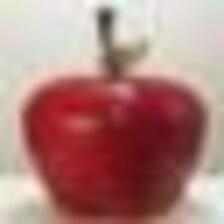
\includegraphics[width=.7\linewidth]{figures/CIFAR100/example_1.jpg}
        \captionsetup{labelformat=empty, justification=centering, font=scriptsize}
        \caption{\emph{Apple}}
      \end{figure}
    \end{column}
    \begin{column}{0.2\textwidth}
      \begin{figure}
        \centering
        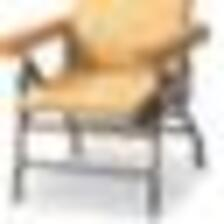
\includegraphics[width=.7\linewidth]{figures/CIFAR100/example_2.jpg}
        \captionsetup{labelformat=empty, justification=centering, font=scriptsize}
        \caption{\emph{Chair}}
      \end{figure}
    \end{column}
    \begin{column}{0.2\textwidth}
      \begin{figure}
        \centering
        
\includegraphics[width=.7\linewidth]{figures/CIFAR100/example_3.jpg}
        \captionsetup{labelformat=empty, justification=centering, font=scriptsize}
        \caption{\emph{Lobster}}
      \end{figure}
    \end{column}
  \end{columns}

  \rule{\linewidth}{0.4pt}

  \begin{columns}
    \begin{column}{0.35\textwidth}
      \alert{{\large iNaturalist19}}
      \begin{itemize}
        \item 1010 classes
        \item 8 hierarchy levels
      \end{itemize}
    \end{column}
    \begin{column}{0.2\textwidth}
      \begin{figure}
        \centering
        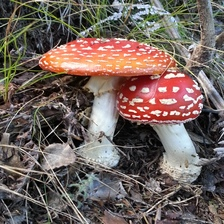
\includegraphics[width=.7\linewidth]{figures/iNaturalist19/example_1.jpg}
        \captionsetup{labelformat=empty, justification=centering, font=scriptsize}
        \caption{\emph{Amanita Muscaria}}
      \end{figure}
    \end{column}
    \begin{column}{0.2\textwidth}
      \begin{figure}
        \centering
        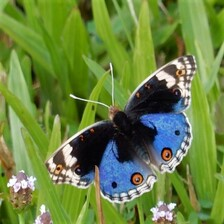
\includegraphics[width=.7\linewidth]{figures/iNaturalist19/example_2.jpg}
        \captionsetup{labelformat=empty, justification=centering, font=scriptsize}
        \caption{\emph{Junonia Orithya}}
      \end{figure}
    \end{column}
    \begin{column}{0.2\textwidth}
      \begin{figure}
        \centering
        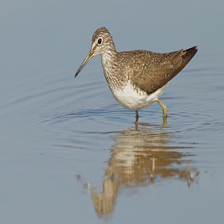
\includegraphics[width=.7\linewidth]{figures/iNaturalist19/example_3.jpg}
        \captionsetup{labelformat=empty, justification=centering, font=scriptsize}
        \caption{\emph{Tringa Ochropus}}
      \end{figure}
    \end{column}
  \end{columns}

  \rule{\linewidth}{0.4pt}

  \begin{columns}
    \begin{column}{0.35\textwidth}
      \alert{{\large tieredImageNet}}
      \begin{itemize}
        \item 608 classes
        \item 13 hierarchy levels
      \end{itemize}
    \end{column}
    \begin{column}{0.2\textwidth}
      \begin{figure}
        \centering
        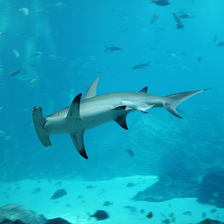
\includegraphics[width=.7\linewidth]{figures/tieredImageNet/example_1.jpg}
        \captionsetup{labelformat=empty, justification=centering, font=scriptsize}
        \caption{\emph{Hammerhead}}
      \end{figure}
    \end{column}
    \begin{column}{0.2\textwidth}
      \begin{figure}
        \centering
        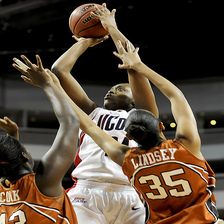
\includegraphics[width=.7\linewidth]{figures/tieredImageNet/example_2.jpg}
        \captionsetup{labelformat=empty, justification=centering, font=scriptsize}
        \caption{\emph{Basketball}}
      \end{figure}
    \end{column}
    \begin{column}{0.2\textwidth}
      \begin{figure}
        \centering
        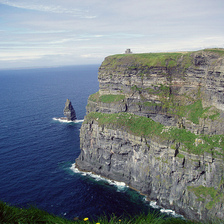
\includegraphics[width=.7\linewidth]{figures/tieredImageNet/example_3.jpg}
        \captionsetup{labelformat=empty, justification=centering, font=scriptsize}
        \caption{\emph{Cliff}}
      \end{figure}
    \end{column}
  \end{columns}

\end{frame}


\begin{frame}{Experiments | Cross Entropy \& One-hot Encoding}
  %% Creator: Matplotlib, PGF backend
%%
%% To include the figure in your LaTeX document, write
%%   \input{<filename>.pgf}
%%
%% Make sure the required packages are loaded in your preamble
%%   \usepackage{pgf}
%%
%% Also ensure that all the required font packages are loaded; for instance,
%% the lmodern package is sometimes necessary when using math font.
%%   \usepackage{lmodern}
%%
%% Figures using additional raster images can only be included by \input if
%% they are in the same directory as the main LaTeX file. For loading figures
%% from other directories you can use the `import` package
%%   \usepackage{import}
%%
%% and then include the figures with
%%   \import{<path to file>}{<filename>.pgf}
%%
%% Matplotlib used the following preamble
%%   
%%   \usepackage{fontspec}
%%   \setmainfont{DejaVuSerif.ttf}[Path=\detokenize{/Users/simo/.local/share/virtualenvs/master-thesis-code/lib/python3.10/site-packages/matplotlib/mpl-data/fonts/ttf/}]
%%   \setsansfont{DejaVuSans.ttf}[Path=\detokenize{/Users/simo/.local/share/virtualenvs/master-thesis-code/lib/python3.10/site-packages/matplotlib/mpl-data/fonts/ttf/}]
%%   \setmonofont{DejaVuSansMono.ttf}[Path=\detokenize{/Users/simo/.local/share/virtualenvs/master-thesis-code/lib/python3.10/site-packages/matplotlib/mpl-data/fonts/ttf/}]
%%   \makeatletter\@ifpackageloaded{underscore}{}{\usepackage[strings]{underscore}}\makeatother
%%
\begingroup%
\makeatletter%
\begin{pgfpicture}%
\pgfpathrectangle{\pgfpointorigin}{\pgfqpoint{4.251970in}{2.627862in}}%
\pgfusepath{use as bounding box, clip}%
\begin{pgfscope}%
\pgfsetbuttcap%
\pgfsetmiterjoin%
\definecolor{currentfill}{rgb}{0.980392,0.980392,0.980392}%
\pgfsetfillcolor{currentfill}%
\pgfsetlinewidth{0.000000pt}%
\definecolor{currentstroke}{rgb}{1.000000,1.000000,1.000000}%
\pgfsetstrokecolor{currentstroke}%
\pgfsetdash{}{0pt}%
\pgfpathmoveto{\pgfqpoint{0.000000in}{0.000000in}}%
\pgfpathlineto{\pgfqpoint{4.251970in}{0.000000in}}%
\pgfpathlineto{\pgfqpoint{4.251970in}{2.627862in}}%
\pgfpathlineto{\pgfqpoint{0.000000in}{2.627862in}}%
\pgfpathlineto{\pgfqpoint{0.000000in}{0.000000in}}%
\pgfpathclose%
\pgfusepath{fill}%
\end{pgfscope}%
\begin{pgfscope}%
\pgfsetbuttcap%
\pgfsetmiterjoin%
\definecolor{currentfill}{rgb}{0.917647,0.917647,0.949020}%
\pgfsetfillcolor{currentfill}%
\pgfsetlinewidth{0.000000pt}%
\definecolor{currentstroke}{rgb}{0.000000,0.000000,0.000000}%
\pgfsetstrokecolor{currentstroke}%
\pgfsetstrokeopacity{0.000000}%
\pgfsetdash{}{0pt}%
\pgfpathmoveto{\pgfqpoint{0.531496in}{0.289065in}}%
\pgfpathlineto{\pgfqpoint{3.826773in}{0.289065in}}%
\pgfpathlineto{\pgfqpoint{3.826773in}{2.312519in}}%
\pgfpathlineto{\pgfqpoint{0.531496in}{2.312519in}}%
\pgfpathlineto{\pgfqpoint{0.531496in}{0.289065in}}%
\pgfpathclose%
\pgfusepath{fill}%
\end{pgfscope}%
\begin{pgfscope}%
\definecolor{textcolor}{rgb}{0.137255,0.215686,0.231373}%
\pgfsetstrokecolor{textcolor}%
\pgfsetfillcolor{textcolor}%
\pgftext[x=0.681282in,y=0.150176in,,top]{\color{textcolor}\sffamily\fontsize{8.000000}{9.600000}\selectfont 0}%
\end{pgfscope}%
\begin{pgfscope}%
\definecolor{textcolor}{rgb}{0.137255,0.215686,0.231373}%
\pgfsetstrokecolor{textcolor}%
\pgfsetfillcolor{textcolor}%
\pgftext[x=1.089700in,y=0.150176in,,top]{\color{textcolor}\sffamily\fontsize{8.000000}{9.600000}\selectfont 80k}%
\end{pgfscope}%
\begin{pgfscope}%
\definecolor{textcolor}{rgb}{0.137255,0.215686,0.231373}%
\pgfsetstrokecolor{textcolor}%
\pgfsetfillcolor{textcolor}%
\pgftext[x=1.498118in,y=0.150176in,,top]{\color{textcolor}\sffamily\fontsize{8.000000}{9.600000}\selectfont 160k}%
\end{pgfscope}%
\begin{pgfscope}%
\definecolor{textcolor}{rgb}{0.137255,0.215686,0.231373}%
\pgfsetstrokecolor{textcolor}%
\pgfsetfillcolor{textcolor}%
\pgftext[x=1.906536in,y=0.150176in,,top]{\color{textcolor}\sffamily\fontsize{8.000000}{9.600000}\selectfont 240k}%
\end{pgfscope}%
\begin{pgfscope}%
\definecolor{textcolor}{rgb}{0.137255,0.215686,0.231373}%
\pgfsetstrokecolor{textcolor}%
\pgfsetfillcolor{textcolor}%
\pgftext[x=2.314954in,y=0.150176in,,top]{\color{textcolor}\sffamily\fontsize{8.000000}{9.600000}\selectfont 320k}%
\end{pgfscope}%
\begin{pgfscope}%
\definecolor{textcolor}{rgb}{0.137255,0.215686,0.231373}%
\pgfsetstrokecolor{textcolor}%
\pgfsetfillcolor{textcolor}%
\pgftext[x=2.723372in,y=0.150176in,,top]{\color{textcolor}\sffamily\fontsize{8.000000}{9.600000}\selectfont 400k}%
\end{pgfscope}%
\begin{pgfscope}%
\definecolor{textcolor}{rgb}{0.137255,0.215686,0.231373}%
\pgfsetstrokecolor{textcolor}%
\pgfsetfillcolor{textcolor}%
\pgftext[x=3.131790in,y=0.150176in,,top]{\color{textcolor}\sffamily\fontsize{8.000000}{9.600000}\selectfont 480k}%
\end{pgfscope}%
\begin{pgfscope}%
\definecolor{textcolor}{rgb}{0.137255,0.215686,0.231373}%
\pgfsetstrokecolor{textcolor}%
\pgfsetfillcolor{textcolor}%
\pgftext[x=3.540208in,y=0.150176in,,top]{\color{textcolor}\sffamily\fontsize{8.000000}{9.600000}\selectfont \emph{steps}}%
\end{pgfscope}%
\begin{pgfscope}%
\definecolor{textcolor}{rgb}{0.137255,0.215686,0.231373}%
\pgfsetstrokecolor{textcolor}%
\pgfsetfillcolor{textcolor}%
\pgftext[x=2.179135in,y=-0.012910in,,top]{\color{textcolor}\sffamily\fontsize{10.000000}{12.000000}\selectfont steps}%
\end{pgfscope}%
\begin{pgfscope}%
\definecolor{textcolor}{rgb}{0.137255,0.215686,0.231373}%
\pgfsetstrokecolor{textcolor}%
\pgfsetfillcolor{textcolor}%
\pgftext[x=0.241756in, y=0.460499in, left, base]{\color{textcolor}\sffamily\fontsize{8.000000}{9.600000}\selectfont \(\displaystyle {0.1}\)}%
\end{pgfscope}%
\begin{pgfscope}%
\definecolor{textcolor}{rgb}{0.137255,0.215686,0.231373}%
\pgfsetstrokecolor{textcolor}%
\pgfsetfillcolor{textcolor}%
\pgftext[x=0.241756in, y=0.707697in, left, base]{\color{textcolor}\sffamily\fontsize{8.000000}{9.600000}\selectfont \(\displaystyle {0.2}\)}%
\end{pgfscope}%
\begin{pgfscope}%
\definecolor{textcolor}{rgb}{0.137255,0.215686,0.231373}%
\pgfsetstrokecolor{textcolor}%
\pgfsetfillcolor{textcolor}%
\pgftext[x=0.241756in, y=0.954895in, left, base]{\color{textcolor}\sffamily\fontsize{8.000000}{9.600000}\selectfont \(\displaystyle {0.3}\)}%
\end{pgfscope}%
\begin{pgfscope}%
\definecolor{textcolor}{rgb}{0.137255,0.215686,0.231373}%
\pgfsetstrokecolor{textcolor}%
\pgfsetfillcolor{textcolor}%
\pgftext[x=0.241756in, y=1.202094in, left, base]{\color{textcolor}\sffamily\fontsize{8.000000}{9.600000}\selectfont \(\displaystyle {0.4}\)}%
\end{pgfscope}%
\begin{pgfscope}%
\definecolor{textcolor}{rgb}{0.137255,0.215686,0.231373}%
\pgfsetstrokecolor{textcolor}%
\pgfsetfillcolor{textcolor}%
\pgftext[x=0.241756in, y=1.449292in, left, base]{\color{textcolor}\sffamily\fontsize{8.000000}{9.600000}\selectfont \(\displaystyle {0.5}\)}%
\end{pgfscope}%
\begin{pgfscope}%
\definecolor{textcolor}{rgb}{0.137255,0.215686,0.231373}%
\pgfsetstrokecolor{textcolor}%
\pgfsetfillcolor{textcolor}%
\pgftext[x=0.241756in, y=1.696490in, left, base]{\color{textcolor}\sffamily\fontsize{8.000000}{9.600000}\selectfont \(\displaystyle {0.6}\)}%
\end{pgfscope}%
\begin{pgfscope}%
\definecolor{textcolor}{rgb}{0.137255,0.215686,0.231373}%
\pgfsetstrokecolor{textcolor}%
\pgfsetfillcolor{textcolor}%
\pgftext[x=0.241756in, y=1.943689in, left, base]{\color{textcolor}\sffamily\fontsize{8.000000}{9.600000}\selectfont \(\displaystyle {0.7}\)}%
\end{pgfscope}%
\begin{pgfscope}%
\definecolor{textcolor}{rgb}{0.137255,0.215686,0.231373}%
\pgfsetstrokecolor{textcolor}%
\pgfsetfillcolor{textcolor}%
\pgftext[x=0.241756in, y=2.190887in, left, base]{\color{textcolor}\sffamily\fontsize{8.000000}{9.600000}\selectfont \(\displaystyle {0.8}\)}%
\end{pgfscope}%
\begin{pgfscope}%
\pgfpathrectangle{\pgfqpoint{0.531496in}{0.289065in}}{\pgfqpoint{3.295277in}{2.023454in}}%
\pgfusepath{clip}%
\pgfsetroundcap%
\pgfsetroundjoin%
\pgfsetlinewidth{0.752812pt}%
\definecolor{currentstroke}{rgb}{0.921569,0.505882,0.105882}%
\pgfsetstrokecolor{currentstroke}%
\pgfsetstrokeopacity{0.200000}%
\pgfsetdash{}{0pt}%
\pgfpathmoveto{\pgfqpoint{0.681282in}{0.381040in}}%
\pgfpathlineto{\pgfqpoint{0.682098in}{1.061801in}}%
\pgfpathlineto{\pgfqpoint{0.682507in}{1.023176in}}%
\pgfpathlineto{\pgfqpoint{0.682548in}{0.965239in}}%
\pgfpathlineto{\pgfqpoint{0.683364in}{1.182503in}}%
\pgfpathlineto{\pgfqpoint{0.683487in}{1.163191in}}%
\pgfpathlineto{\pgfqpoint{0.683691in}{1.032833in}}%
\pgfpathlineto{\pgfqpoint{0.684181in}{1.211472in}}%
\pgfpathlineto{\pgfqpoint{0.684222in}{1.158363in}}%
\pgfpathlineto{\pgfqpoint{0.685243in}{1.274237in}}%
\pgfpathlineto{\pgfqpoint{0.684835in}{1.042489in}}%
\pgfpathlineto{\pgfqpoint{0.685325in}{1.235612in}}%
\pgfpathlineto{\pgfqpoint{0.685611in}{1.110082in}}%
\pgfpathlineto{\pgfqpoint{0.685978in}{1.312862in}}%
\pgfpathlineto{\pgfqpoint{0.686468in}{1.172847in}}%
\pgfpathlineto{\pgfqpoint{0.686918in}{1.361143in}}%
\pgfpathlineto{\pgfqpoint{0.686795in}{1.158363in}}%
\pgfpathlineto{\pgfqpoint{0.687571in}{1.235612in}}%
\pgfpathlineto{\pgfqpoint{0.687939in}{1.100426in}}%
\pgfpathlineto{\pgfqpoint{0.688020in}{1.341830in}}%
\pgfpathlineto{\pgfqpoint{0.688470in}{1.216300in}}%
\pgfpathlineto{\pgfqpoint{0.689001in}{1.390111in}}%
\pgfpathlineto{\pgfqpoint{0.689123in}{1.139051in}}%
\pgfpathlineto{\pgfqpoint{0.689572in}{1.288721in}}%
\pgfpathlineto{\pgfqpoint{0.690389in}{1.192160in}}%
\pgfpathlineto{\pgfqpoint{0.689858in}{1.390111in}}%
\pgfpathlineto{\pgfqpoint{0.690716in}{1.259753in}}%
\pgfpathlineto{\pgfqpoint{0.691860in}{1.448049in}}%
\pgfpathlineto{\pgfqpoint{0.690839in}{1.192160in}}%
\pgfpathlineto{\pgfqpoint{0.691900in}{1.428736in}}%
\pgfpathlineto{\pgfqpoint{0.692350in}{1.139051in}}%
\pgfpathlineto{\pgfqpoint{0.693044in}{1.312862in}}%
\pgfpathlineto{\pgfqpoint{0.693085in}{1.409424in}}%
\pgfpathlineto{\pgfqpoint{0.694065in}{1.201816in}}%
\pgfpathlineto{\pgfqpoint{0.694106in}{1.235612in}}%
\pgfpathlineto{\pgfqpoint{0.695331in}{1.423908in}}%
\pgfpathlineto{\pgfqpoint{0.696107in}{1.240441in}}%
\pgfpathlineto{\pgfqpoint{0.696434in}{1.404596in}}%
\pgfpathlineto{\pgfqpoint{0.696597in}{1.423908in}}%
\pgfpathlineto{\pgfqpoint{0.696679in}{1.337002in}}%
\pgfpathlineto{\pgfqpoint{0.696761in}{1.240441in}}%
\pgfpathlineto{\pgfqpoint{0.697414in}{1.438392in}}%
\pgfpathlineto{\pgfqpoint{0.697782in}{1.337002in}}%
\pgfpathlineto{\pgfqpoint{0.698190in}{1.428736in}}%
\pgfpathlineto{\pgfqpoint{0.698068in}{1.279065in}}%
\pgfpathlineto{\pgfqpoint{0.698394in}{1.361143in}}%
\pgfpathlineto{\pgfqpoint{0.698884in}{1.216300in}}%
\pgfpathlineto{\pgfqpoint{0.699252in}{1.448049in}}%
\pgfpathlineto{\pgfqpoint{0.699497in}{1.346659in}}%
\pgfpathlineto{\pgfqpoint{0.700396in}{1.472189in}}%
\pgfpathlineto{\pgfqpoint{0.700150in}{1.240441in}}%
\pgfpathlineto{\pgfqpoint{0.700559in}{1.365971in}}%
\pgfpathlineto{\pgfqpoint{0.700804in}{1.264581in}}%
\pgfpathlineto{\pgfqpoint{0.700967in}{1.423908in}}%
\pgfpathlineto{\pgfqpoint{0.701662in}{1.298378in}}%
\pgfpathlineto{\pgfqpoint{0.702438in}{1.491501in}}%
\pgfpathlineto{\pgfqpoint{0.701866in}{1.216300in}}%
\pgfpathlineto{\pgfqpoint{0.702969in}{1.481845in}}%
\pgfpathlineto{\pgfqpoint{0.703663in}{1.283893in}}%
\pgfpathlineto{\pgfqpoint{0.703990in}{1.496329in}}%
\pgfpathlineto{\pgfqpoint{0.704071in}{1.288721in}}%
\pgfpathlineto{\pgfqpoint{0.704194in}{1.515642in}}%
\pgfpathlineto{\pgfqpoint{0.705256in}{1.419080in}}%
\pgfpathlineto{\pgfqpoint{0.706032in}{1.235612in}}%
\pgfpathlineto{\pgfqpoint{0.705787in}{1.462533in}}%
\pgfpathlineto{\pgfqpoint{0.706358in}{1.317690in}}%
\pgfpathlineto{\pgfqpoint{0.707012in}{1.501158in}}%
\pgfpathlineto{\pgfqpoint{0.706644in}{1.264581in}}%
\pgfpathlineto{\pgfqpoint{0.707461in}{1.452877in}}%
\pgfpathlineto{\pgfqpoint{0.707502in}{1.298378in}}%
\pgfpathlineto{\pgfqpoint{0.708115in}{1.496329in}}%
\pgfpathlineto{\pgfqpoint{0.708564in}{1.361143in}}%
\pgfpathlineto{\pgfqpoint{0.708931in}{1.534954in}}%
\pgfpathlineto{\pgfqpoint{0.709054in}{1.288721in}}%
\pgfpathlineto{\pgfqpoint{0.709707in}{1.404596in}}%
\pgfpathlineto{\pgfqpoint{0.709748in}{1.303206in}}%
\pgfpathlineto{\pgfqpoint{0.709789in}{1.525298in}}%
\pgfpathlineto{\pgfqpoint{0.710810in}{1.365971in}}%
\pgfpathlineto{\pgfqpoint{0.710974in}{1.520470in}}%
\pgfpathlineto{\pgfqpoint{0.711586in}{1.308034in}}%
\pgfpathlineto{\pgfqpoint{0.711913in}{1.399768in}}%
\pgfpathlineto{\pgfqpoint{0.712975in}{1.477017in}}%
\pgfpathlineto{\pgfqpoint{0.712117in}{1.288721in}}%
\pgfpathlineto{\pgfqpoint{0.713016in}{1.457705in}}%
\pgfpathlineto{\pgfqpoint{0.713669in}{1.293550in}}%
\pgfpathlineto{\pgfqpoint{0.713914in}{1.515642in}}%
\pgfpathlineto{\pgfqpoint{0.714118in}{1.361143in}}%
\pgfpathlineto{\pgfqpoint{0.714486in}{1.337002in}}%
\pgfpathlineto{\pgfqpoint{0.714445in}{1.520470in}}%
\pgfpathlineto{\pgfqpoint{0.714894in}{1.390111in}}%
\pgfpathlineto{\pgfqpoint{0.715670in}{1.505986in}}%
\pgfpathlineto{\pgfqpoint{0.715099in}{1.351487in}}%
\pgfpathlineto{\pgfqpoint{0.715956in}{1.481845in}}%
\pgfpathlineto{\pgfqpoint{0.716977in}{1.303206in}}%
\pgfpathlineto{\pgfqpoint{0.716324in}{1.486673in}}%
\pgfpathlineto{\pgfqpoint{0.717059in}{1.486673in}}%
\pgfpathlineto{\pgfqpoint{0.717467in}{1.341830in}}%
\pgfpathlineto{\pgfqpoint{0.717712in}{1.544610in}}%
\pgfpathlineto{\pgfqpoint{0.718203in}{1.409424in}}%
\pgfpathlineto{\pgfqpoint{0.718570in}{1.525298in}}%
\pgfpathlineto{\pgfqpoint{0.718856in}{1.341830in}}%
\pgfpathlineto{\pgfqpoint{0.719305in}{1.419080in}}%
\pgfpathlineto{\pgfqpoint{0.719836in}{1.322518in}}%
\pgfpathlineto{\pgfqpoint{0.719632in}{1.505986in}}%
\pgfpathlineto{\pgfqpoint{0.720326in}{1.491501in}}%
\pgfpathlineto{\pgfqpoint{0.720694in}{1.322518in}}%
\pgfpathlineto{\pgfqpoint{0.720531in}{1.496329in}}%
\pgfpathlineto{\pgfqpoint{0.721552in}{1.423908in}}%
\pgfpathlineto{\pgfqpoint{0.722573in}{1.534954in}}%
\pgfpathlineto{\pgfqpoint{0.722450in}{1.365971in}}%
\pgfpathlineto{\pgfqpoint{0.722695in}{1.530126in}}%
\pgfpathlineto{\pgfqpoint{0.723104in}{1.341830in}}%
\pgfpathlineto{\pgfqpoint{0.722859in}{1.554267in}}%
\pgfpathlineto{\pgfqpoint{0.723839in}{1.385283in}}%
\pgfpathlineto{\pgfqpoint{0.724737in}{1.530126in}}%
\pgfpathlineto{\pgfqpoint{0.724492in}{1.341830in}}%
\pgfpathlineto{\pgfqpoint{0.724982in}{1.486673in}}%
\pgfpathlineto{\pgfqpoint{0.725717in}{1.332174in}}%
\pgfpathlineto{\pgfqpoint{0.725472in}{1.559095in}}%
\pgfpathlineto{\pgfqpoint{0.726085in}{1.467361in}}%
\pgfpathlineto{\pgfqpoint{0.726289in}{1.539782in}}%
\pgfpathlineto{\pgfqpoint{0.726371in}{1.404596in}}%
\pgfpathlineto{\pgfqpoint{0.726861in}{1.428736in}}%
\pgfpathlineto{\pgfqpoint{0.727596in}{1.375627in}}%
\pgfpathlineto{\pgfqpoint{0.727719in}{1.568751in}}%
\pgfpathlineto{\pgfqpoint{0.727882in}{1.457705in}}%
\pgfpathlineto{\pgfqpoint{0.728658in}{1.549438in}}%
\pgfpathlineto{\pgfqpoint{0.728005in}{1.356315in}}%
\pgfpathlineto{\pgfqpoint{0.728944in}{1.462533in}}%
\pgfpathlineto{\pgfqpoint{0.729352in}{1.361143in}}%
\pgfpathlineto{\pgfqpoint{0.729189in}{1.597719in}}%
\pgfpathlineto{\pgfqpoint{0.730047in}{1.365971in}}%
\pgfpathlineto{\pgfqpoint{0.730578in}{1.539782in}}%
\pgfpathlineto{\pgfqpoint{0.730455in}{1.322518in}}%
\pgfpathlineto{\pgfqpoint{0.731231in}{1.496329in}}%
\pgfpathlineto{\pgfqpoint{0.731762in}{1.337002in}}%
\pgfpathlineto{\pgfqpoint{0.731925in}{1.530126in}}%
\pgfpathlineto{\pgfqpoint{0.732334in}{1.438392in}}%
\pgfpathlineto{\pgfqpoint{0.733314in}{1.322518in}}%
\pgfpathlineto{\pgfqpoint{0.732456in}{1.583235in}}%
\pgfpathlineto{\pgfqpoint{0.733396in}{1.375627in}}%
\pgfpathlineto{\pgfqpoint{0.733477in}{1.597719in}}%
\pgfpathlineto{\pgfqpoint{0.734498in}{1.568751in}}%
\pgfpathlineto{\pgfqpoint{0.735029in}{1.351487in}}%
\pgfpathlineto{\pgfqpoint{0.734703in}{1.612204in}}%
\pgfpathlineto{\pgfqpoint{0.735601in}{1.501158in}}%
\pgfpathlineto{\pgfqpoint{0.736336in}{1.365971in}}%
\pgfpathlineto{\pgfqpoint{0.736050in}{1.563923in}}%
\pgfpathlineto{\pgfqpoint{0.736581in}{1.390111in}}%
\pgfpathlineto{\pgfqpoint{0.736990in}{1.592891in}}%
\pgfpathlineto{\pgfqpoint{0.737643in}{1.361143in}}%
\pgfpathlineto{\pgfqpoint{0.737684in}{1.452877in}}%
\pgfpathlineto{\pgfqpoint{0.738174in}{1.578407in}}%
\pgfpathlineto{\pgfqpoint{0.738093in}{1.375627in}}%
\pgfpathlineto{\pgfqpoint{0.738869in}{1.534954in}}%
\pgfpathlineto{\pgfqpoint{0.739767in}{1.351487in}}%
\pgfpathlineto{\pgfqpoint{0.739318in}{1.597719in}}%
\pgfpathlineto{\pgfqpoint{0.739930in}{1.457705in}}%
\pgfpathlineto{\pgfqpoint{0.740053in}{1.578407in}}%
\pgfpathlineto{\pgfqpoint{0.740094in}{1.332174in}}%
\pgfpathlineto{\pgfqpoint{0.741033in}{1.510814in}}%
\pgfpathlineto{\pgfqpoint{0.741074in}{1.510814in}}%
\pgfpathlineto{\pgfqpoint{0.741850in}{1.423908in}}%
\pgfpathlineto{\pgfqpoint{0.741237in}{1.563923in}}%
\pgfpathlineto{\pgfqpoint{0.741972in}{1.525298in}}%
\pgfpathlineto{\pgfqpoint{0.742422in}{1.597719in}}%
\pgfpathlineto{\pgfqpoint{0.742871in}{1.404596in}}%
\pgfpathlineto{\pgfqpoint{0.742953in}{1.467361in}}%
\pgfpathlineto{\pgfqpoint{0.743034in}{1.375627in}}%
\pgfpathlineto{\pgfqpoint{0.743565in}{1.607376in}}%
\pgfpathlineto{\pgfqpoint{0.744055in}{1.443220in}}%
\pgfpathlineto{\pgfqpoint{0.744423in}{1.554267in}}%
\pgfpathlineto{\pgfqpoint{0.744831in}{1.375627in}}%
\pgfpathlineto{\pgfqpoint{0.745199in}{1.472189in}}%
\pgfpathlineto{\pgfqpoint{0.745526in}{1.390111in}}%
\pgfpathlineto{\pgfqpoint{0.745362in}{1.578407in}}%
\pgfpathlineto{\pgfqpoint{0.746098in}{1.481845in}}%
\pgfpathlineto{\pgfqpoint{0.747037in}{1.694281in}}%
\pgfpathlineto{\pgfqpoint{0.746220in}{1.409424in}}%
\pgfpathlineto{\pgfqpoint{0.747159in}{1.563923in}}%
\pgfpathlineto{\pgfqpoint{0.747241in}{1.361143in}}%
\pgfpathlineto{\pgfqpoint{0.747895in}{1.583235in}}%
\pgfpathlineto{\pgfqpoint{0.748262in}{1.443220in}}%
\pgfpathlineto{\pgfqpoint{0.748507in}{1.592891in}}%
\pgfpathlineto{\pgfqpoint{0.748589in}{1.404596in}}%
\pgfpathlineto{\pgfqpoint{0.749406in}{1.554267in}}%
\pgfpathlineto{\pgfqpoint{0.750223in}{1.423908in}}%
\pgfpathlineto{\pgfqpoint{0.749814in}{1.568751in}}%
\pgfpathlineto{\pgfqpoint{0.750468in}{1.457705in}}%
\pgfpathlineto{\pgfqpoint{0.750508in}{1.621860in}}%
\pgfpathlineto{\pgfqpoint{0.750631in}{1.399768in}}%
\pgfpathlineto{\pgfqpoint{0.751570in}{1.481845in}}%
\pgfpathlineto{\pgfqpoint{0.752346in}{1.404596in}}%
\pgfpathlineto{\pgfqpoint{0.752142in}{1.588063in}}%
\pgfpathlineto{\pgfqpoint{0.752591in}{1.462533in}}%
\pgfpathlineto{\pgfqpoint{0.752836in}{1.646000in}}%
\pgfpathlineto{\pgfqpoint{0.753204in}{1.385283in}}%
\pgfpathlineto{\pgfqpoint{0.753776in}{1.573579in}}%
\pgfpathlineto{\pgfqpoint{0.754511in}{1.409424in}}%
\pgfpathlineto{\pgfqpoint{0.754062in}{1.670141in}}%
\pgfpathlineto{\pgfqpoint{0.754878in}{1.544610in}}%
\pgfpathlineto{\pgfqpoint{0.755328in}{1.568751in}}%
\pgfpathlineto{\pgfqpoint{0.755940in}{1.414252in}}%
\pgfpathlineto{\pgfqpoint{0.756880in}{1.617032in}}%
\pgfpathlineto{\pgfqpoint{0.756104in}{1.394939in}}%
\pgfpathlineto{\pgfqpoint{0.757043in}{1.568751in}}%
\pgfpathlineto{\pgfqpoint{0.757982in}{1.380455in}}%
\pgfpathlineto{\pgfqpoint{0.757329in}{1.607376in}}%
\pgfpathlineto{\pgfqpoint{0.758105in}{1.525298in}}%
\pgfpathlineto{\pgfqpoint{0.758146in}{1.631516in}}%
\pgfpathlineto{\pgfqpoint{0.759126in}{1.491501in}}%
\pgfpathlineto{\pgfqpoint{0.759208in}{1.515642in}}%
\pgfpathlineto{\pgfqpoint{0.760147in}{1.399768in}}%
\pgfpathlineto{\pgfqpoint{0.760310in}{1.660485in}}%
\pgfpathlineto{\pgfqpoint{0.761250in}{1.409424in}}%
\pgfpathlineto{\pgfqpoint{0.760515in}{1.674969in}}%
\pgfpathlineto{\pgfqpoint{0.761413in}{1.563923in}}%
\pgfpathlineto{\pgfqpoint{0.761536in}{1.621860in}}%
\pgfpathlineto{\pgfqpoint{0.762067in}{1.409424in}}%
\pgfpathlineto{\pgfqpoint{0.762271in}{1.505986in}}%
\pgfpathlineto{\pgfqpoint{0.762312in}{1.394939in}}%
\pgfpathlineto{\pgfqpoint{0.762516in}{1.612204in}}%
\pgfpathlineto{\pgfqpoint{0.763374in}{1.501158in}}%
\pgfpathlineto{\pgfqpoint{0.763782in}{1.660485in}}%
\pgfpathlineto{\pgfqpoint{0.764272in}{1.438392in}}%
\pgfpathlineto{\pgfqpoint{0.764762in}{1.670141in}}%
\pgfpathlineto{\pgfqpoint{0.765293in}{1.404596in}}%
\pgfpathlineto{\pgfqpoint{0.765375in}{1.563923in}}%
\pgfpathlineto{\pgfqpoint{0.766273in}{1.428736in}}%
\pgfpathlineto{\pgfqpoint{0.765865in}{1.607376in}}%
\pgfpathlineto{\pgfqpoint{0.766437in}{1.510814in}}%
\pgfpathlineto{\pgfqpoint{0.766804in}{1.636344in}}%
\pgfpathlineto{\pgfqpoint{0.767458in}{1.385283in}}%
\pgfpathlineto{\pgfqpoint{0.767539in}{1.583235in}}%
\pgfpathlineto{\pgfqpoint{0.768152in}{1.414252in}}%
\pgfpathlineto{\pgfqpoint{0.767825in}{1.602547in}}%
\pgfpathlineto{\pgfqpoint{0.768724in}{1.438392in}}%
\pgfpathlineto{\pgfqpoint{0.769582in}{1.660485in}}%
\pgfpathlineto{\pgfqpoint{0.769827in}{1.530126in}}%
\pgfpathlineto{\pgfqpoint{0.770684in}{1.433564in}}%
\pgfpathlineto{\pgfqpoint{0.770766in}{1.646000in}}%
\pgfpathlineto{\pgfqpoint{0.770929in}{1.457705in}}%
\pgfpathlineto{\pgfqpoint{0.771419in}{1.636344in}}%
\pgfpathlineto{\pgfqpoint{0.771215in}{1.419080in}}%
\pgfpathlineto{\pgfqpoint{0.772032in}{1.520470in}}%
\pgfpathlineto{\pgfqpoint{0.772481in}{1.409424in}}%
\pgfpathlineto{\pgfqpoint{0.772155in}{1.665313in}}%
\pgfpathlineto{\pgfqpoint{0.773094in}{1.563923in}}%
\pgfpathlineto{\pgfqpoint{0.773135in}{1.563923in}}%
\pgfpathlineto{\pgfqpoint{0.773257in}{1.467361in}}%
\pgfpathlineto{\pgfqpoint{0.773380in}{1.617032in}}%
\pgfpathlineto{\pgfqpoint{0.774197in}{1.481845in}}%
\pgfpathlineto{\pgfqpoint{0.775177in}{1.689453in}}%
\pgfpathlineto{\pgfqpoint{0.774278in}{1.438392in}}%
\pgfpathlineto{\pgfqpoint{0.775299in}{1.530126in}}%
\pgfpathlineto{\pgfqpoint{0.775830in}{1.457705in}}%
\pgfpathlineto{\pgfqpoint{0.775953in}{1.621860in}}%
\pgfpathlineto{\pgfqpoint{0.776198in}{1.583235in}}%
\pgfpathlineto{\pgfqpoint{0.776239in}{1.641172in}}%
\pgfpathlineto{\pgfqpoint{0.776770in}{1.414252in}}%
\pgfpathlineto{\pgfqpoint{0.777301in}{1.578407in}}%
\pgfpathlineto{\pgfqpoint{0.778036in}{1.423908in}}%
\pgfpathlineto{\pgfqpoint{0.778077in}{1.694281in}}%
\pgfpathlineto{\pgfqpoint{0.778240in}{1.578407in}}%
\pgfpathlineto{\pgfqpoint{0.779261in}{1.646000in}}%
\pgfpathlineto{\pgfqpoint{0.778608in}{1.404596in}}%
\pgfpathlineto{\pgfqpoint{0.779302in}{1.510814in}}%
\pgfpathlineto{\pgfqpoint{0.779915in}{1.448049in}}%
\pgfpathlineto{\pgfqpoint{0.779874in}{1.665313in}}%
\pgfpathlineto{\pgfqpoint{0.780364in}{1.534954in}}%
\pgfpathlineto{\pgfqpoint{0.780691in}{1.679797in}}%
\pgfpathlineto{\pgfqpoint{0.781181in}{1.496329in}}%
\pgfpathlineto{\pgfqpoint{0.781467in}{1.568751in}}%
\pgfpathlineto{\pgfqpoint{0.782202in}{1.477017in}}%
\pgfpathlineto{\pgfqpoint{0.781548in}{1.626688in}}%
\pgfpathlineto{\pgfqpoint{0.782488in}{1.597719in}}%
\pgfpathlineto{\pgfqpoint{0.782528in}{1.655656in}}%
\pgfpathlineto{\pgfqpoint{0.783019in}{1.428736in}}%
\pgfpathlineto{\pgfqpoint{0.783590in}{1.641172in}}%
\pgfpathlineto{\pgfqpoint{0.784325in}{1.679797in}}%
\pgfpathlineto{\pgfqpoint{0.784734in}{1.438392in}}%
\pgfpathlineto{\pgfqpoint{0.784816in}{1.636344in}}%
\pgfpathlineto{\pgfqpoint{0.785877in}{1.617032in}}%
\pgfpathlineto{\pgfqpoint{0.786817in}{1.443220in}}%
\pgfpathlineto{\pgfqpoint{0.786776in}{1.646000in}}%
\pgfpathlineto{\pgfqpoint{0.787021in}{1.530126in}}%
\pgfpathlineto{\pgfqpoint{0.788042in}{1.660485in}}%
\pgfpathlineto{\pgfqpoint{0.787184in}{1.496329in}}%
\pgfpathlineto{\pgfqpoint{0.788124in}{1.534954in}}%
\pgfpathlineto{\pgfqpoint{0.788491in}{1.699109in}}%
\pgfpathlineto{\pgfqpoint{0.788900in}{1.457705in}}%
\pgfpathlineto{\pgfqpoint{0.789063in}{1.515642in}}%
\pgfpathlineto{\pgfqpoint{0.789676in}{1.452877in}}%
\pgfpathlineto{\pgfqpoint{0.789839in}{1.655656in}}%
\pgfpathlineto{\pgfqpoint{0.790084in}{1.544610in}}%
\pgfpathlineto{\pgfqpoint{0.790697in}{1.646000in}}%
\pgfpathlineto{\pgfqpoint{0.790778in}{1.423908in}}%
\pgfpathlineto{\pgfqpoint{0.791187in}{1.636344in}}%
\pgfpathlineto{\pgfqpoint{0.791922in}{1.438392in}}%
\pgfpathlineto{\pgfqpoint{0.791269in}{1.655656in}}%
\pgfpathlineto{\pgfqpoint{0.792290in}{1.602547in}}%
\pgfpathlineto{\pgfqpoint{0.792535in}{1.462533in}}%
\pgfpathlineto{\pgfqpoint{0.793147in}{1.694281in}}%
\pgfpathlineto{\pgfqpoint{0.793351in}{1.617032in}}%
\pgfpathlineto{\pgfqpoint{0.794291in}{1.670141in}}%
\pgfpathlineto{\pgfqpoint{0.794005in}{1.443220in}}%
\pgfpathlineto{\pgfqpoint{0.794373in}{1.578407in}}%
\pgfpathlineto{\pgfqpoint{0.795230in}{1.452877in}}%
\pgfpathlineto{\pgfqpoint{0.794495in}{1.670141in}}%
\pgfpathlineto{\pgfqpoint{0.795394in}{1.563923in}}%
\pgfpathlineto{\pgfqpoint{0.795884in}{1.650828in}}%
\pgfpathlineto{\pgfqpoint{0.795761in}{1.448049in}}%
\pgfpathlineto{\pgfqpoint{0.796496in}{1.592891in}}%
\pgfpathlineto{\pgfqpoint{0.796905in}{1.660485in}}%
\pgfpathlineto{\pgfqpoint{0.796946in}{1.496329in}}%
\pgfpathlineto{\pgfqpoint{0.797272in}{1.588063in}}%
\pgfpathlineto{\pgfqpoint{0.797967in}{1.477017in}}%
\pgfpathlineto{\pgfqpoint{0.798334in}{1.670141in}}%
\pgfpathlineto{\pgfqpoint{0.798661in}{1.477017in}}%
\pgfpathlineto{\pgfqpoint{0.798416in}{1.747390in}}%
\pgfpathlineto{\pgfqpoint{0.799396in}{1.646000in}}%
\pgfpathlineto{\pgfqpoint{0.800254in}{1.699109in}}%
\pgfpathlineto{\pgfqpoint{0.799641in}{1.486673in}}%
\pgfpathlineto{\pgfqpoint{0.800458in}{1.602547in}}%
\pgfpathlineto{\pgfqpoint{0.801479in}{1.472189in}}%
\pgfpathlineto{\pgfqpoint{0.801397in}{1.665313in}}%
\pgfpathlineto{\pgfqpoint{0.801561in}{1.501158in}}%
\pgfpathlineto{\pgfqpoint{0.802459in}{1.728078in}}%
\pgfpathlineto{\pgfqpoint{0.801887in}{1.452877in}}%
\pgfpathlineto{\pgfqpoint{0.802704in}{1.626688in}}%
\pgfpathlineto{\pgfqpoint{0.803521in}{1.472189in}}%
\pgfpathlineto{\pgfqpoint{0.803072in}{1.636344in}}%
\pgfpathlineto{\pgfqpoint{0.803807in}{1.544610in}}%
\pgfpathlineto{\pgfqpoint{0.804746in}{1.684625in}}%
\pgfpathlineto{\pgfqpoint{0.804828in}{1.462533in}}%
\pgfpathlineto{\pgfqpoint{0.804910in}{1.670141in}}%
\pgfpathlineto{\pgfqpoint{0.805890in}{1.501158in}}%
\pgfpathlineto{\pgfqpoint{0.805482in}{1.728078in}}%
\pgfpathlineto{\pgfqpoint{0.806053in}{1.568751in}}%
\pgfpathlineto{\pgfqpoint{0.806543in}{1.699109in}}%
\pgfpathlineto{\pgfqpoint{0.807033in}{1.491501in}}%
\pgfpathlineto{\pgfqpoint{0.807156in}{1.563923in}}%
\pgfpathlineto{\pgfqpoint{0.807605in}{1.457705in}}%
\pgfpathlineto{\pgfqpoint{0.807483in}{1.670141in}}%
\pgfpathlineto{\pgfqpoint{0.808136in}{1.510814in}}%
\pgfpathlineto{\pgfqpoint{0.808177in}{1.694281in}}%
\pgfpathlineto{\pgfqpoint{0.809239in}{1.607376in}}%
\pgfpathlineto{\pgfqpoint{0.809443in}{1.650828in}}%
\pgfpathlineto{\pgfqpoint{0.809321in}{1.520470in}}%
\pgfpathlineto{\pgfqpoint{0.809607in}{1.617032in}}%
\pgfpathlineto{\pgfqpoint{0.810546in}{1.443220in}}%
\pgfpathlineto{\pgfqpoint{0.809729in}{1.674969in}}%
\pgfpathlineto{\pgfqpoint{0.810709in}{1.573579in}}%
\pgfpathlineto{\pgfqpoint{0.810873in}{1.462533in}}%
\pgfpathlineto{\pgfqpoint{0.811689in}{1.694281in}}%
\pgfpathlineto{\pgfqpoint{0.811730in}{1.462533in}}%
\pgfpathlineto{\pgfqpoint{0.812792in}{1.670141in}}%
\pgfpathlineto{\pgfqpoint{0.813405in}{1.433564in}}%
\pgfpathlineto{\pgfqpoint{0.813282in}{1.699109in}}%
\pgfpathlineto{\pgfqpoint{0.813936in}{1.486673in}}%
\pgfpathlineto{\pgfqpoint{0.814793in}{1.670141in}}%
\pgfpathlineto{\pgfqpoint{0.814712in}{1.472189in}}%
\pgfpathlineto{\pgfqpoint{0.815079in}{1.583235in}}%
\pgfpathlineto{\pgfqpoint{0.815120in}{1.583235in}}%
\pgfpathlineto{\pgfqpoint{0.815937in}{1.708766in}}%
\pgfpathlineto{\pgfqpoint{0.815855in}{1.486673in}}%
\pgfpathlineto{\pgfqpoint{0.816182in}{1.602547in}}%
\pgfpathlineto{\pgfqpoint{0.816836in}{1.525298in}}%
\pgfpathlineto{\pgfqpoint{0.816550in}{1.732906in}}%
\pgfpathlineto{\pgfqpoint{0.817285in}{1.534954in}}%
\pgfpathlineto{\pgfqpoint{0.817938in}{1.684625in}}%
\pgfpathlineto{\pgfqpoint{0.817571in}{1.433564in}}%
\pgfpathlineto{\pgfqpoint{0.818388in}{1.621860in}}%
\pgfpathlineto{\pgfqpoint{0.818755in}{1.534954in}}%
\pgfpathlineto{\pgfqpoint{0.819327in}{1.679797in}}%
\pgfpathlineto{\pgfqpoint{0.819368in}{1.713594in}}%
\pgfpathlineto{\pgfqpoint{0.819899in}{1.520470in}}%
\pgfpathlineto{\pgfqpoint{0.820348in}{1.665313in}}%
\pgfpathlineto{\pgfqpoint{0.821165in}{1.520470in}}%
\pgfpathlineto{\pgfqpoint{0.821491in}{1.554267in}}%
\pgfpathlineto{\pgfqpoint{0.821777in}{1.737734in}}%
\pgfpathlineto{\pgfqpoint{0.822145in}{1.467361in}}%
\pgfpathlineto{\pgfqpoint{0.822513in}{1.631516in}}%
\pgfpathlineto{\pgfqpoint{0.823289in}{1.428736in}}%
\pgfpathlineto{\pgfqpoint{0.823370in}{1.674969in}}%
\pgfpathlineto{\pgfqpoint{0.823615in}{1.626688in}}%
\pgfpathlineto{\pgfqpoint{0.823656in}{1.713594in}}%
\pgfpathlineto{\pgfqpoint{0.823819in}{1.520470in}}%
\pgfpathlineto{\pgfqpoint{0.824677in}{1.607376in}}%
\pgfpathlineto{\pgfqpoint{0.825086in}{1.390111in}}%
\pgfpathlineto{\pgfqpoint{0.825576in}{1.646000in}}%
\pgfpathlineto{\pgfqpoint{0.825739in}{1.491501in}}%
\pgfpathlineto{\pgfqpoint{0.826229in}{1.732906in}}%
\pgfpathlineto{\pgfqpoint{0.826760in}{1.467361in}}%
\pgfpathlineto{\pgfqpoint{0.826842in}{1.520470in}}%
\pgfpathlineto{\pgfqpoint{0.826883in}{1.515642in}}%
\pgfpathlineto{\pgfqpoint{0.826923in}{1.597719in}}%
\pgfpathlineto{\pgfqpoint{0.826964in}{1.559095in}}%
\pgfpathlineto{\pgfqpoint{0.827618in}{1.670141in}}%
\pgfpathlineto{\pgfqpoint{0.827822in}{1.496329in}}%
\pgfpathlineto{\pgfqpoint{0.828067in}{1.549438in}}%
\pgfpathlineto{\pgfqpoint{0.828761in}{1.491501in}}%
\pgfpathlineto{\pgfqpoint{0.828271in}{1.718422in}}%
\pgfpathlineto{\pgfqpoint{0.829006in}{1.563923in}}%
\pgfpathlineto{\pgfqpoint{0.829170in}{1.752218in}}%
\pgfpathlineto{\pgfqpoint{0.830027in}{1.520470in}}%
\pgfpathlineto{\pgfqpoint{0.830109in}{1.617032in}}%
\pgfpathlineto{\pgfqpoint{0.830477in}{1.510814in}}%
\pgfpathlineto{\pgfqpoint{0.830558in}{1.752218in}}%
\pgfpathlineto{\pgfqpoint{0.831130in}{1.636344in}}%
\pgfpathlineto{\pgfqpoint{0.831171in}{1.732906in}}%
\pgfpathlineto{\pgfqpoint{0.832192in}{1.539782in}}%
\pgfpathlineto{\pgfqpoint{0.832233in}{1.631516in}}%
\pgfpathlineto{\pgfqpoint{0.832968in}{1.462533in}}%
\pgfpathlineto{\pgfqpoint{0.833295in}{1.708766in}}%
\pgfpathlineto{\pgfqpoint{0.833867in}{1.520470in}}%
\pgfpathlineto{\pgfqpoint{0.834438in}{1.563923in}}%
\pgfpathlineto{\pgfqpoint{0.834724in}{1.747390in}}%
\pgfpathlineto{\pgfqpoint{0.835092in}{1.477017in}}%
\pgfpathlineto{\pgfqpoint{0.835541in}{1.732906in}}%
\pgfpathlineto{\pgfqpoint{0.836521in}{1.505986in}}%
\pgfpathlineto{\pgfqpoint{0.836685in}{1.612204in}}%
\pgfpathlineto{\pgfqpoint{0.836930in}{1.510814in}}%
\pgfpathlineto{\pgfqpoint{0.837379in}{1.699109in}}%
\pgfpathlineto{\pgfqpoint{0.837461in}{1.621860in}}%
\pgfpathlineto{\pgfqpoint{0.837501in}{1.713594in}}%
\pgfpathlineto{\pgfqpoint{0.838523in}{1.515642in}}%
\pgfpathlineto{\pgfqpoint{0.838563in}{1.694281in}}%
\pgfpathlineto{\pgfqpoint{0.839176in}{1.496329in}}%
\pgfpathlineto{\pgfqpoint{0.838890in}{1.713594in}}%
\pgfpathlineto{\pgfqpoint{0.839707in}{1.617032in}}%
\pgfpathlineto{\pgfqpoint{0.840360in}{1.747390in}}%
\pgfpathlineto{\pgfqpoint{0.839993in}{1.534954in}}%
\pgfpathlineto{\pgfqpoint{0.840769in}{1.694281in}}%
\pgfpathlineto{\pgfqpoint{0.841627in}{1.491501in}}%
\pgfpathlineto{\pgfqpoint{0.841136in}{1.742562in}}%
\pgfpathlineto{\pgfqpoint{0.841872in}{1.621860in}}%
\pgfpathlineto{\pgfqpoint{0.841953in}{1.723250in}}%
\pgfpathlineto{\pgfqpoint{0.842852in}{1.496329in}}%
\pgfpathlineto{\pgfqpoint{0.843015in}{1.703937in}}%
\pgfpathlineto{\pgfqpoint{0.843383in}{1.486673in}}%
\pgfpathlineto{\pgfqpoint{0.844036in}{1.713594in}}%
\pgfpathlineto{\pgfqpoint{0.844159in}{1.583235in}}%
\pgfpathlineto{\pgfqpoint{0.845139in}{1.718422in}}%
\pgfpathlineto{\pgfqpoint{0.844240in}{1.539782in}}%
\pgfpathlineto{\pgfqpoint{0.845302in}{1.665313in}}%
\pgfpathlineto{\pgfqpoint{0.845547in}{1.708766in}}%
\pgfpathlineto{\pgfqpoint{0.846160in}{1.568751in}}%
\pgfpathlineto{\pgfqpoint{0.846242in}{1.631516in}}%
\pgfpathlineto{\pgfqpoint{0.846323in}{1.520470in}}%
\pgfpathlineto{\pgfqpoint{0.847099in}{1.732906in}}%
\pgfpathlineto{\pgfqpoint{0.847344in}{1.607376in}}%
\pgfpathlineto{\pgfqpoint{0.847630in}{1.703937in}}%
\pgfpathlineto{\pgfqpoint{0.847875in}{1.525298in}}%
\pgfpathlineto{\pgfqpoint{0.848447in}{1.607376in}}%
\pgfpathlineto{\pgfqpoint{0.849060in}{1.448049in}}%
\pgfpathlineto{\pgfqpoint{0.848733in}{1.728078in}}%
\pgfpathlineto{\pgfqpoint{0.849591in}{1.563923in}}%
\pgfpathlineto{\pgfqpoint{0.849754in}{1.742562in}}%
\pgfpathlineto{\pgfqpoint{0.849917in}{1.496329in}}%
\pgfpathlineto{\pgfqpoint{0.850693in}{1.646000in}}%
\pgfpathlineto{\pgfqpoint{0.851306in}{1.515642in}}%
\pgfpathlineto{\pgfqpoint{0.850979in}{1.771531in}}%
\pgfpathlineto{\pgfqpoint{0.851878in}{1.549438in}}%
\pgfpathlineto{\pgfqpoint{0.851919in}{1.505986in}}%
\pgfpathlineto{\pgfqpoint{0.852123in}{1.786015in}}%
\pgfpathlineto{\pgfqpoint{0.852776in}{1.655656in}}%
\pgfpathlineto{\pgfqpoint{0.852817in}{1.747390in}}%
\pgfpathlineto{\pgfqpoint{0.853226in}{1.544610in}}%
\pgfpathlineto{\pgfqpoint{0.853838in}{1.636344in}}%
\pgfpathlineto{\pgfqpoint{0.854165in}{1.515642in}}%
\pgfpathlineto{\pgfqpoint{0.854737in}{1.732906in}}%
\pgfpathlineto{\pgfqpoint{0.854941in}{1.631516in}}%
\pgfpathlineto{\pgfqpoint{0.855758in}{1.679797in}}%
\pgfpathlineto{\pgfqpoint{0.855390in}{1.496329in}}%
\pgfpathlineto{\pgfqpoint{0.855921in}{1.626688in}}%
\pgfpathlineto{\pgfqpoint{0.856820in}{1.520470in}}%
\pgfpathlineto{\pgfqpoint{0.856125in}{1.713594in}}%
\pgfpathlineto{\pgfqpoint{0.856942in}{1.563923in}}%
\pgfpathlineto{\pgfqpoint{0.857963in}{1.742562in}}%
\pgfpathlineto{\pgfqpoint{0.857065in}{1.534954in}}%
\pgfpathlineto{\pgfqpoint{0.858086in}{1.737734in}}%
\pgfpathlineto{\pgfqpoint{0.858658in}{1.757046in}}%
\pgfpathlineto{\pgfqpoint{0.859229in}{1.530126in}}%
\pgfpathlineto{\pgfqpoint{0.860250in}{1.713594in}}%
\pgfpathlineto{\pgfqpoint{0.860210in}{1.520470in}}%
\pgfpathlineto{\pgfqpoint{0.860332in}{1.646000in}}%
\pgfpathlineto{\pgfqpoint{0.860822in}{1.742562in}}%
\pgfpathlineto{\pgfqpoint{0.861394in}{1.544610in}}%
\pgfpathlineto{\pgfqpoint{0.861435in}{1.795671in}}%
\pgfpathlineto{\pgfqpoint{0.862497in}{1.573579in}}%
\pgfpathlineto{\pgfqpoint{0.862864in}{1.737734in}}%
\pgfpathlineto{\pgfqpoint{0.862823in}{1.515642in}}%
\pgfpathlineto{\pgfqpoint{0.863681in}{1.703937in}}%
\pgfpathlineto{\pgfqpoint{0.863722in}{1.525298in}}%
\pgfpathlineto{\pgfqpoint{0.864702in}{1.747390in}}%
\pgfpathlineto{\pgfqpoint{0.864784in}{1.674969in}}%
\pgfpathlineto{\pgfqpoint{0.865274in}{1.520470in}}%
\pgfpathlineto{\pgfqpoint{0.864866in}{1.757046in}}%
\pgfpathlineto{\pgfqpoint{0.865887in}{1.631516in}}%
\pgfpathlineto{\pgfqpoint{0.866336in}{1.742562in}}%
\pgfpathlineto{\pgfqpoint{0.866826in}{1.530126in}}%
\pgfpathlineto{\pgfqpoint{0.867030in}{1.708766in}}%
\pgfpathlineto{\pgfqpoint{0.867479in}{1.554267in}}%
\pgfpathlineto{\pgfqpoint{0.868133in}{1.665313in}}%
\pgfpathlineto{\pgfqpoint{0.869113in}{1.732906in}}%
\pgfpathlineto{\pgfqpoint{0.868623in}{1.568751in}}%
\pgfpathlineto{\pgfqpoint{0.869236in}{1.665313in}}%
\pgfpathlineto{\pgfqpoint{0.869481in}{1.544610in}}%
\pgfpathlineto{\pgfqpoint{0.869358in}{1.742562in}}%
\pgfpathlineto{\pgfqpoint{0.870379in}{1.617032in}}%
\pgfpathlineto{\pgfqpoint{0.870747in}{1.703937in}}%
\pgfpathlineto{\pgfqpoint{0.871278in}{1.549438in}}%
\pgfpathlineto{\pgfqpoint{0.872258in}{1.761875in}}%
\pgfpathlineto{\pgfqpoint{0.871768in}{1.515642in}}%
\pgfpathlineto{\pgfqpoint{0.872380in}{1.583235in}}%
\pgfpathlineto{\pgfqpoint{0.873401in}{1.732906in}}%
\pgfpathlineto{\pgfqpoint{0.873442in}{1.544610in}}%
\pgfpathlineto{\pgfqpoint{0.873483in}{1.660485in}}%
\pgfpathlineto{\pgfqpoint{0.873606in}{1.520470in}}%
\pgfpathlineto{\pgfqpoint{0.874218in}{1.703937in}}%
\pgfpathlineto{\pgfqpoint{0.874545in}{1.665313in}}%
\pgfpathlineto{\pgfqpoint{0.875280in}{1.776359in}}%
\pgfpathlineto{\pgfqpoint{0.875198in}{1.559095in}}%
\pgfpathlineto{\pgfqpoint{0.875566in}{1.650828in}}%
\pgfpathlineto{\pgfqpoint{0.876015in}{1.530126in}}%
\pgfpathlineto{\pgfqpoint{0.876260in}{1.766703in}}%
\pgfpathlineto{\pgfqpoint{0.876669in}{1.641172in}}%
\pgfpathlineto{\pgfqpoint{0.876750in}{1.732906in}}%
\pgfpathlineto{\pgfqpoint{0.876996in}{1.563923in}}%
\pgfpathlineto{\pgfqpoint{0.877690in}{1.689453in}}%
\pgfpathlineto{\pgfqpoint{0.878588in}{1.481845in}}%
\pgfpathlineto{\pgfqpoint{0.878180in}{1.742562in}}%
\pgfpathlineto{\pgfqpoint{0.878793in}{1.607376in}}%
\pgfpathlineto{\pgfqpoint{0.879446in}{1.723250in}}%
\pgfpathlineto{\pgfqpoint{0.879732in}{1.534954in}}%
\pgfpathlineto{\pgfqpoint{0.879895in}{1.621860in}}%
\pgfpathlineto{\pgfqpoint{0.879936in}{1.621860in}}%
\pgfpathlineto{\pgfqpoint{0.880671in}{1.742562in}}%
\pgfpathlineto{\pgfqpoint{0.880181in}{1.496329in}}%
\pgfpathlineto{\pgfqpoint{0.880875in}{1.621860in}}%
\pgfpathlineto{\pgfqpoint{0.880916in}{1.510814in}}%
\pgfpathlineto{\pgfqpoint{0.881774in}{1.843952in}}%
\pgfpathlineto{\pgfqpoint{0.881978in}{1.592891in}}%
\pgfpathlineto{\pgfqpoint{0.882713in}{1.761875in}}%
\pgfpathlineto{\pgfqpoint{0.882427in}{1.568751in}}%
\pgfpathlineto{\pgfqpoint{0.883081in}{1.607376in}}%
\pgfpathlineto{\pgfqpoint{0.883694in}{1.563923in}}%
\pgfpathlineto{\pgfqpoint{0.883816in}{1.742562in}}%
\pgfpathlineto{\pgfqpoint{0.883939in}{1.655656in}}%
\pgfpathlineto{\pgfqpoint{0.883979in}{1.713594in}}%
\pgfpathlineto{\pgfqpoint{0.884674in}{1.549438in}}%
\pgfpathlineto{\pgfqpoint{0.885001in}{1.626688in}}%
\pgfpathlineto{\pgfqpoint{0.885164in}{1.549438in}}%
\pgfpathlineto{\pgfqpoint{0.885082in}{1.728078in}}%
\pgfpathlineto{\pgfqpoint{0.885981in}{1.631516in}}%
\pgfpathlineto{\pgfqpoint{0.886879in}{1.814984in}}%
\pgfpathlineto{\pgfqpoint{0.886348in}{1.554267in}}%
\pgfpathlineto{\pgfqpoint{0.887124in}{1.699109in}}%
\pgfpathlineto{\pgfqpoint{0.887533in}{1.544610in}}%
\pgfpathlineto{\pgfqpoint{0.888104in}{1.766703in}}%
\pgfpathlineto{\pgfqpoint{0.888268in}{1.559095in}}%
\pgfpathlineto{\pgfqpoint{0.888431in}{1.530126in}}%
\pgfpathlineto{\pgfqpoint{0.889411in}{1.761875in}}%
\pgfpathlineto{\pgfqpoint{0.889575in}{1.554267in}}%
\pgfpathlineto{\pgfqpoint{0.889493in}{1.766703in}}%
\pgfpathlineto{\pgfqpoint{0.890514in}{1.578407in}}%
\pgfpathlineto{\pgfqpoint{0.891454in}{1.776359in}}%
\pgfpathlineto{\pgfqpoint{0.890637in}{1.530126in}}%
\pgfpathlineto{\pgfqpoint{0.891617in}{1.597719in}}%
\pgfpathlineto{\pgfqpoint{0.891821in}{1.568751in}}%
\pgfpathlineto{\pgfqpoint{0.892066in}{1.728078in}}%
\pgfpathlineto{\pgfqpoint{0.892107in}{1.684625in}}%
\pgfpathlineto{\pgfqpoint{0.892883in}{1.757046in}}%
\pgfpathlineto{\pgfqpoint{0.892270in}{1.544610in}}%
\pgfpathlineto{\pgfqpoint{0.893128in}{1.679797in}}%
\pgfpathlineto{\pgfqpoint{0.893169in}{1.530126in}}%
\pgfpathlineto{\pgfqpoint{0.893251in}{1.814984in}}%
\pgfpathlineto{\pgfqpoint{0.894231in}{1.670141in}}%
\pgfpathlineto{\pgfqpoint{0.894312in}{1.790843in}}%
\pgfpathlineto{\pgfqpoint{0.894966in}{1.534954in}}%
\pgfpathlineto{\pgfqpoint{0.895333in}{1.747390in}}%
\pgfpathlineto{\pgfqpoint{0.895701in}{1.544610in}}%
\pgfpathlineto{\pgfqpoint{0.896477in}{1.679797in}}%
\pgfpathlineto{\pgfqpoint{0.896804in}{1.549438in}}%
\pgfpathlineto{\pgfqpoint{0.896845in}{1.752218in}}%
\pgfpathlineto{\pgfqpoint{0.897621in}{1.636344in}}%
\pgfpathlineto{\pgfqpoint{0.898356in}{1.776359in}}%
\pgfpathlineto{\pgfqpoint{0.898315in}{1.568751in}}%
\pgfpathlineto{\pgfqpoint{0.898601in}{1.708766in}}%
\pgfpathlineto{\pgfqpoint{0.898642in}{1.539782in}}%
\pgfpathlineto{\pgfqpoint{0.898683in}{1.747390in}}%
\pgfpathlineto{\pgfqpoint{0.899704in}{1.694281in}}%
\pgfpathlineto{\pgfqpoint{0.900561in}{1.757046in}}%
\pgfpathlineto{\pgfqpoint{0.899989in}{1.568751in}}%
\pgfpathlineto{\pgfqpoint{0.900725in}{1.665313in}}%
\pgfpathlineto{\pgfqpoint{0.901541in}{1.525298in}}%
\pgfpathlineto{\pgfqpoint{0.901256in}{1.723250in}}%
\pgfpathlineto{\pgfqpoint{0.901705in}{1.617032in}}%
\pgfpathlineto{\pgfqpoint{0.901746in}{1.814984in}}%
\pgfpathlineto{\pgfqpoint{0.902113in}{1.568751in}}%
\pgfpathlineto{\pgfqpoint{0.902808in}{1.641172in}}%
\pgfpathlineto{\pgfqpoint{0.902889in}{1.752218in}}%
\pgfpathlineto{\pgfqpoint{0.903012in}{1.568751in}}%
\pgfpathlineto{\pgfqpoint{0.903910in}{1.694281in}}%
\pgfpathlineto{\pgfqpoint{0.904278in}{1.505986in}}%
\pgfpathlineto{\pgfqpoint{0.904768in}{1.737734in}}%
\pgfpathlineto{\pgfqpoint{0.904972in}{1.670141in}}%
\pgfpathlineto{\pgfqpoint{0.905666in}{1.761875in}}%
\pgfpathlineto{\pgfqpoint{0.905626in}{1.578407in}}%
\pgfpathlineto{\pgfqpoint{0.906116in}{1.723250in}}%
\pgfpathlineto{\pgfqpoint{0.906973in}{1.559095in}}%
\pgfpathlineto{\pgfqpoint{0.906238in}{1.747390in}}%
\pgfpathlineto{\pgfqpoint{0.907259in}{1.631516in}}%
\pgfpathlineto{\pgfqpoint{0.907994in}{1.786015in}}%
\pgfpathlineto{\pgfqpoint{0.907913in}{1.573579in}}%
\pgfpathlineto{\pgfqpoint{0.908362in}{1.713594in}}%
\pgfpathlineto{\pgfqpoint{0.908730in}{1.554267in}}%
\pgfpathlineto{\pgfqpoint{0.908648in}{1.790843in}}%
\pgfpathlineto{\pgfqpoint{0.909506in}{1.646000in}}%
\pgfpathlineto{\pgfqpoint{0.910486in}{1.771531in}}%
\pgfpathlineto{\pgfqpoint{0.909669in}{1.597719in}}%
\pgfpathlineto{\pgfqpoint{0.910567in}{1.621860in}}%
\pgfpathlineto{\pgfqpoint{0.910608in}{1.534954in}}%
\pgfpathlineto{\pgfqpoint{0.911098in}{1.752218in}}%
\pgfpathlineto{\pgfqpoint{0.911670in}{1.602547in}}%
\pgfpathlineto{\pgfqpoint{0.912119in}{1.771531in}}%
\pgfpathlineto{\pgfqpoint{0.912773in}{1.732906in}}%
\pgfpathlineto{\pgfqpoint{0.913631in}{1.496329in}}%
\pgfpathlineto{\pgfqpoint{0.913549in}{1.752218in}}%
\pgfpathlineto{\pgfqpoint{0.913917in}{1.602547in}}%
\pgfpathlineto{\pgfqpoint{0.914693in}{1.766703in}}%
\pgfpathlineto{\pgfqpoint{0.914366in}{1.515642in}}%
\pgfpathlineto{\pgfqpoint{0.915019in}{1.708766in}}%
\pgfpathlineto{\pgfqpoint{0.915060in}{1.559095in}}%
\pgfpathlineto{\pgfqpoint{0.915673in}{1.795671in}}%
\pgfpathlineto{\pgfqpoint{0.916163in}{1.578407in}}%
\pgfpathlineto{\pgfqpoint{0.916571in}{1.742562in}}%
\pgfpathlineto{\pgfqpoint{0.916449in}{1.563923in}}%
\pgfpathlineto{\pgfqpoint{0.917306in}{1.689453in}}%
\pgfpathlineto{\pgfqpoint{0.917715in}{1.752218in}}%
\pgfpathlineto{\pgfqpoint{0.917551in}{1.597719in}}%
\pgfpathlineto{\pgfqpoint{0.918205in}{1.646000in}}%
\pgfpathlineto{\pgfqpoint{0.918940in}{1.597719in}}%
\pgfpathlineto{\pgfqpoint{0.918654in}{1.819812in}}%
\pgfpathlineto{\pgfqpoint{0.919267in}{1.650828in}}%
\pgfpathlineto{\pgfqpoint{0.919798in}{1.477017in}}%
\pgfpathlineto{\pgfqpoint{0.920410in}{1.786015in}}%
\pgfpathlineto{\pgfqpoint{0.920819in}{1.617032in}}%
\pgfpathlineto{\pgfqpoint{0.921513in}{1.723250in}}%
\pgfpathlineto{\pgfqpoint{0.922003in}{1.766703in}}%
\pgfpathlineto{\pgfqpoint{0.922167in}{1.534954in}}%
\pgfpathlineto{\pgfqpoint{0.922412in}{1.612204in}}%
\pgfpathlineto{\pgfqpoint{0.922452in}{1.612204in}}%
\pgfpathlineto{\pgfqpoint{0.922738in}{1.761875in}}%
\pgfpathlineto{\pgfqpoint{0.922616in}{1.573579in}}%
\pgfpathlineto{\pgfqpoint{0.923596in}{1.752218in}}%
\pgfpathlineto{\pgfqpoint{0.924372in}{1.568751in}}%
\pgfpathlineto{\pgfqpoint{0.924617in}{1.800499in}}%
\pgfpathlineto{\pgfqpoint{0.924821in}{1.665313in}}%
\pgfpathlineto{\pgfqpoint{0.925107in}{1.786015in}}%
\pgfpathlineto{\pgfqpoint{0.925189in}{1.568751in}}%
\pgfpathlineto{\pgfqpoint{0.925924in}{1.708766in}}%
\pgfpathlineto{\pgfqpoint{0.926047in}{1.752218in}}%
\pgfpathlineto{\pgfqpoint{0.927068in}{1.573579in}}%
\pgfpathlineto{\pgfqpoint{0.927925in}{1.737734in}}%
\pgfpathlineto{\pgfqpoint{0.928170in}{1.674969in}}%
\pgfpathlineto{\pgfqpoint{0.928538in}{1.742562in}}%
\pgfpathlineto{\pgfqpoint{0.928497in}{1.597719in}}%
\pgfpathlineto{\pgfqpoint{0.928701in}{1.737734in}}%
\pgfpathlineto{\pgfqpoint{0.928742in}{1.573579in}}%
\pgfpathlineto{\pgfqpoint{0.929804in}{1.742562in}}%
\pgfpathlineto{\pgfqpoint{0.930784in}{1.761875in}}%
\pgfpathlineto{\pgfqpoint{0.930907in}{1.578407in}}%
\pgfpathlineto{\pgfqpoint{0.930948in}{1.814984in}}%
\pgfpathlineto{\pgfqpoint{0.930988in}{1.525298in}}%
\pgfpathlineto{\pgfqpoint{0.932009in}{1.699109in}}%
\pgfpathlineto{\pgfqpoint{0.932622in}{1.549438in}}%
\pgfpathlineto{\pgfqpoint{0.932377in}{1.766703in}}%
\pgfpathlineto{\pgfqpoint{0.933112in}{1.650828in}}%
\pgfpathlineto{\pgfqpoint{0.933439in}{1.742562in}}%
\pgfpathlineto{\pgfqpoint{0.933194in}{1.592891in}}%
\pgfpathlineto{\pgfqpoint{0.934174in}{1.607376in}}%
\pgfpathlineto{\pgfqpoint{0.934542in}{1.568751in}}%
\pgfpathlineto{\pgfqpoint{0.934419in}{1.790843in}}%
\pgfpathlineto{\pgfqpoint{0.935113in}{1.650828in}}%
\pgfpathlineto{\pgfqpoint{0.935767in}{1.790843in}}%
\pgfpathlineto{\pgfqpoint{0.935889in}{1.568751in}}%
\pgfpathlineto{\pgfqpoint{0.936257in}{1.694281in}}%
\pgfpathlineto{\pgfqpoint{0.937074in}{1.805327in}}%
\pgfpathlineto{\pgfqpoint{0.936706in}{1.617032in}}%
\pgfpathlineto{\pgfqpoint{0.937319in}{1.718422in}}%
\pgfpathlineto{\pgfqpoint{0.937482in}{1.578407in}}%
\pgfpathlineto{\pgfqpoint{0.937401in}{1.752218in}}%
\pgfpathlineto{\pgfqpoint{0.938462in}{1.636344in}}%
\pgfpathlineto{\pgfqpoint{0.939198in}{1.805327in}}%
\pgfpathlineto{\pgfqpoint{0.939034in}{1.597719in}}%
\pgfpathlineto{\pgfqpoint{0.939647in}{1.703937in}}%
\pgfpathlineto{\pgfqpoint{0.940014in}{1.544610in}}%
\pgfpathlineto{\pgfqpoint{0.939974in}{1.800499in}}%
\pgfpathlineto{\pgfqpoint{0.940750in}{1.626688in}}%
\pgfpathlineto{\pgfqpoint{0.940913in}{1.737734in}}%
\pgfpathlineto{\pgfqpoint{0.941240in}{1.554267in}}%
\pgfpathlineto{\pgfqpoint{0.941403in}{1.713594in}}%
\pgfpathlineto{\pgfqpoint{0.942097in}{1.525298in}}%
\pgfpathlineto{\pgfqpoint{0.942016in}{1.805327in}}%
\pgfpathlineto{\pgfqpoint{0.942506in}{1.718422in}}%
\pgfpathlineto{\pgfqpoint{0.943486in}{1.602547in}}%
\pgfpathlineto{\pgfqpoint{0.943363in}{1.781187in}}%
\pgfpathlineto{\pgfqpoint{0.943649in}{1.674969in}}%
\pgfpathlineto{\pgfqpoint{0.943690in}{1.790843in}}%
\pgfpathlineto{\pgfqpoint{0.944385in}{1.515642in}}%
\pgfpathlineto{\pgfqpoint{0.944752in}{1.732906in}}%
\pgfpathlineto{\pgfqpoint{0.945201in}{1.578407in}}%
\pgfpathlineto{\pgfqpoint{0.944956in}{1.766703in}}%
\pgfpathlineto{\pgfqpoint{0.945814in}{1.761875in}}%
\pgfpathlineto{\pgfqpoint{0.945855in}{1.790843in}}%
\pgfpathlineto{\pgfqpoint{0.946549in}{1.617032in}}%
\pgfpathlineto{\pgfqpoint{0.946753in}{1.737734in}}%
\pgfpathlineto{\pgfqpoint{0.947611in}{1.544610in}}%
\pgfpathlineto{\pgfqpoint{0.946876in}{1.742562in}}%
\pgfpathlineto{\pgfqpoint{0.947856in}{1.650828in}}%
\pgfpathlineto{\pgfqpoint{0.948959in}{1.814984in}}%
\pgfpathlineto{\pgfqpoint{0.948877in}{1.549438in}}%
\pgfpathlineto{\pgfqpoint{0.949000in}{1.703937in}}%
\pgfpathlineto{\pgfqpoint{0.949122in}{1.790843in}}%
\pgfpathlineto{\pgfqpoint{0.949735in}{1.617032in}}%
\pgfpathlineto{\pgfqpoint{0.949898in}{1.732906in}}%
\pgfpathlineto{\pgfqpoint{0.950592in}{1.563923in}}%
\pgfpathlineto{\pgfqpoint{0.950143in}{1.790843in}}%
\pgfpathlineto{\pgfqpoint{0.951001in}{1.650828in}}%
\pgfpathlineto{\pgfqpoint{0.951450in}{1.790843in}}%
\pgfpathlineto{\pgfqpoint{0.951164in}{1.592891in}}%
\pgfpathlineto{\pgfqpoint{0.952144in}{1.732906in}}%
\pgfpathlineto{\pgfqpoint{0.952839in}{1.578407in}}%
\pgfpathlineto{\pgfqpoint{0.952920in}{1.877749in}}%
\pgfpathlineto{\pgfqpoint{0.953247in}{1.723250in}}%
\pgfpathlineto{\pgfqpoint{0.953982in}{1.568751in}}%
\pgfpathlineto{\pgfqpoint{0.953778in}{1.761875in}}%
\pgfpathlineto{\pgfqpoint{0.954391in}{1.641172in}}%
\pgfpathlineto{\pgfqpoint{0.955248in}{1.834296in}}%
\pgfpathlineto{\pgfqpoint{0.954677in}{1.602547in}}%
\pgfpathlineto{\pgfqpoint{0.955534in}{1.766703in}}%
\pgfpathlineto{\pgfqpoint{0.956515in}{1.583235in}}%
\pgfpathlineto{\pgfqpoint{0.956800in}{1.679797in}}%
\pgfpathlineto{\pgfqpoint{0.957331in}{1.790843in}}%
\pgfpathlineto{\pgfqpoint{0.957127in}{1.573579in}}%
\pgfpathlineto{\pgfqpoint{0.957903in}{1.708766in}}%
\pgfpathlineto{\pgfqpoint{0.957944in}{1.597719in}}%
\pgfpathlineto{\pgfqpoint{0.958148in}{1.790843in}}%
\pgfpathlineto{\pgfqpoint{0.959006in}{1.718422in}}%
\pgfpathlineto{\pgfqpoint{0.959537in}{1.824640in}}%
\pgfpathlineto{\pgfqpoint{0.959128in}{1.597719in}}%
\pgfpathlineto{\pgfqpoint{0.959945in}{1.708766in}}%
\pgfpathlineto{\pgfqpoint{0.960762in}{1.626688in}}%
\pgfpathlineto{\pgfqpoint{0.960558in}{1.795671in}}%
\pgfpathlineto{\pgfqpoint{0.961007in}{1.694281in}}%
\pgfpathlineto{\pgfqpoint{0.961497in}{1.771531in}}%
\pgfpathlineto{\pgfqpoint{0.961456in}{1.530126in}}%
\pgfpathlineto{\pgfqpoint{0.962110in}{1.694281in}}%
\pgfpathlineto{\pgfqpoint{0.962845in}{1.563923in}}%
\pgfpathlineto{\pgfqpoint{0.962763in}{1.761875in}}%
\pgfpathlineto{\pgfqpoint{0.963253in}{1.660485in}}%
\pgfpathlineto{\pgfqpoint{0.963621in}{1.641172in}}%
\pgfpathlineto{\pgfqpoint{0.963703in}{1.786015in}}%
\pgfpathlineto{\pgfqpoint{0.964193in}{1.665313in}}%
\pgfpathlineto{\pgfqpoint{0.964356in}{1.597719in}}%
\pgfpathlineto{\pgfqpoint{0.965296in}{1.757046in}}%
\pgfpathlineto{\pgfqpoint{0.966357in}{1.597719in}}%
\pgfpathlineto{\pgfqpoint{0.966317in}{1.834296in}}%
\pgfpathlineto{\pgfqpoint{0.966398in}{1.732906in}}%
\pgfpathlineto{\pgfqpoint{0.966562in}{1.761875in}}%
\pgfpathlineto{\pgfqpoint{0.966480in}{1.631516in}}%
\pgfpathlineto{\pgfqpoint{0.966888in}{1.713594in}}%
\pgfpathlineto{\pgfqpoint{0.967052in}{1.578407in}}%
\pgfpathlineto{\pgfqpoint{0.967746in}{1.805327in}}%
\pgfpathlineto{\pgfqpoint{0.967950in}{1.703937in}}%
\pgfpathlineto{\pgfqpoint{0.968645in}{1.790843in}}%
\pgfpathlineto{\pgfqpoint{0.968481in}{1.563923in}}%
\pgfpathlineto{\pgfqpoint{0.969053in}{1.747390in}}%
\pgfpathlineto{\pgfqpoint{0.969543in}{1.592891in}}%
\pgfpathlineto{\pgfqpoint{0.970115in}{1.781187in}}%
\pgfpathlineto{\pgfqpoint{0.970156in}{1.641172in}}%
\pgfpathlineto{\pgfqpoint{0.970809in}{1.853608in}}%
\pgfpathlineto{\pgfqpoint{0.970319in}{1.607376in}}%
\pgfpathlineto{\pgfqpoint{0.971258in}{1.674969in}}%
\pgfpathlineto{\pgfqpoint{0.971994in}{1.795671in}}%
\pgfpathlineto{\pgfqpoint{0.971340in}{1.597719in}}%
\pgfpathlineto{\pgfqpoint{0.972239in}{1.694281in}}%
\pgfpathlineto{\pgfqpoint{0.972933in}{1.559095in}}%
\pgfpathlineto{\pgfqpoint{0.973055in}{1.771531in}}%
\pgfpathlineto{\pgfqpoint{0.973341in}{1.708766in}}%
\pgfpathlineto{\pgfqpoint{0.973913in}{1.583235in}}%
\pgfpathlineto{\pgfqpoint{0.974322in}{1.843952in}}%
\pgfpathlineto{\pgfqpoint{0.974362in}{1.592891in}}%
\pgfpathlineto{\pgfqpoint{0.975424in}{1.694281in}}%
\pgfpathlineto{\pgfqpoint{0.975914in}{1.617032in}}%
\pgfpathlineto{\pgfqpoint{0.976323in}{1.795671in}}%
\pgfpathlineto{\pgfqpoint{0.976895in}{1.578407in}}%
\pgfpathlineto{\pgfqpoint{0.977303in}{1.800499in}}%
\pgfpathlineto{\pgfqpoint{0.977426in}{1.583235in}}%
\pgfpathlineto{\pgfqpoint{0.978079in}{1.786015in}}%
\pgfpathlineto{\pgfqpoint{0.978569in}{1.766703in}}%
\pgfpathlineto{\pgfqpoint{0.979672in}{1.617032in}}%
\pgfpathlineto{\pgfqpoint{0.979141in}{1.771531in}}%
\pgfpathlineto{\pgfqpoint{0.979754in}{1.674969in}}%
\pgfpathlineto{\pgfqpoint{0.980407in}{1.863264in}}%
\pgfpathlineto{\pgfqpoint{0.980203in}{1.597719in}}%
\pgfpathlineto{\pgfqpoint{0.980897in}{1.766703in}}%
\pgfpathlineto{\pgfqpoint{0.980938in}{1.800499in}}%
\pgfpathlineto{\pgfqpoint{0.981673in}{1.626688in}}%
\pgfpathlineto{\pgfqpoint{0.981959in}{1.728078in}}%
\pgfpathlineto{\pgfqpoint{0.982857in}{1.505986in}}%
\pgfpathlineto{\pgfqpoint{0.982041in}{1.810155in}}%
\pgfpathlineto{\pgfqpoint{0.982980in}{1.665313in}}%
\pgfpathlineto{\pgfqpoint{0.983021in}{1.819812in}}%
\pgfpathlineto{\pgfqpoint{0.983103in}{1.626688in}}%
\pgfpathlineto{\pgfqpoint{0.984124in}{1.800499in}}%
\pgfpathlineto{\pgfqpoint{0.984328in}{1.539782in}}%
\pgfpathlineto{\pgfqpoint{0.985267in}{1.573579in}}%
\pgfpathlineto{\pgfqpoint{0.985308in}{1.839124in}}%
\pgfpathlineto{\pgfqpoint{0.986370in}{1.737734in}}%
\pgfpathlineto{\pgfqpoint{0.987391in}{1.631516in}}%
\pgfpathlineto{\pgfqpoint{0.986778in}{1.824640in}}%
\pgfpathlineto{\pgfqpoint{0.987432in}{1.665313in}}%
\pgfpathlineto{\pgfqpoint{0.988412in}{1.819812in}}%
\pgfpathlineto{\pgfqpoint{0.987799in}{1.607376in}}%
\pgfpathlineto{\pgfqpoint{0.988535in}{1.810155in}}%
\pgfpathlineto{\pgfqpoint{0.989270in}{1.602547in}}%
\pgfpathlineto{\pgfqpoint{0.989637in}{1.621860in}}%
\pgfpathlineto{\pgfqpoint{0.990046in}{1.834296in}}%
\pgfpathlineto{\pgfqpoint{0.989882in}{1.588063in}}%
\pgfpathlineto{\pgfqpoint{0.990740in}{1.655656in}}%
\pgfpathlineto{\pgfqpoint{0.991598in}{1.573579in}}%
\pgfpathlineto{\pgfqpoint{0.991884in}{1.800499in}}%
\pgfpathlineto{\pgfqpoint{0.992129in}{1.626688in}}%
\pgfpathlineto{\pgfqpoint{0.992578in}{1.819812in}}%
\pgfpathlineto{\pgfqpoint{0.992986in}{1.665313in}}%
\pgfpathlineto{\pgfqpoint{0.993027in}{1.771531in}}%
\pgfpathlineto{\pgfqpoint{0.993721in}{1.588063in}}%
\pgfpathlineto{\pgfqpoint{0.994048in}{1.728078in}}%
\pgfpathlineto{\pgfqpoint{0.994089in}{1.617032in}}%
\pgfpathlineto{\pgfqpoint{0.994579in}{1.786015in}}%
\pgfpathlineto{\pgfqpoint{0.995151in}{1.737734in}}%
\pgfpathlineto{\pgfqpoint{0.995682in}{1.588063in}}%
\pgfpathlineto{\pgfqpoint{0.995764in}{1.819812in}}%
\pgfpathlineto{\pgfqpoint{0.996294in}{1.641172in}}%
\pgfpathlineto{\pgfqpoint{0.996825in}{1.776359in}}%
\pgfpathlineto{\pgfqpoint{0.996662in}{1.559095in}}%
\pgfpathlineto{\pgfqpoint{0.997397in}{1.718422in}}%
\pgfpathlineto{\pgfqpoint{0.997846in}{1.559095in}}%
\pgfpathlineto{\pgfqpoint{0.998337in}{1.848780in}}%
\pgfpathlineto{\pgfqpoint{0.998459in}{1.684625in}}%
\pgfpathlineto{\pgfqpoint{0.999113in}{1.819812in}}%
\pgfpathlineto{\pgfqpoint{0.999398in}{1.626688in}}%
\pgfpathlineto{\pgfqpoint{0.999562in}{1.795671in}}%
\pgfpathlineto{\pgfqpoint{1.000624in}{1.607376in}}%
\pgfpathlineto{\pgfqpoint{1.000665in}{1.689453in}}%
\pgfpathlineto{\pgfqpoint{1.001441in}{1.824640in}}%
\pgfpathlineto{\pgfqpoint{1.001359in}{1.636344in}}%
\pgfpathlineto{\pgfqpoint{1.001767in}{1.708766in}}%
\pgfpathlineto{\pgfqpoint{1.002380in}{1.568751in}}%
\pgfpathlineto{\pgfqpoint{1.002012in}{1.814984in}}%
\pgfpathlineto{\pgfqpoint{1.002829in}{1.699109in}}%
\pgfpathlineto{\pgfqpoint{1.003728in}{1.805327in}}%
\pgfpathlineto{\pgfqpoint{1.003360in}{1.602547in}}%
\pgfpathlineto{\pgfqpoint{1.003932in}{1.723250in}}%
\pgfpathlineto{\pgfqpoint{1.004463in}{1.588063in}}%
\pgfpathlineto{\pgfqpoint{1.004708in}{1.824640in}}%
\pgfpathlineto{\pgfqpoint{1.004994in}{1.660485in}}%
\pgfpathlineto{\pgfqpoint{1.005239in}{1.824640in}}%
\pgfpathlineto{\pgfqpoint{1.005280in}{1.602547in}}%
\pgfpathlineto{\pgfqpoint{1.006096in}{1.699109in}}%
\pgfpathlineto{\pgfqpoint{1.006872in}{1.607376in}}%
\pgfpathlineto{\pgfqpoint{1.006178in}{1.814984in}}%
\pgfpathlineto{\pgfqpoint{1.007199in}{1.670141in}}%
\pgfpathlineto{\pgfqpoint{1.007853in}{1.573579in}}%
\pgfpathlineto{\pgfqpoint{1.008016in}{1.868093in}}%
\pgfpathlineto{\pgfqpoint{1.008179in}{1.752218in}}%
\pgfpathlineto{\pgfqpoint{1.008220in}{1.757046in}}%
\pgfpathlineto{\pgfqpoint{1.008261in}{1.674969in}}%
\pgfpathlineto{\pgfqpoint{1.008302in}{1.626688in}}%
\pgfpathlineto{\pgfqpoint{1.009037in}{1.858436in}}%
\pgfpathlineto{\pgfqpoint{1.009241in}{1.757046in}}%
\pgfpathlineto{\pgfqpoint{1.009568in}{1.819812in}}%
\pgfpathlineto{\pgfqpoint{1.009609in}{1.592891in}}%
\pgfpathlineto{\pgfqpoint{1.010303in}{1.732906in}}%
\pgfpathlineto{\pgfqpoint{1.010344in}{1.732906in}}%
\pgfpathlineto{\pgfqpoint{1.011406in}{1.568751in}}%
\pgfpathlineto{\pgfqpoint{1.010957in}{1.868093in}}%
\pgfpathlineto{\pgfqpoint{1.011488in}{1.684625in}}%
\pgfpathlineto{\pgfqpoint{1.011733in}{1.800499in}}%
\pgfpathlineto{\pgfqpoint{1.011651in}{1.641172in}}%
\pgfpathlineto{\pgfqpoint{1.012549in}{1.728078in}}%
\pgfpathlineto{\pgfqpoint{1.013080in}{1.592891in}}%
\pgfpathlineto{\pgfqpoint{1.013530in}{1.843952in}}%
\pgfpathlineto{\pgfqpoint{1.013652in}{1.670141in}}%
\pgfpathlineto{\pgfqpoint{1.013938in}{1.853608in}}%
\pgfpathlineto{\pgfqpoint{1.013979in}{1.602547in}}%
\pgfpathlineto{\pgfqpoint{1.014755in}{1.732906in}}%
\pgfpathlineto{\pgfqpoint{1.015735in}{1.578407in}}%
\pgfpathlineto{\pgfqpoint{1.015694in}{1.800499in}}%
\pgfpathlineto{\pgfqpoint{1.015817in}{1.703937in}}%
\pgfpathlineto{\pgfqpoint{1.016511in}{1.829468in}}%
\pgfpathlineto{\pgfqpoint{1.015939in}{1.636344in}}%
\pgfpathlineto{\pgfqpoint{1.016920in}{1.800499in}}%
\pgfpathlineto{\pgfqpoint{1.016960in}{1.597719in}}%
\pgfpathlineto{\pgfqpoint{1.017410in}{1.892233in}}%
\pgfpathlineto{\pgfqpoint{1.018022in}{1.703937in}}%
\pgfpathlineto{\pgfqpoint{1.018063in}{1.703937in}}%
\pgfpathlineto{\pgfqpoint{1.018145in}{1.636344in}}%
\pgfpathlineto{\pgfqpoint{1.018186in}{1.786015in}}%
\pgfpathlineto{\pgfqpoint{1.019125in}{1.646000in}}%
\pgfpathlineto{\pgfqpoint{1.020187in}{1.588063in}}%
\pgfpathlineto{\pgfqpoint{1.020309in}{1.814984in}}%
\pgfpathlineto{\pgfqpoint{1.021126in}{1.559095in}}%
\pgfpathlineto{\pgfqpoint{1.021453in}{1.660485in}}%
\pgfpathlineto{\pgfqpoint{1.022311in}{1.790843in}}%
\pgfpathlineto{\pgfqpoint{1.021698in}{1.636344in}}%
\pgfpathlineto{\pgfqpoint{1.022556in}{1.674969in}}%
\pgfpathlineto{\pgfqpoint{1.022882in}{1.781187in}}%
\pgfpathlineto{\pgfqpoint{1.023536in}{1.732906in}}%
\pgfpathlineto{\pgfqpoint{1.023577in}{1.621860in}}%
\pgfpathlineto{\pgfqpoint{1.024475in}{1.834296in}}%
\pgfpathlineto{\pgfqpoint{1.024680in}{1.636344in}}%
\pgfpathlineto{\pgfqpoint{1.024802in}{1.843952in}}%
\pgfpathlineto{\pgfqpoint{1.025006in}{1.612204in}}%
\pgfpathlineto{\pgfqpoint{1.025741in}{1.795671in}}%
\pgfpathlineto{\pgfqpoint{1.026681in}{1.646000in}}%
\pgfpathlineto{\pgfqpoint{1.026191in}{1.829468in}}%
\pgfpathlineto{\pgfqpoint{1.026885in}{1.728078in}}%
\pgfpathlineto{\pgfqpoint{1.027865in}{1.814984in}}%
\pgfpathlineto{\pgfqpoint{1.027947in}{1.626688in}}%
\pgfpathlineto{\pgfqpoint{1.028151in}{1.877749in}}%
\pgfpathlineto{\pgfqpoint{1.028886in}{1.607376in}}%
\pgfpathlineto{\pgfqpoint{1.029090in}{1.819812in}}%
\pgfpathlineto{\pgfqpoint{1.030071in}{1.646000in}}%
\pgfpathlineto{\pgfqpoint{1.029417in}{1.824640in}}%
\pgfpathlineto{\pgfqpoint{1.030193in}{1.766703in}}%
\pgfpathlineto{\pgfqpoint{1.031092in}{1.612204in}}%
\pgfpathlineto{\pgfqpoint{1.030928in}{1.776359in}}%
\pgfpathlineto{\pgfqpoint{1.031214in}{1.703937in}}%
\pgfpathlineto{\pgfqpoint{1.032113in}{1.824640in}}%
\pgfpathlineto{\pgfqpoint{1.031459in}{1.660485in}}%
\pgfpathlineto{\pgfqpoint{1.032317in}{1.684625in}}%
\pgfpathlineto{\pgfqpoint{1.032603in}{1.863264in}}%
\pgfpathlineto{\pgfqpoint{1.032439in}{1.674969in}}%
\pgfpathlineto{\pgfqpoint{1.033379in}{1.699109in}}%
\pgfpathlineto{\pgfqpoint{1.033583in}{1.858436in}}%
\pgfpathlineto{\pgfqpoint{1.034400in}{1.631516in}}%
\pgfpathlineto{\pgfqpoint{1.034767in}{1.824640in}}%
\pgfpathlineto{\pgfqpoint{1.035176in}{1.612204in}}%
\pgfpathlineto{\pgfqpoint{1.035543in}{1.776359in}}%
\pgfpathlineto{\pgfqpoint{1.036238in}{1.602547in}}%
\pgfpathlineto{\pgfqpoint{1.035625in}{1.863264in}}%
\pgfpathlineto{\pgfqpoint{1.036646in}{1.670141in}}%
\pgfpathlineto{\pgfqpoint{1.037463in}{1.843952in}}%
\pgfpathlineto{\pgfqpoint{1.036932in}{1.573579in}}%
\pgfpathlineto{\pgfqpoint{1.037749in}{1.723250in}}%
\pgfpathlineto{\pgfqpoint{1.038157in}{1.612204in}}%
\pgfpathlineto{\pgfqpoint{1.038484in}{1.848780in}}%
\pgfpathlineto{\pgfqpoint{1.038811in}{1.728078in}}%
\pgfpathlineto{\pgfqpoint{1.038852in}{1.814984in}}%
\pgfpathlineto{\pgfqpoint{1.039056in}{1.621860in}}%
\pgfpathlineto{\pgfqpoint{1.039914in}{1.766703in}}%
\pgfpathlineto{\pgfqpoint{1.040240in}{1.868093in}}%
\pgfpathlineto{\pgfqpoint{1.039995in}{1.568751in}}%
\pgfpathlineto{\pgfqpoint{1.040771in}{1.814984in}}%
\pgfpathlineto{\pgfqpoint{1.040812in}{1.636344in}}%
\pgfpathlineto{\pgfqpoint{1.041016in}{1.819812in}}%
\pgfpathlineto{\pgfqpoint{1.041874in}{1.752218in}}%
\pgfpathlineto{\pgfqpoint{1.041996in}{1.660485in}}%
\pgfpathlineto{\pgfqpoint{1.042201in}{1.892233in}}%
\pgfpathlineto{\pgfqpoint{1.042936in}{1.752218in}}%
\pgfpathlineto{\pgfqpoint{1.043467in}{1.853608in}}%
\pgfpathlineto{\pgfqpoint{1.043508in}{1.641172in}}%
\pgfpathlineto{\pgfqpoint{1.044079in}{1.834296in}}%
\pgfpathlineto{\pgfqpoint{1.044284in}{1.588063in}}%
\pgfpathlineto{\pgfqpoint{1.045264in}{1.674969in}}%
\pgfpathlineto{\pgfqpoint{1.045958in}{1.824640in}}%
\pgfpathlineto{\pgfqpoint{1.045468in}{1.636344in}}%
\pgfpathlineto{\pgfqpoint{1.046489in}{1.737734in}}%
\pgfpathlineto{\pgfqpoint{1.046979in}{1.631516in}}%
\pgfpathlineto{\pgfqpoint{1.047020in}{1.868093in}}%
\pgfpathlineto{\pgfqpoint{1.047551in}{1.737734in}}%
\pgfpathlineto{\pgfqpoint{1.048490in}{1.848780in}}%
\pgfpathlineto{\pgfqpoint{1.047633in}{1.636344in}}%
\pgfpathlineto{\pgfqpoint{1.048613in}{1.718422in}}%
\pgfpathlineto{\pgfqpoint{1.048654in}{1.607376in}}%
\pgfpathlineto{\pgfqpoint{1.049225in}{1.795671in}}%
\pgfpathlineto{\pgfqpoint{1.049675in}{1.641172in}}%
\pgfpathlineto{\pgfqpoint{1.050165in}{1.863264in}}%
\pgfpathlineto{\pgfqpoint{1.050369in}{1.573579in}}%
\pgfpathlineto{\pgfqpoint{1.050777in}{1.723250in}}%
\pgfpathlineto{\pgfqpoint{1.051390in}{1.848780in}}%
\pgfpathlineto{\pgfqpoint{1.050941in}{1.650828in}}%
\pgfpathlineto{\pgfqpoint{1.051962in}{1.795671in}}%
\pgfpathlineto{\pgfqpoint{1.052534in}{1.621860in}}%
\pgfpathlineto{\pgfqpoint{1.052860in}{1.834296in}}%
\pgfpathlineto{\pgfqpoint{1.053065in}{1.679797in}}%
\pgfpathlineto{\pgfqpoint{1.053881in}{1.795671in}}%
\pgfpathlineto{\pgfqpoint{1.053350in}{1.626688in}}%
\pgfpathlineto{\pgfqpoint{1.054167in}{1.766703in}}%
\pgfpathlineto{\pgfqpoint{1.055148in}{1.612204in}}%
\pgfpathlineto{\pgfqpoint{1.054535in}{1.839124in}}%
\pgfpathlineto{\pgfqpoint{1.055270in}{1.757046in}}%
\pgfpathlineto{\pgfqpoint{1.055760in}{1.824640in}}%
\pgfpathlineto{\pgfqpoint{1.056046in}{1.660485in}}%
\pgfpathlineto{\pgfqpoint{1.056332in}{1.742562in}}%
\pgfpathlineto{\pgfqpoint{1.057067in}{1.646000in}}%
\pgfpathlineto{\pgfqpoint{1.057271in}{1.814984in}}%
\pgfpathlineto{\pgfqpoint{1.057435in}{1.665313in}}%
\pgfpathlineto{\pgfqpoint{1.058088in}{1.829468in}}%
\pgfpathlineto{\pgfqpoint{1.058537in}{1.771531in}}%
\pgfpathlineto{\pgfqpoint{1.059558in}{1.636344in}}%
\pgfpathlineto{\pgfqpoint{1.059150in}{1.829468in}}%
\pgfpathlineto{\pgfqpoint{1.059681in}{1.679797in}}%
\pgfpathlineto{\pgfqpoint{1.060089in}{1.665313in}}%
\pgfpathlineto{\pgfqpoint{1.060825in}{1.839124in}}%
\pgfpathlineto{\pgfqpoint{1.061846in}{1.573579in}}%
\pgfpathlineto{\pgfqpoint{1.062009in}{1.684625in}}%
\pgfpathlineto{\pgfqpoint{1.062989in}{1.848780in}}%
\pgfpathlineto{\pgfqpoint{1.062540in}{1.641172in}}%
\pgfpathlineto{\pgfqpoint{1.063193in}{1.805327in}}%
\pgfpathlineto{\pgfqpoint{1.063643in}{1.597719in}}%
\pgfpathlineto{\pgfqpoint{1.063520in}{1.897061in}}%
\pgfpathlineto{\pgfqpoint{1.064296in}{1.732906in}}%
\pgfpathlineto{\pgfqpoint{1.065031in}{1.872921in}}%
\pgfpathlineto{\pgfqpoint{1.064500in}{1.699109in}}%
\pgfpathlineto{\pgfqpoint{1.065440in}{1.781187in}}%
\pgfpathlineto{\pgfqpoint{1.065644in}{1.631516in}}%
\pgfpathlineto{\pgfqpoint{1.065807in}{1.805327in}}%
\pgfpathlineto{\pgfqpoint{1.066542in}{1.771531in}}%
\pgfpathlineto{\pgfqpoint{1.066583in}{1.771531in}}%
\pgfpathlineto{\pgfqpoint{1.067359in}{1.679797in}}%
\pgfpathlineto{\pgfqpoint{1.067237in}{1.824640in}}%
\pgfpathlineto{\pgfqpoint{1.067441in}{1.786015in}}%
\pgfpathlineto{\pgfqpoint{1.067482in}{1.843952in}}%
\pgfpathlineto{\pgfqpoint{1.068013in}{1.621860in}}%
\pgfpathlineto{\pgfqpoint{1.068462in}{1.761875in}}%
\pgfpathlineto{\pgfqpoint{1.069238in}{1.646000in}}%
\pgfpathlineto{\pgfqpoint{1.069442in}{1.834296in}}%
\pgfpathlineto{\pgfqpoint{1.069524in}{1.703937in}}%
\pgfpathlineto{\pgfqpoint{1.070422in}{1.853608in}}%
\pgfpathlineto{\pgfqpoint{1.069810in}{1.650828in}}%
\pgfpathlineto{\pgfqpoint{1.070627in}{1.732906in}}%
\pgfpathlineto{\pgfqpoint{1.070831in}{1.887405in}}%
\pgfpathlineto{\pgfqpoint{1.071484in}{1.578407in}}%
\pgfpathlineto{\pgfqpoint{1.071729in}{1.747390in}}%
\pgfpathlineto{\pgfqpoint{1.072424in}{1.858436in}}%
\pgfpathlineto{\pgfqpoint{1.071852in}{1.641172in}}%
\pgfpathlineto{\pgfqpoint{1.072750in}{1.766703in}}%
\pgfpathlineto{\pgfqpoint{1.072873in}{1.631516in}}%
\pgfpathlineto{\pgfqpoint{1.073731in}{1.897061in}}%
\pgfpathlineto{\pgfqpoint{1.073812in}{1.665313in}}%
\pgfpathlineto{\pgfqpoint{1.074629in}{1.834296in}}%
\pgfpathlineto{\pgfqpoint{1.074915in}{1.708766in}}%
\pgfpathlineto{\pgfqpoint{1.075405in}{1.568751in}}%
\pgfpathlineto{\pgfqpoint{1.076059in}{1.839124in}}%
\pgfpathlineto{\pgfqpoint{1.076263in}{1.597719in}}%
\pgfpathlineto{\pgfqpoint{1.076630in}{1.843952in}}%
\pgfpathlineto{\pgfqpoint{1.077243in}{1.737734in}}%
\pgfpathlineto{\pgfqpoint{1.077978in}{1.839124in}}%
\pgfpathlineto{\pgfqpoint{1.077406in}{1.621860in}}%
\pgfpathlineto{\pgfqpoint{1.078346in}{1.781187in}}%
\pgfpathlineto{\pgfqpoint{1.078386in}{1.781187in}}%
\pgfpathlineto{\pgfqpoint{1.079489in}{1.607376in}}%
\pgfpathlineto{\pgfqpoint{1.078632in}{1.819812in}}%
\pgfpathlineto{\pgfqpoint{1.079530in}{1.728078in}}%
\pgfpathlineto{\pgfqpoint{1.080061in}{1.848780in}}%
\pgfpathlineto{\pgfqpoint{1.079938in}{1.578407in}}%
\pgfpathlineto{\pgfqpoint{1.080633in}{1.757046in}}%
\pgfpathlineto{\pgfqpoint{1.081450in}{1.636344in}}%
\pgfpathlineto{\pgfqpoint{1.080837in}{1.824640in}}%
\pgfpathlineto{\pgfqpoint{1.081736in}{1.747390in}}%
\pgfpathlineto{\pgfqpoint{1.082266in}{1.839124in}}%
\pgfpathlineto{\pgfqpoint{1.082348in}{1.655656in}}%
\pgfpathlineto{\pgfqpoint{1.082838in}{1.790843in}}%
\pgfpathlineto{\pgfqpoint{1.083492in}{1.597719in}}%
\pgfpathlineto{\pgfqpoint{1.083614in}{1.868093in}}%
\pgfpathlineto{\pgfqpoint{1.083941in}{1.703937in}}%
\pgfpathlineto{\pgfqpoint{1.084268in}{1.882577in}}%
\pgfpathlineto{\pgfqpoint{1.084799in}{1.689453in}}%
\pgfpathlineto{\pgfqpoint{1.085044in}{1.737734in}}%
\pgfpathlineto{\pgfqpoint{1.085861in}{1.824640in}}%
\pgfpathlineto{\pgfqpoint{1.085820in}{1.631516in}}%
\pgfpathlineto{\pgfqpoint{1.086024in}{1.752218in}}%
\pgfpathlineto{\pgfqpoint{1.086800in}{1.636344in}}%
\pgfpathlineto{\pgfqpoint{1.087086in}{1.839124in}}%
\pgfpathlineto{\pgfqpoint{1.087127in}{1.732906in}}%
\pgfpathlineto{\pgfqpoint{1.088107in}{1.839124in}}%
\pgfpathlineto{\pgfqpoint{1.087453in}{1.660485in}}%
\pgfpathlineto{\pgfqpoint{1.088189in}{1.795671in}}%
\pgfpathlineto{\pgfqpoint{1.088270in}{1.670141in}}%
\pgfpathlineto{\pgfqpoint{1.089128in}{1.848780in}}%
\pgfpathlineto{\pgfqpoint{1.089291in}{1.703937in}}%
\pgfpathlineto{\pgfqpoint{1.090231in}{1.853608in}}%
\pgfpathlineto{\pgfqpoint{1.090026in}{1.679797in}}%
\pgfpathlineto{\pgfqpoint{1.090394in}{1.761875in}}%
\pgfpathlineto{\pgfqpoint{1.090802in}{1.660485in}}%
\pgfpathlineto{\pgfqpoint{1.090925in}{1.814984in}}%
\pgfpathlineto{\pgfqpoint{1.091047in}{1.703937in}}%
\pgfpathlineto{\pgfqpoint{1.091619in}{1.839124in}}%
\pgfpathlineto{\pgfqpoint{1.091701in}{1.684625in}}%
\pgfpathlineto{\pgfqpoint{1.092150in}{1.781187in}}%
\pgfpathlineto{\pgfqpoint{1.092314in}{1.631516in}}%
\pgfpathlineto{\pgfqpoint{1.092599in}{1.834296in}}%
\pgfpathlineto{\pgfqpoint{1.093212in}{1.679797in}}%
\pgfpathlineto{\pgfqpoint{1.094070in}{1.858436in}}%
\pgfpathlineto{\pgfqpoint{1.093947in}{1.674969in}}%
\pgfpathlineto{\pgfqpoint{1.094356in}{1.824640in}}%
\pgfpathlineto{\pgfqpoint{1.094968in}{1.588063in}}%
\pgfpathlineto{\pgfqpoint{1.094927in}{1.843952in}}%
\pgfpathlineto{\pgfqpoint{1.095458in}{1.752218in}}%
\pgfpathlineto{\pgfqpoint{1.096153in}{1.882577in}}%
\pgfpathlineto{\pgfqpoint{1.095540in}{1.655656in}}%
\pgfpathlineto{\pgfqpoint{1.096316in}{1.757046in}}%
\pgfpathlineto{\pgfqpoint{1.096357in}{1.684625in}}%
\pgfpathlineto{\pgfqpoint{1.096847in}{1.843952in}}%
\pgfpathlineto{\pgfqpoint{1.097337in}{1.737734in}}%
\pgfpathlineto{\pgfqpoint{1.097378in}{1.892233in}}%
\pgfpathlineto{\pgfqpoint{1.097419in}{1.641172in}}%
\pgfpathlineto{\pgfqpoint{1.098440in}{1.843952in}}%
\pgfpathlineto{\pgfqpoint{1.099052in}{1.684625in}}%
\pgfpathlineto{\pgfqpoint{1.098644in}{1.848780in}}%
\pgfpathlineto{\pgfqpoint{1.099543in}{1.766703in}}%
\pgfpathlineto{\pgfqpoint{1.099583in}{1.863264in}}%
\pgfpathlineto{\pgfqpoint{1.100441in}{1.626688in}}%
\pgfpathlineto{\pgfqpoint{1.100604in}{1.732906in}}%
\pgfpathlineto{\pgfqpoint{1.101054in}{1.670141in}}%
\pgfpathlineto{\pgfqpoint{1.101135in}{1.863264in}}%
\pgfpathlineto{\pgfqpoint{1.101380in}{1.703937in}}%
\pgfpathlineto{\pgfqpoint{1.101462in}{1.810155in}}%
\pgfpathlineto{\pgfqpoint{1.101666in}{1.655656in}}%
\pgfpathlineto{\pgfqpoint{1.102524in}{1.795671in}}%
\pgfpathlineto{\pgfqpoint{1.102932in}{1.646000in}}%
\pgfpathlineto{\pgfqpoint{1.103463in}{1.887405in}}%
\pgfpathlineto{\pgfqpoint{1.103627in}{1.737734in}}%
\pgfpathlineto{\pgfqpoint{1.104566in}{1.906717in}}%
\pgfpathlineto{\pgfqpoint{1.104607in}{1.670141in}}%
\pgfpathlineto{\pgfqpoint{1.104729in}{1.814984in}}%
\pgfpathlineto{\pgfqpoint{1.104811in}{1.612204in}}%
\pgfpathlineto{\pgfqpoint{1.105342in}{1.887405in}}%
\pgfpathlineto{\pgfqpoint{1.105751in}{1.732906in}}%
\pgfpathlineto{\pgfqpoint{1.105791in}{1.882577in}}%
\pgfpathlineto{\pgfqpoint{1.106772in}{1.631516in}}%
\pgfpathlineto{\pgfqpoint{1.106853in}{1.781187in}}%
\pgfpathlineto{\pgfqpoint{1.107588in}{1.621860in}}%
\pgfpathlineto{\pgfqpoint{1.107343in}{1.892233in}}%
\pgfpathlineto{\pgfqpoint{1.107997in}{1.723250in}}%
\pgfpathlineto{\pgfqpoint{1.108936in}{1.872921in}}%
\pgfpathlineto{\pgfqpoint{1.108977in}{1.631516in}}%
\pgfpathlineto{\pgfqpoint{1.109140in}{1.814984in}}%
\pgfpathlineto{\pgfqpoint{1.110243in}{1.597719in}}%
\pgfpathlineto{\pgfqpoint{1.109835in}{1.868093in}}%
\pgfpathlineto{\pgfqpoint{1.110284in}{1.694281in}}%
\pgfpathlineto{\pgfqpoint{1.110529in}{1.935686in}}%
\pgfpathlineto{\pgfqpoint{1.111264in}{1.636344in}}%
\pgfpathlineto{\pgfqpoint{1.111428in}{1.781187in}}%
\pgfpathlineto{\pgfqpoint{1.111877in}{1.877749in}}%
\pgfpathlineto{\pgfqpoint{1.112571in}{1.650828in}}%
\pgfpathlineto{\pgfqpoint{1.112857in}{1.814984in}}%
\pgfpathlineto{\pgfqpoint{1.112980in}{1.583235in}}%
\pgfpathlineto{\pgfqpoint{1.113674in}{1.795671in}}%
\pgfpathlineto{\pgfqpoint{1.114082in}{1.670141in}}%
\pgfpathlineto{\pgfqpoint{1.114246in}{1.863264in}}%
\pgfpathlineto{\pgfqpoint{1.114777in}{1.694281in}}%
\pgfpathlineto{\pgfqpoint{1.114817in}{1.906717in}}%
\pgfpathlineto{\pgfqpoint{1.115879in}{1.839124in}}%
\pgfpathlineto{\pgfqpoint{1.115920in}{1.631516in}}%
\pgfpathlineto{\pgfqpoint{1.116696in}{1.858436in}}%
\pgfpathlineto{\pgfqpoint{1.117023in}{1.636344in}}%
\pgfpathlineto{\pgfqpoint{1.117881in}{1.868093in}}%
\pgfpathlineto{\pgfqpoint{1.118003in}{1.592891in}}%
\pgfpathlineto{\pgfqpoint{1.118207in}{1.795671in}}%
\pgfpathlineto{\pgfqpoint{1.118248in}{1.795671in}}%
\pgfpathlineto{\pgfqpoint{1.118289in}{1.670141in}}%
\pgfpathlineto{\pgfqpoint{1.118942in}{1.892233in}}%
\pgfpathlineto{\pgfqpoint{1.119351in}{1.747390in}}%
\pgfpathlineto{\pgfqpoint{1.120290in}{1.843952in}}%
\pgfpathlineto{\pgfqpoint{1.120168in}{1.670141in}}%
\pgfpathlineto{\pgfqpoint{1.120494in}{1.805327in}}%
\pgfpathlineto{\pgfqpoint{1.120658in}{1.853608in}}%
\pgfpathlineto{\pgfqpoint{1.120862in}{1.723250in}}%
\pgfpathlineto{\pgfqpoint{1.120944in}{1.732906in}}%
\pgfpathlineto{\pgfqpoint{1.120985in}{1.641172in}}%
\pgfpathlineto{\pgfqpoint{1.121556in}{1.858436in}}%
\pgfpathlineto{\pgfqpoint{1.122006in}{1.708766in}}%
\pgfpathlineto{\pgfqpoint{1.122577in}{1.843952in}}%
\pgfpathlineto{\pgfqpoint{1.122169in}{1.655656in}}%
\pgfpathlineto{\pgfqpoint{1.123149in}{1.781187in}}%
\pgfpathlineto{\pgfqpoint{1.123966in}{1.853608in}}%
\pgfpathlineto{\pgfqpoint{1.123639in}{1.699109in}}%
\pgfpathlineto{\pgfqpoint{1.124007in}{1.761875in}}%
\pgfpathlineto{\pgfqpoint{1.124660in}{1.631516in}}%
\pgfpathlineto{\pgfqpoint{1.124579in}{1.824640in}}%
\pgfpathlineto{\pgfqpoint{1.125028in}{1.800499in}}%
\pgfpathlineto{\pgfqpoint{1.125845in}{1.887405in}}%
\pgfpathlineto{\pgfqpoint{1.125600in}{1.650828in}}%
\pgfpathlineto{\pgfqpoint{1.126049in}{1.742562in}}%
\pgfpathlineto{\pgfqpoint{1.127029in}{1.679797in}}%
\pgfpathlineto{\pgfqpoint{1.126131in}{1.901889in}}%
\pgfpathlineto{\pgfqpoint{1.127111in}{1.771531in}}%
\pgfpathlineto{\pgfqpoint{1.127478in}{1.858436in}}%
\pgfpathlineto{\pgfqpoint{1.127805in}{1.665313in}}%
\pgfpathlineto{\pgfqpoint{1.127846in}{1.935686in}}%
\pgfpathlineto{\pgfqpoint{1.128908in}{1.839124in}}%
\pgfpathlineto{\pgfqpoint{1.129643in}{1.660485in}}%
\pgfpathlineto{\pgfqpoint{1.129071in}{1.868093in}}%
\pgfpathlineto{\pgfqpoint{1.130011in}{1.771531in}}%
\pgfpathlineto{\pgfqpoint{1.130051in}{1.897061in}}%
\pgfpathlineto{\pgfqpoint{1.130787in}{1.674969in}}%
\pgfpathlineto{\pgfqpoint{1.131113in}{1.795671in}}%
\pgfpathlineto{\pgfqpoint{1.132175in}{1.679797in}}%
\pgfpathlineto{\pgfqpoint{1.131358in}{1.814984in}}%
\pgfpathlineto{\pgfqpoint{1.132216in}{1.742562in}}%
\pgfpathlineto{\pgfqpoint{1.132665in}{1.892233in}}%
\pgfpathlineto{\pgfqpoint{1.132992in}{1.674969in}}%
\pgfpathlineto{\pgfqpoint{1.133196in}{1.747390in}}%
\pgfpathlineto{\pgfqpoint{1.133237in}{1.655656in}}%
\pgfpathlineto{\pgfqpoint{1.134095in}{1.892233in}}%
\pgfpathlineto{\pgfqpoint{1.134299in}{1.742562in}}%
\pgfpathlineto{\pgfqpoint{1.134626in}{1.872921in}}%
\pgfpathlineto{\pgfqpoint{1.135238in}{1.655656in}}%
\pgfpathlineto{\pgfqpoint{1.135402in}{1.790843in}}%
\pgfpathlineto{\pgfqpoint{1.136096in}{1.868093in}}%
\pgfpathlineto{\pgfqpoint{1.136300in}{1.694281in}}%
\pgfpathlineto{\pgfqpoint{1.136382in}{1.853608in}}%
\pgfpathlineto{\pgfqpoint{1.137076in}{1.636344in}}%
\pgfpathlineto{\pgfqpoint{1.136913in}{1.882577in}}%
\pgfpathlineto{\pgfqpoint{1.137485in}{1.786015in}}%
\pgfpathlineto{\pgfqpoint{1.137689in}{1.892233in}}%
\pgfpathlineto{\pgfqpoint{1.137607in}{1.723250in}}%
\pgfpathlineto{\pgfqpoint{1.137934in}{1.761875in}}%
\pgfpathlineto{\pgfqpoint{1.137975in}{1.636344in}}%
\pgfpathlineto{\pgfqpoint{1.138301in}{1.858436in}}%
\pgfpathlineto{\pgfqpoint{1.138996in}{1.761875in}}%
\pgfpathlineto{\pgfqpoint{1.139935in}{1.829468in}}%
\pgfpathlineto{\pgfqpoint{1.139486in}{1.617032in}}%
\pgfpathlineto{\pgfqpoint{1.140017in}{1.747390in}}%
\pgfpathlineto{\pgfqpoint{1.140425in}{1.650828in}}%
\pgfpathlineto{\pgfqpoint{1.140874in}{1.848780in}}%
\pgfpathlineto{\pgfqpoint{1.141079in}{1.742562in}}%
\pgfpathlineto{\pgfqpoint{1.141855in}{1.848780in}}%
\pgfpathlineto{\pgfqpoint{1.141160in}{1.674969in}}%
\pgfpathlineto{\pgfqpoint{1.142141in}{1.776359in}}%
\pgfpathlineto{\pgfqpoint{1.142753in}{1.612204in}}%
\pgfpathlineto{\pgfqpoint{1.143039in}{1.868093in}}%
\pgfpathlineto{\pgfqpoint{1.143243in}{1.747390in}}%
\pgfpathlineto{\pgfqpoint{1.143693in}{1.863264in}}%
\pgfpathlineto{\pgfqpoint{1.143407in}{1.699109in}}%
\pgfpathlineto{\pgfqpoint{1.143815in}{1.747390in}}%
\pgfpathlineto{\pgfqpoint{1.143856in}{1.617032in}}%
\pgfpathlineto{\pgfqpoint{1.144754in}{1.911545in}}%
\pgfpathlineto{\pgfqpoint{1.144918in}{1.747390in}}%
\pgfpathlineto{\pgfqpoint{1.145204in}{1.665313in}}%
\pgfpathlineto{\pgfqpoint{1.145653in}{1.843952in}}%
\pgfpathlineto{\pgfqpoint{1.145816in}{1.742562in}}%
\pgfpathlineto{\pgfqpoint{1.145980in}{1.906717in}}%
\pgfpathlineto{\pgfqpoint{1.146347in}{1.703937in}}%
\pgfpathlineto{\pgfqpoint{1.146919in}{1.757046in}}%
\pgfpathlineto{\pgfqpoint{1.147981in}{1.911545in}}%
\pgfpathlineto{\pgfqpoint{1.147123in}{1.689453in}}%
\pgfpathlineto{\pgfqpoint{1.148022in}{1.757046in}}%
\pgfpathlineto{\pgfqpoint{1.148103in}{1.703937in}}%
\pgfpathlineto{\pgfqpoint{1.148389in}{1.892233in}}%
\pgfpathlineto{\pgfqpoint{1.149165in}{1.718422in}}%
\pgfpathlineto{\pgfqpoint{1.149901in}{1.882577in}}%
\pgfpathlineto{\pgfqpoint{1.149655in}{1.612204in}}%
\pgfpathlineto{\pgfqpoint{1.150268in}{1.790843in}}%
\pgfpathlineto{\pgfqpoint{1.150962in}{1.670141in}}%
\pgfpathlineto{\pgfqpoint{1.150758in}{1.868093in}}%
\pgfpathlineto{\pgfqpoint{1.151289in}{1.829468in}}%
\pgfpathlineto{\pgfqpoint{1.151330in}{1.858436in}}%
\pgfpathlineto{\pgfqpoint{1.151902in}{1.694281in}}%
\pgfpathlineto{\pgfqpoint{1.152269in}{1.829468in}}%
\pgfpathlineto{\pgfqpoint{1.152637in}{1.626688in}}%
\pgfpathlineto{\pgfqpoint{1.152759in}{1.892233in}}%
\pgfpathlineto{\pgfqpoint{1.153413in}{1.655656in}}%
\pgfpathlineto{\pgfqpoint{1.153903in}{1.868093in}}%
\pgfpathlineto{\pgfqpoint{1.153780in}{1.646000in}}%
\pgfpathlineto{\pgfqpoint{1.154516in}{1.728078in}}%
\pgfpathlineto{\pgfqpoint{1.155128in}{1.684625in}}%
\pgfpathlineto{\pgfqpoint{1.155087in}{1.906717in}}%
\pgfpathlineto{\pgfqpoint{1.155455in}{1.771531in}}%
\pgfpathlineto{\pgfqpoint{1.156476in}{1.906717in}}%
\pgfpathlineto{\pgfqpoint{1.155904in}{1.728078in}}%
\pgfpathlineto{\pgfqpoint{1.156599in}{1.819812in}}%
\pgfpathlineto{\pgfqpoint{1.157497in}{1.897061in}}%
\pgfpathlineto{\pgfqpoint{1.156966in}{1.699109in}}%
\pgfpathlineto{\pgfqpoint{1.157660in}{1.795671in}}%
\pgfpathlineto{\pgfqpoint{1.158355in}{1.646000in}}%
\pgfpathlineto{\pgfqpoint{1.158682in}{1.863264in}}%
\pgfpathlineto{\pgfqpoint{1.158722in}{1.872921in}}%
\pgfpathlineto{\pgfqpoint{1.158804in}{1.646000in}}%
\pgfpathlineto{\pgfqpoint{1.159212in}{1.810155in}}%
\pgfpathlineto{\pgfqpoint{1.160274in}{1.641172in}}%
\pgfpathlineto{\pgfqpoint{1.159825in}{1.853608in}}%
\pgfpathlineto{\pgfqpoint{1.160315in}{1.728078in}}%
\pgfpathlineto{\pgfqpoint{1.160438in}{1.901889in}}%
\pgfpathlineto{\pgfqpoint{1.160724in}{1.703937in}}%
\pgfpathlineto{\pgfqpoint{1.161418in}{1.829468in}}%
\pgfpathlineto{\pgfqpoint{1.161663in}{1.887405in}}%
\pgfpathlineto{\pgfqpoint{1.162561in}{1.660485in}}%
\pgfpathlineto{\pgfqpoint{1.162970in}{1.897061in}}%
\pgfpathlineto{\pgfqpoint{1.163705in}{1.776359in}}%
\pgfpathlineto{\pgfqpoint{1.164359in}{1.694281in}}%
\pgfpathlineto{\pgfqpoint{1.163787in}{1.839124in}}%
\pgfpathlineto{\pgfqpoint{1.164604in}{1.766703in}}%
\pgfpathlineto{\pgfqpoint{1.165135in}{1.863264in}}%
\pgfpathlineto{\pgfqpoint{1.165420in}{1.655656in}}%
\pgfpathlineto{\pgfqpoint{1.165747in}{1.848780in}}%
\pgfpathlineto{\pgfqpoint{1.165788in}{1.684625in}}%
\pgfpathlineto{\pgfqpoint{1.166033in}{1.935686in}}%
\pgfpathlineto{\pgfqpoint{1.166850in}{1.848780in}}%
\pgfpathlineto{\pgfqpoint{1.166932in}{1.703937in}}%
\pgfpathlineto{\pgfqpoint{1.167095in}{1.872921in}}%
\pgfpathlineto{\pgfqpoint{1.167953in}{1.742562in}}%
\pgfpathlineto{\pgfqpoint{1.168524in}{1.887405in}}%
\pgfpathlineto{\pgfqpoint{1.168320in}{1.689453in}}%
\pgfpathlineto{\pgfqpoint{1.169014in}{1.882577in}}%
\pgfpathlineto{\pgfqpoint{1.169505in}{1.694281in}}%
\pgfpathlineto{\pgfqpoint{1.170158in}{1.713594in}}%
\pgfpathlineto{\pgfqpoint{1.171097in}{1.877749in}}%
\pgfpathlineto{\pgfqpoint{1.170852in}{1.694281in}}%
\pgfpathlineto{\pgfqpoint{1.171302in}{1.800499in}}%
\pgfpathlineto{\pgfqpoint{1.171751in}{1.679797in}}%
\pgfpathlineto{\pgfqpoint{1.171873in}{1.882577in}}%
\pgfpathlineto{\pgfqpoint{1.172445in}{1.703937in}}%
\pgfpathlineto{\pgfqpoint{1.173099in}{1.868093in}}%
\pgfpathlineto{\pgfqpoint{1.173017in}{1.679797in}}%
\pgfpathlineto{\pgfqpoint{1.173507in}{1.732906in}}%
\pgfpathlineto{\pgfqpoint{1.173548in}{1.665313in}}%
\pgfpathlineto{\pgfqpoint{1.173630in}{1.911545in}}%
\pgfpathlineto{\pgfqpoint{1.174569in}{1.699109in}}%
\pgfpathlineto{\pgfqpoint{1.175100in}{1.872921in}}%
\pgfpathlineto{\pgfqpoint{1.175018in}{1.660485in}}%
\pgfpathlineto{\pgfqpoint{1.175672in}{1.781187in}}%
\pgfpathlineto{\pgfqpoint{1.175998in}{1.718422in}}%
\pgfpathlineto{\pgfqpoint{1.176284in}{1.887405in}}%
\pgfpathlineto{\pgfqpoint{1.176774in}{1.737734in}}%
\pgfpathlineto{\pgfqpoint{1.177019in}{1.848780in}}%
\pgfpathlineto{\pgfqpoint{1.177632in}{1.689453in}}%
\pgfpathlineto{\pgfqpoint{1.177918in}{1.805327in}}%
\pgfpathlineto{\pgfqpoint{1.178817in}{1.641172in}}%
\pgfpathlineto{\pgfqpoint{1.178326in}{1.877749in}}%
\pgfpathlineto{\pgfqpoint{1.178980in}{1.781187in}}%
\pgfpathlineto{\pgfqpoint{1.179184in}{1.945342in}}%
\pgfpathlineto{\pgfqpoint{1.179225in}{1.684625in}}%
\pgfpathlineto{\pgfqpoint{1.180083in}{1.892233in}}%
\pgfpathlineto{\pgfqpoint{1.180328in}{1.660485in}}%
\pgfpathlineto{\pgfqpoint{1.180981in}{1.926030in}}%
\pgfpathlineto{\pgfqpoint{1.181267in}{1.708766in}}%
\pgfpathlineto{\pgfqpoint{1.182533in}{1.921202in}}%
\pgfpathlineto{\pgfqpoint{1.182574in}{1.810155in}}%
\pgfpathlineto{\pgfqpoint{1.183146in}{1.732906in}}%
\pgfpathlineto{\pgfqpoint{1.182860in}{1.872921in}}%
\pgfpathlineto{\pgfqpoint{1.183718in}{1.761875in}}%
\pgfpathlineto{\pgfqpoint{1.184575in}{1.863264in}}%
\pgfpathlineto{\pgfqpoint{1.183963in}{1.650828in}}%
\pgfpathlineto{\pgfqpoint{1.184779in}{1.829468in}}%
\pgfpathlineto{\pgfqpoint{1.185637in}{1.636344in}}%
\pgfpathlineto{\pgfqpoint{1.185065in}{1.858436in}}%
\pgfpathlineto{\pgfqpoint{1.185882in}{1.723250in}}%
\pgfpathlineto{\pgfqpoint{1.186372in}{1.921202in}}%
\pgfpathlineto{\pgfqpoint{1.186127in}{1.631516in}}%
\pgfpathlineto{\pgfqpoint{1.186985in}{1.795671in}}%
\pgfpathlineto{\pgfqpoint{1.187557in}{1.703937in}}%
\pgfpathlineto{\pgfqpoint{1.187475in}{1.868093in}}%
\pgfpathlineto{\pgfqpoint{1.187965in}{1.766703in}}%
\pgfpathlineto{\pgfqpoint{1.189027in}{1.872921in}}%
\pgfpathlineto{\pgfqpoint{1.188619in}{1.689453in}}%
\pgfpathlineto{\pgfqpoint{1.189109in}{1.853608in}}%
\pgfpathlineto{\pgfqpoint{1.189885in}{1.684625in}}%
\pgfpathlineto{\pgfqpoint{1.190252in}{1.761875in}}%
\pgfpathlineto{\pgfqpoint{1.190538in}{1.901889in}}%
\pgfpathlineto{\pgfqpoint{1.190783in}{1.689453in}}%
\pgfpathlineto{\pgfqpoint{1.191273in}{1.781187in}}%
\pgfpathlineto{\pgfqpoint{1.192253in}{1.679797in}}%
\pgfpathlineto{\pgfqpoint{1.191886in}{1.872921in}}%
\pgfpathlineto{\pgfqpoint{1.192376in}{1.771531in}}%
\pgfpathlineto{\pgfqpoint{1.192539in}{1.911545in}}%
\pgfpathlineto{\pgfqpoint{1.193356in}{1.699109in}}%
\pgfpathlineto{\pgfqpoint{1.193520in}{1.848780in}}%
\pgfpathlineto{\pgfqpoint{1.194541in}{1.674969in}}%
\pgfpathlineto{\pgfqpoint{1.194255in}{1.882577in}}%
\pgfpathlineto{\pgfqpoint{1.194622in}{1.829468in}}%
\pgfpathlineto{\pgfqpoint{1.195153in}{1.868093in}}%
\pgfpathlineto{\pgfqpoint{1.194990in}{1.684625in}}%
\pgfpathlineto{\pgfqpoint{1.195562in}{1.839124in}}%
\pgfpathlineto{\pgfqpoint{1.196215in}{1.660485in}}%
\pgfpathlineto{\pgfqpoint{1.195684in}{1.906717in}}%
\pgfpathlineto{\pgfqpoint{1.196664in}{1.814984in}}%
\pgfpathlineto{\pgfqpoint{1.197645in}{1.911545in}}%
\pgfpathlineto{\pgfqpoint{1.197440in}{1.621860in}}%
\pgfpathlineto{\pgfqpoint{1.197726in}{1.795671in}}%
\pgfpathlineto{\pgfqpoint{1.197808in}{1.694281in}}%
\pgfpathlineto{\pgfqpoint{1.197849in}{1.892233in}}%
\pgfpathlineto{\pgfqpoint{1.198747in}{1.810155in}}%
\pgfpathlineto{\pgfqpoint{1.199115in}{1.926030in}}%
\pgfpathlineto{\pgfqpoint{1.198870in}{1.665313in}}%
\pgfpathlineto{\pgfqpoint{1.199850in}{1.848780in}}%
\pgfpathlineto{\pgfqpoint{1.200381in}{1.723250in}}%
\pgfpathlineto{\pgfqpoint{1.200585in}{1.911545in}}%
\pgfpathlineto{\pgfqpoint{1.200953in}{1.742562in}}%
\pgfpathlineto{\pgfqpoint{1.200994in}{1.954998in}}%
\pgfpathlineto{\pgfqpoint{1.201075in}{1.694281in}}%
\pgfpathlineto{\pgfqpoint{1.202015in}{1.805327in}}%
\pgfpathlineto{\pgfqpoint{1.202627in}{1.665313in}}%
\pgfpathlineto{\pgfqpoint{1.202423in}{1.882577in}}%
\pgfpathlineto{\pgfqpoint{1.203117in}{1.771531in}}%
\pgfpathlineto{\pgfqpoint{1.203893in}{1.887405in}}%
\pgfpathlineto{\pgfqpoint{1.203689in}{1.732906in}}%
\pgfpathlineto{\pgfqpoint{1.204220in}{1.814984in}}%
\pgfpathlineto{\pgfqpoint{1.204874in}{1.694281in}}%
\pgfpathlineto{\pgfqpoint{1.204751in}{1.901889in}}%
\pgfpathlineto{\pgfqpoint{1.205323in}{1.718422in}}%
\pgfpathlineto{\pgfqpoint{1.206385in}{1.877749in}}%
\pgfpathlineto{\pgfqpoint{1.205650in}{1.694281in}}%
\pgfpathlineto{\pgfqpoint{1.206426in}{1.829468in}}%
\pgfpathlineto{\pgfqpoint{1.206589in}{1.703937in}}%
\pgfpathlineto{\pgfqpoint{1.207161in}{1.906717in}}%
\pgfpathlineto{\pgfqpoint{1.207610in}{1.723250in}}%
\pgfpathlineto{\pgfqpoint{1.208590in}{1.877749in}}%
\pgfpathlineto{\pgfqpoint{1.208304in}{1.694281in}}%
\pgfpathlineto{\pgfqpoint{1.208713in}{1.737734in}}%
\pgfpathlineto{\pgfqpoint{1.209570in}{1.911545in}}%
\pgfpathlineto{\pgfqpoint{1.209530in}{1.713594in}}%
\pgfpathlineto{\pgfqpoint{1.209815in}{1.868093in}}%
\pgfpathlineto{\pgfqpoint{1.210510in}{1.911545in}}%
\pgfpathlineto{\pgfqpoint{1.210959in}{1.641172in}}%
\pgfpathlineto{\pgfqpoint{1.211000in}{1.959826in}}%
\pgfpathlineto{\pgfqpoint{1.212062in}{1.824640in}}%
\pgfpathlineto{\pgfqpoint{1.212103in}{1.824640in}}%
\pgfpathlineto{\pgfqpoint{1.212797in}{1.694281in}}%
\pgfpathlineto{\pgfqpoint{1.212715in}{1.950170in}}%
\pgfpathlineto{\pgfqpoint{1.213205in}{1.786015in}}%
\pgfpathlineto{\pgfqpoint{1.213981in}{1.901889in}}%
\pgfpathlineto{\pgfqpoint{1.213369in}{1.713594in}}%
\pgfpathlineto{\pgfqpoint{1.214308in}{1.786015in}}%
\pgfpathlineto{\pgfqpoint{1.214471in}{1.863264in}}%
\pgfpathlineto{\pgfqpoint{1.214880in}{1.641172in}}%
\pgfpathlineto{\pgfqpoint{1.215247in}{1.790843in}}%
\pgfpathlineto{\pgfqpoint{1.215370in}{1.631516in}}%
\pgfpathlineto{\pgfqpoint{1.215411in}{1.921202in}}%
\pgfpathlineto{\pgfqpoint{1.216309in}{1.713594in}}%
\pgfpathlineto{\pgfqpoint{1.216391in}{1.926030in}}%
\pgfpathlineto{\pgfqpoint{1.217290in}{1.631516in}}%
\pgfpathlineto{\pgfqpoint{1.217412in}{1.805327in}}%
\pgfpathlineto{\pgfqpoint{1.218311in}{1.684625in}}%
\pgfpathlineto{\pgfqpoint{1.217943in}{1.935686in}}%
\pgfpathlineto{\pgfqpoint{1.218515in}{1.781187in}}%
\pgfpathlineto{\pgfqpoint{1.219127in}{1.911545in}}%
\pgfpathlineto{\pgfqpoint{1.218964in}{1.689453in}}%
\pgfpathlineto{\pgfqpoint{1.219658in}{1.877749in}}%
\pgfpathlineto{\pgfqpoint{1.220679in}{1.636344in}}%
\pgfpathlineto{\pgfqpoint{1.220230in}{1.892233in}}%
\pgfpathlineto{\pgfqpoint{1.220761in}{1.737734in}}%
\pgfpathlineto{\pgfqpoint{1.221374in}{1.930858in}}%
\pgfpathlineto{\pgfqpoint{1.221864in}{1.853608in}}%
\pgfpathlineto{\pgfqpoint{1.222395in}{1.689453in}}%
\pgfpathlineto{\pgfqpoint{1.222150in}{1.906717in}}%
\pgfpathlineto{\pgfqpoint{1.222967in}{1.761875in}}%
\pgfpathlineto{\pgfqpoint{1.223579in}{1.882577in}}%
\pgfpathlineto{\pgfqpoint{1.223906in}{1.679797in}}%
\pgfpathlineto{\pgfqpoint{1.224069in}{1.790843in}}%
\pgfpathlineto{\pgfqpoint{1.225049in}{1.728078in}}%
\pgfpathlineto{\pgfqpoint{1.224764in}{1.863264in}}%
\pgfpathlineto{\pgfqpoint{1.225090in}{1.858436in}}%
\pgfpathlineto{\pgfqpoint{1.225703in}{1.901889in}}%
\pgfpathlineto{\pgfqpoint{1.225335in}{1.747390in}}%
\pgfpathlineto{\pgfqpoint{1.225744in}{1.795671in}}%
\pgfpathlineto{\pgfqpoint{1.225785in}{1.670141in}}%
\pgfpathlineto{\pgfqpoint{1.226479in}{1.916374in}}%
\pgfpathlineto{\pgfqpoint{1.226846in}{1.786015in}}%
\pgfpathlineto{\pgfqpoint{1.226969in}{1.684625in}}%
\pgfpathlineto{\pgfqpoint{1.227377in}{1.872921in}}%
\pgfpathlineto{\pgfqpoint{1.227949in}{1.776359in}}%
\pgfpathlineto{\pgfqpoint{1.228031in}{1.602547in}}%
\pgfpathlineto{\pgfqpoint{1.228153in}{1.892233in}}%
\pgfpathlineto{\pgfqpoint{1.228889in}{1.776359in}}%
\pgfpathlineto{\pgfqpoint{1.229624in}{1.679797in}}%
\pgfpathlineto{\pgfqpoint{1.229991in}{1.872921in}}%
\pgfpathlineto{\pgfqpoint{1.230359in}{1.679797in}}%
\pgfpathlineto{\pgfqpoint{1.231094in}{1.771531in}}%
\pgfpathlineto{\pgfqpoint{1.232115in}{1.906717in}}%
\pgfpathlineto{\pgfqpoint{1.231217in}{1.699109in}}%
\pgfpathlineto{\pgfqpoint{1.232238in}{1.848780in}}%
\pgfpathlineto{\pgfqpoint{1.233340in}{1.689453in}}%
\pgfpathlineto{\pgfqpoint{1.232442in}{1.906717in}}%
\pgfpathlineto{\pgfqpoint{1.233381in}{1.795671in}}%
\pgfpathlineto{\pgfqpoint{1.233830in}{1.674969in}}%
\pgfpathlineto{\pgfqpoint{1.234402in}{1.872921in}}%
\pgfpathlineto{\pgfqpoint{1.234443in}{1.728078in}}%
\pgfpathlineto{\pgfqpoint{1.234851in}{1.916374in}}%
\pgfpathlineto{\pgfqpoint{1.235546in}{1.757046in}}%
\pgfpathlineto{\pgfqpoint{1.235832in}{1.882577in}}%
\pgfpathlineto{\pgfqpoint{1.235627in}{1.713594in}}%
\pgfpathlineto{\pgfqpoint{1.236567in}{1.800499in}}%
\pgfpathlineto{\pgfqpoint{1.236934in}{1.853608in}}%
\pgfpathlineto{\pgfqpoint{1.237670in}{1.674969in}}%
\pgfpathlineto{\pgfqpoint{1.238078in}{1.921202in}}%
\pgfpathlineto{\pgfqpoint{1.238772in}{1.776359in}}%
\pgfpathlineto{\pgfqpoint{1.238854in}{1.911545in}}%
\pgfpathlineto{\pgfqpoint{1.239671in}{1.703937in}}%
\pgfpathlineto{\pgfqpoint{1.239834in}{1.834296in}}%
\pgfpathlineto{\pgfqpoint{1.240488in}{1.674969in}}%
\pgfpathlineto{\pgfqpoint{1.240651in}{1.906717in}}%
\pgfpathlineto{\pgfqpoint{1.240937in}{1.781187in}}%
\pgfpathlineto{\pgfqpoint{1.241059in}{1.897061in}}%
\pgfpathlineto{\pgfqpoint{1.241345in}{1.684625in}}%
\pgfpathlineto{\pgfqpoint{1.242080in}{1.810155in}}%
\pgfpathlineto{\pgfqpoint{1.242162in}{1.684625in}}%
\pgfpathlineto{\pgfqpoint{1.242856in}{1.868093in}}%
\pgfpathlineto{\pgfqpoint{1.243183in}{1.790843in}}%
\pgfpathlineto{\pgfqpoint{1.243428in}{1.708766in}}%
\pgfpathlineto{\pgfqpoint{1.243347in}{1.839124in}}%
\pgfpathlineto{\pgfqpoint{1.243673in}{1.766703in}}%
\pgfpathlineto{\pgfqpoint{1.244082in}{1.930858in}}%
\pgfpathlineto{\pgfqpoint{1.244613in}{1.728078in}}%
\pgfpathlineto{\pgfqpoint{1.244776in}{1.761875in}}%
\pgfpathlineto{\pgfqpoint{1.245634in}{1.974311in}}%
\pgfpathlineto{\pgfqpoint{1.245225in}{1.703937in}}%
\pgfpathlineto{\pgfqpoint{1.245879in}{1.805327in}}%
\pgfpathlineto{\pgfqpoint{1.246736in}{1.728078in}}%
\pgfpathlineto{\pgfqpoint{1.246124in}{1.901889in}}%
\pgfpathlineto{\pgfqpoint{1.246859in}{1.800499in}}%
\pgfpathlineto{\pgfqpoint{1.247390in}{1.940514in}}%
\pgfpathlineto{\pgfqpoint{1.246941in}{1.708766in}}%
\pgfpathlineto{\pgfqpoint{1.247962in}{1.877749in}}%
\pgfpathlineto{\pgfqpoint{1.248207in}{1.694281in}}%
\pgfpathlineto{\pgfqpoint{1.249024in}{1.887405in}}%
\pgfpathlineto{\pgfqpoint{1.249064in}{1.699109in}}%
\pgfpathlineto{\pgfqpoint{1.249432in}{1.892233in}}%
\pgfpathlineto{\pgfqpoint{1.249718in}{1.665313in}}%
\pgfpathlineto{\pgfqpoint{1.250167in}{1.761875in}}%
\pgfpathlineto{\pgfqpoint{1.250698in}{1.723250in}}%
\pgfpathlineto{\pgfqpoint{1.250576in}{1.921202in}}%
\pgfpathlineto{\pgfqpoint{1.251147in}{1.747390in}}%
\pgfpathlineto{\pgfqpoint{1.252209in}{1.921202in}}%
\pgfpathlineto{\pgfqpoint{1.252250in}{1.901889in}}%
\pgfpathlineto{\pgfqpoint{1.253353in}{1.718422in}}%
\pgfpathlineto{\pgfqpoint{1.253435in}{1.969483in}}%
\pgfpathlineto{\pgfqpoint{1.254456in}{1.742562in}}%
\pgfpathlineto{\pgfqpoint{1.254496in}{1.703937in}}%
\pgfpathlineto{\pgfqpoint{1.255068in}{1.911545in}}%
\pgfpathlineto{\pgfqpoint{1.255436in}{1.732906in}}%
\pgfpathlineto{\pgfqpoint{1.255599in}{1.882577in}}%
\pgfpathlineto{\pgfqpoint{1.256212in}{1.708766in}}%
\pgfpathlineto{\pgfqpoint{1.256538in}{1.863264in}}%
\pgfpathlineto{\pgfqpoint{1.256620in}{1.718422in}}%
\pgfpathlineto{\pgfqpoint{1.257600in}{1.930858in}}%
\pgfpathlineto{\pgfqpoint{1.257682in}{1.786015in}}%
\pgfpathlineto{\pgfqpoint{1.257968in}{1.926030in}}%
\pgfpathlineto{\pgfqpoint{1.258336in}{1.694281in}}%
\pgfpathlineto{\pgfqpoint{1.258376in}{1.674969in}}%
\pgfpathlineto{\pgfqpoint{1.258785in}{1.911545in}}%
\pgfpathlineto{\pgfqpoint{1.259275in}{1.752218in}}%
\pgfpathlineto{\pgfqpoint{1.260133in}{1.901889in}}%
\pgfpathlineto{\pgfqpoint{1.259928in}{1.684625in}}%
\pgfpathlineto{\pgfqpoint{1.260418in}{1.843952in}}%
\pgfpathlineto{\pgfqpoint{1.261154in}{1.684625in}}%
\pgfpathlineto{\pgfqpoint{1.261072in}{1.897061in}}%
\pgfpathlineto{\pgfqpoint{1.261603in}{1.776359in}}%
\pgfpathlineto{\pgfqpoint{1.262134in}{1.921202in}}%
\pgfpathlineto{\pgfqpoint{1.262256in}{1.718422in}}%
\pgfpathlineto{\pgfqpoint{1.262706in}{1.819812in}}%
\pgfpathlineto{\pgfqpoint{1.263237in}{1.868093in}}%
\pgfpathlineto{\pgfqpoint{1.263563in}{1.718422in}}%
\pgfpathlineto{\pgfqpoint{1.264380in}{1.872921in}}%
\pgfpathlineto{\pgfqpoint{1.264013in}{1.665313in}}%
\pgfpathlineto{\pgfqpoint{1.264666in}{1.718422in}}%
\pgfpathlineto{\pgfqpoint{1.264748in}{1.703937in}}%
\pgfpathlineto{\pgfqpoint{1.264789in}{1.853608in}}%
\pgfpathlineto{\pgfqpoint{1.265319in}{1.843952in}}%
\pgfpathlineto{\pgfqpoint{1.265360in}{1.926030in}}%
\pgfpathlineto{\pgfqpoint{1.266055in}{1.737734in}}%
\pgfpathlineto{\pgfqpoint{1.266422in}{1.853608in}}%
\pgfpathlineto{\pgfqpoint{1.266831in}{1.703937in}}%
\pgfpathlineto{\pgfqpoint{1.266790in}{1.921202in}}%
\pgfpathlineto{\pgfqpoint{1.267525in}{1.805327in}}%
\pgfpathlineto{\pgfqpoint{1.267852in}{1.969483in}}%
\pgfpathlineto{\pgfqpoint{1.267688in}{1.650828in}}%
\pgfpathlineto{\pgfqpoint{1.268383in}{1.834296in}}%
\pgfpathlineto{\pgfqpoint{1.268914in}{1.674969in}}%
\pgfpathlineto{\pgfqpoint{1.269444in}{1.911545in}}%
\pgfpathlineto{\pgfqpoint{1.269485in}{1.834296in}}%
\pgfpathlineto{\pgfqpoint{1.270343in}{1.897061in}}%
\pgfpathlineto{\pgfqpoint{1.269975in}{1.660485in}}%
\pgfpathlineto{\pgfqpoint{1.270588in}{1.834296in}}%
\pgfpathlineto{\pgfqpoint{1.271160in}{1.906717in}}%
\pgfpathlineto{\pgfqpoint{1.271527in}{1.723250in}}%
\pgfpathlineto{\pgfqpoint{1.271609in}{1.786015in}}%
\pgfpathlineto{\pgfqpoint{1.271813in}{1.723250in}}%
\pgfpathlineto{\pgfqpoint{1.271772in}{1.872921in}}%
\pgfpathlineto{\pgfqpoint{1.272140in}{1.819812in}}%
\pgfpathlineto{\pgfqpoint{1.273120in}{1.926030in}}%
\pgfpathlineto{\pgfqpoint{1.272589in}{1.694281in}}%
\pgfpathlineto{\pgfqpoint{1.273202in}{1.834296in}}%
\pgfpathlineto{\pgfqpoint{1.274223in}{1.728078in}}%
\pgfpathlineto{\pgfqpoint{1.273978in}{1.887405in}}%
\pgfpathlineto{\pgfqpoint{1.274264in}{1.790843in}}%
\pgfpathlineto{\pgfqpoint{1.275244in}{1.930858in}}%
\pgfpathlineto{\pgfqpoint{1.274836in}{1.718422in}}%
\pgfpathlineto{\pgfqpoint{1.275367in}{1.853608in}}%
\pgfpathlineto{\pgfqpoint{1.275816in}{1.921202in}}%
\pgfpathlineto{\pgfqpoint{1.276428in}{1.723250in}}%
\pgfpathlineto{\pgfqpoint{1.276469in}{1.906717in}}%
\pgfpathlineto{\pgfqpoint{1.277531in}{1.848780in}}%
\pgfpathlineto{\pgfqpoint{1.277613in}{1.747390in}}%
\pgfpathlineto{\pgfqpoint{1.278389in}{1.916374in}}%
\pgfpathlineto{\pgfqpoint{1.278634in}{1.814984in}}%
\pgfpathlineto{\pgfqpoint{1.278797in}{1.911545in}}%
\pgfpathlineto{\pgfqpoint{1.278716in}{1.660485in}}%
\pgfpathlineto{\pgfqpoint{1.279737in}{1.810155in}}%
\pgfpathlineto{\pgfqpoint{1.280308in}{1.897061in}}%
\pgfpathlineto{\pgfqpoint{1.279818in}{1.713594in}}%
\pgfpathlineto{\pgfqpoint{1.280513in}{1.800499in}}%
\pgfpathlineto{\pgfqpoint{1.280553in}{1.694281in}}%
\pgfpathlineto{\pgfqpoint{1.280635in}{1.916374in}}%
\pgfpathlineto{\pgfqpoint{1.281575in}{1.834296in}}%
\pgfpathlineto{\pgfqpoint{1.281615in}{1.916374in}}%
\pgfpathlineto{\pgfqpoint{1.281901in}{1.679797in}}%
\pgfpathlineto{\pgfqpoint{1.282636in}{1.868093in}}%
\pgfpathlineto{\pgfqpoint{1.283372in}{1.737734in}}%
\pgfpathlineto{\pgfqpoint{1.283249in}{1.901889in}}%
\pgfpathlineto{\pgfqpoint{1.283739in}{1.829468in}}%
\pgfpathlineto{\pgfqpoint{1.283780in}{1.921202in}}%
\pgfpathlineto{\pgfqpoint{1.283902in}{1.752218in}}%
\pgfpathlineto{\pgfqpoint{1.284842in}{1.824640in}}%
\pgfpathlineto{\pgfqpoint{1.284883in}{1.699109in}}%
\pgfpathlineto{\pgfqpoint{1.285291in}{1.906717in}}%
\pgfpathlineto{\pgfqpoint{1.285945in}{1.814984in}}%
\pgfpathlineto{\pgfqpoint{1.286230in}{1.718422in}}%
\pgfpathlineto{\pgfqpoint{1.286435in}{1.930858in}}%
\pgfpathlineto{\pgfqpoint{1.287047in}{1.795671in}}%
\pgfpathlineto{\pgfqpoint{1.287537in}{1.906717in}}%
\pgfpathlineto{\pgfqpoint{1.287823in}{1.732906in}}%
\pgfpathlineto{\pgfqpoint{1.288191in}{1.892233in}}%
\pgfpathlineto{\pgfqpoint{1.288844in}{1.713594in}}%
\pgfpathlineto{\pgfqpoint{1.289253in}{1.926030in}}%
\pgfpathlineto{\pgfqpoint{1.289294in}{1.819812in}}%
\pgfpathlineto{\pgfqpoint{1.290151in}{1.959826in}}%
\pgfpathlineto{\pgfqpoint{1.289743in}{1.646000in}}%
\pgfpathlineto{\pgfqpoint{1.290396in}{1.858436in}}%
\pgfpathlineto{\pgfqpoint{1.291213in}{1.699109in}}%
\pgfpathlineto{\pgfqpoint{1.290927in}{1.911545in}}%
\pgfpathlineto{\pgfqpoint{1.291417in}{1.810155in}}%
\pgfpathlineto{\pgfqpoint{1.291867in}{1.897061in}}%
\pgfpathlineto{\pgfqpoint{1.291581in}{1.718422in}}%
\pgfpathlineto{\pgfqpoint{1.292520in}{1.882577in}}%
\pgfpathlineto{\pgfqpoint{1.293051in}{1.713594in}}%
\pgfpathlineto{\pgfqpoint{1.292724in}{1.906717in}}%
\pgfpathlineto{\pgfqpoint{1.293705in}{1.786015in}}%
\pgfpathlineto{\pgfqpoint{1.294154in}{1.723250in}}%
\pgfpathlineto{\pgfqpoint{1.293868in}{1.882577in}}%
\pgfpathlineto{\pgfqpoint{1.294276in}{1.829468in}}%
\pgfpathlineto{\pgfqpoint{1.294317in}{1.950170in}}%
\pgfpathlineto{\pgfqpoint{1.294766in}{1.737734in}}%
\pgfpathlineto{\pgfqpoint{1.295379in}{1.872921in}}%
\pgfpathlineto{\pgfqpoint{1.296155in}{1.684625in}}%
\pgfpathlineto{\pgfqpoint{1.296318in}{1.911545in}}%
\pgfpathlineto{\pgfqpoint{1.296441in}{1.810155in}}%
\pgfpathlineto{\pgfqpoint{1.296686in}{1.926030in}}%
\pgfpathlineto{\pgfqpoint{1.296727in}{1.708766in}}%
\pgfpathlineto{\pgfqpoint{1.297503in}{1.887405in}}%
\pgfpathlineto{\pgfqpoint{1.298565in}{1.737734in}}%
\pgfpathlineto{\pgfqpoint{1.298034in}{1.911545in}}%
\pgfpathlineto{\pgfqpoint{1.298606in}{1.892233in}}%
\pgfpathlineto{\pgfqpoint{1.299708in}{1.742562in}}%
\pgfpathlineto{\pgfqpoint{1.300566in}{1.945342in}}%
\pgfpathlineto{\pgfqpoint{1.300239in}{1.732906in}}%
\pgfpathlineto{\pgfqpoint{1.300811in}{1.819812in}}%
\pgfpathlineto{\pgfqpoint{1.301219in}{1.892233in}}%
\pgfpathlineto{\pgfqpoint{1.301260in}{1.737734in}}%
\pgfpathlineto{\pgfqpoint{1.301791in}{1.819812in}}%
\pgfpathlineto{\pgfqpoint{1.302200in}{1.665313in}}%
\pgfpathlineto{\pgfqpoint{1.301873in}{1.858436in}}%
\pgfpathlineto{\pgfqpoint{1.302853in}{1.839124in}}%
\pgfpathlineto{\pgfqpoint{1.303629in}{1.959826in}}%
\pgfpathlineto{\pgfqpoint{1.303425in}{1.674969in}}%
\pgfpathlineto{\pgfqpoint{1.303792in}{1.810155in}}%
\pgfpathlineto{\pgfqpoint{1.304283in}{1.713594in}}%
\pgfpathlineto{\pgfqpoint{1.303915in}{1.892233in}}%
\pgfpathlineto{\pgfqpoint{1.304814in}{1.887405in}}%
\pgfpathlineto{\pgfqpoint{1.305263in}{1.713594in}}%
\pgfpathlineto{\pgfqpoint{1.305344in}{1.916374in}}%
\pgfpathlineto{\pgfqpoint{1.306161in}{1.800499in}}%
\pgfpathlineto{\pgfqpoint{1.306406in}{1.940514in}}%
\pgfpathlineto{\pgfqpoint{1.306243in}{1.752218in}}%
\pgfpathlineto{\pgfqpoint{1.307060in}{1.814984in}}%
\pgfpathlineto{\pgfqpoint{1.307795in}{1.703937in}}%
\pgfpathlineto{\pgfqpoint{1.307387in}{1.911545in}}%
\pgfpathlineto{\pgfqpoint{1.308203in}{1.776359in}}%
\pgfpathlineto{\pgfqpoint{1.309061in}{1.906717in}}%
\pgfpathlineto{\pgfqpoint{1.308898in}{1.718422in}}%
\pgfpathlineto{\pgfqpoint{1.309306in}{1.786015in}}%
\pgfpathlineto{\pgfqpoint{1.309960in}{1.911545in}}%
\pgfpathlineto{\pgfqpoint{1.309755in}{1.718422in}}%
\pgfpathlineto{\pgfqpoint{1.310409in}{1.810155in}}%
\pgfpathlineto{\pgfqpoint{1.310817in}{1.732906in}}%
\pgfpathlineto{\pgfqpoint{1.310981in}{1.921202in}}%
\pgfpathlineto{\pgfqpoint{1.311471in}{1.829468in}}%
\pgfpathlineto{\pgfqpoint{1.311961in}{1.983967in}}%
\pgfpathlineto{\pgfqpoint{1.312206in}{1.732906in}}%
\pgfpathlineto{\pgfqpoint{1.312533in}{1.819812in}}%
\pgfpathlineto{\pgfqpoint{1.312696in}{1.742562in}}%
\pgfpathlineto{\pgfqpoint{1.312655in}{1.930858in}}%
\pgfpathlineto{\pgfqpoint{1.313023in}{1.761875in}}%
\pgfpathlineto{\pgfqpoint{1.313064in}{1.959826in}}%
\pgfpathlineto{\pgfqpoint{1.313635in}{1.728078in}}%
\pgfpathlineto{\pgfqpoint{1.314125in}{1.926030in}}%
\pgfpathlineto{\pgfqpoint{1.314411in}{1.728078in}}%
\pgfpathlineto{\pgfqpoint{1.315269in}{1.819812in}}%
\pgfpathlineto{\pgfqpoint{1.315841in}{1.737734in}}%
\pgfpathlineto{\pgfqpoint{1.316004in}{1.901889in}}%
\pgfpathlineto{\pgfqpoint{1.316290in}{1.839124in}}%
\pgfpathlineto{\pgfqpoint{1.316739in}{1.954998in}}%
\pgfpathlineto{\pgfqpoint{1.317189in}{1.689453in}}%
\pgfpathlineto{\pgfqpoint{1.317352in}{1.843952in}}%
\pgfpathlineto{\pgfqpoint{1.317924in}{1.723250in}}%
\pgfpathlineto{\pgfqpoint{1.317842in}{1.906717in}}%
\pgfpathlineto{\pgfqpoint{1.318414in}{1.757046in}}%
\pgfpathlineto{\pgfqpoint{1.319476in}{1.974311in}}%
\pgfpathlineto{\pgfqpoint{1.319149in}{1.694281in}}%
\pgfpathlineto{\pgfqpoint{1.319517in}{1.752218in}}%
\pgfpathlineto{\pgfqpoint{1.319925in}{1.930858in}}%
\pgfpathlineto{\pgfqpoint{1.320538in}{1.699109in}}%
\pgfpathlineto{\pgfqpoint{1.320619in}{1.819812in}}%
\pgfpathlineto{\pgfqpoint{1.321028in}{1.718422in}}%
\pgfpathlineto{\pgfqpoint{1.320823in}{1.930858in}}%
\pgfpathlineto{\pgfqpoint{1.321763in}{1.757046in}}%
\pgfpathlineto{\pgfqpoint{1.322580in}{1.959826in}}%
\pgfpathlineto{\pgfqpoint{1.322702in}{1.713594in}}%
\pgfpathlineto{\pgfqpoint{1.322866in}{1.795671in}}%
\pgfpathlineto{\pgfqpoint{1.322906in}{1.742562in}}%
\pgfpathlineto{\pgfqpoint{1.323192in}{1.916374in}}%
\pgfpathlineto{\pgfqpoint{1.323887in}{1.872921in}}%
\pgfpathlineto{\pgfqpoint{1.323927in}{1.872921in}}%
\pgfpathlineto{\pgfqpoint{1.324744in}{1.684625in}}%
\pgfpathlineto{\pgfqpoint{1.324663in}{1.921202in}}%
\pgfpathlineto{\pgfqpoint{1.325071in}{1.771531in}}%
\pgfpathlineto{\pgfqpoint{1.325888in}{1.926030in}}%
\pgfpathlineto{\pgfqpoint{1.325275in}{1.728078in}}%
\pgfpathlineto{\pgfqpoint{1.326174in}{1.853608in}}%
\pgfpathlineto{\pgfqpoint{1.326582in}{1.757046in}}%
\pgfpathlineto{\pgfqpoint{1.326419in}{1.930858in}}%
\pgfpathlineto{\pgfqpoint{1.327358in}{1.771531in}}%
\pgfpathlineto{\pgfqpoint{1.327889in}{1.935686in}}%
\pgfpathlineto{\pgfqpoint{1.327603in}{1.752218in}}%
\pgfpathlineto{\pgfqpoint{1.328461in}{1.795671in}}%
\pgfpathlineto{\pgfqpoint{1.328624in}{1.926030in}}%
\pgfpathlineto{\pgfqpoint{1.329441in}{1.737734in}}%
\pgfpathlineto{\pgfqpoint{1.329523in}{1.872921in}}%
\pgfpathlineto{\pgfqpoint{1.330380in}{1.713594in}}%
\pgfpathlineto{\pgfqpoint{1.329604in}{1.906717in}}%
\pgfpathlineto{\pgfqpoint{1.330626in}{1.732906in}}%
\pgfpathlineto{\pgfqpoint{1.331116in}{1.901889in}}%
\pgfpathlineto{\pgfqpoint{1.330911in}{1.689453in}}%
\pgfpathlineto{\pgfqpoint{1.331728in}{1.814984in}}%
\pgfpathlineto{\pgfqpoint{1.331769in}{1.636344in}}%
\pgfpathlineto{\pgfqpoint{1.332708in}{1.877749in}}%
\pgfpathlineto{\pgfqpoint{1.332831in}{1.814984in}}%
\pgfpathlineto{\pgfqpoint{1.333117in}{1.950170in}}%
\pgfpathlineto{\pgfqpoint{1.333158in}{1.732906in}}%
\pgfpathlineto{\pgfqpoint{1.333975in}{1.882577in}}%
\pgfpathlineto{\pgfqpoint{1.334097in}{1.684625in}}%
\pgfpathlineto{\pgfqpoint{1.334955in}{1.892233in}}%
\pgfpathlineto{\pgfqpoint{1.334996in}{1.747390in}}%
\pgfpathlineto{\pgfqpoint{1.335036in}{1.959826in}}%
\pgfpathlineto{\pgfqpoint{1.335363in}{1.718422in}}%
\pgfpathlineto{\pgfqpoint{1.336098in}{1.901889in}}%
\pgfpathlineto{\pgfqpoint{1.336425in}{1.723250in}}%
\pgfpathlineto{\pgfqpoint{1.336507in}{1.926030in}}%
\pgfpathlineto{\pgfqpoint{1.337242in}{1.805327in}}%
\pgfpathlineto{\pgfqpoint{1.338018in}{1.926030in}}%
\pgfpathlineto{\pgfqpoint{1.337528in}{1.713594in}}%
\pgfpathlineto{\pgfqpoint{1.338345in}{1.872921in}}%
\pgfpathlineto{\pgfqpoint{1.339161in}{1.699109in}}%
\pgfpathlineto{\pgfqpoint{1.338753in}{1.974311in}}%
\pgfpathlineto{\pgfqpoint{1.339488in}{1.761875in}}%
\pgfpathlineto{\pgfqpoint{1.340060in}{1.930858in}}%
\pgfpathlineto{\pgfqpoint{1.340795in}{1.834296in}}%
\pgfpathlineto{\pgfqpoint{1.341489in}{1.708766in}}%
\pgfpathlineto{\pgfqpoint{1.340959in}{1.940514in}}%
\pgfpathlineto{\pgfqpoint{1.341898in}{1.829468in}}%
\pgfpathlineto{\pgfqpoint{1.342143in}{1.906717in}}%
\pgfpathlineto{\pgfqpoint{1.342429in}{1.800499in}}%
\pgfpathlineto{\pgfqpoint{1.342510in}{1.839124in}}%
\pgfpathlineto{\pgfqpoint{1.343246in}{2.012935in}}%
\pgfpathlineto{\pgfqpoint{1.343613in}{1.694281in}}%
\pgfpathlineto{\pgfqpoint{1.344267in}{1.935686in}}%
\pgfpathlineto{\pgfqpoint{1.344716in}{1.776359in}}%
\pgfpathlineto{\pgfqpoint{1.345247in}{1.935686in}}%
\pgfpathlineto{\pgfqpoint{1.344961in}{1.713594in}}%
\pgfpathlineto{\pgfqpoint{1.345900in}{1.901889in}}%
\pgfpathlineto{\pgfqpoint{1.346676in}{1.761875in}}%
\pgfpathlineto{\pgfqpoint{1.346513in}{1.930858in}}%
\pgfpathlineto{\pgfqpoint{1.347003in}{1.848780in}}%
\pgfpathlineto{\pgfqpoint{1.347166in}{1.940514in}}%
\pgfpathlineto{\pgfqpoint{1.347371in}{1.728078in}}%
\pgfpathlineto{\pgfqpoint{1.347983in}{1.911545in}}%
\pgfpathlineto{\pgfqpoint{1.348882in}{1.732906in}}%
\pgfpathlineto{\pgfqpoint{1.348473in}{1.930858in}}%
\pgfpathlineto{\pgfqpoint{1.349086in}{1.843952in}}%
\pgfpathlineto{\pgfqpoint{1.349944in}{1.766703in}}%
\pgfpathlineto{\pgfqpoint{1.349494in}{1.935686in}}%
\pgfpathlineto{\pgfqpoint{1.350189in}{1.800499in}}%
\pgfpathlineto{\pgfqpoint{1.350883in}{1.887405in}}%
\pgfpathlineto{\pgfqpoint{1.350761in}{1.703937in}}%
\pgfpathlineto{\pgfqpoint{1.351251in}{1.863264in}}%
\pgfpathlineto{\pgfqpoint{1.351782in}{1.694281in}}%
\pgfpathlineto{\pgfqpoint{1.351741in}{1.882577in}}%
\pgfpathlineto{\pgfqpoint{1.352353in}{1.805327in}}%
\pgfpathlineto{\pgfqpoint{1.352762in}{1.747390in}}%
\pgfpathlineto{\pgfqpoint{1.353415in}{1.911545in}}%
\pgfpathlineto{\pgfqpoint{1.353456in}{1.674969in}}%
\pgfpathlineto{\pgfqpoint{1.353579in}{1.935686in}}%
\pgfpathlineto{\pgfqpoint{1.354518in}{1.810155in}}%
\pgfpathlineto{\pgfqpoint{1.354722in}{1.699109in}}%
\pgfpathlineto{\pgfqpoint{1.355212in}{1.901889in}}%
\pgfpathlineto{\pgfqpoint{1.355498in}{1.814984in}}%
\pgfpathlineto{\pgfqpoint{1.356560in}{1.906717in}}%
\pgfpathlineto{\pgfqpoint{1.355621in}{1.703937in}}%
\pgfpathlineto{\pgfqpoint{1.356642in}{1.877749in}}%
\pgfpathlineto{\pgfqpoint{1.357254in}{1.771531in}}%
\pgfpathlineto{\pgfqpoint{1.357050in}{1.926030in}}%
\pgfpathlineto{\pgfqpoint{1.357704in}{1.839124in}}%
\pgfpathlineto{\pgfqpoint{1.358030in}{1.950170in}}%
\pgfpathlineto{\pgfqpoint{1.358071in}{1.742562in}}%
\pgfpathlineto{\pgfqpoint{1.358806in}{1.853608in}}%
\pgfpathlineto{\pgfqpoint{1.359378in}{1.916374in}}%
\pgfpathlineto{\pgfqpoint{1.359092in}{1.752218in}}%
\pgfpathlineto{\pgfqpoint{1.359787in}{1.771531in}}%
\pgfpathlineto{\pgfqpoint{1.360603in}{1.742562in}}%
\pgfpathlineto{\pgfqpoint{1.360236in}{1.940514in}}%
\pgfpathlineto{\pgfqpoint{1.360726in}{1.843952in}}%
\pgfpathlineto{\pgfqpoint{1.361298in}{1.766703in}}%
\pgfpathlineto{\pgfqpoint{1.361829in}{1.926030in}}%
\pgfpathlineto{\pgfqpoint{1.362155in}{1.708766in}}%
\pgfpathlineto{\pgfqpoint{1.362972in}{1.829468in}}%
\pgfpathlineto{\pgfqpoint{1.363136in}{1.940514in}}%
\pgfpathlineto{\pgfqpoint{1.363422in}{1.742562in}}%
\pgfpathlineto{\pgfqpoint{1.364034in}{1.858436in}}%
\pgfpathlineto{\pgfqpoint{1.364933in}{1.752218in}}%
\pgfpathlineto{\pgfqpoint{1.364483in}{1.916374in}}%
\pgfpathlineto{\pgfqpoint{1.365178in}{1.795671in}}%
\pgfpathlineto{\pgfqpoint{1.365504in}{1.935686in}}%
\pgfpathlineto{\pgfqpoint{1.366158in}{1.708766in}}%
\pgfpathlineto{\pgfqpoint{1.366321in}{1.901889in}}%
\pgfpathlineto{\pgfqpoint{1.366566in}{1.679797in}}%
\pgfpathlineto{\pgfqpoint{1.367097in}{1.930858in}}%
\pgfpathlineto{\pgfqpoint{1.367506in}{1.742562in}}%
\pgfpathlineto{\pgfqpoint{1.367914in}{1.959826in}}%
\pgfpathlineto{\pgfqpoint{1.368200in}{1.718422in}}%
\pgfpathlineto{\pgfqpoint{1.368690in}{1.897061in}}%
\pgfpathlineto{\pgfqpoint{1.369262in}{1.694281in}}%
\pgfpathlineto{\pgfqpoint{1.369344in}{1.974311in}}%
\pgfpathlineto{\pgfqpoint{1.369834in}{1.814984in}}%
\pgfpathlineto{\pgfqpoint{1.370120in}{1.713594in}}%
\pgfpathlineto{\pgfqpoint{1.369956in}{1.921202in}}%
\pgfpathlineto{\pgfqpoint{1.370160in}{1.810155in}}%
\pgfpathlineto{\pgfqpoint{1.370201in}{1.969483in}}%
\pgfpathlineto{\pgfqpoint{1.370487in}{1.694281in}}%
\pgfpathlineto{\pgfqpoint{1.371263in}{1.819812in}}%
\pgfpathlineto{\pgfqpoint{1.371508in}{1.737734in}}%
\pgfpathlineto{\pgfqpoint{1.371549in}{1.916374in}}%
\pgfpathlineto{\pgfqpoint{1.371876in}{1.858436in}}%
\pgfpathlineto{\pgfqpoint{1.372774in}{1.930858in}}%
\pgfpathlineto{\pgfqpoint{1.371957in}{1.761875in}}%
\pgfpathlineto{\pgfqpoint{1.372978in}{1.892233in}}%
\pgfpathlineto{\pgfqpoint{1.373469in}{1.737734in}}%
\pgfpathlineto{\pgfqpoint{1.373754in}{1.911545in}}%
\pgfpathlineto{\pgfqpoint{1.374081in}{1.877749in}}%
\pgfpathlineto{\pgfqpoint{1.375306in}{1.728078in}}%
\pgfpathlineto{\pgfqpoint{1.374776in}{1.892233in}}%
\pgfpathlineto{\pgfqpoint{1.375429in}{1.829468in}}%
\pgfpathlineto{\pgfqpoint{1.376205in}{1.926030in}}%
\pgfpathlineto{\pgfqpoint{1.375715in}{1.684625in}}%
\pgfpathlineto{\pgfqpoint{1.376491in}{1.839124in}}%
\pgfpathlineto{\pgfqpoint{1.376981in}{1.742562in}}%
\pgfpathlineto{\pgfqpoint{1.377267in}{1.930858in}}%
\pgfpathlineto{\pgfqpoint{1.377471in}{1.829468in}}%
\pgfpathlineto{\pgfqpoint{1.378125in}{1.959826in}}%
\pgfpathlineto{\pgfqpoint{1.377553in}{1.699109in}}%
\pgfpathlineto{\pgfqpoint{1.378574in}{1.834296in}}%
\pgfpathlineto{\pgfqpoint{1.378656in}{1.732906in}}%
\pgfpathlineto{\pgfqpoint{1.379268in}{1.901889in}}%
\pgfpathlineto{\pgfqpoint{1.379513in}{1.887405in}}%
\pgfpathlineto{\pgfqpoint{1.380126in}{1.959826in}}%
\pgfpathlineto{\pgfqpoint{1.380371in}{1.703937in}}%
\pgfpathlineto{\pgfqpoint{1.380575in}{1.839124in}}%
\pgfpathlineto{\pgfqpoint{1.380657in}{1.737734in}}%
\pgfpathlineto{\pgfqpoint{1.380698in}{1.926030in}}%
\pgfpathlineto{\pgfqpoint{1.381596in}{1.829468in}}%
\pgfpathlineto{\pgfqpoint{1.381882in}{1.979139in}}%
\pgfpathlineto{\pgfqpoint{1.381719in}{1.699109in}}%
\pgfpathlineto{\pgfqpoint{1.382699in}{1.872921in}}%
\pgfpathlineto{\pgfqpoint{1.383679in}{1.752218in}}%
\pgfpathlineto{\pgfqpoint{1.383720in}{1.901889in}}%
\pgfpathlineto{\pgfqpoint{1.383802in}{1.761875in}}%
\pgfpathlineto{\pgfqpoint{1.384659in}{1.935686in}}%
\pgfpathlineto{\pgfqpoint{1.384945in}{1.863264in}}%
\pgfpathlineto{\pgfqpoint{1.385558in}{1.959826in}}%
\pgfpathlineto{\pgfqpoint{1.385680in}{1.747390in}}%
\pgfpathlineto{\pgfqpoint{1.385721in}{1.983967in}}%
\pgfpathlineto{\pgfqpoint{1.386170in}{1.674969in}}%
\pgfpathlineto{\pgfqpoint{1.386783in}{1.795671in}}%
\pgfpathlineto{\pgfqpoint{1.387110in}{1.921202in}}%
\pgfpathlineto{\pgfqpoint{1.386987in}{1.776359in}}%
\pgfpathlineto{\pgfqpoint{1.387845in}{1.800499in}}%
\pgfpathlineto{\pgfqpoint{1.388458in}{1.771531in}}%
\pgfpathlineto{\pgfqpoint{1.388703in}{1.911545in}}%
\pgfpathlineto{\pgfqpoint{1.388866in}{1.786015in}}%
\pgfpathlineto{\pgfqpoint{1.389560in}{2.003279in}}%
\pgfpathlineto{\pgfqpoint{1.389356in}{1.732906in}}%
\pgfpathlineto{\pgfqpoint{1.390050in}{1.930858in}}%
\pgfpathlineto{\pgfqpoint{1.391194in}{1.728078in}}%
\pgfpathlineto{\pgfqpoint{1.392338in}{1.954998in}}%
\pgfpathlineto{\pgfqpoint{1.391480in}{1.718422in}}%
\pgfpathlineto{\pgfqpoint{1.392419in}{1.930858in}}%
\pgfpathlineto{\pgfqpoint{1.393399in}{1.708766in}}%
\pgfpathlineto{\pgfqpoint{1.393522in}{1.786015in}}%
\pgfpathlineto{\pgfqpoint{1.393563in}{1.921202in}}%
\pgfpathlineto{\pgfqpoint{1.393726in}{1.703937in}}%
\pgfpathlineto{\pgfqpoint{1.394584in}{1.834296in}}%
\pgfpathlineto{\pgfqpoint{1.394625in}{1.703937in}}%
\pgfpathlineto{\pgfqpoint{1.395401in}{1.945342in}}%
\pgfpathlineto{\pgfqpoint{1.395687in}{1.834296in}}%
\pgfpathlineto{\pgfqpoint{1.396013in}{1.926030in}}%
\pgfpathlineto{\pgfqpoint{1.396299in}{1.737734in}}%
\pgfpathlineto{\pgfqpoint{1.396708in}{1.843952in}}%
\pgfpathlineto{\pgfqpoint{1.397198in}{1.728078in}}%
\pgfpathlineto{\pgfqpoint{1.397524in}{1.959826in}}%
\pgfpathlineto{\pgfqpoint{1.397810in}{1.848780in}}%
\pgfpathlineto{\pgfqpoint{1.397851in}{1.954998in}}%
\pgfpathlineto{\pgfqpoint{1.397974in}{1.761875in}}%
\pgfpathlineto{\pgfqpoint{1.398913in}{1.887405in}}%
\pgfpathlineto{\pgfqpoint{1.399934in}{1.742562in}}%
\pgfpathlineto{\pgfqpoint{1.399812in}{1.945342in}}%
\pgfpathlineto{\pgfqpoint{1.400016in}{1.800499in}}%
\pgfpathlineto{\pgfqpoint{1.400179in}{1.916374in}}%
\pgfpathlineto{\pgfqpoint{1.400873in}{1.752218in}}%
\pgfpathlineto{\pgfqpoint{1.401078in}{1.757046in}}%
\pgfpathlineto{\pgfqpoint{1.402099in}{1.930858in}}%
\pgfpathlineto{\pgfqpoint{1.402385in}{1.906717in}}%
\pgfpathlineto{\pgfqpoint{1.402670in}{1.921202in}}%
\pgfpathlineto{\pgfqpoint{1.403569in}{1.737734in}}%
\pgfpathlineto{\pgfqpoint{1.403896in}{1.969483in}}%
\pgfpathlineto{\pgfqpoint{1.404672in}{1.776359in}}%
\pgfpathlineto{\pgfqpoint{1.405203in}{1.940514in}}%
\pgfpathlineto{\pgfqpoint{1.404835in}{1.732906in}}%
\pgfpathlineto{\pgfqpoint{1.405815in}{1.887405in}}%
\pgfpathlineto{\pgfqpoint{1.406510in}{1.921202in}}%
\pgfpathlineto{\pgfqpoint{1.406918in}{1.766703in}}%
\pgfpathlineto{\pgfqpoint{1.407204in}{1.964654in}}%
\pgfpathlineto{\pgfqpoint{1.407572in}{1.742562in}}%
\pgfpathlineto{\pgfqpoint{1.408021in}{1.829468in}}%
\pgfpathlineto{\pgfqpoint{1.408633in}{1.713594in}}%
\pgfpathlineto{\pgfqpoint{1.408756in}{1.940514in}}%
\pgfpathlineto{\pgfqpoint{1.409123in}{1.848780in}}%
\pgfpathlineto{\pgfqpoint{1.409491in}{1.926030in}}%
\pgfpathlineto{\pgfqpoint{1.410104in}{1.757046in}}%
\pgfpathlineto{\pgfqpoint{1.410185in}{1.800499in}}%
\pgfpathlineto{\pgfqpoint{1.410553in}{1.723250in}}%
\pgfpathlineto{\pgfqpoint{1.411206in}{1.945342in}}%
\pgfpathlineto{\pgfqpoint{1.412350in}{1.737734in}}%
\pgfpathlineto{\pgfqpoint{1.412473in}{1.921202in}}%
\pgfpathlineto{\pgfqpoint{1.412881in}{1.718422in}}%
\pgfpathlineto{\pgfqpoint{1.413534in}{1.839124in}}%
\pgfpathlineto{\pgfqpoint{1.413616in}{1.713594in}}%
\pgfpathlineto{\pgfqpoint{1.414106in}{1.964654in}}%
\pgfpathlineto{\pgfqpoint{1.414637in}{1.829468in}}%
\pgfpathlineto{\pgfqpoint{1.415291in}{1.959826in}}%
\pgfpathlineto{\pgfqpoint{1.414719in}{1.781187in}}%
\pgfpathlineto{\pgfqpoint{1.415740in}{1.901889in}}%
\pgfpathlineto{\pgfqpoint{1.416557in}{1.757046in}}%
\pgfpathlineto{\pgfqpoint{1.416679in}{1.921202in}}%
\pgfpathlineto{\pgfqpoint{1.416843in}{1.877749in}}%
\pgfpathlineto{\pgfqpoint{1.417169in}{1.718422in}}%
\pgfpathlineto{\pgfqpoint{1.417864in}{1.926030in}}%
\pgfpathlineto{\pgfqpoint{1.418068in}{1.771531in}}%
\pgfpathlineto{\pgfqpoint{1.418803in}{1.959826in}}%
\pgfpathlineto{\pgfqpoint{1.418762in}{1.742562in}}%
\pgfpathlineto{\pgfqpoint{1.419211in}{1.843952in}}%
\pgfpathlineto{\pgfqpoint{1.419334in}{1.761875in}}%
\pgfpathlineto{\pgfqpoint{1.419824in}{1.969483in}}%
\pgfpathlineto{\pgfqpoint{1.420314in}{1.795671in}}%
\pgfpathlineto{\pgfqpoint{1.420927in}{1.940514in}}%
\pgfpathlineto{\pgfqpoint{1.420886in}{1.636344in}}%
\pgfpathlineto{\pgfqpoint{1.421417in}{1.819812in}}%
\pgfpathlineto{\pgfqpoint{1.421458in}{1.819812in}}%
\pgfpathlineto{\pgfqpoint{1.422560in}{1.954998in}}%
\pgfpathlineto{\pgfqpoint{1.422438in}{1.771531in}}%
\pgfpathlineto{\pgfqpoint{1.422642in}{1.906717in}}%
\pgfpathlineto{\pgfqpoint{1.423132in}{1.795671in}}%
\pgfpathlineto{\pgfqpoint{1.423541in}{1.998451in}}%
\pgfpathlineto{\pgfqpoint{1.423745in}{1.887405in}}%
\pgfpathlineto{\pgfqpoint{1.423786in}{1.887405in}}%
\pgfpathlineto{\pgfqpoint{1.424725in}{1.713594in}}%
\pgfpathlineto{\pgfqpoint{1.424072in}{1.930858in}}%
\pgfpathlineto{\pgfqpoint{1.424929in}{1.834296in}}%
\pgfpathlineto{\pgfqpoint{1.425093in}{1.988795in}}%
\pgfpathlineto{\pgfqpoint{1.425419in}{1.786015in}}%
\pgfpathlineto{\pgfqpoint{1.426073in}{1.916374in}}%
\pgfpathlineto{\pgfqpoint{1.426604in}{1.728078in}}%
\pgfpathlineto{\pgfqpoint{1.427176in}{1.848780in}}%
\pgfpathlineto{\pgfqpoint{1.427216in}{1.935686in}}%
\pgfpathlineto{\pgfqpoint{1.427502in}{1.699109in}}%
\pgfpathlineto{\pgfqpoint{1.428278in}{1.887405in}}%
\pgfpathlineto{\pgfqpoint{1.428564in}{1.742562in}}%
\pgfpathlineto{\pgfqpoint{1.428891in}{1.945342in}}%
\pgfpathlineto{\pgfqpoint{1.429422in}{1.824640in}}%
\pgfpathlineto{\pgfqpoint{1.429667in}{1.906717in}}%
\pgfpathlineto{\pgfqpoint{1.429544in}{1.737734in}}%
\pgfpathlineto{\pgfqpoint{1.430484in}{1.882577in}}%
\pgfpathlineto{\pgfqpoint{1.431505in}{1.761875in}}%
\pgfpathlineto{\pgfqpoint{1.430892in}{1.916374in}}%
\pgfpathlineto{\pgfqpoint{1.431586in}{1.877749in}}%
\pgfpathlineto{\pgfqpoint{1.431668in}{1.728078in}}%
\pgfpathlineto{\pgfqpoint{1.432117in}{1.964654in}}%
\pgfpathlineto{\pgfqpoint{1.432730in}{1.853608in}}%
\pgfpathlineto{\pgfqpoint{1.433220in}{1.935686in}}%
\pgfpathlineto{\pgfqpoint{1.433384in}{1.699109in}}%
\pgfpathlineto{\pgfqpoint{1.433751in}{1.790843in}}%
\pgfpathlineto{\pgfqpoint{1.433996in}{1.974311in}}%
\pgfpathlineto{\pgfqpoint{1.434650in}{1.757046in}}%
\pgfpathlineto{\pgfqpoint{1.434813in}{1.906717in}}%
\pgfpathlineto{\pgfqpoint{1.435181in}{1.747390in}}%
\pgfpathlineto{\pgfqpoint{1.435344in}{1.954998in}}%
\pgfpathlineto{\pgfqpoint{1.435916in}{1.848780in}}%
\pgfpathlineto{\pgfqpoint{1.436937in}{1.747390in}}%
\pgfpathlineto{\pgfqpoint{1.436038in}{1.930858in}}%
\pgfpathlineto{\pgfqpoint{1.436978in}{1.819812in}}%
\pgfpathlineto{\pgfqpoint{1.437509in}{1.983967in}}%
\pgfpathlineto{\pgfqpoint{1.437917in}{1.728078in}}%
\pgfpathlineto{\pgfqpoint{1.438080in}{1.858436in}}%
\pgfpathlineto{\pgfqpoint{1.438121in}{1.858436in}}%
\pgfpathlineto{\pgfqpoint{1.438285in}{1.945342in}}%
\pgfpathlineto{\pgfqpoint{1.438734in}{1.708766in}}%
\pgfpathlineto{\pgfqpoint{1.439142in}{1.800499in}}%
\pgfpathlineto{\pgfqpoint{1.439183in}{1.795671in}}%
\pgfpathlineto{\pgfqpoint{1.439224in}{1.901889in}}%
\pgfpathlineto{\pgfqpoint{1.439387in}{1.829468in}}%
\pgfpathlineto{\pgfqpoint{1.440122in}{1.979139in}}%
\pgfpathlineto{\pgfqpoint{1.440041in}{1.752218in}}%
\pgfpathlineto{\pgfqpoint{1.440449in}{1.752218in}}%
\pgfpathlineto{\pgfqpoint{1.440694in}{1.921202in}}%
\pgfpathlineto{\pgfqpoint{1.441511in}{1.863264in}}%
\pgfpathlineto{\pgfqpoint{1.441552in}{1.718422in}}%
\pgfpathlineto{\pgfqpoint{1.441674in}{1.954998in}}%
\pgfpathlineto{\pgfqpoint{1.442614in}{1.858436in}}%
\pgfpathlineto{\pgfqpoint{1.443512in}{1.901889in}}%
\pgfpathlineto{\pgfqpoint{1.442900in}{1.752218in}}%
\pgfpathlineto{\pgfqpoint{1.443594in}{1.829468in}}%
\pgfpathlineto{\pgfqpoint{1.443635in}{1.742562in}}%
\pgfpathlineto{\pgfqpoint{1.444615in}{1.940514in}}%
\pgfpathlineto{\pgfqpoint{1.444656in}{1.805327in}}%
\pgfpathlineto{\pgfqpoint{1.445473in}{1.926030in}}%
\pgfpathlineto{\pgfqpoint{1.445064in}{1.752218in}}%
\pgfpathlineto{\pgfqpoint{1.445799in}{1.853608in}}%
\pgfpathlineto{\pgfqpoint{1.446371in}{1.969483in}}%
\pgfpathlineto{\pgfqpoint{1.446249in}{1.776359in}}%
\pgfpathlineto{\pgfqpoint{1.446739in}{1.843952in}}%
\pgfpathlineto{\pgfqpoint{1.447433in}{1.718422in}}%
\pgfpathlineto{\pgfqpoint{1.447188in}{1.988795in}}%
\pgfpathlineto{\pgfqpoint{1.447760in}{1.747390in}}%
\pgfpathlineto{\pgfqpoint{1.447801in}{1.988795in}}%
\pgfpathlineto{\pgfqpoint{1.448863in}{1.814984in}}%
\pgfpathlineto{\pgfqpoint{1.448985in}{1.926030in}}%
\pgfpathlineto{\pgfqpoint{1.449271in}{1.771531in}}%
\pgfpathlineto{\pgfqpoint{1.449924in}{1.877749in}}%
\pgfpathlineto{\pgfqpoint{1.450537in}{1.926030in}}%
\pgfpathlineto{\pgfqpoint{1.451027in}{1.771531in}}%
\pgfpathlineto{\pgfqpoint{1.451272in}{1.950170in}}%
\pgfpathlineto{\pgfqpoint{1.451681in}{1.728078in}}%
\pgfpathlineto{\pgfqpoint{1.452171in}{1.858436in}}%
\pgfpathlineto{\pgfqpoint{1.452743in}{1.930858in}}%
\pgfpathlineto{\pgfqpoint{1.453151in}{1.776359in}}%
\pgfpathlineto{\pgfqpoint{1.453233in}{1.901889in}}%
\pgfpathlineto{\pgfqpoint{1.453396in}{1.761875in}}%
\pgfpathlineto{\pgfqpoint{1.454009in}{1.930858in}}%
\pgfpathlineto{\pgfqpoint{1.454335in}{1.868093in}}%
\pgfpathlineto{\pgfqpoint{1.454376in}{1.868093in}}%
\pgfpathlineto{\pgfqpoint{1.454417in}{1.703937in}}%
\pgfpathlineto{\pgfqpoint{1.454907in}{2.012935in}}%
\pgfpathlineto{\pgfqpoint{1.455479in}{1.897061in}}%
\pgfpathlineto{\pgfqpoint{1.455642in}{1.742562in}}%
\pgfpathlineto{\pgfqpoint{1.455561in}{1.901889in}}%
\pgfpathlineto{\pgfqpoint{1.456582in}{1.863264in}}%
\pgfpathlineto{\pgfqpoint{1.457235in}{1.959826in}}%
\pgfpathlineto{\pgfqpoint{1.457603in}{1.781187in}}%
\pgfpathlineto{\pgfqpoint{1.458093in}{1.988795in}}%
\pgfpathlineto{\pgfqpoint{1.458215in}{1.718422in}}%
\pgfpathlineto{\pgfqpoint{1.458705in}{1.824640in}}%
\pgfpathlineto{\pgfqpoint{1.458828in}{1.940514in}}%
\pgfpathlineto{\pgfqpoint{1.459277in}{1.713594in}}%
\pgfpathlineto{\pgfqpoint{1.459727in}{1.824640in}}%
\pgfpathlineto{\pgfqpoint{1.459767in}{1.747390in}}%
\pgfpathlineto{\pgfqpoint{1.460094in}{1.954998in}}%
\pgfpathlineto{\pgfqpoint{1.460788in}{1.868093in}}%
\pgfpathlineto{\pgfqpoint{1.461483in}{1.732906in}}%
\pgfpathlineto{\pgfqpoint{1.460870in}{1.930858in}}%
\pgfpathlineto{\pgfqpoint{1.461728in}{1.887405in}}%
\pgfpathlineto{\pgfqpoint{1.462136in}{1.974311in}}%
\pgfpathlineto{\pgfqpoint{1.462422in}{1.776359in}}%
\pgfpathlineto{\pgfqpoint{1.462667in}{1.858436in}}%
\pgfpathlineto{\pgfqpoint{1.462994in}{1.790843in}}%
\pgfpathlineto{\pgfqpoint{1.463647in}{1.983967in}}%
\pgfpathlineto{\pgfqpoint{1.463729in}{1.887405in}}%
\pgfpathlineto{\pgfqpoint{1.464668in}{1.732906in}}%
\pgfpathlineto{\pgfqpoint{1.463852in}{1.935686in}}%
\pgfpathlineto{\pgfqpoint{1.464791in}{1.843952in}}%
\pgfpathlineto{\pgfqpoint{1.465608in}{1.926030in}}%
\pgfpathlineto{\pgfqpoint{1.465689in}{1.776359in}}%
\pgfpathlineto{\pgfqpoint{1.465894in}{1.887405in}}%
\pgfpathlineto{\pgfqpoint{1.465975in}{1.757046in}}%
\pgfpathlineto{\pgfqpoint{1.466098in}{1.911545in}}%
\pgfpathlineto{\pgfqpoint{1.466915in}{1.853608in}}%
\pgfpathlineto{\pgfqpoint{1.467854in}{1.969483in}}%
\pgfpathlineto{\pgfqpoint{1.467364in}{1.766703in}}%
\pgfpathlineto{\pgfqpoint{1.467977in}{1.829468in}}%
\pgfpathlineto{\pgfqpoint{1.468630in}{1.781187in}}%
\pgfpathlineto{\pgfqpoint{1.468548in}{1.911545in}}%
\pgfpathlineto{\pgfqpoint{1.468793in}{1.786015in}}%
\pgfpathlineto{\pgfqpoint{1.469610in}{1.979139in}}%
\pgfpathlineto{\pgfqpoint{1.469120in}{1.742562in}}%
\pgfpathlineto{\pgfqpoint{1.469896in}{1.926030in}}%
\pgfpathlineto{\pgfqpoint{1.470550in}{1.761875in}}%
\pgfpathlineto{\pgfqpoint{1.470427in}{2.027420in}}%
\pgfpathlineto{\pgfqpoint{1.470999in}{1.781187in}}%
\pgfpathlineto{\pgfqpoint{1.471530in}{1.964654in}}%
\pgfpathlineto{\pgfqpoint{1.471938in}{1.766703in}}%
\pgfpathlineto{\pgfqpoint{1.472102in}{1.858436in}}%
\pgfpathlineto{\pgfqpoint{1.472633in}{1.766703in}}%
\pgfpathlineto{\pgfqpoint{1.473123in}{1.964654in}}%
\pgfpathlineto{\pgfqpoint{1.473204in}{1.800499in}}%
\pgfpathlineto{\pgfqpoint{1.473613in}{1.979139in}}%
\pgfpathlineto{\pgfqpoint{1.473327in}{1.766703in}}%
\pgfpathlineto{\pgfqpoint{1.474307in}{1.892233in}}%
\pgfpathlineto{\pgfqpoint{1.474348in}{1.708766in}}%
\pgfpathlineto{\pgfqpoint{1.474675in}{1.926030in}}%
\pgfpathlineto{\pgfqpoint{1.475410in}{1.926030in}}%
\pgfpathlineto{\pgfqpoint{1.475573in}{1.766703in}}%
\pgfpathlineto{\pgfqpoint{1.476227in}{1.964654in}}%
\pgfpathlineto{\pgfqpoint{1.476512in}{1.921202in}}%
\pgfpathlineto{\pgfqpoint{1.477084in}{1.800499in}}%
\pgfpathlineto{\pgfqpoint{1.477411in}{1.935686in}}%
\pgfpathlineto{\pgfqpoint{1.477615in}{1.901889in}}%
\pgfpathlineto{\pgfqpoint{1.478432in}{1.761875in}}%
\pgfpathlineto{\pgfqpoint{1.477860in}{1.935686in}}%
\pgfpathlineto{\pgfqpoint{1.478473in}{1.795671in}}%
\pgfpathlineto{\pgfqpoint{1.478514in}{1.974311in}}%
\pgfpathlineto{\pgfqpoint{1.478718in}{1.713594in}}%
\pgfpathlineto{\pgfqpoint{1.479576in}{1.863264in}}%
\pgfpathlineto{\pgfqpoint{1.480556in}{1.761875in}}%
\pgfpathlineto{\pgfqpoint{1.480311in}{1.926030in}}%
\pgfpathlineto{\pgfqpoint{1.480719in}{1.805327in}}%
\pgfpathlineto{\pgfqpoint{1.481740in}{1.945342in}}%
\pgfpathlineto{\pgfqpoint{1.481699in}{1.732906in}}%
\pgfpathlineto{\pgfqpoint{1.481863in}{1.868093in}}%
\pgfpathlineto{\pgfqpoint{1.482353in}{1.718422in}}%
\pgfpathlineto{\pgfqpoint{1.482271in}{1.945342in}}%
\pgfpathlineto{\pgfqpoint{1.482965in}{1.805327in}}%
\pgfpathlineto{\pgfqpoint{1.483496in}{1.969483in}}%
\pgfpathlineto{\pgfqpoint{1.483619in}{1.766703in}}%
\pgfpathlineto{\pgfqpoint{1.484109in}{1.901889in}}%
\pgfpathlineto{\pgfqpoint{1.484599in}{1.752218in}}%
\pgfpathlineto{\pgfqpoint{1.484681in}{1.945342in}}%
\pgfpathlineto{\pgfqpoint{1.485293in}{1.795671in}}%
\pgfpathlineto{\pgfqpoint{1.485334in}{1.954998in}}%
\pgfpathlineto{\pgfqpoint{1.485743in}{1.742562in}}%
\pgfpathlineto{\pgfqpoint{1.486396in}{1.892233in}}%
\pgfpathlineto{\pgfqpoint{1.486968in}{1.708766in}}%
\pgfpathlineto{\pgfqpoint{1.486600in}{1.959826in}}%
\pgfpathlineto{\pgfqpoint{1.487540in}{1.795671in}}%
\pgfpathlineto{\pgfqpoint{1.488030in}{1.969483in}}%
\pgfpathlineto{\pgfqpoint{1.487662in}{1.757046in}}%
\pgfpathlineto{\pgfqpoint{1.488643in}{1.810155in}}%
\pgfpathlineto{\pgfqpoint{1.488969in}{1.945342in}}%
\pgfpathlineto{\pgfqpoint{1.489133in}{1.742562in}}%
\pgfpathlineto{\pgfqpoint{1.489500in}{1.790843in}}%
\pgfpathlineto{\pgfqpoint{1.489949in}{1.752218in}}%
\pgfpathlineto{\pgfqpoint{1.489623in}{1.940514in}}%
\pgfpathlineto{\pgfqpoint{1.490358in}{1.906717in}}%
\pgfpathlineto{\pgfqpoint{1.490399in}{1.940514in}}%
\pgfpathlineto{\pgfqpoint{1.490725in}{1.737734in}}%
\pgfpathlineto{\pgfqpoint{1.491338in}{1.814984in}}%
\pgfpathlineto{\pgfqpoint{1.491379in}{1.814984in}}%
\pgfpathlineto{\pgfqpoint{1.491706in}{2.003279in}}%
\pgfpathlineto{\pgfqpoint{1.491501in}{1.781187in}}%
\pgfpathlineto{\pgfqpoint{1.492482in}{1.853608in}}%
\pgfpathlineto{\pgfqpoint{1.493094in}{1.776359in}}%
\pgfpathlineto{\pgfqpoint{1.493135in}{1.950170in}}%
\pgfpathlineto{\pgfqpoint{1.493503in}{1.858436in}}%
\pgfpathlineto{\pgfqpoint{1.493829in}{1.742562in}}%
\pgfpathlineto{\pgfqpoint{1.494524in}{1.945342in}}%
\pgfpathlineto{\pgfqpoint{1.494565in}{1.713594in}}%
\pgfpathlineto{\pgfqpoint{1.495626in}{1.872921in}}%
\pgfpathlineto{\pgfqpoint{1.496443in}{1.761875in}}%
\pgfpathlineto{\pgfqpoint{1.495831in}{1.930858in}}%
\pgfpathlineto{\pgfqpoint{1.496648in}{1.834296in}}%
\pgfpathlineto{\pgfqpoint{1.497097in}{1.945342in}}%
\pgfpathlineto{\pgfqpoint{1.497138in}{1.786015in}}%
\pgfpathlineto{\pgfqpoint{1.497791in}{1.911545in}}%
\pgfpathlineto{\pgfqpoint{1.498608in}{1.781187in}}%
\pgfpathlineto{\pgfqpoint{1.498445in}{1.921202in}}%
\pgfpathlineto{\pgfqpoint{1.498935in}{1.810155in}}%
\pgfpathlineto{\pgfqpoint{1.499997in}{1.926030in}}%
\pgfpathlineto{\pgfqpoint{1.499670in}{1.781187in}}%
\pgfpathlineto{\pgfqpoint{1.500037in}{1.824640in}}%
\pgfpathlineto{\pgfqpoint{1.500078in}{1.771531in}}%
\pgfpathlineto{\pgfqpoint{1.500854in}{1.974311in}}%
\pgfpathlineto{\pgfqpoint{1.501099in}{1.834296in}}%
\pgfpathlineto{\pgfqpoint{1.501385in}{1.974311in}}%
\pgfpathlineto{\pgfqpoint{1.501712in}{1.737734in}}%
\pgfpathlineto{\pgfqpoint{1.502202in}{1.930858in}}%
\pgfpathlineto{\pgfqpoint{1.502692in}{1.795671in}}%
\pgfpathlineto{\pgfqpoint{1.502937in}{1.945342in}}%
\pgfpathlineto{\pgfqpoint{1.503346in}{1.800499in}}%
\pgfpathlineto{\pgfqpoint{1.504285in}{1.959826in}}%
\pgfpathlineto{\pgfqpoint{1.503468in}{1.713594in}}%
\pgfpathlineto{\pgfqpoint{1.504407in}{1.848780in}}%
\pgfpathlineto{\pgfqpoint{1.505020in}{1.742562in}}%
\pgfpathlineto{\pgfqpoint{1.505143in}{1.983967in}}%
\pgfpathlineto{\pgfqpoint{1.505510in}{1.848780in}}%
\pgfpathlineto{\pgfqpoint{1.505674in}{1.935686in}}%
\pgfpathlineto{\pgfqpoint{1.506245in}{1.747390in}}%
\pgfpathlineto{\pgfqpoint{1.506531in}{1.887405in}}%
\pgfpathlineto{\pgfqpoint{1.506572in}{1.766703in}}%
\pgfpathlineto{\pgfqpoint{1.507307in}{1.964654in}}%
\pgfpathlineto{\pgfqpoint{1.507634in}{1.781187in}}%
\pgfpathlineto{\pgfqpoint{1.508696in}{1.969483in}}%
\pgfpathlineto{\pgfqpoint{1.507756in}{1.728078in}}%
\pgfpathlineto{\pgfqpoint{1.508778in}{1.916374in}}%
\pgfpathlineto{\pgfqpoint{1.508982in}{1.728078in}}%
\pgfpathlineto{\pgfqpoint{1.509758in}{1.930858in}}%
\pgfpathlineto{\pgfqpoint{1.509921in}{1.786015in}}%
\pgfpathlineto{\pgfqpoint{1.510044in}{2.012935in}}%
\pgfpathlineto{\pgfqpoint{1.510370in}{1.771531in}}%
\pgfpathlineto{\pgfqpoint{1.511024in}{1.863264in}}%
\pgfpathlineto{\pgfqpoint{1.511677in}{1.993623in}}%
\pgfpathlineto{\pgfqpoint{1.511351in}{1.795671in}}%
\pgfpathlineto{\pgfqpoint{1.511881in}{1.839124in}}%
\pgfpathlineto{\pgfqpoint{1.511922in}{1.752218in}}%
\pgfpathlineto{\pgfqpoint{1.512208in}{2.032248in}}%
\pgfpathlineto{\pgfqpoint{1.512943in}{1.906717in}}%
\pgfpathlineto{\pgfqpoint{1.513883in}{1.959826in}}%
\pgfpathlineto{\pgfqpoint{1.513229in}{1.761875in}}%
\pgfpathlineto{\pgfqpoint{1.513964in}{1.863264in}}%
\pgfpathlineto{\pgfqpoint{1.514822in}{1.781187in}}%
\pgfpathlineto{\pgfqpoint{1.514128in}{1.916374in}}%
\pgfpathlineto{\pgfqpoint{1.515067in}{1.853608in}}%
\pgfpathlineto{\pgfqpoint{1.515108in}{1.853608in}}%
\pgfpathlineto{\pgfqpoint{1.515149in}{1.969483in}}%
\pgfpathlineto{\pgfqpoint{1.515435in}{1.757046in}}%
\pgfpathlineto{\pgfqpoint{1.516211in}{1.853608in}}%
\pgfpathlineto{\pgfqpoint{1.516252in}{1.853608in}}%
\pgfpathlineto{\pgfqpoint{1.516946in}{1.723250in}}%
\pgfpathlineto{\pgfqpoint{1.516660in}{1.916374in}}%
\pgfpathlineto{\pgfqpoint{1.517191in}{1.882577in}}%
\pgfpathlineto{\pgfqpoint{1.517477in}{1.954998in}}%
\pgfpathlineto{\pgfqpoint{1.517804in}{1.757046in}}%
\pgfpathlineto{\pgfqpoint{1.518171in}{1.858436in}}%
\pgfpathlineto{\pgfqpoint{1.518457in}{1.979139in}}%
\pgfpathlineto{\pgfqpoint{1.519315in}{1.757046in}}%
\pgfpathlineto{\pgfqpoint{1.519519in}{1.974311in}}%
\pgfpathlineto{\pgfqpoint{1.519846in}{1.718422in}}%
\pgfpathlineto{\pgfqpoint{1.520417in}{1.940514in}}%
\pgfpathlineto{\pgfqpoint{1.521398in}{1.950170in}}%
\pgfpathlineto{\pgfqpoint{1.521561in}{1.790843in}}%
\pgfpathlineto{\pgfqpoint{1.522623in}{1.974311in}}%
\pgfpathlineto{\pgfqpoint{1.522745in}{1.911545in}}%
\pgfpathlineto{\pgfqpoint{1.523685in}{1.752218in}}%
\pgfpathlineto{\pgfqpoint{1.523236in}{1.974311in}}%
\pgfpathlineto{\pgfqpoint{1.523848in}{1.858436in}}%
\pgfpathlineto{\pgfqpoint{1.524747in}{2.032248in}}%
\pgfpathlineto{\pgfqpoint{1.524461in}{1.742562in}}%
\pgfpathlineto{\pgfqpoint{1.524869in}{1.868093in}}%
\pgfpathlineto{\pgfqpoint{1.525278in}{1.737734in}}%
\pgfpathlineto{\pgfqpoint{1.524992in}{1.998451in}}%
\pgfpathlineto{\pgfqpoint{1.525972in}{1.824640in}}%
\pgfpathlineto{\pgfqpoint{1.526789in}{1.983967in}}%
\pgfpathlineto{\pgfqpoint{1.526870in}{1.752218in}}%
\pgfpathlineto{\pgfqpoint{1.527075in}{1.926030in}}%
\pgfpathlineto{\pgfqpoint{1.528055in}{1.790843in}}%
\pgfpathlineto{\pgfqpoint{1.527524in}{1.935686in}}%
\pgfpathlineto{\pgfqpoint{1.528218in}{1.819812in}}%
\pgfpathlineto{\pgfqpoint{1.528259in}{1.781187in}}%
\pgfpathlineto{\pgfqpoint{1.528586in}{1.945342in}}%
\pgfpathlineto{\pgfqpoint{1.529239in}{1.868093in}}%
\pgfpathlineto{\pgfqpoint{1.530219in}{1.950170in}}%
\pgfpathlineto{\pgfqpoint{1.530015in}{1.810155in}}%
\pgfpathlineto{\pgfqpoint{1.530260in}{1.906717in}}%
\pgfpathlineto{\pgfqpoint{1.530587in}{1.752218in}}%
\pgfpathlineto{\pgfqpoint{1.530873in}{1.945342in}}%
\pgfpathlineto{\pgfqpoint{1.531363in}{1.921202in}}%
\pgfpathlineto{\pgfqpoint{1.531404in}{1.926030in}}%
\pgfpathlineto{\pgfqpoint{1.532302in}{1.781187in}}%
\pgfpathlineto{\pgfqpoint{1.532425in}{1.945342in}}%
\pgfpathlineto{\pgfqpoint{1.532507in}{1.877749in}}%
\pgfpathlineto{\pgfqpoint{1.533364in}{1.708766in}}%
\pgfpathlineto{\pgfqpoint{1.532711in}{1.921202in}}%
\pgfpathlineto{\pgfqpoint{1.533732in}{1.853608in}}%
\pgfpathlineto{\pgfqpoint{1.534549in}{1.993623in}}%
\pgfpathlineto{\pgfqpoint{1.534671in}{1.694281in}}%
\pgfpathlineto{\pgfqpoint{1.534794in}{1.877749in}}%
\pgfpathlineto{\pgfqpoint{1.535651in}{1.761875in}}%
\pgfpathlineto{\pgfqpoint{1.535529in}{1.969483in}}%
\pgfpathlineto{\pgfqpoint{1.535815in}{1.926030in}}%
\pgfpathlineto{\pgfqpoint{1.535856in}{2.003279in}}%
\pgfpathlineto{\pgfqpoint{1.536305in}{1.737734in}}%
\pgfpathlineto{\pgfqpoint{1.536836in}{1.926030in}}%
\pgfpathlineto{\pgfqpoint{1.536877in}{1.752218in}}%
\pgfpathlineto{\pgfqpoint{1.537530in}{1.979139in}}%
\pgfpathlineto{\pgfqpoint{1.537939in}{1.916374in}}%
\pgfpathlineto{\pgfqpoint{1.538306in}{1.776359in}}%
\pgfpathlineto{\pgfqpoint{1.538837in}{1.950170in}}%
\pgfpathlineto{\pgfqpoint{1.539000in}{1.897061in}}%
\pgfpathlineto{\pgfqpoint{1.539817in}{1.983967in}}%
\pgfpathlineto{\pgfqpoint{1.539776in}{1.776359in}}%
\pgfpathlineto{\pgfqpoint{1.540022in}{1.863264in}}%
\pgfpathlineto{\pgfqpoint{1.540838in}{1.761875in}}%
\pgfpathlineto{\pgfqpoint{1.540226in}{1.964654in}}%
\pgfpathlineto{\pgfqpoint{1.541002in}{1.839124in}}%
\pgfpathlineto{\pgfqpoint{1.541043in}{2.008107in}}%
\pgfpathlineto{\pgfqpoint{1.541328in}{1.781187in}}%
\pgfpathlineto{\pgfqpoint{1.542104in}{1.843952in}}%
\pgfpathlineto{\pgfqpoint{1.542472in}{1.979139in}}%
\pgfpathlineto{\pgfqpoint{1.542758in}{1.786015in}}%
\pgfpathlineto{\pgfqpoint{1.543248in}{1.911545in}}%
\pgfpathlineto{\pgfqpoint{1.543901in}{1.747390in}}%
\pgfpathlineto{\pgfqpoint{1.543575in}{1.935686in}}%
\pgfpathlineto{\pgfqpoint{1.544351in}{1.906717in}}%
\pgfpathlineto{\pgfqpoint{1.545413in}{1.713594in}}%
\pgfpathlineto{\pgfqpoint{1.545086in}{2.008107in}}%
\pgfpathlineto{\pgfqpoint{1.545453in}{1.761875in}}%
\pgfpathlineto{\pgfqpoint{1.546025in}{1.926030in}}%
\pgfpathlineto{\pgfqpoint{1.546434in}{1.732906in}}%
\pgfpathlineto{\pgfqpoint{1.546556in}{1.892233in}}%
\pgfpathlineto{\pgfqpoint{1.547373in}{1.752218in}}%
\pgfpathlineto{\pgfqpoint{1.546801in}{2.032248in}}%
\pgfpathlineto{\pgfqpoint{1.547700in}{1.814984in}}%
\pgfpathlineto{\pgfqpoint{1.547741in}{1.814984in}}%
\pgfpathlineto{\pgfqpoint{1.548435in}{1.988795in}}%
\pgfpathlineto{\pgfqpoint{1.547863in}{1.761875in}}%
\pgfpathlineto{\pgfqpoint{1.548843in}{1.814984in}}%
\pgfpathlineto{\pgfqpoint{1.548884in}{1.814984in}}%
\pgfpathlineto{\pgfqpoint{1.548925in}{1.945342in}}%
\pgfpathlineto{\pgfqpoint{1.549538in}{1.742562in}}%
\pgfpathlineto{\pgfqpoint{1.549946in}{1.853608in}}%
\pgfpathlineto{\pgfqpoint{1.550273in}{1.969483in}}%
\pgfpathlineto{\pgfqpoint{1.550191in}{1.800499in}}%
\pgfpathlineto{\pgfqpoint{1.551049in}{1.853608in}}%
\pgfpathlineto{\pgfqpoint{1.551335in}{1.766703in}}%
\pgfpathlineto{\pgfqpoint{1.551130in}{1.974311in}}%
\pgfpathlineto{\pgfqpoint{1.551702in}{1.800499in}}%
\pgfpathlineto{\pgfqpoint{1.552192in}{1.959826in}}%
\pgfpathlineto{\pgfqpoint{1.552070in}{1.781187in}}%
\pgfpathlineto{\pgfqpoint{1.552805in}{1.930858in}}%
\pgfpathlineto{\pgfqpoint{1.553254in}{1.757046in}}%
\pgfpathlineto{\pgfqpoint{1.553867in}{1.959826in}}%
\pgfpathlineto{\pgfqpoint{1.553949in}{1.819812in}}%
\pgfpathlineto{\pgfqpoint{1.554071in}{2.008107in}}%
\pgfpathlineto{\pgfqpoint{1.554275in}{1.761875in}}%
\pgfpathlineto{\pgfqpoint{1.555051in}{1.897061in}}%
\pgfpathlineto{\pgfqpoint{1.555092in}{1.897061in}}%
\pgfpathlineto{\pgfqpoint{1.556031in}{1.988795in}}%
\pgfpathlineto{\pgfqpoint{1.555174in}{1.694281in}}%
\pgfpathlineto{\pgfqpoint{1.556154in}{1.848780in}}%
\pgfpathlineto{\pgfqpoint{1.557012in}{1.679797in}}%
\pgfpathlineto{\pgfqpoint{1.556971in}{1.959826in}}%
\pgfpathlineto{\pgfqpoint{1.557216in}{1.819812in}}%
\pgfpathlineto{\pgfqpoint{1.557706in}{1.964654in}}%
\pgfpathlineto{\pgfqpoint{1.558278in}{1.757046in}}%
\pgfpathlineto{\pgfqpoint{1.558319in}{1.819812in}}%
\pgfpathlineto{\pgfqpoint{1.559340in}{1.988795in}}%
\pgfpathlineto{\pgfqpoint{1.558809in}{1.747390in}}%
\pgfpathlineto{\pgfqpoint{1.559421in}{1.853608in}}%
\pgfpathlineto{\pgfqpoint{1.559462in}{1.766703in}}%
\pgfpathlineto{\pgfqpoint{1.560442in}{1.969483in}}%
\pgfpathlineto{\pgfqpoint{1.560524in}{1.795671in}}%
\pgfpathlineto{\pgfqpoint{1.561382in}{1.964654in}}%
\pgfpathlineto{\pgfqpoint{1.561463in}{1.771531in}}%
\pgfpathlineto{\pgfqpoint{1.561627in}{1.839124in}}%
\pgfpathlineto{\pgfqpoint{1.562199in}{1.776359in}}%
\pgfpathlineto{\pgfqpoint{1.562239in}{1.969483in}}%
\pgfpathlineto{\pgfqpoint{1.562607in}{1.858436in}}%
\pgfpathlineto{\pgfqpoint{1.563015in}{1.993623in}}%
\pgfpathlineto{\pgfqpoint{1.563465in}{1.771531in}}%
\pgfpathlineto{\pgfqpoint{1.563710in}{1.853608in}}%
\pgfpathlineto{\pgfqpoint{1.564567in}{1.790843in}}%
\pgfpathlineto{\pgfqpoint{1.564608in}{1.945342in}}%
\pgfpathlineto{\pgfqpoint{1.564812in}{1.819812in}}%
\pgfpathlineto{\pgfqpoint{1.565262in}{1.993623in}}%
\pgfpathlineto{\pgfqpoint{1.565384in}{1.703937in}}%
\pgfpathlineto{\pgfqpoint{1.565915in}{1.834296in}}%
\pgfpathlineto{\pgfqpoint{1.566650in}{1.988795in}}%
\pgfpathlineto{\pgfqpoint{1.566079in}{1.786015in}}%
\pgfpathlineto{\pgfqpoint{1.567059in}{1.892233in}}%
\pgfpathlineto{\pgfqpoint{1.567590in}{1.974311in}}%
\pgfpathlineto{\pgfqpoint{1.567304in}{1.795671in}}%
\pgfpathlineto{\pgfqpoint{1.567998in}{1.935686in}}%
\pgfpathlineto{\pgfqpoint{1.568978in}{1.737734in}}%
\pgfpathlineto{\pgfqpoint{1.568733in}{1.974311in}}%
\pgfpathlineto{\pgfqpoint{1.569101in}{1.926030in}}%
\pgfpathlineto{\pgfqpoint{1.569142in}{1.979139in}}%
\pgfpathlineto{\pgfqpoint{1.569387in}{1.786015in}}%
\pgfpathlineto{\pgfqpoint{1.570163in}{1.930858in}}%
\pgfpathlineto{\pgfqpoint{1.570449in}{1.795671in}}%
\pgfpathlineto{\pgfqpoint{1.570244in}{1.940514in}}%
\pgfpathlineto{\pgfqpoint{1.571306in}{1.819812in}}%
\pgfpathlineto{\pgfqpoint{1.571347in}{1.969483in}}%
\pgfpathlineto{\pgfqpoint{1.571960in}{1.776359in}}%
\pgfpathlineto{\pgfqpoint{1.572409in}{1.950170in}}%
\pgfpathlineto{\pgfqpoint{1.572777in}{1.766703in}}%
\pgfpathlineto{\pgfqpoint{1.572899in}{1.959826in}}%
\pgfpathlineto{\pgfqpoint{1.573512in}{1.819812in}}%
\pgfpathlineto{\pgfqpoint{1.574533in}{1.964654in}}%
\pgfpathlineto{\pgfqpoint{1.574247in}{1.805327in}}%
\pgfpathlineto{\pgfqpoint{1.574696in}{1.916374in}}%
\pgfpathlineto{\pgfqpoint{1.574737in}{1.916374in}}%
\pgfpathlineto{\pgfqpoint{1.575350in}{1.790843in}}%
\pgfpathlineto{\pgfqpoint{1.575227in}{1.954998in}}%
\pgfpathlineto{\pgfqpoint{1.575799in}{1.843952in}}%
\pgfpathlineto{\pgfqpoint{1.576003in}{1.988795in}}%
\pgfpathlineto{\pgfqpoint{1.576861in}{1.747390in}}%
\pgfpathlineto{\pgfqpoint{1.576902in}{1.843952in}}%
\pgfpathlineto{\pgfqpoint{1.577024in}{1.988795in}}%
\pgfpathlineto{\pgfqpoint{1.577433in}{1.766703in}}%
\pgfpathlineto{\pgfqpoint{1.578127in}{1.940514in}}%
\pgfpathlineto{\pgfqpoint{1.578290in}{1.737734in}}%
\pgfpathlineto{\pgfqpoint{1.578740in}{2.032248in}}%
\pgfpathlineto{\pgfqpoint{1.579270in}{1.839124in}}%
\pgfpathlineto{\pgfqpoint{1.579801in}{1.954998in}}%
\pgfpathlineto{\pgfqpoint{1.579720in}{1.752218in}}%
\pgfpathlineto{\pgfqpoint{1.580455in}{1.921202in}}%
\pgfpathlineto{\pgfqpoint{1.581149in}{1.950170in}}%
\pgfpathlineto{\pgfqpoint{1.580904in}{1.795671in}}%
\pgfpathlineto{\pgfqpoint{1.581231in}{1.887405in}}%
\pgfpathlineto{\pgfqpoint{1.581598in}{1.747390in}}%
\pgfpathlineto{\pgfqpoint{1.581517in}{1.964654in}}%
\pgfpathlineto{\pgfqpoint{1.582334in}{1.843952in}}%
\pgfpathlineto{\pgfqpoint{1.582497in}{1.983967in}}%
\pgfpathlineto{\pgfqpoint{1.582701in}{1.757046in}}%
\pgfpathlineto{\pgfqpoint{1.583396in}{1.872921in}}%
\pgfpathlineto{\pgfqpoint{1.583436in}{1.805327in}}%
\pgfpathlineto{\pgfqpoint{1.584417in}{2.012935in}}%
\pgfpathlineto{\pgfqpoint{1.584457in}{1.921202in}}%
\pgfpathlineto{\pgfqpoint{1.584621in}{1.771531in}}%
\pgfpathlineto{\pgfqpoint{1.584702in}{2.032248in}}%
\pgfpathlineto{\pgfqpoint{1.585478in}{1.834296in}}%
\pgfpathlineto{\pgfqpoint{1.585723in}{1.974311in}}%
\pgfpathlineto{\pgfqpoint{1.585887in}{1.776359in}}%
\pgfpathlineto{\pgfqpoint{1.586581in}{1.897061in}}%
\pgfpathlineto{\pgfqpoint{1.586826in}{1.761875in}}%
\pgfpathlineto{\pgfqpoint{1.586990in}{1.974311in}}%
\pgfpathlineto{\pgfqpoint{1.587643in}{1.868093in}}%
\pgfpathlineto{\pgfqpoint{1.588419in}{1.974311in}}%
\pgfpathlineto{\pgfqpoint{1.587847in}{1.776359in}}%
\pgfpathlineto{\pgfqpoint{1.588705in}{1.877749in}}%
\pgfpathlineto{\pgfqpoint{1.589277in}{1.805327in}}%
\pgfpathlineto{\pgfqpoint{1.589399in}{1.969483in}}%
\pgfpathlineto{\pgfqpoint{1.589808in}{1.848780in}}%
\pgfpathlineto{\pgfqpoint{1.590747in}{1.979139in}}%
\pgfpathlineto{\pgfqpoint{1.589971in}{1.781187in}}%
\pgfpathlineto{\pgfqpoint{1.590951in}{1.930858in}}%
\pgfpathlineto{\pgfqpoint{1.591605in}{1.786015in}}%
\pgfpathlineto{\pgfqpoint{1.591768in}{1.979139in}}%
\pgfpathlineto{\pgfqpoint{1.592095in}{1.839124in}}%
\pgfpathlineto{\pgfqpoint{1.592503in}{1.776359in}}%
\pgfpathlineto{\pgfqpoint{1.592789in}{1.930858in}}%
\pgfpathlineto{\pgfqpoint{1.592993in}{1.877749in}}%
\pgfpathlineto{\pgfqpoint{1.593810in}{1.974311in}}%
\pgfpathlineto{\pgfqpoint{1.593402in}{1.776359in}}%
\pgfpathlineto{\pgfqpoint{1.594178in}{1.935686in}}%
\pgfpathlineto{\pgfqpoint{1.595280in}{1.737734in}}%
\pgfpathlineto{\pgfqpoint{1.594464in}{1.964654in}}%
\pgfpathlineto{\pgfqpoint{1.595321in}{1.810155in}}%
\pgfpathlineto{\pgfqpoint{1.596056in}{1.742562in}}%
\pgfpathlineto{\pgfqpoint{1.596465in}{1.945342in}}%
\pgfpathlineto{\pgfqpoint{1.596628in}{1.752218in}}%
\pgfpathlineto{\pgfqpoint{1.596914in}{1.988795in}}%
\pgfpathlineto{\pgfqpoint{1.597608in}{1.858436in}}%
\pgfpathlineto{\pgfqpoint{1.597976in}{1.954998in}}%
\pgfpathlineto{\pgfqpoint{1.597690in}{1.795671in}}%
\pgfpathlineto{\pgfqpoint{1.598793in}{1.930858in}}%
\pgfpathlineto{\pgfqpoint{1.599324in}{1.805327in}}%
\pgfpathlineto{\pgfqpoint{1.599610in}{1.988795in}}%
\pgfpathlineto{\pgfqpoint{1.599936in}{1.829468in}}%
\pgfpathlineto{\pgfqpoint{1.600835in}{1.993623in}}%
\pgfpathlineto{\pgfqpoint{1.600263in}{1.761875in}}%
\pgfpathlineto{\pgfqpoint{1.600957in}{1.829468in}}%
\pgfpathlineto{\pgfqpoint{1.600998in}{1.805327in}}%
\pgfpathlineto{\pgfqpoint{1.601693in}{1.983967in}}%
\pgfpathlineto{\pgfqpoint{1.601856in}{1.911545in}}%
\pgfpathlineto{\pgfqpoint{1.601897in}{2.027420in}}%
\pgfpathlineto{\pgfqpoint{1.602673in}{1.737734in}}%
\pgfpathlineto{\pgfqpoint{1.602918in}{1.834296in}}%
\pgfpathlineto{\pgfqpoint{1.603245in}{1.988795in}}%
\pgfpathlineto{\pgfqpoint{1.603735in}{1.776359in}}%
\pgfpathlineto{\pgfqpoint{1.603939in}{1.964654in}}%
\pgfpathlineto{\pgfqpoint{1.603980in}{1.776359in}}%
\pgfpathlineto{\pgfqpoint{1.604633in}{1.969483in}}%
\pgfpathlineto{\pgfqpoint{1.605042in}{1.863264in}}%
\pgfpathlineto{\pgfqpoint{1.605613in}{1.993623in}}%
\pgfpathlineto{\pgfqpoint{1.605123in}{1.771531in}}%
\pgfpathlineto{\pgfqpoint{1.606144in}{1.906717in}}%
\pgfpathlineto{\pgfqpoint{1.606553in}{1.805327in}}%
\pgfpathlineto{\pgfqpoint{1.607125in}{1.954998in}}%
\pgfpathlineto{\pgfqpoint{1.607247in}{1.916374in}}%
\pgfpathlineto{\pgfqpoint{1.607288in}{1.916374in}}%
\pgfpathlineto{\pgfqpoint{1.607941in}{1.959826in}}%
\pgfpathlineto{\pgfqpoint{1.607574in}{1.790843in}}%
\pgfpathlineto{\pgfqpoint{1.608309in}{1.839124in}}%
\pgfpathlineto{\pgfqpoint{1.609085in}{1.786015in}}%
\pgfpathlineto{\pgfqpoint{1.608881in}{1.974311in}}%
\pgfpathlineto{\pgfqpoint{1.609289in}{1.911545in}}%
\pgfpathlineto{\pgfqpoint{1.609861in}{2.008107in}}%
\pgfpathlineto{\pgfqpoint{1.609657in}{1.810155in}}%
\pgfpathlineto{\pgfqpoint{1.610106in}{1.945342in}}%
\pgfpathlineto{\pgfqpoint{1.610760in}{1.993623in}}%
\pgfpathlineto{\pgfqpoint{1.611209in}{1.757046in}}%
\pgfpathlineto{\pgfqpoint{1.612026in}{2.027420in}}%
\pgfpathlineto{\pgfqpoint{1.612312in}{1.897061in}}%
\pgfpathlineto{\pgfqpoint{1.612434in}{1.728078in}}%
\pgfpathlineto{\pgfqpoint{1.612393in}{1.983967in}}%
\pgfpathlineto{\pgfqpoint{1.613373in}{1.742562in}}%
\pgfpathlineto{\pgfqpoint{1.613414in}{2.032248in}}%
\pgfpathlineto{\pgfqpoint{1.614476in}{1.853608in}}%
\pgfpathlineto{\pgfqpoint{1.614639in}{1.954998in}}%
\pgfpathlineto{\pgfqpoint{1.614680in}{1.810155in}}%
\pgfpathlineto{\pgfqpoint{1.615456in}{1.887405in}}%
\pgfpathlineto{\pgfqpoint{1.615497in}{1.790843in}}%
\pgfpathlineto{\pgfqpoint{1.615865in}{1.983967in}}%
\pgfpathlineto{\pgfqpoint{1.616559in}{1.863264in}}%
\pgfpathlineto{\pgfqpoint{1.617621in}{1.950170in}}%
\pgfpathlineto{\pgfqpoint{1.616804in}{1.757046in}}%
\pgfpathlineto{\pgfqpoint{1.617662in}{1.882577in}}%
\pgfpathlineto{\pgfqpoint{1.618070in}{1.814984in}}%
\pgfpathlineto{\pgfqpoint{1.618438in}{1.974311in}}%
\pgfpathlineto{\pgfqpoint{1.618560in}{1.916374in}}%
\pgfpathlineto{\pgfqpoint{1.619132in}{1.959826in}}%
\pgfpathlineto{\pgfqpoint{1.619050in}{1.790843in}}%
\pgfpathlineto{\pgfqpoint{1.619581in}{1.906717in}}%
\pgfpathlineto{\pgfqpoint{1.620194in}{1.776359in}}%
\pgfpathlineto{\pgfqpoint{1.620112in}{1.959826in}}%
\pgfpathlineto{\pgfqpoint{1.620643in}{1.800499in}}%
\pgfpathlineto{\pgfqpoint{1.621215in}{1.954998in}}%
\pgfpathlineto{\pgfqpoint{1.621787in}{1.945342in}}%
\pgfpathlineto{\pgfqpoint{1.622440in}{1.800499in}}%
\pgfpathlineto{\pgfqpoint{1.621991in}{2.003279in}}%
\pgfpathlineto{\pgfqpoint{1.622971in}{1.848780in}}%
\pgfpathlineto{\pgfqpoint{1.623012in}{1.983967in}}%
\pgfpathlineto{\pgfqpoint{1.623502in}{1.810155in}}%
\pgfpathlineto{\pgfqpoint{1.624074in}{1.843952in}}%
\pgfpathlineto{\pgfqpoint{1.624768in}{1.819812in}}%
\pgfpathlineto{\pgfqpoint{1.625218in}{1.974311in}}%
\pgfpathlineto{\pgfqpoint{1.625953in}{1.790843in}}%
\pgfpathlineto{\pgfqpoint{1.625503in}{1.988795in}}%
\pgfpathlineto{\pgfqpoint{1.626361in}{1.853608in}}%
\pgfpathlineto{\pgfqpoint{1.627260in}{1.776359in}}%
\pgfpathlineto{\pgfqpoint{1.626524in}{1.954998in}}%
\pgfpathlineto{\pgfqpoint{1.627300in}{1.795671in}}%
\pgfpathlineto{\pgfqpoint{1.628158in}{1.964654in}}%
\pgfpathlineto{\pgfqpoint{1.628240in}{1.790843in}}%
\pgfpathlineto{\pgfqpoint{1.628403in}{1.897061in}}%
\pgfpathlineto{\pgfqpoint{1.628444in}{1.897061in}}%
\pgfpathlineto{\pgfqpoint{1.628485in}{1.790843in}}%
\pgfpathlineto{\pgfqpoint{1.628730in}{1.974311in}}%
\pgfpathlineto{\pgfqpoint{1.629547in}{1.897061in}}%
\pgfpathlineto{\pgfqpoint{1.629873in}{1.814984in}}%
\pgfpathlineto{\pgfqpoint{1.629710in}{1.979139in}}%
\pgfpathlineto{\pgfqpoint{1.630527in}{1.863264in}}%
\pgfpathlineto{\pgfqpoint{1.630568in}{1.974311in}}%
\pgfpathlineto{\pgfqpoint{1.630854in}{1.786015in}}%
\pgfpathlineto{\pgfqpoint{1.631630in}{1.911545in}}%
\pgfpathlineto{\pgfqpoint{1.631671in}{1.766703in}}%
\pgfpathlineto{\pgfqpoint{1.632201in}{1.974311in}}%
\pgfpathlineto{\pgfqpoint{1.632732in}{1.930858in}}%
\pgfpathlineto{\pgfqpoint{1.633018in}{1.790843in}}%
\pgfpathlineto{\pgfqpoint{1.633263in}{2.008107in}}%
\pgfpathlineto{\pgfqpoint{1.633876in}{1.800499in}}%
\pgfpathlineto{\pgfqpoint{1.633917in}{1.998451in}}%
\pgfpathlineto{\pgfqpoint{1.634121in}{1.795671in}}%
\pgfpathlineto{\pgfqpoint{1.634979in}{1.926030in}}%
\pgfpathlineto{\pgfqpoint{1.635428in}{1.800499in}}%
\pgfpathlineto{\pgfqpoint{1.635551in}{1.993623in}}%
\pgfpathlineto{\pgfqpoint{1.636041in}{1.892233in}}%
\pgfpathlineto{\pgfqpoint{1.636653in}{1.964654in}}%
\pgfpathlineto{\pgfqpoint{1.636449in}{1.747390in}}%
\pgfpathlineto{\pgfqpoint{1.637102in}{1.930858in}}%
\pgfpathlineto{\pgfqpoint{1.637878in}{1.766703in}}%
\pgfpathlineto{\pgfqpoint{1.637838in}{2.017763in}}%
\pgfpathlineto{\pgfqpoint{1.638205in}{1.824640in}}%
\pgfpathlineto{\pgfqpoint{1.639104in}{1.974311in}}%
\pgfpathlineto{\pgfqpoint{1.638328in}{1.814984in}}%
\pgfpathlineto{\pgfqpoint{1.639349in}{1.892233in}}%
\pgfpathlineto{\pgfqpoint{1.639635in}{1.810155in}}%
\pgfpathlineto{\pgfqpoint{1.639676in}{1.983967in}}%
\pgfpathlineto{\pgfqpoint{1.640452in}{1.868093in}}%
\pgfpathlineto{\pgfqpoint{1.640697in}{2.003279in}}%
\pgfpathlineto{\pgfqpoint{1.640737in}{1.810155in}}%
\pgfpathlineto{\pgfqpoint{1.641513in}{1.858436in}}%
\pgfpathlineto{\pgfqpoint{1.642249in}{1.819812in}}%
\pgfpathlineto{\pgfqpoint{1.641840in}{1.983967in}}%
\pgfpathlineto{\pgfqpoint{1.642289in}{1.921202in}}%
\pgfpathlineto{\pgfqpoint{1.642534in}{1.964654in}}%
\pgfpathlineto{\pgfqpoint{1.642861in}{1.834296in}}%
\pgfpathlineto{\pgfqpoint{1.643310in}{1.877749in}}%
\pgfpathlineto{\pgfqpoint{1.644209in}{1.776359in}}%
\pgfpathlineto{\pgfqpoint{1.643515in}{1.954998in}}%
\pgfpathlineto{\pgfqpoint{1.644372in}{1.882577in}}%
\pgfpathlineto{\pgfqpoint{1.644699in}{2.012935in}}%
\pgfpathlineto{\pgfqpoint{1.644577in}{1.819812in}}%
\pgfpathlineto{\pgfqpoint{1.645353in}{1.964654in}}%
\pgfpathlineto{\pgfqpoint{1.645393in}{1.718422in}}%
\pgfpathlineto{\pgfqpoint{1.646455in}{1.983967in}}%
\pgfpathlineto{\pgfqpoint{1.646659in}{1.771531in}}%
\pgfpathlineto{\pgfqpoint{1.646823in}{1.998451in}}%
\pgfpathlineto{\pgfqpoint{1.647558in}{1.843952in}}%
\pgfpathlineto{\pgfqpoint{1.648130in}{2.080529in}}%
\pgfpathlineto{\pgfqpoint{1.648211in}{1.766703in}}%
\pgfpathlineto{\pgfqpoint{1.648661in}{1.974311in}}%
\pgfpathlineto{\pgfqpoint{1.649559in}{1.776359in}}%
\pgfpathlineto{\pgfqpoint{1.649518in}{2.032248in}}%
\pgfpathlineto{\pgfqpoint{1.649804in}{1.877749in}}%
\pgfpathlineto{\pgfqpoint{1.649927in}{2.027420in}}%
\pgfpathlineto{\pgfqpoint{1.650172in}{1.766703in}}%
\pgfpathlineto{\pgfqpoint{1.650907in}{1.906717in}}%
\pgfpathlineto{\pgfqpoint{1.650989in}{1.766703in}}%
\pgfpathlineto{\pgfqpoint{1.651111in}{1.993623in}}%
\pgfpathlineto{\pgfqpoint{1.651887in}{1.824640in}}%
\pgfpathlineto{\pgfqpoint{1.651928in}{1.974311in}}%
\pgfpathlineto{\pgfqpoint{1.652990in}{1.950170in}}%
\pgfpathlineto{\pgfqpoint{1.653970in}{1.776359in}}%
\pgfpathlineto{\pgfqpoint{1.654052in}{2.012935in}}%
\pgfpathlineto{\pgfqpoint{1.654134in}{1.868093in}}%
\pgfpathlineto{\pgfqpoint{1.655277in}{1.950170in}}%
\pgfpathlineto{\pgfqpoint{1.654583in}{1.757046in}}%
\pgfpathlineto{\pgfqpoint{1.655318in}{1.926030in}}%
\pgfpathlineto{\pgfqpoint{1.655400in}{1.781187in}}%
\pgfpathlineto{\pgfqpoint{1.655686in}{1.950170in}}%
\pgfpathlineto{\pgfqpoint{1.656421in}{1.843952in}}%
\pgfpathlineto{\pgfqpoint{1.657115in}{1.993623in}}%
\pgfpathlineto{\pgfqpoint{1.656625in}{1.776359in}}%
\pgfpathlineto{\pgfqpoint{1.657483in}{1.829468in}}%
\pgfpathlineto{\pgfqpoint{1.657768in}{1.819812in}}%
\pgfpathlineto{\pgfqpoint{1.657932in}{1.954998in}}%
\pgfpathlineto{\pgfqpoint{1.658177in}{1.863264in}}%
\pgfpathlineto{\pgfqpoint{1.658299in}{2.003279in}}%
\pgfpathlineto{\pgfqpoint{1.658422in}{1.800499in}}%
\pgfpathlineto{\pgfqpoint{1.659239in}{1.863264in}}%
\pgfpathlineto{\pgfqpoint{1.659361in}{1.771531in}}%
\pgfpathlineto{\pgfqpoint{1.659565in}{2.003279in}}%
\pgfpathlineto{\pgfqpoint{1.660260in}{1.901889in}}%
\pgfpathlineto{\pgfqpoint{1.660954in}{1.998451in}}%
\pgfpathlineto{\pgfqpoint{1.660341in}{1.781187in}}%
\pgfpathlineto{\pgfqpoint{1.661322in}{1.843952in}}%
\pgfpathlineto{\pgfqpoint{1.661403in}{1.781187in}}%
\pgfpathlineto{\pgfqpoint{1.662220in}{2.012935in}}%
\pgfpathlineto{\pgfqpoint{1.662384in}{1.786015in}}%
\pgfpathlineto{\pgfqpoint{1.662751in}{2.003279in}}%
\pgfpathlineto{\pgfqpoint{1.663486in}{1.916374in}}%
\pgfpathlineto{\pgfqpoint{1.664467in}{1.708766in}}%
\pgfpathlineto{\pgfqpoint{1.663976in}{1.969483in}}%
\pgfpathlineto{\pgfqpoint{1.664589in}{1.800499in}}%
\pgfpathlineto{\pgfqpoint{1.664957in}{1.979139in}}%
\pgfpathlineto{\pgfqpoint{1.665733in}{1.959826in}}%
\pgfpathlineto{\pgfqpoint{1.665855in}{1.979139in}}%
\pgfpathlineto{\pgfqpoint{1.666141in}{1.819812in}}%
\pgfpathlineto{\pgfqpoint{1.666427in}{1.940514in}}%
\pgfpathlineto{\pgfqpoint{1.667448in}{1.771531in}}%
\pgfpathlineto{\pgfqpoint{1.667121in}{1.998451in}}%
\pgfpathlineto{\pgfqpoint{1.667489in}{1.930858in}}%
\pgfpathlineto{\pgfqpoint{1.667530in}{1.979139in}}%
\pgfpathlineto{\pgfqpoint{1.668142in}{1.795671in}}%
\pgfpathlineto{\pgfqpoint{1.668592in}{1.945342in}}%
\pgfpathlineto{\pgfqpoint{1.669041in}{1.790843in}}%
\pgfpathlineto{\pgfqpoint{1.669286in}{2.046732in}}%
\pgfpathlineto{\pgfqpoint{1.669735in}{1.901889in}}%
\pgfpathlineto{\pgfqpoint{1.670634in}{1.979139in}}%
\pgfpathlineto{\pgfqpoint{1.670184in}{1.848780in}}%
\pgfpathlineto{\pgfqpoint{1.670715in}{1.906717in}}%
\pgfpathlineto{\pgfqpoint{1.671573in}{1.766703in}}%
\pgfpathlineto{\pgfqpoint{1.671042in}{2.051560in}}%
\pgfpathlineto{\pgfqpoint{1.671777in}{1.858436in}}%
\pgfpathlineto{\pgfqpoint{1.672798in}{1.993623in}}%
\pgfpathlineto{\pgfqpoint{1.671941in}{1.829468in}}%
\pgfpathlineto{\pgfqpoint{1.672880in}{1.916374in}}%
\pgfpathlineto{\pgfqpoint{1.673084in}{1.781187in}}%
\pgfpathlineto{\pgfqpoint{1.673002in}{1.959826in}}%
\pgfpathlineto{\pgfqpoint{1.673860in}{1.868093in}}%
\pgfpathlineto{\pgfqpoint{1.674636in}{1.993623in}}%
\pgfpathlineto{\pgfqpoint{1.674023in}{1.795671in}}%
\pgfpathlineto{\pgfqpoint{1.674963in}{1.877749in}}%
\pgfpathlineto{\pgfqpoint{1.675902in}{1.988795in}}%
\pgfpathlineto{\pgfqpoint{1.675535in}{1.771531in}}%
\pgfpathlineto{\pgfqpoint{1.675984in}{1.954998in}}%
\pgfpathlineto{\pgfqpoint{1.676188in}{1.781187in}}%
\pgfpathlineto{\pgfqpoint{1.677087in}{1.843952in}}%
\pgfpathlineto{\pgfqpoint{1.677944in}{1.969483in}}%
\pgfpathlineto{\pgfqpoint{1.677903in}{1.747390in}}%
\pgfpathlineto{\pgfqpoint{1.678189in}{1.877749in}}%
\pgfpathlineto{\pgfqpoint{1.679129in}{1.964654in}}%
\pgfpathlineto{\pgfqpoint{1.678843in}{1.805327in}}%
\pgfpathlineto{\pgfqpoint{1.679374in}{1.916374in}}%
\pgfpathlineto{\pgfqpoint{1.680436in}{1.781187in}}%
\pgfpathlineto{\pgfqpoint{1.679741in}{1.998451in}}%
\pgfpathlineto{\pgfqpoint{1.680476in}{1.906717in}}%
\pgfpathlineto{\pgfqpoint{1.680926in}{1.786015in}}%
\pgfpathlineto{\pgfqpoint{1.680844in}{2.027420in}}%
\pgfpathlineto{\pgfqpoint{1.681579in}{1.790843in}}%
\pgfpathlineto{\pgfqpoint{1.681620in}{1.979139in}}%
\pgfpathlineto{\pgfqpoint{1.681702in}{1.737734in}}%
\pgfpathlineto{\pgfqpoint{1.682682in}{1.916374in}}%
\pgfpathlineto{\pgfqpoint{1.683090in}{1.776359in}}%
\pgfpathlineto{\pgfqpoint{1.683172in}{1.969483in}}%
\pgfpathlineto{\pgfqpoint{1.683785in}{1.868093in}}%
\pgfpathlineto{\pgfqpoint{1.684275in}{2.051560in}}%
\pgfpathlineto{\pgfqpoint{1.684234in}{1.800499in}}%
\pgfpathlineto{\pgfqpoint{1.684765in}{1.877749in}}%
\pgfpathlineto{\pgfqpoint{1.685827in}{1.790843in}}%
\pgfpathlineto{\pgfqpoint{1.684928in}{1.993623in}}%
\pgfpathlineto{\pgfqpoint{1.685908in}{1.834296in}}%
\pgfpathlineto{\pgfqpoint{1.686970in}{2.037076in}}%
\pgfpathlineto{\pgfqpoint{1.686684in}{1.819812in}}%
\pgfpathlineto{\pgfqpoint{1.687052in}{1.930858in}}%
\pgfpathlineto{\pgfqpoint{1.687379in}{1.786015in}}%
\pgfpathlineto{\pgfqpoint{1.687501in}{1.974311in}}%
\pgfpathlineto{\pgfqpoint{1.688155in}{1.824640in}}%
\pgfpathlineto{\pgfqpoint{1.688441in}{2.012935in}}%
\pgfpathlineto{\pgfqpoint{1.689053in}{1.800499in}}%
\pgfpathlineto{\pgfqpoint{1.689217in}{1.805327in}}%
\pgfpathlineto{\pgfqpoint{1.689257in}{1.805327in}}%
\pgfpathlineto{\pgfqpoint{1.689503in}{1.998451in}}%
\pgfpathlineto{\pgfqpoint{1.690401in}{1.979139in}}%
\pgfpathlineto{\pgfqpoint{1.690728in}{1.761875in}}%
\pgfpathlineto{\pgfqpoint{1.691340in}{1.998451in}}%
\pgfpathlineto{\pgfqpoint{1.691545in}{1.877749in}}%
\pgfpathlineto{\pgfqpoint{1.692566in}{1.795671in}}%
\pgfpathlineto{\pgfqpoint{1.691912in}{1.964654in}}%
\pgfpathlineto{\pgfqpoint{1.692607in}{1.848780in}}%
\pgfpathlineto{\pgfqpoint{1.692974in}{2.022592in}}%
\pgfpathlineto{\pgfqpoint{1.693056in}{1.805327in}}%
\pgfpathlineto{\pgfqpoint{1.693709in}{1.887405in}}%
\pgfpathlineto{\pgfqpoint{1.693873in}{1.790843in}}%
\pgfpathlineto{\pgfqpoint{1.694404in}{1.964654in}}%
\pgfpathlineto{\pgfqpoint{1.694812in}{1.868093in}}%
\pgfpathlineto{\pgfqpoint{1.695710in}{1.959826in}}%
\pgfpathlineto{\pgfqpoint{1.695792in}{1.781187in}}%
\pgfpathlineto{\pgfqpoint{1.695956in}{1.911545in}}%
\pgfpathlineto{\pgfqpoint{1.696854in}{1.781187in}}%
\pgfpathlineto{\pgfqpoint{1.696037in}{1.983967in}}%
\pgfpathlineto{\pgfqpoint{1.697058in}{1.897061in}}%
\pgfpathlineto{\pgfqpoint{1.697099in}{1.897061in}}%
\pgfpathlineto{\pgfqpoint{1.697508in}{1.829468in}}%
\pgfpathlineto{\pgfqpoint{1.697344in}{1.974311in}}%
\pgfpathlineto{\pgfqpoint{1.698161in}{1.877749in}}%
\pgfpathlineto{\pgfqpoint{1.698978in}{2.003279in}}%
\pgfpathlineto{\pgfqpoint{1.698896in}{1.795671in}}%
\pgfpathlineto{\pgfqpoint{1.699223in}{1.843952in}}%
\pgfpathlineto{\pgfqpoint{1.699754in}{1.795671in}}%
\pgfpathlineto{\pgfqpoint{1.699836in}{1.998451in}}%
\pgfpathlineto{\pgfqpoint{1.700244in}{1.930858in}}%
\pgfpathlineto{\pgfqpoint{1.701020in}{2.017763in}}%
\pgfpathlineto{\pgfqpoint{1.700407in}{1.834296in}}%
\pgfpathlineto{\pgfqpoint{1.701306in}{1.988795in}}%
\pgfpathlineto{\pgfqpoint{1.701796in}{1.795671in}}%
\pgfpathlineto{\pgfqpoint{1.701878in}{2.012935in}}%
\pgfpathlineto{\pgfqpoint{1.702409in}{1.887405in}}%
\pgfpathlineto{\pgfqpoint{1.702694in}{1.979139in}}%
\pgfpathlineto{\pgfqpoint{1.702613in}{1.786015in}}%
\pgfpathlineto{\pgfqpoint{1.703511in}{1.954998in}}%
\pgfpathlineto{\pgfqpoint{1.703675in}{1.728078in}}%
\pgfpathlineto{\pgfqpoint{1.703797in}{1.998451in}}%
\pgfpathlineto{\pgfqpoint{1.704614in}{1.892233in}}%
\pgfpathlineto{\pgfqpoint{1.705104in}{1.969483in}}%
\pgfpathlineto{\pgfqpoint{1.705594in}{1.795671in}}%
\pgfpathlineto{\pgfqpoint{1.705717in}{1.887405in}}%
\pgfpathlineto{\pgfqpoint{1.706615in}{1.776359in}}%
\pgfpathlineto{\pgfqpoint{1.706738in}{1.993623in}}%
\pgfpathlineto{\pgfqpoint{1.706819in}{1.858436in}}%
\pgfpathlineto{\pgfqpoint{1.706860in}{1.998451in}}%
\pgfpathlineto{\pgfqpoint{1.707881in}{1.839124in}}%
\pgfpathlineto{\pgfqpoint{1.707922in}{1.911545in}}%
\pgfpathlineto{\pgfqpoint{1.708331in}{1.988795in}}%
\pgfpathlineto{\pgfqpoint{1.708657in}{1.814984in}}%
\pgfpathlineto{\pgfqpoint{1.708780in}{1.921202in}}%
\pgfpathlineto{\pgfqpoint{1.709678in}{1.786015in}}%
\pgfpathlineto{\pgfqpoint{1.709066in}{1.979139in}}%
\pgfpathlineto{\pgfqpoint{1.709923in}{1.800499in}}%
\pgfpathlineto{\pgfqpoint{1.709964in}{1.781187in}}%
\pgfpathlineto{\pgfqpoint{1.710005in}{1.959826in}}%
\pgfpathlineto{\pgfqpoint{1.710699in}{1.911545in}}%
\pgfpathlineto{\pgfqpoint{1.710944in}{2.037076in}}%
\pgfpathlineto{\pgfqpoint{1.711067in}{1.757046in}}%
\pgfpathlineto{\pgfqpoint{1.711720in}{1.959826in}}%
\pgfpathlineto{\pgfqpoint{1.712251in}{1.795671in}}%
\pgfpathlineto{\pgfqpoint{1.712006in}{1.988795in}}%
\pgfpathlineto{\pgfqpoint{1.712823in}{1.954998in}}%
\pgfpathlineto{\pgfqpoint{1.713150in}{1.757046in}}%
\pgfpathlineto{\pgfqpoint{1.712987in}{1.969483in}}%
\pgfpathlineto{\pgfqpoint{1.713763in}{1.848780in}}%
\pgfpathlineto{\pgfqpoint{1.713803in}{2.027420in}}%
\pgfpathlineto{\pgfqpoint{1.714171in}{1.824640in}}%
\pgfpathlineto{\pgfqpoint{1.714865in}{1.954998in}}%
\pgfpathlineto{\pgfqpoint{1.714947in}{1.916374in}}%
\pgfpathlineto{\pgfqpoint{1.714988in}{1.998451in}}%
\pgfpathlineto{\pgfqpoint{1.715029in}{1.819812in}}%
\pgfpathlineto{\pgfqpoint{1.715805in}{2.012935in}}%
\pgfpathlineto{\pgfqpoint{1.716091in}{1.863264in}}%
\pgfpathlineto{\pgfqpoint{1.716172in}{1.863264in}}%
\pgfpathlineto{\pgfqpoint{1.716826in}{2.032248in}}%
\pgfpathlineto{\pgfqpoint{1.716295in}{1.824640in}}%
\pgfpathlineto{\pgfqpoint{1.717275in}{1.921202in}}%
\pgfpathlineto{\pgfqpoint{1.717724in}{1.776359in}}%
\pgfpathlineto{\pgfqpoint{1.717479in}{1.998451in}}%
\pgfpathlineto{\pgfqpoint{1.718378in}{1.786015in}}%
\pgfpathlineto{\pgfqpoint{1.718990in}{2.032248in}}%
\pgfpathlineto{\pgfqpoint{1.719521in}{1.916374in}}%
\pgfpathlineto{\pgfqpoint{1.720379in}{1.839124in}}%
\pgfpathlineto{\pgfqpoint{1.720461in}{2.003279in}}%
\pgfpathlineto{\pgfqpoint{1.720665in}{1.858436in}}%
\pgfpathlineto{\pgfqpoint{1.721400in}{1.819812in}}%
\pgfpathlineto{\pgfqpoint{1.721073in}{2.008107in}}%
\pgfpathlineto{\pgfqpoint{1.721482in}{1.897061in}}%
\pgfpathlineto{\pgfqpoint{1.721523in}{2.012935in}}%
\pgfpathlineto{\pgfqpoint{1.722339in}{1.732906in}}%
\pgfpathlineto{\pgfqpoint{1.722584in}{1.940514in}}%
\pgfpathlineto{\pgfqpoint{1.723565in}{1.781187in}}%
\pgfpathlineto{\pgfqpoint{1.722993in}{1.998451in}}%
\pgfpathlineto{\pgfqpoint{1.723646in}{1.897061in}}%
\pgfpathlineto{\pgfqpoint{1.724463in}{1.979139in}}%
\pgfpathlineto{\pgfqpoint{1.723891in}{1.790843in}}%
\pgfpathlineto{\pgfqpoint{1.724708in}{1.930858in}}%
\pgfpathlineto{\pgfqpoint{1.725402in}{1.747390in}}%
\pgfpathlineto{\pgfqpoint{1.725117in}{1.969483in}}%
\pgfpathlineto{\pgfqpoint{1.725811in}{1.887405in}}%
\pgfpathlineto{\pgfqpoint{1.726138in}{1.790843in}}%
\pgfpathlineto{\pgfqpoint{1.726546in}{2.051560in}}%
\pgfpathlineto{\pgfqpoint{1.726832in}{1.863264in}}%
\pgfpathlineto{\pgfqpoint{1.727363in}{2.017763in}}%
\pgfpathlineto{\pgfqpoint{1.727322in}{1.776359in}}%
\pgfpathlineto{\pgfqpoint{1.727894in}{1.892233in}}%
\pgfpathlineto{\pgfqpoint{1.728098in}{1.805327in}}%
\pgfpathlineto{\pgfqpoint{1.727976in}{1.983967in}}%
\pgfpathlineto{\pgfqpoint{1.728997in}{1.887405in}}%
\pgfpathlineto{\pgfqpoint{1.729446in}{2.017763in}}%
\pgfpathlineto{\pgfqpoint{1.729895in}{1.800499in}}%
\pgfpathlineto{\pgfqpoint{1.729936in}{2.027420in}}%
\pgfpathlineto{\pgfqpoint{1.730998in}{1.930858in}}%
\pgfpathlineto{\pgfqpoint{1.731365in}{1.766703in}}%
\pgfpathlineto{\pgfqpoint{1.731692in}{1.983967in}}%
\pgfpathlineto{\pgfqpoint{1.732019in}{1.911545in}}%
\pgfpathlineto{\pgfqpoint{1.732264in}{2.037076in}}%
\pgfpathlineto{\pgfqpoint{1.732550in}{1.824640in}}%
\pgfpathlineto{\pgfqpoint{1.733122in}{1.906717in}}%
\pgfpathlineto{\pgfqpoint{1.734102in}{1.805327in}}%
\pgfpathlineto{\pgfqpoint{1.733285in}{2.027420in}}%
\pgfpathlineto{\pgfqpoint{1.734183in}{1.901889in}}%
\pgfpathlineto{\pgfqpoint{1.734510in}{2.041904in}}%
\pgfpathlineto{\pgfqpoint{1.734878in}{1.814984in}}%
\pgfpathlineto{\pgfqpoint{1.735245in}{1.993623in}}%
\pgfpathlineto{\pgfqpoint{1.735409in}{1.771531in}}%
\pgfpathlineto{\pgfqpoint{1.736103in}{2.003279in}}%
\pgfpathlineto{\pgfqpoint{1.736389in}{1.868093in}}%
\pgfpathlineto{\pgfqpoint{1.737287in}{1.766703in}}%
\pgfpathlineto{\pgfqpoint{1.736634in}{1.983967in}}%
\pgfpathlineto{\pgfqpoint{1.737369in}{1.950170in}}%
\pgfpathlineto{\pgfqpoint{1.737818in}{2.008107in}}%
\pgfpathlineto{\pgfqpoint{1.737696in}{1.810155in}}%
\pgfpathlineto{\pgfqpoint{1.738390in}{1.954998in}}%
\pgfpathlineto{\pgfqpoint{1.739125in}{1.747390in}}%
\pgfpathlineto{\pgfqpoint{1.739003in}{2.017763in}}%
\pgfpathlineto{\pgfqpoint{1.739534in}{1.834296in}}%
\pgfpathlineto{\pgfqpoint{1.739820in}{1.800499in}}%
\pgfpathlineto{\pgfqpoint{1.740677in}{1.979139in}}%
\pgfpathlineto{\pgfqpoint{1.741208in}{1.800499in}}%
\pgfpathlineto{\pgfqpoint{1.741290in}{1.998451in}}%
\pgfpathlineto{\pgfqpoint{1.741780in}{1.853608in}}%
\pgfpathlineto{\pgfqpoint{1.741821in}{1.988795in}}%
\pgfpathlineto{\pgfqpoint{1.742719in}{1.819812in}}%
\pgfpathlineto{\pgfqpoint{1.742883in}{1.935686in}}%
\pgfpathlineto{\pgfqpoint{1.743904in}{1.761875in}}%
\pgfpathlineto{\pgfqpoint{1.743291in}{1.993623in}}%
\pgfpathlineto{\pgfqpoint{1.743986in}{1.940514in}}%
\pgfpathlineto{\pgfqpoint{1.744394in}{1.800499in}}%
\pgfpathlineto{\pgfqpoint{1.744435in}{2.012935in}}%
\pgfpathlineto{\pgfqpoint{1.745170in}{1.829468in}}%
\pgfpathlineto{\pgfqpoint{1.745619in}{1.988795in}}%
\pgfpathlineto{\pgfqpoint{1.746395in}{1.950170in}}%
\pgfpathlineto{\pgfqpoint{1.746599in}{1.723250in}}%
\pgfpathlineto{\pgfqpoint{1.747253in}{1.983967in}}%
\pgfpathlineto{\pgfqpoint{1.747539in}{1.892233in}}%
\pgfpathlineto{\pgfqpoint{1.748111in}{2.012935in}}%
\pgfpathlineto{\pgfqpoint{1.748641in}{1.829468in}}%
\pgfpathlineto{\pgfqpoint{1.749622in}{1.979139in}}%
\pgfpathlineto{\pgfqpoint{1.749499in}{1.805327in}}%
\pgfpathlineto{\pgfqpoint{1.749744in}{1.882577in}}%
\pgfpathlineto{\pgfqpoint{1.750153in}{2.051560in}}%
\pgfpathlineto{\pgfqpoint{1.750643in}{1.824640in}}%
\pgfpathlineto{\pgfqpoint{1.750724in}{1.930858in}}%
\pgfpathlineto{\pgfqpoint{1.751664in}{1.810155in}}%
\pgfpathlineto{\pgfqpoint{1.751460in}{1.969483in}}%
\pgfpathlineto{\pgfqpoint{1.751786in}{1.872921in}}%
\pgfpathlineto{\pgfqpoint{1.752685in}{2.008107in}}%
\pgfpathlineto{\pgfqpoint{1.752072in}{1.810155in}}%
\pgfpathlineto{\pgfqpoint{1.752930in}{1.950170in}}%
\pgfpathlineto{\pgfqpoint{1.753910in}{1.800499in}}%
\pgfpathlineto{\pgfqpoint{1.753134in}{1.959826in}}%
\pgfpathlineto{\pgfqpoint{1.753951in}{1.906717in}}%
\pgfpathlineto{\pgfqpoint{1.754686in}{2.085357in}}%
\pgfpathlineto{\pgfqpoint{1.754564in}{1.795671in}}%
\pgfpathlineto{\pgfqpoint{1.755013in}{1.964654in}}%
\pgfpathlineto{\pgfqpoint{1.755585in}{1.786015in}}%
\pgfpathlineto{\pgfqpoint{1.755544in}{2.037076in}}%
\pgfpathlineto{\pgfqpoint{1.756116in}{1.901889in}}%
\pgfpathlineto{\pgfqpoint{1.756810in}{1.998451in}}%
\pgfpathlineto{\pgfqpoint{1.757055in}{1.819812in}}%
\pgfpathlineto{\pgfqpoint{1.757177in}{1.930858in}}%
\pgfpathlineto{\pgfqpoint{1.757627in}{1.761875in}}%
\pgfpathlineto{\pgfqpoint{1.757708in}{1.954998in}}%
\pgfpathlineto{\pgfqpoint{1.758321in}{1.892233in}}%
\pgfpathlineto{\pgfqpoint{1.758689in}{2.022592in}}%
\pgfpathlineto{\pgfqpoint{1.758852in}{1.805327in}}%
\pgfpathlineto{\pgfqpoint{1.759424in}{1.940514in}}%
\pgfpathlineto{\pgfqpoint{1.760281in}{1.790843in}}%
\pgfpathlineto{\pgfqpoint{1.760077in}{2.051560in}}%
\pgfpathlineto{\pgfqpoint{1.760526in}{1.921202in}}%
\pgfpathlineto{\pgfqpoint{1.761098in}{2.003279in}}%
\pgfpathlineto{\pgfqpoint{1.760772in}{1.819812in}}%
\pgfpathlineto{\pgfqpoint{1.761629in}{1.921202in}}%
\pgfpathlineto{\pgfqpoint{1.761670in}{1.921202in}}%
\pgfpathlineto{\pgfqpoint{1.761874in}{1.819812in}}%
\pgfpathlineto{\pgfqpoint{1.762323in}{1.974311in}}%
\pgfpathlineto{\pgfqpoint{1.762773in}{1.887405in}}%
\pgfpathlineto{\pgfqpoint{1.763263in}{1.795671in}}%
\pgfpathlineto{\pgfqpoint{1.763345in}{1.979139in}}%
\pgfpathlineto{\pgfqpoint{1.763753in}{1.916374in}}%
\pgfpathlineto{\pgfqpoint{1.764366in}{2.012935in}}%
\pgfpathlineto{\pgfqpoint{1.764651in}{1.805327in}}%
\pgfpathlineto{\pgfqpoint{1.764856in}{1.940514in}}%
\pgfpathlineto{\pgfqpoint{1.765754in}{1.795671in}}%
\pgfpathlineto{\pgfqpoint{1.765264in}{2.003279in}}%
\pgfpathlineto{\pgfqpoint{1.765999in}{1.892233in}}%
\pgfpathlineto{\pgfqpoint{1.766898in}{1.988795in}}%
\pgfpathlineto{\pgfqpoint{1.766612in}{1.761875in}}%
\pgfpathlineto{\pgfqpoint{1.767102in}{1.945342in}}%
\pgfpathlineto{\pgfqpoint{1.767225in}{1.819812in}}%
\pgfpathlineto{\pgfqpoint{1.767837in}{2.017763in}}%
\pgfpathlineto{\pgfqpoint{1.768205in}{1.959826in}}%
\pgfpathlineto{\pgfqpoint{1.769185in}{1.800499in}}%
\pgfpathlineto{\pgfqpoint{1.768981in}{1.988795in}}%
\pgfpathlineto{\pgfqpoint{1.769348in}{1.911545in}}%
\pgfpathlineto{\pgfqpoint{1.769879in}{2.027420in}}%
\pgfpathlineto{\pgfqpoint{1.769798in}{1.776359in}}%
\pgfpathlineto{\pgfqpoint{1.770492in}{2.008107in}}%
\pgfpathlineto{\pgfqpoint{1.770696in}{1.786015in}}%
\pgfpathlineto{\pgfqpoint{1.770941in}{2.046732in}}%
\pgfpathlineto{\pgfqpoint{1.771595in}{1.906717in}}%
\pgfpathlineto{\pgfqpoint{1.772289in}{2.012935in}}%
\pgfpathlineto{\pgfqpoint{1.771880in}{1.786015in}}%
\pgfpathlineto{\pgfqpoint{1.772534in}{1.858436in}}%
\pgfpathlineto{\pgfqpoint{1.772983in}{1.819812in}}%
\pgfpathlineto{\pgfqpoint{1.772942in}{1.950170in}}%
\pgfpathlineto{\pgfqpoint{1.773106in}{1.901889in}}%
\pgfpathlineto{\pgfqpoint{1.774168in}{2.022592in}}%
\pgfpathlineto{\pgfqpoint{1.773269in}{1.848780in}}%
\pgfpathlineto{\pgfqpoint{1.774208in}{1.906717in}}%
\pgfpathlineto{\pgfqpoint{1.774821in}{1.795671in}}%
\pgfpathlineto{\pgfqpoint{1.774699in}{1.993623in}}%
\pgfpathlineto{\pgfqpoint{1.775148in}{1.848780in}}%
\pgfpathlineto{\pgfqpoint{1.775638in}{2.051560in}}%
\pgfpathlineto{\pgfqpoint{1.775352in}{1.800499in}}%
\pgfpathlineto{\pgfqpoint{1.776291in}{1.959826in}}%
\pgfpathlineto{\pgfqpoint{1.776332in}{1.959826in}}%
\pgfpathlineto{\pgfqpoint{1.776781in}{1.819812in}}%
\pgfpathlineto{\pgfqpoint{1.777149in}{1.983967in}}%
\pgfpathlineto{\pgfqpoint{1.777435in}{1.829468in}}%
\pgfpathlineto{\pgfqpoint{1.778129in}{2.037076in}}%
\pgfpathlineto{\pgfqpoint{1.777803in}{1.805327in}}%
\pgfpathlineto{\pgfqpoint{1.778579in}{1.930858in}}%
\pgfpathlineto{\pgfqpoint{1.778864in}{2.022592in}}%
\pgfpathlineto{\pgfqpoint{1.779477in}{1.829468in}}%
\pgfpathlineto{\pgfqpoint{1.779681in}{1.969483in}}%
\pgfpathlineto{\pgfqpoint{1.779804in}{1.790843in}}%
\pgfpathlineto{\pgfqpoint{1.780335in}{2.041904in}}%
\pgfpathlineto{\pgfqpoint{1.780825in}{1.901889in}}%
\pgfpathlineto{\pgfqpoint{1.780988in}{1.998451in}}%
\pgfpathlineto{\pgfqpoint{1.781805in}{1.824640in}}%
\pgfpathlineto{\pgfqpoint{1.782254in}{2.046732in}}%
\pgfpathlineto{\pgfqpoint{1.782908in}{1.853608in}}%
\pgfpathlineto{\pgfqpoint{1.782949in}{1.790843in}}%
\pgfpathlineto{\pgfqpoint{1.783194in}{1.993623in}}%
\pgfpathlineto{\pgfqpoint{1.783929in}{1.916374in}}%
\pgfpathlineto{\pgfqpoint{1.784664in}{1.795671in}}%
\pgfpathlineto{\pgfqpoint{1.785032in}{2.032248in}}%
\pgfpathlineto{\pgfqpoint{1.785603in}{1.824640in}}%
\pgfpathlineto{\pgfqpoint{1.786134in}{1.858436in}}%
\pgfpathlineto{\pgfqpoint{1.786461in}{1.786015in}}%
\pgfpathlineto{\pgfqpoint{1.787278in}{1.988795in}}%
\pgfpathlineto{\pgfqpoint{1.787400in}{1.800499in}}%
\pgfpathlineto{\pgfqpoint{1.788421in}{1.892233in}}%
\pgfpathlineto{\pgfqpoint{1.788585in}{1.988795in}}%
\pgfpathlineto{\pgfqpoint{1.788544in}{1.839124in}}%
\pgfpathlineto{\pgfqpoint{1.789116in}{1.892233in}}%
\pgfpathlineto{\pgfqpoint{1.789197in}{1.795671in}}%
\pgfpathlineto{\pgfqpoint{1.789606in}{1.993623in}}%
\pgfpathlineto{\pgfqpoint{1.790218in}{1.839124in}}%
\pgfpathlineto{\pgfqpoint{1.790382in}{1.805327in}}%
\pgfpathlineto{\pgfqpoint{1.791362in}{2.003279in}}%
\pgfpathlineto{\pgfqpoint{1.791607in}{1.819812in}}%
\pgfpathlineto{\pgfqpoint{1.792465in}{1.897061in}}%
\pgfpathlineto{\pgfqpoint{1.793118in}{2.017763in}}%
\pgfpathlineto{\pgfqpoint{1.793200in}{1.814984in}}%
\pgfpathlineto{\pgfqpoint{1.793567in}{1.959826in}}%
\pgfpathlineto{\pgfqpoint{1.793813in}{1.795671in}}%
\pgfpathlineto{\pgfqpoint{1.794017in}{2.046732in}}%
\pgfpathlineto{\pgfqpoint{1.794589in}{1.882577in}}%
\pgfpathlineto{\pgfqpoint{1.795201in}{2.032248in}}%
\pgfpathlineto{\pgfqpoint{1.794711in}{1.814984in}}%
\pgfpathlineto{\pgfqpoint{1.795691in}{1.901889in}}%
\pgfpathlineto{\pgfqpoint{1.796386in}{1.829468in}}%
\pgfpathlineto{\pgfqpoint{1.796059in}{1.993623in}}%
\pgfpathlineto{\pgfqpoint{1.796753in}{1.863264in}}%
\pgfpathlineto{\pgfqpoint{1.796917in}{1.834296in}}%
\pgfpathlineto{\pgfqpoint{1.797897in}{1.988795in}}%
\pgfpathlineto{\pgfqpoint{1.798019in}{1.800499in}}%
\pgfpathlineto{\pgfqpoint{1.798428in}{2.022592in}}%
\pgfpathlineto{\pgfqpoint{1.798999in}{1.892233in}}%
\pgfpathlineto{\pgfqpoint{1.799244in}{2.017763in}}%
\pgfpathlineto{\pgfqpoint{1.799612in}{1.834296in}}%
\pgfpathlineto{\pgfqpoint{1.800061in}{1.901889in}}%
\pgfpathlineto{\pgfqpoint{1.800143in}{1.824640in}}%
\pgfpathlineto{\pgfqpoint{1.800592in}{2.027420in}}%
\pgfpathlineto{\pgfqpoint{1.801001in}{1.834296in}}%
\pgfpathlineto{\pgfqpoint{1.801042in}{2.075701in}}%
\pgfpathlineto{\pgfqpoint{1.801981in}{1.732906in}}%
\pgfpathlineto{\pgfqpoint{1.802103in}{1.877749in}}%
\pgfpathlineto{\pgfqpoint{1.802144in}{2.012935in}}%
\pgfpathlineto{\pgfqpoint{1.803002in}{1.834296in}}%
\pgfpathlineto{\pgfqpoint{1.803165in}{1.868093in}}%
\pgfpathlineto{\pgfqpoint{1.803206in}{1.771531in}}%
\pgfpathlineto{\pgfqpoint{1.803778in}{2.032248in}}%
\pgfpathlineto{\pgfqpoint{1.804227in}{1.926030in}}%
\pgfpathlineto{\pgfqpoint{1.804309in}{1.824640in}}%
\pgfpathlineto{\pgfqpoint{1.804881in}{1.988795in}}%
\pgfpathlineto{\pgfqpoint{1.805289in}{1.839124in}}%
\pgfpathlineto{\pgfqpoint{1.805330in}{2.008107in}}%
\pgfpathlineto{\pgfqpoint{1.806351in}{1.776359in}}%
\pgfpathlineto{\pgfqpoint{1.806392in}{1.897061in}}%
\pgfpathlineto{\pgfqpoint{1.806964in}{2.037076in}}%
\pgfpathlineto{\pgfqpoint{1.806637in}{1.829468in}}%
\pgfpathlineto{\pgfqpoint{1.807454in}{1.945342in}}%
\pgfpathlineto{\pgfqpoint{1.807495in}{1.834296in}}%
\pgfpathlineto{\pgfqpoint{1.807821in}{1.974311in}}%
\pgfpathlineto{\pgfqpoint{1.808556in}{1.916374in}}%
\pgfpathlineto{\pgfqpoint{1.809332in}{1.790843in}}%
\pgfpathlineto{\pgfqpoint{1.808679in}{2.017763in}}%
\pgfpathlineto{\pgfqpoint{1.809618in}{1.916374in}}%
\pgfpathlineto{\pgfqpoint{1.809659in}{2.003279in}}%
\pgfpathlineto{\pgfqpoint{1.810353in}{1.824640in}}%
\pgfpathlineto{\pgfqpoint{1.810721in}{1.954998in}}%
\pgfpathlineto{\pgfqpoint{1.811252in}{1.814984in}}%
\pgfpathlineto{\pgfqpoint{1.811456in}{2.041904in}}%
\pgfpathlineto{\pgfqpoint{1.811742in}{1.897061in}}%
\pgfpathlineto{\pgfqpoint{1.811783in}{2.012935in}}%
\pgfpathlineto{\pgfqpoint{1.812028in}{1.771531in}}%
\pgfpathlineto{\pgfqpoint{1.812845in}{1.921202in}}%
\pgfpathlineto{\pgfqpoint{1.813621in}{1.988795in}}%
\pgfpathlineto{\pgfqpoint{1.813662in}{1.819812in}}%
\pgfpathlineto{\pgfqpoint{1.813866in}{1.872921in}}%
\pgfpathlineto{\pgfqpoint{1.813907in}{1.790843in}}%
\pgfpathlineto{\pgfqpoint{1.814846in}{1.983967in}}%
\pgfpathlineto{\pgfqpoint{1.814969in}{1.824640in}}%
\pgfpathlineto{\pgfqpoint{1.815377in}{2.022592in}}%
\pgfpathlineto{\pgfqpoint{1.815745in}{1.771531in}}%
\pgfpathlineto{\pgfqpoint{1.816112in}{2.017763in}}%
\pgfpathlineto{\pgfqpoint{1.816235in}{1.810155in}}%
\pgfpathlineto{\pgfqpoint{1.817256in}{1.868093in}}%
\pgfpathlineto{\pgfqpoint{1.817991in}{1.805327in}}%
\pgfpathlineto{\pgfqpoint{1.818032in}{2.008107in}}%
\pgfpathlineto{\pgfqpoint{1.818318in}{1.858436in}}%
\pgfpathlineto{\pgfqpoint{1.818685in}{2.027420in}}%
\pgfpathlineto{\pgfqpoint{1.818767in}{1.843952in}}%
\pgfpathlineto{\pgfqpoint{1.819420in}{1.911545in}}%
\pgfpathlineto{\pgfqpoint{1.820074in}{1.795671in}}%
\pgfpathlineto{\pgfqpoint{1.820196in}{2.008107in}}%
\pgfpathlineto{\pgfqpoint{1.820564in}{1.872921in}}%
\pgfpathlineto{\pgfqpoint{1.820605in}{1.868093in}}%
\pgfpathlineto{\pgfqpoint{1.820686in}{1.983967in}}%
\pgfpathlineto{\pgfqpoint{1.820768in}{1.969483in}}%
\pgfpathlineto{\pgfqpoint{1.821054in}{2.022592in}}%
\pgfpathlineto{\pgfqpoint{1.821667in}{1.819812in}}%
\pgfpathlineto{\pgfqpoint{1.821748in}{1.983967in}}%
\pgfpathlineto{\pgfqpoint{1.822402in}{1.834296in}}%
\pgfpathlineto{\pgfqpoint{1.822688in}{2.008107in}}%
\pgfpathlineto{\pgfqpoint{1.822851in}{1.930858in}}%
\pgfpathlineto{\pgfqpoint{1.823341in}{1.993623in}}%
\pgfpathlineto{\pgfqpoint{1.823545in}{1.819812in}}%
\pgfpathlineto{\pgfqpoint{1.823872in}{1.935686in}}%
\pgfpathlineto{\pgfqpoint{1.824689in}{1.829468in}}%
\pgfpathlineto{\pgfqpoint{1.823954in}{2.017763in}}%
\pgfpathlineto{\pgfqpoint{1.824934in}{1.877749in}}%
\pgfpathlineto{\pgfqpoint{1.825873in}{2.027420in}}%
\pgfpathlineto{\pgfqpoint{1.825792in}{1.732906in}}%
\pgfpathlineto{\pgfqpoint{1.825996in}{1.926030in}}%
\pgfpathlineto{\pgfqpoint{1.827058in}{1.810155in}}%
\pgfpathlineto{\pgfqpoint{1.826813in}{1.988795in}}%
\pgfpathlineto{\pgfqpoint{1.827099in}{1.930858in}}%
\pgfpathlineto{\pgfqpoint{1.827221in}{1.839124in}}%
\pgfpathlineto{\pgfqpoint{1.827384in}{1.988795in}}%
\pgfpathlineto{\pgfqpoint{1.827589in}{1.921202in}}%
\pgfpathlineto{\pgfqpoint{1.827630in}{2.008107in}}%
\pgfpathlineto{\pgfqpoint{1.827711in}{1.786015in}}%
\pgfpathlineto{\pgfqpoint{1.828691in}{1.911545in}}%
\pgfpathlineto{\pgfqpoint{1.828855in}{1.795671in}}%
\pgfpathlineto{\pgfqpoint{1.829059in}{2.037076in}}%
\pgfpathlineto{\pgfqpoint{1.829753in}{1.930858in}}%
\pgfpathlineto{\pgfqpoint{1.829794in}{2.027420in}}%
\pgfpathlineto{\pgfqpoint{1.830162in}{1.781187in}}%
\pgfpathlineto{\pgfqpoint{1.830856in}{1.926030in}}%
\pgfpathlineto{\pgfqpoint{1.831142in}{2.032248in}}%
\pgfpathlineto{\pgfqpoint{1.831060in}{1.795671in}}%
\pgfpathlineto{\pgfqpoint{1.831918in}{1.935686in}}%
\pgfpathlineto{\pgfqpoint{1.832857in}{1.776359in}}%
\pgfpathlineto{\pgfqpoint{1.832571in}{1.988795in}}%
\pgfpathlineto{\pgfqpoint{1.833021in}{1.916374in}}%
\pgfpathlineto{\pgfqpoint{1.833470in}{1.829468in}}%
\pgfpathlineto{\pgfqpoint{1.833347in}{1.964654in}}%
\pgfpathlineto{\pgfqpoint{1.833633in}{1.887405in}}%
\pgfpathlineto{\pgfqpoint{1.833674in}{2.041904in}}%
\pgfpathlineto{\pgfqpoint{1.834573in}{1.858436in}}%
\pgfpathlineto{\pgfqpoint{1.834736in}{1.959826in}}%
\pgfpathlineto{\pgfqpoint{1.835104in}{1.781187in}}%
\pgfpathlineto{\pgfqpoint{1.835308in}{1.988795in}}%
\pgfpathlineto{\pgfqpoint{1.835839in}{1.950170in}}%
\pgfpathlineto{\pgfqpoint{1.836002in}{1.819812in}}%
\pgfpathlineto{\pgfqpoint{1.836451in}{2.003279in}}%
\pgfpathlineto{\pgfqpoint{1.836941in}{1.940514in}}%
\pgfpathlineto{\pgfqpoint{1.837595in}{1.998451in}}%
\pgfpathlineto{\pgfqpoint{1.837268in}{1.814984in}}%
\pgfpathlineto{\pgfqpoint{1.837963in}{1.897061in}}%
\pgfpathlineto{\pgfqpoint{1.838984in}{1.776359in}}%
\pgfpathlineto{\pgfqpoint{1.838657in}{2.012935in}}%
\pgfpathlineto{\pgfqpoint{1.839024in}{1.897061in}}%
\pgfpathlineto{\pgfqpoint{1.839188in}{2.032248in}}%
\pgfpathlineto{\pgfqpoint{1.839269in}{1.839124in}}%
\pgfpathlineto{\pgfqpoint{1.840127in}{1.998451in}}%
\pgfpathlineto{\pgfqpoint{1.841026in}{1.805327in}}%
\pgfpathlineto{\pgfqpoint{1.841230in}{1.916374in}}%
\pgfpathlineto{\pgfqpoint{1.842251in}{1.757046in}}%
\pgfpathlineto{\pgfqpoint{1.841352in}{1.993623in}}%
\pgfpathlineto{\pgfqpoint{1.842373in}{1.868093in}}%
\pgfpathlineto{\pgfqpoint{1.843190in}{1.800499in}}%
\pgfpathlineto{\pgfqpoint{1.843558in}{2.027420in}}%
\pgfpathlineto{\pgfqpoint{1.844007in}{1.834296in}}%
\pgfpathlineto{\pgfqpoint{1.843966in}{2.056388in}}%
\pgfpathlineto{\pgfqpoint{1.844742in}{1.935686in}}%
\pgfpathlineto{\pgfqpoint{1.845028in}{2.008107in}}%
\pgfpathlineto{\pgfqpoint{1.845722in}{1.819812in}}%
\pgfpathlineto{\pgfqpoint{1.845804in}{1.979139in}}%
\pgfpathlineto{\pgfqpoint{1.846458in}{1.761875in}}%
\pgfpathlineto{\pgfqpoint{1.845968in}{2.027420in}}%
\pgfpathlineto{\pgfqpoint{1.846907in}{1.935686in}}%
\pgfpathlineto{\pgfqpoint{1.847479in}{1.810155in}}%
\pgfpathlineto{\pgfqpoint{1.847520in}{1.969483in}}%
\pgfpathlineto{\pgfqpoint{1.847969in}{1.911545in}}%
\pgfpathlineto{\pgfqpoint{1.848622in}{2.046732in}}%
\pgfpathlineto{\pgfqpoint{1.848990in}{1.795671in}}%
\pgfpathlineto{\pgfqpoint{1.849072in}{1.959826in}}%
\pgfpathlineto{\pgfqpoint{1.849480in}{1.824640in}}%
\pgfpathlineto{\pgfqpoint{1.849684in}{2.022592in}}%
\pgfpathlineto{\pgfqpoint{1.850133in}{1.998451in}}%
\pgfpathlineto{\pgfqpoint{1.850746in}{1.834296in}}%
\pgfpathlineto{\pgfqpoint{1.851359in}{1.858436in}}%
\pgfpathlineto{\pgfqpoint{1.852298in}{2.008107in}}%
\pgfpathlineto{\pgfqpoint{1.851685in}{1.819812in}}%
\pgfpathlineto{\pgfqpoint{1.852543in}{1.993623in}}%
\pgfpathlineto{\pgfqpoint{1.852829in}{1.829468in}}%
\pgfpathlineto{\pgfqpoint{1.853319in}{2.032248in}}%
\pgfpathlineto{\pgfqpoint{1.853687in}{1.882577in}}%
\pgfpathlineto{\pgfqpoint{1.854544in}{1.819812in}}%
\pgfpathlineto{\pgfqpoint{1.854013in}{2.041904in}}%
\pgfpathlineto{\pgfqpoint{1.854830in}{1.824640in}}%
\pgfpathlineto{\pgfqpoint{1.855770in}{2.012935in}}%
\pgfpathlineto{\pgfqpoint{1.855974in}{1.921202in}}%
\pgfpathlineto{\pgfqpoint{1.856668in}{2.003279in}}%
\pgfpathlineto{\pgfqpoint{1.856546in}{1.786015in}}%
\pgfpathlineto{\pgfqpoint{1.857076in}{1.974311in}}%
\pgfpathlineto{\pgfqpoint{1.857117in}{1.800499in}}%
\pgfpathlineto{\pgfqpoint{1.857281in}{2.003279in}}%
\pgfpathlineto{\pgfqpoint{1.858179in}{1.887405in}}%
\pgfpathlineto{\pgfqpoint{1.858710in}{2.008107in}}%
\pgfpathlineto{\pgfqpoint{1.859119in}{1.790843in}}%
\pgfpathlineto{\pgfqpoint{1.859282in}{1.911545in}}%
\pgfpathlineto{\pgfqpoint{1.859568in}{2.061216in}}%
\pgfpathlineto{\pgfqpoint{1.859895in}{1.810155in}}%
\pgfpathlineto{\pgfqpoint{1.860344in}{1.921202in}}%
\pgfpathlineto{\pgfqpoint{1.860916in}{1.814984in}}%
\pgfpathlineto{\pgfqpoint{1.860752in}{2.017763in}}%
\pgfpathlineto{\pgfqpoint{1.861447in}{1.868093in}}%
\pgfpathlineto{\pgfqpoint{1.861937in}{2.032248in}}%
\pgfpathlineto{\pgfqpoint{1.862345in}{1.795671in}}%
\pgfpathlineto{\pgfqpoint{1.862549in}{1.921202in}}%
\pgfpathlineto{\pgfqpoint{1.862713in}{1.959826in}}%
\pgfpathlineto{\pgfqpoint{1.863039in}{1.747390in}}%
\pgfpathlineto{\pgfqpoint{1.863080in}{1.713594in}}%
\pgfpathlineto{\pgfqpoint{1.863325in}{2.037076in}}%
\pgfpathlineto{\pgfqpoint{1.863938in}{1.839124in}}%
\pgfpathlineto{\pgfqpoint{1.864918in}{2.061216in}}%
\pgfpathlineto{\pgfqpoint{1.864305in}{1.805327in}}%
\pgfpathlineto{\pgfqpoint{1.865041in}{2.003279in}}%
\pgfpathlineto{\pgfqpoint{1.865612in}{1.824640in}}%
\pgfpathlineto{\pgfqpoint{1.865939in}{2.022592in}}%
\pgfpathlineto{\pgfqpoint{1.866103in}{1.892233in}}%
\pgfpathlineto{\pgfqpoint{1.866143in}{2.037076in}}%
\pgfpathlineto{\pgfqpoint{1.867124in}{1.839124in}}%
\pgfpathlineto{\pgfqpoint{1.867205in}{1.897061in}}%
\pgfpathlineto{\pgfqpoint{1.867246in}{1.805327in}}%
\pgfpathlineto{\pgfqpoint{1.867736in}{2.027420in}}%
\pgfpathlineto{\pgfqpoint{1.868267in}{1.935686in}}%
\pgfpathlineto{\pgfqpoint{1.868431in}{2.022592in}}%
\pgfpathlineto{\pgfqpoint{1.868471in}{2.003279in}}%
\pgfpathlineto{\pgfqpoint{1.868512in}{1.805327in}}%
\pgfpathlineto{\pgfqpoint{1.869370in}{2.017763in}}%
\pgfpathlineto{\pgfqpoint{1.869574in}{1.887405in}}%
\pgfpathlineto{\pgfqpoint{1.870513in}{1.993623in}}%
\pgfpathlineto{\pgfqpoint{1.869697in}{1.824640in}}%
\pgfpathlineto{\pgfqpoint{1.870677in}{1.945342in}}%
\pgfpathlineto{\pgfqpoint{1.871249in}{1.790843in}}%
\pgfpathlineto{\pgfqpoint{1.871004in}{2.012935in}}%
\pgfpathlineto{\pgfqpoint{1.871739in}{1.935686in}}%
\pgfpathlineto{\pgfqpoint{1.872596in}{2.003279in}}%
\pgfpathlineto{\pgfqpoint{1.871820in}{1.843952in}}%
\pgfpathlineto{\pgfqpoint{1.872841in}{1.940514in}}%
\pgfpathlineto{\pgfqpoint{1.873209in}{1.858436in}}%
\pgfpathlineto{\pgfqpoint{1.872964in}{2.056388in}}%
\pgfpathlineto{\pgfqpoint{1.873944in}{1.921202in}}%
\pgfpathlineto{\pgfqpoint{1.873985in}{1.921202in}}%
\pgfpathlineto{\pgfqpoint{1.874230in}{1.829468in}}%
\pgfpathlineto{\pgfqpoint{1.874557in}{2.070872in}}%
\pgfpathlineto{\pgfqpoint{1.874884in}{1.892233in}}%
\pgfpathlineto{\pgfqpoint{1.875455in}{2.017763in}}%
\pgfpathlineto{\pgfqpoint{1.874965in}{1.814984in}}%
\pgfpathlineto{\pgfqpoint{1.875986in}{1.892233in}}%
\pgfpathlineto{\pgfqpoint{1.876068in}{2.022592in}}%
\pgfpathlineto{\pgfqpoint{1.876476in}{1.848780in}}%
\pgfpathlineto{\pgfqpoint{1.877007in}{1.887405in}}%
\pgfpathlineto{\pgfqpoint{1.877048in}{1.834296in}}%
\pgfpathlineto{\pgfqpoint{1.877334in}{2.022592in}}%
\pgfpathlineto{\pgfqpoint{1.878069in}{1.935686in}}%
\pgfpathlineto{\pgfqpoint{1.879009in}{2.022592in}}%
\pgfpathlineto{\pgfqpoint{1.878968in}{1.814984in}}%
\pgfpathlineto{\pgfqpoint{1.879213in}{1.983967in}}%
\pgfpathlineto{\pgfqpoint{1.879335in}{1.790843in}}%
\pgfpathlineto{\pgfqpoint{1.879458in}{1.993623in}}%
\pgfpathlineto{\pgfqpoint{1.880356in}{1.901889in}}%
\pgfpathlineto{\pgfqpoint{1.880765in}{1.829468in}}%
\pgfpathlineto{\pgfqpoint{1.881132in}{2.008107in}}%
\pgfpathlineto{\pgfqpoint{1.881377in}{1.901889in}}%
\pgfpathlineto{\pgfqpoint{1.882235in}{2.012935in}}%
\pgfpathlineto{\pgfqpoint{1.882031in}{1.834296in}}%
\pgfpathlineto{\pgfqpoint{1.882480in}{1.892233in}}%
\pgfpathlineto{\pgfqpoint{1.882889in}{2.037076in}}%
\pgfpathlineto{\pgfqpoint{1.882970in}{1.786015in}}%
\pgfpathlineto{\pgfqpoint{1.883705in}{1.935686in}}%
\pgfpathlineto{\pgfqpoint{1.884236in}{1.761875in}}%
\pgfpathlineto{\pgfqpoint{1.884522in}{2.061216in}}%
\pgfpathlineto{\pgfqpoint{1.884808in}{1.843952in}}%
\pgfpathlineto{\pgfqpoint{1.885217in}{2.066044in}}%
\pgfpathlineto{\pgfqpoint{1.885421in}{1.810155in}}%
\pgfpathlineto{\pgfqpoint{1.885911in}{1.983967in}}%
\pgfpathlineto{\pgfqpoint{1.886238in}{1.790843in}}%
\pgfpathlineto{\pgfqpoint{1.885993in}{2.046732in}}%
\pgfpathlineto{\pgfqpoint{1.887014in}{1.974311in}}%
\pgfpathlineto{\pgfqpoint{1.887381in}{2.037076in}}%
\pgfpathlineto{\pgfqpoint{1.887177in}{1.868093in}}%
\pgfpathlineto{\pgfqpoint{1.887830in}{2.022592in}}%
\pgfpathlineto{\pgfqpoint{1.887871in}{1.848780in}}%
\pgfpathlineto{\pgfqpoint{1.888933in}{1.979139in}}%
\pgfpathlineto{\pgfqpoint{1.889382in}{1.839124in}}%
\pgfpathlineto{\pgfqpoint{1.889301in}{1.983967in}}%
\pgfpathlineto{\pgfqpoint{1.890036in}{1.916374in}}%
\pgfpathlineto{\pgfqpoint{1.890812in}{1.810155in}}%
\pgfpathlineto{\pgfqpoint{1.891139in}{2.008107in}}%
\pgfpathlineto{\pgfqpoint{1.892200in}{1.839124in}}%
\pgfpathlineto{\pgfqpoint{1.891874in}{2.046732in}}%
\pgfpathlineto{\pgfqpoint{1.892241in}{1.974311in}}%
\pgfpathlineto{\pgfqpoint{1.892854in}{1.824640in}}%
\pgfpathlineto{\pgfqpoint{1.892691in}{2.032248in}}%
\pgfpathlineto{\pgfqpoint{1.893344in}{1.926030in}}%
\pgfpathlineto{\pgfqpoint{1.893385in}{2.061216in}}%
\pgfpathlineto{\pgfqpoint{1.893997in}{1.853608in}}%
\pgfpathlineto{\pgfqpoint{1.894447in}{1.969483in}}%
\pgfpathlineto{\pgfqpoint{1.895304in}{2.095013in}}%
\pgfpathlineto{\pgfqpoint{1.895549in}{1.853608in}}%
\pgfpathlineto{\pgfqpoint{1.896448in}{2.012935in}}%
\pgfpathlineto{\pgfqpoint{1.896080in}{1.824640in}}%
\pgfpathlineto{\pgfqpoint{1.896652in}{1.935686in}}%
\pgfpathlineto{\pgfqpoint{1.897510in}{1.766703in}}%
\pgfpathlineto{\pgfqpoint{1.897551in}{2.046732in}}%
\pgfpathlineto{\pgfqpoint{1.897755in}{1.892233in}}%
\pgfpathlineto{\pgfqpoint{1.898082in}{2.032248in}}%
\pgfpathlineto{\pgfqpoint{1.898041in}{1.824640in}}%
\pgfpathlineto{\pgfqpoint{1.898858in}{1.921202in}}%
\pgfpathlineto{\pgfqpoint{1.899348in}{1.839124in}}%
\pgfpathlineto{\pgfqpoint{1.899062in}{1.993623in}}%
\pgfpathlineto{\pgfqpoint{1.899920in}{1.940514in}}%
\pgfpathlineto{\pgfqpoint{1.900655in}{2.022592in}}%
\pgfpathlineto{\pgfqpoint{1.900165in}{1.839124in}}%
\pgfpathlineto{\pgfqpoint{1.900777in}{1.892233in}}%
\pgfpathlineto{\pgfqpoint{1.900818in}{1.868093in}}%
\pgfpathlineto{\pgfqpoint{1.901186in}{2.075701in}}%
\pgfpathlineto{\pgfqpoint{1.901676in}{1.911545in}}%
\pgfpathlineto{\pgfqpoint{1.901757in}{2.104669in}}%
\pgfpathlineto{\pgfqpoint{1.902329in}{1.805327in}}%
\pgfpathlineto{\pgfqpoint{1.902738in}{1.926030in}}%
\pgfpathlineto{\pgfqpoint{1.903759in}{1.863264in}}%
\pgfpathlineto{\pgfqpoint{1.903228in}{2.027420in}}%
\pgfpathlineto{\pgfqpoint{1.903800in}{1.969483in}}%
\pgfpathlineto{\pgfqpoint{1.904821in}{1.819812in}}%
\pgfpathlineto{\pgfqpoint{1.904045in}{2.109497in}}%
\pgfpathlineto{\pgfqpoint{1.904984in}{1.858436in}}%
\pgfpathlineto{\pgfqpoint{1.905760in}{2.003279in}}%
\pgfpathlineto{\pgfqpoint{1.905842in}{1.805327in}}%
\pgfpathlineto{\pgfqpoint{1.906087in}{1.940514in}}%
\pgfpathlineto{\pgfqpoint{1.906658in}{1.858436in}}%
\pgfpathlineto{\pgfqpoint{1.906536in}{2.017763in}}%
\pgfpathlineto{\pgfqpoint{1.907108in}{1.877749in}}%
\pgfpathlineto{\pgfqpoint{1.907720in}{2.075701in}}%
\pgfpathlineto{\pgfqpoint{1.907189in}{1.805327in}}%
\pgfpathlineto{\pgfqpoint{1.908210in}{1.954998in}}%
\pgfpathlineto{\pgfqpoint{1.908578in}{1.848780in}}%
\pgfpathlineto{\pgfqpoint{1.908660in}{2.003279in}}%
\pgfpathlineto{\pgfqpoint{1.909313in}{1.897061in}}%
\pgfpathlineto{\pgfqpoint{1.909967in}{2.027420in}}%
\pgfpathlineto{\pgfqpoint{1.910253in}{1.848780in}}%
\pgfpathlineto{\pgfqpoint{1.910457in}{1.945342in}}%
\pgfpathlineto{\pgfqpoint{1.910538in}{1.843952in}}%
\pgfpathlineto{\pgfqpoint{1.911314in}{2.070872in}}%
\pgfpathlineto{\pgfqpoint{1.911519in}{1.964654in}}%
\pgfpathlineto{\pgfqpoint{1.912090in}{2.022592in}}%
\pgfpathlineto{\pgfqpoint{1.912172in}{1.814984in}}%
\pgfpathlineto{\pgfqpoint{1.912581in}{1.945342in}}%
\pgfpathlineto{\pgfqpoint{1.913111in}{1.848780in}}%
\pgfpathlineto{\pgfqpoint{1.912662in}{2.012935in}}%
\pgfpathlineto{\pgfqpoint{1.913602in}{1.950170in}}%
\pgfpathlineto{\pgfqpoint{1.914133in}{2.017763in}}%
\pgfpathlineto{\pgfqpoint{1.914541in}{1.810155in}}%
\pgfpathlineto{\pgfqpoint{1.914704in}{1.940514in}}%
\pgfpathlineto{\pgfqpoint{1.914786in}{1.839124in}}%
\pgfpathlineto{\pgfqpoint{1.914949in}{2.027420in}}%
\pgfpathlineto{\pgfqpoint{1.915562in}{1.897061in}}%
\pgfpathlineto{\pgfqpoint{1.915603in}{1.998451in}}%
\pgfpathlineto{\pgfqpoint{1.916297in}{1.829468in}}%
\pgfpathlineto{\pgfqpoint{1.916665in}{1.877749in}}%
\pgfpathlineto{\pgfqpoint{1.917073in}{1.853608in}}%
\pgfpathlineto{\pgfqpoint{1.916951in}{2.003279in}}%
\pgfpathlineto{\pgfqpoint{1.917563in}{1.969483in}}%
\pgfpathlineto{\pgfqpoint{1.917890in}{2.032248in}}%
\pgfpathlineto{\pgfqpoint{1.918012in}{1.800499in}}%
\pgfpathlineto{\pgfqpoint{1.918503in}{2.008107in}}%
\pgfpathlineto{\pgfqpoint{1.919074in}{1.829468in}}%
\pgfpathlineto{\pgfqpoint{1.918993in}{2.056388in}}%
\pgfpathlineto{\pgfqpoint{1.919605in}{1.834296in}}%
\pgfpathlineto{\pgfqpoint{1.920586in}{1.795671in}}%
\pgfpathlineto{\pgfqpoint{1.920708in}{2.012935in}}%
\pgfpathlineto{\pgfqpoint{1.920831in}{1.824640in}}%
\pgfpathlineto{\pgfqpoint{1.920871in}{2.017763in}}%
\pgfpathlineto{\pgfqpoint{1.921811in}{1.940514in}}%
\pgfpathlineto{\pgfqpoint{1.922423in}{1.993623in}}%
\pgfpathlineto{\pgfqpoint{1.922138in}{1.877749in}}%
\pgfpathlineto{\pgfqpoint{1.922546in}{1.930858in}}%
\pgfpathlineto{\pgfqpoint{1.923159in}{1.819812in}}%
\pgfpathlineto{\pgfqpoint{1.923444in}{2.027420in}}%
\pgfpathlineto{\pgfqpoint{1.923649in}{1.921202in}}%
\pgfpathlineto{\pgfqpoint{1.924057in}{1.786015in}}%
\pgfpathlineto{\pgfqpoint{1.924098in}{2.003279in}}%
\pgfpathlineto{\pgfqpoint{1.924711in}{1.921202in}}%
\pgfpathlineto{\pgfqpoint{1.925568in}{2.070872in}}%
\pgfpathlineto{\pgfqpoint{1.925650in}{1.858436in}}%
\pgfpathlineto{\pgfqpoint{1.925813in}{1.950170in}}%
\pgfpathlineto{\pgfqpoint{1.926793in}{1.737734in}}%
\pgfpathlineto{\pgfqpoint{1.926426in}{2.037076in}}%
\pgfpathlineto{\pgfqpoint{1.926875in}{1.911545in}}%
\pgfpathlineto{\pgfqpoint{1.926998in}{2.061216in}}%
\pgfpathlineto{\pgfqpoint{1.927651in}{1.839124in}}%
\pgfpathlineto{\pgfqpoint{1.927978in}{2.008107in}}%
\pgfpathlineto{\pgfqpoint{1.928386in}{1.853608in}}%
\pgfpathlineto{\pgfqpoint{1.928264in}{2.027420in}}%
\pgfpathlineto{\pgfqpoint{1.929081in}{1.979139in}}%
\pgfpathlineto{\pgfqpoint{1.929121in}{2.085357in}}%
\pgfpathlineto{\pgfqpoint{1.929571in}{1.790843in}}%
\pgfpathlineto{\pgfqpoint{1.930143in}{1.964654in}}%
\pgfpathlineto{\pgfqpoint{1.931164in}{1.863264in}}%
\pgfpathlineto{\pgfqpoint{1.930592in}{2.008107in}}%
\pgfpathlineto{\pgfqpoint{1.931245in}{1.911545in}}%
\pgfpathlineto{\pgfqpoint{1.932225in}{1.814984in}}%
\pgfpathlineto{\pgfqpoint{1.932430in}{2.017763in}}%
\pgfpathlineto{\pgfqpoint{1.932634in}{1.901889in}}%
\pgfpathlineto{\pgfqpoint{1.932675in}{1.916374in}}%
\pgfpathlineto{\pgfqpoint{1.932716in}{1.814984in}}%
\pgfpathlineto{\pgfqpoint{1.933083in}{2.032248in}}%
\pgfpathlineto{\pgfqpoint{1.933777in}{1.887405in}}%
\pgfpathlineto{\pgfqpoint{1.934594in}{1.848780in}}%
\pgfpathlineto{\pgfqpoint{1.934880in}{2.037076in}}%
\pgfpathlineto{\pgfqpoint{1.936024in}{1.800499in}}%
\pgfpathlineto{\pgfqpoint{1.937086in}{2.046732in}}%
\pgfpathlineto{\pgfqpoint{1.937126in}{1.954998in}}%
\pgfpathlineto{\pgfqpoint{1.937208in}{1.771531in}}%
\pgfpathlineto{\pgfqpoint{1.937249in}{2.037076in}}%
\pgfpathlineto{\pgfqpoint{1.938229in}{1.882577in}}%
\pgfpathlineto{\pgfqpoint{1.938678in}{1.834296in}}%
\pgfpathlineto{\pgfqpoint{1.938597in}{1.993623in}}%
\pgfpathlineto{\pgfqpoint{1.939169in}{1.926030in}}%
\pgfpathlineto{\pgfqpoint{1.939618in}{2.051560in}}%
\pgfpathlineto{\pgfqpoint{1.939495in}{1.853608in}}%
\pgfpathlineto{\pgfqpoint{1.940312in}{2.003279in}}%
\pgfpathlineto{\pgfqpoint{1.940843in}{1.834296in}}%
\pgfpathlineto{\pgfqpoint{1.941006in}{2.046732in}}%
\pgfpathlineto{\pgfqpoint{1.941415in}{1.930858in}}%
\pgfpathlineto{\pgfqpoint{1.941742in}{1.853608in}}%
\pgfpathlineto{\pgfqpoint{1.941619in}{1.998451in}}%
\pgfpathlineto{\pgfqpoint{1.942354in}{1.935686in}}%
\pgfpathlineto{\pgfqpoint{1.942844in}{2.032248in}}%
\pgfpathlineto{\pgfqpoint{1.942967in}{1.877749in}}%
\pgfpathlineto{\pgfqpoint{1.943457in}{1.940514in}}%
\pgfpathlineto{\pgfqpoint{1.943620in}{1.858436in}}%
\pgfpathlineto{\pgfqpoint{1.944519in}{1.988795in}}%
\pgfpathlineto{\pgfqpoint{1.945336in}{2.022592in}}%
\pgfpathlineto{\pgfqpoint{1.944601in}{1.877749in}}%
\pgfpathlineto{\pgfqpoint{1.945499in}{1.988795in}}%
\pgfpathlineto{\pgfqpoint{1.946316in}{1.795671in}}%
\pgfpathlineto{\pgfqpoint{1.945581in}{2.012935in}}%
\pgfpathlineto{\pgfqpoint{1.946643in}{1.911545in}}%
\pgfpathlineto{\pgfqpoint{1.947786in}{2.056388in}}%
\pgfpathlineto{\pgfqpoint{1.946724in}{1.814984in}}%
\pgfpathlineto{\pgfqpoint{1.947827in}{1.964654in}}%
\pgfpathlineto{\pgfqpoint{1.948440in}{1.843952in}}%
\pgfpathlineto{\pgfqpoint{1.948562in}{2.027420in}}%
\pgfpathlineto{\pgfqpoint{1.948930in}{1.901889in}}%
\pgfpathlineto{\pgfqpoint{1.949134in}{2.008107in}}%
\pgfpathlineto{\pgfqpoint{1.949706in}{1.853608in}}%
\pgfpathlineto{\pgfqpoint{1.949992in}{1.882577in}}%
\pgfpathlineto{\pgfqpoint{1.950155in}{1.761875in}}%
\pgfpathlineto{\pgfqpoint{1.950073in}{2.046732in}}%
\pgfpathlineto{\pgfqpoint{1.950890in}{1.930858in}}%
\pgfpathlineto{\pgfqpoint{1.951258in}{2.056388in}}%
\pgfpathlineto{\pgfqpoint{1.951748in}{1.795671in}}%
\pgfpathlineto{\pgfqpoint{1.951952in}{1.979139in}}%
\pgfpathlineto{\pgfqpoint{1.952687in}{1.747390in}}%
\pgfpathlineto{\pgfqpoint{1.952810in}{2.051560in}}%
\pgfpathlineto{\pgfqpoint{1.953096in}{1.877749in}}%
\pgfpathlineto{\pgfqpoint{1.953341in}{2.022592in}}%
\pgfpathlineto{\pgfqpoint{1.953300in}{1.853608in}}%
\pgfpathlineto{\pgfqpoint{1.954280in}{1.945342in}}%
\pgfpathlineto{\pgfqpoint{1.954729in}{1.897061in}}%
\pgfpathlineto{\pgfqpoint{1.954852in}{2.003279in}}%
\pgfpathlineto{\pgfqpoint{1.954893in}{2.022592in}}%
\pgfpathlineto{\pgfqpoint{1.955424in}{1.877749in}}%
\pgfpathlineto{\pgfqpoint{1.955587in}{1.935686in}}%
\pgfpathlineto{\pgfqpoint{1.955628in}{1.810155in}}%
\pgfpathlineto{\pgfqpoint{1.956485in}{2.032248in}}%
\pgfpathlineto{\pgfqpoint{1.956690in}{1.882577in}}%
\pgfpathlineto{\pgfqpoint{1.957792in}{2.022592in}}%
\pgfpathlineto{\pgfqpoint{1.956771in}{1.752218in}}%
\pgfpathlineto{\pgfqpoint{1.957874in}{1.945342in}}%
\pgfpathlineto{\pgfqpoint{1.958364in}{1.848780in}}%
\pgfpathlineto{\pgfqpoint{1.958323in}{2.027420in}}%
\pgfpathlineto{\pgfqpoint{1.958977in}{1.950170in}}%
\pgfpathlineto{\pgfqpoint{1.959222in}{1.853608in}}%
\pgfpathlineto{\pgfqpoint{1.959140in}{1.993623in}}%
\pgfpathlineto{\pgfqpoint{1.960039in}{1.926030in}}%
\pgfpathlineto{\pgfqpoint{1.960202in}{2.037076in}}%
\pgfpathlineto{\pgfqpoint{1.960733in}{1.834296in}}%
\pgfpathlineto{\pgfqpoint{1.961101in}{1.945342in}}%
\pgfpathlineto{\pgfqpoint{1.962081in}{1.810155in}}%
\pgfpathlineto{\pgfqpoint{1.961509in}{1.998451in}}%
\pgfpathlineto{\pgfqpoint{1.962122in}{1.926030in}}%
\pgfpathlineto{\pgfqpoint{1.962162in}{2.056388in}}%
\pgfpathlineto{\pgfqpoint{1.962203in}{1.848780in}}%
\pgfpathlineto{\pgfqpoint{1.963224in}{1.979139in}}%
\pgfpathlineto{\pgfqpoint{1.963469in}{1.805327in}}%
\pgfpathlineto{\pgfqpoint{1.963837in}{2.008107in}}%
\pgfpathlineto{\pgfqpoint{1.964327in}{1.926030in}}%
\pgfpathlineto{\pgfqpoint{1.964450in}{2.008107in}}%
\pgfpathlineto{\pgfqpoint{1.964776in}{1.805327in}}%
\pgfpathlineto{\pgfqpoint{1.965471in}{1.969483in}}%
\pgfpathlineto{\pgfqpoint{1.965593in}{2.046732in}}%
\pgfpathlineto{\pgfqpoint{1.965879in}{1.901889in}}%
\pgfpathlineto{\pgfqpoint{1.965961in}{1.969483in}}%
\pgfpathlineto{\pgfqpoint{1.966002in}{1.834296in}}%
\pgfpathlineto{\pgfqpoint{1.966533in}{2.012935in}}%
\pgfpathlineto{\pgfqpoint{1.967063in}{1.897061in}}%
\pgfpathlineto{\pgfqpoint{1.967431in}{1.872921in}}%
\pgfpathlineto{\pgfqpoint{1.968207in}{2.027420in}}%
\pgfpathlineto{\pgfqpoint{1.968738in}{1.790843in}}%
\pgfpathlineto{\pgfqpoint{1.969310in}{1.839124in}}%
\pgfpathlineto{\pgfqpoint{1.970167in}{2.032248in}}%
\pgfpathlineto{\pgfqpoint{1.970249in}{1.814984in}}%
\pgfpathlineto{\pgfqpoint{1.970494in}{1.998451in}}%
\pgfpathlineto{\pgfqpoint{1.970617in}{1.848780in}}%
\pgfpathlineto{\pgfqpoint{1.971556in}{2.032248in}}%
\pgfpathlineto{\pgfqpoint{1.971597in}{1.930858in}}%
\pgfpathlineto{\pgfqpoint{1.972210in}{1.998451in}}%
\pgfpathlineto{\pgfqpoint{1.971883in}{1.858436in}}%
\pgfpathlineto{\pgfqpoint{1.972536in}{1.916374in}}%
\pgfpathlineto{\pgfqpoint{1.972618in}{1.853608in}}%
\pgfpathlineto{\pgfqpoint{1.973353in}{1.993623in}}%
\pgfpathlineto{\pgfqpoint{1.973557in}{1.916374in}}%
\pgfpathlineto{\pgfqpoint{1.974333in}{2.032248in}}%
\pgfpathlineto{\pgfqpoint{1.974578in}{1.790843in}}%
\pgfpathlineto{\pgfqpoint{1.974660in}{2.022592in}}%
\pgfpathlineto{\pgfqpoint{1.974742in}{2.061216in}}%
\pgfpathlineto{\pgfqpoint{1.975763in}{1.843952in}}%
\pgfpathlineto{\pgfqpoint{1.976539in}{1.834296in}}%
\pgfpathlineto{\pgfqpoint{1.976866in}{2.056388in}}%
\pgfpathlineto{\pgfqpoint{1.978009in}{1.863264in}}%
\pgfpathlineto{\pgfqpoint{1.979030in}{1.800499in}}%
\pgfpathlineto{\pgfqpoint{1.978622in}{1.979139in}}%
\pgfpathlineto{\pgfqpoint{1.979071in}{1.930858in}}%
\pgfpathlineto{\pgfqpoint{1.979275in}{2.012935in}}%
\pgfpathlineto{\pgfqpoint{1.979847in}{1.872921in}}%
\pgfpathlineto{\pgfqpoint{1.980092in}{1.969483in}}%
\pgfpathlineto{\pgfqpoint{1.980500in}{1.843952in}}%
\pgfpathlineto{\pgfqpoint{1.980868in}{1.979139in}}%
\pgfpathlineto{\pgfqpoint{1.981195in}{1.926030in}}%
\pgfpathlineto{\pgfqpoint{1.981971in}{1.786015in}}%
\pgfpathlineto{\pgfqpoint{1.981399in}{2.037076in}}%
\pgfpathlineto{\pgfqpoint{1.982257in}{1.930858in}}%
\pgfpathlineto{\pgfqpoint{1.983073in}{2.046732in}}%
\pgfpathlineto{\pgfqpoint{1.982338in}{1.771531in}}%
\pgfpathlineto{\pgfqpoint{1.983319in}{1.993623in}}%
\pgfpathlineto{\pgfqpoint{1.983359in}{1.819812in}}%
\pgfpathlineto{\pgfqpoint{1.984054in}{2.037076in}}%
\pgfpathlineto{\pgfqpoint{1.984380in}{1.959826in}}%
\pgfpathlineto{\pgfqpoint{1.984871in}{1.843952in}}%
\pgfpathlineto{\pgfqpoint{1.984503in}{2.070872in}}%
\pgfpathlineto{\pgfqpoint{1.985320in}{1.916374in}}%
\pgfpathlineto{\pgfqpoint{1.985565in}{1.988795in}}%
\pgfpathlineto{\pgfqpoint{1.985606in}{1.824640in}}%
\pgfpathlineto{\pgfqpoint{1.986423in}{1.940514in}}%
\pgfpathlineto{\pgfqpoint{1.986872in}{1.868093in}}%
\pgfpathlineto{\pgfqpoint{1.986953in}{1.979139in}}%
\pgfpathlineto{\pgfqpoint{1.987076in}{1.901889in}}%
\pgfpathlineto{\pgfqpoint{1.987811in}{2.017763in}}%
\pgfpathlineto{\pgfqpoint{1.987158in}{1.848780in}}%
\pgfpathlineto{\pgfqpoint{1.988138in}{1.993623in}}%
\pgfpathlineto{\pgfqpoint{1.988220in}{1.795671in}}%
\pgfpathlineto{\pgfqpoint{1.988955in}{2.022592in}}%
\pgfpathlineto{\pgfqpoint{1.989281in}{1.834296in}}%
\pgfpathlineto{\pgfqpoint{1.989608in}{2.056388in}}%
\pgfpathlineto{\pgfqpoint{1.990425in}{1.950170in}}%
\pgfpathlineto{\pgfqpoint{1.990548in}{2.056388in}}%
\pgfpathlineto{\pgfqpoint{1.990752in}{1.853608in}}%
\pgfpathlineto{\pgfqpoint{1.991528in}{1.945342in}}%
\pgfpathlineto{\pgfqpoint{1.992467in}{1.805327in}}%
\pgfpathlineto{\pgfqpoint{1.991732in}{2.012935in}}%
\pgfpathlineto{\pgfqpoint{1.992590in}{1.988795in}}%
\pgfpathlineto{\pgfqpoint{1.992794in}{1.887405in}}%
\pgfpathlineto{\pgfqpoint{1.992916in}{2.056388in}}%
\pgfpathlineto{\pgfqpoint{1.993284in}{1.834296in}}%
\pgfpathlineto{\pgfqpoint{1.993978in}{2.080529in}}%
\pgfpathlineto{\pgfqpoint{1.994019in}{1.935686in}}%
\pgfpathlineto{\pgfqpoint{1.994060in}{1.935686in}}%
\pgfpathlineto{\pgfqpoint{1.994795in}{1.834296in}}%
\pgfpathlineto{\pgfqpoint{1.994591in}{2.075701in}}%
\pgfpathlineto{\pgfqpoint{1.994999in}{1.954998in}}%
\pgfpathlineto{\pgfqpoint{1.995081in}{2.051560in}}%
\pgfpathlineto{\pgfqpoint{1.995122in}{1.868093in}}%
\pgfpathlineto{\pgfqpoint{1.996020in}{1.930858in}}%
\pgfpathlineto{\pgfqpoint{1.996061in}{1.829468in}}%
\pgfpathlineto{\pgfqpoint{1.996510in}{1.983967in}}%
\pgfpathlineto{\pgfqpoint{1.997082in}{1.916374in}}%
\pgfpathlineto{\pgfqpoint{1.997164in}{2.061216in}}%
\pgfpathlineto{\pgfqpoint{1.998103in}{1.810155in}}%
\pgfpathlineto{\pgfqpoint{1.998185in}{1.954998in}}%
\pgfpathlineto{\pgfqpoint{1.998512in}{2.027420in}}%
\pgfpathlineto{\pgfqpoint{1.998920in}{1.834296in}}%
\pgfpathlineto{\pgfqpoint{1.999165in}{1.945342in}}%
\pgfpathlineto{\pgfqpoint{1.999655in}{1.824640in}}%
\pgfpathlineto{\pgfqpoint{1.999696in}{2.027420in}}%
\pgfpathlineto{\pgfqpoint{2.000064in}{1.921202in}}%
\pgfpathlineto{\pgfqpoint{2.000105in}{2.075701in}}%
\pgfpathlineto{\pgfqpoint{2.000962in}{1.892233in}}%
\pgfpathlineto{\pgfqpoint{2.001166in}{1.911545in}}%
\pgfpathlineto{\pgfqpoint{2.001411in}{2.070872in}}%
\pgfpathlineto{\pgfqpoint{2.001657in}{1.800499in}}%
\pgfpathlineto{\pgfqpoint{2.002269in}{1.921202in}}%
\pgfpathlineto{\pgfqpoint{2.002351in}{2.027420in}}%
\pgfpathlineto{\pgfqpoint{2.003372in}{1.848780in}}%
\pgfpathlineto{\pgfqpoint{2.003413in}{2.012935in}}%
\pgfpathlineto{\pgfqpoint{2.004066in}{1.810155in}}%
\pgfpathlineto{\pgfqpoint{2.004475in}{1.921202in}}%
\pgfpathlineto{\pgfqpoint{2.005373in}{2.027420in}}%
\pgfpathlineto{\pgfqpoint{2.005087in}{1.834296in}}%
\pgfpathlineto{\pgfqpoint{2.005536in}{1.935686in}}%
\pgfpathlineto{\pgfqpoint{2.005822in}{1.814984in}}%
\pgfpathlineto{\pgfqpoint{2.006476in}{2.037076in}}%
\pgfpathlineto{\pgfqpoint{2.006598in}{1.983967in}}%
\pgfpathlineto{\pgfqpoint{2.007170in}{2.066044in}}%
\pgfpathlineto{\pgfqpoint{2.007742in}{1.829468in}}%
\pgfpathlineto{\pgfqpoint{2.007783in}{2.012935in}}%
\pgfpathlineto{\pgfqpoint{2.008845in}{1.911545in}}%
\pgfpathlineto{\pgfqpoint{2.009294in}{1.814984in}}%
\pgfpathlineto{\pgfqpoint{2.008967in}{2.017763in}}%
\pgfpathlineto{\pgfqpoint{2.009825in}{1.954998in}}%
\pgfpathlineto{\pgfqpoint{2.010152in}{2.022592in}}%
\pgfpathlineto{\pgfqpoint{2.010642in}{1.843952in}}%
\pgfpathlineto{\pgfqpoint{2.010805in}{1.926030in}}%
\pgfpathlineto{\pgfqpoint{2.011499in}{1.790843in}}%
\pgfpathlineto{\pgfqpoint{2.011418in}{2.056388in}}%
\pgfpathlineto{\pgfqpoint{2.011949in}{1.834296in}}%
\pgfpathlineto{\pgfqpoint{2.012071in}{2.003279in}}%
\pgfpathlineto{\pgfqpoint{2.012235in}{1.824640in}}%
\pgfpathlineto{\pgfqpoint{2.013051in}{1.872921in}}%
\pgfpathlineto{\pgfqpoint{2.013092in}{1.843952in}}%
\pgfpathlineto{\pgfqpoint{2.013664in}{2.032248in}}%
\pgfpathlineto{\pgfqpoint{2.013868in}{1.935686in}}%
\pgfpathlineto{\pgfqpoint{2.014889in}{2.061216in}}%
\pgfpathlineto{\pgfqpoint{2.013950in}{1.839124in}}%
\pgfpathlineto{\pgfqpoint{2.014971in}{1.935686in}}%
\pgfpathlineto{\pgfqpoint{2.015584in}{1.800499in}}%
\pgfpathlineto{\pgfqpoint{2.015869in}{2.080529in}}%
\pgfpathlineto{\pgfqpoint{2.016074in}{1.911545in}}%
\pgfpathlineto{\pgfqpoint{2.016727in}{1.824640in}}%
\pgfpathlineto{\pgfqpoint{2.017217in}{2.066044in}}%
\pgfpathlineto{\pgfqpoint{2.018320in}{1.805327in}}%
\pgfpathlineto{\pgfqpoint{2.018606in}{2.022592in}}%
\pgfpathlineto{\pgfqpoint{2.019464in}{1.979139in}}%
\pgfpathlineto{\pgfqpoint{2.020158in}{2.022592in}}%
\pgfpathlineto{\pgfqpoint{2.020607in}{1.824640in}}%
\pgfpathlineto{\pgfqpoint{2.020689in}{2.051560in}}%
\pgfpathlineto{\pgfqpoint{2.021506in}{1.810155in}}%
\pgfpathlineto{\pgfqpoint{2.021996in}{2.027420in}}%
\pgfpathlineto{\pgfqpoint{2.022445in}{1.839124in}}%
\pgfpathlineto{\pgfqpoint{2.022772in}{2.056388in}}%
\pgfpathlineto{\pgfqpoint{2.023139in}{1.897061in}}%
\pgfpathlineto{\pgfqpoint{2.023262in}{2.003279in}}%
\pgfpathlineto{\pgfqpoint{2.023466in}{1.887405in}}%
\pgfpathlineto{\pgfqpoint{2.024201in}{1.935686in}}%
\pgfpathlineto{\pgfqpoint{2.024855in}{1.848780in}}%
\pgfpathlineto{\pgfqpoint{2.024977in}{2.017763in}}%
\pgfpathlineto{\pgfqpoint{2.025304in}{1.901889in}}%
\pgfpathlineto{\pgfqpoint{2.026121in}{2.012935in}}%
\pgfpathlineto{\pgfqpoint{2.025386in}{1.829468in}}%
\pgfpathlineto{\pgfqpoint{2.026284in}{1.959826in}}%
\pgfpathlineto{\pgfqpoint{2.026570in}{1.834296in}}%
\pgfpathlineto{\pgfqpoint{2.027264in}{2.032248in}}%
\pgfpathlineto{\pgfqpoint{2.027387in}{1.945342in}}%
\pgfpathlineto{\pgfqpoint{2.028204in}{1.829468in}}%
\pgfpathlineto{\pgfqpoint{2.028490in}{2.056388in}}%
\pgfpathlineto{\pgfqpoint{2.028816in}{1.843952in}}%
\pgfpathlineto{\pgfqpoint{2.029633in}{1.897061in}}%
\pgfpathlineto{\pgfqpoint{2.029878in}{2.027420in}}%
\pgfpathlineto{\pgfqpoint{2.030001in}{1.829468in}}%
\pgfpathlineto{\pgfqpoint{2.030736in}{1.892233in}}%
\pgfpathlineto{\pgfqpoint{2.031022in}{2.022592in}}%
\pgfpathlineto{\pgfqpoint{2.031144in}{1.877749in}}%
\pgfpathlineto{\pgfqpoint{2.031839in}{1.901889in}}%
\pgfpathlineto{\pgfqpoint{2.032615in}{2.046732in}}%
\pgfpathlineto{\pgfqpoint{2.032574in}{1.877749in}}%
\pgfpathlineto{\pgfqpoint{2.033023in}{2.003279in}}%
\pgfpathlineto{\pgfqpoint{2.033758in}{1.805327in}}%
\pgfpathlineto{\pgfqpoint{2.033391in}{2.095013in}}%
\pgfpathlineto{\pgfqpoint{2.034126in}{1.964654in}}%
\pgfpathlineto{\pgfqpoint{2.035188in}{1.819812in}}%
\pgfpathlineto{\pgfqpoint{2.034330in}{2.051560in}}%
\pgfpathlineto{\pgfqpoint{2.035228in}{1.950170in}}%
\pgfpathlineto{\pgfqpoint{2.035964in}{2.046732in}}%
\pgfpathlineto{\pgfqpoint{2.035555in}{1.829468in}}%
\pgfpathlineto{\pgfqpoint{2.036045in}{1.974311in}}%
\pgfpathlineto{\pgfqpoint{2.036086in}{1.834296in}}%
\pgfpathlineto{\pgfqpoint{2.036127in}{2.066044in}}%
\pgfpathlineto{\pgfqpoint{2.037107in}{2.003279in}}%
\pgfpathlineto{\pgfqpoint{2.037883in}{2.041904in}}%
\pgfpathlineto{\pgfqpoint{2.037638in}{1.810155in}}%
\pgfpathlineto{\pgfqpoint{2.037965in}{1.945342in}}%
\pgfpathlineto{\pgfqpoint{2.038863in}{1.819812in}}%
\pgfpathlineto{\pgfqpoint{2.038414in}{2.037076in}}%
\pgfpathlineto{\pgfqpoint{2.038986in}{1.964654in}}%
\pgfpathlineto{\pgfqpoint{2.039639in}{2.051560in}}%
\pgfpathlineto{\pgfqpoint{2.039884in}{1.853608in}}%
\pgfpathlineto{\pgfqpoint{2.040089in}{2.003279in}}%
\pgfpathlineto{\pgfqpoint{2.040293in}{1.805327in}}%
\pgfpathlineto{\pgfqpoint{2.041110in}{2.017763in}}%
\pgfpathlineto{\pgfqpoint{2.041232in}{1.901889in}}%
\pgfpathlineto{\pgfqpoint{2.041518in}{1.853608in}}%
\pgfpathlineto{\pgfqpoint{2.041681in}{1.988795in}}%
\pgfpathlineto{\pgfqpoint{2.042294in}{1.901889in}}%
\pgfpathlineto{\pgfqpoint{2.043315in}{2.046732in}}%
\pgfpathlineto{\pgfqpoint{2.042784in}{1.829468in}}%
\pgfpathlineto{\pgfqpoint{2.043397in}{1.930858in}}%
\pgfpathlineto{\pgfqpoint{2.044132in}{2.032248in}}%
\pgfpathlineto{\pgfqpoint{2.043519in}{1.858436in}}%
\pgfpathlineto{\pgfqpoint{2.044214in}{1.950170in}}%
\pgfpathlineto{\pgfqpoint{2.044255in}{1.863264in}}%
\pgfpathlineto{\pgfqpoint{2.044540in}{2.061216in}}%
\pgfpathlineto{\pgfqpoint{2.045316in}{1.930858in}}%
\pgfpathlineto{\pgfqpoint{2.045929in}{1.839124in}}%
\pgfpathlineto{\pgfqpoint{2.046460in}{2.056388in}}%
\pgfpathlineto{\pgfqpoint{2.047399in}{1.819812in}}%
\pgfpathlineto{\pgfqpoint{2.047604in}{1.974311in}}%
\pgfpathlineto{\pgfqpoint{2.047644in}{2.037076in}}%
\pgfpathlineto{\pgfqpoint{2.047930in}{1.877749in}}%
\pgfpathlineto{\pgfqpoint{2.048706in}{1.974311in}}%
\pgfpathlineto{\pgfqpoint{2.049156in}{2.075701in}}%
\pgfpathlineto{\pgfqpoint{2.049850in}{1.868093in}}%
\pgfpathlineto{\pgfqpoint{2.050871in}{2.070872in}}%
\pgfpathlineto{\pgfqpoint{2.050953in}{2.037076in}}%
\pgfpathlineto{\pgfqpoint{2.051116in}{1.829468in}}%
\pgfpathlineto{\pgfqpoint{2.052096in}{1.945342in}}%
\pgfpathlineto{\pgfqpoint{2.052300in}{2.027420in}}%
\pgfpathlineto{\pgfqpoint{2.052586in}{1.848780in}}%
\pgfpathlineto{\pgfqpoint{2.053240in}{1.983967in}}%
\pgfpathlineto{\pgfqpoint{2.053812in}{2.041904in}}%
\pgfpathlineto{\pgfqpoint{2.054220in}{1.848780in}}%
\pgfpathlineto{\pgfqpoint{2.054261in}{1.921202in}}%
\pgfpathlineto{\pgfqpoint{2.054465in}{1.839124in}}%
\pgfpathlineto{\pgfqpoint{2.055200in}{2.080529in}}%
\pgfpathlineto{\pgfqpoint{2.055323in}{1.974311in}}%
\pgfpathlineto{\pgfqpoint{2.056017in}{1.853608in}}%
\pgfpathlineto{\pgfqpoint{2.055854in}{1.998451in}}%
\pgfpathlineto{\pgfqpoint{2.056507in}{1.916374in}}%
\pgfpathlineto{\pgfqpoint{2.056997in}{2.051560in}}%
\pgfpathlineto{\pgfqpoint{2.056630in}{1.829468in}}%
\pgfpathlineto{\pgfqpoint{2.057610in}{1.916374in}}%
\pgfpathlineto{\pgfqpoint{2.057651in}{1.916374in}}%
\pgfpathlineto{\pgfqpoint{2.058713in}{1.858436in}}%
\pgfpathlineto{\pgfqpoint{2.058753in}{2.037076in}}%
\pgfpathlineto{\pgfqpoint{2.058998in}{1.848780in}}%
\pgfpathlineto{\pgfqpoint{2.059856in}{1.930858in}}%
\pgfpathlineto{\pgfqpoint{2.060877in}{2.056388in}}%
\pgfpathlineto{\pgfqpoint{2.060795in}{1.786015in}}%
\pgfpathlineto{\pgfqpoint{2.060959in}{1.945342in}}%
\pgfpathlineto{\pgfqpoint{2.061204in}{2.012935in}}%
\pgfpathlineto{\pgfqpoint{2.061081in}{1.843952in}}%
\pgfpathlineto{\pgfqpoint{2.061653in}{1.906717in}}%
\pgfpathlineto{\pgfqpoint{2.061898in}{2.070872in}}%
\pgfpathlineto{\pgfqpoint{2.062797in}{1.839124in}}%
\pgfpathlineto{\pgfqpoint{2.063491in}{2.066044in}}%
\pgfpathlineto{\pgfqpoint{2.063899in}{1.906717in}}%
\pgfpathlineto{\pgfqpoint{2.064390in}{1.843952in}}%
\pgfpathlineto{\pgfqpoint{2.065043in}{2.022592in}}%
\pgfpathlineto{\pgfqpoint{2.065370in}{1.824640in}}%
\pgfpathlineto{\pgfqpoint{2.066146in}{1.979139in}}%
\pgfpathlineto{\pgfqpoint{2.067167in}{2.032248in}}%
\pgfpathlineto{\pgfqpoint{2.066309in}{1.843952in}}%
\pgfpathlineto{\pgfqpoint{2.067208in}{1.998451in}}%
\pgfpathlineto{\pgfqpoint{2.067494in}{1.814984in}}%
\pgfpathlineto{\pgfqpoint{2.067330in}{2.041904in}}%
\pgfpathlineto{\pgfqpoint{2.068310in}{1.950170in}}%
\pgfpathlineto{\pgfqpoint{2.068841in}{2.032248in}}%
\pgfpathlineto{\pgfqpoint{2.068555in}{1.868093in}}%
\pgfpathlineto{\pgfqpoint{2.069413in}{1.940514in}}%
\pgfpathlineto{\pgfqpoint{2.069985in}{1.795671in}}%
\pgfpathlineto{\pgfqpoint{2.070148in}{2.017763in}}%
\pgfpathlineto{\pgfqpoint{2.070271in}{1.964654in}}%
\pgfpathlineto{\pgfqpoint{2.070312in}{2.022592in}}%
\pgfpathlineto{\pgfqpoint{2.070434in}{1.858436in}}%
\pgfpathlineto{\pgfqpoint{2.071333in}{1.998451in}}%
\pgfpathlineto{\pgfqpoint{2.071537in}{1.843952in}}%
\pgfpathlineto{\pgfqpoint{2.072476in}{1.848780in}}%
\pgfpathlineto{\pgfqpoint{2.073375in}{2.061216in}}%
\pgfpathlineto{\pgfqpoint{2.073579in}{1.998451in}}%
\pgfpathlineto{\pgfqpoint{2.074314in}{1.887405in}}%
\pgfpathlineto{\pgfqpoint{2.074192in}{2.075701in}}%
\pgfpathlineto{\pgfqpoint{2.074682in}{1.950170in}}%
\pgfpathlineto{\pgfqpoint{2.074723in}{2.003279in}}%
\pgfpathlineto{\pgfqpoint{2.074886in}{1.829468in}}%
\pgfpathlineto{\pgfqpoint{2.075784in}{1.993623in}}%
\pgfpathlineto{\pgfqpoint{2.075989in}{1.872921in}}%
\pgfpathlineto{\pgfqpoint{2.076765in}{2.070872in}}%
\pgfpathlineto{\pgfqpoint{2.076887in}{1.969483in}}%
\pgfpathlineto{\pgfqpoint{2.077214in}{1.887405in}}%
\pgfpathlineto{\pgfqpoint{2.077786in}{2.037076in}}%
\pgfpathlineto{\pgfqpoint{2.077990in}{1.926030in}}%
\pgfpathlineto{\pgfqpoint{2.078521in}{2.017763in}}%
\pgfpathlineto{\pgfqpoint{2.078807in}{1.901889in}}%
\pgfpathlineto{\pgfqpoint{2.079052in}{2.012935in}}%
\pgfpathlineto{\pgfqpoint{2.079583in}{2.027420in}}%
\pgfpathlineto{\pgfqpoint{2.080195in}{1.872921in}}%
\pgfpathlineto{\pgfqpoint{2.080522in}{2.075701in}}%
\pgfpathlineto{\pgfqpoint{2.080359in}{1.824640in}}%
\pgfpathlineto{\pgfqpoint{2.081421in}{1.983967in}}%
\pgfpathlineto{\pgfqpoint{2.082237in}{1.843952in}}%
\pgfpathlineto{\pgfqpoint{2.081788in}{2.032248in}}%
\pgfpathlineto{\pgfqpoint{2.082523in}{1.930858in}}%
\pgfpathlineto{\pgfqpoint{2.083013in}{1.848780in}}%
\pgfpathlineto{\pgfqpoint{2.082850in}{2.090185in}}%
\pgfpathlineto{\pgfqpoint{2.083218in}{2.027420in}}%
\pgfpathlineto{\pgfqpoint{2.083381in}{1.921202in}}%
\pgfpathlineto{\pgfqpoint{2.083544in}{1.974311in}}%
\pgfpathlineto{\pgfqpoint{2.083585in}{1.829468in}}%
\pgfpathlineto{\pgfqpoint{2.083953in}{2.056388in}}%
\pgfpathlineto{\pgfqpoint{2.084647in}{1.954998in}}%
\pgfpathlineto{\pgfqpoint{2.085260in}{1.868093in}}%
\pgfpathlineto{\pgfqpoint{2.084770in}{2.037076in}}%
\pgfpathlineto{\pgfqpoint{2.085750in}{1.916374in}}%
\pgfpathlineto{\pgfqpoint{2.086036in}{2.061216in}}%
\pgfpathlineto{\pgfqpoint{2.086526in}{1.834296in}}%
\pgfpathlineto{\pgfqpoint{2.086853in}{1.954998in}}%
\pgfpathlineto{\pgfqpoint{2.087588in}{2.095013in}}%
\pgfpathlineto{\pgfqpoint{2.087955in}{1.839124in}}%
\pgfpathlineto{\pgfqpoint{2.088445in}{2.037076in}}%
\pgfpathlineto{\pgfqpoint{2.089099in}{2.027420in}}%
\pgfpathlineto{\pgfqpoint{2.089181in}{1.858436in}}%
\pgfpathlineto{\pgfqpoint{2.089466in}{2.080529in}}%
\pgfpathlineto{\pgfqpoint{2.090365in}{1.868093in}}%
\pgfpathlineto{\pgfqpoint{2.090896in}{2.080529in}}%
\pgfpathlineto{\pgfqpoint{2.090773in}{1.863264in}}%
\pgfpathlineto{\pgfqpoint{2.091468in}{1.954998in}}%
\pgfpathlineto{\pgfqpoint{2.091794in}{2.017763in}}%
\pgfpathlineto{\pgfqpoint{2.091631in}{1.892233in}}%
\pgfpathlineto{\pgfqpoint{2.092489in}{1.988795in}}%
\pgfpathlineto{\pgfqpoint{2.092530in}{1.839124in}}%
\pgfpathlineto{\pgfqpoint{2.093060in}{1.993623in}}%
\pgfpathlineto{\pgfqpoint{2.093591in}{1.954998in}}%
\pgfpathlineto{\pgfqpoint{2.093959in}{1.848780in}}%
\pgfpathlineto{\pgfqpoint{2.094204in}{2.046732in}}%
\pgfpathlineto{\pgfqpoint{2.094612in}{1.945342in}}%
\pgfpathlineto{\pgfqpoint{2.095143in}{2.041904in}}%
\pgfpathlineto{\pgfqpoint{2.095470in}{1.839124in}}%
\pgfpathlineto{\pgfqpoint{2.095674in}{2.022592in}}%
\pgfpathlineto{\pgfqpoint{2.096655in}{1.843952in}}%
\pgfpathlineto{\pgfqpoint{2.096001in}{2.027420in}}%
\pgfpathlineto{\pgfqpoint{2.096777in}{1.974311in}}%
\pgfpathlineto{\pgfqpoint{2.097104in}{1.843952in}}%
\pgfpathlineto{\pgfqpoint{2.097839in}{2.041904in}}%
\pgfpathlineto{\pgfqpoint{2.099023in}{1.814984in}}%
\pgfpathlineto{\pgfqpoint{2.099963in}{2.075701in}}%
\pgfpathlineto{\pgfqpoint{2.100126in}{1.983967in}}%
\pgfpathlineto{\pgfqpoint{2.100371in}{1.824640in}}%
\pgfpathlineto{\pgfqpoint{2.100902in}{2.046732in}}%
\pgfpathlineto{\pgfqpoint{2.101270in}{1.906717in}}%
\pgfpathlineto{\pgfqpoint{2.101351in}{2.037076in}}%
\pgfpathlineto{\pgfqpoint{2.101392in}{1.863264in}}%
\pgfpathlineto{\pgfqpoint{2.102332in}{1.911545in}}%
\pgfpathlineto{\pgfqpoint{2.102863in}{1.824640in}}%
\pgfpathlineto{\pgfqpoint{2.102577in}{2.075701in}}%
\pgfpathlineto{\pgfqpoint{2.103189in}{1.998451in}}%
\pgfpathlineto{\pgfqpoint{2.103802in}{2.061216in}}%
\pgfpathlineto{\pgfqpoint{2.103393in}{1.858436in}}%
\pgfpathlineto{\pgfqpoint{2.104129in}{1.945342in}}%
\pgfpathlineto{\pgfqpoint{2.105027in}{2.046732in}}%
\pgfpathlineto{\pgfqpoint{2.105191in}{1.887405in}}%
\pgfpathlineto{\pgfqpoint{2.105803in}{2.046732in}}%
\pgfpathlineto{\pgfqpoint{2.106130in}{1.863264in}}%
\pgfpathlineto{\pgfqpoint{2.106334in}{1.959826in}}%
\pgfpathlineto{\pgfqpoint{2.107028in}{1.882577in}}%
\pgfpathlineto{\pgfqpoint{2.107069in}{1.998451in}}%
\pgfpathlineto{\pgfqpoint{2.107110in}{1.983967in}}%
\pgfpathlineto{\pgfqpoint{2.107151in}{2.046732in}}%
\pgfpathlineto{\pgfqpoint{2.107886in}{1.858436in}}%
\pgfpathlineto{\pgfqpoint{2.108172in}{1.911545in}}%
\pgfpathlineto{\pgfqpoint{2.108866in}{2.066044in}}%
\pgfpathlineto{\pgfqpoint{2.108785in}{1.853608in}}%
\pgfpathlineto{\pgfqpoint{2.109070in}{1.897061in}}%
\pgfpathlineto{\pgfqpoint{2.109111in}{1.814984in}}%
\pgfpathlineto{\pgfqpoint{2.109316in}{2.051560in}}%
\pgfpathlineto{\pgfqpoint{2.110132in}{1.959826in}}%
\pgfpathlineto{\pgfqpoint{2.110337in}{1.858436in}}%
\pgfpathlineto{\pgfqpoint{2.110214in}{2.022592in}}%
\pgfpathlineto{\pgfqpoint{2.110908in}{1.897061in}}%
\pgfpathlineto{\pgfqpoint{2.111970in}{2.066044in}}%
\pgfpathlineto{\pgfqpoint{2.111521in}{1.858436in}}%
\pgfpathlineto{\pgfqpoint{2.112011in}{1.926030in}}%
\pgfpathlineto{\pgfqpoint{2.112379in}{2.022592in}}%
\pgfpathlineto{\pgfqpoint{2.112093in}{1.901889in}}%
\pgfpathlineto{\pgfqpoint{2.112624in}{1.930858in}}%
\pgfpathlineto{\pgfqpoint{2.112665in}{1.805327in}}%
\pgfpathlineto{\pgfqpoint{2.113563in}{2.046732in}}%
\pgfpathlineto{\pgfqpoint{2.113726in}{1.906717in}}%
\pgfpathlineto{\pgfqpoint{2.114584in}{1.843952in}}%
\pgfpathlineto{\pgfqpoint{2.114870in}{2.051560in}}%
\pgfpathlineto{\pgfqpoint{2.115074in}{1.848780in}}%
\pgfpathlineto{\pgfqpoint{2.115605in}{2.056388in}}%
\pgfpathlineto{\pgfqpoint{2.116054in}{1.892233in}}%
\pgfpathlineto{\pgfqpoint{2.117075in}{2.061216in}}%
\pgfpathlineto{\pgfqpoint{2.116953in}{1.829468in}}%
\pgfpathlineto{\pgfqpoint{2.117157in}{1.974311in}}%
\pgfpathlineto{\pgfqpoint{2.117239in}{2.003279in}}%
\pgfpathlineto{\pgfqpoint{2.118219in}{1.829468in}}%
\pgfpathlineto{\pgfqpoint{2.118505in}{2.109497in}}%
\pgfpathlineto{\pgfqpoint{2.119322in}{1.930858in}}%
\pgfpathlineto{\pgfqpoint{2.119853in}{2.003279in}}%
\pgfpathlineto{\pgfqpoint{2.119934in}{1.858436in}}%
\pgfpathlineto{\pgfqpoint{2.120302in}{1.868093in}}%
\pgfpathlineto{\pgfqpoint{2.120506in}{1.824640in}}%
\pgfpathlineto{\pgfqpoint{2.120425in}{2.080529in}}%
\pgfpathlineto{\pgfqpoint{2.121282in}{1.954998in}}%
\pgfpathlineto{\pgfqpoint{2.121323in}{1.954998in}}%
\pgfpathlineto{\pgfqpoint{2.122058in}{2.022592in}}%
\pgfpathlineto{\pgfqpoint{2.121446in}{1.882577in}}%
\pgfpathlineto{\pgfqpoint{2.122344in}{1.983967in}}%
\pgfpathlineto{\pgfqpoint{2.122385in}{1.892233in}}%
\pgfpathlineto{\pgfqpoint{2.123120in}{2.090185in}}%
\pgfpathlineto{\pgfqpoint{2.123447in}{1.983967in}}%
\pgfpathlineto{\pgfqpoint{2.124100in}{1.882577in}}%
\pgfpathlineto{\pgfqpoint{2.123978in}{2.080529in}}%
\pgfpathlineto{\pgfqpoint{2.124468in}{1.974311in}}%
\pgfpathlineto{\pgfqpoint{2.124509in}{2.061216in}}%
\pgfpathlineto{\pgfqpoint{2.124590in}{1.843952in}}%
\pgfpathlineto{\pgfqpoint{2.125530in}{1.983967in}}%
\pgfpathlineto{\pgfqpoint{2.125897in}{1.829468in}}%
\pgfpathlineto{\pgfqpoint{2.126102in}{2.017763in}}%
\pgfpathlineto{\pgfqpoint{2.126673in}{1.906717in}}%
\pgfpathlineto{\pgfqpoint{2.126714in}{1.906717in}}%
\pgfpathlineto{\pgfqpoint{2.127531in}{2.090185in}}%
\pgfpathlineto{\pgfqpoint{2.127694in}{1.853608in}}%
\pgfpathlineto{\pgfqpoint{2.127858in}{2.027420in}}%
\pgfpathlineto{\pgfqpoint{2.128634in}{2.041904in}}%
\pgfpathlineto{\pgfqpoint{2.128920in}{1.872921in}}%
\pgfpathlineto{\pgfqpoint{2.128960in}{2.085357in}}%
\pgfpathlineto{\pgfqpoint{2.129941in}{1.863264in}}%
\pgfpathlineto{\pgfqpoint{2.130022in}{1.940514in}}%
\pgfpathlineto{\pgfqpoint{2.130308in}{1.863264in}}%
\pgfpathlineto{\pgfqpoint{2.131207in}{2.017763in}}%
\pgfpathlineto{\pgfqpoint{2.131656in}{1.819812in}}%
\pgfpathlineto{\pgfqpoint{2.132269in}{2.032248in}}%
\pgfpathlineto{\pgfqpoint{2.132350in}{1.940514in}}%
\pgfpathlineto{\pgfqpoint{2.132718in}{1.863264in}}%
\pgfpathlineto{\pgfqpoint{2.133004in}{2.022592in}}%
\pgfpathlineto{\pgfqpoint{2.133371in}{2.017763in}}%
\pgfpathlineto{\pgfqpoint{2.133576in}{1.839124in}}%
\pgfpathlineto{\pgfqpoint{2.133780in}{2.032248in}}%
\pgfpathlineto{\pgfqpoint{2.134433in}{1.877749in}}%
\pgfpathlineto{\pgfqpoint{2.135046in}{1.790843in}}%
\pgfpathlineto{\pgfqpoint{2.135577in}{2.090185in}}%
\pgfpathlineto{\pgfqpoint{2.136026in}{1.805327in}}%
\pgfpathlineto{\pgfqpoint{2.136720in}{1.950170in}}%
\pgfpathlineto{\pgfqpoint{2.137619in}{1.853608in}}%
\pgfpathlineto{\pgfqpoint{2.137415in}{2.037076in}}%
\pgfpathlineto{\pgfqpoint{2.137782in}{1.901889in}}%
\pgfpathlineto{\pgfqpoint{2.138232in}{2.061216in}}%
\pgfpathlineto{\pgfqpoint{2.138068in}{1.868093in}}%
\pgfpathlineto{\pgfqpoint{2.138926in}{2.008107in}}%
\pgfpathlineto{\pgfqpoint{2.139988in}{1.863264in}}%
\pgfpathlineto{\pgfqpoint{2.139375in}{2.051560in}}%
\pgfpathlineto{\pgfqpoint{2.140029in}{1.940514in}}%
\pgfpathlineto{\pgfqpoint{2.140233in}{2.070872in}}%
\pgfpathlineto{\pgfqpoint{2.140805in}{1.872921in}}%
\pgfpathlineto{\pgfqpoint{2.141172in}{2.008107in}}%
\pgfpathlineto{\pgfqpoint{2.141499in}{1.781187in}}%
\pgfpathlineto{\pgfqpoint{2.142357in}{1.887405in}}%
\pgfpathlineto{\pgfqpoint{2.143582in}{2.027420in}}%
\pgfpathlineto{\pgfqpoint{2.143827in}{1.959826in}}%
\pgfpathlineto{\pgfqpoint{2.144154in}{1.858436in}}%
\pgfpathlineto{\pgfqpoint{2.144562in}{2.022592in}}%
\pgfpathlineto{\pgfqpoint{2.144889in}{1.983967in}}%
\pgfpathlineto{\pgfqpoint{2.145420in}{2.037076in}}%
\pgfpathlineto{\pgfqpoint{2.145175in}{1.848780in}}%
\pgfpathlineto{\pgfqpoint{2.145910in}{1.969483in}}%
\pgfpathlineto{\pgfqpoint{2.146808in}{1.824640in}}%
\pgfpathlineto{\pgfqpoint{2.146073in}{2.070872in}}%
\pgfpathlineto{\pgfqpoint{2.147013in}{1.959826in}}%
\pgfpathlineto{\pgfqpoint{2.147380in}{1.805327in}}%
\pgfpathlineto{\pgfqpoint{2.147543in}{2.046732in}}%
\pgfpathlineto{\pgfqpoint{2.148197in}{1.906717in}}%
\pgfpathlineto{\pgfqpoint{2.148483in}{1.848780in}}%
\pgfpathlineto{\pgfqpoint{2.148646in}{2.012935in}}%
\pgfpathlineto{\pgfqpoint{2.149095in}{1.935686in}}%
\pgfpathlineto{\pgfqpoint{2.149177in}{2.066044in}}%
\pgfpathlineto{\pgfqpoint{2.149218in}{1.858436in}}%
\pgfpathlineto{\pgfqpoint{2.150198in}{2.051560in}}%
\pgfpathlineto{\pgfqpoint{2.150402in}{1.853608in}}%
\pgfpathlineto{\pgfqpoint{2.151342in}{1.935686in}}%
\pgfpathlineto{\pgfqpoint{2.151668in}{2.061216in}}%
\pgfpathlineto{\pgfqpoint{2.152199in}{1.853608in}}%
\pgfpathlineto{\pgfqpoint{2.152281in}{1.940514in}}%
\pgfpathlineto{\pgfqpoint{2.152444in}{1.868093in}}%
\pgfpathlineto{\pgfqpoint{2.153016in}{2.051560in}}%
\pgfpathlineto{\pgfqpoint{2.153343in}{1.935686in}}%
\pgfpathlineto{\pgfqpoint{2.153547in}{2.051560in}}%
\pgfpathlineto{\pgfqpoint{2.154323in}{1.858436in}}%
\pgfpathlineto{\pgfqpoint{2.154446in}{1.993623in}}%
\pgfpathlineto{\pgfqpoint{2.155018in}{1.868093in}}%
\pgfpathlineto{\pgfqpoint{2.154732in}{2.022592in}}%
\pgfpathlineto{\pgfqpoint{2.155548in}{1.993623in}}%
\pgfpathlineto{\pgfqpoint{2.155589in}{2.032248in}}%
\pgfpathlineto{\pgfqpoint{2.156406in}{1.863264in}}%
\pgfpathlineto{\pgfqpoint{2.156570in}{1.930858in}}%
\pgfpathlineto{\pgfqpoint{2.157305in}{2.104669in}}%
\pgfpathlineto{\pgfqpoint{2.157141in}{1.843952in}}%
\pgfpathlineto{\pgfqpoint{2.157591in}{2.051560in}}%
\pgfpathlineto{\pgfqpoint{2.158407in}{1.839124in}}%
\pgfpathlineto{\pgfqpoint{2.157958in}{2.066044in}}%
\pgfpathlineto{\pgfqpoint{2.158693in}{1.897061in}}%
\pgfpathlineto{\pgfqpoint{2.158938in}{1.834296in}}%
\pgfpathlineto{\pgfqpoint{2.159796in}{2.051560in}}%
\pgfpathlineto{\pgfqpoint{2.160286in}{1.892233in}}%
\pgfpathlineto{\pgfqpoint{2.160899in}{2.022592in}}%
\pgfpathlineto{\pgfqpoint{2.161389in}{1.839124in}}%
\pgfpathlineto{\pgfqpoint{2.161021in}{2.051560in}}%
\pgfpathlineto{\pgfqpoint{2.162042in}{1.940514in}}%
\pgfpathlineto{\pgfqpoint{2.162818in}{2.046732in}}%
\pgfpathlineto{\pgfqpoint{2.162614in}{1.887405in}}%
\pgfpathlineto{\pgfqpoint{2.163186in}{2.037076in}}%
\pgfpathlineto{\pgfqpoint{2.163431in}{1.872921in}}%
\pgfpathlineto{\pgfqpoint{2.163717in}{2.051560in}}%
\pgfpathlineto{\pgfqpoint{2.164329in}{1.892233in}}%
\pgfpathlineto{\pgfqpoint{2.164901in}{1.819812in}}%
\pgfpathlineto{\pgfqpoint{2.165473in}{2.056388in}}%
\pgfpathlineto{\pgfqpoint{2.166821in}{1.839124in}}%
\pgfpathlineto{\pgfqpoint{2.167393in}{2.037076in}}%
\pgfpathlineto{\pgfqpoint{2.167964in}{1.988795in}}%
\pgfpathlineto{\pgfqpoint{2.168046in}{1.824640in}}%
\pgfpathlineto{\pgfqpoint{2.168087in}{2.027420in}}%
\pgfpathlineto{\pgfqpoint{2.169067in}{1.872921in}}%
\pgfpathlineto{\pgfqpoint{2.170211in}{2.022592in}}%
\pgfpathlineto{\pgfqpoint{2.170252in}{1.819812in}}%
\pgfpathlineto{\pgfqpoint{2.171191in}{2.027420in}}%
\pgfpathlineto{\pgfqpoint{2.171313in}{1.945342in}}%
\pgfpathlineto{\pgfqpoint{2.172253in}{1.853608in}}%
\pgfpathlineto{\pgfqpoint{2.171640in}{2.037076in}}%
\pgfpathlineto{\pgfqpoint{2.172334in}{1.983967in}}%
\pgfpathlineto{\pgfqpoint{2.172825in}{2.056388in}}%
\pgfpathlineto{\pgfqpoint{2.172661in}{1.877749in}}%
\pgfpathlineto{\pgfqpoint{2.173396in}{1.950170in}}%
\pgfpathlineto{\pgfqpoint{2.174172in}{1.819812in}}%
\pgfpathlineto{\pgfqpoint{2.174050in}{2.070872in}}%
\pgfpathlineto{\pgfqpoint{2.174499in}{1.911545in}}%
\pgfpathlineto{\pgfqpoint{2.174989in}{2.027420in}}%
\pgfpathlineto{\pgfqpoint{2.175398in}{1.829468in}}%
\pgfpathlineto{\pgfqpoint{2.175683in}{1.998451in}}%
\pgfpathlineto{\pgfqpoint{2.176705in}{1.877749in}}%
\pgfpathlineto{\pgfqpoint{2.176051in}{2.037076in}}%
\pgfpathlineto{\pgfqpoint{2.176786in}{1.954998in}}%
\pgfpathlineto{\pgfqpoint{2.176827in}{1.954998in}}%
\pgfpathlineto{\pgfqpoint{2.177235in}{2.066044in}}%
\pgfpathlineto{\pgfqpoint{2.176909in}{1.795671in}}%
\pgfpathlineto{\pgfqpoint{2.177930in}{1.964654in}}%
\pgfpathlineto{\pgfqpoint{2.178011in}{2.027420in}}%
\pgfpathlineto{\pgfqpoint{2.178134in}{1.897061in}}%
\pgfpathlineto{\pgfqpoint{2.178461in}{1.954998in}}%
\pgfpathlineto{\pgfqpoint{2.179441in}{1.858436in}}%
\pgfpathlineto{\pgfqpoint{2.179318in}{2.090185in}}%
\pgfpathlineto{\pgfqpoint{2.179523in}{1.998451in}}%
\pgfpathlineto{\pgfqpoint{2.179686in}{2.056388in}}%
\pgfpathlineto{\pgfqpoint{2.179727in}{1.901889in}}%
\pgfpathlineto{\pgfqpoint{2.179849in}{1.853608in}}%
\pgfpathlineto{\pgfqpoint{2.179809in}{2.056388in}}%
\pgfpathlineto{\pgfqpoint{2.180584in}{1.916374in}}%
\pgfpathlineto{\pgfqpoint{2.180625in}{2.051560in}}%
\pgfpathlineto{\pgfqpoint{2.181401in}{1.892233in}}%
\pgfpathlineto{\pgfqpoint{2.181687in}{1.901889in}}%
\pgfpathlineto{\pgfqpoint{2.182504in}{1.872921in}}%
\pgfpathlineto{\pgfqpoint{2.181891in}{2.022592in}}%
\pgfpathlineto{\pgfqpoint{2.182586in}{1.916374in}}%
\pgfpathlineto{\pgfqpoint{2.183280in}{2.104669in}}%
\pgfpathlineto{\pgfqpoint{2.182953in}{1.882577in}}%
\pgfpathlineto{\pgfqpoint{2.183688in}{1.901889in}}%
\pgfpathlineto{\pgfqpoint{2.183974in}{2.046732in}}%
\pgfpathlineto{\pgfqpoint{2.184710in}{1.872921in}}%
\pgfpathlineto{\pgfqpoint{2.184750in}{1.998451in}}%
\pgfpathlineto{\pgfqpoint{2.184791in}{1.892233in}}%
\pgfpathlineto{\pgfqpoint{2.184955in}{2.066044in}}%
\pgfpathlineto{\pgfqpoint{2.185812in}{1.974311in}}%
\pgfpathlineto{\pgfqpoint{2.186507in}{2.061216in}}%
\pgfpathlineto{\pgfqpoint{2.186221in}{1.872921in}}%
\pgfpathlineto{\pgfqpoint{2.186833in}{1.945342in}}%
\pgfpathlineto{\pgfqpoint{2.187405in}{1.805327in}}%
\pgfpathlineto{\pgfqpoint{2.187119in}{2.066044in}}%
\pgfpathlineto{\pgfqpoint{2.187895in}{1.926030in}}%
\pgfpathlineto{\pgfqpoint{2.188916in}{2.012935in}}%
\pgfpathlineto{\pgfqpoint{2.188222in}{1.901889in}}%
\pgfpathlineto{\pgfqpoint{2.189039in}{1.988795in}}%
\pgfpathlineto{\pgfqpoint{2.189733in}{2.061216in}}%
\pgfpathlineto{\pgfqpoint{2.189692in}{1.868093in}}%
\pgfpathlineto{\pgfqpoint{2.190101in}{2.041904in}}%
\pgfpathlineto{\pgfqpoint{2.191203in}{1.872921in}}%
\pgfpathlineto{\pgfqpoint{2.190632in}{2.066044in}}%
\pgfpathlineto{\pgfqpoint{2.191244in}{1.950170in}}%
\pgfpathlineto{\pgfqpoint{2.191285in}{1.950170in}}%
\pgfpathlineto{\pgfqpoint{2.191489in}{1.872921in}}%
\pgfpathlineto{\pgfqpoint{2.191653in}{2.056388in}}%
\pgfpathlineto{\pgfqpoint{2.192388in}{1.906717in}}%
\pgfpathlineto{\pgfqpoint{2.192960in}{2.051560in}}%
\pgfpathlineto{\pgfqpoint{2.193245in}{1.887405in}}%
\pgfpathlineto{\pgfqpoint{2.193491in}{1.988795in}}%
\pgfpathlineto{\pgfqpoint{2.194144in}{1.887405in}}%
\pgfpathlineto{\pgfqpoint{2.194226in}{2.037076in}}%
\pgfpathlineto{\pgfqpoint{2.194552in}{1.983967in}}%
\pgfpathlineto{\pgfqpoint{2.195002in}{2.070872in}}%
\pgfpathlineto{\pgfqpoint{2.195492in}{1.853608in}}%
\pgfpathlineto{\pgfqpoint{2.195614in}{1.974311in}}%
\pgfpathlineto{\pgfqpoint{2.196186in}{1.858436in}}%
\pgfpathlineto{\pgfqpoint{2.196104in}{2.075701in}}%
\pgfpathlineto{\pgfqpoint{2.196635in}{1.882577in}}%
\pgfpathlineto{\pgfqpoint{2.197248in}{2.095013in}}%
\pgfpathlineto{\pgfqpoint{2.197125in}{1.858436in}}%
\pgfpathlineto{\pgfqpoint{2.197738in}{2.051560in}}%
\pgfpathlineto{\pgfqpoint{2.197983in}{1.897061in}}%
\pgfpathlineto{\pgfqpoint{2.198106in}{2.123982in}}%
\pgfpathlineto{\pgfqpoint{2.198882in}{1.940514in}}%
\pgfpathlineto{\pgfqpoint{2.199903in}{2.037076in}}%
\pgfpathlineto{\pgfqpoint{2.199331in}{1.897061in}}%
\pgfpathlineto{\pgfqpoint{2.199984in}{1.959826in}}%
\pgfpathlineto{\pgfqpoint{2.200924in}{1.868093in}}%
\pgfpathlineto{\pgfqpoint{2.200107in}{2.051560in}}%
\pgfpathlineto{\pgfqpoint{2.201005in}{1.926030in}}%
\pgfpathlineto{\pgfqpoint{2.201863in}{1.843952in}}%
\pgfpathlineto{\pgfqpoint{2.202067in}{2.104669in}}%
\pgfpathlineto{\pgfqpoint{2.202680in}{1.848780in}}%
\pgfpathlineto{\pgfqpoint{2.203211in}{1.926030in}}%
\pgfpathlineto{\pgfqpoint{2.203701in}{1.877749in}}%
\pgfpathlineto{\pgfqpoint{2.203987in}{2.046732in}}%
\pgfpathlineto{\pgfqpoint{2.204273in}{1.950170in}}%
\pgfpathlineto{\pgfqpoint{2.204681in}{2.056388in}}%
\pgfpathlineto{\pgfqpoint{2.204722in}{1.853608in}}%
\pgfpathlineto{\pgfqpoint{2.205375in}{1.983967in}}%
\pgfpathlineto{\pgfqpoint{2.205743in}{1.868093in}}%
\pgfpathlineto{\pgfqpoint{2.205702in}{2.032248in}}%
\pgfpathlineto{\pgfqpoint{2.206519in}{1.930858in}}%
\pgfpathlineto{\pgfqpoint{2.207458in}{2.099841in}}%
\pgfpathlineto{\pgfqpoint{2.207499in}{1.863264in}}%
\pgfpathlineto{\pgfqpoint{2.207622in}{1.954998in}}%
\pgfpathlineto{\pgfqpoint{2.207949in}{1.824640in}}%
\pgfpathlineto{\pgfqpoint{2.207826in}{2.032248in}}%
\pgfpathlineto{\pgfqpoint{2.208684in}{1.969483in}}%
\pgfpathlineto{\pgfqpoint{2.209215in}{2.032248in}}%
\pgfpathlineto{\pgfqpoint{2.209010in}{1.834296in}}%
\pgfpathlineto{\pgfqpoint{2.209705in}{2.008107in}}%
\pgfpathlineto{\pgfqpoint{2.209909in}{1.882577in}}%
\pgfpathlineto{\pgfqpoint{2.209991in}{2.027420in}}%
\pgfpathlineto{\pgfqpoint{2.210807in}{1.983967in}}%
\pgfpathlineto{\pgfqpoint{2.210848in}{2.070872in}}%
\pgfpathlineto{\pgfqpoint{2.211420in}{1.868093in}}%
\pgfpathlineto{\pgfqpoint{2.211869in}{1.979139in}}%
\pgfpathlineto{\pgfqpoint{2.212686in}{1.872921in}}%
\pgfpathlineto{\pgfqpoint{2.212033in}{2.061216in}}%
\pgfpathlineto{\pgfqpoint{2.212931in}{1.916374in}}%
\pgfpathlineto{\pgfqpoint{2.213626in}{2.051560in}}%
\pgfpathlineto{\pgfqpoint{2.213299in}{1.897061in}}%
\pgfpathlineto{\pgfqpoint{2.214075in}{2.003279in}}%
\pgfpathlineto{\pgfqpoint{2.214973in}{2.037076in}}%
\pgfpathlineto{\pgfqpoint{2.214565in}{1.892233in}}%
\pgfpathlineto{\pgfqpoint{2.215014in}{1.940514in}}%
\pgfpathlineto{\pgfqpoint{2.215545in}{1.839124in}}%
\pgfpathlineto{\pgfqpoint{2.215218in}{2.037076in}}%
\pgfpathlineto{\pgfqpoint{2.215627in}{1.950170in}}%
\pgfpathlineto{\pgfqpoint{2.216117in}{2.075701in}}%
\pgfpathlineto{\pgfqpoint{2.216525in}{1.882577in}}%
\pgfpathlineto{\pgfqpoint{2.216689in}{1.964654in}}%
\pgfpathlineto{\pgfqpoint{2.217342in}{1.863264in}}%
\pgfpathlineto{\pgfqpoint{2.217465in}{2.027420in}}%
\pgfpathlineto{\pgfqpoint{2.217751in}{1.988795in}}%
\pgfpathlineto{\pgfqpoint{2.217791in}{1.988795in}}%
\pgfpathlineto{\pgfqpoint{2.218404in}{2.090185in}}%
\pgfpathlineto{\pgfqpoint{2.218772in}{1.843952in}}%
\pgfpathlineto{\pgfqpoint{2.218894in}{1.979139in}}%
\pgfpathlineto{\pgfqpoint{2.219956in}{1.834296in}}%
\pgfpathlineto{\pgfqpoint{2.219098in}{2.109497in}}%
\pgfpathlineto{\pgfqpoint{2.219997in}{1.930858in}}%
\pgfpathlineto{\pgfqpoint{2.220079in}{2.046732in}}%
\pgfpathlineto{\pgfqpoint{2.220855in}{1.877749in}}%
\pgfpathlineto{\pgfqpoint{2.221100in}{1.954998in}}%
\pgfpathlineto{\pgfqpoint{2.221753in}{1.824640in}}%
\pgfpathlineto{\pgfqpoint{2.221916in}{2.046732in}}%
\pgfpathlineto{\pgfqpoint{2.222161in}{2.032248in}}%
\pgfpathlineto{\pgfqpoint{2.223305in}{1.872921in}}%
\pgfpathlineto{\pgfqpoint{2.223428in}{1.877749in}}%
\pgfpathlineto{\pgfqpoint{2.223918in}{2.051560in}}%
\pgfpathlineto{\pgfqpoint{2.223795in}{1.848780in}}%
\pgfpathlineto{\pgfqpoint{2.224530in}{2.003279in}}%
\pgfpathlineto{\pgfqpoint{2.225225in}{1.843952in}}%
\pgfpathlineto{\pgfqpoint{2.224775in}{2.022592in}}%
\pgfpathlineto{\pgfqpoint{2.225633in}{2.003279in}}%
\pgfpathlineto{\pgfqpoint{2.226123in}{2.061216in}}%
\pgfpathlineto{\pgfqpoint{2.226327in}{1.916374in}}%
\pgfpathlineto{\pgfqpoint{2.226450in}{1.959826in}}%
\pgfpathlineto{\pgfqpoint{2.226777in}{1.858436in}}%
\pgfpathlineto{\pgfqpoint{2.226613in}{2.041904in}}%
\pgfpathlineto{\pgfqpoint{2.227512in}{2.003279in}}%
\pgfpathlineto{\pgfqpoint{2.227634in}{2.075701in}}%
\pgfpathlineto{\pgfqpoint{2.227593in}{1.921202in}}%
\pgfpathlineto{\pgfqpoint{2.227675in}{1.983967in}}%
\pgfpathlineto{\pgfqpoint{2.227716in}{1.848780in}}%
\pgfpathlineto{\pgfqpoint{2.227798in}{2.051560in}}%
\pgfpathlineto{\pgfqpoint{2.228778in}{1.959826in}}%
\pgfpathlineto{\pgfqpoint{2.229554in}{2.061216in}}%
\pgfpathlineto{\pgfqpoint{2.229758in}{1.863264in}}%
\pgfpathlineto{\pgfqpoint{2.229840in}{1.916374in}}%
\pgfpathlineto{\pgfqpoint{2.230657in}{2.051560in}}%
\pgfpathlineto{\pgfqpoint{2.230371in}{1.882577in}}%
\pgfpathlineto{\pgfqpoint{2.230983in}{1.945342in}}%
\pgfpathlineto{\pgfqpoint{2.231351in}{1.882577in}}%
\pgfpathlineto{\pgfqpoint{2.231147in}{2.037076in}}%
\pgfpathlineto{\pgfqpoint{2.231923in}{1.964654in}}%
\pgfpathlineto{\pgfqpoint{2.232576in}{2.046732in}}%
\pgfpathlineto{\pgfqpoint{2.232045in}{1.843952in}}%
\pgfpathlineto{\pgfqpoint{2.233025in}{1.974311in}}%
\pgfpathlineto{\pgfqpoint{2.233883in}{1.868093in}}%
\pgfpathlineto{\pgfqpoint{2.233720in}{2.041904in}}%
\pgfpathlineto{\pgfqpoint{2.234087in}{1.911545in}}%
\pgfpathlineto{\pgfqpoint{2.235108in}{2.041904in}}%
\pgfpathlineto{\pgfqpoint{2.235149in}{1.853608in}}%
\pgfpathlineto{\pgfqpoint{2.235231in}{2.008107in}}%
\pgfpathlineto{\pgfqpoint{2.235272in}{1.882577in}}%
\pgfpathlineto{\pgfqpoint{2.235476in}{2.070872in}}%
\pgfpathlineto{\pgfqpoint{2.236334in}{1.945342in}}%
\pgfpathlineto{\pgfqpoint{2.236374in}{1.945342in}}%
\pgfpathlineto{\pgfqpoint{2.236701in}{2.041904in}}%
\pgfpathlineto{\pgfqpoint{2.237069in}{1.843952in}}%
\pgfpathlineto{\pgfqpoint{2.237518in}{1.993623in}}%
\pgfpathlineto{\pgfqpoint{2.237559in}{1.993623in}}%
\pgfpathlineto{\pgfqpoint{2.237967in}{1.848780in}}%
\pgfpathlineto{\pgfqpoint{2.238008in}{2.066044in}}%
\pgfpathlineto{\pgfqpoint{2.238702in}{1.930858in}}%
\pgfpathlineto{\pgfqpoint{2.238866in}{1.863264in}}%
\pgfpathlineto{\pgfqpoint{2.239805in}{2.070872in}}%
\pgfpathlineto{\pgfqpoint{2.239928in}{1.834296in}}%
\pgfpathlineto{\pgfqpoint{2.240295in}{2.085357in}}%
\pgfpathlineto{\pgfqpoint{2.240949in}{1.887405in}}%
\pgfpathlineto{\pgfqpoint{2.240990in}{2.046732in}}%
\pgfpathlineto{\pgfqpoint{2.241602in}{1.863264in}}%
\pgfpathlineto{\pgfqpoint{2.242092in}{2.017763in}}%
\pgfpathlineto{\pgfqpoint{2.242705in}{1.843952in}}%
\pgfpathlineto{\pgfqpoint{2.242296in}{2.056388in}}%
\pgfpathlineto{\pgfqpoint{2.243318in}{1.868093in}}%
\pgfpathlineto{\pgfqpoint{2.243644in}{2.051560in}}%
\pgfpathlineto{\pgfqpoint{2.244420in}{1.964654in}}%
\pgfpathlineto{\pgfqpoint{2.245360in}{1.901889in}}%
\pgfpathlineto{\pgfqpoint{2.245115in}{2.114325in}}%
\pgfpathlineto{\pgfqpoint{2.245523in}{1.954998in}}%
\pgfpathlineto{\pgfqpoint{2.246136in}{2.075701in}}%
\pgfpathlineto{\pgfqpoint{2.246462in}{1.877749in}}%
\pgfpathlineto{\pgfqpoint{2.246952in}{2.075701in}}%
\pgfpathlineto{\pgfqpoint{2.247688in}{2.017763in}}%
\pgfpathlineto{\pgfqpoint{2.247892in}{1.882577in}}%
\pgfpathlineto{\pgfqpoint{2.248300in}{2.075701in}}%
\pgfpathlineto{\pgfqpoint{2.248790in}{2.012935in}}%
\pgfpathlineto{\pgfqpoint{2.248831in}{2.022592in}}%
\pgfpathlineto{\pgfqpoint{2.249321in}{1.887405in}}%
\pgfpathlineto{\pgfqpoint{2.249730in}{2.008107in}}%
\pgfpathlineto{\pgfqpoint{2.249893in}{1.863264in}}%
\pgfpathlineto{\pgfqpoint{2.249811in}{2.051560in}}%
\pgfpathlineto{\pgfqpoint{2.250832in}{1.974311in}}%
\pgfpathlineto{\pgfqpoint{2.251527in}{1.858436in}}%
\pgfpathlineto{\pgfqpoint{2.251159in}{2.085357in}}%
\pgfpathlineto{\pgfqpoint{2.251853in}{1.964654in}}%
\pgfpathlineto{\pgfqpoint{2.252303in}{2.056388in}}%
\pgfpathlineto{\pgfqpoint{2.252262in}{1.863264in}}%
\pgfpathlineto{\pgfqpoint{2.252875in}{1.940514in}}%
\pgfpathlineto{\pgfqpoint{2.253528in}{1.887405in}}%
\pgfpathlineto{\pgfqpoint{2.253079in}{2.037076in}}%
\pgfpathlineto{\pgfqpoint{2.253936in}{1.959826in}}%
\pgfpathlineto{\pgfqpoint{2.254304in}{2.090185in}}%
\pgfpathlineto{\pgfqpoint{2.254100in}{1.882577in}}%
\pgfpathlineto{\pgfqpoint{2.254876in}{2.003279in}}%
\pgfpathlineto{\pgfqpoint{2.254917in}{1.800499in}}%
\pgfpathlineto{\pgfqpoint{2.255202in}{2.027420in}}%
\pgfpathlineto{\pgfqpoint{2.255978in}{1.916374in}}%
\pgfpathlineto{\pgfqpoint{2.256183in}{1.868093in}}%
\pgfpathlineto{\pgfqpoint{2.257122in}{2.075701in}}%
\pgfpathlineto{\pgfqpoint{2.257163in}{1.853608in}}%
\pgfpathlineto{\pgfqpoint{2.258225in}{1.897061in}}%
\pgfpathlineto{\pgfqpoint{2.259368in}{2.080529in}}%
\pgfpathlineto{\pgfqpoint{2.258756in}{1.858436in}}%
\pgfpathlineto{\pgfqpoint{2.259409in}{1.993623in}}%
\pgfpathlineto{\pgfqpoint{2.259736in}{1.718422in}}%
\pgfpathlineto{\pgfqpoint{2.260308in}{2.075701in}}%
\pgfpathlineto{\pgfqpoint{2.260512in}{1.988795in}}%
\pgfpathlineto{\pgfqpoint{2.260757in}{2.017763in}}%
\pgfpathlineto{\pgfqpoint{2.260594in}{1.911545in}}%
\pgfpathlineto{\pgfqpoint{2.260879in}{1.911545in}}%
\pgfpathlineto{\pgfqpoint{2.260920in}{1.877749in}}%
\pgfpathlineto{\pgfqpoint{2.261165in}{2.037076in}}%
\pgfpathlineto{\pgfqpoint{2.261941in}{1.906717in}}%
\pgfpathlineto{\pgfqpoint{2.262636in}{2.066044in}}%
\pgfpathlineto{\pgfqpoint{2.262064in}{1.872921in}}%
\pgfpathlineto{\pgfqpoint{2.263044in}{1.998451in}}%
\pgfpathlineto{\pgfqpoint{2.263371in}{1.814984in}}%
\pgfpathlineto{\pgfqpoint{2.263738in}{2.022592in}}%
\pgfpathlineto{\pgfqpoint{2.264147in}{1.940514in}}%
\pgfpathlineto{\pgfqpoint{2.264678in}{2.027420in}}%
\pgfpathlineto{\pgfqpoint{2.264759in}{1.872921in}}%
\pgfpathlineto{\pgfqpoint{2.264964in}{1.974311in}}%
\pgfpathlineto{\pgfqpoint{2.265005in}{1.800499in}}%
\pgfpathlineto{\pgfqpoint{2.265454in}{2.056388in}}%
\pgfpathlineto{\pgfqpoint{2.266066in}{1.863264in}}%
\pgfpathlineto{\pgfqpoint{2.266271in}{1.848780in}}%
\pgfpathlineto{\pgfqpoint{2.266189in}{2.046732in}}%
\pgfpathlineto{\pgfqpoint{2.266597in}{1.974311in}}%
\pgfpathlineto{\pgfqpoint{2.267373in}{2.090185in}}%
\pgfpathlineto{\pgfqpoint{2.266679in}{1.834296in}}%
\pgfpathlineto{\pgfqpoint{2.267659in}{1.950170in}}%
\pgfpathlineto{\pgfqpoint{2.268027in}{1.863264in}}%
\pgfpathlineto{\pgfqpoint{2.267904in}{2.051560in}}%
\pgfpathlineto{\pgfqpoint{2.268517in}{1.998451in}}%
\pgfpathlineto{\pgfqpoint{2.268558in}{2.051560in}}%
\pgfpathlineto{\pgfqpoint{2.268762in}{1.858436in}}%
\pgfpathlineto{\pgfqpoint{2.269579in}{1.998451in}}%
\pgfpathlineto{\pgfqpoint{2.270232in}{1.887405in}}%
\pgfpathlineto{\pgfqpoint{2.270518in}{2.061216in}}%
\pgfpathlineto{\pgfqpoint{2.270763in}{1.901889in}}%
\pgfpathlineto{\pgfqpoint{2.271825in}{2.070872in}}%
\pgfpathlineto{\pgfqpoint{2.270886in}{1.882577in}}%
\pgfpathlineto{\pgfqpoint{2.271907in}{1.979139in}}%
\pgfpathlineto{\pgfqpoint{2.272152in}{1.877749in}}%
\pgfpathlineto{\pgfqpoint{2.272601in}{2.051560in}}%
\pgfpathlineto{\pgfqpoint{2.273050in}{1.906717in}}%
\pgfpathlineto{\pgfqpoint{2.273704in}{2.085357in}}%
\pgfpathlineto{\pgfqpoint{2.273663in}{1.863264in}}%
\pgfpathlineto{\pgfqpoint{2.274194in}{1.998451in}}%
\pgfpathlineto{\pgfqpoint{2.274439in}{2.066044in}}%
\pgfpathlineto{\pgfqpoint{2.274316in}{1.887405in}}%
\pgfpathlineto{\pgfqpoint{2.275215in}{1.945342in}}%
\pgfpathlineto{\pgfqpoint{2.275950in}{2.080529in}}%
\pgfpathlineto{\pgfqpoint{2.275664in}{1.892233in}}%
\pgfpathlineto{\pgfqpoint{2.276236in}{1.959826in}}%
\pgfpathlineto{\pgfqpoint{2.276808in}{1.868093in}}%
\pgfpathlineto{\pgfqpoint{2.276644in}{2.061216in}}%
\pgfpathlineto{\pgfqpoint{2.277257in}{1.916374in}}%
\pgfpathlineto{\pgfqpoint{2.277461in}{2.066044in}}%
\pgfpathlineto{\pgfqpoint{2.277911in}{1.863264in}}%
\pgfpathlineto{\pgfqpoint{2.278360in}{1.945342in}}%
\pgfpathlineto{\pgfqpoint{2.279340in}{1.877749in}}%
\pgfpathlineto{\pgfqpoint{2.278809in}{2.027420in}}%
\pgfpathlineto{\pgfqpoint{2.279381in}{2.003279in}}%
\pgfpathlineto{\pgfqpoint{2.280116in}{2.046732in}}%
\pgfpathlineto{\pgfqpoint{2.280361in}{1.892233in}}%
\pgfpathlineto{\pgfqpoint{2.280892in}{2.056388in}}%
\pgfpathlineto{\pgfqpoint{2.281505in}{2.027420in}}%
\pgfpathlineto{\pgfqpoint{2.282321in}{1.887405in}}%
\pgfpathlineto{\pgfqpoint{2.281954in}{2.099841in}}%
\pgfpathlineto{\pgfqpoint{2.282648in}{1.940514in}}%
\pgfpathlineto{\pgfqpoint{2.283220in}{2.056388in}}%
\pgfpathlineto{\pgfqpoint{2.282934in}{1.882577in}}%
\pgfpathlineto{\pgfqpoint{2.283751in}{2.003279in}}%
\pgfpathlineto{\pgfqpoint{2.283996in}{1.853608in}}%
\pgfpathlineto{\pgfqpoint{2.284323in}{2.075701in}}%
\pgfpathlineto{\pgfqpoint{2.284854in}{1.979139in}}%
\pgfpathlineto{\pgfqpoint{2.285630in}{2.041904in}}%
\pgfpathlineto{\pgfqpoint{2.285589in}{1.882577in}}%
\pgfpathlineto{\pgfqpoint{2.285956in}{2.017763in}}%
\pgfpathlineto{\pgfqpoint{2.286569in}{1.868093in}}%
\pgfpathlineto{\pgfqpoint{2.286161in}{2.041904in}}%
\pgfpathlineto{\pgfqpoint{2.287059in}{1.959826in}}%
\pgfpathlineto{\pgfqpoint{2.287182in}{2.075701in}}%
\pgfpathlineto{\pgfqpoint{2.287386in}{1.868093in}}%
\pgfpathlineto{\pgfqpoint{2.288162in}{1.954998in}}%
\pgfpathlineto{\pgfqpoint{2.288693in}{2.037076in}}%
\pgfpathlineto{\pgfqpoint{2.288489in}{1.843952in}}%
\pgfpathlineto{\pgfqpoint{2.289305in}{1.979139in}}%
\pgfpathlineto{\pgfqpoint{2.289346in}{1.858436in}}%
\pgfpathlineto{\pgfqpoint{2.289714in}{2.041904in}}%
\pgfpathlineto{\pgfqpoint{2.290408in}{1.940514in}}%
\pgfpathlineto{\pgfqpoint{2.290612in}{2.070872in}}%
\pgfpathlineto{\pgfqpoint{2.291225in}{1.858436in}}%
\pgfpathlineto{\pgfqpoint{2.291593in}{2.022592in}}%
\pgfpathlineto{\pgfqpoint{2.291715in}{1.877749in}}%
\pgfpathlineto{\pgfqpoint{2.291674in}{2.061216in}}%
\pgfpathlineto{\pgfqpoint{2.292695in}{1.882577in}}%
\pgfpathlineto{\pgfqpoint{2.293349in}{2.075701in}}%
\pgfpathlineto{\pgfqpoint{2.292981in}{1.771531in}}%
\pgfpathlineto{\pgfqpoint{2.293839in}{1.988795in}}%
\pgfpathlineto{\pgfqpoint{2.294451in}{2.017763in}}%
\pgfpathlineto{\pgfqpoint{2.294982in}{1.887405in}}%
\pgfpathlineto{\pgfqpoint{2.295963in}{2.070872in}}%
\pgfpathlineto{\pgfqpoint{2.295554in}{1.843952in}}%
\pgfpathlineto{\pgfqpoint{2.296085in}{1.983967in}}%
\pgfpathlineto{\pgfqpoint{2.296657in}{2.070872in}}%
\pgfpathlineto{\pgfqpoint{2.297147in}{1.877749in}}%
\pgfpathlineto{\pgfqpoint{2.297351in}{2.070872in}}%
\pgfpathlineto{\pgfqpoint{2.297882in}{1.843952in}}%
\pgfpathlineto{\pgfqpoint{2.298291in}{2.003279in}}%
\pgfpathlineto{\pgfqpoint{2.298413in}{1.882577in}}%
\pgfpathlineto{\pgfqpoint{2.299271in}{2.017763in}}%
\pgfpathlineto{\pgfqpoint{2.299352in}{1.979139in}}%
\pgfpathlineto{\pgfqpoint{2.300088in}{2.085357in}}%
\pgfpathlineto{\pgfqpoint{2.300292in}{1.839124in}}%
\pgfpathlineto{\pgfqpoint{2.300455in}{1.974311in}}%
\pgfpathlineto{\pgfqpoint{2.301395in}{1.834296in}}%
\pgfpathlineto{\pgfqpoint{2.300537in}{2.075701in}}%
\pgfpathlineto{\pgfqpoint{2.301558in}{1.959826in}}%
\pgfpathlineto{\pgfqpoint{2.301599in}{1.959826in}}%
\pgfpathlineto{\pgfqpoint{2.302497in}{1.810155in}}%
\pgfpathlineto{\pgfqpoint{2.301803in}{2.119153in}}%
\pgfpathlineto{\pgfqpoint{2.302579in}{1.998451in}}%
\pgfpathlineto{\pgfqpoint{2.303396in}{2.080529in}}%
\pgfpathlineto{\pgfqpoint{2.303028in}{1.848780in}}%
\pgfpathlineto{\pgfqpoint{2.303641in}{2.066044in}}%
\pgfpathlineto{\pgfqpoint{2.304131in}{1.872921in}}%
\pgfpathlineto{\pgfqpoint{2.304744in}{2.003279in}}%
\pgfpathlineto{\pgfqpoint{2.305275in}{1.911545in}}%
\pgfpathlineto{\pgfqpoint{2.305070in}{2.061216in}}%
\pgfpathlineto{\pgfqpoint{2.305397in}{1.993623in}}%
\pgfpathlineto{\pgfqpoint{2.305765in}{2.075701in}}%
\pgfpathlineto{\pgfqpoint{2.306010in}{1.863264in}}%
\pgfpathlineto{\pgfqpoint{2.306418in}{1.921202in}}%
\pgfpathlineto{\pgfqpoint{2.307317in}{1.814984in}}%
\pgfpathlineto{\pgfqpoint{2.306581in}{2.075701in}}%
\pgfpathlineto{\pgfqpoint{2.307480in}{1.950170in}}%
\pgfpathlineto{\pgfqpoint{2.308093in}{2.032248in}}%
\pgfpathlineto{\pgfqpoint{2.307643in}{1.897061in}}%
\pgfpathlineto{\pgfqpoint{2.308583in}{1.979139in}}%
\pgfpathlineto{\pgfqpoint{2.309195in}{1.848780in}}%
\pgfpathlineto{\pgfqpoint{2.308869in}{2.099841in}}%
\pgfpathlineto{\pgfqpoint{2.309685in}{1.940514in}}%
\pgfpathlineto{\pgfqpoint{2.310176in}{1.810155in}}%
\pgfpathlineto{\pgfqpoint{2.310012in}{2.012935in}}%
\pgfpathlineto{\pgfqpoint{2.310543in}{1.906717in}}%
\pgfpathlineto{\pgfqpoint{2.310870in}{2.027420in}}%
\pgfpathlineto{\pgfqpoint{2.311278in}{1.839124in}}%
\pgfpathlineto{\pgfqpoint{2.311687in}{2.008107in}}%
\pgfpathlineto{\pgfqpoint{2.311728in}{1.858436in}}%
\pgfpathlineto{\pgfqpoint{2.312299in}{2.095013in}}%
\pgfpathlineto{\pgfqpoint{2.312789in}{1.945342in}}%
\pgfpathlineto{\pgfqpoint{2.313688in}{2.085357in}}%
\pgfpathlineto{\pgfqpoint{2.312994in}{1.872921in}}%
\pgfpathlineto{\pgfqpoint{2.313892in}{1.959826in}}%
\pgfpathlineto{\pgfqpoint{2.314382in}{2.041904in}}%
\pgfpathlineto{\pgfqpoint{2.314423in}{1.897061in}}%
\pgfpathlineto{\pgfqpoint{2.314995in}{1.964654in}}%
\pgfpathlineto{\pgfqpoint{2.315036in}{1.964654in}}%
\pgfpathlineto{\pgfqpoint{2.315934in}{2.066044in}}%
\pgfpathlineto{\pgfqpoint{2.315240in}{1.901889in}}%
\pgfpathlineto{\pgfqpoint{2.316138in}{1.998451in}}%
\pgfpathlineto{\pgfqpoint{2.316588in}{2.017763in}}%
\pgfpathlineto{\pgfqpoint{2.317241in}{1.853608in}}%
\pgfpathlineto{\pgfqpoint{2.317772in}{2.090185in}}%
\pgfpathlineto{\pgfqpoint{2.318344in}{1.882577in}}%
\pgfpathlineto{\pgfqpoint{2.319283in}{2.046732in}}%
\pgfpathlineto{\pgfqpoint{2.319528in}{1.993623in}}%
\pgfpathlineto{\pgfqpoint{2.320141in}{1.911545in}}%
\pgfpathlineto{\pgfqpoint{2.319610in}{2.085357in}}%
\pgfpathlineto{\pgfqpoint{2.320590in}{1.935686in}}%
\pgfpathlineto{\pgfqpoint{2.321652in}{2.075701in}}%
\pgfpathlineto{\pgfqpoint{2.321611in}{1.829468in}}%
\pgfpathlineto{\pgfqpoint{2.321693in}{1.964654in}}%
\pgfpathlineto{\pgfqpoint{2.321897in}{2.056388in}}%
\pgfpathlineto{\pgfqpoint{2.321938in}{1.863264in}}%
\pgfpathlineto{\pgfqpoint{2.322510in}{1.959826in}}%
\pgfpathlineto{\pgfqpoint{2.323408in}{1.897061in}}%
\pgfpathlineto{\pgfqpoint{2.322918in}{2.051560in}}%
\pgfpathlineto{\pgfqpoint{2.323572in}{1.935686in}}%
\pgfpathlineto{\pgfqpoint{2.323939in}{2.085357in}}%
\pgfpathlineto{\pgfqpoint{2.323694in}{1.858436in}}%
\pgfpathlineto{\pgfqpoint{2.324674in}{1.998451in}}%
\pgfpathlineto{\pgfqpoint{2.325573in}{1.897061in}}%
\pgfpathlineto{\pgfqpoint{2.325001in}{2.051560in}}%
\pgfpathlineto{\pgfqpoint{2.325736in}{1.954998in}}%
\pgfpathlineto{\pgfqpoint{2.326226in}{2.080529in}}%
\pgfpathlineto{\pgfqpoint{2.326390in}{1.872921in}}%
\pgfpathlineto{\pgfqpoint{2.326839in}{1.974311in}}%
\pgfpathlineto{\pgfqpoint{2.327411in}{1.926030in}}%
\pgfpathlineto{\pgfqpoint{2.327002in}{2.046732in}}%
\pgfpathlineto{\pgfqpoint{2.327697in}{1.950170in}}%
\pgfpathlineto{\pgfqpoint{2.328146in}{2.051560in}}%
\pgfpathlineto{\pgfqpoint{2.328473in}{1.897061in}}%
\pgfpathlineto{\pgfqpoint{2.328799in}{1.940514in}}%
\pgfpathlineto{\pgfqpoint{2.329494in}{1.805327in}}%
\pgfpathlineto{\pgfqpoint{2.329943in}{2.080529in}}%
\pgfpathlineto{\pgfqpoint{2.330923in}{1.858436in}}%
\pgfpathlineto{\pgfqpoint{2.330147in}{2.085357in}}%
\pgfpathlineto{\pgfqpoint{2.331087in}{1.974311in}}%
\pgfpathlineto{\pgfqpoint{2.332067in}{2.080529in}}%
\pgfpathlineto{\pgfqpoint{2.332230in}{1.901889in}}%
\pgfpathlineto{\pgfqpoint{2.333129in}{2.085357in}}%
\pgfpathlineto{\pgfqpoint{2.332516in}{1.868093in}}%
\pgfpathlineto{\pgfqpoint{2.333333in}{1.892233in}}%
\pgfpathlineto{\pgfqpoint{2.333374in}{1.892233in}}%
\pgfpathlineto{\pgfqpoint{2.334354in}{2.066044in}}%
\pgfpathlineto{\pgfqpoint{2.334476in}{1.911545in}}%
\pgfpathlineto{\pgfqpoint{2.334885in}{2.056388in}}%
\pgfpathlineto{\pgfqpoint{2.334558in}{1.877749in}}%
\pgfpathlineto{\pgfqpoint{2.335579in}{1.998451in}}%
\pgfpathlineto{\pgfqpoint{2.336233in}{1.848780in}}%
\pgfpathlineto{\pgfqpoint{2.336028in}{2.061216in}}%
\pgfpathlineto{\pgfqpoint{2.336723in}{1.940514in}}%
\pgfpathlineto{\pgfqpoint{2.336804in}{2.046732in}}%
\pgfpathlineto{\pgfqpoint{2.336927in}{1.906717in}}%
\pgfpathlineto{\pgfqpoint{2.337785in}{2.051560in}}%
\pgfpathlineto{\pgfqpoint{2.337989in}{1.868093in}}%
\pgfpathlineto{\pgfqpoint{2.338030in}{1.882577in}}%
\pgfpathlineto{\pgfqpoint{2.338397in}{2.017763in}}%
\pgfpathlineto{\pgfqpoint{2.338928in}{1.834296in}}%
\pgfpathlineto{\pgfqpoint{2.339173in}{1.974311in}}%
\pgfpathlineto{\pgfqpoint{2.339704in}{1.877749in}}%
\pgfpathlineto{\pgfqpoint{2.339377in}{2.037076in}}%
\pgfpathlineto{\pgfqpoint{2.339990in}{1.940514in}}%
\pgfpathlineto{\pgfqpoint{2.340970in}{2.133638in}}%
\pgfpathlineto{\pgfqpoint{2.340439in}{1.843952in}}%
\pgfpathlineto{\pgfqpoint{2.341093in}{1.940514in}}%
\pgfpathlineto{\pgfqpoint{2.341256in}{1.892233in}}%
\pgfpathlineto{\pgfqpoint{2.341215in}{2.037076in}}%
\pgfpathlineto{\pgfqpoint{2.342114in}{1.911545in}}%
\pgfpathlineto{\pgfqpoint{2.342277in}{2.075701in}}%
\pgfpathlineto{\pgfqpoint{2.342604in}{1.858436in}}%
\pgfpathlineto{\pgfqpoint{2.343217in}{1.988795in}}%
\pgfpathlineto{\pgfqpoint{2.343788in}{1.901889in}}%
\pgfpathlineto{\pgfqpoint{2.343502in}{2.104669in}}%
\pgfpathlineto{\pgfqpoint{2.344278in}{2.012935in}}%
\pgfpathlineto{\pgfqpoint{2.344687in}{1.858436in}}%
\pgfpathlineto{\pgfqpoint{2.344401in}{2.046732in}}%
\pgfpathlineto{\pgfqpoint{2.345136in}{1.892233in}}%
\pgfpathlineto{\pgfqpoint{2.345381in}{2.085357in}}%
\pgfpathlineto{\pgfqpoint{2.345300in}{1.858436in}}%
\pgfpathlineto{\pgfqpoint{2.346198in}{2.003279in}}%
\pgfpathlineto{\pgfqpoint{2.346239in}{1.858436in}}%
\pgfpathlineto{\pgfqpoint{2.347015in}{2.070872in}}%
\pgfpathlineto{\pgfqpoint{2.347301in}{1.964654in}}%
\pgfpathlineto{\pgfqpoint{2.348363in}{1.839124in}}%
\pgfpathlineto{\pgfqpoint{2.348281in}{2.066044in}}%
\pgfpathlineto{\pgfqpoint{2.348404in}{1.969483in}}%
\pgfpathlineto{\pgfqpoint{2.348894in}{2.114325in}}%
\pgfpathlineto{\pgfqpoint{2.348649in}{1.911545in}}%
\pgfpathlineto{\pgfqpoint{2.349465in}{1.988795in}}%
\pgfpathlineto{\pgfqpoint{2.349955in}{1.882577in}}%
\pgfpathlineto{\pgfqpoint{2.350446in}{2.075701in}}%
\pgfpathlineto{\pgfqpoint{2.350527in}{1.998451in}}%
\pgfpathlineto{\pgfqpoint{2.351017in}{2.080529in}}%
\pgfpathlineto{\pgfqpoint{2.350691in}{1.892233in}}%
\pgfpathlineto{\pgfqpoint{2.351303in}{1.969483in}}%
\pgfpathlineto{\pgfqpoint{2.352283in}{1.863264in}}%
\pgfpathlineto{\pgfqpoint{2.351998in}{2.119153in}}%
\pgfpathlineto{\pgfqpoint{2.352365in}{1.950170in}}%
\pgfpathlineto{\pgfqpoint{2.352733in}{2.138466in}}%
\pgfpathlineto{\pgfqpoint{2.352978in}{1.892233in}}%
\pgfpathlineto{\pgfqpoint{2.353509in}{2.032248in}}%
\pgfpathlineto{\pgfqpoint{2.353550in}{2.032248in}}%
\pgfpathlineto{\pgfqpoint{2.353958in}{1.868093in}}%
\pgfpathlineto{\pgfqpoint{2.353876in}{2.051560in}}%
\pgfpathlineto{\pgfqpoint{2.354734in}{1.979139in}}%
\pgfpathlineto{\pgfqpoint{2.355633in}{2.075701in}}%
\pgfpathlineto{\pgfqpoint{2.355020in}{1.872921in}}%
\pgfpathlineto{\pgfqpoint{2.355755in}{1.974311in}}%
\pgfpathlineto{\pgfqpoint{2.356490in}{1.877749in}}%
\pgfpathlineto{\pgfqpoint{2.356735in}{2.066044in}}%
\pgfpathlineto{\pgfqpoint{2.356858in}{1.906717in}}%
\pgfpathlineto{\pgfqpoint{2.357307in}{2.061216in}}%
\pgfpathlineto{\pgfqpoint{2.357021in}{1.853608in}}%
\pgfpathlineto{\pgfqpoint{2.357960in}{1.906717in}}%
\pgfpathlineto{\pgfqpoint{2.358042in}{2.109497in}}%
\pgfpathlineto{\pgfqpoint{2.359104in}{1.988795in}}%
\pgfpathlineto{\pgfqpoint{2.359390in}{1.887405in}}%
\pgfpathlineto{\pgfqpoint{2.359676in}{2.046732in}}%
\pgfpathlineto{\pgfqpoint{2.360166in}{1.954998in}}%
\pgfpathlineto{\pgfqpoint{2.360370in}{2.070872in}}%
\pgfpathlineto{\pgfqpoint{2.360452in}{1.868093in}}%
\pgfpathlineto{\pgfqpoint{2.361310in}{2.032248in}}%
\pgfpathlineto{\pgfqpoint{2.362167in}{2.075701in}}%
\pgfpathlineto{\pgfqpoint{2.362453in}{1.892233in}}%
\pgfpathlineto{\pgfqpoint{2.362494in}{1.882577in}}%
\pgfpathlineto{\pgfqpoint{2.362535in}{2.032248in}}%
\pgfpathlineto{\pgfqpoint{2.363025in}{1.935686in}}%
\pgfpathlineto{\pgfqpoint{2.363719in}{2.041904in}}%
\pgfpathlineto{\pgfqpoint{2.363842in}{1.882577in}}%
\pgfpathlineto{\pgfqpoint{2.364128in}{2.008107in}}%
\pgfpathlineto{\pgfqpoint{2.364659in}{1.901889in}}%
\pgfpathlineto{\pgfqpoint{2.364250in}{2.104669in}}%
\pgfpathlineto{\pgfqpoint{2.365271in}{1.926030in}}%
\pgfpathlineto{\pgfqpoint{2.365312in}{1.926030in}}%
\pgfpathlineto{\pgfqpoint{2.365884in}{2.061216in}}%
\pgfpathlineto{\pgfqpoint{2.366088in}{1.839124in}}%
\pgfpathlineto{\pgfqpoint{2.366537in}{2.046732in}}%
\pgfpathlineto{\pgfqpoint{2.367640in}{1.906717in}}%
\pgfpathlineto{\pgfqpoint{2.367027in}{2.070872in}}%
\pgfpathlineto{\pgfqpoint{2.367681in}{1.954998in}}%
\pgfpathlineto{\pgfqpoint{2.368008in}{2.090185in}}%
\pgfpathlineto{\pgfqpoint{2.368661in}{1.887405in}}%
\pgfpathlineto{\pgfqpoint{2.368784in}{2.003279in}}%
\pgfpathlineto{\pgfqpoint{2.369233in}{1.872921in}}%
\pgfpathlineto{\pgfqpoint{2.369151in}{2.032248in}}%
\pgfpathlineto{\pgfqpoint{2.369845in}{1.882577in}}%
\pgfpathlineto{\pgfqpoint{2.370581in}{2.046732in}}%
\pgfpathlineto{\pgfqpoint{2.370540in}{1.834296in}}%
\pgfpathlineto{\pgfqpoint{2.370948in}{1.959826in}}%
\pgfpathlineto{\pgfqpoint{2.370989in}{1.887405in}}%
\pgfpathlineto{\pgfqpoint{2.371969in}{2.061216in}}%
\pgfpathlineto{\pgfqpoint{2.372010in}{2.041904in}}%
\pgfpathlineto{\pgfqpoint{2.372990in}{1.843952in}}%
\pgfpathlineto{\pgfqpoint{2.373154in}{1.935686in}}%
\pgfpathlineto{\pgfqpoint{2.373644in}{2.056388in}}%
\pgfpathlineto{\pgfqpoint{2.373562in}{1.911545in}}%
\pgfpathlineto{\pgfqpoint{2.374256in}{1.940514in}}%
\pgfpathlineto{\pgfqpoint{2.374297in}{1.935686in}}%
\pgfpathlineto{\pgfqpoint{2.374379in}{1.974311in}}%
\pgfpathlineto{\pgfqpoint{2.374420in}{2.109497in}}%
\pgfpathlineto{\pgfqpoint{2.375441in}{1.839124in}}%
\pgfpathlineto{\pgfqpoint{2.375482in}{1.998451in}}%
\pgfpathlineto{\pgfqpoint{2.376258in}{1.911545in}}%
\pgfpathlineto{\pgfqpoint{2.376094in}{2.061216in}}%
\pgfpathlineto{\pgfqpoint{2.376584in}{1.930858in}}%
\pgfpathlineto{\pgfqpoint{2.377483in}{2.095013in}}%
\pgfpathlineto{\pgfqpoint{2.377565in}{1.892233in}}%
\pgfpathlineto{\pgfqpoint{2.377728in}{1.993623in}}%
\pgfpathlineto{\pgfqpoint{2.377932in}{1.853608in}}%
\pgfpathlineto{\pgfqpoint{2.378300in}{2.056388in}}%
\pgfpathlineto{\pgfqpoint{2.378871in}{1.950170in}}%
\pgfpathlineto{\pgfqpoint{2.379157in}{2.090185in}}%
\pgfpathlineto{\pgfqpoint{2.379402in}{1.901889in}}%
\pgfpathlineto{\pgfqpoint{2.379933in}{1.993623in}}%
\pgfpathlineto{\pgfqpoint{2.380914in}{1.872921in}}%
\pgfpathlineto{\pgfqpoint{2.380015in}{2.070872in}}%
\pgfpathlineto{\pgfqpoint{2.381036in}{1.964654in}}%
\pgfpathlineto{\pgfqpoint{2.382057in}{2.085357in}}%
\pgfpathlineto{\pgfqpoint{2.381690in}{1.901889in}}%
\pgfpathlineto{\pgfqpoint{2.382139in}{2.051560in}}%
\pgfpathlineto{\pgfqpoint{2.382997in}{1.853608in}}%
\pgfpathlineto{\pgfqpoint{2.382629in}{2.075701in}}%
\pgfpathlineto{\pgfqpoint{2.383242in}{1.892233in}}%
\pgfpathlineto{\pgfqpoint{2.383527in}{2.051560in}}%
\pgfpathlineto{\pgfqpoint{2.384140in}{1.863264in}}%
\pgfpathlineto{\pgfqpoint{2.384344in}{1.998451in}}%
\pgfpathlineto{\pgfqpoint{2.384998in}{1.829468in}}%
\pgfpathlineto{\pgfqpoint{2.385161in}{2.119153in}}%
\pgfpathlineto{\pgfqpoint{2.385447in}{1.974311in}}%
\pgfpathlineto{\pgfqpoint{2.386427in}{2.061216in}}%
\pgfpathlineto{\pgfqpoint{2.385733in}{1.872921in}}%
\pgfpathlineto{\pgfqpoint{2.386550in}{2.027420in}}%
\pgfpathlineto{\pgfqpoint{2.387040in}{1.877749in}}%
\pgfpathlineto{\pgfqpoint{2.386999in}{2.070872in}}%
\pgfpathlineto{\pgfqpoint{2.387612in}{1.901889in}}%
\pgfpathlineto{\pgfqpoint{2.388143in}{2.090185in}}%
\pgfpathlineto{\pgfqpoint{2.387816in}{1.897061in}}%
\pgfpathlineto{\pgfqpoint{2.388755in}{2.041904in}}%
\pgfpathlineto{\pgfqpoint{2.389572in}{1.897061in}}%
\pgfpathlineto{\pgfqpoint{2.389164in}{2.119153in}}%
\pgfpathlineto{\pgfqpoint{2.389858in}{1.964654in}}%
\pgfpathlineto{\pgfqpoint{2.389980in}{2.133638in}}%
\pgfpathlineto{\pgfqpoint{2.390430in}{1.872921in}}%
\pgfpathlineto{\pgfqpoint{2.390879in}{2.032248in}}%
\pgfpathlineto{\pgfqpoint{2.391900in}{1.839124in}}%
\pgfpathlineto{\pgfqpoint{2.391410in}{2.066044in}}%
\pgfpathlineto{\pgfqpoint{2.391982in}{1.950170in}}%
\pgfpathlineto{\pgfqpoint{2.392308in}{2.095013in}}%
\pgfpathlineto{\pgfqpoint{2.392513in}{1.897061in}}%
\pgfpathlineto{\pgfqpoint{2.393044in}{1.964654in}}%
\pgfpathlineto{\pgfqpoint{2.393779in}{1.872921in}}%
\pgfpathlineto{\pgfqpoint{2.393329in}{2.061216in}}%
\pgfpathlineto{\pgfqpoint{2.394146in}{1.964654in}}%
\pgfpathlineto{\pgfqpoint{2.394514in}{2.032248in}}%
\pgfpathlineto{\pgfqpoint{2.394310in}{1.916374in}}%
\pgfpathlineto{\pgfqpoint{2.394718in}{1.935686in}}%
\pgfpathlineto{\pgfqpoint{2.395453in}{1.872921in}}%
\pgfpathlineto{\pgfqpoint{2.395004in}{2.095013in}}%
\pgfpathlineto{\pgfqpoint{2.395739in}{1.954998in}}%
\pgfpathlineto{\pgfqpoint{2.395862in}{2.046732in}}%
\pgfpathlineto{\pgfqpoint{2.396066in}{1.897061in}}%
\pgfpathlineto{\pgfqpoint{2.396760in}{1.974311in}}%
\pgfpathlineto{\pgfqpoint{2.396801in}{1.824640in}}%
\pgfpathlineto{\pgfqpoint{2.396964in}{2.080529in}}%
\pgfpathlineto{\pgfqpoint{2.397863in}{1.945342in}}%
\pgfpathlineto{\pgfqpoint{2.398516in}{2.066044in}}%
\pgfpathlineto{\pgfqpoint{2.398639in}{1.897061in}}%
\pgfpathlineto{\pgfqpoint{2.399007in}{2.012935in}}%
\pgfpathlineto{\pgfqpoint{2.399497in}{1.848780in}}%
\pgfpathlineto{\pgfqpoint{2.399946in}{2.037076in}}%
\pgfpathlineto{\pgfqpoint{2.400109in}{1.892233in}}%
\pgfpathlineto{\pgfqpoint{2.400599in}{2.056388in}}%
\pgfpathlineto{\pgfqpoint{2.401171in}{1.877749in}}%
\pgfpathlineto{\pgfqpoint{2.401253in}{1.988795in}}%
\pgfpathlineto{\pgfqpoint{2.401334in}{2.070872in}}%
\pgfpathlineto{\pgfqpoint{2.401865in}{1.916374in}}%
\pgfpathlineto{\pgfqpoint{2.402110in}{1.969483in}}%
\pgfpathlineto{\pgfqpoint{2.402151in}{1.872921in}}%
\pgfpathlineto{\pgfqpoint{2.402886in}{2.066044in}}%
\pgfpathlineto{\pgfqpoint{2.403213in}{1.964654in}}%
\pgfpathlineto{\pgfqpoint{2.403377in}{2.080529in}}%
\pgfpathlineto{\pgfqpoint{2.403540in}{1.882577in}}%
\pgfpathlineto{\pgfqpoint{2.404316in}{1.998451in}}%
\pgfpathlineto{\pgfqpoint{2.404929in}{1.901889in}}%
\pgfpathlineto{\pgfqpoint{2.404398in}{2.056388in}}%
\pgfpathlineto{\pgfqpoint{2.405419in}{1.993623in}}%
\pgfpathlineto{\pgfqpoint{2.405664in}{1.892233in}}%
\pgfpathlineto{\pgfqpoint{2.406154in}{2.070872in}}%
\pgfpathlineto{\pgfqpoint{2.406317in}{1.964654in}}%
\pgfpathlineto{\pgfqpoint{2.406521in}{2.090185in}}%
\pgfpathlineto{\pgfqpoint{2.406644in}{1.848780in}}%
\pgfpathlineto{\pgfqpoint{2.407420in}{1.993623in}}%
\pgfpathlineto{\pgfqpoint{2.408033in}{2.061216in}}%
\pgfpathlineto{\pgfqpoint{2.408523in}{1.868093in}}%
\pgfpathlineto{\pgfqpoint{2.409339in}{2.056388in}}%
\pgfpathlineto{\pgfqpoint{2.409625in}{2.017763in}}%
\pgfpathlineto{\pgfqpoint{2.410401in}{1.897061in}}%
\pgfpathlineto{\pgfqpoint{2.409830in}{2.075701in}}%
\pgfpathlineto{\pgfqpoint{2.410728in}{1.983967in}}%
\pgfpathlineto{\pgfqpoint{2.410769in}{1.983967in}}%
\pgfpathlineto{\pgfqpoint{2.411586in}{1.911545in}}%
\pgfpathlineto{\pgfqpoint{2.411667in}{2.046732in}}%
\pgfpathlineto{\pgfqpoint{2.411790in}{2.022592in}}%
\pgfpathlineto{\pgfqpoint{2.411831in}{2.061216in}}%
\pgfpathlineto{\pgfqpoint{2.412403in}{1.911545in}}%
\pgfpathlineto{\pgfqpoint{2.412811in}{1.959826in}}%
\pgfpathlineto{\pgfqpoint{2.413710in}{2.114325in}}%
\pgfpathlineto{\pgfqpoint{2.413097in}{1.897061in}}%
\pgfpathlineto{\pgfqpoint{2.413873in}{1.998451in}}%
\pgfpathlineto{\pgfqpoint{2.413995in}{1.843952in}}%
\pgfpathlineto{\pgfqpoint{2.414812in}{2.051560in}}%
\pgfpathlineto{\pgfqpoint{2.415017in}{1.921202in}}%
\pgfpathlineto{\pgfqpoint{2.415629in}{2.066044in}}%
\pgfpathlineto{\pgfqpoint{2.415956in}{1.901889in}}%
\pgfpathlineto{\pgfqpoint{2.416119in}{1.969483in}}%
\pgfpathlineto{\pgfqpoint{2.416732in}{2.061216in}}%
\pgfpathlineto{\pgfqpoint{2.416487in}{1.863264in}}%
\pgfpathlineto{\pgfqpoint{2.417059in}{2.022592in}}%
\pgfpathlineto{\pgfqpoint{2.417671in}{1.892233in}}%
\pgfpathlineto{\pgfqpoint{2.417998in}{2.041904in}}%
\pgfpathlineto{\pgfqpoint{2.418202in}{1.926030in}}%
\pgfpathlineto{\pgfqpoint{2.419060in}{2.104669in}}%
\pgfpathlineto{\pgfqpoint{2.418692in}{1.829468in}}%
\pgfpathlineto{\pgfqpoint{2.419305in}{2.027420in}}%
\pgfpathlineto{\pgfqpoint{2.420408in}{1.897061in}}%
\pgfpathlineto{\pgfqpoint{2.419632in}{2.070872in}}%
\pgfpathlineto{\pgfqpoint{2.420448in}{1.935686in}}%
\pgfpathlineto{\pgfqpoint{2.420612in}{2.104669in}}%
\pgfpathlineto{\pgfqpoint{2.420979in}{1.892233in}}%
\pgfpathlineto{\pgfqpoint{2.421551in}{2.032248in}}%
\pgfpathlineto{\pgfqpoint{2.422531in}{1.853608in}}%
\pgfpathlineto{\pgfqpoint{2.421960in}{2.114325in}}%
\pgfpathlineto{\pgfqpoint{2.422654in}{2.017763in}}%
\pgfpathlineto{\pgfqpoint{2.422695in}{2.080529in}}%
\pgfpathlineto{\pgfqpoint{2.423307in}{1.872921in}}%
\pgfpathlineto{\pgfqpoint{2.423716in}{2.066044in}}%
\pgfpathlineto{\pgfqpoint{2.424696in}{1.887405in}}%
\pgfpathlineto{\pgfqpoint{2.424492in}{2.085357in}}%
\pgfpathlineto{\pgfqpoint{2.424778in}{1.897061in}}%
\pgfpathlineto{\pgfqpoint{2.425064in}{2.090185in}}%
\pgfpathlineto{\pgfqpoint{2.425921in}{2.051560in}}%
\pgfpathlineto{\pgfqpoint{2.425962in}{2.061216in}}%
\pgfpathlineto{\pgfqpoint{2.426166in}{1.877749in}}%
\pgfpathlineto{\pgfqpoint{2.426616in}{2.017763in}}%
\pgfpathlineto{\pgfqpoint{2.427065in}{1.911545in}}%
\pgfpathlineto{\pgfqpoint{2.427187in}{2.085357in}}%
\pgfpathlineto{\pgfqpoint{2.427718in}{1.979139in}}%
\pgfpathlineto{\pgfqpoint{2.428576in}{2.143294in}}%
\pgfpathlineto{\pgfqpoint{2.428086in}{1.916374in}}%
\pgfpathlineto{\pgfqpoint{2.428739in}{1.959826in}}%
\pgfpathlineto{\pgfqpoint{2.429189in}{1.848780in}}%
\pgfpathlineto{\pgfqpoint{2.429393in}{2.090185in}}%
\pgfpathlineto{\pgfqpoint{2.429801in}{1.969483in}}%
\pgfpathlineto{\pgfqpoint{2.430291in}{2.109497in}}%
\pgfpathlineto{\pgfqpoint{2.430618in}{1.877749in}}%
\pgfpathlineto{\pgfqpoint{2.430863in}{1.988795in}}%
\pgfpathlineto{\pgfqpoint{2.431476in}{1.897061in}}%
\pgfpathlineto{\pgfqpoint{2.431394in}{2.090185in}}%
\pgfpathlineto{\pgfqpoint{2.431966in}{1.974311in}}%
\pgfpathlineto{\pgfqpoint{2.432252in}{2.114325in}}%
\pgfpathlineto{\pgfqpoint{2.432497in}{1.926030in}}%
\pgfpathlineto{\pgfqpoint{2.433069in}{1.988795in}}%
\pgfpathlineto{\pgfqpoint{2.433191in}{1.911545in}}%
\pgfpathlineto{\pgfqpoint{2.433395in}{2.051560in}}%
\pgfpathlineto{\pgfqpoint{2.434212in}{1.940514in}}%
\pgfpathlineto{\pgfqpoint{2.434825in}{1.848780in}}%
\pgfpathlineto{\pgfqpoint{2.435315in}{2.075701in}}%
\pgfpathlineto{\pgfqpoint{2.435519in}{1.926030in}}%
\pgfpathlineto{\pgfqpoint{2.436458in}{1.974311in}}%
\pgfpathlineto{\pgfqpoint{2.437398in}{1.824640in}}%
\pgfpathlineto{\pgfqpoint{2.436704in}{2.051560in}}%
\pgfpathlineto{\pgfqpoint{2.437520in}{1.959826in}}%
\pgfpathlineto{\pgfqpoint{2.437765in}{2.061216in}}%
\pgfpathlineto{\pgfqpoint{2.437888in}{1.848780in}}%
\pgfpathlineto{\pgfqpoint{2.438582in}{1.950170in}}%
\pgfpathlineto{\pgfqpoint{2.439277in}{2.066044in}}%
\pgfpathlineto{\pgfqpoint{2.439644in}{1.887405in}}%
\pgfpathlineto{\pgfqpoint{2.439685in}{2.066044in}}%
\pgfpathlineto{\pgfqpoint{2.440338in}{1.868093in}}%
\pgfpathlineto{\pgfqpoint{2.440747in}{1.993623in}}%
\pgfpathlineto{\pgfqpoint{2.440788in}{1.897061in}}%
\pgfpathlineto{\pgfqpoint{2.441605in}{2.099841in}}%
\pgfpathlineto{\pgfqpoint{2.441850in}{1.921202in}}%
\pgfpathlineto{\pgfqpoint{2.442381in}{2.080529in}}%
\pgfpathlineto{\pgfqpoint{2.442666in}{1.872921in}}%
\pgfpathlineto{\pgfqpoint{2.442993in}{2.017763in}}%
\pgfpathlineto{\pgfqpoint{2.443769in}{1.872921in}}%
\pgfpathlineto{\pgfqpoint{2.443238in}{2.051560in}}%
\pgfpathlineto{\pgfqpoint{2.444137in}{1.940514in}}%
\pgfpathlineto{\pgfqpoint{2.445158in}{2.046732in}}%
\pgfpathlineto{\pgfqpoint{2.444259in}{1.906717in}}%
\pgfpathlineto{\pgfqpoint{2.445239in}{1.983967in}}%
\pgfpathlineto{\pgfqpoint{2.445525in}{2.061216in}}%
\pgfpathlineto{\pgfqpoint{2.445852in}{1.901889in}}%
\pgfpathlineto{\pgfqpoint{2.446301in}{1.993623in}}%
\pgfpathlineto{\pgfqpoint{2.447077in}{1.877749in}}%
\pgfpathlineto{\pgfqpoint{2.447036in}{2.075701in}}%
\pgfpathlineto{\pgfqpoint{2.447404in}{1.983967in}}%
\pgfpathlineto{\pgfqpoint{2.448425in}{2.075701in}}%
\pgfpathlineto{\pgfqpoint{2.448139in}{1.901889in}}%
\pgfpathlineto{\pgfqpoint{2.448507in}{2.032248in}}%
\pgfpathlineto{\pgfqpoint{2.449405in}{1.901889in}}%
\pgfpathlineto{\pgfqpoint{2.448915in}{2.056388in}}%
\pgfpathlineto{\pgfqpoint{2.449650in}{1.950170in}}%
\pgfpathlineto{\pgfqpoint{2.450753in}{2.123982in}}%
\pgfpathlineto{\pgfqpoint{2.450467in}{1.877749in}}%
\pgfpathlineto{\pgfqpoint{2.450794in}{2.032248in}}%
\pgfpathlineto{\pgfqpoint{2.451284in}{1.901889in}}%
\pgfpathlineto{\pgfqpoint{2.451529in}{2.037076in}}%
\pgfpathlineto{\pgfqpoint{2.451856in}{1.964654in}}%
\pgfpathlineto{\pgfqpoint{2.451897in}{2.080529in}}%
\pgfpathlineto{\pgfqpoint{2.452673in}{1.892233in}}%
\pgfpathlineto{\pgfqpoint{2.452959in}{1.998451in}}%
\pgfpathlineto{\pgfqpoint{2.453081in}{2.061216in}}%
\pgfpathlineto{\pgfqpoint{2.454061in}{1.863264in}}%
\pgfpathlineto{\pgfqpoint{2.454265in}{2.114325in}}%
\pgfpathlineto{\pgfqpoint{2.455205in}{1.993623in}}%
\pgfpathlineto{\pgfqpoint{2.455491in}{2.080529in}}%
\pgfpathlineto{\pgfqpoint{2.455981in}{1.901889in}}%
\pgfpathlineto{\pgfqpoint{2.456185in}{2.041904in}}%
\pgfpathlineto{\pgfqpoint{2.456226in}{1.863264in}}%
\pgfpathlineto{\pgfqpoint{2.457288in}{1.988795in}}%
\pgfpathlineto{\pgfqpoint{2.458105in}{1.892233in}}%
\pgfpathlineto{\pgfqpoint{2.457941in}{2.090185in}}%
\pgfpathlineto{\pgfqpoint{2.458268in}{1.988795in}}%
\pgfpathlineto{\pgfqpoint{2.459207in}{2.070872in}}%
\pgfpathlineto{\pgfqpoint{2.458799in}{1.892233in}}%
\pgfpathlineto{\pgfqpoint{2.459330in}{1.979139in}}%
\pgfpathlineto{\pgfqpoint{2.459371in}{1.829468in}}%
\pgfpathlineto{\pgfqpoint{2.459452in}{2.085357in}}%
\pgfpathlineto{\pgfqpoint{2.460392in}{1.950170in}}%
\pgfpathlineto{\pgfqpoint{2.461290in}{2.041904in}}%
\pgfpathlineto{\pgfqpoint{2.461127in}{1.843952in}}%
\pgfpathlineto{\pgfqpoint{2.461494in}{2.027420in}}%
\pgfpathlineto{\pgfqpoint{2.462270in}{2.109497in}}%
\pgfpathlineto{\pgfqpoint{2.462679in}{1.863264in}}%
\pgfpathlineto{\pgfqpoint{2.462801in}{1.853608in}}%
\pgfpathlineto{\pgfqpoint{2.463822in}{2.080529in}}%
\pgfpathlineto{\pgfqpoint{2.464598in}{1.872921in}}%
\pgfpathlineto{\pgfqpoint{2.464803in}{2.152950in}}%
\pgfpathlineto{\pgfqpoint{2.464966in}{1.979139in}}%
\pgfpathlineto{\pgfqpoint{2.465293in}{2.095013in}}%
\pgfpathlineto{\pgfqpoint{2.465579in}{1.906717in}}%
\pgfpathlineto{\pgfqpoint{2.465783in}{1.930858in}}%
\pgfpathlineto{\pgfqpoint{2.465824in}{1.858436in}}%
\pgfpathlineto{\pgfqpoint{2.466804in}{2.085357in}}%
\pgfpathlineto{\pgfqpoint{2.466845in}{2.003279in}}%
\pgfpathlineto{\pgfqpoint{2.467253in}{1.901889in}}%
\pgfpathlineto{\pgfqpoint{2.467049in}{2.099841in}}%
\pgfpathlineto{\pgfqpoint{2.467702in}{1.964654in}}%
\pgfpathlineto{\pgfqpoint{2.468601in}{2.104669in}}%
\pgfpathlineto{\pgfqpoint{2.467907in}{1.906717in}}%
\pgfpathlineto{\pgfqpoint{2.468805in}{2.003279in}}%
\pgfpathlineto{\pgfqpoint{2.469826in}{2.061216in}}%
\pgfpathlineto{\pgfqpoint{2.469418in}{1.882577in}}%
\pgfpathlineto{\pgfqpoint{2.469908in}{2.027420in}}%
\pgfpathlineto{\pgfqpoint{2.470439in}{1.863264in}}%
\pgfpathlineto{\pgfqpoint{2.470970in}{2.075701in}}%
\pgfpathlineto{\pgfqpoint{2.471011in}{1.950170in}}%
\pgfpathlineto{\pgfqpoint{2.471909in}{2.066044in}}%
\pgfpathlineto{\pgfqpoint{2.471950in}{1.858436in}}%
\pgfpathlineto{\pgfqpoint{2.472113in}{1.930858in}}%
\pgfpathlineto{\pgfqpoint{2.472726in}{2.085357in}}%
\pgfpathlineto{\pgfqpoint{2.473216in}{1.964654in}}%
\pgfpathlineto{\pgfqpoint{2.473910in}{1.887405in}}%
\pgfpathlineto{\pgfqpoint{2.473829in}{2.085357in}}%
\pgfpathlineto{\pgfqpoint{2.473992in}{1.921202in}}%
\pgfpathlineto{\pgfqpoint{2.474237in}{2.085357in}}%
\pgfpathlineto{\pgfqpoint{2.474523in}{1.882577in}}%
\pgfpathlineto{\pgfqpoint{2.475095in}{2.037076in}}%
\pgfpathlineto{\pgfqpoint{2.475176in}{1.901889in}}%
\pgfpathlineto{\pgfqpoint{2.475952in}{2.061216in}}%
\pgfpathlineto{\pgfqpoint{2.476279in}{1.940514in}}%
\pgfpathlineto{\pgfqpoint{2.476483in}{2.148122in}}%
\pgfpathlineto{\pgfqpoint{2.476892in}{1.916374in}}%
\pgfpathlineto{\pgfqpoint{2.477341in}{2.003279in}}%
\pgfpathlineto{\pgfqpoint{2.477382in}{1.887405in}}%
\pgfpathlineto{\pgfqpoint{2.478158in}{2.070872in}}%
\pgfpathlineto{\pgfqpoint{2.478444in}{1.988795in}}%
\pgfpathlineto{\pgfqpoint{2.478893in}{1.887405in}}%
\pgfpathlineto{\pgfqpoint{2.478975in}{2.099841in}}%
\pgfpathlineto{\pgfqpoint{2.479465in}{1.988795in}}%
\pgfpathlineto{\pgfqpoint{2.479955in}{2.090185in}}%
\pgfpathlineto{\pgfqpoint{2.479710in}{1.926030in}}%
\pgfpathlineto{\pgfqpoint{2.480568in}{1.993623in}}%
\pgfpathlineto{\pgfqpoint{2.481589in}{1.882577in}}%
\pgfpathlineto{\pgfqpoint{2.481303in}{2.099841in}}%
\pgfpathlineto{\pgfqpoint{2.481629in}{1.954998in}}%
\pgfpathlineto{\pgfqpoint{2.482691in}{2.128810in}}%
\pgfpathlineto{\pgfqpoint{2.482079in}{1.877749in}}%
\pgfpathlineto{\pgfqpoint{2.482732in}{2.012935in}}%
\pgfpathlineto{\pgfqpoint{2.482814in}{1.877749in}}%
\pgfpathlineto{\pgfqpoint{2.483263in}{2.080529in}}%
\pgfpathlineto{\pgfqpoint{2.483794in}{1.887405in}}%
\pgfpathlineto{\pgfqpoint{2.484366in}{2.061216in}}%
\pgfpathlineto{\pgfqpoint{2.484897in}{1.950170in}}%
\pgfpathlineto{\pgfqpoint{2.485101in}{1.901889in}}%
\pgfpathlineto{\pgfqpoint{2.485714in}{2.061216in}}%
\pgfpathlineto{\pgfqpoint{2.485755in}{1.872921in}}%
\pgfpathlineto{\pgfqpoint{2.486857in}{1.906717in}}%
\pgfpathlineto{\pgfqpoint{2.487143in}{1.897061in}}%
\pgfpathlineto{\pgfqpoint{2.487960in}{2.123982in}}%
\pgfpathlineto{\pgfqpoint{2.488613in}{1.906717in}}%
\pgfpathlineto{\pgfqpoint{2.489063in}{1.993623in}}%
\pgfpathlineto{\pgfqpoint{2.489104in}{2.080529in}}%
\pgfpathlineto{\pgfqpoint{2.490125in}{1.906717in}}%
\pgfpathlineto{\pgfqpoint{2.490410in}{2.037076in}}%
\pgfpathlineto{\pgfqpoint{2.491227in}{1.983967in}}%
\pgfpathlineto{\pgfqpoint{2.492003in}{1.834296in}}%
\pgfpathlineto{\pgfqpoint{2.491799in}{2.090185in}}%
\pgfpathlineto{\pgfqpoint{2.492371in}{1.935686in}}%
\pgfpathlineto{\pgfqpoint{2.492698in}{2.080529in}}%
\pgfpathlineto{\pgfqpoint{2.492534in}{1.930858in}}%
\pgfpathlineto{\pgfqpoint{2.493269in}{1.935686in}}%
\pgfpathlineto{\pgfqpoint{2.493310in}{1.877749in}}%
\pgfpathlineto{\pgfqpoint{2.493392in}{2.061216in}}%
\pgfpathlineto{\pgfqpoint{2.494331in}{1.930858in}}%
\pgfpathlineto{\pgfqpoint{2.495393in}{2.109497in}}%
\pgfpathlineto{\pgfqpoint{2.495189in}{1.916374in}}%
\pgfpathlineto{\pgfqpoint{2.495434in}{1.935686in}}%
\pgfpathlineto{\pgfqpoint{2.495720in}{2.080529in}}%
\pgfpathlineto{\pgfqpoint{2.496006in}{1.911545in}}%
\pgfpathlineto{\pgfqpoint{2.496537in}{1.979139in}}%
\pgfpathlineto{\pgfqpoint{2.496741in}{1.863264in}}%
\pgfpathlineto{\pgfqpoint{2.496945in}{2.095013in}}%
\pgfpathlineto{\pgfqpoint{2.497680in}{1.911545in}}%
\pgfpathlineto{\pgfqpoint{2.498620in}{2.099841in}}%
\pgfpathlineto{\pgfqpoint{2.497803in}{1.897061in}}%
\pgfpathlineto{\pgfqpoint{2.498742in}{1.974311in}}%
\pgfpathlineto{\pgfqpoint{2.498783in}{1.887405in}}%
\pgfpathlineto{\pgfqpoint{2.498946in}{2.104669in}}%
\pgfpathlineto{\pgfqpoint{2.499845in}{1.969483in}}%
\pgfpathlineto{\pgfqpoint{2.500458in}{1.906717in}}%
\pgfpathlineto{\pgfqpoint{2.500049in}{2.066044in}}%
\pgfpathlineto{\pgfqpoint{2.500621in}{2.003279in}}%
\pgfpathlineto{\pgfqpoint{2.501519in}{2.070872in}}%
\pgfpathlineto{\pgfqpoint{2.500948in}{1.882577in}}%
\pgfpathlineto{\pgfqpoint{2.501683in}{2.041904in}}%
\pgfpathlineto{\pgfqpoint{2.502663in}{1.877749in}}%
\pgfpathlineto{\pgfqpoint{2.502500in}{2.061216in}}%
\pgfpathlineto{\pgfqpoint{2.502786in}{2.017763in}}%
\pgfpathlineto{\pgfqpoint{2.502908in}{2.041904in}}%
\pgfpathlineto{\pgfqpoint{2.503235in}{1.848780in}}%
\pgfpathlineto{\pgfqpoint{2.503643in}{1.950170in}}%
\pgfpathlineto{\pgfqpoint{2.504378in}{1.887405in}}%
\pgfpathlineto{\pgfqpoint{2.504052in}{2.046732in}}%
\pgfpathlineto{\pgfqpoint{2.504705in}{1.959826in}}%
\pgfpathlineto{\pgfqpoint{2.505481in}{2.085357in}}%
\pgfpathlineto{\pgfqpoint{2.505114in}{1.882577in}}%
\pgfpathlineto{\pgfqpoint{2.505808in}{2.080529in}}%
\pgfpathlineto{\pgfqpoint{2.506094in}{1.916374in}}%
\pgfpathlineto{\pgfqpoint{2.506584in}{2.099841in}}%
\pgfpathlineto{\pgfqpoint{2.506911in}{2.012935in}}%
\pgfpathlineto{\pgfqpoint{2.506951in}{2.012935in}}%
\pgfpathlineto{\pgfqpoint{2.507442in}{2.070872in}}%
\pgfpathlineto{\pgfqpoint{2.507891in}{1.930858in}}%
\pgfpathlineto{\pgfqpoint{2.508095in}{2.056388in}}%
\pgfpathlineto{\pgfqpoint{2.508136in}{2.090185in}}%
\pgfpathlineto{\pgfqpoint{2.508585in}{1.848780in}}%
\pgfpathlineto{\pgfqpoint{2.509157in}{2.051560in}}%
\pgfpathlineto{\pgfqpoint{2.510096in}{1.853608in}}%
\pgfpathlineto{\pgfqpoint{2.509320in}{2.114325in}}%
\pgfpathlineto{\pgfqpoint{2.510260in}{2.008107in}}%
\pgfpathlineto{\pgfqpoint{2.510423in}{2.066044in}}%
\pgfpathlineto{\pgfqpoint{2.510382in}{1.906717in}}%
\pgfpathlineto{\pgfqpoint{2.511362in}{2.017763in}}%
\pgfpathlineto{\pgfqpoint{2.512016in}{1.853608in}}%
\pgfpathlineto{\pgfqpoint{2.511607in}{2.066044in}}%
\pgfpathlineto{\pgfqpoint{2.512506in}{1.993623in}}%
\pgfpathlineto{\pgfqpoint{2.513037in}{2.070872in}}%
\pgfpathlineto{\pgfqpoint{2.513282in}{1.877749in}}%
\pgfpathlineto{\pgfqpoint{2.513568in}{2.003279in}}%
\pgfpathlineto{\pgfqpoint{2.514262in}{1.901889in}}%
\pgfpathlineto{\pgfqpoint{2.514425in}{2.061216in}}%
\pgfpathlineto{\pgfqpoint{2.514671in}{1.993623in}}%
\pgfpathlineto{\pgfqpoint{2.514793in}{2.070872in}}%
\pgfpathlineto{\pgfqpoint{2.515447in}{1.892233in}}%
\pgfpathlineto{\pgfqpoint{2.515773in}{1.998451in}}%
\pgfpathlineto{\pgfqpoint{2.516427in}{2.061216in}}%
\pgfpathlineto{\pgfqpoint{2.516059in}{1.911545in}}%
\pgfpathlineto{\pgfqpoint{2.516590in}{1.940514in}}%
\pgfpathlineto{\pgfqpoint{2.517244in}{1.897061in}}%
\pgfpathlineto{\pgfqpoint{2.517448in}{2.046732in}}%
\pgfpathlineto{\pgfqpoint{2.517529in}{1.926030in}}%
\pgfpathlineto{\pgfqpoint{2.517897in}{2.061216in}}%
\pgfpathlineto{\pgfqpoint{2.517856in}{1.911545in}}%
\pgfpathlineto{\pgfqpoint{2.518673in}{2.012935in}}%
\pgfpathlineto{\pgfqpoint{2.519245in}{1.887405in}}%
\pgfpathlineto{\pgfqpoint{2.518918in}{2.056388in}}%
\pgfpathlineto{\pgfqpoint{2.519694in}{1.979139in}}%
\pgfpathlineto{\pgfqpoint{2.519735in}{2.114325in}}%
\pgfpathlineto{\pgfqpoint{2.520593in}{1.926030in}}%
\pgfpathlineto{\pgfqpoint{2.520756in}{1.979139in}}%
\pgfpathlineto{\pgfqpoint{2.520797in}{1.877749in}}%
\pgfpathlineto{\pgfqpoint{2.521205in}{2.066044in}}%
\pgfpathlineto{\pgfqpoint{2.521818in}{1.945342in}}%
\pgfpathlineto{\pgfqpoint{2.521859in}{2.104669in}}%
\pgfpathlineto{\pgfqpoint{2.522022in}{1.906717in}}%
\pgfpathlineto{\pgfqpoint{2.522921in}{1.926030in}}%
\pgfpathlineto{\pgfqpoint{2.523084in}{2.080529in}}%
\pgfpathlineto{\pgfqpoint{2.523043in}{1.892233in}}%
\pgfpathlineto{\pgfqpoint{2.524023in}{2.070872in}}%
\pgfpathlineto{\pgfqpoint{2.524840in}{1.911545in}}%
\pgfpathlineto{\pgfqpoint{2.525085in}{2.080529in}}%
\pgfpathlineto{\pgfqpoint{2.525126in}{1.945342in}}%
\pgfpathlineto{\pgfqpoint{2.525984in}{2.066044in}}%
\pgfpathlineto{\pgfqpoint{2.525861in}{1.887405in}}%
\pgfpathlineto{\pgfqpoint{2.526229in}{2.032248in}}%
\pgfpathlineto{\pgfqpoint{2.526270in}{1.882577in}}%
\pgfpathlineto{\pgfqpoint{2.526433in}{2.075701in}}%
\pgfpathlineto{\pgfqpoint{2.527331in}{1.974311in}}%
\pgfpathlineto{\pgfqpoint{2.527740in}{1.887405in}}%
\pgfpathlineto{\pgfqpoint{2.528230in}{2.056388in}}%
\pgfpathlineto{\pgfqpoint{2.528271in}{2.008107in}}%
\pgfpathlineto{\pgfqpoint{2.529088in}{2.075701in}}%
\pgfpathlineto{\pgfqpoint{2.529047in}{1.906717in}}%
\pgfpathlineto{\pgfqpoint{2.529374in}{2.046732in}}%
\pgfpathlineto{\pgfqpoint{2.529414in}{2.046732in}}%
\pgfpathlineto{\pgfqpoint{2.529986in}{1.940514in}}%
\pgfpathlineto{\pgfqpoint{2.530150in}{2.075701in}}%
\pgfpathlineto{\pgfqpoint{2.530272in}{2.099841in}}%
\pgfpathlineto{\pgfqpoint{2.530476in}{1.892233in}}%
\pgfpathlineto{\pgfqpoint{2.530966in}{1.988795in}}%
\pgfpathlineto{\pgfqpoint{2.531497in}{1.892233in}}%
\pgfpathlineto{\pgfqpoint{2.531375in}{2.070872in}}%
\pgfpathlineto{\pgfqpoint{2.532069in}{1.940514in}}%
\pgfpathlineto{\pgfqpoint{2.532559in}{2.061216in}}%
\pgfpathlineto{\pgfqpoint{2.532641in}{1.877749in}}%
\pgfpathlineto{\pgfqpoint{2.533172in}{1.964654in}}%
\pgfpathlineto{\pgfqpoint{2.533335in}{2.066044in}}%
\pgfpathlineto{\pgfqpoint{2.533539in}{1.868093in}}%
\pgfpathlineto{\pgfqpoint{2.533580in}{2.172262in}}%
\pgfpathlineto{\pgfqpoint{2.534642in}{1.897061in}}%
\pgfpathlineto{\pgfqpoint{2.535091in}{2.051560in}}%
\pgfpathlineto{\pgfqpoint{2.534765in}{1.863264in}}%
\pgfpathlineto{\pgfqpoint{2.535827in}{2.027420in}}%
\pgfpathlineto{\pgfqpoint{2.536480in}{1.892233in}}%
\pgfpathlineto{\pgfqpoint{2.536112in}{2.080529in}}%
\pgfpathlineto{\pgfqpoint{2.537011in}{1.921202in}}%
\pgfpathlineto{\pgfqpoint{2.537664in}{2.090185in}}%
\pgfpathlineto{\pgfqpoint{2.537174in}{1.906717in}}%
\pgfpathlineto{\pgfqpoint{2.538114in}{1.988795in}}%
\pgfpathlineto{\pgfqpoint{2.538155in}{1.988795in}}%
\pgfpathlineto{\pgfqpoint{2.538563in}{1.805327in}}%
\pgfpathlineto{\pgfqpoint{2.538686in}{2.119153in}}%
\pgfpathlineto{\pgfqpoint{2.539257in}{1.930858in}}%
\pgfpathlineto{\pgfqpoint{2.539992in}{2.095013in}}%
\pgfpathlineto{\pgfqpoint{2.539911in}{1.897061in}}%
\pgfpathlineto{\pgfqpoint{2.540360in}{1.979139in}}%
\pgfpathlineto{\pgfqpoint{2.540891in}{1.897061in}}%
\pgfpathlineto{\pgfqpoint{2.541054in}{2.075701in}}%
\pgfpathlineto{\pgfqpoint{2.541259in}{1.983967in}}%
\pgfpathlineto{\pgfqpoint{2.542198in}{2.080529in}}%
\pgfpathlineto{\pgfqpoint{2.541667in}{1.887405in}}%
\pgfpathlineto{\pgfqpoint{2.542361in}{2.008107in}}%
\pgfpathlineto{\pgfqpoint{2.542974in}{1.858436in}}%
\pgfpathlineto{\pgfqpoint{2.542933in}{2.051560in}}%
\pgfpathlineto{\pgfqpoint{2.543382in}{1.954998in}}%
\pgfpathlineto{\pgfqpoint{2.543995in}{2.075701in}}%
\pgfpathlineto{\pgfqpoint{2.544444in}{1.892233in}}%
\pgfpathlineto{\pgfqpoint{2.544485in}{1.945342in}}%
\pgfpathlineto{\pgfqpoint{2.545016in}{1.911545in}}%
\pgfpathlineto{\pgfqpoint{2.544771in}{2.066044in}}%
\pgfpathlineto{\pgfqpoint{2.545424in}{2.051560in}}%
\pgfpathlineto{\pgfqpoint{2.545833in}{2.099841in}}%
\pgfpathlineto{\pgfqpoint{2.545629in}{1.901889in}}%
\pgfpathlineto{\pgfqpoint{2.546364in}{2.056388in}}%
\pgfpathlineto{\pgfqpoint{2.546895in}{1.877749in}}%
\pgfpathlineto{\pgfqpoint{2.546854in}{2.070872in}}%
\pgfpathlineto{\pgfqpoint{2.547466in}{2.027420in}}%
\pgfpathlineto{\pgfqpoint{2.547671in}{1.843952in}}%
\pgfpathlineto{\pgfqpoint{2.548242in}{2.037076in}}%
\pgfpathlineto{\pgfqpoint{2.548365in}{1.954998in}}%
\pgfpathlineto{\pgfqpoint{2.548406in}{2.114325in}}%
\pgfpathlineto{\pgfqpoint{2.549427in}{1.872921in}}%
\pgfpathlineto{\pgfqpoint{2.549468in}{1.979139in}}%
\pgfpathlineto{\pgfqpoint{2.550244in}{2.080529in}}%
\pgfpathlineto{\pgfqpoint{2.549835in}{1.921202in}}%
\pgfpathlineto{\pgfqpoint{2.550611in}{2.008107in}}%
\pgfpathlineto{\pgfqpoint{2.551346in}{1.926030in}}%
\pgfpathlineto{\pgfqpoint{2.551592in}{2.090185in}}%
\pgfpathlineto{\pgfqpoint{2.551673in}{1.940514in}}%
\pgfpathlineto{\pgfqpoint{2.552613in}{2.046732in}}%
\pgfpathlineto{\pgfqpoint{2.552490in}{1.868093in}}%
\pgfpathlineto{\pgfqpoint{2.552776in}{1.959826in}}%
\pgfpathlineto{\pgfqpoint{2.553756in}{2.080529in}}%
\pgfpathlineto{\pgfqpoint{2.553021in}{1.853608in}}%
\pgfpathlineto{\pgfqpoint{2.553879in}{1.954998in}}%
\pgfpathlineto{\pgfqpoint{2.554818in}{2.090185in}}%
\pgfpathlineto{\pgfqpoint{2.554369in}{1.906717in}}%
\pgfpathlineto{\pgfqpoint{2.554981in}{2.032248in}}%
\pgfpathlineto{\pgfqpoint{2.555717in}{1.897061in}}%
\pgfpathlineto{\pgfqpoint{2.555186in}{2.148122in}}%
\pgfpathlineto{\pgfqpoint{2.556125in}{1.950170in}}%
\pgfpathlineto{\pgfqpoint{2.556247in}{2.008107in}}%
\pgfpathlineto{\pgfqpoint{2.556329in}{1.979139in}}%
\pgfpathlineto{\pgfqpoint{2.556370in}{1.843952in}}%
\pgfpathlineto{\pgfqpoint{2.557187in}{2.085357in}}%
\pgfpathlineto{\pgfqpoint{2.557432in}{2.003279in}}%
\pgfpathlineto{\pgfqpoint{2.558494in}{1.872921in}}%
\pgfpathlineto{\pgfqpoint{2.558208in}{2.090185in}}%
\pgfpathlineto{\pgfqpoint{2.558535in}{1.974311in}}%
\pgfpathlineto{\pgfqpoint{2.559515in}{2.220543in}}%
\pgfpathlineto{\pgfqpoint{2.559025in}{1.858436in}}%
\pgfpathlineto{\pgfqpoint{2.559678in}{2.017763in}}%
\pgfpathlineto{\pgfqpoint{2.559719in}{1.911545in}}%
\pgfpathlineto{\pgfqpoint{2.560536in}{2.114325in}}%
\pgfpathlineto{\pgfqpoint{2.560781in}{1.983967in}}%
\pgfpathlineto{\pgfqpoint{2.561475in}{2.095013in}}%
\pgfpathlineto{\pgfqpoint{2.561802in}{1.911545in}}%
\pgfpathlineto{\pgfqpoint{2.561843in}{1.901889in}}%
\pgfpathlineto{\pgfqpoint{2.561925in}{2.041904in}}%
\pgfpathlineto{\pgfqpoint{2.562455in}{1.993623in}}%
\pgfpathlineto{\pgfqpoint{2.562660in}{2.114325in}}%
\pgfpathlineto{\pgfqpoint{2.562864in}{1.911545in}}%
\pgfpathlineto{\pgfqpoint{2.563354in}{1.998451in}}%
\pgfpathlineto{\pgfqpoint{2.563395in}{1.829468in}}%
\pgfpathlineto{\pgfqpoint{2.564293in}{2.046732in}}%
\pgfpathlineto{\pgfqpoint{2.564457in}{1.998451in}}%
\pgfpathlineto{\pgfqpoint{2.564702in}{1.901889in}}%
\pgfpathlineto{\pgfqpoint{2.564620in}{2.037076in}}%
\pgfpathlineto{\pgfqpoint{2.565314in}{1.954998in}}%
\pgfpathlineto{\pgfqpoint{2.566050in}{2.104669in}}%
\pgfpathlineto{\pgfqpoint{2.565723in}{1.897061in}}%
\pgfpathlineto{\pgfqpoint{2.566417in}{2.003279in}}%
\pgfpathlineto{\pgfqpoint{2.566948in}{2.041904in}}%
\pgfpathlineto{\pgfqpoint{2.566499in}{1.863264in}}%
\pgfpathlineto{\pgfqpoint{2.567520in}{2.022592in}}%
\pgfpathlineto{\pgfqpoint{2.567724in}{1.897061in}}%
\pgfpathlineto{\pgfqpoint{2.567969in}{2.056388in}}%
\pgfpathlineto{\pgfqpoint{2.568663in}{1.979139in}}%
\pgfpathlineto{\pgfqpoint{2.569644in}{2.099841in}}%
\pgfpathlineto{\pgfqpoint{2.569439in}{1.839124in}}%
\pgfpathlineto{\pgfqpoint{2.569766in}{2.037076in}}%
\pgfpathlineto{\pgfqpoint{2.570052in}{2.095013in}}%
\pgfpathlineto{\pgfqpoint{2.570542in}{1.921202in}}%
\pgfpathlineto{\pgfqpoint{2.570787in}{2.037076in}}%
\pgfpathlineto{\pgfqpoint{2.571359in}{1.882577in}}%
\pgfpathlineto{\pgfqpoint{2.571522in}{2.066044in}}%
\pgfpathlineto{\pgfqpoint{2.571890in}{1.979139in}}%
\pgfpathlineto{\pgfqpoint{2.572666in}{2.085357in}}%
\pgfpathlineto{\pgfqpoint{2.572380in}{1.911545in}}%
\pgfpathlineto{\pgfqpoint{2.572993in}{2.046732in}}%
\pgfpathlineto{\pgfqpoint{2.573401in}{1.887405in}}%
\pgfpathlineto{\pgfqpoint{2.574055in}{2.095013in}}%
\pgfpathlineto{\pgfqpoint{2.574136in}{1.979139in}}%
\pgfpathlineto{\pgfqpoint{2.574340in}{1.897061in}}%
\pgfpathlineto{\pgfqpoint{2.574626in}{2.051560in}}%
\pgfpathlineto{\pgfqpoint{2.574667in}{1.877749in}}%
\pgfpathlineto{\pgfqpoint{2.574994in}{2.119153in}}%
\pgfpathlineto{\pgfqpoint{2.575729in}{2.037076in}}%
\pgfpathlineto{\pgfqpoint{2.576137in}{1.897061in}}%
\pgfpathlineto{\pgfqpoint{2.576056in}{2.056388in}}%
\pgfpathlineto{\pgfqpoint{2.576873in}{1.911545in}}%
\pgfpathlineto{\pgfqpoint{2.577853in}{2.095013in}}%
\pgfpathlineto{\pgfqpoint{2.577567in}{1.872921in}}%
\pgfpathlineto{\pgfqpoint{2.577975in}{1.998451in}}%
\pgfpathlineto{\pgfqpoint{2.578710in}{1.882577in}}%
\pgfpathlineto{\pgfqpoint{2.578261in}{2.109497in}}%
\pgfpathlineto{\pgfqpoint{2.578915in}{1.974311in}}%
\pgfpathlineto{\pgfqpoint{2.579364in}{2.109497in}}%
\pgfpathlineto{\pgfqpoint{2.579078in}{1.882577in}}%
\pgfpathlineto{\pgfqpoint{2.579977in}{1.945342in}}%
\pgfpathlineto{\pgfqpoint{2.580099in}{2.051560in}}%
\pgfpathlineto{\pgfqpoint{2.580262in}{1.926030in}}%
\pgfpathlineto{\pgfqpoint{2.580303in}{1.950170in}}%
\pgfpathlineto{\pgfqpoint{2.580344in}{2.123982in}}%
\pgfpathlineto{\pgfqpoint{2.580671in}{1.901889in}}%
\pgfpathlineto{\pgfqpoint{2.581406in}{1.979139in}}%
\pgfpathlineto{\pgfqpoint{2.582060in}{1.887405in}}%
\pgfpathlineto{\pgfqpoint{2.582550in}{2.046732in}}%
\pgfpathlineto{\pgfqpoint{2.583285in}{1.892233in}}%
\pgfpathlineto{\pgfqpoint{2.583326in}{2.061216in}}%
\pgfpathlineto{\pgfqpoint{2.583693in}{1.930858in}}%
\pgfpathlineto{\pgfqpoint{2.584755in}{2.070872in}}%
\pgfpathlineto{\pgfqpoint{2.583897in}{1.887405in}}%
\pgfpathlineto{\pgfqpoint{2.584796in}{2.008107in}}%
\pgfpathlineto{\pgfqpoint{2.585654in}{1.892233in}}%
\pgfpathlineto{\pgfqpoint{2.585204in}{2.066044in}}%
\pgfpathlineto{\pgfqpoint{2.585817in}{1.954998in}}%
\pgfpathlineto{\pgfqpoint{2.585858in}{2.133638in}}%
\pgfpathlineto{\pgfqpoint{2.586185in}{1.921202in}}%
\pgfpathlineto{\pgfqpoint{2.586920in}{1.979139in}}%
\pgfpathlineto{\pgfqpoint{2.587246in}{1.877749in}}%
\pgfpathlineto{\pgfqpoint{2.587083in}{2.051560in}}%
\pgfpathlineto{\pgfqpoint{2.588063in}{1.930858in}}%
\pgfpathlineto{\pgfqpoint{2.588798in}{1.916374in}}%
\pgfpathlineto{\pgfqpoint{2.589166in}{2.070872in}}%
\pgfpathlineto{\pgfqpoint{2.590105in}{1.887405in}}%
\pgfpathlineto{\pgfqpoint{2.589860in}{2.095013in}}%
\pgfpathlineto{\pgfqpoint{2.590269in}{2.032248in}}%
\pgfpathlineto{\pgfqpoint{2.590922in}{1.906717in}}%
\pgfpathlineto{\pgfqpoint{2.590636in}{2.080529in}}%
\pgfpathlineto{\pgfqpoint{2.591494in}{1.945342in}}%
\pgfpathlineto{\pgfqpoint{2.591862in}{2.109497in}}%
\pgfpathlineto{\pgfqpoint{2.591821in}{1.921202in}}%
\pgfpathlineto{\pgfqpoint{2.592597in}{2.027420in}}%
\pgfpathlineto{\pgfqpoint{2.592638in}{1.887405in}}%
\pgfpathlineto{\pgfqpoint{2.593209in}{2.051560in}}%
\pgfpathlineto{\pgfqpoint{2.593699in}{1.954998in}}%
\pgfpathlineto{\pgfqpoint{2.593781in}{2.114325in}}%
\pgfpathlineto{\pgfqpoint{2.593944in}{1.892233in}}%
\pgfpathlineto{\pgfqpoint{2.594802in}{1.950170in}}%
\pgfpathlineto{\pgfqpoint{2.595170in}{1.901889in}}%
\pgfpathlineto{\pgfqpoint{2.595129in}{2.037076in}}%
\pgfpathlineto{\pgfqpoint{2.595292in}{1.979139in}}%
\pgfpathlineto{\pgfqpoint{2.595333in}{2.085357in}}%
\pgfpathlineto{\pgfqpoint{2.595782in}{1.921202in}}%
\pgfpathlineto{\pgfqpoint{2.596354in}{1.964654in}}%
\pgfpathlineto{\pgfqpoint{2.596681in}{1.901889in}}%
\pgfpathlineto{\pgfqpoint{2.596844in}{2.080529in}}%
\pgfpathlineto{\pgfqpoint{2.597253in}{1.964654in}}%
\pgfpathlineto{\pgfqpoint{2.598110in}{1.916374in}}%
\pgfpathlineto{\pgfqpoint{2.598396in}{2.051560in}}%
\pgfpathlineto{\pgfqpoint{2.598519in}{1.868093in}}%
\pgfpathlineto{\pgfqpoint{2.599091in}{2.075701in}}%
\pgfpathlineto{\pgfqpoint{2.599499in}{1.969483in}}%
\pgfpathlineto{\pgfqpoint{2.599785in}{2.128810in}}%
\pgfpathlineto{\pgfqpoint{2.599867in}{1.897061in}}%
\pgfpathlineto{\pgfqpoint{2.600602in}{2.080529in}}%
\pgfpathlineto{\pgfqpoint{2.601092in}{1.906717in}}%
\pgfpathlineto{\pgfqpoint{2.601051in}{2.095013in}}%
\pgfpathlineto{\pgfqpoint{2.601704in}{2.017763in}}%
\pgfpathlineto{\pgfqpoint{2.602358in}{2.080529in}}%
\pgfpathlineto{\pgfqpoint{2.602072in}{1.921202in}}%
\pgfpathlineto{\pgfqpoint{2.602685in}{2.066044in}}%
\pgfpathlineto{\pgfqpoint{2.603052in}{1.897061in}}%
\pgfpathlineto{\pgfqpoint{2.603175in}{2.099841in}}%
\pgfpathlineto{\pgfqpoint{2.603787in}{1.983967in}}%
\pgfpathlineto{\pgfqpoint{2.604849in}{2.075701in}}%
\pgfpathlineto{\pgfqpoint{2.604482in}{1.906717in}}%
\pgfpathlineto{\pgfqpoint{2.604890in}{2.003279in}}%
\pgfpathlineto{\pgfqpoint{2.604931in}{1.858436in}}%
\pgfpathlineto{\pgfqpoint{2.605666in}{2.090185in}}%
\pgfpathlineto{\pgfqpoint{2.605993in}{1.906717in}}%
\pgfpathlineto{\pgfqpoint{2.606646in}{2.104669in}}%
\pgfpathlineto{\pgfqpoint{2.607096in}{2.008107in}}%
\pgfpathlineto{\pgfqpoint{2.607381in}{1.882577in}}%
\pgfpathlineto{\pgfqpoint{2.607831in}{2.056388in}}%
\pgfpathlineto{\pgfqpoint{2.608157in}{1.979139in}}%
\pgfpathlineto{\pgfqpoint{2.609097in}{2.056388in}}%
\pgfpathlineto{\pgfqpoint{2.609178in}{1.897061in}}%
\pgfpathlineto{\pgfqpoint{2.609260in}{1.964654in}}%
\pgfpathlineto{\pgfqpoint{2.609628in}{2.099841in}}%
\pgfpathlineto{\pgfqpoint{2.609750in}{1.882577in}}%
\pgfpathlineto{\pgfqpoint{2.610404in}{2.056388in}}%
\pgfpathlineto{\pgfqpoint{2.610649in}{1.872921in}}%
\pgfpathlineto{\pgfqpoint{2.611302in}{2.085357in}}%
\pgfpathlineto{\pgfqpoint{2.611588in}{1.950170in}}%
\pgfpathlineto{\pgfqpoint{2.612609in}{2.070872in}}%
\pgfpathlineto{\pgfqpoint{2.611956in}{1.892233in}}%
\pgfpathlineto{\pgfqpoint{2.612650in}{1.959826in}}%
\pgfpathlineto{\pgfqpoint{2.612773in}{2.104669in}}%
\pgfpathlineto{\pgfqpoint{2.613630in}{1.921202in}}%
\pgfpathlineto{\pgfqpoint{2.614284in}{1.863264in}}%
\pgfpathlineto{\pgfqpoint{2.614733in}{2.080529in}}%
\pgfpathlineto{\pgfqpoint{2.615427in}{1.897061in}}%
\pgfpathlineto{\pgfqpoint{2.615836in}{2.046732in}}%
\pgfpathlineto{\pgfqpoint{2.616407in}{1.897061in}}%
\pgfpathlineto{\pgfqpoint{2.616244in}{2.099841in}}%
\pgfpathlineto{\pgfqpoint{2.616938in}{1.974311in}}%
\pgfpathlineto{\pgfqpoint{2.617183in}{2.070872in}}%
\pgfpathlineto{\pgfqpoint{2.617796in}{1.858436in}}%
\pgfpathlineto{\pgfqpoint{2.618082in}{2.061216in}}%
\pgfpathlineto{\pgfqpoint{2.618286in}{1.882577in}}%
\pgfpathlineto{\pgfqpoint{2.618531in}{2.099841in}}%
\pgfpathlineto{\pgfqpoint{2.619185in}{1.959826in}}%
\pgfpathlineto{\pgfqpoint{2.619307in}{2.119153in}}%
\pgfpathlineto{\pgfqpoint{2.619430in}{1.868093in}}%
\pgfpathlineto{\pgfqpoint{2.620328in}{2.027420in}}%
\pgfpathlineto{\pgfqpoint{2.620451in}{1.901889in}}%
\pgfpathlineto{\pgfqpoint{2.621308in}{2.075701in}}%
\pgfpathlineto{\pgfqpoint{2.621390in}{2.061216in}}%
\pgfpathlineto{\pgfqpoint{2.621431in}{2.066044in}}%
\pgfpathlineto{\pgfqpoint{2.621513in}{1.998451in}}%
\pgfpathlineto{\pgfqpoint{2.621717in}{2.056388in}}%
\pgfpathlineto{\pgfqpoint{2.622289in}{1.872921in}}%
\pgfpathlineto{\pgfqpoint{2.622738in}{2.070872in}}%
\pgfpathlineto{\pgfqpoint{2.622820in}{2.061216in}}%
\pgfpathlineto{\pgfqpoint{2.623473in}{1.921202in}}%
\pgfpathlineto{\pgfqpoint{2.623596in}{2.070872in}}%
\pgfpathlineto{\pgfqpoint{2.623963in}{1.969483in}}%
\pgfpathlineto{\pgfqpoint{2.624943in}{2.066044in}}%
\pgfpathlineto{\pgfqpoint{2.624208in}{1.853608in}}%
\pgfpathlineto{\pgfqpoint{2.625066in}{2.003279in}}%
\pgfpathlineto{\pgfqpoint{2.625638in}{1.906717in}}%
\pgfpathlineto{\pgfqpoint{2.625924in}{2.095013in}}%
\pgfpathlineto{\pgfqpoint{2.626169in}{1.988795in}}%
\pgfpathlineto{\pgfqpoint{2.627026in}{1.906717in}}%
\pgfpathlineto{\pgfqpoint{2.627271in}{2.104669in}}%
\pgfpathlineto{\pgfqpoint{2.627435in}{1.839124in}}%
\pgfpathlineto{\pgfqpoint{2.628415in}{1.983967in}}%
\pgfpathlineto{\pgfqpoint{2.628497in}{1.892233in}}%
\pgfpathlineto{\pgfqpoint{2.629191in}{2.075701in}}%
\pgfpathlineto{\pgfqpoint{2.629477in}{2.032248in}}%
\pgfpathlineto{\pgfqpoint{2.629885in}{2.119153in}}%
\pgfpathlineto{\pgfqpoint{2.629559in}{1.906717in}}%
\pgfpathlineto{\pgfqpoint{2.630539in}{2.017763in}}%
\pgfpathlineto{\pgfqpoint{2.630620in}{1.882577in}}%
\pgfpathlineto{\pgfqpoint{2.630947in}{2.099841in}}%
\pgfpathlineto{\pgfqpoint{2.631151in}{1.954998in}}%
\pgfpathlineto{\pgfqpoint{2.631192in}{2.104669in}}%
\pgfpathlineto{\pgfqpoint{2.632091in}{1.887405in}}%
\pgfpathlineto{\pgfqpoint{2.632254in}{2.037076in}}%
\pgfpathlineto{\pgfqpoint{2.632622in}{1.868093in}}%
\pgfpathlineto{\pgfqpoint{2.632540in}{2.109497in}}%
\pgfpathlineto{\pgfqpoint{2.633316in}{1.950170in}}%
\pgfpathlineto{\pgfqpoint{2.634419in}{2.090185in}}%
\pgfpathlineto{\pgfqpoint{2.633847in}{1.921202in}}%
\pgfpathlineto{\pgfqpoint{2.634460in}{2.070872in}}%
\pgfpathlineto{\pgfqpoint{2.635521in}{1.911545in}}%
\pgfpathlineto{\pgfqpoint{2.634745in}{2.075701in}}%
\pgfpathlineto{\pgfqpoint{2.635644in}{1.979139in}}%
\pgfpathlineto{\pgfqpoint{2.636379in}{2.109497in}}%
\pgfpathlineto{\pgfqpoint{2.636461in}{1.911545in}}%
\pgfpathlineto{\pgfqpoint{2.636747in}{2.056388in}}%
\pgfpathlineto{\pgfqpoint{2.637400in}{1.911545in}}%
\pgfpathlineto{\pgfqpoint{2.637523in}{2.099841in}}%
\pgfpathlineto{\pgfqpoint{2.637890in}{1.950170in}}%
\pgfpathlineto{\pgfqpoint{2.638054in}{2.051560in}}%
\pgfpathlineto{\pgfqpoint{2.638340in}{1.911545in}}%
\pgfpathlineto{\pgfqpoint{2.639034in}{2.017763in}}%
\pgfpathlineto{\pgfqpoint{2.639932in}{1.877749in}}%
\pgfpathlineto{\pgfqpoint{2.639728in}{2.051560in}}%
\pgfpathlineto{\pgfqpoint{2.640096in}{1.988795in}}%
\pgfpathlineto{\pgfqpoint{2.640831in}{2.066044in}}%
\pgfpathlineto{\pgfqpoint{2.640218in}{1.897061in}}%
\pgfpathlineto{\pgfqpoint{2.641198in}{2.022592in}}%
\pgfpathlineto{\pgfqpoint{2.641770in}{1.887405in}}%
\pgfpathlineto{\pgfqpoint{2.641689in}{2.085357in}}%
\pgfpathlineto{\pgfqpoint{2.642260in}{1.993623in}}%
\pgfpathlineto{\pgfqpoint{2.642301in}{2.095013in}}%
\pgfpathlineto{\pgfqpoint{2.642914in}{1.868093in}}%
\pgfpathlineto{\pgfqpoint{2.643363in}{2.061216in}}%
\pgfpathlineto{\pgfqpoint{2.643404in}{2.070872in}}%
\pgfpathlineto{\pgfqpoint{2.643608in}{1.863264in}}%
\pgfpathlineto{\pgfqpoint{2.644180in}{2.027420in}}%
\pgfpathlineto{\pgfqpoint{2.644833in}{1.887405in}}%
\pgfpathlineto{\pgfqpoint{2.644588in}{2.099841in}}%
\pgfpathlineto{\pgfqpoint{2.645283in}{2.046732in}}%
\pgfpathlineto{\pgfqpoint{2.646140in}{1.940514in}}%
\pgfpathlineto{\pgfqpoint{2.646263in}{2.080529in}}%
\pgfpathlineto{\pgfqpoint{2.646426in}{1.998451in}}%
\pgfpathlineto{\pgfqpoint{2.647325in}{2.085357in}}%
\pgfpathlineto{\pgfqpoint{2.647366in}{1.940514in}}%
\pgfpathlineto{\pgfqpoint{2.647529in}{2.041904in}}%
\pgfpathlineto{\pgfqpoint{2.648550in}{1.940514in}}%
\pgfpathlineto{\pgfqpoint{2.648264in}{2.095013in}}%
\pgfpathlineto{\pgfqpoint{2.648632in}{1.959826in}}%
\pgfpathlineto{\pgfqpoint{2.649571in}{2.080529in}}%
\pgfpathlineto{\pgfqpoint{2.648754in}{1.921202in}}%
\pgfpathlineto{\pgfqpoint{2.649734in}{2.012935in}}%
\pgfpathlineto{\pgfqpoint{2.649979in}{1.930858in}}%
\pgfpathlineto{\pgfqpoint{2.650143in}{2.075701in}}%
\pgfpathlineto{\pgfqpoint{2.650715in}{1.974311in}}%
\pgfpathlineto{\pgfqpoint{2.650755in}{2.128810in}}%
\pgfpathlineto{\pgfqpoint{2.651368in}{1.911545in}}%
\pgfpathlineto{\pgfqpoint{2.651776in}{1.950170in}}%
\pgfpathlineto{\pgfqpoint{2.652144in}{1.906717in}}%
\pgfpathlineto{\pgfqpoint{2.652022in}{2.051560in}}%
\pgfpathlineto{\pgfqpoint{2.652389in}{1.974311in}}%
\pgfpathlineto{\pgfqpoint{2.652675in}{2.104669in}}%
\pgfpathlineto{\pgfqpoint{2.652471in}{1.906717in}}%
\pgfpathlineto{\pgfqpoint{2.653451in}{1.954998in}}%
\pgfpathlineto{\pgfqpoint{2.653859in}{1.916374in}}%
\pgfpathlineto{\pgfqpoint{2.654023in}{2.114325in}}%
\pgfpathlineto{\pgfqpoint{2.654431in}{1.930858in}}%
\pgfpathlineto{\pgfqpoint{2.655085in}{2.099841in}}%
\pgfpathlineto{\pgfqpoint{2.654921in}{1.897061in}}%
\pgfpathlineto{\pgfqpoint{2.655534in}{1.979139in}}%
\pgfpathlineto{\pgfqpoint{2.656024in}{1.810155in}}%
\pgfpathlineto{\pgfqpoint{2.656147in}{2.080529in}}%
\pgfpathlineto{\pgfqpoint{2.656596in}{1.988795in}}%
\pgfpathlineto{\pgfqpoint{2.656963in}{1.877749in}}%
\pgfpathlineto{\pgfqpoint{2.657821in}{2.075701in}}%
\pgfpathlineto{\pgfqpoint{2.658679in}{1.916374in}}%
\pgfpathlineto{\pgfqpoint{2.658638in}{2.162606in}}%
\pgfpathlineto{\pgfqpoint{2.658924in}{2.037076in}}%
\pgfpathlineto{\pgfqpoint{2.659087in}{2.061216in}}%
\pgfpathlineto{\pgfqpoint{2.659005in}{1.921202in}}%
\pgfpathlineto{\pgfqpoint{2.659128in}{2.008107in}}%
\pgfpathlineto{\pgfqpoint{2.659251in}{1.892233in}}%
\pgfpathlineto{\pgfqpoint{2.659618in}{2.056388in}}%
\pgfpathlineto{\pgfqpoint{2.660231in}{1.974311in}}%
\pgfpathlineto{\pgfqpoint{2.660557in}{1.901889in}}%
\pgfpathlineto{\pgfqpoint{2.660353in}{2.090185in}}%
\pgfpathlineto{\pgfqpoint{2.661170in}{2.008107in}}%
\pgfpathlineto{\pgfqpoint{2.661497in}{2.114325in}}%
\pgfpathlineto{\pgfqpoint{2.661456in}{1.911545in}}%
\pgfpathlineto{\pgfqpoint{2.662232in}{2.037076in}}%
\pgfpathlineto{\pgfqpoint{2.663212in}{1.863264in}}%
\pgfpathlineto{\pgfqpoint{2.662436in}{2.138466in}}%
\pgfpathlineto{\pgfqpoint{2.663376in}{1.959826in}}%
\pgfpathlineto{\pgfqpoint{2.663825in}{2.090185in}}%
\pgfpathlineto{\pgfqpoint{2.663457in}{1.901889in}}%
\pgfpathlineto{\pgfqpoint{2.664478in}{2.012935in}}%
\pgfpathlineto{\pgfqpoint{2.664519in}{1.911545in}}%
\pgfpathlineto{\pgfqpoint{2.665458in}{2.099841in}}%
\pgfpathlineto{\pgfqpoint{2.665581in}{1.983967in}}%
\pgfpathlineto{\pgfqpoint{2.665622in}{1.983967in}}%
\pgfpathlineto{\pgfqpoint{2.666316in}{2.095013in}}%
\pgfpathlineto{\pgfqpoint{2.666112in}{1.921202in}}%
\pgfpathlineto{\pgfqpoint{2.666725in}{1.983967in}}%
\pgfpathlineto{\pgfqpoint{2.667419in}{1.897061in}}%
\pgfpathlineto{\pgfqpoint{2.667623in}{2.090185in}}%
\pgfpathlineto{\pgfqpoint{2.667786in}{2.032248in}}%
\pgfpathlineto{\pgfqpoint{2.668522in}{1.906717in}}%
\pgfpathlineto{\pgfqpoint{2.667950in}{2.099841in}}%
\pgfpathlineto{\pgfqpoint{2.668644in}{2.012935in}}%
\pgfpathlineto{\pgfqpoint{2.668685in}{2.104669in}}%
\pgfpathlineto{\pgfqpoint{2.669543in}{1.897061in}}%
\pgfpathlineto{\pgfqpoint{2.669706in}{1.921202in}}%
\pgfpathlineto{\pgfqpoint{2.670564in}{2.095013in}}%
\pgfpathlineto{\pgfqpoint{2.670523in}{1.906717in}}%
\pgfpathlineto{\pgfqpoint{2.670809in}{1.926030in}}%
\pgfpathlineto{\pgfqpoint{2.671789in}{2.095013in}}%
\pgfpathlineto{\pgfqpoint{2.671176in}{1.872921in}}%
\pgfpathlineto{\pgfqpoint{2.672157in}{2.066044in}}%
\pgfpathlineto{\pgfqpoint{2.672524in}{1.901889in}}%
\pgfpathlineto{\pgfqpoint{2.672565in}{2.090185in}}%
\pgfpathlineto{\pgfqpoint{2.673300in}{1.969483in}}%
\pgfpathlineto{\pgfqpoint{2.674239in}{2.099841in}}%
\pgfpathlineto{\pgfqpoint{2.673382in}{1.926030in}}%
\pgfpathlineto{\pgfqpoint{2.674403in}{2.032248in}}%
\pgfpathlineto{\pgfqpoint{2.674607in}{1.877749in}}%
\pgfpathlineto{\pgfqpoint{2.674730in}{2.041904in}}%
\pgfpathlineto{\pgfqpoint{2.675546in}{1.983967in}}%
\pgfpathlineto{\pgfqpoint{2.675914in}{2.095013in}}%
\pgfpathlineto{\pgfqpoint{2.676445in}{1.911545in}}%
\pgfpathlineto{\pgfqpoint{2.677343in}{2.090185in}}%
\pgfpathlineto{\pgfqpoint{2.676935in}{1.877749in}}%
\pgfpathlineto{\pgfqpoint{2.677589in}{2.046732in}}%
\pgfpathlineto{\pgfqpoint{2.678242in}{1.906717in}}%
\pgfpathlineto{\pgfqpoint{2.677915in}{2.051560in}}%
\pgfpathlineto{\pgfqpoint{2.678691in}{2.017763in}}%
\pgfpathlineto{\pgfqpoint{2.679671in}{2.114325in}}%
\pgfpathlineto{\pgfqpoint{2.679426in}{1.926030in}}%
\pgfpathlineto{\pgfqpoint{2.679753in}{1.998451in}}%
\pgfpathlineto{\pgfqpoint{2.679876in}{1.863264in}}%
\pgfpathlineto{\pgfqpoint{2.679835in}{2.046732in}}%
\pgfpathlineto{\pgfqpoint{2.680162in}{1.993623in}}%
\pgfpathlineto{\pgfqpoint{2.680570in}{2.080529in}}%
\pgfpathlineto{\pgfqpoint{2.680611in}{1.901889in}}%
\pgfpathlineto{\pgfqpoint{2.681264in}{2.017763in}}%
\pgfpathlineto{\pgfqpoint{2.681346in}{1.921202in}}%
\pgfpathlineto{\pgfqpoint{2.681836in}{2.070872in}}%
\pgfpathlineto{\pgfqpoint{2.682367in}{2.003279in}}%
\pgfpathlineto{\pgfqpoint{2.682408in}{2.008107in}}%
\pgfpathlineto{\pgfqpoint{2.682530in}{1.926030in}}%
\pgfpathlineto{\pgfqpoint{2.682571in}{1.872921in}}%
\pgfpathlineto{\pgfqpoint{2.683184in}{2.143294in}}%
\pgfpathlineto{\pgfqpoint{2.683592in}{1.983967in}}%
\pgfpathlineto{\pgfqpoint{2.684001in}{2.119153in}}%
\pgfpathlineto{\pgfqpoint{2.684205in}{1.921202in}}%
\pgfpathlineto{\pgfqpoint{2.684695in}{1.974311in}}%
\pgfpathlineto{\pgfqpoint{2.685267in}{2.061216in}}%
\pgfpathlineto{\pgfqpoint{2.685634in}{1.897061in}}%
\pgfpathlineto{\pgfqpoint{2.685798in}{2.017763in}}%
\pgfpathlineto{\pgfqpoint{2.685961in}{1.853608in}}%
\pgfpathlineto{\pgfqpoint{2.686778in}{2.085357in}}%
\pgfpathlineto{\pgfqpoint{2.686900in}{1.935686in}}%
\pgfpathlineto{\pgfqpoint{2.686941in}{2.123982in}}%
\pgfpathlineto{\pgfqpoint{2.687309in}{1.901889in}}%
\pgfpathlineto{\pgfqpoint{2.688003in}{1.988795in}}%
\pgfpathlineto{\pgfqpoint{2.688943in}{2.061216in}}%
\pgfpathlineto{\pgfqpoint{2.688697in}{1.897061in}}%
\pgfpathlineto{\pgfqpoint{2.689065in}{2.027420in}}%
\pgfpathlineto{\pgfqpoint{2.690004in}{1.930858in}}%
\pgfpathlineto{\pgfqpoint{2.689188in}{2.066044in}}%
\pgfpathlineto{\pgfqpoint{2.690209in}{1.940514in}}%
\pgfpathlineto{\pgfqpoint{2.690780in}{2.138466in}}%
\pgfpathlineto{\pgfqpoint{2.691025in}{1.843952in}}%
\pgfpathlineto{\pgfqpoint{2.691311in}{2.017763in}}%
\pgfpathlineto{\pgfqpoint{2.691924in}{1.829468in}}%
\pgfpathlineto{\pgfqpoint{2.691393in}{2.056388in}}%
\pgfpathlineto{\pgfqpoint{2.692455in}{1.974311in}}%
\pgfpathlineto{\pgfqpoint{2.692823in}{2.056388in}}%
\pgfpathlineto{\pgfqpoint{2.692986in}{1.892233in}}%
\pgfpathlineto{\pgfqpoint{2.693027in}{2.104669in}}%
\pgfpathlineto{\pgfqpoint{2.694129in}{2.070872in}}%
\pgfpathlineto{\pgfqpoint{2.694374in}{1.897061in}}%
\pgfpathlineto{\pgfqpoint{2.695273in}{1.983967in}}%
\pgfpathlineto{\pgfqpoint{2.695886in}{2.104669in}}%
\pgfpathlineto{\pgfqpoint{2.695477in}{1.853608in}}%
\pgfpathlineto{\pgfqpoint{2.696008in}{2.008107in}}%
\pgfpathlineto{\pgfqpoint{2.696049in}{1.853608in}}%
\pgfpathlineto{\pgfqpoint{2.696866in}{2.090185in}}%
\pgfpathlineto{\pgfqpoint{2.697111in}{1.969483in}}%
\pgfpathlineto{\pgfqpoint{2.697601in}{2.061216in}}%
\pgfpathlineto{\pgfqpoint{2.697193in}{1.921202in}}%
\pgfpathlineto{\pgfqpoint{2.698173in}{1.959826in}}%
\pgfpathlineto{\pgfqpoint{2.698663in}{2.075701in}}%
\pgfpathlineto{\pgfqpoint{2.699071in}{1.926030in}}%
\pgfpathlineto{\pgfqpoint{2.700133in}{2.095013in}}%
\pgfpathlineto{\pgfqpoint{2.699521in}{1.901889in}}%
\pgfpathlineto{\pgfqpoint{2.700174in}{1.969483in}}%
\pgfpathlineto{\pgfqpoint{2.700664in}{1.906717in}}%
\pgfpathlineto{\pgfqpoint{2.700868in}{2.090185in}}%
\pgfpathlineto{\pgfqpoint{2.701236in}{1.969483in}}%
\pgfpathlineto{\pgfqpoint{2.702053in}{2.152950in}}%
\pgfpathlineto{\pgfqpoint{2.701358in}{1.930858in}}%
\pgfpathlineto{\pgfqpoint{2.702379in}{1.993623in}}%
\pgfpathlineto{\pgfqpoint{2.702543in}{1.926030in}}%
\pgfpathlineto{\pgfqpoint{2.702502in}{2.046732in}}%
\pgfpathlineto{\pgfqpoint{2.703441in}{1.964654in}}%
\pgfpathlineto{\pgfqpoint{2.703482in}{2.085357in}}%
\pgfpathlineto{\pgfqpoint{2.704503in}{1.863264in}}%
\pgfpathlineto{\pgfqpoint{2.704544in}{2.075701in}}%
\pgfpathlineto{\pgfqpoint{2.704871in}{1.897061in}}%
\pgfpathlineto{\pgfqpoint{2.705606in}{1.940514in}}%
\pgfpathlineto{\pgfqpoint{2.705892in}{2.104669in}}%
\pgfpathlineto{\pgfqpoint{2.706014in}{1.901889in}}%
\pgfpathlineto{\pgfqpoint{2.706709in}{1.940514in}}%
\pgfpathlineto{\pgfqpoint{2.706872in}{2.119153in}}%
\pgfpathlineto{\pgfqpoint{2.707689in}{1.921202in}}%
\pgfpathlineto{\pgfqpoint{2.707811in}{2.032248in}}%
\pgfpathlineto{\pgfqpoint{2.708465in}{1.921202in}}%
\pgfpathlineto{\pgfqpoint{2.707934in}{2.085357in}}%
\pgfpathlineto{\pgfqpoint{2.708914in}{2.017763in}}%
\pgfpathlineto{\pgfqpoint{2.709690in}{1.935686in}}%
\pgfpathlineto{\pgfqpoint{2.709976in}{2.070872in}}%
\pgfpathlineto{\pgfqpoint{2.710058in}{1.911545in}}%
\pgfpathlineto{\pgfqpoint{2.711120in}{1.979139in}}%
\pgfpathlineto{\pgfqpoint{2.712018in}{2.090185in}}%
\pgfpathlineto{\pgfqpoint{2.711691in}{1.901889in}}%
\pgfpathlineto{\pgfqpoint{2.712263in}{2.070872in}}%
\pgfpathlineto{\pgfqpoint{2.712917in}{1.892233in}}%
\pgfpathlineto{\pgfqpoint{2.712672in}{2.099841in}}%
\pgfpathlineto{\pgfqpoint{2.713407in}{1.950170in}}%
\pgfpathlineto{\pgfqpoint{2.713774in}{2.090185in}}%
\pgfpathlineto{\pgfqpoint{2.713488in}{1.892233in}}%
\pgfpathlineto{\pgfqpoint{2.714510in}{1.964654in}}%
\pgfpathlineto{\pgfqpoint{2.714550in}{1.897061in}}%
\pgfpathlineto{\pgfqpoint{2.715000in}{2.085357in}}%
\pgfpathlineto{\pgfqpoint{2.715531in}{2.075701in}}%
\pgfpathlineto{\pgfqpoint{2.715571in}{2.080529in}}%
\pgfpathlineto{\pgfqpoint{2.715612in}{2.041904in}}%
\pgfpathlineto{\pgfqpoint{2.715653in}{2.046732in}}%
\pgfpathlineto{\pgfqpoint{2.716429in}{1.911545in}}%
\pgfpathlineto{\pgfqpoint{2.715816in}{2.075701in}}%
\pgfpathlineto{\pgfqpoint{2.716756in}{2.032248in}}%
\pgfpathlineto{\pgfqpoint{2.717450in}{2.095013in}}%
\pgfpathlineto{\pgfqpoint{2.717164in}{1.911545in}}%
\pgfpathlineto{\pgfqpoint{2.717818in}{2.070872in}}%
\pgfpathlineto{\pgfqpoint{2.718594in}{1.906717in}}%
\pgfpathlineto{\pgfqpoint{2.718880in}{2.128810in}}%
\pgfpathlineto{\pgfqpoint{2.718961in}{1.930858in}}%
\pgfpathlineto{\pgfqpoint{2.719125in}{2.109497in}}%
\pgfpathlineto{\pgfqpoint{2.719860in}{1.872921in}}%
\pgfpathlineto{\pgfqpoint{2.720146in}{2.046732in}}%
\pgfpathlineto{\pgfqpoint{2.721085in}{1.897061in}}%
\pgfpathlineto{\pgfqpoint{2.720595in}{2.109497in}}%
\pgfpathlineto{\pgfqpoint{2.721126in}{1.964654in}}%
\pgfpathlineto{\pgfqpoint{2.722065in}{1.882577in}}%
\pgfpathlineto{\pgfqpoint{2.722229in}{2.080529in}}%
\pgfpathlineto{\pgfqpoint{2.723045in}{1.892233in}}%
\pgfpathlineto{\pgfqpoint{2.723331in}{1.998451in}}%
\pgfpathlineto{\pgfqpoint{2.723781in}{2.167434in}}%
\pgfpathlineto{\pgfqpoint{2.724107in}{1.872921in}}%
\pgfpathlineto{\pgfqpoint{2.724393in}{1.969483in}}%
\pgfpathlineto{\pgfqpoint{2.724842in}{1.954998in}}%
\pgfpathlineto{\pgfqpoint{2.725088in}{2.056388in}}%
\pgfpathlineto{\pgfqpoint{2.725210in}{2.027420in}}%
\pgfpathlineto{\pgfqpoint{2.726149in}{2.119153in}}%
\pgfpathlineto{\pgfqpoint{2.725986in}{1.926030in}}%
\pgfpathlineto{\pgfqpoint{2.726313in}{2.027420in}}%
\pgfpathlineto{\pgfqpoint{2.726762in}{1.906717in}}%
\pgfpathlineto{\pgfqpoint{2.727211in}{2.123982in}}%
\pgfpathlineto{\pgfqpoint{2.727456in}{1.921202in}}%
\pgfpathlineto{\pgfqpoint{2.727824in}{2.090185in}}%
\pgfpathlineto{\pgfqpoint{2.727620in}{1.863264in}}%
\pgfpathlineto{\pgfqpoint{2.728600in}{2.017763in}}%
\pgfpathlineto{\pgfqpoint{2.728763in}{2.133638in}}%
\pgfpathlineto{\pgfqpoint{2.728804in}{1.959826in}}%
\pgfpathlineto{\pgfqpoint{2.729539in}{2.012935in}}%
\pgfpathlineto{\pgfqpoint{2.729744in}{1.877749in}}%
\pgfpathlineto{\pgfqpoint{2.730315in}{2.099841in}}%
\pgfpathlineto{\pgfqpoint{2.730642in}{1.964654in}}%
\pgfpathlineto{\pgfqpoint{2.731255in}{2.128810in}}%
\pgfpathlineto{\pgfqpoint{2.731336in}{1.872921in}}%
\pgfpathlineto{\pgfqpoint{2.731745in}{2.061216in}}%
\pgfpathlineto{\pgfqpoint{2.732317in}{1.892233in}}%
\pgfpathlineto{\pgfqpoint{2.732602in}{2.109497in}}%
\pgfpathlineto{\pgfqpoint{2.732847in}{1.988795in}}%
\pgfpathlineto{\pgfqpoint{2.733623in}{2.066044in}}%
\pgfpathlineto{\pgfqpoint{2.733746in}{1.916374in}}%
\pgfpathlineto{\pgfqpoint{2.733828in}{2.012935in}}%
\pgfpathlineto{\pgfqpoint{2.733909in}{1.921202in}}%
\pgfpathlineto{\pgfqpoint{2.734604in}{2.119153in}}%
\pgfpathlineto{\pgfqpoint{2.734890in}{2.090185in}}%
\pgfpathlineto{\pgfqpoint{2.735788in}{1.897061in}}%
\pgfpathlineto{\pgfqpoint{2.734971in}{2.109497in}}%
\pgfpathlineto{\pgfqpoint{2.736074in}{1.926030in}}%
\pgfpathlineto{\pgfqpoint{2.736319in}{2.104669in}}%
\pgfpathlineto{\pgfqpoint{2.737177in}{1.993623in}}%
\pgfpathlineto{\pgfqpoint{2.737953in}{2.138466in}}%
\pgfpathlineto{\pgfqpoint{2.738116in}{1.906717in}}%
\pgfpathlineto{\pgfqpoint{2.738484in}{2.090185in}}%
\pgfpathlineto{\pgfqpoint{2.739219in}{2.041904in}}%
\pgfpathlineto{\pgfqpoint{2.739260in}{1.926030in}}%
\pgfpathlineto{\pgfqpoint{2.740036in}{2.095013in}}%
\pgfpathlineto{\pgfqpoint{2.740322in}{1.954998in}}%
\pgfpathlineto{\pgfqpoint{2.740771in}{2.109497in}}%
\pgfpathlineto{\pgfqpoint{2.741138in}{1.911545in}}%
\pgfpathlineto{\pgfqpoint{2.741506in}{2.056388in}}%
\pgfpathlineto{\pgfqpoint{2.742078in}{1.868093in}}%
\pgfpathlineto{\pgfqpoint{2.742119in}{2.070872in}}%
\pgfpathlineto{\pgfqpoint{2.742650in}{1.916374in}}%
\pgfpathlineto{\pgfqpoint{2.743180in}{2.070872in}}%
\pgfpathlineto{\pgfqpoint{2.743099in}{1.877749in}}%
\pgfpathlineto{\pgfqpoint{2.743875in}{2.056388in}}%
\pgfpathlineto{\pgfqpoint{2.744242in}{1.921202in}}%
\pgfpathlineto{\pgfqpoint{2.744038in}{2.090185in}}%
\pgfpathlineto{\pgfqpoint{2.745018in}{1.983967in}}%
\pgfpathlineto{\pgfqpoint{2.745059in}{1.983967in}}%
\pgfpathlineto{\pgfqpoint{2.745223in}{1.926030in}}%
\pgfpathlineto{\pgfqpoint{2.745590in}{2.143294in}}%
\pgfpathlineto{\pgfqpoint{2.746121in}{2.017763in}}%
\pgfpathlineto{\pgfqpoint{2.746570in}{2.080529in}}%
\pgfpathlineto{\pgfqpoint{2.746203in}{1.901889in}}%
\pgfpathlineto{\pgfqpoint{2.747183in}{2.012935in}}%
\pgfpathlineto{\pgfqpoint{2.747428in}{1.863264in}}%
\pgfpathlineto{\pgfqpoint{2.748163in}{2.090185in}}%
\pgfpathlineto{\pgfqpoint{2.748327in}{1.935686in}}%
\pgfpathlineto{\pgfqpoint{2.749348in}{2.070872in}}%
\pgfpathlineto{\pgfqpoint{2.749470in}{2.041904in}}%
\pgfpathlineto{\pgfqpoint{2.750246in}{1.901889in}}%
\pgfpathlineto{\pgfqpoint{2.750164in}{2.070872in}}%
\pgfpathlineto{\pgfqpoint{2.750287in}{1.998451in}}%
\pgfpathlineto{\pgfqpoint{2.750818in}{2.119153in}}%
\pgfpathlineto{\pgfqpoint{2.751267in}{1.887405in}}%
\pgfpathlineto{\pgfqpoint{2.751390in}{2.003279in}}%
\pgfpathlineto{\pgfqpoint{2.751512in}{2.090185in}}%
\pgfpathlineto{\pgfqpoint{2.751839in}{1.916374in}}%
\pgfpathlineto{\pgfqpoint{2.752492in}{2.008107in}}%
\pgfpathlineto{\pgfqpoint{2.752819in}{1.887405in}}%
\pgfpathlineto{\pgfqpoint{2.753146in}{2.104669in}}%
\pgfpathlineto{\pgfqpoint{2.753554in}{1.974311in}}%
\pgfpathlineto{\pgfqpoint{2.753922in}{2.080529in}}%
\pgfpathlineto{\pgfqpoint{2.753963in}{1.906717in}}%
\pgfpathlineto{\pgfqpoint{2.754698in}{2.037076in}}%
\pgfpathlineto{\pgfqpoint{2.754739in}{1.911545in}}%
\pgfpathlineto{\pgfqpoint{2.755678in}{2.066044in}}%
\pgfpathlineto{\pgfqpoint{2.755801in}{2.037076in}}%
\pgfpathlineto{\pgfqpoint{2.756046in}{1.872921in}}%
\pgfpathlineto{\pgfqpoint{2.756536in}{2.056388in}}%
\pgfpathlineto{\pgfqpoint{2.756944in}{1.940514in}}%
\pgfpathlineto{\pgfqpoint{2.757067in}{2.090185in}}%
\pgfpathlineto{\pgfqpoint{2.758047in}{1.950170in}}%
\pgfpathlineto{\pgfqpoint{2.758414in}{1.911545in}}%
\pgfpathlineto{\pgfqpoint{2.758700in}{2.090185in}}%
\pgfpathlineto{\pgfqpoint{2.759068in}{1.969483in}}%
\pgfpathlineto{\pgfqpoint{2.759313in}{2.080529in}}%
\pgfpathlineto{\pgfqpoint{2.760089in}{1.901889in}}%
\pgfpathlineto{\pgfqpoint{2.760212in}{2.056388in}}%
\pgfpathlineto{\pgfqpoint{2.761110in}{1.921202in}}%
\pgfpathlineto{\pgfqpoint{2.760293in}{2.095013in}}%
\pgfpathlineto{\pgfqpoint{2.761355in}{1.998451in}}%
\pgfpathlineto{\pgfqpoint{2.762172in}{2.090185in}}%
\pgfpathlineto{\pgfqpoint{2.762213in}{1.877749in}}%
\pgfpathlineto{\pgfqpoint{2.762376in}{1.979139in}}%
\pgfpathlineto{\pgfqpoint{2.762580in}{1.921202in}}%
\pgfpathlineto{\pgfqpoint{2.762458in}{2.075701in}}%
\pgfpathlineto{\pgfqpoint{2.763234in}{2.008107in}}%
\pgfpathlineto{\pgfqpoint{2.764173in}{2.143294in}}%
\pgfpathlineto{\pgfqpoint{2.763724in}{1.877749in}}%
\pgfpathlineto{\pgfqpoint{2.764296in}{2.012935in}}%
\pgfpathlineto{\pgfqpoint{2.764541in}{1.921202in}}%
\pgfpathlineto{\pgfqpoint{2.764500in}{2.066044in}}%
\pgfpathlineto{\pgfqpoint{2.765398in}{1.988795in}}%
\pgfpathlineto{\pgfqpoint{2.765439in}{2.095013in}}%
\pgfpathlineto{\pgfqpoint{2.766134in}{1.877749in}}%
\pgfpathlineto{\pgfqpoint{2.766460in}{2.056388in}}%
\pgfpathlineto{\pgfqpoint{2.767359in}{1.897061in}}%
\pgfpathlineto{\pgfqpoint{2.766746in}{2.114325in}}%
\pgfpathlineto{\pgfqpoint{2.767604in}{1.916374in}}%
\pgfpathlineto{\pgfqpoint{2.767686in}{2.061216in}}%
\pgfpathlineto{\pgfqpoint{2.768502in}{1.897061in}}%
\pgfpathlineto{\pgfqpoint{2.768747in}{2.017763in}}%
\pgfpathlineto{\pgfqpoint{2.769197in}{2.181919in}}%
\pgfpathlineto{\pgfqpoint{2.768870in}{1.921202in}}%
\pgfpathlineto{\pgfqpoint{2.769850in}{2.017763in}}%
\pgfpathlineto{\pgfqpoint{2.770299in}{2.095013in}}%
\pgfpathlineto{\pgfqpoint{2.770095in}{1.901889in}}%
\pgfpathlineto{\pgfqpoint{2.770830in}{2.022592in}}%
\pgfpathlineto{\pgfqpoint{2.770912in}{1.911545in}}%
\pgfpathlineto{\pgfqpoint{2.771075in}{2.066044in}}%
\pgfpathlineto{\pgfqpoint{2.771892in}{2.003279in}}%
\pgfpathlineto{\pgfqpoint{2.771933in}{2.114325in}}%
\pgfpathlineto{\pgfqpoint{2.772342in}{1.926030in}}%
\pgfpathlineto{\pgfqpoint{2.772954in}{2.056388in}}%
\pgfpathlineto{\pgfqpoint{2.773730in}{1.897061in}}%
\pgfpathlineto{\pgfqpoint{2.773975in}{2.090185in}}%
\pgfpathlineto{\pgfqpoint{2.774057in}{2.012935in}}%
\pgfpathlineto{\pgfqpoint{2.775078in}{1.916374in}}%
\pgfpathlineto{\pgfqpoint{2.774915in}{2.085357in}}%
\pgfpathlineto{\pgfqpoint{2.775119in}{2.012935in}}%
\pgfpathlineto{\pgfqpoint{2.775895in}{2.128810in}}%
\pgfpathlineto{\pgfqpoint{2.775486in}{1.935686in}}%
\pgfpathlineto{\pgfqpoint{2.776017in}{1.993623in}}%
\pgfpathlineto{\pgfqpoint{2.776058in}{1.897061in}}%
\pgfpathlineto{\pgfqpoint{2.776385in}{2.051560in}}%
\pgfpathlineto{\pgfqpoint{2.777120in}{2.012935in}}%
\pgfpathlineto{\pgfqpoint{2.777324in}{2.104669in}}%
\pgfpathlineto{\pgfqpoint{2.777447in}{1.906717in}}%
\pgfpathlineto{\pgfqpoint{2.778100in}{2.046732in}}%
\pgfpathlineto{\pgfqpoint{2.778141in}{1.897061in}}%
\pgfpathlineto{\pgfqpoint{2.778958in}{2.123982in}}%
\pgfpathlineto{\pgfqpoint{2.779203in}{2.051560in}}%
\pgfpathlineto{\pgfqpoint{2.780020in}{1.877749in}}%
\pgfpathlineto{\pgfqpoint{2.779285in}{2.090185in}}%
\pgfpathlineto{\pgfqpoint{2.780347in}{1.930858in}}%
\pgfpathlineto{\pgfqpoint{2.781163in}{2.090185in}}%
\pgfpathlineto{\pgfqpoint{2.780918in}{1.892233in}}%
\pgfpathlineto{\pgfqpoint{2.781531in}{2.027420in}}%
\pgfpathlineto{\pgfqpoint{2.781817in}{1.906717in}}%
\pgfpathlineto{\pgfqpoint{2.782348in}{2.095013in}}%
\pgfpathlineto{\pgfqpoint{2.782593in}{1.988795in}}%
\pgfpathlineto{\pgfqpoint{2.783246in}{2.075701in}}%
\pgfpathlineto{\pgfqpoint{2.782674in}{1.892233in}}%
\pgfpathlineto{\pgfqpoint{2.783736in}{2.037076in}}%
\pgfpathlineto{\pgfqpoint{2.784145in}{1.940514in}}%
\pgfpathlineto{\pgfqpoint{2.783941in}{2.099841in}}%
\pgfpathlineto{\pgfqpoint{2.784798in}{1.945342in}}%
\pgfpathlineto{\pgfqpoint{2.785615in}{2.104669in}}%
\pgfpathlineto{\pgfqpoint{2.785288in}{1.868093in}}%
\pgfpathlineto{\pgfqpoint{2.785860in}{1.974311in}}%
\pgfpathlineto{\pgfqpoint{2.785901in}{1.901889in}}%
\pgfpathlineto{\pgfqpoint{2.786105in}{2.090185in}}%
\pgfpathlineto{\pgfqpoint{2.786881in}{1.954998in}}%
\pgfpathlineto{\pgfqpoint{2.787780in}{2.085357in}}%
\pgfpathlineto{\pgfqpoint{2.787616in}{1.911545in}}%
\pgfpathlineto{\pgfqpoint{2.787984in}{1.998451in}}%
\pgfpathlineto{\pgfqpoint{2.788923in}{1.901889in}}%
\pgfpathlineto{\pgfqpoint{2.788229in}{2.119153in}}%
\pgfpathlineto{\pgfqpoint{2.789046in}{1.988795in}}%
\pgfpathlineto{\pgfqpoint{2.789658in}{2.099841in}}%
\pgfpathlineto{\pgfqpoint{2.789699in}{1.940514in}}%
\pgfpathlineto{\pgfqpoint{2.790108in}{2.032248in}}%
\pgfpathlineto{\pgfqpoint{2.790312in}{1.921202in}}%
\pgfpathlineto{\pgfqpoint{2.790353in}{2.114325in}}%
\pgfpathlineto{\pgfqpoint{2.791210in}{2.037076in}}%
\pgfpathlineto{\pgfqpoint{2.791660in}{2.099841in}}%
\pgfpathlineto{\pgfqpoint{2.791292in}{1.916374in}}%
\pgfpathlineto{\pgfqpoint{2.792313in}{2.075701in}}%
\pgfpathlineto{\pgfqpoint{2.792722in}{1.897061in}}%
\pgfpathlineto{\pgfqpoint{2.793416in}{1.964654in}}%
\pgfpathlineto{\pgfqpoint{2.793743in}{2.162606in}}%
\pgfpathlineto{\pgfqpoint{2.793865in}{1.843952in}}%
\pgfpathlineto{\pgfqpoint{2.794519in}{2.056388in}}%
\pgfpathlineto{\pgfqpoint{2.794682in}{1.872921in}}%
\pgfpathlineto{\pgfqpoint{2.794845in}{2.167434in}}%
\pgfpathlineto{\pgfqpoint{2.795581in}{2.066044in}}%
\pgfpathlineto{\pgfqpoint{2.795989in}{2.114325in}}%
\pgfpathlineto{\pgfqpoint{2.795948in}{1.935686in}}%
\pgfpathlineto{\pgfqpoint{2.796520in}{1.993623in}}%
\pgfpathlineto{\pgfqpoint{2.796683in}{1.872921in}}%
\pgfpathlineto{\pgfqpoint{2.797010in}{2.104669in}}%
\pgfpathlineto{\pgfqpoint{2.797582in}{2.041904in}}%
\pgfpathlineto{\pgfqpoint{2.797704in}{1.868093in}}%
\pgfpathlineto{\pgfqpoint{2.797745in}{2.109497in}}%
\pgfpathlineto{\pgfqpoint{2.798644in}{1.959826in}}%
\pgfpathlineto{\pgfqpoint{2.799093in}{2.090185in}}%
\pgfpathlineto{\pgfqpoint{2.799175in}{1.892233in}}%
\pgfpathlineto{\pgfqpoint{2.799746in}{1.983967in}}%
\pgfpathlineto{\pgfqpoint{2.800032in}{1.892233in}}%
\pgfpathlineto{\pgfqpoint{2.799951in}{2.109497in}}%
\pgfpathlineto{\pgfqpoint{2.800686in}{1.969483in}}%
\pgfpathlineto{\pgfqpoint{2.800931in}{2.128810in}}%
\pgfpathlineto{\pgfqpoint{2.801135in}{1.921202in}}%
\pgfpathlineto{\pgfqpoint{2.801829in}{2.070872in}}%
\pgfpathlineto{\pgfqpoint{2.802115in}{2.099841in}}%
\pgfpathlineto{\pgfqpoint{2.802973in}{1.887405in}}%
\pgfpathlineto{\pgfqpoint{2.804035in}{2.123982in}}%
\pgfpathlineto{\pgfqpoint{2.803994in}{1.824640in}}%
\pgfpathlineto{\pgfqpoint{2.804116in}{1.969483in}}%
\pgfpathlineto{\pgfqpoint{2.805056in}{1.906717in}}%
\pgfpathlineto{\pgfqpoint{2.804892in}{2.085357in}}%
\pgfpathlineto{\pgfqpoint{2.805097in}{1.945342in}}%
\pgfpathlineto{\pgfqpoint{2.806159in}{2.104669in}}%
\pgfpathlineto{\pgfqpoint{2.805913in}{1.868093in}}%
\pgfpathlineto{\pgfqpoint{2.806199in}{1.964654in}}%
\pgfpathlineto{\pgfqpoint{2.806608in}{1.954998in}}%
\pgfpathlineto{\pgfqpoint{2.806812in}{2.075701in}}%
\pgfpathlineto{\pgfqpoint{2.806894in}{2.032248in}}%
\pgfpathlineto{\pgfqpoint{2.807180in}{2.123982in}}%
\pgfpathlineto{\pgfqpoint{2.807670in}{1.921202in}}%
\pgfpathlineto{\pgfqpoint{2.807956in}{2.012935in}}%
\pgfpathlineto{\pgfqpoint{2.808650in}{1.892233in}}%
\pgfpathlineto{\pgfqpoint{2.808201in}{2.104669in}}%
\pgfpathlineto{\pgfqpoint{2.809058in}{2.022592in}}%
\pgfpathlineto{\pgfqpoint{2.810120in}{1.945342in}}%
\pgfpathlineto{\pgfqpoint{2.809222in}{2.080529in}}%
\pgfpathlineto{\pgfqpoint{2.810161in}{1.959826in}}%
\pgfpathlineto{\pgfqpoint{2.810978in}{2.114325in}}%
\pgfpathlineto{\pgfqpoint{2.810651in}{1.926030in}}%
\pgfpathlineto{\pgfqpoint{2.811182in}{1.964654in}}%
\pgfpathlineto{\pgfqpoint{2.811305in}{1.892233in}}%
\pgfpathlineto{\pgfqpoint{2.811345in}{2.133638in}}%
\pgfpathlineto{\pgfqpoint{2.812244in}{2.008107in}}%
\pgfpathlineto{\pgfqpoint{2.812285in}{2.008107in}}%
\pgfpathlineto{\pgfqpoint{2.812816in}{2.061216in}}%
\pgfpathlineto{\pgfqpoint{2.812979in}{1.882577in}}%
\pgfpathlineto{\pgfqpoint{2.813306in}{1.950170in}}%
\pgfpathlineto{\pgfqpoint{2.813347in}{1.892233in}}%
\pgfpathlineto{\pgfqpoint{2.813878in}{2.066044in}}%
\pgfpathlineto{\pgfqpoint{2.814327in}{2.003279in}}%
\pgfpathlineto{\pgfqpoint{2.814654in}{2.104669in}}%
\pgfpathlineto{\pgfqpoint{2.814531in}{1.858436in}}%
\pgfpathlineto{\pgfqpoint{2.815348in}{2.008107in}}%
\pgfpathlineto{\pgfqpoint{2.816410in}{1.877749in}}%
\pgfpathlineto{\pgfqpoint{2.815470in}{2.119153in}}%
\pgfpathlineto{\pgfqpoint{2.816451in}{1.983967in}}%
\pgfpathlineto{\pgfqpoint{2.817513in}{2.090185in}}%
\pgfpathlineto{\pgfqpoint{2.817349in}{1.901889in}}%
\pgfpathlineto{\pgfqpoint{2.817553in}{1.979139in}}%
\pgfpathlineto{\pgfqpoint{2.817962in}{2.114325in}}%
\pgfpathlineto{\pgfqpoint{2.817635in}{1.839124in}}%
\pgfpathlineto{\pgfqpoint{2.818411in}{1.950170in}}%
\pgfpathlineto{\pgfqpoint{2.818452in}{1.877749in}}%
\pgfpathlineto{\pgfqpoint{2.818820in}{2.080529in}}%
\pgfpathlineto{\pgfqpoint{2.819473in}{2.017763in}}%
\pgfpathlineto{\pgfqpoint{2.819514in}{2.017763in}}%
\pgfpathlineto{\pgfqpoint{2.820126in}{2.119153in}}%
\pgfpathlineto{\pgfqpoint{2.819759in}{1.897061in}}%
\pgfpathlineto{\pgfqpoint{2.820494in}{1.983967in}}%
\pgfpathlineto{\pgfqpoint{2.821556in}{1.901889in}}%
\pgfpathlineto{\pgfqpoint{2.820576in}{2.095013in}}%
\pgfpathlineto{\pgfqpoint{2.821597in}{1.940514in}}%
\pgfpathlineto{\pgfqpoint{2.821923in}{2.099841in}}%
\pgfpathlineto{\pgfqpoint{2.821678in}{1.916374in}}%
\pgfpathlineto{\pgfqpoint{2.822781in}{2.061216in}}%
\pgfpathlineto{\pgfqpoint{2.822822in}{1.892233in}}%
\pgfpathlineto{\pgfqpoint{2.823353in}{2.157778in}}%
\pgfpathlineto{\pgfqpoint{2.823884in}{2.056388in}}%
\pgfpathlineto{\pgfqpoint{2.823925in}{2.085357in}}%
\pgfpathlineto{\pgfqpoint{2.824415in}{1.916374in}}%
\pgfpathlineto{\pgfqpoint{2.824905in}{2.061216in}}%
\pgfpathlineto{\pgfqpoint{2.825232in}{1.906717in}}%
\pgfpathlineto{\pgfqpoint{2.825722in}{2.104669in}}%
\pgfpathlineto{\pgfqpoint{2.826008in}{2.017763in}}%
\pgfpathlineto{\pgfqpoint{2.826253in}{2.099841in}}%
\pgfpathlineto{\pgfqpoint{2.826457in}{1.906717in}}%
\pgfpathlineto{\pgfqpoint{2.827070in}{2.027420in}}%
\pgfpathlineto{\pgfqpoint{2.827682in}{1.877749in}}%
\pgfpathlineto{\pgfqpoint{2.827396in}{2.128810in}}%
\pgfpathlineto{\pgfqpoint{2.828172in}{1.979139in}}%
\pgfpathlineto{\pgfqpoint{2.828785in}{2.095013in}}%
\pgfpathlineto{\pgfqpoint{2.828254in}{1.901889in}}%
\pgfpathlineto{\pgfqpoint{2.829275in}{2.012935in}}%
\pgfpathlineto{\pgfqpoint{2.829847in}{2.095013in}}%
\pgfpathlineto{\pgfqpoint{2.830378in}{1.887405in}}%
\pgfpathlineto{\pgfqpoint{2.831113in}{2.061216in}}%
\pgfpathlineto{\pgfqpoint{2.831521in}{2.017763in}}%
\pgfpathlineto{\pgfqpoint{2.832624in}{1.906717in}}%
\pgfpathlineto{\pgfqpoint{2.831766in}{2.056388in}}%
\pgfpathlineto{\pgfqpoint{2.832665in}{1.945342in}}%
\pgfpathlineto{\pgfqpoint{2.833727in}{2.099841in}}%
\pgfpathlineto{\pgfqpoint{2.833482in}{1.892233in}}%
\pgfpathlineto{\pgfqpoint{2.833768in}{2.080529in}}%
\pgfpathlineto{\pgfqpoint{2.834176in}{1.892233in}}%
\pgfpathlineto{\pgfqpoint{2.834870in}{2.090185in}}%
\pgfpathlineto{\pgfqpoint{2.835932in}{1.911545in}}%
\pgfpathlineto{\pgfqpoint{2.835687in}{2.104669in}}%
\pgfpathlineto{\pgfqpoint{2.836014in}{2.003279in}}%
\pgfpathlineto{\pgfqpoint{2.836912in}{1.935686in}}%
\pgfpathlineto{\pgfqpoint{2.836749in}{2.070872in}}%
\pgfpathlineto{\pgfqpoint{2.837117in}{2.003279in}}%
\pgfpathlineto{\pgfqpoint{2.837198in}{2.070872in}}%
\pgfpathlineto{\pgfqpoint{2.837321in}{1.926030in}}%
\pgfpathlineto{\pgfqpoint{2.837770in}{1.959826in}}%
\pgfpathlineto{\pgfqpoint{2.837811in}{1.911545in}}%
\pgfpathlineto{\pgfqpoint{2.838464in}{2.114325in}}%
\pgfpathlineto{\pgfqpoint{2.838832in}{1.964654in}}%
\pgfpathlineto{\pgfqpoint{2.839649in}{2.099841in}}%
\pgfpathlineto{\pgfqpoint{2.839608in}{1.926030in}}%
\pgfpathlineto{\pgfqpoint{2.840098in}{2.056388in}}%
\pgfpathlineto{\pgfqpoint{2.840425in}{2.123982in}}%
\pgfpathlineto{\pgfqpoint{2.841282in}{1.892233in}}%
\pgfpathlineto{\pgfqpoint{2.842385in}{1.882577in}}%
\pgfpathlineto{\pgfqpoint{2.842426in}{2.075701in}}%
\pgfpathlineto{\pgfqpoint{2.843202in}{1.916374in}}%
\pgfpathlineto{\pgfqpoint{2.842753in}{2.095013in}}%
\pgfpathlineto{\pgfqpoint{2.843570in}{1.993623in}}%
\pgfpathlineto{\pgfqpoint{2.843610in}{2.066044in}}%
\pgfpathlineto{\pgfqpoint{2.844223in}{1.916374in}}%
\pgfpathlineto{\pgfqpoint{2.844672in}{2.017763in}}%
\pgfpathlineto{\pgfqpoint{2.845408in}{1.901889in}}%
\pgfpathlineto{\pgfqpoint{2.845530in}{2.075701in}}%
\pgfpathlineto{\pgfqpoint{2.845775in}{1.950170in}}%
\pgfpathlineto{\pgfqpoint{2.846755in}{2.123982in}}%
\pgfpathlineto{\pgfqpoint{2.846224in}{1.892233in}}%
\pgfpathlineto{\pgfqpoint{2.846919in}{2.032248in}}%
\pgfpathlineto{\pgfqpoint{2.847613in}{1.892233in}}%
\pgfpathlineto{\pgfqpoint{2.847000in}{2.085357in}}%
\pgfpathlineto{\pgfqpoint{2.848021in}{1.983967in}}%
\pgfpathlineto{\pgfqpoint{2.848634in}{2.090185in}}%
\pgfpathlineto{\pgfqpoint{2.848512in}{1.940514in}}%
\pgfpathlineto{\pgfqpoint{2.849083in}{2.027420in}}%
\pgfpathlineto{\pgfqpoint{2.849369in}{1.887405in}}%
\pgfpathlineto{\pgfqpoint{2.849287in}{2.080529in}}%
\pgfpathlineto{\pgfqpoint{2.850145in}{1.998451in}}%
\pgfpathlineto{\pgfqpoint{2.850268in}{2.119153in}}%
\pgfpathlineto{\pgfqpoint{2.851044in}{1.940514in}}%
\pgfpathlineto{\pgfqpoint{2.851207in}{2.090185in}}%
\pgfpathlineto{\pgfqpoint{2.851861in}{1.892233in}}%
\pgfpathlineto{\pgfqpoint{2.851738in}{2.119153in}}%
\pgfpathlineto{\pgfqpoint{2.852351in}{1.959826in}}%
\pgfpathlineto{\pgfqpoint{2.852841in}{2.099841in}}%
\pgfpathlineto{\pgfqpoint{2.852759in}{1.930858in}}%
\pgfpathlineto{\pgfqpoint{2.853453in}{1.954998in}}%
\pgfpathlineto{\pgfqpoint{2.853494in}{1.940514in}}%
\pgfpathlineto{\pgfqpoint{2.854148in}{2.061216in}}%
\pgfpathlineto{\pgfqpoint{2.854311in}{2.003279in}}%
\pgfpathlineto{\pgfqpoint{2.854352in}{2.090185in}}%
\pgfpathlineto{\pgfqpoint{2.854556in}{1.906717in}}%
\pgfpathlineto{\pgfqpoint{2.855373in}{2.022592in}}%
\pgfpathlineto{\pgfqpoint{2.855741in}{1.868093in}}%
\pgfpathlineto{\pgfqpoint{2.855455in}{2.066044in}}%
\pgfpathlineto{\pgfqpoint{2.856476in}{1.988795in}}%
\pgfpathlineto{\pgfqpoint{2.857170in}{2.109497in}}%
\pgfpathlineto{\pgfqpoint{2.856925in}{1.901889in}}%
\pgfpathlineto{\pgfqpoint{2.857538in}{1.945342in}}%
\pgfpathlineto{\pgfqpoint{2.857619in}{2.070872in}}%
\pgfpathlineto{\pgfqpoint{2.858518in}{1.897061in}}%
\pgfpathlineto{\pgfqpoint{2.858640in}{1.954998in}}%
\pgfpathlineto{\pgfqpoint{2.859171in}{1.921202in}}%
\pgfpathlineto{\pgfqpoint{2.859498in}{2.051560in}}%
\pgfpathlineto{\pgfqpoint{2.859539in}{2.114325in}}%
\pgfpathlineto{\pgfqpoint{2.860356in}{1.930858in}}%
\pgfpathlineto{\pgfqpoint{2.860560in}{1.983967in}}%
\pgfpathlineto{\pgfqpoint{2.860682in}{1.882577in}}%
\pgfpathlineto{\pgfqpoint{2.860805in}{2.046732in}}%
\pgfpathlineto{\pgfqpoint{2.861458in}{2.003279in}}%
\pgfpathlineto{\pgfqpoint{2.861826in}{1.911545in}}%
\pgfpathlineto{\pgfqpoint{2.862602in}{2.138466in}}%
\pgfpathlineto{\pgfqpoint{2.863378in}{1.930858in}}%
\pgfpathlineto{\pgfqpoint{2.863745in}{1.998451in}}%
\pgfpathlineto{\pgfqpoint{2.864113in}{2.133638in}}%
\pgfpathlineto{\pgfqpoint{2.863827in}{1.906717in}}%
\pgfpathlineto{\pgfqpoint{2.864848in}{1.988795in}}%
\pgfpathlineto{\pgfqpoint{2.864971in}{2.095013in}}%
\pgfpathlineto{\pgfqpoint{2.865257in}{1.882577in}}%
\pgfpathlineto{\pgfqpoint{2.865869in}{2.012935in}}%
\pgfpathlineto{\pgfqpoint{2.865910in}{1.877749in}}%
\pgfpathlineto{\pgfqpoint{2.865951in}{2.066044in}}%
\pgfpathlineto{\pgfqpoint{2.866931in}{2.046732in}}%
\pgfpathlineto{\pgfqpoint{2.867952in}{1.882577in}}%
\pgfpathlineto{\pgfqpoint{2.867503in}{2.099841in}}%
\pgfpathlineto{\pgfqpoint{2.868034in}{1.993623in}}%
\pgfpathlineto{\pgfqpoint{2.868483in}{2.123982in}}%
\pgfpathlineto{\pgfqpoint{2.868238in}{1.872921in}}%
\pgfpathlineto{\pgfqpoint{2.869137in}{2.012935in}}%
\pgfpathlineto{\pgfqpoint{2.869627in}{1.906717in}}%
\pgfpathlineto{\pgfqpoint{2.869953in}{2.114325in}}%
\pgfpathlineto{\pgfqpoint{2.870239in}{1.964654in}}%
\pgfpathlineto{\pgfqpoint{2.870852in}{2.123982in}}%
\pgfpathlineto{\pgfqpoint{2.870974in}{1.877749in}}%
\pgfpathlineto{\pgfqpoint{2.871383in}{2.066044in}}%
\pgfpathlineto{\pgfqpoint{2.872363in}{1.843952in}}%
\pgfpathlineto{\pgfqpoint{2.871710in}{2.148122in}}%
\pgfpathlineto{\pgfqpoint{2.872486in}{2.041904in}}%
\pgfpathlineto{\pgfqpoint{2.872812in}{1.935686in}}%
\pgfpathlineto{\pgfqpoint{2.872772in}{2.075701in}}%
\pgfpathlineto{\pgfqpoint{2.873548in}{2.046732in}}%
\pgfpathlineto{\pgfqpoint{2.873588in}{2.046732in}}%
\pgfpathlineto{\pgfqpoint{2.873752in}{2.061216in}}%
\pgfpathlineto{\pgfqpoint{2.873793in}{1.964654in}}%
\pgfpathlineto{\pgfqpoint{2.873833in}{1.969483in}}%
\pgfpathlineto{\pgfqpoint{2.874446in}{1.892233in}}%
\pgfpathlineto{\pgfqpoint{2.873997in}{2.099841in}}%
\pgfpathlineto{\pgfqpoint{2.874854in}{2.017763in}}%
\pgfpathlineto{\pgfqpoint{2.875100in}{2.075701in}}%
\pgfpathlineto{\pgfqpoint{2.875181in}{1.959826in}}%
\pgfpathlineto{\pgfqpoint{2.875467in}{2.027420in}}%
\pgfpathlineto{\pgfqpoint{2.875508in}{1.858436in}}%
\pgfpathlineto{\pgfqpoint{2.876243in}{2.085357in}}%
\pgfpathlineto{\pgfqpoint{2.876529in}{1.998451in}}%
\pgfpathlineto{\pgfqpoint{2.876937in}{2.070872in}}%
\pgfpathlineto{\pgfqpoint{2.876897in}{1.945342in}}%
\pgfpathlineto{\pgfqpoint{2.877632in}{2.012935in}}%
\pgfpathlineto{\pgfqpoint{2.878489in}{2.109497in}}%
\pgfpathlineto{\pgfqpoint{2.878326in}{1.897061in}}%
\pgfpathlineto{\pgfqpoint{2.878653in}{1.998451in}}%
\pgfpathlineto{\pgfqpoint{2.879510in}{1.926030in}}%
\pgfpathlineto{\pgfqpoint{2.879592in}{2.070872in}}%
\pgfpathlineto{\pgfqpoint{2.879715in}{2.041904in}}%
\pgfpathlineto{\pgfqpoint{2.880001in}{1.930858in}}%
\pgfpathlineto{\pgfqpoint{2.879960in}{2.128810in}}%
\pgfpathlineto{\pgfqpoint{2.880572in}{1.988795in}}%
\pgfpathlineto{\pgfqpoint{2.881103in}{1.930858in}}%
\pgfpathlineto{\pgfqpoint{2.881634in}{2.104669in}}%
\pgfpathlineto{\pgfqpoint{2.882288in}{1.926030in}}%
\pgfpathlineto{\pgfqpoint{2.882410in}{2.109497in}}%
\pgfpathlineto{\pgfqpoint{2.882737in}{2.075701in}}%
\pgfpathlineto{\pgfqpoint{2.883717in}{1.921202in}}%
\pgfpathlineto{\pgfqpoint{2.883186in}{2.099841in}}%
\pgfpathlineto{\pgfqpoint{2.883881in}{2.008107in}}%
\pgfpathlineto{\pgfqpoint{2.884126in}{1.901889in}}%
\pgfpathlineto{\pgfqpoint{2.884575in}{2.104669in}}%
\pgfpathlineto{\pgfqpoint{2.884942in}{1.964654in}}%
\pgfpathlineto{\pgfqpoint{2.885228in}{1.897061in}}%
\pgfpathlineto{\pgfqpoint{2.886045in}{2.104669in}}%
\pgfpathlineto{\pgfqpoint{2.886331in}{1.911545in}}%
\pgfpathlineto{\pgfqpoint{2.887148in}{2.041904in}}%
\pgfpathlineto{\pgfqpoint{2.887189in}{2.041904in}}%
\pgfpathlineto{\pgfqpoint{2.887638in}{1.882577in}}%
\pgfpathlineto{\pgfqpoint{2.887270in}{2.099841in}}%
\pgfpathlineto{\pgfqpoint{2.887924in}{2.027420in}}%
\pgfpathlineto{\pgfqpoint{2.888496in}{2.152950in}}%
\pgfpathlineto{\pgfqpoint{2.888046in}{1.887405in}}%
\pgfpathlineto{\pgfqpoint{2.888986in}{2.017763in}}%
\pgfpathlineto{\pgfqpoint{2.889598in}{1.911545in}}%
\pgfpathlineto{\pgfqpoint{2.889762in}{2.099841in}}%
\pgfpathlineto{\pgfqpoint{2.889925in}{1.964654in}}%
\pgfpathlineto{\pgfqpoint{2.890252in}{2.133638in}}%
\pgfpathlineto{\pgfqpoint{2.890048in}{1.916374in}}%
\pgfpathlineto{\pgfqpoint{2.891069in}{2.123982in}}%
\pgfpathlineto{\pgfqpoint{2.892253in}{1.892233in}}%
\pgfpathlineto{\pgfqpoint{2.892825in}{2.128810in}}%
\pgfpathlineto{\pgfqpoint{2.892416in}{1.863264in}}%
\pgfpathlineto{\pgfqpoint{2.893356in}{1.988795in}}%
\pgfpathlineto{\pgfqpoint{2.894050in}{2.114325in}}%
\pgfpathlineto{\pgfqpoint{2.894499in}{1.901889in}}%
\pgfpathlineto{\pgfqpoint{2.895112in}{2.075701in}}%
\pgfpathlineto{\pgfqpoint{2.895643in}{2.008107in}}%
\pgfpathlineto{\pgfqpoint{2.895684in}{2.008107in}}%
\pgfpathlineto{\pgfqpoint{2.895725in}{1.959826in}}%
\pgfpathlineto{\pgfqpoint{2.896378in}{2.104669in}}%
\pgfpathlineto{\pgfqpoint{2.896746in}{2.051560in}}%
\pgfpathlineto{\pgfqpoint{2.896868in}{1.916374in}}%
\pgfpathlineto{\pgfqpoint{2.897032in}{2.085357in}}%
\pgfpathlineto{\pgfqpoint{2.897848in}{1.974311in}}%
\pgfpathlineto{\pgfqpoint{2.898012in}{2.114325in}}%
\pgfpathlineto{\pgfqpoint{2.898379in}{1.921202in}}%
\pgfpathlineto{\pgfqpoint{2.898951in}{2.003279in}}%
\pgfpathlineto{\pgfqpoint{2.899033in}{2.085357in}}%
\pgfpathlineto{\pgfqpoint{2.900013in}{1.911545in}}%
\pgfpathlineto{\pgfqpoint{2.900381in}{2.090185in}}%
\pgfpathlineto{\pgfqpoint{2.900340in}{1.843952in}}%
\pgfpathlineto{\pgfqpoint{2.901075in}{2.037076in}}%
\pgfpathlineto{\pgfqpoint{2.901116in}{1.848780in}}%
\pgfpathlineto{\pgfqpoint{2.902055in}{2.090185in}}%
\pgfpathlineto{\pgfqpoint{2.902178in}{1.969483in}}%
\pgfpathlineto{\pgfqpoint{2.903076in}{2.095013in}}%
\pgfpathlineto{\pgfqpoint{2.902382in}{1.901889in}}%
\pgfpathlineto{\pgfqpoint{2.903280in}{1.974311in}}%
\pgfpathlineto{\pgfqpoint{2.903362in}{2.114325in}}%
\pgfpathlineto{\pgfqpoint{2.903566in}{1.926030in}}%
\pgfpathlineto{\pgfqpoint{2.904424in}{2.022592in}}%
\pgfpathlineto{\pgfqpoint{2.905282in}{1.906717in}}%
\pgfpathlineto{\pgfqpoint{2.904628in}{2.090185in}}%
\pgfpathlineto{\pgfqpoint{2.905527in}{1.974311in}}%
\pgfpathlineto{\pgfqpoint{2.906425in}{2.090185in}}%
\pgfpathlineto{\pgfqpoint{2.906017in}{1.897061in}}%
\pgfpathlineto{\pgfqpoint{2.906629in}{1.974311in}}%
\pgfpathlineto{\pgfqpoint{2.906874in}{1.882577in}}%
\pgfpathlineto{\pgfqpoint{2.907242in}{2.075701in}}%
\pgfpathlineto{\pgfqpoint{2.907650in}{1.959826in}}%
\pgfpathlineto{\pgfqpoint{2.907977in}{2.109497in}}%
\pgfpathlineto{\pgfqpoint{2.908549in}{1.926030in}}%
\pgfpathlineto{\pgfqpoint{2.908753in}{1.954998in}}%
\pgfpathlineto{\pgfqpoint{2.909856in}{2.095013in}}%
\pgfpathlineto{\pgfqpoint{2.909121in}{1.877749in}}%
\pgfpathlineto{\pgfqpoint{2.909897in}{2.032248in}}%
\pgfpathlineto{\pgfqpoint{2.910264in}{2.061216in}}%
\pgfpathlineto{\pgfqpoint{2.910509in}{1.950170in}}%
\pgfpathlineto{\pgfqpoint{2.911122in}{2.167434in}}%
\pgfpathlineto{\pgfqpoint{2.910632in}{1.858436in}}%
\pgfpathlineto{\pgfqpoint{2.911612in}{2.008107in}}%
\pgfpathlineto{\pgfqpoint{2.912266in}{2.095013in}}%
\pgfpathlineto{\pgfqpoint{2.912633in}{1.926030in}}%
\pgfpathlineto{\pgfqpoint{2.912715in}{1.998451in}}%
\pgfpathlineto{\pgfqpoint{2.913532in}{2.119153in}}%
\pgfpathlineto{\pgfqpoint{2.913491in}{1.897061in}}%
\pgfpathlineto{\pgfqpoint{2.913858in}{2.056388in}}%
\pgfpathlineto{\pgfqpoint{2.914920in}{1.877749in}}%
\pgfpathlineto{\pgfqpoint{2.914553in}{2.128810in}}%
\pgfpathlineto{\pgfqpoint{2.915002in}{2.008107in}}%
\pgfpathlineto{\pgfqpoint{2.915370in}{2.114325in}}%
\pgfpathlineto{\pgfqpoint{2.915165in}{1.916374in}}%
\pgfpathlineto{\pgfqpoint{2.915410in}{2.046732in}}%
\pgfpathlineto{\pgfqpoint{2.915655in}{1.921202in}}%
\pgfpathlineto{\pgfqpoint{2.916186in}{2.109497in}}%
\pgfpathlineto{\pgfqpoint{2.916513in}{1.993623in}}%
\pgfpathlineto{\pgfqpoint{2.916840in}{1.930858in}}%
\pgfpathlineto{\pgfqpoint{2.917126in}{2.090185in}}%
\pgfpathlineto{\pgfqpoint{2.917534in}{2.061216in}}%
\pgfpathlineto{\pgfqpoint{2.917657in}{1.916374in}}%
\pgfpathlineto{\pgfqpoint{2.918310in}{2.090185in}}%
\pgfpathlineto{\pgfqpoint{2.918433in}{1.926030in}}%
\pgfpathlineto{\pgfqpoint{2.918474in}{2.128810in}}%
\pgfpathlineto{\pgfqpoint{2.919535in}{1.988795in}}%
\pgfpathlineto{\pgfqpoint{2.920189in}{2.085357in}}%
\pgfpathlineto{\pgfqpoint{2.920556in}{1.940514in}}%
\pgfpathlineto{\pgfqpoint{2.920597in}{2.032248in}}%
\pgfpathlineto{\pgfqpoint{2.921414in}{1.887405in}}%
\pgfpathlineto{\pgfqpoint{2.921455in}{2.133638in}}%
\pgfpathlineto{\pgfqpoint{2.921700in}{2.012935in}}%
\pgfpathlineto{\pgfqpoint{2.922476in}{2.075701in}}%
\pgfpathlineto{\pgfqpoint{2.921823in}{1.916374in}}%
\pgfpathlineto{\pgfqpoint{2.922639in}{1.974311in}}%
\pgfpathlineto{\pgfqpoint{2.922925in}{1.887405in}}%
\pgfpathlineto{\pgfqpoint{2.923293in}{2.123982in}}%
\pgfpathlineto{\pgfqpoint{2.923620in}{1.979139in}}%
\pgfpathlineto{\pgfqpoint{2.924641in}{2.133638in}}%
\pgfpathlineto{\pgfqpoint{2.923987in}{1.930858in}}%
\pgfpathlineto{\pgfqpoint{2.924681in}{2.022592in}}%
\pgfpathlineto{\pgfqpoint{2.924722in}{1.921202in}}%
\pgfpathlineto{\pgfqpoint{2.925294in}{2.123982in}}%
\pgfpathlineto{\pgfqpoint{2.925784in}{2.022592in}}%
\pgfpathlineto{\pgfqpoint{2.925825in}{2.123982in}}%
\pgfpathlineto{\pgfqpoint{2.926642in}{1.926030in}}%
\pgfpathlineto{\pgfqpoint{2.926887in}{2.085357in}}%
\pgfpathlineto{\pgfqpoint{2.927745in}{1.935686in}}%
\pgfpathlineto{\pgfqpoint{2.928112in}{1.974311in}}%
\pgfpathlineto{\pgfqpoint{2.928235in}{2.114325in}}%
\pgfpathlineto{\pgfqpoint{2.928847in}{1.897061in}}%
\pgfpathlineto{\pgfqpoint{2.929174in}{2.012935in}}%
\pgfpathlineto{\pgfqpoint{2.929215in}{1.906717in}}%
\pgfpathlineto{\pgfqpoint{2.929542in}{2.109497in}}%
\pgfpathlineto{\pgfqpoint{2.930318in}{1.916374in}}%
\pgfpathlineto{\pgfqpoint{2.931053in}{2.090185in}}%
\pgfpathlineto{\pgfqpoint{2.931502in}{2.075701in}}%
\pgfpathlineto{\pgfqpoint{2.932115in}{2.104669in}}%
\pgfpathlineto{\pgfqpoint{2.931910in}{1.945342in}}%
\pgfpathlineto{\pgfqpoint{2.932156in}{2.056388in}}%
\pgfpathlineto{\pgfqpoint{2.932891in}{1.892233in}}%
\pgfpathlineto{\pgfqpoint{2.933013in}{2.123982in}}%
\pgfpathlineto{\pgfqpoint{2.933258in}{2.003279in}}%
\pgfpathlineto{\pgfqpoint{2.933503in}{2.123982in}}%
\pgfpathlineto{\pgfqpoint{2.933667in}{1.921202in}}%
\pgfpathlineto{\pgfqpoint{2.934361in}{2.032248in}}%
\pgfpathlineto{\pgfqpoint{2.935300in}{1.906717in}}%
\pgfpathlineto{\pgfqpoint{2.934524in}{2.095013in}}%
\pgfpathlineto{\pgfqpoint{2.935464in}{2.027420in}}%
\pgfpathlineto{\pgfqpoint{2.936158in}{2.066044in}}%
\pgfpathlineto{\pgfqpoint{2.935831in}{1.897061in}}%
\pgfpathlineto{\pgfqpoint{2.936199in}{2.037076in}}%
\pgfpathlineto{\pgfqpoint{2.936240in}{1.930858in}}%
\pgfpathlineto{\pgfqpoint{2.937057in}{2.090185in}}%
\pgfpathlineto{\pgfqpoint{2.937261in}{1.993623in}}%
\pgfpathlineto{\pgfqpoint{2.937710in}{2.138466in}}%
\pgfpathlineto{\pgfqpoint{2.937955in}{1.897061in}}%
\pgfpathlineto{\pgfqpoint{2.938323in}{1.979139in}}%
\pgfpathlineto{\pgfqpoint{2.938976in}{1.926030in}}%
\pgfpathlineto{\pgfqpoint{2.939099in}{2.090185in}}%
\pgfpathlineto{\pgfqpoint{2.939221in}{1.930858in}}%
\pgfpathlineto{\pgfqpoint{2.939630in}{2.162606in}}%
\pgfpathlineto{\pgfqpoint{2.940324in}{2.008107in}}%
\pgfpathlineto{\pgfqpoint{2.940896in}{2.080529in}}%
\pgfpathlineto{\pgfqpoint{2.940446in}{1.921202in}}%
\pgfpathlineto{\pgfqpoint{2.941427in}{2.056388in}}%
\pgfpathlineto{\pgfqpoint{2.942529in}{1.926030in}}%
\pgfpathlineto{\pgfqpoint{2.941713in}{2.061216in}}%
\pgfpathlineto{\pgfqpoint{2.942570in}{1.935686in}}%
\pgfpathlineto{\pgfqpoint{2.943183in}{2.109497in}}%
\pgfpathlineto{\pgfqpoint{2.943305in}{1.892233in}}%
\pgfpathlineto{\pgfqpoint{2.943714in}{2.070872in}}%
\pgfpathlineto{\pgfqpoint{2.944571in}{1.877749in}}%
\pgfpathlineto{\pgfqpoint{2.944857in}{2.012935in}}%
\pgfpathlineto{\pgfqpoint{2.945470in}{2.085357in}}%
\pgfpathlineto{\pgfqpoint{2.945021in}{1.906717in}}%
\pgfpathlineto{\pgfqpoint{2.945960in}{2.027420in}}%
\pgfpathlineto{\pgfqpoint{2.946736in}{1.930858in}}%
\pgfpathlineto{\pgfqpoint{2.946859in}{2.061216in}}%
\pgfpathlineto{\pgfqpoint{2.947022in}{1.988795in}}%
\pgfpathlineto{\pgfqpoint{2.947675in}{2.119153in}}%
\pgfpathlineto{\pgfqpoint{2.948002in}{1.901889in}}%
\pgfpathlineto{\pgfqpoint{2.948166in}{2.114325in}}%
\pgfpathlineto{\pgfqpoint{2.948656in}{1.906717in}}%
\pgfpathlineto{\pgfqpoint{2.949268in}{1.979139in}}%
\pgfpathlineto{\pgfqpoint{2.949309in}{2.085357in}}%
\pgfpathlineto{\pgfqpoint{2.949963in}{1.916374in}}%
\pgfpathlineto{\pgfqpoint{2.950371in}{1.988795in}}%
\pgfpathlineto{\pgfqpoint{2.950494in}{2.114325in}}%
\pgfpathlineto{\pgfqpoint{2.951270in}{1.950170in}}%
\pgfpathlineto{\pgfqpoint{2.951515in}{2.051560in}}%
\pgfpathlineto{\pgfqpoint{2.952086in}{1.930858in}}%
\pgfpathlineto{\pgfqpoint{2.951596in}{2.099841in}}%
\pgfpathlineto{\pgfqpoint{2.952617in}{2.041904in}}%
\pgfpathlineto{\pgfqpoint{2.953393in}{1.892233in}}%
\pgfpathlineto{\pgfqpoint{2.952862in}{2.099841in}}%
\pgfpathlineto{\pgfqpoint{2.953679in}{2.075701in}}%
\pgfpathlineto{\pgfqpoint{2.953720in}{2.075701in}}%
\pgfpathlineto{\pgfqpoint{2.954210in}{1.858436in}}%
\pgfpathlineto{\pgfqpoint{2.953843in}{2.181919in}}%
\pgfpathlineto{\pgfqpoint{2.954823in}{2.051560in}}%
\pgfpathlineto{\pgfqpoint{2.955762in}{2.109497in}}%
\pgfpathlineto{\pgfqpoint{2.955231in}{1.921202in}}%
\pgfpathlineto{\pgfqpoint{2.955803in}{2.085357in}}%
\pgfpathlineto{\pgfqpoint{2.955966in}{1.882577in}}%
\pgfpathlineto{\pgfqpoint{2.956211in}{2.148122in}}%
\pgfpathlineto{\pgfqpoint{2.956906in}{1.935686in}}%
\pgfpathlineto{\pgfqpoint{2.957355in}{2.128810in}}%
\pgfpathlineto{\pgfqpoint{2.957600in}{1.921202in}}%
\pgfpathlineto{\pgfqpoint{2.958049in}{2.022592in}}%
\pgfpathlineto{\pgfqpoint{2.958499in}{1.940514in}}%
\pgfpathlineto{\pgfqpoint{2.958376in}{2.095013in}}%
\pgfpathlineto{\pgfqpoint{2.959193in}{1.950170in}}%
\pgfpathlineto{\pgfqpoint{2.959846in}{2.075701in}}%
\pgfpathlineto{\pgfqpoint{2.959356in}{1.834296in}}%
\pgfpathlineto{\pgfqpoint{2.960296in}{1.988795in}}%
\pgfpathlineto{\pgfqpoint{2.960336in}{1.988795in}}%
\pgfpathlineto{\pgfqpoint{2.960949in}{1.901889in}}%
\pgfpathlineto{\pgfqpoint{2.960541in}{2.099841in}}%
\pgfpathlineto{\pgfqpoint{2.961112in}{2.017763in}}%
\pgfpathlineto{\pgfqpoint{2.961439in}{2.099841in}}%
\pgfpathlineto{\pgfqpoint{2.961480in}{1.916374in}}%
\pgfpathlineto{\pgfqpoint{2.962174in}{2.041904in}}%
\pgfpathlineto{\pgfqpoint{2.962991in}{2.104669in}}%
\pgfpathlineto{\pgfqpoint{2.963277in}{1.911545in}}%
\pgfpathlineto{\pgfqpoint{2.963318in}{2.085357in}}%
\pgfpathlineto{\pgfqpoint{2.963645in}{1.863264in}}%
\pgfpathlineto{\pgfqpoint{2.964380in}{2.012935in}}%
\pgfpathlineto{\pgfqpoint{2.964952in}{1.940514in}}%
\pgfpathlineto{\pgfqpoint{2.964666in}{2.109497in}}%
\pgfpathlineto{\pgfqpoint{2.965442in}{2.027420in}}%
\pgfpathlineto{\pgfqpoint{2.965728in}{1.950170in}}%
\pgfpathlineto{\pgfqpoint{2.965809in}{2.080529in}}%
\pgfpathlineto{\pgfqpoint{2.966422in}{2.133638in}}%
\pgfpathlineto{\pgfqpoint{2.966177in}{1.901889in}}%
\pgfpathlineto{\pgfqpoint{2.966871in}{2.075701in}}%
\pgfpathlineto{\pgfqpoint{2.967770in}{1.921202in}}%
\pgfpathlineto{\pgfqpoint{2.967606in}{2.114325in}}%
\pgfpathlineto{\pgfqpoint{2.968015in}{1.988795in}}%
\pgfpathlineto{\pgfqpoint{2.968423in}{2.114325in}}%
\pgfpathlineto{\pgfqpoint{2.968464in}{1.887405in}}%
\pgfpathlineto{\pgfqpoint{2.969117in}{2.041904in}}%
\pgfpathlineto{\pgfqpoint{2.969730in}{1.829468in}}%
\pgfpathlineto{\pgfqpoint{2.970057in}{2.133638in}}%
\pgfpathlineto{\pgfqpoint{2.970220in}{2.003279in}}%
\pgfpathlineto{\pgfqpoint{2.970383in}{2.123982in}}%
\pgfpathlineto{\pgfqpoint{2.970588in}{1.872921in}}%
\pgfpathlineto{\pgfqpoint{2.971364in}{2.056388in}}%
\pgfpathlineto{\pgfqpoint{2.971609in}{1.940514in}}%
\pgfpathlineto{\pgfqpoint{2.971772in}{2.085357in}}%
\pgfpathlineto{\pgfqpoint{2.972466in}{2.032248in}}%
\pgfpathlineto{\pgfqpoint{2.972671in}{2.119153in}}%
\pgfpathlineto{\pgfqpoint{2.972548in}{1.959826in}}%
\pgfpathlineto{\pgfqpoint{2.973406in}{1.959826in}}%
\pgfpathlineto{\pgfqpoint{2.973528in}{1.906717in}}%
\pgfpathlineto{\pgfqpoint{2.974304in}{2.104669in}}%
\pgfpathlineto{\pgfqpoint{2.974427in}{2.032248in}}%
\pgfpathlineto{\pgfqpoint{2.974508in}{1.969483in}}%
\pgfpathlineto{\pgfqpoint{2.974754in}{2.114325in}}%
\pgfpathlineto{\pgfqpoint{2.975407in}{2.017763in}}%
\pgfpathlineto{\pgfqpoint{2.976020in}{2.109497in}}%
\pgfpathlineto{\pgfqpoint{2.975815in}{1.935686in}}%
\pgfpathlineto{\pgfqpoint{2.976469in}{1.988795in}}%
\pgfpathlineto{\pgfqpoint{2.976714in}{2.090185in}}%
\pgfpathlineto{\pgfqpoint{2.977122in}{1.935686in}}%
\pgfpathlineto{\pgfqpoint{2.977408in}{1.983967in}}%
\pgfpathlineto{\pgfqpoint{2.978266in}{1.930858in}}%
\pgfpathlineto{\pgfqpoint{2.978143in}{2.085357in}}%
\pgfpathlineto{\pgfqpoint{2.978470in}{2.008107in}}%
\pgfpathlineto{\pgfqpoint{2.978674in}{2.085357in}}%
\pgfpathlineto{\pgfqpoint{2.979042in}{1.906717in}}%
\pgfpathlineto{\pgfqpoint{2.979410in}{2.017763in}}%
\pgfpathlineto{\pgfqpoint{2.979736in}{1.911545in}}%
\pgfpathlineto{\pgfqpoint{2.980308in}{2.099841in}}%
\pgfpathlineto{\pgfqpoint{2.980512in}{2.017763in}}%
\pgfpathlineto{\pgfqpoint{2.981370in}{2.128810in}}%
\pgfpathlineto{\pgfqpoint{2.980798in}{1.916374in}}%
\pgfpathlineto{\pgfqpoint{2.981574in}{2.095013in}}%
\pgfpathlineto{\pgfqpoint{2.981656in}{1.940514in}}%
\pgfpathlineto{\pgfqpoint{2.982105in}{2.099841in}}%
\pgfpathlineto{\pgfqpoint{2.982677in}{2.032248in}}%
\pgfpathlineto{\pgfqpoint{2.982922in}{2.061216in}}%
\pgfpathlineto{\pgfqpoint{2.982840in}{1.940514in}}%
\pgfpathlineto{\pgfqpoint{2.983698in}{2.051560in}}%
\pgfpathlineto{\pgfqpoint{2.984229in}{1.916374in}}%
\pgfpathlineto{\pgfqpoint{2.984188in}{2.114325in}}%
\pgfpathlineto{\pgfqpoint{2.984801in}{2.012935in}}%
\pgfpathlineto{\pgfqpoint{2.985209in}{2.104669in}}%
\pgfpathlineto{\pgfqpoint{2.985577in}{1.901889in}}%
\pgfpathlineto{\pgfqpoint{2.985944in}{2.090185in}}%
\pgfpathlineto{\pgfqpoint{2.986761in}{1.926030in}}%
\pgfpathlineto{\pgfqpoint{2.987047in}{2.051560in}}%
\pgfpathlineto{\pgfqpoint{2.987129in}{2.090185in}}%
\pgfpathlineto{\pgfqpoint{2.987251in}{1.964654in}}%
\pgfpathlineto{\pgfqpoint{2.987415in}{2.066044in}}%
\pgfpathlineto{\pgfqpoint{2.988272in}{1.887405in}}%
\pgfpathlineto{\pgfqpoint{2.987905in}{2.090185in}}%
\pgfpathlineto{\pgfqpoint{2.988517in}{1.988795in}}%
\pgfpathlineto{\pgfqpoint{2.989457in}{2.109497in}}%
\pgfpathlineto{\pgfqpoint{2.989048in}{1.959826in}}%
\pgfpathlineto{\pgfqpoint{2.989579in}{2.037076in}}%
\pgfpathlineto{\pgfqpoint{2.989620in}{1.930858in}}%
\pgfpathlineto{\pgfqpoint{2.990233in}{2.138466in}}%
\pgfpathlineto{\pgfqpoint{2.990641in}{1.983967in}}%
\pgfpathlineto{\pgfqpoint{2.990845in}{2.123982in}}%
\pgfpathlineto{\pgfqpoint{2.991090in}{1.926030in}}%
\pgfpathlineto{\pgfqpoint{2.991744in}{2.056388in}}%
\pgfpathlineto{\pgfqpoint{2.992356in}{1.935686in}}%
\pgfpathlineto{\pgfqpoint{2.992438in}{2.099841in}}%
\pgfpathlineto{\pgfqpoint{2.992846in}{2.066044in}}%
\pgfpathlineto{\pgfqpoint{2.993663in}{2.133638in}}%
\pgfpathlineto{\pgfqpoint{2.993622in}{1.911545in}}%
\pgfpathlineto{\pgfqpoint{2.993908in}{2.109497in}}%
\pgfpathlineto{\pgfqpoint{2.994276in}{1.954998in}}%
\pgfpathlineto{\pgfqpoint{2.995011in}{1.974311in}}%
\pgfpathlineto{\pgfqpoint{2.995420in}{2.090185in}}%
\pgfpathlineto{\pgfqpoint{2.995215in}{1.935686in}}%
\pgfpathlineto{\pgfqpoint{2.996073in}{1.954998in}}%
\pgfpathlineto{\pgfqpoint{2.996726in}{1.882577in}}%
\pgfpathlineto{\pgfqpoint{2.996441in}{2.172262in}}%
\pgfpathlineto{\pgfqpoint{2.996890in}{1.988795in}}%
\pgfpathlineto{\pgfqpoint{2.996931in}{2.099841in}}%
\pgfpathlineto{\pgfqpoint{2.997012in}{1.897061in}}%
\pgfpathlineto{\pgfqpoint{2.997952in}{1.954998in}}%
\pgfpathlineto{\pgfqpoint{2.998156in}{1.911545in}}%
\pgfpathlineto{\pgfqpoint{2.998523in}{2.080529in}}%
\pgfpathlineto{\pgfqpoint{2.999014in}{1.988795in}}%
\pgfpathlineto{\pgfqpoint{2.999667in}{2.109497in}}%
\pgfpathlineto{\pgfqpoint{2.999830in}{1.906717in}}%
\pgfpathlineto{\pgfqpoint{3.000075in}{1.959826in}}%
\pgfpathlineto{\pgfqpoint{3.000851in}{2.119153in}}%
\pgfpathlineto{\pgfqpoint{3.000157in}{1.921202in}}%
\pgfpathlineto{\pgfqpoint{3.000892in}{1.954998in}}%
\pgfpathlineto{\pgfqpoint{3.001097in}{1.863264in}}%
\pgfpathlineto{\pgfqpoint{3.001137in}{2.090185in}}%
\pgfpathlineto{\pgfqpoint{3.001913in}{2.032248in}}%
\pgfpathlineto{\pgfqpoint{3.002158in}{1.935686in}}%
\pgfpathlineto{\pgfqpoint{3.002240in}{2.099841in}}%
\pgfpathlineto{\pgfqpoint{3.002853in}{1.974311in}}%
\pgfpathlineto{\pgfqpoint{3.003874in}{2.143294in}}%
\pgfpathlineto{\pgfqpoint{3.003424in}{1.911545in}}%
\pgfpathlineto{\pgfqpoint{3.003955in}{1.988795in}}%
\pgfpathlineto{\pgfqpoint{3.004078in}{1.887405in}}%
\pgfpathlineto{\pgfqpoint{3.004854in}{2.066044in}}%
\pgfpathlineto{\pgfqpoint{3.005058in}{1.983967in}}%
\pgfpathlineto{\pgfqpoint{3.005507in}{2.123982in}}%
\pgfpathlineto{\pgfqpoint{3.006038in}{1.897061in}}%
\pgfpathlineto{\pgfqpoint{3.006161in}{2.032248in}}%
\pgfpathlineto{\pgfqpoint{3.006528in}{2.119153in}}%
\pgfpathlineto{\pgfqpoint{3.006774in}{1.916374in}}%
\pgfpathlineto{\pgfqpoint{3.007264in}{2.061216in}}%
\pgfpathlineto{\pgfqpoint{3.007713in}{1.868093in}}%
\pgfpathlineto{\pgfqpoint{3.007917in}{2.128810in}}%
\pgfpathlineto{\pgfqpoint{3.008366in}{2.008107in}}%
\pgfpathlineto{\pgfqpoint{3.009142in}{1.926030in}}%
\pgfpathlineto{\pgfqpoint{3.008530in}{2.119153in}}%
\pgfpathlineto{\pgfqpoint{3.009469in}{1.993623in}}%
\pgfpathlineto{\pgfqpoint{3.010286in}{2.109497in}}%
\pgfpathlineto{\pgfqpoint{3.010082in}{1.935686in}}%
\pgfpathlineto{\pgfqpoint{3.010572in}{1.998451in}}%
\pgfpathlineto{\pgfqpoint{3.011307in}{1.916374in}}%
\pgfpathlineto{\pgfqpoint{3.011103in}{2.133638in}}%
\pgfpathlineto{\pgfqpoint{3.011715in}{1.930858in}}%
\pgfpathlineto{\pgfqpoint{3.012491in}{2.099841in}}%
\pgfpathlineto{\pgfqpoint{3.012165in}{1.901889in}}%
\pgfpathlineto{\pgfqpoint{3.012818in}{2.095013in}}%
\pgfpathlineto{\pgfqpoint{3.013308in}{1.892233in}}%
\pgfpathlineto{\pgfqpoint{3.013962in}{1.930858in}}%
\pgfpathlineto{\pgfqpoint{3.014411in}{2.109497in}}%
\pgfpathlineto{\pgfqpoint{3.015064in}{2.056388in}}%
\pgfpathlineto{\pgfqpoint{3.015718in}{1.887405in}}%
\pgfpathlineto{\pgfqpoint{3.015146in}{2.066044in}}%
\pgfpathlineto{\pgfqpoint{3.016167in}{2.008107in}}%
\pgfpathlineto{\pgfqpoint{3.016331in}{2.152950in}}%
\pgfpathlineto{\pgfqpoint{3.016535in}{1.959826in}}%
\pgfpathlineto{\pgfqpoint{3.017352in}{2.123982in}}%
\pgfpathlineto{\pgfqpoint{3.017801in}{1.901889in}}%
\pgfpathlineto{\pgfqpoint{3.018536in}{2.012935in}}%
\pgfpathlineto{\pgfqpoint{3.019639in}{2.119153in}}%
\pgfpathlineto{\pgfqpoint{3.019475in}{1.921202in}}%
\pgfpathlineto{\pgfqpoint{3.019680in}{2.061216in}}%
\pgfpathlineto{\pgfqpoint{3.019761in}{1.863264in}}%
\pgfpathlineto{\pgfqpoint{3.019843in}{2.099841in}}%
\pgfpathlineto{\pgfqpoint{3.020823in}{1.993623in}}%
\pgfpathlineto{\pgfqpoint{3.020986in}{2.080529in}}%
\pgfpathlineto{\pgfqpoint{3.021191in}{1.930858in}}%
\pgfpathlineto{\pgfqpoint{3.021885in}{2.041904in}}%
\pgfpathlineto{\pgfqpoint{3.022089in}{1.926030in}}%
\pgfpathlineto{\pgfqpoint{3.022620in}{2.123982in}}%
\pgfpathlineto{\pgfqpoint{3.023029in}{1.959826in}}%
\pgfpathlineto{\pgfqpoint{3.023314in}{2.095013in}}%
\pgfpathlineto{\pgfqpoint{3.024213in}{2.046732in}}%
\pgfpathlineto{\pgfqpoint{3.024621in}{1.940514in}}%
\pgfpathlineto{\pgfqpoint{3.024376in}{2.109497in}}%
\pgfpathlineto{\pgfqpoint{3.025316in}{1.983967in}}%
\pgfpathlineto{\pgfqpoint{3.026255in}{2.075701in}}%
\pgfpathlineto{\pgfqpoint{3.025847in}{1.930858in}}%
\pgfpathlineto{\pgfqpoint{3.026418in}{2.012935in}}%
\pgfpathlineto{\pgfqpoint{3.027194in}{1.959826in}}%
\pgfpathlineto{\pgfqpoint{3.027399in}{2.133638in}}%
\pgfpathlineto{\pgfqpoint{3.027521in}{1.983967in}}%
\pgfpathlineto{\pgfqpoint{3.028583in}{2.143294in}}%
\pgfpathlineto{\pgfqpoint{3.028011in}{1.930858in}}%
\pgfpathlineto{\pgfqpoint{3.028624in}{2.080529in}}%
\pgfpathlineto{\pgfqpoint{3.028910in}{1.921202in}}%
\pgfpathlineto{\pgfqpoint{3.029767in}{1.969483in}}%
\pgfpathlineto{\pgfqpoint{3.030584in}{2.114325in}}%
\pgfpathlineto{\pgfqpoint{3.030094in}{1.926030in}}%
\pgfpathlineto{\pgfqpoint{3.030870in}{2.056388in}}%
\pgfpathlineto{\pgfqpoint{3.031565in}{1.906717in}}%
\pgfpathlineto{\pgfqpoint{3.031034in}{2.143294in}}%
\pgfpathlineto{\pgfqpoint{3.031973in}{1.969483in}}%
\pgfpathlineto{\pgfqpoint{3.032626in}{2.123982in}}%
\pgfpathlineto{\pgfqpoint{3.032831in}{1.892233in}}%
\pgfpathlineto{\pgfqpoint{3.033076in}{2.061216in}}%
\pgfpathlineto{\pgfqpoint{3.033116in}{1.964654in}}%
\pgfpathlineto{\pgfqpoint{3.033157in}{2.090185in}}%
\pgfpathlineto{\pgfqpoint{3.034178in}{2.046732in}}%
\pgfpathlineto{\pgfqpoint{3.035199in}{1.901889in}}%
\pgfpathlineto{\pgfqpoint{3.034587in}{2.095013in}}%
\pgfpathlineto{\pgfqpoint{3.035281in}{2.012935in}}%
\pgfpathlineto{\pgfqpoint{3.036057in}{2.128810in}}%
\pgfpathlineto{\pgfqpoint{3.036220in}{1.911545in}}%
\pgfpathlineto{\pgfqpoint{3.036384in}{2.061216in}}%
\pgfpathlineto{\pgfqpoint{3.037446in}{1.887405in}}%
\pgfpathlineto{\pgfqpoint{3.037323in}{2.104669in}}%
\pgfpathlineto{\pgfqpoint{3.037527in}{1.959826in}}%
\pgfpathlineto{\pgfqpoint{3.038181in}{2.172262in}}%
\pgfpathlineto{\pgfqpoint{3.038099in}{1.921202in}}%
\pgfpathlineto{\pgfqpoint{3.038712in}{2.109497in}}%
\pgfpathlineto{\pgfqpoint{3.038753in}{1.911545in}}%
\pgfpathlineto{\pgfqpoint{3.039815in}{1.974311in}}%
\pgfpathlineto{\pgfqpoint{3.039855in}{2.157778in}}%
\pgfpathlineto{\pgfqpoint{3.040795in}{1.930858in}}%
\pgfpathlineto{\pgfqpoint{3.040876in}{1.974311in}}%
\pgfpathlineto{\pgfqpoint{3.041407in}{1.882577in}}%
\pgfpathlineto{\pgfqpoint{3.041162in}{2.099841in}}%
\pgfpathlineto{\pgfqpoint{3.041857in}{2.037076in}}%
\pgfpathlineto{\pgfqpoint{3.041897in}{2.090185in}}%
\pgfpathlineto{\pgfqpoint{3.041979in}{1.930858in}}%
\pgfpathlineto{\pgfqpoint{3.042959in}{2.070872in}}%
\pgfpathlineto{\pgfqpoint{3.043000in}{1.901889in}}%
\pgfpathlineto{\pgfqpoint{3.043940in}{2.109497in}}%
\pgfpathlineto{\pgfqpoint{3.044062in}{2.090185in}}%
\pgfpathlineto{\pgfqpoint{3.044389in}{1.916374in}}%
\pgfpathlineto{\pgfqpoint{3.044511in}{2.119153in}}%
\pgfpathlineto{\pgfqpoint{3.045165in}{1.940514in}}%
\pgfpathlineto{\pgfqpoint{3.046145in}{2.090185in}}%
\pgfpathlineto{\pgfqpoint{3.045859in}{1.872921in}}%
\pgfpathlineto{\pgfqpoint{3.046349in}{2.066044in}}%
\pgfpathlineto{\pgfqpoint{3.046513in}{1.916374in}}%
\pgfpathlineto{\pgfqpoint{3.046676in}{2.099841in}}%
\pgfpathlineto{\pgfqpoint{3.047493in}{1.988795in}}%
\pgfpathlineto{\pgfqpoint{3.048473in}{2.075701in}}%
\pgfpathlineto{\pgfqpoint{3.047779in}{1.872921in}}%
\pgfpathlineto{\pgfqpoint{3.048596in}{1.983967in}}%
\pgfpathlineto{\pgfqpoint{3.048800in}{1.911545in}}%
\pgfpathlineto{\pgfqpoint{3.049617in}{2.114325in}}%
\pgfpathlineto{\pgfqpoint{3.050352in}{1.892233in}}%
\pgfpathlineto{\pgfqpoint{3.050066in}{2.119153in}}%
\pgfpathlineto{\pgfqpoint{3.050760in}{1.945342in}}%
\pgfpathlineto{\pgfqpoint{3.051904in}{2.099841in}}%
\pgfpathlineto{\pgfqpoint{3.052271in}{1.906717in}}%
\pgfpathlineto{\pgfqpoint{3.053047in}{1.950170in}}%
\pgfpathlineto{\pgfqpoint{3.053987in}{2.114325in}}%
\pgfpathlineto{\pgfqpoint{3.053782in}{1.926030in}}%
\pgfpathlineto{\pgfqpoint{3.054150in}{2.022592in}}%
\pgfpathlineto{\pgfqpoint{3.054763in}{1.901889in}}%
\pgfpathlineto{\pgfqpoint{3.055130in}{2.133638in}}%
\pgfpathlineto{\pgfqpoint{3.055253in}{2.008107in}}%
\pgfpathlineto{\pgfqpoint{3.055620in}{2.099841in}}%
\pgfpathlineto{\pgfqpoint{3.056274in}{1.930858in}}%
\pgfpathlineto{\pgfqpoint{3.056396in}{2.066044in}}%
\pgfpathlineto{\pgfqpoint{3.057377in}{1.930858in}}%
\pgfpathlineto{\pgfqpoint{3.056805in}{2.109497in}}%
\pgfpathlineto{\pgfqpoint{3.057581in}{1.959826in}}%
\pgfpathlineto{\pgfqpoint{3.057662in}{1.940514in}}%
\pgfpathlineto{\pgfqpoint{3.058643in}{2.157778in}}%
\pgfpathlineto{\pgfqpoint{3.058929in}{1.897061in}}%
\pgfpathlineto{\pgfqpoint{3.059745in}{1.979139in}}%
\pgfpathlineto{\pgfqpoint{3.060195in}{1.940514in}}%
\pgfpathlineto{\pgfqpoint{3.060930in}{2.119153in}}%
\pgfpathlineto{\pgfqpoint{3.061093in}{1.901889in}}%
\pgfpathlineto{\pgfqpoint{3.061583in}{2.128810in}}%
\pgfpathlineto{\pgfqpoint{3.062032in}{1.983967in}}%
\pgfpathlineto{\pgfqpoint{3.062073in}{2.143294in}}%
\pgfpathlineto{\pgfqpoint{3.062808in}{1.935686in}}%
\pgfpathlineto{\pgfqpoint{3.063094in}{2.041904in}}%
\pgfpathlineto{\pgfqpoint{3.063135in}{1.911545in}}%
\pgfpathlineto{\pgfqpoint{3.064075in}{2.085357in}}%
\pgfpathlineto{\pgfqpoint{3.064197in}{2.012935in}}%
\pgfpathlineto{\pgfqpoint{3.065259in}{1.916374in}}%
\pgfpathlineto{\pgfqpoint{3.065177in}{2.119153in}}%
\pgfpathlineto{\pgfqpoint{3.065300in}{1.974311in}}%
\pgfpathlineto{\pgfqpoint{3.065912in}{2.070872in}}%
\pgfpathlineto{\pgfqpoint{3.065953in}{1.921202in}}%
\pgfpathlineto{\pgfqpoint{3.066403in}{2.012935in}}%
\pgfpathlineto{\pgfqpoint{3.066525in}{2.099841in}}%
\pgfpathlineto{\pgfqpoint{3.067301in}{1.945342in}}%
\pgfpathlineto{\pgfqpoint{3.067424in}{2.003279in}}%
\pgfpathlineto{\pgfqpoint{3.067791in}{1.916374in}}%
\pgfpathlineto{\pgfqpoint{3.068200in}{2.085357in}}%
\pgfpathlineto{\pgfqpoint{3.068404in}{2.022592in}}%
\pgfpathlineto{\pgfqpoint{3.068486in}{2.138466in}}%
\pgfpathlineto{\pgfqpoint{3.068526in}{1.892233in}}%
\pgfpathlineto{\pgfqpoint{3.069507in}{2.041904in}}%
\pgfpathlineto{\pgfqpoint{3.069711in}{1.921202in}}%
\pgfpathlineto{\pgfqpoint{3.070201in}{2.157778in}}%
\pgfpathlineto{\pgfqpoint{3.070609in}{2.037076in}}%
\pgfpathlineto{\pgfqpoint{3.071344in}{1.892233in}}%
\pgfpathlineto{\pgfqpoint{3.071018in}{2.133638in}}%
\pgfpathlineto{\pgfqpoint{3.071630in}{1.921202in}}%
\pgfpathlineto{\pgfqpoint{3.072202in}{2.080529in}}%
\pgfpathlineto{\pgfqpoint{3.072080in}{1.911545in}}%
\pgfpathlineto{\pgfqpoint{3.072733in}{2.027420in}}%
\pgfpathlineto{\pgfqpoint{3.073468in}{1.921202in}}%
\pgfpathlineto{\pgfqpoint{3.073060in}{2.109497in}}%
\pgfpathlineto{\pgfqpoint{3.073836in}{1.988795in}}%
\pgfpathlineto{\pgfqpoint{3.074081in}{2.123982in}}%
\pgfpathlineto{\pgfqpoint{3.074163in}{1.926030in}}%
\pgfpathlineto{\pgfqpoint{3.074857in}{2.041904in}}%
\pgfpathlineto{\pgfqpoint{3.075510in}{1.906717in}}%
\pgfpathlineto{\pgfqpoint{3.075143in}{2.104669in}}%
\pgfpathlineto{\pgfqpoint{3.075919in}{1.940514in}}%
\pgfpathlineto{\pgfqpoint{3.076041in}{2.085357in}}%
\pgfpathlineto{\pgfqpoint{3.076531in}{1.897061in}}%
\pgfpathlineto{\pgfqpoint{3.077021in}{2.080529in}}%
\pgfpathlineto{\pgfqpoint{3.077552in}{1.901889in}}%
\pgfpathlineto{\pgfqpoint{3.078002in}{2.109497in}}%
\pgfpathlineto{\pgfqpoint{3.078124in}{1.979139in}}%
\pgfpathlineto{\pgfqpoint{3.078941in}{2.123982in}}%
\pgfpathlineto{\pgfqpoint{3.078410in}{1.954998in}}%
\pgfpathlineto{\pgfqpoint{3.079268in}{2.099841in}}%
\pgfpathlineto{\pgfqpoint{3.079349in}{1.921202in}}%
\pgfpathlineto{\pgfqpoint{3.080411in}{1.954998in}}%
\pgfpathlineto{\pgfqpoint{3.080861in}{2.090185in}}%
\pgfpathlineto{\pgfqpoint{3.081106in}{1.945342in}}%
\pgfpathlineto{\pgfqpoint{3.081473in}{1.983967in}}%
\pgfpathlineto{\pgfqpoint{3.081922in}{1.897061in}}%
\pgfpathlineto{\pgfqpoint{3.082494in}{2.109497in}}%
\pgfpathlineto{\pgfqpoint{3.082535in}{2.008107in}}%
\pgfpathlineto{\pgfqpoint{3.082576in}{2.008107in}}%
\pgfpathlineto{\pgfqpoint{3.083393in}{2.143294in}}%
\pgfpathlineto{\pgfqpoint{3.083229in}{1.926030in}}%
\pgfpathlineto{\pgfqpoint{3.083719in}{2.051560in}}%
\pgfpathlineto{\pgfqpoint{3.084414in}{1.916374in}}%
\pgfpathlineto{\pgfqpoint{3.084169in}{2.085357in}}%
\pgfpathlineto{\pgfqpoint{3.084822in}{2.051560in}}%
\pgfpathlineto{\pgfqpoint{3.084863in}{2.133638in}}%
\pgfpathlineto{\pgfqpoint{3.085271in}{1.945342in}}%
\pgfpathlineto{\pgfqpoint{3.085884in}{2.056388in}}%
\pgfpathlineto{\pgfqpoint{3.086660in}{1.945342in}}%
\pgfpathlineto{\pgfqpoint{3.086007in}{2.148122in}}%
\pgfpathlineto{\pgfqpoint{3.086946in}{2.017763in}}%
\pgfpathlineto{\pgfqpoint{3.087436in}{2.114325in}}%
\pgfpathlineto{\pgfqpoint{3.087477in}{1.930858in}}%
\pgfpathlineto{\pgfqpoint{3.088008in}{1.993623in}}%
\pgfpathlineto{\pgfqpoint{3.088702in}{1.940514in}}%
\pgfpathlineto{\pgfqpoint{3.088212in}{2.104669in}}%
\pgfpathlineto{\pgfqpoint{3.089070in}{2.012935in}}%
\pgfpathlineto{\pgfqpoint{3.089887in}{2.090185in}}%
\pgfpathlineto{\pgfqpoint{3.089560in}{1.911545in}}%
\pgfpathlineto{\pgfqpoint{3.090050in}{2.017763in}}%
\pgfpathlineto{\pgfqpoint{3.090785in}{1.897061in}}%
\pgfpathlineto{\pgfqpoint{3.090377in}{2.109497in}}%
\pgfpathlineto{\pgfqpoint{3.091112in}{1.979139in}}%
\pgfpathlineto{\pgfqpoint{3.091602in}{2.123982in}}%
\pgfpathlineto{\pgfqpoint{3.091357in}{1.877749in}}%
\pgfpathlineto{\pgfqpoint{3.092215in}{2.041904in}}%
\pgfpathlineto{\pgfqpoint{3.092705in}{1.921202in}}%
\pgfpathlineto{\pgfqpoint{3.092541in}{2.152950in}}%
\pgfpathlineto{\pgfqpoint{3.093276in}{1.974311in}}%
\pgfpathlineto{\pgfqpoint{3.093399in}{2.099841in}}%
\pgfpathlineto{\pgfqpoint{3.093358in}{1.969483in}}%
\pgfpathlineto{\pgfqpoint{3.094338in}{1.979139in}}%
\pgfpathlineto{\pgfqpoint{3.094379in}{1.930858in}}%
\pgfpathlineto{\pgfqpoint{3.094951in}{2.114325in}}%
\pgfpathlineto{\pgfqpoint{3.095400in}{1.988795in}}%
\pgfpathlineto{\pgfqpoint{3.096421in}{2.090185in}}%
\pgfpathlineto{\pgfqpoint{3.096054in}{1.950170in}}%
\pgfpathlineto{\pgfqpoint{3.096503in}{2.061216in}}%
\pgfpathlineto{\pgfqpoint{3.096952in}{1.945342in}}%
\pgfpathlineto{\pgfqpoint{3.097361in}{2.099841in}}%
\pgfpathlineto{\pgfqpoint{3.097687in}{1.993623in}}%
\pgfpathlineto{\pgfqpoint{3.097728in}{2.157778in}}%
\pgfpathlineto{\pgfqpoint{3.098300in}{1.911545in}}%
\pgfpathlineto{\pgfqpoint{3.098790in}{2.109497in}}%
\pgfpathlineto{\pgfqpoint{3.098831in}{2.123982in}}%
\pgfpathlineto{\pgfqpoint{3.099362in}{1.926030in}}%
\pgfpathlineto{\pgfqpoint{3.099525in}{2.012935in}}%
\pgfpathlineto{\pgfqpoint{3.100097in}{1.921202in}}%
\pgfpathlineto{\pgfqpoint{3.099689in}{2.104669in}}%
\pgfpathlineto{\pgfqpoint{3.100587in}{2.022592in}}%
\pgfpathlineto{\pgfqpoint{3.101036in}{2.123982in}}%
\pgfpathlineto{\pgfqpoint{3.100710in}{1.921202in}}%
\pgfpathlineto{\pgfqpoint{3.101690in}{2.056388in}}%
\pgfpathlineto{\pgfqpoint{3.101853in}{1.945342in}}%
\pgfpathlineto{\pgfqpoint{3.101976in}{2.133638in}}%
\pgfpathlineto{\pgfqpoint{3.102833in}{1.974311in}}%
\pgfpathlineto{\pgfqpoint{3.103079in}{2.104669in}}%
\pgfpathlineto{\pgfqpoint{3.103405in}{1.911545in}}%
\pgfpathlineto{\pgfqpoint{3.104018in}{2.037076in}}%
\pgfpathlineto{\pgfqpoint{3.104549in}{1.911545in}}%
\pgfpathlineto{\pgfqpoint{3.104957in}{2.138466in}}%
\pgfpathlineto{\pgfqpoint{3.105121in}{1.979139in}}%
\pgfpathlineto{\pgfqpoint{3.105937in}{2.070872in}}%
\pgfpathlineto{\pgfqpoint{3.105856in}{1.916374in}}%
\pgfpathlineto{\pgfqpoint{3.106264in}{2.046732in}}%
\pgfpathlineto{\pgfqpoint{3.106591in}{2.099841in}}%
\pgfpathlineto{\pgfqpoint{3.106346in}{1.974311in}}%
\pgfpathlineto{\pgfqpoint{3.106632in}{2.051560in}}%
\pgfpathlineto{\pgfqpoint{3.107489in}{1.935686in}}%
\pgfpathlineto{\pgfqpoint{3.107653in}{2.099841in}}%
\pgfpathlineto{\pgfqpoint{3.107734in}{2.032248in}}%
\pgfpathlineto{\pgfqpoint{3.108429in}{2.109497in}}%
\pgfpathlineto{\pgfqpoint{3.108020in}{1.940514in}}%
\pgfpathlineto{\pgfqpoint{3.108837in}{2.061216in}}%
\pgfpathlineto{\pgfqpoint{3.109858in}{1.901889in}}%
\pgfpathlineto{\pgfqpoint{3.109286in}{2.148122in}}%
\pgfpathlineto{\pgfqpoint{3.109899in}{1.930858in}}%
\pgfpathlineto{\pgfqpoint{3.109981in}{1.897061in}}%
\pgfpathlineto{\pgfqpoint{3.111043in}{2.114325in}}%
\pgfpathlineto{\pgfqpoint{3.111819in}{1.911545in}}%
\pgfpathlineto{\pgfqpoint{3.111533in}{2.123982in}}%
\pgfpathlineto{\pgfqpoint{3.112186in}{2.037076in}}%
\pgfpathlineto{\pgfqpoint{3.112962in}{2.167434in}}%
\pgfpathlineto{\pgfqpoint{3.112676in}{1.950170in}}%
\pgfpathlineto{\pgfqpoint{3.113289in}{2.041904in}}%
\pgfpathlineto{\pgfqpoint{3.113452in}{1.853608in}}%
\pgfpathlineto{\pgfqpoint{3.114187in}{2.114325in}}%
\pgfpathlineto{\pgfqpoint{3.114392in}{1.935686in}}%
\pgfpathlineto{\pgfqpoint{3.114637in}{2.123982in}}%
\pgfpathlineto{\pgfqpoint{3.115168in}{1.877749in}}%
\pgfpathlineto{\pgfqpoint{3.115494in}{2.061216in}}%
\pgfpathlineto{\pgfqpoint{3.115535in}{1.877749in}}%
\pgfpathlineto{\pgfqpoint{3.115699in}{2.070872in}}%
\pgfpathlineto{\pgfqpoint{3.116597in}{2.037076in}}%
\pgfpathlineto{\pgfqpoint{3.116761in}{2.104669in}}%
\pgfpathlineto{\pgfqpoint{3.117741in}{1.877749in}}%
\pgfpathlineto{\pgfqpoint{3.118190in}{2.104669in}}%
\pgfpathlineto{\pgfqpoint{3.118884in}{2.056388in}}%
\pgfpathlineto{\pgfqpoint{3.119538in}{1.897061in}}%
\pgfpathlineto{\pgfqpoint{3.119252in}{2.085357in}}%
\pgfpathlineto{\pgfqpoint{3.119987in}{1.993623in}}%
\pgfpathlineto{\pgfqpoint{3.121008in}{2.123982in}}%
\pgfpathlineto{\pgfqpoint{3.120967in}{1.964654in}}%
\pgfpathlineto{\pgfqpoint{3.121131in}{2.099841in}}%
\pgfpathlineto{\pgfqpoint{3.121498in}{1.926030in}}%
\pgfpathlineto{\pgfqpoint{3.121947in}{2.128810in}}%
\pgfpathlineto{\pgfqpoint{3.122233in}{2.017763in}}%
\pgfpathlineto{\pgfqpoint{3.123050in}{2.119153in}}%
\pgfpathlineto{\pgfqpoint{3.122519in}{1.872921in}}%
\pgfpathlineto{\pgfqpoint{3.123295in}{2.056388in}}%
\pgfpathlineto{\pgfqpoint{3.123499in}{1.945342in}}%
\pgfpathlineto{\pgfqpoint{3.123867in}{2.095013in}}%
\pgfpathlineto{\pgfqpoint{3.124439in}{1.954998in}}%
\pgfpathlineto{\pgfqpoint{3.124602in}{2.104669in}}%
\pgfpathlineto{\pgfqpoint{3.124684in}{1.935686in}}%
\pgfpathlineto{\pgfqpoint{3.125623in}{2.061216in}}%
\pgfpathlineto{\pgfqpoint{3.125827in}{1.954998in}}%
\pgfpathlineto{\pgfqpoint{3.126603in}{2.114325in}}%
\pgfpathlineto{\pgfqpoint{3.126726in}{2.027420in}}%
\pgfpathlineto{\pgfqpoint{3.126848in}{1.988795in}}%
\pgfpathlineto{\pgfqpoint{3.127134in}{2.080529in}}%
\pgfpathlineto{\pgfqpoint{3.127951in}{1.935686in}}%
\pgfpathlineto{\pgfqpoint{3.128196in}{2.157778in}}%
\pgfpathlineto{\pgfqpoint{3.128237in}{1.969483in}}%
\pgfpathlineto{\pgfqpoint{3.128278in}{1.969483in}}%
\pgfpathlineto{\pgfqpoint{3.129176in}{2.128810in}}%
\pgfpathlineto{\pgfqpoint{3.129054in}{1.901889in}}%
\pgfpathlineto{\pgfqpoint{3.129381in}{2.012935in}}%
\pgfpathlineto{\pgfqpoint{3.130361in}{1.853608in}}%
\pgfpathlineto{\pgfqpoint{3.129667in}{2.085357in}}%
\pgfpathlineto{\pgfqpoint{3.130483in}{2.022592in}}%
\pgfpathlineto{\pgfqpoint{3.131382in}{2.109497in}}%
\pgfpathlineto{\pgfqpoint{3.130892in}{1.872921in}}%
\pgfpathlineto{\pgfqpoint{3.131545in}{2.037076in}}%
\pgfpathlineto{\pgfqpoint{3.132525in}{1.945342in}}%
\pgfpathlineto{\pgfqpoint{3.131627in}{2.114325in}}%
\pgfpathlineto{\pgfqpoint{3.132607in}{2.075701in}}%
\pgfpathlineto{\pgfqpoint{3.133383in}{1.945342in}}%
\pgfpathlineto{\pgfqpoint{3.133587in}{2.051560in}}%
\pgfpathlineto{\pgfqpoint{3.134363in}{2.114325in}}%
\pgfpathlineto{\pgfqpoint{3.133792in}{1.921202in}}%
\pgfpathlineto{\pgfqpoint{3.134649in}{1.988795in}}%
\pgfpathlineto{\pgfqpoint{3.135017in}{2.090185in}}%
\pgfpathlineto{\pgfqpoint{3.135384in}{1.887405in}}%
\pgfpathlineto{\pgfqpoint{3.135793in}{2.085357in}}%
\pgfpathlineto{\pgfqpoint{3.135956in}{1.935686in}}%
\pgfpathlineto{\pgfqpoint{3.136405in}{2.109497in}}%
\pgfpathlineto{\pgfqpoint{3.136936in}{1.988795in}}%
\pgfpathlineto{\pgfqpoint{3.137917in}{1.911545in}}%
\pgfpathlineto{\pgfqpoint{3.137631in}{2.123982in}}%
\pgfpathlineto{\pgfqpoint{3.137957in}{1.935686in}}%
\pgfpathlineto{\pgfqpoint{3.138529in}{2.099841in}}%
\pgfpathlineto{\pgfqpoint{3.139060in}{2.022592in}}%
\pgfpathlineto{\pgfqpoint{3.139591in}{1.945342in}}%
\pgfpathlineto{\pgfqpoint{3.139550in}{2.123982in}}%
\pgfpathlineto{\pgfqpoint{3.140122in}{2.090185in}}%
\pgfpathlineto{\pgfqpoint{3.141061in}{1.945342in}}%
\pgfpathlineto{\pgfqpoint{3.140367in}{2.104669in}}%
\pgfpathlineto{\pgfqpoint{3.141306in}{2.017763in}}%
\pgfpathlineto{\pgfqpoint{3.141960in}{1.959826in}}%
\pgfpathlineto{\pgfqpoint{3.141674in}{2.095013in}}%
\pgfpathlineto{\pgfqpoint{3.142001in}{2.017763in}}%
\pgfpathlineto{\pgfqpoint{3.143022in}{1.974311in}}%
\pgfpathlineto{\pgfqpoint{3.143103in}{2.123982in}}%
\pgfpathlineto{\pgfqpoint{3.143471in}{1.935686in}}%
\pgfpathlineto{\pgfqpoint{3.144206in}{2.003279in}}%
\pgfpathlineto{\pgfqpoint{3.144329in}{2.143294in}}%
\pgfpathlineto{\pgfqpoint{3.144819in}{1.926030in}}%
\pgfpathlineto{\pgfqpoint{3.145268in}{1.988795in}}%
\pgfpathlineto{\pgfqpoint{3.146207in}{1.935686in}}%
\pgfpathlineto{\pgfqpoint{3.145391in}{2.104669in}}%
\pgfpathlineto{\pgfqpoint{3.146289in}{2.027420in}}%
\pgfpathlineto{\pgfqpoint{3.146453in}{2.099841in}}%
\pgfpathlineto{\pgfqpoint{3.146943in}{1.901889in}}%
\pgfpathlineto{\pgfqpoint{3.147392in}{2.051560in}}%
\pgfpathlineto{\pgfqpoint{3.148290in}{1.892233in}}%
\pgfpathlineto{\pgfqpoint{3.148413in}{2.095013in}}%
\pgfpathlineto{\pgfqpoint{3.148495in}{2.008107in}}%
\pgfpathlineto{\pgfqpoint{3.149311in}{2.133638in}}%
\pgfpathlineto{\pgfqpoint{3.148658in}{1.921202in}}%
\pgfpathlineto{\pgfqpoint{3.149557in}{2.017763in}}%
\pgfpathlineto{\pgfqpoint{3.150006in}{1.935686in}}%
\pgfpathlineto{\pgfqpoint{3.149720in}{2.104669in}}%
\pgfpathlineto{\pgfqpoint{3.150537in}{2.046732in}}%
\pgfpathlineto{\pgfqpoint{3.150904in}{2.104669in}}%
\pgfpathlineto{\pgfqpoint{3.151027in}{1.921202in}}%
\pgfpathlineto{\pgfqpoint{3.151558in}{2.099841in}}%
\pgfpathlineto{\pgfqpoint{3.152415in}{1.882577in}}%
\pgfpathlineto{\pgfqpoint{3.152660in}{2.022592in}}%
\pgfpathlineto{\pgfqpoint{3.153069in}{2.075701in}}%
\pgfpathlineto{\pgfqpoint{3.152824in}{1.983967in}}%
\pgfpathlineto{\pgfqpoint{3.153396in}{1.998451in}}%
\pgfpathlineto{\pgfqpoint{3.154253in}{1.916374in}}%
\pgfpathlineto{\pgfqpoint{3.153722in}{2.080529in}}%
\pgfpathlineto{\pgfqpoint{3.154458in}{2.027420in}}%
\pgfpathlineto{\pgfqpoint{3.154784in}{2.157778in}}%
\pgfpathlineto{\pgfqpoint{3.155234in}{1.887405in}}%
\pgfpathlineto{\pgfqpoint{3.155560in}{2.075701in}}%
\pgfpathlineto{\pgfqpoint{3.155642in}{1.916374in}}%
\pgfpathlineto{\pgfqpoint{3.155928in}{2.099841in}}%
\pgfpathlineto{\pgfqpoint{3.156704in}{1.969483in}}%
\pgfpathlineto{\pgfqpoint{3.156745in}{2.090185in}}%
\pgfpathlineto{\pgfqpoint{3.157112in}{1.954998in}}%
\pgfpathlineto{\pgfqpoint{3.157807in}{2.017763in}}%
\pgfpathlineto{\pgfqpoint{3.157888in}{1.901889in}}%
\pgfpathlineto{\pgfqpoint{3.158092in}{2.075701in}}%
\pgfpathlineto{\pgfqpoint{3.158746in}{1.950170in}}%
\pgfpathlineto{\pgfqpoint{3.158787in}{2.099841in}}%
\pgfpathlineto{\pgfqpoint{3.159277in}{1.906717in}}%
\pgfpathlineto{\pgfqpoint{3.159849in}{2.003279in}}%
\pgfpathlineto{\pgfqpoint{3.160625in}{1.930858in}}%
\pgfpathlineto{\pgfqpoint{3.160584in}{2.080529in}}%
\pgfpathlineto{\pgfqpoint{3.160665in}{1.974311in}}%
\pgfpathlineto{\pgfqpoint{3.160951in}{2.109497in}}%
\pgfpathlineto{\pgfqpoint{3.161156in}{1.921202in}}%
\pgfpathlineto{\pgfqpoint{3.161809in}{2.075701in}}%
\pgfpathlineto{\pgfqpoint{3.162871in}{1.921202in}}%
\pgfpathlineto{\pgfqpoint{3.162258in}{2.123982in}}%
\pgfpathlineto{\pgfqpoint{3.162953in}{2.056388in}}%
\pgfpathlineto{\pgfqpoint{3.162993in}{2.143294in}}%
\pgfpathlineto{\pgfqpoint{3.163524in}{1.940514in}}%
\pgfpathlineto{\pgfqpoint{3.164055in}{2.051560in}}%
\pgfpathlineto{\pgfqpoint{3.164750in}{1.877749in}}%
\pgfpathlineto{\pgfqpoint{3.164300in}{2.206059in}}%
\pgfpathlineto{\pgfqpoint{3.165117in}{2.066044in}}%
\pgfpathlineto{\pgfqpoint{3.165158in}{2.119153in}}%
\pgfpathlineto{\pgfqpoint{3.165444in}{1.921202in}}%
\pgfpathlineto{\pgfqpoint{3.166138in}{1.983967in}}%
\pgfpathlineto{\pgfqpoint{3.167037in}{2.104669in}}%
\pgfpathlineto{\pgfqpoint{3.166506in}{1.940514in}}%
\pgfpathlineto{\pgfqpoint{3.167241in}{1.983967in}}%
\pgfpathlineto{\pgfqpoint{3.167282in}{1.983967in}}%
\pgfpathlineto{\pgfqpoint{3.168262in}{2.104669in}}%
\pgfpathlineto{\pgfqpoint{3.167813in}{1.940514in}}%
\pgfpathlineto{\pgfqpoint{3.168385in}{2.041904in}}%
\pgfpathlineto{\pgfqpoint{3.168466in}{1.930858in}}%
\pgfpathlineto{\pgfqpoint{3.169365in}{2.128810in}}%
\pgfpathlineto{\pgfqpoint{3.169487in}{1.954998in}}%
\pgfpathlineto{\pgfqpoint{3.170304in}{2.080529in}}%
\pgfpathlineto{\pgfqpoint{3.169937in}{1.901889in}}%
\pgfpathlineto{\pgfqpoint{3.170590in}{1.983967in}}%
\pgfpathlineto{\pgfqpoint{3.171407in}{2.085357in}}%
\pgfpathlineto{\pgfqpoint{3.171325in}{1.930858in}}%
\pgfpathlineto{\pgfqpoint{3.171611in}{1.969483in}}%
\pgfpathlineto{\pgfqpoint{3.172510in}{1.911545in}}%
\pgfpathlineto{\pgfqpoint{3.172060in}{2.099841in}}%
\pgfpathlineto{\pgfqpoint{3.172632in}{1.979139in}}%
\pgfpathlineto{\pgfqpoint{3.173653in}{2.109497in}}%
\pgfpathlineto{\pgfqpoint{3.173408in}{1.954998in}}%
\pgfpathlineto{\pgfqpoint{3.173735in}{2.003279in}}%
\pgfpathlineto{\pgfqpoint{3.174143in}{2.114325in}}%
\pgfpathlineto{\pgfqpoint{3.174266in}{1.901889in}}%
\pgfpathlineto{\pgfqpoint{3.174797in}{2.061216in}}%
\pgfpathlineto{\pgfqpoint{3.174838in}{1.950170in}}%
\pgfpathlineto{\pgfqpoint{3.175777in}{2.133638in}}%
\pgfpathlineto{\pgfqpoint{3.175899in}{2.070872in}}%
\pgfpathlineto{\pgfqpoint{3.176757in}{1.882577in}}%
\pgfpathlineto{\pgfqpoint{3.176675in}{2.090185in}}%
\pgfpathlineto{\pgfqpoint{3.177002in}{2.027420in}}%
\pgfpathlineto{\pgfqpoint{3.177247in}{2.051560in}}%
\pgfpathlineto{\pgfqpoint{3.177288in}{1.935686in}}%
\pgfpathlineto{\pgfqpoint{3.177411in}{1.959826in}}%
\pgfpathlineto{\pgfqpoint{3.177942in}{1.901889in}}%
\pgfpathlineto{\pgfqpoint{3.177492in}{2.138466in}}%
\pgfpathlineto{\pgfqpoint{3.178391in}{2.008107in}}%
\pgfpathlineto{\pgfqpoint{3.179289in}{2.128810in}}%
\pgfpathlineto{\pgfqpoint{3.179330in}{1.906717in}}%
\pgfpathlineto{\pgfqpoint{3.179494in}{2.041904in}}%
\pgfpathlineto{\pgfqpoint{3.179984in}{1.940514in}}%
\pgfpathlineto{\pgfqpoint{3.180229in}{2.114325in}}%
\pgfpathlineto{\pgfqpoint{3.180596in}{2.037076in}}%
\pgfpathlineto{\pgfqpoint{3.181617in}{2.095013in}}%
\pgfpathlineto{\pgfqpoint{3.180719in}{1.954998in}}%
\pgfpathlineto{\pgfqpoint{3.181699in}{2.061216in}}%
\pgfpathlineto{\pgfqpoint{3.182434in}{1.897061in}}%
\pgfpathlineto{\pgfqpoint{3.182026in}{2.109497in}}%
\pgfpathlineto{\pgfqpoint{3.182802in}{2.056388in}}%
\pgfpathlineto{\pgfqpoint{3.183169in}{1.887405in}}%
\pgfpathlineto{\pgfqpoint{3.183619in}{2.090185in}}%
\pgfpathlineto{\pgfqpoint{3.183945in}{1.998451in}}%
\pgfpathlineto{\pgfqpoint{3.184844in}{2.104669in}}%
\pgfpathlineto{\pgfqpoint{3.184558in}{1.930858in}}%
\pgfpathlineto{\pgfqpoint{3.184966in}{2.037076in}}%
\pgfpathlineto{\pgfqpoint{3.185620in}{1.930858in}}%
\pgfpathlineto{\pgfqpoint{3.185947in}{2.104669in}}%
\pgfpathlineto{\pgfqpoint{3.186069in}{1.935686in}}%
\pgfpathlineto{\pgfqpoint{3.186314in}{2.133638in}}%
\pgfpathlineto{\pgfqpoint{3.187008in}{1.906717in}}%
\pgfpathlineto{\pgfqpoint{3.187172in}{2.056388in}}%
\pgfpathlineto{\pgfqpoint{3.187294in}{1.950170in}}%
\pgfpathlineto{\pgfqpoint{3.187866in}{2.143294in}}%
\pgfpathlineto{\pgfqpoint{3.188193in}{1.969483in}}%
\pgfpathlineto{\pgfqpoint{3.188234in}{2.143294in}}%
\pgfpathlineto{\pgfqpoint{3.188356in}{1.930858in}}%
\pgfpathlineto{\pgfqpoint{3.189296in}{2.017763in}}%
\pgfpathlineto{\pgfqpoint{3.190235in}{2.119153in}}%
\pgfpathlineto{\pgfqpoint{3.189459in}{1.940514in}}%
\pgfpathlineto{\pgfqpoint{3.190398in}{2.056388in}}%
\pgfpathlineto{\pgfqpoint{3.191419in}{1.921202in}}%
\pgfpathlineto{\pgfqpoint{3.190807in}{2.114325in}}%
\pgfpathlineto{\pgfqpoint{3.191583in}{1.950170in}}%
\pgfpathlineto{\pgfqpoint{3.192685in}{2.080529in}}%
\pgfpathlineto{\pgfqpoint{3.191950in}{1.911545in}}%
\pgfpathlineto{\pgfqpoint{3.192726in}{2.027420in}}%
\pgfpathlineto{\pgfqpoint{3.193707in}{1.964654in}}%
\pgfpathlineto{\pgfqpoint{3.192890in}{2.114325in}}%
\pgfpathlineto{\pgfqpoint{3.193747in}{2.037076in}}%
\pgfpathlineto{\pgfqpoint{3.193788in}{2.104669in}}%
\pgfpathlineto{\pgfqpoint{3.194442in}{1.901889in}}%
\pgfpathlineto{\pgfqpoint{3.194809in}{2.017763in}}%
\pgfpathlineto{\pgfqpoint{3.195871in}{1.911545in}}%
\pgfpathlineto{\pgfqpoint{3.194973in}{2.104669in}}%
\pgfpathlineto{\pgfqpoint{3.196034in}{1.935686in}}%
\pgfpathlineto{\pgfqpoint{3.196157in}{2.133638in}}%
\pgfpathlineto{\pgfqpoint{3.196484in}{1.906717in}}%
\pgfpathlineto{\pgfqpoint{3.197178in}{2.095013in}}%
\pgfpathlineto{\pgfqpoint{3.198240in}{2.123982in}}%
\pgfpathlineto{\pgfqpoint{3.198322in}{1.945342in}}%
\pgfpathlineto{\pgfqpoint{3.199057in}{2.095013in}}%
\pgfpathlineto{\pgfqpoint{3.198526in}{1.921202in}}%
\pgfpathlineto{\pgfqpoint{3.199424in}{2.008107in}}%
\pgfpathlineto{\pgfqpoint{3.199792in}{1.950170in}}%
\pgfpathlineto{\pgfqpoint{3.200119in}{2.080529in}}%
\pgfpathlineto{\pgfqpoint{3.200364in}{1.892233in}}%
\pgfpathlineto{\pgfqpoint{3.200690in}{2.119153in}}%
\pgfpathlineto{\pgfqpoint{3.201221in}{1.921202in}}%
\pgfpathlineto{\pgfqpoint{3.201548in}{2.157778in}}%
\pgfpathlineto{\pgfqpoint{3.202487in}{2.085357in}}%
\pgfpathlineto{\pgfqpoint{3.203304in}{1.950170in}}%
\pgfpathlineto{\pgfqpoint{3.203141in}{2.090185in}}%
\pgfpathlineto{\pgfqpoint{3.203590in}{2.012935in}}%
\pgfpathlineto{\pgfqpoint{3.204244in}{2.143294in}}%
\pgfpathlineto{\pgfqpoint{3.203794in}{1.887405in}}%
\pgfpathlineto{\pgfqpoint{3.204652in}{2.080529in}}%
\pgfpathlineto{\pgfqpoint{3.204775in}{1.935686in}}%
\pgfpathlineto{\pgfqpoint{3.205632in}{2.114325in}}%
\pgfpathlineto{\pgfqpoint{3.205796in}{1.983967in}}%
\pgfpathlineto{\pgfqpoint{3.206041in}{2.128810in}}%
\pgfpathlineto{\pgfqpoint{3.206653in}{1.945342in}}%
\pgfpathlineto{\pgfqpoint{3.207348in}{2.152950in}}%
\pgfpathlineto{\pgfqpoint{3.207674in}{1.940514in}}%
\pgfpathlineto{\pgfqpoint{3.207756in}{2.037076in}}%
\pgfpathlineto{\pgfqpoint{3.208736in}{1.892233in}}%
\pgfpathlineto{\pgfqpoint{3.208042in}{2.114325in}}%
\pgfpathlineto{\pgfqpoint{3.208859in}{2.032248in}}%
\pgfpathlineto{\pgfqpoint{3.209635in}{2.138466in}}%
\pgfpathlineto{\pgfqpoint{3.209063in}{1.950170in}}%
\pgfpathlineto{\pgfqpoint{3.209798in}{2.095013in}}%
\pgfpathlineto{\pgfqpoint{3.210452in}{1.916374in}}%
\pgfpathlineto{\pgfqpoint{3.210002in}{2.119153in}}%
\pgfpathlineto{\pgfqpoint{3.210901in}{2.095013in}}%
\pgfpathlineto{\pgfqpoint{3.211636in}{2.162606in}}%
\pgfpathlineto{\pgfqpoint{3.211554in}{1.964654in}}%
\pgfpathlineto{\pgfqpoint{3.211840in}{2.032248in}}%
\pgfpathlineto{\pgfqpoint{3.212575in}{1.916374in}}%
\pgfpathlineto{\pgfqpoint{3.212290in}{2.123982in}}%
\pgfpathlineto{\pgfqpoint{3.212984in}{1.926030in}}%
\pgfpathlineto{\pgfqpoint{3.213678in}{2.114325in}}%
\pgfpathlineto{\pgfqpoint{3.214087in}{2.022592in}}%
\pgfpathlineto{\pgfqpoint{3.214291in}{1.921202in}}%
\pgfpathlineto{\pgfqpoint{3.214536in}{2.109497in}}%
\pgfpathlineto{\pgfqpoint{3.215189in}{1.988795in}}%
\pgfpathlineto{\pgfqpoint{3.215679in}{2.109497in}}%
\pgfpathlineto{\pgfqpoint{3.215598in}{1.959826in}}%
\pgfpathlineto{\pgfqpoint{3.216292in}{1.993623in}}%
\pgfpathlineto{\pgfqpoint{3.216333in}{1.993623in}}%
\pgfpathlineto{\pgfqpoint{3.216823in}{2.095013in}}%
\pgfpathlineto{\pgfqpoint{3.216700in}{1.916374in}}%
\pgfpathlineto{\pgfqpoint{3.217395in}{2.046732in}}%
\pgfpathlineto{\pgfqpoint{3.217721in}{1.921202in}}%
\pgfpathlineto{\pgfqpoint{3.217599in}{2.109497in}}%
\pgfpathlineto{\pgfqpoint{3.218497in}{1.993623in}}%
\pgfpathlineto{\pgfqpoint{3.218743in}{2.090185in}}%
\pgfpathlineto{\pgfqpoint{3.218783in}{1.930858in}}%
\pgfpathlineto{\pgfqpoint{3.219600in}{2.075701in}}%
\pgfpathlineto{\pgfqpoint{3.220580in}{1.921202in}}%
\pgfpathlineto{\pgfqpoint{3.220131in}{2.109497in}}%
\pgfpathlineto{\pgfqpoint{3.220703in}{1.964654in}}%
\pgfpathlineto{\pgfqpoint{3.221030in}{1.935686in}}%
\pgfpathlineto{\pgfqpoint{3.221847in}{2.099841in}}%
\pgfpathlineto{\pgfqpoint{3.222500in}{1.954998in}}%
\pgfpathlineto{\pgfqpoint{3.222296in}{2.114325in}}%
\pgfpathlineto{\pgfqpoint{3.222949in}{2.037076in}}%
\pgfpathlineto{\pgfqpoint{3.223807in}{2.090185in}}%
\pgfpathlineto{\pgfqpoint{3.223603in}{1.930858in}}%
\pgfpathlineto{\pgfqpoint{3.223970in}{2.051560in}}%
\pgfpathlineto{\pgfqpoint{3.224256in}{2.128810in}}%
\pgfpathlineto{\pgfqpoint{3.225032in}{1.901889in}}%
\pgfpathlineto{\pgfqpoint{3.225604in}{2.138466in}}%
\pgfpathlineto{\pgfqpoint{3.225849in}{1.897061in}}%
\pgfpathlineto{\pgfqpoint{3.226135in}{2.003279in}}%
\pgfpathlineto{\pgfqpoint{3.226829in}{2.104669in}}%
\pgfpathlineto{\pgfqpoint{3.226421in}{1.950170in}}%
\pgfpathlineto{\pgfqpoint{3.227197in}{2.003279in}}%
\pgfpathlineto{\pgfqpoint{3.227687in}{1.935686in}}%
\pgfpathlineto{\pgfqpoint{3.227360in}{2.090185in}}%
\pgfpathlineto{\pgfqpoint{3.228218in}{1.988795in}}%
\pgfpathlineto{\pgfqpoint{3.228749in}{2.104669in}}%
\pgfpathlineto{\pgfqpoint{3.228381in}{1.906717in}}%
\pgfpathlineto{\pgfqpoint{3.229361in}{2.070872in}}%
\pgfpathlineto{\pgfqpoint{3.229402in}{1.930858in}}%
\pgfpathlineto{\pgfqpoint{3.230423in}{2.080529in}}%
\pgfpathlineto{\pgfqpoint{3.230464in}{1.993623in}}%
\pgfpathlineto{\pgfqpoint{3.230627in}{2.114325in}}%
\pgfpathlineto{\pgfqpoint{3.230873in}{1.974311in}}%
\pgfpathlineto{\pgfqpoint{3.231567in}{2.046732in}}%
\pgfpathlineto{\pgfqpoint{3.231853in}{1.892233in}}%
\pgfpathlineto{\pgfqpoint{3.232343in}{2.138466in}}%
\pgfpathlineto{\pgfqpoint{3.232588in}{1.998451in}}%
\pgfpathlineto{\pgfqpoint{3.233609in}{2.133638in}}%
\pgfpathlineto{\pgfqpoint{3.232955in}{1.911545in}}%
\pgfpathlineto{\pgfqpoint{3.233691in}{2.017763in}}%
\pgfpathlineto{\pgfqpoint{3.233977in}{2.123982in}}%
\pgfpathlineto{\pgfqpoint{3.234467in}{1.892233in}}%
\pgfpathlineto{\pgfqpoint{3.234793in}{2.099841in}}%
\pgfpathlineto{\pgfqpoint{3.235324in}{1.868093in}}%
\pgfpathlineto{\pgfqpoint{3.235896in}{2.008107in}}%
\pgfpathlineto{\pgfqpoint{3.235937in}{2.109497in}}%
\pgfpathlineto{\pgfqpoint{3.236264in}{1.926030in}}%
\pgfpathlineto{\pgfqpoint{3.236999in}{2.104669in}}%
\pgfpathlineto{\pgfqpoint{3.237448in}{1.935686in}}%
\pgfpathlineto{\pgfqpoint{3.237407in}{2.128810in}}%
\pgfpathlineto{\pgfqpoint{3.238183in}{1.945342in}}%
\pgfpathlineto{\pgfqpoint{3.238551in}{2.114325in}}%
\pgfpathlineto{\pgfqpoint{3.239286in}{2.056388in}}%
\pgfpathlineto{\pgfqpoint{3.239327in}{1.930858in}}%
\pgfpathlineto{\pgfqpoint{3.239572in}{2.123982in}}%
\pgfpathlineto{\pgfqpoint{3.240389in}{1.979139in}}%
\pgfpathlineto{\pgfqpoint{3.240430in}{1.979139in}}%
\pgfpathlineto{\pgfqpoint{3.240675in}{2.152950in}}%
\pgfpathlineto{\pgfqpoint{3.241451in}{1.950170in}}%
\pgfpathlineto{\pgfqpoint{3.241696in}{2.090185in}}%
\pgfpathlineto{\pgfqpoint{3.241982in}{1.882577in}}%
\pgfpathlineto{\pgfqpoint{3.241818in}{2.123982in}}%
\pgfpathlineto{\pgfqpoint{3.242839in}{1.993623in}}%
\pgfpathlineto{\pgfqpoint{3.243452in}{2.148122in}}%
\pgfpathlineto{\pgfqpoint{3.242962in}{1.940514in}}%
\pgfpathlineto{\pgfqpoint{3.243901in}{1.940514in}}%
\pgfpathlineto{\pgfqpoint{3.244555in}{1.916374in}}%
\pgfpathlineto{\pgfqpoint{3.244146in}{2.167434in}}%
\pgfpathlineto{\pgfqpoint{3.244718in}{1.998451in}}%
\pgfpathlineto{\pgfqpoint{3.245576in}{2.109497in}}%
\pgfpathlineto{\pgfqpoint{3.245412in}{1.901889in}}%
\pgfpathlineto{\pgfqpoint{3.245821in}{2.032248in}}%
\pgfpathlineto{\pgfqpoint{3.246842in}{2.133638in}}%
\pgfpathlineto{\pgfqpoint{3.246270in}{1.916374in}}%
\pgfpathlineto{\pgfqpoint{3.246923in}{2.075701in}}%
\pgfpathlineto{\pgfqpoint{3.247168in}{1.935686in}}%
\pgfpathlineto{\pgfqpoint{3.247291in}{2.095013in}}%
\pgfpathlineto{\pgfqpoint{3.248026in}{1.945342in}}%
\pgfpathlineto{\pgfqpoint{3.248394in}{2.090185in}}%
\pgfpathlineto{\pgfqpoint{3.248149in}{1.916374in}}%
\pgfpathlineto{\pgfqpoint{3.249129in}{1.930858in}}%
\pgfpathlineto{\pgfqpoint{3.249987in}{2.128810in}}%
\pgfpathlineto{\pgfqpoint{3.250272in}{2.046732in}}%
\pgfpathlineto{\pgfqpoint{3.250436in}{2.070872in}}%
\pgfpathlineto{\pgfqpoint{3.250477in}{1.959826in}}%
\pgfpathlineto{\pgfqpoint{3.250599in}{2.008107in}}%
\pgfpathlineto{\pgfqpoint{3.250803in}{1.930858in}}%
\pgfpathlineto{\pgfqpoint{3.251539in}{2.138466in}}%
\pgfpathlineto{\pgfqpoint{3.251702in}{1.983967in}}%
\pgfpathlineto{\pgfqpoint{3.252641in}{2.123982in}}%
\pgfpathlineto{\pgfqpoint{3.251865in}{1.930858in}}%
\pgfpathlineto{\pgfqpoint{3.252805in}{2.046732in}}%
\pgfpathlineto{\pgfqpoint{3.253703in}{1.959826in}}%
\pgfpathlineto{\pgfqpoint{3.253295in}{2.095013in}}%
\pgfpathlineto{\pgfqpoint{3.253866in}{2.051560in}}%
\pgfpathlineto{\pgfqpoint{3.254071in}{2.114325in}}%
\pgfpathlineto{\pgfqpoint{3.253989in}{1.950170in}}%
\pgfpathlineto{\pgfqpoint{3.254928in}{2.003279in}}%
\pgfpathlineto{\pgfqpoint{3.255868in}{2.104669in}}%
\pgfpathlineto{\pgfqpoint{3.255337in}{1.950170in}}%
\pgfpathlineto{\pgfqpoint{3.255990in}{1.993623in}}%
\pgfpathlineto{\pgfqpoint{3.256521in}{1.935686in}}%
\pgfpathlineto{\pgfqpoint{3.256440in}{2.138466in}}%
\pgfpathlineto{\pgfqpoint{3.257052in}{1.983967in}}%
\pgfpathlineto{\pgfqpoint{3.257706in}{2.109497in}}%
\pgfpathlineto{\pgfqpoint{3.257134in}{1.945342in}}%
\pgfpathlineto{\pgfqpoint{3.258114in}{2.075701in}}%
\pgfpathlineto{\pgfqpoint{3.258155in}{1.916374in}}%
\pgfpathlineto{\pgfqpoint{3.259217in}{1.983967in}}%
\pgfpathlineto{\pgfqpoint{3.259789in}{2.123982in}}%
\pgfpathlineto{\pgfqpoint{3.259748in}{1.877749in}}%
\pgfpathlineto{\pgfqpoint{3.260360in}{2.070872in}}%
\pgfpathlineto{\pgfqpoint{3.261422in}{1.892233in}}%
\pgfpathlineto{\pgfqpoint{3.260850in}{2.152950in}}%
\pgfpathlineto{\pgfqpoint{3.261504in}{1.954998in}}%
\pgfpathlineto{\pgfqpoint{3.261953in}{2.148122in}}%
\pgfpathlineto{\pgfqpoint{3.261994in}{1.935686in}}%
\pgfpathlineto{\pgfqpoint{3.262647in}{2.041904in}}%
\pgfpathlineto{\pgfqpoint{3.263342in}{1.901889in}}%
\pgfpathlineto{\pgfqpoint{3.262893in}{2.123982in}}%
\pgfpathlineto{\pgfqpoint{3.263791in}{1.935686in}}%
\pgfpathlineto{\pgfqpoint{3.263832in}{2.114325in}}%
\pgfpathlineto{\pgfqpoint{3.264159in}{1.926030in}}%
\pgfpathlineto{\pgfqpoint{3.264894in}{2.090185in}}%
\pgfpathlineto{\pgfqpoint{3.265261in}{1.916374in}}%
\pgfpathlineto{\pgfqpoint{3.265629in}{2.095013in}}%
\pgfpathlineto{\pgfqpoint{3.266037in}{2.008107in}}%
\pgfpathlineto{\pgfqpoint{3.266364in}{2.133638in}}%
\pgfpathlineto{\pgfqpoint{3.266405in}{1.950170in}}%
\pgfpathlineto{\pgfqpoint{3.267099in}{2.003279in}}%
\pgfpathlineto{\pgfqpoint{3.267548in}{1.950170in}}%
\pgfpathlineto{\pgfqpoint{3.267875in}{2.167434in}}%
\pgfpathlineto{\pgfqpoint{3.268079in}{2.017763in}}%
\pgfpathlineto{\pgfqpoint{3.268161in}{2.143294in}}%
\pgfpathlineto{\pgfqpoint{3.268692in}{1.930858in}}%
\pgfpathlineto{\pgfqpoint{3.269182in}{2.075701in}}%
\pgfpathlineto{\pgfqpoint{3.269264in}{1.954998in}}%
\pgfpathlineto{\pgfqpoint{3.269876in}{2.109497in}}%
\pgfpathlineto{\pgfqpoint{3.270285in}{1.998451in}}%
\pgfpathlineto{\pgfqpoint{3.271102in}{2.119153in}}%
\pgfpathlineto{\pgfqpoint{3.270857in}{1.954998in}}%
\pgfpathlineto{\pgfqpoint{3.271388in}{2.070872in}}%
\pgfpathlineto{\pgfqpoint{3.271592in}{1.950170in}}%
\pgfpathlineto{\pgfqpoint{3.271510in}{2.138466in}}%
\pgfpathlineto{\pgfqpoint{3.272531in}{2.008107in}}%
\pgfpathlineto{\pgfqpoint{3.273144in}{1.950170in}}%
\pgfpathlineto{\pgfqpoint{3.273185in}{2.114325in}}%
\pgfpathlineto{\pgfqpoint{3.273552in}{2.022592in}}%
\pgfpathlineto{\pgfqpoint{3.274287in}{2.080529in}}%
\pgfpathlineto{\pgfqpoint{3.274492in}{1.911545in}}%
\pgfpathlineto{\pgfqpoint{3.274655in}{2.070872in}}%
\pgfpathlineto{\pgfqpoint{3.275472in}{1.954998in}}%
\pgfpathlineto{\pgfqpoint{3.275186in}{2.114325in}}%
\pgfpathlineto{\pgfqpoint{3.275799in}{2.008107in}}%
\pgfpathlineto{\pgfqpoint{3.276656in}{1.926030in}}%
\pgfpathlineto{\pgfqpoint{3.276044in}{2.191575in}}%
\pgfpathlineto{\pgfqpoint{3.276901in}{2.012935in}}%
\pgfpathlineto{\pgfqpoint{3.276942in}{2.109497in}}%
\pgfpathlineto{\pgfqpoint{3.277146in}{1.935686in}}%
\pgfpathlineto{\pgfqpoint{3.278004in}{2.032248in}}%
\pgfpathlineto{\pgfqpoint{3.278535in}{1.863264in}}%
\pgfpathlineto{\pgfqpoint{3.278331in}{2.128810in}}%
\pgfpathlineto{\pgfqpoint{3.279107in}{1.988795in}}%
\pgfpathlineto{\pgfqpoint{3.279842in}{2.138466in}}%
\pgfpathlineto{\pgfqpoint{3.279760in}{1.945342in}}%
\pgfpathlineto{\pgfqpoint{3.280169in}{1.974311in}}%
\pgfpathlineto{\pgfqpoint{3.280332in}{1.921202in}}%
\pgfpathlineto{\pgfqpoint{3.280291in}{2.090185in}}%
\pgfpathlineto{\pgfqpoint{3.280577in}{1.954998in}}%
\pgfpathlineto{\pgfqpoint{3.281271in}{2.167434in}}%
\pgfpathlineto{\pgfqpoint{3.281435in}{1.926030in}}%
\pgfpathlineto{\pgfqpoint{3.281680in}{1.998451in}}%
\pgfpathlineto{\pgfqpoint{3.281884in}{2.119153in}}%
\pgfpathlineto{\pgfqpoint{3.282537in}{1.950170in}}%
\pgfpathlineto{\pgfqpoint{3.282701in}{2.017763in}}%
\pgfpathlineto{\pgfqpoint{3.283681in}{1.921202in}}%
\pgfpathlineto{\pgfqpoint{3.283518in}{2.128810in}}%
\pgfpathlineto{\pgfqpoint{3.283804in}{2.008107in}}%
\pgfpathlineto{\pgfqpoint{3.284049in}{2.056388in}}%
\pgfpathlineto{\pgfqpoint{3.284375in}{1.901889in}}%
\pgfpathlineto{\pgfqpoint{3.284416in}{2.099841in}}%
\pgfpathlineto{\pgfqpoint{3.285519in}{2.070872in}}%
\pgfpathlineto{\pgfqpoint{3.286458in}{1.935686in}}%
\pgfpathlineto{\pgfqpoint{3.285641in}{2.177091in}}%
\pgfpathlineto{\pgfqpoint{3.286662in}{2.027420in}}%
\pgfpathlineto{\pgfqpoint{3.287275in}{1.921202in}}%
\pgfpathlineto{\pgfqpoint{3.287806in}{2.128810in}}%
\pgfpathlineto{\pgfqpoint{3.288868in}{1.882577in}}%
\pgfpathlineto{\pgfqpoint{3.288133in}{2.138466in}}%
\pgfpathlineto{\pgfqpoint{3.288950in}{1.998451in}}%
\pgfpathlineto{\pgfqpoint{3.288990in}{1.998451in}}%
\pgfpathlineto{\pgfqpoint{3.289072in}{2.186747in}}%
\pgfpathlineto{\pgfqpoint{3.289399in}{1.954998in}}%
\pgfpathlineto{\pgfqpoint{3.290093in}{2.061216in}}%
\pgfpathlineto{\pgfqpoint{3.290461in}{1.906717in}}%
\pgfpathlineto{\pgfqpoint{3.290257in}{2.085357in}}%
\pgfpathlineto{\pgfqpoint{3.291155in}{2.070872in}}%
\pgfpathlineto{\pgfqpoint{3.291196in}{2.075701in}}%
\pgfpathlineto{\pgfqpoint{3.291237in}{1.950170in}}%
\pgfpathlineto{\pgfqpoint{3.291400in}{1.983967in}}%
\pgfpathlineto{\pgfqpoint{3.291727in}{1.877749in}}%
\pgfpathlineto{\pgfqpoint{3.291686in}{2.123982in}}%
\pgfpathlineto{\pgfqpoint{3.292380in}{1.954998in}}%
\pgfpathlineto{\pgfqpoint{3.293401in}{2.119153in}}%
\pgfpathlineto{\pgfqpoint{3.293034in}{1.930858in}}%
\pgfpathlineto{\pgfqpoint{3.293483in}{2.046732in}}%
\pgfpathlineto{\pgfqpoint{3.294341in}{1.950170in}}%
\pgfpathlineto{\pgfqpoint{3.294422in}{2.143294in}}%
\pgfpathlineto{\pgfqpoint{3.294586in}{2.032248in}}%
\pgfpathlineto{\pgfqpoint{3.295525in}{1.950170in}}%
\pgfpathlineto{\pgfqpoint{3.295729in}{2.128810in}}%
\pgfpathlineto{\pgfqpoint{3.296505in}{1.906717in}}%
\pgfpathlineto{\pgfqpoint{3.296873in}{1.935686in}}%
\pgfpathlineto{\pgfqpoint{3.297894in}{2.114325in}}%
\pgfpathlineto{\pgfqpoint{3.297240in}{1.911545in}}%
\pgfpathlineto{\pgfqpoint{3.298016in}{2.012935in}}%
\pgfpathlineto{\pgfqpoint{3.298752in}{1.940514in}}%
\pgfpathlineto{\pgfqpoint{3.298711in}{2.090185in}}%
\pgfpathlineto{\pgfqpoint{3.298833in}{2.070872in}}%
\pgfpathlineto{\pgfqpoint{3.298874in}{2.090185in}}%
\pgfpathlineto{\pgfqpoint{3.298956in}{1.969483in}}%
\pgfpathlineto{\pgfqpoint{3.299814in}{2.056388in}}%
\pgfpathlineto{\pgfqpoint{3.300753in}{1.916374in}}%
\pgfpathlineto{\pgfqpoint{3.300508in}{2.123982in}}%
\pgfpathlineto{\pgfqpoint{3.300957in}{1.993623in}}%
\pgfpathlineto{\pgfqpoint{3.301815in}{1.940514in}}%
\pgfpathlineto{\pgfqpoint{3.302019in}{2.114325in}}%
\pgfpathlineto{\pgfqpoint{3.302877in}{1.930858in}}%
\pgfpathlineto{\pgfqpoint{3.302468in}{2.162606in}}%
\pgfpathlineto{\pgfqpoint{3.303122in}{2.046732in}}%
\pgfpathlineto{\pgfqpoint{3.303939in}{1.921202in}}%
\pgfpathlineto{\pgfqpoint{3.303530in}{2.119153in}}%
\pgfpathlineto{\pgfqpoint{3.303979in}{2.037076in}}%
\pgfpathlineto{\pgfqpoint{3.304184in}{2.099841in}}%
\pgfpathlineto{\pgfqpoint{3.304347in}{1.858436in}}%
\pgfpathlineto{\pgfqpoint{3.305041in}{1.998451in}}%
\pgfpathlineto{\pgfqpoint{3.305531in}{2.114325in}}%
\pgfpathlineto{\pgfqpoint{3.305205in}{1.959826in}}%
\pgfpathlineto{\pgfqpoint{3.306226in}{2.051560in}}%
\pgfpathlineto{\pgfqpoint{3.307043in}{1.945342in}}%
\pgfpathlineto{\pgfqpoint{3.306471in}{2.138466in}}%
\pgfpathlineto{\pgfqpoint{3.307328in}{2.017763in}}%
\pgfpathlineto{\pgfqpoint{3.307941in}{1.926030in}}%
\pgfpathlineto{\pgfqpoint{3.308023in}{2.119153in}}%
\pgfpathlineto{\pgfqpoint{3.308227in}{2.032248in}}%
\pgfpathlineto{\pgfqpoint{3.308635in}{2.133638in}}%
\pgfpathlineto{\pgfqpoint{3.308921in}{1.930858in}}%
\pgfpathlineto{\pgfqpoint{3.309330in}{2.119153in}}%
\pgfpathlineto{\pgfqpoint{3.310432in}{1.940514in}}%
\pgfpathlineto{\pgfqpoint{3.310514in}{1.954998in}}%
\pgfpathlineto{\pgfqpoint{3.311331in}{2.167434in}}%
\pgfpathlineto{\pgfqpoint{3.310759in}{1.945342in}}%
\pgfpathlineto{\pgfqpoint{3.311617in}{1.950170in}}%
\pgfpathlineto{\pgfqpoint{3.312025in}{2.123982in}}%
\pgfpathlineto{\pgfqpoint{3.311984in}{1.882577in}}%
\pgfpathlineto{\pgfqpoint{3.312760in}{2.046732in}}%
\pgfpathlineto{\pgfqpoint{3.313373in}{1.901889in}}%
\pgfpathlineto{\pgfqpoint{3.313087in}{2.119153in}}%
\pgfpathlineto{\pgfqpoint{3.313822in}{2.085357in}}%
\pgfpathlineto{\pgfqpoint{3.314067in}{1.945342in}}%
\pgfpathlineto{\pgfqpoint{3.314680in}{2.104669in}}%
\pgfpathlineto{\pgfqpoint{3.314884in}{2.075701in}}%
\pgfpathlineto{\pgfqpoint{3.315538in}{2.152950in}}%
\pgfpathlineto{\pgfqpoint{3.315497in}{1.916374in}}%
\pgfpathlineto{\pgfqpoint{3.315742in}{2.046732in}}%
\pgfpathlineto{\pgfqpoint{3.316559in}{1.916374in}}%
\pgfpathlineto{\pgfqpoint{3.316640in}{2.104669in}}%
\pgfpathlineto{\pgfqpoint{3.316885in}{1.974311in}}%
\pgfpathlineto{\pgfqpoint{3.317130in}{2.104669in}}%
\pgfpathlineto{\pgfqpoint{3.317212in}{1.916374in}}%
\pgfpathlineto{\pgfqpoint{3.317988in}{2.056388in}}%
\pgfpathlineto{\pgfqpoint{3.318601in}{1.935686in}}%
\pgfpathlineto{\pgfqpoint{3.318805in}{2.114325in}}%
\pgfpathlineto{\pgfqpoint{3.319091in}{2.017763in}}%
\pgfpathlineto{\pgfqpoint{3.319703in}{1.926030in}}%
\pgfpathlineto{\pgfqpoint{3.319377in}{2.085357in}}%
\pgfpathlineto{\pgfqpoint{3.319908in}{2.056388in}}%
\pgfpathlineto{\pgfqpoint{3.319949in}{2.099841in}}%
\pgfpathlineto{\pgfqpoint{3.320112in}{1.897061in}}%
\pgfpathlineto{\pgfqpoint{3.320929in}{1.964654in}}%
\pgfpathlineto{\pgfqpoint{3.321501in}{1.872921in}}%
\pgfpathlineto{\pgfqpoint{3.321215in}{2.085357in}}%
\pgfpathlineto{\pgfqpoint{3.322031in}{1.974311in}}%
\pgfpathlineto{\pgfqpoint{3.322481in}{2.162606in}}%
\pgfpathlineto{\pgfqpoint{3.322562in}{1.930858in}}%
\pgfpathlineto{\pgfqpoint{3.323257in}{2.085357in}}%
\pgfpathlineto{\pgfqpoint{3.323665in}{1.930858in}}%
\pgfpathlineto{\pgfqpoint{3.323338in}{2.157778in}}%
\pgfpathlineto{\pgfqpoint{3.324400in}{1.974311in}}%
\pgfpathlineto{\pgfqpoint{3.325217in}{2.090185in}}%
\pgfpathlineto{\pgfqpoint{3.324931in}{1.921202in}}%
\pgfpathlineto{\pgfqpoint{3.325544in}{2.061216in}}%
\pgfpathlineto{\pgfqpoint{3.326156in}{2.157778in}}%
\pgfpathlineto{\pgfqpoint{3.326647in}{1.921202in}}%
\pgfpathlineto{\pgfqpoint{3.326687in}{2.128810in}}%
\pgfpathlineto{\pgfqpoint{3.327178in}{1.887405in}}%
\pgfpathlineto{\pgfqpoint{3.327749in}{2.051560in}}%
\pgfpathlineto{\pgfqpoint{3.328484in}{2.080529in}}%
\pgfpathlineto{\pgfqpoint{3.328648in}{1.954998in}}%
\pgfpathlineto{\pgfqpoint{3.328770in}{2.032248in}}%
\pgfpathlineto{\pgfqpoint{3.329465in}{2.119153in}}%
\pgfpathlineto{\pgfqpoint{3.329873in}{1.950170in}}%
\pgfpathlineto{\pgfqpoint{3.330363in}{2.095013in}}%
\pgfpathlineto{\pgfqpoint{3.330282in}{1.935686in}}%
\pgfpathlineto{\pgfqpoint{3.331017in}{2.032248in}}%
\pgfpathlineto{\pgfqpoint{3.331180in}{1.882577in}}%
\pgfpathlineto{\pgfqpoint{3.331507in}{2.148122in}}%
\pgfpathlineto{\pgfqpoint{3.332079in}{1.998451in}}%
\pgfpathlineto{\pgfqpoint{3.333059in}{2.095013in}}%
\pgfpathlineto{\pgfqpoint{3.332324in}{1.930858in}}%
\pgfpathlineto{\pgfqpoint{3.333100in}{1.998451in}}%
\pgfpathlineto{\pgfqpoint{3.333140in}{1.921202in}}%
\pgfpathlineto{\pgfqpoint{3.333590in}{2.085357in}}%
\pgfpathlineto{\pgfqpoint{3.334161in}{2.051560in}}%
\pgfpathlineto{\pgfqpoint{3.334611in}{1.935686in}}%
\pgfpathlineto{\pgfqpoint{3.335183in}{2.109497in}}%
\pgfpathlineto{\pgfqpoint{3.335264in}{1.959826in}}%
\pgfpathlineto{\pgfqpoint{3.335877in}{2.119153in}}%
\pgfpathlineto{\pgfqpoint{3.336122in}{1.940514in}}%
\pgfpathlineto{\pgfqpoint{3.336326in}{2.022592in}}%
\pgfpathlineto{\pgfqpoint{3.336367in}{1.839124in}}%
\pgfpathlineto{\pgfqpoint{3.337225in}{2.119153in}}%
\pgfpathlineto{\pgfqpoint{3.337429in}{1.988795in}}%
\pgfpathlineto{\pgfqpoint{3.338246in}{1.940514in}}%
\pgfpathlineto{\pgfqpoint{3.338287in}{2.095013in}}%
\pgfpathlineto{\pgfqpoint{3.338450in}{1.979139in}}%
\pgfpathlineto{\pgfqpoint{3.339063in}{2.123982in}}%
\pgfpathlineto{\pgfqpoint{3.338858in}{1.916374in}}%
\pgfpathlineto{\pgfqpoint{3.339553in}{1.988795in}}%
\pgfpathlineto{\pgfqpoint{3.339839in}{2.143294in}}%
\pgfpathlineto{\pgfqpoint{3.340574in}{1.935686in}}%
\pgfpathlineto{\pgfqpoint{3.340615in}{2.080529in}}%
\pgfpathlineto{\pgfqpoint{3.340900in}{1.921202in}}%
\pgfpathlineto{\pgfqpoint{3.341758in}{1.930858in}}%
\pgfpathlineto{\pgfqpoint{3.342330in}{2.099841in}}%
\pgfpathlineto{\pgfqpoint{3.342902in}{2.061216in}}%
\pgfpathlineto{\pgfqpoint{3.343473in}{1.950170in}}%
\pgfpathlineto{\pgfqpoint{3.343596in}{2.085357in}}%
\pgfpathlineto{\pgfqpoint{3.344004in}{1.974311in}}%
\pgfpathlineto{\pgfqpoint{3.344045in}{2.114325in}}%
\pgfpathlineto{\pgfqpoint{3.344985in}{1.872921in}}%
\pgfpathlineto{\pgfqpoint{3.345107in}{2.003279in}}%
\pgfpathlineto{\pgfqpoint{3.345597in}{1.930858in}}%
\pgfpathlineto{\pgfqpoint{3.345311in}{2.104669in}}%
\pgfpathlineto{\pgfqpoint{3.346210in}{1.988795in}}%
\pgfpathlineto{\pgfqpoint{3.346577in}{2.148122in}}%
\pgfpathlineto{\pgfqpoint{3.347027in}{1.954998in}}%
\pgfpathlineto{\pgfqpoint{3.347353in}{2.027420in}}%
\pgfpathlineto{\pgfqpoint{3.347394in}{1.935686in}}%
\pgfpathlineto{\pgfqpoint{3.347639in}{2.080529in}}%
\pgfpathlineto{\pgfqpoint{3.348456in}{1.974311in}}%
\pgfpathlineto{\pgfqpoint{3.349232in}{1.916374in}}%
\pgfpathlineto{\pgfqpoint{3.349600in}{2.133638in}}%
\pgfpathlineto{\pgfqpoint{3.349804in}{1.906717in}}%
\pgfpathlineto{\pgfqpoint{3.350743in}{2.066044in}}%
\pgfpathlineto{\pgfqpoint{3.350988in}{1.926030in}}%
\pgfpathlineto{\pgfqpoint{3.351233in}{2.119153in}}%
\pgfpathlineto{\pgfqpoint{3.351764in}{2.046732in}}%
\pgfpathlineto{\pgfqpoint{3.352173in}{2.133638in}}%
\pgfpathlineto{\pgfqpoint{3.352622in}{1.921202in}}%
\pgfpathlineto{\pgfqpoint{3.352785in}{2.003279in}}%
\pgfpathlineto{\pgfqpoint{3.352826in}{1.930858in}}%
\pgfpathlineto{\pgfqpoint{3.353112in}{2.099841in}}%
\pgfpathlineto{\pgfqpoint{3.353847in}{1.993623in}}%
\pgfpathlineto{\pgfqpoint{3.354215in}{1.954998in}}%
\pgfpathlineto{\pgfqpoint{3.354950in}{2.099841in}}%
\pgfpathlineto{\pgfqpoint{3.355644in}{1.906717in}}%
\pgfpathlineto{\pgfqpoint{3.355726in}{2.104669in}}%
\pgfpathlineto{\pgfqpoint{3.356053in}{2.022592in}}%
\pgfpathlineto{\pgfqpoint{3.356543in}{2.099841in}}%
\pgfpathlineto{\pgfqpoint{3.356502in}{1.945342in}}%
\pgfpathlineto{\pgfqpoint{3.356747in}{2.041904in}}%
\pgfpathlineto{\pgfqpoint{3.357196in}{1.945342in}}%
\pgfpathlineto{\pgfqpoint{3.357155in}{2.119153in}}%
\pgfpathlineto{\pgfqpoint{3.357850in}{2.056388in}}%
\pgfpathlineto{\pgfqpoint{3.358626in}{2.133638in}}%
\pgfpathlineto{\pgfqpoint{3.358013in}{1.897061in}}%
\pgfpathlineto{\pgfqpoint{3.358748in}{1.993623in}}%
\pgfpathlineto{\pgfqpoint{3.358789in}{1.930858in}}%
\pgfpathlineto{\pgfqpoint{3.359279in}{2.138466in}}%
\pgfpathlineto{\pgfqpoint{3.359851in}{1.998451in}}%
\pgfpathlineto{\pgfqpoint{3.360668in}{2.157778in}}%
\pgfpathlineto{\pgfqpoint{3.359974in}{1.945342in}}%
\pgfpathlineto{\pgfqpoint{3.360954in}{2.046732in}}%
\pgfpathlineto{\pgfqpoint{3.361280in}{1.911545in}}%
\pgfpathlineto{\pgfqpoint{3.361526in}{2.095013in}}%
\pgfpathlineto{\pgfqpoint{3.362056in}{2.022592in}}%
\pgfpathlineto{\pgfqpoint{3.362710in}{2.104669in}}%
\pgfpathlineto{\pgfqpoint{3.362547in}{1.954998in}}%
\pgfpathlineto{\pgfqpoint{3.363118in}{2.012935in}}%
\pgfpathlineto{\pgfqpoint{3.363853in}{1.930858in}}%
\pgfpathlineto{\pgfqpoint{3.363486in}{2.095013in}}%
\pgfpathlineto{\pgfqpoint{3.364017in}{2.046732in}}%
\pgfpathlineto{\pgfqpoint{3.364875in}{2.123982in}}%
\pgfpathlineto{\pgfqpoint{3.364589in}{1.945342in}}%
\pgfpathlineto{\pgfqpoint{3.364997in}{2.032248in}}%
\pgfpathlineto{\pgfqpoint{3.365855in}{1.974311in}}%
\pgfpathlineto{\pgfqpoint{3.366018in}{2.148122in}}%
\pgfpathlineto{\pgfqpoint{3.366059in}{2.008107in}}%
\pgfpathlineto{\pgfqpoint{3.367080in}{2.167434in}}%
\pgfpathlineto{\pgfqpoint{3.366835in}{1.921202in}}%
\pgfpathlineto{\pgfqpoint{3.367121in}{2.032248in}}%
\pgfpathlineto{\pgfqpoint{3.368060in}{1.916374in}}%
\pgfpathlineto{\pgfqpoint{3.368183in}{2.109497in}}%
\pgfpathlineto{\pgfqpoint{3.368224in}{1.983967in}}%
\pgfpathlineto{\pgfqpoint{3.369245in}{2.104669in}}%
\pgfpathlineto{\pgfqpoint{3.369081in}{1.916374in}}%
\pgfpathlineto{\pgfqpoint{3.369326in}{2.037076in}}%
\pgfpathlineto{\pgfqpoint{3.370347in}{1.930858in}}%
\pgfpathlineto{\pgfqpoint{3.370306in}{2.109497in}}%
\pgfpathlineto{\pgfqpoint{3.370429in}{1.993623in}}%
\pgfpathlineto{\pgfqpoint{3.370919in}{2.114325in}}%
\pgfpathlineto{\pgfqpoint{3.370756in}{1.930858in}}%
\pgfpathlineto{\pgfqpoint{3.371532in}{2.051560in}}%
\pgfpathlineto{\pgfqpoint{3.372594in}{1.901889in}}%
\pgfpathlineto{\pgfqpoint{3.371899in}{2.148122in}}%
\pgfpathlineto{\pgfqpoint{3.372634in}{1.954998in}}%
\pgfpathlineto{\pgfqpoint{3.372757in}{2.080529in}}%
\pgfpathlineto{\pgfqpoint{3.372961in}{1.906717in}}%
\pgfpathlineto{\pgfqpoint{3.373696in}{2.008107in}}%
\pgfpathlineto{\pgfqpoint{3.373737in}{1.921202in}}%
\pgfpathlineto{\pgfqpoint{3.374023in}{2.123982in}}%
\pgfpathlineto{\pgfqpoint{3.374799in}{1.964654in}}%
\pgfpathlineto{\pgfqpoint{3.374962in}{2.119153in}}%
\pgfpathlineto{\pgfqpoint{3.375044in}{1.930858in}}%
\pgfpathlineto{\pgfqpoint{3.375902in}{2.085357in}}%
\pgfpathlineto{\pgfqpoint{3.376760in}{1.945342in}}%
\pgfpathlineto{\pgfqpoint{3.376678in}{2.114325in}}%
\pgfpathlineto{\pgfqpoint{3.377045in}{1.979139in}}%
\pgfpathlineto{\pgfqpoint{3.378148in}{2.162606in}}%
\pgfpathlineto{\pgfqpoint{3.377127in}{1.945342in}}%
\pgfpathlineto{\pgfqpoint{3.378189in}{2.080529in}}%
\pgfpathlineto{\pgfqpoint{3.378475in}{1.959826in}}%
\pgfpathlineto{\pgfqpoint{3.378679in}{2.109497in}}%
\pgfpathlineto{\pgfqpoint{3.379292in}{2.090185in}}%
\pgfpathlineto{\pgfqpoint{3.379373in}{1.950170in}}%
\pgfpathlineto{\pgfqpoint{3.379414in}{2.037076in}}%
\pgfpathlineto{\pgfqpoint{3.380313in}{1.897061in}}%
\pgfpathlineto{\pgfqpoint{3.380394in}{2.095013in}}%
\pgfpathlineto{\pgfqpoint{3.380517in}{1.993623in}}%
\pgfpathlineto{\pgfqpoint{3.381170in}{2.114325in}}%
\pgfpathlineto{\pgfqpoint{3.380885in}{1.926030in}}%
\pgfpathlineto{\pgfqpoint{3.381620in}{2.022592in}}%
\pgfpathlineto{\pgfqpoint{3.381701in}{2.123982in}}%
\pgfpathlineto{\pgfqpoint{3.382273in}{1.969483in}}%
\pgfpathlineto{\pgfqpoint{3.382314in}{2.133638in}}%
\pgfpathlineto{\pgfqpoint{3.383294in}{1.921202in}}%
\pgfpathlineto{\pgfqpoint{3.383376in}{2.032248in}}%
\pgfpathlineto{\pgfqpoint{3.383417in}{1.935686in}}%
\pgfpathlineto{\pgfqpoint{3.384193in}{2.119153in}}%
\pgfpathlineto{\pgfqpoint{3.384438in}{1.983967in}}%
\pgfpathlineto{\pgfqpoint{3.384519in}{2.196403in}}%
\pgfpathlineto{\pgfqpoint{3.384765in}{1.911545in}}%
\pgfpathlineto{\pgfqpoint{3.385540in}{2.051560in}}%
\pgfpathlineto{\pgfqpoint{3.386521in}{1.940514in}}%
\pgfpathlineto{\pgfqpoint{3.385745in}{2.085357in}}%
\pgfpathlineto{\pgfqpoint{3.386602in}{2.051560in}}%
\pgfpathlineto{\pgfqpoint{3.386643in}{2.080529in}}%
\pgfpathlineto{\pgfqpoint{3.386684in}{1.911545in}}%
\pgfpathlineto{\pgfqpoint{3.387623in}{2.027420in}}%
\pgfpathlineto{\pgfqpoint{3.387664in}{1.906717in}}%
\pgfpathlineto{\pgfqpoint{3.388685in}{2.148122in}}%
\pgfpathlineto{\pgfqpoint{3.389461in}{1.935686in}}%
\pgfpathlineto{\pgfqpoint{3.389870in}{1.979139in}}%
\pgfpathlineto{\pgfqpoint{3.390319in}{2.162606in}}%
\pgfpathlineto{\pgfqpoint{3.390401in}{1.954998in}}%
\pgfpathlineto{\pgfqpoint{3.391013in}{2.114325in}}%
\pgfpathlineto{\pgfqpoint{3.392157in}{1.954998in}}%
\pgfpathlineto{\pgfqpoint{3.392769in}{2.133638in}}%
\pgfpathlineto{\pgfqpoint{3.392892in}{1.906717in}}%
\pgfpathlineto{\pgfqpoint{3.393300in}{2.017763in}}%
\pgfpathlineto{\pgfqpoint{3.393341in}{2.022592in}}%
\pgfpathlineto{\pgfqpoint{3.393382in}{1.872921in}}%
\pgfpathlineto{\pgfqpoint{3.393586in}{2.099841in}}%
\pgfpathlineto{\pgfqpoint{3.394444in}{2.012935in}}%
\pgfpathlineto{\pgfqpoint{3.395097in}{1.954998in}}%
\pgfpathlineto{\pgfqpoint{3.394771in}{2.114325in}}%
\pgfpathlineto{\pgfqpoint{3.395547in}{1.959826in}}%
\pgfpathlineto{\pgfqpoint{3.395955in}{2.133638in}}%
\pgfpathlineto{\pgfqpoint{3.395751in}{1.911545in}}%
\pgfpathlineto{\pgfqpoint{3.396649in}{2.051560in}}%
\pgfpathlineto{\pgfqpoint{3.396690in}{1.911545in}}%
\pgfpathlineto{\pgfqpoint{3.397589in}{2.123982in}}%
\pgfpathlineto{\pgfqpoint{3.397711in}{2.012935in}}%
\pgfpathlineto{\pgfqpoint{3.398079in}{1.945342in}}%
\pgfpathlineto{\pgfqpoint{3.398773in}{2.157778in}}%
\pgfpathlineto{\pgfqpoint{3.398814in}{1.926030in}}%
\pgfpathlineto{\pgfqpoint{3.399876in}{2.148122in}}%
\pgfpathlineto{\pgfqpoint{3.399958in}{1.901889in}}%
\pgfpathlineto{\pgfqpoint{3.400979in}{1.950170in}}%
\pgfpathlineto{\pgfqpoint{3.401183in}{2.104669in}}%
\pgfpathlineto{\pgfqpoint{3.401101in}{1.940514in}}%
\pgfpathlineto{\pgfqpoint{3.402122in}{2.070872in}}%
\pgfpathlineto{\pgfqpoint{3.402449in}{2.104669in}}%
\pgfpathlineto{\pgfqpoint{3.402653in}{1.911545in}}%
\pgfpathlineto{\pgfqpoint{3.403102in}{2.090185in}}%
\pgfpathlineto{\pgfqpoint{3.404042in}{1.954998in}}%
\pgfpathlineto{\pgfqpoint{3.403960in}{2.114325in}}%
\pgfpathlineto{\pgfqpoint{3.404287in}{1.983967in}}%
\pgfpathlineto{\pgfqpoint{3.404328in}{2.090185in}}%
\pgfpathlineto{\pgfqpoint{3.404859in}{1.916374in}}%
\pgfpathlineto{\pgfqpoint{3.405390in}{2.041904in}}%
\pgfpathlineto{\pgfqpoint{3.405430in}{2.041904in}}%
\pgfpathlineto{\pgfqpoint{3.405961in}{1.930858in}}%
\pgfpathlineto{\pgfqpoint{3.405594in}{2.075701in}}%
\pgfpathlineto{\pgfqpoint{3.406370in}{1.969483in}}%
\pgfpathlineto{\pgfqpoint{3.407064in}{2.157778in}}%
\pgfpathlineto{\pgfqpoint{3.406492in}{1.916374in}}%
\pgfpathlineto{\pgfqpoint{3.407473in}{2.056388in}}%
\pgfpathlineto{\pgfqpoint{3.408412in}{1.926030in}}%
\pgfpathlineto{\pgfqpoint{3.408289in}{2.099841in}}%
\pgfpathlineto{\pgfqpoint{3.408575in}{1.964654in}}%
\pgfpathlineto{\pgfqpoint{3.409188in}{2.114325in}}%
\pgfpathlineto{\pgfqpoint{3.409106in}{1.954998in}}%
\pgfpathlineto{\pgfqpoint{3.409678in}{2.075701in}}%
\pgfpathlineto{\pgfqpoint{3.410168in}{1.930858in}}%
\pgfpathlineto{\pgfqpoint{3.409882in}{2.099841in}}%
\pgfpathlineto{\pgfqpoint{3.410822in}{1.988795in}}%
\pgfpathlineto{\pgfqpoint{3.411598in}{2.109497in}}%
\pgfpathlineto{\pgfqpoint{3.411107in}{1.906717in}}%
\pgfpathlineto{\pgfqpoint{3.411924in}{1.993623in}}%
\pgfpathlineto{\pgfqpoint{3.412210in}{1.954998in}}%
\pgfpathlineto{\pgfqpoint{3.412129in}{2.138466in}}%
\pgfpathlineto{\pgfqpoint{3.412905in}{2.070872in}}%
\pgfpathlineto{\pgfqpoint{3.413109in}{1.872921in}}%
\pgfpathlineto{\pgfqpoint{3.413272in}{2.138466in}}%
\pgfpathlineto{\pgfqpoint{3.413966in}{1.988795in}}%
\pgfpathlineto{\pgfqpoint{3.414048in}{2.114325in}}%
\pgfpathlineto{\pgfqpoint{3.414211in}{1.959826in}}%
\pgfpathlineto{\pgfqpoint{3.415028in}{2.032248in}}%
\pgfpathlineto{\pgfqpoint{3.415069in}{1.911545in}}%
\pgfpathlineto{\pgfqpoint{3.415559in}{2.114325in}}%
\pgfpathlineto{\pgfqpoint{3.416131in}{2.017763in}}%
\pgfpathlineto{\pgfqpoint{3.417193in}{2.128810in}}%
\pgfpathlineto{\pgfqpoint{3.416948in}{1.916374in}}%
\pgfpathlineto{\pgfqpoint{3.417315in}{2.080529in}}%
\pgfpathlineto{\pgfqpoint{3.417520in}{1.892233in}}%
\pgfpathlineto{\pgfqpoint{3.418132in}{2.109497in}}%
\pgfpathlineto{\pgfqpoint{3.418418in}{1.998451in}}%
\pgfpathlineto{\pgfqpoint{3.418990in}{2.162606in}}%
\pgfpathlineto{\pgfqpoint{3.419194in}{1.926030in}}%
\pgfpathlineto{\pgfqpoint{3.419521in}{2.022592in}}%
\pgfpathlineto{\pgfqpoint{3.420297in}{2.123982in}}%
\pgfpathlineto{\pgfqpoint{3.420624in}{2.008107in}}%
\pgfpathlineto{\pgfqpoint{3.420787in}{2.114325in}}%
\pgfpathlineto{\pgfqpoint{3.420828in}{1.911545in}}%
\pgfpathlineto{\pgfqpoint{3.421767in}{2.066044in}}%
\pgfpathlineto{\pgfqpoint{3.422625in}{1.926030in}}%
\pgfpathlineto{\pgfqpoint{3.422176in}{2.090185in}}%
\pgfpathlineto{\pgfqpoint{3.422829in}{1.959826in}}%
\pgfpathlineto{\pgfqpoint{3.422870in}{2.152950in}}%
\pgfpathlineto{\pgfqpoint{3.423932in}{1.921202in}}%
\pgfpathlineto{\pgfqpoint{3.424463in}{1.877749in}}%
\pgfpathlineto{\pgfqpoint{3.425075in}{2.080529in}}%
\pgfpathlineto{\pgfqpoint{3.425116in}{2.104669in}}%
\pgfpathlineto{\pgfqpoint{3.425320in}{1.930858in}}%
\pgfpathlineto{\pgfqpoint{3.426015in}{2.046732in}}%
\pgfpathlineto{\pgfqpoint{3.426178in}{1.959826in}}%
\pgfpathlineto{\pgfqpoint{3.427036in}{2.109497in}}%
\pgfpathlineto{\pgfqpoint{3.427077in}{2.148122in}}%
\pgfpathlineto{\pgfqpoint{3.427281in}{1.945342in}}%
\pgfpathlineto{\pgfqpoint{3.428057in}{2.099841in}}%
\pgfpathlineto{\pgfqpoint{3.428588in}{1.872921in}}%
\pgfpathlineto{\pgfqpoint{3.429037in}{2.172262in}}%
\pgfpathlineto{\pgfqpoint{3.429200in}{1.993623in}}%
\pgfpathlineto{\pgfqpoint{3.429405in}{2.157778in}}%
\pgfpathlineto{\pgfqpoint{3.429690in}{1.863264in}}%
\pgfpathlineto{\pgfqpoint{3.430221in}{2.003279in}}%
\pgfpathlineto{\pgfqpoint{3.431161in}{1.954998in}}%
\pgfpathlineto{\pgfqpoint{3.430548in}{2.099841in}}%
\pgfpathlineto{\pgfqpoint{3.431283in}{1.979139in}}%
\pgfpathlineto{\pgfqpoint{3.431937in}{1.940514in}}%
\pgfpathlineto{\pgfqpoint{3.432427in}{2.157778in}}%
\pgfpathlineto{\pgfqpoint{3.433121in}{1.916374in}}%
\pgfpathlineto{\pgfqpoint{3.433530in}{2.032248in}}%
\pgfpathlineto{\pgfqpoint{3.434592in}{1.950170in}}%
\pgfpathlineto{\pgfqpoint{3.434020in}{2.119153in}}%
\pgfpathlineto{\pgfqpoint{3.434632in}{2.012935in}}%
\pgfpathlineto{\pgfqpoint{3.434673in}{2.104669in}}%
\pgfpathlineto{\pgfqpoint{3.435041in}{1.969483in}}%
\pgfpathlineto{\pgfqpoint{3.435735in}{2.032248in}}%
\pgfpathlineto{\pgfqpoint{3.435776in}{1.954998in}}%
\pgfpathlineto{\pgfqpoint{3.436593in}{2.152950in}}%
\pgfpathlineto{\pgfqpoint{3.436838in}{1.979139in}}%
\pgfpathlineto{\pgfqpoint{3.437491in}{2.143294in}}%
\pgfpathlineto{\pgfqpoint{3.437369in}{1.974311in}}%
\pgfpathlineto{\pgfqpoint{3.437941in}{2.017763in}}%
\pgfpathlineto{\pgfqpoint{3.438717in}{1.930858in}}%
\pgfpathlineto{\pgfqpoint{3.438063in}{2.085357in}}%
\pgfpathlineto{\pgfqpoint{3.439002in}{2.032248in}}%
\pgfpathlineto{\pgfqpoint{3.439901in}{2.138466in}}%
\pgfpathlineto{\pgfqpoint{3.439738in}{1.930858in}}%
\pgfpathlineto{\pgfqpoint{3.440105in}{2.046732in}}%
\pgfpathlineto{\pgfqpoint{3.440432in}{2.095013in}}%
\pgfpathlineto{\pgfqpoint{3.440187in}{1.935686in}}%
\pgfpathlineto{\pgfqpoint{3.441004in}{2.080529in}}%
\pgfpathlineto{\pgfqpoint{3.441616in}{1.897061in}}%
\pgfpathlineto{\pgfqpoint{3.441535in}{2.104669in}}%
\pgfpathlineto{\pgfqpoint{3.442106in}{1.979139in}}%
\pgfpathlineto{\pgfqpoint{3.442188in}{2.162606in}}%
\pgfpathlineto{\pgfqpoint{3.443250in}{2.095013in}}%
\pgfpathlineto{\pgfqpoint{3.444312in}{1.935686in}}%
\pgfpathlineto{\pgfqpoint{3.443863in}{2.119153in}}%
\pgfpathlineto{\pgfqpoint{3.444394in}{1.998451in}}%
\pgfpathlineto{\pgfqpoint{3.445292in}{1.911545in}}%
\pgfpathlineto{\pgfqpoint{3.444720in}{2.085357in}}%
\pgfpathlineto{\pgfqpoint{3.445496in}{1.988795in}}%
\pgfpathlineto{\pgfqpoint{3.446476in}{2.143294in}}%
\pgfpathlineto{\pgfqpoint{3.445986in}{1.916374in}}%
\pgfpathlineto{\pgfqpoint{3.446681in}{2.061216in}}%
\pgfpathlineto{\pgfqpoint{3.447007in}{1.892233in}}%
\pgfpathlineto{\pgfqpoint{3.447293in}{2.133638in}}%
\pgfpathlineto{\pgfqpoint{3.447783in}{2.003279in}}%
\pgfpathlineto{\pgfqpoint{3.448682in}{2.109497in}}%
\pgfpathlineto{\pgfqpoint{3.448274in}{1.950170in}}%
\pgfpathlineto{\pgfqpoint{3.448845in}{2.003279in}}%
\pgfpathlineto{\pgfqpoint{3.449172in}{1.945342in}}%
\pgfpathlineto{\pgfqpoint{3.449009in}{2.085357in}}%
\pgfpathlineto{\pgfqpoint{3.449826in}{1.974311in}}%
\pgfpathlineto{\pgfqpoint{3.450561in}{2.090185in}}%
\pgfpathlineto{\pgfqpoint{3.450479in}{1.916374in}}%
\pgfpathlineto{\pgfqpoint{3.450928in}{2.022592in}}%
\pgfpathlineto{\pgfqpoint{3.451173in}{1.916374in}}%
\pgfpathlineto{\pgfqpoint{3.451541in}{2.099841in}}%
\pgfpathlineto{\pgfqpoint{3.452031in}{2.027420in}}%
\pgfpathlineto{\pgfqpoint{3.452439in}{2.104669in}}%
\pgfpathlineto{\pgfqpoint{3.452235in}{1.974311in}}%
\pgfpathlineto{\pgfqpoint{3.452684in}{2.056388in}}%
\pgfpathlineto{\pgfqpoint{3.453501in}{1.959826in}}%
\pgfpathlineto{\pgfqpoint{3.452970in}{2.090185in}}%
\pgfpathlineto{\pgfqpoint{3.453787in}{1.998451in}}%
\pgfpathlineto{\pgfqpoint{3.454522in}{2.133638in}}%
\pgfpathlineto{\pgfqpoint{3.454645in}{1.945342in}}%
\pgfpathlineto{\pgfqpoint{3.454849in}{2.027420in}}%
\pgfpathlineto{\pgfqpoint{3.455503in}{1.950170in}}%
\pgfpathlineto{\pgfqpoint{3.455298in}{2.075701in}}%
\pgfpathlineto{\pgfqpoint{3.455829in}{1.983967in}}%
\pgfpathlineto{\pgfqpoint{3.455870in}{2.167434in}}%
\pgfpathlineto{\pgfqpoint{3.456564in}{1.897061in}}%
\pgfpathlineto{\pgfqpoint{3.456932in}{2.008107in}}%
\pgfpathlineto{\pgfqpoint{3.457504in}{1.926030in}}%
\pgfpathlineto{\pgfqpoint{3.457218in}{2.128810in}}%
\pgfpathlineto{\pgfqpoint{3.457994in}{2.012935in}}%
\pgfpathlineto{\pgfqpoint{3.458852in}{2.133638in}}%
\pgfpathlineto{\pgfqpoint{3.458157in}{1.954998in}}%
\pgfpathlineto{\pgfqpoint{3.459056in}{2.041904in}}%
\pgfpathlineto{\pgfqpoint{3.459097in}{1.926030in}}%
\pgfpathlineto{\pgfqpoint{3.459791in}{2.119153in}}%
\pgfpathlineto{\pgfqpoint{3.460118in}{2.056388in}}%
\pgfpathlineto{\pgfqpoint{3.460975in}{2.095013in}}%
\pgfpathlineto{\pgfqpoint{3.460240in}{1.954998in}}%
\pgfpathlineto{\pgfqpoint{3.461057in}{2.017763in}}%
\pgfpathlineto{\pgfqpoint{3.461139in}{1.935686in}}%
\pgfpathlineto{\pgfqpoint{3.461670in}{2.114325in}}%
\pgfpathlineto{\pgfqpoint{3.462119in}{2.041904in}}%
\pgfpathlineto{\pgfqpoint{3.462364in}{2.133638in}}%
\pgfpathlineto{\pgfqpoint{3.463017in}{1.935686in}}%
\pgfpathlineto{\pgfqpoint{3.463181in}{2.066044in}}%
\pgfpathlineto{\pgfqpoint{3.464161in}{1.926030in}}%
\pgfpathlineto{\pgfqpoint{3.464079in}{2.138466in}}%
\pgfpathlineto{\pgfqpoint{3.464284in}{2.070872in}}%
\pgfpathlineto{\pgfqpoint{3.464937in}{2.123982in}}%
\pgfpathlineto{\pgfqpoint{3.464610in}{1.930858in}}%
\pgfpathlineto{\pgfqpoint{3.465223in}{2.017763in}}%
\pgfpathlineto{\pgfqpoint{3.465550in}{1.897061in}}%
\pgfpathlineto{\pgfqpoint{3.466081in}{2.119153in}}%
\pgfpathlineto{\pgfqpoint{3.466326in}{1.935686in}}%
\pgfpathlineto{\pgfqpoint{3.467387in}{2.104669in}}%
\pgfpathlineto{\pgfqpoint{3.466530in}{1.887405in}}%
\pgfpathlineto{\pgfqpoint{3.467469in}{2.041904in}}%
\pgfpathlineto{\pgfqpoint{3.468041in}{1.853608in}}%
\pgfpathlineto{\pgfqpoint{3.467551in}{2.075701in}}%
\pgfpathlineto{\pgfqpoint{3.468654in}{1.983967in}}%
\pgfpathlineto{\pgfqpoint{3.469307in}{2.123982in}}%
\pgfpathlineto{\pgfqpoint{3.469225in}{1.930858in}}%
\pgfpathlineto{\pgfqpoint{3.469756in}{2.075701in}}%
\pgfpathlineto{\pgfqpoint{3.470328in}{1.911545in}}%
\pgfpathlineto{\pgfqpoint{3.470165in}{2.080529in}}%
\pgfpathlineto{\pgfqpoint{3.470859in}{1.945342in}}%
\pgfpathlineto{\pgfqpoint{3.471390in}{2.148122in}}%
\pgfpathlineto{\pgfqpoint{3.471962in}{1.979139in}}%
\pgfpathlineto{\pgfqpoint{3.472003in}{1.959826in}}%
\pgfpathlineto{\pgfqpoint{3.472166in}{2.123982in}}%
\pgfpathlineto{\pgfqpoint{3.472697in}{2.075701in}}%
\pgfpathlineto{\pgfqpoint{3.472738in}{2.177091in}}%
\pgfpathlineto{\pgfqpoint{3.473105in}{1.954998in}}%
\pgfpathlineto{\pgfqpoint{3.473800in}{2.061216in}}%
\pgfpathlineto{\pgfqpoint{3.474167in}{1.945342in}}%
\pgfpathlineto{\pgfqpoint{3.474371in}{2.123982in}}%
\pgfpathlineto{\pgfqpoint{3.474902in}{2.051560in}}%
\pgfpathlineto{\pgfqpoint{3.475066in}{2.138466in}}%
\pgfpathlineto{\pgfqpoint{3.475188in}{1.911545in}}%
\pgfpathlineto{\pgfqpoint{3.476005in}{2.109497in}}%
\pgfpathlineto{\pgfqpoint{3.476168in}{1.954998in}}%
\pgfpathlineto{\pgfqpoint{3.477149in}{2.027420in}}%
\pgfpathlineto{\pgfqpoint{3.478129in}{2.090185in}}%
\pgfpathlineto{\pgfqpoint{3.478047in}{1.926030in}}%
\pgfpathlineto{\pgfqpoint{3.478251in}{2.041904in}}%
\pgfpathlineto{\pgfqpoint{3.478823in}{1.916374in}}%
\pgfpathlineto{\pgfqpoint{3.478946in}{2.080529in}}%
\pgfpathlineto{\pgfqpoint{3.479027in}{2.022592in}}%
\pgfpathlineto{\pgfqpoint{3.480048in}{2.138466in}}%
\pgfpathlineto{\pgfqpoint{3.479681in}{1.930858in}}%
\pgfpathlineto{\pgfqpoint{3.480130in}{2.114325in}}%
\pgfpathlineto{\pgfqpoint{3.480865in}{1.930858in}}%
\pgfpathlineto{\pgfqpoint{3.480579in}{2.177091in}}%
\pgfpathlineto{\pgfqpoint{3.481274in}{1.979139in}}%
\pgfpathlineto{\pgfqpoint{3.481600in}{1.926030in}}%
\pgfpathlineto{\pgfqpoint{3.482131in}{2.186747in}}%
\pgfpathlineto{\pgfqpoint{3.482295in}{2.032248in}}%
\pgfpathlineto{\pgfqpoint{3.482907in}{2.099841in}}%
\pgfpathlineto{\pgfqpoint{3.482703in}{1.868093in}}%
\pgfpathlineto{\pgfqpoint{3.483357in}{2.008107in}}%
\pgfpathlineto{\pgfqpoint{3.483397in}{1.897061in}}%
\pgfpathlineto{\pgfqpoint{3.484378in}{2.143294in}}%
\pgfpathlineto{\pgfqpoint{3.484419in}{2.157778in}}%
\pgfpathlineto{\pgfqpoint{3.484745in}{1.926030in}}%
\pgfpathlineto{\pgfqpoint{3.485235in}{2.061216in}}%
\pgfpathlineto{\pgfqpoint{3.485399in}{1.964654in}}%
\pgfpathlineto{\pgfqpoint{3.485603in}{2.109497in}}%
\pgfpathlineto{\pgfqpoint{3.486338in}{2.022592in}}%
\pgfpathlineto{\pgfqpoint{3.487155in}{2.114325in}}%
\pgfpathlineto{\pgfqpoint{3.486542in}{1.930858in}}%
\pgfpathlineto{\pgfqpoint{3.487400in}{1.979139in}}%
\pgfpathlineto{\pgfqpoint{3.487441in}{1.979139in}}%
\pgfpathlineto{\pgfqpoint{3.488339in}{2.104669in}}%
\pgfpathlineto{\pgfqpoint{3.488013in}{1.954998in}}%
\pgfpathlineto{\pgfqpoint{3.488544in}{2.075701in}}%
\pgfpathlineto{\pgfqpoint{3.489320in}{1.877749in}}%
\pgfpathlineto{\pgfqpoint{3.488993in}{2.099841in}}%
\pgfpathlineto{\pgfqpoint{3.489728in}{1.983967in}}%
\pgfpathlineto{\pgfqpoint{3.489810in}{2.119153in}}%
\pgfpathlineto{\pgfqpoint{3.490136in}{1.887405in}}%
\pgfpathlineto{\pgfqpoint{3.490872in}{2.066044in}}%
\pgfpathlineto{\pgfqpoint{3.490994in}{1.935686in}}%
\pgfpathlineto{\pgfqpoint{3.491402in}{2.095013in}}%
\pgfpathlineto{\pgfqpoint{3.491933in}{2.037076in}}%
\pgfpathlineto{\pgfqpoint{3.492138in}{2.109497in}}%
\pgfpathlineto{\pgfqpoint{3.492832in}{1.901889in}}%
\pgfpathlineto{\pgfqpoint{3.493036in}{2.051560in}}%
\pgfpathlineto{\pgfqpoint{3.493159in}{1.940514in}}%
\pgfpathlineto{\pgfqpoint{3.494098in}{2.114325in}}%
\pgfpathlineto{\pgfqpoint{3.494139in}{1.998451in}}%
\pgfpathlineto{\pgfqpoint{3.495119in}{2.104669in}}%
\pgfpathlineto{\pgfqpoint{3.494588in}{1.935686in}}%
\pgfpathlineto{\pgfqpoint{3.495242in}{2.017763in}}%
\pgfpathlineto{\pgfqpoint{3.495527in}{1.959826in}}%
\pgfpathlineto{\pgfqpoint{3.495323in}{2.109497in}}%
\pgfpathlineto{\pgfqpoint{3.495773in}{2.008107in}}%
\pgfpathlineto{\pgfqpoint{3.496467in}{2.090185in}}%
\pgfpathlineto{\pgfqpoint{3.496508in}{1.930858in}}%
\pgfpathlineto{\pgfqpoint{3.496875in}{2.056388in}}%
\pgfpathlineto{\pgfqpoint{3.497529in}{1.964654in}}%
\pgfpathlineto{\pgfqpoint{3.497774in}{2.119153in}}%
\pgfpathlineto{\pgfqpoint{3.497978in}{2.041904in}}%
\pgfpathlineto{\pgfqpoint{3.498346in}{1.954998in}}%
\pgfpathlineto{\pgfqpoint{3.498509in}{2.099841in}}%
\pgfpathlineto{\pgfqpoint{3.498795in}{1.988795in}}%
\pgfpathlineto{\pgfqpoint{3.499816in}{2.123982in}}%
\pgfpathlineto{\pgfqpoint{3.499530in}{1.877749in}}%
\pgfpathlineto{\pgfqpoint{3.499938in}{2.114325in}}%
\pgfpathlineto{\pgfqpoint{3.500755in}{1.906717in}}%
\pgfpathlineto{\pgfqpoint{3.501082in}{2.008107in}}%
\pgfpathlineto{\pgfqpoint{3.502144in}{2.167434in}}%
\pgfpathlineto{\pgfqpoint{3.501205in}{1.892233in}}%
\pgfpathlineto{\pgfqpoint{3.502185in}{2.003279in}}%
\pgfpathlineto{\pgfqpoint{3.502266in}{2.206059in}}%
\pgfpathlineto{\pgfqpoint{3.502307in}{1.959826in}}%
\pgfpathlineto{\pgfqpoint{3.503328in}{2.128810in}}%
\pgfpathlineto{\pgfqpoint{3.503696in}{2.143294in}}%
\pgfpathlineto{\pgfqpoint{3.504513in}{1.926030in}}%
\pgfpathlineto{\pgfqpoint{3.505248in}{2.095013in}}%
\pgfpathlineto{\pgfqpoint{3.505615in}{1.998451in}}%
\pgfpathlineto{\pgfqpoint{3.506065in}{1.911545in}}%
\pgfpathlineto{\pgfqpoint{3.505820in}{2.152950in}}%
\pgfpathlineto{\pgfqpoint{3.506677in}{2.008107in}}%
\pgfpathlineto{\pgfqpoint{3.507494in}{2.104669in}}%
\pgfpathlineto{\pgfqpoint{3.507658in}{1.901889in}}%
\pgfpathlineto{\pgfqpoint{3.507739in}{1.950170in}}%
\pgfpathlineto{\pgfqpoint{3.507780in}{1.935686in}}%
\pgfpathlineto{\pgfqpoint{3.507984in}{2.191575in}}%
\pgfpathlineto{\pgfqpoint{3.508556in}{2.008107in}}%
\pgfpathlineto{\pgfqpoint{3.508883in}{2.099841in}}%
\pgfpathlineto{\pgfqpoint{3.509250in}{1.954998in}}%
\pgfpathlineto{\pgfqpoint{3.509700in}{2.075701in}}%
\pgfpathlineto{\pgfqpoint{3.509985in}{1.921202in}}%
\pgfpathlineto{\pgfqpoint{3.510516in}{2.114325in}}%
\pgfpathlineto{\pgfqpoint{3.510761in}{2.104669in}}%
\pgfpathlineto{\pgfqpoint{3.510802in}{2.109497in}}%
\pgfpathlineto{\pgfqpoint{3.510925in}{2.008107in}}%
\pgfpathlineto{\pgfqpoint{3.510966in}{2.070872in}}%
\pgfpathlineto{\pgfqpoint{3.511742in}{1.950170in}}%
\pgfpathlineto{\pgfqpoint{3.511129in}{2.138466in}}%
\pgfpathlineto{\pgfqpoint{3.512028in}{2.056388in}}%
\pgfpathlineto{\pgfqpoint{3.512068in}{2.114325in}}%
\pgfpathlineto{\pgfqpoint{3.512109in}{1.921202in}}%
\pgfpathlineto{\pgfqpoint{3.513130in}{2.080529in}}%
\pgfpathlineto{\pgfqpoint{3.513947in}{1.921202in}}%
\pgfpathlineto{\pgfqpoint{3.513375in}{2.104669in}}%
\pgfpathlineto{\pgfqpoint{3.514151in}{1.964654in}}%
\pgfpathlineto{\pgfqpoint{3.514192in}{2.128810in}}%
\pgfpathlineto{\pgfqpoint{3.514887in}{1.916374in}}%
\pgfpathlineto{\pgfqpoint{3.515254in}{1.998451in}}%
\pgfpathlineto{\pgfqpoint{3.515295in}{1.906717in}}%
\pgfpathlineto{\pgfqpoint{3.515948in}{2.123982in}}%
\pgfpathlineto{\pgfqpoint{3.516316in}{2.046732in}}%
\pgfpathlineto{\pgfqpoint{3.516684in}{1.926030in}}%
\pgfpathlineto{\pgfqpoint{3.516724in}{2.119153in}}%
\pgfpathlineto{\pgfqpoint{3.517092in}{2.046732in}}%
\pgfpathlineto{\pgfqpoint{3.517827in}{2.128810in}}%
\pgfpathlineto{\pgfqpoint{3.517582in}{1.945342in}}%
\pgfpathlineto{\pgfqpoint{3.518031in}{2.017763in}}%
\pgfpathlineto{\pgfqpoint{3.518072in}{1.901889in}}%
\pgfpathlineto{\pgfqpoint{3.518317in}{2.162606in}}%
\pgfpathlineto{\pgfqpoint{3.519093in}{2.017763in}}%
\pgfpathlineto{\pgfqpoint{3.519624in}{2.085357in}}%
\pgfpathlineto{\pgfqpoint{3.519706in}{1.921202in}}%
\pgfpathlineto{\pgfqpoint{3.520196in}{2.041904in}}%
\pgfpathlineto{\pgfqpoint{3.520278in}{2.123982in}}%
\pgfpathlineto{\pgfqpoint{3.520482in}{1.954998in}}%
\pgfpathlineto{\pgfqpoint{3.520604in}{1.897061in}}%
\pgfpathlineto{\pgfqpoint{3.520645in}{2.123982in}}%
\pgfpathlineto{\pgfqpoint{3.521135in}{2.037076in}}%
\pgfpathlineto{\pgfqpoint{3.521830in}{2.123982in}}%
\pgfpathlineto{\pgfqpoint{3.521789in}{1.911545in}}%
\pgfpathlineto{\pgfqpoint{3.522238in}{2.056388in}}%
\pgfpathlineto{\pgfqpoint{3.523137in}{2.114325in}}%
\pgfpathlineto{\pgfqpoint{3.523382in}{1.926030in}}%
\pgfpathlineto{\pgfqpoint{3.523627in}{2.114325in}}%
\pgfpathlineto{\pgfqpoint{3.523831in}{1.882577in}}%
\pgfpathlineto{\pgfqpoint{3.524525in}{2.104669in}}%
\pgfpathlineto{\pgfqpoint{3.525015in}{1.935686in}}%
\pgfpathlineto{\pgfqpoint{3.525219in}{2.172262in}}%
\pgfpathlineto{\pgfqpoint{3.525587in}{2.017763in}}%
\pgfpathlineto{\pgfqpoint{3.526200in}{2.128810in}}%
\pgfpathlineto{\pgfqpoint{3.525873in}{1.935686in}}%
\pgfpathlineto{\pgfqpoint{3.526731in}{2.114325in}}%
\pgfpathlineto{\pgfqpoint{3.527139in}{1.940514in}}%
\pgfpathlineto{\pgfqpoint{3.527670in}{2.133638in}}%
\pgfpathlineto{\pgfqpoint{3.527793in}{2.109497in}}%
\pgfpathlineto{\pgfqpoint{3.527833in}{2.148122in}}%
\pgfpathlineto{\pgfqpoint{3.528446in}{1.916374in}}%
\pgfpathlineto{\pgfqpoint{3.528773in}{2.070872in}}%
\pgfpathlineto{\pgfqpoint{3.529181in}{1.940514in}}%
\pgfpathlineto{\pgfqpoint{3.529794in}{2.148122in}}%
\pgfpathlineto{\pgfqpoint{3.529875in}{1.998451in}}%
\pgfpathlineto{\pgfqpoint{3.530039in}{2.090185in}}%
\pgfpathlineto{\pgfqpoint{3.530080in}{1.950170in}}%
\pgfpathlineto{\pgfqpoint{3.530978in}{2.075701in}}%
\pgfpathlineto{\pgfqpoint{3.531877in}{1.921202in}}%
\pgfpathlineto{\pgfqpoint{3.531550in}{2.085357in}}%
\pgfpathlineto{\pgfqpoint{3.532122in}{1.988795in}}%
\pgfpathlineto{\pgfqpoint{3.533224in}{2.109497in}}%
\pgfpathlineto{\pgfqpoint{3.532448in}{1.921202in}}%
\pgfpathlineto{\pgfqpoint{3.533265in}{2.008107in}}%
\pgfpathlineto{\pgfqpoint{3.534041in}{2.152950in}}%
\pgfpathlineto{\pgfqpoint{3.533429in}{1.950170in}}%
\pgfpathlineto{\pgfqpoint{3.534368in}{2.022592in}}%
\pgfpathlineto{\pgfqpoint{3.534450in}{1.926030in}}%
\pgfpathlineto{\pgfqpoint{3.534736in}{2.143294in}}%
\pgfpathlineto{\pgfqpoint{3.535348in}{2.061216in}}%
\pgfpathlineto{\pgfqpoint{3.535389in}{2.061216in}}%
\pgfpathlineto{\pgfqpoint{3.535920in}{1.911545in}}%
\pgfpathlineto{\pgfqpoint{3.535593in}{2.099841in}}%
\pgfpathlineto{\pgfqpoint{3.536492in}{2.066044in}}%
\pgfpathlineto{\pgfqpoint{3.536778in}{1.969483in}}%
\pgfpathlineto{\pgfqpoint{3.537186in}{2.095013in}}%
\pgfpathlineto{\pgfqpoint{3.537676in}{1.974311in}}%
\pgfpathlineto{\pgfqpoint{3.538289in}{2.138466in}}%
\pgfpathlineto{\pgfqpoint{3.538616in}{1.954998in}}%
\pgfpathlineto{\pgfqpoint{3.538779in}{2.051560in}}%
\pgfpathlineto{\pgfqpoint{3.539106in}{1.911545in}}%
\pgfpathlineto{\pgfqpoint{3.538942in}{2.099841in}}%
\pgfpathlineto{\pgfqpoint{3.539882in}{2.017763in}}%
\pgfpathlineto{\pgfqpoint{3.540699in}{2.148122in}}%
\pgfpathlineto{\pgfqpoint{3.540372in}{1.950170in}}%
\pgfpathlineto{\pgfqpoint{3.540984in}{2.041904in}}%
\pgfpathlineto{\pgfqpoint{3.541352in}{1.940514in}}%
\pgfpathlineto{\pgfqpoint{3.541107in}{2.128810in}}%
\pgfpathlineto{\pgfqpoint{3.542087in}{2.027420in}}%
\pgfpathlineto{\pgfqpoint{3.542863in}{2.109497in}}%
\pgfpathlineto{\pgfqpoint{3.542700in}{1.930858in}}%
\pgfpathlineto{\pgfqpoint{3.543108in}{2.051560in}}%
\pgfpathlineto{\pgfqpoint{3.543231in}{1.926030in}}%
\pgfpathlineto{\pgfqpoint{3.543843in}{2.143294in}}%
\pgfpathlineto{\pgfqpoint{3.544170in}{2.037076in}}%
\pgfpathlineto{\pgfqpoint{3.544783in}{2.114325in}}%
\pgfpathlineto{\pgfqpoint{3.544252in}{1.940514in}}%
\pgfpathlineto{\pgfqpoint{3.545150in}{2.027420in}}%
\pgfpathlineto{\pgfqpoint{3.546212in}{1.901889in}}%
\pgfpathlineto{\pgfqpoint{3.546171in}{2.148122in}}%
\pgfpathlineto{\pgfqpoint{3.546253in}{1.916374in}}%
\pgfpathlineto{\pgfqpoint{3.546906in}{2.099841in}}%
\pgfpathlineto{\pgfqpoint{3.546580in}{1.901889in}}%
\pgfpathlineto{\pgfqpoint{3.547397in}{2.075701in}}%
\pgfpathlineto{\pgfqpoint{3.548213in}{1.916374in}}%
\pgfpathlineto{\pgfqpoint{3.548418in}{2.128810in}}%
\pgfpathlineto{\pgfqpoint{3.548540in}{2.008107in}}%
\pgfpathlineto{\pgfqpoint{3.549112in}{1.926030in}}%
\pgfpathlineto{\pgfqpoint{3.549643in}{2.099841in}}%
\pgfpathlineto{\pgfqpoint{3.549725in}{1.945342in}}%
\pgfpathlineto{\pgfqpoint{3.550582in}{2.133638in}}%
\pgfpathlineto{\pgfqpoint{3.550746in}{2.027420in}}%
\pgfpathlineto{\pgfqpoint{3.550786in}{2.027420in}}%
\pgfpathlineto{\pgfqpoint{3.551154in}{2.114325in}}%
\pgfpathlineto{\pgfqpoint{3.551317in}{1.926030in}}%
\pgfpathlineto{\pgfqpoint{3.551889in}{2.099841in}}%
\pgfpathlineto{\pgfqpoint{3.552134in}{1.901889in}}%
\pgfpathlineto{\pgfqpoint{3.552584in}{2.109497in}}%
\pgfpathlineto{\pgfqpoint{3.553033in}{1.983967in}}%
\pgfpathlineto{\pgfqpoint{3.554013in}{2.128810in}}%
\pgfpathlineto{\pgfqpoint{3.553850in}{1.959826in}}%
\pgfpathlineto{\pgfqpoint{3.554054in}{2.046732in}}%
\pgfpathlineto{\pgfqpoint{3.554095in}{1.945342in}}%
\pgfpathlineto{\pgfqpoint{3.554911in}{2.099841in}}%
\pgfpathlineto{\pgfqpoint{3.555157in}{2.017763in}}%
\pgfpathlineto{\pgfqpoint{3.555483in}{2.152950in}}%
\pgfpathlineto{\pgfqpoint{3.555279in}{1.964654in}}%
\pgfpathlineto{\pgfqpoint{3.555565in}{2.066044in}}%
\pgfpathlineto{\pgfqpoint{3.556096in}{1.926030in}}%
\pgfpathlineto{\pgfqpoint{3.556300in}{2.114325in}}%
\pgfpathlineto{\pgfqpoint{3.556668in}{2.037076in}}%
\pgfpathlineto{\pgfqpoint{3.556831in}{1.916374in}}%
\pgfpathlineto{\pgfqpoint{3.557648in}{2.138466in}}%
\pgfpathlineto{\pgfqpoint{3.557689in}{2.017763in}}%
\pgfpathlineto{\pgfqpoint{3.558628in}{2.138466in}}%
\pgfpathlineto{\pgfqpoint{3.557770in}{1.911545in}}%
\pgfpathlineto{\pgfqpoint{3.558751in}{2.046732in}}%
\pgfpathlineto{\pgfqpoint{3.558914in}{1.926030in}}%
\pgfpathlineto{\pgfqpoint{3.559731in}{2.104669in}}%
\pgfpathlineto{\pgfqpoint{3.559853in}{2.051560in}}%
\pgfpathlineto{\pgfqpoint{3.560221in}{2.085357in}}%
\pgfpathlineto{\pgfqpoint{3.560629in}{1.954998in}}%
\pgfpathlineto{\pgfqpoint{3.560752in}{2.041904in}}%
\pgfpathlineto{\pgfqpoint{3.561364in}{1.935686in}}%
\pgfpathlineto{\pgfqpoint{3.561610in}{2.133638in}}%
\pgfpathlineto{\pgfqpoint{3.561855in}{1.959826in}}%
\pgfpathlineto{\pgfqpoint{3.562386in}{2.099841in}}%
\pgfpathlineto{\pgfqpoint{3.562794in}{1.940514in}}%
\pgfpathlineto{\pgfqpoint{3.562998in}{2.080529in}}%
\pgfpathlineto{\pgfqpoint{3.564019in}{1.892233in}}%
\pgfpathlineto{\pgfqpoint{3.563243in}{2.138466in}}%
\pgfpathlineto{\pgfqpoint{3.564183in}{2.003279in}}%
\pgfpathlineto{\pgfqpoint{3.565244in}{2.114325in}}%
\pgfpathlineto{\pgfqpoint{3.564591in}{1.945342in}}%
\pgfpathlineto{\pgfqpoint{3.565326in}{2.095013in}}%
\pgfpathlineto{\pgfqpoint{3.565653in}{1.950170in}}%
\pgfpathlineto{\pgfqpoint{3.566102in}{2.114325in}}%
\pgfpathlineto{\pgfqpoint{3.566429in}{1.959826in}}%
\pgfpathlineto{\pgfqpoint{3.566715in}{2.114325in}}%
\pgfpathlineto{\pgfqpoint{3.566633in}{1.921202in}}%
\pgfpathlineto{\pgfqpoint{3.567572in}{2.075701in}}%
\pgfpathlineto{\pgfqpoint{3.567899in}{1.892233in}}%
\pgfpathlineto{\pgfqpoint{3.568593in}{2.114325in}}%
\pgfpathlineto{\pgfqpoint{3.568675in}{2.046732in}}%
\pgfpathlineto{\pgfqpoint{3.568757in}{1.945342in}}%
\pgfpathlineto{\pgfqpoint{3.569737in}{2.143294in}}%
\pgfpathlineto{\pgfqpoint{3.570799in}{1.945342in}}%
\pgfpathlineto{\pgfqpoint{3.570881in}{1.998451in}}%
\pgfpathlineto{\pgfqpoint{3.571657in}{2.109497in}}%
\pgfpathlineto{\pgfqpoint{3.571575in}{1.921202in}}%
\pgfpathlineto{\pgfqpoint{3.571943in}{2.022592in}}%
\pgfpathlineto{\pgfqpoint{3.572800in}{1.916374in}}%
\pgfpathlineto{\pgfqpoint{3.572555in}{2.162606in}}%
\pgfpathlineto{\pgfqpoint{3.572964in}{2.070872in}}%
\pgfpathlineto{\pgfqpoint{3.573045in}{2.128810in}}%
\pgfpathlineto{\pgfqpoint{3.573209in}{1.950170in}}%
\pgfpathlineto{\pgfqpoint{3.573944in}{2.085357in}}%
\pgfpathlineto{\pgfqpoint{3.574230in}{1.945342in}}%
\pgfpathlineto{\pgfqpoint{3.574638in}{2.095013in}}%
\pgfpathlineto{\pgfqpoint{3.575047in}{2.070872in}}%
\pgfpathlineto{\pgfqpoint{3.575496in}{1.916374in}}%
\pgfpathlineto{\pgfqpoint{3.575823in}{2.109497in}}%
\pgfpathlineto{\pgfqpoint{3.576190in}{1.954998in}}%
\pgfpathlineto{\pgfqpoint{3.576231in}{2.104669in}}%
\pgfpathlineto{\pgfqpoint{3.576925in}{1.945342in}}%
\pgfpathlineto{\pgfqpoint{3.577293in}{2.085357in}}%
\pgfpathlineto{\pgfqpoint{3.577824in}{1.935686in}}%
\pgfpathlineto{\pgfqpoint{3.578273in}{2.128810in}}%
\pgfpathlineto{\pgfqpoint{3.578436in}{1.979139in}}%
\pgfpathlineto{\pgfqpoint{3.579253in}{1.935686in}}%
\pgfpathlineto{\pgfqpoint{3.579539in}{2.148122in}}%
\pgfpathlineto{\pgfqpoint{3.580274in}{1.916374in}}%
\pgfpathlineto{\pgfqpoint{3.580642in}{2.075701in}}%
\pgfpathlineto{\pgfqpoint{3.580805in}{2.177091in}}%
\pgfpathlineto{\pgfqpoint{3.580724in}{1.950170in}}%
\pgfpathlineto{\pgfqpoint{3.581622in}{2.099841in}}%
\pgfpathlineto{\pgfqpoint{3.582643in}{1.935686in}}%
\pgfpathlineto{\pgfqpoint{3.582276in}{2.123982in}}%
\pgfpathlineto{\pgfqpoint{3.582725in}{2.012935in}}%
\pgfpathlineto{\pgfqpoint{3.583501in}{1.954998in}}%
\pgfpathlineto{\pgfqpoint{3.583092in}{2.109497in}}%
\pgfpathlineto{\pgfqpoint{3.583623in}{2.056388in}}%
\pgfpathlineto{\pgfqpoint{3.583664in}{2.104669in}}%
\pgfpathlineto{\pgfqpoint{3.583746in}{1.863264in}}%
\pgfpathlineto{\pgfqpoint{3.584685in}{2.046732in}}%
\pgfpathlineto{\pgfqpoint{3.585625in}{1.897061in}}%
\pgfpathlineto{\pgfqpoint{3.585298in}{2.104669in}}%
\pgfpathlineto{\pgfqpoint{3.585788in}{2.046732in}}%
\pgfpathlineto{\pgfqpoint{3.586278in}{2.138466in}}%
\pgfpathlineto{\pgfqpoint{3.586074in}{1.940514in}}%
\pgfpathlineto{\pgfqpoint{3.586850in}{2.056388in}}%
\pgfpathlineto{\pgfqpoint{3.586931in}{2.143294in}}%
\pgfpathlineto{\pgfqpoint{3.588034in}{1.901889in}}%
\pgfpathlineto{\pgfqpoint{3.588606in}{2.157778in}}%
\pgfpathlineto{\pgfqpoint{3.589219in}{2.046732in}}%
\pgfpathlineto{\pgfqpoint{3.590281in}{1.945342in}}%
\pgfpathlineto{\pgfqpoint{3.589464in}{2.099841in}}%
\pgfpathlineto{\pgfqpoint{3.590321in}{2.012935in}}%
\pgfpathlineto{\pgfqpoint{3.590362in}{2.080529in}}%
\pgfpathlineto{\pgfqpoint{3.590852in}{1.950170in}}%
\pgfpathlineto{\pgfqpoint{3.591424in}{2.061216in}}%
\pgfpathlineto{\pgfqpoint{3.591955in}{1.926030in}}%
\pgfpathlineto{\pgfqpoint{3.592404in}{2.099841in}}%
\pgfpathlineto{\pgfqpoint{3.592527in}{1.988795in}}%
\pgfpathlineto{\pgfqpoint{3.593262in}{2.119153in}}%
\pgfpathlineto{\pgfqpoint{3.592935in}{1.945342in}}%
\pgfpathlineto{\pgfqpoint{3.593630in}{2.037076in}}%
\pgfpathlineto{\pgfqpoint{3.593915in}{1.945342in}}%
\pgfpathlineto{\pgfqpoint{3.593793in}{2.148122in}}%
\pgfpathlineto{\pgfqpoint{3.594732in}{2.022592in}}%
\pgfpathlineto{\pgfqpoint{3.595018in}{2.109497in}}%
\pgfpathlineto{\pgfqpoint{3.595467in}{1.926030in}}%
\pgfpathlineto{\pgfqpoint{3.595753in}{2.037076in}}%
\pgfpathlineto{\pgfqpoint{3.595958in}{1.926030in}}%
\pgfpathlineto{\pgfqpoint{3.596693in}{2.138466in}}%
\pgfpathlineto{\pgfqpoint{3.596815in}{2.017763in}}%
\pgfpathlineto{\pgfqpoint{3.597469in}{2.123982in}}%
\pgfpathlineto{\pgfqpoint{3.596938in}{1.979139in}}%
\pgfpathlineto{\pgfqpoint{3.597877in}{2.061216in}}%
\pgfpathlineto{\pgfqpoint{3.598694in}{1.921202in}}%
\pgfpathlineto{\pgfqpoint{3.598571in}{2.090185in}}%
\pgfpathlineto{\pgfqpoint{3.598980in}{2.066044in}}%
\pgfpathlineto{\pgfqpoint{3.599307in}{2.104669in}}%
\pgfpathlineto{\pgfqpoint{3.599511in}{1.930858in}}%
\pgfpathlineto{\pgfqpoint{3.599552in}{2.090185in}}%
\pgfpathlineto{\pgfqpoint{3.599592in}{1.945342in}}%
\pgfpathlineto{\pgfqpoint{3.600205in}{2.143294in}}%
\pgfpathlineto{\pgfqpoint{3.600654in}{2.051560in}}%
\pgfpathlineto{\pgfqpoint{3.601267in}{1.945342in}}%
\pgfpathlineto{\pgfqpoint{3.601226in}{2.119153in}}%
\pgfpathlineto{\pgfqpoint{3.601839in}{1.950170in}}%
\pgfpathlineto{\pgfqpoint{3.602329in}{2.138466in}}%
\pgfpathlineto{\pgfqpoint{3.602370in}{1.935686in}}%
\pgfpathlineto{\pgfqpoint{3.602982in}{2.032248in}}%
\pgfpathlineto{\pgfqpoint{3.603881in}{1.945342in}}%
\pgfpathlineto{\pgfqpoint{3.603595in}{2.128810in}}%
\pgfpathlineto{\pgfqpoint{3.603963in}{2.051560in}}%
\pgfpathlineto{\pgfqpoint{3.604003in}{2.128810in}}%
\pgfpathlineto{\pgfqpoint{3.604167in}{1.974311in}}%
\pgfpathlineto{\pgfqpoint{3.605065in}{2.041904in}}%
\pgfpathlineto{\pgfqpoint{3.606086in}{1.921202in}}%
\pgfpathlineto{\pgfqpoint{3.605433in}{2.085357in}}%
\pgfpathlineto{\pgfqpoint{3.606168in}{2.041904in}}%
\pgfpathlineto{\pgfqpoint{3.606699in}{2.114325in}}%
\pgfpathlineto{\pgfqpoint{3.606781in}{1.916374in}}%
\pgfpathlineto{\pgfqpoint{3.607066in}{2.032248in}}%
\pgfpathlineto{\pgfqpoint{3.607883in}{1.872921in}}%
\pgfpathlineto{\pgfqpoint{3.607230in}{2.119153in}}%
\pgfpathlineto{\pgfqpoint{3.608169in}{1.983967in}}%
\pgfpathlineto{\pgfqpoint{3.608537in}{1.959826in}}%
\pgfpathlineto{\pgfqpoint{3.608292in}{2.119153in}}%
\pgfpathlineto{\pgfqpoint{3.609027in}{2.017763in}}%
\pgfpathlineto{\pgfqpoint{3.609394in}{1.969483in}}%
\pgfpathlineto{\pgfqpoint{3.610048in}{2.085357in}}%
\pgfpathlineto{\pgfqpoint{3.610334in}{1.945342in}}%
\pgfpathlineto{\pgfqpoint{3.610824in}{2.119153in}}%
\pgfpathlineto{\pgfqpoint{3.611151in}{2.032248in}}%
\pgfpathlineto{\pgfqpoint{3.611600in}{2.109497in}}%
\pgfpathlineto{\pgfqpoint{3.611273in}{1.974311in}}%
\pgfpathlineto{\pgfqpoint{3.612049in}{2.017763in}}%
\pgfpathlineto{\pgfqpoint{3.612090in}{1.921202in}}%
\pgfpathlineto{\pgfqpoint{3.612172in}{2.099841in}}%
\pgfpathlineto{\pgfqpoint{3.613152in}{1.969483in}}%
\pgfpathlineto{\pgfqpoint{3.613887in}{2.119153in}}%
\pgfpathlineto{\pgfqpoint{3.613601in}{1.930858in}}%
\pgfpathlineto{\pgfqpoint{3.614255in}{1.950170in}}%
\pgfpathlineto{\pgfqpoint{3.614786in}{2.119153in}}%
\pgfpathlineto{\pgfqpoint{3.614745in}{1.916374in}}%
\pgfpathlineto{\pgfqpoint{3.615643in}{2.037076in}}%
\pgfpathlineto{\pgfqpoint{3.615929in}{1.897061in}}%
\pgfpathlineto{\pgfqpoint{3.616133in}{2.123982in}}%
\pgfpathlineto{\pgfqpoint{3.616705in}{2.032248in}}%
\pgfpathlineto{\pgfqpoint{3.617685in}{2.119153in}}%
\pgfpathlineto{\pgfqpoint{3.617195in}{1.906717in}}%
\pgfpathlineto{\pgfqpoint{3.617726in}{2.061216in}}%
\pgfpathlineto{\pgfqpoint{3.617808in}{1.911545in}}%
\pgfpathlineto{\pgfqpoint{3.618012in}{2.080529in}}%
\pgfpathlineto{\pgfqpoint{3.618788in}{2.022592in}}%
\pgfpathlineto{\pgfqpoint{3.619727in}{2.119153in}}%
\pgfpathlineto{\pgfqpoint{3.619074in}{1.950170in}}%
\pgfpathlineto{\pgfqpoint{3.619850in}{1.964654in}}%
\pgfpathlineto{\pgfqpoint{3.620748in}{2.128810in}}%
\pgfpathlineto{\pgfqpoint{3.620340in}{1.911545in}}%
\pgfpathlineto{\pgfqpoint{3.620994in}{2.046732in}}%
\pgfpathlineto{\pgfqpoint{3.621034in}{1.916374in}}%
\pgfpathlineto{\pgfqpoint{3.621810in}{2.143294in}}%
\pgfpathlineto{\pgfqpoint{3.622055in}{2.041904in}}%
\pgfpathlineto{\pgfqpoint{3.622668in}{2.162606in}}%
\pgfpathlineto{\pgfqpoint{3.622260in}{1.950170in}}%
\pgfpathlineto{\pgfqpoint{3.623117in}{2.012935in}}%
\pgfpathlineto{\pgfqpoint{3.623158in}{1.911545in}}%
\pgfpathlineto{\pgfqpoint{3.623730in}{2.167434in}}%
\pgfpathlineto{\pgfqpoint{3.624179in}{2.070872in}}%
\pgfpathlineto{\pgfqpoint{3.624261in}{2.109497in}}%
\pgfpathlineto{\pgfqpoint{3.625445in}{1.930858in}}%
\pgfpathlineto{\pgfqpoint{3.625731in}{2.123982in}}%
\pgfpathlineto{\pgfqpoint{3.626589in}{2.099841in}}%
\pgfpathlineto{\pgfqpoint{3.626711in}{1.935686in}}%
\pgfpathlineto{\pgfqpoint{3.627283in}{2.148122in}}%
\pgfpathlineto{\pgfqpoint{3.627651in}{1.979139in}}%
\pgfpathlineto{\pgfqpoint{3.627692in}{2.133638in}}%
\pgfpathlineto{\pgfqpoint{3.628427in}{1.935686in}}%
\pgfpathlineto{\pgfqpoint{3.628753in}{2.066044in}}%
\pgfpathlineto{\pgfqpoint{3.628794in}{2.066044in}}%
\pgfpathlineto{\pgfqpoint{3.629039in}{2.080529in}}%
\pgfpathlineto{\pgfqpoint{3.629897in}{1.935686in}}%
\pgfpathlineto{\pgfqpoint{3.631041in}{2.186747in}}%
\pgfpathlineto{\pgfqpoint{3.631081in}{2.104669in}}%
\pgfpathlineto{\pgfqpoint{3.631980in}{1.906717in}}%
\pgfpathlineto{\pgfqpoint{3.631857in}{2.114325in}}%
\pgfpathlineto{\pgfqpoint{3.632184in}{2.022592in}}%
\pgfpathlineto{\pgfqpoint{3.632470in}{2.181919in}}%
\pgfpathlineto{\pgfqpoint{3.633001in}{1.930858in}}%
\pgfpathlineto{\pgfqpoint{3.633287in}{2.070872in}}%
\pgfpathlineto{\pgfqpoint{3.634185in}{1.930858in}}%
\pgfpathlineto{\pgfqpoint{3.633736in}{2.114325in}}%
\pgfpathlineto{\pgfqpoint{3.634390in}{1.959826in}}%
\pgfpathlineto{\pgfqpoint{3.635452in}{2.119153in}}%
\pgfpathlineto{\pgfqpoint{3.635574in}{2.061216in}}%
\pgfpathlineto{\pgfqpoint{3.636554in}{1.887405in}}%
\pgfpathlineto{\pgfqpoint{3.636432in}{2.114325in}}%
\pgfpathlineto{\pgfqpoint{3.636677in}{2.061216in}}%
\pgfpathlineto{\pgfqpoint{3.637698in}{1.945342in}}%
\pgfpathlineto{\pgfqpoint{3.637289in}{2.181919in}}%
\pgfpathlineto{\pgfqpoint{3.637739in}{2.003279in}}%
\pgfpathlineto{\pgfqpoint{3.638229in}{2.148122in}}%
\pgfpathlineto{\pgfqpoint{3.638760in}{1.950170in}}%
\pgfpathlineto{\pgfqpoint{3.638841in}{2.012935in}}%
\pgfpathlineto{\pgfqpoint{3.639332in}{1.940514in}}%
\pgfpathlineto{\pgfqpoint{3.640026in}{2.114325in}}%
\pgfpathlineto{\pgfqpoint{3.640720in}{1.921202in}}%
\pgfpathlineto{\pgfqpoint{3.640884in}{2.119153in}}%
\pgfpathlineto{\pgfqpoint{3.641169in}{2.017763in}}%
\pgfpathlineto{\pgfqpoint{3.641986in}{1.926030in}}%
\pgfpathlineto{\pgfqpoint{3.641619in}{2.109497in}}%
\pgfpathlineto{\pgfqpoint{3.642109in}{2.022592in}}%
\pgfpathlineto{\pgfqpoint{3.642517in}{2.104669in}}%
\pgfpathlineto{\pgfqpoint{3.642926in}{1.974311in}}%
\pgfpathlineto{\pgfqpoint{3.643130in}{2.012935in}}%
\pgfpathlineto{\pgfqpoint{3.644110in}{1.921202in}}%
\pgfpathlineto{\pgfqpoint{3.643293in}{2.128810in}}%
\pgfpathlineto{\pgfqpoint{3.644192in}{1.988795in}}%
\pgfpathlineto{\pgfqpoint{3.644437in}{2.162606in}}%
\pgfpathlineto{\pgfqpoint{3.644682in}{1.935686in}}%
\pgfpathlineto{\pgfqpoint{3.645294in}{2.061216in}}%
\pgfpathlineto{\pgfqpoint{3.646275in}{1.954998in}}%
\pgfpathlineto{\pgfqpoint{3.645703in}{2.148122in}}%
\pgfpathlineto{\pgfqpoint{3.646397in}{1.988795in}}%
\pgfpathlineto{\pgfqpoint{3.647010in}{2.128810in}}%
\pgfpathlineto{\pgfqpoint{3.646601in}{1.950170in}}%
\pgfpathlineto{\pgfqpoint{3.647459in}{2.041904in}}%
\pgfpathlineto{\pgfqpoint{3.647786in}{1.877749in}}%
\pgfpathlineto{\pgfqpoint{3.647663in}{2.104669in}}%
\pgfpathlineto{\pgfqpoint{3.648521in}{1.969483in}}%
\pgfpathlineto{\pgfqpoint{3.649542in}{2.133638in}}%
\pgfpathlineto{\pgfqpoint{3.648725in}{1.921202in}}%
\pgfpathlineto{\pgfqpoint{3.649664in}{2.085357in}}%
\pgfpathlineto{\pgfqpoint{3.650440in}{1.921202in}}%
\pgfpathlineto{\pgfqpoint{3.650318in}{2.123982in}}%
\pgfpathlineto{\pgfqpoint{3.650808in}{1.993623in}}%
\pgfpathlineto{\pgfqpoint{3.651584in}{1.935686in}}%
\pgfpathlineto{\pgfqpoint{3.651339in}{2.119153in}}%
\pgfpathlineto{\pgfqpoint{3.651829in}{2.027420in}}%
\pgfpathlineto{\pgfqpoint{3.652033in}{2.138466in}}%
\pgfpathlineto{\pgfqpoint{3.651952in}{1.921202in}}%
\pgfpathlineto{\pgfqpoint{3.652932in}{2.070872in}}%
\pgfpathlineto{\pgfqpoint{3.653667in}{1.940514in}}%
\pgfpathlineto{\pgfqpoint{3.653177in}{2.119153in}}%
\pgfpathlineto{\pgfqpoint{3.654116in}{1.954998in}}%
\pgfpathlineto{\pgfqpoint{3.655219in}{2.138466in}}%
\pgfpathlineto{\pgfqpoint{3.656240in}{1.901889in}}%
\pgfpathlineto{\pgfqpoint{3.655342in}{2.157778in}}%
\pgfpathlineto{\pgfqpoint{3.656322in}{2.080529in}}%
\pgfpathlineto{\pgfqpoint{3.656526in}{1.940514in}}%
\pgfpathlineto{\pgfqpoint{3.657139in}{2.114325in}}%
\pgfpathlineto{\pgfqpoint{3.657465in}{1.969483in}}%
\pgfpathlineto{\pgfqpoint{3.658282in}{2.138466in}}%
\pgfpathlineto{\pgfqpoint{3.658323in}{1.916374in}}%
\pgfpathlineto{\pgfqpoint{3.658568in}{2.066044in}}%
\pgfpathlineto{\pgfqpoint{3.659630in}{1.945342in}}%
\pgfpathlineto{\pgfqpoint{3.659181in}{2.138466in}}%
\pgfpathlineto{\pgfqpoint{3.659752in}{1.964654in}}%
\pgfpathlineto{\pgfqpoint{3.660569in}{2.162606in}}%
\pgfpathlineto{\pgfqpoint{3.659875in}{1.897061in}}%
\pgfpathlineto{\pgfqpoint{3.660896in}{2.066044in}}%
\pgfpathlineto{\pgfqpoint{3.661754in}{1.926030in}}%
\pgfpathlineto{\pgfqpoint{3.661100in}{2.157778in}}%
\pgfpathlineto{\pgfqpoint{3.661999in}{1.974311in}}%
\pgfpathlineto{\pgfqpoint{3.662938in}{2.123982in}}%
\pgfpathlineto{\pgfqpoint{3.662121in}{1.916374in}}%
\pgfpathlineto{\pgfqpoint{3.663101in}{1.993623in}}%
\pgfpathlineto{\pgfqpoint{3.664000in}{2.143294in}}%
\pgfpathlineto{\pgfqpoint{3.663755in}{1.950170in}}%
\pgfpathlineto{\pgfqpoint{3.664204in}{2.046732in}}%
\pgfpathlineto{\pgfqpoint{3.664980in}{1.940514in}}%
\pgfpathlineto{\pgfqpoint{3.664613in}{2.123982in}}%
\pgfpathlineto{\pgfqpoint{3.665307in}{2.056388in}}%
\pgfpathlineto{\pgfqpoint{3.665511in}{1.945342in}}%
\pgfpathlineto{\pgfqpoint{3.666042in}{2.123982in}}%
\pgfpathlineto{\pgfqpoint{3.666328in}{2.085357in}}%
\pgfpathlineto{\pgfqpoint{3.666532in}{2.133638in}}%
\pgfpathlineto{\pgfqpoint{3.666736in}{1.979139in}}%
\pgfpathlineto{\pgfqpoint{3.667308in}{2.012935in}}%
\pgfpathlineto{\pgfqpoint{3.668329in}{1.954998in}}%
\pgfpathlineto{\pgfqpoint{3.667880in}{2.148122in}}%
\pgfpathlineto{\pgfqpoint{3.668411in}{1.969483in}}%
\pgfpathlineto{\pgfqpoint{3.668860in}{2.123982in}}%
\pgfpathlineto{\pgfqpoint{3.668942in}{1.950170in}}%
\pgfpathlineto{\pgfqpoint{3.669554in}{2.090185in}}%
\pgfpathlineto{\pgfqpoint{3.669636in}{1.897061in}}%
\pgfpathlineto{\pgfqpoint{3.670126in}{2.133638in}}%
\pgfpathlineto{\pgfqpoint{3.670739in}{2.046732in}}%
\pgfpathlineto{\pgfqpoint{3.671106in}{2.090185in}}%
\pgfpathlineto{\pgfqpoint{3.671270in}{1.897061in}}%
\pgfpathlineto{\pgfqpoint{3.671719in}{2.032248in}}%
\pgfpathlineto{\pgfqpoint{3.672699in}{1.926030in}}%
\pgfpathlineto{\pgfqpoint{3.672250in}{2.123982in}}%
\pgfpathlineto{\pgfqpoint{3.672822in}{1.959826in}}%
\pgfpathlineto{\pgfqpoint{3.673761in}{2.123982in}}%
\pgfpathlineto{\pgfqpoint{3.673312in}{1.930858in}}%
\pgfpathlineto{\pgfqpoint{3.674047in}{2.090185in}}%
\pgfpathlineto{\pgfqpoint{3.675109in}{1.935686in}}%
\pgfpathlineto{\pgfqpoint{3.674946in}{2.123982in}}%
\pgfpathlineto{\pgfqpoint{3.675191in}{1.950170in}}%
\pgfpathlineto{\pgfqpoint{3.676865in}{2.123982in}}%
\pgfpathlineto{\pgfqpoint{3.676988in}{2.056388in}}%
\pgfusepath{stroke}%
\end{pgfscope}%
\begin{pgfscope}%
\pgfpathrectangle{\pgfqpoint{0.531496in}{0.289065in}}{\pgfqpoint{3.295277in}{2.023454in}}%
\pgfusepath{clip}%
\pgfsetroundcap%
\pgfsetroundjoin%
\pgfsetlinewidth{0.752812pt}%
\definecolor{currentstroke}{rgb}{0.921569,0.505882,0.105882}%
\pgfsetstrokecolor{currentstroke}%
\pgfsetdash{}{0pt}%
\pgfpathmoveto{\pgfqpoint{0.691492in}{1.250782in}}%
\pgfpathlineto{\pgfqpoint{0.693412in}{1.290614in}}%
\pgfpathlineto{\pgfqpoint{0.699742in}{1.343636in}}%
\pgfpathlineto{\pgfqpoint{0.705133in}{1.374024in}}%
\pgfpathlineto{\pgfqpoint{0.705215in}{1.374140in}}%
\pgfpathlineto{\pgfqpoint{0.705419in}{1.375077in}}%
\pgfpathlineto{\pgfqpoint{0.707216in}{1.383777in}}%
\pgfpathlineto{\pgfqpoint{0.707584in}{1.385911in}}%
\pgfpathlineto{\pgfqpoint{0.709462in}{1.394756in}}%
\pgfpathlineto{\pgfqpoint{0.709626in}{1.394630in}}%
\pgfpathlineto{\pgfqpoint{0.709912in}{1.396147in}}%
\pgfpathlineto{\pgfqpoint{0.710198in}{1.397334in}}%
\pgfpathlineto{\pgfqpoint{0.712526in}{1.407898in}}%
\pgfpathlineto{\pgfqpoint{0.712566in}{1.407705in}}%
\pgfpathlineto{\pgfqpoint{0.714690in}{1.414406in}}%
\pgfpathlineto{\pgfqpoint{0.714731in}{1.414271in}}%
\pgfpathlineto{\pgfqpoint{0.715221in}{1.416173in}}%
\pgfpathlineto{\pgfqpoint{0.715262in}{1.416164in}}%
\pgfpathlineto{\pgfqpoint{0.717917in}{1.426168in}}%
\pgfpathlineto{\pgfqpoint{0.718080in}{1.426235in}}%
\pgfpathlineto{\pgfqpoint{0.718325in}{1.427075in}}%
\pgfpathlineto{\pgfqpoint{0.721143in}{1.436500in}}%
\pgfpathlineto{\pgfqpoint{0.721552in}{1.436365in}}%
\pgfpathlineto{\pgfqpoint{0.721837in}{1.437282in}}%
\pgfpathlineto{\pgfqpoint{0.723635in}{1.443027in}}%
\pgfpathlineto{\pgfqpoint{0.725840in}{1.449980in}}%
\pgfpathlineto{\pgfqpoint{0.726126in}{1.449565in}}%
\pgfpathlineto{\pgfqpoint{0.726534in}{1.450878in}}%
\pgfpathlineto{\pgfqpoint{0.728045in}{1.453601in}}%
\pgfpathlineto{\pgfqpoint{0.728086in}{1.453572in}}%
\pgfpathlineto{\pgfqpoint{0.728127in}{1.453456in}}%
\pgfpathlineto{\pgfqpoint{0.728740in}{1.454924in}}%
\pgfpathlineto{\pgfqpoint{0.728781in}{1.454885in}}%
\pgfpathlineto{\pgfqpoint{0.730741in}{1.458632in}}%
\pgfpathlineto{\pgfqpoint{0.730904in}{1.458574in}}%
\pgfpathlineto{\pgfqpoint{0.735887in}{1.471542in}}%
\pgfpathlineto{\pgfqpoint{0.737276in}{1.474719in}}%
\pgfpathlineto{\pgfqpoint{0.737398in}{1.474613in}}%
\pgfpathlineto{\pgfqpoint{0.739399in}{1.479180in}}%
\pgfpathlineto{\pgfqpoint{0.739481in}{1.478842in}}%
\pgfpathlineto{\pgfqpoint{0.740094in}{1.480165in}}%
\pgfpathlineto{\pgfqpoint{0.740257in}{1.480184in}}%
\pgfpathlineto{\pgfqpoint{0.741564in}{1.482869in}}%
\pgfpathlineto{\pgfqpoint{0.741605in}{1.482820in}}%
\pgfpathlineto{\pgfqpoint{0.742013in}{1.483979in}}%
\pgfpathlineto{\pgfqpoint{0.743484in}{1.485872in}}%
\pgfpathlineto{\pgfqpoint{0.743524in}{1.485737in}}%
\pgfpathlineto{\pgfqpoint{0.744096in}{1.487282in}}%
\pgfpathlineto{\pgfqpoint{0.744178in}{1.487301in}}%
\pgfpathlineto{\pgfqpoint{0.744668in}{1.487146in}}%
\pgfpathlineto{\pgfqpoint{0.745812in}{1.489686in}}%
\pgfpathlineto{\pgfqpoint{0.745934in}{1.489570in}}%
\pgfpathlineto{\pgfqpoint{0.746424in}{1.490632in}}%
\pgfpathlineto{\pgfqpoint{0.746465in}{1.490555in}}%
\pgfpathlineto{\pgfqpoint{0.748099in}{1.495934in}}%
\pgfpathlineto{\pgfqpoint{0.750958in}{1.506005in}}%
\pgfpathlineto{\pgfqpoint{0.751039in}{1.505764in}}%
\pgfpathlineto{\pgfqpoint{0.751325in}{1.507115in}}%
\pgfpathlineto{\pgfqpoint{0.757043in}{1.513247in}}%
\pgfpathlineto{\pgfqpoint{0.757411in}{1.512648in}}%
\pgfpathlineto{\pgfqpoint{0.757452in}{1.512504in}}%
\pgfpathlineto{\pgfqpoint{0.757942in}{1.513894in}}%
\pgfpathlineto{\pgfqpoint{0.758228in}{1.513730in}}%
\pgfpathlineto{\pgfqpoint{0.761372in}{1.518954in}}%
\pgfpathlineto{\pgfqpoint{0.763251in}{1.524352in}}%
\pgfpathlineto{\pgfqpoint{0.763333in}{1.524216in}}%
\pgfpathlineto{\pgfqpoint{0.763905in}{1.525974in}}%
\pgfpathlineto{\pgfqpoint{0.763945in}{1.525887in}}%
\pgfpathlineto{\pgfqpoint{0.764803in}{1.526862in}}%
\pgfpathlineto{\pgfqpoint{0.766927in}{1.531797in}}%
\pgfpathlineto{\pgfqpoint{0.776525in}{1.542196in}}%
\pgfpathlineto{\pgfqpoint{0.777954in}{1.545537in}}%
\pgfpathlineto{\pgfqpoint{0.779792in}{1.549999in}}%
\pgfpathlineto{\pgfqpoint{0.779915in}{1.549651in}}%
\pgfpathlineto{\pgfqpoint{0.779955in}{1.549477in}}%
\pgfpathlineto{\pgfqpoint{0.780486in}{1.550742in}}%
\pgfpathlineto{\pgfqpoint{0.780854in}{1.550153in}}%
\pgfpathlineto{\pgfqpoint{0.781507in}{1.552142in}}%
\pgfpathlineto{\pgfqpoint{0.782202in}{1.551611in}}%
\pgfpathlineto{\pgfqpoint{0.782488in}{1.551312in}}%
\pgfpathlineto{\pgfqpoint{0.782814in}{1.552480in}}%
\pgfpathlineto{\pgfqpoint{0.783100in}{1.552210in}}%
\pgfpathlineto{\pgfqpoint{0.784285in}{1.554209in}}%
\pgfpathlineto{\pgfqpoint{0.784530in}{1.554025in}}%
\pgfpathlineto{\pgfqpoint{0.786449in}{1.555609in}}%
\pgfpathlineto{\pgfqpoint{0.787715in}{1.555918in}}%
\pgfpathlineto{\pgfqpoint{0.786939in}{1.554827in}}%
\pgfpathlineto{\pgfqpoint{0.787797in}{1.555657in}}%
\pgfpathlineto{\pgfqpoint{0.787838in}{1.555560in}}%
\pgfpathlineto{\pgfqpoint{0.788287in}{1.557134in}}%
\pgfpathlineto{\pgfqpoint{0.789431in}{1.559133in}}%
\pgfpathlineto{\pgfqpoint{0.788614in}{1.556883in}}%
\pgfpathlineto{\pgfqpoint{0.789676in}{1.558959in}}%
\pgfpathlineto{\pgfqpoint{0.791269in}{1.560311in}}%
\pgfpathlineto{\pgfqpoint{0.791350in}{1.560099in}}%
\pgfpathlineto{\pgfqpoint{0.791718in}{1.559732in}}%
\pgfpathlineto{\pgfqpoint{0.792249in}{1.561470in}}%
\pgfpathlineto{\pgfqpoint{0.793719in}{1.564859in}}%
\pgfpathlineto{\pgfqpoint{0.793923in}{1.564686in}}%
\pgfpathlineto{\pgfqpoint{0.796986in}{1.569398in}}%
\pgfpathlineto{\pgfqpoint{0.797027in}{1.569137in}}%
\pgfpathlineto{\pgfqpoint{0.797803in}{1.570180in}}%
\pgfpathlineto{\pgfqpoint{0.798007in}{1.570006in}}%
\pgfpathlineto{\pgfqpoint{0.798293in}{1.569784in}}%
\pgfpathlineto{\pgfqpoint{0.798906in}{1.570740in}}%
\pgfpathlineto{\pgfqpoint{0.798988in}{1.570412in}}%
\pgfpathlineto{\pgfqpoint{0.800050in}{1.572488in}}%
\pgfpathlineto{\pgfqpoint{0.800458in}{1.572382in}}%
\pgfpathlineto{\pgfqpoint{0.801765in}{1.573202in}}%
\pgfpathlineto{\pgfqpoint{0.801806in}{1.573106in}}%
\pgfpathlineto{\pgfqpoint{0.801969in}{1.572990in}}%
\pgfpathlineto{\pgfqpoint{0.802623in}{1.574042in}}%
\pgfpathlineto{\pgfqpoint{0.802745in}{1.573685in}}%
\pgfpathlineto{\pgfqpoint{0.803194in}{1.574574in}}%
\pgfpathlineto{\pgfqpoint{0.803889in}{1.573811in}}%
\pgfpathlineto{\pgfqpoint{0.812302in}{1.585639in}}%
\pgfpathlineto{\pgfqpoint{0.812833in}{1.584693in}}%
\pgfpathlineto{\pgfqpoint{0.813078in}{1.583795in}}%
\pgfpathlineto{\pgfqpoint{0.813732in}{1.585108in}}%
\pgfpathlineto{\pgfqpoint{0.814793in}{1.586538in}}%
\pgfpathlineto{\pgfqpoint{0.814916in}{1.585968in}}%
\pgfpathlineto{\pgfqpoint{0.816386in}{1.585205in}}%
\pgfpathlineto{\pgfqpoint{0.816468in}{1.585688in}}%
\pgfpathlineto{\pgfqpoint{0.817203in}{1.585079in}}%
\pgfpathlineto{\pgfqpoint{0.817612in}{1.585987in}}%
\pgfpathlineto{\pgfqpoint{0.817775in}{1.585697in}}%
\pgfpathlineto{\pgfqpoint{0.818347in}{1.587368in}}%
\pgfpathlineto{\pgfqpoint{0.818469in}{1.587223in}}%
\pgfpathlineto{\pgfqpoint{0.819694in}{1.588488in}}%
\pgfpathlineto{\pgfqpoint{0.820021in}{1.587928in}}%
\pgfpathlineto{\pgfqpoint{0.820225in}{1.588845in}}%
\pgfpathlineto{\pgfqpoint{0.820716in}{1.588874in}}%
\pgfpathlineto{\pgfqpoint{0.821410in}{1.590612in}}%
\pgfpathlineto{\pgfqpoint{0.822921in}{1.593857in}}%
\pgfpathlineto{\pgfqpoint{0.823860in}{1.595151in}}%
\pgfpathlineto{\pgfqpoint{0.825004in}{1.597295in}}%
\pgfpathlineto{\pgfqpoint{0.825126in}{1.597121in}}%
\pgfpathlineto{\pgfqpoint{0.826515in}{1.597661in}}%
\pgfpathlineto{\pgfqpoint{0.826883in}{1.597468in}}%
\pgfpathlineto{\pgfqpoint{0.827291in}{1.598453in}}%
\pgfpathlineto{\pgfqpoint{0.828761in}{1.600375in}}%
\pgfpathlineto{\pgfqpoint{0.829864in}{1.599573in}}%
\pgfpathlineto{\pgfqpoint{0.830027in}{1.599641in}}%
\pgfpathlineto{\pgfqpoint{0.830967in}{1.601833in}}%
\pgfpathlineto{\pgfqpoint{0.831498in}{1.601640in}}%
\pgfpathlineto{\pgfqpoint{0.832315in}{1.602528in}}%
\pgfpathlineto{\pgfqpoint{0.833867in}{1.604286in}}%
\pgfpathlineto{\pgfqpoint{0.834152in}{1.603870in}}%
\pgfpathlineto{\pgfqpoint{0.834316in}{1.603561in}}%
\pgfpathlineto{\pgfqpoint{0.835133in}{1.604440in}}%
\pgfpathlineto{\pgfqpoint{0.837256in}{1.610166in}}%
\pgfpathlineto{\pgfqpoint{0.837297in}{1.609983in}}%
\pgfpathlineto{\pgfqpoint{0.838032in}{1.611557in}}%
\pgfpathlineto{\pgfqpoint{0.838073in}{1.611499in}}%
\pgfpathlineto{\pgfqpoint{0.838604in}{1.612339in}}%
\pgfpathlineto{\pgfqpoint{0.839258in}{1.612011in}}%
\pgfpathlineto{\pgfqpoint{0.839503in}{1.611528in}}%
\pgfpathlineto{\pgfqpoint{0.840075in}{1.612696in}}%
\pgfpathlineto{\pgfqpoint{0.840156in}{1.612551in}}%
\pgfpathlineto{\pgfqpoint{0.841259in}{1.615294in}}%
\pgfpathlineto{\pgfqpoint{0.841627in}{1.614405in}}%
\pgfpathlineto{\pgfqpoint{0.841831in}{1.613922in}}%
\pgfpathlineto{\pgfqpoint{0.842321in}{1.615110in}}%
\pgfpathlineto{\pgfqpoint{0.843464in}{1.616501in}}%
\pgfpathlineto{\pgfqpoint{0.843587in}{1.616240in}}%
\pgfpathlineto{\pgfqpoint{0.847344in}{1.619108in}}%
\pgfpathlineto{\pgfqpoint{0.847385in}{1.619301in}}%
\pgfpathlineto{\pgfqpoint{0.848161in}{1.618393in}}%
\pgfpathlineto{\pgfqpoint{0.848365in}{1.618789in}}%
\pgfpathlineto{\pgfqpoint{0.849264in}{1.618326in}}%
\pgfpathlineto{\pgfqpoint{0.848815in}{1.619185in}}%
\pgfpathlineto{\pgfqpoint{0.849427in}{1.618808in}}%
\pgfpathlineto{\pgfqpoint{0.850612in}{1.619996in}}%
\pgfpathlineto{\pgfqpoint{0.850693in}{1.619755in}}%
\pgfpathlineto{\pgfqpoint{0.851469in}{1.619909in}}%
\pgfpathlineto{\pgfqpoint{0.850938in}{1.620276in}}%
\pgfpathlineto{\pgfqpoint{0.851633in}{1.620228in}}%
\pgfpathlineto{\pgfqpoint{0.853062in}{1.622401in}}%
\pgfpathlineto{\pgfqpoint{0.853103in}{1.622275in}}%
\pgfpathlineto{\pgfqpoint{0.854696in}{1.625761in}}%
\pgfpathlineto{\pgfqpoint{0.854941in}{1.625268in}}%
\pgfpathlineto{\pgfqpoint{0.857146in}{1.627122in}}%
\pgfpathlineto{\pgfqpoint{0.855063in}{1.625104in}}%
\pgfpathlineto{\pgfqpoint{0.857187in}{1.626997in}}%
\pgfpathlineto{\pgfqpoint{0.857882in}{1.626640in}}%
\pgfpathlineto{\pgfqpoint{0.858249in}{1.627151in}}%
\pgfpathlineto{\pgfqpoint{0.861149in}{1.630386in}}%
\pgfpathlineto{\pgfqpoint{0.858453in}{1.626900in}}%
\pgfpathlineto{\pgfqpoint{0.861394in}{1.629797in}}%
\pgfpathlineto{\pgfqpoint{0.861762in}{1.629508in}}%
\pgfpathlineto{\pgfqpoint{0.862129in}{1.630666in}}%
\pgfpathlineto{\pgfqpoint{0.862374in}{1.631419in}}%
\pgfpathlineto{\pgfqpoint{0.862864in}{1.630010in}}%
\pgfpathlineto{\pgfqpoint{0.863068in}{1.629971in}}%
\pgfpathlineto{\pgfqpoint{0.863477in}{1.629604in}}%
\pgfpathlineto{\pgfqpoint{0.864090in}{1.630570in}}%
\pgfpathlineto{\pgfqpoint{0.866908in}{1.633853in}}%
\pgfpathlineto{\pgfqpoint{0.866948in}{1.633795in}}%
\pgfpathlineto{\pgfqpoint{0.867030in}{1.633640in}}%
\pgfpathlineto{\pgfqpoint{0.867479in}{1.634973in}}%
\pgfpathlineto{\pgfqpoint{0.867724in}{1.634915in}}%
\pgfpathlineto{\pgfqpoint{0.869113in}{1.636952in}}%
\pgfpathlineto{\pgfqpoint{0.869440in}{1.636933in}}%
\pgfpathlineto{\pgfqpoint{0.869807in}{1.637889in}}%
\pgfpathlineto{\pgfqpoint{0.870052in}{1.637406in}}%
\pgfpathlineto{\pgfqpoint{0.871237in}{1.638652in}}%
\pgfpathlineto{\pgfqpoint{0.871482in}{1.638188in}}%
\pgfpathlineto{\pgfqpoint{0.871645in}{1.639463in}}%
\pgfpathlineto{\pgfqpoint{0.872013in}{1.639376in}}%
\pgfpathlineto{\pgfqpoint{0.873075in}{1.639434in}}%
\pgfpathlineto{\pgfqpoint{0.872462in}{1.638642in}}%
\pgfpathlineto{\pgfqpoint{0.873116in}{1.639135in}}%
\pgfpathlineto{\pgfqpoint{0.873238in}{1.638623in}}%
\pgfpathlineto{\pgfqpoint{0.873810in}{1.639560in}}%
\pgfpathlineto{\pgfqpoint{0.874259in}{1.639280in}}%
\pgfpathlineto{\pgfqpoint{0.878017in}{1.638604in}}%
\pgfpathlineto{\pgfqpoint{0.879078in}{1.638691in}}%
\pgfpathlineto{\pgfqpoint{0.878588in}{1.638063in}}%
\pgfpathlineto{\pgfqpoint{0.879119in}{1.638652in}}%
\pgfpathlineto{\pgfqpoint{0.879691in}{1.638555in}}%
\pgfpathlineto{\pgfqpoint{0.879364in}{1.639058in}}%
\pgfpathlineto{\pgfqpoint{0.880181in}{1.638971in}}%
\pgfpathlineto{\pgfqpoint{0.881488in}{1.639173in}}%
\pgfpathlineto{\pgfqpoint{0.881529in}{1.639376in}}%
\pgfpathlineto{\pgfqpoint{0.882182in}{1.640380in}}%
\pgfpathlineto{\pgfqpoint{0.882713in}{1.640091in}}%
\pgfpathlineto{\pgfqpoint{0.882958in}{1.639830in}}%
\pgfpathlineto{\pgfqpoint{0.883449in}{1.641674in}}%
\pgfpathlineto{\pgfqpoint{0.883489in}{1.641578in}}%
\pgfpathlineto{\pgfqpoint{0.885164in}{1.644011in}}%
\pgfpathlineto{\pgfqpoint{0.886389in}{1.645460in}}%
\pgfpathlineto{\pgfqpoint{0.886757in}{1.644996in}}%
\pgfpathlineto{\pgfqpoint{0.887206in}{1.644716in}}%
\pgfpathlineto{\pgfqpoint{0.887533in}{1.645624in}}%
\pgfpathlineto{\pgfqpoint{0.887655in}{1.645460in}}%
\pgfpathlineto{\pgfqpoint{0.889044in}{1.647478in}}%
\pgfpathlineto{\pgfqpoint{0.889166in}{1.647304in}}%
\pgfpathlineto{\pgfqpoint{0.890841in}{1.649206in}}%
\pgfpathlineto{\pgfqpoint{0.890882in}{1.649525in}}%
\pgfpathlineto{\pgfqpoint{0.891535in}{1.648366in}}%
\pgfpathlineto{\pgfqpoint{0.891903in}{1.649158in}}%
\pgfpathlineto{\pgfqpoint{0.892230in}{1.648694in}}%
\pgfpathlineto{\pgfqpoint{0.892801in}{1.650075in}}%
\pgfpathlineto{\pgfqpoint{0.892842in}{1.649950in}}%
\pgfpathlineto{\pgfqpoint{0.893782in}{1.651591in}}%
\pgfpathlineto{\pgfqpoint{0.894272in}{1.650288in}}%
\pgfpathlineto{\pgfqpoint{0.895497in}{1.651562in}}%
\pgfpathlineto{\pgfqpoint{0.896640in}{1.654411in}}%
\pgfpathlineto{\pgfqpoint{0.897049in}{1.653609in}}%
\pgfpathlineto{\pgfqpoint{0.898315in}{1.655425in}}%
\pgfpathlineto{\pgfqpoint{0.902113in}{1.659548in}}%
\pgfpathlineto{\pgfqpoint{0.902317in}{1.659249in}}%
\pgfpathlineto{\pgfqpoint{0.902399in}{1.659036in}}%
\pgfpathlineto{\pgfqpoint{0.902562in}{1.659789in}}%
\pgfpathlineto{\pgfqpoint{0.902808in}{1.660195in}}%
\pgfpathlineto{\pgfqpoint{0.903379in}{1.660205in}}%
\pgfpathlineto{\pgfqpoint{0.903584in}{1.659413in}}%
\pgfpathlineto{\pgfqpoint{0.905666in}{1.659490in}}%
\pgfpathlineto{\pgfqpoint{0.906442in}{1.660262in}}%
\pgfpathlineto{\pgfqpoint{0.906769in}{1.659529in}}%
\pgfpathlineto{\pgfqpoint{0.906933in}{1.659374in}}%
\pgfpathlineto{\pgfqpoint{0.907341in}{1.660301in}}%
\pgfpathlineto{\pgfqpoint{0.907504in}{1.660214in}}%
\pgfpathlineto{\pgfqpoint{0.908607in}{1.661305in}}%
\pgfpathlineto{\pgfqpoint{0.908730in}{1.661006in}}%
\pgfpathlineto{\pgfqpoint{0.909710in}{1.660745in}}%
\pgfpathlineto{\pgfqpoint{0.909301in}{1.661209in}}%
\pgfpathlineto{\pgfqpoint{0.909791in}{1.661132in}}%
\pgfpathlineto{\pgfqpoint{0.910118in}{1.660774in}}%
\pgfpathlineto{\pgfqpoint{0.911752in}{1.664231in}}%
\pgfpathlineto{\pgfqpoint{0.912446in}{1.663826in}}%
\pgfpathlineto{\pgfqpoint{0.911874in}{1.664772in}}%
\pgfpathlineto{\pgfqpoint{0.912814in}{1.664444in}}%
\pgfpathlineto{\pgfqpoint{0.916857in}{1.670498in}}%
\pgfpathlineto{\pgfqpoint{0.917592in}{1.670083in}}%
\pgfpathlineto{\pgfqpoint{0.918001in}{1.670430in}}%
\pgfpathlineto{\pgfqpoint{0.919267in}{1.670952in}}%
\pgfpathlineto{\pgfqpoint{0.920737in}{1.670276in}}%
\pgfpathlineto{\pgfqpoint{0.920900in}{1.670826in}}%
\pgfpathlineto{\pgfqpoint{0.922003in}{1.671280in}}%
\pgfpathlineto{\pgfqpoint{0.922085in}{1.671145in}}%
\pgfpathlineto{\pgfqpoint{0.923024in}{1.670131in}}%
\pgfpathlineto{\pgfqpoint{0.922207in}{1.671174in}}%
\pgfpathlineto{\pgfqpoint{0.923310in}{1.670682in}}%
\pgfpathlineto{\pgfqpoint{0.924740in}{1.672709in}}%
\pgfpathlineto{\pgfqpoint{0.924780in}{1.672671in}}%
\pgfpathlineto{\pgfqpoint{0.925720in}{1.672458in}}%
\pgfpathlineto{\pgfqpoint{0.925965in}{1.672912in}}%
\pgfpathlineto{\pgfqpoint{0.927435in}{1.675394in}}%
\pgfpathlineto{\pgfqpoint{0.928905in}{1.675007in}}%
\pgfpathlineto{\pgfqpoint{0.929028in}{1.675606in}}%
\pgfpathlineto{\pgfqpoint{0.930131in}{1.676070in}}%
\pgfpathlineto{\pgfqpoint{0.929559in}{1.675510in}}%
\pgfpathlineto{\pgfqpoint{0.930172in}{1.675906in}}%
\pgfpathlineto{\pgfqpoint{0.932132in}{1.673858in}}%
\pgfpathlineto{\pgfqpoint{0.933643in}{1.675133in}}%
\pgfpathlineto{\pgfqpoint{0.933806in}{1.674660in}}%
\pgfpathlineto{\pgfqpoint{0.935277in}{1.672478in}}%
\pgfpathlineto{\pgfqpoint{0.937360in}{1.673569in}}%
\pgfpathlineto{\pgfqpoint{0.935399in}{1.672236in}}%
\pgfpathlineto{\pgfqpoint{0.937401in}{1.673385in}}%
\pgfpathlineto{\pgfqpoint{0.937646in}{1.672960in}}%
\pgfpathlineto{\pgfqpoint{0.938381in}{1.674245in}}%
\pgfpathlineto{\pgfqpoint{0.939443in}{1.675867in}}%
\pgfpathlineto{\pgfqpoint{0.938707in}{1.674148in}}%
\pgfpathlineto{\pgfqpoint{0.939729in}{1.675500in}}%
\pgfpathlineto{\pgfqpoint{0.939851in}{1.675191in}}%
\pgfpathlineto{\pgfqpoint{0.940382in}{1.676601in}}%
\pgfpathlineto{\pgfqpoint{0.940709in}{1.676041in}}%
\pgfpathlineto{\pgfqpoint{0.941117in}{1.675925in}}%
\pgfpathlineto{\pgfqpoint{0.941934in}{1.676610in}}%
\pgfpathlineto{\pgfqpoint{0.941975in}{1.676408in}}%
\pgfpathlineto{\pgfqpoint{0.942710in}{1.678223in}}%
\pgfpathlineto{\pgfqpoint{0.943976in}{1.680338in}}%
\pgfpathlineto{\pgfqpoint{0.944099in}{1.680222in}}%
\pgfpathlineto{\pgfqpoint{0.944344in}{1.680116in}}%
\pgfpathlineto{\pgfqpoint{0.944834in}{1.680975in}}%
\pgfpathlineto{\pgfqpoint{0.944956in}{1.680792in}}%
\pgfpathlineto{\pgfqpoint{0.945773in}{1.682559in}}%
\pgfpathlineto{\pgfqpoint{0.946386in}{1.682211in}}%
\pgfpathlineto{\pgfqpoint{0.947693in}{1.681207in}}%
\pgfpathlineto{\pgfqpoint{0.947815in}{1.681477in}}%
\pgfpathlineto{\pgfqpoint{0.947897in}{1.681448in}}%
\pgfpathlineto{\pgfqpoint{0.949816in}{1.683882in}}%
\pgfpathlineto{\pgfqpoint{0.950674in}{1.684780in}}%
\pgfpathlineto{\pgfqpoint{0.951736in}{1.686199in}}%
\pgfpathlineto{\pgfqpoint{0.952022in}{1.685214in}}%
\pgfpathlineto{\pgfqpoint{0.953778in}{1.686576in}}%
\pgfpathlineto{\pgfqpoint{0.952308in}{1.685031in}}%
\pgfpathlineto{\pgfqpoint{0.953819in}{1.686392in}}%
\pgfpathlineto{\pgfqpoint{0.954105in}{1.685900in}}%
\pgfpathlineto{\pgfqpoint{0.954432in}{1.686914in}}%
\pgfpathlineto{\pgfqpoint{0.954717in}{1.687029in}}%
\pgfpathlineto{\pgfqpoint{0.959169in}{1.691761in}}%
\pgfpathlineto{\pgfqpoint{0.959373in}{1.690892in}}%
\pgfpathlineto{\pgfqpoint{0.959823in}{1.690370in}}%
\pgfpathlineto{\pgfqpoint{0.960313in}{1.691529in}}%
\pgfpathlineto{\pgfqpoint{0.960435in}{1.691230in}}%
\pgfpathlineto{\pgfqpoint{0.962437in}{1.693605in}}%
\pgfpathlineto{\pgfqpoint{0.962518in}{1.693499in}}%
\pgfpathlineto{\pgfqpoint{0.963703in}{1.692147in}}%
\pgfpathlineto{\pgfqpoint{0.963825in}{1.692688in}}%
\pgfpathlineto{\pgfqpoint{0.965132in}{1.693721in}}%
\pgfpathlineto{\pgfqpoint{0.966031in}{1.693412in}}%
\pgfpathlineto{\pgfqpoint{0.965418in}{1.694107in}}%
\pgfpathlineto{\pgfqpoint{0.966276in}{1.693721in}}%
\pgfpathlineto{\pgfqpoint{0.968645in}{1.694358in}}%
\pgfpathlineto{\pgfqpoint{0.968726in}{1.694127in}}%
\pgfpathlineto{\pgfqpoint{0.970646in}{1.693876in}}%
\pgfpathlineto{\pgfqpoint{0.970768in}{1.694387in}}%
\pgfpathlineto{\pgfqpoint{0.972198in}{1.695788in}}%
\pgfpathlineto{\pgfqpoint{0.973831in}{1.697555in}}%
\pgfpathlineto{\pgfqpoint{0.974893in}{1.697120in}}%
\pgfpathlineto{\pgfqpoint{0.974648in}{1.698105in}}%
\pgfpathlineto{\pgfqpoint{0.974975in}{1.697574in}}%
\pgfpathlineto{\pgfqpoint{0.979754in}{1.702325in}}%
\pgfpathlineto{\pgfqpoint{0.980775in}{1.702759in}}%
\pgfpathlineto{\pgfqpoint{0.980979in}{1.702557in}}%
\pgfpathlineto{\pgfqpoint{0.981510in}{1.701446in}}%
\pgfpathlineto{\pgfqpoint{0.982041in}{1.702615in}}%
\pgfpathlineto{\pgfqpoint{0.983225in}{1.704391in}}%
\pgfpathlineto{\pgfqpoint{0.982367in}{1.702373in}}%
\pgfpathlineto{\pgfqpoint{0.983388in}{1.703937in}}%
\pgfpathlineto{\pgfqpoint{0.984777in}{1.705289in}}%
\pgfpathlineto{\pgfqpoint{0.985308in}{1.706554in}}%
\pgfpathlineto{\pgfqpoint{0.985961in}{1.705927in}}%
\pgfpathlineto{\pgfqpoint{0.986615in}{1.705502in}}%
\pgfpathlineto{\pgfqpoint{0.987023in}{1.706004in}}%
\pgfpathlineto{\pgfqpoint{0.989351in}{1.710146in}}%
\pgfpathlineto{\pgfqpoint{0.989433in}{1.709799in}}%
\pgfpathlineto{\pgfqpoint{0.990127in}{1.711691in}}%
\pgfpathlineto{\pgfqpoint{0.991108in}{1.712560in}}%
\pgfpathlineto{\pgfqpoint{0.991393in}{1.711942in}}%
\pgfpathlineto{\pgfqpoint{0.992333in}{1.711189in}}%
\pgfpathlineto{\pgfqpoint{0.992619in}{1.711682in}}%
\pgfpathlineto{\pgfqpoint{0.993640in}{1.713101in}}%
\pgfpathlineto{\pgfqpoint{0.993844in}{1.712502in}}%
\pgfpathlineto{\pgfqpoint{0.994375in}{1.711295in}}%
\pgfpathlineto{\pgfqpoint{0.994988in}{1.712164in}}%
\pgfpathlineto{\pgfqpoint{0.996621in}{1.713661in}}%
\pgfpathlineto{\pgfqpoint{0.995110in}{1.711894in}}%
\pgfpathlineto{\pgfqpoint{0.996744in}{1.713429in}}%
\pgfpathlineto{\pgfqpoint{0.997765in}{1.712049in}}%
\pgfpathlineto{\pgfqpoint{0.998051in}{1.712560in}}%
\pgfpathlineto{\pgfqpoint{0.998173in}{1.712493in}}%
\pgfpathlineto{\pgfqpoint{0.999398in}{1.713497in}}%
\pgfpathlineto{\pgfqpoint{1.000052in}{1.712734in}}%
\pgfpathlineto{\pgfqpoint{1.000460in}{1.713603in}}%
\pgfpathlineto{\pgfqpoint{1.001767in}{1.714656in}}%
\pgfpathlineto{\pgfqpoint{1.001849in}{1.714492in}}%
\pgfpathlineto{\pgfqpoint{1.002012in}{1.715100in}}%
\pgfpathlineto{\pgfqpoint{1.002747in}{1.715042in}}%
\pgfpathlineto{\pgfqpoint{1.004095in}{1.716336in}}%
\pgfpathlineto{\pgfqpoint{1.003156in}{1.714569in}}%
\pgfpathlineto{\pgfqpoint{1.004259in}{1.716278in}}%
\pgfpathlineto{\pgfqpoint{1.004381in}{1.716490in}}%
\pgfpathlineto{\pgfqpoint{1.005729in}{1.715061in}}%
\pgfpathlineto{\pgfqpoint{1.007403in}{1.717128in}}%
\pgfpathlineto{\pgfqpoint{1.007444in}{1.717079in}}%
\pgfpathlineto{\pgfqpoint{1.008629in}{1.716384in}}%
\pgfpathlineto{\pgfqpoint{1.008220in}{1.717263in}}%
\pgfpathlineto{\pgfqpoint{1.008670in}{1.716413in}}%
\pgfpathlineto{\pgfqpoint{1.009486in}{1.715621in}}%
\pgfpathlineto{\pgfqpoint{1.009772in}{1.716577in}}%
\pgfpathlineto{\pgfqpoint{1.010099in}{1.716761in}}%
\pgfpathlineto{\pgfqpoint{1.010998in}{1.715872in}}%
\pgfpathlineto{\pgfqpoint{1.012264in}{1.716693in}}%
\pgfpathlineto{\pgfqpoint{1.012427in}{1.716085in}}%
\pgfpathlineto{\pgfqpoint{1.012835in}{1.717263in}}%
\pgfpathlineto{\pgfqpoint{1.013285in}{1.717244in}}%
\pgfpathlineto{\pgfqpoint{1.014224in}{1.717379in}}%
\pgfpathlineto{\pgfqpoint{1.014347in}{1.717862in}}%
\pgfpathlineto{\pgfqpoint{1.015082in}{1.718866in}}%
\pgfpathlineto{\pgfqpoint{1.015613in}{1.718731in}}%
\pgfpathlineto{\pgfqpoint{1.015776in}{1.718402in}}%
\pgfpathlineto{\pgfqpoint{1.016429in}{1.719851in}}%
\pgfpathlineto{\pgfqpoint{1.016634in}{1.719194in}}%
\pgfpathlineto{\pgfqpoint{1.019288in}{1.722014in}}%
\pgfpathlineto{\pgfqpoint{1.016838in}{1.718905in}}%
\pgfpathlineto{\pgfqpoint{1.019452in}{1.721801in}}%
\pgfpathlineto{\pgfqpoint{1.020963in}{1.720256in}}%
\pgfpathlineto{\pgfqpoint{1.021045in}{1.720440in}}%
\pgfpathlineto{\pgfqpoint{1.022392in}{1.722110in}}%
\pgfpathlineto{\pgfqpoint{1.021290in}{1.719996in}}%
\pgfpathlineto{\pgfqpoint{1.022474in}{1.722043in}}%
\pgfpathlineto{\pgfqpoint{1.023740in}{1.723916in}}%
\pgfpathlineto{\pgfqpoint{1.024026in}{1.723375in}}%
\pgfpathlineto{\pgfqpoint{1.024189in}{1.722584in}}%
\pgfpathlineto{\pgfqpoint{1.025088in}{1.723704in}}%
\pgfpathlineto{\pgfqpoint{1.026068in}{1.723868in}}%
\pgfpathlineto{\pgfqpoint{1.026191in}{1.724148in}}%
\pgfpathlineto{\pgfqpoint{1.026640in}{1.724611in}}%
\pgfpathlineto{\pgfqpoint{1.027130in}{1.723665in}}%
\pgfpathlineto{\pgfqpoint{1.027171in}{1.723723in}}%
\pgfpathlineto{\pgfqpoint{1.027783in}{1.723259in}}%
\pgfpathlineto{\pgfqpoint{1.027538in}{1.724157in}}%
\pgfpathlineto{\pgfqpoint{1.028274in}{1.723482in}}%
\pgfpathlineto{\pgfqpoint{1.029540in}{1.724582in}}%
\pgfpathlineto{\pgfqpoint{1.031990in}{1.725442in}}%
\pgfpathlineto{\pgfqpoint{1.033297in}{1.727508in}}%
\pgfpathlineto{\pgfqpoint{1.033379in}{1.727431in}}%
\pgfpathlineto{\pgfqpoint{1.034073in}{1.729536in}}%
\pgfpathlineto{\pgfqpoint{1.035053in}{1.728792in}}%
\pgfpathlineto{\pgfqpoint{1.035135in}{1.728454in}}%
\pgfpathlineto{\pgfqpoint{1.035993in}{1.729999in}}%
\pgfpathlineto{\pgfqpoint{1.036034in}{1.729826in}}%
\pgfpathlineto{\pgfqpoint{1.037340in}{1.730164in}}%
\pgfpathlineto{\pgfqpoint{1.036483in}{1.729430in}}%
\pgfpathlineto{\pgfqpoint{1.037381in}{1.730086in}}%
\pgfpathlineto{\pgfqpoint{1.039178in}{1.729410in}}%
\pgfpathlineto{\pgfqpoint{1.039954in}{1.728223in}}%
\pgfpathlineto{\pgfqpoint{1.040444in}{1.729246in}}%
\pgfpathlineto{\pgfqpoint{1.041180in}{1.728763in}}%
\pgfpathlineto{\pgfqpoint{1.041670in}{1.729488in}}%
\pgfpathlineto{\pgfqpoint{1.041751in}{1.729845in}}%
\pgfpathlineto{\pgfqpoint{1.042487in}{1.728464in}}%
\pgfpathlineto{\pgfqpoint{1.042609in}{1.728493in}}%
\pgfpathlineto{\pgfqpoint{1.043916in}{1.727296in}}%
\pgfpathlineto{\pgfqpoint{1.042732in}{1.728686in}}%
\pgfpathlineto{\pgfqpoint{1.043998in}{1.727450in}}%
\pgfpathlineto{\pgfqpoint{1.044202in}{1.727334in}}%
\pgfpathlineto{\pgfqpoint{1.044569in}{1.728609in}}%
\pgfpathlineto{\pgfqpoint{1.044610in}{1.728570in}}%
\pgfpathlineto{\pgfqpoint{1.045754in}{1.729459in}}%
\pgfpathlineto{\pgfqpoint{1.045019in}{1.727962in}}%
\pgfpathlineto{\pgfqpoint{1.045836in}{1.729285in}}%
\pgfpathlineto{\pgfqpoint{1.046081in}{1.729063in}}%
\pgfpathlineto{\pgfqpoint{1.046530in}{1.730067in}}%
\pgfpathlineto{\pgfqpoint{1.046857in}{1.729787in}}%
\pgfpathlineto{\pgfqpoint{1.048204in}{1.731718in}}%
\pgfpathlineto{\pgfqpoint{1.048368in}{1.731226in}}%
\pgfpathlineto{\pgfqpoint{1.048613in}{1.731921in}}%
\pgfpathlineto{\pgfqpoint{1.049266in}{1.731902in}}%
\pgfpathlineto{\pgfqpoint{1.050614in}{1.734277in}}%
\pgfpathlineto{\pgfqpoint{1.050696in}{1.734258in}}%
\pgfpathlineto{\pgfqpoint{1.052084in}{1.733118in}}%
\pgfpathlineto{\pgfqpoint{1.050941in}{1.734364in}}%
\pgfpathlineto{\pgfqpoint{1.052207in}{1.733389in}}%
\pgfpathlineto{\pgfqpoint{1.053310in}{1.733997in}}%
\pgfpathlineto{\pgfqpoint{1.052574in}{1.732723in}}%
\pgfpathlineto{\pgfqpoint{1.053473in}{1.733804in}}%
\pgfpathlineto{\pgfqpoint{1.054494in}{1.732346in}}%
\pgfpathlineto{\pgfqpoint{1.054780in}{1.733118in}}%
\pgfpathlineto{\pgfqpoint{1.055842in}{1.735397in}}%
\pgfpathlineto{\pgfqpoint{1.056209in}{1.735079in}}%
\pgfpathlineto{\pgfqpoint{1.056454in}{1.734934in}}%
\pgfpathlineto{\pgfqpoint{1.056945in}{1.735803in}}%
\pgfpathlineto{\pgfqpoint{1.056985in}{1.735803in}}%
\pgfpathlineto{\pgfqpoint{1.058374in}{1.737145in}}%
\pgfpathlineto{\pgfqpoint{1.058415in}{1.737097in}}%
\pgfpathlineto{\pgfqpoint{1.059518in}{1.736682in}}%
\pgfpathlineto{\pgfqpoint{1.058537in}{1.737213in}}%
\pgfpathlineto{\pgfqpoint{1.059640in}{1.736933in}}%
\pgfpathlineto{\pgfqpoint{1.061601in}{1.739482in}}%
\pgfpathlineto{\pgfqpoint{1.059722in}{1.736865in}}%
\pgfpathlineto{\pgfqpoint{1.062050in}{1.738835in}}%
\pgfpathlineto{\pgfqpoint{1.062458in}{1.738651in}}%
\pgfpathlineto{\pgfqpoint{1.063071in}{1.739308in}}%
\pgfpathlineto{\pgfqpoint{1.064500in}{1.742244in}}%
\pgfpathlineto{\pgfqpoint{1.064786in}{1.741867in}}%
\pgfpathlineto{\pgfqpoint{1.066093in}{1.740766in}}%
\pgfpathlineto{\pgfqpoint{1.066216in}{1.740882in}}%
\pgfpathlineto{\pgfqpoint{1.067441in}{1.742292in}}%
\pgfpathlineto{\pgfqpoint{1.067604in}{1.741944in}}%
\pgfpathlineto{\pgfqpoint{1.069238in}{1.742688in}}%
\pgfpathlineto{\pgfqpoint{1.069442in}{1.742292in}}%
\pgfpathlineto{\pgfqpoint{1.070300in}{1.741558in}}%
\pgfpathlineto{\pgfqpoint{1.070586in}{1.741809in}}%
\pgfpathlineto{\pgfqpoint{1.070912in}{1.741654in}}%
\pgfpathlineto{\pgfqpoint{1.071770in}{1.742157in}}%
\pgfpathlineto{\pgfqpoint{1.071974in}{1.741741in}}%
\pgfpathlineto{\pgfqpoint{1.072424in}{1.742639in}}%
\pgfpathlineto{\pgfqpoint{1.072873in}{1.742244in}}%
\pgfpathlineto{\pgfqpoint{1.073812in}{1.741278in}}%
\pgfpathlineto{\pgfqpoint{1.074057in}{1.742089in}}%
\pgfpathlineto{\pgfqpoint{1.074547in}{1.742852in}}%
\pgfpathlineto{\pgfqpoint{1.075242in}{1.742504in}}%
\pgfpathlineto{\pgfqpoint{1.075283in}{1.742572in}}%
\pgfpathlineto{\pgfqpoint{1.075773in}{1.741403in}}%
\pgfpathlineto{\pgfqpoint{1.075813in}{1.741394in}}%
\pgfpathlineto{\pgfqpoint{1.075854in}{1.741249in}}%
\pgfpathlineto{\pgfqpoint{1.076467in}{1.742321in}}%
\pgfpathlineto{\pgfqpoint{1.076753in}{1.742128in}}%
\pgfpathlineto{\pgfqpoint{1.077529in}{1.741935in}}%
\pgfpathlineto{\pgfqpoint{1.076875in}{1.742234in}}%
\pgfpathlineto{\pgfqpoint{1.077937in}{1.742408in}}%
\pgfpathlineto{\pgfqpoint{1.079653in}{1.744744in}}%
\pgfpathlineto{\pgfqpoint{1.078141in}{1.742002in}}%
\pgfpathlineto{\pgfqpoint{1.079734in}{1.744445in}}%
\pgfpathlineto{\pgfqpoint{1.082389in}{1.746116in}}%
\pgfpathlineto{\pgfqpoint{1.083573in}{1.747332in}}%
\pgfpathlineto{\pgfqpoint{1.083696in}{1.746994in}}%
\pgfpathlineto{\pgfqpoint{1.084472in}{1.745276in}}%
\pgfpathlineto{\pgfqpoint{1.085044in}{1.745884in}}%
\pgfpathlineto{\pgfqpoint{1.086677in}{1.747989in}}%
\pgfpathlineto{\pgfqpoint{1.085370in}{1.745633in}}%
\pgfpathlineto{\pgfqpoint{1.086800in}{1.747912in}}%
\pgfpathlineto{\pgfqpoint{1.087167in}{1.747274in}}%
\pgfpathlineto{\pgfqpoint{1.087943in}{1.747622in}}%
\pgfpathlineto{\pgfqpoint{1.089332in}{1.749573in}}%
\pgfpathlineto{\pgfqpoint{1.089373in}{1.749495in}}%
\pgfpathlineto{\pgfqpoint{1.090231in}{1.750104in}}%
\pgfpathlineto{\pgfqpoint{1.089618in}{1.749196in}}%
\pgfpathlineto{\pgfqpoint{1.090517in}{1.749843in}}%
\pgfpathlineto{\pgfqpoint{1.091047in}{1.750519in}}%
\pgfpathlineto{\pgfqpoint{1.091619in}{1.750017in}}%
\pgfpathlineto{\pgfqpoint{1.097215in}{1.755627in}}%
\pgfpathlineto{\pgfqpoint{1.097337in}{1.755202in}}%
\pgfpathlineto{\pgfqpoint{1.098358in}{1.754497in}}%
\pgfpathlineto{\pgfqpoint{1.097705in}{1.755772in}}%
\pgfpathlineto{\pgfqpoint{1.098522in}{1.754864in}}%
\pgfpathlineto{\pgfqpoint{1.101380in}{1.755163in}}%
\pgfpathlineto{\pgfqpoint{1.102687in}{1.756602in}}%
\pgfpathlineto{\pgfqpoint{1.102728in}{1.756583in}}%
\pgfpathlineto{\pgfqpoint{1.104607in}{1.756361in}}%
\pgfpathlineto{\pgfqpoint{1.104648in}{1.756525in}}%
\pgfpathlineto{\pgfqpoint{1.106772in}{1.758099in}}%
\pgfpathlineto{\pgfqpoint{1.106812in}{1.757790in}}%
\pgfpathlineto{\pgfqpoint{1.108160in}{1.756960in}}%
\pgfpathlineto{\pgfqpoint{1.108201in}{1.757066in}}%
\pgfpathlineto{\pgfqpoint{1.108528in}{1.756737in}}%
\pgfpathlineto{\pgfqpoint{1.109222in}{1.756670in}}%
\pgfpathlineto{\pgfqpoint{1.109304in}{1.756448in}}%
\pgfpathlineto{\pgfqpoint{1.109835in}{1.757037in}}%
\pgfpathlineto{\pgfqpoint{1.110243in}{1.757066in}}%
\pgfpathlineto{\pgfqpoint{1.111346in}{1.758466in}}%
\pgfpathlineto{\pgfqpoint{1.111509in}{1.758138in}}%
\pgfpathlineto{\pgfqpoint{1.112694in}{1.759132in}}%
\pgfpathlineto{\pgfqpoint{1.112775in}{1.758775in}}%
\pgfpathlineto{\pgfqpoint{1.113960in}{1.758987in}}%
\pgfpathlineto{\pgfqpoint{1.114164in}{1.758282in}}%
\pgfpathlineto{\pgfqpoint{1.115226in}{1.756911in}}%
\pgfpathlineto{\pgfqpoint{1.115430in}{1.757336in}}%
\pgfpathlineto{\pgfqpoint{1.116737in}{1.757887in}}%
\pgfpathlineto{\pgfqpoint{1.118003in}{1.759982in}}%
\pgfpathlineto{\pgfqpoint{1.118126in}{1.759750in}}%
\pgfpathlineto{\pgfqpoint{1.118207in}{1.759441in}}%
\pgfpathlineto{\pgfqpoint{1.118738in}{1.760455in}}%
\pgfpathlineto{\pgfqpoint{1.119228in}{1.759847in}}%
\pgfpathlineto{\pgfqpoint{1.120739in}{1.761913in}}%
\pgfpathlineto{\pgfqpoint{1.121556in}{1.762502in}}%
\pgfpathlineto{\pgfqpoint{1.120821in}{1.761633in}}%
\pgfpathlineto{\pgfqpoint{1.121842in}{1.761730in}}%
\pgfpathlineto{\pgfqpoint{1.122291in}{1.760639in}}%
\pgfpathlineto{\pgfqpoint{1.123027in}{1.761334in}}%
\pgfpathlineto{\pgfqpoint{1.123190in}{1.761218in}}%
\pgfpathlineto{\pgfqpoint{1.126457in}{1.764347in}}%
\pgfpathlineto{\pgfqpoint{1.126947in}{1.763786in}}%
\pgfpathlineto{\pgfqpoint{1.127356in}{1.764984in}}%
\pgfpathlineto{\pgfqpoint{1.127397in}{1.764984in}}%
\pgfpathlineto{\pgfqpoint{1.128622in}{1.767350in}}%
\pgfpathlineto{\pgfqpoint{1.128826in}{1.767089in}}%
\pgfpathlineto{\pgfqpoint{1.129888in}{1.767118in}}%
\pgfpathlineto{\pgfqpoint{1.129439in}{1.766654in}}%
\pgfpathlineto{\pgfqpoint{1.129970in}{1.766963in}}%
\pgfpathlineto{\pgfqpoint{1.130991in}{1.766133in}}%
\pgfpathlineto{\pgfqpoint{1.130501in}{1.767301in}}%
\pgfpathlineto{\pgfqpoint{1.131195in}{1.766481in}}%
\pgfpathlineto{\pgfqpoint{1.132543in}{1.768006in}}%
\pgfpathlineto{\pgfqpoint{1.132869in}{1.767707in}}%
\pgfpathlineto{\pgfqpoint{1.133891in}{1.767543in}}%
\pgfpathlineto{\pgfqpoint{1.133564in}{1.768296in}}%
\pgfpathlineto{\pgfqpoint{1.133972in}{1.767745in}}%
\pgfpathlineto{\pgfqpoint{1.136055in}{1.770150in}}%
\pgfpathlineto{\pgfqpoint{1.136096in}{1.770044in}}%
\pgfpathlineto{\pgfqpoint{1.136137in}{1.769677in}}%
\pgfpathlineto{\pgfqpoint{1.136382in}{1.770430in}}%
\pgfpathlineto{\pgfqpoint{1.137158in}{1.770053in}}%
\pgfpathlineto{\pgfqpoint{1.138220in}{1.770710in}}%
\pgfpathlineto{\pgfqpoint{1.138342in}{1.770536in}}%
\pgfpathlineto{\pgfqpoint{1.138506in}{1.770092in}}%
\pgfpathlineto{\pgfqpoint{1.139159in}{1.770990in}}%
\pgfpathlineto{\pgfqpoint{1.139363in}{1.770613in}}%
\pgfpathlineto{\pgfqpoint{1.140058in}{1.771627in}}%
\pgfpathlineto{\pgfqpoint{1.139527in}{1.770526in}}%
\pgfpathlineto{\pgfqpoint{1.140507in}{1.771048in}}%
\pgfpathlineto{\pgfqpoint{1.144264in}{1.772931in}}%
\pgfpathlineto{\pgfqpoint{1.140793in}{1.770343in}}%
\pgfpathlineto{\pgfqpoint{1.144346in}{1.772487in}}%
\pgfpathlineto{\pgfqpoint{1.144918in}{1.772014in}}%
\pgfpathlineto{\pgfqpoint{1.145285in}{1.772854in}}%
\pgfpathlineto{\pgfqpoint{1.145367in}{1.772834in}}%
\pgfpathlineto{\pgfqpoint{1.146715in}{1.774215in}}%
\pgfpathlineto{\pgfqpoint{1.146756in}{1.774205in}}%
\pgfpathlineto{\pgfqpoint{1.148430in}{1.773095in}}%
\pgfpathlineto{\pgfqpoint{1.148512in}{1.773443in}}%
\pgfpathlineto{\pgfqpoint{1.149574in}{1.773896in}}%
\pgfpathlineto{\pgfqpoint{1.149084in}{1.772699in}}%
\pgfpathlineto{\pgfqpoint{1.149615in}{1.773607in}}%
\pgfpathlineto{\pgfqpoint{1.151126in}{1.774254in}}%
\pgfpathlineto{\pgfqpoint{1.151207in}{1.774099in}}%
\pgfpathlineto{\pgfqpoint{1.151698in}{1.775654in}}%
\pgfpathlineto{\pgfqpoint{1.151983in}{1.775306in}}%
\pgfpathlineto{\pgfqpoint{1.153372in}{1.776687in}}%
\pgfpathlineto{\pgfqpoint{1.152147in}{1.775132in}}%
\pgfpathlineto{\pgfqpoint{1.153495in}{1.776610in}}%
\pgfpathlineto{\pgfqpoint{1.154475in}{1.776803in}}%
\pgfpathlineto{\pgfqpoint{1.154066in}{1.776069in}}%
\pgfpathlineto{\pgfqpoint{1.154638in}{1.776378in}}%
\pgfpathlineto{\pgfqpoint{1.155292in}{1.776031in}}%
\pgfpathlineto{\pgfqpoint{1.155741in}{1.776861in}}%
\pgfpathlineto{\pgfqpoint{1.156558in}{1.777653in}}%
\pgfpathlineto{\pgfqpoint{1.157048in}{1.777460in}}%
\pgfpathlineto{\pgfqpoint{1.158273in}{1.777189in}}%
\pgfpathlineto{\pgfqpoint{1.157170in}{1.777730in}}%
\pgfpathlineto{\pgfqpoint{1.158314in}{1.777344in}}%
\pgfpathlineto{\pgfqpoint{1.158355in}{1.777711in}}%
\pgfpathlineto{\pgfqpoint{1.158804in}{1.776880in}}%
\pgfpathlineto{\pgfqpoint{1.159417in}{1.777392in}}%
\pgfpathlineto{\pgfqpoint{1.159457in}{1.777199in}}%
\pgfpathlineto{\pgfqpoint{1.159948in}{1.778502in}}%
\pgfpathlineto{\pgfqpoint{1.160438in}{1.777740in}}%
\pgfpathlineto{\pgfqpoint{1.161459in}{1.779014in}}%
\pgfpathlineto{\pgfqpoint{1.162031in}{1.778049in}}%
\pgfpathlineto{\pgfqpoint{1.162357in}{1.777537in}}%
\pgfpathlineto{\pgfqpoint{1.162929in}{1.778686in}}%
\pgfpathlineto{\pgfqpoint{1.163092in}{1.778184in}}%
\pgfpathlineto{\pgfqpoint{1.164073in}{1.778918in}}%
\pgfpathlineto{\pgfqpoint{1.163378in}{1.777846in}}%
\pgfpathlineto{\pgfqpoint{1.164359in}{1.778551in}}%
\pgfpathlineto{\pgfqpoint{1.164889in}{1.777913in}}%
\pgfpathlineto{\pgfqpoint{1.165543in}{1.778309in}}%
\pgfpathlineto{\pgfqpoint{1.166932in}{1.777798in}}%
\pgfpathlineto{\pgfqpoint{1.166972in}{1.777923in}}%
\pgfpathlineto{\pgfqpoint{1.168157in}{1.778377in}}%
\pgfpathlineto{\pgfqpoint{1.167830in}{1.777701in}}%
\pgfpathlineto{\pgfqpoint{1.168198in}{1.778358in}}%
\pgfpathlineto{\pgfqpoint{1.168606in}{1.778222in}}%
\pgfpathlineto{\pgfqpoint{1.169096in}{1.779120in}}%
\pgfpathlineto{\pgfqpoint{1.169913in}{1.780781in}}%
\pgfpathlineto{\pgfqpoint{1.170321in}{1.779787in}}%
\pgfpathlineto{\pgfqpoint{1.170444in}{1.779632in}}%
\pgfpathlineto{\pgfqpoint{1.171016in}{1.780974in}}%
\pgfpathlineto{\pgfqpoint{1.171097in}{1.780627in}}%
\pgfpathlineto{\pgfqpoint{1.171710in}{1.781399in}}%
\pgfpathlineto{\pgfqpoint{1.172200in}{1.780443in}}%
\pgfpathlineto{\pgfqpoint{1.172731in}{1.780608in}}%
\pgfpathlineto{\pgfqpoint{1.172894in}{1.781226in}}%
\pgfpathlineto{\pgfqpoint{1.173017in}{1.781274in}}%
\pgfpathlineto{\pgfqpoint{1.174691in}{1.780878in}}%
\pgfpathlineto{\pgfqpoint{1.173180in}{1.781515in}}%
\pgfpathlineto{\pgfqpoint{1.174732in}{1.780965in}}%
\pgfpathlineto{\pgfqpoint{1.176652in}{1.782655in}}%
\pgfpathlineto{\pgfqpoint{1.176774in}{1.782278in}}%
\pgfpathlineto{\pgfqpoint{1.178449in}{1.781467in}}%
\pgfpathlineto{\pgfqpoint{1.178653in}{1.782017in}}%
\pgfpathlineto{\pgfqpoint{1.178939in}{1.782713in}}%
\pgfpathlineto{\pgfqpoint{1.180736in}{1.782191in}}%
\pgfpathlineto{\pgfqpoint{1.182043in}{1.783176in}}%
\pgfpathlineto{\pgfqpoint{1.182166in}{1.782906in}}%
\pgfpathlineto{\pgfqpoint{1.182860in}{1.784161in}}%
\pgfpathlineto{\pgfqpoint{1.183023in}{1.783823in}}%
\pgfpathlineto{\pgfqpoint{1.185310in}{1.786112in}}%
\pgfpathlineto{\pgfqpoint{1.186495in}{1.786720in}}%
\pgfpathlineto{\pgfqpoint{1.185392in}{1.785996in}}%
\pgfpathlineto{\pgfqpoint{1.186576in}{1.786324in}}%
\pgfpathlineto{\pgfqpoint{1.186985in}{1.785339in}}%
\pgfpathlineto{\pgfqpoint{1.187720in}{1.786063in}}%
\pgfpathlineto{\pgfqpoint{1.189272in}{1.787763in}}%
\pgfpathlineto{\pgfqpoint{1.189925in}{1.787772in}}%
\pgfpathlineto{\pgfqpoint{1.189599in}{1.787328in}}%
\pgfpathlineto{\pgfqpoint{1.190171in}{1.787212in}}%
\pgfpathlineto{\pgfqpoint{1.190334in}{1.787058in}}%
\pgfpathlineto{\pgfqpoint{1.190742in}{1.788873in}}%
\pgfpathlineto{\pgfqpoint{1.190783in}{1.788748in}}%
\pgfpathlineto{\pgfqpoint{1.190865in}{1.789395in}}%
\pgfpathlineto{\pgfqpoint{1.191845in}{1.788400in}}%
\pgfpathlineto{\pgfqpoint{1.192580in}{1.788043in}}%
\pgfpathlineto{\pgfqpoint{1.192376in}{1.788970in}}%
\pgfpathlineto{\pgfqpoint{1.192948in}{1.788342in}}%
\pgfpathlineto{\pgfqpoint{1.194296in}{1.789385in}}%
\pgfpathlineto{\pgfqpoint{1.193152in}{1.788081in}}%
\pgfpathlineto{\pgfqpoint{1.194500in}{1.789086in}}%
\pgfpathlineto{\pgfqpoint{1.195766in}{1.788535in}}%
\pgfpathlineto{\pgfqpoint{1.194581in}{1.789308in}}%
\pgfpathlineto{\pgfqpoint{1.195848in}{1.788767in}}%
\pgfpathlineto{\pgfqpoint{1.203771in}{1.793305in}}%
\pgfpathlineto{\pgfqpoint{1.203812in}{1.793132in}}%
\pgfpathlineto{\pgfqpoint{1.205609in}{1.792234in}}%
\pgfpathlineto{\pgfqpoint{1.204138in}{1.793547in}}%
\pgfpathlineto{\pgfqpoint{1.205650in}{1.792388in}}%
\pgfpathlineto{\pgfqpoint{1.208754in}{1.793875in}}%
\pgfpathlineto{\pgfqpoint{1.209979in}{1.793286in}}%
\pgfpathlineto{\pgfqpoint{1.209162in}{1.794474in}}%
\pgfpathlineto{\pgfqpoint{1.210020in}{1.793518in}}%
\pgfpathlineto{\pgfqpoint{1.210714in}{1.794397in}}%
\pgfpathlineto{\pgfqpoint{1.211163in}{1.794117in}}%
\pgfpathlineto{\pgfqpoint{1.211327in}{1.793643in}}%
\pgfpathlineto{\pgfqpoint{1.212103in}{1.795140in}}%
\pgfpathlineto{\pgfqpoint{1.213124in}{1.796782in}}%
\pgfpathlineto{\pgfqpoint{1.212184in}{1.795005in}}%
\pgfpathlineto{\pgfqpoint{1.213532in}{1.796299in}}%
\pgfpathlineto{\pgfqpoint{1.214431in}{1.795382in}}%
\pgfpathlineto{\pgfqpoint{1.214839in}{1.795942in}}%
\pgfpathlineto{\pgfqpoint{1.215778in}{1.797487in}}%
\pgfpathlineto{\pgfqpoint{1.216146in}{1.797235in}}%
\pgfpathlineto{\pgfqpoint{1.216759in}{1.797235in}}%
\pgfpathlineto{\pgfqpoint{1.216268in}{1.797641in}}%
\pgfpathlineto{\pgfqpoint{1.217126in}{1.797805in}}%
\pgfpathlineto{\pgfqpoint{1.217330in}{1.798520in}}%
\pgfpathlineto{\pgfqpoint{1.217820in}{1.797496in}}%
\pgfpathlineto{\pgfqpoint{1.218270in}{1.798298in}}%
\pgfpathlineto{\pgfqpoint{1.218801in}{1.798549in}}%
\pgfpathlineto{\pgfqpoint{1.219740in}{1.797168in}}%
\pgfpathlineto{\pgfqpoint{1.219781in}{1.797487in}}%
\pgfpathlineto{\pgfqpoint{1.220434in}{1.796202in}}%
\pgfpathlineto{\pgfqpoint{1.220761in}{1.796801in}}%
\pgfpathlineto{\pgfqpoint{1.221088in}{1.796521in}}%
\pgfpathlineto{\pgfqpoint{1.221496in}{1.797235in}}%
\pgfpathlineto{\pgfqpoint{1.221782in}{1.796907in}}%
\pgfpathlineto{\pgfqpoint{1.222272in}{1.797815in}}%
\pgfpathlineto{\pgfqpoint{1.222762in}{1.796424in}}%
\pgfpathlineto{\pgfqpoint{1.222844in}{1.796569in}}%
\pgfpathlineto{\pgfqpoint{1.222926in}{1.796675in}}%
\pgfpathlineto{\pgfqpoint{1.223416in}{1.795729in}}%
\pgfpathlineto{\pgfqpoint{1.223743in}{1.796019in}}%
\pgfpathlineto{\pgfqpoint{1.223783in}{1.795835in}}%
\pgfpathlineto{\pgfqpoint{1.224682in}{1.796733in}}%
\pgfpathlineto{\pgfqpoint{1.225907in}{1.799263in}}%
\pgfpathlineto{\pgfqpoint{1.226193in}{1.799032in}}%
\pgfpathlineto{\pgfqpoint{1.227132in}{1.799186in}}%
\pgfpathlineto{\pgfqpoint{1.226683in}{1.798500in}}%
\pgfpathlineto{\pgfqpoint{1.227337in}{1.799041in}}%
\pgfpathlineto{\pgfqpoint{1.228358in}{1.797921in}}%
\pgfpathlineto{\pgfqpoint{1.228603in}{1.798462in}}%
\pgfpathlineto{\pgfqpoint{1.229256in}{1.799872in}}%
\pgfpathlineto{\pgfqpoint{1.229869in}{1.799534in}}%
\pgfpathlineto{\pgfqpoint{1.230686in}{1.799370in}}%
\pgfpathlineto{\pgfqpoint{1.230441in}{1.800026in}}%
\pgfpathlineto{\pgfqpoint{1.230972in}{1.799688in}}%
\pgfpathlineto{\pgfqpoint{1.231135in}{1.799312in}}%
\pgfpathlineto{\pgfqpoint{1.231870in}{1.799196in}}%
\pgfpathlineto{\pgfqpoint{1.233259in}{1.797004in}}%
\pgfpathlineto{\pgfqpoint{1.234116in}{1.797496in}}%
\pgfpathlineto{\pgfqpoint{1.234198in}{1.797911in}}%
\pgfpathlineto{\pgfqpoint{1.234484in}{1.798510in}}%
\pgfpathlineto{\pgfqpoint{1.235342in}{1.798047in}}%
\pgfpathlineto{\pgfqpoint{1.236240in}{1.797641in}}%
\pgfpathlineto{\pgfqpoint{1.235546in}{1.798385in}}%
\pgfpathlineto{\pgfqpoint{1.236444in}{1.798124in}}%
\pgfpathlineto{\pgfqpoint{1.237384in}{1.798665in}}%
\pgfpathlineto{\pgfqpoint{1.237098in}{1.797815in}}%
\pgfpathlineto{\pgfqpoint{1.237588in}{1.798471in}}%
\pgfpathlineto{\pgfqpoint{1.238282in}{1.797660in}}%
\pgfpathlineto{\pgfqpoint{1.238813in}{1.798124in}}%
\pgfpathlineto{\pgfqpoint{1.239916in}{1.798713in}}%
\pgfpathlineto{\pgfqpoint{1.239222in}{1.798027in}}%
\pgfpathlineto{\pgfqpoint{1.239957in}{1.798674in}}%
\pgfpathlineto{\pgfqpoint{1.240283in}{1.798336in}}%
\pgfpathlineto{\pgfqpoint{1.240814in}{1.799456in}}%
\pgfpathlineto{\pgfqpoint{1.242326in}{1.801581in}}%
\pgfpathlineto{\pgfqpoint{1.242693in}{1.801156in}}%
\pgfpathlineto{\pgfqpoint{1.242734in}{1.801088in}}%
\pgfpathlineto{\pgfqpoint{1.243224in}{1.802102in}}%
\pgfpathlineto{\pgfqpoint{1.243428in}{1.801899in}}%
\pgfpathlineto{\pgfqpoint{1.244245in}{1.802595in}}%
\pgfpathlineto{\pgfqpoint{1.244613in}{1.802015in}}%
\pgfpathlineto{\pgfqpoint{1.245960in}{1.800654in}}%
\pgfpathlineto{\pgfqpoint{1.246818in}{1.800248in}}%
\pgfpathlineto{\pgfqpoint{1.247104in}{1.800586in}}%
\pgfpathlineto{\pgfqpoint{1.247594in}{1.800702in}}%
\pgfpathlineto{\pgfqpoint{1.247390in}{1.801069in}}%
\pgfpathlineto{\pgfqpoint{1.247757in}{1.801446in}}%
\pgfpathlineto{\pgfqpoint{1.248819in}{1.803049in}}%
\pgfpathlineto{\pgfqpoint{1.249024in}{1.802450in}}%
\pgfpathlineto{\pgfqpoint{1.249800in}{1.801764in}}%
\pgfpathlineto{\pgfqpoint{1.250167in}{1.802575in}}%
\pgfpathlineto{\pgfqpoint{1.251188in}{1.802073in}}%
\pgfpathlineto{\pgfqpoint{1.251392in}{1.801735in}}%
\pgfpathlineto{\pgfqpoint{1.251923in}{1.802826in}}%
\pgfpathlineto{\pgfqpoint{1.252904in}{1.804053in}}%
\pgfpathlineto{\pgfqpoint{1.252128in}{1.802643in}}%
\pgfpathlineto{\pgfqpoint{1.253149in}{1.803705in}}%
\pgfpathlineto{\pgfqpoint{1.254782in}{1.801127in}}%
\pgfpathlineto{\pgfqpoint{1.255109in}{1.801436in}}%
\pgfpathlineto{\pgfqpoint{1.256334in}{1.802508in}}%
\pgfpathlineto{\pgfqpoint{1.256375in}{1.802431in}}%
\pgfpathlineto{\pgfqpoint{1.256416in}{1.802199in}}%
\pgfpathlineto{\pgfqpoint{1.257274in}{1.803261in}}%
\pgfpathlineto{\pgfqpoint{1.257355in}{1.803126in}}%
\pgfpathlineto{\pgfqpoint{1.258662in}{1.804062in}}%
\pgfpathlineto{\pgfqpoint{1.258907in}{1.803609in}}%
\pgfpathlineto{\pgfqpoint{1.259152in}{1.803164in}}%
\pgfpathlineto{\pgfqpoint{1.259520in}{1.804323in}}%
\pgfpathlineto{\pgfqpoint{1.259602in}{1.804285in}}%
\pgfpathlineto{\pgfqpoint{1.260704in}{1.805646in}}%
\pgfpathlineto{\pgfqpoint{1.259928in}{1.803850in}}%
\pgfpathlineto{\pgfqpoint{1.260827in}{1.805318in}}%
\pgfpathlineto{\pgfqpoint{1.261194in}{1.806177in}}%
\pgfpathlineto{\pgfqpoint{1.262093in}{1.805472in}}%
\pgfpathlineto{\pgfqpoint{1.264053in}{1.804111in}}%
\pgfpathlineto{\pgfqpoint{1.265238in}{1.805028in}}%
\pgfpathlineto{\pgfqpoint{1.265319in}{1.804951in}}%
\pgfpathlineto{\pgfqpoint{1.265360in}{1.804893in}}%
\pgfpathlineto{\pgfqpoint{1.265769in}{1.805453in}}%
\pgfpathlineto{\pgfqpoint{1.266014in}{1.805559in}}%
\pgfpathlineto{\pgfqpoint{1.267362in}{1.807481in}}%
\pgfpathlineto{\pgfqpoint{1.268342in}{1.807790in}}%
\pgfpathlineto{\pgfqpoint{1.267688in}{1.807896in}}%
\pgfpathlineto{\pgfqpoint{1.268383in}{1.807915in}}%
\pgfpathlineto{\pgfqpoint{1.269159in}{1.807500in}}%
\pgfpathlineto{\pgfqpoint{1.269240in}{1.807133in}}%
\pgfpathlineto{\pgfqpoint{1.269853in}{1.806670in}}%
\pgfpathlineto{\pgfqpoint{1.269567in}{1.807278in}}%
\pgfpathlineto{\pgfqpoint{1.270261in}{1.807403in}}%
\pgfpathlineto{\pgfqpoint{1.271446in}{1.808301in}}%
\pgfpathlineto{\pgfqpoint{1.270425in}{1.807133in}}%
\pgfpathlineto{\pgfqpoint{1.271527in}{1.808099in}}%
\pgfpathlineto{\pgfqpoint{1.271813in}{1.807539in}}%
\pgfpathlineto{\pgfqpoint{1.272222in}{1.808321in}}%
\pgfpathlineto{\pgfqpoint{1.272671in}{1.807819in}}%
\pgfpathlineto{\pgfqpoint{1.274631in}{1.811227in}}%
\pgfpathlineto{\pgfqpoint{1.274672in}{1.811131in}}%
\pgfpathlineto{\pgfqpoint{1.274754in}{1.810648in}}%
\pgfpathlineto{\pgfqpoint{1.275285in}{1.812261in}}%
\pgfpathlineto{\pgfqpoint{1.275652in}{1.812009in}}%
\pgfpathlineto{\pgfqpoint{1.277041in}{1.811932in}}%
\pgfpathlineto{\pgfqpoint{1.277245in}{1.812454in}}%
\pgfpathlineto{\pgfqpoint{1.277899in}{1.811971in}}%
\pgfpathlineto{\pgfqpoint{1.278675in}{1.813265in}}%
\pgfpathlineto{\pgfqpoint{1.279410in}{1.815148in}}%
\pgfpathlineto{\pgfqpoint{1.280513in}{1.815611in}}%
\pgfpathlineto{\pgfqpoint{1.279737in}{1.814105in}}%
\pgfpathlineto{\pgfqpoint{1.280553in}{1.815582in}}%
\pgfpathlineto{\pgfqpoint{1.281656in}{1.814086in}}%
\pgfpathlineto{\pgfqpoint{1.281860in}{1.814424in}}%
\pgfpathlineto{\pgfqpoint{1.283167in}{1.814887in}}%
\pgfpathlineto{\pgfqpoint{1.283331in}{1.814298in}}%
\pgfpathlineto{\pgfqpoint{1.283372in}{1.814018in}}%
\pgfpathlineto{\pgfqpoint{1.284352in}{1.814945in}}%
\pgfpathlineto{\pgfqpoint{1.286312in}{1.815350in}}%
\pgfpathlineto{\pgfqpoint{1.286353in}{1.815167in}}%
\pgfpathlineto{\pgfqpoint{1.286680in}{1.815360in}}%
\pgfpathlineto{\pgfqpoint{1.287537in}{1.814829in}}%
\pgfpathlineto{\pgfqpoint{1.288273in}{1.815138in}}%
\pgfpathlineto{\pgfqpoint{1.287782in}{1.814742in}}%
\pgfpathlineto{\pgfqpoint{1.288599in}{1.814790in}}%
\pgfpathlineto{\pgfqpoint{1.288926in}{1.814559in}}%
\pgfpathlineto{\pgfqpoint{1.289457in}{1.815602in}}%
\pgfpathlineto{\pgfqpoint{1.289580in}{1.815592in}}%
\pgfpathlineto{\pgfqpoint{1.291009in}{1.817687in}}%
\pgfpathlineto{\pgfqpoint{1.291050in}{1.817513in}}%
\pgfpathlineto{\pgfqpoint{1.291254in}{1.817678in}}%
\pgfpathlineto{\pgfqpoint{1.291540in}{1.817021in}}%
\pgfpathlineto{\pgfqpoint{1.291989in}{1.817021in}}%
\pgfpathlineto{\pgfqpoint{1.293296in}{1.815775in}}%
\pgfpathlineto{\pgfqpoint{1.292193in}{1.817156in}}%
\pgfpathlineto{\pgfqpoint{1.293337in}{1.815882in}}%
\pgfpathlineto{\pgfqpoint{1.294072in}{1.815698in}}%
\pgfpathlineto{\pgfqpoint{1.293868in}{1.816403in}}%
\pgfpathlineto{\pgfqpoint{1.294481in}{1.815901in}}%
\pgfpathlineto{\pgfqpoint{1.295869in}{1.816461in}}%
\pgfpathlineto{\pgfqpoint{1.295951in}{1.816191in}}%
\pgfpathlineto{\pgfqpoint{1.296196in}{1.815824in}}%
\pgfpathlineto{\pgfqpoint{1.296890in}{1.816934in}}%
\pgfpathlineto{\pgfqpoint{1.296972in}{1.816635in}}%
\pgfpathlineto{\pgfqpoint{1.301260in}{1.814115in}}%
\pgfpathlineto{\pgfqpoint{1.301464in}{1.814539in}}%
\pgfpathlineto{\pgfqpoint{1.302567in}{1.815573in}}%
\pgfpathlineto{\pgfqpoint{1.302649in}{1.815360in}}%
\pgfpathlineto{\pgfqpoint{1.305059in}{1.817668in}}%
\pgfpathlineto{\pgfqpoint{1.305671in}{1.817291in}}%
\pgfpathlineto{\pgfqpoint{1.306120in}{1.817938in}}%
\pgfpathlineto{\pgfqpoint{1.306529in}{1.819541in}}%
\pgfpathlineto{\pgfqpoint{1.307346in}{1.818547in}}%
\pgfpathlineto{\pgfqpoint{1.308530in}{1.820140in}}%
\pgfpathlineto{\pgfqpoint{1.308693in}{1.819647in}}%
\pgfpathlineto{\pgfqpoint{1.310817in}{1.819367in}}%
\pgfpathlineto{\pgfqpoint{1.311920in}{1.818093in}}%
\pgfpathlineto{\pgfqpoint{1.312002in}{1.818286in}}%
\pgfpathlineto{\pgfqpoint{1.313023in}{1.818981in}}%
\pgfpathlineto{\pgfqpoint{1.313186in}{1.818566in}}%
\pgfpathlineto{\pgfqpoint{1.314493in}{1.820430in}}%
\pgfpathlineto{\pgfqpoint{1.314697in}{1.820333in}}%
\pgfpathlineto{\pgfqpoint{1.315187in}{1.819744in}}%
\pgfpathlineto{\pgfqpoint{1.315841in}{1.820150in}}%
\pgfpathlineto{\pgfqpoint{1.316535in}{1.821057in}}%
\pgfpathlineto{\pgfqpoint{1.316045in}{1.820024in}}%
\pgfpathlineto{\pgfqpoint{1.317066in}{1.820748in}}%
\pgfpathlineto{\pgfqpoint{1.318373in}{1.820970in}}%
\pgfpathlineto{\pgfqpoint{1.319435in}{1.822216in}}%
\pgfpathlineto{\pgfqpoint{1.319639in}{1.822013in}}%
\pgfpathlineto{\pgfqpoint{1.326991in}{1.819387in}}%
\pgfpathlineto{\pgfqpoint{1.327358in}{1.818537in}}%
\pgfpathlineto{\pgfqpoint{1.327848in}{1.819744in}}%
\pgfpathlineto{\pgfqpoint{1.328093in}{1.819310in}}%
\pgfpathlineto{\pgfqpoint{1.329155in}{1.818576in}}%
\pgfpathlineto{\pgfqpoint{1.328706in}{1.820024in}}%
\pgfpathlineto{\pgfqpoint{1.329278in}{1.818952in}}%
\pgfpathlineto{\pgfqpoint{1.330299in}{1.818972in}}%
\pgfpathlineto{\pgfqpoint{1.330013in}{1.819590in}}%
\pgfpathlineto{\pgfqpoint{1.330340in}{1.819155in}}%
\pgfpathlineto{\pgfqpoint{1.330462in}{1.819001in}}%
\pgfpathlineto{\pgfqpoint{1.332831in}{1.821453in}}%
\pgfpathlineto{\pgfqpoint{1.332872in}{1.820980in}}%
\pgfpathlineto{\pgfqpoint{1.333770in}{1.823037in}}%
\pgfpathlineto{\pgfqpoint{1.334465in}{1.823684in}}%
\pgfpathlineto{\pgfqpoint{1.334710in}{1.822486in}}%
\pgfpathlineto{\pgfqpoint{1.334955in}{1.822023in}}%
\pgfpathlineto{\pgfqpoint{1.335281in}{1.823249in}}%
\pgfpathlineto{\pgfqpoint{1.335649in}{1.823240in}}%
\pgfpathlineto{\pgfqpoint{1.336384in}{1.823944in}}%
\pgfpathlineto{\pgfqpoint{1.335812in}{1.823066in}}%
\pgfpathlineto{\pgfqpoint{1.336752in}{1.823162in}}%
\pgfpathlineto{\pgfqpoint{1.336793in}{1.823075in}}%
\pgfpathlineto{\pgfqpoint{1.336956in}{1.823809in}}%
\pgfpathlineto{\pgfqpoint{1.337691in}{1.823761in}}%
\pgfpathlineto{\pgfqpoint{1.339161in}{1.824292in}}%
\pgfpathlineto{\pgfqpoint{1.339202in}{1.824225in}}%
\pgfpathlineto{\pgfqpoint{1.339897in}{1.823790in}}%
\pgfpathlineto{\pgfqpoint{1.340264in}{1.824427in}}%
\pgfpathlineto{\pgfqpoint{1.342756in}{1.825702in}}%
\pgfpathlineto{\pgfqpoint{1.342837in}{1.825605in}}%
\pgfpathlineto{\pgfqpoint{1.343981in}{1.825152in}}%
\pgfpathlineto{\pgfqpoint{1.344144in}{1.825480in}}%
\pgfpathlineto{\pgfqpoint{1.345165in}{1.826465in}}%
\pgfpathlineto{\pgfqpoint{1.344267in}{1.825287in}}%
\pgfpathlineto{\pgfqpoint{1.345369in}{1.826175in}}%
\pgfpathlineto{\pgfqpoint{1.345410in}{1.825856in}}%
\pgfpathlineto{\pgfqpoint{1.346350in}{1.827006in}}%
\pgfpathlineto{\pgfqpoint{1.346390in}{1.826803in}}%
\pgfpathlineto{\pgfqpoint{1.348841in}{1.829729in}}%
\pgfpathlineto{\pgfqpoint{1.346595in}{1.826619in}}%
\pgfpathlineto{\pgfqpoint{1.348923in}{1.829603in}}%
\pgfpathlineto{\pgfqpoint{1.349331in}{1.829535in}}%
\pgfpathlineto{\pgfqpoint{1.349535in}{1.830627in}}%
\pgfpathlineto{\pgfqpoint{1.349821in}{1.830298in}}%
\pgfpathlineto{\pgfqpoint{1.351577in}{1.831322in}}%
\pgfpathlineto{\pgfqpoint{1.352067in}{1.832143in}}%
\pgfpathlineto{\pgfqpoint{1.352803in}{1.831727in}}%
\pgfpathlineto{\pgfqpoint{1.354028in}{1.831718in}}%
\pgfpathlineto{\pgfqpoint{1.352884in}{1.831525in}}%
\pgfpathlineto{\pgfqpoint{1.354110in}{1.831399in}}%
\pgfpathlineto{\pgfqpoint{1.354926in}{1.829970in}}%
\pgfpathlineto{\pgfqpoint{1.355253in}{1.831187in}}%
\pgfpathlineto{\pgfqpoint{1.355457in}{1.831418in}}%
\pgfpathlineto{\pgfqpoint{1.355988in}{1.830395in}}%
\pgfpathlineto{\pgfqpoint{1.356356in}{1.831100in}}%
\pgfpathlineto{\pgfqpoint{1.357459in}{1.829004in}}%
\pgfpathlineto{\pgfqpoint{1.357622in}{1.829207in}}%
\pgfpathlineto{\pgfqpoint{1.358725in}{1.829362in}}%
\pgfpathlineto{\pgfqpoint{1.358275in}{1.828686in}}%
\pgfpathlineto{\pgfqpoint{1.358766in}{1.829217in}}%
\pgfpathlineto{\pgfqpoint{1.361584in}{1.828898in}}%
\pgfpathlineto{\pgfqpoint{1.361624in}{1.829053in}}%
\pgfpathlineto{\pgfqpoint{1.362809in}{1.830588in}}%
\pgfpathlineto{\pgfqpoint{1.363136in}{1.830327in}}%
\pgfpathlineto{\pgfqpoint{1.364769in}{1.830202in}}%
\pgfpathlineto{\pgfqpoint{1.364851in}{1.830395in}}%
\pgfpathlineto{\pgfqpoint{1.365545in}{1.829294in}}%
\pgfpathlineto{\pgfqpoint{1.365790in}{1.828985in}}%
\pgfpathlineto{\pgfqpoint{1.366035in}{1.829893in}}%
\pgfpathlineto{\pgfqpoint{1.366607in}{1.829545in}}%
\pgfpathlineto{\pgfqpoint{1.367056in}{1.830086in}}%
\pgfpathlineto{\pgfqpoint{1.367710in}{1.829313in}}%
\pgfpathlineto{\pgfqpoint{1.369139in}{1.828483in}}%
\pgfpathlineto{\pgfqpoint{1.367955in}{1.829796in}}%
\pgfpathlineto{\pgfqpoint{1.369180in}{1.828647in}}%
\pgfpathlineto{\pgfqpoint{1.374612in}{1.829555in}}%
\pgfpathlineto{\pgfqpoint{1.375674in}{1.831776in}}%
\pgfpathlineto{\pgfqpoint{1.375919in}{1.831225in}}%
\pgfpathlineto{\pgfqpoint{1.376164in}{1.830723in}}%
\pgfpathlineto{\pgfqpoint{1.376940in}{1.831814in}}%
\pgfpathlineto{\pgfqpoint{1.376981in}{1.831756in}}%
\pgfpathlineto{\pgfqpoint{1.377349in}{1.832596in}}%
\pgfpathlineto{\pgfqpoint{1.377716in}{1.832635in}}%
\pgfpathlineto{\pgfqpoint{1.380453in}{1.835600in}}%
\pgfpathlineto{\pgfqpoint{1.380779in}{1.835126in}}%
\pgfpathlineto{\pgfqpoint{1.381882in}{1.835532in}}%
\pgfpathlineto{\pgfqpoint{1.380902in}{1.835397in}}%
\pgfpathlineto{\pgfqpoint{1.381923in}{1.835793in}}%
\pgfpathlineto{\pgfqpoint{1.390336in}{1.839037in}}%
\pgfpathlineto{\pgfqpoint{1.390377in}{1.838883in}}%
\pgfpathlineto{\pgfqpoint{1.391316in}{1.838332in}}%
\pgfpathlineto{\pgfqpoint{1.390663in}{1.839008in}}%
\pgfpathlineto{\pgfqpoint{1.391480in}{1.838477in}}%
\pgfpathlineto{\pgfqpoint{1.392828in}{1.839810in}}%
\pgfpathlineto{\pgfqpoint{1.392868in}{1.839607in}}%
\pgfpathlineto{\pgfqpoint{1.393399in}{1.839153in}}%
\pgfpathlineto{\pgfqpoint{1.393767in}{1.840244in}}%
\pgfpathlineto{\pgfqpoint{1.393808in}{1.840061in}}%
\pgfpathlineto{\pgfqpoint{1.394339in}{1.840843in}}%
\pgfpathlineto{\pgfqpoint{1.394911in}{1.840070in}}%
\pgfpathlineto{\pgfqpoint{1.396054in}{1.838593in}}%
\pgfpathlineto{\pgfqpoint{1.396177in}{1.838718in}}%
\pgfpathlineto{\pgfqpoint{1.397279in}{1.840283in}}%
\pgfpathlineto{\pgfqpoint{1.397606in}{1.839781in}}%
\pgfpathlineto{\pgfqpoint{1.400343in}{1.840524in}}%
\pgfpathlineto{\pgfqpoint{1.397688in}{1.839578in}}%
\pgfpathlineto{\pgfqpoint{1.400465in}{1.839935in}}%
\pgfpathlineto{\pgfqpoint{1.400955in}{1.838979in}}%
\pgfpathlineto{\pgfqpoint{1.401568in}{1.840090in}}%
\pgfpathlineto{\pgfqpoint{1.402834in}{1.839056in}}%
\pgfpathlineto{\pgfqpoint{1.402140in}{1.840717in}}%
\pgfpathlineto{\pgfqpoint{1.402997in}{1.839559in}}%
\pgfpathlineto{\pgfqpoint{1.404141in}{1.840418in}}%
\pgfpathlineto{\pgfqpoint{1.403446in}{1.839452in}}%
\pgfpathlineto{\pgfqpoint{1.404263in}{1.840119in}}%
\pgfpathlineto{\pgfqpoint{1.405489in}{1.842349in}}%
\pgfpathlineto{\pgfqpoint{1.407531in}{1.843112in}}%
\pgfpathlineto{\pgfqpoint{1.407572in}{1.842842in}}%
\pgfpathlineto{\pgfqpoint{1.409287in}{1.842340in}}%
\pgfpathlineto{\pgfqpoint{1.407735in}{1.843247in}}%
\pgfpathlineto{\pgfqpoint{1.409328in}{1.842436in}}%
\pgfpathlineto{\pgfqpoint{1.409491in}{1.843054in}}%
\pgfpathlineto{\pgfqpoint{1.410104in}{1.842108in}}%
\pgfpathlineto{\pgfqpoint{1.410471in}{1.842562in}}%
\pgfpathlineto{\pgfqpoint{1.411247in}{1.842397in}}%
\pgfpathlineto{\pgfqpoint{1.411615in}{1.842929in}}%
\pgfpathlineto{\pgfqpoint{1.413208in}{1.843257in}}%
\pgfpathlineto{\pgfqpoint{1.413249in}{1.843073in}}%
\pgfpathlineto{\pgfqpoint{1.413943in}{1.844821in}}%
\pgfpathlineto{\pgfqpoint{1.414025in}{1.844560in}}%
\pgfpathlineto{\pgfqpoint{1.416679in}{1.846202in}}%
\pgfpathlineto{\pgfqpoint{1.416965in}{1.845304in}}%
\pgfpathlineto{\pgfqpoint{1.419089in}{1.846183in}}%
\pgfpathlineto{\pgfqpoint{1.419293in}{1.846579in}}%
\pgfpathlineto{\pgfqpoint{1.419783in}{1.845584in}}%
\pgfpathlineto{\pgfqpoint{1.420151in}{1.845700in}}%
\pgfpathlineto{\pgfqpoint{1.422152in}{1.847583in}}%
\pgfpathlineto{\pgfqpoint{1.422520in}{1.847341in}}%
\pgfpathlineto{\pgfqpoint{1.423091in}{1.848201in}}%
\pgfpathlineto{\pgfqpoint{1.423745in}{1.847679in}}%
\pgfpathlineto{\pgfqpoint{1.424153in}{1.848896in}}%
\pgfpathlineto{\pgfqpoint{1.425460in}{1.848664in}}%
\pgfpathlineto{\pgfqpoint{1.425501in}{1.848597in}}%
\pgfpathlineto{\pgfqpoint{1.426155in}{1.847486in}}%
\pgfpathlineto{\pgfqpoint{1.426726in}{1.848095in}}%
\pgfpathlineto{\pgfqpoint{1.427012in}{1.847988in}}%
\pgfpathlineto{\pgfqpoint{1.427421in}{1.849302in}}%
\pgfpathlineto{\pgfqpoint{1.427584in}{1.849012in}}%
\pgfpathlineto{\pgfqpoint{1.429299in}{1.850373in}}%
\pgfpathlineto{\pgfqpoint{1.427788in}{1.848742in}}%
\pgfpathlineto{\pgfqpoint{1.429422in}{1.850007in}}%
\pgfpathlineto{\pgfqpoint{1.430851in}{1.848867in}}%
\pgfpathlineto{\pgfqpoint{1.429667in}{1.850383in}}%
\pgfpathlineto{\pgfqpoint{1.430892in}{1.849051in}}%
\pgfpathlineto{\pgfqpoint{1.431954in}{1.849775in}}%
\pgfpathlineto{\pgfqpoint{1.431096in}{1.848935in}}%
\pgfpathlineto{\pgfqpoint{1.432117in}{1.849418in}}%
\pgfpathlineto{\pgfqpoint{1.434241in}{1.847573in}}%
\pgfpathlineto{\pgfqpoint{1.434282in}{1.847766in}}%
\pgfpathlineto{\pgfqpoint{1.434895in}{1.846984in}}%
\pgfpathlineto{\pgfqpoint{1.435262in}{1.847168in}}%
\pgfpathlineto{\pgfqpoint{1.435548in}{1.846550in}}%
\pgfpathlineto{\pgfqpoint{1.435997in}{1.847486in}}%
\pgfpathlineto{\pgfqpoint{1.436406in}{1.847226in}}%
\pgfpathlineto{\pgfqpoint{1.437468in}{1.847853in}}%
\pgfpathlineto{\pgfqpoint{1.436610in}{1.846926in}}%
\pgfpathlineto{\pgfqpoint{1.437590in}{1.847554in}}%
\pgfpathlineto{\pgfqpoint{1.437672in}{1.847235in}}%
\pgfpathlineto{\pgfqpoint{1.438325in}{1.849195in}}%
\pgfpathlineto{\pgfqpoint{1.438407in}{1.849060in}}%
\pgfpathlineto{\pgfqpoint{1.439020in}{1.850180in}}%
\pgfpathlineto{\pgfqpoint{1.439632in}{1.849446in}}%
\pgfpathlineto{\pgfqpoint{1.439755in}{1.849311in}}%
\pgfpathlineto{\pgfqpoint{1.439877in}{1.850016in}}%
\pgfpathlineto{\pgfqpoint{1.440449in}{1.850142in}}%
\pgfpathlineto{\pgfqpoint{1.442328in}{1.851735in}}%
\pgfpathlineto{\pgfqpoint{1.442369in}{1.851629in}}%
\pgfpathlineto{\pgfqpoint{1.443349in}{1.851078in}}%
\pgfpathlineto{\pgfqpoint{1.443553in}{1.851426in}}%
\pgfpathlineto{\pgfqpoint{1.446739in}{1.851774in}}%
\pgfpathlineto{\pgfqpoint{1.448168in}{1.850499in}}%
\pgfpathlineto{\pgfqpoint{1.448209in}{1.850769in}}%
\pgfpathlineto{\pgfqpoint{1.451109in}{1.852353in}}%
\pgfpathlineto{\pgfqpoint{1.451354in}{1.851658in}}%
\pgfpathlineto{\pgfqpoint{1.451395in}{1.851600in}}%
\pgfpathlineto{\pgfqpoint{1.451844in}{1.852720in}}%
\pgfpathlineto{\pgfqpoint{1.453110in}{1.853377in}}%
\pgfpathlineto{\pgfqpoint{1.454866in}{1.855211in}}%
\pgfpathlineto{\pgfqpoint{1.454907in}{1.854979in}}%
\pgfpathlineto{\pgfqpoint{1.455683in}{1.856187in}}%
\pgfpathlineto{\pgfqpoint{1.455847in}{1.855742in}}%
\pgfpathlineto{\pgfqpoint{1.456010in}{1.856051in}}%
\pgfpathlineto{\pgfqpoint{1.456623in}{1.854690in}}%
\pgfpathlineto{\pgfqpoint{1.457439in}{1.854361in}}%
\pgfpathlineto{\pgfqpoint{1.457072in}{1.855134in}}%
\pgfpathlineto{\pgfqpoint{1.457644in}{1.855028in}}%
\pgfpathlineto{\pgfqpoint{1.457766in}{1.855626in}}%
\pgfpathlineto{\pgfqpoint{1.458583in}{1.854748in}}%
\pgfpathlineto{\pgfqpoint{1.458746in}{1.855066in}}%
\pgfpathlineto{\pgfqpoint{1.459972in}{1.854477in}}%
\pgfpathlineto{\pgfqpoint{1.458869in}{1.855453in}}%
\pgfpathlineto{\pgfqpoint{1.460217in}{1.854912in}}%
\pgfpathlineto{\pgfqpoint{1.460257in}{1.855375in}}%
\pgfpathlineto{\pgfqpoint{1.461156in}{1.854371in}}%
\pgfpathlineto{\pgfqpoint{1.461238in}{1.854419in}}%
\pgfpathlineto{\pgfqpoint{1.462136in}{1.853512in}}%
\pgfpathlineto{\pgfqpoint{1.461401in}{1.854979in}}%
\pgfpathlineto{\pgfqpoint{1.462545in}{1.853657in}}%
\pgfpathlineto{\pgfqpoint{1.463402in}{1.853193in}}%
\pgfpathlineto{\pgfqpoint{1.462708in}{1.853830in}}%
\pgfpathlineto{\pgfqpoint{1.463811in}{1.853859in}}%
\pgfpathlineto{\pgfqpoint{1.464137in}{1.854159in}}%
\pgfpathlineto{\pgfqpoint{1.464832in}{1.853531in}}%
\pgfpathlineto{\pgfqpoint{1.465771in}{1.853434in}}%
\pgfpathlineto{\pgfqpoint{1.464995in}{1.853753in}}%
\pgfpathlineto{\pgfqpoint{1.465894in}{1.853473in}}%
\pgfpathlineto{\pgfqpoint{1.467241in}{1.855202in}}%
\pgfpathlineto{\pgfqpoint{1.470100in}{1.856302in}}%
\pgfpathlineto{\pgfqpoint{1.470141in}{1.856409in}}%
\pgfpathlineto{\pgfqpoint{1.470835in}{1.855279in}}%
\pgfpathlineto{\pgfqpoint{1.470958in}{1.855472in}}%
\pgfpathlineto{\pgfqpoint{1.471489in}{1.855559in}}%
\pgfpathlineto{\pgfqpoint{1.471693in}{1.856080in}}%
\pgfpathlineto{\pgfqpoint{1.471816in}{1.856756in}}%
\pgfpathlineto{\pgfqpoint{1.472469in}{1.855288in}}%
\pgfpathlineto{\pgfqpoint{1.472714in}{1.855646in}}%
\pgfpathlineto{\pgfqpoint{1.473286in}{1.856273in}}%
\pgfpathlineto{\pgfqpoint{1.473899in}{1.855298in}}%
\pgfpathlineto{\pgfqpoint{1.477084in}{1.856389in}}%
\pgfpathlineto{\pgfqpoint{1.477574in}{1.855675in}}%
\pgfpathlineto{\pgfqpoint{1.478432in}{1.857297in}}%
\pgfpathlineto{\pgfqpoint{1.479371in}{1.856457in}}%
\pgfpathlineto{\pgfqpoint{1.478800in}{1.857886in}}%
\pgfpathlineto{\pgfqpoint{1.479780in}{1.856853in}}%
\pgfpathlineto{\pgfqpoint{1.480392in}{1.857239in}}%
\pgfpathlineto{\pgfqpoint{1.480066in}{1.856457in}}%
\pgfpathlineto{\pgfqpoint{1.480842in}{1.856592in}}%
\pgfpathlineto{\pgfqpoint{1.481168in}{1.856689in}}%
\pgfpathlineto{\pgfqpoint{1.481536in}{1.857355in}}%
\pgfpathlineto{\pgfqpoint{1.482435in}{1.858118in}}%
\pgfpathlineto{\pgfqpoint{1.482802in}{1.857944in}}%
\pgfpathlineto{\pgfqpoint{1.483333in}{1.858465in}}%
\pgfpathlineto{\pgfqpoint{1.484109in}{1.857731in}}%
\pgfpathlineto{\pgfqpoint{1.485743in}{1.859257in}}%
\pgfpathlineto{\pgfqpoint{1.484395in}{1.857413in}}%
\pgfpathlineto{\pgfqpoint{1.486192in}{1.858610in}}%
\pgfpathlineto{\pgfqpoint{1.486927in}{1.858340in}}%
\pgfpathlineto{\pgfqpoint{1.487295in}{1.858745in}}%
\pgfpathlineto{\pgfqpoint{1.487621in}{1.859045in}}%
\pgfpathlineto{\pgfqpoint{1.488193in}{1.857674in}}%
\pgfpathlineto{\pgfqpoint{1.488888in}{1.857896in}}%
\pgfpathlineto{\pgfqpoint{1.488357in}{1.858108in}}%
\pgfpathlineto{\pgfqpoint{1.488928in}{1.858127in}}%
\pgfpathlineto{\pgfqpoint{1.489092in}{1.858649in}}%
\pgfpathlineto{\pgfqpoint{1.489868in}{1.857886in}}%
\pgfpathlineto{\pgfqpoint{1.489990in}{1.858060in}}%
\pgfpathlineto{\pgfqpoint{1.490154in}{1.857847in}}%
\pgfpathlineto{\pgfqpoint{1.490848in}{1.858639in}}%
\pgfpathlineto{\pgfqpoint{1.490970in}{1.858620in}}%
\pgfpathlineto{\pgfqpoint{1.492849in}{1.860599in}}%
\pgfpathlineto{\pgfqpoint{1.492972in}{1.860406in}}%
\pgfpathlineto{\pgfqpoint{1.493870in}{1.859228in}}%
\pgfpathlineto{\pgfqpoint{1.493258in}{1.860706in}}%
\pgfpathlineto{\pgfqpoint{1.494483in}{1.859788in}}%
\pgfpathlineto{\pgfqpoint{1.496852in}{1.859276in}}%
\pgfpathlineto{\pgfqpoint{1.496893in}{1.859112in}}%
\pgfpathlineto{\pgfqpoint{1.497383in}{1.860175in}}%
\pgfpathlineto{\pgfqpoint{1.497832in}{1.859808in}}%
\pgfpathlineto{\pgfqpoint{1.498690in}{1.860223in}}%
\pgfpathlineto{\pgfqpoint{1.498853in}{1.859537in}}%
\pgfpathlineto{\pgfqpoint{1.499261in}{1.858726in}}%
\pgfpathlineto{\pgfqpoint{1.499833in}{1.860088in}}%
\pgfpathlineto{\pgfqpoint{1.499874in}{1.860088in}}%
\pgfpathlineto{\pgfqpoint{1.499997in}{1.859894in}}%
\pgfpathlineto{\pgfqpoint{1.500527in}{1.861024in}}%
\pgfpathlineto{\pgfqpoint{1.500854in}{1.860648in}}%
\pgfpathlineto{\pgfqpoint{1.501181in}{1.860735in}}%
\pgfpathlineto{\pgfqpoint{1.501018in}{1.861044in}}%
\pgfpathlineto{\pgfqpoint{1.501589in}{1.861362in}}%
\pgfpathlineto{\pgfqpoint{1.501630in}{1.861468in}}%
\pgfpathlineto{\pgfqpoint{1.501957in}{1.860686in}}%
\pgfpathlineto{\pgfqpoint{1.502570in}{1.860899in}}%
\pgfpathlineto{\pgfqpoint{1.503386in}{1.861275in}}%
\pgfpathlineto{\pgfqpoint{1.502774in}{1.861343in}}%
\pgfpathlineto{\pgfqpoint{1.503427in}{1.861439in}}%
\pgfpathlineto{\pgfqpoint{1.504571in}{1.861922in}}%
\pgfpathlineto{\pgfqpoint{1.503591in}{1.861217in}}%
\pgfpathlineto{\pgfqpoint{1.504652in}{1.861729in}}%
\pgfpathlineto{\pgfqpoint{1.506082in}{1.861198in}}%
\pgfpathlineto{\pgfqpoint{1.507389in}{1.860068in}}%
\pgfpathlineto{\pgfqpoint{1.506450in}{1.861285in}}%
\pgfpathlineto{\pgfqpoint{1.507430in}{1.860203in}}%
\pgfpathlineto{\pgfqpoint{1.509186in}{1.860812in}}%
\pgfpathlineto{\pgfqpoint{1.510248in}{1.861565in}}%
\pgfpathlineto{\pgfqpoint{1.510411in}{1.861304in}}%
\pgfpathlineto{\pgfqpoint{1.511065in}{1.861208in}}%
\pgfpathlineto{\pgfqpoint{1.510615in}{1.861546in}}%
\pgfpathlineto{\pgfqpoint{1.511432in}{1.861671in}}%
\pgfpathlineto{\pgfqpoint{1.511963in}{1.860802in}}%
\pgfpathlineto{\pgfqpoint{1.512617in}{1.861700in}}%
\pgfpathlineto{\pgfqpoint{1.512780in}{1.861507in}}%
\pgfpathlineto{\pgfqpoint{1.513066in}{1.862560in}}%
\pgfpathlineto{\pgfqpoint{1.513148in}{1.862531in}}%
\pgfpathlineto{\pgfqpoint{1.513597in}{1.861565in}}%
\pgfpathlineto{\pgfqpoint{1.514618in}{1.864346in}}%
\pgfpathlineto{\pgfqpoint{1.516823in}{1.865881in}}%
\pgfpathlineto{\pgfqpoint{1.518008in}{1.866499in}}%
\pgfpathlineto{\pgfqpoint{1.519151in}{1.866142in}}%
\pgfpathlineto{\pgfqpoint{1.518498in}{1.866953in}}%
\pgfpathlineto{\pgfqpoint{1.519315in}{1.866461in}}%
\pgfpathlineto{\pgfqpoint{1.520254in}{1.867243in}}%
\pgfpathlineto{\pgfqpoint{1.520540in}{1.866673in}}%
\pgfpathlineto{\pgfqpoint{1.520826in}{1.866625in}}%
\pgfpathlineto{\pgfqpoint{1.520744in}{1.867050in}}%
\pgfpathlineto{\pgfqpoint{1.521520in}{1.867040in}}%
\pgfpathlineto{\pgfqpoint{1.522378in}{1.867475in}}%
\pgfpathlineto{\pgfqpoint{1.522582in}{1.866721in}}%
\pgfpathlineto{\pgfqpoint{1.523399in}{1.865736in}}%
\pgfpathlineto{\pgfqpoint{1.523848in}{1.866161in}}%
\pgfpathlineto{\pgfqpoint{1.527034in}{1.868817in}}%
\pgfpathlineto{\pgfqpoint{1.528667in}{1.871714in}}%
\pgfpathlineto{\pgfqpoint{1.529974in}{1.870526in}}%
\pgfpathlineto{\pgfqpoint{1.530015in}{1.870671in}}%
\pgfpathlineto{\pgfqpoint{1.531077in}{1.871578in}}%
\pgfpathlineto{\pgfqpoint{1.531241in}{1.871086in}}%
\pgfpathlineto{\pgfqpoint{1.532547in}{1.870294in}}%
\pgfpathlineto{\pgfqpoint{1.533446in}{1.869589in}}%
\pgfpathlineto{\pgfqpoint{1.534630in}{1.868595in}}%
\pgfpathlineto{\pgfqpoint{1.534140in}{1.869956in}}%
\pgfpathlineto{\pgfqpoint{1.534671in}{1.868730in}}%
\pgfpathlineto{\pgfqpoint{1.534916in}{1.869078in}}%
\pgfpathlineto{\pgfqpoint{1.535488in}{1.867542in}}%
\pgfpathlineto{\pgfqpoint{1.535651in}{1.867658in}}%
\pgfpathlineto{\pgfqpoint{1.538102in}{1.866702in}}%
\pgfpathlineto{\pgfqpoint{1.538633in}{1.867851in}}%
\pgfpathlineto{\pgfqpoint{1.539246in}{1.866982in}}%
\pgfpathlineto{\pgfqpoint{1.540022in}{1.866509in}}%
\pgfpathlineto{\pgfqpoint{1.540389in}{1.867291in}}%
\pgfpathlineto{\pgfqpoint{1.540512in}{1.867146in}}%
\pgfpathlineto{\pgfqpoint{1.542104in}{1.868228in}}%
\pgfpathlineto{\pgfqpoint{1.543248in}{1.869300in}}%
\pgfpathlineto{\pgfqpoint{1.543983in}{1.871038in}}%
\pgfpathlineto{\pgfqpoint{1.544473in}{1.870362in}}%
\pgfpathlineto{\pgfqpoint{1.546025in}{1.872303in}}%
\pgfpathlineto{\pgfqpoint{1.546270in}{1.871607in}}%
\pgfpathlineto{\pgfqpoint{1.546597in}{1.872148in}}%
\pgfpathlineto{\pgfqpoint{1.548517in}{1.869029in}}%
\pgfpathlineto{\pgfqpoint{1.549701in}{1.869358in}}%
\pgfpathlineto{\pgfqpoint{1.548680in}{1.868817in}}%
\pgfpathlineto{\pgfqpoint{1.549742in}{1.869126in}}%
\pgfpathlineto{\pgfqpoint{1.550640in}{1.868942in}}%
\pgfpathlineto{\pgfqpoint{1.550069in}{1.869387in}}%
\pgfpathlineto{\pgfqpoint{1.550845in}{1.869261in}}%
\pgfpathlineto{\pgfqpoint{1.551866in}{1.870256in}}%
\pgfpathlineto{\pgfqpoint{1.552233in}{1.869667in}}%
\pgfpathlineto{\pgfqpoint{1.552315in}{1.869522in}}%
\pgfpathlineto{\pgfqpoint{1.553009in}{1.870545in}}%
\pgfpathlineto{\pgfqpoint{1.554194in}{1.871366in}}%
\pgfpathlineto{\pgfqpoint{1.554275in}{1.871105in}}%
\pgfpathlineto{\pgfqpoint{1.555419in}{1.870700in}}%
\pgfpathlineto{\pgfqpoint{1.555541in}{1.871047in}}%
\pgfpathlineto{\pgfqpoint{1.555582in}{1.871018in}}%
\pgfpathlineto{\pgfqpoint{1.555746in}{1.871830in}}%
\pgfpathlineto{\pgfqpoint{1.556113in}{1.871916in}}%
\pgfpathlineto{\pgfqpoint{1.558155in}{1.874205in}}%
\pgfpathlineto{\pgfqpoint{1.558278in}{1.873925in}}%
\pgfpathlineto{\pgfqpoint{1.558809in}{1.872824in}}%
\pgfpathlineto{\pgfqpoint{1.559503in}{1.873259in}}%
\pgfpathlineto{\pgfqpoint{1.559830in}{1.874572in}}%
\pgfpathlineto{\pgfqpoint{1.560647in}{1.873722in}}%
\pgfpathlineto{\pgfqpoint{1.561872in}{1.872206in}}%
\pgfpathlineto{\pgfqpoint{1.561994in}{1.872448in}}%
\pgfpathlineto{\pgfqpoint{1.563424in}{1.871279in}}%
\pgfpathlineto{\pgfqpoint{1.562199in}{1.872650in}}%
\pgfpathlineto{\pgfqpoint{1.563791in}{1.871801in}}%
\pgfpathlineto{\pgfqpoint{1.564363in}{1.871559in}}%
\pgfpathlineto{\pgfqpoint{1.564935in}{1.872390in}}%
\pgfpathlineto{\pgfqpoint{1.565384in}{1.871308in}}%
\pgfpathlineto{\pgfqpoint{1.565425in}{1.870999in}}%
\pgfpathlineto{\pgfqpoint{1.565834in}{1.871965in}}%
\pgfpathlineto{\pgfqpoint{1.566446in}{1.871559in}}%
\pgfpathlineto{\pgfqpoint{1.567957in}{1.872032in}}%
\pgfpathlineto{\pgfqpoint{1.566691in}{1.871202in}}%
\pgfpathlineto{\pgfqpoint{1.568243in}{1.871521in}}%
\pgfpathlineto{\pgfqpoint{1.568284in}{1.871492in}}%
\pgfpathlineto{\pgfqpoint{1.568611in}{1.872525in}}%
\pgfpathlineto{\pgfqpoint{1.569877in}{1.873645in}}%
\pgfpathlineto{\pgfqpoint{1.569918in}{1.873384in}}%
\pgfpathlineto{\pgfqpoint{1.570775in}{1.873056in}}%
\pgfpathlineto{\pgfqpoint{1.570326in}{1.873712in}}%
\pgfpathlineto{\pgfqpoint{1.571143in}{1.873201in}}%
\pgfpathlineto{\pgfqpoint{1.572327in}{1.873133in}}%
\pgfpathlineto{\pgfqpoint{1.572532in}{1.873432in}}%
\pgfpathlineto{\pgfqpoint{1.572572in}{1.873655in}}%
\pgfpathlineto{\pgfqpoint{1.573471in}{1.872882in}}%
\pgfpathlineto{\pgfqpoint{1.573512in}{1.872959in}}%
\pgfpathlineto{\pgfqpoint{1.573961in}{1.872795in}}%
\pgfpathlineto{\pgfqpoint{1.574329in}{1.874108in}}%
\pgfpathlineto{\pgfqpoint{1.574410in}{1.873751in}}%
\pgfpathlineto{\pgfqpoint{1.575636in}{1.875151in}}%
\pgfpathlineto{\pgfqpoint{1.575758in}{1.874707in}}%
\pgfpathlineto{\pgfqpoint{1.576738in}{1.874891in}}%
\pgfpathlineto{\pgfqpoint{1.576330in}{1.875489in}}%
\pgfpathlineto{\pgfqpoint{1.576779in}{1.875035in}}%
\pgfpathlineto{\pgfqpoint{1.576861in}{1.875219in}}%
\pgfpathlineto{\pgfqpoint{1.577351in}{1.874572in}}%
\pgfpathlineto{\pgfqpoint{1.577718in}{1.874572in}}%
\pgfpathlineto{\pgfqpoint{1.578045in}{1.874166in}}%
\pgfpathlineto{\pgfqpoint{1.578740in}{1.874871in}}%
\pgfpathlineto{\pgfqpoint{1.579801in}{1.876426in}}%
\pgfpathlineto{\pgfqpoint{1.580128in}{1.876175in}}%
\pgfpathlineto{\pgfqpoint{1.580332in}{1.875663in}}%
\pgfpathlineto{\pgfqpoint{1.580986in}{1.876426in}}%
\pgfpathlineto{\pgfqpoint{1.581190in}{1.876464in}}%
\pgfpathlineto{\pgfqpoint{1.581435in}{1.875962in}}%
\pgfpathlineto{\pgfqpoint{1.582415in}{1.876841in}}%
\pgfpathlineto{\pgfqpoint{1.583273in}{1.876117in}}%
\pgfpathlineto{\pgfqpoint{1.583559in}{1.876397in}}%
\pgfpathlineto{\pgfqpoint{1.584784in}{1.877160in}}%
\pgfpathlineto{\pgfqpoint{1.584825in}{1.876947in}}%
\pgfpathlineto{\pgfqpoint{1.588174in}{1.876291in}}%
\pgfpathlineto{\pgfqpoint{1.588215in}{1.876436in}}%
\pgfpathlineto{\pgfqpoint{1.588460in}{1.876252in}}%
\pgfpathlineto{\pgfqpoint{1.589563in}{1.877778in}}%
\pgfpathlineto{\pgfqpoint{1.590175in}{1.876474in}}%
\pgfpathlineto{\pgfqpoint{1.591033in}{1.876773in}}%
\pgfpathlineto{\pgfqpoint{1.594300in}{1.878975in}}%
\pgfpathlineto{\pgfqpoint{1.594995in}{1.877285in}}%
\pgfpathlineto{\pgfqpoint{1.594423in}{1.879110in}}%
\pgfpathlineto{\pgfqpoint{1.595730in}{1.877961in}}%
\pgfpathlineto{\pgfqpoint{1.596302in}{1.878270in}}%
\pgfpathlineto{\pgfqpoint{1.596587in}{1.877266in}}%
\pgfpathlineto{\pgfqpoint{1.596628in}{1.877353in}}%
\pgfpathlineto{\pgfqpoint{1.596669in}{1.877208in}}%
\pgfpathlineto{\pgfqpoint{1.597159in}{1.878483in}}%
\pgfpathlineto{\pgfqpoint{1.597608in}{1.877816in}}%
\pgfpathlineto{\pgfqpoint{1.598139in}{1.878656in}}%
\pgfpathlineto{\pgfqpoint{1.597690in}{1.877681in}}%
\pgfpathlineto{\pgfqpoint{1.598834in}{1.877826in}}%
\pgfpathlineto{\pgfqpoint{1.599528in}{1.876899in}}%
\pgfpathlineto{\pgfqpoint{1.600018in}{1.877140in}}%
\pgfpathlineto{\pgfqpoint{1.600957in}{1.878077in}}%
\pgfpathlineto{\pgfqpoint{1.601407in}{1.877826in}}%
\pgfpathlineto{\pgfqpoint{1.602346in}{1.877768in}}%
\pgfpathlineto{\pgfqpoint{1.601897in}{1.879130in}}%
\pgfpathlineto{\pgfqpoint{1.602509in}{1.877874in}}%
\pgfpathlineto{\pgfqpoint{1.603408in}{1.879168in}}%
\pgfpathlineto{\pgfqpoint{1.603857in}{1.879767in}}%
\pgfpathlineto{\pgfqpoint{1.604470in}{1.878879in}}%
\pgfpathlineto{\pgfqpoint{1.605287in}{1.878637in}}%
\pgfpathlineto{\pgfqpoint{1.605532in}{1.879410in}}%
\pgfpathlineto{\pgfqpoint{1.606880in}{1.880443in}}%
\pgfpathlineto{\pgfqpoint{1.605736in}{1.879226in}}%
\pgfpathlineto{\pgfqpoint{1.607043in}{1.880221in}}%
\pgfpathlineto{\pgfqpoint{1.607206in}{1.880163in}}%
\pgfpathlineto{\pgfqpoint{1.607615in}{1.881090in}}%
\pgfpathlineto{\pgfqpoint{1.607656in}{1.881090in}}%
\pgfpathlineto{\pgfqpoint{1.609044in}{1.881804in}}%
\pgfpathlineto{\pgfqpoint{1.610474in}{1.882123in}}%
\pgfpathlineto{\pgfqpoint{1.611944in}{1.883011in}}%
\pgfpathlineto{\pgfqpoint{1.610841in}{1.881631in}}%
\pgfpathlineto{\pgfqpoint{1.612107in}{1.882789in}}%
\pgfpathlineto{\pgfqpoint{1.612761in}{1.881418in}}%
\pgfpathlineto{\pgfqpoint{1.613578in}{1.881775in}}%
\pgfpathlineto{\pgfqpoint{1.615620in}{1.883504in}}%
\pgfpathlineto{\pgfqpoint{1.613904in}{1.881399in}}%
\pgfpathlineto{\pgfqpoint{1.615701in}{1.883349in}}%
\pgfpathlineto{\pgfqpoint{1.616763in}{1.882867in}}%
\pgfpathlineto{\pgfqpoint{1.615865in}{1.883436in}}%
\pgfpathlineto{\pgfqpoint{1.616845in}{1.883069in}}%
\pgfpathlineto{\pgfqpoint{1.617948in}{1.883021in}}%
\pgfpathlineto{\pgfqpoint{1.617621in}{1.882480in}}%
\pgfpathlineto{\pgfqpoint{1.617989in}{1.882992in}}%
\pgfpathlineto{\pgfqpoint{1.618479in}{1.882673in}}%
\pgfpathlineto{\pgfqpoint{1.618887in}{1.883784in}}%
\pgfpathlineto{\pgfqpoint{1.618928in}{1.883736in}}%
\pgfpathlineto{\pgfqpoint{1.626034in}{1.888216in}}%
\pgfpathlineto{\pgfqpoint{1.626361in}{1.887646in}}%
\pgfpathlineto{\pgfqpoint{1.627260in}{1.888477in}}%
\pgfpathlineto{\pgfqpoint{1.629016in}{1.887231in}}%
\pgfpathlineto{\pgfqpoint{1.630690in}{1.887772in}}%
\pgfpathlineto{\pgfqpoint{1.631589in}{1.888033in}}%
\pgfpathlineto{\pgfqpoint{1.630935in}{1.888187in}}%
\pgfpathlineto{\pgfqpoint{1.631630in}{1.888206in}}%
\pgfpathlineto{\pgfqpoint{1.632977in}{1.889327in}}%
\pgfpathlineto{\pgfqpoint{1.632283in}{1.887984in}}%
\pgfpathlineto{\pgfqpoint{1.633018in}{1.889269in}}%
\pgfpathlineto{\pgfqpoint{1.644209in}{1.888264in}}%
\pgfpathlineto{\pgfqpoint{1.645312in}{1.887453in}}%
\pgfpathlineto{\pgfqpoint{1.644372in}{1.888457in}}%
\pgfpathlineto{\pgfqpoint{1.645393in}{1.887685in}}%
\pgfpathlineto{\pgfqpoint{1.646374in}{1.887550in}}%
\pgfpathlineto{\pgfqpoint{1.645598in}{1.887395in}}%
\pgfpathlineto{\pgfqpoint{1.646414in}{1.887366in}}%
\pgfpathlineto{\pgfqpoint{1.646455in}{1.887154in}}%
\pgfpathlineto{\pgfqpoint{1.647150in}{1.888486in}}%
\pgfpathlineto{\pgfqpoint{1.647354in}{1.888206in}}%
\pgfpathlineto{\pgfqpoint{1.648579in}{1.889394in}}%
\pgfpathlineto{\pgfqpoint{1.647681in}{1.887849in}}%
\pgfpathlineto{\pgfqpoint{1.648824in}{1.888931in}}%
\pgfpathlineto{\pgfqpoint{1.649314in}{1.888747in}}%
\pgfpathlineto{\pgfqpoint{1.649028in}{1.889114in}}%
\pgfpathlineto{\pgfqpoint{1.649845in}{1.889240in}}%
\pgfpathlineto{\pgfqpoint{1.650090in}{1.889664in}}%
\pgfpathlineto{\pgfqpoint{1.649968in}{1.889172in}}%
\pgfpathlineto{\pgfqpoint{1.650948in}{1.889133in}}%
\pgfpathlineto{\pgfqpoint{1.652010in}{1.889529in}}%
\pgfpathlineto{\pgfqpoint{1.651193in}{1.888525in}}%
\pgfpathlineto{\pgfqpoint{1.652051in}{1.889278in}}%
\pgfpathlineto{\pgfqpoint{1.653235in}{1.888670in}}%
\pgfpathlineto{\pgfqpoint{1.654174in}{1.888651in}}%
\pgfpathlineto{\pgfqpoint{1.653398in}{1.888206in}}%
\pgfpathlineto{\pgfqpoint{1.654338in}{1.888091in}}%
\pgfpathlineto{\pgfqpoint{1.655400in}{1.887984in}}%
\pgfpathlineto{\pgfqpoint{1.654869in}{1.888902in}}%
\pgfpathlineto{\pgfqpoint{1.655481in}{1.888013in}}%
\pgfpathlineto{\pgfqpoint{1.657074in}{1.889549in}}%
\pgfpathlineto{\pgfqpoint{1.657238in}{1.889047in}}%
\pgfpathlineto{\pgfqpoint{1.657523in}{1.889645in}}%
\pgfpathlineto{\pgfqpoint{1.658340in}{1.889182in}}%
\pgfpathlineto{\pgfqpoint{1.659075in}{1.888351in}}%
\pgfpathlineto{\pgfqpoint{1.659647in}{1.889790in}}%
\pgfpathlineto{\pgfqpoint{1.660341in}{1.889510in}}%
\pgfpathlineto{\pgfqpoint{1.659770in}{1.890060in}}%
\pgfpathlineto{\pgfqpoint{1.660791in}{1.889993in}}%
\pgfpathlineto{\pgfqpoint{1.660832in}{1.890437in}}%
\pgfpathlineto{\pgfqpoint{1.661730in}{1.889066in}}%
\pgfpathlineto{\pgfqpoint{1.661812in}{1.889143in}}%
\pgfpathlineto{\pgfqpoint{1.661853in}{1.889095in}}%
\pgfpathlineto{\pgfqpoint{1.662179in}{1.890041in}}%
\pgfpathlineto{\pgfqpoint{1.662384in}{1.890138in}}%
\pgfpathlineto{\pgfqpoint{1.663445in}{1.890900in}}%
\pgfpathlineto{\pgfqpoint{1.663568in}{1.890254in}}%
\pgfpathlineto{\pgfqpoint{1.664385in}{1.889693in}}%
\pgfpathlineto{\pgfqpoint{1.664671in}{1.890698in}}%
\pgfpathlineto{\pgfqpoint{1.665773in}{1.891972in}}%
\pgfpathlineto{\pgfqpoint{1.665937in}{1.891721in}}%
\pgfpathlineto{\pgfqpoint{1.667570in}{1.890128in}}%
\pgfpathlineto{\pgfqpoint{1.667611in}{1.890225in}}%
\pgfpathlineto{\pgfqpoint{1.668469in}{1.890891in}}%
\pgfpathlineto{\pgfqpoint{1.668673in}{1.890138in}}%
\pgfpathlineto{\pgfqpoint{1.668877in}{1.889790in}}%
\pgfpathlineto{\pgfqpoint{1.669531in}{1.891132in}}%
\pgfpathlineto{\pgfqpoint{1.669898in}{1.891876in}}%
\pgfpathlineto{\pgfqpoint{1.670552in}{1.890698in}}%
\pgfpathlineto{\pgfqpoint{1.671491in}{1.891007in}}%
\pgfpathlineto{\pgfqpoint{1.671777in}{1.890524in}}%
\pgfpathlineto{\pgfqpoint{1.672921in}{1.889220in}}%
\pgfpathlineto{\pgfqpoint{1.673084in}{1.889346in}}%
\pgfpathlineto{\pgfqpoint{1.673860in}{1.889616in}}%
\pgfpathlineto{\pgfqpoint{1.673983in}{1.890147in}}%
\pgfpathlineto{\pgfqpoint{1.674922in}{1.892436in}}%
\pgfpathlineto{\pgfqpoint{1.675330in}{1.891721in}}%
\pgfpathlineto{\pgfqpoint{1.675575in}{1.892127in}}%
\pgfpathlineto{\pgfqpoint{1.676719in}{1.891171in}}%
\pgfpathlineto{\pgfqpoint{1.677291in}{1.892108in}}%
\pgfpathlineto{\pgfqpoint{1.677903in}{1.891731in}}%
\pgfpathlineto{\pgfqpoint{1.678394in}{1.891731in}}%
\pgfpathlineto{\pgfqpoint{1.678679in}{1.892532in}}%
\pgfpathlineto{\pgfqpoint{1.679782in}{1.893247in}}%
\pgfpathlineto{\pgfqpoint{1.679088in}{1.892214in}}%
\pgfpathlineto{\pgfqpoint{1.679905in}{1.893179in}}%
\pgfpathlineto{\pgfqpoint{1.681089in}{1.892233in}}%
\pgfpathlineto{\pgfqpoint{1.682192in}{1.892590in}}%
\pgfpathlineto{\pgfqpoint{1.681293in}{1.891982in}}%
\pgfpathlineto{\pgfqpoint{1.682233in}{1.892513in}}%
\pgfpathlineto{\pgfqpoint{1.682804in}{1.891982in}}%
\pgfpathlineto{\pgfqpoint{1.682355in}{1.892069in}}%
\pgfpathlineto{\pgfqpoint{1.682845in}{1.891721in}}%
\pgfpathlineto{\pgfqpoint{1.684234in}{1.890872in}}%
\pgfpathlineto{\pgfqpoint{1.684520in}{1.891393in}}%
\pgfpathlineto{\pgfqpoint{1.685173in}{1.890234in}}%
\pgfpathlineto{\pgfqpoint{1.685337in}{1.889732in}}%
\pgfpathlineto{\pgfqpoint{1.685949in}{1.890794in}}%
\pgfpathlineto{\pgfqpoint{1.686276in}{1.890225in}}%
\pgfpathlineto{\pgfqpoint{1.686439in}{1.890012in}}%
\pgfpathlineto{\pgfqpoint{1.687501in}{1.890514in}}%
\pgfpathlineto{\pgfqpoint{1.687910in}{1.890765in}}%
\pgfpathlineto{\pgfqpoint{1.687706in}{1.890823in}}%
\pgfpathlineto{\pgfqpoint{1.688155in}{1.891393in}}%
\pgfpathlineto{\pgfqpoint{1.688604in}{1.891731in}}%
\pgfpathlineto{\pgfqpoint{1.689094in}{1.890881in}}%
\pgfpathlineto{\pgfqpoint{1.689257in}{1.891432in}}%
\pgfpathlineto{\pgfqpoint{1.690401in}{1.890958in}}%
\pgfpathlineto{\pgfqpoint{1.689380in}{1.891663in}}%
\pgfpathlineto{\pgfqpoint{1.690524in}{1.891403in}}%
\pgfpathlineto{\pgfqpoint{1.692566in}{1.895014in}}%
\pgfpathlineto{\pgfqpoint{1.692688in}{1.894850in}}%
\pgfpathlineto{\pgfqpoint{1.694689in}{1.894637in}}%
\pgfpathlineto{\pgfqpoint{1.694730in}{1.894328in}}%
\pgfpathlineto{\pgfqpoint{1.695915in}{1.893121in}}%
\pgfpathlineto{\pgfqpoint{1.696037in}{1.893411in}}%
\pgfpathlineto{\pgfqpoint{1.696323in}{1.894222in}}%
\pgfpathlineto{\pgfqpoint{1.697181in}{1.894029in}}%
\pgfpathlineto{\pgfqpoint{1.697753in}{1.893807in}}%
\pgfpathlineto{\pgfqpoint{1.698161in}{1.894724in}}%
\pgfpathlineto{\pgfqpoint{1.699509in}{1.895091in}}%
\pgfpathlineto{\pgfqpoint{1.698284in}{1.894551in}}%
\pgfpathlineto{\pgfqpoint{1.699631in}{1.894908in}}%
\pgfpathlineto{\pgfqpoint{1.700897in}{1.893353in}}%
\pgfpathlineto{\pgfqpoint{1.700938in}{1.893459in}}%
\pgfpathlineto{\pgfqpoint{1.702041in}{1.895004in}}%
\pgfpathlineto{\pgfqpoint{1.702286in}{1.894589in}}%
\pgfpathlineto{\pgfqpoint{1.703307in}{1.894560in}}%
\pgfpathlineto{\pgfqpoint{1.702858in}{1.895400in}}%
\pgfpathlineto{\pgfqpoint{1.703389in}{1.894753in}}%
\pgfpathlineto{\pgfqpoint{1.704287in}{1.895275in}}%
\pgfpathlineto{\pgfqpoint{1.704369in}{1.895506in}}%
\pgfpathlineto{\pgfqpoint{1.711353in}{1.899504in}}%
\pgfpathlineto{\pgfqpoint{1.711516in}{1.899253in}}%
\pgfpathlineto{\pgfqpoint{1.712333in}{1.898065in}}%
\pgfpathlineto{\pgfqpoint{1.712823in}{1.898510in}}%
\pgfpathlineto{\pgfqpoint{1.713191in}{1.899243in}}%
\pgfpathlineto{\pgfqpoint{1.713967in}{1.898877in}}%
\pgfpathlineto{\pgfqpoint{1.714048in}{1.898297in}}%
\pgfpathlineto{\pgfqpoint{1.714743in}{1.899079in}}%
\pgfpathlineto{\pgfqpoint{1.715070in}{1.898857in}}%
\pgfpathlineto{\pgfqpoint{1.718173in}{1.899775in}}%
\pgfpathlineto{\pgfqpoint{1.718378in}{1.899282in}}%
\pgfpathlineto{\pgfqpoint{1.718909in}{1.898201in}}%
\pgfpathlineto{\pgfqpoint{1.719685in}{1.898394in}}%
\pgfpathlineto{\pgfqpoint{1.720992in}{1.900170in}}%
\pgfpathlineto{\pgfqpoint{1.721441in}{1.899340in}}%
\pgfpathlineto{\pgfqpoint{1.721114in}{1.900383in}}%
\pgfpathlineto{\pgfqpoint{1.722053in}{1.900364in}}%
\pgfpathlineto{\pgfqpoint{1.723605in}{1.902594in}}%
\pgfpathlineto{\pgfqpoint{1.724463in}{1.904100in}}%
\pgfpathlineto{\pgfqpoint{1.725117in}{1.903859in}}%
\pgfpathlineto{\pgfqpoint{1.726301in}{1.903309in}}%
\pgfpathlineto{\pgfqpoint{1.726954in}{1.903579in}}%
\pgfpathlineto{\pgfqpoint{1.727445in}{1.903154in}}%
\pgfpathlineto{\pgfqpoint{1.727526in}{1.902942in}}%
\pgfpathlineto{\pgfqpoint{1.728384in}{1.903994in}}%
\pgfpathlineto{\pgfqpoint{1.728629in}{1.904110in}}%
\pgfpathlineto{\pgfqpoint{1.730467in}{1.901851in}}%
\pgfpathlineto{\pgfqpoint{1.730589in}{1.902189in}}%
\pgfpathlineto{\pgfqpoint{1.731406in}{1.901204in}}%
\pgfpathlineto{\pgfqpoint{1.731447in}{1.901252in}}%
\pgfpathlineto{\pgfqpoint{1.731774in}{1.901493in}}%
\pgfpathlineto{\pgfqpoint{1.732591in}{1.901049in}}%
\pgfpathlineto{\pgfqpoint{1.733122in}{1.902063in}}%
\pgfpathlineto{\pgfqpoint{1.733693in}{1.901320in}}%
\pgfpathlineto{\pgfqpoint{1.733775in}{1.900895in}}%
\pgfpathlineto{\pgfqpoint{1.734510in}{1.902575in}}%
\pgfpathlineto{\pgfqpoint{1.736144in}{1.903676in}}%
\pgfpathlineto{\pgfqpoint{1.736226in}{1.903444in}}%
\pgfpathlineto{\pgfqpoint{1.737533in}{1.903338in}}%
\pgfpathlineto{\pgfqpoint{1.737696in}{1.903048in}}%
\pgfpathlineto{\pgfqpoint{1.738227in}{1.904110in}}%
\pgfpathlineto{\pgfqpoint{1.738513in}{1.904043in}}%
\pgfpathlineto{\pgfqpoint{1.740146in}{1.905916in}}%
\pgfpathlineto{\pgfqpoint{1.740269in}{1.905578in}}%
\pgfpathlineto{\pgfqpoint{1.741576in}{1.904438in}}%
\pgfpathlineto{\pgfqpoint{1.740351in}{1.905839in}}%
\pgfpathlineto{\pgfqpoint{1.741780in}{1.905047in}}%
\pgfpathlineto{\pgfqpoint{1.741943in}{1.905423in}}%
\pgfpathlineto{\pgfqpoint{1.742556in}{1.904661in}}%
\pgfpathlineto{\pgfqpoint{1.742842in}{1.904921in}}%
\pgfpathlineto{\pgfqpoint{1.745946in}{1.902729in}}%
\pgfpathlineto{\pgfqpoint{1.742924in}{1.904999in}}%
\pgfpathlineto{\pgfqpoint{1.745987in}{1.902807in}}%
\pgfpathlineto{\pgfqpoint{1.746232in}{1.902575in}}%
\pgfpathlineto{\pgfqpoint{1.747294in}{1.903772in}}%
\pgfpathlineto{\pgfqpoint{1.748111in}{1.902700in}}%
\pgfpathlineto{\pgfqpoint{1.748478in}{1.903048in}}%
\pgfpathlineto{\pgfqpoint{1.748519in}{1.903231in}}%
\pgfpathlineto{\pgfqpoint{1.749295in}{1.901619in}}%
\pgfpathlineto{\pgfqpoint{1.751500in}{1.904680in}}%
\pgfpathlineto{\pgfqpoint{1.751786in}{1.904381in}}%
\pgfpathlineto{\pgfqpoint{1.752685in}{1.904023in}}%
\pgfpathlineto{\pgfqpoint{1.751868in}{1.904448in}}%
\pgfpathlineto{\pgfqpoint{1.753012in}{1.904236in}}%
\pgfpathlineto{\pgfqpoint{1.754441in}{1.905288in}}%
\pgfpathlineto{\pgfqpoint{1.753134in}{1.904004in}}%
\pgfpathlineto{\pgfqpoint{1.754604in}{1.904921in}}%
\pgfpathlineto{\pgfqpoint{1.757586in}{1.903357in}}%
\pgfpathlineto{\pgfqpoint{1.754686in}{1.905163in}}%
\pgfpathlineto{\pgfqpoint{1.757627in}{1.903473in}}%
\pgfpathlineto{\pgfqpoint{1.758076in}{1.904110in}}%
\pgfpathlineto{\pgfqpoint{1.758484in}{1.903289in}}%
\pgfpathlineto{\pgfqpoint{1.758729in}{1.903637in}}%
\pgfpathlineto{\pgfqpoint{1.758974in}{1.903791in}}%
\pgfpathlineto{\pgfqpoint{1.759914in}{1.903000in}}%
\pgfpathlineto{\pgfqpoint{1.760322in}{1.903569in}}%
\pgfpathlineto{\pgfqpoint{1.760526in}{1.902517in}}%
\pgfpathlineto{\pgfqpoint{1.761057in}{1.903231in}}%
\pgfpathlineto{\pgfqpoint{1.761711in}{1.902951in}}%
\pgfpathlineto{\pgfqpoint{1.761425in}{1.903647in}}%
\pgfpathlineto{\pgfqpoint{1.762201in}{1.903125in}}%
\pgfpathlineto{\pgfqpoint{1.762242in}{1.903289in}}%
\pgfpathlineto{\pgfqpoint{1.762936in}{1.902295in}}%
\pgfpathlineto{\pgfqpoint{1.763140in}{1.902527in}}%
\pgfpathlineto{\pgfqpoint{1.763222in}{1.902266in}}%
\pgfpathlineto{\pgfqpoint{1.763998in}{1.903598in}}%
\pgfpathlineto{\pgfqpoint{1.764897in}{1.904197in}}%
\pgfpathlineto{\pgfqpoint{1.765101in}{1.903540in}}%
\pgfpathlineto{\pgfqpoint{1.765264in}{1.903125in}}%
\pgfpathlineto{\pgfqpoint{1.765918in}{1.904641in}}%
\pgfpathlineto{\pgfqpoint{1.766040in}{1.904525in}}%
\pgfpathlineto{\pgfqpoint{1.766775in}{1.905520in}}%
\pgfpathlineto{\pgfqpoint{1.767184in}{1.904912in}}%
\pgfpathlineto{\pgfqpoint{1.767715in}{1.904661in}}%
\pgfpathlineto{\pgfqpoint{1.768082in}{1.905636in}}%
\pgfpathlineto{\pgfqpoint{1.770778in}{1.907866in}}%
\pgfpathlineto{\pgfqpoint{1.770819in}{1.907722in}}%
\pgfpathlineto{\pgfqpoint{1.771880in}{1.907644in}}%
\pgfpathlineto{\pgfqpoint{1.771268in}{1.908253in}}%
\pgfpathlineto{\pgfqpoint{1.772003in}{1.907760in}}%
\pgfpathlineto{\pgfqpoint{1.773228in}{1.908678in}}%
\pgfpathlineto{\pgfqpoint{1.774127in}{1.908195in}}%
\pgfpathlineto{\pgfqpoint{1.773514in}{1.908755in}}%
\pgfpathlineto{\pgfqpoint{1.774372in}{1.908475in}}%
\pgfpathlineto{\pgfqpoint{1.775066in}{1.909431in}}%
\pgfpathlineto{\pgfqpoint{1.776046in}{1.909547in}}%
\pgfpathlineto{\pgfqpoint{1.775679in}{1.909189in}}%
\pgfpathlineto{\pgfqpoint{1.776169in}{1.909363in}}%
\pgfpathlineto{\pgfqpoint{1.776618in}{1.909102in}}%
\pgfpathlineto{\pgfqpoint{1.777108in}{1.910155in}}%
\pgfpathlineto{\pgfqpoint{1.777149in}{1.910087in}}%
\pgfpathlineto{\pgfqpoint{1.778170in}{1.910039in}}%
\pgfpathlineto{\pgfqpoint{1.778293in}{1.910242in}}%
\pgfpathlineto{\pgfqpoint{1.778333in}{1.910358in}}%
\pgfpathlineto{\pgfqpoint{1.779028in}{1.909083in}}%
\pgfpathlineto{\pgfqpoint{1.780784in}{1.909527in}}%
\pgfpathlineto{\pgfqpoint{1.780825in}{1.909740in}}%
\pgfpathlineto{\pgfqpoint{1.782499in}{1.910976in}}%
\pgfpathlineto{\pgfqpoint{1.782540in}{1.910860in}}%
\pgfpathlineto{\pgfqpoint{1.782622in}{1.910512in}}%
\pgfpathlineto{\pgfqpoint{1.783398in}{1.911478in}}%
\pgfpathlineto{\pgfqpoint{1.783602in}{1.911005in}}%
\pgfpathlineto{\pgfqpoint{1.784133in}{1.911323in}}%
\pgfpathlineto{\pgfqpoint{1.784501in}{1.910387in}}%
\pgfpathlineto{\pgfqpoint{1.784541in}{1.910387in}}%
\pgfpathlineto{\pgfqpoint{1.786134in}{1.910425in}}%
\pgfpathlineto{\pgfqpoint{1.784623in}{1.910251in}}%
\pgfpathlineto{\pgfqpoint{1.786175in}{1.910261in}}%
\pgfpathlineto{\pgfqpoint{1.786298in}{1.910348in}}%
\pgfpathlineto{\pgfqpoint{1.787645in}{1.908697in}}%
\pgfpathlineto{\pgfqpoint{1.788217in}{1.909923in}}%
\pgfpathlineto{\pgfqpoint{1.788871in}{1.909691in}}%
\pgfpathlineto{\pgfqpoint{1.791770in}{1.910425in}}%
\pgfpathlineto{\pgfqpoint{1.791852in}{1.909952in}}%
\pgfpathlineto{\pgfqpoint{1.792220in}{1.910744in}}%
\pgfpathlineto{\pgfqpoint{1.792914in}{1.910261in}}%
\pgfpathlineto{\pgfqpoint{1.793976in}{1.911169in}}%
\pgfpathlineto{\pgfqpoint{1.793159in}{1.909518in}}%
\pgfpathlineto{\pgfqpoint{1.794425in}{1.910657in}}%
\pgfpathlineto{\pgfqpoint{1.795650in}{1.909160in}}%
\pgfpathlineto{\pgfqpoint{1.795773in}{1.909411in}}%
\pgfpathlineto{\pgfqpoint{1.796345in}{1.908890in}}%
\pgfpathlineto{\pgfqpoint{1.797039in}{1.910290in}}%
\pgfpathlineto{\pgfqpoint{1.804064in}{1.913177in}}%
\pgfpathlineto{\pgfqpoint{1.804227in}{1.912791in}}%
\pgfpathlineto{\pgfqpoint{1.804431in}{1.912386in}}%
\pgfpathlineto{\pgfqpoint{1.805003in}{1.913004in}}%
\pgfpathlineto{\pgfqpoint{1.805330in}{1.912859in}}%
\pgfpathlineto{\pgfqpoint{1.806514in}{1.911516in}}%
\pgfpathlineto{\pgfqpoint{1.806841in}{1.912395in}}%
\pgfpathlineto{\pgfqpoint{1.808148in}{1.913100in}}%
\pgfpathlineto{\pgfqpoint{1.809782in}{1.911748in}}%
\pgfpathlineto{\pgfqpoint{1.810353in}{1.911024in}}%
\pgfpathlineto{\pgfqpoint{1.810844in}{1.911961in}}%
\pgfpathlineto{\pgfqpoint{1.810884in}{1.911681in}}%
\pgfpathlineto{\pgfqpoint{1.814438in}{1.912202in}}%
\pgfpathlineto{\pgfqpoint{1.814519in}{1.912057in}}%
\pgfpathlineto{\pgfqpoint{1.815091in}{1.913264in}}%
\pgfpathlineto{\pgfqpoint{1.815254in}{1.913032in}}%
\pgfpathlineto{\pgfqpoint{1.816276in}{1.912946in}}%
\pgfpathlineto{\pgfqpoint{1.815540in}{1.913525in}}%
\pgfpathlineto{\pgfqpoint{1.816439in}{1.913139in}}%
\pgfpathlineto{\pgfqpoint{1.817787in}{1.913844in}}%
\pgfpathlineto{\pgfqpoint{1.817909in}{1.913679in}}%
\pgfpathlineto{\pgfqpoint{1.818358in}{1.913824in}}%
\pgfpathlineto{\pgfqpoint{1.819175in}{1.913061in}}%
\pgfpathlineto{\pgfqpoint{1.819584in}{1.913631in}}%
\pgfpathlineto{\pgfqpoint{1.819298in}{1.912878in}}%
\pgfpathlineto{\pgfqpoint{1.820155in}{1.912579in}}%
\pgfpathlineto{\pgfqpoint{1.820360in}{1.912202in}}%
\pgfpathlineto{\pgfqpoint{1.821054in}{1.913119in}}%
\pgfpathlineto{\pgfqpoint{1.821177in}{1.913032in}}%
\pgfpathlineto{\pgfqpoint{1.821707in}{1.914066in}}%
\pgfpathlineto{\pgfqpoint{1.822402in}{1.913757in}}%
\pgfpathlineto{\pgfqpoint{1.823464in}{1.911613in}}%
\pgfpathlineto{\pgfqpoint{1.823913in}{1.911912in}}%
\pgfpathlineto{\pgfqpoint{1.824771in}{1.913564in}}%
\pgfpathlineto{\pgfqpoint{1.825179in}{1.913158in}}%
\pgfpathlineto{\pgfqpoint{1.825792in}{1.912656in}}%
\pgfpathlineto{\pgfqpoint{1.826159in}{1.913660in}}%
\pgfpathlineto{\pgfqpoint{1.826976in}{1.915205in}}%
\pgfpathlineto{\pgfqpoint{1.827384in}{1.914481in}}%
\pgfpathlineto{\pgfqpoint{1.827997in}{1.913776in}}%
\pgfpathlineto{\pgfqpoint{1.828528in}{1.914442in}}%
\pgfpathlineto{\pgfqpoint{1.829917in}{1.915939in}}%
\pgfpathlineto{\pgfqpoint{1.828896in}{1.914211in}}%
\pgfpathlineto{\pgfqpoint{1.829958in}{1.915910in}}%
\pgfpathlineto{\pgfqpoint{1.831101in}{1.915099in}}%
\pgfpathlineto{\pgfqpoint{1.831264in}{1.915263in}}%
\pgfpathlineto{\pgfqpoint{1.833184in}{1.913554in}}%
\pgfpathlineto{\pgfqpoint{1.831510in}{1.915582in}}%
\pgfpathlineto{\pgfqpoint{1.833307in}{1.913689in}}%
\pgfpathlineto{\pgfqpoint{1.834654in}{1.915244in}}%
\pgfpathlineto{\pgfqpoint{1.834736in}{1.915051in}}%
\pgfpathlineto{\pgfqpoint{1.838779in}{1.912250in}}%
\pgfpathlineto{\pgfqpoint{1.839596in}{1.911825in}}%
\pgfpathlineto{\pgfqpoint{1.839269in}{1.912733in}}%
\pgfpathlineto{\pgfqpoint{1.839882in}{1.912347in}}%
\pgfpathlineto{\pgfqpoint{1.841067in}{1.912897in}}%
\pgfpathlineto{\pgfqpoint{1.840086in}{1.912125in}}%
\pgfpathlineto{\pgfqpoint{1.841107in}{1.912791in}}%
\pgfpathlineto{\pgfqpoint{1.841843in}{1.911459in}}%
\pgfpathlineto{\pgfqpoint{1.841352in}{1.913023in}}%
\pgfpathlineto{\pgfqpoint{1.842455in}{1.912115in}}%
\pgfpathlineto{\pgfqpoint{1.843925in}{1.914664in}}%
\pgfpathlineto{\pgfqpoint{1.844293in}{1.914491in}}%
\pgfpathlineto{\pgfqpoint{1.844783in}{1.913612in}}%
\pgfpathlineto{\pgfqpoint{1.845396in}{1.914529in}}%
\pgfpathlineto{\pgfqpoint{1.845437in}{1.914433in}}%
\pgfpathlineto{\pgfqpoint{1.846253in}{1.915302in}}%
\pgfpathlineto{\pgfqpoint{1.848663in}{1.915813in}}%
\pgfpathlineto{\pgfqpoint{1.849357in}{1.915659in}}%
\pgfpathlineto{\pgfqpoint{1.849153in}{1.915002in}}%
\pgfpathlineto{\pgfqpoint{1.849684in}{1.915418in}}%
\pgfpathlineto{\pgfqpoint{1.850419in}{1.914288in}}%
\pgfpathlineto{\pgfqpoint{1.850869in}{1.914452in}}%
\pgfpathlineto{\pgfqpoint{1.851318in}{1.915089in}}%
\pgfpathlineto{\pgfqpoint{1.851971in}{1.914616in}}%
\pgfpathlineto{\pgfqpoint{1.852380in}{1.913853in}}%
\pgfpathlineto{\pgfqpoint{1.852788in}{1.915089in}}%
\pgfpathlineto{\pgfqpoint{1.853115in}{1.914568in}}%
\pgfpathlineto{\pgfqpoint{1.853687in}{1.914906in}}%
\pgfpathlineto{\pgfqpoint{1.854095in}{1.914085in}}%
\pgfpathlineto{\pgfqpoint{1.855116in}{1.913448in}}%
\pgfpathlineto{\pgfqpoint{1.854830in}{1.914201in}}%
\pgfpathlineto{\pgfqpoint{1.855239in}{1.913766in}}%
\pgfpathlineto{\pgfqpoint{1.855402in}{1.913515in}}%
\pgfpathlineto{\pgfqpoint{1.856546in}{1.915891in}}%
\pgfpathlineto{\pgfqpoint{1.858057in}{1.917774in}}%
\pgfpathlineto{\pgfqpoint{1.858751in}{1.918990in}}%
\pgfpathlineto{\pgfqpoint{1.859895in}{1.920651in}}%
\pgfpathlineto{\pgfqpoint{1.860344in}{1.920333in}}%
\pgfpathlineto{\pgfqpoint{1.860548in}{1.919666in}}%
\pgfpathlineto{\pgfqpoint{1.860997in}{1.920497in}}%
\pgfpathlineto{\pgfqpoint{1.861447in}{1.920448in}}%
\pgfpathlineto{\pgfqpoint{1.861855in}{1.920081in}}%
\pgfpathlineto{\pgfqpoint{1.862427in}{1.920864in}}%
\pgfpathlineto{\pgfqpoint{1.863979in}{1.921858in}}%
\pgfpathlineto{\pgfqpoint{1.864101in}{1.921771in}}%
\pgfpathlineto{\pgfqpoint{1.865000in}{1.921279in}}%
\pgfpathlineto{\pgfqpoint{1.865204in}{1.921598in}}%
\pgfpathlineto{\pgfqpoint{1.865327in}{1.922071in}}%
\pgfpathlineto{\pgfqpoint{1.866143in}{1.921414in}}%
\pgfpathlineto{\pgfqpoint{1.866266in}{1.921395in}}%
\pgfpathlineto{\pgfqpoint{1.866388in}{1.921028in}}%
\pgfpathlineto{\pgfqpoint{1.867246in}{1.921868in}}%
\pgfpathlineto{\pgfqpoint{1.867328in}{1.921781in}}%
\pgfpathlineto{\pgfqpoint{1.867409in}{1.921858in}}%
\pgfpathlineto{\pgfqpoint{1.868635in}{1.921491in}}%
\pgfpathlineto{\pgfqpoint{1.870799in}{1.920400in}}%
\pgfpathlineto{\pgfqpoint{1.871085in}{1.919908in}}%
\pgfpathlineto{\pgfqpoint{1.871739in}{1.920931in}}%
\pgfpathlineto{\pgfqpoint{1.871780in}{1.920806in}}%
\pgfpathlineto{\pgfqpoint{1.873536in}{1.922872in}}%
\pgfpathlineto{\pgfqpoint{1.873577in}{1.922650in}}%
\pgfpathlineto{\pgfqpoint{1.873658in}{1.922109in}}%
\pgfpathlineto{\pgfqpoint{1.874598in}{1.923490in}}%
\pgfpathlineto{\pgfqpoint{1.875986in}{1.924620in}}%
\pgfpathlineto{\pgfqpoint{1.876354in}{1.923567in}}%
\pgfpathlineto{\pgfqpoint{1.877171in}{1.922611in}}%
\pgfpathlineto{\pgfqpoint{1.877497in}{1.923239in}}%
\pgfpathlineto{\pgfqpoint{1.878110in}{1.924137in}}%
\pgfpathlineto{\pgfqpoint{1.878641in}{1.923558in}}%
\pgfpathlineto{\pgfqpoint{1.879744in}{1.922631in}}%
\pgfpathlineto{\pgfqpoint{1.879866in}{1.922814in}}%
\pgfpathlineto{\pgfqpoint{1.880070in}{1.923365in}}%
\pgfpathlineto{\pgfqpoint{1.880806in}{1.922409in}}%
\pgfpathlineto{\pgfqpoint{1.881051in}{1.922998in}}%
\pgfpathlineto{\pgfqpoint{1.881663in}{1.923664in}}%
\pgfpathlineto{\pgfqpoint{1.881704in}{1.923886in}}%
\pgfpathlineto{\pgfqpoint{1.882807in}{1.924678in}}%
\pgfpathlineto{\pgfqpoint{1.883011in}{1.924465in}}%
\pgfpathlineto{\pgfqpoint{1.884155in}{1.923345in}}%
\pgfpathlineto{\pgfqpoint{1.884318in}{1.923558in}}%
\pgfpathlineto{\pgfqpoint{1.885421in}{1.924263in}}%
\pgfpathlineto{\pgfqpoint{1.884849in}{1.923403in}}%
\pgfpathlineto{\pgfqpoint{1.885543in}{1.924147in}}%
\pgfpathlineto{\pgfqpoint{1.886523in}{1.924118in}}%
\pgfpathlineto{\pgfqpoint{1.886605in}{1.924369in}}%
\pgfpathlineto{\pgfqpoint{1.887994in}{1.925508in}}%
\pgfpathlineto{\pgfqpoint{1.888035in}{1.925479in}}%
\pgfpathlineto{\pgfqpoint{1.889301in}{1.924475in}}%
\pgfpathlineto{\pgfqpoint{1.888239in}{1.925730in}}%
\pgfpathlineto{\pgfqpoint{1.889342in}{1.924601in}}%
\pgfpathlineto{\pgfqpoint{1.891506in}{1.927333in}}%
\pgfpathlineto{\pgfqpoint{1.891874in}{1.927913in}}%
\pgfpathlineto{\pgfqpoint{1.892650in}{1.927652in}}%
\pgfpathlineto{\pgfqpoint{1.895631in}{1.928029in}}%
\pgfpathlineto{\pgfqpoint{1.896285in}{1.927604in}}%
\pgfpathlineto{\pgfqpoint{1.896652in}{1.928222in}}%
\pgfpathlineto{\pgfqpoint{1.896734in}{1.928096in}}%
\pgfpathlineto{\pgfqpoint{1.897632in}{1.928801in}}%
\pgfpathlineto{\pgfqpoint{1.898204in}{1.928154in}}%
\pgfpathlineto{\pgfqpoint{1.899389in}{1.927324in}}%
\pgfpathlineto{\pgfqpoint{1.899634in}{1.927613in}}%
\pgfpathlineto{\pgfqpoint{1.900859in}{1.928444in}}%
\pgfpathlineto{\pgfqpoint{1.901390in}{1.930037in}}%
\pgfpathlineto{\pgfqpoint{1.902084in}{1.928956in}}%
\pgfpathlineto{\pgfqpoint{1.903105in}{1.928560in}}%
\pgfpathlineto{\pgfqpoint{1.902615in}{1.929429in}}%
\pgfpathlineto{\pgfqpoint{1.903269in}{1.928782in}}%
\pgfpathlineto{\pgfqpoint{1.905392in}{1.930317in}}%
\pgfpathlineto{\pgfqpoint{1.905719in}{1.929660in}}%
\pgfpathlineto{\pgfqpoint{1.906577in}{1.928849in}}%
\pgfpathlineto{\pgfqpoint{1.906005in}{1.929786in}}%
\pgfpathlineto{\pgfqpoint{1.906944in}{1.929004in}}%
\pgfpathlineto{\pgfqpoint{1.907108in}{1.928820in}}%
\pgfpathlineto{\pgfqpoint{1.908292in}{1.930095in}}%
\pgfpathlineto{\pgfqpoint{1.908741in}{1.929854in}}%
\pgfpathlineto{\pgfqpoint{1.909231in}{1.931244in}}%
\pgfpathlineto{\pgfqpoint{1.909681in}{1.931611in}}%
\pgfpathlineto{\pgfqpoint{1.909395in}{1.930974in}}%
\pgfpathlineto{\pgfqpoint{1.910212in}{1.930858in}}%
\pgfpathlineto{\pgfqpoint{1.911641in}{1.929998in}}%
\pgfpathlineto{\pgfqpoint{1.912826in}{1.930201in}}%
\pgfpathlineto{\pgfqpoint{1.913071in}{1.929448in}}%
\pgfpathlineto{\pgfqpoint{1.913887in}{1.929110in}}%
\pgfpathlineto{\pgfqpoint{1.913397in}{1.929583in}}%
\pgfpathlineto{\pgfqpoint{1.914214in}{1.929332in}}%
\pgfpathlineto{\pgfqpoint{1.916338in}{1.929969in}}%
\pgfpathlineto{\pgfqpoint{1.921321in}{1.931553in}}%
\pgfpathlineto{\pgfqpoint{1.921443in}{1.931196in}}%
\pgfpathlineto{\pgfqpoint{1.922138in}{1.930018in}}%
\pgfpathlineto{\pgfqpoint{1.922546in}{1.931234in}}%
\pgfpathlineto{\pgfqpoint{1.923567in}{1.931485in}}%
\pgfpathlineto{\pgfqpoint{1.923077in}{1.930993in}}%
\pgfpathlineto{\pgfqpoint{1.923649in}{1.931312in}}%
\pgfpathlineto{\pgfqpoint{1.924915in}{1.930645in}}%
\pgfpathlineto{\pgfqpoint{1.925037in}{1.930935in}}%
\pgfpathlineto{\pgfqpoint{1.925527in}{1.930848in}}%
\pgfpathlineto{\pgfqpoint{1.925282in}{1.930472in}}%
\pgfpathlineto{\pgfqpoint{1.925936in}{1.930385in}}%
\pgfpathlineto{\pgfqpoint{1.926508in}{1.930076in}}%
\pgfpathlineto{\pgfqpoint{1.926753in}{1.931138in}}%
\pgfpathlineto{\pgfqpoint{1.926875in}{1.931051in}}%
\pgfpathlineto{\pgfqpoint{1.926957in}{1.931437in}}%
\pgfpathlineto{\pgfqpoint{1.927774in}{1.930172in}}%
\pgfpathlineto{\pgfqpoint{1.927855in}{1.930298in}}%
\pgfpathlineto{\pgfqpoint{1.929326in}{1.928347in}}%
\pgfpathlineto{\pgfqpoint{1.927978in}{1.930501in}}%
\pgfpathlineto{\pgfqpoint{1.929571in}{1.928598in}}%
\pgfpathlineto{\pgfqpoint{1.931572in}{1.931119in}}%
\pgfpathlineto{\pgfqpoint{1.931613in}{1.930993in}}%
\pgfpathlineto{\pgfqpoint{1.931654in}{1.930829in}}%
\pgfpathlineto{\pgfqpoint{1.932307in}{1.931524in}}%
\pgfpathlineto{\pgfqpoint{1.932593in}{1.931389in}}%
\pgfpathlineto{\pgfqpoint{1.933573in}{1.931698in}}%
\pgfpathlineto{\pgfqpoint{1.932756in}{1.931099in}}%
\pgfpathlineto{\pgfqpoint{1.933696in}{1.931582in}}%
\pgfpathlineto{\pgfqpoint{1.934186in}{1.930665in}}%
\pgfpathlineto{\pgfqpoint{1.934758in}{1.931920in}}%
\pgfpathlineto{\pgfqpoint{1.935656in}{1.932741in}}%
\pgfpathlineto{\pgfqpoint{1.936065in}{1.932461in}}%
\pgfpathlineto{\pgfqpoint{1.936391in}{1.932654in}}%
\pgfpathlineto{\pgfqpoint{1.937290in}{1.931370in}}%
\pgfpathlineto{\pgfqpoint{1.938188in}{1.932345in}}%
\pgfpathlineto{\pgfqpoint{1.938515in}{1.931785in}}%
\pgfpathlineto{\pgfqpoint{1.939699in}{1.931051in}}%
\pgfpathlineto{\pgfqpoint{1.938923in}{1.932045in}}%
\pgfpathlineto{\pgfqpoint{1.939863in}{1.931321in}}%
\pgfpathlineto{\pgfqpoint{1.941088in}{1.932412in}}%
\pgfpathlineto{\pgfqpoint{1.939985in}{1.930954in}}%
\pgfpathlineto{\pgfqpoint{1.941129in}{1.932190in}}%
\pgfpathlineto{\pgfqpoint{1.941251in}{1.931765in}}%
\pgfpathlineto{\pgfqpoint{1.941497in}{1.932567in}}%
\pgfpathlineto{\pgfqpoint{1.942232in}{1.932161in}}%
\pgfpathlineto{\pgfqpoint{1.942681in}{1.932828in}}%
\pgfpathlineto{\pgfqpoint{1.943130in}{1.931901in}}%
\pgfpathlineto{\pgfqpoint{1.943334in}{1.932132in}}%
\pgfpathlineto{\pgfqpoint{1.943825in}{1.931495in}}%
\pgfpathlineto{\pgfqpoint{1.944396in}{1.932248in}}%
\pgfpathlineto{\pgfqpoint{1.945376in}{1.933108in}}%
\pgfpathlineto{\pgfqpoint{1.945662in}{1.932132in}}%
\pgfpathlineto{\pgfqpoint{1.945744in}{1.932354in}}%
\pgfpathlineto{\pgfqpoint{1.946847in}{1.932635in}}%
\pgfpathlineto{\pgfqpoint{1.947378in}{1.932065in}}%
\pgfpathlineto{\pgfqpoint{1.948113in}{1.933281in}}%
\pgfpathlineto{\pgfqpoint{1.948480in}{1.933069in}}%
\pgfpathlineto{\pgfqpoint{1.949093in}{1.934160in}}%
\pgfpathlineto{\pgfqpoint{1.951176in}{1.933948in}}%
\pgfpathlineto{\pgfqpoint{1.951217in}{1.933745in}}%
\pgfpathlineto{\pgfqpoint{1.951870in}{1.932673in}}%
\pgfpathlineto{\pgfqpoint{1.952401in}{1.933137in}}%
\pgfpathlineto{\pgfqpoint{1.955056in}{1.933310in}}%
\pgfpathlineto{\pgfqpoint{1.955138in}{1.932818in}}%
\pgfpathlineto{\pgfqpoint{1.955505in}{1.933117in}}%
\pgfpathlineto{\pgfqpoint{1.956322in}{1.932074in}}%
\pgfpathlineto{\pgfqpoint{1.957588in}{1.933407in}}%
\pgfpathlineto{\pgfqpoint{1.957752in}{1.933253in}}%
\pgfpathlineto{\pgfqpoint{1.959589in}{1.931775in}}%
\pgfpathlineto{\pgfqpoint{1.959957in}{1.932606in}}%
\pgfpathlineto{\pgfqpoint{1.960733in}{1.933861in}}%
\pgfpathlineto{\pgfqpoint{1.960039in}{1.932557in}}%
\pgfpathlineto{\pgfqpoint{1.961182in}{1.933185in}}%
\pgfpathlineto{\pgfqpoint{1.961877in}{1.932422in}}%
\pgfpathlineto{\pgfqpoint{1.962326in}{1.932982in}}%
\pgfpathlineto{\pgfqpoint{1.962979in}{1.933098in}}%
\pgfpathlineto{\pgfqpoint{1.962816in}{1.932519in}}%
\pgfpathlineto{\pgfqpoint{1.963265in}{1.932451in}}%
\pgfpathlineto{\pgfqpoint{1.963306in}{1.932354in}}%
\pgfpathlineto{\pgfqpoint{1.963919in}{1.933388in}}%
\pgfpathlineto{\pgfqpoint{1.964123in}{1.933204in}}%
\pgfpathlineto{\pgfqpoint{1.964613in}{1.933938in}}%
\pgfpathlineto{\pgfqpoint{1.965185in}{1.933117in}}%
\pgfpathlineto{\pgfqpoint{1.965552in}{1.932316in}}%
\pgfpathlineto{\pgfqpoint{1.966410in}{1.932779in}}%
\pgfpathlineto{\pgfqpoint{1.967758in}{1.934942in}}%
\pgfpathlineto{\pgfqpoint{1.968330in}{1.933822in}}%
\pgfpathlineto{\pgfqpoint{1.968861in}{1.933021in}}%
\pgfpathlineto{\pgfqpoint{1.968452in}{1.933899in}}%
\pgfpathlineto{\pgfqpoint{1.969310in}{1.934112in}}%
\pgfpathlineto{\pgfqpoint{1.969514in}{1.934363in}}%
\pgfpathlineto{\pgfqpoint{1.970249in}{1.933455in}}%
\pgfpathlineto{\pgfqpoint{1.970290in}{1.933523in}}%
\pgfpathlineto{\pgfqpoint{1.971638in}{1.932577in}}%
\pgfpathlineto{\pgfqpoint{1.972741in}{1.933204in}}%
\pgfpathlineto{\pgfqpoint{1.972822in}{1.933146in}}%
\pgfpathlineto{\pgfqpoint{1.972904in}{1.933407in}}%
\pgfpathlineto{\pgfqpoint{1.974007in}{1.933793in}}%
\pgfpathlineto{\pgfqpoint{1.975763in}{1.934836in}}%
\pgfpathlineto{\pgfqpoint{1.974129in}{1.933590in}}%
\pgfpathlineto{\pgfqpoint{1.976008in}{1.934257in}}%
\pgfpathlineto{\pgfqpoint{1.976988in}{1.933755in}}%
\pgfpathlineto{\pgfqpoint{1.977111in}{1.934305in}}%
\pgfpathlineto{\pgfqpoint{1.977723in}{1.934575in}}%
\pgfpathlineto{\pgfqpoint{1.978009in}{1.933726in}}%
\pgfpathlineto{\pgfqpoint{1.978499in}{1.933484in}}%
\pgfpathlineto{\pgfqpoint{1.978908in}{1.934334in}}%
\pgfpathlineto{\pgfqpoint{1.979030in}{1.935078in}}%
\pgfpathlineto{\pgfqpoint{1.980051in}{1.934701in}}%
\pgfpathlineto{\pgfqpoint{1.981399in}{1.934334in}}%
\pgfpathlineto{\pgfqpoint{1.980337in}{1.934952in}}%
\pgfpathlineto{\pgfqpoint{1.981481in}{1.934595in}}%
\pgfpathlineto{\pgfqpoint{1.981767in}{1.934933in}}%
\pgfpathlineto{\pgfqpoint{1.982338in}{1.933880in}}%
\pgfpathlineto{\pgfqpoint{1.982502in}{1.934151in}}%
\pgfpathlineto{\pgfqpoint{1.987648in}{1.934228in}}%
\pgfpathlineto{\pgfqpoint{1.988260in}{1.934083in}}%
\pgfpathlineto{\pgfqpoint{1.988383in}{1.934971in}}%
\pgfpathlineto{\pgfqpoint{1.989445in}{1.936594in}}%
\pgfpathlineto{\pgfqpoint{1.989649in}{1.936236in}}%
\pgfpathlineto{\pgfqpoint{1.989853in}{1.935792in}}%
\pgfpathlineto{\pgfqpoint{1.990629in}{1.936690in}}%
\pgfpathlineto{\pgfqpoint{1.991895in}{1.938148in}}%
\pgfpathlineto{\pgfqpoint{1.992100in}{1.937994in}}%
\pgfpathlineto{\pgfqpoint{1.992140in}{1.937627in}}%
\pgfpathlineto{\pgfqpoint{1.992671in}{1.938892in}}%
\pgfpathlineto{\pgfqpoint{1.993161in}{1.938477in}}%
\pgfpathlineto{\pgfqpoint{1.994101in}{1.937656in}}%
\pgfpathlineto{\pgfqpoint{1.993325in}{1.938515in}}%
\pgfpathlineto{\pgfqpoint{1.994387in}{1.937743in}}%
\pgfpathlineto{\pgfqpoint{1.994428in}{1.937994in}}%
\pgfpathlineto{\pgfqpoint{1.995040in}{1.936246in}}%
\pgfpathlineto{\pgfqpoint{1.995367in}{1.936874in}}%
\pgfpathlineto{\pgfqpoint{1.995816in}{1.936111in}}%
\pgfpathlineto{\pgfqpoint{1.996429in}{1.937173in}}%
\pgfpathlineto{\pgfqpoint{1.996470in}{1.937096in}}%
\pgfpathlineto{\pgfqpoint{1.997082in}{1.938129in}}%
\pgfpathlineto{\pgfqpoint{1.997246in}{1.937887in}}%
\pgfpathlineto{\pgfqpoint{1.997327in}{1.938003in}}%
\pgfpathlineto{\pgfqpoint{1.997572in}{1.937105in}}%
\pgfpathlineto{\pgfqpoint{1.998022in}{1.937067in}}%
\pgfpathlineto{\pgfqpoint{1.998062in}{1.936767in}}%
\pgfpathlineto{\pgfqpoint{1.998920in}{1.937955in}}%
\pgfpathlineto{\pgfqpoint{1.999124in}{1.937192in}}%
\pgfpathlineto{\pgfqpoint{2.000145in}{1.937269in}}%
\pgfpathlineto{\pgfqpoint{1.999410in}{1.936816in}}%
\pgfpathlineto{\pgfqpoint{2.000186in}{1.937115in}}%
\pgfpathlineto{\pgfqpoint{2.001411in}{1.935358in}}%
\pgfpathlineto{\pgfqpoint{2.001657in}{1.935609in}}%
\pgfpathlineto{\pgfqpoint{2.007987in}{1.936584in}}%
\pgfpathlineto{\pgfqpoint{2.008028in}{1.936796in}}%
\pgfpathlineto{\pgfqpoint{2.008763in}{1.935753in}}%
\pgfpathlineto{\pgfqpoint{2.009008in}{1.936014in}}%
\pgfpathlineto{\pgfqpoint{2.013705in}{1.934682in}}%
\pgfpathlineto{\pgfqpoint{2.013787in}{1.934923in}}%
\pgfpathlineto{\pgfqpoint{2.015093in}{1.935454in}}%
\pgfpathlineto{\pgfqpoint{2.016074in}{1.935782in}}%
\pgfpathlineto{\pgfqpoint{2.015298in}{1.935744in}}%
\pgfpathlineto{\pgfqpoint{2.016196in}{1.935966in}}%
\pgfpathlineto{\pgfqpoint{2.016727in}{1.935869in}}%
\pgfpathlineto{\pgfqpoint{2.016482in}{1.935493in}}%
\pgfpathlineto{\pgfqpoint{2.017136in}{1.935454in}}%
\pgfpathlineto{\pgfqpoint{2.017176in}{1.935387in}}%
\pgfpathlineto{\pgfqpoint{2.017830in}{1.936227in}}%
\pgfpathlineto{\pgfqpoint{2.018320in}{1.937057in}}%
\pgfpathlineto{\pgfqpoint{2.018892in}{1.936005in}}%
\pgfpathlineto{\pgfqpoint{2.021097in}{1.936951in}}%
\pgfpathlineto{\pgfqpoint{2.022282in}{1.938872in}}%
\pgfpathlineto{\pgfqpoint{2.022404in}{1.938670in}}%
\pgfpathlineto{\pgfqpoint{2.022445in}{1.938515in}}%
\pgfpathlineto{\pgfqpoint{2.023221in}{1.939848in}}%
\pgfpathlineto{\pgfqpoint{2.024569in}{1.940784in}}%
\pgfpathlineto{\pgfqpoint{2.024650in}{1.940736in}}%
\pgfpathlineto{\pgfqpoint{2.025222in}{1.939732in}}%
\pgfpathlineto{\pgfqpoint{2.025794in}{1.940089in}}%
\pgfpathlineto{\pgfqpoint{2.027060in}{1.941566in}}%
\pgfpathlineto{\pgfqpoint{2.027223in}{1.941847in}}%
\pgfpathlineto{\pgfqpoint{2.027469in}{1.940437in}}%
\pgfpathlineto{\pgfqpoint{2.027877in}{1.940659in}}%
\pgfpathlineto{\pgfqpoint{2.028980in}{1.939664in}}%
\pgfpathlineto{\pgfqpoint{2.028204in}{1.940920in}}%
\pgfpathlineto{\pgfqpoint{2.029347in}{1.939828in}}%
\pgfpathlineto{\pgfqpoint{2.030940in}{1.940794in}}%
\pgfpathlineto{\pgfqpoint{2.031389in}{1.939973in}}%
\pgfpathlineto{\pgfqpoint{2.032370in}{1.939404in}}%
\pgfpathlineto{\pgfqpoint{2.031920in}{1.940166in}}%
\pgfpathlineto{\pgfqpoint{2.032533in}{1.939713in}}%
\pgfpathlineto{\pgfqpoint{2.033309in}{1.940263in}}%
\pgfpathlineto{\pgfqpoint{2.032655in}{1.939519in}}%
\pgfpathlineto{\pgfqpoint{2.033676in}{1.939510in}}%
\pgfpathlineto{\pgfqpoint{2.034167in}{1.939037in}}%
\pgfpathlineto{\pgfqpoint{2.034738in}{1.939790in}}%
\pgfpathlineto{\pgfqpoint{2.036699in}{1.940359in}}%
\pgfpathlineto{\pgfqpoint{2.037026in}{1.940958in}}%
\pgfpathlineto{\pgfqpoint{2.037802in}{1.940273in}}%
\pgfpathlineto{\pgfqpoint{2.037842in}{1.940089in}}%
\pgfpathlineto{\pgfqpoint{2.038700in}{1.941035in}}%
\pgfpathlineto{\pgfqpoint{2.038782in}{1.940823in}}%
\pgfpathlineto{\pgfqpoint{2.040089in}{1.942870in}}%
\pgfpathlineto{\pgfqpoint{2.040170in}{1.942687in}}%
\pgfpathlineto{\pgfqpoint{2.040620in}{1.942474in}}%
\pgfpathlineto{\pgfqpoint{2.040865in}{1.943276in}}%
\pgfpathlineto{\pgfqpoint{2.041273in}{1.942706in}}%
\pgfpathlineto{\pgfqpoint{2.042294in}{1.943256in}}%
\pgfpathlineto{\pgfqpoint{2.042049in}{1.942484in}}%
\pgfpathlineto{\pgfqpoint{2.042457in}{1.942928in}}%
\pgfpathlineto{\pgfqpoint{2.043601in}{1.943054in}}%
\pgfpathlineto{\pgfqpoint{2.042743in}{1.942609in}}%
\pgfpathlineto{\pgfqpoint{2.043642in}{1.942745in}}%
\pgfpathlineto{\pgfqpoint{2.044745in}{1.941721in}}%
\pgfpathlineto{\pgfqpoint{2.044990in}{1.941875in}}%
\pgfpathlineto{\pgfqpoint{2.045725in}{1.943266in}}%
\pgfpathlineto{\pgfqpoint{2.046378in}{1.942696in}}%
\pgfpathlineto{\pgfqpoint{2.046787in}{1.941875in}}%
\pgfpathlineto{\pgfqpoint{2.047522in}{1.942416in}}%
\pgfpathlineto{\pgfqpoint{2.047726in}{1.942368in}}%
\pgfpathlineto{\pgfqpoint{2.047889in}{1.943169in}}%
\pgfpathlineto{\pgfqpoint{2.048461in}{1.943787in}}%
\pgfpathlineto{\pgfqpoint{2.048706in}{1.942986in}}%
\pgfpathlineto{\pgfqpoint{2.048992in}{1.943150in}}%
\pgfpathlineto{\pgfqpoint{2.050177in}{1.945342in}}%
\pgfpathlineto{\pgfqpoint{2.050789in}{1.944927in}}%
\pgfpathlineto{\pgfqpoint{2.050871in}{1.944415in}}%
\pgfpathlineto{\pgfqpoint{2.051688in}{1.945748in}}%
\pgfpathlineto{\pgfqpoint{2.051769in}{1.945612in}}%
\pgfpathlineto{\pgfqpoint{2.053566in}{1.945670in}}%
\pgfpathlineto{\pgfqpoint{2.054588in}{1.944965in}}%
\pgfpathlineto{\pgfqpoint{2.054710in}{1.945023in}}%
\pgfpathlineto{\pgfqpoint{2.054751in}{1.945226in}}%
\pgfpathlineto{\pgfqpoint{2.055445in}{1.943981in}}%
\pgfpathlineto{\pgfqpoint{2.055690in}{1.944270in}}%
\pgfpathlineto{\pgfqpoint{2.057120in}{1.945168in}}%
\pgfpathlineto{\pgfqpoint{2.057161in}{1.945043in}}%
\pgfpathlineto{\pgfqpoint{2.058018in}{1.945004in}}%
\pgfpathlineto{\pgfqpoint{2.058222in}{1.945419in}}%
\pgfpathlineto{\pgfqpoint{2.059039in}{1.945864in}}%
\pgfpathlineto{\pgfqpoint{2.059325in}{1.945313in}}%
\pgfpathlineto{\pgfqpoint{2.059366in}{1.945400in}}%
\pgfpathlineto{\pgfqpoint{2.059815in}{1.944203in}}%
\pgfpathlineto{\pgfqpoint{2.060224in}{1.944753in}}%
\pgfpathlineto{\pgfqpoint{2.061367in}{1.944067in}}%
\pgfpathlineto{\pgfqpoint{2.061449in}{1.944521in}}%
\pgfpathlineto{\pgfqpoint{2.062307in}{1.943787in}}%
\pgfpathlineto{\pgfqpoint{2.062552in}{1.944357in}}%
\pgfpathlineto{\pgfqpoint{2.062797in}{1.943826in}}%
\pgfpathlineto{\pgfqpoint{2.063328in}{1.944830in}}%
\pgfpathlineto{\pgfqpoint{2.063654in}{1.944405in}}%
\pgfpathlineto{\pgfqpoint{2.063777in}{1.943952in}}%
\pgfpathlineto{\pgfqpoint{2.064594in}{1.944965in}}%
\pgfpathlineto{\pgfqpoint{2.064716in}{1.944560in}}%
\pgfpathlineto{\pgfqpoint{2.065166in}{1.945052in}}%
\pgfpathlineto{\pgfqpoint{2.065656in}{1.944222in}}%
\pgfpathlineto{\pgfqpoint{2.065778in}{1.944222in}}%
\pgfpathlineto{\pgfqpoint{2.067412in}{1.946298in}}%
\pgfpathlineto{\pgfqpoint{2.068106in}{1.945709in}}%
\pgfpathlineto{\pgfqpoint{2.069250in}{1.945545in}}%
\pgfpathlineto{\pgfqpoint{2.069454in}{1.946182in}}%
\pgfpathlineto{\pgfqpoint{2.070230in}{1.944840in}}%
\pgfpathlineto{\pgfqpoint{2.070271in}{1.944888in}}%
\pgfpathlineto{\pgfqpoint{2.070557in}{1.944734in}}%
\pgfpathlineto{\pgfqpoint{2.071659in}{1.946356in}}%
\pgfpathlineto{\pgfqpoint{2.072599in}{1.947167in}}%
\pgfpathlineto{\pgfqpoint{2.073334in}{1.948220in}}%
\pgfpathlineto{\pgfqpoint{2.073824in}{1.947814in}}%
\pgfpathlineto{\pgfqpoint{2.074028in}{1.947592in}}%
\pgfpathlineto{\pgfqpoint{2.074682in}{1.948548in}}%
\pgfpathlineto{\pgfqpoint{2.075948in}{1.949900in}}%
\pgfpathlineto{\pgfqpoint{2.076070in}{1.949687in}}%
\pgfpathlineto{\pgfqpoint{2.076152in}{1.949909in}}%
\pgfpathlineto{\pgfqpoint{2.076805in}{1.949002in}}%
\pgfpathlineto{\pgfqpoint{2.077132in}{1.949378in}}%
\pgfpathlineto{\pgfqpoint{2.078807in}{1.947862in}}%
\pgfpathlineto{\pgfqpoint{2.079950in}{1.948287in}}%
\pgfpathlineto{\pgfqpoint{2.079174in}{1.947447in}}%
\pgfpathlineto{\pgfqpoint{2.079991in}{1.948162in}}%
\pgfpathlineto{\pgfqpoint{2.080604in}{1.947495in}}%
\pgfpathlineto{\pgfqpoint{2.080767in}{1.948519in}}%
\pgfpathlineto{\pgfqpoint{2.081012in}{1.948548in}}%
\pgfpathlineto{\pgfqpoint{2.082237in}{1.948828in}}%
\pgfpathlineto{\pgfqpoint{2.082401in}{1.949002in}}%
\pgfpathlineto{\pgfqpoint{2.083177in}{1.948113in}}%
\pgfpathlineto{\pgfqpoint{2.083953in}{1.947573in}}%
\pgfpathlineto{\pgfqpoint{2.083585in}{1.948451in}}%
\pgfpathlineto{\pgfqpoint{2.084361in}{1.947853in}}%
\pgfpathlineto{\pgfqpoint{2.085505in}{1.947679in}}%
\pgfpathlineto{\pgfqpoint{2.084443in}{1.948036in}}%
\pgfpathlineto{\pgfqpoint{2.085668in}{1.948026in}}%
\pgfpathlineto{\pgfqpoint{2.086689in}{1.948335in}}%
\pgfpathlineto{\pgfqpoint{2.086853in}{1.948046in}}%
\pgfpathlineto{\pgfqpoint{2.087302in}{1.947283in}}%
\pgfpathlineto{\pgfqpoint{2.086975in}{1.948133in}}%
\pgfpathlineto{\pgfqpoint{2.087955in}{1.948046in}}%
\pgfpathlineto{\pgfqpoint{2.088854in}{1.947466in}}%
\pgfpathlineto{\pgfqpoint{2.088282in}{1.948403in}}%
\pgfpathlineto{\pgfqpoint{2.089221in}{1.947949in}}%
\pgfpathlineto{\pgfqpoint{2.090733in}{1.949668in}}%
\pgfpathlineto{\pgfqpoint{2.091059in}{1.949301in}}%
\pgfpathlineto{\pgfqpoint{2.092366in}{1.948133in}}%
\pgfpathlineto{\pgfqpoint{2.092448in}{1.948335in}}%
\pgfpathlineto{\pgfqpoint{2.103067in}{1.949417in}}%
\pgfpathlineto{\pgfqpoint{2.104210in}{1.950093in}}%
\pgfpathlineto{\pgfqpoint{2.104415in}{1.949610in}}%
\pgfpathlineto{\pgfqpoint{2.105027in}{1.949166in}}%
\pgfpathlineto{\pgfqpoint{2.104741in}{1.950083in}}%
\pgfpathlineto{\pgfqpoint{2.105558in}{1.949543in}}%
\pgfpathlineto{\pgfqpoint{2.106824in}{1.948654in}}%
\pgfpathlineto{\pgfqpoint{2.105844in}{1.949900in}}%
\pgfpathlineto{\pgfqpoint{2.106906in}{1.949002in}}%
\pgfpathlineto{\pgfqpoint{2.107069in}{1.949349in}}%
\pgfpathlineto{\pgfqpoint{2.107600in}{1.948587in}}%
\pgfpathlineto{\pgfqpoint{2.107927in}{1.948693in}}%
\pgfpathlineto{\pgfqpoint{2.108825in}{1.947727in}}%
\pgfpathlineto{\pgfqpoint{2.108009in}{1.948760in}}%
\pgfpathlineto{\pgfqpoint{2.109479in}{1.948345in}}%
\pgfpathlineto{\pgfqpoint{2.109561in}{1.948413in}}%
\pgfpathlineto{\pgfqpoint{2.109887in}{1.947563in}}%
\pgfpathlineto{\pgfqpoint{2.110582in}{1.945873in}}%
\pgfpathlineto{\pgfqpoint{2.111194in}{1.946105in}}%
\pgfpathlineto{\pgfqpoint{2.111439in}{1.945864in}}%
\pgfpathlineto{\pgfqpoint{2.112542in}{1.946240in}}%
\pgfpathlineto{\pgfqpoint{2.112583in}{1.946163in}}%
\pgfpathlineto{\pgfqpoint{2.113277in}{1.947080in}}%
\pgfpathlineto{\pgfqpoint{2.114584in}{1.947573in}}%
\pgfpathlineto{\pgfqpoint{2.115769in}{1.946839in}}%
\pgfpathlineto{\pgfqpoint{2.117157in}{1.947795in}}%
\pgfpathlineto{\pgfqpoint{2.116136in}{1.946655in}}%
\pgfpathlineto{\pgfqpoint{2.117198in}{1.947640in}}%
\pgfpathlineto{\pgfqpoint{2.117647in}{1.947157in}}%
\pgfpathlineto{\pgfqpoint{2.118137in}{1.948162in}}%
\pgfpathlineto{\pgfqpoint{2.118260in}{1.947930in}}%
\pgfpathlineto{\pgfqpoint{2.119934in}{1.949330in}}%
\pgfpathlineto{\pgfqpoint{2.120098in}{1.949137in}}%
\pgfpathlineto{\pgfqpoint{2.120465in}{1.948152in}}%
\pgfpathlineto{\pgfqpoint{2.121282in}{1.948413in}}%
\pgfpathlineto{\pgfqpoint{2.121691in}{1.948007in}}%
\pgfpathlineto{\pgfqpoint{2.122467in}{1.948780in}}%
\pgfpathlineto{\pgfqpoint{2.123814in}{1.947940in}}%
\pgfpathlineto{\pgfqpoint{2.122957in}{1.949147in}}%
\pgfpathlineto{\pgfqpoint{2.123937in}{1.948210in}}%
\pgfpathlineto{\pgfqpoint{2.125162in}{1.947911in}}%
\pgfpathlineto{\pgfqpoint{2.125285in}{1.948335in}}%
\pgfpathlineto{\pgfqpoint{2.126183in}{1.949861in}}%
\pgfpathlineto{\pgfqpoint{2.126510in}{1.949726in}}%
\pgfpathlineto{\pgfqpoint{2.126551in}{1.949562in}}%
\pgfpathlineto{\pgfqpoint{2.127245in}{1.950585in}}%
\pgfpathlineto{\pgfqpoint{2.127613in}{1.949890in}}%
\pgfpathlineto{\pgfqpoint{2.129246in}{1.951841in}}%
\pgfpathlineto{\pgfqpoint{2.129941in}{1.951561in}}%
\pgfpathlineto{\pgfqpoint{2.129369in}{1.952063in}}%
\pgfpathlineto{\pgfqpoint{2.130267in}{1.952159in}}%
\pgfpathlineto{\pgfqpoint{2.131207in}{1.953540in}}%
\pgfpathlineto{\pgfqpoint{2.131452in}{1.952661in}}%
\pgfpathlineto{\pgfqpoint{2.132187in}{1.952121in}}%
\pgfpathlineto{\pgfqpoint{2.132718in}{1.952951in}}%
\pgfpathlineto{\pgfqpoint{2.134311in}{1.951763in}}%
\pgfpathlineto{\pgfqpoint{2.134597in}{1.952053in}}%
\pgfpathlineto{\pgfqpoint{2.134923in}{1.952343in}}%
\pgfpathlineto{\pgfqpoint{2.135413in}{1.951435in}}%
\pgfpathlineto{\pgfqpoint{2.135618in}{1.951648in}}%
\pgfpathlineto{\pgfqpoint{2.138109in}{1.951136in}}%
\pgfpathlineto{\pgfqpoint{2.139048in}{1.949967in}}%
\pgfpathlineto{\pgfqpoint{2.139416in}{1.950267in}}%
\pgfpathlineto{\pgfqpoint{2.140927in}{1.951541in}}%
\pgfpathlineto{\pgfqpoint{2.141090in}{1.951368in}}%
\pgfpathlineto{\pgfqpoint{2.141295in}{1.952208in}}%
\pgfpathlineto{\pgfqpoint{2.141866in}{1.952111in}}%
\pgfpathlineto{\pgfqpoint{2.143173in}{1.952797in}}%
\pgfpathlineto{\pgfqpoint{2.144807in}{1.951870in}}%
\pgfpathlineto{\pgfqpoint{2.145379in}{1.952024in}}%
\pgfpathlineto{\pgfqpoint{2.146237in}{1.950296in}}%
\pgfpathlineto{\pgfqpoint{2.147380in}{1.950981in}}%
\pgfpathlineto{\pgfqpoint{2.146604in}{1.949929in}}%
\pgfpathlineto{\pgfqpoint{2.147421in}{1.950730in}}%
\pgfpathlineto{\pgfqpoint{2.148238in}{1.951010in}}%
\pgfpathlineto{\pgfqpoint{2.147584in}{1.951223in}}%
\pgfpathlineto{\pgfqpoint{2.148319in}{1.951329in}}%
\pgfpathlineto{\pgfqpoint{2.148442in}{1.951619in}}%
\pgfpathlineto{\pgfqpoint{2.148891in}{1.950624in}}%
\pgfpathlineto{\pgfqpoint{2.149177in}{1.950643in}}%
\pgfpathlineto{\pgfqpoint{2.150157in}{1.950025in}}%
\pgfpathlineto{\pgfqpoint{2.150362in}{1.950460in}}%
\pgfpathlineto{\pgfqpoint{2.150892in}{1.951223in}}%
\pgfpathlineto{\pgfqpoint{2.151342in}{1.949996in}}%
\pgfpathlineto{\pgfqpoint{2.151383in}{1.950103in}}%
\pgfpathlineto{\pgfqpoint{2.151546in}{1.949697in}}%
\pgfpathlineto{\pgfqpoint{2.151954in}{1.950914in}}%
\pgfpathlineto{\pgfqpoint{2.152199in}{1.950914in}}%
\pgfpathlineto{\pgfqpoint{2.153057in}{1.952169in}}%
\pgfpathlineto{\pgfqpoint{2.153711in}{1.951348in}}%
\pgfpathlineto{\pgfqpoint{2.154854in}{1.950885in}}%
\pgfpathlineto{\pgfqpoint{2.153792in}{1.951464in}}%
\pgfpathlineto{\pgfqpoint{2.155018in}{1.951406in}}%
\pgfpathlineto{\pgfqpoint{2.156324in}{1.952787in}}%
\pgfpathlineto{\pgfqpoint{2.156610in}{1.951850in}}%
\pgfpathlineto{\pgfqpoint{2.157468in}{1.952797in}}%
\pgfpathlineto{\pgfqpoint{2.158979in}{1.953907in}}%
\pgfpathlineto{\pgfqpoint{2.157631in}{1.952604in}}%
\pgfpathlineto{\pgfqpoint{2.159020in}{1.953743in}}%
\pgfpathlineto{\pgfqpoint{2.159755in}{1.954400in}}%
\pgfpathlineto{\pgfqpoint{2.160409in}{1.953588in}}%
\pgfpathlineto{\pgfqpoint{2.161797in}{1.952295in}}%
\pgfpathlineto{\pgfqpoint{2.160654in}{1.953811in}}%
\pgfpathlineto{\pgfqpoint{2.161961in}{1.952507in}}%
\pgfpathlineto{\pgfqpoint{2.162818in}{1.953067in}}%
\pgfpathlineto{\pgfqpoint{2.162410in}{1.952130in}}%
\pgfpathlineto{\pgfqpoint{2.163145in}{1.952855in}}%
\pgfpathlineto{\pgfqpoint{2.164452in}{1.952941in}}%
\pgfpathlineto{\pgfqpoint{2.164493in}{1.952980in}}%
\pgfpathlineto{\pgfqpoint{2.164575in}{1.952941in}}%
\pgfpathlineto{\pgfqpoint{2.166453in}{1.954786in}}%
\pgfpathlineto{\pgfqpoint{2.166535in}{1.954573in}}%
\pgfpathlineto{\pgfqpoint{2.168046in}{1.954322in}}%
\pgfpathlineto{\pgfqpoint{2.169067in}{1.953473in}}%
\pgfpathlineto{\pgfqpoint{2.168169in}{1.954400in}}%
\pgfpathlineto{\pgfqpoint{2.169312in}{1.953917in}}%
\pgfpathlineto{\pgfqpoint{2.170211in}{1.953917in}}%
\pgfpathlineto{\pgfqpoint{2.170088in}{1.953473in}}%
\pgfpathlineto{\pgfqpoint{2.170333in}{1.953540in}}%
\pgfpathlineto{\pgfqpoint{2.171518in}{1.952352in}}%
\pgfpathlineto{\pgfqpoint{2.170660in}{1.953994in}}%
\pgfpathlineto{\pgfqpoint{2.171640in}{1.952797in}}%
\pgfpathlineto{\pgfqpoint{2.172539in}{1.953666in}}%
\pgfpathlineto{\pgfqpoint{2.172825in}{1.953588in}}%
\pgfpathlineto{\pgfqpoint{2.173641in}{1.953366in}}%
\pgfpathlineto{\pgfqpoint{2.173927in}{1.954158in}}%
\pgfpathlineto{\pgfqpoint{2.175398in}{1.955751in}}%
\pgfpathlineto{\pgfqpoint{2.174050in}{1.954004in}}%
\pgfpathlineto{\pgfqpoint{2.175479in}{1.955693in}}%
\pgfpathlineto{\pgfqpoint{2.176174in}{1.954892in}}%
\pgfpathlineto{\pgfqpoint{2.176582in}{1.955616in}}%
\pgfpathlineto{\pgfqpoint{2.179890in}{1.955800in}}%
\pgfpathlineto{\pgfqpoint{2.180993in}{1.956775in}}%
\pgfpathlineto{\pgfqpoint{2.180217in}{1.955693in}}%
\pgfpathlineto{\pgfqpoint{2.181115in}{1.956427in}}%
\pgfpathlineto{\pgfqpoint{2.181320in}{1.956244in}}%
\pgfpathlineto{\pgfqpoint{2.181851in}{1.957432in}}%
\pgfpathlineto{\pgfqpoint{2.182014in}{1.957287in}}%
\pgfpathlineto{\pgfqpoint{2.182994in}{1.958426in}}%
\pgfpathlineto{\pgfqpoint{2.183239in}{1.957837in}}%
\pgfpathlineto{\pgfqpoint{2.183974in}{1.957856in}}%
\pgfpathlineto{\pgfqpoint{2.184219in}{1.958378in}}%
\pgfpathlineto{\pgfqpoint{2.184873in}{1.959218in}}%
\pgfpathlineto{\pgfqpoint{2.185036in}{1.959662in}}%
\pgfpathlineto{\pgfqpoint{2.185281in}{1.958803in}}%
\pgfpathlineto{\pgfqpoint{2.185935in}{1.959170in}}%
\pgfpathlineto{\pgfqpoint{2.186956in}{1.958532in}}%
\pgfpathlineto{\pgfqpoint{2.187038in}{1.959150in}}%
\pgfpathlineto{\pgfqpoint{2.188712in}{1.961120in}}%
\pgfpathlineto{\pgfqpoint{2.188753in}{1.961014in}}%
\pgfpathlineto{\pgfqpoint{2.189896in}{1.962240in}}%
\pgfpathlineto{\pgfqpoint{2.190019in}{1.962134in}}%
\pgfpathlineto{\pgfqpoint{2.190877in}{1.962038in}}%
\pgfpathlineto{\pgfqpoint{2.190509in}{1.962907in}}%
\pgfpathlineto{\pgfqpoint{2.191122in}{1.962202in}}%
\pgfpathlineto{\pgfqpoint{2.192837in}{1.963814in}}%
\pgfpathlineto{\pgfqpoint{2.192878in}{1.963583in}}%
\pgfpathlineto{\pgfqpoint{2.194348in}{1.962405in}}%
\pgfpathlineto{\pgfqpoint{2.194430in}{1.962646in}}%
\pgfpathlineto{\pgfqpoint{2.195002in}{1.963409in}}%
\pgfpathlineto{\pgfqpoint{2.195533in}{1.962627in}}%
\pgfpathlineto{\pgfqpoint{2.195982in}{1.961603in}}%
\pgfpathlineto{\pgfqpoint{2.196635in}{1.962462in}}%
\pgfpathlineto{\pgfqpoint{2.196676in}{1.962540in}}%
\pgfpathlineto{\pgfqpoint{2.197085in}{1.961574in}}%
\pgfpathlineto{\pgfqpoint{2.197370in}{1.961864in}}%
\pgfpathlineto{\pgfqpoint{2.197616in}{1.961342in}}%
\pgfpathlineto{\pgfqpoint{2.198187in}{1.962038in}}%
\pgfpathlineto{\pgfqpoint{2.198473in}{1.961854in}}%
\pgfpathlineto{\pgfqpoint{2.198596in}{1.962105in}}%
\pgfpathlineto{\pgfqpoint{2.198922in}{1.961352in}}%
\pgfpathlineto{\pgfqpoint{2.199453in}{1.961294in}}%
\pgfpathlineto{\pgfqpoint{2.200393in}{1.960782in}}%
\pgfpathlineto{\pgfqpoint{2.199658in}{1.961680in}}%
\pgfpathlineto{\pgfqpoint{2.200801in}{1.961323in}}%
\pgfpathlineto{\pgfqpoint{2.201904in}{1.961816in}}%
\pgfpathlineto{\pgfqpoint{2.201210in}{1.960937in}}%
\pgfpathlineto{\pgfqpoint{2.201986in}{1.961507in}}%
\pgfpathlineto{\pgfqpoint{2.202517in}{1.961188in}}%
\pgfpathlineto{\pgfqpoint{2.202271in}{1.961816in}}%
\pgfpathlineto{\pgfqpoint{2.203129in}{1.961613in}}%
\pgfpathlineto{\pgfqpoint{2.204559in}{1.962173in}}%
\pgfpathlineto{\pgfqpoint{2.203293in}{1.961275in}}%
\pgfpathlineto{\pgfqpoint{2.204804in}{1.961796in}}%
\pgfpathlineto{\pgfqpoint{2.205416in}{1.960802in}}%
\pgfpathlineto{\pgfqpoint{2.205906in}{1.961796in}}%
\pgfpathlineto{\pgfqpoint{2.207213in}{1.961478in}}%
\pgfpathlineto{\pgfqpoint{2.206192in}{1.962366in}}%
\pgfpathlineto{\pgfqpoint{2.207336in}{1.961893in}}%
\pgfpathlineto{\pgfqpoint{2.208234in}{1.962974in}}%
\pgfpathlineto{\pgfqpoint{2.207499in}{1.961816in}}%
\pgfpathlineto{\pgfqpoint{2.208520in}{1.962462in}}%
\pgfpathlineto{\pgfqpoint{2.209378in}{1.961478in}}%
\pgfpathlineto{\pgfqpoint{2.209705in}{1.961980in}}%
\pgfpathlineto{\pgfqpoint{2.210276in}{1.962153in}}%
\pgfpathlineto{\pgfqpoint{2.209827in}{1.961729in}}%
\pgfpathlineto{\pgfqpoint{2.210644in}{1.961584in}}%
\pgfpathlineto{\pgfqpoint{2.211665in}{1.960811in}}%
\pgfpathlineto{\pgfqpoint{2.211828in}{1.961120in}}%
\pgfpathlineto{\pgfqpoint{2.211869in}{1.961342in}}%
\pgfpathlineto{\pgfqpoint{2.212441in}{1.960580in}}%
\pgfpathlineto{\pgfqpoint{2.212850in}{1.960580in}}%
\pgfpathlineto{\pgfqpoint{2.215831in}{1.959962in}}%
\pgfpathlineto{\pgfqpoint{2.212972in}{1.961140in}}%
\pgfpathlineto{\pgfqpoint{2.215872in}{1.960106in}}%
\pgfpathlineto{\pgfqpoint{2.216525in}{1.961014in}}%
\pgfpathlineto{\pgfqpoint{2.216975in}{1.960454in}}%
\pgfpathlineto{\pgfqpoint{2.217260in}{1.959865in}}%
\pgfpathlineto{\pgfqpoint{2.217955in}{1.961033in}}%
\pgfpathlineto{\pgfqpoint{2.220977in}{1.962771in}}%
\pgfpathlineto{\pgfqpoint{2.221059in}{1.962656in}}%
\pgfpathlineto{\pgfqpoint{2.221140in}{1.962269in}}%
\pgfpathlineto{\pgfqpoint{2.221753in}{1.962839in}}%
\pgfpathlineto{\pgfqpoint{2.222161in}{1.962733in}}%
\pgfpathlineto{\pgfqpoint{2.223468in}{1.962009in}}%
\pgfpathlineto{\pgfqpoint{2.222243in}{1.962839in}}%
\pgfpathlineto{\pgfqpoint{2.223591in}{1.962182in}}%
\pgfpathlineto{\pgfqpoint{2.224163in}{1.962144in}}%
\pgfpathlineto{\pgfqpoint{2.224408in}{1.961564in}}%
\pgfpathlineto{\pgfqpoint{2.224571in}{1.961816in}}%
\pgfpathlineto{\pgfqpoint{2.225265in}{1.961381in}}%
\pgfpathlineto{\pgfqpoint{2.225551in}{1.962028in}}%
\pgfpathlineto{\pgfqpoint{2.226164in}{1.963003in}}%
\pgfpathlineto{\pgfqpoint{2.226695in}{1.962617in}}%
\pgfpathlineto{\pgfqpoint{2.227716in}{1.962752in}}%
\pgfpathlineto{\pgfqpoint{2.226899in}{1.962472in}}%
\pgfpathlineto{\pgfqpoint{2.227879in}{1.962491in}}%
\pgfpathlineto{\pgfqpoint{2.228778in}{1.961574in}}%
\pgfpathlineto{\pgfqpoint{2.229186in}{1.962076in}}%
\pgfpathlineto{\pgfqpoint{2.229390in}{1.961371in}}%
\pgfpathlineto{\pgfqpoint{2.238335in}{1.965253in}}%
\pgfpathlineto{\pgfqpoint{2.239274in}{1.965214in}}%
\pgfpathlineto{\pgfqpoint{2.238662in}{1.965881in}}%
\pgfpathlineto{\pgfqpoint{2.239438in}{1.965456in}}%
\pgfpathlineto{\pgfqpoint{2.239519in}{1.965630in}}%
\pgfpathlineto{\pgfqpoint{2.239968in}{1.964288in}}%
\pgfpathlineto{\pgfqpoint{2.240418in}{1.965060in}}%
\pgfpathlineto{\pgfqpoint{2.241398in}{1.965147in}}%
\pgfpathlineto{\pgfqpoint{2.240867in}{1.965804in}}%
\pgfpathlineto{\pgfqpoint{2.241480in}{1.965359in}}%
\pgfpathlineto{\pgfqpoint{2.242092in}{1.965755in}}%
\pgfpathlineto{\pgfqpoint{2.241643in}{1.965948in}}%
\pgfpathlineto{\pgfqpoint{2.242256in}{1.965987in}}%
\pgfpathlineto{\pgfqpoint{2.242868in}{1.965591in}}%
\pgfpathlineto{\pgfqpoint{2.243440in}{1.966431in}}%
\pgfpathlineto{\pgfqpoint{2.244012in}{1.966084in}}%
\pgfpathlineto{\pgfqpoint{2.243603in}{1.966692in}}%
\pgfpathlineto{\pgfqpoint{2.244584in}{1.966315in}}%
\pgfpathlineto{\pgfqpoint{2.245400in}{1.966248in}}%
\pgfpathlineto{\pgfqpoint{2.245155in}{1.965765in}}%
\pgfpathlineto{\pgfqpoint{2.245646in}{1.966055in}}%
\pgfpathlineto{\pgfqpoint{2.246136in}{1.964365in}}%
\pgfpathlineto{\pgfqpoint{2.247197in}{1.965301in}}%
\pgfpathlineto{\pgfqpoint{2.247483in}{1.965881in}}%
\pgfpathlineto{\pgfqpoint{2.248259in}{1.965176in}}%
\pgfpathlineto{\pgfqpoint{2.248668in}{1.965021in}}%
\pgfpathlineto{\pgfqpoint{2.248954in}{1.965832in}}%
\pgfpathlineto{\pgfqpoint{2.249240in}{1.965746in}}%
\pgfpathlineto{\pgfqpoint{2.251037in}{1.964162in}}%
\pgfpathlineto{\pgfqpoint{2.251159in}{1.964239in}}%
\pgfpathlineto{\pgfqpoint{2.251200in}{1.964442in}}%
\pgfpathlineto{\pgfqpoint{2.251813in}{1.963650in}}%
\pgfpathlineto{\pgfqpoint{2.252180in}{1.963766in}}%
\pgfpathlineto{\pgfqpoint{2.253814in}{1.963998in}}%
\pgfpathlineto{\pgfqpoint{2.255243in}{1.962491in}}%
\pgfpathlineto{\pgfqpoint{2.256264in}{1.962694in}}%
\pgfpathlineto{\pgfqpoint{2.256387in}{1.962491in}}%
\pgfpathlineto{\pgfqpoint{2.257530in}{1.961719in}}%
\pgfpathlineto{\pgfqpoint{2.257653in}{1.961758in}}%
\pgfpathlineto{\pgfqpoint{2.258674in}{1.961593in}}%
\pgfpathlineto{\pgfqpoint{2.257735in}{1.961816in}}%
\pgfpathlineto{\pgfqpoint{2.258837in}{1.961729in}}%
\pgfpathlineto{\pgfqpoint{2.259777in}{1.962057in}}%
\pgfpathlineto{\pgfqpoint{2.259205in}{1.961062in}}%
\pgfpathlineto{\pgfqpoint{2.259981in}{1.961902in}}%
\pgfpathlineto{\pgfqpoint{2.260104in}{1.961526in}}%
\pgfpathlineto{\pgfqpoint{2.260349in}{1.962656in}}%
\pgfpathlineto{\pgfqpoint{2.261043in}{1.962182in}}%
\pgfpathlineto{\pgfqpoint{2.265535in}{1.964220in}}%
\pgfpathlineto{\pgfqpoint{2.266557in}{1.966296in}}%
\pgfpathlineto{\pgfqpoint{2.266965in}{1.965842in}}%
\pgfpathlineto{\pgfqpoint{2.268313in}{1.965359in}}%
\pgfpathlineto{\pgfqpoint{2.268517in}{1.965968in}}%
\pgfpathlineto{\pgfqpoint{2.268599in}{1.966508in}}%
\pgfpathlineto{\pgfqpoint{2.269579in}{1.965697in}}%
\pgfpathlineto{\pgfqpoint{2.269620in}{1.965861in}}%
\pgfpathlineto{\pgfqpoint{2.269906in}{1.965456in}}%
\pgfpathlineto{\pgfqpoint{2.270396in}{1.966895in}}%
\pgfpathlineto{\pgfqpoint{2.270641in}{1.966537in}}%
\pgfpathlineto{\pgfqpoint{2.272642in}{1.968459in}}%
\pgfpathlineto{\pgfqpoint{2.272928in}{1.967918in}}%
\pgfpathlineto{\pgfqpoint{2.274398in}{1.967030in}}%
\pgfpathlineto{\pgfqpoint{2.274643in}{1.967493in}}%
\pgfpathlineto{\pgfqpoint{2.275828in}{1.968642in}}%
\pgfpathlineto{\pgfqpoint{2.275991in}{1.968237in}}%
\pgfpathlineto{\pgfqpoint{2.276930in}{1.968285in}}%
\pgfpathlineto{\pgfqpoint{2.277053in}{1.968816in}}%
\pgfpathlineto{\pgfqpoint{2.278319in}{1.969734in}}%
\pgfpathlineto{\pgfqpoint{2.278360in}{1.969714in}}%
\pgfpathlineto{\pgfqpoint{2.279422in}{1.969309in}}%
\pgfpathlineto{\pgfqpoint{2.279095in}{1.970033in}}%
\pgfpathlineto{\pgfqpoint{2.279503in}{1.969666in}}%
\pgfpathlineto{\pgfqpoint{2.280688in}{1.970323in}}%
\pgfpathlineto{\pgfqpoint{2.280729in}{1.970014in}}%
\pgfpathlineto{\pgfqpoint{2.281586in}{1.969734in}}%
\pgfpathlineto{\pgfqpoint{2.281382in}{1.970419in}}%
\pgfpathlineto{\pgfqpoint{2.281831in}{1.969888in}}%
\pgfpathlineto{\pgfqpoint{2.282648in}{1.970062in}}%
\pgfpathlineto{\pgfqpoint{2.281954in}{1.969801in}}%
\pgfpathlineto{\pgfqpoint{2.282771in}{1.969405in}}%
\pgfpathlineto{\pgfqpoint{2.283097in}{1.968556in}}%
\pgfpathlineto{\pgfqpoint{2.283914in}{1.969212in}}%
\pgfpathlineto{\pgfqpoint{2.285711in}{1.967300in}}%
\pgfpathlineto{\pgfqpoint{2.285956in}{1.967860in}}%
\pgfpathlineto{\pgfqpoint{2.286446in}{1.967107in}}%
\pgfpathlineto{\pgfqpoint{2.286855in}{1.967503in}}%
\pgfpathlineto{\pgfqpoint{2.289101in}{1.966325in}}%
\pgfpathlineto{\pgfqpoint{2.289183in}{1.966644in}}%
\pgfpathlineto{\pgfqpoint{2.289877in}{1.967339in}}%
\pgfpathlineto{\pgfqpoint{2.289510in}{1.966537in}}%
\pgfpathlineto{\pgfqpoint{2.290367in}{1.967030in}}%
\pgfpathlineto{\pgfqpoint{2.290817in}{1.966586in}}%
\pgfpathlineto{\pgfqpoint{2.291062in}{1.967406in}}%
\pgfpathlineto{\pgfqpoint{2.291552in}{1.966875in}}%
\pgfpathlineto{\pgfqpoint{2.291878in}{1.967793in}}%
\pgfpathlineto{\pgfqpoint{2.292369in}{1.966402in}}%
\pgfpathlineto{\pgfqpoint{2.292654in}{1.966817in}}%
\pgfpathlineto{\pgfqpoint{2.292899in}{1.966460in}}%
\pgfpathlineto{\pgfqpoint{2.293594in}{1.967455in}}%
\pgfpathlineto{\pgfqpoint{2.294860in}{1.968005in}}%
\pgfpathlineto{\pgfqpoint{2.295513in}{1.967658in}}%
\pgfpathlineto{\pgfqpoint{2.295677in}{1.968333in}}%
\pgfpathlineto{\pgfqpoint{2.296044in}{1.967870in}}%
\pgfpathlineto{\pgfqpoint{2.296943in}{1.968449in}}%
\pgfpathlineto{\pgfqpoint{2.296289in}{1.967474in}}%
\pgfpathlineto{\pgfqpoint{2.297147in}{1.967686in}}%
\pgfpathlineto{\pgfqpoint{2.297841in}{1.966808in}}%
\pgfpathlineto{\pgfqpoint{2.298331in}{1.967551in}}%
\pgfpathlineto{\pgfqpoint{2.299883in}{1.968150in}}%
\pgfpathlineto{\pgfqpoint{2.298576in}{1.967059in}}%
\pgfpathlineto{\pgfqpoint{2.299965in}{1.967976in}}%
\pgfpathlineto{\pgfqpoint{2.301190in}{1.965717in}}%
\pgfpathlineto{\pgfqpoint{2.301231in}{1.965852in}}%
\pgfpathlineto{\pgfqpoint{2.302783in}{1.965804in}}%
\pgfpathlineto{\pgfqpoint{2.303151in}{1.964954in}}%
\pgfpathlineto{\pgfqpoint{2.303600in}{1.966479in}}%
\pgfpathlineto{\pgfqpoint{2.303804in}{1.966228in}}%
\pgfpathlineto{\pgfqpoint{2.304989in}{1.967773in}}%
\pgfpathlineto{\pgfqpoint{2.304049in}{1.966141in}}%
\pgfpathlineto{\pgfqpoint{2.305315in}{1.967445in}}%
\pgfpathlineto{\pgfqpoint{2.305683in}{1.966798in}}%
\pgfpathlineto{\pgfqpoint{2.306173in}{1.968034in}}%
\pgfpathlineto{\pgfqpoint{2.306377in}{1.967783in}}%
\pgfpathlineto{\pgfqpoint{2.306908in}{1.968082in}}%
\pgfpathlineto{\pgfqpoint{2.307153in}{1.967252in}}%
\pgfpathlineto{\pgfqpoint{2.307357in}{1.967329in}}%
\pgfpathlineto{\pgfqpoint{2.308297in}{1.966518in}}%
\pgfpathlineto{\pgfqpoint{2.307562in}{1.967513in}}%
\pgfpathlineto{\pgfqpoint{2.308705in}{1.967320in}}%
\pgfpathlineto{\pgfqpoint{2.310625in}{1.968768in}}%
\pgfpathlineto{\pgfqpoint{2.310952in}{1.967995in}}%
\pgfpathlineto{\pgfqpoint{2.312340in}{1.966537in}}%
\pgfpathlineto{\pgfqpoint{2.312789in}{1.967513in}}%
\pgfpathlineto{\pgfqpoint{2.315240in}{1.968015in}}%
\pgfpathlineto{\pgfqpoint{2.316833in}{1.969164in}}%
\pgfpathlineto{\pgfqpoint{2.315403in}{1.967773in}}%
\pgfpathlineto{\pgfqpoint{2.316996in}{1.968816in}}%
\pgfpathlineto{\pgfqpoint{2.317037in}{1.968546in}}%
\pgfpathlineto{\pgfqpoint{2.317895in}{1.970072in}}%
\pgfpathlineto{\pgfqpoint{2.319079in}{1.970352in}}%
\pgfpathlineto{\pgfqpoint{2.319365in}{1.969511in}}%
\pgfpathlineto{\pgfqpoint{2.320263in}{1.969792in}}%
\pgfpathlineto{\pgfqpoint{2.321366in}{1.969511in}}%
\pgfpathlineto{\pgfqpoint{2.320672in}{1.970294in}}%
\pgfpathlineto{\pgfqpoint{2.321489in}{1.969907in}}%
\pgfpathlineto{\pgfqpoint{2.323082in}{1.972370in}}%
\pgfpathlineto{\pgfqpoint{2.323204in}{1.972051in}}%
\pgfpathlineto{\pgfqpoint{2.323980in}{1.972138in}}%
\pgfpathlineto{\pgfqpoint{2.323572in}{1.972766in}}%
\pgfpathlineto{\pgfqpoint{2.324266in}{1.972273in}}%
\pgfpathlineto{\pgfqpoint{2.325900in}{1.972399in}}%
\pgfpathlineto{\pgfqpoint{2.324389in}{1.971926in}}%
\pgfpathlineto{\pgfqpoint{2.325981in}{1.972138in}}%
\pgfpathlineto{\pgfqpoint{2.327329in}{1.970467in}}%
\pgfpathlineto{\pgfqpoint{2.327411in}{1.970738in}}%
\pgfpathlineto{\pgfqpoint{2.329044in}{1.970294in}}%
\pgfpathlineto{\pgfqpoint{2.330311in}{1.969077in}}%
\pgfpathlineto{\pgfqpoint{2.330556in}{1.969627in}}%
\pgfpathlineto{\pgfqpoint{2.332394in}{1.972109in}}%
\pgfpathlineto{\pgfqpoint{2.332639in}{1.971839in}}%
\pgfpathlineto{\pgfqpoint{2.333905in}{1.971172in}}%
\pgfpathlineto{\pgfqpoint{2.335130in}{1.970023in}}%
\pgfpathlineto{\pgfqpoint{2.334191in}{1.971588in}}%
\pgfpathlineto{\pgfqpoint{2.335212in}{1.970467in}}%
\pgfpathlineto{\pgfqpoint{2.335865in}{1.971114in}}%
\pgfpathlineto{\pgfqpoint{2.336233in}{1.970323in}}%
\pgfpathlineto{\pgfqpoint{2.336559in}{1.970091in}}%
\pgfpathlineto{\pgfqpoint{2.337009in}{1.971134in}}%
\pgfpathlineto{\pgfqpoint{2.337295in}{1.970448in}}%
\pgfpathlineto{\pgfqpoint{2.339132in}{1.972225in}}%
\pgfpathlineto{\pgfqpoint{2.339704in}{1.972611in}}%
\pgfpathlineto{\pgfqpoint{2.339459in}{1.972746in}}%
\pgfpathlineto{\pgfqpoint{2.339868in}{1.972997in}}%
\pgfpathlineto{\pgfqpoint{2.342645in}{1.974629in}}%
\pgfpathlineto{\pgfqpoint{2.343543in}{1.973635in}}%
\pgfpathlineto{\pgfqpoint{2.342849in}{1.974822in}}%
\pgfpathlineto{\pgfqpoint{2.343952in}{1.974369in}}%
\pgfpathlineto{\pgfqpoint{2.344278in}{1.974832in}}%
\pgfpathlineto{\pgfqpoint{2.344891in}{1.974002in}}%
\pgfpathlineto{\pgfqpoint{2.345871in}{1.973297in}}%
\pgfpathlineto{\pgfqpoint{2.346157in}{1.973432in}}%
\pgfpathlineto{\pgfqpoint{2.346402in}{1.973075in}}%
\pgfpathlineto{\pgfqpoint{2.347464in}{1.974243in}}%
\pgfpathlineto{\pgfqpoint{2.347709in}{1.974011in}}%
\pgfpathlineto{\pgfqpoint{2.348036in}{1.974851in}}%
\pgfpathlineto{\pgfqpoint{2.348281in}{1.974929in}}%
\pgfpathlineto{\pgfqpoint{2.349629in}{1.976696in}}%
\pgfpathlineto{\pgfqpoint{2.348485in}{1.974755in}}%
\pgfpathlineto{\pgfqpoint{2.349915in}{1.976261in}}%
\pgfpathlineto{\pgfqpoint{2.350772in}{1.976850in}}%
\pgfpathlineto{\pgfqpoint{2.351181in}{1.975875in}}%
\pgfpathlineto{\pgfqpoint{2.352855in}{1.974707in}}%
\pgfpathlineto{\pgfqpoint{2.354121in}{1.976203in}}%
\pgfpathlineto{\pgfqpoint{2.355224in}{1.976715in}}%
\pgfpathlineto{\pgfqpoint{2.355265in}{1.977063in}}%
\pgfpathlineto{\pgfqpoint{2.355592in}{1.977642in}}%
\pgfpathlineto{\pgfqpoint{2.356000in}{1.976454in}}%
\pgfpathlineto{\pgfqpoint{2.356286in}{1.976725in}}%
\pgfpathlineto{\pgfqpoint{2.357103in}{1.977304in}}%
\pgfpathlineto{\pgfqpoint{2.356735in}{1.977632in}}%
\pgfpathlineto{\pgfqpoint{2.357144in}{1.977372in}}%
\pgfpathlineto{\pgfqpoint{2.358165in}{1.977825in}}%
\pgfpathlineto{\pgfqpoint{2.357470in}{1.976763in}}%
\pgfpathlineto{\pgfqpoint{2.358410in}{1.977014in}}%
\pgfpathlineto{\pgfqpoint{2.360819in}{1.973992in}}%
\pgfpathlineto{\pgfqpoint{2.362004in}{1.975518in}}%
\pgfpathlineto{\pgfqpoint{2.362208in}{1.975064in}}%
\pgfpathlineto{\pgfqpoint{2.363311in}{1.973770in}}%
\pgfpathlineto{\pgfqpoint{2.363433in}{1.973905in}}%
\pgfpathlineto{\pgfqpoint{2.364168in}{1.973306in}}%
\pgfpathlineto{\pgfqpoint{2.364618in}{1.974330in}}%
\pgfpathlineto{\pgfqpoint{2.366047in}{1.975643in}}%
\pgfpathlineto{\pgfqpoint{2.366170in}{1.975392in}}%
\pgfpathlineto{\pgfqpoint{2.367232in}{1.976280in}}%
\pgfpathlineto{\pgfqpoint{2.367272in}{1.976763in}}%
\pgfpathlineto{\pgfqpoint{2.367967in}{1.975402in}}%
\pgfpathlineto{\pgfqpoint{2.368253in}{1.975778in}}%
\pgfpathlineto{\pgfqpoint{2.368498in}{1.975286in}}%
\pgfpathlineto{\pgfqpoint{2.369029in}{1.976532in}}%
\pgfpathlineto{\pgfqpoint{2.369396in}{1.975614in}}%
\pgfpathlineto{\pgfqpoint{2.370703in}{1.976551in}}%
\pgfpathlineto{\pgfqpoint{2.371561in}{1.976387in}}%
\pgfpathlineto{\pgfqpoint{2.371724in}{1.976889in}}%
\pgfpathlineto{\pgfqpoint{2.373317in}{1.978125in}}%
\pgfpathlineto{\pgfqpoint{2.373399in}{1.977854in}}%
\pgfpathlineto{\pgfqpoint{2.374910in}{1.976280in}}%
\pgfpathlineto{\pgfqpoint{2.373766in}{1.978260in}}%
\pgfpathlineto{\pgfqpoint{2.374992in}{1.976783in}}%
\pgfpathlineto{\pgfqpoint{2.375155in}{1.977024in}}%
\pgfpathlineto{\pgfqpoint{2.378504in}{1.975518in}}%
\pgfpathlineto{\pgfqpoint{2.380138in}{1.977198in}}%
\pgfpathlineto{\pgfqpoint{2.378626in}{1.975460in}}%
\pgfpathlineto{\pgfqpoint{2.380178in}{1.977053in}}%
\pgfpathlineto{\pgfqpoint{2.381159in}{1.976541in}}%
\pgfpathlineto{\pgfqpoint{2.381322in}{1.976715in}}%
\pgfpathlineto{\pgfqpoint{2.381649in}{1.976860in}}%
\pgfpathlineto{\pgfqpoint{2.381935in}{1.975933in}}%
\pgfpathlineto{\pgfqpoint{2.382261in}{1.976223in}}%
\pgfpathlineto{\pgfqpoint{2.382670in}{1.975807in}}%
\pgfpathlineto{\pgfqpoint{2.383119in}{1.976628in}}%
\pgfpathlineto{\pgfqpoint{2.383282in}{1.976628in}}%
\pgfpathlineto{\pgfqpoint{2.383527in}{1.977246in}}%
\pgfpathlineto{\pgfqpoint{2.384426in}{1.976831in}}%
\pgfpathlineto{\pgfqpoint{2.384794in}{1.977217in}}%
\pgfpathlineto{\pgfqpoint{2.385202in}{1.976020in}}%
\pgfpathlineto{\pgfqpoint{2.386468in}{1.975102in}}%
\pgfpathlineto{\pgfqpoint{2.387122in}{1.975827in}}%
\pgfpathlineto{\pgfqpoint{2.386591in}{1.974909in}}%
\pgfpathlineto{\pgfqpoint{2.387489in}{1.974697in}}%
\pgfpathlineto{\pgfqpoint{2.387734in}{1.973886in}}%
\pgfpathlineto{\pgfqpoint{2.388388in}{1.975170in}}%
\pgfpathlineto{\pgfqpoint{2.388551in}{1.975083in}}%
\pgfpathlineto{\pgfqpoint{2.389286in}{1.974977in}}%
\pgfpathlineto{\pgfqpoint{2.389368in}{1.974349in}}%
\pgfpathlineto{\pgfqpoint{2.389409in}{1.974426in}}%
\pgfpathlineto{\pgfqpoint{2.390348in}{1.973326in}}%
\pgfpathlineto{\pgfqpoint{2.390716in}{1.973818in}}%
\pgfpathlineto{\pgfqpoint{2.392023in}{1.972621in}}%
\pgfpathlineto{\pgfqpoint{2.392145in}{1.972891in}}%
\pgfpathlineto{\pgfqpoint{2.392431in}{1.972495in}}%
\pgfpathlineto{\pgfqpoint{2.393329in}{1.973306in}}%
\pgfpathlineto{\pgfqpoint{2.393452in}{1.972621in}}%
\pgfpathlineto{\pgfqpoint{2.394391in}{1.973345in}}%
\pgfpathlineto{\pgfqpoint{2.395739in}{1.974629in}}%
\pgfpathlineto{\pgfqpoint{2.395821in}{1.974369in}}%
\pgfpathlineto{\pgfqpoint{2.396352in}{1.975875in}}%
\pgfpathlineto{\pgfqpoint{2.396556in}{1.975527in}}%
\pgfpathlineto{\pgfqpoint{2.396719in}{1.975276in}}%
\pgfpathlineto{\pgfqpoint{2.397822in}{1.976358in}}%
\pgfpathlineto{\pgfqpoint{2.399578in}{1.975662in}}%
\pgfpathlineto{\pgfqpoint{2.399783in}{1.976010in}}%
\pgfpathlineto{\pgfqpoint{2.400804in}{1.976503in}}%
\pgfpathlineto{\pgfqpoint{2.400967in}{1.976406in}}%
\pgfpathlineto{\pgfqpoint{2.401130in}{1.976010in}}%
\pgfpathlineto{\pgfqpoint{2.401906in}{1.976841in}}%
\pgfpathlineto{\pgfqpoint{2.402029in}{1.976802in}}%
\pgfpathlineto{\pgfqpoint{2.404969in}{1.976329in}}%
\pgfpathlineto{\pgfqpoint{2.402151in}{1.977207in}}%
\pgfpathlineto{\pgfqpoint{2.405010in}{1.976570in}}%
\pgfpathlineto{\pgfqpoint{2.405745in}{1.976676in}}%
\pgfpathlineto{\pgfqpoint{2.405582in}{1.976107in}}%
\pgfpathlineto{\pgfqpoint{2.406072in}{1.976223in}}%
\pgfpathlineto{\pgfqpoint{2.407093in}{1.976976in}}%
\pgfpathlineto{\pgfqpoint{2.406317in}{1.976049in}}%
\pgfpathlineto{\pgfqpoint{2.407461in}{1.976725in}}%
\pgfpathlineto{\pgfqpoint{2.407624in}{1.976174in}}%
\pgfpathlineto{\pgfqpoint{2.408114in}{1.977285in}}%
\pgfpathlineto{\pgfqpoint{2.408441in}{1.977014in}}%
\pgfpathlineto{\pgfqpoint{2.409911in}{1.979226in}}%
\pgfpathlineto{\pgfqpoint{2.408604in}{1.976831in}}%
\pgfpathlineto{\pgfqpoint{2.410075in}{1.979148in}}%
\pgfpathlineto{\pgfqpoint{2.410891in}{1.978704in}}%
\pgfpathlineto{\pgfqpoint{2.410565in}{1.979467in}}%
\pgfpathlineto{\pgfqpoint{2.411218in}{1.979071in}}%
\pgfpathlineto{\pgfqpoint{2.413056in}{1.979631in}}%
\pgfpathlineto{\pgfqpoint{2.414077in}{1.978511in}}%
\pgfpathlineto{\pgfqpoint{2.414281in}{1.978839in}}%
\pgfpathlineto{\pgfqpoint{2.418325in}{1.980529in}}%
\pgfpathlineto{\pgfqpoint{2.419591in}{1.982180in}}%
\pgfpathlineto{\pgfqpoint{2.420571in}{1.981765in}}%
\pgfpathlineto{\pgfqpoint{2.419999in}{1.982460in}}%
\pgfpathlineto{\pgfqpoint{2.420775in}{1.981949in}}%
\pgfpathlineto{\pgfqpoint{2.421796in}{1.981562in}}%
\pgfpathlineto{\pgfqpoint{2.420939in}{1.982055in}}%
\pgfpathlineto{\pgfqpoint{2.421878in}{1.981871in}}%
\pgfpathlineto{\pgfqpoint{2.422082in}{1.982345in}}%
\pgfpathlineto{\pgfqpoint{2.422981in}{1.982055in}}%
\pgfpathlineto{\pgfqpoint{2.424165in}{1.981678in}}%
\pgfpathlineto{\pgfqpoint{2.423838in}{1.982480in}}%
\pgfpathlineto{\pgfqpoint{2.424206in}{1.981765in}}%
\pgfpathlineto{\pgfqpoint{2.425431in}{1.982692in}}%
\pgfpathlineto{\pgfqpoint{2.425472in}{1.982528in}}%
\pgfpathlineto{\pgfqpoint{2.426738in}{1.982480in}}%
\pgfpathlineto{\pgfqpoint{2.426861in}{1.982712in}}%
\pgfpathlineto{\pgfqpoint{2.427187in}{1.981533in}}%
\pgfpathlineto{\pgfqpoint{2.427677in}{1.981949in}}%
\pgfpathlineto{\pgfqpoint{2.428821in}{1.981360in}}%
\pgfpathlineto{\pgfqpoint{2.427963in}{1.982045in}}%
\pgfpathlineto{\pgfqpoint{2.428862in}{1.981418in}}%
\pgfpathlineto{\pgfqpoint{2.429148in}{1.982122in}}%
\pgfpathlineto{\pgfqpoint{2.429434in}{1.981051in}}%
\pgfpathlineto{\pgfqpoint{2.429842in}{1.981051in}}%
\pgfpathlineto{\pgfqpoint{2.430904in}{1.980046in}}%
\pgfpathlineto{\pgfqpoint{2.431026in}{1.980259in}}%
\pgfpathlineto{\pgfqpoint{2.432374in}{1.981997in}}%
\pgfpathlineto{\pgfqpoint{2.433559in}{1.981408in}}%
\pgfpathlineto{\pgfqpoint{2.432864in}{1.982161in}}%
\pgfpathlineto{\pgfqpoint{2.433600in}{1.981456in}}%
\pgfpathlineto{\pgfqpoint{2.434784in}{1.980983in}}%
\pgfpathlineto{\pgfqpoint{2.434906in}{1.981418in}}%
\pgfpathlineto{\pgfqpoint{2.438051in}{1.979689in}}%
\pgfpathlineto{\pgfqpoint{2.439440in}{1.977961in}}%
\pgfpathlineto{\pgfqpoint{2.439603in}{1.978395in}}%
\pgfpathlineto{\pgfqpoint{2.440093in}{1.977574in}}%
\pgfpathlineto{\pgfqpoint{2.440543in}{1.978067in}}%
\pgfpathlineto{\pgfqpoint{2.441400in}{1.977681in}}%
\pgfpathlineto{\pgfqpoint{2.441727in}{1.977787in}}%
\pgfpathlineto{\pgfqpoint{2.442421in}{1.978791in}}%
\pgfpathlineto{\pgfqpoint{2.442871in}{1.978212in}}%
\pgfpathlineto{\pgfqpoint{2.443973in}{1.977700in}}%
\pgfpathlineto{\pgfqpoint{2.444055in}{1.978038in}}%
\pgfpathlineto{\pgfqpoint{2.445239in}{1.979274in}}%
\pgfpathlineto{\pgfqpoint{2.445525in}{1.980153in}}%
\pgfpathlineto{\pgfqpoint{2.446342in}{1.979583in}}%
\pgfpathlineto{\pgfqpoint{2.446424in}{1.979332in}}%
\pgfpathlineto{\pgfqpoint{2.446832in}{1.979931in}}%
\pgfpathlineto{\pgfqpoint{2.447404in}{1.979776in}}%
\pgfpathlineto{\pgfqpoint{2.448058in}{1.980095in}}%
\pgfpathlineto{\pgfqpoint{2.447772in}{1.980481in}}%
\pgfpathlineto{\pgfqpoint{2.448098in}{1.980326in}}%
\pgfpathlineto{\pgfqpoint{2.449160in}{1.981756in}}%
\pgfpathlineto{\pgfqpoint{2.449324in}{1.981611in}}%
\pgfpathlineto{\pgfqpoint{2.450957in}{1.979757in}}%
\pgfpathlineto{\pgfqpoint{2.451080in}{1.980114in}}%
\pgfpathlineto{\pgfqpoint{2.451407in}{1.980626in}}%
\pgfpathlineto{\pgfqpoint{2.451937in}{1.979390in}}%
\pgfpathlineto{\pgfqpoint{2.452019in}{1.979438in}}%
\pgfpathlineto{\pgfqpoint{2.452387in}{1.980066in}}%
\pgfpathlineto{\pgfqpoint{2.453326in}{1.978752in}}%
\pgfpathlineto{\pgfqpoint{2.453571in}{1.978569in}}%
\pgfpathlineto{\pgfqpoint{2.455246in}{1.980674in}}%
\pgfpathlineto{\pgfqpoint{2.455940in}{1.980365in}}%
\pgfpathlineto{\pgfqpoint{2.455491in}{1.980838in}}%
\pgfpathlineto{\pgfqpoint{2.456348in}{1.980780in}}%
\pgfpathlineto{\pgfqpoint{2.457002in}{1.982026in}}%
\pgfpathlineto{\pgfqpoint{2.457819in}{1.981408in}}%
\pgfpathlineto{\pgfqpoint{2.458350in}{1.980693in}}%
\pgfpathlineto{\pgfqpoint{2.458636in}{1.981775in}}%
\pgfpathlineto{\pgfqpoint{2.458921in}{1.981302in}}%
\pgfpathlineto{\pgfqpoint{2.459902in}{1.982142in}}%
\pgfpathlineto{\pgfqpoint{2.459248in}{1.981051in}}%
\pgfpathlineto{\pgfqpoint{2.460351in}{1.981736in}}%
\pgfpathlineto{\pgfqpoint{2.461045in}{1.981051in}}%
\pgfpathlineto{\pgfqpoint{2.460759in}{1.981910in}}%
\pgfpathlineto{\pgfqpoint{2.461454in}{1.981756in}}%
\pgfpathlineto{\pgfqpoint{2.463414in}{1.982374in}}%
\pgfpathlineto{\pgfqpoint{2.465620in}{1.981292in}}%
\pgfpathlineto{\pgfqpoint{2.466150in}{1.980819in}}%
\pgfpathlineto{\pgfqpoint{2.466436in}{1.981958in}}%
\pgfpathlineto{\pgfqpoint{2.466477in}{1.981852in}}%
\pgfpathlineto{\pgfqpoint{2.466518in}{1.982171in}}%
\pgfpathlineto{\pgfqpoint{2.467294in}{1.981524in}}%
\pgfpathlineto{\pgfqpoint{2.467580in}{1.981900in}}%
\pgfpathlineto{\pgfqpoint{2.468928in}{1.981485in}}%
\pgfpathlineto{\pgfqpoint{2.467988in}{1.982644in}}%
\pgfpathlineto{\pgfqpoint{2.469050in}{1.981707in}}%
\pgfpathlineto{\pgfqpoint{2.471051in}{1.984797in}}%
\pgfpathlineto{\pgfqpoint{2.471909in}{1.984681in}}%
\pgfpathlineto{\pgfqpoint{2.471419in}{1.985473in}}%
\pgfpathlineto{\pgfqpoint{2.471991in}{1.985145in}}%
\pgfpathlineto{\pgfqpoint{2.473134in}{1.986497in}}%
\pgfpathlineto{\pgfqpoint{2.473339in}{1.986381in}}%
\pgfpathlineto{\pgfqpoint{2.478485in}{1.985898in}}%
\pgfpathlineto{\pgfqpoint{2.478566in}{1.986265in}}%
\pgfpathlineto{\pgfqpoint{2.479792in}{1.987134in}}%
\pgfpathlineto{\pgfqpoint{2.479873in}{1.986980in}}%
\pgfpathlineto{\pgfqpoint{2.481548in}{1.985927in}}%
\pgfpathlineto{\pgfqpoint{2.482896in}{1.985019in}}%
\pgfpathlineto{\pgfqpoint{2.485673in}{1.985492in}}%
\pgfpathlineto{\pgfqpoint{2.486163in}{1.985966in}}%
\pgfpathlineto{\pgfqpoint{2.485795in}{1.985386in}}%
\pgfpathlineto{\pgfqpoint{2.486694in}{1.985222in}}%
\pgfpathlineto{\pgfqpoint{2.487592in}{1.984652in}}%
\pgfpathlineto{\pgfqpoint{2.487960in}{1.985000in}}%
\pgfpathlineto{\pgfqpoint{2.489185in}{1.985840in}}%
\pgfpathlineto{\pgfqpoint{2.488573in}{1.984594in}}%
\pgfpathlineto{\pgfqpoint{2.489226in}{1.985618in}}%
\pgfpathlineto{\pgfqpoint{2.489961in}{1.985560in}}%
\pgfpathlineto{\pgfqpoint{2.490165in}{1.985164in}}%
\pgfpathlineto{\pgfqpoint{2.491391in}{1.984324in}}%
\pgfpathlineto{\pgfqpoint{2.491432in}{1.984372in}}%
\pgfpathlineto{\pgfqpoint{2.492330in}{1.985280in}}%
\pgfpathlineto{\pgfqpoint{2.491595in}{1.983957in}}%
\pgfpathlineto{\pgfqpoint{2.492738in}{1.984479in}}%
\pgfpathlineto{\pgfqpoint{2.493923in}{1.982789in}}%
\pgfpathlineto{\pgfqpoint{2.494086in}{1.983194in}}%
\pgfpathlineto{\pgfqpoint{2.494372in}{1.982470in}}%
\pgfpathlineto{\pgfqpoint{2.495189in}{1.983136in}}%
\pgfpathlineto{\pgfqpoint{2.496414in}{1.984672in}}%
\pgfpathlineto{\pgfqpoint{2.496578in}{1.984353in}}%
\pgfpathlineto{\pgfqpoint{2.497149in}{1.985280in}}%
\pgfpathlineto{\pgfqpoint{2.498170in}{1.985840in}}%
\pgfpathlineto{\pgfqpoint{2.497762in}{1.984971in}}%
\pgfpathlineto{\pgfqpoint{2.498334in}{1.985425in}}%
\pgfpathlineto{\pgfqpoint{2.499600in}{1.984314in}}%
\pgfpathlineto{\pgfqpoint{2.499804in}{1.984585in}}%
\pgfpathlineto{\pgfqpoint{2.501029in}{1.984517in}}%
\pgfpathlineto{\pgfqpoint{2.500417in}{1.985357in}}%
\pgfpathlineto{\pgfqpoint{2.501111in}{1.984749in}}%
\pgfpathlineto{\pgfqpoint{2.502541in}{1.986120in}}%
\pgfpathlineto{\pgfqpoint{2.502663in}{1.985956in}}%
\pgfpathlineto{\pgfqpoint{2.502867in}{1.986246in}}%
\pgfpathlineto{\pgfqpoint{2.504052in}{1.985608in}}%
\pgfpathlineto{\pgfqpoint{2.504746in}{1.986951in}}%
\pgfpathlineto{\pgfqpoint{2.505318in}{1.986468in}}%
\pgfpathlineto{\pgfqpoint{2.505726in}{1.986555in}}%
\pgfpathlineto{\pgfqpoint{2.506135in}{1.985850in}}%
\pgfpathlineto{\pgfqpoint{2.507196in}{1.985386in}}%
\pgfpathlineto{\pgfqpoint{2.506298in}{1.985937in}}%
\pgfpathlineto{\pgfqpoint{2.507319in}{1.985512in}}%
\pgfpathlineto{\pgfqpoint{2.508177in}{1.986207in}}%
\pgfpathlineto{\pgfqpoint{2.508503in}{1.985850in}}%
\pgfpathlineto{\pgfqpoint{2.508585in}{1.985666in}}%
\pgfpathlineto{\pgfqpoint{2.509402in}{1.986516in}}%
\pgfpathlineto{\pgfqpoint{2.510219in}{1.987095in}}%
\pgfpathlineto{\pgfqpoint{2.509892in}{1.986207in}}%
\pgfpathlineto{\pgfqpoint{2.510546in}{1.986690in}}%
\pgfpathlineto{\pgfqpoint{2.511321in}{1.985724in}}%
\pgfpathlineto{\pgfqpoint{2.511730in}{1.986497in}}%
\pgfpathlineto{\pgfqpoint{2.511771in}{1.986671in}}%
\pgfpathlineto{\pgfqpoint{2.512465in}{1.985705in}}%
\pgfpathlineto{\pgfqpoint{2.512669in}{1.985734in}}%
\pgfpathlineto{\pgfqpoint{2.514997in}{1.989200in}}%
\pgfpathlineto{\pgfqpoint{2.512873in}{1.985464in}}%
\pgfpathlineto{\pgfqpoint{2.515610in}{1.988515in}}%
\pgfpathlineto{\pgfqpoint{2.516141in}{1.987279in}}%
\pgfpathlineto{\pgfqpoint{2.516917in}{1.987540in}}%
\pgfpathlineto{\pgfqpoint{2.516958in}{1.987733in}}%
\pgfpathlineto{\pgfqpoint{2.517775in}{1.986458in}}%
\pgfpathlineto{\pgfqpoint{2.517815in}{1.986545in}}%
\pgfpathlineto{\pgfqpoint{2.518632in}{1.986062in}}%
\pgfpathlineto{\pgfqpoint{2.518183in}{1.986912in}}%
\pgfpathlineto{\pgfqpoint{2.518877in}{1.986738in}}%
\pgfpathlineto{\pgfqpoint{2.520348in}{1.988553in}}%
\pgfpathlineto{\pgfqpoint{2.520552in}{1.988438in}}%
\pgfpathlineto{\pgfqpoint{2.520878in}{1.988032in}}%
\pgfpathlineto{\pgfqpoint{2.521328in}{1.988949in}}%
\pgfpathlineto{\pgfqpoint{2.521654in}{1.988389in}}%
\pgfpathlineto{\pgfqpoint{2.521736in}{1.988814in}}%
\pgfpathlineto{\pgfqpoint{2.522185in}{1.987858in}}%
\pgfpathlineto{\pgfqpoint{2.522757in}{1.988563in}}%
\pgfpathlineto{\pgfqpoint{2.523982in}{1.988360in}}%
\pgfpathlineto{\pgfqpoint{2.523166in}{1.989229in}}%
\pgfpathlineto{\pgfqpoint{2.524064in}{1.988611in}}%
\pgfpathlineto{\pgfqpoint{2.524309in}{1.989027in}}%
\pgfpathlineto{\pgfqpoint{2.524881in}{1.988080in}}%
\pgfpathlineto{\pgfqpoint{2.524963in}{1.988158in}}%
\pgfpathlineto{\pgfqpoint{2.525249in}{1.986960in}}%
\pgfpathlineto{\pgfqpoint{2.526106in}{1.987829in}}%
\pgfpathlineto{\pgfqpoint{2.527291in}{1.987897in}}%
\pgfpathlineto{\pgfqpoint{2.526310in}{1.987549in}}%
\pgfpathlineto{\pgfqpoint{2.527331in}{1.987858in}}%
\pgfpathlineto{\pgfqpoint{2.528393in}{1.987675in}}%
\pgfpathlineto{\pgfqpoint{2.527536in}{1.988360in}}%
\pgfpathlineto{\pgfqpoint{2.528557in}{1.987762in}}%
\pgfpathlineto{\pgfqpoint{2.529455in}{1.988302in}}%
\pgfpathlineto{\pgfqpoint{2.529782in}{1.988119in}}%
\pgfpathlineto{\pgfqpoint{2.530681in}{1.987356in}}%
\pgfpathlineto{\pgfqpoint{2.530354in}{1.988283in}}%
\pgfpathlineto{\pgfqpoint{2.530926in}{1.988022in}}%
\pgfpathlineto{\pgfqpoint{2.531416in}{1.988940in}}%
\pgfpathlineto{\pgfqpoint{2.531824in}{1.988669in}}%
\pgfpathlineto{\pgfqpoint{2.532927in}{1.988351in}}%
\pgfpathlineto{\pgfqpoint{2.532968in}{1.988129in}}%
\pgfpathlineto{\pgfqpoint{2.533049in}{1.987897in}}%
\pgfpathlineto{\pgfqpoint{2.533335in}{1.988737in}}%
\pgfpathlineto{\pgfqpoint{2.533989in}{1.988515in}}%
\pgfpathlineto{\pgfqpoint{2.534438in}{1.987559in}}%
\pgfpathlineto{\pgfqpoint{2.535459in}{1.986912in}}%
\pgfpathlineto{\pgfqpoint{2.534683in}{1.987655in}}%
\pgfpathlineto{\pgfqpoint{2.535582in}{1.987269in}}%
\pgfpathlineto{\pgfqpoint{2.536643in}{1.988264in}}%
\pgfpathlineto{\pgfqpoint{2.536807in}{1.987713in}}%
\pgfpathlineto{\pgfqpoint{2.537379in}{1.988032in}}%
\pgfpathlineto{\pgfqpoint{2.537950in}{1.987607in}}%
\pgfpathlineto{\pgfqpoint{2.538032in}{1.987849in}}%
\pgfpathlineto{\pgfqpoint{2.538645in}{1.986893in}}%
\pgfpathlineto{\pgfqpoint{2.538890in}{1.986922in}}%
\pgfpathlineto{\pgfqpoint{2.541218in}{1.984170in}}%
\pgfpathlineto{\pgfqpoint{2.538971in}{1.986989in}}%
\pgfpathlineto{\pgfqpoint{2.541340in}{1.984498in}}%
\pgfpathlineto{\pgfqpoint{2.541544in}{1.985106in}}%
\pgfpathlineto{\pgfqpoint{2.542035in}{1.984189in}}%
\pgfpathlineto{\pgfqpoint{2.542525in}{1.984672in}}%
\pgfpathlineto{\pgfqpoint{2.545302in}{1.985763in}}%
\pgfpathlineto{\pgfqpoint{2.545833in}{1.986178in}}%
\pgfpathlineto{\pgfqpoint{2.546160in}{1.985464in}}%
\pgfpathlineto{\pgfqpoint{2.546364in}{1.985695in}}%
\pgfpathlineto{\pgfqpoint{2.546527in}{1.985280in}}%
\pgfpathlineto{\pgfqpoint{2.547221in}{1.986844in}}%
\pgfpathlineto{\pgfqpoint{2.553879in}{1.987298in}}%
\pgfpathlineto{\pgfqpoint{2.554532in}{1.987182in}}%
\pgfpathlineto{\pgfqpoint{2.554246in}{1.987907in}}%
\pgfpathlineto{\pgfqpoint{2.554777in}{1.987926in}}%
\pgfpathlineto{\pgfqpoint{2.555676in}{1.987655in}}%
\pgfpathlineto{\pgfqpoint{2.555226in}{1.987086in}}%
\pgfpathlineto{\pgfqpoint{2.555798in}{1.987530in}}%
\pgfpathlineto{\pgfqpoint{2.557677in}{1.985985in}}%
\pgfpathlineto{\pgfqpoint{2.557840in}{1.985608in}}%
\pgfpathlineto{\pgfqpoint{2.558494in}{1.987134in}}%
\pgfpathlineto{\pgfqpoint{2.558535in}{1.987086in}}%
\pgfpathlineto{\pgfqpoint{2.561353in}{1.988862in}}%
\pgfpathlineto{\pgfqpoint{2.561925in}{1.988708in}}%
\pgfpathlineto{\pgfqpoint{2.562333in}{1.989471in}}%
\pgfpathlineto{\pgfqpoint{2.563681in}{1.990465in}}%
\pgfpathlineto{\pgfqpoint{2.564457in}{1.989809in}}%
\pgfpathlineto{\pgfqpoint{2.563844in}{1.990581in}}%
\pgfpathlineto{\pgfqpoint{2.564824in}{1.990427in}}%
\pgfpathlineto{\pgfqpoint{2.565559in}{1.990552in}}%
\pgfpathlineto{\pgfqpoint{2.565110in}{1.990089in}}%
\pgfpathlineto{\pgfqpoint{2.565886in}{1.990118in}}%
\pgfpathlineto{\pgfqpoint{2.566458in}{1.990388in}}%
\pgfpathlineto{\pgfqpoint{2.567111in}{1.989500in}}%
\pgfpathlineto{\pgfqpoint{2.569113in}{1.989036in}}%
\pgfpathlineto{\pgfqpoint{2.569889in}{1.988370in}}%
\pgfpathlineto{\pgfqpoint{2.569644in}{1.989818in}}%
\pgfpathlineto{\pgfqpoint{2.570256in}{1.988911in}}%
\pgfpathlineto{\pgfqpoint{2.570787in}{1.988911in}}%
\pgfpathlineto{\pgfqpoint{2.571032in}{1.988129in}}%
\pgfpathlineto{\pgfqpoint{2.572584in}{1.987443in}}%
\pgfpathlineto{\pgfqpoint{2.572625in}{1.987540in}}%
\pgfpathlineto{\pgfqpoint{2.573115in}{1.987173in}}%
\pgfpathlineto{\pgfqpoint{2.573932in}{1.988302in}}%
\pgfpathlineto{\pgfqpoint{2.575770in}{1.989249in}}%
\pgfpathlineto{\pgfqpoint{2.575892in}{1.989162in}}%
\pgfpathlineto{\pgfqpoint{2.576750in}{1.988582in}}%
\pgfpathlineto{\pgfqpoint{2.576056in}{1.989210in}}%
\pgfpathlineto{\pgfqpoint{2.577077in}{1.988911in}}%
\pgfpathlineto{\pgfqpoint{2.578302in}{1.990514in}}%
\pgfpathlineto{\pgfqpoint{2.578588in}{1.990205in}}%
\pgfpathlineto{\pgfqpoint{2.580957in}{1.989143in}}%
\pgfpathlineto{\pgfqpoint{2.581324in}{1.988891in}}%
\pgfpathlineto{\pgfqpoint{2.581692in}{1.989712in}}%
\pgfpathlineto{\pgfqpoint{2.581978in}{1.989548in}}%
\pgfpathlineto{\pgfqpoint{2.583040in}{1.989480in}}%
\pgfpathlineto{\pgfqpoint{2.583203in}{1.989152in}}%
\pgfpathlineto{\pgfqpoint{2.583407in}{1.988737in}}%
\pgfpathlineto{\pgfqpoint{2.584061in}{1.990060in}}%
\pgfpathlineto{\pgfqpoint{2.584183in}{1.989857in}}%
\pgfpathlineto{\pgfqpoint{2.585204in}{1.989896in}}%
\pgfpathlineto{\pgfqpoint{2.584673in}{1.989587in}}%
\pgfpathlineto{\pgfqpoint{2.585245in}{1.989770in}}%
\pgfpathlineto{\pgfqpoint{2.586389in}{1.988959in}}%
\pgfpathlineto{\pgfqpoint{2.586430in}{1.989191in}}%
\pgfpathlineto{\pgfqpoint{2.589615in}{1.991885in}}%
\pgfpathlineto{\pgfqpoint{2.586511in}{1.989017in}}%
\pgfpathlineto{\pgfqpoint{2.590228in}{1.990591in}}%
\pgfpathlineto{\pgfqpoint{2.590800in}{1.990475in}}%
\pgfpathlineto{\pgfqpoint{2.590432in}{1.990997in}}%
\pgfpathlineto{\pgfqpoint{2.591086in}{1.991257in}}%
\pgfpathlineto{\pgfqpoint{2.591984in}{1.991141in}}%
\pgfpathlineto{\pgfqpoint{2.591249in}{1.990659in}}%
\pgfpathlineto{\pgfqpoint{2.592107in}{1.990910in}}%
\pgfpathlineto{\pgfqpoint{2.592147in}{1.990890in}}%
\pgfpathlineto{\pgfqpoint{2.592229in}{1.991412in}}%
\pgfpathlineto{\pgfqpoint{2.592474in}{1.991827in}}%
\pgfpathlineto{\pgfqpoint{2.593577in}{1.992783in}}%
\pgfpathlineto{\pgfqpoint{2.593699in}{1.992503in}}%
\pgfpathlineto{\pgfqpoint{2.595823in}{1.991508in}}%
\pgfpathlineto{\pgfqpoint{2.595864in}{1.991711in}}%
\pgfpathlineto{\pgfqpoint{2.596926in}{1.992812in}}%
\pgfpathlineto{\pgfqpoint{2.597089in}{1.992493in}}%
\pgfpathlineto{\pgfqpoint{2.598274in}{1.992976in}}%
\pgfpathlineto{\pgfqpoint{2.598641in}{1.992464in}}%
\pgfpathlineto{\pgfqpoint{2.599254in}{1.992822in}}%
\pgfpathlineto{\pgfqpoint{2.599867in}{1.992223in}}%
\pgfpathlineto{\pgfqpoint{2.600847in}{1.992435in}}%
\pgfpathlineto{\pgfqpoint{2.600520in}{1.991972in}}%
\pgfpathlineto{\pgfqpoint{2.600969in}{1.992097in}}%
\pgfpathlineto{\pgfqpoint{2.601745in}{1.993353in}}%
\pgfpathlineto{\pgfqpoint{2.602113in}{1.992233in}}%
\pgfpathlineto{\pgfqpoint{2.603216in}{1.992310in}}%
\pgfpathlineto{\pgfqpoint{2.602725in}{1.992918in}}%
\pgfpathlineto{\pgfqpoint{2.603256in}{1.992387in}}%
\pgfpathlineto{\pgfqpoint{2.603951in}{1.993382in}}%
\pgfpathlineto{\pgfqpoint{2.604441in}{1.992435in}}%
\pgfpathlineto{\pgfqpoint{2.604768in}{1.992426in}}%
\pgfpathlineto{\pgfqpoint{2.605094in}{1.993266in}}%
\pgfpathlineto{\pgfqpoint{2.605135in}{1.993246in}}%
\pgfpathlineto{\pgfqpoint{2.606360in}{1.994125in}}%
\pgfpathlineto{\pgfqpoint{2.606442in}{1.994058in}}%
\pgfpathlineto{\pgfqpoint{2.606973in}{1.994618in}}%
\pgfpathlineto{\pgfqpoint{2.607626in}{1.993971in}}%
\pgfpathlineto{\pgfqpoint{2.608443in}{1.995496in}}%
\pgfpathlineto{\pgfqpoint{2.608770in}{1.995844in}}%
\pgfpathlineto{\pgfqpoint{2.609424in}{1.994927in}}%
\pgfpathlineto{\pgfqpoint{2.609791in}{1.994424in}}%
\pgfpathlineto{\pgfqpoint{2.610526in}{1.994801in}}%
\pgfpathlineto{\pgfqpoint{2.612895in}{1.994724in}}%
\pgfpathlineto{\pgfqpoint{2.614202in}{1.993526in}}%
\pgfpathlineto{\pgfqpoint{2.614243in}{1.993633in}}%
\pgfpathlineto{\pgfqpoint{2.615591in}{1.993961in}}%
\pgfpathlineto{\pgfqpoint{2.615672in}{1.994347in}}%
\pgfpathlineto{\pgfqpoint{2.616122in}{1.994985in}}%
\pgfpathlineto{\pgfqpoint{2.616775in}{1.994299in}}%
\pgfpathlineto{\pgfqpoint{2.618735in}{1.992252in}}%
\pgfpathlineto{\pgfqpoint{2.618940in}{1.992754in}}%
\pgfpathlineto{\pgfqpoint{2.620124in}{1.993874in}}%
\pgfpathlineto{\pgfqpoint{2.620247in}{1.993739in}}%
\pgfpathlineto{\pgfqpoint{2.621390in}{1.993362in}}%
\pgfpathlineto{\pgfqpoint{2.621513in}{1.993642in}}%
\pgfpathlineto{\pgfqpoint{2.622615in}{1.994415in}}%
\pgfpathlineto{\pgfqpoint{2.621594in}{1.993411in}}%
\pgfpathlineto{\pgfqpoint{2.622779in}{1.994096in}}%
\pgfpathlineto{\pgfqpoint{2.623841in}{1.993507in}}%
\pgfpathlineto{\pgfqpoint{2.624004in}{1.993816in}}%
\pgfpathlineto{\pgfqpoint{2.625229in}{1.995168in}}%
\pgfpathlineto{\pgfqpoint{2.625393in}{1.994598in}}%
\pgfpathlineto{\pgfqpoint{2.626495in}{1.994038in}}%
\pgfpathlineto{\pgfqpoint{2.626618in}{1.994318in}}%
\pgfpathlineto{\pgfqpoint{2.626904in}{1.994164in}}%
\pgfpathlineto{\pgfqpoint{2.627843in}{1.994791in}}%
\pgfpathlineto{\pgfqpoint{2.628047in}{1.995187in}}%
\pgfpathlineto{\pgfqpoint{2.628374in}{1.994222in}}%
\pgfpathlineto{\pgfqpoint{2.628701in}{1.994183in}}%
\pgfpathlineto{\pgfqpoint{2.629844in}{1.993102in}}%
\pgfpathlineto{\pgfqpoint{2.630089in}{1.993459in}}%
\pgfpathlineto{\pgfqpoint{2.630620in}{1.993092in}}%
\pgfpathlineto{\pgfqpoint{2.630253in}{1.993584in}}%
\pgfpathlineto{\pgfqpoint{2.630947in}{1.993971in}}%
\pgfpathlineto{\pgfqpoint{2.631560in}{1.994444in}}%
\pgfpathlineto{\pgfqpoint{2.631968in}{1.993497in}}%
\pgfpathlineto{\pgfqpoint{2.632377in}{1.994173in}}%
\pgfpathlineto{\pgfqpoint{2.632172in}{1.994405in}}%
\pgfpathlineto{\pgfqpoint{2.632458in}{1.994434in}}%
\pgfpathlineto{\pgfqpoint{2.633357in}{1.994946in}}%
\pgfpathlineto{\pgfqpoint{2.633602in}{1.994598in}}%
\pgfpathlineto{\pgfqpoint{2.633724in}{1.994405in}}%
\pgfpathlineto{\pgfqpoint{2.634500in}{1.995419in}}%
\pgfpathlineto{\pgfqpoint{2.635562in}{1.996105in}}%
\pgfpathlineto{\pgfqpoint{2.634950in}{1.995042in}}%
\pgfpathlineto{\pgfqpoint{2.635685in}{1.995931in}}%
\pgfpathlineto{\pgfqpoint{2.636216in}{1.995815in}}%
\pgfpathlineto{\pgfqpoint{2.636052in}{1.996288in}}%
\pgfpathlineto{\pgfqpoint{2.636624in}{1.996472in}}%
\pgfpathlineto{\pgfqpoint{2.637972in}{1.997215in}}%
\pgfpathlineto{\pgfqpoint{2.639361in}{1.999214in}}%
\pgfpathlineto{\pgfqpoint{2.639728in}{1.998567in}}%
\pgfpathlineto{\pgfqpoint{2.640504in}{1.998094in}}%
\pgfpathlineto{\pgfqpoint{2.640096in}{1.998866in}}%
\pgfpathlineto{\pgfqpoint{2.640831in}{1.998519in}}%
\pgfpathlineto{\pgfqpoint{2.641852in}{1.998837in}}%
\pgfpathlineto{\pgfqpoint{2.640913in}{1.998393in}}%
\pgfpathlineto{\pgfqpoint{2.641974in}{1.998393in}}%
\pgfpathlineto{\pgfqpoint{2.642301in}{1.997949in}}%
\pgfpathlineto{\pgfqpoint{2.643077in}{1.998316in}}%
\pgfpathlineto{\pgfqpoint{2.643608in}{1.999127in}}%
\pgfpathlineto{\pgfqpoint{2.644302in}{1.998924in}}%
\pgfpathlineto{\pgfqpoint{2.645854in}{1.997350in}}%
\pgfpathlineto{\pgfqpoint{2.645895in}{1.997476in}}%
\pgfpathlineto{\pgfqpoint{2.646753in}{1.998017in}}%
\pgfpathlineto{\pgfqpoint{2.647080in}{1.997717in}}%
\pgfpathlineto{\pgfqpoint{2.647121in}{1.997592in}}%
\pgfpathlineto{\pgfqpoint{2.647692in}{1.998606in}}%
\pgfpathlineto{\pgfqpoint{2.648142in}{1.998007in}}%
\pgfpathlineto{\pgfqpoint{2.649367in}{1.997765in}}%
\pgfpathlineto{\pgfqpoint{2.649612in}{1.998036in}}%
\pgfpathlineto{\pgfqpoint{2.651041in}{1.999079in}}%
\pgfpathlineto{\pgfqpoint{2.651123in}{1.998915in}}%
\pgfpathlineto{\pgfqpoint{2.652879in}{1.999426in}}%
\pgfpathlineto{\pgfqpoint{2.651246in}{1.998683in}}%
\pgfpathlineto{\pgfqpoint{2.652961in}{1.999108in}}%
\pgfpathlineto{\pgfqpoint{2.653737in}{1.998519in}}%
\pgfpathlineto{\pgfqpoint{2.654023in}{1.999253in}}%
\pgfpathlineto{\pgfqpoint{2.655452in}{1.999484in}}%
\pgfpathlineto{\pgfqpoint{2.655493in}{1.999359in}}%
\pgfpathlineto{\pgfqpoint{2.656841in}{1.997785in}}%
\pgfpathlineto{\pgfqpoint{2.656882in}{1.997843in}}%
\pgfpathlineto{\pgfqpoint{2.658189in}{1.998374in}}%
\pgfpathlineto{\pgfqpoint{2.657331in}{1.997341in}}%
\pgfpathlineto{\pgfqpoint{2.658352in}{1.997872in}}%
\pgfpathlineto{\pgfqpoint{2.659741in}{1.996684in}}%
\pgfpathlineto{\pgfqpoint{2.659781in}{1.996752in}}%
\pgfpathlineto{\pgfqpoint{2.660394in}{1.996887in}}%
\pgfpathlineto{\pgfqpoint{2.660762in}{1.996085in}}%
\pgfpathlineto{\pgfqpoint{2.661579in}{1.995100in}}%
\pgfpathlineto{\pgfqpoint{2.662069in}{1.995419in}}%
\pgfpathlineto{\pgfqpoint{2.663457in}{1.996008in}}%
\pgfpathlineto{\pgfqpoint{2.663621in}{1.995786in}}%
\pgfpathlineto{\pgfqpoint{2.664887in}{1.995245in}}%
\pgfpathlineto{\pgfqpoint{2.663784in}{1.995883in}}%
\pgfpathlineto{\pgfqpoint{2.664968in}{1.995419in}}%
\pgfpathlineto{\pgfqpoint{2.666847in}{1.995516in}}%
\pgfpathlineto{\pgfqpoint{2.666970in}{1.995274in}}%
\pgfpathlineto{\pgfqpoint{2.667786in}{1.996056in}}%
\pgfpathlineto{\pgfqpoint{2.667868in}{1.995931in}}%
\pgfpathlineto{\pgfqpoint{2.677303in}{1.994762in}}%
\pgfpathlineto{\pgfqpoint{2.677997in}{1.995400in}}%
\pgfpathlineto{\pgfqpoint{2.677466in}{1.994560in}}%
\pgfpathlineto{\pgfqpoint{2.678283in}{1.994328in}}%
\pgfpathlineto{\pgfqpoint{2.679100in}{1.994502in}}%
\pgfpathlineto{\pgfqpoint{2.678446in}{1.994656in}}%
\pgfpathlineto{\pgfqpoint{2.679222in}{1.994927in}}%
\pgfpathlineto{\pgfqpoint{2.680162in}{1.995487in}}%
\pgfpathlineto{\pgfqpoint{2.679794in}{1.994647in}}%
\pgfpathlineto{\pgfqpoint{2.680447in}{1.995149in}}%
\pgfpathlineto{\pgfqpoint{2.681060in}{1.995371in}}%
\pgfpathlineto{\pgfqpoint{2.680611in}{1.995805in}}%
\pgfpathlineto{\pgfqpoint{2.681183in}{1.995931in}}%
\pgfpathlineto{\pgfqpoint{2.682244in}{1.995371in}}%
\pgfpathlineto{\pgfqpoint{2.683511in}{1.994270in}}%
\pgfpathlineto{\pgfqpoint{2.683551in}{1.994444in}}%
\pgfpathlineto{\pgfqpoint{2.688452in}{1.993102in}}%
\pgfpathlineto{\pgfqpoint{2.688738in}{1.993681in}}%
\pgfpathlineto{\pgfqpoint{2.689473in}{1.992725in}}%
\pgfpathlineto{\pgfqpoint{2.690127in}{1.991518in}}%
\pgfpathlineto{\pgfqpoint{2.690740in}{1.992339in}}%
\pgfpathlineto{\pgfqpoint{2.691801in}{1.992290in}}%
\pgfpathlineto{\pgfqpoint{2.691842in}{1.992513in}}%
\pgfpathlineto{\pgfqpoint{2.693068in}{1.993372in}}%
\pgfpathlineto{\pgfqpoint{2.694293in}{1.991885in}}%
\pgfpathlineto{\pgfqpoint{2.693353in}{1.993613in}}%
\pgfpathlineto{\pgfqpoint{2.694415in}{1.992146in}}%
\pgfpathlineto{\pgfqpoint{2.695600in}{1.993150in}}%
\pgfpathlineto{\pgfqpoint{2.695967in}{1.993594in}}%
\pgfpathlineto{\pgfqpoint{2.695845in}{1.992937in}}%
\pgfpathlineto{\pgfqpoint{2.696784in}{1.993295in}}%
\pgfpathlineto{\pgfqpoint{2.700705in}{1.993420in}}%
\pgfpathlineto{\pgfqpoint{2.701808in}{1.993546in}}%
\pgfpathlineto{\pgfqpoint{2.701113in}{1.993034in}}%
\pgfpathlineto{\pgfqpoint{2.701849in}{1.993497in}}%
\pgfpathlineto{\pgfqpoint{2.703115in}{1.995013in}}%
\pgfpathlineto{\pgfqpoint{2.703237in}{1.994898in}}%
\pgfpathlineto{\pgfqpoint{2.703319in}{1.994415in}}%
\pgfpathlineto{\pgfqpoint{2.704258in}{1.995680in}}%
\pgfpathlineto{\pgfqpoint{2.704626in}{1.995496in}}%
\pgfpathlineto{\pgfqpoint{2.705851in}{1.997447in}}%
\pgfpathlineto{\pgfqpoint{2.706300in}{1.996645in}}%
\pgfpathlineto{\pgfqpoint{2.706995in}{1.997283in}}%
\pgfpathlineto{\pgfqpoint{2.711569in}{1.998316in}}%
\pgfpathlineto{\pgfqpoint{2.711773in}{1.998702in}}%
\pgfpathlineto{\pgfqpoint{2.712794in}{1.998161in}}%
\pgfpathlineto{\pgfqpoint{2.713693in}{1.998538in}}%
\pgfpathlineto{\pgfqpoint{2.713448in}{1.997785in}}%
\pgfpathlineto{\pgfqpoint{2.713979in}{1.998306in}}%
\pgfpathlineto{\pgfqpoint{2.714060in}{1.998171in}}%
\pgfpathlineto{\pgfqpoint{2.714632in}{1.999166in}}%
\pgfpathlineto{\pgfqpoint{2.714714in}{1.999088in}}%
\pgfpathlineto{\pgfqpoint{2.715980in}{2.001184in}}%
\pgfpathlineto{\pgfqpoint{2.716021in}{2.000962in}}%
\pgfpathlineto{\pgfqpoint{2.716184in}{2.000305in}}%
\pgfpathlineto{\pgfqpoint{2.717042in}{2.001551in}}%
\pgfpathlineto{\pgfqpoint{2.718675in}{2.001502in}}%
\pgfpathlineto{\pgfqpoint{2.718757in}{2.001947in}}%
\pgfpathlineto{\pgfqpoint{2.720717in}{2.002642in}}%
\pgfpathlineto{\pgfqpoint{2.721003in}{2.002014in}}%
\pgfpathlineto{\pgfqpoint{2.721575in}{2.003047in}}%
\pgfpathlineto{\pgfqpoint{2.721739in}{2.002980in}}%
\pgfpathlineto{\pgfqpoint{2.722760in}{2.002941in}}%
\pgfpathlineto{\pgfqpoint{2.721902in}{2.002796in}}%
\pgfpathlineto{\pgfqpoint{2.722882in}{2.002796in}}%
\pgfpathlineto{\pgfqpoint{2.723699in}{2.002236in}}%
\pgfpathlineto{\pgfqpoint{2.723985in}{2.002912in}}%
\pgfpathlineto{\pgfqpoint{2.724516in}{2.003115in}}%
\pgfpathlineto{\pgfqpoint{2.724393in}{2.003366in}}%
\pgfpathlineto{\pgfqpoint{2.724720in}{2.003492in}}%
\pgfpathlineto{\pgfqpoint{2.725047in}{2.004100in}}%
\pgfpathlineto{\pgfqpoint{2.725782in}{2.003405in}}%
\pgfpathlineto{\pgfqpoint{2.725904in}{2.003009in}}%
\pgfpathlineto{\pgfqpoint{2.726680in}{2.004274in}}%
\pgfpathlineto{\pgfqpoint{2.726966in}{2.004534in}}%
\pgfpathlineto{\pgfqpoint{2.727661in}{2.003839in}}%
\pgfpathlineto{\pgfqpoint{2.728763in}{2.003839in}}%
\pgfpathlineto{\pgfqpoint{2.728396in}{2.004399in}}%
\pgfpathlineto{\pgfqpoint{2.728804in}{2.004032in}}%
\pgfpathlineto{\pgfqpoint{2.729131in}{2.003945in}}%
\pgfpathlineto{\pgfqpoint{2.730029in}{2.005220in}}%
\pgfpathlineto{\pgfqpoint{2.731214in}{2.004312in}}%
\pgfpathlineto{\pgfqpoint{2.730274in}{2.005346in}}%
\pgfpathlineto{\pgfqpoint{2.731295in}{2.004650in}}%
\pgfpathlineto{\pgfqpoint{2.731826in}{2.005423in}}%
\pgfpathlineto{\pgfqpoint{2.732398in}{2.004776in}}%
\pgfpathlineto{\pgfqpoint{2.732929in}{2.004187in}}%
\pgfpathlineto{\pgfqpoint{2.732807in}{2.004863in}}%
\pgfpathlineto{\pgfqpoint{2.733501in}{2.004853in}}%
\pgfpathlineto{\pgfqpoint{2.734032in}{2.006263in}}%
\pgfpathlineto{\pgfqpoint{2.734767in}{2.005404in}}%
\pgfpathlineto{\pgfqpoint{2.737013in}{2.003028in}}%
\pgfpathlineto{\pgfqpoint{2.737218in}{2.003511in}}%
\pgfpathlineto{\pgfqpoint{2.737503in}{2.002362in}}%
\pgfpathlineto{\pgfqpoint{2.738075in}{2.002777in}}%
\pgfpathlineto{\pgfqpoint{2.738402in}{2.002883in}}%
\pgfpathlineto{\pgfqpoint{2.739341in}{2.001531in}}%
\pgfpathlineto{\pgfqpoint{2.739954in}{2.000643in}}%
\pgfpathlineto{\pgfqpoint{2.740567in}{2.001058in}}%
\pgfpathlineto{\pgfqpoint{2.741465in}{2.001763in}}%
\pgfpathlineto{\pgfqpoint{2.741955in}{2.000981in}}%
\pgfpathlineto{\pgfqpoint{2.742895in}{2.000141in}}%
\pgfpathlineto{\pgfqpoint{2.743058in}{2.000991in}}%
\pgfpathlineto{\pgfqpoint{2.745100in}{2.000633in}}%
\pgfpathlineto{\pgfqpoint{2.745141in}{2.000460in}}%
\pgfpathlineto{\pgfqpoint{2.745917in}{1.999706in}}%
\pgfpathlineto{\pgfqpoint{2.745631in}{2.000720in}}%
\pgfpathlineto{\pgfqpoint{2.746325in}{2.000054in}}%
\pgfpathlineto{\pgfqpoint{2.747428in}{1.998721in}}%
\pgfpathlineto{\pgfqpoint{2.747755in}{1.999166in}}%
\pgfpathlineto{\pgfqpoint{2.749633in}{1.999842in}}%
\pgfpathlineto{\pgfqpoint{2.750001in}{1.999320in}}%
\pgfpathlineto{\pgfqpoint{2.750900in}{1.999726in}}%
\pgfpathlineto{\pgfqpoint{2.751839in}{1.999426in}}%
\pgfpathlineto{\pgfqpoint{2.751471in}{2.000141in}}%
\pgfpathlineto{\pgfqpoint{2.751961in}{1.999832in}}%
\pgfpathlineto{\pgfqpoint{2.753146in}{2.000527in}}%
\pgfpathlineto{\pgfqpoint{2.752207in}{1.999388in}}%
\pgfpathlineto{\pgfqpoint{2.753228in}{2.000373in}}%
\pgfpathlineto{\pgfqpoint{2.754371in}{1.999542in}}%
\pgfpathlineto{\pgfqpoint{2.754616in}{1.999339in}}%
\pgfpathlineto{\pgfqpoint{2.755229in}{2.000295in}}%
\pgfpathlineto{\pgfqpoint{2.755270in}{2.000295in}}%
\pgfpathlineto{\pgfqpoint{2.755515in}{2.000730in}}%
\pgfpathlineto{\pgfqpoint{2.755923in}{1.999764in}}%
\pgfpathlineto{\pgfqpoint{2.756372in}{2.000237in}}%
\pgfpathlineto{\pgfqpoint{2.756454in}{1.999986in}}%
\pgfpathlineto{\pgfqpoint{2.756617in}{2.000643in}}%
\pgfpathlineto{\pgfqpoint{2.757434in}{2.000566in}}%
\pgfpathlineto{\pgfqpoint{2.757638in}{1.999986in}}%
\pgfpathlineto{\pgfqpoint{2.759558in}{2.002825in}}%
\pgfpathlineto{\pgfqpoint{2.760783in}{2.002314in}}%
\pgfpathlineto{\pgfqpoint{2.760824in}{2.002333in}}%
\pgfpathlineto{\pgfqpoint{2.761518in}{2.002545in}}%
\pgfpathlineto{\pgfqpoint{2.761396in}{2.002130in}}%
\pgfpathlineto{\pgfqpoint{2.761927in}{2.002188in}}%
\pgfpathlineto{\pgfqpoint{2.764296in}{2.003955in}}%
\pgfpathlineto{\pgfqpoint{2.764418in}{2.003550in}}%
\pgfpathlineto{\pgfqpoint{2.765398in}{2.002623in}}%
\pgfpathlineto{\pgfqpoint{2.765643in}{2.002893in}}%
\pgfpathlineto{\pgfqpoint{2.766338in}{2.003656in}}%
\pgfpathlineto{\pgfqpoint{2.766093in}{2.002825in}}%
\pgfpathlineto{\pgfqpoint{2.766746in}{2.003163in}}%
\pgfpathlineto{\pgfqpoint{2.767236in}{2.003888in}}%
\pgfpathlineto{\pgfqpoint{2.767971in}{2.002584in}}%
\pgfpathlineto{\pgfqpoint{2.768829in}{2.003308in}}%
\pgfpathlineto{\pgfqpoint{2.768216in}{2.002246in}}%
\pgfpathlineto{\pgfqpoint{2.769238in}{2.002922in}}%
\pgfpathlineto{\pgfqpoint{2.770585in}{2.001493in}}%
\pgfpathlineto{\pgfqpoint{2.769523in}{2.003057in}}%
\pgfpathlineto{\pgfqpoint{2.770626in}{2.001502in}}%
\pgfpathlineto{\pgfqpoint{2.770749in}{2.000991in}}%
\pgfpathlineto{\pgfqpoint{2.771402in}{2.001879in}}%
\pgfpathlineto{\pgfqpoint{2.771729in}{2.001580in}}%
\pgfpathlineto{\pgfqpoint{2.773771in}{2.001020in}}%
\pgfpathlineto{\pgfqpoint{2.775037in}{2.002159in}}%
\pgfpathlineto{\pgfqpoint{2.773934in}{2.000913in}}%
\pgfpathlineto{\pgfqpoint{2.775119in}{2.001947in}}%
\pgfpathlineto{\pgfqpoint{2.776303in}{2.001377in}}%
\pgfpathlineto{\pgfqpoint{2.775568in}{2.002149in}}%
\pgfpathlineto{\pgfqpoint{2.776344in}{2.001618in}}%
\pgfpathlineto{\pgfqpoint{2.776385in}{2.001860in}}%
\pgfpathlineto{\pgfqpoint{2.776671in}{2.001184in}}%
\pgfpathlineto{\pgfqpoint{2.777365in}{2.001329in}}%
\pgfpathlineto{\pgfqpoint{2.777406in}{2.001049in}}%
\pgfpathlineto{\pgfqpoint{2.778100in}{2.002391in}}%
\pgfpathlineto{\pgfqpoint{2.778345in}{2.002043in}}%
\pgfpathlineto{\pgfqpoint{2.779244in}{2.002285in}}%
\pgfpathlineto{\pgfqpoint{2.778754in}{2.001329in}}%
\pgfpathlineto{\pgfqpoint{2.779530in}{2.001860in}}%
\pgfpathlineto{\pgfqpoint{2.780142in}{2.001348in}}%
\pgfpathlineto{\pgfqpoint{2.779652in}{2.002024in}}%
\pgfpathlineto{\pgfqpoint{2.780632in}{2.002024in}}%
\pgfpathlineto{\pgfqpoint{2.782348in}{2.002796in}}%
\pgfpathlineto{\pgfqpoint{2.780714in}{2.001918in}}%
\pgfpathlineto{\pgfqpoint{2.782389in}{2.002613in}}%
\pgfpathlineto{\pgfqpoint{2.783042in}{2.002188in}}%
\pgfpathlineto{\pgfqpoint{2.783491in}{2.002574in}}%
\pgfpathlineto{\pgfqpoint{2.783532in}{2.002951in}}%
\pgfpathlineto{\pgfqpoint{2.784553in}{2.002072in}}%
\pgfpathlineto{\pgfqpoint{2.785533in}{2.003762in}}%
\pgfpathlineto{\pgfqpoint{2.786064in}{2.004448in}}%
\pgfpathlineto{\pgfqpoint{2.786677in}{2.003849in}}%
\pgfpathlineto{\pgfqpoint{2.786759in}{2.003511in}}%
\pgfpathlineto{\pgfqpoint{2.787085in}{2.004641in}}%
\pgfpathlineto{\pgfqpoint{2.787698in}{2.004312in}}%
\pgfpathlineto{\pgfqpoint{2.788474in}{2.006331in}}%
\pgfpathlineto{\pgfqpoint{2.789005in}{2.005848in}}%
\pgfpathlineto{\pgfqpoint{2.790026in}{2.004930in}}%
\pgfpathlineto{\pgfqpoint{2.790353in}{2.005645in}}%
\pgfpathlineto{\pgfqpoint{2.790434in}{2.005510in}}%
\pgfpathlineto{\pgfqpoint{2.790720in}{2.006446in}}%
\pgfpathlineto{\pgfqpoint{2.790965in}{2.006514in}}%
\pgfpathlineto{\pgfqpoint{2.791292in}{2.006755in}}%
\pgfpathlineto{\pgfqpoint{2.791741in}{2.005655in}}%
\pgfpathlineto{\pgfqpoint{2.791782in}{2.005645in}}%
\pgfpathlineto{\pgfqpoint{2.791864in}{2.005317in}}%
\pgfpathlineto{\pgfqpoint{2.792477in}{2.006726in}}%
\pgfpathlineto{\pgfqpoint{2.792599in}{2.006446in}}%
\pgfpathlineto{\pgfqpoint{2.792681in}{2.006707in}}%
\pgfpathlineto{\pgfqpoint{2.792885in}{2.005935in}}%
\pgfpathlineto{\pgfqpoint{2.793661in}{2.006224in}}%
\pgfpathlineto{\pgfqpoint{2.795295in}{2.005056in}}%
\pgfpathlineto{\pgfqpoint{2.795417in}{2.005452in}}%
\pgfpathlineto{\pgfqpoint{2.795662in}{2.005616in}}%
\pgfpathlineto{\pgfqpoint{2.796111in}{2.004737in}}%
\pgfpathlineto{\pgfqpoint{2.796397in}{2.005008in}}%
\pgfpathlineto{\pgfqpoint{2.797827in}{2.004776in}}%
\pgfpathlineto{\pgfqpoint{2.797990in}{2.005066in}}%
\pgfpathlineto{\pgfqpoint{2.798562in}{2.004815in}}%
\pgfpathlineto{\pgfqpoint{2.799215in}{2.005558in}}%
\pgfpathlineto{\pgfqpoint{2.803953in}{2.003636in}}%
\pgfpathlineto{\pgfqpoint{2.803994in}{2.003241in}}%
\pgfpathlineto{\pgfqpoint{2.804647in}{2.004621in}}%
\pgfpathlineto{\pgfqpoint{2.804974in}{2.004544in}}%
\pgfpathlineto{\pgfqpoint{2.805015in}{2.004892in}}%
\pgfpathlineto{\pgfqpoint{2.805954in}{2.003501in}}%
\pgfpathlineto{\pgfqpoint{2.806608in}{2.002700in}}%
\pgfpathlineto{\pgfqpoint{2.807139in}{2.002845in}}%
\pgfpathlineto{\pgfqpoint{2.809426in}{2.001087in}}%
\pgfpathlineto{\pgfqpoint{2.807220in}{2.002903in}}%
\pgfpathlineto{\pgfqpoint{2.809467in}{2.001377in}}%
\pgfpathlineto{\pgfqpoint{2.811019in}{2.001947in}}%
\pgfpathlineto{\pgfqpoint{2.809671in}{2.000711in}}%
\pgfpathlineto{\pgfqpoint{2.811182in}{2.001725in}}%
\pgfpathlineto{\pgfqpoint{2.812162in}{2.000440in}}%
\pgfpathlineto{\pgfqpoint{2.812448in}{2.000711in}}%
\pgfpathlineto{\pgfqpoint{2.813755in}{2.001985in}}%
\pgfpathlineto{\pgfqpoint{2.812857in}{1.999986in}}%
\pgfpathlineto{\pgfqpoint{2.814041in}{2.001744in}}%
\pgfpathlineto{\pgfqpoint{2.815225in}{2.000904in}}%
\pgfpathlineto{\pgfqpoint{2.815307in}{2.001078in}}%
\pgfpathlineto{\pgfqpoint{2.816532in}{2.002883in}}%
\pgfpathlineto{\pgfqpoint{2.816655in}{2.002787in}}%
\pgfpathlineto{\pgfqpoint{2.817758in}{2.002429in}}%
\pgfpathlineto{\pgfqpoint{2.817186in}{2.003221in}}%
\pgfpathlineto{\pgfqpoint{2.817880in}{2.002594in}}%
\pgfpathlineto{\pgfqpoint{2.819800in}{2.002903in}}%
\pgfpathlineto{\pgfqpoint{2.820862in}{2.001145in}}%
\pgfpathlineto{\pgfqpoint{2.821066in}{2.001580in}}%
\pgfpathlineto{\pgfqpoint{2.823190in}{2.001261in}}%
\pgfpathlineto{\pgfqpoint{2.823802in}{2.002333in}}%
\pgfpathlineto{\pgfqpoint{2.823312in}{2.001174in}}%
\pgfpathlineto{\pgfqpoint{2.824497in}{2.001657in}}%
\pgfpathlineto{\pgfqpoint{2.825150in}{2.001754in}}%
\pgfpathlineto{\pgfqpoint{2.824905in}{2.002082in}}%
\pgfpathlineto{\pgfqpoint{2.825518in}{2.002043in}}%
\pgfpathlineto{\pgfqpoint{2.825681in}{2.002323in}}%
\pgfpathlineto{\pgfqpoint{2.826171in}{2.001222in}}%
\pgfpathlineto{\pgfqpoint{2.826212in}{2.001222in}}%
\pgfpathlineto{\pgfqpoint{2.826375in}{2.000778in}}%
\pgfpathlineto{\pgfqpoint{2.827274in}{2.001396in}}%
\pgfpathlineto{\pgfqpoint{2.828785in}{2.003376in}}%
\pgfpathlineto{\pgfqpoint{2.828826in}{2.003337in}}%
\pgfpathlineto{\pgfqpoint{2.829152in}{2.003096in}}%
\pgfpathlineto{\pgfqpoint{2.829683in}{2.004110in}}%
\pgfpathlineto{\pgfqpoint{2.830337in}{2.004998in}}%
\pgfpathlineto{\pgfqpoint{2.831031in}{2.005452in}}%
\pgfpathlineto{\pgfqpoint{2.830419in}{2.004834in}}%
\pgfpathlineto{\pgfqpoint{2.831276in}{2.004341in}}%
\pgfpathlineto{\pgfqpoint{2.832093in}{2.004950in}}%
\pgfpathlineto{\pgfqpoint{2.832502in}{2.004303in}}%
\pgfpathlineto{\pgfqpoint{2.833523in}{2.005664in}}%
\pgfpathlineto{\pgfqpoint{2.833727in}{2.004979in}}%
\pgfpathlineto{\pgfqpoint{2.835442in}{2.003646in}}%
\pgfpathlineto{\pgfqpoint{2.835565in}{2.004235in}}%
\pgfpathlineto{\pgfqpoint{2.836300in}{2.002932in}}%
\pgfpathlineto{\pgfqpoint{2.836463in}{2.003163in}}%
\pgfpathlineto{\pgfqpoint{2.844672in}{2.006186in}}%
\pgfpathlineto{\pgfqpoint{2.844836in}{2.006369in}}%
\pgfpathlineto{\pgfqpoint{2.845367in}{2.005500in}}%
\pgfpathlineto{\pgfqpoint{2.845489in}{2.005481in}}%
\pgfpathlineto{\pgfqpoint{2.846102in}{2.004892in}}%
\pgfpathlineto{\pgfqpoint{2.846551in}{2.005539in}}%
\pgfpathlineto{\pgfqpoint{2.847572in}{2.006804in}}%
\pgfpathlineto{\pgfqpoint{2.846837in}{2.005404in}}%
\pgfpathlineto{\pgfqpoint{2.847776in}{2.006331in}}%
\pgfpathlineto{\pgfqpoint{2.848266in}{2.006311in}}%
\pgfpathlineto{\pgfqpoint{2.848512in}{2.005616in}}%
\pgfpathlineto{\pgfqpoint{2.849818in}{2.004110in}}%
\pgfpathlineto{\pgfqpoint{2.849941in}{2.004177in}}%
\pgfpathlineto{\pgfqpoint{2.850063in}{2.004515in}}%
\pgfpathlineto{\pgfqpoint{2.850799in}{2.003250in}}%
\pgfpathlineto{\pgfqpoint{2.851248in}{2.002304in}}%
\pgfpathlineto{\pgfqpoint{2.851983in}{2.002796in}}%
\pgfpathlineto{\pgfqpoint{2.852922in}{2.003926in}}%
\pgfpathlineto{\pgfqpoint{2.852269in}{2.002671in}}%
\pgfpathlineto{\pgfqpoint{2.853208in}{2.002961in}}%
\pgfpathlineto{\pgfqpoint{2.853984in}{2.003192in}}%
\pgfpathlineto{\pgfqpoint{2.853290in}{2.003154in}}%
\pgfpathlineto{\pgfqpoint{2.854189in}{2.003588in}}%
\pgfpathlineto{\pgfqpoint{2.855700in}{2.005230in}}%
\pgfpathlineto{\pgfqpoint{2.855781in}{2.005201in}}%
\pgfpathlineto{\pgfqpoint{2.857088in}{2.004197in}}%
\pgfpathlineto{\pgfqpoint{2.857660in}{2.004602in}}%
\pgfpathlineto{\pgfqpoint{2.857864in}{2.003830in}}%
\pgfpathlineto{\pgfqpoint{2.858109in}{2.003762in}}%
\pgfpathlineto{\pgfqpoint{2.859008in}{2.003308in}}%
\pgfpathlineto{\pgfqpoint{2.858314in}{2.004139in}}%
\pgfpathlineto{\pgfqpoint{2.859294in}{2.003656in}}%
\pgfpathlineto{\pgfqpoint{2.860356in}{2.004081in}}%
\pgfpathlineto{\pgfqpoint{2.859580in}{2.003356in}}%
\pgfpathlineto{\pgfqpoint{2.860519in}{2.003743in}}%
\pgfpathlineto{\pgfqpoint{2.860887in}{2.003347in}}%
\pgfpathlineto{\pgfqpoint{2.861499in}{2.004264in}}%
\pgfpathlineto{\pgfqpoint{2.862643in}{2.004534in}}%
\pgfpathlineto{\pgfqpoint{2.862684in}{2.004457in}}%
\pgfpathlineto{\pgfqpoint{2.863255in}{2.004254in}}%
\pgfpathlineto{\pgfqpoint{2.862806in}{2.004544in}}%
\pgfpathlineto{\pgfqpoint{2.863745in}{2.004728in}}%
\pgfpathlineto{\pgfqpoint{2.864317in}{2.004988in}}%
\pgfpathlineto{\pgfqpoint{2.864685in}{2.004390in}}%
\pgfpathlineto{\pgfqpoint{2.864848in}{2.004747in}}%
\pgfpathlineto{\pgfqpoint{2.865257in}{2.004621in}}%
\pgfpathlineto{\pgfqpoint{2.865583in}{2.004013in}}%
\pgfpathlineto{\pgfqpoint{2.866319in}{2.004129in}}%
\pgfpathlineto{\pgfqpoint{2.866073in}{2.004670in}}%
\pgfpathlineto{\pgfqpoint{2.866523in}{2.004303in}}%
\pgfpathlineto{\pgfqpoint{2.867299in}{2.004872in}}%
\pgfpathlineto{\pgfqpoint{2.867585in}{2.004225in}}%
\pgfpathlineto{\pgfqpoint{2.868647in}{2.003868in}}%
\pgfpathlineto{\pgfqpoint{2.867830in}{2.004380in}}%
\pgfpathlineto{\pgfqpoint{2.868728in}{2.003974in}}%
\pgfpathlineto{\pgfqpoint{2.870321in}{2.005510in}}%
\pgfpathlineto{\pgfqpoint{2.870934in}{2.005780in}}%
\pgfpathlineto{\pgfqpoint{2.871056in}{2.006273in}}%
\pgfpathlineto{\pgfqpoint{2.871097in}{2.006273in}}%
\pgfpathlineto{\pgfqpoint{2.874854in}{2.005201in}}%
\pgfpathlineto{\pgfqpoint{2.875263in}{2.004776in}}%
\pgfpathlineto{\pgfqpoint{2.875794in}{2.005848in}}%
\pgfpathlineto{\pgfqpoint{2.877060in}{2.006804in}}%
\pgfpathlineto{\pgfqpoint{2.879306in}{2.008233in}}%
\pgfpathlineto{\pgfqpoint{2.879837in}{2.007615in}}%
\pgfpathlineto{\pgfqpoint{2.880450in}{2.008001in}}%
\pgfpathlineto{\pgfqpoint{2.881757in}{2.009971in}}%
\pgfpathlineto{\pgfqpoint{2.882043in}{2.008667in}}%
\pgfpathlineto{\pgfqpoint{2.883472in}{2.008310in}}%
\pgfpathlineto{\pgfqpoint{2.883513in}{2.008590in}}%
\pgfpathlineto{\pgfqpoint{2.883635in}{2.008822in}}%
\pgfpathlineto{\pgfqpoint{2.884411in}{2.007480in}}%
\pgfpathlineto{\pgfqpoint{2.885596in}{2.007006in}}%
\pgfpathlineto{\pgfqpoint{2.884493in}{2.007615in}}%
\pgfpathlineto{\pgfqpoint{2.885759in}{2.007171in}}%
\pgfpathlineto{\pgfqpoint{2.886903in}{2.008870in}}%
\pgfpathlineto{\pgfqpoint{2.887025in}{2.008725in}}%
\pgfpathlineto{\pgfqpoint{2.888496in}{2.009198in}}%
\pgfpathlineto{\pgfqpoint{2.890579in}{2.010174in}}%
\pgfpathlineto{\pgfqpoint{2.890619in}{2.010125in}}%
\pgfpathlineto{\pgfqpoint{2.891926in}{2.008349in}}%
\pgfpathlineto{\pgfqpoint{2.892049in}{2.008484in}}%
\pgfpathlineto{\pgfqpoint{2.893274in}{2.009073in}}%
\pgfpathlineto{\pgfqpoint{2.892171in}{2.008117in}}%
\pgfpathlineto{\pgfqpoint{2.893519in}{2.008185in}}%
\pgfpathlineto{\pgfqpoint{2.894336in}{2.009044in}}%
\pgfpathlineto{\pgfqpoint{2.895480in}{2.009816in}}%
\pgfpathlineto{\pgfqpoint{2.895520in}{2.009730in}}%
\pgfpathlineto{\pgfqpoint{2.898584in}{2.008600in}}%
\pgfpathlineto{\pgfqpoint{2.898624in}{2.008803in}}%
\pgfpathlineto{\pgfqpoint{2.898747in}{2.008986in}}%
\pgfpathlineto{\pgfqpoint{2.899074in}{2.007847in}}%
\pgfpathlineto{\pgfqpoint{2.899523in}{2.007953in}}%
\pgfpathlineto{\pgfqpoint{2.900421in}{2.008358in}}%
\pgfpathlineto{\pgfqpoint{2.900666in}{2.007692in}}%
\pgfpathlineto{\pgfqpoint{2.901769in}{2.007489in}}%
\pgfpathlineto{\pgfqpoint{2.900993in}{2.008387in}}%
\pgfpathlineto{\pgfqpoint{2.901892in}{2.007702in}}%
\pgfpathlineto{\pgfqpoint{2.902913in}{2.009121in}}%
\pgfpathlineto{\pgfqpoint{2.902300in}{2.007567in}}%
\pgfpathlineto{\pgfqpoint{2.903117in}{2.008677in}}%
\pgfpathlineto{\pgfqpoint{2.903280in}{2.008358in}}%
\pgfpathlineto{\pgfqpoint{2.903934in}{2.009614in}}%
\pgfpathlineto{\pgfqpoint{2.904097in}{2.009285in}}%
\pgfpathlineto{\pgfqpoint{2.905568in}{2.011719in}}%
\pgfpathlineto{\pgfqpoint{2.905813in}{2.011178in}}%
\pgfpathlineto{\pgfqpoint{2.906221in}{2.011612in}}%
\pgfpathlineto{\pgfqpoint{2.906670in}{2.010521in}}%
\pgfpathlineto{\pgfqpoint{2.907528in}{2.010618in}}%
\pgfpathlineto{\pgfqpoint{2.907201in}{2.010792in}}%
\pgfpathlineto{\pgfqpoint{2.907650in}{2.010850in}}%
\pgfpathlineto{\pgfqpoint{2.908141in}{2.011110in}}%
\pgfpathlineto{\pgfqpoint{2.908590in}{2.010212in}}%
\pgfpathlineto{\pgfqpoint{2.909570in}{2.009469in}}%
\pgfpathlineto{\pgfqpoint{2.909774in}{2.009276in}}%
\pgfpathlineto{\pgfqpoint{2.910428in}{2.010512in}}%
\pgfpathlineto{\pgfqpoint{2.913246in}{2.012675in}}%
\pgfpathlineto{\pgfqpoint{2.913613in}{2.012124in}}%
\pgfpathlineto{\pgfqpoint{2.914103in}{2.012414in}}%
\pgfpathlineto{\pgfqpoint{2.914839in}{2.011757in}}%
\pgfpathlineto{\pgfqpoint{2.916472in}{2.010975in}}%
\pgfpathlineto{\pgfqpoint{2.917452in}{2.011892in}}%
\pgfpathlineto{\pgfqpoint{2.917616in}{2.011419in}}%
\pgfpathlineto{\pgfqpoint{2.918637in}{2.010309in}}%
\pgfpathlineto{\pgfqpoint{2.918800in}{2.010898in}}%
\pgfpathlineto{\pgfqpoint{2.919740in}{2.012462in}}%
\pgfpathlineto{\pgfqpoint{2.920189in}{2.011825in}}%
\pgfpathlineto{\pgfqpoint{2.920230in}{2.011748in}}%
\pgfpathlineto{\pgfqpoint{2.920965in}{2.012520in}}%
\pgfpathlineto{\pgfqpoint{2.921128in}{2.012337in}}%
\pgfpathlineto{\pgfqpoint{2.923415in}{2.012317in}}%
\pgfpathlineto{\pgfqpoint{2.924191in}{2.011593in}}%
\pgfpathlineto{\pgfqpoint{2.923742in}{2.012462in}}%
\pgfpathlineto{\pgfqpoint{2.924559in}{2.011912in}}%
\pgfpathlineto{\pgfqpoint{2.924681in}{2.012124in}}%
\pgfpathlineto{\pgfqpoint{2.925131in}{2.010811in}}%
\pgfpathlineto{\pgfqpoint{2.925498in}{2.011294in}}%
\pgfpathlineto{\pgfqpoint{2.929664in}{2.010415in}}%
\pgfpathlineto{\pgfqpoint{2.929705in}{2.010531in}}%
\pgfpathlineto{\pgfqpoint{2.930358in}{2.009604in}}%
\pgfpathlineto{\pgfqpoint{2.931502in}{2.008484in}}%
\pgfpathlineto{\pgfqpoint{2.931584in}{2.008735in}}%
\pgfpathlineto{\pgfqpoint{2.932972in}{2.009971in}}%
\pgfpathlineto{\pgfqpoint{2.933013in}{2.009932in}}%
\pgfpathlineto{\pgfqpoint{2.933054in}{2.010029in}}%
\pgfpathlineto{\pgfqpoint{2.933136in}{2.009382in}}%
\pgfpathlineto{\pgfqpoint{2.933993in}{2.009585in}}%
\pgfpathlineto{\pgfqpoint{2.934974in}{2.008513in}}%
\pgfpathlineto{\pgfqpoint{2.935260in}{2.009160in}}%
\pgfpathlineto{\pgfqpoint{2.936771in}{2.009768in}}%
\pgfpathlineto{\pgfqpoint{2.937792in}{2.009681in}}%
\pgfpathlineto{\pgfqpoint{2.937057in}{2.010087in}}%
\pgfpathlineto{\pgfqpoint{2.937833in}{2.009894in}}%
\pgfpathlineto{\pgfqpoint{2.939099in}{2.011236in}}%
\pgfpathlineto{\pgfqpoint{2.939180in}{2.011004in}}%
\pgfpathlineto{\pgfqpoint{2.940201in}{2.010039in}}%
\pgfpathlineto{\pgfqpoint{2.940487in}{2.010550in}}%
\pgfpathlineto{\pgfqpoint{2.940569in}{2.010908in}}%
\pgfpathlineto{\pgfqpoint{2.941059in}{2.010096in}}%
\pgfpathlineto{\pgfqpoint{2.941549in}{2.010232in}}%
\pgfpathlineto{\pgfqpoint{2.942162in}{2.009932in}}%
\pgfpathlineto{\pgfqpoint{2.942325in}{2.009536in}}%
\pgfpathlineto{\pgfqpoint{2.942529in}{2.008928in}}%
\pgfpathlineto{\pgfqpoint{2.943183in}{2.009691in}}%
\pgfpathlineto{\pgfqpoint{2.943469in}{2.009430in}}%
\pgfpathlineto{\pgfqpoint{2.944081in}{2.009807in}}%
\pgfpathlineto{\pgfqpoint{2.943591in}{2.009353in}}%
\pgfpathlineto{\pgfqpoint{2.944531in}{2.009334in}}%
\pgfpathlineto{\pgfqpoint{2.945184in}{2.008455in}}%
\pgfpathlineto{\pgfqpoint{2.944694in}{2.009498in}}%
\pgfpathlineto{\pgfqpoint{2.945592in}{2.009478in}}%
\pgfpathlineto{\pgfqpoint{2.945797in}{2.009015in}}%
\pgfpathlineto{\pgfqpoint{2.946899in}{2.010454in}}%
\pgfpathlineto{\pgfqpoint{2.950330in}{2.009218in}}%
\pgfpathlineto{\pgfqpoint{2.950534in}{2.009787in}}%
\pgfpathlineto{\pgfqpoint{2.950616in}{2.009981in}}%
\pgfpathlineto{\pgfqpoint{2.950943in}{2.009363in}}%
\pgfpathlineto{\pgfqpoint{2.951637in}{2.009681in}}%
\pgfpathlineto{\pgfqpoint{2.952781in}{2.009227in}}%
\pgfpathlineto{\pgfqpoint{2.952862in}{2.009826in}}%
\pgfpathlineto{\pgfqpoint{2.953883in}{2.009276in}}%
\pgfpathlineto{\pgfqpoint{2.953924in}{2.009102in}}%
\pgfpathlineto{\pgfqpoint{2.954455in}{2.008387in}}%
\pgfpathlineto{\pgfqpoint{2.954904in}{2.009981in}}%
\pgfpathlineto{\pgfqpoint{2.956171in}{2.009092in}}%
\pgfpathlineto{\pgfqpoint{2.956497in}{2.009797in}}%
\pgfpathlineto{\pgfqpoint{2.957641in}{2.011004in}}%
\pgfpathlineto{\pgfqpoint{2.957927in}{2.010483in}}%
\pgfpathlineto{\pgfqpoint{2.961480in}{2.009140in}}%
\pgfpathlineto{\pgfqpoint{2.961725in}{2.009054in}}%
\pgfpathlineto{\pgfqpoint{2.962991in}{2.011101in}}%
\pgfpathlineto{\pgfqpoint{2.963400in}{2.010019in}}%
\pgfpathlineto{\pgfqpoint{2.964135in}{2.010067in}}%
\pgfpathlineto{\pgfqpoint{2.963645in}{2.010251in}}%
\pgfpathlineto{\pgfqpoint{2.964421in}{2.010290in}}%
\pgfpathlineto{\pgfqpoint{2.965360in}{2.011757in}}%
\pgfpathlineto{\pgfqpoint{2.965646in}{2.011448in}}%
\pgfpathlineto{\pgfqpoint{2.965809in}{2.011603in}}%
\pgfpathlineto{\pgfqpoint{2.966054in}{2.010782in}}%
\pgfpathlineto{\pgfqpoint{2.966422in}{2.010714in}}%
\pgfpathlineto{\pgfqpoint{2.967239in}{2.010386in}}%
\pgfpathlineto{\pgfqpoint{2.966871in}{2.011149in}}%
\pgfpathlineto{\pgfqpoint{2.967565in}{2.010647in}}%
\pgfpathlineto{\pgfqpoint{2.967729in}{2.010434in}}%
\pgfpathlineto{\pgfqpoint{2.967933in}{2.011149in}}%
\pgfpathlineto{\pgfqpoint{2.968586in}{2.011091in}}%
\pgfpathlineto{\pgfqpoint{2.969567in}{2.010106in}}%
\pgfpathlineto{\pgfqpoint{2.970016in}{2.010753in}}%
\pgfpathlineto{\pgfqpoint{2.972507in}{2.012259in}}%
\pgfpathlineto{\pgfqpoint{2.972630in}{2.011796in}}%
\pgfpathlineto{\pgfqpoint{2.973487in}{2.011294in}}%
\pgfpathlineto{\pgfqpoint{2.973814in}{2.011487in}}%
\pgfpathlineto{\pgfqpoint{2.976101in}{2.011468in}}%
\pgfpathlineto{\pgfqpoint{2.976877in}{2.011159in}}%
\pgfpathlineto{\pgfqpoint{2.976551in}{2.012211in}}%
\pgfpathlineto{\pgfqpoint{2.977163in}{2.011719in}}%
\pgfpathlineto{\pgfqpoint{2.977776in}{2.011670in}}%
\pgfpathlineto{\pgfqpoint{2.977367in}{2.011033in}}%
\pgfpathlineto{\pgfqpoint{2.977980in}{2.011052in}}%
\pgfpathlineto{\pgfqpoint{2.978348in}{2.010714in}}%
\pgfpathlineto{\pgfqpoint{2.978756in}{2.011632in}}%
\pgfpathlineto{\pgfqpoint{2.978960in}{2.011506in}}%
\pgfpathlineto{\pgfqpoint{2.980635in}{2.013428in}}%
\pgfpathlineto{\pgfqpoint{2.980676in}{2.013254in}}%
\pgfpathlineto{\pgfqpoint{2.981288in}{2.014828in}}%
\pgfpathlineto{\pgfqpoint{2.981533in}{2.014403in}}%
\pgfpathlineto{\pgfqpoint{2.983330in}{2.013351in}}%
\pgfpathlineto{\pgfqpoint{2.983535in}{2.012935in}}%
\pgfpathlineto{\pgfqpoint{2.983861in}{2.013824in}}%
\pgfpathlineto{\pgfqpoint{2.984433in}{2.013544in}}%
\pgfpathlineto{\pgfqpoint{2.989293in}{2.013524in}}%
\pgfpathlineto{\pgfqpoint{2.989538in}{2.014239in}}%
\pgfpathlineto{\pgfqpoint{2.990478in}{2.013824in}}%
\pgfpathlineto{\pgfqpoint{2.993092in}{2.013689in}}%
\pgfpathlineto{\pgfqpoint{2.993663in}{2.014307in}}%
\pgfpathlineto{\pgfqpoint{2.993214in}{2.013486in}}%
\pgfpathlineto{\pgfqpoint{2.994194in}{2.013689in}}%
\pgfpathlineto{\pgfqpoint{2.994235in}{2.013515in}}%
\pgfpathlineto{\pgfqpoint{2.994684in}{2.013940in}}%
\pgfpathlineto{\pgfqpoint{2.995256in}{2.013872in}}%
\pgfpathlineto{\pgfqpoint{2.996522in}{2.015002in}}%
\pgfpathlineto{\pgfqpoint{2.995542in}{2.013727in}}%
\pgfpathlineto{\pgfqpoint{2.996604in}{2.014654in}}%
\pgfpathlineto{\pgfqpoint{2.997666in}{2.013930in}}%
\pgfpathlineto{\pgfqpoint{2.997217in}{2.015002in}}%
\pgfpathlineto{\pgfqpoint{2.997788in}{2.014413in}}%
\pgfpathlineto{\pgfqpoint{2.998687in}{2.015639in}}%
\pgfpathlineto{\pgfqpoint{2.998197in}{2.014065in}}%
\pgfpathlineto{\pgfqpoint{2.999095in}{2.015031in}}%
\pgfpathlineto{\pgfqpoint{3.000361in}{2.013978in}}%
\pgfpathlineto{\pgfqpoint{2.999381in}{2.015098in}}%
\pgfpathlineto{\pgfqpoint{3.000402in}{2.013998in}}%
\pgfpathlineto{\pgfqpoint{3.002158in}{2.012935in}}%
\pgfpathlineto{\pgfqpoint{3.002199in}{2.013100in}}%
\pgfpathlineto{\pgfqpoint{3.003424in}{2.013602in}}%
\pgfpathlineto{\pgfqpoint{3.003465in}{2.013505in}}%
\pgfpathlineto{\pgfqpoint{3.004200in}{2.012723in}}%
\pgfpathlineto{\pgfqpoint{3.004609in}{2.013389in}}%
\pgfpathlineto{\pgfqpoint{3.004650in}{2.013505in}}%
\pgfpathlineto{\pgfqpoint{3.005222in}{2.012588in}}%
\pgfpathlineto{\pgfqpoint{3.005507in}{2.013032in}}%
\pgfpathlineto{\pgfqpoint{3.005875in}{2.011989in}}%
\pgfpathlineto{\pgfqpoint{3.006651in}{2.012800in}}%
\pgfpathlineto{\pgfqpoint{3.007876in}{2.011786in}}%
\pgfpathlineto{\pgfqpoint{3.007182in}{2.013235in}}%
\pgfpathlineto{\pgfqpoint{3.007958in}{2.012124in}}%
\pgfpathlineto{\pgfqpoint{3.008775in}{2.012665in}}%
\pgfpathlineto{\pgfqpoint{3.008080in}{2.011960in}}%
\pgfpathlineto{\pgfqpoint{3.009142in}{2.012259in}}%
\pgfpathlineto{\pgfqpoint{3.010000in}{2.011603in}}%
\pgfpathlineto{\pgfqpoint{3.009510in}{2.012665in}}%
\pgfpathlineto{\pgfqpoint{3.010286in}{2.012076in}}%
\pgfpathlineto{\pgfqpoint{3.014084in}{2.011226in}}%
\pgfpathlineto{\pgfqpoint{3.014125in}{2.010908in}}%
\pgfpathlineto{\pgfqpoint{3.015024in}{2.012617in}}%
\pgfpathlineto{\pgfqpoint{3.015064in}{2.012810in}}%
\pgfpathlineto{\pgfqpoint{3.015840in}{2.011468in}}%
\pgfpathlineto{\pgfqpoint{3.015922in}{2.011641in}}%
\pgfpathlineto{\pgfqpoint{3.019884in}{2.012568in}}%
\pgfpathlineto{\pgfqpoint{3.019965in}{2.012366in}}%
\pgfpathlineto{\pgfqpoint{3.020251in}{2.011960in}}%
\pgfpathlineto{\pgfqpoint{3.021027in}{2.012684in}}%
\pgfpathlineto{\pgfqpoint{3.021109in}{2.012752in}}%
\pgfpathlineto{\pgfqpoint{3.022416in}{2.012269in}}%
\pgfpathlineto{\pgfqpoint{3.023519in}{2.012887in}}%
\pgfpathlineto{\pgfqpoint{3.023560in}{2.012752in}}%
\pgfpathlineto{\pgfqpoint{3.024662in}{2.013563in}}%
\pgfpathlineto{\pgfqpoint{3.024744in}{2.013293in}}%
\pgfpathlineto{\pgfqpoint{3.026337in}{2.014075in}}%
\pgfpathlineto{\pgfqpoint{3.025071in}{2.012375in}}%
\pgfpathlineto{\pgfqpoint{3.026418in}{2.013998in}}%
\pgfpathlineto{\pgfqpoint{3.027685in}{2.013051in}}%
\pgfpathlineto{\pgfqpoint{3.028052in}{2.013399in}}%
\pgfpathlineto{\pgfqpoint{3.029155in}{2.013640in}}%
\pgfpathlineto{\pgfqpoint{3.028787in}{2.012993in}}%
\pgfpathlineto{\pgfqpoint{3.029196in}{2.013534in}}%
\pgfpathlineto{\pgfqpoint{3.029359in}{2.013186in}}%
\pgfpathlineto{\pgfqpoint{3.029727in}{2.014326in}}%
\pgfpathlineto{\pgfqpoint{3.030217in}{2.013920in}}%
\pgfpathlineto{\pgfqpoint{3.031279in}{2.013254in}}%
\pgfpathlineto{\pgfqpoint{3.030421in}{2.014210in}}%
\pgfpathlineto{\pgfqpoint{3.031646in}{2.013872in}}%
\pgfpathlineto{\pgfqpoint{3.031728in}{2.014142in}}%
\pgfpathlineto{\pgfqpoint{3.032586in}{2.013254in}}%
\pgfpathlineto{\pgfqpoint{3.032749in}{2.013766in}}%
\pgfpathlineto{\pgfqpoint{3.032871in}{2.013003in}}%
\pgfpathlineto{\pgfqpoint{3.033770in}{2.014075in}}%
\pgfpathlineto{\pgfqpoint{3.033811in}{2.014065in}}%
\pgfpathlineto{\pgfqpoint{3.034342in}{2.014529in}}%
\pgfpathlineto{\pgfqpoint{3.035935in}{2.013128in}}%
\pgfpathlineto{\pgfqpoint{3.036833in}{2.014355in}}%
\pgfpathlineto{\pgfqpoint{3.037242in}{2.014104in}}%
\pgfpathlineto{\pgfqpoint{3.038916in}{2.011371in}}%
\pgfpathlineto{\pgfqpoint{3.039039in}{2.011448in}}%
\pgfpathlineto{\pgfqpoint{3.040509in}{2.011892in}}%
\pgfpathlineto{\pgfqpoint{3.039365in}{2.011081in}}%
\pgfpathlineto{\pgfqpoint{3.040550in}{2.011777in}}%
\pgfpathlineto{\pgfqpoint{3.042347in}{2.010705in}}%
\pgfpathlineto{\pgfqpoint{3.040672in}{2.011989in}}%
\pgfpathlineto{\pgfqpoint{3.042388in}{2.010811in}}%
\pgfpathlineto{\pgfqpoint{3.043164in}{2.011815in}}%
\pgfpathlineto{\pgfqpoint{3.043776in}{2.011419in}}%
\pgfpathlineto{\pgfqpoint{3.044185in}{2.010724in}}%
\pgfpathlineto{\pgfqpoint{3.044879in}{2.011410in}}%
\pgfpathlineto{\pgfqpoint{3.045900in}{2.012684in}}%
\pgfpathlineto{\pgfqpoint{3.046063in}{2.011883in}}%
\pgfpathlineto{\pgfqpoint{3.046308in}{2.011226in}}%
\pgfpathlineto{\pgfqpoint{3.047207in}{2.011632in}}%
\pgfpathlineto{\pgfqpoint{3.047574in}{2.011294in}}%
\pgfpathlineto{\pgfqpoint{3.048024in}{2.012337in}}%
\pgfpathlineto{\pgfqpoint{3.049249in}{2.012984in}}%
\pgfpathlineto{\pgfqpoint{3.048269in}{2.012095in}}%
\pgfpathlineto{\pgfqpoint{3.049290in}{2.012906in}}%
\pgfpathlineto{\pgfqpoint{3.050638in}{2.012211in}}%
\pgfpathlineto{\pgfqpoint{3.052394in}{2.014616in}}%
\pgfpathlineto{\pgfqpoint{3.051005in}{2.012008in}}%
\pgfpathlineto{\pgfqpoint{3.052516in}{2.014336in}}%
\pgfpathlineto{\pgfqpoint{3.052639in}{2.014220in}}%
\pgfpathlineto{\pgfqpoint{3.053333in}{2.015166in}}%
\pgfpathlineto{\pgfqpoint{3.053456in}{2.014905in}}%
\pgfpathlineto{\pgfqpoint{3.053905in}{2.014760in}}%
\pgfpathlineto{\pgfqpoint{3.054109in}{2.014055in}}%
\pgfpathlineto{\pgfqpoint{3.054273in}{2.013824in}}%
\pgfpathlineto{\pgfqpoint{3.054763in}{2.014519in}}%
\pgfpathlineto{\pgfqpoint{3.054926in}{2.014558in}}%
\pgfpathlineto{\pgfqpoint{3.054967in}{2.014876in}}%
\pgfpathlineto{\pgfqpoint{3.055294in}{2.014075in}}%
\pgfpathlineto{\pgfqpoint{3.055988in}{2.014181in}}%
\pgfpathlineto{\pgfqpoint{3.057050in}{2.015224in}}%
\pgfpathlineto{\pgfqpoint{3.057254in}{2.014693in}}%
\pgfpathlineto{\pgfqpoint{3.063707in}{2.016585in}}%
\pgfpathlineto{\pgfqpoint{3.064973in}{2.016199in}}%
\pgfpathlineto{\pgfqpoint{3.065014in}{2.016315in}}%
\pgfpathlineto{\pgfqpoint{3.065300in}{2.016701in}}%
\pgfpathlineto{\pgfqpoint{3.066035in}{2.016093in}}%
\pgfpathlineto{\pgfqpoint{3.066117in}{2.016247in}}%
\pgfpathlineto{\pgfqpoint{3.066280in}{2.016334in}}%
\pgfpathlineto{\pgfqpoint{3.067464in}{2.015456in}}%
\pgfpathlineto{\pgfqpoint{3.070283in}{2.015794in}}%
\pgfpathlineto{\pgfqpoint{3.070364in}{2.015600in}}%
\pgfpathlineto{\pgfqpoint{3.073632in}{2.015156in}}%
\pgfpathlineto{\pgfqpoint{3.074693in}{2.015639in}}%
\pgfpathlineto{\pgfqpoint{3.073795in}{2.014992in}}%
\pgfpathlineto{\pgfqpoint{3.074775in}{2.015311in}}%
\pgfpathlineto{\pgfqpoint{3.075429in}{2.014722in}}%
\pgfpathlineto{\pgfqpoint{3.074898in}{2.015417in}}%
\pgfpathlineto{\pgfqpoint{3.075837in}{2.015600in}}%
\pgfpathlineto{\pgfqpoint{3.076409in}{2.016161in}}%
\pgfpathlineto{\pgfqpoint{3.077103in}{2.015658in}}%
\pgfpathlineto{\pgfqpoint{3.078042in}{2.016006in}}%
\pgfpathlineto{\pgfqpoint{3.077879in}{2.015253in}}%
\pgfpathlineto{\pgfqpoint{3.078206in}{2.015745in}}%
\pgfpathlineto{\pgfqpoint{3.080166in}{2.015446in}}%
\pgfpathlineto{\pgfqpoint{3.080738in}{2.016093in}}%
\pgfpathlineto{\pgfqpoint{3.081269in}{2.015311in}}%
\pgfpathlineto{\pgfqpoint{3.081800in}{2.015002in}}%
\pgfpathlineto{\pgfqpoint{3.082168in}{2.015977in}}%
\pgfpathlineto{\pgfqpoint{3.082208in}{2.015967in}}%
\pgfpathlineto{\pgfqpoint{3.083434in}{2.016914in}}%
\pgfpathlineto{\pgfqpoint{3.083719in}{2.016692in}}%
\pgfpathlineto{\pgfqpoint{3.084945in}{2.015890in}}%
\pgfpathlineto{\pgfqpoint{3.086211in}{2.016161in}}%
\pgfpathlineto{\pgfqpoint{3.089111in}{2.019791in}}%
\pgfpathlineto{\pgfqpoint{3.089233in}{2.019164in}}%
\pgfpathlineto{\pgfqpoint{3.090499in}{2.018024in}}%
\pgfpathlineto{\pgfqpoint{3.090581in}{2.018275in}}%
\pgfpathlineto{\pgfqpoint{3.091030in}{2.018130in}}%
\pgfpathlineto{\pgfqpoint{3.091479in}{2.019096in}}%
\pgfpathlineto{\pgfqpoint{3.091561in}{2.019279in}}%
\pgfpathlineto{\pgfqpoint{3.097034in}{2.017561in}}%
\pgfpathlineto{\pgfqpoint{3.098382in}{2.018381in}}%
\pgfpathlineto{\pgfqpoint{3.098872in}{2.018227in}}%
\pgfpathlineto{\pgfqpoint{3.099280in}{2.019048in}}%
\pgfpathlineto{\pgfqpoint{3.100465in}{2.019550in}}%
\pgfpathlineto{\pgfqpoint{3.099770in}{2.018594in}}%
\pgfpathlineto{\pgfqpoint{3.100546in}{2.019241in}}%
\pgfpathlineto{\pgfqpoint{3.100791in}{2.018285in}}%
\pgfpathlineto{\pgfqpoint{3.101608in}{2.019135in}}%
\pgfpathlineto{\pgfqpoint{3.102343in}{2.020573in}}%
\pgfpathlineto{\pgfqpoint{3.102833in}{2.019994in}}%
\pgfpathlineto{\pgfqpoint{3.103528in}{2.020322in}}%
\pgfpathlineto{\pgfqpoint{3.102956in}{2.019724in}}%
\pgfpathlineto{\pgfqpoint{3.103855in}{2.019627in}}%
\pgfpathlineto{\pgfqpoint{3.104018in}{2.020004in}}%
\pgfpathlineto{\pgfqpoint{3.104957in}{2.019753in}}%
\pgfpathlineto{\pgfqpoint{3.105733in}{2.020506in}}%
\pgfpathlineto{\pgfqpoint{3.105080in}{2.019646in}}%
\pgfpathlineto{\pgfqpoint{3.106182in}{2.019946in}}%
\pgfpathlineto{\pgfqpoint{3.109123in}{2.018140in}}%
\pgfpathlineto{\pgfqpoint{3.110022in}{2.017310in}}%
\pgfpathlineto{\pgfqpoint{3.110267in}{2.017976in}}%
\pgfpathlineto{\pgfqpoint{3.111288in}{2.019492in}}%
\pgfpathlineto{\pgfqpoint{3.111574in}{2.018980in}}%
\pgfpathlineto{\pgfqpoint{3.112513in}{2.018700in}}%
\pgfpathlineto{\pgfqpoint{3.111860in}{2.019366in}}%
\pgfpathlineto{\pgfqpoint{3.112717in}{2.019193in}}%
\pgfpathlineto{\pgfqpoint{3.113003in}{2.019009in}}%
\pgfpathlineto{\pgfqpoint{3.113942in}{2.019840in}}%
\pgfpathlineto{\pgfqpoint{3.114433in}{2.019926in}}%
\pgfpathlineto{\pgfqpoint{3.115168in}{2.019222in}}%
\pgfpathlineto{\pgfqpoint{3.116352in}{2.019502in}}%
\pgfpathlineto{\pgfqpoint{3.117128in}{2.019888in}}%
\pgfpathlineto{\pgfqpoint{3.117455in}{2.019704in}}%
\pgfpathlineto{\pgfqpoint{3.120926in}{2.018053in}}%
\pgfpathlineto{\pgfqpoint{3.121212in}{2.019106in}}%
\pgfpathlineto{\pgfqpoint{3.121662in}{2.019502in}}%
\pgfpathlineto{\pgfqpoint{3.121988in}{2.018700in}}%
\pgfpathlineto{\pgfqpoint{3.122274in}{2.019144in}}%
\pgfpathlineto{\pgfqpoint{3.123377in}{2.018043in}}%
\pgfpathlineto{\pgfqpoint{3.123459in}{2.018565in}}%
\pgfpathlineto{\pgfqpoint{3.124480in}{2.018652in}}%
\pgfpathlineto{\pgfqpoint{3.124520in}{2.018710in}}%
\pgfpathlineto{\pgfqpoint{3.124847in}{2.019308in}}%
\pgfpathlineto{\pgfqpoint{3.125664in}{2.019009in}}%
\pgfpathlineto{\pgfqpoint{3.126889in}{2.018604in}}%
\pgfpathlineto{\pgfqpoint{3.126971in}{2.018710in}}%
\pgfpathlineto{\pgfqpoint{3.128319in}{2.020168in}}%
\pgfpathlineto{\pgfqpoint{3.127094in}{2.018604in}}%
\pgfpathlineto{\pgfqpoint{3.128482in}{2.019656in}}%
\pgfpathlineto{\pgfqpoint{3.129626in}{2.018787in}}%
\pgfpathlineto{\pgfqpoint{3.129748in}{2.019154in}}%
\pgfpathlineto{\pgfqpoint{3.130402in}{2.020689in}}%
\pgfpathlineto{\pgfqpoint{3.130933in}{2.019888in}}%
\pgfpathlineto{\pgfqpoint{3.132035in}{2.020071in}}%
\pgfpathlineto{\pgfqpoint{3.132158in}{2.019994in}}%
\pgfpathlineto{\pgfqpoint{3.132607in}{2.019801in}}%
\pgfpathlineto{\pgfqpoint{3.132893in}{2.020786in}}%
\pgfpathlineto{\pgfqpoint{3.132934in}{2.020699in}}%
\pgfpathlineto{\pgfqpoint{3.133301in}{2.020081in}}%
\pgfpathlineto{\pgfqpoint{3.134200in}{2.021336in}}%
\pgfpathlineto{\pgfqpoint{3.134894in}{2.021694in}}%
\pgfpathlineto{\pgfqpoint{3.134568in}{2.022070in}}%
\pgfpathlineto{\pgfqpoint{3.134976in}{2.022128in}}%
\pgfpathlineto{\pgfqpoint{3.135425in}{2.022350in}}%
\pgfpathlineto{\pgfqpoint{3.135997in}{2.021838in}}%
\pgfpathlineto{\pgfqpoint{3.136977in}{2.021269in}}%
\pgfpathlineto{\pgfqpoint{3.136283in}{2.022369in}}%
\pgfpathlineto{\pgfqpoint{3.137222in}{2.021529in}}%
\pgfpathlineto{\pgfqpoint{3.137263in}{2.021713in}}%
\pgfpathlineto{\pgfqpoint{3.138039in}{2.020458in}}%
\pgfpathlineto{\pgfqpoint{3.138080in}{2.020467in}}%
\pgfpathlineto{\pgfqpoint{3.139060in}{2.019415in}}%
\pgfpathlineto{\pgfqpoint{3.138407in}{2.020593in}}%
\pgfpathlineto{\pgfqpoint{3.139305in}{2.019772in}}%
\pgfpathlineto{\pgfqpoint{3.139959in}{2.019308in}}%
\pgfpathlineto{\pgfqpoint{3.140449in}{2.020042in}}%
\pgfpathlineto{\pgfqpoint{3.142736in}{2.018410in}}%
\pgfpathlineto{\pgfqpoint{3.140653in}{2.020544in}}%
\pgfpathlineto{\pgfqpoint{3.142818in}{2.018855in}}%
\pgfpathlineto{\pgfqpoint{3.143675in}{2.019019in}}%
\pgfpathlineto{\pgfqpoint{3.142940in}{2.018710in}}%
\pgfpathlineto{\pgfqpoint{3.143839in}{2.018449in}}%
\pgfpathlineto{\pgfqpoint{3.145595in}{2.017725in}}%
\pgfpathlineto{\pgfqpoint{3.145636in}{2.017657in}}%
\pgfpathlineto{\pgfqpoint{3.146248in}{2.018719in}}%
\pgfpathlineto{\pgfqpoint{3.147351in}{2.018797in}}%
\pgfpathlineto{\pgfqpoint{3.146493in}{2.018555in}}%
\pgfpathlineto{\pgfqpoint{3.147392in}{2.018758in}}%
\pgfpathlineto{\pgfqpoint{3.148535in}{2.017628in}}%
\pgfpathlineto{\pgfqpoint{3.148821in}{2.017725in}}%
\pgfpathlineto{\pgfqpoint{3.148985in}{2.017976in}}%
\pgfpathlineto{\pgfqpoint{3.149230in}{2.017329in}}%
\pgfpathlineto{\pgfqpoint{3.149761in}{2.017261in}}%
\pgfpathlineto{\pgfqpoint{3.150618in}{2.016354in}}%
\pgfpathlineto{\pgfqpoint{3.149965in}{2.017744in}}%
\pgfpathlineto{\pgfqpoint{3.150986in}{2.016885in}}%
\pgfpathlineto{\pgfqpoint{3.151272in}{2.016576in}}%
\pgfpathlineto{\pgfqpoint{3.152620in}{2.017348in}}%
\pgfpathlineto{\pgfqpoint{3.153436in}{2.016161in}}%
\pgfpathlineto{\pgfqpoint{3.153845in}{2.016663in}}%
\pgfpathlineto{\pgfqpoint{3.155234in}{2.017725in}}%
\pgfpathlineto{\pgfqpoint{3.155274in}{2.017648in}}%
\pgfpathlineto{\pgfqpoint{3.157276in}{2.017899in}}%
\pgfpathlineto{\pgfqpoint{3.158623in}{2.019279in}}%
\pgfpathlineto{\pgfqpoint{3.158664in}{2.019270in}}%
\pgfpathlineto{\pgfqpoint{3.159522in}{2.019521in}}%
\pgfpathlineto{\pgfqpoint{3.159849in}{2.018575in}}%
\pgfpathlineto{\pgfqpoint{3.159930in}{2.018845in}}%
\pgfpathlineto{\pgfqpoint{3.160012in}{2.018430in}}%
\pgfpathlineto{\pgfqpoint{3.160870in}{2.018208in}}%
\pgfpathlineto{\pgfqpoint{3.161768in}{2.017580in}}%
\pgfpathlineto{\pgfqpoint{3.162217in}{2.018536in}}%
\pgfpathlineto{\pgfqpoint{3.163157in}{2.019878in}}%
\pgfpathlineto{\pgfqpoint{3.162585in}{2.018352in}}%
\pgfpathlineto{\pgfqpoint{3.163647in}{2.019617in}}%
\pgfpathlineto{\pgfqpoint{3.164586in}{2.019241in}}%
\pgfpathlineto{\pgfqpoint{3.164709in}{2.019048in}}%
\pgfpathlineto{\pgfqpoint{3.165199in}{2.018449in}}%
\pgfpathlineto{\pgfqpoint{3.165689in}{2.019588in}}%
\pgfpathlineto{\pgfqpoint{3.165771in}{2.019357in}}%
\pgfpathlineto{\pgfqpoint{3.166057in}{2.019704in}}%
\pgfpathlineto{\pgfqpoint{3.167894in}{2.018507in}}%
\pgfpathlineto{\pgfqpoint{3.169038in}{2.020158in}}%
\pgfpathlineto{\pgfqpoint{3.169324in}{2.019897in}}%
\pgfpathlineto{\pgfqpoint{3.169487in}{2.019685in}}%
\pgfpathlineto{\pgfqpoint{3.169773in}{2.020255in}}%
\pgfpathlineto{\pgfqpoint{3.170345in}{2.020158in}}%
\pgfpathlineto{\pgfqpoint{3.172060in}{2.021259in}}%
\pgfpathlineto{\pgfqpoint{3.172101in}{2.021056in}}%
\pgfpathlineto{\pgfqpoint{3.173326in}{2.019048in}}%
\pgfpathlineto{\pgfqpoint{3.172224in}{2.021124in}}%
\pgfpathlineto{\pgfqpoint{3.173817in}{2.019811in}}%
\pgfpathlineto{\pgfqpoint{3.173898in}{2.019994in}}%
\pgfpathlineto{\pgfqpoint{3.175409in}{2.017358in}}%
\pgfpathlineto{\pgfqpoint{3.175695in}{2.016856in}}%
\pgfpathlineto{\pgfqpoint{3.176185in}{2.017966in}}%
\pgfpathlineto{\pgfqpoint{3.176308in}{2.017966in}}%
\pgfpathlineto{\pgfqpoint{3.176757in}{2.018787in}}%
\pgfpathlineto{\pgfqpoint{3.177370in}{2.017986in}}%
\pgfpathlineto{\pgfqpoint{3.177411in}{2.017792in}}%
\pgfpathlineto{\pgfqpoint{3.178064in}{2.019337in}}%
\pgfpathlineto{\pgfqpoint{3.178309in}{2.018797in}}%
\pgfpathlineto{\pgfqpoint{3.178922in}{2.019685in}}%
\pgfpathlineto{\pgfqpoint{3.178513in}{2.018719in}}%
\pgfpathlineto{\pgfqpoint{3.179534in}{2.019154in}}%
\pgfpathlineto{\pgfqpoint{3.179984in}{2.019086in}}%
\pgfpathlineto{\pgfqpoint{3.180188in}{2.020216in}}%
\pgfpathlineto{\pgfqpoint{3.181740in}{2.019376in}}%
\pgfpathlineto{\pgfqpoint{3.182148in}{2.020178in}}%
\pgfpathlineto{\pgfqpoint{3.182965in}{2.020303in}}%
\pgfpathlineto{\pgfqpoint{3.182557in}{2.019473in}}%
\pgfpathlineto{\pgfqpoint{3.183169in}{2.019917in}}%
\pgfpathlineto{\pgfqpoint{3.184272in}{2.019328in}}%
\pgfpathlineto{\pgfqpoint{3.183251in}{2.020004in}}%
\pgfpathlineto{\pgfqpoint{3.184476in}{2.019540in}}%
\pgfpathlineto{\pgfqpoint{3.185538in}{2.020129in}}%
\pgfpathlineto{\pgfqpoint{3.184640in}{2.019337in}}%
\pgfpathlineto{\pgfqpoint{3.185742in}{2.019473in}}%
\pgfpathlineto{\pgfqpoint{3.186968in}{2.018024in}}%
\pgfpathlineto{\pgfqpoint{3.187008in}{2.018237in}}%
\pgfpathlineto{\pgfqpoint{3.188315in}{2.019569in}}%
\pgfpathlineto{\pgfqpoint{3.189255in}{2.019405in}}%
\pgfpathlineto{\pgfqpoint{3.188887in}{2.019984in}}%
\pgfpathlineto{\pgfqpoint{3.189418in}{2.019560in}}%
\pgfpathlineto{\pgfqpoint{3.189459in}{2.019637in}}%
\pgfpathlineto{\pgfqpoint{3.189745in}{2.018990in}}%
\pgfpathlineto{\pgfqpoint{3.190153in}{2.018835in}}%
\pgfpathlineto{\pgfqpoint{3.191256in}{2.017831in}}%
\pgfpathlineto{\pgfqpoint{3.191338in}{2.018005in}}%
\pgfpathlineto{\pgfqpoint{3.192277in}{2.018401in}}%
\pgfpathlineto{\pgfqpoint{3.192440in}{2.017957in}}%
\pgfpathlineto{\pgfqpoint{3.193216in}{2.017696in}}%
\pgfpathlineto{\pgfqpoint{3.193012in}{2.018208in}}%
\pgfpathlineto{\pgfqpoint{3.193502in}{2.018237in}}%
\pgfpathlineto{\pgfqpoint{3.194564in}{2.018401in}}%
\pgfpathlineto{\pgfqpoint{3.194033in}{2.017599in}}%
\pgfpathlineto{\pgfqpoint{3.194605in}{2.018150in}}%
\pgfpathlineto{\pgfqpoint{3.195095in}{2.017763in}}%
\pgfpathlineto{\pgfqpoint{3.195626in}{2.018507in}}%
\pgfpathlineto{\pgfqpoint{3.195667in}{2.018439in}}%
\pgfpathlineto{\pgfqpoint{3.196402in}{2.018942in}}%
\pgfpathlineto{\pgfqpoint{3.196729in}{2.018217in}}%
\pgfpathlineto{\pgfqpoint{3.197137in}{2.018015in}}%
\pgfpathlineto{\pgfqpoint{3.197709in}{2.018604in}}%
\pgfpathlineto{\pgfqpoint{3.197913in}{2.018942in}}%
\pgfpathlineto{\pgfqpoint{3.198362in}{2.017619in}}%
\pgfpathlineto{\pgfqpoint{3.198485in}{2.017677in}}%
\pgfpathlineto{\pgfqpoint{3.198567in}{2.017184in}}%
\pgfpathlineto{\pgfqpoint{3.199547in}{2.018015in}}%
\pgfpathlineto{\pgfqpoint{3.200650in}{2.017464in}}%
\pgfpathlineto{\pgfqpoint{3.200119in}{2.018903in}}%
\pgfpathlineto{\pgfqpoint{3.200731in}{2.017734in}}%
\pgfpathlineto{\pgfqpoint{3.202120in}{2.019608in}}%
\pgfpathlineto{\pgfqpoint{3.202406in}{2.019241in}}%
\pgfpathlineto{\pgfqpoint{3.202202in}{2.019811in}}%
\pgfpathlineto{\pgfqpoint{3.203223in}{2.019772in}}%
\pgfpathlineto{\pgfqpoint{3.203754in}{2.019984in}}%
\pgfpathlineto{\pgfqpoint{3.204080in}{2.018951in}}%
\pgfpathlineto{\pgfqpoint{3.207389in}{2.021056in}}%
\pgfpathlineto{\pgfqpoint{3.204203in}{2.018633in}}%
\pgfpathlineto{\pgfqpoint{3.207470in}{2.020689in}}%
\pgfpathlineto{\pgfqpoint{3.207674in}{2.020245in}}%
\pgfpathlineto{\pgfqpoint{3.208205in}{2.021143in}}%
\pgfpathlineto{\pgfqpoint{3.208614in}{2.020477in}}%
\pgfpathlineto{\pgfqpoint{3.211595in}{2.022109in}}%
\pgfpathlineto{\pgfqpoint{3.212657in}{2.022717in}}%
\pgfpathlineto{\pgfqpoint{3.212004in}{2.021916in}}%
\pgfpathlineto{\pgfqpoint{3.212739in}{2.022611in}}%
\pgfpathlineto{\pgfqpoint{3.213433in}{2.022273in}}%
\pgfpathlineto{\pgfqpoint{3.213188in}{2.023016in}}%
\pgfpathlineto{\pgfqpoint{3.213760in}{2.022958in}}%
\pgfpathlineto{\pgfqpoint{3.214209in}{2.023509in}}%
\pgfpathlineto{\pgfqpoint{3.214005in}{2.022543in}}%
\pgfpathlineto{\pgfqpoint{3.214740in}{2.022582in}}%
\pgfpathlineto{\pgfqpoint{3.215557in}{2.022987in}}%
\pgfpathlineto{\pgfqpoint{3.215965in}{2.022176in}}%
\pgfpathlineto{\pgfqpoint{3.216945in}{2.023296in}}%
\pgfpathlineto{\pgfqpoint{3.217313in}{2.022785in}}%
\pgfpathlineto{\pgfqpoint{3.220662in}{2.021008in}}%
\pgfpathlineto{\pgfqpoint{3.220785in}{2.021558in}}%
\pgfpathlineto{\pgfqpoint{3.221561in}{2.022649in}}%
\pgfpathlineto{\pgfqpoint{3.221887in}{2.022051in}}%
\pgfpathlineto{\pgfqpoint{3.222010in}{2.021578in}}%
\pgfpathlineto{\pgfqpoint{3.222541in}{2.022476in}}%
\pgfpathlineto{\pgfqpoint{3.222990in}{2.022176in}}%
\pgfpathlineto{\pgfqpoint{3.223807in}{2.022621in}}%
\pgfpathlineto{\pgfqpoint{3.224093in}{2.022263in}}%
\pgfpathlineto{\pgfqpoint{3.225522in}{2.020535in}}%
\pgfpathlineto{\pgfqpoint{3.224665in}{2.022447in}}%
\pgfpathlineto{\pgfqpoint{3.225563in}{2.020554in}}%
\pgfpathlineto{\pgfqpoint{3.226053in}{2.020091in}}%
\pgfpathlineto{\pgfqpoint{3.226625in}{2.021018in}}%
\pgfpathlineto{\pgfqpoint{3.229811in}{2.023287in}}%
\pgfpathlineto{\pgfqpoint{3.229852in}{2.023181in}}%
\pgfpathlineto{\pgfqpoint{3.230832in}{2.022196in}}%
\pgfpathlineto{\pgfqpoint{3.231036in}{2.022640in}}%
\pgfpathlineto{\pgfqpoint{3.231853in}{2.023026in}}%
\pgfpathlineto{\pgfqpoint{3.231730in}{2.023509in}}%
\pgfpathlineto{\pgfqpoint{3.231934in}{2.023142in}}%
\pgfpathlineto{\pgfqpoint{3.232057in}{2.023557in}}%
\pgfpathlineto{\pgfqpoint{3.232751in}{2.022765in}}%
\pgfpathlineto{\pgfqpoint{3.233078in}{2.023248in}}%
\pgfpathlineto{\pgfqpoint{3.234222in}{2.023045in}}%
\pgfpathlineto{\pgfqpoint{3.233527in}{2.023760in}}%
\pgfpathlineto{\pgfqpoint{3.234262in}{2.023113in}}%
\pgfpathlineto{\pgfqpoint{3.235447in}{2.023596in}}%
\pgfpathlineto{\pgfqpoint{3.234671in}{2.022418in}}%
\pgfpathlineto{\pgfqpoint{3.235488in}{2.023403in}}%
\pgfpathlineto{\pgfqpoint{3.236550in}{2.023123in}}%
\pgfpathlineto{\pgfqpoint{3.235774in}{2.024021in}}%
\pgfpathlineto{\pgfqpoint{3.236672in}{2.023248in}}%
\pgfpathlineto{\pgfqpoint{3.236713in}{2.023499in}}%
\pgfpathlineto{\pgfqpoint{3.237326in}{2.022456in}}%
\pgfpathlineto{\pgfqpoint{3.237775in}{2.023161in}}%
\pgfpathlineto{\pgfqpoint{3.238183in}{2.023451in}}%
\pgfpathlineto{\pgfqpoint{3.239000in}{2.022688in}}%
\pgfpathlineto{\pgfqpoint{3.239980in}{2.022930in}}%
\pgfpathlineto{\pgfqpoint{3.240144in}{2.023210in}}%
\pgfpathlineto{\pgfqpoint{3.240552in}{2.023335in}}%
\pgfpathlineto{\pgfqpoint{3.240960in}{2.022369in}}%
\pgfpathlineto{\pgfqpoint{3.242921in}{2.021491in}}%
\pgfpathlineto{\pgfqpoint{3.241124in}{2.022534in}}%
\pgfpathlineto{\pgfqpoint{3.242962in}{2.021645in}}%
\pgfpathlineto{\pgfqpoint{3.244146in}{2.022060in}}%
\pgfpathlineto{\pgfqpoint{3.244228in}{2.021954in}}%
\pgfpathlineto{\pgfqpoint{3.244310in}{2.021742in}}%
\pgfpathlineto{\pgfqpoint{3.245004in}{2.023016in}}%
\pgfpathlineto{\pgfqpoint{3.245208in}{2.022514in}}%
\pgfpathlineto{\pgfqpoint{3.246025in}{2.024050in}}%
\pgfpathlineto{\pgfqpoint{3.246474in}{2.023239in}}%
\pgfpathlineto{\pgfqpoint{3.246923in}{2.023142in}}%
\pgfpathlineto{\pgfqpoint{3.247087in}{2.022543in}}%
\pgfpathlineto{\pgfqpoint{3.247291in}{2.022582in}}%
\pgfpathlineto{\pgfqpoint{3.248271in}{2.021771in}}%
\pgfpathlineto{\pgfqpoint{3.248516in}{2.022099in}}%
\pgfpathlineto{\pgfqpoint{3.248598in}{2.022205in}}%
\pgfpathlineto{\pgfqpoint{3.251008in}{2.020699in}}%
\pgfpathlineto{\pgfqpoint{3.251743in}{2.020998in}}%
\pgfpathlineto{\pgfqpoint{3.251988in}{2.020091in}}%
\pgfpathlineto{\pgfqpoint{3.252029in}{2.020149in}}%
\pgfpathlineto{\pgfqpoint{3.252682in}{2.020226in}}%
\pgfpathlineto{\pgfqpoint{3.252192in}{2.019820in}}%
\pgfpathlineto{\pgfqpoint{3.252886in}{2.019463in}}%
\pgfpathlineto{\pgfqpoint{3.253989in}{2.018246in}}%
\pgfpathlineto{\pgfqpoint{3.254152in}{2.018594in}}%
\pgfpathlineto{\pgfqpoint{3.254969in}{2.019608in}}%
\pgfpathlineto{\pgfqpoint{3.255337in}{2.019106in}}%
\pgfpathlineto{\pgfqpoint{3.255827in}{2.018681in}}%
\pgfpathlineto{\pgfqpoint{3.256399in}{2.019260in}}%
\pgfpathlineto{\pgfqpoint{3.257992in}{2.021191in}}%
\pgfpathlineto{\pgfqpoint{3.259258in}{2.021867in}}%
\pgfpathlineto{\pgfqpoint{3.259339in}{2.021829in}}%
\pgfpathlineto{\pgfqpoint{3.259380in}{2.021694in}}%
\pgfpathlineto{\pgfqpoint{3.259748in}{2.022611in}}%
\pgfpathlineto{\pgfqpoint{3.260279in}{2.022505in}}%
\pgfpathlineto{\pgfqpoint{3.261749in}{2.023258in}}%
\pgfpathlineto{\pgfqpoint{3.262076in}{2.022814in}}%
\pgfpathlineto{\pgfqpoint{3.262239in}{2.022592in}}%
\pgfpathlineto{\pgfqpoint{3.262647in}{2.023509in}}%
\pgfpathlineto{\pgfqpoint{3.263056in}{2.023306in}}%
\pgfpathlineto{\pgfqpoint{3.264159in}{2.023808in}}%
\pgfpathlineto{\pgfqpoint{3.264485in}{2.023499in}}%
\pgfpathlineto{\pgfqpoint{3.265547in}{2.023267in}}%
\pgfpathlineto{\pgfqpoint{3.264975in}{2.023818in}}%
\pgfpathlineto{\pgfqpoint{3.265629in}{2.023374in}}%
\pgfpathlineto{\pgfqpoint{3.266895in}{2.024465in}}%
\pgfpathlineto{\pgfqpoint{3.266936in}{2.024417in}}%
\pgfpathlineto{\pgfqpoint{3.268284in}{2.024957in}}%
\pgfpathlineto{\pgfqpoint{3.268324in}{2.024629in}}%
\pgfpathlineto{\pgfqpoint{3.269060in}{2.024175in}}%
\pgfpathlineto{\pgfqpoint{3.269386in}{2.024996in}}%
\pgfpathlineto{\pgfqpoint{3.269550in}{2.024928in}}%
\pgfpathlineto{\pgfqpoint{3.269917in}{2.025517in}}%
\pgfpathlineto{\pgfqpoint{3.270407in}{2.025430in}}%
\pgfpathlineto{\pgfqpoint{3.270898in}{2.024484in}}%
\pgfpathlineto{\pgfqpoint{3.271469in}{2.025025in}}%
\pgfpathlineto{\pgfqpoint{3.271551in}{2.024880in}}%
\pgfpathlineto{\pgfqpoint{3.271755in}{2.025797in}}%
\pgfpathlineto{\pgfqpoint{3.272531in}{2.025160in}}%
\pgfpathlineto{\pgfqpoint{3.274083in}{2.026280in}}%
\pgfpathlineto{\pgfqpoint{3.275186in}{2.024774in}}%
\pgfpathlineto{\pgfqpoint{3.275308in}{2.024880in}}%
\pgfpathlineto{\pgfqpoint{3.275431in}{2.024986in}}%
\pgfpathlineto{\pgfqpoint{3.275553in}{2.025826in}}%
\pgfpathlineto{\pgfqpoint{3.275594in}{2.025875in}}%
\pgfpathlineto{\pgfqpoint{3.276248in}{2.026908in}}%
\pgfpathlineto{\pgfqpoint{3.276779in}{2.026251in}}%
\pgfpathlineto{\pgfqpoint{3.278127in}{2.026531in}}%
\pgfpathlineto{\pgfqpoint{3.278208in}{2.026087in}}%
\pgfpathlineto{\pgfqpoint{3.279679in}{2.024948in}}%
\pgfpathlineto{\pgfqpoint{3.280046in}{2.025006in}}%
\pgfpathlineto{\pgfqpoint{3.280291in}{2.024368in}}%
\pgfpathlineto{\pgfqpoint{3.280700in}{2.024523in}}%
\pgfpathlineto{\pgfqpoint{3.282333in}{2.023982in}}%
\pgfpathlineto{\pgfqpoint{3.282374in}{2.024040in}}%
\pgfpathlineto{\pgfqpoint{3.282701in}{2.024417in}}%
\pgfpathlineto{\pgfqpoint{3.283068in}{2.023644in}}%
\pgfpathlineto{\pgfqpoint{3.283436in}{2.023905in}}%
\pgfpathlineto{\pgfqpoint{3.284661in}{2.023828in}}%
\pgfpathlineto{\pgfqpoint{3.285805in}{2.024156in}}%
\pgfpathlineto{\pgfqpoint{3.285437in}{2.023441in}}%
\pgfpathlineto{\pgfqpoint{3.285846in}{2.024098in}}%
\pgfpathlineto{\pgfqpoint{3.288214in}{2.022505in}}%
\pgfpathlineto{\pgfqpoint{3.288378in}{2.022775in}}%
\pgfpathlineto{\pgfqpoint{3.288786in}{2.022398in}}%
\pgfpathlineto{\pgfqpoint{3.289848in}{2.023673in}}%
\pgfpathlineto{\pgfqpoint{3.298098in}{2.024513in}}%
\pgfpathlineto{\pgfqpoint{3.298915in}{2.024291in}}%
\pgfpathlineto{\pgfqpoint{3.299078in}{2.024745in}}%
\pgfpathlineto{\pgfqpoint{3.299732in}{2.026058in}}%
\pgfpathlineto{\pgfqpoint{3.300263in}{2.025595in}}%
\pgfpathlineto{\pgfqpoint{3.300835in}{2.025585in}}%
\pgfpathlineto{\pgfqpoint{3.301202in}{2.026174in}}%
\pgfpathlineto{\pgfqpoint{3.302672in}{2.026444in}}%
\pgfpathlineto{\pgfqpoint{3.301447in}{2.025739in}}%
\pgfpathlineto{\pgfqpoint{3.302836in}{2.026242in}}%
\pgfpathlineto{\pgfqpoint{3.305736in}{2.025315in}}%
\pgfpathlineto{\pgfqpoint{3.305776in}{2.025430in}}%
\pgfpathlineto{\pgfqpoint{3.306389in}{2.024658in}}%
\pgfpathlineto{\pgfqpoint{3.307002in}{2.026222in}}%
\pgfpathlineto{\pgfqpoint{3.307492in}{2.025556in}}%
\pgfpathlineto{\pgfqpoint{3.308104in}{2.026077in}}%
\pgfpathlineto{\pgfqpoint{3.309085in}{2.026309in}}%
\pgfpathlineto{\pgfqpoint{3.308268in}{2.025682in}}%
\pgfpathlineto{\pgfqpoint{3.309248in}{2.026135in}}%
\pgfpathlineto{\pgfqpoint{3.311617in}{2.023924in}}%
\pgfpathlineto{\pgfqpoint{3.312434in}{2.024532in}}%
\pgfpathlineto{\pgfqpoint{3.312720in}{2.024156in}}%
\pgfpathlineto{\pgfqpoint{3.312760in}{2.023876in}}%
\pgfpathlineto{\pgfqpoint{3.313169in}{2.025353in}}%
\pgfpathlineto{\pgfqpoint{3.313659in}{2.025324in}}%
\pgfpathlineto{\pgfqpoint{3.314190in}{2.025904in}}%
\pgfpathlineto{\pgfqpoint{3.314843in}{2.024986in}}%
\pgfpathlineto{\pgfqpoint{3.316232in}{2.025826in}}%
\pgfpathlineto{\pgfqpoint{3.316354in}{2.025672in}}%
\pgfpathlineto{\pgfqpoint{3.316967in}{2.024639in}}%
\pgfpathlineto{\pgfqpoint{3.317049in}{2.024117in}}%
\pgfpathlineto{\pgfqpoint{3.317825in}{2.025614in}}%
\pgfpathlineto{\pgfqpoint{3.317988in}{2.025363in}}%
\pgfpathlineto{\pgfqpoint{3.319377in}{2.025469in}}%
\pgfpathlineto{\pgfqpoint{3.319458in}{2.025257in}}%
\pgfpathlineto{\pgfqpoint{3.320888in}{2.023857in}}%
\pgfpathlineto{\pgfqpoint{3.322767in}{2.022495in}}%
\pgfpathlineto{\pgfqpoint{3.321337in}{2.024175in}}%
\pgfpathlineto{\pgfqpoint{3.322807in}{2.022659in}}%
\pgfpathlineto{\pgfqpoint{3.324033in}{2.024098in}}%
\pgfpathlineto{\pgfqpoint{3.324114in}{2.023702in}}%
\pgfpathlineto{\pgfqpoint{3.325421in}{2.022572in}}%
\pgfpathlineto{\pgfqpoint{3.324359in}{2.024011in}}%
\pgfpathlineto{\pgfqpoint{3.325544in}{2.023007in}}%
\pgfpathlineto{\pgfqpoint{3.326238in}{2.022360in}}%
\pgfpathlineto{\pgfqpoint{3.326810in}{2.023885in}}%
\pgfpathlineto{\pgfqpoint{3.327423in}{2.023374in}}%
\pgfpathlineto{\pgfqpoint{3.327749in}{2.024204in}}%
\pgfpathlineto{\pgfqpoint{3.327872in}{2.024108in}}%
\pgfpathlineto{\pgfqpoint{3.329015in}{2.024639in}}%
\pgfpathlineto{\pgfqpoint{3.328239in}{2.023779in}}%
\pgfpathlineto{\pgfqpoint{3.329097in}{2.024330in}}%
\pgfpathlineto{\pgfqpoint{3.329546in}{2.023490in}}%
\pgfpathlineto{\pgfqpoint{3.330282in}{2.023992in}}%
\pgfpathlineto{\pgfqpoint{3.331384in}{2.024320in}}%
\pgfpathlineto{\pgfqpoint{3.330731in}{2.023654in}}%
\pgfpathlineto{\pgfqpoint{3.331466in}{2.024108in}}%
\pgfpathlineto{\pgfqpoint{3.333140in}{2.025836in}}%
\pgfpathlineto{\pgfqpoint{3.331548in}{2.024001in}}%
\pgfpathlineto{\pgfqpoint{3.333345in}{2.025199in}}%
\pgfpathlineto{\pgfqpoint{3.334652in}{2.024175in}}%
\pgfpathlineto{\pgfqpoint{3.333426in}{2.025276in}}%
\pgfpathlineto{\pgfqpoint{3.334733in}{2.024223in}}%
\pgfpathlineto{\pgfqpoint{3.335387in}{2.024764in}}%
\pgfpathlineto{\pgfqpoint{3.334978in}{2.023663in}}%
\pgfpathlineto{\pgfqpoint{3.335999in}{2.024475in}}%
\pgfpathlineto{\pgfqpoint{3.336857in}{2.023210in}}%
\pgfpathlineto{\pgfqpoint{3.337388in}{2.023721in}}%
\pgfpathlineto{\pgfqpoint{3.337470in}{2.024059in}}%
\pgfpathlineto{\pgfqpoint{3.338123in}{2.023325in}}%
\pgfpathlineto{\pgfqpoint{3.338491in}{2.023712in}}%
\pgfpathlineto{\pgfqpoint{3.338572in}{2.023451in}}%
\pgfpathlineto{\pgfqpoint{3.340043in}{2.023306in}}%
\pgfpathlineto{\pgfqpoint{3.340369in}{2.023229in}}%
\pgfpathlineto{\pgfqpoint{3.340574in}{2.023943in}}%
\pgfpathlineto{\pgfqpoint{3.340982in}{2.023895in}}%
\pgfpathlineto{\pgfqpoint{3.341636in}{2.024706in}}%
\pgfpathlineto{\pgfqpoint{3.342207in}{2.024465in}}%
\pgfpathlineto{\pgfqpoint{3.342452in}{2.024359in}}%
\pgfpathlineto{\pgfqpoint{3.342942in}{2.025276in}}%
\pgfpathlineto{\pgfqpoint{3.343106in}{2.025015in}}%
\pgfpathlineto{\pgfqpoint{3.344658in}{2.025971in}}%
\pgfpathlineto{\pgfqpoint{3.346292in}{2.024948in}}%
\pgfpathlineto{\pgfqpoint{3.346332in}{2.025121in}}%
\pgfpathlineto{\pgfqpoint{3.346659in}{2.025643in}}%
\pgfpathlineto{\pgfqpoint{3.347027in}{2.024687in}}%
\pgfpathlineto{\pgfqpoint{3.347313in}{2.024697in}}%
\pgfpathlineto{\pgfqpoint{3.348619in}{2.023885in}}%
\pgfpathlineto{\pgfqpoint{3.347803in}{2.025054in}}%
\pgfpathlineto{\pgfqpoint{3.348660in}{2.023943in}}%
\pgfpathlineto{\pgfqpoint{3.349314in}{2.023548in}}%
\pgfpathlineto{\pgfqpoint{3.349069in}{2.023065in}}%
\pgfpathlineto{\pgfqpoint{3.349477in}{2.023277in}}%
\pgfpathlineto{\pgfqpoint{3.349600in}{2.023113in}}%
\pgfpathlineto{\pgfqpoint{3.350049in}{2.023808in}}%
\pgfpathlineto{\pgfqpoint{3.350457in}{2.023837in}}%
\pgfpathlineto{\pgfqpoint{3.350498in}{2.024194in}}%
\pgfpathlineto{\pgfqpoint{3.351111in}{2.023258in}}%
\pgfpathlineto{\pgfqpoint{3.351519in}{2.023750in}}%
\pgfpathlineto{\pgfqpoint{3.353194in}{2.022582in}}%
\pgfpathlineto{\pgfqpoint{3.351601in}{2.023808in}}%
\pgfpathlineto{\pgfqpoint{3.353235in}{2.022785in}}%
\pgfpathlineto{\pgfqpoint{3.354215in}{2.022669in}}%
\pgfpathlineto{\pgfqpoint{3.353561in}{2.022234in}}%
\pgfpathlineto{\pgfqpoint{3.354297in}{2.022592in}}%
\pgfpathlineto{\pgfqpoint{3.354460in}{2.022118in}}%
\pgfpathlineto{\pgfqpoint{3.355154in}{2.023036in}}%
\pgfpathlineto{\pgfqpoint{3.355236in}{2.022920in}}%
\pgfpathlineto{\pgfqpoint{3.356094in}{2.024243in}}%
\pgfpathlineto{\pgfqpoint{3.356502in}{2.024001in}}%
\pgfpathlineto{\pgfqpoint{3.357523in}{2.023490in}}%
\pgfpathlineto{\pgfqpoint{3.356747in}{2.023644in}}%
\pgfpathlineto{\pgfqpoint{3.357564in}{2.023403in}}%
\pgfpathlineto{\pgfqpoint{3.360995in}{2.023084in}}%
\pgfpathlineto{\pgfqpoint{3.363772in}{2.020921in}}%
\pgfpathlineto{\pgfqpoint{3.361076in}{2.023210in}}%
\pgfpathlineto{\pgfqpoint{3.363813in}{2.020950in}}%
\pgfpathlineto{\pgfqpoint{3.364793in}{2.021838in}}%
\pgfpathlineto{\pgfqpoint{3.364997in}{2.021481in}}%
\pgfpathlineto{\pgfqpoint{3.365242in}{2.021018in}}%
\pgfpathlineto{\pgfqpoint{3.365936in}{2.022070in}}%
\pgfpathlineto{\pgfqpoint{3.366018in}{2.021945in}}%
\pgfpathlineto{\pgfqpoint{3.367325in}{2.022756in}}%
\pgfpathlineto{\pgfqpoint{3.367979in}{2.022920in}}%
\pgfpathlineto{\pgfqpoint{3.367448in}{2.022321in}}%
\pgfpathlineto{\pgfqpoint{3.368387in}{2.022553in}}%
\pgfpathlineto{\pgfqpoint{3.368428in}{2.022418in}}%
\pgfpathlineto{\pgfqpoint{3.369122in}{2.023731in}}%
\pgfpathlineto{\pgfqpoint{3.369163in}{2.023576in}}%
\pgfpathlineto{\pgfqpoint{3.369735in}{2.024117in}}%
\pgfpathlineto{\pgfqpoint{3.370306in}{2.023615in}}%
\pgfpathlineto{\pgfqpoint{3.370960in}{2.022350in}}%
\pgfpathlineto{\pgfqpoint{3.371613in}{2.023239in}}%
\pgfpathlineto{\pgfqpoint{3.373043in}{2.024301in}}%
\pgfpathlineto{\pgfqpoint{3.373737in}{2.023885in}}%
\pgfpathlineto{\pgfqpoint{3.374023in}{2.024542in}}%
\pgfpathlineto{\pgfqpoint{3.374105in}{2.024532in}}%
\pgfpathlineto{\pgfqpoint{3.374799in}{2.024967in}}%
\pgfpathlineto{\pgfqpoint{3.374309in}{2.024967in}}%
\pgfpathlineto{\pgfqpoint{3.374922in}{2.025315in}}%
\pgfpathlineto{\pgfqpoint{3.374962in}{2.025469in}}%
\pgfpathlineto{\pgfqpoint{3.375861in}{2.024561in}}%
\pgfpathlineto{\pgfqpoint{3.377576in}{2.022389in}}%
\pgfpathlineto{\pgfqpoint{3.378271in}{2.022157in}}%
\pgfpathlineto{\pgfqpoint{3.378761in}{2.023142in}}%
\pgfpathlineto{\pgfqpoint{3.379904in}{2.022099in}}%
\pgfpathlineto{\pgfqpoint{3.380109in}{2.022427in}}%
\pgfpathlineto{\pgfqpoint{3.381375in}{2.023953in}}%
\pgfpathlineto{\pgfqpoint{3.382191in}{2.023161in}}%
\pgfpathlineto{\pgfqpoint{3.382518in}{2.023992in}}%
\pgfpathlineto{\pgfqpoint{3.382682in}{2.023605in}}%
\pgfpathlineto{\pgfqpoint{3.383784in}{2.024629in}}%
\pgfpathlineto{\pgfqpoint{3.384928in}{2.024417in}}%
\pgfpathlineto{\pgfqpoint{3.384070in}{2.025035in}}%
\pgfpathlineto{\pgfqpoint{3.384969in}{2.024484in}}%
\pgfpathlineto{\pgfqpoint{3.386031in}{2.024793in}}%
\pgfpathlineto{\pgfqpoint{3.385540in}{2.024185in}}%
\pgfpathlineto{\pgfqpoint{3.386153in}{2.024706in}}%
\pgfpathlineto{\pgfqpoint{3.387174in}{2.024397in}}%
\pgfpathlineto{\pgfqpoint{3.386643in}{2.024928in}}%
\pgfpathlineto{\pgfqpoint{3.387297in}{2.024484in}}%
\pgfpathlineto{\pgfqpoint{3.389706in}{2.025991in}}%
\pgfpathlineto{\pgfqpoint{3.389951in}{2.025575in}}%
\pgfpathlineto{\pgfqpoint{3.390156in}{2.025305in}}%
\pgfpathlineto{\pgfqpoint{3.390727in}{2.026454in}}%
\pgfpathlineto{\pgfqpoint{3.390809in}{2.026464in}}%
\pgfpathlineto{\pgfqpoint{3.391218in}{2.027033in}}%
\pgfpathlineto{\pgfqpoint{3.392034in}{2.026773in}}%
\pgfpathlineto{\pgfqpoint{3.393505in}{2.025778in}}%
\pgfpathlineto{\pgfqpoint{3.393791in}{2.026889in}}%
\pgfpathlineto{\pgfqpoint{3.394648in}{2.026077in}}%
\pgfpathlineto{\pgfqpoint{3.395833in}{2.024784in}}%
\pgfpathlineto{\pgfqpoint{3.396078in}{2.024909in}}%
\pgfpathlineto{\pgfqpoint{3.398855in}{2.027883in}}%
\pgfpathlineto{\pgfqpoint{3.396200in}{2.024812in}}%
\pgfpathlineto{\pgfqpoint{3.399182in}{2.027458in}}%
\pgfpathlineto{\pgfqpoint{3.399345in}{2.027198in}}%
\pgfpathlineto{\pgfqpoint{3.399835in}{2.028076in}}%
\pgfpathlineto{\pgfqpoint{3.400203in}{2.027873in}}%
\pgfpathlineto{\pgfqpoint{3.400856in}{2.028144in}}%
\pgfpathlineto{\pgfqpoint{3.400611in}{2.027371in}}%
\pgfpathlineto{\pgfqpoint{3.401346in}{2.028047in}}%
\pgfpathlineto{\pgfqpoint{3.402449in}{2.028356in}}%
\pgfpathlineto{\pgfqpoint{3.401836in}{2.027516in}}%
\pgfpathlineto{\pgfqpoint{3.402531in}{2.028337in}}%
\pgfpathlineto{\pgfqpoint{3.403021in}{2.027149in}}%
\pgfpathlineto{\pgfqpoint{3.403674in}{2.028115in}}%
\pgfpathlineto{\pgfqpoint{3.405185in}{2.027613in}}%
\pgfpathlineto{\pgfqpoint{3.405226in}{2.027381in}}%
\pgfpathlineto{\pgfqpoint{3.405267in}{2.027236in}}%
\pgfpathlineto{\pgfqpoint{3.406002in}{2.028298in}}%
\pgfpathlineto{\pgfqpoint{3.406125in}{2.028231in}}%
\pgfpathlineto{\pgfqpoint{3.408494in}{2.027091in}}%
\pgfpathlineto{\pgfqpoint{3.406370in}{2.028858in}}%
\pgfpathlineto{\pgfqpoint{3.408616in}{2.027246in}}%
\pgfpathlineto{\pgfqpoint{3.408820in}{2.027642in}}%
\pgfpathlineto{\pgfqpoint{3.409433in}{2.026860in}}%
\pgfpathlineto{\pgfqpoint{3.409719in}{2.027140in}}%
\pgfpathlineto{\pgfqpoint{3.410617in}{2.028733in}}%
\pgfpathlineto{\pgfqpoint{3.411148in}{2.028125in}}%
\pgfpathlineto{\pgfqpoint{3.411475in}{2.027748in}}%
\pgfpathlineto{\pgfqpoint{3.412088in}{2.028636in}}%
\pgfpathlineto{\pgfqpoint{3.412210in}{2.028395in}}%
\pgfpathlineto{\pgfqpoint{3.412986in}{2.028491in}}%
\pgfpathlineto{\pgfqpoint{3.412823in}{2.027738in}}%
\pgfpathlineto{\pgfqpoint{3.413231in}{2.028067in}}%
\pgfpathlineto{\pgfqpoint{3.414824in}{2.026946in}}%
\pgfpathlineto{\pgfqpoint{3.415804in}{2.028279in}}%
\pgfpathlineto{\pgfqpoint{3.416049in}{2.027642in}}%
\pgfpathlineto{\pgfqpoint{3.416539in}{2.027864in}}%
\pgfpathlineto{\pgfqpoint{3.416294in}{2.028144in}}%
\pgfpathlineto{\pgfqpoint{3.416825in}{2.028424in}}%
\pgfpathlineto{\pgfqpoint{3.416907in}{2.028849in}}%
\pgfpathlineto{\pgfqpoint{3.417601in}{2.028211in}}%
\pgfpathlineto{\pgfqpoint{3.417928in}{2.028366in}}%
\pgfpathlineto{\pgfqpoint{3.418704in}{2.027690in}}%
\pgfpathlineto{\pgfqpoint{3.418214in}{2.028714in}}%
\pgfpathlineto{\pgfqpoint{3.419153in}{2.028318in}}%
\pgfpathlineto{\pgfqpoint{3.419766in}{2.028549in}}%
\pgfpathlineto{\pgfqpoint{3.420134in}{2.027777in}}%
\pgfpathlineto{\pgfqpoint{3.421318in}{2.028057in}}%
\pgfpathlineto{\pgfqpoint{3.421481in}{2.028549in}}%
\pgfpathlineto{\pgfqpoint{3.422012in}{2.027275in}}%
\pgfpathlineto{\pgfqpoint{3.422339in}{2.027816in}}%
\pgfpathlineto{\pgfqpoint{3.423687in}{2.028154in}}%
\pgfpathlineto{\pgfqpoint{3.423768in}{2.028405in}}%
\pgfpathlineto{\pgfqpoint{3.424830in}{2.028781in}}%
\pgfpathlineto{\pgfqpoint{3.424463in}{2.027883in}}%
\pgfpathlineto{\pgfqpoint{3.424953in}{2.028472in}}%
\pgfpathlineto{\pgfqpoint{3.424994in}{2.028231in}}%
\pgfpathlineto{\pgfqpoint{3.425729in}{2.029225in}}%
\pgfpathlineto{\pgfqpoint{3.426015in}{2.028810in}}%
\pgfpathlineto{\pgfqpoint{3.427403in}{2.030027in}}%
\pgfpathlineto{\pgfqpoint{3.427975in}{2.030423in}}%
\pgfpathlineto{\pgfqpoint{3.427648in}{2.029515in}}%
\pgfpathlineto{\pgfqpoint{3.428384in}{2.029631in}}%
\pgfpathlineto{\pgfqpoint{3.429568in}{2.029158in}}%
\pgfpathlineto{\pgfqpoint{3.428955in}{2.029911in}}%
\pgfpathlineto{\pgfqpoint{3.429609in}{2.029187in}}%
\pgfpathlineto{\pgfqpoint{3.431978in}{2.027980in}}%
\pgfpathlineto{\pgfqpoint{3.432141in}{2.028636in}}%
\pgfpathlineto{\pgfqpoint{3.433979in}{2.030365in}}%
\pgfpathlineto{\pgfqpoint{3.435531in}{2.029380in}}%
\pgfpathlineto{\pgfqpoint{3.436225in}{2.028578in}}%
\pgfpathlineto{\pgfqpoint{3.436674in}{2.029592in}}%
\pgfpathlineto{\pgfqpoint{3.436715in}{2.029756in}}%
\pgfpathlineto{\pgfqpoint{3.437410in}{2.028762in}}%
\pgfpathlineto{\pgfqpoint{3.437655in}{2.029167in}}%
\pgfpathlineto{\pgfqpoint{3.438717in}{2.028878in}}%
\pgfpathlineto{\pgfqpoint{3.437981in}{2.029312in}}%
\pgfpathlineto{\pgfqpoint{3.438798in}{2.028994in}}%
\pgfpathlineto{\pgfqpoint{3.439247in}{2.029505in}}%
\pgfpathlineto{\pgfqpoint{3.439656in}{2.028395in}}%
\pgfpathlineto{\pgfqpoint{3.439860in}{2.028839in}}%
\pgfpathlineto{\pgfqpoint{3.439942in}{2.029090in}}%
\pgfpathlineto{\pgfqpoint{3.441616in}{2.027787in}}%
\pgfpathlineto{\pgfqpoint{3.442474in}{2.028105in}}%
\pgfpathlineto{\pgfqpoint{3.442106in}{2.027420in}}%
\pgfpathlineto{\pgfqpoint{3.442801in}{2.027999in}}%
\pgfpathlineto{\pgfqpoint{3.443863in}{2.027700in}}%
\pgfpathlineto{\pgfqpoint{3.443087in}{2.028076in}}%
\pgfpathlineto{\pgfqpoint{3.443903in}{2.027777in}}%
\pgfpathlineto{\pgfqpoint{3.444884in}{2.028018in}}%
\pgfpathlineto{\pgfqpoint{3.444148in}{2.027564in}}%
\pgfpathlineto{\pgfqpoint{3.445006in}{2.027642in}}%
\pgfpathlineto{\pgfqpoint{3.447334in}{2.025643in}}%
\pgfpathlineto{\pgfqpoint{3.445088in}{2.027719in}}%
\pgfpathlineto{\pgfqpoint{3.447375in}{2.025730in}}%
\pgfpathlineto{\pgfqpoint{3.448968in}{2.026551in}}%
\pgfpathlineto{\pgfqpoint{3.449417in}{2.025701in}}%
\pgfpathlineto{\pgfqpoint{3.450193in}{2.026328in}}%
\pgfpathlineto{\pgfqpoint{3.450438in}{2.026425in}}%
\pgfpathlineto{\pgfqpoint{3.451010in}{2.025537in}}%
\pgfpathlineto{\pgfqpoint{3.451827in}{2.025160in}}%
\pgfpathlineto{\pgfqpoint{3.451459in}{2.025846in}}%
\pgfpathlineto{\pgfqpoint{3.452113in}{2.025778in}}%
\pgfpathlineto{\pgfqpoint{3.452399in}{2.026319in}}%
\pgfpathlineto{\pgfqpoint{3.452929in}{2.024658in}}%
\pgfpathlineto{\pgfqpoint{3.453869in}{2.024127in}}%
\pgfpathlineto{\pgfqpoint{3.453215in}{2.024841in}}%
\pgfpathlineto{\pgfqpoint{3.454155in}{2.024339in}}%
\pgfpathlineto{\pgfqpoint{3.454931in}{2.024330in}}%
\pgfpathlineto{\pgfqpoint{3.454441in}{2.023857in}}%
\pgfpathlineto{\pgfqpoint{3.455217in}{2.024137in}}%
\pgfpathlineto{\pgfqpoint{3.455380in}{2.023654in}}%
\pgfpathlineto{\pgfqpoint{3.456074in}{2.024861in}}%
\pgfpathlineto{\pgfqpoint{3.456156in}{2.024774in}}%
\pgfpathlineto{\pgfqpoint{3.457504in}{2.025517in}}%
\pgfpathlineto{\pgfqpoint{3.457667in}{2.024919in}}%
\pgfpathlineto{\pgfqpoint{3.459056in}{2.023200in}}%
\pgfpathlineto{\pgfqpoint{3.459301in}{2.023499in}}%
\pgfpathlineto{\pgfqpoint{3.460077in}{2.024223in}}%
\pgfpathlineto{\pgfqpoint{3.460485in}{2.023634in}}%
\pgfpathlineto{\pgfqpoint{3.461139in}{2.023644in}}%
\pgfpathlineto{\pgfqpoint{3.460812in}{2.024127in}}%
\pgfpathlineto{\pgfqpoint{3.461302in}{2.024397in}}%
\pgfpathlineto{\pgfqpoint{3.461343in}{2.024359in}}%
\pgfpathlineto{\pgfqpoint{3.461629in}{2.025440in}}%
\pgfpathlineto{\pgfqpoint{3.461833in}{2.025305in}}%
\pgfpathlineto{\pgfqpoint{3.463467in}{2.027333in}}%
\pgfpathlineto{\pgfqpoint{3.463508in}{2.027294in}}%
\pgfpathlineto{\pgfqpoint{3.464120in}{2.028009in}}%
\pgfpathlineto{\pgfqpoint{3.464161in}{2.028231in}}%
\pgfpathlineto{\pgfqpoint{3.464610in}{2.028984in}}%
\pgfpathlineto{\pgfqpoint{3.465345in}{2.028791in}}%
\pgfpathlineto{\pgfqpoint{3.465590in}{2.028772in}}%
\pgfpathlineto{\pgfqpoint{3.465876in}{2.029631in}}%
\pgfpathlineto{\pgfqpoint{3.466366in}{2.029235in}}%
\pgfpathlineto{\pgfqpoint{3.471962in}{2.028965in}}%
\pgfpathlineto{\pgfqpoint{3.472370in}{2.029361in}}%
\pgfpathlineto{\pgfqpoint{3.472819in}{2.028463in}}%
\pgfpathlineto{\pgfqpoint{3.472983in}{2.028733in}}%
\pgfpathlineto{\pgfqpoint{3.474126in}{2.028018in}}%
\pgfpathlineto{\pgfqpoint{3.474167in}{2.028308in}}%
\pgfpathlineto{\pgfqpoint{3.475392in}{2.029708in}}%
\pgfpathlineto{\pgfqpoint{3.474657in}{2.028086in}}%
\pgfpathlineto{\pgfqpoint{3.475433in}{2.029679in}}%
\pgfpathlineto{\pgfqpoint{3.475842in}{2.030432in}}%
\pgfpathlineto{\pgfqpoint{3.476250in}{2.030365in}}%
\pgfpathlineto{\pgfqpoint{3.477108in}{2.030394in}}%
\pgfpathlineto{\pgfqpoint{3.476536in}{2.029573in}}%
\pgfpathlineto{\pgfqpoint{3.477353in}{2.030027in}}%
\pgfpathlineto{\pgfqpoint{3.477925in}{2.029699in}}%
\pgfpathlineto{\pgfqpoint{3.478333in}{2.030597in}}%
\pgfpathlineto{\pgfqpoint{3.480171in}{2.029795in}}%
\pgfpathlineto{\pgfqpoint{3.478782in}{2.031128in}}%
\pgfpathlineto{\pgfqpoint{3.480253in}{2.030017in}}%
\pgfpathlineto{\pgfqpoint{3.480498in}{2.029853in}}%
\pgfpathlineto{\pgfqpoint{3.481600in}{2.030635in}}%
\pgfpathlineto{\pgfqpoint{3.483152in}{2.027758in}}%
\pgfpathlineto{\pgfqpoint{3.484214in}{2.027709in}}%
\pgfpathlineto{\pgfqpoint{3.483847in}{2.027246in}}%
\pgfpathlineto{\pgfqpoint{3.484255in}{2.027603in}}%
\pgfpathlineto{\pgfqpoint{3.484745in}{2.026357in}}%
\pgfpathlineto{\pgfqpoint{3.486951in}{2.025295in}}%
\pgfpathlineto{\pgfqpoint{3.486992in}{2.025392in}}%
\pgfpathlineto{\pgfqpoint{3.488789in}{2.026850in}}%
\pgfpathlineto{\pgfqpoint{3.490055in}{2.027787in}}%
\pgfpathlineto{\pgfqpoint{3.490136in}{2.027719in}}%
\pgfpathlineto{\pgfqpoint{3.490218in}{2.027767in}}%
\pgfpathlineto{\pgfqpoint{3.490504in}{2.026637in}}%
\pgfpathlineto{\pgfqpoint{3.490545in}{2.026280in}}%
\pgfpathlineto{\pgfqpoint{3.491280in}{2.027091in}}%
\pgfpathlineto{\pgfqpoint{3.491607in}{2.026753in}}%
\pgfpathlineto{\pgfqpoint{3.495160in}{2.028086in}}%
\pgfpathlineto{\pgfqpoint{3.495201in}{2.027970in}}%
\pgfpathlineto{\pgfqpoint{3.498795in}{2.027497in}}%
\pgfpathlineto{\pgfqpoint{3.500551in}{2.027729in}}%
\pgfpathlineto{\pgfqpoint{3.500633in}{2.028154in}}%
\pgfpathlineto{\pgfqpoint{3.501409in}{2.028453in}}%
\pgfpathlineto{\pgfqpoint{3.500919in}{2.028018in}}%
\pgfpathlineto{\pgfqpoint{3.501695in}{2.027873in}}%
\pgfpathlineto{\pgfqpoint{3.502920in}{2.027835in}}%
\pgfpathlineto{\pgfqpoint{3.501899in}{2.028337in}}%
\pgfpathlineto{\pgfqpoint{3.503042in}{2.027941in}}%
\pgfpathlineto{\pgfqpoint{3.504349in}{2.028221in}}%
\pgfpathlineto{\pgfqpoint{3.504839in}{2.027410in}}%
\pgfpathlineto{\pgfqpoint{3.505615in}{2.027845in}}%
\pgfpathlineto{\pgfqpoint{3.505820in}{2.028414in}}%
\pgfpathlineto{\pgfqpoint{3.506473in}{2.028240in}}%
\pgfpathlineto{\pgfqpoint{3.507658in}{2.029206in}}%
\pgfpathlineto{\pgfqpoint{3.511415in}{2.028656in}}%
\pgfpathlineto{\pgfqpoint{3.511537in}{2.029245in}}%
\pgfpathlineto{\pgfqpoint{3.512518in}{2.028839in}}%
\pgfpathlineto{\pgfqpoint{3.513008in}{2.029303in}}%
\pgfpathlineto{\pgfqpoint{3.513825in}{2.027526in}}%
\pgfpathlineto{\pgfqpoint{3.514192in}{2.027980in}}%
\pgfpathlineto{\pgfqpoint{3.514887in}{2.027246in}}%
\pgfpathlineto{\pgfqpoint{3.515867in}{2.027246in}}%
\pgfpathlineto{\pgfqpoint{3.515499in}{2.027816in}}%
\pgfpathlineto{\pgfqpoint{3.515908in}{2.027468in}}%
\pgfpathlineto{\pgfqpoint{3.516929in}{2.027593in}}%
\pgfpathlineto{\pgfqpoint{3.516153in}{2.027255in}}%
\pgfpathlineto{\pgfqpoint{3.516969in}{2.027458in}}%
\pgfpathlineto{\pgfqpoint{3.517010in}{2.027275in}}%
\pgfpathlineto{\pgfqpoint{3.517745in}{2.028520in}}%
\pgfpathlineto{\pgfqpoint{3.517827in}{2.028511in}}%
\pgfpathlineto{\pgfqpoint{3.518154in}{2.029148in}}%
\pgfpathlineto{\pgfqpoint{3.518889in}{2.028221in}}%
\pgfpathlineto{\pgfqpoint{3.518971in}{2.028115in}}%
\pgfpathlineto{\pgfqpoint{3.520768in}{2.028916in}}%
\pgfpathlineto{\pgfqpoint{3.521666in}{2.027429in}}%
\pgfpathlineto{\pgfqpoint{3.521993in}{2.027931in}}%
\pgfpathlineto{\pgfqpoint{3.523137in}{2.028356in}}%
\pgfpathlineto{\pgfqpoint{3.522728in}{2.027680in}}%
\pgfpathlineto{\pgfqpoint{3.523177in}{2.028289in}}%
\pgfpathlineto{\pgfqpoint{3.523668in}{2.027941in}}%
\pgfpathlineto{\pgfqpoint{3.524198in}{2.028926in}}%
\pgfpathlineto{\pgfqpoint{3.524484in}{2.028549in}}%
\pgfpathlineto{\pgfqpoint{3.525138in}{2.029554in}}%
\pgfpathlineto{\pgfqpoint{3.525587in}{2.030056in}}%
\pgfpathlineto{\pgfqpoint{3.525219in}{2.029476in}}%
\pgfpathlineto{\pgfqpoint{3.526200in}{2.029341in}}%
\pgfpathlineto{\pgfqpoint{3.527098in}{2.028868in}}%
\pgfpathlineto{\pgfqpoint{3.527425in}{2.029138in}}%
\pgfpathlineto{\pgfqpoint{3.528854in}{2.029795in}}%
\pgfpathlineto{\pgfqpoint{3.528936in}{2.029399in}}%
\pgfpathlineto{\pgfqpoint{3.529671in}{2.029235in}}%
\pgfpathlineto{\pgfqpoint{3.529875in}{2.029824in}}%
\pgfpathlineto{\pgfqpoint{3.529957in}{2.029708in}}%
\pgfpathlineto{\pgfqpoint{3.531101in}{2.030413in}}%
\pgfpathlineto{\pgfqpoint{3.530488in}{2.029361in}}%
\pgfpathlineto{\pgfqpoint{3.531142in}{2.030268in}}%
\pgfpathlineto{\pgfqpoint{3.532244in}{2.028926in}}%
\pgfpathlineto{\pgfqpoint{3.532367in}{2.029196in}}%
\pgfpathlineto{\pgfqpoint{3.532653in}{2.029505in}}%
\pgfpathlineto{\pgfqpoint{3.533388in}{2.028607in}}%
\pgfpathlineto{\pgfqpoint{3.533429in}{2.028356in}}%
\pgfpathlineto{\pgfqpoint{3.533674in}{2.029370in}}%
\pgfpathlineto{\pgfqpoint{3.534450in}{2.028974in}}%
\pgfpathlineto{\pgfqpoint{3.534531in}{2.028723in}}%
\pgfpathlineto{\pgfqpoint{3.535307in}{2.029785in}}%
\pgfpathlineto{\pgfqpoint{3.535348in}{2.029650in}}%
\pgfpathlineto{\pgfqpoint{3.535675in}{2.029959in}}%
\pgfpathlineto{\pgfqpoint{3.536124in}{2.029225in}}%
\pgfpathlineto{\pgfqpoint{3.536328in}{2.029196in}}%
\pgfpathlineto{\pgfqpoint{3.536533in}{2.028463in}}%
\pgfpathlineto{\pgfqpoint{3.537472in}{2.028868in}}%
\pgfpathlineto{\pgfqpoint{3.537717in}{2.028772in}}%
\pgfpathlineto{\pgfqpoint{3.537921in}{2.028144in}}%
\pgfpathlineto{\pgfqpoint{3.537962in}{2.028182in}}%
\pgfpathlineto{\pgfqpoint{3.538330in}{2.027555in}}%
\pgfpathlineto{\pgfqpoint{3.538779in}{2.028482in}}%
\pgfpathlineto{\pgfqpoint{3.539065in}{2.028134in}}%
\pgfpathlineto{\pgfqpoint{3.539923in}{2.028704in}}%
\pgfpathlineto{\pgfqpoint{3.539555in}{2.027970in}}%
\pgfpathlineto{\pgfqpoint{3.540208in}{2.028260in}}%
\pgfpathlineto{\pgfqpoint{3.542128in}{2.029467in}}%
\pgfpathlineto{\pgfqpoint{3.542251in}{2.029254in}}%
\pgfpathlineto{\pgfqpoint{3.543067in}{2.029264in}}%
\pgfpathlineto{\pgfqpoint{3.542741in}{2.029727in}}%
\pgfpathlineto{\pgfqpoint{3.543312in}{2.029496in}}%
\pgfpathlineto{\pgfqpoint{3.551930in}{2.028559in}}%
\pgfpathlineto{\pgfqpoint{3.553278in}{2.028752in}}%
\pgfpathlineto{\pgfqpoint{3.553319in}{2.028636in}}%
\pgfpathlineto{\pgfqpoint{3.554707in}{2.028115in}}%
\pgfpathlineto{\pgfqpoint{3.553523in}{2.029013in}}%
\pgfpathlineto{\pgfqpoint{3.554871in}{2.028424in}}%
\pgfpathlineto{\pgfqpoint{3.556014in}{2.029138in}}%
\pgfpathlineto{\pgfqpoint{3.556055in}{2.029032in}}%
\pgfpathlineto{\pgfqpoint{3.556423in}{2.028520in}}%
\pgfpathlineto{\pgfqpoint{3.556872in}{2.029950in}}%
\pgfpathlineto{\pgfqpoint{3.557076in}{2.029631in}}%
\pgfpathlineto{\pgfqpoint{3.558996in}{2.028994in}}%
\pgfpathlineto{\pgfqpoint{3.559894in}{2.029225in}}%
\pgfpathlineto{\pgfqpoint{3.559445in}{2.029486in}}%
\pgfpathlineto{\pgfqpoint{3.559976in}{2.029467in}}%
\pgfpathlineto{\pgfqpoint{3.560180in}{2.029969in}}%
\pgfpathlineto{\pgfqpoint{3.561038in}{2.029129in}}%
\pgfpathlineto{\pgfqpoint{3.561446in}{2.028182in}}%
\pgfpathlineto{\pgfqpoint{3.562304in}{2.028656in}}%
\pgfpathlineto{\pgfqpoint{3.563652in}{2.030162in}}%
\pgfpathlineto{\pgfqpoint{3.563692in}{2.030075in}}%
\pgfpathlineto{\pgfqpoint{3.564877in}{2.030490in}}%
\pgfpathlineto{\pgfqpoint{3.565040in}{2.030201in}}%
\pgfpathlineto{\pgfqpoint{3.566878in}{2.028829in}}%
\pgfpathlineto{\pgfqpoint{3.568839in}{2.028743in}}%
\pgfpathlineto{\pgfqpoint{3.569492in}{2.028974in}}%
\pgfpathlineto{\pgfqpoint{3.570064in}{2.027642in}}%
\pgfpathlineto{\pgfqpoint{3.572147in}{2.028434in}}%
\pgfpathlineto{\pgfqpoint{3.572392in}{2.027999in}}%
\pgfpathlineto{\pgfqpoint{3.573331in}{2.028047in}}%
\pgfpathlineto{\pgfqpoint{3.573454in}{2.028366in}}%
\pgfpathlineto{\pgfqpoint{3.573495in}{2.028443in}}%
\pgfpathlineto{\pgfqpoint{3.574148in}{2.027352in}}%
\pgfpathlineto{\pgfqpoint{3.574189in}{2.027400in}}%
\pgfpathlineto{\pgfqpoint{3.574230in}{2.027275in}}%
\pgfpathlineto{\pgfqpoint{3.575087in}{2.028192in}}%
\pgfpathlineto{\pgfqpoint{3.576027in}{2.027198in}}%
\pgfpathlineto{\pgfqpoint{3.576803in}{2.027719in}}%
\pgfpathlineto{\pgfqpoint{3.577211in}{2.026802in}}%
\pgfpathlineto{\pgfqpoint{3.578110in}{2.026657in}}%
\pgfpathlineto{\pgfqpoint{3.577415in}{2.027342in}}%
\pgfpathlineto{\pgfqpoint{3.578314in}{2.026956in}}%
\pgfpathlineto{\pgfqpoint{3.578477in}{2.027536in}}%
\pgfpathlineto{\pgfqpoint{3.579498in}{2.026927in}}%
\pgfpathlineto{\pgfqpoint{3.582439in}{2.025257in}}%
\pgfpathlineto{\pgfqpoint{3.582602in}{2.025508in}}%
\pgfpathlineto{\pgfqpoint{3.583256in}{2.025363in}}%
\pgfpathlineto{\pgfqpoint{3.582970in}{2.024494in}}%
\pgfpathlineto{\pgfqpoint{3.583460in}{2.024899in}}%
\pgfpathlineto{\pgfqpoint{3.584032in}{2.024446in}}%
\pgfpathlineto{\pgfqpoint{3.583664in}{2.025141in}}%
\pgfpathlineto{\pgfqpoint{3.584522in}{2.025064in}}%
\pgfpathlineto{\pgfqpoint{3.585829in}{2.025749in}}%
\pgfpathlineto{\pgfqpoint{3.586115in}{2.025421in}}%
\pgfpathlineto{\pgfqpoint{3.586809in}{2.025353in}}%
\pgfpathlineto{\pgfqpoint{3.587013in}{2.025875in}}%
\pgfpathlineto{\pgfqpoint{3.587136in}{2.025817in}}%
\pgfpathlineto{\pgfqpoint{3.588116in}{2.027236in}}%
\pgfpathlineto{\pgfqpoint{3.588810in}{2.026676in}}%
\pgfpathlineto{\pgfqpoint{3.589341in}{2.026666in}}%
\pgfpathlineto{\pgfqpoint{3.589586in}{2.027507in}}%
\pgfpathlineto{\pgfqpoint{3.590811in}{2.028878in}}%
\pgfpathlineto{\pgfqpoint{3.589831in}{2.027265in}}%
\pgfpathlineto{\pgfqpoint{3.590893in}{2.028694in}}%
\pgfpathlineto{\pgfqpoint{3.592608in}{2.026551in}}%
\pgfpathlineto{\pgfqpoint{3.592649in}{2.026647in}}%
\pgfpathlineto{\pgfqpoint{3.593752in}{2.026734in}}%
\pgfpathlineto{\pgfqpoint{3.594773in}{2.027246in}}%
\pgfpathlineto{\pgfqpoint{3.593956in}{2.026705in}}%
\pgfpathlineto{\pgfqpoint{3.594896in}{2.027062in}}%
\pgfpathlineto{\pgfqpoint{3.596325in}{2.026357in}}%
\pgfpathlineto{\pgfqpoint{3.596448in}{2.026705in}}%
\pgfpathlineto{\pgfqpoint{3.596529in}{2.027004in}}%
\pgfpathlineto{\pgfqpoint{3.597305in}{2.025257in}}%
\pgfpathlineto{\pgfqpoint{3.597877in}{2.025083in}}%
\pgfpathlineto{\pgfqpoint{3.598694in}{2.026145in}}%
\pgfpathlineto{\pgfqpoint{3.600368in}{2.026531in}}%
\pgfpathlineto{\pgfqpoint{3.602451in}{2.029303in}}%
\pgfpathlineto{\pgfqpoint{3.602492in}{2.029187in}}%
\pgfpathlineto{\pgfqpoint{3.603432in}{2.028491in}}%
\pgfpathlineto{\pgfqpoint{3.602819in}{2.029274in}}%
\pgfpathlineto{\pgfqpoint{3.603636in}{2.028733in}}%
\pgfpathlineto{\pgfqpoint{3.604003in}{2.029138in}}%
\pgfpathlineto{\pgfqpoint{3.604167in}{2.028463in}}%
\pgfpathlineto{\pgfqpoint{3.604698in}{2.028511in}}%
\pgfpathlineto{\pgfqpoint{3.606045in}{2.027632in}}%
\pgfpathlineto{\pgfqpoint{3.606127in}{2.027999in}}%
\pgfpathlineto{\pgfqpoint{3.606944in}{2.028028in}}%
\pgfpathlineto{\pgfqpoint{3.606331in}{2.027709in}}%
\pgfpathlineto{\pgfqpoint{3.607066in}{2.027497in}}%
\pgfpathlineto{\pgfqpoint{3.608578in}{2.026502in}}%
\pgfpathlineto{\pgfqpoint{3.607516in}{2.027767in}}%
\pgfpathlineto{\pgfqpoint{3.608618in}{2.026589in}}%
\pgfpathlineto{\pgfqpoint{3.609885in}{2.027613in}}%
\pgfpathlineto{\pgfqpoint{3.609966in}{2.027429in}}%
\pgfpathlineto{\pgfqpoint{3.611192in}{2.026184in}}%
\pgfpathlineto{\pgfqpoint{3.612784in}{2.027873in}}%
\pgfpathlineto{\pgfqpoint{3.611273in}{2.026116in}}%
\pgfpathlineto{\pgfqpoint{3.613274in}{2.027526in}}%
\pgfpathlineto{\pgfqpoint{3.614295in}{2.027738in}}%
\pgfpathlineto{\pgfqpoint{3.613642in}{2.028347in}}%
\pgfpathlineto{\pgfqpoint{3.614336in}{2.027825in}}%
\pgfpathlineto{\pgfqpoint{3.614663in}{2.028453in}}%
\pgfpathlineto{\pgfqpoint{3.615357in}{2.027622in}}%
\pgfpathlineto{\pgfqpoint{3.615398in}{2.027478in}}%
\pgfpathlineto{\pgfqpoint{3.615888in}{2.028617in}}%
\pgfpathlineto{\pgfqpoint{3.616256in}{2.028424in}}%
\pgfpathlineto{\pgfqpoint{3.618094in}{2.029225in}}%
\pgfpathlineto{\pgfqpoint{3.618135in}{2.029148in}}%
\pgfpathlineto{\pgfqpoint{3.618461in}{2.030065in}}%
\pgfpathlineto{\pgfqpoint{3.618829in}{2.030017in}}%
\pgfpathlineto{\pgfqpoint{3.618951in}{2.030191in}}%
\pgfpathlineto{\pgfqpoint{3.619768in}{2.029573in}}%
\pgfpathlineto{\pgfqpoint{3.619891in}{2.029766in}}%
\pgfpathlineto{\pgfqpoint{3.621606in}{2.028849in}}%
\pgfpathlineto{\pgfqpoint{3.620013in}{2.029930in}}%
\pgfpathlineto{\pgfqpoint{3.621647in}{2.028887in}}%
\pgfpathlineto{\pgfqpoint{3.621688in}{2.029138in}}%
\pgfpathlineto{\pgfqpoint{3.622178in}{2.028096in}}%
\pgfpathlineto{\pgfqpoint{3.622709in}{2.028540in}}%
\pgfpathlineto{\pgfqpoint{3.623362in}{2.027864in}}%
\pgfpathlineto{\pgfqpoint{3.623852in}{2.028607in}}%
\pgfpathlineto{\pgfqpoint{3.623893in}{2.028636in}}%
\pgfpathlineto{\pgfqpoint{3.624138in}{2.027738in}}%
\pgfpathlineto{\pgfqpoint{3.624220in}{2.027294in}}%
\pgfpathlineto{\pgfqpoint{3.625200in}{2.028154in}}%
\pgfpathlineto{\pgfqpoint{3.625690in}{2.028434in}}%
\pgfpathlineto{\pgfqpoint{3.626180in}{2.027449in}}%
\pgfpathlineto{\pgfqpoint{3.626262in}{2.027796in}}%
\pgfpathlineto{\pgfqpoint{3.626426in}{2.027284in}}%
\pgfpathlineto{\pgfqpoint{3.627120in}{2.028704in}}%
\pgfpathlineto{\pgfqpoint{3.627202in}{2.028694in}}%
\pgfpathlineto{\pgfqpoint{3.627977in}{2.028791in}}%
\pgfpathlineto{\pgfqpoint{3.627569in}{2.029496in}}%
\pgfpathlineto{\pgfqpoint{3.628059in}{2.029370in}}%
\pgfpathlineto{\pgfqpoint{3.628876in}{2.029660in}}%
\pgfpathlineto{\pgfqpoint{3.628631in}{2.029196in}}%
\pgfpathlineto{\pgfqpoint{3.629162in}{2.029254in}}%
\pgfpathlineto{\pgfqpoint{3.630020in}{2.029061in}}%
\pgfpathlineto{\pgfqpoint{3.630224in}{2.029457in}}%
\pgfpathlineto{\pgfqpoint{3.633328in}{2.029756in}}%
\pgfpathlineto{\pgfqpoint{3.634961in}{2.029023in}}%
\pgfpathlineto{\pgfqpoint{3.633818in}{2.030297in}}%
\pgfpathlineto{\pgfqpoint{3.635002in}{2.029177in}}%
\pgfpathlineto{\pgfqpoint{3.635901in}{2.031292in}}%
\pgfpathlineto{\pgfqpoint{3.636350in}{2.030094in}}%
\pgfpathlineto{\pgfqpoint{3.636473in}{2.029650in}}%
\pgfpathlineto{\pgfqpoint{3.637126in}{2.030510in}}%
\pgfpathlineto{\pgfqpoint{3.637412in}{2.030114in}}%
\pgfpathlineto{\pgfqpoint{3.637494in}{2.030510in}}%
\pgfpathlineto{\pgfqpoint{3.637739in}{2.029805in}}%
\pgfpathlineto{\pgfqpoint{3.638474in}{2.030104in}}%
\pgfpathlineto{\pgfqpoint{3.639291in}{2.029583in}}%
\pgfpathlineto{\pgfqpoint{3.639617in}{2.029853in}}%
\pgfpathlineto{\pgfqpoint{3.640189in}{2.030017in}}%
\pgfpathlineto{\pgfqpoint{3.640434in}{2.029409in}}%
\pgfpathlineto{\pgfqpoint{3.640638in}{2.029486in}}%
\pgfpathlineto{\pgfqpoint{3.641741in}{2.029119in}}%
\pgfpathlineto{\pgfqpoint{3.641210in}{2.030181in}}%
\pgfpathlineto{\pgfqpoint{3.641782in}{2.029245in}}%
\pgfpathlineto{\pgfqpoint{3.642640in}{2.030268in}}%
\pgfpathlineto{\pgfqpoint{3.643007in}{2.029882in}}%
\pgfpathlineto{\pgfqpoint{3.643742in}{2.030394in}}%
\pgfpathlineto{\pgfqpoint{3.644110in}{2.029699in}}%
\pgfpathlineto{\pgfqpoint{3.644151in}{2.029641in}}%
\pgfpathlineto{\pgfqpoint{3.644682in}{2.030741in}}%
\pgfpathlineto{\pgfqpoint{3.644886in}{2.030452in}}%
\pgfpathlineto{\pgfqpoint{3.645294in}{2.031408in}}%
\pgfpathlineto{\pgfqpoint{3.645703in}{2.029650in}}%
\pgfpathlineto{\pgfqpoint{3.645744in}{2.029708in}}%
\pgfpathlineto{\pgfqpoint{3.646111in}{2.028945in}}%
\pgfpathlineto{\pgfqpoint{3.646846in}{2.029795in}}%
\pgfpathlineto{\pgfqpoint{3.647173in}{2.030027in}}%
\pgfpathlineto{\pgfqpoint{3.647582in}{2.029196in}}%
\pgfpathlineto{\pgfqpoint{3.647827in}{2.029293in}}%
\pgfpathlineto{\pgfqpoint{3.648113in}{2.029612in}}%
\pgfpathlineto{\pgfqpoint{3.648970in}{2.029390in}}%
\pgfpathlineto{\pgfqpoint{3.649664in}{2.029496in}}%
\pgfpathlineto{\pgfqpoint{3.649991in}{2.028984in}}%
\pgfpathlineto{\pgfqpoint{3.650032in}{2.029196in}}%
\pgfpathlineto{\pgfqpoint{3.650808in}{2.028646in}}%
\pgfpathlineto{\pgfqpoint{3.651216in}{2.029447in}}%
\pgfpathlineto{\pgfqpoint{3.651380in}{2.030017in}}%
\pgfpathlineto{\pgfqpoint{3.651952in}{2.028530in}}%
\pgfpathlineto{\pgfqpoint{3.652115in}{2.028636in}}%
\pgfpathlineto{\pgfqpoint{3.652401in}{2.028839in}}%
\pgfpathlineto{\pgfqpoint{3.653585in}{2.027516in}}%
\pgfpathlineto{\pgfqpoint{3.655587in}{2.028308in}}%
\pgfpathlineto{\pgfqpoint{3.655627in}{2.028269in}}%
\pgfpathlineto{\pgfqpoint{3.656118in}{2.027593in}}%
\pgfpathlineto{\pgfqpoint{3.656812in}{2.028665in}}%
\pgfpathlineto{\pgfqpoint{3.657465in}{2.027980in}}%
\pgfpathlineto{\pgfqpoint{3.657874in}{2.028646in}}%
\pgfpathlineto{\pgfqpoint{3.658731in}{2.028202in}}%
\pgfpathlineto{\pgfqpoint{3.658078in}{2.028868in}}%
\pgfpathlineto{\pgfqpoint{3.659058in}{2.028279in}}%
\pgfpathlineto{\pgfqpoint{3.660161in}{2.027265in}}%
\pgfpathlineto{\pgfqpoint{3.660324in}{2.027545in}}%
\pgfpathlineto{\pgfqpoint{3.661223in}{2.027989in}}%
\pgfpathlineto{\pgfqpoint{3.661549in}{2.027651in}}%
\pgfpathlineto{\pgfqpoint{3.661713in}{2.027178in}}%
\pgfpathlineto{\pgfqpoint{3.662285in}{2.028424in}}%
\pgfpathlineto{\pgfqpoint{3.662530in}{2.028096in}}%
\pgfpathlineto{\pgfqpoint{3.662571in}{2.028221in}}%
\pgfpathlineto{\pgfqpoint{3.662856in}{2.027738in}}%
\pgfpathlineto{\pgfqpoint{3.663510in}{2.027555in}}%
\pgfpathlineto{\pgfqpoint{3.663714in}{2.027391in}}%
\pgfpathlineto{\pgfqpoint{3.664368in}{2.028414in}}%
\pgfpathlineto{\pgfqpoint{3.664449in}{2.028337in}}%
\pgfpathlineto{\pgfqpoint{3.664531in}{2.028530in}}%
\pgfpathlineto{\pgfqpoint{3.665021in}{2.027217in}}%
\pgfpathlineto{\pgfqpoint{3.665062in}{2.027217in}}%
\pgfpathlineto{\pgfqpoint{3.665593in}{2.026222in}}%
\pgfpathlineto{\pgfqpoint{3.665756in}{2.025846in}}%
\pgfpathlineto{\pgfqpoint{3.666369in}{2.027951in}}%
\pgfpathlineto{\pgfqpoint{3.666410in}{2.027922in}}%
\pgfpathlineto{\pgfqpoint{3.666818in}{2.029283in}}%
\pgfpathlineto{\pgfqpoint{3.666818in}{2.029283in}}%
\pgfusepath{stroke}%
\end{pgfscope}%
\begin{pgfscope}%
\pgfpathrectangle{\pgfqpoint{0.531496in}{0.289065in}}{\pgfqpoint{3.295277in}{2.023454in}}%
\pgfusepath{clip}%
\pgfsetroundcap%
\pgfsetroundjoin%
\pgfsetlinewidth{0.752812pt}%
\definecolor{currentstroke}{rgb}{0.298039,0.447059,0.690196}%
\pgfsetstrokecolor{currentstroke}%
\pgfsetdash{}{0pt}%
\pgfpathmoveto{\pgfqpoint{0.696189in}{1.399359in}}%
\pgfpathlineto{\pgfqpoint{0.711178in}{1.464422in}}%
\pgfpathlineto{\pgfqpoint{0.741156in}{1.544027in}}%
\pgfpathlineto{\pgfqpoint{0.756145in}{1.578222in}}%
\pgfpathlineto{\pgfqpoint{0.771134in}{1.589805in}}%
\pgfpathlineto{\pgfqpoint{0.786122in}{1.613650in}}%
\pgfpathlineto{\pgfqpoint{0.801071in}{1.629731in}}%
\pgfpathlineto{\pgfqpoint{0.816019in}{1.636878in}}%
\pgfpathlineto{\pgfqpoint{0.831008in}{1.650001in}}%
\pgfpathlineto{\pgfqpoint{0.845997in}{1.659983in}}%
\pgfpathlineto{\pgfqpoint{0.860986in}{1.680130in}}%
\pgfpathlineto{\pgfqpoint{0.875974in}{1.690912in}}%
\pgfpathlineto{\pgfqpoint{0.890963in}{1.693007in}}%
\pgfpathlineto{\pgfqpoint{0.905952in}{1.714325in}}%
\pgfpathlineto{\pgfqpoint{0.935849in}{1.733919in}}%
\pgfpathlineto{\pgfqpoint{0.950838in}{1.729174in}}%
\pgfpathlineto{\pgfqpoint{0.965826in}{1.735952in}}%
\pgfpathlineto{\pgfqpoint{0.980815in}{1.745625in}}%
\pgfpathlineto{\pgfqpoint{0.995804in}{1.752279in}}%
\pgfpathlineto{\pgfqpoint{1.010793in}{1.753573in}}%
\pgfpathlineto{\pgfqpoint{1.025782in}{1.775138in}}%
\pgfpathlineto{\pgfqpoint{1.040730in}{1.755791in}}%
\pgfpathlineto{\pgfqpoint{1.055678in}{1.776185in}}%
\pgfpathlineto{\pgfqpoint{1.070667in}{1.777726in}}%
\pgfpathlineto{\pgfqpoint{1.085656in}{1.789001in}}%
\pgfpathlineto{\pgfqpoint{1.100645in}{1.802925in}}%
\pgfpathlineto{\pgfqpoint{1.115634in}{1.799290in}}%
\pgfpathlineto{\pgfqpoint{1.130623in}{1.784688in}}%
\pgfpathlineto{\pgfqpoint{1.145612in}{1.799906in}}%
\pgfpathlineto{\pgfqpoint{1.160560in}{1.813030in}}%
\pgfpathlineto{\pgfqpoint{1.190497in}{1.822333in}}%
\pgfpathlineto{\pgfqpoint{1.205486in}{1.825845in}}%
\pgfpathlineto{\pgfqpoint{1.220475in}{1.827509in}}%
\pgfpathlineto{\pgfqpoint{1.235464in}{1.834656in}}%
\pgfpathlineto{\pgfqpoint{1.250453in}{1.830651in}}%
\pgfpathlineto{\pgfqpoint{1.265442in}{1.829173in}}%
\pgfpathlineto{\pgfqpoint{1.280390in}{1.843467in}}%
\pgfpathlineto{\pgfqpoint{1.295338in}{1.847841in}}%
\pgfpathlineto{\pgfqpoint{1.310327in}{1.845500in}}%
\pgfpathlineto{\pgfqpoint{1.325316in}{1.849998in}}%
\pgfpathlineto{\pgfqpoint{1.340305in}{1.859055in}}%
\pgfpathlineto{\pgfqpoint{1.355294in}{1.855913in}}%
\pgfpathlineto{\pgfqpoint{1.370283in}{1.860657in}}%
\pgfpathlineto{\pgfqpoint{1.385272in}{1.852955in}}%
\pgfpathlineto{\pgfqpoint{1.400220in}{1.859117in}}%
\pgfpathlineto{\pgfqpoint{1.415168in}{1.870207in}}%
\pgfpathlineto{\pgfqpoint{1.430157in}{1.876183in}}%
\pgfpathlineto{\pgfqpoint{1.445146in}{1.877354in}}%
\pgfpathlineto{\pgfqpoint{1.460135in}{1.880373in}}%
\pgfpathlineto{\pgfqpoint{1.475124in}{1.874766in}}%
\pgfpathlineto{\pgfqpoint{1.490113in}{1.871193in}}%
\pgfpathlineto{\pgfqpoint{1.505102in}{1.882838in}}%
\pgfpathlineto{\pgfqpoint{1.520050in}{1.881790in}}%
\pgfpathlineto{\pgfqpoint{1.534998in}{1.884994in}}%
\pgfpathlineto{\pgfqpoint{1.549987in}{1.898302in}}%
\pgfpathlineto{\pgfqpoint{1.564976in}{1.890293in}}%
\pgfpathlineto{\pgfqpoint{1.594954in}{1.894544in}}%
\pgfpathlineto{\pgfqpoint{1.609943in}{1.888506in}}%
\pgfpathlineto{\pgfqpoint{1.624932in}{1.898118in}}%
\pgfpathlineto{\pgfqpoint{1.654828in}{1.898672in}}%
\pgfpathlineto{\pgfqpoint{1.669817in}{1.906559in}}%
\pgfpathlineto{\pgfqpoint{1.684806in}{1.895900in}}%
\pgfpathlineto{\pgfqpoint{1.699795in}{1.909454in}}%
\pgfpathlineto{\pgfqpoint{1.714784in}{1.906805in}}%
\pgfpathlineto{\pgfqpoint{1.729773in}{1.907052in}}%
\pgfpathlineto{\pgfqpoint{1.744762in}{1.903355in}}%
\pgfpathlineto{\pgfqpoint{1.759710in}{1.921223in}}%
\pgfpathlineto{\pgfqpoint{1.774658in}{1.918820in}}%
\pgfpathlineto{\pgfqpoint{1.789647in}{1.918758in}}%
\pgfpathlineto{\pgfqpoint{1.804636in}{1.922455in}}%
\pgfpathlineto{\pgfqpoint{1.819625in}{1.918204in}}%
\pgfpathlineto{\pgfqpoint{1.834614in}{1.926706in}}%
\pgfpathlineto{\pgfqpoint{1.849602in}{1.916663in}}%
\pgfpathlineto{\pgfqpoint{1.864591in}{1.924242in}}%
\pgfpathlineto{\pgfqpoint{1.879539in}{1.929972in}}%
\pgfpathlineto{\pgfqpoint{1.894488in}{1.926521in}}%
\pgfpathlineto{\pgfqpoint{1.909477in}{1.929787in}}%
\pgfpathlineto{\pgfqpoint{1.924465in}{1.926152in}}%
\pgfpathlineto{\pgfqpoint{1.939454in}{1.928185in}}%
\pgfpathlineto{\pgfqpoint{1.954443in}{1.928185in}}%
\pgfpathlineto{\pgfqpoint{1.984421in}{1.936811in}}%
\pgfpathlineto{\pgfqpoint{1.999369in}{1.938166in}}%
\pgfpathlineto{\pgfqpoint{2.014317in}{1.941000in}}%
\pgfpathlineto{\pgfqpoint{2.029306in}{1.941185in}}%
\pgfpathlineto{\pgfqpoint{2.059284in}{1.944020in}}%
\pgfpathlineto{\pgfqpoint{2.074273in}{1.930465in}}%
\pgfpathlineto{\pgfqpoint{2.089262in}{1.933853in}}%
\pgfpathlineto{\pgfqpoint{2.104251in}{1.945868in}}%
\pgfpathlineto{\pgfqpoint{2.119199in}{1.945868in}}%
\pgfpathlineto{\pgfqpoint{2.134147in}{1.951167in}}%
\pgfpathlineto{\pgfqpoint{2.149136in}{1.943280in}}%
\pgfpathlineto{\pgfqpoint{2.164125in}{1.951844in}}%
\pgfpathlineto{\pgfqpoint{2.179114in}{1.947039in}}%
\pgfpathlineto{\pgfqpoint{2.224081in}{1.952399in}}%
\pgfpathlineto{\pgfqpoint{2.239029in}{1.949750in}}%
\pgfpathlineto{\pgfqpoint{2.268966in}{1.959423in}}%
\pgfpathlineto{\pgfqpoint{2.283955in}{1.945437in}}%
\pgfpathlineto{\pgfqpoint{2.298944in}{1.953262in}}%
\pgfpathlineto{\pgfqpoint{2.313933in}{1.956342in}}%
\pgfpathlineto{\pgfqpoint{2.343911in}{1.960224in}}%
\pgfpathlineto{\pgfqpoint{2.358859in}{1.959115in}}%
\pgfpathlineto{\pgfqpoint{2.373807in}{1.960901in}}%
\pgfpathlineto{\pgfqpoint{2.388796in}{1.964290in}}%
\pgfpathlineto{\pgfqpoint{2.403785in}{1.959053in}}%
\pgfpathlineto{\pgfqpoint{2.418774in}{1.965707in}}%
\pgfpathlineto{\pgfqpoint{2.478689in}{1.960655in}}%
\pgfpathlineto{\pgfqpoint{2.493637in}{1.953200in}}%
\pgfpathlineto{\pgfqpoint{2.508626in}{1.964783in}}%
\pgfpathlineto{\pgfqpoint{2.523615in}{1.971622in}}%
\pgfpathlineto{\pgfqpoint{2.538604in}{1.965338in}}%
\pgfpathlineto{\pgfqpoint{2.553593in}{1.968542in}}%
\pgfpathlineto{\pgfqpoint{2.568582in}{1.972978in}}%
\pgfpathlineto{\pgfqpoint{2.583571in}{1.969096in}}%
\pgfpathlineto{\pgfqpoint{2.598519in}{1.966755in}}%
\pgfpathlineto{\pgfqpoint{2.613467in}{1.962873in}}%
\pgfpathlineto{\pgfqpoint{2.643445in}{1.965646in}}%
\pgfpathlineto{\pgfqpoint{2.658434in}{1.975442in}}%
\pgfpathlineto{\pgfqpoint{2.673423in}{1.970452in}}%
\pgfpathlineto{\pgfqpoint{2.688412in}{1.976736in}}%
\pgfpathlineto{\pgfqpoint{2.703401in}{1.967925in}}%
\pgfpathlineto{\pgfqpoint{2.718349in}{1.973101in}}%
\pgfpathlineto{\pgfqpoint{2.748286in}{1.979570in}}%
\pgfpathlineto{\pgfqpoint{2.763275in}{1.968850in}}%
\pgfpathlineto{\pgfqpoint{2.778264in}{1.978769in}}%
\pgfpathlineto{\pgfqpoint{2.808241in}{1.975011in}}%
\pgfpathlineto{\pgfqpoint{2.823230in}{1.984746in}}%
\pgfpathlineto{\pgfqpoint{2.838179in}{1.978646in}}%
\pgfpathlineto{\pgfqpoint{2.853127in}{1.977660in}}%
\pgfpathlineto{\pgfqpoint{2.868116in}{1.980618in}}%
\pgfpathlineto{\pgfqpoint{2.883105in}{1.977476in}}%
\pgfpathlineto{\pgfqpoint{2.898093in}{1.984869in}}%
\pgfpathlineto{\pgfqpoint{2.913082in}{1.983698in}}%
\pgfpathlineto{\pgfqpoint{2.928071in}{1.978708in}}%
\pgfpathlineto{\pgfqpoint{2.943060in}{1.983329in}}%
\pgfpathlineto{\pgfqpoint{2.958008in}{1.976613in}}%
\pgfpathlineto{\pgfqpoint{2.972957in}{1.981111in}}%
\pgfpathlineto{\pgfqpoint{3.002934in}{1.981234in}}%
\pgfpathlineto{\pgfqpoint{3.017923in}{1.986409in}}%
\pgfpathlineto{\pgfqpoint{3.032912in}{1.979262in}}%
\pgfpathlineto{\pgfqpoint{3.047901in}{1.982898in}}%
\pgfpathlineto{\pgfqpoint{3.092786in}{1.987888in}}%
\pgfpathlineto{\pgfqpoint{3.107775in}{1.979940in}}%
\pgfpathlineto{\pgfqpoint{3.122764in}{1.985424in}}%
\pgfpathlineto{\pgfqpoint{3.137753in}{1.983760in}}%
\pgfpathlineto{\pgfqpoint{3.152742in}{1.986964in}}%
\pgfpathlineto{\pgfqpoint{3.167731in}{1.981727in}}%
\pgfpathlineto{\pgfqpoint{3.182720in}{1.983144in}}%
\pgfpathlineto{\pgfqpoint{3.212616in}{1.988443in}}%
\pgfpathlineto{\pgfqpoint{3.227605in}{1.986533in}}%
\pgfpathlineto{\pgfqpoint{3.257583in}{1.988504in}}%
\pgfpathlineto{\pgfqpoint{3.272572in}{1.988196in}}%
\pgfpathlineto{\pgfqpoint{3.287561in}{1.989798in}}%
\pgfpathlineto{\pgfqpoint{3.302550in}{1.988566in}}%
\pgfpathlineto{\pgfqpoint{3.317498in}{1.982898in}}%
\pgfpathlineto{\pgfqpoint{3.332446in}{1.991215in}}%
\pgfpathlineto{\pgfqpoint{3.347435in}{1.989305in}}%
\pgfpathlineto{\pgfqpoint{3.362424in}{1.985054in}}%
\pgfpathlineto{\pgfqpoint{3.377413in}{1.989305in}}%
\pgfpathlineto{\pgfqpoint{3.392402in}{1.990538in}}%
\pgfpathlineto{\pgfqpoint{3.407391in}{1.993865in}}%
\pgfpathlineto{\pgfqpoint{3.422380in}{1.994111in}}%
\pgfpathlineto{\pgfqpoint{3.437328in}{1.991831in}}%
\pgfpathlineto{\pgfqpoint{3.452276in}{1.988196in}}%
\pgfpathlineto{\pgfqpoint{3.467265in}{1.992016in}}%
\pgfpathlineto{\pgfqpoint{3.482254in}{1.992941in}}%
\pgfpathlineto{\pgfqpoint{3.497243in}{1.996452in}}%
\pgfpathlineto{\pgfqpoint{3.512232in}{1.992632in}}%
\pgfpathlineto{\pgfqpoint{3.527221in}{1.994974in}}%
\pgfpathlineto{\pgfqpoint{3.542210in}{1.990045in}}%
\pgfpathlineto{\pgfqpoint{3.557158in}{1.989675in}}%
\pgfpathlineto{\pgfqpoint{3.572106in}{1.987457in}}%
\pgfpathlineto{\pgfqpoint{3.587095in}{1.992016in}}%
\pgfpathlineto{\pgfqpoint{3.602084in}{1.991770in}}%
\pgfpathlineto{\pgfqpoint{3.617073in}{1.995282in}}%
\pgfpathlineto{\pgfqpoint{3.632062in}{1.991831in}}%
\pgfpathlineto{\pgfqpoint{3.647051in}{1.991462in}}%
\pgfpathlineto{\pgfqpoint{3.662040in}{1.992386in}}%
\pgfpathlineto{\pgfqpoint{3.676988in}{1.987827in}}%
\pgfpathlineto{\pgfqpoint{3.676988in}{1.987827in}}%
\pgfusepath{stroke}%
\end{pgfscope}%
\begin{pgfscope}%
\pgfsetrectcap%
\pgfsetmiterjoin%
\pgfsetlinewidth{1.003750pt}%
\definecolor{currentstroke}{rgb}{0.917647,0.917647,0.949020}%
\pgfsetstrokecolor{currentstroke}%
\pgfsetdash{}{0pt}%
\pgfpathmoveto{\pgfqpoint{0.531496in}{0.289065in}}%
\pgfpathlineto{\pgfqpoint{0.531496in}{2.312519in}}%
\pgfusepath{stroke}%
\end{pgfscope}%
\begin{pgfscope}%
\pgfsetrectcap%
\pgfsetmiterjoin%
\pgfsetlinewidth{1.003750pt}%
\definecolor{currentstroke}{rgb}{0.917647,0.917647,0.949020}%
\pgfsetstrokecolor{currentstroke}%
\pgfsetdash{}{0pt}%
\pgfpathmoveto{\pgfqpoint{3.826773in}{0.289065in}}%
\pgfpathlineto{\pgfqpoint{3.826773in}{2.312519in}}%
\pgfusepath{stroke}%
\end{pgfscope}%
\begin{pgfscope}%
\pgfsetrectcap%
\pgfsetmiterjoin%
\pgfsetlinewidth{1.003750pt}%
\definecolor{currentstroke}{rgb}{0.917647,0.917647,0.949020}%
\pgfsetstrokecolor{currentstroke}%
\pgfsetdash{}{0pt}%
\pgfpathmoveto{\pgfqpoint{0.531496in}{0.289065in}}%
\pgfpathlineto{\pgfqpoint{3.826773in}{0.289065in}}%
\pgfusepath{stroke}%
\end{pgfscope}%
\begin{pgfscope}%
\pgfsetrectcap%
\pgfsetmiterjoin%
\pgfsetlinewidth{1.003750pt}%
\definecolor{currentstroke}{rgb}{0.917647,0.917647,0.949020}%
\pgfsetstrokecolor{currentstroke}%
\pgfsetdash{}{0pt}%
\pgfpathmoveto{\pgfqpoint{0.531496in}{2.312519in}}%
\pgfpathlineto{\pgfqpoint{3.826773in}{2.312519in}}%
\pgfusepath{stroke}%
\end{pgfscope}%
\begin{pgfscope}%
\pgfsetroundcap%
\pgfsetroundjoin%
\pgfsetlinewidth{0.752812pt}%
\definecolor{currentstroke}{rgb}{0.921569,0.505882,0.105882}%
\pgfsetstrokecolor{currentstroke}%
\pgfsetdash{}{0pt}%
\pgfpathmoveto{\pgfqpoint{2.627052in}{0.695423in}}%
\pgfpathlineto{\pgfqpoint{2.765941in}{0.695423in}}%
\pgfpathlineto{\pgfqpoint{2.904830in}{0.695423in}}%
\pgfusepath{stroke}%
\end{pgfscope}%
\begin{pgfscope}%
\definecolor{textcolor}{rgb}{0.137255,0.215686,0.231373}%
\pgfsetstrokecolor{textcolor}%
\pgfsetfillcolor{textcolor}%
\pgftext[x=3.015941in,y=0.646812in,left,base]{\color{textcolor}\sffamily\fontsize{10.000000}{12.000000}\selectfont Training}%
\end{pgfscope}%
\begin{pgfscope}%
\pgfsetroundcap%
\pgfsetroundjoin%
\pgfsetlinewidth{0.752812pt}%
\definecolor{currentstroke}{rgb}{0.298039,0.447059,0.690196}%
\pgfsetstrokecolor{currentstroke}%
\pgfsetdash{}{0pt}%
\pgfpathmoveto{\pgfqpoint{2.627052in}{0.491566in}}%
\pgfpathlineto{\pgfqpoint{2.765941in}{0.491566in}}%
\pgfpathlineto{\pgfqpoint{2.904830in}{0.491566in}}%
\pgfusepath{stroke}%
\end{pgfscope}%
\begin{pgfscope}%
\definecolor{textcolor}{rgb}{0.137255,0.215686,0.231373}%
\pgfsetstrokecolor{textcolor}%
\pgfsetfillcolor{textcolor}%
\pgftext[x=3.015941in,y=0.442955in,left,base]{\color{textcolor}\sffamily\fontsize{10.000000}{12.000000}\selectfont Validation}%
\end{pgfscope}%
\begin{pgfscope}%
\definecolor{textcolor}{rgb}{0.137255,0.215686,0.231373}%
\pgfsetstrokecolor{textcolor}%
\pgfsetfillcolor{textcolor}%
\pgftext[x=2.125985in,y=2.575305in,,top]{\color{textcolor}\sffamily\fontsize{10.000000}{12.000000}\selectfont iNaturalist19 --- Top-1 Accuracy}%
\end{pgfscope}%
\end{pgfpicture}%
\makeatother%
\endgroup%

\end{frame}

\begin{frame}{Experiments | Cross Entropy \& One-hot Encoding}
  %% Creator: Matplotlib, PGF backend
%%
%% To include the figure in your LaTeX document, write
%%   \input{<filename>.pgf}
%%
%% Make sure the required packages are loaded in your preamble
%%   \usepackage{pgf}
%%
%% Also ensure that all the required font packages are loaded; for instance,
%% the lmodern package is sometimes necessary when using math font.
%%   \usepackage{lmodern}
%%
%% Figures using additional raster images can only be included by \input if
%% they are in the same directory as the main LaTeX file. For loading figures
%% from other directories you can use the `import` package
%%   \usepackage{import}
%%
%% and then include the figures with
%%   \import{<path to file>}{<filename>.pgf}
%%
%% Matplotlib used the following preamble
%%   
%%   \usepackage{fontspec}
%%   \setmainfont{DejaVuSerif.ttf}[Path=\detokenize{/Users/simo/.local/share/virtualenvs/master-thesis-code/lib/python3.10/site-packages/matplotlib/mpl-data/fonts/ttf/}]
%%   \setsansfont{DejaVuSans.ttf}[Path=\detokenize{/Users/simo/.local/share/virtualenvs/master-thesis-code/lib/python3.10/site-packages/matplotlib/mpl-data/fonts/ttf/}]
%%   \setmonofont{DejaVuSansMono.ttf}[Path=\detokenize{/Users/simo/.local/share/virtualenvs/master-thesis-code/lib/python3.10/site-packages/matplotlib/mpl-data/fonts/ttf/}]
%%   \makeatletter\@ifpackageloaded{underscore}{}{\usepackage[strings]{underscore}}\makeatother
%%
\begingroup%
\makeatletter%
\begin{pgfpicture}%
\pgfpathrectangle{\pgfpointorigin}{\pgfqpoint{4.251970in}{2.627862in}}%
\pgfusepath{use as bounding box, clip}%
\begin{pgfscope}%
\pgfsetbuttcap%
\pgfsetmiterjoin%
\definecolor{currentfill}{rgb}{0.980392,0.980392,0.980392}%
\pgfsetfillcolor{currentfill}%
\pgfsetlinewidth{0.000000pt}%
\definecolor{currentstroke}{rgb}{1.000000,1.000000,1.000000}%
\pgfsetstrokecolor{currentstroke}%
\pgfsetdash{}{0pt}%
\pgfpathmoveto{\pgfqpoint{0.000000in}{0.000000in}}%
\pgfpathlineto{\pgfqpoint{4.251970in}{0.000000in}}%
\pgfpathlineto{\pgfqpoint{4.251970in}{2.627862in}}%
\pgfpathlineto{\pgfqpoint{0.000000in}{2.627862in}}%
\pgfpathlineto{\pgfqpoint{0.000000in}{0.000000in}}%
\pgfpathclose%
\pgfusepath{fill}%
\end{pgfscope}%
\begin{pgfscope}%
\pgfsetbuttcap%
\pgfsetmiterjoin%
\definecolor{currentfill}{rgb}{0.917647,0.917647,0.949020}%
\pgfsetfillcolor{currentfill}%
\pgfsetlinewidth{0.000000pt}%
\definecolor{currentstroke}{rgb}{0.000000,0.000000,0.000000}%
\pgfsetstrokecolor{currentstroke}%
\pgfsetstrokeopacity{0.000000}%
\pgfsetdash{}{0pt}%
\pgfpathmoveto{\pgfqpoint{0.531496in}{0.289065in}}%
\pgfpathlineto{\pgfqpoint{3.826773in}{0.289065in}}%
\pgfpathlineto{\pgfqpoint{3.826773in}{2.312519in}}%
\pgfpathlineto{\pgfqpoint{0.531496in}{2.312519in}}%
\pgfpathlineto{\pgfqpoint{0.531496in}{0.289065in}}%
\pgfpathclose%
\pgfusepath{fill}%
\end{pgfscope}%
\begin{pgfscope}%
\definecolor{textcolor}{rgb}{0.137255,0.215686,0.231373}%
\pgfsetstrokecolor{textcolor}%
\pgfsetfillcolor{textcolor}%
\pgftext[x=0.671036in,y=0.150176in,,top]{\color{textcolor}\sffamily\fontsize{8.000000}{9.600000}\selectfont 0}%
\end{pgfscope}%
\begin{pgfscope}%
\definecolor{textcolor}{rgb}{0.137255,0.215686,0.231373}%
\pgfsetstrokecolor{textcolor}%
\pgfsetfillcolor{textcolor}%
\pgftext[x=1.080851in,y=0.150176in,,top]{\color{textcolor}\sffamily\fontsize{8.000000}{9.600000}\selectfont 80k}%
\end{pgfscope}%
\begin{pgfscope}%
\definecolor{textcolor}{rgb}{0.137255,0.215686,0.231373}%
\pgfsetstrokecolor{textcolor}%
\pgfsetfillcolor{textcolor}%
\pgftext[x=1.490666in,y=0.150176in,,top]{\color{textcolor}\sffamily\fontsize{8.000000}{9.600000}\selectfont 160k}%
\end{pgfscope}%
\begin{pgfscope}%
\definecolor{textcolor}{rgb}{0.137255,0.215686,0.231373}%
\pgfsetstrokecolor{textcolor}%
\pgfsetfillcolor{textcolor}%
\pgftext[x=1.900481in,y=0.150176in,,top]{\color{textcolor}\sffamily\fontsize{8.000000}{9.600000}\selectfont 240k}%
\end{pgfscope}%
\begin{pgfscope}%
\definecolor{textcolor}{rgb}{0.137255,0.215686,0.231373}%
\pgfsetstrokecolor{textcolor}%
\pgfsetfillcolor{textcolor}%
\pgftext[x=2.310296in,y=0.150176in,,top]{\color{textcolor}\sffamily\fontsize{8.000000}{9.600000}\selectfont 320k}%
\end{pgfscope}%
\begin{pgfscope}%
\definecolor{textcolor}{rgb}{0.137255,0.215686,0.231373}%
\pgfsetstrokecolor{textcolor}%
\pgfsetfillcolor{textcolor}%
\pgftext[x=2.720111in,y=0.150176in,,top]{\color{textcolor}\sffamily\fontsize{8.000000}{9.600000}\selectfont 400k}%
\end{pgfscope}%
\begin{pgfscope}%
\definecolor{textcolor}{rgb}{0.137255,0.215686,0.231373}%
\pgfsetstrokecolor{textcolor}%
\pgfsetfillcolor{textcolor}%
\pgftext[x=3.129926in,y=0.150176in,,top]{\color{textcolor}\sffamily\fontsize{8.000000}{9.600000}\selectfont 480k}%
\end{pgfscope}%
\begin{pgfscope}%
\definecolor{textcolor}{rgb}{0.137255,0.215686,0.231373}%
\pgfsetstrokecolor{textcolor}%
\pgfsetfillcolor{textcolor}%
\pgftext[x=3.539741in,y=0.150176in,,top]{\color{textcolor}\sffamily\fontsize{8.000000}{9.600000}\selectfont \emph{steps}}%
\end{pgfscope}%
\begin{pgfscope}%
\definecolor{textcolor}{rgb}{0.137255,0.215686,0.231373}%
\pgfsetstrokecolor{textcolor}%
\pgfsetfillcolor{textcolor}%
\pgftext[x=2.179135in,y=-0.012910in,,top]{\color{textcolor}\sffamily\fontsize{10.000000}{12.000000}\selectfont steps}%
\end{pgfscope}%
\begin{pgfscope}%
\definecolor{textcolor}{rgb}{0.137255,0.215686,0.231373}%
\pgfsetstrokecolor{textcolor}%
\pgfsetfillcolor{textcolor}%
\pgftext[x=0.182728in, y=0.410959in, left, base]{\color{textcolor}\sffamily\fontsize{8.000000}{9.600000}\selectfont \(\displaystyle {0.10}\)}%
\end{pgfscope}%
\begin{pgfscope}%
\definecolor{textcolor}{rgb}{0.137255,0.215686,0.231373}%
\pgfsetstrokecolor{textcolor}%
\pgfsetfillcolor{textcolor}%
\pgftext[x=0.182728in, y=0.661902in, left, base]{\color{textcolor}\sffamily\fontsize{8.000000}{9.600000}\selectfont \(\displaystyle {0.15}\)}%
\end{pgfscope}%
\begin{pgfscope}%
\definecolor{textcolor}{rgb}{0.137255,0.215686,0.231373}%
\pgfsetstrokecolor{textcolor}%
\pgfsetfillcolor{textcolor}%
\pgftext[x=0.182728in, y=0.912845in, left, base]{\color{textcolor}\sffamily\fontsize{8.000000}{9.600000}\selectfont \(\displaystyle {0.20}\)}%
\end{pgfscope}%
\begin{pgfscope}%
\definecolor{textcolor}{rgb}{0.137255,0.215686,0.231373}%
\pgfsetstrokecolor{textcolor}%
\pgfsetfillcolor{textcolor}%
\pgftext[x=0.182728in, y=1.163787in, left, base]{\color{textcolor}\sffamily\fontsize{8.000000}{9.600000}\selectfont \(\displaystyle {0.25}\)}%
\end{pgfscope}%
\begin{pgfscope}%
\definecolor{textcolor}{rgb}{0.137255,0.215686,0.231373}%
\pgfsetstrokecolor{textcolor}%
\pgfsetfillcolor{textcolor}%
\pgftext[x=0.182728in, y=1.414730in, left, base]{\color{textcolor}\sffamily\fontsize{8.000000}{9.600000}\selectfont \(\displaystyle {0.30}\)}%
\end{pgfscope}%
\begin{pgfscope}%
\definecolor{textcolor}{rgb}{0.137255,0.215686,0.231373}%
\pgfsetstrokecolor{textcolor}%
\pgfsetfillcolor{textcolor}%
\pgftext[x=0.182728in, y=1.665672in, left, base]{\color{textcolor}\sffamily\fontsize{8.000000}{9.600000}\selectfont \(\displaystyle {0.35}\)}%
\end{pgfscope}%
\begin{pgfscope}%
\definecolor{textcolor}{rgb}{0.137255,0.215686,0.231373}%
\pgfsetstrokecolor{textcolor}%
\pgfsetfillcolor{textcolor}%
\pgftext[x=0.182728in, y=1.916615in, left, base]{\color{textcolor}\sffamily\fontsize{8.000000}{9.600000}\selectfont \(\displaystyle {0.40}\)}%
\end{pgfscope}%
\begin{pgfscope}%
\definecolor{textcolor}{rgb}{0.137255,0.215686,0.231373}%
\pgfsetstrokecolor{textcolor}%
\pgfsetfillcolor{textcolor}%
\pgftext[x=0.182728in, y=2.167558in, left, base]{\color{textcolor}\sffamily\fontsize{8.000000}{9.600000}\selectfont \(\displaystyle {0.45}\)}%
\end{pgfscope}%
\begin{pgfscope}%
\pgfpathrectangle{\pgfqpoint{0.531496in}{0.289065in}}{\pgfqpoint{3.295277in}{2.023454in}}%
\pgfusepath{clip}%
\pgfsetroundcap%
\pgfsetroundjoin%
\pgfsetlinewidth{0.752812pt}%
\definecolor{currentstroke}{rgb}{0.921569,0.505882,0.105882}%
\pgfsetstrokecolor{currentstroke}%
\pgfsetstrokeopacity{0.200000}%
\pgfsetdash{}{0pt}%
\pgfpathmoveto{\pgfqpoint{0.691568in}{1.816293in}}%
\pgfpathlineto{\pgfqpoint{0.691691in}{1.991700in}}%
\pgfpathlineto{\pgfqpoint{0.692470in}{1.748437in}}%
\pgfpathlineto{\pgfqpoint{0.692674in}{1.887005in}}%
\pgfpathlineto{\pgfqpoint{0.692920in}{1.978005in}}%
\pgfpathlineto{\pgfqpoint{0.693822in}{1.711397in}}%
\pgfpathlineto{\pgfqpoint{0.694191in}{2.021842in}}%
\pgfpathlineto{\pgfqpoint{0.694150in}{1.697515in}}%
\pgfpathlineto{\pgfqpoint{0.694928in}{1.774177in}}%
\pgfpathlineto{\pgfqpoint{0.695174in}{1.980349in}}%
\pgfpathlineto{\pgfqpoint{0.695215in}{1.644972in}}%
\pgfpathlineto{\pgfqpoint{0.696035in}{1.795111in}}%
\pgfpathlineto{\pgfqpoint{0.696486in}{1.969057in}}%
\pgfpathlineto{\pgfqpoint{0.696404in}{1.667699in}}%
\pgfpathlineto{\pgfqpoint{0.697059in}{1.745131in}}%
\pgfpathlineto{\pgfqpoint{0.698002in}{1.650548in}}%
\pgfpathlineto{\pgfqpoint{0.697141in}{1.890496in}}%
\pgfpathlineto{\pgfqpoint{0.698084in}{1.751859in}}%
\pgfpathlineto{\pgfqpoint{0.698904in}{1.952731in}}%
\pgfpathlineto{\pgfqpoint{0.698412in}{1.664351in}}%
\pgfpathlineto{\pgfqpoint{0.699231in}{1.880370in}}%
\pgfpathlineto{\pgfqpoint{0.700092in}{1.675107in}}%
\pgfpathlineto{\pgfqpoint{0.700830in}{1.705151in}}%
\pgfpathlineto{\pgfqpoint{0.701240in}{1.870957in}}%
\pgfpathlineto{\pgfqpoint{0.701731in}{1.634408in}}%
\pgfpathlineto{\pgfqpoint{0.701936in}{1.763982in}}%
\pgfpathlineto{\pgfqpoint{0.701977in}{1.766410in}}%
\pgfpathlineto{\pgfqpoint{0.702592in}{1.594637in}}%
\pgfpathlineto{\pgfqpoint{0.702141in}{1.813881in}}%
\pgfpathlineto{\pgfqpoint{0.703084in}{1.608196in}}%
\pgfpathlineto{\pgfqpoint{0.703903in}{1.836467in}}%
\pgfpathlineto{\pgfqpoint{0.704231in}{1.720308in}}%
\pgfpathlineto{\pgfqpoint{0.704354in}{1.734824in}}%
\pgfpathlineto{\pgfqpoint{0.704313in}{1.638961in}}%
\pgfpathlineto{\pgfqpoint{0.704518in}{1.672034in}}%
\pgfpathlineto{\pgfqpoint{0.705215in}{1.555702in}}%
\pgfpathlineto{\pgfqpoint{0.704641in}{1.768165in}}%
\pgfpathlineto{\pgfqpoint{0.705543in}{1.727678in}}%
\pgfpathlineto{\pgfqpoint{0.705952in}{1.820906in}}%
\pgfpathlineto{\pgfqpoint{0.705748in}{1.556698in}}%
\pgfpathlineto{\pgfqpoint{0.706567in}{1.609651in}}%
\pgfpathlineto{\pgfqpoint{0.707059in}{1.515999in}}%
\pgfpathlineto{\pgfqpoint{0.706936in}{1.722827in}}%
\pgfpathlineto{\pgfqpoint{0.707182in}{1.560491in}}%
\pgfpathlineto{\pgfqpoint{0.707428in}{1.758369in}}%
\pgfpathlineto{\pgfqpoint{0.708247in}{1.498022in}}%
\pgfpathlineto{\pgfqpoint{0.708288in}{1.615346in}}%
\pgfpathlineto{\pgfqpoint{0.708821in}{1.793654in}}%
\pgfpathlineto{\pgfqpoint{0.708780in}{1.569159in}}%
\pgfpathlineto{\pgfqpoint{0.709354in}{1.642104in}}%
\pgfpathlineto{\pgfqpoint{0.709395in}{1.559461in}}%
\pgfpathlineto{\pgfqpoint{0.710296in}{1.776692in}}%
\pgfpathlineto{\pgfqpoint{0.710460in}{1.648888in}}%
\pgfpathlineto{\pgfqpoint{0.710952in}{1.474088in}}%
\pgfpathlineto{\pgfqpoint{0.711321in}{1.781891in}}%
\pgfpathlineto{\pgfqpoint{0.711526in}{1.498037in}}%
\pgfpathlineto{\pgfqpoint{0.711567in}{1.776307in}}%
\pgfpathlineto{\pgfqpoint{0.712632in}{1.774771in}}%
\pgfpathlineto{\pgfqpoint{0.713452in}{1.515161in}}%
\pgfpathlineto{\pgfqpoint{0.713780in}{1.562620in}}%
\pgfpathlineto{\pgfqpoint{0.714436in}{1.712481in}}%
\pgfpathlineto{\pgfqpoint{0.714518in}{1.524853in}}%
\pgfpathlineto{\pgfqpoint{0.714886in}{1.562793in}}%
\pgfpathlineto{\pgfqpoint{0.715624in}{1.761479in}}%
\pgfpathlineto{\pgfqpoint{0.715255in}{1.456591in}}%
\pgfpathlineto{\pgfqpoint{0.716034in}{1.660170in}}%
\pgfpathlineto{\pgfqpoint{0.716526in}{1.477817in}}%
\pgfpathlineto{\pgfqpoint{0.716772in}{1.660285in}}%
\pgfpathlineto{\pgfqpoint{0.717345in}{1.555453in}}%
\pgfpathlineto{\pgfqpoint{0.717591in}{1.673621in}}%
\pgfpathlineto{\pgfqpoint{0.717632in}{1.465289in}}%
\pgfpathlineto{\pgfqpoint{0.718411in}{1.630666in}}%
\pgfpathlineto{\pgfqpoint{0.718493in}{1.406739in}}%
\pgfpathlineto{\pgfqpoint{0.719271in}{1.670688in}}%
\pgfpathlineto{\pgfqpoint{0.719517in}{1.519453in}}%
\pgfpathlineto{\pgfqpoint{0.719640in}{1.673216in}}%
\pgfpathlineto{\pgfqpoint{0.719845in}{1.447151in}}%
\pgfpathlineto{\pgfqpoint{0.720583in}{1.625565in}}%
\pgfpathlineto{\pgfqpoint{0.721279in}{1.422580in}}%
\pgfpathlineto{\pgfqpoint{0.721566in}{1.713270in}}%
\pgfpathlineto{\pgfqpoint{0.721689in}{1.623115in}}%
\pgfpathlineto{\pgfqpoint{0.722673in}{1.416538in}}%
\pgfpathlineto{\pgfqpoint{0.722140in}{1.728723in}}%
\pgfpathlineto{\pgfqpoint{0.722796in}{1.608963in}}%
\pgfpathlineto{\pgfqpoint{0.723247in}{1.659393in}}%
\pgfpathlineto{\pgfqpoint{0.722919in}{1.499673in}}%
\pgfpathlineto{\pgfqpoint{0.723656in}{1.573200in}}%
\pgfpathlineto{\pgfqpoint{0.724271in}{1.375408in}}%
\pgfpathlineto{\pgfqpoint{0.724722in}{1.692570in}}%
\pgfpathlineto{\pgfqpoint{0.724763in}{1.495546in}}%
\pgfpathlineto{\pgfqpoint{0.724968in}{1.677977in}}%
\pgfpathlineto{\pgfqpoint{0.724886in}{1.450489in}}%
\pgfpathlineto{\pgfqpoint{0.725951in}{1.615794in}}%
\pgfpathlineto{\pgfqpoint{0.726935in}{1.439370in}}%
\pgfpathlineto{\pgfqpoint{0.726648in}{1.640691in}}%
\pgfpathlineto{\pgfqpoint{0.727058in}{1.483401in}}%
\pgfpathlineto{\pgfqpoint{0.727099in}{1.696519in}}%
\pgfpathlineto{\pgfqpoint{0.727509in}{1.381429in}}%
\pgfpathlineto{\pgfqpoint{0.728164in}{1.560691in}}%
\pgfpathlineto{\pgfqpoint{0.728861in}{1.429811in}}%
\pgfpathlineto{\pgfqpoint{0.728369in}{1.660817in}}%
\pgfpathlineto{\pgfqpoint{0.729189in}{1.468790in}}%
\pgfpathlineto{\pgfqpoint{0.729476in}{1.701411in}}%
\pgfpathlineto{\pgfqpoint{0.729886in}{1.446898in}}%
\pgfpathlineto{\pgfqpoint{0.730295in}{1.611034in}}%
\pgfpathlineto{\pgfqpoint{0.731402in}{1.429594in}}%
\pgfpathlineto{\pgfqpoint{0.730418in}{1.691735in}}%
\pgfpathlineto{\pgfqpoint{0.731484in}{1.517129in}}%
\pgfpathlineto{\pgfqpoint{0.731566in}{1.567297in}}%
\pgfpathlineto{\pgfqpoint{0.731730in}{1.512012in}}%
\pgfpathlineto{\pgfqpoint{0.732467in}{1.358147in}}%
\pgfpathlineto{\pgfqpoint{0.732754in}{1.611861in}}%
\pgfpathlineto{\pgfqpoint{0.732795in}{1.543944in}}%
\pgfpathlineto{\pgfqpoint{0.732959in}{1.608209in}}%
\pgfpathlineto{\pgfqpoint{0.733164in}{1.371936in}}%
\pgfpathlineto{\pgfqpoint{0.733779in}{1.509916in}}%
\pgfpathlineto{\pgfqpoint{0.733820in}{1.339478in}}%
\pgfpathlineto{\pgfqpoint{0.733861in}{1.705987in}}%
\pgfpathlineto{\pgfqpoint{0.734885in}{1.511388in}}%
\pgfpathlineto{\pgfqpoint{0.735336in}{1.377772in}}%
\pgfpathlineto{\pgfqpoint{0.735295in}{1.581492in}}%
\pgfpathlineto{\pgfqpoint{0.735992in}{1.465028in}}%
\pgfpathlineto{\pgfqpoint{0.736279in}{1.580250in}}%
\pgfpathlineto{\pgfqpoint{0.736115in}{1.320844in}}%
\pgfpathlineto{\pgfqpoint{0.736484in}{1.518799in}}%
\pgfpathlineto{\pgfqpoint{0.737016in}{1.336180in}}%
\pgfpathlineto{\pgfqpoint{0.737303in}{1.628545in}}%
\pgfpathlineto{\pgfqpoint{0.737549in}{1.572716in}}%
\pgfpathlineto{\pgfqpoint{0.738164in}{1.386043in}}%
\pgfpathlineto{\pgfqpoint{0.737754in}{1.646676in}}%
\pgfpathlineto{\pgfqpoint{0.738533in}{1.405908in}}%
\pgfpathlineto{\pgfqpoint{0.738574in}{1.664914in}}%
\pgfpathlineto{\pgfqpoint{0.739065in}{1.365712in}}%
\pgfpathlineto{\pgfqpoint{0.739598in}{1.401202in}}%
\pgfpathlineto{\pgfqpoint{0.739721in}{1.347372in}}%
\pgfpathlineto{\pgfqpoint{0.740213in}{1.589973in}}%
\pgfpathlineto{\pgfqpoint{0.740500in}{1.491135in}}%
\pgfpathlineto{\pgfqpoint{0.740705in}{1.379239in}}%
\pgfpathlineto{\pgfqpoint{0.741565in}{1.596264in}}%
\pgfpathlineto{\pgfqpoint{0.741852in}{1.374132in}}%
\pgfpathlineto{\pgfqpoint{0.742713in}{1.417984in}}%
\pgfpathlineto{\pgfqpoint{0.742959in}{1.584508in}}%
\pgfpathlineto{\pgfqpoint{0.743655in}{1.387175in}}%
\pgfpathlineto{\pgfqpoint{0.743860in}{1.461054in}}%
\pgfpathlineto{\pgfqpoint{0.744639in}{1.264710in}}%
\pgfpathlineto{\pgfqpoint{0.744598in}{1.558688in}}%
\pgfpathlineto{\pgfqpoint{0.744926in}{1.481071in}}%
\pgfpathlineto{\pgfqpoint{0.745295in}{1.305890in}}%
\pgfpathlineto{\pgfqpoint{0.745008in}{1.602627in}}%
\pgfpathlineto{\pgfqpoint{0.745500in}{1.356101in}}%
\pgfpathlineto{\pgfqpoint{0.745541in}{1.563634in}}%
\pgfpathlineto{\pgfqpoint{0.746196in}{1.318993in}}%
\pgfpathlineto{\pgfqpoint{0.746606in}{1.454965in}}%
\pgfpathlineto{\pgfqpoint{0.746975in}{1.575343in}}%
\pgfpathlineto{\pgfqpoint{0.747098in}{1.312349in}}%
\pgfpathlineto{\pgfqpoint{0.747590in}{1.433325in}}%
\pgfpathlineto{\pgfqpoint{0.748245in}{1.306021in}}%
\pgfpathlineto{\pgfqpoint{0.748491in}{1.511153in}}%
\pgfpathlineto{\pgfqpoint{0.748696in}{1.432705in}}%
\pgfpathlineto{\pgfqpoint{0.748860in}{1.357796in}}%
\pgfpathlineto{\pgfqpoint{0.749188in}{1.496611in}}%
\pgfpathlineto{\pgfqpoint{0.749639in}{1.446942in}}%
\pgfpathlineto{\pgfqpoint{0.749680in}{1.610215in}}%
\pgfpathlineto{\pgfqpoint{0.749721in}{1.294351in}}%
\pgfpathlineto{\pgfqpoint{0.750745in}{1.540800in}}%
\pgfpathlineto{\pgfqpoint{0.751483in}{1.329717in}}%
\pgfpathlineto{\pgfqpoint{0.751852in}{1.373209in}}%
\pgfpathlineto{\pgfqpoint{0.752302in}{1.559180in}}%
\pgfpathlineto{\pgfqpoint{0.752180in}{1.250291in}}%
\pgfpathlineto{\pgfqpoint{0.752958in}{1.428772in}}%
\pgfpathlineto{\pgfqpoint{0.753819in}{1.249825in}}%
\pgfpathlineto{\pgfqpoint{0.753737in}{1.492652in}}%
\pgfpathlineto{\pgfqpoint{0.754065in}{1.400476in}}%
\pgfpathlineto{\pgfqpoint{0.754761in}{1.320834in}}%
\pgfpathlineto{\pgfqpoint{0.755007in}{1.496591in}}%
\pgfpathlineto{\pgfqpoint{0.755048in}{1.522938in}}%
\pgfpathlineto{\pgfqpoint{0.755786in}{1.296902in}}%
\pgfpathlineto{\pgfqpoint{0.755868in}{1.362295in}}%
\pgfpathlineto{\pgfqpoint{0.756647in}{1.262231in}}%
\pgfpathlineto{\pgfqpoint{0.756810in}{1.511882in}}%
\pgfpathlineto{\pgfqpoint{0.756892in}{1.456392in}}%
\pgfpathlineto{\pgfqpoint{0.757220in}{1.535598in}}%
\pgfpathlineto{\pgfqpoint{0.757056in}{1.315651in}}%
\pgfpathlineto{\pgfqpoint{0.757835in}{1.428373in}}%
\pgfpathlineto{\pgfqpoint{0.758163in}{1.558839in}}%
\pgfpathlineto{\pgfqpoint{0.759023in}{1.285920in}}%
\pgfpathlineto{\pgfqpoint{0.759146in}{1.523019in}}%
\pgfpathlineto{\pgfqpoint{0.760048in}{1.263471in}}%
\pgfpathlineto{\pgfqpoint{0.760171in}{1.359536in}}%
\pgfpathlineto{\pgfqpoint{0.760663in}{1.539070in}}%
\pgfpathlineto{\pgfqpoint{0.760909in}{1.267603in}}%
\pgfpathlineto{\pgfqpoint{0.761154in}{1.370294in}}%
\pgfpathlineto{\pgfqpoint{0.761687in}{1.212830in}}%
\pgfpathlineto{\pgfqpoint{0.762056in}{1.499971in}}%
\pgfpathlineto{\pgfqpoint{0.762302in}{1.264571in}}%
\pgfpathlineto{\pgfqpoint{0.763327in}{1.495909in}}%
\pgfpathlineto{\pgfqpoint{0.762712in}{1.244871in}}%
\pgfpathlineto{\pgfqpoint{0.763408in}{1.363667in}}%
\pgfpathlineto{\pgfqpoint{0.763449in}{1.245948in}}%
\pgfpathlineto{\pgfqpoint{0.764351in}{1.510217in}}%
\pgfpathlineto{\pgfqpoint{0.764515in}{1.276596in}}%
\pgfpathlineto{\pgfqpoint{0.764556in}{1.451547in}}%
\pgfpathlineto{\pgfqpoint{0.765580in}{1.225423in}}%
\pgfpathlineto{\pgfqpoint{0.765621in}{1.351292in}}%
\pgfpathlineto{\pgfqpoint{0.765785in}{1.338488in}}%
\pgfpathlineto{\pgfqpoint{0.766072in}{1.527481in}}%
\pgfpathlineto{\pgfqpoint{0.766113in}{1.241781in}}%
\pgfpathlineto{\pgfqpoint{0.767179in}{1.370440in}}%
\pgfpathlineto{\pgfqpoint{0.767220in}{1.372510in}}%
\pgfpathlineto{\pgfqpoint{0.767261in}{1.488546in}}%
\pgfpathlineto{\pgfqpoint{0.768162in}{1.185575in}}%
\pgfpathlineto{\pgfqpoint{0.768326in}{1.404875in}}%
\pgfpathlineto{\pgfqpoint{0.768367in}{1.402905in}}%
\pgfpathlineto{\pgfqpoint{0.768490in}{1.229531in}}%
\pgfpathlineto{\pgfqpoint{0.768982in}{1.535289in}}%
\pgfpathlineto{\pgfqpoint{0.769433in}{1.452416in}}%
\pgfpathlineto{\pgfqpoint{0.769474in}{1.488156in}}%
\pgfpathlineto{\pgfqpoint{0.770170in}{1.236046in}}%
\pgfpathlineto{\pgfqpoint{0.770375in}{1.375661in}}%
\pgfpathlineto{\pgfqpoint{0.770662in}{1.193367in}}%
\pgfpathlineto{\pgfqpoint{0.770990in}{1.508650in}}%
\pgfpathlineto{\pgfqpoint{0.771441in}{1.387652in}}%
\pgfpathlineto{\pgfqpoint{0.772301in}{1.447966in}}%
\pgfpathlineto{\pgfqpoint{0.771851in}{1.234361in}}%
\pgfpathlineto{\pgfqpoint{0.772424in}{1.310253in}}%
\pgfpathlineto{\pgfqpoint{0.772752in}{1.274725in}}%
\pgfpathlineto{\pgfqpoint{0.773121in}{1.487635in}}%
\pgfpathlineto{\pgfqpoint{0.773244in}{1.417759in}}%
\pgfpathlineto{\pgfqpoint{0.773900in}{1.474101in}}%
\pgfpathlineto{\pgfqpoint{0.773408in}{1.225785in}}%
\pgfpathlineto{\pgfqpoint{0.773982in}{1.317142in}}%
\pgfpathlineto{\pgfqpoint{0.774023in}{1.190700in}}%
\pgfpathlineto{\pgfqpoint{0.774842in}{1.464876in}}%
\pgfpathlineto{\pgfqpoint{0.775047in}{1.333613in}}%
\pgfpathlineto{\pgfqpoint{0.775375in}{1.480494in}}%
\pgfpathlineto{\pgfqpoint{0.775826in}{1.236523in}}%
\pgfpathlineto{\pgfqpoint{0.775867in}{1.210967in}}%
\pgfpathlineto{\pgfqpoint{0.776113in}{1.471311in}}%
\pgfpathlineto{\pgfqpoint{0.776809in}{1.268858in}}%
\pgfpathlineto{\pgfqpoint{0.776973in}{1.410170in}}%
\pgfpathlineto{\pgfqpoint{0.777342in}{1.232358in}}%
\pgfpathlineto{\pgfqpoint{0.777957in}{1.380426in}}%
\pgfpathlineto{\pgfqpoint{0.778736in}{1.219729in}}%
\pgfpathlineto{\pgfqpoint{0.778080in}{1.440569in}}%
\pgfpathlineto{\pgfqpoint{0.779104in}{1.222927in}}%
\pgfpathlineto{\pgfqpoint{0.779514in}{1.498323in}}%
\pgfpathlineto{\pgfqpoint{0.779965in}{1.202731in}}%
\pgfpathlineto{\pgfqpoint{0.780293in}{1.350765in}}%
\pgfpathlineto{\pgfqpoint{0.780498in}{1.192695in}}%
\pgfpathlineto{\pgfqpoint{0.780908in}{1.386514in}}%
\pgfpathlineto{\pgfqpoint{0.781440in}{1.305308in}}%
\pgfpathlineto{\pgfqpoint{0.781768in}{1.449207in}}%
\pgfpathlineto{\pgfqpoint{0.782506in}{1.260294in}}%
\pgfpathlineto{\pgfqpoint{0.782547in}{1.179975in}}%
\pgfpathlineto{\pgfqpoint{0.782670in}{1.405902in}}%
\pgfpathlineto{\pgfqpoint{0.783612in}{1.254024in}}%
\pgfpathlineto{\pgfqpoint{0.783776in}{1.462021in}}%
\pgfpathlineto{\pgfqpoint{0.784596in}{1.191695in}}%
\pgfpathlineto{\pgfqpoint{0.784719in}{1.314957in}}%
\pgfpathlineto{\pgfqpoint{0.785047in}{1.399173in}}%
\pgfpathlineto{\pgfqpoint{0.785620in}{1.208562in}}%
\pgfpathlineto{\pgfqpoint{0.785825in}{1.359940in}}%
\pgfpathlineto{\pgfqpoint{0.786358in}{1.157738in}}%
\pgfpathlineto{\pgfqpoint{0.786399in}{1.428714in}}%
\pgfpathlineto{\pgfqpoint{0.786932in}{1.245435in}}%
\pgfpathlineto{\pgfqpoint{0.787260in}{1.437578in}}%
\pgfpathlineto{\pgfqpoint{0.787710in}{1.191989in}}%
\pgfpathlineto{\pgfqpoint{0.788038in}{1.340159in}}%
\pgfpathlineto{\pgfqpoint{0.788120in}{1.455565in}}%
\pgfpathlineto{\pgfqpoint{0.789104in}{1.124233in}}%
\pgfpathlineto{\pgfqpoint{0.790087in}{1.443804in}}%
\pgfpathlineto{\pgfqpoint{0.790210in}{1.284748in}}%
\pgfpathlineto{\pgfqpoint{0.790579in}{1.393936in}}%
\pgfpathlineto{\pgfqpoint{0.790415in}{1.237204in}}%
\pgfpathlineto{\pgfqpoint{0.791276in}{1.327674in}}%
\pgfpathlineto{\pgfqpoint{0.792014in}{1.154713in}}%
\pgfpathlineto{\pgfqpoint{0.791891in}{1.420719in}}%
\pgfpathlineto{\pgfqpoint{0.792382in}{1.261910in}}%
\pgfpathlineto{\pgfqpoint{0.792956in}{1.362855in}}%
\pgfpathlineto{\pgfqpoint{0.792587in}{1.162747in}}%
\pgfpathlineto{\pgfqpoint{0.793202in}{1.295533in}}%
\pgfpathlineto{\pgfqpoint{0.793243in}{1.163988in}}%
\pgfpathlineto{\pgfqpoint{0.793284in}{1.408716in}}%
\pgfpathlineto{\pgfqpoint{0.794309in}{1.217991in}}%
\pgfpathlineto{\pgfqpoint{0.795005in}{1.389991in}}%
\pgfpathlineto{\pgfqpoint{0.795292in}{1.172199in}}%
\pgfpathlineto{\pgfqpoint{0.795456in}{1.328594in}}%
\pgfpathlineto{\pgfqpoint{0.795784in}{1.157854in}}%
\pgfpathlineto{\pgfqpoint{0.796440in}{1.446516in}}%
\pgfpathlineto{\pgfqpoint{0.796562in}{1.267967in}}%
\pgfpathlineto{\pgfqpoint{0.797464in}{1.378485in}}%
\pgfpathlineto{\pgfqpoint{0.797095in}{1.201393in}}%
\pgfpathlineto{\pgfqpoint{0.797669in}{1.264608in}}%
\pgfpathlineto{\pgfqpoint{0.797792in}{1.418960in}}%
\pgfpathlineto{\pgfqpoint{0.797997in}{1.169639in}}%
\pgfpathlineto{\pgfqpoint{0.798735in}{1.221184in}}%
\pgfpathlineto{\pgfqpoint{0.799349in}{1.198605in}}%
\pgfpathlineto{\pgfqpoint{0.798980in}{1.376910in}}%
\pgfpathlineto{\pgfqpoint{0.799554in}{1.316790in}}%
\pgfpathlineto{\pgfqpoint{0.800210in}{1.367765in}}%
\pgfpathlineto{\pgfqpoint{0.799677in}{1.190161in}}%
\pgfpathlineto{\pgfqpoint{0.800538in}{1.326598in}}%
\pgfpathlineto{\pgfqpoint{0.801111in}{1.207275in}}%
\pgfpathlineto{\pgfqpoint{0.801562in}{1.381489in}}%
\pgfpathlineto{\pgfqpoint{0.801644in}{1.275086in}}%
\pgfpathlineto{\pgfqpoint{0.801685in}{1.448522in}}%
\pgfpathlineto{\pgfqpoint{0.802013in}{1.206866in}}%
\pgfpathlineto{\pgfqpoint{0.802751in}{1.341058in}}%
\pgfpathlineto{\pgfqpoint{0.803324in}{1.221402in}}%
\pgfpathlineto{\pgfqpoint{0.803611in}{1.360559in}}%
\pgfpathlineto{\pgfqpoint{0.803898in}{1.301621in}}%
\pgfpathlineto{\pgfqpoint{0.804226in}{1.443351in}}%
\pgfpathlineto{\pgfqpoint{0.803980in}{1.102211in}}%
\pgfpathlineto{\pgfqpoint{0.804964in}{1.273774in}}%
\pgfpathlineto{\pgfqpoint{0.805046in}{1.178925in}}%
\pgfpathlineto{\pgfqpoint{0.805455in}{1.381101in}}%
\pgfpathlineto{\pgfqpoint{0.806029in}{1.267136in}}%
\pgfpathlineto{\pgfqpoint{0.806398in}{1.358592in}}%
\pgfpathlineto{\pgfqpoint{0.806890in}{1.132193in}}%
\pgfpathlineto{\pgfqpoint{0.807095in}{1.251944in}}%
\pgfpathlineto{\pgfqpoint{0.807177in}{1.113685in}}%
\pgfpathlineto{\pgfqpoint{0.807300in}{1.375940in}}%
\pgfpathlineto{\pgfqpoint{0.808160in}{1.123401in}}%
\pgfpathlineto{\pgfqpoint{0.808816in}{1.338527in}}%
\pgfpathlineto{\pgfqpoint{0.809267in}{1.120656in}}%
\pgfpathlineto{\pgfqpoint{0.809349in}{1.333529in}}%
\pgfpathlineto{\pgfqpoint{0.809718in}{1.109442in}}%
\pgfpathlineto{\pgfqpoint{0.810455in}{1.250567in}}%
\pgfpathlineto{\pgfqpoint{0.810496in}{1.143426in}}%
\pgfpathlineto{\pgfqpoint{0.811398in}{1.392468in}}%
\pgfpathlineto{\pgfqpoint{0.811521in}{1.289962in}}%
\pgfpathlineto{\pgfqpoint{0.812258in}{1.354619in}}%
\pgfpathlineto{\pgfqpoint{0.812094in}{1.153959in}}%
\pgfpathlineto{\pgfqpoint{0.812463in}{1.254398in}}%
\pgfpathlineto{\pgfqpoint{0.812586in}{1.143175in}}%
\pgfpathlineto{\pgfqpoint{0.812791in}{1.332957in}}%
\pgfpathlineto{\pgfqpoint{0.813447in}{1.262961in}}%
\pgfpathlineto{\pgfqpoint{0.813529in}{1.432676in}}%
\pgfpathlineto{\pgfqpoint{0.813652in}{1.142803in}}%
\pgfpathlineto{\pgfqpoint{0.814553in}{1.263008in}}%
\pgfpathlineto{\pgfqpoint{0.814635in}{1.399350in}}%
\pgfpathlineto{\pgfqpoint{0.815045in}{1.158565in}}%
\pgfpathlineto{\pgfqpoint{0.815578in}{1.283460in}}%
\pgfpathlineto{\pgfqpoint{0.815824in}{1.149876in}}%
\pgfpathlineto{\pgfqpoint{0.816602in}{1.343112in}}%
\pgfpathlineto{\pgfqpoint{0.816643in}{1.215387in}}%
\pgfpathlineto{\pgfqpoint{0.816766in}{1.374093in}}%
\pgfpathlineto{\pgfqpoint{0.817463in}{1.162694in}}%
\pgfpathlineto{\pgfqpoint{0.817750in}{1.293949in}}%
\pgfpathlineto{\pgfqpoint{0.818733in}{1.151436in}}%
\pgfpathlineto{\pgfqpoint{0.817832in}{1.382846in}}%
\pgfpathlineto{\pgfqpoint{0.819020in}{1.243501in}}%
\pgfpathlineto{\pgfqpoint{0.819184in}{1.332327in}}%
\pgfpathlineto{\pgfqpoint{0.819307in}{1.100324in}}%
\pgfpathlineto{\pgfqpoint{0.819881in}{1.328626in}}%
\pgfpathlineto{\pgfqpoint{0.820824in}{1.113790in}}%
\pgfpathlineto{\pgfqpoint{0.820619in}{1.347705in}}%
\pgfpathlineto{\pgfqpoint{0.820987in}{1.273248in}}%
\pgfpathlineto{\pgfqpoint{0.821848in}{1.313378in}}%
\pgfpathlineto{\pgfqpoint{0.821766in}{1.105069in}}%
\pgfpathlineto{\pgfqpoint{0.822053in}{1.265129in}}%
\pgfpathlineto{\pgfqpoint{0.822422in}{1.103629in}}%
\pgfpathlineto{\pgfqpoint{0.822176in}{1.368252in}}%
\pgfpathlineto{\pgfqpoint{0.823159in}{1.250640in}}%
\pgfpathlineto{\pgfqpoint{0.824020in}{1.113861in}}%
\pgfpathlineto{\pgfqpoint{0.823241in}{1.428098in}}%
\pgfpathlineto{\pgfqpoint{0.824266in}{1.140105in}}%
\pgfpathlineto{\pgfqpoint{0.824840in}{1.367418in}}%
\pgfpathlineto{\pgfqpoint{0.824922in}{1.047345in}}%
\pgfpathlineto{\pgfqpoint{0.825413in}{1.223703in}}%
\pgfpathlineto{\pgfqpoint{0.826192in}{1.142587in}}%
\pgfpathlineto{\pgfqpoint{0.825577in}{1.308152in}}%
\pgfpathlineto{\pgfqpoint{0.826438in}{1.245246in}}%
\pgfpathlineto{\pgfqpoint{0.827176in}{1.319944in}}%
\pgfpathlineto{\pgfqpoint{0.827135in}{1.109408in}}%
\pgfpathlineto{\pgfqpoint{0.827463in}{1.259317in}}%
\pgfpathlineto{\pgfqpoint{0.828364in}{1.126946in}}%
\pgfpathlineto{\pgfqpoint{0.828528in}{1.302853in}}%
\pgfpathlineto{\pgfqpoint{0.828569in}{1.184542in}}%
\pgfpathlineto{\pgfqpoint{0.829348in}{1.304182in}}%
\pgfpathlineto{\pgfqpoint{0.829225in}{1.115430in}}%
\pgfpathlineto{\pgfqpoint{0.829635in}{1.212295in}}%
\pgfpathlineto{\pgfqpoint{0.830454in}{1.094754in}}%
\pgfpathlineto{\pgfqpoint{0.830331in}{1.330184in}}%
\pgfpathlineto{\pgfqpoint{0.830659in}{1.205541in}}%
\pgfpathlineto{\pgfqpoint{0.830700in}{1.325749in}}%
\pgfpathlineto{\pgfqpoint{0.831438in}{1.099662in}}%
\pgfpathlineto{\pgfqpoint{0.831766in}{1.257924in}}%
\pgfpathlineto{\pgfqpoint{0.832585in}{1.135901in}}%
\pgfpathlineto{\pgfqpoint{0.831930in}{1.358624in}}%
\pgfpathlineto{\pgfqpoint{0.832831in}{1.285249in}}%
\pgfpathlineto{\pgfqpoint{0.833569in}{1.306758in}}%
\pgfpathlineto{\pgfqpoint{0.833323in}{1.080874in}}%
\pgfpathlineto{\pgfqpoint{0.833733in}{1.203908in}}%
\pgfpathlineto{\pgfqpoint{0.834757in}{1.122429in}}%
\pgfpathlineto{\pgfqpoint{0.834224in}{1.302734in}}%
\pgfpathlineto{\pgfqpoint{0.834798in}{1.230185in}}%
\pgfpathlineto{\pgfqpoint{0.835372in}{1.121335in}}%
\pgfpathlineto{\pgfqpoint{0.835290in}{1.261368in}}%
\pgfpathlineto{\pgfqpoint{0.835823in}{1.242393in}}%
\pgfpathlineto{\pgfqpoint{0.835864in}{1.244608in}}%
\pgfpathlineto{\pgfqpoint{0.836397in}{1.091494in}}%
\pgfpathlineto{\pgfqpoint{0.836028in}{1.289192in}}%
\pgfpathlineto{\pgfqpoint{0.836970in}{1.135023in}}%
\pgfpathlineto{\pgfqpoint{0.837011in}{1.294941in}}%
\pgfpathlineto{\pgfqpoint{0.837134in}{1.073845in}}%
\pgfpathlineto{\pgfqpoint{0.838077in}{1.179320in}}%
\pgfpathlineto{\pgfqpoint{0.838610in}{1.286706in}}%
\pgfpathlineto{\pgfqpoint{0.838364in}{1.100228in}}%
\pgfpathlineto{\pgfqpoint{0.839183in}{1.253953in}}%
\pgfpathlineto{\pgfqpoint{0.839880in}{1.085365in}}%
\pgfpathlineto{\pgfqpoint{0.839634in}{1.321972in}}%
\pgfpathlineto{\pgfqpoint{0.840290in}{1.263998in}}%
\pgfpathlineto{\pgfqpoint{0.840577in}{1.053219in}}%
\pgfpathlineto{\pgfqpoint{0.840823in}{1.279070in}}%
\pgfpathlineto{\pgfqpoint{0.841560in}{1.228107in}}%
\pgfpathlineto{\pgfqpoint{0.842503in}{1.300474in}}%
\pgfpathlineto{\pgfqpoint{0.842093in}{1.147863in}}%
\pgfpathlineto{\pgfqpoint{0.842544in}{1.193481in}}%
\pgfpathlineto{\pgfqpoint{0.842913in}{1.089244in}}%
\pgfpathlineto{\pgfqpoint{0.842708in}{1.300050in}}%
\pgfpathlineto{\pgfqpoint{0.843609in}{1.234319in}}%
\pgfpathlineto{\pgfqpoint{0.843978in}{1.098145in}}%
\pgfpathlineto{\pgfqpoint{0.844470in}{1.277171in}}%
\pgfpathlineto{\pgfqpoint{0.844716in}{1.175162in}}%
\pgfpathlineto{\pgfqpoint{0.844880in}{1.298254in}}%
\pgfpathlineto{\pgfqpoint{0.845289in}{1.108432in}}%
\pgfpathlineto{\pgfqpoint{0.845781in}{1.183554in}}%
\pgfpathlineto{\pgfqpoint{0.845863in}{1.108294in}}%
\pgfpathlineto{\pgfqpoint{0.845945in}{1.310392in}}%
\pgfpathlineto{\pgfqpoint{0.846765in}{1.256444in}}%
\pgfpathlineto{\pgfqpoint{0.846806in}{1.310422in}}%
\pgfpathlineto{\pgfqpoint{0.847134in}{1.109819in}}%
\pgfpathlineto{\pgfqpoint{0.847830in}{1.231294in}}%
\pgfpathlineto{\pgfqpoint{0.848445in}{1.069456in}}%
\pgfpathlineto{\pgfqpoint{0.847953in}{1.279692in}}%
\pgfpathlineto{\pgfqpoint{0.848978in}{1.165539in}}%
\pgfpathlineto{\pgfqpoint{0.849429in}{1.316514in}}%
\pgfpathlineto{\pgfqpoint{0.849961in}{1.077934in}}%
\pgfpathlineto{\pgfqpoint{0.850535in}{1.257297in}}%
\pgfpathlineto{\pgfqpoint{0.851068in}{1.220695in}}%
\pgfpathlineto{\pgfqpoint{0.851191in}{1.041067in}}%
\pgfpathlineto{\pgfqpoint{0.851928in}{1.292461in}}%
\pgfpathlineto{\pgfqpoint{0.852174in}{1.145100in}}%
\pgfpathlineto{\pgfqpoint{0.852666in}{1.269852in}}%
\pgfpathlineto{\pgfqpoint{0.852625in}{1.087978in}}%
\pgfpathlineto{\pgfqpoint{0.852871in}{1.142326in}}%
\pgfpathlineto{\pgfqpoint{0.853240in}{1.063316in}}%
\pgfpathlineto{\pgfqpoint{0.853199in}{1.255681in}}%
\pgfpathlineto{\pgfqpoint{0.853978in}{1.147299in}}%
\pgfpathlineto{\pgfqpoint{0.854633in}{1.324145in}}%
\pgfpathlineto{\pgfqpoint{0.854756in}{1.104929in}}%
\pgfpathlineto{\pgfqpoint{0.855002in}{1.293635in}}%
\pgfpathlineto{\pgfqpoint{0.855412in}{1.050559in}}%
\pgfpathlineto{\pgfqpoint{0.856150in}{1.130099in}}%
\pgfpathlineto{\pgfqpoint{0.856354in}{1.336450in}}%
\pgfpathlineto{\pgfqpoint{0.856682in}{1.076993in}}%
\pgfpathlineto{\pgfqpoint{0.857215in}{1.191801in}}%
\pgfpathlineto{\pgfqpoint{0.857256in}{1.057143in}}%
\pgfpathlineto{\pgfqpoint{0.857871in}{1.286337in}}%
\pgfpathlineto{\pgfqpoint{0.858322in}{1.170500in}}%
\pgfpathlineto{\pgfqpoint{0.858772in}{1.255275in}}%
\pgfpathlineto{\pgfqpoint{0.859059in}{1.040253in}}%
\pgfpathlineto{\pgfqpoint{0.859305in}{1.219079in}}%
\pgfpathlineto{\pgfqpoint{0.859592in}{1.064268in}}%
\pgfpathlineto{\pgfqpoint{0.859428in}{1.313968in}}%
\pgfpathlineto{\pgfqpoint{0.860453in}{1.123172in}}%
\pgfpathlineto{\pgfqpoint{0.861600in}{1.323628in}}%
\pgfpathlineto{\pgfqpoint{0.860862in}{1.081404in}}%
\pgfpathlineto{\pgfqpoint{0.861641in}{1.228945in}}%
\pgfpathlineto{\pgfqpoint{0.862420in}{1.004062in}}%
\pgfpathlineto{\pgfqpoint{0.862338in}{1.302825in}}%
\pgfpathlineto{\pgfqpoint{0.862789in}{1.154383in}}%
\pgfpathlineto{\pgfqpoint{0.863239in}{1.265504in}}%
\pgfpathlineto{\pgfqpoint{0.863813in}{1.084167in}}%
\pgfpathlineto{\pgfqpoint{0.863895in}{1.192549in}}%
\pgfpathlineto{\pgfqpoint{0.864592in}{1.052010in}}%
\pgfpathlineto{\pgfqpoint{0.864346in}{1.256911in}}%
\pgfpathlineto{\pgfqpoint{0.865002in}{1.073170in}}%
\pgfpathlineto{\pgfqpoint{0.865288in}{1.243591in}}%
\pgfpathlineto{\pgfqpoint{0.865698in}{1.063221in}}%
\pgfpathlineto{\pgfqpoint{0.866149in}{1.214273in}}%
\pgfpathlineto{\pgfqpoint{0.867174in}{1.014900in}}%
\pgfpathlineto{\pgfqpoint{0.866272in}{1.315434in}}%
\pgfpathlineto{\pgfqpoint{0.867297in}{1.078182in}}%
\pgfpathlineto{\pgfqpoint{0.867829in}{1.213733in}}%
\pgfpathlineto{\pgfqpoint{0.867624in}{1.055416in}}%
\pgfpathlineto{\pgfqpoint{0.868403in}{1.089208in}}%
\pgfpathlineto{\pgfqpoint{0.869305in}{1.072050in}}%
\pgfpathlineto{\pgfqpoint{0.869551in}{1.224915in}}%
\pgfpathlineto{\pgfqpoint{0.869714in}{1.038242in}}%
\pgfpathlineto{\pgfqpoint{0.870165in}{1.254248in}}%
\pgfpathlineto{\pgfqpoint{0.870657in}{1.132421in}}%
\pgfpathlineto{\pgfqpoint{0.870698in}{1.265592in}}%
\pgfpathlineto{\pgfqpoint{0.871600in}{1.048191in}}%
\pgfpathlineto{\pgfqpoint{0.871764in}{1.118659in}}%
\pgfpathlineto{\pgfqpoint{0.872009in}{1.030132in}}%
\pgfpathlineto{\pgfqpoint{0.872747in}{1.261820in}}%
\pgfpathlineto{\pgfqpoint{0.872829in}{1.063606in}}%
\pgfpathlineto{\pgfqpoint{0.872870in}{1.293197in}}%
\pgfpathlineto{\pgfqpoint{0.873936in}{1.202740in}}%
\pgfpathlineto{\pgfqpoint{0.874181in}{1.002322in}}%
\pgfpathlineto{\pgfqpoint{0.874878in}{1.282415in}}%
\pgfpathlineto{\pgfqpoint{0.875042in}{1.152015in}}%
\pgfpathlineto{\pgfqpoint{0.875411in}{1.278117in}}%
\pgfpathlineto{\pgfqpoint{0.875370in}{1.069325in}}%
\pgfpathlineto{\pgfqpoint{0.876026in}{1.179112in}}%
\pgfpathlineto{\pgfqpoint{0.876640in}{1.057153in}}%
\pgfpathlineto{\pgfqpoint{0.877009in}{1.236246in}}%
\pgfpathlineto{\pgfqpoint{0.877132in}{1.147454in}}%
\pgfpathlineto{\pgfqpoint{0.878034in}{1.250693in}}%
\pgfpathlineto{\pgfqpoint{0.877337in}{0.996470in}}%
\pgfpathlineto{\pgfqpoint{0.878075in}{1.118164in}}%
\pgfpathlineto{\pgfqpoint{0.878116in}{1.001060in}}%
\pgfpathlineto{\pgfqpoint{0.878239in}{1.243322in}}%
\pgfpathlineto{\pgfqpoint{0.879140in}{1.206009in}}%
\pgfpathlineto{\pgfqpoint{0.879755in}{1.103186in}}%
\pgfpathlineto{\pgfqpoint{0.879796in}{1.208240in}}%
\pgfpathlineto{\pgfqpoint{0.879837in}{1.195021in}}%
\pgfpathlineto{\pgfqpoint{0.879878in}{0.991606in}}%
\pgfpathlineto{\pgfqpoint{0.879919in}{1.234352in}}%
\pgfpathlineto{\pgfqpoint{0.880943in}{1.140996in}}%
\pgfpathlineto{\pgfqpoint{0.881640in}{1.017036in}}%
\pgfpathlineto{\pgfqpoint{0.881189in}{1.321050in}}%
\pgfpathlineto{\pgfqpoint{0.882009in}{1.155589in}}%
\pgfpathlineto{\pgfqpoint{0.882829in}{1.232280in}}%
\pgfpathlineto{\pgfqpoint{0.882624in}{1.070784in}}%
\pgfpathlineto{\pgfqpoint{0.883074in}{1.132204in}}%
\pgfpathlineto{\pgfqpoint{0.883238in}{1.022160in}}%
\pgfpathlineto{\pgfqpoint{0.883443in}{1.240522in}}%
\pgfpathlineto{\pgfqpoint{0.884181in}{1.080259in}}%
\pgfpathlineto{\pgfqpoint{0.885205in}{1.239343in}}%
\pgfpathlineto{\pgfqpoint{0.884837in}{0.977130in}}%
\pgfpathlineto{\pgfqpoint{0.885287in}{1.082922in}}%
\pgfpathlineto{\pgfqpoint{0.886353in}{1.284943in}}%
\pgfpathlineto{\pgfqpoint{0.885861in}{1.006346in}}%
\pgfpathlineto{\pgfqpoint{0.886394in}{1.090564in}}%
\pgfpathlineto{\pgfqpoint{0.886886in}{1.048610in}}%
\pgfpathlineto{\pgfqpoint{0.886476in}{1.174026in}}%
\pgfpathlineto{\pgfqpoint{0.886927in}{1.136092in}}%
\pgfpathlineto{\pgfqpoint{0.886968in}{1.251598in}}%
\pgfpathlineto{\pgfqpoint{0.887050in}{1.036118in}}%
\pgfpathlineto{\pgfqpoint{0.888033in}{1.177518in}}%
\pgfpathlineto{\pgfqpoint{0.888361in}{1.238837in}}%
\pgfpathlineto{\pgfqpoint{0.888566in}{1.052200in}}%
\pgfpathlineto{\pgfqpoint{0.888607in}{1.111794in}}%
\pgfpathlineto{\pgfqpoint{0.889099in}{0.979548in}}%
\pgfpathlineto{\pgfqpoint{0.888689in}{1.210988in}}%
\pgfpathlineto{\pgfqpoint{0.889713in}{1.110191in}}%
\pgfpathlineto{\pgfqpoint{0.890123in}{1.066252in}}%
\pgfpathlineto{\pgfqpoint{0.890164in}{1.206368in}}%
\pgfpathlineto{\pgfqpoint{0.890738in}{1.130496in}}%
\pgfpathlineto{\pgfqpoint{0.891230in}{1.228595in}}%
\pgfpathlineto{\pgfqpoint{0.891189in}{0.978538in}}%
\pgfpathlineto{\pgfqpoint{0.891844in}{1.157599in}}%
\pgfpathlineto{\pgfqpoint{0.892090in}{0.987006in}}%
\pgfpathlineto{\pgfqpoint{0.891926in}{1.244332in}}%
\pgfpathlineto{\pgfqpoint{0.892951in}{1.079092in}}%
\pgfpathlineto{\pgfqpoint{0.893935in}{1.258180in}}%
\pgfpathlineto{\pgfqpoint{0.893607in}{1.060646in}}%
\pgfpathlineto{\pgfqpoint{0.894098in}{1.202323in}}%
\pgfpathlineto{\pgfqpoint{0.894426in}{1.019549in}}%
\pgfpathlineto{\pgfqpoint{0.894180in}{1.221266in}}%
\pgfpathlineto{\pgfqpoint{0.895205in}{1.086827in}}%
\pgfpathlineto{\pgfqpoint{0.895943in}{1.236160in}}%
\pgfpathlineto{\pgfqpoint{0.895533in}{1.023472in}}%
\pgfpathlineto{\pgfqpoint{0.896311in}{1.099369in}}%
\pgfpathlineto{\pgfqpoint{0.896434in}{1.169095in}}%
\pgfpathlineto{\pgfqpoint{0.896762in}{1.035079in}}%
\pgfpathlineto{\pgfqpoint{0.897336in}{1.112474in}}%
\pgfpathlineto{\pgfqpoint{0.898074in}{0.984590in}}%
\pgfpathlineto{\pgfqpoint{0.897869in}{1.222480in}}%
\pgfpathlineto{\pgfqpoint{0.898401in}{1.024547in}}%
\pgfpathlineto{\pgfqpoint{0.899344in}{1.208633in}}%
\pgfpathlineto{\pgfqpoint{0.898852in}{1.018791in}}%
\pgfpathlineto{\pgfqpoint{0.899508in}{1.149811in}}%
\pgfpathlineto{\pgfqpoint{0.900533in}{1.030356in}}%
\pgfpathlineto{\pgfqpoint{0.900041in}{1.246273in}}%
\pgfpathlineto{\pgfqpoint{0.900696in}{1.076552in}}%
\pgfpathlineto{\pgfqpoint{0.901147in}{1.197217in}}%
\pgfpathlineto{\pgfqpoint{0.900983in}{0.983688in}}%
\pgfpathlineto{\pgfqpoint{0.901762in}{1.092149in}}%
\pgfpathlineto{\pgfqpoint{0.902582in}{1.018660in}}%
\pgfpathlineto{\pgfqpoint{0.902787in}{1.178688in}}%
\pgfpathlineto{\pgfqpoint{0.902868in}{1.050474in}}%
\pgfpathlineto{\pgfqpoint{0.903688in}{1.276075in}}%
\pgfpathlineto{\pgfqpoint{0.903114in}{1.007312in}}%
\pgfpathlineto{\pgfqpoint{0.904139in}{1.133213in}}%
\pgfpathlineto{\pgfqpoint{0.904262in}{1.055476in}}%
\pgfpathlineto{\pgfqpoint{0.904795in}{1.180677in}}%
\pgfpathlineto{\pgfqpoint{0.905122in}{1.143606in}}%
\pgfpathlineto{\pgfqpoint{0.905778in}{1.264909in}}%
\pgfpathlineto{\pgfqpoint{0.905245in}{0.954897in}}%
\pgfpathlineto{\pgfqpoint{0.906147in}{1.083930in}}%
\pgfpathlineto{\pgfqpoint{0.906188in}{1.011093in}}%
\pgfpathlineto{\pgfqpoint{0.906803in}{1.194483in}}%
\pgfpathlineto{\pgfqpoint{0.907172in}{1.104009in}}%
\pgfpathlineto{\pgfqpoint{0.907991in}{1.214043in}}%
\pgfpathlineto{\pgfqpoint{0.907786in}{0.998709in}}%
\pgfpathlineto{\pgfqpoint{0.908237in}{1.071074in}}%
\pgfpathlineto{\pgfqpoint{0.908278in}{1.056224in}}%
\pgfpathlineto{\pgfqpoint{0.908852in}{1.222228in}}%
\pgfpathlineto{\pgfqpoint{0.909262in}{1.071071in}}%
\pgfpathlineto{\pgfqpoint{0.909753in}{0.988628in}}%
\pgfpathlineto{\pgfqpoint{0.910409in}{1.200354in}}%
\pgfpathlineto{\pgfqpoint{0.911106in}{0.957667in}}%
\pgfpathlineto{\pgfqpoint{0.910860in}{1.236118in}}%
\pgfpathlineto{\pgfqpoint{0.911557in}{1.047751in}}%
\pgfpathlineto{\pgfqpoint{0.912458in}{1.296601in}}%
\pgfpathlineto{\pgfqpoint{0.912007in}{0.965454in}}%
\pgfpathlineto{\pgfqpoint{0.912745in}{1.107300in}}%
\pgfpathlineto{\pgfqpoint{0.913442in}{1.023768in}}%
\pgfpathlineto{\pgfqpoint{0.913155in}{1.186459in}}%
\pgfpathlineto{\pgfqpoint{0.913811in}{1.035715in}}%
\pgfpathlineto{\pgfqpoint{0.914343in}{1.185851in}}%
\pgfpathlineto{\pgfqpoint{0.914712in}{0.973014in}}%
\pgfpathlineto{\pgfqpoint{0.914917in}{1.060041in}}%
\pgfpathlineto{\pgfqpoint{0.915573in}{1.149683in}}%
\pgfpathlineto{\pgfqpoint{0.915737in}{0.947139in}}%
\pgfpathlineto{\pgfqpoint{0.915983in}{1.019071in}}%
\pgfpathlineto{\pgfqpoint{0.916556in}{1.233624in}}%
\pgfpathlineto{\pgfqpoint{0.917212in}{1.112526in}}%
\pgfpathlineto{\pgfqpoint{0.917376in}{0.987243in}}%
\pgfpathlineto{\pgfqpoint{0.918155in}{1.200464in}}%
\pgfpathlineto{\pgfqpoint{0.918278in}{1.147479in}}%
\pgfpathlineto{\pgfqpoint{0.918319in}{1.146990in}}%
\pgfpathlineto{\pgfqpoint{0.918810in}{0.978187in}}%
\pgfpathlineto{\pgfqpoint{0.918892in}{1.219370in}}%
\pgfpathlineto{\pgfqpoint{0.919466in}{1.076134in}}%
\pgfpathlineto{\pgfqpoint{0.919507in}{1.178105in}}%
\pgfpathlineto{\pgfqpoint{0.919589in}{0.970013in}}%
\pgfpathlineto{\pgfqpoint{0.920572in}{1.151776in}}%
\pgfpathlineto{\pgfqpoint{0.921351in}{1.002305in}}%
\pgfpathlineto{\pgfqpoint{0.921515in}{1.228458in}}%
\pgfpathlineto{\pgfqpoint{0.921679in}{1.105829in}}%
\pgfpathlineto{\pgfqpoint{0.922089in}{1.007731in}}%
\pgfpathlineto{\pgfqpoint{0.922376in}{1.188893in}}%
\pgfpathlineto{\pgfqpoint{0.922745in}{1.049784in}}%
\pgfpathlineto{\pgfqpoint{0.923318in}{1.178888in}}%
\pgfpathlineto{\pgfqpoint{0.923113in}{0.992266in}}%
\pgfpathlineto{\pgfqpoint{0.923851in}{1.113681in}}%
\pgfpathlineto{\pgfqpoint{0.924220in}{0.973041in}}%
\pgfpathlineto{\pgfqpoint{0.924794in}{1.167134in}}%
\pgfpathlineto{\pgfqpoint{0.924917in}{1.052249in}}%
\pgfpathlineto{\pgfqpoint{0.925203in}{1.164848in}}%
\pgfpathlineto{\pgfqpoint{0.925859in}{0.924927in}}%
\pgfpathlineto{\pgfqpoint{0.926023in}{1.072554in}}%
\pgfpathlineto{\pgfqpoint{0.926679in}{1.237746in}}%
\pgfpathlineto{\pgfqpoint{0.926638in}{1.008553in}}%
\pgfpathlineto{\pgfqpoint{0.926802in}{1.014867in}}%
\pgfpathlineto{\pgfqpoint{0.927580in}{0.903334in}}%
\pgfpathlineto{\pgfqpoint{0.927334in}{1.232288in}}%
\pgfpathlineto{\pgfqpoint{0.927867in}{1.005938in}}%
\pgfpathlineto{\pgfqpoint{0.928154in}{1.242716in}}%
\pgfpathlineto{\pgfqpoint{0.928277in}{0.971445in}}%
\pgfpathlineto{\pgfqpoint{0.929097in}{1.140986in}}%
\pgfpathlineto{\pgfqpoint{0.929834in}{0.945061in}}%
\pgfpathlineto{\pgfqpoint{0.929670in}{1.209529in}}%
\pgfpathlineto{\pgfqpoint{0.930285in}{0.970372in}}%
\pgfpathlineto{\pgfqpoint{0.930654in}{1.199674in}}%
\pgfpathlineto{\pgfqpoint{0.930449in}{0.951238in}}%
\pgfpathlineto{\pgfqpoint{0.931392in}{1.060280in}}%
\pgfpathlineto{\pgfqpoint{0.931801in}{1.174362in}}%
\pgfpathlineto{\pgfqpoint{0.932211in}{0.989451in}}%
\pgfpathlineto{\pgfqpoint{0.932457in}{1.083009in}}%
\pgfpathlineto{\pgfqpoint{0.932867in}{0.947489in}}%
\pgfpathlineto{\pgfqpoint{0.932744in}{1.236615in}}%
\pgfpathlineto{\pgfqpoint{0.933523in}{1.131819in}}%
\pgfpathlineto{\pgfqpoint{0.934342in}{0.920214in}}%
\pgfpathlineto{\pgfqpoint{0.934424in}{1.149226in}}%
\pgfpathlineto{\pgfqpoint{0.934629in}{1.096378in}}%
\pgfpathlineto{\pgfqpoint{0.935162in}{1.168600in}}%
\pgfpathlineto{\pgfqpoint{0.935367in}{0.943925in}}%
\pgfpathlineto{\pgfqpoint{0.935736in}{1.144735in}}%
\pgfpathlineto{\pgfqpoint{0.936719in}{0.990699in}}%
\pgfpathlineto{\pgfqpoint{0.936063in}{1.263434in}}%
\pgfpathlineto{\pgfqpoint{0.936883in}{1.064573in}}%
\pgfpathlineto{\pgfqpoint{0.936965in}{1.029309in}}%
\pgfpathlineto{\pgfqpoint{0.937662in}{1.139019in}}%
\pgfpathlineto{\pgfqpoint{0.937744in}{1.031754in}}%
\pgfpathlineto{\pgfqpoint{0.937785in}{1.191030in}}%
\pgfpathlineto{\pgfqpoint{0.938440in}{0.979676in}}%
\pgfpathlineto{\pgfqpoint{0.938850in}{1.080497in}}%
\pgfpathlineto{\pgfqpoint{0.939055in}{1.144518in}}%
\pgfpathlineto{\pgfqpoint{0.939383in}{0.983618in}}%
\pgfpathlineto{\pgfqpoint{0.939916in}{1.062154in}}%
\pgfpathlineto{\pgfqpoint{0.940776in}{0.971692in}}%
\pgfpathlineto{\pgfqpoint{0.940244in}{1.160888in}}%
\pgfpathlineto{\pgfqpoint{0.941022in}{1.051013in}}%
\pgfpathlineto{\pgfqpoint{0.941473in}{0.985992in}}%
\pgfpathlineto{\pgfqpoint{0.941350in}{1.151121in}}%
\pgfpathlineto{\pgfqpoint{0.941678in}{1.031174in}}%
\pgfpathlineto{\pgfqpoint{0.942498in}{1.144160in}}%
\pgfpathlineto{\pgfqpoint{0.942580in}{0.961746in}}%
\pgfpathlineto{\pgfqpoint{0.942784in}{1.040893in}}%
\pgfpathlineto{\pgfqpoint{0.943276in}{1.175832in}}%
\pgfpathlineto{\pgfqpoint{0.943604in}{0.917032in}}%
\pgfpathlineto{\pgfqpoint{0.943850in}{1.023145in}}%
\pgfpathlineto{\pgfqpoint{0.943932in}{0.951717in}}%
\pgfpathlineto{\pgfqpoint{0.944137in}{1.210878in}}%
\pgfpathlineto{\pgfqpoint{0.944793in}{1.046640in}}%
\pgfpathlineto{\pgfqpoint{0.945817in}{1.155419in}}%
\pgfpathlineto{\pgfqpoint{0.944956in}{0.962392in}}%
\pgfpathlineto{\pgfqpoint{0.945858in}{1.008906in}}%
\pgfpathlineto{\pgfqpoint{0.946432in}{0.904657in}}%
\pgfpathlineto{\pgfqpoint{0.946391in}{1.160307in}}%
\pgfpathlineto{\pgfqpoint{0.946883in}{1.045986in}}%
\pgfpathlineto{\pgfqpoint{0.947825in}{1.208383in}}%
\pgfpathlineto{\pgfqpoint{0.947866in}{0.958023in}}%
\pgfpathlineto{\pgfqpoint{0.947989in}{1.059024in}}%
\pgfpathlineto{\pgfqpoint{0.948071in}{1.142742in}}%
\pgfpathlineto{\pgfqpoint{0.948276in}{1.002312in}}%
\pgfpathlineto{\pgfqpoint{0.948399in}{1.088839in}}%
\pgfpathlineto{\pgfqpoint{0.948440in}{0.956219in}}%
\pgfpathlineto{\pgfqpoint{0.948481in}{1.213895in}}%
\pgfpathlineto{\pgfqpoint{0.949505in}{1.075029in}}%
\pgfpathlineto{\pgfqpoint{0.950243in}{0.896671in}}%
\pgfpathlineto{\pgfqpoint{0.949833in}{1.197070in}}%
\pgfpathlineto{\pgfqpoint{0.950489in}{1.057976in}}%
\pgfpathlineto{\pgfqpoint{0.950530in}{1.171084in}}%
\pgfpathlineto{\pgfqpoint{0.951227in}{0.961301in}}%
\pgfpathlineto{\pgfqpoint{0.951554in}{1.047637in}}%
\pgfpathlineto{\pgfqpoint{0.951759in}{0.961086in}}%
\pgfpathlineto{\pgfqpoint{0.952169in}{1.164869in}}%
\pgfpathlineto{\pgfqpoint{0.952620in}{1.019892in}}%
\pgfpathlineto{\pgfqpoint{0.953604in}{1.210565in}}%
\pgfpathlineto{\pgfqpoint{0.953481in}{1.009867in}}%
\pgfpathlineto{\pgfqpoint{0.953727in}{1.128143in}}%
\pgfpathlineto{\pgfqpoint{0.953808in}{0.983198in}}%
\pgfpathlineto{\pgfqpoint{0.954587in}{1.156386in}}%
\pgfpathlineto{\pgfqpoint{0.954956in}{1.077065in}}%
\pgfpathlineto{\pgfqpoint{0.954997in}{1.144096in}}%
\pgfpathlineto{\pgfqpoint{0.955407in}{0.962205in}}%
\pgfpathlineto{\pgfqpoint{0.955940in}{1.020984in}}%
\pgfpathlineto{\pgfqpoint{0.955980in}{0.927462in}}%
\pgfpathlineto{\pgfqpoint{0.956841in}{1.179687in}}%
\pgfpathlineto{\pgfqpoint{0.957046in}{0.937592in}}%
\pgfpathlineto{\pgfqpoint{0.957661in}{1.159236in}}%
\pgfpathlineto{\pgfqpoint{0.957989in}{0.892246in}}%
\pgfpathlineto{\pgfqpoint{0.958193in}{1.057697in}}%
\pgfpathlineto{\pgfqpoint{0.958480in}{0.904493in}}%
\pgfpathlineto{\pgfqpoint{0.958808in}{1.117130in}}%
\pgfpathlineto{\pgfqpoint{0.959177in}{1.097667in}}%
\pgfpathlineto{\pgfqpoint{0.959218in}{1.115309in}}%
\pgfpathlineto{\pgfqpoint{0.959341in}{0.958586in}}%
\pgfpathlineto{\pgfqpoint{0.960038in}{1.023397in}}%
\pgfpathlineto{\pgfqpoint{0.960734in}{0.942368in}}%
\pgfpathlineto{\pgfqpoint{0.960161in}{1.137473in}}%
\pgfpathlineto{\pgfqpoint{0.961144in}{0.979746in}}%
\pgfpathlineto{\pgfqpoint{0.961636in}{1.167656in}}%
\pgfpathlineto{\pgfqpoint{0.961554in}{0.916786in}}%
\pgfpathlineto{\pgfqpoint{0.962251in}{1.106340in}}%
\pgfpathlineto{\pgfqpoint{0.963152in}{0.980452in}}%
\pgfpathlineto{\pgfqpoint{0.963316in}{1.145290in}}%
\pgfpathlineto{\pgfqpoint{0.963398in}{0.997779in}}%
\pgfpathlineto{\pgfqpoint{0.964218in}{1.166734in}}%
\pgfpathlineto{\pgfqpoint{0.963890in}{0.967896in}}%
\pgfpathlineto{\pgfqpoint{0.964505in}{1.022818in}}%
\pgfpathlineto{\pgfqpoint{0.965160in}{1.125650in}}%
\pgfpathlineto{\pgfqpoint{0.964751in}{0.860309in}}%
\pgfpathlineto{\pgfqpoint{0.965529in}{1.069706in}}%
\pgfpathlineto{\pgfqpoint{0.965570in}{0.890000in}}%
\pgfpathlineto{\pgfqpoint{0.965652in}{1.191595in}}%
\pgfpathlineto{\pgfqpoint{0.966636in}{0.989845in}}%
\pgfpathlineto{\pgfqpoint{0.967496in}{1.193819in}}%
\pgfpathlineto{\pgfqpoint{0.966759in}{0.961122in}}%
\pgfpathlineto{\pgfqpoint{0.967742in}{1.042764in}}%
\pgfpathlineto{\pgfqpoint{0.968152in}{1.147319in}}%
\pgfpathlineto{\pgfqpoint{0.968644in}{0.974261in}}%
\pgfpathlineto{\pgfqpoint{0.968849in}{1.061500in}}%
\pgfpathlineto{\pgfqpoint{0.968972in}{0.962502in}}%
\pgfpathlineto{\pgfqpoint{0.969218in}{1.158376in}}%
\pgfpathlineto{\pgfqpoint{0.969955in}{1.063690in}}%
\pgfpathlineto{\pgfqpoint{0.970447in}{1.165604in}}%
\pgfpathlineto{\pgfqpoint{0.970324in}{0.952587in}}%
\pgfpathlineto{\pgfqpoint{0.970980in}{1.084987in}}%
\pgfpathlineto{\pgfqpoint{0.971062in}{1.242074in}}%
\pgfpathlineto{\pgfqpoint{0.972127in}{0.949529in}}%
\pgfpathlineto{\pgfqpoint{0.972496in}{1.142464in}}%
\pgfpathlineto{\pgfqpoint{0.972660in}{0.914592in}}%
\pgfpathlineto{\pgfqpoint{0.973275in}{1.089793in}}%
\pgfpathlineto{\pgfqpoint{0.973357in}{0.905131in}}%
\pgfpathlineto{\pgfqpoint{0.974422in}{0.962493in}}%
\pgfpathlineto{\pgfqpoint{0.974463in}{1.101092in}}%
\pgfpathlineto{\pgfqpoint{0.975201in}{0.942130in}}%
\pgfpathlineto{\pgfqpoint{0.975529in}{1.071998in}}%
\pgfpathlineto{\pgfqpoint{0.976348in}{0.929991in}}%
\pgfpathlineto{\pgfqpoint{0.976061in}{1.096606in}}%
\pgfpathlineto{\pgfqpoint{0.976594in}{0.931065in}}%
\pgfpathlineto{\pgfqpoint{0.977660in}{1.173797in}}%
\pgfpathlineto{\pgfqpoint{0.977332in}{0.928727in}}%
\pgfpathlineto{\pgfqpoint{0.977701in}{0.977756in}}%
\pgfpathlineto{\pgfqpoint{0.978192in}{1.120026in}}%
\pgfpathlineto{\pgfqpoint{0.978684in}{0.921447in}}%
\pgfpathlineto{\pgfqpoint{0.978807in}{1.018547in}}%
\pgfpathlineto{\pgfqpoint{0.979463in}{0.959470in}}%
\pgfpathlineto{\pgfqpoint{0.979422in}{1.154635in}}%
\pgfpathlineto{\pgfqpoint{0.979873in}{0.978596in}}%
\pgfpathlineto{\pgfqpoint{0.980201in}{1.135532in}}%
\pgfpathlineto{\pgfqpoint{0.980774in}{0.910127in}}%
\pgfpathlineto{\pgfqpoint{0.980979in}{1.080582in}}%
\pgfpathlineto{\pgfqpoint{0.981348in}{0.915847in}}%
\pgfpathlineto{\pgfqpoint{0.981061in}{1.140277in}}%
\pgfpathlineto{\pgfqpoint{0.982086in}{1.007103in}}%
\pgfpathlineto{\pgfqpoint{0.982373in}{1.108282in}}%
\pgfpathlineto{\pgfqpoint{0.983069in}{0.894343in}}%
\pgfpathlineto{\pgfqpoint{0.983233in}{1.075747in}}%
\pgfpathlineto{\pgfqpoint{0.983684in}{0.919694in}}%
\pgfpathlineto{\pgfqpoint{0.984053in}{1.081401in}}%
\pgfpathlineto{\pgfqpoint{0.984340in}{1.021310in}}%
\pgfpathlineto{\pgfqpoint{0.984586in}{1.121726in}}%
\pgfpathlineto{\pgfqpoint{0.984872in}{0.929407in}}%
\pgfpathlineto{\pgfqpoint{0.985405in}{1.037040in}}%
\pgfpathlineto{\pgfqpoint{0.985692in}{0.924476in}}%
\pgfpathlineto{\pgfqpoint{0.986389in}{1.112722in}}%
\pgfpathlineto{\pgfqpoint{0.986430in}{0.992387in}}%
\pgfpathlineto{\pgfqpoint{0.986471in}{1.156496in}}%
\pgfpathlineto{\pgfqpoint{0.987167in}{0.889554in}}%
\pgfpathlineto{\pgfqpoint{0.987536in}{1.036081in}}%
\pgfpathlineto{\pgfqpoint{0.988561in}{0.889014in}}%
\pgfpathlineto{\pgfqpoint{0.988069in}{1.090647in}}%
\pgfpathlineto{\pgfqpoint{0.988684in}{1.022168in}}%
\pgfpathlineto{\pgfqpoint{0.989257in}{1.131998in}}%
\pgfpathlineto{\pgfqpoint{0.989176in}{0.974544in}}%
\pgfpathlineto{\pgfqpoint{0.989462in}{1.031366in}}%
\pgfpathlineto{\pgfqpoint{0.989503in}{0.921920in}}%
\pgfpathlineto{\pgfqpoint{0.990323in}{1.125521in}}%
\pgfpathlineto{\pgfqpoint{0.990569in}{0.972439in}}%
\pgfpathlineto{\pgfqpoint{0.990610in}{1.124852in}}%
\pgfpathlineto{\pgfqpoint{0.991061in}{0.869375in}}%
\pgfpathlineto{\pgfqpoint{0.991675in}{1.050402in}}%
\pgfpathlineto{\pgfqpoint{0.991880in}{0.885027in}}%
\pgfpathlineto{\pgfqpoint{0.992249in}{1.113262in}}%
\pgfpathlineto{\pgfqpoint{0.992782in}{1.055205in}}%
\pgfpathlineto{\pgfqpoint{0.993602in}{0.921036in}}%
\pgfpathlineto{\pgfqpoint{0.993028in}{1.095889in}}%
\pgfpathlineto{\pgfqpoint{0.993970in}{0.972344in}}%
\pgfpathlineto{\pgfqpoint{0.994052in}{1.008523in}}%
\pgfpathlineto{\pgfqpoint{0.994667in}{1.185665in}}%
\pgfpathlineto{\pgfqpoint{0.994503in}{0.897475in}}%
\pgfpathlineto{\pgfqpoint{0.995118in}{1.072123in}}%
\pgfpathlineto{\pgfqpoint{0.995446in}{0.953577in}}%
\pgfpathlineto{\pgfqpoint{0.996142in}{1.109545in}}%
\pgfpathlineto{\pgfqpoint{0.996265in}{0.989852in}}%
\pgfpathlineto{\pgfqpoint{0.997044in}{0.890224in}}%
\pgfpathlineto{\pgfqpoint{0.996511in}{1.131314in}}%
\pgfpathlineto{\pgfqpoint{0.997331in}{0.965393in}}%
\pgfpathlineto{\pgfqpoint{0.998109in}{1.138511in}}%
\pgfpathlineto{\pgfqpoint{0.998028in}{0.895302in}}%
\pgfpathlineto{\pgfqpoint{0.998396in}{0.981406in}}%
\pgfpathlineto{\pgfqpoint{0.998437in}{0.932732in}}%
\pgfpathlineto{\pgfqpoint{0.999011in}{1.126701in}}%
\pgfpathlineto{\pgfqpoint{0.999462in}{0.971534in}}%
\pgfpathlineto{\pgfqpoint{1.000200in}{1.084280in}}%
\pgfpathlineto{\pgfqpoint{0.999626in}{0.932314in}}%
\pgfpathlineto{\pgfqpoint{1.000609in}{1.029477in}}%
\pgfpathlineto{\pgfqpoint{1.001388in}{1.143730in}}%
\pgfpathlineto{\pgfqpoint{1.001429in}{0.941555in}}%
\pgfpathlineto{\pgfqpoint{1.001470in}{1.188895in}}%
\pgfpathlineto{\pgfqpoint{1.001839in}{0.882268in}}%
\pgfpathlineto{\pgfqpoint{1.002535in}{1.079394in}}%
\pgfpathlineto{\pgfqpoint{1.003068in}{0.893034in}}%
\pgfpathlineto{\pgfqpoint{1.003642in}{1.055347in}}%
\pgfpathlineto{\pgfqpoint{1.004011in}{0.922589in}}%
\pgfpathlineto{\pgfqpoint{1.004626in}{1.096001in}}%
\pgfpathlineto{\pgfqpoint{1.004871in}{0.976975in}}%
\pgfpathlineto{\pgfqpoint{1.005117in}{1.079956in}}%
\pgfpathlineto{\pgfqpoint{1.005404in}{0.938172in}}%
\pgfpathlineto{\pgfqpoint{1.005978in}{1.067134in}}%
\pgfpathlineto{\pgfqpoint{1.006552in}{0.912817in}}%
\pgfpathlineto{\pgfqpoint{1.006634in}{1.084676in}}%
\pgfpathlineto{\pgfqpoint{1.007084in}{0.966488in}}%
\pgfpathlineto{\pgfqpoint{1.007125in}{1.113652in}}%
\pgfpathlineto{\pgfqpoint{1.007740in}{0.877598in}}%
\pgfpathlineto{\pgfqpoint{1.008191in}{1.006886in}}%
\pgfpathlineto{\pgfqpoint{1.008724in}{0.856650in}}%
\pgfpathlineto{\pgfqpoint{1.008601in}{1.146915in}}%
\pgfpathlineto{\pgfqpoint{1.009297in}{0.962338in}}%
\pgfpathlineto{\pgfqpoint{1.010363in}{1.079242in}}%
\pgfpathlineto{\pgfqpoint{1.010158in}{0.938580in}}%
\pgfpathlineto{\pgfqpoint{1.010445in}{1.076605in}}%
\pgfpathlineto{\pgfqpoint{1.011469in}{0.852261in}}%
\pgfpathlineto{\pgfqpoint{1.011265in}{1.089564in}}%
\pgfpathlineto{\pgfqpoint{1.011592in}{0.993423in}}%
\pgfpathlineto{\pgfqpoint{1.012002in}{1.083689in}}%
\pgfpathlineto{\pgfqpoint{1.011920in}{0.879746in}}%
\pgfpathlineto{\pgfqpoint{1.012699in}{1.011501in}}%
\pgfpathlineto{\pgfqpoint{1.012904in}{0.898241in}}%
\pgfpathlineto{\pgfqpoint{1.013519in}{1.096361in}}%
\pgfpathlineto{\pgfqpoint{1.013764in}{0.933529in}}%
\pgfpathlineto{\pgfqpoint{1.013887in}{1.070597in}}%
\pgfpathlineto{\pgfqpoint{1.014748in}{0.900620in}}%
\pgfpathlineto{\pgfqpoint{1.014830in}{1.008987in}}%
\pgfpathlineto{\pgfqpoint{1.014871in}{0.898811in}}%
\pgfpathlineto{\pgfqpoint{1.015486in}{1.146617in}}%
\pgfpathlineto{\pgfqpoint{1.015895in}{1.051370in}}%
\pgfpathlineto{\pgfqpoint{1.016223in}{1.105599in}}%
\pgfpathlineto{\pgfqpoint{1.016141in}{0.932743in}}%
\pgfpathlineto{\pgfqpoint{1.016879in}{0.985330in}}%
\pgfpathlineto{\pgfqpoint{1.017535in}{0.898706in}}%
\pgfpathlineto{\pgfqpoint{1.017822in}{1.115688in}}%
\pgfpathlineto{\pgfqpoint{1.017945in}{0.919465in}}%
\pgfpathlineto{\pgfqpoint{1.018600in}{1.086552in}}%
\pgfpathlineto{\pgfqpoint{1.018928in}{0.896064in}}%
\pgfpathlineto{\pgfqpoint{1.019051in}{1.042994in}}%
\pgfpathlineto{\pgfqpoint{1.019256in}{0.880118in}}%
\pgfpathlineto{\pgfqpoint{1.019789in}{1.055175in}}%
\pgfpathlineto{\pgfqpoint{1.020158in}{0.961269in}}%
\pgfpathlineto{\pgfqpoint{1.020772in}{1.100737in}}%
\pgfpathlineto{\pgfqpoint{1.020239in}{0.891361in}}%
\pgfpathlineto{\pgfqpoint{1.021264in}{1.017272in}}%
\pgfpathlineto{\pgfqpoint{1.021428in}{0.890472in}}%
\pgfpathlineto{\pgfqpoint{1.021797in}{1.119031in}}%
\pgfpathlineto{\pgfqpoint{1.022371in}{0.944692in}}%
\pgfpathlineto{\pgfqpoint{1.023149in}{1.083613in}}%
\pgfpathlineto{\pgfqpoint{1.023067in}{0.854332in}}%
\pgfpathlineto{\pgfqpoint{1.023436in}{1.017416in}}%
\pgfpathlineto{\pgfqpoint{1.024297in}{0.863339in}}%
\pgfpathlineto{\pgfqpoint{1.024379in}{1.071101in}}%
\pgfpathlineto{\pgfqpoint{1.024543in}{0.983107in}}%
\pgfpathlineto{\pgfqpoint{1.025362in}{1.113898in}}%
\pgfpathlineto{\pgfqpoint{1.024788in}{0.890134in}}%
\pgfpathlineto{\pgfqpoint{1.025567in}{0.987589in}}%
\pgfpathlineto{\pgfqpoint{1.026592in}{0.906082in}}%
\pgfpathlineto{\pgfqpoint{1.026387in}{1.105693in}}%
\pgfpathlineto{\pgfqpoint{1.026633in}{1.017552in}}%
\pgfpathlineto{\pgfqpoint{1.027001in}{1.075142in}}%
\pgfpathlineto{\pgfqpoint{1.027042in}{0.951897in}}%
\pgfpathlineto{\pgfqpoint{1.027124in}{0.990867in}}%
\pgfpathlineto{\pgfqpoint{1.027739in}{1.160484in}}%
\pgfpathlineto{\pgfqpoint{1.028190in}{0.887232in}}%
\pgfpathlineto{\pgfqpoint{1.028846in}{1.098566in}}%
\pgfpathlineto{\pgfqpoint{1.028969in}{0.866796in}}%
\pgfpathlineto{\pgfqpoint{1.029296in}{0.954909in}}%
\pgfpathlineto{\pgfqpoint{1.030280in}{1.132497in}}%
\pgfpathlineto{\pgfqpoint{1.029460in}{0.902407in}}%
\pgfpathlineto{\pgfqpoint{1.030403in}{1.046888in}}%
\pgfpathlineto{\pgfqpoint{1.031427in}{0.881906in}}%
\pgfpathlineto{\pgfqpoint{1.031141in}{1.073470in}}%
\pgfpathlineto{\pgfqpoint{1.031509in}{0.919604in}}%
\pgfpathlineto{\pgfqpoint{1.031550in}{1.113624in}}%
\pgfpathlineto{\pgfqpoint{1.032288in}{0.869509in}}%
\pgfpathlineto{\pgfqpoint{1.032616in}{0.958625in}}%
\pgfpathlineto{\pgfqpoint{1.033395in}{1.090721in}}%
\pgfpathlineto{\pgfqpoint{1.032821in}{0.876373in}}%
\pgfpathlineto{\pgfqpoint{1.033681in}{0.959993in}}%
\pgfpathlineto{\pgfqpoint{1.034050in}{1.088406in}}%
\pgfpathlineto{\pgfqpoint{1.034788in}{0.832942in}}%
\pgfpathlineto{\pgfqpoint{1.035239in}{1.074502in}}%
\pgfpathlineto{\pgfqpoint{1.035935in}{1.070716in}}%
\pgfpathlineto{\pgfqpoint{1.036960in}{0.862000in}}%
\pgfpathlineto{\pgfqpoint{1.036345in}{1.107563in}}%
\pgfpathlineto{\pgfqpoint{1.037042in}{0.920767in}}%
\pgfpathlineto{\pgfqpoint{1.037943in}{1.059324in}}%
\pgfpathlineto{\pgfqpoint{1.037739in}{0.882525in}}%
\pgfpathlineto{\pgfqpoint{1.038189in}{1.030693in}}%
\pgfpathlineto{\pgfqpoint{1.039132in}{0.894518in}}%
\pgfpathlineto{\pgfqpoint{1.038476in}{1.090053in}}%
\pgfpathlineto{\pgfqpoint{1.039337in}{0.917425in}}%
\pgfpathlineto{\pgfqpoint{1.039378in}{1.037023in}}%
\pgfpathlineto{\pgfqpoint{1.040279in}{0.890325in}}%
\pgfpathlineto{\pgfqpoint{1.040443in}{0.916552in}}%
\pgfpathlineto{\pgfqpoint{1.041386in}{1.082639in}}%
\pgfpathlineto{\pgfqpoint{1.041427in}{0.900544in}}%
\pgfpathlineto{\pgfqpoint{1.041550in}{0.984638in}}%
\pgfpathlineto{\pgfqpoint{1.042410in}{0.822382in}}%
\pgfpathlineto{\pgfqpoint{1.041919in}{1.055610in}}%
\pgfpathlineto{\pgfqpoint{1.042615in}{0.967298in}}%
\pgfpathlineto{\pgfqpoint{1.042861in}{1.051851in}}%
\pgfpathlineto{\pgfqpoint{1.043271in}{0.924285in}}%
\pgfpathlineto{\pgfqpoint{1.043681in}{0.949327in}}%
\pgfpathlineto{\pgfqpoint{1.043804in}{1.082038in}}%
\pgfpathlineto{\pgfqpoint{1.044746in}{0.861069in}}%
\pgfpathlineto{\pgfqpoint{1.045197in}{1.075711in}}%
\pgfpathlineto{\pgfqpoint{1.045853in}{0.924814in}}%
\pgfpathlineto{\pgfqpoint{1.046222in}{1.113597in}}%
\pgfpathlineto{\pgfqpoint{1.046345in}{0.888092in}}%
\pgfpathlineto{\pgfqpoint{1.047000in}{1.056175in}}%
\pgfpathlineto{\pgfqpoint{1.048025in}{0.917807in}}%
\pgfpathlineto{\pgfqpoint{1.047287in}{1.064408in}}%
\pgfpathlineto{\pgfqpoint{1.048066in}{0.945238in}}%
\pgfpathlineto{\pgfqpoint{1.048107in}{1.075924in}}%
\pgfpathlineto{\pgfqpoint{1.048312in}{0.861353in}}%
\pgfpathlineto{\pgfqpoint{1.049172in}{0.967023in}}%
\pgfpathlineto{\pgfqpoint{1.049869in}{0.892366in}}%
\pgfpathlineto{\pgfqpoint{1.050074in}{1.039031in}}%
\pgfpathlineto{\pgfqpoint{1.050320in}{0.898974in}}%
\pgfpathlineto{\pgfqpoint{1.051262in}{1.050106in}}%
\pgfpathlineto{\pgfqpoint{1.050894in}{0.891022in}}%
\pgfpathlineto{\pgfqpoint{1.051385in}{1.003290in}}%
\pgfpathlineto{\pgfqpoint{1.051590in}{0.837794in}}%
\pgfpathlineto{\pgfqpoint{1.051836in}{1.069562in}}%
\pgfpathlineto{\pgfqpoint{1.052492in}{0.892436in}}%
\pgfpathlineto{\pgfqpoint{1.053271in}{1.071197in}}%
\pgfpathlineto{\pgfqpoint{1.052574in}{0.871827in}}%
\pgfpathlineto{\pgfqpoint{1.053598in}{1.002604in}}%
\pgfpathlineto{\pgfqpoint{1.054131in}{0.846594in}}%
\pgfpathlineto{\pgfqpoint{1.054213in}{1.078303in}}%
\pgfpathlineto{\pgfqpoint{1.054664in}{1.023148in}}%
\pgfpathlineto{\pgfqpoint{1.055197in}{1.122075in}}%
\pgfpathlineto{\pgfqpoint{1.055443in}{0.874882in}}%
\pgfpathlineto{\pgfqpoint{1.055688in}{0.887178in}}%
\pgfpathlineto{\pgfqpoint{1.055893in}{1.037590in}}%
\pgfpathlineto{\pgfqpoint{1.055811in}{0.856444in}}%
\pgfpathlineto{\pgfqpoint{1.056877in}{0.983936in}}%
\pgfpathlineto{\pgfqpoint{1.057123in}{0.887049in}}%
\pgfpathlineto{\pgfqpoint{1.057246in}{1.065785in}}%
\pgfpathlineto{\pgfqpoint{1.057901in}{0.963605in}}%
\pgfpathlineto{\pgfqpoint{1.058147in}{1.027260in}}%
\pgfpathlineto{\pgfqpoint{1.058516in}{0.862918in}}%
\pgfpathlineto{\pgfqpoint{1.058967in}{0.930235in}}%
\pgfpathlineto{\pgfqpoint{1.059090in}{0.869920in}}%
\pgfpathlineto{\pgfqpoint{1.059910in}{1.031997in}}%
\pgfpathlineto{\pgfqpoint{1.060033in}{0.969394in}}%
\pgfpathlineto{\pgfqpoint{1.060647in}{0.866928in}}%
\pgfpathlineto{\pgfqpoint{1.060934in}{1.027297in}}%
\pgfpathlineto{\pgfqpoint{1.061139in}{0.952013in}}%
\pgfpathlineto{\pgfqpoint{1.061262in}{1.105145in}}%
\pgfpathlineto{\pgfqpoint{1.062082in}{0.868552in}}%
\pgfpathlineto{\pgfqpoint{1.062205in}{0.988242in}}%
\pgfpathlineto{\pgfqpoint{1.062737in}{0.839334in}}%
\pgfpathlineto{\pgfqpoint{1.062573in}{1.086364in}}%
\pgfpathlineto{\pgfqpoint{1.063270in}{1.072008in}}%
\pgfpathlineto{\pgfqpoint{1.063926in}{0.894829in}}%
\pgfpathlineto{\pgfqpoint{1.064499in}{0.956161in}}%
\pgfpathlineto{\pgfqpoint{1.064704in}{1.058737in}}%
\pgfpathlineto{\pgfqpoint{1.065196in}{0.861439in}}%
\pgfpathlineto{\pgfqpoint{1.065565in}{0.978501in}}%
\pgfpathlineto{\pgfqpoint{1.066139in}{0.841439in}}%
\pgfpathlineto{\pgfqpoint{1.066262in}{1.034940in}}%
\pgfpathlineto{\pgfqpoint{1.066672in}{0.956082in}}%
\pgfpathlineto{\pgfqpoint{1.067368in}{1.052292in}}%
\pgfpathlineto{\pgfqpoint{1.067081in}{0.860505in}}%
\pgfpathlineto{\pgfqpoint{1.067737in}{0.934280in}}%
\pgfpathlineto{\pgfqpoint{1.068393in}{0.850553in}}%
\pgfpathlineto{\pgfqpoint{1.068475in}{1.086017in}}%
\pgfpathlineto{\pgfqpoint{1.068762in}{0.912504in}}%
\pgfpathlineto{\pgfqpoint{1.069827in}{1.076758in}}%
\pgfpathlineto{\pgfqpoint{1.068885in}{0.896408in}}%
\pgfpathlineto{\pgfqpoint{1.069868in}{1.020496in}}%
\pgfpathlineto{\pgfqpoint{1.070934in}{0.890487in}}%
\pgfpathlineto{\pgfqpoint{1.070852in}{1.039250in}}%
\pgfpathlineto{\pgfqpoint{1.071016in}{0.962160in}}%
\pgfpathlineto{\pgfqpoint{1.071548in}{1.139184in}}%
\pgfpathlineto{\pgfqpoint{1.071384in}{0.871723in}}%
\pgfpathlineto{\pgfqpoint{1.072122in}{0.955739in}}%
\pgfpathlineto{\pgfqpoint{1.072286in}{0.888002in}}%
\pgfpathlineto{\pgfqpoint{1.073024in}{1.030968in}}%
\pgfpathlineto{\pgfqpoint{1.073188in}{0.976456in}}%
\pgfpathlineto{\pgfqpoint{1.073515in}{0.880067in}}%
\pgfpathlineto{\pgfqpoint{1.073638in}{1.054126in}}%
\pgfpathlineto{\pgfqpoint{1.074253in}{0.945897in}}%
\pgfpathlineto{\pgfqpoint{1.074294in}{1.072429in}}%
\pgfpathlineto{\pgfqpoint{1.074335in}{0.871885in}}%
\pgfpathlineto{\pgfqpoint{1.075360in}{0.967358in}}%
\pgfpathlineto{\pgfqpoint{1.075851in}{0.820574in}}%
\pgfpathlineto{\pgfqpoint{1.075728in}{1.021060in}}%
\pgfpathlineto{\pgfqpoint{1.076466in}{0.856219in}}%
\pgfpathlineto{\pgfqpoint{1.076753in}{1.078244in}}%
\pgfpathlineto{\pgfqpoint{1.077573in}{0.990915in}}%
\pgfpathlineto{\pgfqpoint{1.078556in}{0.837256in}}%
\pgfpathlineto{\pgfqpoint{1.078064in}{1.048866in}}%
\pgfpathlineto{\pgfqpoint{1.078679in}{0.980604in}}%
\pgfpathlineto{\pgfqpoint{1.078720in}{1.016157in}}%
\pgfpathlineto{\pgfqpoint{1.079171in}{0.856533in}}%
\pgfpathlineto{\pgfqpoint{1.079745in}{0.978976in}}%
\pgfpathlineto{\pgfqpoint{1.080769in}{0.823667in}}%
\pgfpathlineto{\pgfqpoint{1.080318in}{1.013615in}}%
\pgfpathlineto{\pgfqpoint{1.080974in}{0.961734in}}%
\pgfpathlineto{\pgfqpoint{1.081056in}{1.041248in}}%
\pgfpathlineto{\pgfqpoint{1.081671in}{0.855940in}}%
\pgfpathlineto{\pgfqpoint{1.082081in}{0.982230in}}%
\pgfpathlineto{\pgfqpoint{1.082122in}{0.806636in}}%
\pgfpathlineto{\pgfqpoint{1.083064in}{1.015316in}}%
\pgfpathlineto{\pgfqpoint{1.083187in}{0.936880in}}%
\pgfpathlineto{\pgfqpoint{1.083474in}{0.858403in}}%
\pgfpathlineto{\pgfqpoint{1.084253in}{1.048388in}}%
\pgfpathlineto{\pgfqpoint{1.084744in}{0.862670in}}%
\pgfpathlineto{\pgfqpoint{1.085400in}{0.882078in}}%
\pgfpathlineto{\pgfqpoint{1.085523in}{1.013475in}}%
\pgfpathlineto{\pgfqpoint{1.085892in}{0.843097in}}%
\pgfpathlineto{\pgfqpoint{1.086589in}{0.947704in}}%
\pgfpathlineto{\pgfqpoint{1.087121in}{0.860991in}}%
\pgfpathlineto{\pgfqpoint{1.087408in}{1.110721in}}%
\pgfpathlineto{\pgfqpoint{1.087695in}{0.931490in}}%
\pgfpathlineto{\pgfqpoint{1.088679in}{1.026090in}}%
\pgfpathlineto{\pgfqpoint{1.088556in}{0.818528in}}%
\pgfpathlineto{\pgfqpoint{1.088802in}{0.942849in}}%
\pgfpathlineto{\pgfqpoint{1.089539in}{1.061564in}}%
\pgfpathlineto{\pgfqpoint{1.089293in}{0.837153in}}%
\pgfpathlineto{\pgfqpoint{1.089826in}{0.939885in}}%
\pgfpathlineto{\pgfqpoint{1.089949in}{0.844476in}}%
\pgfpathlineto{\pgfqpoint{1.089908in}{1.071171in}}%
\pgfpathlineto{\pgfqpoint{1.090892in}{0.969727in}}%
\pgfpathlineto{\pgfqpoint{1.090933in}{1.019541in}}%
\pgfpathlineto{\pgfqpoint{1.091670in}{0.843971in}}%
\pgfpathlineto{\pgfqpoint{1.091916in}{0.873911in}}%
\pgfpathlineto{\pgfqpoint{1.092080in}{0.822932in}}%
\pgfpathlineto{\pgfqpoint{1.092244in}{1.019507in}}%
\pgfpathlineto{\pgfqpoint{1.092900in}{0.830906in}}%
\pgfpathlineto{\pgfqpoint{1.093801in}{1.052936in}}%
\pgfpathlineto{\pgfqpoint{1.093719in}{0.818995in}}%
\pgfpathlineto{\pgfqpoint{1.094006in}{0.870651in}}%
\pgfpathlineto{\pgfqpoint{1.094375in}{1.027974in}}%
\pgfpathlineto{\pgfqpoint{1.094211in}{0.855367in}}%
\pgfpathlineto{\pgfqpoint{1.095154in}{0.987075in}}%
\pgfpathlineto{\pgfqpoint{1.096096in}{0.863278in}}%
\pgfpathlineto{\pgfqpoint{1.095809in}{1.064719in}}%
\pgfpathlineto{\pgfqpoint{1.096383in}{0.872814in}}%
\pgfpathlineto{\pgfqpoint{1.097162in}{1.006206in}}%
\pgfpathlineto{\pgfqpoint{1.097449in}{0.935243in}}%
\pgfpathlineto{\pgfqpoint{1.098022in}{0.815956in}}%
\pgfpathlineto{\pgfqpoint{1.097694in}{1.044548in}}%
\pgfpathlineto{\pgfqpoint{1.098473in}{0.956492in}}%
\pgfpathlineto{\pgfqpoint{1.098514in}{1.045665in}}%
\pgfpathlineto{\pgfqpoint{1.099088in}{0.824948in}}%
\pgfpathlineto{\pgfqpoint{1.099539in}{0.912264in}}%
\pgfpathlineto{\pgfqpoint{1.100194in}{1.086282in}}%
\pgfpathlineto{\pgfqpoint{1.099867in}{0.837831in}}%
\pgfpathlineto{\pgfqpoint{1.100563in}{0.996059in}}%
\pgfpathlineto{\pgfqpoint{1.101383in}{1.045168in}}%
\pgfpathlineto{\pgfqpoint{1.101711in}{0.823610in}}%
\pgfpathlineto{\pgfqpoint{1.102612in}{1.043282in}}%
\pgfpathlineto{\pgfqpoint{1.102776in}{0.819156in}}%
\pgfpathlineto{\pgfqpoint{1.103186in}{0.930057in}}%
\pgfpathlineto{\pgfqpoint{1.104006in}{0.837118in}}%
\pgfpathlineto{\pgfqpoint{1.103309in}{1.053251in}}%
\pgfpathlineto{\pgfqpoint{1.104252in}{0.958595in}}%
\pgfpathlineto{\pgfqpoint{1.104293in}{0.954725in}}%
\pgfpathlineto{\pgfqpoint{1.104333in}{1.093558in}}%
\pgfpathlineto{\pgfqpoint{1.104907in}{0.851997in}}%
\pgfpathlineto{\pgfqpoint{1.105358in}{0.905819in}}%
\pgfpathlineto{\pgfqpoint{1.105481in}{0.837393in}}%
\pgfpathlineto{\pgfqpoint{1.106096in}{1.035127in}}%
\pgfpathlineto{\pgfqpoint{1.106383in}{0.966757in}}%
\pgfpathlineto{\pgfqpoint{1.107079in}{1.019598in}}%
\pgfpathlineto{\pgfqpoint{1.106751in}{0.846166in}}%
\pgfpathlineto{\pgfqpoint{1.107161in}{1.006887in}}%
\pgfpathlineto{\pgfqpoint{1.107202in}{0.805992in}}%
\pgfpathlineto{\pgfqpoint{1.107366in}{1.034803in}}%
\pgfpathlineto{\pgfqpoint{1.108268in}{0.929452in}}%
\pgfpathlineto{\pgfqpoint{1.108350in}{0.820307in}}%
\pgfpathlineto{\pgfqpoint{1.109169in}{1.007207in}}%
\pgfpathlineto{\pgfqpoint{1.109374in}{0.917949in}}%
\pgfpathlineto{\pgfqpoint{1.110317in}{1.010650in}}%
\pgfpathlineto{\pgfqpoint{1.109456in}{0.787472in}}%
\pgfpathlineto{\pgfqpoint{1.110399in}{0.981321in}}%
\pgfpathlineto{\pgfqpoint{1.111300in}{0.817797in}}%
\pgfpathlineto{\pgfqpoint{1.111054in}{1.017272in}}%
\pgfpathlineto{\pgfqpoint{1.111546in}{0.820156in}}%
\pgfpathlineto{\pgfqpoint{1.112038in}{1.007437in}}%
\pgfpathlineto{\pgfqpoint{1.112653in}{0.922697in}}%
\pgfpathlineto{\pgfqpoint{1.113267in}{0.846073in}}%
\pgfpathlineto{\pgfqpoint{1.113145in}{1.036598in}}%
\pgfpathlineto{\pgfqpoint{1.113759in}{0.900687in}}%
\pgfpathlineto{\pgfqpoint{1.114743in}{1.037315in}}%
\pgfpathlineto{\pgfqpoint{1.114128in}{0.840391in}}%
\pgfpathlineto{\pgfqpoint{1.114907in}{1.003117in}}%
\pgfpathlineto{\pgfqpoint{1.115767in}{0.863806in}}%
\pgfpathlineto{\pgfqpoint{1.115808in}{1.040732in}}%
\pgfpathlineto{\pgfqpoint{1.116013in}{0.934940in}}%
\pgfpathlineto{\pgfqpoint{1.116874in}{0.994078in}}%
\pgfpathlineto{\pgfqpoint{1.116833in}{0.806229in}}%
\pgfpathlineto{\pgfqpoint{1.117079in}{0.936465in}}%
\pgfpathlineto{\pgfqpoint{1.117325in}{0.849640in}}%
\pgfpathlineto{\pgfqpoint{1.118021in}{0.982359in}}%
\pgfpathlineto{\pgfqpoint{1.118185in}{0.904466in}}%
\pgfpathlineto{\pgfqpoint{1.118226in}{0.907096in}}%
\pgfpathlineto{\pgfqpoint{1.118267in}{0.826373in}}%
\pgfpathlineto{\pgfqpoint{1.118554in}{1.013964in}}%
\pgfpathlineto{\pgfqpoint{1.119292in}{0.884165in}}%
\pgfpathlineto{\pgfqpoint{1.119661in}{1.044451in}}%
\pgfpathlineto{\pgfqpoint{1.120152in}{0.828672in}}%
\pgfpathlineto{\pgfqpoint{1.120439in}{0.985004in}}%
\pgfpathlineto{\pgfqpoint{1.121054in}{0.828964in}}%
\pgfpathlineto{\pgfqpoint{1.121382in}{1.030598in}}%
\pgfpathlineto{\pgfqpoint{1.121628in}{0.882512in}}%
\pgfpathlineto{\pgfqpoint{1.122078in}{0.987236in}}%
\pgfpathlineto{\pgfqpoint{1.122038in}{0.816092in}}%
\pgfpathlineto{\pgfqpoint{1.122693in}{0.895436in}}%
\pgfpathlineto{\pgfqpoint{1.123308in}{0.869143in}}%
\pgfpathlineto{\pgfqpoint{1.123595in}{0.976162in}}%
\pgfpathlineto{\pgfqpoint{1.124128in}{1.001982in}}%
\pgfpathlineto{\pgfqpoint{1.123964in}{0.810175in}}%
\pgfpathlineto{\pgfqpoint{1.124332in}{0.874056in}}%
\pgfpathlineto{\pgfqpoint{1.124988in}{0.812969in}}%
\pgfpathlineto{\pgfqpoint{1.125029in}{0.995220in}}%
\pgfpathlineto{\pgfqpoint{1.125398in}{0.837718in}}%
\pgfpathlineto{\pgfqpoint{1.126013in}{1.039952in}}%
\pgfpathlineto{\pgfqpoint{1.126054in}{0.805416in}}%
\pgfpathlineto{\pgfqpoint{1.126504in}{0.915697in}}%
\pgfpathlineto{\pgfqpoint{1.126586in}{0.847024in}}%
\pgfpathlineto{\pgfqpoint{1.127201in}{1.023563in}}%
\pgfpathlineto{\pgfqpoint{1.127488in}{0.925979in}}%
\pgfpathlineto{\pgfqpoint{1.128021in}{1.028570in}}%
\pgfpathlineto{\pgfqpoint{1.127980in}{0.838043in}}%
\pgfpathlineto{\pgfqpoint{1.128472in}{0.873179in}}%
\pgfpathlineto{\pgfqpoint{1.128513in}{0.805774in}}%
\pgfpathlineto{\pgfqpoint{1.129291in}{1.003323in}}%
\pgfpathlineto{\pgfqpoint{1.129537in}{0.899069in}}%
\pgfpathlineto{\pgfqpoint{1.129906in}{1.021263in}}%
\pgfpathlineto{\pgfqpoint{1.129988in}{0.847927in}}%
\pgfpathlineto{\pgfqpoint{1.130644in}{0.918999in}}%
\pgfpathlineto{\pgfqpoint{1.131176in}{0.977468in}}%
\pgfpathlineto{\pgfqpoint{1.131463in}{0.874368in}}%
\pgfpathlineto{\pgfqpoint{1.132488in}{0.974555in}}%
\pgfpathlineto{\pgfqpoint{1.132529in}{0.819600in}}%
\pgfpathlineto{\pgfqpoint{1.132570in}{0.917343in}}%
\pgfpathlineto{\pgfqpoint{1.132693in}{0.827868in}}%
\pgfpathlineto{\pgfqpoint{1.133512in}{1.021716in}}%
\pgfpathlineto{\pgfqpoint{1.133635in}{0.933091in}}%
\pgfpathlineto{\pgfqpoint{1.133922in}{0.771027in}}%
\pgfpathlineto{\pgfqpoint{1.134742in}{1.049280in}}%
\pgfpathlineto{\pgfqpoint{1.135111in}{0.814877in}}%
\pgfpathlineto{\pgfqpoint{1.135848in}{0.945077in}}%
\pgfpathlineto{\pgfqpoint{1.136053in}{1.037041in}}%
\pgfpathlineto{\pgfqpoint{1.135971in}{0.815067in}}%
\pgfpathlineto{\pgfqpoint{1.136873in}{0.924649in}}%
\pgfpathlineto{\pgfqpoint{1.137283in}{0.797547in}}%
\pgfpathlineto{\pgfqpoint{1.137078in}{1.005993in}}%
\pgfpathlineto{\pgfqpoint{1.137938in}{0.939026in}}%
\pgfpathlineto{\pgfqpoint{1.138020in}{1.014931in}}%
\pgfpathlineto{\pgfqpoint{1.138307in}{0.814557in}}%
\pgfpathlineto{\pgfqpoint{1.138389in}{0.866319in}}%
\pgfpathlineto{\pgfqpoint{1.138594in}{0.794040in}}%
\pgfpathlineto{\pgfqpoint{1.139209in}{0.993624in}}%
\pgfpathlineto{\pgfqpoint{1.139455in}{0.897837in}}%
\pgfpathlineto{\pgfqpoint{1.139496in}{0.899038in}}%
\pgfpathlineto{\pgfqpoint{1.139619in}{0.819848in}}%
\pgfpathlineto{\pgfqpoint{1.140233in}{0.987377in}}%
\pgfpathlineto{\pgfqpoint{1.140561in}{0.878424in}}%
\pgfpathlineto{\pgfqpoint{1.141176in}{0.997141in}}%
\pgfpathlineto{\pgfqpoint{1.141217in}{0.745660in}}%
\pgfpathlineto{\pgfqpoint{1.141668in}{0.907981in}}%
\pgfpathlineto{\pgfqpoint{1.141955in}{0.809354in}}%
\pgfpathlineto{\pgfqpoint{1.142159in}{0.974960in}}%
\pgfpathlineto{\pgfqpoint{1.142692in}{0.825398in}}%
\pgfpathlineto{\pgfqpoint{1.143389in}{1.005103in}}%
\pgfpathlineto{\pgfqpoint{1.143184in}{0.796374in}}%
\pgfpathlineto{\pgfqpoint{1.143799in}{0.964638in}}%
\pgfpathlineto{\pgfqpoint{1.143963in}{0.842376in}}%
\pgfpathlineto{\pgfqpoint{1.144004in}{0.973643in}}%
\pgfpathlineto{\pgfqpoint{1.144987in}{0.855255in}}%
\pgfpathlineto{\pgfqpoint{1.145643in}{0.961731in}}%
\pgfpathlineto{\pgfqpoint{1.145069in}{0.824232in}}%
\pgfpathlineto{\pgfqpoint{1.146176in}{0.957608in}}%
\pgfpathlineto{\pgfqpoint{1.146217in}{0.959752in}}%
\pgfpathlineto{\pgfqpoint{1.146749in}{0.815669in}}%
\pgfpathlineto{\pgfqpoint{1.146299in}{1.048428in}}%
\pgfpathlineto{\pgfqpoint{1.147364in}{0.856385in}}%
\pgfpathlineto{\pgfqpoint{1.148512in}{0.986279in}}%
\pgfpathlineto{\pgfqpoint{1.148266in}{0.800216in}}%
\pgfpathlineto{\pgfqpoint{1.148553in}{0.934311in}}%
\pgfpathlineto{\pgfqpoint{1.149126in}{0.840786in}}%
\pgfpathlineto{\pgfqpoint{1.149290in}{1.016523in}}%
\pgfpathlineto{\pgfqpoint{1.149618in}{0.884438in}}%
\pgfpathlineto{\pgfqpoint{1.149659in}{1.024971in}}%
\pgfpathlineto{\pgfqpoint{1.150438in}{0.838304in}}%
\pgfpathlineto{\pgfqpoint{1.150725in}{0.908971in}}%
\pgfpathlineto{\pgfqpoint{1.151503in}{0.804720in}}%
\pgfpathlineto{\pgfqpoint{1.150807in}{1.032206in}}%
\pgfpathlineto{\pgfqpoint{1.151831in}{0.835109in}}%
\pgfpathlineto{\pgfqpoint{1.152487in}{1.063854in}}%
\pgfpathlineto{\pgfqpoint{1.152282in}{0.732962in}}%
\pgfpathlineto{\pgfqpoint{1.152979in}{0.893590in}}%
\pgfpathlineto{\pgfqpoint{1.153593in}{0.781387in}}%
\pgfpathlineto{\pgfqpoint{1.153388in}{1.005344in}}%
\pgfpathlineto{\pgfqpoint{1.154126in}{0.816314in}}%
\pgfpathlineto{\pgfqpoint{1.154167in}{1.000285in}}%
\pgfpathlineto{\pgfqpoint{1.155151in}{0.782114in}}%
\pgfpathlineto{\pgfqpoint{1.155233in}{0.866595in}}%
\pgfpathlineto{\pgfqpoint{1.155519in}{0.992448in}}%
\pgfpathlineto{\pgfqpoint{1.156134in}{0.764305in}}%
\pgfpathlineto{\pgfqpoint{1.156298in}{0.895149in}}%
\pgfpathlineto{\pgfqpoint{1.156339in}{0.798248in}}%
\pgfpathlineto{\pgfqpoint{1.156503in}{0.974775in}}%
\pgfpathlineto{\pgfqpoint{1.157405in}{0.824265in}}%
\pgfpathlineto{\pgfqpoint{1.158224in}{0.984502in}}%
\pgfpathlineto{\pgfqpoint{1.158470in}{0.887937in}}%
\pgfpathlineto{\pgfqpoint{1.158511in}{0.782100in}}%
\pgfpathlineto{\pgfqpoint{1.158839in}{1.011119in}}%
\pgfpathlineto{\pgfqpoint{1.159577in}{0.802778in}}%
\pgfpathlineto{\pgfqpoint{1.160601in}{0.980834in}}%
\pgfpathlineto{\pgfqpoint{1.160683in}{0.891784in}}%
\pgfpathlineto{\pgfqpoint{1.161339in}{0.807460in}}%
\pgfpathlineto{\pgfqpoint{1.161585in}{0.987643in}}%
\pgfpathlineto{\pgfqpoint{1.161831in}{0.833880in}}%
\pgfpathlineto{\pgfqpoint{1.161953in}{1.010650in}}%
\pgfpathlineto{\pgfqpoint{1.162117in}{0.817206in}}%
\pgfpathlineto{\pgfqpoint{1.162937in}{0.868600in}}%
\pgfpathlineto{\pgfqpoint{1.163593in}{0.829694in}}%
\pgfpathlineto{\pgfqpoint{1.163142in}{1.014239in}}%
\pgfpathlineto{\pgfqpoint{1.163962in}{0.876768in}}%
\pgfpathlineto{\pgfqpoint{1.164658in}{1.010295in}}%
\pgfpathlineto{\pgfqpoint{1.164166in}{0.798545in}}%
\pgfpathlineto{\pgfqpoint{1.165027in}{0.929926in}}%
\pgfpathlineto{\pgfqpoint{1.165724in}{0.822259in}}%
\pgfpathlineto{\pgfqpoint{1.166093in}{0.957844in}}%
\pgfpathlineto{\pgfqpoint{1.166175in}{0.862035in}}%
\pgfpathlineto{\pgfqpoint{1.166461in}{1.038377in}}%
\pgfpathlineto{\pgfqpoint{1.166502in}{0.789694in}}%
\pgfpathlineto{\pgfqpoint{1.167363in}{0.913234in}}%
\pgfpathlineto{\pgfqpoint{1.167732in}{0.789340in}}%
\pgfpathlineto{\pgfqpoint{1.167445in}{0.982362in}}%
\pgfpathlineto{\pgfqpoint{1.168470in}{0.821991in}}%
\pgfpathlineto{\pgfqpoint{1.169166in}{0.957795in}}%
\pgfpathlineto{\pgfqpoint{1.168879in}{0.809900in}}%
\pgfpathlineto{\pgfqpoint{1.169576in}{0.852681in}}%
\pgfpathlineto{\pgfqpoint{1.170191in}{0.959303in}}%
\pgfpathlineto{\pgfqpoint{1.170027in}{0.779984in}}%
\pgfpathlineto{\pgfqpoint{1.170683in}{0.892631in}}%
\pgfpathlineto{\pgfqpoint{1.170764in}{0.792135in}}%
\pgfpathlineto{\pgfqpoint{1.171174in}{0.978836in}}%
\pgfpathlineto{\pgfqpoint{1.171748in}{0.895800in}}%
\pgfpathlineto{\pgfqpoint{1.171830in}{0.991601in}}%
\pgfpathlineto{\pgfqpoint{1.172158in}{0.828463in}}%
\pgfpathlineto{\pgfqpoint{1.172855in}{0.935536in}}%
\pgfpathlineto{\pgfqpoint{1.173674in}{1.051544in}}%
\pgfpathlineto{\pgfqpoint{1.174002in}{0.715601in}}%
\pgfpathlineto{\pgfqpoint{1.174166in}{0.996842in}}%
\pgfpathlineto{\pgfqpoint{1.175150in}{0.921141in}}%
\pgfpathlineto{\pgfqpoint{1.175805in}{0.995443in}}%
\pgfpathlineto{\pgfqpoint{1.176256in}{0.823041in}}%
\pgfpathlineto{\pgfqpoint{1.176338in}{0.975693in}}%
\pgfpathlineto{\pgfqpoint{1.176666in}{0.793158in}}%
\pgfpathlineto{\pgfqpoint{1.177363in}{0.950398in}}%
\pgfpathlineto{\pgfqpoint{1.178264in}{0.735195in}}%
\pgfpathlineto{\pgfqpoint{1.177608in}{0.968966in}}%
\pgfpathlineto{\pgfqpoint{1.178469in}{0.953231in}}%
\pgfpathlineto{\pgfqpoint{1.178510in}{0.968389in}}%
\pgfpathlineto{\pgfqpoint{1.179125in}{0.812954in}}%
\pgfpathlineto{\pgfqpoint{1.179453in}{0.918227in}}%
\pgfpathlineto{\pgfqpoint{1.180477in}{0.783015in}}%
\pgfpathlineto{\pgfqpoint{1.179780in}{0.975579in}}%
\pgfpathlineto{\pgfqpoint{1.180600in}{0.797086in}}%
\pgfpathlineto{\pgfqpoint{1.181051in}{0.998985in}}%
\pgfpathlineto{\pgfqpoint{1.181707in}{0.907523in}}%
\pgfpathlineto{\pgfqpoint{1.182157in}{0.973425in}}%
\pgfpathlineto{\pgfqpoint{1.181911in}{0.821990in}}%
\pgfpathlineto{\pgfqpoint{1.182362in}{0.876313in}}%
\pgfpathlineto{\pgfqpoint{1.182649in}{0.792081in}}%
\pgfpathlineto{\pgfqpoint{1.183059in}{0.973664in}}%
\pgfpathlineto{\pgfqpoint{1.183510in}{0.815986in}}%
\pgfpathlineto{\pgfqpoint{1.183797in}{0.960711in}}%
\pgfpathlineto{\pgfqpoint{1.184411in}{0.799306in}}%
\pgfpathlineto{\pgfqpoint{1.184616in}{0.905032in}}%
\pgfpathlineto{\pgfqpoint{1.184985in}{0.781778in}}%
\pgfpathlineto{\pgfqpoint{1.184739in}{1.019975in}}%
\pgfpathlineto{\pgfqpoint{1.185764in}{0.844769in}}%
\pgfpathlineto{\pgfqpoint{1.186419in}{0.982035in}}%
\pgfpathlineto{\pgfqpoint{1.185969in}{0.817218in}}%
\pgfpathlineto{\pgfqpoint{1.186911in}{0.940179in}}%
\pgfpathlineto{\pgfqpoint{1.187198in}{0.812078in}}%
\pgfpathlineto{\pgfqpoint{1.187321in}{0.981570in}}%
\pgfpathlineto{\pgfqpoint{1.188100in}{0.825602in}}%
\pgfpathlineto{\pgfqpoint{1.188714in}{0.983336in}}%
\pgfpathlineto{\pgfqpoint{1.188182in}{0.777457in}}%
\pgfpathlineto{\pgfqpoint{1.189247in}{0.940254in}}%
\pgfpathlineto{\pgfqpoint{1.189370in}{0.793984in}}%
\pgfpathlineto{\pgfqpoint{1.189821in}{0.995619in}}%
\pgfpathlineto{\pgfqpoint{1.190395in}{0.905006in}}%
\pgfpathlineto{\pgfqpoint{1.190600in}{0.982957in}}%
\pgfpathlineto{\pgfqpoint{1.190886in}{0.789466in}}%
\pgfpathlineto{\pgfqpoint{1.191501in}{0.948427in}}%
\pgfpathlineto{\pgfqpoint{1.192444in}{0.733780in}}%
\pgfpathlineto{\pgfqpoint{1.192239in}{0.977729in}}%
\pgfpathlineto{\pgfqpoint{1.192608in}{0.857968in}}%
\pgfpathlineto{\pgfqpoint{1.192731in}{0.786608in}}%
\pgfpathlineto{\pgfqpoint{1.193017in}{1.010456in}}%
\pgfpathlineto{\pgfqpoint{1.193427in}{0.876215in}}%
\pgfpathlineto{\pgfqpoint{1.193591in}{0.981465in}}%
\pgfpathlineto{\pgfqpoint{1.193960in}{0.799116in}}%
\pgfpathlineto{\pgfqpoint{1.194534in}{0.897405in}}%
\pgfpathlineto{\pgfqpoint{1.195435in}{0.734401in}}%
\pgfpathlineto{\pgfqpoint{1.194657in}{0.987552in}}%
\pgfpathlineto{\pgfqpoint{1.195640in}{0.897199in}}%
\pgfpathlineto{\pgfqpoint{1.196419in}{1.058927in}}%
\pgfpathlineto{\pgfqpoint{1.196296in}{0.722965in}}%
\pgfpathlineto{\pgfqpoint{1.196665in}{0.945533in}}%
\pgfpathlineto{\pgfqpoint{1.196747in}{0.807056in}}%
\pgfpathlineto{\pgfqpoint{1.197239in}{0.958597in}}%
\pgfpathlineto{\pgfqpoint{1.197771in}{0.822643in}}%
\pgfpathlineto{\pgfqpoint{1.198140in}{0.971744in}}%
\pgfpathlineto{\pgfqpoint{1.198345in}{0.770691in}}%
\pgfpathlineto{\pgfqpoint{1.198878in}{0.834323in}}%
\pgfpathlineto{\pgfqpoint{1.199288in}{0.933980in}}%
\pgfpathlineto{\pgfqpoint{1.198960in}{0.797211in}}%
\pgfpathlineto{\pgfqpoint{1.199861in}{0.827301in}}%
\pgfpathlineto{\pgfqpoint{1.200517in}{0.734662in}}%
\pgfpathlineto{\pgfqpoint{1.200681in}{0.970325in}}%
\pgfpathlineto{\pgfqpoint{1.200927in}{0.867093in}}%
\pgfpathlineto{\pgfqpoint{1.201132in}{0.724804in}}%
\pgfpathlineto{\pgfqpoint{1.201787in}{1.003314in}}%
\pgfpathlineto{\pgfqpoint{1.201910in}{0.862187in}}%
\pgfpathlineto{\pgfqpoint{1.202525in}{1.082977in}}%
\pgfpathlineto{\pgfqpoint{1.202566in}{0.757402in}}%
\pgfpathlineto{\pgfqpoint{1.203017in}{0.895088in}}%
\pgfpathlineto{\pgfqpoint{1.203960in}{0.748625in}}%
\pgfpathlineto{\pgfqpoint{1.203263in}{1.009726in}}%
\pgfpathlineto{\pgfqpoint{1.204123in}{0.848034in}}%
\pgfpathlineto{\pgfqpoint{1.204492in}{0.800621in}}%
\pgfpathlineto{\pgfqpoint{1.204779in}{0.932140in}}%
\pgfpathlineto{\pgfqpoint{1.204820in}{0.751443in}}%
\pgfpathlineto{\pgfqpoint{1.205722in}{0.949368in}}%
\pgfpathlineto{\pgfqpoint{1.205886in}{0.905339in}}%
\pgfpathlineto{\pgfqpoint{1.206992in}{0.741885in}}%
\pgfpathlineto{\pgfqpoint{1.206091in}{0.963144in}}%
\pgfpathlineto{\pgfqpoint{1.207033in}{0.809214in}}%
\pgfpathlineto{\pgfqpoint{1.208099in}{0.957575in}}%
\pgfpathlineto{\pgfqpoint{1.207976in}{0.763889in}}%
\pgfpathlineto{\pgfqpoint{1.208140in}{0.828783in}}%
\pgfpathlineto{\pgfqpoint{1.208181in}{0.828295in}}%
\pgfpathlineto{\pgfqpoint{1.208631in}{1.059528in}}%
\pgfpathlineto{\pgfqpoint{1.208959in}{0.776386in}}%
\pgfpathlineto{\pgfqpoint{1.209328in}{0.929164in}}%
\pgfpathlineto{\pgfqpoint{1.209697in}{0.972571in}}%
\pgfpathlineto{\pgfqpoint{1.210435in}{0.758706in}}%
\pgfpathlineto{\pgfqpoint{1.211541in}{0.975791in}}%
\pgfpathlineto{\pgfqpoint{1.211172in}{0.743415in}}%
\pgfpathlineto{\pgfqpoint{1.211582in}{0.862350in}}%
\pgfpathlineto{\pgfqpoint{1.212648in}{0.786453in}}%
\pgfpathlineto{\pgfqpoint{1.212033in}{0.972129in}}%
\pgfpathlineto{\pgfqpoint{1.212689in}{0.834700in}}%
\pgfpathlineto{\pgfqpoint{1.212893in}{0.950363in}}%
\pgfpathlineto{\pgfqpoint{1.213262in}{0.752485in}}%
\pgfpathlineto{\pgfqpoint{1.213713in}{0.905219in}}%
\pgfpathlineto{\pgfqpoint{1.214656in}{0.760125in}}%
\pgfpathlineto{\pgfqpoint{1.214000in}{0.983078in}}%
\pgfpathlineto{\pgfqpoint{1.214820in}{0.860336in}}%
\pgfpathlineto{\pgfqpoint{1.214861in}{0.956694in}}%
\pgfpathlineto{\pgfqpoint{1.215270in}{0.778821in}}%
\pgfpathlineto{\pgfqpoint{1.215926in}{0.887696in}}%
\pgfpathlineto{\pgfqpoint{1.216008in}{0.739781in}}%
\pgfpathlineto{\pgfqpoint{1.216172in}{0.979058in}}%
\pgfpathlineto{\pgfqpoint{1.216951in}{0.810084in}}%
\pgfpathlineto{\pgfqpoint{1.217893in}{0.986523in}}%
\pgfpathlineto{\pgfqpoint{1.217074in}{0.754974in}}%
\pgfpathlineto{\pgfqpoint{1.218057in}{0.870023in}}%
\pgfpathlineto{\pgfqpoint{1.218795in}{0.694515in}}%
\pgfpathlineto{\pgfqpoint{1.218139in}{0.954113in}}%
\pgfpathlineto{\pgfqpoint{1.219164in}{0.866983in}}%
\pgfpathlineto{\pgfqpoint{1.220024in}{0.972007in}}%
\pgfpathlineto{\pgfqpoint{1.219451in}{0.757808in}}%
\pgfpathlineto{\pgfqpoint{1.220229in}{0.849053in}}%
\pgfpathlineto{\pgfqpoint{1.220598in}{0.796805in}}%
\pgfpathlineto{\pgfqpoint{1.221049in}{0.991947in}}%
\pgfpathlineto{\pgfqpoint{1.221131in}{0.808114in}}%
\pgfpathlineto{\pgfqpoint{1.221991in}{0.967210in}}%
\pgfpathlineto{\pgfqpoint{1.221868in}{0.805836in}}%
\pgfpathlineto{\pgfqpoint{1.222237in}{0.874578in}}%
\pgfpathlineto{\pgfqpoint{1.223057in}{0.956279in}}%
\pgfpathlineto{\pgfqpoint{1.222852in}{0.771079in}}%
\pgfpathlineto{\pgfqpoint{1.223344in}{0.870662in}}%
\pgfpathlineto{\pgfqpoint{1.223385in}{0.872519in}}%
\pgfpathlineto{\pgfqpoint{1.224450in}{0.955122in}}%
\pgfpathlineto{\pgfqpoint{1.224081in}{0.799664in}}%
\pgfpathlineto{\pgfqpoint{1.224491in}{0.884867in}}%
\pgfpathlineto{\pgfqpoint{1.225270in}{0.766033in}}%
\pgfpathlineto{\pgfqpoint{1.224983in}{1.060763in}}%
\pgfpathlineto{\pgfqpoint{1.225598in}{0.848476in}}%
\pgfpathlineto{\pgfqpoint{1.225639in}{0.847355in}}%
\pgfpathlineto{\pgfqpoint{1.226581in}{1.060607in}}%
\pgfpathlineto{\pgfqpoint{1.226663in}{0.791003in}}%
\pgfpathlineto{\pgfqpoint{1.226745in}{0.906507in}}%
\pgfpathlineto{\pgfqpoint{1.226786in}{0.889286in}}%
\pgfpathlineto{\pgfqpoint{1.227032in}{0.987024in}}%
\pgfpathlineto{\pgfqpoint{1.227688in}{0.750393in}}%
\pgfpathlineto{\pgfqpoint{1.227893in}{0.881261in}}%
\pgfpathlineto{\pgfqpoint{1.228221in}{0.745381in}}%
\pgfpathlineto{\pgfqpoint{1.228057in}{0.934873in}}%
\pgfpathlineto{\pgfqpoint{1.228999in}{0.827018in}}%
\pgfpathlineto{\pgfqpoint{1.229081in}{0.972829in}}%
\pgfpathlineto{\pgfqpoint{1.229122in}{0.791295in}}%
\pgfpathlineto{\pgfqpoint{1.230065in}{0.844632in}}%
\pgfpathlineto{\pgfqpoint{1.230556in}{0.742885in}}%
\pgfpathlineto{\pgfqpoint{1.230270in}{0.910867in}}%
\pgfpathlineto{\pgfqpoint{1.231212in}{0.793598in}}%
\pgfpathlineto{\pgfqpoint{1.231950in}{0.970092in}}%
\pgfpathlineto{\pgfqpoint{1.231294in}{0.748428in}}%
\pgfpathlineto{\pgfqpoint{1.232524in}{0.866916in}}%
\pgfpathlineto{\pgfqpoint{1.233384in}{0.781292in}}%
\pgfpathlineto{\pgfqpoint{1.232810in}{0.940161in}}%
\pgfpathlineto{\pgfqpoint{1.233589in}{0.835475in}}%
\pgfpathlineto{\pgfqpoint{1.234573in}{0.965033in}}%
\pgfpathlineto{\pgfqpoint{1.233876in}{0.756915in}}%
\pgfpathlineto{\pgfqpoint{1.234696in}{0.874142in}}%
\pgfpathlineto{\pgfqpoint{1.235392in}{0.730870in}}%
\pgfpathlineto{\pgfqpoint{1.235515in}{0.934038in}}%
\pgfpathlineto{\pgfqpoint{1.235802in}{0.862804in}}%
\pgfpathlineto{\pgfqpoint{1.236171in}{0.763322in}}%
\pgfpathlineto{\pgfqpoint{1.235966in}{0.949013in}}%
\pgfpathlineto{\pgfqpoint{1.236909in}{0.848981in}}%
\pgfpathlineto{\pgfqpoint{1.236991in}{0.842044in}}%
\pgfpathlineto{\pgfqpoint{1.237032in}{0.949490in}}%
\pgfpathlineto{\pgfqpoint{1.237687in}{0.771483in}}%
\pgfpathlineto{\pgfqpoint{1.238097in}{0.908174in}}%
\pgfpathlineto{\pgfqpoint{1.238589in}{0.740343in}}%
\pgfpathlineto{\pgfqpoint{1.238630in}{1.005129in}}%
\pgfpathlineto{\pgfqpoint{1.239327in}{0.852556in}}%
\pgfpathlineto{\pgfqpoint{1.239408in}{0.937979in}}%
\pgfpathlineto{\pgfqpoint{1.239531in}{0.779641in}}%
\pgfpathlineto{\pgfqpoint{1.240433in}{0.848178in}}%
\pgfpathlineto{\pgfqpoint{1.240556in}{0.946928in}}%
\pgfpathlineto{\pgfqpoint{1.240720in}{0.805371in}}%
\pgfpathlineto{\pgfqpoint{1.241253in}{0.885104in}}%
\pgfpathlineto{\pgfqpoint{1.242195in}{0.738212in}}%
\pgfpathlineto{\pgfqpoint{1.241499in}{0.973490in}}%
\pgfpathlineto{\pgfqpoint{1.242359in}{0.844272in}}%
\pgfpathlineto{\pgfqpoint{1.242605in}{0.927191in}}%
\pgfpathlineto{\pgfqpoint{1.242482in}{0.771553in}}%
\pgfpathlineto{\pgfqpoint{1.243425in}{0.864546in}}%
\pgfpathlineto{\pgfqpoint{1.243998in}{0.924047in}}%
\pgfpathlineto{\pgfqpoint{1.244449in}{0.744158in}}%
\pgfpathlineto{\pgfqpoint{1.245023in}{0.956975in}}%
\pgfpathlineto{\pgfqpoint{1.245146in}{0.708923in}}%
\pgfpathlineto{\pgfqpoint{1.245556in}{0.775195in}}%
\pgfpathlineto{\pgfqpoint{1.245597in}{0.740196in}}%
\pgfpathlineto{\pgfqpoint{1.245761in}{0.917384in}}%
\pgfpathlineto{\pgfqpoint{1.246539in}{0.866754in}}%
\pgfpathlineto{\pgfqpoint{1.247318in}{0.738757in}}%
\pgfpathlineto{\pgfqpoint{1.247031in}{0.946557in}}%
\pgfpathlineto{\pgfqpoint{1.247564in}{0.829496in}}%
\pgfpathlineto{\pgfqpoint{1.248588in}{0.958747in}}%
\pgfpathlineto{\pgfqpoint{1.248138in}{0.749888in}}%
\pgfpathlineto{\pgfqpoint{1.248629in}{0.839776in}}%
\pgfpathlineto{\pgfqpoint{1.249695in}{0.751158in}}%
\pgfpathlineto{\pgfqpoint{1.249613in}{0.946655in}}%
\pgfpathlineto{\pgfqpoint{1.249736in}{0.806724in}}%
\pgfpathlineto{\pgfqpoint{1.250105in}{0.949699in}}%
\pgfpathlineto{\pgfqpoint{1.249982in}{0.769419in}}%
\pgfpathlineto{\pgfqpoint{1.250924in}{0.899067in}}%
\pgfpathlineto{\pgfqpoint{1.251170in}{0.736786in}}%
\pgfpathlineto{\pgfqpoint{1.251334in}{0.986259in}}%
\pgfpathlineto{\pgfqpoint{1.252154in}{0.773102in}}%
\pgfpathlineto{\pgfqpoint{1.252891in}{0.969900in}}%
\pgfpathlineto{\pgfqpoint{1.252809in}{0.746697in}}%
\pgfpathlineto{\pgfqpoint{1.253260in}{0.876867in}}%
\pgfpathlineto{\pgfqpoint{1.254121in}{0.744923in}}%
\pgfpathlineto{\pgfqpoint{1.253670in}{0.966066in}}%
\pgfpathlineto{\pgfqpoint{1.254367in}{0.829102in}}%
\pgfpathlineto{\pgfqpoint{1.254490in}{0.968301in}}%
\pgfpathlineto{\pgfqpoint{1.254449in}{0.757055in}}%
\pgfpathlineto{\pgfqpoint{1.255432in}{0.896654in}}%
\pgfpathlineto{\pgfqpoint{1.255514in}{0.761101in}}%
\pgfpathlineto{\pgfqpoint{1.255555in}{0.975065in}}%
\pgfpathlineto{\pgfqpoint{1.256539in}{0.842338in}}%
\pgfpathlineto{\pgfqpoint{1.256580in}{0.843158in}}%
\pgfpathlineto{\pgfqpoint{1.257113in}{0.740057in}}%
\pgfpathlineto{\pgfqpoint{1.256703in}{0.953034in}}%
\pgfpathlineto{\pgfqpoint{1.257686in}{0.846220in}}%
\pgfpathlineto{\pgfqpoint{1.258547in}{0.713801in}}%
\pgfpathlineto{\pgfqpoint{1.258178in}{0.942946in}}%
\pgfpathlineto{\pgfqpoint{1.258670in}{0.805150in}}%
\pgfpathlineto{\pgfqpoint{1.259285in}{0.911612in}}%
\pgfpathlineto{\pgfqpoint{1.258916in}{0.707987in}}%
\pgfpathlineto{\pgfqpoint{1.259776in}{0.816206in}}%
\pgfpathlineto{\pgfqpoint{1.260719in}{0.946228in}}%
\pgfpathlineto{\pgfqpoint{1.260842in}{0.764377in}}%
\pgfpathlineto{\pgfqpoint{1.260883in}{0.850167in}}%
\pgfpathlineto{\pgfqpoint{1.261416in}{0.928168in}}%
\pgfpathlineto{\pgfqpoint{1.261293in}{0.742263in}}%
\pgfpathlineto{\pgfqpoint{1.262030in}{0.880781in}}%
\pgfpathlineto{\pgfqpoint{1.262768in}{0.743990in}}%
\pgfpathlineto{\pgfqpoint{1.262276in}{0.916309in}}%
\pgfpathlineto{\pgfqpoint{1.263137in}{0.875515in}}%
\pgfpathlineto{\pgfqpoint{1.263219in}{0.956519in}}%
\pgfpathlineto{\pgfqpoint{1.263629in}{0.772402in}}%
\pgfpathlineto{\pgfqpoint{1.264161in}{0.811205in}}%
\pgfpathlineto{\pgfqpoint{1.264448in}{0.769144in}}%
\pgfpathlineto{\pgfqpoint{1.264612in}{0.908358in}}%
\pgfpathlineto{\pgfqpoint{1.265186in}{0.824476in}}%
\pgfpathlineto{\pgfqpoint{1.265719in}{0.952528in}}%
\pgfpathlineto{\pgfqpoint{1.266087in}{0.743503in}}%
\pgfpathlineto{\pgfqpoint{1.266251in}{0.835493in}}%
\pgfpathlineto{\pgfqpoint{1.266374in}{0.754617in}}%
\pgfpathlineto{\pgfqpoint{1.267071in}{0.922311in}}%
\pgfpathlineto{\pgfqpoint{1.267317in}{0.785204in}}%
\pgfpathlineto{\pgfqpoint{1.268178in}{0.956428in}}%
\pgfpathlineto{\pgfqpoint{1.267604in}{0.727191in}}%
\pgfpathlineto{\pgfqpoint{1.268423in}{0.868052in}}%
\pgfpathlineto{\pgfqpoint{1.268997in}{0.735996in}}%
\pgfpathlineto{\pgfqpoint{1.268915in}{0.961665in}}%
\pgfpathlineto{\pgfqpoint{1.269571in}{0.813420in}}%
\pgfpathlineto{\pgfqpoint{1.270513in}{0.910885in}}%
\pgfpathlineto{\pgfqpoint{1.269899in}{0.739907in}}%
\pgfpathlineto{\pgfqpoint{1.270554in}{0.829401in}}%
\pgfpathlineto{\pgfqpoint{1.271046in}{0.770412in}}%
\pgfpathlineto{\pgfqpoint{1.270923in}{0.989282in}}%
\pgfpathlineto{\pgfqpoint{1.271538in}{0.814714in}}%
\pgfpathlineto{\pgfqpoint{1.272481in}{0.987504in}}%
\pgfpathlineto{\pgfqpoint{1.271989in}{0.747453in}}%
\pgfpathlineto{\pgfqpoint{1.272644in}{0.919581in}}%
\pgfpathlineto{\pgfqpoint{1.273628in}{0.746022in}}%
\pgfpathlineto{\pgfqpoint{1.273136in}{0.942185in}}%
\pgfpathlineto{\pgfqpoint{1.273792in}{0.806718in}}%
\pgfpathlineto{\pgfqpoint{1.273833in}{0.804760in}}%
\pgfpathlineto{\pgfqpoint{1.273874in}{0.850492in}}%
\pgfpathlineto{\pgfqpoint{1.274120in}{0.922128in}}%
\pgfpathlineto{\pgfqpoint{1.274735in}{0.784933in}}%
\pgfpathlineto{\pgfqpoint{1.274980in}{0.856775in}}%
\pgfpathlineto{\pgfqpoint{1.275185in}{0.930569in}}%
\pgfpathlineto{\pgfqpoint{1.275882in}{0.749641in}}%
\pgfpathlineto{\pgfqpoint{1.276046in}{0.839124in}}%
\pgfpathlineto{\pgfqpoint{1.276743in}{0.927228in}}%
\pgfpathlineto{\pgfqpoint{1.276456in}{0.772926in}}%
\pgfpathlineto{\pgfqpoint{1.277070in}{0.868335in}}%
\pgfpathlineto{\pgfqpoint{1.277685in}{0.740127in}}%
\pgfpathlineto{\pgfqpoint{1.277316in}{0.900237in}}%
\pgfpathlineto{\pgfqpoint{1.278177in}{0.837858in}}%
\pgfpathlineto{\pgfqpoint{1.278300in}{0.759464in}}%
\pgfpathlineto{\pgfqpoint{1.278874in}{0.929304in}}%
\pgfpathlineto{\pgfqpoint{1.279283in}{0.772930in}}%
\pgfpathlineto{\pgfqpoint{1.280349in}{0.962372in}}%
\pgfpathlineto{\pgfqpoint{1.279980in}{0.750395in}}%
\pgfpathlineto{\pgfqpoint{1.280431in}{0.889949in}}%
\pgfpathlineto{\pgfqpoint{1.280882in}{0.747982in}}%
\pgfpathlineto{\pgfqpoint{1.280759in}{0.908019in}}%
\pgfpathlineto{\pgfqpoint{1.281537in}{0.847524in}}%
\pgfpathlineto{\pgfqpoint{1.282480in}{0.940703in}}%
\pgfpathlineto{\pgfqpoint{1.281906in}{0.741017in}}%
\pgfpathlineto{\pgfqpoint{1.282603in}{0.820352in}}%
\pgfpathlineto{\pgfqpoint{1.283341in}{0.748813in}}%
\pgfpathlineto{\pgfqpoint{1.282726in}{0.998290in}}%
\pgfpathlineto{\pgfqpoint{1.283546in}{0.811698in}}%
\pgfpathlineto{\pgfqpoint{1.283628in}{0.949432in}}%
\pgfpathlineto{\pgfqpoint{1.284160in}{0.760318in}}%
\pgfpathlineto{\pgfqpoint{1.284652in}{0.803907in}}%
\pgfpathlineto{\pgfqpoint{1.285718in}{0.972330in}}%
\pgfpathlineto{\pgfqpoint{1.284857in}{0.718570in}}%
\pgfpathlineto{\pgfqpoint{1.285759in}{0.870998in}}%
\pgfpathlineto{\pgfqpoint{1.286332in}{0.764638in}}%
\pgfpathlineto{\pgfqpoint{1.286783in}{0.919456in}}%
\pgfpathlineto{\pgfqpoint{1.286947in}{0.771771in}}%
\pgfpathlineto{\pgfqpoint{1.287029in}{0.906862in}}%
\pgfpathlineto{\pgfqpoint{1.287234in}{0.760822in}}%
\pgfpathlineto{\pgfqpoint{1.288054in}{0.798198in}}%
\pgfpathlineto{\pgfqpoint{1.288504in}{0.987711in}}%
\pgfpathlineto{\pgfqpoint{1.288340in}{0.737754in}}%
\pgfpathlineto{\pgfqpoint{1.289119in}{0.880721in}}%
\pgfpathlineto{\pgfqpoint{1.289898in}{0.735233in}}%
\pgfpathlineto{\pgfqpoint{1.289242in}{0.952102in}}%
\pgfpathlineto{\pgfqpoint{1.290226in}{0.821845in}}%
\pgfpathlineto{\pgfqpoint{1.290430in}{0.912407in}}%
\pgfpathlineto{\pgfqpoint{1.290758in}{0.769252in}}%
\pgfpathlineto{\pgfqpoint{1.291291in}{0.792694in}}%
\pgfpathlineto{\pgfqpoint{1.291332in}{0.725515in}}%
\pgfpathlineto{\pgfqpoint{1.292070in}{0.920789in}}%
\pgfpathlineto{\pgfqpoint{1.292275in}{0.885071in}}%
\pgfpathlineto{\pgfqpoint{1.292316in}{1.007652in}}%
\pgfpathlineto{\pgfqpoint{1.292357in}{0.723008in}}%
\pgfpathlineto{\pgfqpoint{1.293340in}{0.780045in}}%
\pgfpathlineto{\pgfqpoint{1.293422in}{0.949628in}}%
\pgfpathlineto{\pgfqpoint{1.293586in}{0.733914in}}%
\pgfpathlineto{\pgfqpoint{1.294447in}{0.783720in}}%
\pgfpathlineto{\pgfqpoint{1.295307in}{0.935025in}}%
\pgfpathlineto{\pgfqpoint{1.295184in}{0.747822in}}%
\pgfpathlineto{\pgfqpoint{1.295471in}{0.890221in}}%
\pgfpathlineto{\pgfqpoint{1.296537in}{0.729433in}}%
\pgfpathlineto{\pgfqpoint{1.296455in}{0.906869in}}%
\pgfpathlineto{\pgfqpoint{1.296578in}{0.836669in}}%
\pgfpathlineto{\pgfqpoint{1.297438in}{0.702225in}}%
\pgfpathlineto{\pgfqpoint{1.296824in}{0.923157in}}%
\pgfpathlineto{\pgfqpoint{1.297684in}{0.800939in}}%
\pgfpathlineto{\pgfqpoint{1.297971in}{0.899185in}}%
\pgfpathlineto{\pgfqpoint{1.297930in}{0.725702in}}%
\pgfpathlineto{\pgfqpoint{1.298750in}{0.796279in}}%
\pgfpathlineto{\pgfqpoint{1.299282in}{0.740878in}}%
\pgfpathlineto{\pgfqpoint{1.298914in}{0.986788in}}%
\pgfpathlineto{\pgfqpoint{1.299774in}{0.823635in}}%
\pgfpathlineto{\pgfqpoint{1.300184in}{0.924546in}}%
\pgfpathlineto{\pgfqpoint{1.300512in}{0.753645in}}%
\pgfpathlineto{\pgfqpoint{1.300881in}{0.823662in}}%
\pgfpathlineto{\pgfqpoint{1.301823in}{0.937936in}}%
\pgfpathlineto{\pgfqpoint{1.301495in}{0.741956in}}%
\pgfpathlineto{\pgfqpoint{1.301987in}{0.898692in}}%
\pgfpathlineto{\pgfqpoint{1.302397in}{0.734424in}}%
\pgfpathlineto{\pgfqpoint{1.302438in}{0.913096in}}%
\pgfpathlineto{\pgfqpoint{1.303094in}{0.829009in}}%
\pgfpathlineto{\pgfqpoint{1.303299in}{0.715323in}}%
\pgfpathlineto{\pgfqpoint{1.304036in}{0.915996in}}%
\pgfpathlineto{\pgfqpoint{1.304200in}{0.764774in}}%
\pgfpathlineto{\pgfqpoint{1.304733in}{0.933966in}}%
\pgfpathlineto{\pgfqpoint{1.304446in}{0.730790in}}%
\pgfpathlineto{\pgfqpoint{1.305266in}{0.780373in}}%
\pgfpathlineto{\pgfqpoint{1.305389in}{0.738339in}}%
\pgfpathlineto{\pgfqpoint{1.305921in}{0.883949in}}%
\pgfpathlineto{\pgfqpoint{1.306331in}{0.812977in}}%
\pgfpathlineto{\pgfqpoint{1.306864in}{0.730335in}}%
\pgfpathlineto{\pgfqpoint{1.306905in}{0.862636in}}%
\pgfpathlineto{\pgfqpoint{1.307151in}{0.822633in}}%
\pgfpathlineto{\pgfqpoint{1.307233in}{0.893394in}}%
\pgfpathlineto{\pgfqpoint{1.307725in}{0.769142in}}%
\pgfpathlineto{\pgfqpoint{1.308175in}{0.802713in}}%
\pgfpathlineto{\pgfqpoint{1.308667in}{0.667516in}}%
\pgfpathlineto{\pgfqpoint{1.309159in}{0.903151in}}%
\pgfpathlineto{\pgfqpoint{1.309200in}{0.764519in}}%
\pgfpathlineto{\pgfqpoint{1.309528in}{0.915470in}}%
\pgfpathlineto{\pgfqpoint{1.309692in}{0.726026in}}%
\pgfpathlineto{\pgfqpoint{1.310347in}{0.866085in}}%
\pgfpathlineto{\pgfqpoint{1.310593in}{0.730015in}}%
\pgfpathlineto{\pgfqpoint{1.311372in}{0.893840in}}%
\pgfpathlineto{\pgfqpoint{1.311413in}{0.771754in}}%
\pgfpathlineto{\pgfqpoint{1.311454in}{0.933636in}}%
\pgfpathlineto{\pgfqpoint{1.311987in}{0.743174in}}%
\pgfpathlineto{\pgfqpoint{1.312519in}{0.846758in}}%
\pgfpathlineto{\pgfqpoint{1.313503in}{0.749167in}}%
\pgfpathlineto{\pgfqpoint{1.312683in}{0.996646in}}%
\pgfpathlineto{\pgfqpoint{1.313626in}{0.810991in}}%
\pgfpathlineto{\pgfqpoint{1.313667in}{0.809405in}}%
\pgfpathlineto{\pgfqpoint{1.313708in}{0.844494in}}%
\pgfpathlineto{\pgfqpoint{1.314692in}{0.888874in}}%
\pgfpathlineto{\pgfqpoint{1.314528in}{0.762001in}}%
\pgfpathlineto{\pgfqpoint{1.314732in}{0.801341in}}%
\pgfpathlineto{\pgfqpoint{1.315511in}{0.959515in}}%
\pgfpathlineto{\pgfqpoint{1.315880in}{0.709853in}}%
\pgfpathlineto{\pgfqpoint{1.316864in}{0.953137in}}%
\pgfpathlineto{\pgfqpoint{1.316905in}{0.688694in}}%
\pgfpathlineto{\pgfqpoint{1.317027in}{0.837059in}}%
\pgfpathlineto{\pgfqpoint{1.317232in}{0.687548in}}%
\pgfpathlineto{\pgfqpoint{1.317314in}{0.930178in}}%
\pgfpathlineto{\pgfqpoint{1.318175in}{0.797427in}}%
\pgfpathlineto{\pgfqpoint{1.319118in}{0.909934in}}%
\pgfpathlineto{\pgfqpoint{1.318503in}{0.691374in}}%
\pgfpathlineto{\pgfqpoint{1.319240in}{0.872519in}}%
\pgfpathlineto{\pgfqpoint{1.319773in}{0.719025in}}%
\pgfpathlineto{\pgfqpoint{1.319732in}{0.894631in}}%
\pgfpathlineto{\pgfqpoint{1.320347in}{0.759885in}}%
\pgfpathlineto{\pgfqpoint{1.320675in}{0.757873in}}%
\pgfpathlineto{\pgfqpoint{1.321453in}{0.935484in}}%
\pgfpathlineto{\pgfqpoint{1.322191in}{0.759248in}}%
\pgfpathlineto{\pgfqpoint{1.322560in}{0.798471in}}%
\pgfpathlineto{\pgfqpoint{1.323544in}{0.935799in}}%
\pgfpathlineto{\pgfqpoint{1.323339in}{0.748378in}}%
\pgfpathlineto{\pgfqpoint{1.323625in}{0.791759in}}%
\pgfpathlineto{\pgfqpoint{1.323912in}{0.721636in}}%
\pgfpathlineto{\pgfqpoint{1.323748in}{0.987525in}}%
\pgfpathlineto{\pgfqpoint{1.324486in}{0.857538in}}%
\pgfpathlineto{\pgfqpoint{1.325142in}{0.931303in}}%
\pgfpathlineto{\pgfqpoint{1.324732in}{0.713558in}}%
\pgfpathlineto{\pgfqpoint{1.325511in}{0.872417in}}%
\pgfpathlineto{\pgfqpoint{1.325593in}{0.707584in}}%
\pgfpathlineto{\pgfqpoint{1.325757in}{0.909244in}}%
\pgfpathlineto{\pgfqpoint{1.326617in}{0.829787in}}%
\pgfpathlineto{\pgfqpoint{1.327273in}{0.925588in}}%
\pgfpathlineto{\pgfqpoint{1.326904in}{0.707219in}}%
\pgfpathlineto{\pgfqpoint{1.327683in}{0.859317in}}%
\pgfpathlineto{\pgfqpoint{1.328256in}{0.729376in}}%
\pgfpathlineto{\pgfqpoint{1.328092in}{0.900376in}}%
\pgfpathlineto{\pgfqpoint{1.328789in}{0.813294in}}%
\pgfpathlineto{\pgfqpoint{1.328994in}{0.924630in}}%
\pgfpathlineto{\pgfqpoint{1.329773in}{0.750383in}}%
\pgfpathlineto{\pgfqpoint{1.329855in}{0.907966in}}%
\pgfpathlineto{\pgfqpoint{1.330674in}{0.712552in}}%
\pgfpathlineto{\pgfqpoint{1.330961in}{0.804574in}}%
\pgfpathlineto{\pgfqpoint{1.331658in}{0.895327in}}%
\pgfpathlineto{\pgfqpoint{1.331576in}{0.719497in}}%
\pgfpathlineto{\pgfqpoint{1.332027in}{0.816511in}}%
\pgfpathlineto{\pgfqpoint{1.332928in}{0.734971in}}%
\pgfpathlineto{\pgfqpoint{1.332805in}{0.886859in}}%
\pgfpathlineto{\pgfqpoint{1.333174in}{0.781849in}}%
\pgfpathlineto{\pgfqpoint{1.333625in}{0.880604in}}%
\pgfpathlineto{\pgfqpoint{1.334158in}{0.734816in}}%
\pgfpathlineto{\pgfqpoint{1.334281in}{0.837161in}}%
\pgfpathlineto{\pgfqpoint{1.335182in}{0.705891in}}%
\pgfpathlineto{\pgfqpoint{1.335305in}{0.911600in}}%
\pgfpathlineto{\pgfqpoint{1.335387in}{0.728047in}}%
\pgfpathlineto{\pgfqpoint{1.335551in}{0.879124in}}%
\pgfpathlineto{\pgfqpoint{1.336002in}{0.673925in}}%
\pgfpathlineto{\pgfqpoint{1.336494in}{0.875675in}}%
\pgfpathlineto{\pgfqpoint{1.337354in}{0.711474in}}%
\pgfpathlineto{\pgfqpoint{1.337395in}{0.895786in}}%
\pgfpathlineto{\pgfqpoint{1.337600in}{0.808012in}}%
\pgfpathlineto{\pgfqpoint{1.338379in}{0.731299in}}%
\pgfpathlineto{\pgfqpoint{1.338297in}{0.926649in}}%
\pgfpathlineto{\pgfqpoint{1.338625in}{0.734441in}}%
\pgfpathlineto{\pgfqpoint{1.338707in}{0.920481in}}%
\pgfpathlineto{\pgfqpoint{1.339444in}{0.733255in}}%
\pgfpathlineto{\pgfqpoint{1.339731in}{0.792782in}}%
\pgfpathlineto{\pgfqpoint{1.339772in}{0.792573in}}%
\pgfpathlineto{\pgfqpoint{1.340510in}{0.685308in}}%
\pgfpathlineto{\pgfqpoint{1.340797in}{0.956396in}}%
\pgfpathlineto{\pgfqpoint{1.340838in}{0.728603in}}%
\pgfpathlineto{\pgfqpoint{1.341903in}{0.738619in}}%
\pgfpathlineto{\pgfqpoint{1.341985in}{0.915747in}}%
\pgfpathlineto{\pgfqpoint{1.342395in}{0.729946in}}%
\pgfpathlineto{\pgfqpoint{1.343010in}{0.810978in}}%
\pgfpathlineto{\pgfqpoint{1.343133in}{0.832074in}}%
\pgfpathlineto{\pgfqpoint{1.343174in}{0.790508in}}%
\pgfpathlineto{\pgfqpoint{1.343706in}{0.738368in}}%
\pgfpathlineto{\pgfqpoint{1.343583in}{0.866440in}}%
\pgfpathlineto{\pgfqpoint{1.343788in}{0.776803in}}%
\pgfpathlineto{\pgfqpoint{1.343829in}{0.955032in}}%
\pgfpathlineto{\pgfqpoint{1.344485in}{0.682327in}}%
\pgfpathlineto{\pgfqpoint{1.344895in}{0.825916in}}%
\pgfpathlineto{\pgfqpoint{1.345510in}{0.954170in}}%
\pgfpathlineto{\pgfqpoint{1.345428in}{0.724903in}}%
\pgfpathlineto{\pgfqpoint{1.345714in}{0.841417in}}%
\pgfpathlineto{\pgfqpoint{1.345755in}{0.664161in}}%
\pgfpathlineto{\pgfqpoint{1.346780in}{0.877643in}}%
\pgfpathlineto{\pgfqpoint{1.346821in}{0.786570in}}%
\pgfpathlineto{\pgfqpoint{1.347313in}{0.717433in}}%
\pgfpathlineto{\pgfqpoint{1.347231in}{0.890730in}}%
\pgfpathlineto{\pgfqpoint{1.347805in}{0.857152in}}%
\pgfpathlineto{\pgfqpoint{1.348214in}{0.884514in}}%
\pgfpathlineto{\pgfqpoint{1.348501in}{0.705395in}}%
\pgfpathlineto{\pgfqpoint{1.348788in}{0.802200in}}%
\pgfpathlineto{\pgfqpoint{1.348829in}{0.667427in}}%
\pgfpathlineto{\pgfqpoint{1.349239in}{0.856040in}}%
\pgfpathlineto{\pgfqpoint{1.349895in}{0.738724in}}%
\pgfpathlineto{\pgfqpoint{1.350181in}{0.873366in}}%
\pgfpathlineto{\pgfqpoint{1.350018in}{0.731841in}}%
\pgfpathlineto{\pgfqpoint{1.351001in}{0.778750in}}%
\pgfpathlineto{\pgfqpoint{1.351042in}{0.687389in}}%
\pgfpathlineto{\pgfqpoint{1.352026in}{0.909394in}}%
\pgfpathlineto{\pgfqpoint{1.352067in}{0.799090in}}%
\pgfpathlineto{\pgfqpoint{1.352681in}{0.883208in}}%
\pgfpathlineto{\pgfqpoint{1.352231in}{0.710363in}}%
\pgfpathlineto{\pgfqpoint{1.353173in}{0.810322in}}%
\pgfpathlineto{\pgfqpoint{1.353583in}{0.712976in}}%
\pgfpathlineto{\pgfqpoint{1.353337in}{0.906751in}}%
\pgfpathlineto{\pgfqpoint{1.354198in}{0.815928in}}%
\pgfpathlineto{\pgfqpoint{1.354771in}{0.733488in}}%
\pgfpathlineto{\pgfqpoint{1.355304in}{0.878037in}}%
\pgfpathlineto{\pgfqpoint{1.356247in}{0.731101in}}%
\pgfpathlineto{\pgfqpoint{1.356001in}{0.902365in}}%
\pgfpathlineto{\pgfqpoint{1.356411in}{0.839003in}}%
\pgfpathlineto{\pgfqpoint{1.356452in}{0.920298in}}%
\pgfpathlineto{\pgfqpoint{1.357066in}{0.751429in}}%
\pgfpathlineto{\pgfqpoint{1.357476in}{0.842531in}}%
\pgfpathlineto{\pgfqpoint{1.357927in}{0.731990in}}%
\pgfpathlineto{\pgfqpoint{1.358009in}{0.928769in}}%
\pgfpathlineto{\pgfqpoint{1.358542in}{0.788146in}}%
\pgfpathlineto{\pgfqpoint{1.359402in}{0.937622in}}%
\pgfpathlineto{\pgfqpoint{1.358624in}{0.701721in}}%
\pgfpathlineto{\pgfqpoint{1.359648in}{0.845772in}}%
\pgfpathlineto{\pgfqpoint{1.360550in}{0.740415in}}%
\pgfpathlineto{\pgfqpoint{1.359853in}{0.877311in}}%
\pgfpathlineto{\pgfqpoint{1.360755in}{0.751863in}}%
\pgfpathlineto{\pgfqpoint{1.360837in}{0.912746in}}%
\pgfpathlineto{\pgfqpoint{1.361451in}{0.695701in}}%
\pgfpathlineto{\pgfqpoint{1.361902in}{0.893823in}}%
\pgfpathlineto{\pgfqpoint{1.362517in}{0.705988in}}%
\pgfpathlineto{\pgfqpoint{1.363050in}{0.767139in}}%
\pgfpathlineto{\pgfqpoint{1.363214in}{0.856586in}}%
\pgfpathlineto{\pgfqpoint{1.363541in}{0.699757in}}%
\pgfpathlineto{\pgfqpoint{1.363951in}{0.851003in}}%
\pgfpathlineto{\pgfqpoint{1.363992in}{0.690396in}}%
\pgfpathlineto{\pgfqpoint{1.364238in}{0.902977in}}%
\pgfpathlineto{\pgfqpoint{1.365058in}{0.837732in}}%
\pgfpathlineto{\pgfqpoint{1.365140in}{0.746900in}}%
\pgfpathlineto{\pgfqpoint{1.365591in}{0.893877in}}%
\pgfpathlineto{\pgfqpoint{1.366164in}{0.751454in}}%
\pgfpathlineto{\pgfqpoint{1.366820in}{0.911117in}}%
\pgfpathlineto{\pgfqpoint{1.367230in}{0.724911in}}%
\pgfpathlineto{\pgfqpoint{1.367312in}{0.862315in}}%
\pgfpathlineto{\pgfqpoint{1.367599in}{0.739412in}}%
\pgfpathlineto{\pgfqpoint{1.367844in}{0.928050in}}%
\pgfpathlineto{\pgfqpoint{1.368418in}{0.768346in}}%
\pgfpathlineto{\pgfqpoint{1.368459in}{0.969777in}}%
\pgfpathlineto{\pgfqpoint{1.369033in}{0.695177in}}%
\pgfpathlineto{\pgfqpoint{1.369525in}{0.846203in}}%
\pgfpathlineto{\pgfqpoint{1.369648in}{0.655542in}}%
\pgfpathlineto{\pgfqpoint{1.369689in}{0.892666in}}%
\pgfpathlineto{\pgfqpoint{1.370672in}{0.792174in}}%
\pgfpathlineto{\pgfqpoint{1.370713in}{0.893870in}}%
\pgfpathlineto{\pgfqpoint{1.371533in}{0.722364in}}%
\pgfpathlineto{\pgfqpoint{1.371779in}{0.799697in}}%
\pgfpathlineto{\pgfqpoint{1.372516in}{0.928562in}}%
\pgfpathlineto{\pgfqpoint{1.372639in}{0.672157in}}%
\pgfpathlineto{\pgfqpoint{1.372803in}{0.835243in}}%
\pgfpathlineto{\pgfqpoint{1.373582in}{0.697615in}}%
\pgfpathlineto{\pgfqpoint{1.373623in}{0.868901in}}%
\pgfpathlineto{\pgfqpoint{1.373869in}{0.798353in}}%
\pgfpathlineto{\pgfqpoint{1.374606in}{0.906171in}}%
\pgfpathlineto{\pgfqpoint{1.373992in}{0.715933in}}%
\pgfpathlineto{\pgfqpoint{1.374975in}{0.822063in}}%
\pgfpathlineto{\pgfqpoint{1.376041in}{0.707630in}}%
\pgfpathlineto{\pgfqpoint{1.375672in}{0.872281in}}%
\pgfpathlineto{\pgfqpoint{1.376123in}{0.732797in}}%
\pgfpathlineto{\pgfqpoint{1.376492in}{0.862880in}}%
\pgfpathlineto{\pgfqpoint{1.377065in}{0.707261in}}%
\pgfpathlineto{\pgfqpoint{1.377270in}{0.813153in}}%
\pgfpathlineto{\pgfqpoint{1.377885in}{0.701647in}}%
\pgfpathlineto{\pgfqpoint{1.378254in}{0.909889in}}%
\pgfpathlineto{\pgfqpoint{1.378377in}{0.706319in}}%
\pgfpathlineto{\pgfqpoint{1.378500in}{0.867657in}}%
\pgfpathlineto{\pgfqpoint{1.378623in}{0.694200in}}%
\pgfpathlineto{\pgfqpoint{1.379524in}{0.827542in}}%
\pgfpathlineto{\pgfqpoint{1.379975in}{0.697924in}}%
\pgfpathlineto{\pgfqpoint{1.380262in}{0.893169in}}%
\pgfpathlineto{\pgfqpoint{1.380672in}{0.758662in}}%
\pgfpathlineto{\pgfqpoint{1.381041in}{0.908787in}}%
\pgfpathlineto{\pgfqpoint{1.380918in}{0.737425in}}%
\pgfpathlineto{\pgfqpoint{1.381737in}{0.789772in}}%
\pgfpathlineto{\pgfqpoint{1.382106in}{0.680439in}}%
\pgfpathlineto{\pgfqpoint{1.382024in}{0.942055in}}%
\pgfpathlineto{\pgfqpoint{1.382844in}{0.724905in}}%
\pgfpathlineto{\pgfqpoint{1.383786in}{0.876923in}}%
\pgfpathlineto{\pgfqpoint{1.383622in}{0.695386in}}%
\pgfpathlineto{\pgfqpoint{1.383950in}{0.734257in}}%
\pgfpathlineto{\pgfqpoint{1.384278in}{0.891206in}}%
\pgfpathlineto{\pgfqpoint{1.384237in}{0.708074in}}%
\pgfpathlineto{\pgfqpoint{1.385139in}{0.871355in}}%
\pgfpathlineto{\pgfqpoint{1.386163in}{0.713292in}}%
\pgfpathlineto{\pgfqpoint{1.385712in}{0.883856in}}%
\pgfpathlineto{\pgfqpoint{1.386286in}{0.740241in}}%
\pgfpathlineto{\pgfqpoint{1.386778in}{0.906061in}}%
\pgfpathlineto{\pgfqpoint{1.386573in}{0.712382in}}%
\pgfpathlineto{\pgfqpoint{1.387475in}{0.785896in}}%
\pgfpathlineto{\pgfqpoint{1.388540in}{0.708890in}}%
\pgfpathlineto{\pgfqpoint{1.387802in}{0.884687in}}%
\pgfpathlineto{\pgfqpoint{1.388581in}{0.740398in}}%
\pgfpathlineto{\pgfqpoint{1.388622in}{0.900177in}}%
\pgfpathlineto{\pgfqpoint{1.389606in}{0.728992in}}%
\pgfpathlineto{\pgfqpoint{1.389688in}{0.842865in}}%
\pgfpathlineto{\pgfqpoint{1.389975in}{0.733422in}}%
\pgfpathlineto{\pgfqpoint{1.390261in}{0.854389in}}%
\pgfpathlineto{\pgfqpoint{1.390794in}{0.799217in}}%
\pgfpathlineto{\pgfqpoint{1.391491in}{0.689937in}}%
\pgfpathlineto{\pgfqpoint{1.391081in}{0.867152in}}%
\pgfpathlineto{\pgfqpoint{1.391942in}{0.714926in}}%
\pgfpathlineto{\pgfqpoint{1.392228in}{0.884338in}}%
\pgfpathlineto{\pgfqpoint{1.392188in}{0.675328in}}%
\pgfpathlineto{\pgfqpoint{1.393089in}{0.828076in}}%
\pgfpathlineto{\pgfqpoint{1.393991in}{0.842416in}}%
\pgfpathlineto{\pgfqpoint{1.394032in}{0.660428in}}%
\pgfpathlineto{\pgfqpoint{1.394401in}{0.857471in}}%
\pgfpathlineto{\pgfqpoint{1.395138in}{0.798021in}}%
\pgfpathlineto{\pgfqpoint{1.395179in}{0.716213in}}%
\pgfpathlineto{\pgfqpoint{1.396040in}{0.918736in}}%
\pgfpathlineto{\pgfqpoint{1.396245in}{0.754584in}}%
\pgfpathlineto{\pgfqpoint{1.396614in}{0.878742in}}%
\pgfpathlineto{\pgfqpoint{1.397146in}{0.673941in}}%
\pgfpathlineto{\pgfqpoint{1.397269in}{0.748974in}}%
\pgfpathlineto{\pgfqpoint{1.397310in}{0.706850in}}%
\pgfpathlineto{\pgfqpoint{1.397802in}{0.886869in}}%
\pgfpathlineto{\pgfqpoint{1.398294in}{0.722295in}}%
\pgfpathlineto{\pgfqpoint{1.399359in}{0.690669in}}%
\pgfpathlineto{\pgfqpoint{1.399400in}{0.858322in}}%
\pgfpathlineto{\pgfqpoint{1.399482in}{0.678072in}}%
\pgfpathlineto{\pgfqpoint{1.400384in}{0.915691in}}%
\pgfpathlineto{\pgfqpoint{1.400507in}{0.804944in}}%
\pgfpathlineto{\pgfqpoint{1.401449in}{0.893023in}}%
\pgfpathlineto{\pgfqpoint{1.400835in}{0.708156in}}%
\pgfpathlineto{\pgfqpoint{1.401613in}{0.818407in}}%
\pgfpathlineto{\pgfqpoint{1.402310in}{0.689239in}}%
\pgfpathlineto{\pgfqpoint{1.401777in}{0.909214in}}%
\pgfpathlineto{\pgfqpoint{1.402679in}{0.757720in}}%
\pgfpathlineto{\pgfqpoint{1.402802in}{0.877318in}}%
\pgfpathlineto{\pgfqpoint{1.403293in}{0.678465in}}%
\pgfpathlineto{\pgfqpoint{1.403785in}{0.770339in}}%
\pgfpathlineto{\pgfqpoint{1.403826in}{0.698527in}}%
\pgfpathlineto{\pgfqpoint{1.404113in}{0.834807in}}%
\pgfpathlineto{\pgfqpoint{1.404892in}{0.769483in}}%
\pgfpathlineto{\pgfqpoint{1.405629in}{0.878675in}}%
\pgfpathlineto{\pgfqpoint{1.405466in}{0.701552in}}%
\pgfpathlineto{\pgfqpoint{1.405957in}{0.814147in}}%
\pgfpathlineto{\pgfqpoint{1.406777in}{0.707347in}}%
\pgfpathlineto{\pgfqpoint{1.406900in}{0.888728in}}%
\pgfpathlineto{\pgfqpoint{1.407105in}{0.740275in}}%
\pgfpathlineto{\pgfqpoint{1.407801in}{0.865662in}}%
\pgfpathlineto{\pgfqpoint{1.407842in}{0.654493in}}%
\pgfpathlineto{\pgfqpoint{1.408211in}{0.777977in}}%
\pgfpathlineto{\pgfqpoint{1.408252in}{0.672296in}}%
\pgfpathlineto{\pgfqpoint{1.409154in}{0.882168in}}%
\pgfpathlineto{\pgfqpoint{1.409318in}{0.777526in}}%
\pgfpathlineto{\pgfqpoint{1.409441in}{0.872676in}}%
\pgfpathlineto{\pgfqpoint{1.410137in}{0.684339in}}%
\pgfpathlineto{\pgfqpoint{1.410465in}{0.838297in}}%
\pgfpathlineto{\pgfqpoint{1.410506in}{0.836997in}}%
\pgfpathlineto{\pgfqpoint{1.411203in}{0.693866in}}%
\pgfpathlineto{\pgfqpoint{1.411039in}{0.891423in}}%
\pgfpathlineto{\pgfqpoint{1.411654in}{0.754531in}}%
\pgfpathlineto{\pgfqpoint{1.412391in}{0.837480in}}%
\pgfpathlineto{\pgfqpoint{1.412064in}{0.706329in}}%
\pgfpathlineto{\pgfqpoint{1.412801in}{0.804935in}}%
\pgfpathlineto{\pgfqpoint{1.412842in}{0.685915in}}%
\pgfpathlineto{\pgfqpoint{1.413662in}{0.913504in}}%
\pgfpathlineto{\pgfqpoint{1.413908in}{0.813482in}}%
\pgfpathlineto{\pgfqpoint{1.414072in}{0.657431in}}%
\pgfpathlineto{\pgfqpoint{1.414686in}{0.884099in}}%
\pgfpathlineto{\pgfqpoint{1.415055in}{0.785606in}}%
\pgfpathlineto{\pgfqpoint{1.415178in}{0.853789in}}%
\pgfpathlineto{\pgfqpoint{1.415260in}{0.726899in}}%
\pgfpathlineto{\pgfqpoint{1.415301in}{0.873593in}}%
\pgfpathlineto{\pgfqpoint{1.415506in}{0.672027in}}%
\pgfpathlineto{\pgfqpoint{1.416367in}{0.728746in}}%
\pgfpathlineto{\pgfqpoint{1.416490in}{0.883969in}}%
\pgfpathlineto{\pgfqpoint{1.417391in}{0.696941in}}%
\pgfpathlineto{\pgfqpoint{1.417555in}{0.795113in}}%
\pgfpathlineto{\pgfqpoint{1.418006in}{0.845655in}}%
\pgfpathlineto{\pgfqpoint{1.418621in}{0.695216in}}%
\pgfpathlineto{\pgfqpoint{1.419440in}{0.864277in}}%
\pgfpathlineto{\pgfqpoint{1.419563in}{0.671693in}}%
\pgfpathlineto{\pgfqpoint{1.419727in}{0.751724in}}%
\pgfpathlineto{\pgfqpoint{1.419809in}{0.905221in}}%
\pgfpathlineto{\pgfqpoint{1.420096in}{0.692134in}}%
\pgfpathlineto{\pgfqpoint{1.420997in}{0.823620in}}%
\pgfpathlineto{\pgfqpoint{1.422063in}{0.677952in}}%
\pgfpathlineto{\pgfqpoint{1.421817in}{0.889370in}}%
\pgfpathlineto{\pgfqpoint{1.422104in}{0.767920in}}%
\pgfpathlineto{\pgfqpoint{1.422637in}{0.870440in}}%
\pgfpathlineto{\pgfqpoint{1.422924in}{0.709712in}}%
\pgfpathlineto{\pgfqpoint{1.423170in}{0.744052in}}%
\pgfpathlineto{\pgfqpoint{1.423210in}{0.638697in}}%
\pgfpathlineto{\pgfqpoint{1.423989in}{0.825721in}}%
\pgfpathlineto{\pgfqpoint{1.424235in}{0.807295in}}%
\pgfpathlineto{\pgfqpoint{1.424276in}{0.806529in}}%
\pgfpathlineto{\pgfqpoint{1.424317in}{0.814716in}}%
\pgfpathlineto{\pgfqpoint{1.424358in}{0.700708in}}%
\pgfpathlineto{\pgfqpoint{1.424563in}{0.867362in}}%
\pgfpathlineto{\pgfqpoint{1.425423in}{0.757791in}}%
\pgfpathlineto{\pgfqpoint{1.425751in}{0.839831in}}%
\pgfpathlineto{\pgfqpoint{1.425956in}{0.673338in}}%
\pgfpathlineto{\pgfqpoint{1.426571in}{0.811569in}}%
\pgfpathlineto{\pgfqpoint{1.427227in}{0.686473in}}%
\pgfpathlineto{\pgfqpoint{1.426981in}{0.882677in}}%
\pgfpathlineto{\pgfqpoint{1.427677in}{0.778148in}}%
\pgfpathlineto{\pgfqpoint{1.428046in}{0.857001in}}%
\pgfpathlineto{\pgfqpoint{1.427964in}{0.686441in}}%
\pgfpathlineto{\pgfqpoint{1.428784in}{0.818979in}}%
\pgfpathlineto{\pgfqpoint{1.429686in}{0.674172in}}%
\pgfpathlineto{\pgfqpoint{1.428907in}{0.844843in}}%
\pgfpathlineto{\pgfqpoint{1.429727in}{0.765215in}}%
\pgfpathlineto{\pgfqpoint{1.430013in}{0.907657in}}%
\pgfpathlineto{\pgfqpoint{1.429931in}{0.692994in}}%
\pgfpathlineto{\pgfqpoint{1.430833in}{0.836081in}}%
\pgfpathlineto{\pgfqpoint{1.431325in}{0.673278in}}%
\pgfpathlineto{\pgfqpoint{1.431161in}{0.846264in}}%
\pgfpathlineto{\pgfqpoint{1.432062in}{0.751217in}}%
\pgfpathlineto{\pgfqpoint{1.432308in}{0.934298in}}%
\pgfpathlineto{\pgfqpoint{1.432472in}{0.695093in}}%
\pgfpathlineto{\pgfqpoint{1.433169in}{0.801551in}}%
\pgfpathlineto{\pgfqpoint{1.433415in}{0.663423in}}%
\pgfpathlineto{\pgfqpoint{1.433907in}{0.913162in}}%
\pgfpathlineto{\pgfqpoint{1.434194in}{0.773806in}}%
\pgfpathlineto{\pgfqpoint{1.435259in}{0.931822in}}%
\pgfpathlineto{\pgfqpoint{1.435177in}{0.698501in}}%
\pgfpathlineto{\pgfqpoint{1.435300in}{0.809629in}}%
\pgfpathlineto{\pgfqpoint{1.435505in}{0.717613in}}%
\pgfpathlineto{\pgfqpoint{1.435382in}{0.884446in}}%
\pgfpathlineto{\pgfqpoint{1.436407in}{0.749670in}}%
\pgfpathlineto{\pgfqpoint{1.437349in}{0.864771in}}%
\pgfpathlineto{\pgfqpoint{1.436734in}{0.712319in}}%
\pgfpathlineto{\pgfqpoint{1.437554in}{0.792768in}}%
\pgfpathlineto{\pgfqpoint{1.438333in}{0.670835in}}%
\pgfpathlineto{\pgfqpoint{1.437800in}{0.838427in}}%
\pgfpathlineto{\pgfqpoint{1.438579in}{0.753756in}}%
\pgfpathlineto{\pgfqpoint{1.439193in}{0.873071in}}%
\pgfpathlineto{\pgfqpoint{1.439029in}{0.708268in}}%
\pgfpathlineto{\pgfqpoint{1.439644in}{0.752914in}}%
\pgfpathlineto{\pgfqpoint{1.440300in}{0.628959in}}%
\pgfpathlineto{\pgfqpoint{1.440218in}{0.899248in}}%
\pgfpathlineto{\pgfqpoint{1.440710in}{0.764816in}}%
\pgfpathlineto{\pgfqpoint{1.440996in}{0.837255in}}%
\pgfpathlineto{\pgfqpoint{1.441570in}{0.694919in}}%
\pgfpathlineto{\pgfqpoint{1.441816in}{0.818966in}}%
\pgfpathlineto{\pgfqpoint{1.442431in}{0.672609in}}%
\pgfpathlineto{\pgfqpoint{1.442800in}{0.862676in}}%
\pgfpathlineto{\pgfqpoint{1.442923in}{0.740859in}}%
\pgfpathlineto{\pgfqpoint{1.443865in}{0.840146in}}%
\pgfpathlineto{\pgfqpoint{1.443619in}{0.681084in}}%
\pgfpathlineto{\pgfqpoint{1.443906in}{0.802966in}}%
\pgfpathlineto{\pgfqpoint{1.444234in}{0.837020in}}%
\pgfpathlineto{\pgfqpoint{1.444972in}{0.678236in}}%
\pgfpathlineto{\pgfqpoint{1.445955in}{0.853563in}}%
\pgfpathlineto{\pgfqpoint{1.446119in}{0.836892in}}%
\pgfpathlineto{\pgfqpoint{1.447226in}{0.663684in}}%
\pgfpathlineto{\pgfqpoint{1.446939in}{0.914576in}}%
\pgfpathlineto{\pgfqpoint{1.447308in}{0.677913in}}%
\pgfpathlineto{\pgfqpoint{1.448291in}{0.892594in}}%
\pgfpathlineto{\pgfqpoint{1.448414in}{0.693199in}}%
\pgfpathlineto{\pgfqpoint{1.448906in}{0.859052in}}%
\pgfpathlineto{\pgfqpoint{1.449521in}{0.824924in}}%
\pgfpathlineto{\pgfqpoint{1.450053in}{0.678736in}}%
\pgfpathlineto{\pgfqpoint{1.449685in}{0.863044in}}%
\pgfpathlineto{\pgfqpoint{1.450627in}{0.722689in}}%
\pgfpathlineto{\pgfqpoint{1.451652in}{0.882209in}}%
\pgfpathlineto{\pgfqpoint{1.451529in}{0.678979in}}%
\pgfpathlineto{\pgfqpoint{1.451734in}{0.841683in}}%
\pgfpathlineto{\pgfqpoint{1.452512in}{0.670258in}}%
\pgfpathlineto{\pgfqpoint{1.451979in}{0.876047in}}%
\pgfpathlineto{\pgfqpoint{1.452840in}{0.687499in}}%
\pgfpathlineto{\pgfqpoint{1.453783in}{0.935014in}}%
\pgfpathlineto{\pgfqpoint{1.453127in}{0.658224in}}%
\pgfpathlineto{\pgfqpoint{1.453947in}{0.732868in}}%
\pgfpathlineto{\pgfqpoint{1.454070in}{0.825165in}}%
\pgfpathlineto{\pgfqpoint{1.454397in}{0.670900in}}%
\pgfpathlineto{\pgfqpoint{1.455094in}{0.801991in}}%
\pgfpathlineto{\pgfqpoint{1.455709in}{0.876299in}}%
\pgfpathlineto{\pgfqpoint{1.455299in}{0.686975in}}%
\pgfpathlineto{\pgfqpoint{1.455996in}{0.789860in}}%
\pgfpathlineto{\pgfqpoint{1.456037in}{0.661209in}}%
\pgfpathlineto{\pgfqpoint{1.456897in}{0.868125in}}%
\pgfpathlineto{\pgfqpoint{1.457102in}{0.736498in}}%
\pgfpathlineto{\pgfqpoint{1.457266in}{0.641877in}}%
\pgfpathlineto{\pgfqpoint{1.458250in}{0.847275in}}%
\pgfpathlineto{\pgfqpoint{1.458659in}{0.688677in}}%
\pgfpathlineto{\pgfqpoint{1.459110in}{0.857839in}}%
\pgfpathlineto{\pgfqpoint{1.459397in}{0.708245in}}%
\pgfpathlineto{\pgfqpoint{1.459930in}{0.650881in}}%
\pgfpathlineto{\pgfqpoint{1.460545in}{0.844393in}}%
\pgfpathlineto{\pgfqpoint{1.461405in}{0.666867in}}%
\pgfpathlineto{\pgfqpoint{1.461651in}{0.779891in}}%
\pgfpathlineto{\pgfqpoint{1.462225in}{0.709504in}}%
\pgfpathlineto{\pgfqpoint{1.462635in}{0.854201in}}%
\pgfpathlineto{\pgfqpoint{1.462758in}{0.736360in}}%
\pgfpathlineto{\pgfqpoint{1.462922in}{0.846834in}}%
\pgfpathlineto{\pgfqpoint{1.462881in}{0.697289in}}%
\pgfpathlineto{\pgfqpoint{1.463864in}{0.842900in}}%
\pgfpathlineto{\pgfqpoint{1.463987in}{0.692511in}}%
\pgfpathlineto{\pgfqpoint{1.464479in}{0.853025in}}%
\pgfpathlineto{\pgfqpoint{1.464971in}{0.761115in}}%
\pgfpathlineto{\pgfqpoint{1.465135in}{0.810361in}}%
\pgfpathlineto{\pgfqpoint{1.465217in}{0.709924in}}%
\pgfpathlineto{\pgfqpoint{1.465298in}{0.740470in}}%
\pgfpathlineto{\pgfqpoint{1.465339in}{0.653354in}}%
\pgfpathlineto{\pgfqpoint{1.465995in}{0.899286in}}%
\pgfpathlineto{\pgfqpoint{1.466364in}{0.783345in}}%
\pgfpathlineto{\pgfqpoint{1.466938in}{0.708582in}}%
\pgfpathlineto{\pgfqpoint{1.466528in}{0.855372in}}%
\pgfpathlineto{\pgfqpoint{1.467348in}{0.782644in}}%
\pgfpathlineto{\pgfqpoint{1.467839in}{0.669202in}}%
\pgfpathlineto{\pgfqpoint{1.468454in}{0.861214in}}%
\pgfpathlineto{\pgfqpoint{1.469233in}{0.689649in}}%
\pgfpathlineto{\pgfqpoint{1.468618in}{0.874810in}}%
\pgfpathlineto{\pgfqpoint{1.469602in}{0.716435in}}%
\pgfpathlineto{\pgfqpoint{1.469765in}{0.668893in}}%
\pgfpathlineto{\pgfqpoint{1.470749in}{0.836126in}}%
\pgfpathlineto{\pgfqpoint{1.470790in}{0.677729in}}%
\pgfpathlineto{\pgfqpoint{1.471200in}{0.865247in}}%
\pgfpathlineto{\pgfqpoint{1.471856in}{0.791658in}}%
\pgfpathlineto{\pgfqpoint{1.472388in}{0.685482in}}%
\pgfpathlineto{\pgfqpoint{1.472634in}{0.814512in}}%
\pgfpathlineto{\pgfqpoint{1.473003in}{0.747318in}}%
\pgfpathlineto{\pgfqpoint{1.473495in}{0.883655in}}%
\pgfpathlineto{\pgfqpoint{1.473741in}{0.693817in}}%
\pgfpathlineto{\pgfqpoint{1.474069in}{0.760363in}}%
\pgfpathlineto{\pgfqpoint{1.474314in}{0.660113in}}%
\pgfpathlineto{\pgfqpoint{1.474847in}{0.930883in}}%
\pgfpathlineto{\pgfqpoint{1.475134in}{0.779892in}}%
\pgfpathlineto{\pgfqpoint{1.475175in}{0.849051in}}%
\pgfpathlineto{\pgfqpoint{1.475995in}{0.629491in}}%
\pgfpathlineto{\pgfqpoint{1.476241in}{0.819215in}}%
\pgfpathlineto{\pgfqpoint{1.477265in}{0.662358in}}%
\pgfpathlineto{\pgfqpoint{1.477019in}{0.864417in}}%
\pgfpathlineto{\pgfqpoint{1.477347in}{0.706684in}}%
\pgfpathlineto{\pgfqpoint{1.478249in}{0.831050in}}%
\pgfpathlineto{\pgfqpoint{1.478413in}{0.688912in}}%
\pgfpathlineto{\pgfqpoint{1.478536in}{0.790977in}}%
\pgfpathlineto{\pgfqpoint{1.479478in}{0.837503in}}%
\pgfpathlineto{\pgfqpoint{1.478740in}{0.665277in}}%
\pgfpathlineto{\pgfqpoint{1.479601in}{0.801924in}}%
\pgfpathlineto{\pgfqpoint{1.480626in}{0.707715in}}%
\pgfpathlineto{\pgfqpoint{1.480052in}{0.877835in}}%
\pgfpathlineto{\pgfqpoint{1.480667in}{0.785093in}}%
\pgfpathlineto{\pgfqpoint{1.481568in}{0.836521in}}%
\pgfpathlineto{\pgfqpoint{1.481322in}{0.678754in}}%
\pgfpathlineto{\pgfqpoint{1.481691in}{0.743057in}}%
\pgfpathlineto{\pgfqpoint{1.482429in}{0.870589in}}%
\pgfpathlineto{\pgfqpoint{1.482757in}{0.678806in}}%
\pgfpathlineto{\pgfqpoint{1.483740in}{0.878734in}}%
\pgfpathlineto{\pgfqpoint{1.483330in}{0.651249in}}%
\pgfpathlineto{\pgfqpoint{1.483904in}{0.761849in}}%
\pgfpathlineto{\pgfqpoint{1.484724in}{0.674020in}}%
\pgfpathlineto{\pgfqpoint{1.484642in}{0.814522in}}%
\pgfpathlineto{\pgfqpoint{1.484970in}{0.809493in}}%
\pgfpathlineto{\pgfqpoint{1.485256in}{0.874726in}}%
\pgfpathlineto{\pgfqpoint{1.485134in}{0.675237in}}%
\pgfpathlineto{\pgfqpoint{1.485953in}{0.754292in}}%
\pgfpathlineto{\pgfqpoint{1.486896in}{0.693153in}}%
\pgfpathlineto{\pgfqpoint{1.486240in}{0.890613in}}%
\pgfpathlineto{\pgfqpoint{1.487060in}{0.738103in}}%
\pgfpathlineto{\pgfqpoint{1.487592in}{0.848097in}}%
\pgfpathlineto{\pgfqpoint{1.487551in}{0.691614in}}%
\pgfpathlineto{\pgfqpoint{1.488166in}{0.743754in}}%
\pgfpathlineto{\pgfqpoint{1.489109in}{0.703006in}}%
\pgfpathlineto{\pgfqpoint{1.488535in}{0.898205in}}%
\pgfpathlineto{\pgfqpoint{1.489232in}{0.741968in}}%
\pgfpathlineto{\pgfqpoint{1.490256in}{0.841249in}}%
\pgfpathlineto{\pgfqpoint{1.490174in}{0.640741in}}%
\pgfpathlineto{\pgfqpoint{1.490297in}{0.769772in}}%
\pgfpathlineto{\pgfqpoint{1.490420in}{0.687025in}}%
\pgfpathlineto{\pgfqpoint{1.490748in}{0.809410in}}%
\pgfpathlineto{\pgfqpoint{1.491363in}{0.783662in}}%
\pgfpathlineto{\pgfqpoint{1.491814in}{0.642795in}}%
\pgfpathlineto{\pgfqpoint{1.492428in}{0.891497in}}%
\pgfpathlineto{\pgfqpoint{1.492674in}{0.659629in}}%
\pgfpathlineto{\pgfqpoint{1.493535in}{0.770334in}}%
\pgfpathlineto{\pgfqpoint{1.494108in}{0.673837in}}%
\pgfpathlineto{\pgfqpoint{1.494149in}{0.826137in}}%
\pgfpathlineto{\pgfqpoint{1.494190in}{0.605757in}}%
\pgfpathlineto{\pgfqpoint{1.495133in}{0.836027in}}%
\pgfpathlineto{\pgfqpoint{1.495256in}{0.756400in}}%
\pgfpathlineto{\pgfqpoint{1.495830in}{0.853410in}}%
\pgfpathlineto{\pgfqpoint{1.495748in}{0.659076in}}%
\pgfpathlineto{\pgfqpoint{1.496362in}{0.787803in}}%
\pgfpathlineto{\pgfqpoint{1.497182in}{0.674126in}}%
\pgfpathlineto{\pgfqpoint{1.497018in}{0.911317in}}%
\pgfpathlineto{\pgfqpoint{1.497469in}{0.774632in}}%
\pgfpathlineto{\pgfqpoint{1.497510in}{0.851037in}}%
\pgfpathlineto{\pgfqpoint{1.498166in}{0.631639in}}%
\pgfpathlineto{\pgfqpoint{1.498575in}{0.807853in}}%
\pgfpathlineto{\pgfqpoint{1.499026in}{0.698374in}}%
\pgfpathlineto{\pgfqpoint{1.498739in}{0.833429in}}%
\pgfpathlineto{\pgfqpoint{1.499682in}{0.733025in}}%
\pgfpathlineto{\pgfqpoint{1.500747in}{0.841273in}}%
\pgfpathlineto{\pgfqpoint{1.500256in}{0.666888in}}%
\pgfpathlineto{\pgfqpoint{1.500788in}{0.733107in}}%
\pgfpathlineto{\pgfqpoint{1.501116in}{0.662594in}}%
\pgfpathlineto{\pgfqpoint{1.500911in}{0.801202in}}%
\pgfpathlineto{\pgfqpoint{1.501485in}{0.678381in}}%
\pgfpathlineto{\pgfqpoint{1.501526in}{0.878276in}}%
\pgfpathlineto{\pgfqpoint{1.501731in}{0.656872in}}%
\pgfpathlineto{\pgfqpoint{1.502592in}{0.784209in}}%
\pgfpathlineto{\pgfqpoint{1.503534in}{0.639498in}}%
\pgfpathlineto{\pgfqpoint{1.503288in}{0.838210in}}%
\pgfpathlineto{\pgfqpoint{1.503657in}{0.771895in}}%
\pgfpathlineto{\pgfqpoint{1.504395in}{0.814485in}}%
\pgfpathlineto{\pgfqpoint{1.503985in}{0.648879in}}%
\pgfpathlineto{\pgfqpoint{1.504764in}{0.783431in}}%
\pgfpathlineto{\pgfqpoint{1.505788in}{0.798559in}}%
\pgfpathlineto{\pgfqpoint{1.505911in}{0.665125in}}%
\pgfpathlineto{\pgfqpoint{1.506362in}{0.880806in}}%
\pgfpathlineto{\pgfqpoint{1.507100in}{0.693058in}}%
\pgfpathlineto{\pgfqpoint{1.507141in}{0.691482in}}%
\pgfpathlineto{\pgfqpoint{1.507591in}{0.824031in}}%
\pgfpathlineto{\pgfqpoint{1.508206in}{0.754957in}}%
\pgfpathlineto{\pgfqpoint{1.508534in}{0.621459in}}%
\pgfpathlineto{\pgfqpoint{1.509190in}{0.902123in}}%
\pgfpathlineto{\pgfqpoint{1.509272in}{0.719932in}}%
\pgfpathlineto{\pgfqpoint{1.510296in}{0.881841in}}%
\pgfpathlineto{\pgfqpoint{1.510337in}{0.809184in}}%
\pgfpathlineto{\pgfqpoint{1.510583in}{0.683854in}}%
\pgfpathlineto{\pgfqpoint{1.510870in}{0.867527in}}%
\pgfpathlineto{\pgfqpoint{1.511444in}{0.786477in}}%
\pgfpathlineto{\pgfqpoint{1.511771in}{0.694496in}}%
\pgfpathlineto{\pgfqpoint{1.511526in}{0.845363in}}%
\pgfpathlineto{\pgfqpoint{1.512550in}{0.742956in}}%
\pgfpathlineto{\pgfqpoint{1.512960in}{0.847695in}}%
\pgfpathlineto{\pgfqpoint{1.513534in}{0.647266in}}%
\pgfpathlineto{\pgfqpoint{1.513616in}{0.767674in}}%
\pgfpathlineto{\pgfqpoint{1.514230in}{0.658064in}}%
\pgfpathlineto{\pgfqpoint{1.514353in}{0.832349in}}%
\pgfpathlineto{\pgfqpoint{1.514722in}{0.705973in}}%
\pgfpathlineto{\pgfqpoint{1.514763in}{0.828725in}}%
\pgfpathlineto{\pgfqpoint{1.515050in}{0.668017in}}%
\pgfpathlineto{\pgfqpoint{1.515829in}{0.714575in}}%
\pgfpathlineto{\pgfqpoint{1.516361in}{0.854595in}}%
\pgfpathlineto{\pgfqpoint{1.516648in}{0.680625in}}%
\pgfpathlineto{\pgfqpoint{1.517099in}{0.841925in}}%
\pgfpathlineto{\pgfqpoint{1.517222in}{0.640727in}}%
\pgfpathlineto{\pgfqpoint{1.517919in}{0.864778in}}%
\pgfpathlineto{\pgfqpoint{1.518206in}{0.729255in}}%
\pgfpathlineto{\pgfqpoint{1.519066in}{0.890349in}}%
\pgfpathlineto{\pgfqpoint{1.518656in}{0.631681in}}%
\pgfpathlineto{\pgfqpoint{1.519312in}{0.808104in}}%
\pgfpathlineto{\pgfqpoint{1.520378in}{0.657035in}}%
\pgfpathlineto{\pgfqpoint{1.519517in}{0.878547in}}%
\pgfpathlineto{\pgfqpoint{1.520460in}{0.739154in}}%
\pgfpathlineto{\pgfqpoint{1.521402in}{0.896706in}}%
\pgfpathlineto{\pgfqpoint{1.520623in}{0.651137in}}%
\pgfpathlineto{\pgfqpoint{1.521607in}{0.765895in}}%
\pgfpathlineto{\pgfqpoint{1.522509in}{0.647823in}}%
\pgfpathlineto{\pgfqpoint{1.522468in}{0.845813in}}%
\pgfpathlineto{\pgfqpoint{1.522714in}{0.692313in}}%
\pgfpathlineto{\pgfqpoint{1.523369in}{0.870309in}}%
\pgfpathlineto{\pgfqpoint{1.523164in}{0.648462in}}%
\pgfpathlineto{\pgfqpoint{1.523902in}{0.740507in}}%
\pgfpathlineto{\pgfqpoint{1.524763in}{0.681058in}}%
\pgfpathlineto{\pgfqpoint{1.524640in}{0.794512in}}%
\pgfpathlineto{\pgfqpoint{1.525009in}{0.683434in}}%
\pgfpathlineto{\pgfqpoint{1.525746in}{0.830322in}}%
\pgfpathlineto{\pgfqpoint{1.526115in}{0.767008in}}%
\pgfpathlineto{\pgfqpoint{1.526730in}{0.654809in}}%
\pgfpathlineto{\pgfqpoint{1.527099in}{0.870288in}}%
\pgfpathlineto{\pgfqpoint{1.527140in}{0.836374in}}%
\pgfpathlineto{\pgfqpoint{1.527181in}{0.841966in}}%
\pgfpathlineto{\pgfqpoint{1.527303in}{0.714548in}}%
\pgfpathlineto{\pgfqpoint{1.527508in}{0.799777in}}%
\pgfpathlineto{\pgfqpoint{1.528492in}{0.612597in}}%
\pgfpathlineto{\pgfqpoint{1.527631in}{0.896963in}}%
\pgfpathlineto{\pgfqpoint{1.528615in}{0.725121in}}%
\pgfpathlineto{\pgfqpoint{1.529148in}{0.638369in}}%
\pgfpathlineto{\pgfqpoint{1.528861in}{0.832673in}}%
\pgfpathlineto{\pgfqpoint{1.529639in}{0.664280in}}%
\pgfpathlineto{\pgfqpoint{1.530172in}{0.910199in}}%
\pgfpathlineto{\pgfqpoint{1.530213in}{0.658651in}}%
\pgfpathlineto{\pgfqpoint{1.530746in}{0.758288in}}%
\pgfpathlineto{\pgfqpoint{1.530787in}{0.640401in}}%
\pgfpathlineto{\pgfqpoint{1.531238in}{0.822189in}}%
\pgfpathlineto{\pgfqpoint{1.531852in}{0.725786in}}%
\pgfpathlineto{\pgfqpoint{1.531893in}{0.724283in}}%
\pgfpathlineto{\pgfqpoint{1.532385in}{0.817390in}}%
\pgfpathlineto{\pgfqpoint{1.532180in}{0.652795in}}%
\pgfpathlineto{\pgfqpoint{1.532959in}{0.756219in}}%
\pgfpathlineto{\pgfqpoint{1.533000in}{0.666160in}}%
\pgfpathlineto{\pgfqpoint{1.533533in}{0.873619in}}%
\pgfpathlineto{\pgfqpoint{1.534024in}{0.841873in}}%
\pgfpathlineto{\pgfqpoint{1.534967in}{0.676367in}}%
\pgfpathlineto{\pgfqpoint{1.535172in}{0.750121in}}%
\pgfpathlineto{\pgfqpoint{1.535746in}{0.673841in}}%
\pgfpathlineto{\pgfqpoint{1.535992in}{0.818739in}}%
\pgfpathlineto{\pgfqpoint{1.536278in}{0.634406in}}%
\pgfpathlineto{\pgfqpoint{1.536360in}{0.882444in}}%
\pgfpathlineto{\pgfqpoint{1.537098in}{0.803677in}}%
\pgfpathlineto{\pgfqpoint{1.537672in}{0.683129in}}%
\pgfpathlineto{\pgfqpoint{1.537549in}{0.824241in}}%
\pgfpathlineto{\pgfqpoint{1.538246in}{0.710809in}}%
\pgfpathlineto{\pgfqpoint{1.538983in}{0.851220in}}%
\pgfpathlineto{\pgfqpoint{1.538737in}{0.585245in}}%
\pgfpathlineto{\pgfqpoint{1.539393in}{0.763383in}}%
\pgfpathlineto{\pgfqpoint{1.539598in}{0.643177in}}%
\pgfpathlineto{\pgfqpoint{1.540172in}{0.832798in}}%
\pgfpathlineto{\pgfqpoint{1.540541in}{0.702930in}}%
\pgfpathlineto{\pgfqpoint{1.541196in}{0.856629in}}%
\pgfpathlineto{\pgfqpoint{1.541237in}{0.675050in}}%
\pgfpathlineto{\pgfqpoint{1.541647in}{0.757360in}}%
\pgfpathlineto{\pgfqpoint{1.542426in}{0.692756in}}%
\pgfpathlineto{\pgfqpoint{1.541770in}{0.833728in}}%
\pgfpathlineto{\pgfqpoint{1.542467in}{0.731128in}}%
\pgfpathlineto{\pgfqpoint{1.542508in}{0.826211in}}%
\pgfpathlineto{\pgfqpoint{1.543040in}{0.680619in}}%
\pgfpathlineto{\pgfqpoint{1.543573in}{0.727288in}}%
\pgfpathlineto{\pgfqpoint{1.543655in}{0.757261in}}%
\pgfpathlineto{\pgfqpoint{1.543696in}{0.725168in}}%
\pgfpathlineto{\pgfqpoint{1.544598in}{0.646462in}}%
\pgfpathlineto{\pgfqpoint{1.544680in}{0.818462in}}%
\pgfpathlineto{\pgfqpoint{1.544803in}{0.684007in}}%
\pgfpathlineto{\pgfqpoint{1.545253in}{0.817208in}}%
\pgfpathlineto{\pgfqpoint{1.545663in}{0.640892in}}%
\pgfpathlineto{\pgfqpoint{1.545909in}{0.708048in}}%
\pgfpathlineto{\pgfqpoint{1.545950in}{0.706032in}}%
\pgfpathlineto{\pgfqpoint{1.547016in}{0.852106in}}%
\pgfpathlineto{\pgfqpoint{1.546155in}{0.644769in}}%
\pgfpathlineto{\pgfqpoint{1.547057in}{0.752666in}}%
\pgfpathlineto{\pgfqpoint{1.547180in}{0.627769in}}%
\pgfpathlineto{\pgfqpoint{1.547917in}{0.821022in}}%
\pgfpathlineto{\pgfqpoint{1.548204in}{0.704211in}}%
\pgfpathlineto{\pgfqpoint{1.548245in}{0.816304in}}%
\pgfpathlineto{\pgfqpoint{1.548778in}{0.663019in}}%
\pgfpathlineto{\pgfqpoint{1.549311in}{0.771379in}}%
\pgfpathlineto{\pgfqpoint{1.549433in}{0.608179in}}%
\pgfpathlineto{\pgfqpoint{1.550376in}{0.812197in}}%
\pgfpathlineto{\pgfqpoint{1.550458in}{0.686853in}}%
\pgfpathlineto{\pgfqpoint{1.551278in}{0.888972in}}%
\pgfpathlineto{\pgfqpoint{1.551196in}{0.684072in}}%
\pgfpathlineto{\pgfqpoint{1.551565in}{0.777833in}}%
\pgfpathlineto{\pgfqpoint{1.552589in}{0.814167in}}%
\pgfpathlineto{\pgfqpoint{1.552671in}{0.657182in}}%
\pgfpathlineto{\pgfqpoint{1.553040in}{0.813256in}}%
\pgfpathlineto{\pgfqpoint{1.553204in}{0.636004in}}%
\pgfpathlineto{\pgfqpoint{1.553778in}{0.713961in}}%
\pgfpathlineto{\pgfqpoint{1.554515in}{0.659052in}}%
\pgfpathlineto{\pgfqpoint{1.553941in}{0.814598in}}%
\pgfpathlineto{\pgfqpoint{1.554802in}{0.700072in}}%
\pgfpathlineto{\pgfqpoint{1.555335in}{0.822142in}}%
\pgfpathlineto{\pgfqpoint{1.555868in}{0.656125in}}%
\pgfpathlineto{\pgfqpoint{1.555909in}{0.710432in}}%
\pgfpathlineto{\pgfqpoint{1.557097in}{0.859416in}}%
\pgfpathlineto{\pgfqpoint{1.556032in}{0.681351in}}%
\pgfpathlineto{\pgfqpoint{1.557179in}{0.752285in}}%
\pgfpathlineto{\pgfqpoint{1.557220in}{0.669232in}}%
\pgfpathlineto{\pgfqpoint{1.557671in}{0.839871in}}%
\pgfpathlineto{\pgfqpoint{1.558285in}{0.688062in}}%
\pgfpathlineto{\pgfqpoint{1.558326in}{0.688660in}}%
\pgfpathlineto{\pgfqpoint{1.558367in}{0.796625in}}%
\pgfpathlineto{\pgfqpoint{1.558490in}{0.629228in}}%
\pgfpathlineto{\pgfqpoint{1.559433in}{0.688186in}}%
\pgfpathlineto{\pgfqpoint{1.560212in}{0.800625in}}%
\pgfpathlineto{\pgfqpoint{1.559802in}{0.615704in}}%
\pgfpathlineto{\pgfqpoint{1.560498in}{0.723713in}}%
\pgfpathlineto{\pgfqpoint{1.560539in}{0.662361in}}%
\pgfpathlineto{\pgfqpoint{1.560990in}{0.807012in}}%
\pgfpathlineto{\pgfqpoint{1.561564in}{0.730976in}}%
\pgfpathlineto{\pgfqpoint{1.561769in}{0.839246in}}%
\pgfpathlineto{\pgfqpoint{1.561646in}{0.682694in}}%
\pgfpathlineto{\pgfqpoint{1.562507in}{0.734196in}}%
\pgfpathlineto{\pgfqpoint{1.562548in}{0.652686in}}%
\pgfpathlineto{\pgfqpoint{1.563121in}{0.810921in}}%
\pgfpathlineto{\pgfqpoint{1.563572in}{0.762345in}}%
\pgfpathlineto{\pgfqpoint{1.564228in}{0.816684in}}%
\pgfpathlineto{\pgfqpoint{1.564146in}{0.636861in}}%
\pgfpathlineto{\pgfqpoint{1.564638in}{0.763599in}}%
\pgfpathlineto{\pgfqpoint{1.564843in}{0.636835in}}%
\pgfpathlineto{\pgfqpoint{1.564884in}{0.858025in}}%
\pgfpathlineto{\pgfqpoint{1.565744in}{0.724245in}}%
\pgfpathlineto{\pgfqpoint{1.565949in}{0.580136in}}%
\pgfpathlineto{\pgfqpoint{1.566072in}{0.785216in}}%
\pgfpathlineto{\pgfqpoint{1.566359in}{0.735315in}}%
\pgfpathlineto{\pgfqpoint{1.566892in}{0.840629in}}%
\pgfpathlineto{\pgfqpoint{1.566851in}{0.644821in}}%
\pgfpathlineto{\pgfqpoint{1.567424in}{0.696610in}}%
\pgfpathlineto{\pgfqpoint{1.568326in}{0.817886in}}%
\pgfpathlineto{\pgfqpoint{1.568285in}{0.671184in}}%
\pgfpathlineto{\pgfqpoint{1.568531in}{0.725757in}}%
\pgfpathlineto{\pgfqpoint{1.568572in}{0.633523in}}%
\pgfpathlineto{\pgfqpoint{1.569269in}{0.867938in}}%
\pgfpathlineto{\pgfqpoint{1.569637in}{0.723409in}}%
\pgfpathlineto{\pgfqpoint{1.570252in}{0.816169in}}%
\pgfpathlineto{\pgfqpoint{1.570375in}{0.681177in}}%
\pgfpathlineto{\pgfqpoint{1.570703in}{0.770442in}}%
\pgfpathlineto{\pgfqpoint{1.571563in}{0.637659in}}%
\pgfpathlineto{\pgfqpoint{1.571359in}{0.831319in}}%
\pgfpathlineto{\pgfqpoint{1.571850in}{0.656616in}}%
\pgfpathlineto{\pgfqpoint{1.572547in}{0.845340in}}%
\pgfpathlineto{\pgfqpoint{1.572014in}{0.643872in}}%
\pgfpathlineto{\pgfqpoint{1.573039in}{0.792389in}}%
\pgfpathlineto{\pgfqpoint{1.573244in}{0.627275in}}%
\pgfpathlineto{\pgfqpoint{1.573285in}{0.826991in}}%
\pgfpathlineto{\pgfqpoint{1.574145in}{0.743109in}}%
\pgfpathlineto{\pgfqpoint{1.575006in}{0.806829in}}%
\pgfpathlineto{\pgfqpoint{1.574760in}{0.658357in}}%
\pgfpathlineto{\pgfqpoint{1.575170in}{0.778584in}}%
\pgfpathlineto{\pgfqpoint{1.575416in}{0.618690in}}%
\pgfpathlineto{\pgfqpoint{1.576276in}{0.660605in}}%
\pgfpathlineto{\pgfqpoint{1.577096in}{0.637547in}}%
\pgfpathlineto{\pgfqpoint{1.577465in}{0.809348in}}%
\pgfpathlineto{\pgfqpoint{1.577547in}{0.607515in}}%
\pgfpathlineto{\pgfqpoint{1.578612in}{0.722892in}}%
\pgfpathlineto{\pgfqpoint{1.578899in}{0.772630in}}%
\pgfpathlineto{\pgfqpoint{1.578940in}{0.628118in}}%
\pgfpathlineto{\pgfqpoint{1.579719in}{0.814912in}}%
\pgfpathlineto{\pgfqpoint{1.580006in}{0.707374in}}%
\pgfpathlineto{\pgfqpoint{1.580047in}{0.707056in}}%
\pgfpathlineto{\pgfqpoint{1.580989in}{0.869112in}}%
\pgfpathlineto{\pgfqpoint{1.580825in}{0.667708in}}%
\pgfpathlineto{\pgfqpoint{1.581153in}{0.762885in}}%
\pgfpathlineto{\pgfqpoint{1.582014in}{0.647115in}}%
\pgfpathlineto{\pgfqpoint{1.581727in}{0.810690in}}%
\pgfpathlineto{\pgfqpoint{1.582301in}{0.722778in}}%
\pgfpathlineto{\pgfqpoint{1.582342in}{0.723255in}}%
\pgfpathlineto{\pgfqpoint{1.582383in}{0.832041in}}%
\pgfpathlineto{\pgfqpoint{1.582465in}{0.627534in}}%
\pgfpathlineto{\pgfqpoint{1.583448in}{0.750591in}}%
\pgfpathlineto{\pgfqpoint{1.583899in}{0.622897in}}%
\pgfpathlineto{\pgfqpoint{1.584350in}{0.818315in}}%
\pgfpathlineto{\pgfqpoint{1.584596in}{0.642671in}}%
\pgfpathlineto{\pgfqpoint{1.585087in}{0.837276in}}%
\pgfpathlineto{\pgfqpoint{1.585743in}{0.761287in}}%
\pgfpathlineto{\pgfqpoint{1.585907in}{0.666237in}}%
\pgfpathlineto{\pgfqpoint{1.585866in}{0.800280in}}%
\pgfpathlineto{\pgfqpoint{1.586850in}{0.725472in}}%
\pgfpathlineto{\pgfqpoint{1.587751in}{0.788447in}}%
\pgfpathlineto{\pgfqpoint{1.587054in}{0.641567in}}%
\pgfpathlineto{\pgfqpoint{1.587997in}{0.765351in}}%
\pgfpathlineto{\pgfqpoint{1.588489in}{0.677003in}}%
\pgfpathlineto{\pgfqpoint{1.589022in}{0.807923in}}%
\pgfpathlineto{\pgfqpoint{1.589104in}{0.713492in}}%
\pgfpathlineto{\pgfqpoint{1.589227in}{0.611736in}}%
\pgfpathlineto{\pgfqpoint{1.590251in}{0.824787in}}%
\pgfpathlineto{\pgfqpoint{1.591399in}{0.633970in}}%
\pgfpathlineto{\pgfqpoint{1.592218in}{0.805987in}}%
\pgfpathlineto{\pgfqpoint{1.592505in}{0.758703in}}%
\pgfpathlineto{\pgfqpoint{1.593407in}{0.620936in}}%
\pgfpathlineto{\pgfqpoint{1.593120in}{0.843414in}}%
\pgfpathlineto{\pgfqpoint{1.593612in}{0.702751in}}%
\pgfpathlineto{\pgfqpoint{1.593939in}{0.761832in}}%
\pgfpathlineto{\pgfqpoint{1.593857in}{0.671227in}}%
\pgfpathlineto{\pgfqpoint{1.593980in}{0.727726in}}%
\pgfpathlineto{\pgfqpoint{1.594595in}{0.646251in}}%
\pgfpathlineto{\pgfqpoint{1.595046in}{0.843345in}}%
\pgfpathlineto{\pgfqpoint{1.595292in}{0.631689in}}%
\pgfpathlineto{\pgfqpoint{1.596152in}{0.689331in}}%
\pgfpathlineto{\pgfqpoint{1.596193in}{0.852529in}}%
\pgfpathlineto{\pgfqpoint{1.596316in}{0.628678in}}%
\pgfpathlineto{\pgfqpoint{1.597259in}{0.771491in}}%
\pgfpathlineto{\pgfqpoint{1.598120in}{0.649244in}}%
\pgfpathlineto{\pgfqpoint{1.597587in}{0.844624in}}%
\pgfpathlineto{\pgfqpoint{1.598365in}{0.690923in}}%
\pgfpathlineto{\pgfqpoint{1.599349in}{0.816238in}}%
\pgfpathlineto{\pgfqpoint{1.598898in}{0.619160in}}%
\pgfpathlineto{\pgfqpoint{1.599472in}{0.737265in}}%
\pgfpathlineto{\pgfqpoint{1.600251in}{0.617488in}}%
\pgfpathlineto{\pgfqpoint{1.600373in}{0.795548in}}%
\pgfpathlineto{\pgfqpoint{1.600455in}{0.695710in}}%
\pgfpathlineto{\pgfqpoint{1.600496in}{0.828915in}}%
\pgfpathlineto{\pgfqpoint{1.600578in}{0.643295in}}%
\pgfpathlineto{\pgfqpoint{1.601521in}{0.731860in}}%
\pgfpathlineto{\pgfqpoint{1.601890in}{0.635325in}}%
\pgfpathlineto{\pgfqpoint{1.602095in}{0.806317in}}%
\pgfpathlineto{\pgfqpoint{1.602586in}{0.767433in}}%
\pgfpathlineto{\pgfqpoint{1.603447in}{0.811135in}}%
\pgfpathlineto{\pgfqpoint{1.603283in}{0.637044in}}%
\pgfpathlineto{\pgfqpoint{1.603570in}{0.810064in}}%
\pgfpathlineto{\pgfqpoint{1.603693in}{0.622368in}}%
\pgfpathlineto{\pgfqpoint{1.604349in}{0.814314in}}%
\pgfpathlineto{\pgfqpoint{1.604718in}{0.660252in}}%
\pgfpathlineto{\pgfqpoint{1.604881in}{0.598355in}}%
\pgfpathlineto{\pgfqpoint{1.605168in}{0.799857in}}%
\pgfpathlineto{\pgfqpoint{1.605496in}{0.706416in}}%
\pgfpathlineto{\pgfqpoint{1.605783in}{0.799165in}}%
\pgfpathlineto{\pgfqpoint{1.605742in}{0.648093in}}%
\pgfpathlineto{\pgfqpoint{1.606603in}{0.776198in}}%
\pgfpathlineto{\pgfqpoint{1.607217in}{0.649350in}}%
\pgfpathlineto{\pgfqpoint{1.606726in}{0.820892in}}%
\pgfpathlineto{\pgfqpoint{1.607750in}{0.702931in}}%
\pgfpathlineto{\pgfqpoint{1.608242in}{0.806528in}}%
\pgfpathlineto{\pgfqpoint{1.608037in}{0.625911in}}%
\pgfpathlineto{\pgfqpoint{1.608857in}{0.699368in}}%
\pgfpathlineto{\pgfqpoint{1.609594in}{0.793654in}}%
\pgfpathlineto{\pgfqpoint{1.609471in}{0.612305in}}%
\pgfpathlineto{\pgfqpoint{1.609840in}{0.727110in}}%
\pgfpathlineto{\pgfqpoint{1.609881in}{0.624032in}}%
\pgfpathlineto{\pgfqpoint{1.610250in}{0.821305in}}%
\pgfpathlineto{\pgfqpoint{1.610947in}{0.671135in}}%
\pgfpathlineto{\pgfqpoint{1.611889in}{0.810568in}}%
\pgfpathlineto{\pgfqpoint{1.611643in}{0.651200in}}%
\pgfpathlineto{\pgfqpoint{1.612053in}{0.685289in}}%
\pgfpathlineto{\pgfqpoint{1.612627in}{0.830227in}}%
\pgfpathlineto{\pgfqpoint{1.612135in}{0.647137in}}%
\pgfpathlineto{\pgfqpoint{1.613119in}{0.682085in}}%
\pgfpathlineto{\pgfqpoint{1.613365in}{0.640828in}}%
\pgfpathlineto{\pgfqpoint{1.613897in}{0.806777in}}%
\pgfpathlineto{\pgfqpoint{1.614061in}{0.738504in}}%
\pgfpathlineto{\pgfqpoint{1.614922in}{0.783571in}}%
\pgfpathlineto{\pgfqpoint{1.614184in}{0.651229in}}%
\pgfpathlineto{\pgfqpoint{1.615127in}{0.761478in}}%
\pgfpathlineto{\pgfqpoint{1.615905in}{0.663618in}}%
\pgfpathlineto{\pgfqpoint{1.615332in}{0.841962in}}%
\pgfpathlineto{\pgfqpoint{1.616233in}{0.750200in}}%
\pgfpathlineto{\pgfqpoint{1.617012in}{0.654740in}}%
\pgfpathlineto{\pgfqpoint{1.616356in}{0.837073in}}%
\pgfpathlineto{\pgfqpoint{1.617340in}{0.710159in}}%
\pgfpathlineto{\pgfqpoint{1.617750in}{0.832267in}}%
\pgfpathlineto{\pgfqpoint{1.617504in}{0.632590in}}%
\pgfpathlineto{\pgfqpoint{1.618364in}{0.683855in}}%
\pgfpathlineto{\pgfqpoint{1.618651in}{0.619167in}}%
\pgfpathlineto{\pgfqpoint{1.618856in}{0.807336in}}%
\pgfpathlineto{\pgfqpoint{1.619266in}{0.717747in}}%
\pgfpathlineto{\pgfqpoint{1.619307in}{0.824171in}}%
\pgfpathlineto{\pgfqpoint{1.619799in}{0.594492in}}%
\pgfpathlineto{\pgfqpoint{1.620372in}{0.754515in}}%
\pgfpathlineto{\pgfqpoint{1.620864in}{0.625853in}}%
\pgfpathlineto{\pgfqpoint{1.620987in}{0.800266in}}%
\pgfpathlineto{\pgfqpoint{1.621479in}{0.643667in}}%
\pgfpathlineto{\pgfqpoint{1.622094in}{0.808157in}}%
\pgfpathlineto{\pgfqpoint{1.621643in}{0.636241in}}%
\pgfpathlineto{\pgfqpoint{1.622585in}{0.750798in}}%
\pgfpathlineto{\pgfqpoint{1.622831in}{0.609382in}}%
\pgfpathlineto{\pgfqpoint{1.623200in}{0.774082in}}%
\pgfpathlineto{\pgfqpoint{1.623692in}{0.734575in}}%
\pgfpathlineto{\pgfqpoint{1.623938in}{0.614988in}}%
\pgfpathlineto{\pgfqpoint{1.624512in}{0.779824in}}%
\pgfpathlineto{\pgfqpoint{1.624798in}{0.639378in}}%
\pgfpathlineto{\pgfqpoint{1.625700in}{0.804606in}}%
\pgfpathlineto{\pgfqpoint{1.625536in}{0.605940in}}%
\pgfpathlineto{\pgfqpoint{1.625905in}{0.724717in}}%
\pgfpathlineto{\pgfqpoint{1.626929in}{0.580282in}}%
\pgfpathlineto{\pgfqpoint{1.626069in}{0.783372in}}%
\pgfpathlineto{\pgfqpoint{1.627011in}{0.659593in}}%
\pgfpathlineto{\pgfqpoint{1.627134in}{0.818406in}}%
\pgfpathlineto{\pgfqpoint{1.627708in}{0.623805in}}%
\pgfpathlineto{\pgfqpoint{1.628118in}{0.728922in}}%
\pgfpathlineto{\pgfqpoint{1.629183in}{0.631507in}}%
\pgfpathlineto{\pgfqpoint{1.628979in}{0.834823in}}%
\pgfpathlineto{\pgfqpoint{1.629265in}{0.690879in}}%
\pgfpathlineto{\pgfqpoint{1.629552in}{0.639227in}}%
\pgfpathlineto{\pgfqpoint{1.630044in}{0.785118in}}%
\pgfpathlineto{\pgfqpoint{1.630208in}{0.677043in}}%
\pgfpathlineto{\pgfqpoint{1.631233in}{0.854096in}}%
\pgfpathlineto{\pgfqpoint{1.630454in}{0.646446in}}%
\pgfpathlineto{\pgfqpoint{1.631315in}{0.673298in}}%
\pgfpathlineto{\pgfqpoint{1.631437in}{0.830698in}}%
\pgfpathlineto{\pgfqpoint{1.631929in}{0.646620in}}%
\pgfpathlineto{\pgfqpoint{1.632421in}{0.815659in}}%
\pgfpathlineto{\pgfqpoint{1.633323in}{0.611079in}}%
\pgfpathlineto{\pgfqpoint{1.633568in}{0.629962in}}%
\pgfpathlineto{\pgfqpoint{1.633609in}{0.553741in}}%
\pgfpathlineto{\pgfqpoint{1.634388in}{0.793815in}}%
\pgfpathlineto{\pgfqpoint{1.634634in}{0.670034in}}%
\pgfpathlineto{\pgfqpoint{1.635044in}{0.775862in}}%
\pgfpathlineto{\pgfqpoint{1.634880in}{0.664805in}}%
\pgfpathlineto{\pgfqpoint{1.635741in}{0.704984in}}%
\pgfpathlineto{\pgfqpoint{1.636273in}{0.607477in}}%
\pgfpathlineto{\pgfqpoint{1.636396in}{0.771475in}}%
\pgfpathlineto{\pgfqpoint{1.636683in}{0.736292in}}%
\pgfpathlineto{\pgfqpoint{1.637052in}{0.823919in}}%
\pgfpathlineto{\pgfqpoint{1.637175in}{0.661214in}}%
\pgfpathlineto{\pgfqpoint{1.637749in}{0.705566in}}%
\pgfpathlineto{\pgfqpoint{1.637954in}{0.628954in}}%
\pgfpathlineto{\pgfqpoint{1.638117in}{0.828731in}}%
\pgfpathlineto{\pgfqpoint{1.638814in}{0.726649in}}%
\pgfpathlineto{\pgfqpoint{1.638937in}{0.583539in}}%
\pgfpathlineto{\pgfqpoint{1.639839in}{0.802643in}}%
\pgfpathlineto{\pgfqpoint{1.640535in}{0.632184in}}%
\pgfpathlineto{\pgfqpoint{1.640945in}{0.660012in}}%
\pgfpathlineto{\pgfqpoint{1.641970in}{0.848876in}}%
\pgfpathlineto{\pgfqpoint{1.641888in}{0.619012in}}%
\pgfpathlineto{\pgfqpoint{1.642093in}{0.742421in}}%
\pgfpathlineto{\pgfqpoint{1.642339in}{0.634292in}}%
\pgfpathlineto{\pgfqpoint{1.642871in}{0.811378in}}%
\pgfpathlineto{\pgfqpoint{1.643199in}{0.712090in}}%
\pgfpathlineto{\pgfqpoint{1.643240in}{0.863510in}}%
\pgfpathlineto{\pgfqpoint{1.643732in}{0.644094in}}%
\pgfpathlineto{\pgfqpoint{1.644306in}{0.736388in}}%
\pgfpathlineto{\pgfqpoint{1.644715in}{0.801075in}}%
\pgfpathlineto{\pgfqpoint{1.645125in}{0.645784in}}%
\pgfpathlineto{\pgfqpoint{1.645330in}{0.784642in}}%
\pgfpathlineto{\pgfqpoint{1.646478in}{0.640138in}}%
\pgfpathlineto{\pgfqpoint{1.647215in}{0.809874in}}%
\pgfpathlineto{\pgfqpoint{1.647584in}{0.715733in}}%
\pgfpathlineto{\pgfqpoint{1.648363in}{0.580007in}}%
\pgfpathlineto{\pgfqpoint{1.648199in}{0.788081in}}%
\pgfpathlineto{\pgfqpoint{1.648609in}{0.697338in}}%
\pgfpathlineto{\pgfqpoint{1.649469in}{0.776642in}}%
\pgfpathlineto{\pgfqpoint{1.649059in}{0.631785in}}%
\pgfpathlineto{\pgfqpoint{1.649633in}{0.686781in}}%
\pgfpathlineto{\pgfqpoint{1.649797in}{0.599556in}}%
\pgfpathlineto{\pgfqpoint{1.650658in}{0.763017in}}%
\pgfpathlineto{\pgfqpoint{1.650699in}{0.723893in}}%
\pgfpathlineto{\pgfqpoint{1.651354in}{0.834798in}}%
\pgfpathlineto{\pgfqpoint{1.651027in}{0.614318in}}%
\pgfpathlineto{\pgfqpoint{1.651805in}{0.801287in}}%
\pgfpathlineto{\pgfqpoint{1.651846in}{0.606721in}}%
\pgfpathlineto{\pgfqpoint{1.651969in}{0.804538in}}%
\pgfpathlineto{\pgfqpoint{1.652912in}{0.742313in}}%
\pgfpathlineto{\pgfqpoint{1.653690in}{0.625937in}}%
\pgfpathlineto{\pgfqpoint{1.653772in}{0.792627in}}%
\pgfpathlineto{\pgfqpoint{1.654059in}{0.645267in}}%
\pgfpathlineto{\pgfqpoint{1.654469in}{0.797299in}}%
\pgfpathlineto{\pgfqpoint{1.654715in}{0.623189in}}%
\pgfpathlineto{\pgfqpoint{1.655166in}{0.749071in}}%
\pgfpathlineto{\pgfqpoint{1.655371in}{0.634836in}}%
\pgfpathlineto{\pgfqpoint{1.655248in}{0.791234in}}%
\pgfpathlineto{\pgfqpoint{1.656313in}{0.654584in}}%
\pgfpathlineto{\pgfqpoint{1.656723in}{0.783365in}}%
\pgfpathlineto{\pgfqpoint{1.657051in}{0.627583in}}%
\pgfpathlineto{\pgfqpoint{1.657420in}{0.756480in}}%
\pgfpathlineto{\pgfqpoint{1.658157in}{0.586407in}}%
\pgfpathlineto{\pgfqpoint{1.658034in}{0.855475in}}%
\pgfpathlineto{\pgfqpoint{1.658526in}{0.729486in}}%
\pgfpathlineto{\pgfqpoint{1.658772in}{0.780941in}}%
\pgfpathlineto{\pgfqpoint{1.659100in}{0.629483in}}%
\pgfpathlineto{\pgfqpoint{1.659797in}{0.806962in}}%
\pgfpathlineto{\pgfqpoint{1.660206in}{0.723397in}}%
\pgfpathlineto{\pgfqpoint{1.660698in}{0.545685in}}%
\pgfpathlineto{\pgfqpoint{1.660411in}{0.779791in}}%
\pgfpathlineto{\pgfqpoint{1.661272in}{0.722660in}}%
\pgfpathlineto{\pgfqpoint{1.662051in}{0.846567in}}%
\pgfpathlineto{\pgfqpoint{1.661395in}{0.601721in}}%
\pgfpathlineto{\pgfqpoint{1.662215in}{0.715539in}}%
\pgfpathlineto{\pgfqpoint{1.662501in}{0.624764in}}%
\pgfpathlineto{\pgfqpoint{1.663075in}{0.808134in}}%
\pgfpathlineto{\pgfqpoint{1.663280in}{0.759446in}}%
\pgfpathlineto{\pgfqpoint{1.663321in}{0.835787in}}%
\pgfpathlineto{\pgfqpoint{1.664182in}{0.626783in}}%
\pgfpathlineto{\pgfqpoint{1.664387in}{0.782627in}}%
\pgfpathlineto{\pgfqpoint{1.665165in}{0.628641in}}%
\pgfpathlineto{\pgfqpoint{1.664796in}{0.813421in}}%
\pgfpathlineto{\pgfqpoint{1.665534in}{0.715345in}}%
\pgfpathlineto{\pgfqpoint{1.665616in}{0.592812in}}%
\pgfpathlineto{\pgfqpoint{1.665698in}{0.796648in}}%
\pgfpathlineto{\pgfqpoint{1.666641in}{0.627385in}}%
\pgfpathlineto{\pgfqpoint{1.667255in}{0.832711in}}%
\pgfpathlineto{\pgfqpoint{1.667747in}{0.748717in}}%
\pgfpathlineto{\pgfqpoint{1.668116in}{0.629939in}}%
\pgfpathlineto{\pgfqpoint{1.667829in}{0.820412in}}%
\pgfpathlineto{\pgfqpoint{1.668854in}{0.691053in}}%
\pgfpathlineto{\pgfqpoint{1.669632in}{0.590021in}}%
\pgfpathlineto{\pgfqpoint{1.668936in}{0.773768in}}%
\pgfpathlineto{\pgfqpoint{1.669755in}{0.601517in}}%
\pgfpathlineto{\pgfqpoint{1.670698in}{0.788774in}}%
\pgfpathlineto{\pgfqpoint{1.670862in}{0.643829in}}%
\pgfpathlineto{\pgfqpoint{1.671312in}{0.784061in}}%
\pgfpathlineto{\pgfqpoint{1.671230in}{0.627953in}}%
\pgfpathlineto{\pgfqpoint{1.672009in}{0.772660in}}%
\pgfpathlineto{\pgfqpoint{1.672911in}{0.610663in}}%
\pgfpathlineto{\pgfqpoint{1.672583in}{0.791760in}}%
\pgfpathlineto{\pgfqpoint{1.673116in}{0.725238in}}%
\pgfpathlineto{\pgfqpoint{1.673157in}{0.727474in}}%
\pgfpathlineto{\pgfqpoint{1.673362in}{0.693588in}}%
\pgfpathlineto{\pgfqpoint{1.674181in}{0.659093in}}%
\pgfpathlineto{\pgfqpoint{1.674263in}{0.819579in}}%
\pgfpathlineto{\pgfqpoint{1.674386in}{0.685896in}}%
\pgfpathlineto{\pgfqpoint{1.675329in}{0.796764in}}%
\pgfpathlineto{\pgfqpoint{1.674837in}{0.621914in}}%
\pgfpathlineto{\pgfqpoint{1.675452in}{0.671918in}}%
\pgfpathlineto{\pgfqpoint{1.676189in}{0.619793in}}%
\pgfpathlineto{\pgfqpoint{1.675943in}{0.776479in}}%
\pgfpathlineto{\pgfqpoint{1.676435in}{0.659076in}}%
\pgfpathlineto{\pgfqpoint{1.676476in}{0.842715in}}%
\pgfpathlineto{\pgfqpoint{1.677460in}{0.609253in}}%
\pgfpathlineto{\pgfqpoint{1.677542in}{0.708817in}}%
\pgfpathlineto{\pgfqpoint{1.678115in}{0.616480in}}%
\pgfpathlineto{\pgfqpoint{1.678443in}{0.758015in}}%
\pgfpathlineto{\pgfqpoint{1.678525in}{0.644130in}}%
\pgfpathlineto{\pgfqpoint{1.679099in}{0.765801in}}%
\pgfpathlineto{\pgfqpoint{1.679386in}{0.637799in}}%
\pgfpathlineto{\pgfqpoint{1.679632in}{0.688855in}}%
\pgfpathlineto{\pgfqpoint{1.680082in}{0.601972in}}%
\pgfpathlineto{\pgfqpoint{1.680042in}{0.799067in}}%
\pgfpathlineto{\pgfqpoint{1.680779in}{0.674820in}}%
\pgfpathlineto{\pgfqpoint{1.681353in}{0.857932in}}%
\pgfpathlineto{\pgfqpoint{1.681640in}{0.608584in}}%
\pgfpathlineto{\pgfqpoint{1.681845in}{0.687533in}}%
\pgfpathlineto{\pgfqpoint{1.682623in}{0.606726in}}%
\pgfpathlineto{\pgfqpoint{1.682459in}{0.787253in}}%
\pgfpathlineto{\pgfqpoint{1.682869in}{0.624047in}}%
\pgfpathlineto{\pgfqpoint{1.683115in}{0.777096in}}%
\pgfpathlineto{\pgfqpoint{1.683976in}{0.674320in}}%
\pgfpathlineto{\pgfqpoint{1.684468in}{0.831777in}}%
\pgfpathlineto{\pgfqpoint{1.684549in}{0.629199in}}%
\pgfpathlineto{\pgfqpoint{1.685000in}{0.740787in}}%
\pgfpathlineto{\pgfqpoint{1.685123in}{0.578244in}}%
\pgfpathlineto{\pgfqpoint{1.685943in}{0.807220in}}%
\pgfpathlineto{\pgfqpoint{1.686107in}{0.742780in}}%
\pgfpathlineto{\pgfqpoint{1.687172in}{0.623551in}}%
\pgfpathlineto{\pgfqpoint{1.686721in}{0.807513in}}%
\pgfpathlineto{\pgfqpoint{1.687213in}{0.715183in}}%
\pgfpathlineto{\pgfqpoint{1.687869in}{0.650539in}}%
\pgfpathlineto{\pgfqpoint{1.687992in}{0.816485in}}%
\pgfpathlineto{\pgfqpoint{1.688156in}{0.658401in}}%
\pgfpathlineto{\pgfqpoint{1.688197in}{0.808665in}}%
\pgfpathlineto{\pgfqpoint{1.688648in}{0.597855in}}%
\pgfpathlineto{\pgfqpoint{1.689262in}{0.690962in}}%
\pgfpathlineto{\pgfqpoint{1.689877in}{0.776959in}}%
\pgfpathlineto{\pgfqpoint{1.689344in}{0.616622in}}%
\pgfpathlineto{\pgfqpoint{1.690369in}{0.764158in}}%
\pgfpathlineto{\pgfqpoint{1.690943in}{0.776437in}}%
\pgfpathlineto{\pgfqpoint{1.691475in}{0.634814in}}%
\pgfpathlineto{\pgfqpoint{1.692459in}{0.766782in}}%
\pgfpathlineto{\pgfqpoint{1.692336in}{0.607236in}}%
\pgfpathlineto{\pgfqpoint{1.692582in}{0.647122in}}%
\pgfpathlineto{\pgfqpoint{1.693565in}{0.798463in}}%
\pgfpathlineto{\pgfqpoint{1.692869in}{0.594730in}}%
\pgfpathlineto{\pgfqpoint{1.693729in}{0.712279in}}%
\pgfpathlineto{\pgfqpoint{1.693811in}{0.623172in}}%
\pgfpathlineto{\pgfqpoint{1.694426in}{0.774800in}}%
\pgfpathlineto{\pgfqpoint{1.694836in}{0.716461in}}%
\pgfpathlineto{\pgfqpoint{1.695123in}{0.615314in}}%
\pgfpathlineto{\pgfqpoint{1.695246in}{0.763324in}}%
\pgfpathlineto{\pgfqpoint{1.695860in}{0.713687in}}%
\pgfpathlineto{\pgfqpoint{1.696311in}{0.795953in}}%
\pgfpathlineto{\pgfqpoint{1.696106in}{0.597659in}}%
\pgfpathlineto{\pgfqpoint{1.696967in}{0.780454in}}%
\pgfpathlineto{\pgfqpoint{1.697950in}{0.583384in}}%
\pgfpathlineto{\pgfqpoint{1.697827in}{0.783100in}}%
\pgfpathlineto{\pgfqpoint{1.698073in}{0.660929in}}%
\pgfpathlineto{\pgfqpoint{1.698237in}{0.752794in}}%
\pgfpathlineto{\pgfqpoint{1.698483in}{0.603461in}}%
\pgfpathlineto{\pgfqpoint{1.699180in}{0.690692in}}%
\pgfpathlineto{\pgfqpoint{1.699549in}{0.629134in}}%
\pgfpathlineto{\pgfqpoint{1.700081in}{0.782783in}}%
\pgfpathlineto{\pgfqpoint{1.700245in}{0.689350in}}%
\pgfpathlineto{\pgfqpoint{1.700901in}{0.767086in}}%
\pgfpathlineto{\pgfqpoint{1.700819in}{0.573149in}}%
\pgfpathlineto{\pgfqpoint{1.701229in}{0.701730in}}%
\pgfpathlineto{\pgfqpoint{1.701270in}{0.585087in}}%
\pgfpathlineto{\pgfqpoint{1.702253in}{0.752106in}}%
\pgfpathlineto{\pgfqpoint{1.702335in}{0.632137in}}%
\pgfpathlineto{\pgfqpoint{1.702950in}{0.817591in}}%
\pgfpathlineto{\pgfqpoint{1.703729in}{0.741125in}}%
\pgfpathlineto{\pgfqpoint{1.704548in}{0.622491in}}%
\pgfpathlineto{\pgfqpoint{1.703811in}{0.755230in}}%
\pgfpathlineto{\pgfqpoint{1.704876in}{0.659691in}}%
\pgfpathlineto{\pgfqpoint{1.705737in}{0.805019in}}%
\pgfpathlineto{\pgfqpoint{1.705163in}{0.621268in}}%
\pgfpathlineto{\pgfqpoint{1.706024in}{0.709607in}}%
\pgfpathlineto{\pgfqpoint{1.706065in}{0.593402in}}%
\pgfpathlineto{\pgfqpoint{1.706679in}{0.824301in}}%
\pgfpathlineto{\pgfqpoint{1.707130in}{0.700932in}}%
\pgfpathlineto{\pgfqpoint{1.707786in}{0.638038in}}%
\pgfpathlineto{\pgfqpoint{1.708032in}{0.785555in}}%
\pgfpathlineto{\pgfqpoint{1.708196in}{0.655441in}}%
\pgfpathlineto{\pgfqpoint{1.709138in}{0.771683in}}%
\pgfpathlineto{\pgfqpoint{1.708278in}{0.595336in}}%
\pgfpathlineto{\pgfqpoint{1.709302in}{0.648288in}}%
\pgfpathlineto{\pgfqpoint{1.710327in}{0.818005in}}%
\pgfpathlineto{\pgfqpoint{1.710122in}{0.614379in}}%
\pgfpathlineto{\pgfqpoint{1.710409in}{0.695104in}}%
\pgfpathlineto{\pgfqpoint{1.710696in}{0.623733in}}%
\pgfpathlineto{\pgfqpoint{1.711146in}{0.758662in}}%
\pgfpathlineto{\pgfqpoint{1.711515in}{0.639803in}}%
\pgfpathlineto{\pgfqpoint{1.712171in}{0.775924in}}%
\pgfpathlineto{\pgfqpoint{1.712376in}{0.589238in}}%
\pgfpathlineto{\pgfqpoint{1.712581in}{0.659763in}}%
\pgfpathlineto{\pgfqpoint{1.712622in}{0.593920in}}%
\pgfpathlineto{\pgfqpoint{1.713237in}{0.786428in}}%
\pgfpathlineto{\pgfqpoint{1.713646in}{0.699831in}}%
\pgfpathlineto{\pgfqpoint{1.714466in}{0.629339in}}%
\pgfpathlineto{\pgfqpoint{1.714015in}{0.796290in}}%
\pgfpathlineto{\pgfqpoint{1.714630in}{0.695725in}}%
\pgfpathlineto{\pgfqpoint{1.715122in}{0.784296in}}%
\pgfpathlineto{\pgfqpoint{1.715040in}{0.610209in}}%
\pgfpathlineto{\pgfqpoint{1.715695in}{0.758578in}}%
\pgfpathlineto{\pgfqpoint{1.715736in}{0.605205in}}%
\pgfpathlineto{\pgfqpoint{1.716228in}{0.814684in}}%
\pgfpathlineto{\pgfqpoint{1.716802in}{0.690212in}}%
\pgfpathlineto{\pgfqpoint{1.717785in}{0.785563in}}%
\pgfpathlineto{\pgfqpoint{1.717048in}{0.628697in}}%
\pgfpathlineto{\pgfqpoint{1.717949in}{0.768449in}}%
\pgfpathlineto{\pgfqpoint{1.718359in}{0.623145in}}%
\pgfpathlineto{\pgfqpoint{1.718728in}{0.830325in}}%
\pgfpathlineto{\pgfqpoint{1.719097in}{0.663566in}}%
\pgfpathlineto{\pgfqpoint{1.719753in}{0.788403in}}%
\pgfpathlineto{\pgfqpoint{1.719589in}{0.616980in}}%
\pgfpathlineto{\pgfqpoint{1.720203in}{0.781633in}}%
\pgfpathlineto{\pgfqpoint{1.720818in}{0.614556in}}%
\pgfpathlineto{\pgfqpoint{1.720777in}{0.816423in}}%
\pgfpathlineto{\pgfqpoint{1.721351in}{0.635989in}}%
\pgfpathlineto{\pgfqpoint{1.721761in}{0.777498in}}%
\pgfpathlineto{\pgfqpoint{1.721966in}{0.619414in}}%
\pgfpathlineto{\pgfqpoint{1.722457in}{0.696785in}}%
\pgfpathlineto{\pgfqpoint{1.723277in}{0.594748in}}%
\pgfpathlineto{\pgfqpoint{1.722908in}{0.763721in}}%
\pgfpathlineto{\pgfqpoint{1.723564in}{0.670756in}}%
\pgfpathlineto{\pgfqpoint{1.724015in}{0.595350in}}%
\pgfpathlineto{\pgfqpoint{1.724261in}{0.786174in}}%
\pgfpathlineto{\pgfqpoint{1.724547in}{0.671378in}}%
\pgfpathlineto{\pgfqpoint{1.724834in}{0.772223in}}%
\pgfpathlineto{\pgfqpoint{1.725490in}{0.557415in}}%
\pgfpathlineto{\pgfqpoint{1.725654in}{0.678713in}}%
\pgfpathlineto{\pgfqpoint{1.726310in}{0.768648in}}%
\pgfpathlineto{\pgfqpoint{1.726105in}{0.557128in}}%
\pgfpathlineto{\pgfqpoint{1.726515in}{0.749202in}}%
\pgfpathlineto{\pgfqpoint{1.726760in}{0.610078in}}%
\pgfpathlineto{\pgfqpoint{1.727457in}{0.786625in}}%
\pgfpathlineto{\pgfqpoint{1.727621in}{0.723845in}}%
\pgfpathlineto{\pgfqpoint{1.727867in}{0.610923in}}%
\pgfpathlineto{\pgfqpoint{1.728482in}{0.757404in}}%
\pgfpathlineto{\pgfqpoint{1.728728in}{0.699521in}}%
\pgfpathlineto{\pgfqpoint{1.728769in}{0.784346in}}%
\pgfpathlineto{\pgfqpoint{1.729465in}{0.614866in}}%
\pgfpathlineto{\pgfqpoint{1.729834in}{0.745357in}}%
\pgfpathlineto{\pgfqpoint{1.730777in}{0.609148in}}%
\pgfpathlineto{\pgfqpoint{1.730654in}{0.806533in}}%
\pgfpathlineto{\pgfqpoint{1.730982in}{0.703364in}}%
\pgfpathlineto{\pgfqpoint{1.731186in}{0.619959in}}%
\pgfpathlineto{\pgfqpoint{1.731063in}{0.748873in}}%
\pgfpathlineto{\pgfqpoint{1.732129in}{0.671757in}}%
\pgfpathlineto{\pgfqpoint{1.732498in}{0.810810in}}%
\pgfpathlineto{\pgfqpoint{1.732375in}{0.616421in}}%
\pgfpathlineto{\pgfqpoint{1.733235in}{0.669651in}}%
\pgfpathlineto{\pgfqpoint{1.733768in}{0.787583in}}%
\pgfpathlineto{\pgfqpoint{1.733358in}{0.577304in}}%
\pgfpathlineto{\pgfqpoint{1.734383in}{0.733322in}}%
\pgfpathlineto{\pgfqpoint{1.734834in}{0.631820in}}%
\pgfpathlineto{\pgfqpoint{1.734465in}{0.785826in}}%
\pgfpathlineto{\pgfqpoint{1.735530in}{0.631991in}}%
\pgfpathlineto{\pgfqpoint{1.735899in}{0.805169in}}%
\pgfpathlineto{\pgfqpoint{1.736514in}{0.620195in}}%
\pgfpathlineto{\pgfqpoint{1.736678in}{0.692002in}}%
\pgfpathlineto{\pgfqpoint{1.736719in}{0.690927in}}%
\pgfpathlineto{\pgfqpoint{1.736760in}{0.718357in}}%
\pgfpathlineto{\pgfqpoint{1.737661in}{0.775469in}}%
\pgfpathlineto{\pgfqpoint{1.736842in}{0.617147in}}%
\pgfpathlineto{\pgfqpoint{1.737784in}{0.759588in}}%
\pgfpathlineto{\pgfqpoint{1.738276in}{0.770910in}}%
\pgfpathlineto{\pgfqpoint{1.738891in}{0.602367in}}%
\pgfpathlineto{\pgfqpoint{1.739997in}{0.778594in}}%
\pgfpathlineto{\pgfqpoint{1.740038in}{0.710785in}}%
\pgfpathlineto{\pgfqpoint{1.740530in}{0.777767in}}%
\pgfpathlineto{\pgfqpoint{1.740489in}{0.647152in}}%
\pgfpathlineto{\pgfqpoint{1.741063in}{0.760388in}}%
\pgfpathlineto{\pgfqpoint{1.741186in}{0.796783in}}%
\pgfpathlineto{\pgfqpoint{1.742210in}{0.595922in}}%
\pgfpathlineto{\pgfqpoint{1.742907in}{0.804297in}}%
\pgfpathlineto{\pgfqpoint{1.743399in}{0.732399in}}%
\pgfpathlineto{\pgfqpoint{1.743481in}{0.592077in}}%
\pgfpathlineto{\pgfqpoint{1.744260in}{0.766323in}}%
\pgfpathlineto{\pgfqpoint{1.744505in}{0.626015in}}%
\pgfpathlineto{\pgfqpoint{1.744833in}{0.768381in}}%
\pgfpathlineto{\pgfqpoint{1.745571in}{0.590154in}}%
\pgfpathlineto{\pgfqpoint{1.745612in}{0.717259in}}%
\pgfpathlineto{\pgfqpoint{1.745940in}{0.581970in}}%
\pgfpathlineto{\pgfqpoint{1.746432in}{0.769091in}}%
\pgfpathlineto{\pgfqpoint{1.746677in}{0.684136in}}%
\pgfpathlineto{\pgfqpoint{1.747087in}{0.766835in}}%
\pgfpathlineto{\pgfqpoint{1.746800in}{0.597862in}}%
\pgfpathlineto{\pgfqpoint{1.747825in}{0.722614in}}%
\pgfpathlineto{\pgfqpoint{1.748112in}{0.565565in}}%
\pgfpathlineto{\pgfqpoint{1.747989in}{0.759849in}}%
\pgfpathlineto{\pgfqpoint{1.748890in}{0.636515in}}%
\pgfpathlineto{\pgfqpoint{1.748931in}{0.747711in}}%
\pgfpathlineto{\pgfqpoint{1.749136in}{0.598186in}}%
\pgfpathlineto{\pgfqpoint{1.749956in}{0.669723in}}%
\pgfpathlineto{\pgfqpoint{1.750858in}{0.550418in}}%
\pgfpathlineto{\pgfqpoint{1.750939in}{0.781536in}}%
\pgfpathlineto{\pgfqpoint{1.751021in}{0.682200in}}%
\pgfpathlineto{\pgfqpoint{1.751267in}{0.826663in}}%
\pgfpathlineto{\pgfqpoint{1.751636in}{0.610260in}}%
\pgfpathlineto{\pgfqpoint{1.752087in}{0.712916in}}%
\pgfpathlineto{\pgfqpoint{1.752210in}{0.615382in}}%
\pgfpathlineto{\pgfqpoint{1.752620in}{0.813999in}}%
\pgfpathlineto{\pgfqpoint{1.753193in}{0.686535in}}%
\pgfpathlineto{\pgfqpoint{1.754013in}{0.614226in}}%
\pgfpathlineto{\pgfqpoint{1.753890in}{0.753351in}}%
\pgfpathlineto{\pgfqpoint{1.754136in}{0.633518in}}%
\pgfpathlineto{\pgfqpoint{1.754915in}{0.793446in}}%
\pgfpathlineto{\pgfqpoint{1.754464in}{0.619912in}}%
\pgfpathlineto{\pgfqpoint{1.755243in}{0.696750in}}%
\pgfpathlineto{\pgfqpoint{1.755447in}{0.576912in}}%
\pgfpathlineto{\pgfqpoint{1.755325in}{0.735384in}}%
\pgfpathlineto{\pgfqpoint{1.756390in}{0.620119in}}%
\pgfpathlineto{\pgfqpoint{1.756841in}{0.753504in}}%
\pgfpathlineto{\pgfqpoint{1.757251in}{0.603475in}}%
\pgfpathlineto{\pgfqpoint{1.757497in}{0.725766in}}%
\pgfpathlineto{\pgfqpoint{1.757538in}{0.587197in}}%
\pgfpathlineto{\pgfqpoint{1.758070in}{0.761811in}}%
\pgfpathlineto{\pgfqpoint{1.758603in}{0.739818in}}%
\pgfpathlineto{\pgfqpoint{1.758931in}{0.777406in}}%
\pgfpathlineto{\pgfqpoint{1.759751in}{0.616566in}}%
\pgfpathlineto{\pgfqpoint{1.760078in}{0.790631in}}%
\pgfpathlineto{\pgfqpoint{1.760570in}{0.607318in}}%
\pgfpathlineto{\pgfqpoint{1.760857in}{0.730353in}}%
\pgfpathlineto{\pgfqpoint{1.761800in}{0.614684in}}%
\pgfpathlineto{\pgfqpoint{1.760980in}{0.798409in}}%
\pgfpathlineto{\pgfqpoint{1.762004in}{0.681567in}}%
\pgfpathlineto{\pgfqpoint{1.762824in}{0.642840in}}%
\pgfpathlineto{\pgfqpoint{1.762660in}{0.762543in}}%
\pgfpathlineto{\pgfqpoint{1.763029in}{0.674736in}}%
\pgfpathlineto{\pgfqpoint{1.764054in}{0.786512in}}%
\pgfpathlineto{\pgfqpoint{1.763767in}{0.579472in}}%
\pgfpathlineto{\pgfqpoint{1.764095in}{0.639962in}}%
\pgfpathlineto{\pgfqpoint{1.764177in}{0.786127in}}%
\pgfpathlineto{\pgfqpoint{1.764422in}{0.597955in}}%
\pgfpathlineto{\pgfqpoint{1.765406in}{0.750507in}}%
\pgfpathlineto{\pgfqpoint{1.765447in}{0.592952in}}%
\pgfpathlineto{\pgfqpoint{1.766308in}{0.771178in}}%
\pgfpathlineto{\pgfqpoint{1.766512in}{0.702436in}}%
\pgfpathlineto{\pgfqpoint{1.766594in}{0.809996in}}%
\pgfpathlineto{\pgfqpoint{1.767660in}{0.620226in}}%
\pgfpathlineto{\pgfqpoint{1.768111in}{0.762584in}}%
\pgfpathlineto{\pgfqpoint{1.768521in}{0.552255in}}%
\pgfpathlineto{\pgfqpoint{1.768766in}{0.636162in}}%
\pgfpathlineto{\pgfqpoint{1.769094in}{0.761374in}}%
\pgfpathlineto{\pgfqpoint{1.769135in}{0.570592in}}%
\pgfpathlineto{\pgfqpoint{1.769791in}{0.717275in}}%
\pgfpathlineto{\pgfqpoint{1.769832in}{0.570095in}}%
\pgfpathlineto{\pgfqpoint{1.769955in}{0.766982in}}%
\pgfpathlineto{\pgfqpoint{1.770897in}{0.585986in}}%
\pgfpathlineto{\pgfqpoint{1.771389in}{0.781255in}}%
\pgfpathlineto{\pgfqpoint{1.772045in}{0.740987in}}%
\pgfpathlineto{\pgfqpoint{1.772906in}{0.599294in}}%
\pgfpathlineto{\pgfqpoint{1.773069in}{0.764681in}}%
\pgfpathlineto{\pgfqpoint{1.773151in}{0.634188in}}%
\pgfpathlineto{\pgfqpoint{1.773315in}{0.774442in}}%
\pgfpathlineto{\pgfqpoint{1.773274in}{0.583720in}}%
\pgfpathlineto{\pgfqpoint{1.774258in}{0.732615in}}%
\pgfpathlineto{\pgfqpoint{1.774299in}{0.585347in}}%
\pgfpathlineto{\pgfqpoint{1.775242in}{0.774914in}}%
\pgfpathlineto{\pgfqpoint{1.775364in}{0.616210in}}%
\pgfpathlineto{\pgfqpoint{1.776348in}{0.774822in}}%
\pgfpathlineto{\pgfqpoint{1.775815in}{0.567648in}}%
\pgfpathlineto{\pgfqpoint{1.776512in}{0.723828in}}%
\pgfpathlineto{\pgfqpoint{1.777332in}{0.614289in}}%
\pgfpathlineto{\pgfqpoint{1.777004in}{0.756729in}}%
\pgfpathlineto{\pgfqpoint{1.777659in}{0.664913in}}%
\pgfpathlineto{\pgfqpoint{1.777864in}{0.705890in}}%
\pgfpathlineto{\pgfqpoint{1.777741in}{0.654375in}}%
\pgfpathlineto{\pgfqpoint{1.777905in}{0.683934in}}%
\pgfpathlineto{\pgfqpoint{1.777946in}{0.576655in}}%
\pgfpathlineto{\pgfqpoint{1.778766in}{0.744281in}}%
\pgfpathlineto{\pgfqpoint{1.779012in}{0.667239in}}%
\pgfpathlineto{\pgfqpoint{1.779627in}{0.599887in}}%
\pgfpathlineto{\pgfqpoint{1.779790in}{0.767427in}}%
\pgfpathlineto{\pgfqpoint{1.780077in}{0.686095in}}%
\pgfpathlineto{\pgfqpoint{1.780856in}{0.761819in}}%
\pgfpathlineto{\pgfqpoint{1.780897in}{0.602320in}}%
\pgfpathlineto{\pgfqpoint{1.781061in}{0.699245in}}%
\pgfpathlineto{\pgfqpoint{1.781102in}{0.597130in}}%
\pgfpathlineto{\pgfqpoint{1.782044in}{0.767387in}}%
\pgfpathlineto{\pgfqpoint{1.782167in}{0.636161in}}%
\pgfpathlineto{\pgfqpoint{1.782700in}{0.782935in}}%
\pgfpathlineto{\pgfqpoint{1.783233in}{0.553607in}}%
\pgfpathlineto{\pgfqpoint{1.783274in}{0.731146in}}%
\pgfpathlineto{\pgfqpoint{1.783356in}{0.617950in}}%
\pgfpathlineto{\pgfqpoint{1.783930in}{0.776509in}}%
\pgfpathlineto{\pgfqpoint{1.784421in}{0.635904in}}%
\pgfpathlineto{\pgfqpoint{1.784462in}{0.776977in}}%
\pgfpathlineto{\pgfqpoint{1.784667in}{0.587308in}}%
\pgfpathlineto{\pgfqpoint{1.785528in}{0.644698in}}%
\pgfpathlineto{\pgfqpoint{1.785733in}{0.763635in}}%
\pgfpathlineto{\pgfqpoint{1.785897in}{0.573844in}}%
\pgfpathlineto{\pgfqpoint{1.786675in}{0.701425in}}%
\pgfpathlineto{\pgfqpoint{1.787126in}{0.597323in}}%
\pgfpathlineto{\pgfqpoint{1.787085in}{0.762242in}}%
\pgfpathlineto{\pgfqpoint{1.787741in}{0.678237in}}%
\pgfpathlineto{\pgfqpoint{1.787782in}{0.793236in}}%
\pgfpathlineto{\pgfqpoint{1.788110in}{0.552591in}}%
\pgfpathlineto{\pgfqpoint{1.788806in}{0.624114in}}%
\pgfpathlineto{\pgfqpoint{1.789544in}{0.761682in}}%
\pgfpathlineto{\pgfqpoint{1.789626in}{0.605504in}}%
\pgfpathlineto{\pgfqpoint{1.789954in}{0.696583in}}%
\pgfpathlineto{\pgfqpoint{1.790896in}{0.583661in}}%
\pgfpathlineto{\pgfqpoint{1.790773in}{0.771519in}}%
\pgfpathlineto{\pgfqpoint{1.791060in}{0.603448in}}%
\pgfpathlineto{\pgfqpoint{1.791593in}{0.770972in}}%
\pgfpathlineto{\pgfqpoint{1.791757in}{0.565056in}}%
\pgfpathlineto{\pgfqpoint{1.792167in}{0.702469in}}%
\pgfpathlineto{\pgfqpoint{1.792331in}{0.601461in}}%
\pgfpathlineto{\pgfqpoint{1.792618in}{0.767593in}}%
\pgfpathlineto{\pgfqpoint{1.793314in}{0.634808in}}%
\pgfpathlineto{\pgfqpoint{1.794257in}{0.761035in}}%
\pgfpathlineto{\pgfqpoint{1.794093in}{0.588256in}}%
\pgfpathlineto{\pgfqpoint{1.794462in}{0.752902in}}%
\pgfpathlineto{\pgfqpoint{1.795240in}{0.613047in}}%
\pgfpathlineto{\pgfqpoint{1.795199in}{0.778429in}}%
\pgfpathlineto{\pgfqpoint{1.795568in}{0.748126in}}%
\pgfpathlineto{\pgfqpoint{1.796675in}{0.616311in}}%
\pgfpathlineto{\pgfqpoint{1.795691in}{0.768795in}}%
\pgfpathlineto{\pgfqpoint{1.796716in}{0.619449in}}%
\pgfpathlineto{\pgfqpoint{1.796798in}{0.878392in}}%
\pgfpathlineto{\pgfqpoint{1.797781in}{0.569795in}}%
\pgfpathlineto{\pgfqpoint{1.797822in}{0.746538in}}%
\pgfpathlineto{\pgfqpoint{1.798191in}{0.598430in}}%
\pgfpathlineto{\pgfqpoint{1.798888in}{0.798011in}}%
\pgfpathlineto{\pgfqpoint{1.798929in}{0.670479in}}%
\pgfpathlineto{\pgfqpoint{1.799011in}{0.750523in}}%
\pgfpathlineto{\pgfqpoint{1.799871in}{0.592057in}}%
\pgfpathlineto{\pgfqpoint{1.799994in}{0.653609in}}%
\pgfpathlineto{\pgfqpoint{1.800527in}{0.575185in}}%
\pgfpathlineto{\pgfqpoint{1.800609in}{0.751920in}}%
\pgfpathlineto{\pgfqpoint{1.801060in}{0.693660in}}%
\pgfpathlineto{\pgfqpoint{1.801101in}{0.776892in}}%
\pgfpathlineto{\pgfqpoint{1.801798in}{0.605740in}}%
\pgfpathlineto{\pgfqpoint{1.802125in}{0.653685in}}%
\pgfpathlineto{\pgfqpoint{1.802576in}{0.730839in}}%
\pgfpathlineto{\pgfqpoint{1.802371in}{0.596390in}}%
\pgfpathlineto{\pgfqpoint{1.802822in}{0.660640in}}%
\pgfpathlineto{\pgfqpoint{1.802863in}{0.592593in}}%
\pgfpathlineto{\pgfqpoint{1.803191in}{0.742347in}}%
\pgfpathlineto{\pgfqpoint{1.803888in}{0.600179in}}%
\pgfpathlineto{\pgfqpoint{1.803970in}{0.795731in}}%
\pgfpathlineto{\pgfqpoint{1.804133in}{0.589361in}}%
\pgfpathlineto{\pgfqpoint{1.805035in}{0.736652in}}%
\pgfpathlineto{\pgfqpoint{1.805322in}{0.610765in}}%
\pgfpathlineto{\pgfqpoint{1.806060in}{0.775222in}}%
\pgfpathlineto{\pgfqpoint{1.806142in}{0.643627in}}%
\pgfpathlineto{\pgfqpoint{1.806715in}{0.754906in}}%
\pgfpathlineto{\pgfqpoint{1.806510in}{0.597569in}}%
\pgfpathlineto{\pgfqpoint{1.807248in}{0.637411in}}%
\pgfpathlineto{\pgfqpoint{1.807986in}{0.807308in}}%
\pgfpathlineto{\pgfqpoint{1.807740in}{0.588775in}}%
\pgfpathlineto{\pgfqpoint{1.808437in}{0.745699in}}%
\pgfpathlineto{\pgfqpoint{1.808805in}{0.604793in}}%
\pgfpathlineto{\pgfqpoint{1.809379in}{0.779145in}}%
\pgfpathlineto{\pgfqpoint{1.809543in}{0.721794in}}%
\pgfpathlineto{\pgfqpoint{1.810609in}{0.544604in}}%
\pgfpathlineto{\pgfqpoint{1.809871in}{0.801499in}}%
\pgfpathlineto{\pgfqpoint{1.810691in}{0.681713in}}%
\pgfpathlineto{\pgfqpoint{1.810854in}{0.785443in}}%
\pgfpathlineto{\pgfqpoint{1.811674in}{0.587577in}}%
\pgfpathlineto{\pgfqpoint{1.811797in}{0.713597in}}%
\pgfpathlineto{\pgfqpoint{1.812658in}{0.575210in}}%
\pgfpathlineto{\pgfqpoint{1.812371in}{0.739736in}}%
\pgfpathlineto{\pgfqpoint{1.812944in}{0.583416in}}%
\pgfpathlineto{\pgfqpoint{1.813436in}{0.791357in}}%
\pgfpathlineto{\pgfqpoint{1.813805in}{0.552337in}}%
\pgfpathlineto{\pgfqpoint{1.814051in}{0.720801in}}%
\pgfpathlineto{\pgfqpoint{1.814666in}{0.601556in}}%
\pgfpathlineto{\pgfqpoint{1.814256in}{0.757754in}}%
\pgfpathlineto{\pgfqpoint{1.815280in}{0.624710in}}%
\pgfpathlineto{\pgfqpoint{1.815526in}{0.764774in}}%
\pgfpathlineto{\pgfqpoint{1.815977in}{0.605553in}}%
\pgfpathlineto{\pgfqpoint{1.816346in}{0.623424in}}%
\pgfpathlineto{\pgfqpoint{1.816387in}{0.587738in}}%
\pgfpathlineto{\pgfqpoint{1.816797in}{0.749237in}}%
\pgfpathlineto{\pgfqpoint{1.817370in}{0.616232in}}%
\pgfpathlineto{\pgfqpoint{1.818272in}{0.775491in}}%
\pgfpathlineto{\pgfqpoint{1.817821in}{0.574803in}}%
\pgfpathlineto{\pgfqpoint{1.818477in}{0.636125in}}%
\pgfpathlineto{\pgfqpoint{1.819338in}{0.587954in}}%
\pgfpathlineto{\pgfqpoint{1.819133in}{0.814395in}}%
\pgfpathlineto{\pgfqpoint{1.819420in}{0.648316in}}%
\pgfpathlineto{\pgfqpoint{1.820321in}{0.765348in}}%
\pgfpathlineto{\pgfqpoint{1.819583in}{0.580550in}}%
\pgfpathlineto{\pgfqpoint{1.820526in}{0.696017in}}%
\pgfpathlineto{\pgfqpoint{1.821633in}{0.622079in}}%
\pgfpathlineto{\pgfqpoint{1.820690in}{0.760748in}}%
\pgfpathlineto{\pgfqpoint{1.821674in}{0.634573in}}%
\pgfpathlineto{\pgfqpoint{1.822534in}{0.779014in}}%
\pgfpathlineto{\pgfqpoint{1.822206in}{0.603251in}}%
\pgfpathlineto{\pgfqpoint{1.822780in}{0.641804in}}%
\pgfpathlineto{\pgfqpoint{1.823846in}{0.755055in}}%
\pgfpathlineto{\pgfqpoint{1.822944in}{0.585311in}}%
\pgfpathlineto{\pgfqpoint{1.823887in}{0.682230in}}%
\pgfpathlineto{\pgfqpoint{1.823969in}{0.588096in}}%
\pgfpathlineto{\pgfqpoint{1.824747in}{0.775994in}}%
\pgfpathlineto{\pgfqpoint{1.825034in}{0.593340in}}%
\pgfpathlineto{\pgfqpoint{1.825936in}{0.765844in}}%
\pgfpathlineto{\pgfqpoint{1.826059in}{0.570065in}}%
\pgfpathlineto{\pgfqpoint{1.826141in}{0.628477in}}%
\pgfpathlineto{\pgfqpoint{1.826550in}{0.734905in}}%
\pgfpathlineto{\pgfqpoint{1.826509in}{0.583926in}}%
\pgfpathlineto{\pgfqpoint{1.827247in}{0.670013in}}%
\pgfpathlineto{\pgfqpoint{1.827370in}{0.573317in}}%
\pgfpathlineto{\pgfqpoint{1.827985in}{0.727590in}}%
\pgfpathlineto{\pgfqpoint{1.828354in}{0.668230in}}%
\pgfpathlineto{\pgfqpoint{1.829009in}{0.575180in}}%
\pgfpathlineto{\pgfqpoint{1.829296in}{0.787667in}}%
\pgfpathlineto{\pgfqpoint{1.829993in}{0.590597in}}%
\pgfpathlineto{\pgfqpoint{1.829870in}{0.794166in}}%
\pgfpathlineto{\pgfqpoint{1.830403in}{0.665821in}}%
\pgfpathlineto{\pgfqpoint{1.831099in}{0.772594in}}%
\pgfpathlineto{\pgfqpoint{1.830771in}{0.601589in}}%
\pgfpathlineto{\pgfqpoint{1.831550in}{0.736273in}}%
\pgfpathlineto{\pgfqpoint{1.831960in}{0.566611in}}%
\pgfpathlineto{\pgfqpoint{1.832698in}{0.683916in}}%
\pgfpathlineto{\pgfqpoint{1.833066in}{0.737840in}}%
\pgfpathlineto{\pgfqpoint{1.833025in}{0.586708in}}%
\pgfpathlineto{\pgfqpoint{1.833722in}{0.639377in}}%
\pgfpathlineto{\pgfqpoint{1.834091in}{0.579741in}}%
\pgfpathlineto{\pgfqpoint{1.834624in}{0.743891in}}%
\pgfpathlineto{\pgfqpoint{1.834706in}{0.602617in}}%
\pgfpathlineto{\pgfqpoint{1.834911in}{0.784544in}}%
\pgfpathlineto{\pgfqpoint{1.835812in}{0.704466in}}%
\pgfpathlineto{\pgfqpoint{1.835853in}{0.594057in}}%
\pgfpathlineto{\pgfqpoint{1.835935in}{0.773799in}}%
\pgfpathlineto{\pgfqpoint{1.836878in}{0.663661in}}%
\pgfpathlineto{\pgfqpoint{1.837165in}{0.755587in}}%
\pgfpathlineto{\pgfqpoint{1.837328in}{0.586662in}}%
\pgfpathlineto{\pgfqpoint{1.837943in}{0.693402in}}%
\pgfpathlineto{\pgfqpoint{1.838148in}{0.579616in}}%
\pgfpathlineto{\pgfqpoint{1.838886in}{0.752878in}}%
\pgfpathlineto{\pgfqpoint{1.839050in}{0.614649in}}%
\pgfpathlineto{\pgfqpoint{1.839460in}{0.777529in}}%
\pgfpathlineto{\pgfqpoint{1.839214in}{0.605761in}}%
\pgfpathlineto{\pgfqpoint{1.840156in}{0.651998in}}%
\pgfpathlineto{\pgfqpoint{1.841181in}{0.777498in}}%
\pgfpathlineto{\pgfqpoint{1.840976in}{0.593282in}}%
\pgfpathlineto{\pgfqpoint{1.841263in}{0.649461in}}%
\pgfpathlineto{\pgfqpoint{1.842205in}{0.614046in}}%
\pgfpathlineto{\pgfqpoint{1.841673in}{0.803280in}}%
\pgfpathlineto{\pgfqpoint{1.842246in}{0.670332in}}%
\pgfpathlineto{\pgfqpoint{1.843230in}{0.796918in}}%
\pgfpathlineto{\pgfqpoint{1.842779in}{0.608380in}}%
\pgfpathlineto{\pgfqpoint{1.843271in}{0.634059in}}%
\pgfpathlineto{\pgfqpoint{1.843845in}{0.557012in}}%
\pgfpathlineto{\pgfqpoint{1.844377in}{0.700211in}}%
\pgfpathlineto{\pgfqpoint{1.844541in}{0.563424in}}%
\pgfpathlineto{\pgfqpoint{1.845443in}{0.759178in}}%
\pgfpathlineto{\pgfqpoint{1.845484in}{0.676780in}}%
\pgfpathlineto{\pgfqpoint{1.845689in}{0.608275in}}%
\pgfpathlineto{\pgfqpoint{1.846590in}{0.753004in}}%
\pgfpathlineto{\pgfqpoint{1.846672in}{0.771111in}}%
\pgfpathlineto{\pgfqpoint{1.847697in}{0.606064in}}%
\pgfpathlineto{\pgfqpoint{1.848352in}{0.740387in}}%
\pgfpathlineto{\pgfqpoint{1.848475in}{0.589128in}}%
\pgfpathlineto{\pgfqpoint{1.848803in}{0.713733in}}%
\pgfpathlineto{\pgfqpoint{1.849172in}{0.561134in}}%
\pgfpathlineto{\pgfqpoint{1.849049in}{0.754191in}}%
\pgfpathlineto{\pgfqpoint{1.849910in}{0.663570in}}%
\pgfpathlineto{\pgfqpoint{1.850402in}{0.703978in}}%
\pgfpathlineto{\pgfqpoint{1.849992in}{0.583265in}}%
\pgfpathlineto{\pgfqpoint{1.850934in}{0.626472in}}%
\pgfpathlineto{\pgfqpoint{1.851303in}{0.572980in}}%
\pgfpathlineto{\pgfqpoint{1.851713in}{0.762967in}}%
\pgfpathlineto{\pgfqpoint{1.851836in}{0.651245in}}%
\pgfpathlineto{\pgfqpoint{1.852369in}{0.724167in}}%
\pgfpathlineto{\pgfqpoint{1.852819in}{0.575199in}}%
\pgfpathlineto{\pgfqpoint{1.852942in}{0.682580in}}%
\pgfpathlineto{\pgfqpoint{1.852983in}{0.685646in}}%
\pgfpathlineto{\pgfqpoint{1.853024in}{0.594840in}}%
\pgfpathlineto{\pgfqpoint{1.853311in}{0.742980in}}%
\pgfpathlineto{\pgfqpoint{1.854049in}{0.654682in}}%
\pgfpathlineto{\pgfqpoint{1.854172in}{0.776130in}}%
\pgfpathlineto{\pgfqpoint{1.854991in}{0.572720in}}%
\pgfpathlineto{\pgfqpoint{1.855155in}{0.741344in}}%
\pgfpathlineto{\pgfqpoint{1.856098in}{0.599364in}}%
\pgfpathlineto{\pgfqpoint{1.856303in}{0.653755in}}%
\pgfpathlineto{\pgfqpoint{1.856549in}{0.752933in}}%
\pgfpathlineto{\pgfqpoint{1.856754in}{0.554685in}}%
\pgfpathlineto{\pgfqpoint{1.857450in}{0.700195in}}%
\pgfpathlineto{\pgfqpoint{1.858721in}{0.554828in}}%
\pgfpathlineto{\pgfqpoint{1.857819in}{0.781728in}}%
\pgfpathlineto{\pgfqpoint{1.858762in}{0.601223in}}%
\pgfpathlineto{\pgfqpoint{1.859417in}{0.771884in}}%
\pgfpathlineto{\pgfqpoint{1.858885in}{0.558149in}}%
\pgfpathlineto{\pgfqpoint{1.859868in}{0.628158in}}%
\pgfpathlineto{\pgfqpoint{1.860524in}{0.736130in}}%
\pgfpathlineto{\pgfqpoint{1.859950in}{0.571526in}}%
\pgfpathlineto{\pgfqpoint{1.860729in}{0.619689in}}%
\pgfpathlineto{\pgfqpoint{1.860770in}{0.557611in}}%
\pgfpathlineto{\pgfqpoint{1.861303in}{0.738684in}}%
\pgfpathlineto{\pgfqpoint{1.861794in}{0.661021in}}%
\pgfpathlineto{\pgfqpoint{1.862655in}{0.737556in}}%
\pgfpathlineto{\pgfqpoint{1.862040in}{0.558800in}}%
\pgfpathlineto{\pgfqpoint{1.862819in}{0.660954in}}%
\pgfpathlineto{\pgfqpoint{1.863680in}{0.559300in}}%
\pgfpathlineto{\pgfqpoint{1.863352in}{0.752893in}}%
\pgfpathlineto{\pgfqpoint{1.863925in}{0.619961in}}%
\pgfpathlineto{\pgfqpoint{1.864417in}{0.791249in}}%
\pgfpathlineto{\pgfqpoint{1.864827in}{0.569790in}}%
\pgfpathlineto{\pgfqpoint{1.865032in}{0.627866in}}%
\pgfpathlineto{\pgfqpoint{1.865155in}{0.592281in}}%
\pgfpathlineto{\pgfqpoint{1.865319in}{0.755330in}}%
\pgfpathlineto{\pgfqpoint{1.865893in}{0.667517in}}%
\pgfpathlineto{\pgfqpoint{1.866179in}{0.761784in}}%
\pgfpathlineto{\pgfqpoint{1.866384in}{0.582824in}}%
\pgfpathlineto{\pgfqpoint{1.866958in}{0.616893in}}%
\pgfpathlineto{\pgfqpoint{1.867819in}{0.573950in}}%
\pgfpathlineto{\pgfqpoint{1.868065in}{0.786352in}}%
\pgfpathlineto{\pgfqpoint{1.868106in}{0.559172in}}%
\pgfpathlineto{\pgfqpoint{1.869171in}{0.672125in}}%
\pgfpathlineto{\pgfqpoint{1.869212in}{0.802846in}}%
\pgfpathlineto{\pgfqpoint{1.869909in}{0.580558in}}%
\pgfpathlineto{\pgfqpoint{1.870237in}{0.629513in}}%
\pgfpathlineto{\pgfqpoint{1.870564in}{0.788741in}}%
\pgfpathlineto{\pgfqpoint{1.871138in}{0.588055in}}%
\pgfpathlineto{\pgfqpoint{1.871384in}{0.652462in}}%
\pgfpathlineto{\pgfqpoint{1.872204in}{0.572820in}}%
\pgfpathlineto{\pgfqpoint{1.871999in}{0.773062in}}%
\pgfpathlineto{\pgfqpoint{1.872327in}{0.639728in}}%
\pgfpathlineto{\pgfqpoint{1.872941in}{0.788140in}}%
\pgfpathlineto{\pgfqpoint{1.873269in}{0.573275in}}%
\pgfpathlineto{\pgfqpoint{1.873433in}{0.659436in}}%
\pgfpathlineto{\pgfqpoint{1.873597in}{0.552285in}}%
\pgfpathlineto{\pgfqpoint{1.873925in}{0.705971in}}%
\pgfpathlineto{\pgfqpoint{1.874007in}{0.625559in}}%
\pgfpathlineto{\pgfqpoint{1.874827in}{0.759991in}}%
\pgfpathlineto{\pgfqpoint{1.874130in}{0.588631in}}%
\pgfpathlineto{\pgfqpoint{1.875113in}{0.715596in}}%
\pgfpathlineto{\pgfqpoint{1.875359in}{0.552870in}}%
\pgfpathlineto{\pgfqpoint{1.876220in}{0.646700in}}%
\pgfpathlineto{\pgfqpoint{1.877081in}{0.798093in}}%
\pgfpathlineto{\pgfqpoint{1.876507in}{0.587994in}}%
\pgfpathlineto{\pgfqpoint{1.877367in}{0.693682in}}%
\pgfpathlineto{\pgfqpoint{1.877695in}{0.746862in}}%
\pgfpathlineto{\pgfqpoint{1.877818in}{0.581207in}}%
\pgfpathlineto{\pgfqpoint{1.878269in}{0.729315in}}%
\pgfpathlineto{\pgfqpoint{1.879048in}{0.566262in}}%
\pgfpathlineto{\pgfqpoint{1.878761in}{0.732199in}}%
\pgfpathlineto{\pgfqpoint{1.879375in}{0.642325in}}%
\pgfpathlineto{\pgfqpoint{1.880113in}{0.790206in}}%
\pgfpathlineto{\pgfqpoint{1.880195in}{0.592154in}}%
\pgfpathlineto{\pgfqpoint{1.880523in}{0.718676in}}%
\pgfpathlineto{\pgfqpoint{1.881015in}{0.543947in}}%
\pgfpathlineto{\pgfqpoint{1.880769in}{0.747114in}}%
\pgfpathlineto{\pgfqpoint{1.881752in}{0.626269in}}%
\pgfpathlineto{\pgfqpoint{1.882449in}{0.701777in}}%
\pgfpathlineto{\pgfqpoint{1.882654in}{0.568229in}}%
\pgfpathlineto{\pgfqpoint{1.882859in}{0.677184in}}%
\pgfpathlineto{\pgfqpoint{1.883433in}{0.597318in}}%
\pgfpathlineto{\pgfqpoint{1.883392in}{0.736284in}}%
\pgfpathlineto{\pgfqpoint{1.883965in}{0.600270in}}%
\pgfpathlineto{\pgfqpoint{1.884580in}{0.742132in}}%
\pgfpathlineto{\pgfqpoint{1.884375in}{0.579404in}}%
\pgfpathlineto{\pgfqpoint{1.885113in}{0.671665in}}%
\pgfpathlineto{\pgfqpoint{1.885728in}{0.560215in}}%
\pgfpathlineto{\pgfqpoint{1.885687in}{0.739830in}}%
\pgfpathlineto{\pgfqpoint{1.886178in}{0.693284in}}%
\pgfpathlineto{\pgfqpoint{1.887080in}{0.569295in}}%
\pgfpathlineto{\pgfqpoint{1.886752in}{0.734686in}}%
\pgfpathlineto{\pgfqpoint{1.887162in}{0.640374in}}%
\pgfpathlineto{\pgfqpoint{1.887203in}{0.747186in}}%
\pgfpathlineto{\pgfqpoint{1.888023in}{0.590556in}}%
\pgfpathlineto{\pgfqpoint{1.888227in}{0.623549in}}%
\pgfpathlineto{\pgfqpoint{1.888637in}{0.581022in}}%
\pgfpathlineto{\pgfqpoint{1.888801in}{0.694912in}}%
\pgfpathlineto{\pgfqpoint{1.889252in}{0.651803in}}%
\pgfpathlineto{\pgfqpoint{1.889744in}{0.727096in}}%
\pgfpathlineto{\pgfqpoint{1.889334in}{0.581462in}}%
\pgfpathlineto{\pgfqpoint{1.890072in}{0.644187in}}%
\pgfpathlineto{\pgfqpoint{1.890113in}{0.566268in}}%
\pgfpathlineto{\pgfqpoint{1.890318in}{0.748888in}}%
\pgfpathlineto{\pgfqpoint{1.891178in}{0.619044in}}%
\pgfpathlineto{\pgfqpoint{1.891588in}{0.748681in}}%
\pgfpathlineto{\pgfqpoint{1.891875in}{0.541724in}}%
\pgfpathlineto{\pgfqpoint{1.892244in}{0.672883in}}%
\pgfpathlineto{\pgfqpoint{1.893227in}{0.567736in}}%
\pgfpathlineto{\pgfqpoint{1.892449in}{0.712955in}}%
\pgfpathlineto{\pgfqpoint{1.893350in}{0.598744in}}%
\pgfpathlineto{\pgfqpoint{1.894170in}{0.573872in}}%
\pgfpathlineto{\pgfqpoint{1.894580in}{0.707923in}}%
\pgfpathlineto{\pgfqpoint{1.895276in}{0.551792in}}%
\pgfpathlineto{\pgfqpoint{1.895235in}{0.726338in}}%
\pgfpathlineto{\pgfqpoint{1.895686in}{0.607968in}}%
\pgfpathlineto{\pgfqpoint{1.896424in}{0.772858in}}%
\pgfpathlineto{\pgfqpoint{1.895768in}{0.562485in}}%
\pgfpathlineto{\pgfqpoint{1.896834in}{0.700565in}}%
\pgfpathlineto{\pgfqpoint{1.897448in}{0.538720in}}%
\pgfpathlineto{\pgfqpoint{1.897407in}{0.787331in}}%
\pgfpathlineto{\pgfqpoint{1.897981in}{0.595601in}}%
\pgfpathlineto{\pgfqpoint{1.899129in}{0.739597in}}%
\pgfpathlineto{\pgfqpoint{1.898883in}{0.553125in}}%
\pgfpathlineto{\pgfqpoint{1.899170in}{0.696481in}}%
\pgfpathlineto{\pgfqpoint{1.899252in}{0.584269in}}%
\pgfpathlineto{\pgfqpoint{1.899948in}{0.743163in}}%
\pgfpathlineto{\pgfqpoint{1.900235in}{0.615981in}}%
\pgfpathlineto{\pgfqpoint{1.900686in}{0.738106in}}%
\pgfpathlineto{\pgfqpoint{1.900481in}{0.549491in}}%
\pgfpathlineto{\pgfqpoint{1.901301in}{0.669756in}}%
\pgfpathlineto{\pgfqpoint{1.901710in}{0.573371in}}%
\pgfpathlineto{\pgfqpoint{1.902284in}{0.737888in}}%
\pgfpathlineto{\pgfqpoint{1.902407in}{0.632969in}}%
\pgfpathlineto{\pgfqpoint{1.902817in}{0.749853in}}%
\pgfpathlineto{\pgfqpoint{1.903350in}{0.568081in}}%
\pgfpathlineto{\pgfqpoint{1.903473in}{0.663576in}}%
\pgfpathlineto{\pgfqpoint{1.903759in}{0.577637in}}%
\pgfpathlineto{\pgfqpoint{1.904128in}{0.784836in}}%
\pgfpathlineto{\pgfqpoint{1.904497in}{0.663937in}}%
\pgfpathlineto{\pgfqpoint{1.904538in}{0.736327in}}%
\pgfpathlineto{\pgfqpoint{1.905481in}{0.561749in}}%
\pgfpathlineto{\pgfqpoint{1.905563in}{0.659321in}}%
\pgfpathlineto{\pgfqpoint{1.906546in}{0.563436in}}%
\pgfpathlineto{\pgfqpoint{1.906095in}{0.706205in}}%
\pgfpathlineto{\pgfqpoint{1.906710in}{0.591016in}}%
\pgfpathlineto{\pgfqpoint{1.906751in}{0.586649in}}%
\pgfpathlineto{\pgfqpoint{1.906792in}{0.620706in}}%
\pgfpathlineto{\pgfqpoint{1.906833in}{0.715374in}}%
\pgfpathlineto{\pgfqpoint{1.907817in}{0.565862in}}%
\pgfpathlineto{\pgfqpoint{1.907899in}{0.631800in}}%
\pgfpathlineto{\pgfqpoint{1.908431in}{0.557248in}}%
\pgfpathlineto{\pgfqpoint{1.908472in}{0.737335in}}%
\pgfpathlineto{\pgfqpoint{1.908964in}{0.593569in}}%
\pgfpathlineto{\pgfqpoint{1.909866in}{0.718888in}}%
\pgfpathlineto{\pgfqpoint{1.909784in}{0.575176in}}%
\pgfpathlineto{\pgfqpoint{1.910112in}{0.668427in}}%
\pgfpathlineto{\pgfqpoint{1.910357in}{0.584697in}}%
\pgfpathlineto{\pgfqpoint{1.910439in}{0.721945in}}%
\pgfpathlineto{\pgfqpoint{1.911218in}{0.635773in}}%
\pgfpathlineto{\pgfqpoint{1.911505in}{0.736099in}}%
\pgfpathlineto{\pgfqpoint{1.912038in}{0.572100in}}%
\pgfpathlineto{\pgfqpoint{1.912243in}{0.591117in}}%
\pgfpathlineto{\pgfqpoint{1.912284in}{0.569652in}}%
\pgfpathlineto{\pgfqpoint{1.912530in}{0.766536in}}%
\pgfpathlineto{\pgfqpoint{1.913103in}{0.605981in}}%
\pgfpathlineto{\pgfqpoint{1.913144in}{0.745011in}}%
\pgfpathlineto{\pgfqpoint{1.914169in}{0.554869in}}%
\pgfpathlineto{\pgfqpoint{1.914210in}{0.685546in}}%
\pgfpathlineto{\pgfqpoint{1.914292in}{0.571586in}}%
\pgfpathlineto{\pgfqpoint{1.914415in}{0.742888in}}%
\pgfpathlineto{\pgfqpoint{1.915316in}{0.598283in}}%
\pgfpathlineto{\pgfqpoint{1.916218in}{0.732340in}}%
\pgfpathlineto{\pgfqpoint{1.915644in}{0.559897in}}%
\pgfpathlineto{\pgfqpoint{1.916464in}{0.645991in}}%
\pgfpathlineto{\pgfqpoint{1.916546in}{0.715554in}}%
\pgfpathlineto{\pgfqpoint{1.916751in}{0.589226in}}%
\pgfpathlineto{\pgfqpoint{1.917529in}{0.630534in}}%
\pgfpathlineto{\pgfqpoint{1.918021in}{0.551169in}}%
\pgfpathlineto{\pgfqpoint{1.918267in}{0.714850in}}%
\pgfpathlineto{\pgfqpoint{1.918595in}{0.653993in}}%
\pgfpathlineto{\pgfqpoint{1.918636in}{0.742739in}}%
\pgfpathlineto{\pgfqpoint{1.919005in}{0.590648in}}%
\pgfpathlineto{\pgfqpoint{1.919660in}{0.645692in}}%
\pgfpathlineto{\pgfqpoint{1.920275in}{0.569280in}}%
\pgfpathlineto{\pgfqpoint{1.920644in}{0.703860in}}%
\pgfpathlineto{\pgfqpoint{1.920726in}{0.644620in}}%
\pgfpathlineto{\pgfqpoint{1.921709in}{0.722016in}}%
\pgfpathlineto{\pgfqpoint{1.921627in}{0.561473in}}%
\pgfpathlineto{\pgfqpoint{1.921832in}{0.648368in}}%
\pgfpathlineto{\pgfqpoint{1.921914in}{0.628384in}}%
\pgfpathlineto{\pgfqpoint{1.922488in}{0.543385in}}%
\pgfpathlineto{\pgfqpoint{1.922693in}{0.713589in}}%
\pgfpathlineto{\pgfqpoint{1.923021in}{0.629254in}}%
\pgfpathlineto{\pgfqpoint{1.923513in}{0.735975in}}%
\pgfpathlineto{\pgfqpoint{1.923144in}{0.550130in}}%
\pgfpathlineto{\pgfqpoint{1.924127in}{0.656462in}}%
\pgfpathlineto{\pgfqpoint{1.924906in}{0.553764in}}%
\pgfpathlineto{\pgfqpoint{1.925111in}{0.750208in}}%
\pgfpathlineto{\pgfqpoint{1.925193in}{0.664048in}}%
\pgfpathlineto{\pgfqpoint{1.925234in}{0.663881in}}%
\pgfpathlineto{\pgfqpoint{1.925767in}{0.578287in}}%
\pgfpathlineto{\pgfqpoint{1.925685in}{0.715621in}}%
\pgfpathlineto{\pgfqpoint{1.926217in}{0.656998in}}%
\pgfpathlineto{\pgfqpoint{1.926422in}{0.551007in}}%
\pgfpathlineto{\pgfqpoint{1.927283in}{0.732555in}}%
\pgfpathlineto{\pgfqpoint{1.927898in}{0.590284in}}%
\pgfpathlineto{\pgfqpoint{1.928389in}{0.671838in}}%
\pgfpathlineto{\pgfqpoint{1.929086in}{0.705691in}}%
\pgfpathlineto{\pgfqpoint{1.929455in}{0.581742in}}%
\pgfpathlineto{\pgfqpoint{1.930315in}{0.712813in}}%
\pgfpathlineto{\pgfqpoint{1.930561in}{0.629769in}}%
\pgfpathlineto{\pgfqpoint{1.931299in}{0.599327in}}%
\pgfpathlineto{\pgfqpoint{1.931135in}{0.760553in}}%
\pgfpathlineto{\pgfqpoint{1.931709in}{0.599922in}}%
\pgfpathlineto{\pgfqpoint{1.932406in}{0.749629in}}%
\pgfpathlineto{\pgfqpoint{1.932119in}{0.559810in}}%
\pgfpathlineto{\pgfqpoint{1.932815in}{0.715650in}}%
\pgfpathlineto{\pgfqpoint{1.933758in}{0.569269in}}%
\pgfpathlineto{\pgfqpoint{1.933963in}{0.675715in}}%
\pgfpathlineto{\pgfqpoint{1.934864in}{0.719131in}}%
\pgfpathlineto{\pgfqpoint{1.934332in}{0.566806in}}%
\pgfpathlineto{\pgfqpoint{1.934987in}{0.686595in}}%
\pgfpathlineto{\pgfqpoint{1.935315in}{0.577820in}}%
\pgfpathlineto{\pgfqpoint{1.935848in}{0.726124in}}%
\pgfpathlineto{\pgfqpoint{1.936094in}{0.669179in}}%
\pgfpathlineto{\pgfqpoint{1.936135in}{0.698939in}}%
\pgfpathlineto{\pgfqpoint{1.936340in}{0.606403in}}%
\pgfpathlineto{\pgfqpoint{1.937200in}{0.669020in}}%
\pgfpathlineto{\pgfqpoint{1.937446in}{0.575745in}}%
\pgfpathlineto{\pgfqpoint{1.937528in}{0.692124in}}%
\pgfpathlineto{\pgfqpoint{1.938307in}{0.650928in}}%
\pgfpathlineto{\pgfqpoint{1.938430in}{0.716709in}}%
\pgfpathlineto{\pgfqpoint{1.938963in}{0.550313in}}%
\pgfpathlineto{\pgfqpoint{1.939331in}{0.606589in}}%
\pgfpathlineto{\pgfqpoint{1.939659in}{0.564881in}}%
\pgfpathlineto{\pgfqpoint{1.939782in}{0.754554in}}%
\pgfpathlineto{\pgfqpoint{1.939946in}{0.622911in}}%
\pgfpathlineto{\pgfqpoint{1.939987in}{0.729816in}}%
\pgfpathlineto{\pgfqpoint{1.940684in}{0.562119in}}%
\pgfpathlineto{\pgfqpoint{1.941053in}{0.722570in}}%
\pgfpathlineto{\pgfqpoint{1.941340in}{0.549014in}}%
\pgfpathlineto{\pgfqpoint{1.941217in}{0.732548in}}%
\pgfpathlineto{\pgfqpoint{1.942159in}{0.684153in}}%
\pgfpathlineto{\pgfqpoint{1.943225in}{0.519660in}}%
\pgfpathlineto{\pgfqpoint{1.943020in}{0.733776in}}%
\pgfpathlineto{\pgfqpoint{1.943307in}{0.628962in}}%
\pgfpathlineto{\pgfqpoint{1.943593in}{0.764885in}}%
\pgfpathlineto{\pgfqpoint{1.943716in}{0.557526in}}%
\pgfpathlineto{\pgfqpoint{1.944372in}{0.631800in}}%
\pgfpathlineto{\pgfqpoint{1.944618in}{0.530941in}}%
\pgfpathlineto{\pgfqpoint{1.944864in}{0.702719in}}%
\pgfpathlineto{\pgfqpoint{1.945233in}{0.679700in}}%
\pgfpathlineto{\pgfqpoint{1.945274in}{0.720046in}}%
\pgfpathlineto{\pgfqpoint{1.945315in}{0.595387in}}%
\pgfpathlineto{\pgfqpoint{1.946257in}{0.716757in}}%
\pgfpathlineto{\pgfqpoint{1.946462in}{0.596611in}}%
\pgfpathlineto{\pgfqpoint{1.946708in}{0.729169in}}%
\pgfpathlineto{\pgfqpoint{1.947405in}{0.623525in}}%
\pgfpathlineto{\pgfqpoint{1.947651in}{0.741908in}}%
\pgfpathlineto{\pgfqpoint{1.948142in}{0.566420in}}%
\pgfpathlineto{\pgfqpoint{1.948593in}{0.677144in}}%
\pgfpathlineto{\pgfqpoint{1.949208in}{0.546754in}}%
\pgfpathlineto{\pgfqpoint{1.948921in}{0.738810in}}%
\pgfpathlineto{\pgfqpoint{1.949700in}{0.659071in}}%
\pgfpathlineto{\pgfqpoint{1.950151in}{0.744273in}}%
\pgfpathlineto{\pgfqpoint{1.950314in}{0.550484in}}%
\pgfpathlineto{\pgfqpoint{1.950765in}{0.637510in}}%
\pgfpathlineto{\pgfqpoint{1.951421in}{0.572033in}}%
\pgfpathlineto{\pgfqpoint{1.950888in}{0.749634in}}%
\pgfpathlineto{\pgfqpoint{1.951790in}{0.670977in}}%
\pgfpathlineto{\pgfqpoint{1.952282in}{0.729596in}}%
\pgfpathlineto{\pgfqpoint{1.952527in}{0.546870in}}%
\pgfpathlineto{\pgfqpoint{1.952855in}{0.641701in}}%
\pgfpathlineto{\pgfqpoint{1.953019in}{0.755323in}}%
\pgfpathlineto{\pgfqpoint{1.954003in}{0.570081in}}%
\pgfpathlineto{\pgfqpoint{1.954577in}{0.711328in}}%
\pgfpathlineto{\pgfqpoint{1.954781in}{0.561212in}}%
\pgfpathlineto{\pgfqpoint{1.955191in}{0.626882in}}%
\pgfpathlineto{\pgfqpoint{1.956093in}{0.555903in}}%
\pgfpathlineto{\pgfqpoint{1.956216in}{0.713360in}}%
\pgfpathlineto{\pgfqpoint{1.956298in}{0.603847in}}%
\pgfpathlineto{\pgfqpoint{1.956708in}{0.716860in}}%
\pgfpathlineto{\pgfqpoint{1.956953in}{0.573701in}}%
\pgfpathlineto{\pgfqpoint{1.957404in}{0.639967in}}%
\pgfpathlineto{\pgfqpoint{1.957445in}{0.578340in}}%
\pgfpathlineto{\pgfqpoint{1.957691in}{0.689655in}}%
\pgfpathlineto{\pgfqpoint{1.958470in}{0.581707in}}%
\pgfpathlineto{\pgfqpoint{1.959453in}{0.721617in}}%
\pgfpathlineto{\pgfqpoint{1.959576in}{0.626037in}}%
\pgfpathlineto{\pgfqpoint{1.959822in}{0.567771in}}%
\pgfpathlineto{\pgfqpoint{1.960478in}{0.720127in}}%
\pgfpathlineto{\pgfqpoint{1.960683in}{0.590074in}}%
\pgfpathlineto{\pgfqpoint{1.961502in}{0.713452in}}%
\pgfpathlineto{\pgfqpoint{1.961461in}{0.541509in}}%
\pgfpathlineto{\pgfqpoint{1.961789in}{0.647142in}}%
\pgfpathlineto{\pgfqpoint{1.962076in}{0.539339in}}%
\pgfpathlineto{\pgfqpoint{1.962158in}{0.732741in}}%
\pgfpathlineto{\pgfqpoint{1.962855in}{0.651202in}}%
\pgfpathlineto{\pgfqpoint{1.963224in}{0.728646in}}%
\pgfpathlineto{\pgfqpoint{1.963879in}{0.535629in}}%
\pgfpathlineto{\pgfqpoint{1.963961in}{0.650274in}}%
\pgfpathlineto{\pgfqpoint{1.964330in}{0.569503in}}%
\pgfpathlineto{\pgfqpoint{1.964125in}{0.698103in}}%
\pgfpathlineto{\pgfqpoint{1.965109in}{0.579130in}}%
\pgfpathlineto{\pgfqpoint{1.966215in}{0.757210in}}%
\pgfpathlineto{\pgfqpoint{1.966297in}{0.554758in}}%
\pgfpathlineto{\pgfqpoint{1.967322in}{0.684872in}}%
\pgfpathlineto{\pgfqpoint{1.967609in}{0.550641in}}%
\pgfpathlineto{\pgfqpoint{1.967527in}{0.737869in}}%
\pgfpathlineto{\pgfqpoint{1.968428in}{0.655295in}}%
\pgfpathlineto{\pgfqpoint{1.968592in}{0.688725in}}%
\pgfpathlineto{\pgfqpoint{1.968674in}{0.572292in}}%
\pgfpathlineto{\pgfqpoint{1.969248in}{0.629053in}}%
\pgfpathlineto{\pgfqpoint{1.969699in}{0.542943in}}%
\pgfpathlineto{\pgfqpoint{1.970231in}{0.753300in}}%
\pgfpathlineto{\pgfqpoint{1.970313in}{0.608358in}}%
\pgfpathlineto{\pgfqpoint{1.970764in}{0.740581in}}%
\pgfpathlineto{\pgfqpoint{1.971051in}{0.564074in}}%
\pgfpathlineto{\pgfqpoint{1.971379in}{0.658037in}}%
\pgfpathlineto{\pgfqpoint{1.971420in}{0.532075in}}%
\pgfpathlineto{\pgfqpoint{1.972444in}{0.733827in}}%
\pgfpathlineto{\pgfqpoint{1.972895in}{0.549587in}}%
\pgfpathlineto{\pgfqpoint{1.973633in}{0.587611in}}%
\pgfpathlineto{\pgfqpoint{1.974125in}{0.720272in}}%
\pgfpathlineto{\pgfqpoint{1.974371in}{0.530313in}}%
\pgfpathlineto{\pgfqpoint{1.974698in}{0.714168in}}%
\pgfpathlineto{\pgfqpoint{1.974739in}{0.554156in}}%
\pgfpathlineto{\pgfqpoint{1.974903in}{0.719124in}}%
\pgfpathlineto{\pgfqpoint{1.975805in}{0.606072in}}%
\pgfpathlineto{\pgfqpoint{1.976092in}{0.568033in}}%
\pgfpathlineto{\pgfqpoint{1.976010in}{0.647022in}}%
\pgfpathlineto{\pgfqpoint{1.976133in}{0.644535in}}%
\pgfpathlineto{\pgfqpoint{1.976174in}{0.796563in}}%
\pgfpathlineto{\pgfqpoint{1.976215in}{0.554864in}}%
\pgfpathlineto{\pgfqpoint{1.977198in}{0.690919in}}%
\pgfpathlineto{\pgfqpoint{1.977362in}{0.549036in}}%
\pgfpathlineto{\pgfqpoint{1.978223in}{0.707286in}}%
\pgfpathlineto{\pgfqpoint{1.978305in}{0.595755in}}%
\pgfpathlineto{\pgfqpoint{1.979083in}{0.711478in}}%
\pgfpathlineto{\pgfqpoint{1.979329in}{0.552124in}}%
\pgfpathlineto{\pgfqpoint{1.979411in}{0.646584in}}%
\pgfpathlineto{\pgfqpoint{1.979698in}{0.569588in}}%
\pgfpathlineto{\pgfqpoint{1.979780in}{0.690667in}}%
\pgfpathlineto{\pgfqpoint{1.980477in}{0.656318in}}%
\pgfpathlineto{\pgfqpoint{1.980723in}{0.721700in}}%
\pgfpathlineto{\pgfqpoint{1.981092in}{0.551457in}}%
\pgfpathlineto{\pgfqpoint{1.981419in}{0.611356in}}%
\pgfpathlineto{\pgfqpoint{1.981542in}{0.539409in}}%
\pgfpathlineto{\pgfqpoint{1.981911in}{0.702229in}}%
\pgfpathlineto{\pgfqpoint{1.982403in}{0.667656in}}%
\pgfpathlineto{\pgfqpoint{1.983100in}{0.708340in}}%
\pgfpathlineto{\pgfqpoint{1.982690in}{0.561666in}}%
\pgfpathlineto{\pgfqpoint{1.983468in}{0.676147in}}%
\pgfpathlineto{\pgfqpoint{1.983550in}{0.575520in}}%
\pgfpathlineto{\pgfqpoint{1.983632in}{0.716811in}}%
\pgfpathlineto{\pgfqpoint{1.984616in}{0.637639in}}%
\pgfpathlineto{\pgfqpoint{1.985477in}{0.737093in}}%
\pgfpathlineto{\pgfqpoint{1.984739in}{0.559898in}}%
\pgfpathlineto{\pgfqpoint{1.985763in}{0.677395in}}%
\pgfpathlineto{\pgfqpoint{1.986911in}{0.558589in}}%
\pgfpathlineto{\pgfqpoint{1.986747in}{0.696960in}}%
\pgfpathlineto{\pgfqpoint{1.986952in}{0.589079in}}%
\pgfpathlineto{\pgfqpoint{1.987034in}{0.733320in}}%
\pgfpathlineto{\pgfqpoint{1.987853in}{0.524545in}}%
\pgfpathlineto{\pgfqpoint{1.988058in}{0.633761in}}%
\pgfpathlineto{\pgfqpoint{1.989083in}{0.529626in}}%
\pgfpathlineto{\pgfqpoint{1.988714in}{0.721201in}}%
\pgfpathlineto{\pgfqpoint{1.989165in}{0.624170in}}%
\pgfpathlineto{\pgfqpoint{1.990026in}{0.734684in}}%
\pgfpathlineto{\pgfqpoint{1.989493in}{0.580246in}}%
\pgfpathlineto{\pgfqpoint{1.990312in}{0.713135in}}%
\pgfpathlineto{\pgfqpoint{1.991419in}{0.555250in}}%
\pgfpathlineto{\pgfqpoint{1.990845in}{0.724586in}}%
\pgfpathlineto{\pgfqpoint{1.991460in}{0.597152in}}%
\pgfpathlineto{\pgfqpoint{1.992443in}{0.768656in}}%
\pgfpathlineto{\pgfqpoint{1.991665in}{0.539566in}}%
\pgfpathlineto{\pgfqpoint{1.992566in}{0.690416in}}%
\pgfpathlineto{\pgfqpoint{1.992853in}{0.550159in}}%
\pgfpathlineto{\pgfqpoint{1.993509in}{0.801881in}}%
\pgfpathlineto{\pgfqpoint{1.993673in}{0.621747in}}%
\pgfpathlineto{\pgfqpoint{1.993714in}{0.689836in}}%
\pgfpathlineto{\pgfqpoint{1.994206in}{0.569460in}}%
\pgfpathlineto{\pgfqpoint{1.994820in}{0.683837in}}%
\pgfpathlineto{\pgfqpoint{1.995107in}{0.715714in}}%
\pgfpathlineto{\pgfqpoint{1.996050in}{0.541118in}}%
\pgfpathlineto{\pgfqpoint{1.996378in}{0.731429in}}%
\pgfpathlineto{\pgfqpoint{1.997197in}{0.659853in}}%
\pgfpathlineto{\pgfqpoint{1.998263in}{0.565348in}}%
\pgfpathlineto{\pgfqpoint{1.997361in}{0.701280in}}%
\pgfpathlineto{\pgfqpoint{1.998304in}{0.609103in}}%
\pgfpathlineto{\pgfqpoint{1.998550in}{0.736623in}}%
\pgfpathlineto{\pgfqpoint{1.999246in}{0.583887in}}%
\pgfpathlineto{\pgfqpoint{1.999369in}{0.640153in}}%
\pgfpathlineto{\pgfqpoint{1.999697in}{0.556390in}}%
\pgfpathlineto{\pgfqpoint{2.000230in}{0.718960in}}%
\pgfpathlineto{\pgfqpoint{2.000435in}{0.641786in}}%
\pgfpathlineto{\pgfqpoint{2.001172in}{0.692107in}}%
\pgfpathlineto{\pgfqpoint{2.001050in}{0.564370in}}%
\pgfpathlineto{\pgfqpoint{2.001336in}{0.638462in}}%
\pgfpathlineto{\pgfqpoint{2.001746in}{0.545259in}}%
\pgfpathlineto{\pgfqpoint{2.002238in}{0.693364in}}%
\pgfpathlineto{\pgfqpoint{2.002443in}{0.625574in}}%
\pgfpathlineto{\pgfqpoint{2.002976in}{0.772271in}}%
\pgfpathlineto{\pgfqpoint{2.003304in}{0.565413in}}%
\pgfpathlineto{\pgfqpoint{2.003549in}{0.673051in}}%
\pgfpathlineto{\pgfqpoint{2.003590in}{0.676409in}}%
\pgfpathlineto{\pgfqpoint{2.003672in}{0.600161in}}%
\pgfpathlineto{\pgfqpoint{2.003713in}{0.640554in}}%
\pgfpathlineto{\pgfqpoint{2.003877in}{0.548000in}}%
\pgfpathlineto{\pgfqpoint{2.003795in}{0.761087in}}%
\pgfpathlineto{\pgfqpoint{2.004779in}{0.663498in}}%
\pgfpathlineto{\pgfqpoint{2.004861in}{0.737646in}}%
\pgfpathlineto{\pgfqpoint{2.005107in}{0.554046in}}%
\pgfpathlineto{\pgfqpoint{2.005844in}{0.693927in}}%
\pgfpathlineto{\pgfqpoint{2.006172in}{0.578040in}}%
\pgfpathlineto{\pgfqpoint{2.006500in}{0.735973in}}%
\pgfpathlineto{\pgfqpoint{2.006992in}{0.583781in}}%
\pgfpathlineto{\pgfqpoint{2.007033in}{0.555494in}}%
\pgfpathlineto{\pgfqpoint{2.007115in}{0.728851in}}%
\pgfpathlineto{\pgfqpoint{2.008057in}{0.591647in}}%
\pgfpathlineto{\pgfqpoint{2.008672in}{0.745498in}}%
\pgfpathlineto{\pgfqpoint{2.008221in}{0.494928in}}%
\pgfpathlineto{\pgfqpoint{2.009123in}{0.672674in}}%
\pgfpathlineto{\pgfqpoint{2.009164in}{0.553955in}}%
\pgfpathlineto{\pgfqpoint{2.009451in}{0.703672in}}%
\pgfpathlineto{\pgfqpoint{2.010229in}{0.660340in}}%
\pgfpathlineto{\pgfqpoint{2.010311in}{0.780162in}}%
\pgfpathlineto{\pgfqpoint{2.010639in}{0.523863in}}%
\pgfpathlineto{\pgfqpoint{2.011254in}{0.651364in}}%
\pgfpathlineto{\pgfqpoint{2.011705in}{0.536332in}}%
\pgfpathlineto{\pgfqpoint{2.011582in}{0.720739in}}%
\pgfpathlineto{\pgfqpoint{2.012278in}{0.589915in}}%
\pgfpathlineto{\pgfqpoint{2.012606in}{0.726658in}}%
\pgfpathlineto{\pgfqpoint{2.012688in}{0.561645in}}%
\pgfpathlineto{\pgfqpoint{2.013385in}{0.698501in}}%
\pgfpathlineto{\pgfqpoint{2.014532in}{0.553244in}}%
\pgfpathlineto{\pgfqpoint{2.014614in}{0.582648in}}%
\pgfpathlineto{\pgfqpoint{2.014983in}{0.733426in}}%
\pgfpathlineto{\pgfqpoint{2.015680in}{0.563962in}}%
\pgfpathlineto{\pgfqpoint{2.015762in}{0.708036in}}%
\pgfpathlineto{\pgfqpoint{2.016049in}{0.564351in}}%
\pgfpathlineto{\pgfqpoint{2.015844in}{0.712992in}}%
\pgfpathlineto{\pgfqpoint{2.016868in}{0.620970in}}%
\pgfpathlineto{\pgfqpoint{2.016950in}{0.705671in}}%
\pgfpathlineto{\pgfqpoint{2.017606in}{0.563320in}}%
\pgfpathlineto{\pgfqpoint{2.017975in}{0.629908in}}%
\pgfpathlineto{\pgfqpoint{2.018917in}{0.691391in}}%
\pgfpathlineto{\pgfqpoint{2.018467in}{0.569119in}}%
\pgfpathlineto{\pgfqpoint{2.019040in}{0.634618in}}%
\pgfpathlineto{\pgfqpoint{2.019491in}{0.554987in}}%
\pgfpathlineto{\pgfqpoint{2.019450in}{0.703151in}}%
\pgfpathlineto{\pgfqpoint{2.020024in}{0.662205in}}%
\pgfpathlineto{\pgfqpoint{2.020065in}{0.712443in}}%
\pgfpathlineto{\pgfqpoint{2.020967in}{0.555768in}}%
\pgfpathlineto{\pgfqpoint{2.021089in}{0.620837in}}%
\pgfpathlineto{\pgfqpoint{2.021786in}{0.552145in}}%
\pgfpathlineto{\pgfqpoint{2.021704in}{0.700712in}}%
\pgfpathlineto{\pgfqpoint{2.022114in}{0.660888in}}%
\pgfpathlineto{\pgfqpoint{2.022565in}{0.747503in}}%
\pgfpathlineto{\pgfqpoint{2.022729in}{0.548758in}}%
\pgfpathlineto{\pgfqpoint{2.023098in}{0.668863in}}%
\pgfpathlineto{\pgfqpoint{2.023384in}{0.722937in}}%
\pgfpathlineto{\pgfqpoint{2.024245in}{0.557997in}}%
\pgfpathlineto{\pgfqpoint{2.024942in}{0.706260in}}%
\pgfpathlineto{\pgfqpoint{2.025352in}{0.570752in}}%
\pgfpathlineto{\pgfqpoint{2.026212in}{0.705042in}}%
\pgfpathlineto{\pgfqpoint{2.025720in}{0.534740in}}%
\pgfpathlineto{\pgfqpoint{2.026540in}{0.622526in}}%
\pgfpathlineto{\pgfqpoint{2.026663in}{0.618727in}}%
\pgfpathlineto{\pgfqpoint{2.026622in}{0.653999in}}%
\pgfpathlineto{\pgfqpoint{2.026745in}{0.620569in}}%
\pgfpathlineto{\pgfqpoint{2.027442in}{0.740632in}}%
\pgfpathlineto{\pgfqpoint{2.026991in}{0.522651in}}%
\pgfpathlineto{\pgfqpoint{2.027892in}{0.701458in}}%
\pgfpathlineto{\pgfqpoint{2.028302in}{0.574994in}}%
\pgfpathlineto{\pgfqpoint{2.028876in}{0.703786in}}%
\pgfpathlineto{\pgfqpoint{2.029040in}{0.588099in}}%
\pgfpathlineto{\pgfqpoint{2.030105in}{0.708018in}}%
\pgfpathlineto{\pgfqpoint{2.029532in}{0.555357in}}%
\pgfpathlineto{\pgfqpoint{2.030146in}{0.636290in}}%
\pgfpathlineto{\pgfqpoint{2.030515in}{0.508174in}}%
\pgfpathlineto{\pgfqpoint{2.030269in}{0.685776in}}%
\pgfpathlineto{\pgfqpoint{2.031253in}{0.576928in}}%
\pgfpathlineto{\pgfqpoint{2.032400in}{0.728407in}}%
\pgfpathlineto{\pgfqpoint{2.031335in}{0.545479in}}%
\pgfpathlineto{\pgfqpoint{2.032441in}{0.681700in}}%
\pgfpathlineto{\pgfqpoint{2.032564in}{0.539811in}}%
\pgfpathlineto{\pgfqpoint{2.033097in}{0.700928in}}%
\pgfpathlineto{\pgfqpoint{2.033548in}{0.640803in}}%
\pgfpathlineto{\pgfqpoint{2.034204in}{0.696751in}}%
\pgfpathlineto{\pgfqpoint{2.034367in}{0.540438in}}%
\pgfpathlineto{\pgfqpoint{2.034613in}{0.643950in}}%
\pgfpathlineto{\pgfqpoint{2.034941in}{0.582838in}}%
\pgfpathlineto{\pgfqpoint{2.034818in}{0.808357in}}%
\pgfpathlineto{\pgfqpoint{2.035679in}{0.665051in}}%
\pgfpathlineto{\pgfqpoint{2.035761in}{0.554861in}}%
\pgfpathlineto{\pgfqpoint{2.035802in}{0.737423in}}%
\pgfpathlineto{\pgfqpoint{2.036908in}{0.628249in}}%
\pgfpathlineto{\pgfqpoint{2.037318in}{0.717946in}}%
\pgfpathlineto{\pgfqpoint{2.037933in}{0.568042in}}%
\pgfpathlineto{\pgfqpoint{2.038589in}{0.545350in}}%
\pgfpathlineto{\pgfqpoint{2.038056in}{0.700338in}}%
\pgfpathlineto{\pgfqpoint{2.038630in}{0.634724in}}%
\pgfpathlineto{\pgfqpoint{2.038671in}{0.727247in}}%
\pgfpathlineto{\pgfqpoint{2.038834in}{0.536941in}}%
\pgfpathlineto{\pgfqpoint{2.039736in}{0.701290in}}%
\pgfpathlineto{\pgfqpoint{2.039777in}{0.566293in}}%
\pgfpathlineto{\pgfqpoint{2.040843in}{0.567912in}}%
\pgfpathlineto{\pgfqpoint{2.041539in}{0.710943in}}%
\pgfpathlineto{\pgfqpoint{2.041334in}{0.523985in}}%
\pgfpathlineto{\pgfqpoint{2.041949in}{0.620399in}}%
\pgfpathlineto{\pgfqpoint{2.042646in}{0.552857in}}%
\pgfpathlineto{\pgfqpoint{2.042728in}{0.681282in}}%
\pgfpathlineto{\pgfqpoint{2.043015in}{0.620677in}}%
\pgfpathlineto{\pgfqpoint{2.043219in}{0.730246in}}%
\pgfpathlineto{\pgfqpoint{2.043752in}{0.545658in}}%
\pgfpathlineto{\pgfqpoint{2.043957in}{0.652096in}}%
\pgfpathlineto{\pgfqpoint{2.044080in}{0.563468in}}%
\pgfpathlineto{\pgfqpoint{2.044367in}{0.734122in}}%
\pgfpathlineto{\pgfqpoint{2.045064in}{0.629506in}}%
\pgfpathlineto{\pgfqpoint{2.045146in}{0.598227in}}%
\pgfpathlineto{\pgfqpoint{2.045269in}{0.663236in}}%
\pgfpathlineto{\pgfqpoint{2.045310in}{0.512764in}}%
\pgfpathlineto{\pgfqpoint{2.045883in}{0.755076in}}%
\pgfpathlineto{\pgfqpoint{2.046375in}{0.592226in}}%
\pgfpathlineto{\pgfqpoint{2.047400in}{0.732733in}}%
\pgfpathlineto{\pgfqpoint{2.046621in}{0.544597in}}%
\pgfpathlineto{\pgfqpoint{2.047482in}{0.604344in}}%
\pgfpathlineto{\pgfqpoint{2.047850in}{0.541216in}}%
\pgfpathlineto{\pgfqpoint{2.048137in}{0.729320in}}%
\pgfpathlineto{\pgfqpoint{2.048506in}{0.611319in}}%
\pgfpathlineto{\pgfqpoint{2.049121in}{0.713770in}}%
\pgfpathlineto{\pgfqpoint{2.048711in}{0.579366in}}%
\pgfpathlineto{\pgfqpoint{2.049572in}{0.581720in}}%
\pgfpathlineto{\pgfqpoint{2.049695in}{0.648290in}}%
\pgfpathlineto{\pgfqpoint{2.049654in}{0.525122in}}%
\pgfpathlineto{\pgfqpoint{2.049818in}{0.559263in}}%
\pgfpathlineto{\pgfqpoint{2.049858in}{0.704885in}}%
\pgfpathlineto{\pgfqpoint{2.050924in}{0.632674in}}%
\pgfpathlineto{\pgfqpoint{2.051252in}{0.563852in}}%
\pgfpathlineto{\pgfqpoint{2.051047in}{0.738207in}}%
\pgfpathlineto{\pgfqpoint{2.051826in}{0.627689in}}%
\pgfpathlineto{\pgfqpoint{2.051867in}{0.740691in}}%
\pgfpathlineto{\pgfqpoint{2.052276in}{0.571295in}}%
\pgfpathlineto{\pgfqpoint{2.052932in}{0.645038in}}%
\pgfpathlineto{\pgfqpoint{2.053219in}{0.517561in}}%
\pgfpathlineto{\pgfqpoint{2.053342in}{0.751698in}}%
\pgfpathlineto{\pgfqpoint{2.054080in}{0.580546in}}%
\pgfpathlineto{\pgfqpoint{2.054899in}{0.705726in}}%
\pgfpathlineto{\pgfqpoint{2.054325in}{0.533815in}}%
\pgfpathlineto{\pgfqpoint{2.055145in}{0.655697in}}%
\pgfpathlineto{\pgfqpoint{2.055350in}{0.497270in}}%
\pgfpathlineto{\pgfqpoint{2.055555in}{0.710418in}}%
\pgfpathlineto{\pgfqpoint{2.056252in}{0.612592in}}%
\pgfpathlineto{\pgfqpoint{2.056334in}{0.566011in}}%
\pgfpathlineto{\pgfqpoint{2.057358in}{0.730988in}}%
\pgfpathlineto{\pgfqpoint{2.058547in}{0.545626in}}%
\pgfpathlineto{\pgfqpoint{2.058874in}{0.701013in}}%
\pgfpathlineto{\pgfqpoint{2.059653in}{0.591396in}}%
\pgfpathlineto{\pgfqpoint{2.059776in}{0.565569in}}%
\pgfpathlineto{\pgfqpoint{2.059858in}{0.687241in}}%
\pgfpathlineto{\pgfqpoint{2.060473in}{0.574496in}}%
\pgfpathlineto{\pgfqpoint{2.060719in}{0.713548in}}%
\pgfpathlineto{\pgfqpoint{2.061046in}{0.556485in}}%
\pgfpathlineto{\pgfqpoint{2.061579in}{0.617150in}}%
\pgfpathlineto{\pgfqpoint{2.061866in}{0.698218in}}%
\pgfpathlineto{\pgfqpoint{2.061825in}{0.574603in}}%
\pgfpathlineto{\pgfqpoint{2.062645in}{0.628146in}}%
\pgfpathlineto{\pgfqpoint{2.063587in}{0.536295in}}%
\pgfpathlineto{\pgfqpoint{2.063546in}{0.688488in}}%
\pgfpathlineto{\pgfqpoint{2.063751in}{0.625137in}}%
\pgfpathlineto{\pgfqpoint{2.064284in}{0.537778in}}%
\pgfpathlineto{\pgfqpoint{2.063915in}{0.756699in}}%
\pgfpathlineto{\pgfqpoint{2.064817in}{0.633323in}}%
\pgfpathlineto{\pgfqpoint{2.064940in}{0.691183in}}%
\pgfpathlineto{\pgfqpoint{2.065759in}{0.526172in}}%
\pgfpathlineto{\pgfqpoint{2.065923in}{0.636364in}}%
\pgfpathlineto{\pgfqpoint{2.066866in}{0.533534in}}%
\pgfpathlineto{\pgfqpoint{2.066210in}{0.743501in}}%
\pgfpathlineto{\pgfqpoint{2.067071in}{0.586756in}}%
\pgfpathlineto{\pgfqpoint{2.067603in}{0.672429in}}%
\pgfpathlineto{\pgfqpoint{2.067726in}{0.538743in}}%
\pgfpathlineto{\pgfqpoint{2.068218in}{0.659486in}}%
\pgfpathlineto{\pgfqpoint{2.069120in}{0.548137in}}%
\pgfpathlineto{\pgfqpoint{2.068464in}{0.763673in}}%
\pgfpathlineto{\pgfqpoint{2.069284in}{0.645647in}}%
\pgfpathlineto{\pgfqpoint{2.069325in}{0.701421in}}%
\pgfpathlineto{\pgfqpoint{2.070267in}{0.518787in}}%
\pgfpathlineto{\pgfqpoint{2.070349in}{0.603396in}}%
\pgfpathlineto{\pgfqpoint{2.070554in}{0.550872in}}%
\pgfpathlineto{\pgfqpoint{2.070472in}{0.712809in}}%
\pgfpathlineto{\pgfqpoint{2.070882in}{0.654581in}}%
\pgfpathlineto{\pgfqpoint{2.070923in}{0.720796in}}%
\pgfpathlineto{\pgfqpoint{2.071825in}{0.526680in}}%
\pgfpathlineto{\pgfqpoint{2.071948in}{0.619784in}}%
\pgfpathlineto{\pgfqpoint{2.072644in}{0.540213in}}%
\pgfpathlineto{\pgfqpoint{2.072234in}{0.676295in}}%
\pgfpathlineto{\pgfqpoint{2.072972in}{0.600439in}}%
\pgfpathlineto{\pgfqpoint{2.073177in}{0.706845in}}%
\pgfpathlineto{\pgfqpoint{2.073792in}{0.536685in}}%
\pgfpathlineto{\pgfqpoint{2.074079in}{0.677082in}}%
\pgfpathlineto{\pgfqpoint{2.074652in}{0.561049in}}%
\pgfpathlineto{\pgfqpoint{2.074898in}{0.698056in}}%
\pgfpathlineto{\pgfqpoint{2.075226in}{0.582965in}}%
\pgfpathlineto{\pgfqpoint{2.075267in}{0.583510in}}%
\pgfpathlineto{\pgfqpoint{2.076128in}{0.698656in}}%
\pgfpathlineto{\pgfqpoint{2.075431in}{0.543320in}}%
\pgfpathlineto{\pgfqpoint{2.076374in}{0.634409in}}%
\pgfpathlineto{\pgfqpoint{2.076578in}{0.523359in}}%
\pgfpathlineto{\pgfqpoint{2.077070in}{0.721594in}}%
\pgfpathlineto{\pgfqpoint{2.077316in}{0.574134in}}%
\pgfpathlineto{\pgfqpoint{2.078136in}{0.714550in}}%
\pgfpathlineto{\pgfqpoint{2.077521in}{0.532465in}}%
\pgfpathlineto{\pgfqpoint{2.078423in}{0.599257in}}%
\pgfpathlineto{\pgfqpoint{2.078464in}{0.659298in}}%
\pgfpathlineto{\pgfqpoint{2.079488in}{0.540759in}}%
\pgfpathlineto{\pgfqpoint{2.079529in}{0.651022in}}%
\pgfpathlineto{\pgfqpoint{2.079611in}{0.550076in}}%
\pgfpathlineto{\pgfqpoint{2.080185in}{0.684573in}}%
\pgfpathlineto{\pgfqpoint{2.080595in}{0.573284in}}%
\pgfpathlineto{\pgfqpoint{2.081127in}{0.720985in}}%
\pgfpathlineto{\pgfqpoint{2.081578in}{0.555084in}}%
\pgfpathlineto{\pgfqpoint{2.081701in}{0.584780in}}%
\pgfpathlineto{\pgfqpoint{2.082521in}{0.705952in}}%
\pgfpathlineto{\pgfqpoint{2.082152in}{0.505934in}}%
\pgfpathlineto{\pgfqpoint{2.082849in}{0.654126in}}%
\pgfpathlineto{\pgfqpoint{2.083914in}{0.518863in}}%
\pgfpathlineto{\pgfqpoint{2.083340in}{0.764351in}}%
\pgfpathlineto{\pgfqpoint{2.083955in}{0.600781in}}%
\pgfpathlineto{\pgfqpoint{2.084406in}{0.719799in}}%
\pgfpathlineto{\pgfqpoint{2.084283in}{0.552956in}}%
\pgfpathlineto{\pgfqpoint{2.085062in}{0.634906in}}%
\pgfpathlineto{\pgfqpoint{2.085471in}{0.500026in}}%
\pgfpathlineto{\pgfqpoint{2.085963in}{0.696455in}}%
\pgfpathlineto{\pgfqpoint{2.086168in}{0.574117in}}%
\pgfpathlineto{\pgfqpoint{2.086578in}{0.696319in}}%
\pgfpathlineto{\pgfqpoint{2.086414in}{0.549972in}}%
\pgfpathlineto{\pgfqpoint{2.087316in}{0.658397in}}%
\pgfpathlineto{\pgfqpoint{2.088135in}{0.537204in}}%
\pgfpathlineto{\pgfqpoint{2.088258in}{0.726990in}}%
\pgfpathlineto{\pgfqpoint{2.088463in}{0.592608in}}%
\pgfpathlineto{\pgfqpoint{2.089324in}{0.708695in}}%
\pgfpathlineto{\pgfqpoint{2.089283in}{0.551968in}}%
\pgfpathlineto{\pgfqpoint{2.089570in}{0.622560in}}%
\pgfpathlineto{\pgfqpoint{2.089693in}{0.540215in}}%
\pgfpathlineto{\pgfqpoint{2.090430in}{0.671116in}}%
\pgfpathlineto{\pgfqpoint{2.090594in}{0.601329in}}%
\pgfpathlineto{\pgfqpoint{2.090635in}{0.767775in}}%
\pgfpathlineto{\pgfqpoint{2.091619in}{0.531363in}}%
\pgfpathlineto{\pgfqpoint{2.091701in}{0.614886in}}%
\pgfpathlineto{\pgfqpoint{2.092151in}{0.698640in}}%
\pgfpathlineto{\pgfqpoint{2.092520in}{0.515186in}}%
\pgfpathlineto{\pgfqpoint{2.093053in}{0.753584in}}%
\pgfpathlineto{\pgfqpoint{2.092848in}{0.480403in}}%
\pgfpathlineto{\pgfqpoint{2.093627in}{0.654289in}}%
\pgfpathlineto{\pgfqpoint{2.094569in}{0.522081in}}%
\pgfpathlineto{\pgfqpoint{2.094528in}{0.659324in}}%
\pgfpathlineto{\pgfqpoint{2.094651in}{0.597067in}}%
\pgfpathlineto{\pgfqpoint{2.094692in}{0.713127in}}%
\pgfpathlineto{\pgfqpoint{2.095348in}{0.546179in}}%
\pgfpathlineto{\pgfqpoint{2.095758in}{0.673721in}}%
\pgfpathlineto{\pgfqpoint{2.096291in}{0.543349in}}%
\pgfpathlineto{\pgfqpoint{2.095840in}{0.707714in}}%
\pgfpathlineto{\pgfqpoint{2.096946in}{0.577415in}}%
\pgfpathlineto{\pgfqpoint{2.097110in}{0.711436in}}%
\pgfpathlineto{\pgfqpoint{2.097069in}{0.534583in}}%
\pgfpathlineto{\pgfqpoint{2.098053in}{0.651647in}}%
\pgfpathlineto{\pgfqpoint{2.098094in}{0.522721in}}%
\pgfpathlineto{\pgfqpoint{2.098545in}{0.725223in}}%
\pgfpathlineto{\pgfqpoint{2.099159in}{0.627247in}}%
\pgfpathlineto{\pgfqpoint{2.099282in}{0.593389in}}%
\pgfpathlineto{\pgfqpoint{2.099733in}{0.532564in}}%
\pgfpathlineto{\pgfqpoint{2.099692in}{0.712371in}}%
\pgfpathlineto{\pgfqpoint{2.100348in}{0.593072in}}%
\pgfpathlineto{\pgfqpoint{2.100553in}{0.686535in}}%
\pgfpathlineto{\pgfqpoint{2.101085in}{0.526797in}}%
\pgfpathlineto{\pgfqpoint{2.101536in}{0.650235in}}%
\pgfpathlineto{\pgfqpoint{2.101946in}{0.555990in}}%
\pgfpathlineto{\pgfqpoint{2.101987in}{0.711422in}}%
\pgfpathlineto{\pgfqpoint{2.102643in}{0.591556in}}%
\pgfpathlineto{\pgfqpoint{2.102971in}{0.676544in}}%
\pgfpathlineto{\pgfqpoint{2.103626in}{0.541289in}}%
\pgfpathlineto{\pgfqpoint{2.103749in}{0.628860in}}%
\pgfpathlineto{\pgfqpoint{2.103954in}{0.533243in}}%
\pgfpathlineto{\pgfqpoint{2.104036in}{0.705039in}}%
\pgfpathlineto{\pgfqpoint{2.104856in}{0.600930in}}%
\pgfpathlineto{\pgfqpoint{2.104979in}{0.734749in}}%
\pgfpathlineto{\pgfqpoint{2.105798in}{0.554013in}}%
\pgfpathlineto{\pgfqpoint{2.105921in}{0.645601in}}%
\pgfpathlineto{\pgfqpoint{2.106782in}{0.521817in}}%
\pgfpathlineto{\pgfqpoint{2.106167in}{0.698762in}}%
\pgfpathlineto{\pgfqpoint{2.107069in}{0.580906in}}%
\pgfpathlineto{\pgfqpoint{2.107315in}{0.703413in}}%
\pgfpathlineto{\pgfqpoint{2.107847in}{0.537896in}}%
\pgfpathlineto{\pgfqpoint{2.108175in}{0.663576in}}%
\pgfpathlineto{\pgfqpoint{2.108216in}{0.513283in}}%
\pgfpathlineto{\pgfqpoint{2.109241in}{0.701098in}}%
\pgfpathlineto{\pgfqpoint{2.109282in}{0.635379in}}%
\pgfpathlineto{\pgfqpoint{2.109650in}{0.543128in}}%
\pgfpathlineto{\pgfqpoint{2.109978in}{0.711407in}}%
\pgfpathlineto{\pgfqpoint{2.110388in}{0.585733in}}%
\pgfpathlineto{\pgfqpoint{2.110593in}{0.680970in}}%
\pgfpathlineto{\pgfqpoint{2.111454in}{0.548598in}}%
\pgfpathlineto{\pgfqpoint{2.112232in}{0.687617in}}%
\pgfpathlineto{\pgfqpoint{2.111741in}{0.515409in}}%
\pgfpathlineto{\pgfqpoint{2.112642in}{0.596140in}}%
\pgfpathlineto{\pgfqpoint{2.113175in}{0.552907in}}%
\pgfpathlineto{\pgfqpoint{2.112765in}{0.700702in}}%
\pgfpathlineto{\pgfqpoint{2.113667in}{0.600106in}}%
\pgfpathlineto{\pgfqpoint{2.114322in}{0.717226in}}%
\pgfpathlineto{\pgfqpoint{2.114650in}{0.544573in}}%
\pgfpathlineto{\pgfqpoint{2.114773in}{0.660545in}}%
\pgfpathlineto{\pgfqpoint{2.115101in}{0.539210in}}%
\pgfpathlineto{\pgfqpoint{2.115019in}{0.709947in}}%
\pgfpathlineto{\pgfqpoint{2.115839in}{0.614780in}}%
\pgfpathlineto{\pgfqpoint{2.115962in}{0.722341in}}%
\pgfpathlineto{\pgfqpoint{2.116167in}{0.518566in}}%
\pgfpathlineto{\pgfqpoint{2.116945in}{0.669029in}}%
\pgfpathlineto{\pgfqpoint{2.117519in}{0.525196in}}%
\pgfpathlineto{\pgfqpoint{2.117068in}{0.707478in}}%
\pgfpathlineto{\pgfqpoint{2.118134in}{0.527282in}}%
\pgfpathlineto{\pgfqpoint{2.118912in}{0.735520in}}%
\pgfpathlineto{\pgfqpoint{2.119199in}{0.526804in}}%
\pgfpathlineto{\pgfqpoint{2.119281in}{0.623612in}}%
\pgfpathlineto{\pgfqpoint{2.120142in}{0.708820in}}%
\pgfpathlineto{\pgfqpoint{2.119814in}{0.516182in}}%
\pgfpathlineto{\pgfqpoint{2.120306in}{0.677636in}}%
\pgfpathlineto{\pgfqpoint{2.120347in}{0.548202in}}%
\pgfpathlineto{\pgfqpoint{2.121002in}{0.679903in}}%
\pgfpathlineto{\pgfqpoint{2.121412in}{0.664844in}}%
\pgfpathlineto{\pgfqpoint{2.121576in}{0.537590in}}%
\pgfpathlineto{\pgfqpoint{2.122396in}{0.737446in}}%
\pgfpathlineto{\pgfqpoint{2.122560in}{0.557458in}}%
\pgfpathlineto{\pgfqpoint{2.123461in}{0.528598in}}%
\pgfpathlineto{\pgfqpoint{2.123625in}{0.729632in}}%
\pgfpathlineto{\pgfqpoint{2.124322in}{0.516260in}}%
\pgfpathlineto{\pgfqpoint{2.124732in}{0.543135in}}%
\pgfpathlineto{\pgfqpoint{2.125551in}{0.721011in}}%
\pgfpathlineto{\pgfqpoint{2.125797in}{0.532340in}}%
\pgfpathlineto{\pgfqpoint{2.125879in}{0.614085in}}%
\pgfpathlineto{\pgfqpoint{2.126166in}{0.529466in}}%
\pgfpathlineto{\pgfqpoint{2.126289in}{0.719506in}}%
\pgfpathlineto{\pgfqpoint{2.126535in}{0.573417in}}%
\pgfpathlineto{\pgfqpoint{2.126576in}{0.752005in}}%
\pgfpathlineto{\pgfqpoint{2.126945in}{0.533206in}}%
\pgfpathlineto{\pgfqpoint{2.127641in}{0.642923in}}%
\pgfpathlineto{\pgfqpoint{2.128379in}{0.728735in}}%
\pgfpathlineto{\pgfqpoint{2.128789in}{0.497663in}}%
\pgfpathlineto{\pgfqpoint{2.129281in}{0.703998in}}%
\pgfpathlineto{\pgfqpoint{2.129977in}{0.638589in}}%
\pgfpathlineto{\pgfqpoint{2.130797in}{0.750778in}}%
\pgfpathlineto{\pgfqpoint{2.130059in}{0.499822in}}%
\pgfpathlineto{\pgfqpoint{2.131043in}{0.691228in}}%
\pgfpathlineto{\pgfqpoint{2.131125in}{0.557448in}}%
\pgfpathlineto{\pgfqpoint{2.132149in}{0.636647in}}%
\pgfpathlineto{\pgfqpoint{2.132723in}{0.563351in}}%
\pgfpathlineto{\pgfqpoint{2.132354in}{0.702222in}}%
\pgfpathlineto{\pgfqpoint{2.132805in}{0.662935in}}%
\pgfpathlineto{\pgfqpoint{2.132846in}{0.687238in}}%
\pgfpathlineto{\pgfqpoint{2.133420in}{0.530291in}}%
\pgfpathlineto{\pgfqpoint{2.133748in}{0.598677in}}%
\pgfpathlineto{\pgfqpoint{2.134116in}{0.546373in}}%
\pgfpathlineto{\pgfqpoint{2.133912in}{0.652912in}}%
\pgfpathlineto{\pgfqpoint{2.134813in}{0.565368in}}%
\pgfpathlineto{\pgfqpoint{2.135797in}{0.684366in}}%
\pgfpathlineto{\pgfqpoint{2.135715in}{0.523655in}}%
\pgfpathlineto{\pgfqpoint{2.135879in}{0.646876in}}%
\pgfpathlineto{\pgfqpoint{2.136411in}{0.509952in}}%
\pgfpathlineto{\pgfqpoint{2.136944in}{0.712105in}}%
\pgfpathlineto{\pgfqpoint{2.136985in}{0.602395in}}%
\pgfpathlineto{\pgfqpoint{2.137026in}{0.693443in}}%
\pgfpathlineto{\pgfqpoint{2.138010in}{0.507484in}}%
\pgfpathlineto{\pgfqpoint{2.138092in}{0.643830in}}%
\pgfpathlineto{\pgfqpoint{2.138788in}{0.510135in}}%
\pgfpathlineto{\pgfqpoint{2.139034in}{0.650613in}}%
\pgfpathlineto{\pgfqpoint{2.139198in}{0.598461in}}%
\pgfpathlineto{\pgfqpoint{2.139977in}{0.686387in}}%
\pgfpathlineto{\pgfqpoint{2.139321in}{0.541201in}}%
\pgfpathlineto{\pgfqpoint{2.140346in}{0.667023in}}%
\pgfpathlineto{\pgfqpoint{2.140469in}{0.546950in}}%
\pgfpathlineto{\pgfqpoint{2.141247in}{0.695407in}}%
\pgfpathlineto{\pgfqpoint{2.141452in}{0.580621in}}%
\pgfpathlineto{\pgfqpoint{2.142149in}{0.710988in}}%
\pgfpathlineto{\pgfqpoint{2.142108in}{0.544326in}}%
\pgfpathlineto{\pgfqpoint{2.142559in}{0.653052in}}%
\pgfpathlineto{\pgfqpoint{2.143337in}{0.565715in}}%
\pgfpathlineto{\pgfqpoint{2.142682in}{0.724347in}}%
\pgfpathlineto{\pgfqpoint{2.143583in}{0.582717in}}%
\pgfpathlineto{\pgfqpoint{2.143624in}{0.697536in}}%
\pgfpathlineto{\pgfqpoint{2.144075in}{0.533339in}}%
\pgfpathlineto{\pgfqpoint{2.144690in}{0.634185in}}%
\pgfpathlineto{\pgfqpoint{2.144813in}{0.616999in}}%
\pgfpathlineto{\pgfqpoint{2.144854in}{0.644373in}}%
\pgfpathlineto{\pgfqpoint{2.145427in}{0.702028in}}%
\pgfpathlineto{\pgfqpoint{2.145673in}{0.540335in}}%
\pgfpathlineto{\pgfqpoint{2.145878in}{0.594700in}}%
\pgfpathlineto{\pgfqpoint{2.146288in}{0.506074in}}%
\pgfpathlineto{\pgfqpoint{2.146206in}{0.680508in}}%
\pgfpathlineto{\pgfqpoint{2.146903in}{0.507708in}}%
\pgfpathlineto{\pgfqpoint{2.147108in}{0.660708in}}%
\pgfpathlineto{\pgfqpoint{2.148009in}{0.582421in}}%
\pgfpathlineto{\pgfqpoint{2.148419in}{0.676941in}}%
\pgfpathlineto{\pgfqpoint{2.148337in}{0.480832in}}%
\pgfpathlineto{\pgfqpoint{2.149239in}{0.654449in}}%
\pgfpathlineto{\pgfqpoint{2.149648in}{0.715452in}}%
\pgfpathlineto{\pgfqpoint{2.150386in}{0.513457in}}%
\pgfpathlineto{\pgfqpoint{2.151206in}{0.744109in}}%
\pgfpathlineto{\pgfqpoint{2.151493in}{0.603548in}}%
\pgfpathlineto{\pgfqpoint{2.152189in}{0.650540in}}%
\pgfpathlineto{\pgfqpoint{2.151984in}{0.539273in}}%
\pgfpathlineto{\pgfqpoint{2.152476in}{0.591820in}}%
\pgfpathlineto{\pgfqpoint{2.152763in}{0.559099in}}%
\pgfpathlineto{\pgfqpoint{2.152640in}{0.660829in}}%
\pgfpathlineto{\pgfqpoint{2.153050in}{0.610561in}}%
\pgfpathlineto{\pgfqpoint{2.153091in}{0.702476in}}%
\pgfpathlineto{\pgfqpoint{2.153665in}{0.548173in}}%
\pgfpathlineto{\pgfqpoint{2.154156in}{0.642994in}}%
\pgfpathlineto{\pgfqpoint{2.154279in}{0.544393in}}%
\pgfpathlineto{\pgfqpoint{2.154402in}{0.666453in}}%
\pgfpathlineto{\pgfqpoint{2.155427in}{0.566307in}}%
\pgfpathlineto{\pgfqpoint{2.155714in}{0.718064in}}%
\pgfpathlineto{\pgfqpoint{2.155878in}{0.547238in}}%
\pgfpathlineto{\pgfqpoint{2.156533in}{0.574362in}}%
\pgfpathlineto{\pgfqpoint{2.157312in}{0.700904in}}%
\pgfpathlineto{\pgfqpoint{2.156943in}{0.531362in}}%
\pgfpathlineto{\pgfqpoint{2.157722in}{0.622817in}}%
\pgfpathlineto{\pgfqpoint{2.158296in}{0.520180in}}%
\pgfpathlineto{\pgfqpoint{2.158418in}{0.698759in}}%
\pgfpathlineto{\pgfqpoint{2.158869in}{0.560115in}}%
\pgfpathlineto{\pgfqpoint{2.159771in}{0.742797in}}%
\pgfpathlineto{\pgfqpoint{2.159279in}{0.491517in}}%
\pgfpathlineto{\pgfqpoint{2.159976in}{0.599945in}}%
\pgfpathlineto{\pgfqpoint{2.160263in}{0.551048in}}%
\pgfpathlineto{\pgfqpoint{2.160631in}{0.673367in}}%
\pgfpathlineto{\pgfqpoint{2.160836in}{0.618164in}}%
\pgfpathlineto{\pgfqpoint{2.161533in}{0.715441in}}%
\pgfpathlineto{\pgfqpoint{2.160918in}{0.551362in}}%
\pgfpathlineto{\pgfqpoint{2.161902in}{0.668207in}}%
\pgfpathlineto{\pgfqpoint{2.162722in}{0.522522in}}%
\pgfpathlineto{\pgfqpoint{2.162107in}{0.688604in}}%
\pgfpathlineto{\pgfqpoint{2.163008in}{0.631151in}}%
\pgfpathlineto{\pgfqpoint{2.163131in}{0.541183in}}%
\pgfpathlineto{\pgfqpoint{2.163459in}{0.684921in}}%
\pgfpathlineto{\pgfqpoint{2.164115in}{0.625679in}}%
\pgfpathlineto{\pgfqpoint{2.165098in}{0.692467in}}%
\pgfpathlineto{\pgfqpoint{2.164443in}{0.525366in}}%
\pgfpathlineto{\pgfqpoint{2.165139in}{0.632069in}}%
\pgfpathlineto{\pgfqpoint{2.165180in}{0.566970in}}%
\pgfpathlineto{\pgfqpoint{2.166000in}{0.663843in}}%
\pgfpathlineto{\pgfqpoint{2.166246in}{0.570891in}}%
\pgfpathlineto{\pgfqpoint{2.166328in}{0.668517in}}%
\pgfpathlineto{\pgfqpoint{2.166492in}{0.552912in}}%
\pgfpathlineto{\pgfqpoint{2.167352in}{0.651338in}}%
\pgfpathlineto{\pgfqpoint{2.168459in}{0.531424in}}%
\pgfpathlineto{\pgfqpoint{2.168254in}{0.695794in}}%
\pgfpathlineto{\pgfqpoint{2.168500in}{0.538950in}}%
\pgfpathlineto{\pgfqpoint{2.169033in}{0.754400in}}%
\pgfpathlineto{\pgfqpoint{2.169647in}{0.660443in}}%
\pgfpathlineto{\pgfqpoint{2.170016in}{0.540857in}}%
\pgfpathlineto{\pgfqpoint{2.169934in}{0.708170in}}%
\pgfpathlineto{\pgfqpoint{2.170836in}{0.580194in}}%
\pgfpathlineto{\pgfqpoint{2.171778in}{0.690208in}}%
\pgfpathlineto{\pgfqpoint{2.171737in}{0.547799in}}%
\pgfpathlineto{\pgfqpoint{2.171942in}{0.595805in}}%
\pgfpathlineto{\pgfqpoint{2.172065in}{0.530725in}}%
\pgfpathlineto{\pgfqpoint{2.172434in}{0.662676in}}%
\pgfpathlineto{\pgfqpoint{2.172926in}{0.616198in}}%
\pgfpathlineto{\pgfqpoint{2.172967in}{0.693074in}}%
\pgfpathlineto{\pgfqpoint{2.173336in}{0.508797in}}%
\pgfpathlineto{\pgfqpoint{2.174032in}{0.611468in}}%
\pgfpathlineto{\pgfqpoint{2.174114in}{0.526409in}}%
\pgfpathlineto{\pgfqpoint{2.174319in}{0.704290in}}%
\pgfpathlineto{\pgfqpoint{2.175098in}{0.614584in}}%
\pgfpathlineto{\pgfqpoint{2.175590in}{0.694358in}}%
\pgfpathlineto{\pgfqpoint{2.175631in}{0.517107in}}%
\pgfpathlineto{\pgfqpoint{2.176163in}{0.554622in}}%
\pgfpathlineto{\pgfqpoint{2.176245in}{0.493627in}}%
\pgfpathlineto{\pgfqpoint{2.176327in}{0.697938in}}%
\pgfpathlineto{\pgfqpoint{2.177229in}{0.571304in}}%
\pgfpathlineto{\pgfqpoint{2.177311in}{0.732410in}}%
\pgfpathlineto{\pgfqpoint{2.177721in}{0.537488in}}%
\pgfpathlineto{\pgfqpoint{2.178335in}{0.592599in}}%
\pgfpathlineto{\pgfqpoint{2.178622in}{0.547604in}}%
\pgfpathlineto{\pgfqpoint{2.178868in}{0.702070in}}%
\pgfpathlineto{\pgfqpoint{2.179155in}{0.593845in}}%
\pgfpathlineto{\pgfqpoint{2.179606in}{0.746315in}}%
\pgfpathlineto{\pgfqpoint{2.179647in}{0.504220in}}%
\pgfpathlineto{\pgfqpoint{2.180221in}{0.568855in}}%
\pgfpathlineto{\pgfqpoint{2.180262in}{0.522684in}}%
\pgfpathlineto{\pgfqpoint{2.180630in}{0.696649in}}%
\pgfpathlineto{\pgfqpoint{2.181245in}{0.636695in}}%
\pgfpathlineto{\pgfqpoint{2.181737in}{0.720505in}}%
\pgfpathlineto{\pgfqpoint{2.181573in}{0.515714in}}%
\pgfpathlineto{\pgfqpoint{2.182352in}{0.634694in}}%
\pgfpathlineto{\pgfqpoint{2.182966in}{0.549069in}}%
\pgfpathlineto{\pgfqpoint{2.182720in}{0.686821in}}%
\pgfpathlineto{\pgfqpoint{2.183499in}{0.575954in}}%
\pgfpathlineto{\pgfqpoint{2.183663in}{0.757855in}}%
\pgfpathlineto{\pgfqpoint{2.184483in}{0.482751in}}%
\pgfpathlineto{\pgfqpoint{2.184606in}{0.594369in}}%
\pgfpathlineto{\pgfqpoint{2.184770in}{0.524610in}}%
\pgfpathlineto{\pgfqpoint{2.185630in}{0.679028in}}%
\pgfpathlineto{\pgfqpoint{2.186655in}{0.516412in}}%
\pgfpathlineto{\pgfqpoint{2.186983in}{0.587800in}}%
\pgfpathlineto{\pgfqpoint{2.187679in}{0.692340in}}%
\pgfpathlineto{\pgfqpoint{2.187556in}{0.511531in}}%
\pgfpathlineto{\pgfqpoint{2.188089in}{0.636529in}}%
\pgfpathlineto{\pgfqpoint{2.188663in}{0.509154in}}%
\pgfpathlineto{\pgfqpoint{2.188540in}{0.701808in}}%
\pgfpathlineto{\pgfqpoint{2.189278in}{0.565601in}}%
\pgfpathlineto{\pgfqpoint{2.189646in}{0.676201in}}%
\pgfpathlineto{\pgfqpoint{2.189769in}{0.508398in}}%
\pgfpathlineto{\pgfqpoint{2.190343in}{0.575901in}}%
\pgfpathlineto{\pgfqpoint{2.190507in}{0.515292in}}%
\pgfpathlineto{\pgfqpoint{2.190425in}{0.702618in}}%
\pgfpathlineto{\pgfqpoint{2.191327in}{0.615084in}}%
\pgfpathlineto{\pgfqpoint{2.191572in}{0.746664in}}%
\pgfpathlineto{\pgfqpoint{2.191613in}{0.514394in}}%
\pgfpathlineto{\pgfqpoint{2.192269in}{0.618489in}}%
\pgfpathlineto{\pgfqpoint{2.193253in}{0.512285in}}%
\pgfpathlineto{\pgfqpoint{2.192556in}{0.685153in}}%
\pgfpathlineto{\pgfqpoint{2.193376in}{0.614675in}}%
\pgfpathlineto{\pgfqpoint{2.193581in}{0.535247in}}%
\pgfpathlineto{\pgfqpoint{2.193663in}{0.630032in}}%
\pgfpathlineto{\pgfqpoint{2.193826in}{0.578790in}}%
\pgfpathlineto{\pgfqpoint{2.194236in}{0.688901in}}%
\pgfpathlineto{\pgfqpoint{2.194605in}{0.527995in}}%
\pgfpathlineto{\pgfqpoint{2.194933in}{0.591359in}}%
\pgfpathlineto{\pgfqpoint{2.195384in}{0.513503in}}%
\pgfpathlineto{\pgfqpoint{2.196039in}{0.770306in}}%
\pgfpathlineto{\pgfqpoint{2.196326in}{0.519112in}}%
\pgfpathlineto{\pgfqpoint{2.197187in}{0.608497in}}%
\pgfpathlineto{\pgfqpoint{2.197679in}{0.700501in}}%
\pgfpathlineto{\pgfqpoint{2.197474in}{0.538444in}}%
\pgfpathlineto{\pgfqpoint{2.197720in}{0.569933in}}%
\pgfpathlineto{\pgfqpoint{2.197761in}{0.505227in}}%
\pgfpathlineto{\pgfqpoint{2.198089in}{0.709160in}}%
\pgfpathlineto{\pgfqpoint{2.198785in}{0.566269in}}%
\pgfpathlineto{\pgfqpoint{2.199605in}{0.678713in}}%
\pgfpathlineto{\pgfqpoint{2.199072in}{0.515222in}}%
\pgfpathlineto{\pgfqpoint{2.199892in}{0.600251in}}%
\pgfpathlineto{\pgfqpoint{2.199974in}{0.503861in}}%
\pgfpathlineto{\pgfqpoint{2.200343in}{0.688958in}}%
\pgfpathlineto{\pgfqpoint{2.200916in}{0.577979in}}%
\pgfpathlineto{\pgfqpoint{2.201244in}{0.693423in}}%
\pgfpathlineto{\pgfqpoint{2.201777in}{0.511005in}}%
\pgfpathlineto{\pgfqpoint{2.202023in}{0.637981in}}%
\pgfpathlineto{\pgfqpoint{2.202433in}{0.509286in}}%
\pgfpathlineto{\pgfqpoint{2.202187in}{0.699166in}}%
\pgfpathlineto{\pgfqpoint{2.203129in}{0.550156in}}%
\pgfpathlineto{\pgfqpoint{2.203211in}{0.738219in}}%
\pgfpathlineto{\pgfqpoint{2.204154in}{0.497215in}}%
\pgfpathlineto{\pgfqpoint{2.204236in}{0.596402in}}%
\pgfpathlineto{\pgfqpoint{2.204523in}{0.699916in}}%
\pgfpathlineto{\pgfqpoint{2.204318in}{0.524565in}}%
\pgfpathlineto{\pgfqpoint{2.205342in}{0.657257in}}%
\pgfpathlineto{\pgfqpoint{2.206285in}{0.530883in}}%
\pgfpathlineto{\pgfqpoint{2.206449in}{0.534488in}}%
\pgfpathlineto{\pgfqpoint{2.206941in}{0.653812in}}%
\pgfpathlineto{\pgfqpoint{2.207268in}{0.529035in}}%
\pgfpathlineto{\pgfqpoint{2.207555in}{0.566175in}}%
\pgfpathlineto{\pgfqpoint{2.207637in}{0.525590in}}%
\pgfpathlineto{\pgfqpoint{2.208662in}{0.667182in}}%
\pgfpathlineto{\pgfqpoint{2.209236in}{0.542348in}}%
\pgfpathlineto{\pgfqpoint{2.208744in}{0.687640in}}%
\pgfpathlineto{\pgfqpoint{2.209768in}{0.588173in}}%
\pgfpathlineto{\pgfqpoint{2.210752in}{0.723267in}}%
\pgfpathlineto{\pgfqpoint{2.210219in}{0.494677in}}%
\pgfpathlineto{\pgfqpoint{2.210875in}{0.668342in}}%
\pgfpathlineto{\pgfqpoint{2.211571in}{0.527425in}}%
\pgfpathlineto{\pgfqpoint{2.212022in}{0.595081in}}%
\pgfpathlineto{\pgfqpoint{2.212350in}{0.708297in}}%
\pgfpathlineto{\pgfqpoint{2.212309in}{0.545618in}}%
\pgfpathlineto{\pgfqpoint{2.212801in}{0.604957in}}%
\pgfpathlineto{\pgfqpoint{2.213621in}{0.504302in}}%
\pgfpathlineto{\pgfqpoint{2.213703in}{0.681119in}}%
\pgfpathlineto{\pgfqpoint{2.213866in}{0.591986in}}%
\pgfpathlineto{\pgfqpoint{2.214809in}{0.717681in}}%
\pgfpathlineto{\pgfqpoint{2.214440in}{0.489161in}}%
\pgfpathlineto{\pgfqpoint{2.215014in}{0.670256in}}%
\pgfpathlineto{\pgfqpoint{2.215506in}{0.527687in}}%
\pgfpathlineto{\pgfqpoint{2.216038in}{0.719115in}}%
\pgfpathlineto{\pgfqpoint{2.216161in}{0.594036in}}%
\pgfpathlineto{\pgfqpoint{2.217022in}{0.718944in}}%
\pgfpathlineto{\pgfqpoint{2.216530in}{0.482233in}}%
\pgfpathlineto{\pgfqpoint{2.217268in}{0.657055in}}%
\pgfpathlineto{\pgfqpoint{2.218210in}{0.499856in}}%
\pgfpathlineto{\pgfqpoint{2.217637in}{0.701457in}}%
\pgfpathlineto{\pgfqpoint{2.218292in}{0.641691in}}%
\pgfpathlineto{\pgfqpoint{2.218333in}{0.692833in}}%
\pgfpathlineto{\pgfqpoint{2.218948in}{0.499395in}}%
\pgfpathlineto{\pgfqpoint{2.219399in}{0.681925in}}%
\pgfpathlineto{\pgfqpoint{2.219645in}{0.544082in}}%
\pgfpathlineto{\pgfqpoint{2.220178in}{0.697170in}}%
\pgfpathlineto{\pgfqpoint{2.220505in}{0.637302in}}%
\pgfpathlineto{\pgfqpoint{2.220997in}{0.487375in}}%
\pgfpathlineto{\pgfqpoint{2.220751in}{0.659314in}}%
\pgfpathlineto{\pgfqpoint{2.221530in}{0.637384in}}%
\pgfpathlineto{\pgfqpoint{2.222186in}{0.689342in}}%
\pgfpathlineto{\pgfqpoint{2.221776in}{0.534418in}}%
\pgfpathlineto{\pgfqpoint{2.222514in}{0.594314in}}%
\pgfpathlineto{\pgfqpoint{2.222555in}{0.504687in}}%
\pgfpathlineto{\pgfqpoint{2.223579in}{0.657654in}}%
\pgfpathlineto{\pgfqpoint{2.223866in}{0.537872in}}%
\pgfpathlineto{\pgfqpoint{2.224317in}{0.692507in}}%
\pgfpathlineto{\pgfqpoint{2.224727in}{0.539731in}}%
\pgfpathlineto{\pgfqpoint{2.225259in}{0.716037in}}%
\pgfpathlineto{\pgfqpoint{2.225874in}{0.599265in}}%
\pgfpathlineto{\pgfqpoint{2.226530in}{0.510087in}}%
\pgfpathlineto{\pgfqpoint{2.226120in}{0.663308in}}%
\pgfpathlineto{\pgfqpoint{2.226899in}{0.567897in}}%
\pgfpathlineto{\pgfqpoint{2.227144in}{0.690988in}}%
\pgfpathlineto{\pgfqpoint{2.227677in}{0.494733in}}%
\pgfpathlineto{\pgfqpoint{2.228005in}{0.594917in}}%
\pgfpathlineto{\pgfqpoint{2.228743in}{0.683741in}}%
\pgfpathlineto{\pgfqpoint{2.228825in}{0.522093in}}%
\pgfpathlineto{\pgfqpoint{2.228866in}{0.648209in}}%
\pgfpathlineto{\pgfqpoint{2.229808in}{0.497332in}}%
\pgfpathlineto{\pgfqpoint{2.229480in}{0.693166in}}%
\pgfpathlineto{\pgfqpoint{2.229972in}{0.649080in}}%
\pgfpathlineto{\pgfqpoint{2.230833in}{0.556707in}}%
\pgfpathlineto{\pgfqpoint{2.230218in}{0.720078in}}%
\pgfpathlineto{\pgfqpoint{2.231120in}{0.571188in}}%
\pgfpathlineto{\pgfqpoint{2.232062in}{0.681930in}}%
\pgfpathlineto{\pgfqpoint{2.231366in}{0.534615in}}%
\pgfpathlineto{\pgfqpoint{2.232226in}{0.670157in}}%
\pgfpathlineto{\pgfqpoint{2.232841in}{0.514051in}}%
\pgfpathlineto{\pgfqpoint{2.232308in}{0.671456in}}%
\pgfpathlineto{\pgfqpoint{2.233374in}{0.599811in}}%
\pgfpathlineto{\pgfqpoint{2.233538in}{0.667744in}}%
\pgfpathlineto{\pgfqpoint{2.233865in}{0.531015in}}%
\pgfpathlineto{\pgfqpoint{2.233947in}{0.659346in}}%
\pgfpathlineto{\pgfqpoint{2.233988in}{0.484866in}}%
\pgfpathlineto{\pgfqpoint{2.235013in}{0.679656in}}%
\pgfpathlineto{\pgfqpoint{2.235095in}{0.500197in}}%
\pgfpathlineto{\pgfqpoint{2.235546in}{0.704017in}}%
\pgfpathlineto{\pgfqpoint{2.236242in}{0.663607in}}%
\pgfpathlineto{\pgfqpoint{2.236611in}{0.525800in}}%
\pgfpathlineto{\pgfqpoint{2.237103in}{0.674745in}}%
\pgfpathlineto{\pgfqpoint{2.237349in}{0.613076in}}%
\pgfpathlineto{\pgfqpoint{2.238455in}{0.539431in}}%
\pgfpathlineto{\pgfqpoint{2.237595in}{0.670809in}}%
\pgfpathlineto{\pgfqpoint{2.238496in}{0.552094in}}%
\pgfpathlineto{\pgfqpoint{2.239316in}{0.681660in}}%
\pgfpathlineto{\pgfqpoint{2.238865in}{0.542640in}}%
\pgfpathlineto{\pgfqpoint{2.239603in}{0.555233in}}%
\pgfpathlineto{\pgfqpoint{2.239644in}{0.546469in}}%
\pgfpathlineto{\pgfqpoint{2.239931in}{0.673910in}}%
\pgfpathlineto{\pgfqpoint{2.240299in}{0.604555in}}%
\pgfpathlineto{\pgfqpoint{2.241283in}{0.667070in}}%
\pgfpathlineto{\pgfqpoint{2.240627in}{0.526403in}}%
\pgfpathlineto{\pgfqpoint{2.241406in}{0.666449in}}%
\pgfpathlineto{\pgfqpoint{2.242431in}{0.514061in}}%
\pgfpathlineto{\pgfqpoint{2.242553in}{0.597074in}}%
\pgfpathlineto{\pgfqpoint{2.243168in}{0.707405in}}%
\pgfpathlineto{\pgfqpoint{2.243332in}{0.496174in}}%
\pgfpathlineto{\pgfqpoint{2.243537in}{0.633050in}}%
\pgfpathlineto{\pgfqpoint{2.244234in}{0.520847in}}%
\pgfpathlineto{\pgfqpoint{2.244521in}{0.678730in}}%
\pgfpathlineto{\pgfqpoint{2.244644in}{0.547766in}}%
\pgfpathlineto{\pgfqpoint{2.245627in}{0.696140in}}%
\pgfpathlineto{\pgfqpoint{2.244848in}{0.519748in}}%
\pgfpathlineto{\pgfqpoint{2.245750in}{0.635739in}}%
\pgfpathlineto{\pgfqpoint{2.246488in}{0.517753in}}%
\pgfpathlineto{\pgfqpoint{2.245832in}{0.667520in}}%
\pgfpathlineto{\pgfqpoint{2.246816in}{0.577089in}}%
\pgfpathlineto{\pgfqpoint{2.247594in}{0.676563in}}%
\pgfpathlineto{\pgfqpoint{2.247717in}{0.518971in}}%
\pgfpathlineto{\pgfqpoint{2.247922in}{0.654981in}}%
\pgfpathlineto{\pgfqpoint{2.248537in}{0.520931in}}%
\pgfpathlineto{\pgfqpoint{2.248414in}{0.689979in}}%
\pgfpathlineto{\pgfqpoint{2.249029in}{0.611714in}}%
\pgfpathlineto{\pgfqpoint{2.249070in}{0.679224in}}%
\pgfpathlineto{\pgfqpoint{2.249848in}{0.532754in}}%
\pgfpathlineto{\pgfqpoint{2.250135in}{0.620222in}}%
\pgfpathlineto{\pgfqpoint{2.250340in}{0.530284in}}%
\pgfpathlineto{\pgfqpoint{2.250545in}{0.713555in}}%
\pgfpathlineto{\pgfqpoint{2.251201in}{0.599136in}}%
\pgfpathlineto{\pgfqpoint{2.251446in}{0.683468in}}%
\pgfpathlineto{\pgfqpoint{2.252184in}{0.517014in}}%
\pgfpathlineto{\pgfqpoint{2.252225in}{0.525216in}}%
\pgfpathlineto{\pgfqpoint{2.253496in}{0.717240in}}%
\pgfpathlineto{\pgfqpoint{2.253250in}{0.522577in}}%
\pgfpathlineto{\pgfqpoint{2.253618in}{0.584594in}}%
\pgfpathlineto{\pgfqpoint{2.253700in}{0.608108in}}%
\pgfpathlineto{\pgfqpoint{2.253782in}{0.520319in}}%
\pgfpathlineto{\pgfqpoint{2.253823in}{0.513369in}}%
\pgfpathlineto{\pgfqpoint{2.253905in}{0.646303in}}%
\pgfpathlineto{\pgfqpoint{2.254110in}{0.530985in}}%
\pgfpathlineto{\pgfqpoint{2.254971in}{0.682919in}}%
\pgfpathlineto{\pgfqpoint{2.254930in}{0.504819in}}%
\pgfpathlineto{\pgfqpoint{2.255258in}{0.667635in}}%
\pgfpathlineto{\pgfqpoint{2.255463in}{0.497375in}}%
\pgfpathlineto{\pgfqpoint{2.256405in}{0.543863in}}%
\pgfpathlineto{\pgfqpoint{2.257143in}{0.687949in}}%
\pgfpathlineto{\pgfqpoint{2.256815in}{0.518653in}}%
\pgfpathlineto{\pgfqpoint{2.257471in}{0.579251in}}%
\pgfpathlineto{\pgfqpoint{2.258003in}{0.484923in}}%
\pgfpathlineto{\pgfqpoint{2.257758in}{0.659658in}}%
\pgfpathlineto{\pgfqpoint{2.258495in}{0.529392in}}%
\pgfpathlineto{\pgfqpoint{2.259233in}{0.717064in}}%
\pgfpathlineto{\pgfqpoint{2.258987in}{0.495667in}}%
\pgfpathlineto{\pgfqpoint{2.259602in}{0.593084in}}%
\pgfpathlineto{\pgfqpoint{2.260176in}{0.747693in}}%
\pgfpathlineto{\pgfqpoint{2.259930in}{0.528558in}}%
\pgfpathlineto{\pgfqpoint{2.260667in}{0.578031in}}%
\pgfpathlineto{\pgfqpoint{2.260995in}{0.485943in}}%
\pgfpathlineto{\pgfqpoint{2.260749in}{0.642373in}}%
\pgfpathlineto{\pgfqpoint{2.261200in}{0.535326in}}%
\pgfpathlineto{\pgfqpoint{2.261282in}{0.530345in}}%
\pgfpathlineto{\pgfqpoint{2.262348in}{0.675695in}}%
\pgfpathlineto{\pgfqpoint{2.263085in}{0.520993in}}%
\pgfpathlineto{\pgfqpoint{2.263208in}{0.722873in}}%
\pgfpathlineto{\pgfqpoint{2.263495in}{0.594303in}}%
\pgfpathlineto{\pgfqpoint{2.264397in}{0.682313in}}%
\pgfpathlineto{\pgfqpoint{2.264315in}{0.497334in}}%
\pgfpathlineto{\pgfqpoint{2.264520in}{0.597498in}}%
\pgfpathlineto{\pgfqpoint{2.265544in}{0.479509in}}%
\pgfpathlineto{\pgfqpoint{2.265421in}{0.637110in}}%
\pgfpathlineto{\pgfqpoint{2.265626in}{0.591149in}}%
\pgfpathlineto{\pgfqpoint{2.265995in}{0.491092in}}%
\pgfpathlineto{\pgfqpoint{2.266118in}{0.647167in}}%
\pgfpathlineto{\pgfqpoint{2.266569in}{0.574653in}}%
\pgfpathlineto{\pgfqpoint{2.267142in}{0.694505in}}%
\pgfpathlineto{\pgfqpoint{2.267593in}{0.504789in}}%
\pgfpathlineto{\pgfqpoint{2.267675in}{0.620111in}}%
\pgfpathlineto{\pgfqpoint{2.267716in}{0.534414in}}%
\pgfpathlineto{\pgfqpoint{2.268618in}{0.671119in}}%
\pgfpathlineto{\pgfqpoint{2.268782in}{0.577856in}}%
\pgfpathlineto{\pgfqpoint{2.269109in}{0.680996in}}%
\pgfpathlineto{\pgfqpoint{2.269437in}{0.532501in}}%
\pgfpathlineto{\pgfqpoint{2.269847in}{0.594982in}}%
\pgfpathlineto{\pgfqpoint{2.270257in}{0.505583in}}%
\pgfpathlineto{\pgfqpoint{2.270708in}{0.646351in}}%
\pgfpathlineto{\pgfqpoint{2.270995in}{0.535682in}}%
\pgfpathlineto{\pgfqpoint{2.271814in}{0.657258in}}%
\pgfpathlineto{\pgfqpoint{2.271077in}{0.534036in}}%
\pgfpathlineto{\pgfqpoint{2.272060in}{0.602872in}}%
\pgfpathlineto{\pgfqpoint{2.272101in}{0.476253in}}%
\pgfpathlineto{\pgfqpoint{2.273126in}{0.690640in}}%
\pgfpathlineto{\pgfqpoint{2.273167in}{0.572370in}}%
\pgfpathlineto{\pgfqpoint{2.273904in}{0.503504in}}%
\pgfpathlineto{\pgfqpoint{2.274150in}{0.686743in}}%
\pgfpathlineto{\pgfqpoint{2.274232in}{0.544604in}}%
\pgfpathlineto{\pgfqpoint{2.274478in}{0.691698in}}%
\pgfpathlineto{\pgfqpoint{2.275093in}{0.504098in}}%
\pgfpathlineto{\pgfqpoint{2.275339in}{0.627797in}}%
\pgfpathlineto{\pgfqpoint{2.275462in}{0.508673in}}%
\pgfpathlineto{\pgfqpoint{2.275953in}{0.662844in}}%
\pgfpathlineto{\pgfqpoint{2.276445in}{0.587719in}}%
\pgfpathlineto{\pgfqpoint{2.276486in}{0.587865in}}%
\pgfpathlineto{\pgfqpoint{2.276937in}{0.539149in}}%
\pgfpathlineto{\pgfqpoint{2.276814in}{0.659772in}}%
\pgfpathlineto{\pgfqpoint{2.276978in}{0.550442in}}%
\pgfpathlineto{\pgfqpoint{2.277019in}{0.687935in}}%
\pgfpathlineto{\pgfqpoint{2.277798in}{0.478711in}}%
\pgfpathlineto{\pgfqpoint{2.278084in}{0.627515in}}%
\pgfpathlineto{\pgfqpoint{2.278617in}{0.535936in}}%
\pgfpathlineto{\pgfqpoint{2.278945in}{0.730375in}}%
\pgfpathlineto{\pgfqpoint{2.279150in}{0.662547in}}%
\pgfpathlineto{\pgfqpoint{2.280256in}{0.528312in}}%
\pgfpathlineto{\pgfqpoint{2.279765in}{0.685600in}}%
\pgfpathlineto{\pgfqpoint{2.280420in}{0.619015in}}%
\pgfpathlineto{\pgfqpoint{2.280461in}{0.680681in}}%
\pgfpathlineto{\pgfqpoint{2.281404in}{0.485995in}}%
\pgfpathlineto{\pgfqpoint{2.281486in}{0.571528in}}%
\pgfpathlineto{\pgfqpoint{2.281568in}{0.659716in}}%
\pgfpathlineto{\pgfqpoint{2.282265in}{0.500356in}}%
\pgfpathlineto{\pgfqpoint{2.282387in}{0.555794in}}%
\pgfpathlineto{\pgfqpoint{2.283002in}{0.521977in}}%
\pgfpathlineto{\pgfqpoint{2.282633in}{0.686493in}}%
\pgfpathlineto{\pgfqpoint{2.283412in}{0.534161in}}%
\pgfpathlineto{\pgfqpoint{2.284191in}{0.669601in}}%
\pgfpathlineto{\pgfqpoint{2.283576in}{0.498362in}}%
\pgfpathlineto{\pgfqpoint{2.284519in}{0.567726in}}%
\pgfpathlineto{\pgfqpoint{2.284641in}{0.478054in}}%
\pgfpathlineto{\pgfqpoint{2.285092in}{0.633902in}}%
\pgfpathlineto{\pgfqpoint{2.285420in}{0.568713in}}%
\pgfpathlineto{\pgfqpoint{2.285461in}{0.674446in}}%
\pgfpathlineto{\pgfqpoint{2.285953in}{0.465022in}}%
\pgfpathlineto{\pgfqpoint{2.286486in}{0.630490in}}%
\pgfpathlineto{\pgfqpoint{2.286854in}{0.529385in}}%
\pgfpathlineto{\pgfqpoint{2.286568in}{0.665560in}}%
\pgfpathlineto{\pgfqpoint{2.287592in}{0.584031in}}%
\pgfpathlineto{\pgfqpoint{2.288043in}{0.530498in}}%
\pgfpathlineto{\pgfqpoint{2.287838in}{0.627524in}}%
\pgfpathlineto{\pgfqpoint{2.288207in}{0.534609in}}%
\pgfpathlineto{\pgfqpoint{2.288248in}{0.661821in}}%
\pgfpathlineto{\pgfqpoint{2.289231in}{0.502423in}}%
\pgfpathlineto{\pgfqpoint{2.289313in}{0.583343in}}%
\pgfpathlineto{\pgfqpoint{2.290379in}{0.660923in}}%
\pgfpathlineto{\pgfqpoint{2.289764in}{0.497993in}}%
\pgfpathlineto{\pgfqpoint{2.290461in}{0.617230in}}%
\pgfpathlineto{\pgfqpoint{2.290502in}{0.614381in}}%
\pgfpathlineto{\pgfqpoint{2.291158in}{0.502500in}}%
\pgfpathlineto{\pgfqpoint{2.290707in}{0.657673in}}%
\pgfpathlineto{\pgfqpoint{2.291608in}{0.612858in}}%
\pgfpathlineto{\pgfqpoint{2.291936in}{0.482813in}}%
\pgfpathlineto{\pgfqpoint{2.292387in}{0.672624in}}%
\pgfpathlineto{\pgfqpoint{2.292715in}{0.563356in}}%
\pgfpathlineto{\pgfqpoint{2.293698in}{0.730976in}}%
\pgfpathlineto{\pgfqpoint{2.293371in}{0.518085in}}%
\pgfpathlineto{\pgfqpoint{2.293903in}{0.644168in}}%
\pgfpathlineto{\pgfqpoint{2.294723in}{0.509262in}}%
\pgfpathlineto{\pgfqpoint{2.294190in}{0.741197in}}%
\pgfpathlineto{\pgfqpoint{2.295051in}{0.549477in}}%
\pgfpathlineto{\pgfqpoint{2.295584in}{0.686918in}}%
\pgfpathlineto{\pgfqpoint{2.295256in}{0.483957in}}%
\pgfpathlineto{\pgfqpoint{2.296198in}{0.660443in}}%
\pgfpathlineto{\pgfqpoint{2.297305in}{0.496004in}}%
\pgfpathlineto{\pgfqpoint{2.296608in}{0.687122in}}%
\pgfpathlineto{\pgfqpoint{2.297387in}{0.529262in}}%
\pgfpathlineto{\pgfqpoint{2.298329in}{0.742564in}}%
\pgfpathlineto{\pgfqpoint{2.297510in}{0.515296in}}%
\pgfpathlineto{\pgfqpoint{2.298493in}{0.615955in}}%
\pgfpathlineto{\pgfqpoint{2.299559in}{0.539321in}}%
\pgfpathlineto{\pgfqpoint{2.299108in}{0.664740in}}%
\pgfpathlineto{\pgfqpoint{2.299600in}{0.608585in}}%
\pgfpathlineto{\pgfqpoint{2.299641in}{0.669031in}}%
\pgfpathlineto{\pgfqpoint{2.299969in}{0.488263in}}%
\pgfpathlineto{\pgfqpoint{2.300665in}{0.579151in}}%
\pgfpathlineto{\pgfqpoint{2.301075in}{0.473975in}}%
\pgfpathlineto{\pgfqpoint{2.301239in}{0.688578in}}%
\pgfpathlineto{\pgfqpoint{2.301772in}{0.567551in}}%
\pgfpathlineto{\pgfqpoint{2.302304in}{0.708531in}}%
\pgfpathlineto{\pgfqpoint{2.302796in}{0.533936in}}%
\pgfpathlineto{\pgfqpoint{2.302878in}{0.649064in}}%
\pgfpathlineto{\pgfqpoint{2.303493in}{0.512470in}}%
\pgfpathlineto{\pgfqpoint{2.303329in}{0.658018in}}%
\pgfpathlineto{\pgfqpoint{2.303985in}{0.600947in}}%
\pgfpathlineto{\pgfqpoint{2.304272in}{0.650228in}}%
\pgfpathlineto{\pgfqpoint{2.304231in}{0.481546in}}%
\pgfpathlineto{\pgfqpoint{2.305050in}{0.647603in}}%
\pgfpathlineto{\pgfqpoint{2.305255in}{0.503530in}}%
\pgfpathlineto{\pgfqpoint{2.305460in}{0.688296in}}%
\pgfpathlineto{\pgfqpoint{2.306198in}{0.545025in}}%
\pgfpathlineto{\pgfqpoint{2.307058in}{0.676569in}}%
\pgfpathlineto{\pgfqpoint{2.307099in}{0.532631in}}%
\pgfpathlineto{\pgfqpoint{2.307263in}{0.622602in}}%
\pgfpathlineto{\pgfqpoint{2.307755in}{0.513685in}}%
\pgfpathlineto{\pgfqpoint{2.308206in}{0.700772in}}%
\pgfpathlineto{\pgfqpoint{2.308329in}{0.700448in}}%
\pgfpathlineto{\pgfqpoint{2.308657in}{0.494506in}}%
\pgfpathlineto{\pgfqpoint{2.309517in}{0.581181in}}%
\pgfpathlineto{\pgfqpoint{2.310173in}{0.636740in}}%
\pgfpathlineto{\pgfqpoint{2.310009in}{0.528846in}}%
\pgfpathlineto{\pgfqpoint{2.310624in}{0.601617in}}%
\pgfpathlineto{\pgfqpoint{2.310665in}{0.481013in}}%
\pgfpathlineto{\pgfqpoint{2.310829in}{0.617803in}}%
\pgfpathlineto{\pgfqpoint{2.311730in}{0.584417in}}%
\pgfpathlineto{\pgfqpoint{2.312386in}{0.501099in}}%
\pgfpathlineto{\pgfqpoint{2.312550in}{0.665143in}}%
\pgfpathlineto{\pgfqpoint{2.312796in}{0.516725in}}%
\pgfpathlineto{\pgfqpoint{2.313247in}{0.721546in}}%
\pgfpathlineto{\pgfqpoint{2.313124in}{0.491907in}}%
\pgfpathlineto{\pgfqpoint{2.313902in}{0.564839in}}%
\pgfpathlineto{\pgfqpoint{2.314107in}{0.605508in}}%
\pgfpathlineto{\pgfqpoint{2.314148in}{0.531364in}}%
\pgfpathlineto{\pgfqpoint{2.314189in}{0.729192in}}%
\pgfpathlineto{\pgfqpoint{2.314476in}{0.513029in}}%
\pgfpathlineto{\pgfqpoint{2.315255in}{0.540621in}}%
\pgfpathlineto{\pgfqpoint{2.315623in}{0.678569in}}%
\pgfpathlineto{\pgfqpoint{2.315869in}{0.526916in}}%
\pgfpathlineto{\pgfqpoint{2.316402in}{0.619654in}}%
\pgfpathlineto{\pgfqpoint{2.317304in}{0.673164in}}%
\pgfpathlineto{\pgfqpoint{2.317550in}{0.509392in}}%
\pgfpathlineto{\pgfqpoint{2.317632in}{0.661575in}}%
\pgfpathlineto{\pgfqpoint{2.318656in}{0.551568in}}%
\pgfpathlineto{\pgfqpoint{2.318738in}{0.594450in}}%
\pgfpathlineto{\pgfqpoint{2.318779in}{0.572211in}}%
\pgfpathlineto{\pgfqpoint{2.319189in}{0.702073in}}%
\pgfpathlineto{\pgfqpoint{2.319312in}{0.493004in}}%
\pgfpathlineto{\pgfqpoint{2.319886in}{0.627068in}}%
\pgfpathlineto{\pgfqpoint{2.320787in}{0.513043in}}%
\pgfpathlineto{\pgfqpoint{2.320254in}{0.641265in}}%
\pgfpathlineto{\pgfqpoint{2.320951in}{0.559005in}}%
\pgfpathlineto{\pgfqpoint{2.321607in}{0.685843in}}%
\pgfpathlineto{\pgfqpoint{2.321197in}{0.517583in}}%
\pgfpathlineto{\pgfqpoint{2.322058in}{0.657532in}}%
\pgfpathlineto{\pgfqpoint{2.322959in}{0.531701in}}%
\pgfpathlineto{\pgfqpoint{2.322590in}{0.681659in}}%
\pgfpathlineto{\pgfqpoint{2.323205in}{0.553061in}}%
\pgfpathlineto{\pgfqpoint{2.324189in}{0.685157in}}%
\pgfpathlineto{\pgfqpoint{2.323820in}{0.514072in}}%
\pgfpathlineto{\pgfqpoint{2.324271in}{0.559699in}}%
\pgfpathlineto{\pgfqpoint{2.324475in}{0.612093in}}%
\pgfpathlineto{\pgfqpoint{2.324598in}{0.542310in}}%
\pgfpathlineto{\pgfqpoint{2.325459in}{0.677382in}}%
\pgfpathlineto{\pgfqpoint{2.325336in}{0.518535in}}%
\pgfpathlineto{\pgfqpoint{2.325705in}{0.587873in}}%
\pgfpathlineto{\pgfqpoint{2.325787in}{0.478684in}}%
\pgfpathlineto{\pgfqpoint{2.326074in}{0.646807in}}%
\pgfpathlineto{\pgfqpoint{2.326566in}{0.670362in}}%
\pgfpathlineto{\pgfqpoint{2.326729in}{0.501703in}}%
\pgfpathlineto{\pgfqpoint{2.326852in}{0.577200in}}%
\pgfpathlineto{\pgfqpoint{2.327836in}{0.489360in}}%
\pgfpathlineto{\pgfqpoint{2.327303in}{0.676985in}}%
\pgfpathlineto{\pgfqpoint{2.327877in}{0.624997in}}%
\pgfpathlineto{\pgfqpoint{2.327918in}{0.671668in}}%
\pgfpathlineto{\pgfqpoint{2.328697in}{0.516252in}}%
\pgfpathlineto{\pgfqpoint{2.328942in}{0.580593in}}%
\pgfpathlineto{\pgfqpoint{2.329762in}{0.507600in}}%
\pgfpathlineto{\pgfqpoint{2.329106in}{0.677119in}}%
\pgfpathlineto{\pgfqpoint{2.330090in}{0.542743in}}%
\pgfpathlineto{\pgfqpoint{2.331114in}{0.675848in}}%
\pgfpathlineto{\pgfqpoint{2.331033in}{0.494672in}}%
\pgfpathlineto{\pgfqpoint{2.331237in}{0.603251in}}%
\pgfpathlineto{\pgfqpoint{2.331360in}{0.517276in}}%
\pgfpathlineto{\pgfqpoint{2.332016in}{0.691592in}}%
\pgfpathlineto{\pgfqpoint{2.332098in}{0.628283in}}%
\pgfpathlineto{\pgfqpoint{2.332344in}{0.683779in}}%
\pgfpathlineto{\pgfqpoint{2.332713in}{0.488863in}}%
\pgfpathlineto{\pgfqpoint{2.333082in}{0.609064in}}%
\pgfpathlineto{\pgfqpoint{2.333205in}{0.498545in}}%
\pgfpathlineto{\pgfqpoint{2.333901in}{0.661434in}}%
\pgfpathlineto{\pgfqpoint{2.334188in}{0.557183in}}%
\pgfpathlineto{\pgfqpoint{2.334475in}{0.699797in}}%
\pgfpathlineto{\pgfqpoint{2.334557in}{0.491710in}}%
\pgfpathlineto{\pgfqpoint{2.335336in}{0.600582in}}%
\pgfpathlineto{\pgfqpoint{2.335950in}{0.482304in}}%
\pgfpathlineto{\pgfqpoint{2.335868in}{0.656512in}}%
\pgfpathlineto{\pgfqpoint{2.336442in}{0.571781in}}%
\pgfpathlineto{\pgfqpoint{2.337385in}{0.665911in}}%
\pgfpathlineto{\pgfqpoint{2.337262in}{0.497122in}}%
\pgfpathlineto{\pgfqpoint{2.337549in}{0.631191in}}%
\pgfpathlineto{\pgfqpoint{2.338245in}{0.518958in}}%
\pgfpathlineto{\pgfqpoint{2.337835in}{0.668420in}}%
\pgfpathlineto{\pgfqpoint{2.338655in}{0.557124in}}%
\pgfpathlineto{\pgfqpoint{2.338819in}{0.688195in}}%
\pgfpathlineto{\pgfqpoint{2.339639in}{0.478997in}}%
\pgfpathlineto{\pgfqpoint{2.339680in}{0.583095in}}%
\pgfpathlineto{\pgfqpoint{2.339721in}{0.491756in}}%
\pgfpathlineto{\pgfqpoint{2.340745in}{0.665727in}}%
\pgfpathlineto{\pgfqpoint{2.341278in}{0.513348in}}%
\pgfpathlineto{\pgfqpoint{2.341934in}{0.589574in}}%
\pgfpathlineto{\pgfqpoint{2.342589in}{0.453244in}}%
\pgfpathlineto{\pgfqpoint{2.342917in}{0.685469in}}%
\pgfpathlineto{\pgfqpoint{2.343942in}{0.513999in}}%
\pgfpathlineto{\pgfqpoint{2.343819in}{0.724074in}}%
\pgfpathlineto{\pgfqpoint{2.344024in}{0.542828in}}%
\pgfpathlineto{\pgfqpoint{2.344106in}{0.695771in}}%
\pgfpathlineto{\pgfqpoint{2.344884in}{0.466442in}}%
\pgfpathlineto{\pgfqpoint{2.345130in}{0.573093in}}%
\pgfpathlineto{\pgfqpoint{2.345991in}{0.513488in}}%
\pgfpathlineto{\pgfqpoint{2.345253in}{0.656168in}}%
\pgfpathlineto{\pgfqpoint{2.346155in}{0.602277in}}%
\pgfpathlineto{\pgfqpoint{2.346196in}{0.658589in}}%
\pgfpathlineto{\pgfqpoint{2.346483in}{0.507206in}}%
\pgfpathlineto{\pgfqpoint{2.347261in}{0.618763in}}%
\pgfpathlineto{\pgfqpoint{2.347794in}{0.519603in}}%
\pgfpathlineto{\pgfqpoint{2.347712in}{0.655175in}}%
\pgfpathlineto{\pgfqpoint{2.348368in}{0.593732in}}%
\pgfpathlineto{\pgfqpoint{2.348696in}{0.695111in}}%
\pgfpathlineto{\pgfqpoint{2.348818in}{0.485651in}}%
\pgfpathlineto{\pgfqpoint{2.349474in}{0.619499in}}%
\pgfpathlineto{\pgfqpoint{2.349515in}{0.623814in}}%
\pgfpathlineto{\pgfqpoint{2.349597in}{0.520597in}}%
\pgfpathlineto{\pgfqpoint{2.349679in}{0.574190in}}%
\pgfpathlineto{\pgfqpoint{2.350417in}{0.693991in}}%
\pgfpathlineto{\pgfqpoint{2.350786in}{0.495557in}}%
\pgfpathlineto{\pgfqpoint{2.351605in}{0.673631in}}%
\pgfpathlineto{\pgfqpoint{2.351113in}{0.486736in}}%
\pgfpathlineto{\pgfqpoint{2.351933in}{0.654756in}}%
\pgfpathlineto{\pgfqpoint{2.352384in}{0.533050in}}%
\pgfpathlineto{\pgfqpoint{2.352056in}{0.690940in}}%
\pgfpathlineto{\pgfqpoint{2.353040in}{0.572345in}}%
\pgfpathlineto{\pgfqpoint{2.353367in}{0.658721in}}%
\pgfpathlineto{\pgfqpoint{2.353408in}{0.509092in}}%
\pgfpathlineto{\pgfqpoint{2.354105in}{0.591499in}}%
\pgfpathlineto{\pgfqpoint{2.354433in}{0.489800in}}%
\pgfpathlineto{\pgfqpoint{2.354597in}{0.671553in}}%
\pgfpathlineto{\pgfqpoint{2.355171in}{0.523808in}}%
\pgfpathlineto{\pgfqpoint{2.356154in}{0.474939in}}%
\pgfpathlineto{\pgfqpoint{2.356277in}{0.645160in}}%
\pgfpathlineto{\pgfqpoint{2.356769in}{0.538467in}}%
\pgfpathlineto{\pgfqpoint{2.357384in}{0.654274in}}%
\pgfpathlineto{\pgfqpoint{2.357957in}{0.686705in}}%
\pgfpathlineto{\pgfqpoint{2.358490in}{0.523731in}}%
\pgfpathlineto{\pgfqpoint{2.359392in}{0.673338in}}%
\pgfpathlineto{\pgfqpoint{2.359105in}{0.468600in}}%
\pgfpathlineto{\pgfqpoint{2.359597in}{0.578759in}}%
\pgfpathlineto{\pgfqpoint{2.359720in}{0.445744in}}%
\pgfpathlineto{\pgfqpoint{2.359843in}{0.664548in}}%
\pgfpathlineto{\pgfqpoint{2.360744in}{0.533790in}}%
\pgfpathlineto{\pgfqpoint{2.361318in}{0.674866in}}%
\pgfpathlineto{\pgfqpoint{2.361482in}{0.472734in}}%
\pgfpathlineto{\pgfqpoint{2.361810in}{0.552793in}}%
\pgfpathlineto{\pgfqpoint{2.362096in}{0.508921in}}%
\pgfpathlineto{\pgfqpoint{2.362588in}{0.740309in}}%
\pgfpathlineto{\pgfqpoint{2.362875in}{0.555549in}}%
\pgfpathlineto{\pgfqpoint{2.362916in}{0.557839in}}%
\pgfpathlineto{\pgfqpoint{2.363654in}{0.489559in}}%
\pgfpathlineto{\pgfqpoint{2.363982in}{0.655760in}}%
\pgfpathlineto{\pgfqpoint{2.364965in}{0.518659in}}%
\pgfpathlineto{\pgfqpoint{2.364391in}{0.669254in}}%
\pgfpathlineto{\pgfqpoint{2.365088in}{0.580286in}}%
\pgfpathlineto{\pgfqpoint{2.365662in}{0.524431in}}%
\pgfpathlineto{\pgfqpoint{2.366072in}{0.713164in}}%
\pgfpathlineto{\pgfqpoint{2.367178in}{0.488500in}}%
\pgfpathlineto{\pgfqpoint{2.368121in}{0.679060in}}%
\pgfpathlineto{\pgfqpoint{2.368326in}{0.615101in}}%
\pgfpathlineto{\pgfqpoint{2.368817in}{0.658728in}}%
\pgfpathlineto{\pgfqpoint{2.369432in}{0.488533in}}%
\pgfpathlineto{\pgfqpoint{2.370006in}{0.654257in}}%
\pgfpathlineto{\pgfqpoint{2.370539in}{0.616814in}}%
\pgfpathlineto{\pgfqpoint{2.370785in}{0.492147in}}%
\pgfpathlineto{\pgfqpoint{2.370989in}{0.625318in}}%
\pgfpathlineto{\pgfqpoint{2.371645in}{0.604450in}}%
\pgfpathlineto{\pgfqpoint{2.372055in}{0.489276in}}%
\pgfpathlineto{\pgfqpoint{2.372342in}{0.647344in}}%
\pgfpathlineto{\pgfqpoint{2.372711in}{0.511131in}}%
\pgfpathlineto{\pgfqpoint{2.373161in}{0.684667in}}%
\pgfpathlineto{\pgfqpoint{2.373817in}{0.544869in}}%
\pgfpathlineto{\pgfqpoint{2.374104in}{0.517060in}}%
\pgfpathlineto{\pgfqpoint{2.374883in}{0.657728in}}%
\pgfpathlineto{\pgfqpoint{2.375293in}{0.496604in}}%
\pgfpathlineto{\pgfqpoint{2.375989in}{0.543581in}}%
\pgfpathlineto{\pgfqpoint{2.376563in}{0.651458in}}%
\pgfpathlineto{\pgfqpoint{2.377014in}{0.491249in}}%
\pgfpathlineto{\pgfqpoint{2.377096in}{0.617926in}}%
\pgfpathlineto{\pgfqpoint{2.377792in}{0.487350in}}%
\pgfpathlineto{\pgfqpoint{2.377342in}{0.635586in}}%
\pgfpathlineto{\pgfqpoint{2.378243in}{0.488180in}}%
\pgfpathlineto{\pgfqpoint{2.379227in}{0.666487in}}%
\pgfpathlineto{\pgfqpoint{2.378735in}{0.481656in}}%
\pgfpathlineto{\pgfqpoint{2.379432in}{0.652263in}}%
\pgfpathlineto{\pgfqpoint{2.380005in}{0.479905in}}%
\pgfpathlineto{\pgfqpoint{2.379678in}{0.691201in}}%
\pgfpathlineto{\pgfqpoint{2.380620in}{0.576221in}}%
\pgfpathlineto{\pgfqpoint{2.380825in}{0.656446in}}%
\pgfpathlineto{\pgfqpoint{2.381071in}{0.458327in}}%
\pgfpathlineto{\pgfqpoint{2.381727in}{0.623399in}}%
\pgfpathlineto{\pgfqpoint{2.382382in}{0.510817in}}%
\pgfpathlineto{\pgfqpoint{2.381809in}{0.663549in}}%
\pgfpathlineto{\pgfqpoint{2.382874in}{0.543853in}}%
\pgfpathlineto{\pgfqpoint{2.382915in}{0.658394in}}%
\pgfpathlineto{\pgfqpoint{2.383325in}{0.490027in}}%
\pgfpathlineto{\pgfqpoint{2.383981in}{0.543245in}}%
\pgfpathlineto{\pgfqpoint{2.384226in}{0.664868in}}%
\pgfpathlineto{\pgfqpoint{2.384759in}{0.491674in}}%
\pgfpathlineto{\pgfqpoint{2.385087in}{0.594488in}}%
\pgfpathlineto{\pgfqpoint{2.385456in}{0.502666in}}%
\pgfpathlineto{\pgfqpoint{2.386112in}{0.649316in}}%
\pgfpathlineto{\pgfqpoint{2.386194in}{0.533697in}}%
\pgfpathlineto{\pgfqpoint{2.386931in}{0.636583in}}%
\pgfpathlineto{\pgfqpoint{2.386480in}{0.488767in}}%
\pgfpathlineto{\pgfqpoint{2.387300in}{0.556042in}}%
\pgfpathlineto{\pgfqpoint{2.387423in}{0.541498in}}%
\pgfpathlineto{\pgfqpoint{2.387505in}{0.614234in}}%
\pgfpathlineto{\pgfqpoint{2.387874in}{0.561684in}}%
\pgfpathlineto{\pgfqpoint{2.388120in}{0.651798in}}%
\pgfpathlineto{\pgfqpoint{2.388366in}{0.493508in}}%
\pgfpathlineto{\pgfqpoint{2.388898in}{0.534356in}}%
\pgfpathlineto{\pgfqpoint{2.389267in}{0.477940in}}%
\pgfpathlineto{\pgfqpoint{2.389390in}{0.653821in}}%
\pgfpathlineto{\pgfqpoint{2.389964in}{0.556640in}}%
\pgfpathlineto{\pgfqpoint{2.390046in}{0.565945in}}%
\pgfpathlineto{\pgfqpoint{2.390865in}{0.494699in}}%
\pgfpathlineto{\pgfqpoint{2.390333in}{0.690465in}}%
\pgfpathlineto{\pgfqpoint{2.391111in}{0.569188in}}%
\pgfpathlineto{\pgfqpoint{2.391603in}{0.644282in}}%
\pgfpathlineto{\pgfqpoint{2.391808in}{0.496659in}}%
\pgfpathlineto{\pgfqpoint{2.392177in}{0.538777in}}%
\pgfpathlineto{\pgfqpoint{2.392792in}{0.675066in}}%
\pgfpathlineto{\pgfqpoint{2.392587in}{0.514333in}}%
\pgfpathlineto{\pgfqpoint{2.393283in}{0.555009in}}%
\pgfpathlineto{\pgfqpoint{2.393693in}{0.480706in}}%
\pgfpathlineto{\pgfqpoint{2.393447in}{0.623199in}}%
\pgfpathlineto{\pgfqpoint{2.394226in}{0.508279in}}%
\pgfpathlineto{\pgfqpoint{2.394267in}{0.653938in}}%
\pgfpathlineto{\pgfqpoint{2.395373in}{0.648162in}}%
\pgfpathlineto{\pgfqpoint{2.395947in}{0.502956in}}%
\pgfpathlineto{\pgfqpoint{2.395701in}{0.675673in}}%
\pgfpathlineto{\pgfqpoint{2.396521in}{0.547270in}}%
\pgfpathlineto{\pgfqpoint{2.396603in}{0.715562in}}%
\pgfpathlineto{\pgfqpoint{2.397218in}{0.467900in}}%
\pgfpathlineto{\pgfqpoint{2.397627in}{0.604534in}}%
\pgfpathlineto{\pgfqpoint{2.398488in}{0.511773in}}%
\pgfpathlineto{\pgfqpoint{2.398160in}{0.683227in}}%
\pgfpathlineto{\pgfqpoint{2.398734in}{0.579630in}}%
\pgfpathlineto{\pgfqpoint{2.399349in}{0.499247in}}%
\pgfpathlineto{\pgfqpoint{2.399799in}{0.674696in}}%
\pgfpathlineto{\pgfqpoint{2.399881in}{0.466366in}}%
\pgfpathlineto{\pgfqpoint{2.400906in}{0.617993in}}%
\pgfpathlineto{\pgfqpoint{2.401275in}{0.478211in}}%
\pgfpathlineto{\pgfqpoint{2.401398in}{0.662620in}}%
\pgfpathlineto{\pgfqpoint{2.402012in}{0.562941in}}%
\pgfpathlineto{\pgfqpoint{2.402217in}{0.659611in}}%
\pgfpathlineto{\pgfqpoint{2.402750in}{0.458884in}}%
\pgfpathlineto{\pgfqpoint{2.403119in}{0.579348in}}%
\pgfpathlineto{\pgfqpoint{2.403898in}{0.502404in}}%
\pgfpathlineto{\pgfqpoint{2.403775in}{0.659096in}}%
\pgfpathlineto{\pgfqpoint{2.404103in}{0.609520in}}%
\pgfpathlineto{\pgfqpoint{2.404184in}{0.621870in}}%
\pgfpathlineto{\pgfqpoint{2.404348in}{0.486611in}}%
\pgfpathlineto{\pgfqpoint{2.404471in}{0.636333in}}%
\pgfpathlineto{\pgfqpoint{2.405291in}{0.549166in}}%
\pgfpathlineto{\pgfqpoint{2.405332in}{0.685250in}}%
\pgfpathlineto{\pgfqpoint{2.405783in}{0.527082in}}%
\pgfpathlineto{\pgfqpoint{2.406397in}{0.597832in}}%
\pgfpathlineto{\pgfqpoint{2.407422in}{0.488812in}}%
\pgfpathlineto{\pgfqpoint{2.407299in}{0.643847in}}%
\pgfpathlineto{\pgfqpoint{2.407504in}{0.552278in}}%
\pgfpathlineto{\pgfqpoint{2.408201in}{0.649682in}}%
\pgfpathlineto{\pgfqpoint{2.407791in}{0.484684in}}%
\pgfpathlineto{\pgfqpoint{2.408610in}{0.563316in}}%
\pgfpathlineto{\pgfqpoint{2.409471in}{0.660054in}}%
\pgfpathlineto{\pgfqpoint{2.409266in}{0.508246in}}%
\pgfpathlineto{\pgfqpoint{2.409553in}{0.561349in}}%
\pgfpathlineto{\pgfqpoint{2.409676in}{0.655055in}}%
\pgfpathlineto{\pgfqpoint{2.410578in}{0.517259in}}%
\pgfpathlineto{\pgfqpoint{2.411643in}{0.678328in}}%
\pgfpathlineto{\pgfqpoint{2.411561in}{0.508488in}}%
\pgfpathlineto{\pgfqpoint{2.411684in}{0.627759in}}%
\pgfpathlineto{\pgfqpoint{2.411971in}{0.478655in}}%
\pgfpathlineto{\pgfqpoint{2.412217in}{0.653499in}}%
\pgfpathlineto{\pgfqpoint{2.412750in}{0.646018in}}%
\pgfpathlineto{\pgfqpoint{2.412791in}{0.665772in}}%
\pgfpathlineto{\pgfqpoint{2.413282in}{0.518388in}}%
\pgfpathlineto{\pgfqpoint{2.413651in}{0.611404in}}%
\pgfpathlineto{\pgfqpoint{2.414758in}{0.488736in}}%
\pgfpathlineto{\pgfqpoint{2.414799in}{0.505376in}}%
\pgfpathlineto{\pgfqpoint{2.415413in}{0.465167in}}%
\pgfpathlineto{\pgfqpoint{2.415946in}{0.709416in}}%
\pgfpathlineto{\pgfqpoint{2.416192in}{0.459230in}}%
\pgfpathlineto{\pgfqpoint{2.417053in}{0.590048in}}%
\pgfpathlineto{\pgfqpoint{2.417094in}{0.666345in}}%
\pgfpathlineto{\pgfqpoint{2.417872in}{0.483692in}}%
\pgfpathlineto{\pgfqpoint{2.418118in}{0.548105in}}%
\pgfpathlineto{\pgfqpoint{2.419102in}{0.489171in}}%
\pgfpathlineto{\pgfqpoint{2.418774in}{0.672929in}}%
\pgfpathlineto{\pgfqpoint{2.419143in}{0.564701in}}%
\pgfpathlineto{\pgfqpoint{2.419307in}{0.657165in}}%
\pgfpathlineto{\pgfqpoint{2.419716in}{0.487949in}}%
\pgfpathlineto{\pgfqpoint{2.420290in}{0.641623in}}%
\pgfpathlineto{\pgfqpoint{2.420823in}{0.496722in}}%
\pgfpathlineto{\pgfqpoint{2.420413in}{0.673555in}}%
\pgfpathlineto{\pgfqpoint{2.421438in}{0.584212in}}%
\pgfpathlineto{\pgfqpoint{2.422298in}{0.666974in}}%
\pgfpathlineto{\pgfqpoint{2.422052in}{0.512329in}}%
\pgfpathlineto{\pgfqpoint{2.422503in}{0.543827in}}%
\pgfpathlineto{\pgfqpoint{2.422954in}{0.493685in}}%
\pgfpathlineto{\pgfqpoint{2.423036in}{0.666605in}}%
\pgfpathlineto{\pgfqpoint{2.423569in}{0.531780in}}%
\pgfpathlineto{\pgfqpoint{2.423610in}{0.642260in}}%
\pgfpathlineto{\pgfqpoint{2.424224in}{0.496743in}}%
\pgfpathlineto{\pgfqpoint{2.424716in}{0.634776in}}%
\pgfpathlineto{\pgfqpoint{2.425249in}{0.478440in}}%
\pgfpathlineto{\pgfqpoint{2.424962in}{0.667059in}}%
\pgfpathlineto{\pgfqpoint{2.425823in}{0.552949in}}%
\pgfpathlineto{\pgfqpoint{2.426192in}{0.703989in}}%
\pgfpathlineto{\pgfqpoint{2.425905in}{0.513961in}}%
\pgfpathlineto{\pgfqpoint{2.426970in}{0.595212in}}%
\pgfpathlineto{\pgfqpoint{2.427134in}{0.513805in}}%
\pgfpathlineto{\pgfqpoint{2.427872in}{0.641863in}}%
\pgfpathlineto{\pgfqpoint{2.428077in}{0.576644in}}%
\pgfpathlineto{\pgfqpoint{2.428323in}{0.513322in}}%
\pgfpathlineto{\pgfqpoint{2.428159in}{0.626557in}}%
\pgfpathlineto{\pgfqpoint{2.428568in}{0.617272in}}%
\pgfpathlineto{\pgfqpoint{2.429101in}{0.657503in}}%
\pgfpathlineto{\pgfqpoint{2.428732in}{0.516094in}}%
\pgfpathlineto{\pgfqpoint{2.429265in}{0.605326in}}%
\pgfpathlineto{\pgfqpoint{2.429839in}{0.483864in}}%
\pgfpathlineto{\pgfqpoint{2.429634in}{0.665175in}}%
\pgfpathlineto{\pgfqpoint{2.430372in}{0.526659in}}%
\pgfpathlineto{\pgfqpoint{2.431027in}{0.743631in}}%
\pgfpathlineto{\pgfqpoint{2.431437in}{0.492269in}}%
\pgfpathlineto{\pgfqpoint{2.431478in}{0.572600in}}%
\pgfpathlineto{\pgfqpoint{2.431683in}{0.618579in}}%
\pgfpathlineto{\pgfqpoint{2.432462in}{0.519693in}}%
\pgfpathlineto{\pgfqpoint{2.432503in}{0.636327in}}%
\pgfpathlineto{\pgfqpoint{2.433568in}{0.550359in}}%
\pgfpathlineto{\pgfqpoint{2.434634in}{0.640211in}}%
\pgfpathlineto{\pgfqpoint{2.434183in}{0.494240in}}%
\pgfpathlineto{\pgfqpoint{2.434675in}{0.623261in}}%
\pgfpathlineto{\pgfqpoint{2.434798in}{0.639472in}}%
\pgfpathlineto{\pgfqpoint{2.435781in}{0.508028in}}%
\pgfpathlineto{\pgfqpoint{2.436191in}{0.652777in}}%
\pgfpathlineto{\pgfqpoint{2.436929in}{0.589921in}}%
\pgfpathlineto{\pgfqpoint{2.437134in}{0.512014in}}%
\pgfpathlineto{\pgfqpoint{2.437093in}{0.607834in}}%
\pgfpathlineto{\pgfqpoint{2.437216in}{0.558856in}}%
\pgfpathlineto{\pgfqpoint{2.437257in}{0.691000in}}%
\pgfpathlineto{\pgfqpoint{2.437543in}{0.518669in}}%
\pgfpathlineto{\pgfqpoint{2.438281in}{0.567260in}}%
\pgfpathlineto{\pgfqpoint{2.438609in}{0.448559in}}%
\pgfpathlineto{\pgfqpoint{2.438445in}{0.668992in}}%
\pgfpathlineto{\pgfqpoint{2.439388in}{0.552417in}}%
\pgfpathlineto{\pgfqpoint{2.439429in}{0.666971in}}%
\pgfpathlineto{\pgfqpoint{2.439592in}{0.524338in}}%
\pgfpathlineto{\pgfqpoint{2.440453in}{0.559602in}}%
\pgfpathlineto{\pgfqpoint{2.440535in}{0.486284in}}%
\pgfpathlineto{\pgfqpoint{2.440699in}{0.654161in}}%
\pgfpathlineto{\pgfqpoint{2.441519in}{0.587645in}}%
\pgfpathlineto{\pgfqpoint{2.442502in}{0.735994in}}%
\pgfpathlineto{\pgfqpoint{2.442092in}{0.489142in}}%
\pgfpathlineto{\pgfqpoint{2.442543in}{0.584732in}}%
\pgfpathlineto{\pgfqpoint{2.442584in}{0.488119in}}%
\pgfpathlineto{\pgfqpoint{2.442707in}{0.634728in}}%
\pgfpathlineto{\pgfqpoint{2.443650in}{0.571164in}}%
\pgfpathlineto{\pgfqpoint{2.444141in}{0.483127in}}%
\pgfpathlineto{\pgfqpoint{2.443773in}{0.632493in}}%
\pgfpathlineto{\pgfqpoint{2.444305in}{0.613803in}}%
\pgfpathlineto{\pgfqpoint{2.445043in}{0.649360in}}%
\pgfpathlineto{\pgfqpoint{2.444879in}{0.505654in}}%
\pgfpathlineto{\pgfqpoint{2.445330in}{0.589249in}}%
\pgfpathlineto{\pgfqpoint{2.446436in}{0.499862in}}%
\pgfpathlineto{\pgfqpoint{2.445945in}{0.636575in}}%
\pgfpathlineto{\pgfqpoint{2.446477in}{0.549582in}}%
\pgfpathlineto{\pgfqpoint{2.447502in}{0.659209in}}%
\pgfpathlineto{\pgfqpoint{2.446600in}{0.503138in}}%
\pgfpathlineto{\pgfqpoint{2.447584in}{0.567784in}}%
\pgfpathlineto{\pgfqpoint{2.447994in}{0.491619in}}%
\pgfpathlineto{\pgfqpoint{2.447830in}{0.631098in}}%
\pgfpathlineto{\pgfqpoint{2.448322in}{0.542734in}}%
\pgfpathlineto{\pgfqpoint{2.449264in}{0.657308in}}%
\pgfpathlineto{\pgfqpoint{2.449141in}{0.504769in}}%
\pgfpathlineto{\pgfqpoint{2.449428in}{0.561426in}}%
\pgfpathlineto{\pgfqpoint{2.449715in}{0.497575in}}%
\pgfpathlineto{\pgfqpoint{2.450617in}{0.650612in}}%
\pgfpathlineto{\pgfqpoint{2.451190in}{0.492500in}}%
\pgfpathlineto{\pgfqpoint{2.451723in}{0.542788in}}%
\pgfpathlineto{\pgfqpoint{2.452461in}{0.673675in}}%
\pgfpathlineto{\pgfqpoint{2.452010in}{0.479028in}}%
\pgfpathlineto{\pgfqpoint{2.452870in}{0.603860in}}%
\pgfpathlineto{\pgfqpoint{2.452911in}{0.522351in}}%
\pgfpathlineto{\pgfqpoint{2.453239in}{0.666966in}}%
\pgfpathlineto{\pgfqpoint{2.453977in}{0.589626in}}%
\pgfpathlineto{\pgfqpoint{2.454018in}{0.680814in}}%
\pgfpathlineto{\pgfqpoint{2.454838in}{0.495838in}}%
\pgfpathlineto{\pgfqpoint{2.455043in}{0.610650in}}%
\pgfpathlineto{\pgfqpoint{2.456067in}{0.520344in}}%
\pgfpathlineto{\pgfqpoint{2.455944in}{0.676707in}}%
\pgfpathlineto{\pgfqpoint{2.456149in}{0.538766in}}%
\pgfpathlineto{\pgfqpoint{2.456518in}{0.661276in}}%
\pgfpathlineto{\pgfqpoint{2.457092in}{0.512855in}}%
\pgfpathlineto{\pgfqpoint{2.457296in}{0.629270in}}%
\pgfpathlineto{\pgfqpoint{2.458116in}{0.472054in}}%
\pgfpathlineto{\pgfqpoint{2.457501in}{0.663304in}}%
\pgfpathlineto{\pgfqpoint{2.458485in}{0.535875in}}%
\pgfpathlineto{\pgfqpoint{2.458526in}{0.687050in}}%
\pgfpathlineto{\pgfqpoint{2.458731in}{0.495127in}}%
\pgfpathlineto{\pgfqpoint{2.459550in}{0.552829in}}%
\pgfpathlineto{\pgfqpoint{2.460083in}{0.501945in}}%
\pgfpathlineto{\pgfqpoint{2.460247in}{0.607345in}}%
\pgfpathlineto{\pgfqpoint{2.460329in}{0.539856in}}%
\pgfpathlineto{\pgfqpoint{2.460493in}{0.642711in}}%
\pgfpathlineto{\pgfqpoint{2.460657in}{0.459664in}}%
\pgfpathlineto{\pgfqpoint{2.461436in}{0.557665in}}%
\pgfpathlineto{\pgfqpoint{2.462296in}{0.496978in}}%
\pgfpathlineto{\pgfqpoint{2.461927in}{0.668303in}}%
\pgfpathlineto{\pgfqpoint{2.462419in}{0.503931in}}%
\pgfpathlineto{\pgfqpoint{2.463444in}{0.620722in}}%
\pgfpathlineto{\pgfqpoint{2.462583in}{0.476785in}}%
\pgfpathlineto{\pgfqpoint{2.463526in}{0.578263in}}%
\pgfpathlineto{\pgfqpoint{2.463813in}{0.517420in}}%
\pgfpathlineto{\pgfqpoint{2.464181in}{0.660225in}}%
\pgfpathlineto{\pgfqpoint{2.464591in}{0.524819in}}%
\pgfpathlineto{\pgfqpoint{2.465411in}{0.632900in}}%
\pgfpathlineto{\pgfqpoint{2.465165in}{0.495055in}}%
\pgfpathlineto{\pgfqpoint{2.465698in}{0.535555in}}%
\pgfpathlineto{\pgfqpoint{2.466067in}{0.506934in}}%
\pgfpathlineto{\pgfqpoint{2.466271in}{0.635136in}}%
\pgfpathlineto{\pgfqpoint{2.466599in}{0.595899in}}%
\pgfpathlineto{\pgfqpoint{2.467460in}{0.715514in}}%
\pgfpathlineto{\pgfqpoint{2.467583in}{0.497846in}}%
\pgfpathlineto{\pgfqpoint{2.467706in}{0.636603in}}%
\pgfpathlineto{\pgfqpoint{2.468157in}{0.493189in}}%
\pgfpathlineto{\pgfqpoint{2.468812in}{0.541349in}}%
\pgfpathlineto{\pgfqpoint{2.469796in}{0.656960in}}%
\pgfpathlineto{\pgfqpoint{2.469550in}{0.485714in}}%
\pgfpathlineto{\pgfqpoint{2.469919in}{0.542771in}}%
\pgfpathlineto{\pgfqpoint{2.470493in}{0.676326in}}%
\pgfpathlineto{\pgfqpoint{2.470574in}{0.489700in}}%
\pgfpathlineto{\pgfqpoint{2.470984in}{0.503693in}}%
\pgfpathlineto{\pgfqpoint{2.471189in}{0.665852in}}%
\pgfpathlineto{\pgfqpoint{2.471230in}{0.487418in}}%
\pgfpathlineto{\pgfqpoint{2.472050in}{0.573881in}}%
\pgfpathlineto{\pgfqpoint{2.472091in}{0.460171in}}%
\pgfpathlineto{\pgfqpoint{2.472419in}{0.644052in}}%
\pgfpathlineto{\pgfqpoint{2.473156in}{0.573006in}}%
\pgfpathlineto{\pgfqpoint{2.473607in}{0.668676in}}%
\pgfpathlineto{\pgfqpoint{2.473648in}{0.509700in}}%
\pgfpathlineto{\pgfqpoint{2.473935in}{0.619226in}}%
\pgfpathlineto{\pgfqpoint{2.474714in}{0.480622in}}%
\pgfpathlineto{\pgfqpoint{2.474919in}{0.620449in}}%
\pgfpathlineto{\pgfqpoint{2.475082in}{0.520539in}}%
\pgfpathlineto{\pgfqpoint{2.475615in}{0.631911in}}%
\pgfpathlineto{\pgfqpoint{2.475287in}{0.493553in}}%
\pgfpathlineto{\pgfqpoint{2.476189in}{0.556468in}}%
\pgfpathlineto{\pgfqpoint{2.477132in}{0.617646in}}%
\pgfpathlineto{\pgfqpoint{2.477254in}{0.476955in}}%
\pgfpathlineto{\pgfqpoint{2.478197in}{0.698978in}}%
\pgfpathlineto{\pgfqpoint{2.478361in}{0.506105in}}%
\pgfpathlineto{\pgfqpoint{2.479467in}{0.631577in}}%
\pgfpathlineto{\pgfqpoint{2.479099in}{0.473867in}}%
\pgfpathlineto{\pgfqpoint{2.479672in}{0.602490in}}%
\pgfpathlineto{\pgfqpoint{2.480574in}{0.494884in}}%
\pgfpathlineto{\pgfqpoint{2.479877in}{0.624486in}}%
\pgfpathlineto{\pgfqpoint{2.480738in}{0.572419in}}%
\pgfpathlineto{\pgfqpoint{2.481025in}{0.695774in}}%
\pgfpathlineto{\pgfqpoint{2.481353in}{0.496010in}}%
\pgfpathlineto{\pgfqpoint{2.481844in}{0.567329in}}%
\pgfpathlineto{\pgfqpoint{2.482623in}{0.651630in}}%
\pgfpathlineto{\pgfqpoint{2.482213in}{0.452955in}}%
\pgfpathlineto{\pgfqpoint{2.482910in}{0.553735in}}%
\pgfpathlineto{\pgfqpoint{2.483689in}{0.661322in}}%
\pgfpathlineto{\pgfqpoint{2.483566in}{0.494735in}}%
\pgfpathlineto{\pgfqpoint{2.483852in}{0.537593in}}%
\pgfpathlineto{\pgfqpoint{2.483893in}{0.470621in}}%
\pgfpathlineto{\pgfqpoint{2.484180in}{0.651324in}}%
\pgfpathlineto{\pgfqpoint{2.484959in}{0.515119in}}%
\pgfpathlineto{\pgfqpoint{2.485861in}{0.642366in}}%
\pgfpathlineto{\pgfqpoint{2.485738in}{0.494089in}}%
\pgfpathlineto{\pgfqpoint{2.486106in}{0.570517in}}%
\pgfpathlineto{\pgfqpoint{2.486680in}{0.641823in}}%
\pgfpathlineto{\pgfqpoint{2.486557in}{0.521873in}}%
\pgfpathlineto{\pgfqpoint{2.487049in}{0.548813in}}%
\pgfpathlineto{\pgfqpoint{2.487910in}{0.464598in}}%
\pgfpathlineto{\pgfqpoint{2.487459in}{0.670938in}}%
\pgfpathlineto{\pgfqpoint{2.487992in}{0.534051in}}%
\pgfpathlineto{\pgfqpoint{2.488401in}{0.645661in}}%
\pgfpathlineto{\pgfqpoint{2.488811in}{0.468657in}}%
\pgfpathlineto{\pgfqpoint{2.489098in}{0.535087in}}%
\pgfpathlineto{\pgfqpoint{2.489795in}{0.687367in}}%
\pgfpathlineto{\pgfqpoint{2.490041in}{0.486604in}}%
\pgfpathlineto{\pgfqpoint{2.490164in}{0.619243in}}%
\pgfpathlineto{\pgfqpoint{2.491188in}{0.467056in}}%
\pgfpathlineto{\pgfqpoint{2.491270in}{0.505474in}}%
\pgfpathlineto{\pgfqpoint{2.491721in}{0.654161in}}%
\pgfpathlineto{\pgfqpoint{2.491352in}{0.496293in}}%
\pgfpathlineto{\pgfqpoint{2.492418in}{0.616897in}}%
\pgfpathlineto{\pgfqpoint{2.493483in}{0.489801in}}%
\pgfpathlineto{\pgfqpoint{2.492950in}{0.660272in}}%
\pgfpathlineto{\pgfqpoint{2.493524in}{0.535511in}}%
\pgfpathlineto{\pgfqpoint{2.493647in}{0.645091in}}%
\pgfpathlineto{\pgfqpoint{2.494098in}{0.505347in}}%
\pgfpathlineto{\pgfqpoint{2.494631in}{0.617633in}}%
\pgfpathlineto{\pgfqpoint{2.494958in}{0.670406in}}%
\pgfpathlineto{\pgfqpoint{2.495737in}{0.480080in}}%
\pgfpathlineto{\pgfqpoint{2.495819in}{0.651109in}}%
\pgfpathlineto{\pgfqpoint{2.496885in}{0.558959in}}%
\pgfpathlineto{\pgfqpoint{2.497294in}{0.627398in}}%
\pgfpathlineto{\pgfqpoint{2.497008in}{0.464770in}}%
\pgfpathlineto{\pgfqpoint{2.497827in}{0.615890in}}%
\pgfpathlineto{\pgfqpoint{2.498073in}{0.482021in}}%
\pgfpathlineto{\pgfqpoint{2.498647in}{0.645990in}}%
\pgfpathlineto{\pgfqpoint{2.498934in}{0.557600in}}%
\pgfpathlineto{\pgfqpoint{2.499221in}{0.682929in}}%
\pgfpathlineto{\pgfqpoint{2.499548in}{0.500718in}}%
\pgfpathlineto{\pgfqpoint{2.500040in}{0.576854in}}%
\pgfpathlineto{\pgfqpoint{2.500450in}{0.677453in}}%
\pgfpathlineto{\pgfqpoint{2.500942in}{0.509806in}}%
\pgfpathlineto{\pgfqpoint{2.501024in}{0.554408in}}%
\pgfpathlineto{\pgfqpoint{2.501557in}{0.495288in}}%
\pgfpathlineto{\pgfqpoint{2.501352in}{0.639527in}}%
\pgfpathlineto{\pgfqpoint{2.502048in}{0.550263in}}%
\pgfpathlineto{\pgfqpoint{2.502745in}{0.629618in}}%
\pgfpathlineto{\pgfqpoint{2.502294in}{0.500540in}}%
\pgfpathlineto{\pgfqpoint{2.503114in}{0.544894in}}%
\pgfpathlineto{\pgfqpoint{2.503360in}{0.486575in}}%
\pgfpathlineto{\pgfqpoint{2.503319in}{0.603863in}}%
\pgfpathlineto{\pgfqpoint{2.504179in}{0.533490in}}%
\pgfpathlineto{\pgfqpoint{2.504876in}{0.664419in}}%
\pgfpathlineto{\pgfqpoint{2.504999in}{0.486096in}}%
\pgfpathlineto{\pgfqpoint{2.505286in}{0.591387in}}%
\pgfpathlineto{\pgfqpoint{2.506146in}{0.481645in}}%
\pgfpathlineto{\pgfqpoint{2.506023in}{0.666032in}}%
\pgfpathlineto{\pgfqpoint{2.506351in}{0.511934in}}%
\pgfpathlineto{\pgfqpoint{2.506761in}{0.685285in}}%
\pgfpathlineto{\pgfqpoint{2.507212in}{0.467559in}}%
\pgfpathlineto{\pgfqpoint{2.507499in}{0.656442in}}%
\pgfpathlineto{\pgfqpoint{2.507622in}{0.437881in}}%
\pgfpathlineto{\pgfqpoint{2.508605in}{0.628981in}}%
\pgfpathlineto{\pgfqpoint{2.508646in}{0.633242in}}%
\pgfpathlineto{\pgfqpoint{2.508769in}{0.535706in}}%
\pgfpathlineto{\pgfqpoint{2.509015in}{0.580748in}}%
\pgfpathlineto{\pgfqpoint{2.510081in}{0.465502in}}%
\pgfpathlineto{\pgfqpoint{2.509138in}{0.644192in}}%
\pgfpathlineto{\pgfqpoint{2.510122in}{0.544870in}}%
\pgfpathlineto{\pgfqpoint{2.510736in}{0.636391in}}%
\pgfpathlineto{\pgfqpoint{2.511146in}{0.490432in}}%
\pgfpathlineto{\pgfqpoint{2.511228in}{0.613137in}}%
\pgfpathlineto{\pgfqpoint{2.512089in}{0.647066in}}%
\pgfpathlineto{\pgfqpoint{2.512335in}{0.486419in}}%
\pgfpathlineto{\pgfqpoint{2.512376in}{0.632794in}}%
\pgfpathlineto{\pgfqpoint{2.513441in}{0.510579in}}%
\pgfpathlineto{\pgfqpoint{2.514302in}{0.628249in}}%
\pgfpathlineto{\pgfqpoint{2.514343in}{0.499395in}}%
\pgfpathlineto{\pgfqpoint{2.514589in}{0.578157in}}%
\pgfpathlineto{\pgfqpoint{2.515531in}{0.489775in}}%
\pgfpathlineto{\pgfqpoint{2.515080in}{0.645272in}}%
\pgfpathlineto{\pgfqpoint{2.515654in}{0.524194in}}%
\pgfpathlineto{\pgfqpoint{2.515941in}{0.653120in}}%
\pgfpathlineto{\pgfqpoint{2.516146in}{0.482898in}}%
\pgfpathlineto{\pgfqpoint{2.516761in}{0.576242in}}%
\pgfpathlineto{\pgfqpoint{2.517252in}{0.506223in}}%
\pgfpathlineto{\pgfqpoint{2.517416in}{0.664622in}}%
\pgfpathlineto{\pgfqpoint{2.517826in}{0.571522in}}%
\pgfpathlineto{\pgfqpoint{2.517867in}{0.687362in}}%
\pgfpathlineto{\pgfqpoint{2.517990in}{0.473819in}}%
\pgfpathlineto{\pgfqpoint{2.518892in}{0.532550in}}%
\pgfpathlineto{\pgfqpoint{2.518933in}{0.530667in}}%
\pgfpathlineto{\pgfqpoint{2.519424in}{0.676806in}}%
\pgfpathlineto{\pgfqpoint{2.519301in}{0.480591in}}%
\pgfpathlineto{\pgfqpoint{2.520039in}{0.598100in}}%
\pgfpathlineto{\pgfqpoint{2.520859in}{0.481031in}}%
\pgfpathlineto{\pgfqpoint{2.520449in}{0.642121in}}%
\pgfpathlineto{\pgfqpoint{2.521146in}{0.524371in}}%
\pgfpathlineto{\pgfqpoint{2.522211in}{0.687355in}}%
\pgfpathlineto{\pgfqpoint{2.521392in}{0.488997in}}%
\pgfpathlineto{\pgfqpoint{2.522252in}{0.566525in}}%
\pgfpathlineto{\pgfqpoint{2.522744in}{0.482757in}}%
\pgfpathlineto{\pgfqpoint{2.522416in}{0.645969in}}%
\pgfpathlineto{\pgfqpoint{2.523318in}{0.562120in}}%
\pgfpathlineto{\pgfqpoint{2.523768in}{0.653537in}}%
\pgfpathlineto{\pgfqpoint{2.524301in}{0.499475in}}%
\pgfpathlineto{\pgfqpoint{2.524342in}{0.524419in}}%
\pgfpathlineto{\pgfqpoint{2.524424in}{0.502963in}}%
\pgfpathlineto{\pgfqpoint{2.524547in}{0.571452in}}%
\pgfpathlineto{\pgfqpoint{2.524588in}{0.672839in}}%
\pgfpathlineto{\pgfqpoint{2.525162in}{0.492053in}}%
\pgfpathlineto{\pgfqpoint{2.525613in}{0.534852in}}%
\pgfpathlineto{\pgfqpoint{2.526227in}{0.489257in}}%
\pgfpathlineto{\pgfqpoint{2.526186in}{0.708029in}}%
\pgfpathlineto{\pgfqpoint{2.526637in}{0.521008in}}%
\pgfpathlineto{\pgfqpoint{2.527088in}{0.616478in}}%
\pgfpathlineto{\pgfqpoint{2.527621in}{0.496698in}}%
\pgfpathlineto{\pgfqpoint{2.527744in}{0.530434in}}%
\pgfpathlineto{\pgfqpoint{2.528727in}{0.695464in}}%
\pgfpathlineto{\pgfqpoint{2.528153in}{0.498108in}}%
\pgfpathlineto{\pgfqpoint{2.528809in}{0.656582in}}%
\pgfpathlineto{\pgfqpoint{2.528891in}{0.480847in}}%
\pgfpathlineto{\pgfqpoint{2.529629in}{0.691400in}}%
\pgfpathlineto{\pgfqpoint{2.529916in}{0.519301in}}%
\pgfpathlineto{\pgfqpoint{2.530162in}{0.633454in}}%
\pgfpathlineto{\pgfqpoint{2.530448in}{0.446813in}}%
\pgfpathlineto{\pgfqpoint{2.531104in}{0.644848in}}%
\pgfpathlineto{\pgfqpoint{2.531555in}{0.502343in}}%
\pgfpathlineto{\pgfqpoint{2.532006in}{0.626735in}}%
\pgfpathlineto{\pgfqpoint{2.531883in}{0.475674in}}%
\pgfpathlineto{\pgfqpoint{2.532743in}{0.561879in}}%
\pgfpathlineto{\pgfqpoint{2.533317in}{0.509830in}}%
\pgfpathlineto{\pgfqpoint{2.532907in}{0.701098in}}%
\pgfpathlineto{\pgfqpoint{2.533850in}{0.525437in}}%
\pgfpathlineto{\pgfqpoint{2.534383in}{0.651884in}}%
\pgfpathlineto{\pgfqpoint{2.534792in}{0.447707in}}%
\pgfpathlineto{\pgfqpoint{2.534915in}{0.520569in}}%
\pgfpathlineto{\pgfqpoint{2.535325in}{0.602610in}}%
\pgfpathlineto{\pgfqpoint{2.535940in}{0.490902in}}%
\pgfpathlineto{\pgfqpoint{2.536227in}{0.654135in}}%
\pgfpathlineto{\pgfqpoint{2.536104in}{0.486969in}}%
\pgfpathlineto{\pgfqpoint{2.537046in}{0.607599in}}%
\pgfpathlineto{\pgfqpoint{2.537702in}{0.480527in}}%
\pgfpathlineto{\pgfqpoint{2.538153in}{0.519634in}}%
\pgfpathlineto{\pgfqpoint{2.538276in}{0.659036in}}%
\pgfpathlineto{\pgfqpoint{2.538932in}{0.499335in}}%
\pgfpathlineto{\pgfqpoint{2.539259in}{0.589765in}}%
\pgfpathlineto{\pgfqpoint{2.539546in}{0.506029in}}%
\pgfpathlineto{\pgfqpoint{2.540038in}{0.650858in}}%
\pgfpathlineto{\pgfqpoint{2.540407in}{0.544306in}}%
\pgfpathlineto{\pgfqpoint{2.541145in}{0.689579in}}%
\pgfpathlineto{\pgfqpoint{2.540735in}{0.473108in}}%
\pgfpathlineto{\pgfqpoint{2.541513in}{0.544839in}}%
\pgfpathlineto{\pgfqpoint{2.541677in}{0.616782in}}%
\pgfpathlineto{\pgfqpoint{2.541718in}{0.482033in}}%
\pgfpathlineto{\pgfqpoint{2.541759in}{0.700515in}}%
\pgfpathlineto{\pgfqpoint{2.541964in}{0.465603in}}%
\pgfpathlineto{\pgfqpoint{2.542825in}{0.573618in}}%
\pgfpathlineto{\pgfqpoint{2.543563in}{0.497349in}}%
\pgfpathlineto{\pgfqpoint{2.543685in}{0.623915in}}%
\pgfpathlineto{\pgfqpoint{2.543931in}{0.538082in}}%
\pgfpathlineto{\pgfqpoint{2.545038in}{0.654123in}}%
\pgfpathlineto{\pgfqpoint{2.544013in}{0.466751in}}%
\pgfpathlineto{\pgfqpoint{2.545120in}{0.610807in}}%
\pgfpathlineto{\pgfqpoint{2.545571in}{0.619594in}}%
\pgfpathlineto{\pgfqpoint{2.546390in}{0.455729in}}%
\pgfpathlineto{\pgfqpoint{2.546431in}{0.621297in}}%
\pgfpathlineto{\pgfqpoint{2.547538in}{0.620875in}}%
\pgfpathlineto{\pgfqpoint{2.548562in}{0.471360in}}%
\pgfpathlineto{\pgfqpoint{2.547948in}{0.635932in}}%
\pgfpathlineto{\pgfqpoint{2.548644in}{0.569268in}}%
\pgfpathlineto{\pgfqpoint{2.549464in}{0.651420in}}%
\pgfpathlineto{\pgfqpoint{2.549833in}{0.484848in}}%
\pgfpathlineto{\pgfqpoint{2.550447in}{0.614592in}}%
\pgfpathlineto{\pgfqpoint{2.550939in}{0.567411in}}%
\pgfpathlineto{\pgfqpoint{2.551021in}{0.497748in}}%
\pgfpathlineto{\pgfqpoint{2.551554in}{0.627028in}}%
\pgfpathlineto{\pgfqpoint{2.552005in}{0.526531in}}%
\pgfpathlineto{\pgfqpoint{2.552537in}{0.633290in}}%
\pgfpathlineto{\pgfqpoint{2.552619in}{0.482854in}}%
\pgfpathlineto{\pgfqpoint{2.553111in}{0.520231in}}%
\pgfpathlineto{\pgfqpoint{2.553193in}{0.561504in}}%
\pgfpathlineto{\pgfqpoint{2.553234in}{0.514371in}}%
\pgfpathlineto{\pgfqpoint{2.553480in}{0.649546in}}%
\pgfpathlineto{\pgfqpoint{2.553931in}{0.480942in}}%
\pgfpathlineto{\pgfqpoint{2.554341in}{0.505035in}}%
\pgfpathlineto{\pgfqpoint{2.555529in}{0.648833in}}%
\pgfpathlineto{\pgfqpoint{2.555570in}{0.588073in}}%
\pgfpathlineto{\pgfqpoint{2.556636in}{0.474983in}}%
\pgfpathlineto{\pgfqpoint{2.555857in}{0.624440in}}%
\pgfpathlineto{\pgfqpoint{2.556718in}{0.494598in}}%
\pgfpathlineto{\pgfqpoint{2.557373in}{0.669492in}}%
\pgfpathlineto{\pgfqpoint{2.556922in}{0.470846in}}%
\pgfpathlineto{\pgfqpoint{2.557865in}{0.555591in}}%
\pgfpathlineto{\pgfqpoint{2.558849in}{0.495039in}}%
\pgfpathlineto{\pgfqpoint{2.558972in}{0.642962in}}%
\pgfpathlineto{\pgfqpoint{2.559136in}{0.493533in}}%
\pgfpathlineto{\pgfqpoint{2.559054in}{0.672975in}}%
\pgfpathlineto{\pgfqpoint{2.560078in}{0.572515in}}%
\pgfpathlineto{\pgfqpoint{2.560488in}{0.622582in}}%
\pgfpathlineto{\pgfqpoint{2.560529in}{0.499793in}}%
\pgfpathlineto{\pgfqpoint{2.561103in}{0.519991in}}%
\pgfpathlineto{\pgfqpoint{2.561144in}{0.508041in}}%
\pgfpathlineto{\pgfqpoint{2.561389in}{0.662627in}}%
\pgfpathlineto{\pgfqpoint{2.561840in}{0.546189in}}%
\pgfpathlineto{\pgfqpoint{2.562742in}{0.635841in}}%
\pgfpathlineto{\pgfqpoint{2.562004in}{0.478758in}}%
\pgfpathlineto{\pgfqpoint{2.562906in}{0.534004in}}%
\pgfpathlineto{\pgfqpoint{2.563766in}{0.443856in}}%
\pgfpathlineto{\pgfqpoint{2.563602in}{0.663347in}}%
\pgfpathlineto{\pgfqpoint{2.563930in}{0.575042in}}%
\pgfpathlineto{\pgfqpoint{2.564217in}{0.631558in}}%
\pgfpathlineto{\pgfqpoint{2.564176in}{0.514184in}}%
\pgfpathlineto{\pgfqpoint{2.564955in}{0.596086in}}%
\pgfpathlineto{\pgfqpoint{2.565283in}{0.490581in}}%
\pgfpathlineto{\pgfqpoint{2.565570in}{0.629597in}}%
\pgfpathlineto{\pgfqpoint{2.566102in}{0.525089in}}%
\pgfpathlineto{\pgfqpoint{2.566553in}{0.614800in}}%
\pgfpathlineto{\pgfqpoint{2.566471in}{0.500111in}}%
\pgfpathlineto{\pgfqpoint{2.567209in}{0.609526in}}%
\pgfpathlineto{\pgfqpoint{2.567742in}{0.469485in}}%
\pgfpathlineto{\pgfqpoint{2.568192in}{0.641714in}}%
\pgfpathlineto{\pgfqpoint{2.568315in}{0.579877in}}%
\pgfpathlineto{\pgfqpoint{2.568889in}{0.504789in}}%
\pgfpathlineto{\pgfqpoint{2.568602in}{0.624225in}}%
\pgfpathlineto{\pgfqpoint{2.569463in}{0.521723in}}%
\pgfpathlineto{\pgfqpoint{2.569504in}{0.632473in}}%
\pgfpathlineto{\pgfqpoint{2.570201in}{0.468349in}}%
\pgfpathlineto{\pgfqpoint{2.570569in}{0.585559in}}%
\pgfpathlineto{\pgfqpoint{2.571020in}{0.462831in}}%
\pgfpathlineto{\pgfqpoint{2.571389in}{0.631252in}}%
\pgfpathlineto{\pgfqpoint{2.571717in}{0.534008in}}%
\pgfpathlineto{\pgfqpoint{2.571922in}{0.486480in}}%
\pgfpathlineto{\pgfqpoint{2.572127in}{0.604854in}}%
\pgfpathlineto{\pgfqpoint{2.572168in}{0.527726in}}%
\pgfpathlineto{\pgfqpoint{2.573069in}{0.693556in}}%
\pgfpathlineto{\pgfqpoint{2.572495in}{0.505291in}}%
\pgfpathlineto{\pgfqpoint{2.573274in}{0.635209in}}%
\pgfpathlineto{\pgfqpoint{2.574340in}{0.476018in}}%
\pgfpathlineto{\pgfqpoint{2.574422in}{0.516299in}}%
\pgfpathlineto{\pgfqpoint{2.575405in}{0.675583in}}%
\pgfpathlineto{\pgfqpoint{2.575036in}{0.505920in}}%
\pgfpathlineto{\pgfqpoint{2.575528in}{0.584379in}}%
\pgfpathlineto{\pgfqpoint{2.575897in}{0.507086in}}%
\pgfpathlineto{\pgfqpoint{2.575856in}{0.654635in}}%
\pgfpathlineto{\pgfqpoint{2.576676in}{0.533164in}}%
\pgfpathlineto{\pgfqpoint{2.577003in}{0.612693in}}%
\pgfpathlineto{\pgfqpoint{2.576962in}{0.486716in}}%
\pgfpathlineto{\pgfqpoint{2.577331in}{0.574825in}}%
\pgfpathlineto{\pgfqpoint{2.577372in}{0.481850in}}%
\pgfpathlineto{\pgfqpoint{2.578192in}{0.668651in}}%
\pgfpathlineto{\pgfqpoint{2.578397in}{0.626112in}}%
\pgfpathlineto{\pgfqpoint{2.578438in}{0.625201in}}%
\pgfpathlineto{\pgfqpoint{2.579462in}{0.457314in}}%
\pgfpathlineto{\pgfqpoint{2.578725in}{0.662989in}}%
\pgfpathlineto{\pgfqpoint{2.579585in}{0.522791in}}%
\pgfpathlineto{\pgfqpoint{2.580077in}{0.640317in}}%
\pgfpathlineto{\pgfqpoint{2.579995in}{0.464292in}}%
\pgfpathlineto{\pgfqpoint{2.580733in}{0.533984in}}%
\pgfpathlineto{\pgfqpoint{2.580774in}{0.532142in}}%
\pgfpathlineto{\pgfqpoint{2.580815in}{0.558411in}}%
\pgfpathlineto{\pgfqpoint{2.581675in}{0.620201in}}%
\pgfpathlineto{\pgfqpoint{2.580979in}{0.481968in}}%
\pgfpathlineto{\pgfqpoint{2.581921in}{0.580345in}}%
\pgfpathlineto{\pgfqpoint{2.582126in}{0.472553in}}%
\pgfpathlineto{\pgfqpoint{2.582659in}{0.641501in}}%
\pgfpathlineto{\pgfqpoint{2.583028in}{0.518650in}}%
\pgfpathlineto{\pgfqpoint{2.583929in}{0.490301in}}%
\pgfpathlineto{\pgfqpoint{2.584175in}{0.634331in}}%
\pgfpathlineto{\pgfqpoint{2.584708in}{0.493766in}}%
\pgfpathlineto{\pgfqpoint{2.584257in}{0.699124in}}%
\pgfpathlineto{\pgfqpoint{2.585323in}{0.534786in}}%
\pgfpathlineto{\pgfqpoint{2.585978in}{0.655041in}}%
\pgfpathlineto{\pgfqpoint{2.586265in}{0.478109in}}%
\pgfpathlineto{\pgfqpoint{2.586306in}{0.605913in}}%
\pgfpathlineto{\pgfqpoint{2.586962in}{0.475718in}}%
\pgfpathlineto{\pgfqpoint{2.587208in}{0.645973in}}%
\pgfpathlineto{\pgfqpoint{2.587372in}{0.610729in}}%
\pgfpathlineto{\pgfqpoint{2.588109in}{0.680003in}}%
\pgfpathlineto{\pgfqpoint{2.587618in}{0.487391in}}%
\pgfpathlineto{\pgfqpoint{2.588191in}{0.556661in}}%
\pgfpathlineto{\pgfqpoint{2.588970in}{0.459208in}}%
\pgfpathlineto{\pgfqpoint{2.588929in}{0.667673in}}%
\pgfpathlineto{\pgfqpoint{2.589257in}{0.582597in}}%
\pgfpathlineto{\pgfqpoint{2.589626in}{0.649344in}}%
\pgfpathlineto{\pgfqpoint{2.589790in}{0.490322in}}%
\pgfpathlineto{\pgfqpoint{2.590281in}{0.580349in}}%
\pgfpathlineto{\pgfqpoint{2.591142in}{0.451873in}}%
\pgfpathlineto{\pgfqpoint{2.590773in}{0.695473in}}%
\pgfpathlineto{\pgfqpoint{2.591388in}{0.544954in}}%
\pgfpathlineto{\pgfqpoint{2.591798in}{0.470713in}}%
\pgfpathlineto{\pgfqpoint{2.592494in}{0.637095in}}%
\pgfpathlineto{\pgfqpoint{2.593150in}{0.463487in}}%
\pgfpathlineto{\pgfqpoint{2.593601in}{0.614334in}}%
\pgfpathlineto{\pgfqpoint{2.593642in}{0.639461in}}%
\pgfpathlineto{\pgfqpoint{2.594298in}{0.493011in}}%
\pgfpathlineto{\pgfqpoint{2.594625in}{0.565648in}}%
\pgfpathlineto{\pgfqpoint{2.594912in}{0.628639in}}%
\pgfpathlineto{\pgfqpoint{2.595035in}{0.476946in}}%
\pgfpathlineto{\pgfqpoint{2.595445in}{0.528570in}}%
\pgfpathlineto{\pgfqpoint{2.595650in}{0.463606in}}%
\pgfpathlineto{\pgfqpoint{2.596060in}{0.636692in}}%
\pgfpathlineto{\pgfqpoint{2.596511in}{0.543558in}}%
\pgfpathlineto{\pgfqpoint{2.596757in}{0.637031in}}%
\pgfpathlineto{\pgfqpoint{2.597494in}{0.465884in}}%
\pgfpathlineto{\pgfqpoint{2.597576in}{0.556868in}}%
\pgfpathlineto{\pgfqpoint{2.597781in}{0.472661in}}%
\pgfpathlineto{\pgfqpoint{2.598314in}{0.644582in}}%
\pgfpathlineto{\pgfqpoint{2.598724in}{0.497726in}}%
\pgfpathlineto{\pgfqpoint{2.598765in}{0.632490in}}%
\pgfpathlineto{\pgfqpoint{2.598970in}{0.472870in}}%
\pgfpathlineto{\pgfqpoint{2.599830in}{0.553927in}}%
\pgfpathlineto{\pgfqpoint{2.599953in}{0.620985in}}%
\pgfpathlineto{\pgfqpoint{2.600527in}{0.480758in}}%
\pgfpathlineto{\pgfqpoint{2.600978in}{0.591305in}}%
\pgfpathlineto{\pgfqpoint{2.601715in}{0.645635in}}%
\pgfpathlineto{\pgfqpoint{2.601223in}{0.516275in}}%
\pgfpathlineto{\pgfqpoint{2.601920in}{0.591383in}}%
\pgfpathlineto{\pgfqpoint{2.602986in}{0.482899in}}%
\pgfpathlineto{\pgfqpoint{2.602166in}{0.628604in}}%
\pgfpathlineto{\pgfqpoint{2.603027in}{0.601344in}}%
\pgfpathlineto{\pgfqpoint{2.604051in}{0.473415in}}%
\pgfpathlineto{\pgfqpoint{2.603600in}{0.618829in}}%
\pgfpathlineto{\pgfqpoint{2.604133in}{0.590393in}}%
\pgfpathlineto{\pgfqpoint{2.604666in}{0.497295in}}%
\pgfpathlineto{\pgfqpoint{2.604256in}{0.643802in}}%
\pgfpathlineto{\pgfqpoint{2.605281in}{0.527200in}}%
\pgfpathlineto{\pgfqpoint{2.605322in}{0.641098in}}%
\pgfpathlineto{\pgfqpoint{2.605690in}{0.513340in}}%
\pgfpathlineto{\pgfqpoint{2.606387in}{0.550179in}}%
\pgfpathlineto{\pgfqpoint{2.607330in}{0.464152in}}%
\pgfpathlineto{\pgfqpoint{2.606879in}{0.616859in}}%
\pgfpathlineto{\pgfqpoint{2.607412in}{0.559294in}}%
\pgfpathlineto{\pgfqpoint{2.608149in}{0.678901in}}%
\pgfpathlineto{\pgfqpoint{2.607535in}{0.473234in}}%
\pgfpathlineto{\pgfqpoint{2.608518in}{0.592446in}}%
\pgfpathlineto{\pgfqpoint{2.608969in}{0.455978in}}%
\pgfpathlineto{\pgfqpoint{2.608600in}{0.623604in}}%
\pgfpathlineto{\pgfqpoint{2.609625in}{0.529312in}}%
\pgfpathlineto{\pgfqpoint{2.610075in}{0.641476in}}%
\pgfpathlineto{\pgfqpoint{2.610485in}{0.470338in}}%
\pgfpathlineto{\pgfqpoint{2.610731in}{0.569795in}}%
\pgfpathlineto{\pgfqpoint{2.611100in}{0.460042in}}%
\pgfpathlineto{\pgfqpoint{2.611141in}{0.613799in}}%
\pgfpathlineto{\pgfqpoint{2.611879in}{0.501291in}}%
\pgfpathlineto{\pgfqpoint{2.612452in}{0.619886in}}%
\pgfpathlineto{\pgfqpoint{2.612616in}{0.447825in}}%
\pgfpathlineto{\pgfqpoint{2.612985in}{0.527934in}}%
\pgfpathlineto{\pgfqpoint{2.613231in}{0.460703in}}%
\pgfpathlineto{\pgfqpoint{2.613313in}{0.618358in}}%
\pgfpathlineto{\pgfqpoint{2.613682in}{0.463806in}}%
\pgfpathlineto{\pgfqpoint{2.614665in}{0.655879in}}%
\pgfpathlineto{\pgfqpoint{2.614788in}{0.601977in}}%
\pgfpathlineto{\pgfqpoint{2.614911in}{0.484192in}}%
\pgfpathlineto{\pgfqpoint{2.615362in}{0.641338in}}%
\pgfpathlineto{\pgfqpoint{2.615895in}{0.518658in}}%
\pgfpathlineto{\pgfqpoint{2.616796in}{0.655369in}}%
\pgfpathlineto{\pgfqpoint{2.616387in}{0.509830in}}%
\pgfpathlineto{\pgfqpoint{2.616960in}{0.517216in}}%
\pgfpathlineto{\pgfqpoint{2.617247in}{0.454353in}}%
\pgfpathlineto{\pgfqpoint{2.617370in}{0.568454in}}%
\pgfpathlineto{\pgfqpoint{2.617821in}{0.475883in}}%
\pgfpathlineto{\pgfqpoint{2.617862in}{0.617244in}}%
\pgfpathlineto{\pgfqpoint{2.618927in}{0.501330in}}%
\pgfpathlineto{\pgfqpoint{2.619870in}{0.604910in}}%
\pgfpathlineto{\pgfqpoint{2.619501in}{0.496750in}}%
\pgfpathlineto{\pgfqpoint{2.619993in}{0.550714in}}%
\pgfpathlineto{\pgfqpoint{2.620239in}{0.475705in}}%
\pgfpathlineto{\pgfqpoint{2.620649in}{0.646082in}}%
\pgfpathlineto{\pgfqpoint{2.621059in}{0.591565in}}%
\pgfpathlineto{\pgfqpoint{2.621550in}{0.600474in}}%
\pgfpathlineto{\pgfqpoint{2.621140in}{0.500237in}}%
\pgfpathlineto{\pgfqpoint{2.621796in}{0.594198in}}%
\pgfpathlineto{\pgfqpoint{2.622411in}{0.475030in}}%
\pgfpathlineto{\pgfqpoint{2.622452in}{0.603111in}}%
\pgfpathlineto{\pgfqpoint{2.622903in}{0.545675in}}%
\pgfpathlineto{\pgfqpoint{2.623886in}{0.619070in}}%
\pgfpathlineto{\pgfqpoint{2.623681in}{0.469472in}}%
\pgfpathlineto{\pgfqpoint{2.624050in}{0.593336in}}%
\pgfpathlineto{\pgfqpoint{2.624747in}{0.487933in}}%
\pgfpathlineto{\pgfqpoint{2.624460in}{0.694342in}}%
\pgfpathlineto{\pgfqpoint{2.625116in}{0.519347in}}%
\pgfpathlineto{\pgfqpoint{2.625730in}{0.622357in}}%
\pgfpathlineto{\pgfqpoint{2.625280in}{0.478578in}}%
\pgfpathlineto{\pgfqpoint{2.626222in}{0.558804in}}%
\pgfpathlineto{\pgfqpoint{2.626345in}{0.597343in}}%
\pgfpathlineto{\pgfqpoint{2.626386in}{0.480653in}}%
\pgfpathlineto{\pgfqpoint{2.626509in}{0.571476in}}%
\pgfpathlineto{\pgfqpoint{2.626837in}{0.621484in}}%
\pgfpathlineto{\pgfqpoint{2.627616in}{0.469556in}}%
\pgfpathlineto{\pgfqpoint{2.628517in}{0.656923in}}%
\pgfpathlineto{\pgfqpoint{2.628722in}{0.525288in}}%
\pgfpathlineto{\pgfqpoint{2.629255in}{0.698619in}}%
\pgfpathlineto{\pgfqpoint{2.628927in}{0.493471in}}%
\pgfpathlineto{\pgfqpoint{2.629788in}{0.545405in}}%
\pgfpathlineto{\pgfqpoint{2.630853in}{0.462212in}}%
\pgfpathlineto{\pgfqpoint{2.629870in}{0.670378in}}%
\pgfpathlineto{\pgfqpoint{2.630894in}{0.508585in}}%
\pgfpathlineto{\pgfqpoint{2.631796in}{0.637765in}}%
\pgfpathlineto{\pgfqpoint{2.631468in}{0.463470in}}%
\pgfpathlineto{\pgfqpoint{2.632001in}{0.541987in}}%
\pgfpathlineto{\pgfqpoint{2.632042in}{0.542599in}}%
\pgfpathlineto{\pgfqpoint{2.632902in}{0.651575in}}%
\pgfpathlineto{\pgfqpoint{2.632984in}{0.489314in}}%
\pgfpathlineto{\pgfqpoint{2.633107in}{0.609735in}}%
\pgfpathlineto{\pgfqpoint{2.633517in}{0.462063in}}%
\pgfpathlineto{\pgfqpoint{2.633845in}{0.639662in}}%
\pgfpathlineto{\pgfqpoint{2.634214in}{0.502377in}}%
\pgfpathlineto{\pgfqpoint{2.634705in}{0.622692in}}%
\pgfpathlineto{\pgfqpoint{2.635197in}{0.480547in}}%
\pgfpathlineto{\pgfqpoint{2.635361in}{0.600732in}}%
\pgfpathlineto{\pgfqpoint{2.636058in}{0.462020in}}%
\pgfpathlineto{\pgfqpoint{2.636140in}{0.612258in}}%
\pgfpathlineto{\pgfqpoint{2.636468in}{0.606477in}}%
\pgfpathlineto{\pgfqpoint{2.637041in}{0.462014in}}%
\pgfpathlineto{\pgfqpoint{2.637615in}{0.527037in}}%
\pgfpathlineto{\pgfqpoint{2.638681in}{0.490294in}}%
\pgfpathlineto{\pgfqpoint{2.638722in}{0.611265in}}%
\pgfpathlineto{\pgfqpoint{2.639705in}{0.482089in}}%
\pgfpathlineto{\pgfqpoint{2.639336in}{0.614107in}}%
\pgfpathlineto{\pgfqpoint{2.639828in}{0.565871in}}%
\pgfpathlineto{\pgfqpoint{2.640402in}{0.458580in}}%
\pgfpathlineto{\pgfqpoint{2.640074in}{0.626038in}}%
\pgfpathlineto{\pgfqpoint{2.640935in}{0.544461in}}%
\pgfpathlineto{\pgfqpoint{2.641549in}{0.632830in}}%
\pgfpathlineto{\pgfqpoint{2.641385in}{0.476250in}}%
\pgfpathlineto{\pgfqpoint{2.642000in}{0.529831in}}%
\pgfpathlineto{\pgfqpoint{2.642123in}{0.475940in}}%
\pgfpathlineto{\pgfqpoint{2.642369in}{0.623056in}}%
\pgfpathlineto{\pgfqpoint{2.643025in}{0.508408in}}%
\pgfpathlineto{\pgfqpoint{2.644049in}{0.602941in}}%
\pgfpathlineto{\pgfqpoint{2.643967in}{0.482067in}}%
\pgfpathlineto{\pgfqpoint{2.644131in}{0.586166in}}%
\pgfpathlineto{\pgfqpoint{2.644500in}{0.487556in}}%
\pgfpathlineto{\pgfqpoint{2.644787in}{0.683277in}}%
\pgfpathlineto{\pgfqpoint{2.645238in}{0.557192in}}%
\pgfpathlineto{\pgfqpoint{2.645443in}{0.470879in}}%
\pgfpathlineto{\pgfqpoint{2.645770in}{0.692579in}}%
\pgfpathlineto{\pgfqpoint{2.646262in}{0.543384in}}%
\pgfpathlineto{\pgfqpoint{2.646385in}{0.475515in}}%
\pgfpathlineto{\pgfqpoint{2.647410in}{0.642234in}}%
\pgfpathlineto{\pgfqpoint{2.647656in}{0.463402in}}%
\pgfpathlineto{\pgfqpoint{2.648352in}{0.666933in}}%
\pgfpathlineto{\pgfqpoint{2.648598in}{0.537385in}}%
\pgfpathlineto{\pgfqpoint{2.649336in}{0.605144in}}%
\pgfpathlineto{\pgfqpoint{2.649582in}{0.450534in}}%
\pgfpathlineto{\pgfqpoint{2.649746in}{0.603791in}}%
\pgfpathlineto{\pgfqpoint{2.650155in}{0.485996in}}%
\pgfpathlineto{\pgfqpoint{2.650360in}{0.609297in}}%
\pgfpathlineto{\pgfqpoint{2.650852in}{0.559117in}}%
\pgfpathlineto{\pgfqpoint{2.651795in}{0.613698in}}%
\pgfpathlineto{\pgfqpoint{2.651590in}{0.457203in}}%
\pgfpathlineto{\pgfqpoint{2.651877in}{0.576316in}}%
\pgfpathlineto{\pgfqpoint{2.652737in}{0.488687in}}%
\pgfpathlineto{\pgfqpoint{2.652532in}{0.655946in}}%
\pgfpathlineto{\pgfqpoint{2.652983in}{0.513618in}}%
\pgfpathlineto{\pgfqpoint{2.653803in}{0.583350in}}%
\pgfpathlineto{\pgfqpoint{2.653188in}{0.498766in}}%
\pgfpathlineto{\pgfqpoint{2.654049in}{0.575511in}}%
\pgfpathlineto{\pgfqpoint{2.654581in}{0.583771in}}%
\pgfpathlineto{\pgfqpoint{2.655155in}{0.449232in}}%
\pgfpathlineto{\pgfqpoint{2.655688in}{0.662000in}}%
\pgfpathlineto{\pgfqpoint{2.655401in}{0.443356in}}%
\pgfpathlineto{\pgfqpoint{2.656262in}{0.528568in}}%
\pgfpathlineto{\pgfqpoint{2.656549in}{0.663281in}}%
\pgfpathlineto{\pgfqpoint{2.656958in}{0.481369in}}%
\pgfpathlineto{\pgfqpoint{2.657245in}{0.528811in}}%
\pgfpathlineto{\pgfqpoint{2.657368in}{0.463981in}}%
\pgfpathlineto{\pgfqpoint{2.657942in}{0.611405in}}%
\pgfpathlineto{\pgfqpoint{2.658270in}{0.521484in}}%
\pgfpathlineto{\pgfqpoint{2.659007in}{0.634895in}}%
\pgfpathlineto{\pgfqpoint{2.658843in}{0.435446in}}%
\pgfpathlineto{\pgfqpoint{2.659376in}{0.568298in}}%
\pgfpathlineto{\pgfqpoint{2.660196in}{0.630858in}}%
\pgfpathlineto{\pgfqpoint{2.660524in}{0.463176in}}%
\pgfpathlineto{\pgfqpoint{2.661138in}{0.652584in}}%
\pgfpathlineto{\pgfqpoint{2.661630in}{0.536299in}}%
\pgfpathlineto{\pgfqpoint{2.661999in}{0.462792in}}%
\pgfpathlineto{\pgfqpoint{2.662491in}{0.666232in}}%
\pgfpathlineto{\pgfqpoint{2.662696in}{0.567100in}}%
\pgfpathlineto{\pgfqpoint{2.663024in}{0.459579in}}%
\pgfpathlineto{\pgfqpoint{2.663310in}{0.605717in}}%
\pgfpathlineto{\pgfqpoint{2.663761in}{0.527502in}}%
\pgfpathlineto{\pgfqpoint{2.664540in}{0.601745in}}%
\pgfpathlineto{\pgfqpoint{2.664335in}{0.485349in}}%
\pgfpathlineto{\pgfqpoint{2.664909in}{0.583988in}}%
\pgfpathlineto{\pgfqpoint{2.665728in}{0.623063in}}%
\pgfpathlineto{\pgfqpoint{2.665401in}{0.475599in}}%
\pgfpathlineto{\pgfqpoint{2.665769in}{0.581875in}}%
\pgfpathlineto{\pgfqpoint{2.665933in}{0.457957in}}%
\pgfpathlineto{\pgfqpoint{2.666589in}{0.630966in}}%
\pgfpathlineto{\pgfqpoint{2.666876in}{0.552113in}}%
\pgfpathlineto{\pgfqpoint{2.666958in}{0.501571in}}%
\pgfpathlineto{\pgfqpoint{2.667081in}{0.603349in}}%
\pgfpathlineto{\pgfqpoint{2.667409in}{0.579589in}}%
\pgfpathlineto{\pgfqpoint{2.667450in}{0.674481in}}%
\pgfpathlineto{\pgfqpoint{2.667654in}{0.455840in}}%
\pgfpathlineto{\pgfqpoint{2.668474in}{0.562321in}}%
\pgfpathlineto{\pgfqpoint{2.668556in}{0.467894in}}%
\pgfpathlineto{\pgfqpoint{2.668884in}{0.590544in}}%
\pgfpathlineto{\pgfqpoint{2.669827in}{0.650688in}}%
\pgfpathlineto{\pgfqpoint{2.669130in}{0.468304in}}%
\pgfpathlineto{\pgfqpoint{2.669949in}{0.553408in}}%
\pgfpathlineto{\pgfqpoint{2.670359in}{0.614929in}}%
\pgfpathlineto{\pgfqpoint{2.670523in}{0.493033in}}%
\pgfpathlineto{\pgfqpoint{2.670769in}{0.508696in}}%
\pgfpathlineto{\pgfqpoint{2.670810in}{0.477616in}}%
\pgfpathlineto{\pgfqpoint{2.671589in}{0.607938in}}%
\pgfpathlineto{\pgfqpoint{2.671835in}{0.538255in}}%
\pgfpathlineto{\pgfqpoint{2.672080in}{0.626699in}}%
\pgfpathlineto{\pgfqpoint{2.672695in}{0.484724in}}%
\pgfpathlineto{\pgfqpoint{2.672941in}{0.612191in}}%
\pgfpathlineto{\pgfqpoint{2.673638in}{0.474218in}}%
\pgfpathlineto{\pgfqpoint{2.673515in}{0.614128in}}%
\pgfpathlineto{\pgfqpoint{2.674089in}{0.534154in}}%
\pgfpathlineto{\pgfqpoint{2.674826in}{0.609511in}}%
\pgfpathlineto{\pgfqpoint{2.674293in}{0.451543in}}%
\pgfpathlineto{\pgfqpoint{2.675195in}{0.588329in}}%
\pgfpathlineto{\pgfqpoint{2.675236in}{0.460674in}}%
\pgfpathlineto{\pgfqpoint{2.675646in}{0.627492in}}%
\pgfpathlineto{\pgfqpoint{2.676302in}{0.535481in}}%
\pgfpathlineto{\pgfqpoint{2.676466in}{0.722011in}}%
\pgfpathlineto{\pgfqpoint{2.676998in}{0.476552in}}%
\pgfpathlineto{\pgfqpoint{2.677367in}{0.590889in}}%
\pgfpathlineto{\pgfqpoint{2.677859in}{0.497075in}}%
\pgfpathlineto{\pgfqpoint{2.677941in}{0.610340in}}%
\pgfpathlineto{\pgfqpoint{2.678474in}{0.556529in}}%
\pgfpathlineto{\pgfqpoint{2.678924in}{0.474501in}}%
\pgfpathlineto{\pgfqpoint{2.679088in}{0.672318in}}%
\pgfpathlineto{\pgfqpoint{2.679580in}{0.541939in}}%
\pgfpathlineto{\pgfqpoint{2.679621in}{0.540488in}}%
\pgfpathlineto{\pgfqpoint{2.679662in}{0.570755in}}%
\pgfpathlineto{\pgfqpoint{2.679703in}{0.556073in}}%
\pgfpathlineto{\pgfqpoint{2.679744in}{0.472170in}}%
\pgfpathlineto{\pgfqpoint{2.680031in}{0.648103in}}%
\pgfpathlineto{\pgfqpoint{2.680810in}{0.564350in}}%
\pgfpathlineto{\pgfqpoint{2.680851in}{0.564308in}}%
\pgfpathlineto{\pgfqpoint{2.681793in}{0.648585in}}%
\pgfpathlineto{\pgfqpoint{2.681957in}{0.494043in}}%
\pgfpathlineto{\pgfqpoint{2.682572in}{0.628785in}}%
\pgfpathlineto{\pgfqpoint{2.682859in}{0.485028in}}%
\pgfpathlineto{\pgfqpoint{2.683064in}{0.590158in}}%
\pgfpathlineto{\pgfqpoint{2.683555in}{0.446396in}}%
\pgfpathlineto{\pgfqpoint{2.683965in}{0.659291in}}%
\pgfpathlineto{\pgfqpoint{2.684211in}{0.528693in}}%
\pgfpathlineto{\pgfqpoint{2.684908in}{0.611663in}}%
\pgfpathlineto{\pgfqpoint{2.684416in}{0.510639in}}%
\pgfpathlineto{\pgfqpoint{2.685358in}{0.608342in}}%
\pgfpathlineto{\pgfqpoint{2.685563in}{0.498597in}}%
\pgfpathlineto{\pgfqpoint{2.686424in}{0.613906in}}%
\pgfpathlineto{\pgfqpoint{2.686465in}{0.560362in}}%
\pgfpathlineto{\pgfqpoint{2.686506in}{0.560004in}}%
\pgfpathlineto{\pgfqpoint{2.686834in}{0.610889in}}%
\pgfpathlineto{\pgfqpoint{2.687449in}{0.462316in}}%
\pgfpathlineto{\pgfqpoint{2.687490in}{0.506780in}}%
\pgfpathlineto{\pgfqpoint{2.687531in}{0.457765in}}%
\pgfpathlineto{\pgfqpoint{2.687653in}{0.627988in}}%
\pgfpathlineto{\pgfqpoint{2.688555in}{0.552654in}}%
\pgfpathlineto{\pgfqpoint{2.689047in}{0.661549in}}%
\pgfpathlineto{\pgfqpoint{2.689334in}{0.488609in}}%
\pgfpathlineto{\pgfqpoint{2.689457in}{0.594464in}}%
\pgfpathlineto{\pgfqpoint{2.690194in}{0.473374in}}%
\pgfpathlineto{\pgfqpoint{2.690522in}{0.635403in}}%
\pgfpathlineto{\pgfqpoint{2.690563in}{0.566154in}}%
\pgfpathlineto{\pgfqpoint{2.690645in}{0.542556in}}%
\pgfpathlineto{\pgfqpoint{2.690686in}{0.579624in}}%
\pgfpathlineto{\pgfqpoint{2.691178in}{0.467888in}}%
\pgfpathlineto{\pgfqpoint{2.691711in}{0.611145in}}%
\pgfpathlineto{\pgfqpoint{2.691793in}{0.516396in}}%
\pgfpathlineto{\pgfqpoint{2.692161in}{0.640697in}}%
\pgfpathlineto{\pgfqpoint{2.692407in}{0.473503in}}%
\pgfpathlineto{\pgfqpoint{2.692899in}{0.598362in}}%
\pgfpathlineto{\pgfqpoint{2.693391in}{0.464093in}}%
\pgfpathlineto{\pgfqpoint{2.693760in}{0.632466in}}%
\pgfpathlineto{\pgfqpoint{2.694047in}{0.482401in}}%
\pgfpathlineto{\pgfqpoint{2.694129in}{0.625124in}}%
\pgfpathlineto{\pgfqpoint{2.694374in}{0.466072in}}%
\pgfpathlineto{\pgfqpoint{2.695194in}{0.597646in}}%
\pgfpathlineto{\pgfqpoint{2.695932in}{0.471489in}}%
\pgfpathlineto{\pgfqpoint{2.695891in}{0.637330in}}%
\pgfpathlineto{\pgfqpoint{2.696301in}{0.520909in}}%
\pgfpathlineto{\pgfqpoint{2.696546in}{0.652116in}}%
\pgfpathlineto{\pgfqpoint{2.696792in}{0.453550in}}%
\pgfpathlineto{\pgfqpoint{2.697325in}{0.597503in}}%
\pgfpathlineto{\pgfqpoint{2.697366in}{0.500587in}}%
\pgfpathlineto{\pgfqpoint{2.697858in}{0.620696in}}%
\pgfpathlineto{\pgfqpoint{2.698432in}{0.578417in}}%
\pgfpathlineto{\pgfqpoint{2.698555in}{0.642040in}}%
\pgfpathlineto{\pgfqpoint{2.698964in}{0.454261in}}%
\pgfpathlineto{\pgfqpoint{2.699456in}{0.576171in}}%
\pgfpathlineto{\pgfqpoint{2.700112in}{0.471329in}}%
\pgfpathlineto{\pgfqpoint{2.700481in}{0.628102in}}%
\pgfpathlineto{\pgfqpoint{2.700604in}{0.473806in}}%
\pgfpathlineto{\pgfqpoint{2.700890in}{0.625671in}}%
\pgfpathlineto{\pgfqpoint{2.701587in}{0.444471in}}%
\pgfpathlineto{\pgfqpoint{2.701874in}{0.576542in}}%
\pgfpathlineto{\pgfqpoint{2.702202in}{0.462697in}}%
\pgfpathlineto{\pgfqpoint{2.702735in}{0.637048in}}%
\pgfpathlineto{\pgfqpoint{2.703022in}{0.515942in}}%
\pgfpathlineto{\pgfqpoint{2.703636in}{0.645802in}}%
\pgfpathlineto{\pgfqpoint{2.703554in}{0.457350in}}%
\pgfpathlineto{\pgfqpoint{2.704169in}{0.615922in}}%
\pgfpathlineto{\pgfqpoint{2.704497in}{0.464170in}}%
\pgfpathlineto{\pgfqpoint{2.704866in}{0.683972in}}%
\pgfpathlineto{\pgfqpoint{2.705276in}{0.507558in}}%
\pgfpathlineto{\pgfqpoint{2.706013in}{0.650080in}}%
\pgfpathlineto{\pgfqpoint{2.706177in}{0.477697in}}%
\pgfpathlineto{\pgfqpoint{2.706382in}{0.547413in}}%
\pgfpathlineto{\pgfqpoint{2.707120in}{0.471896in}}%
\pgfpathlineto{\pgfqpoint{2.706464in}{0.607648in}}%
\pgfpathlineto{\pgfqpoint{2.707489in}{0.476273in}}%
\pgfpathlineto{\pgfqpoint{2.708390in}{0.617034in}}%
\pgfpathlineto{\pgfqpoint{2.708595in}{0.530429in}}%
\pgfpathlineto{\pgfqpoint{2.708759in}{0.644302in}}%
\pgfpathlineto{\pgfqpoint{2.708718in}{0.432692in}}%
\pgfpathlineto{\pgfqpoint{2.709497in}{0.569190in}}%
\pgfpathlineto{\pgfqpoint{2.709824in}{0.482101in}}%
\pgfpathlineto{\pgfqpoint{2.709620in}{0.633019in}}%
\pgfpathlineto{\pgfqpoint{2.710603in}{0.498789in}}%
\pgfpathlineto{\pgfqpoint{2.710685in}{0.503728in}}%
\pgfpathlineto{\pgfqpoint{2.711505in}{0.615580in}}%
\pgfpathlineto{\pgfqpoint{2.711751in}{0.597080in}}%
\pgfpathlineto{\pgfqpoint{2.712365in}{0.468411in}}%
\pgfpathlineto{\pgfqpoint{2.712447in}{0.633369in}}%
\pgfpathlineto{\pgfqpoint{2.712857in}{0.605772in}}%
\pgfpathlineto{\pgfqpoint{2.713964in}{0.456103in}}%
\pgfpathlineto{\pgfqpoint{2.713185in}{0.643865in}}%
\pgfpathlineto{\pgfqpoint{2.714005in}{0.533126in}}%
\pgfpathlineto{\pgfqpoint{2.714824in}{0.643584in}}%
\pgfpathlineto{\pgfqpoint{2.714250in}{0.459111in}}%
\pgfpathlineto{\pgfqpoint{2.715152in}{0.557860in}}%
\pgfpathlineto{\pgfqpoint{2.716054in}{0.478532in}}%
\pgfpathlineto{\pgfqpoint{2.715357in}{0.604431in}}%
\pgfpathlineto{\pgfqpoint{2.716259in}{0.536058in}}%
\pgfpathlineto{\pgfqpoint{2.716791in}{0.467713in}}%
\pgfpathlineto{\pgfqpoint{2.716668in}{0.556456in}}%
\pgfpathlineto{\pgfqpoint{2.716873in}{0.503267in}}%
\pgfpathlineto{\pgfqpoint{2.717119in}{0.621970in}}%
\pgfpathlineto{\pgfqpoint{2.717693in}{0.477605in}}%
\pgfpathlineto{\pgfqpoint{2.718021in}{0.616598in}}%
\pgfpathlineto{\pgfqpoint{2.718226in}{0.474387in}}%
\pgfpathlineto{\pgfqpoint{2.718799in}{0.659889in}}%
\pgfpathlineto{\pgfqpoint{2.719168in}{0.558897in}}%
\pgfpathlineto{\pgfqpoint{2.719455in}{0.440858in}}%
\pgfpathlineto{\pgfqpoint{2.719742in}{0.629950in}}%
\pgfpathlineto{\pgfqpoint{2.720193in}{0.529437in}}%
\pgfpathlineto{\pgfqpoint{2.720316in}{0.654630in}}%
\pgfpathlineto{\pgfqpoint{2.721012in}{0.481756in}}%
\pgfpathlineto{\pgfqpoint{2.721258in}{0.538608in}}%
\pgfpathlineto{\pgfqpoint{2.721299in}{0.462323in}}%
\pgfpathlineto{\pgfqpoint{2.722160in}{0.622531in}}%
\pgfpathlineto{\pgfqpoint{2.722324in}{0.582865in}}%
\pgfpathlineto{\pgfqpoint{2.722365in}{0.624785in}}%
\pgfpathlineto{\pgfqpoint{2.722939in}{0.485239in}}%
\pgfpathlineto{\pgfqpoint{2.723389in}{0.561925in}}%
\pgfpathlineto{\pgfqpoint{2.724373in}{0.450080in}}%
\pgfpathlineto{\pgfqpoint{2.724045in}{0.623891in}}%
\pgfpathlineto{\pgfqpoint{2.724496in}{0.518751in}}%
\pgfpathlineto{\pgfqpoint{2.725152in}{0.603044in}}%
\pgfpathlineto{\pgfqpoint{2.725274in}{0.465481in}}%
\pgfpathlineto{\pgfqpoint{2.725602in}{0.562481in}}%
\pgfpathlineto{\pgfqpoint{2.725766in}{0.464896in}}%
\pgfpathlineto{\pgfqpoint{2.726463in}{0.692783in}}%
\pgfpathlineto{\pgfqpoint{2.726750in}{0.512316in}}%
\pgfpathlineto{\pgfqpoint{2.727528in}{0.614377in}}%
\pgfpathlineto{\pgfqpoint{2.726873in}{0.499622in}}%
\pgfpathlineto{\pgfqpoint{2.727856in}{0.568370in}}%
\pgfpathlineto{\pgfqpoint{2.728635in}{0.647879in}}%
\pgfpathlineto{\pgfqpoint{2.728922in}{0.474765in}}%
\pgfpathlineto{\pgfqpoint{2.729004in}{0.629054in}}%
\pgfpathlineto{\pgfqpoint{2.729659in}{0.470243in}}%
\pgfpathlineto{\pgfqpoint{2.730028in}{0.568473in}}%
\pgfpathlineto{\pgfqpoint{2.730848in}{0.597776in}}%
\pgfpathlineto{\pgfqpoint{2.731094in}{0.457559in}}%
\pgfpathlineto{\pgfqpoint{2.732077in}{0.675536in}}%
\pgfpathlineto{\pgfqpoint{2.732200in}{0.506751in}}%
\pgfpathlineto{\pgfqpoint{2.732774in}{0.607250in}}%
\pgfpathlineto{\pgfqpoint{2.732323in}{0.464875in}}%
\pgfpathlineto{\pgfqpoint{2.733348in}{0.545418in}}%
\pgfpathlineto{\pgfqpoint{2.733881in}{0.596455in}}%
\pgfpathlineto{\pgfqpoint{2.734413in}{0.452943in}}%
\pgfpathlineto{\pgfqpoint{2.734495in}{0.610539in}}%
\pgfpathlineto{\pgfqpoint{2.735069in}{0.442263in}}%
\pgfpathlineto{\pgfqpoint{2.735561in}{0.610395in}}%
\pgfpathlineto{\pgfqpoint{2.736176in}{0.465936in}}%
\pgfpathlineto{\pgfqpoint{2.736667in}{0.531469in}}%
\pgfpathlineto{\pgfqpoint{2.737610in}{0.623931in}}%
\pgfpathlineto{\pgfqpoint{2.736790in}{0.478762in}}%
\pgfpathlineto{\pgfqpoint{2.737774in}{0.559433in}}%
\pgfpathlineto{\pgfqpoint{2.737856in}{0.484912in}}%
\pgfpathlineto{\pgfqpoint{2.737938in}{0.602022in}}%
\pgfpathlineto{\pgfqpoint{2.737979in}{0.671056in}}%
\pgfpathlineto{\pgfqpoint{2.738430in}{0.485394in}}%
\pgfpathlineto{\pgfqpoint{2.739003in}{0.560849in}}%
\pgfpathlineto{\pgfqpoint{2.739126in}{0.469466in}}%
\pgfpathlineto{\pgfqpoint{2.739413in}{0.617380in}}%
\pgfpathlineto{\pgfqpoint{2.740110in}{0.543399in}}%
\pgfpathlineto{\pgfqpoint{2.740765in}{0.643840in}}%
\pgfpathlineto{\pgfqpoint{2.740438in}{0.463150in}}%
\pgfpathlineto{\pgfqpoint{2.741052in}{0.512938in}}%
\pgfpathlineto{\pgfqpoint{2.741585in}{0.471370in}}%
\pgfpathlineto{\pgfqpoint{2.741503in}{0.595699in}}%
\pgfpathlineto{\pgfqpoint{2.741667in}{0.551656in}}%
\pgfpathlineto{\pgfqpoint{2.741708in}{0.649981in}}%
\pgfpathlineto{\pgfqpoint{2.742118in}{0.452400in}}%
\pgfpathlineto{\pgfqpoint{2.742774in}{0.564585in}}%
\pgfpathlineto{\pgfqpoint{2.742856in}{0.443081in}}%
\pgfpathlineto{\pgfqpoint{2.743060in}{0.621697in}}%
\pgfpathlineto{\pgfqpoint{2.743880in}{0.518996in}}%
\pgfpathlineto{\pgfqpoint{2.744249in}{0.641970in}}%
\pgfpathlineto{\pgfqpoint{2.744946in}{0.488521in}}%
\pgfpathlineto{\pgfqpoint{2.744987in}{0.527684in}}%
\pgfpathlineto{\pgfqpoint{2.745683in}{0.453523in}}%
\pgfpathlineto{\pgfqpoint{2.745601in}{0.598845in}}%
\pgfpathlineto{\pgfqpoint{2.745847in}{0.465672in}}%
\pgfpathlineto{\pgfqpoint{2.746831in}{0.637743in}}%
\pgfpathlineto{\pgfqpoint{2.745970in}{0.464383in}}%
\pgfpathlineto{\pgfqpoint{2.746995in}{0.570295in}}%
\pgfpathlineto{\pgfqpoint{2.747241in}{0.476052in}}%
\pgfpathlineto{\pgfqpoint{2.747814in}{0.645681in}}%
\pgfpathlineto{\pgfqpoint{2.748060in}{0.577063in}}%
\pgfpathlineto{\pgfqpoint{2.748388in}{0.508111in}}%
\pgfpathlineto{\pgfqpoint{2.748183in}{0.619119in}}%
\pgfpathlineto{\pgfqpoint{2.749126in}{0.548485in}}%
\pgfpathlineto{\pgfqpoint{2.749781in}{0.643198in}}%
\pgfpathlineto{\pgfqpoint{2.749413in}{0.472258in}}%
\pgfpathlineto{\pgfqpoint{2.750150in}{0.512488in}}%
\pgfpathlineto{\pgfqpoint{2.750191in}{0.477615in}}%
\pgfpathlineto{\pgfqpoint{2.750396in}{0.633594in}}%
\pgfpathlineto{\pgfqpoint{2.751175in}{0.489285in}}%
\pgfpathlineto{\pgfqpoint{2.751994in}{0.598874in}}%
\pgfpathlineto{\pgfqpoint{2.751339in}{0.471165in}}%
\pgfpathlineto{\pgfqpoint{2.752281in}{0.492742in}}%
\pgfpathlineto{\pgfqpoint{2.752896in}{0.595297in}}%
\pgfpathlineto{\pgfqpoint{2.752486in}{0.477480in}}%
\pgfpathlineto{\pgfqpoint{2.753347in}{0.521838in}}%
\pgfpathlineto{\pgfqpoint{2.753716in}{0.471725in}}%
\pgfpathlineto{\pgfqpoint{2.754043in}{0.655894in}}%
\pgfpathlineto{\pgfqpoint{2.754453in}{0.486076in}}%
\pgfpathlineto{\pgfqpoint{2.754904in}{0.656027in}}%
\pgfpathlineto{\pgfqpoint{2.755027in}{0.484728in}}%
\pgfpathlineto{\pgfqpoint{2.755601in}{0.580177in}}%
\pgfpathlineto{\pgfqpoint{2.756584in}{0.461826in}}%
\pgfpathlineto{\pgfqpoint{2.756420in}{0.600846in}}%
\pgfpathlineto{\pgfqpoint{2.756748in}{0.554339in}}%
\pgfpathlineto{\pgfqpoint{2.757773in}{0.614396in}}%
\pgfpathlineto{\pgfqpoint{2.757486in}{0.462595in}}%
\pgfpathlineto{\pgfqpoint{2.757855in}{0.550974in}}%
\pgfpathlineto{\pgfqpoint{2.758674in}{0.483719in}}%
\pgfpathlineto{\pgfqpoint{2.757978in}{0.625592in}}%
\pgfpathlineto{\pgfqpoint{2.759043in}{0.484408in}}%
\pgfpathlineto{\pgfqpoint{2.759166in}{0.605929in}}%
\pgfpathlineto{\pgfqpoint{2.760109in}{0.535012in}}%
\pgfpathlineto{\pgfqpoint{2.760396in}{0.627570in}}%
\pgfpathlineto{\pgfqpoint{2.760560in}{0.479234in}}%
\pgfpathlineto{\pgfqpoint{2.760764in}{0.494843in}}%
\pgfpathlineto{\pgfqpoint{2.761051in}{0.436934in}}%
\pgfpathlineto{\pgfqpoint{2.761666in}{0.616063in}}%
\pgfpathlineto{\pgfqpoint{2.761830in}{0.528433in}}%
\pgfpathlineto{\pgfqpoint{2.762691in}{0.616338in}}%
\pgfpathlineto{\pgfqpoint{2.762158in}{0.455031in}}%
\pgfpathlineto{\pgfqpoint{2.762936in}{0.534620in}}%
\pgfpathlineto{\pgfqpoint{2.763715in}{0.445645in}}%
\pgfpathlineto{\pgfqpoint{2.763510in}{0.587275in}}%
\pgfpathlineto{\pgfqpoint{2.764002in}{0.525663in}}%
\pgfpathlineto{\pgfqpoint{2.764822in}{0.651447in}}%
\pgfpathlineto{\pgfqpoint{2.764412in}{0.458496in}}%
\pgfpathlineto{\pgfqpoint{2.764986in}{0.543847in}}%
\pgfpathlineto{\pgfqpoint{2.765436in}{0.466592in}}%
\pgfpathlineto{\pgfqpoint{2.765068in}{0.618430in}}%
\pgfpathlineto{\pgfqpoint{2.766092in}{0.484403in}}%
\pgfpathlineto{\pgfqpoint{2.766912in}{0.631972in}}%
\pgfpathlineto{\pgfqpoint{2.767158in}{0.477548in}}%
\pgfpathlineto{\pgfqpoint{2.767240in}{0.541265in}}%
\pgfpathlineto{\pgfqpoint{2.767403in}{0.602823in}}%
\pgfpathlineto{\pgfqpoint{2.767772in}{0.414775in}}%
\pgfpathlineto{\pgfqpoint{2.768346in}{0.585733in}}%
\pgfpathlineto{\pgfqpoint{2.769289in}{0.474084in}}%
\pgfpathlineto{\pgfqpoint{2.768920in}{0.594582in}}%
\pgfpathlineto{\pgfqpoint{2.769453in}{0.478771in}}%
\pgfpathlineto{\pgfqpoint{2.770149in}{0.599040in}}%
\pgfpathlineto{\pgfqpoint{2.770600in}{0.594178in}}%
\pgfpathlineto{\pgfqpoint{2.770723in}{0.611587in}}%
\pgfpathlineto{\pgfqpoint{2.771707in}{0.462232in}}%
\pgfpathlineto{\pgfqpoint{2.771870in}{0.638775in}}%
\pgfpathlineto{\pgfqpoint{2.772813in}{0.488956in}}%
\pgfpathlineto{\pgfqpoint{2.772977in}{0.598264in}}%
\pgfpathlineto{\pgfqpoint{2.773305in}{0.478638in}}%
\pgfpathlineto{\pgfqpoint{2.773920in}{0.551701in}}%
\pgfpathlineto{\pgfqpoint{2.774821in}{0.466817in}}%
\pgfpathlineto{\pgfqpoint{2.774411in}{0.608450in}}%
\pgfpathlineto{\pgfqpoint{2.774944in}{0.567468in}}%
\pgfpathlineto{\pgfqpoint{2.774985in}{0.640595in}}%
\pgfpathlineto{\pgfqpoint{2.775026in}{0.463396in}}%
\pgfpathlineto{\pgfqpoint{2.776010in}{0.568313in}}%
\pgfpathlineto{\pgfqpoint{2.776214in}{0.471942in}}%
\pgfpathlineto{\pgfqpoint{2.776870in}{0.613406in}}%
\pgfpathlineto{\pgfqpoint{2.777116in}{0.492419in}}%
\pgfpathlineto{\pgfqpoint{2.777854in}{0.638164in}}%
\pgfpathlineto{\pgfqpoint{2.777772in}{0.452729in}}%
\pgfpathlineto{\pgfqpoint{2.778223in}{0.582957in}}%
\pgfpathlineto{\pgfqpoint{2.778468in}{0.454194in}}%
\pgfpathlineto{\pgfqpoint{2.779124in}{0.617654in}}%
\pgfpathlineto{\pgfqpoint{2.779370in}{0.482061in}}%
\pgfpathlineto{\pgfqpoint{2.779739in}{0.655323in}}%
\pgfpathlineto{\pgfqpoint{2.779493in}{0.481030in}}%
\pgfpathlineto{\pgfqpoint{2.780477in}{0.544184in}}%
\pgfpathlineto{\pgfqpoint{2.781337in}{0.448162in}}%
\pgfpathlineto{\pgfqpoint{2.780763in}{0.643531in}}%
\pgfpathlineto{\pgfqpoint{2.781542in}{0.460210in}}%
\pgfpathlineto{\pgfqpoint{2.782239in}{0.628787in}}%
\pgfpathlineto{\pgfqpoint{2.782649in}{0.559004in}}%
\pgfpathlineto{\pgfqpoint{2.782690in}{0.475574in}}%
\pgfpathlineto{\pgfqpoint{2.783427in}{0.600999in}}%
\pgfpathlineto{\pgfqpoint{2.783755in}{0.507529in}}%
\pgfpathlineto{\pgfqpoint{2.784821in}{0.667895in}}%
\pgfpathlineto{\pgfqpoint{2.784575in}{0.490090in}}%
\pgfpathlineto{\pgfqpoint{2.785025in}{0.537358in}}%
\pgfpathlineto{\pgfqpoint{2.785681in}{0.629322in}}%
\pgfpathlineto{\pgfqpoint{2.785968in}{0.473277in}}%
\pgfpathlineto{\pgfqpoint{2.786009in}{0.611277in}}%
\pgfpathlineto{\pgfqpoint{2.786624in}{0.415486in}}%
\pgfpathlineto{\pgfqpoint{2.787075in}{0.506825in}}%
\pgfpathlineto{\pgfqpoint{2.788017in}{0.593343in}}%
\pgfpathlineto{\pgfqpoint{2.787689in}{0.449977in}}%
\pgfpathlineto{\pgfqpoint{2.788140in}{0.498777in}}%
\pgfpathlineto{\pgfqpoint{2.788919in}{0.477668in}}%
\pgfpathlineto{\pgfqpoint{2.788673in}{0.590798in}}%
\pgfpathlineto{\pgfqpoint{2.789083in}{0.552409in}}%
\pgfpathlineto{\pgfqpoint{2.789247in}{0.615535in}}%
\pgfpathlineto{\pgfqpoint{2.789329in}{0.474736in}}%
\pgfpathlineto{\pgfqpoint{2.789984in}{0.563900in}}%
\pgfpathlineto{\pgfqpoint{2.790722in}{0.441483in}}%
\pgfpathlineto{\pgfqpoint{2.790927in}{0.626311in}}%
\pgfpathlineto{\pgfqpoint{2.791091in}{0.551521in}}%
\pgfpathlineto{\pgfqpoint{2.791664in}{0.455190in}}%
\pgfpathlineto{\pgfqpoint{2.791787in}{0.616680in}}%
\pgfpathlineto{\pgfqpoint{2.792156in}{0.525733in}}%
\pgfpathlineto{\pgfqpoint{2.792730in}{0.600806in}}%
\pgfpathlineto{\pgfqpoint{2.792607in}{0.453991in}}%
\pgfpathlineto{\pgfqpoint{2.793263in}{0.547248in}}%
\pgfpathlineto{\pgfqpoint{2.793468in}{0.629393in}}%
\pgfpathlineto{\pgfqpoint{2.793386in}{0.481811in}}%
\pgfpathlineto{\pgfqpoint{2.794287in}{0.586771in}}%
\pgfpathlineto{\pgfqpoint{2.795312in}{0.451169in}}%
\pgfpathlineto{\pgfqpoint{2.794451in}{0.599730in}}%
\pgfpathlineto{\pgfqpoint{2.795435in}{0.487563in}}%
\pgfpathlineto{\pgfqpoint{2.795845in}{0.604584in}}%
\pgfpathlineto{\pgfqpoint{2.795599in}{0.444463in}}%
\pgfpathlineto{\pgfqpoint{2.796582in}{0.559393in}}%
\pgfpathlineto{\pgfqpoint{2.797402in}{0.465264in}}%
\pgfpathlineto{\pgfqpoint{2.797197in}{0.613563in}}%
\pgfpathlineto{\pgfqpoint{2.797812in}{0.483260in}}%
\pgfpathlineto{\pgfqpoint{2.798099in}{0.596250in}}%
\pgfpathlineto{\pgfqpoint{2.797976in}{0.457826in}}%
\pgfpathlineto{\pgfqpoint{2.798959in}{0.579754in}}%
\pgfpathlineto{\pgfqpoint{2.799123in}{0.487431in}}%
\pgfpathlineto{\pgfqpoint{2.799328in}{0.697719in}}%
\pgfpathlineto{\pgfqpoint{2.800025in}{0.582287in}}%
\pgfpathlineto{\pgfqpoint{2.800721in}{0.599984in}}%
\pgfpathlineto{\pgfqpoint{2.800394in}{0.476434in}}%
\pgfpathlineto{\pgfqpoint{2.800803in}{0.533633in}}%
\pgfpathlineto{\pgfqpoint{2.801746in}{0.484262in}}%
\pgfpathlineto{\pgfqpoint{2.801090in}{0.603845in}}%
\pgfpathlineto{\pgfqpoint{2.801869in}{0.513714in}}%
\pgfpathlineto{\pgfqpoint{2.802238in}{0.638354in}}%
\pgfpathlineto{\pgfqpoint{2.801951in}{0.473346in}}%
\pgfpathlineto{\pgfqpoint{2.802934in}{0.608334in}}%
\pgfpathlineto{\pgfqpoint{2.803180in}{0.459125in}}%
\pgfpathlineto{\pgfqpoint{2.803303in}{0.645137in}}%
\pgfpathlineto{\pgfqpoint{2.804041in}{0.556771in}}%
\pgfpathlineto{\pgfqpoint{2.804697in}{0.466678in}}%
\pgfpathlineto{\pgfqpoint{2.804164in}{0.576398in}}%
\pgfpathlineto{\pgfqpoint{2.805065in}{0.550734in}}%
\pgfpathlineto{\pgfqpoint{2.805434in}{0.606390in}}%
\pgfpathlineto{\pgfqpoint{2.805639in}{0.461707in}}%
\pgfpathlineto{\pgfqpoint{2.806090in}{0.549619in}}%
\pgfpathlineto{\pgfqpoint{2.807115in}{0.455525in}}%
\pgfpathlineto{\pgfqpoint{2.806459in}{0.593213in}}%
\pgfpathlineto{\pgfqpoint{2.807196in}{0.506478in}}%
\pgfpathlineto{\pgfqpoint{2.807934in}{0.614366in}}%
\pgfpathlineto{\pgfqpoint{2.808139in}{0.467103in}}%
\pgfpathlineto{\pgfqpoint{2.808344in}{0.610281in}}%
\pgfpathlineto{\pgfqpoint{2.808549in}{0.464715in}}%
\pgfpathlineto{\pgfqpoint{2.809450in}{0.596579in}}%
\pgfpathlineto{\pgfqpoint{2.809491in}{0.596759in}}%
\pgfpathlineto{\pgfqpoint{2.810311in}{0.478264in}}%
\pgfpathlineto{\pgfqpoint{2.810106in}{0.610440in}}%
\pgfpathlineto{\pgfqpoint{2.810598in}{0.537446in}}%
\pgfpathlineto{\pgfqpoint{2.810844in}{0.461469in}}%
\pgfpathlineto{\pgfqpoint{2.811745in}{0.627791in}}%
\pgfpathlineto{\pgfqpoint{2.812237in}{0.483632in}}%
\pgfpathlineto{\pgfqpoint{2.812647in}{0.641179in}}%
\pgfpathlineto{\pgfqpoint{2.812893in}{0.510495in}}%
\pgfpathlineto{\pgfqpoint{2.813508in}{0.615012in}}%
\pgfpathlineto{\pgfqpoint{2.813057in}{0.473155in}}%
\pgfpathlineto{\pgfqpoint{2.814081in}{0.571384in}}%
\pgfpathlineto{\pgfqpoint{2.815106in}{0.491190in}}%
\pgfpathlineto{\pgfqpoint{2.814860in}{0.610008in}}%
\pgfpathlineto{\pgfqpoint{2.815229in}{0.523177in}}%
\pgfpathlineto{\pgfqpoint{2.816171in}{0.630659in}}%
\pgfpathlineto{\pgfqpoint{2.815557in}{0.456195in}}%
\pgfpathlineto{\pgfqpoint{2.816376in}{0.579716in}}%
\pgfpathlineto{\pgfqpoint{2.816827in}{0.640106in}}%
\pgfpathlineto{\pgfqpoint{2.817524in}{0.465168in}}%
\pgfpathlineto{\pgfqpoint{2.818220in}{0.634897in}}%
\pgfpathlineto{\pgfqpoint{2.818712in}{0.597763in}}%
\pgfpathlineto{\pgfqpoint{2.818999in}{0.463917in}}%
\pgfpathlineto{\pgfqpoint{2.819614in}{0.631065in}}%
\pgfpathlineto{\pgfqpoint{2.819860in}{0.545007in}}%
\pgfpathlineto{\pgfqpoint{2.820229in}{0.613417in}}%
\pgfpathlineto{\pgfqpoint{2.820433in}{0.417692in}}%
\pgfpathlineto{\pgfqpoint{2.820843in}{0.528406in}}%
\pgfpathlineto{\pgfqpoint{2.821663in}{0.480112in}}%
\pgfpathlineto{\pgfqpoint{2.821130in}{0.580101in}}%
\pgfpathlineto{\pgfqpoint{2.821991in}{0.489669in}}%
\pgfpathlineto{\pgfqpoint{2.822073in}{0.639156in}}%
\pgfpathlineto{\pgfqpoint{2.822892in}{0.475699in}}%
\pgfpathlineto{\pgfqpoint{2.823179in}{0.562951in}}%
\pgfpathlineto{\pgfqpoint{2.823302in}{0.475065in}}%
\pgfpathlineto{\pgfqpoint{2.824204in}{0.613114in}}%
\pgfpathlineto{\pgfqpoint{2.824327in}{0.514978in}}%
\pgfpathlineto{\pgfqpoint{2.824450in}{0.443405in}}%
\pgfpathlineto{\pgfqpoint{2.824409in}{0.596628in}}%
\pgfpathlineto{\pgfqpoint{2.825269in}{0.521428in}}%
\pgfpathlineto{\pgfqpoint{2.825638in}{0.619951in}}%
\pgfpathlineto{\pgfqpoint{2.826048in}{0.469132in}}%
\pgfpathlineto{\pgfqpoint{2.826376in}{0.518750in}}%
\pgfpathlineto{\pgfqpoint{2.827154in}{0.634006in}}%
\pgfpathlineto{\pgfqpoint{2.827072in}{0.474117in}}%
\pgfpathlineto{\pgfqpoint{2.827400in}{0.489105in}}%
\pgfpathlineto{\pgfqpoint{2.827441in}{0.464390in}}%
\pgfpathlineto{\pgfqpoint{2.827810in}{0.656347in}}%
\pgfpathlineto{\pgfqpoint{2.828384in}{0.476989in}}%
\pgfpathlineto{\pgfqpoint{2.828466in}{0.618526in}}%
\pgfpathlineto{\pgfqpoint{2.829081in}{0.436652in}}%
\pgfpathlineto{\pgfqpoint{2.829490in}{0.501005in}}%
\pgfpathlineto{\pgfqpoint{2.829777in}{0.635041in}}%
\pgfpathlineto{\pgfqpoint{2.829982in}{0.457934in}}%
\pgfpathlineto{\pgfqpoint{2.830597in}{0.550876in}}%
\pgfpathlineto{\pgfqpoint{2.830884in}{0.483272in}}%
\pgfpathlineto{\pgfqpoint{2.831089in}{0.609919in}}%
\pgfpathlineto{\pgfqpoint{2.831580in}{0.603864in}}%
\pgfpathlineto{\pgfqpoint{2.832523in}{0.477434in}}%
\pgfpathlineto{\pgfqpoint{2.832072in}{0.617219in}}%
\pgfpathlineto{\pgfqpoint{2.832851in}{0.553444in}}%
\pgfpathlineto{\pgfqpoint{2.833793in}{0.659236in}}%
\pgfpathlineto{\pgfqpoint{2.833138in}{0.508807in}}%
\pgfpathlineto{\pgfqpoint{2.833916in}{0.567975in}}%
\pgfpathlineto{\pgfqpoint{2.834203in}{0.450528in}}%
\pgfpathlineto{\pgfqpoint{2.834777in}{0.610643in}}%
\pgfpathlineto{\pgfqpoint{2.835064in}{0.511656in}}%
\pgfpathlineto{\pgfqpoint{2.835228in}{0.460133in}}%
\pgfpathlineto{\pgfqpoint{2.835187in}{0.600122in}}%
\pgfpathlineto{\pgfqpoint{2.836006in}{0.527870in}}%
\pgfpathlineto{\pgfqpoint{2.836785in}{0.479121in}}%
\pgfpathlineto{\pgfqpoint{2.837195in}{0.609093in}}%
\pgfpathlineto{\pgfqpoint{2.837523in}{0.467666in}}%
\pgfpathlineto{\pgfqpoint{2.837605in}{0.628939in}}%
\pgfpathlineto{\pgfqpoint{2.838260in}{0.496622in}}%
\pgfpathlineto{\pgfqpoint{2.838301in}{0.652620in}}%
\pgfpathlineto{\pgfqpoint{2.838547in}{0.471378in}}%
\pgfpathlineto{\pgfqpoint{2.839367in}{0.516505in}}%
\pgfpathlineto{\pgfqpoint{2.840105in}{0.475959in}}%
\pgfpathlineto{\pgfqpoint{2.840351in}{0.602061in}}%
\pgfpathlineto{\pgfqpoint{2.840391in}{0.507773in}}%
\pgfpathlineto{\pgfqpoint{2.841252in}{0.629082in}}%
\pgfpathlineto{\pgfqpoint{2.840801in}{0.469091in}}%
\pgfpathlineto{\pgfqpoint{2.841539in}{0.595768in}}%
\pgfpathlineto{\pgfqpoint{2.841826in}{0.602659in}}%
\pgfpathlineto{\pgfqpoint{2.842604in}{0.473763in}}%
\pgfpathlineto{\pgfqpoint{2.842768in}{0.694488in}}%
\pgfpathlineto{\pgfqpoint{2.843711in}{0.511888in}}%
\pgfpathlineto{\pgfqpoint{2.843752in}{0.443573in}}%
\pgfpathlineto{\pgfqpoint{2.844736in}{0.623353in}}%
\pgfpathlineto{\pgfqpoint{2.844899in}{0.436353in}}%
\pgfpathlineto{\pgfqpoint{2.845924in}{0.561948in}}%
\pgfpathlineto{\pgfqpoint{2.846416in}{0.630031in}}%
\pgfpathlineto{\pgfqpoint{2.846047in}{0.478678in}}%
\pgfpathlineto{\pgfqpoint{2.846990in}{0.535479in}}%
\pgfpathlineto{\pgfqpoint{2.847071in}{0.448758in}}%
\pgfpathlineto{\pgfqpoint{2.847686in}{0.618752in}}%
\pgfpathlineto{\pgfqpoint{2.847768in}{0.533539in}}%
\pgfpathlineto{\pgfqpoint{2.847809in}{0.614477in}}%
\pgfpathlineto{\pgfqpoint{2.848629in}{0.452572in}}%
\pgfpathlineto{\pgfqpoint{2.848875in}{0.583573in}}%
\pgfpathlineto{\pgfqpoint{2.849325in}{0.490934in}}%
\pgfpathlineto{\pgfqpoint{2.849039in}{0.602286in}}%
\pgfpathlineto{\pgfqpoint{2.850063in}{0.525877in}}%
\pgfpathlineto{\pgfqpoint{2.850268in}{0.615196in}}%
\pgfpathlineto{\pgfqpoint{2.850145in}{0.444948in}}%
\pgfpathlineto{\pgfqpoint{2.851088in}{0.539458in}}%
\pgfpathlineto{\pgfqpoint{2.851743in}{0.619879in}}%
\pgfpathlineto{\pgfqpoint{2.852194in}{0.443862in}}%
\pgfpathlineto{\pgfqpoint{2.852932in}{0.636401in}}%
\pgfpathlineto{\pgfqpoint{2.853342in}{0.573875in}}%
\pgfpathlineto{\pgfqpoint{2.853833in}{0.460014in}}%
\pgfpathlineto{\pgfqpoint{2.853874in}{0.616842in}}%
\pgfpathlineto{\pgfqpoint{2.854489in}{0.538369in}}%
\pgfpathlineto{\pgfqpoint{2.854858in}{0.632366in}}%
\pgfpathlineto{\pgfqpoint{2.854899in}{0.447728in}}%
\pgfpathlineto{\pgfqpoint{2.855596in}{0.601041in}}%
\pgfpathlineto{\pgfqpoint{2.856169in}{0.471463in}}%
\pgfpathlineto{\pgfqpoint{2.856743in}{0.496238in}}%
\pgfpathlineto{\pgfqpoint{2.857686in}{0.488031in}}%
\pgfpathlineto{\pgfqpoint{2.857891in}{0.647048in}}%
\pgfpathlineto{\pgfqpoint{2.858628in}{0.467268in}}%
\pgfpathlineto{\pgfqpoint{2.858997in}{0.504485in}}%
\pgfpathlineto{\pgfqpoint{2.859981in}{0.648385in}}%
\pgfpathlineto{\pgfqpoint{2.859653in}{0.449854in}}%
\pgfpathlineto{\pgfqpoint{2.860104in}{0.511306in}}%
\pgfpathlineto{\pgfqpoint{2.860431in}{0.627723in}}%
\pgfpathlineto{\pgfqpoint{2.861005in}{0.445739in}}%
\pgfpathlineto{\pgfqpoint{2.861210in}{0.533172in}}%
\pgfpathlineto{\pgfqpoint{2.861661in}{0.486220in}}%
\pgfpathlineto{\pgfqpoint{2.861579in}{0.593869in}}%
\pgfpathlineto{\pgfqpoint{2.862235in}{0.555079in}}%
\pgfpathlineto{\pgfqpoint{2.862644in}{0.621846in}}%
\pgfpathlineto{\pgfqpoint{2.862317in}{0.461692in}}%
\pgfpathlineto{\pgfqpoint{2.863300in}{0.575352in}}%
\pgfpathlineto{\pgfqpoint{2.864284in}{0.461490in}}%
\pgfpathlineto{\pgfqpoint{2.863751in}{0.594378in}}%
\pgfpathlineto{\pgfqpoint{2.864448in}{0.512015in}}%
\pgfpathlineto{\pgfqpoint{2.864775in}{0.431760in}}%
\pgfpathlineto{\pgfqpoint{2.865144in}{0.680358in}}%
\pgfpathlineto{\pgfqpoint{2.865554in}{0.508659in}}%
\pgfpathlineto{\pgfqpoint{2.866333in}{0.448727in}}%
\pgfpathlineto{\pgfqpoint{2.865882in}{0.593828in}}%
\pgfpathlineto{\pgfqpoint{2.866374in}{0.521793in}}%
\pgfpathlineto{\pgfqpoint{2.866415in}{0.616658in}}%
\pgfpathlineto{\pgfqpoint{2.866620in}{0.474637in}}%
\pgfpathlineto{\pgfqpoint{2.867480in}{0.565149in}}%
\pgfpathlineto{\pgfqpoint{2.867890in}{0.647382in}}%
\pgfpathlineto{\pgfqpoint{2.868710in}{0.448123in}}%
\pgfpathlineto{\pgfqpoint{2.869283in}{0.615371in}}%
\pgfpathlineto{\pgfqpoint{2.869816in}{0.511601in}}%
\pgfpathlineto{\pgfqpoint{2.870226in}{0.456449in}}%
\pgfpathlineto{\pgfqpoint{2.870062in}{0.618864in}}%
\pgfpathlineto{\pgfqpoint{2.870431in}{0.531099in}}%
\pgfpathlineto{\pgfqpoint{2.870472in}{0.652161in}}%
\pgfpathlineto{\pgfqpoint{2.870882in}{0.459589in}}%
\pgfpathlineto{\pgfqpoint{2.871537in}{0.613116in}}%
\pgfpathlineto{\pgfqpoint{2.872644in}{0.464244in}}%
\pgfpathlineto{\pgfqpoint{2.872726in}{0.475730in}}%
\pgfpathlineto{\pgfqpoint{2.873750in}{0.631431in}}%
\pgfpathlineto{\pgfqpoint{2.873791in}{0.467614in}}%
\pgfpathlineto{\pgfqpoint{2.873832in}{0.564397in}}%
\pgfpathlineto{\pgfqpoint{2.874283in}{0.459846in}}%
\pgfpathlineto{\pgfqpoint{2.874570in}{0.659167in}}%
\pgfpathlineto{\pgfqpoint{2.874939in}{0.511540in}}%
\pgfpathlineto{\pgfqpoint{2.875595in}{0.633752in}}%
\pgfpathlineto{\pgfqpoint{2.875144in}{0.466774in}}%
\pgfpathlineto{\pgfqpoint{2.876086in}{0.587798in}}%
\pgfpathlineto{\pgfqpoint{2.877111in}{0.460364in}}%
\pgfpathlineto{\pgfqpoint{2.876660in}{0.668582in}}%
\pgfpathlineto{\pgfqpoint{2.877234in}{0.480929in}}%
\pgfpathlineto{\pgfqpoint{2.878258in}{0.619583in}}%
\pgfpathlineto{\pgfqpoint{2.878217in}{0.473695in}}%
\pgfpathlineto{\pgfqpoint{2.878381in}{0.549061in}}%
\pgfpathlineto{\pgfqpoint{2.878504in}{0.450937in}}%
\pgfpathlineto{\pgfqpoint{2.878873in}{0.628283in}}%
\pgfpathlineto{\pgfqpoint{2.879488in}{0.493964in}}%
\pgfpathlineto{\pgfqpoint{2.879939in}{0.587868in}}%
\pgfpathlineto{\pgfqpoint{2.880185in}{0.466391in}}%
\pgfpathlineto{\pgfqpoint{2.880594in}{0.493501in}}%
\pgfpathlineto{\pgfqpoint{2.880799in}{0.596958in}}%
\pgfpathlineto{\pgfqpoint{2.880717in}{0.444244in}}%
\pgfpathlineto{\pgfqpoint{2.881660in}{0.549613in}}%
\pgfpathlineto{\pgfqpoint{2.881701in}{0.430413in}}%
\pgfpathlineto{\pgfqpoint{2.881947in}{0.608917in}}%
\pgfpathlineto{\pgfqpoint{2.882725in}{0.518199in}}%
\pgfpathlineto{\pgfqpoint{2.883053in}{0.611929in}}%
\pgfpathlineto{\pgfqpoint{2.883340in}{0.449940in}}%
\pgfpathlineto{\pgfqpoint{2.883791in}{0.477086in}}%
\pgfpathlineto{\pgfqpoint{2.884201in}{0.601483in}}%
\pgfpathlineto{\pgfqpoint{2.884651in}{0.451918in}}%
\pgfpathlineto{\pgfqpoint{2.884815in}{0.532134in}}%
\pgfpathlineto{\pgfqpoint{2.884979in}{0.444929in}}%
\pgfpathlineto{\pgfqpoint{2.885594in}{0.624646in}}%
\pgfpathlineto{\pgfqpoint{2.885922in}{0.527109in}}%
\pgfpathlineto{\pgfqpoint{2.886414in}{0.598912in}}%
\pgfpathlineto{\pgfqpoint{2.886086in}{0.413433in}}%
\pgfpathlineto{\pgfqpoint{2.886987in}{0.569026in}}%
\pgfpathlineto{\pgfqpoint{2.887069in}{0.438519in}}%
\pgfpathlineto{\pgfqpoint{2.887520in}{0.596895in}}%
\pgfpathlineto{\pgfqpoint{2.888053in}{0.456264in}}%
\pgfpathlineto{\pgfqpoint{2.888955in}{0.588513in}}%
\pgfpathlineto{\pgfqpoint{2.888340in}{0.451767in}}%
\pgfpathlineto{\pgfqpoint{2.889200in}{0.578451in}}%
\pgfpathlineto{\pgfqpoint{2.890020in}{0.457592in}}%
\pgfpathlineto{\pgfqpoint{2.889897in}{0.665534in}}%
\pgfpathlineto{\pgfqpoint{2.890266in}{0.534380in}}%
\pgfpathlineto{\pgfqpoint{2.890430in}{0.606115in}}%
\pgfpathlineto{\pgfqpoint{2.891004in}{0.453881in}}%
\pgfpathlineto{\pgfqpoint{2.891331in}{0.570433in}}%
\pgfpathlineto{\pgfqpoint{2.891372in}{0.444006in}}%
\pgfpathlineto{\pgfqpoint{2.891741in}{0.604959in}}%
\pgfpathlineto{\pgfqpoint{2.892438in}{0.461704in}}%
\pgfpathlineto{\pgfqpoint{2.893135in}{0.653758in}}%
\pgfpathlineto{\pgfqpoint{2.893544in}{0.540065in}}%
\pgfpathlineto{\pgfqpoint{2.894569in}{0.447962in}}%
\pgfpathlineto{\pgfqpoint{2.894077in}{0.612711in}}%
\pgfpathlineto{\pgfqpoint{2.894651in}{0.527944in}}%
\pgfpathlineto{\pgfqpoint{2.894979in}{0.629586in}}%
\pgfpathlineto{\pgfqpoint{2.895635in}{0.478873in}}%
\pgfpathlineto{\pgfqpoint{2.896536in}{0.663214in}}%
\pgfpathlineto{\pgfqpoint{2.896700in}{0.462176in}}%
\pgfpathlineto{\pgfqpoint{2.896741in}{0.478854in}}%
\pgfpathlineto{\pgfqpoint{2.896946in}{0.649200in}}%
\pgfpathlineto{\pgfqpoint{2.897479in}{0.465165in}}%
\pgfpathlineto{\pgfqpoint{2.897848in}{0.594539in}}%
\pgfpathlineto{\pgfqpoint{2.898544in}{0.407134in}}%
\pgfpathlineto{\pgfqpoint{2.898913in}{0.646797in}}%
\pgfpathlineto{\pgfqpoint{2.898954in}{0.515660in}}%
\pgfpathlineto{\pgfqpoint{2.899610in}{0.635319in}}%
\pgfpathlineto{\pgfqpoint{2.899282in}{0.483363in}}%
\pgfpathlineto{\pgfqpoint{2.900102in}{0.556806in}}%
\pgfpathlineto{\pgfqpoint{2.900593in}{0.605313in}}%
\pgfpathlineto{\pgfqpoint{2.900429in}{0.478819in}}%
\pgfpathlineto{\pgfqpoint{2.901167in}{0.572180in}}%
\pgfpathlineto{\pgfqpoint{2.901905in}{0.465267in}}%
\pgfpathlineto{\pgfqpoint{2.902028in}{0.613689in}}%
\pgfpathlineto{\pgfqpoint{2.902151in}{0.468318in}}%
\pgfpathlineto{\pgfqpoint{2.902192in}{0.657094in}}%
\pgfpathlineto{\pgfqpoint{2.902724in}{0.442643in}}%
\pgfpathlineto{\pgfqpoint{2.903257in}{0.626164in}}%
\pgfpathlineto{\pgfqpoint{2.903708in}{0.463296in}}%
\pgfpathlineto{\pgfqpoint{2.904364in}{0.592381in}}%
\pgfpathlineto{\pgfqpoint{2.905306in}{0.456967in}}%
\pgfpathlineto{\pgfqpoint{2.905265in}{0.611489in}}%
\pgfpathlineto{\pgfqpoint{2.905470in}{0.510298in}}%
\pgfpathlineto{\pgfqpoint{2.906126in}{0.645610in}}%
\pgfpathlineto{\pgfqpoint{2.906331in}{0.462215in}}%
\pgfpathlineto{\pgfqpoint{2.906618in}{0.605565in}}%
\pgfpathlineto{\pgfqpoint{2.907683in}{0.477637in}}%
\pgfpathlineto{\pgfqpoint{2.907396in}{0.630236in}}%
\pgfpathlineto{\pgfqpoint{2.907765in}{0.519517in}}%
\pgfpathlineto{\pgfqpoint{2.908790in}{0.579859in}}%
\pgfpathlineto{\pgfqpoint{2.908257in}{0.431195in}}%
\pgfpathlineto{\pgfqpoint{2.908831in}{0.556763in}}%
\pgfpathlineto{\pgfqpoint{2.909568in}{0.443175in}}%
\pgfpathlineto{\pgfqpoint{2.908954in}{0.598646in}}%
\pgfpathlineto{\pgfqpoint{2.909937in}{0.542599in}}%
\pgfpathlineto{\pgfqpoint{2.911044in}{0.443789in}}%
\pgfpathlineto{\pgfqpoint{2.910839in}{0.585227in}}%
\pgfpathlineto{\pgfqpoint{2.911085in}{0.494874in}}%
\pgfpathlineto{\pgfqpoint{2.911371in}{0.651030in}}%
\pgfpathlineto{\pgfqpoint{2.911330in}{0.405487in}}%
\pgfpathlineto{\pgfqpoint{2.912232in}{0.597889in}}%
\pgfpathlineto{\pgfqpoint{2.912765in}{0.445498in}}%
\pgfpathlineto{\pgfqpoint{2.912314in}{0.637045in}}%
\pgfpathlineto{\pgfqpoint{2.913339in}{0.509617in}}%
\pgfpathlineto{\pgfqpoint{2.914076in}{0.622382in}}%
\pgfpathlineto{\pgfqpoint{2.914363in}{0.471323in}}%
\pgfpathlineto{\pgfqpoint{2.914445in}{0.518441in}}%
\pgfpathlineto{\pgfqpoint{2.915060in}{0.592171in}}%
\pgfpathlineto{\pgfqpoint{2.915347in}{0.475633in}}%
\pgfpathlineto{\pgfqpoint{2.915552in}{0.544365in}}%
\pgfpathlineto{\pgfqpoint{2.915920in}{0.461570in}}%
\pgfpathlineto{\pgfqpoint{2.915674in}{0.609443in}}%
\pgfpathlineto{\pgfqpoint{2.916699in}{0.522195in}}%
\pgfpathlineto{\pgfqpoint{2.917027in}{0.591284in}}%
\pgfpathlineto{\pgfqpoint{2.917601in}{0.428461in}}%
\pgfpathlineto{\pgfqpoint{2.917765in}{0.532573in}}%
\pgfpathlineto{\pgfqpoint{2.918092in}{0.440206in}}%
\pgfpathlineto{\pgfqpoint{2.917887in}{0.611215in}}%
\pgfpathlineto{\pgfqpoint{2.918830in}{0.577604in}}%
\pgfpathlineto{\pgfqpoint{2.918871in}{0.577909in}}%
\pgfpathlineto{\pgfqpoint{2.919732in}{0.440177in}}%
\pgfpathlineto{\pgfqpoint{2.919650in}{0.581398in}}%
\pgfpathlineto{\pgfqpoint{2.920100in}{0.465200in}}%
\pgfpathlineto{\pgfqpoint{2.920674in}{0.619139in}}%
\pgfpathlineto{\pgfqpoint{2.920387in}{0.445661in}}%
\pgfpathlineto{\pgfqpoint{2.921207in}{0.522921in}}%
\pgfpathlineto{\pgfqpoint{2.921289in}{0.445509in}}%
\pgfpathlineto{\pgfqpoint{2.921740in}{0.600531in}}%
\pgfpathlineto{\pgfqpoint{2.922273in}{0.524456in}}%
\pgfpathlineto{\pgfqpoint{2.922682in}{0.637681in}}%
\pgfpathlineto{\pgfqpoint{2.922518in}{0.468029in}}%
\pgfpathlineto{\pgfqpoint{2.923379in}{0.614940in}}%
\pgfpathlineto{\pgfqpoint{2.923830in}{0.468759in}}%
\pgfpathlineto{\pgfqpoint{2.924486in}{0.559752in}}%
\pgfpathlineto{\pgfqpoint{2.924772in}{0.444376in}}%
\pgfpathlineto{\pgfqpoint{2.925305in}{0.633241in}}%
\pgfpathlineto{\pgfqpoint{2.925633in}{0.497539in}}%
\pgfpathlineto{\pgfqpoint{2.926453in}{0.632954in}}%
\pgfpathlineto{\pgfqpoint{2.925756in}{0.456662in}}%
\pgfpathlineto{\pgfqpoint{2.926699in}{0.531296in}}%
\pgfpathlineto{\pgfqpoint{2.927067in}{0.464681in}}%
\pgfpathlineto{\pgfqpoint{2.927395in}{0.628378in}}%
\pgfpathlineto{\pgfqpoint{2.927764in}{0.590304in}}%
\pgfpathlineto{\pgfqpoint{2.928502in}{0.436099in}}%
\pgfpathlineto{\pgfqpoint{2.928461in}{0.615958in}}%
\pgfpathlineto{\pgfqpoint{2.928871in}{0.502129in}}%
\pgfpathlineto{\pgfqpoint{2.929895in}{0.605122in}}%
\pgfpathlineto{\pgfqpoint{2.929567in}{0.425027in}}%
\pgfpathlineto{\pgfqpoint{2.929977in}{0.506140in}}%
\pgfpathlineto{\pgfqpoint{2.930551in}{0.434402in}}%
\pgfpathlineto{\pgfqpoint{2.930223in}{0.602892in}}%
\pgfpathlineto{\pgfqpoint{2.931002in}{0.464027in}}%
\pgfpathlineto{\pgfqpoint{2.931206in}{0.615395in}}%
\pgfpathlineto{\pgfqpoint{2.931329in}{0.395518in}}%
\pgfpathlineto{\pgfqpoint{2.932149in}{0.588652in}}%
\pgfpathlineto{\pgfqpoint{2.932600in}{0.461174in}}%
\pgfpathlineto{\pgfqpoint{2.933174in}{0.615955in}}%
\pgfpathlineto{\pgfqpoint{2.933256in}{0.535814in}}%
\pgfpathlineto{\pgfqpoint{2.933501in}{0.612577in}}%
\pgfpathlineto{\pgfqpoint{2.934116in}{0.442942in}}%
\pgfpathlineto{\pgfqpoint{2.934321in}{0.542651in}}%
\pgfpathlineto{\pgfqpoint{2.935223in}{0.415284in}}%
\pgfpathlineto{\pgfqpoint{2.935141in}{0.600576in}}%
\pgfpathlineto{\pgfqpoint{2.935346in}{0.515514in}}%
\pgfpathlineto{\pgfqpoint{2.935387in}{0.613570in}}%
\pgfpathlineto{\pgfqpoint{2.935755in}{0.457575in}}%
\pgfpathlineto{\pgfqpoint{2.936452in}{0.533770in}}%
\pgfpathlineto{\pgfqpoint{2.936821in}{0.664420in}}%
\pgfpathlineto{\pgfqpoint{2.936739in}{0.446758in}}%
\pgfpathlineto{\pgfqpoint{2.937518in}{0.577348in}}%
\pgfpathlineto{\pgfqpoint{2.937886in}{0.442756in}}%
\pgfpathlineto{\pgfqpoint{2.938624in}{0.478135in}}%
\pgfpathlineto{\pgfqpoint{2.938706in}{0.623561in}}%
\pgfpathlineto{\pgfqpoint{2.939485in}{0.461049in}}%
\pgfpathlineto{\pgfqpoint{2.939772in}{0.555696in}}%
\pgfpathlineto{\pgfqpoint{2.940673in}{0.438181in}}%
\pgfpathlineto{\pgfqpoint{2.940345in}{0.613765in}}%
\pgfpathlineto{\pgfqpoint{2.940960in}{0.481437in}}%
\pgfpathlineto{\pgfqpoint{2.941411in}{0.583675in}}%
\pgfpathlineto{\pgfqpoint{2.941247in}{0.434476in}}%
\pgfpathlineto{\pgfqpoint{2.942067in}{0.527369in}}%
\pgfpathlineto{\pgfqpoint{2.943050in}{0.463523in}}%
\pgfpathlineto{\pgfqpoint{2.942435in}{0.597375in}}%
\pgfpathlineto{\pgfqpoint{2.943132in}{0.487411in}}%
\pgfpathlineto{\pgfqpoint{2.943952in}{0.623426in}}%
\pgfpathlineto{\pgfqpoint{2.943829in}{0.455016in}}%
\pgfpathlineto{\pgfqpoint{2.944280in}{0.575977in}}%
\pgfpathlineto{\pgfqpoint{2.945017in}{0.616835in}}%
\pgfpathlineto{\pgfqpoint{2.944403in}{0.418963in}}%
\pgfpathlineto{\pgfqpoint{2.945140in}{0.501797in}}%
\pgfpathlineto{\pgfqpoint{2.945181in}{0.454395in}}%
\pgfpathlineto{\pgfqpoint{2.945304in}{0.592409in}}%
\pgfpathlineto{\pgfqpoint{2.946206in}{0.550550in}}%
\pgfpathlineto{\pgfqpoint{2.946534in}{0.617410in}}%
\pgfpathlineto{\pgfqpoint{2.946820in}{0.467823in}}%
\pgfpathlineto{\pgfqpoint{2.947148in}{0.514666in}}%
\pgfpathlineto{\pgfqpoint{2.947353in}{0.466188in}}%
\pgfpathlineto{\pgfqpoint{2.947476in}{0.626943in}}%
\pgfpathlineto{\pgfqpoint{2.947804in}{0.513779in}}%
\pgfpathlineto{\pgfqpoint{2.947845in}{0.592889in}}%
\pgfpathlineto{\pgfqpoint{2.948501in}{0.462925in}}%
\pgfpathlineto{\pgfqpoint{2.948869in}{0.569598in}}%
\pgfpathlineto{\pgfqpoint{2.949771in}{0.467461in}}%
\pgfpathlineto{\pgfqpoint{2.949320in}{0.635005in}}%
\pgfpathlineto{\pgfqpoint{2.949935in}{0.554971in}}%
\pgfpathlineto{\pgfqpoint{2.949976in}{0.592026in}}%
\pgfpathlineto{\pgfqpoint{2.950509in}{0.427092in}}%
\pgfpathlineto{\pgfqpoint{2.950960in}{0.516183in}}%
\pgfpathlineto{\pgfqpoint{2.951369in}{0.438106in}}%
\pgfpathlineto{\pgfqpoint{2.951820in}{0.620206in}}%
\pgfpathlineto{\pgfqpoint{2.952025in}{0.451135in}}%
\pgfpathlineto{\pgfqpoint{2.953050in}{0.617830in}}%
\pgfpathlineto{\pgfqpoint{2.952517in}{0.437978in}}%
\pgfpathlineto{\pgfqpoint{2.953173in}{0.550493in}}%
\pgfpathlineto{\pgfqpoint{2.953746in}{0.471841in}}%
\pgfpathlineto{\pgfqpoint{2.953705in}{0.656508in}}%
\pgfpathlineto{\pgfqpoint{2.954279in}{0.505613in}}%
\pgfpathlineto{\pgfqpoint{2.955181in}{0.615250in}}%
\pgfpathlineto{\pgfqpoint{2.955099in}{0.480539in}}%
\pgfpathlineto{\pgfqpoint{2.955345in}{0.548368in}}%
\pgfpathlineto{\pgfqpoint{2.956287in}{0.619645in}}%
\pgfpathlineto{\pgfqpoint{2.956451in}{0.460230in}}%
\pgfpathlineto{\pgfqpoint{2.956615in}{0.450216in}}%
\pgfpathlineto{\pgfqpoint{2.957599in}{0.625966in}}%
\pgfpathlineto{\pgfqpoint{2.958623in}{0.464943in}}%
\pgfpathlineto{\pgfqpoint{2.958500in}{0.649498in}}%
\pgfpathlineto{\pgfqpoint{2.958705in}{0.511330in}}%
\pgfpathlineto{\pgfqpoint{2.959607in}{0.612293in}}%
\pgfpathlineto{\pgfqpoint{2.959361in}{0.479893in}}%
\pgfpathlineto{\pgfqpoint{2.959853in}{0.557788in}}%
\pgfpathlineto{\pgfqpoint{2.960713in}{0.457807in}}%
\pgfpathlineto{\pgfqpoint{2.960139in}{0.610828in}}%
\pgfpathlineto{\pgfqpoint{2.961000in}{0.473041in}}%
\pgfpathlineto{\pgfqpoint{2.962188in}{0.628236in}}%
\pgfpathlineto{\pgfqpoint{2.962229in}{0.504972in}}%
\pgfpathlineto{\pgfqpoint{2.962967in}{0.441980in}}%
\pgfpathlineto{\pgfqpoint{2.962516in}{0.608045in}}%
\pgfpathlineto{\pgfqpoint{2.963131in}{0.534021in}}%
\pgfpathlineto{\pgfqpoint{2.963172in}{0.595129in}}%
\pgfpathlineto{\pgfqpoint{2.963992in}{0.452923in}}%
\pgfpathlineto{\pgfqpoint{2.964197in}{0.565643in}}%
\pgfpathlineto{\pgfqpoint{2.965180in}{0.431002in}}%
\pgfpathlineto{\pgfqpoint{2.965221in}{0.592702in}}%
\pgfpathlineto{\pgfqpoint{2.965303in}{0.553222in}}%
\pgfpathlineto{\pgfqpoint{2.966082in}{0.449309in}}%
\pgfpathlineto{\pgfqpoint{2.965836in}{0.632301in}}%
\pgfpathlineto{\pgfqpoint{2.966410in}{0.460349in}}%
\pgfpathlineto{\pgfqpoint{2.966614in}{0.577711in}}%
\pgfpathlineto{\pgfqpoint{2.966492in}{0.454922in}}%
\pgfpathlineto{\pgfqpoint{2.967516in}{0.509624in}}%
\pgfpathlineto{\pgfqpoint{2.967557in}{0.457923in}}%
\pgfpathlineto{\pgfqpoint{2.967680in}{0.581957in}}%
\pgfpathlineto{\pgfqpoint{2.968623in}{0.472776in}}%
\pgfpathlineto{\pgfqpoint{2.968664in}{0.626916in}}%
\pgfpathlineto{\pgfqpoint{2.969032in}{0.425752in}}%
\pgfpathlineto{\pgfqpoint{2.969729in}{0.532016in}}%
\pgfpathlineto{\pgfqpoint{2.969770in}{0.440338in}}%
\pgfpathlineto{\pgfqpoint{2.970303in}{0.607334in}}%
\pgfpathlineto{\pgfqpoint{2.970836in}{0.507894in}}%
\pgfpathlineto{\pgfqpoint{2.970918in}{0.616885in}}%
\pgfpathlineto{\pgfqpoint{2.971860in}{0.465723in}}%
\pgfpathlineto{\pgfqpoint{2.971901in}{0.530398in}}%
\pgfpathlineto{\pgfqpoint{2.971942in}{0.451015in}}%
\pgfpathlineto{\pgfqpoint{2.971983in}{0.606817in}}%
\pgfpathlineto{\pgfqpoint{2.973008in}{0.533684in}}%
\pgfpathlineto{\pgfqpoint{2.973704in}{0.438084in}}%
\pgfpathlineto{\pgfqpoint{2.973213in}{0.624481in}}%
\pgfpathlineto{\pgfqpoint{2.974073in}{0.498785in}}%
\pgfpathlineto{\pgfqpoint{2.974114in}{0.613241in}}%
\pgfpathlineto{\pgfqpoint{2.975098in}{0.442880in}}%
\pgfpathlineto{\pgfqpoint{2.975139in}{0.460444in}}%
\pgfpathlineto{\pgfqpoint{2.975303in}{0.618218in}}%
\pgfpathlineto{\pgfqpoint{2.975548in}{0.439685in}}%
\pgfpathlineto{\pgfqpoint{2.976409in}{0.603245in}}%
\pgfpathlineto{\pgfqpoint{2.977024in}{0.455303in}}%
\pgfpathlineto{\pgfqpoint{2.977229in}{0.609588in}}%
\pgfpathlineto{\pgfqpoint{2.977598in}{0.512534in}}%
\pgfpathlineto{\pgfqpoint{2.978622in}{0.624869in}}%
\pgfpathlineto{\pgfqpoint{2.978335in}{0.436693in}}%
\pgfpathlineto{\pgfqpoint{2.978663in}{0.581467in}}%
\pgfpathlineto{\pgfqpoint{2.978827in}{0.441270in}}%
\pgfpathlineto{\pgfqpoint{2.979237in}{0.615824in}}%
\pgfpathlineto{\pgfqpoint{2.979770in}{0.485230in}}%
\pgfpathlineto{\pgfqpoint{2.980220in}{0.692349in}}%
\pgfpathlineto{\pgfqpoint{2.980056in}{0.434583in}}%
\pgfpathlineto{\pgfqpoint{2.980876in}{0.548970in}}%
\pgfpathlineto{\pgfqpoint{2.981040in}{0.469708in}}%
\pgfpathlineto{\pgfqpoint{2.981450in}{0.601567in}}%
\pgfpathlineto{\pgfqpoint{2.981942in}{0.499243in}}%
\pgfpathlineto{\pgfqpoint{2.982146in}{0.629046in}}%
\pgfpathlineto{\pgfqpoint{2.983007in}{0.471974in}}%
\pgfpathlineto{\pgfqpoint{2.983048in}{0.529672in}}%
\pgfpathlineto{\pgfqpoint{2.983581in}{0.466786in}}%
\pgfpathlineto{\pgfqpoint{2.983417in}{0.590640in}}%
\pgfpathlineto{\pgfqpoint{2.984114in}{0.534448in}}%
\pgfpathlineto{\pgfqpoint{2.984237in}{0.578543in}}%
\pgfpathlineto{\pgfqpoint{2.984318in}{0.463251in}}%
\pgfpathlineto{\pgfqpoint{2.985220in}{0.553104in}}%
\pgfpathlineto{\pgfqpoint{2.985261in}{0.436104in}}%
\pgfpathlineto{\pgfqpoint{2.985835in}{0.615194in}}%
\pgfpathlineto{\pgfqpoint{2.986327in}{0.539057in}}%
\pgfpathlineto{\pgfqpoint{2.986368in}{0.593924in}}%
\pgfpathlineto{\pgfqpoint{2.987310in}{0.446922in}}%
\pgfpathlineto{\pgfqpoint{2.987392in}{0.572189in}}%
\pgfpathlineto{\pgfqpoint{2.988007in}{0.452159in}}%
\pgfpathlineto{\pgfqpoint{2.987966in}{0.586796in}}%
\pgfpathlineto{\pgfqpoint{2.988499in}{0.486932in}}%
\pgfpathlineto{\pgfqpoint{2.989359in}{0.593909in}}%
\pgfpathlineto{\pgfqpoint{2.989277in}{0.476846in}}%
\pgfpathlineto{\pgfqpoint{2.989605in}{0.488276in}}%
\pgfpathlineto{\pgfqpoint{2.990097in}{0.434863in}}%
\pgfpathlineto{\pgfqpoint{2.990712in}{0.605377in}}%
\pgfpathlineto{\pgfqpoint{2.991326in}{0.432747in}}%
\pgfpathlineto{\pgfqpoint{2.991244in}{0.639422in}}%
\pgfpathlineto{\pgfqpoint{2.991859in}{0.472944in}}%
\pgfpathlineto{\pgfqpoint{2.992556in}{0.578476in}}%
\pgfpathlineto{\pgfqpoint{2.992105in}{0.461168in}}%
\pgfpathlineto{\pgfqpoint{2.992966in}{0.506328in}}%
\pgfpathlineto{\pgfqpoint{2.993089in}{0.443449in}}%
\pgfpathlineto{\pgfqpoint{2.993703in}{0.618999in}}%
\pgfpathlineto{\pgfqpoint{2.993867in}{0.515122in}}%
\pgfpathlineto{\pgfqpoint{2.993908in}{0.615306in}}%
\pgfpathlineto{\pgfqpoint{2.994113in}{0.439630in}}%
\pgfpathlineto{\pgfqpoint{2.994974in}{0.519537in}}%
\pgfpathlineto{\pgfqpoint{2.995834in}{0.572544in}}%
\pgfpathlineto{\pgfqpoint{2.995588in}{0.447771in}}%
\pgfpathlineto{\pgfqpoint{2.996121in}{0.553282in}}%
\pgfpathlineto{\pgfqpoint{2.997023in}{0.461342in}}%
\pgfpathlineto{\pgfqpoint{2.996736in}{0.613056in}}%
\pgfpathlineto{\pgfqpoint{2.997187in}{0.520352in}}%
\pgfpathlineto{\pgfqpoint{2.998211in}{0.626331in}}%
\pgfpathlineto{\pgfqpoint{2.997965in}{0.461003in}}%
\pgfpathlineto{\pgfqpoint{2.998293in}{0.581058in}}%
\pgfpathlineto{\pgfqpoint{2.998744in}{0.461311in}}%
\pgfpathlineto{\pgfqpoint{2.998375in}{0.632536in}}%
\pgfpathlineto{\pgfqpoint{2.999400in}{0.518768in}}%
\pgfpathlineto{\pgfqpoint{2.999728in}{0.587259in}}%
\pgfpathlineto{\pgfqpoint{2.999564in}{0.448623in}}%
\pgfpathlineto{\pgfqpoint{3.000547in}{0.558461in}}%
\pgfpathlineto{\pgfqpoint{3.001162in}{0.453956in}}%
\pgfpathlineto{\pgfqpoint{3.000670in}{0.624679in}}%
\pgfpathlineto{\pgfqpoint{3.001613in}{0.473066in}}%
\pgfpathlineto{\pgfqpoint{3.001777in}{0.596769in}}%
\pgfpathlineto{\pgfqpoint{3.002391in}{0.470337in}}%
\pgfpathlineto{\pgfqpoint{3.002719in}{0.578816in}}%
\pgfpathlineto{\pgfqpoint{3.003662in}{0.443380in}}%
\pgfpathlineto{\pgfqpoint{3.003293in}{0.597704in}}%
\pgfpathlineto{\pgfqpoint{3.003867in}{0.487244in}}%
\pgfpathlineto{\pgfqpoint{3.004440in}{0.597689in}}%
\pgfpathlineto{\pgfqpoint{3.004891in}{0.420574in}}%
\pgfpathlineto{\pgfqpoint{3.004932in}{0.477867in}}%
\pgfpathlineto{\pgfqpoint{3.004973in}{0.475555in}}%
\pgfpathlineto{\pgfqpoint{3.005383in}{0.658959in}}%
\pgfpathlineto{\pgfqpoint{3.005055in}{0.448695in}}%
\pgfpathlineto{\pgfqpoint{3.006121in}{0.574662in}}%
\pgfpathlineto{\pgfqpoint{3.006489in}{0.456830in}}%
\pgfpathlineto{\pgfqpoint{3.006858in}{0.607843in}}%
\pgfpathlineto{\pgfqpoint{3.007227in}{0.472182in}}%
\pgfpathlineto{\pgfqpoint{3.007801in}{0.618873in}}%
\pgfpathlineto{\pgfqpoint{3.007309in}{0.439399in}}%
\pgfpathlineto{\pgfqpoint{3.008334in}{0.567520in}}%
\pgfpathlineto{\pgfqpoint{3.009153in}{0.450870in}}%
\pgfpathlineto{\pgfqpoint{3.009112in}{0.585843in}}%
\pgfpathlineto{\pgfqpoint{3.009481in}{0.501837in}}%
\pgfpathlineto{\pgfqpoint{3.009727in}{0.480041in}}%
\pgfpathlineto{\pgfqpoint{3.009932in}{0.565486in}}%
\pgfpathlineto{\pgfqpoint{3.009973in}{0.600308in}}%
\pgfpathlineto{\pgfqpoint{3.010670in}{0.433264in}}%
\pgfpathlineto{\pgfqpoint{3.010915in}{0.559116in}}%
\pgfpathlineto{\pgfqpoint{3.011612in}{0.431540in}}%
\pgfpathlineto{\pgfqpoint{3.011694in}{0.641735in}}%
\pgfpathlineto{\pgfqpoint{3.011981in}{0.525194in}}%
\pgfpathlineto{\pgfqpoint{3.012555in}{0.600883in}}%
\pgfpathlineto{\pgfqpoint{3.012268in}{0.453390in}}%
\pgfpathlineto{\pgfqpoint{3.013047in}{0.529137in}}%
\pgfpathlineto{\pgfqpoint{3.013866in}{0.481331in}}%
\pgfpathlineto{\pgfqpoint{3.013702in}{0.611926in}}%
\pgfpathlineto{\pgfqpoint{3.014112in}{0.578025in}}%
\pgfpathlineto{\pgfqpoint{3.014440in}{0.453560in}}%
\pgfpathlineto{\pgfqpoint{3.014317in}{0.584617in}}%
\pgfpathlineto{\pgfqpoint{3.015178in}{0.488710in}}%
\pgfpathlineto{\pgfqpoint{3.015219in}{0.617902in}}%
\pgfpathlineto{\pgfqpoint{3.016202in}{0.451593in}}%
\pgfpathlineto{\pgfqpoint{3.016284in}{0.535315in}}%
\pgfpathlineto{\pgfqpoint{3.016776in}{0.461416in}}%
\pgfpathlineto{\pgfqpoint{3.016530in}{0.603003in}}%
\pgfpathlineto{\pgfqpoint{3.017227in}{0.559831in}}%
\pgfpathlineto{\pgfqpoint{3.017513in}{0.588720in}}%
\pgfpathlineto{\pgfqpoint{3.017432in}{0.455344in}}%
\pgfpathlineto{\pgfqpoint{3.017923in}{0.534810in}}%
\pgfpathlineto{\pgfqpoint{3.017964in}{0.439316in}}%
\pgfpathlineto{\pgfqpoint{3.018538in}{0.592828in}}%
\pgfpathlineto{\pgfqpoint{3.019030in}{0.538155in}}%
\pgfpathlineto{\pgfqpoint{3.020013in}{0.465982in}}%
\pgfpathlineto{\pgfqpoint{3.019931in}{0.588311in}}%
\pgfpathlineto{\pgfqpoint{3.020095in}{0.527559in}}%
\pgfpathlineto{\pgfqpoint{3.020177in}{0.635123in}}%
\pgfpathlineto{\pgfqpoint{3.020423in}{0.466036in}}%
\pgfpathlineto{\pgfqpoint{3.021161in}{0.484933in}}%
\pgfpathlineto{\pgfqpoint{3.021284in}{0.588044in}}%
\pgfpathlineto{\pgfqpoint{3.021612in}{0.476721in}}%
\pgfpathlineto{\pgfqpoint{3.022226in}{0.505374in}}%
\pgfpathlineto{\pgfqpoint{3.023087in}{0.456283in}}%
\pgfpathlineto{\pgfqpoint{3.022513in}{0.616547in}}%
\pgfpathlineto{\pgfqpoint{3.023251in}{0.526331in}}%
\pgfpathlineto{\pgfqpoint{3.023333in}{0.589889in}}%
\pgfpathlineto{\pgfqpoint{3.023456in}{0.464553in}}%
\pgfpathlineto{\pgfqpoint{3.024275in}{0.493601in}}%
\pgfpathlineto{\pgfqpoint{3.024808in}{0.420522in}}%
\pgfpathlineto{\pgfqpoint{3.024726in}{0.614860in}}%
\pgfpathlineto{\pgfqpoint{3.025341in}{0.481761in}}%
\pgfpathlineto{\pgfqpoint{3.026161in}{0.652356in}}%
\pgfpathlineto{\pgfqpoint{3.025587in}{0.429581in}}%
\pgfpathlineto{\pgfqpoint{3.026406in}{0.524885in}}%
\pgfpathlineto{\pgfqpoint{3.026447in}{0.462203in}}%
\pgfpathlineto{\pgfqpoint{3.026488in}{0.605131in}}%
\pgfpathlineto{\pgfqpoint{3.027472in}{0.574970in}}%
\pgfpathlineto{\pgfqpoint{3.027595in}{0.455944in}}%
\pgfpathlineto{\pgfqpoint{3.027800in}{0.582072in}}%
\pgfpathlineto{\pgfqpoint{3.028578in}{0.506320in}}%
\pgfpathlineto{\pgfqpoint{3.029644in}{0.592176in}}%
\pgfpathlineto{\pgfqpoint{3.029521in}{0.457869in}}%
\pgfpathlineto{\pgfqpoint{3.029685in}{0.520259in}}%
\pgfpathlineto{\pgfqpoint{3.029808in}{0.462247in}}%
\pgfpathlineto{\pgfqpoint{3.029890in}{0.637685in}}%
\pgfpathlineto{\pgfqpoint{3.030873in}{0.466907in}}%
\pgfpathlineto{\pgfqpoint{3.031816in}{0.618778in}}%
\pgfpathlineto{\pgfqpoint{3.031652in}{0.436779in}}%
\pgfpathlineto{\pgfqpoint{3.031980in}{0.579673in}}%
\pgfpathlineto{\pgfqpoint{3.032554in}{0.452609in}}%
\pgfpathlineto{\pgfqpoint{3.032882in}{0.665008in}}%
\pgfpathlineto{\pgfqpoint{3.033086in}{0.457562in}}%
\pgfpathlineto{\pgfqpoint{3.033250in}{0.591351in}}%
\pgfpathlineto{\pgfqpoint{3.033332in}{0.436655in}}%
\pgfpathlineto{\pgfqpoint{3.034234in}{0.590942in}}%
\pgfpathlineto{\pgfqpoint{3.034644in}{0.471452in}}%
\pgfpathlineto{\pgfqpoint{3.034931in}{0.608807in}}%
\pgfpathlineto{\pgfqpoint{3.035340in}{0.554663in}}%
\pgfpathlineto{\pgfqpoint{3.035627in}{0.448426in}}%
\pgfpathlineto{\pgfqpoint{3.036078in}{0.578578in}}%
\pgfpathlineto{\pgfqpoint{3.036201in}{0.548281in}}%
\pgfpathlineto{\pgfqpoint{3.036242in}{0.612322in}}%
\pgfpathlineto{\pgfqpoint{3.036529in}{0.446586in}}%
\pgfpathlineto{\pgfqpoint{3.037267in}{0.542908in}}%
\pgfpathlineto{\pgfqpoint{3.037676in}{0.434340in}}%
\pgfpathlineto{\pgfqpoint{3.037840in}{0.595091in}}%
\pgfpathlineto{\pgfqpoint{3.038250in}{0.507774in}}%
\pgfpathlineto{\pgfqpoint{3.039070in}{0.632355in}}%
\pgfpathlineto{\pgfqpoint{3.038537in}{0.460781in}}%
\pgfpathlineto{\pgfqpoint{3.039357in}{0.552423in}}%
\pgfpathlineto{\pgfqpoint{3.040135in}{0.452152in}}%
\pgfpathlineto{\pgfqpoint{3.040217in}{0.647441in}}%
\pgfpathlineto{\pgfqpoint{3.040463in}{0.489863in}}%
\pgfpathlineto{\pgfqpoint{3.041242in}{0.607776in}}%
\pgfpathlineto{\pgfqpoint{3.040791in}{0.463423in}}%
\pgfpathlineto{\pgfqpoint{3.041570in}{0.500101in}}%
\pgfpathlineto{\pgfqpoint{3.041979in}{0.606753in}}%
\pgfpathlineto{\pgfqpoint{3.042348in}{0.435227in}}%
\pgfpathlineto{\pgfqpoint{3.042676in}{0.527771in}}%
\pgfpathlineto{\pgfqpoint{3.043496in}{0.603145in}}%
\pgfpathlineto{\pgfqpoint{3.043455in}{0.452967in}}%
\pgfpathlineto{\pgfqpoint{3.043783in}{0.531765in}}%
\pgfpathlineto{\pgfqpoint{3.044397in}{0.460179in}}%
\pgfpathlineto{\pgfqpoint{3.044479in}{0.600753in}}%
\pgfpathlineto{\pgfqpoint{3.044848in}{0.516462in}}%
\pgfpathlineto{\pgfqpoint{3.045668in}{0.582260in}}%
\pgfpathlineto{\pgfqpoint{3.045135in}{0.443831in}}%
\pgfpathlineto{\pgfqpoint{3.045873in}{0.557433in}}%
\pgfpathlineto{\pgfqpoint{3.046774in}{0.462526in}}%
\pgfpathlineto{\pgfqpoint{3.046364in}{0.597736in}}%
\pgfpathlineto{\pgfqpoint{3.046979in}{0.537159in}}%
\pgfpathlineto{\pgfqpoint{3.047471in}{0.419734in}}%
\pgfpathlineto{\pgfqpoint{3.047553in}{0.607557in}}%
\pgfpathlineto{\pgfqpoint{3.048127in}{0.476933in}}%
\pgfpathlineto{\pgfqpoint{3.048373in}{0.628361in}}%
\pgfpathlineto{\pgfqpoint{3.048987in}{0.436290in}}%
\pgfpathlineto{\pgfqpoint{3.049274in}{0.533354in}}%
\pgfpathlineto{\pgfqpoint{3.050053in}{0.456194in}}%
\pgfpathlineto{\pgfqpoint{3.050135in}{0.645416in}}%
\pgfpathlineto{\pgfqpoint{3.050340in}{0.467492in}}%
\pgfpathlineto{\pgfqpoint{3.050545in}{0.585767in}}%
\pgfpathlineto{\pgfqpoint{3.051118in}{0.424882in}}%
\pgfpathlineto{\pgfqpoint{3.051405in}{0.518902in}}%
\pgfpathlineto{\pgfqpoint{3.051446in}{0.448439in}}%
\pgfpathlineto{\pgfqpoint{3.051692in}{0.614316in}}%
\pgfpathlineto{\pgfqpoint{3.052471in}{0.521025in}}%
\pgfpathlineto{\pgfqpoint{3.052922in}{0.581987in}}%
\pgfpathlineto{\pgfqpoint{3.053085in}{0.481361in}}%
\pgfpathlineto{\pgfqpoint{3.053577in}{0.536409in}}%
\pgfpathlineto{\pgfqpoint{3.054561in}{0.462166in}}%
\pgfpathlineto{\pgfqpoint{3.054356in}{0.574618in}}%
\pgfpathlineto{\pgfqpoint{3.054684in}{0.501867in}}%
\pgfpathlineto{\pgfqpoint{3.055257in}{0.604692in}}%
\pgfpathlineto{\pgfqpoint{3.054807in}{0.470210in}}%
\pgfpathlineto{\pgfqpoint{3.055749in}{0.496840in}}%
\pgfpathlineto{\pgfqpoint{3.055954in}{0.414728in}}%
\pgfpathlineto{\pgfqpoint{3.056282in}{0.559757in}}%
\pgfpathlineto{\pgfqpoint{3.056528in}{0.445698in}}%
\pgfpathlineto{\pgfqpoint{3.056692in}{0.606915in}}%
\pgfpathlineto{\pgfqpoint{3.057675in}{0.576536in}}%
\pgfpathlineto{\pgfqpoint{3.058372in}{0.405064in}}%
\pgfpathlineto{\pgfqpoint{3.057757in}{0.596716in}}%
\pgfpathlineto{\pgfqpoint{3.058659in}{0.463472in}}%
\pgfpathlineto{\pgfqpoint{3.058700in}{0.600732in}}%
\pgfpathlineto{\pgfqpoint{3.059765in}{0.509442in}}%
\pgfpathlineto{\pgfqpoint{3.060503in}{0.632261in}}%
\pgfpathlineto{\pgfqpoint{3.060093in}{0.454415in}}%
\pgfpathlineto{\pgfqpoint{3.060831in}{0.542347in}}%
\pgfpathlineto{\pgfqpoint{3.061077in}{0.648610in}}%
\pgfpathlineto{\pgfqpoint{3.062019in}{0.431757in}}%
\pgfpathlineto{\pgfqpoint{3.062060in}{0.613050in}}%
\pgfpathlineto{\pgfqpoint{3.063085in}{0.426803in}}%
\pgfpathlineto{\pgfqpoint{3.063126in}{0.548193in}}%
\pgfpathlineto{\pgfqpoint{3.063454in}{0.458427in}}%
\pgfpathlineto{\pgfqpoint{3.063700in}{0.587960in}}%
\pgfpathlineto{\pgfqpoint{3.064027in}{0.580736in}}%
\pgfpathlineto{\pgfqpoint{3.064068in}{0.661077in}}%
\pgfpathlineto{\pgfqpoint{3.064724in}{0.425025in}}%
\pgfpathlineto{\pgfqpoint{3.065052in}{0.521498in}}%
\pgfpathlineto{\pgfqpoint{3.065995in}{0.457796in}}%
\pgfpathlineto{\pgfqpoint{3.065380in}{0.595594in}}%
\pgfpathlineto{\pgfqpoint{3.066159in}{0.501867in}}%
\pgfpathlineto{\pgfqpoint{3.066240in}{0.426936in}}%
\pgfpathlineto{\pgfqpoint{3.066322in}{0.520661in}}%
\pgfpathlineto{\pgfqpoint{3.066404in}{0.483341in}}%
\pgfpathlineto{\pgfqpoint{3.066445in}{0.659574in}}%
\pgfpathlineto{\pgfqpoint{3.067019in}{0.404196in}}%
\pgfpathlineto{\pgfqpoint{3.067511in}{0.548305in}}%
\pgfpathlineto{\pgfqpoint{3.067921in}{0.475461in}}%
\pgfpathlineto{\pgfqpoint{3.068290in}{0.600822in}}%
\pgfpathlineto{\pgfqpoint{3.068617in}{0.488250in}}%
\pgfpathlineto{\pgfqpoint{3.069519in}{0.618888in}}%
\pgfpathlineto{\pgfqpoint{3.068986in}{0.456488in}}%
\pgfpathlineto{\pgfqpoint{3.069888in}{0.546713in}}%
\pgfpathlineto{\pgfqpoint{3.070134in}{0.439286in}}%
\pgfpathlineto{\pgfqpoint{3.070503in}{0.649803in}}%
\pgfpathlineto{\pgfqpoint{3.071035in}{0.513346in}}%
\pgfpathlineto{\pgfqpoint{3.071486in}{0.588037in}}%
\pgfpathlineto{\pgfqpoint{3.071814in}{0.436963in}}%
\pgfpathlineto{\pgfqpoint{3.072101in}{0.568108in}}%
\pgfpathlineto{\pgfqpoint{3.072920in}{0.475851in}}%
\pgfpathlineto{\pgfqpoint{3.072224in}{0.604902in}}%
\pgfpathlineto{\pgfqpoint{3.073248in}{0.486737in}}%
\pgfpathlineto{\pgfqpoint{3.073576in}{0.607512in}}%
\pgfpathlineto{\pgfqpoint{3.074068in}{0.475502in}}%
\pgfpathlineto{\pgfqpoint{3.074150in}{0.546574in}}%
\pgfpathlineto{\pgfqpoint{3.074970in}{0.403339in}}%
\pgfpathlineto{\pgfqpoint{3.075092in}{0.618189in}}%
\pgfpathlineto{\pgfqpoint{3.075256in}{0.515709in}}%
\pgfpathlineto{\pgfqpoint{3.075871in}{0.431844in}}%
\pgfpathlineto{\pgfqpoint{3.075584in}{0.614566in}}%
\pgfpathlineto{\pgfqpoint{3.076199in}{0.544446in}}%
\pgfpathlineto{\pgfqpoint{3.076404in}{0.562578in}}%
\pgfpathlineto{\pgfqpoint{3.076609in}{0.469553in}}%
\pgfpathlineto{\pgfqpoint{3.077101in}{0.489851in}}%
\pgfpathlineto{\pgfqpoint{3.077920in}{0.449039in}}%
\pgfpathlineto{\pgfqpoint{3.077387in}{0.554554in}}%
\pgfpathlineto{\pgfqpoint{3.078125in}{0.534155in}}%
\pgfpathlineto{\pgfqpoint{3.078166in}{0.583156in}}%
\pgfpathlineto{\pgfqpoint{3.078986in}{0.435188in}}%
\pgfpathlineto{\pgfqpoint{3.079191in}{0.486987in}}%
\pgfpathlineto{\pgfqpoint{3.079314in}{0.574239in}}%
\pgfpathlineto{\pgfqpoint{3.079355in}{0.456608in}}%
\pgfpathlineto{\pgfqpoint{3.079437in}{0.494127in}}%
\pgfpathlineto{\pgfqpoint{3.079478in}{0.602270in}}%
\pgfpathlineto{\pgfqpoint{3.080133in}{0.467542in}}%
\pgfpathlineto{\pgfqpoint{3.080543in}{0.505197in}}%
\pgfpathlineto{\pgfqpoint{3.081568in}{0.604381in}}%
\pgfpathlineto{\pgfqpoint{3.081527in}{0.452058in}}%
\pgfpathlineto{\pgfqpoint{3.081691in}{0.544843in}}%
\pgfpathlineto{\pgfqpoint{3.082305in}{0.433606in}}%
\pgfpathlineto{\pgfqpoint{3.082674in}{0.591795in}}%
\pgfpathlineto{\pgfqpoint{3.082838in}{0.476965in}}%
\pgfpathlineto{\pgfqpoint{3.083043in}{0.583251in}}%
\pgfpathlineto{\pgfqpoint{3.083453in}{0.456051in}}%
\pgfpathlineto{\pgfqpoint{3.083944in}{0.511598in}}%
\pgfpathlineto{\pgfqpoint{3.084518in}{0.450269in}}%
\pgfpathlineto{\pgfqpoint{3.084231in}{0.627548in}}%
\pgfpathlineto{\pgfqpoint{3.085010in}{0.471511in}}%
\pgfpathlineto{\pgfqpoint{3.085461in}{0.639052in}}%
\pgfpathlineto{\pgfqpoint{3.085748in}{0.392668in}}%
\pgfpathlineto{\pgfqpoint{3.086117in}{0.542474in}}%
\pgfpathlineto{\pgfqpoint{3.086362in}{0.430795in}}%
\pgfpathlineto{\pgfqpoint{3.086239in}{0.561558in}}%
\pgfpathlineto{\pgfqpoint{3.087223in}{0.526431in}}%
\pgfpathlineto{\pgfqpoint{3.087797in}{0.602148in}}%
\pgfpathlineto{\pgfqpoint{3.087428in}{0.433963in}}%
\pgfpathlineto{\pgfqpoint{3.088289in}{0.526461in}}%
\pgfpathlineto{\pgfqpoint{3.088821in}{0.459054in}}%
\pgfpathlineto{\pgfqpoint{3.089313in}{0.563647in}}%
\pgfpathlineto{\pgfqpoint{3.089969in}{0.636676in}}%
\pgfpathlineto{\pgfqpoint{3.090297in}{0.450079in}}%
\pgfpathlineto{\pgfqpoint{3.090338in}{0.524263in}}%
\pgfpathlineto{\pgfqpoint{3.090583in}{0.449215in}}%
\pgfpathlineto{\pgfqpoint{3.091075in}{0.590710in}}%
\pgfpathlineto{\pgfqpoint{3.091485in}{0.479796in}}%
\pgfpathlineto{\pgfqpoint{3.092059in}{0.597776in}}%
\pgfpathlineto{\pgfqpoint{3.091567in}{0.436302in}}%
\pgfpathlineto{\pgfqpoint{3.092551in}{0.555025in}}%
\pgfpathlineto{\pgfqpoint{3.092592in}{0.420821in}}%
\pgfpathlineto{\pgfqpoint{3.092715in}{0.588326in}}%
\pgfpathlineto{\pgfqpoint{3.093657in}{0.526911in}}%
\pgfpathlineto{\pgfqpoint{3.094354in}{0.478625in}}%
\pgfpathlineto{\pgfqpoint{3.094231in}{0.626819in}}%
\pgfpathlineto{\pgfqpoint{3.094641in}{0.495010in}}%
\pgfpathlineto{\pgfqpoint{3.095296in}{0.626044in}}%
\pgfpathlineto{\pgfqpoint{3.094846in}{0.469052in}}%
\pgfpathlineto{\pgfqpoint{3.095706in}{0.480198in}}%
\pgfpathlineto{\pgfqpoint{3.096403in}{0.421520in}}%
\pgfpathlineto{\pgfqpoint{3.095952in}{0.657269in}}%
\pgfpathlineto{\pgfqpoint{3.096813in}{0.471338in}}%
\pgfpathlineto{\pgfqpoint{3.096895in}{0.417950in}}%
\pgfpathlineto{\pgfqpoint{3.097386in}{0.642657in}}%
\pgfpathlineto{\pgfqpoint{3.097755in}{0.500878in}}%
\pgfpathlineto{\pgfqpoint{3.097878in}{0.652774in}}%
\pgfpathlineto{\pgfqpoint{3.098411in}{0.456601in}}%
\pgfpathlineto{\pgfqpoint{3.098903in}{0.557624in}}%
\pgfpathlineto{\pgfqpoint{3.099313in}{0.454114in}}%
\pgfpathlineto{\pgfqpoint{3.099599in}{0.579049in}}%
\pgfpathlineto{\pgfqpoint{3.100050in}{0.494411in}}%
\pgfpathlineto{\pgfqpoint{3.100747in}{0.605343in}}%
\pgfpathlineto{\pgfqpoint{3.100911in}{0.450745in}}%
\pgfpathlineto{\pgfqpoint{3.101280in}{0.586998in}}%
\pgfpathlineto{\pgfqpoint{3.102304in}{0.423261in}}%
\pgfpathlineto{\pgfqpoint{3.101362in}{0.619127in}}%
\pgfpathlineto{\pgfqpoint{3.102386in}{0.471491in}}%
\pgfpathlineto{\pgfqpoint{3.103083in}{0.589671in}}%
\pgfpathlineto{\pgfqpoint{3.103124in}{0.471157in}}%
\pgfpathlineto{\pgfqpoint{3.103616in}{0.536907in}}%
\pgfpathlineto{\pgfqpoint{3.103698in}{0.451862in}}%
\pgfpathlineto{\pgfqpoint{3.103902in}{0.602363in}}%
\pgfpathlineto{\pgfqpoint{3.104681in}{0.463560in}}%
\pgfpathlineto{\pgfqpoint{3.104886in}{0.597366in}}%
\pgfpathlineto{\pgfqpoint{3.105050in}{0.440383in}}%
\pgfpathlineto{\pgfqpoint{3.105788in}{0.491815in}}%
\pgfpathlineto{\pgfqpoint{3.105870in}{0.424192in}}%
\pgfpathlineto{\pgfqpoint{3.106443in}{0.644028in}}%
\pgfpathlineto{\pgfqpoint{3.106812in}{0.485523in}}%
\pgfpathlineto{\pgfqpoint{3.107509in}{0.587074in}}%
\pgfpathlineto{\pgfqpoint{3.107755in}{0.425657in}}%
\pgfpathlineto{\pgfqpoint{3.107919in}{0.503048in}}%
\pgfpathlineto{\pgfqpoint{3.108574in}{0.445508in}}%
\pgfpathlineto{\pgfqpoint{3.108042in}{0.574246in}}%
\pgfpathlineto{\pgfqpoint{3.108943in}{0.524531in}}%
\pgfpathlineto{\pgfqpoint{3.109025in}{0.592727in}}%
\pgfpathlineto{\pgfqpoint{3.109517in}{0.466009in}}%
\pgfpathlineto{\pgfqpoint{3.109968in}{0.540227in}}%
\pgfpathlineto{\pgfqpoint{3.110623in}{0.471625in}}%
\pgfpathlineto{\pgfqpoint{3.110378in}{0.581120in}}%
\pgfpathlineto{\pgfqpoint{3.111033in}{0.478117in}}%
\pgfpathlineto{\pgfqpoint{3.111525in}{0.602177in}}%
\pgfpathlineto{\pgfqpoint{3.111976in}{0.431428in}}%
\pgfpathlineto{\pgfqpoint{3.112181in}{0.590113in}}%
\pgfpathlineto{\pgfqpoint{3.112263in}{0.444823in}}%
\pgfpathlineto{\pgfqpoint{3.113000in}{0.601960in}}%
\pgfpathlineto{\pgfqpoint{3.113287in}{0.532511in}}%
\pgfpathlineto{\pgfqpoint{3.113984in}{0.449690in}}%
\pgfpathlineto{\pgfqpoint{3.113902in}{0.571695in}}%
\pgfpathlineto{\pgfqpoint{3.114435in}{0.504665in}}%
\pgfpathlineto{\pgfqpoint{3.115623in}{0.600651in}}%
\pgfpathlineto{\pgfqpoint{3.114845in}{0.456262in}}%
\pgfpathlineto{\pgfqpoint{3.115664in}{0.588925in}}%
\pgfpathlineto{\pgfqpoint{3.115705in}{0.438562in}}%
\pgfpathlineto{\pgfqpoint{3.115828in}{0.611878in}}%
\pgfpathlineto{\pgfqpoint{3.116771in}{0.555174in}}%
\pgfpathlineto{\pgfqpoint{3.117344in}{0.428225in}}%
\pgfpathlineto{\pgfqpoint{3.117099in}{0.604390in}}%
\pgfpathlineto{\pgfqpoint{3.117877in}{0.442719in}}%
\pgfpathlineto{\pgfqpoint{3.118656in}{0.612273in}}%
\pgfpathlineto{\pgfqpoint{3.119025in}{0.545214in}}%
\pgfpathlineto{\pgfqpoint{3.119598in}{0.586846in}}%
\pgfpathlineto{\pgfqpoint{3.119230in}{0.483027in}}%
\pgfpathlineto{\pgfqpoint{3.119639in}{0.519108in}}%
\pgfpathlineto{\pgfqpoint{3.120049in}{0.424335in}}%
\pgfpathlineto{\pgfqpoint{3.120459in}{0.602189in}}%
\pgfpathlineto{\pgfqpoint{3.120746in}{0.523841in}}%
\pgfpathlineto{\pgfqpoint{3.120787in}{0.526669in}}%
\pgfpathlineto{\pgfqpoint{3.121033in}{0.477191in}}%
\pgfpathlineto{\pgfqpoint{3.121361in}{0.425612in}}%
\pgfpathlineto{\pgfqpoint{3.121320in}{0.624335in}}%
\pgfpathlineto{\pgfqpoint{3.121975in}{0.546846in}}%
\pgfpathlineto{\pgfqpoint{3.122713in}{0.442662in}}%
\pgfpathlineto{\pgfqpoint{3.122139in}{0.610641in}}%
\pgfpathlineto{\pgfqpoint{3.123041in}{0.518879in}}%
\pgfpathlineto{\pgfqpoint{3.123819in}{0.595327in}}%
\pgfpathlineto{\pgfqpoint{3.124065in}{0.463188in}}%
\pgfpathlineto{\pgfqpoint{3.124147in}{0.530660in}}%
\pgfpathlineto{\pgfqpoint{3.125213in}{0.394183in}}%
\pgfpathlineto{\pgfqpoint{3.124803in}{0.608324in}}%
\pgfpathlineto{\pgfqpoint{3.125295in}{0.496370in}}%
\pgfpathlineto{\pgfqpoint{3.125418in}{0.543660in}}%
\pgfpathlineto{\pgfqpoint{3.125746in}{0.409531in}}%
\pgfpathlineto{\pgfqpoint{3.125541in}{0.606806in}}%
\pgfpathlineto{\pgfqpoint{3.126524in}{0.510926in}}%
\pgfpathlineto{\pgfqpoint{3.127139in}{0.425485in}}%
\pgfpathlineto{\pgfqpoint{3.126729in}{0.572765in}}%
\pgfpathlineto{\pgfqpoint{3.127672in}{0.432171in}}%
\pgfpathlineto{\pgfqpoint{3.127959in}{0.602492in}}%
\pgfpathlineto{\pgfqpoint{3.128778in}{0.580065in}}%
\pgfpathlineto{\pgfqpoint{3.129188in}{0.602482in}}%
\pgfpathlineto{\pgfqpoint{3.129967in}{0.440177in}}%
\pgfpathlineto{\pgfqpoint{3.130622in}{0.590150in}}%
\pgfpathlineto{\pgfqpoint{3.131114in}{0.568880in}}%
\pgfpathlineto{\pgfqpoint{3.131319in}{0.455606in}}%
\pgfpathlineto{\pgfqpoint{3.131483in}{0.620471in}}%
\pgfpathlineto{\pgfqpoint{3.132221in}{0.546981in}}%
\pgfpathlineto{\pgfqpoint{3.132508in}{0.421164in}}%
\pgfpathlineto{\pgfqpoint{3.132917in}{0.583844in}}%
\pgfpathlineto{\pgfqpoint{3.133409in}{0.506517in}}%
\pgfpathlineto{\pgfqpoint{3.134024in}{0.606358in}}%
\pgfpathlineto{\pgfqpoint{3.133696in}{0.446465in}}%
\pgfpathlineto{\pgfqpoint{3.134516in}{0.555165in}}%
\pgfpathlineto{\pgfqpoint{3.134844in}{0.454972in}}%
\pgfpathlineto{\pgfqpoint{3.135335in}{0.621716in}}%
\pgfpathlineto{\pgfqpoint{3.135622in}{0.486869in}}%
\pgfpathlineto{\pgfqpoint{3.136073in}{0.573132in}}%
\pgfpathlineto{\pgfqpoint{3.136524in}{0.448128in}}%
\pgfpathlineto{\pgfqpoint{3.136729in}{0.559330in}}%
\pgfpathlineto{\pgfqpoint{3.137548in}{0.416340in}}%
\pgfpathlineto{\pgfqpoint{3.137753in}{0.591395in}}%
\pgfpathlineto{\pgfqpoint{3.137835in}{0.499665in}}%
\pgfpathlineto{\pgfqpoint{3.138819in}{0.611269in}}%
\pgfpathlineto{\pgfqpoint{3.138450in}{0.422484in}}%
\pgfpathlineto{\pgfqpoint{3.138983in}{0.553923in}}%
\pgfpathlineto{\pgfqpoint{3.139474in}{0.453859in}}%
\pgfpathlineto{\pgfqpoint{3.139270in}{0.610946in}}%
\pgfpathlineto{\pgfqpoint{3.140089in}{0.533590in}}%
\pgfpathlineto{\pgfqpoint{3.141032in}{0.606969in}}%
\pgfpathlineto{\pgfqpoint{3.140376in}{0.452640in}}%
\pgfpathlineto{\pgfqpoint{3.141155in}{0.532091in}}%
\pgfpathlineto{\pgfqpoint{3.141646in}{0.447119in}}%
\pgfpathlineto{\pgfqpoint{3.141401in}{0.604219in}}%
\pgfpathlineto{\pgfqpoint{3.142220in}{0.539211in}}%
\pgfpathlineto{\pgfqpoint{3.142794in}{0.597128in}}%
\pgfpathlineto{\pgfqpoint{3.142671in}{0.433474in}}%
\pgfpathlineto{\pgfqpoint{3.143327in}{0.538656in}}%
\pgfpathlineto{\pgfqpoint{3.143368in}{0.538645in}}%
\pgfpathlineto{\pgfqpoint{3.144392in}{0.455463in}}%
\pgfpathlineto{\pgfqpoint{3.144064in}{0.592422in}}%
\pgfpathlineto{\pgfqpoint{3.144515in}{0.522569in}}%
\pgfpathlineto{\pgfqpoint{3.144884in}{0.425745in}}%
\pgfpathlineto{\pgfqpoint{3.145007in}{0.649584in}}%
\pgfpathlineto{\pgfqpoint{3.145540in}{0.514193in}}%
\pgfpathlineto{\pgfqpoint{3.145622in}{0.636669in}}%
\pgfpathlineto{\pgfqpoint{3.146195in}{0.472744in}}%
\pgfpathlineto{\pgfqpoint{3.146605in}{0.545435in}}%
\pgfpathlineto{\pgfqpoint{3.146933in}{0.448147in}}%
\pgfpathlineto{\pgfqpoint{3.147343in}{0.597261in}}%
\pgfpathlineto{\pgfqpoint{3.147712in}{0.500866in}}%
\pgfpathlineto{\pgfqpoint{3.148408in}{0.452319in}}%
\pgfpathlineto{\pgfqpoint{3.148859in}{0.563125in}}%
\pgfpathlineto{\pgfqpoint{3.149105in}{0.463686in}}%
\pgfpathlineto{\pgfqpoint{3.149228in}{0.618820in}}%
\pgfpathlineto{\pgfqpoint{3.149884in}{0.502787in}}%
\pgfpathlineto{\pgfqpoint{3.150703in}{0.657524in}}%
\pgfpathlineto{\pgfqpoint{3.150744in}{0.449101in}}%
\pgfpathlineto{\pgfqpoint{3.150990in}{0.525004in}}%
\pgfpathlineto{\pgfqpoint{3.151154in}{0.450002in}}%
\pgfpathlineto{\pgfqpoint{3.151400in}{0.603022in}}%
\pgfpathlineto{\pgfqpoint{3.152015in}{0.540425in}}%
\pgfpathlineto{\pgfqpoint{3.152466in}{0.470727in}}%
\pgfpathlineto{\pgfqpoint{3.153121in}{0.581659in}}%
\pgfpathlineto{\pgfqpoint{3.153777in}{0.419605in}}%
\pgfpathlineto{\pgfqpoint{3.153449in}{0.611390in}}%
\pgfpathlineto{\pgfqpoint{3.154310in}{0.463794in}}%
\pgfpathlineto{\pgfqpoint{3.154597in}{0.432324in}}%
\pgfpathlineto{\pgfqpoint{3.155498in}{0.598426in}}%
\pgfpathlineto{\pgfqpoint{3.155785in}{0.468816in}}%
\pgfpathlineto{\pgfqpoint{3.156605in}{0.537974in}}%
\pgfpathlineto{\pgfqpoint{3.156892in}{0.466358in}}%
\pgfpathlineto{\pgfqpoint{3.157301in}{0.574877in}}%
\pgfpathlineto{\pgfqpoint{3.157670in}{0.483249in}}%
\pgfpathlineto{\pgfqpoint{3.157998in}{0.584106in}}%
\pgfpathlineto{\pgfqpoint{3.158695in}{0.442899in}}%
\pgfpathlineto{\pgfqpoint{3.158777in}{0.551844in}}%
\pgfpathlineto{\pgfqpoint{3.159760in}{0.426657in}}%
\pgfpathlineto{\pgfqpoint{3.159146in}{0.589104in}}%
\pgfpathlineto{\pgfqpoint{3.159924in}{0.513564in}}%
\pgfpathlineto{\pgfqpoint{3.160457in}{0.550011in}}%
\pgfpathlineto{\pgfqpoint{3.160088in}{0.397952in}}%
\pgfpathlineto{\pgfqpoint{3.160744in}{0.537638in}}%
\pgfpathlineto{\pgfqpoint{3.160785in}{0.422318in}}%
\pgfpathlineto{\pgfqpoint{3.161072in}{0.581367in}}%
\pgfpathlineto{\pgfqpoint{3.161850in}{0.528154in}}%
\pgfpathlineto{\pgfqpoint{3.162875in}{0.435790in}}%
\pgfpathlineto{\pgfqpoint{3.162465in}{0.611626in}}%
\pgfpathlineto{\pgfqpoint{3.162916in}{0.533829in}}%
\pgfpathlineto{\pgfqpoint{3.163449in}{0.596378in}}%
\pgfpathlineto{\pgfqpoint{3.163490in}{0.482892in}}%
\pgfpathlineto{\pgfqpoint{3.163981in}{0.533322in}}%
\pgfpathlineto{\pgfqpoint{3.164924in}{0.466542in}}%
\pgfpathlineto{\pgfqpoint{3.164350in}{0.615117in}}%
\pgfpathlineto{\pgfqpoint{3.165088in}{0.524295in}}%
\pgfpathlineto{\pgfqpoint{3.166030in}{0.443104in}}%
\pgfpathlineto{\pgfqpoint{3.166194in}{0.605112in}}%
\pgfpathlineto{\pgfqpoint{3.167096in}{0.461428in}}%
\pgfpathlineto{\pgfqpoint{3.167342in}{0.484159in}}%
\pgfpathlineto{\pgfqpoint{3.167998in}{0.435765in}}%
\pgfpathlineto{\pgfqpoint{3.168039in}{0.601317in}}%
\pgfpathlineto{\pgfqpoint{3.168366in}{0.522754in}}%
\pgfpathlineto{\pgfqpoint{3.168612in}{0.462101in}}%
\pgfpathlineto{\pgfqpoint{3.169391in}{0.592332in}}%
\pgfpathlineto{\pgfqpoint{3.170292in}{0.403225in}}%
\pgfpathlineto{\pgfqpoint{3.169555in}{0.632253in}}%
\pgfpathlineto{\pgfqpoint{3.170538in}{0.480220in}}%
\pgfpathlineto{\pgfqpoint{3.171399in}{0.595097in}}%
\pgfpathlineto{\pgfqpoint{3.170661in}{0.470116in}}%
\pgfpathlineto{\pgfqpoint{3.171727in}{0.525744in}}%
\pgfpathlineto{\pgfqpoint{3.171850in}{0.440108in}}%
\pgfpathlineto{\pgfqpoint{3.171891in}{0.579841in}}%
\pgfpathlineto{\pgfqpoint{3.172669in}{0.560084in}}%
\pgfpathlineto{\pgfqpoint{3.172792in}{0.619193in}}%
\pgfpathlineto{\pgfqpoint{3.173407in}{0.426696in}}%
\pgfpathlineto{\pgfqpoint{3.173694in}{0.508334in}}%
\pgfpathlineto{\pgfqpoint{3.173858in}{0.587078in}}%
\pgfpathlineto{\pgfqpoint{3.174145in}{0.446149in}}%
\pgfpathlineto{\pgfqpoint{3.174432in}{0.510848in}}%
\pgfpathlineto{\pgfqpoint{3.175169in}{0.403539in}}%
\pgfpathlineto{\pgfqpoint{3.175251in}{0.605733in}}%
\pgfpathlineto{\pgfqpoint{3.175538in}{0.437770in}}%
\pgfpathlineto{\pgfqpoint{3.175579in}{0.610471in}}%
\pgfpathlineto{\pgfqpoint{3.176153in}{0.426585in}}%
\pgfpathlineto{\pgfqpoint{3.176645in}{0.509484in}}%
\pgfpathlineto{\pgfqpoint{3.176891in}{0.482527in}}%
\pgfpathlineto{\pgfqpoint{3.176850in}{0.562070in}}%
\pgfpathlineto{\pgfqpoint{3.176931in}{0.552291in}}%
\pgfpathlineto{\pgfqpoint{3.176972in}{0.638273in}}%
\pgfpathlineto{\pgfqpoint{3.177259in}{0.435049in}}%
\pgfpathlineto{\pgfqpoint{3.178038in}{0.547196in}}%
\pgfpathlineto{\pgfqpoint{3.179063in}{0.449133in}}%
\pgfpathlineto{\pgfqpoint{3.178120in}{0.655387in}}%
\pgfpathlineto{\pgfqpoint{3.179267in}{0.466627in}}%
\pgfpathlineto{\pgfqpoint{3.179800in}{0.585362in}}%
\pgfpathlineto{\pgfqpoint{3.180456in}{0.548742in}}%
\pgfpathlineto{\pgfqpoint{3.180661in}{0.444021in}}%
\pgfpathlineto{\pgfqpoint{3.181480in}{0.592148in}}%
\pgfpathlineto{\pgfqpoint{3.181562in}{0.518661in}}%
\pgfpathlineto{\pgfqpoint{3.181972in}{0.381040in}}%
\pgfpathlineto{\pgfqpoint{3.181767in}{0.560016in}}%
\pgfpathlineto{\pgfqpoint{3.182587in}{0.477743in}}%
\pgfpathlineto{\pgfqpoint{3.183489in}{0.603618in}}%
\pgfpathlineto{\pgfqpoint{3.182669in}{0.447792in}}%
\pgfpathlineto{\pgfqpoint{3.183693in}{0.570507in}}%
\pgfpathlineto{\pgfqpoint{3.184554in}{0.432334in}}%
\pgfpathlineto{\pgfqpoint{3.184513in}{0.581136in}}%
\pgfpathlineto{\pgfqpoint{3.184800in}{0.494220in}}%
\pgfpathlineto{\pgfqpoint{3.185784in}{0.618396in}}%
\pgfpathlineto{\pgfqpoint{3.185702in}{0.455996in}}%
\pgfpathlineto{\pgfqpoint{3.185947in}{0.561576in}}%
\pgfpathlineto{\pgfqpoint{3.186234in}{0.459555in}}%
\pgfpathlineto{\pgfqpoint{3.186316in}{0.598291in}}%
\pgfpathlineto{\pgfqpoint{3.187054in}{0.482940in}}%
\pgfpathlineto{\pgfqpoint{3.188078in}{0.618193in}}%
\pgfpathlineto{\pgfqpoint{3.187628in}{0.438701in}}%
\pgfpathlineto{\pgfqpoint{3.188160in}{0.519274in}}%
\pgfpathlineto{\pgfqpoint{3.188447in}{0.461083in}}%
\pgfpathlineto{\pgfqpoint{3.188939in}{0.579395in}}%
\pgfpathlineto{\pgfqpoint{3.189062in}{0.542369in}}%
\pgfpathlineto{\pgfqpoint{3.189103in}{0.623562in}}%
\pgfpathlineto{\pgfqpoint{3.189349in}{0.447533in}}%
\pgfpathlineto{\pgfqpoint{3.190087in}{0.498586in}}%
\pgfpathlineto{\pgfqpoint{3.190128in}{0.439094in}}%
\pgfpathlineto{\pgfqpoint{3.190906in}{0.569815in}}%
\pgfpathlineto{\pgfqpoint{3.191152in}{0.538288in}}%
\pgfpathlineto{\pgfqpoint{3.191234in}{0.518180in}}%
\pgfpathlineto{\pgfqpoint{3.191931in}{0.441301in}}%
\pgfpathlineto{\pgfqpoint{3.191357in}{0.569168in}}%
\pgfpathlineto{\pgfqpoint{3.192300in}{0.509712in}}%
\pgfpathlineto{\pgfqpoint{3.192914in}{0.616766in}}%
\pgfpathlineto{\pgfqpoint{3.192873in}{0.471197in}}%
\pgfpathlineto{\pgfqpoint{3.193406in}{0.593415in}}%
\pgfpathlineto{\pgfqpoint{3.193857in}{0.449410in}}%
\pgfpathlineto{\pgfqpoint{3.194513in}{0.473201in}}%
\pgfpathlineto{\pgfqpoint{3.194963in}{0.571218in}}%
\pgfpathlineto{\pgfqpoint{3.195578in}{0.457681in}}%
\pgfpathlineto{\pgfqpoint{3.195619in}{0.439599in}}%
\pgfpathlineto{\pgfqpoint{3.195906in}{0.700235in}}%
\pgfpathlineto{\pgfqpoint{3.196398in}{0.512170in}}%
\pgfpathlineto{\pgfqpoint{3.196889in}{0.584642in}}%
\pgfpathlineto{\pgfqpoint{3.197053in}{0.437760in}}%
\pgfpathlineto{\pgfqpoint{3.197504in}{0.565472in}}%
\pgfpathlineto{\pgfqpoint{3.198201in}{0.427728in}}%
\pgfpathlineto{\pgfqpoint{3.197750in}{0.596625in}}%
\pgfpathlineto{\pgfqpoint{3.198611in}{0.514304in}}%
\pgfpathlineto{\pgfqpoint{3.199184in}{0.456127in}}%
\pgfpathlineto{\pgfqpoint{3.199635in}{0.570530in}}%
\pgfpathlineto{\pgfqpoint{3.200127in}{0.459620in}}%
\pgfpathlineto{\pgfqpoint{3.200455in}{0.612534in}}%
\pgfpathlineto{\pgfqpoint{3.201520in}{0.449275in}}%
\pgfpathlineto{\pgfqpoint{3.201561in}{0.520408in}}%
\pgfpathlineto{\pgfqpoint{3.201602in}{0.522589in}}%
\pgfpathlineto{\pgfqpoint{3.202176in}{0.622314in}}%
\pgfpathlineto{\pgfqpoint{3.202750in}{0.448726in}}%
\pgfpathlineto{\pgfqpoint{3.203406in}{0.625845in}}%
\pgfpathlineto{\pgfqpoint{3.203979in}{0.513376in}}%
\pgfpathlineto{\pgfqpoint{3.204594in}{0.443365in}}%
\pgfpathlineto{\pgfqpoint{3.204635in}{0.593031in}}%
\pgfpathlineto{\pgfqpoint{3.204963in}{0.560255in}}%
\pgfpathlineto{\pgfqpoint{3.205004in}{0.612509in}}%
\pgfpathlineto{\pgfqpoint{3.205619in}{0.432325in}}%
\pgfpathlineto{\pgfqpoint{3.205987in}{0.456864in}}%
\pgfpathlineto{\pgfqpoint{3.206397in}{0.575372in}}%
\pgfpathlineto{\pgfqpoint{3.206315in}{0.439339in}}%
\pgfpathlineto{\pgfqpoint{3.207299in}{0.528158in}}%
\pgfpathlineto{\pgfqpoint{3.207627in}{0.447448in}}%
\pgfpathlineto{\pgfqpoint{3.207914in}{0.569836in}}%
\pgfpathlineto{\pgfqpoint{3.208364in}{0.533588in}}%
\pgfpathlineto{\pgfqpoint{3.208856in}{0.625327in}}%
\pgfpathlineto{\pgfqpoint{3.208528in}{0.426954in}}%
\pgfpathlineto{\pgfqpoint{3.209307in}{0.467383in}}%
\pgfpathlineto{\pgfqpoint{3.209881in}{0.443953in}}%
\pgfpathlineto{\pgfqpoint{3.210454in}{0.592703in}}%
\pgfpathlineto{\pgfqpoint{3.211151in}{0.418356in}}%
\pgfpathlineto{\pgfqpoint{3.211561in}{0.496874in}}%
\pgfpathlineto{\pgfqpoint{3.212626in}{0.591535in}}%
\pgfpathlineto{\pgfqpoint{3.212094in}{0.471616in}}%
\pgfpathlineto{\pgfqpoint{3.212667in}{0.525845in}}%
\pgfpathlineto{\pgfqpoint{3.213528in}{0.436351in}}%
\pgfpathlineto{\pgfqpoint{3.212749in}{0.589833in}}%
\pgfpathlineto{\pgfqpoint{3.213774in}{0.512500in}}%
\pgfpathlineto{\pgfqpoint{3.213815in}{0.590442in}}%
\pgfpathlineto{\pgfqpoint{3.214634in}{0.435450in}}%
\pgfpathlineto{\pgfqpoint{3.214880in}{0.561535in}}%
\pgfpathlineto{\pgfqpoint{3.215577in}{0.597372in}}%
\pgfpathlineto{\pgfqpoint{3.216028in}{0.460693in}}%
\pgfpathlineto{\pgfqpoint{3.216561in}{0.606911in}}%
\pgfpathlineto{\pgfqpoint{3.217134in}{0.520110in}}%
\pgfpathlineto{\pgfqpoint{3.217298in}{0.432561in}}%
\pgfpathlineto{\pgfqpoint{3.217339in}{0.566066in}}%
\pgfpathlineto{\pgfqpoint{3.218159in}{0.447076in}}%
\pgfpathlineto{\pgfqpoint{3.219019in}{0.588443in}}%
\pgfpathlineto{\pgfqpoint{3.219265in}{0.562555in}}%
\pgfpathlineto{\pgfqpoint{3.219675in}{0.466583in}}%
\pgfpathlineto{\pgfqpoint{3.219593in}{0.586942in}}%
\pgfpathlineto{\pgfqpoint{3.220413in}{0.476280in}}%
\pgfpathlineto{\pgfqpoint{3.220618in}{0.624331in}}%
\pgfpathlineto{\pgfqpoint{3.221028in}{0.448151in}}%
\pgfpathlineto{\pgfqpoint{3.221478in}{0.478288in}}%
\pgfpathlineto{\pgfqpoint{3.222257in}{0.437522in}}%
\pgfpathlineto{\pgfqpoint{3.222011in}{0.559397in}}%
\pgfpathlineto{\pgfqpoint{3.222503in}{0.485401in}}%
\pgfpathlineto{\pgfqpoint{3.222995in}{0.599552in}}%
\pgfpathlineto{\pgfqpoint{3.223077in}{0.441776in}}%
\pgfpathlineto{\pgfqpoint{3.223609in}{0.536257in}}%
\pgfpathlineto{\pgfqpoint{3.224142in}{0.456896in}}%
\pgfpathlineto{\pgfqpoint{3.224388in}{0.589195in}}%
\pgfpathlineto{\pgfqpoint{3.224798in}{0.473905in}}%
\pgfpathlineto{\pgfqpoint{3.224880in}{0.580305in}}%
\pgfpathlineto{\pgfqpoint{3.224921in}{0.445564in}}%
\pgfpathlineto{\pgfqpoint{3.225904in}{0.507060in}}%
\pgfpathlineto{\pgfqpoint{3.226560in}{0.585237in}}%
\pgfpathlineto{\pgfqpoint{3.226724in}{0.430921in}}%
\pgfpathlineto{\pgfqpoint{3.226970in}{0.496198in}}%
\pgfpathlineto{\pgfqpoint{3.227175in}{0.418606in}}%
\pgfpathlineto{\pgfqpoint{3.227544in}{0.558659in}}%
\pgfpathlineto{\pgfqpoint{3.227912in}{0.465015in}}%
\pgfpathlineto{\pgfqpoint{3.228404in}{0.578458in}}%
\pgfpathlineto{\pgfqpoint{3.228158in}{0.445162in}}%
\pgfpathlineto{\pgfqpoint{3.229019in}{0.546825in}}%
\pgfpathlineto{\pgfqpoint{3.229593in}{0.431524in}}%
\pgfpathlineto{\pgfqpoint{3.229552in}{0.617285in}}%
\pgfpathlineto{\pgfqpoint{3.230166in}{0.444159in}}%
\pgfpathlineto{\pgfqpoint{3.230494in}{0.587834in}}%
\pgfpathlineto{\pgfqpoint{3.230699in}{0.426362in}}%
\pgfpathlineto{\pgfqpoint{3.231273in}{0.587339in}}%
\pgfpathlineto{\pgfqpoint{3.232338in}{0.442438in}}%
\pgfpathlineto{\pgfqpoint{3.231970in}{0.608704in}}%
\pgfpathlineto{\pgfqpoint{3.232379in}{0.526740in}}%
\pgfpathlineto{\pgfqpoint{3.232584in}{0.639940in}}%
\pgfpathlineto{\pgfqpoint{3.232625in}{0.467399in}}%
\pgfpathlineto{\pgfqpoint{3.233035in}{0.532240in}}%
\pgfpathlineto{\pgfqpoint{3.233076in}{0.436072in}}%
\pgfpathlineto{\pgfqpoint{3.233814in}{0.599118in}}%
\pgfpathlineto{\pgfqpoint{3.234101in}{0.573831in}}%
\pgfpathlineto{\pgfqpoint{3.234224in}{0.588144in}}%
\pgfpathlineto{\pgfqpoint{3.234633in}{0.466530in}}%
\pgfpathlineto{\pgfqpoint{3.235330in}{0.528664in}}%
\pgfpathlineto{\pgfqpoint{3.236191in}{0.416685in}}%
\pgfpathlineto{\pgfqpoint{3.236150in}{0.570101in}}%
\pgfpathlineto{\pgfqpoint{3.236396in}{0.484137in}}%
\pgfpathlineto{\pgfqpoint{3.236601in}{0.560667in}}%
\pgfpathlineto{\pgfqpoint{3.236723in}{0.446723in}}%
\pgfpathlineto{\pgfqpoint{3.237502in}{0.535170in}}%
\pgfpathlineto{\pgfqpoint{3.238240in}{0.432246in}}%
\pgfpathlineto{\pgfqpoint{3.238281in}{0.588252in}}%
\pgfpathlineto{\pgfqpoint{3.238691in}{0.443881in}}%
\pgfpathlineto{\pgfqpoint{3.239510in}{0.595591in}}%
\pgfpathlineto{\pgfqpoint{3.239018in}{0.430628in}}%
\pgfpathlineto{\pgfqpoint{3.239797in}{0.536573in}}%
\pgfpathlineto{\pgfqpoint{3.240330in}{0.463046in}}%
\pgfpathlineto{\pgfqpoint{3.240084in}{0.605612in}}%
\pgfpathlineto{\pgfqpoint{3.240904in}{0.485935in}}%
\pgfpathlineto{\pgfqpoint{3.241600in}{0.598346in}}%
\pgfpathlineto{\pgfqpoint{3.241682in}{0.428586in}}%
\pgfpathlineto{\pgfqpoint{3.241928in}{0.493467in}}%
\pgfpathlineto{\pgfqpoint{3.241969in}{0.424596in}}%
\pgfpathlineto{\pgfqpoint{3.242420in}{0.646565in}}%
\pgfpathlineto{\pgfqpoint{3.242994in}{0.541707in}}%
\pgfpathlineto{\pgfqpoint{3.243772in}{0.429214in}}%
\pgfpathlineto{\pgfqpoint{3.243158in}{0.556949in}}%
\pgfpathlineto{\pgfqpoint{3.244100in}{0.482246in}}%
\pgfpathlineto{\pgfqpoint{3.244428in}{0.465899in}}%
\pgfpathlineto{\pgfqpoint{3.245207in}{0.619500in}}%
\pgfpathlineto{\pgfqpoint{3.246313in}{0.458580in}}%
\pgfpathlineto{\pgfqpoint{3.246477in}{0.603360in}}%
\pgfpathlineto{\pgfqpoint{3.247092in}{0.451780in}}%
\pgfpathlineto{\pgfqpoint{3.247420in}{0.519380in}}%
\pgfpathlineto{\pgfqpoint{3.247502in}{0.575029in}}%
\pgfpathlineto{\pgfqpoint{3.247584in}{0.558808in}}%
\pgfpathlineto{\pgfqpoint{3.247625in}{0.453170in}}%
\pgfpathlineto{\pgfqpoint{3.248239in}{0.583464in}}%
\pgfpathlineto{\pgfqpoint{3.248690in}{0.561979in}}%
\pgfpathlineto{\pgfqpoint{3.248977in}{0.430405in}}%
\pgfpathlineto{\pgfqpoint{3.249100in}{0.581490in}}%
\pgfpathlineto{\pgfqpoint{3.249838in}{0.460832in}}%
\pgfpathlineto{\pgfqpoint{3.250083in}{0.451942in}}%
\pgfpathlineto{\pgfqpoint{3.250944in}{0.588903in}}%
\pgfpathlineto{\pgfqpoint{3.251969in}{0.616695in}}%
\pgfpathlineto{\pgfqpoint{3.252051in}{0.437547in}}%
\pgfpathlineto{\pgfqpoint{3.252911in}{0.573123in}}%
\pgfpathlineto{\pgfqpoint{3.253075in}{0.430284in}}%
\pgfpathlineto{\pgfqpoint{3.253157in}{0.553701in}}%
\pgfpathlineto{\pgfqpoint{3.253321in}{0.422956in}}%
\pgfpathlineto{\pgfqpoint{3.254018in}{0.578018in}}%
\pgfpathlineto{\pgfqpoint{3.254264in}{0.546389in}}%
\pgfpathlineto{\pgfqpoint{3.254673in}{0.602280in}}%
\pgfpathlineto{\pgfqpoint{3.254632in}{0.388472in}}%
\pgfpathlineto{\pgfqpoint{3.255288in}{0.530465in}}%
\pgfpathlineto{\pgfqpoint{3.255452in}{0.412644in}}%
\pgfpathlineto{\pgfqpoint{3.256190in}{0.584348in}}%
\pgfpathlineto{\pgfqpoint{3.256395in}{0.528839in}}%
\pgfpathlineto{\pgfqpoint{3.256681in}{0.439432in}}%
\pgfpathlineto{\pgfqpoint{3.256804in}{0.590348in}}%
\pgfpathlineto{\pgfqpoint{3.257378in}{0.543004in}}%
\pgfpathlineto{\pgfqpoint{3.257419in}{0.575020in}}%
\pgfpathlineto{\pgfqpoint{3.258198in}{0.426678in}}%
\pgfpathlineto{\pgfqpoint{3.258444in}{0.526050in}}%
\pgfpathlineto{\pgfqpoint{3.259140in}{0.411356in}}%
\pgfpathlineto{\pgfqpoint{3.259345in}{0.598921in}}%
\pgfpathlineto{\pgfqpoint{3.259509in}{0.467848in}}%
\pgfpathlineto{\pgfqpoint{3.259960in}{0.601368in}}%
\pgfpathlineto{\pgfqpoint{3.260534in}{0.416548in}}%
\pgfpathlineto{\pgfqpoint{3.260616in}{0.466821in}}%
\pgfpathlineto{\pgfqpoint{3.261640in}{0.596665in}}%
\pgfpathlineto{\pgfqpoint{3.261353in}{0.408708in}}%
\pgfpathlineto{\pgfqpoint{3.261681in}{0.540760in}}%
\pgfpathlineto{\pgfqpoint{3.261722in}{0.421492in}}%
\pgfpathlineto{\pgfqpoint{3.261927in}{0.592183in}}%
\pgfpathlineto{\pgfqpoint{3.262788in}{0.455162in}}%
\pgfpathlineto{\pgfqpoint{3.263034in}{0.595667in}}%
\pgfpathlineto{\pgfqpoint{3.263771in}{0.434962in}}%
\pgfpathlineto{\pgfqpoint{3.263894in}{0.510443in}}%
\pgfpathlineto{\pgfqpoint{3.264550in}{0.578152in}}%
\pgfpathlineto{\pgfqpoint{3.264673in}{0.443169in}}%
\pgfpathlineto{\pgfqpoint{3.264919in}{0.567734in}}%
\pgfpathlineto{\pgfqpoint{3.265493in}{0.424053in}}%
\pgfpathlineto{\pgfqpoint{3.265902in}{0.575645in}}%
\pgfpathlineto{\pgfqpoint{3.266025in}{0.524602in}}%
\pgfpathlineto{\pgfqpoint{3.266763in}{0.456103in}}%
\pgfpathlineto{\pgfqpoint{3.266312in}{0.630805in}}%
\pgfpathlineto{\pgfqpoint{3.266927in}{0.496289in}}%
\pgfpathlineto{\pgfqpoint{3.266968in}{0.574334in}}%
\pgfpathlineto{\pgfqpoint{3.267542in}{0.464652in}}%
\pgfpathlineto{\pgfqpoint{3.268033in}{0.488790in}}%
\pgfpathlineto{\pgfqpoint{3.268279in}{0.651194in}}%
\pgfpathlineto{\pgfqpoint{3.268935in}{0.460261in}}%
\pgfpathlineto{\pgfqpoint{3.269140in}{0.484967in}}%
\pgfpathlineto{\pgfqpoint{3.269837in}{0.451574in}}%
\pgfpathlineto{\pgfqpoint{3.270246in}{0.592262in}}%
\pgfpathlineto{\pgfqpoint{3.271066in}{0.429102in}}%
\pgfpathlineto{\pgfqpoint{3.271353in}{0.494040in}}%
\pgfpathlineto{\pgfqpoint{3.271558in}{0.530598in}}%
\pgfpathlineto{\pgfqpoint{3.271804in}{0.461050in}}%
\pgfpathlineto{\pgfqpoint{3.271845in}{0.630698in}}%
\pgfpathlineto{\pgfqpoint{3.272582in}{0.450472in}}%
\pgfpathlineto{\pgfqpoint{3.272910in}{0.544678in}}%
\pgfpathlineto{\pgfqpoint{3.272951in}{0.546455in}}%
\pgfpathlineto{\pgfqpoint{3.272992in}{0.503798in}}%
\pgfpathlineto{\pgfqpoint{3.273812in}{0.446913in}}%
\pgfpathlineto{\pgfqpoint{3.273115in}{0.595933in}}%
\pgfpathlineto{\pgfqpoint{3.274017in}{0.524799in}}%
\pgfpathlineto{\pgfqpoint{3.274181in}{0.568167in}}%
\pgfpathlineto{\pgfqpoint{3.274140in}{0.470451in}}%
\pgfpathlineto{\pgfqpoint{3.274222in}{0.558303in}}%
\pgfpathlineto{\pgfqpoint{3.274263in}{0.448347in}}%
\pgfpathlineto{\pgfqpoint{3.274877in}{0.592711in}}%
\pgfpathlineto{\pgfqpoint{3.275328in}{0.449630in}}%
\pgfpathlineto{\pgfqpoint{3.275779in}{0.657078in}}%
\pgfpathlineto{\pgfqpoint{3.275533in}{0.444746in}}%
\pgfpathlineto{\pgfqpoint{3.276476in}{0.569966in}}%
\pgfpathlineto{\pgfqpoint{3.276803in}{0.434766in}}%
\pgfpathlineto{\pgfqpoint{3.277500in}{0.624224in}}%
\pgfpathlineto{\pgfqpoint{3.277582in}{0.570522in}}%
\pgfpathlineto{\pgfqpoint{3.277664in}{0.550876in}}%
\pgfpathlineto{\pgfqpoint{3.278238in}{0.422551in}}%
\pgfpathlineto{\pgfqpoint{3.278566in}{0.602962in}}%
\pgfpathlineto{\pgfqpoint{3.278771in}{0.539790in}}%
\pgfpathlineto{\pgfqpoint{3.279221in}{0.603050in}}%
\pgfpathlineto{\pgfqpoint{3.279918in}{0.447690in}}%
\pgfpathlineto{\pgfqpoint{3.280082in}{0.603519in}}%
\pgfpathlineto{\pgfqpoint{3.281024in}{0.468991in}}%
\pgfpathlineto{\pgfqpoint{3.281393in}{0.640882in}}%
\pgfpathlineto{\pgfqpoint{3.281680in}{0.434753in}}%
\pgfpathlineto{\pgfqpoint{3.282213in}{0.553103in}}%
\pgfpathlineto{\pgfqpoint{3.282295in}{0.435150in}}%
\pgfpathlineto{\pgfqpoint{3.282746in}{0.561504in}}%
\pgfpathlineto{\pgfqpoint{3.283319in}{0.541328in}}%
\pgfpathlineto{\pgfqpoint{3.283770in}{0.424026in}}%
\pgfpathlineto{\pgfqpoint{3.284098in}{0.618950in}}%
\pgfpathlineto{\pgfqpoint{3.284467in}{0.464165in}}%
\pgfpathlineto{\pgfqpoint{3.284508in}{0.627603in}}%
\pgfpathlineto{\pgfqpoint{3.285287in}{0.439773in}}%
\pgfpathlineto{\pgfqpoint{3.285573in}{0.530136in}}%
\pgfpathlineto{\pgfqpoint{3.285983in}{0.473038in}}%
\pgfpathlineto{\pgfqpoint{3.286188in}{0.565911in}}%
\pgfpathlineto{\pgfqpoint{3.286393in}{0.534259in}}%
\pgfpathlineto{\pgfqpoint{3.287049in}{0.574803in}}%
\pgfpathlineto{\pgfqpoint{3.287008in}{0.439547in}}%
\pgfpathlineto{\pgfqpoint{3.287459in}{0.529789in}}%
\pgfpathlineto{\pgfqpoint{3.287745in}{0.417831in}}%
\pgfpathlineto{\pgfqpoint{3.288073in}{0.584555in}}%
\pgfpathlineto{\pgfqpoint{3.288565in}{0.497883in}}%
\pgfpathlineto{\pgfqpoint{3.289221in}{0.427614in}}%
\pgfpathlineto{\pgfqpoint{3.289672in}{0.591317in}}%
\pgfpathlineto{\pgfqpoint{3.290163in}{0.441944in}}%
\pgfpathlineto{\pgfqpoint{3.290122in}{0.624449in}}%
\pgfpathlineto{\pgfqpoint{3.290819in}{0.463514in}}%
\pgfpathlineto{\pgfqpoint{3.291639in}{0.570537in}}%
\pgfpathlineto{\pgfqpoint{3.291844in}{0.459333in}}%
\pgfpathlineto{\pgfqpoint{3.291926in}{0.485906in}}%
\pgfpathlineto{\pgfqpoint{3.292827in}{0.574318in}}%
\pgfpathlineto{\pgfqpoint{3.292089in}{0.402360in}}%
\pgfpathlineto{\pgfqpoint{3.292950in}{0.472832in}}%
\pgfpathlineto{\pgfqpoint{3.292991in}{0.468668in}}%
\pgfpathlineto{\pgfqpoint{3.293442in}{0.613683in}}%
\pgfpathlineto{\pgfqpoint{3.293114in}{0.434987in}}%
\pgfpathlineto{\pgfqpoint{3.294098in}{0.503196in}}%
\pgfpathlineto{\pgfqpoint{3.294139in}{0.421878in}}%
\pgfpathlineto{\pgfqpoint{3.294876in}{0.605693in}}%
\pgfpathlineto{\pgfqpoint{3.295163in}{0.546758in}}%
\pgfpathlineto{\pgfqpoint{3.295778in}{0.582308in}}%
\pgfpathlineto{\pgfqpoint{3.295491in}{0.449905in}}%
\pgfpathlineto{\pgfqpoint{3.295860in}{0.523568in}}%
\pgfpathlineto{\pgfqpoint{3.295901in}{0.442101in}}%
\pgfpathlineto{\pgfqpoint{3.296311in}{0.622356in}}%
\pgfpathlineto{\pgfqpoint{3.296925in}{0.517152in}}%
\pgfpathlineto{\pgfqpoint{3.297499in}{0.578138in}}%
\pgfpathlineto{\pgfqpoint{3.297048in}{0.438458in}}%
\pgfpathlineto{\pgfqpoint{3.297991in}{0.488026in}}%
\pgfpathlineto{\pgfqpoint{3.298155in}{0.413660in}}%
\pgfpathlineto{\pgfqpoint{3.298401in}{0.629494in}}%
\pgfpathlineto{\pgfqpoint{3.298933in}{0.487631in}}%
\pgfpathlineto{\pgfqpoint{3.298974in}{0.597733in}}%
\pgfpathlineto{\pgfqpoint{3.299589in}{0.456929in}}%
\pgfpathlineto{\pgfqpoint{3.300040in}{0.504780in}}%
\pgfpathlineto{\pgfqpoint{3.301023in}{0.576013in}}%
\pgfpathlineto{\pgfqpoint{3.301105in}{0.455295in}}%
\pgfpathlineto{\pgfqpoint{3.301146in}{0.519492in}}%
\pgfpathlineto{\pgfqpoint{3.301392in}{0.447362in}}%
\pgfpathlineto{\pgfqpoint{3.301720in}{0.574243in}}%
\pgfpathlineto{\pgfqpoint{3.302253in}{0.461106in}}%
\pgfpathlineto{\pgfqpoint{3.302663in}{0.637559in}}%
\pgfpathlineto{\pgfqpoint{3.302991in}{0.440293in}}%
\pgfpathlineto{\pgfqpoint{3.303441in}{0.534872in}}%
\pgfpathlineto{\pgfqpoint{3.303810in}{0.445267in}}%
\pgfpathlineto{\pgfqpoint{3.304302in}{0.603529in}}%
\pgfpathlineto{\pgfqpoint{3.304589in}{0.465443in}}%
\pgfpathlineto{\pgfqpoint{3.305572in}{0.616196in}}%
\pgfpathlineto{\pgfqpoint{3.305204in}{0.424344in}}%
\pgfpathlineto{\pgfqpoint{3.305736in}{0.531997in}}%
\pgfpathlineto{\pgfqpoint{3.306269in}{0.427221in}}%
\pgfpathlineto{\pgfqpoint{3.305900in}{0.556636in}}%
\pgfpathlineto{\pgfqpoint{3.306843in}{0.532560in}}%
\pgfpathlineto{\pgfqpoint{3.307785in}{0.647439in}}%
\pgfpathlineto{\pgfqpoint{3.307171in}{0.414097in}}%
\pgfpathlineto{\pgfqpoint{3.307949in}{0.536858in}}%
\pgfpathlineto{\pgfqpoint{3.308851in}{0.606542in}}%
\pgfpathlineto{\pgfqpoint{3.309097in}{0.442302in}}%
\pgfpathlineto{\pgfqpoint{3.309179in}{0.645495in}}%
\pgfpathlineto{\pgfqpoint{3.310203in}{0.513778in}}%
\pgfpathlineto{\pgfqpoint{3.310859in}{0.459397in}}%
\pgfpathlineto{\pgfqpoint{3.310367in}{0.610311in}}%
\pgfpathlineto{\pgfqpoint{3.311187in}{0.509313in}}%
\pgfpathlineto{\pgfqpoint{3.311228in}{0.599047in}}%
\pgfpathlineto{\pgfqpoint{3.311474in}{0.430676in}}%
\pgfpathlineto{\pgfqpoint{3.312293in}{0.553839in}}%
\pgfpathlineto{\pgfqpoint{3.312416in}{0.560093in}}%
\pgfpathlineto{\pgfqpoint{3.312498in}{0.531982in}}%
\pgfpathlineto{\pgfqpoint{3.312621in}{0.403472in}}%
\pgfpathlineto{\pgfqpoint{3.313277in}{0.589018in}}%
\pgfpathlineto{\pgfqpoint{3.313564in}{0.491560in}}%
\pgfpathlineto{\pgfqpoint{3.313728in}{0.570497in}}%
\pgfpathlineto{\pgfqpoint{3.314424in}{0.391865in}}%
\pgfpathlineto{\pgfqpoint{3.314670in}{0.530299in}}%
\pgfpathlineto{\pgfqpoint{3.315408in}{0.465860in}}%
\pgfpathlineto{\pgfqpoint{3.315121in}{0.608427in}}%
\pgfpathlineto{\pgfqpoint{3.315818in}{0.469742in}}%
\pgfpathlineto{\pgfqpoint{3.316023in}{0.457722in}}%
\pgfpathlineto{\pgfqpoint{3.315900in}{0.561602in}}%
\pgfpathlineto{\pgfqpoint{3.316064in}{0.510639in}}%
\pgfpathlineto{\pgfqpoint{3.316105in}{0.623461in}}%
\pgfpathlineto{\pgfqpoint{3.316187in}{0.462976in}}%
\pgfpathlineto{\pgfqpoint{3.317170in}{0.525335in}}%
\pgfpathlineto{\pgfqpoint{3.317334in}{0.470394in}}%
\pgfpathlineto{\pgfqpoint{3.318277in}{0.563907in}}%
\pgfpathlineto{\pgfqpoint{3.318400in}{0.462988in}}%
\pgfpathlineto{\pgfqpoint{3.319342in}{0.586721in}}%
\pgfpathlineto{\pgfqpoint{3.319424in}{0.473893in}}%
\pgfpathlineto{\pgfqpoint{3.320162in}{0.570205in}}%
\pgfpathlineto{\pgfqpoint{3.319793in}{0.414607in}}%
\pgfpathlineto{\pgfqpoint{3.320490in}{0.506113in}}%
\pgfpathlineto{\pgfqpoint{3.321268in}{0.436667in}}%
\pgfpathlineto{\pgfqpoint{3.320572in}{0.620271in}}%
\pgfpathlineto{\pgfqpoint{3.321555in}{0.558030in}}%
\pgfpathlineto{\pgfqpoint{3.322375in}{0.430939in}}%
\pgfpathlineto{\pgfqpoint{3.322416in}{0.558695in}}%
\pgfpathlineto{\pgfqpoint{3.322621in}{0.487904in}}%
\pgfpathlineto{\pgfqpoint{3.322662in}{0.599570in}}%
\pgfpathlineto{\pgfqpoint{3.322703in}{0.452195in}}%
\pgfpathlineto{\pgfqpoint{3.323768in}{0.597699in}}%
\pgfpathlineto{\pgfqpoint{3.324260in}{0.419857in}}%
\pgfpathlineto{\pgfqpoint{3.324916in}{0.513027in}}%
\pgfpathlineto{\pgfqpoint{3.325203in}{0.434725in}}%
\pgfpathlineto{\pgfqpoint{3.325530in}{0.600396in}}%
\pgfpathlineto{\pgfqpoint{3.325940in}{0.488153in}}%
\pgfpathlineto{\pgfqpoint{3.325981in}{0.591716in}}%
\pgfpathlineto{\pgfqpoint{3.326227in}{0.451268in}}%
\pgfpathlineto{\pgfqpoint{3.327047in}{0.487239in}}%
\pgfpathlineto{\pgfqpoint{3.327498in}{0.581797in}}%
\pgfpathlineto{\pgfqpoint{3.327579in}{0.456831in}}%
\pgfpathlineto{\pgfqpoint{3.328112in}{0.488045in}}%
\pgfpathlineto{\pgfqpoint{3.328194in}{0.473240in}}%
\pgfpathlineto{\pgfqpoint{3.328522in}{0.535105in}}%
\pgfpathlineto{\pgfqpoint{3.328604in}{0.495271in}}%
\pgfpathlineto{\pgfqpoint{3.328645in}{0.594028in}}%
\pgfpathlineto{\pgfqpoint{3.328727in}{0.443305in}}%
\pgfpathlineto{\pgfqpoint{3.329711in}{0.514871in}}%
\pgfpathlineto{\pgfqpoint{3.329751in}{0.577357in}}%
\pgfpathlineto{\pgfqpoint{3.330448in}{0.419281in}}%
\pgfpathlineto{\pgfqpoint{3.330735in}{0.540884in}}%
\pgfpathlineto{\pgfqpoint{3.330776in}{0.438887in}}%
\pgfpathlineto{\pgfqpoint{3.330817in}{0.571770in}}%
\pgfpathlineto{\pgfqpoint{3.331883in}{0.449626in}}%
\pgfpathlineto{\pgfqpoint{3.331924in}{0.451059in}}%
\pgfpathlineto{\pgfqpoint{3.332989in}{0.650130in}}%
\pgfpathlineto{\pgfqpoint{3.332251in}{0.426082in}}%
\pgfpathlineto{\pgfqpoint{3.333030in}{0.464601in}}%
\pgfpathlineto{\pgfqpoint{3.333768in}{0.415715in}}%
\pgfpathlineto{\pgfqpoint{3.333481in}{0.568290in}}%
\pgfpathlineto{\pgfqpoint{3.333891in}{0.527044in}}%
\pgfpathlineto{\pgfqpoint{3.333932in}{0.572628in}}%
\pgfpathlineto{\pgfqpoint{3.334587in}{0.418799in}}%
\pgfpathlineto{\pgfqpoint{3.334997in}{0.534909in}}%
\pgfpathlineto{\pgfqpoint{3.335079in}{0.571200in}}%
\pgfpathlineto{\pgfqpoint{3.335161in}{0.489241in}}%
\pgfpathlineto{\pgfqpoint{3.335899in}{0.604408in}}%
\pgfpathlineto{\pgfqpoint{3.335243in}{0.446672in}}%
\pgfpathlineto{\pgfqpoint{3.336268in}{0.513314in}}%
\pgfpathlineto{\pgfqpoint{3.336964in}{0.585692in}}%
\pgfpathlineto{\pgfqpoint{3.336636in}{0.467070in}}%
\pgfpathlineto{\pgfqpoint{3.337333in}{0.500204in}}%
\pgfpathlineto{\pgfqpoint{3.337702in}{0.598163in}}%
\pgfpathlineto{\pgfqpoint{3.337825in}{0.461989in}}%
\pgfpathlineto{\pgfqpoint{3.337948in}{0.521710in}}%
\pgfpathlineto{\pgfqpoint{3.337989in}{0.412797in}}%
\pgfpathlineto{\pgfqpoint{3.338235in}{0.611139in}}%
\pgfpathlineto{\pgfqpoint{3.339013in}{0.550812in}}%
\pgfpathlineto{\pgfqpoint{3.339751in}{0.644471in}}%
\pgfpathlineto{\pgfqpoint{3.339382in}{0.426043in}}%
\pgfpathlineto{\pgfqpoint{3.340079in}{0.559236in}}%
\pgfpathlineto{\pgfqpoint{3.340161in}{0.419001in}}%
\pgfpathlineto{\pgfqpoint{3.340898in}{0.569624in}}%
\pgfpathlineto{\pgfqpoint{3.341226in}{0.482384in}}%
\pgfpathlineto{\pgfqpoint{3.342169in}{0.586737in}}%
\pgfpathlineto{\pgfqpoint{3.341759in}{0.438644in}}%
\pgfpathlineto{\pgfqpoint{3.342374in}{0.528117in}}%
\pgfpathlineto{\pgfqpoint{3.342907in}{0.441991in}}%
\pgfpathlineto{\pgfqpoint{3.343152in}{0.569286in}}%
\pgfpathlineto{\pgfqpoint{3.343480in}{0.483018in}}%
\pgfpathlineto{\pgfqpoint{3.343849in}{0.614259in}}%
\pgfpathlineto{\pgfqpoint{3.343808in}{0.429714in}}%
\pgfpathlineto{\pgfqpoint{3.344587in}{0.557608in}}%
\pgfpathlineto{\pgfqpoint{3.344710in}{0.431000in}}%
\pgfpathlineto{\pgfqpoint{3.345406in}{0.585026in}}%
\pgfpathlineto{\pgfqpoint{3.345734in}{0.462739in}}%
\pgfpathlineto{\pgfqpoint{3.345898in}{0.609253in}}%
\pgfpathlineto{\pgfqpoint{3.346636in}{0.424982in}}%
\pgfpathlineto{\pgfqpoint{3.346841in}{0.577005in}}%
\pgfpathlineto{\pgfqpoint{3.347701in}{0.439374in}}%
\pgfpathlineto{\pgfqpoint{3.347783in}{0.623204in}}%
\pgfpathlineto{\pgfqpoint{3.347947in}{0.537568in}}%
\pgfpathlineto{\pgfqpoint{3.348685in}{0.589940in}}%
\pgfpathlineto{\pgfqpoint{3.348603in}{0.431013in}}%
\pgfpathlineto{\pgfqpoint{3.349054in}{0.585163in}}%
\pgfpathlineto{\pgfqpoint{3.349955in}{0.432521in}}%
\pgfpathlineto{\pgfqpoint{3.350160in}{0.511803in}}%
\pgfpathlineto{\pgfqpoint{3.350570in}{0.401243in}}%
\pgfpathlineto{\pgfqpoint{3.350652in}{0.591861in}}%
\pgfpathlineto{\pgfqpoint{3.351226in}{0.524985in}}%
\pgfpathlineto{\pgfqpoint{3.352250in}{0.582447in}}%
\pgfpathlineto{\pgfqpoint{3.352209in}{0.425385in}}%
\pgfpathlineto{\pgfqpoint{3.352291in}{0.541461in}}%
\pgfpathlineto{\pgfqpoint{3.352947in}{0.444979in}}%
\pgfpathlineto{\pgfqpoint{3.352455in}{0.575364in}}%
\pgfpathlineto{\pgfqpoint{3.353439in}{0.467872in}}%
\pgfpathlineto{\pgfqpoint{3.354217in}{0.589703in}}%
\pgfpathlineto{\pgfqpoint{3.354176in}{0.438980in}}%
\pgfpathlineto{\pgfqpoint{3.354586in}{0.544691in}}%
\pgfpathlineto{\pgfqpoint{3.355447in}{0.450525in}}%
\pgfpathlineto{\pgfqpoint{3.355570in}{0.583012in}}%
\pgfpathlineto{\pgfqpoint{3.355734in}{0.471097in}}%
\pgfpathlineto{\pgfqpoint{3.355775in}{0.577726in}}%
\pgfpathlineto{\pgfqpoint{3.356553in}{0.440823in}}%
\pgfpathlineto{\pgfqpoint{3.356840in}{0.546330in}}%
\pgfpathlineto{\pgfqpoint{3.356963in}{0.429277in}}%
\pgfpathlineto{\pgfqpoint{3.357455in}{0.658287in}}%
\pgfpathlineto{\pgfqpoint{3.357947in}{0.519143in}}%
\pgfpathlineto{\pgfqpoint{3.358234in}{0.583448in}}%
\pgfpathlineto{\pgfqpoint{3.358029in}{0.458027in}}%
\pgfpathlineto{\pgfqpoint{3.359012in}{0.500657in}}%
\pgfpathlineto{\pgfqpoint{3.359217in}{0.437901in}}%
\pgfpathlineto{\pgfqpoint{3.359176in}{0.621617in}}%
\pgfpathlineto{\pgfqpoint{3.359955in}{0.550759in}}%
\pgfpathlineto{\pgfqpoint{3.360897in}{0.586392in}}%
\pgfpathlineto{\pgfqpoint{3.360774in}{0.452795in}}%
\pgfpathlineto{\pgfqpoint{3.360979in}{0.530421in}}%
\pgfpathlineto{\pgfqpoint{3.361143in}{0.429269in}}%
\pgfpathlineto{\pgfqpoint{3.361799in}{0.567623in}}%
\pgfpathlineto{\pgfqpoint{3.362086in}{0.460543in}}%
\pgfpathlineto{\pgfqpoint{3.363110in}{0.580683in}}%
\pgfpathlineto{\pgfqpoint{3.363151in}{0.429336in}}%
\pgfpathlineto{\pgfqpoint{3.363233in}{0.552313in}}%
\pgfpathlineto{\pgfqpoint{3.363315in}{0.608828in}}%
\pgfpathlineto{\pgfqpoint{3.364381in}{0.459967in}}%
\pgfpathlineto{\pgfqpoint{3.364914in}{0.592744in}}%
\pgfpathlineto{\pgfqpoint{3.365446in}{0.439720in}}%
\pgfpathlineto{\pgfqpoint{3.365487in}{0.555632in}}%
\pgfpathlineto{\pgfqpoint{3.366020in}{0.432162in}}%
\pgfpathlineto{\pgfqpoint{3.365774in}{0.645709in}}%
\pgfpathlineto{\pgfqpoint{3.366594in}{0.550921in}}%
\pgfpathlineto{\pgfqpoint{3.366635in}{0.548535in}}%
\pgfpathlineto{\pgfqpoint{3.367332in}{0.418670in}}%
\pgfpathlineto{\pgfqpoint{3.367413in}{0.606889in}}%
\pgfpathlineto{\pgfqpoint{3.367741in}{0.540515in}}%
\pgfpathlineto{\pgfqpoint{3.367823in}{0.435012in}}%
\pgfpathlineto{\pgfqpoint{3.368069in}{0.556599in}}%
\pgfpathlineto{\pgfqpoint{3.368807in}{0.545064in}}%
\pgfpathlineto{\pgfqpoint{3.369504in}{0.614590in}}%
\pgfpathlineto{\pgfqpoint{3.369258in}{0.447513in}}%
\pgfpathlineto{\pgfqpoint{3.369749in}{0.476922in}}%
\pgfpathlineto{\pgfqpoint{3.369790in}{0.450990in}}%
\pgfpathlineto{\pgfqpoint{3.370610in}{0.582162in}}%
\pgfpathlineto{\pgfqpoint{3.370733in}{0.477059in}}%
\pgfpathlineto{\pgfqpoint{3.371061in}{0.635774in}}%
\pgfpathlineto{\pgfqpoint{3.370856in}{0.445441in}}%
\pgfpathlineto{\pgfqpoint{3.371880in}{0.551077in}}%
\pgfpathlineto{\pgfqpoint{3.372782in}{0.619983in}}%
\pgfpathlineto{\pgfqpoint{3.372741in}{0.480220in}}%
\pgfpathlineto{\pgfqpoint{3.372905in}{0.517639in}}%
\pgfpathlineto{\pgfqpoint{3.373602in}{0.446185in}}%
\pgfpathlineto{\pgfqpoint{3.373028in}{0.564290in}}%
\pgfpathlineto{\pgfqpoint{3.373725in}{0.509092in}}%
\pgfpathlineto{\pgfqpoint{3.373766in}{0.658840in}}%
\pgfpathlineto{\pgfqpoint{3.373930in}{0.452147in}}%
\pgfpathlineto{\pgfqpoint{3.374790in}{0.469062in}}%
\pgfpathlineto{\pgfqpoint{3.374954in}{0.440952in}}%
\pgfpathlineto{\pgfqpoint{3.375323in}{0.559329in}}%
\pgfpathlineto{\pgfqpoint{3.375692in}{0.445023in}}%
\pgfpathlineto{\pgfqpoint{3.375979in}{0.540689in}}%
\pgfpathlineto{\pgfqpoint{3.376429in}{0.424403in}}%
\pgfpathlineto{\pgfqpoint{3.376798in}{0.511223in}}%
\pgfpathlineto{\pgfqpoint{3.377126in}{0.427584in}}%
\pgfpathlineto{\pgfqpoint{3.377454in}{0.595518in}}%
\pgfpathlineto{\pgfqpoint{3.377864in}{0.474420in}}%
\pgfpathlineto{\pgfqpoint{3.378028in}{0.652616in}}%
\pgfpathlineto{\pgfqpoint{3.378274in}{0.387073in}}%
\pgfpathlineto{\pgfqpoint{3.378970in}{0.532462in}}%
\pgfpathlineto{\pgfqpoint{3.379503in}{0.417514in}}%
\pgfpathlineto{\pgfqpoint{3.379626in}{0.605399in}}%
\pgfpathlineto{\pgfqpoint{3.380036in}{0.454969in}}%
\pgfpathlineto{\pgfqpoint{3.380077in}{0.597961in}}%
\pgfpathlineto{\pgfqpoint{3.381060in}{0.417688in}}%
\pgfpathlineto{\pgfqpoint{3.381142in}{0.517531in}}%
\pgfpathlineto{\pgfqpoint{3.381921in}{0.426572in}}%
\pgfpathlineto{\pgfqpoint{3.381798in}{0.626034in}}%
\pgfpathlineto{\pgfqpoint{3.382208in}{0.464675in}}%
\pgfpathlineto{\pgfqpoint{3.382372in}{0.451854in}}%
\pgfpathlineto{\pgfqpoint{3.383314in}{0.616466in}}%
\pgfpathlineto{\pgfqpoint{3.384052in}{0.455144in}}%
\pgfpathlineto{\pgfqpoint{3.384462in}{0.511600in}}%
\pgfpathlineto{\pgfqpoint{3.384626in}{0.594067in}}%
\pgfpathlineto{\pgfqpoint{3.384995in}{0.420431in}}%
\pgfpathlineto{\pgfqpoint{3.385568in}{0.580205in}}%
\pgfpathlineto{\pgfqpoint{3.386593in}{0.396998in}}%
\pgfpathlineto{\pgfqpoint{3.386347in}{0.597012in}}%
\pgfpathlineto{\pgfqpoint{3.386839in}{0.424159in}}%
\pgfpathlineto{\pgfqpoint{3.387044in}{0.585078in}}%
\pgfpathlineto{\pgfqpoint{3.387945in}{0.525790in}}%
\pgfpathlineto{\pgfqpoint{3.388970in}{0.432985in}}%
\pgfpathlineto{\pgfqpoint{3.388027in}{0.582079in}}%
\pgfpathlineto{\pgfqpoint{3.389093in}{0.477340in}}%
\pgfpathlineto{\pgfqpoint{3.389380in}{0.581485in}}%
\pgfpathlineto{\pgfqpoint{3.389339in}{0.434392in}}%
\pgfpathlineto{\pgfqpoint{3.390158in}{0.564761in}}%
\pgfpathlineto{\pgfqpoint{3.390773in}{0.652685in}}%
\pgfpathlineto{\pgfqpoint{3.391265in}{0.457751in}}%
\pgfpathlineto{\pgfqpoint{3.391961in}{0.571629in}}%
\pgfpathlineto{\pgfqpoint{3.391470in}{0.410741in}}%
\pgfpathlineto{\pgfqpoint{3.392289in}{0.480139in}}%
\pgfpathlineto{\pgfqpoint{3.393191in}{0.410979in}}%
\pgfpathlineto{\pgfqpoint{3.392412in}{0.666495in}}%
\pgfpathlineto{\pgfqpoint{3.393314in}{0.471174in}}%
\pgfpathlineto{\pgfqpoint{3.393355in}{0.640432in}}%
\pgfpathlineto{\pgfqpoint{3.393683in}{0.429057in}}%
\pgfpathlineto{\pgfqpoint{3.394420in}{0.560452in}}%
\pgfpathlineto{\pgfqpoint{3.394994in}{0.432579in}}%
\pgfpathlineto{\pgfqpoint{3.395035in}{0.626797in}}%
\pgfpathlineto{\pgfqpoint{3.395527in}{0.515907in}}%
\pgfpathlineto{\pgfqpoint{3.396264in}{0.419168in}}%
\pgfpathlineto{\pgfqpoint{3.395609in}{0.553965in}}%
\pgfpathlineto{\pgfqpoint{3.396633in}{0.471366in}}%
\pgfpathlineto{\pgfqpoint{3.397125in}{0.599677in}}%
\pgfpathlineto{\pgfqpoint{3.397453in}{0.435383in}}%
\pgfpathlineto{\pgfqpoint{3.397781in}{0.552470in}}%
\pgfpathlineto{\pgfqpoint{3.398191in}{0.442348in}}%
\pgfpathlineto{\pgfqpoint{3.398395in}{0.610776in}}%
\pgfpathlineto{\pgfqpoint{3.398928in}{0.457877in}}%
\pgfpathlineto{\pgfqpoint{3.399584in}{0.590730in}}%
\pgfpathlineto{\pgfqpoint{3.400035in}{0.539255in}}%
\pgfpathlineto{\pgfqpoint{3.400854in}{0.447211in}}%
\pgfpathlineto{\pgfqpoint{3.400690in}{0.586740in}}%
\pgfpathlineto{\pgfqpoint{3.401141in}{0.495261in}}%
\pgfpathlineto{\pgfqpoint{3.401715in}{0.617499in}}%
\pgfpathlineto{\pgfqpoint{3.401428in}{0.436142in}}%
\pgfpathlineto{\pgfqpoint{3.402166in}{0.487834in}}%
\pgfpathlineto{\pgfqpoint{3.402903in}{0.446491in}}%
\pgfpathlineto{\pgfqpoint{3.402740in}{0.595607in}}%
\pgfpathlineto{\pgfqpoint{3.403149in}{0.494221in}}%
\pgfpathlineto{\pgfqpoint{3.403723in}{0.650187in}}%
\pgfpathlineto{\pgfqpoint{3.403600in}{0.443133in}}%
\pgfpathlineto{\pgfqpoint{3.404256in}{0.551457in}}%
\pgfpathlineto{\pgfqpoint{3.404543in}{0.417559in}}%
\pgfpathlineto{\pgfqpoint{3.404912in}{0.576232in}}%
\pgfpathlineto{\pgfqpoint{3.405362in}{0.550381in}}%
\pgfpathlineto{\pgfqpoint{3.405649in}{0.559953in}}%
\pgfpathlineto{\pgfqpoint{3.405608in}{0.472745in}}%
\pgfpathlineto{\pgfqpoint{3.405690in}{0.535820in}}%
\pgfpathlineto{\pgfqpoint{3.406223in}{0.440911in}}%
\pgfpathlineto{\pgfqpoint{3.406346in}{0.560226in}}%
\pgfpathlineto{\pgfqpoint{3.406797in}{0.512576in}}%
\pgfpathlineto{\pgfqpoint{3.406961in}{0.589579in}}%
\pgfpathlineto{\pgfqpoint{3.407288in}{0.436798in}}%
\pgfpathlineto{\pgfqpoint{3.407862in}{0.514391in}}%
\pgfpathlineto{\pgfqpoint{3.409010in}{0.427306in}}%
\pgfpathlineto{\pgfqpoint{3.408108in}{0.598850in}}%
\pgfpathlineto{\pgfqpoint{3.409051in}{0.493962in}}%
\pgfpathlineto{\pgfqpoint{3.409624in}{0.607268in}}%
\pgfpathlineto{\pgfqpoint{3.409379in}{0.464915in}}%
\pgfpathlineto{\pgfqpoint{3.410157in}{0.559003in}}%
\pgfpathlineto{\pgfqpoint{3.410280in}{0.451615in}}%
\pgfpathlineto{\pgfqpoint{3.411264in}{0.510106in}}%
\pgfpathlineto{\pgfqpoint{3.412042in}{0.636026in}}%
\pgfpathlineto{\pgfqpoint{3.411469in}{0.451830in}}%
\pgfpathlineto{\pgfqpoint{3.412329in}{0.595985in}}%
\pgfpathlineto{\pgfqpoint{3.413190in}{0.423437in}}%
\pgfpathlineto{\pgfqpoint{3.413436in}{0.531034in}}%
\pgfpathlineto{\pgfqpoint{3.414173in}{0.585507in}}%
\pgfpathlineto{\pgfqpoint{3.413764in}{0.425091in}}%
\pgfpathlineto{\pgfqpoint{3.414460in}{0.530482in}}%
\pgfpathlineto{\pgfqpoint{3.414911in}{0.603819in}}%
\pgfpathlineto{\pgfqpoint{3.415567in}{0.431827in}}%
\pgfpathlineto{\pgfqpoint{3.415772in}{0.587854in}}%
\pgfpathlineto{\pgfqpoint{3.416755in}{0.495465in}}%
\pgfpathlineto{\pgfqpoint{3.416796in}{0.495034in}}%
\pgfpathlineto{\pgfqpoint{3.417288in}{0.566832in}}%
\pgfpathlineto{\pgfqpoint{3.417165in}{0.406725in}}%
\pgfpathlineto{\pgfqpoint{3.417821in}{0.504567in}}%
\pgfpathlineto{\pgfqpoint{3.418272in}{0.449114in}}%
\pgfpathlineto{\pgfqpoint{3.418435in}{0.646643in}}%
\pgfpathlineto{\pgfqpoint{3.418927in}{0.502951in}}%
\pgfpathlineto{\pgfqpoint{3.419009in}{0.562690in}}%
\pgfpathlineto{\pgfqpoint{3.419091in}{0.421630in}}%
\pgfpathlineto{\pgfqpoint{3.419378in}{0.537185in}}%
\pgfpathlineto{\pgfqpoint{3.419419in}{0.434281in}}%
\pgfpathlineto{\pgfqpoint{3.420034in}{0.570899in}}%
\pgfpathlineto{\pgfqpoint{3.420485in}{0.501908in}}%
\pgfpathlineto{\pgfqpoint{3.420853in}{0.551343in}}%
\pgfpathlineto{\pgfqpoint{3.420894in}{0.443537in}}%
\pgfpathlineto{\pgfqpoint{3.421550in}{0.541082in}}%
\pgfpathlineto{\pgfqpoint{3.421591in}{0.458534in}}%
\pgfpathlineto{\pgfqpoint{3.422370in}{0.580439in}}%
\pgfpathlineto{\pgfqpoint{3.422657in}{0.480775in}}%
\pgfpathlineto{\pgfqpoint{3.423599in}{0.647866in}}%
\pgfpathlineto{\pgfqpoint{3.423312in}{0.431404in}}%
\pgfpathlineto{\pgfqpoint{3.423722in}{0.552236in}}%
\pgfpathlineto{\pgfqpoint{3.424665in}{0.426260in}}%
\pgfpathlineto{\pgfqpoint{3.424542in}{0.562310in}}%
\pgfpathlineto{\pgfqpoint{3.424829in}{0.544598in}}%
\pgfpathlineto{\pgfqpoint{3.425566in}{0.430436in}}%
\pgfpathlineto{\pgfqpoint{3.425689in}{0.579202in}}%
\pgfpathlineto{\pgfqpoint{3.425935in}{0.521404in}}%
\pgfpathlineto{\pgfqpoint{3.426304in}{0.580420in}}%
\pgfpathlineto{\pgfqpoint{3.426181in}{0.427961in}}%
\pgfpathlineto{\pgfqpoint{3.426919in}{0.515055in}}%
\pgfpathlineto{\pgfqpoint{3.427205in}{0.440721in}}%
\pgfpathlineto{\pgfqpoint{3.427697in}{0.604835in}}%
\pgfpathlineto{\pgfqpoint{3.428025in}{0.508853in}}%
\pgfpathlineto{\pgfqpoint{3.428558in}{0.400835in}}%
\pgfpathlineto{\pgfqpoint{3.428599in}{0.578987in}}%
\pgfpathlineto{\pgfqpoint{3.429091in}{0.507628in}}%
\pgfpathlineto{\pgfqpoint{3.429910in}{0.584204in}}%
\pgfpathlineto{\pgfqpoint{3.429623in}{0.436528in}}%
\pgfpathlineto{\pgfqpoint{3.429951in}{0.508475in}}%
\pgfpathlineto{\pgfqpoint{3.430279in}{0.400195in}}%
\pgfpathlineto{\pgfqpoint{3.430812in}{0.577024in}}%
\pgfpathlineto{\pgfqpoint{3.431058in}{0.479964in}}%
\pgfpathlineto{\pgfqpoint{3.431099in}{0.588877in}}%
\pgfpathlineto{\pgfqpoint{3.431509in}{0.386083in}}%
\pgfpathlineto{\pgfqpoint{3.432164in}{0.492899in}}%
\pgfpathlineto{\pgfqpoint{3.432943in}{0.443825in}}%
\pgfpathlineto{\pgfqpoint{3.432410in}{0.547047in}}%
\pgfpathlineto{\pgfqpoint{3.433148in}{0.486201in}}%
\pgfpathlineto{\pgfqpoint{3.434008in}{0.598269in}}%
\pgfpathlineto{\pgfqpoint{3.433844in}{0.434013in}}%
\pgfpathlineto{\pgfqpoint{3.434254in}{0.499716in}}%
\pgfpathlineto{\pgfqpoint{3.434459in}{0.441758in}}%
\pgfpathlineto{\pgfqpoint{3.434664in}{0.569291in}}%
\pgfpathlineto{\pgfqpoint{3.435156in}{0.526814in}}%
\pgfpathlineto{\pgfqpoint{3.435197in}{0.622359in}}%
\pgfpathlineto{\pgfqpoint{3.435525in}{0.456007in}}%
\pgfpathlineto{\pgfqpoint{3.436221in}{0.462930in}}%
\pgfpathlineto{\pgfqpoint{3.436303in}{0.580077in}}%
\pgfpathlineto{\pgfqpoint{3.436385in}{0.444970in}}%
\pgfpathlineto{\pgfqpoint{3.437369in}{0.572409in}}%
\pgfpathlineto{\pgfqpoint{3.437984in}{0.414734in}}%
\pgfpathlineto{\pgfqpoint{3.437451in}{0.597404in}}%
\pgfpathlineto{\pgfqpoint{3.438557in}{0.478693in}}%
\pgfpathlineto{\pgfqpoint{3.439172in}{0.580136in}}%
\pgfpathlineto{\pgfqpoint{3.439623in}{0.433522in}}%
\pgfpathlineto{\pgfqpoint{3.440238in}{0.570493in}}%
\pgfpathlineto{\pgfqpoint{3.440770in}{0.527218in}}%
\pgfpathlineto{\pgfqpoint{3.441221in}{0.561971in}}%
\pgfpathlineto{\pgfqpoint{3.441385in}{0.480419in}}%
\pgfpathlineto{\pgfqpoint{3.442369in}{0.420975in}}%
\pgfpathlineto{\pgfqpoint{3.441549in}{0.571077in}}%
\pgfpathlineto{\pgfqpoint{3.442492in}{0.483812in}}%
\pgfpathlineto{\pgfqpoint{3.443434in}{0.573533in}}%
\pgfpathlineto{\pgfqpoint{3.442737in}{0.454079in}}%
\pgfpathlineto{\pgfqpoint{3.443516in}{0.548433in}}%
\pgfpathlineto{\pgfqpoint{3.443680in}{0.437290in}}%
\pgfpathlineto{\pgfqpoint{3.444213in}{0.585647in}}%
\pgfpathlineto{\pgfqpoint{3.444623in}{0.553278in}}%
\pgfpathlineto{\pgfqpoint{3.445319in}{0.621712in}}%
\pgfpathlineto{\pgfqpoint{3.444746in}{0.440587in}}%
\pgfpathlineto{\pgfqpoint{3.445565in}{0.587044in}}%
\pgfpathlineto{\pgfqpoint{3.446508in}{0.430179in}}%
\pgfpathlineto{\pgfqpoint{3.445729in}{0.587138in}}%
\pgfpathlineto{\pgfqpoint{3.446672in}{0.547060in}}%
\pgfpathlineto{\pgfqpoint{3.447245in}{0.572189in}}%
\pgfpathlineto{\pgfqpoint{3.447450in}{0.424725in}}%
\pgfpathlineto{\pgfqpoint{3.447614in}{0.476035in}}%
\pgfpathlineto{\pgfqpoint{3.447819in}{0.433837in}}%
\pgfpathlineto{\pgfqpoint{3.447696in}{0.554250in}}%
\pgfpathlineto{\pgfqpoint{3.448516in}{0.513785in}}%
\pgfpathlineto{\pgfqpoint{3.448885in}{0.585253in}}%
\pgfpathlineto{\pgfqpoint{3.449090in}{0.463062in}}%
\pgfpathlineto{\pgfqpoint{3.449622in}{0.560042in}}%
\pgfpathlineto{\pgfqpoint{3.450524in}{0.429814in}}%
\pgfpathlineto{\pgfqpoint{3.450401in}{0.586611in}}%
\pgfpathlineto{\pgfqpoint{3.450729in}{0.520952in}}%
\pgfpathlineto{\pgfqpoint{3.451303in}{0.588411in}}%
\pgfpathlineto{\pgfqpoint{3.450975in}{0.456853in}}%
\pgfpathlineto{\pgfqpoint{3.451794in}{0.498418in}}%
\pgfpathlineto{\pgfqpoint{3.451835in}{0.498111in}}%
\pgfpathlineto{\pgfqpoint{3.452040in}{0.440018in}}%
\pgfpathlineto{\pgfqpoint{3.452163in}{0.612749in}}%
\pgfpathlineto{\pgfqpoint{3.452778in}{0.521141in}}%
\pgfpathlineto{\pgfqpoint{3.453557in}{0.569311in}}%
\pgfpathlineto{\pgfqpoint{3.453434in}{0.436815in}}%
\pgfpathlineto{\pgfqpoint{3.453761in}{0.521466in}}%
\pgfpathlineto{\pgfqpoint{3.453843in}{0.431165in}}%
\pgfpathlineto{\pgfqpoint{3.453884in}{0.615884in}}%
\pgfpathlineto{\pgfqpoint{3.454868in}{0.486001in}}%
\pgfpathlineto{\pgfqpoint{3.454909in}{0.486255in}}%
\pgfpathlineto{\pgfqpoint{3.454950in}{0.483070in}}%
\pgfpathlineto{\pgfqpoint{3.454991in}{0.485668in}}%
\pgfpathlineto{\pgfqpoint{3.455114in}{0.448007in}}%
\pgfpathlineto{\pgfqpoint{3.456179in}{0.586772in}}%
\pgfpathlineto{\pgfqpoint{3.456466in}{0.430452in}}%
\pgfpathlineto{\pgfqpoint{3.457286in}{0.505601in}}%
\pgfpathlineto{\pgfqpoint{3.457778in}{0.595021in}}%
\pgfpathlineto{\pgfqpoint{3.457983in}{0.434305in}}%
\pgfpathlineto{\pgfqpoint{3.458392in}{0.512903in}}%
\pgfpathlineto{\pgfqpoint{3.458433in}{0.510351in}}%
\pgfpathlineto{\pgfqpoint{3.458515in}{0.555918in}}%
\pgfpathlineto{\pgfqpoint{3.458556in}{0.422890in}}%
\pgfpathlineto{\pgfqpoint{3.459499in}{0.585660in}}%
\pgfpathlineto{\pgfqpoint{3.459622in}{0.523857in}}%
\pgfpathlineto{\pgfqpoint{3.459745in}{0.438694in}}%
\pgfpathlineto{\pgfqpoint{3.460523in}{0.564641in}}%
\pgfpathlineto{\pgfqpoint{3.460728in}{0.487835in}}%
\pgfpathlineto{\pgfqpoint{3.461712in}{0.556065in}}%
\pgfpathlineto{\pgfqpoint{3.461179in}{0.445346in}}%
\pgfpathlineto{\pgfqpoint{3.461794in}{0.476282in}}%
\pgfpathlineto{\pgfqpoint{3.461835in}{0.440105in}}%
\pgfpathlineto{\pgfqpoint{3.462081in}{0.554766in}}%
\pgfpathlineto{\pgfqpoint{3.462818in}{0.510283in}}%
\pgfpathlineto{\pgfqpoint{3.463761in}{0.621331in}}%
\pgfpathlineto{\pgfqpoint{3.462900in}{0.433150in}}%
\pgfpathlineto{\pgfqpoint{3.463925in}{0.524982in}}%
\pgfpathlineto{\pgfqpoint{3.464212in}{0.426136in}}%
\pgfpathlineto{\pgfqpoint{3.464826in}{0.593406in}}%
\pgfpathlineto{\pgfqpoint{3.464990in}{0.506173in}}%
\pgfpathlineto{\pgfqpoint{3.465482in}{0.603892in}}%
\pgfpathlineto{\pgfqpoint{3.465400in}{0.458707in}}%
\pgfpathlineto{\pgfqpoint{3.466097in}{0.513360in}}%
\pgfpathlineto{\pgfqpoint{3.466753in}{0.579294in}}%
\pgfpathlineto{\pgfqpoint{3.467203in}{0.429940in}}%
\pgfpathlineto{\pgfqpoint{3.467326in}{0.596377in}}%
\pgfpathlineto{\pgfqpoint{3.468351in}{0.572482in}}%
\pgfpathlineto{\pgfqpoint{3.468597in}{0.435713in}}%
\pgfpathlineto{\pgfqpoint{3.469498in}{0.498288in}}%
\pgfpathlineto{\pgfqpoint{3.469539in}{0.554312in}}%
\pgfpathlineto{\pgfqpoint{3.469826in}{0.422664in}}%
\pgfpathlineto{\pgfqpoint{3.470564in}{0.450574in}}%
\pgfpathlineto{\pgfqpoint{3.471384in}{0.585903in}}%
\pgfpathlineto{\pgfqpoint{3.471465in}{0.412509in}}%
\pgfpathlineto{\pgfqpoint{3.471793in}{0.504078in}}%
\pgfpathlineto{\pgfqpoint{3.471834in}{0.407258in}}%
\pgfpathlineto{\pgfqpoint{3.472203in}{0.569556in}}%
\pgfpathlineto{\pgfqpoint{3.472859in}{0.558169in}}%
\pgfpathlineto{\pgfqpoint{3.473474in}{0.579653in}}%
\pgfpathlineto{\pgfqpoint{3.473187in}{0.441441in}}%
\pgfpathlineto{\pgfqpoint{3.473515in}{0.555081in}}%
\pgfpathlineto{\pgfqpoint{3.474457in}{0.443215in}}%
\pgfpathlineto{\pgfqpoint{3.474580in}{0.545965in}}%
\pgfpathlineto{\pgfqpoint{3.474867in}{0.633515in}}%
\pgfpathlineto{\pgfqpoint{3.475113in}{0.454058in}}%
\pgfpathlineto{\pgfqpoint{3.475564in}{0.498063in}}%
\pgfpathlineto{\pgfqpoint{3.476219in}{0.437861in}}%
\pgfpathlineto{\pgfqpoint{3.476055in}{0.617657in}}%
\pgfpathlineto{\pgfqpoint{3.476670in}{0.491277in}}%
\pgfpathlineto{\pgfqpoint{3.477490in}{0.576969in}}%
\pgfpathlineto{\pgfqpoint{3.476752in}{0.440000in}}%
\pgfpathlineto{\pgfqpoint{3.477695in}{0.538652in}}%
\pgfpathlineto{\pgfqpoint{3.478145in}{0.603493in}}%
\pgfpathlineto{\pgfqpoint{3.478801in}{0.437487in}}%
\pgfpathlineto{\pgfqpoint{3.479047in}{0.608326in}}%
\pgfpathlineto{\pgfqpoint{3.479334in}{0.419294in}}%
\pgfpathlineto{\pgfqpoint{3.479949in}{0.552172in}}%
\pgfpathlineto{\pgfqpoint{3.480317in}{0.452566in}}%
\pgfpathlineto{\pgfqpoint{3.480645in}{0.584051in}}%
\pgfpathlineto{\pgfqpoint{3.481055in}{0.532207in}}%
\pgfpathlineto{\pgfqpoint{3.481465in}{0.440065in}}%
\pgfpathlineto{\pgfqpoint{3.481834in}{0.594993in}}%
\pgfpathlineto{\pgfqpoint{3.482121in}{0.462565in}}%
\pgfpathlineto{\pgfqpoint{3.482981in}{0.581978in}}%
\pgfpathlineto{\pgfqpoint{3.482449in}{0.422376in}}%
\pgfpathlineto{\pgfqpoint{3.483227in}{0.547880in}}%
\pgfpathlineto{\pgfqpoint{3.483719in}{0.424463in}}%
\pgfpathlineto{\pgfqpoint{3.484293in}{0.554498in}}%
\pgfpathlineto{\pgfqpoint{3.484334in}{0.526085in}}%
\pgfpathlineto{\pgfqpoint{3.485235in}{0.410383in}}%
\pgfpathlineto{\pgfqpoint{3.484907in}{0.532975in}}%
\pgfpathlineto{\pgfqpoint{3.485440in}{0.472423in}}%
\pgfpathlineto{\pgfqpoint{3.485973in}{0.593380in}}%
\pgfpathlineto{\pgfqpoint{3.485932in}{0.433758in}}%
\pgfpathlineto{\pgfqpoint{3.486547in}{0.539402in}}%
\pgfpathlineto{\pgfqpoint{3.487325in}{0.468594in}}%
\pgfpathlineto{\pgfqpoint{3.486752in}{0.582410in}}%
\pgfpathlineto{\pgfqpoint{3.487571in}{0.478912in}}%
\pgfpathlineto{\pgfqpoint{3.487612in}{0.607988in}}%
\pgfpathlineto{\pgfqpoint{3.487776in}{0.439202in}}%
\pgfpathlineto{\pgfqpoint{3.488678in}{0.549771in}}%
\pgfpathlineto{\pgfqpoint{3.488924in}{0.398467in}}%
\pgfpathlineto{\pgfqpoint{3.488965in}{0.551462in}}%
\pgfpathlineto{\pgfqpoint{3.489825in}{0.485019in}}%
\pgfpathlineto{\pgfqpoint{3.490604in}{0.575857in}}%
\pgfpathlineto{\pgfqpoint{3.490768in}{0.463780in}}%
\pgfpathlineto{\pgfqpoint{3.490809in}{0.473260in}}%
\pgfpathlineto{\pgfqpoint{3.490850in}{0.412152in}}%
\pgfpathlineto{\pgfqpoint{3.491669in}{0.569433in}}%
\pgfpathlineto{\pgfqpoint{3.491874in}{0.508313in}}%
\pgfpathlineto{\pgfqpoint{3.492161in}{0.425450in}}%
\pgfpathlineto{\pgfqpoint{3.492366in}{0.570409in}}%
\pgfpathlineto{\pgfqpoint{3.492940in}{0.483586in}}%
\pgfpathlineto{\pgfqpoint{3.493841in}{0.610278in}}%
\pgfpathlineto{\pgfqpoint{3.493227in}{0.419117in}}%
\pgfpathlineto{\pgfqpoint{3.494087in}{0.572018in}}%
\pgfpathlineto{\pgfqpoint{3.494661in}{0.434065in}}%
\pgfpathlineto{\pgfqpoint{3.495235in}{0.480139in}}%
\pgfpathlineto{\pgfqpoint{3.495972in}{0.582826in}}%
\pgfpathlineto{\pgfqpoint{3.495645in}{0.413356in}}%
\pgfpathlineto{\pgfqpoint{3.496341in}{0.507984in}}%
\pgfpathlineto{\pgfqpoint{3.496833in}{0.412244in}}%
\pgfpathlineto{\pgfqpoint{3.496915in}{0.580140in}}%
\pgfpathlineto{\pgfqpoint{3.497366in}{0.443657in}}%
\pgfpathlineto{\pgfqpoint{3.497981in}{0.613512in}}%
\pgfpathlineto{\pgfqpoint{3.497694in}{0.402166in}}%
\pgfpathlineto{\pgfqpoint{3.498472in}{0.503060in}}%
\pgfpathlineto{\pgfqpoint{3.498513in}{0.438519in}}%
\pgfpathlineto{\pgfqpoint{3.498923in}{0.619653in}}%
\pgfpathlineto{\pgfqpoint{3.499538in}{0.451443in}}%
\pgfpathlineto{\pgfqpoint{3.500153in}{0.622188in}}%
\pgfpathlineto{\pgfqpoint{3.500685in}{0.530271in}}%
\pgfpathlineto{\pgfqpoint{3.501300in}{0.433584in}}%
\pgfpathlineto{\pgfqpoint{3.500890in}{0.572602in}}%
\pgfpathlineto{\pgfqpoint{3.501751in}{0.514956in}}%
\pgfpathlineto{\pgfqpoint{3.502038in}{0.576087in}}%
\pgfpathlineto{\pgfqpoint{3.502161in}{0.432034in}}%
\pgfpathlineto{\pgfqpoint{3.502816in}{0.510623in}}%
\pgfpathlineto{\pgfqpoint{3.503636in}{0.422736in}}%
\pgfpathlineto{\pgfqpoint{3.503800in}{0.624920in}}%
\pgfpathlineto{\pgfqpoint{3.503923in}{0.488174in}}%
\pgfpathlineto{\pgfqpoint{3.504046in}{0.573840in}}%
\pgfpathlineto{\pgfqpoint{3.504783in}{0.418350in}}%
\pgfpathlineto{\pgfqpoint{3.504824in}{0.603720in}}%
\pgfpathlineto{\pgfqpoint{3.505890in}{0.429295in}}%
\pgfpathlineto{\pgfqpoint{3.506669in}{0.577147in}}%
\pgfpathlineto{\pgfqpoint{3.506996in}{0.497486in}}%
\pgfpathlineto{\pgfqpoint{3.507488in}{0.584622in}}%
\pgfpathlineto{\pgfqpoint{3.507857in}{0.441118in}}%
\pgfpathlineto{\pgfqpoint{3.508144in}{0.553579in}}%
\pgfpathlineto{\pgfqpoint{3.508923in}{0.411056in}}%
\pgfpathlineto{\pgfqpoint{3.508390in}{0.596891in}}%
\pgfpathlineto{\pgfqpoint{3.509209in}{0.471438in}}%
\pgfpathlineto{\pgfqpoint{3.509250in}{0.599368in}}%
\pgfpathlineto{\pgfqpoint{3.509660in}{0.440988in}}%
\pgfpathlineto{\pgfqpoint{3.510316in}{0.469546in}}%
\pgfpathlineto{\pgfqpoint{3.511177in}{0.611766in}}%
\pgfpathlineto{\pgfqpoint{3.511340in}{0.438903in}}%
\pgfpathlineto{\pgfqpoint{3.511463in}{0.532613in}}%
\pgfpathlineto{\pgfqpoint{3.511914in}{0.445245in}}%
\pgfpathlineto{\pgfqpoint{3.512406in}{0.592117in}}%
\pgfpathlineto{\pgfqpoint{3.512570in}{0.484201in}}%
\pgfpathlineto{\pgfqpoint{3.513185in}{0.581748in}}%
\pgfpathlineto{\pgfqpoint{3.513103in}{0.448885in}}%
\pgfpathlineto{\pgfqpoint{3.513594in}{0.546755in}}%
\pgfpathlineto{\pgfqpoint{3.513635in}{0.419021in}}%
\pgfpathlineto{\pgfqpoint{3.513840in}{0.547460in}}%
\pgfpathlineto{\pgfqpoint{3.514701in}{0.448116in}}%
\pgfpathlineto{\pgfqpoint{3.515152in}{0.556171in}}%
\pgfpathlineto{\pgfqpoint{3.515070in}{0.445318in}}%
\pgfpathlineto{\pgfqpoint{3.515807in}{0.489124in}}%
\pgfpathlineto{\pgfqpoint{3.515930in}{0.440639in}}%
\pgfpathlineto{\pgfqpoint{3.516340in}{0.572014in}}%
\pgfpathlineto{\pgfqpoint{3.516791in}{0.544844in}}%
\pgfpathlineto{\pgfqpoint{3.517857in}{0.436868in}}%
\pgfpathlineto{\pgfqpoint{3.517037in}{0.577401in}}%
\pgfpathlineto{\pgfqpoint{3.517898in}{0.542707in}}%
\pgfpathlineto{\pgfqpoint{3.518594in}{0.570804in}}%
\pgfpathlineto{\pgfqpoint{3.518553in}{0.422928in}}%
\pgfpathlineto{\pgfqpoint{3.518799in}{0.545518in}}%
\pgfpathlineto{\pgfqpoint{3.519578in}{0.438168in}}%
\pgfpathlineto{\pgfqpoint{3.519332in}{0.593412in}}%
\pgfpathlineto{\pgfqpoint{3.519906in}{0.498799in}}%
\pgfpathlineto{\pgfqpoint{3.520070in}{0.610795in}}%
\pgfpathlineto{\pgfqpoint{3.520725in}{0.449416in}}%
\pgfpathlineto{\pgfqpoint{3.521258in}{0.605974in}}%
\pgfpathlineto{\pgfqpoint{3.520971in}{0.434403in}}%
\pgfpathlineto{\pgfqpoint{3.521832in}{0.537072in}}%
\pgfpathlineto{\pgfqpoint{3.522446in}{0.427049in}}%
\pgfpathlineto{\pgfqpoint{3.522569in}{0.581885in}}%
\pgfpathlineto{\pgfqpoint{3.522938in}{0.496899in}}%
\pgfpathlineto{\pgfqpoint{3.523635in}{0.592273in}}%
\pgfpathlineto{\pgfqpoint{3.523102in}{0.437050in}}%
\pgfpathlineto{\pgfqpoint{3.524045in}{0.507723in}}%
\pgfpathlineto{\pgfqpoint{3.524373in}{0.598545in}}%
\pgfpathlineto{\pgfqpoint{3.524700in}{0.460476in}}%
\pgfpathlineto{\pgfqpoint{3.525110in}{0.513347in}}%
\pgfpathlineto{\pgfqpoint{3.525643in}{0.437497in}}%
\pgfpathlineto{\pgfqpoint{3.525274in}{0.550113in}}%
\pgfpathlineto{\pgfqpoint{3.525971in}{0.539711in}}%
\pgfpathlineto{\pgfqpoint{3.526995in}{0.586450in}}%
\pgfpathlineto{\pgfqpoint{3.526504in}{0.407486in}}%
\pgfpathlineto{\pgfqpoint{3.527036in}{0.528955in}}%
\pgfpathlineto{\pgfqpoint{3.527323in}{0.434515in}}%
\pgfpathlineto{\pgfqpoint{3.527692in}{0.594921in}}%
\pgfpathlineto{\pgfqpoint{3.528143in}{0.494739in}}%
\pgfpathlineto{\pgfqpoint{3.528922in}{0.616909in}}%
\pgfpathlineto{\pgfqpoint{3.528225in}{0.423424in}}%
\pgfpathlineto{\pgfqpoint{3.529249in}{0.503403in}}%
\pgfpathlineto{\pgfqpoint{3.529864in}{0.609942in}}%
\pgfpathlineto{\pgfqpoint{3.529331in}{0.442566in}}%
\pgfpathlineto{\pgfqpoint{3.530192in}{0.531368in}}%
\pgfpathlineto{\pgfqpoint{3.530397in}{0.457740in}}%
\pgfpathlineto{\pgfqpoint{3.530561in}{0.594993in}}%
\pgfpathlineto{\pgfqpoint{3.531298in}{0.497713in}}%
\pgfpathlineto{\pgfqpoint{3.531626in}{0.579409in}}%
\pgfpathlineto{\pgfqpoint{3.531995in}{0.456993in}}%
\pgfpathlineto{\pgfqpoint{3.532241in}{0.468524in}}%
\pgfpathlineto{\pgfqpoint{3.532651in}{0.440278in}}%
\pgfpathlineto{\pgfqpoint{3.532446in}{0.564186in}}%
\pgfpathlineto{\pgfqpoint{3.532856in}{0.541967in}}%
\pgfpathlineto{\pgfqpoint{3.533593in}{0.593427in}}%
\pgfpathlineto{\pgfqpoint{3.533061in}{0.445958in}}%
\pgfpathlineto{\pgfqpoint{3.533839in}{0.496252in}}%
\pgfpathlineto{\pgfqpoint{3.533880in}{0.497459in}}%
\pgfpathlineto{\pgfqpoint{3.533921in}{0.491257in}}%
\pgfpathlineto{\pgfqpoint{3.534495in}{0.652650in}}%
\pgfpathlineto{\pgfqpoint{3.534659in}{0.426246in}}%
\pgfpathlineto{\pgfqpoint{3.535028in}{0.562011in}}%
\pgfpathlineto{\pgfqpoint{3.535110in}{0.403735in}}%
\pgfpathlineto{\pgfqpoint{3.536052in}{0.614002in}}%
\pgfpathlineto{\pgfqpoint{3.536134in}{0.427058in}}%
\pgfpathlineto{\pgfqpoint{3.536872in}{0.603081in}}%
\pgfpathlineto{\pgfqpoint{3.537282in}{0.511973in}}%
\pgfpathlineto{\pgfqpoint{3.537323in}{0.575688in}}%
\pgfpathlineto{\pgfqpoint{3.537364in}{0.411843in}}%
\pgfpathlineto{\pgfqpoint{3.538388in}{0.535161in}}%
\pgfpathlineto{\pgfqpoint{3.539085in}{0.434436in}}%
\pgfpathlineto{\pgfqpoint{3.539044in}{0.615052in}}%
\pgfpathlineto{\pgfqpoint{3.539536in}{0.448609in}}%
\pgfpathlineto{\pgfqpoint{3.539659in}{0.572609in}}%
\pgfpathlineto{\pgfqpoint{3.540519in}{0.487866in}}%
\pgfpathlineto{\pgfqpoint{3.540560in}{0.412217in}}%
\pgfpathlineto{\pgfqpoint{3.541544in}{0.605090in}}%
\pgfpathlineto{\pgfqpoint{3.541626in}{0.456534in}}%
\pgfpathlineto{\pgfqpoint{3.542445in}{0.426553in}}%
\pgfpathlineto{\pgfqpoint{3.542773in}{0.582611in}}%
\pgfpathlineto{\pgfqpoint{3.543429in}{0.426736in}}%
\pgfpathlineto{\pgfqpoint{3.543798in}{0.582951in}}%
\pgfpathlineto{\pgfqpoint{3.543921in}{0.507695in}}%
\pgfpathlineto{\pgfqpoint{3.544167in}{0.417549in}}%
\pgfpathlineto{\pgfqpoint{3.544454in}{0.591253in}}%
\pgfpathlineto{\pgfqpoint{3.545068in}{0.473741in}}%
\pgfpathlineto{\pgfqpoint{3.545560in}{0.594426in}}%
\pgfpathlineto{\pgfqpoint{3.545847in}{0.432268in}}%
\pgfpathlineto{\pgfqpoint{3.546175in}{0.546577in}}%
\pgfpathlineto{\pgfqpoint{3.547076in}{0.435119in}}%
\pgfpathlineto{\pgfqpoint{3.547035in}{0.602814in}}%
\pgfpathlineto{\pgfqpoint{3.547281in}{0.456777in}}%
\pgfpathlineto{\pgfqpoint{3.547691in}{0.598204in}}%
\pgfpathlineto{\pgfqpoint{3.548265in}{0.426589in}}%
\pgfpathlineto{\pgfqpoint{3.548429in}{0.567699in}}%
\pgfpathlineto{\pgfqpoint{3.548634in}{0.443583in}}%
\pgfpathlineto{\pgfqpoint{3.549576in}{0.443841in}}%
\pgfpathlineto{\pgfqpoint{3.549945in}{0.595105in}}%
\pgfpathlineto{\pgfqpoint{3.549699in}{0.438016in}}%
\pgfpathlineto{\pgfqpoint{3.550683in}{0.564738in}}%
\pgfpathlineto{\pgfqpoint{3.551093in}{0.441353in}}%
\pgfpathlineto{\pgfqpoint{3.551420in}{0.564857in}}%
\pgfpathlineto{\pgfqpoint{3.551789in}{0.502450in}}%
\pgfpathlineto{\pgfqpoint{3.552404in}{0.568178in}}%
\pgfpathlineto{\pgfqpoint{3.552486in}{0.434135in}}%
\pgfpathlineto{\pgfqpoint{3.552773in}{0.491956in}}%
\pgfpathlineto{\pgfqpoint{3.552896in}{0.436170in}}%
\pgfpathlineto{\pgfqpoint{3.553428in}{0.608559in}}%
\pgfpathlineto{\pgfqpoint{3.553797in}{0.516948in}}%
\pgfpathlineto{\pgfqpoint{3.553838in}{0.570183in}}%
\pgfpathlineto{\pgfqpoint{3.554330in}{0.417460in}}%
\pgfpathlineto{\pgfqpoint{3.554863in}{0.553421in}}%
\pgfpathlineto{\pgfqpoint{3.555068in}{0.389290in}}%
\pgfpathlineto{\pgfqpoint{3.555560in}{0.579276in}}%
\pgfpathlineto{\pgfqpoint{3.555969in}{0.488595in}}%
\pgfpathlineto{\pgfqpoint{3.556543in}{0.634309in}}%
\pgfpathlineto{\pgfqpoint{3.556707in}{0.458001in}}%
\pgfpathlineto{\pgfqpoint{3.557035in}{0.534958in}}%
\pgfpathlineto{\pgfqpoint{3.557486in}{0.423606in}}%
\pgfpathlineto{\pgfqpoint{3.557527in}{0.592791in}}%
\pgfpathlineto{\pgfqpoint{3.558141in}{0.507760in}}%
\pgfpathlineto{\pgfqpoint{3.559084in}{0.449800in}}%
\pgfpathlineto{\pgfqpoint{3.558428in}{0.624921in}}%
\pgfpathlineto{\pgfqpoint{3.559248in}{0.494937in}}%
\pgfpathlineto{\pgfqpoint{3.559535in}{0.454257in}}%
\pgfpathlineto{\pgfqpoint{3.559658in}{0.540025in}}%
\pgfpathlineto{\pgfqpoint{3.559822in}{0.461039in}}%
\pgfpathlineto{\pgfqpoint{3.559986in}{0.617138in}}%
\pgfpathlineto{\pgfqpoint{3.560559in}{0.418252in}}%
\pgfpathlineto{\pgfqpoint{3.560928in}{0.497900in}}%
\pgfpathlineto{\pgfqpoint{3.561420in}{0.572063in}}%
\pgfpathlineto{\pgfqpoint{3.561092in}{0.408611in}}%
\pgfpathlineto{\pgfqpoint{3.562035in}{0.522222in}}%
\pgfpathlineto{\pgfqpoint{3.562567in}{0.651590in}}%
\pgfpathlineto{\pgfqpoint{3.562403in}{0.457755in}}%
\pgfpathlineto{\pgfqpoint{3.563059in}{0.573224in}}%
\pgfpathlineto{\pgfqpoint{3.563428in}{0.423633in}}%
\pgfpathlineto{\pgfqpoint{3.564043in}{0.614260in}}%
\pgfpathlineto{\pgfqpoint{3.564166in}{0.465182in}}%
\pgfpathlineto{\pgfqpoint{3.565190in}{0.584550in}}%
\pgfpathlineto{\pgfqpoint{3.565026in}{0.422564in}}%
\pgfpathlineto{\pgfqpoint{3.565272in}{0.517264in}}%
\pgfpathlineto{\pgfqpoint{3.565764in}{0.397566in}}%
\pgfpathlineto{\pgfqpoint{3.566092in}{0.578878in}}%
\pgfpathlineto{\pgfqpoint{3.566338in}{0.459481in}}%
\pgfpathlineto{\pgfqpoint{3.567157in}{0.401345in}}%
\pgfpathlineto{\pgfqpoint{3.567526in}{0.603649in}}%
\pgfpathlineto{\pgfqpoint{3.568059in}{0.451735in}}%
\pgfpathlineto{\pgfqpoint{3.568674in}{0.452575in}}%
\pgfpathlineto{\pgfqpoint{3.569452in}{0.548465in}}%
\pgfpathlineto{\pgfqpoint{3.568797in}{0.434921in}}%
\pgfpathlineto{\pgfqpoint{3.569780in}{0.475956in}}%
\pgfpathlineto{\pgfqpoint{3.570641in}{0.428469in}}%
\pgfpathlineto{\pgfqpoint{3.570518in}{0.534691in}}%
\pgfpathlineto{\pgfqpoint{3.570682in}{0.478655in}}%
\pgfpathlineto{\pgfqpoint{3.571460in}{0.637819in}}%
\pgfpathlineto{\pgfqpoint{3.571296in}{0.428293in}}%
\pgfpathlineto{\pgfqpoint{3.571788in}{0.511506in}}%
\pgfpathlineto{\pgfqpoint{3.572280in}{0.390410in}}%
\pgfpathlineto{\pgfqpoint{3.572567in}{0.543375in}}%
\pgfpathlineto{\pgfqpoint{3.572854in}{0.504374in}}%
\pgfpathlineto{\pgfqpoint{3.573059in}{0.440347in}}%
\pgfpathlineto{\pgfqpoint{3.573878in}{0.583990in}}%
\pgfpathlineto{\pgfqpoint{3.574616in}{0.450521in}}%
\pgfpathlineto{\pgfqpoint{3.574780in}{0.615969in}}%
\pgfpathlineto{\pgfqpoint{3.575026in}{0.485847in}}%
\pgfpathlineto{\pgfqpoint{3.575149in}{0.621701in}}%
\pgfpathlineto{\pgfqpoint{3.576091in}{0.424978in}}%
\pgfpathlineto{\pgfqpoint{3.576132in}{0.503197in}}%
\pgfpathlineto{\pgfqpoint{3.576583in}{0.436580in}}%
\pgfpathlineto{\pgfqpoint{3.576624in}{0.566725in}}%
\pgfpathlineto{\pgfqpoint{3.577116in}{0.489298in}}%
\pgfpathlineto{\pgfqpoint{3.577444in}{0.582358in}}%
\pgfpathlineto{\pgfqpoint{3.577526in}{0.433457in}}%
\pgfpathlineto{\pgfqpoint{3.578263in}{0.552189in}}%
\pgfpathlineto{\pgfqpoint{3.578960in}{0.419438in}}%
\pgfpathlineto{\pgfqpoint{3.579042in}{0.577370in}}%
\pgfpathlineto{\pgfqpoint{3.579247in}{0.444921in}}%
\pgfpathlineto{\pgfqpoint{3.579288in}{0.640687in}}%
\pgfpathlineto{\pgfqpoint{3.580148in}{0.437832in}}%
\pgfpathlineto{\pgfqpoint{3.580353in}{0.539657in}}%
\pgfpathlineto{\pgfqpoint{3.580394in}{0.544703in}}%
\pgfpathlineto{\pgfqpoint{3.580476in}{0.427911in}}%
\pgfpathlineto{\pgfqpoint{3.580558in}{0.523908in}}%
\pgfpathlineto{\pgfqpoint{3.580599in}{0.423210in}}%
\pgfpathlineto{\pgfqpoint{3.581132in}{0.568504in}}%
\pgfpathlineto{\pgfqpoint{3.581665in}{0.530121in}}%
\pgfpathlineto{\pgfqpoint{3.582402in}{0.598828in}}%
\pgfpathlineto{\pgfqpoint{3.581870in}{0.430658in}}%
\pgfpathlineto{\pgfqpoint{3.582648in}{0.531606in}}%
\pgfpathlineto{\pgfqpoint{3.582771in}{0.419368in}}%
\pgfpathlineto{\pgfqpoint{3.583263in}{0.576169in}}%
\pgfpathlineto{\pgfqpoint{3.583755in}{0.433843in}}%
\pgfpathlineto{\pgfqpoint{3.584738in}{0.590434in}}%
\pgfpathlineto{\pgfqpoint{3.584861in}{0.502438in}}%
\pgfpathlineto{\pgfqpoint{3.585886in}{0.450161in}}%
\pgfpathlineto{\pgfqpoint{3.585435in}{0.604144in}}%
\pgfpathlineto{\pgfqpoint{3.586009in}{0.474458in}}%
\pgfpathlineto{\pgfqpoint{3.586582in}{0.582804in}}%
\pgfpathlineto{\pgfqpoint{3.586542in}{0.417495in}}%
\pgfpathlineto{\pgfqpoint{3.587115in}{0.495421in}}%
\pgfpathlineto{\pgfqpoint{3.588181in}{0.441956in}}%
\pgfpathlineto{\pgfqpoint{3.587361in}{0.589652in}}%
\pgfpathlineto{\pgfqpoint{3.588222in}{0.448987in}}%
\pgfpathlineto{\pgfqpoint{3.589123in}{0.592446in}}%
\pgfpathlineto{\pgfqpoint{3.589369in}{0.509292in}}%
\pgfpathlineto{\pgfqpoint{3.589615in}{0.434430in}}%
\pgfpathlineto{\pgfqpoint{3.589533in}{0.582995in}}%
\pgfpathlineto{\pgfqpoint{3.590435in}{0.534990in}}%
\pgfpathlineto{\pgfqpoint{3.591336in}{0.426401in}}%
\pgfpathlineto{\pgfqpoint{3.591008in}{0.580603in}}%
\pgfpathlineto{\pgfqpoint{3.591459in}{0.542622in}}%
\pgfpathlineto{\pgfqpoint{3.591705in}{0.548503in}}%
\pgfpathlineto{\pgfqpoint{3.591746in}{0.460649in}}%
\pgfpathlineto{\pgfqpoint{3.592033in}{0.481050in}}%
\pgfpathlineto{\pgfqpoint{3.592976in}{0.413683in}}%
\pgfpathlineto{\pgfqpoint{3.592812in}{0.579136in}}%
\pgfpathlineto{\pgfqpoint{3.593099in}{0.506734in}}%
\pgfpathlineto{\pgfqpoint{3.593713in}{0.541898in}}%
\pgfpathlineto{\pgfqpoint{3.593590in}{0.429852in}}%
\pgfpathlineto{\pgfqpoint{3.593918in}{0.515095in}}%
\pgfpathlineto{\pgfqpoint{3.594369in}{0.419219in}}%
\pgfpathlineto{\pgfqpoint{3.594451in}{0.563614in}}%
\pgfpathlineto{\pgfqpoint{3.594943in}{0.446225in}}%
\pgfpathlineto{\pgfqpoint{3.595762in}{0.595504in}}%
\pgfpathlineto{\pgfqpoint{3.595148in}{0.428572in}}%
\pgfpathlineto{\pgfqpoint{3.596049in}{0.495223in}}%
\pgfpathlineto{\pgfqpoint{3.597033in}{0.434622in}}%
\pgfpathlineto{\pgfqpoint{3.596500in}{0.567118in}}%
\pgfpathlineto{\pgfqpoint{3.597074in}{0.470941in}}%
\pgfpathlineto{\pgfqpoint{3.597852in}{0.553036in}}%
\pgfpathlineto{\pgfqpoint{3.597361in}{0.435218in}}%
\pgfpathlineto{\pgfqpoint{3.598180in}{0.513742in}}%
\pgfpathlineto{\pgfqpoint{3.598303in}{0.441384in}}%
\pgfpathlineto{\pgfqpoint{3.598426in}{0.567010in}}%
\pgfpathlineto{\pgfqpoint{3.598713in}{0.486461in}}%
\pgfpathlineto{\pgfqpoint{3.598754in}{0.604304in}}%
\pgfpathlineto{\pgfqpoint{3.599533in}{0.416410in}}%
\pgfpathlineto{\pgfqpoint{3.599820in}{0.520812in}}%
\pgfpathlineto{\pgfqpoint{3.599942in}{0.431063in}}%
\pgfpathlineto{\pgfqpoint{3.600762in}{0.593158in}}%
\pgfpathlineto{\pgfqpoint{3.600885in}{0.537699in}}%
\pgfpathlineto{\pgfqpoint{3.601213in}{0.566830in}}%
\pgfpathlineto{\pgfqpoint{3.601623in}{0.427646in}}%
\pgfpathlineto{\pgfqpoint{3.601910in}{0.525191in}}%
\pgfpathlineto{\pgfqpoint{3.602401in}{0.409051in}}%
\pgfpathlineto{\pgfqpoint{3.602196in}{0.561851in}}%
\pgfpathlineto{\pgfqpoint{3.602975in}{0.499029in}}%
\pgfpathlineto{\pgfqpoint{3.603631in}{0.590084in}}%
\pgfpathlineto{\pgfqpoint{3.603877in}{0.418173in}}%
\pgfpathlineto{\pgfqpoint{3.604041in}{0.522187in}}%
\pgfpathlineto{\pgfqpoint{3.604737in}{0.407915in}}%
\pgfpathlineto{\pgfqpoint{3.604983in}{0.573672in}}%
\pgfpathlineto{\pgfqpoint{3.605147in}{0.503467in}}%
\pgfpathlineto{\pgfqpoint{3.605967in}{0.585843in}}%
\pgfpathlineto{\pgfqpoint{3.605885in}{0.397436in}}%
\pgfpathlineto{\pgfqpoint{3.606254in}{0.551618in}}%
\pgfpathlineto{\pgfqpoint{3.606950in}{0.416232in}}%
\pgfpathlineto{\pgfqpoint{3.607278in}{0.591269in}}%
\pgfpathlineto{\pgfqpoint{3.607360in}{0.535104in}}%
\pgfpathlineto{\pgfqpoint{3.607852in}{0.432152in}}%
\pgfpathlineto{\pgfqpoint{3.608344in}{0.596765in}}%
\pgfpathlineto{\pgfqpoint{3.608385in}{0.423813in}}%
\pgfpathlineto{\pgfqpoint{3.608549in}{0.598288in}}%
\pgfpathlineto{\pgfqpoint{3.609450in}{0.527685in}}%
\pgfpathlineto{\pgfqpoint{3.610393in}{0.411058in}}%
\pgfpathlineto{\pgfqpoint{3.609696in}{0.570995in}}%
\pgfpathlineto{\pgfqpoint{3.610475in}{0.502588in}}%
\pgfpathlineto{\pgfqpoint{3.610516in}{0.607192in}}%
\pgfpathlineto{\pgfqpoint{3.611212in}{0.444796in}}%
\pgfpathlineto{\pgfqpoint{3.611540in}{0.554085in}}%
\pgfpathlineto{\pgfqpoint{3.611786in}{0.430311in}}%
\pgfpathlineto{\pgfqpoint{3.611909in}{0.585735in}}%
\pgfpathlineto{\pgfqpoint{3.612647in}{0.528284in}}%
\pgfpathlineto{\pgfqpoint{3.612811in}{0.436794in}}%
\pgfpathlineto{\pgfqpoint{3.612934in}{0.557916in}}%
\pgfpathlineto{\pgfqpoint{3.613753in}{0.483629in}}%
\pgfpathlineto{\pgfqpoint{3.614081in}{0.612394in}}%
\pgfpathlineto{\pgfqpoint{3.614778in}{0.434570in}}%
\pgfpathlineto{\pgfqpoint{3.614860in}{0.594751in}}%
\pgfpathlineto{\pgfqpoint{3.615147in}{0.438838in}}%
\pgfpathlineto{\pgfqpoint{3.616007in}{0.474818in}}%
\pgfpathlineto{\pgfqpoint{3.616048in}{0.477041in}}%
\pgfpathlineto{\pgfqpoint{3.616212in}{0.608662in}}%
\pgfpathlineto{\pgfqpoint{3.616417in}{0.446500in}}%
\pgfpathlineto{\pgfqpoint{3.617155in}{0.502275in}}%
\pgfpathlineto{\pgfqpoint{3.617196in}{0.454048in}}%
\pgfpathlineto{\pgfqpoint{3.617687in}{0.571182in}}%
\pgfpathlineto{\pgfqpoint{3.618220in}{0.509710in}}%
\pgfpathlineto{\pgfqpoint{3.618261in}{0.510200in}}%
\pgfpathlineto{\pgfqpoint{3.618999in}{0.442799in}}%
\pgfpathlineto{\pgfqpoint{3.618958in}{0.570562in}}%
\pgfpathlineto{\pgfqpoint{3.619327in}{0.525168in}}%
\pgfpathlineto{\pgfqpoint{3.619859in}{0.446381in}}%
\pgfpathlineto{\pgfqpoint{3.620146in}{0.586047in}}%
\pgfpathlineto{\pgfqpoint{3.620187in}{0.589356in}}%
\pgfpathlineto{\pgfqpoint{3.620679in}{0.436700in}}%
\pgfpathlineto{\pgfqpoint{3.621335in}{0.438053in}}%
\pgfpathlineto{\pgfqpoint{3.621458in}{0.565003in}}%
\pgfpathlineto{\pgfqpoint{3.621868in}{0.429570in}}%
\pgfpathlineto{\pgfqpoint{3.622482in}{0.518660in}}%
\pgfpathlineto{\pgfqpoint{3.622892in}{0.568874in}}%
\pgfpathlineto{\pgfqpoint{3.622564in}{0.430691in}}%
\pgfpathlineto{\pgfqpoint{3.623466in}{0.524435in}}%
\pgfpathlineto{\pgfqpoint{3.623507in}{0.438293in}}%
\pgfpathlineto{\pgfqpoint{3.624531in}{0.596140in}}%
\pgfpathlineto{\pgfqpoint{3.624613in}{0.439335in}}%
\pgfpathlineto{\pgfqpoint{3.625679in}{0.500356in}}%
\pgfpathlineto{\pgfqpoint{3.625884in}{0.592500in}}%
\pgfpathlineto{\pgfqpoint{3.626048in}{0.428105in}}%
\pgfpathlineto{\pgfqpoint{3.626744in}{0.478028in}}%
\pgfpathlineto{\pgfqpoint{3.627031in}{0.627535in}}%
\pgfpathlineto{\pgfqpoint{3.627810in}{0.415541in}}%
\pgfpathlineto{\pgfqpoint{3.628343in}{0.605933in}}%
\pgfpathlineto{\pgfqpoint{3.628957in}{0.500325in}}%
\pgfpathlineto{\pgfqpoint{3.629080in}{0.450734in}}%
\pgfpathlineto{\pgfqpoint{3.629203in}{0.544201in}}%
\pgfpathlineto{\pgfqpoint{3.629531in}{0.507016in}}%
\pgfpathlineto{\pgfqpoint{3.629777in}{0.583179in}}%
\pgfpathlineto{\pgfqpoint{3.630351in}{0.400173in}}%
\pgfpathlineto{\pgfqpoint{3.630597in}{0.521650in}}%
\pgfpathlineto{\pgfqpoint{3.631047in}{0.423837in}}%
\pgfpathlineto{\pgfqpoint{3.631006in}{0.574707in}}%
\pgfpathlineto{\pgfqpoint{3.631703in}{0.492167in}}%
\pgfpathlineto{\pgfqpoint{3.631826in}{0.587463in}}%
\pgfpathlineto{\pgfqpoint{3.632318in}{0.441426in}}%
\pgfpathlineto{\pgfqpoint{3.632892in}{0.538204in}}%
\pgfpathlineto{\pgfqpoint{3.633875in}{0.404029in}}%
\pgfpathlineto{\pgfqpoint{3.633547in}{0.574911in}}%
\pgfpathlineto{\pgfqpoint{3.634080in}{0.437072in}}%
\pgfpathlineto{\pgfqpoint{3.634244in}{0.568335in}}%
\pgfpathlineto{\pgfqpoint{3.634408in}{0.416564in}}%
\pgfpathlineto{\pgfqpoint{3.635187in}{0.511575in}}%
\pgfpathlineto{\pgfqpoint{3.635269in}{0.441690in}}%
\pgfpathlineto{\pgfqpoint{3.635719in}{0.565004in}}%
\pgfpathlineto{\pgfqpoint{3.636170in}{0.519237in}}%
\pgfpathlineto{\pgfqpoint{3.636211in}{0.620136in}}%
\pgfpathlineto{\pgfqpoint{3.637154in}{0.408170in}}%
\pgfpathlineto{\pgfqpoint{3.637277in}{0.529232in}}%
\pgfpathlineto{\pgfqpoint{3.638096in}{0.414148in}}%
\pgfpathlineto{\pgfqpoint{3.637645in}{0.569315in}}%
\pgfpathlineto{\pgfqpoint{3.638465in}{0.464167in}}%
\pgfpathlineto{\pgfqpoint{3.639285in}{0.606281in}}%
\pgfpathlineto{\pgfqpoint{3.638547in}{0.423749in}}%
\pgfpathlineto{\pgfqpoint{3.639613in}{0.507745in}}%
\pgfpathlineto{\pgfqpoint{3.639735in}{0.439421in}}%
\pgfpathlineto{\pgfqpoint{3.640268in}{0.560367in}}%
\pgfpathlineto{\pgfqpoint{3.640760in}{0.472311in}}%
\pgfpathlineto{\pgfqpoint{3.640842in}{0.583150in}}%
\pgfpathlineto{\pgfqpoint{3.641252in}{0.415940in}}%
\pgfpathlineto{\pgfqpoint{3.641867in}{0.512746in}}%
\pgfpathlineto{\pgfqpoint{3.642399in}{0.424958in}}%
\pgfpathlineto{\pgfqpoint{3.641989in}{0.576451in}}%
\pgfpathlineto{\pgfqpoint{3.643014in}{0.471753in}}%
\pgfpathlineto{\pgfqpoint{3.643506in}{0.578783in}}%
\pgfpathlineto{\pgfqpoint{3.643711in}{0.436441in}}%
\pgfpathlineto{\pgfqpoint{3.644080in}{0.523455in}}%
\pgfpathlineto{\pgfqpoint{3.644981in}{0.424246in}}%
\pgfpathlineto{\pgfqpoint{3.644243in}{0.603013in}}%
\pgfpathlineto{\pgfqpoint{3.645186in}{0.473989in}}%
\pgfpathlineto{\pgfqpoint{3.645924in}{0.595522in}}%
\pgfpathlineto{\pgfqpoint{3.645514in}{0.444186in}}%
\pgfpathlineto{\pgfqpoint{3.646293in}{0.509275in}}%
\pgfpathlineto{\pgfqpoint{3.646989in}{0.435228in}}%
\pgfpathlineto{\pgfqpoint{3.646456in}{0.597470in}}%
\pgfpathlineto{\pgfqpoint{3.647358in}{0.527879in}}%
\pgfpathlineto{\pgfqpoint{3.647399in}{0.530458in}}%
\pgfpathlineto{\pgfqpoint{3.647481in}{0.470143in}}%
\pgfpathlineto{\pgfqpoint{3.647563in}{0.505219in}}%
\pgfpathlineto{\pgfqpoint{3.647604in}{0.435900in}}%
\pgfpathlineto{\pgfqpoint{3.647850in}{0.584639in}}%
\pgfpathlineto{\pgfqpoint{3.648587in}{0.438968in}}%
\pgfpathlineto{\pgfqpoint{3.648628in}{0.599499in}}%
\pgfpathlineto{\pgfqpoint{3.649489in}{0.415517in}}%
\pgfpathlineto{\pgfqpoint{3.649653in}{0.493874in}}%
\pgfpathlineto{\pgfqpoint{3.649694in}{0.414892in}}%
\pgfpathlineto{\pgfqpoint{3.650309in}{0.592784in}}%
\pgfpathlineto{\pgfqpoint{3.650760in}{0.500406in}}%
\pgfpathlineto{\pgfqpoint{3.651005in}{0.422987in}}%
\pgfpathlineto{\pgfqpoint{3.651497in}{0.540801in}}%
\pgfpathlineto{\pgfqpoint{3.651538in}{0.565800in}}%
\pgfpathlineto{\pgfqpoint{3.651784in}{0.448439in}}%
\pgfpathlineto{\pgfqpoint{3.652563in}{0.528470in}}%
\pgfpathlineto{\pgfqpoint{3.653669in}{0.445730in}}%
\pgfpathlineto{\pgfqpoint{3.653341in}{0.575583in}}%
\pgfpathlineto{\pgfqpoint{3.653710in}{0.487703in}}%
\pgfpathlineto{\pgfqpoint{3.654571in}{0.568000in}}%
\pgfpathlineto{\pgfqpoint{3.654776in}{0.459392in}}%
\pgfpathlineto{\pgfqpoint{3.654817in}{0.515959in}}%
\pgfpathlineto{\pgfqpoint{3.655063in}{0.554780in}}%
\pgfpathlineto{\pgfqpoint{3.655104in}{0.421521in}}%
\pgfpathlineto{\pgfqpoint{3.655882in}{0.519630in}}%
\pgfpathlineto{\pgfqpoint{3.656825in}{0.432050in}}%
\pgfpathlineto{\pgfqpoint{3.656087in}{0.576212in}}%
\pgfpathlineto{\pgfqpoint{3.656989in}{0.503039in}}%
\pgfpathlineto{\pgfqpoint{3.657931in}{0.575900in}}%
\pgfpathlineto{\pgfqpoint{3.657317in}{0.419836in}}%
\pgfpathlineto{\pgfqpoint{3.658054in}{0.493771in}}%
\pgfpathlineto{\pgfqpoint{3.659038in}{0.429862in}}%
\pgfpathlineto{\pgfqpoint{3.658259in}{0.584393in}}%
\pgfpathlineto{\pgfqpoint{3.659120in}{0.505569in}}%
\pgfpathlineto{\pgfqpoint{3.659939in}{0.420914in}}%
\pgfpathlineto{\pgfqpoint{3.659489in}{0.575266in}}%
\pgfpathlineto{\pgfqpoint{3.660062in}{0.492668in}}%
\pgfpathlineto{\pgfqpoint{3.660103in}{0.584991in}}%
\pgfpathlineto{\pgfqpoint{3.661046in}{0.429947in}}%
\pgfpathlineto{\pgfqpoint{3.661169in}{0.534349in}}%
\pgfpathlineto{\pgfqpoint{3.661538in}{0.589014in}}%
\pgfpathlineto{\pgfqpoint{3.661456in}{0.422713in}}%
\pgfpathlineto{\pgfqpoint{3.662152in}{0.533932in}}%
\pgfpathlineto{\pgfqpoint{3.662972in}{0.412709in}}%
\pgfpathlineto{\pgfqpoint{3.662562in}{0.548919in}}%
\pgfpathlineto{\pgfqpoint{3.663259in}{0.513602in}}%
\pgfpathlineto{\pgfqpoint{3.663300in}{0.513761in}}%
\pgfpathlineto{\pgfqpoint{3.663710in}{0.599250in}}%
\pgfpathlineto{\pgfqpoint{3.663956in}{0.439639in}}%
\pgfpathlineto{\pgfqpoint{3.664365in}{0.491529in}}%
\pgfpathlineto{\pgfqpoint{3.665103in}{0.402585in}}%
\pgfpathlineto{\pgfqpoint{3.665021in}{0.543217in}}%
\pgfpathlineto{\pgfqpoint{3.665431in}{0.427490in}}%
\pgfpathlineto{\pgfqpoint{3.666169in}{0.570107in}}%
\pgfpathlineto{\pgfqpoint{3.666537in}{0.535414in}}%
\pgfpathlineto{\pgfqpoint{3.667357in}{0.454050in}}%
\pgfpathlineto{\pgfqpoint{3.667070in}{0.602411in}}%
\pgfpathlineto{\pgfqpoint{3.667644in}{0.529808in}}%
\pgfpathlineto{\pgfqpoint{3.667849in}{0.428099in}}%
\pgfpathlineto{\pgfqpoint{3.668668in}{0.566937in}}%
\pgfpathlineto{\pgfqpoint{3.668709in}{0.480552in}}%
\pgfpathlineto{\pgfqpoint{3.668791in}{0.573914in}}%
\pgfpathlineto{\pgfqpoint{3.669365in}{0.423387in}}%
\pgfpathlineto{\pgfqpoint{3.669816in}{0.492078in}}%
\pgfpathlineto{\pgfqpoint{3.670226in}{0.564186in}}%
\pgfpathlineto{\pgfqpoint{3.670062in}{0.433815in}}%
\pgfpathlineto{\pgfqpoint{3.670881in}{0.539422in}}%
\pgfpathlineto{\pgfqpoint{3.671906in}{0.437665in}}%
\pgfpathlineto{\pgfqpoint{3.671824in}{0.595248in}}%
\pgfpathlineto{\pgfqpoint{3.671988in}{0.441191in}}%
\pgfpathlineto{\pgfqpoint{3.672029in}{0.583872in}}%
\pgfpathlineto{\pgfqpoint{3.672439in}{0.405987in}}%
\pgfpathlineto{\pgfqpoint{3.673094in}{0.539571in}}%
\pgfpathlineto{\pgfqpoint{3.673176in}{0.421452in}}%
\pgfpathlineto{\pgfqpoint{3.673709in}{0.558896in}}%
\pgfpathlineto{\pgfqpoint{3.674201in}{0.502873in}}%
\pgfpathlineto{\pgfqpoint{3.674980in}{0.597293in}}%
\pgfpathlineto{\pgfqpoint{3.674652in}{0.463204in}}%
\pgfpathlineto{\pgfqpoint{3.675266in}{0.500626in}}%
\pgfpathlineto{\pgfqpoint{3.676168in}{0.405197in}}%
\pgfpathlineto{\pgfqpoint{3.675430in}{0.576161in}}%
\pgfpathlineto{\pgfqpoint{3.676291in}{0.440679in}}%
\pgfpathlineto{\pgfqpoint{3.676578in}{0.545989in}}%
\pgfpathlineto{\pgfqpoint{3.676373in}{0.398215in}}%
\pgfpathlineto{\pgfqpoint{3.676988in}{0.469919in}}%
\pgfusepath{stroke}%
\end{pgfscope}%
\begin{pgfscope}%
\pgfpathrectangle{\pgfqpoint{0.531496in}{0.289065in}}{\pgfqpoint{3.295277in}{2.023454in}}%
\pgfusepath{clip}%
\pgfsetroundcap%
\pgfsetroundjoin%
\pgfsetlinewidth{0.752812pt}%
\definecolor{currentstroke}{rgb}{0.921569,0.505882,0.105882}%
\pgfsetstrokecolor{currentstroke}%
\pgfsetdash{}{0pt}%
\pgfpathmoveto{\pgfqpoint{0.681282in}{2.220543in}}%
\pgfpathlineto{\pgfqpoint{0.683208in}{2.093304in}}%
\pgfpathlineto{\pgfqpoint{0.686650in}{1.986068in}}%
\pgfpathlineto{\pgfqpoint{0.692674in}{1.863696in}}%
\pgfpathlineto{\pgfqpoint{0.699928in}{1.755004in}}%
\pgfpathlineto{\pgfqpoint{0.706649in}{1.683467in}}%
\pgfpathlineto{\pgfqpoint{0.707182in}{1.677448in}}%
\pgfpathlineto{\pgfqpoint{0.711854in}{1.631318in}}%
\pgfpathlineto{\pgfqpoint{0.711895in}{1.631479in}}%
\pgfpathlineto{\pgfqpoint{0.712264in}{1.628608in}}%
\pgfpathlineto{\pgfqpoint{0.715993in}{1.603023in}}%
\pgfpathlineto{\pgfqpoint{0.716444in}{1.600775in}}%
\pgfpathlineto{\pgfqpoint{0.719189in}{1.583273in}}%
\pgfpathlineto{\pgfqpoint{0.727959in}{1.529896in}}%
\pgfpathlineto{\pgfqpoint{0.728000in}{1.529936in}}%
\pgfpathlineto{\pgfqpoint{0.728246in}{1.528729in}}%
\pgfpathlineto{\pgfqpoint{0.729927in}{1.521090in}}%
\pgfpathlineto{\pgfqpoint{0.729968in}{1.521162in}}%
\pgfpathlineto{\pgfqpoint{0.730418in}{1.519338in}}%
\pgfpathlineto{\pgfqpoint{0.732836in}{1.508259in}}%
\pgfpathlineto{\pgfqpoint{0.733000in}{1.508649in}}%
\pgfpathlineto{\pgfqpoint{0.733533in}{1.506561in}}%
\pgfpathlineto{\pgfqpoint{0.735418in}{1.498054in}}%
\pgfpathlineto{\pgfqpoint{0.735459in}{1.498080in}}%
\pgfpathlineto{\pgfqpoint{0.735623in}{1.497142in}}%
\pgfpathlineto{\pgfqpoint{0.738164in}{1.483142in}}%
\pgfpathlineto{\pgfqpoint{0.740336in}{1.470247in}}%
\pgfpathlineto{\pgfqpoint{0.742303in}{1.458432in}}%
\pgfpathlineto{\pgfqpoint{0.742385in}{1.458429in}}%
\pgfpathlineto{\pgfqpoint{0.742590in}{1.457377in}}%
\pgfpathlineto{\pgfqpoint{0.742672in}{1.457415in}}%
\pgfpathlineto{\pgfqpoint{0.753368in}{1.411039in}}%
\pgfpathlineto{\pgfqpoint{0.755007in}{1.403616in}}%
\pgfpathlineto{\pgfqpoint{0.757876in}{1.393070in}}%
\pgfpathlineto{\pgfqpoint{0.759146in}{1.390389in}}%
\pgfpathlineto{\pgfqpoint{0.758081in}{1.393105in}}%
\pgfpathlineto{\pgfqpoint{0.759228in}{1.390523in}}%
\pgfpathlineto{\pgfqpoint{0.759269in}{1.390742in}}%
\pgfpathlineto{\pgfqpoint{0.759925in}{1.388721in}}%
\pgfpathlineto{\pgfqpoint{0.761113in}{1.385375in}}%
\pgfpathlineto{\pgfqpoint{0.761236in}{1.385508in}}%
\pgfpathlineto{\pgfqpoint{0.761277in}{1.385557in}}%
\pgfpathlineto{\pgfqpoint{0.761646in}{1.384390in}}%
\pgfpathlineto{\pgfqpoint{0.762794in}{1.380839in}}%
\pgfpathlineto{\pgfqpoint{0.762999in}{1.381314in}}%
\pgfpathlineto{\pgfqpoint{0.763122in}{1.381465in}}%
\pgfpathlineto{\pgfqpoint{0.763490in}{1.379713in}}%
\pgfpathlineto{\pgfqpoint{0.773654in}{1.347355in}}%
\pgfpathlineto{\pgfqpoint{0.774064in}{1.347587in}}%
\pgfpathlineto{\pgfqpoint{0.774105in}{1.347732in}}%
\pgfpathlineto{\pgfqpoint{0.774637in}{1.345543in}}%
\pgfpathlineto{\pgfqpoint{0.778695in}{1.334357in}}%
\pgfpathlineto{\pgfqpoint{0.778818in}{1.334654in}}%
\pgfpathlineto{\pgfqpoint{0.779104in}{1.333391in}}%
\pgfpathlineto{\pgfqpoint{0.780949in}{1.328435in}}%
\pgfpathlineto{\pgfqpoint{0.781071in}{1.328838in}}%
\pgfpathlineto{\pgfqpoint{0.781768in}{1.326197in}}%
\pgfpathlineto{\pgfqpoint{0.783366in}{1.319770in}}%
\pgfpathlineto{\pgfqpoint{0.783407in}{1.319778in}}%
\pgfpathlineto{\pgfqpoint{0.783448in}{1.319250in}}%
\pgfpathlineto{\pgfqpoint{0.783571in}{1.318850in}}%
\pgfpathlineto{\pgfqpoint{0.785170in}{1.313057in}}%
\pgfpathlineto{\pgfqpoint{0.785211in}{1.313315in}}%
\pgfpathlineto{\pgfqpoint{0.785252in}{1.313452in}}%
\pgfpathlineto{\pgfqpoint{0.785620in}{1.310935in}}%
\pgfpathlineto{\pgfqpoint{0.785989in}{1.310036in}}%
\pgfpathlineto{\pgfqpoint{0.787383in}{1.307562in}}%
\pgfpathlineto{\pgfqpoint{0.786317in}{1.310389in}}%
\pgfpathlineto{\pgfqpoint{0.787465in}{1.307625in}}%
\pgfpathlineto{\pgfqpoint{0.787710in}{1.308296in}}%
\pgfpathlineto{\pgfqpoint{0.788448in}{1.307122in}}%
\pgfpathlineto{\pgfqpoint{0.790497in}{1.304348in}}%
\pgfpathlineto{\pgfqpoint{0.792055in}{1.303411in}}%
\pgfpathlineto{\pgfqpoint{0.793776in}{1.299435in}}%
\pgfpathlineto{\pgfqpoint{0.793817in}{1.299521in}}%
\pgfpathlineto{\pgfqpoint{0.793899in}{1.299641in}}%
\pgfpathlineto{\pgfqpoint{0.794431in}{1.298219in}}%
\pgfpathlineto{\pgfqpoint{0.794472in}{1.298232in}}%
\pgfpathlineto{\pgfqpoint{0.795866in}{1.294654in}}%
\pgfpathlineto{\pgfqpoint{0.795907in}{1.294764in}}%
\pgfpathlineto{\pgfqpoint{0.795989in}{1.294815in}}%
\pgfpathlineto{\pgfqpoint{0.797874in}{1.288924in}}%
\pgfpathlineto{\pgfqpoint{0.800005in}{1.279626in}}%
\pgfpathlineto{\pgfqpoint{0.812176in}{1.255891in}}%
\pgfpathlineto{\pgfqpoint{0.812217in}{1.255964in}}%
\pgfpathlineto{\pgfqpoint{0.814103in}{1.249020in}}%
\pgfpathlineto{\pgfqpoint{0.816193in}{1.242274in}}%
\pgfpathlineto{\pgfqpoint{0.816316in}{1.242627in}}%
\pgfpathlineto{\pgfqpoint{0.816684in}{1.240883in}}%
\pgfpathlineto{\pgfqpoint{0.816807in}{1.241172in}}%
\pgfpathlineto{\pgfqpoint{0.819102in}{1.238695in}}%
\pgfpathlineto{\pgfqpoint{0.817217in}{1.241651in}}%
\pgfpathlineto{\pgfqpoint{0.819143in}{1.238771in}}%
\pgfpathlineto{\pgfqpoint{0.820127in}{1.239280in}}%
\pgfpathlineto{\pgfqpoint{0.819348in}{1.238679in}}%
\pgfpathlineto{\pgfqpoint{0.820291in}{1.238691in}}%
\pgfpathlineto{\pgfqpoint{0.821725in}{1.236716in}}%
\pgfpathlineto{\pgfqpoint{0.820537in}{1.239167in}}%
\pgfpathlineto{\pgfqpoint{0.821766in}{1.236859in}}%
\pgfpathlineto{\pgfqpoint{0.821848in}{1.236913in}}%
\pgfpathlineto{\pgfqpoint{0.822012in}{1.236294in}}%
\pgfpathlineto{\pgfqpoint{0.822340in}{1.236057in}}%
\pgfpathlineto{\pgfqpoint{0.823323in}{1.233679in}}%
\pgfpathlineto{\pgfqpoint{0.823651in}{1.234026in}}%
\pgfpathlineto{\pgfqpoint{0.825700in}{1.230799in}}%
\pgfpathlineto{\pgfqpoint{0.827626in}{1.223040in}}%
\pgfpathlineto{\pgfqpoint{0.828118in}{1.221434in}}%
\pgfpathlineto{\pgfqpoint{0.829757in}{1.217554in}}%
\pgfpathlineto{\pgfqpoint{0.833692in}{1.208411in}}%
\pgfpathlineto{\pgfqpoint{0.834184in}{1.206905in}}%
\pgfpathlineto{\pgfqpoint{0.834921in}{1.207483in}}%
\pgfpathlineto{\pgfqpoint{0.835413in}{1.207533in}}%
\pgfpathlineto{\pgfqpoint{0.835659in}{1.206627in}}%
\pgfpathlineto{\pgfqpoint{0.835823in}{1.206798in}}%
\pgfpathlineto{\pgfqpoint{0.836970in}{1.206009in}}%
\pgfpathlineto{\pgfqpoint{0.837011in}{1.206177in}}%
\pgfpathlineto{\pgfqpoint{0.837257in}{1.206584in}}%
\pgfpathlineto{\pgfqpoint{0.837708in}{1.205379in}}%
\pgfpathlineto{\pgfqpoint{0.837749in}{1.205387in}}%
\pgfpathlineto{\pgfqpoint{0.839142in}{1.202486in}}%
\pgfpathlineto{\pgfqpoint{0.839429in}{1.202648in}}%
\pgfpathlineto{\pgfqpoint{0.839593in}{1.202921in}}%
\pgfpathlineto{\pgfqpoint{0.839962in}{1.201720in}}%
\pgfpathlineto{\pgfqpoint{0.840044in}{1.201795in}}%
\pgfpathlineto{\pgfqpoint{0.844552in}{1.191772in}}%
\pgfpathlineto{\pgfqpoint{0.844593in}{1.191871in}}%
\pgfpathlineto{\pgfqpoint{0.844634in}{1.192046in}}%
\pgfpathlineto{\pgfqpoint{0.845371in}{1.190769in}}%
\pgfpathlineto{\pgfqpoint{0.845453in}{1.190788in}}%
\pgfpathlineto{\pgfqpoint{0.846109in}{1.190298in}}%
\pgfpathlineto{\pgfqpoint{0.845822in}{1.190055in}}%
\pgfpathlineto{\pgfqpoint{0.846150in}{1.190144in}}%
\pgfpathlineto{\pgfqpoint{0.846478in}{1.189627in}}%
\pgfpathlineto{\pgfqpoint{0.846273in}{1.190306in}}%
\pgfpathlineto{\pgfqpoint{0.847216in}{1.190095in}}%
\pgfpathlineto{\pgfqpoint{0.847421in}{1.190318in}}%
\pgfpathlineto{\pgfqpoint{0.848117in}{1.189138in}}%
\pgfpathlineto{\pgfqpoint{0.848240in}{1.189237in}}%
\pgfpathlineto{\pgfqpoint{0.853199in}{1.180798in}}%
\pgfpathlineto{\pgfqpoint{0.853568in}{1.181009in}}%
\pgfpathlineto{\pgfqpoint{0.854101in}{1.180137in}}%
\pgfpathlineto{\pgfqpoint{0.854223in}{1.180386in}}%
\pgfpathlineto{\pgfqpoint{0.854756in}{1.180146in}}%
\pgfpathlineto{\pgfqpoint{0.854920in}{1.179494in}}%
\pgfpathlineto{\pgfqpoint{0.856805in}{1.174483in}}%
\pgfpathlineto{\pgfqpoint{0.856846in}{1.174569in}}%
\pgfpathlineto{\pgfqpoint{0.857133in}{1.172895in}}%
\pgfpathlineto{\pgfqpoint{0.858649in}{1.168281in}}%
\pgfpathlineto{\pgfqpoint{0.858936in}{1.168436in}}%
\pgfpathlineto{\pgfqpoint{0.858977in}{1.168561in}}%
\pgfpathlineto{\pgfqpoint{0.859510in}{1.166976in}}%
\pgfpathlineto{\pgfqpoint{0.859592in}{1.167032in}}%
\pgfpathlineto{\pgfqpoint{0.863321in}{1.162156in}}%
\pgfpathlineto{\pgfqpoint{0.863567in}{1.162453in}}%
\pgfpathlineto{\pgfqpoint{0.863895in}{1.162791in}}%
\pgfpathlineto{\pgfqpoint{0.864469in}{1.161965in}}%
\pgfpathlineto{\pgfqpoint{0.864633in}{1.162316in}}%
\pgfpathlineto{\pgfqpoint{0.866682in}{1.158501in}}%
\pgfpathlineto{\pgfqpoint{0.868403in}{1.155618in}}%
\pgfpathlineto{\pgfqpoint{0.868567in}{1.155950in}}%
\pgfpathlineto{\pgfqpoint{0.869428in}{1.155898in}}%
\pgfpathlineto{\pgfqpoint{0.869100in}{1.155379in}}%
\pgfpathlineto{\pgfqpoint{0.869632in}{1.155588in}}%
\pgfpathlineto{\pgfqpoint{0.870862in}{1.152250in}}%
\pgfpathlineto{\pgfqpoint{0.871149in}{1.152713in}}%
\pgfpathlineto{\pgfqpoint{0.871231in}{1.152794in}}%
\pgfpathlineto{\pgfqpoint{0.871682in}{1.151310in}}%
\pgfpathlineto{\pgfqpoint{0.873362in}{1.148799in}}%
\pgfpathlineto{\pgfqpoint{0.873403in}{1.148817in}}%
\pgfpathlineto{\pgfqpoint{0.874304in}{1.146480in}}%
\pgfpathlineto{\pgfqpoint{0.874468in}{1.146587in}}%
\pgfpathlineto{\pgfqpoint{0.876353in}{1.142778in}}%
\pgfpathlineto{\pgfqpoint{0.881025in}{1.137134in}}%
\pgfpathlineto{\pgfqpoint{0.882050in}{1.135765in}}%
\pgfpathlineto{\pgfqpoint{0.882460in}{1.135886in}}%
\pgfpathlineto{\pgfqpoint{0.882992in}{1.136311in}}%
\pgfpathlineto{\pgfqpoint{0.885001in}{1.132975in}}%
\pgfpathlineto{\pgfqpoint{0.885042in}{1.133138in}}%
\pgfpathlineto{\pgfqpoint{0.885779in}{1.131660in}}%
\pgfpathlineto{\pgfqpoint{0.887541in}{1.127856in}}%
\pgfpathlineto{\pgfqpoint{0.887705in}{1.128660in}}%
\pgfpathlineto{\pgfqpoint{0.888320in}{1.126551in}}%
\pgfpathlineto{\pgfqpoint{0.890779in}{1.121055in}}%
\pgfpathlineto{\pgfqpoint{0.890820in}{1.121080in}}%
\pgfpathlineto{\pgfqpoint{0.891394in}{1.122026in}}%
\pgfpathlineto{\pgfqpoint{0.891844in}{1.120708in}}%
\pgfpathlineto{\pgfqpoint{0.892254in}{1.120956in}}%
\pgfpathlineto{\pgfqpoint{0.893402in}{1.117975in}}%
\pgfpathlineto{\pgfqpoint{0.893771in}{1.119454in}}%
\pgfpathlineto{\pgfqpoint{0.894590in}{1.118623in}}%
\pgfpathlineto{\pgfqpoint{0.895000in}{1.117686in}}%
\pgfpathlineto{\pgfqpoint{0.895328in}{1.118949in}}%
\pgfpathlineto{\pgfqpoint{0.895738in}{1.118135in}}%
\pgfpathlineto{\pgfqpoint{0.896639in}{1.118294in}}%
\pgfpathlineto{\pgfqpoint{0.896066in}{1.117733in}}%
\pgfpathlineto{\pgfqpoint{0.896762in}{1.117767in}}%
\pgfpathlineto{\pgfqpoint{0.897664in}{1.117868in}}%
\pgfpathlineto{\pgfqpoint{0.897787in}{1.118221in}}%
\pgfpathlineto{\pgfqpoint{0.897951in}{1.118483in}}%
\pgfpathlineto{\pgfqpoint{0.898688in}{1.117564in}}%
\pgfpathlineto{\pgfqpoint{0.898770in}{1.117782in}}%
\pgfpathlineto{\pgfqpoint{0.900287in}{1.116178in}}%
\pgfpathlineto{\pgfqpoint{0.900655in}{1.116231in}}%
\pgfpathlineto{\pgfqpoint{0.900819in}{1.115342in}}%
\pgfpathlineto{\pgfqpoint{0.900860in}{1.115293in}}%
\pgfpathlineto{\pgfqpoint{0.902213in}{1.112426in}}%
\pgfpathlineto{\pgfqpoint{0.902295in}{1.112497in}}%
\pgfpathlineto{\pgfqpoint{0.903196in}{1.111169in}}%
\pgfpathlineto{\pgfqpoint{0.905819in}{1.103222in}}%
\pgfpathlineto{\pgfqpoint{0.906803in}{1.103653in}}%
\pgfpathlineto{\pgfqpoint{0.906270in}{1.103077in}}%
\pgfpathlineto{\pgfqpoint{0.906967in}{1.103467in}}%
\pgfpathlineto{\pgfqpoint{0.913974in}{1.099724in}}%
\pgfpathlineto{\pgfqpoint{0.915327in}{1.096998in}}%
\pgfpathlineto{\pgfqpoint{0.915573in}{1.097206in}}%
\pgfpathlineto{\pgfqpoint{0.915819in}{1.095856in}}%
\pgfpathlineto{\pgfqpoint{0.915901in}{1.095909in}}%
\pgfpathlineto{\pgfqpoint{0.916556in}{1.094426in}}%
\pgfpathlineto{\pgfqpoint{0.918278in}{1.090620in}}%
\pgfpathlineto{\pgfqpoint{0.918359in}{1.090795in}}%
\pgfpathlineto{\pgfqpoint{0.918769in}{1.089602in}}%
\pgfpathlineto{\pgfqpoint{0.921146in}{1.086033in}}%
\pgfpathlineto{\pgfqpoint{0.921392in}{1.086783in}}%
\pgfpathlineto{\pgfqpoint{0.923113in}{1.085339in}}%
\pgfpathlineto{\pgfqpoint{0.924302in}{1.083557in}}%
\pgfpathlineto{\pgfqpoint{0.924753in}{1.083861in}}%
\pgfpathlineto{\pgfqpoint{0.926433in}{1.085524in}}%
\pgfpathlineto{\pgfqpoint{0.926884in}{1.083748in}}%
\pgfpathlineto{\pgfqpoint{0.928482in}{1.081812in}}%
\pgfpathlineto{\pgfqpoint{0.928523in}{1.081928in}}%
\pgfpathlineto{\pgfqpoint{0.929220in}{1.080887in}}%
\pgfpathlineto{\pgfqpoint{0.929343in}{1.081037in}}%
\pgfpathlineto{\pgfqpoint{0.933687in}{1.073566in}}%
\pgfpathlineto{\pgfqpoint{0.936104in}{1.068894in}}%
\pgfpathlineto{\pgfqpoint{0.936186in}{1.069135in}}%
\pgfpathlineto{\pgfqpoint{0.937785in}{1.068024in}}%
\pgfpathlineto{\pgfqpoint{0.938195in}{1.068568in}}%
\pgfpathlineto{\pgfqpoint{0.938358in}{1.069133in}}%
\pgfpathlineto{\pgfqpoint{0.939014in}{1.067396in}}%
\pgfpathlineto{\pgfqpoint{0.939219in}{1.067877in}}%
\pgfpathlineto{\pgfqpoint{0.939793in}{1.068204in}}%
\pgfpathlineto{\pgfqpoint{0.939998in}{1.066967in}}%
\pgfpathlineto{\pgfqpoint{0.941022in}{1.066176in}}%
\pgfpathlineto{\pgfqpoint{0.941145in}{1.066422in}}%
\pgfpathlineto{\pgfqpoint{0.941227in}{1.066422in}}%
\pgfpathlineto{\pgfqpoint{0.941555in}{1.065421in}}%
\pgfpathlineto{\pgfqpoint{0.941801in}{1.065565in}}%
\pgfpathlineto{\pgfqpoint{0.944096in}{1.064842in}}%
\pgfpathlineto{\pgfqpoint{0.944137in}{1.065172in}}%
\pgfpathlineto{\pgfqpoint{0.944875in}{1.065189in}}%
\pgfpathlineto{\pgfqpoint{0.944260in}{1.064916in}}%
\pgfpathlineto{\pgfqpoint{0.945038in}{1.064458in}}%
\pgfpathlineto{\pgfqpoint{0.946432in}{1.061764in}}%
\pgfpathlineto{\pgfqpoint{0.947825in}{1.059022in}}%
\pgfpathlineto{\pgfqpoint{0.947907in}{1.059156in}}%
\pgfpathlineto{\pgfqpoint{0.948399in}{1.057377in}}%
\pgfpathlineto{\pgfqpoint{0.951759in}{1.050338in}}%
\pgfpathlineto{\pgfqpoint{0.952128in}{1.050645in}}%
\pgfpathlineto{\pgfqpoint{0.953358in}{1.049862in}}%
\pgfpathlineto{\pgfqpoint{0.953727in}{1.049341in}}%
\pgfpathlineto{\pgfqpoint{0.954341in}{1.050203in}}%
\pgfpathlineto{\pgfqpoint{0.954423in}{1.049980in}}%
\pgfpathlineto{\pgfqpoint{0.954464in}{1.050082in}}%
\pgfpathlineto{\pgfqpoint{0.954792in}{1.048530in}}%
\pgfpathlineto{\pgfqpoint{0.955161in}{1.049040in}}%
\pgfpathlineto{\pgfqpoint{0.956513in}{1.046446in}}%
\pgfpathlineto{\pgfqpoint{0.955284in}{1.049085in}}%
\pgfpathlineto{\pgfqpoint{0.956718in}{1.046647in}}%
\pgfpathlineto{\pgfqpoint{0.957046in}{1.046981in}}%
\pgfpathlineto{\pgfqpoint{0.957415in}{1.046154in}}%
\pgfpathlineto{\pgfqpoint{0.957825in}{1.046710in}}%
\pgfpathlineto{\pgfqpoint{0.959136in}{1.044789in}}%
\pgfpathlineto{\pgfqpoint{0.959300in}{1.045115in}}%
\pgfpathlineto{\pgfqpoint{0.960202in}{1.044098in}}%
\pgfpathlineto{\pgfqpoint{0.960529in}{1.044780in}}%
\pgfpathlineto{\pgfqpoint{0.961185in}{1.045781in}}%
\pgfpathlineto{\pgfqpoint{0.961595in}{1.044593in}}%
\pgfpathlineto{\pgfqpoint{0.964095in}{1.038904in}}%
\pgfpathlineto{\pgfqpoint{0.964300in}{1.039055in}}%
\pgfpathlineto{\pgfqpoint{0.965037in}{1.037190in}}%
\pgfpathlineto{\pgfqpoint{0.966185in}{1.035187in}}%
\pgfpathlineto{\pgfqpoint{0.966431in}{1.035273in}}%
\pgfpathlineto{\pgfqpoint{0.967455in}{1.035700in}}%
\pgfpathlineto{\pgfqpoint{0.967168in}{1.034700in}}%
\pgfpathlineto{\pgfqpoint{0.967619in}{1.035483in}}%
\pgfpathlineto{\pgfqpoint{0.968644in}{1.035112in}}%
\pgfpathlineto{\pgfqpoint{0.968357in}{1.035932in}}%
\pgfpathlineto{\pgfqpoint{0.968726in}{1.035258in}}%
\pgfpathlineto{\pgfqpoint{0.968849in}{1.035895in}}%
\pgfpathlineto{\pgfqpoint{0.969832in}{1.035372in}}%
\pgfpathlineto{\pgfqpoint{0.969914in}{1.035186in}}%
\pgfpathlineto{\pgfqpoint{0.970365in}{1.035946in}}%
\pgfpathlineto{\pgfqpoint{0.970775in}{1.035909in}}%
\pgfpathlineto{\pgfqpoint{0.970857in}{1.036340in}}%
\pgfpathlineto{\pgfqpoint{0.971758in}{1.034829in}}%
\pgfpathlineto{\pgfqpoint{0.972455in}{1.034983in}}%
\pgfpathlineto{\pgfqpoint{0.972660in}{1.034161in}}%
\pgfpathlineto{\pgfqpoint{0.973930in}{1.032462in}}%
\pgfpathlineto{\pgfqpoint{0.972824in}{1.034192in}}%
\pgfpathlineto{\pgfqpoint{0.974012in}{1.032648in}}%
\pgfpathlineto{\pgfqpoint{0.976061in}{1.030110in}}%
\pgfpathlineto{\pgfqpoint{0.976225in}{1.030543in}}%
\pgfpathlineto{\pgfqpoint{0.976881in}{1.032720in}}%
\pgfpathlineto{\pgfqpoint{0.977496in}{1.031819in}}%
\pgfpathlineto{\pgfqpoint{0.983479in}{1.019786in}}%
\pgfpathlineto{\pgfqpoint{0.983643in}{1.019940in}}%
\pgfpathlineto{\pgfqpoint{0.984709in}{1.020215in}}%
\pgfpathlineto{\pgfqpoint{0.983848in}{1.019566in}}%
\pgfpathlineto{\pgfqpoint{0.984913in}{1.019742in}}%
\pgfpathlineto{\pgfqpoint{0.985241in}{1.019346in}}%
\pgfpathlineto{\pgfqpoint{0.985856in}{1.020257in}}%
\pgfpathlineto{\pgfqpoint{0.985897in}{1.020477in}}%
\pgfpathlineto{\pgfqpoint{0.986594in}{1.019015in}}%
\pgfpathlineto{\pgfqpoint{0.986799in}{1.019404in}}%
\pgfpathlineto{\pgfqpoint{0.988151in}{1.017599in}}%
\pgfpathlineto{\pgfqpoint{0.990159in}{1.015817in}}%
\pgfpathlineto{\pgfqpoint{0.991511in}{1.015409in}}%
\pgfpathlineto{\pgfqpoint{0.991552in}{1.015205in}}%
\pgfpathlineto{\pgfqpoint{0.991675in}{1.015344in}}%
\pgfpathlineto{\pgfqpoint{0.992946in}{1.013044in}}%
\pgfpathlineto{\pgfqpoint{0.995978in}{1.010702in}}%
\pgfpathlineto{\pgfqpoint{0.996060in}{1.010771in}}%
\pgfpathlineto{\pgfqpoint{0.996224in}{1.010945in}}%
\pgfpathlineto{\pgfqpoint{0.996798in}{1.009434in}}%
\pgfpathlineto{\pgfqpoint{0.997987in}{1.007749in}}%
\pgfpathlineto{\pgfqpoint{0.998109in}{1.007912in}}%
\pgfpathlineto{\pgfqpoint{0.998396in}{1.008031in}}%
\pgfpathlineto{\pgfqpoint{0.999749in}{1.006206in}}%
\pgfpathlineto{\pgfqpoint{1.000363in}{1.006772in}}%
\pgfpathlineto{\pgfqpoint{1.000650in}{1.005757in}}%
\pgfpathlineto{\pgfqpoint{1.000773in}{1.005818in}}%
\pgfpathlineto{\pgfqpoint{1.004667in}{1.003106in}}%
\pgfpathlineto{\pgfqpoint{1.005609in}{1.002554in}}%
\pgfpathlineto{\pgfqpoint{1.005814in}{1.002953in}}%
\pgfpathlineto{\pgfqpoint{1.007248in}{1.000559in}}%
\pgfpathlineto{\pgfqpoint{1.008519in}{0.998991in}}%
\pgfpathlineto{\pgfqpoint{1.011510in}{0.993595in}}%
\pgfpathlineto{\pgfqpoint{1.011592in}{0.993862in}}%
\pgfpathlineto{\pgfqpoint{1.012002in}{0.993000in}}%
\pgfpathlineto{\pgfqpoint{1.012453in}{0.992897in}}%
\pgfpathlineto{\pgfqpoint{1.014051in}{0.990959in}}%
\pgfpathlineto{\pgfqpoint{1.014379in}{0.991182in}}%
\pgfpathlineto{\pgfqpoint{1.015117in}{0.991435in}}%
\pgfpathlineto{\pgfqpoint{1.014830in}{0.991002in}}%
\pgfpathlineto{\pgfqpoint{1.015445in}{0.991052in}}%
\pgfpathlineto{\pgfqpoint{1.016961in}{0.990800in}}%
\pgfpathlineto{\pgfqpoint{1.015691in}{0.991417in}}%
\pgfpathlineto{\pgfqpoint{1.017002in}{0.990940in}}%
\pgfpathlineto{\pgfqpoint{1.018190in}{0.991461in}}%
\pgfpathlineto{\pgfqpoint{1.017494in}{0.990533in}}%
\pgfpathlineto{\pgfqpoint{1.018272in}{0.991278in}}%
\pgfpathlineto{\pgfqpoint{1.018641in}{0.991491in}}%
\pgfpathlineto{\pgfqpoint{1.019543in}{0.990297in}}%
\pgfpathlineto{\pgfqpoint{1.022534in}{0.990282in}}%
\pgfpathlineto{\pgfqpoint{1.024010in}{0.987515in}}%
\pgfpathlineto{\pgfqpoint{1.024092in}{0.987650in}}%
\pgfpathlineto{\pgfqpoint{1.024624in}{0.986561in}}%
\pgfpathlineto{\pgfqpoint{1.024788in}{0.986662in}}%
\pgfpathlineto{\pgfqpoint{1.026018in}{0.985762in}}%
\pgfpathlineto{\pgfqpoint{1.026141in}{0.986044in}}%
\pgfpathlineto{\pgfqpoint{1.026756in}{0.984280in}}%
\pgfpathlineto{\pgfqpoint{1.028108in}{0.983518in}}%
\pgfpathlineto{\pgfqpoint{1.029214in}{0.984160in}}%
\pgfpathlineto{\pgfqpoint{1.029296in}{0.983988in}}%
\pgfpathlineto{\pgfqpoint{1.030485in}{0.983120in}}%
\pgfpathlineto{\pgfqpoint{1.030526in}{0.983459in}}%
\pgfpathlineto{\pgfqpoint{1.031837in}{0.984067in}}%
\pgfpathlineto{\pgfqpoint{1.033190in}{0.981617in}}%
\pgfpathlineto{\pgfqpoint{1.033763in}{0.982410in}}%
\pgfpathlineto{\pgfqpoint{1.033804in}{0.982672in}}%
\pgfpathlineto{\pgfqpoint{1.034706in}{0.981385in}}%
\pgfpathlineto{\pgfqpoint{1.034747in}{0.981657in}}%
\pgfpathlineto{\pgfqpoint{1.036919in}{0.979318in}}%
\pgfpathlineto{\pgfqpoint{1.036960in}{0.979375in}}%
\pgfpathlineto{\pgfqpoint{1.037984in}{0.979205in}}%
\pgfpathlineto{\pgfqpoint{1.039214in}{0.975673in}}%
\pgfpathlineto{\pgfqpoint{1.039337in}{0.975808in}}%
\pgfpathlineto{\pgfqpoint{1.040976in}{0.973361in}}%
\pgfpathlineto{\pgfqpoint{1.041017in}{0.973396in}}%
\pgfpathlineto{\pgfqpoint{1.041304in}{0.972366in}}%
\pgfpathlineto{\pgfqpoint{1.042492in}{0.971242in}}%
\pgfpathlineto{\pgfqpoint{1.042533in}{0.971267in}}%
\pgfpathlineto{\pgfqpoint{1.043353in}{0.971888in}}%
\pgfpathlineto{\pgfqpoint{1.042984in}{0.970810in}}%
\pgfpathlineto{\pgfqpoint{1.043722in}{0.971296in}}%
\pgfpathlineto{\pgfqpoint{1.045935in}{0.970587in}}%
\pgfpathlineto{\pgfqpoint{1.047000in}{0.969234in}}%
\pgfpathlineto{\pgfqpoint{1.047164in}{0.969702in}}%
\pgfpathlineto{\pgfqpoint{1.047492in}{0.970110in}}%
\pgfpathlineto{\pgfqpoint{1.048968in}{0.967732in}}%
\pgfpathlineto{\pgfqpoint{1.049008in}{0.967872in}}%
\pgfpathlineto{\pgfqpoint{1.049541in}{0.966607in}}%
\pgfpathlineto{\pgfqpoint{1.049828in}{0.966744in}}%
\pgfpathlineto{\pgfqpoint{1.059541in}{0.958936in}}%
\pgfpathlineto{\pgfqpoint{1.060237in}{0.960407in}}%
\pgfpathlineto{\pgfqpoint{1.061631in}{0.960749in}}%
\pgfpathlineto{\pgfqpoint{1.060401in}{0.960080in}}%
\pgfpathlineto{\pgfqpoint{1.061713in}{0.960620in}}%
\pgfpathlineto{\pgfqpoint{1.066508in}{0.957838in}}%
\pgfpathlineto{\pgfqpoint{1.066549in}{0.958223in}}%
\pgfpathlineto{\pgfqpoint{1.067204in}{0.956589in}}%
\pgfpathlineto{\pgfqpoint{1.067491in}{0.956824in}}%
\pgfpathlineto{\pgfqpoint{1.069089in}{0.954872in}}%
\pgfpathlineto{\pgfqpoint{1.069171in}{0.955004in}}%
\pgfpathlineto{\pgfqpoint{1.069458in}{0.955057in}}%
\pgfpathlineto{\pgfqpoint{1.069745in}{0.954356in}}%
\pgfpathlineto{\pgfqpoint{1.069991in}{0.954301in}}%
\pgfpathlineto{\pgfqpoint{1.071835in}{0.951781in}}%
\pgfpathlineto{\pgfqpoint{1.072942in}{0.950981in}}%
\pgfpathlineto{\pgfqpoint{1.073024in}{0.951302in}}%
\pgfpathlineto{\pgfqpoint{1.074827in}{0.948469in}}%
\pgfpathlineto{\pgfqpoint{1.075483in}{0.948762in}}%
\pgfpathlineto{\pgfqpoint{1.075073in}{0.948173in}}%
\pgfpathlineto{\pgfqpoint{1.075933in}{0.948228in}}%
\pgfpathlineto{\pgfqpoint{1.078310in}{0.948282in}}%
\pgfpathlineto{\pgfqpoint{1.079581in}{0.947496in}}%
\pgfpathlineto{\pgfqpoint{1.087572in}{0.937855in}}%
\pgfpathlineto{\pgfqpoint{1.087613in}{0.937912in}}%
\pgfpathlineto{\pgfqpoint{1.087736in}{0.938239in}}%
\pgfpathlineto{\pgfqpoint{1.088146in}{0.937340in}}%
\pgfpathlineto{\pgfqpoint{1.088597in}{0.937338in}}%
\pgfpathlineto{\pgfqpoint{1.090400in}{0.937428in}}%
\pgfpathlineto{\pgfqpoint{1.090441in}{0.937525in}}%
\pgfpathlineto{\pgfqpoint{1.091260in}{0.938841in}}%
\pgfpathlineto{\pgfqpoint{1.091793in}{0.938140in}}%
\pgfpathlineto{\pgfqpoint{1.093473in}{0.937398in}}%
\pgfpathlineto{\pgfqpoint{1.093555in}{0.937498in}}%
\pgfpathlineto{\pgfqpoint{1.094662in}{0.938803in}}%
\pgfpathlineto{\pgfqpoint{1.094826in}{0.938522in}}%
\pgfpathlineto{\pgfqpoint{1.095113in}{0.938838in}}%
\pgfpathlineto{\pgfqpoint{1.095645in}{0.937786in}}%
\pgfpathlineto{\pgfqpoint{1.095809in}{0.938050in}}%
\pgfpathlineto{\pgfqpoint{1.097244in}{0.936405in}}%
\pgfpathlineto{\pgfqpoint{1.099539in}{0.932204in}}%
\pgfpathlineto{\pgfqpoint{1.102161in}{0.929487in}}%
\pgfpathlineto{\pgfqpoint{1.099621in}{0.932397in}}%
\pgfpathlineto{\pgfqpoint{1.102735in}{0.930191in}}%
\pgfpathlineto{\pgfqpoint{1.104497in}{0.931394in}}%
\pgfpathlineto{\pgfqpoint{1.104620in}{0.931149in}}%
\pgfpathlineto{\pgfqpoint{1.105768in}{0.931399in}}%
\pgfpathlineto{\pgfqpoint{1.105809in}{0.931473in}}%
\pgfpathlineto{\pgfqpoint{1.106096in}{0.930445in}}%
\pgfpathlineto{\pgfqpoint{1.106301in}{0.930408in}}%
\pgfpathlineto{\pgfqpoint{1.106465in}{0.930440in}}%
\pgfpathlineto{\pgfqpoint{1.107571in}{0.929364in}}%
\pgfpathlineto{\pgfqpoint{1.108760in}{0.929438in}}%
\pgfpathlineto{\pgfqpoint{1.108800in}{0.929281in}}%
\pgfpathlineto{\pgfqpoint{1.110153in}{0.927854in}}%
\pgfpathlineto{\pgfqpoint{1.110276in}{0.928404in}}%
\pgfpathlineto{\pgfqpoint{1.111136in}{0.927355in}}%
\pgfpathlineto{\pgfqpoint{1.111218in}{0.927564in}}%
\pgfpathlineto{\pgfqpoint{1.113063in}{0.924381in}}%
\pgfpathlineto{\pgfqpoint{1.113186in}{0.924448in}}%
\pgfpathlineto{\pgfqpoint{1.113554in}{0.924697in}}%
\pgfpathlineto{\pgfqpoint{1.114046in}{0.924015in}}%
\pgfpathlineto{\pgfqpoint{1.115685in}{0.919515in}}%
\pgfpathlineto{\pgfqpoint{1.115890in}{0.919810in}}%
\pgfpathlineto{\pgfqpoint{1.115972in}{0.919568in}}%
\pgfpathlineto{\pgfqpoint{1.116505in}{0.918861in}}%
\pgfpathlineto{\pgfqpoint{1.118308in}{0.917772in}}%
\pgfpathlineto{\pgfqpoint{1.118923in}{0.916912in}}%
\pgfpathlineto{\pgfqpoint{1.119579in}{0.916420in}}%
\pgfpathlineto{\pgfqpoint{1.119169in}{0.917227in}}%
\pgfpathlineto{\pgfqpoint{1.120029in}{0.916778in}}%
\pgfpathlineto{\pgfqpoint{1.120152in}{0.916538in}}%
\pgfpathlineto{\pgfqpoint{1.121177in}{0.916486in}}%
\pgfpathlineto{\pgfqpoint{1.122570in}{0.915374in}}%
\pgfpathlineto{\pgfqpoint{1.122734in}{0.915650in}}%
\pgfpathlineto{\pgfqpoint{1.123513in}{0.914857in}}%
\pgfpathlineto{\pgfqpoint{1.124947in}{0.913297in}}%
\pgfpathlineto{\pgfqpoint{1.125070in}{0.913443in}}%
\pgfpathlineto{\pgfqpoint{1.125644in}{0.913472in}}%
\pgfpathlineto{\pgfqpoint{1.125972in}{0.912893in}}%
\pgfpathlineto{\pgfqpoint{1.127037in}{0.911899in}}%
\pgfpathlineto{\pgfqpoint{1.127201in}{0.912066in}}%
\pgfpathlineto{\pgfqpoint{1.127939in}{0.911947in}}%
\pgfpathlineto{\pgfqpoint{1.127570in}{0.911563in}}%
\pgfpathlineto{\pgfqpoint{1.128144in}{0.911551in}}%
\pgfpathlineto{\pgfqpoint{1.129988in}{0.908672in}}%
\pgfpathlineto{\pgfqpoint{1.130111in}{0.908840in}}%
\pgfpathlineto{\pgfqpoint{1.130357in}{0.908128in}}%
\pgfpathlineto{\pgfqpoint{1.130726in}{0.907911in}}%
\pgfpathlineto{\pgfqpoint{1.131873in}{0.906178in}}%
\pgfpathlineto{\pgfqpoint{1.132365in}{0.906535in}}%
\pgfpathlineto{\pgfqpoint{1.132447in}{0.906335in}}%
\pgfpathlineto{\pgfqpoint{1.133799in}{0.906780in}}%
\pgfpathlineto{\pgfqpoint{1.135356in}{0.905417in}}%
\pgfpathlineto{\pgfqpoint{1.135479in}{0.905811in}}%
\pgfpathlineto{\pgfqpoint{1.137488in}{0.906210in}}%
\pgfpathlineto{\pgfqpoint{1.138143in}{0.905149in}}%
\pgfpathlineto{\pgfqpoint{1.138717in}{0.905419in}}%
\pgfpathlineto{\pgfqpoint{1.138758in}{0.905325in}}%
\pgfpathlineto{\pgfqpoint{1.139414in}{0.906419in}}%
\pgfpathlineto{\pgfqpoint{1.140151in}{0.906919in}}%
\pgfpathlineto{\pgfqpoint{1.140520in}{0.906416in}}%
\pgfpathlineto{\pgfqpoint{1.142077in}{0.904102in}}%
\pgfpathlineto{\pgfqpoint{1.140684in}{0.906527in}}%
\pgfpathlineto{\pgfqpoint{1.142405in}{0.904639in}}%
\pgfpathlineto{\pgfqpoint{1.149782in}{0.897236in}}%
\pgfpathlineto{\pgfqpoint{1.149864in}{0.897336in}}%
\pgfpathlineto{\pgfqpoint{1.151011in}{0.897667in}}%
\pgfpathlineto{\pgfqpoint{1.151052in}{0.897590in}}%
\pgfpathlineto{\pgfqpoint{1.155314in}{0.895947in}}%
\pgfpathlineto{\pgfqpoint{1.156380in}{0.895955in}}%
\pgfpathlineto{\pgfqpoint{1.156093in}{0.895496in}}%
\pgfpathlineto{\pgfqpoint{1.156421in}{0.895883in}}%
\pgfpathlineto{\pgfqpoint{1.157814in}{0.893886in}}%
\pgfpathlineto{\pgfqpoint{1.158101in}{0.894066in}}%
\pgfpathlineto{\pgfqpoint{1.159536in}{0.893162in}}%
\pgfpathlineto{\pgfqpoint{1.161175in}{0.890185in}}%
\pgfpathlineto{\pgfqpoint{1.162199in}{0.890685in}}%
\pgfpathlineto{\pgfqpoint{1.162363in}{0.890365in}}%
\pgfpathlineto{\pgfqpoint{1.163388in}{0.889943in}}%
\pgfpathlineto{\pgfqpoint{1.162609in}{0.890867in}}%
\pgfpathlineto{\pgfqpoint{1.163511in}{0.890236in}}%
\pgfpathlineto{\pgfqpoint{1.164003in}{0.890494in}}%
\pgfpathlineto{\pgfqpoint{1.163798in}{0.889917in}}%
\pgfpathlineto{\pgfqpoint{1.164453in}{0.889734in}}%
\pgfpathlineto{\pgfqpoint{1.164535in}{0.889444in}}%
\pgfpathlineto{\pgfqpoint{1.165314in}{0.890555in}}%
\pgfpathlineto{\pgfqpoint{1.165355in}{0.890527in}}%
\pgfpathlineto{\pgfqpoint{1.167158in}{0.891925in}}%
\pgfpathlineto{\pgfqpoint{1.168101in}{0.891218in}}%
\pgfpathlineto{\pgfqpoint{1.167896in}{0.892221in}}%
\pgfpathlineto{\pgfqpoint{1.168306in}{0.891904in}}%
\pgfpathlineto{\pgfqpoint{1.168879in}{0.892033in}}%
\pgfpathlineto{\pgfqpoint{1.169207in}{0.891317in}}%
\pgfpathlineto{\pgfqpoint{1.174289in}{0.887389in}}%
\pgfpathlineto{\pgfqpoint{1.175600in}{0.885147in}}%
\pgfpathlineto{\pgfqpoint{1.174494in}{0.887850in}}%
\pgfpathlineto{\pgfqpoint{1.175723in}{0.885304in}}%
\pgfpathlineto{\pgfqpoint{1.175969in}{0.885222in}}%
\pgfpathlineto{\pgfqpoint{1.176256in}{0.885957in}}%
\pgfpathlineto{\pgfqpoint{1.176625in}{0.885856in}}%
\pgfpathlineto{\pgfqpoint{1.176707in}{0.886055in}}%
\pgfpathlineto{\pgfqpoint{1.177158in}{0.884991in}}%
\pgfpathlineto{\pgfqpoint{1.177567in}{0.885011in}}%
\pgfpathlineto{\pgfqpoint{1.180436in}{0.884058in}}%
\pgfpathlineto{\pgfqpoint{1.181215in}{0.883328in}}%
\pgfpathlineto{\pgfqpoint{1.181707in}{0.883657in}}%
\pgfpathlineto{\pgfqpoint{1.182034in}{0.883799in}}%
\pgfpathlineto{\pgfqpoint{1.182403in}{0.882838in}}%
\pgfpathlineto{\pgfqpoint{1.183879in}{0.881029in}}%
\pgfpathlineto{\pgfqpoint{1.184657in}{0.881328in}}%
\pgfpathlineto{\pgfqpoint{1.184165in}{0.880539in}}%
\pgfpathlineto{\pgfqpoint{1.184903in}{0.880667in}}%
\pgfpathlineto{\pgfqpoint{1.184985in}{0.880800in}}%
\pgfpathlineto{\pgfqpoint{1.186092in}{0.878509in}}%
\pgfpathlineto{\pgfqpoint{1.186706in}{0.877738in}}%
\pgfpathlineto{\pgfqpoint{1.187239in}{0.878217in}}%
\pgfpathlineto{\pgfqpoint{1.187280in}{0.878514in}}%
\pgfpathlineto{\pgfqpoint{1.188141in}{0.877591in}}%
\pgfpathlineto{\pgfqpoint{1.188264in}{0.877823in}}%
\pgfpathlineto{\pgfqpoint{1.191501in}{0.873867in}}%
\pgfpathlineto{\pgfqpoint{1.191747in}{0.874137in}}%
\pgfpathlineto{\pgfqpoint{1.191788in}{0.874239in}}%
\pgfpathlineto{\pgfqpoint{1.192198in}{0.873093in}}%
\pgfpathlineto{\pgfqpoint{1.192526in}{0.873327in}}%
\pgfpathlineto{\pgfqpoint{1.192649in}{0.873088in}}%
\pgfpathlineto{\pgfqpoint{1.193099in}{0.873962in}}%
\pgfpathlineto{\pgfqpoint{1.193550in}{0.873771in}}%
\pgfpathlineto{\pgfqpoint{1.195148in}{0.872442in}}%
\pgfpathlineto{\pgfqpoint{1.195271in}{0.872916in}}%
\pgfpathlineto{\pgfqpoint{1.196665in}{0.873510in}}%
\pgfpathlineto{\pgfqpoint{1.195353in}{0.872784in}}%
\pgfpathlineto{\pgfqpoint{1.196829in}{0.872935in}}%
\pgfpathlineto{\pgfqpoint{1.198181in}{0.871069in}}%
\pgfpathlineto{\pgfqpoint{1.198263in}{0.871231in}}%
\pgfpathlineto{\pgfqpoint{1.203837in}{0.868694in}}%
\pgfpathlineto{\pgfqpoint{1.205189in}{0.867017in}}%
\pgfpathlineto{\pgfqpoint{1.206664in}{0.868147in}}%
\pgfpathlineto{\pgfqpoint{1.206746in}{0.867794in}}%
\pgfpathlineto{\pgfqpoint{1.210558in}{0.865766in}}%
\pgfpathlineto{\pgfqpoint{1.210762in}{0.866117in}}%
\pgfpathlineto{\pgfqpoint{1.211828in}{0.866828in}}%
\pgfpathlineto{\pgfqpoint{1.211910in}{0.866617in}}%
\pgfpathlineto{\pgfqpoint{1.212033in}{0.866905in}}%
\pgfpathlineto{\pgfqpoint{1.212361in}{0.866198in}}%
\pgfpathlineto{\pgfqpoint{1.212812in}{0.865996in}}%
\pgfpathlineto{\pgfqpoint{1.213713in}{0.865679in}}%
\pgfpathlineto{\pgfqpoint{1.213549in}{0.866193in}}%
\pgfpathlineto{\pgfqpoint{1.213918in}{0.865846in}}%
\pgfpathlineto{\pgfqpoint{1.215270in}{0.867108in}}%
\pgfpathlineto{\pgfqpoint{1.214123in}{0.865761in}}%
\pgfpathlineto{\pgfqpoint{1.215393in}{0.866845in}}%
\pgfpathlineto{\pgfqpoint{1.216787in}{0.865807in}}%
\pgfpathlineto{\pgfqpoint{1.215680in}{0.867507in}}%
\pgfpathlineto{\pgfqpoint{1.217033in}{0.866154in}}%
\pgfpathlineto{\pgfqpoint{1.217074in}{0.866275in}}%
\pgfpathlineto{\pgfqpoint{1.217770in}{0.864964in}}%
\pgfpathlineto{\pgfqpoint{1.217893in}{0.865254in}}%
\pgfpathlineto{\pgfqpoint{1.219491in}{0.862840in}}%
\pgfpathlineto{\pgfqpoint{1.219532in}{0.862926in}}%
\pgfpathlineto{\pgfqpoint{1.219983in}{0.863160in}}%
\pgfpathlineto{\pgfqpoint{1.220475in}{0.862151in}}%
\pgfpathlineto{\pgfqpoint{1.222483in}{0.860222in}}%
\pgfpathlineto{\pgfqpoint{1.222524in}{0.860325in}}%
\pgfpathlineto{\pgfqpoint{1.223877in}{0.860112in}}%
\pgfpathlineto{\pgfqpoint{1.224040in}{0.860616in}}%
\pgfpathlineto{\pgfqpoint{1.225065in}{0.860731in}}%
\pgfpathlineto{\pgfqpoint{1.224286in}{0.860042in}}%
\pgfpathlineto{\pgfqpoint{1.225106in}{0.860703in}}%
\pgfpathlineto{\pgfqpoint{1.226171in}{0.859785in}}%
\pgfpathlineto{\pgfqpoint{1.226253in}{0.859841in}}%
\pgfpathlineto{\pgfqpoint{1.226786in}{0.860230in}}%
\pgfpathlineto{\pgfqpoint{1.227196in}{0.859514in}}%
\pgfpathlineto{\pgfqpoint{1.227360in}{0.859767in}}%
\pgfpathlineto{\pgfqpoint{1.227442in}{0.860035in}}%
\pgfpathlineto{\pgfqpoint{1.228303in}{0.858909in}}%
\pgfpathlineto{\pgfqpoint{1.229614in}{0.858160in}}%
\pgfpathlineto{\pgfqpoint{1.229737in}{0.858694in}}%
\pgfpathlineto{\pgfqpoint{1.230597in}{0.859452in}}%
\pgfpathlineto{\pgfqpoint{1.230925in}{0.859359in}}%
\pgfpathlineto{\pgfqpoint{1.232319in}{0.856924in}}%
\pgfpathlineto{\pgfqpoint{1.233343in}{0.857194in}}%
\pgfpathlineto{\pgfqpoint{1.232647in}{0.856361in}}%
\pgfpathlineto{\pgfqpoint{1.233425in}{0.856839in}}%
\pgfpathlineto{\pgfqpoint{1.234327in}{0.855358in}}%
\pgfpathlineto{\pgfqpoint{1.236540in}{0.851157in}}%
\pgfpathlineto{\pgfqpoint{1.241048in}{0.850494in}}%
\pgfpathlineto{\pgfqpoint{1.242236in}{0.852196in}}%
\pgfpathlineto{\pgfqpoint{1.242359in}{0.851801in}}%
\pgfpathlineto{\pgfqpoint{1.244039in}{0.850690in}}%
\pgfpathlineto{\pgfqpoint{1.245187in}{0.850159in}}%
\pgfpathlineto{\pgfqpoint{1.244326in}{0.850886in}}%
\pgfpathlineto{\pgfqpoint{1.245228in}{0.850264in}}%
\pgfpathlineto{\pgfqpoint{1.245925in}{0.849783in}}%
\pgfpathlineto{\pgfqpoint{1.246252in}{0.850731in}}%
\pgfpathlineto{\pgfqpoint{1.247892in}{0.848944in}}%
\pgfpathlineto{\pgfqpoint{1.247933in}{0.849104in}}%
\pgfpathlineto{\pgfqpoint{1.248629in}{0.848425in}}%
\pgfpathlineto{\pgfqpoint{1.249736in}{0.846829in}}%
\pgfpathlineto{\pgfqpoint{1.249859in}{0.847133in}}%
\pgfpathlineto{\pgfqpoint{1.250023in}{0.847522in}}%
\pgfpathlineto{\pgfqpoint{1.250760in}{0.846259in}}%
\pgfpathlineto{\pgfqpoint{1.251006in}{0.845007in}}%
\pgfpathlineto{\pgfqpoint{1.252441in}{0.843517in}}%
\pgfpathlineto{\pgfqpoint{1.252564in}{0.843561in}}%
\pgfpathlineto{\pgfqpoint{1.253178in}{0.844378in}}%
\pgfpathlineto{\pgfqpoint{1.252727in}{0.843388in}}%
\pgfpathlineto{\pgfqpoint{1.253834in}{0.844047in}}%
\pgfpathlineto{\pgfqpoint{1.254777in}{0.843513in}}%
\pgfpathlineto{\pgfqpoint{1.255063in}{0.843640in}}%
\pgfpathlineto{\pgfqpoint{1.255678in}{0.844171in}}%
\pgfpathlineto{\pgfqpoint{1.255391in}{0.843188in}}%
\pgfpathlineto{\pgfqpoint{1.256252in}{0.843447in}}%
\pgfpathlineto{\pgfqpoint{1.256826in}{0.843864in}}%
\pgfpathlineto{\pgfqpoint{1.257932in}{0.842086in}}%
\pgfpathlineto{\pgfqpoint{1.258711in}{0.842249in}}%
\pgfpathlineto{\pgfqpoint{1.258342in}{0.841552in}}%
\pgfpathlineto{\pgfqpoint{1.258998in}{0.841915in}}%
\pgfpathlineto{\pgfqpoint{1.259940in}{0.842038in}}%
\pgfpathlineto{\pgfqpoint{1.259285in}{0.842369in}}%
\pgfpathlineto{\pgfqpoint{1.260063in}{0.842226in}}%
\pgfpathlineto{\pgfqpoint{1.261620in}{0.843092in}}%
\pgfpathlineto{\pgfqpoint{1.261743in}{0.842926in}}%
\pgfpathlineto{\pgfqpoint{1.262235in}{0.841250in}}%
\pgfpathlineto{\pgfqpoint{1.262973in}{0.841690in}}%
\pgfpathlineto{\pgfqpoint{1.265678in}{0.841736in}}%
\pgfpathlineto{\pgfqpoint{1.266907in}{0.840815in}}%
\pgfpathlineto{\pgfqpoint{1.265842in}{0.841957in}}%
\pgfpathlineto{\pgfqpoint{1.266948in}{0.840931in}}%
\pgfpathlineto{\pgfqpoint{1.267686in}{0.840801in}}%
\pgfpathlineto{\pgfqpoint{1.267194in}{0.840501in}}%
\pgfpathlineto{\pgfqpoint{1.267932in}{0.840436in}}%
\pgfpathlineto{\pgfqpoint{1.270104in}{0.840264in}}%
\pgfpathlineto{\pgfqpoint{1.270227in}{0.840658in}}%
\pgfpathlineto{\pgfqpoint{1.270268in}{0.840687in}}%
\pgfpathlineto{\pgfqpoint{1.270472in}{0.839724in}}%
\pgfpathlineto{\pgfqpoint{1.270759in}{0.839794in}}%
\pgfpathlineto{\pgfqpoint{1.271210in}{0.839119in}}%
\pgfpathlineto{\pgfqpoint{1.271661in}{0.840409in}}%
\pgfpathlineto{\pgfqpoint{1.271825in}{0.839882in}}%
\pgfpathlineto{\pgfqpoint{1.272685in}{0.839617in}}%
\pgfpathlineto{\pgfqpoint{1.272235in}{0.839352in}}%
\pgfpathlineto{\pgfqpoint{1.272808in}{0.839422in}}%
\pgfpathlineto{\pgfqpoint{1.274120in}{0.838148in}}%
\pgfpathlineto{\pgfqpoint{1.274202in}{0.837938in}}%
\pgfpathlineto{\pgfqpoint{1.274817in}{0.838873in}}%
\pgfpathlineto{\pgfqpoint{1.275185in}{0.838467in}}%
\pgfpathlineto{\pgfqpoint{1.276292in}{0.838565in}}%
\pgfpathlineto{\pgfqpoint{1.275595in}{0.839246in}}%
\pgfpathlineto{\pgfqpoint{1.276333in}{0.838605in}}%
\pgfpathlineto{\pgfqpoint{1.276825in}{0.839664in}}%
\pgfpathlineto{\pgfqpoint{1.277357in}{0.838150in}}%
\pgfpathlineto{\pgfqpoint{1.277398in}{0.838214in}}%
\pgfpathlineto{\pgfqpoint{1.277726in}{0.838136in}}%
\pgfpathlineto{\pgfqpoint{1.278013in}{0.838911in}}%
\pgfpathlineto{\pgfqpoint{1.278300in}{0.838777in}}%
\pgfpathlineto{\pgfqpoint{1.278341in}{0.838942in}}%
\pgfpathlineto{\pgfqpoint{1.279202in}{0.838143in}}%
\pgfpathlineto{\pgfqpoint{1.279324in}{0.838313in}}%
\pgfpathlineto{\pgfqpoint{1.279939in}{0.837109in}}%
\pgfpathlineto{\pgfqpoint{1.281292in}{0.835703in}}%
\pgfpathlineto{\pgfqpoint{1.280185in}{0.837397in}}%
\pgfpathlineto{\pgfqpoint{1.281374in}{0.835803in}}%
\pgfpathlineto{\pgfqpoint{1.281415in}{0.836017in}}%
\pgfpathlineto{\pgfqpoint{1.282193in}{0.835116in}}%
\pgfpathlineto{\pgfqpoint{1.282439in}{0.835533in}}%
\pgfpathlineto{\pgfqpoint{1.282480in}{0.835607in}}%
\pgfpathlineto{\pgfqpoint{1.282808in}{0.834456in}}%
\pgfpathlineto{\pgfqpoint{1.283054in}{0.834525in}}%
\pgfpathlineto{\pgfqpoint{1.283218in}{0.834665in}}%
\pgfpathlineto{\pgfqpoint{1.284570in}{0.833023in}}%
\pgfpathlineto{\pgfqpoint{1.284693in}{0.833151in}}%
\pgfpathlineto{\pgfqpoint{1.285431in}{0.832373in}}%
\pgfpathlineto{\pgfqpoint{1.286496in}{0.831814in}}%
\pgfpathlineto{\pgfqpoint{1.286209in}{0.832854in}}%
\pgfpathlineto{\pgfqpoint{1.286619in}{0.832132in}}%
\pgfpathlineto{\pgfqpoint{1.286947in}{0.832482in}}%
\pgfpathlineto{\pgfqpoint{1.287480in}{0.831368in}}%
\pgfpathlineto{\pgfqpoint{1.287603in}{0.831443in}}%
\pgfpathlineto{\pgfqpoint{1.288381in}{0.830504in}}%
\pgfpathlineto{\pgfqpoint{1.288750in}{0.831078in}}%
\pgfpathlineto{\pgfqpoint{1.289611in}{0.832310in}}%
\pgfpathlineto{\pgfqpoint{1.290226in}{0.831884in}}%
\pgfpathlineto{\pgfqpoint{1.291578in}{0.831781in}}%
\pgfpathlineto{\pgfqpoint{1.291701in}{0.832051in}}%
\pgfpathlineto{\pgfqpoint{1.292152in}{0.831472in}}%
\pgfpathlineto{\pgfqpoint{1.292766in}{0.831830in}}%
\pgfpathlineto{\pgfqpoint{1.294447in}{0.829744in}}%
\pgfpathlineto{\pgfqpoint{1.294734in}{0.829973in}}%
\pgfpathlineto{\pgfqpoint{1.294774in}{0.830069in}}%
\pgfpathlineto{\pgfqpoint{1.295143in}{0.828490in}}%
\pgfpathlineto{\pgfqpoint{1.295184in}{0.828559in}}%
\pgfpathlineto{\pgfqpoint{1.296373in}{0.826933in}}%
\pgfpathlineto{\pgfqpoint{1.296455in}{0.826971in}}%
\pgfpathlineto{\pgfqpoint{1.296537in}{0.827107in}}%
\pgfpathlineto{\pgfqpoint{1.297110in}{0.826068in}}%
\pgfpathlineto{\pgfqpoint{1.298873in}{0.825035in}}%
\pgfpathlineto{\pgfqpoint{1.299323in}{0.825610in}}%
\pgfpathlineto{\pgfqpoint{1.299815in}{0.824426in}}%
\pgfpathlineto{\pgfqpoint{1.299856in}{0.824474in}}%
\pgfpathlineto{\pgfqpoint{1.300881in}{0.824238in}}%
\pgfpathlineto{\pgfqpoint{1.300266in}{0.824829in}}%
\pgfpathlineto{\pgfqpoint{1.301045in}{0.824410in}}%
\pgfpathlineto{\pgfqpoint{1.303176in}{0.824924in}}%
\pgfpathlineto{\pgfqpoint{1.304282in}{0.825552in}}%
\pgfpathlineto{\pgfqpoint{1.304364in}{0.825395in}}%
\pgfpathlineto{\pgfqpoint{1.304528in}{0.824899in}}%
\pgfpathlineto{\pgfqpoint{1.304815in}{0.825499in}}%
\pgfpathlineto{\pgfqpoint{1.305430in}{0.825411in}}%
\pgfpathlineto{\pgfqpoint{1.305553in}{0.825561in}}%
\pgfpathlineto{\pgfqpoint{1.306167in}{0.824413in}}%
\pgfpathlineto{\pgfqpoint{1.306331in}{0.824656in}}%
\pgfpathlineto{\pgfqpoint{1.309487in}{0.821492in}}%
\pgfpathlineto{\pgfqpoint{1.310716in}{0.820115in}}%
\pgfpathlineto{\pgfqpoint{1.310757in}{0.820343in}}%
\pgfpathlineto{\pgfqpoint{1.312847in}{0.819782in}}%
\pgfpathlineto{\pgfqpoint{1.310880in}{0.820557in}}%
\pgfpathlineto{\pgfqpoint{1.312888in}{0.819898in}}%
\pgfpathlineto{\pgfqpoint{1.314282in}{0.821134in}}%
\pgfpathlineto{\pgfqpoint{1.314405in}{0.820856in}}%
\pgfpathlineto{\pgfqpoint{1.315347in}{0.820022in}}%
\pgfpathlineto{\pgfqpoint{1.314732in}{0.821140in}}%
\pgfpathlineto{\pgfqpoint{1.315552in}{0.820697in}}%
\pgfpathlineto{\pgfqpoint{1.316413in}{0.821557in}}%
\pgfpathlineto{\pgfqpoint{1.316741in}{0.821251in}}%
\pgfpathlineto{\pgfqpoint{1.316782in}{0.821076in}}%
\pgfpathlineto{\pgfqpoint{1.317478in}{0.822168in}}%
\pgfpathlineto{\pgfqpoint{1.317724in}{0.821887in}}%
\pgfpathlineto{\pgfqpoint{1.320388in}{0.822735in}}%
\pgfpathlineto{\pgfqpoint{1.320511in}{0.822252in}}%
\pgfpathlineto{\pgfqpoint{1.321085in}{0.822493in}}%
\pgfpathlineto{\pgfqpoint{1.321904in}{0.821252in}}%
\pgfpathlineto{\pgfqpoint{1.325797in}{0.814874in}}%
\pgfpathlineto{\pgfqpoint{1.327027in}{0.813303in}}%
\pgfpathlineto{\pgfqpoint{1.328912in}{0.814743in}}%
\pgfpathlineto{\pgfqpoint{1.327191in}{0.813068in}}%
\pgfpathlineto{\pgfqpoint{1.329035in}{0.814594in}}%
\pgfpathlineto{\pgfqpoint{1.330223in}{0.814305in}}%
\pgfpathlineto{\pgfqpoint{1.330305in}{0.814133in}}%
\pgfpathlineto{\pgfqpoint{1.330510in}{0.813763in}}%
\pgfpathlineto{\pgfqpoint{1.331002in}{0.814796in}}%
\pgfpathlineto{\pgfqpoint{1.331371in}{0.814350in}}%
\pgfpathlineto{\pgfqpoint{1.333215in}{0.813153in}}%
\pgfpathlineto{\pgfqpoint{1.331494in}{0.814437in}}%
\pgfpathlineto{\pgfqpoint{1.333256in}{0.813188in}}%
\pgfpathlineto{\pgfqpoint{1.333666in}{0.813892in}}%
\pgfpathlineto{\pgfqpoint{1.334363in}{0.813341in}}%
\pgfpathlineto{\pgfqpoint{1.335838in}{0.812000in}}%
\pgfpathlineto{\pgfqpoint{1.336043in}{0.812566in}}%
\pgfpathlineto{\pgfqpoint{1.336781in}{0.811689in}}%
\pgfpathlineto{\pgfqpoint{1.336944in}{0.811922in}}%
\pgfpathlineto{\pgfqpoint{1.338297in}{0.810734in}}%
\pgfpathlineto{\pgfqpoint{1.337354in}{0.812129in}}%
\pgfpathlineto{\pgfqpoint{1.338338in}{0.810778in}}%
\pgfpathlineto{\pgfqpoint{1.339239in}{0.809833in}}%
\pgfpathlineto{\pgfqpoint{1.340961in}{0.806822in}}%
\pgfpathlineto{\pgfqpoint{1.341903in}{0.807340in}}%
\pgfpathlineto{\pgfqpoint{1.342108in}{0.806836in}}%
\pgfpathlineto{\pgfqpoint{1.343379in}{0.806946in}}%
\pgfpathlineto{\pgfqpoint{1.342354in}{0.806495in}}%
\pgfpathlineto{\pgfqpoint{1.343542in}{0.806576in}}%
\pgfpathlineto{\pgfqpoint{1.343706in}{0.806660in}}%
\pgfpathlineto{\pgfqpoint{1.344854in}{0.806234in}}%
\pgfpathlineto{\pgfqpoint{1.345551in}{0.806827in}}%
\pgfpathlineto{\pgfqpoint{1.345960in}{0.806375in}}%
\pgfpathlineto{\pgfqpoint{1.346001in}{0.806168in}}%
\pgfpathlineto{\pgfqpoint{1.346575in}{0.807939in}}%
\pgfpathlineto{\pgfqpoint{1.346862in}{0.807470in}}%
\pgfpathlineto{\pgfqpoint{1.348378in}{0.807772in}}%
\pgfpathlineto{\pgfqpoint{1.349485in}{0.806076in}}%
\pgfpathlineto{\pgfqpoint{1.349731in}{0.806348in}}%
\pgfpathlineto{\pgfqpoint{1.350100in}{0.806696in}}%
\pgfpathlineto{\pgfqpoint{1.350222in}{0.806149in}}%
\pgfpathlineto{\pgfqpoint{1.350837in}{0.806408in}}%
\pgfpathlineto{\pgfqpoint{1.351657in}{0.805291in}}%
\pgfpathlineto{\pgfqpoint{1.351083in}{0.806608in}}%
\pgfpathlineto{\pgfqpoint{1.352108in}{0.805601in}}%
\pgfpathlineto{\pgfqpoint{1.354894in}{0.801787in}}%
\pgfpathlineto{\pgfqpoint{1.352231in}{0.805692in}}%
\pgfpathlineto{\pgfqpoint{1.355058in}{0.802020in}}%
\pgfpathlineto{\pgfqpoint{1.356452in}{0.802915in}}%
\pgfpathlineto{\pgfqpoint{1.356779in}{0.802550in}}%
\pgfpathlineto{\pgfqpoint{1.357558in}{0.802250in}}%
\pgfpathlineto{\pgfqpoint{1.357230in}{0.802867in}}%
\pgfpathlineto{\pgfqpoint{1.357968in}{0.802556in}}%
\pgfpathlineto{\pgfqpoint{1.358255in}{0.802857in}}%
\pgfpathlineto{\pgfqpoint{1.358132in}{0.802236in}}%
\pgfpathlineto{\pgfqpoint{1.358829in}{0.801934in}}%
\pgfpathlineto{\pgfqpoint{1.359402in}{0.801318in}}%
\pgfpathlineto{\pgfqpoint{1.360017in}{0.801492in}}%
\pgfpathlineto{\pgfqpoint{1.361697in}{0.803285in}}%
\pgfpathlineto{\pgfqpoint{1.361943in}{0.802719in}}%
\pgfpathlineto{\pgfqpoint{1.363173in}{0.801967in}}%
\pgfpathlineto{\pgfqpoint{1.363214in}{0.802040in}}%
\pgfpathlineto{\pgfqpoint{1.364484in}{0.803185in}}%
\pgfpathlineto{\pgfqpoint{1.363787in}{0.801687in}}%
\pgfpathlineto{\pgfqpoint{1.364525in}{0.803153in}}%
\pgfpathlineto{\pgfqpoint{1.366123in}{0.801422in}}%
\pgfpathlineto{\pgfqpoint{1.366164in}{0.801450in}}%
\pgfpathlineto{\pgfqpoint{1.366574in}{0.801835in}}%
\pgfpathlineto{\pgfqpoint{1.366902in}{0.800691in}}%
\pgfpathlineto{\pgfqpoint{1.366943in}{0.800679in}}%
\pgfpathlineto{\pgfqpoint{1.368828in}{0.798017in}}%
\pgfpathlineto{\pgfqpoint{1.368869in}{0.798132in}}%
\pgfpathlineto{\pgfqpoint{1.370385in}{0.796871in}}%
\pgfpathlineto{\pgfqpoint{1.371738in}{0.796251in}}%
\pgfpathlineto{\pgfqpoint{1.371779in}{0.796743in}}%
\pgfpathlineto{\pgfqpoint{1.372598in}{0.795272in}}%
\pgfpathlineto{\pgfqpoint{1.372762in}{0.795292in}}%
\pgfpathlineto{\pgfqpoint{1.374033in}{0.796615in}}%
\pgfpathlineto{\pgfqpoint{1.374115in}{0.796554in}}%
\pgfpathlineto{\pgfqpoint{1.374524in}{0.796238in}}%
\pgfpathlineto{\pgfqpoint{1.375098in}{0.797194in}}%
\pgfpathlineto{\pgfqpoint{1.375467in}{0.798020in}}%
\pgfpathlineto{\pgfqpoint{1.376041in}{0.796916in}}%
\pgfpathlineto{\pgfqpoint{1.376123in}{0.796958in}}%
\pgfpathlineto{\pgfqpoint{1.377516in}{0.795647in}}%
\pgfpathlineto{\pgfqpoint{1.377967in}{0.795789in}}%
\pgfpathlineto{\pgfqpoint{1.378377in}{0.794911in}}%
\pgfpathlineto{\pgfqpoint{1.378541in}{0.795245in}}%
\pgfpathlineto{\pgfqpoint{1.378623in}{0.795499in}}%
\pgfpathlineto{\pgfqpoint{1.379770in}{0.795709in}}%
\pgfpathlineto{\pgfqpoint{1.380303in}{0.796079in}}%
\pgfpathlineto{\pgfqpoint{1.379893in}{0.795649in}}%
\pgfpathlineto{\pgfqpoint{1.380918in}{0.795769in}}%
\pgfpathlineto{\pgfqpoint{1.381696in}{0.794638in}}%
\pgfpathlineto{\pgfqpoint{1.382270in}{0.793230in}}%
\pgfpathlineto{\pgfqpoint{1.383049in}{0.793448in}}%
\pgfpathlineto{\pgfqpoint{1.383090in}{0.793506in}}%
\pgfpathlineto{\pgfqpoint{1.383745in}{0.792620in}}%
\pgfpathlineto{\pgfqpoint{1.383786in}{0.792649in}}%
\pgfpathlineto{\pgfqpoint{1.385139in}{0.790238in}}%
\pgfpathlineto{\pgfqpoint{1.383909in}{0.792790in}}%
\pgfpathlineto{\pgfqpoint{1.385385in}{0.790392in}}%
\pgfpathlineto{\pgfqpoint{1.385835in}{0.791409in}}%
\pgfpathlineto{\pgfqpoint{1.386614in}{0.790846in}}%
\pgfpathlineto{\pgfqpoint{1.387106in}{0.789714in}}%
\pgfpathlineto{\pgfqpoint{1.387270in}{0.789320in}}%
\pgfpathlineto{\pgfqpoint{1.387925in}{0.790632in}}%
\pgfpathlineto{\pgfqpoint{1.388089in}{0.790303in}}%
\pgfpathlineto{\pgfqpoint{1.388253in}{0.791036in}}%
\pgfpathlineto{\pgfqpoint{1.388827in}{0.789489in}}%
\pgfpathlineto{\pgfqpoint{1.389114in}{0.790249in}}%
\pgfpathlineto{\pgfqpoint{1.389975in}{0.789510in}}%
\pgfpathlineto{\pgfqpoint{1.390179in}{0.790307in}}%
\pgfpathlineto{\pgfqpoint{1.391737in}{0.791014in}}%
\pgfpathlineto{\pgfqpoint{1.391778in}{0.790983in}}%
\pgfpathlineto{\pgfqpoint{1.392351in}{0.789866in}}%
\pgfpathlineto{\pgfqpoint{1.392925in}{0.790684in}}%
\pgfpathlineto{\pgfqpoint{1.392966in}{0.790892in}}%
\pgfpathlineto{\pgfqpoint{1.393704in}{0.789221in}}%
\pgfpathlineto{\pgfqpoint{1.393745in}{0.789297in}}%
\pgfpathlineto{\pgfqpoint{1.395179in}{0.788469in}}%
\pgfpathlineto{\pgfqpoint{1.395220in}{0.788528in}}%
\pgfpathlineto{\pgfqpoint{1.395630in}{0.787922in}}%
\pgfpathlineto{\pgfqpoint{1.395958in}{0.787744in}}%
\pgfpathlineto{\pgfqpoint{1.396654in}{0.787339in}}%
\pgfpathlineto{\pgfqpoint{1.397105in}{0.787506in}}%
\pgfpathlineto{\pgfqpoint{1.397556in}{0.786728in}}%
\pgfpathlineto{\pgfqpoint{1.398704in}{0.784649in}}%
\pgfpathlineto{\pgfqpoint{1.398908in}{0.785128in}}%
\pgfpathlineto{\pgfqpoint{1.398949in}{0.785165in}}%
\pgfpathlineto{\pgfqpoint{1.399400in}{0.784265in}}%
\pgfpathlineto{\pgfqpoint{1.400671in}{0.783217in}}%
\pgfpathlineto{\pgfqpoint{1.402597in}{0.781964in}}%
\pgfpathlineto{\pgfqpoint{1.400876in}{0.783418in}}%
\pgfpathlineto{\pgfqpoint{1.402720in}{0.782146in}}%
\pgfpathlineto{\pgfqpoint{1.404195in}{0.782619in}}%
\pgfpathlineto{\pgfqpoint{1.404400in}{0.782525in}}%
\pgfpathlineto{\pgfqpoint{1.405466in}{0.783549in}}%
\pgfpathlineto{\pgfqpoint{1.406490in}{0.782627in}}%
\pgfpathlineto{\pgfqpoint{1.406777in}{0.783063in}}%
\pgfpathlineto{\pgfqpoint{1.407924in}{0.783544in}}%
\pgfpathlineto{\pgfqpoint{1.407228in}{0.782801in}}%
\pgfpathlineto{\pgfqpoint{1.407965in}{0.783518in}}%
\pgfpathlineto{\pgfqpoint{1.408867in}{0.782396in}}%
\pgfpathlineto{\pgfqpoint{1.409236in}{0.783094in}}%
\pgfpathlineto{\pgfqpoint{1.410219in}{0.783226in}}%
\pgfpathlineto{\pgfqpoint{1.409564in}{0.782520in}}%
\pgfpathlineto{\pgfqpoint{1.410383in}{0.783112in}}%
\pgfpathlineto{\pgfqpoint{1.412227in}{0.780989in}}%
\pgfpathlineto{\pgfqpoint{1.412432in}{0.781064in}}%
\pgfpathlineto{\pgfqpoint{1.413580in}{0.779556in}}%
\pgfpathlineto{\pgfqpoint{1.414318in}{0.779886in}}%
\pgfpathlineto{\pgfqpoint{1.413990in}{0.779384in}}%
\pgfpathlineto{\pgfqpoint{1.414686in}{0.779525in}}%
\pgfpathlineto{\pgfqpoint{1.416981in}{0.776955in}}%
\pgfpathlineto{\pgfqpoint{1.417104in}{0.777169in}}%
\pgfpathlineto{\pgfqpoint{1.417760in}{0.776664in}}%
\pgfpathlineto{\pgfqpoint{1.418293in}{0.777672in}}%
\pgfpathlineto{\pgfqpoint{1.419727in}{0.776614in}}%
\pgfpathlineto{\pgfqpoint{1.418989in}{0.778423in}}%
\pgfpathlineto{\pgfqpoint{1.419768in}{0.776860in}}%
\pgfpathlineto{\pgfqpoint{1.422514in}{0.777315in}}%
\pgfpathlineto{\pgfqpoint{1.423170in}{0.778087in}}%
\pgfpathlineto{\pgfqpoint{1.423743in}{0.777655in}}%
\pgfpathlineto{\pgfqpoint{1.425014in}{0.776738in}}%
\pgfpathlineto{\pgfqpoint{1.426161in}{0.777600in}}%
\pgfpathlineto{\pgfqpoint{1.426202in}{0.777476in}}%
\pgfpathlineto{\pgfqpoint{1.428251in}{0.776830in}}%
\pgfpathlineto{\pgfqpoint{1.428907in}{0.776081in}}%
\pgfpathlineto{\pgfqpoint{1.429481in}{0.776608in}}%
\pgfpathlineto{\pgfqpoint{1.429972in}{0.777401in}}%
\pgfpathlineto{\pgfqpoint{1.430382in}{0.776130in}}%
\pgfpathlineto{\pgfqpoint{1.430505in}{0.776162in}}%
\pgfpathlineto{\pgfqpoint{1.431079in}{0.776048in}}%
\pgfpathlineto{\pgfqpoint{1.431284in}{0.775532in}}%
\pgfpathlineto{\pgfqpoint{1.432513in}{0.773259in}}%
\pgfpathlineto{\pgfqpoint{1.431571in}{0.775675in}}%
\pgfpathlineto{\pgfqpoint{1.432718in}{0.773517in}}%
\pgfpathlineto{\pgfqpoint{1.434357in}{0.773588in}}%
\pgfpathlineto{\pgfqpoint{1.432800in}{0.773683in}}%
\pgfpathlineto{\pgfqpoint{1.434439in}{0.773768in}}%
\pgfpathlineto{\pgfqpoint{1.435382in}{0.773920in}}%
\pgfpathlineto{\pgfqpoint{1.434890in}{0.773544in}}%
\pgfpathlineto{\pgfqpoint{1.435587in}{0.773866in}}%
\pgfpathlineto{\pgfqpoint{1.437226in}{0.774408in}}%
\pgfpathlineto{\pgfqpoint{1.437308in}{0.774175in}}%
\pgfpathlineto{\pgfqpoint{1.438620in}{0.773528in}}%
\pgfpathlineto{\pgfqpoint{1.438742in}{0.773918in}}%
\pgfpathlineto{\pgfqpoint{1.440259in}{0.774470in}}%
\pgfpathlineto{\pgfqpoint{1.439029in}{0.773466in}}%
\pgfpathlineto{\pgfqpoint{1.440300in}{0.774385in}}%
\pgfpathlineto{\pgfqpoint{1.441406in}{0.772834in}}%
\pgfpathlineto{\pgfqpoint{1.441734in}{0.773137in}}%
\pgfpathlineto{\pgfqpoint{1.442267in}{0.773358in}}%
\pgfpathlineto{\pgfqpoint{1.442718in}{0.772502in}}%
\pgfpathlineto{\pgfqpoint{1.442800in}{0.772670in}}%
\pgfpathlineto{\pgfqpoint{1.443209in}{0.771454in}}%
\pgfpathlineto{\pgfqpoint{1.443455in}{0.771446in}}%
\pgfpathlineto{\pgfqpoint{1.448537in}{0.766808in}}%
\pgfpathlineto{\pgfqpoint{1.443742in}{0.772011in}}%
\pgfpathlineto{\pgfqpoint{1.448742in}{0.767261in}}%
\pgfpathlineto{\pgfqpoint{1.449644in}{0.767681in}}%
\pgfpathlineto{\pgfqpoint{1.449848in}{0.767371in}}%
\pgfpathlineto{\pgfqpoint{1.449971in}{0.767486in}}%
\pgfpathlineto{\pgfqpoint{1.451488in}{0.765790in}}%
\pgfpathlineto{\pgfqpoint{1.452963in}{0.767348in}}%
\pgfpathlineto{\pgfqpoint{1.451611in}{0.765574in}}%
\pgfpathlineto{\pgfqpoint{1.453291in}{0.766587in}}%
\pgfpathlineto{\pgfqpoint{1.455545in}{0.766081in}}%
\pgfpathlineto{\pgfqpoint{1.455586in}{0.766272in}}%
\pgfpathlineto{\pgfqpoint{1.459028in}{0.764611in}}%
\pgfpathlineto{\pgfqpoint{1.460340in}{0.763183in}}%
\pgfpathlineto{\pgfqpoint{1.460381in}{0.763350in}}%
\pgfpathlineto{\pgfqpoint{1.461487in}{0.763353in}}%
\pgfpathlineto{\pgfqpoint{1.460504in}{0.763505in}}%
\pgfpathlineto{\pgfqpoint{1.461610in}{0.763665in}}%
\pgfpathlineto{\pgfqpoint{1.461856in}{0.763774in}}%
\pgfpathlineto{\pgfqpoint{1.462348in}{0.762277in}}%
\pgfpathlineto{\pgfqpoint{1.462430in}{0.762541in}}%
\pgfpathlineto{\pgfqpoint{1.462881in}{0.762191in}}%
\pgfpathlineto{\pgfqpoint{1.463413in}{0.763164in}}%
\pgfpathlineto{\pgfqpoint{1.463946in}{0.763684in}}%
\pgfpathlineto{\pgfqpoint{1.464274in}{0.762639in}}%
\pgfpathlineto{\pgfqpoint{1.464356in}{0.762626in}}%
\pgfpathlineto{\pgfqpoint{1.465462in}{0.762688in}}%
\pgfpathlineto{\pgfqpoint{1.464930in}{0.763105in}}%
\pgfpathlineto{\pgfqpoint{1.465503in}{0.762808in}}%
\pgfpathlineto{\pgfqpoint{1.466856in}{0.763014in}}%
\pgfpathlineto{\pgfqpoint{1.465831in}{0.762430in}}%
\pgfpathlineto{\pgfqpoint{1.466897in}{0.762959in}}%
\pgfpathlineto{\pgfqpoint{1.467880in}{0.762327in}}%
\pgfpathlineto{\pgfqpoint{1.468085in}{0.762907in}}%
\pgfpathlineto{\pgfqpoint{1.468372in}{0.763272in}}%
\pgfpathlineto{\pgfqpoint{1.468864in}{0.762113in}}%
\pgfpathlineto{\pgfqpoint{1.469069in}{0.762499in}}%
\pgfpathlineto{\pgfqpoint{1.469438in}{0.762393in}}%
\pgfpathlineto{\pgfqpoint{1.469929in}{0.763064in}}%
\pgfpathlineto{\pgfqpoint{1.470708in}{0.763059in}}%
\pgfpathlineto{\pgfqpoint{1.470134in}{0.762722in}}%
\pgfpathlineto{\pgfqpoint{1.470913in}{0.762655in}}%
\pgfpathlineto{\pgfqpoint{1.471200in}{0.762500in}}%
\pgfpathlineto{\pgfqpoint{1.471733in}{0.763206in}}%
\pgfpathlineto{\pgfqpoint{1.471897in}{0.763219in}}%
\pgfpathlineto{\pgfqpoint{1.473454in}{0.762122in}}%
\pgfpathlineto{\pgfqpoint{1.472388in}{0.763555in}}%
\pgfpathlineto{\pgfqpoint{1.473577in}{0.762264in}}%
\pgfpathlineto{\pgfqpoint{1.474437in}{0.761879in}}%
\pgfpathlineto{\pgfqpoint{1.474478in}{0.761631in}}%
\pgfpathlineto{\pgfqpoint{1.475462in}{0.761005in}}%
\pgfpathlineto{\pgfqpoint{1.475667in}{0.761373in}}%
\pgfpathlineto{\pgfqpoint{1.477101in}{0.760997in}}%
\pgfpathlineto{\pgfqpoint{1.477142in}{0.761083in}}%
\pgfpathlineto{\pgfqpoint{1.477962in}{0.760423in}}%
\pgfpathlineto{\pgfqpoint{1.478003in}{0.760305in}}%
\pgfpathlineto{\pgfqpoint{1.478372in}{0.761507in}}%
\pgfpathlineto{\pgfqpoint{1.478781in}{0.761403in}}%
\pgfpathlineto{\pgfqpoint{1.481035in}{0.759699in}}%
\pgfpathlineto{\pgfqpoint{1.481076in}{0.759858in}}%
\pgfpathlineto{\pgfqpoint{1.482429in}{0.759761in}}%
\pgfpathlineto{\pgfqpoint{1.481158in}{0.759989in}}%
\pgfpathlineto{\pgfqpoint{1.482552in}{0.759998in}}%
\pgfpathlineto{\pgfqpoint{1.483412in}{0.760821in}}%
\pgfpathlineto{\pgfqpoint{1.483781in}{0.760408in}}%
\pgfpathlineto{\pgfqpoint{1.484888in}{0.758778in}}%
\pgfpathlineto{\pgfqpoint{1.485093in}{0.759291in}}%
\pgfpathlineto{\pgfqpoint{1.485748in}{0.758961in}}%
\pgfpathlineto{\pgfqpoint{1.485297in}{0.758706in}}%
\pgfpathlineto{\pgfqpoint{1.485953in}{0.758670in}}%
\pgfpathlineto{\pgfqpoint{1.486322in}{0.759012in}}%
\pgfpathlineto{\pgfqpoint{1.487510in}{0.757845in}}%
\pgfpathlineto{\pgfqpoint{1.487592in}{0.758141in}}%
\pgfpathlineto{\pgfqpoint{1.488166in}{0.756529in}}%
\pgfpathlineto{\pgfqpoint{1.488371in}{0.756693in}}%
\pgfpathlineto{\pgfqpoint{1.491199in}{0.754254in}}%
\pgfpathlineto{\pgfqpoint{1.492428in}{0.752893in}}%
\pgfpathlineto{\pgfqpoint{1.491322in}{0.754418in}}%
\pgfpathlineto{\pgfqpoint{1.492510in}{0.753041in}}%
\pgfpathlineto{\pgfqpoint{1.493617in}{0.752999in}}%
\pgfpathlineto{\pgfqpoint{1.492920in}{0.752010in}}%
\pgfpathlineto{\pgfqpoint{1.493658in}{0.752970in}}%
\pgfpathlineto{\pgfqpoint{1.495133in}{0.752487in}}%
\pgfpathlineto{\pgfqpoint{1.495174in}{0.752539in}}%
\pgfpathlineto{\pgfqpoint{1.495707in}{0.751830in}}%
\pgfpathlineto{\pgfqpoint{1.496321in}{0.752727in}}%
\pgfpathlineto{\pgfqpoint{1.497018in}{0.751823in}}%
\pgfpathlineto{\pgfqpoint{1.497592in}{0.752118in}}%
\pgfpathlineto{\pgfqpoint{1.498289in}{0.752349in}}%
\pgfpathlineto{\pgfqpoint{1.497715in}{0.751884in}}%
\pgfpathlineto{\pgfqpoint{1.498616in}{0.751685in}}%
\pgfpathlineto{\pgfqpoint{1.498944in}{0.751147in}}%
\pgfpathlineto{\pgfqpoint{1.499477in}{0.752440in}}%
\pgfpathlineto{\pgfqpoint{1.501362in}{0.753623in}}%
\pgfpathlineto{\pgfqpoint{1.501444in}{0.753511in}}%
\pgfpathlineto{\pgfqpoint{1.511157in}{0.750255in}}%
\pgfpathlineto{\pgfqpoint{1.511239in}{0.750480in}}%
\pgfpathlineto{\pgfqpoint{1.513698in}{0.752438in}}%
\pgfpathlineto{\pgfqpoint{1.515788in}{0.752344in}}%
\pgfpathlineto{\pgfqpoint{1.516361in}{0.752818in}}%
\pgfpathlineto{\pgfqpoint{1.516771in}{0.751653in}}%
\pgfpathlineto{\pgfqpoint{1.517550in}{0.752987in}}%
\pgfpathlineto{\pgfqpoint{1.518083in}{0.751813in}}%
\pgfpathlineto{\pgfqpoint{1.520623in}{0.746405in}}%
\pgfpathlineto{\pgfqpoint{1.520664in}{0.746514in}}%
\pgfpathlineto{\pgfqpoint{1.522017in}{0.745311in}}%
\pgfpathlineto{\pgfqpoint{1.522099in}{0.745574in}}%
\pgfpathlineto{\pgfqpoint{1.522632in}{0.745216in}}%
\pgfpathlineto{\pgfqpoint{1.522345in}{0.744968in}}%
\pgfpathlineto{\pgfqpoint{1.522837in}{0.744915in}}%
\pgfpathlineto{\pgfqpoint{1.523246in}{0.743808in}}%
\pgfpathlineto{\pgfqpoint{1.524025in}{0.744497in}}%
\pgfpathlineto{\pgfqpoint{1.524271in}{0.744301in}}%
\pgfpathlineto{\pgfqpoint{1.525746in}{0.745151in}}%
\pgfpathlineto{\pgfqpoint{1.526648in}{0.744035in}}%
\pgfpathlineto{\pgfqpoint{1.526976in}{0.744523in}}%
\pgfpathlineto{\pgfqpoint{1.528615in}{0.743919in}}%
\pgfpathlineto{\pgfqpoint{1.529885in}{0.742871in}}%
\pgfpathlineto{\pgfqpoint{1.529066in}{0.744364in}}%
\pgfpathlineto{\pgfqpoint{1.529926in}{0.742935in}}%
\pgfpathlineto{\pgfqpoint{1.530992in}{0.744436in}}%
\pgfpathlineto{\pgfqpoint{1.531197in}{0.744007in}}%
\pgfpathlineto{\pgfqpoint{1.532631in}{0.743203in}}%
\pgfpathlineto{\pgfqpoint{1.531566in}{0.744284in}}%
\pgfpathlineto{\pgfqpoint{1.532713in}{0.743458in}}%
\pgfpathlineto{\pgfqpoint{1.533820in}{0.742292in}}%
\pgfpathlineto{\pgfqpoint{1.537016in}{0.738600in}}%
\pgfpathlineto{\pgfqpoint{1.537098in}{0.738716in}}%
\pgfpathlineto{\pgfqpoint{1.537303in}{0.738821in}}%
\pgfpathlineto{\pgfqpoint{1.537590in}{0.737260in}}%
\pgfpathlineto{\pgfqpoint{1.537795in}{0.737270in}}%
\pgfpathlineto{\pgfqpoint{1.538655in}{0.736779in}}%
\pgfpathlineto{\pgfqpoint{1.538942in}{0.737280in}}%
\pgfpathlineto{\pgfqpoint{1.539393in}{0.736845in}}%
\pgfpathlineto{\pgfqpoint{1.539885in}{0.737653in}}%
\pgfpathlineto{\pgfqpoint{1.541073in}{0.739015in}}%
\pgfpathlineto{\pgfqpoint{1.541155in}{0.738892in}}%
\pgfpathlineto{\pgfqpoint{1.542426in}{0.738879in}}%
\pgfpathlineto{\pgfqpoint{1.541278in}{0.739100in}}%
\pgfpathlineto{\pgfqpoint{1.542508in}{0.739043in}}%
\pgfpathlineto{\pgfqpoint{1.543573in}{0.739254in}}%
\pgfpathlineto{\pgfqpoint{1.542999in}{0.738449in}}%
\pgfpathlineto{\pgfqpoint{1.543655in}{0.739034in}}%
\pgfpathlineto{\pgfqpoint{1.544270in}{0.739250in}}%
\pgfpathlineto{\pgfqpoint{1.544967in}{0.738091in}}%
\pgfpathlineto{\pgfqpoint{1.545499in}{0.737775in}}%
\pgfpathlineto{\pgfqpoint{1.545622in}{0.737390in}}%
\pgfpathlineto{\pgfqpoint{1.545827in}{0.737019in}}%
\pgfpathlineto{\pgfqpoint{1.546565in}{0.738136in}}%
\pgfpathlineto{\pgfqpoint{1.547589in}{0.738698in}}%
\pgfpathlineto{\pgfqpoint{1.547753in}{0.738655in}}%
\pgfpathlineto{\pgfqpoint{1.550130in}{0.737897in}}%
\pgfpathlineto{\pgfqpoint{1.550171in}{0.738088in}}%
\pgfpathlineto{\pgfqpoint{1.550212in}{0.738186in}}%
\pgfpathlineto{\pgfqpoint{1.550827in}{0.737401in}}%
\pgfpathlineto{\pgfqpoint{1.551114in}{0.737506in}}%
\pgfpathlineto{\pgfqpoint{1.551442in}{0.736958in}}%
\pgfpathlineto{\pgfqpoint{1.552097in}{0.736951in}}%
\pgfpathlineto{\pgfqpoint{1.553286in}{0.735312in}}%
\pgfpathlineto{\pgfqpoint{1.553941in}{0.735918in}}%
\pgfpathlineto{\pgfqpoint{1.554761in}{0.736663in}}%
\pgfpathlineto{\pgfqpoint{1.555089in}{0.736211in}}%
\pgfpathlineto{\pgfqpoint{1.555130in}{0.736016in}}%
\pgfpathlineto{\pgfqpoint{1.556072in}{0.736786in}}%
\pgfpathlineto{\pgfqpoint{1.556113in}{0.736718in}}%
\pgfpathlineto{\pgfqpoint{1.556236in}{0.737027in}}%
\pgfpathlineto{\pgfqpoint{1.556605in}{0.736304in}}%
\pgfpathlineto{\pgfqpoint{1.557179in}{0.736431in}}%
\pgfpathlineto{\pgfqpoint{1.558982in}{0.735597in}}%
\pgfpathlineto{\pgfqpoint{1.559023in}{0.735786in}}%
\pgfpathlineto{\pgfqpoint{1.560048in}{0.737343in}}%
\pgfpathlineto{\pgfqpoint{1.560294in}{0.736952in}}%
\pgfpathlineto{\pgfqpoint{1.561687in}{0.735330in}}%
\pgfpathlineto{\pgfqpoint{1.564720in}{0.733268in}}%
\pgfpathlineto{\pgfqpoint{1.564802in}{0.733421in}}%
\pgfpathlineto{\pgfqpoint{1.564924in}{0.733655in}}%
\pgfpathlineto{\pgfqpoint{1.565293in}{0.732830in}}%
\pgfpathlineto{\pgfqpoint{1.565826in}{0.733001in}}%
\pgfpathlineto{\pgfqpoint{1.567219in}{0.732671in}}%
\pgfpathlineto{\pgfqpoint{1.567260in}{0.732565in}}%
\pgfpathlineto{\pgfqpoint{1.568695in}{0.730822in}}%
\pgfpathlineto{\pgfqpoint{1.570211in}{0.731266in}}%
\pgfpathlineto{\pgfqpoint{1.568900in}{0.730586in}}%
\pgfpathlineto{\pgfqpoint{1.570293in}{0.731161in}}%
\pgfpathlineto{\pgfqpoint{1.570621in}{0.731121in}}%
\pgfpathlineto{\pgfqpoint{1.570949in}{0.732155in}}%
\pgfpathlineto{\pgfqpoint{1.570990in}{0.732229in}}%
\pgfpathlineto{\pgfqpoint{1.571563in}{0.731100in}}%
\pgfpathlineto{\pgfqpoint{1.573080in}{0.729650in}}%
\pgfpathlineto{\pgfqpoint{1.573121in}{0.729794in}}%
\pgfpathlineto{\pgfqpoint{1.574268in}{0.729821in}}%
\pgfpathlineto{\pgfqpoint{1.574350in}{0.729572in}}%
\pgfpathlineto{\pgfqpoint{1.575252in}{0.728846in}}%
\pgfpathlineto{\pgfqpoint{1.575498in}{0.729430in}}%
\pgfpathlineto{\pgfqpoint{1.579719in}{0.730475in}}%
\pgfpathlineto{\pgfqpoint{1.579760in}{0.730349in}}%
\pgfpathlineto{\pgfqpoint{1.580620in}{0.729939in}}%
\pgfpathlineto{\pgfqpoint{1.580866in}{0.730249in}}%
\pgfpathlineto{\pgfqpoint{1.580948in}{0.730493in}}%
\pgfpathlineto{\pgfqpoint{1.581522in}{0.729047in}}%
\pgfpathlineto{\pgfqpoint{1.581645in}{0.729229in}}%
\pgfpathlineto{\pgfqpoint{1.582588in}{0.728836in}}%
\pgfpathlineto{\pgfqpoint{1.582260in}{0.729468in}}%
\pgfpathlineto{\pgfqpoint{1.582792in}{0.729037in}}%
\pgfpathlineto{\pgfqpoint{1.583612in}{0.728727in}}%
\pgfpathlineto{\pgfqpoint{1.583981in}{0.729439in}}%
\pgfpathlineto{\pgfqpoint{1.584309in}{0.729589in}}%
\pgfpathlineto{\pgfqpoint{1.584555in}{0.728717in}}%
\pgfpathlineto{\pgfqpoint{1.584964in}{0.728916in}}%
\pgfpathlineto{\pgfqpoint{1.586235in}{0.728744in}}%
\pgfpathlineto{\pgfqpoint{1.586276in}{0.728548in}}%
\pgfpathlineto{\pgfqpoint{1.586317in}{0.728435in}}%
\pgfpathlineto{\pgfqpoint{1.586686in}{0.729086in}}%
\pgfpathlineto{\pgfqpoint{1.587300in}{0.728850in}}%
\pgfpathlineto{\pgfqpoint{1.588038in}{0.729326in}}%
\pgfpathlineto{\pgfqpoint{1.588325in}{0.728533in}}%
\pgfpathlineto{\pgfqpoint{1.589227in}{0.728254in}}%
\pgfpathlineto{\pgfqpoint{1.588571in}{0.728853in}}%
\pgfpathlineto{\pgfqpoint{1.589431in}{0.728706in}}%
\pgfpathlineto{\pgfqpoint{1.590538in}{0.729101in}}%
\pgfpathlineto{\pgfqpoint{1.590128in}{0.728520in}}%
\pgfpathlineto{\pgfqpoint{1.590579in}{0.729027in}}%
\pgfpathlineto{\pgfqpoint{1.591849in}{0.727522in}}%
\pgfpathlineto{\pgfqpoint{1.592095in}{0.727748in}}%
\pgfpathlineto{\pgfqpoint{1.592669in}{0.728413in}}%
\pgfpathlineto{\pgfqpoint{1.593366in}{0.727903in}}%
\pgfpathlineto{\pgfqpoint{1.597833in}{0.724319in}}%
\pgfpathlineto{\pgfqpoint{1.597956in}{0.724571in}}%
\pgfpathlineto{\pgfqpoint{1.598201in}{0.724940in}}%
\pgfpathlineto{\pgfqpoint{1.598775in}{0.724132in}}%
\pgfpathlineto{\pgfqpoint{1.599062in}{0.724440in}}%
\pgfpathlineto{\pgfqpoint{1.601562in}{0.721810in}}%
\pgfpathlineto{\pgfqpoint{1.601603in}{0.722073in}}%
\pgfpathlineto{\pgfqpoint{1.602464in}{0.723221in}}%
\pgfpathlineto{\pgfqpoint{1.602791in}{0.722707in}}%
\pgfpathlineto{\pgfqpoint{1.602914in}{0.722933in}}%
\pgfpathlineto{\pgfqpoint{1.603529in}{0.721425in}}%
\pgfpathlineto{\pgfqpoint{1.603816in}{0.722202in}}%
\pgfpathlineto{\pgfqpoint{1.608119in}{0.720455in}}%
\pgfpathlineto{\pgfqpoint{1.608570in}{0.719239in}}%
\pgfpathlineto{\pgfqpoint{1.609266in}{0.719997in}}%
\pgfpathlineto{\pgfqpoint{1.609430in}{0.720123in}}%
\pgfpathlineto{\pgfqpoint{1.610086in}{0.719052in}}%
\pgfpathlineto{\pgfqpoint{1.611684in}{0.718205in}}%
\pgfpathlineto{\pgfqpoint{1.611725in}{0.718235in}}%
\pgfpathlineto{\pgfqpoint{1.612381in}{0.719461in}}%
\pgfpathlineto{\pgfqpoint{1.612873in}{0.718402in}}%
\pgfpathlineto{\pgfqpoint{1.613447in}{0.717912in}}%
\pgfpathlineto{\pgfqpoint{1.614020in}{0.718560in}}%
\pgfpathlineto{\pgfqpoint{1.614799in}{0.718263in}}%
\pgfpathlineto{\pgfqpoint{1.614471in}{0.719051in}}%
\pgfpathlineto{\pgfqpoint{1.615127in}{0.718779in}}%
\pgfpathlineto{\pgfqpoint{1.615660in}{0.718942in}}%
\pgfpathlineto{\pgfqpoint{1.615291in}{0.718509in}}%
\pgfpathlineto{\pgfqpoint{1.616069in}{0.718320in}}%
\pgfpathlineto{\pgfqpoint{1.617955in}{0.716188in}}%
\pgfpathlineto{\pgfqpoint{1.618815in}{0.716325in}}%
\pgfpathlineto{\pgfqpoint{1.618118in}{0.716006in}}%
\pgfpathlineto{\pgfqpoint{1.619061in}{0.716123in}}%
\pgfpathlineto{\pgfqpoint{1.619594in}{0.715911in}}%
\pgfpathlineto{\pgfqpoint{1.619840in}{0.716722in}}%
\pgfpathlineto{\pgfqpoint{1.620045in}{0.716630in}}%
\pgfpathlineto{\pgfqpoint{1.620577in}{0.716377in}}%
\pgfpathlineto{\pgfqpoint{1.621397in}{0.717535in}}%
\pgfpathlineto{\pgfqpoint{1.622340in}{0.716843in}}%
\pgfpathlineto{\pgfqpoint{1.622585in}{0.717086in}}%
\pgfpathlineto{\pgfqpoint{1.622626in}{0.717236in}}%
\pgfpathlineto{\pgfqpoint{1.623364in}{0.715956in}}%
\pgfpathlineto{\pgfqpoint{1.624430in}{0.715304in}}%
\pgfpathlineto{\pgfqpoint{1.623815in}{0.716218in}}%
\pgfpathlineto{\pgfqpoint{1.624553in}{0.715334in}}%
\pgfpathlineto{\pgfqpoint{1.625782in}{0.714811in}}%
\pgfpathlineto{\pgfqpoint{1.625823in}{0.714692in}}%
\pgfpathlineto{\pgfqpoint{1.626397in}{0.713326in}}%
\pgfpathlineto{\pgfqpoint{1.626970in}{0.713997in}}%
\pgfpathlineto{\pgfqpoint{1.628036in}{0.714814in}}%
\pgfpathlineto{\pgfqpoint{1.627257in}{0.713903in}}%
\pgfpathlineto{\pgfqpoint{1.628159in}{0.714221in}}%
\pgfpathlineto{\pgfqpoint{1.628733in}{0.714355in}}%
\pgfpathlineto{\pgfqpoint{1.628897in}{0.714929in}}%
\pgfpathlineto{\pgfqpoint{1.629061in}{0.715157in}}%
\pgfpathlineto{\pgfqpoint{1.629470in}{0.714463in}}%
\pgfpathlineto{\pgfqpoint{1.629921in}{0.714433in}}%
\pgfpathlineto{\pgfqpoint{1.630946in}{0.714160in}}%
\pgfpathlineto{\pgfqpoint{1.630987in}{0.714079in}}%
\pgfpathlineto{\pgfqpoint{1.631151in}{0.714215in}}%
\pgfpathlineto{\pgfqpoint{1.632626in}{0.712684in}}%
\pgfpathlineto{\pgfqpoint{1.634019in}{0.713164in}}%
\pgfpathlineto{\pgfqpoint{1.632831in}{0.712514in}}%
\pgfpathlineto{\pgfqpoint{1.634060in}{0.713005in}}%
\pgfpathlineto{\pgfqpoint{1.635413in}{0.712925in}}%
\pgfpathlineto{\pgfqpoint{1.634224in}{0.713177in}}%
\pgfpathlineto{\pgfqpoint{1.635454in}{0.713045in}}%
\pgfpathlineto{\pgfqpoint{1.637298in}{0.715752in}}%
\pgfpathlineto{\pgfqpoint{1.637380in}{0.715672in}}%
\pgfpathlineto{\pgfqpoint{1.638527in}{0.715165in}}%
\pgfpathlineto{\pgfqpoint{1.637708in}{0.715851in}}%
\pgfpathlineto{\pgfqpoint{1.638568in}{0.715247in}}%
\pgfpathlineto{\pgfqpoint{1.638650in}{0.715491in}}%
\pgfpathlineto{\pgfqpoint{1.639429in}{0.714387in}}%
\pgfpathlineto{\pgfqpoint{1.639511in}{0.714418in}}%
\pgfpathlineto{\pgfqpoint{1.640863in}{0.713006in}}%
\pgfpathlineto{\pgfqpoint{1.639634in}{0.714447in}}%
\pgfpathlineto{\pgfqpoint{1.640904in}{0.713176in}}%
\pgfpathlineto{\pgfqpoint{1.643691in}{0.712292in}}%
\pgfpathlineto{\pgfqpoint{1.643732in}{0.712552in}}%
\pgfpathlineto{\pgfqpoint{1.643896in}{0.712858in}}%
\pgfpathlineto{\pgfqpoint{1.644552in}{0.711949in}}%
\pgfpathlineto{\pgfqpoint{1.644633in}{0.712065in}}%
\pgfpathlineto{\pgfqpoint{1.645494in}{0.711630in}}%
\pgfpathlineto{\pgfqpoint{1.645781in}{0.711900in}}%
\pgfpathlineto{\pgfqpoint{1.651764in}{0.710821in}}%
\pgfpathlineto{\pgfqpoint{1.651805in}{0.711036in}}%
\pgfpathlineto{\pgfqpoint{1.652215in}{0.711738in}}%
\pgfpathlineto{\pgfqpoint{1.652748in}{0.710776in}}%
\pgfpathlineto{\pgfqpoint{1.652953in}{0.711251in}}%
\pgfpathlineto{\pgfqpoint{1.653445in}{0.711167in}}%
\pgfpathlineto{\pgfqpoint{1.653567in}{0.710467in}}%
\pgfpathlineto{\pgfqpoint{1.653936in}{0.710127in}}%
\pgfpathlineto{\pgfqpoint{1.654510in}{0.711110in}}%
\pgfpathlineto{\pgfqpoint{1.654838in}{0.711171in}}%
\pgfpathlineto{\pgfqpoint{1.655371in}{0.710387in}}%
\pgfpathlineto{\pgfqpoint{1.655494in}{0.710778in}}%
\pgfpathlineto{\pgfqpoint{1.656559in}{0.709198in}}%
\pgfpathlineto{\pgfqpoint{1.656887in}{0.709517in}}%
\pgfpathlineto{\pgfqpoint{1.657461in}{0.709730in}}%
\pgfpathlineto{\pgfqpoint{1.657707in}{0.708876in}}%
\pgfpathlineto{\pgfqpoint{1.658239in}{0.708162in}}%
\pgfpathlineto{\pgfqpoint{1.658854in}{0.708775in}}%
\pgfpathlineto{\pgfqpoint{1.663977in}{0.706345in}}%
\pgfpathlineto{\pgfqpoint{1.664018in}{0.706500in}}%
\pgfpathlineto{\pgfqpoint{1.665165in}{0.707636in}}%
\pgfpathlineto{\pgfqpoint{1.664305in}{0.706401in}}%
\pgfpathlineto{\pgfqpoint{1.665288in}{0.707317in}}%
\pgfpathlineto{\pgfqpoint{1.666518in}{0.708007in}}%
\pgfpathlineto{\pgfqpoint{1.666641in}{0.707886in}}%
\pgfpathlineto{\pgfqpoint{1.666804in}{0.708275in}}%
\pgfpathlineto{\pgfqpoint{1.668731in}{0.705869in}}%
\pgfpathlineto{\pgfqpoint{1.668895in}{0.706011in}}%
\pgfpathlineto{\pgfqpoint{1.669140in}{0.705244in}}%
\pgfpathlineto{\pgfqpoint{1.669550in}{0.705330in}}%
\pgfpathlineto{\pgfqpoint{1.670411in}{0.704511in}}%
\pgfpathlineto{\pgfqpoint{1.669796in}{0.705449in}}%
\pgfpathlineto{\pgfqpoint{1.670739in}{0.704658in}}%
\pgfpathlineto{\pgfqpoint{1.671108in}{0.705324in}}%
\pgfpathlineto{\pgfqpoint{1.670944in}{0.704523in}}%
\pgfpathlineto{\pgfqpoint{1.671845in}{0.704589in}}%
\pgfpathlineto{\pgfqpoint{1.672706in}{0.703252in}}%
\pgfpathlineto{\pgfqpoint{1.673198in}{0.703640in}}%
\pgfpathlineto{\pgfqpoint{1.674468in}{0.704258in}}%
\pgfpathlineto{\pgfqpoint{1.673607in}{0.703039in}}%
\pgfpathlineto{\pgfqpoint{1.674509in}{0.704183in}}%
\pgfpathlineto{\pgfqpoint{1.676435in}{0.702338in}}%
\pgfpathlineto{\pgfqpoint{1.676763in}{0.703145in}}%
\pgfpathlineto{\pgfqpoint{1.677501in}{0.702240in}}%
\pgfpathlineto{\pgfqpoint{1.678812in}{0.701467in}}%
\pgfpathlineto{\pgfqpoint{1.681599in}{0.702400in}}%
\pgfpathlineto{\pgfqpoint{1.681804in}{0.701952in}}%
\pgfpathlineto{\pgfqpoint{1.682910in}{0.700762in}}%
\pgfpathlineto{\pgfqpoint{1.683115in}{0.700986in}}%
\pgfpathlineto{\pgfqpoint{1.683320in}{0.701092in}}%
\pgfpathlineto{\pgfqpoint{1.683976in}{0.700185in}}%
\pgfpathlineto{\pgfqpoint{1.685697in}{0.698156in}}%
\pgfpathlineto{\pgfqpoint{1.685820in}{0.698295in}}%
\pgfpathlineto{\pgfqpoint{1.686517in}{0.697243in}}%
\pgfpathlineto{\pgfqpoint{1.686558in}{0.697385in}}%
\pgfpathlineto{\pgfqpoint{1.687910in}{0.696140in}}%
\pgfpathlineto{\pgfqpoint{1.686721in}{0.697454in}}%
\pgfpathlineto{\pgfqpoint{1.687951in}{0.696299in}}%
\pgfpathlineto{\pgfqpoint{1.688156in}{0.696647in}}%
\pgfpathlineto{\pgfqpoint{1.688730in}{0.696045in}}%
\pgfpathlineto{\pgfqpoint{1.689098in}{0.696466in}}%
\pgfpathlineto{\pgfqpoint{1.689426in}{0.695888in}}%
\pgfpathlineto{\pgfqpoint{1.690205in}{0.696544in}}%
\pgfpathlineto{\pgfqpoint{1.691639in}{0.694517in}}%
\pgfpathlineto{\pgfqpoint{1.691721in}{0.694588in}}%
\pgfpathlineto{\pgfqpoint{1.693524in}{0.696021in}}%
\pgfpathlineto{\pgfqpoint{1.693688in}{0.696123in}}%
\pgfpathlineto{\pgfqpoint{1.695328in}{0.693822in}}%
\pgfpathlineto{\pgfqpoint{1.697008in}{0.696004in}}%
\pgfpathlineto{\pgfqpoint{1.695410in}{0.693727in}}%
\pgfpathlineto{\pgfqpoint{1.697705in}{0.695571in}}%
\pgfpathlineto{\pgfqpoint{1.703729in}{0.693976in}}%
\pgfpathlineto{\pgfqpoint{1.703770in}{0.694215in}}%
\pgfpathlineto{\pgfqpoint{1.705040in}{0.694968in}}%
\pgfpathlineto{\pgfqpoint{1.704221in}{0.693925in}}%
\pgfpathlineto{\pgfqpoint{1.705081in}{0.694836in}}%
\pgfpathlineto{\pgfqpoint{1.705737in}{0.694567in}}%
\pgfpathlineto{\pgfqpoint{1.706229in}{0.694797in}}%
\pgfpathlineto{\pgfqpoint{1.712458in}{0.698699in}}%
\pgfpathlineto{\pgfqpoint{1.712540in}{0.698522in}}%
\pgfpathlineto{\pgfqpoint{1.713441in}{0.697489in}}%
\pgfpathlineto{\pgfqpoint{1.712991in}{0.699017in}}%
\pgfpathlineto{\pgfqpoint{1.713769in}{0.697873in}}%
\pgfpathlineto{\pgfqpoint{1.714220in}{0.697672in}}%
\pgfpathlineto{\pgfqpoint{1.714958in}{0.698185in}}%
\pgfpathlineto{\pgfqpoint{1.716843in}{0.695681in}}%
\pgfpathlineto{\pgfqpoint{1.718441in}{0.694019in}}%
\pgfpathlineto{\pgfqpoint{1.718482in}{0.694107in}}%
\pgfpathlineto{\pgfqpoint{1.720039in}{0.694655in}}%
\pgfpathlineto{\pgfqpoint{1.720244in}{0.694288in}}%
\pgfpathlineto{\pgfqpoint{1.720408in}{0.694745in}}%
\pgfpathlineto{\pgfqpoint{1.721884in}{0.693618in}}%
\pgfpathlineto{\pgfqpoint{1.723482in}{0.694167in}}%
\pgfpathlineto{\pgfqpoint{1.722007in}{0.693203in}}%
\pgfpathlineto{\pgfqpoint{1.723564in}{0.694050in}}%
\pgfpathlineto{\pgfqpoint{1.726596in}{0.695106in}}%
\pgfpathlineto{\pgfqpoint{1.726637in}{0.694997in}}%
\pgfpathlineto{\pgfqpoint{1.728605in}{0.693647in}}%
\pgfpathlineto{\pgfqpoint{1.729670in}{0.691716in}}%
\pgfpathlineto{\pgfqpoint{1.729998in}{0.692297in}}%
\pgfpathlineto{\pgfqpoint{1.730941in}{0.692671in}}%
\pgfpathlineto{\pgfqpoint{1.730162in}{0.692077in}}%
\pgfpathlineto{\pgfqpoint{1.731145in}{0.692145in}}%
\pgfpathlineto{\pgfqpoint{1.734260in}{0.690254in}}%
\pgfpathlineto{\pgfqpoint{1.734383in}{0.690595in}}%
\pgfpathlineto{\pgfqpoint{1.734424in}{0.690768in}}%
\pgfpathlineto{\pgfqpoint{1.735121in}{0.689893in}}%
\pgfpathlineto{\pgfqpoint{1.735326in}{0.689857in}}%
\pgfpathlineto{\pgfqpoint{1.737621in}{0.689355in}}%
\pgfpathlineto{\pgfqpoint{1.737661in}{0.689464in}}%
\pgfpathlineto{\pgfqpoint{1.737784in}{0.689644in}}%
\pgfpathlineto{\pgfqpoint{1.738645in}{0.688883in}}%
\pgfpathlineto{\pgfqpoint{1.740284in}{0.687755in}}%
\pgfpathlineto{\pgfqpoint{1.740325in}{0.687846in}}%
\pgfpathlineto{\pgfqpoint{1.741350in}{0.687884in}}%
\pgfpathlineto{\pgfqpoint{1.740653in}{0.687100in}}%
\pgfpathlineto{\pgfqpoint{1.741391in}{0.687770in}}%
\pgfpathlineto{\pgfqpoint{1.741432in}{0.687500in}}%
\pgfpathlineto{\pgfqpoint{1.741965in}{0.688456in}}%
\pgfpathlineto{\pgfqpoint{1.742374in}{0.688504in}}%
\pgfpathlineto{\pgfqpoint{1.742743in}{0.688819in}}%
\pgfpathlineto{\pgfqpoint{1.743317in}{0.687785in}}%
\pgfpathlineto{\pgfqpoint{1.743358in}{0.687795in}}%
\pgfpathlineto{\pgfqpoint{1.746432in}{0.684500in}}%
\pgfpathlineto{\pgfqpoint{1.747784in}{0.682164in}}%
\pgfpathlineto{\pgfqpoint{1.747989in}{0.682238in}}%
\pgfpathlineto{\pgfqpoint{1.749587in}{0.684241in}}%
\pgfpathlineto{\pgfqpoint{1.749751in}{0.683960in}}%
\pgfpathlineto{\pgfqpoint{1.750776in}{0.684208in}}%
\pgfpathlineto{\pgfqpoint{1.751021in}{0.683537in}}%
\pgfpathlineto{\pgfqpoint{1.751718in}{0.683119in}}%
\pgfpathlineto{\pgfqpoint{1.752169in}{0.683377in}}%
\pgfpathlineto{\pgfqpoint{1.752538in}{0.684392in}}%
\pgfpathlineto{\pgfqpoint{1.753357in}{0.683796in}}%
\pgfpathlineto{\pgfqpoint{1.754669in}{0.682611in}}%
\pgfpathlineto{\pgfqpoint{1.755734in}{0.682137in}}%
\pgfpathlineto{\pgfqpoint{1.754792in}{0.682778in}}%
\pgfpathlineto{\pgfqpoint{1.756103in}{0.682501in}}%
\pgfpathlineto{\pgfqpoint{1.757333in}{0.683907in}}%
\pgfpathlineto{\pgfqpoint{1.757538in}{0.683455in}}%
\pgfpathlineto{\pgfqpoint{1.764873in}{0.679480in}}%
\pgfpathlineto{\pgfqpoint{1.764996in}{0.679928in}}%
\pgfpathlineto{\pgfqpoint{1.765734in}{0.679830in}}%
\pgfpathlineto{\pgfqpoint{1.765611in}{0.679308in}}%
\pgfpathlineto{\pgfqpoint{1.765980in}{0.679436in}}%
\pgfpathlineto{\pgfqpoint{1.767619in}{0.680626in}}%
\pgfpathlineto{\pgfqpoint{1.768316in}{0.680788in}}%
\pgfpathlineto{\pgfqpoint{1.768521in}{0.680234in}}%
\pgfpathlineto{\pgfqpoint{1.768603in}{0.680310in}}%
\pgfpathlineto{\pgfqpoint{1.769545in}{0.679010in}}%
\pgfpathlineto{\pgfqpoint{1.769996in}{0.679230in}}%
\pgfpathlineto{\pgfqpoint{1.772332in}{0.679276in}}%
\pgfpathlineto{\pgfqpoint{1.772783in}{0.679682in}}%
\pgfpathlineto{\pgfqpoint{1.773356in}{0.678874in}}%
\pgfpathlineto{\pgfqpoint{1.774340in}{0.679349in}}%
\pgfpathlineto{\pgfqpoint{1.774545in}{0.678772in}}%
\pgfpathlineto{\pgfqpoint{1.775569in}{0.678694in}}%
\pgfpathlineto{\pgfqpoint{1.775692in}{0.678358in}}%
\pgfpathlineto{\pgfqpoint{1.776758in}{0.678034in}}%
\pgfpathlineto{\pgfqpoint{1.776266in}{0.678698in}}%
\pgfpathlineto{\pgfqpoint{1.776799in}{0.678112in}}%
\pgfpathlineto{\pgfqpoint{1.777332in}{0.677504in}}%
\pgfpathlineto{\pgfqpoint{1.777823in}{0.677957in}}%
\pgfpathlineto{\pgfqpoint{1.777905in}{0.677621in}}%
\pgfpathlineto{\pgfqpoint{1.778233in}{0.678874in}}%
\pgfpathlineto{\pgfqpoint{1.778766in}{0.678634in}}%
\pgfpathlineto{\pgfqpoint{1.779913in}{0.679684in}}%
\pgfpathlineto{\pgfqpoint{1.778971in}{0.678550in}}%
\pgfpathlineto{\pgfqpoint{1.779995in}{0.679542in}}%
\pgfpathlineto{\pgfqpoint{1.780118in}{0.679719in}}%
\pgfpathlineto{\pgfqpoint{1.780446in}{0.679040in}}%
\pgfpathlineto{\pgfqpoint{1.780938in}{0.679039in}}%
\pgfpathlineto{\pgfqpoint{1.782208in}{0.678366in}}%
\pgfpathlineto{\pgfqpoint{1.781471in}{0.679569in}}%
\pgfpathlineto{\pgfqpoint{1.782249in}{0.678623in}}%
\pgfpathlineto{\pgfqpoint{1.784954in}{0.680345in}}%
\pgfpathlineto{\pgfqpoint{1.784995in}{0.680578in}}%
\pgfpathlineto{\pgfqpoint{1.785651in}{0.679732in}}%
\pgfpathlineto{\pgfqpoint{1.785979in}{0.679933in}}%
\pgfpathlineto{\pgfqpoint{1.786634in}{0.680490in}}%
\pgfpathlineto{\pgfqpoint{1.787454in}{0.679589in}}%
\pgfpathlineto{\pgfqpoint{1.788315in}{0.679704in}}%
\pgfpathlineto{\pgfqpoint{1.787577in}{0.679388in}}%
\pgfpathlineto{\pgfqpoint{1.788520in}{0.679284in}}%
\pgfpathlineto{\pgfqpoint{1.788560in}{0.679031in}}%
\pgfpathlineto{\pgfqpoint{1.789339in}{0.680264in}}%
\pgfpathlineto{\pgfqpoint{1.789503in}{0.680006in}}%
\pgfpathlineto{\pgfqpoint{1.790036in}{0.679512in}}%
\pgfpathlineto{\pgfqpoint{1.790077in}{0.679280in}}%
\pgfpathlineto{\pgfqpoint{1.790651in}{0.678069in}}%
\pgfpathlineto{\pgfqpoint{1.791306in}{0.678413in}}%
\pgfpathlineto{\pgfqpoint{1.793314in}{0.675755in}}%
\pgfpathlineto{\pgfqpoint{1.793765in}{0.676591in}}%
\pgfpathlineto{\pgfqpoint{1.794790in}{0.676626in}}%
\pgfpathlineto{\pgfqpoint{1.794380in}{0.676261in}}%
\pgfpathlineto{\pgfqpoint{1.794872in}{0.676390in}}%
\pgfpathlineto{\pgfqpoint{1.795691in}{0.676218in}}%
\pgfpathlineto{\pgfqpoint{1.795281in}{0.676757in}}%
\pgfpathlineto{\pgfqpoint{1.795896in}{0.676634in}}%
\pgfpathlineto{\pgfqpoint{1.796347in}{0.677044in}}%
\pgfpathlineto{\pgfqpoint{1.796101in}{0.676459in}}%
\pgfpathlineto{\pgfqpoint{1.796962in}{0.676413in}}%
\pgfpathlineto{\pgfqpoint{1.797617in}{0.676043in}}%
\pgfpathlineto{\pgfqpoint{1.797208in}{0.676584in}}%
\pgfpathlineto{\pgfqpoint{1.797986in}{0.676828in}}%
\pgfpathlineto{\pgfqpoint{1.801101in}{0.676146in}}%
\pgfpathlineto{\pgfqpoint{1.801142in}{0.676248in}}%
\pgfpathlineto{\pgfqpoint{1.802412in}{0.676869in}}%
\pgfpathlineto{\pgfqpoint{1.802494in}{0.676750in}}%
\pgfpathlineto{\pgfqpoint{1.805199in}{0.675462in}}%
\pgfpathlineto{\pgfqpoint{1.805240in}{0.675607in}}%
\pgfpathlineto{\pgfqpoint{1.805281in}{0.675727in}}%
\pgfpathlineto{\pgfqpoint{1.806019in}{0.674666in}}%
\pgfpathlineto{\pgfqpoint{1.806060in}{0.674672in}}%
\pgfpathlineto{\pgfqpoint{1.807658in}{0.673188in}}%
\pgfpathlineto{\pgfqpoint{1.807699in}{0.673334in}}%
\pgfpathlineto{\pgfqpoint{1.809051in}{0.673648in}}%
\pgfpathlineto{\pgfqpoint{1.807863in}{0.673167in}}%
\pgfpathlineto{\pgfqpoint{1.809092in}{0.673616in}}%
\pgfpathlineto{\pgfqpoint{1.809871in}{0.672408in}}%
\pgfpathlineto{\pgfqpoint{1.810322in}{0.673106in}}%
\pgfpathlineto{\pgfqpoint{1.810854in}{0.674542in}}%
\pgfpathlineto{\pgfqpoint{1.811551in}{0.673950in}}%
\pgfpathlineto{\pgfqpoint{1.812781in}{0.674180in}}%
\pgfpathlineto{\pgfqpoint{1.812863in}{0.674358in}}%
\pgfpathlineto{\pgfqpoint{1.813641in}{0.674481in}}%
\pgfpathlineto{\pgfqpoint{1.813313in}{0.674227in}}%
\pgfpathlineto{\pgfqpoint{1.813928in}{0.674192in}}%
\pgfpathlineto{\pgfqpoint{1.817985in}{0.671507in}}%
\pgfpathlineto{\pgfqpoint{1.818026in}{0.671620in}}%
\pgfpathlineto{\pgfqpoint{1.818190in}{0.671967in}}%
\pgfpathlineto{\pgfqpoint{1.818764in}{0.670474in}}%
\pgfpathlineto{\pgfqpoint{1.818887in}{0.670690in}}%
\pgfpathlineto{\pgfqpoint{1.820198in}{0.669786in}}%
\pgfpathlineto{\pgfqpoint{1.821141in}{0.670352in}}%
\pgfpathlineto{\pgfqpoint{1.821387in}{0.670159in}}%
\pgfpathlineto{\pgfqpoint{1.822780in}{0.668878in}}%
\pgfpathlineto{\pgfqpoint{1.822862in}{0.668967in}}%
\pgfpathlineto{\pgfqpoint{1.832288in}{0.669473in}}%
\pgfpathlineto{\pgfqpoint{1.833271in}{0.669809in}}%
\pgfpathlineto{\pgfqpoint{1.832452in}{0.669351in}}%
\pgfpathlineto{\pgfqpoint{1.833394in}{0.669535in}}%
\pgfpathlineto{\pgfqpoint{1.835115in}{0.667458in}}%
\pgfpathlineto{\pgfqpoint{1.835238in}{0.667868in}}%
\pgfpathlineto{\pgfqpoint{1.839705in}{0.667285in}}%
\pgfpathlineto{\pgfqpoint{1.841099in}{0.665392in}}%
\pgfpathlineto{\pgfqpoint{1.843681in}{0.665612in}}%
\pgfpathlineto{\pgfqpoint{1.845033in}{0.666630in}}%
\pgfpathlineto{\pgfqpoint{1.845197in}{0.666422in}}%
\pgfpathlineto{\pgfqpoint{1.846303in}{0.665864in}}%
\pgfpathlineto{\pgfqpoint{1.846344in}{0.665943in}}%
\pgfpathlineto{\pgfqpoint{1.849090in}{0.665888in}}%
\pgfpathlineto{\pgfqpoint{1.849172in}{0.665945in}}%
\pgfpathlineto{\pgfqpoint{1.850729in}{0.664003in}}%
\pgfpathlineto{\pgfqpoint{1.850852in}{0.664207in}}%
\pgfpathlineto{\pgfqpoint{1.851549in}{0.663141in}}%
\pgfpathlineto{\pgfqpoint{1.851713in}{0.663327in}}%
\pgfpathlineto{\pgfqpoint{1.852164in}{0.662157in}}%
\pgfpathlineto{\pgfqpoint{1.852205in}{0.662225in}}%
\pgfpathlineto{\pgfqpoint{1.853680in}{0.659742in}}%
\pgfpathlineto{\pgfqpoint{1.853762in}{0.659985in}}%
\pgfpathlineto{\pgfqpoint{1.856918in}{0.661142in}}%
\pgfpathlineto{\pgfqpoint{1.857573in}{0.660605in}}%
\pgfpathlineto{\pgfqpoint{1.857942in}{0.661332in}}%
\pgfpathlineto{\pgfqpoint{1.858024in}{0.661310in}}%
\pgfpathlineto{\pgfqpoint{1.859213in}{0.662127in}}%
\pgfpathlineto{\pgfqpoint{1.864294in}{0.663485in}}%
\pgfpathlineto{\pgfqpoint{1.864335in}{0.663366in}}%
\pgfpathlineto{\pgfqpoint{1.866835in}{0.661681in}}%
\pgfpathlineto{\pgfqpoint{1.866999in}{0.661917in}}%
\pgfpathlineto{\pgfqpoint{1.870564in}{0.663180in}}%
\pgfpathlineto{\pgfqpoint{1.871179in}{0.663815in}}%
\pgfpathlineto{\pgfqpoint{1.871589in}{0.662902in}}%
\pgfpathlineto{\pgfqpoint{1.872736in}{0.662816in}}%
\pgfpathlineto{\pgfqpoint{1.871835in}{0.663049in}}%
\pgfpathlineto{\pgfqpoint{1.872777in}{0.662901in}}%
\pgfpathlineto{\pgfqpoint{1.874130in}{0.663393in}}%
\pgfpathlineto{\pgfqpoint{1.872859in}{0.662830in}}%
\pgfpathlineto{\pgfqpoint{1.874253in}{0.663035in}}%
\pgfpathlineto{\pgfqpoint{1.875072in}{0.662506in}}%
\pgfpathlineto{\pgfqpoint{1.875400in}{0.662868in}}%
\pgfpathlineto{\pgfqpoint{1.875482in}{0.663133in}}%
\pgfpathlineto{\pgfqpoint{1.875851in}{0.661488in}}%
\pgfpathlineto{\pgfqpoint{1.876138in}{0.661437in}}%
\pgfpathlineto{\pgfqpoint{1.877408in}{0.661896in}}%
\pgfpathlineto{\pgfqpoint{1.876589in}{0.661164in}}%
\pgfpathlineto{\pgfqpoint{1.877449in}{0.661672in}}%
\pgfpathlineto{\pgfqpoint{1.881302in}{0.657819in}}%
\pgfpathlineto{\pgfqpoint{1.877572in}{0.661930in}}%
\pgfpathlineto{\pgfqpoint{1.881384in}{0.658037in}}%
\pgfpathlineto{\pgfqpoint{1.881507in}{0.658352in}}%
\pgfpathlineto{\pgfqpoint{1.882285in}{0.657274in}}%
\pgfpathlineto{\pgfqpoint{1.882367in}{0.657371in}}%
\pgfpathlineto{\pgfqpoint{1.883515in}{0.656251in}}%
\pgfpathlineto{\pgfqpoint{1.882613in}{0.657576in}}%
\pgfpathlineto{\pgfqpoint{1.883720in}{0.656400in}}%
\pgfpathlineto{\pgfqpoint{1.884990in}{0.656216in}}%
\pgfpathlineto{\pgfqpoint{1.885072in}{0.656010in}}%
\pgfpathlineto{\pgfqpoint{1.885810in}{0.655473in}}%
\pgfpathlineto{\pgfqpoint{1.886137in}{0.655938in}}%
\pgfpathlineto{\pgfqpoint{1.887162in}{0.656326in}}%
\pgfpathlineto{\pgfqpoint{1.886670in}{0.655818in}}%
\pgfpathlineto{\pgfqpoint{1.887244in}{0.655986in}}%
\pgfpathlineto{\pgfqpoint{1.888146in}{0.656359in}}%
\pgfpathlineto{\pgfqpoint{1.888350in}{0.655655in}}%
\pgfpathlineto{\pgfqpoint{1.888965in}{0.655853in}}%
\pgfpathlineto{\pgfqpoint{1.889252in}{0.655037in}}%
\pgfpathlineto{\pgfqpoint{1.889416in}{0.655364in}}%
\pgfpathlineto{\pgfqpoint{1.889785in}{0.655632in}}%
\pgfpathlineto{\pgfqpoint{1.890727in}{0.654332in}}%
\pgfpathlineto{\pgfqpoint{1.890768in}{0.654391in}}%
\pgfpathlineto{\pgfqpoint{1.891178in}{0.653258in}}%
\pgfpathlineto{\pgfqpoint{1.891260in}{0.653353in}}%
\pgfpathlineto{\pgfqpoint{1.891629in}{0.652650in}}%
\pgfpathlineto{\pgfqpoint{1.892285in}{0.653717in}}%
\pgfpathlineto{\pgfqpoint{1.892326in}{0.653644in}}%
\pgfpathlineto{\pgfqpoint{1.893104in}{0.654110in}}%
\pgfpathlineto{\pgfqpoint{1.893473in}{0.653721in}}%
\pgfpathlineto{\pgfqpoint{1.894170in}{0.653445in}}%
\pgfpathlineto{\pgfqpoint{1.893924in}{0.654105in}}%
\pgfpathlineto{\pgfqpoint{1.894580in}{0.653860in}}%
\pgfpathlineto{\pgfqpoint{1.894866in}{0.653793in}}%
\pgfpathlineto{\pgfqpoint{1.895235in}{0.652899in}}%
\pgfpathlineto{\pgfqpoint{1.896752in}{0.651978in}}%
\pgfpathlineto{\pgfqpoint{1.896834in}{0.652057in}}%
\pgfpathlineto{\pgfqpoint{1.896916in}{0.652358in}}%
\pgfpathlineto{\pgfqpoint{1.897653in}{0.651027in}}%
\pgfpathlineto{\pgfqpoint{1.898186in}{0.649509in}}%
\pgfpathlineto{\pgfqpoint{1.898965in}{0.650315in}}%
\pgfpathlineto{\pgfqpoint{1.899866in}{0.651272in}}%
\pgfpathlineto{\pgfqpoint{1.900235in}{0.651167in}}%
\pgfpathlineto{\pgfqpoint{1.900440in}{0.651424in}}%
\pgfpathlineto{\pgfqpoint{1.901669in}{0.650921in}}%
\pgfpathlineto{\pgfqpoint{1.902694in}{0.651573in}}%
\pgfpathlineto{\pgfqpoint{1.902120in}{0.650366in}}%
\pgfpathlineto{\pgfqpoint{1.902817in}{0.651207in}}%
\pgfpathlineto{\pgfqpoint{1.903227in}{0.650649in}}%
\pgfpathlineto{\pgfqpoint{1.903882in}{0.651478in}}%
\pgfpathlineto{\pgfqpoint{1.905891in}{0.650118in}}%
\pgfpathlineto{\pgfqpoint{1.906054in}{0.650622in}}%
\pgfpathlineto{\pgfqpoint{1.906464in}{0.651673in}}%
\pgfpathlineto{\pgfqpoint{1.907284in}{0.651020in}}%
\pgfpathlineto{\pgfqpoint{1.908759in}{0.648697in}}%
\pgfpathlineto{\pgfqpoint{1.909292in}{0.649095in}}%
\pgfpathlineto{\pgfqpoint{1.914005in}{0.646113in}}%
\pgfpathlineto{\pgfqpoint{1.914333in}{0.646392in}}%
\pgfpathlineto{\pgfqpoint{1.914824in}{0.645458in}}%
\pgfpathlineto{\pgfqpoint{1.915029in}{0.645532in}}%
\pgfpathlineto{\pgfqpoint{1.918759in}{0.648348in}}%
\pgfpathlineto{\pgfqpoint{1.918800in}{0.648088in}}%
\pgfpathlineto{\pgfqpoint{1.920070in}{0.646965in}}%
\pgfpathlineto{\pgfqpoint{1.920111in}{0.647241in}}%
\pgfpathlineto{\pgfqpoint{1.920398in}{0.646973in}}%
\pgfpathlineto{\pgfqpoint{1.921259in}{0.647155in}}%
\pgfpathlineto{\pgfqpoint{1.922242in}{0.647169in}}%
\pgfpathlineto{\pgfqpoint{1.921996in}{0.646651in}}%
\pgfpathlineto{\pgfqpoint{1.922283in}{0.647041in}}%
\pgfpathlineto{\pgfqpoint{1.922324in}{0.646763in}}%
\pgfpathlineto{\pgfqpoint{1.922775in}{0.647880in}}%
\pgfpathlineto{\pgfqpoint{1.923349in}{0.647142in}}%
\pgfpathlineto{\pgfqpoint{1.923799in}{0.647294in}}%
\pgfpathlineto{\pgfqpoint{1.924127in}{0.646661in}}%
\pgfpathlineto{\pgfqpoint{1.924373in}{0.646710in}}%
\pgfpathlineto{\pgfqpoint{1.925480in}{0.645829in}}%
\pgfpathlineto{\pgfqpoint{1.925848in}{0.646191in}}%
\pgfpathlineto{\pgfqpoint{1.926176in}{0.646750in}}%
\pgfpathlineto{\pgfqpoint{1.926750in}{0.645748in}}%
\pgfpathlineto{\pgfqpoint{1.926832in}{0.645764in}}%
\pgfpathlineto{\pgfqpoint{1.928021in}{0.645498in}}%
\pgfpathlineto{\pgfqpoint{1.929127in}{0.645211in}}%
\pgfpathlineto{\pgfqpoint{1.928430in}{0.646057in}}%
\pgfpathlineto{\pgfqpoint{1.929250in}{0.645280in}}%
\pgfpathlineto{\pgfqpoint{1.929373in}{0.645608in}}%
\pgfpathlineto{\pgfqpoint{1.930070in}{0.644780in}}%
\pgfpathlineto{\pgfqpoint{1.930315in}{0.645122in}}%
\pgfpathlineto{\pgfqpoint{1.930602in}{0.645292in}}%
\pgfpathlineto{\pgfqpoint{1.931627in}{0.644604in}}%
\pgfpathlineto{\pgfqpoint{1.934086in}{0.646101in}}%
\pgfpathlineto{\pgfqpoint{1.934905in}{0.644992in}}%
\pgfpathlineto{\pgfqpoint{1.935438in}{0.645336in}}%
\pgfpathlineto{\pgfqpoint{1.938389in}{0.645677in}}%
\pgfpathlineto{\pgfqpoint{1.938471in}{0.645322in}}%
\pgfpathlineto{\pgfqpoint{1.939413in}{0.645050in}}%
\pgfpathlineto{\pgfqpoint{1.938922in}{0.645435in}}%
\pgfpathlineto{\pgfqpoint{1.939536in}{0.645313in}}%
\pgfpathlineto{\pgfqpoint{1.939905in}{0.645914in}}%
\pgfpathlineto{\pgfqpoint{1.940479in}{0.645017in}}%
\pgfpathlineto{\pgfqpoint{1.940602in}{0.645007in}}%
\pgfpathlineto{\pgfqpoint{1.940930in}{0.645459in}}%
\pgfpathlineto{\pgfqpoint{1.941503in}{0.644363in}}%
\pgfpathlineto{\pgfqpoint{1.943102in}{0.644307in}}%
\pgfpathlineto{\pgfqpoint{1.943184in}{0.643928in}}%
\pgfpathlineto{\pgfqpoint{1.944536in}{0.642132in}}%
\pgfpathlineto{\pgfqpoint{1.944577in}{0.642167in}}%
\pgfpathlineto{\pgfqpoint{1.945725in}{0.642613in}}%
\pgfpathlineto{\pgfqpoint{1.947323in}{0.641296in}}%
\pgfpathlineto{\pgfqpoint{1.947733in}{0.641259in}}%
\pgfpathlineto{\pgfqpoint{1.948060in}{0.640588in}}%
\pgfpathlineto{\pgfqpoint{1.949003in}{0.640050in}}%
\pgfpathlineto{\pgfqpoint{1.949208in}{0.640529in}}%
\pgfpathlineto{\pgfqpoint{1.950437in}{0.641659in}}%
\pgfpathlineto{\pgfqpoint{1.950519in}{0.641546in}}%
\pgfpathlineto{\pgfqpoint{1.953757in}{0.641184in}}%
\pgfpathlineto{\pgfqpoint{1.954863in}{0.640452in}}%
\pgfpathlineto{\pgfqpoint{1.954904in}{0.640525in}}%
\pgfpathlineto{\pgfqpoint{1.954945in}{0.640886in}}%
\pgfpathlineto{\pgfqpoint{1.955232in}{0.640435in}}%
\pgfpathlineto{\pgfqpoint{1.956011in}{0.640593in}}%
\pgfpathlineto{\pgfqpoint{1.957240in}{0.638560in}}%
\pgfpathlineto{\pgfqpoint{1.957404in}{0.638822in}}%
\pgfpathlineto{\pgfqpoint{1.957445in}{0.638994in}}%
\pgfpathlineto{\pgfqpoint{1.957978in}{0.638382in}}%
\pgfpathlineto{\pgfqpoint{1.958429in}{0.638460in}}%
\pgfpathlineto{\pgfqpoint{1.960027in}{0.638857in}}%
\pgfpathlineto{\pgfqpoint{1.960109in}{0.638480in}}%
\pgfpathlineto{\pgfqpoint{1.960150in}{0.638359in}}%
\pgfpathlineto{\pgfqpoint{1.960683in}{0.639598in}}%
\pgfpathlineto{\pgfqpoint{1.960970in}{0.639329in}}%
\pgfpathlineto{\pgfqpoint{1.961420in}{0.638779in}}%
\pgfpathlineto{\pgfqpoint{1.962076in}{0.639249in}}%
\pgfpathlineto{\pgfqpoint{1.962117in}{0.639046in}}%
\pgfpathlineto{\pgfqpoint{1.962240in}{0.639753in}}%
\pgfpathlineto{\pgfqpoint{1.963019in}{0.639886in}}%
\pgfpathlineto{\pgfqpoint{1.963060in}{0.640089in}}%
\pgfpathlineto{\pgfqpoint{1.963756in}{0.638920in}}%
\pgfpathlineto{\pgfqpoint{1.963961in}{0.639075in}}%
\pgfpathlineto{\pgfqpoint{1.964986in}{0.639841in}}%
\pgfpathlineto{\pgfqpoint{1.965560in}{0.640436in}}%
\pgfpathlineto{\pgfqpoint{1.966215in}{0.640002in}}%
\pgfpathlineto{\pgfqpoint{1.967199in}{0.639439in}}%
\pgfpathlineto{\pgfqpoint{1.966420in}{0.640298in}}%
\pgfpathlineto{\pgfqpoint{1.967363in}{0.639648in}}%
\pgfpathlineto{\pgfqpoint{1.968674in}{0.640495in}}%
\pgfpathlineto{\pgfqpoint{1.969822in}{0.639881in}}%
\pgfpathlineto{\pgfqpoint{1.969043in}{0.640732in}}%
\pgfpathlineto{\pgfqpoint{1.969986in}{0.639954in}}%
\pgfpathlineto{\pgfqpoint{1.971133in}{0.640046in}}%
\pgfpathlineto{\pgfqpoint{1.971256in}{0.639780in}}%
\pgfpathlineto{\pgfqpoint{1.972485in}{0.639095in}}%
\pgfpathlineto{\pgfqpoint{1.973346in}{0.638478in}}%
\pgfpathlineto{\pgfqpoint{1.973756in}{0.638663in}}%
\pgfpathlineto{\pgfqpoint{1.975846in}{0.640223in}}%
\pgfpathlineto{\pgfqpoint{1.976092in}{0.639907in}}%
\pgfpathlineto{\pgfqpoint{1.977321in}{0.639207in}}%
\pgfpathlineto{\pgfqpoint{1.977362in}{0.639344in}}%
\pgfpathlineto{\pgfqpoint{1.978264in}{0.638893in}}%
\pgfpathlineto{\pgfqpoint{1.977649in}{0.638556in}}%
\pgfpathlineto{\pgfqpoint{1.978305in}{0.638764in}}%
\pgfpathlineto{\pgfqpoint{1.979452in}{0.638346in}}%
\pgfpathlineto{\pgfqpoint{1.978469in}{0.638855in}}%
\pgfpathlineto{\pgfqpoint{1.979575in}{0.638439in}}%
\pgfpathlineto{\pgfqpoint{1.980723in}{0.639365in}}%
\pgfpathlineto{\pgfqpoint{1.980928in}{0.638890in}}%
\pgfpathlineto{\pgfqpoint{1.981460in}{0.637903in}}%
\pgfpathlineto{\pgfqpoint{1.982116in}{0.638512in}}%
\pgfpathlineto{\pgfqpoint{1.985600in}{0.637145in}}%
\pgfpathlineto{\pgfqpoint{1.986665in}{0.636564in}}%
\pgfpathlineto{\pgfqpoint{1.986296in}{0.637321in}}%
\pgfpathlineto{\pgfqpoint{1.986829in}{0.636686in}}%
\pgfpathlineto{\pgfqpoint{1.988099in}{0.636175in}}%
\pgfpathlineto{\pgfqpoint{1.988345in}{0.636665in}}%
\pgfpathlineto{\pgfqpoint{1.989780in}{0.636421in}}%
\pgfpathlineto{\pgfqpoint{1.990026in}{0.636774in}}%
\pgfpathlineto{\pgfqpoint{1.990804in}{0.636130in}}%
\pgfpathlineto{\pgfqpoint{1.991583in}{0.635184in}}%
\pgfpathlineto{\pgfqpoint{1.992034in}{0.635822in}}%
\pgfpathlineto{\pgfqpoint{1.993345in}{0.636669in}}%
\pgfpathlineto{\pgfqpoint{1.994411in}{0.635537in}}%
\pgfpathlineto{\pgfqpoint{1.994984in}{0.636147in}}%
\pgfpathlineto{\pgfqpoint{1.995066in}{0.636560in}}%
\pgfpathlineto{\pgfqpoint{1.995968in}{0.635322in}}%
\pgfpathlineto{\pgfqpoint{1.997115in}{0.635357in}}%
\pgfpathlineto{\pgfqpoint{1.996296in}{0.635690in}}%
\pgfpathlineto{\pgfqpoint{1.997156in}{0.635449in}}%
\pgfpathlineto{\pgfqpoint{1.998468in}{0.636803in}}%
\pgfpathlineto{\pgfqpoint{1.999492in}{0.637595in}}%
\pgfpathlineto{\pgfqpoint{1.999041in}{0.636630in}}%
\pgfpathlineto{\pgfqpoint{1.999738in}{0.637455in}}%
\pgfpathlineto{\pgfqpoint{2.000066in}{0.637454in}}%
\pgfpathlineto{\pgfqpoint{1.999902in}{0.637132in}}%
\pgfpathlineto{\pgfqpoint{2.000353in}{0.636798in}}%
\pgfpathlineto{\pgfqpoint{2.001664in}{0.635189in}}%
\pgfpathlineto{\pgfqpoint{2.001746in}{0.635585in}}%
\pgfpathlineto{\pgfqpoint{2.002730in}{0.634850in}}%
\pgfpathlineto{\pgfqpoint{2.002771in}{0.635125in}}%
\pgfpathlineto{\pgfqpoint{2.003140in}{0.635459in}}%
\pgfpathlineto{\pgfqpoint{2.002976in}{0.634961in}}%
\pgfpathlineto{\pgfqpoint{2.003754in}{0.634947in}}%
\pgfpathlineto{\pgfqpoint{2.004369in}{0.634171in}}%
\pgfpathlineto{\pgfqpoint{2.004779in}{0.635315in}}%
\pgfpathlineto{\pgfqpoint{2.005721in}{0.635662in}}%
\pgfpathlineto{\pgfqpoint{2.005025in}{0.635183in}}%
\pgfpathlineto{\pgfqpoint{2.005885in}{0.635119in}}%
\pgfpathlineto{\pgfqpoint{2.005926in}{0.634975in}}%
\pgfpathlineto{\pgfqpoint{2.006377in}{0.635924in}}%
\pgfpathlineto{\pgfqpoint{2.006787in}{0.635748in}}%
\pgfpathlineto{\pgfqpoint{2.008262in}{0.637045in}}%
\pgfpathlineto{\pgfqpoint{2.008303in}{0.636905in}}%
\pgfpathlineto{\pgfqpoint{2.008795in}{0.637100in}}%
\pgfpathlineto{\pgfqpoint{2.009369in}{0.636616in}}%
\pgfpathlineto{\pgfqpoint{2.009861in}{0.636804in}}%
\pgfpathlineto{\pgfqpoint{2.010557in}{0.636517in}}%
\pgfpathlineto{\pgfqpoint{2.012688in}{0.636954in}}%
\pgfpathlineto{\pgfqpoint{2.014164in}{0.636413in}}%
\pgfpathlineto{\pgfqpoint{2.014205in}{0.636539in}}%
\pgfpathlineto{\pgfqpoint{2.014983in}{0.636535in}}%
\pgfpathlineto{\pgfqpoint{2.014655in}{0.636065in}}%
\pgfpathlineto{\pgfqpoint{2.015106in}{0.636115in}}%
\pgfpathlineto{\pgfqpoint{2.016418in}{0.635042in}}%
\pgfpathlineto{\pgfqpoint{2.016582in}{0.635240in}}%
\pgfpathlineto{\pgfqpoint{2.016909in}{0.634168in}}%
\pgfpathlineto{\pgfqpoint{2.017032in}{0.634090in}}%
\pgfpathlineto{\pgfqpoint{2.018221in}{0.633930in}}%
\pgfpathlineto{\pgfqpoint{2.017401in}{0.634693in}}%
\pgfpathlineto{\pgfqpoint{2.018303in}{0.634105in}}%
\pgfpathlineto{\pgfqpoint{2.018836in}{0.634567in}}%
\pgfpathlineto{\pgfqpoint{2.019245in}{0.633600in}}%
\pgfpathlineto{\pgfqpoint{2.020270in}{0.633080in}}%
\pgfpathlineto{\pgfqpoint{2.020475in}{0.633355in}}%
\pgfpathlineto{\pgfqpoint{2.021581in}{0.631526in}}%
\pgfpathlineto{\pgfqpoint{2.022073in}{0.632455in}}%
\pgfpathlineto{\pgfqpoint{2.023180in}{0.632793in}}%
\pgfpathlineto{\pgfqpoint{2.023384in}{0.632689in}}%
\pgfpathlineto{\pgfqpoint{2.026745in}{0.633066in}}%
\pgfpathlineto{\pgfqpoint{2.026786in}{0.632905in}}%
\pgfpathlineto{\pgfqpoint{2.028261in}{0.632071in}}%
\pgfpathlineto{\pgfqpoint{2.028302in}{0.632145in}}%
\pgfpathlineto{\pgfqpoint{2.028958in}{0.631077in}}%
\pgfpathlineto{\pgfqpoint{2.030310in}{0.631372in}}%
\pgfpathlineto{\pgfqpoint{2.030556in}{0.630902in}}%
\pgfpathlineto{\pgfqpoint{2.032032in}{0.629597in}}%
\pgfpathlineto{\pgfqpoint{2.032073in}{0.629672in}}%
\pgfpathlineto{\pgfqpoint{2.032277in}{0.630043in}}%
\pgfpathlineto{\pgfqpoint{2.032892in}{0.628955in}}%
\pgfpathlineto{\pgfqpoint{2.033179in}{0.629661in}}%
\pgfpathlineto{\pgfqpoint{2.034040in}{0.628007in}}%
\pgfpathlineto{\pgfqpoint{2.034572in}{0.628468in}}%
\pgfpathlineto{\pgfqpoint{2.035597in}{0.627857in}}%
\pgfpathlineto{\pgfqpoint{2.035925in}{0.628359in}}%
\pgfpathlineto{\pgfqpoint{2.039326in}{0.627977in}}%
\pgfpathlineto{\pgfqpoint{2.041621in}{0.628343in}}%
\pgfpathlineto{\pgfqpoint{2.041949in}{0.628987in}}%
\pgfpathlineto{\pgfqpoint{2.042400in}{0.627841in}}%
\pgfpathlineto{\pgfqpoint{2.042687in}{0.628182in}}%
\pgfpathlineto{\pgfqpoint{2.044244in}{0.626453in}}%
\pgfpathlineto{\pgfqpoint{2.048998in}{0.624083in}}%
\pgfpathlineto{\pgfqpoint{2.049203in}{0.624478in}}%
\pgfpathlineto{\pgfqpoint{2.049490in}{0.624867in}}%
\pgfpathlineto{\pgfqpoint{2.050022in}{0.624112in}}%
\pgfpathlineto{\pgfqpoint{2.050268in}{0.624186in}}%
\pgfpathlineto{\pgfqpoint{2.051580in}{0.623862in}}%
\pgfpathlineto{\pgfqpoint{2.052481in}{0.624728in}}%
\pgfpathlineto{\pgfqpoint{2.052686in}{0.624155in}}%
\pgfpathlineto{\pgfqpoint{2.053629in}{0.623486in}}%
\pgfpathlineto{\pgfqpoint{2.053875in}{0.623962in}}%
\pgfpathlineto{\pgfqpoint{2.054899in}{0.625163in}}%
\pgfpathlineto{\pgfqpoint{2.055104in}{0.624661in}}%
\pgfpathlineto{\pgfqpoint{2.055227in}{0.624436in}}%
\pgfpathlineto{\pgfqpoint{2.056579in}{0.624456in}}%
\pgfpathlineto{\pgfqpoint{2.058137in}{0.622389in}}%
\pgfpathlineto{\pgfqpoint{2.058178in}{0.622523in}}%
\pgfpathlineto{\pgfqpoint{2.059284in}{0.622948in}}%
\pgfpathlineto{\pgfqpoint{2.059407in}{0.622552in}}%
\pgfpathlineto{\pgfqpoint{2.060596in}{0.622026in}}%
\pgfpathlineto{\pgfqpoint{2.060637in}{0.622044in}}%
\pgfpathlineto{\pgfqpoint{2.060760in}{0.622211in}}%
\pgfpathlineto{\pgfqpoint{2.061456in}{0.621038in}}%
\pgfpathlineto{\pgfqpoint{2.061497in}{0.621146in}}%
\pgfpathlineto{\pgfqpoint{2.062481in}{0.620395in}}%
\pgfpathlineto{\pgfqpoint{2.062850in}{0.620581in}}%
\pgfpathlineto{\pgfqpoint{2.066907in}{0.620073in}}%
\pgfpathlineto{\pgfqpoint{2.068423in}{0.619364in}}%
\pgfpathlineto{\pgfqpoint{2.068464in}{0.619452in}}%
\pgfpathlineto{\pgfqpoint{2.068505in}{0.619576in}}%
\pgfpathlineto{\pgfqpoint{2.069284in}{0.618643in}}%
\pgfpathlineto{\pgfqpoint{2.069366in}{0.618754in}}%
\pgfpathlineto{\pgfqpoint{2.070390in}{0.617908in}}%
\pgfpathlineto{\pgfqpoint{2.070554in}{0.618385in}}%
\pgfpathlineto{\pgfqpoint{2.070718in}{0.618127in}}%
\pgfpathlineto{\pgfqpoint{2.071784in}{0.618524in}}%
\pgfpathlineto{\pgfqpoint{2.072972in}{0.618035in}}%
\pgfpathlineto{\pgfqpoint{2.073054in}{0.618250in}}%
\pgfpathlineto{\pgfqpoint{2.073587in}{0.619281in}}%
\pgfpathlineto{\pgfqpoint{2.074202in}{0.618894in}}%
\pgfpathlineto{\pgfqpoint{2.075431in}{0.617182in}}%
\pgfpathlineto{\pgfqpoint{2.075472in}{0.617297in}}%
\pgfpathlineto{\pgfqpoint{2.076087in}{0.617544in}}%
\pgfpathlineto{\pgfqpoint{2.076292in}{0.616816in}}%
\pgfpathlineto{\pgfqpoint{2.076496in}{0.617106in}}%
\pgfpathlineto{\pgfqpoint{2.076824in}{0.616429in}}%
\pgfpathlineto{\pgfqpoint{2.077562in}{0.617471in}}%
\pgfpathlineto{\pgfqpoint{2.078709in}{0.618386in}}%
\pgfpathlineto{\pgfqpoint{2.078955in}{0.617966in}}%
\pgfpathlineto{\pgfqpoint{2.080349in}{0.616409in}}%
\pgfpathlineto{\pgfqpoint{2.080390in}{0.616749in}}%
\pgfpathlineto{\pgfqpoint{2.081004in}{0.617699in}}%
\pgfpathlineto{\pgfqpoint{2.081619in}{0.617520in}}%
\pgfpathlineto{\pgfqpoint{2.082275in}{0.618067in}}%
\pgfpathlineto{\pgfqpoint{2.082357in}{0.618398in}}%
\pgfpathlineto{\pgfqpoint{2.084119in}{0.618653in}}%
\pgfpathlineto{\pgfqpoint{2.084160in}{0.618515in}}%
\pgfpathlineto{\pgfqpoint{2.085267in}{0.617482in}}%
\pgfpathlineto{\pgfqpoint{2.085430in}{0.617591in}}%
\pgfpathlineto{\pgfqpoint{2.086619in}{0.618669in}}%
\pgfpathlineto{\pgfqpoint{2.086824in}{0.618409in}}%
\pgfpathlineto{\pgfqpoint{2.087275in}{0.618087in}}%
\pgfpathlineto{\pgfqpoint{2.086906in}{0.618695in}}%
\pgfpathlineto{\pgfqpoint{2.087807in}{0.618785in}}%
\pgfpathlineto{\pgfqpoint{2.088176in}{0.619631in}}%
\pgfpathlineto{\pgfqpoint{2.088996in}{0.619143in}}%
\pgfpathlineto{\pgfqpoint{2.089856in}{0.618523in}}%
\pgfpathlineto{\pgfqpoint{2.090348in}{0.618936in}}%
\pgfpathlineto{\pgfqpoint{2.090922in}{0.619204in}}%
\pgfpathlineto{\pgfqpoint{2.090512in}{0.618817in}}%
\pgfpathlineto{\pgfqpoint{2.091414in}{0.618875in}}%
\pgfpathlineto{\pgfqpoint{2.091865in}{0.618027in}}%
\pgfpathlineto{\pgfqpoint{2.092643in}{0.618391in}}%
\pgfpathlineto{\pgfqpoint{2.092766in}{0.618640in}}%
\pgfpathlineto{\pgfqpoint{2.093299in}{0.617492in}}%
\pgfpathlineto{\pgfqpoint{2.093381in}{0.617582in}}%
\pgfpathlineto{\pgfqpoint{2.102438in}{0.615618in}}%
\pgfpathlineto{\pgfqpoint{2.103421in}{0.615365in}}%
\pgfpathlineto{\pgfqpoint{2.103175in}{0.615929in}}%
\pgfpathlineto{\pgfqpoint{2.103585in}{0.615438in}}%
\pgfpathlineto{\pgfqpoint{2.104528in}{0.614950in}}%
\pgfpathlineto{\pgfqpoint{2.105020in}{0.615553in}}%
\pgfpathlineto{\pgfqpoint{2.105921in}{0.616923in}}%
\pgfpathlineto{\pgfqpoint{2.106249in}{0.616317in}}%
\pgfpathlineto{\pgfqpoint{2.107110in}{0.615979in}}%
\pgfpathlineto{\pgfqpoint{2.107478in}{0.616335in}}%
\pgfpathlineto{\pgfqpoint{2.107806in}{0.616577in}}%
\pgfpathlineto{\pgfqpoint{2.108011in}{0.615688in}}%
\pgfpathlineto{\pgfqpoint{2.108462in}{0.615838in}}%
\pgfpathlineto{\pgfqpoint{2.109036in}{0.614925in}}%
\pgfpathlineto{\pgfqpoint{2.109691in}{0.615409in}}%
\pgfpathlineto{\pgfqpoint{2.110388in}{0.615939in}}%
\pgfpathlineto{\pgfqpoint{2.109896in}{0.615199in}}%
\pgfpathlineto{\pgfqpoint{2.110839in}{0.615631in}}%
\pgfpathlineto{\pgfqpoint{2.111536in}{0.615431in}}%
\pgfpathlineto{\pgfqpoint{2.111863in}{0.616038in}}%
\pgfpathlineto{\pgfqpoint{2.112232in}{0.616638in}}%
\pgfpathlineto{\pgfqpoint{2.112806in}{0.615879in}}%
\pgfpathlineto{\pgfqpoint{2.113011in}{0.616351in}}%
\pgfpathlineto{\pgfqpoint{2.114199in}{0.616455in}}%
\pgfpathlineto{\pgfqpoint{2.114240in}{0.616828in}}%
\pgfpathlineto{\pgfqpoint{2.114896in}{0.616149in}}%
\pgfpathlineto{\pgfqpoint{2.115306in}{0.616384in}}%
\pgfpathlineto{\pgfqpoint{2.115347in}{0.616631in}}%
\pgfpathlineto{\pgfqpoint{2.116044in}{0.615358in}}%
\pgfpathlineto{\pgfqpoint{2.116289in}{0.615777in}}%
\pgfpathlineto{\pgfqpoint{2.118257in}{0.616167in}}%
\pgfpathlineto{\pgfqpoint{2.118298in}{0.616342in}}%
\pgfpathlineto{\pgfqpoint{2.119158in}{0.616475in}}%
\pgfpathlineto{\pgfqpoint{2.119445in}{0.616278in}}%
\pgfpathlineto{\pgfqpoint{2.119773in}{0.616471in}}%
\pgfpathlineto{\pgfqpoint{2.121330in}{0.614999in}}%
\pgfpathlineto{\pgfqpoint{2.124363in}{0.615363in}}%
\pgfpathlineto{\pgfqpoint{2.130920in}{0.612425in}}%
\pgfpathlineto{\pgfqpoint{2.130961in}{0.612505in}}%
\pgfpathlineto{\pgfqpoint{2.132067in}{0.613038in}}%
\pgfpathlineto{\pgfqpoint{2.132231in}{0.612833in}}%
\pgfpathlineto{\pgfqpoint{2.132436in}{0.612550in}}%
\pgfpathlineto{\pgfqpoint{2.133010in}{0.613776in}}%
\pgfpathlineto{\pgfqpoint{2.133051in}{0.613579in}}%
\pgfpathlineto{\pgfqpoint{2.133789in}{0.613985in}}%
\pgfpathlineto{\pgfqpoint{2.133953in}{0.613212in}}%
\pgfpathlineto{\pgfqpoint{2.134157in}{0.613504in}}%
\pgfpathlineto{\pgfqpoint{2.134567in}{0.613631in}}%
\pgfpathlineto{\pgfqpoint{2.134649in}{0.614035in}}%
\pgfpathlineto{\pgfqpoint{2.135018in}{0.614032in}}%
\pgfpathlineto{\pgfqpoint{2.136288in}{0.614470in}}%
\pgfpathlineto{\pgfqpoint{2.137231in}{0.613153in}}%
\pgfpathlineto{\pgfqpoint{2.137682in}{0.613557in}}%
\pgfpathlineto{\pgfqpoint{2.137723in}{0.613694in}}%
\pgfpathlineto{\pgfqpoint{2.138092in}{0.612831in}}%
\pgfpathlineto{\pgfqpoint{2.138583in}{0.612846in}}%
\pgfpathlineto{\pgfqpoint{2.138870in}{0.612087in}}%
\pgfpathlineto{\pgfqpoint{2.139731in}{0.612693in}}%
\pgfpathlineto{\pgfqpoint{2.140305in}{0.612190in}}%
\pgfpathlineto{\pgfqpoint{2.141165in}{0.613805in}}%
\pgfpathlineto{\pgfqpoint{2.144075in}{0.612428in}}%
\pgfpathlineto{\pgfqpoint{2.145140in}{0.613120in}}%
\pgfpathlineto{\pgfqpoint{2.145304in}{0.612954in}}%
\pgfpathlineto{\pgfqpoint{2.145755in}{0.612572in}}%
\pgfpathlineto{\pgfqpoint{2.145509in}{0.613134in}}%
\pgfpathlineto{\pgfqpoint{2.146370in}{0.613082in}}%
\pgfpathlineto{\pgfqpoint{2.147886in}{0.613069in}}%
\pgfpathlineto{\pgfqpoint{2.147927in}{0.613018in}}%
\pgfpathlineto{\pgfqpoint{2.149075in}{0.612631in}}%
\pgfpathlineto{\pgfqpoint{2.149648in}{0.613301in}}%
\pgfpathlineto{\pgfqpoint{2.150222in}{0.612821in}}%
\pgfpathlineto{\pgfqpoint{2.151616in}{0.612018in}}%
\pgfpathlineto{\pgfqpoint{2.151657in}{0.612114in}}%
\pgfpathlineto{\pgfqpoint{2.152230in}{0.610945in}}%
\pgfpathlineto{\pgfqpoint{2.152353in}{0.610975in}}%
\pgfpathlineto{\pgfqpoint{2.157025in}{0.607777in}}%
\pgfpathlineto{\pgfqpoint{2.152435in}{0.611125in}}%
\pgfpathlineto{\pgfqpoint{2.157148in}{0.607997in}}%
\pgfpathlineto{\pgfqpoint{2.158173in}{0.608482in}}%
\pgfpathlineto{\pgfqpoint{2.158296in}{0.608368in}}%
\pgfpathlineto{\pgfqpoint{2.158377in}{0.608239in}}%
\pgfpathlineto{\pgfqpoint{2.159197in}{0.609051in}}%
\pgfpathlineto{\pgfqpoint{2.162681in}{0.608166in}}%
\pgfpathlineto{\pgfqpoint{2.162722in}{0.608241in}}%
\pgfpathlineto{\pgfqpoint{2.163746in}{0.608286in}}%
\pgfpathlineto{\pgfqpoint{2.163418in}{0.607740in}}%
\pgfpathlineto{\pgfqpoint{2.163828in}{0.608144in}}%
\pgfpathlineto{\pgfqpoint{2.164730in}{0.607812in}}%
\pgfpathlineto{\pgfqpoint{2.164156in}{0.608288in}}%
\pgfpathlineto{\pgfqpoint{2.165016in}{0.607916in}}%
\pgfpathlineto{\pgfqpoint{2.165139in}{0.608019in}}%
\pgfpathlineto{\pgfqpoint{2.167025in}{0.607133in}}%
\pgfpathlineto{\pgfqpoint{2.167598in}{0.607721in}}%
\pgfpathlineto{\pgfqpoint{2.168172in}{0.607265in}}%
\pgfpathlineto{\pgfqpoint{2.169238in}{0.607275in}}%
\pgfpathlineto{\pgfqpoint{2.168623in}{0.607648in}}%
\pgfpathlineto{\pgfqpoint{2.169320in}{0.607439in}}%
\pgfpathlineto{\pgfqpoint{2.169361in}{0.607747in}}%
\pgfpathlineto{\pgfqpoint{2.170057in}{0.606490in}}%
\pgfpathlineto{\pgfqpoint{2.170385in}{0.607246in}}%
\pgfpathlineto{\pgfqpoint{2.172475in}{0.607709in}}%
\pgfpathlineto{\pgfqpoint{2.173541in}{0.608529in}}%
\pgfpathlineto{\pgfqpoint{2.173828in}{0.608306in}}%
\pgfpathlineto{\pgfqpoint{2.174647in}{0.607133in}}%
\pgfpathlineto{\pgfqpoint{2.175057in}{0.607421in}}%
\pgfpathlineto{\pgfqpoint{2.176614in}{0.606423in}}%
\pgfpathlineto{\pgfqpoint{2.177844in}{0.606228in}}%
\pgfpathlineto{\pgfqpoint{2.176983in}{0.606803in}}%
\pgfpathlineto{\pgfqpoint{2.177885in}{0.606327in}}%
\pgfpathlineto{\pgfqpoint{2.178376in}{0.606479in}}%
\pgfpathlineto{\pgfqpoint{2.178786in}{0.605723in}}%
\pgfpathlineto{\pgfqpoint{2.178827in}{0.605828in}}%
\pgfpathlineto{\pgfqpoint{2.180262in}{0.603950in}}%
\pgfpathlineto{\pgfqpoint{2.180344in}{0.604174in}}%
\pgfpathlineto{\pgfqpoint{2.183294in}{0.603209in}}%
\pgfpathlineto{\pgfqpoint{2.183376in}{0.603039in}}%
\pgfpathlineto{\pgfqpoint{2.184032in}{0.603989in}}%
\pgfpathlineto{\pgfqpoint{2.184237in}{0.603820in}}%
\pgfpathlineto{\pgfqpoint{2.185097in}{0.603675in}}%
\pgfpathlineto{\pgfqpoint{2.184688in}{0.603481in}}%
\pgfpathlineto{\pgfqpoint{2.185261in}{0.603389in}}%
\pgfpathlineto{\pgfqpoint{2.189278in}{0.602069in}}%
\pgfpathlineto{\pgfqpoint{2.190056in}{0.601715in}}%
\pgfpathlineto{\pgfqpoint{2.190302in}{0.602340in}}%
\pgfpathlineto{\pgfqpoint{2.191491in}{0.603056in}}%
\pgfpathlineto{\pgfqpoint{2.191572in}{0.602678in}}%
\pgfpathlineto{\pgfqpoint{2.192679in}{0.602385in}}%
\pgfpathlineto{\pgfqpoint{2.192023in}{0.602988in}}%
\pgfpathlineto{\pgfqpoint{2.192720in}{0.602516in}}%
\pgfpathlineto{\pgfqpoint{2.193949in}{0.602103in}}%
\pgfpathlineto{\pgfqpoint{2.194933in}{0.601619in}}%
\pgfpathlineto{\pgfqpoint{2.195056in}{0.601773in}}%
\pgfpathlineto{\pgfqpoint{2.195179in}{0.602116in}}%
\pgfpathlineto{\pgfqpoint{2.196039in}{0.601057in}}%
\pgfpathlineto{\pgfqpoint{2.196080in}{0.601171in}}%
\pgfpathlineto{\pgfqpoint{2.198457in}{0.600287in}}%
\pgfpathlineto{\pgfqpoint{2.198580in}{0.600535in}}%
\pgfpathlineto{\pgfqpoint{2.199113in}{0.600319in}}%
\pgfpathlineto{\pgfqpoint{2.199933in}{0.601034in}}%
\pgfpathlineto{\pgfqpoint{2.200465in}{0.600870in}}%
\pgfpathlineto{\pgfqpoint{2.200793in}{0.601355in}}%
\pgfpathlineto{\pgfqpoint{2.200998in}{0.601240in}}%
\pgfpathlineto{\pgfqpoint{2.203334in}{0.600143in}}%
\pgfpathlineto{\pgfqpoint{2.203662in}{0.600417in}}%
\pgfpathlineto{\pgfqpoint{2.204564in}{0.599705in}}%
\pgfpathlineto{\pgfqpoint{2.204728in}{0.599599in}}%
\pgfpathlineto{\pgfqpoint{2.206121in}{0.600936in}}%
\pgfpathlineto{\pgfqpoint{2.208047in}{0.600353in}}%
\pgfpathlineto{\pgfqpoint{2.208211in}{0.600897in}}%
\pgfpathlineto{\pgfqpoint{2.209809in}{0.601912in}}%
\pgfpathlineto{\pgfqpoint{2.208580in}{0.600656in}}%
\pgfpathlineto{\pgfqpoint{2.209850in}{0.601857in}}%
\pgfpathlineto{\pgfqpoint{2.211039in}{0.601033in}}%
\pgfpathlineto{\pgfqpoint{2.211571in}{0.600512in}}%
\pgfpathlineto{\pgfqpoint{2.211940in}{0.601244in}}%
\pgfpathlineto{\pgfqpoint{2.212104in}{0.601227in}}%
\pgfpathlineto{\pgfqpoint{2.212268in}{0.601223in}}%
\pgfpathlineto{\pgfqpoint{2.212719in}{0.600153in}}%
\pgfpathlineto{\pgfqpoint{2.212760in}{0.600214in}}%
\pgfpathlineto{\pgfqpoint{2.213662in}{0.599077in}}%
\pgfpathlineto{\pgfqpoint{2.214030in}{0.599466in}}%
\pgfpathlineto{\pgfqpoint{2.214850in}{0.599272in}}%
\pgfpathlineto{\pgfqpoint{2.215260in}{0.600263in}}%
\pgfpathlineto{\pgfqpoint{2.216284in}{0.599502in}}%
\pgfpathlineto{\pgfqpoint{2.216448in}{0.599762in}}%
\pgfpathlineto{\pgfqpoint{2.218497in}{0.601186in}}%
\pgfpathlineto{\pgfqpoint{2.219727in}{0.600859in}}%
\pgfpathlineto{\pgfqpoint{2.219768in}{0.600949in}}%
\pgfpathlineto{\pgfqpoint{2.223948in}{0.601529in}}%
\pgfpathlineto{\pgfqpoint{2.224071in}{0.601713in}}%
\pgfpathlineto{\pgfqpoint{2.224276in}{0.601137in}}%
\pgfpathlineto{\pgfqpoint{2.224972in}{0.601338in}}%
\pgfpathlineto{\pgfqpoint{2.225956in}{0.601237in}}%
\pgfpathlineto{\pgfqpoint{2.225833in}{0.601567in}}%
\pgfpathlineto{\pgfqpoint{2.226120in}{0.601326in}}%
\pgfpathlineto{\pgfqpoint{2.227636in}{0.600158in}}%
\pgfpathlineto{\pgfqpoint{2.227677in}{0.600321in}}%
\pgfpathlineto{\pgfqpoint{2.228702in}{0.599584in}}%
\pgfpathlineto{\pgfqpoint{2.229890in}{0.598603in}}%
\pgfpathlineto{\pgfqpoint{2.229931in}{0.598762in}}%
\pgfpathlineto{\pgfqpoint{2.230136in}{0.599087in}}%
\pgfpathlineto{\pgfqpoint{2.230915in}{0.598000in}}%
\pgfpathlineto{\pgfqpoint{2.235013in}{0.598388in}}%
\pgfpathlineto{\pgfqpoint{2.236324in}{0.599449in}}%
\pgfpathlineto{\pgfqpoint{2.236488in}{0.599115in}}%
\pgfpathlineto{\pgfqpoint{2.237923in}{0.598080in}}%
\pgfpathlineto{\pgfqpoint{2.238005in}{0.598474in}}%
\pgfpathlineto{\pgfqpoint{2.241980in}{0.597391in}}%
\pgfpathlineto{\pgfqpoint{2.243086in}{0.597247in}}%
\pgfpathlineto{\pgfqpoint{2.243209in}{0.597576in}}%
\pgfpathlineto{\pgfqpoint{2.243783in}{0.598015in}}%
\pgfpathlineto{\pgfqpoint{2.244111in}{0.597393in}}%
\pgfpathlineto{\pgfqpoint{2.244316in}{0.597660in}}%
\pgfpathlineto{\pgfqpoint{2.245791in}{0.597955in}}%
\pgfpathlineto{\pgfqpoint{2.244562in}{0.597219in}}%
\pgfpathlineto{\pgfqpoint{2.245914in}{0.597574in}}%
\pgfpathlineto{\pgfqpoint{2.246693in}{0.596625in}}%
\pgfpathlineto{\pgfqpoint{2.247143in}{0.597049in}}%
\pgfpathlineto{\pgfqpoint{2.247840in}{0.596458in}}%
\pgfpathlineto{\pgfqpoint{2.247881in}{0.596309in}}%
\pgfpathlineto{\pgfqpoint{2.248250in}{0.595918in}}%
\pgfpathlineto{\pgfqpoint{2.248947in}{0.596408in}}%
\pgfpathlineto{\pgfqpoint{2.249725in}{0.595681in}}%
\pgfpathlineto{\pgfqpoint{2.250094in}{0.596797in}}%
\pgfpathlineto{\pgfqpoint{2.251078in}{0.596073in}}%
\pgfpathlineto{\pgfqpoint{2.251405in}{0.596483in}}%
\pgfpathlineto{\pgfqpoint{2.253250in}{0.597463in}}%
\pgfpathlineto{\pgfqpoint{2.253291in}{0.597406in}}%
\pgfpathlineto{\pgfqpoint{2.254684in}{0.596546in}}%
\pgfpathlineto{\pgfqpoint{2.255463in}{0.595226in}}%
\pgfpathlineto{\pgfqpoint{2.257061in}{0.593378in}}%
\pgfpathlineto{\pgfqpoint{2.257102in}{0.593594in}}%
\pgfpathlineto{\pgfqpoint{2.257348in}{0.593002in}}%
\pgfpathlineto{\pgfqpoint{2.258167in}{0.593303in}}%
\pgfpathlineto{\pgfqpoint{2.267511in}{0.589354in}}%
\pgfpathlineto{\pgfqpoint{2.269683in}{0.590933in}}%
\pgfpathlineto{\pgfqpoint{2.267593in}{0.589200in}}%
\pgfpathlineto{\pgfqpoint{2.269724in}{0.590884in}}%
\pgfpathlineto{\pgfqpoint{2.270954in}{0.589533in}}%
\pgfpathlineto{\pgfqpoint{2.270257in}{0.591131in}}%
\pgfpathlineto{\pgfqpoint{2.271036in}{0.589660in}}%
\pgfpathlineto{\pgfqpoint{2.271118in}{0.589804in}}%
\pgfpathlineto{\pgfqpoint{2.272839in}{0.588442in}}%
\pgfpathlineto{\pgfqpoint{2.273249in}{0.588677in}}%
\pgfpathlineto{\pgfqpoint{2.273863in}{0.587957in}}%
\pgfpathlineto{\pgfqpoint{2.274519in}{0.587261in}}%
\pgfpathlineto{\pgfqpoint{2.273945in}{0.588090in}}%
\pgfpathlineto{\pgfqpoint{2.275175in}{0.587610in}}%
\pgfpathlineto{\pgfqpoint{2.276322in}{0.588321in}}%
\pgfpathlineto{\pgfqpoint{2.275707in}{0.587378in}}%
\pgfpathlineto{\pgfqpoint{2.276363in}{0.588250in}}%
\pgfpathlineto{\pgfqpoint{2.279642in}{0.587911in}}%
\pgfpathlineto{\pgfqpoint{2.280461in}{0.588399in}}%
\pgfpathlineto{\pgfqpoint{2.280543in}{0.588725in}}%
\pgfpathlineto{\pgfqpoint{2.281691in}{0.588716in}}%
\pgfpathlineto{\pgfqpoint{2.281937in}{0.588128in}}%
\pgfpathlineto{\pgfqpoint{2.282756in}{0.588897in}}%
\pgfpathlineto{\pgfqpoint{2.285174in}{0.589066in}}%
\pgfpathlineto{\pgfqpoint{2.285215in}{0.589004in}}%
\pgfpathlineto{\pgfqpoint{2.285789in}{0.590008in}}%
\pgfpathlineto{\pgfqpoint{2.285871in}{0.589919in}}%
\pgfpathlineto{\pgfqpoint{2.286977in}{0.590276in}}%
\pgfpathlineto{\pgfqpoint{2.287100in}{0.590116in}}%
\pgfpathlineto{\pgfqpoint{2.288043in}{0.589546in}}%
\pgfpathlineto{\pgfqpoint{2.288248in}{0.589950in}}%
\pgfpathlineto{\pgfqpoint{2.289764in}{0.589190in}}%
\pgfpathlineto{\pgfqpoint{2.289805in}{0.589228in}}%
\pgfpathlineto{\pgfqpoint{2.289969in}{0.589400in}}%
\pgfpathlineto{\pgfqpoint{2.290256in}{0.588661in}}%
\pgfpathlineto{\pgfqpoint{2.290748in}{0.588638in}}%
\pgfpathlineto{\pgfqpoint{2.292141in}{0.589884in}}%
\pgfpathlineto{\pgfqpoint{2.292715in}{0.591034in}}%
\pgfpathlineto{\pgfqpoint{2.293412in}{0.590681in}}%
\pgfpathlineto{\pgfqpoint{2.296239in}{0.590928in}}%
\pgfpathlineto{\pgfqpoint{2.297305in}{0.591727in}}%
\pgfpathlineto{\pgfqpoint{2.297387in}{0.591657in}}%
\pgfpathlineto{\pgfqpoint{2.297919in}{0.591206in}}%
\pgfpathlineto{\pgfqpoint{2.298411in}{0.591992in}}%
\pgfpathlineto{\pgfqpoint{2.298452in}{0.591842in}}%
\pgfpathlineto{\pgfqpoint{2.299641in}{0.591924in}}%
\pgfpathlineto{\pgfqpoint{2.298616in}{0.591687in}}%
\pgfpathlineto{\pgfqpoint{2.299682in}{0.591761in}}%
\pgfpathlineto{\pgfqpoint{2.301075in}{0.589983in}}%
\pgfpathlineto{\pgfqpoint{2.301157in}{0.590018in}}%
\pgfpathlineto{\pgfqpoint{2.302919in}{0.589781in}}%
\pgfpathlineto{\pgfqpoint{2.303001in}{0.590178in}}%
\pgfpathlineto{\pgfqpoint{2.303944in}{0.590592in}}%
\pgfpathlineto{\pgfqpoint{2.304190in}{0.589870in}}%
\pgfpathlineto{\pgfqpoint{2.305214in}{0.589213in}}%
\pgfpathlineto{\pgfqpoint{2.305337in}{0.589573in}}%
\pgfpathlineto{\pgfqpoint{2.305829in}{0.590150in}}%
\pgfpathlineto{\pgfqpoint{2.306444in}{0.589595in}}%
\pgfpathlineto{\pgfqpoint{2.307304in}{0.589009in}}%
\pgfpathlineto{\pgfqpoint{2.307632in}{0.589413in}}%
\pgfpathlineto{\pgfqpoint{2.308042in}{0.589807in}}%
\pgfpathlineto{\pgfqpoint{2.308534in}{0.588829in}}%
\pgfpathlineto{\pgfqpoint{2.308575in}{0.589027in}}%
\pgfpathlineto{\pgfqpoint{2.308780in}{0.588194in}}%
\pgfpathlineto{\pgfqpoint{2.309025in}{0.589145in}}%
\pgfpathlineto{\pgfqpoint{2.309722in}{0.588398in}}%
\pgfpathlineto{\pgfqpoint{2.311156in}{0.587172in}}%
\pgfpathlineto{\pgfqpoint{2.311197in}{0.587315in}}%
\pgfpathlineto{\pgfqpoint{2.312345in}{0.587342in}}%
\pgfpathlineto{\pgfqpoint{2.311402in}{0.587859in}}%
\pgfpathlineto{\pgfqpoint{2.312468in}{0.587584in}}%
\pgfpathlineto{\pgfqpoint{2.312509in}{0.587639in}}%
\pgfpathlineto{\pgfqpoint{2.313042in}{0.586706in}}%
\pgfpathlineto{\pgfqpoint{2.313165in}{0.586737in}}%
\pgfpathlineto{\pgfqpoint{2.313738in}{0.585758in}}%
\pgfpathlineto{\pgfqpoint{2.314312in}{0.586550in}}%
\pgfpathlineto{\pgfqpoint{2.314353in}{0.586386in}}%
\pgfpathlineto{\pgfqpoint{2.315214in}{0.587353in}}%
\pgfpathlineto{\pgfqpoint{2.316607in}{0.587852in}}%
\pgfpathlineto{\pgfqpoint{2.316853in}{0.587551in}}%
\pgfpathlineto{\pgfqpoint{2.318738in}{0.585202in}}%
\pgfpathlineto{\pgfqpoint{2.318779in}{0.585241in}}%
\pgfpathlineto{\pgfqpoint{2.320008in}{0.585696in}}%
\pgfpathlineto{\pgfqpoint{2.320049in}{0.585647in}}%
\pgfpathlineto{\pgfqpoint{2.320787in}{0.585562in}}%
\pgfpathlineto{\pgfqpoint{2.321074in}{0.586019in}}%
\pgfpathlineto{\pgfqpoint{2.321115in}{0.585818in}}%
\pgfpathlineto{\pgfqpoint{2.322344in}{0.587753in}}%
\pgfpathlineto{\pgfqpoint{2.322467in}{0.587441in}}%
\pgfpathlineto{\pgfqpoint{2.322672in}{0.587733in}}%
\pgfpathlineto{\pgfqpoint{2.323369in}{0.586918in}}%
\pgfpathlineto{\pgfqpoint{2.323451in}{0.587142in}}%
\pgfpathlineto{\pgfqpoint{2.323574in}{0.586659in}}%
\pgfpathlineto{\pgfqpoint{2.324475in}{0.587392in}}%
\pgfpathlineto{\pgfqpoint{2.324557in}{0.587239in}}%
\pgfpathlineto{\pgfqpoint{2.325008in}{0.587171in}}%
\pgfpathlineto{\pgfqpoint{2.325541in}{0.587732in}}%
\pgfpathlineto{\pgfqpoint{2.325705in}{0.588062in}}%
\pgfpathlineto{\pgfqpoint{2.326279in}{0.587090in}}%
\pgfpathlineto{\pgfqpoint{2.326443in}{0.587117in}}%
\pgfpathlineto{\pgfqpoint{2.327713in}{0.586245in}}%
\pgfpathlineto{\pgfqpoint{2.327795in}{0.586473in}}%
\pgfpathlineto{\pgfqpoint{2.327877in}{0.586966in}}%
\pgfpathlineto{\pgfqpoint{2.328820in}{0.585971in}}%
\pgfpathlineto{\pgfqpoint{2.329270in}{0.586105in}}%
\pgfpathlineto{\pgfqpoint{2.329598in}{0.584607in}}%
\pgfpathlineto{\pgfqpoint{2.329639in}{0.584840in}}%
\pgfpathlineto{\pgfqpoint{2.329680in}{0.584734in}}%
\pgfpathlineto{\pgfqpoint{2.330500in}{0.585606in}}%
\pgfpathlineto{\pgfqpoint{2.331688in}{0.585909in}}%
\pgfpathlineto{\pgfqpoint{2.330828in}{0.585144in}}%
\pgfpathlineto{\pgfqpoint{2.331893in}{0.585471in}}%
\pgfpathlineto{\pgfqpoint{2.333246in}{0.583975in}}%
\pgfpathlineto{\pgfqpoint{2.334270in}{0.584586in}}%
\pgfpathlineto{\pgfqpoint{2.334475in}{0.584072in}}%
\pgfpathlineto{\pgfqpoint{2.335827in}{0.581489in}}%
\pgfpathlineto{\pgfqpoint{2.336032in}{0.581621in}}%
\pgfpathlineto{\pgfqpoint{2.336114in}{0.581839in}}%
\pgfpathlineto{\pgfqpoint{2.336934in}{0.580800in}}%
\pgfpathlineto{\pgfqpoint{2.337016in}{0.581083in}}%
\pgfpathlineto{\pgfqpoint{2.338368in}{0.581793in}}%
\pgfpathlineto{\pgfqpoint{2.339270in}{0.582268in}}%
\pgfpathlineto{\pgfqpoint{2.339639in}{0.581795in}}%
\pgfpathlineto{\pgfqpoint{2.340909in}{0.581423in}}%
\pgfpathlineto{\pgfqpoint{2.341893in}{0.581964in}}%
\pgfpathlineto{\pgfqpoint{2.342302in}{0.581308in}}%
\pgfpathlineto{\pgfqpoint{2.342671in}{0.580667in}}%
\pgfpathlineto{\pgfqpoint{2.343409in}{0.581237in}}%
\pgfpathlineto{\pgfqpoint{2.344065in}{0.581583in}}%
\pgfpathlineto{\pgfqpoint{2.344556in}{0.581188in}}%
\pgfpathlineto{\pgfqpoint{2.346032in}{0.579934in}}%
\pgfpathlineto{\pgfqpoint{2.347220in}{0.580334in}}%
\pgfpathlineto{\pgfqpoint{2.347999in}{0.581639in}}%
\pgfpathlineto{\pgfqpoint{2.348409in}{0.580925in}}%
\pgfpathlineto{\pgfqpoint{2.350089in}{0.582050in}}%
\pgfpathlineto{\pgfqpoint{2.350253in}{0.581775in}}%
\pgfpathlineto{\pgfqpoint{2.352015in}{0.579723in}}%
\pgfpathlineto{\pgfqpoint{2.352835in}{0.580490in}}%
\pgfpathlineto{\pgfqpoint{2.352999in}{0.581184in}}%
\pgfpathlineto{\pgfqpoint{2.353736in}{0.580027in}}%
\pgfpathlineto{\pgfqpoint{2.353859in}{0.580159in}}%
\pgfpathlineto{\pgfqpoint{2.355089in}{0.579850in}}%
\pgfpathlineto{\pgfqpoint{2.355990in}{0.581119in}}%
\pgfpathlineto{\pgfqpoint{2.356441in}{0.580658in}}%
\pgfpathlineto{\pgfqpoint{2.357179in}{0.579734in}}%
\pgfpathlineto{\pgfqpoint{2.357589in}{0.580034in}}%
\pgfpathlineto{\pgfqpoint{2.358613in}{0.580364in}}%
\pgfpathlineto{\pgfqpoint{2.358244in}{0.579858in}}%
\pgfpathlineto{\pgfqpoint{2.358736in}{0.580136in}}%
\pgfpathlineto{\pgfqpoint{2.358818in}{0.580227in}}%
\pgfpathlineto{\pgfqpoint{2.360703in}{0.578738in}}%
\pgfpathlineto{\pgfqpoint{2.361769in}{0.578814in}}%
\pgfpathlineto{\pgfqpoint{2.360990in}{0.578381in}}%
\pgfpathlineto{\pgfqpoint{2.361810in}{0.578637in}}%
\pgfpathlineto{\pgfqpoint{2.364350in}{0.578160in}}%
\pgfpathlineto{\pgfqpoint{2.364596in}{0.577897in}}%
\pgfpathlineto{\pgfqpoint{2.364842in}{0.578459in}}%
\pgfpathlineto{\pgfqpoint{2.365293in}{0.578502in}}%
\pgfpathlineto{\pgfqpoint{2.366277in}{0.578073in}}%
\pgfpathlineto{\pgfqpoint{2.366441in}{0.578675in}}%
\pgfpathlineto{\pgfqpoint{2.369104in}{0.575423in}}%
\pgfpathlineto{\pgfqpoint{2.369145in}{0.575460in}}%
\pgfpathlineto{\pgfqpoint{2.369514in}{0.576587in}}%
\pgfpathlineto{\pgfqpoint{2.370375in}{0.576328in}}%
\pgfpathlineto{\pgfqpoint{2.371112in}{0.576401in}}%
\pgfpathlineto{\pgfqpoint{2.370867in}{0.576039in}}%
\pgfpathlineto{\pgfqpoint{2.371440in}{0.576139in}}%
\pgfpathlineto{\pgfqpoint{2.376522in}{0.576414in}}%
\pgfpathlineto{\pgfqpoint{2.376563in}{0.576321in}}%
\pgfpathlineto{\pgfqpoint{2.377342in}{0.577184in}}%
\pgfpathlineto{\pgfqpoint{2.377383in}{0.577194in}}%
\pgfpathlineto{\pgfqpoint{2.378038in}{0.577703in}}%
\pgfpathlineto{\pgfqpoint{2.378489in}{0.576949in}}%
\pgfpathlineto{\pgfqpoint{2.380579in}{0.576645in}}%
\pgfpathlineto{\pgfqpoint{2.380661in}{0.576272in}}%
\pgfpathlineto{\pgfqpoint{2.381481in}{0.577711in}}%
\pgfpathlineto{\pgfqpoint{2.381563in}{0.577479in}}%
\pgfpathlineto{\pgfqpoint{2.382997in}{0.578509in}}%
\pgfpathlineto{\pgfqpoint{2.384636in}{0.576814in}}%
\pgfpathlineto{\pgfqpoint{2.385579in}{0.577350in}}%
\pgfpathlineto{\pgfqpoint{2.385620in}{0.577561in}}%
\pgfpathlineto{\pgfqpoint{2.386767in}{0.578304in}}%
\pgfpathlineto{\pgfqpoint{2.385907in}{0.577418in}}%
\pgfpathlineto{\pgfqpoint{2.386849in}{0.578246in}}%
\pgfpathlineto{\pgfqpoint{2.387669in}{0.577501in}}%
\pgfpathlineto{\pgfqpoint{2.387997in}{0.578068in}}%
\pgfpathlineto{\pgfqpoint{2.389103in}{0.578910in}}%
\pgfpathlineto{\pgfqpoint{2.389308in}{0.578655in}}%
\pgfpathlineto{\pgfqpoint{2.390046in}{0.577434in}}%
\pgfpathlineto{\pgfqpoint{2.389554in}{0.578749in}}%
\pgfpathlineto{\pgfqpoint{2.390579in}{0.577870in}}%
\pgfpathlineto{\pgfqpoint{2.399185in}{0.576362in}}%
\pgfpathlineto{\pgfqpoint{2.399595in}{0.577192in}}%
\pgfpathlineto{\pgfqpoint{2.400332in}{0.576759in}}%
\pgfpathlineto{\pgfqpoint{2.401357in}{0.577039in}}%
\pgfpathlineto{\pgfqpoint{2.400988in}{0.577334in}}%
\pgfpathlineto{\pgfqpoint{2.401398in}{0.577082in}}%
\pgfpathlineto{\pgfqpoint{2.401644in}{0.577433in}}%
\pgfpathlineto{\pgfqpoint{2.402340in}{0.576240in}}%
\pgfpathlineto{\pgfqpoint{2.403447in}{0.575673in}}%
\pgfpathlineto{\pgfqpoint{2.403734in}{0.575817in}}%
\pgfpathlineto{\pgfqpoint{2.404963in}{0.574734in}}%
\pgfpathlineto{\pgfqpoint{2.406111in}{0.573685in}}%
\pgfpathlineto{\pgfqpoint{2.407299in}{0.573133in}}%
\pgfpathlineto{\pgfqpoint{2.406397in}{0.573978in}}%
\pgfpathlineto{\pgfqpoint{2.407340in}{0.573182in}}%
\pgfpathlineto{\pgfqpoint{2.407586in}{0.573428in}}%
\pgfpathlineto{\pgfqpoint{2.410004in}{0.571510in}}%
\pgfpathlineto{\pgfqpoint{2.412135in}{0.572164in}}%
\pgfpathlineto{\pgfqpoint{2.410086in}{0.571380in}}%
\pgfpathlineto{\pgfqpoint{2.412299in}{0.571825in}}%
\pgfpathlineto{\pgfqpoint{2.413323in}{0.571761in}}%
\pgfpathlineto{\pgfqpoint{2.412791in}{0.572350in}}%
\pgfpathlineto{\pgfqpoint{2.413405in}{0.571824in}}%
\pgfpathlineto{\pgfqpoint{2.414348in}{0.571777in}}%
\pgfpathlineto{\pgfqpoint{2.414143in}{0.571156in}}%
\pgfpathlineto{\pgfqpoint{2.414430in}{0.571581in}}%
\pgfpathlineto{\pgfqpoint{2.417585in}{0.571444in}}%
\pgfpathlineto{\pgfqpoint{2.417995in}{0.571647in}}%
\pgfpathlineto{\pgfqpoint{2.418774in}{0.571146in}}%
\pgfpathlineto{\pgfqpoint{2.419757in}{0.571343in}}%
\pgfpathlineto{\pgfqpoint{2.419184in}{0.570785in}}%
\pgfpathlineto{\pgfqpoint{2.419962in}{0.571009in}}%
\pgfpathlineto{\pgfqpoint{2.420413in}{0.570599in}}%
\pgfpathlineto{\pgfqpoint{2.421069in}{0.571042in}}%
\pgfpathlineto{\pgfqpoint{2.421151in}{0.571209in}}%
\pgfpathlineto{\pgfqpoint{2.422011in}{0.570294in}}%
\pgfpathlineto{\pgfqpoint{2.424347in}{0.570787in}}%
\pgfpathlineto{\pgfqpoint{2.426151in}{0.572421in}}%
\pgfpathlineto{\pgfqpoint{2.426192in}{0.572391in}}%
\pgfpathlineto{\pgfqpoint{2.426970in}{0.571620in}}%
\pgfpathlineto{\pgfqpoint{2.427339in}{0.572189in}}%
\pgfpathlineto{\pgfqpoint{2.427380in}{0.572053in}}%
\pgfpathlineto{\pgfqpoint{2.428036in}{0.573097in}}%
\pgfpathlineto{\pgfqpoint{2.428159in}{0.572988in}}%
\pgfpathlineto{\pgfqpoint{2.428609in}{0.572832in}}%
\pgfpathlineto{\pgfqpoint{2.429306in}{0.573609in}}%
\pgfpathlineto{\pgfqpoint{2.429675in}{0.573403in}}%
\pgfpathlineto{\pgfqpoint{2.430126in}{0.574599in}}%
\pgfpathlineto{\pgfqpoint{2.430700in}{0.574759in}}%
\pgfpathlineto{\pgfqpoint{2.430372in}{0.574468in}}%
\pgfpathlineto{\pgfqpoint{2.431191in}{0.574297in}}%
\pgfpathlineto{\pgfqpoint{2.433527in}{0.574097in}}%
\pgfpathlineto{\pgfqpoint{2.434798in}{0.575248in}}%
\pgfpathlineto{\pgfqpoint{2.438076in}{0.574232in}}%
\pgfpathlineto{\pgfqpoint{2.439142in}{0.574256in}}%
\pgfpathlineto{\pgfqpoint{2.438978in}{0.573720in}}%
\pgfpathlineto{\pgfqpoint{2.439183in}{0.574237in}}%
\pgfpathlineto{\pgfqpoint{2.440289in}{0.573533in}}%
\pgfpathlineto{\pgfqpoint{2.440617in}{0.573874in}}%
\pgfpathlineto{\pgfqpoint{2.441273in}{0.573247in}}%
\pgfpathlineto{\pgfqpoint{2.442010in}{0.572377in}}%
\pgfpathlineto{\pgfqpoint{2.442420in}{0.572780in}}%
\pgfpathlineto{\pgfqpoint{2.442543in}{0.572368in}}%
\pgfpathlineto{\pgfqpoint{2.443117in}{0.573436in}}%
\pgfpathlineto{\pgfqpoint{2.443240in}{0.573482in}}%
\pgfpathlineto{\pgfqpoint{2.444510in}{0.573877in}}%
\pgfpathlineto{\pgfqpoint{2.443568in}{0.573226in}}%
\pgfpathlineto{\pgfqpoint{2.444592in}{0.573716in}}%
\pgfpathlineto{\pgfqpoint{2.445084in}{0.573442in}}%
\pgfpathlineto{\pgfqpoint{2.445658in}{0.573958in}}%
\pgfpathlineto{\pgfqpoint{2.446354in}{0.574284in}}%
\pgfpathlineto{\pgfqpoint{2.446846in}{0.574008in}}%
\pgfpathlineto{\pgfqpoint{2.447297in}{0.574804in}}%
\pgfpathlineto{\pgfqpoint{2.448281in}{0.572840in}}%
\pgfpathlineto{\pgfqpoint{2.449510in}{0.573750in}}%
\pgfpathlineto{\pgfqpoint{2.449551in}{0.573735in}}%
\pgfpathlineto{\pgfqpoint{2.451231in}{0.571213in}}%
\pgfpathlineto{\pgfqpoint{2.451641in}{0.571440in}}%
\pgfpathlineto{\pgfqpoint{2.451805in}{0.572004in}}%
\pgfpathlineto{\pgfqpoint{2.452379in}{0.571055in}}%
\pgfpathlineto{\pgfqpoint{2.452707in}{0.571260in}}%
\pgfpathlineto{\pgfqpoint{2.461395in}{0.570166in}}%
\pgfpathlineto{\pgfqpoint{2.462460in}{0.571087in}}%
\pgfpathlineto{\pgfqpoint{2.462624in}{0.570657in}}%
\pgfpathlineto{\pgfqpoint{2.464058in}{0.568744in}}%
\pgfpathlineto{\pgfqpoint{2.464181in}{0.568880in}}%
\pgfpathlineto{\pgfqpoint{2.467009in}{0.566344in}}%
\pgfpathlineto{\pgfqpoint{2.468198in}{0.565932in}}%
\pgfpathlineto{\pgfqpoint{2.468239in}{0.565989in}}%
\pgfpathlineto{\pgfqpoint{2.469017in}{0.566044in}}%
\pgfpathlineto{\pgfqpoint{2.468771in}{0.566552in}}%
\pgfpathlineto{\pgfqpoint{2.469222in}{0.566425in}}%
\pgfpathlineto{\pgfqpoint{2.469509in}{0.566274in}}%
\pgfpathlineto{\pgfqpoint{2.470411in}{0.566415in}}%
\pgfpathlineto{\pgfqpoint{2.473320in}{0.567224in}}%
\pgfpathlineto{\pgfqpoint{2.474468in}{0.566516in}}%
\pgfpathlineto{\pgfqpoint{2.474550in}{0.566629in}}%
\pgfpathlineto{\pgfqpoint{2.475574in}{0.566394in}}%
\pgfpathlineto{\pgfqpoint{2.475779in}{0.566631in}}%
\pgfpathlineto{\pgfqpoint{2.477418in}{0.567736in}}%
\pgfpathlineto{\pgfqpoint{2.478361in}{0.567257in}}%
\pgfpathlineto{\pgfqpoint{2.478730in}{0.567919in}}%
\pgfpathlineto{\pgfqpoint{2.480205in}{0.568876in}}%
\pgfpathlineto{\pgfqpoint{2.480287in}{0.568731in}}%
\pgfpathlineto{\pgfqpoint{2.493360in}{0.567813in}}%
\pgfpathlineto{\pgfqpoint{2.494549in}{0.566916in}}%
\pgfpathlineto{\pgfqpoint{2.494590in}{0.566954in}}%
\pgfpathlineto{\pgfqpoint{2.495860in}{0.568352in}}%
\pgfpathlineto{\pgfqpoint{2.497131in}{0.567379in}}%
\pgfpathlineto{\pgfqpoint{2.498483in}{0.567182in}}%
\pgfpathlineto{\pgfqpoint{2.508482in}{0.564314in}}%
\pgfpathlineto{\pgfqpoint{2.509384in}{0.564908in}}%
\pgfpathlineto{\pgfqpoint{2.508728in}{0.564125in}}%
\pgfpathlineto{\pgfqpoint{2.509589in}{0.564388in}}%
\pgfpathlineto{\pgfqpoint{2.509753in}{0.564961in}}%
\pgfpathlineto{\pgfqpoint{2.512990in}{0.563735in}}%
\pgfpathlineto{\pgfqpoint{2.514015in}{0.564394in}}%
\pgfpathlineto{\pgfqpoint{2.514179in}{0.564046in}}%
\pgfpathlineto{\pgfqpoint{2.515039in}{0.565049in}}%
\pgfpathlineto{\pgfqpoint{2.515941in}{0.565524in}}%
\pgfpathlineto{\pgfqpoint{2.515162in}{0.564911in}}%
\pgfpathlineto{\pgfqpoint{2.516146in}{0.564933in}}%
\pgfpathlineto{\pgfqpoint{2.518195in}{0.564520in}}%
\pgfpathlineto{\pgfqpoint{2.518564in}{0.564741in}}%
\pgfpathlineto{\pgfqpoint{2.518441in}{0.564130in}}%
\pgfpathlineto{\pgfqpoint{2.518933in}{0.563845in}}%
\pgfpathlineto{\pgfqpoint{2.519752in}{0.563191in}}%
\pgfpathlineto{\pgfqpoint{2.520080in}{0.563666in}}%
\pgfpathlineto{\pgfqpoint{2.520613in}{0.563328in}}%
\pgfpathlineto{\pgfqpoint{2.521228in}{0.563566in}}%
\pgfpathlineto{\pgfqpoint{2.522375in}{0.563650in}}%
\pgfpathlineto{\pgfqpoint{2.522457in}{0.563341in}}%
\pgfpathlineto{\pgfqpoint{2.523236in}{0.563725in}}%
\pgfpathlineto{\pgfqpoint{2.522785in}{0.563942in}}%
\pgfpathlineto{\pgfqpoint{2.523400in}{0.563896in}}%
\pgfpathlineto{\pgfqpoint{2.524465in}{0.564509in}}%
\pgfpathlineto{\pgfqpoint{2.524588in}{0.564058in}}%
\pgfpathlineto{\pgfqpoint{2.525695in}{0.563453in}}%
\pgfpathlineto{\pgfqpoint{2.525777in}{0.563595in}}%
\pgfpathlineto{\pgfqpoint{2.526268in}{0.563073in}}%
\pgfpathlineto{\pgfqpoint{2.527006in}{0.563520in}}%
\pgfpathlineto{\pgfqpoint{2.528850in}{0.562282in}}%
\pgfpathlineto{\pgfqpoint{2.530039in}{0.562252in}}%
\pgfpathlineto{\pgfqpoint{2.529424in}{0.561876in}}%
\pgfpathlineto{\pgfqpoint{2.530080in}{0.562214in}}%
\pgfpathlineto{\pgfqpoint{2.530899in}{0.561888in}}%
\pgfpathlineto{\pgfqpoint{2.530326in}{0.561828in}}%
\pgfpathlineto{\pgfqpoint{2.531022in}{0.561697in}}%
\pgfpathlineto{\pgfqpoint{2.531063in}{0.561561in}}%
\pgfpathlineto{\pgfqpoint{2.531678in}{0.562974in}}%
\pgfpathlineto{\pgfqpoint{2.531842in}{0.562793in}}%
\pgfpathlineto{\pgfqpoint{2.533932in}{0.561701in}}%
\pgfpathlineto{\pgfqpoint{2.534055in}{0.561197in}}%
\pgfpathlineto{\pgfqpoint{2.534874in}{0.562349in}}%
\pgfpathlineto{\pgfqpoint{2.534915in}{0.562225in}}%
\pgfpathlineto{\pgfqpoint{2.535981in}{0.562012in}}%
\pgfpathlineto{\pgfqpoint{2.536063in}{0.561835in}}%
\pgfpathlineto{\pgfqpoint{2.536514in}{0.561102in}}%
\pgfpathlineto{\pgfqpoint{2.537210in}{0.561633in}}%
\pgfpathlineto{\pgfqpoint{2.538522in}{0.561866in}}%
\pgfpathlineto{\pgfqpoint{2.538604in}{0.561639in}}%
\pgfpathlineto{\pgfqpoint{2.540858in}{0.560754in}}%
\pgfpathlineto{\pgfqpoint{2.541554in}{0.561178in}}%
\pgfpathlineto{\pgfqpoint{2.542005in}{0.560629in}}%
\pgfpathlineto{\pgfqpoint{2.545038in}{0.559023in}}%
\pgfpathlineto{\pgfqpoint{2.542292in}{0.561187in}}%
\pgfpathlineto{\pgfqpoint{2.545284in}{0.559888in}}%
\pgfpathlineto{\pgfqpoint{2.546800in}{0.560731in}}%
\pgfpathlineto{\pgfqpoint{2.545530in}{0.559673in}}%
\pgfpathlineto{\pgfqpoint{2.546841in}{0.560676in}}%
\pgfpathlineto{\pgfqpoint{2.547538in}{0.561289in}}%
\pgfpathlineto{\pgfqpoint{2.547210in}{0.561398in}}%
\pgfpathlineto{\pgfqpoint{2.547620in}{0.561383in}}%
\pgfpathlineto{\pgfqpoint{2.548439in}{0.562442in}}%
\pgfpathlineto{\pgfqpoint{2.548890in}{0.562094in}}%
\pgfpathlineto{\pgfqpoint{2.553152in}{0.562406in}}%
\pgfpathlineto{\pgfqpoint{2.553357in}{0.562060in}}%
\pgfpathlineto{\pgfqpoint{2.554382in}{0.562670in}}%
\pgfpathlineto{\pgfqpoint{2.554546in}{0.562721in}}%
\pgfpathlineto{\pgfqpoint{2.556103in}{0.560492in}}%
\pgfpathlineto{\pgfqpoint{2.556718in}{0.561159in}}%
\pgfpathlineto{\pgfqpoint{2.557250in}{0.560772in}}%
\pgfpathlineto{\pgfqpoint{2.558234in}{0.561106in}}%
\pgfpathlineto{\pgfqpoint{2.558480in}{0.560737in}}%
\pgfpathlineto{\pgfqpoint{2.559832in}{0.560191in}}%
\pgfpathlineto{\pgfqpoint{2.561430in}{0.560698in}}%
\pgfpathlineto{\pgfqpoint{2.561635in}{0.560369in}}%
\pgfpathlineto{\pgfqpoint{2.561922in}{0.560080in}}%
\pgfpathlineto{\pgfqpoint{2.562660in}{0.560857in}}%
\pgfpathlineto{\pgfqpoint{2.563807in}{0.561029in}}%
\pgfpathlineto{\pgfqpoint{2.564012in}{0.560732in}}%
\pgfpathlineto{\pgfqpoint{2.564504in}{0.560331in}}%
\pgfpathlineto{\pgfqpoint{2.565160in}{0.561042in}}%
\pgfpathlineto{\pgfqpoint{2.565652in}{0.561860in}}%
\pgfpathlineto{\pgfqpoint{2.566266in}{0.561320in}}%
\pgfpathlineto{\pgfqpoint{2.567783in}{0.559920in}}%
\pgfpathlineto{\pgfqpoint{2.567824in}{0.559961in}}%
\pgfpathlineto{\pgfqpoint{2.569955in}{0.560455in}}%
\pgfpathlineto{\pgfqpoint{2.567906in}{0.559843in}}%
\pgfpathlineto{\pgfqpoint{2.569996in}{0.560261in}}%
\pgfpathlineto{\pgfqpoint{2.571225in}{0.559873in}}%
\pgfpathlineto{\pgfqpoint{2.570364in}{0.560523in}}%
\pgfpathlineto{\pgfqpoint{2.571266in}{0.559925in}}%
\pgfpathlineto{\pgfqpoint{2.571471in}{0.560239in}}%
\pgfpathlineto{\pgfqpoint{2.571922in}{0.558953in}}%
\pgfpathlineto{\pgfqpoint{2.572004in}{0.559142in}}%
\pgfpathlineto{\pgfqpoint{2.573192in}{0.558714in}}%
\pgfpathlineto{\pgfqpoint{2.573233in}{0.558820in}}%
\pgfpathlineto{\pgfqpoint{2.574340in}{0.559274in}}%
\pgfpathlineto{\pgfqpoint{2.573725in}{0.558370in}}%
\pgfpathlineto{\pgfqpoint{2.574381in}{0.559220in}}%
\pgfpathlineto{\pgfqpoint{2.574749in}{0.558536in}}%
\pgfpathlineto{\pgfqpoint{2.575487in}{0.559273in}}%
\pgfpathlineto{\pgfqpoint{2.577413in}{0.560341in}}%
\pgfpathlineto{\pgfqpoint{2.577454in}{0.560222in}}%
\pgfpathlineto{\pgfqpoint{2.578930in}{0.558989in}}%
\pgfpathlineto{\pgfqpoint{2.577536in}{0.560359in}}%
\pgfpathlineto{\pgfqpoint{2.579216in}{0.559191in}}%
\pgfpathlineto{\pgfqpoint{2.580610in}{0.560368in}}%
\pgfpathlineto{\pgfqpoint{2.581225in}{0.559956in}}%
\pgfpathlineto{\pgfqpoint{2.581716in}{0.560371in}}%
\pgfpathlineto{\pgfqpoint{2.582290in}{0.561134in}}%
\pgfpathlineto{\pgfqpoint{2.582946in}{0.560317in}}%
\pgfpathlineto{\pgfqpoint{2.583397in}{0.559840in}}%
\pgfpathlineto{\pgfqpoint{2.584011in}{0.560622in}}%
\pgfpathlineto{\pgfqpoint{2.585487in}{0.559624in}}%
\pgfpathlineto{\pgfqpoint{2.584749in}{0.561080in}}%
\pgfpathlineto{\pgfqpoint{2.585528in}{0.559819in}}%
\pgfpathlineto{\pgfqpoint{2.587905in}{0.558114in}}%
\pgfpathlineto{\pgfqpoint{2.588027in}{0.558302in}}%
\pgfpathlineto{\pgfqpoint{2.588437in}{0.558686in}}%
\pgfpathlineto{\pgfqpoint{2.588888in}{0.557454in}}%
\pgfpathlineto{\pgfqpoint{2.589872in}{0.556834in}}%
\pgfpathlineto{\pgfqpoint{2.590158in}{0.556963in}}%
\pgfpathlineto{\pgfqpoint{2.591921in}{0.557727in}}%
\pgfpathlineto{\pgfqpoint{2.593806in}{0.557312in}}%
\pgfpathlineto{\pgfqpoint{2.594871in}{0.556817in}}%
\pgfpathlineto{\pgfqpoint{2.594216in}{0.557666in}}%
\pgfpathlineto{\pgfqpoint{2.594953in}{0.557130in}}%
\pgfpathlineto{\pgfqpoint{2.595896in}{0.557913in}}%
\pgfpathlineto{\pgfqpoint{2.596224in}{0.557478in}}%
\pgfpathlineto{\pgfqpoint{2.597494in}{0.556751in}}%
\pgfpathlineto{\pgfqpoint{2.599297in}{0.556579in}}%
\pgfpathlineto{\pgfqpoint{2.599338in}{0.556684in}}%
\pgfpathlineto{\pgfqpoint{2.599871in}{0.556975in}}%
\pgfpathlineto{\pgfqpoint{2.600158in}{0.555987in}}%
\pgfpathlineto{\pgfqpoint{2.601551in}{0.554421in}}%
\pgfpathlineto{\pgfqpoint{2.605690in}{0.552525in}}%
\pgfpathlineto{\pgfqpoint{2.605813in}{0.552771in}}%
\pgfpathlineto{\pgfqpoint{2.606633in}{0.553068in}}%
\pgfpathlineto{\pgfqpoint{2.606961in}{0.552757in}}%
\pgfpathlineto{\pgfqpoint{2.607576in}{0.551187in}}%
\pgfpathlineto{\pgfqpoint{2.608231in}{0.552212in}}%
\pgfpathlineto{\pgfqpoint{2.608395in}{0.552557in}}%
\pgfpathlineto{\pgfqpoint{2.609584in}{0.552327in}}%
\pgfpathlineto{\pgfqpoint{2.610690in}{0.552590in}}%
\pgfpathlineto{\pgfqpoint{2.610198in}{0.552108in}}%
\pgfpathlineto{\pgfqpoint{2.610772in}{0.552475in}}%
\pgfpathlineto{\pgfqpoint{2.610895in}{0.552685in}}%
\pgfpathlineto{\pgfqpoint{2.612248in}{0.552074in}}%
\pgfpathlineto{\pgfqpoint{2.612616in}{0.552491in}}%
\pgfpathlineto{\pgfqpoint{2.613190in}{0.551488in}}%
\pgfpathlineto{\pgfqpoint{2.616223in}{0.551576in}}%
\pgfpathlineto{\pgfqpoint{2.617616in}{0.551129in}}%
\pgfpathlineto{\pgfqpoint{2.617985in}{0.551719in}}%
\pgfpathlineto{\pgfqpoint{2.618682in}{0.551034in}}%
\pgfpathlineto{\pgfqpoint{2.618968in}{0.550773in}}%
\pgfpathlineto{\pgfqpoint{2.619665in}{0.551688in}}%
\pgfpathlineto{\pgfqpoint{2.619706in}{0.551535in}}%
\pgfpathlineto{\pgfqpoint{2.619788in}{0.551603in}}%
\pgfpathlineto{\pgfqpoint{2.620403in}{0.550702in}}%
\pgfpathlineto{\pgfqpoint{2.620567in}{0.550987in}}%
\pgfpathlineto{\pgfqpoint{2.621632in}{0.550990in}}%
\pgfpathlineto{\pgfqpoint{2.620895in}{0.551212in}}%
\pgfpathlineto{\pgfqpoint{2.621673in}{0.551116in}}%
\pgfpathlineto{\pgfqpoint{2.624009in}{0.551761in}}%
\pgfpathlineto{\pgfqpoint{2.624091in}{0.551634in}}%
\pgfpathlineto{\pgfqpoint{2.624993in}{0.551889in}}%
\pgfpathlineto{\pgfqpoint{2.624911in}{0.552215in}}%
\pgfpathlineto{\pgfqpoint{2.625116in}{0.552064in}}%
\pgfpathlineto{\pgfqpoint{2.625853in}{0.551728in}}%
\pgfpathlineto{\pgfqpoint{2.626263in}{0.552166in}}%
\pgfpathlineto{\pgfqpoint{2.627206in}{0.551239in}}%
\pgfpathlineto{\pgfqpoint{2.627534in}{0.551685in}}%
\pgfpathlineto{\pgfqpoint{2.628230in}{0.553094in}}%
\pgfpathlineto{\pgfqpoint{2.628804in}{0.552709in}}%
\pgfpathlineto{\pgfqpoint{2.630320in}{0.551704in}}%
\pgfpathlineto{\pgfqpoint{2.630730in}{0.552204in}}%
\pgfpathlineto{\pgfqpoint{2.631140in}{0.551448in}}%
\pgfpathlineto{\pgfqpoint{2.631386in}{0.551622in}}%
\pgfpathlineto{\pgfqpoint{2.632779in}{0.550993in}}%
\pgfpathlineto{\pgfqpoint{2.632820in}{0.551061in}}%
\pgfpathlineto{\pgfqpoint{2.633066in}{0.550792in}}%
\pgfpathlineto{\pgfqpoint{2.634050in}{0.551296in}}%
\pgfpathlineto{\pgfqpoint{2.635443in}{0.549558in}}%
\pgfpathlineto{\pgfqpoint{2.635484in}{0.549607in}}%
\pgfpathlineto{\pgfqpoint{2.635566in}{0.549844in}}%
\pgfpathlineto{\pgfqpoint{2.636386in}{0.549133in}}%
\pgfpathlineto{\pgfqpoint{2.636509in}{0.549230in}}%
\pgfpathlineto{\pgfqpoint{2.637123in}{0.549443in}}%
\pgfpathlineto{\pgfqpoint{2.637328in}{0.549963in}}%
\pgfpathlineto{\pgfqpoint{2.638230in}{0.550092in}}%
\pgfpathlineto{\pgfqpoint{2.637697in}{0.549410in}}%
\pgfpathlineto{\pgfqpoint{2.638394in}{0.549746in}}%
\pgfpathlineto{\pgfqpoint{2.639500in}{0.549935in}}%
\pgfpathlineto{\pgfqpoint{2.638476in}{0.549621in}}%
\pgfpathlineto{\pgfqpoint{2.639746in}{0.549520in}}%
\pgfpathlineto{\pgfqpoint{2.640361in}{0.549016in}}%
\pgfpathlineto{\pgfqpoint{2.640894in}{0.549354in}}%
\pgfpathlineto{\pgfqpoint{2.644459in}{0.548478in}}%
\pgfpathlineto{\pgfqpoint{2.645361in}{0.547590in}}%
\pgfpathlineto{\pgfqpoint{2.645688in}{0.547735in}}%
\pgfpathlineto{\pgfqpoint{2.646549in}{0.547823in}}%
\pgfpathlineto{\pgfqpoint{2.646262in}{0.547285in}}%
\pgfpathlineto{\pgfqpoint{2.646754in}{0.547427in}}%
\pgfpathlineto{\pgfqpoint{2.648147in}{0.546894in}}%
\pgfpathlineto{\pgfqpoint{2.646959in}{0.547560in}}%
\pgfpathlineto{\pgfqpoint{2.648188in}{0.546945in}}%
\pgfpathlineto{\pgfqpoint{2.649377in}{0.547250in}}%
\pgfpathlineto{\pgfqpoint{2.649418in}{0.547138in}}%
\pgfpathlineto{\pgfqpoint{2.650442in}{0.547030in}}%
\pgfpathlineto{\pgfqpoint{2.649746in}{0.547473in}}%
\pgfpathlineto{\pgfqpoint{2.650524in}{0.547338in}}%
\pgfpathlineto{\pgfqpoint{2.651385in}{0.548795in}}%
\pgfpathlineto{\pgfqpoint{2.651836in}{0.548020in}}%
\pgfpathlineto{\pgfqpoint{2.653844in}{0.548630in}}%
\pgfpathlineto{\pgfqpoint{2.653885in}{0.548541in}}%
\pgfpathlineto{\pgfqpoint{2.655401in}{0.548362in}}%
\pgfpathlineto{\pgfqpoint{2.655483in}{0.548677in}}%
\pgfpathlineto{\pgfqpoint{2.656426in}{0.549248in}}%
\pgfpathlineto{\pgfqpoint{2.656712in}{0.549159in}}%
\pgfpathlineto{\pgfqpoint{2.659130in}{0.548249in}}%
\pgfpathlineto{\pgfqpoint{2.659540in}{0.547656in}}%
\pgfpathlineto{\pgfqpoint{2.660196in}{0.548435in}}%
\pgfpathlineto{\pgfqpoint{2.663433in}{0.548327in}}%
\pgfpathlineto{\pgfqpoint{2.664663in}{0.548858in}}%
\pgfpathlineto{\pgfqpoint{2.664704in}{0.548709in}}%
\pgfpathlineto{\pgfqpoint{2.677818in}{0.550314in}}%
\pgfpathlineto{\pgfqpoint{2.678187in}{0.549953in}}%
\pgfpathlineto{\pgfqpoint{2.678801in}{0.550782in}}%
\pgfpathlineto{\pgfqpoint{2.678842in}{0.550709in}}%
\pgfpathlineto{\pgfqpoint{2.680031in}{0.551389in}}%
\pgfpathlineto{\pgfqpoint{2.680113in}{0.551229in}}%
\pgfpathlineto{\pgfqpoint{2.680646in}{0.550538in}}%
\pgfpathlineto{\pgfqpoint{2.681260in}{0.550922in}}%
\pgfpathlineto{\pgfqpoint{2.681547in}{0.550751in}}%
\pgfpathlineto{\pgfqpoint{2.682572in}{0.551391in}}%
\pgfpathlineto{\pgfqpoint{2.683473in}{0.550734in}}%
\pgfpathlineto{\pgfqpoint{2.682777in}{0.551537in}}%
\pgfpathlineto{\pgfqpoint{2.683719in}{0.551357in}}%
\pgfpathlineto{\pgfqpoint{2.684949in}{0.552087in}}%
\pgfpathlineto{\pgfqpoint{2.683801in}{0.551171in}}%
\pgfpathlineto{\pgfqpoint{2.685113in}{0.551621in}}%
\pgfpathlineto{\pgfqpoint{2.686219in}{0.552051in}}%
\pgfpathlineto{\pgfqpoint{2.686260in}{0.552157in}}%
\pgfpathlineto{\pgfqpoint{2.687326in}{0.552549in}}%
\pgfpathlineto{\pgfqpoint{2.687449in}{0.552342in}}%
\pgfpathlineto{\pgfqpoint{2.688350in}{0.552591in}}%
\pgfpathlineto{\pgfqpoint{2.687571in}{0.552059in}}%
\pgfpathlineto{\pgfqpoint{2.688719in}{0.552293in}}%
\pgfpathlineto{\pgfqpoint{2.689662in}{0.551597in}}%
\pgfpathlineto{\pgfqpoint{2.688924in}{0.552530in}}%
\pgfpathlineto{\pgfqpoint{2.690030in}{0.551767in}}%
\pgfpathlineto{\pgfqpoint{2.690112in}{0.552096in}}%
\pgfpathlineto{\pgfqpoint{2.690604in}{0.551273in}}%
\pgfpathlineto{\pgfqpoint{2.691096in}{0.551565in}}%
\pgfpathlineto{\pgfqpoint{2.692981in}{0.549359in}}%
\pgfpathlineto{\pgfqpoint{2.693227in}{0.549650in}}%
\pgfpathlineto{\pgfqpoint{2.694579in}{0.549111in}}%
\pgfpathlineto{\pgfqpoint{2.694620in}{0.549397in}}%
\pgfpathlineto{\pgfqpoint{2.695276in}{0.548422in}}%
\pgfpathlineto{\pgfqpoint{2.695604in}{0.548474in}}%
\pgfpathlineto{\pgfqpoint{2.696342in}{0.548734in}}%
\pgfpathlineto{\pgfqpoint{2.696915in}{0.547460in}}%
\pgfpathlineto{\pgfqpoint{2.697981in}{0.546739in}}%
\pgfpathlineto{\pgfqpoint{2.698309in}{0.547189in}}%
\pgfpathlineto{\pgfqpoint{2.701136in}{0.546831in}}%
\pgfpathlineto{\pgfqpoint{2.701177in}{0.547069in}}%
\pgfpathlineto{\pgfqpoint{2.702325in}{0.546909in}}%
\pgfpathlineto{\pgfqpoint{2.702448in}{0.546583in}}%
\pgfpathlineto{\pgfqpoint{2.703554in}{0.546039in}}%
\pgfpathlineto{\pgfqpoint{2.703636in}{0.546085in}}%
\pgfpathlineto{\pgfqpoint{2.703718in}{0.546446in}}%
\pgfpathlineto{\pgfqpoint{2.704333in}{0.544879in}}%
\pgfpathlineto{\pgfqpoint{2.704415in}{0.545010in}}%
\pgfpathlineto{\pgfqpoint{2.705398in}{0.544544in}}%
\pgfpathlineto{\pgfqpoint{2.704702in}{0.545242in}}%
\pgfpathlineto{\pgfqpoint{2.705603in}{0.544923in}}%
\pgfpathlineto{\pgfqpoint{2.712447in}{0.542911in}}%
\pgfpathlineto{\pgfqpoint{2.713308in}{0.543549in}}%
\pgfpathlineto{\pgfqpoint{2.713595in}{0.543287in}}%
\pgfpathlineto{\pgfqpoint{2.714455in}{0.543128in}}%
\pgfpathlineto{\pgfqpoint{2.713882in}{0.543649in}}%
\pgfpathlineto{\pgfqpoint{2.714701in}{0.543431in}}%
\pgfpathlineto{\pgfqpoint{2.716996in}{0.542847in}}%
\pgfpathlineto{\pgfqpoint{2.718799in}{0.544514in}}%
\pgfpathlineto{\pgfqpoint{2.718881in}{0.544403in}}%
\pgfpathlineto{\pgfqpoint{2.722406in}{0.542853in}}%
\pgfpathlineto{\pgfqpoint{2.722611in}{0.543224in}}%
\pgfpathlineto{\pgfqpoint{2.722652in}{0.543373in}}%
\pgfpathlineto{\pgfqpoint{2.723512in}{0.542403in}}%
\pgfpathlineto{\pgfqpoint{2.723840in}{0.542276in}}%
\pgfpathlineto{\pgfqpoint{2.724414in}{0.543019in}}%
\pgfpathlineto{\pgfqpoint{2.724496in}{0.542868in}}%
\pgfpathlineto{\pgfqpoint{2.724783in}{0.543270in}}%
\pgfpathlineto{\pgfqpoint{2.725111in}{0.542221in}}%
\pgfpathlineto{\pgfqpoint{2.725520in}{0.542571in}}%
\pgfpathlineto{\pgfqpoint{2.726586in}{0.542449in}}%
\pgfpathlineto{\pgfqpoint{2.726750in}{0.542641in}}%
\pgfpathlineto{\pgfqpoint{2.728061in}{0.543308in}}%
\pgfpathlineto{\pgfqpoint{2.728143in}{0.543227in}}%
\pgfpathlineto{\pgfqpoint{2.729127in}{0.543191in}}%
\pgfpathlineto{\pgfqpoint{2.728225in}{0.543320in}}%
\pgfpathlineto{\pgfqpoint{2.729250in}{0.543632in}}%
\pgfpathlineto{\pgfqpoint{2.729414in}{0.543800in}}%
\pgfpathlineto{\pgfqpoint{2.729619in}{0.543422in}}%
\pgfpathlineto{\pgfqpoint{2.730274in}{0.543221in}}%
\pgfpathlineto{\pgfqpoint{2.737692in}{0.542061in}}%
\pgfpathlineto{\pgfqpoint{2.738430in}{0.542631in}}%
\pgfpathlineto{\pgfqpoint{2.738880in}{0.542308in}}%
\pgfpathlineto{\pgfqpoint{2.739782in}{0.542853in}}%
\pgfpathlineto{\pgfqpoint{2.739331in}{0.541666in}}%
\pgfpathlineto{\pgfqpoint{2.740069in}{0.542617in}}%
\pgfpathlineto{\pgfqpoint{2.741831in}{0.542994in}}%
\pgfpathlineto{\pgfqpoint{2.741995in}{0.542666in}}%
\pgfpathlineto{\pgfqpoint{2.743183in}{0.541619in}}%
\pgfpathlineto{\pgfqpoint{2.743347in}{0.541815in}}%
\pgfpathlineto{\pgfqpoint{2.744577in}{0.542588in}}%
\pgfpathlineto{\pgfqpoint{2.744618in}{0.542447in}}%
\pgfpathlineto{\pgfqpoint{2.745437in}{0.543370in}}%
\pgfpathlineto{\pgfqpoint{2.746257in}{0.543994in}}%
\pgfpathlineto{\pgfqpoint{2.746667in}{0.543551in}}%
\pgfpathlineto{\pgfqpoint{2.747241in}{0.543838in}}%
\pgfpathlineto{\pgfqpoint{2.747978in}{0.543092in}}%
\pgfpathlineto{\pgfqpoint{2.748060in}{0.543266in}}%
\pgfpathlineto{\pgfqpoint{2.748798in}{0.542006in}}%
\pgfpathlineto{\pgfqpoint{2.749044in}{0.542183in}}%
\pgfpathlineto{\pgfqpoint{2.749986in}{0.541890in}}%
\pgfpathlineto{\pgfqpoint{2.750478in}{0.542462in}}%
\pgfpathlineto{\pgfqpoint{2.751093in}{0.541727in}}%
\pgfpathlineto{\pgfqpoint{2.751789in}{0.542292in}}%
\pgfpathlineto{\pgfqpoint{2.752363in}{0.541929in}}%
\pgfpathlineto{\pgfqpoint{2.753675in}{0.541100in}}%
\pgfpathlineto{\pgfqpoint{2.752445in}{0.542112in}}%
\pgfpathlineto{\pgfqpoint{2.753716in}{0.541181in}}%
\pgfpathlineto{\pgfqpoint{2.762895in}{0.539842in}}%
\pgfpathlineto{\pgfqpoint{2.764248in}{0.540452in}}%
\pgfpathlineto{\pgfqpoint{2.764781in}{0.540311in}}%
\pgfpathlineto{\pgfqpoint{2.764904in}{0.539746in}}%
\pgfpathlineto{\pgfqpoint{2.765027in}{0.539680in}}%
\pgfpathlineto{\pgfqpoint{2.766461in}{0.538356in}}%
\pgfpathlineto{\pgfqpoint{2.766830in}{0.538579in}}%
\pgfpathlineto{\pgfqpoint{2.775026in}{0.540088in}}%
\pgfpathlineto{\pgfqpoint{2.775846in}{0.540296in}}%
\pgfpathlineto{\pgfqpoint{2.775395in}{0.539899in}}%
\pgfpathlineto{\pgfqpoint{2.776133in}{0.540189in}}%
\pgfpathlineto{\pgfqpoint{2.779247in}{0.538439in}}%
\pgfpathlineto{\pgfqpoint{2.779370in}{0.538708in}}%
\pgfpathlineto{\pgfqpoint{2.780681in}{0.539258in}}%
\pgfpathlineto{\pgfqpoint{2.780722in}{0.539207in}}%
\pgfpathlineto{\pgfqpoint{2.781911in}{0.538229in}}%
\pgfpathlineto{\pgfqpoint{2.782116in}{0.538424in}}%
\pgfpathlineto{\pgfqpoint{2.782403in}{0.537601in}}%
\pgfpathlineto{\pgfqpoint{2.782853in}{0.537623in}}%
\pgfpathlineto{\pgfqpoint{2.783714in}{0.538010in}}%
\pgfpathlineto{\pgfqpoint{2.784001in}{0.537669in}}%
\pgfpathlineto{\pgfqpoint{2.784493in}{0.537833in}}%
\pgfpathlineto{\pgfqpoint{2.784985in}{0.537071in}}%
\pgfpathlineto{\pgfqpoint{2.785558in}{0.536845in}}%
\pgfpathlineto{\pgfqpoint{2.786091in}{0.537249in}}%
\pgfpathlineto{\pgfqpoint{2.788632in}{0.536737in}}%
\pgfpathlineto{\pgfqpoint{2.789984in}{0.538512in}}%
\pgfpathlineto{\pgfqpoint{2.791255in}{0.537260in}}%
\pgfpathlineto{\pgfqpoint{2.792894in}{0.538583in}}%
\pgfpathlineto{\pgfqpoint{2.794410in}{0.538212in}}%
\pgfpathlineto{\pgfqpoint{2.795558in}{0.537100in}}%
\pgfpathlineto{\pgfqpoint{2.796869in}{0.536044in}}%
\pgfpathlineto{\pgfqpoint{2.797361in}{0.535807in}}%
\pgfpathlineto{\pgfqpoint{2.798263in}{0.537153in}}%
\pgfpathlineto{\pgfqpoint{2.799164in}{0.536903in}}%
\pgfpathlineto{\pgfqpoint{2.799328in}{0.537411in}}%
\pgfpathlineto{\pgfqpoint{2.803098in}{0.538657in}}%
\pgfpathlineto{\pgfqpoint{2.804656in}{0.539798in}}%
\pgfpathlineto{\pgfqpoint{2.804697in}{0.539686in}}%
\pgfpathlineto{\pgfqpoint{2.804983in}{0.539380in}}%
\pgfpathlineto{\pgfqpoint{2.805598in}{0.540190in}}%
\pgfpathlineto{\pgfqpoint{2.807115in}{0.541296in}}%
\pgfpathlineto{\pgfqpoint{2.808221in}{0.540455in}}%
\pgfpathlineto{\pgfqpoint{2.808549in}{0.541601in}}%
\pgfpathlineto{\pgfqpoint{2.808795in}{0.541343in}}%
\pgfpathlineto{\pgfqpoint{2.809614in}{0.541481in}}%
\pgfpathlineto{\pgfqpoint{2.810967in}{0.539553in}}%
\pgfpathlineto{\pgfqpoint{2.812524in}{0.539736in}}%
\pgfpathlineto{\pgfqpoint{2.811049in}{0.539406in}}%
\pgfpathlineto{\pgfqpoint{2.812565in}{0.539435in}}%
\pgfpathlineto{\pgfqpoint{2.814204in}{0.538137in}}%
\pgfpathlineto{\pgfqpoint{2.814245in}{0.538172in}}%
\pgfpathlineto{\pgfqpoint{2.815680in}{0.538964in}}%
\pgfpathlineto{\pgfqpoint{2.814491in}{0.537883in}}%
\pgfpathlineto{\pgfqpoint{2.815762in}{0.538625in}}%
\pgfpathlineto{\pgfqpoint{2.815803in}{0.538485in}}%
\pgfpathlineto{\pgfqpoint{2.816622in}{0.539622in}}%
\pgfpathlineto{\pgfqpoint{2.817278in}{0.539077in}}%
\pgfpathlineto{\pgfqpoint{2.817606in}{0.540021in}}%
\pgfpathlineto{\pgfqpoint{2.817893in}{0.540371in}}%
\pgfpathlineto{\pgfqpoint{2.818139in}{0.539413in}}%
\pgfpathlineto{\pgfqpoint{2.818589in}{0.539603in}}%
\pgfpathlineto{\pgfqpoint{2.818630in}{0.539263in}}%
\pgfpathlineto{\pgfqpoint{2.819573in}{0.540249in}}%
\pgfpathlineto{\pgfqpoint{2.819614in}{0.540193in}}%
\pgfpathlineto{\pgfqpoint{2.820393in}{0.540084in}}%
\pgfpathlineto{\pgfqpoint{2.819819in}{0.539680in}}%
\pgfpathlineto{\pgfqpoint{2.820556in}{0.539660in}}%
\pgfpathlineto{\pgfqpoint{2.821458in}{0.539610in}}%
\pgfpathlineto{\pgfqpoint{2.820925in}{0.539859in}}%
\pgfpathlineto{\pgfqpoint{2.821663in}{0.539805in}}%
\pgfpathlineto{\pgfqpoint{2.821745in}{0.539703in}}%
\pgfpathlineto{\pgfqpoint{2.822892in}{0.539661in}}%
\pgfpathlineto{\pgfqpoint{2.824491in}{0.538577in}}%
\pgfpathlineto{\pgfqpoint{2.824532in}{0.538654in}}%
\pgfpathlineto{\pgfqpoint{2.824696in}{0.538824in}}%
\pgfpathlineto{\pgfqpoint{2.825351in}{0.537784in}}%
\pgfpathlineto{\pgfqpoint{2.826294in}{0.538077in}}%
\pgfpathlineto{\pgfqpoint{2.826499in}{0.537410in}}%
\pgfpathlineto{\pgfqpoint{2.826991in}{0.537611in}}%
\pgfpathlineto{\pgfqpoint{2.827359in}{0.536858in}}%
\pgfpathlineto{\pgfqpoint{2.827564in}{0.537151in}}%
\pgfpathlineto{\pgfqpoint{2.827769in}{0.536756in}}%
\pgfpathlineto{\pgfqpoint{2.828261in}{0.537807in}}%
\pgfpathlineto{\pgfqpoint{2.828589in}{0.537579in}}%
\pgfpathlineto{\pgfqpoint{2.828753in}{0.537558in}}%
\pgfpathlineto{\pgfqpoint{2.829040in}{0.536684in}}%
\pgfpathlineto{\pgfqpoint{2.829163in}{0.536662in}}%
\pgfpathlineto{\pgfqpoint{2.830638in}{0.535595in}}%
\pgfpathlineto{\pgfqpoint{2.829408in}{0.536998in}}%
\pgfpathlineto{\pgfqpoint{2.830720in}{0.535920in}}%
\pgfpathlineto{\pgfqpoint{2.832318in}{0.537112in}}%
\pgfpathlineto{\pgfqpoint{2.832359in}{0.537005in}}%
\pgfpathlineto{\pgfqpoint{2.832400in}{0.536812in}}%
\pgfpathlineto{\pgfqpoint{2.833343in}{0.537613in}}%
\pgfpathlineto{\pgfqpoint{2.835228in}{0.537126in}}%
\pgfpathlineto{\pgfqpoint{2.835269in}{0.537218in}}%
\pgfpathlineto{\pgfqpoint{2.835802in}{0.537570in}}%
\pgfpathlineto{\pgfqpoint{2.836170in}{0.536901in}}%
\pgfpathlineto{\pgfqpoint{2.836375in}{0.537166in}}%
\pgfpathlineto{\pgfqpoint{2.837810in}{0.537536in}}%
\pgfpathlineto{\pgfqpoint{2.836498in}{0.537038in}}%
\pgfpathlineto{\pgfqpoint{2.837933in}{0.537358in}}%
\pgfpathlineto{\pgfqpoint{2.838547in}{0.536516in}}%
\pgfpathlineto{\pgfqpoint{2.839121in}{0.536970in}}%
\pgfpathlineto{\pgfqpoint{2.839818in}{0.537389in}}%
\pgfpathlineto{\pgfqpoint{2.840187in}{0.536671in}}%
\pgfpathlineto{\pgfqpoint{2.844817in}{0.536605in}}%
\pgfpathlineto{\pgfqpoint{2.872931in}{0.536169in}}%
\pgfpathlineto{\pgfqpoint{2.874201in}{0.534954in}}%
\pgfpathlineto{\pgfqpoint{2.874242in}{0.535100in}}%
\pgfpathlineto{\pgfqpoint{2.874775in}{0.534264in}}%
\pgfpathlineto{\pgfqpoint{2.875308in}{0.535095in}}%
\pgfpathlineto{\pgfqpoint{2.875718in}{0.535609in}}%
\pgfpathlineto{\pgfqpoint{2.876414in}{0.535184in}}%
\pgfpathlineto{\pgfqpoint{2.877726in}{0.535315in}}%
\pgfpathlineto{\pgfqpoint{2.877767in}{0.535190in}}%
\pgfpathlineto{\pgfqpoint{2.878340in}{0.534563in}}%
\pgfpathlineto{\pgfqpoint{2.878914in}{0.534874in}}%
\pgfpathlineto{\pgfqpoint{2.880307in}{0.535814in}}%
\pgfpathlineto{\pgfqpoint{2.880348in}{0.535717in}}%
\pgfpathlineto{\pgfqpoint{2.881496in}{0.535117in}}%
\pgfpathlineto{\pgfqpoint{2.881660in}{0.535557in}}%
\pgfpathlineto{\pgfqpoint{2.881701in}{0.535686in}}%
\pgfpathlineto{\pgfqpoint{2.882234in}{0.534781in}}%
\pgfpathlineto{\pgfqpoint{2.882602in}{0.535021in}}%
\pgfpathlineto{\pgfqpoint{2.883832in}{0.534907in}}%
\pgfpathlineto{\pgfqpoint{2.883053in}{0.535641in}}%
\pgfpathlineto{\pgfqpoint{2.883873in}{0.535090in}}%
\pgfpathlineto{\pgfqpoint{2.884774in}{0.535079in}}%
\pgfpathlineto{\pgfqpoint{2.884160in}{0.534870in}}%
\pgfpathlineto{\pgfqpoint{2.884938in}{0.534766in}}%
\pgfpathlineto{\pgfqpoint{2.885881in}{0.534405in}}%
\pgfpathlineto{\pgfqpoint{2.885389in}{0.534186in}}%
\pgfpathlineto{\pgfqpoint{2.885963in}{0.534219in}}%
\pgfpathlineto{\pgfqpoint{2.886291in}{0.534471in}}%
\pgfpathlineto{\pgfqpoint{2.887356in}{0.533697in}}%
\pgfpathlineto{\pgfqpoint{2.887766in}{0.534283in}}%
\pgfpathlineto{\pgfqpoint{2.888463in}{0.533671in}}%
\pgfpathlineto{\pgfqpoint{2.889651in}{0.533349in}}%
\pgfpathlineto{\pgfqpoint{2.888832in}{0.533945in}}%
\pgfpathlineto{\pgfqpoint{2.889774in}{0.533429in}}%
\pgfpathlineto{\pgfqpoint{2.890266in}{0.533260in}}%
\pgfpathlineto{\pgfqpoint{2.891004in}{0.533917in}}%
\pgfpathlineto{\pgfqpoint{2.893258in}{0.534543in}}%
\pgfpathlineto{\pgfqpoint{2.894282in}{0.535630in}}%
\pgfpathlineto{\pgfqpoint{2.894487in}{0.535340in}}%
\pgfpathlineto{\pgfqpoint{2.896003in}{0.536413in}}%
\pgfpathlineto{\pgfqpoint{2.896290in}{0.536069in}}%
\pgfpathlineto{\pgfqpoint{2.896536in}{0.536966in}}%
\pgfpathlineto{\pgfqpoint{2.897110in}{0.536540in}}%
\pgfpathlineto{\pgfqpoint{2.897397in}{0.537103in}}%
\pgfpathlineto{\pgfqpoint{2.898052in}{0.536019in}}%
\pgfpathlineto{\pgfqpoint{2.899528in}{0.535442in}}%
\pgfpathlineto{\pgfqpoint{2.899569in}{0.535615in}}%
\pgfpathlineto{\pgfqpoint{2.900265in}{0.534321in}}%
\pgfpathlineto{\pgfqpoint{2.900388in}{0.534360in}}%
\pgfpathlineto{\pgfqpoint{2.901085in}{0.533294in}}%
\pgfpathlineto{\pgfqpoint{2.901741in}{0.534035in}}%
\pgfpathlineto{\pgfqpoint{2.902069in}{0.534297in}}%
\pgfpathlineto{\pgfqpoint{2.902601in}{0.533239in}}%
\pgfpathlineto{\pgfqpoint{2.902642in}{0.533430in}}%
\pgfpathlineto{\pgfqpoint{2.903708in}{0.533033in}}%
\pgfpathlineto{\pgfqpoint{2.903913in}{0.533543in}}%
\pgfpathlineto{\pgfqpoint{2.906126in}{0.533564in}}%
\pgfpathlineto{\pgfqpoint{2.907355in}{0.532468in}}%
\pgfpathlineto{\pgfqpoint{2.907560in}{0.532584in}}%
\pgfpathlineto{\pgfqpoint{2.908298in}{0.531889in}}%
\pgfpathlineto{\pgfqpoint{2.908708in}{0.532615in}}%
\pgfpathlineto{\pgfqpoint{2.908831in}{0.532751in}}%
\pgfpathlineto{\pgfqpoint{2.910142in}{0.531267in}}%
\pgfpathlineto{\pgfqpoint{2.916617in}{0.529396in}}%
\pgfpathlineto{\pgfqpoint{2.916658in}{0.529608in}}%
\pgfpathlineto{\pgfqpoint{2.917642in}{0.529776in}}%
\pgfpathlineto{\pgfqpoint{2.917068in}{0.529148in}}%
\pgfpathlineto{\pgfqpoint{2.917806in}{0.529557in}}%
\pgfpathlineto{\pgfqpoint{2.917969in}{0.529454in}}%
\pgfpathlineto{\pgfqpoint{2.918420in}{0.530269in}}%
\pgfpathlineto{\pgfqpoint{2.918543in}{0.530217in}}%
\pgfpathlineto{\pgfqpoint{2.919199in}{0.531019in}}%
\pgfpathlineto{\pgfqpoint{2.919732in}{0.530713in}}%
\pgfpathlineto{\pgfqpoint{2.920838in}{0.530152in}}%
\pgfpathlineto{\pgfqpoint{2.921002in}{0.530864in}}%
\pgfpathlineto{\pgfqpoint{2.921617in}{0.531023in}}%
\pgfpathlineto{\pgfqpoint{2.921207in}{0.530442in}}%
\pgfpathlineto{\pgfqpoint{2.922068in}{0.530572in}}%
\pgfpathlineto{\pgfqpoint{2.923256in}{0.531524in}}%
\pgfpathlineto{\pgfqpoint{2.923338in}{0.531293in}}%
\pgfpathlineto{\pgfqpoint{2.924404in}{0.530532in}}%
\pgfpathlineto{\pgfqpoint{2.923789in}{0.531426in}}%
\pgfpathlineto{\pgfqpoint{2.924526in}{0.530609in}}%
\pgfpathlineto{\pgfqpoint{2.925592in}{0.529907in}}%
\pgfpathlineto{\pgfqpoint{2.926043in}{0.529508in}}%
\pgfpathlineto{\pgfqpoint{2.925756in}{0.529983in}}%
\pgfpathlineto{\pgfqpoint{2.926658in}{0.530173in}}%
\pgfpathlineto{\pgfqpoint{2.927436in}{0.530714in}}%
\pgfpathlineto{\pgfqpoint{2.927928in}{0.530493in}}%
\pgfpathlineto{\pgfqpoint{2.928215in}{0.530219in}}%
\pgfpathlineto{\pgfqpoint{2.928830in}{0.531135in}}%
\pgfpathlineto{\pgfqpoint{2.928952in}{0.531359in}}%
\pgfpathlineto{\pgfqpoint{2.929526in}{0.530418in}}%
\pgfpathlineto{\pgfqpoint{2.929731in}{0.530396in}}%
\pgfpathlineto{\pgfqpoint{2.932190in}{0.531200in}}%
\pgfpathlineto{\pgfqpoint{2.933338in}{0.530390in}}%
\pgfpathlineto{\pgfqpoint{2.933419in}{0.530586in}}%
\pgfpathlineto{\pgfqpoint{2.934075in}{0.530889in}}%
\pgfpathlineto{\pgfqpoint{2.933624in}{0.530471in}}%
\pgfpathlineto{\pgfqpoint{2.934444in}{0.530288in}}%
\pgfpathlineto{\pgfqpoint{2.935837in}{0.528571in}}%
\pgfpathlineto{\pgfqpoint{2.936124in}{0.528984in}}%
\pgfpathlineto{\pgfqpoint{2.936288in}{0.529467in}}%
\pgfpathlineto{\pgfqpoint{2.936985in}{0.527881in}}%
\pgfpathlineto{\pgfqpoint{2.937026in}{0.528038in}}%
\pgfpathlineto{\pgfqpoint{2.938255in}{0.527747in}}%
\pgfpathlineto{\pgfqpoint{2.940386in}{0.527742in}}%
\pgfpathlineto{\pgfqpoint{2.941575in}{0.527608in}}%
\pgfpathlineto{\pgfqpoint{2.941083in}{0.528276in}}%
\pgfpathlineto{\pgfqpoint{2.941616in}{0.527640in}}%
\pgfpathlineto{\pgfqpoint{2.942271in}{0.528411in}}%
\pgfpathlineto{\pgfqpoint{2.942722in}{0.527756in}}%
\pgfpathlineto{\pgfqpoint{2.945345in}{0.527695in}}%
\pgfpathlineto{\pgfqpoint{2.945386in}{0.527908in}}%
\pgfpathlineto{\pgfqpoint{2.946534in}{0.528210in}}%
\pgfpathlineto{\pgfqpoint{2.945468in}{0.527831in}}%
\pgfpathlineto{\pgfqpoint{2.946656in}{0.527995in}}%
\pgfpathlineto{\pgfqpoint{2.948910in}{0.527951in}}%
\pgfpathlineto{\pgfqpoint{2.948951in}{0.528153in}}%
\pgfpathlineto{\pgfqpoint{2.950468in}{0.528567in}}%
\pgfpathlineto{\pgfqpoint{2.949197in}{0.527614in}}%
\pgfpathlineto{\pgfqpoint{2.950591in}{0.528111in}}%
\pgfpathlineto{\pgfqpoint{2.950919in}{0.527606in}}%
\pgfpathlineto{\pgfqpoint{2.951574in}{0.528443in}}%
\pgfpathlineto{\pgfqpoint{2.951984in}{0.529151in}}%
\pgfpathlineto{\pgfqpoint{2.952763in}{0.528511in}}%
\pgfpathlineto{\pgfqpoint{2.954607in}{0.527592in}}%
\pgfpathlineto{\pgfqpoint{2.954648in}{0.527699in}}%
\pgfpathlineto{\pgfqpoint{2.955959in}{0.528997in}}%
\pgfpathlineto{\pgfqpoint{2.956820in}{0.528924in}}%
\pgfpathlineto{\pgfqpoint{2.956410in}{0.529346in}}%
\pgfpathlineto{\pgfqpoint{2.957025in}{0.529300in}}%
\pgfpathlineto{\pgfqpoint{2.959033in}{0.529152in}}%
\pgfpathlineto{\pgfqpoint{2.959934in}{0.528294in}}%
\pgfpathlineto{\pgfqpoint{2.959525in}{0.529307in}}%
\pgfpathlineto{\pgfqpoint{2.960221in}{0.528703in}}%
\pgfpathlineto{\pgfqpoint{2.960590in}{0.527688in}}%
\pgfpathlineto{\pgfqpoint{2.961451in}{0.528064in}}%
\pgfpathlineto{\pgfqpoint{2.962885in}{0.527650in}}%
\pgfpathlineto{\pgfqpoint{2.962926in}{0.527835in}}%
\pgfpathlineto{\pgfqpoint{2.963910in}{0.528262in}}%
\pgfpathlineto{\pgfqpoint{2.964074in}{0.527999in}}%
\pgfpathlineto{\pgfqpoint{2.965180in}{0.527479in}}%
\pgfpathlineto{\pgfqpoint{2.965262in}{0.527531in}}%
\pgfpathlineto{\pgfqpoint{2.966000in}{0.527047in}}%
\pgfpathlineto{\pgfqpoint{2.965426in}{0.527741in}}%
\pgfpathlineto{\pgfqpoint{2.966369in}{0.527517in}}%
\pgfpathlineto{\pgfqpoint{2.967434in}{0.528125in}}%
\pgfpathlineto{\pgfqpoint{2.967557in}{0.527916in}}%
\pgfpathlineto{\pgfqpoint{2.971450in}{0.527920in}}%
\pgfpathlineto{\pgfqpoint{2.971942in}{0.528359in}}%
\pgfpathlineto{\pgfqpoint{2.972475in}{0.527695in}}%
\pgfpathlineto{\pgfqpoint{2.973008in}{0.527577in}}%
\pgfpathlineto{\pgfqpoint{2.972762in}{0.527950in}}%
\pgfpathlineto{\pgfqpoint{2.973540in}{0.527986in}}%
\pgfpathlineto{\pgfqpoint{2.974770in}{0.528183in}}%
\pgfpathlineto{\pgfqpoint{2.974811in}{0.528134in}}%
\pgfpathlineto{\pgfqpoint{2.975753in}{0.527975in}}%
\pgfpathlineto{\pgfqpoint{2.975958in}{0.528157in}}%
\pgfpathlineto{\pgfqpoint{2.976122in}{0.528278in}}%
\pgfpathlineto{\pgfqpoint{2.976368in}{0.527700in}}%
\pgfpathlineto{\pgfqpoint{2.976901in}{0.527729in}}%
\pgfpathlineto{\pgfqpoint{2.978499in}{0.526727in}}%
\pgfpathlineto{\pgfqpoint{2.979114in}{0.527195in}}%
\pgfpathlineto{\pgfqpoint{2.979647in}{0.526850in}}%
\pgfpathlineto{\pgfqpoint{2.980671in}{0.526787in}}%
\pgfpathlineto{\pgfqpoint{2.979811in}{0.526927in}}%
\pgfpathlineto{\pgfqpoint{2.980753in}{0.526932in}}%
\pgfpathlineto{\pgfqpoint{2.981040in}{0.527646in}}%
\pgfpathlineto{\pgfqpoint{2.981901in}{0.526665in}}%
\pgfpathlineto{\pgfqpoint{2.982228in}{0.526893in}}%
\pgfpathlineto{\pgfqpoint{2.983376in}{0.526303in}}%
\pgfpathlineto{\pgfqpoint{2.984564in}{0.526653in}}%
\pgfpathlineto{\pgfqpoint{2.984605in}{0.526522in}}%
\pgfpathlineto{\pgfqpoint{2.985876in}{0.526402in}}%
\pgfpathlineto{\pgfqpoint{2.985958in}{0.526247in}}%
\pgfpathlineto{\pgfqpoint{2.986531in}{0.526482in}}%
\pgfpathlineto{\pgfqpoint{2.987187in}{0.525874in}}%
\pgfpathlineto{\pgfqpoint{2.988744in}{0.527369in}}%
\pgfpathlineto{\pgfqpoint{2.989072in}{0.526954in}}%
\pgfpathlineto{\pgfqpoint{2.990179in}{0.527013in}}%
\pgfpathlineto{\pgfqpoint{2.989154in}{0.527102in}}%
\pgfpathlineto{\pgfqpoint{2.990220in}{0.527038in}}%
\pgfpathlineto{\pgfqpoint{2.990507in}{0.528063in}}%
\pgfpathlineto{\pgfqpoint{2.991408in}{0.527235in}}%
\pgfpathlineto{\pgfqpoint{2.992556in}{0.526816in}}%
\pgfpathlineto{\pgfqpoint{2.991572in}{0.527360in}}%
\pgfpathlineto{\pgfqpoint{2.992720in}{0.526898in}}%
\pgfpathlineto{\pgfqpoint{2.994523in}{0.526795in}}%
\pgfpathlineto{\pgfqpoint{2.994605in}{0.526548in}}%
\pgfpathlineto{\pgfqpoint{2.995547in}{0.526336in}}%
\pgfpathlineto{\pgfqpoint{2.995834in}{0.526546in}}%
\pgfpathlineto{\pgfqpoint{2.996613in}{0.526766in}}%
\pgfpathlineto{\pgfqpoint{2.996367in}{0.526301in}}%
\pgfpathlineto{\pgfqpoint{2.996941in}{0.526672in}}%
\pgfpathlineto{\pgfqpoint{2.997228in}{0.526321in}}%
\pgfpathlineto{\pgfqpoint{2.997924in}{0.527068in}}%
\pgfpathlineto{\pgfqpoint{2.998006in}{0.526942in}}%
\pgfpathlineto{\pgfqpoint{3.003867in}{0.528590in}}%
\pgfpathlineto{\pgfqpoint{3.003949in}{0.528909in}}%
\pgfpathlineto{\pgfqpoint{3.004235in}{0.528184in}}%
\pgfpathlineto{\pgfqpoint{3.004891in}{0.528194in}}%
\pgfpathlineto{\pgfqpoint{3.006899in}{0.527991in}}%
\pgfpathlineto{\pgfqpoint{3.007022in}{0.528183in}}%
\pgfpathlineto{\pgfqpoint{3.008252in}{0.527489in}}%
\pgfpathlineto{\pgfqpoint{3.008334in}{0.527852in}}%
\pgfpathlineto{\pgfqpoint{3.009030in}{0.526485in}}%
\pgfpathlineto{\pgfqpoint{3.009194in}{0.526470in}}%
\pgfpathlineto{\pgfqpoint{3.014440in}{0.524627in}}%
\pgfpathlineto{\pgfqpoint{3.014481in}{0.524806in}}%
\pgfpathlineto{\pgfqpoint{3.016120in}{0.524848in}}%
\pgfpathlineto{\pgfqpoint{3.014645in}{0.524332in}}%
\pgfpathlineto{\pgfqpoint{3.016202in}{0.524585in}}%
\pgfpathlineto{\pgfqpoint{3.016653in}{0.524388in}}%
\pgfpathlineto{\pgfqpoint{3.017063in}{0.525195in}}%
\pgfpathlineto{\pgfqpoint{3.017227in}{0.524747in}}%
\pgfpathlineto{\pgfqpoint{3.017800in}{0.525386in}}%
\pgfpathlineto{\pgfqpoint{3.018374in}{0.524973in}}%
\pgfpathlineto{\pgfqpoint{3.019645in}{0.524864in}}%
\pgfpathlineto{\pgfqpoint{3.019726in}{0.525005in}}%
\pgfpathlineto{\pgfqpoint{3.020997in}{0.525651in}}%
\pgfpathlineto{\pgfqpoint{3.021120in}{0.525381in}}%
\pgfpathlineto{\pgfqpoint{3.022390in}{0.524449in}}%
\pgfpathlineto{\pgfqpoint{3.022513in}{0.524615in}}%
\pgfpathlineto{\pgfqpoint{3.022636in}{0.525125in}}%
\pgfpathlineto{\pgfqpoint{3.023456in}{0.524085in}}%
\pgfpathlineto{\pgfqpoint{3.023579in}{0.524328in}}%
\pgfpathlineto{\pgfqpoint{3.024767in}{0.524014in}}%
\pgfpathlineto{\pgfqpoint{3.024808in}{0.523839in}}%
\pgfpathlineto{\pgfqpoint{3.025628in}{0.523441in}}%
\pgfpathlineto{\pgfqpoint{3.025136in}{0.524126in}}%
\pgfpathlineto{\pgfqpoint{3.025956in}{0.523642in}}%
\pgfpathlineto{\pgfqpoint{3.027103in}{0.524146in}}%
\pgfpathlineto{\pgfqpoint{3.027554in}{0.523690in}}%
\pgfpathlineto{\pgfqpoint{3.028210in}{0.523878in}}%
\pgfpathlineto{\pgfqpoint{3.029234in}{0.524767in}}%
\pgfpathlineto{\pgfqpoint{3.029480in}{0.524569in}}%
\pgfpathlineto{\pgfqpoint{3.030587in}{0.524179in}}%
\pgfpathlineto{\pgfqpoint{3.030751in}{0.524445in}}%
\pgfpathlineto{\pgfqpoint{3.032103in}{0.525419in}}%
\pgfpathlineto{\pgfqpoint{3.032349in}{0.524956in}}%
\pgfpathlineto{\pgfqpoint{3.033373in}{0.525477in}}%
\pgfpathlineto{\pgfqpoint{3.033988in}{0.525125in}}%
\pgfpathlineto{\pgfqpoint{3.034562in}{0.525713in}}%
\pgfpathlineto{\pgfqpoint{3.035914in}{0.526161in}}%
\pgfpathlineto{\pgfqpoint{3.035955in}{0.526010in}}%
\pgfpathlineto{\pgfqpoint{3.041652in}{0.524573in}}%
\pgfpathlineto{\pgfqpoint{3.042184in}{0.524132in}}%
\pgfpathlineto{\pgfqpoint{3.043045in}{0.525117in}}%
\pgfpathlineto{\pgfqpoint{3.043701in}{0.524492in}}%
\pgfpathlineto{\pgfqpoint{3.044192in}{0.525000in}}%
\pgfpathlineto{\pgfqpoint{3.046733in}{0.524047in}}%
\pgfpathlineto{\pgfqpoint{3.046774in}{0.524121in}}%
\pgfpathlineto{\pgfqpoint{3.046979in}{0.523924in}}%
\pgfpathlineto{\pgfqpoint{3.048291in}{0.524616in}}%
\pgfpathlineto{\pgfqpoint{3.049766in}{0.523136in}}%
\pgfpathlineto{\pgfqpoint{3.051405in}{0.522788in}}%
\pgfpathlineto{\pgfqpoint{3.051446in}{0.522918in}}%
\pgfpathlineto{\pgfqpoint{3.051528in}{0.523137in}}%
\pgfpathlineto{\pgfqpoint{3.051774in}{0.522658in}}%
\pgfpathlineto{\pgfqpoint{3.052471in}{0.522623in}}%
\pgfpathlineto{\pgfqpoint{3.054110in}{0.521405in}}%
\pgfpathlineto{\pgfqpoint{3.054192in}{0.521463in}}%
\pgfpathlineto{\pgfqpoint{3.055503in}{0.521951in}}%
\pgfpathlineto{\pgfqpoint{3.059192in}{0.521110in}}%
\pgfpathlineto{\pgfqpoint{3.059233in}{0.521238in}}%
\pgfpathlineto{\pgfqpoint{3.060380in}{0.522760in}}%
\pgfpathlineto{\pgfqpoint{3.060462in}{0.522585in}}%
\pgfpathlineto{\pgfqpoint{3.061405in}{0.522485in}}%
\pgfpathlineto{\pgfqpoint{3.060708in}{0.522669in}}%
\pgfpathlineto{\pgfqpoint{3.061528in}{0.522663in}}%
\pgfpathlineto{\pgfqpoint{3.063003in}{0.523478in}}%
\pgfpathlineto{\pgfqpoint{3.063044in}{0.523289in}}%
\pgfpathlineto{\pgfqpoint{3.064191in}{0.523498in}}%
\pgfpathlineto{\pgfqpoint{3.064232in}{0.523567in}}%
\pgfpathlineto{\pgfqpoint{3.065544in}{0.524142in}}%
\pgfpathlineto{\pgfqpoint{3.065585in}{0.523968in}}%
\pgfpathlineto{\pgfqpoint{3.065913in}{0.523179in}}%
\pgfpathlineto{\pgfqpoint{3.066445in}{0.524221in}}%
\pgfpathlineto{\pgfqpoint{3.066691in}{0.524059in}}%
\pgfpathlineto{\pgfqpoint{3.066855in}{0.524462in}}%
\pgfpathlineto{\pgfqpoint{3.067593in}{0.523513in}}%
\pgfpathlineto{\pgfqpoint{3.068822in}{0.522811in}}%
\pgfpathlineto{\pgfqpoint{3.068945in}{0.523122in}}%
\pgfpathlineto{\pgfqpoint{3.069027in}{0.522947in}}%
\pgfpathlineto{\pgfqpoint{3.070748in}{0.523544in}}%
\pgfpathlineto{\pgfqpoint{3.073576in}{0.523298in}}%
\pgfpathlineto{\pgfqpoint{3.074232in}{0.523631in}}%
\pgfpathlineto{\pgfqpoint{3.073658in}{0.523237in}}%
\pgfpathlineto{\pgfqpoint{3.074724in}{0.523076in}}%
\pgfpathlineto{\pgfqpoint{3.076240in}{0.521558in}}%
\pgfpathlineto{\pgfqpoint{3.076281in}{0.521667in}}%
\pgfpathlineto{\pgfqpoint{3.079478in}{0.522559in}}%
\pgfpathlineto{\pgfqpoint{3.079559in}{0.522333in}}%
\pgfpathlineto{\pgfqpoint{3.080953in}{0.521198in}}%
\pgfpathlineto{\pgfqpoint{3.079764in}{0.522588in}}%
\pgfpathlineto{\pgfqpoint{3.081035in}{0.521360in}}%
\pgfpathlineto{\pgfqpoint{3.081731in}{0.520349in}}%
\pgfpathlineto{\pgfqpoint{3.083002in}{0.519465in}}%
\pgfpathlineto{\pgfqpoint{3.083740in}{0.519475in}}%
\pgfpathlineto{\pgfqpoint{3.083494in}{0.519121in}}%
\pgfpathlineto{\pgfqpoint{3.084026in}{0.519225in}}%
\pgfpathlineto{\pgfqpoint{3.085174in}{0.518254in}}%
\pgfpathlineto{\pgfqpoint{3.085297in}{0.518460in}}%
\pgfpathlineto{\pgfqpoint{3.085666in}{0.517665in}}%
\pgfpathlineto{\pgfqpoint{3.086280in}{0.518125in}}%
\pgfpathlineto{\pgfqpoint{3.086977in}{0.516237in}}%
\pgfpathlineto{\pgfqpoint{3.087756in}{0.517214in}}%
\pgfpathlineto{\pgfqpoint{3.088493in}{0.517907in}}%
\pgfpathlineto{\pgfqpoint{3.088944in}{0.517416in}}%
\pgfpathlineto{\pgfqpoint{3.089723in}{0.517317in}}%
\pgfpathlineto{\pgfqpoint{3.089067in}{0.517200in}}%
\pgfpathlineto{\pgfqpoint{3.089928in}{0.516791in}}%
\pgfpathlineto{\pgfqpoint{3.089969in}{0.516520in}}%
\pgfpathlineto{\pgfqpoint{3.090583in}{0.517532in}}%
\pgfpathlineto{\pgfqpoint{3.090952in}{0.517176in}}%
\pgfpathlineto{\pgfqpoint{3.091977in}{0.517820in}}%
\pgfpathlineto{\pgfqpoint{3.092346in}{0.517399in}}%
\pgfpathlineto{\pgfqpoint{3.093575in}{0.517028in}}%
\pgfpathlineto{\pgfqpoint{3.092878in}{0.517892in}}%
\pgfpathlineto{\pgfqpoint{3.093616in}{0.517117in}}%
\pgfpathlineto{\pgfqpoint{3.097304in}{0.519335in}}%
\pgfpathlineto{\pgfqpoint{3.097591in}{0.518764in}}%
\pgfpathlineto{\pgfqpoint{3.098575in}{0.517335in}}%
\pgfpathlineto{\pgfqpoint{3.099149in}{0.517823in}}%
\pgfpathlineto{\pgfqpoint{3.100173in}{0.517369in}}%
\pgfpathlineto{\pgfqpoint{3.100214in}{0.517312in}}%
\pgfpathlineto{\pgfqpoint{3.101771in}{0.517213in}}%
\pgfpathlineto{\pgfqpoint{3.103124in}{0.518514in}}%
\pgfpathlineto{\pgfqpoint{3.103206in}{0.518251in}}%
\pgfpathlineto{\pgfqpoint{3.104394in}{0.517966in}}%
\pgfpathlineto{\pgfqpoint{3.104435in}{0.517885in}}%
\pgfpathlineto{\pgfqpoint{3.105665in}{0.517658in}}%
\pgfpathlineto{\pgfqpoint{3.107632in}{0.520494in}}%
\pgfpathlineto{\pgfqpoint{3.107673in}{0.520447in}}%
\pgfpathlineto{\pgfqpoint{3.108697in}{0.519354in}}%
\pgfpathlineto{\pgfqpoint{3.108902in}{0.519737in}}%
\pgfpathlineto{\pgfqpoint{3.110091in}{0.519890in}}%
\pgfpathlineto{\pgfqpoint{3.110541in}{0.520832in}}%
\pgfpathlineto{\pgfqpoint{3.111238in}{0.520006in}}%
\pgfpathlineto{\pgfqpoint{3.113492in}{0.519782in}}%
\pgfpathlineto{\pgfqpoint{3.114107in}{0.520312in}}%
\pgfpathlineto{\pgfqpoint{3.115254in}{0.518457in}}%
\pgfpathlineto{\pgfqpoint{3.116197in}{0.519698in}}%
\pgfpathlineto{\pgfqpoint{3.116484in}{0.519332in}}%
\pgfpathlineto{\pgfqpoint{3.116853in}{0.518351in}}%
\pgfpathlineto{\pgfqpoint{3.117795in}{0.517650in}}%
\pgfpathlineto{\pgfqpoint{3.118000in}{0.517836in}}%
\pgfpathlineto{\pgfqpoint{3.119148in}{0.518868in}}%
\pgfpathlineto{\pgfqpoint{3.119230in}{0.518748in}}%
\pgfpathlineto{\pgfqpoint{3.120336in}{0.518285in}}%
\pgfpathlineto{\pgfqpoint{3.120500in}{0.518466in}}%
\pgfpathlineto{\pgfqpoint{3.122877in}{0.519437in}}%
\pgfpathlineto{\pgfqpoint{3.122959in}{0.519240in}}%
\pgfpathlineto{\pgfqpoint{3.123738in}{0.518162in}}%
\pgfpathlineto{\pgfqpoint{3.124229in}{0.518451in}}%
\pgfpathlineto{\pgfqpoint{3.125541in}{0.520013in}}%
\pgfpathlineto{\pgfqpoint{3.125910in}{0.519773in}}%
\pgfpathlineto{\pgfqpoint{3.127098in}{0.518604in}}%
\pgfpathlineto{\pgfqpoint{3.127180in}{0.518798in}}%
\pgfpathlineto{\pgfqpoint{3.128491in}{0.517171in}}%
\pgfpathlineto{\pgfqpoint{3.128696in}{0.517313in}}%
\pgfpathlineto{\pgfqpoint{3.129147in}{0.517880in}}%
\pgfpathlineto{\pgfqpoint{3.129721in}{0.516917in}}%
\pgfpathlineto{\pgfqpoint{3.129762in}{0.516968in}}%
\pgfpathlineto{\pgfqpoint{3.130540in}{0.517537in}}%
\pgfpathlineto{\pgfqpoint{3.131032in}{0.516937in}}%
\pgfpathlineto{\pgfqpoint{3.131852in}{0.517026in}}%
\pgfpathlineto{\pgfqpoint{3.131360in}{0.517498in}}%
\pgfpathlineto{\pgfqpoint{3.132016in}{0.517368in}}%
\pgfpathlineto{\pgfqpoint{3.132467in}{0.516660in}}%
\pgfpathlineto{\pgfqpoint{3.133450in}{0.517334in}}%
\pgfpathlineto{\pgfqpoint{3.134639in}{0.516821in}}%
\pgfpathlineto{\pgfqpoint{3.134721in}{0.516871in}}%
\pgfpathlineto{\pgfqpoint{3.135786in}{0.518372in}}%
\pgfpathlineto{\pgfqpoint{3.135950in}{0.518147in}}%
\pgfpathlineto{\pgfqpoint{3.136729in}{0.517799in}}%
\pgfpathlineto{\pgfqpoint{3.136114in}{0.518236in}}%
\pgfpathlineto{\pgfqpoint{3.137097in}{0.518141in}}%
\pgfpathlineto{\pgfqpoint{3.138450in}{0.518784in}}%
\pgfpathlineto{\pgfqpoint{3.139024in}{0.519156in}}%
\pgfpathlineto{\pgfqpoint{3.139638in}{0.518609in}}%
\pgfpathlineto{\pgfqpoint{3.142343in}{0.519100in}}%
\pgfpathlineto{\pgfqpoint{3.143573in}{0.519000in}}%
\pgfpathlineto{\pgfqpoint{3.143614in}{0.519056in}}%
\pgfpathlineto{\pgfqpoint{3.145745in}{0.518786in}}%
\pgfpathlineto{\pgfqpoint{3.146769in}{0.518703in}}%
\pgfpathlineto{\pgfqpoint{3.146318in}{0.519189in}}%
\pgfpathlineto{\pgfqpoint{3.146892in}{0.518769in}}%
\pgfpathlineto{\pgfqpoint{3.148122in}{0.520062in}}%
\pgfpathlineto{\pgfqpoint{3.148326in}{0.519789in}}%
\pgfpathlineto{\pgfqpoint{3.149433in}{0.520041in}}%
\pgfpathlineto{\pgfqpoint{3.149556in}{0.519570in}}%
\pgfpathlineto{\pgfqpoint{3.150621in}{0.518935in}}%
\pgfpathlineto{\pgfqpoint{3.150867in}{0.519253in}}%
\pgfpathlineto{\pgfqpoint{3.151195in}{0.519571in}}%
\pgfpathlineto{\pgfqpoint{3.151769in}{0.518740in}}%
\pgfpathlineto{\pgfqpoint{3.151851in}{0.518911in}}%
\pgfpathlineto{\pgfqpoint{3.152670in}{0.518338in}}%
\pgfpathlineto{\pgfqpoint{3.152261in}{0.519032in}}%
\pgfpathlineto{\pgfqpoint{3.152998in}{0.518608in}}%
\pgfpathlineto{\pgfqpoint{3.155293in}{0.518610in}}%
\pgfpathlineto{\pgfqpoint{3.156359in}{0.517684in}}%
\pgfpathlineto{\pgfqpoint{3.156523in}{0.517838in}}%
\pgfpathlineto{\pgfqpoint{3.157055in}{0.517924in}}%
\pgfpathlineto{\pgfqpoint{3.157547in}{0.517605in}}%
\pgfpathlineto{\pgfqpoint{3.158121in}{0.517328in}}%
\pgfpathlineto{\pgfqpoint{3.158654in}{0.517711in}}%
\pgfpathlineto{\pgfqpoint{3.159842in}{0.518616in}}%
\pgfpathlineto{\pgfqpoint{3.160006in}{0.518909in}}%
\pgfpathlineto{\pgfqpoint{3.160457in}{0.517891in}}%
\pgfpathlineto{\pgfqpoint{3.160785in}{0.518003in}}%
\pgfpathlineto{\pgfqpoint{3.167137in}{0.515975in}}%
\pgfpathlineto{\pgfqpoint{3.168366in}{0.516654in}}%
\pgfpathlineto{\pgfqpoint{3.168407in}{0.516632in}}%
\pgfpathlineto{\pgfqpoint{3.172178in}{0.517416in}}%
\pgfpathlineto{\pgfqpoint{3.173366in}{0.517925in}}%
\pgfpathlineto{\pgfqpoint{3.173407in}{0.518049in}}%
\pgfpathlineto{\pgfqpoint{3.173530in}{0.518215in}}%
\pgfpathlineto{\pgfqpoint{3.174186in}{0.517558in}}%
\pgfpathlineto{\pgfqpoint{3.174350in}{0.517533in}}%
\pgfpathlineto{\pgfqpoint{3.175456in}{0.516259in}}%
\pgfpathlineto{\pgfqpoint{3.175620in}{0.516716in}}%
\pgfpathlineto{\pgfqpoint{3.176686in}{0.517448in}}%
\pgfpathlineto{\pgfqpoint{3.176972in}{0.517145in}}%
\pgfpathlineto{\pgfqpoint{3.178120in}{0.517318in}}%
\pgfpathlineto{\pgfqpoint{3.177177in}{0.516562in}}%
\pgfpathlineto{\pgfqpoint{3.178366in}{0.516983in}}%
\pgfpathlineto{\pgfqpoint{3.179267in}{0.516871in}}%
\pgfpathlineto{\pgfqpoint{3.178940in}{0.517479in}}%
\pgfpathlineto{\pgfqpoint{3.179390in}{0.517343in}}%
\pgfpathlineto{\pgfqpoint{3.179431in}{0.517389in}}%
\pgfpathlineto{\pgfqpoint{3.179882in}{0.516439in}}%
\pgfpathlineto{\pgfqpoint{3.180046in}{0.516569in}}%
\pgfpathlineto{\pgfqpoint{3.180538in}{0.516064in}}%
\pgfpathlineto{\pgfqpoint{3.180948in}{0.516997in}}%
\pgfpathlineto{\pgfqpoint{3.181112in}{0.516795in}}%
\pgfpathlineto{\pgfqpoint{3.181726in}{0.516362in}}%
\pgfpathlineto{\pgfqpoint{3.182382in}{0.516833in}}%
\pgfpathlineto{\pgfqpoint{3.183407in}{0.516862in}}%
\pgfpathlineto{\pgfqpoint{3.182956in}{0.517552in}}%
\pgfpathlineto{\pgfqpoint{3.183448in}{0.516951in}}%
\pgfpathlineto{\pgfqpoint{3.184841in}{0.518326in}}%
\pgfpathlineto{\pgfqpoint{3.184882in}{0.518275in}}%
\pgfpathlineto{\pgfqpoint{3.186193in}{0.517899in}}%
\pgfpathlineto{\pgfqpoint{3.186234in}{0.518127in}}%
\pgfpathlineto{\pgfqpoint{3.186808in}{0.518636in}}%
\pgfpathlineto{\pgfqpoint{3.186439in}{0.518001in}}%
\pgfpathlineto{\pgfqpoint{3.187300in}{0.518005in}}%
\pgfpathlineto{\pgfqpoint{3.188570in}{0.517518in}}%
\pgfpathlineto{\pgfqpoint{3.188611in}{0.517598in}}%
\pgfpathlineto{\pgfqpoint{3.188652in}{0.517637in}}%
\pgfpathlineto{\pgfqpoint{3.189144in}{0.516772in}}%
\pgfpathlineto{\pgfqpoint{3.189349in}{0.516535in}}%
\pgfpathlineto{\pgfqpoint{3.189677in}{0.517464in}}%
\pgfpathlineto{\pgfqpoint{3.190169in}{0.517019in}}%
\pgfpathlineto{\pgfqpoint{3.191111in}{0.517852in}}%
\pgfpathlineto{\pgfqpoint{3.191357in}{0.517392in}}%
\pgfpathlineto{\pgfqpoint{3.191644in}{0.516970in}}%
\pgfpathlineto{\pgfqpoint{3.192259in}{0.517943in}}%
\pgfpathlineto{\pgfqpoint{3.193734in}{0.519084in}}%
\pgfpathlineto{\pgfqpoint{3.193816in}{0.518701in}}%
\pgfpathlineto{\pgfqpoint{3.194758in}{0.518861in}}%
\pgfpathlineto{\pgfqpoint{3.194840in}{0.519221in}}%
\pgfpathlineto{\pgfqpoint{3.195619in}{0.519430in}}%
\pgfpathlineto{\pgfqpoint{3.196029in}{0.519136in}}%
\pgfpathlineto{\pgfqpoint{3.196316in}{0.518488in}}%
\pgfpathlineto{\pgfqpoint{3.197176in}{0.518716in}}%
\pgfpathlineto{\pgfqpoint{3.198119in}{0.519441in}}%
\pgfpathlineto{\pgfqpoint{3.199184in}{0.519636in}}%
\pgfpathlineto{\pgfqpoint{3.198611in}{0.518952in}}%
\pgfpathlineto{\pgfqpoint{3.199266in}{0.519434in}}%
\pgfpathlineto{\pgfqpoint{3.199635in}{0.519321in}}%
\pgfpathlineto{\pgfqpoint{3.199471in}{0.519044in}}%
\pgfpathlineto{\pgfqpoint{3.200168in}{0.518770in}}%
\pgfpathlineto{\pgfqpoint{3.201193in}{0.518000in}}%
\pgfpathlineto{\pgfqpoint{3.200414in}{0.518964in}}%
\pgfpathlineto{\pgfqpoint{3.201520in}{0.518263in}}%
\pgfpathlineto{\pgfqpoint{3.202791in}{0.519362in}}%
\pgfpathlineto{\pgfqpoint{3.202914in}{0.519396in}}%
\pgfpathlineto{\pgfqpoint{3.203283in}{0.518643in}}%
\pgfpathlineto{\pgfqpoint{3.203651in}{0.518699in}}%
\pgfpathlineto{\pgfqpoint{3.204512in}{0.518418in}}%
\pgfpathlineto{\pgfqpoint{3.203897in}{0.518854in}}%
\pgfpathlineto{\pgfqpoint{3.204799in}{0.518840in}}%
\pgfpathlineto{\pgfqpoint{3.206028in}{0.519548in}}%
\pgfpathlineto{\pgfqpoint{3.206438in}{0.519169in}}%
\pgfpathlineto{\pgfqpoint{3.206561in}{0.519278in}}%
\pgfpathlineto{\pgfqpoint{3.209307in}{0.517434in}}%
\pgfpathlineto{\pgfqpoint{3.210413in}{0.518002in}}%
\pgfpathlineto{\pgfqpoint{3.210536in}{0.517722in}}%
\pgfpathlineto{\pgfqpoint{3.211684in}{0.515527in}}%
\pgfpathlineto{\pgfqpoint{3.212176in}{0.515937in}}%
\pgfpathlineto{\pgfqpoint{3.214593in}{0.513854in}}%
\pgfpathlineto{\pgfqpoint{3.214798in}{0.514000in}}%
\pgfpathlineto{\pgfqpoint{3.217011in}{0.512723in}}%
\pgfpathlineto{\pgfqpoint{3.218323in}{0.512046in}}%
\pgfpathlineto{\pgfqpoint{3.218364in}{0.512150in}}%
\pgfpathlineto{\pgfqpoint{3.219429in}{0.512031in}}%
\pgfpathlineto{\pgfqpoint{3.219511in}{0.511880in}}%
\pgfpathlineto{\pgfqpoint{3.220782in}{0.511668in}}%
\pgfpathlineto{\pgfqpoint{3.220905in}{0.511832in}}%
\pgfpathlineto{\pgfqpoint{3.221724in}{0.512249in}}%
\pgfpathlineto{\pgfqpoint{3.222052in}{0.511858in}}%
\pgfpathlineto{\pgfqpoint{3.223445in}{0.510660in}}%
\pgfpathlineto{\pgfqpoint{3.222175in}{0.511934in}}%
\pgfpathlineto{\pgfqpoint{3.223650in}{0.511050in}}%
\pgfpathlineto{\pgfqpoint{3.224921in}{0.511519in}}%
\pgfpathlineto{\pgfqpoint{3.225044in}{0.511375in}}%
\pgfpathlineto{\pgfqpoint{3.226888in}{0.509259in}}%
\pgfpathlineto{\pgfqpoint{3.226929in}{0.509328in}}%
\pgfpathlineto{\pgfqpoint{3.228240in}{0.510272in}}%
\pgfpathlineto{\pgfqpoint{3.228281in}{0.510231in}}%
\pgfpathlineto{\pgfqpoint{3.231683in}{0.511350in}}%
\pgfpathlineto{\pgfqpoint{3.232502in}{0.511319in}}%
\pgfpathlineto{\pgfqpoint{3.232216in}{0.511662in}}%
\pgfpathlineto{\pgfqpoint{3.232707in}{0.511645in}}%
\pgfpathlineto{\pgfqpoint{3.236805in}{0.513766in}}%
\pgfpathlineto{\pgfqpoint{3.236846in}{0.513499in}}%
\pgfpathlineto{\pgfqpoint{3.237789in}{0.514499in}}%
\pgfpathlineto{\pgfqpoint{3.237830in}{0.514320in}}%
\pgfpathlineto{\pgfqpoint{3.237912in}{0.514223in}}%
\pgfpathlineto{\pgfqpoint{3.238199in}{0.515036in}}%
\pgfpathlineto{\pgfqpoint{3.238568in}{0.515123in}}%
\pgfpathlineto{\pgfqpoint{3.239223in}{0.515496in}}%
\pgfpathlineto{\pgfqpoint{3.239715in}{0.514937in}}%
\pgfpathlineto{\pgfqpoint{3.240412in}{0.514438in}}%
\pgfpathlineto{\pgfqpoint{3.240945in}{0.515027in}}%
\pgfpathlineto{\pgfqpoint{3.242174in}{0.515719in}}%
\pgfpathlineto{\pgfqpoint{3.242215in}{0.515673in}}%
\pgfpathlineto{\pgfqpoint{3.243076in}{0.515627in}}%
\pgfpathlineto{\pgfqpoint{3.242297in}{0.515449in}}%
\pgfpathlineto{\pgfqpoint{3.243240in}{0.515324in}}%
\pgfpathlineto{\pgfqpoint{3.244264in}{0.515491in}}%
\pgfpathlineto{\pgfqpoint{3.243608in}{0.515730in}}%
\pgfpathlineto{\pgfqpoint{3.244305in}{0.515623in}}%
\pgfpathlineto{\pgfqpoint{3.255698in}{0.515019in}}%
\pgfpathlineto{\pgfqpoint{3.257009in}{0.513832in}}%
\pgfpathlineto{\pgfqpoint{3.257050in}{0.513998in}}%
\pgfpathlineto{\pgfqpoint{3.258321in}{0.514685in}}%
\pgfpathlineto{\pgfqpoint{3.258362in}{0.514584in}}%
\pgfpathlineto{\pgfqpoint{3.259304in}{0.514841in}}%
\pgfpathlineto{\pgfqpoint{3.259591in}{0.514641in}}%
\pgfpathlineto{\pgfqpoint{3.259632in}{0.514483in}}%
\pgfpathlineto{\pgfqpoint{3.260042in}{0.515118in}}%
\pgfpathlineto{\pgfqpoint{3.260616in}{0.514998in}}%
\pgfpathlineto{\pgfqpoint{3.261107in}{0.514902in}}%
\pgfpathlineto{\pgfqpoint{3.261271in}{0.514315in}}%
\pgfpathlineto{\pgfqpoint{3.261394in}{0.514346in}}%
\pgfpathlineto{\pgfqpoint{3.262542in}{0.513571in}}%
\pgfpathlineto{\pgfqpoint{3.262788in}{0.513816in}}%
\pgfpathlineto{\pgfqpoint{3.263976in}{0.514052in}}%
\pgfpathlineto{\pgfqpoint{3.264017in}{0.513905in}}%
\pgfpathlineto{\pgfqpoint{3.265738in}{0.512835in}}%
\pgfpathlineto{\pgfqpoint{3.266681in}{0.513241in}}%
\pgfpathlineto{\pgfqpoint{3.266148in}{0.512636in}}%
\pgfpathlineto{\pgfqpoint{3.266886in}{0.512841in}}%
\pgfpathlineto{\pgfqpoint{3.267992in}{0.512467in}}%
\pgfpathlineto{\pgfqpoint{3.267009in}{0.513013in}}%
\pgfpathlineto{\pgfqpoint{3.268074in}{0.512644in}}%
\pgfpathlineto{\pgfqpoint{3.270205in}{0.513431in}}%
\pgfpathlineto{\pgfqpoint{3.270328in}{0.513059in}}%
\pgfpathlineto{\pgfqpoint{3.270779in}{0.512672in}}%
\pgfpathlineto{\pgfqpoint{3.271148in}{0.513795in}}%
\pgfpathlineto{\pgfqpoint{3.271394in}{0.513310in}}%
\pgfpathlineto{\pgfqpoint{3.273197in}{0.514018in}}%
\pgfpathlineto{\pgfqpoint{3.271476in}{0.513163in}}%
\pgfpathlineto{\pgfqpoint{3.273361in}{0.513564in}}%
\pgfpathlineto{\pgfqpoint{3.274263in}{0.513207in}}%
\pgfpathlineto{\pgfqpoint{3.273894in}{0.513730in}}%
\pgfpathlineto{\pgfqpoint{3.274508in}{0.513344in}}%
\pgfpathlineto{\pgfqpoint{3.277049in}{0.512890in}}%
\pgfpathlineto{\pgfqpoint{3.277131in}{0.513066in}}%
\pgfpathlineto{\pgfqpoint{3.277500in}{0.512872in}}%
\pgfpathlineto{\pgfqpoint{3.278402in}{0.513433in}}%
\pgfpathlineto{\pgfqpoint{3.279754in}{0.511541in}}%
\pgfpathlineto{\pgfqpoint{3.279836in}{0.511658in}}%
\pgfpathlineto{\pgfqpoint{3.280574in}{0.511304in}}%
\pgfpathlineto{\pgfqpoint{3.281024in}{0.512039in}}%
\pgfpathlineto{\pgfqpoint{3.282254in}{0.511590in}}%
\pgfpathlineto{\pgfqpoint{3.281147in}{0.512079in}}%
\pgfpathlineto{\pgfqpoint{3.282295in}{0.511655in}}%
\pgfpathlineto{\pgfqpoint{3.284098in}{0.512569in}}%
\pgfpathlineto{\pgfqpoint{3.284139in}{0.512435in}}%
\pgfpathlineto{\pgfqpoint{3.285246in}{0.512051in}}%
\pgfpathlineto{\pgfqpoint{3.284262in}{0.512594in}}%
\pgfpathlineto{\pgfqpoint{3.285491in}{0.512484in}}%
\pgfpathlineto{\pgfqpoint{3.286393in}{0.513328in}}%
\pgfpathlineto{\pgfqpoint{3.286721in}{0.512988in}}%
\pgfpathlineto{\pgfqpoint{3.287786in}{0.513628in}}%
\pgfpathlineto{\pgfqpoint{3.286885in}{0.512748in}}%
\pgfpathlineto{\pgfqpoint{3.287950in}{0.512945in}}%
\pgfpathlineto{\pgfqpoint{3.288155in}{0.512719in}}%
\pgfpathlineto{\pgfqpoint{3.288852in}{0.513534in}}%
\pgfpathlineto{\pgfqpoint{3.288934in}{0.513274in}}%
\pgfpathlineto{\pgfqpoint{3.289876in}{0.513950in}}%
\pgfpathlineto{\pgfqpoint{3.289098in}{0.513212in}}%
\pgfpathlineto{\pgfqpoint{3.290081in}{0.513514in}}%
\pgfpathlineto{\pgfqpoint{3.294016in}{0.511482in}}%
\pgfpathlineto{\pgfqpoint{3.294057in}{0.511667in}}%
\pgfpathlineto{\pgfqpoint{3.294794in}{0.512158in}}%
\pgfpathlineto{\pgfqpoint{3.294425in}{0.511510in}}%
\pgfpathlineto{\pgfqpoint{3.295122in}{0.511532in}}%
\pgfpathlineto{\pgfqpoint{3.296229in}{0.511747in}}%
\pgfpathlineto{\pgfqpoint{3.295655in}{0.512613in}}%
\pgfpathlineto{\pgfqpoint{3.296270in}{0.511802in}}%
\pgfpathlineto{\pgfqpoint{3.296638in}{0.512099in}}%
\pgfpathlineto{\pgfqpoint{3.296925in}{0.511496in}}%
\pgfpathlineto{\pgfqpoint{3.297294in}{0.511570in}}%
\pgfpathlineto{\pgfqpoint{3.298401in}{0.511024in}}%
\pgfpathlineto{\pgfqpoint{3.297663in}{0.511706in}}%
\pgfpathlineto{\pgfqpoint{3.298483in}{0.511252in}}%
\pgfpathlineto{\pgfqpoint{3.300941in}{0.510774in}}%
\pgfpathlineto{\pgfqpoint{3.300982in}{0.510883in}}%
\pgfpathlineto{\pgfqpoint{3.301556in}{0.510603in}}%
\pgfpathlineto{\pgfqpoint{3.302294in}{0.511662in}}%
\pgfpathlineto{\pgfqpoint{3.303236in}{0.511121in}}%
\pgfpathlineto{\pgfqpoint{3.303482in}{0.511360in}}%
\pgfpathlineto{\pgfqpoint{3.303728in}{0.511650in}}%
\pgfpathlineto{\pgfqpoint{3.304343in}{0.510185in}}%
\pgfpathlineto{\pgfqpoint{3.304425in}{0.510025in}}%
\pgfpathlineto{\pgfqpoint{3.305122in}{0.510983in}}%
\pgfpathlineto{\pgfqpoint{3.305286in}{0.510589in}}%
\pgfpathlineto{\pgfqpoint{3.306228in}{0.511216in}}%
\pgfpathlineto{\pgfqpoint{3.306474in}{0.510994in}}%
\pgfpathlineto{\pgfqpoint{3.307662in}{0.510868in}}%
\pgfpathlineto{\pgfqpoint{3.307048in}{0.511323in}}%
\pgfpathlineto{\pgfqpoint{3.307703in}{0.510931in}}%
\pgfpathlineto{\pgfqpoint{3.308687in}{0.511296in}}%
\pgfpathlineto{\pgfqpoint{3.307826in}{0.510745in}}%
\pgfpathlineto{\pgfqpoint{3.308933in}{0.511059in}}%
\pgfpathlineto{\pgfqpoint{3.310531in}{0.509469in}}%
\pgfpathlineto{\pgfqpoint{3.309015in}{0.511118in}}%
\pgfpathlineto{\pgfqpoint{3.310982in}{0.510043in}}%
\pgfpathlineto{\pgfqpoint{3.312088in}{0.509534in}}%
\pgfpathlineto{\pgfqpoint{3.312129in}{0.509420in}}%
\pgfpathlineto{\pgfqpoint{3.312949in}{0.509262in}}%
\pgfpathlineto{\pgfqpoint{3.312580in}{0.509763in}}%
\pgfpathlineto{\pgfqpoint{3.313195in}{0.509600in}}%
\pgfpathlineto{\pgfqpoint{3.318031in}{0.511823in}}%
\pgfpathlineto{\pgfqpoint{3.318236in}{0.511316in}}%
\pgfpathlineto{\pgfqpoint{3.321227in}{0.511563in}}%
\pgfpathlineto{\pgfqpoint{3.321268in}{0.511679in}}%
\pgfpathlineto{\pgfqpoint{3.321719in}{0.511015in}}%
\pgfpathlineto{\pgfqpoint{3.322170in}{0.511020in}}%
\pgfpathlineto{\pgfqpoint{3.323194in}{0.511522in}}%
\pgfpathlineto{\pgfqpoint{3.323235in}{0.511728in}}%
\pgfpathlineto{\pgfqpoint{3.323727in}{0.512143in}}%
\pgfpathlineto{\pgfqpoint{3.324301in}{0.511391in}}%
\pgfpathlineto{\pgfqpoint{3.325612in}{0.510560in}}%
\pgfpathlineto{\pgfqpoint{3.324957in}{0.512047in}}%
\pgfpathlineto{\pgfqpoint{3.325653in}{0.510795in}}%
\pgfpathlineto{\pgfqpoint{3.326842in}{0.511011in}}%
\pgfpathlineto{\pgfqpoint{3.326924in}{0.510750in}}%
\pgfpathlineto{\pgfqpoint{3.329301in}{0.510455in}}%
\pgfpathlineto{\pgfqpoint{3.329342in}{0.510657in}}%
\pgfpathlineto{\pgfqpoint{3.329629in}{0.510475in}}%
\pgfpathlineto{\pgfqpoint{3.330694in}{0.511166in}}%
\pgfpathlineto{\pgfqpoint{3.331924in}{0.509927in}}%
\pgfpathlineto{\pgfqpoint{3.332087in}{0.510198in}}%
\pgfpathlineto{\pgfqpoint{3.333235in}{0.511366in}}%
\pgfpathlineto{\pgfqpoint{3.333358in}{0.511322in}}%
\pgfpathlineto{\pgfqpoint{3.334546in}{0.509937in}}%
\pgfpathlineto{\pgfqpoint{3.334710in}{0.510429in}}%
\pgfpathlineto{\pgfqpoint{3.336145in}{0.511276in}}%
\pgfpathlineto{\pgfqpoint{3.339751in}{0.511038in}}%
\pgfpathlineto{\pgfqpoint{3.340653in}{0.510324in}}%
\pgfpathlineto{\pgfqpoint{3.340980in}{0.510802in}}%
\pgfpathlineto{\pgfqpoint{3.341103in}{0.511019in}}%
\pgfpathlineto{\pgfqpoint{3.341431in}{0.510360in}}%
\pgfpathlineto{\pgfqpoint{3.342046in}{0.510596in}}%
\pgfpathlineto{\pgfqpoint{3.344382in}{0.509022in}}%
\pgfpathlineto{\pgfqpoint{3.342210in}{0.510905in}}%
\pgfpathlineto{\pgfqpoint{3.344423in}{0.509093in}}%
\pgfpathlineto{\pgfqpoint{3.344628in}{0.509032in}}%
\pgfpathlineto{\pgfqpoint{3.345652in}{0.509643in}}%
\pgfpathlineto{\pgfqpoint{3.345775in}{0.509952in}}%
\pgfpathlineto{\pgfqpoint{3.346554in}{0.508974in}}%
\pgfpathlineto{\pgfqpoint{3.347210in}{0.508790in}}%
\pgfpathlineto{\pgfqpoint{3.347578in}{0.509297in}}%
\pgfpathlineto{\pgfqpoint{3.348357in}{0.510229in}}%
\pgfpathlineto{\pgfqpoint{3.348808in}{0.509640in}}%
\pgfpathlineto{\pgfqpoint{3.350037in}{0.509533in}}%
\pgfpathlineto{\pgfqpoint{3.350078in}{0.509179in}}%
\pgfpathlineto{\pgfqpoint{3.350898in}{0.510033in}}%
\pgfpathlineto{\pgfqpoint{3.351103in}{0.509756in}}%
\pgfpathlineto{\pgfqpoint{3.352332in}{0.510376in}}%
\pgfpathlineto{\pgfqpoint{3.352373in}{0.510362in}}%
\pgfpathlineto{\pgfqpoint{3.353890in}{0.509771in}}%
\pgfpathlineto{\pgfqpoint{3.355078in}{0.510385in}}%
\pgfpathlineto{\pgfqpoint{3.355160in}{0.510321in}}%
\pgfpathlineto{\pgfqpoint{3.356307in}{0.509610in}}%
\pgfpathlineto{\pgfqpoint{3.355693in}{0.510470in}}%
\pgfpathlineto{\pgfqpoint{3.356389in}{0.509783in}}%
\pgfpathlineto{\pgfqpoint{3.357701in}{0.509985in}}%
\pgfpathlineto{\pgfqpoint{3.357742in}{0.510034in}}%
\pgfpathlineto{\pgfqpoint{3.361020in}{0.510569in}}%
\pgfpathlineto{\pgfqpoint{3.362168in}{0.512213in}}%
\pgfpathlineto{\pgfqpoint{3.362373in}{0.511932in}}%
\pgfpathlineto{\pgfqpoint{3.362578in}{0.512110in}}%
\pgfpathlineto{\pgfqpoint{3.363438in}{0.512092in}}%
\pgfpathlineto{\pgfqpoint{3.364504in}{0.513655in}}%
\pgfpathlineto{\pgfqpoint{3.364750in}{0.513193in}}%
\pgfpathlineto{\pgfqpoint{3.365487in}{0.513320in}}%
\pgfpathlineto{\pgfqpoint{3.365200in}{0.513666in}}%
\pgfpathlineto{\pgfqpoint{3.365733in}{0.513492in}}%
\pgfpathlineto{\pgfqpoint{3.365815in}{0.513707in}}%
\pgfpathlineto{\pgfqpoint{3.366348in}{0.512749in}}%
\pgfpathlineto{\pgfqpoint{3.366676in}{0.512890in}}%
\pgfpathlineto{\pgfqpoint{3.367905in}{0.512454in}}%
\pgfpathlineto{\pgfqpoint{3.367946in}{0.512522in}}%
\pgfpathlineto{\pgfqpoint{3.367987in}{0.512668in}}%
\pgfpathlineto{\pgfqpoint{3.368561in}{0.511573in}}%
\pgfpathlineto{\pgfqpoint{3.368848in}{0.511708in}}%
\pgfpathlineto{\pgfqpoint{3.369504in}{0.510954in}}%
\pgfpathlineto{\pgfqpoint{3.370036in}{0.511902in}}%
\pgfpathlineto{\pgfqpoint{3.370200in}{0.512117in}}%
\pgfpathlineto{\pgfqpoint{3.370856in}{0.511109in}}%
\pgfpathlineto{\pgfqpoint{3.370897in}{0.511111in}}%
\pgfpathlineto{\pgfqpoint{3.372208in}{0.510561in}}%
\pgfpathlineto{\pgfqpoint{3.372331in}{0.510732in}}%
\pgfpathlineto{\pgfqpoint{3.375159in}{0.512150in}}%
\pgfpathlineto{\pgfqpoint{3.375241in}{0.511799in}}%
\pgfpathlineto{\pgfqpoint{3.376224in}{0.511100in}}%
\pgfpathlineto{\pgfqpoint{3.375364in}{0.511917in}}%
\pgfpathlineto{\pgfqpoint{3.376470in}{0.511538in}}%
\pgfpathlineto{\pgfqpoint{3.377003in}{0.511673in}}%
\pgfpathlineto{\pgfqpoint{3.376634in}{0.511338in}}%
\pgfpathlineto{\pgfqpoint{3.377495in}{0.511188in}}%
\pgfpathlineto{\pgfqpoint{3.377659in}{0.511388in}}%
\pgfpathlineto{\pgfqpoint{3.378724in}{0.510662in}}%
\pgfpathlineto{\pgfqpoint{3.380036in}{0.510102in}}%
\pgfpathlineto{\pgfqpoint{3.380077in}{0.510132in}}%
\pgfpathlineto{\pgfqpoint{3.381183in}{0.511458in}}%
\pgfpathlineto{\pgfqpoint{3.381962in}{0.510447in}}%
\pgfpathlineto{\pgfqpoint{3.383724in}{0.508436in}}%
\pgfpathlineto{\pgfqpoint{3.383888in}{0.508833in}}%
\pgfpathlineto{\pgfqpoint{3.384093in}{0.508619in}}%
\pgfpathlineto{\pgfqpoint{3.385036in}{0.509167in}}%
\pgfpathlineto{\pgfqpoint{3.385363in}{0.509335in}}%
\pgfpathlineto{\pgfqpoint{3.386429in}{0.508324in}}%
\pgfpathlineto{\pgfqpoint{3.386593in}{0.508310in}}%
\pgfpathlineto{\pgfqpoint{3.386880in}{0.509027in}}%
\pgfpathlineto{\pgfqpoint{3.387249in}{0.509060in}}%
\pgfpathlineto{\pgfqpoint{3.388150in}{0.509616in}}%
\pgfpathlineto{\pgfqpoint{3.388437in}{0.508707in}}%
\pgfpathlineto{\pgfqpoint{3.388929in}{0.508521in}}%
\pgfpathlineto{\pgfqpoint{3.388560in}{0.508837in}}%
\pgfpathlineto{\pgfqpoint{3.389462in}{0.508977in}}%
\pgfpathlineto{\pgfqpoint{3.390650in}{0.509578in}}%
\pgfpathlineto{\pgfqpoint{3.390814in}{0.509176in}}%
\pgfpathlineto{\pgfqpoint{3.391552in}{0.510142in}}%
\pgfpathlineto{\pgfqpoint{3.391675in}{0.509929in}}%
\pgfpathlineto{\pgfqpoint{3.396879in}{0.510972in}}%
\pgfpathlineto{\pgfqpoint{3.397986in}{0.511866in}}%
\pgfpathlineto{\pgfqpoint{3.398068in}{0.511768in}}%
\pgfpathlineto{\pgfqpoint{3.399256in}{0.512606in}}%
\pgfpathlineto{\pgfqpoint{3.400363in}{0.513015in}}%
\pgfpathlineto{\pgfqpoint{3.400568in}{0.512926in}}%
\pgfpathlineto{\pgfqpoint{3.401715in}{0.512393in}}%
\pgfpathlineto{\pgfqpoint{3.400649in}{0.513052in}}%
\pgfpathlineto{\pgfqpoint{3.402043in}{0.512965in}}%
\pgfpathlineto{\pgfqpoint{3.402166in}{0.513268in}}%
\pgfpathlineto{\pgfqpoint{3.402944in}{0.512569in}}%
\pgfpathlineto{\pgfqpoint{3.403108in}{0.512688in}}%
\pgfpathlineto{\pgfqpoint{3.404338in}{0.513498in}}%
\pgfpathlineto{\pgfqpoint{3.404666in}{0.513308in}}%
\pgfpathlineto{\pgfqpoint{3.405567in}{0.512212in}}%
\pgfpathlineto{\pgfqpoint{3.405936in}{0.512813in}}%
\pgfpathlineto{\pgfqpoint{3.406879in}{0.514002in}}%
\pgfpathlineto{\pgfqpoint{3.407247in}{0.513686in}}%
\pgfpathlineto{\pgfqpoint{3.408682in}{0.513696in}}%
\pgfpathlineto{\pgfqpoint{3.408723in}{0.513481in}}%
\pgfpathlineto{\pgfqpoint{3.415075in}{0.511107in}}%
\pgfpathlineto{\pgfqpoint{3.417083in}{0.509405in}}%
\pgfpathlineto{\pgfqpoint{3.417124in}{0.509480in}}%
\pgfpathlineto{\pgfqpoint{3.417165in}{0.509627in}}%
\pgfpathlineto{\pgfqpoint{3.417985in}{0.508765in}}%
\pgfpathlineto{\pgfqpoint{3.418026in}{0.508850in}}%
\pgfpathlineto{\pgfqpoint{3.419214in}{0.507823in}}%
\pgfpathlineto{\pgfqpoint{3.419378in}{0.508026in}}%
\pgfpathlineto{\pgfqpoint{3.419419in}{0.508096in}}%
\pgfpathlineto{\pgfqpoint{3.419952in}{0.507111in}}%
\pgfpathlineto{\pgfqpoint{3.419993in}{0.507126in}}%
\pgfpathlineto{\pgfqpoint{3.420812in}{0.506787in}}%
\pgfpathlineto{\pgfqpoint{3.420566in}{0.507232in}}%
\pgfpathlineto{\pgfqpoint{3.421099in}{0.506983in}}%
\pgfpathlineto{\pgfqpoint{3.421878in}{0.506858in}}%
\pgfpathlineto{\pgfqpoint{3.421386in}{0.506268in}}%
\pgfpathlineto{\pgfqpoint{3.422042in}{0.506367in}}%
\pgfpathlineto{\pgfqpoint{3.422616in}{0.505588in}}%
\pgfpathlineto{\pgfqpoint{3.422943in}{0.505145in}}%
\pgfpathlineto{\pgfqpoint{3.423599in}{0.506171in}}%
\pgfpathlineto{\pgfqpoint{3.423640in}{0.505956in}}%
\pgfpathlineto{\pgfqpoint{3.424460in}{0.506732in}}%
\pgfpathlineto{\pgfqpoint{3.424911in}{0.506152in}}%
\pgfpathlineto{\pgfqpoint{3.426345in}{0.506678in}}%
\pgfpathlineto{\pgfqpoint{3.427615in}{0.506178in}}%
\pgfpathlineto{\pgfqpoint{3.427697in}{0.506504in}}%
\pgfpathlineto{\pgfqpoint{3.428599in}{0.506560in}}%
\pgfpathlineto{\pgfqpoint{3.427779in}{0.506372in}}%
\pgfpathlineto{\pgfqpoint{3.428722in}{0.506047in}}%
\pgfpathlineto{\pgfqpoint{3.428763in}{0.505751in}}%
\pgfpathlineto{\pgfqpoint{3.429173in}{0.506413in}}%
\pgfpathlineto{\pgfqpoint{3.429787in}{0.506142in}}%
\pgfpathlineto{\pgfqpoint{3.432205in}{0.506518in}}%
\pgfpathlineto{\pgfqpoint{3.432246in}{0.506355in}}%
\pgfpathlineto{\pgfqpoint{3.433476in}{0.506006in}}%
\pgfpathlineto{\pgfqpoint{3.433599in}{0.506403in}}%
\pgfpathlineto{\pgfqpoint{3.434623in}{0.506466in}}%
\pgfpathlineto{\pgfqpoint{3.433967in}{0.506137in}}%
\pgfpathlineto{\pgfqpoint{3.434746in}{0.506337in}}%
\pgfpathlineto{\pgfqpoint{3.436631in}{0.508078in}}%
\pgfpathlineto{\pgfqpoint{3.434869in}{0.506221in}}%
\pgfpathlineto{\pgfqpoint{3.436713in}{0.507919in}}%
\pgfpathlineto{\pgfqpoint{3.437697in}{0.508122in}}%
\pgfpathlineto{\pgfqpoint{3.437041in}{0.508584in}}%
\pgfpathlineto{\pgfqpoint{3.437779in}{0.508293in}}%
\pgfpathlineto{\pgfqpoint{3.438844in}{0.508963in}}%
\pgfpathlineto{\pgfqpoint{3.438025in}{0.507687in}}%
\pgfpathlineto{\pgfqpoint{3.439090in}{0.508734in}}%
\pgfpathlineto{\pgfqpoint{3.439254in}{0.508680in}}%
\pgfpathlineto{\pgfqpoint{3.439623in}{0.509341in}}%
\pgfpathlineto{\pgfqpoint{3.439992in}{0.509311in}}%
\pgfpathlineto{\pgfqpoint{3.442041in}{0.510994in}}%
\pgfpathlineto{\pgfqpoint{3.442164in}{0.510806in}}%
\pgfpathlineto{\pgfqpoint{3.442410in}{0.510563in}}%
\pgfpathlineto{\pgfqpoint{3.443065in}{0.511415in}}%
\pgfpathlineto{\pgfqpoint{3.443721in}{0.512222in}}%
\pgfpathlineto{\pgfqpoint{3.444172in}{0.511434in}}%
\pgfpathlineto{\pgfqpoint{3.445688in}{0.510189in}}%
\pgfpathlineto{\pgfqpoint{3.445893in}{0.510395in}}%
\pgfpathlineto{\pgfqpoint{3.446180in}{0.510588in}}%
\pgfpathlineto{\pgfqpoint{3.446877in}{0.509778in}}%
\pgfpathlineto{\pgfqpoint{3.447532in}{0.510224in}}%
\pgfpathlineto{\pgfqpoint{3.448024in}{0.509743in}}%
\pgfpathlineto{\pgfqpoint{3.450278in}{0.510203in}}%
\pgfpathlineto{\pgfqpoint{3.450319in}{0.510067in}}%
\pgfpathlineto{\pgfqpoint{3.451671in}{0.509048in}}%
\pgfpathlineto{\pgfqpoint{3.451753in}{0.509299in}}%
\pgfpathlineto{\pgfqpoint{3.452286in}{0.509960in}}%
\pgfpathlineto{\pgfqpoint{3.453065in}{0.509663in}}%
\pgfpathlineto{\pgfqpoint{3.454253in}{0.509873in}}%
\pgfpathlineto{\pgfqpoint{3.454417in}{0.509601in}}%
\pgfpathlineto{\pgfqpoint{3.456753in}{0.508513in}}%
\pgfpathlineto{\pgfqpoint{3.456876in}{0.508805in}}%
\pgfpathlineto{\pgfqpoint{3.460687in}{0.507784in}}%
\pgfpathlineto{\pgfqpoint{3.462245in}{0.505643in}}%
\pgfpathlineto{\pgfqpoint{3.464581in}{0.504566in}}%
\pgfpathlineto{\pgfqpoint{3.462327in}{0.505786in}}%
\pgfpathlineto{\pgfqpoint{3.464786in}{0.504820in}}%
\pgfpathlineto{\pgfqpoint{3.466343in}{0.505577in}}%
\pgfpathlineto{\pgfqpoint{3.465113in}{0.504396in}}%
\pgfpathlineto{\pgfqpoint{3.466671in}{0.505013in}}%
\pgfpathlineto{\pgfqpoint{3.467531in}{0.505534in}}%
\pgfpathlineto{\pgfqpoint{3.467285in}{0.505814in}}%
\pgfpathlineto{\pgfqpoint{3.467572in}{0.505627in}}%
\pgfpathlineto{\pgfqpoint{3.469539in}{0.505529in}}%
\pgfpathlineto{\pgfqpoint{3.470318in}{0.505200in}}%
\pgfpathlineto{\pgfqpoint{3.470564in}{0.505806in}}%
\pgfpathlineto{\pgfqpoint{3.470605in}{0.505775in}}%
\pgfpathlineto{\pgfqpoint{3.471343in}{0.505823in}}%
\pgfpathlineto{\pgfqpoint{3.471056in}{0.506228in}}%
\pgfpathlineto{\pgfqpoint{3.471629in}{0.506168in}}%
\pgfpathlineto{\pgfqpoint{3.473146in}{0.505707in}}%
\pgfpathlineto{\pgfqpoint{3.474375in}{0.504746in}}%
\pgfpathlineto{\pgfqpoint{3.479785in}{0.504869in}}%
\pgfpathlineto{\pgfqpoint{3.480604in}{0.505139in}}%
\pgfpathlineto{\pgfqpoint{3.480481in}{0.505532in}}%
\pgfpathlineto{\pgfqpoint{3.480727in}{0.505346in}}%
\pgfpathlineto{\pgfqpoint{3.482039in}{0.506499in}}%
\pgfpathlineto{\pgfqpoint{3.482080in}{0.506395in}}%
\pgfpathlineto{\pgfqpoint{3.484006in}{0.508064in}}%
\pgfpathlineto{\pgfqpoint{3.484621in}{0.508635in}}%
\pgfpathlineto{\pgfqpoint{3.485112in}{0.508004in}}%
\pgfpathlineto{\pgfqpoint{3.486383in}{0.507679in}}%
\pgfpathlineto{\pgfqpoint{3.489620in}{0.506075in}}%
\pgfpathlineto{\pgfqpoint{3.489661in}{0.506142in}}%
\pgfpathlineto{\pgfqpoint{3.490727in}{0.506839in}}%
\pgfpathlineto{\pgfqpoint{3.490891in}{0.506559in}}%
\pgfpathlineto{\pgfqpoint{3.492161in}{0.505719in}}%
\pgfpathlineto{\pgfqpoint{3.492243in}{0.505823in}}%
\pgfpathlineto{\pgfqpoint{3.493227in}{0.506670in}}%
\pgfpathlineto{\pgfqpoint{3.492325in}{0.505718in}}%
\pgfpathlineto{\pgfqpoint{3.493473in}{0.506223in}}%
\pgfpathlineto{\pgfqpoint{3.493514in}{0.506096in}}%
\pgfpathlineto{\pgfqpoint{3.494087in}{0.507148in}}%
\pgfpathlineto{\pgfqpoint{3.494374in}{0.506955in}}%
\pgfpathlineto{\pgfqpoint{3.496218in}{0.507571in}}%
\pgfpathlineto{\pgfqpoint{3.496341in}{0.507118in}}%
\pgfpathlineto{\pgfqpoint{3.497448in}{0.506844in}}%
\pgfpathlineto{\pgfqpoint{3.496751in}{0.507465in}}%
\pgfpathlineto{\pgfqpoint{3.497489in}{0.506921in}}%
\pgfpathlineto{\pgfqpoint{3.497899in}{0.507076in}}%
\pgfpathlineto{\pgfqpoint{3.498308in}{0.506614in}}%
\pgfpathlineto{\pgfqpoint{3.498472in}{0.506593in}}%
\pgfpathlineto{\pgfqpoint{3.499005in}{0.505352in}}%
\pgfpathlineto{\pgfqpoint{3.499661in}{0.506149in}}%
\pgfpathlineto{\pgfqpoint{3.501423in}{0.504422in}}%
\pgfpathlineto{\pgfqpoint{3.501751in}{0.504723in}}%
\pgfpathlineto{\pgfqpoint{3.502447in}{0.504586in}}%
\pgfpathlineto{\pgfqpoint{3.503595in}{0.504945in}}%
\pgfpathlineto{\pgfqpoint{3.505193in}{0.502948in}}%
\pgfpathlineto{\pgfqpoint{3.505234in}{0.502986in}}%
\pgfpathlineto{\pgfqpoint{3.506587in}{0.503667in}}%
\pgfpathlineto{\pgfqpoint{3.507611in}{0.503076in}}%
\pgfpathlineto{\pgfqpoint{3.506873in}{0.503770in}}%
\pgfpathlineto{\pgfqpoint{3.507816in}{0.503333in}}%
\pgfpathlineto{\pgfqpoint{3.510357in}{0.504938in}}%
\pgfpathlineto{\pgfqpoint{3.510439in}{0.504494in}}%
\pgfpathlineto{\pgfqpoint{3.510972in}{0.504096in}}%
\pgfpathlineto{\pgfqpoint{3.511545in}{0.504595in}}%
\pgfpathlineto{\pgfqpoint{3.512652in}{0.505055in}}%
\pgfpathlineto{\pgfqpoint{3.512283in}{0.504366in}}%
\pgfpathlineto{\pgfqpoint{3.512734in}{0.504952in}}%
\pgfpathlineto{\pgfqpoint{3.514332in}{0.505680in}}%
\pgfpathlineto{\pgfqpoint{3.512980in}{0.504664in}}%
\pgfpathlineto{\pgfqpoint{3.514373in}{0.505511in}}%
\pgfpathlineto{\pgfqpoint{3.515111in}{0.505479in}}%
\pgfpathlineto{\pgfqpoint{3.515398in}{0.505088in}}%
\pgfpathlineto{\pgfqpoint{3.515971in}{0.505406in}}%
\pgfpathlineto{\pgfqpoint{3.516545in}{0.505044in}}%
\pgfpathlineto{\pgfqpoint{3.516955in}{0.505298in}}%
\pgfpathlineto{\pgfqpoint{3.517406in}{0.504592in}}%
\pgfpathlineto{\pgfqpoint{3.517570in}{0.504807in}}%
\pgfpathlineto{\pgfqpoint{3.518061in}{0.504513in}}%
\pgfpathlineto{\pgfqpoint{3.518635in}{0.504968in}}%
\pgfpathlineto{\pgfqpoint{3.518717in}{0.504931in}}%
\pgfpathlineto{\pgfqpoint{3.519947in}{0.505911in}}%
\pgfpathlineto{\pgfqpoint{3.521873in}{0.507298in}}%
\pgfpathlineto{\pgfqpoint{3.521996in}{0.507109in}}%
\pgfpathlineto{\pgfqpoint{3.522487in}{0.506951in}}%
\pgfpathlineto{\pgfqpoint{3.523143in}{0.507276in}}%
\pgfpathlineto{\pgfqpoint{3.525069in}{0.507863in}}%
\pgfpathlineto{\pgfqpoint{3.526217in}{0.508449in}}%
\pgfpathlineto{\pgfqpoint{3.525233in}{0.507748in}}%
\pgfpathlineto{\pgfqpoint{3.526258in}{0.508355in}}%
\pgfpathlineto{\pgfqpoint{3.527569in}{0.507587in}}%
\pgfpathlineto{\pgfqpoint{3.526381in}{0.508469in}}%
\pgfpathlineto{\pgfqpoint{3.527610in}{0.507620in}}%
\pgfpathlineto{\pgfqpoint{3.529987in}{0.506773in}}%
\pgfpathlineto{\pgfqpoint{3.530602in}{0.505887in}}%
\pgfpathlineto{\pgfqpoint{3.531135in}{0.506749in}}%
\pgfpathlineto{\pgfqpoint{3.531749in}{0.507363in}}%
\pgfpathlineto{\pgfqpoint{3.532200in}{0.506443in}}%
\pgfpathlineto{\pgfqpoint{3.533307in}{0.506089in}}%
\pgfpathlineto{\pgfqpoint{3.532856in}{0.506987in}}%
\pgfpathlineto{\pgfqpoint{3.533389in}{0.506320in}}%
\pgfpathlineto{\pgfqpoint{3.533593in}{0.506577in}}%
\pgfpathlineto{\pgfqpoint{3.533962in}{0.505936in}}%
\pgfpathlineto{\pgfqpoint{3.534454in}{0.506024in}}%
\pgfpathlineto{\pgfqpoint{3.535724in}{0.505549in}}%
\pgfpathlineto{\pgfqpoint{3.534577in}{0.506135in}}%
\pgfpathlineto{\pgfqpoint{3.535847in}{0.505787in}}%
\pgfpathlineto{\pgfqpoint{3.538757in}{0.506986in}}%
\pgfpathlineto{\pgfqpoint{3.538798in}{0.506702in}}%
\pgfpathlineto{\pgfqpoint{3.540314in}{0.505179in}}%
\pgfpathlineto{\pgfqpoint{3.540478in}{0.505291in}}%
\pgfpathlineto{\pgfqpoint{3.540806in}{0.505744in}}%
\pgfpathlineto{\pgfqpoint{3.541626in}{0.505289in}}%
\pgfpathlineto{\pgfqpoint{3.543183in}{0.504999in}}%
\pgfpathlineto{\pgfqpoint{3.543224in}{0.505096in}}%
\pgfpathlineto{\pgfqpoint{3.544044in}{0.504282in}}%
\pgfpathlineto{\pgfqpoint{3.544085in}{0.504304in}}%
\pgfpathlineto{\pgfqpoint{3.544904in}{0.503454in}}%
\pgfpathlineto{\pgfqpoint{3.545355in}{0.503706in}}%
\pgfpathlineto{\pgfqpoint{3.546953in}{0.504242in}}%
\pgfpathlineto{\pgfqpoint{3.548388in}{0.505514in}}%
\pgfpathlineto{\pgfqpoint{3.548961in}{0.505859in}}%
\pgfpathlineto{\pgfqpoint{3.549453in}{0.505294in}}%
\pgfpathlineto{\pgfqpoint{3.550355in}{0.505182in}}%
\pgfpathlineto{\pgfqpoint{3.549904in}{0.505608in}}%
\pgfpathlineto{\pgfqpoint{3.550560in}{0.505414in}}%
\pgfpathlineto{\pgfqpoint{3.552322in}{0.504538in}}%
\pgfpathlineto{\pgfqpoint{3.552363in}{0.504879in}}%
\pgfpathlineto{\pgfqpoint{3.553674in}{0.505728in}}%
\pgfpathlineto{\pgfqpoint{3.553838in}{0.506123in}}%
\pgfpathlineto{\pgfqpoint{3.554330in}{0.504952in}}%
\pgfpathlineto{\pgfqpoint{3.554699in}{0.505149in}}%
\pgfpathlineto{\pgfqpoint{3.555846in}{0.504405in}}%
\pgfpathlineto{\pgfqpoint{3.556051in}{0.504693in}}%
\pgfpathlineto{\pgfqpoint{3.558469in}{0.504232in}}%
\pgfpathlineto{\pgfqpoint{3.558510in}{0.504297in}}%
\pgfpathlineto{\pgfqpoint{3.558551in}{0.504495in}}%
\pgfpathlineto{\pgfqpoint{3.559289in}{0.503670in}}%
\pgfpathlineto{\pgfqpoint{3.559494in}{0.503765in}}%
\pgfpathlineto{\pgfqpoint{3.561338in}{0.503438in}}%
\pgfpathlineto{\pgfqpoint{3.562321in}{0.503296in}}%
\pgfpathlineto{\pgfqpoint{3.562035in}{0.502932in}}%
\pgfpathlineto{\pgfqpoint{3.562362in}{0.503038in}}%
\pgfpathlineto{\pgfqpoint{3.564493in}{0.502740in}}%
\pgfpathlineto{\pgfqpoint{3.565354in}{0.504557in}}%
\pgfpathlineto{\pgfqpoint{3.565764in}{0.504366in}}%
\pgfpathlineto{\pgfqpoint{3.567444in}{0.503035in}}%
\pgfpathlineto{\pgfqpoint{3.567772in}{0.503331in}}%
\pgfpathlineto{\pgfqpoint{3.568838in}{0.502203in}}%
\pgfpathlineto{\pgfqpoint{3.569001in}{0.501874in}}%
\pgfpathlineto{\pgfqpoint{3.572854in}{0.503566in}}%
\pgfpathlineto{\pgfqpoint{3.574001in}{0.503169in}}%
\pgfpathlineto{\pgfqpoint{3.574370in}{0.502719in}}%
\pgfpathlineto{\pgfqpoint{3.575067in}{0.503497in}}%
\pgfpathlineto{\pgfqpoint{3.576173in}{0.503756in}}%
\pgfpathlineto{\pgfqpoint{3.576296in}{0.503632in}}%
\pgfpathlineto{\pgfqpoint{3.576624in}{0.503253in}}%
\pgfpathlineto{\pgfqpoint{3.577321in}{0.503895in}}%
\pgfpathlineto{\pgfqpoint{3.577362in}{0.503877in}}%
\pgfpathlineto{\pgfqpoint{3.577608in}{0.504509in}}%
\pgfpathlineto{\pgfqpoint{3.578222in}{0.503185in}}%
\pgfpathlineto{\pgfqpoint{3.578837in}{0.502962in}}%
\pgfpathlineto{\pgfqpoint{3.579370in}{0.503166in}}%
\pgfpathlineto{\pgfqpoint{3.580066in}{0.502948in}}%
\pgfpathlineto{\pgfqpoint{3.580312in}{0.503632in}}%
\pgfpathlineto{\pgfqpoint{3.580845in}{0.504184in}}%
\pgfpathlineto{\pgfqpoint{3.581460in}{0.503855in}}%
\pgfpathlineto{\pgfqpoint{3.582361in}{0.503068in}}%
\pgfpathlineto{\pgfqpoint{3.582812in}{0.503446in}}%
\pgfpathlineto{\pgfqpoint{3.582853in}{0.503372in}}%
\pgfpathlineto{\pgfqpoint{3.583591in}{0.504175in}}%
\pgfpathlineto{\pgfqpoint{3.583632in}{0.504182in}}%
\pgfpathlineto{\pgfqpoint{3.584943in}{0.504494in}}%
\pgfpathlineto{\pgfqpoint{3.586173in}{0.503471in}}%
\pgfpathlineto{\pgfqpoint{3.586378in}{0.503917in}}%
\pgfpathlineto{\pgfqpoint{3.589861in}{0.503980in}}%
\pgfpathlineto{\pgfqpoint{3.590435in}{0.503642in}}%
\pgfpathlineto{\pgfqpoint{3.590845in}{0.504417in}}%
\pgfpathlineto{\pgfqpoint{3.590886in}{0.504342in}}%
\pgfpathlineto{\pgfqpoint{3.591377in}{0.504836in}}%
\pgfpathlineto{\pgfqpoint{3.592033in}{0.504181in}}%
\pgfpathlineto{\pgfqpoint{3.592730in}{0.503481in}}%
\pgfpathlineto{\pgfqpoint{3.593221in}{0.503883in}}%
\pgfpathlineto{\pgfqpoint{3.595803in}{0.502443in}}%
\pgfpathlineto{\pgfqpoint{3.595926in}{0.502692in}}%
\pgfpathlineto{\pgfqpoint{3.596172in}{0.502566in}}%
\pgfpathlineto{\pgfqpoint{3.597525in}{0.503518in}}%
\pgfpathlineto{\pgfqpoint{3.597566in}{0.503557in}}%
\pgfpathlineto{\pgfqpoint{3.597975in}{0.502532in}}%
\pgfpathlineto{\pgfqpoint{3.598098in}{0.502558in}}%
\pgfpathlineto{\pgfqpoint{3.598262in}{0.502130in}}%
\pgfpathlineto{\pgfqpoint{3.599082in}{0.502964in}}%
\pgfpathlineto{\pgfqpoint{3.599164in}{0.502813in}}%
\pgfpathlineto{\pgfqpoint{3.605270in}{0.504565in}}%
\pgfpathlineto{\pgfqpoint{3.606418in}{0.504155in}}%
\pgfpathlineto{\pgfqpoint{3.605639in}{0.504835in}}%
\pgfpathlineto{\pgfqpoint{3.606500in}{0.504211in}}%
\pgfpathlineto{\pgfqpoint{3.608467in}{0.504725in}}%
\pgfpathlineto{\pgfqpoint{3.610352in}{0.505459in}}%
\pgfpathlineto{\pgfqpoint{3.610393in}{0.505404in}}%
\pgfpathlineto{\pgfqpoint{3.611909in}{0.503571in}}%
\pgfpathlineto{\pgfqpoint{3.612032in}{0.503826in}}%
\pgfpathlineto{\pgfqpoint{3.616212in}{0.504865in}}%
\pgfpathlineto{\pgfqpoint{3.616704in}{0.504029in}}%
\pgfpathlineto{\pgfqpoint{3.617401in}{0.504334in}}%
\pgfpathlineto{\pgfqpoint{3.618015in}{0.503554in}}%
\pgfpathlineto{\pgfqpoint{3.618835in}{0.504672in}}%
\pgfpathlineto{\pgfqpoint{3.618958in}{0.504314in}}%
\pgfpathlineto{\pgfqpoint{3.619573in}{0.504930in}}%
\pgfpathlineto{\pgfqpoint{3.619941in}{0.504640in}}%
\pgfpathlineto{\pgfqpoint{3.621335in}{0.503736in}}%
\pgfpathlineto{\pgfqpoint{3.622851in}{0.504336in}}%
\pgfpathlineto{\pgfqpoint{3.622892in}{0.504178in}}%
\pgfpathlineto{\pgfqpoint{3.624244in}{0.503521in}}%
\pgfpathlineto{\pgfqpoint{3.624285in}{0.503668in}}%
\pgfpathlineto{\pgfqpoint{3.624490in}{0.503301in}}%
\pgfpathlineto{\pgfqpoint{3.625269in}{0.503180in}}%
\pgfpathlineto{\pgfqpoint{3.627359in}{0.502555in}}%
\pgfpathlineto{\pgfqpoint{3.627400in}{0.502705in}}%
\pgfpathlineto{\pgfqpoint{3.627728in}{0.503133in}}%
\pgfpathlineto{\pgfqpoint{3.628302in}{0.502105in}}%
\pgfpathlineto{\pgfqpoint{3.628384in}{0.502203in}}%
\pgfpathlineto{\pgfqpoint{3.630064in}{0.501822in}}%
\pgfpathlineto{\pgfqpoint{3.631252in}{0.501613in}}%
\pgfpathlineto{\pgfqpoint{3.631334in}{0.501421in}}%
\pgfpathlineto{\pgfqpoint{3.631539in}{0.501138in}}%
\pgfpathlineto{\pgfqpoint{3.632072in}{0.501802in}}%
\pgfpathlineto{\pgfqpoint{3.632441in}{0.501589in}}%
\pgfpathlineto{\pgfqpoint{3.633711in}{0.501297in}}%
\pgfpathlineto{\pgfqpoint{3.633998in}{0.501614in}}%
\pgfpathlineto{\pgfqpoint{3.634572in}{0.502305in}}%
\pgfpathlineto{\pgfqpoint{3.634162in}{0.501528in}}%
\pgfpathlineto{\pgfqpoint{3.635146in}{0.502021in}}%
\pgfpathlineto{\pgfqpoint{3.635596in}{0.501633in}}%
\pgfpathlineto{\pgfqpoint{3.636293in}{0.502194in}}%
\pgfpathlineto{\pgfqpoint{3.637154in}{0.502833in}}%
\pgfpathlineto{\pgfqpoint{3.637359in}{0.502129in}}%
\pgfpathlineto{\pgfqpoint{3.637400in}{0.502002in}}%
\pgfpathlineto{\pgfqpoint{3.638260in}{0.502927in}}%
\pgfpathlineto{\pgfqpoint{3.639203in}{0.503350in}}%
\pgfpathlineto{\pgfqpoint{3.639490in}{0.503152in}}%
\pgfpathlineto{\pgfqpoint{3.640432in}{0.503726in}}%
\pgfpathlineto{\pgfqpoint{3.640473in}{0.503811in}}%
\pgfpathlineto{\pgfqpoint{3.641580in}{0.503817in}}%
\pgfpathlineto{\pgfqpoint{3.640637in}{0.503504in}}%
\pgfpathlineto{\pgfqpoint{3.641662in}{0.503681in}}%
\pgfpathlineto{\pgfqpoint{3.643055in}{0.503305in}}%
\pgfpathlineto{\pgfqpoint{3.641948in}{0.503933in}}%
\pgfpathlineto{\pgfqpoint{3.643260in}{0.503495in}}%
\pgfpathlineto{\pgfqpoint{3.643465in}{0.503324in}}%
\pgfpathlineto{\pgfqpoint{3.644489in}{0.503862in}}%
\pgfpathlineto{\pgfqpoint{3.645473in}{0.503546in}}%
\pgfpathlineto{\pgfqpoint{3.644735in}{0.504105in}}%
\pgfpathlineto{\pgfqpoint{3.645596in}{0.503785in}}%
\pgfpathlineto{\pgfqpoint{3.647481in}{0.504290in}}%
\pgfpathlineto{\pgfqpoint{3.647604in}{0.504057in}}%
\pgfpathlineto{\pgfqpoint{3.648833in}{0.503910in}}%
\pgfpathlineto{\pgfqpoint{3.649161in}{0.504510in}}%
\pgfpathlineto{\pgfqpoint{3.649817in}{0.503489in}}%
\pgfpathlineto{\pgfqpoint{3.650923in}{0.503676in}}%
\pgfpathlineto{\pgfqpoint{3.650063in}{0.503955in}}%
\pgfpathlineto{\pgfqpoint{3.651005in}{0.503815in}}%
\pgfpathlineto{\pgfqpoint{3.651292in}{0.503475in}}%
\pgfpathlineto{\pgfqpoint{3.652727in}{0.504315in}}%
\pgfpathlineto{\pgfqpoint{3.653054in}{0.504210in}}%
\pgfpathlineto{\pgfqpoint{3.653464in}{0.504878in}}%
\pgfpathlineto{\pgfqpoint{3.653710in}{0.504655in}}%
\pgfpathlineto{\pgfqpoint{3.654038in}{0.505185in}}%
\pgfpathlineto{\pgfqpoint{3.653833in}{0.504606in}}%
\pgfpathlineto{\pgfqpoint{3.654817in}{0.504615in}}%
\pgfpathlineto{\pgfqpoint{3.656415in}{0.502245in}}%
\pgfpathlineto{\pgfqpoint{3.656579in}{0.502468in}}%
\pgfpathlineto{\pgfqpoint{3.658013in}{0.502781in}}%
\pgfpathlineto{\pgfqpoint{3.658136in}{0.502478in}}%
\pgfpathlineto{\pgfqpoint{3.658546in}{0.503015in}}%
\pgfpathlineto{\pgfqpoint{3.659939in}{0.502032in}}%
\pgfpathlineto{\pgfqpoint{3.660021in}{0.502442in}}%
\pgfpathlineto{\pgfqpoint{3.660759in}{0.501499in}}%
\pgfpathlineto{\pgfqpoint{3.661005in}{0.501730in}}%
\pgfpathlineto{\pgfqpoint{3.662316in}{0.501754in}}%
\pgfpathlineto{\pgfqpoint{3.663587in}{0.502018in}}%
\pgfpathlineto{\pgfqpoint{3.663833in}{0.501681in}}%
\pgfpathlineto{\pgfqpoint{3.664447in}{0.501716in}}%
\pgfpathlineto{\pgfqpoint{3.664038in}{0.501903in}}%
\pgfpathlineto{\pgfqpoint{3.664734in}{0.502272in}}%
\pgfpathlineto{\pgfqpoint{3.665800in}{0.503265in}}%
\pgfpathlineto{\pgfqpoint{3.665964in}{0.502976in}}%
\pgfpathlineto{\pgfqpoint{3.666783in}{0.501185in}}%
\pgfpathlineto{\pgfqpoint{3.666783in}{0.501185in}}%
\pgfusepath{stroke}%
\end{pgfscope}%
\begin{pgfscope}%
\pgfpathrectangle{\pgfqpoint{0.531496in}{0.289065in}}{\pgfqpoint{3.295277in}{2.023454in}}%
\pgfusepath{clip}%
\pgfsetroundcap%
\pgfsetroundjoin%
\pgfsetlinewidth{0.752812pt}%
\definecolor{currentstroke}{rgb}{0.298039,0.447059,0.690196}%
\pgfsetstrokecolor{currentstroke}%
\pgfsetdash{}{0pt}%
\pgfpathmoveto{\pgfqpoint{0.685994in}{1.829762in}}%
\pgfpathlineto{\pgfqpoint{0.701035in}{1.582868in}}%
\pgfpathlineto{\pgfqpoint{0.716075in}{1.486144in}}%
\pgfpathlineto{\pgfqpoint{0.746155in}{1.311895in}}%
\pgfpathlineto{\pgfqpoint{0.761195in}{1.268054in}}%
\pgfpathlineto{\pgfqpoint{0.776236in}{1.243581in}}%
\pgfpathlineto{\pgfqpoint{0.791235in}{1.187559in}}%
\pgfpathlineto{\pgfqpoint{0.806234in}{1.172032in}}%
\pgfpathlineto{\pgfqpoint{0.821274in}{1.151040in}}%
\pgfpathlineto{\pgfqpoint{0.836315in}{1.119788in}}%
\pgfpathlineto{\pgfqpoint{0.866395in}{1.072664in}}%
\pgfpathlineto{\pgfqpoint{0.881435in}{1.061558in}}%
\pgfpathlineto{\pgfqpoint{0.896475in}{1.048684in}}%
\pgfpathlineto{\pgfqpoint{0.911475in}{1.037618in}}%
\pgfpathlineto{\pgfqpoint{0.926474in}{1.019250in}}%
\pgfpathlineto{\pgfqpoint{0.941514in}{1.014382in}}%
\pgfpathlineto{\pgfqpoint{0.956554in}{1.000659in}}%
\pgfpathlineto{\pgfqpoint{0.971594in}{0.990511in}}%
\pgfpathlineto{\pgfqpoint{0.986635in}{0.974384in}}%
\pgfpathlineto{\pgfqpoint{1.001675in}{0.969795in}}%
\pgfpathlineto{\pgfqpoint{1.016715in}{0.948396in}}%
\pgfpathlineto{\pgfqpoint{1.031714in}{0.953901in}}%
\pgfpathlineto{\pgfqpoint{1.046714in}{0.942014in}}%
\pgfpathlineto{\pgfqpoint{1.061754in}{0.938735in}}%
\pgfpathlineto{\pgfqpoint{1.076794in}{0.930684in}}%
\pgfpathlineto{\pgfqpoint{1.091834in}{0.916659in}}%
\pgfpathlineto{\pgfqpoint{1.106874in}{0.909048in}}%
\pgfpathlineto{\pgfqpoint{1.121915in}{0.919577in}}%
\pgfpathlineto{\pgfqpoint{1.136955in}{0.901134in}}%
\pgfpathlineto{\pgfqpoint{1.151954in}{0.896053in}}%
\pgfpathlineto{\pgfqpoint{1.166953in}{0.887087in}}%
\pgfpathlineto{\pgfqpoint{1.181993in}{0.893158in}}%
\pgfpathlineto{\pgfqpoint{1.197034in}{0.884931in}}%
\pgfpathlineto{\pgfqpoint{1.212074in}{0.871772in}}%
\pgfpathlineto{\pgfqpoint{1.227114in}{0.871155in}}%
\pgfpathlineto{\pgfqpoint{1.257194in}{0.874461in}}%
\pgfpathlineto{\pgfqpoint{1.287193in}{0.851743in}}%
\pgfpathlineto{\pgfqpoint{1.302233in}{0.853558in}}%
\pgfpathlineto{\pgfqpoint{1.317273in}{0.847499in}}%
\pgfpathlineto{\pgfqpoint{1.332314in}{0.845592in}}%
\pgfpathlineto{\pgfqpoint{1.347354in}{0.838987in}}%
\pgfpathlineto{\pgfqpoint{1.362394in}{0.830599in}}%
\pgfpathlineto{\pgfqpoint{1.377434in}{0.840466in}}%
\pgfpathlineto{\pgfqpoint{1.392433in}{0.833817in}}%
\pgfpathlineto{\pgfqpoint{1.407433in}{0.829723in}}%
\pgfpathlineto{\pgfqpoint{1.422473in}{0.824040in}}%
\pgfpathlineto{\pgfqpoint{1.437513in}{0.824575in}}%
\pgfpathlineto{\pgfqpoint{1.452553in}{0.814905in}}%
\pgfpathlineto{\pgfqpoint{1.467593in}{0.821067in}}%
\pgfpathlineto{\pgfqpoint{1.497674in}{0.804047in}}%
\pgfpathlineto{\pgfqpoint{1.512673in}{0.809735in}}%
\pgfpathlineto{\pgfqpoint{1.527672in}{0.806204in}}%
\pgfpathlineto{\pgfqpoint{1.542713in}{0.798963in}}%
\pgfpathlineto{\pgfqpoint{1.557753in}{0.806288in}}%
\pgfpathlineto{\pgfqpoint{1.587833in}{0.791866in}}%
\pgfpathlineto{\pgfqpoint{1.602873in}{0.797847in}}%
\pgfpathlineto{\pgfqpoint{1.632913in}{0.785658in}}%
\pgfpathlineto{\pgfqpoint{1.647912in}{0.793239in}}%
\pgfpathlineto{\pgfqpoint{1.662952in}{0.787644in}}%
\pgfpathlineto{\pgfqpoint{1.677992in}{0.785045in}}%
\pgfpathlineto{\pgfqpoint{1.693033in}{0.777962in}}%
\pgfpathlineto{\pgfqpoint{1.708073in}{0.779756in}}%
\pgfpathlineto{\pgfqpoint{1.738153in}{0.779141in}}%
\pgfpathlineto{\pgfqpoint{1.768152in}{0.769127in}}%
\pgfpathlineto{\pgfqpoint{1.783192in}{0.771308in}}%
\pgfpathlineto{\pgfqpoint{1.798232in}{0.770574in}}%
\pgfpathlineto{\pgfqpoint{1.813272in}{0.757899in}}%
\pgfpathlineto{\pgfqpoint{1.828313in}{0.764492in}}%
\pgfpathlineto{\pgfqpoint{1.843353in}{0.767377in}}%
\pgfpathlineto{\pgfqpoint{1.858393in}{0.765282in}}%
\pgfpathlineto{\pgfqpoint{1.873392in}{0.759864in}}%
\pgfpathlineto{\pgfqpoint{1.888391in}{0.760759in}}%
\pgfpathlineto{\pgfqpoint{1.918472in}{0.759218in}}%
\pgfpathlineto{\pgfqpoint{1.933512in}{0.762790in}}%
\pgfpathlineto{\pgfqpoint{1.978633in}{0.754171in}}%
\pgfpathlineto{\pgfqpoint{1.993632in}{0.748421in}}%
\pgfpathlineto{\pgfqpoint{2.008631in}{0.751156in}}%
\pgfpathlineto{\pgfqpoint{2.023671in}{0.749617in}}%
\pgfpathlineto{\pgfqpoint{2.038712in}{0.749293in}}%
\pgfpathlineto{\pgfqpoint{2.053752in}{0.744314in}}%
\pgfpathlineto{\pgfqpoint{2.083832in}{0.751258in}}%
\pgfpathlineto{\pgfqpoint{2.098872in}{0.740180in}}%
\pgfpathlineto{\pgfqpoint{2.128871in}{0.743271in}}%
\pgfpathlineto{\pgfqpoint{2.143911in}{0.747414in}}%
\pgfpathlineto{\pgfqpoint{2.158951in}{0.736269in}}%
\pgfpathlineto{\pgfqpoint{2.173991in}{0.741792in}}%
\pgfpathlineto{\pgfqpoint{2.189032in}{0.744380in}}%
\pgfpathlineto{\pgfqpoint{2.204072in}{0.737278in}}%
\pgfpathlineto{\pgfqpoint{2.219112in}{0.734282in}}%
\pgfpathlineto{\pgfqpoint{2.234111in}{0.735805in}}%
\pgfpathlineto{\pgfqpoint{2.249111in}{0.735499in}}%
\pgfpathlineto{\pgfqpoint{2.264151in}{0.744896in}}%
\pgfpathlineto{\pgfqpoint{2.279191in}{0.735572in}}%
\pgfpathlineto{\pgfqpoint{2.294231in}{0.738859in}}%
\pgfpathlineto{\pgfqpoint{2.309271in}{0.739233in}}%
\pgfpathlineto{\pgfqpoint{2.324312in}{0.734685in}}%
\pgfpathlineto{\pgfqpoint{2.339352in}{0.735528in}}%
\pgfpathlineto{\pgfqpoint{2.354351in}{0.739039in}}%
\pgfpathlineto{\pgfqpoint{2.369350in}{0.738570in}}%
\pgfpathlineto{\pgfqpoint{2.384390in}{0.731108in}}%
\pgfpathlineto{\pgfqpoint{2.399431in}{0.733111in}}%
\pgfpathlineto{\pgfqpoint{2.414471in}{0.726116in}}%
\pgfpathlineto{\pgfqpoint{2.474591in}{0.733069in}}%
\pgfpathlineto{\pgfqpoint{2.489590in}{0.736360in}}%
\pgfpathlineto{\pgfqpoint{2.504630in}{0.730087in}}%
\pgfpathlineto{\pgfqpoint{2.534711in}{0.724118in}}%
\pgfpathlineto{\pgfqpoint{2.549751in}{0.723645in}}%
\pgfpathlineto{\pgfqpoint{2.579831in}{0.724690in}}%
\pgfpathlineto{\pgfqpoint{2.594830in}{0.727546in}}%
\pgfpathlineto{\pgfqpoint{2.609830in}{0.729164in}}%
\pgfpathlineto{\pgfqpoint{2.624870in}{0.724066in}}%
\pgfpathlineto{\pgfqpoint{2.639910in}{0.726004in}}%
\pgfpathlineto{\pgfqpoint{2.654950in}{0.717016in}}%
\pgfpathlineto{\pgfqpoint{2.669990in}{0.722760in}}%
\pgfpathlineto{\pgfqpoint{2.685031in}{0.718297in}}%
\pgfpathlineto{\pgfqpoint{2.700071in}{0.715676in}}%
\pgfpathlineto{\pgfqpoint{2.715070in}{0.720042in}}%
\pgfpathlineto{\pgfqpoint{2.730069in}{0.718542in}}%
\pgfpathlineto{\pgfqpoint{2.745110in}{0.724208in}}%
\pgfpathlineto{\pgfqpoint{2.760150in}{0.720874in}}%
\pgfpathlineto{\pgfqpoint{2.775190in}{0.715388in}}%
\pgfpathlineto{\pgfqpoint{2.790230in}{0.716480in}}%
\pgfpathlineto{\pgfqpoint{2.805270in}{0.719459in}}%
\pgfpathlineto{\pgfqpoint{2.820311in}{0.713867in}}%
\pgfpathlineto{\pgfqpoint{2.835310in}{0.718929in}}%
\pgfpathlineto{\pgfqpoint{2.850309in}{0.717092in}}%
\pgfpathlineto{\pgfqpoint{2.865349in}{0.711793in}}%
\pgfpathlineto{\pgfqpoint{2.910470in}{0.713958in}}%
\pgfpathlineto{\pgfqpoint{2.940550in}{0.713107in}}%
\pgfpathlineto{\pgfqpoint{2.970549in}{0.714167in}}%
\pgfpathlineto{\pgfqpoint{2.985589in}{0.711178in}}%
\pgfpathlineto{\pgfqpoint{3.000629in}{0.713645in}}%
\pgfpathlineto{\pgfqpoint{3.015669in}{0.710993in}}%
\pgfpathlineto{\pgfqpoint{3.030710in}{0.714885in}}%
\pgfpathlineto{\pgfqpoint{3.045750in}{0.708649in}}%
\pgfpathlineto{\pgfqpoint{3.060790in}{0.713285in}}%
\pgfpathlineto{\pgfqpoint{3.075789in}{0.711389in}}%
\pgfpathlineto{\pgfqpoint{3.105829in}{0.711028in}}%
\pgfpathlineto{\pgfqpoint{3.120869in}{0.707799in}}%
\pgfpathlineto{\pgfqpoint{3.135909in}{0.709832in}}%
\pgfpathlineto{\pgfqpoint{3.150949in}{0.707901in}}%
\pgfpathlineto{\pgfqpoint{3.181030in}{0.711850in}}%
\pgfpathlineto{\pgfqpoint{3.196029in}{0.706504in}}%
\pgfpathlineto{\pgfqpoint{3.211028in}{0.703994in}}%
\pgfpathlineto{\pgfqpoint{3.226068in}{0.707469in}}%
\pgfpathlineto{\pgfqpoint{3.256149in}{0.710205in}}%
\pgfpathlineto{\pgfqpoint{3.271189in}{0.709814in}}%
\pgfpathlineto{\pgfqpoint{3.286229in}{0.710817in}}%
\pgfpathlineto{\pgfqpoint{3.301269in}{0.706696in}}%
\pgfpathlineto{\pgfqpoint{3.316269in}{0.714258in}}%
\pgfpathlineto{\pgfqpoint{3.331268in}{0.706059in}}%
\pgfpathlineto{\pgfqpoint{3.346308in}{0.709005in}}%
\pgfpathlineto{\pgfqpoint{3.361348in}{0.710224in}}%
\pgfpathlineto{\pgfqpoint{3.391429in}{0.706713in}}%
\pgfpathlineto{\pgfqpoint{3.451507in}{0.707464in}}%
\pgfpathlineto{\pgfqpoint{3.466548in}{0.705895in}}%
\pgfpathlineto{\pgfqpoint{3.481588in}{0.708583in}}%
\pgfpathlineto{\pgfqpoint{3.496628in}{0.705995in}}%
\pgfpathlineto{\pgfqpoint{3.511668in}{0.706987in}}%
\pgfpathlineto{\pgfqpoint{3.526709in}{0.704189in}}%
\pgfpathlineto{\pgfqpoint{3.541749in}{0.704243in}}%
\pgfpathlineto{\pgfqpoint{3.556748in}{0.708457in}}%
\pgfpathlineto{\pgfqpoint{3.601828in}{0.703782in}}%
\pgfpathlineto{\pgfqpoint{3.616868in}{0.704205in}}%
\pgfpathlineto{\pgfqpoint{3.631908in}{0.709510in}}%
\pgfpathlineto{\pgfqpoint{3.646948in}{0.709188in}}%
\pgfpathlineto{\pgfqpoint{3.661988in}{0.704956in}}%
\pgfpathlineto{\pgfqpoint{3.676988in}{0.704479in}}%
\pgfpathlineto{\pgfqpoint{3.676988in}{0.704479in}}%
\pgfusepath{stroke}%
\end{pgfscope}%
\begin{pgfscope}%
\pgfsetrectcap%
\pgfsetmiterjoin%
\pgfsetlinewidth{1.003750pt}%
\definecolor{currentstroke}{rgb}{0.917647,0.917647,0.949020}%
\pgfsetstrokecolor{currentstroke}%
\pgfsetdash{}{0pt}%
\pgfpathmoveto{\pgfqpoint{0.531496in}{0.289065in}}%
\pgfpathlineto{\pgfqpoint{0.531496in}{2.312519in}}%
\pgfusepath{stroke}%
\end{pgfscope}%
\begin{pgfscope}%
\pgfsetrectcap%
\pgfsetmiterjoin%
\pgfsetlinewidth{1.003750pt}%
\definecolor{currentstroke}{rgb}{0.917647,0.917647,0.949020}%
\pgfsetstrokecolor{currentstroke}%
\pgfsetdash{}{0pt}%
\pgfpathmoveto{\pgfqpoint{3.826773in}{0.289065in}}%
\pgfpathlineto{\pgfqpoint{3.826773in}{2.312519in}}%
\pgfusepath{stroke}%
\end{pgfscope}%
\begin{pgfscope}%
\pgfsetrectcap%
\pgfsetmiterjoin%
\pgfsetlinewidth{1.003750pt}%
\definecolor{currentstroke}{rgb}{0.917647,0.917647,0.949020}%
\pgfsetstrokecolor{currentstroke}%
\pgfsetdash{}{0pt}%
\pgfpathmoveto{\pgfqpoint{0.531496in}{0.289065in}}%
\pgfpathlineto{\pgfqpoint{3.826773in}{0.289065in}}%
\pgfusepath{stroke}%
\end{pgfscope}%
\begin{pgfscope}%
\pgfsetrectcap%
\pgfsetmiterjoin%
\pgfsetlinewidth{1.003750pt}%
\definecolor{currentstroke}{rgb}{0.917647,0.917647,0.949020}%
\pgfsetstrokecolor{currentstroke}%
\pgfsetdash{}{0pt}%
\pgfpathmoveto{\pgfqpoint{0.531496in}{2.312519in}}%
\pgfpathlineto{\pgfqpoint{3.826773in}{2.312519in}}%
\pgfusepath{stroke}%
\end{pgfscope}%
\begin{pgfscope}%
\pgfsetroundcap%
\pgfsetroundjoin%
\pgfsetlinewidth{0.752812pt}%
\definecolor{currentstroke}{rgb}{0.921569,0.505882,0.105882}%
\pgfsetstrokecolor{currentstroke}%
\pgfsetdash{}{0pt}%
\pgfpathmoveto{\pgfqpoint{2.627052in}{2.130607in}}%
\pgfpathlineto{\pgfqpoint{2.765941in}{2.130607in}}%
\pgfpathlineto{\pgfqpoint{2.904830in}{2.130607in}}%
\pgfusepath{stroke}%
\end{pgfscope}%
\begin{pgfscope}%
\definecolor{textcolor}{rgb}{0.137255,0.215686,0.231373}%
\pgfsetstrokecolor{textcolor}%
\pgfsetfillcolor{textcolor}%
\pgftext[x=3.015941in,y=2.081995in,left,base]{\color{textcolor}\sffamily\fontsize{10.000000}{12.000000}\selectfont Training}%
\end{pgfscope}%
\begin{pgfscope}%
\pgfsetroundcap%
\pgfsetroundjoin%
\pgfsetlinewidth{0.752812pt}%
\definecolor{currentstroke}{rgb}{0.298039,0.447059,0.690196}%
\pgfsetstrokecolor{currentstroke}%
\pgfsetdash{}{0pt}%
\pgfpathmoveto{\pgfqpoint{2.627052in}{1.926749in}}%
\pgfpathlineto{\pgfqpoint{2.765941in}{1.926749in}}%
\pgfpathlineto{\pgfqpoint{2.904830in}{1.926749in}}%
\pgfusepath{stroke}%
\end{pgfscope}%
\begin{pgfscope}%
\definecolor{textcolor}{rgb}{0.137255,0.215686,0.231373}%
\pgfsetstrokecolor{textcolor}%
\pgfsetfillcolor{textcolor}%
\pgftext[x=3.015941in,y=1.878138in,left,base]{\color{textcolor}\sffamily\fontsize{10.000000}{12.000000}\selectfont Validation}%
\end{pgfscope}%
\begin{pgfscope}%
\definecolor{textcolor}{rgb}{0.137255,0.215686,0.231373}%
\pgfsetstrokecolor{textcolor}%
\pgfsetfillcolor{textcolor}%
\pgftext[x=2.125985in,y=2.575305in,,top]{\color{textcolor}\sffamily\fontsize{10.000000}{12.000000}\selectfont iNaturalist19 --- Cosine Distance Loss}%
\end{pgfscope}%
\end{pgfpicture}%
\makeatother%
\endgroup%

\end{frame}

\begin{frame}{Experiments | Cosine Distance \& Description Encoding}
  %% Creator: Matplotlib, PGF backend
%%
%% To include the figure in your LaTeX document, write
%%   \input{<filename>.pgf}
%%
%% Make sure the required packages are loaded in your preamble
%%   \usepackage{pgf}
%%
%% Also ensure that all the required font packages are loaded; for instance,
%% the lmodern package is sometimes necessary when using math font.
%%   \usepackage{lmodern}
%%
%% Figures using additional raster images can only be included by \input if
%% they are in the same directory as the main LaTeX file. For loading figures
%% from other directories you can use the `import` package
%%   \usepackage{import}
%%
%% and then include the figures with
%%   \import{<path to file>}{<filename>.pgf}
%%
%% Matplotlib used the following preamble
%%   
%%   \usepackage{fontspec}
%%   \setmainfont{DejaVuSerif.ttf}[Path=\detokenize{/Users/simo/.local/share/virtualenvs/master-thesis-code/lib/python3.10/site-packages/matplotlib/mpl-data/fonts/ttf/}]
%%   \setsansfont{DejaVuSans.ttf}[Path=\detokenize{/Users/simo/.local/share/virtualenvs/master-thesis-code/lib/python3.10/site-packages/matplotlib/mpl-data/fonts/ttf/}]
%%   \setmonofont{DejaVuSansMono.ttf}[Path=\detokenize{/Users/simo/.local/share/virtualenvs/master-thesis-code/lib/python3.10/site-packages/matplotlib/mpl-data/fonts/ttf/}]
%%   \makeatletter\@ifpackageloaded{underscore}{}{\usepackage[strings]{underscore}}\makeatother
%%
\begingroup%
\makeatletter%
\begin{pgfpicture}%
\pgfpathrectangle{\pgfpointorigin}{\pgfqpoint{4.251970in}{2.627862in}}%
\pgfusepath{use as bounding box, clip}%
\begin{pgfscope}%
\pgfsetbuttcap%
\pgfsetmiterjoin%
\definecolor{currentfill}{rgb}{0.980392,0.980392,0.980392}%
\pgfsetfillcolor{currentfill}%
\pgfsetlinewidth{0.000000pt}%
\definecolor{currentstroke}{rgb}{1.000000,1.000000,1.000000}%
\pgfsetstrokecolor{currentstroke}%
\pgfsetdash{}{0pt}%
\pgfpathmoveto{\pgfqpoint{0.000000in}{0.000000in}}%
\pgfpathlineto{\pgfqpoint{4.251970in}{0.000000in}}%
\pgfpathlineto{\pgfqpoint{4.251970in}{2.627862in}}%
\pgfpathlineto{\pgfqpoint{0.000000in}{2.627862in}}%
\pgfpathlineto{\pgfqpoint{0.000000in}{0.000000in}}%
\pgfpathclose%
\pgfusepath{fill}%
\end{pgfscope}%
\begin{pgfscope}%
\pgfsetbuttcap%
\pgfsetmiterjoin%
\definecolor{currentfill}{rgb}{0.917647,0.917647,0.949020}%
\pgfsetfillcolor{currentfill}%
\pgfsetlinewidth{0.000000pt}%
\definecolor{currentstroke}{rgb}{0.000000,0.000000,0.000000}%
\pgfsetstrokecolor{currentstroke}%
\pgfsetstrokeopacity{0.000000}%
\pgfsetdash{}{0pt}%
\pgfpathmoveto{\pgfqpoint{0.531496in}{0.289065in}}%
\pgfpathlineto{\pgfqpoint{3.826773in}{0.289065in}}%
\pgfpathlineto{\pgfqpoint{3.826773in}{2.312519in}}%
\pgfpathlineto{\pgfqpoint{0.531496in}{2.312519in}}%
\pgfpathlineto{\pgfqpoint{0.531496in}{0.289065in}}%
\pgfpathclose%
\pgfusepath{fill}%
\end{pgfscope}%
\begin{pgfscope}%
\definecolor{textcolor}{rgb}{0.137255,0.215686,0.231373}%
\pgfsetstrokecolor{textcolor}%
\pgfsetfillcolor{textcolor}%
\pgftext[x=0.681282in,y=0.150176in,,top]{\color{textcolor}\sffamily\fontsize{8.000000}{9.600000}\selectfont 0}%
\end{pgfscope}%
\begin{pgfscope}%
\definecolor{textcolor}{rgb}{0.137255,0.215686,0.231373}%
\pgfsetstrokecolor{textcolor}%
\pgfsetfillcolor{textcolor}%
\pgftext[x=1.089700in,y=0.150176in,,top]{\color{textcolor}\sffamily\fontsize{8.000000}{9.600000}\selectfont 80k}%
\end{pgfscope}%
\begin{pgfscope}%
\definecolor{textcolor}{rgb}{0.137255,0.215686,0.231373}%
\pgfsetstrokecolor{textcolor}%
\pgfsetfillcolor{textcolor}%
\pgftext[x=1.498118in,y=0.150176in,,top]{\color{textcolor}\sffamily\fontsize{8.000000}{9.600000}\selectfont 160k}%
\end{pgfscope}%
\begin{pgfscope}%
\definecolor{textcolor}{rgb}{0.137255,0.215686,0.231373}%
\pgfsetstrokecolor{textcolor}%
\pgfsetfillcolor{textcolor}%
\pgftext[x=1.906536in,y=0.150176in,,top]{\color{textcolor}\sffamily\fontsize{8.000000}{9.600000}\selectfont 240k}%
\end{pgfscope}%
\begin{pgfscope}%
\definecolor{textcolor}{rgb}{0.137255,0.215686,0.231373}%
\pgfsetstrokecolor{textcolor}%
\pgfsetfillcolor{textcolor}%
\pgftext[x=2.314954in,y=0.150176in,,top]{\color{textcolor}\sffamily\fontsize{8.000000}{9.600000}\selectfont 320k}%
\end{pgfscope}%
\begin{pgfscope}%
\definecolor{textcolor}{rgb}{0.137255,0.215686,0.231373}%
\pgfsetstrokecolor{textcolor}%
\pgfsetfillcolor{textcolor}%
\pgftext[x=2.723372in,y=0.150176in,,top]{\color{textcolor}\sffamily\fontsize{8.000000}{9.600000}\selectfont 400k}%
\end{pgfscope}%
\begin{pgfscope}%
\definecolor{textcolor}{rgb}{0.137255,0.215686,0.231373}%
\pgfsetstrokecolor{textcolor}%
\pgfsetfillcolor{textcolor}%
\pgftext[x=3.131790in,y=0.150176in,,top]{\color{textcolor}\sffamily\fontsize{8.000000}{9.600000}\selectfont 480k}%
\end{pgfscope}%
\begin{pgfscope}%
\definecolor{textcolor}{rgb}{0.137255,0.215686,0.231373}%
\pgfsetstrokecolor{textcolor}%
\pgfsetfillcolor{textcolor}%
\pgftext[x=3.540208in,y=0.150176in,,top]{\color{textcolor}\sffamily\fontsize{8.000000}{9.600000}\selectfont \emph{steps}}%
\end{pgfscope}%
\begin{pgfscope}%
\definecolor{textcolor}{rgb}{0.137255,0.215686,0.231373}%
\pgfsetstrokecolor{textcolor}%
\pgfsetfillcolor{textcolor}%
\pgftext[x=2.179135in,y=-0.012910in,,top]{\color{textcolor}\sffamily\fontsize{10.000000}{12.000000}\selectfont steps}%
\end{pgfscope}%
\begin{pgfscope}%
\definecolor{textcolor}{rgb}{0.137255,0.215686,0.231373}%
\pgfsetstrokecolor{textcolor}%
\pgfsetfillcolor{textcolor}%
\pgftext[x=0.241756in, y=0.460499in, left, base]{\color{textcolor}\sffamily\fontsize{8.000000}{9.600000}\selectfont \(\displaystyle {0.1}\)}%
\end{pgfscope}%
\begin{pgfscope}%
\definecolor{textcolor}{rgb}{0.137255,0.215686,0.231373}%
\pgfsetstrokecolor{textcolor}%
\pgfsetfillcolor{textcolor}%
\pgftext[x=0.241756in, y=0.707697in, left, base]{\color{textcolor}\sffamily\fontsize{8.000000}{9.600000}\selectfont \(\displaystyle {0.2}\)}%
\end{pgfscope}%
\begin{pgfscope}%
\definecolor{textcolor}{rgb}{0.137255,0.215686,0.231373}%
\pgfsetstrokecolor{textcolor}%
\pgfsetfillcolor{textcolor}%
\pgftext[x=0.241756in, y=0.954895in, left, base]{\color{textcolor}\sffamily\fontsize{8.000000}{9.600000}\selectfont \(\displaystyle {0.3}\)}%
\end{pgfscope}%
\begin{pgfscope}%
\definecolor{textcolor}{rgb}{0.137255,0.215686,0.231373}%
\pgfsetstrokecolor{textcolor}%
\pgfsetfillcolor{textcolor}%
\pgftext[x=0.241756in, y=1.202094in, left, base]{\color{textcolor}\sffamily\fontsize{8.000000}{9.600000}\selectfont \(\displaystyle {0.4}\)}%
\end{pgfscope}%
\begin{pgfscope}%
\definecolor{textcolor}{rgb}{0.137255,0.215686,0.231373}%
\pgfsetstrokecolor{textcolor}%
\pgfsetfillcolor{textcolor}%
\pgftext[x=0.241756in, y=1.449292in, left, base]{\color{textcolor}\sffamily\fontsize{8.000000}{9.600000}\selectfont \(\displaystyle {0.5}\)}%
\end{pgfscope}%
\begin{pgfscope}%
\definecolor{textcolor}{rgb}{0.137255,0.215686,0.231373}%
\pgfsetstrokecolor{textcolor}%
\pgfsetfillcolor{textcolor}%
\pgftext[x=0.241756in, y=1.696490in, left, base]{\color{textcolor}\sffamily\fontsize{8.000000}{9.600000}\selectfont \(\displaystyle {0.6}\)}%
\end{pgfscope}%
\begin{pgfscope}%
\definecolor{textcolor}{rgb}{0.137255,0.215686,0.231373}%
\pgfsetstrokecolor{textcolor}%
\pgfsetfillcolor{textcolor}%
\pgftext[x=0.241756in, y=1.943689in, left, base]{\color{textcolor}\sffamily\fontsize{8.000000}{9.600000}\selectfont \(\displaystyle {0.7}\)}%
\end{pgfscope}%
\begin{pgfscope}%
\definecolor{textcolor}{rgb}{0.137255,0.215686,0.231373}%
\pgfsetstrokecolor{textcolor}%
\pgfsetfillcolor{textcolor}%
\pgftext[x=0.241756in, y=2.190887in, left, base]{\color{textcolor}\sffamily\fontsize{8.000000}{9.600000}\selectfont \(\displaystyle {0.8}\)}%
\end{pgfscope}%
\begin{pgfscope}%
\pgfpathrectangle{\pgfqpoint{0.531496in}{0.289065in}}{\pgfqpoint{3.295277in}{2.023454in}}%
\pgfusepath{clip}%
\pgfsetroundcap%
\pgfsetroundjoin%
\pgfsetlinewidth{0.752812pt}%
\definecolor{currentstroke}{rgb}{0.921569,0.505882,0.105882}%
\pgfsetstrokecolor{currentstroke}%
\pgfsetstrokeopacity{0.200000}%
\pgfsetdash{}{0pt}%
\pgfpathmoveto{\pgfqpoint{0.681282in}{0.381040in}}%
\pgfpathlineto{\pgfqpoint{0.682098in}{1.061801in}}%
\pgfpathlineto{\pgfqpoint{0.682507in}{1.023176in}}%
\pgfpathlineto{\pgfqpoint{0.682548in}{0.965239in}}%
\pgfpathlineto{\pgfqpoint{0.683364in}{1.182503in}}%
\pgfpathlineto{\pgfqpoint{0.683487in}{1.163191in}}%
\pgfpathlineto{\pgfqpoint{0.683691in}{1.032833in}}%
\pgfpathlineto{\pgfqpoint{0.684181in}{1.211472in}}%
\pgfpathlineto{\pgfqpoint{0.684222in}{1.158363in}}%
\pgfpathlineto{\pgfqpoint{0.685243in}{1.274237in}}%
\pgfpathlineto{\pgfqpoint{0.684835in}{1.042489in}}%
\pgfpathlineto{\pgfqpoint{0.685325in}{1.235612in}}%
\pgfpathlineto{\pgfqpoint{0.685611in}{1.110082in}}%
\pgfpathlineto{\pgfqpoint{0.685978in}{1.312862in}}%
\pgfpathlineto{\pgfqpoint{0.686468in}{1.172847in}}%
\pgfpathlineto{\pgfqpoint{0.686918in}{1.361143in}}%
\pgfpathlineto{\pgfqpoint{0.686795in}{1.158363in}}%
\pgfpathlineto{\pgfqpoint{0.687571in}{1.235612in}}%
\pgfpathlineto{\pgfqpoint{0.687939in}{1.100426in}}%
\pgfpathlineto{\pgfqpoint{0.688020in}{1.341830in}}%
\pgfpathlineto{\pgfqpoint{0.688470in}{1.216300in}}%
\pgfpathlineto{\pgfqpoint{0.689001in}{1.390111in}}%
\pgfpathlineto{\pgfqpoint{0.689123in}{1.139051in}}%
\pgfpathlineto{\pgfqpoint{0.689572in}{1.288721in}}%
\pgfpathlineto{\pgfqpoint{0.690389in}{1.192160in}}%
\pgfpathlineto{\pgfqpoint{0.689858in}{1.390111in}}%
\pgfpathlineto{\pgfqpoint{0.690716in}{1.259753in}}%
\pgfpathlineto{\pgfqpoint{0.691860in}{1.448049in}}%
\pgfpathlineto{\pgfqpoint{0.690839in}{1.192160in}}%
\pgfpathlineto{\pgfqpoint{0.691900in}{1.428736in}}%
\pgfpathlineto{\pgfqpoint{0.692350in}{1.139051in}}%
\pgfpathlineto{\pgfqpoint{0.693044in}{1.312862in}}%
\pgfpathlineto{\pgfqpoint{0.693085in}{1.409424in}}%
\pgfpathlineto{\pgfqpoint{0.694065in}{1.201816in}}%
\pgfpathlineto{\pgfqpoint{0.694106in}{1.235612in}}%
\pgfpathlineto{\pgfqpoint{0.695331in}{1.423908in}}%
\pgfpathlineto{\pgfqpoint{0.696107in}{1.240441in}}%
\pgfpathlineto{\pgfqpoint{0.696434in}{1.404596in}}%
\pgfpathlineto{\pgfqpoint{0.696597in}{1.423908in}}%
\pgfpathlineto{\pgfqpoint{0.696679in}{1.337002in}}%
\pgfpathlineto{\pgfqpoint{0.696761in}{1.240441in}}%
\pgfpathlineto{\pgfqpoint{0.697414in}{1.438392in}}%
\pgfpathlineto{\pgfqpoint{0.697782in}{1.337002in}}%
\pgfpathlineto{\pgfqpoint{0.698190in}{1.428736in}}%
\pgfpathlineto{\pgfqpoint{0.698068in}{1.279065in}}%
\pgfpathlineto{\pgfqpoint{0.698394in}{1.361143in}}%
\pgfpathlineto{\pgfqpoint{0.698884in}{1.216300in}}%
\pgfpathlineto{\pgfqpoint{0.699252in}{1.448049in}}%
\pgfpathlineto{\pgfqpoint{0.699497in}{1.346659in}}%
\pgfpathlineto{\pgfqpoint{0.700396in}{1.472189in}}%
\pgfpathlineto{\pgfqpoint{0.700150in}{1.240441in}}%
\pgfpathlineto{\pgfqpoint{0.700559in}{1.365971in}}%
\pgfpathlineto{\pgfqpoint{0.700804in}{1.264581in}}%
\pgfpathlineto{\pgfqpoint{0.700967in}{1.423908in}}%
\pgfpathlineto{\pgfqpoint{0.701662in}{1.298378in}}%
\pgfpathlineto{\pgfqpoint{0.702438in}{1.491501in}}%
\pgfpathlineto{\pgfqpoint{0.701866in}{1.216300in}}%
\pgfpathlineto{\pgfqpoint{0.702969in}{1.481845in}}%
\pgfpathlineto{\pgfqpoint{0.703663in}{1.283893in}}%
\pgfpathlineto{\pgfqpoint{0.703990in}{1.496329in}}%
\pgfpathlineto{\pgfqpoint{0.704071in}{1.288721in}}%
\pgfpathlineto{\pgfqpoint{0.704194in}{1.515642in}}%
\pgfpathlineto{\pgfqpoint{0.705256in}{1.419080in}}%
\pgfpathlineto{\pgfqpoint{0.706032in}{1.235612in}}%
\pgfpathlineto{\pgfqpoint{0.705787in}{1.462533in}}%
\pgfpathlineto{\pgfqpoint{0.706358in}{1.317690in}}%
\pgfpathlineto{\pgfqpoint{0.707012in}{1.501158in}}%
\pgfpathlineto{\pgfqpoint{0.706644in}{1.264581in}}%
\pgfpathlineto{\pgfqpoint{0.707461in}{1.452877in}}%
\pgfpathlineto{\pgfqpoint{0.707502in}{1.298378in}}%
\pgfpathlineto{\pgfqpoint{0.708115in}{1.496329in}}%
\pgfpathlineto{\pgfqpoint{0.708564in}{1.361143in}}%
\pgfpathlineto{\pgfqpoint{0.708931in}{1.534954in}}%
\pgfpathlineto{\pgfqpoint{0.709054in}{1.288721in}}%
\pgfpathlineto{\pgfqpoint{0.709707in}{1.404596in}}%
\pgfpathlineto{\pgfqpoint{0.709748in}{1.303206in}}%
\pgfpathlineto{\pgfqpoint{0.709789in}{1.525298in}}%
\pgfpathlineto{\pgfqpoint{0.710810in}{1.365971in}}%
\pgfpathlineto{\pgfqpoint{0.710974in}{1.520470in}}%
\pgfpathlineto{\pgfqpoint{0.711586in}{1.308034in}}%
\pgfpathlineto{\pgfqpoint{0.711913in}{1.399768in}}%
\pgfpathlineto{\pgfqpoint{0.712975in}{1.477017in}}%
\pgfpathlineto{\pgfqpoint{0.712117in}{1.288721in}}%
\pgfpathlineto{\pgfqpoint{0.713016in}{1.457705in}}%
\pgfpathlineto{\pgfqpoint{0.713669in}{1.293550in}}%
\pgfpathlineto{\pgfqpoint{0.713914in}{1.515642in}}%
\pgfpathlineto{\pgfqpoint{0.714118in}{1.361143in}}%
\pgfpathlineto{\pgfqpoint{0.714486in}{1.337002in}}%
\pgfpathlineto{\pgfqpoint{0.714445in}{1.520470in}}%
\pgfpathlineto{\pgfqpoint{0.714894in}{1.390111in}}%
\pgfpathlineto{\pgfqpoint{0.715670in}{1.505986in}}%
\pgfpathlineto{\pgfqpoint{0.715099in}{1.351487in}}%
\pgfpathlineto{\pgfqpoint{0.715956in}{1.481845in}}%
\pgfpathlineto{\pgfqpoint{0.716977in}{1.303206in}}%
\pgfpathlineto{\pgfqpoint{0.716324in}{1.486673in}}%
\pgfpathlineto{\pgfqpoint{0.717059in}{1.486673in}}%
\pgfpathlineto{\pgfqpoint{0.717467in}{1.341830in}}%
\pgfpathlineto{\pgfqpoint{0.717712in}{1.544610in}}%
\pgfpathlineto{\pgfqpoint{0.718203in}{1.409424in}}%
\pgfpathlineto{\pgfqpoint{0.718570in}{1.525298in}}%
\pgfpathlineto{\pgfqpoint{0.718856in}{1.341830in}}%
\pgfpathlineto{\pgfqpoint{0.719305in}{1.419080in}}%
\pgfpathlineto{\pgfqpoint{0.719836in}{1.322518in}}%
\pgfpathlineto{\pgfqpoint{0.719632in}{1.505986in}}%
\pgfpathlineto{\pgfqpoint{0.720326in}{1.491501in}}%
\pgfpathlineto{\pgfqpoint{0.720694in}{1.322518in}}%
\pgfpathlineto{\pgfqpoint{0.720531in}{1.496329in}}%
\pgfpathlineto{\pgfqpoint{0.721552in}{1.423908in}}%
\pgfpathlineto{\pgfqpoint{0.722573in}{1.534954in}}%
\pgfpathlineto{\pgfqpoint{0.722450in}{1.365971in}}%
\pgfpathlineto{\pgfqpoint{0.722695in}{1.530126in}}%
\pgfpathlineto{\pgfqpoint{0.723104in}{1.341830in}}%
\pgfpathlineto{\pgfqpoint{0.722859in}{1.554267in}}%
\pgfpathlineto{\pgfqpoint{0.723839in}{1.385283in}}%
\pgfpathlineto{\pgfqpoint{0.724737in}{1.530126in}}%
\pgfpathlineto{\pgfqpoint{0.724492in}{1.341830in}}%
\pgfpathlineto{\pgfqpoint{0.724982in}{1.486673in}}%
\pgfpathlineto{\pgfqpoint{0.725717in}{1.332174in}}%
\pgfpathlineto{\pgfqpoint{0.725472in}{1.559095in}}%
\pgfpathlineto{\pgfqpoint{0.726085in}{1.467361in}}%
\pgfpathlineto{\pgfqpoint{0.726289in}{1.539782in}}%
\pgfpathlineto{\pgfqpoint{0.726371in}{1.404596in}}%
\pgfpathlineto{\pgfqpoint{0.726861in}{1.428736in}}%
\pgfpathlineto{\pgfqpoint{0.727596in}{1.375627in}}%
\pgfpathlineto{\pgfqpoint{0.727719in}{1.568751in}}%
\pgfpathlineto{\pgfqpoint{0.727882in}{1.457705in}}%
\pgfpathlineto{\pgfqpoint{0.728658in}{1.549438in}}%
\pgfpathlineto{\pgfqpoint{0.728005in}{1.356315in}}%
\pgfpathlineto{\pgfqpoint{0.728944in}{1.462533in}}%
\pgfpathlineto{\pgfqpoint{0.729352in}{1.361143in}}%
\pgfpathlineto{\pgfqpoint{0.729189in}{1.597719in}}%
\pgfpathlineto{\pgfqpoint{0.730047in}{1.365971in}}%
\pgfpathlineto{\pgfqpoint{0.730578in}{1.539782in}}%
\pgfpathlineto{\pgfqpoint{0.730455in}{1.322518in}}%
\pgfpathlineto{\pgfqpoint{0.731231in}{1.496329in}}%
\pgfpathlineto{\pgfqpoint{0.731762in}{1.337002in}}%
\pgfpathlineto{\pgfqpoint{0.731925in}{1.530126in}}%
\pgfpathlineto{\pgfqpoint{0.732334in}{1.438392in}}%
\pgfpathlineto{\pgfqpoint{0.733314in}{1.322518in}}%
\pgfpathlineto{\pgfqpoint{0.732456in}{1.583235in}}%
\pgfpathlineto{\pgfqpoint{0.733396in}{1.375627in}}%
\pgfpathlineto{\pgfqpoint{0.733477in}{1.597719in}}%
\pgfpathlineto{\pgfqpoint{0.734498in}{1.568751in}}%
\pgfpathlineto{\pgfqpoint{0.735029in}{1.351487in}}%
\pgfpathlineto{\pgfqpoint{0.734703in}{1.612204in}}%
\pgfpathlineto{\pgfqpoint{0.735601in}{1.501158in}}%
\pgfpathlineto{\pgfqpoint{0.736336in}{1.365971in}}%
\pgfpathlineto{\pgfqpoint{0.736050in}{1.563923in}}%
\pgfpathlineto{\pgfqpoint{0.736581in}{1.390111in}}%
\pgfpathlineto{\pgfqpoint{0.736990in}{1.592891in}}%
\pgfpathlineto{\pgfqpoint{0.737643in}{1.361143in}}%
\pgfpathlineto{\pgfqpoint{0.737684in}{1.452877in}}%
\pgfpathlineto{\pgfqpoint{0.738174in}{1.578407in}}%
\pgfpathlineto{\pgfqpoint{0.738093in}{1.375627in}}%
\pgfpathlineto{\pgfqpoint{0.738869in}{1.534954in}}%
\pgfpathlineto{\pgfqpoint{0.739767in}{1.351487in}}%
\pgfpathlineto{\pgfqpoint{0.739318in}{1.597719in}}%
\pgfpathlineto{\pgfqpoint{0.739930in}{1.457705in}}%
\pgfpathlineto{\pgfqpoint{0.740053in}{1.578407in}}%
\pgfpathlineto{\pgfqpoint{0.740094in}{1.332174in}}%
\pgfpathlineto{\pgfqpoint{0.741033in}{1.510814in}}%
\pgfpathlineto{\pgfqpoint{0.741074in}{1.510814in}}%
\pgfpathlineto{\pgfqpoint{0.741850in}{1.423908in}}%
\pgfpathlineto{\pgfqpoint{0.741237in}{1.563923in}}%
\pgfpathlineto{\pgfqpoint{0.741972in}{1.525298in}}%
\pgfpathlineto{\pgfqpoint{0.742422in}{1.597719in}}%
\pgfpathlineto{\pgfqpoint{0.742871in}{1.404596in}}%
\pgfpathlineto{\pgfqpoint{0.742953in}{1.467361in}}%
\pgfpathlineto{\pgfqpoint{0.743034in}{1.375627in}}%
\pgfpathlineto{\pgfqpoint{0.743565in}{1.607376in}}%
\pgfpathlineto{\pgfqpoint{0.744055in}{1.443220in}}%
\pgfpathlineto{\pgfqpoint{0.744423in}{1.554267in}}%
\pgfpathlineto{\pgfqpoint{0.744831in}{1.375627in}}%
\pgfpathlineto{\pgfqpoint{0.745199in}{1.472189in}}%
\pgfpathlineto{\pgfqpoint{0.745526in}{1.390111in}}%
\pgfpathlineto{\pgfqpoint{0.745362in}{1.578407in}}%
\pgfpathlineto{\pgfqpoint{0.746098in}{1.481845in}}%
\pgfpathlineto{\pgfqpoint{0.747037in}{1.694281in}}%
\pgfpathlineto{\pgfqpoint{0.746220in}{1.409424in}}%
\pgfpathlineto{\pgfqpoint{0.747159in}{1.563923in}}%
\pgfpathlineto{\pgfqpoint{0.747241in}{1.361143in}}%
\pgfpathlineto{\pgfqpoint{0.747895in}{1.583235in}}%
\pgfpathlineto{\pgfqpoint{0.748262in}{1.443220in}}%
\pgfpathlineto{\pgfqpoint{0.748507in}{1.592891in}}%
\pgfpathlineto{\pgfqpoint{0.748589in}{1.404596in}}%
\pgfpathlineto{\pgfqpoint{0.749406in}{1.554267in}}%
\pgfpathlineto{\pgfqpoint{0.750223in}{1.423908in}}%
\pgfpathlineto{\pgfqpoint{0.749814in}{1.568751in}}%
\pgfpathlineto{\pgfqpoint{0.750468in}{1.457705in}}%
\pgfpathlineto{\pgfqpoint{0.750508in}{1.621860in}}%
\pgfpathlineto{\pgfqpoint{0.750631in}{1.399768in}}%
\pgfpathlineto{\pgfqpoint{0.751570in}{1.481845in}}%
\pgfpathlineto{\pgfqpoint{0.752346in}{1.404596in}}%
\pgfpathlineto{\pgfqpoint{0.752142in}{1.588063in}}%
\pgfpathlineto{\pgfqpoint{0.752591in}{1.462533in}}%
\pgfpathlineto{\pgfqpoint{0.752836in}{1.646000in}}%
\pgfpathlineto{\pgfqpoint{0.753204in}{1.385283in}}%
\pgfpathlineto{\pgfqpoint{0.753776in}{1.573579in}}%
\pgfpathlineto{\pgfqpoint{0.754511in}{1.409424in}}%
\pgfpathlineto{\pgfqpoint{0.754062in}{1.670141in}}%
\pgfpathlineto{\pgfqpoint{0.754878in}{1.544610in}}%
\pgfpathlineto{\pgfqpoint{0.755328in}{1.568751in}}%
\pgfpathlineto{\pgfqpoint{0.755940in}{1.414252in}}%
\pgfpathlineto{\pgfqpoint{0.756880in}{1.617032in}}%
\pgfpathlineto{\pgfqpoint{0.756104in}{1.394939in}}%
\pgfpathlineto{\pgfqpoint{0.757043in}{1.568751in}}%
\pgfpathlineto{\pgfqpoint{0.757982in}{1.380455in}}%
\pgfpathlineto{\pgfqpoint{0.757329in}{1.607376in}}%
\pgfpathlineto{\pgfqpoint{0.758105in}{1.525298in}}%
\pgfpathlineto{\pgfqpoint{0.758146in}{1.631516in}}%
\pgfpathlineto{\pgfqpoint{0.759126in}{1.491501in}}%
\pgfpathlineto{\pgfqpoint{0.759208in}{1.515642in}}%
\pgfpathlineto{\pgfqpoint{0.760147in}{1.399768in}}%
\pgfpathlineto{\pgfqpoint{0.760310in}{1.660485in}}%
\pgfpathlineto{\pgfqpoint{0.761250in}{1.409424in}}%
\pgfpathlineto{\pgfqpoint{0.760515in}{1.674969in}}%
\pgfpathlineto{\pgfqpoint{0.761413in}{1.563923in}}%
\pgfpathlineto{\pgfqpoint{0.761536in}{1.621860in}}%
\pgfpathlineto{\pgfqpoint{0.762067in}{1.409424in}}%
\pgfpathlineto{\pgfqpoint{0.762271in}{1.505986in}}%
\pgfpathlineto{\pgfqpoint{0.762312in}{1.394939in}}%
\pgfpathlineto{\pgfqpoint{0.762516in}{1.612204in}}%
\pgfpathlineto{\pgfqpoint{0.763374in}{1.501158in}}%
\pgfpathlineto{\pgfqpoint{0.763782in}{1.660485in}}%
\pgfpathlineto{\pgfqpoint{0.764272in}{1.438392in}}%
\pgfpathlineto{\pgfqpoint{0.764762in}{1.670141in}}%
\pgfpathlineto{\pgfqpoint{0.765293in}{1.404596in}}%
\pgfpathlineto{\pgfqpoint{0.765375in}{1.563923in}}%
\pgfpathlineto{\pgfqpoint{0.766273in}{1.428736in}}%
\pgfpathlineto{\pgfqpoint{0.765865in}{1.607376in}}%
\pgfpathlineto{\pgfqpoint{0.766437in}{1.510814in}}%
\pgfpathlineto{\pgfqpoint{0.766804in}{1.636344in}}%
\pgfpathlineto{\pgfqpoint{0.767458in}{1.385283in}}%
\pgfpathlineto{\pgfqpoint{0.767539in}{1.583235in}}%
\pgfpathlineto{\pgfqpoint{0.768152in}{1.414252in}}%
\pgfpathlineto{\pgfqpoint{0.767825in}{1.602547in}}%
\pgfpathlineto{\pgfqpoint{0.768724in}{1.438392in}}%
\pgfpathlineto{\pgfqpoint{0.769582in}{1.660485in}}%
\pgfpathlineto{\pgfqpoint{0.769827in}{1.530126in}}%
\pgfpathlineto{\pgfqpoint{0.770684in}{1.433564in}}%
\pgfpathlineto{\pgfqpoint{0.770766in}{1.646000in}}%
\pgfpathlineto{\pgfqpoint{0.770929in}{1.457705in}}%
\pgfpathlineto{\pgfqpoint{0.771419in}{1.636344in}}%
\pgfpathlineto{\pgfqpoint{0.771215in}{1.419080in}}%
\pgfpathlineto{\pgfqpoint{0.772032in}{1.520470in}}%
\pgfpathlineto{\pgfqpoint{0.772481in}{1.409424in}}%
\pgfpathlineto{\pgfqpoint{0.772155in}{1.665313in}}%
\pgfpathlineto{\pgfqpoint{0.773094in}{1.563923in}}%
\pgfpathlineto{\pgfqpoint{0.773135in}{1.563923in}}%
\pgfpathlineto{\pgfqpoint{0.773257in}{1.467361in}}%
\pgfpathlineto{\pgfqpoint{0.773380in}{1.617032in}}%
\pgfpathlineto{\pgfqpoint{0.774197in}{1.481845in}}%
\pgfpathlineto{\pgfqpoint{0.775177in}{1.689453in}}%
\pgfpathlineto{\pgfqpoint{0.774278in}{1.438392in}}%
\pgfpathlineto{\pgfqpoint{0.775299in}{1.530126in}}%
\pgfpathlineto{\pgfqpoint{0.775830in}{1.457705in}}%
\pgfpathlineto{\pgfqpoint{0.775953in}{1.621860in}}%
\pgfpathlineto{\pgfqpoint{0.776198in}{1.583235in}}%
\pgfpathlineto{\pgfqpoint{0.776239in}{1.641172in}}%
\pgfpathlineto{\pgfqpoint{0.776770in}{1.414252in}}%
\pgfpathlineto{\pgfqpoint{0.777301in}{1.578407in}}%
\pgfpathlineto{\pgfqpoint{0.778036in}{1.423908in}}%
\pgfpathlineto{\pgfqpoint{0.778077in}{1.694281in}}%
\pgfpathlineto{\pgfqpoint{0.778240in}{1.578407in}}%
\pgfpathlineto{\pgfqpoint{0.779261in}{1.646000in}}%
\pgfpathlineto{\pgfqpoint{0.778608in}{1.404596in}}%
\pgfpathlineto{\pgfqpoint{0.779302in}{1.510814in}}%
\pgfpathlineto{\pgfqpoint{0.779915in}{1.448049in}}%
\pgfpathlineto{\pgfqpoint{0.779874in}{1.665313in}}%
\pgfpathlineto{\pgfqpoint{0.780364in}{1.534954in}}%
\pgfpathlineto{\pgfqpoint{0.780691in}{1.679797in}}%
\pgfpathlineto{\pgfqpoint{0.781181in}{1.496329in}}%
\pgfpathlineto{\pgfqpoint{0.781467in}{1.568751in}}%
\pgfpathlineto{\pgfqpoint{0.782202in}{1.477017in}}%
\pgfpathlineto{\pgfqpoint{0.781548in}{1.626688in}}%
\pgfpathlineto{\pgfqpoint{0.782488in}{1.597719in}}%
\pgfpathlineto{\pgfqpoint{0.782528in}{1.655656in}}%
\pgfpathlineto{\pgfqpoint{0.783019in}{1.428736in}}%
\pgfpathlineto{\pgfqpoint{0.783590in}{1.641172in}}%
\pgfpathlineto{\pgfqpoint{0.784325in}{1.679797in}}%
\pgfpathlineto{\pgfqpoint{0.784734in}{1.438392in}}%
\pgfpathlineto{\pgfqpoint{0.784816in}{1.636344in}}%
\pgfpathlineto{\pgfqpoint{0.785877in}{1.617032in}}%
\pgfpathlineto{\pgfqpoint{0.786817in}{1.443220in}}%
\pgfpathlineto{\pgfqpoint{0.786776in}{1.646000in}}%
\pgfpathlineto{\pgfqpoint{0.787021in}{1.530126in}}%
\pgfpathlineto{\pgfqpoint{0.788042in}{1.660485in}}%
\pgfpathlineto{\pgfqpoint{0.787184in}{1.496329in}}%
\pgfpathlineto{\pgfqpoint{0.788124in}{1.534954in}}%
\pgfpathlineto{\pgfqpoint{0.788491in}{1.699109in}}%
\pgfpathlineto{\pgfqpoint{0.788900in}{1.457705in}}%
\pgfpathlineto{\pgfqpoint{0.789063in}{1.515642in}}%
\pgfpathlineto{\pgfqpoint{0.789676in}{1.452877in}}%
\pgfpathlineto{\pgfqpoint{0.789839in}{1.655656in}}%
\pgfpathlineto{\pgfqpoint{0.790084in}{1.544610in}}%
\pgfpathlineto{\pgfqpoint{0.790697in}{1.646000in}}%
\pgfpathlineto{\pgfqpoint{0.790778in}{1.423908in}}%
\pgfpathlineto{\pgfqpoint{0.791187in}{1.636344in}}%
\pgfpathlineto{\pgfqpoint{0.791922in}{1.438392in}}%
\pgfpathlineto{\pgfqpoint{0.791269in}{1.655656in}}%
\pgfpathlineto{\pgfqpoint{0.792290in}{1.602547in}}%
\pgfpathlineto{\pgfqpoint{0.792535in}{1.462533in}}%
\pgfpathlineto{\pgfqpoint{0.793147in}{1.694281in}}%
\pgfpathlineto{\pgfqpoint{0.793351in}{1.617032in}}%
\pgfpathlineto{\pgfqpoint{0.794291in}{1.670141in}}%
\pgfpathlineto{\pgfqpoint{0.794005in}{1.443220in}}%
\pgfpathlineto{\pgfqpoint{0.794373in}{1.578407in}}%
\pgfpathlineto{\pgfqpoint{0.795230in}{1.452877in}}%
\pgfpathlineto{\pgfqpoint{0.794495in}{1.670141in}}%
\pgfpathlineto{\pgfqpoint{0.795394in}{1.563923in}}%
\pgfpathlineto{\pgfqpoint{0.795884in}{1.650828in}}%
\pgfpathlineto{\pgfqpoint{0.795761in}{1.448049in}}%
\pgfpathlineto{\pgfqpoint{0.796496in}{1.592891in}}%
\pgfpathlineto{\pgfqpoint{0.796905in}{1.660485in}}%
\pgfpathlineto{\pgfqpoint{0.796946in}{1.496329in}}%
\pgfpathlineto{\pgfqpoint{0.797272in}{1.588063in}}%
\pgfpathlineto{\pgfqpoint{0.797967in}{1.477017in}}%
\pgfpathlineto{\pgfqpoint{0.798334in}{1.670141in}}%
\pgfpathlineto{\pgfqpoint{0.798661in}{1.477017in}}%
\pgfpathlineto{\pgfqpoint{0.798416in}{1.747390in}}%
\pgfpathlineto{\pgfqpoint{0.799396in}{1.646000in}}%
\pgfpathlineto{\pgfqpoint{0.800254in}{1.699109in}}%
\pgfpathlineto{\pgfqpoint{0.799641in}{1.486673in}}%
\pgfpathlineto{\pgfqpoint{0.800458in}{1.602547in}}%
\pgfpathlineto{\pgfqpoint{0.801479in}{1.472189in}}%
\pgfpathlineto{\pgfqpoint{0.801397in}{1.665313in}}%
\pgfpathlineto{\pgfqpoint{0.801561in}{1.501158in}}%
\pgfpathlineto{\pgfqpoint{0.802459in}{1.728078in}}%
\pgfpathlineto{\pgfqpoint{0.801887in}{1.452877in}}%
\pgfpathlineto{\pgfqpoint{0.802704in}{1.626688in}}%
\pgfpathlineto{\pgfqpoint{0.803521in}{1.472189in}}%
\pgfpathlineto{\pgfqpoint{0.803072in}{1.636344in}}%
\pgfpathlineto{\pgfqpoint{0.803807in}{1.544610in}}%
\pgfpathlineto{\pgfqpoint{0.804746in}{1.684625in}}%
\pgfpathlineto{\pgfqpoint{0.804828in}{1.462533in}}%
\pgfpathlineto{\pgfqpoint{0.804910in}{1.670141in}}%
\pgfpathlineto{\pgfqpoint{0.805890in}{1.501158in}}%
\pgfpathlineto{\pgfqpoint{0.805482in}{1.728078in}}%
\pgfpathlineto{\pgfqpoint{0.806053in}{1.568751in}}%
\pgfpathlineto{\pgfqpoint{0.806543in}{1.699109in}}%
\pgfpathlineto{\pgfqpoint{0.807033in}{1.491501in}}%
\pgfpathlineto{\pgfqpoint{0.807156in}{1.563923in}}%
\pgfpathlineto{\pgfqpoint{0.807605in}{1.457705in}}%
\pgfpathlineto{\pgfqpoint{0.807483in}{1.670141in}}%
\pgfpathlineto{\pgfqpoint{0.808136in}{1.510814in}}%
\pgfpathlineto{\pgfqpoint{0.808177in}{1.694281in}}%
\pgfpathlineto{\pgfqpoint{0.809239in}{1.607376in}}%
\pgfpathlineto{\pgfqpoint{0.809443in}{1.650828in}}%
\pgfpathlineto{\pgfqpoint{0.809321in}{1.520470in}}%
\pgfpathlineto{\pgfqpoint{0.809607in}{1.617032in}}%
\pgfpathlineto{\pgfqpoint{0.810546in}{1.443220in}}%
\pgfpathlineto{\pgfqpoint{0.809729in}{1.674969in}}%
\pgfpathlineto{\pgfqpoint{0.810709in}{1.573579in}}%
\pgfpathlineto{\pgfqpoint{0.810873in}{1.462533in}}%
\pgfpathlineto{\pgfqpoint{0.811689in}{1.694281in}}%
\pgfpathlineto{\pgfqpoint{0.811730in}{1.462533in}}%
\pgfpathlineto{\pgfqpoint{0.812792in}{1.670141in}}%
\pgfpathlineto{\pgfqpoint{0.813405in}{1.433564in}}%
\pgfpathlineto{\pgfqpoint{0.813282in}{1.699109in}}%
\pgfpathlineto{\pgfqpoint{0.813936in}{1.486673in}}%
\pgfpathlineto{\pgfqpoint{0.814793in}{1.670141in}}%
\pgfpathlineto{\pgfqpoint{0.814712in}{1.472189in}}%
\pgfpathlineto{\pgfqpoint{0.815079in}{1.583235in}}%
\pgfpathlineto{\pgfqpoint{0.815120in}{1.583235in}}%
\pgfpathlineto{\pgfqpoint{0.815937in}{1.708766in}}%
\pgfpathlineto{\pgfqpoint{0.815855in}{1.486673in}}%
\pgfpathlineto{\pgfqpoint{0.816182in}{1.602547in}}%
\pgfpathlineto{\pgfqpoint{0.816836in}{1.525298in}}%
\pgfpathlineto{\pgfqpoint{0.816550in}{1.732906in}}%
\pgfpathlineto{\pgfqpoint{0.817285in}{1.534954in}}%
\pgfpathlineto{\pgfqpoint{0.817938in}{1.684625in}}%
\pgfpathlineto{\pgfqpoint{0.817571in}{1.433564in}}%
\pgfpathlineto{\pgfqpoint{0.818388in}{1.621860in}}%
\pgfpathlineto{\pgfqpoint{0.818755in}{1.534954in}}%
\pgfpathlineto{\pgfqpoint{0.819327in}{1.679797in}}%
\pgfpathlineto{\pgfqpoint{0.819368in}{1.713594in}}%
\pgfpathlineto{\pgfqpoint{0.819899in}{1.520470in}}%
\pgfpathlineto{\pgfqpoint{0.820348in}{1.665313in}}%
\pgfpathlineto{\pgfqpoint{0.821165in}{1.520470in}}%
\pgfpathlineto{\pgfqpoint{0.821491in}{1.554267in}}%
\pgfpathlineto{\pgfqpoint{0.821777in}{1.737734in}}%
\pgfpathlineto{\pgfqpoint{0.822145in}{1.467361in}}%
\pgfpathlineto{\pgfqpoint{0.822513in}{1.631516in}}%
\pgfpathlineto{\pgfqpoint{0.823289in}{1.428736in}}%
\pgfpathlineto{\pgfqpoint{0.823370in}{1.674969in}}%
\pgfpathlineto{\pgfqpoint{0.823615in}{1.626688in}}%
\pgfpathlineto{\pgfqpoint{0.823656in}{1.713594in}}%
\pgfpathlineto{\pgfqpoint{0.823819in}{1.520470in}}%
\pgfpathlineto{\pgfqpoint{0.824677in}{1.607376in}}%
\pgfpathlineto{\pgfqpoint{0.825086in}{1.390111in}}%
\pgfpathlineto{\pgfqpoint{0.825576in}{1.646000in}}%
\pgfpathlineto{\pgfqpoint{0.825739in}{1.491501in}}%
\pgfpathlineto{\pgfqpoint{0.826229in}{1.732906in}}%
\pgfpathlineto{\pgfqpoint{0.826760in}{1.467361in}}%
\pgfpathlineto{\pgfqpoint{0.826842in}{1.520470in}}%
\pgfpathlineto{\pgfqpoint{0.826883in}{1.515642in}}%
\pgfpathlineto{\pgfqpoint{0.826923in}{1.597719in}}%
\pgfpathlineto{\pgfqpoint{0.826964in}{1.559095in}}%
\pgfpathlineto{\pgfqpoint{0.827618in}{1.670141in}}%
\pgfpathlineto{\pgfqpoint{0.827822in}{1.496329in}}%
\pgfpathlineto{\pgfqpoint{0.828067in}{1.549438in}}%
\pgfpathlineto{\pgfqpoint{0.828761in}{1.491501in}}%
\pgfpathlineto{\pgfqpoint{0.828271in}{1.718422in}}%
\pgfpathlineto{\pgfqpoint{0.829006in}{1.563923in}}%
\pgfpathlineto{\pgfqpoint{0.829170in}{1.752218in}}%
\pgfpathlineto{\pgfqpoint{0.830027in}{1.520470in}}%
\pgfpathlineto{\pgfqpoint{0.830109in}{1.617032in}}%
\pgfpathlineto{\pgfqpoint{0.830477in}{1.510814in}}%
\pgfpathlineto{\pgfqpoint{0.830558in}{1.752218in}}%
\pgfpathlineto{\pgfqpoint{0.831130in}{1.636344in}}%
\pgfpathlineto{\pgfqpoint{0.831171in}{1.732906in}}%
\pgfpathlineto{\pgfqpoint{0.832192in}{1.539782in}}%
\pgfpathlineto{\pgfqpoint{0.832233in}{1.631516in}}%
\pgfpathlineto{\pgfqpoint{0.832968in}{1.462533in}}%
\pgfpathlineto{\pgfqpoint{0.833295in}{1.708766in}}%
\pgfpathlineto{\pgfqpoint{0.833867in}{1.520470in}}%
\pgfpathlineto{\pgfqpoint{0.834438in}{1.563923in}}%
\pgfpathlineto{\pgfqpoint{0.834724in}{1.747390in}}%
\pgfpathlineto{\pgfqpoint{0.835092in}{1.477017in}}%
\pgfpathlineto{\pgfqpoint{0.835541in}{1.732906in}}%
\pgfpathlineto{\pgfqpoint{0.836521in}{1.505986in}}%
\pgfpathlineto{\pgfqpoint{0.836685in}{1.612204in}}%
\pgfpathlineto{\pgfqpoint{0.836930in}{1.510814in}}%
\pgfpathlineto{\pgfqpoint{0.837379in}{1.699109in}}%
\pgfpathlineto{\pgfqpoint{0.837461in}{1.621860in}}%
\pgfpathlineto{\pgfqpoint{0.837501in}{1.713594in}}%
\pgfpathlineto{\pgfqpoint{0.838523in}{1.515642in}}%
\pgfpathlineto{\pgfqpoint{0.838563in}{1.694281in}}%
\pgfpathlineto{\pgfqpoint{0.839176in}{1.496329in}}%
\pgfpathlineto{\pgfqpoint{0.838890in}{1.713594in}}%
\pgfpathlineto{\pgfqpoint{0.839707in}{1.617032in}}%
\pgfpathlineto{\pgfqpoint{0.840360in}{1.747390in}}%
\pgfpathlineto{\pgfqpoint{0.839993in}{1.534954in}}%
\pgfpathlineto{\pgfqpoint{0.840769in}{1.694281in}}%
\pgfpathlineto{\pgfqpoint{0.841627in}{1.491501in}}%
\pgfpathlineto{\pgfqpoint{0.841136in}{1.742562in}}%
\pgfpathlineto{\pgfqpoint{0.841872in}{1.621860in}}%
\pgfpathlineto{\pgfqpoint{0.841953in}{1.723250in}}%
\pgfpathlineto{\pgfqpoint{0.842852in}{1.496329in}}%
\pgfpathlineto{\pgfqpoint{0.843015in}{1.703937in}}%
\pgfpathlineto{\pgfqpoint{0.843383in}{1.486673in}}%
\pgfpathlineto{\pgfqpoint{0.844036in}{1.713594in}}%
\pgfpathlineto{\pgfqpoint{0.844159in}{1.583235in}}%
\pgfpathlineto{\pgfqpoint{0.845139in}{1.718422in}}%
\pgfpathlineto{\pgfqpoint{0.844240in}{1.539782in}}%
\pgfpathlineto{\pgfqpoint{0.845302in}{1.665313in}}%
\pgfpathlineto{\pgfqpoint{0.845547in}{1.708766in}}%
\pgfpathlineto{\pgfqpoint{0.846160in}{1.568751in}}%
\pgfpathlineto{\pgfqpoint{0.846242in}{1.631516in}}%
\pgfpathlineto{\pgfqpoint{0.846323in}{1.520470in}}%
\pgfpathlineto{\pgfqpoint{0.847099in}{1.732906in}}%
\pgfpathlineto{\pgfqpoint{0.847344in}{1.607376in}}%
\pgfpathlineto{\pgfqpoint{0.847630in}{1.703937in}}%
\pgfpathlineto{\pgfqpoint{0.847875in}{1.525298in}}%
\pgfpathlineto{\pgfqpoint{0.848447in}{1.607376in}}%
\pgfpathlineto{\pgfqpoint{0.849060in}{1.448049in}}%
\pgfpathlineto{\pgfqpoint{0.848733in}{1.728078in}}%
\pgfpathlineto{\pgfqpoint{0.849591in}{1.563923in}}%
\pgfpathlineto{\pgfqpoint{0.849754in}{1.742562in}}%
\pgfpathlineto{\pgfqpoint{0.849917in}{1.496329in}}%
\pgfpathlineto{\pgfqpoint{0.850693in}{1.646000in}}%
\pgfpathlineto{\pgfqpoint{0.851306in}{1.515642in}}%
\pgfpathlineto{\pgfqpoint{0.850979in}{1.771531in}}%
\pgfpathlineto{\pgfqpoint{0.851878in}{1.549438in}}%
\pgfpathlineto{\pgfqpoint{0.851919in}{1.505986in}}%
\pgfpathlineto{\pgfqpoint{0.852123in}{1.786015in}}%
\pgfpathlineto{\pgfqpoint{0.852776in}{1.655656in}}%
\pgfpathlineto{\pgfqpoint{0.852817in}{1.747390in}}%
\pgfpathlineto{\pgfqpoint{0.853226in}{1.544610in}}%
\pgfpathlineto{\pgfqpoint{0.853838in}{1.636344in}}%
\pgfpathlineto{\pgfqpoint{0.854165in}{1.515642in}}%
\pgfpathlineto{\pgfqpoint{0.854737in}{1.732906in}}%
\pgfpathlineto{\pgfqpoint{0.854941in}{1.631516in}}%
\pgfpathlineto{\pgfqpoint{0.855758in}{1.679797in}}%
\pgfpathlineto{\pgfqpoint{0.855390in}{1.496329in}}%
\pgfpathlineto{\pgfqpoint{0.855921in}{1.626688in}}%
\pgfpathlineto{\pgfqpoint{0.856820in}{1.520470in}}%
\pgfpathlineto{\pgfqpoint{0.856125in}{1.713594in}}%
\pgfpathlineto{\pgfqpoint{0.856942in}{1.563923in}}%
\pgfpathlineto{\pgfqpoint{0.857963in}{1.742562in}}%
\pgfpathlineto{\pgfqpoint{0.857065in}{1.534954in}}%
\pgfpathlineto{\pgfqpoint{0.858086in}{1.737734in}}%
\pgfpathlineto{\pgfqpoint{0.858658in}{1.757046in}}%
\pgfpathlineto{\pgfqpoint{0.859229in}{1.530126in}}%
\pgfpathlineto{\pgfqpoint{0.860250in}{1.713594in}}%
\pgfpathlineto{\pgfqpoint{0.860210in}{1.520470in}}%
\pgfpathlineto{\pgfqpoint{0.860332in}{1.646000in}}%
\pgfpathlineto{\pgfqpoint{0.860822in}{1.742562in}}%
\pgfpathlineto{\pgfqpoint{0.861394in}{1.544610in}}%
\pgfpathlineto{\pgfqpoint{0.861435in}{1.795671in}}%
\pgfpathlineto{\pgfqpoint{0.862497in}{1.573579in}}%
\pgfpathlineto{\pgfqpoint{0.862864in}{1.737734in}}%
\pgfpathlineto{\pgfqpoint{0.862823in}{1.515642in}}%
\pgfpathlineto{\pgfqpoint{0.863681in}{1.703937in}}%
\pgfpathlineto{\pgfqpoint{0.863722in}{1.525298in}}%
\pgfpathlineto{\pgfqpoint{0.864702in}{1.747390in}}%
\pgfpathlineto{\pgfqpoint{0.864784in}{1.674969in}}%
\pgfpathlineto{\pgfqpoint{0.865274in}{1.520470in}}%
\pgfpathlineto{\pgfqpoint{0.864866in}{1.757046in}}%
\pgfpathlineto{\pgfqpoint{0.865887in}{1.631516in}}%
\pgfpathlineto{\pgfqpoint{0.866336in}{1.742562in}}%
\pgfpathlineto{\pgfqpoint{0.866826in}{1.530126in}}%
\pgfpathlineto{\pgfqpoint{0.867030in}{1.708766in}}%
\pgfpathlineto{\pgfqpoint{0.867479in}{1.554267in}}%
\pgfpathlineto{\pgfqpoint{0.868133in}{1.665313in}}%
\pgfpathlineto{\pgfqpoint{0.869113in}{1.732906in}}%
\pgfpathlineto{\pgfqpoint{0.868623in}{1.568751in}}%
\pgfpathlineto{\pgfqpoint{0.869236in}{1.665313in}}%
\pgfpathlineto{\pgfqpoint{0.869481in}{1.544610in}}%
\pgfpathlineto{\pgfqpoint{0.869358in}{1.742562in}}%
\pgfpathlineto{\pgfqpoint{0.870379in}{1.617032in}}%
\pgfpathlineto{\pgfqpoint{0.870747in}{1.703937in}}%
\pgfpathlineto{\pgfqpoint{0.871278in}{1.549438in}}%
\pgfpathlineto{\pgfqpoint{0.872258in}{1.761875in}}%
\pgfpathlineto{\pgfqpoint{0.871768in}{1.515642in}}%
\pgfpathlineto{\pgfqpoint{0.872380in}{1.583235in}}%
\pgfpathlineto{\pgfqpoint{0.873401in}{1.732906in}}%
\pgfpathlineto{\pgfqpoint{0.873442in}{1.544610in}}%
\pgfpathlineto{\pgfqpoint{0.873483in}{1.660485in}}%
\pgfpathlineto{\pgfqpoint{0.873606in}{1.520470in}}%
\pgfpathlineto{\pgfqpoint{0.874218in}{1.703937in}}%
\pgfpathlineto{\pgfqpoint{0.874545in}{1.665313in}}%
\pgfpathlineto{\pgfqpoint{0.875280in}{1.776359in}}%
\pgfpathlineto{\pgfqpoint{0.875198in}{1.559095in}}%
\pgfpathlineto{\pgfqpoint{0.875566in}{1.650828in}}%
\pgfpathlineto{\pgfqpoint{0.876015in}{1.530126in}}%
\pgfpathlineto{\pgfqpoint{0.876260in}{1.766703in}}%
\pgfpathlineto{\pgfqpoint{0.876669in}{1.641172in}}%
\pgfpathlineto{\pgfqpoint{0.876750in}{1.732906in}}%
\pgfpathlineto{\pgfqpoint{0.876996in}{1.563923in}}%
\pgfpathlineto{\pgfqpoint{0.877690in}{1.689453in}}%
\pgfpathlineto{\pgfqpoint{0.878588in}{1.481845in}}%
\pgfpathlineto{\pgfqpoint{0.878180in}{1.742562in}}%
\pgfpathlineto{\pgfqpoint{0.878793in}{1.607376in}}%
\pgfpathlineto{\pgfqpoint{0.879446in}{1.723250in}}%
\pgfpathlineto{\pgfqpoint{0.879732in}{1.534954in}}%
\pgfpathlineto{\pgfqpoint{0.879895in}{1.621860in}}%
\pgfpathlineto{\pgfqpoint{0.879936in}{1.621860in}}%
\pgfpathlineto{\pgfqpoint{0.880671in}{1.742562in}}%
\pgfpathlineto{\pgfqpoint{0.880181in}{1.496329in}}%
\pgfpathlineto{\pgfqpoint{0.880875in}{1.621860in}}%
\pgfpathlineto{\pgfqpoint{0.880916in}{1.510814in}}%
\pgfpathlineto{\pgfqpoint{0.881774in}{1.843952in}}%
\pgfpathlineto{\pgfqpoint{0.881978in}{1.592891in}}%
\pgfpathlineto{\pgfqpoint{0.882713in}{1.761875in}}%
\pgfpathlineto{\pgfqpoint{0.882427in}{1.568751in}}%
\pgfpathlineto{\pgfqpoint{0.883081in}{1.607376in}}%
\pgfpathlineto{\pgfqpoint{0.883694in}{1.563923in}}%
\pgfpathlineto{\pgfqpoint{0.883816in}{1.742562in}}%
\pgfpathlineto{\pgfqpoint{0.883939in}{1.655656in}}%
\pgfpathlineto{\pgfqpoint{0.883979in}{1.713594in}}%
\pgfpathlineto{\pgfqpoint{0.884674in}{1.549438in}}%
\pgfpathlineto{\pgfqpoint{0.885001in}{1.626688in}}%
\pgfpathlineto{\pgfqpoint{0.885164in}{1.549438in}}%
\pgfpathlineto{\pgfqpoint{0.885082in}{1.728078in}}%
\pgfpathlineto{\pgfqpoint{0.885981in}{1.631516in}}%
\pgfpathlineto{\pgfqpoint{0.886879in}{1.814984in}}%
\pgfpathlineto{\pgfqpoint{0.886348in}{1.554267in}}%
\pgfpathlineto{\pgfqpoint{0.887124in}{1.699109in}}%
\pgfpathlineto{\pgfqpoint{0.887533in}{1.544610in}}%
\pgfpathlineto{\pgfqpoint{0.888104in}{1.766703in}}%
\pgfpathlineto{\pgfqpoint{0.888268in}{1.559095in}}%
\pgfpathlineto{\pgfqpoint{0.888431in}{1.530126in}}%
\pgfpathlineto{\pgfqpoint{0.889411in}{1.761875in}}%
\pgfpathlineto{\pgfqpoint{0.889575in}{1.554267in}}%
\pgfpathlineto{\pgfqpoint{0.889493in}{1.766703in}}%
\pgfpathlineto{\pgfqpoint{0.890514in}{1.578407in}}%
\pgfpathlineto{\pgfqpoint{0.891454in}{1.776359in}}%
\pgfpathlineto{\pgfqpoint{0.890637in}{1.530126in}}%
\pgfpathlineto{\pgfqpoint{0.891617in}{1.597719in}}%
\pgfpathlineto{\pgfqpoint{0.891821in}{1.568751in}}%
\pgfpathlineto{\pgfqpoint{0.892066in}{1.728078in}}%
\pgfpathlineto{\pgfqpoint{0.892107in}{1.684625in}}%
\pgfpathlineto{\pgfqpoint{0.892883in}{1.757046in}}%
\pgfpathlineto{\pgfqpoint{0.892270in}{1.544610in}}%
\pgfpathlineto{\pgfqpoint{0.893128in}{1.679797in}}%
\pgfpathlineto{\pgfqpoint{0.893169in}{1.530126in}}%
\pgfpathlineto{\pgfqpoint{0.893251in}{1.814984in}}%
\pgfpathlineto{\pgfqpoint{0.894231in}{1.670141in}}%
\pgfpathlineto{\pgfqpoint{0.894312in}{1.790843in}}%
\pgfpathlineto{\pgfqpoint{0.894966in}{1.534954in}}%
\pgfpathlineto{\pgfqpoint{0.895333in}{1.747390in}}%
\pgfpathlineto{\pgfqpoint{0.895701in}{1.544610in}}%
\pgfpathlineto{\pgfqpoint{0.896477in}{1.679797in}}%
\pgfpathlineto{\pgfqpoint{0.896804in}{1.549438in}}%
\pgfpathlineto{\pgfqpoint{0.896845in}{1.752218in}}%
\pgfpathlineto{\pgfqpoint{0.897621in}{1.636344in}}%
\pgfpathlineto{\pgfqpoint{0.898356in}{1.776359in}}%
\pgfpathlineto{\pgfqpoint{0.898315in}{1.568751in}}%
\pgfpathlineto{\pgfqpoint{0.898601in}{1.708766in}}%
\pgfpathlineto{\pgfqpoint{0.898642in}{1.539782in}}%
\pgfpathlineto{\pgfqpoint{0.898683in}{1.747390in}}%
\pgfpathlineto{\pgfqpoint{0.899704in}{1.694281in}}%
\pgfpathlineto{\pgfqpoint{0.900561in}{1.757046in}}%
\pgfpathlineto{\pgfqpoint{0.899989in}{1.568751in}}%
\pgfpathlineto{\pgfqpoint{0.900725in}{1.665313in}}%
\pgfpathlineto{\pgfqpoint{0.901541in}{1.525298in}}%
\pgfpathlineto{\pgfqpoint{0.901256in}{1.723250in}}%
\pgfpathlineto{\pgfqpoint{0.901705in}{1.617032in}}%
\pgfpathlineto{\pgfqpoint{0.901746in}{1.814984in}}%
\pgfpathlineto{\pgfqpoint{0.902113in}{1.568751in}}%
\pgfpathlineto{\pgfqpoint{0.902808in}{1.641172in}}%
\pgfpathlineto{\pgfqpoint{0.902889in}{1.752218in}}%
\pgfpathlineto{\pgfqpoint{0.903012in}{1.568751in}}%
\pgfpathlineto{\pgfqpoint{0.903910in}{1.694281in}}%
\pgfpathlineto{\pgfqpoint{0.904278in}{1.505986in}}%
\pgfpathlineto{\pgfqpoint{0.904768in}{1.737734in}}%
\pgfpathlineto{\pgfqpoint{0.904972in}{1.670141in}}%
\pgfpathlineto{\pgfqpoint{0.905666in}{1.761875in}}%
\pgfpathlineto{\pgfqpoint{0.905626in}{1.578407in}}%
\pgfpathlineto{\pgfqpoint{0.906116in}{1.723250in}}%
\pgfpathlineto{\pgfqpoint{0.906973in}{1.559095in}}%
\pgfpathlineto{\pgfqpoint{0.906238in}{1.747390in}}%
\pgfpathlineto{\pgfqpoint{0.907259in}{1.631516in}}%
\pgfpathlineto{\pgfqpoint{0.907994in}{1.786015in}}%
\pgfpathlineto{\pgfqpoint{0.907913in}{1.573579in}}%
\pgfpathlineto{\pgfqpoint{0.908362in}{1.713594in}}%
\pgfpathlineto{\pgfqpoint{0.908730in}{1.554267in}}%
\pgfpathlineto{\pgfqpoint{0.908648in}{1.790843in}}%
\pgfpathlineto{\pgfqpoint{0.909506in}{1.646000in}}%
\pgfpathlineto{\pgfqpoint{0.910486in}{1.771531in}}%
\pgfpathlineto{\pgfqpoint{0.909669in}{1.597719in}}%
\pgfpathlineto{\pgfqpoint{0.910567in}{1.621860in}}%
\pgfpathlineto{\pgfqpoint{0.910608in}{1.534954in}}%
\pgfpathlineto{\pgfqpoint{0.911098in}{1.752218in}}%
\pgfpathlineto{\pgfqpoint{0.911670in}{1.602547in}}%
\pgfpathlineto{\pgfqpoint{0.912119in}{1.771531in}}%
\pgfpathlineto{\pgfqpoint{0.912773in}{1.732906in}}%
\pgfpathlineto{\pgfqpoint{0.913631in}{1.496329in}}%
\pgfpathlineto{\pgfqpoint{0.913549in}{1.752218in}}%
\pgfpathlineto{\pgfqpoint{0.913917in}{1.602547in}}%
\pgfpathlineto{\pgfqpoint{0.914693in}{1.766703in}}%
\pgfpathlineto{\pgfqpoint{0.914366in}{1.515642in}}%
\pgfpathlineto{\pgfqpoint{0.915019in}{1.708766in}}%
\pgfpathlineto{\pgfqpoint{0.915060in}{1.559095in}}%
\pgfpathlineto{\pgfqpoint{0.915673in}{1.795671in}}%
\pgfpathlineto{\pgfqpoint{0.916163in}{1.578407in}}%
\pgfpathlineto{\pgfqpoint{0.916571in}{1.742562in}}%
\pgfpathlineto{\pgfqpoint{0.916449in}{1.563923in}}%
\pgfpathlineto{\pgfqpoint{0.917306in}{1.689453in}}%
\pgfpathlineto{\pgfqpoint{0.917715in}{1.752218in}}%
\pgfpathlineto{\pgfqpoint{0.917551in}{1.597719in}}%
\pgfpathlineto{\pgfqpoint{0.918205in}{1.646000in}}%
\pgfpathlineto{\pgfqpoint{0.918940in}{1.597719in}}%
\pgfpathlineto{\pgfqpoint{0.918654in}{1.819812in}}%
\pgfpathlineto{\pgfqpoint{0.919267in}{1.650828in}}%
\pgfpathlineto{\pgfqpoint{0.919798in}{1.477017in}}%
\pgfpathlineto{\pgfqpoint{0.920410in}{1.786015in}}%
\pgfpathlineto{\pgfqpoint{0.920819in}{1.617032in}}%
\pgfpathlineto{\pgfqpoint{0.921513in}{1.723250in}}%
\pgfpathlineto{\pgfqpoint{0.922003in}{1.766703in}}%
\pgfpathlineto{\pgfqpoint{0.922167in}{1.534954in}}%
\pgfpathlineto{\pgfqpoint{0.922412in}{1.612204in}}%
\pgfpathlineto{\pgfqpoint{0.922452in}{1.612204in}}%
\pgfpathlineto{\pgfqpoint{0.922738in}{1.761875in}}%
\pgfpathlineto{\pgfqpoint{0.922616in}{1.573579in}}%
\pgfpathlineto{\pgfqpoint{0.923596in}{1.752218in}}%
\pgfpathlineto{\pgfqpoint{0.924372in}{1.568751in}}%
\pgfpathlineto{\pgfqpoint{0.924617in}{1.800499in}}%
\pgfpathlineto{\pgfqpoint{0.924821in}{1.665313in}}%
\pgfpathlineto{\pgfqpoint{0.925107in}{1.786015in}}%
\pgfpathlineto{\pgfqpoint{0.925189in}{1.568751in}}%
\pgfpathlineto{\pgfqpoint{0.925924in}{1.708766in}}%
\pgfpathlineto{\pgfqpoint{0.926047in}{1.752218in}}%
\pgfpathlineto{\pgfqpoint{0.927068in}{1.573579in}}%
\pgfpathlineto{\pgfqpoint{0.927925in}{1.737734in}}%
\pgfpathlineto{\pgfqpoint{0.928170in}{1.674969in}}%
\pgfpathlineto{\pgfqpoint{0.928538in}{1.742562in}}%
\pgfpathlineto{\pgfqpoint{0.928497in}{1.597719in}}%
\pgfpathlineto{\pgfqpoint{0.928701in}{1.737734in}}%
\pgfpathlineto{\pgfqpoint{0.928742in}{1.573579in}}%
\pgfpathlineto{\pgfqpoint{0.929804in}{1.742562in}}%
\pgfpathlineto{\pgfqpoint{0.930784in}{1.761875in}}%
\pgfpathlineto{\pgfqpoint{0.930907in}{1.578407in}}%
\pgfpathlineto{\pgfqpoint{0.930948in}{1.814984in}}%
\pgfpathlineto{\pgfqpoint{0.930988in}{1.525298in}}%
\pgfpathlineto{\pgfqpoint{0.932009in}{1.699109in}}%
\pgfpathlineto{\pgfqpoint{0.932622in}{1.549438in}}%
\pgfpathlineto{\pgfqpoint{0.932377in}{1.766703in}}%
\pgfpathlineto{\pgfqpoint{0.933112in}{1.650828in}}%
\pgfpathlineto{\pgfqpoint{0.933439in}{1.742562in}}%
\pgfpathlineto{\pgfqpoint{0.933194in}{1.592891in}}%
\pgfpathlineto{\pgfqpoint{0.934174in}{1.607376in}}%
\pgfpathlineto{\pgfqpoint{0.934542in}{1.568751in}}%
\pgfpathlineto{\pgfqpoint{0.934419in}{1.790843in}}%
\pgfpathlineto{\pgfqpoint{0.935113in}{1.650828in}}%
\pgfpathlineto{\pgfqpoint{0.935767in}{1.790843in}}%
\pgfpathlineto{\pgfqpoint{0.935889in}{1.568751in}}%
\pgfpathlineto{\pgfqpoint{0.936257in}{1.694281in}}%
\pgfpathlineto{\pgfqpoint{0.937074in}{1.805327in}}%
\pgfpathlineto{\pgfqpoint{0.936706in}{1.617032in}}%
\pgfpathlineto{\pgfqpoint{0.937319in}{1.718422in}}%
\pgfpathlineto{\pgfqpoint{0.937482in}{1.578407in}}%
\pgfpathlineto{\pgfqpoint{0.937401in}{1.752218in}}%
\pgfpathlineto{\pgfqpoint{0.938462in}{1.636344in}}%
\pgfpathlineto{\pgfqpoint{0.939198in}{1.805327in}}%
\pgfpathlineto{\pgfqpoint{0.939034in}{1.597719in}}%
\pgfpathlineto{\pgfqpoint{0.939647in}{1.703937in}}%
\pgfpathlineto{\pgfqpoint{0.940014in}{1.544610in}}%
\pgfpathlineto{\pgfqpoint{0.939974in}{1.800499in}}%
\pgfpathlineto{\pgfqpoint{0.940750in}{1.626688in}}%
\pgfpathlineto{\pgfqpoint{0.940913in}{1.737734in}}%
\pgfpathlineto{\pgfqpoint{0.941240in}{1.554267in}}%
\pgfpathlineto{\pgfqpoint{0.941403in}{1.713594in}}%
\pgfpathlineto{\pgfqpoint{0.942097in}{1.525298in}}%
\pgfpathlineto{\pgfqpoint{0.942016in}{1.805327in}}%
\pgfpathlineto{\pgfqpoint{0.942506in}{1.718422in}}%
\pgfpathlineto{\pgfqpoint{0.943486in}{1.602547in}}%
\pgfpathlineto{\pgfqpoint{0.943363in}{1.781187in}}%
\pgfpathlineto{\pgfqpoint{0.943649in}{1.674969in}}%
\pgfpathlineto{\pgfqpoint{0.943690in}{1.790843in}}%
\pgfpathlineto{\pgfqpoint{0.944385in}{1.515642in}}%
\pgfpathlineto{\pgfqpoint{0.944752in}{1.732906in}}%
\pgfpathlineto{\pgfqpoint{0.945201in}{1.578407in}}%
\pgfpathlineto{\pgfqpoint{0.944956in}{1.766703in}}%
\pgfpathlineto{\pgfqpoint{0.945814in}{1.761875in}}%
\pgfpathlineto{\pgfqpoint{0.945855in}{1.790843in}}%
\pgfpathlineto{\pgfqpoint{0.946549in}{1.617032in}}%
\pgfpathlineto{\pgfqpoint{0.946753in}{1.737734in}}%
\pgfpathlineto{\pgfqpoint{0.947611in}{1.544610in}}%
\pgfpathlineto{\pgfqpoint{0.946876in}{1.742562in}}%
\pgfpathlineto{\pgfqpoint{0.947856in}{1.650828in}}%
\pgfpathlineto{\pgfqpoint{0.948959in}{1.814984in}}%
\pgfpathlineto{\pgfqpoint{0.948877in}{1.549438in}}%
\pgfpathlineto{\pgfqpoint{0.949000in}{1.703937in}}%
\pgfpathlineto{\pgfqpoint{0.949122in}{1.790843in}}%
\pgfpathlineto{\pgfqpoint{0.949735in}{1.617032in}}%
\pgfpathlineto{\pgfqpoint{0.949898in}{1.732906in}}%
\pgfpathlineto{\pgfqpoint{0.950592in}{1.563923in}}%
\pgfpathlineto{\pgfqpoint{0.950143in}{1.790843in}}%
\pgfpathlineto{\pgfqpoint{0.951001in}{1.650828in}}%
\pgfpathlineto{\pgfqpoint{0.951450in}{1.790843in}}%
\pgfpathlineto{\pgfqpoint{0.951164in}{1.592891in}}%
\pgfpathlineto{\pgfqpoint{0.952144in}{1.732906in}}%
\pgfpathlineto{\pgfqpoint{0.952839in}{1.578407in}}%
\pgfpathlineto{\pgfqpoint{0.952920in}{1.877749in}}%
\pgfpathlineto{\pgfqpoint{0.953247in}{1.723250in}}%
\pgfpathlineto{\pgfqpoint{0.953982in}{1.568751in}}%
\pgfpathlineto{\pgfqpoint{0.953778in}{1.761875in}}%
\pgfpathlineto{\pgfqpoint{0.954391in}{1.641172in}}%
\pgfpathlineto{\pgfqpoint{0.955248in}{1.834296in}}%
\pgfpathlineto{\pgfqpoint{0.954677in}{1.602547in}}%
\pgfpathlineto{\pgfqpoint{0.955534in}{1.766703in}}%
\pgfpathlineto{\pgfqpoint{0.956515in}{1.583235in}}%
\pgfpathlineto{\pgfqpoint{0.956800in}{1.679797in}}%
\pgfpathlineto{\pgfqpoint{0.957331in}{1.790843in}}%
\pgfpathlineto{\pgfqpoint{0.957127in}{1.573579in}}%
\pgfpathlineto{\pgfqpoint{0.957903in}{1.708766in}}%
\pgfpathlineto{\pgfqpoint{0.957944in}{1.597719in}}%
\pgfpathlineto{\pgfqpoint{0.958148in}{1.790843in}}%
\pgfpathlineto{\pgfqpoint{0.959006in}{1.718422in}}%
\pgfpathlineto{\pgfqpoint{0.959537in}{1.824640in}}%
\pgfpathlineto{\pgfqpoint{0.959128in}{1.597719in}}%
\pgfpathlineto{\pgfqpoint{0.959945in}{1.708766in}}%
\pgfpathlineto{\pgfqpoint{0.960762in}{1.626688in}}%
\pgfpathlineto{\pgfqpoint{0.960558in}{1.795671in}}%
\pgfpathlineto{\pgfqpoint{0.961007in}{1.694281in}}%
\pgfpathlineto{\pgfqpoint{0.961497in}{1.771531in}}%
\pgfpathlineto{\pgfqpoint{0.961456in}{1.530126in}}%
\pgfpathlineto{\pgfqpoint{0.962110in}{1.694281in}}%
\pgfpathlineto{\pgfqpoint{0.962845in}{1.563923in}}%
\pgfpathlineto{\pgfqpoint{0.962763in}{1.761875in}}%
\pgfpathlineto{\pgfqpoint{0.963253in}{1.660485in}}%
\pgfpathlineto{\pgfqpoint{0.963621in}{1.641172in}}%
\pgfpathlineto{\pgfqpoint{0.963703in}{1.786015in}}%
\pgfpathlineto{\pgfqpoint{0.964193in}{1.665313in}}%
\pgfpathlineto{\pgfqpoint{0.964356in}{1.597719in}}%
\pgfpathlineto{\pgfqpoint{0.965296in}{1.757046in}}%
\pgfpathlineto{\pgfqpoint{0.966357in}{1.597719in}}%
\pgfpathlineto{\pgfqpoint{0.966317in}{1.834296in}}%
\pgfpathlineto{\pgfqpoint{0.966398in}{1.732906in}}%
\pgfpathlineto{\pgfqpoint{0.966562in}{1.761875in}}%
\pgfpathlineto{\pgfqpoint{0.966480in}{1.631516in}}%
\pgfpathlineto{\pgfqpoint{0.966888in}{1.713594in}}%
\pgfpathlineto{\pgfqpoint{0.967052in}{1.578407in}}%
\pgfpathlineto{\pgfqpoint{0.967746in}{1.805327in}}%
\pgfpathlineto{\pgfqpoint{0.967950in}{1.703937in}}%
\pgfpathlineto{\pgfqpoint{0.968645in}{1.790843in}}%
\pgfpathlineto{\pgfqpoint{0.968481in}{1.563923in}}%
\pgfpathlineto{\pgfqpoint{0.969053in}{1.747390in}}%
\pgfpathlineto{\pgfqpoint{0.969543in}{1.592891in}}%
\pgfpathlineto{\pgfqpoint{0.970115in}{1.781187in}}%
\pgfpathlineto{\pgfqpoint{0.970156in}{1.641172in}}%
\pgfpathlineto{\pgfqpoint{0.970809in}{1.853608in}}%
\pgfpathlineto{\pgfqpoint{0.970319in}{1.607376in}}%
\pgfpathlineto{\pgfqpoint{0.971258in}{1.674969in}}%
\pgfpathlineto{\pgfqpoint{0.971994in}{1.795671in}}%
\pgfpathlineto{\pgfqpoint{0.971340in}{1.597719in}}%
\pgfpathlineto{\pgfqpoint{0.972239in}{1.694281in}}%
\pgfpathlineto{\pgfqpoint{0.972933in}{1.559095in}}%
\pgfpathlineto{\pgfqpoint{0.973055in}{1.771531in}}%
\pgfpathlineto{\pgfqpoint{0.973341in}{1.708766in}}%
\pgfpathlineto{\pgfqpoint{0.973913in}{1.583235in}}%
\pgfpathlineto{\pgfqpoint{0.974322in}{1.843952in}}%
\pgfpathlineto{\pgfqpoint{0.974362in}{1.592891in}}%
\pgfpathlineto{\pgfqpoint{0.975424in}{1.694281in}}%
\pgfpathlineto{\pgfqpoint{0.975914in}{1.617032in}}%
\pgfpathlineto{\pgfqpoint{0.976323in}{1.795671in}}%
\pgfpathlineto{\pgfqpoint{0.976895in}{1.578407in}}%
\pgfpathlineto{\pgfqpoint{0.977303in}{1.800499in}}%
\pgfpathlineto{\pgfqpoint{0.977426in}{1.583235in}}%
\pgfpathlineto{\pgfqpoint{0.978079in}{1.786015in}}%
\pgfpathlineto{\pgfqpoint{0.978569in}{1.766703in}}%
\pgfpathlineto{\pgfqpoint{0.979672in}{1.617032in}}%
\pgfpathlineto{\pgfqpoint{0.979141in}{1.771531in}}%
\pgfpathlineto{\pgfqpoint{0.979754in}{1.674969in}}%
\pgfpathlineto{\pgfqpoint{0.980407in}{1.863264in}}%
\pgfpathlineto{\pgfqpoint{0.980203in}{1.597719in}}%
\pgfpathlineto{\pgfqpoint{0.980897in}{1.766703in}}%
\pgfpathlineto{\pgfqpoint{0.980938in}{1.800499in}}%
\pgfpathlineto{\pgfqpoint{0.981673in}{1.626688in}}%
\pgfpathlineto{\pgfqpoint{0.981959in}{1.728078in}}%
\pgfpathlineto{\pgfqpoint{0.982857in}{1.505986in}}%
\pgfpathlineto{\pgfqpoint{0.982041in}{1.810155in}}%
\pgfpathlineto{\pgfqpoint{0.982980in}{1.665313in}}%
\pgfpathlineto{\pgfqpoint{0.983021in}{1.819812in}}%
\pgfpathlineto{\pgfqpoint{0.983103in}{1.626688in}}%
\pgfpathlineto{\pgfqpoint{0.984124in}{1.800499in}}%
\pgfpathlineto{\pgfqpoint{0.984328in}{1.539782in}}%
\pgfpathlineto{\pgfqpoint{0.985267in}{1.573579in}}%
\pgfpathlineto{\pgfqpoint{0.985308in}{1.839124in}}%
\pgfpathlineto{\pgfqpoint{0.986370in}{1.737734in}}%
\pgfpathlineto{\pgfqpoint{0.987391in}{1.631516in}}%
\pgfpathlineto{\pgfqpoint{0.986778in}{1.824640in}}%
\pgfpathlineto{\pgfqpoint{0.987432in}{1.665313in}}%
\pgfpathlineto{\pgfqpoint{0.988412in}{1.819812in}}%
\pgfpathlineto{\pgfqpoint{0.987799in}{1.607376in}}%
\pgfpathlineto{\pgfqpoint{0.988535in}{1.810155in}}%
\pgfpathlineto{\pgfqpoint{0.989270in}{1.602547in}}%
\pgfpathlineto{\pgfqpoint{0.989637in}{1.621860in}}%
\pgfpathlineto{\pgfqpoint{0.990046in}{1.834296in}}%
\pgfpathlineto{\pgfqpoint{0.989882in}{1.588063in}}%
\pgfpathlineto{\pgfqpoint{0.990740in}{1.655656in}}%
\pgfpathlineto{\pgfqpoint{0.991598in}{1.573579in}}%
\pgfpathlineto{\pgfqpoint{0.991884in}{1.800499in}}%
\pgfpathlineto{\pgfqpoint{0.992129in}{1.626688in}}%
\pgfpathlineto{\pgfqpoint{0.992578in}{1.819812in}}%
\pgfpathlineto{\pgfqpoint{0.992986in}{1.665313in}}%
\pgfpathlineto{\pgfqpoint{0.993027in}{1.771531in}}%
\pgfpathlineto{\pgfqpoint{0.993721in}{1.588063in}}%
\pgfpathlineto{\pgfqpoint{0.994048in}{1.728078in}}%
\pgfpathlineto{\pgfqpoint{0.994089in}{1.617032in}}%
\pgfpathlineto{\pgfqpoint{0.994579in}{1.786015in}}%
\pgfpathlineto{\pgfqpoint{0.995151in}{1.737734in}}%
\pgfpathlineto{\pgfqpoint{0.995682in}{1.588063in}}%
\pgfpathlineto{\pgfqpoint{0.995764in}{1.819812in}}%
\pgfpathlineto{\pgfqpoint{0.996294in}{1.641172in}}%
\pgfpathlineto{\pgfqpoint{0.996825in}{1.776359in}}%
\pgfpathlineto{\pgfqpoint{0.996662in}{1.559095in}}%
\pgfpathlineto{\pgfqpoint{0.997397in}{1.718422in}}%
\pgfpathlineto{\pgfqpoint{0.997846in}{1.559095in}}%
\pgfpathlineto{\pgfqpoint{0.998337in}{1.848780in}}%
\pgfpathlineto{\pgfqpoint{0.998459in}{1.684625in}}%
\pgfpathlineto{\pgfqpoint{0.999113in}{1.819812in}}%
\pgfpathlineto{\pgfqpoint{0.999398in}{1.626688in}}%
\pgfpathlineto{\pgfqpoint{0.999562in}{1.795671in}}%
\pgfpathlineto{\pgfqpoint{1.000624in}{1.607376in}}%
\pgfpathlineto{\pgfqpoint{1.000665in}{1.689453in}}%
\pgfpathlineto{\pgfqpoint{1.001441in}{1.824640in}}%
\pgfpathlineto{\pgfqpoint{1.001359in}{1.636344in}}%
\pgfpathlineto{\pgfqpoint{1.001767in}{1.708766in}}%
\pgfpathlineto{\pgfqpoint{1.002380in}{1.568751in}}%
\pgfpathlineto{\pgfqpoint{1.002012in}{1.814984in}}%
\pgfpathlineto{\pgfqpoint{1.002829in}{1.699109in}}%
\pgfpathlineto{\pgfqpoint{1.003728in}{1.805327in}}%
\pgfpathlineto{\pgfqpoint{1.003360in}{1.602547in}}%
\pgfpathlineto{\pgfqpoint{1.003932in}{1.723250in}}%
\pgfpathlineto{\pgfqpoint{1.004463in}{1.588063in}}%
\pgfpathlineto{\pgfqpoint{1.004708in}{1.824640in}}%
\pgfpathlineto{\pgfqpoint{1.004994in}{1.660485in}}%
\pgfpathlineto{\pgfqpoint{1.005239in}{1.824640in}}%
\pgfpathlineto{\pgfqpoint{1.005280in}{1.602547in}}%
\pgfpathlineto{\pgfqpoint{1.006096in}{1.699109in}}%
\pgfpathlineto{\pgfqpoint{1.006872in}{1.607376in}}%
\pgfpathlineto{\pgfqpoint{1.006178in}{1.814984in}}%
\pgfpathlineto{\pgfqpoint{1.007199in}{1.670141in}}%
\pgfpathlineto{\pgfqpoint{1.007853in}{1.573579in}}%
\pgfpathlineto{\pgfqpoint{1.008016in}{1.868093in}}%
\pgfpathlineto{\pgfqpoint{1.008179in}{1.752218in}}%
\pgfpathlineto{\pgfqpoint{1.008220in}{1.757046in}}%
\pgfpathlineto{\pgfqpoint{1.008261in}{1.674969in}}%
\pgfpathlineto{\pgfqpoint{1.008302in}{1.626688in}}%
\pgfpathlineto{\pgfqpoint{1.009037in}{1.858436in}}%
\pgfpathlineto{\pgfqpoint{1.009241in}{1.757046in}}%
\pgfpathlineto{\pgfqpoint{1.009568in}{1.819812in}}%
\pgfpathlineto{\pgfqpoint{1.009609in}{1.592891in}}%
\pgfpathlineto{\pgfqpoint{1.010303in}{1.732906in}}%
\pgfpathlineto{\pgfqpoint{1.010344in}{1.732906in}}%
\pgfpathlineto{\pgfqpoint{1.011406in}{1.568751in}}%
\pgfpathlineto{\pgfqpoint{1.010957in}{1.868093in}}%
\pgfpathlineto{\pgfqpoint{1.011488in}{1.684625in}}%
\pgfpathlineto{\pgfqpoint{1.011733in}{1.800499in}}%
\pgfpathlineto{\pgfqpoint{1.011651in}{1.641172in}}%
\pgfpathlineto{\pgfqpoint{1.012549in}{1.728078in}}%
\pgfpathlineto{\pgfqpoint{1.013080in}{1.592891in}}%
\pgfpathlineto{\pgfqpoint{1.013530in}{1.843952in}}%
\pgfpathlineto{\pgfqpoint{1.013652in}{1.670141in}}%
\pgfpathlineto{\pgfqpoint{1.013938in}{1.853608in}}%
\pgfpathlineto{\pgfqpoint{1.013979in}{1.602547in}}%
\pgfpathlineto{\pgfqpoint{1.014755in}{1.732906in}}%
\pgfpathlineto{\pgfqpoint{1.015735in}{1.578407in}}%
\pgfpathlineto{\pgfqpoint{1.015694in}{1.800499in}}%
\pgfpathlineto{\pgfqpoint{1.015817in}{1.703937in}}%
\pgfpathlineto{\pgfqpoint{1.016511in}{1.829468in}}%
\pgfpathlineto{\pgfqpoint{1.015939in}{1.636344in}}%
\pgfpathlineto{\pgfqpoint{1.016920in}{1.800499in}}%
\pgfpathlineto{\pgfqpoint{1.016960in}{1.597719in}}%
\pgfpathlineto{\pgfqpoint{1.017410in}{1.892233in}}%
\pgfpathlineto{\pgfqpoint{1.018022in}{1.703937in}}%
\pgfpathlineto{\pgfqpoint{1.018063in}{1.703937in}}%
\pgfpathlineto{\pgfqpoint{1.018145in}{1.636344in}}%
\pgfpathlineto{\pgfqpoint{1.018186in}{1.786015in}}%
\pgfpathlineto{\pgfqpoint{1.019125in}{1.646000in}}%
\pgfpathlineto{\pgfqpoint{1.020187in}{1.588063in}}%
\pgfpathlineto{\pgfqpoint{1.020309in}{1.814984in}}%
\pgfpathlineto{\pgfqpoint{1.021126in}{1.559095in}}%
\pgfpathlineto{\pgfqpoint{1.021453in}{1.660485in}}%
\pgfpathlineto{\pgfqpoint{1.022311in}{1.790843in}}%
\pgfpathlineto{\pgfqpoint{1.021698in}{1.636344in}}%
\pgfpathlineto{\pgfqpoint{1.022556in}{1.674969in}}%
\pgfpathlineto{\pgfqpoint{1.022882in}{1.781187in}}%
\pgfpathlineto{\pgfqpoint{1.023536in}{1.732906in}}%
\pgfpathlineto{\pgfqpoint{1.023577in}{1.621860in}}%
\pgfpathlineto{\pgfqpoint{1.024475in}{1.834296in}}%
\pgfpathlineto{\pgfqpoint{1.024680in}{1.636344in}}%
\pgfpathlineto{\pgfqpoint{1.024802in}{1.843952in}}%
\pgfpathlineto{\pgfqpoint{1.025006in}{1.612204in}}%
\pgfpathlineto{\pgfqpoint{1.025741in}{1.795671in}}%
\pgfpathlineto{\pgfqpoint{1.026681in}{1.646000in}}%
\pgfpathlineto{\pgfqpoint{1.026191in}{1.829468in}}%
\pgfpathlineto{\pgfqpoint{1.026885in}{1.728078in}}%
\pgfpathlineto{\pgfqpoint{1.027865in}{1.814984in}}%
\pgfpathlineto{\pgfqpoint{1.027947in}{1.626688in}}%
\pgfpathlineto{\pgfqpoint{1.028151in}{1.877749in}}%
\pgfpathlineto{\pgfqpoint{1.028886in}{1.607376in}}%
\pgfpathlineto{\pgfqpoint{1.029090in}{1.819812in}}%
\pgfpathlineto{\pgfqpoint{1.030071in}{1.646000in}}%
\pgfpathlineto{\pgfqpoint{1.029417in}{1.824640in}}%
\pgfpathlineto{\pgfqpoint{1.030193in}{1.766703in}}%
\pgfpathlineto{\pgfqpoint{1.031092in}{1.612204in}}%
\pgfpathlineto{\pgfqpoint{1.030928in}{1.776359in}}%
\pgfpathlineto{\pgfqpoint{1.031214in}{1.703937in}}%
\pgfpathlineto{\pgfqpoint{1.032113in}{1.824640in}}%
\pgfpathlineto{\pgfqpoint{1.031459in}{1.660485in}}%
\pgfpathlineto{\pgfqpoint{1.032317in}{1.684625in}}%
\pgfpathlineto{\pgfqpoint{1.032603in}{1.863264in}}%
\pgfpathlineto{\pgfqpoint{1.032439in}{1.674969in}}%
\pgfpathlineto{\pgfqpoint{1.033379in}{1.699109in}}%
\pgfpathlineto{\pgfqpoint{1.033583in}{1.858436in}}%
\pgfpathlineto{\pgfqpoint{1.034400in}{1.631516in}}%
\pgfpathlineto{\pgfqpoint{1.034767in}{1.824640in}}%
\pgfpathlineto{\pgfqpoint{1.035176in}{1.612204in}}%
\pgfpathlineto{\pgfqpoint{1.035543in}{1.776359in}}%
\pgfpathlineto{\pgfqpoint{1.036238in}{1.602547in}}%
\pgfpathlineto{\pgfqpoint{1.035625in}{1.863264in}}%
\pgfpathlineto{\pgfqpoint{1.036646in}{1.670141in}}%
\pgfpathlineto{\pgfqpoint{1.037463in}{1.843952in}}%
\pgfpathlineto{\pgfqpoint{1.036932in}{1.573579in}}%
\pgfpathlineto{\pgfqpoint{1.037749in}{1.723250in}}%
\pgfpathlineto{\pgfqpoint{1.038157in}{1.612204in}}%
\pgfpathlineto{\pgfqpoint{1.038484in}{1.848780in}}%
\pgfpathlineto{\pgfqpoint{1.038811in}{1.728078in}}%
\pgfpathlineto{\pgfqpoint{1.038852in}{1.814984in}}%
\pgfpathlineto{\pgfqpoint{1.039056in}{1.621860in}}%
\pgfpathlineto{\pgfqpoint{1.039914in}{1.766703in}}%
\pgfpathlineto{\pgfqpoint{1.040240in}{1.868093in}}%
\pgfpathlineto{\pgfqpoint{1.039995in}{1.568751in}}%
\pgfpathlineto{\pgfqpoint{1.040771in}{1.814984in}}%
\pgfpathlineto{\pgfqpoint{1.040812in}{1.636344in}}%
\pgfpathlineto{\pgfqpoint{1.041016in}{1.819812in}}%
\pgfpathlineto{\pgfqpoint{1.041874in}{1.752218in}}%
\pgfpathlineto{\pgfqpoint{1.041996in}{1.660485in}}%
\pgfpathlineto{\pgfqpoint{1.042201in}{1.892233in}}%
\pgfpathlineto{\pgfqpoint{1.042936in}{1.752218in}}%
\pgfpathlineto{\pgfqpoint{1.043467in}{1.853608in}}%
\pgfpathlineto{\pgfqpoint{1.043508in}{1.641172in}}%
\pgfpathlineto{\pgfqpoint{1.044079in}{1.834296in}}%
\pgfpathlineto{\pgfqpoint{1.044284in}{1.588063in}}%
\pgfpathlineto{\pgfqpoint{1.045264in}{1.674969in}}%
\pgfpathlineto{\pgfqpoint{1.045958in}{1.824640in}}%
\pgfpathlineto{\pgfqpoint{1.045468in}{1.636344in}}%
\pgfpathlineto{\pgfqpoint{1.046489in}{1.737734in}}%
\pgfpathlineto{\pgfqpoint{1.046979in}{1.631516in}}%
\pgfpathlineto{\pgfqpoint{1.047020in}{1.868093in}}%
\pgfpathlineto{\pgfqpoint{1.047551in}{1.737734in}}%
\pgfpathlineto{\pgfqpoint{1.048490in}{1.848780in}}%
\pgfpathlineto{\pgfqpoint{1.047633in}{1.636344in}}%
\pgfpathlineto{\pgfqpoint{1.048613in}{1.718422in}}%
\pgfpathlineto{\pgfqpoint{1.048654in}{1.607376in}}%
\pgfpathlineto{\pgfqpoint{1.049225in}{1.795671in}}%
\pgfpathlineto{\pgfqpoint{1.049675in}{1.641172in}}%
\pgfpathlineto{\pgfqpoint{1.050165in}{1.863264in}}%
\pgfpathlineto{\pgfqpoint{1.050369in}{1.573579in}}%
\pgfpathlineto{\pgfqpoint{1.050777in}{1.723250in}}%
\pgfpathlineto{\pgfqpoint{1.051390in}{1.848780in}}%
\pgfpathlineto{\pgfqpoint{1.050941in}{1.650828in}}%
\pgfpathlineto{\pgfqpoint{1.051962in}{1.795671in}}%
\pgfpathlineto{\pgfqpoint{1.052534in}{1.621860in}}%
\pgfpathlineto{\pgfqpoint{1.052860in}{1.834296in}}%
\pgfpathlineto{\pgfqpoint{1.053065in}{1.679797in}}%
\pgfpathlineto{\pgfqpoint{1.053881in}{1.795671in}}%
\pgfpathlineto{\pgfqpoint{1.053350in}{1.626688in}}%
\pgfpathlineto{\pgfqpoint{1.054167in}{1.766703in}}%
\pgfpathlineto{\pgfqpoint{1.055148in}{1.612204in}}%
\pgfpathlineto{\pgfqpoint{1.054535in}{1.839124in}}%
\pgfpathlineto{\pgfqpoint{1.055270in}{1.757046in}}%
\pgfpathlineto{\pgfqpoint{1.055760in}{1.824640in}}%
\pgfpathlineto{\pgfqpoint{1.056046in}{1.660485in}}%
\pgfpathlineto{\pgfqpoint{1.056332in}{1.742562in}}%
\pgfpathlineto{\pgfqpoint{1.057067in}{1.646000in}}%
\pgfpathlineto{\pgfqpoint{1.057271in}{1.814984in}}%
\pgfpathlineto{\pgfqpoint{1.057435in}{1.665313in}}%
\pgfpathlineto{\pgfqpoint{1.058088in}{1.829468in}}%
\pgfpathlineto{\pgfqpoint{1.058537in}{1.771531in}}%
\pgfpathlineto{\pgfqpoint{1.059558in}{1.636344in}}%
\pgfpathlineto{\pgfqpoint{1.059150in}{1.829468in}}%
\pgfpathlineto{\pgfqpoint{1.059681in}{1.679797in}}%
\pgfpathlineto{\pgfqpoint{1.060089in}{1.665313in}}%
\pgfpathlineto{\pgfqpoint{1.060825in}{1.839124in}}%
\pgfpathlineto{\pgfqpoint{1.061846in}{1.573579in}}%
\pgfpathlineto{\pgfqpoint{1.062009in}{1.684625in}}%
\pgfpathlineto{\pgfqpoint{1.062989in}{1.848780in}}%
\pgfpathlineto{\pgfqpoint{1.062540in}{1.641172in}}%
\pgfpathlineto{\pgfqpoint{1.063193in}{1.805327in}}%
\pgfpathlineto{\pgfqpoint{1.063643in}{1.597719in}}%
\pgfpathlineto{\pgfqpoint{1.063520in}{1.897061in}}%
\pgfpathlineto{\pgfqpoint{1.064296in}{1.732906in}}%
\pgfpathlineto{\pgfqpoint{1.065031in}{1.872921in}}%
\pgfpathlineto{\pgfqpoint{1.064500in}{1.699109in}}%
\pgfpathlineto{\pgfqpoint{1.065440in}{1.781187in}}%
\pgfpathlineto{\pgfqpoint{1.065644in}{1.631516in}}%
\pgfpathlineto{\pgfqpoint{1.065807in}{1.805327in}}%
\pgfpathlineto{\pgfqpoint{1.066542in}{1.771531in}}%
\pgfpathlineto{\pgfqpoint{1.066583in}{1.771531in}}%
\pgfpathlineto{\pgfqpoint{1.067359in}{1.679797in}}%
\pgfpathlineto{\pgfqpoint{1.067237in}{1.824640in}}%
\pgfpathlineto{\pgfqpoint{1.067441in}{1.786015in}}%
\pgfpathlineto{\pgfqpoint{1.067482in}{1.843952in}}%
\pgfpathlineto{\pgfqpoint{1.068013in}{1.621860in}}%
\pgfpathlineto{\pgfqpoint{1.068462in}{1.761875in}}%
\pgfpathlineto{\pgfqpoint{1.069238in}{1.646000in}}%
\pgfpathlineto{\pgfqpoint{1.069442in}{1.834296in}}%
\pgfpathlineto{\pgfqpoint{1.069524in}{1.703937in}}%
\pgfpathlineto{\pgfqpoint{1.070422in}{1.853608in}}%
\pgfpathlineto{\pgfqpoint{1.069810in}{1.650828in}}%
\pgfpathlineto{\pgfqpoint{1.070627in}{1.732906in}}%
\pgfpathlineto{\pgfqpoint{1.070831in}{1.887405in}}%
\pgfpathlineto{\pgfqpoint{1.071484in}{1.578407in}}%
\pgfpathlineto{\pgfqpoint{1.071729in}{1.747390in}}%
\pgfpathlineto{\pgfqpoint{1.072424in}{1.858436in}}%
\pgfpathlineto{\pgfqpoint{1.071852in}{1.641172in}}%
\pgfpathlineto{\pgfqpoint{1.072750in}{1.766703in}}%
\pgfpathlineto{\pgfqpoint{1.072873in}{1.631516in}}%
\pgfpathlineto{\pgfqpoint{1.073731in}{1.897061in}}%
\pgfpathlineto{\pgfqpoint{1.073812in}{1.665313in}}%
\pgfpathlineto{\pgfqpoint{1.074629in}{1.834296in}}%
\pgfpathlineto{\pgfqpoint{1.074915in}{1.708766in}}%
\pgfpathlineto{\pgfqpoint{1.075405in}{1.568751in}}%
\pgfpathlineto{\pgfqpoint{1.076059in}{1.839124in}}%
\pgfpathlineto{\pgfqpoint{1.076263in}{1.597719in}}%
\pgfpathlineto{\pgfqpoint{1.076630in}{1.843952in}}%
\pgfpathlineto{\pgfqpoint{1.077243in}{1.737734in}}%
\pgfpathlineto{\pgfqpoint{1.077978in}{1.839124in}}%
\pgfpathlineto{\pgfqpoint{1.077406in}{1.621860in}}%
\pgfpathlineto{\pgfqpoint{1.078346in}{1.781187in}}%
\pgfpathlineto{\pgfqpoint{1.078386in}{1.781187in}}%
\pgfpathlineto{\pgfqpoint{1.079489in}{1.607376in}}%
\pgfpathlineto{\pgfqpoint{1.078632in}{1.819812in}}%
\pgfpathlineto{\pgfqpoint{1.079530in}{1.728078in}}%
\pgfpathlineto{\pgfqpoint{1.080061in}{1.848780in}}%
\pgfpathlineto{\pgfqpoint{1.079938in}{1.578407in}}%
\pgfpathlineto{\pgfqpoint{1.080633in}{1.757046in}}%
\pgfpathlineto{\pgfqpoint{1.081450in}{1.636344in}}%
\pgfpathlineto{\pgfqpoint{1.080837in}{1.824640in}}%
\pgfpathlineto{\pgfqpoint{1.081736in}{1.747390in}}%
\pgfpathlineto{\pgfqpoint{1.082266in}{1.839124in}}%
\pgfpathlineto{\pgfqpoint{1.082348in}{1.655656in}}%
\pgfpathlineto{\pgfqpoint{1.082838in}{1.790843in}}%
\pgfpathlineto{\pgfqpoint{1.083492in}{1.597719in}}%
\pgfpathlineto{\pgfqpoint{1.083614in}{1.868093in}}%
\pgfpathlineto{\pgfqpoint{1.083941in}{1.703937in}}%
\pgfpathlineto{\pgfqpoint{1.084268in}{1.882577in}}%
\pgfpathlineto{\pgfqpoint{1.084799in}{1.689453in}}%
\pgfpathlineto{\pgfqpoint{1.085044in}{1.737734in}}%
\pgfpathlineto{\pgfqpoint{1.085861in}{1.824640in}}%
\pgfpathlineto{\pgfqpoint{1.085820in}{1.631516in}}%
\pgfpathlineto{\pgfqpoint{1.086024in}{1.752218in}}%
\pgfpathlineto{\pgfqpoint{1.086800in}{1.636344in}}%
\pgfpathlineto{\pgfqpoint{1.087086in}{1.839124in}}%
\pgfpathlineto{\pgfqpoint{1.087127in}{1.732906in}}%
\pgfpathlineto{\pgfqpoint{1.088107in}{1.839124in}}%
\pgfpathlineto{\pgfqpoint{1.087453in}{1.660485in}}%
\pgfpathlineto{\pgfqpoint{1.088189in}{1.795671in}}%
\pgfpathlineto{\pgfqpoint{1.088270in}{1.670141in}}%
\pgfpathlineto{\pgfqpoint{1.089128in}{1.848780in}}%
\pgfpathlineto{\pgfqpoint{1.089291in}{1.703937in}}%
\pgfpathlineto{\pgfqpoint{1.090231in}{1.853608in}}%
\pgfpathlineto{\pgfqpoint{1.090026in}{1.679797in}}%
\pgfpathlineto{\pgfqpoint{1.090394in}{1.761875in}}%
\pgfpathlineto{\pgfqpoint{1.090802in}{1.660485in}}%
\pgfpathlineto{\pgfqpoint{1.090925in}{1.814984in}}%
\pgfpathlineto{\pgfqpoint{1.091047in}{1.703937in}}%
\pgfpathlineto{\pgfqpoint{1.091619in}{1.839124in}}%
\pgfpathlineto{\pgfqpoint{1.091701in}{1.684625in}}%
\pgfpathlineto{\pgfqpoint{1.092150in}{1.781187in}}%
\pgfpathlineto{\pgfqpoint{1.092314in}{1.631516in}}%
\pgfpathlineto{\pgfqpoint{1.092599in}{1.834296in}}%
\pgfpathlineto{\pgfqpoint{1.093212in}{1.679797in}}%
\pgfpathlineto{\pgfqpoint{1.094070in}{1.858436in}}%
\pgfpathlineto{\pgfqpoint{1.093947in}{1.674969in}}%
\pgfpathlineto{\pgfqpoint{1.094356in}{1.824640in}}%
\pgfpathlineto{\pgfqpoint{1.094968in}{1.588063in}}%
\pgfpathlineto{\pgfqpoint{1.094927in}{1.843952in}}%
\pgfpathlineto{\pgfqpoint{1.095458in}{1.752218in}}%
\pgfpathlineto{\pgfqpoint{1.096153in}{1.882577in}}%
\pgfpathlineto{\pgfqpoint{1.095540in}{1.655656in}}%
\pgfpathlineto{\pgfqpoint{1.096316in}{1.757046in}}%
\pgfpathlineto{\pgfqpoint{1.096357in}{1.684625in}}%
\pgfpathlineto{\pgfqpoint{1.096847in}{1.843952in}}%
\pgfpathlineto{\pgfqpoint{1.097337in}{1.737734in}}%
\pgfpathlineto{\pgfqpoint{1.097378in}{1.892233in}}%
\pgfpathlineto{\pgfqpoint{1.097419in}{1.641172in}}%
\pgfpathlineto{\pgfqpoint{1.098440in}{1.843952in}}%
\pgfpathlineto{\pgfqpoint{1.099052in}{1.684625in}}%
\pgfpathlineto{\pgfqpoint{1.098644in}{1.848780in}}%
\pgfpathlineto{\pgfqpoint{1.099543in}{1.766703in}}%
\pgfpathlineto{\pgfqpoint{1.099583in}{1.863264in}}%
\pgfpathlineto{\pgfqpoint{1.100441in}{1.626688in}}%
\pgfpathlineto{\pgfqpoint{1.100604in}{1.732906in}}%
\pgfpathlineto{\pgfqpoint{1.101054in}{1.670141in}}%
\pgfpathlineto{\pgfqpoint{1.101135in}{1.863264in}}%
\pgfpathlineto{\pgfqpoint{1.101380in}{1.703937in}}%
\pgfpathlineto{\pgfqpoint{1.101462in}{1.810155in}}%
\pgfpathlineto{\pgfqpoint{1.101666in}{1.655656in}}%
\pgfpathlineto{\pgfqpoint{1.102524in}{1.795671in}}%
\pgfpathlineto{\pgfqpoint{1.102932in}{1.646000in}}%
\pgfpathlineto{\pgfqpoint{1.103463in}{1.887405in}}%
\pgfpathlineto{\pgfqpoint{1.103627in}{1.737734in}}%
\pgfpathlineto{\pgfqpoint{1.104566in}{1.906717in}}%
\pgfpathlineto{\pgfqpoint{1.104607in}{1.670141in}}%
\pgfpathlineto{\pgfqpoint{1.104729in}{1.814984in}}%
\pgfpathlineto{\pgfqpoint{1.104811in}{1.612204in}}%
\pgfpathlineto{\pgfqpoint{1.105342in}{1.887405in}}%
\pgfpathlineto{\pgfqpoint{1.105751in}{1.732906in}}%
\pgfpathlineto{\pgfqpoint{1.105791in}{1.882577in}}%
\pgfpathlineto{\pgfqpoint{1.106772in}{1.631516in}}%
\pgfpathlineto{\pgfqpoint{1.106853in}{1.781187in}}%
\pgfpathlineto{\pgfqpoint{1.107588in}{1.621860in}}%
\pgfpathlineto{\pgfqpoint{1.107343in}{1.892233in}}%
\pgfpathlineto{\pgfqpoint{1.107997in}{1.723250in}}%
\pgfpathlineto{\pgfqpoint{1.108936in}{1.872921in}}%
\pgfpathlineto{\pgfqpoint{1.108977in}{1.631516in}}%
\pgfpathlineto{\pgfqpoint{1.109140in}{1.814984in}}%
\pgfpathlineto{\pgfqpoint{1.110243in}{1.597719in}}%
\pgfpathlineto{\pgfqpoint{1.109835in}{1.868093in}}%
\pgfpathlineto{\pgfqpoint{1.110284in}{1.694281in}}%
\pgfpathlineto{\pgfqpoint{1.110529in}{1.935686in}}%
\pgfpathlineto{\pgfqpoint{1.111264in}{1.636344in}}%
\pgfpathlineto{\pgfqpoint{1.111428in}{1.781187in}}%
\pgfpathlineto{\pgfqpoint{1.111877in}{1.877749in}}%
\pgfpathlineto{\pgfqpoint{1.112571in}{1.650828in}}%
\pgfpathlineto{\pgfqpoint{1.112857in}{1.814984in}}%
\pgfpathlineto{\pgfqpoint{1.112980in}{1.583235in}}%
\pgfpathlineto{\pgfqpoint{1.113674in}{1.795671in}}%
\pgfpathlineto{\pgfqpoint{1.114082in}{1.670141in}}%
\pgfpathlineto{\pgfqpoint{1.114246in}{1.863264in}}%
\pgfpathlineto{\pgfqpoint{1.114777in}{1.694281in}}%
\pgfpathlineto{\pgfqpoint{1.114817in}{1.906717in}}%
\pgfpathlineto{\pgfqpoint{1.115879in}{1.839124in}}%
\pgfpathlineto{\pgfqpoint{1.115920in}{1.631516in}}%
\pgfpathlineto{\pgfqpoint{1.116696in}{1.858436in}}%
\pgfpathlineto{\pgfqpoint{1.117023in}{1.636344in}}%
\pgfpathlineto{\pgfqpoint{1.117881in}{1.868093in}}%
\pgfpathlineto{\pgfqpoint{1.118003in}{1.592891in}}%
\pgfpathlineto{\pgfqpoint{1.118207in}{1.795671in}}%
\pgfpathlineto{\pgfqpoint{1.118248in}{1.795671in}}%
\pgfpathlineto{\pgfqpoint{1.118289in}{1.670141in}}%
\pgfpathlineto{\pgfqpoint{1.118942in}{1.892233in}}%
\pgfpathlineto{\pgfqpoint{1.119351in}{1.747390in}}%
\pgfpathlineto{\pgfqpoint{1.120290in}{1.843952in}}%
\pgfpathlineto{\pgfqpoint{1.120168in}{1.670141in}}%
\pgfpathlineto{\pgfqpoint{1.120494in}{1.805327in}}%
\pgfpathlineto{\pgfqpoint{1.120658in}{1.853608in}}%
\pgfpathlineto{\pgfqpoint{1.120862in}{1.723250in}}%
\pgfpathlineto{\pgfqpoint{1.120944in}{1.732906in}}%
\pgfpathlineto{\pgfqpoint{1.120985in}{1.641172in}}%
\pgfpathlineto{\pgfqpoint{1.121556in}{1.858436in}}%
\pgfpathlineto{\pgfqpoint{1.122006in}{1.708766in}}%
\pgfpathlineto{\pgfqpoint{1.122577in}{1.843952in}}%
\pgfpathlineto{\pgfqpoint{1.122169in}{1.655656in}}%
\pgfpathlineto{\pgfqpoint{1.123149in}{1.781187in}}%
\pgfpathlineto{\pgfqpoint{1.123966in}{1.853608in}}%
\pgfpathlineto{\pgfqpoint{1.123639in}{1.699109in}}%
\pgfpathlineto{\pgfqpoint{1.124007in}{1.761875in}}%
\pgfpathlineto{\pgfqpoint{1.124660in}{1.631516in}}%
\pgfpathlineto{\pgfqpoint{1.124579in}{1.824640in}}%
\pgfpathlineto{\pgfqpoint{1.125028in}{1.800499in}}%
\pgfpathlineto{\pgfqpoint{1.125845in}{1.887405in}}%
\pgfpathlineto{\pgfqpoint{1.125600in}{1.650828in}}%
\pgfpathlineto{\pgfqpoint{1.126049in}{1.742562in}}%
\pgfpathlineto{\pgfqpoint{1.127029in}{1.679797in}}%
\pgfpathlineto{\pgfqpoint{1.126131in}{1.901889in}}%
\pgfpathlineto{\pgfqpoint{1.127111in}{1.771531in}}%
\pgfpathlineto{\pgfqpoint{1.127478in}{1.858436in}}%
\pgfpathlineto{\pgfqpoint{1.127805in}{1.665313in}}%
\pgfpathlineto{\pgfqpoint{1.127846in}{1.935686in}}%
\pgfpathlineto{\pgfqpoint{1.128908in}{1.839124in}}%
\pgfpathlineto{\pgfqpoint{1.129643in}{1.660485in}}%
\pgfpathlineto{\pgfqpoint{1.129071in}{1.868093in}}%
\pgfpathlineto{\pgfqpoint{1.130011in}{1.771531in}}%
\pgfpathlineto{\pgfqpoint{1.130051in}{1.897061in}}%
\pgfpathlineto{\pgfqpoint{1.130787in}{1.674969in}}%
\pgfpathlineto{\pgfqpoint{1.131113in}{1.795671in}}%
\pgfpathlineto{\pgfqpoint{1.132175in}{1.679797in}}%
\pgfpathlineto{\pgfqpoint{1.131358in}{1.814984in}}%
\pgfpathlineto{\pgfqpoint{1.132216in}{1.742562in}}%
\pgfpathlineto{\pgfqpoint{1.132665in}{1.892233in}}%
\pgfpathlineto{\pgfqpoint{1.132992in}{1.674969in}}%
\pgfpathlineto{\pgfqpoint{1.133196in}{1.747390in}}%
\pgfpathlineto{\pgfqpoint{1.133237in}{1.655656in}}%
\pgfpathlineto{\pgfqpoint{1.134095in}{1.892233in}}%
\pgfpathlineto{\pgfqpoint{1.134299in}{1.742562in}}%
\pgfpathlineto{\pgfqpoint{1.134626in}{1.872921in}}%
\pgfpathlineto{\pgfqpoint{1.135238in}{1.655656in}}%
\pgfpathlineto{\pgfqpoint{1.135402in}{1.790843in}}%
\pgfpathlineto{\pgfqpoint{1.136096in}{1.868093in}}%
\pgfpathlineto{\pgfqpoint{1.136300in}{1.694281in}}%
\pgfpathlineto{\pgfqpoint{1.136382in}{1.853608in}}%
\pgfpathlineto{\pgfqpoint{1.137076in}{1.636344in}}%
\pgfpathlineto{\pgfqpoint{1.136913in}{1.882577in}}%
\pgfpathlineto{\pgfqpoint{1.137485in}{1.786015in}}%
\pgfpathlineto{\pgfqpoint{1.137689in}{1.892233in}}%
\pgfpathlineto{\pgfqpoint{1.137607in}{1.723250in}}%
\pgfpathlineto{\pgfqpoint{1.137934in}{1.761875in}}%
\pgfpathlineto{\pgfqpoint{1.137975in}{1.636344in}}%
\pgfpathlineto{\pgfqpoint{1.138301in}{1.858436in}}%
\pgfpathlineto{\pgfqpoint{1.138996in}{1.761875in}}%
\pgfpathlineto{\pgfqpoint{1.139935in}{1.829468in}}%
\pgfpathlineto{\pgfqpoint{1.139486in}{1.617032in}}%
\pgfpathlineto{\pgfqpoint{1.140017in}{1.747390in}}%
\pgfpathlineto{\pgfqpoint{1.140425in}{1.650828in}}%
\pgfpathlineto{\pgfqpoint{1.140874in}{1.848780in}}%
\pgfpathlineto{\pgfqpoint{1.141079in}{1.742562in}}%
\pgfpathlineto{\pgfqpoint{1.141855in}{1.848780in}}%
\pgfpathlineto{\pgfqpoint{1.141160in}{1.674969in}}%
\pgfpathlineto{\pgfqpoint{1.142141in}{1.776359in}}%
\pgfpathlineto{\pgfqpoint{1.142753in}{1.612204in}}%
\pgfpathlineto{\pgfqpoint{1.143039in}{1.868093in}}%
\pgfpathlineto{\pgfqpoint{1.143243in}{1.747390in}}%
\pgfpathlineto{\pgfqpoint{1.143693in}{1.863264in}}%
\pgfpathlineto{\pgfqpoint{1.143407in}{1.699109in}}%
\pgfpathlineto{\pgfqpoint{1.143815in}{1.747390in}}%
\pgfpathlineto{\pgfqpoint{1.143856in}{1.617032in}}%
\pgfpathlineto{\pgfqpoint{1.144754in}{1.911545in}}%
\pgfpathlineto{\pgfqpoint{1.144918in}{1.747390in}}%
\pgfpathlineto{\pgfqpoint{1.145204in}{1.665313in}}%
\pgfpathlineto{\pgfqpoint{1.145653in}{1.843952in}}%
\pgfpathlineto{\pgfqpoint{1.145816in}{1.742562in}}%
\pgfpathlineto{\pgfqpoint{1.145980in}{1.906717in}}%
\pgfpathlineto{\pgfqpoint{1.146347in}{1.703937in}}%
\pgfpathlineto{\pgfqpoint{1.146919in}{1.757046in}}%
\pgfpathlineto{\pgfqpoint{1.147981in}{1.911545in}}%
\pgfpathlineto{\pgfqpoint{1.147123in}{1.689453in}}%
\pgfpathlineto{\pgfqpoint{1.148022in}{1.757046in}}%
\pgfpathlineto{\pgfqpoint{1.148103in}{1.703937in}}%
\pgfpathlineto{\pgfqpoint{1.148389in}{1.892233in}}%
\pgfpathlineto{\pgfqpoint{1.149165in}{1.718422in}}%
\pgfpathlineto{\pgfqpoint{1.149901in}{1.882577in}}%
\pgfpathlineto{\pgfqpoint{1.149655in}{1.612204in}}%
\pgfpathlineto{\pgfqpoint{1.150268in}{1.790843in}}%
\pgfpathlineto{\pgfqpoint{1.150962in}{1.670141in}}%
\pgfpathlineto{\pgfqpoint{1.150758in}{1.868093in}}%
\pgfpathlineto{\pgfqpoint{1.151289in}{1.829468in}}%
\pgfpathlineto{\pgfqpoint{1.151330in}{1.858436in}}%
\pgfpathlineto{\pgfqpoint{1.151902in}{1.694281in}}%
\pgfpathlineto{\pgfqpoint{1.152269in}{1.829468in}}%
\pgfpathlineto{\pgfqpoint{1.152637in}{1.626688in}}%
\pgfpathlineto{\pgfqpoint{1.152759in}{1.892233in}}%
\pgfpathlineto{\pgfqpoint{1.153413in}{1.655656in}}%
\pgfpathlineto{\pgfqpoint{1.153903in}{1.868093in}}%
\pgfpathlineto{\pgfqpoint{1.153780in}{1.646000in}}%
\pgfpathlineto{\pgfqpoint{1.154516in}{1.728078in}}%
\pgfpathlineto{\pgfqpoint{1.155128in}{1.684625in}}%
\pgfpathlineto{\pgfqpoint{1.155087in}{1.906717in}}%
\pgfpathlineto{\pgfqpoint{1.155455in}{1.771531in}}%
\pgfpathlineto{\pgfqpoint{1.156476in}{1.906717in}}%
\pgfpathlineto{\pgfqpoint{1.155904in}{1.728078in}}%
\pgfpathlineto{\pgfqpoint{1.156599in}{1.819812in}}%
\pgfpathlineto{\pgfqpoint{1.157497in}{1.897061in}}%
\pgfpathlineto{\pgfqpoint{1.156966in}{1.699109in}}%
\pgfpathlineto{\pgfqpoint{1.157660in}{1.795671in}}%
\pgfpathlineto{\pgfqpoint{1.158355in}{1.646000in}}%
\pgfpathlineto{\pgfqpoint{1.158682in}{1.863264in}}%
\pgfpathlineto{\pgfqpoint{1.158722in}{1.872921in}}%
\pgfpathlineto{\pgfqpoint{1.158804in}{1.646000in}}%
\pgfpathlineto{\pgfqpoint{1.159212in}{1.810155in}}%
\pgfpathlineto{\pgfqpoint{1.160274in}{1.641172in}}%
\pgfpathlineto{\pgfqpoint{1.159825in}{1.853608in}}%
\pgfpathlineto{\pgfqpoint{1.160315in}{1.728078in}}%
\pgfpathlineto{\pgfqpoint{1.160438in}{1.901889in}}%
\pgfpathlineto{\pgfqpoint{1.160724in}{1.703937in}}%
\pgfpathlineto{\pgfqpoint{1.161418in}{1.829468in}}%
\pgfpathlineto{\pgfqpoint{1.161663in}{1.887405in}}%
\pgfpathlineto{\pgfqpoint{1.162561in}{1.660485in}}%
\pgfpathlineto{\pgfqpoint{1.162970in}{1.897061in}}%
\pgfpathlineto{\pgfqpoint{1.163705in}{1.776359in}}%
\pgfpathlineto{\pgfqpoint{1.164359in}{1.694281in}}%
\pgfpathlineto{\pgfqpoint{1.163787in}{1.839124in}}%
\pgfpathlineto{\pgfqpoint{1.164604in}{1.766703in}}%
\pgfpathlineto{\pgfqpoint{1.165135in}{1.863264in}}%
\pgfpathlineto{\pgfqpoint{1.165420in}{1.655656in}}%
\pgfpathlineto{\pgfqpoint{1.165747in}{1.848780in}}%
\pgfpathlineto{\pgfqpoint{1.165788in}{1.684625in}}%
\pgfpathlineto{\pgfqpoint{1.166033in}{1.935686in}}%
\pgfpathlineto{\pgfqpoint{1.166850in}{1.848780in}}%
\pgfpathlineto{\pgfqpoint{1.166932in}{1.703937in}}%
\pgfpathlineto{\pgfqpoint{1.167095in}{1.872921in}}%
\pgfpathlineto{\pgfqpoint{1.167953in}{1.742562in}}%
\pgfpathlineto{\pgfqpoint{1.168524in}{1.887405in}}%
\pgfpathlineto{\pgfqpoint{1.168320in}{1.689453in}}%
\pgfpathlineto{\pgfqpoint{1.169014in}{1.882577in}}%
\pgfpathlineto{\pgfqpoint{1.169505in}{1.694281in}}%
\pgfpathlineto{\pgfqpoint{1.170158in}{1.713594in}}%
\pgfpathlineto{\pgfqpoint{1.171097in}{1.877749in}}%
\pgfpathlineto{\pgfqpoint{1.170852in}{1.694281in}}%
\pgfpathlineto{\pgfqpoint{1.171302in}{1.800499in}}%
\pgfpathlineto{\pgfqpoint{1.171751in}{1.679797in}}%
\pgfpathlineto{\pgfqpoint{1.171873in}{1.882577in}}%
\pgfpathlineto{\pgfqpoint{1.172445in}{1.703937in}}%
\pgfpathlineto{\pgfqpoint{1.173099in}{1.868093in}}%
\pgfpathlineto{\pgfqpoint{1.173017in}{1.679797in}}%
\pgfpathlineto{\pgfqpoint{1.173507in}{1.732906in}}%
\pgfpathlineto{\pgfqpoint{1.173548in}{1.665313in}}%
\pgfpathlineto{\pgfqpoint{1.173630in}{1.911545in}}%
\pgfpathlineto{\pgfqpoint{1.174569in}{1.699109in}}%
\pgfpathlineto{\pgfqpoint{1.175100in}{1.872921in}}%
\pgfpathlineto{\pgfqpoint{1.175018in}{1.660485in}}%
\pgfpathlineto{\pgfqpoint{1.175672in}{1.781187in}}%
\pgfpathlineto{\pgfqpoint{1.175998in}{1.718422in}}%
\pgfpathlineto{\pgfqpoint{1.176284in}{1.887405in}}%
\pgfpathlineto{\pgfqpoint{1.176774in}{1.737734in}}%
\pgfpathlineto{\pgfqpoint{1.177019in}{1.848780in}}%
\pgfpathlineto{\pgfqpoint{1.177632in}{1.689453in}}%
\pgfpathlineto{\pgfqpoint{1.177918in}{1.805327in}}%
\pgfpathlineto{\pgfqpoint{1.178817in}{1.641172in}}%
\pgfpathlineto{\pgfqpoint{1.178326in}{1.877749in}}%
\pgfpathlineto{\pgfqpoint{1.178980in}{1.781187in}}%
\pgfpathlineto{\pgfqpoint{1.179184in}{1.945342in}}%
\pgfpathlineto{\pgfqpoint{1.179225in}{1.684625in}}%
\pgfpathlineto{\pgfqpoint{1.180083in}{1.892233in}}%
\pgfpathlineto{\pgfqpoint{1.180328in}{1.660485in}}%
\pgfpathlineto{\pgfqpoint{1.180981in}{1.926030in}}%
\pgfpathlineto{\pgfqpoint{1.181267in}{1.708766in}}%
\pgfpathlineto{\pgfqpoint{1.182533in}{1.921202in}}%
\pgfpathlineto{\pgfqpoint{1.182574in}{1.810155in}}%
\pgfpathlineto{\pgfqpoint{1.183146in}{1.732906in}}%
\pgfpathlineto{\pgfqpoint{1.182860in}{1.872921in}}%
\pgfpathlineto{\pgfqpoint{1.183718in}{1.761875in}}%
\pgfpathlineto{\pgfqpoint{1.184575in}{1.863264in}}%
\pgfpathlineto{\pgfqpoint{1.183963in}{1.650828in}}%
\pgfpathlineto{\pgfqpoint{1.184779in}{1.829468in}}%
\pgfpathlineto{\pgfqpoint{1.185637in}{1.636344in}}%
\pgfpathlineto{\pgfqpoint{1.185065in}{1.858436in}}%
\pgfpathlineto{\pgfqpoint{1.185882in}{1.723250in}}%
\pgfpathlineto{\pgfqpoint{1.186372in}{1.921202in}}%
\pgfpathlineto{\pgfqpoint{1.186127in}{1.631516in}}%
\pgfpathlineto{\pgfqpoint{1.186985in}{1.795671in}}%
\pgfpathlineto{\pgfqpoint{1.187557in}{1.703937in}}%
\pgfpathlineto{\pgfqpoint{1.187475in}{1.868093in}}%
\pgfpathlineto{\pgfqpoint{1.187965in}{1.766703in}}%
\pgfpathlineto{\pgfqpoint{1.189027in}{1.872921in}}%
\pgfpathlineto{\pgfqpoint{1.188619in}{1.689453in}}%
\pgfpathlineto{\pgfqpoint{1.189109in}{1.853608in}}%
\pgfpathlineto{\pgfqpoint{1.189885in}{1.684625in}}%
\pgfpathlineto{\pgfqpoint{1.190252in}{1.761875in}}%
\pgfpathlineto{\pgfqpoint{1.190538in}{1.901889in}}%
\pgfpathlineto{\pgfqpoint{1.190783in}{1.689453in}}%
\pgfpathlineto{\pgfqpoint{1.191273in}{1.781187in}}%
\pgfpathlineto{\pgfqpoint{1.192253in}{1.679797in}}%
\pgfpathlineto{\pgfqpoint{1.191886in}{1.872921in}}%
\pgfpathlineto{\pgfqpoint{1.192376in}{1.771531in}}%
\pgfpathlineto{\pgfqpoint{1.192539in}{1.911545in}}%
\pgfpathlineto{\pgfqpoint{1.193356in}{1.699109in}}%
\pgfpathlineto{\pgfqpoint{1.193520in}{1.848780in}}%
\pgfpathlineto{\pgfqpoint{1.194541in}{1.674969in}}%
\pgfpathlineto{\pgfqpoint{1.194255in}{1.882577in}}%
\pgfpathlineto{\pgfqpoint{1.194622in}{1.829468in}}%
\pgfpathlineto{\pgfqpoint{1.195153in}{1.868093in}}%
\pgfpathlineto{\pgfqpoint{1.194990in}{1.684625in}}%
\pgfpathlineto{\pgfqpoint{1.195562in}{1.839124in}}%
\pgfpathlineto{\pgfqpoint{1.196215in}{1.660485in}}%
\pgfpathlineto{\pgfqpoint{1.195684in}{1.906717in}}%
\pgfpathlineto{\pgfqpoint{1.196664in}{1.814984in}}%
\pgfpathlineto{\pgfqpoint{1.197645in}{1.911545in}}%
\pgfpathlineto{\pgfqpoint{1.197440in}{1.621860in}}%
\pgfpathlineto{\pgfqpoint{1.197726in}{1.795671in}}%
\pgfpathlineto{\pgfqpoint{1.197808in}{1.694281in}}%
\pgfpathlineto{\pgfqpoint{1.197849in}{1.892233in}}%
\pgfpathlineto{\pgfqpoint{1.198747in}{1.810155in}}%
\pgfpathlineto{\pgfqpoint{1.199115in}{1.926030in}}%
\pgfpathlineto{\pgfqpoint{1.198870in}{1.665313in}}%
\pgfpathlineto{\pgfqpoint{1.199850in}{1.848780in}}%
\pgfpathlineto{\pgfqpoint{1.200381in}{1.723250in}}%
\pgfpathlineto{\pgfqpoint{1.200585in}{1.911545in}}%
\pgfpathlineto{\pgfqpoint{1.200953in}{1.742562in}}%
\pgfpathlineto{\pgfqpoint{1.200994in}{1.954998in}}%
\pgfpathlineto{\pgfqpoint{1.201075in}{1.694281in}}%
\pgfpathlineto{\pgfqpoint{1.202015in}{1.805327in}}%
\pgfpathlineto{\pgfqpoint{1.202627in}{1.665313in}}%
\pgfpathlineto{\pgfqpoint{1.202423in}{1.882577in}}%
\pgfpathlineto{\pgfqpoint{1.203117in}{1.771531in}}%
\pgfpathlineto{\pgfqpoint{1.203893in}{1.887405in}}%
\pgfpathlineto{\pgfqpoint{1.203689in}{1.732906in}}%
\pgfpathlineto{\pgfqpoint{1.204220in}{1.814984in}}%
\pgfpathlineto{\pgfqpoint{1.204874in}{1.694281in}}%
\pgfpathlineto{\pgfqpoint{1.204751in}{1.901889in}}%
\pgfpathlineto{\pgfqpoint{1.205323in}{1.718422in}}%
\pgfpathlineto{\pgfqpoint{1.206385in}{1.877749in}}%
\pgfpathlineto{\pgfqpoint{1.205650in}{1.694281in}}%
\pgfpathlineto{\pgfqpoint{1.206426in}{1.829468in}}%
\pgfpathlineto{\pgfqpoint{1.206589in}{1.703937in}}%
\pgfpathlineto{\pgfqpoint{1.207161in}{1.906717in}}%
\pgfpathlineto{\pgfqpoint{1.207610in}{1.723250in}}%
\pgfpathlineto{\pgfqpoint{1.208590in}{1.877749in}}%
\pgfpathlineto{\pgfqpoint{1.208304in}{1.694281in}}%
\pgfpathlineto{\pgfqpoint{1.208713in}{1.737734in}}%
\pgfpathlineto{\pgfqpoint{1.209570in}{1.911545in}}%
\pgfpathlineto{\pgfqpoint{1.209530in}{1.713594in}}%
\pgfpathlineto{\pgfqpoint{1.209815in}{1.868093in}}%
\pgfpathlineto{\pgfqpoint{1.210510in}{1.911545in}}%
\pgfpathlineto{\pgfqpoint{1.210959in}{1.641172in}}%
\pgfpathlineto{\pgfqpoint{1.211000in}{1.959826in}}%
\pgfpathlineto{\pgfqpoint{1.212062in}{1.824640in}}%
\pgfpathlineto{\pgfqpoint{1.212103in}{1.824640in}}%
\pgfpathlineto{\pgfqpoint{1.212797in}{1.694281in}}%
\pgfpathlineto{\pgfqpoint{1.212715in}{1.950170in}}%
\pgfpathlineto{\pgfqpoint{1.213205in}{1.786015in}}%
\pgfpathlineto{\pgfqpoint{1.213981in}{1.901889in}}%
\pgfpathlineto{\pgfqpoint{1.213369in}{1.713594in}}%
\pgfpathlineto{\pgfqpoint{1.214308in}{1.786015in}}%
\pgfpathlineto{\pgfqpoint{1.214471in}{1.863264in}}%
\pgfpathlineto{\pgfqpoint{1.214880in}{1.641172in}}%
\pgfpathlineto{\pgfqpoint{1.215247in}{1.790843in}}%
\pgfpathlineto{\pgfqpoint{1.215370in}{1.631516in}}%
\pgfpathlineto{\pgfqpoint{1.215411in}{1.921202in}}%
\pgfpathlineto{\pgfqpoint{1.216309in}{1.713594in}}%
\pgfpathlineto{\pgfqpoint{1.216391in}{1.926030in}}%
\pgfpathlineto{\pgfqpoint{1.217290in}{1.631516in}}%
\pgfpathlineto{\pgfqpoint{1.217412in}{1.805327in}}%
\pgfpathlineto{\pgfqpoint{1.218311in}{1.684625in}}%
\pgfpathlineto{\pgfqpoint{1.217943in}{1.935686in}}%
\pgfpathlineto{\pgfqpoint{1.218515in}{1.781187in}}%
\pgfpathlineto{\pgfqpoint{1.219127in}{1.911545in}}%
\pgfpathlineto{\pgfqpoint{1.218964in}{1.689453in}}%
\pgfpathlineto{\pgfqpoint{1.219658in}{1.877749in}}%
\pgfpathlineto{\pgfqpoint{1.220679in}{1.636344in}}%
\pgfpathlineto{\pgfqpoint{1.220230in}{1.892233in}}%
\pgfpathlineto{\pgfqpoint{1.220761in}{1.737734in}}%
\pgfpathlineto{\pgfqpoint{1.221374in}{1.930858in}}%
\pgfpathlineto{\pgfqpoint{1.221864in}{1.853608in}}%
\pgfpathlineto{\pgfqpoint{1.222395in}{1.689453in}}%
\pgfpathlineto{\pgfqpoint{1.222150in}{1.906717in}}%
\pgfpathlineto{\pgfqpoint{1.222967in}{1.761875in}}%
\pgfpathlineto{\pgfqpoint{1.223579in}{1.882577in}}%
\pgfpathlineto{\pgfqpoint{1.223906in}{1.679797in}}%
\pgfpathlineto{\pgfqpoint{1.224069in}{1.790843in}}%
\pgfpathlineto{\pgfqpoint{1.225049in}{1.728078in}}%
\pgfpathlineto{\pgfqpoint{1.224764in}{1.863264in}}%
\pgfpathlineto{\pgfqpoint{1.225090in}{1.858436in}}%
\pgfpathlineto{\pgfqpoint{1.225703in}{1.901889in}}%
\pgfpathlineto{\pgfqpoint{1.225335in}{1.747390in}}%
\pgfpathlineto{\pgfqpoint{1.225744in}{1.795671in}}%
\pgfpathlineto{\pgfqpoint{1.225785in}{1.670141in}}%
\pgfpathlineto{\pgfqpoint{1.226479in}{1.916374in}}%
\pgfpathlineto{\pgfqpoint{1.226846in}{1.786015in}}%
\pgfpathlineto{\pgfqpoint{1.226969in}{1.684625in}}%
\pgfpathlineto{\pgfqpoint{1.227377in}{1.872921in}}%
\pgfpathlineto{\pgfqpoint{1.227949in}{1.776359in}}%
\pgfpathlineto{\pgfqpoint{1.228031in}{1.602547in}}%
\pgfpathlineto{\pgfqpoint{1.228153in}{1.892233in}}%
\pgfpathlineto{\pgfqpoint{1.228889in}{1.776359in}}%
\pgfpathlineto{\pgfqpoint{1.229624in}{1.679797in}}%
\pgfpathlineto{\pgfqpoint{1.229991in}{1.872921in}}%
\pgfpathlineto{\pgfqpoint{1.230359in}{1.679797in}}%
\pgfpathlineto{\pgfqpoint{1.231094in}{1.771531in}}%
\pgfpathlineto{\pgfqpoint{1.232115in}{1.906717in}}%
\pgfpathlineto{\pgfqpoint{1.231217in}{1.699109in}}%
\pgfpathlineto{\pgfqpoint{1.232238in}{1.848780in}}%
\pgfpathlineto{\pgfqpoint{1.233340in}{1.689453in}}%
\pgfpathlineto{\pgfqpoint{1.232442in}{1.906717in}}%
\pgfpathlineto{\pgfqpoint{1.233381in}{1.795671in}}%
\pgfpathlineto{\pgfqpoint{1.233830in}{1.674969in}}%
\pgfpathlineto{\pgfqpoint{1.234402in}{1.872921in}}%
\pgfpathlineto{\pgfqpoint{1.234443in}{1.728078in}}%
\pgfpathlineto{\pgfqpoint{1.234851in}{1.916374in}}%
\pgfpathlineto{\pgfqpoint{1.235546in}{1.757046in}}%
\pgfpathlineto{\pgfqpoint{1.235832in}{1.882577in}}%
\pgfpathlineto{\pgfqpoint{1.235627in}{1.713594in}}%
\pgfpathlineto{\pgfqpoint{1.236567in}{1.800499in}}%
\pgfpathlineto{\pgfqpoint{1.236934in}{1.853608in}}%
\pgfpathlineto{\pgfqpoint{1.237670in}{1.674969in}}%
\pgfpathlineto{\pgfqpoint{1.238078in}{1.921202in}}%
\pgfpathlineto{\pgfqpoint{1.238772in}{1.776359in}}%
\pgfpathlineto{\pgfqpoint{1.238854in}{1.911545in}}%
\pgfpathlineto{\pgfqpoint{1.239671in}{1.703937in}}%
\pgfpathlineto{\pgfqpoint{1.239834in}{1.834296in}}%
\pgfpathlineto{\pgfqpoint{1.240488in}{1.674969in}}%
\pgfpathlineto{\pgfqpoint{1.240651in}{1.906717in}}%
\pgfpathlineto{\pgfqpoint{1.240937in}{1.781187in}}%
\pgfpathlineto{\pgfqpoint{1.241059in}{1.897061in}}%
\pgfpathlineto{\pgfqpoint{1.241345in}{1.684625in}}%
\pgfpathlineto{\pgfqpoint{1.242080in}{1.810155in}}%
\pgfpathlineto{\pgfqpoint{1.242162in}{1.684625in}}%
\pgfpathlineto{\pgfqpoint{1.242856in}{1.868093in}}%
\pgfpathlineto{\pgfqpoint{1.243183in}{1.790843in}}%
\pgfpathlineto{\pgfqpoint{1.243428in}{1.708766in}}%
\pgfpathlineto{\pgfqpoint{1.243347in}{1.839124in}}%
\pgfpathlineto{\pgfqpoint{1.243673in}{1.766703in}}%
\pgfpathlineto{\pgfqpoint{1.244082in}{1.930858in}}%
\pgfpathlineto{\pgfqpoint{1.244613in}{1.728078in}}%
\pgfpathlineto{\pgfqpoint{1.244776in}{1.761875in}}%
\pgfpathlineto{\pgfqpoint{1.245634in}{1.974311in}}%
\pgfpathlineto{\pgfqpoint{1.245225in}{1.703937in}}%
\pgfpathlineto{\pgfqpoint{1.245879in}{1.805327in}}%
\pgfpathlineto{\pgfqpoint{1.246736in}{1.728078in}}%
\pgfpathlineto{\pgfqpoint{1.246124in}{1.901889in}}%
\pgfpathlineto{\pgfqpoint{1.246859in}{1.800499in}}%
\pgfpathlineto{\pgfqpoint{1.247390in}{1.940514in}}%
\pgfpathlineto{\pgfqpoint{1.246941in}{1.708766in}}%
\pgfpathlineto{\pgfqpoint{1.247962in}{1.877749in}}%
\pgfpathlineto{\pgfqpoint{1.248207in}{1.694281in}}%
\pgfpathlineto{\pgfqpoint{1.249024in}{1.887405in}}%
\pgfpathlineto{\pgfqpoint{1.249064in}{1.699109in}}%
\pgfpathlineto{\pgfqpoint{1.249432in}{1.892233in}}%
\pgfpathlineto{\pgfqpoint{1.249718in}{1.665313in}}%
\pgfpathlineto{\pgfqpoint{1.250167in}{1.761875in}}%
\pgfpathlineto{\pgfqpoint{1.250698in}{1.723250in}}%
\pgfpathlineto{\pgfqpoint{1.250576in}{1.921202in}}%
\pgfpathlineto{\pgfqpoint{1.251147in}{1.747390in}}%
\pgfpathlineto{\pgfqpoint{1.252209in}{1.921202in}}%
\pgfpathlineto{\pgfqpoint{1.252250in}{1.901889in}}%
\pgfpathlineto{\pgfqpoint{1.253353in}{1.718422in}}%
\pgfpathlineto{\pgfqpoint{1.253435in}{1.969483in}}%
\pgfpathlineto{\pgfqpoint{1.254456in}{1.742562in}}%
\pgfpathlineto{\pgfqpoint{1.254496in}{1.703937in}}%
\pgfpathlineto{\pgfqpoint{1.255068in}{1.911545in}}%
\pgfpathlineto{\pgfqpoint{1.255436in}{1.732906in}}%
\pgfpathlineto{\pgfqpoint{1.255599in}{1.882577in}}%
\pgfpathlineto{\pgfqpoint{1.256212in}{1.708766in}}%
\pgfpathlineto{\pgfqpoint{1.256538in}{1.863264in}}%
\pgfpathlineto{\pgfqpoint{1.256620in}{1.718422in}}%
\pgfpathlineto{\pgfqpoint{1.257600in}{1.930858in}}%
\pgfpathlineto{\pgfqpoint{1.257682in}{1.786015in}}%
\pgfpathlineto{\pgfqpoint{1.257968in}{1.926030in}}%
\pgfpathlineto{\pgfqpoint{1.258336in}{1.694281in}}%
\pgfpathlineto{\pgfqpoint{1.258376in}{1.674969in}}%
\pgfpathlineto{\pgfqpoint{1.258785in}{1.911545in}}%
\pgfpathlineto{\pgfqpoint{1.259275in}{1.752218in}}%
\pgfpathlineto{\pgfqpoint{1.260133in}{1.901889in}}%
\pgfpathlineto{\pgfqpoint{1.259928in}{1.684625in}}%
\pgfpathlineto{\pgfqpoint{1.260418in}{1.843952in}}%
\pgfpathlineto{\pgfqpoint{1.261154in}{1.684625in}}%
\pgfpathlineto{\pgfqpoint{1.261072in}{1.897061in}}%
\pgfpathlineto{\pgfqpoint{1.261603in}{1.776359in}}%
\pgfpathlineto{\pgfqpoint{1.262134in}{1.921202in}}%
\pgfpathlineto{\pgfqpoint{1.262256in}{1.718422in}}%
\pgfpathlineto{\pgfqpoint{1.262706in}{1.819812in}}%
\pgfpathlineto{\pgfqpoint{1.263237in}{1.868093in}}%
\pgfpathlineto{\pgfqpoint{1.263563in}{1.718422in}}%
\pgfpathlineto{\pgfqpoint{1.264380in}{1.872921in}}%
\pgfpathlineto{\pgfqpoint{1.264013in}{1.665313in}}%
\pgfpathlineto{\pgfqpoint{1.264666in}{1.718422in}}%
\pgfpathlineto{\pgfqpoint{1.264748in}{1.703937in}}%
\pgfpathlineto{\pgfqpoint{1.264789in}{1.853608in}}%
\pgfpathlineto{\pgfqpoint{1.265319in}{1.843952in}}%
\pgfpathlineto{\pgfqpoint{1.265360in}{1.926030in}}%
\pgfpathlineto{\pgfqpoint{1.266055in}{1.737734in}}%
\pgfpathlineto{\pgfqpoint{1.266422in}{1.853608in}}%
\pgfpathlineto{\pgfqpoint{1.266831in}{1.703937in}}%
\pgfpathlineto{\pgfqpoint{1.266790in}{1.921202in}}%
\pgfpathlineto{\pgfqpoint{1.267525in}{1.805327in}}%
\pgfpathlineto{\pgfqpoint{1.267852in}{1.969483in}}%
\pgfpathlineto{\pgfqpoint{1.267688in}{1.650828in}}%
\pgfpathlineto{\pgfqpoint{1.268383in}{1.834296in}}%
\pgfpathlineto{\pgfqpoint{1.268914in}{1.674969in}}%
\pgfpathlineto{\pgfqpoint{1.269444in}{1.911545in}}%
\pgfpathlineto{\pgfqpoint{1.269485in}{1.834296in}}%
\pgfpathlineto{\pgfqpoint{1.270343in}{1.897061in}}%
\pgfpathlineto{\pgfqpoint{1.269975in}{1.660485in}}%
\pgfpathlineto{\pgfqpoint{1.270588in}{1.834296in}}%
\pgfpathlineto{\pgfqpoint{1.271160in}{1.906717in}}%
\pgfpathlineto{\pgfqpoint{1.271527in}{1.723250in}}%
\pgfpathlineto{\pgfqpoint{1.271609in}{1.786015in}}%
\pgfpathlineto{\pgfqpoint{1.271813in}{1.723250in}}%
\pgfpathlineto{\pgfqpoint{1.271772in}{1.872921in}}%
\pgfpathlineto{\pgfqpoint{1.272140in}{1.819812in}}%
\pgfpathlineto{\pgfqpoint{1.273120in}{1.926030in}}%
\pgfpathlineto{\pgfqpoint{1.272589in}{1.694281in}}%
\pgfpathlineto{\pgfqpoint{1.273202in}{1.834296in}}%
\pgfpathlineto{\pgfqpoint{1.274223in}{1.728078in}}%
\pgfpathlineto{\pgfqpoint{1.273978in}{1.887405in}}%
\pgfpathlineto{\pgfqpoint{1.274264in}{1.790843in}}%
\pgfpathlineto{\pgfqpoint{1.275244in}{1.930858in}}%
\pgfpathlineto{\pgfqpoint{1.274836in}{1.718422in}}%
\pgfpathlineto{\pgfqpoint{1.275367in}{1.853608in}}%
\pgfpathlineto{\pgfqpoint{1.275816in}{1.921202in}}%
\pgfpathlineto{\pgfqpoint{1.276428in}{1.723250in}}%
\pgfpathlineto{\pgfqpoint{1.276469in}{1.906717in}}%
\pgfpathlineto{\pgfqpoint{1.277531in}{1.848780in}}%
\pgfpathlineto{\pgfqpoint{1.277613in}{1.747390in}}%
\pgfpathlineto{\pgfqpoint{1.278389in}{1.916374in}}%
\pgfpathlineto{\pgfqpoint{1.278634in}{1.814984in}}%
\pgfpathlineto{\pgfqpoint{1.278797in}{1.911545in}}%
\pgfpathlineto{\pgfqpoint{1.278716in}{1.660485in}}%
\pgfpathlineto{\pgfqpoint{1.279737in}{1.810155in}}%
\pgfpathlineto{\pgfqpoint{1.280308in}{1.897061in}}%
\pgfpathlineto{\pgfqpoint{1.279818in}{1.713594in}}%
\pgfpathlineto{\pgfqpoint{1.280513in}{1.800499in}}%
\pgfpathlineto{\pgfqpoint{1.280553in}{1.694281in}}%
\pgfpathlineto{\pgfqpoint{1.280635in}{1.916374in}}%
\pgfpathlineto{\pgfqpoint{1.281575in}{1.834296in}}%
\pgfpathlineto{\pgfqpoint{1.281615in}{1.916374in}}%
\pgfpathlineto{\pgfqpoint{1.281901in}{1.679797in}}%
\pgfpathlineto{\pgfqpoint{1.282636in}{1.868093in}}%
\pgfpathlineto{\pgfqpoint{1.283372in}{1.737734in}}%
\pgfpathlineto{\pgfqpoint{1.283249in}{1.901889in}}%
\pgfpathlineto{\pgfqpoint{1.283739in}{1.829468in}}%
\pgfpathlineto{\pgfqpoint{1.283780in}{1.921202in}}%
\pgfpathlineto{\pgfqpoint{1.283902in}{1.752218in}}%
\pgfpathlineto{\pgfqpoint{1.284842in}{1.824640in}}%
\pgfpathlineto{\pgfqpoint{1.284883in}{1.699109in}}%
\pgfpathlineto{\pgfqpoint{1.285291in}{1.906717in}}%
\pgfpathlineto{\pgfqpoint{1.285945in}{1.814984in}}%
\pgfpathlineto{\pgfqpoint{1.286230in}{1.718422in}}%
\pgfpathlineto{\pgfqpoint{1.286435in}{1.930858in}}%
\pgfpathlineto{\pgfqpoint{1.287047in}{1.795671in}}%
\pgfpathlineto{\pgfqpoint{1.287537in}{1.906717in}}%
\pgfpathlineto{\pgfqpoint{1.287823in}{1.732906in}}%
\pgfpathlineto{\pgfqpoint{1.288191in}{1.892233in}}%
\pgfpathlineto{\pgfqpoint{1.288844in}{1.713594in}}%
\pgfpathlineto{\pgfqpoint{1.289253in}{1.926030in}}%
\pgfpathlineto{\pgfqpoint{1.289294in}{1.819812in}}%
\pgfpathlineto{\pgfqpoint{1.290151in}{1.959826in}}%
\pgfpathlineto{\pgfqpoint{1.289743in}{1.646000in}}%
\pgfpathlineto{\pgfqpoint{1.290396in}{1.858436in}}%
\pgfpathlineto{\pgfqpoint{1.291213in}{1.699109in}}%
\pgfpathlineto{\pgfqpoint{1.290927in}{1.911545in}}%
\pgfpathlineto{\pgfqpoint{1.291417in}{1.810155in}}%
\pgfpathlineto{\pgfqpoint{1.291867in}{1.897061in}}%
\pgfpathlineto{\pgfqpoint{1.291581in}{1.718422in}}%
\pgfpathlineto{\pgfqpoint{1.292520in}{1.882577in}}%
\pgfpathlineto{\pgfqpoint{1.293051in}{1.713594in}}%
\pgfpathlineto{\pgfqpoint{1.292724in}{1.906717in}}%
\pgfpathlineto{\pgfqpoint{1.293705in}{1.786015in}}%
\pgfpathlineto{\pgfqpoint{1.294154in}{1.723250in}}%
\pgfpathlineto{\pgfqpoint{1.293868in}{1.882577in}}%
\pgfpathlineto{\pgfqpoint{1.294276in}{1.829468in}}%
\pgfpathlineto{\pgfqpoint{1.294317in}{1.950170in}}%
\pgfpathlineto{\pgfqpoint{1.294766in}{1.737734in}}%
\pgfpathlineto{\pgfqpoint{1.295379in}{1.872921in}}%
\pgfpathlineto{\pgfqpoint{1.296155in}{1.684625in}}%
\pgfpathlineto{\pgfqpoint{1.296318in}{1.911545in}}%
\pgfpathlineto{\pgfqpoint{1.296441in}{1.810155in}}%
\pgfpathlineto{\pgfqpoint{1.296686in}{1.926030in}}%
\pgfpathlineto{\pgfqpoint{1.296727in}{1.708766in}}%
\pgfpathlineto{\pgfqpoint{1.297503in}{1.887405in}}%
\pgfpathlineto{\pgfqpoint{1.298565in}{1.737734in}}%
\pgfpathlineto{\pgfqpoint{1.298034in}{1.911545in}}%
\pgfpathlineto{\pgfqpoint{1.298606in}{1.892233in}}%
\pgfpathlineto{\pgfqpoint{1.299708in}{1.742562in}}%
\pgfpathlineto{\pgfqpoint{1.300566in}{1.945342in}}%
\pgfpathlineto{\pgfqpoint{1.300239in}{1.732906in}}%
\pgfpathlineto{\pgfqpoint{1.300811in}{1.819812in}}%
\pgfpathlineto{\pgfqpoint{1.301219in}{1.892233in}}%
\pgfpathlineto{\pgfqpoint{1.301260in}{1.737734in}}%
\pgfpathlineto{\pgfqpoint{1.301791in}{1.819812in}}%
\pgfpathlineto{\pgfqpoint{1.302200in}{1.665313in}}%
\pgfpathlineto{\pgfqpoint{1.301873in}{1.858436in}}%
\pgfpathlineto{\pgfqpoint{1.302853in}{1.839124in}}%
\pgfpathlineto{\pgfqpoint{1.303629in}{1.959826in}}%
\pgfpathlineto{\pgfqpoint{1.303425in}{1.674969in}}%
\pgfpathlineto{\pgfqpoint{1.303792in}{1.810155in}}%
\pgfpathlineto{\pgfqpoint{1.304283in}{1.713594in}}%
\pgfpathlineto{\pgfqpoint{1.303915in}{1.892233in}}%
\pgfpathlineto{\pgfqpoint{1.304814in}{1.887405in}}%
\pgfpathlineto{\pgfqpoint{1.305263in}{1.713594in}}%
\pgfpathlineto{\pgfqpoint{1.305344in}{1.916374in}}%
\pgfpathlineto{\pgfqpoint{1.306161in}{1.800499in}}%
\pgfpathlineto{\pgfqpoint{1.306406in}{1.940514in}}%
\pgfpathlineto{\pgfqpoint{1.306243in}{1.752218in}}%
\pgfpathlineto{\pgfqpoint{1.307060in}{1.814984in}}%
\pgfpathlineto{\pgfqpoint{1.307795in}{1.703937in}}%
\pgfpathlineto{\pgfqpoint{1.307387in}{1.911545in}}%
\pgfpathlineto{\pgfqpoint{1.308203in}{1.776359in}}%
\pgfpathlineto{\pgfqpoint{1.309061in}{1.906717in}}%
\pgfpathlineto{\pgfqpoint{1.308898in}{1.718422in}}%
\pgfpathlineto{\pgfqpoint{1.309306in}{1.786015in}}%
\pgfpathlineto{\pgfqpoint{1.309960in}{1.911545in}}%
\pgfpathlineto{\pgfqpoint{1.309755in}{1.718422in}}%
\pgfpathlineto{\pgfqpoint{1.310409in}{1.810155in}}%
\pgfpathlineto{\pgfqpoint{1.310817in}{1.732906in}}%
\pgfpathlineto{\pgfqpoint{1.310981in}{1.921202in}}%
\pgfpathlineto{\pgfqpoint{1.311471in}{1.829468in}}%
\pgfpathlineto{\pgfqpoint{1.311961in}{1.983967in}}%
\pgfpathlineto{\pgfqpoint{1.312206in}{1.732906in}}%
\pgfpathlineto{\pgfqpoint{1.312533in}{1.819812in}}%
\pgfpathlineto{\pgfqpoint{1.312696in}{1.742562in}}%
\pgfpathlineto{\pgfqpoint{1.312655in}{1.930858in}}%
\pgfpathlineto{\pgfqpoint{1.313023in}{1.761875in}}%
\pgfpathlineto{\pgfqpoint{1.313064in}{1.959826in}}%
\pgfpathlineto{\pgfqpoint{1.313635in}{1.728078in}}%
\pgfpathlineto{\pgfqpoint{1.314125in}{1.926030in}}%
\pgfpathlineto{\pgfqpoint{1.314411in}{1.728078in}}%
\pgfpathlineto{\pgfqpoint{1.315269in}{1.819812in}}%
\pgfpathlineto{\pgfqpoint{1.315841in}{1.737734in}}%
\pgfpathlineto{\pgfqpoint{1.316004in}{1.901889in}}%
\pgfpathlineto{\pgfqpoint{1.316290in}{1.839124in}}%
\pgfpathlineto{\pgfqpoint{1.316739in}{1.954998in}}%
\pgfpathlineto{\pgfqpoint{1.317189in}{1.689453in}}%
\pgfpathlineto{\pgfqpoint{1.317352in}{1.843952in}}%
\pgfpathlineto{\pgfqpoint{1.317924in}{1.723250in}}%
\pgfpathlineto{\pgfqpoint{1.317842in}{1.906717in}}%
\pgfpathlineto{\pgfqpoint{1.318414in}{1.757046in}}%
\pgfpathlineto{\pgfqpoint{1.319476in}{1.974311in}}%
\pgfpathlineto{\pgfqpoint{1.319149in}{1.694281in}}%
\pgfpathlineto{\pgfqpoint{1.319517in}{1.752218in}}%
\pgfpathlineto{\pgfqpoint{1.319925in}{1.930858in}}%
\pgfpathlineto{\pgfqpoint{1.320538in}{1.699109in}}%
\pgfpathlineto{\pgfqpoint{1.320619in}{1.819812in}}%
\pgfpathlineto{\pgfqpoint{1.321028in}{1.718422in}}%
\pgfpathlineto{\pgfqpoint{1.320823in}{1.930858in}}%
\pgfpathlineto{\pgfqpoint{1.321763in}{1.757046in}}%
\pgfpathlineto{\pgfqpoint{1.322580in}{1.959826in}}%
\pgfpathlineto{\pgfqpoint{1.322702in}{1.713594in}}%
\pgfpathlineto{\pgfqpoint{1.322866in}{1.795671in}}%
\pgfpathlineto{\pgfqpoint{1.322906in}{1.742562in}}%
\pgfpathlineto{\pgfqpoint{1.323192in}{1.916374in}}%
\pgfpathlineto{\pgfqpoint{1.323887in}{1.872921in}}%
\pgfpathlineto{\pgfqpoint{1.323927in}{1.872921in}}%
\pgfpathlineto{\pgfqpoint{1.324744in}{1.684625in}}%
\pgfpathlineto{\pgfqpoint{1.324663in}{1.921202in}}%
\pgfpathlineto{\pgfqpoint{1.325071in}{1.771531in}}%
\pgfpathlineto{\pgfqpoint{1.325888in}{1.926030in}}%
\pgfpathlineto{\pgfqpoint{1.325275in}{1.728078in}}%
\pgfpathlineto{\pgfqpoint{1.326174in}{1.853608in}}%
\pgfpathlineto{\pgfqpoint{1.326582in}{1.757046in}}%
\pgfpathlineto{\pgfqpoint{1.326419in}{1.930858in}}%
\pgfpathlineto{\pgfqpoint{1.327358in}{1.771531in}}%
\pgfpathlineto{\pgfqpoint{1.327889in}{1.935686in}}%
\pgfpathlineto{\pgfqpoint{1.327603in}{1.752218in}}%
\pgfpathlineto{\pgfqpoint{1.328461in}{1.795671in}}%
\pgfpathlineto{\pgfqpoint{1.328624in}{1.926030in}}%
\pgfpathlineto{\pgfqpoint{1.329441in}{1.737734in}}%
\pgfpathlineto{\pgfqpoint{1.329523in}{1.872921in}}%
\pgfpathlineto{\pgfqpoint{1.330380in}{1.713594in}}%
\pgfpathlineto{\pgfqpoint{1.329604in}{1.906717in}}%
\pgfpathlineto{\pgfqpoint{1.330626in}{1.732906in}}%
\pgfpathlineto{\pgfqpoint{1.331116in}{1.901889in}}%
\pgfpathlineto{\pgfqpoint{1.330911in}{1.689453in}}%
\pgfpathlineto{\pgfqpoint{1.331728in}{1.814984in}}%
\pgfpathlineto{\pgfqpoint{1.331769in}{1.636344in}}%
\pgfpathlineto{\pgfqpoint{1.332708in}{1.877749in}}%
\pgfpathlineto{\pgfqpoint{1.332831in}{1.814984in}}%
\pgfpathlineto{\pgfqpoint{1.333117in}{1.950170in}}%
\pgfpathlineto{\pgfqpoint{1.333158in}{1.732906in}}%
\pgfpathlineto{\pgfqpoint{1.333975in}{1.882577in}}%
\pgfpathlineto{\pgfqpoint{1.334097in}{1.684625in}}%
\pgfpathlineto{\pgfqpoint{1.334955in}{1.892233in}}%
\pgfpathlineto{\pgfqpoint{1.334996in}{1.747390in}}%
\pgfpathlineto{\pgfqpoint{1.335036in}{1.959826in}}%
\pgfpathlineto{\pgfqpoint{1.335363in}{1.718422in}}%
\pgfpathlineto{\pgfqpoint{1.336098in}{1.901889in}}%
\pgfpathlineto{\pgfqpoint{1.336425in}{1.723250in}}%
\pgfpathlineto{\pgfqpoint{1.336507in}{1.926030in}}%
\pgfpathlineto{\pgfqpoint{1.337242in}{1.805327in}}%
\pgfpathlineto{\pgfqpoint{1.338018in}{1.926030in}}%
\pgfpathlineto{\pgfqpoint{1.337528in}{1.713594in}}%
\pgfpathlineto{\pgfqpoint{1.338345in}{1.872921in}}%
\pgfpathlineto{\pgfqpoint{1.339161in}{1.699109in}}%
\pgfpathlineto{\pgfqpoint{1.338753in}{1.974311in}}%
\pgfpathlineto{\pgfqpoint{1.339488in}{1.761875in}}%
\pgfpathlineto{\pgfqpoint{1.340060in}{1.930858in}}%
\pgfpathlineto{\pgfqpoint{1.340795in}{1.834296in}}%
\pgfpathlineto{\pgfqpoint{1.341489in}{1.708766in}}%
\pgfpathlineto{\pgfqpoint{1.340959in}{1.940514in}}%
\pgfpathlineto{\pgfqpoint{1.341898in}{1.829468in}}%
\pgfpathlineto{\pgfqpoint{1.342143in}{1.906717in}}%
\pgfpathlineto{\pgfqpoint{1.342429in}{1.800499in}}%
\pgfpathlineto{\pgfqpoint{1.342510in}{1.839124in}}%
\pgfpathlineto{\pgfqpoint{1.343246in}{2.012935in}}%
\pgfpathlineto{\pgfqpoint{1.343613in}{1.694281in}}%
\pgfpathlineto{\pgfqpoint{1.344267in}{1.935686in}}%
\pgfpathlineto{\pgfqpoint{1.344716in}{1.776359in}}%
\pgfpathlineto{\pgfqpoint{1.345247in}{1.935686in}}%
\pgfpathlineto{\pgfqpoint{1.344961in}{1.713594in}}%
\pgfpathlineto{\pgfqpoint{1.345900in}{1.901889in}}%
\pgfpathlineto{\pgfqpoint{1.346676in}{1.761875in}}%
\pgfpathlineto{\pgfqpoint{1.346513in}{1.930858in}}%
\pgfpathlineto{\pgfqpoint{1.347003in}{1.848780in}}%
\pgfpathlineto{\pgfqpoint{1.347166in}{1.940514in}}%
\pgfpathlineto{\pgfqpoint{1.347371in}{1.728078in}}%
\pgfpathlineto{\pgfqpoint{1.347983in}{1.911545in}}%
\pgfpathlineto{\pgfqpoint{1.348882in}{1.732906in}}%
\pgfpathlineto{\pgfqpoint{1.348473in}{1.930858in}}%
\pgfpathlineto{\pgfqpoint{1.349086in}{1.843952in}}%
\pgfpathlineto{\pgfqpoint{1.349944in}{1.766703in}}%
\pgfpathlineto{\pgfqpoint{1.349494in}{1.935686in}}%
\pgfpathlineto{\pgfqpoint{1.350189in}{1.800499in}}%
\pgfpathlineto{\pgfqpoint{1.350883in}{1.887405in}}%
\pgfpathlineto{\pgfqpoint{1.350761in}{1.703937in}}%
\pgfpathlineto{\pgfqpoint{1.351251in}{1.863264in}}%
\pgfpathlineto{\pgfqpoint{1.351782in}{1.694281in}}%
\pgfpathlineto{\pgfqpoint{1.351741in}{1.882577in}}%
\pgfpathlineto{\pgfqpoint{1.352353in}{1.805327in}}%
\pgfpathlineto{\pgfqpoint{1.352762in}{1.747390in}}%
\pgfpathlineto{\pgfqpoint{1.353415in}{1.911545in}}%
\pgfpathlineto{\pgfqpoint{1.353456in}{1.674969in}}%
\pgfpathlineto{\pgfqpoint{1.353579in}{1.935686in}}%
\pgfpathlineto{\pgfqpoint{1.354518in}{1.810155in}}%
\pgfpathlineto{\pgfqpoint{1.354722in}{1.699109in}}%
\pgfpathlineto{\pgfqpoint{1.355212in}{1.901889in}}%
\pgfpathlineto{\pgfqpoint{1.355498in}{1.814984in}}%
\pgfpathlineto{\pgfqpoint{1.356560in}{1.906717in}}%
\pgfpathlineto{\pgfqpoint{1.355621in}{1.703937in}}%
\pgfpathlineto{\pgfqpoint{1.356642in}{1.877749in}}%
\pgfpathlineto{\pgfqpoint{1.357254in}{1.771531in}}%
\pgfpathlineto{\pgfqpoint{1.357050in}{1.926030in}}%
\pgfpathlineto{\pgfqpoint{1.357704in}{1.839124in}}%
\pgfpathlineto{\pgfqpoint{1.358030in}{1.950170in}}%
\pgfpathlineto{\pgfqpoint{1.358071in}{1.742562in}}%
\pgfpathlineto{\pgfqpoint{1.358806in}{1.853608in}}%
\pgfpathlineto{\pgfqpoint{1.359378in}{1.916374in}}%
\pgfpathlineto{\pgfqpoint{1.359092in}{1.752218in}}%
\pgfpathlineto{\pgfqpoint{1.359787in}{1.771531in}}%
\pgfpathlineto{\pgfqpoint{1.360603in}{1.742562in}}%
\pgfpathlineto{\pgfqpoint{1.360236in}{1.940514in}}%
\pgfpathlineto{\pgfqpoint{1.360726in}{1.843952in}}%
\pgfpathlineto{\pgfqpoint{1.361298in}{1.766703in}}%
\pgfpathlineto{\pgfqpoint{1.361829in}{1.926030in}}%
\pgfpathlineto{\pgfqpoint{1.362155in}{1.708766in}}%
\pgfpathlineto{\pgfqpoint{1.362972in}{1.829468in}}%
\pgfpathlineto{\pgfqpoint{1.363136in}{1.940514in}}%
\pgfpathlineto{\pgfqpoint{1.363422in}{1.742562in}}%
\pgfpathlineto{\pgfqpoint{1.364034in}{1.858436in}}%
\pgfpathlineto{\pgfqpoint{1.364933in}{1.752218in}}%
\pgfpathlineto{\pgfqpoint{1.364483in}{1.916374in}}%
\pgfpathlineto{\pgfqpoint{1.365178in}{1.795671in}}%
\pgfpathlineto{\pgfqpoint{1.365504in}{1.935686in}}%
\pgfpathlineto{\pgfqpoint{1.366158in}{1.708766in}}%
\pgfpathlineto{\pgfqpoint{1.366321in}{1.901889in}}%
\pgfpathlineto{\pgfqpoint{1.366566in}{1.679797in}}%
\pgfpathlineto{\pgfqpoint{1.367097in}{1.930858in}}%
\pgfpathlineto{\pgfqpoint{1.367506in}{1.742562in}}%
\pgfpathlineto{\pgfqpoint{1.367914in}{1.959826in}}%
\pgfpathlineto{\pgfqpoint{1.368200in}{1.718422in}}%
\pgfpathlineto{\pgfqpoint{1.368690in}{1.897061in}}%
\pgfpathlineto{\pgfqpoint{1.369262in}{1.694281in}}%
\pgfpathlineto{\pgfqpoint{1.369344in}{1.974311in}}%
\pgfpathlineto{\pgfqpoint{1.369834in}{1.814984in}}%
\pgfpathlineto{\pgfqpoint{1.370120in}{1.713594in}}%
\pgfpathlineto{\pgfqpoint{1.369956in}{1.921202in}}%
\pgfpathlineto{\pgfqpoint{1.370160in}{1.810155in}}%
\pgfpathlineto{\pgfqpoint{1.370201in}{1.969483in}}%
\pgfpathlineto{\pgfqpoint{1.370487in}{1.694281in}}%
\pgfpathlineto{\pgfqpoint{1.371263in}{1.819812in}}%
\pgfpathlineto{\pgfqpoint{1.371508in}{1.737734in}}%
\pgfpathlineto{\pgfqpoint{1.371549in}{1.916374in}}%
\pgfpathlineto{\pgfqpoint{1.371876in}{1.858436in}}%
\pgfpathlineto{\pgfqpoint{1.372774in}{1.930858in}}%
\pgfpathlineto{\pgfqpoint{1.371957in}{1.761875in}}%
\pgfpathlineto{\pgfqpoint{1.372978in}{1.892233in}}%
\pgfpathlineto{\pgfqpoint{1.373469in}{1.737734in}}%
\pgfpathlineto{\pgfqpoint{1.373754in}{1.911545in}}%
\pgfpathlineto{\pgfqpoint{1.374081in}{1.877749in}}%
\pgfpathlineto{\pgfqpoint{1.375306in}{1.728078in}}%
\pgfpathlineto{\pgfqpoint{1.374776in}{1.892233in}}%
\pgfpathlineto{\pgfqpoint{1.375429in}{1.829468in}}%
\pgfpathlineto{\pgfqpoint{1.376205in}{1.926030in}}%
\pgfpathlineto{\pgfqpoint{1.375715in}{1.684625in}}%
\pgfpathlineto{\pgfqpoint{1.376491in}{1.839124in}}%
\pgfpathlineto{\pgfqpoint{1.376981in}{1.742562in}}%
\pgfpathlineto{\pgfqpoint{1.377267in}{1.930858in}}%
\pgfpathlineto{\pgfqpoint{1.377471in}{1.829468in}}%
\pgfpathlineto{\pgfqpoint{1.378125in}{1.959826in}}%
\pgfpathlineto{\pgfqpoint{1.377553in}{1.699109in}}%
\pgfpathlineto{\pgfqpoint{1.378574in}{1.834296in}}%
\pgfpathlineto{\pgfqpoint{1.378656in}{1.732906in}}%
\pgfpathlineto{\pgfqpoint{1.379268in}{1.901889in}}%
\pgfpathlineto{\pgfqpoint{1.379513in}{1.887405in}}%
\pgfpathlineto{\pgfqpoint{1.380126in}{1.959826in}}%
\pgfpathlineto{\pgfqpoint{1.380371in}{1.703937in}}%
\pgfpathlineto{\pgfqpoint{1.380575in}{1.839124in}}%
\pgfpathlineto{\pgfqpoint{1.380657in}{1.737734in}}%
\pgfpathlineto{\pgfqpoint{1.380698in}{1.926030in}}%
\pgfpathlineto{\pgfqpoint{1.381596in}{1.829468in}}%
\pgfpathlineto{\pgfqpoint{1.381882in}{1.979139in}}%
\pgfpathlineto{\pgfqpoint{1.381719in}{1.699109in}}%
\pgfpathlineto{\pgfqpoint{1.382699in}{1.872921in}}%
\pgfpathlineto{\pgfqpoint{1.383679in}{1.752218in}}%
\pgfpathlineto{\pgfqpoint{1.383720in}{1.901889in}}%
\pgfpathlineto{\pgfqpoint{1.383802in}{1.761875in}}%
\pgfpathlineto{\pgfqpoint{1.384659in}{1.935686in}}%
\pgfpathlineto{\pgfqpoint{1.384945in}{1.863264in}}%
\pgfpathlineto{\pgfqpoint{1.385558in}{1.959826in}}%
\pgfpathlineto{\pgfqpoint{1.385680in}{1.747390in}}%
\pgfpathlineto{\pgfqpoint{1.385721in}{1.983967in}}%
\pgfpathlineto{\pgfqpoint{1.386170in}{1.674969in}}%
\pgfpathlineto{\pgfqpoint{1.386783in}{1.795671in}}%
\pgfpathlineto{\pgfqpoint{1.387110in}{1.921202in}}%
\pgfpathlineto{\pgfqpoint{1.386987in}{1.776359in}}%
\pgfpathlineto{\pgfqpoint{1.387845in}{1.800499in}}%
\pgfpathlineto{\pgfqpoint{1.388458in}{1.771531in}}%
\pgfpathlineto{\pgfqpoint{1.388703in}{1.911545in}}%
\pgfpathlineto{\pgfqpoint{1.388866in}{1.786015in}}%
\pgfpathlineto{\pgfqpoint{1.389560in}{2.003279in}}%
\pgfpathlineto{\pgfqpoint{1.389356in}{1.732906in}}%
\pgfpathlineto{\pgfqpoint{1.390050in}{1.930858in}}%
\pgfpathlineto{\pgfqpoint{1.391194in}{1.728078in}}%
\pgfpathlineto{\pgfqpoint{1.392338in}{1.954998in}}%
\pgfpathlineto{\pgfqpoint{1.391480in}{1.718422in}}%
\pgfpathlineto{\pgfqpoint{1.392419in}{1.930858in}}%
\pgfpathlineto{\pgfqpoint{1.393399in}{1.708766in}}%
\pgfpathlineto{\pgfqpoint{1.393522in}{1.786015in}}%
\pgfpathlineto{\pgfqpoint{1.393563in}{1.921202in}}%
\pgfpathlineto{\pgfqpoint{1.393726in}{1.703937in}}%
\pgfpathlineto{\pgfqpoint{1.394584in}{1.834296in}}%
\pgfpathlineto{\pgfqpoint{1.394625in}{1.703937in}}%
\pgfpathlineto{\pgfqpoint{1.395401in}{1.945342in}}%
\pgfpathlineto{\pgfqpoint{1.395687in}{1.834296in}}%
\pgfpathlineto{\pgfqpoint{1.396013in}{1.926030in}}%
\pgfpathlineto{\pgfqpoint{1.396299in}{1.737734in}}%
\pgfpathlineto{\pgfqpoint{1.396708in}{1.843952in}}%
\pgfpathlineto{\pgfqpoint{1.397198in}{1.728078in}}%
\pgfpathlineto{\pgfqpoint{1.397524in}{1.959826in}}%
\pgfpathlineto{\pgfqpoint{1.397810in}{1.848780in}}%
\pgfpathlineto{\pgfqpoint{1.397851in}{1.954998in}}%
\pgfpathlineto{\pgfqpoint{1.397974in}{1.761875in}}%
\pgfpathlineto{\pgfqpoint{1.398913in}{1.887405in}}%
\pgfpathlineto{\pgfqpoint{1.399934in}{1.742562in}}%
\pgfpathlineto{\pgfqpoint{1.399812in}{1.945342in}}%
\pgfpathlineto{\pgfqpoint{1.400016in}{1.800499in}}%
\pgfpathlineto{\pgfqpoint{1.400179in}{1.916374in}}%
\pgfpathlineto{\pgfqpoint{1.400873in}{1.752218in}}%
\pgfpathlineto{\pgfqpoint{1.401078in}{1.757046in}}%
\pgfpathlineto{\pgfqpoint{1.402099in}{1.930858in}}%
\pgfpathlineto{\pgfqpoint{1.402385in}{1.906717in}}%
\pgfpathlineto{\pgfqpoint{1.402670in}{1.921202in}}%
\pgfpathlineto{\pgfqpoint{1.403569in}{1.737734in}}%
\pgfpathlineto{\pgfqpoint{1.403896in}{1.969483in}}%
\pgfpathlineto{\pgfqpoint{1.404672in}{1.776359in}}%
\pgfpathlineto{\pgfqpoint{1.405203in}{1.940514in}}%
\pgfpathlineto{\pgfqpoint{1.404835in}{1.732906in}}%
\pgfpathlineto{\pgfqpoint{1.405815in}{1.887405in}}%
\pgfpathlineto{\pgfqpoint{1.406510in}{1.921202in}}%
\pgfpathlineto{\pgfqpoint{1.406918in}{1.766703in}}%
\pgfpathlineto{\pgfqpoint{1.407204in}{1.964654in}}%
\pgfpathlineto{\pgfqpoint{1.407572in}{1.742562in}}%
\pgfpathlineto{\pgfqpoint{1.408021in}{1.829468in}}%
\pgfpathlineto{\pgfqpoint{1.408633in}{1.713594in}}%
\pgfpathlineto{\pgfqpoint{1.408756in}{1.940514in}}%
\pgfpathlineto{\pgfqpoint{1.409123in}{1.848780in}}%
\pgfpathlineto{\pgfqpoint{1.409491in}{1.926030in}}%
\pgfpathlineto{\pgfqpoint{1.410104in}{1.757046in}}%
\pgfpathlineto{\pgfqpoint{1.410185in}{1.800499in}}%
\pgfpathlineto{\pgfqpoint{1.410553in}{1.723250in}}%
\pgfpathlineto{\pgfqpoint{1.411206in}{1.945342in}}%
\pgfpathlineto{\pgfqpoint{1.412350in}{1.737734in}}%
\pgfpathlineto{\pgfqpoint{1.412473in}{1.921202in}}%
\pgfpathlineto{\pgfqpoint{1.412881in}{1.718422in}}%
\pgfpathlineto{\pgfqpoint{1.413534in}{1.839124in}}%
\pgfpathlineto{\pgfqpoint{1.413616in}{1.713594in}}%
\pgfpathlineto{\pgfqpoint{1.414106in}{1.964654in}}%
\pgfpathlineto{\pgfqpoint{1.414637in}{1.829468in}}%
\pgfpathlineto{\pgfqpoint{1.415291in}{1.959826in}}%
\pgfpathlineto{\pgfqpoint{1.414719in}{1.781187in}}%
\pgfpathlineto{\pgfqpoint{1.415740in}{1.901889in}}%
\pgfpathlineto{\pgfqpoint{1.416557in}{1.757046in}}%
\pgfpathlineto{\pgfqpoint{1.416679in}{1.921202in}}%
\pgfpathlineto{\pgfqpoint{1.416843in}{1.877749in}}%
\pgfpathlineto{\pgfqpoint{1.417169in}{1.718422in}}%
\pgfpathlineto{\pgfqpoint{1.417864in}{1.926030in}}%
\pgfpathlineto{\pgfqpoint{1.418068in}{1.771531in}}%
\pgfpathlineto{\pgfqpoint{1.418803in}{1.959826in}}%
\pgfpathlineto{\pgfqpoint{1.418762in}{1.742562in}}%
\pgfpathlineto{\pgfqpoint{1.419211in}{1.843952in}}%
\pgfpathlineto{\pgfqpoint{1.419334in}{1.761875in}}%
\pgfpathlineto{\pgfqpoint{1.419824in}{1.969483in}}%
\pgfpathlineto{\pgfqpoint{1.420314in}{1.795671in}}%
\pgfpathlineto{\pgfqpoint{1.420927in}{1.940514in}}%
\pgfpathlineto{\pgfqpoint{1.420886in}{1.636344in}}%
\pgfpathlineto{\pgfqpoint{1.421417in}{1.819812in}}%
\pgfpathlineto{\pgfqpoint{1.421458in}{1.819812in}}%
\pgfpathlineto{\pgfqpoint{1.422560in}{1.954998in}}%
\pgfpathlineto{\pgfqpoint{1.422438in}{1.771531in}}%
\pgfpathlineto{\pgfqpoint{1.422642in}{1.906717in}}%
\pgfpathlineto{\pgfqpoint{1.423132in}{1.795671in}}%
\pgfpathlineto{\pgfqpoint{1.423541in}{1.998451in}}%
\pgfpathlineto{\pgfqpoint{1.423745in}{1.887405in}}%
\pgfpathlineto{\pgfqpoint{1.423786in}{1.887405in}}%
\pgfpathlineto{\pgfqpoint{1.424725in}{1.713594in}}%
\pgfpathlineto{\pgfqpoint{1.424072in}{1.930858in}}%
\pgfpathlineto{\pgfqpoint{1.424929in}{1.834296in}}%
\pgfpathlineto{\pgfqpoint{1.425093in}{1.988795in}}%
\pgfpathlineto{\pgfqpoint{1.425419in}{1.786015in}}%
\pgfpathlineto{\pgfqpoint{1.426073in}{1.916374in}}%
\pgfpathlineto{\pgfqpoint{1.426604in}{1.728078in}}%
\pgfpathlineto{\pgfqpoint{1.427176in}{1.848780in}}%
\pgfpathlineto{\pgfqpoint{1.427216in}{1.935686in}}%
\pgfpathlineto{\pgfqpoint{1.427502in}{1.699109in}}%
\pgfpathlineto{\pgfqpoint{1.428278in}{1.887405in}}%
\pgfpathlineto{\pgfqpoint{1.428564in}{1.742562in}}%
\pgfpathlineto{\pgfqpoint{1.428891in}{1.945342in}}%
\pgfpathlineto{\pgfqpoint{1.429422in}{1.824640in}}%
\pgfpathlineto{\pgfqpoint{1.429667in}{1.906717in}}%
\pgfpathlineto{\pgfqpoint{1.429544in}{1.737734in}}%
\pgfpathlineto{\pgfqpoint{1.430484in}{1.882577in}}%
\pgfpathlineto{\pgfqpoint{1.431505in}{1.761875in}}%
\pgfpathlineto{\pgfqpoint{1.430892in}{1.916374in}}%
\pgfpathlineto{\pgfqpoint{1.431586in}{1.877749in}}%
\pgfpathlineto{\pgfqpoint{1.431668in}{1.728078in}}%
\pgfpathlineto{\pgfqpoint{1.432117in}{1.964654in}}%
\pgfpathlineto{\pgfqpoint{1.432730in}{1.853608in}}%
\pgfpathlineto{\pgfqpoint{1.433220in}{1.935686in}}%
\pgfpathlineto{\pgfqpoint{1.433384in}{1.699109in}}%
\pgfpathlineto{\pgfqpoint{1.433751in}{1.790843in}}%
\pgfpathlineto{\pgfqpoint{1.433996in}{1.974311in}}%
\pgfpathlineto{\pgfqpoint{1.434650in}{1.757046in}}%
\pgfpathlineto{\pgfqpoint{1.434813in}{1.906717in}}%
\pgfpathlineto{\pgfqpoint{1.435181in}{1.747390in}}%
\pgfpathlineto{\pgfqpoint{1.435344in}{1.954998in}}%
\pgfpathlineto{\pgfqpoint{1.435916in}{1.848780in}}%
\pgfpathlineto{\pgfqpoint{1.436937in}{1.747390in}}%
\pgfpathlineto{\pgfqpoint{1.436038in}{1.930858in}}%
\pgfpathlineto{\pgfqpoint{1.436978in}{1.819812in}}%
\pgfpathlineto{\pgfqpoint{1.437509in}{1.983967in}}%
\pgfpathlineto{\pgfqpoint{1.437917in}{1.728078in}}%
\pgfpathlineto{\pgfqpoint{1.438080in}{1.858436in}}%
\pgfpathlineto{\pgfqpoint{1.438121in}{1.858436in}}%
\pgfpathlineto{\pgfqpoint{1.438285in}{1.945342in}}%
\pgfpathlineto{\pgfqpoint{1.438734in}{1.708766in}}%
\pgfpathlineto{\pgfqpoint{1.439142in}{1.800499in}}%
\pgfpathlineto{\pgfqpoint{1.439183in}{1.795671in}}%
\pgfpathlineto{\pgfqpoint{1.439224in}{1.901889in}}%
\pgfpathlineto{\pgfqpoint{1.439387in}{1.829468in}}%
\pgfpathlineto{\pgfqpoint{1.440122in}{1.979139in}}%
\pgfpathlineto{\pgfqpoint{1.440041in}{1.752218in}}%
\pgfpathlineto{\pgfqpoint{1.440449in}{1.752218in}}%
\pgfpathlineto{\pgfqpoint{1.440694in}{1.921202in}}%
\pgfpathlineto{\pgfqpoint{1.441511in}{1.863264in}}%
\pgfpathlineto{\pgfqpoint{1.441552in}{1.718422in}}%
\pgfpathlineto{\pgfqpoint{1.441674in}{1.954998in}}%
\pgfpathlineto{\pgfqpoint{1.442614in}{1.858436in}}%
\pgfpathlineto{\pgfqpoint{1.443512in}{1.901889in}}%
\pgfpathlineto{\pgfqpoint{1.442900in}{1.752218in}}%
\pgfpathlineto{\pgfqpoint{1.443594in}{1.829468in}}%
\pgfpathlineto{\pgfqpoint{1.443635in}{1.742562in}}%
\pgfpathlineto{\pgfqpoint{1.444615in}{1.940514in}}%
\pgfpathlineto{\pgfqpoint{1.444656in}{1.805327in}}%
\pgfpathlineto{\pgfqpoint{1.445473in}{1.926030in}}%
\pgfpathlineto{\pgfqpoint{1.445064in}{1.752218in}}%
\pgfpathlineto{\pgfqpoint{1.445799in}{1.853608in}}%
\pgfpathlineto{\pgfqpoint{1.446371in}{1.969483in}}%
\pgfpathlineto{\pgfqpoint{1.446249in}{1.776359in}}%
\pgfpathlineto{\pgfqpoint{1.446739in}{1.843952in}}%
\pgfpathlineto{\pgfqpoint{1.447433in}{1.718422in}}%
\pgfpathlineto{\pgfqpoint{1.447188in}{1.988795in}}%
\pgfpathlineto{\pgfqpoint{1.447760in}{1.747390in}}%
\pgfpathlineto{\pgfqpoint{1.447801in}{1.988795in}}%
\pgfpathlineto{\pgfqpoint{1.448863in}{1.814984in}}%
\pgfpathlineto{\pgfqpoint{1.448985in}{1.926030in}}%
\pgfpathlineto{\pgfqpoint{1.449271in}{1.771531in}}%
\pgfpathlineto{\pgfqpoint{1.449924in}{1.877749in}}%
\pgfpathlineto{\pgfqpoint{1.450537in}{1.926030in}}%
\pgfpathlineto{\pgfqpoint{1.451027in}{1.771531in}}%
\pgfpathlineto{\pgfqpoint{1.451272in}{1.950170in}}%
\pgfpathlineto{\pgfqpoint{1.451681in}{1.728078in}}%
\pgfpathlineto{\pgfqpoint{1.452171in}{1.858436in}}%
\pgfpathlineto{\pgfqpoint{1.452743in}{1.930858in}}%
\pgfpathlineto{\pgfqpoint{1.453151in}{1.776359in}}%
\pgfpathlineto{\pgfqpoint{1.453233in}{1.901889in}}%
\pgfpathlineto{\pgfqpoint{1.453396in}{1.761875in}}%
\pgfpathlineto{\pgfqpoint{1.454009in}{1.930858in}}%
\pgfpathlineto{\pgfqpoint{1.454335in}{1.868093in}}%
\pgfpathlineto{\pgfqpoint{1.454376in}{1.868093in}}%
\pgfpathlineto{\pgfqpoint{1.454417in}{1.703937in}}%
\pgfpathlineto{\pgfqpoint{1.454907in}{2.012935in}}%
\pgfpathlineto{\pgfqpoint{1.455479in}{1.897061in}}%
\pgfpathlineto{\pgfqpoint{1.455642in}{1.742562in}}%
\pgfpathlineto{\pgfqpoint{1.455561in}{1.901889in}}%
\pgfpathlineto{\pgfqpoint{1.456582in}{1.863264in}}%
\pgfpathlineto{\pgfqpoint{1.457235in}{1.959826in}}%
\pgfpathlineto{\pgfqpoint{1.457603in}{1.781187in}}%
\pgfpathlineto{\pgfqpoint{1.458093in}{1.988795in}}%
\pgfpathlineto{\pgfqpoint{1.458215in}{1.718422in}}%
\pgfpathlineto{\pgfqpoint{1.458705in}{1.824640in}}%
\pgfpathlineto{\pgfqpoint{1.458828in}{1.940514in}}%
\pgfpathlineto{\pgfqpoint{1.459277in}{1.713594in}}%
\pgfpathlineto{\pgfqpoint{1.459727in}{1.824640in}}%
\pgfpathlineto{\pgfqpoint{1.459767in}{1.747390in}}%
\pgfpathlineto{\pgfqpoint{1.460094in}{1.954998in}}%
\pgfpathlineto{\pgfqpoint{1.460788in}{1.868093in}}%
\pgfpathlineto{\pgfqpoint{1.461483in}{1.732906in}}%
\pgfpathlineto{\pgfqpoint{1.460870in}{1.930858in}}%
\pgfpathlineto{\pgfqpoint{1.461728in}{1.887405in}}%
\pgfpathlineto{\pgfqpoint{1.462136in}{1.974311in}}%
\pgfpathlineto{\pgfqpoint{1.462422in}{1.776359in}}%
\pgfpathlineto{\pgfqpoint{1.462667in}{1.858436in}}%
\pgfpathlineto{\pgfqpoint{1.462994in}{1.790843in}}%
\pgfpathlineto{\pgfqpoint{1.463647in}{1.983967in}}%
\pgfpathlineto{\pgfqpoint{1.463729in}{1.887405in}}%
\pgfpathlineto{\pgfqpoint{1.464668in}{1.732906in}}%
\pgfpathlineto{\pgfqpoint{1.463852in}{1.935686in}}%
\pgfpathlineto{\pgfqpoint{1.464791in}{1.843952in}}%
\pgfpathlineto{\pgfqpoint{1.465608in}{1.926030in}}%
\pgfpathlineto{\pgfqpoint{1.465689in}{1.776359in}}%
\pgfpathlineto{\pgfqpoint{1.465894in}{1.887405in}}%
\pgfpathlineto{\pgfqpoint{1.465975in}{1.757046in}}%
\pgfpathlineto{\pgfqpoint{1.466098in}{1.911545in}}%
\pgfpathlineto{\pgfqpoint{1.466915in}{1.853608in}}%
\pgfpathlineto{\pgfqpoint{1.467854in}{1.969483in}}%
\pgfpathlineto{\pgfqpoint{1.467364in}{1.766703in}}%
\pgfpathlineto{\pgfqpoint{1.467977in}{1.829468in}}%
\pgfpathlineto{\pgfqpoint{1.468630in}{1.781187in}}%
\pgfpathlineto{\pgfqpoint{1.468548in}{1.911545in}}%
\pgfpathlineto{\pgfqpoint{1.468793in}{1.786015in}}%
\pgfpathlineto{\pgfqpoint{1.469610in}{1.979139in}}%
\pgfpathlineto{\pgfqpoint{1.469120in}{1.742562in}}%
\pgfpathlineto{\pgfqpoint{1.469896in}{1.926030in}}%
\pgfpathlineto{\pgfqpoint{1.470550in}{1.761875in}}%
\pgfpathlineto{\pgfqpoint{1.470427in}{2.027420in}}%
\pgfpathlineto{\pgfqpoint{1.470999in}{1.781187in}}%
\pgfpathlineto{\pgfqpoint{1.471530in}{1.964654in}}%
\pgfpathlineto{\pgfqpoint{1.471938in}{1.766703in}}%
\pgfpathlineto{\pgfqpoint{1.472102in}{1.858436in}}%
\pgfpathlineto{\pgfqpoint{1.472633in}{1.766703in}}%
\pgfpathlineto{\pgfqpoint{1.473123in}{1.964654in}}%
\pgfpathlineto{\pgfqpoint{1.473204in}{1.800499in}}%
\pgfpathlineto{\pgfqpoint{1.473613in}{1.979139in}}%
\pgfpathlineto{\pgfqpoint{1.473327in}{1.766703in}}%
\pgfpathlineto{\pgfqpoint{1.474307in}{1.892233in}}%
\pgfpathlineto{\pgfqpoint{1.474348in}{1.708766in}}%
\pgfpathlineto{\pgfqpoint{1.474675in}{1.926030in}}%
\pgfpathlineto{\pgfqpoint{1.475410in}{1.926030in}}%
\pgfpathlineto{\pgfqpoint{1.475573in}{1.766703in}}%
\pgfpathlineto{\pgfqpoint{1.476227in}{1.964654in}}%
\pgfpathlineto{\pgfqpoint{1.476512in}{1.921202in}}%
\pgfpathlineto{\pgfqpoint{1.477084in}{1.800499in}}%
\pgfpathlineto{\pgfqpoint{1.477411in}{1.935686in}}%
\pgfpathlineto{\pgfqpoint{1.477615in}{1.901889in}}%
\pgfpathlineto{\pgfqpoint{1.478432in}{1.761875in}}%
\pgfpathlineto{\pgfqpoint{1.477860in}{1.935686in}}%
\pgfpathlineto{\pgfqpoint{1.478473in}{1.795671in}}%
\pgfpathlineto{\pgfqpoint{1.478514in}{1.974311in}}%
\pgfpathlineto{\pgfqpoint{1.478718in}{1.713594in}}%
\pgfpathlineto{\pgfqpoint{1.479576in}{1.863264in}}%
\pgfpathlineto{\pgfqpoint{1.480556in}{1.761875in}}%
\pgfpathlineto{\pgfqpoint{1.480311in}{1.926030in}}%
\pgfpathlineto{\pgfqpoint{1.480719in}{1.805327in}}%
\pgfpathlineto{\pgfqpoint{1.481740in}{1.945342in}}%
\pgfpathlineto{\pgfqpoint{1.481699in}{1.732906in}}%
\pgfpathlineto{\pgfqpoint{1.481863in}{1.868093in}}%
\pgfpathlineto{\pgfqpoint{1.482353in}{1.718422in}}%
\pgfpathlineto{\pgfqpoint{1.482271in}{1.945342in}}%
\pgfpathlineto{\pgfqpoint{1.482965in}{1.805327in}}%
\pgfpathlineto{\pgfqpoint{1.483496in}{1.969483in}}%
\pgfpathlineto{\pgfqpoint{1.483619in}{1.766703in}}%
\pgfpathlineto{\pgfqpoint{1.484109in}{1.901889in}}%
\pgfpathlineto{\pgfqpoint{1.484599in}{1.752218in}}%
\pgfpathlineto{\pgfqpoint{1.484681in}{1.945342in}}%
\pgfpathlineto{\pgfqpoint{1.485293in}{1.795671in}}%
\pgfpathlineto{\pgfqpoint{1.485334in}{1.954998in}}%
\pgfpathlineto{\pgfqpoint{1.485743in}{1.742562in}}%
\pgfpathlineto{\pgfqpoint{1.486396in}{1.892233in}}%
\pgfpathlineto{\pgfqpoint{1.486968in}{1.708766in}}%
\pgfpathlineto{\pgfqpoint{1.486600in}{1.959826in}}%
\pgfpathlineto{\pgfqpoint{1.487540in}{1.795671in}}%
\pgfpathlineto{\pgfqpoint{1.488030in}{1.969483in}}%
\pgfpathlineto{\pgfqpoint{1.487662in}{1.757046in}}%
\pgfpathlineto{\pgfqpoint{1.488643in}{1.810155in}}%
\pgfpathlineto{\pgfqpoint{1.488969in}{1.945342in}}%
\pgfpathlineto{\pgfqpoint{1.489133in}{1.742562in}}%
\pgfpathlineto{\pgfqpoint{1.489500in}{1.790843in}}%
\pgfpathlineto{\pgfqpoint{1.489949in}{1.752218in}}%
\pgfpathlineto{\pgfqpoint{1.489623in}{1.940514in}}%
\pgfpathlineto{\pgfqpoint{1.490358in}{1.906717in}}%
\pgfpathlineto{\pgfqpoint{1.490399in}{1.940514in}}%
\pgfpathlineto{\pgfqpoint{1.490725in}{1.737734in}}%
\pgfpathlineto{\pgfqpoint{1.491338in}{1.814984in}}%
\pgfpathlineto{\pgfqpoint{1.491379in}{1.814984in}}%
\pgfpathlineto{\pgfqpoint{1.491706in}{2.003279in}}%
\pgfpathlineto{\pgfqpoint{1.491501in}{1.781187in}}%
\pgfpathlineto{\pgfqpoint{1.492482in}{1.853608in}}%
\pgfpathlineto{\pgfqpoint{1.493094in}{1.776359in}}%
\pgfpathlineto{\pgfqpoint{1.493135in}{1.950170in}}%
\pgfpathlineto{\pgfqpoint{1.493503in}{1.858436in}}%
\pgfpathlineto{\pgfqpoint{1.493829in}{1.742562in}}%
\pgfpathlineto{\pgfqpoint{1.494524in}{1.945342in}}%
\pgfpathlineto{\pgfqpoint{1.494565in}{1.713594in}}%
\pgfpathlineto{\pgfqpoint{1.495626in}{1.872921in}}%
\pgfpathlineto{\pgfqpoint{1.496443in}{1.761875in}}%
\pgfpathlineto{\pgfqpoint{1.495831in}{1.930858in}}%
\pgfpathlineto{\pgfqpoint{1.496648in}{1.834296in}}%
\pgfpathlineto{\pgfqpoint{1.497097in}{1.945342in}}%
\pgfpathlineto{\pgfqpoint{1.497138in}{1.786015in}}%
\pgfpathlineto{\pgfqpoint{1.497791in}{1.911545in}}%
\pgfpathlineto{\pgfqpoint{1.498608in}{1.781187in}}%
\pgfpathlineto{\pgfqpoint{1.498445in}{1.921202in}}%
\pgfpathlineto{\pgfqpoint{1.498935in}{1.810155in}}%
\pgfpathlineto{\pgfqpoint{1.499997in}{1.926030in}}%
\pgfpathlineto{\pgfqpoint{1.499670in}{1.781187in}}%
\pgfpathlineto{\pgfqpoint{1.500037in}{1.824640in}}%
\pgfpathlineto{\pgfqpoint{1.500078in}{1.771531in}}%
\pgfpathlineto{\pgfqpoint{1.500854in}{1.974311in}}%
\pgfpathlineto{\pgfqpoint{1.501099in}{1.834296in}}%
\pgfpathlineto{\pgfqpoint{1.501385in}{1.974311in}}%
\pgfpathlineto{\pgfqpoint{1.501712in}{1.737734in}}%
\pgfpathlineto{\pgfqpoint{1.502202in}{1.930858in}}%
\pgfpathlineto{\pgfqpoint{1.502692in}{1.795671in}}%
\pgfpathlineto{\pgfqpoint{1.502937in}{1.945342in}}%
\pgfpathlineto{\pgfqpoint{1.503346in}{1.800499in}}%
\pgfpathlineto{\pgfqpoint{1.504285in}{1.959826in}}%
\pgfpathlineto{\pgfqpoint{1.503468in}{1.713594in}}%
\pgfpathlineto{\pgfqpoint{1.504407in}{1.848780in}}%
\pgfpathlineto{\pgfqpoint{1.505020in}{1.742562in}}%
\pgfpathlineto{\pgfqpoint{1.505143in}{1.983967in}}%
\pgfpathlineto{\pgfqpoint{1.505510in}{1.848780in}}%
\pgfpathlineto{\pgfqpoint{1.505674in}{1.935686in}}%
\pgfpathlineto{\pgfqpoint{1.506245in}{1.747390in}}%
\pgfpathlineto{\pgfqpoint{1.506531in}{1.887405in}}%
\pgfpathlineto{\pgfqpoint{1.506572in}{1.766703in}}%
\pgfpathlineto{\pgfqpoint{1.507307in}{1.964654in}}%
\pgfpathlineto{\pgfqpoint{1.507634in}{1.781187in}}%
\pgfpathlineto{\pgfqpoint{1.508696in}{1.969483in}}%
\pgfpathlineto{\pgfqpoint{1.507756in}{1.728078in}}%
\pgfpathlineto{\pgfqpoint{1.508778in}{1.916374in}}%
\pgfpathlineto{\pgfqpoint{1.508982in}{1.728078in}}%
\pgfpathlineto{\pgfqpoint{1.509758in}{1.930858in}}%
\pgfpathlineto{\pgfqpoint{1.509921in}{1.786015in}}%
\pgfpathlineto{\pgfqpoint{1.510044in}{2.012935in}}%
\pgfpathlineto{\pgfqpoint{1.510370in}{1.771531in}}%
\pgfpathlineto{\pgfqpoint{1.511024in}{1.863264in}}%
\pgfpathlineto{\pgfqpoint{1.511677in}{1.993623in}}%
\pgfpathlineto{\pgfqpoint{1.511351in}{1.795671in}}%
\pgfpathlineto{\pgfqpoint{1.511881in}{1.839124in}}%
\pgfpathlineto{\pgfqpoint{1.511922in}{1.752218in}}%
\pgfpathlineto{\pgfqpoint{1.512208in}{2.032248in}}%
\pgfpathlineto{\pgfqpoint{1.512943in}{1.906717in}}%
\pgfpathlineto{\pgfqpoint{1.513883in}{1.959826in}}%
\pgfpathlineto{\pgfqpoint{1.513229in}{1.761875in}}%
\pgfpathlineto{\pgfqpoint{1.513964in}{1.863264in}}%
\pgfpathlineto{\pgfqpoint{1.514822in}{1.781187in}}%
\pgfpathlineto{\pgfqpoint{1.514128in}{1.916374in}}%
\pgfpathlineto{\pgfqpoint{1.515067in}{1.853608in}}%
\pgfpathlineto{\pgfqpoint{1.515108in}{1.853608in}}%
\pgfpathlineto{\pgfqpoint{1.515149in}{1.969483in}}%
\pgfpathlineto{\pgfqpoint{1.515435in}{1.757046in}}%
\pgfpathlineto{\pgfqpoint{1.516211in}{1.853608in}}%
\pgfpathlineto{\pgfqpoint{1.516252in}{1.853608in}}%
\pgfpathlineto{\pgfqpoint{1.516946in}{1.723250in}}%
\pgfpathlineto{\pgfqpoint{1.516660in}{1.916374in}}%
\pgfpathlineto{\pgfqpoint{1.517191in}{1.882577in}}%
\pgfpathlineto{\pgfqpoint{1.517477in}{1.954998in}}%
\pgfpathlineto{\pgfqpoint{1.517804in}{1.757046in}}%
\pgfpathlineto{\pgfqpoint{1.518171in}{1.858436in}}%
\pgfpathlineto{\pgfqpoint{1.518457in}{1.979139in}}%
\pgfpathlineto{\pgfqpoint{1.519315in}{1.757046in}}%
\pgfpathlineto{\pgfqpoint{1.519519in}{1.974311in}}%
\pgfpathlineto{\pgfqpoint{1.519846in}{1.718422in}}%
\pgfpathlineto{\pgfqpoint{1.520417in}{1.940514in}}%
\pgfpathlineto{\pgfqpoint{1.521398in}{1.950170in}}%
\pgfpathlineto{\pgfqpoint{1.521561in}{1.790843in}}%
\pgfpathlineto{\pgfqpoint{1.522623in}{1.974311in}}%
\pgfpathlineto{\pgfqpoint{1.522745in}{1.911545in}}%
\pgfpathlineto{\pgfqpoint{1.523685in}{1.752218in}}%
\pgfpathlineto{\pgfqpoint{1.523236in}{1.974311in}}%
\pgfpathlineto{\pgfqpoint{1.523848in}{1.858436in}}%
\pgfpathlineto{\pgfqpoint{1.524747in}{2.032248in}}%
\pgfpathlineto{\pgfqpoint{1.524461in}{1.742562in}}%
\pgfpathlineto{\pgfqpoint{1.524869in}{1.868093in}}%
\pgfpathlineto{\pgfqpoint{1.525278in}{1.737734in}}%
\pgfpathlineto{\pgfqpoint{1.524992in}{1.998451in}}%
\pgfpathlineto{\pgfqpoint{1.525972in}{1.824640in}}%
\pgfpathlineto{\pgfqpoint{1.526789in}{1.983967in}}%
\pgfpathlineto{\pgfqpoint{1.526870in}{1.752218in}}%
\pgfpathlineto{\pgfqpoint{1.527075in}{1.926030in}}%
\pgfpathlineto{\pgfqpoint{1.528055in}{1.790843in}}%
\pgfpathlineto{\pgfqpoint{1.527524in}{1.935686in}}%
\pgfpathlineto{\pgfqpoint{1.528218in}{1.819812in}}%
\pgfpathlineto{\pgfqpoint{1.528259in}{1.781187in}}%
\pgfpathlineto{\pgfqpoint{1.528586in}{1.945342in}}%
\pgfpathlineto{\pgfqpoint{1.529239in}{1.868093in}}%
\pgfpathlineto{\pgfqpoint{1.530219in}{1.950170in}}%
\pgfpathlineto{\pgfqpoint{1.530015in}{1.810155in}}%
\pgfpathlineto{\pgfqpoint{1.530260in}{1.906717in}}%
\pgfpathlineto{\pgfqpoint{1.530587in}{1.752218in}}%
\pgfpathlineto{\pgfqpoint{1.530873in}{1.945342in}}%
\pgfpathlineto{\pgfqpoint{1.531363in}{1.921202in}}%
\pgfpathlineto{\pgfqpoint{1.531404in}{1.926030in}}%
\pgfpathlineto{\pgfqpoint{1.532302in}{1.781187in}}%
\pgfpathlineto{\pgfqpoint{1.532425in}{1.945342in}}%
\pgfpathlineto{\pgfqpoint{1.532507in}{1.877749in}}%
\pgfpathlineto{\pgfqpoint{1.533364in}{1.708766in}}%
\pgfpathlineto{\pgfqpoint{1.532711in}{1.921202in}}%
\pgfpathlineto{\pgfqpoint{1.533732in}{1.853608in}}%
\pgfpathlineto{\pgfqpoint{1.534549in}{1.993623in}}%
\pgfpathlineto{\pgfqpoint{1.534671in}{1.694281in}}%
\pgfpathlineto{\pgfqpoint{1.534794in}{1.877749in}}%
\pgfpathlineto{\pgfqpoint{1.535651in}{1.761875in}}%
\pgfpathlineto{\pgfqpoint{1.535529in}{1.969483in}}%
\pgfpathlineto{\pgfqpoint{1.535815in}{1.926030in}}%
\pgfpathlineto{\pgfqpoint{1.535856in}{2.003279in}}%
\pgfpathlineto{\pgfqpoint{1.536305in}{1.737734in}}%
\pgfpathlineto{\pgfqpoint{1.536836in}{1.926030in}}%
\pgfpathlineto{\pgfqpoint{1.536877in}{1.752218in}}%
\pgfpathlineto{\pgfqpoint{1.537530in}{1.979139in}}%
\pgfpathlineto{\pgfqpoint{1.537939in}{1.916374in}}%
\pgfpathlineto{\pgfqpoint{1.538306in}{1.776359in}}%
\pgfpathlineto{\pgfqpoint{1.538837in}{1.950170in}}%
\pgfpathlineto{\pgfqpoint{1.539000in}{1.897061in}}%
\pgfpathlineto{\pgfqpoint{1.539817in}{1.983967in}}%
\pgfpathlineto{\pgfqpoint{1.539776in}{1.776359in}}%
\pgfpathlineto{\pgfqpoint{1.540022in}{1.863264in}}%
\pgfpathlineto{\pgfqpoint{1.540838in}{1.761875in}}%
\pgfpathlineto{\pgfqpoint{1.540226in}{1.964654in}}%
\pgfpathlineto{\pgfqpoint{1.541002in}{1.839124in}}%
\pgfpathlineto{\pgfqpoint{1.541043in}{2.008107in}}%
\pgfpathlineto{\pgfqpoint{1.541328in}{1.781187in}}%
\pgfpathlineto{\pgfqpoint{1.542104in}{1.843952in}}%
\pgfpathlineto{\pgfqpoint{1.542472in}{1.979139in}}%
\pgfpathlineto{\pgfqpoint{1.542758in}{1.786015in}}%
\pgfpathlineto{\pgfqpoint{1.543248in}{1.911545in}}%
\pgfpathlineto{\pgfqpoint{1.543901in}{1.747390in}}%
\pgfpathlineto{\pgfqpoint{1.543575in}{1.935686in}}%
\pgfpathlineto{\pgfqpoint{1.544351in}{1.906717in}}%
\pgfpathlineto{\pgfqpoint{1.545413in}{1.713594in}}%
\pgfpathlineto{\pgfqpoint{1.545086in}{2.008107in}}%
\pgfpathlineto{\pgfqpoint{1.545453in}{1.761875in}}%
\pgfpathlineto{\pgfqpoint{1.546025in}{1.926030in}}%
\pgfpathlineto{\pgfqpoint{1.546434in}{1.732906in}}%
\pgfpathlineto{\pgfqpoint{1.546556in}{1.892233in}}%
\pgfpathlineto{\pgfqpoint{1.547373in}{1.752218in}}%
\pgfpathlineto{\pgfqpoint{1.546801in}{2.032248in}}%
\pgfpathlineto{\pgfqpoint{1.547700in}{1.814984in}}%
\pgfpathlineto{\pgfqpoint{1.547741in}{1.814984in}}%
\pgfpathlineto{\pgfqpoint{1.548435in}{1.988795in}}%
\pgfpathlineto{\pgfqpoint{1.547863in}{1.761875in}}%
\pgfpathlineto{\pgfqpoint{1.548843in}{1.814984in}}%
\pgfpathlineto{\pgfqpoint{1.548884in}{1.814984in}}%
\pgfpathlineto{\pgfqpoint{1.548925in}{1.945342in}}%
\pgfpathlineto{\pgfqpoint{1.549538in}{1.742562in}}%
\pgfpathlineto{\pgfqpoint{1.549946in}{1.853608in}}%
\pgfpathlineto{\pgfqpoint{1.550273in}{1.969483in}}%
\pgfpathlineto{\pgfqpoint{1.550191in}{1.800499in}}%
\pgfpathlineto{\pgfqpoint{1.551049in}{1.853608in}}%
\pgfpathlineto{\pgfqpoint{1.551335in}{1.766703in}}%
\pgfpathlineto{\pgfqpoint{1.551130in}{1.974311in}}%
\pgfpathlineto{\pgfqpoint{1.551702in}{1.800499in}}%
\pgfpathlineto{\pgfqpoint{1.552192in}{1.959826in}}%
\pgfpathlineto{\pgfqpoint{1.552070in}{1.781187in}}%
\pgfpathlineto{\pgfqpoint{1.552805in}{1.930858in}}%
\pgfpathlineto{\pgfqpoint{1.553254in}{1.757046in}}%
\pgfpathlineto{\pgfqpoint{1.553867in}{1.959826in}}%
\pgfpathlineto{\pgfqpoint{1.553949in}{1.819812in}}%
\pgfpathlineto{\pgfqpoint{1.554071in}{2.008107in}}%
\pgfpathlineto{\pgfqpoint{1.554275in}{1.761875in}}%
\pgfpathlineto{\pgfqpoint{1.555051in}{1.897061in}}%
\pgfpathlineto{\pgfqpoint{1.555092in}{1.897061in}}%
\pgfpathlineto{\pgfqpoint{1.556031in}{1.988795in}}%
\pgfpathlineto{\pgfqpoint{1.555174in}{1.694281in}}%
\pgfpathlineto{\pgfqpoint{1.556154in}{1.848780in}}%
\pgfpathlineto{\pgfqpoint{1.557012in}{1.679797in}}%
\pgfpathlineto{\pgfqpoint{1.556971in}{1.959826in}}%
\pgfpathlineto{\pgfqpoint{1.557216in}{1.819812in}}%
\pgfpathlineto{\pgfqpoint{1.557706in}{1.964654in}}%
\pgfpathlineto{\pgfqpoint{1.558278in}{1.757046in}}%
\pgfpathlineto{\pgfqpoint{1.558319in}{1.819812in}}%
\pgfpathlineto{\pgfqpoint{1.559340in}{1.988795in}}%
\pgfpathlineto{\pgfqpoint{1.558809in}{1.747390in}}%
\pgfpathlineto{\pgfqpoint{1.559421in}{1.853608in}}%
\pgfpathlineto{\pgfqpoint{1.559462in}{1.766703in}}%
\pgfpathlineto{\pgfqpoint{1.560442in}{1.969483in}}%
\pgfpathlineto{\pgfqpoint{1.560524in}{1.795671in}}%
\pgfpathlineto{\pgfqpoint{1.561382in}{1.964654in}}%
\pgfpathlineto{\pgfqpoint{1.561463in}{1.771531in}}%
\pgfpathlineto{\pgfqpoint{1.561627in}{1.839124in}}%
\pgfpathlineto{\pgfqpoint{1.562199in}{1.776359in}}%
\pgfpathlineto{\pgfqpoint{1.562239in}{1.969483in}}%
\pgfpathlineto{\pgfqpoint{1.562607in}{1.858436in}}%
\pgfpathlineto{\pgfqpoint{1.563015in}{1.993623in}}%
\pgfpathlineto{\pgfqpoint{1.563465in}{1.771531in}}%
\pgfpathlineto{\pgfqpoint{1.563710in}{1.853608in}}%
\pgfpathlineto{\pgfqpoint{1.564567in}{1.790843in}}%
\pgfpathlineto{\pgfqpoint{1.564608in}{1.945342in}}%
\pgfpathlineto{\pgfqpoint{1.564812in}{1.819812in}}%
\pgfpathlineto{\pgfqpoint{1.565262in}{1.993623in}}%
\pgfpathlineto{\pgfqpoint{1.565384in}{1.703937in}}%
\pgfpathlineto{\pgfqpoint{1.565915in}{1.834296in}}%
\pgfpathlineto{\pgfqpoint{1.566650in}{1.988795in}}%
\pgfpathlineto{\pgfqpoint{1.566079in}{1.786015in}}%
\pgfpathlineto{\pgfqpoint{1.567059in}{1.892233in}}%
\pgfpathlineto{\pgfqpoint{1.567590in}{1.974311in}}%
\pgfpathlineto{\pgfqpoint{1.567304in}{1.795671in}}%
\pgfpathlineto{\pgfqpoint{1.567998in}{1.935686in}}%
\pgfpathlineto{\pgfqpoint{1.568978in}{1.737734in}}%
\pgfpathlineto{\pgfqpoint{1.568733in}{1.974311in}}%
\pgfpathlineto{\pgfqpoint{1.569101in}{1.926030in}}%
\pgfpathlineto{\pgfqpoint{1.569142in}{1.979139in}}%
\pgfpathlineto{\pgfqpoint{1.569387in}{1.786015in}}%
\pgfpathlineto{\pgfqpoint{1.570163in}{1.930858in}}%
\pgfpathlineto{\pgfqpoint{1.570449in}{1.795671in}}%
\pgfpathlineto{\pgfqpoint{1.570244in}{1.940514in}}%
\pgfpathlineto{\pgfqpoint{1.571306in}{1.819812in}}%
\pgfpathlineto{\pgfqpoint{1.571347in}{1.969483in}}%
\pgfpathlineto{\pgfqpoint{1.571960in}{1.776359in}}%
\pgfpathlineto{\pgfqpoint{1.572409in}{1.950170in}}%
\pgfpathlineto{\pgfqpoint{1.572777in}{1.766703in}}%
\pgfpathlineto{\pgfqpoint{1.572899in}{1.959826in}}%
\pgfpathlineto{\pgfqpoint{1.573512in}{1.819812in}}%
\pgfpathlineto{\pgfqpoint{1.574533in}{1.964654in}}%
\pgfpathlineto{\pgfqpoint{1.574247in}{1.805327in}}%
\pgfpathlineto{\pgfqpoint{1.574696in}{1.916374in}}%
\pgfpathlineto{\pgfqpoint{1.574737in}{1.916374in}}%
\pgfpathlineto{\pgfqpoint{1.575350in}{1.790843in}}%
\pgfpathlineto{\pgfqpoint{1.575227in}{1.954998in}}%
\pgfpathlineto{\pgfqpoint{1.575799in}{1.843952in}}%
\pgfpathlineto{\pgfqpoint{1.576003in}{1.988795in}}%
\pgfpathlineto{\pgfqpoint{1.576861in}{1.747390in}}%
\pgfpathlineto{\pgfqpoint{1.576902in}{1.843952in}}%
\pgfpathlineto{\pgfqpoint{1.577024in}{1.988795in}}%
\pgfpathlineto{\pgfqpoint{1.577433in}{1.766703in}}%
\pgfpathlineto{\pgfqpoint{1.578127in}{1.940514in}}%
\pgfpathlineto{\pgfqpoint{1.578290in}{1.737734in}}%
\pgfpathlineto{\pgfqpoint{1.578740in}{2.032248in}}%
\pgfpathlineto{\pgfqpoint{1.579270in}{1.839124in}}%
\pgfpathlineto{\pgfqpoint{1.579801in}{1.954998in}}%
\pgfpathlineto{\pgfqpoint{1.579720in}{1.752218in}}%
\pgfpathlineto{\pgfqpoint{1.580455in}{1.921202in}}%
\pgfpathlineto{\pgfqpoint{1.581149in}{1.950170in}}%
\pgfpathlineto{\pgfqpoint{1.580904in}{1.795671in}}%
\pgfpathlineto{\pgfqpoint{1.581231in}{1.887405in}}%
\pgfpathlineto{\pgfqpoint{1.581598in}{1.747390in}}%
\pgfpathlineto{\pgfqpoint{1.581517in}{1.964654in}}%
\pgfpathlineto{\pgfqpoint{1.582334in}{1.843952in}}%
\pgfpathlineto{\pgfqpoint{1.582497in}{1.983967in}}%
\pgfpathlineto{\pgfqpoint{1.582701in}{1.757046in}}%
\pgfpathlineto{\pgfqpoint{1.583396in}{1.872921in}}%
\pgfpathlineto{\pgfqpoint{1.583436in}{1.805327in}}%
\pgfpathlineto{\pgfqpoint{1.584417in}{2.012935in}}%
\pgfpathlineto{\pgfqpoint{1.584457in}{1.921202in}}%
\pgfpathlineto{\pgfqpoint{1.584621in}{1.771531in}}%
\pgfpathlineto{\pgfqpoint{1.584702in}{2.032248in}}%
\pgfpathlineto{\pgfqpoint{1.585478in}{1.834296in}}%
\pgfpathlineto{\pgfqpoint{1.585723in}{1.974311in}}%
\pgfpathlineto{\pgfqpoint{1.585887in}{1.776359in}}%
\pgfpathlineto{\pgfqpoint{1.586581in}{1.897061in}}%
\pgfpathlineto{\pgfqpoint{1.586826in}{1.761875in}}%
\pgfpathlineto{\pgfqpoint{1.586990in}{1.974311in}}%
\pgfpathlineto{\pgfqpoint{1.587643in}{1.868093in}}%
\pgfpathlineto{\pgfqpoint{1.588419in}{1.974311in}}%
\pgfpathlineto{\pgfqpoint{1.587847in}{1.776359in}}%
\pgfpathlineto{\pgfqpoint{1.588705in}{1.877749in}}%
\pgfpathlineto{\pgfqpoint{1.589277in}{1.805327in}}%
\pgfpathlineto{\pgfqpoint{1.589399in}{1.969483in}}%
\pgfpathlineto{\pgfqpoint{1.589808in}{1.848780in}}%
\pgfpathlineto{\pgfqpoint{1.590747in}{1.979139in}}%
\pgfpathlineto{\pgfqpoint{1.589971in}{1.781187in}}%
\pgfpathlineto{\pgfqpoint{1.590951in}{1.930858in}}%
\pgfpathlineto{\pgfqpoint{1.591605in}{1.786015in}}%
\pgfpathlineto{\pgfqpoint{1.591768in}{1.979139in}}%
\pgfpathlineto{\pgfqpoint{1.592095in}{1.839124in}}%
\pgfpathlineto{\pgfqpoint{1.592503in}{1.776359in}}%
\pgfpathlineto{\pgfqpoint{1.592789in}{1.930858in}}%
\pgfpathlineto{\pgfqpoint{1.592993in}{1.877749in}}%
\pgfpathlineto{\pgfqpoint{1.593810in}{1.974311in}}%
\pgfpathlineto{\pgfqpoint{1.593402in}{1.776359in}}%
\pgfpathlineto{\pgfqpoint{1.594178in}{1.935686in}}%
\pgfpathlineto{\pgfqpoint{1.595280in}{1.737734in}}%
\pgfpathlineto{\pgfqpoint{1.594464in}{1.964654in}}%
\pgfpathlineto{\pgfqpoint{1.595321in}{1.810155in}}%
\pgfpathlineto{\pgfqpoint{1.596056in}{1.742562in}}%
\pgfpathlineto{\pgfqpoint{1.596465in}{1.945342in}}%
\pgfpathlineto{\pgfqpoint{1.596628in}{1.752218in}}%
\pgfpathlineto{\pgfqpoint{1.596914in}{1.988795in}}%
\pgfpathlineto{\pgfqpoint{1.597608in}{1.858436in}}%
\pgfpathlineto{\pgfqpoint{1.597976in}{1.954998in}}%
\pgfpathlineto{\pgfqpoint{1.597690in}{1.795671in}}%
\pgfpathlineto{\pgfqpoint{1.598793in}{1.930858in}}%
\pgfpathlineto{\pgfqpoint{1.599324in}{1.805327in}}%
\pgfpathlineto{\pgfqpoint{1.599610in}{1.988795in}}%
\pgfpathlineto{\pgfqpoint{1.599936in}{1.829468in}}%
\pgfpathlineto{\pgfqpoint{1.600835in}{1.993623in}}%
\pgfpathlineto{\pgfqpoint{1.600263in}{1.761875in}}%
\pgfpathlineto{\pgfqpoint{1.600957in}{1.829468in}}%
\pgfpathlineto{\pgfqpoint{1.600998in}{1.805327in}}%
\pgfpathlineto{\pgfqpoint{1.601693in}{1.983967in}}%
\pgfpathlineto{\pgfqpoint{1.601856in}{1.911545in}}%
\pgfpathlineto{\pgfqpoint{1.601897in}{2.027420in}}%
\pgfpathlineto{\pgfqpoint{1.602673in}{1.737734in}}%
\pgfpathlineto{\pgfqpoint{1.602918in}{1.834296in}}%
\pgfpathlineto{\pgfqpoint{1.603245in}{1.988795in}}%
\pgfpathlineto{\pgfqpoint{1.603735in}{1.776359in}}%
\pgfpathlineto{\pgfqpoint{1.603939in}{1.964654in}}%
\pgfpathlineto{\pgfqpoint{1.603980in}{1.776359in}}%
\pgfpathlineto{\pgfqpoint{1.604633in}{1.969483in}}%
\pgfpathlineto{\pgfqpoint{1.605042in}{1.863264in}}%
\pgfpathlineto{\pgfqpoint{1.605613in}{1.993623in}}%
\pgfpathlineto{\pgfqpoint{1.605123in}{1.771531in}}%
\pgfpathlineto{\pgfqpoint{1.606144in}{1.906717in}}%
\pgfpathlineto{\pgfqpoint{1.606553in}{1.805327in}}%
\pgfpathlineto{\pgfqpoint{1.607125in}{1.954998in}}%
\pgfpathlineto{\pgfqpoint{1.607247in}{1.916374in}}%
\pgfpathlineto{\pgfqpoint{1.607288in}{1.916374in}}%
\pgfpathlineto{\pgfqpoint{1.607941in}{1.959826in}}%
\pgfpathlineto{\pgfqpoint{1.607574in}{1.790843in}}%
\pgfpathlineto{\pgfqpoint{1.608309in}{1.839124in}}%
\pgfpathlineto{\pgfqpoint{1.609085in}{1.786015in}}%
\pgfpathlineto{\pgfqpoint{1.608881in}{1.974311in}}%
\pgfpathlineto{\pgfqpoint{1.609289in}{1.911545in}}%
\pgfpathlineto{\pgfqpoint{1.609861in}{2.008107in}}%
\pgfpathlineto{\pgfqpoint{1.609657in}{1.810155in}}%
\pgfpathlineto{\pgfqpoint{1.610106in}{1.945342in}}%
\pgfpathlineto{\pgfqpoint{1.610760in}{1.993623in}}%
\pgfpathlineto{\pgfqpoint{1.611209in}{1.757046in}}%
\pgfpathlineto{\pgfqpoint{1.612026in}{2.027420in}}%
\pgfpathlineto{\pgfqpoint{1.612312in}{1.897061in}}%
\pgfpathlineto{\pgfqpoint{1.612434in}{1.728078in}}%
\pgfpathlineto{\pgfqpoint{1.612393in}{1.983967in}}%
\pgfpathlineto{\pgfqpoint{1.613373in}{1.742562in}}%
\pgfpathlineto{\pgfqpoint{1.613414in}{2.032248in}}%
\pgfpathlineto{\pgfqpoint{1.614476in}{1.853608in}}%
\pgfpathlineto{\pgfqpoint{1.614639in}{1.954998in}}%
\pgfpathlineto{\pgfqpoint{1.614680in}{1.810155in}}%
\pgfpathlineto{\pgfqpoint{1.615456in}{1.887405in}}%
\pgfpathlineto{\pgfqpoint{1.615497in}{1.790843in}}%
\pgfpathlineto{\pgfqpoint{1.615865in}{1.983967in}}%
\pgfpathlineto{\pgfqpoint{1.616559in}{1.863264in}}%
\pgfpathlineto{\pgfqpoint{1.617621in}{1.950170in}}%
\pgfpathlineto{\pgfqpoint{1.616804in}{1.757046in}}%
\pgfpathlineto{\pgfqpoint{1.617662in}{1.882577in}}%
\pgfpathlineto{\pgfqpoint{1.618070in}{1.814984in}}%
\pgfpathlineto{\pgfqpoint{1.618438in}{1.974311in}}%
\pgfpathlineto{\pgfqpoint{1.618560in}{1.916374in}}%
\pgfpathlineto{\pgfqpoint{1.619132in}{1.959826in}}%
\pgfpathlineto{\pgfqpoint{1.619050in}{1.790843in}}%
\pgfpathlineto{\pgfqpoint{1.619581in}{1.906717in}}%
\pgfpathlineto{\pgfqpoint{1.620194in}{1.776359in}}%
\pgfpathlineto{\pgfqpoint{1.620112in}{1.959826in}}%
\pgfpathlineto{\pgfqpoint{1.620643in}{1.800499in}}%
\pgfpathlineto{\pgfqpoint{1.621215in}{1.954998in}}%
\pgfpathlineto{\pgfqpoint{1.621787in}{1.945342in}}%
\pgfpathlineto{\pgfqpoint{1.622440in}{1.800499in}}%
\pgfpathlineto{\pgfqpoint{1.621991in}{2.003279in}}%
\pgfpathlineto{\pgfqpoint{1.622971in}{1.848780in}}%
\pgfpathlineto{\pgfqpoint{1.623012in}{1.983967in}}%
\pgfpathlineto{\pgfqpoint{1.623502in}{1.810155in}}%
\pgfpathlineto{\pgfqpoint{1.624074in}{1.843952in}}%
\pgfpathlineto{\pgfqpoint{1.624768in}{1.819812in}}%
\pgfpathlineto{\pgfqpoint{1.625218in}{1.974311in}}%
\pgfpathlineto{\pgfqpoint{1.625953in}{1.790843in}}%
\pgfpathlineto{\pgfqpoint{1.625503in}{1.988795in}}%
\pgfpathlineto{\pgfqpoint{1.626361in}{1.853608in}}%
\pgfpathlineto{\pgfqpoint{1.627260in}{1.776359in}}%
\pgfpathlineto{\pgfqpoint{1.626524in}{1.954998in}}%
\pgfpathlineto{\pgfqpoint{1.627300in}{1.795671in}}%
\pgfpathlineto{\pgfqpoint{1.628158in}{1.964654in}}%
\pgfpathlineto{\pgfqpoint{1.628240in}{1.790843in}}%
\pgfpathlineto{\pgfqpoint{1.628403in}{1.897061in}}%
\pgfpathlineto{\pgfqpoint{1.628444in}{1.897061in}}%
\pgfpathlineto{\pgfqpoint{1.628485in}{1.790843in}}%
\pgfpathlineto{\pgfqpoint{1.628730in}{1.974311in}}%
\pgfpathlineto{\pgfqpoint{1.629547in}{1.897061in}}%
\pgfpathlineto{\pgfqpoint{1.629873in}{1.814984in}}%
\pgfpathlineto{\pgfqpoint{1.629710in}{1.979139in}}%
\pgfpathlineto{\pgfqpoint{1.630527in}{1.863264in}}%
\pgfpathlineto{\pgfqpoint{1.630568in}{1.974311in}}%
\pgfpathlineto{\pgfqpoint{1.630854in}{1.786015in}}%
\pgfpathlineto{\pgfqpoint{1.631630in}{1.911545in}}%
\pgfpathlineto{\pgfqpoint{1.631671in}{1.766703in}}%
\pgfpathlineto{\pgfqpoint{1.632201in}{1.974311in}}%
\pgfpathlineto{\pgfqpoint{1.632732in}{1.930858in}}%
\pgfpathlineto{\pgfqpoint{1.633018in}{1.790843in}}%
\pgfpathlineto{\pgfqpoint{1.633263in}{2.008107in}}%
\pgfpathlineto{\pgfqpoint{1.633876in}{1.800499in}}%
\pgfpathlineto{\pgfqpoint{1.633917in}{1.998451in}}%
\pgfpathlineto{\pgfqpoint{1.634121in}{1.795671in}}%
\pgfpathlineto{\pgfqpoint{1.634979in}{1.926030in}}%
\pgfpathlineto{\pgfqpoint{1.635428in}{1.800499in}}%
\pgfpathlineto{\pgfqpoint{1.635551in}{1.993623in}}%
\pgfpathlineto{\pgfqpoint{1.636041in}{1.892233in}}%
\pgfpathlineto{\pgfqpoint{1.636653in}{1.964654in}}%
\pgfpathlineto{\pgfqpoint{1.636449in}{1.747390in}}%
\pgfpathlineto{\pgfqpoint{1.637102in}{1.930858in}}%
\pgfpathlineto{\pgfqpoint{1.637878in}{1.766703in}}%
\pgfpathlineto{\pgfqpoint{1.637838in}{2.017763in}}%
\pgfpathlineto{\pgfqpoint{1.638205in}{1.824640in}}%
\pgfpathlineto{\pgfqpoint{1.639104in}{1.974311in}}%
\pgfpathlineto{\pgfqpoint{1.638328in}{1.814984in}}%
\pgfpathlineto{\pgfqpoint{1.639349in}{1.892233in}}%
\pgfpathlineto{\pgfqpoint{1.639635in}{1.810155in}}%
\pgfpathlineto{\pgfqpoint{1.639676in}{1.983967in}}%
\pgfpathlineto{\pgfqpoint{1.640452in}{1.868093in}}%
\pgfpathlineto{\pgfqpoint{1.640697in}{2.003279in}}%
\pgfpathlineto{\pgfqpoint{1.640737in}{1.810155in}}%
\pgfpathlineto{\pgfqpoint{1.641513in}{1.858436in}}%
\pgfpathlineto{\pgfqpoint{1.642249in}{1.819812in}}%
\pgfpathlineto{\pgfqpoint{1.641840in}{1.983967in}}%
\pgfpathlineto{\pgfqpoint{1.642289in}{1.921202in}}%
\pgfpathlineto{\pgfqpoint{1.642534in}{1.964654in}}%
\pgfpathlineto{\pgfqpoint{1.642861in}{1.834296in}}%
\pgfpathlineto{\pgfqpoint{1.643310in}{1.877749in}}%
\pgfpathlineto{\pgfqpoint{1.644209in}{1.776359in}}%
\pgfpathlineto{\pgfqpoint{1.643515in}{1.954998in}}%
\pgfpathlineto{\pgfqpoint{1.644372in}{1.882577in}}%
\pgfpathlineto{\pgfqpoint{1.644699in}{2.012935in}}%
\pgfpathlineto{\pgfqpoint{1.644577in}{1.819812in}}%
\pgfpathlineto{\pgfqpoint{1.645353in}{1.964654in}}%
\pgfpathlineto{\pgfqpoint{1.645393in}{1.718422in}}%
\pgfpathlineto{\pgfqpoint{1.646455in}{1.983967in}}%
\pgfpathlineto{\pgfqpoint{1.646659in}{1.771531in}}%
\pgfpathlineto{\pgfqpoint{1.646823in}{1.998451in}}%
\pgfpathlineto{\pgfqpoint{1.647558in}{1.843952in}}%
\pgfpathlineto{\pgfqpoint{1.648130in}{2.080529in}}%
\pgfpathlineto{\pgfqpoint{1.648211in}{1.766703in}}%
\pgfpathlineto{\pgfqpoint{1.648661in}{1.974311in}}%
\pgfpathlineto{\pgfqpoint{1.649559in}{1.776359in}}%
\pgfpathlineto{\pgfqpoint{1.649518in}{2.032248in}}%
\pgfpathlineto{\pgfqpoint{1.649804in}{1.877749in}}%
\pgfpathlineto{\pgfqpoint{1.649927in}{2.027420in}}%
\pgfpathlineto{\pgfqpoint{1.650172in}{1.766703in}}%
\pgfpathlineto{\pgfqpoint{1.650907in}{1.906717in}}%
\pgfpathlineto{\pgfqpoint{1.650989in}{1.766703in}}%
\pgfpathlineto{\pgfqpoint{1.651111in}{1.993623in}}%
\pgfpathlineto{\pgfqpoint{1.651887in}{1.824640in}}%
\pgfpathlineto{\pgfqpoint{1.651928in}{1.974311in}}%
\pgfpathlineto{\pgfqpoint{1.652990in}{1.950170in}}%
\pgfpathlineto{\pgfqpoint{1.653970in}{1.776359in}}%
\pgfpathlineto{\pgfqpoint{1.654052in}{2.012935in}}%
\pgfpathlineto{\pgfqpoint{1.654134in}{1.868093in}}%
\pgfpathlineto{\pgfqpoint{1.655277in}{1.950170in}}%
\pgfpathlineto{\pgfqpoint{1.654583in}{1.757046in}}%
\pgfpathlineto{\pgfqpoint{1.655318in}{1.926030in}}%
\pgfpathlineto{\pgfqpoint{1.655400in}{1.781187in}}%
\pgfpathlineto{\pgfqpoint{1.655686in}{1.950170in}}%
\pgfpathlineto{\pgfqpoint{1.656421in}{1.843952in}}%
\pgfpathlineto{\pgfqpoint{1.657115in}{1.993623in}}%
\pgfpathlineto{\pgfqpoint{1.656625in}{1.776359in}}%
\pgfpathlineto{\pgfqpoint{1.657483in}{1.829468in}}%
\pgfpathlineto{\pgfqpoint{1.657768in}{1.819812in}}%
\pgfpathlineto{\pgfqpoint{1.657932in}{1.954998in}}%
\pgfpathlineto{\pgfqpoint{1.658177in}{1.863264in}}%
\pgfpathlineto{\pgfqpoint{1.658299in}{2.003279in}}%
\pgfpathlineto{\pgfqpoint{1.658422in}{1.800499in}}%
\pgfpathlineto{\pgfqpoint{1.659239in}{1.863264in}}%
\pgfpathlineto{\pgfqpoint{1.659361in}{1.771531in}}%
\pgfpathlineto{\pgfqpoint{1.659565in}{2.003279in}}%
\pgfpathlineto{\pgfqpoint{1.660260in}{1.901889in}}%
\pgfpathlineto{\pgfqpoint{1.660954in}{1.998451in}}%
\pgfpathlineto{\pgfqpoint{1.660341in}{1.781187in}}%
\pgfpathlineto{\pgfqpoint{1.661322in}{1.843952in}}%
\pgfpathlineto{\pgfqpoint{1.661403in}{1.781187in}}%
\pgfpathlineto{\pgfqpoint{1.662220in}{2.012935in}}%
\pgfpathlineto{\pgfqpoint{1.662384in}{1.786015in}}%
\pgfpathlineto{\pgfqpoint{1.662751in}{2.003279in}}%
\pgfpathlineto{\pgfqpoint{1.663486in}{1.916374in}}%
\pgfpathlineto{\pgfqpoint{1.664467in}{1.708766in}}%
\pgfpathlineto{\pgfqpoint{1.663976in}{1.969483in}}%
\pgfpathlineto{\pgfqpoint{1.664589in}{1.800499in}}%
\pgfpathlineto{\pgfqpoint{1.664957in}{1.979139in}}%
\pgfpathlineto{\pgfqpoint{1.665733in}{1.959826in}}%
\pgfpathlineto{\pgfqpoint{1.665855in}{1.979139in}}%
\pgfpathlineto{\pgfqpoint{1.666141in}{1.819812in}}%
\pgfpathlineto{\pgfqpoint{1.666427in}{1.940514in}}%
\pgfpathlineto{\pgfqpoint{1.667448in}{1.771531in}}%
\pgfpathlineto{\pgfqpoint{1.667121in}{1.998451in}}%
\pgfpathlineto{\pgfqpoint{1.667489in}{1.930858in}}%
\pgfpathlineto{\pgfqpoint{1.667530in}{1.979139in}}%
\pgfpathlineto{\pgfqpoint{1.668142in}{1.795671in}}%
\pgfpathlineto{\pgfqpoint{1.668592in}{1.945342in}}%
\pgfpathlineto{\pgfqpoint{1.669041in}{1.790843in}}%
\pgfpathlineto{\pgfqpoint{1.669286in}{2.046732in}}%
\pgfpathlineto{\pgfqpoint{1.669735in}{1.901889in}}%
\pgfpathlineto{\pgfqpoint{1.670634in}{1.979139in}}%
\pgfpathlineto{\pgfqpoint{1.670184in}{1.848780in}}%
\pgfpathlineto{\pgfqpoint{1.670715in}{1.906717in}}%
\pgfpathlineto{\pgfqpoint{1.671573in}{1.766703in}}%
\pgfpathlineto{\pgfqpoint{1.671042in}{2.051560in}}%
\pgfpathlineto{\pgfqpoint{1.671777in}{1.858436in}}%
\pgfpathlineto{\pgfqpoint{1.672798in}{1.993623in}}%
\pgfpathlineto{\pgfqpoint{1.671941in}{1.829468in}}%
\pgfpathlineto{\pgfqpoint{1.672880in}{1.916374in}}%
\pgfpathlineto{\pgfqpoint{1.673084in}{1.781187in}}%
\pgfpathlineto{\pgfqpoint{1.673002in}{1.959826in}}%
\pgfpathlineto{\pgfqpoint{1.673860in}{1.868093in}}%
\pgfpathlineto{\pgfqpoint{1.674636in}{1.993623in}}%
\pgfpathlineto{\pgfqpoint{1.674023in}{1.795671in}}%
\pgfpathlineto{\pgfqpoint{1.674963in}{1.877749in}}%
\pgfpathlineto{\pgfqpoint{1.675902in}{1.988795in}}%
\pgfpathlineto{\pgfqpoint{1.675535in}{1.771531in}}%
\pgfpathlineto{\pgfqpoint{1.675984in}{1.954998in}}%
\pgfpathlineto{\pgfqpoint{1.676188in}{1.781187in}}%
\pgfpathlineto{\pgfqpoint{1.677087in}{1.843952in}}%
\pgfpathlineto{\pgfqpoint{1.677944in}{1.969483in}}%
\pgfpathlineto{\pgfqpoint{1.677903in}{1.747390in}}%
\pgfpathlineto{\pgfqpoint{1.678189in}{1.877749in}}%
\pgfpathlineto{\pgfqpoint{1.679129in}{1.964654in}}%
\pgfpathlineto{\pgfqpoint{1.678843in}{1.805327in}}%
\pgfpathlineto{\pgfqpoint{1.679374in}{1.916374in}}%
\pgfpathlineto{\pgfqpoint{1.680436in}{1.781187in}}%
\pgfpathlineto{\pgfqpoint{1.679741in}{1.998451in}}%
\pgfpathlineto{\pgfqpoint{1.680476in}{1.906717in}}%
\pgfpathlineto{\pgfqpoint{1.680926in}{1.786015in}}%
\pgfpathlineto{\pgfqpoint{1.680844in}{2.027420in}}%
\pgfpathlineto{\pgfqpoint{1.681579in}{1.790843in}}%
\pgfpathlineto{\pgfqpoint{1.681620in}{1.979139in}}%
\pgfpathlineto{\pgfqpoint{1.681702in}{1.737734in}}%
\pgfpathlineto{\pgfqpoint{1.682682in}{1.916374in}}%
\pgfpathlineto{\pgfqpoint{1.683090in}{1.776359in}}%
\pgfpathlineto{\pgfqpoint{1.683172in}{1.969483in}}%
\pgfpathlineto{\pgfqpoint{1.683785in}{1.868093in}}%
\pgfpathlineto{\pgfqpoint{1.684275in}{2.051560in}}%
\pgfpathlineto{\pgfqpoint{1.684234in}{1.800499in}}%
\pgfpathlineto{\pgfqpoint{1.684765in}{1.877749in}}%
\pgfpathlineto{\pgfqpoint{1.685827in}{1.790843in}}%
\pgfpathlineto{\pgfqpoint{1.684928in}{1.993623in}}%
\pgfpathlineto{\pgfqpoint{1.685908in}{1.834296in}}%
\pgfpathlineto{\pgfqpoint{1.686970in}{2.037076in}}%
\pgfpathlineto{\pgfqpoint{1.686684in}{1.819812in}}%
\pgfpathlineto{\pgfqpoint{1.687052in}{1.930858in}}%
\pgfpathlineto{\pgfqpoint{1.687379in}{1.786015in}}%
\pgfpathlineto{\pgfqpoint{1.687501in}{1.974311in}}%
\pgfpathlineto{\pgfqpoint{1.688155in}{1.824640in}}%
\pgfpathlineto{\pgfqpoint{1.688441in}{2.012935in}}%
\pgfpathlineto{\pgfqpoint{1.689053in}{1.800499in}}%
\pgfpathlineto{\pgfqpoint{1.689217in}{1.805327in}}%
\pgfpathlineto{\pgfqpoint{1.689257in}{1.805327in}}%
\pgfpathlineto{\pgfqpoint{1.689503in}{1.998451in}}%
\pgfpathlineto{\pgfqpoint{1.690401in}{1.979139in}}%
\pgfpathlineto{\pgfqpoint{1.690728in}{1.761875in}}%
\pgfpathlineto{\pgfqpoint{1.691340in}{1.998451in}}%
\pgfpathlineto{\pgfqpoint{1.691545in}{1.877749in}}%
\pgfpathlineto{\pgfqpoint{1.692566in}{1.795671in}}%
\pgfpathlineto{\pgfqpoint{1.691912in}{1.964654in}}%
\pgfpathlineto{\pgfqpoint{1.692607in}{1.848780in}}%
\pgfpathlineto{\pgfqpoint{1.692974in}{2.022592in}}%
\pgfpathlineto{\pgfqpoint{1.693056in}{1.805327in}}%
\pgfpathlineto{\pgfqpoint{1.693709in}{1.887405in}}%
\pgfpathlineto{\pgfqpoint{1.693873in}{1.790843in}}%
\pgfpathlineto{\pgfqpoint{1.694404in}{1.964654in}}%
\pgfpathlineto{\pgfqpoint{1.694812in}{1.868093in}}%
\pgfpathlineto{\pgfqpoint{1.695710in}{1.959826in}}%
\pgfpathlineto{\pgfqpoint{1.695792in}{1.781187in}}%
\pgfpathlineto{\pgfqpoint{1.695956in}{1.911545in}}%
\pgfpathlineto{\pgfqpoint{1.696854in}{1.781187in}}%
\pgfpathlineto{\pgfqpoint{1.696037in}{1.983967in}}%
\pgfpathlineto{\pgfqpoint{1.697058in}{1.897061in}}%
\pgfpathlineto{\pgfqpoint{1.697099in}{1.897061in}}%
\pgfpathlineto{\pgfqpoint{1.697508in}{1.829468in}}%
\pgfpathlineto{\pgfqpoint{1.697344in}{1.974311in}}%
\pgfpathlineto{\pgfqpoint{1.698161in}{1.877749in}}%
\pgfpathlineto{\pgfqpoint{1.698978in}{2.003279in}}%
\pgfpathlineto{\pgfqpoint{1.698896in}{1.795671in}}%
\pgfpathlineto{\pgfqpoint{1.699223in}{1.843952in}}%
\pgfpathlineto{\pgfqpoint{1.699754in}{1.795671in}}%
\pgfpathlineto{\pgfqpoint{1.699836in}{1.998451in}}%
\pgfpathlineto{\pgfqpoint{1.700244in}{1.930858in}}%
\pgfpathlineto{\pgfqpoint{1.701020in}{2.017763in}}%
\pgfpathlineto{\pgfqpoint{1.700407in}{1.834296in}}%
\pgfpathlineto{\pgfqpoint{1.701306in}{1.988795in}}%
\pgfpathlineto{\pgfqpoint{1.701796in}{1.795671in}}%
\pgfpathlineto{\pgfqpoint{1.701878in}{2.012935in}}%
\pgfpathlineto{\pgfqpoint{1.702409in}{1.887405in}}%
\pgfpathlineto{\pgfqpoint{1.702694in}{1.979139in}}%
\pgfpathlineto{\pgfqpoint{1.702613in}{1.786015in}}%
\pgfpathlineto{\pgfqpoint{1.703511in}{1.954998in}}%
\pgfpathlineto{\pgfqpoint{1.703675in}{1.728078in}}%
\pgfpathlineto{\pgfqpoint{1.703797in}{1.998451in}}%
\pgfpathlineto{\pgfqpoint{1.704614in}{1.892233in}}%
\pgfpathlineto{\pgfqpoint{1.705104in}{1.969483in}}%
\pgfpathlineto{\pgfqpoint{1.705594in}{1.795671in}}%
\pgfpathlineto{\pgfqpoint{1.705717in}{1.887405in}}%
\pgfpathlineto{\pgfqpoint{1.706615in}{1.776359in}}%
\pgfpathlineto{\pgfqpoint{1.706738in}{1.993623in}}%
\pgfpathlineto{\pgfqpoint{1.706819in}{1.858436in}}%
\pgfpathlineto{\pgfqpoint{1.706860in}{1.998451in}}%
\pgfpathlineto{\pgfqpoint{1.707881in}{1.839124in}}%
\pgfpathlineto{\pgfqpoint{1.707922in}{1.911545in}}%
\pgfpathlineto{\pgfqpoint{1.708331in}{1.988795in}}%
\pgfpathlineto{\pgfqpoint{1.708657in}{1.814984in}}%
\pgfpathlineto{\pgfqpoint{1.708780in}{1.921202in}}%
\pgfpathlineto{\pgfqpoint{1.709678in}{1.786015in}}%
\pgfpathlineto{\pgfqpoint{1.709066in}{1.979139in}}%
\pgfpathlineto{\pgfqpoint{1.709923in}{1.800499in}}%
\pgfpathlineto{\pgfqpoint{1.709964in}{1.781187in}}%
\pgfpathlineto{\pgfqpoint{1.710005in}{1.959826in}}%
\pgfpathlineto{\pgfqpoint{1.710699in}{1.911545in}}%
\pgfpathlineto{\pgfqpoint{1.710944in}{2.037076in}}%
\pgfpathlineto{\pgfqpoint{1.711067in}{1.757046in}}%
\pgfpathlineto{\pgfqpoint{1.711720in}{1.959826in}}%
\pgfpathlineto{\pgfqpoint{1.712251in}{1.795671in}}%
\pgfpathlineto{\pgfqpoint{1.712006in}{1.988795in}}%
\pgfpathlineto{\pgfqpoint{1.712823in}{1.954998in}}%
\pgfpathlineto{\pgfqpoint{1.713150in}{1.757046in}}%
\pgfpathlineto{\pgfqpoint{1.712987in}{1.969483in}}%
\pgfpathlineto{\pgfqpoint{1.713763in}{1.848780in}}%
\pgfpathlineto{\pgfqpoint{1.713803in}{2.027420in}}%
\pgfpathlineto{\pgfqpoint{1.714171in}{1.824640in}}%
\pgfpathlineto{\pgfqpoint{1.714865in}{1.954998in}}%
\pgfpathlineto{\pgfqpoint{1.714947in}{1.916374in}}%
\pgfpathlineto{\pgfqpoint{1.714988in}{1.998451in}}%
\pgfpathlineto{\pgfqpoint{1.715029in}{1.819812in}}%
\pgfpathlineto{\pgfqpoint{1.715805in}{2.012935in}}%
\pgfpathlineto{\pgfqpoint{1.716091in}{1.863264in}}%
\pgfpathlineto{\pgfqpoint{1.716172in}{1.863264in}}%
\pgfpathlineto{\pgfqpoint{1.716826in}{2.032248in}}%
\pgfpathlineto{\pgfqpoint{1.716295in}{1.824640in}}%
\pgfpathlineto{\pgfqpoint{1.717275in}{1.921202in}}%
\pgfpathlineto{\pgfqpoint{1.717724in}{1.776359in}}%
\pgfpathlineto{\pgfqpoint{1.717479in}{1.998451in}}%
\pgfpathlineto{\pgfqpoint{1.718378in}{1.786015in}}%
\pgfpathlineto{\pgfqpoint{1.718990in}{2.032248in}}%
\pgfpathlineto{\pgfqpoint{1.719521in}{1.916374in}}%
\pgfpathlineto{\pgfqpoint{1.720379in}{1.839124in}}%
\pgfpathlineto{\pgfqpoint{1.720461in}{2.003279in}}%
\pgfpathlineto{\pgfqpoint{1.720665in}{1.858436in}}%
\pgfpathlineto{\pgfqpoint{1.721400in}{1.819812in}}%
\pgfpathlineto{\pgfqpoint{1.721073in}{2.008107in}}%
\pgfpathlineto{\pgfqpoint{1.721482in}{1.897061in}}%
\pgfpathlineto{\pgfqpoint{1.721523in}{2.012935in}}%
\pgfpathlineto{\pgfqpoint{1.722339in}{1.732906in}}%
\pgfpathlineto{\pgfqpoint{1.722584in}{1.940514in}}%
\pgfpathlineto{\pgfqpoint{1.723565in}{1.781187in}}%
\pgfpathlineto{\pgfqpoint{1.722993in}{1.998451in}}%
\pgfpathlineto{\pgfqpoint{1.723646in}{1.897061in}}%
\pgfpathlineto{\pgfqpoint{1.724463in}{1.979139in}}%
\pgfpathlineto{\pgfqpoint{1.723891in}{1.790843in}}%
\pgfpathlineto{\pgfqpoint{1.724708in}{1.930858in}}%
\pgfpathlineto{\pgfqpoint{1.725402in}{1.747390in}}%
\pgfpathlineto{\pgfqpoint{1.725117in}{1.969483in}}%
\pgfpathlineto{\pgfqpoint{1.725811in}{1.887405in}}%
\pgfpathlineto{\pgfqpoint{1.726138in}{1.790843in}}%
\pgfpathlineto{\pgfqpoint{1.726546in}{2.051560in}}%
\pgfpathlineto{\pgfqpoint{1.726832in}{1.863264in}}%
\pgfpathlineto{\pgfqpoint{1.727363in}{2.017763in}}%
\pgfpathlineto{\pgfqpoint{1.727322in}{1.776359in}}%
\pgfpathlineto{\pgfqpoint{1.727894in}{1.892233in}}%
\pgfpathlineto{\pgfqpoint{1.728098in}{1.805327in}}%
\pgfpathlineto{\pgfqpoint{1.727976in}{1.983967in}}%
\pgfpathlineto{\pgfqpoint{1.728997in}{1.887405in}}%
\pgfpathlineto{\pgfqpoint{1.729446in}{2.017763in}}%
\pgfpathlineto{\pgfqpoint{1.729895in}{1.800499in}}%
\pgfpathlineto{\pgfqpoint{1.729936in}{2.027420in}}%
\pgfpathlineto{\pgfqpoint{1.730998in}{1.930858in}}%
\pgfpathlineto{\pgfqpoint{1.731365in}{1.766703in}}%
\pgfpathlineto{\pgfqpoint{1.731692in}{1.983967in}}%
\pgfpathlineto{\pgfqpoint{1.732019in}{1.911545in}}%
\pgfpathlineto{\pgfqpoint{1.732264in}{2.037076in}}%
\pgfpathlineto{\pgfqpoint{1.732550in}{1.824640in}}%
\pgfpathlineto{\pgfqpoint{1.733122in}{1.906717in}}%
\pgfpathlineto{\pgfqpoint{1.734102in}{1.805327in}}%
\pgfpathlineto{\pgfqpoint{1.733285in}{2.027420in}}%
\pgfpathlineto{\pgfqpoint{1.734183in}{1.901889in}}%
\pgfpathlineto{\pgfqpoint{1.734510in}{2.041904in}}%
\pgfpathlineto{\pgfqpoint{1.734878in}{1.814984in}}%
\pgfpathlineto{\pgfqpoint{1.735245in}{1.993623in}}%
\pgfpathlineto{\pgfqpoint{1.735409in}{1.771531in}}%
\pgfpathlineto{\pgfqpoint{1.736103in}{2.003279in}}%
\pgfpathlineto{\pgfqpoint{1.736389in}{1.868093in}}%
\pgfpathlineto{\pgfqpoint{1.737287in}{1.766703in}}%
\pgfpathlineto{\pgfqpoint{1.736634in}{1.983967in}}%
\pgfpathlineto{\pgfqpoint{1.737369in}{1.950170in}}%
\pgfpathlineto{\pgfqpoint{1.737818in}{2.008107in}}%
\pgfpathlineto{\pgfqpoint{1.737696in}{1.810155in}}%
\pgfpathlineto{\pgfqpoint{1.738390in}{1.954998in}}%
\pgfpathlineto{\pgfqpoint{1.739125in}{1.747390in}}%
\pgfpathlineto{\pgfqpoint{1.739003in}{2.017763in}}%
\pgfpathlineto{\pgfqpoint{1.739534in}{1.834296in}}%
\pgfpathlineto{\pgfqpoint{1.739820in}{1.800499in}}%
\pgfpathlineto{\pgfqpoint{1.740677in}{1.979139in}}%
\pgfpathlineto{\pgfqpoint{1.741208in}{1.800499in}}%
\pgfpathlineto{\pgfqpoint{1.741290in}{1.998451in}}%
\pgfpathlineto{\pgfqpoint{1.741780in}{1.853608in}}%
\pgfpathlineto{\pgfqpoint{1.741821in}{1.988795in}}%
\pgfpathlineto{\pgfqpoint{1.742719in}{1.819812in}}%
\pgfpathlineto{\pgfqpoint{1.742883in}{1.935686in}}%
\pgfpathlineto{\pgfqpoint{1.743904in}{1.761875in}}%
\pgfpathlineto{\pgfqpoint{1.743291in}{1.993623in}}%
\pgfpathlineto{\pgfqpoint{1.743986in}{1.940514in}}%
\pgfpathlineto{\pgfqpoint{1.744394in}{1.800499in}}%
\pgfpathlineto{\pgfqpoint{1.744435in}{2.012935in}}%
\pgfpathlineto{\pgfqpoint{1.745170in}{1.829468in}}%
\pgfpathlineto{\pgfqpoint{1.745619in}{1.988795in}}%
\pgfpathlineto{\pgfqpoint{1.746395in}{1.950170in}}%
\pgfpathlineto{\pgfqpoint{1.746599in}{1.723250in}}%
\pgfpathlineto{\pgfqpoint{1.747253in}{1.983967in}}%
\pgfpathlineto{\pgfqpoint{1.747539in}{1.892233in}}%
\pgfpathlineto{\pgfqpoint{1.748111in}{2.012935in}}%
\pgfpathlineto{\pgfqpoint{1.748641in}{1.829468in}}%
\pgfpathlineto{\pgfqpoint{1.749622in}{1.979139in}}%
\pgfpathlineto{\pgfqpoint{1.749499in}{1.805327in}}%
\pgfpathlineto{\pgfqpoint{1.749744in}{1.882577in}}%
\pgfpathlineto{\pgfqpoint{1.750153in}{2.051560in}}%
\pgfpathlineto{\pgfqpoint{1.750643in}{1.824640in}}%
\pgfpathlineto{\pgfqpoint{1.750724in}{1.930858in}}%
\pgfpathlineto{\pgfqpoint{1.751664in}{1.810155in}}%
\pgfpathlineto{\pgfqpoint{1.751460in}{1.969483in}}%
\pgfpathlineto{\pgfqpoint{1.751786in}{1.872921in}}%
\pgfpathlineto{\pgfqpoint{1.752685in}{2.008107in}}%
\pgfpathlineto{\pgfqpoint{1.752072in}{1.810155in}}%
\pgfpathlineto{\pgfqpoint{1.752930in}{1.950170in}}%
\pgfpathlineto{\pgfqpoint{1.753910in}{1.800499in}}%
\pgfpathlineto{\pgfqpoint{1.753134in}{1.959826in}}%
\pgfpathlineto{\pgfqpoint{1.753951in}{1.906717in}}%
\pgfpathlineto{\pgfqpoint{1.754686in}{2.085357in}}%
\pgfpathlineto{\pgfqpoint{1.754564in}{1.795671in}}%
\pgfpathlineto{\pgfqpoint{1.755013in}{1.964654in}}%
\pgfpathlineto{\pgfqpoint{1.755585in}{1.786015in}}%
\pgfpathlineto{\pgfqpoint{1.755544in}{2.037076in}}%
\pgfpathlineto{\pgfqpoint{1.756116in}{1.901889in}}%
\pgfpathlineto{\pgfqpoint{1.756810in}{1.998451in}}%
\pgfpathlineto{\pgfqpoint{1.757055in}{1.819812in}}%
\pgfpathlineto{\pgfqpoint{1.757177in}{1.930858in}}%
\pgfpathlineto{\pgfqpoint{1.757627in}{1.761875in}}%
\pgfpathlineto{\pgfqpoint{1.757708in}{1.954998in}}%
\pgfpathlineto{\pgfqpoint{1.758321in}{1.892233in}}%
\pgfpathlineto{\pgfqpoint{1.758689in}{2.022592in}}%
\pgfpathlineto{\pgfqpoint{1.758852in}{1.805327in}}%
\pgfpathlineto{\pgfqpoint{1.759424in}{1.940514in}}%
\pgfpathlineto{\pgfqpoint{1.760281in}{1.790843in}}%
\pgfpathlineto{\pgfqpoint{1.760077in}{2.051560in}}%
\pgfpathlineto{\pgfqpoint{1.760526in}{1.921202in}}%
\pgfpathlineto{\pgfqpoint{1.761098in}{2.003279in}}%
\pgfpathlineto{\pgfqpoint{1.760772in}{1.819812in}}%
\pgfpathlineto{\pgfqpoint{1.761629in}{1.921202in}}%
\pgfpathlineto{\pgfqpoint{1.761670in}{1.921202in}}%
\pgfpathlineto{\pgfqpoint{1.761874in}{1.819812in}}%
\pgfpathlineto{\pgfqpoint{1.762323in}{1.974311in}}%
\pgfpathlineto{\pgfqpoint{1.762773in}{1.887405in}}%
\pgfpathlineto{\pgfqpoint{1.763263in}{1.795671in}}%
\pgfpathlineto{\pgfqpoint{1.763345in}{1.979139in}}%
\pgfpathlineto{\pgfqpoint{1.763753in}{1.916374in}}%
\pgfpathlineto{\pgfqpoint{1.764366in}{2.012935in}}%
\pgfpathlineto{\pgfqpoint{1.764651in}{1.805327in}}%
\pgfpathlineto{\pgfqpoint{1.764856in}{1.940514in}}%
\pgfpathlineto{\pgfqpoint{1.765754in}{1.795671in}}%
\pgfpathlineto{\pgfqpoint{1.765264in}{2.003279in}}%
\pgfpathlineto{\pgfqpoint{1.765999in}{1.892233in}}%
\pgfpathlineto{\pgfqpoint{1.766898in}{1.988795in}}%
\pgfpathlineto{\pgfqpoint{1.766612in}{1.761875in}}%
\pgfpathlineto{\pgfqpoint{1.767102in}{1.945342in}}%
\pgfpathlineto{\pgfqpoint{1.767225in}{1.819812in}}%
\pgfpathlineto{\pgfqpoint{1.767837in}{2.017763in}}%
\pgfpathlineto{\pgfqpoint{1.768205in}{1.959826in}}%
\pgfpathlineto{\pgfqpoint{1.769185in}{1.800499in}}%
\pgfpathlineto{\pgfqpoint{1.768981in}{1.988795in}}%
\pgfpathlineto{\pgfqpoint{1.769348in}{1.911545in}}%
\pgfpathlineto{\pgfqpoint{1.769879in}{2.027420in}}%
\pgfpathlineto{\pgfqpoint{1.769798in}{1.776359in}}%
\pgfpathlineto{\pgfqpoint{1.770492in}{2.008107in}}%
\pgfpathlineto{\pgfqpoint{1.770696in}{1.786015in}}%
\pgfpathlineto{\pgfqpoint{1.770941in}{2.046732in}}%
\pgfpathlineto{\pgfqpoint{1.771595in}{1.906717in}}%
\pgfpathlineto{\pgfqpoint{1.772289in}{2.012935in}}%
\pgfpathlineto{\pgfqpoint{1.771880in}{1.786015in}}%
\pgfpathlineto{\pgfqpoint{1.772534in}{1.858436in}}%
\pgfpathlineto{\pgfqpoint{1.772983in}{1.819812in}}%
\pgfpathlineto{\pgfqpoint{1.772942in}{1.950170in}}%
\pgfpathlineto{\pgfqpoint{1.773106in}{1.901889in}}%
\pgfpathlineto{\pgfqpoint{1.774168in}{2.022592in}}%
\pgfpathlineto{\pgfqpoint{1.773269in}{1.848780in}}%
\pgfpathlineto{\pgfqpoint{1.774208in}{1.906717in}}%
\pgfpathlineto{\pgfqpoint{1.774821in}{1.795671in}}%
\pgfpathlineto{\pgfqpoint{1.774699in}{1.993623in}}%
\pgfpathlineto{\pgfqpoint{1.775148in}{1.848780in}}%
\pgfpathlineto{\pgfqpoint{1.775638in}{2.051560in}}%
\pgfpathlineto{\pgfqpoint{1.775352in}{1.800499in}}%
\pgfpathlineto{\pgfqpoint{1.776291in}{1.959826in}}%
\pgfpathlineto{\pgfqpoint{1.776332in}{1.959826in}}%
\pgfpathlineto{\pgfqpoint{1.776781in}{1.819812in}}%
\pgfpathlineto{\pgfqpoint{1.777149in}{1.983967in}}%
\pgfpathlineto{\pgfqpoint{1.777435in}{1.829468in}}%
\pgfpathlineto{\pgfqpoint{1.778129in}{2.037076in}}%
\pgfpathlineto{\pgfqpoint{1.777803in}{1.805327in}}%
\pgfpathlineto{\pgfqpoint{1.778579in}{1.930858in}}%
\pgfpathlineto{\pgfqpoint{1.778864in}{2.022592in}}%
\pgfpathlineto{\pgfqpoint{1.779477in}{1.829468in}}%
\pgfpathlineto{\pgfqpoint{1.779681in}{1.969483in}}%
\pgfpathlineto{\pgfqpoint{1.779804in}{1.790843in}}%
\pgfpathlineto{\pgfqpoint{1.780335in}{2.041904in}}%
\pgfpathlineto{\pgfqpoint{1.780825in}{1.901889in}}%
\pgfpathlineto{\pgfqpoint{1.780988in}{1.998451in}}%
\pgfpathlineto{\pgfqpoint{1.781805in}{1.824640in}}%
\pgfpathlineto{\pgfqpoint{1.782254in}{2.046732in}}%
\pgfpathlineto{\pgfqpoint{1.782908in}{1.853608in}}%
\pgfpathlineto{\pgfqpoint{1.782949in}{1.790843in}}%
\pgfpathlineto{\pgfqpoint{1.783194in}{1.993623in}}%
\pgfpathlineto{\pgfqpoint{1.783929in}{1.916374in}}%
\pgfpathlineto{\pgfqpoint{1.784664in}{1.795671in}}%
\pgfpathlineto{\pgfqpoint{1.785032in}{2.032248in}}%
\pgfpathlineto{\pgfqpoint{1.785603in}{1.824640in}}%
\pgfpathlineto{\pgfqpoint{1.786134in}{1.858436in}}%
\pgfpathlineto{\pgfqpoint{1.786461in}{1.786015in}}%
\pgfpathlineto{\pgfqpoint{1.787278in}{1.988795in}}%
\pgfpathlineto{\pgfqpoint{1.787400in}{1.800499in}}%
\pgfpathlineto{\pgfqpoint{1.788421in}{1.892233in}}%
\pgfpathlineto{\pgfqpoint{1.788585in}{1.988795in}}%
\pgfpathlineto{\pgfqpoint{1.788544in}{1.839124in}}%
\pgfpathlineto{\pgfqpoint{1.789116in}{1.892233in}}%
\pgfpathlineto{\pgfqpoint{1.789197in}{1.795671in}}%
\pgfpathlineto{\pgfqpoint{1.789606in}{1.993623in}}%
\pgfpathlineto{\pgfqpoint{1.790218in}{1.839124in}}%
\pgfpathlineto{\pgfqpoint{1.790382in}{1.805327in}}%
\pgfpathlineto{\pgfqpoint{1.791362in}{2.003279in}}%
\pgfpathlineto{\pgfqpoint{1.791607in}{1.819812in}}%
\pgfpathlineto{\pgfqpoint{1.792465in}{1.897061in}}%
\pgfpathlineto{\pgfqpoint{1.793118in}{2.017763in}}%
\pgfpathlineto{\pgfqpoint{1.793200in}{1.814984in}}%
\pgfpathlineto{\pgfqpoint{1.793567in}{1.959826in}}%
\pgfpathlineto{\pgfqpoint{1.793813in}{1.795671in}}%
\pgfpathlineto{\pgfqpoint{1.794017in}{2.046732in}}%
\pgfpathlineto{\pgfqpoint{1.794589in}{1.882577in}}%
\pgfpathlineto{\pgfqpoint{1.795201in}{2.032248in}}%
\pgfpathlineto{\pgfqpoint{1.794711in}{1.814984in}}%
\pgfpathlineto{\pgfqpoint{1.795691in}{1.901889in}}%
\pgfpathlineto{\pgfqpoint{1.796386in}{1.829468in}}%
\pgfpathlineto{\pgfqpoint{1.796059in}{1.993623in}}%
\pgfpathlineto{\pgfqpoint{1.796753in}{1.863264in}}%
\pgfpathlineto{\pgfqpoint{1.796917in}{1.834296in}}%
\pgfpathlineto{\pgfqpoint{1.797897in}{1.988795in}}%
\pgfpathlineto{\pgfqpoint{1.798019in}{1.800499in}}%
\pgfpathlineto{\pgfqpoint{1.798428in}{2.022592in}}%
\pgfpathlineto{\pgfqpoint{1.798999in}{1.892233in}}%
\pgfpathlineto{\pgfqpoint{1.799244in}{2.017763in}}%
\pgfpathlineto{\pgfqpoint{1.799612in}{1.834296in}}%
\pgfpathlineto{\pgfqpoint{1.800061in}{1.901889in}}%
\pgfpathlineto{\pgfqpoint{1.800143in}{1.824640in}}%
\pgfpathlineto{\pgfqpoint{1.800592in}{2.027420in}}%
\pgfpathlineto{\pgfqpoint{1.801001in}{1.834296in}}%
\pgfpathlineto{\pgfqpoint{1.801042in}{2.075701in}}%
\pgfpathlineto{\pgfqpoint{1.801981in}{1.732906in}}%
\pgfpathlineto{\pgfqpoint{1.802103in}{1.877749in}}%
\pgfpathlineto{\pgfqpoint{1.802144in}{2.012935in}}%
\pgfpathlineto{\pgfqpoint{1.803002in}{1.834296in}}%
\pgfpathlineto{\pgfqpoint{1.803165in}{1.868093in}}%
\pgfpathlineto{\pgfqpoint{1.803206in}{1.771531in}}%
\pgfpathlineto{\pgfqpoint{1.803778in}{2.032248in}}%
\pgfpathlineto{\pgfqpoint{1.804227in}{1.926030in}}%
\pgfpathlineto{\pgfqpoint{1.804309in}{1.824640in}}%
\pgfpathlineto{\pgfqpoint{1.804881in}{1.988795in}}%
\pgfpathlineto{\pgfqpoint{1.805289in}{1.839124in}}%
\pgfpathlineto{\pgfqpoint{1.805330in}{2.008107in}}%
\pgfpathlineto{\pgfqpoint{1.806351in}{1.776359in}}%
\pgfpathlineto{\pgfqpoint{1.806392in}{1.897061in}}%
\pgfpathlineto{\pgfqpoint{1.806964in}{2.037076in}}%
\pgfpathlineto{\pgfqpoint{1.806637in}{1.829468in}}%
\pgfpathlineto{\pgfqpoint{1.807454in}{1.945342in}}%
\pgfpathlineto{\pgfqpoint{1.807495in}{1.834296in}}%
\pgfpathlineto{\pgfqpoint{1.807821in}{1.974311in}}%
\pgfpathlineto{\pgfqpoint{1.808556in}{1.916374in}}%
\pgfpathlineto{\pgfqpoint{1.809332in}{1.790843in}}%
\pgfpathlineto{\pgfqpoint{1.808679in}{2.017763in}}%
\pgfpathlineto{\pgfqpoint{1.809618in}{1.916374in}}%
\pgfpathlineto{\pgfqpoint{1.809659in}{2.003279in}}%
\pgfpathlineto{\pgfqpoint{1.810353in}{1.824640in}}%
\pgfpathlineto{\pgfqpoint{1.810721in}{1.954998in}}%
\pgfpathlineto{\pgfqpoint{1.811252in}{1.814984in}}%
\pgfpathlineto{\pgfqpoint{1.811456in}{2.041904in}}%
\pgfpathlineto{\pgfqpoint{1.811742in}{1.897061in}}%
\pgfpathlineto{\pgfqpoint{1.811783in}{2.012935in}}%
\pgfpathlineto{\pgfqpoint{1.812028in}{1.771531in}}%
\pgfpathlineto{\pgfqpoint{1.812845in}{1.921202in}}%
\pgfpathlineto{\pgfqpoint{1.813621in}{1.988795in}}%
\pgfpathlineto{\pgfqpoint{1.813662in}{1.819812in}}%
\pgfpathlineto{\pgfqpoint{1.813866in}{1.872921in}}%
\pgfpathlineto{\pgfqpoint{1.813907in}{1.790843in}}%
\pgfpathlineto{\pgfqpoint{1.814846in}{1.983967in}}%
\pgfpathlineto{\pgfqpoint{1.814969in}{1.824640in}}%
\pgfpathlineto{\pgfqpoint{1.815377in}{2.022592in}}%
\pgfpathlineto{\pgfqpoint{1.815745in}{1.771531in}}%
\pgfpathlineto{\pgfqpoint{1.816112in}{2.017763in}}%
\pgfpathlineto{\pgfqpoint{1.816235in}{1.810155in}}%
\pgfpathlineto{\pgfqpoint{1.817256in}{1.868093in}}%
\pgfpathlineto{\pgfqpoint{1.817991in}{1.805327in}}%
\pgfpathlineto{\pgfqpoint{1.818032in}{2.008107in}}%
\pgfpathlineto{\pgfqpoint{1.818318in}{1.858436in}}%
\pgfpathlineto{\pgfqpoint{1.818685in}{2.027420in}}%
\pgfpathlineto{\pgfqpoint{1.818767in}{1.843952in}}%
\pgfpathlineto{\pgfqpoint{1.819420in}{1.911545in}}%
\pgfpathlineto{\pgfqpoint{1.820074in}{1.795671in}}%
\pgfpathlineto{\pgfqpoint{1.820196in}{2.008107in}}%
\pgfpathlineto{\pgfqpoint{1.820564in}{1.872921in}}%
\pgfpathlineto{\pgfqpoint{1.820605in}{1.868093in}}%
\pgfpathlineto{\pgfqpoint{1.820686in}{1.983967in}}%
\pgfpathlineto{\pgfqpoint{1.820768in}{1.969483in}}%
\pgfpathlineto{\pgfqpoint{1.821054in}{2.022592in}}%
\pgfpathlineto{\pgfqpoint{1.821667in}{1.819812in}}%
\pgfpathlineto{\pgfqpoint{1.821748in}{1.983967in}}%
\pgfpathlineto{\pgfqpoint{1.822402in}{1.834296in}}%
\pgfpathlineto{\pgfqpoint{1.822688in}{2.008107in}}%
\pgfpathlineto{\pgfqpoint{1.822851in}{1.930858in}}%
\pgfpathlineto{\pgfqpoint{1.823341in}{1.993623in}}%
\pgfpathlineto{\pgfqpoint{1.823545in}{1.819812in}}%
\pgfpathlineto{\pgfqpoint{1.823872in}{1.935686in}}%
\pgfpathlineto{\pgfqpoint{1.824689in}{1.829468in}}%
\pgfpathlineto{\pgfqpoint{1.823954in}{2.017763in}}%
\pgfpathlineto{\pgfqpoint{1.824934in}{1.877749in}}%
\pgfpathlineto{\pgfqpoint{1.825873in}{2.027420in}}%
\pgfpathlineto{\pgfqpoint{1.825792in}{1.732906in}}%
\pgfpathlineto{\pgfqpoint{1.825996in}{1.926030in}}%
\pgfpathlineto{\pgfqpoint{1.827058in}{1.810155in}}%
\pgfpathlineto{\pgfqpoint{1.826813in}{1.988795in}}%
\pgfpathlineto{\pgfqpoint{1.827099in}{1.930858in}}%
\pgfpathlineto{\pgfqpoint{1.827221in}{1.839124in}}%
\pgfpathlineto{\pgfqpoint{1.827384in}{1.988795in}}%
\pgfpathlineto{\pgfqpoint{1.827589in}{1.921202in}}%
\pgfpathlineto{\pgfqpoint{1.827630in}{2.008107in}}%
\pgfpathlineto{\pgfqpoint{1.827711in}{1.786015in}}%
\pgfpathlineto{\pgfqpoint{1.828691in}{1.911545in}}%
\pgfpathlineto{\pgfqpoint{1.828855in}{1.795671in}}%
\pgfpathlineto{\pgfqpoint{1.829059in}{2.037076in}}%
\pgfpathlineto{\pgfqpoint{1.829753in}{1.930858in}}%
\pgfpathlineto{\pgfqpoint{1.829794in}{2.027420in}}%
\pgfpathlineto{\pgfqpoint{1.830162in}{1.781187in}}%
\pgfpathlineto{\pgfqpoint{1.830856in}{1.926030in}}%
\pgfpathlineto{\pgfqpoint{1.831142in}{2.032248in}}%
\pgfpathlineto{\pgfqpoint{1.831060in}{1.795671in}}%
\pgfpathlineto{\pgfqpoint{1.831918in}{1.935686in}}%
\pgfpathlineto{\pgfqpoint{1.832857in}{1.776359in}}%
\pgfpathlineto{\pgfqpoint{1.832571in}{1.988795in}}%
\pgfpathlineto{\pgfqpoint{1.833021in}{1.916374in}}%
\pgfpathlineto{\pgfqpoint{1.833470in}{1.829468in}}%
\pgfpathlineto{\pgfqpoint{1.833347in}{1.964654in}}%
\pgfpathlineto{\pgfqpoint{1.833633in}{1.887405in}}%
\pgfpathlineto{\pgfqpoint{1.833674in}{2.041904in}}%
\pgfpathlineto{\pgfqpoint{1.834573in}{1.858436in}}%
\pgfpathlineto{\pgfqpoint{1.834736in}{1.959826in}}%
\pgfpathlineto{\pgfqpoint{1.835104in}{1.781187in}}%
\pgfpathlineto{\pgfqpoint{1.835308in}{1.988795in}}%
\pgfpathlineto{\pgfqpoint{1.835839in}{1.950170in}}%
\pgfpathlineto{\pgfqpoint{1.836002in}{1.819812in}}%
\pgfpathlineto{\pgfqpoint{1.836451in}{2.003279in}}%
\pgfpathlineto{\pgfqpoint{1.836941in}{1.940514in}}%
\pgfpathlineto{\pgfqpoint{1.837595in}{1.998451in}}%
\pgfpathlineto{\pgfqpoint{1.837268in}{1.814984in}}%
\pgfpathlineto{\pgfqpoint{1.837963in}{1.897061in}}%
\pgfpathlineto{\pgfqpoint{1.838984in}{1.776359in}}%
\pgfpathlineto{\pgfqpoint{1.838657in}{2.012935in}}%
\pgfpathlineto{\pgfqpoint{1.839024in}{1.897061in}}%
\pgfpathlineto{\pgfqpoint{1.839188in}{2.032248in}}%
\pgfpathlineto{\pgfqpoint{1.839269in}{1.839124in}}%
\pgfpathlineto{\pgfqpoint{1.840127in}{1.998451in}}%
\pgfpathlineto{\pgfqpoint{1.841026in}{1.805327in}}%
\pgfpathlineto{\pgfqpoint{1.841230in}{1.916374in}}%
\pgfpathlineto{\pgfqpoint{1.842251in}{1.757046in}}%
\pgfpathlineto{\pgfqpoint{1.841352in}{1.993623in}}%
\pgfpathlineto{\pgfqpoint{1.842373in}{1.868093in}}%
\pgfpathlineto{\pgfqpoint{1.843190in}{1.800499in}}%
\pgfpathlineto{\pgfqpoint{1.843558in}{2.027420in}}%
\pgfpathlineto{\pgfqpoint{1.844007in}{1.834296in}}%
\pgfpathlineto{\pgfqpoint{1.843966in}{2.056388in}}%
\pgfpathlineto{\pgfqpoint{1.844742in}{1.935686in}}%
\pgfpathlineto{\pgfqpoint{1.845028in}{2.008107in}}%
\pgfpathlineto{\pgfqpoint{1.845722in}{1.819812in}}%
\pgfpathlineto{\pgfqpoint{1.845804in}{1.979139in}}%
\pgfpathlineto{\pgfqpoint{1.846458in}{1.761875in}}%
\pgfpathlineto{\pgfqpoint{1.845968in}{2.027420in}}%
\pgfpathlineto{\pgfqpoint{1.846907in}{1.935686in}}%
\pgfpathlineto{\pgfqpoint{1.847479in}{1.810155in}}%
\pgfpathlineto{\pgfqpoint{1.847520in}{1.969483in}}%
\pgfpathlineto{\pgfqpoint{1.847969in}{1.911545in}}%
\pgfpathlineto{\pgfqpoint{1.848622in}{2.046732in}}%
\pgfpathlineto{\pgfqpoint{1.848990in}{1.795671in}}%
\pgfpathlineto{\pgfqpoint{1.849072in}{1.959826in}}%
\pgfpathlineto{\pgfqpoint{1.849480in}{1.824640in}}%
\pgfpathlineto{\pgfqpoint{1.849684in}{2.022592in}}%
\pgfpathlineto{\pgfqpoint{1.850133in}{1.998451in}}%
\pgfpathlineto{\pgfqpoint{1.850746in}{1.834296in}}%
\pgfpathlineto{\pgfqpoint{1.851359in}{1.858436in}}%
\pgfpathlineto{\pgfqpoint{1.852298in}{2.008107in}}%
\pgfpathlineto{\pgfqpoint{1.851685in}{1.819812in}}%
\pgfpathlineto{\pgfqpoint{1.852543in}{1.993623in}}%
\pgfpathlineto{\pgfqpoint{1.852829in}{1.829468in}}%
\pgfpathlineto{\pgfqpoint{1.853319in}{2.032248in}}%
\pgfpathlineto{\pgfqpoint{1.853687in}{1.882577in}}%
\pgfpathlineto{\pgfqpoint{1.854544in}{1.819812in}}%
\pgfpathlineto{\pgfqpoint{1.854013in}{2.041904in}}%
\pgfpathlineto{\pgfqpoint{1.854830in}{1.824640in}}%
\pgfpathlineto{\pgfqpoint{1.855770in}{2.012935in}}%
\pgfpathlineto{\pgfqpoint{1.855974in}{1.921202in}}%
\pgfpathlineto{\pgfqpoint{1.856668in}{2.003279in}}%
\pgfpathlineto{\pgfqpoint{1.856546in}{1.786015in}}%
\pgfpathlineto{\pgfqpoint{1.857076in}{1.974311in}}%
\pgfpathlineto{\pgfqpoint{1.857117in}{1.800499in}}%
\pgfpathlineto{\pgfqpoint{1.857281in}{2.003279in}}%
\pgfpathlineto{\pgfqpoint{1.858179in}{1.887405in}}%
\pgfpathlineto{\pgfqpoint{1.858710in}{2.008107in}}%
\pgfpathlineto{\pgfqpoint{1.859119in}{1.790843in}}%
\pgfpathlineto{\pgfqpoint{1.859282in}{1.911545in}}%
\pgfpathlineto{\pgfqpoint{1.859568in}{2.061216in}}%
\pgfpathlineto{\pgfqpoint{1.859895in}{1.810155in}}%
\pgfpathlineto{\pgfqpoint{1.860344in}{1.921202in}}%
\pgfpathlineto{\pgfqpoint{1.860916in}{1.814984in}}%
\pgfpathlineto{\pgfqpoint{1.860752in}{2.017763in}}%
\pgfpathlineto{\pgfqpoint{1.861447in}{1.868093in}}%
\pgfpathlineto{\pgfqpoint{1.861937in}{2.032248in}}%
\pgfpathlineto{\pgfqpoint{1.862345in}{1.795671in}}%
\pgfpathlineto{\pgfqpoint{1.862549in}{1.921202in}}%
\pgfpathlineto{\pgfqpoint{1.862713in}{1.959826in}}%
\pgfpathlineto{\pgfqpoint{1.863039in}{1.747390in}}%
\pgfpathlineto{\pgfqpoint{1.863080in}{1.713594in}}%
\pgfpathlineto{\pgfqpoint{1.863325in}{2.037076in}}%
\pgfpathlineto{\pgfqpoint{1.863938in}{1.839124in}}%
\pgfpathlineto{\pgfqpoint{1.864918in}{2.061216in}}%
\pgfpathlineto{\pgfqpoint{1.864305in}{1.805327in}}%
\pgfpathlineto{\pgfqpoint{1.865041in}{2.003279in}}%
\pgfpathlineto{\pgfqpoint{1.865612in}{1.824640in}}%
\pgfpathlineto{\pgfqpoint{1.865939in}{2.022592in}}%
\pgfpathlineto{\pgfqpoint{1.866103in}{1.892233in}}%
\pgfpathlineto{\pgfqpoint{1.866143in}{2.037076in}}%
\pgfpathlineto{\pgfqpoint{1.867124in}{1.839124in}}%
\pgfpathlineto{\pgfqpoint{1.867205in}{1.897061in}}%
\pgfpathlineto{\pgfqpoint{1.867246in}{1.805327in}}%
\pgfpathlineto{\pgfqpoint{1.867736in}{2.027420in}}%
\pgfpathlineto{\pgfqpoint{1.868267in}{1.935686in}}%
\pgfpathlineto{\pgfqpoint{1.868431in}{2.022592in}}%
\pgfpathlineto{\pgfqpoint{1.868471in}{2.003279in}}%
\pgfpathlineto{\pgfqpoint{1.868512in}{1.805327in}}%
\pgfpathlineto{\pgfqpoint{1.869370in}{2.017763in}}%
\pgfpathlineto{\pgfqpoint{1.869574in}{1.887405in}}%
\pgfpathlineto{\pgfqpoint{1.870513in}{1.993623in}}%
\pgfpathlineto{\pgfqpoint{1.869697in}{1.824640in}}%
\pgfpathlineto{\pgfqpoint{1.870677in}{1.945342in}}%
\pgfpathlineto{\pgfqpoint{1.871249in}{1.790843in}}%
\pgfpathlineto{\pgfqpoint{1.871004in}{2.012935in}}%
\pgfpathlineto{\pgfqpoint{1.871739in}{1.935686in}}%
\pgfpathlineto{\pgfqpoint{1.872596in}{2.003279in}}%
\pgfpathlineto{\pgfqpoint{1.871820in}{1.843952in}}%
\pgfpathlineto{\pgfqpoint{1.872841in}{1.940514in}}%
\pgfpathlineto{\pgfqpoint{1.873209in}{1.858436in}}%
\pgfpathlineto{\pgfqpoint{1.872964in}{2.056388in}}%
\pgfpathlineto{\pgfqpoint{1.873944in}{1.921202in}}%
\pgfpathlineto{\pgfqpoint{1.873985in}{1.921202in}}%
\pgfpathlineto{\pgfqpoint{1.874230in}{1.829468in}}%
\pgfpathlineto{\pgfqpoint{1.874557in}{2.070872in}}%
\pgfpathlineto{\pgfqpoint{1.874884in}{1.892233in}}%
\pgfpathlineto{\pgfqpoint{1.875455in}{2.017763in}}%
\pgfpathlineto{\pgfqpoint{1.874965in}{1.814984in}}%
\pgfpathlineto{\pgfqpoint{1.875986in}{1.892233in}}%
\pgfpathlineto{\pgfqpoint{1.876068in}{2.022592in}}%
\pgfpathlineto{\pgfqpoint{1.876476in}{1.848780in}}%
\pgfpathlineto{\pgfqpoint{1.877007in}{1.887405in}}%
\pgfpathlineto{\pgfqpoint{1.877048in}{1.834296in}}%
\pgfpathlineto{\pgfqpoint{1.877334in}{2.022592in}}%
\pgfpathlineto{\pgfqpoint{1.878069in}{1.935686in}}%
\pgfpathlineto{\pgfqpoint{1.879009in}{2.022592in}}%
\pgfpathlineto{\pgfqpoint{1.878968in}{1.814984in}}%
\pgfpathlineto{\pgfqpoint{1.879213in}{1.983967in}}%
\pgfpathlineto{\pgfqpoint{1.879335in}{1.790843in}}%
\pgfpathlineto{\pgfqpoint{1.879458in}{1.993623in}}%
\pgfpathlineto{\pgfqpoint{1.880356in}{1.901889in}}%
\pgfpathlineto{\pgfqpoint{1.880765in}{1.829468in}}%
\pgfpathlineto{\pgfqpoint{1.881132in}{2.008107in}}%
\pgfpathlineto{\pgfqpoint{1.881377in}{1.901889in}}%
\pgfpathlineto{\pgfqpoint{1.882235in}{2.012935in}}%
\pgfpathlineto{\pgfqpoint{1.882031in}{1.834296in}}%
\pgfpathlineto{\pgfqpoint{1.882480in}{1.892233in}}%
\pgfpathlineto{\pgfqpoint{1.882889in}{2.037076in}}%
\pgfpathlineto{\pgfqpoint{1.882970in}{1.786015in}}%
\pgfpathlineto{\pgfqpoint{1.883705in}{1.935686in}}%
\pgfpathlineto{\pgfqpoint{1.884236in}{1.761875in}}%
\pgfpathlineto{\pgfqpoint{1.884522in}{2.061216in}}%
\pgfpathlineto{\pgfqpoint{1.884808in}{1.843952in}}%
\pgfpathlineto{\pgfqpoint{1.885217in}{2.066044in}}%
\pgfpathlineto{\pgfqpoint{1.885421in}{1.810155in}}%
\pgfpathlineto{\pgfqpoint{1.885911in}{1.983967in}}%
\pgfpathlineto{\pgfqpoint{1.886238in}{1.790843in}}%
\pgfpathlineto{\pgfqpoint{1.885993in}{2.046732in}}%
\pgfpathlineto{\pgfqpoint{1.887014in}{1.974311in}}%
\pgfpathlineto{\pgfqpoint{1.887381in}{2.037076in}}%
\pgfpathlineto{\pgfqpoint{1.887177in}{1.868093in}}%
\pgfpathlineto{\pgfqpoint{1.887830in}{2.022592in}}%
\pgfpathlineto{\pgfqpoint{1.887871in}{1.848780in}}%
\pgfpathlineto{\pgfqpoint{1.888933in}{1.979139in}}%
\pgfpathlineto{\pgfqpoint{1.889382in}{1.839124in}}%
\pgfpathlineto{\pgfqpoint{1.889301in}{1.983967in}}%
\pgfpathlineto{\pgfqpoint{1.890036in}{1.916374in}}%
\pgfpathlineto{\pgfqpoint{1.890812in}{1.810155in}}%
\pgfpathlineto{\pgfqpoint{1.891139in}{2.008107in}}%
\pgfpathlineto{\pgfqpoint{1.892200in}{1.839124in}}%
\pgfpathlineto{\pgfqpoint{1.891874in}{2.046732in}}%
\pgfpathlineto{\pgfqpoint{1.892241in}{1.974311in}}%
\pgfpathlineto{\pgfqpoint{1.892854in}{1.824640in}}%
\pgfpathlineto{\pgfqpoint{1.892691in}{2.032248in}}%
\pgfpathlineto{\pgfqpoint{1.893344in}{1.926030in}}%
\pgfpathlineto{\pgfqpoint{1.893385in}{2.061216in}}%
\pgfpathlineto{\pgfqpoint{1.893997in}{1.853608in}}%
\pgfpathlineto{\pgfqpoint{1.894447in}{1.969483in}}%
\pgfpathlineto{\pgfqpoint{1.895304in}{2.095013in}}%
\pgfpathlineto{\pgfqpoint{1.895549in}{1.853608in}}%
\pgfpathlineto{\pgfqpoint{1.896448in}{2.012935in}}%
\pgfpathlineto{\pgfqpoint{1.896080in}{1.824640in}}%
\pgfpathlineto{\pgfqpoint{1.896652in}{1.935686in}}%
\pgfpathlineto{\pgfqpoint{1.897510in}{1.766703in}}%
\pgfpathlineto{\pgfqpoint{1.897551in}{2.046732in}}%
\pgfpathlineto{\pgfqpoint{1.897755in}{1.892233in}}%
\pgfpathlineto{\pgfqpoint{1.898082in}{2.032248in}}%
\pgfpathlineto{\pgfqpoint{1.898041in}{1.824640in}}%
\pgfpathlineto{\pgfqpoint{1.898858in}{1.921202in}}%
\pgfpathlineto{\pgfqpoint{1.899348in}{1.839124in}}%
\pgfpathlineto{\pgfqpoint{1.899062in}{1.993623in}}%
\pgfpathlineto{\pgfqpoint{1.899920in}{1.940514in}}%
\pgfpathlineto{\pgfqpoint{1.900655in}{2.022592in}}%
\pgfpathlineto{\pgfqpoint{1.900165in}{1.839124in}}%
\pgfpathlineto{\pgfqpoint{1.900777in}{1.892233in}}%
\pgfpathlineto{\pgfqpoint{1.900818in}{1.868093in}}%
\pgfpathlineto{\pgfqpoint{1.901186in}{2.075701in}}%
\pgfpathlineto{\pgfqpoint{1.901676in}{1.911545in}}%
\pgfpathlineto{\pgfqpoint{1.901757in}{2.104669in}}%
\pgfpathlineto{\pgfqpoint{1.902329in}{1.805327in}}%
\pgfpathlineto{\pgfqpoint{1.902738in}{1.926030in}}%
\pgfpathlineto{\pgfqpoint{1.903759in}{1.863264in}}%
\pgfpathlineto{\pgfqpoint{1.903228in}{2.027420in}}%
\pgfpathlineto{\pgfqpoint{1.903800in}{1.969483in}}%
\pgfpathlineto{\pgfqpoint{1.904821in}{1.819812in}}%
\pgfpathlineto{\pgfqpoint{1.904045in}{2.109497in}}%
\pgfpathlineto{\pgfqpoint{1.904984in}{1.858436in}}%
\pgfpathlineto{\pgfqpoint{1.905760in}{2.003279in}}%
\pgfpathlineto{\pgfqpoint{1.905842in}{1.805327in}}%
\pgfpathlineto{\pgfqpoint{1.906087in}{1.940514in}}%
\pgfpathlineto{\pgfqpoint{1.906658in}{1.858436in}}%
\pgfpathlineto{\pgfqpoint{1.906536in}{2.017763in}}%
\pgfpathlineto{\pgfqpoint{1.907108in}{1.877749in}}%
\pgfpathlineto{\pgfqpoint{1.907720in}{2.075701in}}%
\pgfpathlineto{\pgfqpoint{1.907189in}{1.805327in}}%
\pgfpathlineto{\pgfqpoint{1.908210in}{1.954998in}}%
\pgfpathlineto{\pgfqpoint{1.908578in}{1.848780in}}%
\pgfpathlineto{\pgfqpoint{1.908660in}{2.003279in}}%
\pgfpathlineto{\pgfqpoint{1.909313in}{1.897061in}}%
\pgfpathlineto{\pgfqpoint{1.909967in}{2.027420in}}%
\pgfpathlineto{\pgfqpoint{1.910253in}{1.848780in}}%
\pgfpathlineto{\pgfqpoint{1.910457in}{1.945342in}}%
\pgfpathlineto{\pgfqpoint{1.910538in}{1.843952in}}%
\pgfpathlineto{\pgfqpoint{1.911314in}{2.070872in}}%
\pgfpathlineto{\pgfqpoint{1.911519in}{1.964654in}}%
\pgfpathlineto{\pgfqpoint{1.912090in}{2.022592in}}%
\pgfpathlineto{\pgfqpoint{1.912172in}{1.814984in}}%
\pgfpathlineto{\pgfqpoint{1.912581in}{1.945342in}}%
\pgfpathlineto{\pgfqpoint{1.913111in}{1.848780in}}%
\pgfpathlineto{\pgfqpoint{1.912662in}{2.012935in}}%
\pgfpathlineto{\pgfqpoint{1.913602in}{1.950170in}}%
\pgfpathlineto{\pgfqpoint{1.914133in}{2.017763in}}%
\pgfpathlineto{\pgfqpoint{1.914541in}{1.810155in}}%
\pgfpathlineto{\pgfqpoint{1.914704in}{1.940514in}}%
\pgfpathlineto{\pgfqpoint{1.914786in}{1.839124in}}%
\pgfpathlineto{\pgfqpoint{1.914949in}{2.027420in}}%
\pgfpathlineto{\pgfqpoint{1.915562in}{1.897061in}}%
\pgfpathlineto{\pgfqpoint{1.915603in}{1.998451in}}%
\pgfpathlineto{\pgfqpoint{1.916297in}{1.829468in}}%
\pgfpathlineto{\pgfqpoint{1.916665in}{1.877749in}}%
\pgfpathlineto{\pgfqpoint{1.917073in}{1.853608in}}%
\pgfpathlineto{\pgfqpoint{1.916951in}{2.003279in}}%
\pgfpathlineto{\pgfqpoint{1.917563in}{1.969483in}}%
\pgfpathlineto{\pgfqpoint{1.917890in}{2.032248in}}%
\pgfpathlineto{\pgfqpoint{1.918012in}{1.800499in}}%
\pgfpathlineto{\pgfqpoint{1.918503in}{2.008107in}}%
\pgfpathlineto{\pgfqpoint{1.919074in}{1.829468in}}%
\pgfpathlineto{\pgfqpoint{1.918993in}{2.056388in}}%
\pgfpathlineto{\pgfqpoint{1.919605in}{1.834296in}}%
\pgfpathlineto{\pgfqpoint{1.920586in}{1.795671in}}%
\pgfpathlineto{\pgfqpoint{1.920708in}{2.012935in}}%
\pgfpathlineto{\pgfqpoint{1.920831in}{1.824640in}}%
\pgfpathlineto{\pgfqpoint{1.920871in}{2.017763in}}%
\pgfpathlineto{\pgfqpoint{1.921811in}{1.940514in}}%
\pgfpathlineto{\pgfqpoint{1.922423in}{1.993623in}}%
\pgfpathlineto{\pgfqpoint{1.922138in}{1.877749in}}%
\pgfpathlineto{\pgfqpoint{1.922546in}{1.930858in}}%
\pgfpathlineto{\pgfqpoint{1.923159in}{1.819812in}}%
\pgfpathlineto{\pgfqpoint{1.923444in}{2.027420in}}%
\pgfpathlineto{\pgfqpoint{1.923649in}{1.921202in}}%
\pgfpathlineto{\pgfqpoint{1.924057in}{1.786015in}}%
\pgfpathlineto{\pgfqpoint{1.924098in}{2.003279in}}%
\pgfpathlineto{\pgfqpoint{1.924711in}{1.921202in}}%
\pgfpathlineto{\pgfqpoint{1.925568in}{2.070872in}}%
\pgfpathlineto{\pgfqpoint{1.925650in}{1.858436in}}%
\pgfpathlineto{\pgfqpoint{1.925813in}{1.950170in}}%
\pgfpathlineto{\pgfqpoint{1.926793in}{1.737734in}}%
\pgfpathlineto{\pgfqpoint{1.926426in}{2.037076in}}%
\pgfpathlineto{\pgfqpoint{1.926875in}{1.911545in}}%
\pgfpathlineto{\pgfqpoint{1.926998in}{2.061216in}}%
\pgfpathlineto{\pgfqpoint{1.927651in}{1.839124in}}%
\pgfpathlineto{\pgfqpoint{1.927978in}{2.008107in}}%
\pgfpathlineto{\pgfqpoint{1.928386in}{1.853608in}}%
\pgfpathlineto{\pgfqpoint{1.928264in}{2.027420in}}%
\pgfpathlineto{\pgfqpoint{1.929081in}{1.979139in}}%
\pgfpathlineto{\pgfqpoint{1.929121in}{2.085357in}}%
\pgfpathlineto{\pgfqpoint{1.929571in}{1.790843in}}%
\pgfpathlineto{\pgfqpoint{1.930143in}{1.964654in}}%
\pgfpathlineto{\pgfqpoint{1.931164in}{1.863264in}}%
\pgfpathlineto{\pgfqpoint{1.930592in}{2.008107in}}%
\pgfpathlineto{\pgfqpoint{1.931245in}{1.911545in}}%
\pgfpathlineto{\pgfqpoint{1.932225in}{1.814984in}}%
\pgfpathlineto{\pgfqpoint{1.932430in}{2.017763in}}%
\pgfpathlineto{\pgfqpoint{1.932634in}{1.901889in}}%
\pgfpathlineto{\pgfqpoint{1.932675in}{1.916374in}}%
\pgfpathlineto{\pgfqpoint{1.932716in}{1.814984in}}%
\pgfpathlineto{\pgfqpoint{1.933083in}{2.032248in}}%
\pgfpathlineto{\pgfqpoint{1.933777in}{1.887405in}}%
\pgfpathlineto{\pgfqpoint{1.934594in}{1.848780in}}%
\pgfpathlineto{\pgfqpoint{1.934880in}{2.037076in}}%
\pgfpathlineto{\pgfqpoint{1.936024in}{1.800499in}}%
\pgfpathlineto{\pgfqpoint{1.937086in}{2.046732in}}%
\pgfpathlineto{\pgfqpoint{1.937126in}{1.954998in}}%
\pgfpathlineto{\pgfqpoint{1.937208in}{1.771531in}}%
\pgfpathlineto{\pgfqpoint{1.937249in}{2.037076in}}%
\pgfpathlineto{\pgfqpoint{1.938229in}{1.882577in}}%
\pgfpathlineto{\pgfqpoint{1.938678in}{1.834296in}}%
\pgfpathlineto{\pgfqpoint{1.938597in}{1.993623in}}%
\pgfpathlineto{\pgfqpoint{1.939169in}{1.926030in}}%
\pgfpathlineto{\pgfqpoint{1.939618in}{2.051560in}}%
\pgfpathlineto{\pgfqpoint{1.939495in}{1.853608in}}%
\pgfpathlineto{\pgfqpoint{1.940312in}{2.003279in}}%
\pgfpathlineto{\pgfqpoint{1.940843in}{1.834296in}}%
\pgfpathlineto{\pgfqpoint{1.941006in}{2.046732in}}%
\pgfpathlineto{\pgfqpoint{1.941415in}{1.930858in}}%
\pgfpathlineto{\pgfqpoint{1.941742in}{1.853608in}}%
\pgfpathlineto{\pgfqpoint{1.941619in}{1.998451in}}%
\pgfpathlineto{\pgfqpoint{1.942354in}{1.935686in}}%
\pgfpathlineto{\pgfqpoint{1.942844in}{2.032248in}}%
\pgfpathlineto{\pgfqpoint{1.942967in}{1.877749in}}%
\pgfpathlineto{\pgfqpoint{1.943457in}{1.940514in}}%
\pgfpathlineto{\pgfqpoint{1.943620in}{1.858436in}}%
\pgfpathlineto{\pgfqpoint{1.944519in}{1.988795in}}%
\pgfpathlineto{\pgfqpoint{1.945336in}{2.022592in}}%
\pgfpathlineto{\pgfqpoint{1.944601in}{1.877749in}}%
\pgfpathlineto{\pgfqpoint{1.945499in}{1.988795in}}%
\pgfpathlineto{\pgfqpoint{1.946316in}{1.795671in}}%
\pgfpathlineto{\pgfqpoint{1.945581in}{2.012935in}}%
\pgfpathlineto{\pgfqpoint{1.946643in}{1.911545in}}%
\pgfpathlineto{\pgfqpoint{1.947786in}{2.056388in}}%
\pgfpathlineto{\pgfqpoint{1.946724in}{1.814984in}}%
\pgfpathlineto{\pgfqpoint{1.947827in}{1.964654in}}%
\pgfpathlineto{\pgfqpoint{1.948440in}{1.843952in}}%
\pgfpathlineto{\pgfqpoint{1.948562in}{2.027420in}}%
\pgfpathlineto{\pgfqpoint{1.948930in}{1.901889in}}%
\pgfpathlineto{\pgfqpoint{1.949134in}{2.008107in}}%
\pgfpathlineto{\pgfqpoint{1.949706in}{1.853608in}}%
\pgfpathlineto{\pgfqpoint{1.949992in}{1.882577in}}%
\pgfpathlineto{\pgfqpoint{1.950155in}{1.761875in}}%
\pgfpathlineto{\pgfqpoint{1.950073in}{2.046732in}}%
\pgfpathlineto{\pgfqpoint{1.950890in}{1.930858in}}%
\pgfpathlineto{\pgfqpoint{1.951258in}{2.056388in}}%
\pgfpathlineto{\pgfqpoint{1.951748in}{1.795671in}}%
\pgfpathlineto{\pgfqpoint{1.951952in}{1.979139in}}%
\pgfpathlineto{\pgfqpoint{1.952687in}{1.747390in}}%
\pgfpathlineto{\pgfqpoint{1.952810in}{2.051560in}}%
\pgfpathlineto{\pgfqpoint{1.953096in}{1.877749in}}%
\pgfpathlineto{\pgfqpoint{1.953341in}{2.022592in}}%
\pgfpathlineto{\pgfqpoint{1.953300in}{1.853608in}}%
\pgfpathlineto{\pgfqpoint{1.954280in}{1.945342in}}%
\pgfpathlineto{\pgfqpoint{1.954729in}{1.897061in}}%
\pgfpathlineto{\pgfqpoint{1.954852in}{2.003279in}}%
\pgfpathlineto{\pgfqpoint{1.954893in}{2.022592in}}%
\pgfpathlineto{\pgfqpoint{1.955424in}{1.877749in}}%
\pgfpathlineto{\pgfqpoint{1.955587in}{1.935686in}}%
\pgfpathlineto{\pgfqpoint{1.955628in}{1.810155in}}%
\pgfpathlineto{\pgfqpoint{1.956485in}{2.032248in}}%
\pgfpathlineto{\pgfqpoint{1.956690in}{1.882577in}}%
\pgfpathlineto{\pgfqpoint{1.957792in}{2.022592in}}%
\pgfpathlineto{\pgfqpoint{1.956771in}{1.752218in}}%
\pgfpathlineto{\pgfqpoint{1.957874in}{1.945342in}}%
\pgfpathlineto{\pgfqpoint{1.958364in}{1.848780in}}%
\pgfpathlineto{\pgfqpoint{1.958323in}{2.027420in}}%
\pgfpathlineto{\pgfqpoint{1.958977in}{1.950170in}}%
\pgfpathlineto{\pgfqpoint{1.959222in}{1.853608in}}%
\pgfpathlineto{\pgfqpoint{1.959140in}{1.993623in}}%
\pgfpathlineto{\pgfqpoint{1.960039in}{1.926030in}}%
\pgfpathlineto{\pgfqpoint{1.960202in}{2.037076in}}%
\pgfpathlineto{\pgfqpoint{1.960733in}{1.834296in}}%
\pgfpathlineto{\pgfqpoint{1.961101in}{1.945342in}}%
\pgfpathlineto{\pgfqpoint{1.962081in}{1.810155in}}%
\pgfpathlineto{\pgfqpoint{1.961509in}{1.998451in}}%
\pgfpathlineto{\pgfqpoint{1.962122in}{1.926030in}}%
\pgfpathlineto{\pgfqpoint{1.962162in}{2.056388in}}%
\pgfpathlineto{\pgfqpoint{1.962203in}{1.848780in}}%
\pgfpathlineto{\pgfqpoint{1.963224in}{1.979139in}}%
\pgfpathlineto{\pgfqpoint{1.963469in}{1.805327in}}%
\pgfpathlineto{\pgfqpoint{1.963837in}{2.008107in}}%
\pgfpathlineto{\pgfqpoint{1.964327in}{1.926030in}}%
\pgfpathlineto{\pgfqpoint{1.964450in}{2.008107in}}%
\pgfpathlineto{\pgfqpoint{1.964776in}{1.805327in}}%
\pgfpathlineto{\pgfqpoint{1.965471in}{1.969483in}}%
\pgfpathlineto{\pgfqpoint{1.965593in}{2.046732in}}%
\pgfpathlineto{\pgfqpoint{1.965879in}{1.901889in}}%
\pgfpathlineto{\pgfqpoint{1.965961in}{1.969483in}}%
\pgfpathlineto{\pgfqpoint{1.966002in}{1.834296in}}%
\pgfpathlineto{\pgfqpoint{1.966533in}{2.012935in}}%
\pgfpathlineto{\pgfqpoint{1.967063in}{1.897061in}}%
\pgfpathlineto{\pgfqpoint{1.967431in}{1.872921in}}%
\pgfpathlineto{\pgfqpoint{1.968207in}{2.027420in}}%
\pgfpathlineto{\pgfqpoint{1.968738in}{1.790843in}}%
\pgfpathlineto{\pgfqpoint{1.969310in}{1.839124in}}%
\pgfpathlineto{\pgfqpoint{1.970167in}{2.032248in}}%
\pgfpathlineto{\pgfqpoint{1.970249in}{1.814984in}}%
\pgfpathlineto{\pgfqpoint{1.970494in}{1.998451in}}%
\pgfpathlineto{\pgfqpoint{1.970617in}{1.848780in}}%
\pgfpathlineto{\pgfqpoint{1.971556in}{2.032248in}}%
\pgfpathlineto{\pgfqpoint{1.971597in}{1.930858in}}%
\pgfpathlineto{\pgfqpoint{1.972210in}{1.998451in}}%
\pgfpathlineto{\pgfqpoint{1.971883in}{1.858436in}}%
\pgfpathlineto{\pgfqpoint{1.972536in}{1.916374in}}%
\pgfpathlineto{\pgfqpoint{1.972618in}{1.853608in}}%
\pgfpathlineto{\pgfqpoint{1.973353in}{1.993623in}}%
\pgfpathlineto{\pgfqpoint{1.973557in}{1.916374in}}%
\pgfpathlineto{\pgfqpoint{1.974333in}{2.032248in}}%
\pgfpathlineto{\pgfqpoint{1.974578in}{1.790843in}}%
\pgfpathlineto{\pgfqpoint{1.974660in}{2.022592in}}%
\pgfpathlineto{\pgfqpoint{1.974742in}{2.061216in}}%
\pgfpathlineto{\pgfqpoint{1.975763in}{1.843952in}}%
\pgfpathlineto{\pgfqpoint{1.976539in}{1.834296in}}%
\pgfpathlineto{\pgfqpoint{1.976866in}{2.056388in}}%
\pgfpathlineto{\pgfqpoint{1.978009in}{1.863264in}}%
\pgfpathlineto{\pgfqpoint{1.979030in}{1.800499in}}%
\pgfpathlineto{\pgfqpoint{1.978622in}{1.979139in}}%
\pgfpathlineto{\pgfqpoint{1.979071in}{1.930858in}}%
\pgfpathlineto{\pgfqpoint{1.979275in}{2.012935in}}%
\pgfpathlineto{\pgfqpoint{1.979847in}{1.872921in}}%
\pgfpathlineto{\pgfqpoint{1.980092in}{1.969483in}}%
\pgfpathlineto{\pgfqpoint{1.980500in}{1.843952in}}%
\pgfpathlineto{\pgfqpoint{1.980868in}{1.979139in}}%
\pgfpathlineto{\pgfqpoint{1.981195in}{1.926030in}}%
\pgfpathlineto{\pgfqpoint{1.981971in}{1.786015in}}%
\pgfpathlineto{\pgfqpoint{1.981399in}{2.037076in}}%
\pgfpathlineto{\pgfqpoint{1.982257in}{1.930858in}}%
\pgfpathlineto{\pgfqpoint{1.983073in}{2.046732in}}%
\pgfpathlineto{\pgfqpoint{1.982338in}{1.771531in}}%
\pgfpathlineto{\pgfqpoint{1.983319in}{1.993623in}}%
\pgfpathlineto{\pgfqpoint{1.983359in}{1.819812in}}%
\pgfpathlineto{\pgfqpoint{1.984054in}{2.037076in}}%
\pgfpathlineto{\pgfqpoint{1.984380in}{1.959826in}}%
\pgfpathlineto{\pgfqpoint{1.984871in}{1.843952in}}%
\pgfpathlineto{\pgfqpoint{1.984503in}{2.070872in}}%
\pgfpathlineto{\pgfqpoint{1.985320in}{1.916374in}}%
\pgfpathlineto{\pgfqpoint{1.985565in}{1.988795in}}%
\pgfpathlineto{\pgfqpoint{1.985606in}{1.824640in}}%
\pgfpathlineto{\pgfqpoint{1.986423in}{1.940514in}}%
\pgfpathlineto{\pgfqpoint{1.986872in}{1.868093in}}%
\pgfpathlineto{\pgfqpoint{1.986953in}{1.979139in}}%
\pgfpathlineto{\pgfqpoint{1.987076in}{1.901889in}}%
\pgfpathlineto{\pgfqpoint{1.987811in}{2.017763in}}%
\pgfpathlineto{\pgfqpoint{1.987158in}{1.848780in}}%
\pgfpathlineto{\pgfqpoint{1.988138in}{1.993623in}}%
\pgfpathlineto{\pgfqpoint{1.988220in}{1.795671in}}%
\pgfpathlineto{\pgfqpoint{1.988955in}{2.022592in}}%
\pgfpathlineto{\pgfqpoint{1.989281in}{1.834296in}}%
\pgfpathlineto{\pgfqpoint{1.989608in}{2.056388in}}%
\pgfpathlineto{\pgfqpoint{1.990425in}{1.950170in}}%
\pgfpathlineto{\pgfqpoint{1.990548in}{2.056388in}}%
\pgfpathlineto{\pgfqpoint{1.990752in}{1.853608in}}%
\pgfpathlineto{\pgfqpoint{1.991528in}{1.945342in}}%
\pgfpathlineto{\pgfqpoint{1.992467in}{1.805327in}}%
\pgfpathlineto{\pgfqpoint{1.991732in}{2.012935in}}%
\pgfpathlineto{\pgfqpoint{1.992590in}{1.988795in}}%
\pgfpathlineto{\pgfqpoint{1.992794in}{1.887405in}}%
\pgfpathlineto{\pgfqpoint{1.992916in}{2.056388in}}%
\pgfpathlineto{\pgfqpoint{1.993284in}{1.834296in}}%
\pgfpathlineto{\pgfqpoint{1.993978in}{2.080529in}}%
\pgfpathlineto{\pgfqpoint{1.994019in}{1.935686in}}%
\pgfpathlineto{\pgfqpoint{1.994060in}{1.935686in}}%
\pgfpathlineto{\pgfqpoint{1.994795in}{1.834296in}}%
\pgfpathlineto{\pgfqpoint{1.994591in}{2.075701in}}%
\pgfpathlineto{\pgfqpoint{1.994999in}{1.954998in}}%
\pgfpathlineto{\pgfqpoint{1.995081in}{2.051560in}}%
\pgfpathlineto{\pgfqpoint{1.995122in}{1.868093in}}%
\pgfpathlineto{\pgfqpoint{1.996020in}{1.930858in}}%
\pgfpathlineto{\pgfqpoint{1.996061in}{1.829468in}}%
\pgfpathlineto{\pgfqpoint{1.996510in}{1.983967in}}%
\pgfpathlineto{\pgfqpoint{1.997082in}{1.916374in}}%
\pgfpathlineto{\pgfqpoint{1.997164in}{2.061216in}}%
\pgfpathlineto{\pgfqpoint{1.998103in}{1.810155in}}%
\pgfpathlineto{\pgfqpoint{1.998185in}{1.954998in}}%
\pgfpathlineto{\pgfqpoint{1.998512in}{2.027420in}}%
\pgfpathlineto{\pgfqpoint{1.998920in}{1.834296in}}%
\pgfpathlineto{\pgfqpoint{1.999165in}{1.945342in}}%
\pgfpathlineto{\pgfqpoint{1.999655in}{1.824640in}}%
\pgfpathlineto{\pgfqpoint{1.999696in}{2.027420in}}%
\pgfpathlineto{\pgfqpoint{2.000064in}{1.921202in}}%
\pgfpathlineto{\pgfqpoint{2.000105in}{2.075701in}}%
\pgfpathlineto{\pgfqpoint{2.000962in}{1.892233in}}%
\pgfpathlineto{\pgfqpoint{2.001166in}{1.911545in}}%
\pgfpathlineto{\pgfqpoint{2.001411in}{2.070872in}}%
\pgfpathlineto{\pgfqpoint{2.001657in}{1.800499in}}%
\pgfpathlineto{\pgfqpoint{2.002269in}{1.921202in}}%
\pgfpathlineto{\pgfqpoint{2.002351in}{2.027420in}}%
\pgfpathlineto{\pgfqpoint{2.003372in}{1.848780in}}%
\pgfpathlineto{\pgfqpoint{2.003413in}{2.012935in}}%
\pgfpathlineto{\pgfqpoint{2.004066in}{1.810155in}}%
\pgfpathlineto{\pgfqpoint{2.004475in}{1.921202in}}%
\pgfpathlineto{\pgfqpoint{2.005373in}{2.027420in}}%
\pgfpathlineto{\pgfqpoint{2.005087in}{1.834296in}}%
\pgfpathlineto{\pgfqpoint{2.005536in}{1.935686in}}%
\pgfpathlineto{\pgfqpoint{2.005822in}{1.814984in}}%
\pgfpathlineto{\pgfqpoint{2.006476in}{2.037076in}}%
\pgfpathlineto{\pgfqpoint{2.006598in}{1.983967in}}%
\pgfpathlineto{\pgfqpoint{2.007170in}{2.066044in}}%
\pgfpathlineto{\pgfqpoint{2.007742in}{1.829468in}}%
\pgfpathlineto{\pgfqpoint{2.007783in}{2.012935in}}%
\pgfpathlineto{\pgfqpoint{2.008845in}{1.911545in}}%
\pgfpathlineto{\pgfqpoint{2.009294in}{1.814984in}}%
\pgfpathlineto{\pgfqpoint{2.008967in}{2.017763in}}%
\pgfpathlineto{\pgfqpoint{2.009825in}{1.954998in}}%
\pgfpathlineto{\pgfqpoint{2.010152in}{2.022592in}}%
\pgfpathlineto{\pgfqpoint{2.010642in}{1.843952in}}%
\pgfpathlineto{\pgfqpoint{2.010805in}{1.926030in}}%
\pgfpathlineto{\pgfqpoint{2.011499in}{1.790843in}}%
\pgfpathlineto{\pgfqpoint{2.011418in}{2.056388in}}%
\pgfpathlineto{\pgfqpoint{2.011949in}{1.834296in}}%
\pgfpathlineto{\pgfqpoint{2.012071in}{2.003279in}}%
\pgfpathlineto{\pgfqpoint{2.012235in}{1.824640in}}%
\pgfpathlineto{\pgfqpoint{2.013051in}{1.872921in}}%
\pgfpathlineto{\pgfqpoint{2.013092in}{1.843952in}}%
\pgfpathlineto{\pgfqpoint{2.013664in}{2.032248in}}%
\pgfpathlineto{\pgfqpoint{2.013868in}{1.935686in}}%
\pgfpathlineto{\pgfqpoint{2.014889in}{2.061216in}}%
\pgfpathlineto{\pgfqpoint{2.013950in}{1.839124in}}%
\pgfpathlineto{\pgfqpoint{2.014971in}{1.935686in}}%
\pgfpathlineto{\pgfqpoint{2.015584in}{1.800499in}}%
\pgfpathlineto{\pgfqpoint{2.015869in}{2.080529in}}%
\pgfpathlineto{\pgfqpoint{2.016074in}{1.911545in}}%
\pgfpathlineto{\pgfqpoint{2.016727in}{1.824640in}}%
\pgfpathlineto{\pgfqpoint{2.017217in}{2.066044in}}%
\pgfpathlineto{\pgfqpoint{2.018320in}{1.805327in}}%
\pgfpathlineto{\pgfqpoint{2.018606in}{2.022592in}}%
\pgfpathlineto{\pgfqpoint{2.019464in}{1.979139in}}%
\pgfpathlineto{\pgfqpoint{2.020158in}{2.022592in}}%
\pgfpathlineto{\pgfqpoint{2.020607in}{1.824640in}}%
\pgfpathlineto{\pgfqpoint{2.020689in}{2.051560in}}%
\pgfpathlineto{\pgfqpoint{2.021506in}{1.810155in}}%
\pgfpathlineto{\pgfqpoint{2.021996in}{2.027420in}}%
\pgfpathlineto{\pgfqpoint{2.022445in}{1.839124in}}%
\pgfpathlineto{\pgfqpoint{2.022772in}{2.056388in}}%
\pgfpathlineto{\pgfqpoint{2.023139in}{1.897061in}}%
\pgfpathlineto{\pgfqpoint{2.023262in}{2.003279in}}%
\pgfpathlineto{\pgfqpoint{2.023466in}{1.887405in}}%
\pgfpathlineto{\pgfqpoint{2.024201in}{1.935686in}}%
\pgfpathlineto{\pgfqpoint{2.024855in}{1.848780in}}%
\pgfpathlineto{\pgfqpoint{2.024977in}{2.017763in}}%
\pgfpathlineto{\pgfqpoint{2.025304in}{1.901889in}}%
\pgfpathlineto{\pgfqpoint{2.026121in}{2.012935in}}%
\pgfpathlineto{\pgfqpoint{2.025386in}{1.829468in}}%
\pgfpathlineto{\pgfqpoint{2.026284in}{1.959826in}}%
\pgfpathlineto{\pgfqpoint{2.026570in}{1.834296in}}%
\pgfpathlineto{\pgfqpoint{2.027264in}{2.032248in}}%
\pgfpathlineto{\pgfqpoint{2.027387in}{1.945342in}}%
\pgfpathlineto{\pgfqpoint{2.028204in}{1.829468in}}%
\pgfpathlineto{\pgfqpoint{2.028490in}{2.056388in}}%
\pgfpathlineto{\pgfqpoint{2.028816in}{1.843952in}}%
\pgfpathlineto{\pgfqpoint{2.029633in}{1.897061in}}%
\pgfpathlineto{\pgfqpoint{2.029878in}{2.027420in}}%
\pgfpathlineto{\pgfqpoint{2.030001in}{1.829468in}}%
\pgfpathlineto{\pgfqpoint{2.030736in}{1.892233in}}%
\pgfpathlineto{\pgfqpoint{2.031022in}{2.022592in}}%
\pgfpathlineto{\pgfqpoint{2.031144in}{1.877749in}}%
\pgfpathlineto{\pgfqpoint{2.031839in}{1.901889in}}%
\pgfpathlineto{\pgfqpoint{2.032615in}{2.046732in}}%
\pgfpathlineto{\pgfqpoint{2.032574in}{1.877749in}}%
\pgfpathlineto{\pgfqpoint{2.033023in}{2.003279in}}%
\pgfpathlineto{\pgfqpoint{2.033758in}{1.805327in}}%
\pgfpathlineto{\pgfqpoint{2.033391in}{2.095013in}}%
\pgfpathlineto{\pgfqpoint{2.034126in}{1.964654in}}%
\pgfpathlineto{\pgfqpoint{2.035188in}{1.819812in}}%
\pgfpathlineto{\pgfqpoint{2.034330in}{2.051560in}}%
\pgfpathlineto{\pgfqpoint{2.035228in}{1.950170in}}%
\pgfpathlineto{\pgfqpoint{2.035964in}{2.046732in}}%
\pgfpathlineto{\pgfqpoint{2.035555in}{1.829468in}}%
\pgfpathlineto{\pgfqpoint{2.036045in}{1.974311in}}%
\pgfpathlineto{\pgfqpoint{2.036086in}{1.834296in}}%
\pgfpathlineto{\pgfqpoint{2.036127in}{2.066044in}}%
\pgfpathlineto{\pgfqpoint{2.037107in}{2.003279in}}%
\pgfpathlineto{\pgfqpoint{2.037883in}{2.041904in}}%
\pgfpathlineto{\pgfqpoint{2.037638in}{1.810155in}}%
\pgfpathlineto{\pgfqpoint{2.037965in}{1.945342in}}%
\pgfpathlineto{\pgfqpoint{2.038863in}{1.819812in}}%
\pgfpathlineto{\pgfqpoint{2.038414in}{2.037076in}}%
\pgfpathlineto{\pgfqpoint{2.038986in}{1.964654in}}%
\pgfpathlineto{\pgfqpoint{2.039639in}{2.051560in}}%
\pgfpathlineto{\pgfqpoint{2.039884in}{1.853608in}}%
\pgfpathlineto{\pgfqpoint{2.040089in}{2.003279in}}%
\pgfpathlineto{\pgfqpoint{2.040293in}{1.805327in}}%
\pgfpathlineto{\pgfqpoint{2.041110in}{2.017763in}}%
\pgfpathlineto{\pgfqpoint{2.041232in}{1.901889in}}%
\pgfpathlineto{\pgfqpoint{2.041518in}{1.853608in}}%
\pgfpathlineto{\pgfqpoint{2.041681in}{1.988795in}}%
\pgfpathlineto{\pgfqpoint{2.042294in}{1.901889in}}%
\pgfpathlineto{\pgfqpoint{2.043315in}{2.046732in}}%
\pgfpathlineto{\pgfqpoint{2.042784in}{1.829468in}}%
\pgfpathlineto{\pgfqpoint{2.043397in}{1.930858in}}%
\pgfpathlineto{\pgfqpoint{2.044132in}{2.032248in}}%
\pgfpathlineto{\pgfqpoint{2.043519in}{1.858436in}}%
\pgfpathlineto{\pgfqpoint{2.044214in}{1.950170in}}%
\pgfpathlineto{\pgfqpoint{2.044255in}{1.863264in}}%
\pgfpathlineto{\pgfqpoint{2.044540in}{2.061216in}}%
\pgfpathlineto{\pgfqpoint{2.045316in}{1.930858in}}%
\pgfpathlineto{\pgfqpoint{2.045929in}{1.839124in}}%
\pgfpathlineto{\pgfqpoint{2.046460in}{2.056388in}}%
\pgfpathlineto{\pgfqpoint{2.047399in}{1.819812in}}%
\pgfpathlineto{\pgfqpoint{2.047604in}{1.974311in}}%
\pgfpathlineto{\pgfqpoint{2.047644in}{2.037076in}}%
\pgfpathlineto{\pgfqpoint{2.047930in}{1.877749in}}%
\pgfpathlineto{\pgfqpoint{2.048706in}{1.974311in}}%
\pgfpathlineto{\pgfqpoint{2.049156in}{2.075701in}}%
\pgfpathlineto{\pgfqpoint{2.049850in}{1.868093in}}%
\pgfpathlineto{\pgfqpoint{2.050871in}{2.070872in}}%
\pgfpathlineto{\pgfqpoint{2.050953in}{2.037076in}}%
\pgfpathlineto{\pgfqpoint{2.051116in}{1.829468in}}%
\pgfpathlineto{\pgfqpoint{2.052096in}{1.945342in}}%
\pgfpathlineto{\pgfqpoint{2.052300in}{2.027420in}}%
\pgfpathlineto{\pgfqpoint{2.052586in}{1.848780in}}%
\pgfpathlineto{\pgfqpoint{2.053240in}{1.983967in}}%
\pgfpathlineto{\pgfqpoint{2.053812in}{2.041904in}}%
\pgfpathlineto{\pgfqpoint{2.054220in}{1.848780in}}%
\pgfpathlineto{\pgfqpoint{2.054261in}{1.921202in}}%
\pgfpathlineto{\pgfqpoint{2.054465in}{1.839124in}}%
\pgfpathlineto{\pgfqpoint{2.055200in}{2.080529in}}%
\pgfpathlineto{\pgfqpoint{2.055323in}{1.974311in}}%
\pgfpathlineto{\pgfqpoint{2.056017in}{1.853608in}}%
\pgfpathlineto{\pgfqpoint{2.055854in}{1.998451in}}%
\pgfpathlineto{\pgfqpoint{2.056507in}{1.916374in}}%
\pgfpathlineto{\pgfqpoint{2.056997in}{2.051560in}}%
\pgfpathlineto{\pgfqpoint{2.056630in}{1.829468in}}%
\pgfpathlineto{\pgfqpoint{2.057610in}{1.916374in}}%
\pgfpathlineto{\pgfqpoint{2.057651in}{1.916374in}}%
\pgfpathlineto{\pgfqpoint{2.058713in}{1.858436in}}%
\pgfpathlineto{\pgfqpoint{2.058753in}{2.037076in}}%
\pgfpathlineto{\pgfqpoint{2.058998in}{1.848780in}}%
\pgfpathlineto{\pgfqpoint{2.059856in}{1.930858in}}%
\pgfpathlineto{\pgfqpoint{2.060877in}{2.056388in}}%
\pgfpathlineto{\pgfqpoint{2.060795in}{1.786015in}}%
\pgfpathlineto{\pgfqpoint{2.060959in}{1.945342in}}%
\pgfpathlineto{\pgfqpoint{2.061204in}{2.012935in}}%
\pgfpathlineto{\pgfqpoint{2.061081in}{1.843952in}}%
\pgfpathlineto{\pgfqpoint{2.061653in}{1.906717in}}%
\pgfpathlineto{\pgfqpoint{2.061898in}{2.070872in}}%
\pgfpathlineto{\pgfqpoint{2.062797in}{1.839124in}}%
\pgfpathlineto{\pgfqpoint{2.063491in}{2.066044in}}%
\pgfpathlineto{\pgfqpoint{2.063899in}{1.906717in}}%
\pgfpathlineto{\pgfqpoint{2.064390in}{1.843952in}}%
\pgfpathlineto{\pgfqpoint{2.065043in}{2.022592in}}%
\pgfpathlineto{\pgfqpoint{2.065370in}{1.824640in}}%
\pgfpathlineto{\pgfqpoint{2.066146in}{1.979139in}}%
\pgfpathlineto{\pgfqpoint{2.067167in}{2.032248in}}%
\pgfpathlineto{\pgfqpoint{2.066309in}{1.843952in}}%
\pgfpathlineto{\pgfqpoint{2.067208in}{1.998451in}}%
\pgfpathlineto{\pgfqpoint{2.067494in}{1.814984in}}%
\pgfpathlineto{\pgfqpoint{2.067330in}{2.041904in}}%
\pgfpathlineto{\pgfqpoint{2.068310in}{1.950170in}}%
\pgfpathlineto{\pgfqpoint{2.068841in}{2.032248in}}%
\pgfpathlineto{\pgfqpoint{2.068555in}{1.868093in}}%
\pgfpathlineto{\pgfqpoint{2.069413in}{1.940514in}}%
\pgfpathlineto{\pgfqpoint{2.069985in}{1.795671in}}%
\pgfpathlineto{\pgfqpoint{2.070148in}{2.017763in}}%
\pgfpathlineto{\pgfqpoint{2.070271in}{1.964654in}}%
\pgfpathlineto{\pgfqpoint{2.070312in}{2.022592in}}%
\pgfpathlineto{\pgfqpoint{2.070434in}{1.858436in}}%
\pgfpathlineto{\pgfqpoint{2.071333in}{1.998451in}}%
\pgfpathlineto{\pgfqpoint{2.071537in}{1.843952in}}%
\pgfpathlineto{\pgfqpoint{2.072476in}{1.848780in}}%
\pgfpathlineto{\pgfqpoint{2.073375in}{2.061216in}}%
\pgfpathlineto{\pgfqpoint{2.073579in}{1.998451in}}%
\pgfpathlineto{\pgfqpoint{2.074314in}{1.887405in}}%
\pgfpathlineto{\pgfqpoint{2.074192in}{2.075701in}}%
\pgfpathlineto{\pgfqpoint{2.074682in}{1.950170in}}%
\pgfpathlineto{\pgfqpoint{2.074723in}{2.003279in}}%
\pgfpathlineto{\pgfqpoint{2.074886in}{1.829468in}}%
\pgfpathlineto{\pgfqpoint{2.075784in}{1.993623in}}%
\pgfpathlineto{\pgfqpoint{2.075989in}{1.872921in}}%
\pgfpathlineto{\pgfqpoint{2.076765in}{2.070872in}}%
\pgfpathlineto{\pgfqpoint{2.076887in}{1.969483in}}%
\pgfpathlineto{\pgfqpoint{2.077214in}{1.887405in}}%
\pgfpathlineto{\pgfqpoint{2.077786in}{2.037076in}}%
\pgfpathlineto{\pgfqpoint{2.077990in}{1.926030in}}%
\pgfpathlineto{\pgfqpoint{2.078521in}{2.017763in}}%
\pgfpathlineto{\pgfqpoint{2.078807in}{1.901889in}}%
\pgfpathlineto{\pgfqpoint{2.079052in}{2.012935in}}%
\pgfpathlineto{\pgfqpoint{2.079583in}{2.027420in}}%
\pgfpathlineto{\pgfqpoint{2.080195in}{1.872921in}}%
\pgfpathlineto{\pgfqpoint{2.080522in}{2.075701in}}%
\pgfpathlineto{\pgfqpoint{2.080359in}{1.824640in}}%
\pgfpathlineto{\pgfqpoint{2.081421in}{1.983967in}}%
\pgfpathlineto{\pgfqpoint{2.082237in}{1.843952in}}%
\pgfpathlineto{\pgfqpoint{2.081788in}{2.032248in}}%
\pgfpathlineto{\pgfqpoint{2.082523in}{1.930858in}}%
\pgfpathlineto{\pgfqpoint{2.083013in}{1.848780in}}%
\pgfpathlineto{\pgfqpoint{2.082850in}{2.090185in}}%
\pgfpathlineto{\pgfqpoint{2.083218in}{2.027420in}}%
\pgfpathlineto{\pgfqpoint{2.083381in}{1.921202in}}%
\pgfpathlineto{\pgfqpoint{2.083544in}{1.974311in}}%
\pgfpathlineto{\pgfqpoint{2.083585in}{1.829468in}}%
\pgfpathlineto{\pgfqpoint{2.083953in}{2.056388in}}%
\pgfpathlineto{\pgfqpoint{2.084647in}{1.954998in}}%
\pgfpathlineto{\pgfqpoint{2.085260in}{1.868093in}}%
\pgfpathlineto{\pgfqpoint{2.084770in}{2.037076in}}%
\pgfpathlineto{\pgfqpoint{2.085750in}{1.916374in}}%
\pgfpathlineto{\pgfqpoint{2.086036in}{2.061216in}}%
\pgfpathlineto{\pgfqpoint{2.086526in}{1.834296in}}%
\pgfpathlineto{\pgfqpoint{2.086853in}{1.954998in}}%
\pgfpathlineto{\pgfqpoint{2.087588in}{2.095013in}}%
\pgfpathlineto{\pgfqpoint{2.087955in}{1.839124in}}%
\pgfpathlineto{\pgfqpoint{2.088445in}{2.037076in}}%
\pgfpathlineto{\pgfqpoint{2.089099in}{2.027420in}}%
\pgfpathlineto{\pgfqpoint{2.089181in}{1.858436in}}%
\pgfpathlineto{\pgfqpoint{2.089466in}{2.080529in}}%
\pgfpathlineto{\pgfqpoint{2.090365in}{1.868093in}}%
\pgfpathlineto{\pgfqpoint{2.090896in}{2.080529in}}%
\pgfpathlineto{\pgfqpoint{2.090773in}{1.863264in}}%
\pgfpathlineto{\pgfqpoint{2.091468in}{1.954998in}}%
\pgfpathlineto{\pgfqpoint{2.091794in}{2.017763in}}%
\pgfpathlineto{\pgfqpoint{2.091631in}{1.892233in}}%
\pgfpathlineto{\pgfqpoint{2.092489in}{1.988795in}}%
\pgfpathlineto{\pgfqpoint{2.092530in}{1.839124in}}%
\pgfpathlineto{\pgfqpoint{2.093060in}{1.993623in}}%
\pgfpathlineto{\pgfqpoint{2.093591in}{1.954998in}}%
\pgfpathlineto{\pgfqpoint{2.093959in}{1.848780in}}%
\pgfpathlineto{\pgfqpoint{2.094204in}{2.046732in}}%
\pgfpathlineto{\pgfqpoint{2.094612in}{1.945342in}}%
\pgfpathlineto{\pgfqpoint{2.095143in}{2.041904in}}%
\pgfpathlineto{\pgfqpoint{2.095470in}{1.839124in}}%
\pgfpathlineto{\pgfqpoint{2.095674in}{2.022592in}}%
\pgfpathlineto{\pgfqpoint{2.096655in}{1.843952in}}%
\pgfpathlineto{\pgfqpoint{2.096001in}{2.027420in}}%
\pgfpathlineto{\pgfqpoint{2.096777in}{1.974311in}}%
\pgfpathlineto{\pgfqpoint{2.097104in}{1.843952in}}%
\pgfpathlineto{\pgfqpoint{2.097839in}{2.041904in}}%
\pgfpathlineto{\pgfqpoint{2.099023in}{1.814984in}}%
\pgfpathlineto{\pgfqpoint{2.099963in}{2.075701in}}%
\pgfpathlineto{\pgfqpoint{2.100126in}{1.983967in}}%
\pgfpathlineto{\pgfqpoint{2.100371in}{1.824640in}}%
\pgfpathlineto{\pgfqpoint{2.100902in}{2.046732in}}%
\pgfpathlineto{\pgfqpoint{2.101270in}{1.906717in}}%
\pgfpathlineto{\pgfqpoint{2.101351in}{2.037076in}}%
\pgfpathlineto{\pgfqpoint{2.101392in}{1.863264in}}%
\pgfpathlineto{\pgfqpoint{2.102332in}{1.911545in}}%
\pgfpathlineto{\pgfqpoint{2.102863in}{1.824640in}}%
\pgfpathlineto{\pgfqpoint{2.102577in}{2.075701in}}%
\pgfpathlineto{\pgfqpoint{2.103189in}{1.998451in}}%
\pgfpathlineto{\pgfqpoint{2.103802in}{2.061216in}}%
\pgfpathlineto{\pgfqpoint{2.103393in}{1.858436in}}%
\pgfpathlineto{\pgfqpoint{2.104129in}{1.945342in}}%
\pgfpathlineto{\pgfqpoint{2.105027in}{2.046732in}}%
\pgfpathlineto{\pgfqpoint{2.105191in}{1.887405in}}%
\pgfpathlineto{\pgfqpoint{2.105803in}{2.046732in}}%
\pgfpathlineto{\pgfqpoint{2.106130in}{1.863264in}}%
\pgfpathlineto{\pgfqpoint{2.106334in}{1.959826in}}%
\pgfpathlineto{\pgfqpoint{2.107028in}{1.882577in}}%
\pgfpathlineto{\pgfqpoint{2.107069in}{1.998451in}}%
\pgfpathlineto{\pgfqpoint{2.107110in}{1.983967in}}%
\pgfpathlineto{\pgfqpoint{2.107151in}{2.046732in}}%
\pgfpathlineto{\pgfqpoint{2.107886in}{1.858436in}}%
\pgfpathlineto{\pgfqpoint{2.108172in}{1.911545in}}%
\pgfpathlineto{\pgfqpoint{2.108866in}{2.066044in}}%
\pgfpathlineto{\pgfqpoint{2.108785in}{1.853608in}}%
\pgfpathlineto{\pgfqpoint{2.109070in}{1.897061in}}%
\pgfpathlineto{\pgfqpoint{2.109111in}{1.814984in}}%
\pgfpathlineto{\pgfqpoint{2.109316in}{2.051560in}}%
\pgfpathlineto{\pgfqpoint{2.110132in}{1.959826in}}%
\pgfpathlineto{\pgfqpoint{2.110337in}{1.858436in}}%
\pgfpathlineto{\pgfqpoint{2.110214in}{2.022592in}}%
\pgfpathlineto{\pgfqpoint{2.110908in}{1.897061in}}%
\pgfpathlineto{\pgfqpoint{2.111970in}{2.066044in}}%
\pgfpathlineto{\pgfqpoint{2.111521in}{1.858436in}}%
\pgfpathlineto{\pgfqpoint{2.112011in}{1.926030in}}%
\pgfpathlineto{\pgfqpoint{2.112379in}{2.022592in}}%
\pgfpathlineto{\pgfqpoint{2.112093in}{1.901889in}}%
\pgfpathlineto{\pgfqpoint{2.112624in}{1.930858in}}%
\pgfpathlineto{\pgfqpoint{2.112665in}{1.805327in}}%
\pgfpathlineto{\pgfqpoint{2.113563in}{2.046732in}}%
\pgfpathlineto{\pgfqpoint{2.113726in}{1.906717in}}%
\pgfpathlineto{\pgfqpoint{2.114584in}{1.843952in}}%
\pgfpathlineto{\pgfqpoint{2.114870in}{2.051560in}}%
\pgfpathlineto{\pgfqpoint{2.115074in}{1.848780in}}%
\pgfpathlineto{\pgfqpoint{2.115605in}{2.056388in}}%
\pgfpathlineto{\pgfqpoint{2.116054in}{1.892233in}}%
\pgfpathlineto{\pgfqpoint{2.117075in}{2.061216in}}%
\pgfpathlineto{\pgfqpoint{2.116953in}{1.829468in}}%
\pgfpathlineto{\pgfqpoint{2.117157in}{1.974311in}}%
\pgfpathlineto{\pgfqpoint{2.117239in}{2.003279in}}%
\pgfpathlineto{\pgfqpoint{2.118219in}{1.829468in}}%
\pgfpathlineto{\pgfqpoint{2.118505in}{2.109497in}}%
\pgfpathlineto{\pgfqpoint{2.119322in}{1.930858in}}%
\pgfpathlineto{\pgfqpoint{2.119853in}{2.003279in}}%
\pgfpathlineto{\pgfqpoint{2.119934in}{1.858436in}}%
\pgfpathlineto{\pgfqpoint{2.120302in}{1.868093in}}%
\pgfpathlineto{\pgfqpoint{2.120506in}{1.824640in}}%
\pgfpathlineto{\pgfqpoint{2.120425in}{2.080529in}}%
\pgfpathlineto{\pgfqpoint{2.121282in}{1.954998in}}%
\pgfpathlineto{\pgfqpoint{2.121323in}{1.954998in}}%
\pgfpathlineto{\pgfqpoint{2.122058in}{2.022592in}}%
\pgfpathlineto{\pgfqpoint{2.121446in}{1.882577in}}%
\pgfpathlineto{\pgfqpoint{2.122344in}{1.983967in}}%
\pgfpathlineto{\pgfqpoint{2.122385in}{1.892233in}}%
\pgfpathlineto{\pgfqpoint{2.123120in}{2.090185in}}%
\pgfpathlineto{\pgfqpoint{2.123447in}{1.983967in}}%
\pgfpathlineto{\pgfqpoint{2.124100in}{1.882577in}}%
\pgfpathlineto{\pgfqpoint{2.123978in}{2.080529in}}%
\pgfpathlineto{\pgfqpoint{2.124468in}{1.974311in}}%
\pgfpathlineto{\pgfqpoint{2.124509in}{2.061216in}}%
\pgfpathlineto{\pgfqpoint{2.124590in}{1.843952in}}%
\pgfpathlineto{\pgfqpoint{2.125530in}{1.983967in}}%
\pgfpathlineto{\pgfqpoint{2.125897in}{1.829468in}}%
\pgfpathlineto{\pgfqpoint{2.126102in}{2.017763in}}%
\pgfpathlineto{\pgfqpoint{2.126673in}{1.906717in}}%
\pgfpathlineto{\pgfqpoint{2.126714in}{1.906717in}}%
\pgfpathlineto{\pgfqpoint{2.127531in}{2.090185in}}%
\pgfpathlineto{\pgfqpoint{2.127694in}{1.853608in}}%
\pgfpathlineto{\pgfqpoint{2.127858in}{2.027420in}}%
\pgfpathlineto{\pgfqpoint{2.128634in}{2.041904in}}%
\pgfpathlineto{\pgfqpoint{2.128920in}{1.872921in}}%
\pgfpathlineto{\pgfqpoint{2.128960in}{2.085357in}}%
\pgfpathlineto{\pgfqpoint{2.129941in}{1.863264in}}%
\pgfpathlineto{\pgfqpoint{2.130022in}{1.940514in}}%
\pgfpathlineto{\pgfqpoint{2.130308in}{1.863264in}}%
\pgfpathlineto{\pgfqpoint{2.131207in}{2.017763in}}%
\pgfpathlineto{\pgfqpoint{2.131656in}{1.819812in}}%
\pgfpathlineto{\pgfqpoint{2.132269in}{2.032248in}}%
\pgfpathlineto{\pgfqpoint{2.132350in}{1.940514in}}%
\pgfpathlineto{\pgfqpoint{2.132718in}{1.863264in}}%
\pgfpathlineto{\pgfqpoint{2.133004in}{2.022592in}}%
\pgfpathlineto{\pgfqpoint{2.133371in}{2.017763in}}%
\pgfpathlineto{\pgfqpoint{2.133576in}{1.839124in}}%
\pgfpathlineto{\pgfqpoint{2.133780in}{2.032248in}}%
\pgfpathlineto{\pgfqpoint{2.134433in}{1.877749in}}%
\pgfpathlineto{\pgfqpoint{2.135046in}{1.790843in}}%
\pgfpathlineto{\pgfqpoint{2.135577in}{2.090185in}}%
\pgfpathlineto{\pgfqpoint{2.136026in}{1.805327in}}%
\pgfpathlineto{\pgfqpoint{2.136720in}{1.950170in}}%
\pgfpathlineto{\pgfqpoint{2.137619in}{1.853608in}}%
\pgfpathlineto{\pgfqpoint{2.137415in}{2.037076in}}%
\pgfpathlineto{\pgfqpoint{2.137782in}{1.901889in}}%
\pgfpathlineto{\pgfqpoint{2.138232in}{2.061216in}}%
\pgfpathlineto{\pgfqpoint{2.138068in}{1.868093in}}%
\pgfpathlineto{\pgfqpoint{2.138926in}{2.008107in}}%
\pgfpathlineto{\pgfqpoint{2.139988in}{1.863264in}}%
\pgfpathlineto{\pgfqpoint{2.139375in}{2.051560in}}%
\pgfpathlineto{\pgfqpoint{2.140029in}{1.940514in}}%
\pgfpathlineto{\pgfqpoint{2.140233in}{2.070872in}}%
\pgfpathlineto{\pgfqpoint{2.140805in}{1.872921in}}%
\pgfpathlineto{\pgfqpoint{2.141172in}{2.008107in}}%
\pgfpathlineto{\pgfqpoint{2.141499in}{1.781187in}}%
\pgfpathlineto{\pgfqpoint{2.142357in}{1.887405in}}%
\pgfpathlineto{\pgfqpoint{2.143582in}{2.027420in}}%
\pgfpathlineto{\pgfqpoint{2.143827in}{1.959826in}}%
\pgfpathlineto{\pgfqpoint{2.144154in}{1.858436in}}%
\pgfpathlineto{\pgfqpoint{2.144562in}{2.022592in}}%
\pgfpathlineto{\pgfqpoint{2.144889in}{1.983967in}}%
\pgfpathlineto{\pgfqpoint{2.145420in}{2.037076in}}%
\pgfpathlineto{\pgfqpoint{2.145175in}{1.848780in}}%
\pgfpathlineto{\pgfqpoint{2.145910in}{1.969483in}}%
\pgfpathlineto{\pgfqpoint{2.146808in}{1.824640in}}%
\pgfpathlineto{\pgfqpoint{2.146073in}{2.070872in}}%
\pgfpathlineto{\pgfqpoint{2.147013in}{1.959826in}}%
\pgfpathlineto{\pgfqpoint{2.147380in}{1.805327in}}%
\pgfpathlineto{\pgfqpoint{2.147543in}{2.046732in}}%
\pgfpathlineto{\pgfqpoint{2.148197in}{1.906717in}}%
\pgfpathlineto{\pgfqpoint{2.148483in}{1.848780in}}%
\pgfpathlineto{\pgfqpoint{2.148646in}{2.012935in}}%
\pgfpathlineto{\pgfqpoint{2.149095in}{1.935686in}}%
\pgfpathlineto{\pgfqpoint{2.149177in}{2.066044in}}%
\pgfpathlineto{\pgfqpoint{2.149218in}{1.858436in}}%
\pgfpathlineto{\pgfqpoint{2.150198in}{2.051560in}}%
\pgfpathlineto{\pgfqpoint{2.150402in}{1.853608in}}%
\pgfpathlineto{\pgfqpoint{2.151342in}{1.935686in}}%
\pgfpathlineto{\pgfqpoint{2.151668in}{2.061216in}}%
\pgfpathlineto{\pgfqpoint{2.152199in}{1.853608in}}%
\pgfpathlineto{\pgfqpoint{2.152281in}{1.940514in}}%
\pgfpathlineto{\pgfqpoint{2.152444in}{1.868093in}}%
\pgfpathlineto{\pgfqpoint{2.153016in}{2.051560in}}%
\pgfpathlineto{\pgfqpoint{2.153343in}{1.935686in}}%
\pgfpathlineto{\pgfqpoint{2.153547in}{2.051560in}}%
\pgfpathlineto{\pgfqpoint{2.154323in}{1.858436in}}%
\pgfpathlineto{\pgfqpoint{2.154446in}{1.993623in}}%
\pgfpathlineto{\pgfqpoint{2.155018in}{1.868093in}}%
\pgfpathlineto{\pgfqpoint{2.154732in}{2.022592in}}%
\pgfpathlineto{\pgfqpoint{2.155548in}{1.993623in}}%
\pgfpathlineto{\pgfqpoint{2.155589in}{2.032248in}}%
\pgfpathlineto{\pgfqpoint{2.156406in}{1.863264in}}%
\pgfpathlineto{\pgfqpoint{2.156570in}{1.930858in}}%
\pgfpathlineto{\pgfqpoint{2.157305in}{2.104669in}}%
\pgfpathlineto{\pgfqpoint{2.157141in}{1.843952in}}%
\pgfpathlineto{\pgfqpoint{2.157591in}{2.051560in}}%
\pgfpathlineto{\pgfqpoint{2.158407in}{1.839124in}}%
\pgfpathlineto{\pgfqpoint{2.157958in}{2.066044in}}%
\pgfpathlineto{\pgfqpoint{2.158693in}{1.897061in}}%
\pgfpathlineto{\pgfqpoint{2.158938in}{1.834296in}}%
\pgfpathlineto{\pgfqpoint{2.159796in}{2.051560in}}%
\pgfpathlineto{\pgfqpoint{2.160286in}{1.892233in}}%
\pgfpathlineto{\pgfqpoint{2.160899in}{2.022592in}}%
\pgfpathlineto{\pgfqpoint{2.161389in}{1.839124in}}%
\pgfpathlineto{\pgfqpoint{2.161021in}{2.051560in}}%
\pgfpathlineto{\pgfqpoint{2.162042in}{1.940514in}}%
\pgfpathlineto{\pgfqpoint{2.162818in}{2.046732in}}%
\pgfpathlineto{\pgfqpoint{2.162614in}{1.887405in}}%
\pgfpathlineto{\pgfqpoint{2.163186in}{2.037076in}}%
\pgfpathlineto{\pgfqpoint{2.163431in}{1.872921in}}%
\pgfpathlineto{\pgfqpoint{2.163717in}{2.051560in}}%
\pgfpathlineto{\pgfqpoint{2.164329in}{1.892233in}}%
\pgfpathlineto{\pgfqpoint{2.164901in}{1.819812in}}%
\pgfpathlineto{\pgfqpoint{2.165473in}{2.056388in}}%
\pgfpathlineto{\pgfqpoint{2.166821in}{1.839124in}}%
\pgfpathlineto{\pgfqpoint{2.167393in}{2.037076in}}%
\pgfpathlineto{\pgfqpoint{2.167964in}{1.988795in}}%
\pgfpathlineto{\pgfqpoint{2.168046in}{1.824640in}}%
\pgfpathlineto{\pgfqpoint{2.168087in}{2.027420in}}%
\pgfpathlineto{\pgfqpoint{2.169067in}{1.872921in}}%
\pgfpathlineto{\pgfqpoint{2.170211in}{2.022592in}}%
\pgfpathlineto{\pgfqpoint{2.170252in}{1.819812in}}%
\pgfpathlineto{\pgfqpoint{2.171191in}{2.027420in}}%
\pgfpathlineto{\pgfqpoint{2.171313in}{1.945342in}}%
\pgfpathlineto{\pgfqpoint{2.172253in}{1.853608in}}%
\pgfpathlineto{\pgfqpoint{2.171640in}{2.037076in}}%
\pgfpathlineto{\pgfqpoint{2.172334in}{1.983967in}}%
\pgfpathlineto{\pgfqpoint{2.172825in}{2.056388in}}%
\pgfpathlineto{\pgfqpoint{2.172661in}{1.877749in}}%
\pgfpathlineto{\pgfqpoint{2.173396in}{1.950170in}}%
\pgfpathlineto{\pgfqpoint{2.174172in}{1.819812in}}%
\pgfpathlineto{\pgfqpoint{2.174050in}{2.070872in}}%
\pgfpathlineto{\pgfqpoint{2.174499in}{1.911545in}}%
\pgfpathlineto{\pgfqpoint{2.174989in}{2.027420in}}%
\pgfpathlineto{\pgfqpoint{2.175398in}{1.829468in}}%
\pgfpathlineto{\pgfqpoint{2.175683in}{1.998451in}}%
\pgfpathlineto{\pgfqpoint{2.176705in}{1.877749in}}%
\pgfpathlineto{\pgfqpoint{2.176051in}{2.037076in}}%
\pgfpathlineto{\pgfqpoint{2.176786in}{1.954998in}}%
\pgfpathlineto{\pgfqpoint{2.176827in}{1.954998in}}%
\pgfpathlineto{\pgfqpoint{2.177235in}{2.066044in}}%
\pgfpathlineto{\pgfqpoint{2.176909in}{1.795671in}}%
\pgfpathlineto{\pgfqpoint{2.177930in}{1.964654in}}%
\pgfpathlineto{\pgfqpoint{2.178011in}{2.027420in}}%
\pgfpathlineto{\pgfqpoint{2.178134in}{1.897061in}}%
\pgfpathlineto{\pgfqpoint{2.178461in}{1.954998in}}%
\pgfpathlineto{\pgfqpoint{2.179441in}{1.858436in}}%
\pgfpathlineto{\pgfqpoint{2.179318in}{2.090185in}}%
\pgfpathlineto{\pgfqpoint{2.179523in}{1.998451in}}%
\pgfpathlineto{\pgfqpoint{2.179686in}{2.056388in}}%
\pgfpathlineto{\pgfqpoint{2.179727in}{1.901889in}}%
\pgfpathlineto{\pgfqpoint{2.179849in}{1.853608in}}%
\pgfpathlineto{\pgfqpoint{2.179809in}{2.056388in}}%
\pgfpathlineto{\pgfqpoint{2.180584in}{1.916374in}}%
\pgfpathlineto{\pgfqpoint{2.180625in}{2.051560in}}%
\pgfpathlineto{\pgfqpoint{2.181401in}{1.892233in}}%
\pgfpathlineto{\pgfqpoint{2.181687in}{1.901889in}}%
\pgfpathlineto{\pgfqpoint{2.182504in}{1.872921in}}%
\pgfpathlineto{\pgfqpoint{2.181891in}{2.022592in}}%
\pgfpathlineto{\pgfqpoint{2.182586in}{1.916374in}}%
\pgfpathlineto{\pgfqpoint{2.183280in}{2.104669in}}%
\pgfpathlineto{\pgfqpoint{2.182953in}{1.882577in}}%
\pgfpathlineto{\pgfqpoint{2.183688in}{1.901889in}}%
\pgfpathlineto{\pgfqpoint{2.183974in}{2.046732in}}%
\pgfpathlineto{\pgfqpoint{2.184710in}{1.872921in}}%
\pgfpathlineto{\pgfqpoint{2.184750in}{1.998451in}}%
\pgfpathlineto{\pgfqpoint{2.184791in}{1.892233in}}%
\pgfpathlineto{\pgfqpoint{2.184955in}{2.066044in}}%
\pgfpathlineto{\pgfqpoint{2.185812in}{1.974311in}}%
\pgfpathlineto{\pgfqpoint{2.186507in}{2.061216in}}%
\pgfpathlineto{\pgfqpoint{2.186221in}{1.872921in}}%
\pgfpathlineto{\pgfqpoint{2.186833in}{1.945342in}}%
\pgfpathlineto{\pgfqpoint{2.187405in}{1.805327in}}%
\pgfpathlineto{\pgfqpoint{2.187119in}{2.066044in}}%
\pgfpathlineto{\pgfqpoint{2.187895in}{1.926030in}}%
\pgfpathlineto{\pgfqpoint{2.188916in}{2.012935in}}%
\pgfpathlineto{\pgfqpoint{2.188222in}{1.901889in}}%
\pgfpathlineto{\pgfqpoint{2.189039in}{1.988795in}}%
\pgfpathlineto{\pgfqpoint{2.189733in}{2.061216in}}%
\pgfpathlineto{\pgfqpoint{2.189692in}{1.868093in}}%
\pgfpathlineto{\pgfqpoint{2.190101in}{2.041904in}}%
\pgfpathlineto{\pgfqpoint{2.191203in}{1.872921in}}%
\pgfpathlineto{\pgfqpoint{2.190632in}{2.066044in}}%
\pgfpathlineto{\pgfqpoint{2.191244in}{1.950170in}}%
\pgfpathlineto{\pgfqpoint{2.191285in}{1.950170in}}%
\pgfpathlineto{\pgfqpoint{2.191489in}{1.872921in}}%
\pgfpathlineto{\pgfqpoint{2.191653in}{2.056388in}}%
\pgfpathlineto{\pgfqpoint{2.192388in}{1.906717in}}%
\pgfpathlineto{\pgfqpoint{2.192960in}{2.051560in}}%
\pgfpathlineto{\pgfqpoint{2.193245in}{1.887405in}}%
\pgfpathlineto{\pgfqpoint{2.193491in}{1.988795in}}%
\pgfpathlineto{\pgfqpoint{2.194144in}{1.887405in}}%
\pgfpathlineto{\pgfqpoint{2.194226in}{2.037076in}}%
\pgfpathlineto{\pgfqpoint{2.194552in}{1.983967in}}%
\pgfpathlineto{\pgfqpoint{2.195002in}{2.070872in}}%
\pgfpathlineto{\pgfqpoint{2.195492in}{1.853608in}}%
\pgfpathlineto{\pgfqpoint{2.195614in}{1.974311in}}%
\pgfpathlineto{\pgfqpoint{2.196186in}{1.858436in}}%
\pgfpathlineto{\pgfqpoint{2.196104in}{2.075701in}}%
\pgfpathlineto{\pgfqpoint{2.196635in}{1.882577in}}%
\pgfpathlineto{\pgfqpoint{2.197248in}{2.095013in}}%
\pgfpathlineto{\pgfqpoint{2.197125in}{1.858436in}}%
\pgfpathlineto{\pgfqpoint{2.197738in}{2.051560in}}%
\pgfpathlineto{\pgfqpoint{2.197983in}{1.897061in}}%
\pgfpathlineto{\pgfqpoint{2.198106in}{2.123982in}}%
\pgfpathlineto{\pgfqpoint{2.198882in}{1.940514in}}%
\pgfpathlineto{\pgfqpoint{2.199903in}{2.037076in}}%
\pgfpathlineto{\pgfqpoint{2.199331in}{1.897061in}}%
\pgfpathlineto{\pgfqpoint{2.199984in}{1.959826in}}%
\pgfpathlineto{\pgfqpoint{2.200924in}{1.868093in}}%
\pgfpathlineto{\pgfqpoint{2.200107in}{2.051560in}}%
\pgfpathlineto{\pgfqpoint{2.201005in}{1.926030in}}%
\pgfpathlineto{\pgfqpoint{2.201863in}{1.843952in}}%
\pgfpathlineto{\pgfqpoint{2.202067in}{2.104669in}}%
\pgfpathlineto{\pgfqpoint{2.202680in}{1.848780in}}%
\pgfpathlineto{\pgfqpoint{2.203211in}{1.926030in}}%
\pgfpathlineto{\pgfqpoint{2.203701in}{1.877749in}}%
\pgfpathlineto{\pgfqpoint{2.203987in}{2.046732in}}%
\pgfpathlineto{\pgfqpoint{2.204273in}{1.950170in}}%
\pgfpathlineto{\pgfqpoint{2.204681in}{2.056388in}}%
\pgfpathlineto{\pgfqpoint{2.204722in}{1.853608in}}%
\pgfpathlineto{\pgfqpoint{2.205375in}{1.983967in}}%
\pgfpathlineto{\pgfqpoint{2.205743in}{1.868093in}}%
\pgfpathlineto{\pgfqpoint{2.205702in}{2.032248in}}%
\pgfpathlineto{\pgfqpoint{2.206519in}{1.930858in}}%
\pgfpathlineto{\pgfqpoint{2.207458in}{2.099841in}}%
\pgfpathlineto{\pgfqpoint{2.207499in}{1.863264in}}%
\pgfpathlineto{\pgfqpoint{2.207622in}{1.954998in}}%
\pgfpathlineto{\pgfqpoint{2.207949in}{1.824640in}}%
\pgfpathlineto{\pgfqpoint{2.207826in}{2.032248in}}%
\pgfpathlineto{\pgfqpoint{2.208684in}{1.969483in}}%
\pgfpathlineto{\pgfqpoint{2.209215in}{2.032248in}}%
\pgfpathlineto{\pgfqpoint{2.209010in}{1.834296in}}%
\pgfpathlineto{\pgfqpoint{2.209705in}{2.008107in}}%
\pgfpathlineto{\pgfqpoint{2.209909in}{1.882577in}}%
\pgfpathlineto{\pgfqpoint{2.209991in}{2.027420in}}%
\pgfpathlineto{\pgfqpoint{2.210807in}{1.983967in}}%
\pgfpathlineto{\pgfqpoint{2.210848in}{2.070872in}}%
\pgfpathlineto{\pgfqpoint{2.211420in}{1.868093in}}%
\pgfpathlineto{\pgfqpoint{2.211869in}{1.979139in}}%
\pgfpathlineto{\pgfqpoint{2.212686in}{1.872921in}}%
\pgfpathlineto{\pgfqpoint{2.212033in}{2.061216in}}%
\pgfpathlineto{\pgfqpoint{2.212931in}{1.916374in}}%
\pgfpathlineto{\pgfqpoint{2.213626in}{2.051560in}}%
\pgfpathlineto{\pgfqpoint{2.213299in}{1.897061in}}%
\pgfpathlineto{\pgfqpoint{2.214075in}{2.003279in}}%
\pgfpathlineto{\pgfqpoint{2.214973in}{2.037076in}}%
\pgfpathlineto{\pgfqpoint{2.214565in}{1.892233in}}%
\pgfpathlineto{\pgfqpoint{2.215014in}{1.940514in}}%
\pgfpathlineto{\pgfqpoint{2.215545in}{1.839124in}}%
\pgfpathlineto{\pgfqpoint{2.215218in}{2.037076in}}%
\pgfpathlineto{\pgfqpoint{2.215627in}{1.950170in}}%
\pgfpathlineto{\pgfqpoint{2.216117in}{2.075701in}}%
\pgfpathlineto{\pgfqpoint{2.216525in}{1.882577in}}%
\pgfpathlineto{\pgfqpoint{2.216689in}{1.964654in}}%
\pgfpathlineto{\pgfqpoint{2.217342in}{1.863264in}}%
\pgfpathlineto{\pgfqpoint{2.217465in}{2.027420in}}%
\pgfpathlineto{\pgfqpoint{2.217751in}{1.988795in}}%
\pgfpathlineto{\pgfqpoint{2.217791in}{1.988795in}}%
\pgfpathlineto{\pgfqpoint{2.218404in}{2.090185in}}%
\pgfpathlineto{\pgfqpoint{2.218772in}{1.843952in}}%
\pgfpathlineto{\pgfqpoint{2.218894in}{1.979139in}}%
\pgfpathlineto{\pgfqpoint{2.219956in}{1.834296in}}%
\pgfpathlineto{\pgfqpoint{2.219098in}{2.109497in}}%
\pgfpathlineto{\pgfqpoint{2.219997in}{1.930858in}}%
\pgfpathlineto{\pgfqpoint{2.220079in}{2.046732in}}%
\pgfpathlineto{\pgfqpoint{2.220855in}{1.877749in}}%
\pgfpathlineto{\pgfqpoint{2.221100in}{1.954998in}}%
\pgfpathlineto{\pgfqpoint{2.221753in}{1.824640in}}%
\pgfpathlineto{\pgfqpoint{2.221916in}{2.046732in}}%
\pgfpathlineto{\pgfqpoint{2.222161in}{2.032248in}}%
\pgfpathlineto{\pgfqpoint{2.223305in}{1.872921in}}%
\pgfpathlineto{\pgfqpoint{2.223428in}{1.877749in}}%
\pgfpathlineto{\pgfqpoint{2.223918in}{2.051560in}}%
\pgfpathlineto{\pgfqpoint{2.223795in}{1.848780in}}%
\pgfpathlineto{\pgfqpoint{2.224530in}{2.003279in}}%
\pgfpathlineto{\pgfqpoint{2.225225in}{1.843952in}}%
\pgfpathlineto{\pgfqpoint{2.224775in}{2.022592in}}%
\pgfpathlineto{\pgfqpoint{2.225633in}{2.003279in}}%
\pgfpathlineto{\pgfqpoint{2.226123in}{2.061216in}}%
\pgfpathlineto{\pgfqpoint{2.226327in}{1.916374in}}%
\pgfpathlineto{\pgfqpoint{2.226450in}{1.959826in}}%
\pgfpathlineto{\pgfqpoint{2.226777in}{1.858436in}}%
\pgfpathlineto{\pgfqpoint{2.226613in}{2.041904in}}%
\pgfpathlineto{\pgfqpoint{2.227512in}{2.003279in}}%
\pgfpathlineto{\pgfqpoint{2.227634in}{2.075701in}}%
\pgfpathlineto{\pgfqpoint{2.227593in}{1.921202in}}%
\pgfpathlineto{\pgfqpoint{2.227675in}{1.983967in}}%
\pgfpathlineto{\pgfqpoint{2.227716in}{1.848780in}}%
\pgfpathlineto{\pgfqpoint{2.227798in}{2.051560in}}%
\pgfpathlineto{\pgfqpoint{2.228778in}{1.959826in}}%
\pgfpathlineto{\pgfqpoint{2.229554in}{2.061216in}}%
\pgfpathlineto{\pgfqpoint{2.229758in}{1.863264in}}%
\pgfpathlineto{\pgfqpoint{2.229840in}{1.916374in}}%
\pgfpathlineto{\pgfqpoint{2.230657in}{2.051560in}}%
\pgfpathlineto{\pgfqpoint{2.230371in}{1.882577in}}%
\pgfpathlineto{\pgfqpoint{2.230983in}{1.945342in}}%
\pgfpathlineto{\pgfqpoint{2.231351in}{1.882577in}}%
\pgfpathlineto{\pgfqpoint{2.231147in}{2.037076in}}%
\pgfpathlineto{\pgfqpoint{2.231923in}{1.964654in}}%
\pgfpathlineto{\pgfqpoint{2.232576in}{2.046732in}}%
\pgfpathlineto{\pgfqpoint{2.232045in}{1.843952in}}%
\pgfpathlineto{\pgfqpoint{2.233025in}{1.974311in}}%
\pgfpathlineto{\pgfqpoint{2.233883in}{1.868093in}}%
\pgfpathlineto{\pgfqpoint{2.233720in}{2.041904in}}%
\pgfpathlineto{\pgfqpoint{2.234087in}{1.911545in}}%
\pgfpathlineto{\pgfqpoint{2.235108in}{2.041904in}}%
\pgfpathlineto{\pgfqpoint{2.235149in}{1.853608in}}%
\pgfpathlineto{\pgfqpoint{2.235231in}{2.008107in}}%
\pgfpathlineto{\pgfqpoint{2.235272in}{1.882577in}}%
\pgfpathlineto{\pgfqpoint{2.235476in}{2.070872in}}%
\pgfpathlineto{\pgfqpoint{2.236334in}{1.945342in}}%
\pgfpathlineto{\pgfqpoint{2.236374in}{1.945342in}}%
\pgfpathlineto{\pgfqpoint{2.236701in}{2.041904in}}%
\pgfpathlineto{\pgfqpoint{2.237069in}{1.843952in}}%
\pgfpathlineto{\pgfqpoint{2.237518in}{1.993623in}}%
\pgfpathlineto{\pgfqpoint{2.237559in}{1.993623in}}%
\pgfpathlineto{\pgfqpoint{2.237967in}{1.848780in}}%
\pgfpathlineto{\pgfqpoint{2.238008in}{2.066044in}}%
\pgfpathlineto{\pgfqpoint{2.238702in}{1.930858in}}%
\pgfpathlineto{\pgfqpoint{2.238866in}{1.863264in}}%
\pgfpathlineto{\pgfqpoint{2.239805in}{2.070872in}}%
\pgfpathlineto{\pgfqpoint{2.239928in}{1.834296in}}%
\pgfpathlineto{\pgfqpoint{2.240295in}{2.085357in}}%
\pgfpathlineto{\pgfqpoint{2.240949in}{1.887405in}}%
\pgfpathlineto{\pgfqpoint{2.240990in}{2.046732in}}%
\pgfpathlineto{\pgfqpoint{2.241602in}{1.863264in}}%
\pgfpathlineto{\pgfqpoint{2.242092in}{2.017763in}}%
\pgfpathlineto{\pgfqpoint{2.242705in}{1.843952in}}%
\pgfpathlineto{\pgfqpoint{2.242296in}{2.056388in}}%
\pgfpathlineto{\pgfqpoint{2.243318in}{1.868093in}}%
\pgfpathlineto{\pgfqpoint{2.243644in}{2.051560in}}%
\pgfpathlineto{\pgfqpoint{2.244420in}{1.964654in}}%
\pgfpathlineto{\pgfqpoint{2.245360in}{1.901889in}}%
\pgfpathlineto{\pgfqpoint{2.245115in}{2.114325in}}%
\pgfpathlineto{\pgfqpoint{2.245523in}{1.954998in}}%
\pgfpathlineto{\pgfqpoint{2.246136in}{2.075701in}}%
\pgfpathlineto{\pgfqpoint{2.246462in}{1.877749in}}%
\pgfpathlineto{\pgfqpoint{2.246952in}{2.075701in}}%
\pgfpathlineto{\pgfqpoint{2.247688in}{2.017763in}}%
\pgfpathlineto{\pgfqpoint{2.247892in}{1.882577in}}%
\pgfpathlineto{\pgfqpoint{2.248300in}{2.075701in}}%
\pgfpathlineto{\pgfqpoint{2.248790in}{2.012935in}}%
\pgfpathlineto{\pgfqpoint{2.248831in}{2.022592in}}%
\pgfpathlineto{\pgfqpoint{2.249321in}{1.887405in}}%
\pgfpathlineto{\pgfqpoint{2.249730in}{2.008107in}}%
\pgfpathlineto{\pgfqpoint{2.249893in}{1.863264in}}%
\pgfpathlineto{\pgfqpoint{2.249811in}{2.051560in}}%
\pgfpathlineto{\pgfqpoint{2.250832in}{1.974311in}}%
\pgfpathlineto{\pgfqpoint{2.251527in}{1.858436in}}%
\pgfpathlineto{\pgfqpoint{2.251159in}{2.085357in}}%
\pgfpathlineto{\pgfqpoint{2.251853in}{1.964654in}}%
\pgfpathlineto{\pgfqpoint{2.252303in}{2.056388in}}%
\pgfpathlineto{\pgfqpoint{2.252262in}{1.863264in}}%
\pgfpathlineto{\pgfqpoint{2.252875in}{1.940514in}}%
\pgfpathlineto{\pgfqpoint{2.253528in}{1.887405in}}%
\pgfpathlineto{\pgfqpoint{2.253079in}{2.037076in}}%
\pgfpathlineto{\pgfqpoint{2.253936in}{1.959826in}}%
\pgfpathlineto{\pgfqpoint{2.254304in}{2.090185in}}%
\pgfpathlineto{\pgfqpoint{2.254100in}{1.882577in}}%
\pgfpathlineto{\pgfqpoint{2.254876in}{2.003279in}}%
\pgfpathlineto{\pgfqpoint{2.254917in}{1.800499in}}%
\pgfpathlineto{\pgfqpoint{2.255202in}{2.027420in}}%
\pgfpathlineto{\pgfqpoint{2.255978in}{1.916374in}}%
\pgfpathlineto{\pgfqpoint{2.256183in}{1.868093in}}%
\pgfpathlineto{\pgfqpoint{2.257122in}{2.075701in}}%
\pgfpathlineto{\pgfqpoint{2.257163in}{1.853608in}}%
\pgfpathlineto{\pgfqpoint{2.258225in}{1.897061in}}%
\pgfpathlineto{\pgfqpoint{2.259368in}{2.080529in}}%
\pgfpathlineto{\pgfqpoint{2.258756in}{1.858436in}}%
\pgfpathlineto{\pgfqpoint{2.259409in}{1.993623in}}%
\pgfpathlineto{\pgfqpoint{2.259736in}{1.718422in}}%
\pgfpathlineto{\pgfqpoint{2.260308in}{2.075701in}}%
\pgfpathlineto{\pgfqpoint{2.260512in}{1.988795in}}%
\pgfpathlineto{\pgfqpoint{2.260757in}{2.017763in}}%
\pgfpathlineto{\pgfqpoint{2.260594in}{1.911545in}}%
\pgfpathlineto{\pgfqpoint{2.260879in}{1.911545in}}%
\pgfpathlineto{\pgfqpoint{2.260920in}{1.877749in}}%
\pgfpathlineto{\pgfqpoint{2.261165in}{2.037076in}}%
\pgfpathlineto{\pgfqpoint{2.261941in}{1.906717in}}%
\pgfpathlineto{\pgfqpoint{2.262636in}{2.066044in}}%
\pgfpathlineto{\pgfqpoint{2.262064in}{1.872921in}}%
\pgfpathlineto{\pgfqpoint{2.263044in}{1.998451in}}%
\pgfpathlineto{\pgfqpoint{2.263371in}{1.814984in}}%
\pgfpathlineto{\pgfqpoint{2.263738in}{2.022592in}}%
\pgfpathlineto{\pgfqpoint{2.264147in}{1.940514in}}%
\pgfpathlineto{\pgfqpoint{2.264678in}{2.027420in}}%
\pgfpathlineto{\pgfqpoint{2.264759in}{1.872921in}}%
\pgfpathlineto{\pgfqpoint{2.264964in}{1.974311in}}%
\pgfpathlineto{\pgfqpoint{2.265005in}{1.800499in}}%
\pgfpathlineto{\pgfqpoint{2.265454in}{2.056388in}}%
\pgfpathlineto{\pgfqpoint{2.266066in}{1.863264in}}%
\pgfpathlineto{\pgfqpoint{2.266271in}{1.848780in}}%
\pgfpathlineto{\pgfqpoint{2.266189in}{2.046732in}}%
\pgfpathlineto{\pgfqpoint{2.266597in}{1.974311in}}%
\pgfpathlineto{\pgfqpoint{2.267373in}{2.090185in}}%
\pgfpathlineto{\pgfqpoint{2.266679in}{1.834296in}}%
\pgfpathlineto{\pgfqpoint{2.267659in}{1.950170in}}%
\pgfpathlineto{\pgfqpoint{2.268027in}{1.863264in}}%
\pgfpathlineto{\pgfqpoint{2.267904in}{2.051560in}}%
\pgfpathlineto{\pgfqpoint{2.268517in}{1.998451in}}%
\pgfpathlineto{\pgfqpoint{2.268558in}{2.051560in}}%
\pgfpathlineto{\pgfqpoint{2.268762in}{1.858436in}}%
\pgfpathlineto{\pgfqpoint{2.269579in}{1.998451in}}%
\pgfpathlineto{\pgfqpoint{2.270232in}{1.887405in}}%
\pgfpathlineto{\pgfqpoint{2.270518in}{2.061216in}}%
\pgfpathlineto{\pgfqpoint{2.270763in}{1.901889in}}%
\pgfpathlineto{\pgfqpoint{2.271825in}{2.070872in}}%
\pgfpathlineto{\pgfqpoint{2.270886in}{1.882577in}}%
\pgfpathlineto{\pgfqpoint{2.271907in}{1.979139in}}%
\pgfpathlineto{\pgfqpoint{2.272152in}{1.877749in}}%
\pgfpathlineto{\pgfqpoint{2.272601in}{2.051560in}}%
\pgfpathlineto{\pgfqpoint{2.273050in}{1.906717in}}%
\pgfpathlineto{\pgfqpoint{2.273704in}{2.085357in}}%
\pgfpathlineto{\pgfqpoint{2.273663in}{1.863264in}}%
\pgfpathlineto{\pgfqpoint{2.274194in}{1.998451in}}%
\pgfpathlineto{\pgfqpoint{2.274439in}{2.066044in}}%
\pgfpathlineto{\pgfqpoint{2.274316in}{1.887405in}}%
\pgfpathlineto{\pgfqpoint{2.275215in}{1.945342in}}%
\pgfpathlineto{\pgfqpoint{2.275950in}{2.080529in}}%
\pgfpathlineto{\pgfqpoint{2.275664in}{1.892233in}}%
\pgfpathlineto{\pgfqpoint{2.276236in}{1.959826in}}%
\pgfpathlineto{\pgfqpoint{2.276808in}{1.868093in}}%
\pgfpathlineto{\pgfqpoint{2.276644in}{2.061216in}}%
\pgfpathlineto{\pgfqpoint{2.277257in}{1.916374in}}%
\pgfpathlineto{\pgfqpoint{2.277461in}{2.066044in}}%
\pgfpathlineto{\pgfqpoint{2.277911in}{1.863264in}}%
\pgfpathlineto{\pgfqpoint{2.278360in}{1.945342in}}%
\pgfpathlineto{\pgfqpoint{2.279340in}{1.877749in}}%
\pgfpathlineto{\pgfqpoint{2.278809in}{2.027420in}}%
\pgfpathlineto{\pgfqpoint{2.279381in}{2.003279in}}%
\pgfpathlineto{\pgfqpoint{2.280116in}{2.046732in}}%
\pgfpathlineto{\pgfqpoint{2.280361in}{1.892233in}}%
\pgfpathlineto{\pgfqpoint{2.280892in}{2.056388in}}%
\pgfpathlineto{\pgfqpoint{2.281505in}{2.027420in}}%
\pgfpathlineto{\pgfqpoint{2.282321in}{1.887405in}}%
\pgfpathlineto{\pgfqpoint{2.281954in}{2.099841in}}%
\pgfpathlineto{\pgfqpoint{2.282648in}{1.940514in}}%
\pgfpathlineto{\pgfqpoint{2.283220in}{2.056388in}}%
\pgfpathlineto{\pgfqpoint{2.282934in}{1.882577in}}%
\pgfpathlineto{\pgfqpoint{2.283751in}{2.003279in}}%
\pgfpathlineto{\pgfqpoint{2.283996in}{1.853608in}}%
\pgfpathlineto{\pgfqpoint{2.284323in}{2.075701in}}%
\pgfpathlineto{\pgfqpoint{2.284854in}{1.979139in}}%
\pgfpathlineto{\pgfqpoint{2.285630in}{2.041904in}}%
\pgfpathlineto{\pgfqpoint{2.285589in}{1.882577in}}%
\pgfpathlineto{\pgfqpoint{2.285956in}{2.017763in}}%
\pgfpathlineto{\pgfqpoint{2.286569in}{1.868093in}}%
\pgfpathlineto{\pgfqpoint{2.286161in}{2.041904in}}%
\pgfpathlineto{\pgfqpoint{2.287059in}{1.959826in}}%
\pgfpathlineto{\pgfqpoint{2.287182in}{2.075701in}}%
\pgfpathlineto{\pgfqpoint{2.287386in}{1.868093in}}%
\pgfpathlineto{\pgfqpoint{2.288162in}{1.954998in}}%
\pgfpathlineto{\pgfqpoint{2.288693in}{2.037076in}}%
\pgfpathlineto{\pgfqpoint{2.288489in}{1.843952in}}%
\pgfpathlineto{\pgfqpoint{2.289305in}{1.979139in}}%
\pgfpathlineto{\pgfqpoint{2.289346in}{1.858436in}}%
\pgfpathlineto{\pgfqpoint{2.289714in}{2.041904in}}%
\pgfpathlineto{\pgfqpoint{2.290408in}{1.940514in}}%
\pgfpathlineto{\pgfqpoint{2.290612in}{2.070872in}}%
\pgfpathlineto{\pgfqpoint{2.291225in}{1.858436in}}%
\pgfpathlineto{\pgfqpoint{2.291593in}{2.022592in}}%
\pgfpathlineto{\pgfqpoint{2.291715in}{1.877749in}}%
\pgfpathlineto{\pgfqpoint{2.291674in}{2.061216in}}%
\pgfpathlineto{\pgfqpoint{2.292695in}{1.882577in}}%
\pgfpathlineto{\pgfqpoint{2.293349in}{2.075701in}}%
\pgfpathlineto{\pgfqpoint{2.292981in}{1.771531in}}%
\pgfpathlineto{\pgfqpoint{2.293839in}{1.988795in}}%
\pgfpathlineto{\pgfqpoint{2.294451in}{2.017763in}}%
\pgfpathlineto{\pgfqpoint{2.294982in}{1.887405in}}%
\pgfpathlineto{\pgfqpoint{2.295963in}{2.070872in}}%
\pgfpathlineto{\pgfqpoint{2.295554in}{1.843952in}}%
\pgfpathlineto{\pgfqpoint{2.296085in}{1.983967in}}%
\pgfpathlineto{\pgfqpoint{2.296657in}{2.070872in}}%
\pgfpathlineto{\pgfqpoint{2.297147in}{1.877749in}}%
\pgfpathlineto{\pgfqpoint{2.297351in}{2.070872in}}%
\pgfpathlineto{\pgfqpoint{2.297882in}{1.843952in}}%
\pgfpathlineto{\pgfqpoint{2.298291in}{2.003279in}}%
\pgfpathlineto{\pgfqpoint{2.298413in}{1.882577in}}%
\pgfpathlineto{\pgfqpoint{2.299271in}{2.017763in}}%
\pgfpathlineto{\pgfqpoint{2.299352in}{1.979139in}}%
\pgfpathlineto{\pgfqpoint{2.300088in}{2.085357in}}%
\pgfpathlineto{\pgfqpoint{2.300292in}{1.839124in}}%
\pgfpathlineto{\pgfqpoint{2.300455in}{1.974311in}}%
\pgfpathlineto{\pgfqpoint{2.301395in}{1.834296in}}%
\pgfpathlineto{\pgfqpoint{2.300537in}{2.075701in}}%
\pgfpathlineto{\pgfqpoint{2.301558in}{1.959826in}}%
\pgfpathlineto{\pgfqpoint{2.301599in}{1.959826in}}%
\pgfpathlineto{\pgfqpoint{2.302497in}{1.810155in}}%
\pgfpathlineto{\pgfqpoint{2.301803in}{2.119153in}}%
\pgfpathlineto{\pgfqpoint{2.302579in}{1.998451in}}%
\pgfpathlineto{\pgfqpoint{2.303396in}{2.080529in}}%
\pgfpathlineto{\pgfqpoint{2.303028in}{1.848780in}}%
\pgfpathlineto{\pgfqpoint{2.303641in}{2.066044in}}%
\pgfpathlineto{\pgfqpoint{2.304131in}{1.872921in}}%
\pgfpathlineto{\pgfqpoint{2.304744in}{2.003279in}}%
\pgfpathlineto{\pgfqpoint{2.305275in}{1.911545in}}%
\pgfpathlineto{\pgfqpoint{2.305070in}{2.061216in}}%
\pgfpathlineto{\pgfqpoint{2.305397in}{1.993623in}}%
\pgfpathlineto{\pgfqpoint{2.305765in}{2.075701in}}%
\pgfpathlineto{\pgfqpoint{2.306010in}{1.863264in}}%
\pgfpathlineto{\pgfqpoint{2.306418in}{1.921202in}}%
\pgfpathlineto{\pgfqpoint{2.307317in}{1.814984in}}%
\pgfpathlineto{\pgfqpoint{2.306581in}{2.075701in}}%
\pgfpathlineto{\pgfqpoint{2.307480in}{1.950170in}}%
\pgfpathlineto{\pgfqpoint{2.308093in}{2.032248in}}%
\pgfpathlineto{\pgfqpoint{2.307643in}{1.897061in}}%
\pgfpathlineto{\pgfqpoint{2.308583in}{1.979139in}}%
\pgfpathlineto{\pgfqpoint{2.309195in}{1.848780in}}%
\pgfpathlineto{\pgfqpoint{2.308869in}{2.099841in}}%
\pgfpathlineto{\pgfqpoint{2.309685in}{1.940514in}}%
\pgfpathlineto{\pgfqpoint{2.310176in}{1.810155in}}%
\pgfpathlineto{\pgfqpoint{2.310012in}{2.012935in}}%
\pgfpathlineto{\pgfqpoint{2.310543in}{1.906717in}}%
\pgfpathlineto{\pgfqpoint{2.310870in}{2.027420in}}%
\pgfpathlineto{\pgfqpoint{2.311278in}{1.839124in}}%
\pgfpathlineto{\pgfqpoint{2.311687in}{2.008107in}}%
\pgfpathlineto{\pgfqpoint{2.311728in}{1.858436in}}%
\pgfpathlineto{\pgfqpoint{2.312299in}{2.095013in}}%
\pgfpathlineto{\pgfqpoint{2.312789in}{1.945342in}}%
\pgfpathlineto{\pgfqpoint{2.313688in}{2.085357in}}%
\pgfpathlineto{\pgfqpoint{2.312994in}{1.872921in}}%
\pgfpathlineto{\pgfqpoint{2.313892in}{1.959826in}}%
\pgfpathlineto{\pgfqpoint{2.314382in}{2.041904in}}%
\pgfpathlineto{\pgfqpoint{2.314423in}{1.897061in}}%
\pgfpathlineto{\pgfqpoint{2.314995in}{1.964654in}}%
\pgfpathlineto{\pgfqpoint{2.315036in}{1.964654in}}%
\pgfpathlineto{\pgfqpoint{2.315934in}{2.066044in}}%
\pgfpathlineto{\pgfqpoint{2.315240in}{1.901889in}}%
\pgfpathlineto{\pgfqpoint{2.316138in}{1.998451in}}%
\pgfpathlineto{\pgfqpoint{2.316588in}{2.017763in}}%
\pgfpathlineto{\pgfqpoint{2.317241in}{1.853608in}}%
\pgfpathlineto{\pgfqpoint{2.317772in}{2.090185in}}%
\pgfpathlineto{\pgfqpoint{2.318344in}{1.882577in}}%
\pgfpathlineto{\pgfqpoint{2.319283in}{2.046732in}}%
\pgfpathlineto{\pgfqpoint{2.319528in}{1.993623in}}%
\pgfpathlineto{\pgfqpoint{2.320141in}{1.911545in}}%
\pgfpathlineto{\pgfqpoint{2.319610in}{2.085357in}}%
\pgfpathlineto{\pgfqpoint{2.320590in}{1.935686in}}%
\pgfpathlineto{\pgfqpoint{2.321652in}{2.075701in}}%
\pgfpathlineto{\pgfqpoint{2.321611in}{1.829468in}}%
\pgfpathlineto{\pgfqpoint{2.321693in}{1.964654in}}%
\pgfpathlineto{\pgfqpoint{2.321897in}{2.056388in}}%
\pgfpathlineto{\pgfqpoint{2.321938in}{1.863264in}}%
\pgfpathlineto{\pgfqpoint{2.322510in}{1.959826in}}%
\pgfpathlineto{\pgfqpoint{2.323408in}{1.897061in}}%
\pgfpathlineto{\pgfqpoint{2.322918in}{2.051560in}}%
\pgfpathlineto{\pgfqpoint{2.323572in}{1.935686in}}%
\pgfpathlineto{\pgfqpoint{2.323939in}{2.085357in}}%
\pgfpathlineto{\pgfqpoint{2.323694in}{1.858436in}}%
\pgfpathlineto{\pgfqpoint{2.324674in}{1.998451in}}%
\pgfpathlineto{\pgfqpoint{2.325573in}{1.897061in}}%
\pgfpathlineto{\pgfqpoint{2.325001in}{2.051560in}}%
\pgfpathlineto{\pgfqpoint{2.325736in}{1.954998in}}%
\pgfpathlineto{\pgfqpoint{2.326226in}{2.080529in}}%
\pgfpathlineto{\pgfqpoint{2.326390in}{1.872921in}}%
\pgfpathlineto{\pgfqpoint{2.326839in}{1.974311in}}%
\pgfpathlineto{\pgfqpoint{2.327411in}{1.926030in}}%
\pgfpathlineto{\pgfqpoint{2.327002in}{2.046732in}}%
\pgfpathlineto{\pgfqpoint{2.327697in}{1.950170in}}%
\pgfpathlineto{\pgfqpoint{2.328146in}{2.051560in}}%
\pgfpathlineto{\pgfqpoint{2.328473in}{1.897061in}}%
\pgfpathlineto{\pgfqpoint{2.328799in}{1.940514in}}%
\pgfpathlineto{\pgfqpoint{2.329494in}{1.805327in}}%
\pgfpathlineto{\pgfqpoint{2.329943in}{2.080529in}}%
\pgfpathlineto{\pgfqpoint{2.330923in}{1.858436in}}%
\pgfpathlineto{\pgfqpoint{2.330147in}{2.085357in}}%
\pgfpathlineto{\pgfqpoint{2.331087in}{1.974311in}}%
\pgfpathlineto{\pgfqpoint{2.332067in}{2.080529in}}%
\pgfpathlineto{\pgfqpoint{2.332230in}{1.901889in}}%
\pgfpathlineto{\pgfqpoint{2.333129in}{2.085357in}}%
\pgfpathlineto{\pgfqpoint{2.332516in}{1.868093in}}%
\pgfpathlineto{\pgfqpoint{2.333333in}{1.892233in}}%
\pgfpathlineto{\pgfqpoint{2.333374in}{1.892233in}}%
\pgfpathlineto{\pgfqpoint{2.334354in}{2.066044in}}%
\pgfpathlineto{\pgfqpoint{2.334476in}{1.911545in}}%
\pgfpathlineto{\pgfqpoint{2.334885in}{2.056388in}}%
\pgfpathlineto{\pgfqpoint{2.334558in}{1.877749in}}%
\pgfpathlineto{\pgfqpoint{2.335579in}{1.998451in}}%
\pgfpathlineto{\pgfqpoint{2.336233in}{1.848780in}}%
\pgfpathlineto{\pgfqpoint{2.336028in}{2.061216in}}%
\pgfpathlineto{\pgfqpoint{2.336723in}{1.940514in}}%
\pgfpathlineto{\pgfqpoint{2.336804in}{2.046732in}}%
\pgfpathlineto{\pgfqpoint{2.336927in}{1.906717in}}%
\pgfpathlineto{\pgfqpoint{2.337785in}{2.051560in}}%
\pgfpathlineto{\pgfqpoint{2.337989in}{1.868093in}}%
\pgfpathlineto{\pgfqpoint{2.338030in}{1.882577in}}%
\pgfpathlineto{\pgfqpoint{2.338397in}{2.017763in}}%
\pgfpathlineto{\pgfqpoint{2.338928in}{1.834296in}}%
\pgfpathlineto{\pgfqpoint{2.339173in}{1.974311in}}%
\pgfpathlineto{\pgfqpoint{2.339704in}{1.877749in}}%
\pgfpathlineto{\pgfqpoint{2.339377in}{2.037076in}}%
\pgfpathlineto{\pgfqpoint{2.339990in}{1.940514in}}%
\pgfpathlineto{\pgfqpoint{2.340970in}{2.133638in}}%
\pgfpathlineto{\pgfqpoint{2.340439in}{1.843952in}}%
\pgfpathlineto{\pgfqpoint{2.341093in}{1.940514in}}%
\pgfpathlineto{\pgfqpoint{2.341256in}{1.892233in}}%
\pgfpathlineto{\pgfqpoint{2.341215in}{2.037076in}}%
\pgfpathlineto{\pgfqpoint{2.342114in}{1.911545in}}%
\pgfpathlineto{\pgfqpoint{2.342277in}{2.075701in}}%
\pgfpathlineto{\pgfqpoint{2.342604in}{1.858436in}}%
\pgfpathlineto{\pgfqpoint{2.343217in}{1.988795in}}%
\pgfpathlineto{\pgfqpoint{2.343788in}{1.901889in}}%
\pgfpathlineto{\pgfqpoint{2.343502in}{2.104669in}}%
\pgfpathlineto{\pgfqpoint{2.344278in}{2.012935in}}%
\pgfpathlineto{\pgfqpoint{2.344687in}{1.858436in}}%
\pgfpathlineto{\pgfqpoint{2.344401in}{2.046732in}}%
\pgfpathlineto{\pgfqpoint{2.345136in}{1.892233in}}%
\pgfpathlineto{\pgfqpoint{2.345381in}{2.085357in}}%
\pgfpathlineto{\pgfqpoint{2.345300in}{1.858436in}}%
\pgfpathlineto{\pgfqpoint{2.346198in}{2.003279in}}%
\pgfpathlineto{\pgfqpoint{2.346239in}{1.858436in}}%
\pgfpathlineto{\pgfqpoint{2.347015in}{2.070872in}}%
\pgfpathlineto{\pgfqpoint{2.347301in}{1.964654in}}%
\pgfpathlineto{\pgfqpoint{2.348363in}{1.839124in}}%
\pgfpathlineto{\pgfqpoint{2.348281in}{2.066044in}}%
\pgfpathlineto{\pgfqpoint{2.348404in}{1.969483in}}%
\pgfpathlineto{\pgfqpoint{2.348894in}{2.114325in}}%
\pgfpathlineto{\pgfqpoint{2.348649in}{1.911545in}}%
\pgfpathlineto{\pgfqpoint{2.349465in}{1.988795in}}%
\pgfpathlineto{\pgfqpoint{2.349955in}{1.882577in}}%
\pgfpathlineto{\pgfqpoint{2.350446in}{2.075701in}}%
\pgfpathlineto{\pgfqpoint{2.350527in}{1.998451in}}%
\pgfpathlineto{\pgfqpoint{2.351017in}{2.080529in}}%
\pgfpathlineto{\pgfqpoint{2.350691in}{1.892233in}}%
\pgfpathlineto{\pgfqpoint{2.351303in}{1.969483in}}%
\pgfpathlineto{\pgfqpoint{2.352283in}{1.863264in}}%
\pgfpathlineto{\pgfqpoint{2.351998in}{2.119153in}}%
\pgfpathlineto{\pgfqpoint{2.352365in}{1.950170in}}%
\pgfpathlineto{\pgfqpoint{2.352733in}{2.138466in}}%
\pgfpathlineto{\pgfqpoint{2.352978in}{1.892233in}}%
\pgfpathlineto{\pgfqpoint{2.353509in}{2.032248in}}%
\pgfpathlineto{\pgfqpoint{2.353550in}{2.032248in}}%
\pgfpathlineto{\pgfqpoint{2.353958in}{1.868093in}}%
\pgfpathlineto{\pgfqpoint{2.353876in}{2.051560in}}%
\pgfpathlineto{\pgfqpoint{2.354734in}{1.979139in}}%
\pgfpathlineto{\pgfqpoint{2.355633in}{2.075701in}}%
\pgfpathlineto{\pgfqpoint{2.355020in}{1.872921in}}%
\pgfpathlineto{\pgfqpoint{2.355755in}{1.974311in}}%
\pgfpathlineto{\pgfqpoint{2.356490in}{1.877749in}}%
\pgfpathlineto{\pgfqpoint{2.356735in}{2.066044in}}%
\pgfpathlineto{\pgfqpoint{2.356858in}{1.906717in}}%
\pgfpathlineto{\pgfqpoint{2.357307in}{2.061216in}}%
\pgfpathlineto{\pgfqpoint{2.357021in}{1.853608in}}%
\pgfpathlineto{\pgfqpoint{2.357960in}{1.906717in}}%
\pgfpathlineto{\pgfqpoint{2.358042in}{2.109497in}}%
\pgfpathlineto{\pgfqpoint{2.359104in}{1.988795in}}%
\pgfpathlineto{\pgfqpoint{2.359390in}{1.887405in}}%
\pgfpathlineto{\pgfqpoint{2.359676in}{2.046732in}}%
\pgfpathlineto{\pgfqpoint{2.360166in}{1.954998in}}%
\pgfpathlineto{\pgfqpoint{2.360370in}{2.070872in}}%
\pgfpathlineto{\pgfqpoint{2.360452in}{1.868093in}}%
\pgfpathlineto{\pgfqpoint{2.361310in}{2.032248in}}%
\pgfpathlineto{\pgfqpoint{2.362167in}{2.075701in}}%
\pgfpathlineto{\pgfqpoint{2.362453in}{1.892233in}}%
\pgfpathlineto{\pgfqpoint{2.362494in}{1.882577in}}%
\pgfpathlineto{\pgfqpoint{2.362535in}{2.032248in}}%
\pgfpathlineto{\pgfqpoint{2.363025in}{1.935686in}}%
\pgfpathlineto{\pgfqpoint{2.363719in}{2.041904in}}%
\pgfpathlineto{\pgfqpoint{2.363842in}{1.882577in}}%
\pgfpathlineto{\pgfqpoint{2.364128in}{2.008107in}}%
\pgfpathlineto{\pgfqpoint{2.364659in}{1.901889in}}%
\pgfpathlineto{\pgfqpoint{2.364250in}{2.104669in}}%
\pgfpathlineto{\pgfqpoint{2.365271in}{1.926030in}}%
\pgfpathlineto{\pgfqpoint{2.365312in}{1.926030in}}%
\pgfpathlineto{\pgfqpoint{2.365884in}{2.061216in}}%
\pgfpathlineto{\pgfqpoint{2.366088in}{1.839124in}}%
\pgfpathlineto{\pgfqpoint{2.366537in}{2.046732in}}%
\pgfpathlineto{\pgfqpoint{2.367640in}{1.906717in}}%
\pgfpathlineto{\pgfqpoint{2.367027in}{2.070872in}}%
\pgfpathlineto{\pgfqpoint{2.367681in}{1.954998in}}%
\pgfpathlineto{\pgfqpoint{2.368008in}{2.090185in}}%
\pgfpathlineto{\pgfqpoint{2.368661in}{1.887405in}}%
\pgfpathlineto{\pgfqpoint{2.368784in}{2.003279in}}%
\pgfpathlineto{\pgfqpoint{2.369233in}{1.872921in}}%
\pgfpathlineto{\pgfqpoint{2.369151in}{2.032248in}}%
\pgfpathlineto{\pgfqpoint{2.369845in}{1.882577in}}%
\pgfpathlineto{\pgfqpoint{2.370581in}{2.046732in}}%
\pgfpathlineto{\pgfqpoint{2.370540in}{1.834296in}}%
\pgfpathlineto{\pgfqpoint{2.370948in}{1.959826in}}%
\pgfpathlineto{\pgfqpoint{2.370989in}{1.887405in}}%
\pgfpathlineto{\pgfqpoint{2.371969in}{2.061216in}}%
\pgfpathlineto{\pgfqpoint{2.372010in}{2.041904in}}%
\pgfpathlineto{\pgfqpoint{2.372990in}{1.843952in}}%
\pgfpathlineto{\pgfqpoint{2.373154in}{1.935686in}}%
\pgfpathlineto{\pgfqpoint{2.373644in}{2.056388in}}%
\pgfpathlineto{\pgfqpoint{2.373562in}{1.911545in}}%
\pgfpathlineto{\pgfqpoint{2.374256in}{1.940514in}}%
\pgfpathlineto{\pgfqpoint{2.374297in}{1.935686in}}%
\pgfpathlineto{\pgfqpoint{2.374379in}{1.974311in}}%
\pgfpathlineto{\pgfqpoint{2.374420in}{2.109497in}}%
\pgfpathlineto{\pgfqpoint{2.375441in}{1.839124in}}%
\pgfpathlineto{\pgfqpoint{2.375482in}{1.998451in}}%
\pgfpathlineto{\pgfqpoint{2.376258in}{1.911545in}}%
\pgfpathlineto{\pgfqpoint{2.376094in}{2.061216in}}%
\pgfpathlineto{\pgfqpoint{2.376584in}{1.930858in}}%
\pgfpathlineto{\pgfqpoint{2.377483in}{2.095013in}}%
\pgfpathlineto{\pgfqpoint{2.377565in}{1.892233in}}%
\pgfpathlineto{\pgfqpoint{2.377728in}{1.993623in}}%
\pgfpathlineto{\pgfqpoint{2.377932in}{1.853608in}}%
\pgfpathlineto{\pgfqpoint{2.378300in}{2.056388in}}%
\pgfpathlineto{\pgfqpoint{2.378871in}{1.950170in}}%
\pgfpathlineto{\pgfqpoint{2.379157in}{2.090185in}}%
\pgfpathlineto{\pgfqpoint{2.379402in}{1.901889in}}%
\pgfpathlineto{\pgfqpoint{2.379933in}{1.993623in}}%
\pgfpathlineto{\pgfqpoint{2.380914in}{1.872921in}}%
\pgfpathlineto{\pgfqpoint{2.380015in}{2.070872in}}%
\pgfpathlineto{\pgfqpoint{2.381036in}{1.964654in}}%
\pgfpathlineto{\pgfqpoint{2.382057in}{2.085357in}}%
\pgfpathlineto{\pgfqpoint{2.381690in}{1.901889in}}%
\pgfpathlineto{\pgfqpoint{2.382139in}{2.051560in}}%
\pgfpathlineto{\pgfqpoint{2.382997in}{1.853608in}}%
\pgfpathlineto{\pgfqpoint{2.382629in}{2.075701in}}%
\pgfpathlineto{\pgfqpoint{2.383242in}{1.892233in}}%
\pgfpathlineto{\pgfqpoint{2.383527in}{2.051560in}}%
\pgfpathlineto{\pgfqpoint{2.384140in}{1.863264in}}%
\pgfpathlineto{\pgfqpoint{2.384344in}{1.998451in}}%
\pgfpathlineto{\pgfqpoint{2.384998in}{1.829468in}}%
\pgfpathlineto{\pgfqpoint{2.385161in}{2.119153in}}%
\pgfpathlineto{\pgfqpoint{2.385447in}{1.974311in}}%
\pgfpathlineto{\pgfqpoint{2.386427in}{2.061216in}}%
\pgfpathlineto{\pgfqpoint{2.385733in}{1.872921in}}%
\pgfpathlineto{\pgfqpoint{2.386550in}{2.027420in}}%
\pgfpathlineto{\pgfqpoint{2.387040in}{1.877749in}}%
\pgfpathlineto{\pgfqpoint{2.386999in}{2.070872in}}%
\pgfpathlineto{\pgfqpoint{2.387612in}{1.901889in}}%
\pgfpathlineto{\pgfqpoint{2.388143in}{2.090185in}}%
\pgfpathlineto{\pgfqpoint{2.387816in}{1.897061in}}%
\pgfpathlineto{\pgfqpoint{2.388755in}{2.041904in}}%
\pgfpathlineto{\pgfqpoint{2.389572in}{1.897061in}}%
\pgfpathlineto{\pgfqpoint{2.389164in}{2.119153in}}%
\pgfpathlineto{\pgfqpoint{2.389858in}{1.964654in}}%
\pgfpathlineto{\pgfqpoint{2.389980in}{2.133638in}}%
\pgfpathlineto{\pgfqpoint{2.390430in}{1.872921in}}%
\pgfpathlineto{\pgfqpoint{2.390879in}{2.032248in}}%
\pgfpathlineto{\pgfqpoint{2.391900in}{1.839124in}}%
\pgfpathlineto{\pgfqpoint{2.391410in}{2.066044in}}%
\pgfpathlineto{\pgfqpoint{2.391982in}{1.950170in}}%
\pgfpathlineto{\pgfqpoint{2.392308in}{2.095013in}}%
\pgfpathlineto{\pgfqpoint{2.392513in}{1.897061in}}%
\pgfpathlineto{\pgfqpoint{2.393044in}{1.964654in}}%
\pgfpathlineto{\pgfqpoint{2.393779in}{1.872921in}}%
\pgfpathlineto{\pgfqpoint{2.393329in}{2.061216in}}%
\pgfpathlineto{\pgfqpoint{2.394146in}{1.964654in}}%
\pgfpathlineto{\pgfqpoint{2.394514in}{2.032248in}}%
\pgfpathlineto{\pgfqpoint{2.394310in}{1.916374in}}%
\pgfpathlineto{\pgfqpoint{2.394718in}{1.935686in}}%
\pgfpathlineto{\pgfqpoint{2.395453in}{1.872921in}}%
\pgfpathlineto{\pgfqpoint{2.395004in}{2.095013in}}%
\pgfpathlineto{\pgfqpoint{2.395739in}{1.954998in}}%
\pgfpathlineto{\pgfqpoint{2.395862in}{2.046732in}}%
\pgfpathlineto{\pgfqpoint{2.396066in}{1.897061in}}%
\pgfpathlineto{\pgfqpoint{2.396760in}{1.974311in}}%
\pgfpathlineto{\pgfqpoint{2.396801in}{1.824640in}}%
\pgfpathlineto{\pgfqpoint{2.396964in}{2.080529in}}%
\pgfpathlineto{\pgfqpoint{2.397863in}{1.945342in}}%
\pgfpathlineto{\pgfqpoint{2.398516in}{2.066044in}}%
\pgfpathlineto{\pgfqpoint{2.398639in}{1.897061in}}%
\pgfpathlineto{\pgfqpoint{2.399007in}{2.012935in}}%
\pgfpathlineto{\pgfqpoint{2.399497in}{1.848780in}}%
\pgfpathlineto{\pgfqpoint{2.399946in}{2.037076in}}%
\pgfpathlineto{\pgfqpoint{2.400109in}{1.892233in}}%
\pgfpathlineto{\pgfqpoint{2.400599in}{2.056388in}}%
\pgfpathlineto{\pgfqpoint{2.401171in}{1.877749in}}%
\pgfpathlineto{\pgfqpoint{2.401253in}{1.988795in}}%
\pgfpathlineto{\pgfqpoint{2.401334in}{2.070872in}}%
\pgfpathlineto{\pgfqpoint{2.401865in}{1.916374in}}%
\pgfpathlineto{\pgfqpoint{2.402110in}{1.969483in}}%
\pgfpathlineto{\pgfqpoint{2.402151in}{1.872921in}}%
\pgfpathlineto{\pgfqpoint{2.402886in}{2.066044in}}%
\pgfpathlineto{\pgfqpoint{2.403213in}{1.964654in}}%
\pgfpathlineto{\pgfqpoint{2.403377in}{2.080529in}}%
\pgfpathlineto{\pgfqpoint{2.403540in}{1.882577in}}%
\pgfpathlineto{\pgfqpoint{2.404316in}{1.998451in}}%
\pgfpathlineto{\pgfqpoint{2.404929in}{1.901889in}}%
\pgfpathlineto{\pgfqpoint{2.404398in}{2.056388in}}%
\pgfpathlineto{\pgfqpoint{2.405419in}{1.993623in}}%
\pgfpathlineto{\pgfqpoint{2.405664in}{1.892233in}}%
\pgfpathlineto{\pgfqpoint{2.406154in}{2.070872in}}%
\pgfpathlineto{\pgfqpoint{2.406317in}{1.964654in}}%
\pgfpathlineto{\pgfqpoint{2.406521in}{2.090185in}}%
\pgfpathlineto{\pgfqpoint{2.406644in}{1.848780in}}%
\pgfpathlineto{\pgfqpoint{2.407420in}{1.993623in}}%
\pgfpathlineto{\pgfqpoint{2.408033in}{2.061216in}}%
\pgfpathlineto{\pgfqpoint{2.408523in}{1.868093in}}%
\pgfpathlineto{\pgfqpoint{2.409339in}{2.056388in}}%
\pgfpathlineto{\pgfqpoint{2.409625in}{2.017763in}}%
\pgfpathlineto{\pgfqpoint{2.410401in}{1.897061in}}%
\pgfpathlineto{\pgfqpoint{2.409830in}{2.075701in}}%
\pgfpathlineto{\pgfqpoint{2.410728in}{1.983967in}}%
\pgfpathlineto{\pgfqpoint{2.410769in}{1.983967in}}%
\pgfpathlineto{\pgfqpoint{2.411586in}{1.911545in}}%
\pgfpathlineto{\pgfqpoint{2.411667in}{2.046732in}}%
\pgfpathlineto{\pgfqpoint{2.411790in}{2.022592in}}%
\pgfpathlineto{\pgfqpoint{2.411831in}{2.061216in}}%
\pgfpathlineto{\pgfqpoint{2.412403in}{1.911545in}}%
\pgfpathlineto{\pgfqpoint{2.412811in}{1.959826in}}%
\pgfpathlineto{\pgfqpoint{2.413710in}{2.114325in}}%
\pgfpathlineto{\pgfqpoint{2.413097in}{1.897061in}}%
\pgfpathlineto{\pgfqpoint{2.413873in}{1.998451in}}%
\pgfpathlineto{\pgfqpoint{2.413995in}{1.843952in}}%
\pgfpathlineto{\pgfqpoint{2.414812in}{2.051560in}}%
\pgfpathlineto{\pgfqpoint{2.415017in}{1.921202in}}%
\pgfpathlineto{\pgfqpoint{2.415629in}{2.066044in}}%
\pgfpathlineto{\pgfqpoint{2.415956in}{1.901889in}}%
\pgfpathlineto{\pgfqpoint{2.416119in}{1.969483in}}%
\pgfpathlineto{\pgfqpoint{2.416732in}{2.061216in}}%
\pgfpathlineto{\pgfqpoint{2.416487in}{1.863264in}}%
\pgfpathlineto{\pgfqpoint{2.417059in}{2.022592in}}%
\pgfpathlineto{\pgfqpoint{2.417671in}{1.892233in}}%
\pgfpathlineto{\pgfqpoint{2.417998in}{2.041904in}}%
\pgfpathlineto{\pgfqpoint{2.418202in}{1.926030in}}%
\pgfpathlineto{\pgfqpoint{2.419060in}{2.104669in}}%
\pgfpathlineto{\pgfqpoint{2.418692in}{1.829468in}}%
\pgfpathlineto{\pgfqpoint{2.419305in}{2.027420in}}%
\pgfpathlineto{\pgfqpoint{2.420408in}{1.897061in}}%
\pgfpathlineto{\pgfqpoint{2.419632in}{2.070872in}}%
\pgfpathlineto{\pgfqpoint{2.420448in}{1.935686in}}%
\pgfpathlineto{\pgfqpoint{2.420612in}{2.104669in}}%
\pgfpathlineto{\pgfqpoint{2.420979in}{1.892233in}}%
\pgfpathlineto{\pgfqpoint{2.421551in}{2.032248in}}%
\pgfpathlineto{\pgfqpoint{2.422531in}{1.853608in}}%
\pgfpathlineto{\pgfqpoint{2.421960in}{2.114325in}}%
\pgfpathlineto{\pgfqpoint{2.422654in}{2.017763in}}%
\pgfpathlineto{\pgfqpoint{2.422695in}{2.080529in}}%
\pgfpathlineto{\pgfqpoint{2.423307in}{1.872921in}}%
\pgfpathlineto{\pgfqpoint{2.423716in}{2.066044in}}%
\pgfpathlineto{\pgfqpoint{2.424696in}{1.887405in}}%
\pgfpathlineto{\pgfqpoint{2.424492in}{2.085357in}}%
\pgfpathlineto{\pgfqpoint{2.424778in}{1.897061in}}%
\pgfpathlineto{\pgfqpoint{2.425064in}{2.090185in}}%
\pgfpathlineto{\pgfqpoint{2.425921in}{2.051560in}}%
\pgfpathlineto{\pgfqpoint{2.425962in}{2.061216in}}%
\pgfpathlineto{\pgfqpoint{2.426166in}{1.877749in}}%
\pgfpathlineto{\pgfqpoint{2.426616in}{2.017763in}}%
\pgfpathlineto{\pgfqpoint{2.427065in}{1.911545in}}%
\pgfpathlineto{\pgfqpoint{2.427187in}{2.085357in}}%
\pgfpathlineto{\pgfqpoint{2.427718in}{1.979139in}}%
\pgfpathlineto{\pgfqpoint{2.428576in}{2.143294in}}%
\pgfpathlineto{\pgfqpoint{2.428086in}{1.916374in}}%
\pgfpathlineto{\pgfqpoint{2.428739in}{1.959826in}}%
\pgfpathlineto{\pgfqpoint{2.429189in}{1.848780in}}%
\pgfpathlineto{\pgfqpoint{2.429393in}{2.090185in}}%
\pgfpathlineto{\pgfqpoint{2.429801in}{1.969483in}}%
\pgfpathlineto{\pgfqpoint{2.430291in}{2.109497in}}%
\pgfpathlineto{\pgfqpoint{2.430618in}{1.877749in}}%
\pgfpathlineto{\pgfqpoint{2.430863in}{1.988795in}}%
\pgfpathlineto{\pgfqpoint{2.431476in}{1.897061in}}%
\pgfpathlineto{\pgfqpoint{2.431394in}{2.090185in}}%
\pgfpathlineto{\pgfqpoint{2.431966in}{1.974311in}}%
\pgfpathlineto{\pgfqpoint{2.432252in}{2.114325in}}%
\pgfpathlineto{\pgfqpoint{2.432497in}{1.926030in}}%
\pgfpathlineto{\pgfqpoint{2.433069in}{1.988795in}}%
\pgfpathlineto{\pgfqpoint{2.433191in}{1.911545in}}%
\pgfpathlineto{\pgfqpoint{2.433395in}{2.051560in}}%
\pgfpathlineto{\pgfqpoint{2.434212in}{1.940514in}}%
\pgfpathlineto{\pgfqpoint{2.434825in}{1.848780in}}%
\pgfpathlineto{\pgfqpoint{2.435315in}{2.075701in}}%
\pgfpathlineto{\pgfqpoint{2.435519in}{1.926030in}}%
\pgfpathlineto{\pgfqpoint{2.436458in}{1.974311in}}%
\pgfpathlineto{\pgfqpoint{2.437398in}{1.824640in}}%
\pgfpathlineto{\pgfqpoint{2.436704in}{2.051560in}}%
\pgfpathlineto{\pgfqpoint{2.437520in}{1.959826in}}%
\pgfpathlineto{\pgfqpoint{2.437765in}{2.061216in}}%
\pgfpathlineto{\pgfqpoint{2.437888in}{1.848780in}}%
\pgfpathlineto{\pgfqpoint{2.438582in}{1.950170in}}%
\pgfpathlineto{\pgfqpoint{2.439277in}{2.066044in}}%
\pgfpathlineto{\pgfqpoint{2.439644in}{1.887405in}}%
\pgfpathlineto{\pgfqpoint{2.439685in}{2.066044in}}%
\pgfpathlineto{\pgfqpoint{2.440338in}{1.868093in}}%
\pgfpathlineto{\pgfqpoint{2.440747in}{1.993623in}}%
\pgfpathlineto{\pgfqpoint{2.440788in}{1.897061in}}%
\pgfpathlineto{\pgfqpoint{2.441605in}{2.099841in}}%
\pgfpathlineto{\pgfqpoint{2.441850in}{1.921202in}}%
\pgfpathlineto{\pgfqpoint{2.442381in}{2.080529in}}%
\pgfpathlineto{\pgfqpoint{2.442666in}{1.872921in}}%
\pgfpathlineto{\pgfqpoint{2.442993in}{2.017763in}}%
\pgfpathlineto{\pgfqpoint{2.443769in}{1.872921in}}%
\pgfpathlineto{\pgfqpoint{2.443238in}{2.051560in}}%
\pgfpathlineto{\pgfqpoint{2.444137in}{1.940514in}}%
\pgfpathlineto{\pgfqpoint{2.445158in}{2.046732in}}%
\pgfpathlineto{\pgfqpoint{2.444259in}{1.906717in}}%
\pgfpathlineto{\pgfqpoint{2.445239in}{1.983967in}}%
\pgfpathlineto{\pgfqpoint{2.445525in}{2.061216in}}%
\pgfpathlineto{\pgfqpoint{2.445852in}{1.901889in}}%
\pgfpathlineto{\pgfqpoint{2.446301in}{1.993623in}}%
\pgfpathlineto{\pgfqpoint{2.447077in}{1.877749in}}%
\pgfpathlineto{\pgfqpoint{2.447036in}{2.075701in}}%
\pgfpathlineto{\pgfqpoint{2.447404in}{1.983967in}}%
\pgfpathlineto{\pgfqpoint{2.448425in}{2.075701in}}%
\pgfpathlineto{\pgfqpoint{2.448139in}{1.901889in}}%
\pgfpathlineto{\pgfqpoint{2.448507in}{2.032248in}}%
\pgfpathlineto{\pgfqpoint{2.449405in}{1.901889in}}%
\pgfpathlineto{\pgfqpoint{2.448915in}{2.056388in}}%
\pgfpathlineto{\pgfqpoint{2.449650in}{1.950170in}}%
\pgfpathlineto{\pgfqpoint{2.450753in}{2.123982in}}%
\pgfpathlineto{\pgfqpoint{2.450467in}{1.877749in}}%
\pgfpathlineto{\pgfqpoint{2.450794in}{2.032248in}}%
\pgfpathlineto{\pgfqpoint{2.451284in}{1.901889in}}%
\pgfpathlineto{\pgfqpoint{2.451529in}{2.037076in}}%
\pgfpathlineto{\pgfqpoint{2.451856in}{1.964654in}}%
\pgfpathlineto{\pgfqpoint{2.451897in}{2.080529in}}%
\pgfpathlineto{\pgfqpoint{2.452673in}{1.892233in}}%
\pgfpathlineto{\pgfqpoint{2.452959in}{1.998451in}}%
\pgfpathlineto{\pgfqpoint{2.453081in}{2.061216in}}%
\pgfpathlineto{\pgfqpoint{2.454061in}{1.863264in}}%
\pgfpathlineto{\pgfqpoint{2.454265in}{2.114325in}}%
\pgfpathlineto{\pgfqpoint{2.455205in}{1.993623in}}%
\pgfpathlineto{\pgfqpoint{2.455491in}{2.080529in}}%
\pgfpathlineto{\pgfqpoint{2.455981in}{1.901889in}}%
\pgfpathlineto{\pgfqpoint{2.456185in}{2.041904in}}%
\pgfpathlineto{\pgfqpoint{2.456226in}{1.863264in}}%
\pgfpathlineto{\pgfqpoint{2.457288in}{1.988795in}}%
\pgfpathlineto{\pgfqpoint{2.458105in}{1.892233in}}%
\pgfpathlineto{\pgfqpoint{2.457941in}{2.090185in}}%
\pgfpathlineto{\pgfqpoint{2.458268in}{1.988795in}}%
\pgfpathlineto{\pgfqpoint{2.459207in}{2.070872in}}%
\pgfpathlineto{\pgfqpoint{2.458799in}{1.892233in}}%
\pgfpathlineto{\pgfqpoint{2.459330in}{1.979139in}}%
\pgfpathlineto{\pgfqpoint{2.459371in}{1.829468in}}%
\pgfpathlineto{\pgfqpoint{2.459452in}{2.085357in}}%
\pgfpathlineto{\pgfqpoint{2.460392in}{1.950170in}}%
\pgfpathlineto{\pgfqpoint{2.461290in}{2.041904in}}%
\pgfpathlineto{\pgfqpoint{2.461127in}{1.843952in}}%
\pgfpathlineto{\pgfqpoint{2.461494in}{2.027420in}}%
\pgfpathlineto{\pgfqpoint{2.462270in}{2.109497in}}%
\pgfpathlineto{\pgfqpoint{2.462679in}{1.863264in}}%
\pgfpathlineto{\pgfqpoint{2.462801in}{1.853608in}}%
\pgfpathlineto{\pgfqpoint{2.463822in}{2.080529in}}%
\pgfpathlineto{\pgfqpoint{2.464598in}{1.872921in}}%
\pgfpathlineto{\pgfqpoint{2.464803in}{2.152950in}}%
\pgfpathlineto{\pgfqpoint{2.464966in}{1.979139in}}%
\pgfpathlineto{\pgfqpoint{2.465293in}{2.095013in}}%
\pgfpathlineto{\pgfqpoint{2.465579in}{1.906717in}}%
\pgfpathlineto{\pgfqpoint{2.465783in}{1.930858in}}%
\pgfpathlineto{\pgfqpoint{2.465824in}{1.858436in}}%
\pgfpathlineto{\pgfqpoint{2.466804in}{2.085357in}}%
\pgfpathlineto{\pgfqpoint{2.466845in}{2.003279in}}%
\pgfpathlineto{\pgfqpoint{2.467253in}{1.901889in}}%
\pgfpathlineto{\pgfqpoint{2.467049in}{2.099841in}}%
\pgfpathlineto{\pgfqpoint{2.467702in}{1.964654in}}%
\pgfpathlineto{\pgfqpoint{2.468601in}{2.104669in}}%
\pgfpathlineto{\pgfqpoint{2.467907in}{1.906717in}}%
\pgfpathlineto{\pgfqpoint{2.468805in}{2.003279in}}%
\pgfpathlineto{\pgfqpoint{2.469826in}{2.061216in}}%
\pgfpathlineto{\pgfqpoint{2.469418in}{1.882577in}}%
\pgfpathlineto{\pgfqpoint{2.469908in}{2.027420in}}%
\pgfpathlineto{\pgfqpoint{2.470439in}{1.863264in}}%
\pgfpathlineto{\pgfqpoint{2.470970in}{2.075701in}}%
\pgfpathlineto{\pgfqpoint{2.471011in}{1.950170in}}%
\pgfpathlineto{\pgfqpoint{2.471909in}{2.066044in}}%
\pgfpathlineto{\pgfqpoint{2.471950in}{1.858436in}}%
\pgfpathlineto{\pgfqpoint{2.472113in}{1.930858in}}%
\pgfpathlineto{\pgfqpoint{2.472726in}{2.085357in}}%
\pgfpathlineto{\pgfqpoint{2.473216in}{1.964654in}}%
\pgfpathlineto{\pgfqpoint{2.473910in}{1.887405in}}%
\pgfpathlineto{\pgfqpoint{2.473829in}{2.085357in}}%
\pgfpathlineto{\pgfqpoint{2.473992in}{1.921202in}}%
\pgfpathlineto{\pgfqpoint{2.474237in}{2.085357in}}%
\pgfpathlineto{\pgfqpoint{2.474523in}{1.882577in}}%
\pgfpathlineto{\pgfqpoint{2.475095in}{2.037076in}}%
\pgfpathlineto{\pgfqpoint{2.475176in}{1.901889in}}%
\pgfpathlineto{\pgfqpoint{2.475952in}{2.061216in}}%
\pgfpathlineto{\pgfqpoint{2.476279in}{1.940514in}}%
\pgfpathlineto{\pgfqpoint{2.476483in}{2.148122in}}%
\pgfpathlineto{\pgfqpoint{2.476892in}{1.916374in}}%
\pgfpathlineto{\pgfqpoint{2.477341in}{2.003279in}}%
\pgfpathlineto{\pgfqpoint{2.477382in}{1.887405in}}%
\pgfpathlineto{\pgfqpoint{2.478158in}{2.070872in}}%
\pgfpathlineto{\pgfqpoint{2.478444in}{1.988795in}}%
\pgfpathlineto{\pgfqpoint{2.478893in}{1.887405in}}%
\pgfpathlineto{\pgfqpoint{2.478975in}{2.099841in}}%
\pgfpathlineto{\pgfqpoint{2.479465in}{1.988795in}}%
\pgfpathlineto{\pgfqpoint{2.479955in}{2.090185in}}%
\pgfpathlineto{\pgfqpoint{2.479710in}{1.926030in}}%
\pgfpathlineto{\pgfqpoint{2.480568in}{1.993623in}}%
\pgfpathlineto{\pgfqpoint{2.481589in}{1.882577in}}%
\pgfpathlineto{\pgfqpoint{2.481303in}{2.099841in}}%
\pgfpathlineto{\pgfqpoint{2.481629in}{1.954998in}}%
\pgfpathlineto{\pgfqpoint{2.482691in}{2.128810in}}%
\pgfpathlineto{\pgfqpoint{2.482079in}{1.877749in}}%
\pgfpathlineto{\pgfqpoint{2.482732in}{2.012935in}}%
\pgfpathlineto{\pgfqpoint{2.482814in}{1.877749in}}%
\pgfpathlineto{\pgfqpoint{2.483263in}{2.080529in}}%
\pgfpathlineto{\pgfqpoint{2.483794in}{1.887405in}}%
\pgfpathlineto{\pgfqpoint{2.484366in}{2.061216in}}%
\pgfpathlineto{\pgfqpoint{2.484897in}{1.950170in}}%
\pgfpathlineto{\pgfqpoint{2.485101in}{1.901889in}}%
\pgfpathlineto{\pgfqpoint{2.485714in}{2.061216in}}%
\pgfpathlineto{\pgfqpoint{2.485755in}{1.872921in}}%
\pgfpathlineto{\pgfqpoint{2.486857in}{1.906717in}}%
\pgfpathlineto{\pgfqpoint{2.487143in}{1.897061in}}%
\pgfpathlineto{\pgfqpoint{2.487960in}{2.123982in}}%
\pgfpathlineto{\pgfqpoint{2.488613in}{1.906717in}}%
\pgfpathlineto{\pgfqpoint{2.489063in}{1.993623in}}%
\pgfpathlineto{\pgfqpoint{2.489104in}{2.080529in}}%
\pgfpathlineto{\pgfqpoint{2.490125in}{1.906717in}}%
\pgfpathlineto{\pgfqpoint{2.490410in}{2.037076in}}%
\pgfpathlineto{\pgfqpoint{2.491227in}{1.983967in}}%
\pgfpathlineto{\pgfqpoint{2.492003in}{1.834296in}}%
\pgfpathlineto{\pgfqpoint{2.491799in}{2.090185in}}%
\pgfpathlineto{\pgfqpoint{2.492371in}{1.935686in}}%
\pgfpathlineto{\pgfqpoint{2.492698in}{2.080529in}}%
\pgfpathlineto{\pgfqpoint{2.492534in}{1.930858in}}%
\pgfpathlineto{\pgfqpoint{2.493269in}{1.935686in}}%
\pgfpathlineto{\pgfqpoint{2.493310in}{1.877749in}}%
\pgfpathlineto{\pgfqpoint{2.493392in}{2.061216in}}%
\pgfpathlineto{\pgfqpoint{2.494331in}{1.930858in}}%
\pgfpathlineto{\pgfqpoint{2.495393in}{2.109497in}}%
\pgfpathlineto{\pgfqpoint{2.495189in}{1.916374in}}%
\pgfpathlineto{\pgfqpoint{2.495434in}{1.935686in}}%
\pgfpathlineto{\pgfqpoint{2.495720in}{2.080529in}}%
\pgfpathlineto{\pgfqpoint{2.496006in}{1.911545in}}%
\pgfpathlineto{\pgfqpoint{2.496537in}{1.979139in}}%
\pgfpathlineto{\pgfqpoint{2.496741in}{1.863264in}}%
\pgfpathlineto{\pgfqpoint{2.496945in}{2.095013in}}%
\pgfpathlineto{\pgfqpoint{2.497680in}{1.911545in}}%
\pgfpathlineto{\pgfqpoint{2.498620in}{2.099841in}}%
\pgfpathlineto{\pgfqpoint{2.497803in}{1.897061in}}%
\pgfpathlineto{\pgfqpoint{2.498742in}{1.974311in}}%
\pgfpathlineto{\pgfqpoint{2.498783in}{1.887405in}}%
\pgfpathlineto{\pgfqpoint{2.498946in}{2.104669in}}%
\pgfpathlineto{\pgfqpoint{2.499845in}{1.969483in}}%
\pgfpathlineto{\pgfqpoint{2.500458in}{1.906717in}}%
\pgfpathlineto{\pgfqpoint{2.500049in}{2.066044in}}%
\pgfpathlineto{\pgfqpoint{2.500621in}{2.003279in}}%
\pgfpathlineto{\pgfqpoint{2.501519in}{2.070872in}}%
\pgfpathlineto{\pgfqpoint{2.500948in}{1.882577in}}%
\pgfpathlineto{\pgfqpoint{2.501683in}{2.041904in}}%
\pgfpathlineto{\pgfqpoint{2.502663in}{1.877749in}}%
\pgfpathlineto{\pgfqpoint{2.502500in}{2.061216in}}%
\pgfpathlineto{\pgfqpoint{2.502786in}{2.017763in}}%
\pgfpathlineto{\pgfqpoint{2.502908in}{2.041904in}}%
\pgfpathlineto{\pgfqpoint{2.503235in}{1.848780in}}%
\pgfpathlineto{\pgfqpoint{2.503643in}{1.950170in}}%
\pgfpathlineto{\pgfqpoint{2.504378in}{1.887405in}}%
\pgfpathlineto{\pgfqpoint{2.504052in}{2.046732in}}%
\pgfpathlineto{\pgfqpoint{2.504705in}{1.959826in}}%
\pgfpathlineto{\pgfqpoint{2.505481in}{2.085357in}}%
\pgfpathlineto{\pgfqpoint{2.505114in}{1.882577in}}%
\pgfpathlineto{\pgfqpoint{2.505808in}{2.080529in}}%
\pgfpathlineto{\pgfqpoint{2.506094in}{1.916374in}}%
\pgfpathlineto{\pgfqpoint{2.506584in}{2.099841in}}%
\pgfpathlineto{\pgfqpoint{2.506911in}{2.012935in}}%
\pgfpathlineto{\pgfqpoint{2.506951in}{2.012935in}}%
\pgfpathlineto{\pgfqpoint{2.507442in}{2.070872in}}%
\pgfpathlineto{\pgfqpoint{2.507891in}{1.930858in}}%
\pgfpathlineto{\pgfqpoint{2.508095in}{2.056388in}}%
\pgfpathlineto{\pgfqpoint{2.508136in}{2.090185in}}%
\pgfpathlineto{\pgfqpoint{2.508585in}{1.848780in}}%
\pgfpathlineto{\pgfqpoint{2.509157in}{2.051560in}}%
\pgfpathlineto{\pgfqpoint{2.510096in}{1.853608in}}%
\pgfpathlineto{\pgfqpoint{2.509320in}{2.114325in}}%
\pgfpathlineto{\pgfqpoint{2.510260in}{2.008107in}}%
\pgfpathlineto{\pgfqpoint{2.510423in}{2.066044in}}%
\pgfpathlineto{\pgfqpoint{2.510382in}{1.906717in}}%
\pgfpathlineto{\pgfqpoint{2.511362in}{2.017763in}}%
\pgfpathlineto{\pgfqpoint{2.512016in}{1.853608in}}%
\pgfpathlineto{\pgfqpoint{2.511607in}{2.066044in}}%
\pgfpathlineto{\pgfqpoint{2.512506in}{1.993623in}}%
\pgfpathlineto{\pgfqpoint{2.513037in}{2.070872in}}%
\pgfpathlineto{\pgfqpoint{2.513282in}{1.877749in}}%
\pgfpathlineto{\pgfqpoint{2.513568in}{2.003279in}}%
\pgfpathlineto{\pgfqpoint{2.514262in}{1.901889in}}%
\pgfpathlineto{\pgfqpoint{2.514425in}{2.061216in}}%
\pgfpathlineto{\pgfqpoint{2.514671in}{1.993623in}}%
\pgfpathlineto{\pgfqpoint{2.514793in}{2.070872in}}%
\pgfpathlineto{\pgfqpoint{2.515447in}{1.892233in}}%
\pgfpathlineto{\pgfqpoint{2.515773in}{1.998451in}}%
\pgfpathlineto{\pgfqpoint{2.516427in}{2.061216in}}%
\pgfpathlineto{\pgfqpoint{2.516059in}{1.911545in}}%
\pgfpathlineto{\pgfqpoint{2.516590in}{1.940514in}}%
\pgfpathlineto{\pgfqpoint{2.517244in}{1.897061in}}%
\pgfpathlineto{\pgfqpoint{2.517448in}{2.046732in}}%
\pgfpathlineto{\pgfqpoint{2.517529in}{1.926030in}}%
\pgfpathlineto{\pgfqpoint{2.517897in}{2.061216in}}%
\pgfpathlineto{\pgfqpoint{2.517856in}{1.911545in}}%
\pgfpathlineto{\pgfqpoint{2.518673in}{2.012935in}}%
\pgfpathlineto{\pgfqpoint{2.519245in}{1.887405in}}%
\pgfpathlineto{\pgfqpoint{2.518918in}{2.056388in}}%
\pgfpathlineto{\pgfqpoint{2.519694in}{1.979139in}}%
\pgfpathlineto{\pgfqpoint{2.519735in}{2.114325in}}%
\pgfpathlineto{\pgfqpoint{2.520593in}{1.926030in}}%
\pgfpathlineto{\pgfqpoint{2.520756in}{1.979139in}}%
\pgfpathlineto{\pgfqpoint{2.520797in}{1.877749in}}%
\pgfpathlineto{\pgfqpoint{2.521205in}{2.066044in}}%
\pgfpathlineto{\pgfqpoint{2.521818in}{1.945342in}}%
\pgfpathlineto{\pgfqpoint{2.521859in}{2.104669in}}%
\pgfpathlineto{\pgfqpoint{2.522022in}{1.906717in}}%
\pgfpathlineto{\pgfqpoint{2.522921in}{1.926030in}}%
\pgfpathlineto{\pgfqpoint{2.523084in}{2.080529in}}%
\pgfpathlineto{\pgfqpoint{2.523043in}{1.892233in}}%
\pgfpathlineto{\pgfqpoint{2.524023in}{2.070872in}}%
\pgfpathlineto{\pgfqpoint{2.524840in}{1.911545in}}%
\pgfpathlineto{\pgfqpoint{2.525085in}{2.080529in}}%
\pgfpathlineto{\pgfqpoint{2.525126in}{1.945342in}}%
\pgfpathlineto{\pgfqpoint{2.525984in}{2.066044in}}%
\pgfpathlineto{\pgfqpoint{2.525861in}{1.887405in}}%
\pgfpathlineto{\pgfqpoint{2.526229in}{2.032248in}}%
\pgfpathlineto{\pgfqpoint{2.526270in}{1.882577in}}%
\pgfpathlineto{\pgfqpoint{2.526433in}{2.075701in}}%
\pgfpathlineto{\pgfqpoint{2.527331in}{1.974311in}}%
\pgfpathlineto{\pgfqpoint{2.527740in}{1.887405in}}%
\pgfpathlineto{\pgfqpoint{2.528230in}{2.056388in}}%
\pgfpathlineto{\pgfqpoint{2.528271in}{2.008107in}}%
\pgfpathlineto{\pgfqpoint{2.529088in}{2.075701in}}%
\pgfpathlineto{\pgfqpoint{2.529047in}{1.906717in}}%
\pgfpathlineto{\pgfqpoint{2.529374in}{2.046732in}}%
\pgfpathlineto{\pgfqpoint{2.529414in}{2.046732in}}%
\pgfpathlineto{\pgfqpoint{2.529986in}{1.940514in}}%
\pgfpathlineto{\pgfqpoint{2.530150in}{2.075701in}}%
\pgfpathlineto{\pgfqpoint{2.530272in}{2.099841in}}%
\pgfpathlineto{\pgfqpoint{2.530476in}{1.892233in}}%
\pgfpathlineto{\pgfqpoint{2.530966in}{1.988795in}}%
\pgfpathlineto{\pgfqpoint{2.531497in}{1.892233in}}%
\pgfpathlineto{\pgfqpoint{2.531375in}{2.070872in}}%
\pgfpathlineto{\pgfqpoint{2.532069in}{1.940514in}}%
\pgfpathlineto{\pgfqpoint{2.532559in}{2.061216in}}%
\pgfpathlineto{\pgfqpoint{2.532641in}{1.877749in}}%
\pgfpathlineto{\pgfqpoint{2.533172in}{1.964654in}}%
\pgfpathlineto{\pgfqpoint{2.533335in}{2.066044in}}%
\pgfpathlineto{\pgfqpoint{2.533539in}{1.868093in}}%
\pgfpathlineto{\pgfqpoint{2.533580in}{2.172262in}}%
\pgfpathlineto{\pgfqpoint{2.534642in}{1.897061in}}%
\pgfpathlineto{\pgfqpoint{2.535091in}{2.051560in}}%
\pgfpathlineto{\pgfqpoint{2.534765in}{1.863264in}}%
\pgfpathlineto{\pgfqpoint{2.535827in}{2.027420in}}%
\pgfpathlineto{\pgfqpoint{2.536480in}{1.892233in}}%
\pgfpathlineto{\pgfqpoint{2.536112in}{2.080529in}}%
\pgfpathlineto{\pgfqpoint{2.537011in}{1.921202in}}%
\pgfpathlineto{\pgfqpoint{2.537664in}{2.090185in}}%
\pgfpathlineto{\pgfqpoint{2.537174in}{1.906717in}}%
\pgfpathlineto{\pgfqpoint{2.538114in}{1.988795in}}%
\pgfpathlineto{\pgfqpoint{2.538155in}{1.988795in}}%
\pgfpathlineto{\pgfqpoint{2.538563in}{1.805327in}}%
\pgfpathlineto{\pgfqpoint{2.538686in}{2.119153in}}%
\pgfpathlineto{\pgfqpoint{2.539257in}{1.930858in}}%
\pgfpathlineto{\pgfqpoint{2.539992in}{2.095013in}}%
\pgfpathlineto{\pgfqpoint{2.539911in}{1.897061in}}%
\pgfpathlineto{\pgfqpoint{2.540360in}{1.979139in}}%
\pgfpathlineto{\pgfqpoint{2.540891in}{1.897061in}}%
\pgfpathlineto{\pgfqpoint{2.541054in}{2.075701in}}%
\pgfpathlineto{\pgfqpoint{2.541259in}{1.983967in}}%
\pgfpathlineto{\pgfqpoint{2.542198in}{2.080529in}}%
\pgfpathlineto{\pgfqpoint{2.541667in}{1.887405in}}%
\pgfpathlineto{\pgfqpoint{2.542361in}{2.008107in}}%
\pgfpathlineto{\pgfqpoint{2.542974in}{1.858436in}}%
\pgfpathlineto{\pgfqpoint{2.542933in}{2.051560in}}%
\pgfpathlineto{\pgfqpoint{2.543382in}{1.954998in}}%
\pgfpathlineto{\pgfqpoint{2.543995in}{2.075701in}}%
\pgfpathlineto{\pgfqpoint{2.544444in}{1.892233in}}%
\pgfpathlineto{\pgfqpoint{2.544485in}{1.945342in}}%
\pgfpathlineto{\pgfqpoint{2.545016in}{1.911545in}}%
\pgfpathlineto{\pgfqpoint{2.544771in}{2.066044in}}%
\pgfpathlineto{\pgfqpoint{2.545424in}{2.051560in}}%
\pgfpathlineto{\pgfqpoint{2.545833in}{2.099841in}}%
\pgfpathlineto{\pgfqpoint{2.545629in}{1.901889in}}%
\pgfpathlineto{\pgfqpoint{2.546364in}{2.056388in}}%
\pgfpathlineto{\pgfqpoint{2.546895in}{1.877749in}}%
\pgfpathlineto{\pgfqpoint{2.546854in}{2.070872in}}%
\pgfpathlineto{\pgfqpoint{2.547466in}{2.027420in}}%
\pgfpathlineto{\pgfqpoint{2.547671in}{1.843952in}}%
\pgfpathlineto{\pgfqpoint{2.548242in}{2.037076in}}%
\pgfpathlineto{\pgfqpoint{2.548365in}{1.954998in}}%
\pgfpathlineto{\pgfqpoint{2.548406in}{2.114325in}}%
\pgfpathlineto{\pgfqpoint{2.549427in}{1.872921in}}%
\pgfpathlineto{\pgfqpoint{2.549468in}{1.979139in}}%
\pgfpathlineto{\pgfqpoint{2.550244in}{2.080529in}}%
\pgfpathlineto{\pgfqpoint{2.549835in}{1.921202in}}%
\pgfpathlineto{\pgfqpoint{2.550611in}{2.008107in}}%
\pgfpathlineto{\pgfqpoint{2.551346in}{1.926030in}}%
\pgfpathlineto{\pgfqpoint{2.551592in}{2.090185in}}%
\pgfpathlineto{\pgfqpoint{2.551673in}{1.940514in}}%
\pgfpathlineto{\pgfqpoint{2.552613in}{2.046732in}}%
\pgfpathlineto{\pgfqpoint{2.552490in}{1.868093in}}%
\pgfpathlineto{\pgfqpoint{2.552776in}{1.959826in}}%
\pgfpathlineto{\pgfqpoint{2.553756in}{2.080529in}}%
\pgfpathlineto{\pgfqpoint{2.553021in}{1.853608in}}%
\pgfpathlineto{\pgfqpoint{2.553879in}{1.954998in}}%
\pgfpathlineto{\pgfqpoint{2.554818in}{2.090185in}}%
\pgfpathlineto{\pgfqpoint{2.554369in}{1.906717in}}%
\pgfpathlineto{\pgfqpoint{2.554981in}{2.032248in}}%
\pgfpathlineto{\pgfqpoint{2.555717in}{1.897061in}}%
\pgfpathlineto{\pgfqpoint{2.555186in}{2.148122in}}%
\pgfpathlineto{\pgfqpoint{2.556125in}{1.950170in}}%
\pgfpathlineto{\pgfqpoint{2.556247in}{2.008107in}}%
\pgfpathlineto{\pgfqpoint{2.556329in}{1.979139in}}%
\pgfpathlineto{\pgfqpoint{2.556370in}{1.843952in}}%
\pgfpathlineto{\pgfqpoint{2.557187in}{2.085357in}}%
\pgfpathlineto{\pgfqpoint{2.557432in}{2.003279in}}%
\pgfpathlineto{\pgfqpoint{2.558494in}{1.872921in}}%
\pgfpathlineto{\pgfqpoint{2.558208in}{2.090185in}}%
\pgfpathlineto{\pgfqpoint{2.558535in}{1.974311in}}%
\pgfpathlineto{\pgfqpoint{2.559515in}{2.220543in}}%
\pgfpathlineto{\pgfqpoint{2.559025in}{1.858436in}}%
\pgfpathlineto{\pgfqpoint{2.559678in}{2.017763in}}%
\pgfpathlineto{\pgfqpoint{2.559719in}{1.911545in}}%
\pgfpathlineto{\pgfqpoint{2.560536in}{2.114325in}}%
\pgfpathlineto{\pgfqpoint{2.560781in}{1.983967in}}%
\pgfpathlineto{\pgfqpoint{2.561475in}{2.095013in}}%
\pgfpathlineto{\pgfqpoint{2.561802in}{1.911545in}}%
\pgfpathlineto{\pgfqpoint{2.561843in}{1.901889in}}%
\pgfpathlineto{\pgfqpoint{2.561925in}{2.041904in}}%
\pgfpathlineto{\pgfqpoint{2.562455in}{1.993623in}}%
\pgfpathlineto{\pgfqpoint{2.562660in}{2.114325in}}%
\pgfpathlineto{\pgfqpoint{2.562864in}{1.911545in}}%
\pgfpathlineto{\pgfqpoint{2.563354in}{1.998451in}}%
\pgfpathlineto{\pgfqpoint{2.563395in}{1.829468in}}%
\pgfpathlineto{\pgfqpoint{2.564293in}{2.046732in}}%
\pgfpathlineto{\pgfqpoint{2.564457in}{1.998451in}}%
\pgfpathlineto{\pgfqpoint{2.564702in}{1.901889in}}%
\pgfpathlineto{\pgfqpoint{2.564620in}{2.037076in}}%
\pgfpathlineto{\pgfqpoint{2.565314in}{1.954998in}}%
\pgfpathlineto{\pgfqpoint{2.566050in}{2.104669in}}%
\pgfpathlineto{\pgfqpoint{2.565723in}{1.897061in}}%
\pgfpathlineto{\pgfqpoint{2.566417in}{2.003279in}}%
\pgfpathlineto{\pgfqpoint{2.566948in}{2.041904in}}%
\pgfpathlineto{\pgfqpoint{2.566499in}{1.863264in}}%
\pgfpathlineto{\pgfqpoint{2.567520in}{2.022592in}}%
\pgfpathlineto{\pgfqpoint{2.567724in}{1.897061in}}%
\pgfpathlineto{\pgfqpoint{2.567969in}{2.056388in}}%
\pgfpathlineto{\pgfqpoint{2.568663in}{1.979139in}}%
\pgfpathlineto{\pgfqpoint{2.569644in}{2.099841in}}%
\pgfpathlineto{\pgfqpoint{2.569439in}{1.839124in}}%
\pgfpathlineto{\pgfqpoint{2.569766in}{2.037076in}}%
\pgfpathlineto{\pgfqpoint{2.570052in}{2.095013in}}%
\pgfpathlineto{\pgfqpoint{2.570542in}{1.921202in}}%
\pgfpathlineto{\pgfqpoint{2.570787in}{2.037076in}}%
\pgfpathlineto{\pgfqpoint{2.571359in}{1.882577in}}%
\pgfpathlineto{\pgfqpoint{2.571522in}{2.066044in}}%
\pgfpathlineto{\pgfqpoint{2.571890in}{1.979139in}}%
\pgfpathlineto{\pgfqpoint{2.572666in}{2.085357in}}%
\pgfpathlineto{\pgfqpoint{2.572380in}{1.911545in}}%
\pgfpathlineto{\pgfqpoint{2.572993in}{2.046732in}}%
\pgfpathlineto{\pgfqpoint{2.573401in}{1.887405in}}%
\pgfpathlineto{\pgfqpoint{2.574055in}{2.095013in}}%
\pgfpathlineto{\pgfqpoint{2.574136in}{1.979139in}}%
\pgfpathlineto{\pgfqpoint{2.574340in}{1.897061in}}%
\pgfpathlineto{\pgfqpoint{2.574626in}{2.051560in}}%
\pgfpathlineto{\pgfqpoint{2.574667in}{1.877749in}}%
\pgfpathlineto{\pgfqpoint{2.574994in}{2.119153in}}%
\pgfpathlineto{\pgfqpoint{2.575729in}{2.037076in}}%
\pgfpathlineto{\pgfqpoint{2.576137in}{1.897061in}}%
\pgfpathlineto{\pgfqpoint{2.576056in}{2.056388in}}%
\pgfpathlineto{\pgfqpoint{2.576873in}{1.911545in}}%
\pgfpathlineto{\pgfqpoint{2.577853in}{2.095013in}}%
\pgfpathlineto{\pgfqpoint{2.577567in}{1.872921in}}%
\pgfpathlineto{\pgfqpoint{2.577975in}{1.998451in}}%
\pgfpathlineto{\pgfqpoint{2.578710in}{1.882577in}}%
\pgfpathlineto{\pgfqpoint{2.578261in}{2.109497in}}%
\pgfpathlineto{\pgfqpoint{2.578915in}{1.974311in}}%
\pgfpathlineto{\pgfqpoint{2.579364in}{2.109497in}}%
\pgfpathlineto{\pgfqpoint{2.579078in}{1.882577in}}%
\pgfpathlineto{\pgfqpoint{2.579977in}{1.945342in}}%
\pgfpathlineto{\pgfqpoint{2.580099in}{2.051560in}}%
\pgfpathlineto{\pgfqpoint{2.580262in}{1.926030in}}%
\pgfpathlineto{\pgfqpoint{2.580303in}{1.950170in}}%
\pgfpathlineto{\pgfqpoint{2.580344in}{2.123982in}}%
\pgfpathlineto{\pgfqpoint{2.580671in}{1.901889in}}%
\pgfpathlineto{\pgfqpoint{2.581406in}{1.979139in}}%
\pgfpathlineto{\pgfqpoint{2.582060in}{1.887405in}}%
\pgfpathlineto{\pgfqpoint{2.582550in}{2.046732in}}%
\pgfpathlineto{\pgfqpoint{2.583285in}{1.892233in}}%
\pgfpathlineto{\pgfqpoint{2.583326in}{2.061216in}}%
\pgfpathlineto{\pgfqpoint{2.583693in}{1.930858in}}%
\pgfpathlineto{\pgfqpoint{2.584755in}{2.070872in}}%
\pgfpathlineto{\pgfqpoint{2.583897in}{1.887405in}}%
\pgfpathlineto{\pgfqpoint{2.584796in}{2.008107in}}%
\pgfpathlineto{\pgfqpoint{2.585654in}{1.892233in}}%
\pgfpathlineto{\pgfqpoint{2.585204in}{2.066044in}}%
\pgfpathlineto{\pgfqpoint{2.585817in}{1.954998in}}%
\pgfpathlineto{\pgfqpoint{2.585858in}{2.133638in}}%
\pgfpathlineto{\pgfqpoint{2.586185in}{1.921202in}}%
\pgfpathlineto{\pgfqpoint{2.586920in}{1.979139in}}%
\pgfpathlineto{\pgfqpoint{2.587246in}{1.877749in}}%
\pgfpathlineto{\pgfqpoint{2.587083in}{2.051560in}}%
\pgfpathlineto{\pgfqpoint{2.588063in}{1.930858in}}%
\pgfpathlineto{\pgfqpoint{2.588798in}{1.916374in}}%
\pgfpathlineto{\pgfqpoint{2.589166in}{2.070872in}}%
\pgfpathlineto{\pgfqpoint{2.590105in}{1.887405in}}%
\pgfpathlineto{\pgfqpoint{2.589860in}{2.095013in}}%
\pgfpathlineto{\pgfqpoint{2.590269in}{2.032248in}}%
\pgfpathlineto{\pgfqpoint{2.590922in}{1.906717in}}%
\pgfpathlineto{\pgfqpoint{2.590636in}{2.080529in}}%
\pgfpathlineto{\pgfqpoint{2.591494in}{1.945342in}}%
\pgfpathlineto{\pgfqpoint{2.591862in}{2.109497in}}%
\pgfpathlineto{\pgfqpoint{2.591821in}{1.921202in}}%
\pgfpathlineto{\pgfqpoint{2.592597in}{2.027420in}}%
\pgfpathlineto{\pgfqpoint{2.592638in}{1.887405in}}%
\pgfpathlineto{\pgfqpoint{2.593209in}{2.051560in}}%
\pgfpathlineto{\pgfqpoint{2.593699in}{1.954998in}}%
\pgfpathlineto{\pgfqpoint{2.593781in}{2.114325in}}%
\pgfpathlineto{\pgfqpoint{2.593944in}{1.892233in}}%
\pgfpathlineto{\pgfqpoint{2.594802in}{1.950170in}}%
\pgfpathlineto{\pgfqpoint{2.595170in}{1.901889in}}%
\pgfpathlineto{\pgfqpoint{2.595129in}{2.037076in}}%
\pgfpathlineto{\pgfqpoint{2.595292in}{1.979139in}}%
\pgfpathlineto{\pgfqpoint{2.595333in}{2.085357in}}%
\pgfpathlineto{\pgfqpoint{2.595782in}{1.921202in}}%
\pgfpathlineto{\pgfqpoint{2.596354in}{1.964654in}}%
\pgfpathlineto{\pgfqpoint{2.596681in}{1.901889in}}%
\pgfpathlineto{\pgfqpoint{2.596844in}{2.080529in}}%
\pgfpathlineto{\pgfqpoint{2.597253in}{1.964654in}}%
\pgfpathlineto{\pgfqpoint{2.598110in}{1.916374in}}%
\pgfpathlineto{\pgfqpoint{2.598396in}{2.051560in}}%
\pgfpathlineto{\pgfqpoint{2.598519in}{1.868093in}}%
\pgfpathlineto{\pgfqpoint{2.599091in}{2.075701in}}%
\pgfpathlineto{\pgfqpoint{2.599499in}{1.969483in}}%
\pgfpathlineto{\pgfqpoint{2.599785in}{2.128810in}}%
\pgfpathlineto{\pgfqpoint{2.599867in}{1.897061in}}%
\pgfpathlineto{\pgfqpoint{2.600602in}{2.080529in}}%
\pgfpathlineto{\pgfqpoint{2.601092in}{1.906717in}}%
\pgfpathlineto{\pgfqpoint{2.601051in}{2.095013in}}%
\pgfpathlineto{\pgfqpoint{2.601704in}{2.017763in}}%
\pgfpathlineto{\pgfqpoint{2.602358in}{2.080529in}}%
\pgfpathlineto{\pgfqpoint{2.602072in}{1.921202in}}%
\pgfpathlineto{\pgfqpoint{2.602685in}{2.066044in}}%
\pgfpathlineto{\pgfqpoint{2.603052in}{1.897061in}}%
\pgfpathlineto{\pgfqpoint{2.603175in}{2.099841in}}%
\pgfpathlineto{\pgfqpoint{2.603787in}{1.983967in}}%
\pgfpathlineto{\pgfqpoint{2.604849in}{2.075701in}}%
\pgfpathlineto{\pgfqpoint{2.604482in}{1.906717in}}%
\pgfpathlineto{\pgfqpoint{2.604890in}{2.003279in}}%
\pgfpathlineto{\pgfqpoint{2.604931in}{1.858436in}}%
\pgfpathlineto{\pgfqpoint{2.605666in}{2.090185in}}%
\pgfpathlineto{\pgfqpoint{2.605993in}{1.906717in}}%
\pgfpathlineto{\pgfqpoint{2.606646in}{2.104669in}}%
\pgfpathlineto{\pgfqpoint{2.607096in}{2.008107in}}%
\pgfpathlineto{\pgfqpoint{2.607381in}{1.882577in}}%
\pgfpathlineto{\pgfqpoint{2.607831in}{2.056388in}}%
\pgfpathlineto{\pgfqpoint{2.608157in}{1.979139in}}%
\pgfpathlineto{\pgfqpoint{2.609097in}{2.056388in}}%
\pgfpathlineto{\pgfqpoint{2.609178in}{1.897061in}}%
\pgfpathlineto{\pgfqpoint{2.609260in}{1.964654in}}%
\pgfpathlineto{\pgfqpoint{2.609628in}{2.099841in}}%
\pgfpathlineto{\pgfqpoint{2.609750in}{1.882577in}}%
\pgfpathlineto{\pgfqpoint{2.610404in}{2.056388in}}%
\pgfpathlineto{\pgfqpoint{2.610649in}{1.872921in}}%
\pgfpathlineto{\pgfqpoint{2.611302in}{2.085357in}}%
\pgfpathlineto{\pgfqpoint{2.611588in}{1.950170in}}%
\pgfpathlineto{\pgfqpoint{2.612609in}{2.070872in}}%
\pgfpathlineto{\pgfqpoint{2.611956in}{1.892233in}}%
\pgfpathlineto{\pgfqpoint{2.612650in}{1.959826in}}%
\pgfpathlineto{\pgfqpoint{2.612773in}{2.104669in}}%
\pgfpathlineto{\pgfqpoint{2.613630in}{1.921202in}}%
\pgfpathlineto{\pgfqpoint{2.614284in}{1.863264in}}%
\pgfpathlineto{\pgfqpoint{2.614733in}{2.080529in}}%
\pgfpathlineto{\pgfqpoint{2.615427in}{1.897061in}}%
\pgfpathlineto{\pgfqpoint{2.615836in}{2.046732in}}%
\pgfpathlineto{\pgfqpoint{2.616407in}{1.897061in}}%
\pgfpathlineto{\pgfqpoint{2.616244in}{2.099841in}}%
\pgfpathlineto{\pgfqpoint{2.616938in}{1.974311in}}%
\pgfpathlineto{\pgfqpoint{2.617183in}{2.070872in}}%
\pgfpathlineto{\pgfqpoint{2.617796in}{1.858436in}}%
\pgfpathlineto{\pgfqpoint{2.618082in}{2.061216in}}%
\pgfpathlineto{\pgfqpoint{2.618286in}{1.882577in}}%
\pgfpathlineto{\pgfqpoint{2.618531in}{2.099841in}}%
\pgfpathlineto{\pgfqpoint{2.619185in}{1.959826in}}%
\pgfpathlineto{\pgfqpoint{2.619307in}{2.119153in}}%
\pgfpathlineto{\pgfqpoint{2.619430in}{1.868093in}}%
\pgfpathlineto{\pgfqpoint{2.620328in}{2.027420in}}%
\pgfpathlineto{\pgfqpoint{2.620451in}{1.901889in}}%
\pgfpathlineto{\pgfqpoint{2.621308in}{2.075701in}}%
\pgfpathlineto{\pgfqpoint{2.621390in}{2.061216in}}%
\pgfpathlineto{\pgfqpoint{2.621431in}{2.066044in}}%
\pgfpathlineto{\pgfqpoint{2.621513in}{1.998451in}}%
\pgfpathlineto{\pgfqpoint{2.621717in}{2.056388in}}%
\pgfpathlineto{\pgfqpoint{2.622289in}{1.872921in}}%
\pgfpathlineto{\pgfqpoint{2.622738in}{2.070872in}}%
\pgfpathlineto{\pgfqpoint{2.622820in}{2.061216in}}%
\pgfpathlineto{\pgfqpoint{2.623473in}{1.921202in}}%
\pgfpathlineto{\pgfqpoint{2.623596in}{2.070872in}}%
\pgfpathlineto{\pgfqpoint{2.623963in}{1.969483in}}%
\pgfpathlineto{\pgfqpoint{2.624943in}{2.066044in}}%
\pgfpathlineto{\pgfqpoint{2.624208in}{1.853608in}}%
\pgfpathlineto{\pgfqpoint{2.625066in}{2.003279in}}%
\pgfpathlineto{\pgfqpoint{2.625638in}{1.906717in}}%
\pgfpathlineto{\pgfqpoint{2.625924in}{2.095013in}}%
\pgfpathlineto{\pgfqpoint{2.626169in}{1.988795in}}%
\pgfpathlineto{\pgfqpoint{2.627026in}{1.906717in}}%
\pgfpathlineto{\pgfqpoint{2.627271in}{2.104669in}}%
\pgfpathlineto{\pgfqpoint{2.627435in}{1.839124in}}%
\pgfpathlineto{\pgfqpoint{2.628415in}{1.983967in}}%
\pgfpathlineto{\pgfqpoint{2.628497in}{1.892233in}}%
\pgfpathlineto{\pgfqpoint{2.629191in}{2.075701in}}%
\pgfpathlineto{\pgfqpoint{2.629477in}{2.032248in}}%
\pgfpathlineto{\pgfqpoint{2.629885in}{2.119153in}}%
\pgfpathlineto{\pgfqpoint{2.629559in}{1.906717in}}%
\pgfpathlineto{\pgfqpoint{2.630539in}{2.017763in}}%
\pgfpathlineto{\pgfqpoint{2.630620in}{1.882577in}}%
\pgfpathlineto{\pgfqpoint{2.630947in}{2.099841in}}%
\pgfpathlineto{\pgfqpoint{2.631151in}{1.954998in}}%
\pgfpathlineto{\pgfqpoint{2.631192in}{2.104669in}}%
\pgfpathlineto{\pgfqpoint{2.632091in}{1.887405in}}%
\pgfpathlineto{\pgfqpoint{2.632254in}{2.037076in}}%
\pgfpathlineto{\pgfqpoint{2.632622in}{1.868093in}}%
\pgfpathlineto{\pgfqpoint{2.632540in}{2.109497in}}%
\pgfpathlineto{\pgfqpoint{2.633316in}{1.950170in}}%
\pgfpathlineto{\pgfqpoint{2.634419in}{2.090185in}}%
\pgfpathlineto{\pgfqpoint{2.633847in}{1.921202in}}%
\pgfpathlineto{\pgfqpoint{2.634460in}{2.070872in}}%
\pgfpathlineto{\pgfqpoint{2.635521in}{1.911545in}}%
\pgfpathlineto{\pgfqpoint{2.634745in}{2.075701in}}%
\pgfpathlineto{\pgfqpoint{2.635644in}{1.979139in}}%
\pgfpathlineto{\pgfqpoint{2.636379in}{2.109497in}}%
\pgfpathlineto{\pgfqpoint{2.636461in}{1.911545in}}%
\pgfpathlineto{\pgfqpoint{2.636747in}{2.056388in}}%
\pgfpathlineto{\pgfqpoint{2.637400in}{1.911545in}}%
\pgfpathlineto{\pgfqpoint{2.637523in}{2.099841in}}%
\pgfpathlineto{\pgfqpoint{2.637890in}{1.950170in}}%
\pgfpathlineto{\pgfqpoint{2.638054in}{2.051560in}}%
\pgfpathlineto{\pgfqpoint{2.638340in}{1.911545in}}%
\pgfpathlineto{\pgfqpoint{2.639034in}{2.017763in}}%
\pgfpathlineto{\pgfqpoint{2.639932in}{1.877749in}}%
\pgfpathlineto{\pgfqpoint{2.639728in}{2.051560in}}%
\pgfpathlineto{\pgfqpoint{2.640096in}{1.988795in}}%
\pgfpathlineto{\pgfqpoint{2.640831in}{2.066044in}}%
\pgfpathlineto{\pgfqpoint{2.640218in}{1.897061in}}%
\pgfpathlineto{\pgfqpoint{2.641198in}{2.022592in}}%
\pgfpathlineto{\pgfqpoint{2.641770in}{1.887405in}}%
\pgfpathlineto{\pgfqpoint{2.641689in}{2.085357in}}%
\pgfpathlineto{\pgfqpoint{2.642260in}{1.993623in}}%
\pgfpathlineto{\pgfqpoint{2.642301in}{2.095013in}}%
\pgfpathlineto{\pgfqpoint{2.642914in}{1.868093in}}%
\pgfpathlineto{\pgfqpoint{2.643363in}{2.061216in}}%
\pgfpathlineto{\pgfqpoint{2.643404in}{2.070872in}}%
\pgfpathlineto{\pgfqpoint{2.643608in}{1.863264in}}%
\pgfpathlineto{\pgfqpoint{2.644180in}{2.027420in}}%
\pgfpathlineto{\pgfqpoint{2.644833in}{1.887405in}}%
\pgfpathlineto{\pgfqpoint{2.644588in}{2.099841in}}%
\pgfpathlineto{\pgfqpoint{2.645283in}{2.046732in}}%
\pgfpathlineto{\pgfqpoint{2.646140in}{1.940514in}}%
\pgfpathlineto{\pgfqpoint{2.646263in}{2.080529in}}%
\pgfpathlineto{\pgfqpoint{2.646426in}{1.998451in}}%
\pgfpathlineto{\pgfqpoint{2.647325in}{2.085357in}}%
\pgfpathlineto{\pgfqpoint{2.647366in}{1.940514in}}%
\pgfpathlineto{\pgfqpoint{2.647529in}{2.041904in}}%
\pgfpathlineto{\pgfqpoint{2.648550in}{1.940514in}}%
\pgfpathlineto{\pgfqpoint{2.648264in}{2.095013in}}%
\pgfpathlineto{\pgfqpoint{2.648632in}{1.959826in}}%
\pgfpathlineto{\pgfqpoint{2.649571in}{2.080529in}}%
\pgfpathlineto{\pgfqpoint{2.648754in}{1.921202in}}%
\pgfpathlineto{\pgfqpoint{2.649734in}{2.012935in}}%
\pgfpathlineto{\pgfqpoint{2.649979in}{1.930858in}}%
\pgfpathlineto{\pgfqpoint{2.650143in}{2.075701in}}%
\pgfpathlineto{\pgfqpoint{2.650715in}{1.974311in}}%
\pgfpathlineto{\pgfqpoint{2.650755in}{2.128810in}}%
\pgfpathlineto{\pgfqpoint{2.651368in}{1.911545in}}%
\pgfpathlineto{\pgfqpoint{2.651776in}{1.950170in}}%
\pgfpathlineto{\pgfqpoint{2.652144in}{1.906717in}}%
\pgfpathlineto{\pgfqpoint{2.652022in}{2.051560in}}%
\pgfpathlineto{\pgfqpoint{2.652389in}{1.974311in}}%
\pgfpathlineto{\pgfqpoint{2.652675in}{2.104669in}}%
\pgfpathlineto{\pgfqpoint{2.652471in}{1.906717in}}%
\pgfpathlineto{\pgfqpoint{2.653451in}{1.954998in}}%
\pgfpathlineto{\pgfqpoint{2.653859in}{1.916374in}}%
\pgfpathlineto{\pgfqpoint{2.654023in}{2.114325in}}%
\pgfpathlineto{\pgfqpoint{2.654431in}{1.930858in}}%
\pgfpathlineto{\pgfqpoint{2.655085in}{2.099841in}}%
\pgfpathlineto{\pgfqpoint{2.654921in}{1.897061in}}%
\pgfpathlineto{\pgfqpoint{2.655534in}{1.979139in}}%
\pgfpathlineto{\pgfqpoint{2.656024in}{1.810155in}}%
\pgfpathlineto{\pgfqpoint{2.656147in}{2.080529in}}%
\pgfpathlineto{\pgfqpoint{2.656596in}{1.988795in}}%
\pgfpathlineto{\pgfqpoint{2.656963in}{1.877749in}}%
\pgfpathlineto{\pgfqpoint{2.657821in}{2.075701in}}%
\pgfpathlineto{\pgfqpoint{2.658679in}{1.916374in}}%
\pgfpathlineto{\pgfqpoint{2.658638in}{2.162606in}}%
\pgfpathlineto{\pgfqpoint{2.658924in}{2.037076in}}%
\pgfpathlineto{\pgfqpoint{2.659087in}{2.061216in}}%
\pgfpathlineto{\pgfqpoint{2.659005in}{1.921202in}}%
\pgfpathlineto{\pgfqpoint{2.659128in}{2.008107in}}%
\pgfpathlineto{\pgfqpoint{2.659251in}{1.892233in}}%
\pgfpathlineto{\pgfqpoint{2.659618in}{2.056388in}}%
\pgfpathlineto{\pgfqpoint{2.660231in}{1.974311in}}%
\pgfpathlineto{\pgfqpoint{2.660557in}{1.901889in}}%
\pgfpathlineto{\pgfqpoint{2.660353in}{2.090185in}}%
\pgfpathlineto{\pgfqpoint{2.661170in}{2.008107in}}%
\pgfpathlineto{\pgfqpoint{2.661497in}{2.114325in}}%
\pgfpathlineto{\pgfqpoint{2.661456in}{1.911545in}}%
\pgfpathlineto{\pgfqpoint{2.662232in}{2.037076in}}%
\pgfpathlineto{\pgfqpoint{2.663212in}{1.863264in}}%
\pgfpathlineto{\pgfqpoint{2.662436in}{2.138466in}}%
\pgfpathlineto{\pgfqpoint{2.663376in}{1.959826in}}%
\pgfpathlineto{\pgfqpoint{2.663825in}{2.090185in}}%
\pgfpathlineto{\pgfqpoint{2.663457in}{1.901889in}}%
\pgfpathlineto{\pgfqpoint{2.664478in}{2.012935in}}%
\pgfpathlineto{\pgfqpoint{2.664519in}{1.911545in}}%
\pgfpathlineto{\pgfqpoint{2.665458in}{2.099841in}}%
\pgfpathlineto{\pgfqpoint{2.665581in}{1.983967in}}%
\pgfpathlineto{\pgfqpoint{2.665622in}{1.983967in}}%
\pgfpathlineto{\pgfqpoint{2.666316in}{2.095013in}}%
\pgfpathlineto{\pgfqpoint{2.666112in}{1.921202in}}%
\pgfpathlineto{\pgfqpoint{2.666725in}{1.983967in}}%
\pgfpathlineto{\pgfqpoint{2.667419in}{1.897061in}}%
\pgfpathlineto{\pgfqpoint{2.667623in}{2.090185in}}%
\pgfpathlineto{\pgfqpoint{2.667786in}{2.032248in}}%
\pgfpathlineto{\pgfqpoint{2.668522in}{1.906717in}}%
\pgfpathlineto{\pgfqpoint{2.667950in}{2.099841in}}%
\pgfpathlineto{\pgfqpoint{2.668644in}{2.012935in}}%
\pgfpathlineto{\pgfqpoint{2.668685in}{2.104669in}}%
\pgfpathlineto{\pgfqpoint{2.669543in}{1.897061in}}%
\pgfpathlineto{\pgfqpoint{2.669706in}{1.921202in}}%
\pgfpathlineto{\pgfqpoint{2.670564in}{2.095013in}}%
\pgfpathlineto{\pgfqpoint{2.670523in}{1.906717in}}%
\pgfpathlineto{\pgfqpoint{2.670809in}{1.926030in}}%
\pgfpathlineto{\pgfqpoint{2.671789in}{2.095013in}}%
\pgfpathlineto{\pgfqpoint{2.671176in}{1.872921in}}%
\pgfpathlineto{\pgfqpoint{2.672157in}{2.066044in}}%
\pgfpathlineto{\pgfqpoint{2.672524in}{1.901889in}}%
\pgfpathlineto{\pgfqpoint{2.672565in}{2.090185in}}%
\pgfpathlineto{\pgfqpoint{2.673300in}{1.969483in}}%
\pgfpathlineto{\pgfqpoint{2.674239in}{2.099841in}}%
\pgfpathlineto{\pgfqpoint{2.673382in}{1.926030in}}%
\pgfpathlineto{\pgfqpoint{2.674403in}{2.032248in}}%
\pgfpathlineto{\pgfqpoint{2.674607in}{1.877749in}}%
\pgfpathlineto{\pgfqpoint{2.674730in}{2.041904in}}%
\pgfpathlineto{\pgfqpoint{2.675546in}{1.983967in}}%
\pgfpathlineto{\pgfqpoint{2.675914in}{2.095013in}}%
\pgfpathlineto{\pgfqpoint{2.676445in}{1.911545in}}%
\pgfpathlineto{\pgfqpoint{2.677343in}{2.090185in}}%
\pgfpathlineto{\pgfqpoint{2.676935in}{1.877749in}}%
\pgfpathlineto{\pgfqpoint{2.677589in}{2.046732in}}%
\pgfpathlineto{\pgfqpoint{2.678242in}{1.906717in}}%
\pgfpathlineto{\pgfqpoint{2.677915in}{2.051560in}}%
\pgfpathlineto{\pgfqpoint{2.678691in}{2.017763in}}%
\pgfpathlineto{\pgfqpoint{2.679671in}{2.114325in}}%
\pgfpathlineto{\pgfqpoint{2.679426in}{1.926030in}}%
\pgfpathlineto{\pgfqpoint{2.679753in}{1.998451in}}%
\pgfpathlineto{\pgfqpoint{2.679876in}{1.863264in}}%
\pgfpathlineto{\pgfqpoint{2.679835in}{2.046732in}}%
\pgfpathlineto{\pgfqpoint{2.680162in}{1.993623in}}%
\pgfpathlineto{\pgfqpoint{2.680570in}{2.080529in}}%
\pgfpathlineto{\pgfqpoint{2.680611in}{1.901889in}}%
\pgfpathlineto{\pgfqpoint{2.681264in}{2.017763in}}%
\pgfpathlineto{\pgfqpoint{2.681346in}{1.921202in}}%
\pgfpathlineto{\pgfqpoint{2.681836in}{2.070872in}}%
\pgfpathlineto{\pgfqpoint{2.682367in}{2.003279in}}%
\pgfpathlineto{\pgfqpoint{2.682408in}{2.008107in}}%
\pgfpathlineto{\pgfqpoint{2.682530in}{1.926030in}}%
\pgfpathlineto{\pgfqpoint{2.682571in}{1.872921in}}%
\pgfpathlineto{\pgfqpoint{2.683184in}{2.143294in}}%
\pgfpathlineto{\pgfqpoint{2.683592in}{1.983967in}}%
\pgfpathlineto{\pgfqpoint{2.684001in}{2.119153in}}%
\pgfpathlineto{\pgfqpoint{2.684205in}{1.921202in}}%
\pgfpathlineto{\pgfqpoint{2.684695in}{1.974311in}}%
\pgfpathlineto{\pgfqpoint{2.685267in}{2.061216in}}%
\pgfpathlineto{\pgfqpoint{2.685634in}{1.897061in}}%
\pgfpathlineto{\pgfqpoint{2.685798in}{2.017763in}}%
\pgfpathlineto{\pgfqpoint{2.685961in}{1.853608in}}%
\pgfpathlineto{\pgfqpoint{2.686778in}{2.085357in}}%
\pgfpathlineto{\pgfqpoint{2.686900in}{1.935686in}}%
\pgfpathlineto{\pgfqpoint{2.686941in}{2.123982in}}%
\pgfpathlineto{\pgfqpoint{2.687309in}{1.901889in}}%
\pgfpathlineto{\pgfqpoint{2.688003in}{1.988795in}}%
\pgfpathlineto{\pgfqpoint{2.688943in}{2.061216in}}%
\pgfpathlineto{\pgfqpoint{2.688697in}{1.897061in}}%
\pgfpathlineto{\pgfqpoint{2.689065in}{2.027420in}}%
\pgfpathlineto{\pgfqpoint{2.690004in}{1.930858in}}%
\pgfpathlineto{\pgfqpoint{2.689188in}{2.066044in}}%
\pgfpathlineto{\pgfqpoint{2.690209in}{1.940514in}}%
\pgfpathlineto{\pgfqpoint{2.690780in}{2.138466in}}%
\pgfpathlineto{\pgfqpoint{2.691025in}{1.843952in}}%
\pgfpathlineto{\pgfqpoint{2.691311in}{2.017763in}}%
\pgfpathlineto{\pgfqpoint{2.691924in}{1.829468in}}%
\pgfpathlineto{\pgfqpoint{2.691393in}{2.056388in}}%
\pgfpathlineto{\pgfqpoint{2.692455in}{1.974311in}}%
\pgfpathlineto{\pgfqpoint{2.692823in}{2.056388in}}%
\pgfpathlineto{\pgfqpoint{2.692986in}{1.892233in}}%
\pgfpathlineto{\pgfqpoint{2.693027in}{2.104669in}}%
\pgfpathlineto{\pgfqpoint{2.694129in}{2.070872in}}%
\pgfpathlineto{\pgfqpoint{2.694374in}{1.897061in}}%
\pgfpathlineto{\pgfqpoint{2.695273in}{1.983967in}}%
\pgfpathlineto{\pgfqpoint{2.695886in}{2.104669in}}%
\pgfpathlineto{\pgfqpoint{2.695477in}{1.853608in}}%
\pgfpathlineto{\pgfqpoint{2.696008in}{2.008107in}}%
\pgfpathlineto{\pgfqpoint{2.696049in}{1.853608in}}%
\pgfpathlineto{\pgfqpoint{2.696866in}{2.090185in}}%
\pgfpathlineto{\pgfqpoint{2.697111in}{1.969483in}}%
\pgfpathlineto{\pgfqpoint{2.697601in}{2.061216in}}%
\pgfpathlineto{\pgfqpoint{2.697193in}{1.921202in}}%
\pgfpathlineto{\pgfqpoint{2.698173in}{1.959826in}}%
\pgfpathlineto{\pgfqpoint{2.698663in}{2.075701in}}%
\pgfpathlineto{\pgfqpoint{2.699071in}{1.926030in}}%
\pgfpathlineto{\pgfqpoint{2.700133in}{2.095013in}}%
\pgfpathlineto{\pgfqpoint{2.699521in}{1.901889in}}%
\pgfpathlineto{\pgfqpoint{2.700174in}{1.969483in}}%
\pgfpathlineto{\pgfqpoint{2.700664in}{1.906717in}}%
\pgfpathlineto{\pgfqpoint{2.700868in}{2.090185in}}%
\pgfpathlineto{\pgfqpoint{2.701236in}{1.969483in}}%
\pgfpathlineto{\pgfqpoint{2.702053in}{2.152950in}}%
\pgfpathlineto{\pgfqpoint{2.701358in}{1.930858in}}%
\pgfpathlineto{\pgfqpoint{2.702379in}{1.993623in}}%
\pgfpathlineto{\pgfqpoint{2.702543in}{1.926030in}}%
\pgfpathlineto{\pgfqpoint{2.702502in}{2.046732in}}%
\pgfpathlineto{\pgfqpoint{2.703441in}{1.964654in}}%
\pgfpathlineto{\pgfqpoint{2.703482in}{2.085357in}}%
\pgfpathlineto{\pgfqpoint{2.704503in}{1.863264in}}%
\pgfpathlineto{\pgfqpoint{2.704544in}{2.075701in}}%
\pgfpathlineto{\pgfqpoint{2.704871in}{1.897061in}}%
\pgfpathlineto{\pgfqpoint{2.705606in}{1.940514in}}%
\pgfpathlineto{\pgfqpoint{2.705892in}{2.104669in}}%
\pgfpathlineto{\pgfqpoint{2.706014in}{1.901889in}}%
\pgfpathlineto{\pgfqpoint{2.706709in}{1.940514in}}%
\pgfpathlineto{\pgfqpoint{2.706872in}{2.119153in}}%
\pgfpathlineto{\pgfqpoint{2.707689in}{1.921202in}}%
\pgfpathlineto{\pgfqpoint{2.707811in}{2.032248in}}%
\pgfpathlineto{\pgfqpoint{2.708465in}{1.921202in}}%
\pgfpathlineto{\pgfqpoint{2.707934in}{2.085357in}}%
\pgfpathlineto{\pgfqpoint{2.708914in}{2.017763in}}%
\pgfpathlineto{\pgfqpoint{2.709690in}{1.935686in}}%
\pgfpathlineto{\pgfqpoint{2.709976in}{2.070872in}}%
\pgfpathlineto{\pgfqpoint{2.710058in}{1.911545in}}%
\pgfpathlineto{\pgfqpoint{2.711120in}{1.979139in}}%
\pgfpathlineto{\pgfqpoint{2.712018in}{2.090185in}}%
\pgfpathlineto{\pgfqpoint{2.711691in}{1.901889in}}%
\pgfpathlineto{\pgfqpoint{2.712263in}{2.070872in}}%
\pgfpathlineto{\pgfqpoint{2.712917in}{1.892233in}}%
\pgfpathlineto{\pgfqpoint{2.712672in}{2.099841in}}%
\pgfpathlineto{\pgfqpoint{2.713407in}{1.950170in}}%
\pgfpathlineto{\pgfqpoint{2.713774in}{2.090185in}}%
\pgfpathlineto{\pgfqpoint{2.713488in}{1.892233in}}%
\pgfpathlineto{\pgfqpoint{2.714510in}{1.964654in}}%
\pgfpathlineto{\pgfqpoint{2.714550in}{1.897061in}}%
\pgfpathlineto{\pgfqpoint{2.715000in}{2.085357in}}%
\pgfpathlineto{\pgfqpoint{2.715531in}{2.075701in}}%
\pgfpathlineto{\pgfqpoint{2.715571in}{2.080529in}}%
\pgfpathlineto{\pgfqpoint{2.715612in}{2.041904in}}%
\pgfpathlineto{\pgfqpoint{2.715653in}{2.046732in}}%
\pgfpathlineto{\pgfqpoint{2.716429in}{1.911545in}}%
\pgfpathlineto{\pgfqpoint{2.715816in}{2.075701in}}%
\pgfpathlineto{\pgfqpoint{2.716756in}{2.032248in}}%
\pgfpathlineto{\pgfqpoint{2.717450in}{2.095013in}}%
\pgfpathlineto{\pgfqpoint{2.717164in}{1.911545in}}%
\pgfpathlineto{\pgfqpoint{2.717818in}{2.070872in}}%
\pgfpathlineto{\pgfqpoint{2.718594in}{1.906717in}}%
\pgfpathlineto{\pgfqpoint{2.718880in}{2.128810in}}%
\pgfpathlineto{\pgfqpoint{2.718961in}{1.930858in}}%
\pgfpathlineto{\pgfqpoint{2.719125in}{2.109497in}}%
\pgfpathlineto{\pgfqpoint{2.719860in}{1.872921in}}%
\pgfpathlineto{\pgfqpoint{2.720146in}{2.046732in}}%
\pgfpathlineto{\pgfqpoint{2.721085in}{1.897061in}}%
\pgfpathlineto{\pgfqpoint{2.720595in}{2.109497in}}%
\pgfpathlineto{\pgfqpoint{2.721126in}{1.964654in}}%
\pgfpathlineto{\pgfqpoint{2.722065in}{1.882577in}}%
\pgfpathlineto{\pgfqpoint{2.722229in}{2.080529in}}%
\pgfpathlineto{\pgfqpoint{2.723045in}{1.892233in}}%
\pgfpathlineto{\pgfqpoint{2.723331in}{1.998451in}}%
\pgfpathlineto{\pgfqpoint{2.723781in}{2.167434in}}%
\pgfpathlineto{\pgfqpoint{2.724107in}{1.872921in}}%
\pgfpathlineto{\pgfqpoint{2.724393in}{1.969483in}}%
\pgfpathlineto{\pgfqpoint{2.724842in}{1.954998in}}%
\pgfpathlineto{\pgfqpoint{2.725088in}{2.056388in}}%
\pgfpathlineto{\pgfqpoint{2.725210in}{2.027420in}}%
\pgfpathlineto{\pgfqpoint{2.726149in}{2.119153in}}%
\pgfpathlineto{\pgfqpoint{2.725986in}{1.926030in}}%
\pgfpathlineto{\pgfqpoint{2.726313in}{2.027420in}}%
\pgfpathlineto{\pgfqpoint{2.726762in}{1.906717in}}%
\pgfpathlineto{\pgfqpoint{2.727211in}{2.123982in}}%
\pgfpathlineto{\pgfqpoint{2.727456in}{1.921202in}}%
\pgfpathlineto{\pgfqpoint{2.727824in}{2.090185in}}%
\pgfpathlineto{\pgfqpoint{2.727620in}{1.863264in}}%
\pgfpathlineto{\pgfqpoint{2.728600in}{2.017763in}}%
\pgfpathlineto{\pgfqpoint{2.728763in}{2.133638in}}%
\pgfpathlineto{\pgfqpoint{2.728804in}{1.959826in}}%
\pgfpathlineto{\pgfqpoint{2.729539in}{2.012935in}}%
\pgfpathlineto{\pgfqpoint{2.729744in}{1.877749in}}%
\pgfpathlineto{\pgfqpoint{2.730315in}{2.099841in}}%
\pgfpathlineto{\pgfqpoint{2.730642in}{1.964654in}}%
\pgfpathlineto{\pgfqpoint{2.731255in}{2.128810in}}%
\pgfpathlineto{\pgfqpoint{2.731336in}{1.872921in}}%
\pgfpathlineto{\pgfqpoint{2.731745in}{2.061216in}}%
\pgfpathlineto{\pgfqpoint{2.732317in}{1.892233in}}%
\pgfpathlineto{\pgfqpoint{2.732602in}{2.109497in}}%
\pgfpathlineto{\pgfqpoint{2.732847in}{1.988795in}}%
\pgfpathlineto{\pgfqpoint{2.733623in}{2.066044in}}%
\pgfpathlineto{\pgfqpoint{2.733746in}{1.916374in}}%
\pgfpathlineto{\pgfqpoint{2.733828in}{2.012935in}}%
\pgfpathlineto{\pgfqpoint{2.733909in}{1.921202in}}%
\pgfpathlineto{\pgfqpoint{2.734604in}{2.119153in}}%
\pgfpathlineto{\pgfqpoint{2.734890in}{2.090185in}}%
\pgfpathlineto{\pgfqpoint{2.735788in}{1.897061in}}%
\pgfpathlineto{\pgfqpoint{2.734971in}{2.109497in}}%
\pgfpathlineto{\pgfqpoint{2.736074in}{1.926030in}}%
\pgfpathlineto{\pgfqpoint{2.736319in}{2.104669in}}%
\pgfpathlineto{\pgfqpoint{2.737177in}{1.993623in}}%
\pgfpathlineto{\pgfqpoint{2.737953in}{2.138466in}}%
\pgfpathlineto{\pgfqpoint{2.738116in}{1.906717in}}%
\pgfpathlineto{\pgfqpoint{2.738484in}{2.090185in}}%
\pgfpathlineto{\pgfqpoint{2.739219in}{2.041904in}}%
\pgfpathlineto{\pgfqpoint{2.739260in}{1.926030in}}%
\pgfpathlineto{\pgfqpoint{2.740036in}{2.095013in}}%
\pgfpathlineto{\pgfqpoint{2.740322in}{1.954998in}}%
\pgfpathlineto{\pgfqpoint{2.740771in}{2.109497in}}%
\pgfpathlineto{\pgfqpoint{2.741138in}{1.911545in}}%
\pgfpathlineto{\pgfqpoint{2.741506in}{2.056388in}}%
\pgfpathlineto{\pgfqpoint{2.742078in}{1.868093in}}%
\pgfpathlineto{\pgfqpoint{2.742119in}{2.070872in}}%
\pgfpathlineto{\pgfqpoint{2.742650in}{1.916374in}}%
\pgfpathlineto{\pgfqpoint{2.743180in}{2.070872in}}%
\pgfpathlineto{\pgfqpoint{2.743099in}{1.877749in}}%
\pgfpathlineto{\pgfqpoint{2.743875in}{2.056388in}}%
\pgfpathlineto{\pgfqpoint{2.744242in}{1.921202in}}%
\pgfpathlineto{\pgfqpoint{2.744038in}{2.090185in}}%
\pgfpathlineto{\pgfqpoint{2.745018in}{1.983967in}}%
\pgfpathlineto{\pgfqpoint{2.745059in}{1.983967in}}%
\pgfpathlineto{\pgfqpoint{2.745223in}{1.926030in}}%
\pgfpathlineto{\pgfqpoint{2.745590in}{2.143294in}}%
\pgfpathlineto{\pgfqpoint{2.746121in}{2.017763in}}%
\pgfpathlineto{\pgfqpoint{2.746570in}{2.080529in}}%
\pgfpathlineto{\pgfqpoint{2.746203in}{1.901889in}}%
\pgfpathlineto{\pgfqpoint{2.747183in}{2.012935in}}%
\pgfpathlineto{\pgfqpoint{2.747428in}{1.863264in}}%
\pgfpathlineto{\pgfqpoint{2.748163in}{2.090185in}}%
\pgfpathlineto{\pgfqpoint{2.748327in}{1.935686in}}%
\pgfpathlineto{\pgfqpoint{2.749348in}{2.070872in}}%
\pgfpathlineto{\pgfqpoint{2.749470in}{2.041904in}}%
\pgfpathlineto{\pgfqpoint{2.750246in}{1.901889in}}%
\pgfpathlineto{\pgfqpoint{2.750164in}{2.070872in}}%
\pgfpathlineto{\pgfqpoint{2.750287in}{1.998451in}}%
\pgfpathlineto{\pgfqpoint{2.750818in}{2.119153in}}%
\pgfpathlineto{\pgfqpoint{2.751267in}{1.887405in}}%
\pgfpathlineto{\pgfqpoint{2.751390in}{2.003279in}}%
\pgfpathlineto{\pgfqpoint{2.751512in}{2.090185in}}%
\pgfpathlineto{\pgfqpoint{2.751839in}{1.916374in}}%
\pgfpathlineto{\pgfqpoint{2.752492in}{2.008107in}}%
\pgfpathlineto{\pgfqpoint{2.752819in}{1.887405in}}%
\pgfpathlineto{\pgfqpoint{2.753146in}{2.104669in}}%
\pgfpathlineto{\pgfqpoint{2.753554in}{1.974311in}}%
\pgfpathlineto{\pgfqpoint{2.753922in}{2.080529in}}%
\pgfpathlineto{\pgfqpoint{2.753963in}{1.906717in}}%
\pgfpathlineto{\pgfqpoint{2.754698in}{2.037076in}}%
\pgfpathlineto{\pgfqpoint{2.754739in}{1.911545in}}%
\pgfpathlineto{\pgfqpoint{2.755678in}{2.066044in}}%
\pgfpathlineto{\pgfqpoint{2.755801in}{2.037076in}}%
\pgfpathlineto{\pgfqpoint{2.756046in}{1.872921in}}%
\pgfpathlineto{\pgfqpoint{2.756536in}{2.056388in}}%
\pgfpathlineto{\pgfqpoint{2.756944in}{1.940514in}}%
\pgfpathlineto{\pgfqpoint{2.757067in}{2.090185in}}%
\pgfpathlineto{\pgfqpoint{2.758047in}{1.950170in}}%
\pgfpathlineto{\pgfqpoint{2.758414in}{1.911545in}}%
\pgfpathlineto{\pgfqpoint{2.758700in}{2.090185in}}%
\pgfpathlineto{\pgfqpoint{2.759068in}{1.969483in}}%
\pgfpathlineto{\pgfqpoint{2.759313in}{2.080529in}}%
\pgfpathlineto{\pgfqpoint{2.760089in}{1.901889in}}%
\pgfpathlineto{\pgfqpoint{2.760212in}{2.056388in}}%
\pgfpathlineto{\pgfqpoint{2.761110in}{1.921202in}}%
\pgfpathlineto{\pgfqpoint{2.760293in}{2.095013in}}%
\pgfpathlineto{\pgfqpoint{2.761355in}{1.998451in}}%
\pgfpathlineto{\pgfqpoint{2.762172in}{2.090185in}}%
\pgfpathlineto{\pgfqpoint{2.762213in}{1.877749in}}%
\pgfpathlineto{\pgfqpoint{2.762376in}{1.979139in}}%
\pgfpathlineto{\pgfqpoint{2.762580in}{1.921202in}}%
\pgfpathlineto{\pgfqpoint{2.762458in}{2.075701in}}%
\pgfpathlineto{\pgfqpoint{2.763234in}{2.008107in}}%
\pgfpathlineto{\pgfqpoint{2.764173in}{2.143294in}}%
\pgfpathlineto{\pgfqpoint{2.763724in}{1.877749in}}%
\pgfpathlineto{\pgfqpoint{2.764296in}{2.012935in}}%
\pgfpathlineto{\pgfqpoint{2.764541in}{1.921202in}}%
\pgfpathlineto{\pgfqpoint{2.764500in}{2.066044in}}%
\pgfpathlineto{\pgfqpoint{2.765398in}{1.988795in}}%
\pgfpathlineto{\pgfqpoint{2.765439in}{2.095013in}}%
\pgfpathlineto{\pgfqpoint{2.766134in}{1.877749in}}%
\pgfpathlineto{\pgfqpoint{2.766460in}{2.056388in}}%
\pgfpathlineto{\pgfqpoint{2.767359in}{1.897061in}}%
\pgfpathlineto{\pgfqpoint{2.766746in}{2.114325in}}%
\pgfpathlineto{\pgfqpoint{2.767604in}{1.916374in}}%
\pgfpathlineto{\pgfqpoint{2.767686in}{2.061216in}}%
\pgfpathlineto{\pgfqpoint{2.768502in}{1.897061in}}%
\pgfpathlineto{\pgfqpoint{2.768747in}{2.017763in}}%
\pgfpathlineto{\pgfqpoint{2.769197in}{2.181919in}}%
\pgfpathlineto{\pgfqpoint{2.768870in}{1.921202in}}%
\pgfpathlineto{\pgfqpoint{2.769850in}{2.017763in}}%
\pgfpathlineto{\pgfqpoint{2.770299in}{2.095013in}}%
\pgfpathlineto{\pgfqpoint{2.770095in}{1.901889in}}%
\pgfpathlineto{\pgfqpoint{2.770830in}{2.022592in}}%
\pgfpathlineto{\pgfqpoint{2.770912in}{1.911545in}}%
\pgfpathlineto{\pgfqpoint{2.771075in}{2.066044in}}%
\pgfpathlineto{\pgfqpoint{2.771892in}{2.003279in}}%
\pgfpathlineto{\pgfqpoint{2.771933in}{2.114325in}}%
\pgfpathlineto{\pgfqpoint{2.772342in}{1.926030in}}%
\pgfpathlineto{\pgfqpoint{2.772954in}{2.056388in}}%
\pgfpathlineto{\pgfqpoint{2.773730in}{1.897061in}}%
\pgfpathlineto{\pgfqpoint{2.773975in}{2.090185in}}%
\pgfpathlineto{\pgfqpoint{2.774057in}{2.012935in}}%
\pgfpathlineto{\pgfqpoint{2.775078in}{1.916374in}}%
\pgfpathlineto{\pgfqpoint{2.774915in}{2.085357in}}%
\pgfpathlineto{\pgfqpoint{2.775119in}{2.012935in}}%
\pgfpathlineto{\pgfqpoint{2.775895in}{2.128810in}}%
\pgfpathlineto{\pgfqpoint{2.775486in}{1.935686in}}%
\pgfpathlineto{\pgfqpoint{2.776017in}{1.993623in}}%
\pgfpathlineto{\pgfqpoint{2.776058in}{1.897061in}}%
\pgfpathlineto{\pgfqpoint{2.776385in}{2.051560in}}%
\pgfpathlineto{\pgfqpoint{2.777120in}{2.012935in}}%
\pgfpathlineto{\pgfqpoint{2.777324in}{2.104669in}}%
\pgfpathlineto{\pgfqpoint{2.777447in}{1.906717in}}%
\pgfpathlineto{\pgfqpoint{2.778100in}{2.046732in}}%
\pgfpathlineto{\pgfqpoint{2.778141in}{1.897061in}}%
\pgfpathlineto{\pgfqpoint{2.778958in}{2.123982in}}%
\pgfpathlineto{\pgfqpoint{2.779203in}{2.051560in}}%
\pgfpathlineto{\pgfqpoint{2.780020in}{1.877749in}}%
\pgfpathlineto{\pgfqpoint{2.779285in}{2.090185in}}%
\pgfpathlineto{\pgfqpoint{2.780347in}{1.930858in}}%
\pgfpathlineto{\pgfqpoint{2.781163in}{2.090185in}}%
\pgfpathlineto{\pgfqpoint{2.780918in}{1.892233in}}%
\pgfpathlineto{\pgfqpoint{2.781531in}{2.027420in}}%
\pgfpathlineto{\pgfqpoint{2.781817in}{1.906717in}}%
\pgfpathlineto{\pgfqpoint{2.782348in}{2.095013in}}%
\pgfpathlineto{\pgfqpoint{2.782593in}{1.988795in}}%
\pgfpathlineto{\pgfqpoint{2.783246in}{2.075701in}}%
\pgfpathlineto{\pgfqpoint{2.782674in}{1.892233in}}%
\pgfpathlineto{\pgfqpoint{2.783736in}{2.037076in}}%
\pgfpathlineto{\pgfqpoint{2.784145in}{1.940514in}}%
\pgfpathlineto{\pgfqpoint{2.783941in}{2.099841in}}%
\pgfpathlineto{\pgfqpoint{2.784798in}{1.945342in}}%
\pgfpathlineto{\pgfqpoint{2.785615in}{2.104669in}}%
\pgfpathlineto{\pgfqpoint{2.785288in}{1.868093in}}%
\pgfpathlineto{\pgfqpoint{2.785860in}{1.974311in}}%
\pgfpathlineto{\pgfqpoint{2.785901in}{1.901889in}}%
\pgfpathlineto{\pgfqpoint{2.786105in}{2.090185in}}%
\pgfpathlineto{\pgfqpoint{2.786881in}{1.954998in}}%
\pgfpathlineto{\pgfqpoint{2.787780in}{2.085357in}}%
\pgfpathlineto{\pgfqpoint{2.787616in}{1.911545in}}%
\pgfpathlineto{\pgfqpoint{2.787984in}{1.998451in}}%
\pgfpathlineto{\pgfqpoint{2.788923in}{1.901889in}}%
\pgfpathlineto{\pgfqpoint{2.788229in}{2.119153in}}%
\pgfpathlineto{\pgfqpoint{2.789046in}{1.988795in}}%
\pgfpathlineto{\pgfqpoint{2.789658in}{2.099841in}}%
\pgfpathlineto{\pgfqpoint{2.789699in}{1.940514in}}%
\pgfpathlineto{\pgfqpoint{2.790108in}{2.032248in}}%
\pgfpathlineto{\pgfqpoint{2.790312in}{1.921202in}}%
\pgfpathlineto{\pgfqpoint{2.790353in}{2.114325in}}%
\pgfpathlineto{\pgfqpoint{2.791210in}{2.037076in}}%
\pgfpathlineto{\pgfqpoint{2.791660in}{2.099841in}}%
\pgfpathlineto{\pgfqpoint{2.791292in}{1.916374in}}%
\pgfpathlineto{\pgfqpoint{2.792313in}{2.075701in}}%
\pgfpathlineto{\pgfqpoint{2.792722in}{1.897061in}}%
\pgfpathlineto{\pgfqpoint{2.793416in}{1.964654in}}%
\pgfpathlineto{\pgfqpoint{2.793743in}{2.162606in}}%
\pgfpathlineto{\pgfqpoint{2.793865in}{1.843952in}}%
\pgfpathlineto{\pgfqpoint{2.794519in}{2.056388in}}%
\pgfpathlineto{\pgfqpoint{2.794682in}{1.872921in}}%
\pgfpathlineto{\pgfqpoint{2.794845in}{2.167434in}}%
\pgfpathlineto{\pgfqpoint{2.795581in}{2.066044in}}%
\pgfpathlineto{\pgfqpoint{2.795989in}{2.114325in}}%
\pgfpathlineto{\pgfqpoint{2.795948in}{1.935686in}}%
\pgfpathlineto{\pgfqpoint{2.796520in}{1.993623in}}%
\pgfpathlineto{\pgfqpoint{2.796683in}{1.872921in}}%
\pgfpathlineto{\pgfqpoint{2.797010in}{2.104669in}}%
\pgfpathlineto{\pgfqpoint{2.797582in}{2.041904in}}%
\pgfpathlineto{\pgfqpoint{2.797704in}{1.868093in}}%
\pgfpathlineto{\pgfqpoint{2.797745in}{2.109497in}}%
\pgfpathlineto{\pgfqpoint{2.798644in}{1.959826in}}%
\pgfpathlineto{\pgfqpoint{2.799093in}{2.090185in}}%
\pgfpathlineto{\pgfqpoint{2.799175in}{1.892233in}}%
\pgfpathlineto{\pgfqpoint{2.799746in}{1.983967in}}%
\pgfpathlineto{\pgfqpoint{2.800032in}{1.892233in}}%
\pgfpathlineto{\pgfqpoint{2.799951in}{2.109497in}}%
\pgfpathlineto{\pgfqpoint{2.800686in}{1.969483in}}%
\pgfpathlineto{\pgfqpoint{2.800931in}{2.128810in}}%
\pgfpathlineto{\pgfqpoint{2.801135in}{1.921202in}}%
\pgfpathlineto{\pgfqpoint{2.801829in}{2.070872in}}%
\pgfpathlineto{\pgfqpoint{2.802115in}{2.099841in}}%
\pgfpathlineto{\pgfqpoint{2.802973in}{1.887405in}}%
\pgfpathlineto{\pgfqpoint{2.804035in}{2.123982in}}%
\pgfpathlineto{\pgfqpoint{2.803994in}{1.824640in}}%
\pgfpathlineto{\pgfqpoint{2.804116in}{1.969483in}}%
\pgfpathlineto{\pgfqpoint{2.805056in}{1.906717in}}%
\pgfpathlineto{\pgfqpoint{2.804892in}{2.085357in}}%
\pgfpathlineto{\pgfqpoint{2.805097in}{1.945342in}}%
\pgfpathlineto{\pgfqpoint{2.806159in}{2.104669in}}%
\pgfpathlineto{\pgfqpoint{2.805913in}{1.868093in}}%
\pgfpathlineto{\pgfqpoint{2.806199in}{1.964654in}}%
\pgfpathlineto{\pgfqpoint{2.806608in}{1.954998in}}%
\pgfpathlineto{\pgfqpoint{2.806812in}{2.075701in}}%
\pgfpathlineto{\pgfqpoint{2.806894in}{2.032248in}}%
\pgfpathlineto{\pgfqpoint{2.807180in}{2.123982in}}%
\pgfpathlineto{\pgfqpoint{2.807670in}{1.921202in}}%
\pgfpathlineto{\pgfqpoint{2.807956in}{2.012935in}}%
\pgfpathlineto{\pgfqpoint{2.808650in}{1.892233in}}%
\pgfpathlineto{\pgfqpoint{2.808201in}{2.104669in}}%
\pgfpathlineto{\pgfqpoint{2.809058in}{2.022592in}}%
\pgfpathlineto{\pgfqpoint{2.810120in}{1.945342in}}%
\pgfpathlineto{\pgfqpoint{2.809222in}{2.080529in}}%
\pgfpathlineto{\pgfqpoint{2.810161in}{1.959826in}}%
\pgfpathlineto{\pgfqpoint{2.810978in}{2.114325in}}%
\pgfpathlineto{\pgfqpoint{2.810651in}{1.926030in}}%
\pgfpathlineto{\pgfqpoint{2.811182in}{1.964654in}}%
\pgfpathlineto{\pgfqpoint{2.811305in}{1.892233in}}%
\pgfpathlineto{\pgfqpoint{2.811345in}{2.133638in}}%
\pgfpathlineto{\pgfqpoint{2.812244in}{2.008107in}}%
\pgfpathlineto{\pgfqpoint{2.812285in}{2.008107in}}%
\pgfpathlineto{\pgfqpoint{2.812816in}{2.061216in}}%
\pgfpathlineto{\pgfqpoint{2.812979in}{1.882577in}}%
\pgfpathlineto{\pgfqpoint{2.813306in}{1.950170in}}%
\pgfpathlineto{\pgfqpoint{2.813347in}{1.892233in}}%
\pgfpathlineto{\pgfqpoint{2.813878in}{2.066044in}}%
\pgfpathlineto{\pgfqpoint{2.814327in}{2.003279in}}%
\pgfpathlineto{\pgfqpoint{2.814654in}{2.104669in}}%
\pgfpathlineto{\pgfqpoint{2.814531in}{1.858436in}}%
\pgfpathlineto{\pgfqpoint{2.815348in}{2.008107in}}%
\pgfpathlineto{\pgfqpoint{2.816410in}{1.877749in}}%
\pgfpathlineto{\pgfqpoint{2.815470in}{2.119153in}}%
\pgfpathlineto{\pgfqpoint{2.816451in}{1.983967in}}%
\pgfpathlineto{\pgfqpoint{2.817513in}{2.090185in}}%
\pgfpathlineto{\pgfqpoint{2.817349in}{1.901889in}}%
\pgfpathlineto{\pgfqpoint{2.817553in}{1.979139in}}%
\pgfpathlineto{\pgfqpoint{2.817962in}{2.114325in}}%
\pgfpathlineto{\pgfqpoint{2.817635in}{1.839124in}}%
\pgfpathlineto{\pgfqpoint{2.818411in}{1.950170in}}%
\pgfpathlineto{\pgfqpoint{2.818452in}{1.877749in}}%
\pgfpathlineto{\pgfqpoint{2.818820in}{2.080529in}}%
\pgfpathlineto{\pgfqpoint{2.819473in}{2.017763in}}%
\pgfpathlineto{\pgfqpoint{2.819514in}{2.017763in}}%
\pgfpathlineto{\pgfqpoint{2.820126in}{2.119153in}}%
\pgfpathlineto{\pgfqpoint{2.819759in}{1.897061in}}%
\pgfpathlineto{\pgfqpoint{2.820494in}{1.983967in}}%
\pgfpathlineto{\pgfqpoint{2.821556in}{1.901889in}}%
\pgfpathlineto{\pgfqpoint{2.820576in}{2.095013in}}%
\pgfpathlineto{\pgfqpoint{2.821597in}{1.940514in}}%
\pgfpathlineto{\pgfqpoint{2.821923in}{2.099841in}}%
\pgfpathlineto{\pgfqpoint{2.821678in}{1.916374in}}%
\pgfpathlineto{\pgfqpoint{2.822781in}{2.061216in}}%
\pgfpathlineto{\pgfqpoint{2.822822in}{1.892233in}}%
\pgfpathlineto{\pgfqpoint{2.823353in}{2.157778in}}%
\pgfpathlineto{\pgfqpoint{2.823884in}{2.056388in}}%
\pgfpathlineto{\pgfqpoint{2.823925in}{2.085357in}}%
\pgfpathlineto{\pgfqpoint{2.824415in}{1.916374in}}%
\pgfpathlineto{\pgfqpoint{2.824905in}{2.061216in}}%
\pgfpathlineto{\pgfqpoint{2.825232in}{1.906717in}}%
\pgfpathlineto{\pgfqpoint{2.825722in}{2.104669in}}%
\pgfpathlineto{\pgfqpoint{2.826008in}{2.017763in}}%
\pgfpathlineto{\pgfqpoint{2.826253in}{2.099841in}}%
\pgfpathlineto{\pgfqpoint{2.826457in}{1.906717in}}%
\pgfpathlineto{\pgfqpoint{2.827070in}{2.027420in}}%
\pgfpathlineto{\pgfqpoint{2.827682in}{1.877749in}}%
\pgfpathlineto{\pgfqpoint{2.827396in}{2.128810in}}%
\pgfpathlineto{\pgfqpoint{2.828172in}{1.979139in}}%
\pgfpathlineto{\pgfqpoint{2.828785in}{2.095013in}}%
\pgfpathlineto{\pgfqpoint{2.828254in}{1.901889in}}%
\pgfpathlineto{\pgfqpoint{2.829275in}{2.012935in}}%
\pgfpathlineto{\pgfqpoint{2.829847in}{2.095013in}}%
\pgfpathlineto{\pgfqpoint{2.830378in}{1.887405in}}%
\pgfpathlineto{\pgfqpoint{2.831113in}{2.061216in}}%
\pgfpathlineto{\pgfqpoint{2.831521in}{2.017763in}}%
\pgfpathlineto{\pgfqpoint{2.832624in}{1.906717in}}%
\pgfpathlineto{\pgfqpoint{2.831766in}{2.056388in}}%
\pgfpathlineto{\pgfqpoint{2.832665in}{1.945342in}}%
\pgfpathlineto{\pgfqpoint{2.833727in}{2.099841in}}%
\pgfpathlineto{\pgfqpoint{2.833482in}{1.892233in}}%
\pgfpathlineto{\pgfqpoint{2.833768in}{2.080529in}}%
\pgfpathlineto{\pgfqpoint{2.834176in}{1.892233in}}%
\pgfpathlineto{\pgfqpoint{2.834870in}{2.090185in}}%
\pgfpathlineto{\pgfqpoint{2.835932in}{1.911545in}}%
\pgfpathlineto{\pgfqpoint{2.835687in}{2.104669in}}%
\pgfpathlineto{\pgfqpoint{2.836014in}{2.003279in}}%
\pgfpathlineto{\pgfqpoint{2.836912in}{1.935686in}}%
\pgfpathlineto{\pgfqpoint{2.836749in}{2.070872in}}%
\pgfpathlineto{\pgfqpoint{2.837117in}{2.003279in}}%
\pgfpathlineto{\pgfqpoint{2.837198in}{2.070872in}}%
\pgfpathlineto{\pgfqpoint{2.837321in}{1.926030in}}%
\pgfpathlineto{\pgfqpoint{2.837770in}{1.959826in}}%
\pgfpathlineto{\pgfqpoint{2.837811in}{1.911545in}}%
\pgfpathlineto{\pgfqpoint{2.838464in}{2.114325in}}%
\pgfpathlineto{\pgfqpoint{2.838832in}{1.964654in}}%
\pgfpathlineto{\pgfqpoint{2.839649in}{2.099841in}}%
\pgfpathlineto{\pgfqpoint{2.839608in}{1.926030in}}%
\pgfpathlineto{\pgfqpoint{2.840098in}{2.056388in}}%
\pgfpathlineto{\pgfqpoint{2.840425in}{2.123982in}}%
\pgfpathlineto{\pgfqpoint{2.841282in}{1.892233in}}%
\pgfpathlineto{\pgfqpoint{2.842385in}{1.882577in}}%
\pgfpathlineto{\pgfqpoint{2.842426in}{2.075701in}}%
\pgfpathlineto{\pgfqpoint{2.843202in}{1.916374in}}%
\pgfpathlineto{\pgfqpoint{2.842753in}{2.095013in}}%
\pgfpathlineto{\pgfqpoint{2.843570in}{1.993623in}}%
\pgfpathlineto{\pgfqpoint{2.843610in}{2.066044in}}%
\pgfpathlineto{\pgfqpoint{2.844223in}{1.916374in}}%
\pgfpathlineto{\pgfqpoint{2.844672in}{2.017763in}}%
\pgfpathlineto{\pgfqpoint{2.845408in}{1.901889in}}%
\pgfpathlineto{\pgfqpoint{2.845530in}{2.075701in}}%
\pgfpathlineto{\pgfqpoint{2.845775in}{1.950170in}}%
\pgfpathlineto{\pgfqpoint{2.846755in}{2.123982in}}%
\pgfpathlineto{\pgfqpoint{2.846224in}{1.892233in}}%
\pgfpathlineto{\pgfqpoint{2.846919in}{2.032248in}}%
\pgfpathlineto{\pgfqpoint{2.847613in}{1.892233in}}%
\pgfpathlineto{\pgfqpoint{2.847000in}{2.085357in}}%
\pgfpathlineto{\pgfqpoint{2.848021in}{1.983967in}}%
\pgfpathlineto{\pgfqpoint{2.848634in}{2.090185in}}%
\pgfpathlineto{\pgfqpoint{2.848512in}{1.940514in}}%
\pgfpathlineto{\pgfqpoint{2.849083in}{2.027420in}}%
\pgfpathlineto{\pgfqpoint{2.849369in}{1.887405in}}%
\pgfpathlineto{\pgfqpoint{2.849287in}{2.080529in}}%
\pgfpathlineto{\pgfqpoint{2.850145in}{1.998451in}}%
\pgfpathlineto{\pgfqpoint{2.850268in}{2.119153in}}%
\pgfpathlineto{\pgfqpoint{2.851044in}{1.940514in}}%
\pgfpathlineto{\pgfqpoint{2.851207in}{2.090185in}}%
\pgfpathlineto{\pgfqpoint{2.851861in}{1.892233in}}%
\pgfpathlineto{\pgfqpoint{2.851738in}{2.119153in}}%
\pgfpathlineto{\pgfqpoint{2.852351in}{1.959826in}}%
\pgfpathlineto{\pgfqpoint{2.852841in}{2.099841in}}%
\pgfpathlineto{\pgfqpoint{2.852759in}{1.930858in}}%
\pgfpathlineto{\pgfqpoint{2.853453in}{1.954998in}}%
\pgfpathlineto{\pgfqpoint{2.853494in}{1.940514in}}%
\pgfpathlineto{\pgfqpoint{2.854148in}{2.061216in}}%
\pgfpathlineto{\pgfqpoint{2.854311in}{2.003279in}}%
\pgfpathlineto{\pgfqpoint{2.854352in}{2.090185in}}%
\pgfpathlineto{\pgfqpoint{2.854556in}{1.906717in}}%
\pgfpathlineto{\pgfqpoint{2.855373in}{2.022592in}}%
\pgfpathlineto{\pgfqpoint{2.855741in}{1.868093in}}%
\pgfpathlineto{\pgfqpoint{2.855455in}{2.066044in}}%
\pgfpathlineto{\pgfqpoint{2.856476in}{1.988795in}}%
\pgfpathlineto{\pgfqpoint{2.857170in}{2.109497in}}%
\pgfpathlineto{\pgfqpoint{2.856925in}{1.901889in}}%
\pgfpathlineto{\pgfqpoint{2.857538in}{1.945342in}}%
\pgfpathlineto{\pgfqpoint{2.857619in}{2.070872in}}%
\pgfpathlineto{\pgfqpoint{2.858518in}{1.897061in}}%
\pgfpathlineto{\pgfqpoint{2.858640in}{1.954998in}}%
\pgfpathlineto{\pgfqpoint{2.859171in}{1.921202in}}%
\pgfpathlineto{\pgfqpoint{2.859498in}{2.051560in}}%
\pgfpathlineto{\pgfqpoint{2.859539in}{2.114325in}}%
\pgfpathlineto{\pgfqpoint{2.860356in}{1.930858in}}%
\pgfpathlineto{\pgfqpoint{2.860560in}{1.983967in}}%
\pgfpathlineto{\pgfqpoint{2.860682in}{1.882577in}}%
\pgfpathlineto{\pgfqpoint{2.860805in}{2.046732in}}%
\pgfpathlineto{\pgfqpoint{2.861458in}{2.003279in}}%
\pgfpathlineto{\pgfqpoint{2.861826in}{1.911545in}}%
\pgfpathlineto{\pgfqpoint{2.862602in}{2.138466in}}%
\pgfpathlineto{\pgfqpoint{2.863378in}{1.930858in}}%
\pgfpathlineto{\pgfqpoint{2.863745in}{1.998451in}}%
\pgfpathlineto{\pgfqpoint{2.864113in}{2.133638in}}%
\pgfpathlineto{\pgfqpoint{2.863827in}{1.906717in}}%
\pgfpathlineto{\pgfqpoint{2.864848in}{1.988795in}}%
\pgfpathlineto{\pgfqpoint{2.864971in}{2.095013in}}%
\pgfpathlineto{\pgfqpoint{2.865257in}{1.882577in}}%
\pgfpathlineto{\pgfqpoint{2.865869in}{2.012935in}}%
\pgfpathlineto{\pgfqpoint{2.865910in}{1.877749in}}%
\pgfpathlineto{\pgfqpoint{2.865951in}{2.066044in}}%
\pgfpathlineto{\pgfqpoint{2.866931in}{2.046732in}}%
\pgfpathlineto{\pgfqpoint{2.867952in}{1.882577in}}%
\pgfpathlineto{\pgfqpoint{2.867503in}{2.099841in}}%
\pgfpathlineto{\pgfqpoint{2.868034in}{1.993623in}}%
\pgfpathlineto{\pgfqpoint{2.868483in}{2.123982in}}%
\pgfpathlineto{\pgfqpoint{2.868238in}{1.872921in}}%
\pgfpathlineto{\pgfqpoint{2.869137in}{2.012935in}}%
\pgfpathlineto{\pgfqpoint{2.869627in}{1.906717in}}%
\pgfpathlineto{\pgfqpoint{2.869953in}{2.114325in}}%
\pgfpathlineto{\pgfqpoint{2.870239in}{1.964654in}}%
\pgfpathlineto{\pgfqpoint{2.870852in}{2.123982in}}%
\pgfpathlineto{\pgfqpoint{2.870974in}{1.877749in}}%
\pgfpathlineto{\pgfqpoint{2.871383in}{2.066044in}}%
\pgfpathlineto{\pgfqpoint{2.872363in}{1.843952in}}%
\pgfpathlineto{\pgfqpoint{2.871710in}{2.148122in}}%
\pgfpathlineto{\pgfqpoint{2.872486in}{2.041904in}}%
\pgfpathlineto{\pgfqpoint{2.872812in}{1.935686in}}%
\pgfpathlineto{\pgfqpoint{2.872772in}{2.075701in}}%
\pgfpathlineto{\pgfqpoint{2.873548in}{2.046732in}}%
\pgfpathlineto{\pgfqpoint{2.873588in}{2.046732in}}%
\pgfpathlineto{\pgfqpoint{2.873752in}{2.061216in}}%
\pgfpathlineto{\pgfqpoint{2.873793in}{1.964654in}}%
\pgfpathlineto{\pgfqpoint{2.873833in}{1.969483in}}%
\pgfpathlineto{\pgfqpoint{2.874446in}{1.892233in}}%
\pgfpathlineto{\pgfqpoint{2.873997in}{2.099841in}}%
\pgfpathlineto{\pgfqpoint{2.874854in}{2.017763in}}%
\pgfpathlineto{\pgfqpoint{2.875100in}{2.075701in}}%
\pgfpathlineto{\pgfqpoint{2.875181in}{1.959826in}}%
\pgfpathlineto{\pgfqpoint{2.875467in}{2.027420in}}%
\pgfpathlineto{\pgfqpoint{2.875508in}{1.858436in}}%
\pgfpathlineto{\pgfqpoint{2.876243in}{2.085357in}}%
\pgfpathlineto{\pgfqpoint{2.876529in}{1.998451in}}%
\pgfpathlineto{\pgfqpoint{2.876937in}{2.070872in}}%
\pgfpathlineto{\pgfqpoint{2.876897in}{1.945342in}}%
\pgfpathlineto{\pgfqpoint{2.877632in}{2.012935in}}%
\pgfpathlineto{\pgfqpoint{2.878489in}{2.109497in}}%
\pgfpathlineto{\pgfqpoint{2.878326in}{1.897061in}}%
\pgfpathlineto{\pgfqpoint{2.878653in}{1.998451in}}%
\pgfpathlineto{\pgfqpoint{2.879510in}{1.926030in}}%
\pgfpathlineto{\pgfqpoint{2.879592in}{2.070872in}}%
\pgfpathlineto{\pgfqpoint{2.879715in}{2.041904in}}%
\pgfpathlineto{\pgfqpoint{2.880001in}{1.930858in}}%
\pgfpathlineto{\pgfqpoint{2.879960in}{2.128810in}}%
\pgfpathlineto{\pgfqpoint{2.880572in}{1.988795in}}%
\pgfpathlineto{\pgfqpoint{2.881103in}{1.930858in}}%
\pgfpathlineto{\pgfqpoint{2.881634in}{2.104669in}}%
\pgfpathlineto{\pgfqpoint{2.882288in}{1.926030in}}%
\pgfpathlineto{\pgfqpoint{2.882410in}{2.109497in}}%
\pgfpathlineto{\pgfqpoint{2.882737in}{2.075701in}}%
\pgfpathlineto{\pgfqpoint{2.883717in}{1.921202in}}%
\pgfpathlineto{\pgfqpoint{2.883186in}{2.099841in}}%
\pgfpathlineto{\pgfqpoint{2.883881in}{2.008107in}}%
\pgfpathlineto{\pgfqpoint{2.884126in}{1.901889in}}%
\pgfpathlineto{\pgfqpoint{2.884575in}{2.104669in}}%
\pgfpathlineto{\pgfqpoint{2.884942in}{1.964654in}}%
\pgfpathlineto{\pgfqpoint{2.885228in}{1.897061in}}%
\pgfpathlineto{\pgfqpoint{2.886045in}{2.104669in}}%
\pgfpathlineto{\pgfqpoint{2.886331in}{1.911545in}}%
\pgfpathlineto{\pgfqpoint{2.887148in}{2.041904in}}%
\pgfpathlineto{\pgfqpoint{2.887189in}{2.041904in}}%
\pgfpathlineto{\pgfqpoint{2.887638in}{1.882577in}}%
\pgfpathlineto{\pgfqpoint{2.887270in}{2.099841in}}%
\pgfpathlineto{\pgfqpoint{2.887924in}{2.027420in}}%
\pgfpathlineto{\pgfqpoint{2.888496in}{2.152950in}}%
\pgfpathlineto{\pgfqpoint{2.888046in}{1.887405in}}%
\pgfpathlineto{\pgfqpoint{2.888986in}{2.017763in}}%
\pgfpathlineto{\pgfqpoint{2.889598in}{1.911545in}}%
\pgfpathlineto{\pgfqpoint{2.889762in}{2.099841in}}%
\pgfpathlineto{\pgfqpoint{2.889925in}{1.964654in}}%
\pgfpathlineto{\pgfqpoint{2.890252in}{2.133638in}}%
\pgfpathlineto{\pgfqpoint{2.890048in}{1.916374in}}%
\pgfpathlineto{\pgfqpoint{2.891069in}{2.123982in}}%
\pgfpathlineto{\pgfqpoint{2.892253in}{1.892233in}}%
\pgfpathlineto{\pgfqpoint{2.892825in}{2.128810in}}%
\pgfpathlineto{\pgfqpoint{2.892416in}{1.863264in}}%
\pgfpathlineto{\pgfqpoint{2.893356in}{1.988795in}}%
\pgfpathlineto{\pgfqpoint{2.894050in}{2.114325in}}%
\pgfpathlineto{\pgfqpoint{2.894499in}{1.901889in}}%
\pgfpathlineto{\pgfqpoint{2.895112in}{2.075701in}}%
\pgfpathlineto{\pgfqpoint{2.895643in}{2.008107in}}%
\pgfpathlineto{\pgfqpoint{2.895684in}{2.008107in}}%
\pgfpathlineto{\pgfqpoint{2.895725in}{1.959826in}}%
\pgfpathlineto{\pgfqpoint{2.896378in}{2.104669in}}%
\pgfpathlineto{\pgfqpoint{2.896746in}{2.051560in}}%
\pgfpathlineto{\pgfqpoint{2.896868in}{1.916374in}}%
\pgfpathlineto{\pgfqpoint{2.897032in}{2.085357in}}%
\pgfpathlineto{\pgfqpoint{2.897848in}{1.974311in}}%
\pgfpathlineto{\pgfqpoint{2.898012in}{2.114325in}}%
\pgfpathlineto{\pgfqpoint{2.898379in}{1.921202in}}%
\pgfpathlineto{\pgfqpoint{2.898951in}{2.003279in}}%
\pgfpathlineto{\pgfqpoint{2.899033in}{2.085357in}}%
\pgfpathlineto{\pgfqpoint{2.900013in}{1.911545in}}%
\pgfpathlineto{\pgfqpoint{2.900381in}{2.090185in}}%
\pgfpathlineto{\pgfqpoint{2.900340in}{1.843952in}}%
\pgfpathlineto{\pgfqpoint{2.901075in}{2.037076in}}%
\pgfpathlineto{\pgfqpoint{2.901116in}{1.848780in}}%
\pgfpathlineto{\pgfqpoint{2.902055in}{2.090185in}}%
\pgfpathlineto{\pgfqpoint{2.902178in}{1.969483in}}%
\pgfpathlineto{\pgfqpoint{2.903076in}{2.095013in}}%
\pgfpathlineto{\pgfqpoint{2.902382in}{1.901889in}}%
\pgfpathlineto{\pgfqpoint{2.903280in}{1.974311in}}%
\pgfpathlineto{\pgfqpoint{2.903362in}{2.114325in}}%
\pgfpathlineto{\pgfqpoint{2.903566in}{1.926030in}}%
\pgfpathlineto{\pgfqpoint{2.904424in}{2.022592in}}%
\pgfpathlineto{\pgfqpoint{2.905282in}{1.906717in}}%
\pgfpathlineto{\pgfqpoint{2.904628in}{2.090185in}}%
\pgfpathlineto{\pgfqpoint{2.905527in}{1.974311in}}%
\pgfpathlineto{\pgfqpoint{2.906425in}{2.090185in}}%
\pgfpathlineto{\pgfqpoint{2.906017in}{1.897061in}}%
\pgfpathlineto{\pgfqpoint{2.906629in}{1.974311in}}%
\pgfpathlineto{\pgfqpoint{2.906874in}{1.882577in}}%
\pgfpathlineto{\pgfqpoint{2.907242in}{2.075701in}}%
\pgfpathlineto{\pgfqpoint{2.907650in}{1.959826in}}%
\pgfpathlineto{\pgfqpoint{2.907977in}{2.109497in}}%
\pgfpathlineto{\pgfqpoint{2.908549in}{1.926030in}}%
\pgfpathlineto{\pgfqpoint{2.908753in}{1.954998in}}%
\pgfpathlineto{\pgfqpoint{2.909856in}{2.095013in}}%
\pgfpathlineto{\pgfqpoint{2.909121in}{1.877749in}}%
\pgfpathlineto{\pgfqpoint{2.909897in}{2.032248in}}%
\pgfpathlineto{\pgfqpoint{2.910264in}{2.061216in}}%
\pgfpathlineto{\pgfqpoint{2.910509in}{1.950170in}}%
\pgfpathlineto{\pgfqpoint{2.911122in}{2.167434in}}%
\pgfpathlineto{\pgfqpoint{2.910632in}{1.858436in}}%
\pgfpathlineto{\pgfqpoint{2.911612in}{2.008107in}}%
\pgfpathlineto{\pgfqpoint{2.912266in}{2.095013in}}%
\pgfpathlineto{\pgfqpoint{2.912633in}{1.926030in}}%
\pgfpathlineto{\pgfqpoint{2.912715in}{1.998451in}}%
\pgfpathlineto{\pgfqpoint{2.913532in}{2.119153in}}%
\pgfpathlineto{\pgfqpoint{2.913491in}{1.897061in}}%
\pgfpathlineto{\pgfqpoint{2.913858in}{2.056388in}}%
\pgfpathlineto{\pgfqpoint{2.914920in}{1.877749in}}%
\pgfpathlineto{\pgfqpoint{2.914553in}{2.128810in}}%
\pgfpathlineto{\pgfqpoint{2.915002in}{2.008107in}}%
\pgfpathlineto{\pgfqpoint{2.915370in}{2.114325in}}%
\pgfpathlineto{\pgfqpoint{2.915165in}{1.916374in}}%
\pgfpathlineto{\pgfqpoint{2.915410in}{2.046732in}}%
\pgfpathlineto{\pgfqpoint{2.915655in}{1.921202in}}%
\pgfpathlineto{\pgfqpoint{2.916186in}{2.109497in}}%
\pgfpathlineto{\pgfqpoint{2.916513in}{1.993623in}}%
\pgfpathlineto{\pgfqpoint{2.916840in}{1.930858in}}%
\pgfpathlineto{\pgfqpoint{2.917126in}{2.090185in}}%
\pgfpathlineto{\pgfqpoint{2.917534in}{2.061216in}}%
\pgfpathlineto{\pgfqpoint{2.917657in}{1.916374in}}%
\pgfpathlineto{\pgfqpoint{2.918310in}{2.090185in}}%
\pgfpathlineto{\pgfqpoint{2.918433in}{1.926030in}}%
\pgfpathlineto{\pgfqpoint{2.918474in}{2.128810in}}%
\pgfpathlineto{\pgfqpoint{2.919535in}{1.988795in}}%
\pgfpathlineto{\pgfqpoint{2.920189in}{2.085357in}}%
\pgfpathlineto{\pgfqpoint{2.920556in}{1.940514in}}%
\pgfpathlineto{\pgfqpoint{2.920597in}{2.032248in}}%
\pgfpathlineto{\pgfqpoint{2.921414in}{1.887405in}}%
\pgfpathlineto{\pgfqpoint{2.921455in}{2.133638in}}%
\pgfpathlineto{\pgfqpoint{2.921700in}{2.012935in}}%
\pgfpathlineto{\pgfqpoint{2.922476in}{2.075701in}}%
\pgfpathlineto{\pgfqpoint{2.921823in}{1.916374in}}%
\pgfpathlineto{\pgfqpoint{2.922639in}{1.974311in}}%
\pgfpathlineto{\pgfqpoint{2.922925in}{1.887405in}}%
\pgfpathlineto{\pgfqpoint{2.923293in}{2.123982in}}%
\pgfpathlineto{\pgfqpoint{2.923620in}{1.979139in}}%
\pgfpathlineto{\pgfqpoint{2.924641in}{2.133638in}}%
\pgfpathlineto{\pgfqpoint{2.923987in}{1.930858in}}%
\pgfpathlineto{\pgfqpoint{2.924681in}{2.022592in}}%
\pgfpathlineto{\pgfqpoint{2.924722in}{1.921202in}}%
\pgfpathlineto{\pgfqpoint{2.925294in}{2.123982in}}%
\pgfpathlineto{\pgfqpoint{2.925784in}{2.022592in}}%
\pgfpathlineto{\pgfqpoint{2.925825in}{2.123982in}}%
\pgfpathlineto{\pgfqpoint{2.926642in}{1.926030in}}%
\pgfpathlineto{\pgfqpoint{2.926887in}{2.085357in}}%
\pgfpathlineto{\pgfqpoint{2.927745in}{1.935686in}}%
\pgfpathlineto{\pgfqpoint{2.928112in}{1.974311in}}%
\pgfpathlineto{\pgfqpoint{2.928235in}{2.114325in}}%
\pgfpathlineto{\pgfqpoint{2.928847in}{1.897061in}}%
\pgfpathlineto{\pgfqpoint{2.929174in}{2.012935in}}%
\pgfpathlineto{\pgfqpoint{2.929215in}{1.906717in}}%
\pgfpathlineto{\pgfqpoint{2.929542in}{2.109497in}}%
\pgfpathlineto{\pgfqpoint{2.930318in}{1.916374in}}%
\pgfpathlineto{\pgfqpoint{2.931053in}{2.090185in}}%
\pgfpathlineto{\pgfqpoint{2.931502in}{2.075701in}}%
\pgfpathlineto{\pgfqpoint{2.932115in}{2.104669in}}%
\pgfpathlineto{\pgfqpoint{2.931910in}{1.945342in}}%
\pgfpathlineto{\pgfqpoint{2.932156in}{2.056388in}}%
\pgfpathlineto{\pgfqpoint{2.932891in}{1.892233in}}%
\pgfpathlineto{\pgfqpoint{2.933013in}{2.123982in}}%
\pgfpathlineto{\pgfqpoint{2.933258in}{2.003279in}}%
\pgfpathlineto{\pgfqpoint{2.933503in}{2.123982in}}%
\pgfpathlineto{\pgfqpoint{2.933667in}{1.921202in}}%
\pgfpathlineto{\pgfqpoint{2.934361in}{2.032248in}}%
\pgfpathlineto{\pgfqpoint{2.935300in}{1.906717in}}%
\pgfpathlineto{\pgfqpoint{2.934524in}{2.095013in}}%
\pgfpathlineto{\pgfqpoint{2.935464in}{2.027420in}}%
\pgfpathlineto{\pgfqpoint{2.936158in}{2.066044in}}%
\pgfpathlineto{\pgfqpoint{2.935831in}{1.897061in}}%
\pgfpathlineto{\pgfqpoint{2.936199in}{2.037076in}}%
\pgfpathlineto{\pgfqpoint{2.936240in}{1.930858in}}%
\pgfpathlineto{\pgfqpoint{2.937057in}{2.090185in}}%
\pgfpathlineto{\pgfqpoint{2.937261in}{1.993623in}}%
\pgfpathlineto{\pgfqpoint{2.937710in}{2.138466in}}%
\pgfpathlineto{\pgfqpoint{2.937955in}{1.897061in}}%
\pgfpathlineto{\pgfqpoint{2.938323in}{1.979139in}}%
\pgfpathlineto{\pgfqpoint{2.938976in}{1.926030in}}%
\pgfpathlineto{\pgfqpoint{2.939099in}{2.090185in}}%
\pgfpathlineto{\pgfqpoint{2.939221in}{1.930858in}}%
\pgfpathlineto{\pgfqpoint{2.939630in}{2.162606in}}%
\pgfpathlineto{\pgfqpoint{2.940324in}{2.008107in}}%
\pgfpathlineto{\pgfqpoint{2.940896in}{2.080529in}}%
\pgfpathlineto{\pgfqpoint{2.940446in}{1.921202in}}%
\pgfpathlineto{\pgfqpoint{2.941427in}{2.056388in}}%
\pgfpathlineto{\pgfqpoint{2.942529in}{1.926030in}}%
\pgfpathlineto{\pgfqpoint{2.941713in}{2.061216in}}%
\pgfpathlineto{\pgfqpoint{2.942570in}{1.935686in}}%
\pgfpathlineto{\pgfqpoint{2.943183in}{2.109497in}}%
\pgfpathlineto{\pgfqpoint{2.943305in}{1.892233in}}%
\pgfpathlineto{\pgfqpoint{2.943714in}{2.070872in}}%
\pgfpathlineto{\pgfqpoint{2.944571in}{1.877749in}}%
\pgfpathlineto{\pgfqpoint{2.944857in}{2.012935in}}%
\pgfpathlineto{\pgfqpoint{2.945470in}{2.085357in}}%
\pgfpathlineto{\pgfqpoint{2.945021in}{1.906717in}}%
\pgfpathlineto{\pgfqpoint{2.945960in}{2.027420in}}%
\pgfpathlineto{\pgfqpoint{2.946736in}{1.930858in}}%
\pgfpathlineto{\pgfqpoint{2.946859in}{2.061216in}}%
\pgfpathlineto{\pgfqpoint{2.947022in}{1.988795in}}%
\pgfpathlineto{\pgfqpoint{2.947675in}{2.119153in}}%
\pgfpathlineto{\pgfqpoint{2.948002in}{1.901889in}}%
\pgfpathlineto{\pgfqpoint{2.948166in}{2.114325in}}%
\pgfpathlineto{\pgfqpoint{2.948656in}{1.906717in}}%
\pgfpathlineto{\pgfqpoint{2.949268in}{1.979139in}}%
\pgfpathlineto{\pgfqpoint{2.949309in}{2.085357in}}%
\pgfpathlineto{\pgfqpoint{2.949963in}{1.916374in}}%
\pgfpathlineto{\pgfqpoint{2.950371in}{1.988795in}}%
\pgfpathlineto{\pgfqpoint{2.950494in}{2.114325in}}%
\pgfpathlineto{\pgfqpoint{2.951270in}{1.950170in}}%
\pgfpathlineto{\pgfqpoint{2.951515in}{2.051560in}}%
\pgfpathlineto{\pgfqpoint{2.952086in}{1.930858in}}%
\pgfpathlineto{\pgfqpoint{2.951596in}{2.099841in}}%
\pgfpathlineto{\pgfqpoint{2.952617in}{2.041904in}}%
\pgfpathlineto{\pgfqpoint{2.953393in}{1.892233in}}%
\pgfpathlineto{\pgfqpoint{2.952862in}{2.099841in}}%
\pgfpathlineto{\pgfqpoint{2.953679in}{2.075701in}}%
\pgfpathlineto{\pgfqpoint{2.953720in}{2.075701in}}%
\pgfpathlineto{\pgfqpoint{2.954210in}{1.858436in}}%
\pgfpathlineto{\pgfqpoint{2.953843in}{2.181919in}}%
\pgfpathlineto{\pgfqpoint{2.954823in}{2.051560in}}%
\pgfpathlineto{\pgfqpoint{2.955762in}{2.109497in}}%
\pgfpathlineto{\pgfqpoint{2.955231in}{1.921202in}}%
\pgfpathlineto{\pgfqpoint{2.955803in}{2.085357in}}%
\pgfpathlineto{\pgfqpoint{2.955966in}{1.882577in}}%
\pgfpathlineto{\pgfqpoint{2.956211in}{2.148122in}}%
\pgfpathlineto{\pgfqpoint{2.956906in}{1.935686in}}%
\pgfpathlineto{\pgfqpoint{2.957355in}{2.128810in}}%
\pgfpathlineto{\pgfqpoint{2.957600in}{1.921202in}}%
\pgfpathlineto{\pgfqpoint{2.958049in}{2.022592in}}%
\pgfpathlineto{\pgfqpoint{2.958499in}{1.940514in}}%
\pgfpathlineto{\pgfqpoint{2.958376in}{2.095013in}}%
\pgfpathlineto{\pgfqpoint{2.959193in}{1.950170in}}%
\pgfpathlineto{\pgfqpoint{2.959846in}{2.075701in}}%
\pgfpathlineto{\pgfqpoint{2.959356in}{1.834296in}}%
\pgfpathlineto{\pgfqpoint{2.960296in}{1.988795in}}%
\pgfpathlineto{\pgfqpoint{2.960336in}{1.988795in}}%
\pgfpathlineto{\pgfqpoint{2.960949in}{1.901889in}}%
\pgfpathlineto{\pgfqpoint{2.960541in}{2.099841in}}%
\pgfpathlineto{\pgfqpoint{2.961112in}{2.017763in}}%
\pgfpathlineto{\pgfqpoint{2.961439in}{2.099841in}}%
\pgfpathlineto{\pgfqpoint{2.961480in}{1.916374in}}%
\pgfpathlineto{\pgfqpoint{2.962174in}{2.041904in}}%
\pgfpathlineto{\pgfqpoint{2.962991in}{2.104669in}}%
\pgfpathlineto{\pgfqpoint{2.963277in}{1.911545in}}%
\pgfpathlineto{\pgfqpoint{2.963318in}{2.085357in}}%
\pgfpathlineto{\pgfqpoint{2.963645in}{1.863264in}}%
\pgfpathlineto{\pgfqpoint{2.964380in}{2.012935in}}%
\pgfpathlineto{\pgfqpoint{2.964952in}{1.940514in}}%
\pgfpathlineto{\pgfqpoint{2.964666in}{2.109497in}}%
\pgfpathlineto{\pgfqpoint{2.965442in}{2.027420in}}%
\pgfpathlineto{\pgfqpoint{2.965728in}{1.950170in}}%
\pgfpathlineto{\pgfqpoint{2.965809in}{2.080529in}}%
\pgfpathlineto{\pgfqpoint{2.966422in}{2.133638in}}%
\pgfpathlineto{\pgfqpoint{2.966177in}{1.901889in}}%
\pgfpathlineto{\pgfqpoint{2.966871in}{2.075701in}}%
\pgfpathlineto{\pgfqpoint{2.967770in}{1.921202in}}%
\pgfpathlineto{\pgfqpoint{2.967606in}{2.114325in}}%
\pgfpathlineto{\pgfqpoint{2.968015in}{1.988795in}}%
\pgfpathlineto{\pgfqpoint{2.968423in}{2.114325in}}%
\pgfpathlineto{\pgfqpoint{2.968464in}{1.887405in}}%
\pgfpathlineto{\pgfqpoint{2.969117in}{2.041904in}}%
\pgfpathlineto{\pgfqpoint{2.969730in}{1.829468in}}%
\pgfpathlineto{\pgfqpoint{2.970057in}{2.133638in}}%
\pgfpathlineto{\pgfqpoint{2.970220in}{2.003279in}}%
\pgfpathlineto{\pgfqpoint{2.970383in}{2.123982in}}%
\pgfpathlineto{\pgfqpoint{2.970588in}{1.872921in}}%
\pgfpathlineto{\pgfqpoint{2.971364in}{2.056388in}}%
\pgfpathlineto{\pgfqpoint{2.971609in}{1.940514in}}%
\pgfpathlineto{\pgfqpoint{2.971772in}{2.085357in}}%
\pgfpathlineto{\pgfqpoint{2.972466in}{2.032248in}}%
\pgfpathlineto{\pgfqpoint{2.972671in}{2.119153in}}%
\pgfpathlineto{\pgfqpoint{2.972548in}{1.959826in}}%
\pgfpathlineto{\pgfqpoint{2.973406in}{1.959826in}}%
\pgfpathlineto{\pgfqpoint{2.973528in}{1.906717in}}%
\pgfpathlineto{\pgfqpoint{2.974304in}{2.104669in}}%
\pgfpathlineto{\pgfqpoint{2.974427in}{2.032248in}}%
\pgfpathlineto{\pgfqpoint{2.974508in}{1.969483in}}%
\pgfpathlineto{\pgfqpoint{2.974754in}{2.114325in}}%
\pgfpathlineto{\pgfqpoint{2.975407in}{2.017763in}}%
\pgfpathlineto{\pgfqpoint{2.976020in}{2.109497in}}%
\pgfpathlineto{\pgfqpoint{2.975815in}{1.935686in}}%
\pgfpathlineto{\pgfqpoint{2.976469in}{1.988795in}}%
\pgfpathlineto{\pgfqpoint{2.976714in}{2.090185in}}%
\pgfpathlineto{\pgfqpoint{2.977122in}{1.935686in}}%
\pgfpathlineto{\pgfqpoint{2.977408in}{1.983967in}}%
\pgfpathlineto{\pgfqpoint{2.978266in}{1.930858in}}%
\pgfpathlineto{\pgfqpoint{2.978143in}{2.085357in}}%
\pgfpathlineto{\pgfqpoint{2.978470in}{2.008107in}}%
\pgfpathlineto{\pgfqpoint{2.978674in}{2.085357in}}%
\pgfpathlineto{\pgfqpoint{2.979042in}{1.906717in}}%
\pgfpathlineto{\pgfqpoint{2.979410in}{2.017763in}}%
\pgfpathlineto{\pgfqpoint{2.979736in}{1.911545in}}%
\pgfpathlineto{\pgfqpoint{2.980308in}{2.099841in}}%
\pgfpathlineto{\pgfqpoint{2.980512in}{2.017763in}}%
\pgfpathlineto{\pgfqpoint{2.981370in}{2.128810in}}%
\pgfpathlineto{\pgfqpoint{2.980798in}{1.916374in}}%
\pgfpathlineto{\pgfqpoint{2.981574in}{2.095013in}}%
\pgfpathlineto{\pgfqpoint{2.981656in}{1.940514in}}%
\pgfpathlineto{\pgfqpoint{2.982105in}{2.099841in}}%
\pgfpathlineto{\pgfqpoint{2.982677in}{2.032248in}}%
\pgfpathlineto{\pgfqpoint{2.982922in}{2.061216in}}%
\pgfpathlineto{\pgfqpoint{2.982840in}{1.940514in}}%
\pgfpathlineto{\pgfqpoint{2.983698in}{2.051560in}}%
\pgfpathlineto{\pgfqpoint{2.984229in}{1.916374in}}%
\pgfpathlineto{\pgfqpoint{2.984188in}{2.114325in}}%
\pgfpathlineto{\pgfqpoint{2.984801in}{2.012935in}}%
\pgfpathlineto{\pgfqpoint{2.985209in}{2.104669in}}%
\pgfpathlineto{\pgfqpoint{2.985577in}{1.901889in}}%
\pgfpathlineto{\pgfqpoint{2.985944in}{2.090185in}}%
\pgfpathlineto{\pgfqpoint{2.986761in}{1.926030in}}%
\pgfpathlineto{\pgfqpoint{2.987047in}{2.051560in}}%
\pgfpathlineto{\pgfqpoint{2.987129in}{2.090185in}}%
\pgfpathlineto{\pgfqpoint{2.987251in}{1.964654in}}%
\pgfpathlineto{\pgfqpoint{2.987415in}{2.066044in}}%
\pgfpathlineto{\pgfqpoint{2.988272in}{1.887405in}}%
\pgfpathlineto{\pgfqpoint{2.987905in}{2.090185in}}%
\pgfpathlineto{\pgfqpoint{2.988517in}{1.988795in}}%
\pgfpathlineto{\pgfqpoint{2.989457in}{2.109497in}}%
\pgfpathlineto{\pgfqpoint{2.989048in}{1.959826in}}%
\pgfpathlineto{\pgfqpoint{2.989579in}{2.037076in}}%
\pgfpathlineto{\pgfqpoint{2.989620in}{1.930858in}}%
\pgfpathlineto{\pgfqpoint{2.990233in}{2.138466in}}%
\pgfpathlineto{\pgfqpoint{2.990641in}{1.983967in}}%
\pgfpathlineto{\pgfqpoint{2.990845in}{2.123982in}}%
\pgfpathlineto{\pgfqpoint{2.991090in}{1.926030in}}%
\pgfpathlineto{\pgfqpoint{2.991744in}{2.056388in}}%
\pgfpathlineto{\pgfqpoint{2.992356in}{1.935686in}}%
\pgfpathlineto{\pgfqpoint{2.992438in}{2.099841in}}%
\pgfpathlineto{\pgfqpoint{2.992846in}{2.066044in}}%
\pgfpathlineto{\pgfqpoint{2.993663in}{2.133638in}}%
\pgfpathlineto{\pgfqpoint{2.993622in}{1.911545in}}%
\pgfpathlineto{\pgfqpoint{2.993908in}{2.109497in}}%
\pgfpathlineto{\pgfqpoint{2.994276in}{1.954998in}}%
\pgfpathlineto{\pgfqpoint{2.995011in}{1.974311in}}%
\pgfpathlineto{\pgfqpoint{2.995420in}{2.090185in}}%
\pgfpathlineto{\pgfqpoint{2.995215in}{1.935686in}}%
\pgfpathlineto{\pgfqpoint{2.996073in}{1.954998in}}%
\pgfpathlineto{\pgfqpoint{2.996726in}{1.882577in}}%
\pgfpathlineto{\pgfqpoint{2.996441in}{2.172262in}}%
\pgfpathlineto{\pgfqpoint{2.996890in}{1.988795in}}%
\pgfpathlineto{\pgfqpoint{2.996931in}{2.099841in}}%
\pgfpathlineto{\pgfqpoint{2.997012in}{1.897061in}}%
\pgfpathlineto{\pgfqpoint{2.997952in}{1.954998in}}%
\pgfpathlineto{\pgfqpoint{2.998156in}{1.911545in}}%
\pgfpathlineto{\pgfqpoint{2.998523in}{2.080529in}}%
\pgfpathlineto{\pgfqpoint{2.999014in}{1.988795in}}%
\pgfpathlineto{\pgfqpoint{2.999667in}{2.109497in}}%
\pgfpathlineto{\pgfqpoint{2.999830in}{1.906717in}}%
\pgfpathlineto{\pgfqpoint{3.000075in}{1.959826in}}%
\pgfpathlineto{\pgfqpoint{3.000851in}{2.119153in}}%
\pgfpathlineto{\pgfqpoint{3.000157in}{1.921202in}}%
\pgfpathlineto{\pgfqpoint{3.000892in}{1.954998in}}%
\pgfpathlineto{\pgfqpoint{3.001097in}{1.863264in}}%
\pgfpathlineto{\pgfqpoint{3.001137in}{2.090185in}}%
\pgfpathlineto{\pgfqpoint{3.001913in}{2.032248in}}%
\pgfpathlineto{\pgfqpoint{3.002158in}{1.935686in}}%
\pgfpathlineto{\pgfqpoint{3.002240in}{2.099841in}}%
\pgfpathlineto{\pgfqpoint{3.002853in}{1.974311in}}%
\pgfpathlineto{\pgfqpoint{3.003874in}{2.143294in}}%
\pgfpathlineto{\pgfqpoint{3.003424in}{1.911545in}}%
\pgfpathlineto{\pgfqpoint{3.003955in}{1.988795in}}%
\pgfpathlineto{\pgfqpoint{3.004078in}{1.887405in}}%
\pgfpathlineto{\pgfqpoint{3.004854in}{2.066044in}}%
\pgfpathlineto{\pgfqpoint{3.005058in}{1.983967in}}%
\pgfpathlineto{\pgfqpoint{3.005507in}{2.123982in}}%
\pgfpathlineto{\pgfqpoint{3.006038in}{1.897061in}}%
\pgfpathlineto{\pgfqpoint{3.006161in}{2.032248in}}%
\pgfpathlineto{\pgfqpoint{3.006528in}{2.119153in}}%
\pgfpathlineto{\pgfqpoint{3.006774in}{1.916374in}}%
\pgfpathlineto{\pgfqpoint{3.007264in}{2.061216in}}%
\pgfpathlineto{\pgfqpoint{3.007713in}{1.868093in}}%
\pgfpathlineto{\pgfqpoint{3.007917in}{2.128810in}}%
\pgfpathlineto{\pgfqpoint{3.008366in}{2.008107in}}%
\pgfpathlineto{\pgfqpoint{3.009142in}{1.926030in}}%
\pgfpathlineto{\pgfqpoint{3.008530in}{2.119153in}}%
\pgfpathlineto{\pgfqpoint{3.009469in}{1.993623in}}%
\pgfpathlineto{\pgfqpoint{3.010286in}{2.109497in}}%
\pgfpathlineto{\pgfqpoint{3.010082in}{1.935686in}}%
\pgfpathlineto{\pgfqpoint{3.010572in}{1.998451in}}%
\pgfpathlineto{\pgfqpoint{3.011307in}{1.916374in}}%
\pgfpathlineto{\pgfqpoint{3.011103in}{2.133638in}}%
\pgfpathlineto{\pgfqpoint{3.011715in}{1.930858in}}%
\pgfpathlineto{\pgfqpoint{3.012491in}{2.099841in}}%
\pgfpathlineto{\pgfqpoint{3.012165in}{1.901889in}}%
\pgfpathlineto{\pgfqpoint{3.012818in}{2.095013in}}%
\pgfpathlineto{\pgfqpoint{3.013308in}{1.892233in}}%
\pgfpathlineto{\pgfqpoint{3.013962in}{1.930858in}}%
\pgfpathlineto{\pgfqpoint{3.014411in}{2.109497in}}%
\pgfpathlineto{\pgfqpoint{3.015064in}{2.056388in}}%
\pgfpathlineto{\pgfqpoint{3.015718in}{1.887405in}}%
\pgfpathlineto{\pgfqpoint{3.015146in}{2.066044in}}%
\pgfpathlineto{\pgfqpoint{3.016167in}{2.008107in}}%
\pgfpathlineto{\pgfqpoint{3.016331in}{2.152950in}}%
\pgfpathlineto{\pgfqpoint{3.016535in}{1.959826in}}%
\pgfpathlineto{\pgfqpoint{3.017352in}{2.123982in}}%
\pgfpathlineto{\pgfqpoint{3.017801in}{1.901889in}}%
\pgfpathlineto{\pgfqpoint{3.018536in}{2.012935in}}%
\pgfpathlineto{\pgfqpoint{3.019639in}{2.119153in}}%
\pgfpathlineto{\pgfqpoint{3.019475in}{1.921202in}}%
\pgfpathlineto{\pgfqpoint{3.019680in}{2.061216in}}%
\pgfpathlineto{\pgfqpoint{3.019761in}{1.863264in}}%
\pgfpathlineto{\pgfqpoint{3.019843in}{2.099841in}}%
\pgfpathlineto{\pgfqpoint{3.020823in}{1.993623in}}%
\pgfpathlineto{\pgfqpoint{3.020986in}{2.080529in}}%
\pgfpathlineto{\pgfqpoint{3.021191in}{1.930858in}}%
\pgfpathlineto{\pgfqpoint{3.021885in}{2.041904in}}%
\pgfpathlineto{\pgfqpoint{3.022089in}{1.926030in}}%
\pgfpathlineto{\pgfqpoint{3.022620in}{2.123982in}}%
\pgfpathlineto{\pgfqpoint{3.023029in}{1.959826in}}%
\pgfpathlineto{\pgfqpoint{3.023314in}{2.095013in}}%
\pgfpathlineto{\pgfqpoint{3.024213in}{2.046732in}}%
\pgfpathlineto{\pgfqpoint{3.024621in}{1.940514in}}%
\pgfpathlineto{\pgfqpoint{3.024376in}{2.109497in}}%
\pgfpathlineto{\pgfqpoint{3.025316in}{1.983967in}}%
\pgfpathlineto{\pgfqpoint{3.026255in}{2.075701in}}%
\pgfpathlineto{\pgfqpoint{3.025847in}{1.930858in}}%
\pgfpathlineto{\pgfqpoint{3.026418in}{2.012935in}}%
\pgfpathlineto{\pgfqpoint{3.027194in}{1.959826in}}%
\pgfpathlineto{\pgfqpoint{3.027399in}{2.133638in}}%
\pgfpathlineto{\pgfqpoint{3.027521in}{1.983967in}}%
\pgfpathlineto{\pgfqpoint{3.028583in}{2.143294in}}%
\pgfpathlineto{\pgfqpoint{3.028011in}{1.930858in}}%
\pgfpathlineto{\pgfqpoint{3.028624in}{2.080529in}}%
\pgfpathlineto{\pgfqpoint{3.028910in}{1.921202in}}%
\pgfpathlineto{\pgfqpoint{3.029767in}{1.969483in}}%
\pgfpathlineto{\pgfqpoint{3.030584in}{2.114325in}}%
\pgfpathlineto{\pgfqpoint{3.030094in}{1.926030in}}%
\pgfpathlineto{\pgfqpoint{3.030870in}{2.056388in}}%
\pgfpathlineto{\pgfqpoint{3.031565in}{1.906717in}}%
\pgfpathlineto{\pgfqpoint{3.031034in}{2.143294in}}%
\pgfpathlineto{\pgfqpoint{3.031973in}{1.969483in}}%
\pgfpathlineto{\pgfqpoint{3.032626in}{2.123982in}}%
\pgfpathlineto{\pgfqpoint{3.032831in}{1.892233in}}%
\pgfpathlineto{\pgfqpoint{3.033076in}{2.061216in}}%
\pgfpathlineto{\pgfqpoint{3.033116in}{1.964654in}}%
\pgfpathlineto{\pgfqpoint{3.033157in}{2.090185in}}%
\pgfpathlineto{\pgfqpoint{3.034178in}{2.046732in}}%
\pgfpathlineto{\pgfqpoint{3.035199in}{1.901889in}}%
\pgfpathlineto{\pgfqpoint{3.034587in}{2.095013in}}%
\pgfpathlineto{\pgfqpoint{3.035281in}{2.012935in}}%
\pgfpathlineto{\pgfqpoint{3.036057in}{2.128810in}}%
\pgfpathlineto{\pgfqpoint{3.036220in}{1.911545in}}%
\pgfpathlineto{\pgfqpoint{3.036384in}{2.061216in}}%
\pgfpathlineto{\pgfqpoint{3.037446in}{1.887405in}}%
\pgfpathlineto{\pgfqpoint{3.037323in}{2.104669in}}%
\pgfpathlineto{\pgfqpoint{3.037527in}{1.959826in}}%
\pgfpathlineto{\pgfqpoint{3.038181in}{2.172262in}}%
\pgfpathlineto{\pgfqpoint{3.038099in}{1.921202in}}%
\pgfpathlineto{\pgfqpoint{3.038712in}{2.109497in}}%
\pgfpathlineto{\pgfqpoint{3.038753in}{1.911545in}}%
\pgfpathlineto{\pgfqpoint{3.039815in}{1.974311in}}%
\pgfpathlineto{\pgfqpoint{3.039855in}{2.157778in}}%
\pgfpathlineto{\pgfqpoint{3.040795in}{1.930858in}}%
\pgfpathlineto{\pgfqpoint{3.040876in}{1.974311in}}%
\pgfpathlineto{\pgfqpoint{3.041407in}{1.882577in}}%
\pgfpathlineto{\pgfqpoint{3.041162in}{2.099841in}}%
\pgfpathlineto{\pgfqpoint{3.041857in}{2.037076in}}%
\pgfpathlineto{\pgfqpoint{3.041897in}{2.090185in}}%
\pgfpathlineto{\pgfqpoint{3.041979in}{1.930858in}}%
\pgfpathlineto{\pgfqpoint{3.042959in}{2.070872in}}%
\pgfpathlineto{\pgfqpoint{3.043000in}{1.901889in}}%
\pgfpathlineto{\pgfqpoint{3.043940in}{2.109497in}}%
\pgfpathlineto{\pgfqpoint{3.044062in}{2.090185in}}%
\pgfpathlineto{\pgfqpoint{3.044389in}{1.916374in}}%
\pgfpathlineto{\pgfqpoint{3.044511in}{2.119153in}}%
\pgfpathlineto{\pgfqpoint{3.045165in}{1.940514in}}%
\pgfpathlineto{\pgfqpoint{3.046145in}{2.090185in}}%
\pgfpathlineto{\pgfqpoint{3.045859in}{1.872921in}}%
\pgfpathlineto{\pgfqpoint{3.046349in}{2.066044in}}%
\pgfpathlineto{\pgfqpoint{3.046513in}{1.916374in}}%
\pgfpathlineto{\pgfqpoint{3.046676in}{2.099841in}}%
\pgfpathlineto{\pgfqpoint{3.047493in}{1.988795in}}%
\pgfpathlineto{\pgfqpoint{3.048473in}{2.075701in}}%
\pgfpathlineto{\pgfqpoint{3.047779in}{1.872921in}}%
\pgfpathlineto{\pgfqpoint{3.048596in}{1.983967in}}%
\pgfpathlineto{\pgfqpoint{3.048800in}{1.911545in}}%
\pgfpathlineto{\pgfqpoint{3.049617in}{2.114325in}}%
\pgfpathlineto{\pgfqpoint{3.050352in}{1.892233in}}%
\pgfpathlineto{\pgfqpoint{3.050066in}{2.119153in}}%
\pgfpathlineto{\pgfqpoint{3.050760in}{1.945342in}}%
\pgfpathlineto{\pgfqpoint{3.051904in}{2.099841in}}%
\pgfpathlineto{\pgfqpoint{3.052271in}{1.906717in}}%
\pgfpathlineto{\pgfqpoint{3.053047in}{1.950170in}}%
\pgfpathlineto{\pgfqpoint{3.053987in}{2.114325in}}%
\pgfpathlineto{\pgfqpoint{3.053782in}{1.926030in}}%
\pgfpathlineto{\pgfqpoint{3.054150in}{2.022592in}}%
\pgfpathlineto{\pgfqpoint{3.054763in}{1.901889in}}%
\pgfpathlineto{\pgfqpoint{3.055130in}{2.133638in}}%
\pgfpathlineto{\pgfqpoint{3.055253in}{2.008107in}}%
\pgfpathlineto{\pgfqpoint{3.055620in}{2.099841in}}%
\pgfpathlineto{\pgfqpoint{3.056274in}{1.930858in}}%
\pgfpathlineto{\pgfqpoint{3.056396in}{2.066044in}}%
\pgfpathlineto{\pgfqpoint{3.057377in}{1.930858in}}%
\pgfpathlineto{\pgfqpoint{3.056805in}{2.109497in}}%
\pgfpathlineto{\pgfqpoint{3.057581in}{1.959826in}}%
\pgfpathlineto{\pgfqpoint{3.057662in}{1.940514in}}%
\pgfpathlineto{\pgfqpoint{3.058643in}{2.157778in}}%
\pgfpathlineto{\pgfqpoint{3.058929in}{1.897061in}}%
\pgfpathlineto{\pgfqpoint{3.059745in}{1.979139in}}%
\pgfpathlineto{\pgfqpoint{3.060195in}{1.940514in}}%
\pgfpathlineto{\pgfqpoint{3.060930in}{2.119153in}}%
\pgfpathlineto{\pgfqpoint{3.061093in}{1.901889in}}%
\pgfpathlineto{\pgfqpoint{3.061583in}{2.128810in}}%
\pgfpathlineto{\pgfqpoint{3.062032in}{1.983967in}}%
\pgfpathlineto{\pgfqpoint{3.062073in}{2.143294in}}%
\pgfpathlineto{\pgfqpoint{3.062808in}{1.935686in}}%
\pgfpathlineto{\pgfqpoint{3.063094in}{2.041904in}}%
\pgfpathlineto{\pgfqpoint{3.063135in}{1.911545in}}%
\pgfpathlineto{\pgfqpoint{3.064075in}{2.085357in}}%
\pgfpathlineto{\pgfqpoint{3.064197in}{2.012935in}}%
\pgfpathlineto{\pgfqpoint{3.065259in}{1.916374in}}%
\pgfpathlineto{\pgfqpoint{3.065177in}{2.119153in}}%
\pgfpathlineto{\pgfqpoint{3.065300in}{1.974311in}}%
\pgfpathlineto{\pgfqpoint{3.065912in}{2.070872in}}%
\pgfpathlineto{\pgfqpoint{3.065953in}{1.921202in}}%
\pgfpathlineto{\pgfqpoint{3.066403in}{2.012935in}}%
\pgfpathlineto{\pgfqpoint{3.066525in}{2.099841in}}%
\pgfpathlineto{\pgfqpoint{3.067301in}{1.945342in}}%
\pgfpathlineto{\pgfqpoint{3.067424in}{2.003279in}}%
\pgfpathlineto{\pgfqpoint{3.067791in}{1.916374in}}%
\pgfpathlineto{\pgfqpoint{3.068200in}{2.085357in}}%
\pgfpathlineto{\pgfqpoint{3.068404in}{2.022592in}}%
\pgfpathlineto{\pgfqpoint{3.068486in}{2.138466in}}%
\pgfpathlineto{\pgfqpoint{3.068526in}{1.892233in}}%
\pgfpathlineto{\pgfqpoint{3.069507in}{2.041904in}}%
\pgfpathlineto{\pgfqpoint{3.069711in}{1.921202in}}%
\pgfpathlineto{\pgfqpoint{3.070201in}{2.157778in}}%
\pgfpathlineto{\pgfqpoint{3.070609in}{2.037076in}}%
\pgfpathlineto{\pgfqpoint{3.071344in}{1.892233in}}%
\pgfpathlineto{\pgfqpoint{3.071018in}{2.133638in}}%
\pgfpathlineto{\pgfqpoint{3.071630in}{1.921202in}}%
\pgfpathlineto{\pgfqpoint{3.072202in}{2.080529in}}%
\pgfpathlineto{\pgfqpoint{3.072080in}{1.911545in}}%
\pgfpathlineto{\pgfqpoint{3.072733in}{2.027420in}}%
\pgfpathlineto{\pgfqpoint{3.073468in}{1.921202in}}%
\pgfpathlineto{\pgfqpoint{3.073060in}{2.109497in}}%
\pgfpathlineto{\pgfqpoint{3.073836in}{1.988795in}}%
\pgfpathlineto{\pgfqpoint{3.074081in}{2.123982in}}%
\pgfpathlineto{\pgfqpoint{3.074163in}{1.926030in}}%
\pgfpathlineto{\pgfqpoint{3.074857in}{2.041904in}}%
\pgfpathlineto{\pgfqpoint{3.075510in}{1.906717in}}%
\pgfpathlineto{\pgfqpoint{3.075143in}{2.104669in}}%
\pgfpathlineto{\pgfqpoint{3.075919in}{1.940514in}}%
\pgfpathlineto{\pgfqpoint{3.076041in}{2.085357in}}%
\pgfpathlineto{\pgfqpoint{3.076531in}{1.897061in}}%
\pgfpathlineto{\pgfqpoint{3.077021in}{2.080529in}}%
\pgfpathlineto{\pgfqpoint{3.077552in}{1.901889in}}%
\pgfpathlineto{\pgfqpoint{3.078002in}{2.109497in}}%
\pgfpathlineto{\pgfqpoint{3.078124in}{1.979139in}}%
\pgfpathlineto{\pgfqpoint{3.078941in}{2.123982in}}%
\pgfpathlineto{\pgfqpoint{3.078410in}{1.954998in}}%
\pgfpathlineto{\pgfqpoint{3.079268in}{2.099841in}}%
\pgfpathlineto{\pgfqpoint{3.079349in}{1.921202in}}%
\pgfpathlineto{\pgfqpoint{3.080411in}{1.954998in}}%
\pgfpathlineto{\pgfqpoint{3.080861in}{2.090185in}}%
\pgfpathlineto{\pgfqpoint{3.081106in}{1.945342in}}%
\pgfpathlineto{\pgfqpoint{3.081473in}{1.983967in}}%
\pgfpathlineto{\pgfqpoint{3.081922in}{1.897061in}}%
\pgfpathlineto{\pgfqpoint{3.082494in}{2.109497in}}%
\pgfpathlineto{\pgfqpoint{3.082535in}{2.008107in}}%
\pgfpathlineto{\pgfqpoint{3.082576in}{2.008107in}}%
\pgfpathlineto{\pgfqpoint{3.083393in}{2.143294in}}%
\pgfpathlineto{\pgfqpoint{3.083229in}{1.926030in}}%
\pgfpathlineto{\pgfqpoint{3.083719in}{2.051560in}}%
\pgfpathlineto{\pgfqpoint{3.084414in}{1.916374in}}%
\pgfpathlineto{\pgfqpoint{3.084169in}{2.085357in}}%
\pgfpathlineto{\pgfqpoint{3.084822in}{2.051560in}}%
\pgfpathlineto{\pgfqpoint{3.084863in}{2.133638in}}%
\pgfpathlineto{\pgfqpoint{3.085271in}{1.945342in}}%
\pgfpathlineto{\pgfqpoint{3.085884in}{2.056388in}}%
\pgfpathlineto{\pgfqpoint{3.086660in}{1.945342in}}%
\pgfpathlineto{\pgfqpoint{3.086007in}{2.148122in}}%
\pgfpathlineto{\pgfqpoint{3.086946in}{2.017763in}}%
\pgfpathlineto{\pgfqpoint{3.087436in}{2.114325in}}%
\pgfpathlineto{\pgfqpoint{3.087477in}{1.930858in}}%
\pgfpathlineto{\pgfqpoint{3.088008in}{1.993623in}}%
\pgfpathlineto{\pgfqpoint{3.088702in}{1.940514in}}%
\pgfpathlineto{\pgfqpoint{3.088212in}{2.104669in}}%
\pgfpathlineto{\pgfqpoint{3.089070in}{2.012935in}}%
\pgfpathlineto{\pgfqpoint{3.089887in}{2.090185in}}%
\pgfpathlineto{\pgfqpoint{3.089560in}{1.911545in}}%
\pgfpathlineto{\pgfqpoint{3.090050in}{2.017763in}}%
\pgfpathlineto{\pgfqpoint{3.090785in}{1.897061in}}%
\pgfpathlineto{\pgfqpoint{3.090377in}{2.109497in}}%
\pgfpathlineto{\pgfqpoint{3.091112in}{1.979139in}}%
\pgfpathlineto{\pgfqpoint{3.091602in}{2.123982in}}%
\pgfpathlineto{\pgfqpoint{3.091357in}{1.877749in}}%
\pgfpathlineto{\pgfqpoint{3.092215in}{2.041904in}}%
\pgfpathlineto{\pgfqpoint{3.092705in}{1.921202in}}%
\pgfpathlineto{\pgfqpoint{3.092541in}{2.152950in}}%
\pgfpathlineto{\pgfqpoint{3.093276in}{1.974311in}}%
\pgfpathlineto{\pgfqpoint{3.093399in}{2.099841in}}%
\pgfpathlineto{\pgfqpoint{3.093358in}{1.969483in}}%
\pgfpathlineto{\pgfqpoint{3.094338in}{1.979139in}}%
\pgfpathlineto{\pgfqpoint{3.094379in}{1.930858in}}%
\pgfpathlineto{\pgfqpoint{3.094951in}{2.114325in}}%
\pgfpathlineto{\pgfqpoint{3.095400in}{1.988795in}}%
\pgfpathlineto{\pgfqpoint{3.096421in}{2.090185in}}%
\pgfpathlineto{\pgfqpoint{3.096054in}{1.950170in}}%
\pgfpathlineto{\pgfqpoint{3.096503in}{2.061216in}}%
\pgfpathlineto{\pgfqpoint{3.096952in}{1.945342in}}%
\pgfpathlineto{\pgfqpoint{3.097361in}{2.099841in}}%
\pgfpathlineto{\pgfqpoint{3.097687in}{1.993623in}}%
\pgfpathlineto{\pgfqpoint{3.097728in}{2.157778in}}%
\pgfpathlineto{\pgfqpoint{3.098300in}{1.911545in}}%
\pgfpathlineto{\pgfqpoint{3.098790in}{2.109497in}}%
\pgfpathlineto{\pgfqpoint{3.098831in}{2.123982in}}%
\pgfpathlineto{\pgfqpoint{3.099362in}{1.926030in}}%
\pgfpathlineto{\pgfqpoint{3.099525in}{2.012935in}}%
\pgfpathlineto{\pgfqpoint{3.100097in}{1.921202in}}%
\pgfpathlineto{\pgfqpoint{3.099689in}{2.104669in}}%
\pgfpathlineto{\pgfqpoint{3.100587in}{2.022592in}}%
\pgfpathlineto{\pgfqpoint{3.101036in}{2.123982in}}%
\pgfpathlineto{\pgfqpoint{3.100710in}{1.921202in}}%
\pgfpathlineto{\pgfqpoint{3.101690in}{2.056388in}}%
\pgfpathlineto{\pgfqpoint{3.101853in}{1.945342in}}%
\pgfpathlineto{\pgfqpoint{3.101976in}{2.133638in}}%
\pgfpathlineto{\pgfqpoint{3.102833in}{1.974311in}}%
\pgfpathlineto{\pgfqpoint{3.103079in}{2.104669in}}%
\pgfpathlineto{\pgfqpoint{3.103405in}{1.911545in}}%
\pgfpathlineto{\pgfqpoint{3.104018in}{2.037076in}}%
\pgfpathlineto{\pgfqpoint{3.104549in}{1.911545in}}%
\pgfpathlineto{\pgfqpoint{3.104957in}{2.138466in}}%
\pgfpathlineto{\pgfqpoint{3.105121in}{1.979139in}}%
\pgfpathlineto{\pgfqpoint{3.105937in}{2.070872in}}%
\pgfpathlineto{\pgfqpoint{3.105856in}{1.916374in}}%
\pgfpathlineto{\pgfqpoint{3.106264in}{2.046732in}}%
\pgfpathlineto{\pgfqpoint{3.106591in}{2.099841in}}%
\pgfpathlineto{\pgfqpoint{3.106346in}{1.974311in}}%
\pgfpathlineto{\pgfqpoint{3.106632in}{2.051560in}}%
\pgfpathlineto{\pgfqpoint{3.107489in}{1.935686in}}%
\pgfpathlineto{\pgfqpoint{3.107653in}{2.099841in}}%
\pgfpathlineto{\pgfqpoint{3.107734in}{2.032248in}}%
\pgfpathlineto{\pgfqpoint{3.108429in}{2.109497in}}%
\pgfpathlineto{\pgfqpoint{3.108020in}{1.940514in}}%
\pgfpathlineto{\pgfqpoint{3.108837in}{2.061216in}}%
\pgfpathlineto{\pgfqpoint{3.109858in}{1.901889in}}%
\pgfpathlineto{\pgfqpoint{3.109286in}{2.148122in}}%
\pgfpathlineto{\pgfqpoint{3.109899in}{1.930858in}}%
\pgfpathlineto{\pgfqpoint{3.109981in}{1.897061in}}%
\pgfpathlineto{\pgfqpoint{3.111043in}{2.114325in}}%
\pgfpathlineto{\pgfqpoint{3.111819in}{1.911545in}}%
\pgfpathlineto{\pgfqpoint{3.111533in}{2.123982in}}%
\pgfpathlineto{\pgfqpoint{3.112186in}{2.037076in}}%
\pgfpathlineto{\pgfqpoint{3.112962in}{2.167434in}}%
\pgfpathlineto{\pgfqpoint{3.112676in}{1.950170in}}%
\pgfpathlineto{\pgfqpoint{3.113289in}{2.041904in}}%
\pgfpathlineto{\pgfqpoint{3.113452in}{1.853608in}}%
\pgfpathlineto{\pgfqpoint{3.114187in}{2.114325in}}%
\pgfpathlineto{\pgfqpoint{3.114392in}{1.935686in}}%
\pgfpathlineto{\pgfqpoint{3.114637in}{2.123982in}}%
\pgfpathlineto{\pgfqpoint{3.115168in}{1.877749in}}%
\pgfpathlineto{\pgfqpoint{3.115494in}{2.061216in}}%
\pgfpathlineto{\pgfqpoint{3.115535in}{1.877749in}}%
\pgfpathlineto{\pgfqpoint{3.115699in}{2.070872in}}%
\pgfpathlineto{\pgfqpoint{3.116597in}{2.037076in}}%
\pgfpathlineto{\pgfqpoint{3.116761in}{2.104669in}}%
\pgfpathlineto{\pgfqpoint{3.117741in}{1.877749in}}%
\pgfpathlineto{\pgfqpoint{3.118190in}{2.104669in}}%
\pgfpathlineto{\pgfqpoint{3.118884in}{2.056388in}}%
\pgfpathlineto{\pgfqpoint{3.119538in}{1.897061in}}%
\pgfpathlineto{\pgfqpoint{3.119252in}{2.085357in}}%
\pgfpathlineto{\pgfqpoint{3.119987in}{1.993623in}}%
\pgfpathlineto{\pgfqpoint{3.121008in}{2.123982in}}%
\pgfpathlineto{\pgfqpoint{3.120967in}{1.964654in}}%
\pgfpathlineto{\pgfqpoint{3.121131in}{2.099841in}}%
\pgfpathlineto{\pgfqpoint{3.121498in}{1.926030in}}%
\pgfpathlineto{\pgfqpoint{3.121947in}{2.128810in}}%
\pgfpathlineto{\pgfqpoint{3.122233in}{2.017763in}}%
\pgfpathlineto{\pgfqpoint{3.123050in}{2.119153in}}%
\pgfpathlineto{\pgfqpoint{3.122519in}{1.872921in}}%
\pgfpathlineto{\pgfqpoint{3.123295in}{2.056388in}}%
\pgfpathlineto{\pgfqpoint{3.123499in}{1.945342in}}%
\pgfpathlineto{\pgfqpoint{3.123867in}{2.095013in}}%
\pgfpathlineto{\pgfqpoint{3.124439in}{1.954998in}}%
\pgfpathlineto{\pgfqpoint{3.124602in}{2.104669in}}%
\pgfpathlineto{\pgfqpoint{3.124684in}{1.935686in}}%
\pgfpathlineto{\pgfqpoint{3.125623in}{2.061216in}}%
\pgfpathlineto{\pgfqpoint{3.125827in}{1.954998in}}%
\pgfpathlineto{\pgfqpoint{3.126603in}{2.114325in}}%
\pgfpathlineto{\pgfqpoint{3.126726in}{2.027420in}}%
\pgfpathlineto{\pgfqpoint{3.126848in}{1.988795in}}%
\pgfpathlineto{\pgfqpoint{3.127134in}{2.080529in}}%
\pgfpathlineto{\pgfqpoint{3.127951in}{1.935686in}}%
\pgfpathlineto{\pgfqpoint{3.128196in}{2.157778in}}%
\pgfpathlineto{\pgfqpoint{3.128237in}{1.969483in}}%
\pgfpathlineto{\pgfqpoint{3.128278in}{1.969483in}}%
\pgfpathlineto{\pgfqpoint{3.129176in}{2.128810in}}%
\pgfpathlineto{\pgfqpoint{3.129054in}{1.901889in}}%
\pgfpathlineto{\pgfqpoint{3.129381in}{2.012935in}}%
\pgfpathlineto{\pgfqpoint{3.130361in}{1.853608in}}%
\pgfpathlineto{\pgfqpoint{3.129667in}{2.085357in}}%
\pgfpathlineto{\pgfqpoint{3.130483in}{2.022592in}}%
\pgfpathlineto{\pgfqpoint{3.131382in}{2.109497in}}%
\pgfpathlineto{\pgfqpoint{3.130892in}{1.872921in}}%
\pgfpathlineto{\pgfqpoint{3.131545in}{2.037076in}}%
\pgfpathlineto{\pgfqpoint{3.132525in}{1.945342in}}%
\pgfpathlineto{\pgfqpoint{3.131627in}{2.114325in}}%
\pgfpathlineto{\pgfqpoint{3.132607in}{2.075701in}}%
\pgfpathlineto{\pgfqpoint{3.133383in}{1.945342in}}%
\pgfpathlineto{\pgfqpoint{3.133587in}{2.051560in}}%
\pgfpathlineto{\pgfqpoint{3.134363in}{2.114325in}}%
\pgfpathlineto{\pgfqpoint{3.133792in}{1.921202in}}%
\pgfpathlineto{\pgfqpoint{3.134649in}{1.988795in}}%
\pgfpathlineto{\pgfqpoint{3.135017in}{2.090185in}}%
\pgfpathlineto{\pgfqpoint{3.135384in}{1.887405in}}%
\pgfpathlineto{\pgfqpoint{3.135793in}{2.085357in}}%
\pgfpathlineto{\pgfqpoint{3.135956in}{1.935686in}}%
\pgfpathlineto{\pgfqpoint{3.136405in}{2.109497in}}%
\pgfpathlineto{\pgfqpoint{3.136936in}{1.988795in}}%
\pgfpathlineto{\pgfqpoint{3.137917in}{1.911545in}}%
\pgfpathlineto{\pgfqpoint{3.137631in}{2.123982in}}%
\pgfpathlineto{\pgfqpoint{3.137957in}{1.935686in}}%
\pgfpathlineto{\pgfqpoint{3.138529in}{2.099841in}}%
\pgfpathlineto{\pgfqpoint{3.139060in}{2.022592in}}%
\pgfpathlineto{\pgfqpoint{3.139591in}{1.945342in}}%
\pgfpathlineto{\pgfqpoint{3.139550in}{2.123982in}}%
\pgfpathlineto{\pgfqpoint{3.140122in}{2.090185in}}%
\pgfpathlineto{\pgfqpoint{3.141061in}{1.945342in}}%
\pgfpathlineto{\pgfqpoint{3.140367in}{2.104669in}}%
\pgfpathlineto{\pgfqpoint{3.141306in}{2.017763in}}%
\pgfpathlineto{\pgfqpoint{3.141960in}{1.959826in}}%
\pgfpathlineto{\pgfqpoint{3.141674in}{2.095013in}}%
\pgfpathlineto{\pgfqpoint{3.142001in}{2.017763in}}%
\pgfpathlineto{\pgfqpoint{3.143022in}{1.974311in}}%
\pgfpathlineto{\pgfqpoint{3.143103in}{2.123982in}}%
\pgfpathlineto{\pgfqpoint{3.143471in}{1.935686in}}%
\pgfpathlineto{\pgfqpoint{3.144206in}{2.003279in}}%
\pgfpathlineto{\pgfqpoint{3.144329in}{2.143294in}}%
\pgfpathlineto{\pgfqpoint{3.144819in}{1.926030in}}%
\pgfpathlineto{\pgfqpoint{3.145268in}{1.988795in}}%
\pgfpathlineto{\pgfqpoint{3.146207in}{1.935686in}}%
\pgfpathlineto{\pgfqpoint{3.145391in}{2.104669in}}%
\pgfpathlineto{\pgfqpoint{3.146289in}{2.027420in}}%
\pgfpathlineto{\pgfqpoint{3.146453in}{2.099841in}}%
\pgfpathlineto{\pgfqpoint{3.146943in}{1.901889in}}%
\pgfpathlineto{\pgfqpoint{3.147392in}{2.051560in}}%
\pgfpathlineto{\pgfqpoint{3.148290in}{1.892233in}}%
\pgfpathlineto{\pgfqpoint{3.148413in}{2.095013in}}%
\pgfpathlineto{\pgfqpoint{3.148495in}{2.008107in}}%
\pgfpathlineto{\pgfqpoint{3.149311in}{2.133638in}}%
\pgfpathlineto{\pgfqpoint{3.148658in}{1.921202in}}%
\pgfpathlineto{\pgfqpoint{3.149557in}{2.017763in}}%
\pgfpathlineto{\pgfqpoint{3.150006in}{1.935686in}}%
\pgfpathlineto{\pgfqpoint{3.149720in}{2.104669in}}%
\pgfpathlineto{\pgfqpoint{3.150537in}{2.046732in}}%
\pgfpathlineto{\pgfqpoint{3.150904in}{2.104669in}}%
\pgfpathlineto{\pgfqpoint{3.151027in}{1.921202in}}%
\pgfpathlineto{\pgfqpoint{3.151558in}{2.099841in}}%
\pgfpathlineto{\pgfqpoint{3.152415in}{1.882577in}}%
\pgfpathlineto{\pgfqpoint{3.152660in}{2.022592in}}%
\pgfpathlineto{\pgfqpoint{3.153069in}{2.075701in}}%
\pgfpathlineto{\pgfqpoint{3.152824in}{1.983967in}}%
\pgfpathlineto{\pgfqpoint{3.153396in}{1.998451in}}%
\pgfpathlineto{\pgfqpoint{3.154253in}{1.916374in}}%
\pgfpathlineto{\pgfqpoint{3.153722in}{2.080529in}}%
\pgfpathlineto{\pgfqpoint{3.154458in}{2.027420in}}%
\pgfpathlineto{\pgfqpoint{3.154784in}{2.157778in}}%
\pgfpathlineto{\pgfqpoint{3.155234in}{1.887405in}}%
\pgfpathlineto{\pgfqpoint{3.155560in}{2.075701in}}%
\pgfpathlineto{\pgfqpoint{3.155642in}{1.916374in}}%
\pgfpathlineto{\pgfqpoint{3.155928in}{2.099841in}}%
\pgfpathlineto{\pgfqpoint{3.156704in}{1.969483in}}%
\pgfpathlineto{\pgfqpoint{3.156745in}{2.090185in}}%
\pgfpathlineto{\pgfqpoint{3.157112in}{1.954998in}}%
\pgfpathlineto{\pgfqpoint{3.157807in}{2.017763in}}%
\pgfpathlineto{\pgfqpoint{3.157888in}{1.901889in}}%
\pgfpathlineto{\pgfqpoint{3.158092in}{2.075701in}}%
\pgfpathlineto{\pgfqpoint{3.158746in}{1.950170in}}%
\pgfpathlineto{\pgfqpoint{3.158787in}{2.099841in}}%
\pgfpathlineto{\pgfqpoint{3.159277in}{1.906717in}}%
\pgfpathlineto{\pgfqpoint{3.159849in}{2.003279in}}%
\pgfpathlineto{\pgfqpoint{3.160625in}{1.930858in}}%
\pgfpathlineto{\pgfqpoint{3.160584in}{2.080529in}}%
\pgfpathlineto{\pgfqpoint{3.160665in}{1.974311in}}%
\pgfpathlineto{\pgfqpoint{3.160951in}{2.109497in}}%
\pgfpathlineto{\pgfqpoint{3.161156in}{1.921202in}}%
\pgfpathlineto{\pgfqpoint{3.161809in}{2.075701in}}%
\pgfpathlineto{\pgfqpoint{3.162871in}{1.921202in}}%
\pgfpathlineto{\pgfqpoint{3.162258in}{2.123982in}}%
\pgfpathlineto{\pgfqpoint{3.162953in}{2.056388in}}%
\pgfpathlineto{\pgfqpoint{3.162993in}{2.143294in}}%
\pgfpathlineto{\pgfqpoint{3.163524in}{1.940514in}}%
\pgfpathlineto{\pgfqpoint{3.164055in}{2.051560in}}%
\pgfpathlineto{\pgfqpoint{3.164750in}{1.877749in}}%
\pgfpathlineto{\pgfqpoint{3.164300in}{2.206059in}}%
\pgfpathlineto{\pgfqpoint{3.165117in}{2.066044in}}%
\pgfpathlineto{\pgfqpoint{3.165158in}{2.119153in}}%
\pgfpathlineto{\pgfqpoint{3.165444in}{1.921202in}}%
\pgfpathlineto{\pgfqpoint{3.166138in}{1.983967in}}%
\pgfpathlineto{\pgfqpoint{3.167037in}{2.104669in}}%
\pgfpathlineto{\pgfqpoint{3.166506in}{1.940514in}}%
\pgfpathlineto{\pgfqpoint{3.167241in}{1.983967in}}%
\pgfpathlineto{\pgfqpoint{3.167282in}{1.983967in}}%
\pgfpathlineto{\pgfqpoint{3.168262in}{2.104669in}}%
\pgfpathlineto{\pgfqpoint{3.167813in}{1.940514in}}%
\pgfpathlineto{\pgfqpoint{3.168385in}{2.041904in}}%
\pgfpathlineto{\pgfqpoint{3.168466in}{1.930858in}}%
\pgfpathlineto{\pgfqpoint{3.169365in}{2.128810in}}%
\pgfpathlineto{\pgfqpoint{3.169487in}{1.954998in}}%
\pgfpathlineto{\pgfqpoint{3.170304in}{2.080529in}}%
\pgfpathlineto{\pgfqpoint{3.169937in}{1.901889in}}%
\pgfpathlineto{\pgfqpoint{3.170590in}{1.983967in}}%
\pgfpathlineto{\pgfqpoint{3.171407in}{2.085357in}}%
\pgfpathlineto{\pgfqpoint{3.171325in}{1.930858in}}%
\pgfpathlineto{\pgfqpoint{3.171611in}{1.969483in}}%
\pgfpathlineto{\pgfqpoint{3.172510in}{1.911545in}}%
\pgfpathlineto{\pgfqpoint{3.172060in}{2.099841in}}%
\pgfpathlineto{\pgfqpoint{3.172632in}{1.979139in}}%
\pgfpathlineto{\pgfqpoint{3.173653in}{2.109497in}}%
\pgfpathlineto{\pgfqpoint{3.173408in}{1.954998in}}%
\pgfpathlineto{\pgfqpoint{3.173735in}{2.003279in}}%
\pgfpathlineto{\pgfqpoint{3.174143in}{2.114325in}}%
\pgfpathlineto{\pgfqpoint{3.174266in}{1.901889in}}%
\pgfpathlineto{\pgfqpoint{3.174797in}{2.061216in}}%
\pgfpathlineto{\pgfqpoint{3.174838in}{1.950170in}}%
\pgfpathlineto{\pgfqpoint{3.175777in}{2.133638in}}%
\pgfpathlineto{\pgfqpoint{3.175899in}{2.070872in}}%
\pgfpathlineto{\pgfqpoint{3.176757in}{1.882577in}}%
\pgfpathlineto{\pgfqpoint{3.176675in}{2.090185in}}%
\pgfpathlineto{\pgfqpoint{3.177002in}{2.027420in}}%
\pgfpathlineto{\pgfqpoint{3.177247in}{2.051560in}}%
\pgfpathlineto{\pgfqpoint{3.177288in}{1.935686in}}%
\pgfpathlineto{\pgfqpoint{3.177411in}{1.959826in}}%
\pgfpathlineto{\pgfqpoint{3.177942in}{1.901889in}}%
\pgfpathlineto{\pgfqpoint{3.177492in}{2.138466in}}%
\pgfpathlineto{\pgfqpoint{3.178391in}{2.008107in}}%
\pgfpathlineto{\pgfqpoint{3.179289in}{2.128810in}}%
\pgfpathlineto{\pgfqpoint{3.179330in}{1.906717in}}%
\pgfpathlineto{\pgfqpoint{3.179494in}{2.041904in}}%
\pgfpathlineto{\pgfqpoint{3.179984in}{1.940514in}}%
\pgfpathlineto{\pgfqpoint{3.180229in}{2.114325in}}%
\pgfpathlineto{\pgfqpoint{3.180596in}{2.037076in}}%
\pgfpathlineto{\pgfqpoint{3.181617in}{2.095013in}}%
\pgfpathlineto{\pgfqpoint{3.180719in}{1.954998in}}%
\pgfpathlineto{\pgfqpoint{3.181699in}{2.061216in}}%
\pgfpathlineto{\pgfqpoint{3.182434in}{1.897061in}}%
\pgfpathlineto{\pgfqpoint{3.182026in}{2.109497in}}%
\pgfpathlineto{\pgfqpoint{3.182802in}{2.056388in}}%
\pgfpathlineto{\pgfqpoint{3.183169in}{1.887405in}}%
\pgfpathlineto{\pgfqpoint{3.183619in}{2.090185in}}%
\pgfpathlineto{\pgfqpoint{3.183945in}{1.998451in}}%
\pgfpathlineto{\pgfqpoint{3.184844in}{2.104669in}}%
\pgfpathlineto{\pgfqpoint{3.184558in}{1.930858in}}%
\pgfpathlineto{\pgfqpoint{3.184966in}{2.037076in}}%
\pgfpathlineto{\pgfqpoint{3.185620in}{1.930858in}}%
\pgfpathlineto{\pgfqpoint{3.185947in}{2.104669in}}%
\pgfpathlineto{\pgfqpoint{3.186069in}{1.935686in}}%
\pgfpathlineto{\pgfqpoint{3.186314in}{2.133638in}}%
\pgfpathlineto{\pgfqpoint{3.187008in}{1.906717in}}%
\pgfpathlineto{\pgfqpoint{3.187172in}{2.056388in}}%
\pgfpathlineto{\pgfqpoint{3.187294in}{1.950170in}}%
\pgfpathlineto{\pgfqpoint{3.187866in}{2.143294in}}%
\pgfpathlineto{\pgfqpoint{3.188193in}{1.969483in}}%
\pgfpathlineto{\pgfqpoint{3.188234in}{2.143294in}}%
\pgfpathlineto{\pgfqpoint{3.188356in}{1.930858in}}%
\pgfpathlineto{\pgfqpoint{3.189296in}{2.017763in}}%
\pgfpathlineto{\pgfqpoint{3.190235in}{2.119153in}}%
\pgfpathlineto{\pgfqpoint{3.189459in}{1.940514in}}%
\pgfpathlineto{\pgfqpoint{3.190398in}{2.056388in}}%
\pgfpathlineto{\pgfqpoint{3.191419in}{1.921202in}}%
\pgfpathlineto{\pgfqpoint{3.190807in}{2.114325in}}%
\pgfpathlineto{\pgfqpoint{3.191583in}{1.950170in}}%
\pgfpathlineto{\pgfqpoint{3.192685in}{2.080529in}}%
\pgfpathlineto{\pgfqpoint{3.191950in}{1.911545in}}%
\pgfpathlineto{\pgfqpoint{3.192726in}{2.027420in}}%
\pgfpathlineto{\pgfqpoint{3.193707in}{1.964654in}}%
\pgfpathlineto{\pgfqpoint{3.192890in}{2.114325in}}%
\pgfpathlineto{\pgfqpoint{3.193747in}{2.037076in}}%
\pgfpathlineto{\pgfqpoint{3.193788in}{2.104669in}}%
\pgfpathlineto{\pgfqpoint{3.194442in}{1.901889in}}%
\pgfpathlineto{\pgfqpoint{3.194809in}{2.017763in}}%
\pgfpathlineto{\pgfqpoint{3.195871in}{1.911545in}}%
\pgfpathlineto{\pgfqpoint{3.194973in}{2.104669in}}%
\pgfpathlineto{\pgfqpoint{3.196034in}{1.935686in}}%
\pgfpathlineto{\pgfqpoint{3.196157in}{2.133638in}}%
\pgfpathlineto{\pgfqpoint{3.196484in}{1.906717in}}%
\pgfpathlineto{\pgfqpoint{3.197178in}{2.095013in}}%
\pgfpathlineto{\pgfqpoint{3.198240in}{2.123982in}}%
\pgfpathlineto{\pgfqpoint{3.198322in}{1.945342in}}%
\pgfpathlineto{\pgfqpoint{3.199057in}{2.095013in}}%
\pgfpathlineto{\pgfqpoint{3.198526in}{1.921202in}}%
\pgfpathlineto{\pgfqpoint{3.199424in}{2.008107in}}%
\pgfpathlineto{\pgfqpoint{3.199792in}{1.950170in}}%
\pgfpathlineto{\pgfqpoint{3.200119in}{2.080529in}}%
\pgfpathlineto{\pgfqpoint{3.200364in}{1.892233in}}%
\pgfpathlineto{\pgfqpoint{3.200690in}{2.119153in}}%
\pgfpathlineto{\pgfqpoint{3.201221in}{1.921202in}}%
\pgfpathlineto{\pgfqpoint{3.201548in}{2.157778in}}%
\pgfpathlineto{\pgfqpoint{3.202487in}{2.085357in}}%
\pgfpathlineto{\pgfqpoint{3.203304in}{1.950170in}}%
\pgfpathlineto{\pgfqpoint{3.203141in}{2.090185in}}%
\pgfpathlineto{\pgfqpoint{3.203590in}{2.012935in}}%
\pgfpathlineto{\pgfqpoint{3.204244in}{2.143294in}}%
\pgfpathlineto{\pgfqpoint{3.203794in}{1.887405in}}%
\pgfpathlineto{\pgfqpoint{3.204652in}{2.080529in}}%
\pgfpathlineto{\pgfqpoint{3.204775in}{1.935686in}}%
\pgfpathlineto{\pgfqpoint{3.205632in}{2.114325in}}%
\pgfpathlineto{\pgfqpoint{3.205796in}{1.983967in}}%
\pgfpathlineto{\pgfqpoint{3.206041in}{2.128810in}}%
\pgfpathlineto{\pgfqpoint{3.206653in}{1.945342in}}%
\pgfpathlineto{\pgfqpoint{3.207348in}{2.152950in}}%
\pgfpathlineto{\pgfqpoint{3.207674in}{1.940514in}}%
\pgfpathlineto{\pgfqpoint{3.207756in}{2.037076in}}%
\pgfpathlineto{\pgfqpoint{3.208736in}{1.892233in}}%
\pgfpathlineto{\pgfqpoint{3.208042in}{2.114325in}}%
\pgfpathlineto{\pgfqpoint{3.208859in}{2.032248in}}%
\pgfpathlineto{\pgfqpoint{3.209635in}{2.138466in}}%
\pgfpathlineto{\pgfqpoint{3.209063in}{1.950170in}}%
\pgfpathlineto{\pgfqpoint{3.209798in}{2.095013in}}%
\pgfpathlineto{\pgfqpoint{3.210452in}{1.916374in}}%
\pgfpathlineto{\pgfqpoint{3.210002in}{2.119153in}}%
\pgfpathlineto{\pgfqpoint{3.210901in}{2.095013in}}%
\pgfpathlineto{\pgfqpoint{3.211636in}{2.162606in}}%
\pgfpathlineto{\pgfqpoint{3.211554in}{1.964654in}}%
\pgfpathlineto{\pgfqpoint{3.211840in}{2.032248in}}%
\pgfpathlineto{\pgfqpoint{3.212575in}{1.916374in}}%
\pgfpathlineto{\pgfqpoint{3.212290in}{2.123982in}}%
\pgfpathlineto{\pgfqpoint{3.212984in}{1.926030in}}%
\pgfpathlineto{\pgfqpoint{3.213678in}{2.114325in}}%
\pgfpathlineto{\pgfqpoint{3.214087in}{2.022592in}}%
\pgfpathlineto{\pgfqpoint{3.214291in}{1.921202in}}%
\pgfpathlineto{\pgfqpoint{3.214536in}{2.109497in}}%
\pgfpathlineto{\pgfqpoint{3.215189in}{1.988795in}}%
\pgfpathlineto{\pgfqpoint{3.215679in}{2.109497in}}%
\pgfpathlineto{\pgfqpoint{3.215598in}{1.959826in}}%
\pgfpathlineto{\pgfqpoint{3.216292in}{1.993623in}}%
\pgfpathlineto{\pgfqpoint{3.216333in}{1.993623in}}%
\pgfpathlineto{\pgfqpoint{3.216823in}{2.095013in}}%
\pgfpathlineto{\pgfqpoint{3.216700in}{1.916374in}}%
\pgfpathlineto{\pgfqpoint{3.217395in}{2.046732in}}%
\pgfpathlineto{\pgfqpoint{3.217721in}{1.921202in}}%
\pgfpathlineto{\pgfqpoint{3.217599in}{2.109497in}}%
\pgfpathlineto{\pgfqpoint{3.218497in}{1.993623in}}%
\pgfpathlineto{\pgfqpoint{3.218743in}{2.090185in}}%
\pgfpathlineto{\pgfqpoint{3.218783in}{1.930858in}}%
\pgfpathlineto{\pgfqpoint{3.219600in}{2.075701in}}%
\pgfpathlineto{\pgfqpoint{3.220580in}{1.921202in}}%
\pgfpathlineto{\pgfqpoint{3.220131in}{2.109497in}}%
\pgfpathlineto{\pgfqpoint{3.220703in}{1.964654in}}%
\pgfpathlineto{\pgfqpoint{3.221030in}{1.935686in}}%
\pgfpathlineto{\pgfqpoint{3.221847in}{2.099841in}}%
\pgfpathlineto{\pgfqpoint{3.222500in}{1.954998in}}%
\pgfpathlineto{\pgfqpoint{3.222296in}{2.114325in}}%
\pgfpathlineto{\pgfqpoint{3.222949in}{2.037076in}}%
\pgfpathlineto{\pgfqpoint{3.223807in}{2.090185in}}%
\pgfpathlineto{\pgfqpoint{3.223603in}{1.930858in}}%
\pgfpathlineto{\pgfqpoint{3.223970in}{2.051560in}}%
\pgfpathlineto{\pgfqpoint{3.224256in}{2.128810in}}%
\pgfpathlineto{\pgfqpoint{3.225032in}{1.901889in}}%
\pgfpathlineto{\pgfqpoint{3.225604in}{2.138466in}}%
\pgfpathlineto{\pgfqpoint{3.225849in}{1.897061in}}%
\pgfpathlineto{\pgfqpoint{3.226135in}{2.003279in}}%
\pgfpathlineto{\pgfqpoint{3.226829in}{2.104669in}}%
\pgfpathlineto{\pgfqpoint{3.226421in}{1.950170in}}%
\pgfpathlineto{\pgfqpoint{3.227197in}{2.003279in}}%
\pgfpathlineto{\pgfqpoint{3.227687in}{1.935686in}}%
\pgfpathlineto{\pgfqpoint{3.227360in}{2.090185in}}%
\pgfpathlineto{\pgfqpoint{3.228218in}{1.988795in}}%
\pgfpathlineto{\pgfqpoint{3.228749in}{2.104669in}}%
\pgfpathlineto{\pgfqpoint{3.228381in}{1.906717in}}%
\pgfpathlineto{\pgfqpoint{3.229361in}{2.070872in}}%
\pgfpathlineto{\pgfqpoint{3.229402in}{1.930858in}}%
\pgfpathlineto{\pgfqpoint{3.230423in}{2.080529in}}%
\pgfpathlineto{\pgfqpoint{3.230464in}{1.993623in}}%
\pgfpathlineto{\pgfqpoint{3.230627in}{2.114325in}}%
\pgfpathlineto{\pgfqpoint{3.230873in}{1.974311in}}%
\pgfpathlineto{\pgfqpoint{3.231567in}{2.046732in}}%
\pgfpathlineto{\pgfqpoint{3.231853in}{1.892233in}}%
\pgfpathlineto{\pgfqpoint{3.232343in}{2.138466in}}%
\pgfpathlineto{\pgfqpoint{3.232588in}{1.998451in}}%
\pgfpathlineto{\pgfqpoint{3.233609in}{2.133638in}}%
\pgfpathlineto{\pgfqpoint{3.232955in}{1.911545in}}%
\pgfpathlineto{\pgfqpoint{3.233691in}{2.017763in}}%
\pgfpathlineto{\pgfqpoint{3.233977in}{2.123982in}}%
\pgfpathlineto{\pgfqpoint{3.234467in}{1.892233in}}%
\pgfpathlineto{\pgfqpoint{3.234793in}{2.099841in}}%
\pgfpathlineto{\pgfqpoint{3.235324in}{1.868093in}}%
\pgfpathlineto{\pgfqpoint{3.235896in}{2.008107in}}%
\pgfpathlineto{\pgfqpoint{3.235937in}{2.109497in}}%
\pgfpathlineto{\pgfqpoint{3.236264in}{1.926030in}}%
\pgfpathlineto{\pgfqpoint{3.236999in}{2.104669in}}%
\pgfpathlineto{\pgfqpoint{3.237448in}{1.935686in}}%
\pgfpathlineto{\pgfqpoint{3.237407in}{2.128810in}}%
\pgfpathlineto{\pgfqpoint{3.238183in}{1.945342in}}%
\pgfpathlineto{\pgfqpoint{3.238551in}{2.114325in}}%
\pgfpathlineto{\pgfqpoint{3.239286in}{2.056388in}}%
\pgfpathlineto{\pgfqpoint{3.239327in}{1.930858in}}%
\pgfpathlineto{\pgfqpoint{3.239572in}{2.123982in}}%
\pgfpathlineto{\pgfqpoint{3.240389in}{1.979139in}}%
\pgfpathlineto{\pgfqpoint{3.240430in}{1.979139in}}%
\pgfpathlineto{\pgfqpoint{3.240675in}{2.152950in}}%
\pgfpathlineto{\pgfqpoint{3.241451in}{1.950170in}}%
\pgfpathlineto{\pgfqpoint{3.241696in}{2.090185in}}%
\pgfpathlineto{\pgfqpoint{3.241982in}{1.882577in}}%
\pgfpathlineto{\pgfqpoint{3.241818in}{2.123982in}}%
\pgfpathlineto{\pgfqpoint{3.242839in}{1.993623in}}%
\pgfpathlineto{\pgfqpoint{3.243452in}{2.148122in}}%
\pgfpathlineto{\pgfqpoint{3.242962in}{1.940514in}}%
\pgfpathlineto{\pgfqpoint{3.243901in}{1.940514in}}%
\pgfpathlineto{\pgfqpoint{3.244555in}{1.916374in}}%
\pgfpathlineto{\pgfqpoint{3.244146in}{2.167434in}}%
\pgfpathlineto{\pgfqpoint{3.244718in}{1.998451in}}%
\pgfpathlineto{\pgfqpoint{3.245576in}{2.109497in}}%
\pgfpathlineto{\pgfqpoint{3.245412in}{1.901889in}}%
\pgfpathlineto{\pgfqpoint{3.245821in}{2.032248in}}%
\pgfpathlineto{\pgfqpoint{3.246842in}{2.133638in}}%
\pgfpathlineto{\pgfqpoint{3.246270in}{1.916374in}}%
\pgfpathlineto{\pgfqpoint{3.246923in}{2.075701in}}%
\pgfpathlineto{\pgfqpoint{3.247168in}{1.935686in}}%
\pgfpathlineto{\pgfqpoint{3.247291in}{2.095013in}}%
\pgfpathlineto{\pgfqpoint{3.248026in}{1.945342in}}%
\pgfpathlineto{\pgfqpoint{3.248394in}{2.090185in}}%
\pgfpathlineto{\pgfqpoint{3.248149in}{1.916374in}}%
\pgfpathlineto{\pgfqpoint{3.249129in}{1.930858in}}%
\pgfpathlineto{\pgfqpoint{3.249987in}{2.128810in}}%
\pgfpathlineto{\pgfqpoint{3.250272in}{2.046732in}}%
\pgfpathlineto{\pgfqpoint{3.250436in}{2.070872in}}%
\pgfpathlineto{\pgfqpoint{3.250477in}{1.959826in}}%
\pgfpathlineto{\pgfqpoint{3.250599in}{2.008107in}}%
\pgfpathlineto{\pgfqpoint{3.250803in}{1.930858in}}%
\pgfpathlineto{\pgfqpoint{3.251539in}{2.138466in}}%
\pgfpathlineto{\pgfqpoint{3.251702in}{1.983967in}}%
\pgfpathlineto{\pgfqpoint{3.252641in}{2.123982in}}%
\pgfpathlineto{\pgfqpoint{3.251865in}{1.930858in}}%
\pgfpathlineto{\pgfqpoint{3.252805in}{2.046732in}}%
\pgfpathlineto{\pgfqpoint{3.253703in}{1.959826in}}%
\pgfpathlineto{\pgfqpoint{3.253295in}{2.095013in}}%
\pgfpathlineto{\pgfqpoint{3.253866in}{2.051560in}}%
\pgfpathlineto{\pgfqpoint{3.254071in}{2.114325in}}%
\pgfpathlineto{\pgfqpoint{3.253989in}{1.950170in}}%
\pgfpathlineto{\pgfqpoint{3.254928in}{2.003279in}}%
\pgfpathlineto{\pgfqpoint{3.255868in}{2.104669in}}%
\pgfpathlineto{\pgfqpoint{3.255337in}{1.950170in}}%
\pgfpathlineto{\pgfqpoint{3.255990in}{1.993623in}}%
\pgfpathlineto{\pgfqpoint{3.256521in}{1.935686in}}%
\pgfpathlineto{\pgfqpoint{3.256440in}{2.138466in}}%
\pgfpathlineto{\pgfqpoint{3.257052in}{1.983967in}}%
\pgfpathlineto{\pgfqpoint{3.257706in}{2.109497in}}%
\pgfpathlineto{\pgfqpoint{3.257134in}{1.945342in}}%
\pgfpathlineto{\pgfqpoint{3.258114in}{2.075701in}}%
\pgfpathlineto{\pgfqpoint{3.258155in}{1.916374in}}%
\pgfpathlineto{\pgfqpoint{3.259217in}{1.983967in}}%
\pgfpathlineto{\pgfqpoint{3.259789in}{2.123982in}}%
\pgfpathlineto{\pgfqpoint{3.259748in}{1.877749in}}%
\pgfpathlineto{\pgfqpoint{3.260360in}{2.070872in}}%
\pgfpathlineto{\pgfqpoint{3.261422in}{1.892233in}}%
\pgfpathlineto{\pgfqpoint{3.260850in}{2.152950in}}%
\pgfpathlineto{\pgfqpoint{3.261504in}{1.954998in}}%
\pgfpathlineto{\pgfqpoint{3.261953in}{2.148122in}}%
\pgfpathlineto{\pgfqpoint{3.261994in}{1.935686in}}%
\pgfpathlineto{\pgfqpoint{3.262647in}{2.041904in}}%
\pgfpathlineto{\pgfqpoint{3.263342in}{1.901889in}}%
\pgfpathlineto{\pgfqpoint{3.262893in}{2.123982in}}%
\pgfpathlineto{\pgfqpoint{3.263791in}{1.935686in}}%
\pgfpathlineto{\pgfqpoint{3.263832in}{2.114325in}}%
\pgfpathlineto{\pgfqpoint{3.264159in}{1.926030in}}%
\pgfpathlineto{\pgfqpoint{3.264894in}{2.090185in}}%
\pgfpathlineto{\pgfqpoint{3.265261in}{1.916374in}}%
\pgfpathlineto{\pgfqpoint{3.265629in}{2.095013in}}%
\pgfpathlineto{\pgfqpoint{3.266037in}{2.008107in}}%
\pgfpathlineto{\pgfqpoint{3.266364in}{2.133638in}}%
\pgfpathlineto{\pgfqpoint{3.266405in}{1.950170in}}%
\pgfpathlineto{\pgfqpoint{3.267099in}{2.003279in}}%
\pgfpathlineto{\pgfqpoint{3.267548in}{1.950170in}}%
\pgfpathlineto{\pgfqpoint{3.267875in}{2.167434in}}%
\pgfpathlineto{\pgfqpoint{3.268079in}{2.017763in}}%
\pgfpathlineto{\pgfqpoint{3.268161in}{2.143294in}}%
\pgfpathlineto{\pgfqpoint{3.268692in}{1.930858in}}%
\pgfpathlineto{\pgfqpoint{3.269182in}{2.075701in}}%
\pgfpathlineto{\pgfqpoint{3.269264in}{1.954998in}}%
\pgfpathlineto{\pgfqpoint{3.269876in}{2.109497in}}%
\pgfpathlineto{\pgfqpoint{3.270285in}{1.998451in}}%
\pgfpathlineto{\pgfqpoint{3.271102in}{2.119153in}}%
\pgfpathlineto{\pgfqpoint{3.270857in}{1.954998in}}%
\pgfpathlineto{\pgfqpoint{3.271388in}{2.070872in}}%
\pgfpathlineto{\pgfqpoint{3.271592in}{1.950170in}}%
\pgfpathlineto{\pgfqpoint{3.271510in}{2.138466in}}%
\pgfpathlineto{\pgfqpoint{3.272531in}{2.008107in}}%
\pgfpathlineto{\pgfqpoint{3.273144in}{1.950170in}}%
\pgfpathlineto{\pgfqpoint{3.273185in}{2.114325in}}%
\pgfpathlineto{\pgfqpoint{3.273552in}{2.022592in}}%
\pgfpathlineto{\pgfqpoint{3.274287in}{2.080529in}}%
\pgfpathlineto{\pgfqpoint{3.274492in}{1.911545in}}%
\pgfpathlineto{\pgfqpoint{3.274655in}{2.070872in}}%
\pgfpathlineto{\pgfqpoint{3.275472in}{1.954998in}}%
\pgfpathlineto{\pgfqpoint{3.275186in}{2.114325in}}%
\pgfpathlineto{\pgfqpoint{3.275799in}{2.008107in}}%
\pgfpathlineto{\pgfqpoint{3.276656in}{1.926030in}}%
\pgfpathlineto{\pgfqpoint{3.276044in}{2.191575in}}%
\pgfpathlineto{\pgfqpoint{3.276901in}{2.012935in}}%
\pgfpathlineto{\pgfqpoint{3.276942in}{2.109497in}}%
\pgfpathlineto{\pgfqpoint{3.277146in}{1.935686in}}%
\pgfpathlineto{\pgfqpoint{3.278004in}{2.032248in}}%
\pgfpathlineto{\pgfqpoint{3.278535in}{1.863264in}}%
\pgfpathlineto{\pgfqpoint{3.278331in}{2.128810in}}%
\pgfpathlineto{\pgfqpoint{3.279107in}{1.988795in}}%
\pgfpathlineto{\pgfqpoint{3.279842in}{2.138466in}}%
\pgfpathlineto{\pgfqpoint{3.279760in}{1.945342in}}%
\pgfpathlineto{\pgfqpoint{3.280169in}{1.974311in}}%
\pgfpathlineto{\pgfqpoint{3.280332in}{1.921202in}}%
\pgfpathlineto{\pgfqpoint{3.280291in}{2.090185in}}%
\pgfpathlineto{\pgfqpoint{3.280577in}{1.954998in}}%
\pgfpathlineto{\pgfqpoint{3.281271in}{2.167434in}}%
\pgfpathlineto{\pgfqpoint{3.281435in}{1.926030in}}%
\pgfpathlineto{\pgfqpoint{3.281680in}{1.998451in}}%
\pgfpathlineto{\pgfqpoint{3.281884in}{2.119153in}}%
\pgfpathlineto{\pgfqpoint{3.282537in}{1.950170in}}%
\pgfpathlineto{\pgfqpoint{3.282701in}{2.017763in}}%
\pgfpathlineto{\pgfqpoint{3.283681in}{1.921202in}}%
\pgfpathlineto{\pgfqpoint{3.283518in}{2.128810in}}%
\pgfpathlineto{\pgfqpoint{3.283804in}{2.008107in}}%
\pgfpathlineto{\pgfqpoint{3.284049in}{2.056388in}}%
\pgfpathlineto{\pgfqpoint{3.284375in}{1.901889in}}%
\pgfpathlineto{\pgfqpoint{3.284416in}{2.099841in}}%
\pgfpathlineto{\pgfqpoint{3.285519in}{2.070872in}}%
\pgfpathlineto{\pgfqpoint{3.286458in}{1.935686in}}%
\pgfpathlineto{\pgfqpoint{3.285641in}{2.177091in}}%
\pgfpathlineto{\pgfqpoint{3.286662in}{2.027420in}}%
\pgfpathlineto{\pgfqpoint{3.287275in}{1.921202in}}%
\pgfpathlineto{\pgfqpoint{3.287806in}{2.128810in}}%
\pgfpathlineto{\pgfqpoint{3.288868in}{1.882577in}}%
\pgfpathlineto{\pgfqpoint{3.288133in}{2.138466in}}%
\pgfpathlineto{\pgfqpoint{3.288950in}{1.998451in}}%
\pgfpathlineto{\pgfqpoint{3.288990in}{1.998451in}}%
\pgfpathlineto{\pgfqpoint{3.289072in}{2.186747in}}%
\pgfpathlineto{\pgfqpoint{3.289399in}{1.954998in}}%
\pgfpathlineto{\pgfqpoint{3.290093in}{2.061216in}}%
\pgfpathlineto{\pgfqpoint{3.290461in}{1.906717in}}%
\pgfpathlineto{\pgfqpoint{3.290257in}{2.085357in}}%
\pgfpathlineto{\pgfqpoint{3.291155in}{2.070872in}}%
\pgfpathlineto{\pgfqpoint{3.291196in}{2.075701in}}%
\pgfpathlineto{\pgfqpoint{3.291237in}{1.950170in}}%
\pgfpathlineto{\pgfqpoint{3.291400in}{1.983967in}}%
\pgfpathlineto{\pgfqpoint{3.291727in}{1.877749in}}%
\pgfpathlineto{\pgfqpoint{3.291686in}{2.123982in}}%
\pgfpathlineto{\pgfqpoint{3.292380in}{1.954998in}}%
\pgfpathlineto{\pgfqpoint{3.293401in}{2.119153in}}%
\pgfpathlineto{\pgfqpoint{3.293034in}{1.930858in}}%
\pgfpathlineto{\pgfqpoint{3.293483in}{2.046732in}}%
\pgfpathlineto{\pgfqpoint{3.294341in}{1.950170in}}%
\pgfpathlineto{\pgfqpoint{3.294422in}{2.143294in}}%
\pgfpathlineto{\pgfqpoint{3.294586in}{2.032248in}}%
\pgfpathlineto{\pgfqpoint{3.295525in}{1.950170in}}%
\pgfpathlineto{\pgfqpoint{3.295729in}{2.128810in}}%
\pgfpathlineto{\pgfqpoint{3.296505in}{1.906717in}}%
\pgfpathlineto{\pgfqpoint{3.296873in}{1.935686in}}%
\pgfpathlineto{\pgfqpoint{3.297894in}{2.114325in}}%
\pgfpathlineto{\pgfqpoint{3.297240in}{1.911545in}}%
\pgfpathlineto{\pgfqpoint{3.298016in}{2.012935in}}%
\pgfpathlineto{\pgfqpoint{3.298752in}{1.940514in}}%
\pgfpathlineto{\pgfqpoint{3.298711in}{2.090185in}}%
\pgfpathlineto{\pgfqpoint{3.298833in}{2.070872in}}%
\pgfpathlineto{\pgfqpoint{3.298874in}{2.090185in}}%
\pgfpathlineto{\pgfqpoint{3.298956in}{1.969483in}}%
\pgfpathlineto{\pgfqpoint{3.299814in}{2.056388in}}%
\pgfpathlineto{\pgfqpoint{3.300753in}{1.916374in}}%
\pgfpathlineto{\pgfqpoint{3.300508in}{2.123982in}}%
\pgfpathlineto{\pgfqpoint{3.300957in}{1.993623in}}%
\pgfpathlineto{\pgfqpoint{3.301815in}{1.940514in}}%
\pgfpathlineto{\pgfqpoint{3.302019in}{2.114325in}}%
\pgfpathlineto{\pgfqpoint{3.302877in}{1.930858in}}%
\pgfpathlineto{\pgfqpoint{3.302468in}{2.162606in}}%
\pgfpathlineto{\pgfqpoint{3.303122in}{2.046732in}}%
\pgfpathlineto{\pgfqpoint{3.303939in}{1.921202in}}%
\pgfpathlineto{\pgfqpoint{3.303530in}{2.119153in}}%
\pgfpathlineto{\pgfqpoint{3.303979in}{2.037076in}}%
\pgfpathlineto{\pgfqpoint{3.304184in}{2.099841in}}%
\pgfpathlineto{\pgfqpoint{3.304347in}{1.858436in}}%
\pgfpathlineto{\pgfqpoint{3.305041in}{1.998451in}}%
\pgfpathlineto{\pgfqpoint{3.305531in}{2.114325in}}%
\pgfpathlineto{\pgfqpoint{3.305205in}{1.959826in}}%
\pgfpathlineto{\pgfqpoint{3.306226in}{2.051560in}}%
\pgfpathlineto{\pgfqpoint{3.307043in}{1.945342in}}%
\pgfpathlineto{\pgfqpoint{3.306471in}{2.138466in}}%
\pgfpathlineto{\pgfqpoint{3.307328in}{2.017763in}}%
\pgfpathlineto{\pgfqpoint{3.307941in}{1.926030in}}%
\pgfpathlineto{\pgfqpoint{3.308023in}{2.119153in}}%
\pgfpathlineto{\pgfqpoint{3.308227in}{2.032248in}}%
\pgfpathlineto{\pgfqpoint{3.308635in}{2.133638in}}%
\pgfpathlineto{\pgfqpoint{3.308921in}{1.930858in}}%
\pgfpathlineto{\pgfqpoint{3.309330in}{2.119153in}}%
\pgfpathlineto{\pgfqpoint{3.310432in}{1.940514in}}%
\pgfpathlineto{\pgfqpoint{3.310514in}{1.954998in}}%
\pgfpathlineto{\pgfqpoint{3.311331in}{2.167434in}}%
\pgfpathlineto{\pgfqpoint{3.310759in}{1.945342in}}%
\pgfpathlineto{\pgfqpoint{3.311617in}{1.950170in}}%
\pgfpathlineto{\pgfqpoint{3.312025in}{2.123982in}}%
\pgfpathlineto{\pgfqpoint{3.311984in}{1.882577in}}%
\pgfpathlineto{\pgfqpoint{3.312760in}{2.046732in}}%
\pgfpathlineto{\pgfqpoint{3.313373in}{1.901889in}}%
\pgfpathlineto{\pgfqpoint{3.313087in}{2.119153in}}%
\pgfpathlineto{\pgfqpoint{3.313822in}{2.085357in}}%
\pgfpathlineto{\pgfqpoint{3.314067in}{1.945342in}}%
\pgfpathlineto{\pgfqpoint{3.314680in}{2.104669in}}%
\pgfpathlineto{\pgfqpoint{3.314884in}{2.075701in}}%
\pgfpathlineto{\pgfqpoint{3.315538in}{2.152950in}}%
\pgfpathlineto{\pgfqpoint{3.315497in}{1.916374in}}%
\pgfpathlineto{\pgfqpoint{3.315742in}{2.046732in}}%
\pgfpathlineto{\pgfqpoint{3.316559in}{1.916374in}}%
\pgfpathlineto{\pgfqpoint{3.316640in}{2.104669in}}%
\pgfpathlineto{\pgfqpoint{3.316885in}{1.974311in}}%
\pgfpathlineto{\pgfqpoint{3.317130in}{2.104669in}}%
\pgfpathlineto{\pgfqpoint{3.317212in}{1.916374in}}%
\pgfpathlineto{\pgfqpoint{3.317988in}{2.056388in}}%
\pgfpathlineto{\pgfqpoint{3.318601in}{1.935686in}}%
\pgfpathlineto{\pgfqpoint{3.318805in}{2.114325in}}%
\pgfpathlineto{\pgfqpoint{3.319091in}{2.017763in}}%
\pgfpathlineto{\pgfqpoint{3.319703in}{1.926030in}}%
\pgfpathlineto{\pgfqpoint{3.319377in}{2.085357in}}%
\pgfpathlineto{\pgfqpoint{3.319908in}{2.056388in}}%
\pgfpathlineto{\pgfqpoint{3.319949in}{2.099841in}}%
\pgfpathlineto{\pgfqpoint{3.320112in}{1.897061in}}%
\pgfpathlineto{\pgfqpoint{3.320929in}{1.964654in}}%
\pgfpathlineto{\pgfqpoint{3.321501in}{1.872921in}}%
\pgfpathlineto{\pgfqpoint{3.321215in}{2.085357in}}%
\pgfpathlineto{\pgfqpoint{3.322031in}{1.974311in}}%
\pgfpathlineto{\pgfqpoint{3.322481in}{2.162606in}}%
\pgfpathlineto{\pgfqpoint{3.322562in}{1.930858in}}%
\pgfpathlineto{\pgfqpoint{3.323257in}{2.085357in}}%
\pgfpathlineto{\pgfqpoint{3.323665in}{1.930858in}}%
\pgfpathlineto{\pgfqpoint{3.323338in}{2.157778in}}%
\pgfpathlineto{\pgfqpoint{3.324400in}{1.974311in}}%
\pgfpathlineto{\pgfqpoint{3.325217in}{2.090185in}}%
\pgfpathlineto{\pgfqpoint{3.324931in}{1.921202in}}%
\pgfpathlineto{\pgfqpoint{3.325544in}{2.061216in}}%
\pgfpathlineto{\pgfqpoint{3.326156in}{2.157778in}}%
\pgfpathlineto{\pgfqpoint{3.326647in}{1.921202in}}%
\pgfpathlineto{\pgfqpoint{3.326687in}{2.128810in}}%
\pgfpathlineto{\pgfqpoint{3.327178in}{1.887405in}}%
\pgfpathlineto{\pgfqpoint{3.327749in}{2.051560in}}%
\pgfpathlineto{\pgfqpoint{3.328484in}{2.080529in}}%
\pgfpathlineto{\pgfqpoint{3.328648in}{1.954998in}}%
\pgfpathlineto{\pgfqpoint{3.328770in}{2.032248in}}%
\pgfpathlineto{\pgfqpoint{3.329465in}{2.119153in}}%
\pgfpathlineto{\pgfqpoint{3.329873in}{1.950170in}}%
\pgfpathlineto{\pgfqpoint{3.330363in}{2.095013in}}%
\pgfpathlineto{\pgfqpoint{3.330282in}{1.935686in}}%
\pgfpathlineto{\pgfqpoint{3.331017in}{2.032248in}}%
\pgfpathlineto{\pgfqpoint{3.331180in}{1.882577in}}%
\pgfpathlineto{\pgfqpoint{3.331507in}{2.148122in}}%
\pgfpathlineto{\pgfqpoint{3.332079in}{1.998451in}}%
\pgfpathlineto{\pgfqpoint{3.333059in}{2.095013in}}%
\pgfpathlineto{\pgfqpoint{3.332324in}{1.930858in}}%
\pgfpathlineto{\pgfqpoint{3.333100in}{1.998451in}}%
\pgfpathlineto{\pgfqpoint{3.333140in}{1.921202in}}%
\pgfpathlineto{\pgfqpoint{3.333590in}{2.085357in}}%
\pgfpathlineto{\pgfqpoint{3.334161in}{2.051560in}}%
\pgfpathlineto{\pgfqpoint{3.334611in}{1.935686in}}%
\pgfpathlineto{\pgfqpoint{3.335183in}{2.109497in}}%
\pgfpathlineto{\pgfqpoint{3.335264in}{1.959826in}}%
\pgfpathlineto{\pgfqpoint{3.335877in}{2.119153in}}%
\pgfpathlineto{\pgfqpoint{3.336122in}{1.940514in}}%
\pgfpathlineto{\pgfqpoint{3.336326in}{2.022592in}}%
\pgfpathlineto{\pgfqpoint{3.336367in}{1.839124in}}%
\pgfpathlineto{\pgfqpoint{3.337225in}{2.119153in}}%
\pgfpathlineto{\pgfqpoint{3.337429in}{1.988795in}}%
\pgfpathlineto{\pgfqpoint{3.338246in}{1.940514in}}%
\pgfpathlineto{\pgfqpoint{3.338287in}{2.095013in}}%
\pgfpathlineto{\pgfqpoint{3.338450in}{1.979139in}}%
\pgfpathlineto{\pgfqpoint{3.339063in}{2.123982in}}%
\pgfpathlineto{\pgfqpoint{3.338858in}{1.916374in}}%
\pgfpathlineto{\pgfqpoint{3.339553in}{1.988795in}}%
\pgfpathlineto{\pgfqpoint{3.339839in}{2.143294in}}%
\pgfpathlineto{\pgfqpoint{3.340574in}{1.935686in}}%
\pgfpathlineto{\pgfqpoint{3.340615in}{2.080529in}}%
\pgfpathlineto{\pgfqpoint{3.340900in}{1.921202in}}%
\pgfpathlineto{\pgfqpoint{3.341758in}{1.930858in}}%
\pgfpathlineto{\pgfqpoint{3.342330in}{2.099841in}}%
\pgfpathlineto{\pgfqpoint{3.342902in}{2.061216in}}%
\pgfpathlineto{\pgfqpoint{3.343473in}{1.950170in}}%
\pgfpathlineto{\pgfqpoint{3.343596in}{2.085357in}}%
\pgfpathlineto{\pgfqpoint{3.344004in}{1.974311in}}%
\pgfpathlineto{\pgfqpoint{3.344045in}{2.114325in}}%
\pgfpathlineto{\pgfqpoint{3.344985in}{1.872921in}}%
\pgfpathlineto{\pgfqpoint{3.345107in}{2.003279in}}%
\pgfpathlineto{\pgfqpoint{3.345597in}{1.930858in}}%
\pgfpathlineto{\pgfqpoint{3.345311in}{2.104669in}}%
\pgfpathlineto{\pgfqpoint{3.346210in}{1.988795in}}%
\pgfpathlineto{\pgfqpoint{3.346577in}{2.148122in}}%
\pgfpathlineto{\pgfqpoint{3.347027in}{1.954998in}}%
\pgfpathlineto{\pgfqpoint{3.347353in}{2.027420in}}%
\pgfpathlineto{\pgfqpoint{3.347394in}{1.935686in}}%
\pgfpathlineto{\pgfqpoint{3.347639in}{2.080529in}}%
\pgfpathlineto{\pgfqpoint{3.348456in}{1.974311in}}%
\pgfpathlineto{\pgfqpoint{3.349232in}{1.916374in}}%
\pgfpathlineto{\pgfqpoint{3.349600in}{2.133638in}}%
\pgfpathlineto{\pgfqpoint{3.349804in}{1.906717in}}%
\pgfpathlineto{\pgfqpoint{3.350743in}{2.066044in}}%
\pgfpathlineto{\pgfqpoint{3.350988in}{1.926030in}}%
\pgfpathlineto{\pgfqpoint{3.351233in}{2.119153in}}%
\pgfpathlineto{\pgfqpoint{3.351764in}{2.046732in}}%
\pgfpathlineto{\pgfqpoint{3.352173in}{2.133638in}}%
\pgfpathlineto{\pgfqpoint{3.352622in}{1.921202in}}%
\pgfpathlineto{\pgfqpoint{3.352785in}{2.003279in}}%
\pgfpathlineto{\pgfqpoint{3.352826in}{1.930858in}}%
\pgfpathlineto{\pgfqpoint{3.353112in}{2.099841in}}%
\pgfpathlineto{\pgfqpoint{3.353847in}{1.993623in}}%
\pgfpathlineto{\pgfqpoint{3.354215in}{1.954998in}}%
\pgfpathlineto{\pgfqpoint{3.354950in}{2.099841in}}%
\pgfpathlineto{\pgfqpoint{3.355644in}{1.906717in}}%
\pgfpathlineto{\pgfqpoint{3.355726in}{2.104669in}}%
\pgfpathlineto{\pgfqpoint{3.356053in}{2.022592in}}%
\pgfpathlineto{\pgfqpoint{3.356543in}{2.099841in}}%
\pgfpathlineto{\pgfqpoint{3.356502in}{1.945342in}}%
\pgfpathlineto{\pgfqpoint{3.356747in}{2.041904in}}%
\pgfpathlineto{\pgfqpoint{3.357196in}{1.945342in}}%
\pgfpathlineto{\pgfqpoint{3.357155in}{2.119153in}}%
\pgfpathlineto{\pgfqpoint{3.357850in}{2.056388in}}%
\pgfpathlineto{\pgfqpoint{3.358626in}{2.133638in}}%
\pgfpathlineto{\pgfqpoint{3.358013in}{1.897061in}}%
\pgfpathlineto{\pgfqpoint{3.358748in}{1.993623in}}%
\pgfpathlineto{\pgfqpoint{3.358789in}{1.930858in}}%
\pgfpathlineto{\pgfqpoint{3.359279in}{2.138466in}}%
\pgfpathlineto{\pgfqpoint{3.359851in}{1.998451in}}%
\pgfpathlineto{\pgfqpoint{3.360668in}{2.157778in}}%
\pgfpathlineto{\pgfqpoint{3.359974in}{1.945342in}}%
\pgfpathlineto{\pgfqpoint{3.360954in}{2.046732in}}%
\pgfpathlineto{\pgfqpoint{3.361280in}{1.911545in}}%
\pgfpathlineto{\pgfqpoint{3.361526in}{2.095013in}}%
\pgfpathlineto{\pgfqpoint{3.362056in}{2.022592in}}%
\pgfpathlineto{\pgfqpoint{3.362710in}{2.104669in}}%
\pgfpathlineto{\pgfqpoint{3.362547in}{1.954998in}}%
\pgfpathlineto{\pgfqpoint{3.363118in}{2.012935in}}%
\pgfpathlineto{\pgfqpoint{3.363853in}{1.930858in}}%
\pgfpathlineto{\pgfqpoint{3.363486in}{2.095013in}}%
\pgfpathlineto{\pgfqpoint{3.364017in}{2.046732in}}%
\pgfpathlineto{\pgfqpoint{3.364875in}{2.123982in}}%
\pgfpathlineto{\pgfqpoint{3.364589in}{1.945342in}}%
\pgfpathlineto{\pgfqpoint{3.364997in}{2.032248in}}%
\pgfpathlineto{\pgfqpoint{3.365855in}{1.974311in}}%
\pgfpathlineto{\pgfqpoint{3.366018in}{2.148122in}}%
\pgfpathlineto{\pgfqpoint{3.366059in}{2.008107in}}%
\pgfpathlineto{\pgfqpoint{3.367080in}{2.167434in}}%
\pgfpathlineto{\pgfqpoint{3.366835in}{1.921202in}}%
\pgfpathlineto{\pgfqpoint{3.367121in}{2.032248in}}%
\pgfpathlineto{\pgfqpoint{3.368060in}{1.916374in}}%
\pgfpathlineto{\pgfqpoint{3.368183in}{2.109497in}}%
\pgfpathlineto{\pgfqpoint{3.368224in}{1.983967in}}%
\pgfpathlineto{\pgfqpoint{3.369245in}{2.104669in}}%
\pgfpathlineto{\pgfqpoint{3.369081in}{1.916374in}}%
\pgfpathlineto{\pgfqpoint{3.369326in}{2.037076in}}%
\pgfpathlineto{\pgfqpoint{3.370347in}{1.930858in}}%
\pgfpathlineto{\pgfqpoint{3.370306in}{2.109497in}}%
\pgfpathlineto{\pgfqpoint{3.370429in}{1.993623in}}%
\pgfpathlineto{\pgfqpoint{3.370919in}{2.114325in}}%
\pgfpathlineto{\pgfqpoint{3.370756in}{1.930858in}}%
\pgfpathlineto{\pgfqpoint{3.371532in}{2.051560in}}%
\pgfpathlineto{\pgfqpoint{3.372594in}{1.901889in}}%
\pgfpathlineto{\pgfqpoint{3.371899in}{2.148122in}}%
\pgfpathlineto{\pgfqpoint{3.372634in}{1.954998in}}%
\pgfpathlineto{\pgfqpoint{3.372757in}{2.080529in}}%
\pgfpathlineto{\pgfqpoint{3.372961in}{1.906717in}}%
\pgfpathlineto{\pgfqpoint{3.373696in}{2.008107in}}%
\pgfpathlineto{\pgfqpoint{3.373737in}{1.921202in}}%
\pgfpathlineto{\pgfqpoint{3.374023in}{2.123982in}}%
\pgfpathlineto{\pgfqpoint{3.374799in}{1.964654in}}%
\pgfpathlineto{\pgfqpoint{3.374962in}{2.119153in}}%
\pgfpathlineto{\pgfqpoint{3.375044in}{1.930858in}}%
\pgfpathlineto{\pgfqpoint{3.375902in}{2.085357in}}%
\pgfpathlineto{\pgfqpoint{3.376760in}{1.945342in}}%
\pgfpathlineto{\pgfqpoint{3.376678in}{2.114325in}}%
\pgfpathlineto{\pgfqpoint{3.377045in}{1.979139in}}%
\pgfpathlineto{\pgfqpoint{3.378148in}{2.162606in}}%
\pgfpathlineto{\pgfqpoint{3.377127in}{1.945342in}}%
\pgfpathlineto{\pgfqpoint{3.378189in}{2.080529in}}%
\pgfpathlineto{\pgfqpoint{3.378475in}{1.959826in}}%
\pgfpathlineto{\pgfqpoint{3.378679in}{2.109497in}}%
\pgfpathlineto{\pgfqpoint{3.379292in}{2.090185in}}%
\pgfpathlineto{\pgfqpoint{3.379373in}{1.950170in}}%
\pgfpathlineto{\pgfqpoint{3.379414in}{2.037076in}}%
\pgfpathlineto{\pgfqpoint{3.380313in}{1.897061in}}%
\pgfpathlineto{\pgfqpoint{3.380394in}{2.095013in}}%
\pgfpathlineto{\pgfqpoint{3.380517in}{1.993623in}}%
\pgfpathlineto{\pgfqpoint{3.381170in}{2.114325in}}%
\pgfpathlineto{\pgfqpoint{3.380885in}{1.926030in}}%
\pgfpathlineto{\pgfqpoint{3.381620in}{2.022592in}}%
\pgfpathlineto{\pgfqpoint{3.381701in}{2.123982in}}%
\pgfpathlineto{\pgfqpoint{3.382273in}{1.969483in}}%
\pgfpathlineto{\pgfqpoint{3.382314in}{2.133638in}}%
\pgfpathlineto{\pgfqpoint{3.383294in}{1.921202in}}%
\pgfpathlineto{\pgfqpoint{3.383376in}{2.032248in}}%
\pgfpathlineto{\pgfqpoint{3.383417in}{1.935686in}}%
\pgfpathlineto{\pgfqpoint{3.384193in}{2.119153in}}%
\pgfpathlineto{\pgfqpoint{3.384438in}{1.983967in}}%
\pgfpathlineto{\pgfqpoint{3.384519in}{2.196403in}}%
\pgfpathlineto{\pgfqpoint{3.384765in}{1.911545in}}%
\pgfpathlineto{\pgfqpoint{3.385540in}{2.051560in}}%
\pgfpathlineto{\pgfqpoint{3.386521in}{1.940514in}}%
\pgfpathlineto{\pgfqpoint{3.385745in}{2.085357in}}%
\pgfpathlineto{\pgfqpoint{3.386602in}{2.051560in}}%
\pgfpathlineto{\pgfqpoint{3.386643in}{2.080529in}}%
\pgfpathlineto{\pgfqpoint{3.386684in}{1.911545in}}%
\pgfpathlineto{\pgfqpoint{3.387623in}{2.027420in}}%
\pgfpathlineto{\pgfqpoint{3.387664in}{1.906717in}}%
\pgfpathlineto{\pgfqpoint{3.388685in}{2.148122in}}%
\pgfpathlineto{\pgfqpoint{3.389461in}{1.935686in}}%
\pgfpathlineto{\pgfqpoint{3.389870in}{1.979139in}}%
\pgfpathlineto{\pgfqpoint{3.390319in}{2.162606in}}%
\pgfpathlineto{\pgfqpoint{3.390401in}{1.954998in}}%
\pgfpathlineto{\pgfqpoint{3.391013in}{2.114325in}}%
\pgfpathlineto{\pgfqpoint{3.392157in}{1.954998in}}%
\pgfpathlineto{\pgfqpoint{3.392769in}{2.133638in}}%
\pgfpathlineto{\pgfqpoint{3.392892in}{1.906717in}}%
\pgfpathlineto{\pgfqpoint{3.393300in}{2.017763in}}%
\pgfpathlineto{\pgfqpoint{3.393341in}{2.022592in}}%
\pgfpathlineto{\pgfqpoint{3.393382in}{1.872921in}}%
\pgfpathlineto{\pgfqpoint{3.393586in}{2.099841in}}%
\pgfpathlineto{\pgfqpoint{3.394444in}{2.012935in}}%
\pgfpathlineto{\pgfqpoint{3.395097in}{1.954998in}}%
\pgfpathlineto{\pgfqpoint{3.394771in}{2.114325in}}%
\pgfpathlineto{\pgfqpoint{3.395547in}{1.959826in}}%
\pgfpathlineto{\pgfqpoint{3.395955in}{2.133638in}}%
\pgfpathlineto{\pgfqpoint{3.395751in}{1.911545in}}%
\pgfpathlineto{\pgfqpoint{3.396649in}{2.051560in}}%
\pgfpathlineto{\pgfqpoint{3.396690in}{1.911545in}}%
\pgfpathlineto{\pgfqpoint{3.397589in}{2.123982in}}%
\pgfpathlineto{\pgfqpoint{3.397711in}{2.012935in}}%
\pgfpathlineto{\pgfqpoint{3.398079in}{1.945342in}}%
\pgfpathlineto{\pgfqpoint{3.398773in}{2.157778in}}%
\pgfpathlineto{\pgfqpoint{3.398814in}{1.926030in}}%
\pgfpathlineto{\pgfqpoint{3.399876in}{2.148122in}}%
\pgfpathlineto{\pgfqpoint{3.399958in}{1.901889in}}%
\pgfpathlineto{\pgfqpoint{3.400979in}{1.950170in}}%
\pgfpathlineto{\pgfqpoint{3.401183in}{2.104669in}}%
\pgfpathlineto{\pgfqpoint{3.401101in}{1.940514in}}%
\pgfpathlineto{\pgfqpoint{3.402122in}{2.070872in}}%
\pgfpathlineto{\pgfqpoint{3.402449in}{2.104669in}}%
\pgfpathlineto{\pgfqpoint{3.402653in}{1.911545in}}%
\pgfpathlineto{\pgfqpoint{3.403102in}{2.090185in}}%
\pgfpathlineto{\pgfqpoint{3.404042in}{1.954998in}}%
\pgfpathlineto{\pgfqpoint{3.403960in}{2.114325in}}%
\pgfpathlineto{\pgfqpoint{3.404287in}{1.983967in}}%
\pgfpathlineto{\pgfqpoint{3.404328in}{2.090185in}}%
\pgfpathlineto{\pgfqpoint{3.404859in}{1.916374in}}%
\pgfpathlineto{\pgfqpoint{3.405390in}{2.041904in}}%
\pgfpathlineto{\pgfqpoint{3.405430in}{2.041904in}}%
\pgfpathlineto{\pgfqpoint{3.405961in}{1.930858in}}%
\pgfpathlineto{\pgfqpoint{3.405594in}{2.075701in}}%
\pgfpathlineto{\pgfqpoint{3.406370in}{1.969483in}}%
\pgfpathlineto{\pgfqpoint{3.407064in}{2.157778in}}%
\pgfpathlineto{\pgfqpoint{3.406492in}{1.916374in}}%
\pgfpathlineto{\pgfqpoint{3.407473in}{2.056388in}}%
\pgfpathlineto{\pgfqpoint{3.408412in}{1.926030in}}%
\pgfpathlineto{\pgfqpoint{3.408289in}{2.099841in}}%
\pgfpathlineto{\pgfqpoint{3.408575in}{1.964654in}}%
\pgfpathlineto{\pgfqpoint{3.409188in}{2.114325in}}%
\pgfpathlineto{\pgfqpoint{3.409106in}{1.954998in}}%
\pgfpathlineto{\pgfqpoint{3.409678in}{2.075701in}}%
\pgfpathlineto{\pgfqpoint{3.410168in}{1.930858in}}%
\pgfpathlineto{\pgfqpoint{3.409882in}{2.099841in}}%
\pgfpathlineto{\pgfqpoint{3.410822in}{1.988795in}}%
\pgfpathlineto{\pgfqpoint{3.411598in}{2.109497in}}%
\pgfpathlineto{\pgfqpoint{3.411107in}{1.906717in}}%
\pgfpathlineto{\pgfqpoint{3.411924in}{1.993623in}}%
\pgfpathlineto{\pgfqpoint{3.412210in}{1.954998in}}%
\pgfpathlineto{\pgfqpoint{3.412129in}{2.138466in}}%
\pgfpathlineto{\pgfqpoint{3.412905in}{2.070872in}}%
\pgfpathlineto{\pgfqpoint{3.413109in}{1.872921in}}%
\pgfpathlineto{\pgfqpoint{3.413272in}{2.138466in}}%
\pgfpathlineto{\pgfqpoint{3.413966in}{1.988795in}}%
\pgfpathlineto{\pgfqpoint{3.414048in}{2.114325in}}%
\pgfpathlineto{\pgfqpoint{3.414211in}{1.959826in}}%
\pgfpathlineto{\pgfqpoint{3.415028in}{2.032248in}}%
\pgfpathlineto{\pgfqpoint{3.415069in}{1.911545in}}%
\pgfpathlineto{\pgfqpoint{3.415559in}{2.114325in}}%
\pgfpathlineto{\pgfqpoint{3.416131in}{2.017763in}}%
\pgfpathlineto{\pgfqpoint{3.417193in}{2.128810in}}%
\pgfpathlineto{\pgfqpoint{3.416948in}{1.916374in}}%
\pgfpathlineto{\pgfqpoint{3.417315in}{2.080529in}}%
\pgfpathlineto{\pgfqpoint{3.417520in}{1.892233in}}%
\pgfpathlineto{\pgfqpoint{3.418132in}{2.109497in}}%
\pgfpathlineto{\pgfqpoint{3.418418in}{1.998451in}}%
\pgfpathlineto{\pgfqpoint{3.418990in}{2.162606in}}%
\pgfpathlineto{\pgfqpoint{3.419194in}{1.926030in}}%
\pgfpathlineto{\pgfqpoint{3.419521in}{2.022592in}}%
\pgfpathlineto{\pgfqpoint{3.420297in}{2.123982in}}%
\pgfpathlineto{\pgfqpoint{3.420624in}{2.008107in}}%
\pgfpathlineto{\pgfqpoint{3.420787in}{2.114325in}}%
\pgfpathlineto{\pgfqpoint{3.420828in}{1.911545in}}%
\pgfpathlineto{\pgfqpoint{3.421767in}{2.066044in}}%
\pgfpathlineto{\pgfqpoint{3.422625in}{1.926030in}}%
\pgfpathlineto{\pgfqpoint{3.422176in}{2.090185in}}%
\pgfpathlineto{\pgfqpoint{3.422829in}{1.959826in}}%
\pgfpathlineto{\pgfqpoint{3.422870in}{2.152950in}}%
\pgfpathlineto{\pgfqpoint{3.423932in}{1.921202in}}%
\pgfpathlineto{\pgfqpoint{3.424463in}{1.877749in}}%
\pgfpathlineto{\pgfqpoint{3.425075in}{2.080529in}}%
\pgfpathlineto{\pgfqpoint{3.425116in}{2.104669in}}%
\pgfpathlineto{\pgfqpoint{3.425320in}{1.930858in}}%
\pgfpathlineto{\pgfqpoint{3.426015in}{2.046732in}}%
\pgfpathlineto{\pgfqpoint{3.426178in}{1.959826in}}%
\pgfpathlineto{\pgfqpoint{3.427036in}{2.109497in}}%
\pgfpathlineto{\pgfqpoint{3.427077in}{2.148122in}}%
\pgfpathlineto{\pgfqpoint{3.427281in}{1.945342in}}%
\pgfpathlineto{\pgfqpoint{3.428057in}{2.099841in}}%
\pgfpathlineto{\pgfqpoint{3.428588in}{1.872921in}}%
\pgfpathlineto{\pgfqpoint{3.429037in}{2.172262in}}%
\pgfpathlineto{\pgfqpoint{3.429200in}{1.993623in}}%
\pgfpathlineto{\pgfqpoint{3.429405in}{2.157778in}}%
\pgfpathlineto{\pgfqpoint{3.429690in}{1.863264in}}%
\pgfpathlineto{\pgfqpoint{3.430221in}{2.003279in}}%
\pgfpathlineto{\pgfqpoint{3.431161in}{1.954998in}}%
\pgfpathlineto{\pgfqpoint{3.430548in}{2.099841in}}%
\pgfpathlineto{\pgfqpoint{3.431283in}{1.979139in}}%
\pgfpathlineto{\pgfqpoint{3.431937in}{1.940514in}}%
\pgfpathlineto{\pgfqpoint{3.432427in}{2.157778in}}%
\pgfpathlineto{\pgfqpoint{3.433121in}{1.916374in}}%
\pgfpathlineto{\pgfqpoint{3.433530in}{2.032248in}}%
\pgfpathlineto{\pgfqpoint{3.434592in}{1.950170in}}%
\pgfpathlineto{\pgfqpoint{3.434020in}{2.119153in}}%
\pgfpathlineto{\pgfqpoint{3.434632in}{2.012935in}}%
\pgfpathlineto{\pgfqpoint{3.434673in}{2.104669in}}%
\pgfpathlineto{\pgfqpoint{3.435041in}{1.969483in}}%
\pgfpathlineto{\pgfqpoint{3.435735in}{2.032248in}}%
\pgfpathlineto{\pgfqpoint{3.435776in}{1.954998in}}%
\pgfpathlineto{\pgfqpoint{3.436593in}{2.152950in}}%
\pgfpathlineto{\pgfqpoint{3.436838in}{1.979139in}}%
\pgfpathlineto{\pgfqpoint{3.437491in}{2.143294in}}%
\pgfpathlineto{\pgfqpoint{3.437369in}{1.974311in}}%
\pgfpathlineto{\pgfqpoint{3.437941in}{2.017763in}}%
\pgfpathlineto{\pgfqpoint{3.438717in}{1.930858in}}%
\pgfpathlineto{\pgfqpoint{3.438063in}{2.085357in}}%
\pgfpathlineto{\pgfqpoint{3.439002in}{2.032248in}}%
\pgfpathlineto{\pgfqpoint{3.439901in}{2.138466in}}%
\pgfpathlineto{\pgfqpoint{3.439738in}{1.930858in}}%
\pgfpathlineto{\pgfqpoint{3.440105in}{2.046732in}}%
\pgfpathlineto{\pgfqpoint{3.440432in}{2.095013in}}%
\pgfpathlineto{\pgfqpoint{3.440187in}{1.935686in}}%
\pgfpathlineto{\pgfqpoint{3.441004in}{2.080529in}}%
\pgfpathlineto{\pgfqpoint{3.441616in}{1.897061in}}%
\pgfpathlineto{\pgfqpoint{3.441535in}{2.104669in}}%
\pgfpathlineto{\pgfqpoint{3.442106in}{1.979139in}}%
\pgfpathlineto{\pgfqpoint{3.442188in}{2.162606in}}%
\pgfpathlineto{\pgfqpoint{3.443250in}{2.095013in}}%
\pgfpathlineto{\pgfqpoint{3.444312in}{1.935686in}}%
\pgfpathlineto{\pgfqpoint{3.443863in}{2.119153in}}%
\pgfpathlineto{\pgfqpoint{3.444394in}{1.998451in}}%
\pgfpathlineto{\pgfqpoint{3.445292in}{1.911545in}}%
\pgfpathlineto{\pgfqpoint{3.444720in}{2.085357in}}%
\pgfpathlineto{\pgfqpoint{3.445496in}{1.988795in}}%
\pgfpathlineto{\pgfqpoint{3.446476in}{2.143294in}}%
\pgfpathlineto{\pgfqpoint{3.445986in}{1.916374in}}%
\pgfpathlineto{\pgfqpoint{3.446681in}{2.061216in}}%
\pgfpathlineto{\pgfqpoint{3.447007in}{1.892233in}}%
\pgfpathlineto{\pgfqpoint{3.447293in}{2.133638in}}%
\pgfpathlineto{\pgfqpoint{3.447783in}{2.003279in}}%
\pgfpathlineto{\pgfqpoint{3.448682in}{2.109497in}}%
\pgfpathlineto{\pgfqpoint{3.448274in}{1.950170in}}%
\pgfpathlineto{\pgfqpoint{3.448845in}{2.003279in}}%
\pgfpathlineto{\pgfqpoint{3.449172in}{1.945342in}}%
\pgfpathlineto{\pgfqpoint{3.449009in}{2.085357in}}%
\pgfpathlineto{\pgfqpoint{3.449826in}{1.974311in}}%
\pgfpathlineto{\pgfqpoint{3.450561in}{2.090185in}}%
\pgfpathlineto{\pgfqpoint{3.450479in}{1.916374in}}%
\pgfpathlineto{\pgfqpoint{3.450928in}{2.022592in}}%
\pgfpathlineto{\pgfqpoint{3.451173in}{1.916374in}}%
\pgfpathlineto{\pgfqpoint{3.451541in}{2.099841in}}%
\pgfpathlineto{\pgfqpoint{3.452031in}{2.027420in}}%
\pgfpathlineto{\pgfqpoint{3.452439in}{2.104669in}}%
\pgfpathlineto{\pgfqpoint{3.452235in}{1.974311in}}%
\pgfpathlineto{\pgfqpoint{3.452684in}{2.056388in}}%
\pgfpathlineto{\pgfqpoint{3.453501in}{1.959826in}}%
\pgfpathlineto{\pgfqpoint{3.452970in}{2.090185in}}%
\pgfpathlineto{\pgfqpoint{3.453787in}{1.998451in}}%
\pgfpathlineto{\pgfqpoint{3.454522in}{2.133638in}}%
\pgfpathlineto{\pgfqpoint{3.454645in}{1.945342in}}%
\pgfpathlineto{\pgfqpoint{3.454849in}{2.027420in}}%
\pgfpathlineto{\pgfqpoint{3.455503in}{1.950170in}}%
\pgfpathlineto{\pgfqpoint{3.455298in}{2.075701in}}%
\pgfpathlineto{\pgfqpoint{3.455829in}{1.983967in}}%
\pgfpathlineto{\pgfqpoint{3.455870in}{2.167434in}}%
\pgfpathlineto{\pgfqpoint{3.456564in}{1.897061in}}%
\pgfpathlineto{\pgfqpoint{3.456932in}{2.008107in}}%
\pgfpathlineto{\pgfqpoint{3.457504in}{1.926030in}}%
\pgfpathlineto{\pgfqpoint{3.457218in}{2.128810in}}%
\pgfpathlineto{\pgfqpoint{3.457994in}{2.012935in}}%
\pgfpathlineto{\pgfqpoint{3.458852in}{2.133638in}}%
\pgfpathlineto{\pgfqpoint{3.458157in}{1.954998in}}%
\pgfpathlineto{\pgfqpoint{3.459056in}{2.041904in}}%
\pgfpathlineto{\pgfqpoint{3.459097in}{1.926030in}}%
\pgfpathlineto{\pgfqpoint{3.459791in}{2.119153in}}%
\pgfpathlineto{\pgfqpoint{3.460118in}{2.056388in}}%
\pgfpathlineto{\pgfqpoint{3.460975in}{2.095013in}}%
\pgfpathlineto{\pgfqpoint{3.460240in}{1.954998in}}%
\pgfpathlineto{\pgfqpoint{3.461057in}{2.017763in}}%
\pgfpathlineto{\pgfqpoint{3.461139in}{1.935686in}}%
\pgfpathlineto{\pgfqpoint{3.461670in}{2.114325in}}%
\pgfpathlineto{\pgfqpoint{3.462119in}{2.041904in}}%
\pgfpathlineto{\pgfqpoint{3.462364in}{2.133638in}}%
\pgfpathlineto{\pgfqpoint{3.463017in}{1.935686in}}%
\pgfpathlineto{\pgfqpoint{3.463181in}{2.066044in}}%
\pgfpathlineto{\pgfqpoint{3.464161in}{1.926030in}}%
\pgfpathlineto{\pgfqpoint{3.464079in}{2.138466in}}%
\pgfpathlineto{\pgfqpoint{3.464284in}{2.070872in}}%
\pgfpathlineto{\pgfqpoint{3.464937in}{2.123982in}}%
\pgfpathlineto{\pgfqpoint{3.464610in}{1.930858in}}%
\pgfpathlineto{\pgfqpoint{3.465223in}{2.017763in}}%
\pgfpathlineto{\pgfqpoint{3.465550in}{1.897061in}}%
\pgfpathlineto{\pgfqpoint{3.466081in}{2.119153in}}%
\pgfpathlineto{\pgfqpoint{3.466326in}{1.935686in}}%
\pgfpathlineto{\pgfqpoint{3.467387in}{2.104669in}}%
\pgfpathlineto{\pgfqpoint{3.466530in}{1.887405in}}%
\pgfpathlineto{\pgfqpoint{3.467469in}{2.041904in}}%
\pgfpathlineto{\pgfqpoint{3.468041in}{1.853608in}}%
\pgfpathlineto{\pgfqpoint{3.467551in}{2.075701in}}%
\pgfpathlineto{\pgfqpoint{3.468654in}{1.983967in}}%
\pgfpathlineto{\pgfqpoint{3.469307in}{2.123982in}}%
\pgfpathlineto{\pgfqpoint{3.469225in}{1.930858in}}%
\pgfpathlineto{\pgfqpoint{3.469756in}{2.075701in}}%
\pgfpathlineto{\pgfqpoint{3.470328in}{1.911545in}}%
\pgfpathlineto{\pgfqpoint{3.470165in}{2.080529in}}%
\pgfpathlineto{\pgfqpoint{3.470859in}{1.945342in}}%
\pgfpathlineto{\pgfqpoint{3.471390in}{2.148122in}}%
\pgfpathlineto{\pgfqpoint{3.471962in}{1.979139in}}%
\pgfpathlineto{\pgfqpoint{3.472003in}{1.959826in}}%
\pgfpathlineto{\pgfqpoint{3.472166in}{2.123982in}}%
\pgfpathlineto{\pgfqpoint{3.472697in}{2.075701in}}%
\pgfpathlineto{\pgfqpoint{3.472738in}{2.177091in}}%
\pgfpathlineto{\pgfqpoint{3.473105in}{1.954998in}}%
\pgfpathlineto{\pgfqpoint{3.473800in}{2.061216in}}%
\pgfpathlineto{\pgfqpoint{3.474167in}{1.945342in}}%
\pgfpathlineto{\pgfqpoint{3.474371in}{2.123982in}}%
\pgfpathlineto{\pgfqpoint{3.474902in}{2.051560in}}%
\pgfpathlineto{\pgfqpoint{3.475066in}{2.138466in}}%
\pgfpathlineto{\pgfqpoint{3.475188in}{1.911545in}}%
\pgfpathlineto{\pgfqpoint{3.476005in}{2.109497in}}%
\pgfpathlineto{\pgfqpoint{3.476168in}{1.954998in}}%
\pgfpathlineto{\pgfqpoint{3.477149in}{2.027420in}}%
\pgfpathlineto{\pgfqpoint{3.478129in}{2.090185in}}%
\pgfpathlineto{\pgfqpoint{3.478047in}{1.926030in}}%
\pgfpathlineto{\pgfqpoint{3.478251in}{2.041904in}}%
\pgfpathlineto{\pgfqpoint{3.478823in}{1.916374in}}%
\pgfpathlineto{\pgfqpoint{3.478946in}{2.080529in}}%
\pgfpathlineto{\pgfqpoint{3.479027in}{2.022592in}}%
\pgfpathlineto{\pgfqpoint{3.480048in}{2.138466in}}%
\pgfpathlineto{\pgfqpoint{3.479681in}{1.930858in}}%
\pgfpathlineto{\pgfqpoint{3.480130in}{2.114325in}}%
\pgfpathlineto{\pgfqpoint{3.480865in}{1.930858in}}%
\pgfpathlineto{\pgfqpoint{3.480579in}{2.177091in}}%
\pgfpathlineto{\pgfqpoint{3.481274in}{1.979139in}}%
\pgfpathlineto{\pgfqpoint{3.481600in}{1.926030in}}%
\pgfpathlineto{\pgfqpoint{3.482131in}{2.186747in}}%
\pgfpathlineto{\pgfqpoint{3.482295in}{2.032248in}}%
\pgfpathlineto{\pgfqpoint{3.482907in}{2.099841in}}%
\pgfpathlineto{\pgfqpoint{3.482703in}{1.868093in}}%
\pgfpathlineto{\pgfqpoint{3.483357in}{2.008107in}}%
\pgfpathlineto{\pgfqpoint{3.483397in}{1.897061in}}%
\pgfpathlineto{\pgfqpoint{3.484378in}{2.143294in}}%
\pgfpathlineto{\pgfqpoint{3.484419in}{2.157778in}}%
\pgfpathlineto{\pgfqpoint{3.484745in}{1.926030in}}%
\pgfpathlineto{\pgfqpoint{3.485235in}{2.061216in}}%
\pgfpathlineto{\pgfqpoint{3.485399in}{1.964654in}}%
\pgfpathlineto{\pgfqpoint{3.485603in}{2.109497in}}%
\pgfpathlineto{\pgfqpoint{3.486338in}{2.022592in}}%
\pgfpathlineto{\pgfqpoint{3.487155in}{2.114325in}}%
\pgfpathlineto{\pgfqpoint{3.486542in}{1.930858in}}%
\pgfpathlineto{\pgfqpoint{3.487400in}{1.979139in}}%
\pgfpathlineto{\pgfqpoint{3.487441in}{1.979139in}}%
\pgfpathlineto{\pgfqpoint{3.488339in}{2.104669in}}%
\pgfpathlineto{\pgfqpoint{3.488013in}{1.954998in}}%
\pgfpathlineto{\pgfqpoint{3.488544in}{2.075701in}}%
\pgfpathlineto{\pgfqpoint{3.489320in}{1.877749in}}%
\pgfpathlineto{\pgfqpoint{3.488993in}{2.099841in}}%
\pgfpathlineto{\pgfqpoint{3.489728in}{1.983967in}}%
\pgfpathlineto{\pgfqpoint{3.489810in}{2.119153in}}%
\pgfpathlineto{\pgfqpoint{3.490136in}{1.887405in}}%
\pgfpathlineto{\pgfqpoint{3.490872in}{2.066044in}}%
\pgfpathlineto{\pgfqpoint{3.490994in}{1.935686in}}%
\pgfpathlineto{\pgfqpoint{3.491402in}{2.095013in}}%
\pgfpathlineto{\pgfqpoint{3.491933in}{2.037076in}}%
\pgfpathlineto{\pgfqpoint{3.492138in}{2.109497in}}%
\pgfpathlineto{\pgfqpoint{3.492832in}{1.901889in}}%
\pgfpathlineto{\pgfqpoint{3.493036in}{2.051560in}}%
\pgfpathlineto{\pgfqpoint{3.493159in}{1.940514in}}%
\pgfpathlineto{\pgfqpoint{3.494098in}{2.114325in}}%
\pgfpathlineto{\pgfqpoint{3.494139in}{1.998451in}}%
\pgfpathlineto{\pgfqpoint{3.495119in}{2.104669in}}%
\pgfpathlineto{\pgfqpoint{3.494588in}{1.935686in}}%
\pgfpathlineto{\pgfqpoint{3.495242in}{2.017763in}}%
\pgfpathlineto{\pgfqpoint{3.495527in}{1.959826in}}%
\pgfpathlineto{\pgfqpoint{3.495323in}{2.109497in}}%
\pgfpathlineto{\pgfqpoint{3.495773in}{2.008107in}}%
\pgfpathlineto{\pgfqpoint{3.496467in}{2.090185in}}%
\pgfpathlineto{\pgfqpoint{3.496508in}{1.930858in}}%
\pgfpathlineto{\pgfqpoint{3.496875in}{2.056388in}}%
\pgfpathlineto{\pgfqpoint{3.497529in}{1.964654in}}%
\pgfpathlineto{\pgfqpoint{3.497774in}{2.119153in}}%
\pgfpathlineto{\pgfqpoint{3.497978in}{2.041904in}}%
\pgfpathlineto{\pgfqpoint{3.498346in}{1.954998in}}%
\pgfpathlineto{\pgfqpoint{3.498509in}{2.099841in}}%
\pgfpathlineto{\pgfqpoint{3.498795in}{1.988795in}}%
\pgfpathlineto{\pgfqpoint{3.499816in}{2.123982in}}%
\pgfpathlineto{\pgfqpoint{3.499530in}{1.877749in}}%
\pgfpathlineto{\pgfqpoint{3.499938in}{2.114325in}}%
\pgfpathlineto{\pgfqpoint{3.500755in}{1.906717in}}%
\pgfpathlineto{\pgfqpoint{3.501082in}{2.008107in}}%
\pgfpathlineto{\pgfqpoint{3.502144in}{2.167434in}}%
\pgfpathlineto{\pgfqpoint{3.501205in}{1.892233in}}%
\pgfpathlineto{\pgfqpoint{3.502185in}{2.003279in}}%
\pgfpathlineto{\pgfqpoint{3.502266in}{2.206059in}}%
\pgfpathlineto{\pgfqpoint{3.502307in}{1.959826in}}%
\pgfpathlineto{\pgfqpoint{3.503328in}{2.128810in}}%
\pgfpathlineto{\pgfqpoint{3.503696in}{2.143294in}}%
\pgfpathlineto{\pgfqpoint{3.504513in}{1.926030in}}%
\pgfpathlineto{\pgfqpoint{3.505248in}{2.095013in}}%
\pgfpathlineto{\pgfqpoint{3.505615in}{1.998451in}}%
\pgfpathlineto{\pgfqpoint{3.506065in}{1.911545in}}%
\pgfpathlineto{\pgfqpoint{3.505820in}{2.152950in}}%
\pgfpathlineto{\pgfqpoint{3.506677in}{2.008107in}}%
\pgfpathlineto{\pgfqpoint{3.507494in}{2.104669in}}%
\pgfpathlineto{\pgfqpoint{3.507658in}{1.901889in}}%
\pgfpathlineto{\pgfqpoint{3.507739in}{1.950170in}}%
\pgfpathlineto{\pgfqpoint{3.507780in}{1.935686in}}%
\pgfpathlineto{\pgfqpoint{3.507984in}{2.191575in}}%
\pgfpathlineto{\pgfqpoint{3.508556in}{2.008107in}}%
\pgfpathlineto{\pgfqpoint{3.508883in}{2.099841in}}%
\pgfpathlineto{\pgfqpoint{3.509250in}{1.954998in}}%
\pgfpathlineto{\pgfqpoint{3.509700in}{2.075701in}}%
\pgfpathlineto{\pgfqpoint{3.509985in}{1.921202in}}%
\pgfpathlineto{\pgfqpoint{3.510516in}{2.114325in}}%
\pgfpathlineto{\pgfqpoint{3.510761in}{2.104669in}}%
\pgfpathlineto{\pgfqpoint{3.510802in}{2.109497in}}%
\pgfpathlineto{\pgfqpoint{3.510925in}{2.008107in}}%
\pgfpathlineto{\pgfqpoint{3.510966in}{2.070872in}}%
\pgfpathlineto{\pgfqpoint{3.511742in}{1.950170in}}%
\pgfpathlineto{\pgfqpoint{3.511129in}{2.138466in}}%
\pgfpathlineto{\pgfqpoint{3.512028in}{2.056388in}}%
\pgfpathlineto{\pgfqpoint{3.512068in}{2.114325in}}%
\pgfpathlineto{\pgfqpoint{3.512109in}{1.921202in}}%
\pgfpathlineto{\pgfqpoint{3.513130in}{2.080529in}}%
\pgfpathlineto{\pgfqpoint{3.513947in}{1.921202in}}%
\pgfpathlineto{\pgfqpoint{3.513375in}{2.104669in}}%
\pgfpathlineto{\pgfqpoint{3.514151in}{1.964654in}}%
\pgfpathlineto{\pgfqpoint{3.514192in}{2.128810in}}%
\pgfpathlineto{\pgfqpoint{3.514887in}{1.916374in}}%
\pgfpathlineto{\pgfqpoint{3.515254in}{1.998451in}}%
\pgfpathlineto{\pgfqpoint{3.515295in}{1.906717in}}%
\pgfpathlineto{\pgfqpoint{3.515948in}{2.123982in}}%
\pgfpathlineto{\pgfqpoint{3.516316in}{2.046732in}}%
\pgfpathlineto{\pgfqpoint{3.516684in}{1.926030in}}%
\pgfpathlineto{\pgfqpoint{3.516724in}{2.119153in}}%
\pgfpathlineto{\pgfqpoint{3.517092in}{2.046732in}}%
\pgfpathlineto{\pgfqpoint{3.517827in}{2.128810in}}%
\pgfpathlineto{\pgfqpoint{3.517582in}{1.945342in}}%
\pgfpathlineto{\pgfqpoint{3.518031in}{2.017763in}}%
\pgfpathlineto{\pgfqpoint{3.518072in}{1.901889in}}%
\pgfpathlineto{\pgfqpoint{3.518317in}{2.162606in}}%
\pgfpathlineto{\pgfqpoint{3.519093in}{2.017763in}}%
\pgfpathlineto{\pgfqpoint{3.519624in}{2.085357in}}%
\pgfpathlineto{\pgfqpoint{3.519706in}{1.921202in}}%
\pgfpathlineto{\pgfqpoint{3.520196in}{2.041904in}}%
\pgfpathlineto{\pgfqpoint{3.520278in}{2.123982in}}%
\pgfpathlineto{\pgfqpoint{3.520482in}{1.954998in}}%
\pgfpathlineto{\pgfqpoint{3.520604in}{1.897061in}}%
\pgfpathlineto{\pgfqpoint{3.520645in}{2.123982in}}%
\pgfpathlineto{\pgfqpoint{3.521135in}{2.037076in}}%
\pgfpathlineto{\pgfqpoint{3.521830in}{2.123982in}}%
\pgfpathlineto{\pgfqpoint{3.521789in}{1.911545in}}%
\pgfpathlineto{\pgfqpoint{3.522238in}{2.056388in}}%
\pgfpathlineto{\pgfqpoint{3.523137in}{2.114325in}}%
\pgfpathlineto{\pgfqpoint{3.523382in}{1.926030in}}%
\pgfpathlineto{\pgfqpoint{3.523627in}{2.114325in}}%
\pgfpathlineto{\pgfqpoint{3.523831in}{1.882577in}}%
\pgfpathlineto{\pgfqpoint{3.524525in}{2.104669in}}%
\pgfpathlineto{\pgfqpoint{3.525015in}{1.935686in}}%
\pgfpathlineto{\pgfqpoint{3.525219in}{2.172262in}}%
\pgfpathlineto{\pgfqpoint{3.525587in}{2.017763in}}%
\pgfpathlineto{\pgfqpoint{3.526200in}{2.128810in}}%
\pgfpathlineto{\pgfqpoint{3.525873in}{1.935686in}}%
\pgfpathlineto{\pgfqpoint{3.526731in}{2.114325in}}%
\pgfpathlineto{\pgfqpoint{3.527139in}{1.940514in}}%
\pgfpathlineto{\pgfqpoint{3.527670in}{2.133638in}}%
\pgfpathlineto{\pgfqpoint{3.527793in}{2.109497in}}%
\pgfpathlineto{\pgfqpoint{3.527833in}{2.148122in}}%
\pgfpathlineto{\pgfqpoint{3.528446in}{1.916374in}}%
\pgfpathlineto{\pgfqpoint{3.528773in}{2.070872in}}%
\pgfpathlineto{\pgfqpoint{3.529181in}{1.940514in}}%
\pgfpathlineto{\pgfqpoint{3.529794in}{2.148122in}}%
\pgfpathlineto{\pgfqpoint{3.529875in}{1.998451in}}%
\pgfpathlineto{\pgfqpoint{3.530039in}{2.090185in}}%
\pgfpathlineto{\pgfqpoint{3.530080in}{1.950170in}}%
\pgfpathlineto{\pgfqpoint{3.530978in}{2.075701in}}%
\pgfpathlineto{\pgfqpoint{3.531877in}{1.921202in}}%
\pgfpathlineto{\pgfqpoint{3.531550in}{2.085357in}}%
\pgfpathlineto{\pgfqpoint{3.532122in}{1.988795in}}%
\pgfpathlineto{\pgfqpoint{3.533224in}{2.109497in}}%
\pgfpathlineto{\pgfqpoint{3.532448in}{1.921202in}}%
\pgfpathlineto{\pgfqpoint{3.533265in}{2.008107in}}%
\pgfpathlineto{\pgfqpoint{3.534041in}{2.152950in}}%
\pgfpathlineto{\pgfqpoint{3.533429in}{1.950170in}}%
\pgfpathlineto{\pgfqpoint{3.534368in}{2.022592in}}%
\pgfpathlineto{\pgfqpoint{3.534450in}{1.926030in}}%
\pgfpathlineto{\pgfqpoint{3.534736in}{2.143294in}}%
\pgfpathlineto{\pgfqpoint{3.535348in}{2.061216in}}%
\pgfpathlineto{\pgfqpoint{3.535389in}{2.061216in}}%
\pgfpathlineto{\pgfqpoint{3.535920in}{1.911545in}}%
\pgfpathlineto{\pgfqpoint{3.535593in}{2.099841in}}%
\pgfpathlineto{\pgfqpoint{3.536492in}{2.066044in}}%
\pgfpathlineto{\pgfqpoint{3.536778in}{1.969483in}}%
\pgfpathlineto{\pgfqpoint{3.537186in}{2.095013in}}%
\pgfpathlineto{\pgfqpoint{3.537676in}{1.974311in}}%
\pgfpathlineto{\pgfqpoint{3.538289in}{2.138466in}}%
\pgfpathlineto{\pgfqpoint{3.538616in}{1.954998in}}%
\pgfpathlineto{\pgfqpoint{3.538779in}{2.051560in}}%
\pgfpathlineto{\pgfqpoint{3.539106in}{1.911545in}}%
\pgfpathlineto{\pgfqpoint{3.538942in}{2.099841in}}%
\pgfpathlineto{\pgfqpoint{3.539882in}{2.017763in}}%
\pgfpathlineto{\pgfqpoint{3.540699in}{2.148122in}}%
\pgfpathlineto{\pgfqpoint{3.540372in}{1.950170in}}%
\pgfpathlineto{\pgfqpoint{3.540984in}{2.041904in}}%
\pgfpathlineto{\pgfqpoint{3.541352in}{1.940514in}}%
\pgfpathlineto{\pgfqpoint{3.541107in}{2.128810in}}%
\pgfpathlineto{\pgfqpoint{3.542087in}{2.027420in}}%
\pgfpathlineto{\pgfqpoint{3.542863in}{2.109497in}}%
\pgfpathlineto{\pgfqpoint{3.542700in}{1.930858in}}%
\pgfpathlineto{\pgfqpoint{3.543108in}{2.051560in}}%
\pgfpathlineto{\pgfqpoint{3.543231in}{1.926030in}}%
\pgfpathlineto{\pgfqpoint{3.543843in}{2.143294in}}%
\pgfpathlineto{\pgfqpoint{3.544170in}{2.037076in}}%
\pgfpathlineto{\pgfqpoint{3.544783in}{2.114325in}}%
\pgfpathlineto{\pgfqpoint{3.544252in}{1.940514in}}%
\pgfpathlineto{\pgfqpoint{3.545150in}{2.027420in}}%
\pgfpathlineto{\pgfqpoint{3.546212in}{1.901889in}}%
\pgfpathlineto{\pgfqpoint{3.546171in}{2.148122in}}%
\pgfpathlineto{\pgfqpoint{3.546253in}{1.916374in}}%
\pgfpathlineto{\pgfqpoint{3.546906in}{2.099841in}}%
\pgfpathlineto{\pgfqpoint{3.546580in}{1.901889in}}%
\pgfpathlineto{\pgfqpoint{3.547397in}{2.075701in}}%
\pgfpathlineto{\pgfqpoint{3.548213in}{1.916374in}}%
\pgfpathlineto{\pgfqpoint{3.548418in}{2.128810in}}%
\pgfpathlineto{\pgfqpoint{3.548540in}{2.008107in}}%
\pgfpathlineto{\pgfqpoint{3.549112in}{1.926030in}}%
\pgfpathlineto{\pgfqpoint{3.549643in}{2.099841in}}%
\pgfpathlineto{\pgfqpoint{3.549725in}{1.945342in}}%
\pgfpathlineto{\pgfqpoint{3.550582in}{2.133638in}}%
\pgfpathlineto{\pgfqpoint{3.550746in}{2.027420in}}%
\pgfpathlineto{\pgfqpoint{3.550786in}{2.027420in}}%
\pgfpathlineto{\pgfqpoint{3.551154in}{2.114325in}}%
\pgfpathlineto{\pgfqpoint{3.551317in}{1.926030in}}%
\pgfpathlineto{\pgfqpoint{3.551889in}{2.099841in}}%
\pgfpathlineto{\pgfqpoint{3.552134in}{1.901889in}}%
\pgfpathlineto{\pgfqpoint{3.552584in}{2.109497in}}%
\pgfpathlineto{\pgfqpoint{3.553033in}{1.983967in}}%
\pgfpathlineto{\pgfqpoint{3.554013in}{2.128810in}}%
\pgfpathlineto{\pgfqpoint{3.553850in}{1.959826in}}%
\pgfpathlineto{\pgfqpoint{3.554054in}{2.046732in}}%
\pgfpathlineto{\pgfqpoint{3.554095in}{1.945342in}}%
\pgfpathlineto{\pgfqpoint{3.554911in}{2.099841in}}%
\pgfpathlineto{\pgfqpoint{3.555157in}{2.017763in}}%
\pgfpathlineto{\pgfqpoint{3.555483in}{2.152950in}}%
\pgfpathlineto{\pgfqpoint{3.555279in}{1.964654in}}%
\pgfpathlineto{\pgfqpoint{3.555565in}{2.066044in}}%
\pgfpathlineto{\pgfqpoint{3.556096in}{1.926030in}}%
\pgfpathlineto{\pgfqpoint{3.556300in}{2.114325in}}%
\pgfpathlineto{\pgfqpoint{3.556668in}{2.037076in}}%
\pgfpathlineto{\pgfqpoint{3.556831in}{1.916374in}}%
\pgfpathlineto{\pgfqpoint{3.557648in}{2.138466in}}%
\pgfpathlineto{\pgfqpoint{3.557689in}{2.017763in}}%
\pgfpathlineto{\pgfqpoint{3.558628in}{2.138466in}}%
\pgfpathlineto{\pgfqpoint{3.557770in}{1.911545in}}%
\pgfpathlineto{\pgfqpoint{3.558751in}{2.046732in}}%
\pgfpathlineto{\pgfqpoint{3.558914in}{1.926030in}}%
\pgfpathlineto{\pgfqpoint{3.559731in}{2.104669in}}%
\pgfpathlineto{\pgfqpoint{3.559853in}{2.051560in}}%
\pgfpathlineto{\pgfqpoint{3.560221in}{2.085357in}}%
\pgfpathlineto{\pgfqpoint{3.560629in}{1.954998in}}%
\pgfpathlineto{\pgfqpoint{3.560752in}{2.041904in}}%
\pgfpathlineto{\pgfqpoint{3.561364in}{1.935686in}}%
\pgfpathlineto{\pgfqpoint{3.561610in}{2.133638in}}%
\pgfpathlineto{\pgfqpoint{3.561855in}{1.959826in}}%
\pgfpathlineto{\pgfqpoint{3.562386in}{2.099841in}}%
\pgfpathlineto{\pgfqpoint{3.562794in}{1.940514in}}%
\pgfpathlineto{\pgfqpoint{3.562998in}{2.080529in}}%
\pgfpathlineto{\pgfqpoint{3.564019in}{1.892233in}}%
\pgfpathlineto{\pgfqpoint{3.563243in}{2.138466in}}%
\pgfpathlineto{\pgfqpoint{3.564183in}{2.003279in}}%
\pgfpathlineto{\pgfqpoint{3.565244in}{2.114325in}}%
\pgfpathlineto{\pgfqpoint{3.564591in}{1.945342in}}%
\pgfpathlineto{\pgfqpoint{3.565326in}{2.095013in}}%
\pgfpathlineto{\pgfqpoint{3.565653in}{1.950170in}}%
\pgfpathlineto{\pgfqpoint{3.566102in}{2.114325in}}%
\pgfpathlineto{\pgfqpoint{3.566429in}{1.959826in}}%
\pgfpathlineto{\pgfqpoint{3.566715in}{2.114325in}}%
\pgfpathlineto{\pgfqpoint{3.566633in}{1.921202in}}%
\pgfpathlineto{\pgfqpoint{3.567572in}{2.075701in}}%
\pgfpathlineto{\pgfqpoint{3.567899in}{1.892233in}}%
\pgfpathlineto{\pgfqpoint{3.568593in}{2.114325in}}%
\pgfpathlineto{\pgfqpoint{3.568675in}{2.046732in}}%
\pgfpathlineto{\pgfqpoint{3.568757in}{1.945342in}}%
\pgfpathlineto{\pgfqpoint{3.569737in}{2.143294in}}%
\pgfpathlineto{\pgfqpoint{3.570799in}{1.945342in}}%
\pgfpathlineto{\pgfqpoint{3.570881in}{1.998451in}}%
\pgfpathlineto{\pgfqpoint{3.571657in}{2.109497in}}%
\pgfpathlineto{\pgfqpoint{3.571575in}{1.921202in}}%
\pgfpathlineto{\pgfqpoint{3.571943in}{2.022592in}}%
\pgfpathlineto{\pgfqpoint{3.572800in}{1.916374in}}%
\pgfpathlineto{\pgfqpoint{3.572555in}{2.162606in}}%
\pgfpathlineto{\pgfqpoint{3.572964in}{2.070872in}}%
\pgfpathlineto{\pgfqpoint{3.573045in}{2.128810in}}%
\pgfpathlineto{\pgfqpoint{3.573209in}{1.950170in}}%
\pgfpathlineto{\pgfqpoint{3.573944in}{2.085357in}}%
\pgfpathlineto{\pgfqpoint{3.574230in}{1.945342in}}%
\pgfpathlineto{\pgfqpoint{3.574638in}{2.095013in}}%
\pgfpathlineto{\pgfqpoint{3.575047in}{2.070872in}}%
\pgfpathlineto{\pgfqpoint{3.575496in}{1.916374in}}%
\pgfpathlineto{\pgfqpoint{3.575823in}{2.109497in}}%
\pgfpathlineto{\pgfqpoint{3.576190in}{1.954998in}}%
\pgfpathlineto{\pgfqpoint{3.576231in}{2.104669in}}%
\pgfpathlineto{\pgfqpoint{3.576925in}{1.945342in}}%
\pgfpathlineto{\pgfqpoint{3.577293in}{2.085357in}}%
\pgfpathlineto{\pgfqpoint{3.577824in}{1.935686in}}%
\pgfpathlineto{\pgfqpoint{3.578273in}{2.128810in}}%
\pgfpathlineto{\pgfqpoint{3.578436in}{1.979139in}}%
\pgfpathlineto{\pgfqpoint{3.579253in}{1.935686in}}%
\pgfpathlineto{\pgfqpoint{3.579539in}{2.148122in}}%
\pgfpathlineto{\pgfqpoint{3.580274in}{1.916374in}}%
\pgfpathlineto{\pgfqpoint{3.580642in}{2.075701in}}%
\pgfpathlineto{\pgfqpoint{3.580805in}{2.177091in}}%
\pgfpathlineto{\pgfqpoint{3.580724in}{1.950170in}}%
\pgfpathlineto{\pgfqpoint{3.581622in}{2.099841in}}%
\pgfpathlineto{\pgfqpoint{3.582643in}{1.935686in}}%
\pgfpathlineto{\pgfqpoint{3.582276in}{2.123982in}}%
\pgfpathlineto{\pgfqpoint{3.582725in}{2.012935in}}%
\pgfpathlineto{\pgfqpoint{3.583501in}{1.954998in}}%
\pgfpathlineto{\pgfqpoint{3.583092in}{2.109497in}}%
\pgfpathlineto{\pgfqpoint{3.583623in}{2.056388in}}%
\pgfpathlineto{\pgfqpoint{3.583664in}{2.104669in}}%
\pgfpathlineto{\pgfqpoint{3.583746in}{1.863264in}}%
\pgfpathlineto{\pgfqpoint{3.584685in}{2.046732in}}%
\pgfpathlineto{\pgfqpoint{3.585625in}{1.897061in}}%
\pgfpathlineto{\pgfqpoint{3.585298in}{2.104669in}}%
\pgfpathlineto{\pgfqpoint{3.585788in}{2.046732in}}%
\pgfpathlineto{\pgfqpoint{3.586278in}{2.138466in}}%
\pgfpathlineto{\pgfqpoint{3.586074in}{1.940514in}}%
\pgfpathlineto{\pgfqpoint{3.586850in}{2.056388in}}%
\pgfpathlineto{\pgfqpoint{3.586931in}{2.143294in}}%
\pgfpathlineto{\pgfqpoint{3.588034in}{1.901889in}}%
\pgfpathlineto{\pgfqpoint{3.588606in}{2.157778in}}%
\pgfpathlineto{\pgfqpoint{3.589219in}{2.046732in}}%
\pgfpathlineto{\pgfqpoint{3.590281in}{1.945342in}}%
\pgfpathlineto{\pgfqpoint{3.589464in}{2.099841in}}%
\pgfpathlineto{\pgfqpoint{3.590321in}{2.012935in}}%
\pgfpathlineto{\pgfqpoint{3.590362in}{2.080529in}}%
\pgfpathlineto{\pgfqpoint{3.590852in}{1.950170in}}%
\pgfpathlineto{\pgfqpoint{3.591424in}{2.061216in}}%
\pgfpathlineto{\pgfqpoint{3.591955in}{1.926030in}}%
\pgfpathlineto{\pgfqpoint{3.592404in}{2.099841in}}%
\pgfpathlineto{\pgfqpoint{3.592527in}{1.988795in}}%
\pgfpathlineto{\pgfqpoint{3.593262in}{2.119153in}}%
\pgfpathlineto{\pgfqpoint{3.592935in}{1.945342in}}%
\pgfpathlineto{\pgfqpoint{3.593630in}{2.037076in}}%
\pgfpathlineto{\pgfqpoint{3.593915in}{1.945342in}}%
\pgfpathlineto{\pgfqpoint{3.593793in}{2.148122in}}%
\pgfpathlineto{\pgfqpoint{3.594732in}{2.022592in}}%
\pgfpathlineto{\pgfqpoint{3.595018in}{2.109497in}}%
\pgfpathlineto{\pgfqpoint{3.595467in}{1.926030in}}%
\pgfpathlineto{\pgfqpoint{3.595753in}{2.037076in}}%
\pgfpathlineto{\pgfqpoint{3.595958in}{1.926030in}}%
\pgfpathlineto{\pgfqpoint{3.596693in}{2.138466in}}%
\pgfpathlineto{\pgfqpoint{3.596815in}{2.017763in}}%
\pgfpathlineto{\pgfqpoint{3.597469in}{2.123982in}}%
\pgfpathlineto{\pgfqpoint{3.596938in}{1.979139in}}%
\pgfpathlineto{\pgfqpoint{3.597877in}{2.061216in}}%
\pgfpathlineto{\pgfqpoint{3.598694in}{1.921202in}}%
\pgfpathlineto{\pgfqpoint{3.598571in}{2.090185in}}%
\pgfpathlineto{\pgfqpoint{3.598980in}{2.066044in}}%
\pgfpathlineto{\pgfqpoint{3.599307in}{2.104669in}}%
\pgfpathlineto{\pgfqpoint{3.599511in}{1.930858in}}%
\pgfpathlineto{\pgfqpoint{3.599552in}{2.090185in}}%
\pgfpathlineto{\pgfqpoint{3.599592in}{1.945342in}}%
\pgfpathlineto{\pgfqpoint{3.600205in}{2.143294in}}%
\pgfpathlineto{\pgfqpoint{3.600654in}{2.051560in}}%
\pgfpathlineto{\pgfqpoint{3.601267in}{1.945342in}}%
\pgfpathlineto{\pgfqpoint{3.601226in}{2.119153in}}%
\pgfpathlineto{\pgfqpoint{3.601839in}{1.950170in}}%
\pgfpathlineto{\pgfqpoint{3.602329in}{2.138466in}}%
\pgfpathlineto{\pgfqpoint{3.602370in}{1.935686in}}%
\pgfpathlineto{\pgfqpoint{3.602982in}{2.032248in}}%
\pgfpathlineto{\pgfqpoint{3.603881in}{1.945342in}}%
\pgfpathlineto{\pgfqpoint{3.603595in}{2.128810in}}%
\pgfpathlineto{\pgfqpoint{3.603963in}{2.051560in}}%
\pgfpathlineto{\pgfqpoint{3.604003in}{2.128810in}}%
\pgfpathlineto{\pgfqpoint{3.604167in}{1.974311in}}%
\pgfpathlineto{\pgfqpoint{3.605065in}{2.041904in}}%
\pgfpathlineto{\pgfqpoint{3.606086in}{1.921202in}}%
\pgfpathlineto{\pgfqpoint{3.605433in}{2.085357in}}%
\pgfpathlineto{\pgfqpoint{3.606168in}{2.041904in}}%
\pgfpathlineto{\pgfqpoint{3.606699in}{2.114325in}}%
\pgfpathlineto{\pgfqpoint{3.606781in}{1.916374in}}%
\pgfpathlineto{\pgfqpoint{3.607066in}{2.032248in}}%
\pgfpathlineto{\pgfqpoint{3.607883in}{1.872921in}}%
\pgfpathlineto{\pgfqpoint{3.607230in}{2.119153in}}%
\pgfpathlineto{\pgfqpoint{3.608169in}{1.983967in}}%
\pgfpathlineto{\pgfqpoint{3.608537in}{1.959826in}}%
\pgfpathlineto{\pgfqpoint{3.608292in}{2.119153in}}%
\pgfpathlineto{\pgfqpoint{3.609027in}{2.017763in}}%
\pgfpathlineto{\pgfqpoint{3.609394in}{1.969483in}}%
\pgfpathlineto{\pgfqpoint{3.610048in}{2.085357in}}%
\pgfpathlineto{\pgfqpoint{3.610334in}{1.945342in}}%
\pgfpathlineto{\pgfqpoint{3.610824in}{2.119153in}}%
\pgfpathlineto{\pgfqpoint{3.611151in}{2.032248in}}%
\pgfpathlineto{\pgfqpoint{3.611600in}{2.109497in}}%
\pgfpathlineto{\pgfqpoint{3.611273in}{1.974311in}}%
\pgfpathlineto{\pgfqpoint{3.612049in}{2.017763in}}%
\pgfpathlineto{\pgfqpoint{3.612090in}{1.921202in}}%
\pgfpathlineto{\pgfqpoint{3.612172in}{2.099841in}}%
\pgfpathlineto{\pgfqpoint{3.613152in}{1.969483in}}%
\pgfpathlineto{\pgfqpoint{3.613887in}{2.119153in}}%
\pgfpathlineto{\pgfqpoint{3.613601in}{1.930858in}}%
\pgfpathlineto{\pgfqpoint{3.614255in}{1.950170in}}%
\pgfpathlineto{\pgfqpoint{3.614786in}{2.119153in}}%
\pgfpathlineto{\pgfqpoint{3.614745in}{1.916374in}}%
\pgfpathlineto{\pgfqpoint{3.615643in}{2.037076in}}%
\pgfpathlineto{\pgfqpoint{3.615929in}{1.897061in}}%
\pgfpathlineto{\pgfqpoint{3.616133in}{2.123982in}}%
\pgfpathlineto{\pgfqpoint{3.616705in}{2.032248in}}%
\pgfpathlineto{\pgfqpoint{3.617685in}{2.119153in}}%
\pgfpathlineto{\pgfqpoint{3.617195in}{1.906717in}}%
\pgfpathlineto{\pgfqpoint{3.617726in}{2.061216in}}%
\pgfpathlineto{\pgfqpoint{3.617808in}{1.911545in}}%
\pgfpathlineto{\pgfqpoint{3.618012in}{2.080529in}}%
\pgfpathlineto{\pgfqpoint{3.618788in}{2.022592in}}%
\pgfpathlineto{\pgfqpoint{3.619727in}{2.119153in}}%
\pgfpathlineto{\pgfqpoint{3.619074in}{1.950170in}}%
\pgfpathlineto{\pgfqpoint{3.619850in}{1.964654in}}%
\pgfpathlineto{\pgfqpoint{3.620748in}{2.128810in}}%
\pgfpathlineto{\pgfqpoint{3.620340in}{1.911545in}}%
\pgfpathlineto{\pgfqpoint{3.620994in}{2.046732in}}%
\pgfpathlineto{\pgfqpoint{3.621034in}{1.916374in}}%
\pgfpathlineto{\pgfqpoint{3.621810in}{2.143294in}}%
\pgfpathlineto{\pgfqpoint{3.622055in}{2.041904in}}%
\pgfpathlineto{\pgfqpoint{3.622668in}{2.162606in}}%
\pgfpathlineto{\pgfqpoint{3.622260in}{1.950170in}}%
\pgfpathlineto{\pgfqpoint{3.623117in}{2.012935in}}%
\pgfpathlineto{\pgfqpoint{3.623158in}{1.911545in}}%
\pgfpathlineto{\pgfqpoint{3.623730in}{2.167434in}}%
\pgfpathlineto{\pgfqpoint{3.624179in}{2.070872in}}%
\pgfpathlineto{\pgfqpoint{3.624261in}{2.109497in}}%
\pgfpathlineto{\pgfqpoint{3.625445in}{1.930858in}}%
\pgfpathlineto{\pgfqpoint{3.625731in}{2.123982in}}%
\pgfpathlineto{\pgfqpoint{3.626589in}{2.099841in}}%
\pgfpathlineto{\pgfqpoint{3.626711in}{1.935686in}}%
\pgfpathlineto{\pgfqpoint{3.627283in}{2.148122in}}%
\pgfpathlineto{\pgfqpoint{3.627651in}{1.979139in}}%
\pgfpathlineto{\pgfqpoint{3.627692in}{2.133638in}}%
\pgfpathlineto{\pgfqpoint{3.628427in}{1.935686in}}%
\pgfpathlineto{\pgfqpoint{3.628753in}{2.066044in}}%
\pgfpathlineto{\pgfqpoint{3.628794in}{2.066044in}}%
\pgfpathlineto{\pgfqpoint{3.629039in}{2.080529in}}%
\pgfpathlineto{\pgfqpoint{3.629897in}{1.935686in}}%
\pgfpathlineto{\pgfqpoint{3.631041in}{2.186747in}}%
\pgfpathlineto{\pgfqpoint{3.631081in}{2.104669in}}%
\pgfpathlineto{\pgfqpoint{3.631980in}{1.906717in}}%
\pgfpathlineto{\pgfqpoint{3.631857in}{2.114325in}}%
\pgfpathlineto{\pgfqpoint{3.632184in}{2.022592in}}%
\pgfpathlineto{\pgfqpoint{3.632470in}{2.181919in}}%
\pgfpathlineto{\pgfqpoint{3.633001in}{1.930858in}}%
\pgfpathlineto{\pgfqpoint{3.633287in}{2.070872in}}%
\pgfpathlineto{\pgfqpoint{3.634185in}{1.930858in}}%
\pgfpathlineto{\pgfqpoint{3.633736in}{2.114325in}}%
\pgfpathlineto{\pgfqpoint{3.634390in}{1.959826in}}%
\pgfpathlineto{\pgfqpoint{3.635452in}{2.119153in}}%
\pgfpathlineto{\pgfqpoint{3.635574in}{2.061216in}}%
\pgfpathlineto{\pgfqpoint{3.636554in}{1.887405in}}%
\pgfpathlineto{\pgfqpoint{3.636432in}{2.114325in}}%
\pgfpathlineto{\pgfqpoint{3.636677in}{2.061216in}}%
\pgfpathlineto{\pgfqpoint{3.637698in}{1.945342in}}%
\pgfpathlineto{\pgfqpoint{3.637289in}{2.181919in}}%
\pgfpathlineto{\pgfqpoint{3.637739in}{2.003279in}}%
\pgfpathlineto{\pgfqpoint{3.638229in}{2.148122in}}%
\pgfpathlineto{\pgfqpoint{3.638760in}{1.950170in}}%
\pgfpathlineto{\pgfqpoint{3.638841in}{2.012935in}}%
\pgfpathlineto{\pgfqpoint{3.639332in}{1.940514in}}%
\pgfpathlineto{\pgfqpoint{3.640026in}{2.114325in}}%
\pgfpathlineto{\pgfqpoint{3.640720in}{1.921202in}}%
\pgfpathlineto{\pgfqpoint{3.640884in}{2.119153in}}%
\pgfpathlineto{\pgfqpoint{3.641169in}{2.017763in}}%
\pgfpathlineto{\pgfqpoint{3.641986in}{1.926030in}}%
\pgfpathlineto{\pgfqpoint{3.641619in}{2.109497in}}%
\pgfpathlineto{\pgfqpoint{3.642109in}{2.022592in}}%
\pgfpathlineto{\pgfqpoint{3.642517in}{2.104669in}}%
\pgfpathlineto{\pgfqpoint{3.642926in}{1.974311in}}%
\pgfpathlineto{\pgfqpoint{3.643130in}{2.012935in}}%
\pgfpathlineto{\pgfqpoint{3.644110in}{1.921202in}}%
\pgfpathlineto{\pgfqpoint{3.643293in}{2.128810in}}%
\pgfpathlineto{\pgfqpoint{3.644192in}{1.988795in}}%
\pgfpathlineto{\pgfqpoint{3.644437in}{2.162606in}}%
\pgfpathlineto{\pgfqpoint{3.644682in}{1.935686in}}%
\pgfpathlineto{\pgfqpoint{3.645294in}{2.061216in}}%
\pgfpathlineto{\pgfqpoint{3.646275in}{1.954998in}}%
\pgfpathlineto{\pgfqpoint{3.645703in}{2.148122in}}%
\pgfpathlineto{\pgfqpoint{3.646397in}{1.988795in}}%
\pgfpathlineto{\pgfqpoint{3.647010in}{2.128810in}}%
\pgfpathlineto{\pgfqpoint{3.646601in}{1.950170in}}%
\pgfpathlineto{\pgfqpoint{3.647459in}{2.041904in}}%
\pgfpathlineto{\pgfqpoint{3.647786in}{1.877749in}}%
\pgfpathlineto{\pgfqpoint{3.647663in}{2.104669in}}%
\pgfpathlineto{\pgfqpoint{3.648521in}{1.969483in}}%
\pgfpathlineto{\pgfqpoint{3.649542in}{2.133638in}}%
\pgfpathlineto{\pgfqpoint{3.648725in}{1.921202in}}%
\pgfpathlineto{\pgfqpoint{3.649664in}{2.085357in}}%
\pgfpathlineto{\pgfqpoint{3.650440in}{1.921202in}}%
\pgfpathlineto{\pgfqpoint{3.650318in}{2.123982in}}%
\pgfpathlineto{\pgfqpoint{3.650808in}{1.993623in}}%
\pgfpathlineto{\pgfqpoint{3.651584in}{1.935686in}}%
\pgfpathlineto{\pgfqpoint{3.651339in}{2.119153in}}%
\pgfpathlineto{\pgfqpoint{3.651829in}{2.027420in}}%
\pgfpathlineto{\pgfqpoint{3.652033in}{2.138466in}}%
\pgfpathlineto{\pgfqpoint{3.651952in}{1.921202in}}%
\pgfpathlineto{\pgfqpoint{3.652932in}{2.070872in}}%
\pgfpathlineto{\pgfqpoint{3.653667in}{1.940514in}}%
\pgfpathlineto{\pgfqpoint{3.653177in}{2.119153in}}%
\pgfpathlineto{\pgfqpoint{3.654116in}{1.954998in}}%
\pgfpathlineto{\pgfqpoint{3.655219in}{2.138466in}}%
\pgfpathlineto{\pgfqpoint{3.656240in}{1.901889in}}%
\pgfpathlineto{\pgfqpoint{3.655342in}{2.157778in}}%
\pgfpathlineto{\pgfqpoint{3.656322in}{2.080529in}}%
\pgfpathlineto{\pgfqpoint{3.656526in}{1.940514in}}%
\pgfpathlineto{\pgfqpoint{3.657139in}{2.114325in}}%
\pgfpathlineto{\pgfqpoint{3.657465in}{1.969483in}}%
\pgfpathlineto{\pgfqpoint{3.658282in}{2.138466in}}%
\pgfpathlineto{\pgfqpoint{3.658323in}{1.916374in}}%
\pgfpathlineto{\pgfqpoint{3.658568in}{2.066044in}}%
\pgfpathlineto{\pgfqpoint{3.659630in}{1.945342in}}%
\pgfpathlineto{\pgfqpoint{3.659181in}{2.138466in}}%
\pgfpathlineto{\pgfqpoint{3.659752in}{1.964654in}}%
\pgfpathlineto{\pgfqpoint{3.660569in}{2.162606in}}%
\pgfpathlineto{\pgfqpoint{3.659875in}{1.897061in}}%
\pgfpathlineto{\pgfqpoint{3.660896in}{2.066044in}}%
\pgfpathlineto{\pgfqpoint{3.661754in}{1.926030in}}%
\pgfpathlineto{\pgfqpoint{3.661100in}{2.157778in}}%
\pgfpathlineto{\pgfqpoint{3.661999in}{1.974311in}}%
\pgfpathlineto{\pgfqpoint{3.662938in}{2.123982in}}%
\pgfpathlineto{\pgfqpoint{3.662121in}{1.916374in}}%
\pgfpathlineto{\pgfqpoint{3.663101in}{1.993623in}}%
\pgfpathlineto{\pgfqpoint{3.664000in}{2.143294in}}%
\pgfpathlineto{\pgfqpoint{3.663755in}{1.950170in}}%
\pgfpathlineto{\pgfqpoint{3.664204in}{2.046732in}}%
\pgfpathlineto{\pgfqpoint{3.664980in}{1.940514in}}%
\pgfpathlineto{\pgfqpoint{3.664613in}{2.123982in}}%
\pgfpathlineto{\pgfqpoint{3.665307in}{2.056388in}}%
\pgfpathlineto{\pgfqpoint{3.665511in}{1.945342in}}%
\pgfpathlineto{\pgfqpoint{3.666042in}{2.123982in}}%
\pgfpathlineto{\pgfqpoint{3.666328in}{2.085357in}}%
\pgfpathlineto{\pgfqpoint{3.666532in}{2.133638in}}%
\pgfpathlineto{\pgfqpoint{3.666736in}{1.979139in}}%
\pgfpathlineto{\pgfqpoint{3.667308in}{2.012935in}}%
\pgfpathlineto{\pgfqpoint{3.668329in}{1.954998in}}%
\pgfpathlineto{\pgfqpoint{3.667880in}{2.148122in}}%
\pgfpathlineto{\pgfqpoint{3.668411in}{1.969483in}}%
\pgfpathlineto{\pgfqpoint{3.668860in}{2.123982in}}%
\pgfpathlineto{\pgfqpoint{3.668942in}{1.950170in}}%
\pgfpathlineto{\pgfqpoint{3.669554in}{2.090185in}}%
\pgfpathlineto{\pgfqpoint{3.669636in}{1.897061in}}%
\pgfpathlineto{\pgfqpoint{3.670126in}{2.133638in}}%
\pgfpathlineto{\pgfqpoint{3.670739in}{2.046732in}}%
\pgfpathlineto{\pgfqpoint{3.671106in}{2.090185in}}%
\pgfpathlineto{\pgfqpoint{3.671270in}{1.897061in}}%
\pgfpathlineto{\pgfqpoint{3.671719in}{2.032248in}}%
\pgfpathlineto{\pgfqpoint{3.672699in}{1.926030in}}%
\pgfpathlineto{\pgfqpoint{3.672250in}{2.123982in}}%
\pgfpathlineto{\pgfqpoint{3.672822in}{1.959826in}}%
\pgfpathlineto{\pgfqpoint{3.673761in}{2.123982in}}%
\pgfpathlineto{\pgfqpoint{3.673312in}{1.930858in}}%
\pgfpathlineto{\pgfqpoint{3.674047in}{2.090185in}}%
\pgfpathlineto{\pgfqpoint{3.675109in}{1.935686in}}%
\pgfpathlineto{\pgfqpoint{3.674946in}{2.123982in}}%
\pgfpathlineto{\pgfqpoint{3.675191in}{1.950170in}}%
\pgfpathlineto{\pgfqpoint{3.676865in}{2.123982in}}%
\pgfpathlineto{\pgfqpoint{3.676988in}{2.056388in}}%
\pgfusepath{stroke}%
\end{pgfscope}%
\begin{pgfscope}%
\pgfpathrectangle{\pgfqpoint{0.531496in}{0.289065in}}{\pgfqpoint{3.295277in}{2.023454in}}%
\pgfusepath{clip}%
\pgfsetroundcap%
\pgfsetroundjoin%
\pgfsetlinewidth{0.752812pt}%
\definecolor{currentstroke}{rgb}{0.921569,0.505882,0.105882}%
\pgfsetstrokecolor{currentstroke}%
\pgfsetdash{}{0pt}%
\pgfpathmoveto{\pgfqpoint{0.691492in}{1.250782in}}%
\pgfpathlineto{\pgfqpoint{0.693412in}{1.290614in}}%
\pgfpathlineto{\pgfqpoint{0.699742in}{1.343636in}}%
\pgfpathlineto{\pgfqpoint{0.705133in}{1.374024in}}%
\pgfpathlineto{\pgfqpoint{0.705215in}{1.374140in}}%
\pgfpathlineto{\pgfqpoint{0.705419in}{1.375077in}}%
\pgfpathlineto{\pgfqpoint{0.707216in}{1.383777in}}%
\pgfpathlineto{\pgfqpoint{0.707584in}{1.385911in}}%
\pgfpathlineto{\pgfqpoint{0.709462in}{1.394756in}}%
\pgfpathlineto{\pgfqpoint{0.709626in}{1.394630in}}%
\pgfpathlineto{\pgfqpoint{0.709912in}{1.396147in}}%
\pgfpathlineto{\pgfqpoint{0.710198in}{1.397334in}}%
\pgfpathlineto{\pgfqpoint{0.712526in}{1.407898in}}%
\pgfpathlineto{\pgfqpoint{0.712566in}{1.407705in}}%
\pgfpathlineto{\pgfqpoint{0.714690in}{1.414406in}}%
\pgfpathlineto{\pgfqpoint{0.714731in}{1.414271in}}%
\pgfpathlineto{\pgfqpoint{0.715221in}{1.416173in}}%
\pgfpathlineto{\pgfqpoint{0.715262in}{1.416164in}}%
\pgfpathlineto{\pgfqpoint{0.717917in}{1.426168in}}%
\pgfpathlineto{\pgfqpoint{0.718080in}{1.426235in}}%
\pgfpathlineto{\pgfqpoint{0.718325in}{1.427075in}}%
\pgfpathlineto{\pgfqpoint{0.721143in}{1.436500in}}%
\pgfpathlineto{\pgfqpoint{0.721552in}{1.436365in}}%
\pgfpathlineto{\pgfqpoint{0.721837in}{1.437282in}}%
\pgfpathlineto{\pgfqpoint{0.723635in}{1.443027in}}%
\pgfpathlineto{\pgfqpoint{0.725840in}{1.449980in}}%
\pgfpathlineto{\pgfqpoint{0.726126in}{1.449565in}}%
\pgfpathlineto{\pgfqpoint{0.726534in}{1.450878in}}%
\pgfpathlineto{\pgfqpoint{0.728045in}{1.453601in}}%
\pgfpathlineto{\pgfqpoint{0.728086in}{1.453572in}}%
\pgfpathlineto{\pgfqpoint{0.728127in}{1.453456in}}%
\pgfpathlineto{\pgfqpoint{0.728740in}{1.454924in}}%
\pgfpathlineto{\pgfqpoint{0.728781in}{1.454885in}}%
\pgfpathlineto{\pgfqpoint{0.730741in}{1.458632in}}%
\pgfpathlineto{\pgfqpoint{0.730904in}{1.458574in}}%
\pgfpathlineto{\pgfqpoint{0.735887in}{1.471542in}}%
\pgfpathlineto{\pgfqpoint{0.737276in}{1.474719in}}%
\pgfpathlineto{\pgfqpoint{0.737398in}{1.474613in}}%
\pgfpathlineto{\pgfqpoint{0.739399in}{1.479180in}}%
\pgfpathlineto{\pgfqpoint{0.739481in}{1.478842in}}%
\pgfpathlineto{\pgfqpoint{0.740094in}{1.480165in}}%
\pgfpathlineto{\pgfqpoint{0.740257in}{1.480184in}}%
\pgfpathlineto{\pgfqpoint{0.741564in}{1.482869in}}%
\pgfpathlineto{\pgfqpoint{0.741605in}{1.482820in}}%
\pgfpathlineto{\pgfqpoint{0.742013in}{1.483979in}}%
\pgfpathlineto{\pgfqpoint{0.743484in}{1.485872in}}%
\pgfpathlineto{\pgfqpoint{0.743524in}{1.485737in}}%
\pgfpathlineto{\pgfqpoint{0.744096in}{1.487282in}}%
\pgfpathlineto{\pgfqpoint{0.744178in}{1.487301in}}%
\pgfpathlineto{\pgfqpoint{0.744668in}{1.487146in}}%
\pgfpathlineto{\pgfqpoint{0.745812in}{1.489686in}}%
\pgfpathlineto{\pgfqpoint{0.745934in}{1.489570in}}%
\pgfpathlineto{\pgfqpoint{0.746424in}{1.490632in}}%
\pgfpathlineto{\pgfqpoint{0.746465in}{1.490555in}}%
\pgfpathlineto{\pgfqpoint{0.748099in}{1.495934in}}%
\pgfpathlineto{\pgfqpoint{0.750958in}{1.506005in}}%
\pgfpathlineto{\pgfqpoint{0.751039in}{1.505764in}}%
\pgfpathlineto{\pgfqpoint{0.751325in}{1.507115in}}%
\pgfpathlineto{\pgfqpoint{0.757043in}{1.513247in}}%
\pgfpathlineto{\pgfqpoint{0.757411in}{1.512648in}}%
\pgfpathlineto{\pgfqpoint{0.757452in}{1.512504in}}%
\pgfpathlineto{\pgfqpoint{0.757942in}{1.513894in}}%
\pgfpathlineto{\pgfqpoint{0.758228in}{1.513730in}}%
\pgfpathlineto{\pgfqpoint{0.761372in}{1.518954in}}%
\pgfpathlineto{\pgfqpoint{0.763251in}{1.524352in}}%
\pgfpathlineto{\pgfqpoint{0.763333in}{1.524216in}}%
\pgfpathlineto{\pgfqpoint{0.763905in}{1.525974in}}%
\pgfpathlineto{\pgfqpoint{0.763945in}{1.525887in}}%
\pgfpathlineto{\pgfqpoint{0.764803in}{1.526862in}}%
\pgfpathlineto{\pgfqpoint{0.766927in}{1.531797in}}%
\pgfpathlineto{\pgfqpoint{0.776525in}{1.542196in}}%
\pgfpathlineto{\pgfqpoint{0.777954in}{1.545537in}}%
\pgfpathlineto{\pgfqpoint{0.779792in}{1.549999in}}%
\pgfpathlineto{\pgfqpoint{0.779915in}{1.549651in}}%
\pgfpathlineto{\pgfqpoint{0.779955in}{1.549477in}}%
\pgfpathlineto{\pgfqpoint{0.780486in}{1.550742in}}%
\pgfpathlineto{\pgfqpoint{0.780854in}{1.550153in}}%
\pgfpathlineto{\pgfqpoint{0.781507in}{1.552142in}}%
\pgfpathlineto{\pgfqpoint{0.782202in}{1.551611in}}%
\pgfpathlineto{\pgfqpoint{0.782488in}{1.551312in}}%
\pgfpathlineto{\pgfqpoint{0.782814in}{1.552480in}}%
\pgfpathlineto{\pgfqpoint{0.783100in}{1.552210in}}%
\pgfpathlineto{\pgfqpoint{0.784285in}{1.554209in}}%
\pgfpathlineto{\pgfqpoint{0.784530in}{1.554025in}}%
\pgfpathlineto{\pgfqpoint{0.786449in}{1.555609in}}%
\pgfpathlineto{\pgfqpoint{0.787715in}{1.555918in}}%
\pgfpathlineto{\pgfqpoint{0.786939in}{1.554827in}}%
\pgfpathlineto{\pgfqpoint{0.787797in}{1.555657in}}%
\pgfpathlineto{\pgfqpoint{0.787838in}{1.555560in}}%
\pgfpathlineto{\pgfqpoint{0.788287in}{1.557134in}}%
\pgfpathlineto{\pgfqpoint{0.789431in}{1.559133in}}%
\pgfpathlineto{\pgfqpoint{0.788614in}{1.556883in}}%
\pgfpathlineto{\pgfqpoint{0.789676in}{1.558959in}}%
\pgfpathlineto{\pgfqpoint{0.791269in}{1.560311in}}%
\pgfpathlineto{\pgfqpoint{0.791350in}{1.560099in}}%
\pgfpathlineto{\pgfqpoint{0.791718in}{1.559732in}}%
\pgfpathlineto{\pgfqpoint{0.792249in}{1.561470in}}%
\pgfpathlineto{\pgfqpoint{0.793719in}{1.564859in}}%
\pgfpathlineto{\pgfqpoint{0.793923in}{1.564686in}}%
\pgfpathlineto{\pgfqpoint{0.796986in}{1.569398in}}%
\pgfpathlineto{\pgfqpoint{0.797027in}{1.569137in}}%
\pgfpathlineto{\pgfqpoint{0.797803in}{1.570180in}}%
\pgfpathlineto{\pgfqpoint{0.798007in}{1.570006in}}%
\pgfpathlineto{\pgfqpoint{0.798293in}{1.569784in}}%
\pgfpathlineto{\pgfqpoint{0.798906in}{1.570740in}}%
\pgfpathlineto{\pgfqpoint{0.798988in}{1.570412in}}%
\pgfpathlineto{\pgfqpoint{0.800050in}{1.572488in}}%
\pgfpathlineto{\pgfqpoint{0.800458in}{1.572382in}}%
\pgfpathlineto{\pgfqpoint{0.801765in}{1.573202in}}%
\pgfpathlineto{\pgfqpoint{0.801806in}{1.573106in}}%
\pgfpathlineto{\pgfqpoint{0.801969in}{1.572990in}}%
\pgfpathlineto{\pgfqpoint{0.802623in}{1.574042in}}%
\pgfpathlineto{\pgfqpoint{0.802745in}{1.573685in}}%
\pgfpathlineto{\pgfqpoint{0.803194in}{1.574574in}}%
\pgfpathlineto{\pgfqpoint{0.803889in}{1.573811in}}%
\pgfpathlineto{\pgfqpoint{0.812302in}{1.585639in}}%
\pgfpathlineto{\pgfqpoint{0.812833in}{1.584693in}}%
\pgfpathlineto{\pgfqpoint{0.813078in}{1.583795in}}%
\pgfpathlineto{\pgfqpoint{0.813732in}{1.585108in}}%
\pgfpathlineto{\pgfqpoint{0.814793in}{1.586538in}}%
\pgfpathlineto{\pgfqpoint{0.814916in}{1.585968in}}%
\pgfpathlineto{\pgfqpoint{0.816386in}{1.585205in}}%
\pgfpathlineto{\pgfqpoint{0.816468in}{1.585688in}}%
\pgfpathlineto{\pgfqpoint{0.817203in}{1.585079in}}%
\pgfpathlineto{\pgfqpoint{0.817612in}{1.585987in}}%
\pgfpathlineto{\pgfqpoint{0.817775in}{1.585697in}}%
\pgfpathlineto{\pgfqpoint{0.818347in}{1.587368in}}%
\pgfpathlineto{\pgfqpoint{0.818469in}{1.587223in}}%
\pgfpathlineto{\pgfqpoint{0.819694in}{1.588488in}}%
\pgfpathlineto{\pgfqpoint{0.820021in}{1.587928in}}%
\pgfpathlineto{\pgfqpoint{0.820225in}{1.588845in}}%
\pgfpathlineto{\pgfqpoint{0.820716in}{1.588874in}}%
\pgfpathlineto{\pgfqpoint{0.821410in}{1.590612in}}%
\pgfpathlineto{\pgfqpoint{0.822921in}{1.593857in}}%
\pgfpathlineto{\pgfqpoint{0.823860in}{1.595151in}}%
\pgfpathlineto{\pgfqpoint{0.825004in}{1.597295in}}%
\pgfpathlineto{\pgfqpoint{0.825126in}{1.597121in}}%
\pgfpathlineto{\pgfqpoint{0.826515in}{1.597661in}}%
\pgfpathlineto{\pgfqpoint{0.826883in}{1.597468in}}%
\pgfpathlineto{\pgfqpoint{0.827291in}{1.598453in}}%
\pgfpathlineto{\pgfqpoint{0.828761in}{1.600375in}}%
\pgfpathlineto{\pgfqpoint{0.829864in}{1.599573in}}%
\pgfpathlineto{\pgfqpoint{0.830027in}{1.599641in}}%
\pgfpathlineto{\pgfqpoint{0.830967in}{1.601833in}}%
\pgfpathlineto{\pgfqpoint{0.831498in}{1.601640in}}%
\pgfpathlineto{\pgfqpoint{0.832315in}{1.602528in}}%
\pgfpathlineto{\pgfqpoint{0.833867in}{1.604286in}}%
\pgfpathlineto{\pgfqpoint{0.834152in}{1.603870in}}%
\pgfpathlineto{\pgfqpoint{0.834316in}{1.603561in}}%
\pgfpathlineto{\pgfqpoint{0.835133in}{1.604440in}}%
\pgfpathlineto{\pgfqpoint{0.837256in}{1.610166in}}%
\pgfpathlineto{\pgfqpoint{0.837297in}{1.609983in}}%
\pgfpathlineto{\pgfqpoint{0.838032in}{1.611557in}}%
\pgfpathlineto{\pgfqpoint{0.838073in}{1.611499in}}%
\pgfpathlineto{\pgfqpoint{0.838604in}{1.612339in}}%
\pgfpathlineto{\pgfqpoint{0.839258in}{1.612011in}}%
\pgfpathlineto{\pgfqpoint{0.839503in}{1.611528in}}%
\pgfpathlineto{\pgfqpoint{0.840075in}{1.612696in}}%
\pgfpathlineto{\pgfqpoint{0.840156in}{1.612551in}}%
\pgfpathlineto{\pgfqpoint{0.841259in}{1.615294in}}%
\pgfpathlineto{\pgfqpoint{0.841627in}{1.614405in}}%
\pgfpathlineto{\pgfqpoint{0.841831in}{1.613922in}}%
\pgfpathlineto{\pgfqpoint{0.842321in}{1.615110in}}%
\pgfpathlineto{\pgfqpoint{0.843464in}{1.616501in}}%
\pgfpathlineto{\pgfqpoint{0.843587in}{1.616240in}}%
\pgfpathlineto{\pgfqpoint{0.847344in}{1.619108in}}%
\pgfpathlineto{\pgfqpoint{0.847385in}{1.619301in}}%
\pgfpathlineto{\pgfqpoint{0.848161in}{1.618393in}}%
\pgfpathlineto{\pgfqpoint{0.848365in}{1.618789in}}%
\pgfpathlineto{\pgfqpoint{0.849264in}{1.618326in}}%
\pgfpathlineto{\pgfqpoint{0.848815in}{1.619185in}}%
\pgfpathlineto{\pgfqpoint{0.849427in}{1.618808in}}%
\pgfpathlineto{\pgfqpoint{0.850612in}{1.619996in}}%
\pgfpathlineto{\pgfqpoint{0.850693in}{1.619755in}}%
\pgfpathlineto{\pgfqpoint{0.851469in}{1.619909in}}%
\pgfpathlineto{\pgfqpoint{0.850938in}{1.620276in}}%
\pgfpathlineto{\pgfqpoint{0.851633in}{1.620228in}}%
\pgfpathlineto{\pgfqpoint{0.853062in}{1.622401in}}%
\pgfpathlineto{\pgfqpoint{0.853103in}{1.622275in}}%
\pgfpathlineto{\pgfqpoint{0.854696in}{1.625761in}}%
\pgfpathlineto{\pgfqpoint{0.854941in}{1.625268in}}%
\pgfpathlineto{\pgfqpoint{0.857146in}{1.627122in}}%
\pgfpathlineto{\pgfqpoint{0.855063in}{1.625104in}}%
\pgfpathlineto{\pgfqpoint{0.857187in}{1.626997in}}%
\pgfpathlineto{\pgfqpoint{0.857882in}{1.626640in}}%
\pgfpathlineto{\pgfqpoint{0.858249in}{1.627151in}}%
\pgfpathlineto{\pgfqpoint{0.861149in}{1.630386in}}%
\pgfpathlineto{\pgfqpoint{0.858453in}{1.626900in}}%
\pgfpathlineto{\pgfqpoint{0.861394in}{1.629797in}}%
\pgfpathlineto{\pgfqpoint{0.861762in}{1.629508in}}%
\pgfpathlineto{\pgfqpoint{0.862129in}{1.630666in}}%
\pgfpathlineto{\pgfqpoint{0.862374in}{1.631419in}}%
\pgfpathlineto{\pgfqpoint{0.862864in}{1.630010in}}%
\pgfpathlineto{\pgfqpoint{0.863068in}{1.629971in}}%
\pgfpathlineto{\pgfqpoint{0.863477in}{1.629604in}}%
\pgfpathlineto{\pgfqpoint{0.864090in}{1.630570in}}%
\pgfpathlineto{\pgfqpoint{0.866908in}{1.633853in}}%
\pgfpathlineto{\pgfqpoint{0.866948in}{1.633795in}}%
\pgfpathlineto{\pgfqpoint{0.867030in}{1.633640in}}%
\pgfpathlineto{\pgfqpoint{0.867479in}{1.634973in}}%
\pgfpathlineto{\pgfqpoint{0.867724in}{1.634915in}}%
\pgfpathlineto{\pgfqpoint{0.869113in}{1.636952in}}%
\pgfpathlineto{\pgfqpoint{0.869440in}{1.636933in}}%
\pgfpathlineto{\pgfqpoint{0.869807in}{1.637889in}}%
\pgfpathlineto{\pgfqpoint{0.870052in}{1.637406in}}%
\pgfpathlineto{\pgfqpoint{0.871237in}{1.638652in}}%
\pgfpathlineto{\pgfqpoint{0.871482in}{1.638188in}}%
\pgfpathlineto{\pgfqpoint{0.871645in}{1.639463in}}%
\pgfpathlineto{\pgfqpoint{0.872013in}{1.639376in}}%
\pgfpathlineto{\pgfqpoint{0.873075in}{1.639434in}}%
\pgfpathlineto{\pgfqpoint{0.872462in}{1.638642in}}%
\pgfpathlineto{\pgfqpoint{0.873116in}{1.639135in}}%
\pgfpathlineto{\pgfqpoint{0.873238in}{1.638623in}}%
\pgfpathlineto{\pgfqpoint{0.873810in}{1.639560in}}%
\pgfpathlineto{\pgfqpoint{0.874259in}{1.639280in}}%
\pgfpathlineto{\pgfqpoint{0.878017in}{1.638604in}}%
\pgfpathlineto{\pgfqpoint{0.879078in}{1.638691in}}%
\pgfpathlineto{\pgfqpoint{0.878588in}{1.638063in}}%
\pgfpathlineto{\pgfqpoint{0.879119in}{1.638652in}}%
\pgfpathlineto{\pgfqpoint{0.879691in}{1.638555in}}%
\pgfpathlineto{\pgfqpoint{0.879364in}{1.639058in}}%
\pgfpathlineto{\pgfqpoint{0.880181in}{1.638971in}}%
\pgfpathlineto{\pgfqpoint{0.881488in}{1.639173in}}%
\pgfpathlineto{\pgfqpoint{0.881529in}{1.639376in}}%
\pgfpathlineto{\pgfqpoint{0.882182in}{1.640380in}}%
\pgfpathlineto{\pgfqpoint{0.882713in}{1.640091in}}%
\pgfpathlineto{\pgfqpoint{0.882958in}{1.639830in}}%
\pgfpathlineto{\pgfqpoint{0.883449in}{1.641674in}}%
\pgfpathlineto{\pgfqpoint{0.883489in}{1.641578in}}%
\pgfpathlineto{\pgfqpoint{0.885164in}{1.644011in}}%
\pgfpathlineto{\pgfqpoint{0.886389in}{1.645460in}}%
\pgfpathlineto{\pgfqpoint{0.886757in}{1.644996in}}%
\pgfpathlineto{\pgfqpoint{0.887206in}{1.644716in}}%
\pgfpathlineto{\pgfqpoint{0.887533in}{1.645624in}}%
\pgfpathlineto{\pgfqpoint{0.887655in}{1.645460in}}%
\pgfpathlineto{\pgfqpoint{0.889044in}{1.647478in}}%
\pgfpathlineto{\pgfqpoint{0.889166in}{1.647304in}}%
\pgfpathlineto{\pgfqpoint{0.890841in}{1.649206in}}%
\pgfpathlineto{\pgfqpoint{0.890882in}{1.649525in}}%
\pgfpathlineto{\pgfqpoint{0.891535in}{1.648366in}}%
\pgfpathlineto{\pgfqpoint{0.891903in}{1.649158in}}%
\pgfpathlineto{\pgfqpoint{0.892230in}{1.648694in}}%
\pgfpathlineto{\pgfqpoint{0.892801in}{1.650075in}}%
\pgfpathlineto{\pgfqpoint{0.892842in}{1.649950in}}%
\pgfpathlineto{\pgfqpoint{0.893782in}{1.651591in}}%
\pgfpathlineto{\pgfqpoint{0.894272in}{1.650288in}}%
\pgfpathlineto{\pgfqpoint{0.895497in}{1.651562in}}%
\pgfpathlineto{\pgfqpoint{0.896640in}{1.654411in}}%
\pgfpathlineto{\pgfqpoint{0.897049in}{1.653609in}}%
\pgfpathlineto{\pgfqpoint{0.898315in}{1.655425in}}%
\pgfpathlineto{\pgfqpoint{0.902113in}{1.659548in}}%
\pgfpathlineto{\pgfqpoint{0.902317in}{1.659249in}}%
\pgfpathlineto{\pgfqpoint{0.902399in}{1.659036in}}%
\pgfpathlineto{\pgfqpoint{0.902562in}{1.659789in}}%
\pgfpathlineto{\pgfqpoint{0.902808in}{1.660195in}}%
\pgfpathlineto{\pgfqpoint{0.903379in}{1.660205in}}%
\pgfpathlineto{\pgfqpoint{0.903584in}{1.659413in}}%
\pgfpathlineto{\pgfqpoint{0.905666in}{1.659490in}}%
\pgfpathlineto{\pgfqpoint{0.906442in}{1.660262in}}%
\pgfpathlineto{\pgfqpoint{0.906769in}{1.659529in}}%
\pgfpathlineto{\pgfqpoint{0.906933in}{1.659374in}}%
\pgfpathlineto{\pgfqpoint{0.907341in}{1.660301in}}%
\pgfpathlineto{\pgfqpoint{0.907504in}{1.660214in}}%
\pgfpathlineto{\pgfqpoint{0.908607in}{1.661305in}}%
\pgfpathlineto{\pgfqpoint{0.908730in}{1.661006in}}%
\pgfpathlineto{\pgfqpoint{0.909710in}{1.660745in}}%
\pgfpathlineto{\pgfqpoint{0.909301in}{1.661209in}}%
\pgfpathlineto{\pgfqpoint{0.909791in}{1.661132in}}%
\pgfpathlineto{\pgfqpoint{0.910118in}{1.660774in}}%
\pgfpathlineto{\pgfqpoint{0.911752in}{1.664231in}}%
\pgfpathlineto{\pgfqpoint{0.912446in}{1.663826in}}%
\pgfpathlineto{\pgfqpoint{0.911874in}{1.664772in}}%
\pgfpathlineto{\pgfqpoint{0.912814in}{1.664444in}}%
\pgfpathlineto{\pgfqpoint{0.916857in}{1.670498in}}%
\pgfpathlineto{\pgfqpoint{0.917592in}{1.670083in}}%
\pgfpathlineto{\pgfqpoint{0.918001in}{1.670430in}}%
\pgfpathlineto{\pgfqpoint{0.919267in}{1.670952in}}%
\pgfpathlineto{\pgfqpoint{0.920737in}{1.670276in}}%
\pgfpathlineto{\pgfqpoint{0.920900in}{1.670826in}}%
\pgfpathlineto{\pgfqpoint{0.922003in}{1.671280in}}%
\pgfpathlineto{\pgfqpoint{0.922085in}{1.671145in}}%
\pgfpathlineto{\pgfqpoint{0.923024in}{1.670131in}}%
\pgfpathlineto{\pgfqpoint{0.922207in}{1.671174in}}%
\pgfpathlineto{\pgfqpoint{0.923310in}{1.670682in}}%
\pgfpathlineto{\pgfqpoint{0.924740in}{1.672709in}}%
\pgfpathlineto{\pgfqpoint{0.924780in}{1.672671in}}%
\pgfpathlineto{\pgfqpoint{0.925720in}{1.672458in}}%
\pgfpathlineto{\pgfqpoint{0.925965in}{1.672912in}}%
\pgfpathlineto{\pgfqpoint{0.927435in}{1.675394in}}%
\pgfpathlineto{\pgfqpoint{0.928905in}{1.675007in}}%
\pgfpathlineto{\pgfqpoint{0.929028in}{1.675606in}}%
\pgfpathlineto{\pgfqpoint{0.930131in}{1.676070in}}%
\pgfpathlineto{\pgfqpoint{0.929559in}{1.675510in}}%
\pgfpathlineto{\pgfqpoint{0.930172in}{1.675906in}}%
\pgfpathlineto{\pgfqpoint{0.932132in}{1.673858in}}%
\pgfpathlineto{\pgfqpoint{0.933643in}{1.675133in}}%
\pgfpathlineto{\pgfqpoint{0.933806in}{1.674660in}}%
\pgfpathlineto{\pgfqpoint{0.935277in}{1.672478in}}%
\pgfpathlineto{\pgfqpoint{0.937360in}{1.673569in}}%
\pgfpathlineto{\pgfqpoint{0.935399in}{1.672236in}}%
\pgfpathlineto{\pgfqpoint{0.937401in}{1.673385in}}%
\pgfpathlineto{\pgfqpoint{0.937646in}{1.672960in}}%
\pgfpathlineto{\pgfqpoint{0.938381in}{1.674245in}}%
\pgfpathlineto{\pgfqpoint{0.939443in}{1.675867in}}%
\pgfpathlineto{\pgfqpoint{0.938707in}{1.674148in}}%
\pgfpathlineto{\pgfqpoint{0.939729in}{1.675500in}}%
\pgfpathlineto{\pgfqpoint{0.939851in}{1.675191in}}%
\pgfpathlineto{\pgfqpoint{0.940382in}{1.676601in}}%
\pgfpathlineto{\pgfqpoint{0.940709in}{1.676041in}}%
\pgfpathlineto{\pgfqpoint{0.941117in}{1.675925in}}%
\pgfpathlineto{\pgfqpoint{0.941934in}{1.676610in}}%
\pgfpathlineto{\pgfqpoint{0.941975in}{1.676408in}}%
\pgfpathlineto{\pgfqpoint{0.942710in}{1.678223in}}%
\pgfpathlineto{\pgfqpoint{0.943976in}{1.680338in}}%
\pgfpathlineto{\pgfqpoint{0.944099in}{1.680222in}}%
\pgfpathlineto{\pgfqpoint{0.944344in}{1.680116in}}%
\pgfpathlineto{\pgfqpoint{0.944834in}{1.680975in}}%
\pgfpathlineto{\pgfqpoint{0.944956in}{1.680792in}}%
\pgfpathlineto{\pgfqpoint{0.945773in}{1.682559in}}%
\pgfpathlineto{\pgfqpoint{0.946386in}{1.682211in}}%
\pgfpathlineto{\pgfqpoint{0.947693in}{1.681207in}}%
\pgfpathlineto{\pgfqpoint{0.947815in}{1.681477in}}%
\pgfpathlineto{\pgfqpoint{0.947897in}{1.681448in}}%
\pgfpathlineto{\pgfqpoint{0.949816in}{1.683882in}}%
\pgfpathlineto{\pgfqpoint{0.950674in}{1.684780in}}%
\pgfpathlineto{\pgfqpoint{0.951736in}{1.686199in}}%
\pgfpathlineto{\pgfqpoint{0.952022in}{1.685214in}}%
\pgfpathlineto{\pgfqpoint{0.953778in}{1.686576in}}%
\pgfpathlineto{\pgfqpoint{0.952308in}{1.685031in}}%
\pgfpathlineto{\pgfqpoint{0.953819in}{1.686392in}}%
\pgfpathlineto{\pgfqpoint{0.954105in}{1.685900in}}%
\pgfpathlineto{\pgfqpoint{0.954432in}{1.686914in}}%
\pgfpathlineto{\pgfqpoint{0.954717in}{1.687029in}}%
\pgfpathlineto{\pgfqpoint{0.959169in}{1.691761in}}%
\pgfpathlineto{\pgfqpoint{0.959373in}{1.690892in}}%
\pgfpathlineto{\pgfqpoint{0.959823in}{1.690370in}}%
\pgfpathlineto{\pgfqpoint{0.960313in}{1.691529in}}%
\pgfpathlineto{\pgfqpoint{0.960435in}{1.691230in}}%
\pgfpathlineto{\pgfqpoint{0.962437in}{1.693605in}}%
\pgfpathlineto{\pgfqpoint{0.962518in}{1.693499in}}%
\pgfpathlineto{\pgfqpoint{0.963703in}{1.692147in}}%
\pgfpathlineto{\pgfqpoint{0.963825in}{1.692688in}}%
\pgfpathlineto{\pgfqpoint{0.965132in}{1.693721in}}%
\pgfpathlineto{\pgfqpoint{0.966031in}{1.693412in}}%
\pgfpathlineto{\pgfqpoint{0.965418in}{1.694107in}}%
\pgfpathlineto{\pgfqpoint{0.966276in}{1.693721in}}%
\pgfpathlineto{\pgfqpoint{0.968645in}{1.694358in}}%
\pgfpathlineto{\pgfqpoint{0.968726in}{1.694127in}}%
\pgfpathlineto{\pgfqpoint{0.970646in}{1.693876in}}%
\pgfpathlineto{\pgfqpoint{0.970768in}{1.694387in}}%
\pgfpathlineto{\pgfqpoint{0.972198in}{1.695788in}}%
\pgfpathlineto{\pgfqpoint{0.973831in}{1.697555in}}%
\pgfpathlineto{\pgfqpoint{0.974893in}{1.697120in}}%
\pgfpathlineto{\pgfqpoint{0.974648in}{1.698105in}}%
\pgfpathlineto{\pgfqpoint{0.974975in}{1.697574in}}%
\pgfpathlineto{\pgfqpoint{0.979754in}{1.702325in}}%
\pgfpathlineto{\pgfqpoint{0.980775in}{1.702759in}}%
\pgfpathlineto{\pgfqpoint{0.980979in}{1.702557in}}%
\pgfpathlineto{\pgfqpoint{0.981510in}{1.701446in}}%
\pgfpathlineto{\pgfqpoint{0.982041in}{1.702615in}}%
\pgfpathlineto{\pgfqpoint{0.983225in}{1.704391in}}%
\pgfpathlineto{\pgfqpoint{0.982367in}{1.702373in}}%
\pgfpathlineto{\pgfqpoint{0.983388in}{1.703937in}}%
\pgfpathlineto{\pgfqpoint{0.984777in}{1.705289in}}%
\pgfpathlineto{\pgfqpoint{0.985308in}{1.706554in}}%
\pgfpathlineto{\pgfqpoint{0.985961in}{1.705927in}}%
\pgfpathlineto{\pgfqpoint{0.986615in}{1.705502in}}%
\pgfpathlineto{\pgfqpoint{0.987023in}{1.706004in}}%
\pgfpathlineto{\pgfqpoint{0.989351in}{1.710146in}}%
\pgfpathlineto{\pgfqpoint{0.989433in}{1.709799in}}%
\pgfpathlineto{\pgfqpoint{0.990127in}{1.711691in}}%
\pgfpathlineto{\pgfqpoint{0.991108in}{1.712560in}}%
\pgfpathlineto{\pgfqpoint{0.991393in}{1.711942in}}%
\pgfpathlineto{\pgfqpoint{0.992333in}{1.711189in}}%
\pgfpathlineto{\pgfqpoint{0.992619in}{1.711682in}}%
\pgfpathlineto{\pgfqpoint{0.993640in}{1.713101in}}%
\pgfpathlineto{\pgfqpoint{0.993844in}{1.712502in}}%
\pgfpathlineto{\pgfqpoint{0.994375in}{1.711295in}}%
\pgfpathlineto{\pgfqpoint{0.994988in}{1.712164in}}%
\pgfpathlineto{\pgfqpoint{0.996621in}{1.713661in}}%
\pgfpathlineto{\pgfqpoint{0.995110in}{1.711894in}}%
\pgfpathlineto{\pgfqpoint{0.996744in}{1.713429in}}%
\pgfpathlineto{\pgfqpoint{0.997765in}{1.712049in}}%
\pgfpathlineto{\pgfqpoint{0.998051in}{1.712560in}}%
\pgfpathlineto{\pgfqpoint{0.998173in}{1.712493in}}%
\pgfpathlineto{\pgfqpoint{0.999398in}{1.713497in}}%
\pgfpathlineto{\pgfqpoint{1.000052in}{1.712734in}}%
\pgfpathlineto{\pgfqpoint{1.000460in}{1.713603in}}%
\pgfpathlineto{\pgfqpoint{1.001767in}{1.714656in}}%
\pgfpathlineto{\pgfqpoint{1.001849in}{1.714492in}}%
\pgfpathlineto{\pgfqpoint{1.002012in}{1.715100in}}%
\pgfpathlineto{\pgfqpoint{1.002747in}{1.715042in}}%
\pgfpathlineto{\pgfqpoint{1.004095in}{1.716336in}}%
\pgfpathlineto{\pgfqpoint{1.003156in}{1.714569in}}%
\pgfpathlineto{\pgfqpoint{1.004259in}{1.716278in}}%
\pgfpathlineto{\pgfqpoint{1.004381in}{1.716490in}}%
\pgfpathlineto{\pgfqpoint{1.005729in}{1.715061in}}%
\pgfpathlineto{\pgfqpoint{1.007403in}{1.717128in}}%
\pgfpathlineto{\pgfqpoint{1.007444in}{1.717079in}}%
\pgfpathlineto{\pgfqpoint{1.008629in}{1.716384in}}%
\pgfpathlineto{\pgfqpoint{1.008220in}{1.717263in}}%
\pgfpathlineto{\pgfqpoint{1.008670in}{1.716413in}}%
\pgfpathlineto{\pgfqpoint{1.009486in}{1.715621in}}%
\pgfpathlineto{\pgfqpoint{1.009772in}{1.716577in}}%
\pgfpathlineto{\pgfqpoint{1.010099in}{1.716761in}}%
\pgfpathlineto{\pgfqpoint{1.010998in}{1.715872in}}%
\pgfpathlineto{\pgfqpoint{1.012264in}{1.716693in}}%
\pgfpathlineto{\pgfqpoint{1.012427in}{1.716085in}}%
\pgfpathlineto{\pgfqpoint{1.012835in}{1.717263in}}%
\pgfpathlineto{\pgfqpoint{1.013285in}{1.717244in}}%
\pgfpathlineto{\pgfqpoint{1.014224in}{1.717379in}}%
\pgfpathlineto{\pgfqpoint{1.014347in}{1.717862in}}%
\pgfpathlineto{\pgfqpoint{1.015082in}{1.718866in}}%
\pgfpathlineto{\pgfqpoint{1.015613in}{1.718731in}}%
\pgfpathlineto{\pgfqpoint{1.015776in}{1.718402in}}%
\pgfpathlineto{\pgfqpoint{1.016429in}{1.719851in}}%
\pgfpathlineto{\pgfqpoint{1.016634in}{1.719194in}}%
\pgfpathlineto{\pgfqpoint{1.019288in}{1.722014in}}%
\pgfpathlineto{\pgfqpoint{1.016838in}{1.718905in}}%
\pgfpathlineto{\pgfqpoint{1.019452in}{1.721801in}}%
\pgfpathlineto{\pgfqpoint{1.020963in}{1.720256in}}%
\pgfpathlineto{\pgfqpoint{1.021045in}{1.720440in}}%
\pgfpathlineto{\pgfqpoint{1.022392in}{1.722110in}}%
\pgfpathlineto{\pgfqpoint{1.021290in}{1.719996in}}%
\pgfpathlineto{\pgfqpoint{1.022474in}{1.722043in}}%
\pgfpathlineto{\pgfqpoint{1.023740in}{1.723916in}}%
\pgfpathlineto{\pgfqpoint{1.024026in}{1.723375in}}%
\pgfpathlineto{\pgfqpoint{1.024189in}{1.722584in}}%
\pgfpathlineto{\pgfqpoint{1.025088in}{1.723704in}}%
\pgfpathlineto{\pgfqpoint{1.026068in}{1.723868in}}%
\pgfpathlineto{\pgfqpoint{1.026191in}{1.724148in}}%
\pgfpathlineto{\pgfqpoint{1.026640in}{1.724611in}}%
\pgfpathlineto{\pgfqpoint{1.027130in}{1.723665in}}%
\pgfpathlineto{\pgfqpoint{1.027171in}{1.723723in}}%
\pgfpathlineto{\pgfqpoint{1.027783in}{1.723259in}}%
\pgfpathlineto{\pgfqpoint{1.027538in}{1.724157in}}%
\pgfpathlineto{\pgfqpoint{1.028274in}{1.723482in}}%
\pgfpathlineto{\pgfqpoint{1.029540in}{1.724582in}}%
\pgfpathlineto{\pgfqpoint{1.031990in}{1.725442in}}%
\pgfpathlineto{\pgfqpoint{1.033297in}{1.727508in}}%
\pgfpathlineto{\pgfqpoint{1.033379in}{1.727431in}}%
\pgfpathlineto{\pgfqpoint{1.034073in}{1.729536in}}%
\pgfpathlineto{\pgfqpoint{1.035053in}{1.728792in}}%
\pgfpathlineto{\pgfqpoint{1.035135in}{1.728454in}}%
\pgfpathlineto{\pgfqpoint{1.035993in}{1.729999in}}%
\pgfpathlineto{\pgfqpoint{1.036034in}{1.729826in}}%
\pgfpathlineto{\pgfqpoint{1.037340in}{1.730164in}}%
\pgfpathlineto{\pgfqpoint{1.036483in}{1.729430in}}%
\pgfpathlineto{\pgfqpoint{1.037381in}{1.730086in}}%
\pgfpathlineto{\pgfqpoint{1.039178in}{1.729410in}}%
\pgfpathlineto{\pgfqpoint{1.039954in}{1.728223in}}%
\pgfpathlineto{\pgfqpoint{1.040444in}{1.729246in}}%
\pgfpathlineto{\pgfqpoint{1.041180in}{1.728763in}}%
\pgfpathlineto{\pgfqpoint{1.041670in}{1.729488in}}%
\pgfpathlineto{\pgfqpoint{1.041751in}{1.729845in}}%
\pgfpathlineto{\pgfqpoint{1.042487in}{1.728464in}}%
\pgfpathlineto{\pgfqpoint{1.042609in}{1.728493in}}%
\pgfpathlineto{\pgfqpoint{1.043916in}{1.727296in}}%
\pgfpathlineto{\pgfqpoint{1.042732in}{1.728686in}}%
\pgfpathlineto{\pgfqpoint{1.043998in}{1.727450in}}%
\pgfpathlineto{\pgfqpoint{1.044202in}{1.727334in}}%
\pgfpathlineto{\pgfqpoint{1.044569in}{1.728609in}}%
\pgfpathlineto{\pgfqpoint{1.044610in}{1.728570in}}%
\pgfpathlineto{\pgfqpoint{1.045754in}{1.729459in}}%
\pgfpathlineto{\pgfqpoint{1.045019in}{1.727962in}}%
\pgfpathlineto{\pgfqpoint{1.045836in}{1.729285in}}%
\pgfpathlineto{\pgfqpoint{1.046081in}{1.729063in}}%
\pgfpathlineto{\pgfqpoint{1.046530in}{1.730067in}}%
\pgfpathlineto{\pgfqpoint{1.046857in}{1.729787in}}%
\pgfpathlineto{\pgfqpoint{1.048204in}{1.731718in}}%
\pgfpathlineto{\pgfqpoint{1.048368in}{1.731226in}}%
\pgfpathlineto{\pgfqpoint{1.048613in}{1.731921in}}%
\pgfpathlineto{\pgfqpoint{1.049266in}{1.731902in}}%
\pgfpathlineto{\pgfqpoint{1.050614in}{1.734277in}}%
\pgfpathlineto{\pgfqpoint{1.050696in}{1.734258in}}%
\pgfpathlineto{\pgfqpoint{1.052084in}{1.733118in}}%
\pgfpathlineto{\pgfqpoint{1.050941in}{1.734364in}}%
\pgfpathlineto{\pgfqpoint{1.052207in}{1.733389in}}%
\pgfpathlineto{\pgfqpoint{1.053310in}{1.733997in}}%
\pgfpathlineto{\pgfqpoint{1.052574in}{1.732723in}}%
\pgfpathlineto{\pgfqpoint{1.053473in}{1.733804in}}%
\pgfpathlineto{\pgfqpoint{1.054494in}{1.732346in}}%
\pgfpathlineto{\pgfqpoint{1.054780in}{1.733118in}}%
\pgfpathlineto{\pgfqpoint{1.055842in}{1.735397in}}%
\pgfpathlineto{\pgfqpoint{1.056209in}{1.735079in}}%
\pgfpathlineto{\pgfqpoint{1.056454in}{1.734934in}}%
\pgfpathlineto{\pgfqpoint{1.056945in}{1.735803in}}%
\pgfpathlineto{\pgfqpoint{1.056985in}{1.735803in}}%
\pgfpathlineto{\pgfqpoint{1.058374in}{1.737145in}}%
\pgfpathlineto{\pgfqpoint{1.058415in}{1.737097in}}%
\pgfpathlineto{\pgfqpoint{1.059518in}{1.736682in}}%
\pgfpathlineto{\pgfqpoint{1.058537in}{1.737213in}}%
\pgfpathlineto{\pgfqpoint{1.059640in}{1.736933in}}%
\pgfpathlineto{\pgfqpoint{1.061601in}{1.739482in}}%
\pgfpathlineto{\pgfqpoint{1.059722in}{1.736865in}}%
\pgfpathlineto{\pgfqpoint{1.062050in}{1.738835in}}%
\pgfpathlineto{\pgfqpoint{1.062458in}{1.738651in}}%
\pgfpathlineto{\pgfqpoint{1.063071in}{1.739308in}}%
\pgfpathlineto{\pgfqpoint{1.064500in}{1.742244in}}%
\pgfpathlineto{\pgfqpoint{1.064786in}{1.741867in}}%
\pgfpathlineto{\pgfqpoint{1.066093in}{1.740766in}}%
\pgfpathlineto{\pgfqpoint{1.066216in}{1.740882in}}%
\pgfpathlineto{\pgfqpoint{1.067441in}{1.742292in}}%
\pgfpathlineto{\pgfqpoint{1.067604in}{1.741944in}}%
\pgfpathlineto{\pgfqpoint{1.069238in}{1.742688in}}%
\pgfpathlineto{\pgfqpoint{1.069442in}{1.742292in}}%
\pgfpathlineto{\pgfqpoint{1.070300in}{1.741558in}}%
\pgfpathlineto{\pgfqpoint{1.070586in}{1.741809in}}%
\pgfpathlineto{\pgfqpoint{1.070912in}{1.741654in}}%
\pgfpathlineto{\pgfqpoint{1.071770in}{1.742157in}}%
\pgfpathlineto{\pgfqpoint{1.071974in}{1.741741in}}%
\pgfpathlineto{\pgfqpoint{1.072424in}{1.742639in}}%
\pgfpathlineto{\pgfqpoint{1.072873in}{1.742244in}}%
\pgfpathlineto{\pgfqpoint{1.073812in}{1.741278in}}%
\pgfpathlineto{\pgfqpoint{1.074057in}{1.742089in}}%
\pgfpathlineto{\pgfqpoint{1.074547in}{1.742852in}}%
\pgfpathlineto{\pgfqpoint{1.075242in}{1.742504in}}%
\pgfpathlineto{\pgfqpoint{1.075283in}{1.742572in}}%
\pgfpathlineto{\pgfqpoint{1.075773in}{1.741403in}}%
\pgfpathlineto{\pgfqpoint{1.075813in}{1.741394in}}%
\pgfpathlineto{\pgfqpoint{1.075854in}{1.741249in}}%
\pgfpathlineto{\pgfqpoint{1.076467in}{1.742321in}}%
\pgfpathlineto{\pgfqpoint{1.076753in}{1.742128in}}%
\pgfpathlineto{\pgfqpoint{1.077529in}{1.741935in}}%
\pgfpathlineto{\pgfqpoint{1.076875in}{1.742234in}}%
\pgfpathlineto{\pgfqpoint{1.077937in}{1.742408in}}%
\pgfpathlineto{\pgfqpoint{1.079653in}{1.744744in}}%
\pgfpathlineto{\pgfqpoint{1.078141in}{1.742002in}}%
\pgfpathlineto{\pgfqpoint{1.079734in}{1.744445in}}%
\pgfpathlineto{\pgfqpoint{1.082389in}{1.746116in}}%
\pgfpathlineto{\pgfqpoint{1.083573in}{1.747332in}}%
\pgfpathlineto{\pgfqpoint{1.083696in}{1.746994in}}%
\pgfpathlineto{\pgfqpoint{1.084472in}{1.745276in}}%
\pgfpathlineto{\pgfqpoint{1.085044in}{1.745884in}}%
\pgfpathlineto{\pgfqpoint{1.086677in}{1.747989in}}%
\pgfpathlineto{\pgfqpoint{1.085370in}{1.745633in}}%
\pgfpathlineto{\pgfqpoint{1.086800in}{1.747912in}}%
\pgfpathlineto{\pgfqpoint{1.087167in}{1.747274in}}%
\pgfpathlineto{\pgfqpoint{1.087943in}{1.747622in}}%
\pgfpathlineto{\pgfqpoint{1.089332in}{1.749573in}}%
\pgfpathlineto{\pgfqpoint{1.089373in}{1.749495in}}%
\pgfpathlineto{\pgfqpoint{1.090231in}{1.750104in}}%
\pgfpathlineto{\pgfqpoint{1.089618in}{1.749196in}}%
\pgfpathlineto{\pgfqpoint{1.090517in}{1.749843in}}%
\pgfpathlineto{\pgfqpoint{1.091047in}{1.750519in}}%
\pgfpathlineto{\pgfqpoint{1.091619in}{1.750017in}}%
\pgfpathlineto{\pgfqpoint{1.097215in}{1.755627in}}%
\pgfpathlineto{\pgfqpoint{1.097337in}{1.755202in}}%
\pgfpathlineto{\pgfqpoint{1.098358in}{1.754497in}}%
\pgfpathlineto{\pgfqpoint{1.097705in}{1.755772in}}%
\pgfpathlineto{\pgfqpoint{1.098522in}{1.754864in}}%
\pgfpathlineto{\pgfqpoint{1.101380in}{1.755163in}}%
\pgfpathlineto{\pgfqpoint{1.102687in}{1.756602in}}%
\pgfpathlineto{\pgfqpoint{1.102728in}{1.756583in}}%
\pgfpathlineto{\pgfqpoint{1.104607in}{1.756361in}}%
\pgfpathlineto{\pgfqpoint{1.104648in}{1.756525in}}%
\pgfpathlineto{\pgfqpoint{1.106772in}{1.758099in}}%
\pgfpathlineto{\pgfqpoint{1.106812in}{1.757790in}}%
\pgfpathlineto{\pgfqpoint{1.108160in}{1.756960in}}%
\pgfpathlineto{\pgfqpoint{1.108201in}{1.757066in}}%
\pgfpathlineto{\pgfqpoint{1.108528in}{1.756737in}}%
\pgfpathlineto{\pgfqpoint{1.109222in}{1.756670in}}%
\pgfpathlineto{\pgfqpoint{1.109304in}{1.756448in}}%
\pgfpathlineto{\pgfqpoint{1.109835in}{1.757037in}}%
\pgfpathlineto{\pgfqpoint{1.110243in}{1.757066in}}%
\pgfpathlineto{\pgfqpoint{1.111346in}{1.758466in}}%
\pgfpathlineto{\pgfqpoint{1.111509in}{1.758138in}}%
\pgfpathlineto{\pgfqpoint{1.112694in}{1.759132in}}%
\pgfpathlineto{\pgfqpoint{1.112775in}{1.758775in}}%
\pgfpathlineto{\pgfqpoint{1.113960in}{1.758987in}}%
\pgfpathlineto{\pgfqpoint{1.114164in}{1.758282in}}%
\pgfpathlineto{\pgfqpoint{1.115226in}{1.756911in}}%
\pgfpathlineto{\pgfqpoint{1.115430in}{1.757336in}}%
\pgfpathlineto{\pgfqpoint{1.116737in}{1.757887in}}%
\pgfpathlineto{\pgfqpoint{1.118003in}{1.759982in}}%
\pgfpathlineto{\pgfqpoint{1.118126in}{1.759750in}}%
\pgfpathlineto{\pgfqpoint{1.118207in}{1.759441in}}%
\pgfpathlineto{\pgfqpoint{1.118738in}{1.760455in}}%
\pgfpathlineto{\pgfqpoint{1.119228in}{1.759847in}}%
\pgfpathlineto{\pgfqpoint{1.120739in}{1.761913in}}%
\pgfpathlineto{\pgfqpoint{1.121556in}{1.762502in}}%
\pgfpathlineto{\pgfqpoint{1.120821in}{1.761633in}}%
\pgfpathlineto{\pgfqpoint{1.121842in}{1.761730in}}%
\pgfpathlineto{\pgfqpoint{1.122291in}{1.760639in}}%
\pgfpathlineto{\pgfqpoint{1.123027in}{1.761334in}}%
\pgfpathlineto{\pgfqpoint{1.123190in}{1.761218in}}%
\pgfpathlineto{\pgfqpoint{1.126457in}{1.764347in}}%
\pgfpathlineto{\pgfqpoint{1.126947in}{1.763786in}}%
\pgfpathlineto{\pgfqpoint{1.127356in}{1.764984in}}%
\pgfpathlineto{\pgfqpoint{1.127397in}{1.764984in}}%
\pgfpathlineto{\pgfqpoint{1.128622in}{1.767350in}}%
\pgfpathlineto{\pgfqpoint{1.128826in}{1.767089in}}%
\pgfpathlineto{\pgfqpoint{1.129888in}{1.767118in}}%
\pgfpathlineto{\pgfqpoint{1.129439in}{1.766654in}}%
\pgfpathlineto{\pgfqpoint{1.129970in}{1.766963in}}%
\pgfpathlineto{\pgfqpoint{1.130991in}{1.766133in}}%
\pgfpathlineto{\pgfqpoint{1.130501in}{1.767301in}}%
\pgfpathlineto{\pgfqpoint{1.131195in}{1.766481in}}%
\pgfpathlineto{\pgfqpoint{1.132543in}{1.768006in}}%
\pgfpathlineto{\pgfqpoint{1.132869in}{1.767707in}}%
\pgfpathlineto{\pgfqpoint{1.133891in}{1.767543in}}%
\pgfpathlineto{\pgfqpoint{1.133564in}{1.768296in}}%
\pgfpathlineto{\pgfqpoint{1.133972in}{1.767745in}}%
\pgfpathlineto{\pgfqpoint{1.136055in}{1.770150in}}%
\pgfpathlineto{\pgfqpoint{1.136096in}{1.770044in}}%
\pgfpathlineto{\pgfqpoint{1.136137in}{1.769677in}}%
\pgfpathlineto{\pgfqpoint{1.136382in}{1.770430in}}%
\pgfpathlineto{\pgfqpoint{1.137158in}{1.770053in}}%
\pgfpathlineto{\pgfqpoint{1.138220in}{1.770710in}}%
\pgfpathlineto{\pgfqpoint{1.138342in}{1.770536in}}%
\pgfpathlineto{\pgfqpoint{1.138506in}{1.770092in}}%
\pgfpathlineto{\pgfqpoint{1.139159in}{1.770990in}}%
\pgfpathlineto{\pgfqpoint{1.139363in}{1.770613in}}%
\pgfpathlineto{\pgfqpoint{1.140058in}{1.771627in}}%
\pgfpathlineto{\pgfqpoint{1.139527in}{1.770526in}}%
\pgfpathlineto{\pgfqpoint{1.140507in}{1.771048in}}%
\pgfpathlineto{\pgfqpoint{1.144264in}{1.772931in}}%
\pgfpathlineto{\pgfqpoint{1.140793in}{1.770343in}}%
\pgfpathlineto{\pgfqpoint{1.144346in}{1.772487in}}%
\pgfpathlineto{\pgfqpoint{1.144918in}{1.772014in}}%
\pgfpathlineto{\pgfqpoint{1.145285in}{1.772854in}}%
\pgfpathlineto{\pgfqpoint{1.145367in}{1.772834in}}%
\pgfpathlineto{\pgfqpoint{1.146715in}{1.774215in}}%
\pgfpathlineto{\pgfqpoint{1.146756in}{1.774205in}}%
\pgfpathlineto{\pgfqpoint{1.148430in}{1.773095in}}%
\pgfpathlineto{\pgfqpoint{1.148512in}{1.773443in}}%
\pgfpathlineto{\pgfqpoint{1.149574in}{1.773896in}}%
\pgfpathlineto{\pgfqpoint{1.149084in}{1.772699in}}%
\pgfpathlineto{\pgfqpoint{1.149615in}{1.773607in}}%
\pgfpathlineto{\pgfqpoint{1.151126in}{1.774254in}}%
\pgfpathlineto{\pgfqpoint{1.151207in}{1.774099in}}%
\pgfpathlineto{\pgfqpoint{1.151698in}{1.775654in}}%
\pgfpathlineto{\pgfqpoint{1.151983in}{1.775306in}}%
\pgfpathlineto{\pgfqpoint{1.153372in}{1.776687in}}%
\pgfpathlineto{\pgfqpoint{1.152147in}{1.775132in}}%
\pgfpathlineto{\pgfqpoint{1.153495in}{1.776610in}}%
\pgfpathlineto{\pgfqpoint{1.154475in}{1.776803in}}%
\pgfpathlineto{\pgfqpoint{1.154066in}{1.776069in}}%
\pgfpathlineto{\pgfqpoint{1.154638in}{1.776378in}}%
\pgfpathlineto{\pgfqpoint{1.155292in}{1.776031in}}%
\pgfpathlineto{\pgfqpoint{1.155741in}{1.776861in}}%
\pgfpathlineto{\pgfqpoint{1.156558in}{1.777653in}}%
\pgfpathlineto{\pgfqpoint{1.157048in}{1.777460in}}%
\pgfpathlineto{\pgfqpoint{1.158273in}{1.777189in}}%
\pgfpathlineto{\pgfqpoint{1.157170in}{1.777730in}}%
\pgfpathlineto{\pgfqpoint{1.158314in}{1.777344in}}%
\pgfpathlineto{\pgfqpoint{1.158355in}{1.777711in}}%
\pgfpathlineto{\pgfqpoint{1.158804in}{1.776880in}}%
\pgfpathlineto{\pgfqpoint{1.159417in}{1.777392in}}%
\pgfpathlineto{\pgfqpoint{1.159457in}{1.777199in}}%
\pgfpathlineto{\pgfqpoint{1.159948in}{1.778502in}}%
\pgfpathlineto{\pgfqpoint{1.160438in}{1.777740in}}%
\pgfpathlineto{\pgfqpoint{1.161459in}{1.779014in}}%
\pgfpathlineto{\pgfqpoint{1.162031in}{1.778049in}}%
\pgfpathlineto{\pgfqpoint{1.162357in}{1.777537in}}%
\pgfpathlineto{\pgfqpoint{1.162929in}{1.778686in}}%
\pgfpathlineto{\pgfqpoint{1.163092in}{1.778184in}}%
\pgfpathlineto{\pgfqpoint{1.164073in}{1.778918in}}%
\pgfpathlineto{\pgfqpoint{1.163378in}{1.777846in}}%
\pgfpathlineto{\pgfqpoint{1.164359in}{1.778551in}}%
\pgfpathlineto{\pgfqpoint{1.164889in}{1.777913in}}%
\pgfpathlineto{\pgfqpoint{1.165543in}{1.778309in}}%
\pgfpathlineto{\pgfqpoint{1.166932in}{1.777798in}}%
\pgfpathlineto{\pgfqpoint{1.166972in}{1.777923in}}%
\pgfpathlineto{\pgfqpoint{1.168157in}{1.778377in}}%
\pgfpathlineto{\pgfqpoint{1.167830in}{1.777701in}}%
\pgfpathlineto{\pgfqpoint{1.168198in}{1.778358in}}%
\pgfpathlineto{\pgfqpoint{1.168606in}{1.778222in}}%
\pgfpathlineto{\pgfqpoint{1.169096in}{1.779120in}}%
\pgfpathlineto{\pgfqpoint{1.169913in}{1.780781in}}%
\pgfpathlineto{\pgfqpoint{1.170321in}{1.779787in}}%
\pgfpathlineto{\pgfqpoint{1.170444in}{1.779632in}}%
\pgfpathlineto{\pgfqpoint{1.171016in}{1.780974in}}%
\pgfpathlineto{\pgfqpoint{1.171097in}{1.780627in}}%
\pgfpathlineto{\pgfqpoint{1.171710in}{1.781399in}}%
\pgfpathlineto{\pgfqpoint{1.172200in}{1.780443in}}%
\pgfpathlineto{\pgfqpoint{1.172731in}{1.780608in}}%
\pgfpathlineto{\pgfqpoint{1.172894in}{1.781226in}}%
\pgfpathlineto{\pgfqpoint{1.173017in}{1.781274in}}%
\pgfpathlineto{\pgfqpoint{1.174691in}{1.780878in}}%
\pgfpathlineto{\pgfqpoint{1.173180in}{1.781515in}}%
\pgfpathlineto{\pgfqpoint{1.174732in}{1.780965in}}%
\pgfpathlineto{\pgfqpoint{1.176652in}{1.782655in}}%
\pgfpathlineto{\pgfqpoint{1.176774in}{1.782278in}}%
\pgfpathlineto{\pgfqpoint{1.178449in}{1.781467in}}%
\pgfpathlineto{\pgfqpoint{1.178653in}{1.782017in}}%
\pgfpathlineto{\pgfqpoint{1.178939in}{1.782713in}}%
\pgfpathlineto{\pgfqpoint{1.180736in}{1.782191in}}%
\pgfpathlineto{\pgfqpoint{1.182043in}{1.783176in}}%
\pgfpathlineto{\pgfqpoint{1.182166in}{1.782906in}}%
\pgfpathlineto{\pgfqpoint{1.182860in}{1.784161in}}%
\pgfpathlineto{\pgfqpoint{1.183023in}{1.783823in}}%
\pgfpathlineto{\pgfqpoint{1.185310in}{1.786112in}}%
\pgfpathlineto{\pgfqpoint{1.186495in}{1.786720in}}%
\pgfpathlineto{\pgfqpoint{1.185392in}{1.785996in}}%
\pgfpathlineto{\pgfqpoint{1.186576in}{1.786324in}}%
\pgfpathlineto{\pgfqpoint{1.186985in}{1.785339in}}%
\pgfpathlineto{\pgfqpoint{1.187720in}{1.786063in}}%
\pgfpathlineto{\pgfqpoint{1.189272in}{1.787763in}}%
\pgfpathlineto{\pgfqpoint{1.189925in}{1.787772in}}%
\pgfpathlineto{\pgfqpoint{1.189599in}{1.787328in}}%
\pgfpathlineto{\pgfqpoint{1.190171in}{1.787212in}}%
\pgfpathlineto{\pgfqpoint{1.190334in}{1.787058in}}%
\pgfpathlineto{\pgfqpoint{1.190742in}{1.788873in}}%
\pgfpathlineto{\pgfqpoint{1.190783in}{1.788748in}}%
\pgfpathlineto{\pgfqpoint{1.190865in}{1.789395in}}%
\pgfpathlineto{\pgfqpoint{1.191845in}{1.788400in}}%
\pgfpathlineto{\pgfqpoint{1.192580in}{1.788043in}}%
\pgfpathlineto{\pgfqpoint{1.192376in}{1.788970in}}%
\pgfpathlineto{\pgfqpoint{1.192948in}{1.788342in}}%
\pgfpathlineto{\pgfqpoint{1.194296in}{1.789385in}}%
\pgfpathlineto{\pgfqpoint{1.193152in}{1.788081in}}%
\pgfpathlineto{\pgfqpoint{1.194500in}{1.789086in}}%
\pgfpathlineto{\pgfqpoint{1.195766in}{1.788535in}}%
\pgfpathlineto{\pgfqpoint{1.194581in}{1.789308in}}%
\pgfpathlineto{\pgfqpoint{1.195848in}{1.788767in}}%
\pgfpathlineto{\pgfqpoint{1.203771in}{1.793305in}}%
\pgfpathlineto{\pgfqpoint{1.203812in}{1.793132in}}%
\pgfpathlineto{\pgfqpoint{1.205609in}{1.792234in}}%
\pgfpathlineto{\pgfqpoint{1.204138in}{1.793547in}}%
\pgfpathlineto{\pgfqpoint{1.205650in}{1.792388in}}%
\pgfpathlineto{\pgfqpoint{1.208754in}{1.793875in}}%
\pgfpathlineto{\pgfqpoint{1.209979in}{1.793286in}}%
\pgfpathlineto{\pgfqpoint{1.209162in}{1.794474in}}%
\pgfpathlineto{\pgfqpoint{1.210020in}{1.793518in}}%
\pgfpathlineto{\pgfqpoint{1.210714in}{1.794397in}}%
\pgfpathlineto{\pgfqpoint{1.211163in}{1.794117in}}%
\pgfpathlineto{\pgfqpoint{1.211327in}{1.793643in}}%
\pgfpathlineto{\pgfqpoint{1.212103in}{1.795140in}}%
\pgfpathlineto{\pgfqpoint{1.213124in}{1.796782in}}%
\pgfpathlineto{\pgfqpoint{1.212184in}{1.795005in}}%
\pgfpathlineto{\pgfqpoint{1.213532in}{1.796299in}}%
\pgfpathlineto{\pgfqpoint{1.214431in}{1.795382in}}%
\pgfpathlineto{\pgfqpoint{1.214839in}{1.795942in}}%
\pgfpathlineto{\pgfqpoint{1.215778in}{1.797487in}}%
\pgfpathlineto{\pgfqpoint{1.216146in}{1.797235in}}%
\pgfpathlineto{\pgfqpoint{1.216759in}{1.797235in}}%
\pgfpathlineto{\pgfqpoint{1.216268in}{1.797641in}}%
\pgfpathlineto{\pgfqpoint{1.217126in}{1.797805in}}%
\pgfpathlineto{\pgfqpoint{1.217330in}{1.798520in}}%
\pgfpathlineto{\pgfqpoint{1.217820in}{1.797496in}}%
\pgfpathlineto{\pgfqpoint{1.218270in}{1.798298in}}%
\pgfpathlineto{\pgfqpoint{1.218801in}{1.798549in}}%
\pgfpathlineto{\pgfqpoint{1.219740in}{1.797168in}}%
\pgfpathlineto{\pgfqpoint{1.219781in}{1.797487in}}%
\pgfpathlineto{\pgfqpoint{1.220434in}{1.796202in}}%
\pgfpathlineto{\pgfqpoint{1.220761in}{1.796801in}}%
\pgfpathlineto{\pgfqpoint{1.221088in}{1.796521in}}%
\pgfpathlineto{\pgfqpoint{1.221496in}{1.797235in}}%
\pgfpathlineto{\pgfqpoint{1.221782in}{1.796907in}}%
\pgfpathlineto{\pgfqpoint{1.222272in}{1.797815in}}%
\pgfpathlineto{\pgfqpoint{1.222762in}{1.796424in}}%
\pgfpathlineto{\pgfqpoint{1.222844in}{1.796569in}}%
\pgfpathlineto{\pgfqpoint{1.222926in}{1.796675in}}%
\pgfpathlineto{\pgfqpoint{1.223416in}{1.795729in}}%
\pgfpathlineto{\pgfqpoint{1.223743in}{1.796019in}}%
\pgfpathlineto{\pgfqpoint{1.223783in}{1.795835in}}%
\pgfpathlineto{\pgfqpoint{1.224682in}{1.796733in}}%
\pgfpathlineto{\pgfqpoint{1.225907in}{1.799263in}}%
\pgfpathlineto{\pgfqpoint{1.226193in}{1.799032in}}%
\pgfpathlineto{\pgfqpoint{1.227132in}{1.799186in}}%
\pgfpathlineto{\pgfqpoint{1.226683in}{1.798500in}}%
\pgfpathlineto{\pgfqpoint{1.227337in}{1.799041in}}%
\pgfpathlineto{\pgfqpoint{1.228358in}{1.797921in}}%
\pgfpathlineto{\pgfqpoint{1.228603in}{1.798462in}}%
\pgfpathlineto{\pgfqpoint{1.229256in}{1.799872in}}%
\pgfpathlineto{\pgfqpoint{1.229869in}{1.799534in}}%
\pgfpathlineto{\pgfqpoint{1.230686in}{1.799370in}}%
\pgfpathlineto{\pgfqpoint{1.230441in}{1.800026in}}%
\pgfpathlineto{\pgfqpoint{1.230972in}{1.799688in}}%
\pgfpathlineto{\pgfqpoint{1.231135in}{1.799312in}}%
\pgfpathlineto{\pgfqpoint{1.231870in}{1.799196in}}%
\pgfpathlineto{\pgfqpoint{1.233259in}{1.797004in}}%
\pgfpathlineto{\pgfqpoint{1.234116in}{1.797496in}}%
\pgfpathlineto{\pgfqpoint{1.234198in}{1.797911in}}%
\pgfpathlineto{\pgfqpoint{1.234484in}{1.798510in}}%
\pgfpathlineto{\pgfqpoint{1.235342in}{1.798047in}}%
\pgfpathlineto{\pgfqpoint{1.236240in}{1.797641in}}%
\pgfpathlineto{\pgfqpoint{1.235546in}{1.798385in}}%
\pgfpathlineto{\pgfqpoint{1.236444in}{1.798124in}}%
\pgfpathlineto{\pgfqpoint{1.237384in}{1.798665in}}%
\pgfpathlineto{\pgfqpoint{1.237098in}{1.797815in}}%
\pgfpathlineto{\pgfqpoint{1.237588in}{1.798471in}}%
\pgfpathlineto{\pgfqpoint{1.238282in}{1.797660in}}%
\pgfpathlineto{\pgfqpoint{1.238813in}{1.798124in}}%
\pgfpathlineto{\pgfqpoint{1.239916in}{1.798713in}}%
\pgfpathlineto{\pgfqpoint{1.239222in}{1.798027in}}%
\pgfpathlineto{\pgfqpoint{1.239957in}{1.798674in}}%
\pgfpathlineto{\pgfqpoint{1.240283in}{1.798336in}}%
\pgfpathlineto{\pgfqpoint{1.240814in}{1.799456in}}%
\pgfpathlineto{\pgfqpoint{1.242326in}{1.801581in}}%
\pgfpathlineto{\pgfqpoint{1.242693in}{1.801156in}}%
\pgfpathlineto{\pgfqpoint{1.242734in}{1.801088in}}%
\pgfpathlineto{\pgfqpoint{1.243224in}{1.802102in}}%
\pgfpathlineto{\pgfqpoint{1.243428in}{1.801899in}}%
\pgfpathlineto{\pgfqpoint{1.244245in}{1.802595in}}%
\pgfpathlineto{\pgfqpoint{1.244613in}{1.802015in}}%
\pgfpathlineto{\pgfqpoint{1.245960in}{1.800654in}}%
\pgfpathlineto{\pgfqpoint{1.246818in}{1.800248in}}%
\pgfpathlineto{\pgfqpoint{1.247104in}{1.800586in}}%
\pgfpathlineto{\pgfqpoint{1.247594in}{1.800702in}}%
\pgfpathlineto{\pgfqpoint{1.247390in}{1.801069in}}%
\pgfpathlineto{\pgfqpoint{1.247757in}{1.801446in}}%
\pgfpathlineto{\pgfqpoint{1.248819in}{1.803049in}}%
\pgfpathlineto{\pgfqpoint{1.249024in}{1.802450in}}%
\pgfpathlineto{\pgfqpoint{1.249800in}{1.801764in}}%
\pgfpathlineto{\pgfqpoint{1.250167in}{1.802575in}}%
\pgfpathlineto{\pgfqpoint{1.251188in}{1.802073in}}%
\pgfpathlineto{\pgfqpoint{1.251392in}{1.801735in}}%
\pgfpathlineto{\pgfqpoint{1.251923in}{1.802826in}}%
\pgfpathlineto{\pgfqpoint{1.252904in}{1.804053in}}%
\pgfpathlineto{\pgfqpoint{1.252128in}{1.802643in}}%
\pgfpathlineto{\pgfqpoint{1.253149in}{1.803705in}}%
\pgfpathlineto{\pgfqpoint{1.254782in}{1.801127in}}%
\pgfpathlineto{\pgfqpoint{1.255109in}{1.801436in}}%
\pgfpathlineto{\pgfqpoint{1.256334in}{1.802508in}}%
\pgfpathlineto{\pgfqpoint{1.256375in}{1.802431in}}%
\pgfpathlineto{\pgfqpoint{1.256416in}{1.802199in}}%
\pgfpathlineto{\pgfqpoint{1.257274in}{1.803261in}}%
\pgfpathlineto{\pgfqpoint{1.257355in}{1.803126in}}%
\pgfpathlineto{\pgfqpoint{1.258662in}{1.804062in}}%
\pgfpathlineto{\pgfqpoint{1.258907in}{1.803609in}}%
\pgfpathlineto{\pgfqpoint{1.259152in}{1.803164in}}%
\pgfpathlineto{\pgfqpoint{1.259520in}{1.804323in}}%
\pgfpathlineto{\pgfqpoint{1.259602in}{1.804285in}}%
\pgfpathlineto{\pgfqpoint{1.260704in}{1.805646in}}%
\pgfpathlineto{\pgfqpoint{1.259928in}{1.803850in}}%
\pgfpathlineto{\pgfqpoint{1.260827in}{1.805318in}}%
\pgfpathlineto{\pgfqpoint{1.261194in}{1.806177in}}%
\pgfpathlineto{\pgfqpoint{1.262093in}{1.805472in}}%
\pgfpathlineto{\pgfqpoint{1.264053in}{1.804111in}}%
\pgfpathlineto{\pgfqpoint{1.265238in}{1.805028in}}%
\pgfpathlineto{\pgfqpoint{1.265319in}{1.804951in}}%
\pgfpathlineto{\pgfqpoint{1.265360in}{1.804893in}}%
\pgfpathlineto{\pgfqpoint{1.265769in}{1.805453in}}%
\pgfpathlineto{\pgfqpoint{1.266014in}{1.805559in}}%
\pgfpathlineto{\pgfqpoint{1.267362in}{1.807481in}}%
\pgfpathlineto{\pgfqpoint{1.268342in}{1.807790in}}%
\pgfpathlineto{\pgfqpoint{1.267688in}{1.807896in}}%
\pgfpathlineto{\pgfqpoint{1.268383in}{1.807915in}}%
\pgfpathlineto{\pgfqpoint{1.269159in}{1.807500in}}%
\pgfpathlineto{\pgfqpoint{1.269240in}{1.807133in}}%
\pgfpathlineto{\pgfqpoint{1.269853in}{1.806670in}}%
\pgfpathlineto{\pgfqpoint{1.269567in}{1.807278in}}%
\pgfpathlineto{\pgfqpoint{1.270261in}{1.807403in}}%
\pgfpathlineto{\pgfqpoint{1.271446in}{1.808301in}}%
\pgfpathlineto{\pgfqpoint{1.270425in}{1.807133in}}%
\pgfpathlineto{\pgfqpoint{1.271527in}{1.808099in}}%
\pgfpathlineto{\pgfqpoint{1.271813in}{1.807539in}}%
\pgfpathlineto{\pgfqpoint{1.272222in}{1.808321in}}%
\pgfpathlineto{\pgfqpoint{1.272671in}{1.807819in}}%
\pgfpathlineto{\pgfqpoint{1.274631in}{1.811227in}}%
\pgfpathlineto{\pgfqpoint{1.274672in}{1.811131in}}%
\pgfpathlineto{\pgfqpoint{1.274754in}{1.810648in}}%
\pgfpathlineto{\pgfqpoint{1.275285in}{1.812261in}}%
\pgfpathlineto{\pgfqpoint{1.275652in}{1.812009in}}%
\pgfpathlineto{\pgfqpoint{1.277041in}{1.811932in}}%
\pgfpathlineto{\pgfqpoint{1.277245in}{1.812454in}}%
\pgfpathlineto{\pgfqpoint{1.277899in}{1.811971in}}%
\pgfpathlineto{\pgfqpoint{1.278675in}{1.813265in}}%
\pgfpathlineto{\pgfqpoint{1.279410in}{1.815148in}}%
\pgfpathlineto{\pgfqpoint{1.280513in}{1.815611in}}%
\pgfpathlineto{\pgfqpoint{1.279737in}{1.814105in}}%
\pgfpathlineto{\pgfqpoint{1.280553in}{1.815582in}}%
\pgfpathlineto{\pgfqpoint{1.281656in}{1.814086in}}%
\pgfpathlineto{\pgfqpoint{1.281860in}{1.814424in}}%
\pgfpathlineto{\pgfqpoint{1.283167in}{1.814887in}}%
\pgfpathlineto{\pgfqpoint{1.283331in}{1.814298in}}%
\pgfpathlineto{\pgfqpoint{1.283372in}{1.814018in}}%
\pgfpathlineto{\pgfqpoint{1.284352in}{1.814945in}}%
\pgfpathlineto{\pgfqpoint{1.286312in}{1.815350in}}%
\pgfpathlineto{\pgfqpoint{1.286353in}{1.815167in}}%
\pgfpathlineto{\pgfqpoint{1.286680in}{1.815360in}}%
\pgfpathlineto{\pgfqpoint{1.287537in}{1.814829in}}%
\pgfpathlineto{\pgfqpoint{1.288273in}{1.815138in}}%
\pgfpathlineto{\pgfqpoint{1.287782in}{1.814742in}}%
\pgfpathlineto{\pgfqpoint{1.288599in}{1.814790in}}%
\pgfpathlineto{\pgfqpoint{1.288926in}{1.814559in}}%
\pgfpathlineto{\pgfqpoint{1.289457in}{1.815602in}}%
\pgfpathlineto{\pgfqpoint{1.289580in}{1.815592in}}%
\pgfpathlineto{\pgfqpoint{1.291009in}{1.817687in}}%
\pgfpathlineto{\pgfqpoint{1.291050in}{1.817513in}}%
\pgfpathlineto{\pgfqpoint{1.291254in}{1.817678in}}%
\pgfpathlineto{\pgfqpoint{1.291540in}{1.817021in}}%
\pgfpathlineto{\pgfqpoint{1.291989in}{1.817021in}}%
\pgfpathlineto{\pgfqpoint{1.293296in}{1.815775in}}%
\pgfpathlineto{\pgfqpoint{1.292193in}{1.817156in}}%
\pgfpathlineto{\pgfqpoint{1.293337in}{1.815882in}}%
\pgfpathlineto{\pgfqpoint{1.294072in}{1.815698in}}%
\pgfpathlineto{\pgfqpoint{1.293868in}{1.816403in}}%
\pgfpathlineto{\pgfqpoint{1.294481in}{1.815901in}}%
\pgfpathlineto{\pgfqpoint{1.295869in}{1.816461in}}%
\pgfpathlineto{\pgfqpoint{1.295951in}{1.816191in}}%
\pgfpathlineto{\pgfqpoint{1.296196in}{1.815824in}}%
\pgfpathlineto{\pgfqpoint{1.296890in}{1.816934in}}%
\pgfpathlineto{\pgfqpoint{1.296972in}{1.816635in}}%
\pgfpathlineto{\pgfqpoint{1.301260in}{1.814115in}}%
\pgfpathlineto{\pgfqpoint{1.301464in}{1.814539in}}%
\pgfpathlineto{\pgfqpoint{1.302567in}{1.815573in}}%
\pgfpathlineto{\pgfqpoint{1.302649in}{1.815360in}}%
\pgfpathlineto{\pgfqpoint{1.305059in}{1.817668in}}%
\pgfpathlineto{\pgfqpoint{1.305671in}{1.817291in}}%
\pgfpathlineto{\pgfqpoint{1.306120in}{1.817938in}}%
\pgfpathlineto{\pgfqpoint{1.306529in}{1.819541in}}%
\pgfpathlineto{\pgfqpoint{1.307346in}{1.818547in}}%
\pgfpathlineto{\pgfqpoint{1.308530in}{1.820140in}}%
\pgfpathlineto{\pgfqpoint{1.308693in}{1.819647in}}%
\pgfpathlineto{\pgfqpoint{1.310817in}{1.819367in}}%
\pgfpathlineto{\pgfqpoint{1.311920in}{1.818093in}}%
\pgfpathlineto{\pgfqpoint{1.312002in}{1.818286in}}%
\pgfpathlineto{\pgfqpoint{1.313023in}{1.818981in}}%
\pgfpathlineto{\pgfqpoint{1.313186in}{1.818566in}}%
\pgfpathlineto{\pgfqpoint{1.314493in}{1.820430in}}%
\pgfpathlineto{\pgfqpoint{1.314697in}{1.820333in}}%
\pgfpathlineto{\pgfqpoint{1.315187in}{1.819744in}}%
\pgfpathlineto{\pgfqpoint{1.315841in}{1.820150in}}%
\pgfpathlineto{\pgfqpoint{1.316535in}{1.821057in}}%
\pgfpathlineto{\pgfqpoint{1.316045in}{1.820024in}}%
\pgfpathlineto{\pgfqpoint{1.317066in}{1.820748in}}%
\pgfpathlineto{\pgfqpoint{1.318373in}{1.820970in}}%
\pgfpathlineto{\pgfqpoint{1.319435in}{1.822216in}}%
\pgfpathlineto{\pgfqpoint{1.319639in}{1.822013in}}%
\pgfpathlineto{\pgfqpoint{1.326991in}{1.819387in}}%
\pgfpathlineto{\pgfqpoint{1.327358in}{1.818537in}}%
\pgfpathlineto{\pgfqpoint{1.327848in}{1.819744in}}%
\pgfpathlineto{\pgfqpoint{1.328093in}{1.819310in}}%
\pgfpathlineto{\pgfqpoint{1.329155in}{1.818576in}}%
\pgfpathlineto{\pgfqpoint{1.328706in}{1.820024in}}%
\pgfpathlineto{\pgfqpoint{1.329278in}{1.818952in}}%
\pgfpathlineto{\pgfqpoint{1.330299in}{1.818972in}}%
\pgfpathlineto{\pgfqpoint{1.330013in}{1.819590in}}%
\pgfpathlineto{\pgfqpoint{1.330340in}{1.819155in}}%
\pgfpathlineto{\pgfqpoint{1.330462in}{1.819001in}}%
\pgfpathlineto{\pgfqpoint{1.332831in}{1.821453in}}%
\pgfpathlineto{\pgfqpoint{1.332872in}{1.820980in}}%
\pgfpathlineto{\pgfqpoint{1.333770in}{1.823037in}}%
\pgfpathlineto{\pgfqpoint{1.334465in}{1.823684in}}%
\pgfpathlineto{\pgfqpoint{1.334710in}{1.822486in}}%
\pgfpathlineto{\pgfqpoint{1.334955in}{1.822023in}}%
\pgfpathlineto{\pgfqpoint{1.335281in}{1.823249in}}%
\pgfpathlineto{\pgfqpoint{1.335649in}{1.823240in}}%
\pgfpathlineto{\pgfqpoint{1.336384in}{1.823944in}}%
\pgfpathlineto{\pgfqpoint{1.335812in}{1.823066in}}%
\pgfpathlineto{\pgfqpoint{1.336752in}{1.823162in}}%
\pgfpathlineto{\pgfqpoint{1.336793in}{1.823075in}}%
\pgfpathlineto{\pgfqpoint{1.336956in}{1.823809in}}%
\pgfpathlineto{\pgfqpoint{1.337691in}{1.823761in}}%
\pgfpathlineto{\pgfqpoint{1.339161in}{1.824292in}}%
\pgfpathlineto{\pgfqpoint{1.339202in}{1.824225in}}%
\pgfpathlineto{\pgfqpoint{1.339897in}{1.823790in}}%
\pgfpathlineto{\pgfqpoint{1.340264in}{1.824427in}}%
\pgfpathlineto{\pgfqpoint{1.342756in}{1.825702in}}%
\pgfpathlineto{\pgfqpoint{1.342837in}{1.825605in}}%
\pgfpathlineto{\pgfqpoint{1.343981in}{1.825152in}}%
\pgfpathlineto{\pgfqpoint{1.344144in}{1.825480in}}%
\pgfpathlineto{\pgfqpoint{1.345165in}{1.826465in}}%
\pgfpathlineto{\pgfqpoint{1.344267in}{1.825287in}}%
\pgfpathlineto{\pgfqpoint{1.345369in}{1.826175in}}%
\pgfpathlineto{\pgfqpoint{1.345410in}{1.825856in}}%
\pgfpathlineto{\pgfqpoint{1.346350in}{1.827006in}}%
\pgfpathlineto{\pgfqpoint{1.346390in}{1.826803in}}%
\pgfpathlineto{\pgfqpoint{1.348841in}{1.829729in}}%
\pgfpathlineto{\pgfqpoint{1.346595in}{1.826619in}}%
\pgfpathlineto{\pgfqpoint{1.348923in}{1.829603in}}%
\pgfpathlineto{\pgfqpoint{1.349331in}{1.829535in}}%
\pgfpathlineto{\pgfqpoint{1.349535in}{1.830627in}}%
\pgfpathlineto{\pgfqpoint{1.349821in}{1.830298in}}%
\pgfpathlineto{\pgfqpoint{1.351577in}{1.831322in}}%
\pgfpathlineto{\pgfqpoint{1.352067in}{1.832143in}}%
\pgfpathlineto{\pgfqpoint{1.352803in}{1.831727in}}%
\pgfpathlineto{\pgfqpoint{1.354028in}{1.831718in}}%
\pgfpathlineto{\pgfqpoint{1.352884in}{1.831525in}}%
\pgfpathlineto{\pgfqpoint{1.354110in}{1.831399in}}%
\pgfpathlineto{\pgfqpoint{1.354926in}{1.829970in}}%
\pgfpathlineto{\pgfqpoint{1.355253in}{1.831187in}}%
\pgfpathlineto{\pgfqpoint{1.355457in}{1.831418in}}%
\pgfpathlineto{\pgfqpoint{1.355988in}{1.830395in}}%
\pgfpathlineto{\pgfqpoint{1.356356in}{1.831100in}}%
\pgfpathlineto{\pgfqpoint{1.357459in}{1.829004in}}%
\pgfpathlineto{\pgfqpoint{1.357622in}{1.829207in}}%
\pgfpathlineto{\pgfqpoint{1.358725in}{1.829362in}}%
\pgfpathlineto{\pgfqpoint{1.358275in}{1.828686in}}%
\pgfpathlineto{\pgfqpoint{1.358766in}{1.829217in}}%
\pgfpathlineto{\pgfqpoint{1.361584in}{1.828898in}}%
\pgfpathlineto{\pgfqpoint{1.361624in}{1.829053in}}%
\pgfpathlineto{\pgfqpoint{1.362809in}{1.830588in}}%
\pgfpathlineto{\pgfqpoint{1.363136in}{1.830327in}}%
\pgfpathlineto{\pgfqpoint{1.364769in}{1.830202in}}%
\pgfpathlineto{\pgfqpoint{1.364851in}{1.830395in}}%
\pgfpathlineto{\pgfqpoint{1.365545in}{1.829294in}}%
\pgfpathlineto{\pgfqpoint{1.365790in}{1.828985in}}%
\pgfpathlineto{\pgfqpoint{1.366035in}{1.829893in}}%
\pgfpathlineto{\pgfqpoint{1.366607in}{1.829545in}}%
\pgfpathlineto{\pgfqpoint{1.367056in}{1.830086in}}%
\pgfpathlineto{\pgfqpoint{1.367710in}{1.829313in}}%
\pgfpathlineto{\pgfqpoint{1.369139in}{1.828483in}}%
\pgfpathlineto{\pgfqpoint{1.367955in}{1.829796in}}%
\pgfpathlineto{\pgfqpoint{1.369180in}{1.828647in}}%
\pgfpathlineto{\pgfqpoint{1.374612in}{1.829555in}}%
\pgfpathlineto{\pgfqpoint{1.375674in}{1.831776in}}%
\pgfpathlineto{\pgfqpoint{1.375919in}{1.831225in}}%
\pgfpathlineto{\pgfqpoint{1.376164in}{1.830723in}}%
\pgfpathlineto{\pgfqpoint{1.376940in}{1.831814in}}%
\pgfpathlineto{\pgfqpoint{1.376981in}{1.831756in}}%
\pgfpathlineto{\pgfqpoint{1.377349in}{1.832596in}}%
\pgfpathlineto{\pgfqpoint{1.377716in}{1.832635in}}%
\pgfpathlineto{\pgfqpoint{1.380453in}{1.835600in}}%
\pgfpathlineto{\pgfqpoint{1.380779in}{1.835126in}}%
\pgfpathlineto{\pgfqpoint{1.381882in}{1.835532in}}%
\pgfpathlineto{\pgfqpoint{1.380902in}{1.835397in}}%
\pgfpathlineto{\pgfqpoint{1.381923in}{1.835793in}}%
\pgfpathlineto{\pgfqpoint{1.390336in}{1.839037in}}%
\pgfpathlineto{\pgfqpoint{1.390377in}{1.838883in}}%
\pgfpathlineto{\pgfqpoint{1.391316in}{1.838332in}}%
\pgfpathlineto{\pgfqpoint{1.390663in}{1.839008in}}%
\pgfpathlineto{\pgfqpoint{1.391480in}{1.838477in}}%
\pgfpathlineto{\pgfqpoint{1.392828in}{1.839810in}}%
\pgfpathlineto{\pgfqpoint{1.392868in}{1.839607in}}%
\pgfpathlineto{\pgfqpoint{1.393399in}{1.839153in}}%
\pgfpathlineto{\pgfqpoint{1.393767in}{1.840244in}}%
\pgfpathlineto{\pgfqpoint{1.393808in}{1.840061in}}%
\pgfpathlineto{\pgfqpoint{1.394339in}{1.840843in}}%
\pgfpathlineto{\pgfqpoint{1.394911in}{1.840070in}}%
\pgfpathlineto{\pgfqpoint{1.396054in}{1.838593in}}%
\pgfpathlineto{\pgfqpoint{1.396177in}{1.838718in}}%
\pgfpathlineto{\pgfqpoint{1.397279in}{1.840283in}}%
\pgfpathlineto{\pgfqpoint{1.397606in}{1.839781in}}%
\pgfpathlineto{\pgfqpoint{1.400343in}{1.840524in}}%
\pgfpathlineto{\pgfqpoint{1.397688in}{1.839578in}}%
\pgfpathlineto{\pgfqpoint{1.400465in}{1.839935in}}%
\pgfpathlineto{\pgfqpoint{1.400955in}{1.838979in}}%
\pgfpathlineto{\pgfqpoint{1.401568in}{1.840090in}}%
\pgfpathlineto{\pgfqpoint{1.402834in}{1.839056in}}%
\pgfpathlineto{\pgfqpoint{1.402140in}{1.840717in}}%
\pgfpathlineto{\pgfqpoint{1.402997in}{1.839559in}}%
\pgfpathlineto{\pgfqpoint{1.404141in}{1.840418in}}%
\pgfpathlineto{\pgfqpoint{1.403446in}{1.839452in}}%
\pgfpathlineto{\pgfqpoint{1.404263in}{1.840119in}}%
\pgfpathlineto{\pgfqpoint{1.405489in}{1.842349in}}%
\pgfpathlineto{\pgfqpoint{1.407531in}{1.843112in}}%
\pgfpathlineto{\pgfqpoint{1.407572in}{1.842842in}}%
\pgfpathlineto{\pgfqpoint{1.409287in}{1.842340in}}%
\pgfpathlineto{\pgfqpoint{1.407735in}{1.843247in}}%
\pgfpathlineto{\pgfqpoint{1.409328in}{1.842436in}}%
\pgfpathlineto{\pgfqpoint{1.409491in}{1.843054in}}%
\pgfpathlineto{\pgfqpoint{1.410104in}{1.842108in}}%
\pgfpathlineto{\pgfqpoint{1.410471in}{1.842562in}}%
\pgfpathlineto{\pgfqpoint{1.411247in}{1.842397in}}%
\pgfpathlineto{\pgfqpoint{1.411615in}{1.842929in}}%
\pgfpathlineto{\pgfqpoint{1.413208in}{1.843257in}}%
\pgfpathlineto{\pgfqpoint{1.413249in}{1.843073in}}%
\pgfpathlineto{\pgfqpoint{1.413943in}{1.844821in}}%
\pgfpathlineto{\pgfqpoint{1.414025in}{1.844560in}}%
\pgfpathlineto{\pgfqpoint{1.416679in}{1.846202in}}%
\pgfpathlineto{\pgfqpoint{1.416965in}{1.845304in}}%
\pgfpathlineto{\pgfqpoint{1.419089in}{1.846183in}}%
\pgfpathlineto{\pgfqpoint{1.419293in}{1.846579in}}%
\pgfpathlineto{\pgfqpoint{1.419783in}{1.845584in}}%
\pgfpathlineto{\pgfqpoint{1.420151in}{1.845700in}}%
\pgfpathlineto{\pgfqpoint{1.422152in}{1.847583in}}%
\pgfpathlineto{\pgfqpoint{1.422520in}{1.847341in}}%
\pgfpathlineto{\pgfqpoint{1.423091in}{1.848201in}}%
\pgfpathlineto{\pgfqpoint{1.423745in}{1.847679in}}%
\pgfpathlineto{\pgfqpoint{1.424153in}{1.848896in}}%
\pgfpathlineto{\pgfqpoint{1.425460in}{1.848664in}}%
\pgfpathlineto{\pgfqpoint{1.425501in}{1.848597in}}%
\pgfpathlineto{\pgfqpoint{1.426155in}{1.847486in}}%
\pgfpathlineto{\pgfqpoint{1.426726in}{1.848095in}}%
\pgfpathlineto{\pgfqpoint{1.427012in}{1.847988in}}%
\pgfpathlineto{\pgfqpoint{1.427421in}{1.849302in}}%
\pgfpathlineto{\pgfqpoint{1.427584in}{1.849012in}}%
\pgfpathlineto{\pgfqpoint{1.429299in}{1.850373in}}%
\pgfpathlineto{\pgfqpoint{1.427788in}{1.848742in}}%
\pgfpathlineto{\pgfqpoint{1.429422in}{1.850007in}}%
\pgfpathlineto{\pgfqpoint{1.430851in}{1.848867in}}%
\pgfpathlineto{\pgfqpoint{1.429667in}{1.850383in}}%
\pgfpathlineto{\pgfqpoint{1.430892in}{1.849051in}}%
\pgfpathlineto{\pgfqpoint{1.431954in}{1.849775in}}%
\pgfpathlineto{\pgfqpoint{1.431096in}{1.848935in}}%
\pgfpathlineto{\pgfqpoint{1.432117in}{1.849418in}}%
\pgfpathlineto{\pgfqpoint{1.434241in}{1.847573in}}%
\pgfpathlineto{\pgfqpoint{1.434282in}{1.847766in}}%
\pgfpathlineto{\pgfqpoint{1.434895in}{1.846984in}}%
\pgfpathlineto{\pgfqpoint{1.435262in}{1.847168in}}%
\pgfpathlineto{\pgfqpoint{1.435548in}{1.846550in}}%
\pgfpathlineto{\pgfqpoint{1.435997in}{1.847486in}}%
\pgfpathlineto{\pgfqpoint{1.436406in}{1.847226in}}%
\pgfpathlineto{\pgfqpoint{1.437468in}{1.847853in}}%
\pgfpathlineto{\pgfqpoint{1.436610in}{1.846926in}}%
\pgfpathlineto{\pgfqpoint{1.437590in}{1.847554in}}%
\pgfpathlineto{\pgfqpoint{1.437672in}{1.847235in}}%
\pgfpathlineto{\pgfqpoint{1.438325in}{1.849195in}}%
\pgfpathlineto{\pgfqpoint{1.438407in}{1.849060in}}%
\pgfpathlineto{\pgfqpoint{1.439020in}{1.850180in}}%
\pgfpathlineto{\pgfqpoint{1.439632in}{1.849446in}}%
\pgfpathlineto{\pgfqpoint{1.439755in}{1.849311in}}%
\pgfpathlineto{\pgfqpoint{1.439877in}{1.850016in}}%
\pgfpathlineto{\pgfqpoint{1.440449in}{1.850142in}}%
\pgfpathlineto{\pgfqpoint{1.442328in}{1.851735in}}%
\pgfpathlineto{\pgfqpoint{1.442369in}{1.851629in}}%
\pgfpathlineto{\pgfqpoint{1.443349in}{1.851078in}}%
\pgfpathlineto{\pgfqpoint{1.443553in}{1.851426in}}%
\pgfpathlineto{\pgfqpoint{1.446739in}{1.851774in}}%
\pgfpathlineto{\pgfqpoint{1.448168in}{1.850499in}}%
\pgfpathlineto{\pgfqpoint{1.448209in}{1.850769in}}%
\pgfpathlineto{\pgfqpoint{1.451109in}{1.852353in}}%
\pgfpathlineto{\pgfqpoint{1.451354in}{1.851658in}}%
\pgfpathlineto{\pgfqpoint{1.451395in}{1.851600in}}%
\pgfpathlineto{\pgfqpoint{1.451844in}{1.852720in}}%
\pgfpathlineto{\pgfqpoint{1.453110in}{1.853377in}}%
\pgfpathlineto{\pgfqpoint{1.454866in}{1.855211in}}%
\pgfpathlineto{\pgfqpoint{1.454907in}{1.854979in}}%
\pgfpathlineto{\pgfqpoint{1.455683in}{1.856187in}}%
\pgfpathlineto{\pgfqpoint{1.455847in}{1.855742in}}%
\pgfpathlineto{\pgfqpoint{1.456010in}{1.856051in}}%
\pgfpathlineto{\pgfqpoint{1.456623in}{1.854690in}}%
\pgfpathlineto{\pgfqpoint{1.457439in}{1.854361in}}%
\pgfpathlineto{\pgfqpoint{1.457072in}{1.855134in}}%
\pgfpathlineto{\pgfqpoint{1.457644in}{1.855028in}}%
\pgfpathlineto{\pgfqpoint{1.457766in}{1.855626in}}%
\pgfpathlineto{\pgfqpoint{1.458583in}{1.854748in}}%
\pgfpathlineto{\pgfqpoint{1.458746in}{1.855066in}}%
\pgfpathlineto{\pgfqpoint{1.459972in}{1.854477in}}%
\pgfpathlineto{\pgfqpoint{1.458869in}{1.855453in}}%
\pgfpathlineto{\pgfqpoint{1.460217in}{1.854912in}}%
\pgfpathlineto{\pgfqpoint{1.460257in}{1.855375in}}%
\pgfpathlineto{\pgfqpoint{1.461156in}{1.854371in}}%
\pgfpathlineto{\pgfqpoint{1.461238in}{1.854419in}}%
\pgfpathlineto{\pgfqpoint{1.462136in}{1.853512in}}%
\pgfpathlineto{\pgfqpoint{1.461401in}{1.854979in}}%
\pgfpathlineto{\pgfqpoint{1.462545in}{1.853657in}}%
\pgfpathlineto{\pgfqpoint{1.463402in}{1.853193in}}%
\pgfpathlineto{\pgfqpoint{1.462708in}{1.853830in}}%
\pgfpathlineto{\pgfqpoint{1.463811in}{1.853859in}}%
\pgfpathlineto{\pgfqpoint{1.464137in}{1.854159in}}%
\pgfpathlineto{\pgfqpoint{1.464832in}{1.853531in}}%
\pgfpathlineto{\pgfqpoint{1.465771in}{1.853434in}}%
\pgfpathlineto{\pgfqpoint{1.464995in}{1.853753in}}%
\pgfpathlineto{\pgfqpoint{1.465894in}{1.853473in}}%
\pgfpathlineto{\pgfqpoint{1.467241in}{1.855202in}}%
\pgfpathlineto{\pgfqpoint{1.470100in}{1.856302in}}%
\pgfpathlineto{\pgfqpoint{1.470141in}{1.856409in}}%
\pgfpathlineto{\pgfqpoint{1.470835in}{1.855279in}}%
\pgfpathlineto{\pgfqpoint{1.470958in}{1.855472in}}%
\pgfpathlineto{\pgfqpoint{1.471489in}{1.855559in}}%
\pgfpathlineto{\pgfqpoint{1.471693in}{1.856080in}}%
\pgfpathlineto{\pgfqpoint{1.471816in}{1.856756in}}%
\pgfpathlineto{\pgfqpoint{1.472469in}{1.855288in}}%
\pgfpathlineto{\pgfqpoint{1.472714in}{1.855646in}}%
\pgfpathlineto{\pgfqpoint{1.473286in}{1.856273in}}%
\pgfpathlineto{\pgfqpoint{1.473899in}{1.855298in}}%
\pgfpathlineto{\pgfqpoint{1.477084in}{1.856389in}}%
\pgfpathlineto{\pgfqpoint{1.477574in}{1.855675in}}%
\pgfpathlineto{\pgfqpoint{1.478432in}{1.857297in}}%
\pgfpathlineto{\pgfqpoint{1.479371in}{1.856457in}}%
\pgfpathlineto{\pgfqpoint{1.478800in}{1.857886in}}%
\pgfpathlineto{\pgfqpoint{1.479780in}{1.856853in}}%
\pgfpathlineto{\pgfqpoint{1.480392in}{1.857239in}}%
\pgfpathlineto{\pgfqpoint{1.480066in}{1.856457in}}%
\pgfpathlineto{\pgfqpoint{1.480842in}{1.856592in}}%
\pgfpathlineto{\pgfqpoint{1.481168in}{1.856689in}}%
\pgfpathlineto{\pgfqpoint{1.481536in}{1.857355in}}%
\pgfpathlineto{\pgfqpoint{1.482435in}{1.858118in}}%
\pgfpathlineto{\pgfqpoint{1.482802in}{1.857944in}}%
\pgfpathlineto{\pgfqpoint{1.483333in}{1.858465in}}%
\pgfpathlineto{\pgfqpoint{1.484109in}{1.857731in}}%
\pgfpathlineto{\pgfqpoint{1.485743in}{1.859257in}}%
\pgfpathlineto{\pgfqpoint{1.484395in}{1.857413in}}%
\pgfpathlineto{\pgfqpoint{1.486192in}{1.858610in}}%
\pgfpathlineto{\pgfqpoint{1.486927in}{1.858340in}}%
\pgfpathlineto{\pgfqpoint{1.487295in}{1.858745in}}%
\pgfpathlineto{\pgfqpoint{1.487621in}{1.859045in}}%
\pgfpathlineto{\pgfqpoint{1.488193in}{1.857674in}}%
\pgfpathlineto{\pgfqpoint{1.488888in}{1.857896in}}%
\pgfpathlineto{\pgfqpoint{1.488357in}{1.858108in}}%
\pgfpathlineto{\pgfqpoint{1.488928in}{1.858127in}}%
\pgfpathlineto{\pgfqpoint{1.489092in}{1.858649in}}%
\pgfpathlineto{\pgfqpoint{1.489868in}{1.857886in}}%
\pgfpathlineto{\pgfqpoint{1.489990in}{1.858060in}}%
\pgfpathlineto{\pgfqpoint{1.490154in}{1.857847in}}%
\pgfpathlineto{\pgfqpoint{1.490848in}{1.858639in}}%
\pgfpathlineto{\pgfqpoint{1.490970in}{1.858620in}}%
\pgfpathlineto{\pgfqpoint{1.492849in}{1.860599in}}%
\pgfpathlineto{\pgfqpoint{1.492972in}{1.860406in}}%
\pgfpathlineto{\pgfqpoint{1.493870in}{1.859228in}}%
\pgfpathlineto{\pgfqpoint{1.493258in}{1.860706in}}%
\pgfpathlineto{\pgfqpoint{1.494483in}{1.859788in}}%
\pgfpathlineto{\pgfqpoint{1.496852in}{1.859276in}}%
\pgfpathlineto{\pgfqpoint{1.496893in}{1.859112in}}%
\pgfpathlineto{\pgfqpoint{1.497383in}{1.860175in}}%
\pgfpathlineto{\pgfqpoint{1.497832in}{1.859808in}}%
\pgfpathlineto{\pgfqpoint{1.498690in}{1.860223in}}%
\pgfpathlineto{\pgfqpoint{1.498853in}{1.859537in}}%
\pgfpathlineto{\pgfqpoint{1.499261in}{1.858726in}}%
\pgfpathlineto{\pgfqpoint{1.499833in}{1.860088in}}%
\pgfpathlineto{\pgfqpoint{1.499874in}{1.860088in}}%
\pgfpathlineto{\pgfqpoint{1.499997in}{1.859894in}}%
\pgfpathlineto{\pgfqpoint{1.500527in}{1.861024in}}%
\pgfpathlineto{\pgfqpoint{1.500854in}{1.860648in}}%
\pgfpathlineto{\pgfqpoint{1.501181in}{1.860735in}}%
\pgfpathlineto{\pgfqpoint{1.501018in}{1.861044in}}%
\pgfpathlineto{\pgfqpoint{1.501589in}{1.861362in}}%
\pgfpathlineto{\pgfqpoint{1.501630in}{1.861468in}}%
\pgfpathlineto{\pgfqpoint{1.501957in}{1.860686in}}%
\pgfpathlineto{\pgfqpoint{1.502570in}{1.860899in}}%
\pgfpathlineto{\pgfqpoint{1.503386in}{1.861275in}}%
\pgfpathlineto{\pgfqpoint{1.502774in}{1.861343in}}%
\pgfpathlineto{\pgfqpoint{1.503427in}{1.861439in}}%
\pgfpathlineto{\pgfqpoint{1.504571in}{1.861922in}}%
\pgfpathlineto{\pgfqpoint{1.503591in}{1.861217in}}%
\pgfpathlineto{\pgfqpoint{1.504652in}{1.861729in}}%
\pgfpathlineto{\pgfqpoint{1.506082in}{1.861198in}}%
\pgfpathlineto{\pgfqpoint{1.507389in}{1.860068in}}%
\pgfpathlineto{\pgfqpoint{1.506450in}{1.861285in}}%
\pgfpathlineto{\pgfqpoint{1.507430in}{1.860203in}}%
\pgfpathlineto{\pgfqpoint{1.509186in}{1.860812in}}%
\pgfpathlineto{\pgfqpoint{1.510248in}{1.861565in}}%
\pgfpathlineto{\pgfqpoint{1.510411in}{1.861304in}}%
\pgfpathlineto{\pgfqpoint{1.511065in}{1.861208in}}%
\pgfpathlineto{\pgfqpoint{1.510615in}{1.861546in}}%
\pgfpathlineto{\pgfqpoint{1.511432in}{1.861671in}}%
\pgfpathlineto{\pgfqpoint{1.511963in}{1.860802in}}%
\pgfpathlineto{\pgfqpoint{1.512617in}{1.861700in}}%
\pgfpathlineto{\pgfqpoint{1.512780in}{1.861507in}}%
\pgfpathlineto{\pgfqpoint{1.513066in}{1.862560in}}%
\pgfpathlineto{\pgfqpoint{1.513148in}{1.862531in}}%
\pgfpathlineto{\pgfqpoint{1.513597in}{1.861565in}}%
\pgfpathlineto{\pgfqpoint{1.514618in}{1.864346in}}%
\pgfpathlineto{\pgfqpoint{1.516823in}{1.865881in}}%
\pgfpathlineto{\pgfqpoint{1.518008in}{1.866499in}}%
\pgfpathlineto{\pgfqpoint{1.519151in}{1.866142in}}%
\pgfpathlineto{\pgfqpoint{1.518498in}{1.866953in}}%
\pgfpathlineto{\pgfqpoint{1.519315in}{1.866461in}}%
\pgfpathlineto{\pgfqpoint{1.520254in}{1.867243in}}%
\pgfpathlineto{\pgfqpoint{1.520540in}{1.866673in}}%
\pgfpathlineto{\pgfqpoint{1.520826in}{1.866625in}}%
\pgfpathlineto{\pgfqpoint{1.520744in}{1.867050in}}%
\pgfpathlineto{\pgfqpoint{1.521520in}{1.867040in}}%
\pgfpathlineto{\pgfqpoint{1.522378in}{1.867475in}}%
\pgfpathlineto{\pgfqpoint{1.522582in}{1.866721in}}%
\pgfpathlineto{\pgfqpoint{1.523399in}{1.865736in}}%
\pgfpathlineto{\pgfqpoint{1.523848in}{1.866161in}}%
\pgfpathlineto{\pgfqpoint{1.527034in}{1.868817in}}%
\pgfpathlineto{\pgfqpoint{1.528667in}{1.871714in}}%
\pgfpathlineto{\pgfqpoint{1.529974in}{1.870526in}}%
\pgfpathlineto{\pgfqpoint{1.530015in}{1.870671in}}%
\pgfpathlineto{\pgfqpoint{1.531077in}{1.871578in}}%
\pgfpathlineto{\pgfqpoint{1.531241in}{1.871086in}}%
\pgfpathlineto{\pgfqpoint{1.532547in}{1.870294in}}%
\pgfpathlineto{\pgfqpoint{1.533446in}{1.869589in}}%
\pgfpathlineto{\pgfqpoint{1.534630in}{1.868595in}}%
\pgfpathlineto{\pgfqpoint{1.534140in}{1.869956in}}%
\pgfpathlineto{\pgfqpoint{1.534671in}{1.868730in}}%
\pgfpathlineto{\pgfqpoint{1.534916in}{1.869078in}}%
\pgfpathlineto{\pgfqpoint{1.535488in}{1.867542in}}%
\pgfpathlineto{\pgfqpoint{1.535651in}{1.867658in}}%
\pgfpathlineto{\pgfqpoint{1.538102in}{1.866702in}}%
\pgfpathlineto{\pgfqpoint{1.538633in}{1.867851in}}%
\pgfpathlineto{\pgfqpoint{1.539246in}{1.866982in}}%
\pgfpathlineto{\pgfqpoint{1.540022in}{1.866509in}}%
\pgfpathlineto{\pgfqpoint{1.540389in}{1.867291in}}%
\pgfpathlineto{\pgfqpoint{1.540512in}{1.867146in}}%
\pgfpathlineto{\pgfqpoint{1.542104in}{1.868228in}}%
\pgfpathlineto{\pgfqpoint{1.543248in}{1.869300in}}%
\pgfpathlineto{\pgfqpoint{1.543983in}{1.871038in}}%
\pgfpathlineto{\pgfqpoint{1.544473in}{1.870362in}}%
\pgfpathlineto{\pgfqpoint{1.546025in}{1.872303in}}%
\pgfpathlineto{\pgfqpoint{1.546270in}{1.871607in}}%
\pgfpathlineto{\pgfqpoint{1.546597in}{1.872148in}}%
\pgfpathlineto{\pgfqpoint{1.548517in}{1.869029in}}%
\pgfpathlineto{\pgfqpoint{1.549701in}{1.869358in}}%
\pgfpathlineto{\pgfqpoint{1.548680in}{1.868817in}}%
\pgfpathlineto{\pgfqpoint{1.549742in}{1.869126in}}%
\pgfpathlineto{\pgfqpoint{1.550640in}{1.868942in}}%
\pgfpathlineto{\pgfqpoint{1.550069in}{1.869387in}}%
\pgfpathlineto{\pgfqpoint{1.550845in}{1.869261in}}%
\pgfpathlineto{\pgfqpoint{1.551866in}{1.870256in}}%
\pgfpathlineto{\pgfqpoint{1.552233in}{1.869667in}}%
\pgfpathlineto{\pgfqpoint{1.552315in}{1.869522in}}%
\pgfpathlineto{\pgfqpoint{1.553009in}{1.870545in}}%
\pgfpathlineto{\pgfqpoint{1.554194in}{1.871366in}}%
\pgfpathlineto{\pgfqpoint{1.554275in}{1.871105in}}%
\pgfpathlineto{\pgfqpoint{1.555419in}{1.870700in}}%
\pgfpathlineto{\pgfqpoint{1.555541in}{1.871047in}}%
\pgfpathlineto{\pgfqpoint{1.555582in}{1.871018in}}%
\pgfpathlineto{\pgfqpoint{1.555746in}{1.871830in}}%
\pgfpathlineto{\pgfqpoint{1.556113in}{1.871916in}}%
\pgfpathlineto{\pgfqpoint{1.558155in}{1.874205in}}%
\pgfpathlineto{\pgfqpoint{1.558278in}{1.873925in}}%
\pgfpathlineto{\pgfqpoint{1.558809in}{1.872824in}}%
\pgfpathlineto{\pgfqpoint{1.559503in}{1.873259in}}%
\pgfpathlineto{\pgfqpoint{1.559830in}{1.874572in}}%
\pgfpathlineto{\pgfqpoint{1.560647in}{1.873722in}}%
\pgfpathlineto{\pgfqpoint{1.561872in}{1.872206in}}%
\pgfpathlineto{\pgfqpoint{1.561994in}{1.872448in}}%
\pgfpathlineto{\pgfqpoint{1.563424in}{1.871279in}}%
\pgfpathlineto{\pgfqpoint{1.562199in}{1.872650in}}%
\pgfpathlineto{\pgfqpoint{1.563791in}{1.871801in}}%
\pgfpathlineto{\pgfqpoint{1.564363in}{1.871559in}}%
\pgfpathlineto{\pgfqpoint{1.564935in}{1.872390in}}%
\pgfpathlineto{\pgfqpoint{1.565384in}{1.871308in}}%
\pgfpathlineto{\pgfqpoint{1.565425in}{1.870999in}}%
\pgfpathlineto{\pgfqpoint{1.565834in}{1.871965in}}%
\pgfpathlineto{\pgfqpoint{1.566446in}{1.871559in}}%
\pgfpathlineto{\pgfqpoint{1.567957in}{1.872032in}}%
\pgfpathlineto{\pgfqpoint{1.566691in}{1.871202in}}%
\pgfpathlineto{\pgfqpoint{1.568243in}{1.871521in}}%
\pgfpathlineto{\pgfqpoint{1.568284in}{1.871492in}}%
\pgfpathlineto{\pgfqpoint{1.568611in}{1.872525in}}%
\pgfpathlineto{\pgfqpoint{1.569877in}{1.873645in}}%
\pgfpathlineto{\pgfqpoint{1.569918in}{1.873384in}}%
\pgfpathlineto{\pgfqpoint{1.570775in}{1.873056in}}%
\pgfpathlineto{\pgfqpoint{1.570326in}{1.873712in}}%
\pgfpathlineto{\pgfqpoint{1.571143in}{1.873201in}}%
\pgfpathlineto{\pgfqpoint{1.572327in}{1.873133in}}%
\pgfpathlineto{\pgfqpoint{1.572532in}{1.873432in}}%
\pgfpathlineto{\pgfqpoint{1.572572in}{1.873655in}}%
\pgfpathlineto{\pgfqpoint{1.573471in}{1.872882in}}%
\pgfpathlineto{\pgfqpoint{1.573512in}{1.872959in}}%
\pgfpathlineto{\pgfqpoint{1.573961in}{1.872795in}}%
\pgfpathlineto{\pgfqpoint{1.574329in}{1.874108in}}%
\pgfpathlineto{\pgfqpoint{1.574410in}{1.873751in}}%
\pgfpathlineto{\pgfqpoint{1.575636in}{1.875151in}}%
\pgfpathlineto{\pgfqpoint{1.575758in}{1.874707in}}%
\pgfpathlineto{\pgfqpoint{1.576738in}{1.874891in}}%
\pgfpathlineto{\pgfqpoint{1.576330in}{1.875489in}}%
\pgfpathlineto{\pgfqpoint{1.576779in}{1.875035in}}%
\pgfpathlineto{\pgfqpoint{1.576861in}{1.875219in}}%
\pgfpathlineto{\pgfqpoint{1.577351in}{1.874572in}}%
\pgfpathlineto{\pgfqpoint{1.577718in}{1.874572in}}%
\pgfpathlineto{\pgfqpoint{1.578045in}{1.874166in}}%
\pgfpathlineto{\pgfqpoint{1.578740in}{1.874871in}}%
\pgfpathlineto{\pgfqpoint{1.579801in}{1.876426in}}%
\pgfpathlineto{\pgfqpoint{1.580128in}{1.876175in}}%
\pgfpathlineto{\pgfqpoint{1.580332in}{1.875663in}}%
\pgfpathlineto{\pgfqpoint{1.580986in}{1.876426in}}%
\pgfpathlineto{\pgfqpoint{1.581190in}{1.876464in}}%
\pgfpathlineto{\pgfqpoint{1.581435in}{1.875962in}}%
\pgfpathlineto{\pgfqpoint{1.582415in}{1.876841in}}%
\pgfpathlineto{\pgfqpoint{1.583273in}{1.876117in}}%
\pgfpathlineto{\pgfqpoint{1.583559in}{1.876397in}}%
\pgfpathlineto{\pgfqpoint{1.584784in}{1.877160in}}%
\pgfpathlineto{\pgfqpoint{1.584825in}{1.876947in}}%
\pgfpathlineto{\pgfqpoint{1.588174in}{1.876291in}}%
\pgfpathlineto{\pgfqpoint{1.588215in}{1.876436in}}%
\pgfpathlineto{\pgfqpoint{1.588460in}{1.876252in}}%
\pgfpathlineto{\pgfqpoint{1.589563in}{1.877778in}}%
\pgfpathlineto{\pgfqpoint{1.590175in}{1.876474in}}%
\pgfpathlineto{\pgfqpoint{1.591033in}{1.876773in}}%
\pgfpathlineto{\pgfqpoint{1.594300in}{1.878975in}}%
\pgfpathlineto{\pgfqpoint{1.594995in}{1.877285in}}%
\pgfpathlineto{\pgfqpoint{1.594423in}{1.879110in}}%
\pgfpathlineto{\pgfqpoint{1.595730in}{1.877961in}}%
\pgfpathlineto{\pgfqpoint{1.596302in}{1.878270in}}%
\pgfpathlineto{\pgfqpoint{1.596587in}{1.877266in}}%
\pgfpathlineto{\pgfqpoint{1.596628in}{1.877353in}}%
\pgfpathlineto{\pgfqpoint{1.596669in}{1.877208in}}%
\pgfpathlineto{\pgfqpoint{1.597159in}{1.878483in}}%
\pgfpathlineto{\pgfqpoint{1.597608in}{1.877816in}}%
\pgfpathlineto{\pgfqpoint{1.598139in}{1.878656in}}%
\pgfpathlineto{\pgfqpoint{1.597690in}{1.877681in}}%
\pgfpathlineto{\pgfqpoint{1.598834in}{1.877826in}}%
\pgfpathlineto{\pgfqpoint{1.599528in}{1.876899in}}%
\pgfpathlineto{\pgfqpoint{1.600018in}{1.877140in}}%
\pgfpathlineto{\pgfqpoint{1.600957in}{1.878077in}}%
\pgfpathlineto{\pgfqpoint{1.601407in}{1.877826in}}%
\pgfpathlineto{\pgfqpoint{1.602346in}{1.877768in}}%
\pgfpathlineto{\pgfqpoint{1.601897in}{1.879130in}}%
\pgfpathlineto{\pgfqpoint{1.602509in}{1.877874in}}%
\pgfpathlineto{\pgfqpoint{1.603408in}{1.879168in}}%
\pgfpathlineto{\pgfqpoint{1.603857in}{1.879767in}}%
\pgfpathlineto{\pgfqpoint{1.604470in}{1.878879in}}%
\pgfpathlineto{\pgfqpoint{1.605287in}{1.878637in}}%
\pgfpathlineto{\pgfqpoint{1.605532in}{1.879410in}}%
\pgfpathlineto{\pgfqpoint{1.606880in}{1.880443in}}%
\pgfpathlineto{\pgfqpoint{1.605736in}{1.879226in}}%
\pgfpathlineto{\pgfqpoint{1.607043in}{1.880221in}}%
\pgfpathlineto{\pgfqpoint{1.607206in}{1.880163in}}%
\pgfpathlineto{\pgfqpoint{1.607615in}{1.881090in}}%
\pgfpathlineto{\pgfqpoint{1.607656in}{1.881090in}}%
\pgfpathlineto{\pgfqpoint{1.609044in}{1.881804in}}%
\pgfpathlineto{\pgfqpoint{1.610474in}{1.882123in}}%
\pgfpathlineto{\pgfqpoint{1.611944in}{1.883011in}}%
\pgfpathlineto{\pgfqpoint{1.610841in}{1.881631in}}%
\pgfpathlineto{\pgfqpoint{1.612107in}{1.882789in}}%
\pgfpathlineto{\pgfqpoint{1.612761in}{1.881418in}}%
\pgfpathlineto{\pgfqpoint{1.613578in}{1.881775in}}%
\pgfpathlineto{\pgfqpoint{1.615620in}{1.883504in}}%
\pgfpathlineto{\pgfqpoint{1.613904in}{1.881399in}}%
\pgfpathlineto{\pgfqpoint{1.615701in}{1.883349in}}%
\pgfpathlineto{\pgfqpoint{1.616763in}{1.882867in}}%
\pgfpathlineto{\pgfqpoint{1.615865in}{1.883436in}}%
\pgfpathlineto{\pgfqpoint{1.616845in}{1.883069in}}%
\pgfpathlineto{\pgfqpoint{1.617948in}{1.883021in}}%
\pgfpathlineto{\pgfqpoint{1.617621in}{1.882480in}}%
\pgfpathlineto{\pgfqpoint{1.617989in}{1.882992in}}%
\pgfpathlineto{\pgfqpoint{1.618479in}{1.882673in}}%
\pgfpathlineto{\pgfqpoint{1.618887in}{1.883784in}}%
\pgfpathlineto{\pgfqpoint{1.618928in}{1.883736in}}%
\pgfpathlineto{\pgfqpoint{1.626034in}{1.888216in}}%
\pgfpathlineto{\pgfqpoint{1.626361in}{1.887646in}}%
\pgfpathlineto{\pgfqpoint{1.627260in}{1.888477in}}%
\pgfpathlineto{\pgfqpoint{1.629016in}{1.887231in}}%
\pgfpathlineto{\pgfqpoint{1.630690in}{1.887772in}}%
\pgfpathlineto{\pgfqpoint{1.631589in}{1.888033in}}%
\pgfpathlineto{\pgfqpoint{1.630935in}{1.888187in}}%
\pgfpathlineto{\pgfqpoint{1.631630in}{1.888206in}}%
\pgfpathlineto{\pgfqpoint{1.632977in}{1.889327in}}%
\pgfpathlineto{\pgfqpoint{1.632283in}{1.887984in}}%
\pgfpathlineto{\pgfqpoint{1.633018in}{1.889269in}}%
\pgfpathlineto{\pgfqpoint{1.644209in}{1.888264in}}%
\pgfpathlineto{\pgfqpoint{1.645312in}{1.887453in}}%
\pgfpathlineto{\pgfqpoint{1.644372in}{1.888457in}}%
\pgfpathlineto{\pgfqpoint{1.645393in}{1.887685in}}%
\pgfpathlineto{\pgfqpoint{1.646374in}{1.887550in}}%
\pgfpathlineto{\pgfqpoint{1.645598in}{1.887395in}}%
\pgfpathlineto{\pgfqpoint{1.646414in}{1.887366in}}%
\pgfpathlineto{\pgfqpoint{1.646455in}{1.887154in}}%
\pgfpathlineto{\pgfqpoint{1.647150in}{1.888486in}}%
\pgfpathlineto{\pgfqpoint{1.647354in}{1.888206in}}%
\pgfpathlineto{\pgfqpoint{1.648579in}{1.889394in}}%
\pgfpathlineto{\pgfqpoint{1.647681in}{1.887849in}}%
\pgfpathlineto{\pgfqpoint{1.648824in}{1.888931in}}%
\pgfpathlineto{\pgfqpoint{1.649314in}{1.888747in}}%
\pgfpathlineto{\pgfqpoint{1.649028in}{1.889114in}}%
\pgfpathlineto{\pgfqpoint{1.649845in}{1.889240in}}%
\pgfpathlineto{\pgfqpoint{1.650090in}{1.889664in}}%
\pgfpathlineto{\pgfqpoint{1.649968in}{1.889172in}}%
\pgfpathlineto{\pgfqpoint{1.650948in}{1.889133in}}%
\pgfpathlineto{\pgfqpoint{1.652010in}{1.889529in}}%
\pgfpathlineto{\pgfqpoint{1.651193in}{1.888525in}}%
\pgfpathlineto{\pgfqpoint{1.652051in}{1.889278in}}%
\pgfpathlineto{\pgfqpoint{1.653235in}{1.888670in}}%
\pgfpathlineto{\pgfqpoint{1.654174in}{1.888651in}}%
\pgfpathlineto{\pgfqpoint{1.653398in}{1.888206in}}%
\pgfpathlineto{\pgfqpoint{1.654338in}{1.888091in}}%
\pgfpathlineto{\pgfqpoint{1.655400in}{1.887984in}}%
\pgfpathlineto{\pgfqpoint{1.654869in}{1.888902in}}%
\pgfpathlineto{\pgfqpoint{1.655481in}{1.888013in}}%
\pgfpathlineto{\pgfqpoint{1.657074in}{1.889549in}}%
\pgfpathlineto{\pgfqpoint{1.657238in}{1.889047in}}%
\pgfpathlineto{\pgfqpoint{1.657523in}{1.889645in}}%
\pgfpathlineto{\pgfqpoint{1.658340in}{1.889182in}}%
\pgfpathlineto{\pgfqpoint{1.659075in}{1.888351in}}%
\pgfpathlineto{\pgfqpoint{1.659647in}{1.889790in}}%
\pgfpathlineto{\pgfqpoint{1.660341in}{1.889510in}}%
\pgfpathlineto{\pgfqpoint{1.659770in}{1.890060in}}%
\pgfpathlineto{\pgfqpoint{1.660791in}{1.889993in}}%
\pgfpathlineto{\pgfqpoint{1.660832in}{1.890437in}}%
\pgfpathlineto{\pgfqpoint{1.661730in}{1.889066in}}%
\pgfpathlineto{\pgfqpoint{1.661812in}{1.889143in}}%
\pgfpathlineto{\pgfqpoint{1.661853in}{1.889095in}}%
\pgfpathlineto{\pgfqpoint{1.662179in}{1.890041in}}%
\pgfpathlineto{\pgfqpoint{1.662384in}{1.890138in}}%
\pgfpathlineto{\pgfqpoint{1.663445in}{1.890900in}}%
\pgfpathlineto{\pgfqpoint{1.663568in}{1.890254in}}%
\pgfpathlineto{\pgfqpoint{1.664385in}{1.889693in}}%
\pgfpathlineto{\pgfqpoint{1.664671in}{1.890698in}}%
\pgfpathlineto{\pgfqpoint{1.665773in}{1.891972in}}%
\pgfpathlineto{\pgfqpoint{1.665937in}{1.891721in}}%
\pgfpathlineto{\pgfqpoint{1.667570in}{1.890128in}}%
\pgfpathlineto{\pgfqpoint{1.667611in}{1.890225in}}%
\pgfpathlineto{\pgfqpoint{1.668469in}{1.890891in}}%
\pgfpathlineto{\pgfqpoint{1.668673in}{1.890138in}}%
\pgfpathlineto{\pgfqpoint{1.668877in}{1.889790in}}%
\pgfpathlineto{\pgfqpoint{1.669531in}{1.891132in}}%
\pgfpathlineto{\pgfqpoint{1.669898in}{1.891876in}}%
\pgfpathlineto{\pgfqpoint{1.670552in}{1.890698in}}%
\pgfpathlineto{\pgfqpoint{1.671491in}{1.891007in}}%
\pgfpathlineto{\pgfqpoint{1.671777in}{1.890524in}}%
\pgfpathlineto{\pgfqpoint{1.672921in}{1.889220in}}%
\pgfpathlineto{\pgfqpoint{1.673084in}{1.889346in}}%
\pgfpathlineto{\pgfqpoint{1.673860in}{1.889616in}}%
\pgfpathlineto{\pgfqpoint{1.673983in}{1.890147in}}%
\pgfpathlineto{\pgfqpoint{1.674922in}{1.892436in}}%
\pgfpathlineto{\pgfqpoint{1.675330in}{1.891721in}}%
\pgfpathlineto{\pgfqpoint{1.675575in}{1.892127in}}%
\pgfpathlineto{\pgfqpoint{1.676719in}{1.891171in}}%
\pgfpathlineto{\pgfqpoint{1.677291in}{1.892108in}}%
\pgfpathlineto{\pgfqpoint{1.677903in}{1.891731in}}%
\pgfpathlineto{\pgfqpoint{1.678394in}{1.891731in}}%
\pgfpathlineto{\pgfqpoint{1.678679in}{1.892532in}}%
\pgfpathlineto{\pgfqpoint{1.679782in}{1.893247in}}%
\pgfpathlineto{\pgfqpoint{1.679088in}{1.892214in}}%
\pgfpathlineto{\pgfqpoint{1.679905in}{1.893179in}}%
\pgfpathlineto{\pgfqpoint{1.681089in}{1.892233in}}%
\pgfpathlineto{\pgfqpoint{1.682192in}{1.892590in}}%
\pgfpathlineto{\pgfqpoint{1.681293in}{1.891982in}}%
\pgfpathlineto{\pgfqpoint{1.682233in}{1.892513in}}%
\pgfpathlineto{\pgfqpoint{1.682804in}{1.891982in}}%
\pgfpathlineto{\pgfqpoint{1.682355in}{1.892069in}}%
\pgfpathlineto{\pgfqpoint{1.682845in}{1.891721in}}%
\pgfpathlineto{\pgfqpoint{1.684234in}{1.890872in}}%
\pgfpathlineto{\pgfqpoint{1.684520in}{1.891393in}}%
\pgfpathlineto{\pgfqpoint{1.685173in}{1.890234in}}%
\pgfpathlineto{\pgfqpoint{1.685337in}{1.889732in}}%
\pgfpathlineto{\pgfqpoint{1.685949in}{1.890794in}}%
\pgfpathlineto{\pgfqpoint{1.686276in}{1.890225in}}%
\pgfpathlineto{\pgfqpoint{1.686439in}{1.890012in}}%
\pgfpathlineto{\pgfqpoint{1.687501in}{1.890514in}}%
\pgfpathlineto{\pgfqpoint{1.687910in}{1.890765in}}%
\pgfpathlineto{\pgfqpoint{1.687706in}{1.890823in}}%
\pgfpathlineto{\pgfqpoint{1.688155in}{1.891393in}}%
\pgfpathlineto{\pgfqpoint{1.688604in}{1.891731in}}%
\pgfpathlineto{\pgfqpoint{1.689094in}{1.890881in}}%
\pgfpathlineto{\pgfqpoint{1.689257in}{1.891432in}}%
\pgfpathlineto{\pgfqpoint{1.690401in}{1.890958in}}%
\pgfpathlineto{\pgfqpoint{1.689380in}{1.891663in}}%
\pgfpathlineto{\pgfqpoint{1.690524in}{1.891403in}}%
\pgfpathlineto{\pgfqpoint{1.692566in}{1.895014in}}%
\pgfpathlineto{\pgfqpoint{1.692688in}{1.894850in}}%
\pgfpathlineto{\pgfqpoint{1.694689in}{1.894637in}}%
\pgfpathlineto{\pgfqpoint{1.694730in}{1.894328in}}%
\pgfpathlineto{\pgfqpoint{1.695915in}{1.893121in}}%
\pgfpathlineto{\pgfqpoint{1.696037in}{1.893411in}}%
\pgfpathlineto{\pgfqpoint{1.696323in}{1.894222in}}%
\pgfpathlineto{\pgfqpoint{1.697181in}{1.894029in}}%
\pgfpathlineto{\pgfqpoint{1.697753in}{1.893807in}}%
\pgfpathlineto{\pgfqpoint{1.698161in}{1.894724in}}%
\pgfpathlineto{\pgfqpoint{1.699509in}{1.895091in}}%
\pgfpathlineto{\pgfqpoint{1.698284in}{1.894551in}}%
\pgfpathlineto{\pgfqpoint{1.699631in}{1.894908in}}%
\pgfpathlineto{\pgfqpoint{1.700897in}{1.893353in}}%
\pgfpathlineto{\pgfqpoint{1.700938in}{1.893459in}}%
\pgfpathlineto{\pgfqpoint{1.702041in}{1.895004in}}%
\pgfpathlineto{\pgfqpoint{1.702286in}{1.894589in}}%
\pgfpathlineto{\pgfqpoint{1.703307in}{1.894560in}}%
\pgfpathlineto{\pgfqpoint{1.702858in}{1.895400in}}%
\pgfpathlineto{\pgfqpoint{1.703389in}{1.894753in}}%
\pgfpathlineto{\pgfqpoint{1.704287in}{1.895275in}}%
\pgfpathlineto{\pgfqpoint{1.704369in}{1.895506in}}%
\pgfpathlineto{\pgfqpoint{1.711353in}{1.899504in}}%
\pgfpathlineto{\pgfqpoint{1.711516in}{1.899253in}}%
\pgfpathlineto{\pgfqpoint{1.712333in}{1.898065in}}%
\pgfpathlineto{\pgfqpoint{1.712823in}{1.898510in}}%
\pgfpathlineto{\pgfqpoint{1.713191in}{1.899243in}}%
\pgfpathlineto{\pgfqpoint{1.713967in}{1.898877in}}%
\pgfpathlineto{\pgfqpoint{1.714048in}{1.898297in}}%
\pgfpathlineto{\pgfqpoint{1.714743in}{1.899079in}}%
\pgfpathlineto{\pgfqpoint{1.715070in}{1.898857in}}%
\pgfpathlineto{\pgfqpoint{1.718173in}{1.899775in}}%
\pgfpathlineto{\pgfqpoint{1.718378in}{1.899282in}}%
\pgfpathlineto{\pgfqpoint{1.718909in}{1.898201in}}%
\pgfpathlineto{\pgfqpoint{1.719685in}{1.898394in}}%
\pgfpathlineto{\pgfqpoint{1.720992in}{1.900170in}}%
\pgfpathlineto{\pgfqpoint{1.721441in}{1.899340in}}%
\pgfpathlineto{\pgfqpoint{1.721114in}{1.900383in}}%
\pgfpathlineto{\pgfqpoint{1.722053in}{1.900364in}}%
\pgfpathlineto{\pgfqpoint{1.723605in}{1.902594in}}%
\pgfpathlineto{\pgfqpoint{1.724463in}{1.904100in}}%
\pgfpathlineto{\pgfqpoint{1.725117in}{1.903859in}}%
\pgfpathlineto{\pgfqpoint{1.726301in}{1.903309in}}%
\pgfpathlineto{\pgfqpoint{1.726954in}{1.903579in}}%
\pgfpathlineto{\pgfqpoint{1.727445in}{1.903154in}}%
\pgfpathlineto{\pgfqpoint{1.727526in}{1.902942in}}%
\pgfpathlineto{\pgfqpoint{1.728384in}{1.903994in}}%
\pgfpathlineto{\pgfqpoint{1.728629in}{1.904110in}}%
\pgfpathlineto{\pgfqpoint{1.730467in}{1.901851in}}%
\pgfpathlineto{\pgfqpoint{1.730589in}{1.902189in}}%
\pgfpathlineto{\pgfqpoint{1.731406in}{1.901204in}}%
\pgfpathlineto{\pgfqpoint{1.731447in}{1.901252in}}%
\pgfpathlineto{\pgfqpoint{1.731774in}{1.901493in}}%
\pgfpathlineto{\pgfqpoint{1.732591in}{1.901049in}}%
\pgfpathlineto{\pgfqpoint{1.733122in}{1.902063in}}%
\pgfpathlineto{\pgfqpoint{1.733693in}{1.901320in}}%
\pgfpathlineto{\pgfqpoint{1.733775in}{1.900895in}}%
\pgfpathlineto{\pgfqpoint{1.734510in}{1.902575in}}%
\pgfpathlineto{\pgfqpoint{1.736144in}{1.903676in}}%
\pgfpathlineto{\pgfqpoint{1.736226in}{1.903444in}}%
\pgfpathlineto{\pgfqpoint{1.737533in}{1.903338in}}%
\pgfpathlineto{\pgfqpoint{1.737696in}{1.903048in}}%
\pgfpathlineto{\pgfqpoint{1.738227in}{1.904110in}}%
\pgfpathlineto{\pgfqpoint{1.738513in}{1.904043in}}%
\pgfpathlineto{\pgfqpoint{1.740146in}{1.905916in}}%
\pgfpathlineto{\pgfqpoint{1.740269in}{1.905578in}}%
\pgfpathlineto{\pgfqpoint{1.741576in}{1.904438in}}%
\pgfpathlineto{\pgfqpoint{1.740351in}{1.905839in}}%
\pgfpathlineto{\pgfqpoint{1.741780in}{1.905047in}}%
\pgfpathlineto{\pgfqpoint{1.741943in}{1.905423in}}%
\pgfpathlineto{\pgfqpoint{1.742556in}{1.904661in}}%
\pgfpathlineto{\pgfqpoint{1.742842in}{1.904921in}}%
\pgfpathlineto{\pgfqpoint{1.745946in}{1.902729in}}%
\pgfpathlineto{\pgfqpoint{1.742924in}{1.904999in}}%
\pgfpathlineto{\pgfqpoint{1.745987in}{1.902807in}}%
\pgfpathlineto{\pgfqpoint{1.746232in}{1.902575in}}%
\pgfpathlineto{\pgfqpoint{1.747294in}{1.903772in}}%
\pgfpathlineto{\pgfqpoint{1.748111in}{1.902700in}}%
\pgfpathlineto{\pgfqpoint{1.748478in}{1.903048in}}%
\pgfpathlineto{\pgfqpoint{1.748519in}{1.903231in}}%
\pgfpathlineto{\pgfqpoint{1.749295in}{1.901619in}}%
\pgfpathlineto{\pgfqpoint{1.751500in}{1.904680in}}%
\pgfpathlineto{\pgfqpoint{1.751786in}{1.904381in}}%
\pgfpathlineto{\pgfqpoint{1.752685in}{1.904023in}}%
\pgfpathlineto{\pgfqpoint{1.751868in}{1.904448in}}%
\pgfpathlineto{\pgfqpoint{1.753012in}{1.904236in}}%
\pgfpathlineto{\pgfqpoint{1.754441in}{1.905288in}}%
\pgfpathlineto{\pgfqpoint{1.753134in}{1.904004in}}%
\pgfpathlineto{\pgfqpoint{1.754604in}{1.904921in}}%
\pgfpathlineto{\pgfqpoint{1.757586in}{1.903357in}}%
\pgfpathlineto{\pgfqpoint{1.754686in}{1.905163in}}%
\pgfpathlineto{\pgfqpoint{1.757627in}{1.903473in}}%
\pgfpathlineto{\pgfqpoint{1.758076in}{1.904110in}}%
\pgfpathlineto{\pgfqpoint{1.758484in}{1.903289in}}%
\pgfpathlineto{\pgfqpoint{1.758729in}{1.903637in}}%
\pgfpathlineto{\pgfqpoint{1.758974in}{1.903791in}}%
\pgfpathlineto{\pgfqpoint{1.759914in}{1.903000in}}%
\pgfpathlineto{\pgfqpoint{1.760322in}{1.903569in}}%
\pgfpathlineto{\pgfqpoint{1.760526in}{1.902517in}}%
\pgfpathlineto{\pgfqpoint{1.761057in}{1.903231in}}%
\pgfpathlineto{\pgfqpoint{1.761711in}{1.902951in}}%
\pgfpathlineto{\pgfqpoint{1.761425in}{1.903647in}}%
\pgfpathlineto{\pgfqpoint{1.762201in}{1.903125in}}%
\pgfpathlineto{\pgfqpoint{1.762242in}{1.903289in}}%
\pgfpathlineto{\pgfqpoint{1.762936in}{1.902295in}}%
\pgfpathlineto{\pgfqpoint{1.763140in}{1.902527in}}%
\pgfpathlineto{\pgfqpoint{1.763222in}{1.902266in}}%
\pgfpathlineto{\pgfqpoint{1.763998in}{1.903598in}}%
\pgfpathlineto{\pgfqpoint{1.764897in}{1.904197in}}%
\pgfpathlineto{\pgfqpoint{1.765101in}{1.903540in}}%
\pgfpathlineto{\pgfqpoint{1.765264in}{1.903125in}}%
\pgfpathlineto{\pgfqpoint{1.765918in}{1.904641in}}%
\pgfpathlineto{\pgfqpoint{1.766040in}{1.904525in}}%
\pgfpathlineto{\pgfqpoint{1.766775in}{1.905520in}}%
\pgfpathlineto{\pgfqpoint{1.767184in}{1.904912in}}%
\pgfpathlineto{\pgfqpoint{1.767715in}{1.904661in}}%
\pgfpathlineto{\pgfqpoint{1.768082in}{1.905636in}}%
\pgfpathlineto{\pgfqpoint{1.770778in}{1.907866in}}%
\pgfpathlineto{\pgfqpoint{1.770819in}{1.907722in}}%
\pgfpathlineto{\pgfqpoint{1.771880in}{1.907644in}}%
\pgfpathlineto{\pgfqpoint{1.771268in}{1.908253in}}%
\pgfpathlineto{\pgfqpoint{1.772003in}{1.907760in}}%
\pgfpathlineto{\pgfqpoint{1.773228in}{1.908678in}}%
\pgfpathlineto{\pgfqpoint{1.774127in}{1.908195in}}%
\pgfpathlineto{\pgfqpoint{1.773514in}{1.908755in}}%
\pgfpathlineto{\pgfqpoint{1.774372in}{1.908475in}}%
\pgfpathlineto{\pgfqpoint{1.775066in}{1.909431in}}%
\pgfpathlineto{\pgfqpoint{1.776046in}{1.909547in}}%
\pgfpathlineto{\pgfqpoint{1.775679in}{1.909189in}}%
\pgfpathlineto{\pgfqpoint{1.776169in}{1.909363in}}%
\pgfpathlineto{\pgfqpoint{1.776618in}{1.909102in}}%
\pgfpathlineto{\pgfqpoint{1.777108in}{1.910155in}}%
\pgfpathlineto{\pgfqpoint{1.777149in}{1.910087in}}%
\pgfpathlineto{\pgfqpoint{1.778170in}{1.910039in}}%
\pgfpathlineto{\pgfqpoint{1.778293in}{1.910242in}}%
\pgfpathlineto{\pgfqpoint{1.778333in}{1.910358in}}%
\pgfpathlineto{\pgfqpoint{1.779028in}{1.909083in}}%
\pgfpathlineto{\pgfqpoint{1.780784in}{1.909527in}}%
\pgfpathlineto{\pgfqpoint{1.780825in}{1.909740in}}%
\pgfpathlineto{\pgfqpoint{1.782499in}{1.910976in}}%
\pgfpathlineto{\pgfqpoint{1.782540in}{1.910860in}}%
\pgfpathlineto{\pgfqpoint{1.782622in}{1.910512in}}%
\pgfpathlineto{\pgfqpoint{1.783398in}{1.911478in}}%
\pgfpathlineto{\pgfqpoint{1.783602in}{1.911005in}}%
\pgfpathlineto{\pgfqpoint{1.784133in}{1.911323in}}%
\pgfpathlineto{\pgfqpoint{1.784501in}{1.910387in}}%
\pgfpathlineto{\pgfqpoint{1.784541in}{1.910387in}}%
\pgfpathlineto{\pgfqpoint{1.786134in}{1.910425in}}%
\pgfpathlineto{\pgfqpoint{1.784623in}{1.910251in}}%
\pgfpathlineto{\pgfqpoint{1.786175in}{1.910261in}}%
\pgfpathlineto{\pgfqpoint{1.786298in}{1.910348in}}%
\pgfpathlineto{\pgfqpoint{1.787645in}{1.908697in}}%
\pgfpathlineto{\pgfqpoint{1.788217in}{1.909923in}}%
\pgfpathlineto{\pgfqpoint{1.788871in}{1.909691in}}%
\pgfpathlineto{\pgfqpoint{1.791770in}{1.910425in}}%
\pgfpathlineto{\pgfqpoint{1.791852in}{1.909952in}}%
\pgfpathlineto{\pgfqpoint{1.792220in}{1.910744in}}%
\pgfpathlineto{\pgfqpoint{1.792914in}{1.910261in}}%
\pgfpathlineto{\pgfqpoint{1.793976in}{1.911169in}}%
\pgfpathlineto{\pgfqpoint{1.793159in}{1.909518in}}%
\pgfpathlineto{\pgfqpoint{1.794425in}{1.910657in}}%
\pgfpathlineto{\pgfqpoint{1.795650in}{1.909160in}}%
\pgfpathlineto{\pgfqpoint{1.795773in}{1.909411in}}%
\pgfpathlineto{\pgfqpoint{1.796345in}{1.908890in}}%
\pgfpathlineto{\pgfqpoint{1.797039in}{1.910290in}}%
\pgfpathlineto{\pgfqpoint{1.804064in}{1.913177in}}%
\pgfpathlineto{\pgfqpoint{1.804227in}{1.912791in}}%
\pgfpathlineto{\pgfqpoint{1.804431in}{1.912386in}}%
\pgfpathlineto{\pgfqpoint{1.805003in}{1.913004in}}%
\pgfpathlineto{\pgfqpoint{1.805330in}{1.912859in}}%
\pgfpathlineto{\pgfqpoint{1.806514in}{1.911516in}}%
\pgfpathlineto{\pgfqpoint{1.806841in}{1.912395in}}%
\pgfpathlineto{\pgfqpoint{1.808148in}{1.913100in}}%
\pgfpathlineto{\pgfqpoint{1.809782in}{1.911748in}}%
\pgfpathlineto{\pgfqpoint{1.810353in}{1.911024in}}%
\pgfpathlineto{\pgfqpoint{1.810844in}{1.911961in}}%
\pgfpathlineto{\pgfqpoint{1.810884in}{1.911681in}}%
\pgfpathlineto{\pgfqpoint{1.814438in}{1.912202in}}%
\pgfpathlineto{\pgfqpoint{1.814519in}{1.912057in}}%
\pgfpathlineto{\pgfqpoint{1.815091in}{1.913264in}}%
\pgfpathlineto{\pgfqpoint{1.815254in}{1.913032in}}%
\pgfpathlineto{\pgfqpoint{1.816276in}{1.912946in}}%
\pgfpathlineto{\pgfqpoint{1.815540in}{1.913525in}}%
\pgfpathlineto{\pgfqpoint{1.816439in}{1.913139in}}%
\pgfpathlineto{\pgfqpoint{1.817787in}{1.913844in}}%
\pgfpathlineto{\pgfqpoint{1.817909in}{1.913679in}}%
\pgfpathlineto{\pgfqpoint{1.818358in}{1.913824in}}%
\pgfpathlineto{\pgfqpoint{1.819175in}{1.913061in}}%
\pgfpathlineto{\pgfqpoint{1.819584in}{1.913631in}}%
\pgfpathlineto{\pgfqpoint{1.819298in}{1.912878in}}%
\pgfpathlineto{\pgfqpoint{1.820155in}{1.912579in}}%
\pgfpathlineto{\pgfqpoint{1.820360in}{1.912202in}}%
\pgfpathlineto{\pgfqpoint{1.821054in}{1.913119in}}%
\pgfpathlineto{\pgfqpoint{1.821177in}{1.913032in}}%
\pgfpathlineto{\pgfqpoint{1.821707in}{1.914066in}}%
\pgfpathlineto{\pgfqpoint{1.822402in}{1.913757in}}%
\pgfpathlineto{\pgfqpoint{1.823464in}{1.911613in}}%
\pgfpathlineto{\pgfqpoint{1.823913in}{1.911912in}}%
\pgfpathlineto{\pgfqpoint{1.824771in}{1.913564in}}%
\pgfpathlineto{\pgfqpoint{1.825179in}{1.913158in}}%
\pgfpathlineto{\pgfqpoint{1.825792in}{1.912656in}}%
\pgfpathlineto{\pgfqpoint{1.826159in}{1.913660in}}%
\pgfpathlineto{\pgfqpoint{1.826976in}{1.915205in}}%
\pgfpathlineto{\pgfqpoint{1.827384in}{1.914481in}}%
\pgfpathlineto{\pgfqpoint{1.827997in}{1.913776in}}%
\pgfpathlineto{\pgfqpoint{1.828528in}{1.914442in}}%
\pgfpathlineto{\pgfqpoint{1.829917in}{1.915939in}}%
\pgfpathlineto{\pgfqpoint{1.828896in}{1.914211in}}%
\pgfpathlineto{\pgfqpoint{1.829958in}{1.915910in}}%
\pgfpathlineto{\pgfqpoint{1.831101in}{1.915099in}}%
\pgfpathlineto{\pgfqpoint{1.831264in}{1.915263in}}%
\pgfpathlineto{\pgfqpoint{1.833184in}{1.913554in}}%
\pgfpathlineto{\pgfqpoint{1.831510in}{1.915582in}}%
\pgfpathlineto{\pgfqpoint{1.833307in}{1.913689in}}%
\pgfpathlineto{\pgfqpoint{1.834654in}{1.915244in}}%
\pgfpathlineto{\pgfqpoint{1.834736in}{1.915051in}}%
\pgfpathlineto{\pgfqpoint{1.838779in}{1.912250in}}%
\pgfpathlineto{\pgfqpoint{1.839596in}{1.911825in}}%
\pgfpathlineto{\pgfqpoint{1.839269in}{1.912733in}}%
\pgfpathlineto{\pgfqpoint{1.839882in}{1.912347in}}%
\pgfpathlineto{\pgfqpoint{1.841067in}{1.912897in}}%
\pgfpathlineto{\pgfqpoint{1.840086in}{1.912125in}}%
\pgfpathlineto{\pgfqpoint{1.841107in}{1.912791in}}%
\pgfpathlineto{\pgfqpoint{1.841843in}{1.911459in}}%
\pgfpathlineto{\pgfqpoint{1.841352in}{1.913023in}}%
\pgfpathlineto{\pgfqpoint{1.842455in}{1.912115in}}%
\pgfpathlineto{\pgfqpoint{1.843925in}{1.914664in}}%
\pgfpathlineto{\pgfqpoint{1.844293in}{1.914491in}}%
\pgfpathlineto{\pgfqpoint{1.844783in}{1.913612in}}%
\pgfpathlineto{\pgfqpoint{1.845396in}{1.914529in}}%
\pgfpathlineto{\pgfqpoint{1.845437in}{1.914433in}}%
\pgfpathlineto{\pgfqpoint{1.846253in}{1.915302in}}%
\pgfpathlineto{\pgfqpoint{1.848663in}{1.915813in}}%
\pgfpathlineto{\pgfqpoint{1.849357in}{1.915659in}}%
\pgfpathlineto{\pgfqpoint{1.849153in}{1.915002in}}%
\pgfpathlineto{\pgfqpoint{1.849684in}{1.915418in}}%
\pgfpathlineto{\pgfqpoint{1.850419in}{1.914288in}}%
\pgfpathlineto{\pgfqpoint{1.850869in}{1.914452in}}%
\pgfpathlineto{\pgfqpoint{1.851318in}{1.915089in}}%
\pgfpathlineto{\pgfqpoint{1.851971in}{1.914616in}}%
\pgfpathlineto{\pgfqpoint{1.852380in}{1.913853in}}%
\pgfpathlineto{\pgfqpoint{1.852788in}{1.915089in}}%
\pgfpathlineto{\pgfqpoint{1.853115in}{1.914568in}}%
\pgfpathlineto{\pgfqpoint{1.853687in}{1.914906in}}%
\pgfpathlineto{\pgfqpoint{1.854095in}{1.914085in}}%
\pgfpathlineto{\pgfqpoint{1.855116in}{1.913448in}}%
\pgfpathlineto{\pgfqpoint{1.854830in}{1.914201in}}%
\pgfpathlineto{\pgfqpoint{1.855239in}{1.913766in}}%
\pgfpathlineto{\pgfqpoint{1.855402in}{1.913515in}}%
\pgfpathlineto{\pgfqpoint{1.856546in}{1.915891in}}%
\pgfpathlineto{\pgfqpoint{1.858057in}{1.917774in}}%
\pgfpathlineto{\pgfqpoint{1.858751in}{1.918990in}}%
\pgfpathlineto{\pgfqpoint{1.859895in}{1.920651in}}%
\pgfpathlineto{\pgfqpoint{1.860344in}{1.920333in}}%
\pgfpathlineto{\pgfqpoint{1.860548in}{1.919666in}}%
\pgfpathlineto{\pgfqpoint{1.860997in}{1.920497in}}%
\pgfpathlineto{\pgfqpoint{1.861447in}{1.920448in}}%
\pgfpathlineto{\pgfqpoint{1.861855in}{1.920081in}}%
\pgfpathlineto{\pgfqpoint{1.862427in}{1.920864in}}%
\pgfpathlineto{\pgfqpoint{1.863979in}{1.921858in}}%
\pgfpathlineto{\pgfqpoint{1.864101in}{1.921771in}}%
\pgfpathlineto{\pgfqpoint{1.865000in}{1.921279in}}%
\pgfpathlineto{\pgfqpoint{1.865204in}{1.921598in}}%
\pgfpathlineto{\pgfqpoint{1.865327in}{1.922071in}}%
\pgfpathlineto{\pgfqpoint{1.866143in}{1.921414in}}%
\pgfpathlineto{\pgfqpoint{1.866266in}{1.921395in}}%
\pgfpathlineto{\pgfqpoint{1.866388in}{1.921028in}}%
\pgfpathlineto{\pgfqpoint{1.867246in}{1.921868in}}%
\pgfpathlineto{\pgfqpoint{1.867328in}{1.921781in}}%
\pgfpathlineto{\pgfqpoint{1.867409in}{1.921858in}}%
\pgfpathlineto{\pgfqpoint{1.868635in}{1.921491in}}%
\pgfpathlineto{\pgfqpoint{1.870799in}{1.920400in}}%
\pgfpathlineto{\pgfqpoint{1.871085in}{1.919908in}}%
\pgfpathlineto{\pgfqpoint{1.871739in}{1.920931in}}%
\pgfpathlineto{\pgfqpoint{1.871780in}{1.920806in}}%
\pgfpathlineto{\pgfqpoint{1.873536in}{1.922872in}}%
\pgfpathlineto{\pgfqpoint{1.873577in}{1.922650in}}%
\pgfpathlineto{\pgfqpoint{1.873658in}{1.922109in}}%
\pgfpathlineto{\pgfqpoint{1.874598in}{1.923490in}}%
\pgfpathlineto{\pgfqpoint{1.875986in}{1.924620in}}%
\pgfpathlineto{\pgfqpoint{1.876354in}{1.923567in}}%
\pgfpathlineto{\pgfqpoint{1.877171in}{1.922611in}}%
\pgfpathlineto{\pgfqpoint{1.877497in}{1.923239in}}%
\pgfpathlineto{\pgfqpoint{1.878110in}{1.924137in}}%
\pgfpathlineto{\pgfqpoint{1.878641in}{1.923558in}}%
\pgfpathlineto{\pgfqpoint{1.879744in}{1.922631in}}%
\pgfpathlineto{\pgfqpoint{1.879866in}{1.922814in}}%
\pgfpathlineto{\pgfqpoint{1.880070in}{1.923365in}}%
\pgfpathlineto{\pgfqpoint{1.880806in}{1.922409in}}%
\pgfpathlineto{\pgfqpoint{1.881051in}{1.922998in}}%
\pgfpathlineto{\pgfqpoint{1.881663in}{1.923664in}}%
\pgfpathlineto{\pgfqpoint{1.881704in}{1.923886in}}%
\pgfpathlineto{\pgfqpoint{1.882807in}{1.924678in}}%
\pgfpathlineto{\pgfqpoint{1.883011in}{1.924465in}}%
\pgfpathlineto{\pgfqpoint{1.884155in}{1.923345in}}%
\pgfpathlineto{\pgfqpoint{1.884318in}{1.923558in}}%
\pgfpathlineto{\pgfqpoint{1.885421in}{1.924263in}}%
\pgfpathlineto{\pgfqpoint{1.884849in}{1.923403in}}%
\pgfpathlineto{\pgfqpoint{1.885543in}{1.924147in}}%
\pgfpathlineto{\pgfqpoint{1.886523in}{1.924118in}}%
\pgfpathlineto{\pgfqpoint{1.886605in}{1.924369in}}%
\pgfpathlineto{\pgfqpoint{1.887994in}{1.925508in}}%
\pgfpathlineto{\pgfqpoint{1.888035in}{1.925479in}}%
\pgfpathlineto{\pgfqpoint{1.889301in}{1.924475in}}%
\pgfpathlineto{\pgfqpoint{1.888239in}{1.925730in}}%
\pgfpathlineto{\pgfqpoint{1.889342in}{1.924601in}}%
\pgfpathlineto{\pgfqpoint{1.891506in}{1.927333in}}%
\pgfpathlineto{\pgfqpoint{1.891874in}{1.927913in}}%
\pgfpathlineto{\pgfqpoint{1.892650in}{1.927652in}}%
\pgfpathlineto{\pgfqpoint{1.895631in}{1.928029in}}%
\pgfpathlineto{\pgfqpoint{1.896285in}{1.927604in}}%
\pgfpathlineto{\pgfqpoint{1.896652in}{1.928222in}}%
\pgfpathlineto{\pgfqpoint{1.896734in}{1.928096in}}%
\pgfpathlineto{\pgfqpoint{1.897632in}{1.928801in}}%
\pgfpathlineto{\pgfqpoint{1.898204in}{1.928154in}}%
\pgfpathlineto{\pgfqpoint{1.899389in}{1.927324in}}%
\pgfpathlineto{\pgfqpoint{1.899634in}{1.927613in}}%
\pgfpathlineto{\pgfqpoint{1.900859in}{1.928444in}}%
\pgfpathlineto{\pgfqpoint{1.901390in}{1.930037in}}%
\pgfpathlineto{\pgfqpoint{1.902084in}{1.928956in}}%
\pgfpathlineto{\pgfqpoint{1.903105in}{1.928560in}}%
\pgfpathlineto{\pgfqpoint{1.902615in}{1.929429in}}%
\pgfpathlineto{\pgfqpoint{1.903269in}{1.928782in}}%
\pgfpathlineto{\pgfqpoint{1.905392in}{1.930317in}}%
\pgfpathlineto{\pgfqpoint{1.905719in}{1.929660in}}%
\pgfpathlineto{\pgfqpoint{1.906577in}{1.928849in}}%
\pgfpathlineto{\pgfqpoint{1.906005in}{1.929786in}}%
\pgfpathlineto{\pgfqpoint{1.906944in}{1.929004in}}%
\pgfpathlineto{\pgfqpoint{1.907108in}{1.928820in}}%
\pgfpathlineto{\pgfqpoint{1.908292in}{1.930095in}}%
\pgfpathlineto{\pgfqpoint{1.908741in}{1.929854in}}%
\pgfpathlineto{\pgfqpoint{1.909231in}{1.931244in}}%
\pgfpathlineto{\pgfqpoint{1.909681in}{1.931611in}}%
\pgfpathlineto{\pgfqpoint{1.909395in}{1.930974in}}%
\pgfpathlineto{\pgfqpoint{1.910212in}{1.930858in}}%
\pgfpathlineto{\pgfqpoint{1.911641in}{1.929998in}}%
\pgfpathlineto{\pgfqpoint{1.912826in}{1.930201in}}%
\pgfpathlineto{\pgfqpoint{1.913071in}{1.929448in}}%
\pgfpathlineto{\pgfqpoint{1.913887in}{1.929110in}}%
\pgfpathlineto{\pgfqpoint{1.913397in}{1.929583in}}%
\pgfpathlineto{\pgfqpoint{1.914214in}{1.929332in}}%
\pgfpathlineto{\pgfqpoint{1.916338in}{1.929969in}}%
\pgfpathlineto{\pgfqpoint{1.921321in}{1.931553in}}%
\pgfpathlineto{\pgfqpoint{1.921443in}{1.931196in}}%
\pgfpathlineto{\pgfqpoint{1.922138in}{1.930018in}}%
\pgfpathlineto{\pgfqpoint{1.922546in}{1.931234in}}%
\pgfpathlineto{\pgfqpoint{1.923567in}{1.931485in}}%
\pgfpathlineto{\pgfqpoint{1.923077in}{1.930993in}}%
\pgfpathlineto{\pgfqpoint{1.923649in}{1.931312in}}%
\pgfpathlineto{\pgfqpoint{1.924915in}{1.930645in}}%
\pgfpathlineto{\pgfqpoint{1.925037in}{1.930935in}}%
\pgfpathlineto{\pgfqpoint{1.925527in}{1.930848in}}%
\pgfpathlineto{\pgfqpoint{1.925282in}{1.930472in}}%
\pgfpathlineto{\pgfqpoint{1.925936in}{1.930385in}}%
\pgfpathlineto{\pgfqpoint{1.926508in}{1.930076in}}%
\pgfpathlineto{\pgfqpoint{1.926753in}{1.931138in}}%
\pgfpathlineto{\pgfqpoint{1.926875in}{1.931051in}}%
\pgfpathlineto{\pgfqpoint{1.926957in}{1.931437in}}%
\pgfpathlineto{\pgfqpoint{1.927774in}{1.930172in}}%
\pgfpathlineto{\pgfqpoint{1.927855in}{1.930298in}}%
\pgfpathlineto{\pgfqpoint{1.929326in}{1.928347in}}%
\pgfpathlineto{\pgfqpoint{1.927978in}{1.930501in}}%
\pgfpathlineto{\pgfqpoint{1.929571in}{1.928598in}}%
\pgfpathlineto{\pgfqpoint{1.931572in}{1.931119in}}%
\pgfpathlineto{\pgfqpoint{1.931613in}{1.930993in}}%
\pgfpathlineto{\pgfqpoint{1.931654in}{1.930829in}}%
\pgfpathlineto{\pgfqpoint{1.932307in}{1.931524in}}%
\pgfpathlineto{\pgfqpoint{1.932593in}{1.931389in}}%
\pgfpathlineto{\pgfqpoint{1.933573in}{1.931698in}}%
\pgfpathlineto{\pgfqpoint{1.932756in}{1.931099in}}%
\pgfpathlineto{\pgfqpoint{1.933696in}{1.931582in}}%
\pgfpathlineto{\pgfqpoint{1.934186in}{1.930665in}}%
\pgfpathlineto{\pgfqpoint{1.934758in}{1.931920in}}%
\pgfpathlineto{\pgfqpoint{1.935656in}{1.932741in}}%
\pgfpathlineto{\pgfqpoint{1.936065in}{1.932461in}}%
\pgfpathlineto{\pgfqpoint{1.936391in}{1.932654in}}%
\pgfpathlineto{\pgfqpoint{1.937290in}{1.931370in}}%
\pgfpathlineto{\pgfqpoint{1.938188in}{1.932345in}}%
\pgfpathlineto{\pgfqpoint{1.938515in}{1.931785in}}%
\pgfpathlineto{\pgfqpoint{1.939699in}{1.931051in}}%
\pgfpathlineto{\pgfqpoint{1.938923in}{1.932045in}}%
\pgfpathlineto{\pgfqpoint{1.939863in}{1.931321in}}%
\pgfpathlineto{\pgfqpoint{1.941088in}{1.932412in}}%
\pgfpathlineto{\pgfqpoint{1.939985in}{1.930954in}}%
\pgfpathlineto{\pgfqpoint{1.941129in}{1.932190in}}%
\pgfpathlineto{\pgfqpoint{1.941251in}{1.931765in}}%
\pgfpathlineto{\pgfqpoint{1.941497in}{1.932567in}}%
\pgfpathlineto{\pgfqpoint{1.942232in}{1.932161in}}%
\pgfpathlineto{\pgfqpoint{1.942681in}{1.932828in}}%
\pgfpathlineto{\pgfqpoint{1.943130in}{1.931901in}}%
\pgfpathlineto{\pgfqpoint{1.943334in}{1.932132in}}%
\pgfpathlineto{\pgfqpoint{1.943825in}{1.931495in}}%
\pgfpathlineto{\pgfqpoint{1.944396in}{1.932248in}}%
\pgfpathlineto{\pgfqpoint{1.945376in}{1.933108in}}%
\pgfpathlineto{\pgfqpoint{1.945662in}{1.932132in}}%
\pgfpathlineto{\pgfqpoint{1.945744in}{1.932354in}}%
\pgfpathlineto{\pgfqpoint{1.946847in}{1.932635in}}%
\pgfpathlineto{\pgfqpoint{1.947378in}{1.932065in}}%
\pgfpathlineto{\pgfqpoint{1.948113in}{1.933281in}}%
\pgfpathlineto{\pgfqpoint{1.948480in}{1.933069in}}%
\pgfpathlineto{\pgfqpoint{1.949093in}{1.934160in}}%
\pgfpathlineto{\pgfqpoint{1.951176in}{1.933948in}}%
\pgfpathlineto{\pgfqpoint{1.951217in}{1.933745in}}%
\pgfpathlineto{\pgfqpoint{1.951870in}{1.932673in}}%
\pgfpathlineto{\pgfqpoint{1.952401in}{1.933137in}}%
\pgfpathlineto{\pgfqpoint{1.955056in}{1.933310in}}%
\pgfpathlineto{\pgfqpoint{1.955138in}{1.932818in}}%
\pgfpathlineto{\pgfqpoint{1.955505in}{1.933117in}}%
\pgfpathlineto{\pgfqpoint{1.956322in}{1.932074in}}%
\pgfpathlineto{\pgfqpoint{1.957588in}{1.933407in}}%
\pgfpathlineto{\pgfqpoint{1.957752in}{1.933253in}}%
\pgfpathlineto{\pgfqpoint{1.959589in}{1.931775in}}%
\pgfpathlineto{\pgfqpoint{1.959957in}{1.932606in}}%
\pgfpathlineto{\pgfqpoint{1.960733in}{1.933861in}}%
\pgfpathlineto{\pgfqpoint{1.960039in}{1.932557in}}%
\pgfpathlineto{\pgfqpoint{1.961182in}{1.933185in}}%
\pgfpathlineto{\pgfqpoint{1.961877in}{1.932422in}}%
\pgfpathlineto{\pgfqpoint{1.962326in}{1.932982in}}%
\pgfpathlineto{\pgfqpoint{1.962979in}{1.933098in}}%
\pgfpathlineto{\pgfqpoint{1.962816in}{1.932519in}}%
\pgfpathlineto{\pgfqpoint{1.963265in}{1.932451in}}%
\pgfpathlineto{\pgfqpoint{1.963306in}{1.932354in}}%
\pgfpathlineto{\pgfqpoint{1.963919in}{1.933388in}}%
\pgfpathlineto{\pgfqpoint{1.964123in}{1.933204in}}%
\pgfpathlineto{\pgfqpoint{1.964613in}{1.933938in}}%
\pgfpathlineto{\pgfqpoint{1.965185in}{1.933117in}}%
\pgfpathlineto{\pgfqpoint{1.965552in}{1.932316in}}%
\pgfpathlineto{\pgfqpoint{1.966410in}{1.932779in}}%
\pgfpathlineto{\pgfqpoint{1.967758in}{1.934942in}}%
\pgfpathlineto{\pgfqpoint{1.968330in}{1.933822in}}%
\pgfpathlineto{\pgfqpoint{1.968861in}{1.933021in}}%
\pgfpathlineto{\pgfqpoint{1.968452in}{1.933899in}}%
\pgfpathlineto{\pgfqpoint{1.969310in}{1.934112in}}%
\pgfpathlineto{\pgfqpoint{1.969514in}{1.934363in}}%
\pgfpathlineto{\pgfqpoint{1.970249in}{1.933455in}}%
\pgfpathlineto{\pgfqpoint{1.970290in}{1.933523in}}%
\pgfpathlineto{\pgfqpoint{1.971638in}{1.932577in}}%
\pgfpathlineto{\pgfqpoint{1.972741in}{1.933204in}}%
\pgfpathlineto{\pgfqpoint{1.972822in}{1.933146in}}%
\pgfpathlineto{\pgfqpoint{1.972904in}{1.933407in}}%
\pgfpathlineto{\pgfqpoint{1.974007in}{1.933793in}}%
\pgfpathlineto{\pgfqpoint{1.975763in}{1.934836in}}%
\pgfpathlineto{\pgfqpoint{1.974129in}{1.933590in}}%
\pgfpathlineto{\pgfqpoint{1.976008in}{1.934257in}}%
\pgfpathlineto{\pgfqpoint{1.976988in}{1.933755in}}%
\pgfpathlineto{\pgfqpoint{1.977111in}{1.934305in}}%
\pgfpathlineto{\pgfqpoint{1.977723in}{1.934575in}}%
\pgfpathlineto{\pgfqpoint{1.978009in}{1.933726in}}%
\pgfpathlineto{\pgfqpoint{1.978499in}{1.933484in}}%
\pgfpathlineto{\pgfqpoint{1.978908in}{1.934334in}}%
\pgfpathlineto{\pgfqpoint{1.979030in}{1.935078in}}%
\pgfpathlineto{\pgfqpoint{1.980051in}{1.934701in}}%
\pgfpathlineto{\pgfqpoint{1.981399in}{1.934334in}}%
\pgfpathlineto{\pgfqpoint{1.980337in}{1.934952in}}%
\pgfpathlineto{\pgfqpoint{1.981481in}{1.934595in}}%
\pgfpathlineto{\pgfqpoint{1.981767in}{1.934933in}}%
\pgfpathlineto{\pgfqpoint{1.982338in}{1.933880in}}%
\pgfpathlineto{\pgfqpoint{1.982502in}{1.934151in}}%
\pgfpathlineto{\pgfqpoint{1.987648in}{1.934228in}}%
\pgfpathlineto{\pgfqpoint{1.988260in}{1.934083in}}%
\pgfpathlineto{\pgfqpoint{1.988383in}{1.934971in}}%
\pgfpathlineto{\pgfqpoint{1.989445in}{1.936594in}}%
\pgfpathlineto{\pgfqpoint{1.989649in}{1.936236in}}%
\pgfpathlineto{\pgfqpoint{1.989853in}{1.935792in}}%
\pgfpathlineto{\pgfqpoint{1.990629in}{1.936690in}}%
\pgfpathlineto{\pgfqpoint{1.991895in}{1.938148in}}%
\pgfpathlineto{\pgfqpoint{1.992100in}{1.937994in}}%
\pgfpathlineto{\pgfqpoint{1.992140in}{1.937627in}}%
\pgfpathlineto{\pgfqpoint{1.992671in}{1.938892in}}%
\pgfpathlineto{\pgfqpoint{1.993161in}{1.938477in}}%
\pgfpathlineto{\pgfqpoint{1.994101in}{1.937656in}}%
\pgfpathlineto{\pgfqpoint{1.993325in}{1.938515in}}%
\pgfpathlineto{\pgfqpoint{1.994387in}{1.937743in}}%
\pgfpathlineto{\pgfqpoint{1.994428in}{1.937994in}}%
\pgfpathlineto{\pgfqpoint{1.995040in}{1.936246in}}%
\pgfpathlineto{\pgfqpoint{1.995367in}{1.936874in}}%
\pgfpathlineto{\pgfqpoint{1.995816in}{1.936111in}}%
\pgfpathlineto{\pgfqpoint{1.996429in}{1.937173in}}%
\pgfpathlineto{\pgfqpoint{1.996470in}{1.937096in}}%
\pgfpathlineto{\pgfqpoint{1.997082in}{1.938129in}}%
\pgfpathlineto{\pgfqpoint{1.997246in}{1.937887in}}%
\pgfpathlineto{\pgfqpoint{1.997327in}{1.938003in}}%
\pgfpathlineto{\pgfqpoint{1.997572in}{1.937105in}}%
\pgfpathlineto{\pgfqpoint{1.998022in}{1.937067in}}%
\pgfpathlineto{\pgfqpoint{1.998062in}{1.936767in}}%
\pgfpathlineto{\pgfqpoint{1.998920in}{1.937955in}}%
\pgfpathlineto{\pgfqpoint{1.999124in}{1.937192in}}%
\pgfpathlineto{\pgfqpoint{2.000145in}{1.937269in}}%
\pgfpathlineto{\pgfqpoint{1.999410in}{1.936816in}}%
\pgfpathlineto{\pgfqpoint{2.000186in}{1.937115in}}%
\pgfpathlineto{\pgfqpoint{2.001411in}{1.935358in}}%
\pgfpathlineto{\pgfqpoint{2.001657in}{1.935609in}}%
\pgfpathlineto{\pgfqpoint{2.007987in}{1.936584in}}%
\pgfpathlineto{\pgfqpoint{2.008028in}{1.936796in}}%
\pgfpathlineto{\pgfqpoint{2.008763in}{1.935753in}}%
\pgfpathlineto{\pgfqpoint{2.009008in}{1.936014in}}%
\pgfpathlineto{\pgfqpoint{2.013705in}{1.934682in}}%
\pgfpathlineto{\pgfqpoint{2.013787in}{1.934923in}}%
\pgfpathlineto{\pgfqpoint{2.015093in}{1.935454in}}%
\pgfpathlineto{\pgfqpoint{2.016074in}{1.935782in}}%
\pgfpathlineto{\pgfqpoint{2.015298in}{1.935744in}}%
\pgfpathlineto{\pgfqpoint{2.016196in}{1.935966in}}%
\pgfpathlineto{\pgfqpoint{2.016727in}{1.935869in}}%
\pgfpathlineto{\pgfqpoint{2.016482in}{1.935493in}}%
\pgfpathlineto{\pgfqpoint{2.017136in}{1.935454in}}%
\pgfpathlineto{\pgfqpoint{2.017176in}{1.935387in}}%
\pgfpathlineto{\pgfqpoint{2.017830in}{1.936227in}}%
\pgfpathlineto{\pgfqpoint{2.018320in}{1.937057in}}%
\pgfpathlineto{\pgfqpoint{2.018892in}{1.936005in}}%
\pgfpathlineto{\pgfqpoint{2.021097in}{1.936951in}}%
\pgfpathlineto{\pgfqpoint{2.022282in}{1.938872in}}%
\pgfpathlineto{\pgfqpoint{2.022404in}{1.938670in}}%
\pgfpathlineto{\pgfqpoint{2.022445in}{1.938515in}}%
\pgfpathlineto{\pgfqpoint{2.023221in}{1.939848in}}%
\pgfpathlineto{\pgfqpoint{2.024569in}{1.940784in}}%
\pgfpathlineto{\pgfqpoint{2.024650in}{1.940736in}}%
\pgfpathlineto{\pgfqpoint{2.025222in}{1.939732in}}%
\pgfpathlineto{\pgfqpoint{2.025794in}{1.940089in}}%
\pgfpathlineto{\pgfqpoint{2.027060in}{1.941566in}}%
\pgfpathlineto{\pgfqpoint{2.027223in}{1.941847in}}%
\pgfpathlineto{\pgfqpoint{2.027469in}{1.940437in}}%
\pgfpathlineto{\pgfqpoint{2.027877in}{1.940659in}}%
\pgfpathlineto{\pgfqpoint{2.028980in}{1.939664in}}%
\pgfpathlineto{\pgfqpoint{2.028204in}{1.940920in}}%
\pgfpathlineto{\pgfqpoint{2.029347in}{1.939828in}}%
\pgfpathlineto{\pgfqpoint{2.030940in}{1.940794in}}%
\pgfpathlineto{\pgfqpoint{2.031389in}{1.939973in}}%
\pgfpathlineto{\pgfqpoint{2.032370in}{1.939404in}}%
\pgfpathlineto{\pgfqpoint{2.031920in}{1.940166in}}%
\pgfpathlineto{\pgfqpoint{2.032533in}{1.939713in}}%
\pgfpathlineto{\pgfqpoint{2.033309in}{1.940263in}}%
\pgfpathlineto{\pgfqpoint{2.032655in}{1.939519in}}%
\pgfpathlineto{\pgfqpoint{2.033676in}{1.939510in}}%
\pgfpathlineto{\pgfqpoint{2.034167in}{1.939037in}}%
\pgfpathlineto{\pgfqpoint{2.034738in}{1.939790in}}%
\pgfpathlineto{\pgfqpoint{2.036699in}{1.940359in}}%
\pgfpathlineto{\pgfqpoint{2.037026in}{1.940958in}}%
\pgfpathlineto{\pgfqpoint{2.037802in}{1.940273in}}%
\pgfpathlineto{\pgfqpoint{2.037842in}{1.940089in}}%
\pgfpathlineto{\pgfqpoint{2.038700in}{1.941035in}}%
\pgfpathlineto{\pgfqpoint{2.038782in}{1.940823in}}%
\pgfpathlineto{\pgfqpoint{2.040089in}{1.942870in}}%
\pgfpathlineto{\pgfqpoint{2.040170in}{1.942687in}}%
\pgfpathlineto{\pgfqpoint{2.040620in}{1.942474in}}%
\pgfpathlineto{\pgfqpoint{2.040865in}{1.943276in}}%
\pgfpathlineto{\pgfqpoint{2.041273in}{1.942706in}}%
\pgfpathlineto{\pgfqpoint{2.042294in}{1.943256in}}%
\pgfpathlineto{\pgfqpoint{2.042049in}{1.942484in}}%
\pgfpathlineto{\pgfqpoint{2.042457in}{1.942928in}}%
\pgfpathlineto{\pgfqpoint{2.043601in}{1.943054in}}%
\pgfpathlineto{\pgfqpoint{2.042743in}{1.942609in}}%
\pgfpathlineto{\pgfqpoint{2.043642in}{1.942745in}}%
\pgfpathlineto{\pgfqpoint{2.044745in}{1.941721in}}%
\pgfpathlineto{\pgfqpoint{2.044990in}{1.941875in}}%
\pgfpathlineto{\pgfqpoint{2.045725in}{1.943266in}}%
\pgfpathlineto{\pgfqpoint{2.046378in}{1.942696in}}%
\pgfpathlineto{\pgfqpoint{2.046787in}{1.941875in}}%
\pgfpathlineto{\pgfqpoint{2.047522in}{1.942416in}}%
\pgfpathlineto{\pgfqpoint{2.047726in}{1.942368in}}%
\pgfpathlineto{\pgfqpoint{2.047889in}{1.943169in}}%
\pgfpathlineto{\pgfqpoint{2.048461in}{1.943787in}}%
\pgfpathlineto{\pgfqpoint{2.048706in}{1.942986in}}%
\pgfpathlineto{\pgfqpoint{2.048992in}{1.943150in}}%
\pgfpathlineto{\pgfqpoint{2.050177in}{1.945342in}}%
\pgfpathlineto{\pgfqpoint{2.050789in}{1.944927in}}%
\pgfpathlineto{\pgfqpoint{2.050871in}{1.944415in}}%
\pgfpathlineto{\pgfqpoint{2.051688in}{1.945748in}}%
\pgfpathlineto{\pgfqpoint{2.051769in}{1.945612in}}%
\pgfpathlineto{\pgfqpoint{2.053566in}{1.945670in}}%
\pgfpathlineto{\pgfqpoint{2.054588in}{1.944965in}}%
\pgfpathlineto{\pgfqpoint{2.054710in}{1.945023in}}%
\pgfpathlineto{\pgfqpoint{2.054751in}{1.945226in}}%
\pgfpathlineto{\pgfqpoint{2.055445in}{1.943981in}}%
\pgfpathlineto{\pgfqpoint{2.055690in}{1.944270in}}%
\pgfpathlineto{\pgfqpoint{2.057120in}{1.945168in}}%
\pgfpathlineto{\pgfqpoint{2.057161in}{1.945043in}}%
\pgfpathlineto{\pgfqpoint{2.058018in}{1.945004in}}%
\pgfpathlineto{\pgfqpoint{2.058222in}{1.945419in}}%
\pgfpathlineto{\pgfqpoint{2.059039in}{1.945864in}}%
\pgfpathlineto{\pgfqpoint{2.059325in}{1.945313in}}%
\pgfpathlineto{\pgfqpoint{2.059366in}{1.945400in}}%
\pgfpathlineto{\pgfqpoint{2.059815in}{1.944203in}}%
\pgfpathlineto{\pgfqpoint{2.060224in}{1.944753in}}%
\pgfpathlineto{\pgfqpoint{2.061367in}{1.944067in}}%
\pgfpathlineto{\pgfqpoint{2.061449in}{1.944521in}}%
\pgfpathlineto{\pgfqpoint{2.062307in}{1.943787in}}%
\pgfpathlineto{\pgfqpoint{2.062552in}{1.944357in}}%
\pgfpathlineto{\pgfqpoint{2.062797in}{1.943826in}}%
\pgfpathlineto{\pgfqpoint{2.063328in}{1.944830in}}%
\pgfpathlineto{\pgfqpoint{2.063654in}{1.944405in}}%
\pgfpathlineto{\pgfqpoint{2.063777in}{1.943952in}}%
\pgfpathlineto{\pgfqpoint{2.064594in}{1.944965in}}%
\pgfpathlineto{\pgfqpoint{2.064716in}{1.944560in}}%
\pgfpathlineto{\pgfqpoint{2.065166in}{1.945052in}}%
\pgfpathlineto{\pgfqpoint{2.065656in}{1.944222in}}%
\pgfpathlineto{\pgfqpoint{2.065778in}{1.944222in}}%
\pgfpathlineto{\pgfqpoint{2.067412in}{1.946298in}}%
\pgfpathlineto{\pgfqpoint{2.068106in}{1.945709in}}%
\pgfpathlineto{\pgfqpoint{2.069250in}{1.945545in}}%
\pgfpathlineto{\pgfqpoint{2.069454in}{1.946182in}}%
\pgfpathlineto{\pgfqpoint{2.070230in}{1.944840in}}%
\pgfpathlineto{\pgfqpoint{2.070271in}{1.944888in}}%
\pgfpathlineto{\pgfqpoint{2.070557in}{1.944734in}}%
\pgfpathlineto{\pgfqpoint{2.071659in}{1.946356in}}%
\pgfpathlineto{\pgfqpoint{2.072599in}{1.947167in}}%
\pgfpathlineto{\pgfqpoint{2.073334in}{1.948220in}}%
\pgfpathlineto{\pgfqpoint{2.073824in}{1.947814in}}%
\pgfpathlineto{\pgfqpoint{2.074028in}{1.947592in}}%
\pgfpathlineto{\pgfqpoint{2.074682in}{1.948548in}}%
\pgfpathlineto{\pgfqpoint{2.075948in}{1.949900in}}%
\pgfpathlineto{\pgfqpoint{2.076070in}{1.949687in}}%
\pgfpathlineto{\pgfqpoint{2.076152in}{1.949909in}}%
\pgfpathlineto{\pgfqpoint{2.076805in}{1.949002in}}%
\pgfpathlineto{\pgfqpoint{2.077132in}{1.949378in}}%
\pgfpathlineto{\pgfqpoint{2.078807in}{1.947862in}}%
\pgfpathlineto{\pgfqpoint{2.079950in}{1.948287in}}%
\pgfpathlineto{\pgfqpoint{2.079174in}{1.947447in}}%
\pgfpathlineto{\pgfqpoint{2.079991in}{1.948162in}}%
\pgfpathlineto{\pgfqpoint{2.080604in}{1.947495in}}%
\pgfpathlineto{\pgfqpoint{2.080767in}{1.948519in}}%
\pgfpathlineto{\pgfqpoint{2.081012in}{1.948548in}}%
\pgfpathlineto{\pgfqpoint{2.082237in}{1.948828in}}%
\pgfpathlineto{\pgfqpoint{2.082401in}{1.949002in}}%
\pgfpathlineto{\pgfqpoint{2.083177in}{1.948113in}}%
\pgfpathlineto{\pgfqpoint{2.083953in}{1.947573in}}%
\pgfpathlineto{\pgfqpoint{2.083585in}{1.948451in}}%
\pgfpathlineto{\pgfqpoint{2.084361in}{1.947853in}}%
\pgfpathlineto{\pgfqpoint{2.085505in}{1.947679in}}%
\pgfpathlineto{\pgfqpoint{2.084443in}{1.948036in}}%
\pgfpathlineto{\pgfqpoint{2.085668in}{1.948026in}}%
\pgfpathlineto{\pgfqpoint{2.086689in}{1.948335in}}%
\pgfpathlineto{\pgfqpoint{2.086853in}{1.948046in}}%
\pgfpathlineto{\pgfqpoint{2.087302in}{1.947283in}}%
\pgfpathlineto{\pgfqpoint{2.086975in}{1.948133in}}%
\pgfpathlineto{\pgfqpoint{2.087955in}{1.948046in}}%
\pgfpathlineto{\pgfqpoint{2.088854in}{1.947466in}}%
\pgfpathlineto{\pgfqpoint{2.088282in}{1.948403in}}%
\pgfpathlineto{\pgfqpoint{2.089221in}{1.947949in}}%
\pgfpathlineto{\pgfqpoint{2.090733in}{1.949668in}}%
\pgfpathlineto{\pgfqpoint{2.091059in}{1.949301in}}%
\pgfpathlineto{\pgfqpoint{2.092366in}{1.948133in}}%
\pgfpathlineto{\pgfqpoint{2.092448in}{1.948335in}}%
\pgfpathlineto{\pgfqpoint{2.103067in}{1.949417in}}%
\pgfpathlineto{\pgfqpoint{2.104210in}{1.950093in}}%
\pgfpathlineto{\pgfqpoint{2.104415in}{1.949610in}}%
\pgfpathlineto{\pgfqpoint{2.105027in}{1.949166in}}%
\pgfpathlineto{\pgfqpoint{2.104741in}{1.950083in}}%
\pgfpathlineto{\pgfqpoint{2.105558in}{1.949543in}}%
\pgfpathlineto{\pgfqpoint{2.106824in}{1.948654in}}%
\pgfpathlineto{\pgfqpoint{2.105844in}{1.949900in}}%
\pgfpathlineto{\pgfqpoint{2.106906in}{1.949002in}}%
\pgfpathlineto{\pgfqpoint{2.107069in}{1.949349in}}%
\pgfpathlineto{\pgfqpoint{2.107600in}{1.948587in}}%
\pgfpathlineto{\pgfqpoint{2.107927in}{1.948693in}}%
\pgfpathlineto{\pgfqpoint{2.108825in}{1.947727in}}%
\pgfpathlineto{\pgfqpoint{2.108009in}{1.948760in}}%
\pgfpathlineto{\pgfqpoint{2.109479in}{1.948345in}}%
\pgfpathlineto{\pgfqpoint{2.109561in}{1.948413in}}%
\pgfpathlineto{\pgfqpoint{2.109887in}{1.947563in}}%
\pgfpathlineto{\pgfqpoint{2.110582in}{1.945873in}}%
\pgfpathlineto{\pgfqpoint{2.111194in}{1.946105in}}%
\pgfpathlineto{\pgfqpoint{2.111439in}{1.945864in}}%
\pgfpathlineto{\pgfqpoint{2.112542in}{1.946240in}}%
\pgfpathlineto{\pgfqpoint{2.112583in}{1.946163in}}%
\pgfpathlineto{\pgfqpoint{2.113277in}{1.947080in}}%
\pgfpathlineto{\pgfqpoint{2.114584in}{1.947573in}}%
\pgfpathlineto{\pgfqpoint{2.115769in}{1.946839in}}%
\pgfpathlineto{\pgfqpoint{2.117157in}{1.947795in}}%
\pgfpathlineto{\pgfqpoint{2.116136in}{1.946655in}}%
\pgfpathlineto{\pgfqpoint{2.117198in}{1.947640in}}%
\pgfpathlineto{\pgfqpoint{2.117647in}{1.947157in}}%
\pgfpathlineto{\pgfqpoint{2.118137in}{1.948162in}}%
\pgfpathlineto{\pgfqpoint{2.118260in}{1.947930in}}%
\pgfpathlineto{\pgfqpoint{2.119934in}{1.949330in}}%
\pgfpathlineto{\pgfqpoint{2.120098in}{1.949137in}}%
\pgfpathlineto{\pgfqpoint{2.120465in}{1.948152in}}%
\pgfpathlineto{\pgfqpoint{2.121282in}{1.948413in}}%
\pgfpathlineto{\pgfqpoint{2.121691in}{1.948007in}}%
\pgfpathlineto{\pgfqpoint{2.122467in}{1.948780in}}%
\pgfpathlineto{\pgfqpoint{2.123814in}{1.947940in}}%
\pgfpathlineto{\pgfqpoint{2.122957in}{1.949147in}}%
\pgfpathlineto{\pgfqpoint{2.123937in}{1.948210in}}%
\pgfpathlineto{\pgfqpoint{2.125162in}{1.947911in}}%
\pgfpathlineto{\pgfqpoint{2.125285in}{1.948335in}}%
\pgfpathlineto{\pgfqpoint{2.126183in}{1.949861in}}%
\pgfpathlineto{\pgfqpoint{2.126510in}{1.949726in}}%
\pgfpathlineto{\pgfqpoint{2.126551in}{1.949562in}}%
\pgfpathlineto{\pgfqpoint{2.127245in}{1.950585in}}%
\pgfpathlineto{\pgfqpoint{2.127613in}{1.949890in}}%
\pgfpathlineto{\pgfqpoint{2.129246in}{1.951841in}}%
\pgfpathlineto{\pgfqpoint{2.129941in}{1.951561in}}%
\pgfpathlineto{\pgfqpoint{2.129369in}{1.952063in}}%
\pgfpathlineto{\pgfqpoint{2.130267in}{1.952159in}}%
\pgfpathlineto{\pgfqpoint{2.131207in}{1.953540in}}%
\pgfpathlineto{\pgfqpoint{2.131452in}{1.952661in}}%
\pgfpathlineto{\pgfqpoint{2.132187in}{1.952121in}}%
\pgfpathlineto{\pgfqpoint{2.132718in}{1.952951in}}%
\pgfpathlineto{\pgfqpoint{2.134311in}{1.951763in}}%
\pgfpathlineto{\pgfqpoint{2.134597in}{1.952053in}}%
\pgfpathlineto{\pgfqpoint{2.134923in}{1.952343in}}%
\pgfpathlineto{\pgfqpoint{2.135413in}{1.951435in}}%
\pgfpathlineto{\pgfqpoint{2.135618in}{1.951648in}}%
\pgfpathlineto{\pgfqpoint{2.138109in}{1.951136in}}%
\pgfpathlineto{\pgfqpoint{2.139048in}{1.949967in}}%
\pgfpathlineto{\pgfqpoint{2.139416in}{1.950267in}}%
\pgfpathlineto{\pgfqpoint{2.140927in}{1.951541in}}%
\pgfpathlineto{\pgfqpoint{2.141090in}{1.951368in}}%
\pgfpathlineto{\pgfqpoint{2.141295in}{1.952208in}}%
\pgfpathlineto{\pgfqpoint{2.141866in}{1.952111in}}%
\pgfpathlineto{\pgfqpoint{2.143173in}{1.952797in}}%
\pgfpathlineto{\pgfqpoint{2.144807in}{1.951870in}}%
\pgfpathlineto{\pgfqpoint{2.145379in}{1.952024in}}%
\pgfpathlineto{\pgfqpoint{2.146237in}{1.950296in}}%
\pgfpathlineto{\pgfqpoint{2.147380in}{1.950981in}}%
\pgfpathlineto{\pgfqpoint{2.146604in}{1.949929in}}%
\pgfpathlineto{\pgfqpoint{2.147421in}{1.950730in}}%
\pgfpathlineto{\pgfqpoint{2.148238in}{1.951010in}}%
\pgfpathlineto{\pgfqpoint{2.147584in}{1.951223in}}%
\pgfpathlineto{\pgfqpoint{2.148319in}{1.951329in}}%
\pgfpathlineto{\pgfqpoint{2.148442in}{1.951619in}}%
\pgfpathlineto{\pgfqpoint{2.148891in}{1.950624in}}%
\pgfpathlineto{\pgfqpoint{2.149177in}{1.950643in}}%
\pgfpathlineto{\pgfqpoint{2.150157in}{1.950025in}}%
\pgfpathlineto{\pgfqpoint{2.150362in}{1.950460in}}%
\pgfpathlineto{\pgfqpoint{2.150892in}{1.951223in}}%
\pgfpathlineto{\pgfqpoint{2.151342in}{1.949996in}}%
\pgfpathlineto{\pgfqpoint{2.151383in}{1.950103in}}%
\pgfpathlineto{\pgfqpoint{2.151546in}{1.949697in}}%
\pgfpathlineto{\pgfqpoint{2.151954in}{1.950914in}}%
\pgfpathlineto{\pgfqpoint{2.152199in}{1.950914in}}%
\pgfpathlineto{\pgfqpoint{2.153057in}{1.952169in}}%
\pgfpathlineto{\pgfqpoint{2.153711in}{1.951348in}}%
\pgfpathlineto{\pgfqpoint{2.154854in}{1.950885in}}%
\pgfpathlineto{\pgfqpoint{2.153792in}{1.951464in}}%
\pgfpathlineto{\pgfqpoint{2.155018in}{1.951406in}}%
\pgfpathlineto{\pgfqpoint{2.156324in}{1.952787in}}%
\pgfpathlineto{\pgfqpoint{2.156610in}{1.951850in}}%
\pgfpathlineto{\pgfqpoint{2.157468in}{1.952797in}}%
\pgfpathlineto{\pgfqpoint{2.158979in}{1.953907in}}%
\pgfpathlineto{\pgfqpoint{2.157631in}{1.952604in}}%
\pgfpathlineto{\pgfqpoint{2.159020in}{1.953743in}}%
\pgfpathlineto{\pgfqpoint{2.159755in}{1.954400in}}%
\pgfpathlineto{\pgfqpoint{2.160409in}{1.953588in}}%
\pgfpathlineto{\pgfqpoint{2.161797in}{1.952295in}}%
\pgfpathlineto{\pgfqpoint{2.160654in}{1.953811in}}%
\pgfpathlineto{\pgfqpoint{2.161961in}{1.952507in}}%
\pgfpathlineto{\pgfqpoint{2.162818in}{1.953067in}}%
\pgfpathlineto{\pgfqpoint{2.162410in}{1.952130in}}%
\pgfpathlineto{\pgfqpoint{2.163145in}{1.952855in}}%
\pgfpathlineto{\pgfqpoint{2.164452in}{1.952941in}}%
\pgfpathlineto{\pgfqpoint{2.164493in}{1.952980in}}%
\pgfpathlineto{\pgfqpoint{2.164575in}{1.952941in}}%
\pgfpathlineto{\pgfqpoint{2.166453in}{1.954786in}}%
\pgfpathlineto{\pgfqpoint{2.166535in}{1.954573in}}%
\pgfpathlineto{\pgfqpoint{2.168046in}{1.954322in}}%
\pgfpathlineto{\pgfqpoint{2.169067in}{1.953473in}}%
\pgfpathlineto{\pgfqpoint{2.168169in}{1.954400in}}%
\pgfpathlineto{\pgfqpoint{2.169312in}{1.953917in}}%
\pgfpathlineto{\pgfqpoint{2.170211in}{1.953917in}}%
\pgfpathlineto{\pgfqpoint{2.170088in}{1.953473in}}%
\pgfpathlineto{\pgfqpoint{2.170333in}{1.953540in}}%
\pgfpathlineto{\pgfqpoint{2.171518in}{1.952352in}}%
\pgfpathlineto{\pgfqpoint{2.170660in}{1.953994in}}%
\pgfpathlineto{\pgfqpoint{2.171640in}{1.952797in}}%
\pgfpathlineto{\pgfqpoint{2.172539in}{1.953666in}}%
\pgfpathlineto{\pgfqpoint{2.172825in}{1.953588in}}%
\pgfpathlineto{\pgfqpoint{2.173641in}{1.953366in}}%
\pgfpathlineto{\pgfqpoint{2.173927in}{1.954158in}}%
\pgfpathlineto{\pgfqpoint{2.175398in}{1.955751in}}%
\pgfpathlineto{\pgfqpoint{2.174050in}{1.954004in}}%
\pgfpathlineto{\pgfqpoint{2.175479in}{1.955693in}}%
\pgfpathlineto{\pgfqpoint{2.176174in}{1.954892in}}%
\pgfpathlineto{\pgfqpoint{2.176582in}{1.955616in}}%
\pgfpathlineto{\pgfqpoint{2.179890in}{1.955800in}}%
\pgfpathlineto{\pgfqpoint{2.180993in}{1.956775in}}%
\pgfpathlineto{\pgfqpoint{2.180217in}{1.955693in}}%
\pgfpathlineto{\pgfqpoint{2.181115in}{1.956427in}}%
\pgfpathlineto{\pgfqpoint{2.181320in}{1.956244in}}%
\pgfpathlineto{\pgfqpoint{2.181851in}{1.957432in}}%
\pgfpathlineto{\pgfqpoint{2.182014in}{1.957287in}}%
\pgfpathlineto{\pgfqpoint{2.182994in}{1.958426in}}%
\pgfpathlineto{\pgfqpoint{2.183239in}{1.957837in}}%
\pgfpathlineto{\pgfqpoint{2.183974in}{1.957856in}}%
\pgfpathlineto{\pgfqpoint{2.184219in}{1.958378in}}%
\pgfpathlineto{\pgfqpoint{2.184873in}{1.959218in}}%
\pgfpathlineto{\pgfqpoint{2.185036in}{1.959662in}}%
\pgfpathlineto{\pgfqpoint{2.185281in}{1.958803in}}%
\pgfpathlineto{\pgfqpoint{2.185935in}{1.959170in}}%
\pgfpathlineto{\pgfqpoint{2.186956in}{1.958532in}}%
\pgfpathlineto{\pgfqpoint{2.187038in}{1.959150in}}%
\pgfpathlineto{\pgfqpoint{2.188712in}{1.961120in}}%
\pgfpathlineto{\pgfqpoint{2.188753in}{1.961014in}}%
\pgfpathlineto{\pgfqpoint{2.189896in}{1.962240in}}%
\pgfpathlineto{\pgfqpoint{2.190019in}{1.962134in}}%
\pgfpathlineto{\pgfqpoint{2.190877in}{1.962038in}}%
\pgfpathlineto{\pgfqpoint{2.190509in}{1.962907in}}%
\pgfpathlineto{\pgfqpoint{2.191122in}{1.962202in}}%
\pgfpathlineto{\pgfqpoint{2.192837in}{1.963814in}}%
\pgfpathlineto{\pgfqpoint{2.192878in}{1.963583in}}%
\pgfpathlineto{\pgfqpoint{2.194348in}{1.962405in}}%
\pgfpathlineto{\pgfqpoint{2.194430in}{1.962646in}}%
\pgfpathlineto{\pgfqpoint{2.195002in}{1.963409in}}%
\pgfpathlineto{\pgfqpoint{2.195533in}{1.962627in}}%
\pgfpathlineto{\pgfqpoint{2.195982in}{1.961603in}}%
\pgfpathlineto{\pgfqpoint{2.196635in}{1.962462in}}%
\pgfpathlineto{\pgfqpoint{2.196676in}{1.962540in}}%
\pgfpathlineto{\pgfqpoint{2.197085in}{1.961574in}}%
\pgfpathlineto{\pgfqpoint{2.197370in}{1.961864in}}%
\pgfpathlineto{\pgfqpoint{2.197616in}{1.961342in}}%
\pgfpathlineto{\pgfqpoint{2.198187in}{1.962038in}}%
\pgfpathlineto{\pgfqpoint{2.198473in}{1.961854in}}%
\pgfpathlineto{\pgfqpoint{2.198596in}{1.962105in}}%
\pgfpathlineto{\pgfqpoint{2.198922in}{1.961352in}}%
\pgfpathlineto{\pgfqpoint{2.199453in}{1.961294in}}%
\pgfpathlineto{\pgfqpoint{2.200393in}{1.960782in}}%
\pgfpathlineto{\pgfqpoint{2.199658in}{1.961680in}}%
\pgfpathlineto{\pgfqpoint{2.200801in}{1.961323in}}%
\pgfpathlineto{\pgfqpoint{2.201904in}{1.961816in}}%
\pgfpathlineto{\pgfqpoint{2.201210in}{1.960937in}}%
\pgfpathlineto{\pgfqpoint{2.201986in}{1.961507in}}%
\pgfpathlineto{\pgfqpoint{2.202517in}{1.961188in}}%
\pgfpathlineto{\pgfqpoint{2.202271in}{1.961816in}}%
\pgfpathlineto{\pgfqpoint{2.203129in}{1.961613in}}%
\pgfpathlineto{\pgfqpoint{2.204559in}{1.962173in}}%
\pgfpathlineto{\pgfqpoint{2.203293in}{1.961275in}}%
\pgfpathlineto{\pgfqpoint{2.204804in}{1.961796in}}%
\pgfpathlineto{\pgfqpoint{2.205416in}{1.960802in}}%
\pgfpathlineto{\pgfqpoint{2.205906in}{1.961796in}}%
\pgfpathlineto{\pgfqpoint{2.207213in}{1.961478in}}%
\pgfpathlineto{\pgfqpoint{2.206192in}{1.962366in}}%
\pgfpathlineto{\pgfqpoint{2.207336in}{1.961893in}}%
\pgfpathlineto{\pgfqpoint{2.208234in}{1.962974in}}%
\pgfpathlineto{\pgfqpoint{2.207499in}{1.961816in}}%
\pgfpathlineto{\pgfqpoint{2.208520in}{1.962462in}}%
\pgfpathlineto{\pgfqpoint{2.209378in}{1.961478in}}%
\pgfpathlineto{\pgfqpoint{2.209705in}{1.961980in}}%
\pgfpathlineto{\pgfqpoint{2.210276in}{1.962153in}}%
\pgfpathlineto{\pgfqpoint{2.209827in}{1.961729in}}%
\pgfpathlineto{\pgfqpoint{2.210644in}{1.961584in}}%
\pgfpathlineto{\pgfqpoint{2.211665in}{1.960811in}}%
\pgfpathlineto{\pgfqpoint{2.211828in}{1.961120in}}%
\pgfpathlineto{\pgfqpoint{2.211869in}{1.961342in}}%
\pgfpathlineto{\pgfqpoint{2.212441in}{1.960580in}}%
\pgfpathlineto{\pgfqpoint{2.212850in}{1.960580in}}%
\pgfpathlineto{\pgfqpoint{2.215831in}{1.959962in}}%
\pgfpathlineto{\pgfqpoint{2.212972in}{1.961140in}}%
\pgfpathlineto{\pgfqpoint{2.215872in}{1.960106in}}%
\pgfpathlineto{\pgfqpoint{2.216525in}{1.961014in}}%
\pgfpathlineto{\pgfqpoint{2.216975in}{1.960454in}}%
\pgfpathlineto{\pgfqpoint{2.217260in}{1.959865in}}%
\pgfpathlineto{\pgfqpoint{2.217955in}{1.961033in}}%
\pgfpathlineto{\pgfqpoint{2.220977in}{1.962771in}}%
\pgfpathlineto{\pgfqpoint{2.221059in}{1.962656in}}%
\pgfpathlineto{\pgfqpoint{2.221140in}{1.962269in}}%
\pgfpathlineto{\pgfqpoint{2.221753in}{1.962839in}}%
\pgfpathlineto{\pgfqpoint{2.222161in}{1.962733in}}%
\pgfpathlineto{\pgfqpoint{2.223468in}{1.962009in}}%
\pgfpathlineto{\pgfqpoint{2.222243in}{1.962839in}}%
\pgfpathlineto{\pgfqpoint{2.223591in}{1.962182in}}%
\pgfpathlineto{\pgfqpoint{2.224163in}{1.962144in}}%
\pgfpathlineto{\pgfqpoint{2.224408in}{1.961564in}}%
\pgfpathlineto{\pgfqpoint{2.224571in}{1.961816in}}%
\pgfpathlineto{\pgfqpoint{2.225265in}{1.961381in}}%
\pgfpathlineto{\pgfqpoint{2.225551in}{1.962028in}}%
\pgfpathlineto{\pgfqpoint{2.226164in}{1.963003in}}%
\pgfpathlineto{\pgfqpoint{2.226695in}{1.962617in}}%
\pgfpathlineto{\pgfqpoint{2.227716in}{1.962752in}}%
\pgfpathlineto{\pgfqpoint{2.226899in}{1.962472in}}%
\pgfpathlineto{\pgfqpoint{2.227879in}{1.962491in}}%
\pgfpathlineto{\pgfqpoint{2.228778in}{1.961574in}}%
\pgfpathlineto{\pgfqpoint{2.229186in}{1.962076in}}%
\pgfpathlineto{\pgfqpoint{2.229390in}{1.961371in}}%
\pgfpathlineto{\pgfqpoint{2.238335in}{1.965253in}}%
\pgfpathlineto{\pgfqpoint{2.239274in}{1.965214in}}%
\pgfpathlineto{\pgfqpoint{2.238662in}{1.965881in}}%
\pgfpathlineto{\pgfqpoint{2.239438in}{1.965456in}}%
\pgfpathlineto{\pgfqpoint{2.239519in}{1.965630in}}%
\pgfpathlineto{\pgfqpoint{2.239968in}{1.964288in}}%
\pgfpathlineto{\pgfqpoint{2.240418in}{1.965060in}}%
\pgfpathlineto{\pgfqpoint{2.241398in}{1.965147in}}%
\pgfpathlineto{\pgfqpoint{2.240867in}{1.965804in}}%
\pgfpathlineto{\pgfqpoint{2.241480in}{1.965359in}}%
\pgfpathlineto{\pgfqpoint{2.242092in}{1.965755in}}%
\pgfpathlineto{\pgfqpoint{2.241643in}{1.965948in}}%
\pgfpathlineto{\pgfqpoint{2.242256in}{1.965987in}}%
\pgfpathlineto{\pgfqpoint{2.242868in}{1.965591in}}%
\pgfpathlineto{\pgfqpoint{2.243440in}{1.966431in}}%
\pgfpathlineto{\pgfqpoint{2.244012in}{1.966084in}}%
\pgfpathlineto{\pgfqpoint{2.243603in}{1.966692in}}%
\pgfpathlineto{\pgfqpoint{2.244584in}{1.966315in}}%
\pgfpathlineto{\pgfqpoint{2.245400in}{1.966248in}}%
\pgfpathlineto{\pgfqpoint{2.245155in}{1.965765in}}%
\pgfpathlineto{\pgfqpoint{2.245646in}{1.966055in}}%
\pgfpathlineto{\pgfqpoint{2.246136in}{1.964365in}}%
\pgfpathlineto{\pgfqpoint{2.247197in}{1.965301in}}%
\pgfpathlineto{\pgfqpoint{2.247483in}{1.965881in}}%
\pgfpathlineto{\pgfqpoint{2.248259in}{1.965176in}}%
\pgfpathlineto{\pgfqpoint{2.248668in}{1.965021in}}%
\pgfpathlineto{\pgfqpoint{2.248954in}{1.965832in}}%
\pgfpathlineto{\pgfqpoint{2.249240in}{1.965746in}}%
\pgfpathlineto{\pgfqpoint{2.251037in}{1.964162in}}%
\pgfpathlineto{\pgfqpoint{2.251159in}{1.964239in}}%
\pgfpathlineto{\pgfqpoint{2.251200in}{1.964442in}}%
\pgfpathlineto{\pgfqpoint{2.251813in}{1.963650in}}%
\pgfpathlineto{\pgfqpoint{2.252180in}{1.963766in}}%
\pgfpathlineto{\pgfqpoint{2.253814in}{1.963998in}}%
\pgfpathlineto{\pgfqpoint{2.255243in}{1.962491in}}%
\pgfpathlineto{\pgfqpoint{2.256264in}{1.962694in}}%
\pgfpathlineto{\pgfqpoint{2.256387in}{1.962491in}}%
\pgfpathlineto{\pgfqpoint{2.257530in}{1.961719in}}%
\pgfpathlineto{\pgfqpoint{2.257653in}{1.961758in}}%
\pgfpathlineto{\pgfqpoint{2.258674in}{1.961593in}}%
\pgfpathlineto{\pgfqpoint{2.257735in}{1.961816in}}%
\pgfpathlineto{\pgfqpoint{2.258837in}{1.961729in}}%
\pgfpathlineto{\pgfqpoint{2.259777in}{1.962057in}}%
\pgfpathlineto{\pgfqpoint{2.259205in}{1.961062in}}%
\pgfpathlineto{\pgfqpoint{2.259981in}{1.961902in}}%
\pgfpathlineto{\pgfqpoint{2.260104in}{1.961526in}}%
\pgfpathlineto{\pgfqpoint{2.260349in}{1.962656in}}%
\pgfpathlineto{\pgfqpoint{2.261043in}{1.962182in}}%
\pgfpathlineto{\pgfqpoint{2.265535in}{1.964220in}}%
\pgfpathlineto{\pgfqpoint{2.266557in}{1.966296in}}%
\pgfpathlineto{\pgfqpoint{2.266965in}{1.965842in}}%
\pgfpathlineto{\pgfqpoint{2.268313in}{1.965359in}}%
\pgfpathlineto{\pgfqpoint{2.268517in}{1.965968in}}%
\pgfpathlineto{\pgfqpoint{2.268599in}{1.966508in}}%
\pgfpathlineto{\pgfqpoint{2.269579in}{1.965697in}}%
\pgfpathlineto{\pgfqpoint{2.269620in}{1.965861in}}%
\pgfpathlineto{\pgfqpoint{2.269906in}{1.965456in}}%
\pgfpathlineto{\pgfqpoint{2.270396in}{1.966895in}}%
\pgfpathlineto{\pgfqpoint{2.270641in}{1.966537in}}%
\pgfpathlineto{\pgfqpoint{2.272642in}{1.968459in}}%
\pgfpathlineto{\pgfqpoint{2.272928in}{1.967918in}}%
\pgfpathlineto{\pgfqpoint{2.274398in}{1.967030in}}%
\pgfpathlineto{\pgfqpoint{2.274643in}{1.967493in}}%
\pgfpathlineto{\pgfqpoint{2.275828in}{1.968642in}}%
\pgfpathlineto{\pgfqpoint{2.275991in}{1.968237in}}%
\pgfpathlineto{\pgfqpoint{2.276930in}{1.968285in}}%
\pgfpathlineto{\pgfqpoint{2.277053in}{1.968816in}}%
\pgfpathlineto{\pgfqpoint{2.278319in}{1.969734in}}%
\pgfpathlineto{\pgfqpoint{2.278360in}{1.969714in}}%
\pgfpathlineto{\pgfqpoint{2.279422in}{1.969309in}}%
\pgfpathlineto{\pgfqpoint{2.279095in}{1.970033in}}%
\pgfpathlineto{\pgfqpoint{2.279503in}{1.969666in}}%
\pgfpathlineto{\pgfqpoint{2.280688in}{1.970323in}}%
\pgfpathlineto{\pgfqpoint{2.280729in}{1.970014in}}%
\pgfpathlineto{\pgfqpoint{2.281586in}{1.969734in}}%
\pgfpathlineto{\pgfqpoint{2.281382in}{1.970419in}}%
\pgfpathlineto{\pgfqpoint{2.281831in}{1.969888in}}%
\pgfpathlineto{\pgfqpoint{2.282648in}{1.970062in}}%
\pgfpathlineto{\pgfqpoint{2.281954in}{1.969801in}}%
\pgfpathlineto{\pgfqpoint{2.282771in}{1.969405in}}%
\pgfpathlineto{\pgfqpoint{2.283097in}{1.968556in}}%
\pgfpathlineto{\pgfqpoint{2.283914in}{1.969212in}}%
\pgfpathlineto{\pgfqpoint{2.285711in}{1.967300in}}%
\pgfpathlineto{\pgfqpoint{2.285956in}{1.967860in}}%
\pgfpathlineto{\pgfqpoint{2.286446in}{1.967107in}}%
\pgfpathlineto{\pgfqpoint{2.286855in}{1.967503in}}%
\pgfpathlineto{\pgfqpoint{2.289101in}{1.966325in}}%
\pgfpathlineto{\pgfqpoint{2.289183in}{1.966644in}}%
\pgfpathlineto{\pgfqpoint{2.289877in}{1.967339in}}%
\pgfpathlineto{\pgfqpoint{2.289510in}{1.966537in}}%
\pgfpathlineto{\pgfqpoint{2.290367in}{1.967030in}}%
\pgfpathlineto{\pgfqpoint{2.290817in}{1.966586in}}%
\pgfpathlineto{\pgfqpoint{2.291062in}{1.967406in}}%
\pgfpathlineto{\pgfqpoint{2.291552in}{1.966875in}}%
\pgfpathlineto{\pgfqpoint{2.291878in}{1.967793in}}%
\pgfpathlineto{\pgfqpoint{2.292369in}{1.966402in}}%
\pgfpathlineto{\pgfqpoint{2.292654in}{1.966817in}}%
\pgfpathlineto{\pgfqpoint{2.292899in}{1.966460in}}%
\pgfpathlineto{\pgfqpoint{2.293594in}{1.967455in}}%
\pgfpathlineto{\pgfqpoint{2.294860in}{1.968005in}}%
\pgfpathlineto{\pgfqpoint{2.295513in}{1.967658in}}%
\pgfpathlineto{\pgfqpoint{2.295677in}{1.968333in}}%
\pgfpathlineto{\pgfqpoint{2.296044in}{1.967870in}}%
\pgfpathlineto{\pgfqpoint{2.296943in}{1.968449in}}%
\pgfpathlineto{\pgfqpoint{2.296289in}{1.967474in}}%
\pgfpathlineto{\pgfqpoint{2.297147in}{1.967686in}}%
\pgfpathlineto{\pgfqpoint{2.297841in}{1.966808in}}%
\pgfpathlineto{\pgfqpoint{2.298331in}{1.967551in}}%
\pgfpathlineto{\pgfqpoint{2.299883in}{1.968150in}}%
\pgfpathlineto{\pgfqpoint{2.298576in}{1.967059in}}%
\pgfpathlineto{\pgfqpoint{2.299965in}{1.967976in}}%
\pgfpathlineto{\pgfqpoint{2.301190in}{1.965717in}}%
\pgfpathlineto{\pgfqpoint{2.301231in}{1.965852in}}%
\pgfpathlineto{\pgfqpoint{2.302783in}{1.965804in}}%
\pgfpathlineto{\pgfqpoint{2.303151in}{1.964954in}}%
\pgfpathlineto{\pgfqpoint{2.303600in}{1.966479in}}%
\pgfpathlineto{\pgfqpoint{2.303804in}{1.966228in}}%
\pgfpathlineto{\pgfqpoint{2.304989in}{1.967773in}}%
\pgfpathlineto{\pgfqpoint{2.304049in}{1.966141in}}%
\pgfpathlineto{\pgfqpoint{2.305315in}{1.967445in}}%
\pgfpathlineto{\pgfqpoint{2.305683in}{1.966798in}}%
\pgfpathlineto{\pgfqpoint{2.306173in}{1.968034in}}%
\pgfpathlineto{\pgfqpoint{2.306377in}{1.967783in}}%
\pgfpathlineto{\pgfqpoint{2.306908in}{1.968082in}}%
\pgfpathlineto{\pgfqpoint{2.307153in}{1.967252in}}%
\pgfpathlineto{\pgfqpoint{2.307357in}{1.967329in}}%
\pgfpathlineto{\pgfqpoint{2.308297in}{1.966518in}}%
\pgfpathlineto{\pgfqpoint{2.307562in}{1.967513in}}%
\pgfpathlineto{\pgfqpoint{2.308705in}{1.967320in}}%
\pgfpathlineto{\pgfqpoint{2.310625in}{1.968768in}}%
\pgfpathlineto{\pgfqpoint{2.310952in}{1.967995in}}%
\pgfpathlineto{\pgfqpoint{2.312340in}{1.966537in}}%
\pgfpathlineto{\pgfqpoint{2.312789in}{1.967513in}}%
\pgfpathlineto{\pgfqpoint{2.315240in}{1.968015in}}%
\pgfpathlineto{\pgfqpoint{2.316833in}{1.969164in}}%
\pgfpathlineto{\pgfqpoint{2.315403in}{1.967773in}}%
\pgfpathlineto{\pgfqpoint{2.316996in}{1.968816in}}%
\pgfpathlineto{\pgfqpoint{2.317037in}{1.968546in}}%
\pgfpathlineto{\pgfqpoint{2.317895in}{1.970072in}}%
\pgfpathlineto{\pgfqpoint{2.319079in}{1.970352in}}%
\pgfpathlineto{\pgfqpoint{2.319365in}{1.969511in}}%
\pgfpathlineto{\pgfqpoint{2.320263in}{1.969792in}}%
\pgfpathlineto{\pgfqpoint{2.321366in}{1.969511in}}%
\pgfpathlineto{\pgfqpoint{2.320672in}{1.970294in}}%
\pgfpathlineto{\pgfqpoint{2.321489in}{1.969907in}}%
\pgfpathlineto{\pgfqpoint{2.323082in}{1.972370in}}%
\pgfpathlineto{\pgfqpoint{2.323204in}{1.972051in}}%
\pgfpathlineto{\pgfqpoint{2.323980in}{1.972138in}}%
\pgfpathlineto{\pgfqpoint{2.323572in}{1.972766in}}%
\pgfpathlineto{\pgfqpoint{2.324266in}{1.972273in}}%
\pgfpathlineto{\pgfqpoint{2.325900in}{1.972399in}}%
\pgfpathlineto{\pgfqpoint{2.324389in}{1.971926in}}%
\pgfpathlineto{\pgfqpoint{2.325981in}{1.972138in}}%
\pgfpathlineto{\pgfqpoint{2.327329in}{1.970467in}}%
\pgfpathlineto{\pgfqpoint{2.327411in}{1.970738in}}%
\pgfpathlineto{\pgfqpoint{2.329044in}{1.970294in}}%
\pgfpathlineto{\pgfqpoint{2.330311in}{1.969077in}}%
\pgfpathlineto{\pgfqpoint{2.330556in}{1.969627in}}%
\pgfpathlineto{\pgfqpoint{2.332394in}{1.972109in}}%
\pgfpathlineto{\pgfqpoint{2.332639in}{1.971839in}}%
\pgfpathlineto{\pgfqpoint{2.333905in}{1.971172in}}%
\pgfpathlineto{\pgfqpoint{2.335130in}{1.970023in}}%
\pgfpathlineto{\pgfqpoint{2.334191in}{1.971588in}}%
\pgfpathlineto{\pgfqpoint{2.335212in}{1.970467in}}%
\pgfpathlineto{\pgfqpoint{2.335865in}{1.971114in}}%
\pgfpathlineto{\pgfqpoint{2.336233in}{1.970323in}}%
\pgfpathlineto{\pgfqpoint{2.336559in}{1.970091in}}%
\pgfpathlineto{\pgfqpoint{2.337009in}{1.971134in}}%
\pgfpathlineto{\pgfqpoint{2.337295in}{1.970448in}}%
\pgfpathlineto{\pgfqpoint{2.339132in}{1.972225in}}%
\pgfpathlineto{\pgfqpoint{2.339704in}{1.972611in}}%
\pgfpathlineto{\pgfqpoint{2.339459in}{1.972746in}}%
\pgfpathlineto{\pgfqpoint{2.339868in}{1.972997in}}%
\pgfpathlineto{\pgfqpoint{2.342645in}{1.974629in}}%
\pgfpathlineto{\pgfqpoint{2.343543in}{1.973635in}}%
\pgfpathlineto{\pgfqpoint{2.342849in}{1.974822in}}%
\pgfpathlineto{\pgfqpoint{2.343952in}{1.974369in}}%
\pgfpathlineto{\pgfqpoint{2.344278in}{1.974832in}}%
\pgfpathlineto{\pgfqpoint{2.344891in}{1.974002in}}%
\pgfpathlineto{\pgfqpoint{2.345871in}{1.973297in}}%
\pgfpathlineto{\pgfqpoint{2.346157in}{1.973432in}}%
\pgfpathlineto{\pgfqpoint{2.346402in}{1.973075in}}%
\pgfpathlineto{\pgfqpoint{2.347464in}{1.974243in}}%
\pgfpathlineto{\pgfqpoint{2.347709in}{1.974011in}}%
\pgfpathlineto{\pgfqpoint{2.348036in}{1.974851in}}%
\pgfpathlineto{\pgfqpoint{2.348281in}{1.974929in}}%
\pgfpathlineto{\pgfqpoint{2.349629in}{1.976696in}}%
\pgfpathlineto{\pgfqpoint{2.348485in}{1.974755in}}%
\pgfpathlineto{\pgfqpoint{2.349915in}{1.976261in}}%
\pgfpathlineto{\pgfqpoint{2.350772in}{1.976850in}}%
\pgfpathlineto{\pgfqpoint{2.351181in}{1.975875in}}%
\pgfpathlineto{\pgfqpoint{2.352855in}{1.974707in}}%
\pgfpathlineto{\pgfqpoint{2.354121in}{1.976203in}}%
\pgfpathlineto{\pgfqpoint{2.355224in}{1.976715in}}%
\pgfpathlineto{\pgfqpoint{2.355265in}{1.977063in}}%
\pgfpathlineto{\pgfqpoint{2.355592in}{1.977642in}}%
\pgfpathlineto{\pgfqpoint{2.356000in}{1.976454in}}%
\pgfpathlineto{\pgfqpoint{2.356286in}{1.976725in}}%
\pgfpathlineto{\pgfqpoint{2.357103in}{1.977304in}}%
\pgfpathlineto{\pgfqpoint{2.356735in}{1.977632in}}%
\pgfpathlineto{\pgfqpoint{2.357144in}{1.977372in}}%
\pgfpathlineto{\pgfqpoint{2.358165in}{1.977825in}}%
\pgfpathlineto{\pgfqpoint{2.357470in}{1.976763in}}%
\pgfpathlineto{\pgfqpoint{2.358410in}{1.977014in}}%
\pgfpathlineto{\pgfqpoint{2.360819in}{1.973992in}}%
\pgfpathlineto{\pgfqpoint{2.362004in}{1.975518in}}%
\pgfpathlineto{\pgfqpoint{2.362208in}{1.975064in}}%
\pgfpathlineto{\pgfqpoint{2.363311in}{1.973770in}}%
\pgfpathlineto{\pgfqpoint{2.363433in}{1.973905in}}%
\pgfpathlineto{\pgfqpoint{2.364168in}{1.973306in}}%
\pgfpathlineto{\pgfqpoint{2.364618in}{1.974330in}}%
\pgfpathlineto{\pgfqpoint{2.366047in}{1.975643in}}%
\pgfpathlineto{\pgfqpoint{2.366170in}{1.975392in}}%
\pgfpathlineto{\pgfqpoint{2.367232in}{1.976280in}}%
\pgfpathlineto{\pgfqpoint{2.367272in}{1.976763in}}%
\pgfpathlineto{\pgfqpoint{2.367967in}{1.975402in}}%
\pgfpathlineto{\pgfqpoint{2.368253in}{1.975778in}}%
\pgfpathlineto{\pgfqpoint{2.368498in}{1.975286in}}%
\pgfpathlineto{\pgfqpoint{2.369029in}{1.976532in}}%
\pgfpathlineto{\pgfqpoint{2.369396in}{1.975614in}}%
\pgfpathlineto{\pgfqpoint{2.370703in}{1.976551in}}%
\pgfpathlineto{\pgfqpoint{2.371561in}{1.976387in}}%
\pgfpathlineto{\pgfqpoint{2.371724in}{1.976889in}}%
\pgfpathlineto{\pgfqpoint{2.373317in}{1.978125in}}%
\pgfpathlineto{\pgfqpoint{2.373399in}{1.977854in}}%
\pgfpathlineto{\pgfqpoint{2.374910in}{1.976280in}}%
\pgfpathlineto{\pgfqpoint{2.373766in}{1.978260in}}%
\pgfpathlineto{\pgfqpoint{2.374992in}{1.976783in}}%
\pgfpathlineto{\pgfqpoint{2.375155in}{1.977024in}}%
\pgfpathlineto{\pgfqpoint{2.378504in}{1.975518in}}%
\pgfpathlineto{\pgfqpoint{2.380138in}{1.977198in}}%
\pgfpathlineto{\pgfqpoint{2.378626in}{1.975460in}}%
\pgfpathlineto{\pgfqpoint{2.380178in}{1.977053in}}%
\pgfpathlineto{\pgfqpoint{2.381159in}{1.976541in}}%
\pgfpathlineto{\pgfqpoint{2.381322in}{1.976715in}}%
\pgfpathlineto{\pgfqpoint{2.381649in}{1.976860in}}%
\pgfpathlineto{\pgfqpoint{2.381935in}{1.975933in}}%
\pgfpathlineto{\pgfqpoint{2.382261in}{1.976223in}}%
\pgfpathlineto{\pgfqpoint{2.382670in}{1.975807in}}%
\pgfpathlineto{\pgfqpoint{2.383119in}{1.976628in}}%
\pgfpathlineto{\pgfqpoint{2.383282in}{1.976628in}}%
\pgfpathlineto{\pgfqpoint{2.383527in}{1.977246in}}%
\pgfpathlineto{\pgfqpoint{2.384426in}{1.976831in}}%
\pgfpathlineto{\pgfqpoint{2.384794in}{1.977217in}}%
\pgfpathlineto{\pgfqpoint{2.385202in}{1.976020in}}%
\pgfpathlineto{\pgfqpoint{2.386468in}{1.975102in}}%
\pgfpathlineto{\pgfqpoint{2.387122in}{1.975827in}}%
\pgfpathlineto{\pgfqpoint{2.386591in}{1.974909in}}%
\pgfpathlineto{\pgfqpoint{2.387489in}{1.974697in}}%
\pgfpathlineto{\pgfqpoint{2.387734in}{1.973886in}}%
\pgfpathlineto{\pgfqpoint{2.388388in}{1.975170in}}%
\pgfpathlineto{\pgfqpoint{2.388551in}{1.975083in}}%
\pgfpathlineto{\pgfqpoint{2.389286in}{1.974977in}}%
\pgfpathlineto{\pgfqpoint{2.389368in}{1.974349in}}%
\pgfpathlineto{\pgfqpoint{2.389409in}{1.974426in}}%
\pgfpathlineto{\pgfqpoint{2.390348in}{1.973326in}}%
\pgfpathlineto{\pgfqpoint{2.390716in}{1.973818in}}%
\pgfpathlineto{\pgfqpoint{2.392023in}{1.972621in}}%
\pgfpathlineto{\pgfqpoint{2.392145in}{1.972891in}}%
\pgfpathlineto{\pgfqpoint{2.392431in}{1.972495in}}%
\pgfpathlineto{\pgfqpoint{2.393329in}{1.973306in}}%
\pgfpathlineto{\pgfqpoint{2.393452in}{1.972621in}}%
\pgfpathlineto{\pgfqpoint{2.394391in}{1.973345in}}%
\pgfpathlineto{\pgfqpoint{2.395739in}{1.974629in}}%
\pgfpathlineto{\pgfqpoint{2.395821in}{1.974369in}}%
\pgfpathlineto{\pgfqpoint{2.396352in}{1.975875in}}%
\pgfpathlineto{\pgfqpoint{2.396556in}{1.975527in}}%
\pgfpathlineto{\pgfqpoint{2.396719in}{1.975276in}}%
\pgfpathlineto{\pgfqpoint{2.397822in}{1.976358in}}%
\pgfpathlineto{\pgfqpoint{2.399578in}{1.975662in}}%
\pgfpathlineto{\pgfqpoint{2.399783in}{1.976010in}}%
\pgfpathlineto{\pgfqpoint{2.400804in}{1.976503in}}%
\pgfpathlineto{\pgfqpoint{2.400967in}{1.976406in}}%
\pgfpathlineto{\pgfqpoint{2.401130in}{1.976010in}}%
\pgfpathlineto{\pgfqpoint{2.401906in}{1.976841in}}%
\pgfpathlineto{\pgfqpoint{2.402029in}{1.976802in}}%
\pgfpathlineto{\pgfqpoint{2.404969in}{1.976329in}}%
\pgfpathlineto{\pgfqpoint{2.402151in}{1.977207in}}%
\pgfpathlineto{\pgfqpoint{2.405010in}{1.976570in}}%
\pgfpathlineto{\pgfqpoint{2.405745in}{1.976676in}}%
\pgfpathlineto{\pgfqpoint{2.405582in}{1.976107in}}%
\pgfpathlineto{\pgfqpoint{2.406072in}{1.976223in}}%
\pgfpathlineto{\pgfqpoint{2.407093in}{1.976976in}}%
\pgfpathlineto{\pgfqpoint{2.406317in}{1.976049in}}%
\pgfpathlineto{\pgfqpoint{2.407461in}{1.976725in}}%
\pgfpathlineto{\pgfqpoint{2.407624in}{1.976174in}}%
\pgfpathlineto{\pgfqpoint{2.408114in}{1.977285in}}%
\pgfpathlineto{\pgfqpoint{2.408441in}{1.977014in}}%
\pgfpathlineto{\pgfqpoint{2.409911in}{1.979226in}}%
\pgfpathlineto{\pgfqpoint{2.408604in}{1.976831in}}%
\pgfpathlineto{\pgfqpoint{2.410075in}{1.979148in}}%
\pgfpathlineto{\pgfqpoint{2.410891in}{1.978704in}}%
\pgfpathlineto{\pgfqpoint{2.410565in}{1.979467in}}%
\pgfpathlineto{\pgfqpoint{2.411218in}{1.979071in}}%
\pgfpathlineto{\pgfqpoint{2.413056in}{1.979631in}}%
\pgfpathlineto{\pgfqpoint{2.414077in}{1.978511in}}%
\pgfpathlineto{\pgfqpoint{2.414281in}{1.978839in}}%
\pgfpathlineto{\pgfqpoint{2.418325in}{1.980529in}}%
\pgfpathlineto{\pgfqpoint{2.419591in}{1.982180in}}%
\pgfpathlineto{\pgfqpoint{2.420571in}{1.981765in}}%
\pgfpathlineto{\pgfqpoint{2.419999in}{1.982460in}}%
\pgfpathlineto{\pgfqpoint{2.420775in}{1.981949in}}%
\pgfpathlineto{\pgfqpoint{2.421796in}{1.981562in}}%
\pgfpathlineto{\pgfqpoint{2.420939in}{1.982055in}}%
\pgfpathlineto{\pgfqpoint{2.421878in}{1.981871in}}%
\pgfpathlineto{\pgfqpoint{2.422082in}{1.982345in}}%
\pgfpathlineto{\pgfqpoint{2.422981in}{1.982055in}}%
\pgfpathlineto{\pgfqpoint{2.424165in}{1.981678in}}%
\pgfpathlineto{\pgfqpoint{2.423838in}{1.982480in}}%
\pgfpathlineto{\pgfqpoint{2.424206in}{1.981765in}}%
\pgfpathlineto{\pgfqpoint{2.425431in}{1.982692in}}%
\pgfpathlineto{\pgfqpoint{2.425472in}{1.982528in}}%
\pgfpathlineto{\pgfqpoint{2.426738in}{1.982480in}}%
\pgfpathlineto{\pgfqpoint{2.426861in}{1.982712in}}%
\pgfpathlineto{\pgfqpoint{2.427187in}{1.981533in}}%
\pgfpathlineto{\pgfqpoint{2.427677in}{1.981949in}}%
\pgfpathlineto{\pgfqpoint{2.428821in}{1.981360in}}%
\pgfpathlineto{\pgfqpoint{2.427963in}{1.982045in}}%
\pgfpathlineto{\pgfqpoint{2.428862in}{1.981418in}}%
\pgfpathlineto{\pgfqpoint{2.429148in}{1.982122in}}%
\pgfpathlineto{\pgfqpoint{2.429434in}{1.981051in}}%
\pgfpathlineto{\pgfqpoint{2.429842in}{1.981051in}}%
\pgfpathlineto{\pgfqpoint{2.430904in}{1.980046in}}%
\pgfpathlineto{\pgfqpoint{2.431026in}{1.980259in}}%
\pgfpathlineto{\pgfqpoint{2.432374in}{1.981997in}}%
\pgfpathlineto{\pgfqpoint{2.433559in}{1.981408in}}%
\pgfpathlineto{\pgfqpoint{2.432864in}{1.982161in}}%
\pgfpathlineto{\pgfqpoint{2.433600in}{1.981456in}}%
\pgfpathlineto{\pgfqpoint{2.434784in}{1.980983in}}%
\pgfpathlineto{\pgfqpoint{2.434906in}{1.981418in}}%
\pgfpathlineto{\pgfqpoint{2.438051in}{1.979689in}}%
\pgfpathlineto{\pgfqpoint{2.439440in}{1.977961in}}%
\pgfpathlineto{\pgfqpoint{2.439603in}{1.978395in}}%
\pgfpathlineto{\pgfqpoint{2.440093in}{1.977574in}}%
\pgfpathlineto{\pgfqpoint{2.440543in}{1.978067in}}%
\pgfpathlineto{\pgfqpoint{2.441400in}{1.977681in}}%
\pgfpathlineto{\pgfqpoint{2.441727in}{1.977787in}}%
\pgfpathlineto{\pgfqpoint{2.442421in}{1.978791in}}%
\pgfpathlineto{\pgfqpoint{2.442871in}{1.978212in}}%
\pgfpathlineto{\pgfqpoint{2.443973in}{1.977700in}}%
\pgfpathlineto{\pgfqpoint{2.444055in}{1.978038in}}%
\pgfpathlineto{\pgfqpoint{2.445239in}{1.979274in}}%
\pgfpathlineto{\pgfqpoint{2.445525in}{1.980153in}}%
\pgfpathlineto{\pgfqpoint{2.446342in}{1.979583in}}%
\pgfpathlineto{\pgfqpoint{2.446424in}{1.979332in}}%
\pgfpathlineto{\pgfqpoint{2.446832in}{1.979931in}}%
\pgfpathlineto{\pgfqpoint{2.447404in}{1.979776in}}%
\pgfpathlineto{\pgfqpoint{2.448058in}{1.980095in}}%
\pgfpathlineto{\pgfqpoint{2.447772in}{1.980481in}}%
\pgfpathlineto{\pgfqpoint{2.448098in}{1.980326in}}%
\pgfpathlineto{\pgfqpoint{2.449160in}{1.981756in}}%
\pgfpathlineto{\pgfqpoint{2.449324in}{1.981611in}}%
\pgfpathlineto{\pgfqpoint{2.450957in}{1.979757in}}%
\pgfpathlineto{\pgfqpoint{2.451080in}{1.980114in}}%
\pgfpathlineto{\pgfqpoint{2.451407in}{1.980626in}}%
\pgfpathlineto{\pgfqpoint{2.451937in}{1.979390in}}%
\pgfpathlineto{\pgfqpoint{2.452019in}{1.979438in}}%
\pgfpathlineto{\pgfqpoint{2.452387in}{1.980066in}}%
\pgfpathlineto{\pgfqpoint{2.453326in}{1.978752in}}%
\pgfpathlineto{\pgfqpoint{2.453571in}{1.978569in}}%
\pgfpathlineto{\pgfqpoint{2.455246in}{1.980674in}}%
\pgfpathlineto{\pgfqpoint{2.455940in}{1.980365in}}%
\pgfpathlineto{\pgfqpoint{2.455491in}{1.980838in}}%
\pgfpathlineto{\pgfqpoint{2.456348in}{1.980780in}}%
\pgfpathlineto{\pgfqpoint{2.457002in}{1.982026in}}%
\pgfpathlineto{\pgfqpoint{2.457819in}{1.981408in}}%
\pgfpathlineto{\pgfqpoint{2.458350in}{1.980693in}}%
\pgfpathlineto{\pgfqpoint{2.458636in}{1.981775in}}%
\pgfpathlineto{\pgfqpoint{2.458921in}{1.981302in}}%
\pgfpathlineto{\pgfqpoint{2.459902in}{1.982142in}}%
\pgfpathlineto{\pgfqpoint{2.459248in}{1.981051in}}%
\pgfpathlineto{\pgfqpoint{2.460351in}{1.981736in}}%
\pgfpathlineto{\pgfqpoint{2.461045in}{1.981051in}}%
\pgfpathlineto{\pgfqpoint{2.460759in}{1.981910in}}%
\pgfpathlineto{\pgfqpoint{2.461454in}{1.981756in}}%
\pgfpathlineto{\pgfqpoint{2.463414in}{1.982374in}}%
\pgfpathlineto{\pgfqpoint{2.465620in}{1.981292in}}%
\pgfpathlineto{\pgfqpoint{2.466150in}{1.980819in}}%
\pgfpathlineto{\pgfqpoint{2.466436in}{1.981958in}}%
\pgfpathlineto{\pgfqpoint{2.466477in}{1.981852in}}%
\pgfpathlineto{\pgfqpoint{2.466518in}{1.982171in}}%
\pgfpathlineto{\pgfqpoint{2.467294in}{1.981524in}}%
\pgfpathlineto{\pgfqpoint{2.467580in}{1.981900in}}%
\pgfpathlineto{\pgfqpoint{2.468928in}{1.981485in}}%
\pgfpathlineto{\pgfqpoint{2.467988in}{1.982644in}}%
\pgfpathlineto{\pgfqpoint{2.469050in}{1.981707in}}%
\pgfpathlineto{\pgfqpoint{2.471051in}{1.984797in}}%
\pgfpathlineto{\pgfqpoint{2.471909in}{1.984681in}}%
\pgfpathlineto{\pgfqpoint{2.471419in}{1.985473in}}%
\pgfpathlineto{\pgfqpoint{2.471991in}{1.985145in}}%
\pgfpathlineto{\pgfqpoint{2.473134in}{1.986497in}}%
\pgfpathlineto{\pgfqpoint{2.473339in}{1.986381in}}%
\pgfpathlineto{\pgfqpoint{2.478485in}{1.985898in}}%
\pgfpathlineto{\pgfqpoint{2.478566in}{1.986265in}}%
\pgfpathlineto{\pgfqpoint{2.479792in}{1.987134in}}%
\pgfpathlineto{\pgfqpoint{2.479873in}{1.986980in}}%
\pgfpathlineto{\pgfqpoint{2.481548in}{1.985927in}}%
\pgfpathlineto{\pgfqpoint{2.482896in}{1.985019in}}%
\pgfpathlineto{\pgfqpoint{2.485673in}{1.985492in}}%
\pgfpathlineto{\pgfqpoint{2.486163in}{1.985966in}}%
\pgfpathlineto{\pgfqpoint{2.485795in}{1.985386in}}%
\pgfpathlineto{\pgfqpoint{2.486694in}{1.985222in}}%
\pgfpathlineto{\pgfqpoint{2.487592in}{1.984652in}}%
\pgfpathlineto{\pgfqpoint{2.487960in}{1.985000in}}%
\pgfpathlineto{\pgfqpoint{2.489185in}{1.985840in}}%
\pgfpathlineto{\pgfqpoint{2.488573in}{1.984594in}}%
\pgfpathlineto{\pgfqpoint{2.489226in}{1.985618in}}%
\pgfpathlineto{\pgfqpoint{2.489961in}{1.985560in}}%
\pgfpathlineto{\pgfqpoint{2.490165in}{1.985164in}}%
\pgfpathlineto{\pgfqpoint{2.491391in}{1.984324in}}%
\pgfpathlineto{\pgfqpoint{2.491432in}{1.984372in}}%
\pgfpathlineto{\pgfqpoint{2.492330in}{1.985280in}}%
\pgfpathlineto{\pgfqpoint{2.491595in}{1.983957in}}%
\pgfpathlineto{\pgfqpoint{2.492738in}{1.984479in}}%
\pgfpathlineto{\pgfqpoint{2.493923in}{1.982789in}}%
\pgfpathlineto{\pgfqpoint{2.494086in}{1.983194in}}%
\pgfpathlineto{\pgfqpoint{2.494372in}{1.982470in}}%
\pgfpathlineto{\pgfqpoint{2.495189in}{1.983136in}}%
\pgfpathlineto{\pgfqpoint{2.496414in}{1.984672in}}%
\pgfpathlineto{\pgfqpoint{2.496578in}{1.984353in}}%
\pgfpathlineto{\pgfqpoint{2.497149in}{1.985280in}}%
\pgfpathlineto{\pgfqpoint{2.498170in}{1.985840in}}%
\pgfpathlineto{\pgfqpoint{2.497762in}{1.984971in}}%
\pgfpathlineto{\pgfqpoint{2.498334in}{1.985425in}}%
\pgfpathlineto{\pgfqpoint{2.499600in}{1.984314in}}%
\pgfpathlineto{\pgfqpoint{2.499804in}{1.984585in}}%
\pgfpathlineto{\pgfqpoint{2.501029in}{1.984517in}}%
\pgfpathlineto{\pgfqpoint{2.500417in}{1.985357in}}%
\pgfpathlineto{\pgfqpoint{2.501111in}{1.984749in}}%
\pgfpathlineto{\pgfqpoint{2.502541in}{1.986120in}}%
\pgfpathlineto{\pgfqpoint{2.502663in}{1.985956in}}%
\pgfpathlineto{\pgfqpoint{2.502867in}{1.986246in}}%
\pgfpathlineto{\pgfqpoint{2.504052in}{1.985608in}}%
\pgfpathlineto{\pgfqpoint{2.504746in}{1.986951in}}%
\pgfpathlineto{\pgfqpoint{2.505318in}{1.986468in}}%
\pgfpathlineto{\pgfqpoint{2.505726in}{1.986555in}}%
\pgfpathlineto{\pgfqpoint{2.506135in}{1.985850in}}%
\pgfpathlineto{\pgfqpoint{2.507196in}{1.985386in}}%
\pgfpathlineto{\pgfqpoint{2.506298in}{1.985937in}}%
\pgfpathlineto{\pgfqpoint{2.507319in}{1.985512in}}%
\pgfpathlineto{\pgfqpoint{2.508177in}{1.986207in}}%
\pgfpathlineto{\pgfqpoint{2.508503in}{1.985850in}}%
\pgfpathlineto{\pgfqpoint{2.508585in}{1.985666in}}%
\pgfpathlineto{\pgfqpoint{2.509402in}{1.986516in}}%
\pgfpathlineto{\pgfqpoint{2.510219in}{1.987095in}}%
\pgfpathlineto{\pgfqpoint{2.509892in}{1.986207in}}%
\pgfpathlineto{\pgfqpoint{2.510546in}{1.986690in}}%
\pgfpathlineto{\pgfqpoint{2.511321in}{1.985724in}}%
\pgfpathlineto{\pgfqpoint{2.511730in}{1.986497in}}%
\pgfpathlineto{\pgfqpoint{2.511771in}{1.986671in}}%
\pgfpathlineto{\pgfqpoint{2.512465in}{1.985705in}}%
\pgfpathlineto{\pgfqpoint{2.512669in}{1.985734in}}%
\pgfpathlineto{\pgfqpoint{2.514997in}{1.989200in}}%
\pgfpathlineto{\pgfqpoint{2.512873in}{1.985464in}}%
\pgfpathlineto{\pgfqpoint{2.515610in}{1.988515in}}%
\pgfpathlineto{\pgfqpoint{2.516141in}{1.987279in}}%
\pgfpathlineto{\pgfqpoint{2.516917in}{1.987540in}}%
\pgfpathlineto{\pgfqpoint{2.516958in}{1.987733in}}%
\pgfpathlineto{\pgfqpoint{2.517775in}{1.986458in}}%
\pgfpathlineto{\pgfqpoint{2.517815in}{1.986545in}}%
\pgfpathlineto{\pgfqpoint{2.518632in}{1.986062in}}%
\pgfpathlineto{\pgfqpoint{2.518183in}{1.986912in}}%
\pgfpathlineto{\pgfqpoint{2.518877in}{1.986738in}}%
\pgfpathlineto{\pgfqpoint{2.520348in}{1.988553in}}%
\pgfpathlineto{\pgfqpoint{2.520552in}{1.988438in}}%
\pgfpathlineto{\pgfqpoint{2.520878in}{1.988032in}}%
\pgfpathlineto{\pgfqpoint{2.521328in}{1.988949in}}%
\pgfpathlineto{\pgfqpoint{2.521654in}{1.988389in}}%
\pgfpathlineto{\pgfqpoint{2.521736in}{1.988814in}}%
\pgfpathlineto{\pgfqpoint{2.522185in}{1.987858in}}%
\pgfpathlineto{\pgfqpoint{2.522757in}{1.988563in}}%
\pgfpathlineto{\pgfqpoint{2.523982in}{1.988360in}}%
\pgfpathlineto{\pgfqpoint{2.523166in}{1.989229in}}%
\pgfpathlineto{\pgfqpoint{2.524064in}{1.988611in}}%
\pgfpathlineto{\pgfqpoint{2.524309in}{1.989027in}}%
\pgfpathlineto{\pgfqpoint{2.524881in}{1.988080in}}%
\pgfpathlineto{\pgfqpoint{2.524963in}{1.988158in}}%
\pgfpathlineto{\pgfqpoint{2.525249in}{1.986960in}}%
\pgfpathlineto{\pgfqpoint{2.526106in}{1.987829in}}%
\pgfpathlineto{\pgfqpoint{2.527291in}{1.987897in}}%
\pgfpathlineto{\pgfqpoint{2.526310in}{1.987549in}}%
\pgfpathlineto{\pgfqpoint{2.527331in}{1.987858in}}%
\pgfpathlineto{\pgfqpoint{2.528393in}{1.987675in}}%
\pgfpathlineto{\pgfqpoint{2.527536in}{1.988360in}}%
\pgfpathlineto{\pgfqpoint{2.528557in}{1.987762in}}%
\pgfpathlineto{\pgfqpoint{2.529455in}{1.988302in}}%
\pgfpathlineto{\pgfqpoint{2.529782in}{1.988119in}}%
\pgfpathlineto{\pgfqpoint{2.530681in}{1.987356in}}%
\pgfpathlineto{\pgfqpoint{2.530354in}{1.988283in}}%
\pgfpathlineto{\pgfqpoint{2.530926in}{1.988022in}}%
\pgfpathlineto{\pgfqpoint{2.531416in}{1.988940in}}%
\pgfpathlineto{\pgfqpoint{2.531824in}{1.988669in}}%
\pgfpathlineto{\pgfqpoint{2.532927in}{1.988351in}}%
\pgfpathlineto{\pgfqpoint{2.532968in}{1.988129in}}%
\pgfpathlineto{\pgfqpoint{2.533049in}{1.987897in}}%
\pgfpathlineto{\pgfqpoint{2.533335in}{1.988737in}}%
\pgfpathlineto{\pgfqpoint{2.533989in}{1.988515in}}%
\pgfpathlineto{\pgfqpoint{2.534438in}{1.987559in}}%
\pgfpathlineto{\pgfqpoint{2.535459in}{1.986912in}}%
\pgfpathlineto{\pgfqpoint{2.534683in}{1.987655in}}%
\pgfpathlineto{\pgfqpoint{2.535582in}{1.987269in}}%
\pgfpathlineto{\pgfqpoint{2.536643in}{1.988264in}}%
\pgfpathlineto{\pgfqpoint{2.536807in}{1.987713in}}%
\pgfpathlineto{\pgfqpoint{2.537379in}{1.988032in}}%
\pgfpathlineto{\pgfqpoint{2.537950in}{1.987607in}}%
\pgfpathlineto{\pgfqpoint{2.538032in}{1.987849in}}%
\pgfpathlineto{\pgfqpoint{2.538645in}{1.986893in}}%
\pgfpathlineto{\pgfqpoint{2.538890in}{1.986922in}}%
\pgfpathlineto{\pgfqpoint{2.541218in}{1.984170in}}%
\pgfpathlineto{\pgfqpoint{2.538971in}{1.986989in}}%
\pgfpathlineto{\pgfqpoint{2.541340in}{1.984498in}}%
\pgfpathlineto{\pgfqpoint{2.541544in}{1.985106in}}%
\pgfpathlineto{\pgfqpoint{2.542035in}{1.984189in}}%
\pgfpathlineto{\pgfqpoint{2.542525in}{1.984672in}}%
\pgfpathlineto{\pgfqpoint{2.545302in}{1.985763in}}%
\pgfpathlineto{\pgfqpoint{2.545833in}{1.986178in}}%
\pgfpathlineto{\pgfqpoint{2.546160in}{1.985464in}}%
\pgfpathlineto{\pgfqpoint{2.546364in}{1.985695in}}%
\pgfpathlineto{\pgfqpoint{2.546527in}{1.985280in}}%
\pgfpathlineto{\pgfqpoint{2.547221in}{1.986844in}}%
\pgfpathlineto{\pgfqpoint{2.553879in}{1.987298in}}%
\pgfpathlineto{\pgfqpoint{2.554532in}{1.987182in}}%
\pgfpathlineto{\pgfqpoint{2.554246in}{1.987907in}}%
\pgfpathlineto{\pgfqpoint{2.554777in}{1.987926in}}%
\pgfpathlineto{\pgfqpoint{2.555676in}{1.987655in}}%
\pgfpathlineto{\pgfqpoint{2.555226in}{1.987086in}}%
\pgfpathlineto{\pgfqpoint{2.555798in}{1.987530in}}%
\pgfpathlineto{\pgfqpoint{2.557677in}{1.985985in}}%
\pgfpathlineto{\pgfqpoint{2.557840in}{1.985608in}}%
\pgfpathlineto{\pgfqpoint{2.558494in}{1.987134in}}%
\pgfpathlineto{\pgfqpoint{2.558535in}{1.987086in}}%
\pgfpathlineto{\pgfqpoint{2.561353in}{1.988862in}}%
\pgfpathlineto{\pgfqpoint{2.561925in}{1.988708in}}%
\pgfpathlineto{\pgfqpoint{2.562333in}{1.989471in}}%
\pgfpathlineto{\pgfqpoint{2.563681in}{1.990465in}}%
\pgfpathlineto{\pgfqpoint{2.564457in}{1.989809in}}%
\pgfpathlineto{\pgfqpoint{2.563844in}{1.990581in}}%
\pgfpathlineto{\pgfqpoint{2.564824in}{1.990427in}}%
\pgfpathlineto{\pgfqpoint{2.565559in}{1.990552in}}%
\pgfpathlineto{\pgfqpoint{2.565110in}{1.990089in}}%
\pgfpathlineto{\pgfqpoint{2.565886in}{1.990118in}}%
\pgfpathlineto{\pgfqpoint{2.566458in}{1.990388in}}%
\pgfpathlineto{\pgfqpoint{2.567111in}{1.989500in}}%
\pgfpathlineto{\pgfqpoint{2.569113in}{1.989036in}}%
\pgfpathlineto{\pgfqpoint{2.569889in}{1.988370in}}%
\pgfpathlineto{\pgfqpoint{2.569644in}{1.989818in}}%
\pgfpathlineto{\pgfqpoint{2.570256in}{1.988911in}}%
\pgfpathlineto{\pgfqpoint{2.570787in}{1.988911in}}%
\pgfpathlineto{\pgfqpoint{2.571032in}{1.988129in}}%
\pgfpathlineto{\pgfqpoint{2.572584in}{1.987443in}}%
\pgfpathlineto{\pgfqpoint{2.572625in}{1.987540in}}%
\pgfpathlineto{\pgfqpoint{2.573115in}{1.987173in}}%
\pgfpathlineto{\pgfqpoint{2.573932in}{1.988302in}}%
\pgfpathlineto{\pgfqpoint{2.575770in}{1.989249in}}%
\pgfpathlineto{\pgfqpoint{2.575892in}{1.989162in}}%
\pgfpathlineto{\pgfqpoint{2.576750in}{1.988582in}}%
\pgfpathlineto{\pgfqpoint{2.576056in}{1.989210in}}%
\pgfpathlineto{\pgfqpoint{2.577077in}{1.988911in}}%
\pgfpathlineto{\pgfqpoint{2.578302in}{1.990514in}}%
\pgfpathlineto{\pgfqpoint{2.578588in}{1.990205in}}%
\pgfpathlineto{\pgfqpoint{2.580957in}{1.989143in}}%
\pgfpathlineto{\pgfqpoint{2.581324in}{1.988891in}}%
\pgfpathlineto{\pgfqpoint{2.581692in}{1.989712in}}%
\pgfpathlineto{\pgfqpoint{2.581978in}{1.989548in}}%
\pgfpathlineto{\pgfqpoint{2.583040in}{1.989480in}}%
\pgfpathlineto{\pgfqpoint{2.583203in}{1.989152in}}%
\pgfpathlineto{\pgfqpoint{2.583407in}{1.988737in}}%
\pgfpathlineto{\pgfqpoint{2.584061in}{1.990060in}}%
\pgfpathlineto{\pgfqpoint{2.584183in}{1.989857in}}%
\pgfpathlineto{\pgfqpoint{2.585204in}{1.989896in}}%
\pgfpathlineto{\pgfqpoint{2.584673in}{1.989587in}}%
\pgfpathlineto{\pgfqpoint{2.585245in}{1.989770in}}%
\pgfpathlineto{\pgfqpoint{2.586389in}{1.988959in}}%
\pgfpathlineto{\pgfqpoint{2.586430in}{1.989191in}}%
\pgfpathlineto{\pgfqpoint{2.589615in}{1.991885in}}%
\pgfpathlineto{\pgfqpoint{2.586511in}{1.989017in}}%
\pgfpathlineto{\pgfqpoint{2.590228in}{1.990591in}}%
\pgfpathlineto{\pgfqpoint{2.590800in}{1.990475in}}%
\pgfpathlineto{\pgfqpoint{2.590432in}{1.990997in}}%
\pgfpathlineto{\pgfqpoint{2.591086in}{1.991257in}}%
\pgfpathlineto{\pgfqpoint{2.591984in}{1.991141in}}%
\pgfpathlineto{\pgfqpoint{2.591249in}{1.990659in}}%
\pgfpathlineto{\pgfqpoint{2.592107in}{1.990910in}}%
\pgfpathlineto{\pgfqpoint{2.592147in}{1.990890in}}%
\pgfpathlineto{\pgfqpoint{2.592229in}{1.991412in}}%
\pgfpathlineto{\pgfqpoint{2.592474in}{1.991827in}}%
\pgfpathlineto{\pgfqpoint{2.593577in}{1.992783in}}%
\pgfpathlineto{\pgfqpoint{2.593699in}{1.992503in}}%
\pgfpathlineto{\pgfqpoint{2.595823in}{1.991508in}}%
\pgfpathlineto{\pgfqpoint{2.595864in}{1.991711in}}%
\pgfpathlineto{\pgfqpoint{2.596926in}{1.992812in}}%
\pgfpathlineto{\pgfqpoint{2.597089in}{1.992493in}}%
\pgfpathlineto{\pgfqpoint{2.598274in}{1.992976in}}%
\pgfpathlineto{\pgfqpoint{2.598641in}{1.992464in}}%
\pgfpathlineto{\pgfqpoint{2.599254in}{1.992822in}}%
\pgfpathlineto{\pgfqpoint{2.599867in}{1.992223in}}%
\pgfpathlineto{\pgfqpoint{2.600847in}{1.992435in}}%
\pgfpathlineto{\pgfqpoint{2.600520in}{1.991972in}}%
\pgfpathlineto{\pgfqpoint{2.600969in}{1.992097in}}%
\pgfpathlineto{\pgfqpoint{2.601745in}{1.993353in}}%
\pgfpathlineto{\pgfqpoint{2.602113in}{1.992233in}}%
\pgfpathlineto{\pgfqpoint{2.603216in}{1.992310in}}%
\pgfpathlineto{\pgfqpoint{2.602725in}{1.992918in}}%
\pgfpathlineto{\pgfqpoint{2.603256in}{1.992387in}}%
\pgfpathlineto{\pgfqpoint{2.603951in}{1.993382in}}%
\pgfpathlineto{\pgfqpoint{2.604441in}{1.992435in}}%
\pgfpathlineto{\pgfqpoint{2.604768in}{1.992426in}}%
\pgfpathlineto{\pgfqpoint{2.605094in}{1.993266in}}%
\pgfpathlineto{\pgfqpoint{2.605135in}{1.993246in}}%
\pgfpathlineto{\pgfqpoint{2.606360in}{1.994125in}}%
\pgfpathlineto{\pgfqpoint{2.606442in}{1.994058in}}%
\pgfpathlineto{\pgfqpoint{2.606973in}{1.994618in}}%
\pgfpathlineto{\pgfqpoint{2.607626in}{1.993971in}}%
\pgfpathlineto{\pgfqpoint{2.608443in}{1.995496in}}%
\pgfpathlineto{\pgfqpoint{2.608770in}{1.995844in}}%
\pgfpathlineto{\pgfqpoint{2.609424in}{1.994927in}}%
\pgfpathlineto{\pgfqpoint{2.609791in}{1.994424in}}%
\pgfpathlineto{\pgfqpoint{2.610526in}{1.994801in}}%
\pgfpathlineto{\pgfqpoint{2.612895in}{1.994724in}}%
\pgfpathlineto{\pgfqpoint{2.614202in}{1.993526in}}%
\pgfpathlineto{\pgfqpoint{2.614243in}{1.993633in}}%
\pgfpathlineto{\pgfqpoint{2.615591in}{1.993961in}}%
\pgfpathlineto{\pgfqpoint{2.615672in}{1.994347in}}%
\pgfpathlineto{\pgfqpoint{2.616122in}{1.994985in}}%
\pgfpathlineto{\pgfqpoint{2.616775in}{1.994299in}}%
\pgfpathlineto{\pgfqpoint{2.618735in}{1.992252in}}%
\pgfpathlineto{\pgfqpoint{2.618940in}{1.992754in}}%
\pgfpathlineto{\pgfqpoint{2.620124in}{1.993874in}}%
\pgfpathlineto{\pgfqpoint{2.620247in}{1.993739in}}%
\pgfpathlineto{\pgfqpoint{2.621390in}{1.993362in}}%
\pgfpathlineto{\pgfqpoint{2.621513in}{1.993642in}}%
\pgfpathlineto{\pgfqpoint{2.622615in}{1.994415in}}%
\pgfpathlineto{\pgfqpoint{2.621594in}{1.993411in}}%
\pgfpathlineto{\pgfqpoint{2.622779in}{1.994096in}}%
\pgfpathlineto{\pgfqpoint{2.623841in}{1.993507in}}%
\pgfpathlineto{\pgfqpoint{2.624004in}{1.993816in}}%
\pgfpathlineto{\pgfqpoint{2.625229in}{1.995168in}}%
\pgfpathlineto{\pgfqpoint{2.625393in}{1.994598in}}%
\pgfpathlineto{\pgfqpoint{2.626495in}{1.994038in}}%
\pgfpathlineto{\pgfqpoint{2.626618in}{1.994318in}}%
\pgfpathlineto{\pgfqpoint{2.626904in}{1.994164in}}%
\pgfpathlineto{\pgfqpoint{2.627843in}{1.994791in}}%
\pgfpathlineto{\pgfqpoint{2.628047in}{1.995187in}}%
\pgfpathlineto{\pgfqpoint{2.628374in}{1.994222in}}%
\pgfpathlineto{\pgfqpoint{2.628701in}{1.994183in}}%
\pgfpathlineto{\pgfqpoint{2.629844in}{1.993102in}}%
\pgfpathlineto{\pgfqpoint{2.630089in}{1.993459in}}%
\pgfpathlineto{\pgfqpoint{2.630620in}{1.993092in}}%
\pgfpathlineto{\pgfqpoint{2.630253in}{1.993584in}}%
\pgfpathlineto{\pgfqpoint{2.630947in}{1.993971in}}%
\pgfpathlineto{\pgfqpoint{2.631560in}{1.994444in}}%
\pgfpathlineto{\pgfqpoint{2.631968in}{1.993497in}}%
\pgfpathlineto{\pgfqpoint{2.632377in}{1.994173in}}%
\pgfpathlineto{\pgfqpoint{2.632172in}{1.994405in}}%
\pgfpathlineto{\pgfqpoint{2.632458in}{1.994434in}}%
\pgfpathlineto{\pgfqpoint{2.633357in}{1.994946in}}%
\pgfpathlineto{\pgfqpoint{2.633602in}{1.994598in}}%
\pgfpathlineto{\pgfqpoint{2.633724in}{1.994405in}}%
\pgfpathlineto{\pgfqpoint{2.634500in}{1.995419in}}%
\pgfpathlineto{\pgfqpoint{2.635562in}{1.996105in}}%
\pgfpathlineto{\pgfqpoint{2.634950in}{1.995042in}}%
\pgfpathlineto{\pgfqpoint{2.635685in}{1.995931in}}%
\pgfpathlineto{\pgfqpoint{2.636216in}{1.995815in}}%
\pgfpathlineto{\pgfqpoint{2.636052in}{1.996288in}}%
\pgfpathlineto{\pgfqpoint{2.636624in}{1.996472in}}%
\pgfpathlineto{\pgfqpoint{2.637972in}{1.997215in}}%
\pgfpathlineto{\pgfqpoint{2.639361in}{1.999214in}}%
\pgfpathlineto{\pgfqpoint{2.639728in}{1.998567in}}%
\pgfpathlineto{\pgfqpoint{2.640504in}{1.998094in}}%
\pgfpathlineto{\pgfqpoint{2.640096in}{1.998866in}}%
\pgfpathlineto{\pgfqpoint{2.640831in}{1.998519in}}%
\pgfpathlineto{\pgfqpoint{2.641852in}{1.998837in}}%
\pgfpathlineto{\pgfqpoint{2.640913in}{1.998393in}}%
\pgfpathlineto{\pgfqpoint{2.641974in}{1.998393in}}%
\pgfpathlineto{\pgfqpoint{2.642301in}{1.997949in}}%
\pgfpathlineto{\pgfqpoint{2.643077in}{1.998316in}}%
\pgfpathlineto{\pgfqpoint{2.643608in}{1.999127in}}%
\pgfpathlineto{\pgfqpoint{2.644302in}{1.998924in}}%
\pgfpathlineto{\pgfqpoint{2.645854in}{1.997350in}}%
\pgfpathlineto{\pgfqpoint{2.645895in}{1.997476in}}%
\pgfpathlineto{\pgfqpoint{2.646753in}{1.998017in}}%
\pgfpathlineto{\pgfqpoint{2.647080in}{1.997717in}}%
\pgfpathlineto{\pgfqpoint{2.647121in}{1.997592in}}%
\pgfpathlineto{\pgfqpoint{2.647692in}{1.998606in}}%
\pgfpathlineto{\pgfqpoint{2.648142in}{1.998007in}}%
\pgfpathlineto{\pgfqpoint{2.649367in}{1.997765in}}%
\pgfpathlineto{\pgfqpoint{2.649612in}{1.998036in}}%
\pgfpathlineto{\pgfqpoint{2.651041in}{1.999079in}}%
\pgfpathlineto{\pgfqpoint{2.651123in}{1.998915in}}%
\pgfpathlineto{\pgfqpoint{2.652879in}{1.999426in}}%
\pgfpathlineto{\pgfqpoint{2.651246in}{1.998683in}}%
\pgfpathlineto{\pgfqpoint{2.652961in}{1.999108in}}%
\pgfpathlineto{\pgfqpoint{2.653737in}{1.998519in}}%
\pgfpathlineto{\pgfqpoint{2.654023in}{1.999253in}}%
\pgfpathlineto{\pgfqpoint{2.655452in}{1.999484in}}%
\pgfpathlineto{\pgfqpoint{2.655493in}{1.999359in}}%
\pgfpathlineto{\pgfqpoint{2.656841in}{1.997785in}}%
\pgfpathlineto{\pgfqpoint{2.656882in}{1.997843in}}%
\pgfpathlineto{\pgfqpoint{2.658189in}{1.998374in}}%
\pgfpathlineto{\pgfqpoint{2.657331in}{1.997341in}}%
\pgfpathlineto{\pgfqpoint{2.658352in}{1.997872in}}%
\pgfpathlineto{\pgfqpoint{2.659741in}{1.996684in}}%
\pgfpathlineto{\pgfqpoint{2.659781in}{1.996752in}}%
\pgfpathlineto{\pgfqpoint{2.660394in}{1.996887in}}%
\pgfpathlineto{\pgfqpoint{2.660762in}{1.996085in}}%
\pgfpathlineto{\pgfqpoint{2.661579in}{1.995100in}}%
\pgfpathlineto{\pgfqpoint{2.662069in}{1.995419in}}%
\pgfpathlineto{\pgfqpoint{2.663457in}{1.996008in}}%
\pgfpathlineto{\pgfqpoint{2.663621in}{1.995786in}}%
\pgfpathlineto{\pgfqpoint{2.664887in}{1.995245in}}%
\pgfpathlineto{\pgfqpoint{2.663784in}{1.995883in}}%
\pgfpathlineto{\pgfqpoint{2.664968in}{1.995419in}}%
\pgfpathlineto{\pgfqpoint{2.666847in}{1.995516in}}%
\pgfpathlineto{\pgfqpoint{2.666970in}{1.995274in}}%
\pgfpathlineto{\pgfqpoint{2.667786in}{1.996056in}}%
\pgfpathlineto{\pgfqpoint{2.667868in}{1.995931in}}%
\pgfpathlineto{\pgfqpoint{2.677303in}{1.994762in}}%
\pgfpathlineto{\pgfqpoint{2.677997in}{1.995400in}}%
\pgfpathlineto{\pgfqpoint{2.677466in}{1.994560in}}%
\pgfpathlineto{\pgfqpoint{2.678283in}{1.994328in}}%
\pgfpathlineto{\pgfqpoint{2.679100in}{1.994502in}}%
\pgfpathlineto{\pgfqpoint{2.678446in}{1.994656in}}%
\pgfpathlineto{\pgfqpoint{2.679222in}{1.994927in}}%
\pgfpathlineto{\pgfqpoint{2.680162in}{1.995487in}}%
\pgfpathlineto{\pgfqpoint{2.679794in}{1.994647in}}%
\pgfpathlineto{\pgfqpoint{2.680447in}{1.995149in}}%
\pgfpathlineto{\pgfqpoint{2.681060in}{1.995371in}}%
\pgfpathlineto{\pgfqpoint{2.680611in}{1.995805in}}%
\pgfpathlineto{\pgfqpoint{2.681183in}{1.995931in}}%
\pgfpathlineto{\pgfqpoint{2.682244in}{1.995371in}}%
\pgfpathlineto{\pgfqpoint{2.683511in}{1.994270in}}%
\pgfpathlineto{\pgfqpoint{2.683551in}{1.994444in}}%
\pgfpathlineto{\pgfqpoint{2.688452in}{1.993102in}}%
\pgfpathlineto{\pgfqpoint{2.688738in}{1.993681in}}%
\pgfpathlineto{\pgfqpoint{2.689473in}{1.992725in}}%
\pgfpathlineto{\pgfqpoint{2.690127in}{1.991518in}}%
\pgfpathlineto{\pgfqpoint{2.690740in}{1.992339in}}%
\pgfpathlineto{\pgfqpoint{2.691801in}{1.992290in}}%
\pgfpathlineto{\pgfqpoint{2.691842in}{1.992513in}}%
\pgfpathlineto{\pgfqpoint{2.693068in}{1.993372in}}%
\pgfpathlineto{\pgfqpoint{2.694293in}{1.991885in}}%
\pgfpathlineto{\pgfqpoint{2.693353in}{1.993613in}}%
\pgfpathlineto{\pgfqpoint{2.694415in}{1.992146in}}%
\pgfpathlineto{\pgfqpoint{2.695600in}{1.993150in}}%
\pgfpathlineto{\pgfqpoint{2.695967in}{1.993594in}}%
\pgfpathlineto{\pgfqpoint{2.695845in}{1.992937in}}%
\pgfpathlineto{\pgfqpoint{2.696784in}{1.993295in}}%
\pgfpathlineto{\pgfqpoint{2.700705in}{1.993420in}}%
\pgfpathlineto{\pgfqpoint{2.701808in}{1.993546in}}%
\pgfpathlineto{\pgfqpoint{2.701113in}{1.993034in}}%
\pgfpathlineto{\pgfqpoint{2.701849in}{1.993497in}}%
\pgfpathlineto{\pgfqpoint{2.703115in}{1.995013in}}%
\pgfpathlineto{\pgfqpoint{2.703237in}{1.994898in}}%
\pgfpathlineto{\pgfqpoint{2.703319in}{1.994415in}}%
\pgfpathlineto{\pgfqpoint{2.704258in}{1.995680in}}%
\pgfpathlineto{\pgfqpoint{2.704626in}{1.995496in}}%
\pgfpathlineto{\pgfqpoint{2.705851in}{1.997447in}}%
\pgfpathlineto{\pgfqpoint{2.706300in}{1.996645in}}%
\pgfpathlineto{\pgfqpoint{2.706995in}{1.997283in}}%
\pgfpathlineto{\pgfqpoint{2.711569in}{1.998316in}}%
\pgfpathlineto{\pgfqpoint{2.711773in}{1.998702in}}%
\pgfpathlineto{\pgfqpoint{2.712794in}{1.998161in}}%
\pgfpathlineto{\pgfqpoint{2.713693in}{1.998538in}}%
\pgfpathlineto{\pgfqpoint{2.713448in}{1.997785in}}%
\pgfpathlineto{\pgfqpoint{2.713979in}{1.998306in}}%
\pgfpathlineto{\pgfqpoint{2.714060in}{1.998171in}}%
\pgfpathlineto{\pgfqpoint{2.714632in}{1.999166in}}%
\pgfpathlineto{\pgfqpoint{2.714714in}{1.999088in}}%
\pgfpathlineto{\pgfqpoint{2.715980in}{2.001184in}}%
\pgfpathlineto{\pgfqpoint{2.716021in}{2.000962in}}%
\pgfpathlineto{\pgfqpoint{2.716184in}{2.000305in}}%
\pgfpathlineto{\pgfqpoint{2.717042in}{2.001551in}}%
\pgfpathlineto{\pgfqpoint{2.718675in}{2.001502in}}%
\pgfpathlineto{\pgfqpoint{2.718757in}{2.001947in}}%
\pgfpathlineto{\pgfqpoint{2.720717in}{2.002642in}}%
\pgfpathlineto{\pgfqpoint{2.721003in}{2.002014in}}%
\pgfpathlineto{\pgfqpoint{2.721575in}{2.003047in}}%
\pgfpathlineto{\pgfqpoint{2.721739in}{2.002980in}}%
\pgfpathlineto{\pgfqpoint{2.722760in}{2.002941in}}%
\pgfpathlineto{\pgfqpoint{2.721902in}{2.002796in}}%
\pgfpathlineto{\pgfqpoint{2.722882in}{2.002796in}}%
\pgfpathlineto{\pgfqpoint{2.723699in}{2.002236in}}%
\pgfpathlineto{\pgfqpoint{2.723985in}{2.002912in}}%
\pgfpathlineto{\pgfqpoint{2.724516in}{2.003115in}}%
\pgfpathlineto{\pgfqpoint{2.724393in}{2.003366in}}%
\pgfpathlineto{\pgfqpoint{2.724720in}{2.003492in}}%
\pgfpathlineto{\pgfqpoint{2.725047in}{2.004100in}}%
\pgfpathlineto{\pgfqpoint{2.725782in}{2.003405in}}%
\pgfpathlineto{\pgfqpoint{2.725904in}{2.003009in}}%
\pgfpathlineto{\pgfqpoint{2.726680in}{2.004274in}}%
\pgfpathlineto{\pgfqpoint{2.726966in}{2.004534in}}%
\pgfpathlineto{\pgfqpoint{2.727661in}{2.003839in}}%
\pgfpathlineto{\pgfqpoint{2.728763in}{2.003839in}}%
\pgfpathlineto{\pgfqpoint{2.728396in}{2.004399in}}%
\pgfpathlineto{\pgfqpoint{2.728804in}{2.004032in}}%
\pgfpathlineto{\pgfqpoint{2.729131in}{2.003945in}}%
\pgfpathlineto{\pgfqpoint{2.730029in}{2.005220in}}%
\pgfpathlineto{\pgfqpoint{2.731214in}{2.004312in}}%
\pgfpathlineto{\pgfqpoint{2.730274in}{2.005346in}}%
\pgfpathlineto{\pgfqpoint{2.731295in}{2.004650in}}%
\pgfpathlineto{\pgfqpoint{2.731826in}{2.005423in}}%
\pgfpathlineto{\pgfqpoint{2.732398in}{2.004776in}}%
\pgfpathlineto{\pgfqpoint{2.732929in}{2.004187in}}%
\pgfpathlineto{\pgfqpoint{2.732807in}{2.004863in}}%
\pgfpathlineto{\pgfqpoint{2.733501in}{2.004853in}}%
\pgfpathlineto{\pgfqpoint{2.734032in}{2.006263in}}%
\pgfpathlineto{\pgfqpoint{2.734767in}{2.005404in}}%
\pgfpathlineto{\pgfqpoint{2.737013in}{2.003028in}}%
\pgfpathlineto{\pgfqpoint{2.737218in}{2.003511in}}%
\pgfpathlineto{\pgfqpoint{2.737503in}{2.002362in}}%
\pgfpathlineto{\pgfqpoint{2.738075in}{2.002777in}}%
\pgfpathlineto{\pgfqpoint{2.738402in}{2.002883in}}%
\pgfpathlineto{\pgfqpoint{2.739341in}{2.001531in}}%
\pgfpathlineto{\pgfqpoint{2.739954in}{2.000643in}}%
\pgfpathlineto{\pgfqpoint{2.740567in}{2.001058in}}%
\pgfpathlineto{\pgfqpoint{2.741465in}{2.001763in}}%
\pgfpathlineto{\pgfqpoint{2.741955in}{2.000981in}}%
\pgfpathlineto{\pgfqpoint{2.742895in}{2.000141in}}%
\pgfpathlineto{\pgfqpoint{2.743058in}{2.000991in}}%
\pgfpathlineto{\pgfqpoint{2.745100in}{2.000633in}}%
\pgfpathlineto{\pgfqpoint{2.745141in}{2.000460in}}%
\pgfpathlineto{\pgfqpoint{2.745917in}{1.999706in}}%
\pgfpathlineto{\pgfqpoint{2.745631in}{2.000720in}}%
\pgfpathlineto{\pgfqpoint{2.746325in}{2.000054in}}%
\pgfpathlineto{\pgfqpoint{2.747428in}{1.998721in}}%
\pgfpathlineto{\pgfqpoint{2.747755in}{1.999166in}}%
\pgfpathlineto{\pgfqpoint{2.749633in}{1.999842in}}%
\pgfpathlineto{\pgfqpoint{2.750001in}{1.999320in}}%
\pgfpathlineto{\pgfqpoint{2.750900in}{1.999726in}}%
\pgfpathlineto{\pgfqpoint{2.751839in}{1.999426in}}%
\pgfpathlineto{\pgfqpoint{2.751471in}{2.000141in}}%
\pgfpathlineto{\pgfqpoint{2.751961in}{1.999832in}}%
\pgfpathlineto{\pgfqpoint{2.753146in}{2.000527in}}%
\pgfpathlineto{\pgfqpoint{2.752207in}{1.999388in}}%
\pgfpathlineto{\pgfqpoint{2.753228in}{2.000373in}}%
\pgfpathlineto{\pgfqpoint{2.754371in}{1.999542in}}%
\pgfpathlineto{\pgfqpoint{2.754616in}{1.999339in}}%
\pgfpathlineto{\pgfqpoint{2.755229in}{2.000295in}}%
\pgfpathlineto{\pgfqpoint{2.755270in}{2.000295in}}%
\pgfpathlineto{\pgfqpoint{2.755515in}{2.000730in}}%
\pgfpathlineto{\pgfqpoint{2.755923in}{1.999764in}}%
\pgfpathlineto{\pgfqpoint{2.756372in}{2.000237in}}%
\pgfpathlineto{\pgfqpoint{2.756454in}{1.999986in}}%
\pgfpathlineto{\pgfqpoint{2.756617in}{2.000643in}}%
\pgfpathlineto{\pgfqpoint{2.757434in}{2.000566in}}%
\pgfpathlineto{\pgfqpoint{2.757638in}{1.999986in}}%
\pgfpathlineto{\pgfqpoint{2.759558in}{2.002825in}}%
\pgfpathlineto{\pgfqpoint{2.760783in}{2.002314in}}%
\pgfpathlineto{\pgfqpoint{2.760824in}{2.002333in}}%
\pgfpathlineto{\pgfqpoint{2.761518in}{2.002545in}}%
\pgfpathlineto{\pgfqpoint{2.761396in}{2.002130in}}%
\pgfpathlineto{\pgfqpoint{2.761927in}{2.002188in}}%
\pgfpathlineto{\pgfqpoint{2.764296in}{2.003955in}}%
\pgfpathlineto{\pgfqpoint{2.764418in}{2.003550in}}%
\pgfpathlineto{\pgfqpoint{2.765398in}{2.002623in}}%
\pgfpathlineto{\pgfqpoint{2.765643in}{2.002893in}}%
\pgfpathlineto{\pgfqpoint{2.766338in}{2.003656in}}%
\pgfpathlineto{\pgfqpoint{2.766093in}{2.002825in}}%
\pgfpathlineto{\pgfqpoint{2.766746in}{2.003163in}}%
\pgfpathlineto{\pgfqpoint{2.767236in}{2.003888in}}%
\pgfpathlineto{\pgfqpoint{2.767971in}{2.002584in}}%
\pgfpathlineto{\pgfqpoint{2.768829in}{2.003308in}}%
\pgfpathlineto{\pgfqpoint{2.768216in}{2.002246in}}%
\pgfpathlineto{\pgfqpoint{2.769238in}{2.002922in}}%
\pgfpathlineto{\pgfqpoint{2.770585in}{2.001493in}}%
\pgfpathlineto{\pgfqpoint{2.769523in}{2.003057in}}%
\pgfpathlineto{\pgfqpoint{2.770626in}{2.001502in}}%
\pgfpathlineto{\pgfqpoint{2.770749in}{2.000991in}}%
\pgfpathlineto{\pgfqpoint{2.771402in}{2.001879in}}%
\pgfpathlineto{\pgfqpoint{2.771729in}{2.001580in}}%
\pgfpathlineto{\pgfqpoint{2.773771in}{2.001020in}}%
\pgfpathlineto{\pgfqpoint{2.775037in}{2.002159in}}%
\pgfpathlineto{\pgfqpoint{2.773934in}{2.000913in}}%
\pgfpathlineto{\pgfqpoint{2.775119in}{2.001947in}}%
\pgfpathlineto{\pgfqpoint{2.776303in}{2.001377in}}%
\pgfpathlineto{\pgfqpoint{2.775568in}{2.002149in}}%
\pgfpathlineto{\pgfqpoint{2.776344in}{2.001618in}}%
\pgfpathlineto{\pgfqpoint{2.776385in}{2.001860in}}%
\pgfpathlineto{\pgfqpoint{2.776671in}{2.001184in}}%
\pgfpathlineto{\pgfqpoint{2.777365in}{2.001329in}}%
\pgfpathlineto{\pgfqpoint{2.777406in}{2.001049in}}%
\pgfpathlineto{\pgfqpoint{2.778100in}{2.002391in}}%
\pgfpathlineto{\pgfqpoint{2.778345in}{2.002043in}}%
\pgfpathlineto{\pgfqpoint{2.779244in}{2.002285in}}%
\pgfpathlineto{\pgfqpoint{2.778754in}{2.001329in}}%
\pgfpathlineto{\pgfqpoint{2.779530in}{2.001860in}}%
\pgfpathlineto{\pgfqpoint{2.780142in}{2.001348in}}%
\pgfpathlineto{\pgfqpoint{2.779652in}{2.002024in}}%
\pgfpathlineto{\pgfqpoint{2.780632in}{2.002024in}}%
\pgfpathlineto{\pgfqpoint{2.782348in}{2.002796in}}%
\pgfpathlineto{\pgfqpoint{2.780714in}{2.001918in}}%
\pgfpathlineto{\pgfqpoint{2.782389in}{2.002613in}}%
\pgfpathlineto{\pgfqpoint{2.783042in}{2.002188in}}%
\pgfpathlineto{\pgfqpoint{2.783491in}{2.002574in}}%
\pgfpathlineto{\pgfqpoint{2.783532in}{2.002951in}}%
\pgfpathlineto{\pgfqpoint{2.784553in}{2.002072in}}%
\pgfpathlineto{\pgfqpoint{2.785533in}{2.003762in}}%
\pgfpathlineto{\pgfqpoint{2.786064in}{2.004448in}}%
\pgfpathlineto{\pgfqpoint{2.786677in}{2.003849in}}%
\pgfpathlineto{\pgfqpoint{2.786759in}{2.003511in}}%
\pgfpathlineto{\pgfqpoint{2.787085in}{2.004641in}}%
\pgfpathlineto{\pgfqpoint{2.787698in}{2.004312in}}%
\pgfpathlineto{\pgfqpoint{2.788474in}{2.006331in}}%
\pgfpathlineto{\pgfqpoint{2.789005in}{2.005848in}}%
\pgfpathlineto{\pgfqpoint{2.790026in}{2.004930in}}%
\pgfpathlineto{\pgfqpoint{2.790353in}{2.005645in}}%
\pgfpathlineto{\pgfqpoint{2.790434in}{2.005510in}}%
\pgfpathlineto{\pgfqpoint{2.790720in}{2.006446in}}%
\pgfpathlineto{\pgfqpoint{2.790965in}{2.006514in}}%
\pgfpathlineto{\pgfqpoint{2.791292in}{2.006755in}}%
\pgfpathlineto{\pgfqpoint{2.791741in}{2.005655in}}%
\pgfpathlineto{\pgfqpoint{2.791782in}{2.005645in}}%
\pgfpathlineto{\pgfqpoint{2.791864in}{2.005317in}}%
\pgfpathlineto{\pgfqpoint{2.792477in}{2.006726in}}%
\pgfpathlineto{\pgfqpoint{2.792599in}{2.006446in}}%
\pgfpathlineto{\pgfqpoint{2.792681in}{2.006707in}}%
\pgfpathlineto{\pgfqpoint{2.792885in}{2.005935in}}%
\pgfpathlineto{\pgfqpoint{2.793661in}{2.006224in}}%
\pgfpathlineto{\pgfqpoint{2.795295in}{2.005056in}}%
\pgfpathlineto{\pgfqpoint{2.795417in}{2.005452in}}%
\pgfpathlineto{\pgfqpoint{2.795662in}{2.005616in}}%
\pgfpathlineto{\pgfqpoint{2.796111in}{2.004737in}}%
\pgfpathlineto{\pgfqpoint{2.796397in}{2.005008in}}%
\pgfpathlineto{\pgfqpoint{2.797827in}{2.004776in}}%
\pgfpathlineto{\pgfqpoint{2.797990in}{2.005066in}}%
\pgfpathlineto{\pgfqpoint{2.798562in}{2.004815in}}%
\pgfpathlineto{\pgfqpoint{2.799215in}{2.005558in}}%
\pgfpathlineto{\pgfqpoint{2.803953in}{2.003636in}}%
\pgfpathlineto{\pgfqpoint{2.803994in}{2.003241in}}%
\pgfpathlineto{\pgfqpoint{2.804647in}{2.004621in}}%
\pgfpathlineto{\pgfqpoint{2.804974in}{2.004544in}}%
\pgfpathlineto{\pgfqpoint{2.805015in}{2.004892in}}%
\pgfpathlineto{\pgfqpoint{2.805954in}{2.003501in}}%
\pgfpathlineto{\pgfqpoint{2.806608in}{2.002700in}}%
\pgfpathlineto{\pgfqpoint{2.807139in}{2.002845in}}%
\pgfpathlineto{\pgfqpoint{2.809426in}{2.001087in}}%
\pgfpathlineto{\pgfqpoint{2.807220in}{2.002903in}}%
\pgfpathlineto{\pgfqpoint{2.809467in}{2.001377in}}%
\pgfpathlineto{\pgfqpoint{2.811019in}{2.001947in}}%
\pgfpathlineto{\pgfqpoint{2.809671in}{2.000711in}}%
\pgfpathlineto{\pgfqpoint{2.811182in}{2.001725in}}%
\pgfpathlineto{\pgfqpoint{2.812162in}{2.000440in}}%
\pgfpathlineto{\pgfqpoint{2.812448in}{2.000711in}}%
\pgfpathlineto{\pgfqpoint{2.813755in}{2.001985in}}%
\pgfpathlineto{\pgfqpoint{2.812857in}{1.999986in}}%
\pgfpathlineto{\pgfqpoint{2.814041in}{2.001744in}}%
\pgfpathlineto{\pgfqpoint{2.815225in}{2.000904in}}%
\pgfpathlineto{\pgfqpoint{2.815307in}{2.001078in}}%
\pgfpathlineto{\pgfqpoint{2.816532in}{2.002883in}}%
\pgfpathlineto{\pgfqpoint{2.816655in}{2.002787in}}%
\pgfpathlineto{\pgfqpoint{2.817758in}{2.002429in}}%
\pgfpathlineto{\pgfqpoint{2.817186in}{2.003221in}}%
\pgfpathlineto{\pgfqpoint{2.817880in}{2.002594in}}%
\pgfpathlineto{\pgfqpoint{2.819800in}{2.002903in}}%
\pgfpathlineto{\pgfqpoint{2.820862in}{2.001145in}}%
\pgfpathlineto{\pgfqpoint{2.821066in}{2.001580in}}%
\pgfpathlineto{\pgfqpoint{2.823190in}{2.001261in}}%
\pgfpathlineto{\pgfqpoint{2.823802in}{2.002333in}}%
\pgfpathlineto{\pgfqpoint{2.823312in}{2.001174in}}%
\pgfpathlineto{\pgfqpoint{2.824497in}{2.001657in}}%
\pgfpathlineto{\pgfqpoint{2.825150in}{2.001754in}}%
\pgfpathlineto{\pgfqpoint{2.824905in}{2.002082in}}%
\pgfpathlineto{\pgfqpoint{2.825518in}{2.002043in}}%
\pgfpathlineto{\pgfqpoint{2.825681in}{2.002323in}}%
\pgfpathlineto{\pgfqpoint{2.826171in}{2.001222in}}%
\pgfpathlineto{\pgfqpoint{2.826212in}{2.001222in}}%
\pgfpathlineto{\pgfqpoint{2.826375in}{2.000778in}}%
\pgfpathlineto{\pgfqpoint{2.827274in}{2.001396in}}%
\pgfpathlineto{\pgfqpoint{2.828785in}{2.003376in}}%
\pgfpathlineto{\pgfqpoint{2.828826in}{2.003337in}}%
\pgfpathlineto{\pgfqpoint{2.829152in}{2.003096in}}%
\pgfpathlineto{\pgfqpoint{2.829683in}{2.004110in}}%
\pgfpathlineto{\pgfqpoint{2.830337in}{2.004998in}}%
\pgfpathlineto{\pgfqpoint{2.831031in}{2.005452in}}%
\pgfpathlineto{\pgfqpoint{2.830419in}{2.004834in}}%
\pgfpathlineto{\pgfqpoint{2.831276in}{2.004341in}}%
\pgfpathlineto{\pgfqpoint{2.832093in}{2.004950in}}%
\pgfpathlineto{\pgfqpoint{2.832502in}{2.004303in}}%
\pgfpathlineto{\pgfqpoint{2.833523in}{2.005664in}}%
\pgfpathlineto{\pgfqpoint{2.833727in}{2.004979in}}%
\pgfpathlineto{\pgfqpoint{2.835442in}{2.003646in}}%
\pgfpathlineto{\pgfqpoint{2.835565in}{2.004235in}}%
\pgfpathlineto{\pgfqpoint{2.836300in}{2.002932in}}%
\pgfpathlineto{\pgfqpoint{2.836463in}{2.003163in}}%
\pgfpathlineto{\pgfqpoint{2.844672in}{2.006186in}}%
\pgfpathlineto{\pgfqpoint{2.844836in}{2.006369in}}%
\pgfpathlineto{\pgfqpoint{2.845367in}{2.005500in}}%
\pgfpathlineto{\pgfqpoint{2.845489in}{2.005481in}}%
\pgfpathlineto{\pgfqpoint{2.846102in}{2.004892in}}%
\pgfpathlineto{\pgfqpoint{2.846551in}{2.005539in}}%
\pgfpathlineto{\pgfqpoint{2.847572in}{2.006804in}}%
\pgfpathlineto{\pgfqpoint{2.846837in}{2.005404in}}%
\pgfpathlineto{\pgfqpoint{2.847776in}{2.006331in}}%
\pgfpathlineto{\pgfqpoint{2.848266in}{2.006311in}}%
\pgfpathlineto{\pgfqpoint{2.848512in}{2.005616in}}%
\pgfpathlineto{\pgfqpoint{2.849818in}{2.004110in}}%
\pgfpathlineto{\pgfqpoint{2.849941in}{2.004177in}}%
\pgfpathlineto{\pgfqpoint{2.850063in}{2.004515in}}%
\pgfpathlineto{\pgfqpoint{2.850799in}{2.003250in}}%
\pgfpathlineto{\pgfqpoint{2.851248in}{2.002304in}}%
\pgfpathlineto{\pgfqpoint{2.851983in}{2.002796in}}%
\pgfpathlineto{\pgfqpoint{2.852922in}{2.003926in}}%
\pgfpathlineto{\pgfqpoint{2.852269in}{2.002671in}}%
\pgfpathlineto{\pgfqpoint{2.853208in}{2.002961in}}%
\pgfpathlineto{\pgfqpoint{2.853984in}{2.003192in}}%
\pgfpathlineto{\pgfqpoint{2.853290in}{2.003154in}}%
\pgfpathlineto{\pgfqpoint{2.854189in}{2.003588in}}%
\pgfpathlineto{\pgfqpoint{2.855700in}{2.005230in}}%
\pgfpathlineto{\pgfqpoint{2.855781in}{2.005201in}}%
\pgfpathlineto{\pgfqpoint{2.857088in}{2.004197in}}%
\pgfpathlineto{\pgfqpoint{2.857660in}{2.004602in}}%
\pgfpathlineto{\pgfqpoint{2.857864in}{2.003830in}}%
\pgfpathlineto{\pgfqpoint{2.858109in}{2.003762in}}%
\pgfpathlineto{\pgfqpoint{2.859008in}{2.003308in}}%
\pgfpathlineto{\pgfqpoint{2.858314in}{2.004139in}}%
\pgfpathlineto{\pgfqpoint{2.859294in}{2.003656in}}%
\pgfpathlineto{\pgfqpoint{2.860356in}{2.004081in}}%
\pgfpathlineto{\pgfqpoint{2.859580in}{2.003356in}}%
\pgfpathlineto{\pgfqpoint{2.860519in}{2.003743in}}%
\pgfpathlineto{\pgfqpoint{2.860887in}{2.003347in}}%
\pgfpathlineto{\pgfqpoint{2.861499in}{2.004264in}}%
\pgfpathlineto{\pgfqpoint{2.862643in}{2.004534in}}%
\pgfpathlineto{\pgfqpoint{2.862684in}{2.004457in}}%
\pgfpathlineto{\pgfqpoint{2.863255in}{2.004254in}}%
\pgfpathlineto{\pgfqpoint{2.862806in}{2.004544in}}%
\pgfpathlineto{\pgfqpoint{2.863745in}{2.004728in}}%
\pgfpathlineto{\pgfqpoint{2.864317in}{2.004988in}}%
\pgfpathlineto{\pgfqpoint{2.864685in}{2.004390in}}%
\pgfpathlineto{\pgfqpoint{2.864848in}{2.004747in}}%
\pgfpathlineto{\pgfqpoint{2.865257in}{2.004621in}}%
\pgfpathlineto{\pgfqpoint{2.865583in}{2.004013in}}%
\pgfpathlineto{\pgfqpoint{2.866319in}{2.004129in}}%
\pgfpathlineto{\pgfqpoint{2.866073in}{2.004670in}}%
\pgfpathlineto{\pgfqpoint{2.866523in}{2.004303in}}%
\pgfpathlineto{\pgfqpoint{2.867299in}{2.004872in}}%
\pgfpathlineto{\pgfqpoint{2.867585in}{2.004225in}}%
\pgfpathlineto{\pgfqpoint{2.868647in}{2.003868in}}%
\pgfpathlineto{\pgfqpoint{2.867830in}{2.004380in}}%
\pgfpathlineto{\pgfqpoint{2.868728in}{2.003974in}}%
\pgfpathlineto{\pgfqpoint{2.870321in}{2.005510in}}%
\pgfpathlineto{\pgfqpoint{2.870934in}{2.005780in}}%
\pgfpathlineto{\pgfqpoint{2.871056in}{2.006273in}}%
\pgfpathlineto{\pgfqpoint{2.871097in}{2.006273in}}%
\pgfpathlineto{\pgfqpoint{2.874854in}{2.005201in}}%
\pgfpathlineto{\pgfqpoint{2.875263in}{2.004776in}}%
\pgfpathlineto{\pgfqpoint{2.875794in}{2.005848in}}%
\pgfpathlineto{\pgfqpoint{2.877060in}{2.006804in}}%
\pgfpathlineto{\pgfqpoint{2.879306in}{2.008233in}}%
\pgfpathlineto{\pgfqpoint{2.879837in}{2.007615in}}%
\pgfpathlineto{\pgfqpoint{2.880450in}{2.008001in}}%
\pgfpathlineto{\pgfqpoint{2.881757in}{2.009971in}}%
\pgfpathlineto{\pgfqpoint{2.882043in}{2.008667in}}%
\pgfpathlineto{\pgfqpoint{2.883472in}{2.008310in}}%
\pgfpathlineto{\pgfqpoint{2.883513in}{2.008590in}}%
\pgfpathlineto{\pgfqpoint{2.883635in}{2.008822in}}%
\pgfpathlineto{\pgfqpoint{2.884411in}{2.007480in}}%
\pgfpathlineto{\pgfqpoint{2.885596in}{2.007006in}}%
\pgfpathlineto{\pgfqpoint{2.884493in}{2.007615in}}%
\pgfpathlineto{\pgfqpoint{2.885759in}{2.007171in}}%
\pgfpathlineto{\pgfqpoint{2.886903in}{2.008870in}}%
\pgfpathlineto{\pgfqpoint{2.887025in}{2.008725in}}%
\pgfpathlineto{\pgfqpoint{2.888496in}{2.009198in}}%
\pgfpathlineto{\pgfqpoint{2.890579in}{2.010174in}}%
\pgfpathlineto{\pgfqpoint{2.890619in}{2.010125in}}%
\pgfpathlineto{\pgfqpoint{2.891926in}{2.008349in}}%
\pgfpathlineto{\pgfqpoint{2.892049in}{2.008484in}}%
\pgfpathlineto{\pgfqpoint{2.893274in}{2.009073in}}%
\pgfpathlineto{\pgfqpoint{2.892171in}{2.008117in}}%
\pgfpathlineto{\pgfqpoint{2.893519in}{2.008185in}}%
\pgfpathlineto{\pgfqpoint{2.894336in}{2.009044in}}%
\pgfpathlineto{\pgfqpoint{2.895480in}{2.009816in}}%
\pgfpathlineto{\pgfqpoint{2.895520in}{2.009730in}}%
\pgfpathlineto{\pgfqpoint{2.898584in}{2.008600in}}%
\pgfpathlineto{\pgfqpoint{2.898624in}{2.008803in}}%
\pgfpathlineto{\pgfqpoint{2.898747in}{2.008986in}}%
\pgfpathlineto{\pgfqpoint{2.899074in}{2.007847in}}%
\pgfpathlineto{\pgfqpoint{2.899523in}{2.007953in}}%
\pgfpathlineto{\pgfqpoint{2.900421in}{2.008358in}}%
\pgfpathlineto{\pgfqpoint{2.900666in}{2.007692in}}%
\pgfpathlineto{\pgfqpoint{2.901769in}{2.007489in}}%
\pgfpathlineto{\pgfqpoint{2.900993in}{2.008387in}}%
\pgfpathlineto{\pgfqpoint{2.901892in}{2.007702in}}%
\pgfpathlineto{\pgfqpoint{2.902913in}{2.009121in}}%
\pgfpathlineto{\pgfqpoint{2.902300in}{2.007567in}}%
\pgfpathlineto{\pgfqpoint{2.903117in}{2.008677in}}%
\pgfpathlineto{\pgfqpoint{2.903280in}{2.008358in}}%
\pgfpathlineto{\pgfqpoint{2.903934in}{2.009614in}}%
\pgfpathlineto{\pgfqpoint{2.904097in}{2.009285in}}%
\pgfpathlineto{\pgfqpoint{2.905568in}{2.011719in}}%
\pgfpathlineto{\pgfqpoint{2.905813in}{2.011178in}}%
\pgfpathlineto{\pgfqpoint{2.906221in}{2.011612in}}%
\pgfpathlineto{\pgfqpoint{2.906670in}{2.010521in}}%
\pgfpathlineto{\pgfqpoint{2.907528in}{2.010618in}}%
\pgfpathlineto{\pgfqpoint{2.907201in}{2.010792in}}%
\pgfpathlineto{\pgfqpoint{2.907650in}{2.010850in}}%
\pgfpathlineto{\pgfqpoint{2.908141in}{2.011110in}}%
\pgfpathlineto{\pgfqpoint{2.908590in}{2.010212in}}%
\pgfpathlineto{\pgfqpoint{2.909570in}{2.009469in}}%
\pgfpathlineto{\pgfqpoint{2.909774in}{2.009276in}}%
\pgfpathlineto{\pgfqpoint{2.910428in}{2.010512in}}%
\pgfpathlineto{\pgfqpoint{2.913246in}{2.012675in}}%
\pgfpathlineto{\pgfqpoint{2.913613in}{2.012124in}}%
\pgfpathlineto{\pgfqpoint{2.914103in}{2.012414in}}%
\pgfpathlineto{\pgfqpoint{2.914839in}{2.011757in}}%
\pgfpathlineto{\pgfqpoint{2.916472in}{2.010975in}}%
\pgfpathlineto{\pgfqpoint{2.917452in}{2.011892in}}%
\pgfpathlineto{\pgfqpoint{2.917616in}{2.011419in}}%
\pgfpathlineto{\pgfqpoint{2.918637in}{2.010309in}}%
\pgfpathlineto{\pgfqpoint{2.918800in}{2.010898in}}%
\pgfpathlineto{\pgfqpoint{2.919740in}{2.012462in}}%
\pgfpathlineto{\pgfqpoint{2.920189in}{2.011825in}}%
\pgfpathlineto{\pgfqpoint{2.920230in}{2.011748in}}%
\pgfpathlineto{\pgfqpoint{2.920965in}{2.012520in}}%
\pgfpathlineto{\pgfqpoint{2.921128in}{2.012337in}}%
\pgfpathlineto{\pgfqpoint{2.923415in}{2.012317in}}%
\pgfpathlineto{\pgfqpoint{2.924191in}{2.011593in}}%
\pgfpathlineto{\pgfqpoint{2.923742in}{2.012462in}}%
\pgfpathlineto{\pgfqpoint{2.924559in}{2.011912in}}%
\pgfpathlineto{\pgfqpoint{2.924681in}{2.012124in}}%
\pgfpathlineto{\pgfqpoint{2.925131in}{2.010811in}}%
\pgfpathlineto{\pgfqpoint{2.925498in}{2.011294in}}%
\pgfpathlineto{\pgfqpoint{2.929664in}{2.010415in}}%
\pgfpathlineto{\pgfqpoint{2.929705in}{2.010531in}}%
\pgfpathlineto{\pgfqpoint{2.930358in}{2.009604in}}%
\pgfpathlineto{\pgfqpoint{2.931502in}{2.008484in}}%
\pgfpathlineto{\pgfqpoint{2.931584in}{2.008735in}}%
\pgfpathlineto{\pgfqpoint{2.932972in}{2.009971in}}%
\pgfpathlineto{\pgfqpoint{2.933013in}{2.009932in}}%
\pgfpathlineto{\pgfqpoint{2.933054in}{2.010029in}}%
\pgfpathlineto{\pgfqpoint{2.933136in}{2.009382in}}%
\pgfpathlineto{\pgfqpoint{2.933993in}{2.009585in}}%
\pgfpathlineto{\pgfqpoint{2.934974in}{2.008513in}}%
\pgfpathlineto{\pgfqpoint{2.935260in}{2.009160in}}%
\pgfpathlineto{\pgfqpoint{2.936771in}{2.009768in}}%
\pgfpathlineto{\pgfqpoint{2.937792in}{2.009681in}}%
\pgfpathlineto{\pgfqpoint{2.937057in}{2.010087in}}%
\pgfpathlineto{\pgfqpoint{2.937833in}{2.009894in}}%
\pgfpathlineto{\pgfqpoint{2.939099in}{2.011236in}}%
\pgfpathlineto{\pgfqpoint{2.939180in}{2.011004in}}%
\pgfpathlineto{\pgfqpoint{2.940201in}{2.010039in}}%
\pgfpathlineto{\pgfqpoint{2.940487in}{2.010550in}}%
\pgfpathlineto{\pgfqpoint{2.940569in}{2.010908in}}%
\pgfpathlineto{\pgfqpoint{2.941059in}{2.010096in}}%
\pgfpathlineto{\pgfqpoint{2.941549in}{2.010232in}}%
\pgfpathlineto{\pgfqpoint{2.942162in}{2.009932in}}%
\pgfpathlineto{\pgfqpoint{2.942325in}{2.009536in}}%
\pgfpathlineto{\pgfqpoint{2.942529in}{2.008928in}}%
\pgfpathlineto{\pgfqpoint{2.943183in}{2.009691in}}%
\pgfpathlineto{\pgfqpoint{2.943469in}{2.009430in}}%
\pgfpathlineto{\pgfqpoint{2.944081in}{2.009807in}}%
\pgfpathlineto{\pgfqpoint{2.943591in}{2.009353in}}%
\pgfpathlineto{\pgfqpoint{2.944531in}{2.009334in}}%
\pgfpathlineto{\pgfqpoint{2.945184in}{2.008455in}}%
\pgfpathlineto{\pgfqpoint{2.944694in}{2.009498in}}%
\pgfpathlineto{\pgfqpoint{2.945592in}{2.009478in}}%
\pgfpathlineto{\pgfqpoint{2.945797in}{2.009015in}}%
\pgfpathlineto{\pgfqpoint{2.946899in}{2.010454in}}%
\pgfpathlineto{\pgfqpoint{2.950330in}{2.009218in}}%
\pgfpathlineto{\pgfqpoint{2.950534in}{2.009787in}}%
\pgfpathlineto{\pgfqpoint{2.950616in}{2.009981in}}%
\pgfpathlineto{\pgfqpoint{2.950943in}{2.009363in}}%
\pgfpathlineto{\pgfqpoint{2.951637in}{2.009681in}}%
\pgfpathlineto{\pgfqpoint{2.952781in}{2.009227in}}%
\pgfpathlineto{\pgfqpoint{2.952862in}{2.009826in}}%
\pgfpathlineto{\pgfqpoint{2.953883in}{2.009276in}}%
\pgfpathlineto{\pgfqpoint{2.953924in}{2.009102in}}%
\pgfpathlineto{\pgfqpoint{2.954455in}{2.008387in}}%
\pgfpathlineto{\pgfqpoint{2.954904in}{2.009981in}}%
\pgfpathlineto{\pgfqpoint{2.956171in}{2.009092in}}%
\pgfpathlineto{\pgfqpoint{2.956497in}{2.009797in}}%
\pgfpathlineto{\pgfqpoint{2.957641in}{2.011004in}}%
\pgfpathlineto{\pgfqpoint{2.957927in}{2.010483in}}%
\pgfpathlineto{\pgfqpoint{2.961480in}{2.009140in}}%
\pgfpathlineto{\pgfqpoint{2.961725in}{2.009054in}}%
\pgfpathlineto{\pgfqpoint{2.962991in}{2.011101in}}%
\pgfpathlineto{\pgfqpoint{2.963400in}{2.010019in}}%
\pgfpathlineto{\pgfqpoint{2.964135in}{2.010067in}}%
\pgfpathlineto{\pgfqpoint{2.963645in}{2.010251in}}%
\pgfpathlineto{\pgfqpoint{2.964421in}{2.010290in}}%
\pgfpathlineto{\pgfqpoint{2.965360in}{2.011757in}}%
\pgfpathlineto{\pgfqpoint{2.965646in}{2.011448in}}%
\pgfpathlineto{\pgfqpoint{2.965809in}{2.011603in}}%
\pgfpathlineto{\pgfqpoint{2.966054in}{2.010782in}}%
\pgfpathlineto{\pgfqpoint{2.966422in}{2.010714in}}%
\pgfpathlineto{\pgfqpoint{2.967239in}{2.010386in}}%
\pgfpathlineto{\pgfqpoint{2.966871in}{2.011149in}}%
\pgfpathlineto{\pgfqpoint{2.967565in}{2.010647in}}%
\pgfpathlineto{\pgfqpoint{2.967729in}{2.010434in}}%
\pgfpathlineto{\pgfqpoint{2.967933in}{2.011149in}}%
\pgfpathlineto{\pgfqpoint{2.968586in}{2.011091in}}%
\pgfpathlineto{\pgfqpoint{2.969567in}{2.010106in}}%
\pgfpathlineto{\pgfqpoint{2.970016in}{2.010753in}}%
\pgfpathlineto{\pgfqpoint{2.972507in}{2.012259in}}%
\pgfpathlineto{\pgfqpoint{2.972630in}{2.011796in}}%
\pgfpathlineto{\pgfqpoint{2.973487in}{2.011294in}}%
\pgfpathlineto{\pgfqpoint{2.973814in}{2.011487in}}%
\pgfpathlineto{\pgfqpoint{2.976101in}{2.011468in}}%
\pgfpathlineto{\pgfqpoint{2.976877in}{2.011159in}}%
\pgfpathlineto{\pgfqpoint{2.976551in}{2.012211in}}%
\pgfpathlineto{\pgfqpoint{2.977163in}{2.011719in}}%
\pgfpathlineto{\pgfqpoint{2.977776in}{2.011670in}}%
\pgfpathlineto{\pgfqpoint{2.977367in}{2.011033in}}%
\pgfpathlineto{\pgfqpoint{2.977980in}{2.011052in}}%
\pgfpathlineto{\pgfqpoint{2.978348in}{2.010714in}}%
\pgfpathlineto{\pgfqpoint{2.978756in}{2.011632in}}%
\pgfpathlineto{\pgfqpoint{2.978960in}{2.011506in}}%
\pgfpathlineto{\pgfqpoint{2.980635in}{2.013428in}}%
\pgfpathlineto{\pgfqpoint{2.980676in}{2.013254in}}%
\pgfpathlineto{\pgfqpoint{2.981288in}{2.014828in}}%
\pgfpathlineto{\pgfqpoint{2.981533in}{2.014403in}}%
\pgfpathlineto{\pgfqpoint{2.983330in}{2.013351in}}%
\pgfpathlineto{\pgfqpoint{2.983535in}{2.012935in}}%
\pgfpathlineto{\pgfqpoint{2.983861in}{2.013824in}}%
\pgfpathlineto{\pgfqpoint{2.984433in}{2.013544in}}%
\pgfpathlineto{\pgfqpoint{2.989293in}{2.013524in}}%
\pgfpathlineto{\pgfqpoint{2.989538in}{2.014239in}}%
\pgfpathlineto{\pgfqpoint{2.990478in}{2.013824in}}%
\pgfpathlineto{\pgfqpoint{2.993092in}{2.013689in}}%
\pgfpathlineto{\pgfqpoint{2.993663in}{2.014307in}}%
\pgfpathlineto{\pgfqpoint{2.993214in}{2.013486in}}%
\pgfpathlineto{\pgfqpoint{2.994194in}{2.013689in}}%
\pgfpathlineto{\pgfqpoint{2.994235in}{2.013515in}}%
\pgfpathlineto{\pgfqpoint{2.994684in}{2.013940in}}%
\pgfpathlineto{\pgfqpoint{2.995256in}{2.013872in}}%
\pgfpathlineto{\pgfqpoint{2.996522in}{2.015002in}}%
\pgfpathlineto{\pgfqpoint{2.995542in}{2.013727in}}%
\pgfpathlineto{\pgfqpoint{2.996604in}{2.014654in}}%
\pgfpathlineto{\pgfqpoint{2.997666in}{2.013930in}}%
\pgfpathlineto{\pgfqpoint{2.997217in}{2.015002in}}%
\pgfpathlineto{\pgfqpoint{2.997788in}{2.014413in}}%
\pgfpathlineto{\pgfqpoint{2.998687in}{2.015639in}}%
\pgfpathlineto{\pgfqpoint{2.998197in}{2.014065in}}%
\pgfpathlineto{\pgfqpoint{2.999095in}{2.015031in}}%
\pgfpathlineto{\pgfqpoint{3.000361in}{2.013978in}}%
\pgfpathlineto{\pgfqpoint{2.999381in}{2.015098in}}%
\pgfpathlineto{\pgfqpoint{3.000402in}{2.013998in}}%
\pgfpathlineto{\pgfqpoint{3.002158in}{2.012935in}}%
\pgfpathlineto{\pgfqpoint{3.002199in}{2.013100in}}%
\pgfpathlineto{\pgfqpoint{3.003424in}{2.013602in}}%
\pgfpathlineto{\pgfqpoint{3.003465in}{2.013505in}}%
\pgfpathlineto{\pgfqpoint{3.004200in}{2.012723in}}%
\pgfpathlineto{\pgfqpoint{3.004609in}{2.013389in}}%
\pgfpathlineto{\pgfqpoint{3.004650in}{2.013505in}}%
\pgfpathlineto{\pgfqpoint{3.005222in}{2.012588in}}%
\pgfpathlineto{\pgfqpoint{3.005507in}{2.013032in}}%
\pgfpathlineto{\pgfqpoint{3.005875in}{2.011989in}}%
\pgfpathlineto{\pgfqpoint{3.006651in}{2.012800in}}%
\pgfpathlineto{\pgfqpoint{3.007876in}{2.011786in}}%
\pgfpathlineto{\pgfqpoint{3.007182in}{2.013235in}}%
\pgfpathlineto{\pgfqpoint{3.007958in}{2.012124in}}%
\pgfpathlineto{\pgfqpoint{3.008775in}{2.012665in}}%
\pgfpathlineto{\pgfqpoint{3.008080in}{2.011960in}}%
\pgfpathlineto{\pgfqpoint{3.009142in}{2.012259in}}%
\pgfpathlineto{\pgfqpoint{3.010000in}{2.011603in}}%
\pgfpathlineto{\pgfqpoint{3.009510in}{2.012665in}}%
\pgfpathlineto{\pgfqpoint{3.010286in}{2.012076in}}%
\pgfpathlineto{\pgfqpoint{3.014084in}{2.011226in}}%
\pgfpathlineto{\pgfqpoint{3.014125in}{2.010908in}}%
\pgfpathlineto{\pgfqpoint{3.015024in}{2.012617in}}%
\pgfpathlineto{\pgfqpoint{3.015064in}{2.012810in}}%
\pgfpathlineto{\pgfqpoint{3.015840in}{2.011468in}}%
\pgfpathlineto{\pgfqpoint{3.015922in}{2.011641in}}%
\pgfpathlineto{\pgfqpoint{3.019884in}{2.012568in}}%
\pgfpathlineto{\pgfqpoint{3.019965in}{2.012366in}}%
\pgfpathlineto{\pgfqpoint{3.020251in}{2.011960in}}%
\pgfpathlineto{\pgfqpoint{3.021027in}{2.012684in}}%
\pgfpathlineto{\pgfqpoint{3.021109in}{2.012752in}}%
\pgfpathlineto{\pgfqpoint{3.022416in}{2.012269in}}%
\pgfpathlineto{\pgfqpoint{3.023519in}{2.012887in}}%
\pgfpathlineto{\pgfqpoint{3.023560in}{2.012752in}}%
\pgfpathlineto{\pgfqpoint{3.024662in}{2.013563in}}%
\pgfpathlineto{\pgfqpoint{3.024744in}{2.013293in}}%
\pgfpathlineto{\pgfqpoint{3.026337in}{2.014075in}}%
\pgfpathlineto{\pgfqpoint{3.025071in}{2.012375in}}%
\pgfpathlineto{\pgfqpoint{3.026418in}{2.013998in}}%
\pgfpathlineto{\pgfqpoint{3.027685in}{2.013051in}}%
\pgfpathlineto{\pgfqpoint{3.028052in}{2.013399in}}%
\pgfpathlineto{\pgfqpoint{3.029155in}{2.013640in}}%
\pgfpathlineto{\pgfqpoint{3.028787in}{2.012993in}}%
\pgfpathlineto{\pgfqpoint{3.029196in}{2.013534in}}%
\pgfpathlineto{\pgfqpoint{3.029359in}{2.013186in}}%
\pgfpathlineto{\pgfqpoint{3.029727in}{2.014326in}}%
\pgfpathlineto{\pgfqpoint{3.030217in}{2.013920in}}%
\pgfpathlineto{\pgfqpoint{3.031279in}{2.013254in}}%
\pgfpathlineto{\pgfqpoint{3.030421in}{2.014210in}}%
\pgfpathlineto{\pgfqpoint{3.031646in}{2.013872in}}%
\pgfpathlineto{\pgfqpoint{3.031728in}{2.014142in}}%
\pgfpathlineto{\pgfqpoint{3.032586in}{2.013254in}}%
\pgfpathlineto{\pgfqpoint{3.032749in}{2.013766in}}%
\pgfpathlineto{\pgfqpoint{3.032871in}{2.013003in}}%
\pgfpathlineto{\pgfqpoint{3.033770in}{2.014075in}}%
\pgfpathlineto{\pgfqpoint{3.033811in}{2.014065in}}%
\pgfpathlineto{\pgfqpoint{3.034342in}{2.014529in}}%
\pgfpathlineto{\pgfqpoint{3.035935in}{2.013128in}}%
\pgfpathlineto{\pgfqpoint{3.036833in}{2.014355in}}%
\pgfpathlineto{\pgfqpoint{3.037242in}{2.014104in}}%
\pgfpathlineto{\pgfqpoint{3.038916in}{2.011371in}}%
\pgfpathlineto{\pgfqpoint{3.039039in}{2.011448in}}%
\pgfpathlineto{\pgfqpoint{3.040509in}{2.011892in}}%
\pgfpathlineto{\pgfqpoint{3.039365in}{2.011081in}}%
\pgfpathlineto{\pgfqpoint{3.040550in}{2.011777in}}%
\pgfpathlineto{\pgfqpoint{3.042347in}{2.010705in}}%
\pgfpathlineto{\pgfqpoint{3.040672in}{2.011989in}}%
\pgfpathlineto{\pgfqpoint{3.042388in}{2.010811in}}%
\pgfpathlineto{\pgfqpoint{3.043164in}{2.011815in}}%
\pgfpathlineto{\pgfqpoint{3.043776in}{2.011419in}}%
\pgfpathlineto{\pgfqpoint{3.044185in}{2.010724in}}%
\pgfpathlineto{\pgfqpoint{3.044879in}{2.011410in}}%
\pgfpathlineto{\pgfqpoint{3.045900in}{2.012684in}}%
\pgfpathlineto{\pgfqpoint{3.046063in}{2.011883in}}%
\pgfpathlineto{\pgfqpoint{3.046308in}{2.011226in}}%
\pgfpathlineto{\pgfqpoint{3.047207in}{2.011632in}}%
\pgfpathlineto{\pgfqpoint{3.047574in}{2.011294in}}%
\pgfpathlineto{\pgfqpoint{3.048024in}{2.012337in}}%
\pgfpathlineto{\pgfqpoint{3.049249in}{2.012984in}}%
\pgfpathlineto{\pgfqpoint{3.048269in}{2.012095in}}%
\pgfpathlineto{\pgfqpoint{3.049290in}{2.012906in}}%
\pgfpathlineto{\pgfqpoint{3.050638in}{2.012211in}}%
\pgfpathlineto{\pgfqpoint{3.052394in}{2.014616in}}%
\pgfpathlineto{\pgfqpoint{3.051005in}{2.012008in}}%
\pgfpathlineto{\pgfqpoint{3.052516in}{2.014336in}}%
\pgfpathlineto{\pgfqpoint{3.052639in}{2.014220in}}%
\pgfpathlineto{\pgfqpoint{3.053333in}{2.015166in}}%
\pgfpathlineto{\pgfqpoint{3.053456in}{2.014905in}}%
\pgfpathlineto{\pgfqpoint{3.053905in}{2.014760in}}%
\pgfpathlineto{\pgfqpoint{3.054109in}{2.014055in}}%
\pgfpathlineto{\pgfqpoint{3.054273in}{2.013824in}}%
\pgfpathlineto{\pgfqpoint{3.054763in}{2.014519in}}%
\pgfpathlineto{\pgfqpoint{3.054926in}{2.014558in}}%
\pgfpathlineto{\pgfqpoint{3.054967in}{2.014876in}}%
\pgfpathlineto{\pgfqpoint{3.055294in}{2.014075in}}%
\pgfpathlineto{\pgfqpoint{3.055988in}{2.014181in}}%
\pgfpathlineto{\pgfqpoint{3.057050in}{2.015224in}}%
\pgfpathlineto{\pgfqpoint{3.057254in}{2.014693in}}%
\pgfpathlineto{\pgfqpoint{3.063707in}{2.016585in}}%
\pgfpathlineto{\pgfqpoint{3.064973in}{2.016199in}}%
\pgfpathlineto{\pgfqpoint{3.065014in}{2.016315in}}%
\pgfpathlineto{\pgfqpoint{3.065300in}{2.016701in}}%
\pgfpathlineto{\pgfqpoint{3.066035in}{2.016093in}}%
\pgfpathlineto{\pgfqpoint{3.066117in}{2.016247in}}%
\pgfpathlineto{\pgfqpoint{3.066280in}{2.016334in}}%
\pgfpathlineto{\pgfqpoint{3.067464in}{2.015456in}}%
\pgfpathlineto{\pgfqpoint{3.070283in}{2.015794in}}%
\pgfpathlineto{\pgfqpoint{3.070364in}{2.015600in}}%
\pgfpathlineto{\pgfqpoint{3.073632in}{2.015156in}}%
\pgfpathlineto{\pgfqpoint{3.074693in}{2.015639in}}%
\pgfpathlineto{\pgfqpoint{3.073795in}{2.014992in}}%
\pgfpathlineto{\pgfqpoint{3.074775in}{2.015311in}}%
\pgfpathlineto{\pgfqpoint{3.075429in}{2.014722in}}%
\pgfpathlineto{\pgfqpoint{3.074898in}{2.015417in}}%
\pgfpathlineto{\pgfqpoint{3.075837in}{2.015600in}}%
\pgfpathlineto{\pgfqpoint{3.076409in}{2.016161in}}%
\pgfpathlineto{\pgfqpoint{3.077103in}{2.015658in}}%
\pgfpathlineto{\pgfqpoint{3.078042in}{2.016006in}}%
\pgfpathlineto{\pgfqpoint{3.077879in}{2.015253in}}%
\pgfpathlineto{\pgfqpoint{3.078206in}{2.015745in}}%
\pgfpathlineto{\pgfqpoint{3.080166in}{2.015446in}}%
\pgfpathlineto{\pgfqpoint{3.080738in}{2.016093in}}%
\pgfpathlineto{\pgfqpoint{3.081269in}{2.015311in}}%
\pgfpathlineto{\pgfqpoint{3.081800in}{2.015002in}}%
\pgfpathlineto{\pgfqpoint{3.082168in}{2.015977in}}%
\pgfpathlineto{\pgfqpoint{3.082208in}{2.015967in}}%
\pgfpathlineto{\pgfqpoint{3.083434in}{2.016914in}}%
\pgfpathlineto{\pgfqpoint{3.083719in}{2.016692in}}%
\pgfpathlineto{\pgfqpoint{3.084945in}{2.015890in}}%
\pgfpathlineto{\pgfqpoint{3.086211in}{2.016161in}}%
\pgfpathlineto{\pgfqpoint{3.089111in}{2.019791in}}%
\pgfpathlineto{\pgfqpoint{3.089233in}{2.019164in}}%
\pgfpathlineto{\pgfqpoint{3.090499in}{2.018024in}}%
\pgfpathlineto{\pgfqpoint{3.090581in}{2.018275in}}%
\pgfpathlineto{\pgfqpoint{3.091030in}{2.018130in}}%
\pgfpathlineto{\pgfqpoint{3.091479in}{2.019096in}}%
\pgfpathlineto{\pgfqpoint{3.091561in}{2.019279in}}%
\pgfpathlineto{\pgfqpoint{3.097034in}{2.017561in}}%
\pgfpathlineto{\pgfqpoint{3.098382in}{2.018381in}}%
\pgfpathlineto{\pgfqpoint{3.098872in}{2.018227in}}%
\pgfpathlineto{\pgfqpoint{3.099280in}{2.019048in}}%
\pgfpathlineto{\pgfqpoint{3.100465in}{2.019550in}}%
\pgfpathlineto{\pgfqpoint{3.099770in}{2.018594in}}%
\pgfpathlineto{\pgfqpoint{3.100546in}{2.019241in}}%
\pgfpathlineto{\pgfqpoint{3.100791in}{2.018285in}}%
\pgfpathlineto{\pgfqpoint{3.101608in}{2.019135in}}%
\pgfpathlineto{\pgfqpoint{3.102343in}{2.020573in}}%
\pgfpathlineto{\pgfqpoint{3.102833in}{2.019994in}}%
\pgfpathlineto{\pgfqpoint{3.103528in}{2.020322in}}%
\pgfpathlineto{\pgfqpoint{3.102956in}{2.019724in}}%
\pgfpathlineto{\pgfqpoint{3.103855in}{2.019627in}}%
\pgfpathlineto{\pgfqpoint{3.104018in}{2.020004in}}%
\pgfpathlineto{\pgfqpoint{3.104957in}{2.019753in}}%
\pgfpathlineto{\pgfqpoint{3.105733in}{2.020506in}}%
\pgfpathlineto{\pgfqpoint{3.105080in}{2.019646in}}%
\pgfpathlineto{\pgfqpoint{3.106182in}{2.019946in}}%
\pgfpathlineto{\pgfqpoint{3.109123in}{2.018140in}}%
\pgfpathlineto{\pgfqpoint{3.110022in}{2.017310in}}%
\pgfpathlineto{\pgfqpoint{3.110267in}{2.017976in}}%
\pgfpathlineto{\pgfqpoint{3.111288in}{2.019492in}}%
\pgfpathlineto{\pgfqpoint{3.111574in}{2.018980in}}%
\pgfpathlineto{\pgfqpoint{3.112513in}{2.018700in}}%
\pgfpathlineto{\pgfqpoint{3.111860in}{2.019366in}}%
\pgfpathlineto{\pgfqpoint{3.112717in}{2.019193in}}%
\pgfpathlineto{\pgfqpoint{3.113003in}{2.019009in}}%
\pgfpathlineto{\pgfqpoint{3.113942in}{2.019840in}}%
\pgfpathlineto{\pgfqpoint{3.114433in}{2.019926in}}%
\pgfpathlineto{\pgfqpoint{3.115168in}{2.019222in}}%
\pgfpathlineto{\pgfqpoint{3.116352in}{2.019502in}}%
\pgfpathlineto{\pgfqpoint{3.117128in}{2.019888in}}%
\pgfpathlineto{\pgfqpoint{3.117455in}{2.019704in}}%
\pgfpathlineto{\pgfqpoint{3.120926in}{2.018053in}}%
\pgfpathlineto{\pgfqpoint{3.121212in}{2.019106in}}%
\pgfpathlineto{\pgfqpoint{3.121662in}{2.019502in}}%
\pgfpathlineto{\pgfqpoint{3.121988in}{2.018700in}}%
\pgfpathlineto{\pgfqpoint{3.122274in}{2.019144in}}%
\pgfpathlineto{\pgfqpoint{3.123377in}{2.018043in}}%
\pgfpathlineto{\pgfqpoint{3.123459in}{2.018565in}}%
\pgfpathlineto{\pgfqpoint{3.124480in}{2.018652in}}%
\pgfpathlineto{\pgfqpoint{3.124520in}{2.018710in}}%
\pgfpathlineto{\pgfqpoint{3.124847in}{2.019308in}}%
\pgfpathlineto{\pgfqpoint{3.125664in}{2.019009in}}%
\pgfpathlineto{\pgfqpoint{3.126889in}{2.018604in}}%
\pgfpathlineto{\pgfqpoint{3.126971in}{2.018710in}}%
\pgfpathlineto{\pgfqpoint{3.128319in}{2.020168in}}%
\pgfpathlineto{\pgfqpoint{3.127094in}{2.018604in}}%
\pgfpathlineto{\pgfqpoint{3.128482in}{2.019656in}}%
\pgfpathlineto{\pgfqpoint{3.129626in}{2.018787in}}%
\pgfpathlineto{\pgfqpoint{3.129748in}{2.019154in}}%
\pgfpathlineto{\pgfqpoint{3.130402in}{2.020689in}}%
\pgfpathlineto{\pgfqpoint{3.130933in}{2.019888in}}%
\pgfpathlineto{\pgfqpoint{3.132035in}{2.020071in}}%
\pgfpathlineto{\pgfqpoint{3.132158in}{2.019994in}}%
\pgfpathlineto{\pgfqpoint{3.132607in}{2.019801in}}%
\pgfpathlineto{\pgfqpoint{3.132893in}{2.020786in}}%
\pgfpathlineto{\pgfqpoint{3.132934in}{2.020699in}}%
\pgfpathlineto{\pgfqpoint{3.133301in}{2.020081in}}%
\pgfpathlineto{\pgfqpoint{3.134200in}{2.021336in}}%
\pgfpathlineto{\pgfqpoint{3.134894in}{2.021694in}}%
\pgfpathlineto{\pgfqpoint{3.134568in}{2.022070in}}%
\pgfpathlineto{\pgfqpoint{3.134976in}{2.022128in}}%
\pgfpathlineto{\pgfqpoint{3.135425in}{2.022350in}}%
\pgfpathlineto{\pgfqpoint{3.135997in}{2.021838in}}%
\pgfpathlineto{\pgfqpoint{3.136977in}{2.021269in}}%
\pgfpathlineto{\pgfqpoint{3.136283in}{2.022369in}}%
\pgfpathlineto{\pgfqpoint{3.137222in}{2.021529in}}%
\pgfpathlineto{\pgfqpoint{3.137263in}{2.021713in}}%
\pgfpathlineto{\pgfqpoint{3.138039in}{2.020458in}}%
\pgfpathlineto{\pgfqpoint{3.138080in}{2.020467in}}%
\pgfpathlineto{\pgfqpoint{3.139060in}{2.019415in}}%
\pgfpathlineto{\pgfqpoint{3.138407in}{2.020593in}}%
\pgfpathlineto{\pgfqpoint{3.139305in}{2.019772in}}%
\pgfpathlineto{\pgfqpoint{3.139959in}{2.019308in}}%
\pgfpathlineto{\pgfqpoint{3.140449in}{2.020042in}}%
\pgfpathlineto{\pgfqpoint{3.142736in}{2.018410in}}%
\pgfpathlineto{\pgfqpoint{3.140653in}{2.020544in}}%
\pgfpathlineto{\pgfqpoint{3.142818in}{2.018855in}}%
\pgfpathlineto{\pgfqpoint{3.143675in}{2.019019in}}%
\pgfpathlineto{\pgfqpoint{3.142940in}{2.018710in}}%
\pgfpathlineto{\pgfqpoint{3.143839in}{2.018449in}}%
\pgfpathlineto{\pgfqpoint{3.145595in}{2.017725in}}%
\pgfpathlineto{\pgfqpoint{3.145636in}{2.017657in}}%
\pgfpathlineto{\pgfqpoint{3.146248in}{2.018719in}}%
\pgfpathlineto{\pgfqpoint{3.147351in}{2.018797in}}%
\pgfpathlineto{\pgfqpoint{3.146493in}{2.018555in}}%
\pgfpathlineto{\pgfqpoint{3.147392in}{2.018758in}}%
\pgfpathlineto{\pgfqpoint{3.148535in}{2.017628in}}%
\pgfpathlineto{\pgfqpoint{3.148821in}{2.017725in}}%
\pgfpathlineto{\pgfqpoint{3.148985in}{2.017976in}}%
\pgfpathlineto{\pgfqpoint{3.149230in}{2.017329in}}%
\pgfpathlineto{\pgfqpoint{3.149761in}{2.017261in}}%
\pgfpathlineto{\pgfqpoint{3.150618in}{2.016354in}}%
\pgfpathlineto{\pgfqpoint{3.149965in}{2.017744in}}%
\pgfpathlineto{\pgfqpoint{3.150986in}{2.016885in}}%
\pgfpathlineto{\pgfqpoint{3.151272in}{2.016576in}}%
\pgfpathlineto{\pgfqpoint{3.152620in}{2.017348in}}%
\pgfpathlineto{\pgfqpoint{3.153436in}{2.016161in}}%
\pgfpathlineto{\pgfqpoint{3.153845in}{2.016663in}}%
\pgfpathlineto{\pgfqpoint{3.155234in}{2.017725in}}%
\pgfpathlineto{\pgfqpoint{3.155274in}{2.017648in}}%
\pgfpathlineto{\pgfqpoint{3.157276in}{2.017899in}}%
\pgfpathlineto{\pgfqpoint{3.158623in}{2.019279in}}%
\pgfpathlineto{\pgfqpoint{3.158664in}{2.019270in}}%
\pgfpathlineto{\pgfqpoint{3.159522in}{2.019521in}}%
\pgfpathlineto{\pgfqpoint{3.159849in}{2.018575in}}%
\pgfpathlineto{\pgfqpoint{3.159930in}{2.018845in}}%
\pgfpathlineto{\pgfqpoint{3.160012in}{2.018430in}}%
\pgfpathlineto{\pgfqpoint{3.160870in}{2.018208in}}%
\pgfpathlineto{\pgfqpoint{3.161768in}{2.017580in}}%
\pgfpathlineto{\pgfqpoint{3.162217in}{2.018536in}}%
\pgfpathlineto{\pgfqpoint{3.163157in}{2.019878in}}%
\pgfpathlineto{\pgfqpoint{3.162585in}{2.018352in}}%
\pgfpathlineto{\pgfqpoint{3.163647in}{2.019617in}}%
\pgfpathlineto{\pgfqpoint{3.164586in}{2.019241in}}%
\pgfpathlineto{\pgfqpoint{3.164709in}{2.019048in}}%
\pgfpathlineto{\pgfqpoint{3.165199in}{2.018449in}}%
\pgfpathlineto{\pgfqpoint{3.165689in}{2.019588in}}%
\pgfpathlineto{\pgfqpoint{3.165771in}{2.019357in}}%
\pgfpathlineto{\pgfqpoint{3.166057in}{2.019704in}}%
\pgfpathlineto{\pgfqpoint{3.167894in}{2.018507in}}%
\pgfpathlineto{\pgfqpoint{3.169038in}{2.020158in}}%
\pgfpathlineto{\pgfqpoint{3.169324in}{2.019897in}}%
\pgfpathlineto{\pgfqpoint{3.169487in}{2.019685in}}%
\pgfpathlineto{\pgfqpoint{3.169773in}{2.020255in}}%
\pgfpathlineto{\pgfqpoint{3.170345in}{2.020158in}}%
\pgfpathlineto{\pgfqpoint{3.172060in}{2.021259in}}%
\pgfpathlineto{\pgfqpoint{3.172101in}{2.021056in}}%
\pgfpathlineto{\pgfqpoint{3.173326in}{2.019048in}}%
\pgfpathlineto{\pgfqpoint{3.172224in}{2.021124in}}%
\pgfpathlineto{\pgfqpoint{3.173817in}{2.019811in}}%
\pgfpathlineto{\pgfqpoint{3.173898in}{2.019994in}}%
\pgfpathlineto{\pgfqpoint{3.175409in}{2.017358in}}%
\pgfpathlineto{\pgfqpoint{3.175695in}{2.016856in}}%
\pgfpathlineto{\pgfqpoint{3.176185in}{2.017966in}}%
\pgfpathlineto{\pgfqpoint{3.176308in}{2.017966in}}%
\pgfpathlineto{\pgfqpoint{3.176757in}{2.018787in}}%
\pgfpathlineto{\pgfqpoint{3.177370in}{2.017986in}}%
\pgfpathlineto{\pgfqpoint{3.177411in}{2.017792in}}%
\pgfpathlineto{\pgfqpoint{3.178064in}{2.019337in}}%
\pgfpathlineto{\pgfqpoint{3.178309in}{2.018797in}}%
\pgfpathlineto{\pgfqpoint{3.178922in}{2.019685in}}%
\pgfpathlineto{\pgfqpoint{3.178513in}{2.018719in}}%
\pgfpathlineto{\pgfqpoint{3.179534in}{2.019154in}}%
\pgfpathlineto{\pgfqpoint{3.179984in}{2.019086in}}%
\pgfpathlineto{\pgfqpoint{3.180188in}{2.020216in}}%
\pgfpathlineto{\pgfqpoint{3.181740in}{2.019376in}}%
\pgfpathlineto{\pgfqpoint{3.182148in}{2.020178in}}%
\pgfpathlineto{\pgfqpoint{3.182965in}{2.020303in}}%
\pgfpathlineto{\pgfqpoint{3.182557in}{2.019473in}}%
\pgfpathlineto{\pgfqpoint{3.183169in}{2.019917in}}%
\pgfpathlineto{\pgfqpoint{3.184272in}{2.019328in}}%
\pgfpathlineto{\pgfqpoint{3.183251in}{2.020004in}}%
\pgfpathlineto{\pgfqpoint{3.184476in}{2.019540in}}%
\pgfpathlineto{\pgfqpoint{3.185538in}{2.020129in}}%
\pgfpathlineto{\pgfqpoint{3.184640in}{2.019337in}}%
\pgfpathlineto{\pgfqpoint{3.185742in}{2.019473in}}%
\pgfpathlineto{\pgfqpoint{3.186968in}{2.018024in}}%
\pgfpathlineto{\pgfqpoint{3.187008in}{2.018237in}}%
\pgfpathlineto{\pgfqpoint{3.188315in}{2.019569in}}%
\pgfpathlineto{\pgfqpoint{3.189255in}{2.019405in}}%
\pgfpathlineto{\pgfqpoint{3.188887in}{2.019984in}}%
\pgfpathlineto{\pgfqpoint{3.189418in}{2.019560in}}%
\pgfpathlineto{\pgfqpoint{3.189459in}{2.019637in}}%
\pgfpathlineto{\pgfqpoint{3.189745in}{2.018990in}}%
\pgfpathlineto{\pgfqpoint{3.190153in}{2.018835in}}%
\pgfpathlineto{\pgfqpoint{3.191256in}{2.017831in}}%
\pgfpathlineto{\pgfqpoint{3.191338in}{2.018005in}}%
\pgfpathlineto{\pgfqpoint{3.192277in}{2.018401in}}%
\pgfpathlineto{\pgfqpoint{3.192440in}{2.017957in}}%
\pgfpathlineto{\pgfqpoint{3.193216in}{2.017696in}}%
\pgfpathlineto{\pgfqpoint{3.193012in}{2.018208in}}%
\pgfpathlineto{\pgfqpoint{3.193502in}{2.018237in}}%
\pgfpathlineto{\pgfqpoint{3.194564in}{2.018401in}}%
\pgfpathlineto{\pgfqpoint{3.194033in}{2.017599in}}%
\pgfpathlineto{\pgfqpoint{3.194605in}{2.018150in}}%
\pgfpathlineto{\pgfqpoint{3.195095in}{2.017763in}}%
\pgfpathlineto{\pgfqpoint{3.195626in}{2.018507in}}%
\pgfpathlineto{\pgfqpoint{3.195667in}{2.018439in}}%
\pgfpathlineto{\pgfqpoint{3.196402in}{2.018942in}}%
\pgfpathlineto{\pgfqpoint{3.196729in}{2.018217in}}%
\pgfpathlineto{\pgfqpoint{3.197137in}{2.018015in}}%
\pgfpathlineto{\pgfqpoint{3.197709in}{2.018604in}}%
\pgfpathlineto{\pgfqpoint{3.197913in}{2.018942in}}%
\pgfpathlineto{\pgfqpoint{3.198362in}{2.017619in}}%
\pgfpathlineto{\pgfqpoint{3.198485in}{2.017677in}}%
\pgfpathlineto{\pgfqpoint{3.198567in}{2.017184in}}%
\pgfpathlineto{\pgfqpoint{3.199547in}{2.018015in}}%
\pgfpathlineto{\pgfqpoint{3.200650in}{2.017464in}}%
\pgfpathlineto{\pgfqpoint{3.200119in}{2.018903in}}%
\pgfpathlineto{\pgfqpoint{3.200731in}{2.017734in}}%
\pgfpathlineto{\pgfqpoint{3.202120in}{2.019608in}}%
\pgfpathlineto{\pgfqpoint{3.202406in}{2.019241in}}%
\pgfpathlineto{\pgfqpoint{3.202202in}{2.019811in}}%
\pgfpathlineto{\pgfqpoint{3.203223in}{2.019772in}}%
\pgfpathlineto{\pgfqpoint{3.203754in}{2.019984in}}%
\pgfpathlineto{\pgfqpoint{3.204080in}{2.018951in}}%
\pgfpathlineto{\pgfqpoint{3.207389in}{2.021056in}}%
\pgfpathlineto{\pgfqpoint{3.204203in}{2.018633in}}%
\pgfpathlineto{\pgfqpoint{3.207470in}{2.020689in}}%
\pgfpathlineto{\pgfqpoint{3.207674in}{2.020245in}}%
\pgfpathlineto{\pgfqpoint{3.208205in}{2.021143in}}%
\pgfpathlineto{\pgfqpoint{3.208614in}{2.020477in}}%
\pgfpathlineto{\pgfqpoint{3.211595in}{2.022109in}}%
\pgfpathlineto{\pgfqpoint{3.212657in}{2.022717in}}%
\pgfpathlineto{\pgfqpoint{3.212004in}{2.021916in}}%
\pgfpathlineto{\pgfqpoint{3.212739in}{2.022611in}}%
\pgfpathlineto{\pgfqpoint{3.213433in}{2.022273in}}%
\pgfpathlineto{\pgfqpoint{3.213188in}{2.023016in}}%
\pgfpathlineto{\pgfqpoint{3.213760in}{2.022958in}}%
\pgfpathlineto{\pgfqpoint{3.214209in}{2.023509in}}%
\pgfpathlineto{\pgfqpoint{3.214005in}{2.022543in}}%
\pgfpathlineto{\pgfqpoint{3.214740in}{2.022582in}}%
\pgfpathlineto{\pgfqpoint{3.215557in}{2.022987in}}%
\pgfpathlineto{\pgfqpoint{3.215965in}{2.022176in}}%
\pgfpathlineto{\pgfqpoint{3.216945in}{2.023296in}}%
\pgfpathlineto{\pgfqpoint{3.217313in}{2.022785in}}%
\pgfpathlineto{\pgfqpoint{3.220662in}{2.021008in}}%
\pgfpathlineto{\pgfqpoint{3.220785in}{2.021558in}}%
\pgfpathlineto{\pgfqpoint{3.221561in}{2.022649in}}%
\pgfpathlineto{\pgfqpoint{3.221887in}{2.022051in}}%
\pgfpathlineto{\pgfqpoint{3.222010in}{2.021578in}}%
\pgfpathlineto{\pgfqpoint{3.222541in}{2.022476in}}%
\pgfpathlineto{\pgfqpoint{3.222990in}{2.022176in}}%
\pgfpathlineto{\pgfqpoint{3.223807in}{2.022621in}}%
\pgfpathlineto{\pgfqpoint{3.224093in}{2.022263in}}%
\pgfpathlineto{\pgfqpoint{3.225522in}{2.020535in}}%
\pgfpathlineto{\pgfqpoint{3.224665in}{2.022447in}}%
\pgfpathlineto{\pgfqpoint{3.225563in}{2.020554in}}%
\pgfpathlineto{\pgfqpoint{3.226053in}{2.020091in}}%
\pgfpathlineto{\pgfqpoint{3.226625in}{2.021018in}}%
\pgfpathlineto{\pgfqpoint{3.229811in}{2.023287in}}%
\pgfpathlineto{\pgfqpoint{3.229852in}{2.023181in}}%
\pgfpathlineto{\pgfqpoint{3.230832in}{2.022196in}}%
\pgfpathlineto{\pgfqpoint{3.231036in}{2.022640in}}%
\pgfpathlineto{\pgfqpoint{3.231853in}{2.023026in}}%
\pgfpathlineto{\pgfqpoint{3.231730in}{2.023509in}}%
\pgfpathlineto{\pgfqpoint{3.231934in}{2.023142in}}%
\pgfpathlineto{\pgfqpoint{3.232057in}{2.023557in}}%
\pgfpathlineto{\pgfqpoint{3.232751in}{2.022765in}}%
\pgfpathlineto{\pgfqpoint{3.233078in}{2.023248in}}%
\pgfpathlineto{\pgfqpoint{3.234222in}{2.023045in}}%
\pgfpathlineto{\pgfqpoint{3.233527in}{2.023760in}}%
\pgfpathlineto{\pgfqpoint{3.234262in}{2.023113in}}%
\pgfpathlineto{\pgfqpoint{3.235447in}{2.023596in}}%
\pgfpathlineto{\pgfqpoint{3.234671in}{2.022418in}}%
\pgfpathlineto{\pgfqpoint{3.235488in}{2.023403in}}%
\pgfpathlineto{\pgfqpoint{3.236550in}{2.023123in}}%
\pgfpathlineto{\pgfqpoint{3.235774in}{2.024021in}}%
\pgfpathlineto{\pgfqpoint{3.236672in}{2.023248in}}%
\pgfpathlineto{\pgfqpoint{3.236713in}{2.023499in}}%
\pgfpathlineto{\pgfqpoint{3.237326in}{2.022456in}}%
\pgfpathlineto{\pgfqpoint{3.237775in}{2.023161in}}%
\pgfpathlineto{\pgfqpoint{3.238183in}{2.023451in}}%
\pgfpathlineto{\pgfqpoint{3.239000in}{2.022688in}}%
\pgfpathlineto{\pgfqpoint{3.239980in}{2.022930in}}%
\pgfpathlineto{\pgfqpoint{3.240144in}{2.023210in}}%
\pgfpathlineto{\pgfqpoint{3.240552in}{2.023335in}}%
\pgfpathlineto{\pgfqpoint{3.240960in}{2.022369in}}%
\pgfpathlineto{\pgfqpoint{3.242921in}{2.021491in}}%
\pgfpathlineto{\pgfqpoint{3.241124in}{2.022534in}}%
\pgfpathlineto{\pgfqpoint{3.242962in}{2.021645in}}%
\pgfpathlineto{\pgfqpoint{3.244146in}{2.022060in}}%
\pgfpathlineto{\pgfqpoint{3.244228in}{2.021954in}}%
\pgfpathlineto{\pgfqpoint{3.244310in}{2.021742in}}%
\pgfpathlineto{\pgfqpoint{3.245004in}{2.023016in}}%
\pgfpathlineto{\pgfqpoint{3.245208in}{2.022514in}}%
\pgfpathlineto{\pgfqpoint{3.246025in}{2.024050in}}%
\pgfpathlineto{\pgfqpoint{3.246474in}{2.023239in}}%
\pgfpathlineto{\pgfqpoint{3.246923in}{2.023142in}}%
\pgfpathlineto{\pgfqpoint{3.247087in}{2.022543in}}%
\pgfpathlineto{\pgfqpoint{3.247291in}{2.022582in}}%
\pgfpathlineto{\pgfqpoint{3.248271in}{2.021771in}}%
\pgfpathlineto{\pgfqpoint{3.248516in}{2.022099in}}%
\pgfpathlineto{\pgfqpoint{3.248598in}{2.022205in}}%
\pgfpathlineto{\pgfqpoint{3.251008in}{2.020699in}}%
\pgfpathlineto{\pgfqpoint{3.251743in}{2.020998in}}%
\pgfpathlineto{\pgfqpoint{3.251988in}{2.020091in}}%
\pgfpathlineto{\pgfqpoint{3.252029in}{2.020149in}}%
\pgfpathlineto{\pgfqpoint{3.252682in}{2.020226in}}%
\pgfpathlineto{\pgfqpoint{3.252192in}{2.019820in}}%
\pgfpathlineto{\pgfqpoint{3.252886in}{2.019463in}}%
\pgfpathlineto{\pgfqpoint{3.253989in}{2.018246in}}%
\pgfpathlineto{\pgfqpoint{3.254152in}{2.018594in}}%
\pgfpathlineto{\pgfqpoint{3.254969in}{2.019608in}}%
\pgfpathlineto{\pgfqpoint{3.255337in}{2.019106in}}%
\pgfpathlineto{\pgfqpoint{3.255827in}{2.018681in}}%
\pgfpathlineto{\pgfqpoint{3.256399in}{2.019260in}}%
\pgfpathlineto{\pgfqpoint{3.257992in}{2.021191in}}%
\pgfpathlineto{\pgfqpoint{3.259258in}{2.021867in}}%
\pgfpathlineto{\pgfqpoint{3.259339in}{2.021829in}}%
\pgfpathlineto{\pgfqpoint{3.259380in}{2.021694in}}%
\pgfpathlineto{\pgfqpoint{3.259748in}{2.022611in}}%
\pgfpathlineto{\pgfqpoint{3.260279in}{2.022505in}}%
\pgfpathlineto{\pgfqpoint{3.261749in}{2.023258in}}%
\pgfpathlineto{\pgfqpoint{3.262076in}{2.022814in}}%
\pgfpathlineto{\pgfqpoint{3.262239in}{2.022592in}}%
\pgfpathlineto{\pgfqpoint{3.262647in}{2.023509in}}%
\pgfpathlineto{\pgfqpoint{3.263056in}{2.023306in}}%
\pgfpathlineto{\pgfqpoint{3.264159in}{2.023808in}}%
\pgfpathlineto{\pgfqpoint{3.264485in}{2.023499in}}%
\pgfpathlineto{\pgfqpoint{3.265547in}{2.023267in}}%
\pgfpathlineto{\pgfqpoint{3.264975in}{2.023818in}}%
\pgfpathlineto{\pgfqpoint{3.265629in}{2.023374in}}%
\pgfpathlineto{\pgfqpoint{3.266895in}{2.024465in}}%
\pgfpathlineto{\pgfqpoint{3.266936in}{2.024417in}}%
\pgfpathlineto{\pgfqpoint{3.268284in}{2.024957in}}%
\pgfpathlineto{\pgfqpoint{3.268324in}{2.024629in}}%
\pgfpathlineto{\pgfqpoint{3.269060in}{2.024175in}}%
\pgfpathlineto{\pgfqpoint{3.269386in}{2.024996in}}%
\pgfpathlineto{\pgfqpoint{3.269550in}{2.024928in}}%
\pgfpathlineto{\pgfqpoint{3.269917in}{2.025517in}}%
\pgfpathlineto{\pgfqpoint{3.270407in}{2.025430in}}%
\pgfpathlineto{\pgfqpoint{3.270898in}{2.024484in}}%
\pgfpathlineto{\pgfqpoint{3.271469in}{2.025025in}}%
\pgfpathlineto{\pgfqpoint{3.271551in}{2.024880in}}%
\pgfpathlineto{\pgfqpoint{3.271755in}{2.025797in}}%
\pgfpathlineto{\pgfqpoint{3.272531in}{2.025160in}}%
\pgfpathlineto{\pgfqpoint{3.274083in}{2.026280in}}%
\pgfpathlineto{\pgfqpoint{3.275186in}{2.024774in}}%
\pgfpathlineto{\pgfqpoint{3.275308in}{2.024880in}}%
\pgfpathlineto{\pgfqpoint{3.275431in}{2.024986in}}%
\pgfpathlineto{\pgfqpoint{3.275553in}{2.025826in}}%
\pgfpathlineto{\pgfqpoint{3.275594in}{2.025875in}}%
\pgfpathlineto{\pgfqpoint{3.276248in}{2.026908in}}%
\pgfpathlineto{\pgfqpoint{3.276779in}{2.026251in}}%
\pgfpathlineto{\pgfqpoint{3.278127in}{2.026531in}}%
\pgfpathlineto{\pgfqpoint{3.278208in}{2.026087in}}%
\pgfpathlineto{\pgfqpoint{3.279679in}{2.024948in}}%
\pgfpathlineto{\pgfqpoint{3.280046in}{2.025006in}}%
\pgfpathlineto{\pgfqpoint{3.280291in}{2.024368in}}%
\pgfpathlineto{\pgfqpoint{3.280700in}{2.024523in}}%
\pgfpathlineto{\pgfqpoint{3.282333in}{2.023982in}}%
\pgfpathlineto{\pgfqpoint{3.282374in}{2.024040in}}%
\pgfpathlineto{\pgfqpoint{3.282701in}{2.024417in}}%
\pgfpathlineto{\pgfqpoint{3.283068in}{2.023644in}}%
\pgfpathlineto{\pgfqpoint{3.283436in}{2.023905in}}%
\pgfpathlineto{\pgfqpoint{3.284661in}{2.023828in}}%
\pgfpathlineto{\pgfqpoint{3.285805in}{2.024156in}}%
\pgfpathlineto{\pgfqpoint{3.285437in}{2.023441in}}%
\pgfpathlineto{\pgfqpoint{3.285846in}{2.024098in}}%
\pgfpathlineto{\pgfqpoint{3.288214in}{2.022505in}}%
\pgfpathlineto{\pgfqpoint{3.288378in}{2.022775in}}%
\pgfpathlineto{\pgfqpoint{3.288786in}{2.022398in}}%
\pgfpathlineto{\pgfqpoint{3.289848in}{2.023673in}}%
\pgfpathlineto{\pgfqpoint{3.298098in}{2.024513in}}%
\pgfpathlineto{\pgfqpoint{3.298915in}{2.024291in}}%
\pgfpathlineto{\pgfqpoint{3.299078in}{2.024745in}}%
\pgfpathlineto{\pgfqpoint{3.299732in}{2.026058in}}%
\pgfpathlineto{\pgfqpoint{3.300263in}{2.025595in}}%
\pgfpathlineto{\pgfqpoint{3.300835in}{2.025585in}}%
\pgfpathlineto{\pgfqpoint{3.301202in}{2.026174in}}%
\pgfpathlineto{\pgfqpoint{3.302672in}{2.026444in}}%
\pgfpathlineto{\pgfqpoint{3.301447in}{2.025739in}}%
\pgfpathlineto{\pgfqpoint{3.302836in}{2.026242in}}%
\pgfpathlineto{\pgfqpoint{3.305736in}{2.025315in}}%
\pgfpathlineto{\pgfqpoint{3.305776in}{2.025430in}}%
\pgfpathlineto{\pgfqpoint{3.306389in}{2.024658in}}%
\pgfpathlineto{\pgfqpoint{3.307002in}{2.026222in}}%
\pgfpathlineto{\pgfqpoint{3.307492in}{2.025556in}}%
\pgfpathlineto{\pgfqpoint{3.308104in}{2.026077in}}%
\pgfpathlineto{\pgfqpoint{3.309085in}{2.026309in}}%
\pgfpathlineto{\pgfqpoint{3.308268in}{2.025682in}}%
\pgfpathlineto{\pgfqpoint{3.309248in}{2.026135in}}%
\pgfpathlineto{\pgfqpoint{3.311617in}{2.023924in}}%
\pgfpathlineto{\pgfqpoint{3.312434in}{2.024532in}}%
\pgfpathlineto{\pgfqpoint{3.312720in}{2.024156in}}%
\pgfpathlineto{\pgfqpoint{3.312760in}{2.023876in}}%
\pgfpathlineto{\pgfqpoint{3.313169in}{2.025353in}}%
\pgfpathlineto{\pgfqpoint{3.313659in}{2.025324in}}%
\pgfpathlineto{\pgfqpoint{3.314190in}{2.025904in}}%
\pgfpathlineto{\pgfqpoint{3.314843in}{2.024986in}}%
\pgfpathlineto{\pgfqpoint{3.316232in}{2.025826in}}%
\pgfpathlineto{\pgfqpoint{3.316354in}{2.025672in}}%
\pgfpathlineto{\pgfqpoint{3.316967in}{2.024639in}}%
\pgfpathlineto{\pgfqpoint{3.317049in}{2.024117in}}%
\pgfpathlineto{\pgfqpoint{3.317825in}{2.025614in}}%
\pgfpathlineto{\pgfqpoint{3.317988in}{2.025363in}}%
\pgfpathlineto{\pgfqpoint{3.319377in}{2.025469in}}%
\pgfpathlineto{\pgfqpoint{3.319458in}{2.025257in}}%
\pgfpathlineto{\pgfqpoint{3.320888in}{2.023857in}}%
\pgfpathlineto{\pgfqpoint{3.322767in}{2.022495in}}%
\pgfpathlineto{\pgfqpoint{3.321337in}{2.024175in}}%
\pgfpathlineto{\pgfqpoint{3.322807in}{2.022659in}}%
\pgfpathlineto{\pgfqpoint{3.324033in}{2.024098in}}%
\pgfpathlineto{\pgfqpoint{3.324114in}{2.023702in}}%
\pgfpathlineto{\pgfqpoint{3.325421in}{2.022572in}}%
\pgfpathlineto{\pgfqpoint{3.324359in}{2.024011in}}%
\pgfpathlineto{\pgfqpoint{3.325544in}{2.023007in}}%
\pgfpathlineto{\pgfqpoint{3.326238in}{2.022360in}}%
\pgfpathlineto{\pgfqpoint{3.326810in}{2.023885in}}%
\pgfpathlineto{\pgfqpoint{3.327423in}{2.023374in}}%
\pgfpathlineto{\pgfqpoint{3.327749in}{2.024204in}}%
\pgfpathlineto{\pgfqpoint{3.327872in}{2.024108in}}%
\pgfpathlineto{\pgfqpoint{3.329015in}{2.024639in}}%
\pgfpathlineto{\pgfqpoint{3.328239in}{2.023779in}}%
\pgfpathlineto{\pgfqpoint{3.329097in}{2.024330in}}%
\pgfpathlineto{\pgfqpoint{3.329546in}{2.023490in}}%
\pgfpathlineto{\pgfqpoint{3.330282in}{2.023992in}}%
\pgfpathlineto{\pgfqpoint{3.331384in}{2.024320in}}%
\pgfpathlineto{\pgfqpoint{3.330731in}{2.023654in}}%
\pgfpathlineto{\pgfqpoint{3.331466in}{2.024108in}}%
\pgfpathlineto{\pgfqpoint{3.333140in}{2.025836in}}%
\pgfpathlineto{\pgfqpoint{3.331548in}{2.024001in}}%
\pgfpathlineto{\pgfqpoint{3.333345in}{2.025199in}}%
\pgfpathlineto{\pgfqpoint{3.334652in}{2.024175in}}%
\pgfpathlineto{\pgfqpoint{3.333426in}{2.025276in}}%
\pgfpathlineto{\pgfqpoint{3.334733in}{2.024223in}}%
\pgfpathlineto{\pgfqpoint{3.335387in}{2.024764in}}%
\pgfpathlineto{\pgfqpoint{3.334978in}{2.023663in}}%
\pgfpathlineto{\pgfqpoint{3.335999in}{2.024475in}}%
\pgfpathlineto{\pgfqpoint{3.336857in}{2.023210in}}%
\pgfpathlineto{\pgfqpoint{3.337388in}{2.023721in}}%
\pgfpathlineto{\pgfqpoint{3.337470in}{2.024059in}}%
\pgfpathlineto{\pgfqpoint{3.338123in}{2.023325in}}%
\pgfpathlineto{\pgfqpoint{3.338491in}{2.023712in}}%
\pgfpathlineto{\pgfqpoint{3.338572in}{2.023451in}}%
\pgfpathlineto{\pgfqpoint{3.340043in}{2.023306in}}%
\pgfpathlineto{\pgfqpoint{3.340369in}{2.023229in}}%
\pgfpathlineto{\pgfqpoint{3.340574in}{2.023943in}}%
\pgfpathlineto{\pgfqpoint{3.340982in}{2.023895in}}%
\pgfpathlineto{\pgfqpoint{3.341636in}{2.024706in}}%
\pgfpathlineto{\pgfqpoint{3.342207in}{2.024465in}}%
\pgfpathlineto{\pgfqpoint{3.342452in}{2.024359in}}%
\pgfpathlineto{\pgfqpoint{3.342942in}{2.025276in}}%
\pgfpathlineto{\pgfqpoint{3.343106in}{2.025015in}}%
\pgfpathlineto{\pgfqpoint{3.344658in}{2.025971in}}%
\pgfpathlineto{\pgfqpoint{3.346292in}{2.024948in}}%
\pgfpathlineto{\pgfqpoint{3.346332in}{2.025121in}}%
\pgfpathlineto{\pgfqpoint{3.346659in}{2.025643in}}%
\pgfpathlineto{\pgfqpoint{3.347027in}{2.024687in}}%
\pgfpathlineto{\pgfqpoint{3.347313in}{2.024697in}}%
\pgfpathlineto{\pgfqpoint{3.348619in}{2.023885in}}%
\pgfpathlineto{\pgfqpoint{3.347803in}{2.025054in}}%
\pgfpathlineto{\pgfqpoint{3.348660in}{2.023943in}}%
\pgfpathlineto{\pgfqpoint{3.349314in}{2.023548in}}%
\pgfpathlineto{\pgfqpoint{3.349069in}{2.023065in}}%
\pgfpathlineto{\pgfqpoint{3.349477in}{2.023277in}}%
\pgfpathlineto{\pgfqpoint{3.349600in}{2.023113in}}%
\pgfpathlineto{\pgfqpoint{3.350049in}{2.023808in}}%
\pgfpathlineto{\pgfqpoint{3.350457in}{2.023837in}}%
\pgfpathlineto{\pgfqpoint{3.350498in}{2.024194in}}%
\pgfpathlineto{\pgfqpoint{3.351111in}{2.023258in}}%
\pgfpathlineto{\pgfqpoint{3.351519in}{2.023750in}}%
\pgfpathlineto{\pgfqpoint{3.353194in}{2.022582in}}%
\pgfpathlineto{\pgfqpoint{3.351601in}{2.023808in}}%
\pgfpathlineto{\pgfqpoint{3.353235in}{2.022785in}}%
\pgfpathlineto{\pgfqpoint{3.354215in}{2.022669in}}%
\pgfpathlineto{\pgfqpoint{3.353561in}{2.022234in}}%
\pgfpathlineto{\pgfqpoint{3.354297in}{2.022592in}}%
\pgfpathlineto{\pgfqpoint{3.354460in}{2.022118in}}%
\pgfpathlineto{\pgfqpoint{3.355154in}{2.023036in}}%
\pgfpathlineto{\pgfqpoint{3.355236in}{2.022920in}}%
\pgfpathlineto{\pgfqpoint{3.356094in}{2.024243in}}%
\pgfpathlineto{\pgfqpoint{3.356502in}{2.024001in}}%
\pgfpathlineto{\pgfqpoint{3.357523in}{2.023490in}}%
\pgfpathlineto{\pgfqpoint{3.356747in}{2.023644in}}%
\pgfpathlineto{\pgfqpoint{3.357564in}{2.023403in}}%
\pgfpathlineto{\pgfqpoint{3.360995in}{2.023084in}}%
\pgfpathlineto{\pgfqpoint{3.363772in}{2.020921in}}%
\pgfpathlineto{\pgfqpoint{3.361076in}{2.023210in}}%
\pgfpathlineto{\pgfqpoint{3.363813in}{2.020950in}}%
\pgfpathlineto{\pgfqpoint{3.364793in}{2.021838in}}%
\pgfpathlineto{\pgfqpoint{3.364997in}{2.021481in}}%
\pgfpathlineto{\pgfqpoint{3.365242in}{2.021018in}}%
\pgfpathlineto{\pgfqpoint{3.365936in}{2.022070in}}%
\pgfpathlineto{\pgfqpoint{3.366018in}{2.021945in}}%
\pgfpathlineto{\pgfqpoint{3.367325in}{2.022756in}}%
\pgfpathlineto{\pgfqpoint{3.367979in}{2.022920in}}%
\pgfpathlineto{\pgfqpoint{3.367448in}{2.022321in}}%
\pgfpathlineto{\pgfqpoint{3.368387in}{2.022553in}}%
\pgfpathlineto{\pgfqpoint{3.368428in}{2.022418in}}%
\pgfpathlineto{\pgfqpoint{3.369122in}{2.023731in}}%
\pgfpathlineto{\pgfqpoint{3.369163in}{2.023576in}}%
\pgfpathlineto{\pgfqpoint{3.369735in}{2.024117in}}%
\pgfpathlineto{\pgfqpoint{3.370306in}{2.023615in}}%
\pgfpathlineto{\pgfqpoint{3.370960in}{2.022350in}}%
\pgfpathlineto{\pgfqpoint{3.371613in}{2.023239in}}%
\pgfpathlineto{\pgfqpoint{3.373043in}{2.024301in}}%
\pgfpathlineto{\pgfqpoint{3.373737in}{2.023885in}}%
\pgfpathlineto{\pgfqpoint{3.374023in}{2.024542in}}%
\pgfpathlineto{\pgfqpoint{3.374105in}{2.024532in}}%
\pgfpathlineto{\pgfqpoint{3.374799in}{2.024967in}}%
\pgfpathlineto{\pgfqpoint{3.374309in}{2.024967in}}%
\pgfpathlineto{\pgfqpoint{3.374922in}{2.025315in}}%
\pgfpathlineto{\pgfqpoint{3.374962in}{2.025469in}}%
\pgfpathlineto{\pgfqpoint{3.375861in}{2.024561in}}%
\pgfpathlineto{\pgfqpoint{3.377576in}{2.022389in}}%
\pgfpathlineto{\pgfqpoint{3.378271in}{2.022157in}}%
\pgfpathlineto{\pgfqpoint{3.378761in}{2.023142in}}%
\pgfpathlineto{\pgfqpoint{3.379904in}{2.022099in}}%
\pgfpathlineto{\pgfqpoint{3.380109in}{2.022427in}}%
\pgfpathlineto{\pgfqpoint{3.381375in}{2.023953in}}%
\pgfpathlineto{\pgfqpoint{3.382191in}{2.023161in}}%
\pgfpathlineto{\pgfqpoint{3.382518in}{2.023992in}}%
\pgfpathlineto{\pgfqpoint{3.382682in}{2.023605in}}%
\pgfpathlineto{\pgfqpoint{3.383784in}{2.024629in}}%
\pgfpathlineto{\pgfqpoint{3.384928in}{2.024417in}}%
\pgfpathlineto{\pgfqpoint{3.384070in}{2.025035in}}%
\pgfpathlineto{\pgfqpoint{3.384969in}{2.024484in}}%
\pgfpathlineto{\pgfqpoint{3.386031in}{2.024793in}}%
\pgfpathlineto{\pgfqpoint{3.385540in}{2.024185in}}%
\pgfpathlineto{\pgfqpoint{3.386153in}{2.024706in}}%
\pgfpathlineto{\pgfqpoint{3.387174in}{2.024397in}}%
\pgfpathlineto{\pgfqpoint{3.386643in}{2.024928in}}%
\pgfpathlineto{\pgfqpoint{3.387297in}{2.024484in}}%
\pgfpathlineto{\pgfqpoint{3.389706in}{2.025991in}}%
\pgfpathlineto{\pgfqpoint{3.389951in}{2.025575in}}%
\pgfpathlineto{\pgfqpoint{3.390156in}{2.025305in}}%
\pgfpathlineto{\pgfqpoint{3.390727in}{2.026454in}}%
\pgfpathlineto{\pgfqpoint{3.390809in}{2.026464in}}%
\pgfpathlineto{\pgfqpoint{3.391218in}{2.027033in}}%
\pgfpathlineto{\pgfqpoint{3.392034in}{2.026773in}}%
\pgfpathlineto{\pgfqpoint{3.393505in}{2.025778in}}%
\pgfpathlineto{\pgfqpoint{3.393791in}{2.026889in}}%
\pgfpathlineto{\pgfqpoint{3.394648in}{2.026077in}}%
\pgfpathlineto{\pgfqpoint{3.395833in}{2.024784in}}%
\pgfpathlineto{\pgfqpoint{3.396078in}{2.024909in}}%
\pgfpathlineto{\pgfqpoint{3.398855in}{2.027883in}}%
\pgfpathlineto{\pgfqpoint{3.396200in}{2.024812in}}%
\pgfpathlineto{\pgfqpoint{3.399182in}{2.027458in}}%
\pgfpathlineto{\pgfqpoint{3.399345in}{2.027198in}}%
\pgfpathlineto{\pgfqpoint{3.399835in}{2.028076in}}%
\pgfpathlineto{\pgfqpoint{3.400203in}{2.027873in}}%
\pgfpathlineto{\pgfqpoint{3.400856in}{2.028144in}}%
\pgfpathlineto{\pgfqpoint{3.400611in}{2.027371in}}%
\pgfpathlineto{\pgfqpoint{3.401346in}{2.028047in}}%
\pgfpathlineto{\pgfqpoint{3.402449in}{2.028356in}}%
\pgfpathlineto{\pgfqpoint{3.401836in}{2.027516in}}%
\pgfpathlineto{\pgfqpoint{3.402531in}{2.028337in}}%
\pgfpathlineto{\pgfqpoint{3.403021in}{2.027149in}}%
\pgfpathlineto{\pgfqpoint{3.403674in}{2.028115in}}%
\pgfpathlineto{\pgfqpoint{3.405185in}{2.027613in}}%
\pgfpathlineto{\pgfqpoint{3.405226in}{2.027381in}}%
\pgfpathlineto{\pgfqpoint{3.405267in}{2.027236in}}%
\pgfpathlineto{\pgfqpoint{3.406002in}{2.028298in}}%
\pgfpathlineto{\pgfqpoint{3.406125in}{2.028231in}}%
\pgfpathlineto{\pgfqpoint{3.408494in}{2.027091in}}%
\pgfpathlineto{\pgfqpoint{3.406370in}{2.028858in}}%
\pgfpathlineto{\pgfqpoint{3.408616in}{2.027246in}}%
\pgfpathlineto{\pgfqpoint{3.408820in}{2.027642in}}%
\pgfpathlineto{\pgfqpoint{3.409433in}{2.026860in}}%
\pgfpathlineto{\pgfqpoint{3.409719in}{2.027140in}}%
\pgfpathlineto{\pgfqpoint{3.410617in}{2.028733in}}%
\pgfpathlineto{\pgfqpoint{3.411148in}{2.028125in}}%
\pgfpathlineto{\pgfqpoint{3.411475in}{2.027748in}}%
\pgfpathlineto{\pgfqpoint{3.412088in}{2.028636in}}%
\pgfpathlineto{\pgfqpoint{3.412210in}{2.028395in}}%
\pgfpathlineto{\pgfqpoint{3.412986in}{2.028491in}}%
\pgfpathlineto{\pgfqpoint{3.412823in}{2.027738in}}%
\pgfpathlineto{\pgfqpoint{3.413231in}{2.028067in}}%
\pgfpathlineto{\pgfqpoint{3.414824in}{2.026946in}}%
\pgfpathlineto{\pgfqpoint{3.415804in}{2.028279in}}%
\pgfpathlineto{\pgfqpoint{3.416049in}{2.027642in}}%
\pgfpathlineto{\pgfqpoint{3.416539in}{2.027864in}}%
\pgfpathlineto{\pgfqpoint{3.416294in}{2.028144in}}%
\pgfpathlineto{\pgfqpoint{3.416825in}{2.028424in}}%
\pgfpathlineto{\pgfqpoint{3.416907in}{2.028849in}}%
\pgfpathlineto{\pgfqpoint{3.417601in}{2.028211in}}%
\pgfpathlineto{\pgfqpoint{3.417928in}{2.028366in}}%
\pgfpathlineto{\pgfqpoint{3.418704in}{2.027690in}}%
\pgfpathlineto{\pgfqpoint{3.418214in}{2.028714in}}%
\pgfpathlineto{\pgfqpoint{3.419153in}{2.028318in}}%
\pgfpathlineto{\pgfqpoint{3.419766in}{2.028549in}}%
\pgfpathlineto{\pgfqpoint{3.420134in}{2.027777in}}%
\pgfpathlineto{\pgfqpoint{3.421318in}{2.028057in}}%
\pgfpathlineto{\pgfqpoint{3.421481in}{2.028549in}}%
\pgfpathlineto{\pgfqpoint{3.422012in}{2.027275in}}%
\pgfpathlineto{\pgfqpoint{3.422339in}{2.027816in}}%
\pgfpathlineto{\pgfqpoint{3.423687in}{2.028154in}}%
\pgfpathlineto{\pgfqpoint{3.423768in}{2.028405in}}%
\pgfpathlineto{\pgfqpoint{3.424830in}{2.028781in}}%
\pgfpathlineto{\pgfqpoint{3.424463in}{2.027883in}}%
\pgfpathlineto{\pgfqpoint{3.424953in}{2.028472in}}%
\pgfpathlineto{\pgfqpoint{3.424994in}{2.028231in}}%
\pgfpathlineto{\pgfqpoint{3.425729in}{2.029225in}}%
\pgfpathlineto{\pgfqpoint{3.426015in}{2.028810in}}%
\pgfpathlineto{\pgfqpoint{3.427403in}{2.030027in}}%
\pgfpathlineto{\pgfqpoint{3.427975in}{2.030423in}}%
\pgfpathlineto{\pgfqpoint{3.427648in}{2.029515in}}%
\pgfpathlineto{\pgfqpoint{3.428384in}{2.029631in}}%
\pgfpathlineto{\pgfqpoint{3.429568in}{2.029158in}}%
\pgfpathlineto{\pgfqpoint{3.428955in}{2.029911in}}%
\pgfpathlineto{\pgfqpoint{3.429609in}{2.029187in}}%
\pgfpathlineto{\pgfqpoint{3.431978in}{2.027980in}}%
\pgfpathlineto{\pgfqpoint{3.432141in}{2.028636in}}%
\pgfpathlineto{\pgfqpoint{3.433979in}{2.030365in}}%
\pgfpathlineto{\pgfqpoint{3.435531in}{2.029380in}}%
\pgfpathlineto{\pgfqpoint{3.436225in}{2.028578in}}%
\pgfpathlineto{\pgfqpoint{3.436674in}{2.029592in}}%
\pgfpathlineto{\pgfqpoint{3.436715in}{2.029756in}}%
\pgfpathlineto{\pgfqpoint{3.437410in}{2.028762in}}%
\pgfpathlineto{\pgfqpoint{3.437655in}{2.029167in}}%
\pgfpathlineto{\pgfqpoint{3.438717in}{2.028878in}}%
\pgfpathlineto{\pgfqpoint{3.437981in}{2.029312in}}%
\pgfpathlineto{\pgfqpoint{3.438798in}{2.028994in}}%
\pgfpathlineto{\pgfqpoint{3.439247in}{2.029505in}}%
\pgfpathlineto{\pgfqpoint{3.439656in}{2.028395in}}%
\pgfpathlineto{\pgfqpoint{3.439860in}{2.028839in}}%
\pgfpathlineto{\pgfqpoint{3.439942in}{2.029090in}}%
\pgfpathlineto{\pgfqpoint{3.441616in}{2.027787in}}%
\pgfpathlineto{\pgfqpoint{3.442474in}{2.028105in}}%
\pgfpathlineto{\pgfqpoint{3.442106in}{2.027420in}}%
\pgfpathlineto{\pgfqpoint{3.442801in}{2.027999in}}%
\pgfpathlineto{\pgfqpoint{3.443863in}{2.027700in}}%
\pgfpathlineto{\pgfqpoint{3.443087in}{2.028076in}}%
\pgfpathlineto{\pgfqpoint{3.443903in}{2.027777in}}%
\pgfpathlineto{\pgfqpoint{3.444884in}{2.028018in}}%
\pgfpathlineto{\pgfqpoint{3.444148in}{2.027564in}}%
\pgfpathlineto{\pgfqpoint{3.445006in}{2.027642in}}%
\pgfpathlineto{\pgfqpoint{3.447334in}{2.025643in}}%
\pgfpathlineto{\pgfqpoint{3.445088in}{2.027719in}}%
\pgfpathlineto{\pgfqpoint{3.447375in}{2.025730in}}%
\pgfpathlineto{\pgfqpoint{3.448968in}{2.026551in}}%
\pgfpathlineto{\pgfqpoint{3.449417in}{2.025701in}}%
\pgfpathlineto{\pgfqpoint{3.450193in}{2.026328in}}%
\pgfpathlineto{\pgfqpoint{3.450438in}{2.026425in}}%
\pgfpathlineto{\pgfqpoint{3.451010in}{2.025537in}}%
\pgfpathlineto{\pgfqpoint{3.451827in}{2.025160in}}%
\pgfpathlineto{\pgfqpoint{3.451459in}{2.025846in}}%
\pgfpathlineto{\pgfqpoint{3.452113in}{2.025778in}}%
\pgfpathlineto{\pgfqpoint{3.452399in}{2.026319in}}%
\pgfpathlineto{\pgfqpoint{3.452929in}{2.024658in}}%
\pgfpathlineto{\pgfqpoint{3.453869in}{2.024127in}}%
\pgfpathlineto{\pgfqpoint{3.453215in}{2.024841in}}%
\pgfpathlineto{\pgfqpoint{3.454155in}{2.024339in}}%
\pgfpathlineto{\pgfqpoint{3.454931in}{2.024330in}}%
\pgfpathlineto{\pgfqpoint{3.454441in}{2.023857in}}%
\pgfpathlineto{\pgfqpoint{3.455217in}{2.024137in}}%
\pgfpathlineto{\pgfqpoint{3.455380in}{2.023654in}}%
\pgfpathlineto{\pgfqpoint{3.456074in}{2.024861in}}%
\pgfpathlineto{\pgfqpoint{3.456156in}{2.024774in}}%
\pgfpathlineto{\pgfqpoint{3.457504in}{2.025517in}}%
\pgfpathlineto{\pgfqpoint{3.457667in}{2.024919in}}%
\pgfpathlineto{\pgfqpoint{3.459056in}{2.023200in}}%
\pgfpathlineto{\pgfqpoint{3.459301in}{2.023499in}}%
\pgfpathlineto{\pgfqpoint{3.460077in}{2.024223in}}%
\pgfpathlineto{\pgfqpoint{3.460485in}{2.023634in}}%
\pgfpathlineto{\pgfqpoint{3.461139in}{2.023644in}}%
\pgfpathlineto{\pgfqpoint{3.460812in}{2.024127in}}%
\pgfpathlineto{\pgfqpoint{3.461302in}{2.024397in}}%
\pgfpathlineto{\pgfqpoint{3.461343in}{2.024359in}}%
\pgfpathlineto{\pgfqpoint{3.461629in}{2.025440in}}%
\pgfpathlineto{\pgfqpoint{3.461833in}{2.025305in}}%
\pgfpathlineto{\pgfqpoint{3.463467in}{2.027333in}}%
\pgfpathlineto{\pgfqpoint{3.463508in}{2.027294in}}%
\pgfpathlineto{\pgfqpoint{3.464120in}{2.028009in}}%
\pgfpathlineto{\pgfqpoint{3.464161in}{2.028231in}}%
\pgfpathlineto{\pgfqpoint{3.464610in}{2.028984in}}%
\pgfpathlineto{\pgfqpoint{3.465345in}{2.028791in}}%
\pgfpathlineto{\pgfqpoint{3.465590in}{2.028772in}}%
\pgfpathlineto{\pgfqpoint{3.465876in}{2.029631in}}%
\pgfpathlineto{\pgfqpoint{3.466366in}{2.029235in}}%
\pgfpathlineto{\pgfqpoint{3.471962in}{2.028965in}}%
\pgfpathlineto{\pgfqpoint{3.472370in}{2.029361in}}%
\pgfpathlineto{\pgfqpoint{3.472819in}{2.028463in}}%
\pgfpathlineto{\pgfqpoint{3.472983in}{2.028733in}}%
\pgfpathlineto{\pgfqpoint{3.474126in}{2.028018in}}%
\pgfpathlineto{\pgfqpoint{3.474167in}{2.028308in}}%
\pgfpathlineto{\pgfqpoint{3.475392in}{2.029708in}}%
\pgfpathlineto{\pgfqpoint{3.474657in}{2.028086in}}%
\pgfpathlineto{\pgfqpoint{3.475433in}{2.029679in}}%
\pgfpathlineto{\pgfqpoint{3.475842in}{2.030432in}}%
\pgfpathlineto{\pgfqpoint{3.476250in}{2.030365in}}%
\pgfpathlineto{\pgfqpoint{3.477108in}{2.030394in}}%
\pgfpathlineto{\pgfqpoint{3.476536in}{2.029573in}}%
\pgfpathlineto{\pgfqpoint{3.477353in}{2.030027in}}%
\pgfpathlineto{\pgfqpoint{3.477925in}{2.029699in}}%
\pgfpathlineto{\pgfqpoint{3.478333in}{2.030597in}}%
\pgfpathlineto{\pgfqpoint{3.480171in}{2.029795in}}%
\pgfpathlineto{\pgfqpoint{3.478782in}{2.031128in}}%
\pgfpathlineto{\pgfqpoint{3.480253in}{2.030017in}}%
\pgfpathlineto{\pgfqpoint{3.480498in}{2.029853in}}%
\pgfpathlineto{\pgfqpoint{3.481600in}{2.030635in}}%
\pgfpathlineto{\pgfqpoint{3.483152in}{2.027758in}}%
\pgfpathlineto{\pgfqpoint{3.484214in}{2.027709in}}%
\pgfpathlineto{\pgfqpoint{3.483847in}{2.027246in}}%
\pgfpathlineto{\pgfqpoint{3.484255in}{2.027603in}}%
\pgfpathlineto{\pgfqpoint{3.484745in}{2.026357in}}%
\pgfpathlineto{\pgfqpoint{3.486951in}{2.025295in}}%
\pgfpathlineto{\pgfqpoint{3.486992in}{2.025392in}}%
\pgfpathlineto{\pgfqpoint{3.488789in}{2.026850in}}%
\pgfpathlineto{\pgfqpoint{3.490055in}{2.027787in}}%
\pgfpathlineto{\pgfqpoint{3.490136in}{2.027719in}}%
\pgfpathlineto{\pgfqpoint{3.490218in}{2.027767in}}%
\pgfpathlineto{\pgfqpoint{3.490504in}{2.026637in}}%
\pgfpathlineto{\pgfqpoint{3.490545in}{2.026280in}}%
\pgfpathlineto{\pgfqpoint{3.491280in}{2.027091in}}%
\pgfpathlineto{\pgfqpoint{3.491607in}{2.026753in}}%
\pgfpathlineto{\pgfqpoint{3.495160in}{2.028086in}}%
\pgfpathlineto{\pgfqpoint{3.495201in}{2.027970in}}%
\pgfpathlineto{\pgfqpoint{3.498795in}{2.027497in}}%
\pgfpathlineto{\pgfqpoint{3.500551in}{2.027729in}}%
\pgfpathlineto{\pgfqpoint{3.500633in}{2.028154in}}%
\pgfpathlineto{\pgfqpoint{3.501409in}{2.028453in}}%
\pgfpathlineto{\pgfqpoint{3.500919in}{2.028018in}}%
\pgfpathlineto{\pgfqpoint{3.501695in}{2.027873in}}%
\pgfpathlineto{\pgfqpoint{3.502920in}{2.027835in}}%
\pgfpathlineto{\pgfqpoint{3.501899in}{2.028337in}}%
\pgfpathlineto{\pgfqpoint{3.503042in}{2.027941in}}%
\pgfpathlineto{\pgfqpoint{3.504349in}{2.028221in}}%
\pgfpathlineto{\pgfqpoint{3.504839in}{2.027410in}}%
\pgfpathlineto{\pgfqpoint{3.505615in}{2.027845in}}%
\pgfpathlineto{\pgfqpoint{3.505820in}{2.028414in}}%
\pgfpathlineto{\pgfqpoint{3.506473in}{2.028240in}}%
\pgfpathlineto{\pgfqpoint{3.507658in}{2.029206in}}%
\pgfpathlineto{\pgfqpoint{3.511415in}{2.028656in}}%
\pgfpathlineto{\pgfqpoint{3.511537in}{2.029245in}}%
\pgfpathlineto{\pgfqpoint{3.512518in}{2.028839in}}%
\pgfpathlineto{\pgfqpoint{3.513008in}{2.029303in}}%
\pgfpathlineto{\pgfqpoint{3.513825in}{2.027526in}}%
\pgfpathlineto{\pgfqpoint{3.514192in}{2.027980in}}%
\pgfpathlineto{\pgfqpoint{3.514887in}{2.027246in}}%
\pgfpathlineto{\pgfqpoint{3.515867in}{2.027246in}}%
\pgfpathlineto{\pgfqpoint{3.515499in}{2.027816in}}%
\pgfpathlineto{\pgfqpoint{3.515908in}{2.027468in}}%
\pgfpathlineto{\pgfqpoint{3.516929in}{2.027593in}}%
\pgfpathlineto{\pgfqpoint{3.516153in}{2.027255in}}%
\pgfpathlineto{\pgfqpoint{3.516969in}{2.027458in}}%
\pgfpathlineto{\pgfqpoint{3.517010in}{2.027275in}}%
\pgfpathlineto{\pgfqpoint{3.517745in}{2.028520in}}%
\pgfpathlineto{\pgfqpoint{3.517827in}{2.028511in}}%
\pgfpathlineto{\pgfqpoint{3.518154in}{2.029148in}}%
\pgfpathlineto{\pgfqpoint{3.518889in}{2.028221in}}%
\pgfpathlineto{\pgfqpoint{3.518971in}{2.028115in}}%
\pgfpathlineto{\pgfqpoint{3.520768in}{2.028916in}}%
\pgfpathlineto{\pgfqpoint{3.521666in}{2.027429in}}%
\pgfpathlineto{\pgfqpoint{3.521993in}{2.027931in}}%
\pgfpathlineto{\pgfqpoint{3.523137in}{2.028356in}}%
\pgfpathlineto{\pgfqpoint{3.522728in}{2.027680in}}%
\pgfpathlineto{\pgfqpoint{3.523177in}{2.028289in}}%
\pgfpathlineto{\pgfqpoint{3.523668in}{2.027941in}}%
\pgfpathlineto{\pgfqpoint{3.524198in}{2.028926in}}%
\pgfpathlineto{\pgfqpoint{3.524484in}{2.028549in}}%
\pgfpathlineto{\pgfqpoint{3.525138in}{2.029554in}}%
\pgfpathlineto{\pgfqpoint{3.525587in}{2.030056in}}%
\pgfpathlineto{\pgfqpoint{3.525219in}{2.029476in}}%
\pgfpathlineto{\pgfqpoint{3.526200in}{2.029341in}}%
\pgfpathlineto{\pgfqpoint{3.527098in}{2.028868in}}%
\pgfpathlineto{\pgfqpoint{3.527425in}{2.029138in}}%
\pgfpathlineto{\pgfqpoint{3.528854in}{2.029795in}}%
\pgfpathlineto{\pgfqpoint{3.528936in}{2.029399in}}%
\pgfpathlineto{\pgfqpoint{3.529671in}{2.029235in}}%
\pgfpathlineto{\pgfqpoint{3.529875in}{2.029824in}}%
\pgfpathlineto{\pgfqpoint{3.529957in}{2.029708in}}%
\pgfpathlineto{\pgfqpoint{3.531101in}{2.030413in}}%
\pgfpathlineto{\pgfqpoint{3.530488in}{2.029361in}}%
\pgfpathlineto{\pgfqpoint{3.531142in}{2.030268in}}%
\pgfpathlineto{\pgfqpoint{3.532244in}{2.028926in}}%
\pgfpathlineto{\pgfqpoint{3.532367in}{2.029196in}}%
\pgfpathlineto{\pgfqpoint{3.532653in}{2.029505in}}%
\pgfpathlineto{\pgfqpoint{3.533388in}{2.028607in}}%
\pgfpathlineto{\pgfqpoint{3.533429in}{2.028356in}}%
\pgfpathlineto{\pgfqpoint{3.533674in}{2.029370in}}%
\pgfpathlineto{\pgfqpoint{3.534450in}{2.028974in}}%
\pgfpathlineto{\pgfqpoint{3.534531in}{2.028723in}}%
\pgfpathlineto{\pgfqpoint{3.535307in}{2.029785in}}%
\pgfpathlineto{\pgfqpoint{3.535348in}{2.029650in}}%
\pgfpathlineto{\pgfqpoint{3.535675in}{2.029959in}}%
\pgfpathlineto{\pgfqpoint{3.536124in}{2.029225in}}%
\pgfpathlineto{\pgfqpoint{3.536328in}{2.029196in}}%
\pgfpathlineto{\pgfqpoint{3.536533in}{2.028463in}}%
\pgfpathlineto{\pgfqpoint{3.537472in}{2.028868in}}%
\pgfpathlineto{\pgfqpoint{3.537717in}{2.028772in}}%
\pgfpathlineto{\pgfqpoint{3.537921in}{2.028144in}}%
\pgfpathlineto{\pgfqpoint{3.537962in}{2.028182in}}%
\pgfpathlineto{\pgfqpoint{3.538330in}{2.027555in}}%
\pgfpathlineto{\pgfqpoint{3.538779in}{2.028482in}}%
\pgfpathlineto{\pgfqpoint{3.539065in}{2.028134in}}%
\pgfpathlineto{\pgfqpoint{3.539923in}{2.028704in}}%
\pgfpathlineto{\pgfqpoint{3.539555in}{2.027970in}}%
\pgfpathlineto{\pgfqpoint{3.540208in}{2.028260in}}%
\pgfpathlineto{\pgfqpoint{3.542128in}{2.029467in}}%
\pgfpathlineto{\pgfqpoint{3.542251in}{2.029254in}}%
\pgfpathlineto{\pgfqpoint{3.543067in}{2.029264in}}%
\pgfpathlineto{\pgfqpoint{3.542741in}{2.029727in}}%
\pgfpathlineto{\pgfqpoint{3.543312in}{2.029496in}}%
\pgfpathlineto{\pgfqpoint{3.551930in}{2.028559in}}%
\pgfpathlineto{\pgfqpoint{3.553278in}{2.028752in}}%
\pgfpathlineto{\pgfqpoint{3.553319in}{2.028636in}}%
\pgfpathlineto{\pgfqpoint{3.554707in}{2.028115in}}%
\pgfpathlineto{\pgfqpoint{3.553523in}{2.029013in}}%
\pgfpathlineto{\pgfqpoint{3.554871in}{2.028424in}}%
\pgfpathlineto{\pgfqpoint{3.556014in}{2.029138in}}%
\pgfpathlineto{\pgfqpoint{3.556055in}{2.029032in}}%
\pgfpathlineto{\pgfqpoint{3.556423in}{2.028520in}}%
\pgfpathlineto{\pgfqpoint{3.556872in}{2.029950in}}%
\pgfpathlineto{\pgfqpoint{3.557076in}{2.029631in}}%
\pgfpathlineto{\pgfqpoint{3.558996in}{2.028994in}}%
\pgfpathlineto{\pgfqpoint{3.559894in}{2.029225in}}%
\pgfpathlineto{\pgfqpoint{3.559445in}{2.029486in}}%
\pgfpathlineto{\pgfqpoint{3.559976in}{2.029467in}}%
\pgfpathlineto{\pgfqpoint{3.560180in}{2.029969in}}%
\pgfpathlineto{\pgfqpoint{3.561038in}{2.029129in}}%
\pgfpathlineto{\pgfqpoint{3.561446in}{2.028182in}}%
\pgfpathlineto{\pgfqpoint{3.562304in}{2.028656in}}%
\pgfpathlineto{\pgfqpoint{3.563652in}{2.030162in}}%
\pgfpathlineto{\pgfqpoint{3.563692in}{2.030075in}}%
\pgfpathlineto{\pgfqpoint{3.564877in}{2.030490in}}%
\pgfpathlineto{\pgfqpoint{3.565040in}{2.030201in}}%
\pgfpathlineto{\pgfqpoint{3.566878in}{2.028829in}}%
\pgfpathlineto{\pgfqpoint{3.568839in}{2.028743in}}%
\pgfpathlineto{\pgfqpoint{3.569492in}{2.028974in}}%
\pgfpathlineto{\pgfqpoint{3.570064in}{2.027642in}}%
\pgfpathlineto{\pgfqpoint{3.572147in}{2.028434in}}%
\pgfpathlineto{\pgfqpoint{3.572392in}{2.027999in}}%
\pgfpathlineto{\pgfqpoint{3.573331in}{2.028047in}}%
\pgfpathlineto{\pgfqpoint{3.573454in}{2.028366in}}%
\pgfpathlineto{\pgfqpoint{3.573495in}{2.028443in}}%
\pgfpathlineto{\pgfqpoint{3.574148in}{2.027352in}}%
\pgfpathlineto{\pgfqpoint{3.574189in}{2.027400in}}%
\pgfpathlineto{\pgfqpoint{3.574230in}{2.027275in}}%
\pgfpathlineto{\pgfqpoint{3.575087in}{2.028192in}}%
\pgfpathlineto{\pgfqpoint{3.576027in}{2.027198in}}%
\pgfpathlineto{\pgfqpoint{3.576803in}{2.027719in}}%
\pgfpathlineto{\pgfqpoint{3.577211in}{2.026802in}}%
\pgfpathlineto{\pgfqpoint{3.578110in}{2.026657in}}%
\pgfpathlineto{\pgfqpoint{3.577415in}{2.027342in}}%
\pgfpathlineto{\pgfqpoint{3.578314in}{2.026956in}}%
\pgfpathlineto{\pgfqpoint{3.578477in}{2.027536in}}%
\pgfpathlineto{\pgfqpoint{3.579498in}{2.026927in}}%
\pgfpathlineto{\pgfqpoint{3.582439in}{2.025257in}}%
\pgfpathlineto{\pgfqpoint{3.582602in}{2.025508in}}%
\pgfpathlineto{\pgfqpoint{3.583256in}{2.025363in}}%
\pgfpathlineto{\pgfqpoint{3.582970in}{2.024494in}}%
\pgfpathlineto{\pgfqpoint{3.583460in}{2.024899in}}%
\pgfpathlineto{\pgfqpoint{3.584032in}{2.024446in}}%
\pgfpathlineto{\pgfqpoint{3.583664in}{2.025141in}}%
\pgfpathlineto{\pgfqpoint{3.584522in}{2.025064in}}%
\pgfpathlineto{\pgfqpoint{3.585829in}{2.025749in}}%
\pgfpathlineto{\pgfqpoint{3.586115in}{2.025421in}}%
\pgfpathlineto{\pgfqpoint{3.586809in}{2.025353in}}%
\pgfpathlineto{\pgfqpoint{3.587013in}{2.025875in}}%
\pgfpathlineto{\pgfqpoint{3.587136in}{2.025817in}}%
\pgfpathlineto{\pgfqpoint{3.588116in}{2.027236in}}%
\pgfpathlineto{\pgfqpoint{3.588810in}{2.026676in}}%
\pgfpathlineto{\pgfqpoint{3.589341in}{2.026666in}}%
\pgfpathlineto{\pgfqpoint{3.589586in}{2.027507in}}%
\pgfpathlineto{\pgfqpoint{3.590811in}{2.028878in}}%
\pgfpathlineto{\pgfqpoint{3.589831in}{2.027265in}}%
\pgfpathlineto{\pgfqpoint{3.590893in}{2.028694in}}%
\pgfpathlineto{\pgfqpoint{3.592608in}{2.026551in}}%
\pgfpathlineto{\pgfqpoint{3.592649in}{2.026647in}}%
\pgfpathlineto{\pgfqpoint{3.593752in}{2.026734in}}%
\pgfpathlineto{\pgfqpoint{3.594773in}{2.027246in}}%
\pgfpathlineto{\pgfqpoint{3.593956in}{2.026705in}}%
\pgfpathlineto{\pgfqpoint{3.594896in}{2.027062in}}%
\pgfpathlineto{\pgfqpoint{3.596325in}{2.026357in}}%
\pgfpathlineto{\pgfqpoint{3.596448in}{2.026705in}}%
\pgfpathlineto{\pgfqpoint{3.596529in}{2.027004in}}%
\pgfpathlineto{\pgfqpoint{3.597305in}{2.025257in}}%
\pgfpathlineto{\pgfqpoint{3.597877in}{2.025083in}}%
\pgfpathlineto{\pgfqpoint{3.598694in}{2.026145in}}%
\pgfpathlineto{\pgfqpoint{3.600368in}{2.026531in}}%
\pgfpathlineto{\pgfqpoint{3.602451in}{2.029303in}}%
\pgfpathlineto{\pgfqpoint{3.602492in}{2.029187in}}%
\pgfpathlineto{\pgfqpoint{3.603432in}{2.028491in}}%
\pgfpathlineto{\pgfqpoint{3.602819in}{2.029274in}}%
\pgfpathlineto{\pgfqpoint{3.603636in}{2.028733in}}%
\pgfpathlineto{\pgfqpoint{3.604003in}{2.029138in}}%
\pgfpathlineto{\pgfqpoint{3.604167in}{2.028463in}}%
\pgfpathlineto{\pgfqpoint{3.604698in}{2.028511in}}%
\pgfpathlineto{\pgfqpoint{3.606045in}{2.027632in}}%
\pgfpathlineto{\pgfqpoint{3.606127in}{2.027999in}}%
\pgfpathlineto{\pgfqpoint{3.606944in}{2.028028in}}%
\pgfpathlineto{\pgfqpoint{3.606331in}{2.027709in}}%
\pgfpathlineto{\pgfqpoint{3.607066in}{2.027497in}}%
\pgfpathlineto{\pgfqpoint{3.608578in}{2.026502in}}%
\pgfpathlineto{\pgfqpoint{3.607516in}{2.027767in}}%
\pgfpathlineto{\pgfqpoint{3.608618in}{2.026589in}}%
\pgfpathlineto{\pgfqpoint{3.609885in}{2.027613in}}%
\pgfpathlineto{\pgfqpoint{3.609966in}{2.027429in}}%
\pgfpathlineto{\pgfqpoint{3.611192in}{2.026184in}}%
\pgfpathlineto{\pgfqpoint{3.612784in}{2.027873in}}%
\pgfpathlineto{\pgfqpoint{3.611273in}{2.026116in}}%
\pgfpathlineto{\pgfqpoint{3.613274in}{2.027526in}}%
\pgfpathlineto{\pgfqpoint{3.614295in}{2.027738in}}%
\pgfpathlineto{\pgfqpoint{3.613642in}{2.028347in}}%
\pgfpathlineto{\pgfqpoint{3.614336in}{2.027825in}}%
\pgfpathlineto{\pgfqpoint{3.614663in}{2.028453in}}%
\pgfpathlineto{\pgfqpoint{3.615357in}{2.027622in}}%
\pgfpathlineto{\pgfqpoint{3.615398in}{2.027478in}}%
\pgfpathlineto{\pgfqpoint{3.615888in}{2.028617in}}%
\pgfpathlineto{\pgfqpoint{3.616256in}{2.028424in}}%
\pgfpathlineto{\pgfqpoint{3.618094in}{2.029225in}}%
\pgfpathlineto{\pgfqpoint{3.618135in}{2.029148in}}%
\pgfpathlineto{\pgfqpoint{3.618461in}{2.030065in}}%
\pgfpathlineto{\pgfqpoint{3.618829in}{2.030017in}}%
\pgfpathlineto{\pgfqpoint{3.618951in}{2.030191in}}%
\pgfpathlineto{\pgfqpoint{3.619768in}{2.029573in}}%
\pgfpathlineto{\pgfqpoint{3.619891in}{2.029766in}}%
\pgfpathlineto{\pgfqpoint{3.621606in}{2.028849in}}%
\pgfpathlineto{\pgfqpoint{3.620013in}{2.029930in}}%
\pgfpathlineto{\pgfqpoint{3.621647in}{2.028887in}}%
\pgfpathlineto{\pgfqpoint{3.621688in}{2.029138in}}%
\pgfpathlineto{\pgfqpoint{3.622178in}{2.028096in}}%
\pgfpathlineto{\pgfqpoint{3.622709in}{2.028540in}}%
\pgfpathlineto{\pgfqpoint{3.623362in}{2.027864in}}%
\pgfpathlineto{\pgfqpoint{3.623852in}{2.028607in}}%
\pgfpathlineto{\pgfqpoint{3.623893in}{2.028636in}}%
\pgfpathlineto{\pgfqpoint{3.624138in}{2.027738in}}%
\pgfpathlineto{\pgfqpoint{3.624220in}{2.027294in}}%
\pgfpathlineto{\pgfqpoint{3.625200in}{2.028154in}}%
\pgfpathlineto{\pgfqpoint{3.625690in}{2.028434in}}%
\pgfpathlineto{\pgfqpoint{3.626180in}{2.027449in}}%
\pgfpathlineto{\pgfqpoint{3.626262in}{2.027796in}}%
\pgfpathlineto{\pgfqpoint{3.626426in}{2.027284in}}%
\pgfpathlineto{\pgfqpoint{3.627120in}{2.028704in}}%
\pgfpathlineto{\pgfqpoint{3.627202in}{2.028694in}}%
\pgfpathlineto{\pgfqpoint{3.627977in}{2.028791in}}%
\pgfpathlineto{\pgfqpoint{3.627569in}{2.029496in}}%
\pgfpathlineto{\pgfqpoint{3.628059in}{2.029370in}}%
\pgfpathlineto{\pgfqpoint{3.628876in}{2.029660in}}%
\pgfpathlineto{\pgfqpoint{3.628631in}{2.029196in}}%
\pgfpathlineto{\pgfqpoint{3.629162in}{2.029254in}}%
\pgfpathlineto{\pgfqpoint{3.630020in}{2.029061in}}%
\pgfpathlineto{\pgfqpoint{3.630224in}{2.029457in}}%
\pgfpathlineto{\pgfqpoint{3.633328in}{2.029756in}}%
\pgfpathlineto{\pgfqpoint{3.634961in}{2.029023in}}%
\pgfpathlineto{\pgfqpoint{3.633818in}{2.030297in}}%
\pgfpathlineto{\pgfqpoint{3.635002in}{2.029177in}}%
\pgfpathlineto{\pgfqpoint{3.635901in}{2.031292in}}%
\pgfpathlineto{\pgfqpoint{3.636350in}{2.030094in}}%
\pgfpathlineto{\pgfqpoint{3.636473in}{2.029650in}}%
\pgfpathlineto{\pgfqpoint{3.637126in}{2.030510in}}%
\pgfpathlineto{\pgfqpoint{3.637412in}{2.030114in}}%
\pgfpathlineto{\pgfqpoint{3.637494in}{2.030510in}}%
\pgfpathlineto{\pgfqpoint{3.637739in}{2.029805in}}%
\pgfpathlineto{\pgfqpoint{3.638474in}{2.030104in}}%
\pgfpathlineto{\pgfqpoint{3.639291in}{2.029583in}}%
\pgfpathlineto{\pgfqpoint{3.639617in}{2.029853in}}%
\pgfpathlineto{\pgfqpoint{3.640189in}{2.030017in}}%
\pgfpathlineto{\pgfqpoint{3.640434in}{2.029409in}}%
\pgfpathlineto{\pgfqpoint{3.640638in}{2.029486in}}%
\pgfpathlineto{\pgfqpoint{3.641741in}{2.029119in}}%
\pgfpathlineto{\pgfqpoint{3.641210in}{2.030181in}}%
\pgfpathlineto{\pgfqpoint{3.641782in}{2.029245in}}%
\pgfpathlineto{\pgfqpoint{3.642640in}{2.030268in}}%
\pgfpathlineto{\pgfqpoint{3.643007in}{2.029882in}}%
\pgfpathlineto{\pgfqpoint{3.643742in}{2.030394in}}%
\pgfpathlineto{\pgfqpoint{3.644110in}{2.029699in}}%
\pgfpathlineto{\pgfqpoint{3.644151in}{2.029641in}}%
\pgfpathlineto{\pgfqpoint{3.644682in}{2.030741in}}%
\pgfpathlineto{\pgfqpoint{3.644886in}{2.030452in}}%
\pgfpathlineto{\pgfqpoint{3.645294in}{2.031408in}}%
\pgfpathlineto{\pgfqpoint{3.645703in}{2.029650in}}%
\pgfpathlineto{\pgfqpoint{3.645744in}{2.029708in}}%
\pgfpathlineto{\pgfqpoint{3.646111in}{2.028945in}}%
\pgfpathlineto{\pgfqpoint{3.646846in}{2.029795in}}%
\pgfpathlineto{\pgfqpoint{3.647173in}{2.030027in}}%
\pgfpathlineto{\pgfqpoint{3.647582in}{2.029196in}}%
\pgfpathlineto{\pgfqpoint{3.647827in}{2.029293in}}%
\pgfpathlineto{\pgfqpoint{3.648113in}{2.029612in}}%
\pgfpathlineto{\pgfqpoint{3.648970in}{2.029390in}}%
\pgfpathlineto{\pgfqpoint{3.649664in}{2.029496in}}%
\pgfpathlineto{\pgfqpoint{3.649991in}{2.028984in}}%
\pgfpathlineto{\pgfqpoint{3.650032in}{2.029196in}}%
\pgfpathlineto{\pgfqpoint{3.650808in}{2.028646in}}%
\pgfpathlineto{\pgfqpoint{3.651216in}{2.029447in}}%
\pgfpathlineto{\pgfqpoint{3.651380in}{2.030017in}}%
\pgfpathlineto{\pgfqpoint{3.651952in}{2.028530in}}%
\pgfpathlineto{\pgfqpoint{3.652115in}{2.028636in}}%
\pgfpathlineto{\pgfqpoint{3.652401in}{2.028839in}}%
\pgfpathlineto{\pgfqpoint{3.653585in}{2.027516in}}%
\pgfpathlineto{\pgfqpoint{3.655587in}{2.028308in}}%
\pgfpathlineto{\pgfqpoint{3.655627in}{2.028269in}}%
\pgfpathlineto{\pgfqpoint{3.656118in}{2.027593in}}%
\pgfpathlineto{\pgfqpoint{3.656812in}{2.028665in}}%
\pgfpathlineto{\pgfqpoint{3.657465in}{2.027980in}}%
\pgfpathlineto{\pgfqpoint{3.657874in}{2.028646in}}%
\pgfpathlineto{\pgfqpoint{3.658731in}{2.028202in}}%
\pgfpathlineto{\pgfqpoint{3.658078in}{2.028868in}}%
\pgfpathlineto{\pgfqpoint{3.659058in}{2.028279in}}%
\pgfpathlineto{\pgfqpoint{3.660161in}{2.027265in}}%
\pgfpathlineto{\pgfqpoint{3.660324in}{2.027545in}}%
\pgfpathlineto{\pgfqpoint{3.661223in}{2.027989in}}%
\pgfpathlineto{\pgfqpoint{3.661549in}{2.027651in}}%
\pgfpathlineto{\pgfqpoint{3.661713in}{2.027178in}}%
\pgfpathlineto{\pgfqpoint{3.662285in}{2.028424in}}%
\pgfpathlineto{\pgfqpoint{3.662530in}{2.028096in}}%
\pgfpathlineto{\pgfqpoint{3.662571in}{2.028221in}}%
\pgfpathlineto{\pgfqpoint{3.662856in}{2.027738in}}%
\pgfpathlineto{\pgfqpoint{3.663510in}{2.027555in}}%
\pgfpathlineto{\pgfqpoint{3.663714in}{2.027391in}}%
\pgfpathlineto{\pgfqpoint{3.664368in}{2.028414in}}%
\pgfpathlineto{\pgfqpoint{3.664449in}{2.028337in}}%
\pgfpathlineto{\pgfqpoint{3.664531in}{2.028530in}}%
\pgfpathlineto{\pgfqpoint{3.665021in}{2.027217in}}%
\pgfpathlineto{\pgfqpoint{3.665062in}{2.027217in}}%
\pgfpathlineto{\pgfqpoint{3.665593in}{2.026222in}}%
\pgfpathlineto{\pgfqpoint{3.665756in}{2.025846in}}%
\pgfpathlineto{\pgfqpoint{3.666369in}{2.027951in}}%
\pgfpathlineto{\pgfqpoint{3.666410in}{2.027922in}}%
\pgfpathlineto{\pgfqpoint{3.666818in}{2.029283in}}%
\pgfpathlineto{\pgfqpoint{3.666818in}{2.029283in}}%
\pgfusepath{stroke}%
\end{pgfscope}%
\begin{pgfscope}%
\pgfpathrectangle{\pgfqpoint{0.531496in}{0.289065in}}{\pgfqpoint{3.295277in}{2.023454in}}%
\pgfusepath{clip}%
\pgfsetroundcap%
\pgfsetroundjoin%
\pgfsetlinewidth{0.752812pt}%
\definecolor{currentstroke}{rgb}{0.298039,0.447059,0.690196}%
\pgfsetstrokecolor{currentstroke}%
\pgfsetdash{}{0pt}%
\pgfpathmoveto{\pgfqpoint{0.696189in}{1.399359in}}%
\pgfpathlineto{\pgfqpoint{0.711178in}{1.464422in}}%
\pgfpathlineto{\pgfqpoint{0.741156in}{1.544027in}}%
\pgfpathlineto{\pgfqpoint{0.756145in}{1.578222in}}%
\pgfpathlineto{\pgfqpoint{0.771134in}{1.589805in}}%
\pgfpathlineto{\pgfqpoint{0.786122in}{1.613650in}}%
\pgfpathlineto{\pgfqpoint{0.801071in}{1.629731in}}%
\pgfpathlineto{\pgfqpoint{0.816019in}{1.636878in}}%
\pgfpathlineto{\pgfqpoint{0.831008in}{1.650001in}}%
\pgfpathlineto{\pgfqpoint{0.845997in}{1.659983in}}%
\pgfpathlineto{\pgfqpoint{0.860986in}{1.680130in}}%
\pgfpathlineto{\pgfqpoint{0.875974in}{1.690912in}}%
\pgfpathlineto{\pgfqpoint{0.890963in}{1.693007in}}%
\pgfpathlineto{\pgfqpoint{0.905952in}{1.714325in}}%
\pgfpathlineto{\pgfqpoint{0.935849in}{1.733919in}}%
\pgfpathlineto{\pgfqpoint{0.950838in}{1.729174in}}%
\pgfpathlineto{\pgfqpoint{0.965826in}{1.735952in}}%
\pgfpathlineto{\pgfqpoint{0.980815in}{1.745625in}}%
\pgfpathlineto{\pgfqpoint{0.995804in}{1.752279in}}%
\pgfpathlineto{\pgfqpoint{1.010793in}{1.753573in}}%
\pgfpathlineto{\pgfqpoint{1.025782in}{1.775138in}}%
\pgfpathlineto{\pgfqpoint{1.040730in}{1.755791in}}%
\pgfpathlineto{\pgfqpoint{1.055678in}{1.776185in}}%
\pgfpathlineto{\pgfqpoint{1.070667in}{1.777726in}}%
\pgfpathlineto{\pgfqpoint{1.085656in}{1.789001in}}%
\pgfpathlineto{\pgfqpoint{1.100645in}{1.802925in}}%
\pgfpathlineto{\pgfqpoint{1.115634in}{1.799290in}}%
\pgfpathlineto{\pgfqpoint{1.130623in}{1.784688in}}%
\pgfpathlineto{\pgfqpoint{1.145612in}{1.799906in}}%
\pgfpathlineto{\pgfqpoint{1.160560in}{1.813030in}}%
\pgfpathlineto{\pgfqpoint{1.190497in}{1.822333in}}%
\pgfpathlineto{\pgfqpoint{1.205486in}{1.825845in}}%
\pgfpathlineto{\pgfqpoint{1.220475in}{1.827509in}}%
\pgfpathlineto{\pgfqpoint{1.235464in}{1.834656in}}%
\pgfpathlineto{\pgfqpoint{1.250453in}{1.830651in}}%
\pgfpathlineto{\pgfqpoint{1.265442in}{1.829173in}}%
\pgfpathlineto{\pgfqpoint{1.280390in}{1.843467in}}%
\pgfpathlineto{\pgfqpoint{1.295338in}{1.847841in}}%
\pgfpathlineto{\pgfqpoint{1.310327in}{1.845500in}}%
\pgfpathlineto{\pgfqpoint{1.325316in}{1.849998in}}%
\pgfpathlineto{\pgfqpoint{1.340305in}{1.859055in}}%
\pgfpathlineto{\pgfqpoint{1.355294in}{1.855913in}}%
\pgfpathlineto{\pgfqpoint{1.370283in}{1.860657in}}%
\pgfpathlineto{\pgfqpoint{1.385272in}{1.852955in}}%
\pgfpathlineto{\pgfqpoint{1.400220in}{1.859117in}}%
\pgfpathlineto{\pgfqpoint{1.415168in}{1.870207in}}%
\pgfpathlineto{\pgfqpoint{1.430157in}{1.876183in}}%
\pgfpathlineto{\pgfqpoint{1.445146in}{1.877354in}}%
\pgfpathlineto{\pgfqpoint{1.460135in}{1.880373in}}%
\pgfpathlineto{\pgfqpoint{1.475124in}{1.874766in}}%
\pgfpathlineto{\pgfqpoint{1.490113in}{1.871193in}}%
\pgfpathlineto{\pgfqpoint{1.505102in}{1.882838in}}%
\pgfpathlineto{\pgfqpoint{1.520050in}{1.881790in}}%
\pgfpathlineto{\pgfqpoint{1.534998in}{1.884994in}}%
\pgfpathlineto{\pgfqpoint{1.549987in}{1.898302in}}%
\pgfpathlineto{\pgfqpoint{1.564976in}{1.890293in}}%
\pgfpathlineto{\pgfqpoint{1.594954in}{1.894544in}}%
\pgfpathlineto{\pgfqpoint{1.609943in}{1.888506in}}%
\pgfpathlineto{\pgfqpoint{1.624932in}{1.898118in}}%
\pgfpathlineto{\pgfqpoint{1.654828in}{1.898672in}}%
\pgfpathlineto{\pgfqpoint{1.669817in}{1.906559in}}%
\pgfpathlineto{\pgfqpoint{1.684806in}{1.895900in}}%
\pgfpathlineto{\pgfqpoint{1.699795in}{1.909454in}}%
\pgfpathlineto{\pgfqpoint{1.714784in}{1.906805in}}%
\pgfpathlineto{\pgfqpoint{1.729773in}{1.907052in}}%
\pgfpathlineto{\pgfqpoint{1.744762in}{1.903355in}}%
\pgfpathlineto{\pgfqpoint{1.759710in}{1.921223in}}%
\pgfpathlineto{\pgfqpoint{1.774658in}{1.918820in}}%
\pgfpathlineto{\pgfqpoint{1.789647in}{1.918758in}}%
\pgfpathlineto{\pgfqpoint{1.804636in}{1.922455in}}%
\pgfpathlineto{\pgfqpoint{1.819625in}{1.918204in}}%
\pgfpathlineto{\pgfqpoint{1.834614in}{1.926706in}}%
\pgfpathlineto{\pgfqpoint{1.849602in}{1.916663in}}%
\pgfpathlineto{\pgfqpoint{1.864591in}{1.924242in}}%
\pgfpathlineto{\pgfqpoint{1.879539in}{1.929972in}}%
\pgfpathlineto{\pgfqpoint{1.894488in}{1.926521in}}%
\pgfpathlineto{\pgfqpoint{1.909477in}{1.929787in}}%
\pgfpathlineto{\pgfqpoint{1.924465in}{1.926152in}}%
\pgfpathlineto{\pgfqpoint{1.939454in}{1.928185in}}%
\pgfpathlineto{\pgfqpoint{1.954443in}{1.928185in}}%
\pgfpathlineto{\pgfqpoint{1.984421in}{1.936811in}}%
\pgfpathlineto{\pgfqpoint{1.999369in}{1.938166in}}%
\pgfpathlineto{\pgfqpoint{2.014317in}{1.941000in}}%
\pgfpathlineto{\pgfqpoint{2.029306in}{1.941185in}}%
\pgfpathlineto{\pgfqpoint{2.059284in}{1.944020in}}%
\pgfpathlineto{\pgfqpoint{2.074273in}{1.930465in}}%
\pgfpathlineto{\pgfqpoint{2.089262in}{1.933853in}}%
\pgfpathlineto{\pgfqpoint{2.104251in}{1.945868in}}%
\pgfpathlineto{\pgfqpoint{2.119199in}{1.945868in}}%
\pgfpathlineto{\pgfqpoint{2.134147in}{1.951167in}}%
\pgfpathlineto{\pgfqpoint{2.149136in}{1.943280in}}%
\pgfpathlineto{\pgfqpoint{2.164125in}{1.951844in}}%
\pgfpathlineto{\pgfqpoint{2.179114in}{1.947039in}}%
\pgfpathlineto{\pgfqpoint{2.224081in}{1.952399in}}%
\pgfpathlineto{\pgfqpoint{2.239029in}{1.949750in}}%
\pgfpathlineto{\pgfqpoint{2.268966in}{1.959423in}}%
\pgfpathlineto{\pgfqpoint{2.283955in}{1.945437in}}%
\pgfpathlineto{\pgfqpoint{2.298944in}{1.953262in}}%
\pgfpathlineto{\pgfqpoint{2.313933in}{1.956342in}}%
\pgfpathlineto{\pgfqpoint{2.343911in}{1.960224in}}%
\pgfpathlineto{\pgfqpoint{2.358859in}{1.959115in}}%
\pgfpathlineto{\pgfqpoint{2.373807in}{1.960901in}}%
\pgfpathlineto{\pgfqpoint{2.388796in}{1.964290in}}%
\pgfpathlineto{\pgfqpoint{2.403785in}{1.959053in}}%
\pgfpathlineto{\pgfqpoint{2.418774in}{1.965707in}}%
\pgfpathlineto{\pgfqpoint{2.478689in}{1.960655in}}%
\pgfpathlineto{\pgfqpoint{2.493637in}{1.953200in}}%
\pgfpathlineto{\pgfqpoint{2.508626in}{1.964783in}}%
\pgfpathlineto{\pgfqpoint{2.523615in}{1.971622in}}%
\pgfpathlineto{\pgfqpoint{2.538604in}{1.965338in}}%
\pgfpathlineto{\pgfqpoint{2.553593in}{1.968542in}}%
\pgfpathlineto{\pgfqpoint{2.568582in}{1.972978in}}%
\pgfpathlineto{\pgfqpoint{2.583571in}{1.969096in}}%
\pgfpathlineto{\pgfqpoint{2.598519in}{1.966755in}}%
\pgfpathlineto{\pgfqpoint{2.613467in}{1.962873in}}%
\pgfpathlineto{\pgfqpoint{2.643445in}{1.965646in}}%
\pgfpathlineto{\pgfqpoint{2.658434in}{1.975442in}}%
\pgfpathlineto{\pgfqpoint{2.673423in}{1.970452in}}%
\pgfpathlineto{\pgfqpoint{2.688412in}{1.976736in}}%
\pgfpathlineto{\pgfqpoint{2.703401in}{1.967925in}}%
\pgfpathlineto{\pgfqpoint{2.718349in}{1.973101in}}%
\pgfpathlineto{\pgfqpoint{2.748286in}{1.979570in}}%
\pgfpathlineto{\pgfqpoint{2.763275in}{1.968850in}}%
\pgfpathlineto{\pgfqpoint{2.778264in}{1.978769in}}%
\pgfpathlineto{\pgfqpoint{2.808241in}{1.975011in}}%
\pgfpathlineto{\pgfqpoint{2.823230in}{1.984746in}}%
\pgfpathlineto{\pgfqpoint{2.838179in}{1.978646in}}%
\pgfpathlineto{\pgfqpoint{2.853127in}{1.977660in}}%
\pgfpathlineto{\pgfqpoint{2.868116in}{1.980618in}}%
\pgfpathlineto{\pgfqpoint{2.883105in}{1.977476in}}%
\pgfpathlineto{\pgfqpoint{2.898093in}{1.984869in}}%
\pgfpathlineto{\pgfqpoint{2.913082in}{1.983698in}}%
\pgfpathlineto{\pgfqpoint{2.928071in}{1.978708in}}%
\pgfpathlineto{\pgfqpoint{2.943060in}{1.983329in}}%
\pgfpathlineto{\pgfqpoint{2.958008in}{1.976613in}}%
\pgfpathlineto{\pgfqpoint{2.972957in}{1.981111in}}%
\pgfpathlineto{\pgfqpoint{3.002934in}{1.981234in}}%
\pgfpathlineto{\pgfqpoint{3.017923in}{1.986409in}}%
\pgfpathlineto{\pgfqpoint{3.032912in}{1.979262in}}%
\pgfpathlineto{\pgfqpoint{3.047901in}{1.982898in}}%
\pgfpathlineto{\pgfqpoint{3.092786in}{1.987888in}}%
\pgfpathlineto{\pgfqpoint{3.107775in}{1.979940in}}%
\pgfpathlineto{\pgfqpoint{3.122764in}{1.985424in}}%
\pgfpathlineto{\pgfqpoint{3.137753in}{1.983760in}}%
\pgfpathlineto{\pgfqpoint{3.152742in}{1.986964in}}%
\pgfpathlineto{\pgfqpoint{3.167731in}{1.981727in}}%
\pgfpathlineto{\pgfqpoint{3.182720in}{1.983144in}}%
\pgfpathlineto{\pgfqpoint{3.212616in}{1.988443in}}%
\pgfpathlineto{\pgfqpoint{3.227605in}{1.986533in}}%
\pgfpathlineto{\pgfqpoint{3.257583in}{1.988504in}}%
\pgfpathlineto{\pgfqpoint{3.272572in}{1.988196in}}%
\pgfpathlineto{\pgfqpoint{3.287561in}{1.989798in}}%
\pgfpathlineto{\pgfqpoint{3.302550in}{1.988566in}}%
\pgfpathlineto{\pgfqpoint{3.317498in}{1.982898in}}%
\pgfpathlineto{\pgfqpoint{3.332446in}{1.991215in}}%
\pgfpathlineto{\pgfqpoint{3.347435in}{1.989305in}}%
\pgfpathlineto{\pgfqpoint{3.362424in}{1.985054in}}%
\pgfpathlineto{\pgfqpoint{3.377413in}{1.989305in}}%
\pgfpathlineto{\pgfqpoint{3.392402in}{1.990538in}}%
\pgfpathlineto{\pgfqpoint{3.407391in}{1.993865in}}%
\pgfpathlineto{\pgfqpoint{3.422380in}{1.994111in}}%
\pgfpathlineto{\pgfqpoint{3.437328in}{1.991831in}}%
\pgfpathlineto{\pgfqpoint{3.452276in}{1.988196in}}%
\pgfpathlineto{\pgfqpoint{3.467265in}{1.992016in}}%
\pgfpathlineto{\pgfqpoint{3.482254in}{1.992941in}}%
\pgfpathlineto{\pgfqpoint{3.497243in}{1.996452in}}%
\pgfpathlineto{\pgfqpoint{3.512232in}{1.992632in}}%
\pgfpathlineto{\pgfqpoint{3.527221in}{1.994974in}}%
\pgfpathlineto{\pgfqpoint{3.542210in}{1.990045in}}%
\pgfpathlineto{\pgfqpoint{3.557158in}{1.989675in}}%
\pgfpathlineto{\pgfqpoint{3.572106in}{1.987457in}}%
\pgfpathlineto{\pgfqpoint{3.587095in}{1.992016in}}%
\pgfpathlineto{\pgfqpoint{3.602084in}{1.991770in}}%
\pgfpathlineto{\pgfqpoint{3.617073in}{1.995282in}}%
\pgfpathlineto{\pgfqpoint{3.632062in}{1.991831in}}%
\pgfpathlineto{\pgfqpoint{3.647051in}{1.991462in}}%
\pgfpathlineto{\pgfqpoint{3.662040in}{1.992386in}}%
\pgfpathlineto{\pgfqpoint{3.676988in}{1.987827in}}%
\pgfpathlineto{\pgfqpoint{3.676988in}{1.987827in}}%
\pgfusepath{stroke}%
\end{pgfscope}%
\begin{pgfscope}%
\pgfsetrectcap%
\pgfsetmiterjoin%
\pgfsetlinewidth{1.003750pt}%
\definecolor{currentstroke}{rgb}{0.917647,0.917647,0.949020}%
\pgfsetstrokecolor{currentstroke}%
\pgfsetdash{}{0pt}%
\pgfpathmoveto{\pgfqpoint{0.531496in}{0.289065in}}%
\pgfpathlineto{\pgfqpoint{0.531496in}{2.312519in}}%
\pgfusepath{stroke}%
\end{pgfscope}%
\begin{pgfscope}%
\pgfsetrectcap%
\pgfsetmiterjoin%
\pgfsetlinewidth{1.003750pt}%
\definecolor{currentstroke}{rgb}{0.917647,0.917647,0.949020}%
\pgfsetstrokecolor{currentstroke}%
\pgfsetdash{}{0pt}%
\pgfpathmoveto{\pgfqpoint{3.826773in}{0.289065in}}%
\pgfpathlineto{\pgfqpoint{3.826773in}{2.312519in}}%
\pgfusepath{stroke}%
\end{pgfscope}%
\begin{pgfscope}%
\pgfsetrectcap%
\pgfsetmiterjoin%
\pgfsetlinewidth{1.003750pt}%
\definecolor{currentstroke}{rgb}{0.917647,0.917647,0.949020}%
\pgfsetstrokecolor{currentstroke}%
\pgfsetdash{}{0pt}%
\pgfpathmoveto{\pgfqpoint{0.531496in}{0.289065in}}%
\pgfpathlineto{\pgfqpoint{3.826773in}{0.289065in}}%
\pgfusepath{stroke}%
\end{pgfscope}%
\begin{pgfscope}%
\pgfsetrectcap%
\pgfsetmiterjoin%
\pgfsetlinewidth{1.003750pt}%
\definecolor{currentstroke}{rgb}{0.917647,0.917647,0.949020}%
\pgfsetstrokecolor{currentstroke}%
\pgfsetdash{}{0pt}%
\pgfpathmoveto{\pgfqpoint{0.531496in}{2.312519in}}%
\pgfpathlineto{\pgfqpoint{3.826773in}{2.312519in}}%
\pgfusepath{stroke}%
\end{pgfscope}%
\begin{pgfscope}%
\pgfsetroundcap%
\pgfsetroundjoin%
\pgfsetlinewidth{0.752812pt}%
\definecolor{currentstroke}{rgb}{0.921569,0.505882,0.105882}%
\pgfsetstrokecolor{currentstroke}%
\pgfsetdash{}{0pt}%
\pgfpathmoveto{\pgfqpoint{2.627052in}{0.695423in}}%
\pgfpathlineto{\pgfqpoint{2.765941in}{0.695423in}}%
\pgfpathlineto{\pgfqpoint{2.904830in}{0.695423in}}%
\pgfusepath{stroke}%
\end{pgfscope}%
\begin{pgfscope}%
\definecolor{textcolor}{rgb}{0.137255,0.215686,0.231373}%
\pgfsetstrokecolor{textcolor}%
\pgfsetfillcolor{textcolor}%
\pgftext[x=3.015941in,y=0.646812in,left,base]{\color{textcolor}\sffamily\fontsize{10.000000}{12.000000}\selectfont Training}%
\end{pgfscope}%
\begin{pgfscope}%
\pgfsetroundcap%
\pgfsetroundjoin%
\pgfsetlinewidth{0.752812pt}%
\definecolor{currentstroke}{rgb}{0.298039,0.447059,0.690196}%
\pgfsetstrokecolor{currentstroke}%
\pgfsetdash{}{0pt}%
\pgfpathmoveto{\pgfqpoint{2.627052in}{0.491566in}}%
\pgfpathlineto{\pgfqpoint{2.765941in}{0.491566in}}%
\pgfpathlineto{\pgfqpoint{2.904830in}{0.491566in}}%
\pgfusepath{stroke}%
\end{pgfscope}%
\begin{pgfscope}%
\definecolor{textcolor}{rgb}{0.137255,0.215686,0.231373}%
\pgfsetstrokecolor{textcolor}%
\pgfsetfillcolor{textcolor}%
\pgftext[x=3.015941in,y=0.442955in,left,base]{\color{textcolor}\sffamily\fontsize{10.000000}{12.000000}\selectfont Validation}%
\end{pgfscope}%
\begin{pgfscope}%
\definecolor{textcolor}{rgb}{0.137255,0.215686,0.231373}%
\pgfsetstrokecolor{textcolor}%
\pgfsetfillcolor{textcolor}%
\pgftext[x=2.125985in,y=2.575305in,,top]{\color{textcolor}\sffamily\fontsize{10.000000}{12.000000}\selectfont iNaturalist19 --- Top-1 Accuracy}%
\end{pgfscope}%
\end{pgfpicture}%
\makeatother%
\endgroup%

\end{frame}

\begin{frame}{Experiments | Cosine Similarity \& Description Encoding}
  %% Creator: Matplotlib, PGF backend
%%
%% To include the figure in your LaTeX document, write
%%   \input{<filename>.pgf}
%%
%% Make sure the required packages are loaded in your preamble
%%   \usepackage{pgf}
%%
%% Also ensure that all the required font packages are loaded; for instance,
%% the lmodern package is sometimes necessary when using math font.
%%   \usepackage{lmodern}
%%
%% Figures using additional raster images can only be included by \input if
%% they are in the same directory as the main LaTeX file. For loading figures
%% from other directories you can use the `import` package
%%   \usepackage{import}
%%
%% and then include the figures with
%%   \import{<path to file>}{<filename>.pgf}
%%
%% Matplotlib used the following preamble
%%   
%%   \usepackage{fontspec}
%%   \setmainfont{DejaVuSerif.ttf}[Path=\detokenize{/Users/simo/.local/share/virtualenvs/master-thesis-code/lib/python3.10/site-packages/matplotlib/mpl-data/fonts/ttf/}]
%%   \setsansfont{DejaVuSans.ttf}[Path=\detokenize{/Users/simo/.local/share/virtualenvs/master-thesis-code/lib/python3.10/site-packages/matplotlib/mpl-data/fonts/ttf/}]
%%   \setmonofont{DejaVuSansMono.ttf}[Path=\detokenize{/Users/simo/.local/share/virtualenvs/master-thesis-code/lib/python3.10/site-packages/matplotlib/mpl-data/fonts/ttf/}]
%%   \makeatletter\@ifpackageloaded{underscore}{}{\usepackage[strings]{underscore}}\makeatother
%%
\begingroup%
\makeatletter%
\begin{pgfpicture}%
\pgfpathrectangle{\pgfpointorigin}{\pgfqpoint{4.251970in}{2.627862in}}%
\pgfusepath{use as bounding box, clip}%
\begin{pgfscope}%
\pgfsetbuttcap%
\pgfsetmiterjoin%
\definecolor{currentfill}{rgb}{0.980392,0.980392,0.980392}%
\pgfsetfillcolor{currentfill}%
\pgfsetlinewidth{0.000000pt}%
\definecolor{currentstroke}{rgb}{1.000000,1.000000,1.000000}%
\pgfsetstrokecolor{currentstroke}%
\pgfsetdash{}{0pt}%
\pgfpathmoveto{\pgfqpoint{0.000000in}{0.000000in}}%
\pgfpathlineto{\pgfqpoint{4.251970in}{0.000000in}}%
\pgfpathlineto{\pgfqpoint{4.251970in}{2.627862in}}%
\pgfpathlineto{\pgfqpoint{0.000000in}{2.627862in}}%
\pgfpathlineto{\pgfqpoint{0.000000in}{0.000000in}}%
\pgfpathclose%
\pgfusepath{fill}%
\end{pgfscope}%
\begin{pgfscope}%
\pgfsetbuttcap%
\pgfsetmiterjoin%
\definecolor{currentfill}{rgb}{0.917647,0.917647,0.949020}%
\pgfsetfillcolor{currentfill}%
\pgfsetlinewidth{0.000000pt}%
\definecolor{currentstroke}{rgb}{0.000000,0.000000,0.000000}%
\pgfsetstrokecolor{currentstroke}%
\pgfsetstrokeopacity{0.000000}%
\pgfsetdash{}{0pt}%
\pgfpathmoveto{\pgfqpoint{0.531496in}{0.289065in}}%
\pgfpathlineto{\pgfqpoint{3.826773in}{0.289065in}}%
\pgfpathlineto{\pgfqpoint{3.826773in}{2.312519in}}%
\pgfpathlineto{\pgfqpoint{0.531496in}{2.312519in}}%
\pgfpathlineto{\pgfqpoint{0.531496in}{0.289065in}}%
\pgfpathclose%
\pgfusepath{fill}%
\end{pgfscope}%
\begin{pgfscope}%
\definecolor{textcolor}{rgb}{0.137255,0.215686,0.231373}%
\pgfsetstrokecolor{textcolor}%
\pgfsetfillcolor{textcolor}%
\pgftext[x=0.671036in,y=0.150176in,,top]{\color{textcolor}\sffamily\fontsize{8.000000}{9.600000}\selectfont 0}%
\end{pgfscope}%
\begin{pgfscope}%
\definecolor{textcolor}{rgb}{0.137255,0.215686,0.231373}%
\pgfsetstrokecolor{textcolor}%
\pgfsetfillcolor{textcolor}%
\pgftext[x=1.080851in,y=0.150176in,,top]{\color{textcolor}\sffamily\fontsize{8.000000}{9.600000}\selectfont 80k}%
\end{pgfscope}%
\begin{pgfscope}%
\definecolor{textcolor}{rgb}{0.137255,0.215686,0.231373}%
\pgfsetstrokecolor{textcolor}%
\pgfsetfillcolor{textcolor}%
\pgftext[x=1.490666in,y=0.150176in,,top]{\color{textcolor}\sffamily\fontsize{8.000000}{9.600000}\selectfont 160k}%
\end{pgfscope}%
\begin{pgfscope}%
\definecolor{textcolor}{rgb}{0.137255,0.215686,0.231373}%
\pgfsetstrokecolor{textcolor}%
\pgfsetfillcolor{textcolor}%
\pgftext[x=1.900481in,y=0.150176in,,top]{\color{textcolor}\sffamily\fontsize{8.000000}{9.600000}\selectfont 240k}%
\end{pgfscope}%
\begin{pgfscope}%
\definecolor{textcolor}{rgb}{0.137255,0.215686,0.231373}%
\pgfsetstrokecolor{textcolor}%
\pgfsetfillcolor{textcolor}%
\pgftext[x=2.310296in,y=0.150176in,,top]{\color{textcolor}\sffamily\fontsize{8.000000}{9.600000}\selectfont 320k}%
\end{pgfscope}%
\begin{pgfscope}%
\definecolor{textcolor}{rgb}{0.137255,0.215686,0.231373}%
\pgfsetstrokecolor{textcolor}%
\pgfsetfillcolor{textcolor}%
\pgftext[x=2.720111in,y=0.150176in,,top]{\color{textcolor}\sffamily\fontsize{8.000000}{9.600000}\selectfont 400k}%
\end{pgfscope}%
\begin{pgfscope}%
\definecolor{textcolor}{rgb}{0.137255,0.215686,0.231373}%
\pgfsetstrokecolor{textcolor}%
\pgfsetfillcolor{textcolor}%
\pgftext[x=3.129926in,y=0.150176in,,top]{\color{textcolor}\sffamily\fontsize{8.000000}{9.600000}\selectfont 480k}%
\end{pgfscope}%
\begin{pgfscope}%
\definecolor{textcolor}{rgb}{0.137255,0.215686,0.231373}%
\pgfsetstrokecolor{textcolor}%
\pgfsetfillcolor{textcolor}%
\pgftext[x=3.539741in,y=0.150176in,,top]{\color{textcolor}\sffamily\fontsize{8.000000}{9.600000}\selectfont \emph{steps}}%
\end{pgfscope}%
\begin{pgfscope}%
\definecolor{textcolor}{rgb}{0.137255,0.215686,0.231373}%
\pgfsetstrokecolor{textcolor}%
\pgfsetfillcolor{textcolor}%
\pgftext[x=2.179135in,y=-0.012910in,,top]{\color{textcolor}\sffamily\fontsize{10.000000}{12.000000}\selectfont steps}%
\end{pgfscope}%
\begin{pgfscope}%
\definecolor{textcolor}{rgb}{0.137255,0.215686,0.231373}%
\pgfsetstrokecolor{textcolor}%
\pgfsetfillcolor{textcolor}%
\pgftext[x=0.182728in, y=0.410959in, left, base]{\color{textcolor}\sffamily\fontsize{8.000000}{9.600000}\selectfont \(\displaystyle {0.10}\)}%
\end{pgfscope}%
\begin{pgfscope}%
\definecolor{textcolor}{rgb}{0.137255,0.215686,0.231373}%
\pgfsetstrokecolor{textcolor}%
\pgfsetfillcolor{textcolor}%
\pgftext[x=0.182728in, y=0.661902in, left, base]{\color{textcolor}\sffamily\fontsize{8.000000}{9.600000}\selectfont \(\displaystyle {0.15}\)}%
\end{pgfscope}%
\begin{pgfscope}%
\definecolor{textcolor}{rgb}{0.137255,0.215686,0.231373}%
\pgfsetstrokecolor{textcolor}%
\pgfsetfillcolor{textcolor}%
\pgftext[x=0.182728in, y=0.912845in, left, base]{\color{textcolor}\sffamily\fontsize{8.000000}{9.600000}\selectfont \(\displaystyle {0.20}\)}%
\end{pgfscope}%
\begin{pgfscope}%
\definecolor{textcolor}{rgb}{0.137255,0.215686,0.231373}%
\pgfsetstrokecolor{textcolor}%
\pgfsetfillcolor{textcolor}%
\pgftext[x=0.182728in, y=1.163787in, left, base]{\color{textcolor}\sffamily\fontsize{8.000000}{9.600000}\selectfont \(\displaystyle {0.25}\)}%
\end{pgfscope}%
\begin{pgfscope}%
\definecolor{textcolor}{rgb}{0.137255,0.215686,0.231373}%
\pgfsetstrokecolor{textcolor}%
\pgfsetfillcolor{textcolor}%
\pgftext[x=0.182728in, y=1.414730in, left, base]{\color{textcolor}\sffamily\fontsize{8.000000}{9.600000}\selectfont \(\displaystyle {0.30}\)}%
\end{pgfscope}%
\begin{pgfscope}%
\definecolor{textcolor}{rgb}{0.137255,0.215686,0.231373}%
\pgfsetstrokecolor{textcolor}%
\pgfsetfillcolor{textcolor}%
\pgftext[x=0.182728in, y=1.665672in, left, base]{\color{textcolor}\sffamily\fontsize{8.000000}{9.600000}\selectfont \(\displaystyle {0.35}\)}%
\end{pgfscope}%
\begin{pgfscope}%
\definecolor{textcolor}{rgb}{0.137255,0.215686,0.231373}%
\pgfsetstrokecolor{textcolor}%
\pgfsetfillcolor{textcolor}%
\pgftext[x=0.182728in, y=1.916615in, left, base]{\color{textcolor}\sffamily\fontsize{8.000000}{9.600000}\selectfont \(\displaystyle {0.40}\)}%
\end{pgfscope}%
\begin{pgfscope}%
\definecolor{textcolor}{rgb}{0.137255,0.215686,0.231373}%
\pgfsetstrokecolor{textcolor}%
\pgfsetfillcolor{textcolor}%
\pgftext[x=0.182728in, y=2.167558in, left, base]{\color{textcolor}\sffamily\fontsize{8.000000}{9.600000}\selectfont \(\displaystyle {0.45}\)}%
\end{pgfscope}%
\begin{pgfscope}%
\pgfpathrectangle{\pgfqpoint{0.531496in}{0.289065in}}{\pgfqpoint{3.295277in}{2.023454in}}%
\pgfusepath{clip}%
\pgfsetroundcap%
\pgfsetroundjoin%
\pgfsetlinewidth{0.752812pt}%
\definecolor{currentstroke}{rgb}{0.921569,0.505882,0.105882}%
\pgfsetstrokecolor{currentstroke}%
\pgfsetstrokeopacity{0.200000}%
\pgfsetdash{}{0pt}%
\pgfpathmoveto{\pgfqpoint{0.691568in}{1.816293in}}%
\pgfpathlineto{\pgfqpoint{0.691691in}{1.991700in}}%
\pgfpathlineto{\pgfqpoint{0.692470in}{1.748437in}}%
\pgfpathlineto{\pgfqpoint{0.692674in}{1.887005in}}%
\pgfpathlineto{\pgfqpoint{0.692920in}{1.978005in}}%
\pgfpathlineto{\pgfqpoint{0.693822in}{1.711397in}}%
\pgfpathlineto{\pgfqpoint{0.694191in}{2.021842in}}%
\pgfpathlineto{\pgfqpoint{0.694150in}{1.697515in}}%
\pgfpathlineto{\pgfqpoint{0.694928in}{1.774177in}}%
\pgfpathlineto{\pgfqpoint{0.695174in}{1.980349in}}%
\pgfpathlineto{\pgfqpoint{0.695215in}{1.644972in}}%
\pgfpathlineto{\pgfqpoint{0.696035in}{1.795111in}}%
\pgfpathlineto{\pgfqpoint{0.696486in}{1.969057in}}%
\pgfpathlineto{\pgfqpoint{0.696404in}{1.667699in}}%
\pgfpathlineto{\pgfqpoint{0.697059in}{1.745131in}}%
\pgfpathlineto{\pgfqpoint{0.698002in}{1.650548in}}%
\pgfpathlineto{\pgfqpoint{0.697141in}{1.890496in}}%
\pgfpathlineto{\pgfqpoint{0.698084in}{1.751859in}}%
\pgfpathlineto{\pgfqpoint{0.698904in}{1.952731in}}%
\pgfpathlineto{\pgfqpoint{0.698412in}{1.664351in}}%
\pgfpathlineto{\pgfqpoint{0.699231in}{1.880370in}}%
\pgfpathlineto{\pgfqpoint{0.700092in}{1.675107in}}%
\pgfpathlineto{\pgfqpoint{0.700830in}{1.705151in}}%
\pgfpathlineto{\pgfqpoint{0.701240in}{1.870957in}}%
\pgfpathlineto{\pgfqpoint{0.701731in}{1.634408in}}%
\pgfpathlineto{\pgfqpoint{0.701936in}{1.763982in}}%
\pgfpathlineto{\pgfqpoint{0.701977in}{1.766410in}}%
\pgfpathlineto{\pgfqpoint{0.702592in}{1.594637in}}%
\pgfpathlineto{\pgfqpoint{0.702141in}{1.813881in}}%
\pgfpathlineto{\pgfqpoint{0.703084in}{1.608196in}}%
\pgfpathlineto{\pgfqpoint{0.703903in}{1.836467in}}%
\pgfpathlineto{\pgfqpoint{0.704231in}{1.720308in}}%
\pgfpathlineto{\pgfqpoint{0.704354in}{1.734824in}}%
\pgfpathlineto{\pgfqpoint{0.704313in}{1.638961in}}%
\pgfpathlineto{\pgfqpoint{0.704518in}{1.672034in}}%
\pgfpathlineto{\pgfqpoint{0.705215in}{1.555702in}}%
\pgfpathlineto{\pgfqpoint{0.704641in}{1.768165in}}%
\pgfpathlineto{\pgfqpoint{0.705543in}{1.727678in}}%
\pgfpathlineto{\pgfqpoint{0.705952in}{1.820906in}}%
\pgfpathlineto{\pgfqpoint{0.705748in}{1.556698in}}%
\pgfpathlineto{\pgfqpoint{0.706567in}{1.609651in}}%
\pgfpathlineto{\pgfqpoint{0.707059in}{1.515999in}}%
\pgfpathlineto{\pgfqpoint{0.706936in}{1.722827in}}%
\pgfpathlineto{\pgfqpoint{0.707182in}{1.560491in}}%
\pgfpathlineto{\pgfqpoint{0.707428in}{1.758369in}}%
\pgfpathlineto{\pgfqpoint{0.708247in}{1.498022in}}%
\pgfpathlineto{\pgfqpoint{0.708288in}{1.615346in}}%
\pgfpathlineto{\pgfqpoint{0.708821in}{1.793654in}}%
\pgfpathlineto{\pgfqpoint{0.708780in}{1.569159in}}%
\pgfpathlineto{\pgfqpoint{0.709354in}{1.642104in}}%
\pgfpathlineto{\pgfqpoint{0.709395in}{1.559461in}}%
\pgfpathlineto{\pgfqpoint{0.710296in}{1.776692in}}%
\pgfpathlineto{\pgfqpoint{0.710460in}{1.648888in}}%
\pgfpathlineto{\pgfqpoint{0.710952in}{1.474088in}}%
\pgfpathlineto{\pgfqpoint{0.711321in}{1.781891in}}%
\pgfpathlineto{\pgfqpoint{0.711526in}{1.498037in}}%
\pgfpathlineto{\pgfqpoint{0.711567in}{1.776307in}}%
\pgfpathlineto{\pgfqpoint{0.712632in}{1.774771in}}%
\pgfpathlineto{\pgfqpoint{0.713452in}{1.515161in}}%
\pgfpathlineto{\pgfqpoint{0.713780in}{1.562620in}}%
\pgfpathlineto{\pgfqpoint{0.714436in}{1.712481in}}%
\pgfpathlineto{\pgfqpoint{0.714518in}{1.524853in}}%
\pgfpathlineto{\pgfqpoint{0.714886in}{1.562793in}}%
\pgfpathlineto{\pgfqpoint{0.715624in}{1.761479in}}%
\pgfpathlineto{\pgfqpoint{0.715255in}{1.456591in}}%
\pgfpathlineto{\pgfqpoint{0.716034in}{1.660170in}}%
\pgfpathlineto{\pgfqpoint{0.716526in}{1.477817in}}%
\pgfpathlineto{\pgfqpoint{0.716772in}{1.660285in}}%
\pgfpathlineto{\pgfqpoint{0.717345in}{1.555453in}}%
\pgfpathlineto{\pgfqpoint{0.717591in}{1.673621in}}%
\pgfpathlineto{\pgfqpoint{0.717632in}{1.465289in}}%
\pgfpathlineto{\pgfqpoint{0.718411in}{1.630666in}}%
\pgfpathlineto{\pgfqpoint{0.718493in}{1.406739in}}%
\pgfpathlineto{\pgfqpoint{0.719271in}{1.670688in}}%
\pgfpathlineto{\pgfqpoint{0.719517in}{1.519453in}}%
\pgfpathlineto{\pgfqpoint{0.719640in}{1.673216in}}%
\pgfpathlineto{\pgfqpoint{0.719845in}{1.447151in}}%
\pgfpathlineto{\pgfqpoint{0.720583in}{1.625565in}}%
\pgfpathlineto{\pgfqpoint{0.721279in}{1.422580in}}%
\pgfpathlineto{\pgfqpoint{0.721566in}{1.713270in}}%
\pgfpathlineto{\pgfqpoint{0.721689in}{1.623115in}}%
\pgfpathlineto{\pgfqpoint{0.722673in}{1.416538in}}%
\pgfpathlineto{\pgfqpoint{0.722140in}{1.728723in}}%
\pgfpathlineto{\pgfqpoint{0.722796in}{1.608963in}}%
\pgfpathlineto{\pgfqpoint{0.723247in}{1.659393in}}%
\pgfpathlineto{\pgfqpoint{0.722919in}{1.499673in}}%
\pgfpathlineto{\pgfqpoint{0.723656in}{1.573200in}}%
\pgfpathlineto{\pgfqpoint{0.724271in}{1.375408in}}%
\pgfpathlineto{\pgfqpoint{0.724722in}{1.692570in}}%
\pgfpathlineto{\pgfqpoint{0.724763in}{1.495546in}}%
\pgfpathlineto{\pgfqpoint{0.724968in}{1.677977in}}%
\pgfpathlineto{\pgfqpoint{0.724886in}{1.450489in}}%
\pgfpathlineto{\pgfqpoint{0.725951in}{1.615794in}}%
\pgfpathlineto{\pgfqpoint{0.726935in}{1.439370in}}%
\pgfpathlineto{\pgfqpoint{0.726648in}{1.640691in}}%
\pgfpathlineto{\pgfqpoint{0.727058in}{1.483401in}}%
\pgfpathlineto{\pgfqpoint{0.727099in}{1.696519in}}%
\pgfpathlineto{\pgfqpoint{0.727509in}{1.381429in}}%
\pgfpathlineto{\pgfqpoint{0.728164in}{1.560691in}}%
\pgfpathlineto{\pgfqpoint{0.728861in}{1.429811in}}%
\pgfpathlineto{\pgfqpoint{0.728369in}{1.660817in}}%
\pgfpathlineto{\pgfqpoint{0.729189in}{1.468790in}}%
\pgfpathlineto{\pgfqpoint{0.729476in}{1.701411in}}%
\pgfpathlineto{\pgfqpoint{0.729886in}{1.446898in}}%
\pgfpathlineto{\pgfqpoint{0.730295in}{1.611034in}}%
\pgfpathlineto{\pgfqpoint{0.731402in}{1.429594in}}%
\pgfpathlineto{\pgfqpoint{0.730418in}{1.691735in}}%
\pgfpathlineto{\pgfqpoint{0.731484in}{1.517129in}}%
\pgfpathlineto{\pgfqpoint{0.731566in}{1.567297in}}%
\pgfpathlineto{\pgfqpoint{0.731730in}{1.512012in}}%
\pgfpathlineto{\pgfqpoint{0.732467in}{1.358147in}}%
\pgfpathlineto{\pgfqpoint{0.732754in}{1.611861in}}%
\pgfpathlineto{\pgfqpoint{0.732795in}{1.543944in}}%
\pgfpathlineto{\pgfqpoint{0.732959in}{1.608209in}}%
\pgfpathlineto{\pgfqpoint{0.733164in}{1.371936in}}%
\pgfpathlineto{\pgfqpoint{0.733779in}{1.509916in}}%
\pgfpathlineto{\pgfqpoint{0.733820in}{1.339478in}}%
\pgfpathlineto{\pgfqpoint{0.733861in}{1.705987in}}%
\pgfpathlineto{\pgfqpoint{0.734885in}{1.511388in}}%
\pgfpathlineto{\pgfqpoint{0.735336in}{1.377772in}}%
\pgfpathlineto{\pgfqpoint{0.735295in}{1.581492in}}%
\pgfpathlineto{\pgfqpoint{0.735992in}{1.465028in}}%
\pgfpathlineto{\pgfqpoint{0.736279in}{1.580250in}}%
\pgfpathlineto{\pgfqpoint{0.736115in}{1.320844in}}%
\pgfpathlineto{\pgfqpoint{0.736484in}{1.518799in}}%
\pgfpathlineto{\pgfqpoint{0.737016in}{1.336180in}}%
\pgfpathlineto{\pgfqpoint{0.737303in}{1.628545in}}%
\pgfpathlineto{\pgfqpoint{0.737549in}{1.572716in}}%
\pgfpathlineto{\pgfqpoint{0.738164in}{1.386043in}}%
\pgfpathlineto{\pgfqpoint{0.737754in}{1.646676in}}%
\pgfpathlineto{\pgfqpoint{0.738533in}{1.405908in}}%
\pgfpathlineto{\pgfqpoint{0.738574in}{1.664914in}}%
\pgfpathlineto{\pgfqpoint{0.739065in}{1.365712in}}%
\pgfpathlineto{\pgfqpoint{0.739598in}{1.401202in}}%
\pgfpathlineto{\pgfqpoint{0.739721in}{1.347372in}}%
\pgfpathlineto{\pgfqpoint{0.740213in}{1.589973in}}%
\pgfpathlineto{\pgfqpoint{0.740500in}{1.491135in}}%
\pgfpathlineto{\pgfqpoint{0.740705in}{1.379239in}}%
\pgfpathlineto{\pgfqpoint{0.741565in}{1.596264in}}%
\pgfpathlineto{\pgfqpoint{0.741852in}{1.374132in}}%
\pgfpathlineto{\pgfqpoint{0.742713in}{1.417984in}}%
\pgfpathlineto{\pgfqpoint{0.742959in}{1.584508in}}%
\pgfpathlineto{\pgfqpoint{0.743655in}{1.387175in}}%
\pgfpathlineto{\pgfqpoint{0.743860in}{1.461054in}}%
\pgfpathlineto{\pgfqpoint{0.744639in}{1.264710in}}%
\pgfpathlineto{\pgfqpoint{0.744598in}{1.558688in}}%
\pgfpathlineto{\pgfqpoint{0.744926in}{1.481071in}}%
\pgfpathlineto{\pgfqpoint{0.745295in}{1.305890in}}%
\pgfpathlineto{\pgfqpoint{0.745008in}{1.602627in}}%
\pgfpathlineto{\pgfqpoint{0.745500in}{1.356101in}}%
\pgfpathlineto{\pgfqpoint{0.745541in}{1.563634in}}%
\pgfpathlineto{\pgfqpoint{0.746196in}{1.318993in}}%
\pgfpathlineto{\pgfqpoint{0.746606in}{1.454965in}}%
\pgfpathlineto{\pgfqpoint{0.746975in}{1.575343in}}%
\pgfpathlineto{\pgfqpoint{0.747098in}{1.312349in}}%
\pgfpathlineto{\pgfqpoint{0.747590in}{1.433325in}}%
\pgfpathlineto{\pgfqpoint{0.748245in}{1.306021in}}%
\pgfpathlineto{\pgfqpoint{0.748491in}{1.511153in}}%
\pgfpathlineto{\pgfqpoint{0.748696in}{1.432705in}}%
\pgfpathlineto{\pgfqpoint{0.748860in}{1.357796in}}%
\pgfpathlineto{\pgfqpoint{0.749188in}{1.496611in}}%
\pgfpathlineto{\pgfqpoint{0.749639in}{1.446942in}}%
\pgfpathlineto{\pgfqpoint{0.749680in}{1.610215in}}%
\pgfpathlineto{\pgfqpoint{0.749721in}{1.294351in}}%
\pgfpathlineto{\pgfqpoint{0.750745in}{1.540800in}}%
\pgfpathlineto{\pgfqpoint{0.751483in}{1.329717in}}%
\pgfpathlineto{\pgfqpoint{0.751852in}{1.373209in}}%
\pgfpathlineto{\pgfqpoint{0.752302in}{1.559180in}}%
\pgfpathlineto{\pgfqpoint{0.752180in}{1.250291in}}%
\pgfpathlineto{\pgfqpoint{0.752958in}{1.428772in}}%
\pgfpathlineto{\pgfqpoint{0.753819in}{1.249825in}}%
\pgfpathlineto{\pgfqpoint{0.753737in}{1.492652in}}%
\pgfpathlineto{\pgfqpoint{0.754065in}{1.400476in}}%
\pgfpathlineto{\pgfqpoint{0.754761in}{1.320834in}}%
\pgfpathlineto{\pgfqpoint{0.755007in}{1.496591in}}%
\pgfpathlineto{\pgfqpoint{0.755048in}{1.522938in}}%
\pgfpathlineto{\pgfqpoint{0.755786in}{1.296902in}}%
\pgfpathlineto{\pgfqpoint{0.755868in}{1.362295in}}%
\pgfpathlineto{\pgfqpoint{0.756647in}{1.262231in}}%
\pgfpathlineto{\pgfqpoint{0.756810in}{1.511882in}}%
\pgfpathlineto{\pgfqpoint{0.756892in}{1.456392in}}%
\pgfpathlineto{\pgfqpoint{0.757220in}{1.535598in}}%
\pgfpathlineto{\pgfqpoint{0.757056in}{1.315651in}}%
\pgfpathlineto{\pgfqpoint{0.757835in}{1.428373in}}%
\pgfpathlineto{\pgfqpoint{0.758163in}{1.558839in}}%
\pgfpathlineto{\pgfqpoint{0.759023in}{1.285920in}}%
\pgfpathlineto{\pgfqpoint{0.759146in}{1.523019in}}%
\pgfpathlineto{\pgfqpoint{0.760048in}{1.263471in}}%
\pgfpathlineto{\pgfqpoint{0.760171in}{1.359536in}}%
\pgfpathlineto{\pgfqpoint{0.760663in}{1.539070in}}%
\pgfpathlineto{\pgfqpoint{0.760909in}{1.267603in}}%
\pgfpathlineto{\pgfqpoint{0.761154in}{1.370294in}}%
\pgfpathlineto{\pgfqpoint{0.761687in}{1.212830in}}%
\pgfpathlineto{\pgfqpoint{0.762056in}{1.499971in}}%
\pgfpathlineto{\pgfqpoint{0.762302in}{1.264571in}}%
\pgfpathlineto{\pgfqpoint{0.763327in}{1.495909in}}%
\pgfpathlineto{\pgfqpoint{0.762712in}{1.244871in}}%
\pgfpathlineto{\pgfqpoint{0.763408in}{1.363667in}}%
\pgfpathlineto{\pgfqpoint{0.763449in}{1.245948in}}%
\pgfpathlineto{\pgfqpoint{0.764351in}{1.510217in}}%
\pgfpathlineto{\pgfqpoint{0.764515in}{1.276596in}}%
\pgfpathlineto{\pgfqpoint{0.764556in}{1.451547in}}%
\pgfpathlineto{\pgfqpoint{0.765580in}{1.225423in}}%
\pgfpathlineto{\pgfqpoint{0.765621in}{1.351292in}}%
\pgfpathlineto{\pgfqpoint{0.765785in}{1.338488in}}%
\pgfpathlineto{\pgfqpoint{0.766072in}{1.527481in}}%
\pgfpathlineto{\pgfqpoint{0.766113in}{1.241781in}}%
\pgfpathlineto{\pgfqpoint{0.767179in}{1.370440in}}%
\pgfpathlineto{\pgfqpoint{0.767220in}{1.372510in}}%
\pgfpathlineto{\pgfqpoint{0.767261in}{1.488546in}}%
\pgfpathlineto{\pgfqpoint{0.768162in}{1.185575in}}%
\pgfpathlineto{\pgfqpoint{0.768326in}{1.404875in}}%
\pgfpathlineto{\pgfqpoint{0.768367in}{1.402905in}}%
\pgfpathlineto{\pgfqpoint{0.768490in}{1.229531in}}%
\pgfpathlineto{\pgfqpoint{0.768982in}{1.535289in}}%
\pgfpathlineto{\pgfqpoint{0.769433in}{1.452416in}}%
\pgfpathlineto{\pgfqpoint{0.769474in}{1.488156in}}%
\pgfpathlineto{\pgfqpoint{0.770170in}{1.236046in}}%
\pgfpathlineto{\pgfqpoint{0.770375in}{1.375661in}}%
\pgfpathlineto{\pgfqpoint{0.770662in}{1.193367in}}%
\pgfpathlineto{\pgfqpoint{0.770990in}{1.508650in}}%
\pgfpathlineto{\pgfqpoint{0.771441in}{1.387652in}}%
\pgfpathlineto{\pgfqpoint{0.772301in}{1.447966in}}%
\pgfpathlineto{\pgfqpoint{0.771851in}{1.234361in}}%
\pgfpathlineto{\pgfqpoint{0.772424in}{1.310253in}}%
\pgfpathlineto{\pgfqpoint{0.772752in}{1.274725in}}%
\pgfpathlineto{\pgfqpoint{0.773121in}{1.487635in}}%
\pgfpathlineto{\pgfqpoint{0.773244in}{1.417759in}}%
\pgfpathlineto{\pgfqpoint{0.773900in}{1.474101in}}%
\pgfpathlineto{\pgfqpoint{0.773408in}{1.225785in}}%
\pgfpathlineto{\pgfqpoint{0.773982in}{1.317142in}}%
\pgfpathlineto{\pgfqpoint{0.774023in}{1.190700in}}%
\pgfpathlineto{\pgfqpoint{0.774842in}{1.464876in}}%
\pgfpathlineto{\pgfqpoint{0.775047in}{1.333613in}}%
\pgfpathlineto{\pgfqpoint{0.775375in}{1.480494in}}%
\pgfpathlineto{\pgfqpoint{0.775826in}{1.236523in}}%
\pgfpathlineto{\pgfqpoint{0.775867in}{1.210967in}}%
\pgfpathlineto{\pgfqpoint{0.776113in}{1.471311in}}%
\pgfpathlineto{\pgfqpoint{0.776809in}{1.268858in}}%
\pgfpathlineto{\pgfqpoint{0.776973in}{1.410170in}}%
\pgfpathlineto{\pgfqpoint{0.777342in}{1.232358in}}%
\pgfpathlineto{\pgfqpoint{0.777957in}{1.380426in}}%
\pgfpathlineto{\pgfqpoint{0.778736in}{1.219729in}}%
\pgfpathlineto{\pgfqpoint{0.778080in}{1.440569in}}%
\pgfpathlineto{\pgfqpoint{0.779104in}{1.222927in}}%
\pgfpathlineto{\pgfqpoint{0.779514in}{1.498323in}}%
\pgfpathlineto{\pgfqpoint{0.779965in}{1.202731in}}%
\pgfpathlineto{\pgfqpoint{0.780293in}{1.350765in}}%
\pgfpathlineto{\pgfqpoint{0.780498in}{1.192695in}}%
\pgfpathlineto{\pgfqpoint{0.780908in}{1.386514in}}%
\pgfpathlineto{\pgfqpoint{0.781440in}{1.305308in}}%
\pgfpathlineto{\pgfqpoint{0.781768in}{1.449207in}}%
\pgfpathlineto{\pgfqpoint{0.782506in}{1.260294in}}%
\pgfpathlineto{\pgfqpoint{0.782547in}{1.179975in}}%
\pgfpathlineto{\pgfqpoint{0.782670in}{1.405902in}}%
\pgfpathlineto{\pgfqpoint{0.783612in}{1.254024in}}%
\pgfpathlineto{\pgfqpoint{0.783776in}{1.462021in}}%
\pgfpathlineto{\pgfqpoint{0.784596in}{1.191695in}}%
\pgfpathlineto{\pgfqpoint{0.784719in}{1.314957in}}%
\pgfpathlineto{\pgfqpoint{0.785047in}{1.399173in}}%
\pgfpathlineto{\pgfqpoint{0.785620in}{1.208562in}}%
\pgfpathlineto{\pgfqpoint{0.785825in}{1.359940in}}%
\pgfpathlineto{\pgfqpoint{0.786358in}{1.157738in}}%
\pgfpathlineto{\pgfqpoint{0.786399in}{1.428714in}}%
\pgfpathlineto{\pgfqpoint{0.786932in}{1.245435in}}%
\pgfpathlineto{\pgfqpoint{0.787260in}{1.437578in}}%
\pgfpathlineto{\pgfqpoint{0.787710in}{1.191989in}}%
\pgfpathlineto{\pgfqpoint{0.788038in}{1.340159in}}%
\pgfpathlineto{\pgfqpoint{0.788120in}{1.455565in}}%
\pgfpathlineto{\pgfqpoint{0.789104in}{1.124233in}}%
\pgfpathlineto{\pgfqpoint{0.790087in}{1.443804in}}%
\pgfpathlineto{\pgfqpoint{0.790210in}{1.284748in}}%
\pgfpathlineto{\pgfqpoint{0.790579in}{1.393936in}}%
\pgfpathlineto{\pgfqpoint{0.790415in}{1.237204in}}%
\pgfpathlineto{\pgfqpoint{0.791276in}{1.327674in}}%
\pgfpathlineto{\pgfqpoint{0.792014in}{1.154713in}}%
\pgfpathlineto{\pgfqpoint{0.791891in}{1.420719in}}%
\pgfpathlineto{\pgfqpoint{0.792382in}{1.261910in}}%
\pgfpathlineto{\pgfqpoint{0.792956in}{1.362855in}}%
\pgfpathlineto{\pgfqpoint{0.792587in}{1.162747in}}%
\pgfpathlineto{\pgfqpoint{0.793202in}{1.295533in}}%
\pgfpathlineto{\pgfqpoint{0.793243in}{1.163988in}}%
\pgfpathlineto{\pgfqpoint{0.793284in}{1.408716in}}%
\pgfpathlineto{\pgfqpoint{0.794309in}{1.217991in}}%
\pgfpathlineto{\pgfqpoint{0.795005in}{1.389991in}}%
\pgfpathlineto{\pgfqpoint{0.795292in}{1.172199in}}%
\pgfpathlineto{\pgfqpoint{0.795456in}{1.328594in}}%
\pgfpathlineto{\pgfqpoint{0.795784in}{1.157854in}}%
\pgfpathlineto{\pgfqpoint{0.796440in}{1.446516in}}%
\pgfpathlineto{\pgfqpoint{0.796562in}{1.267967in}}%
\pgfpathlineto{\pgfqpoint{0.797464in}{1.378485in}}%
\pgfpathlineto{\pgfqpoint{0.797095in}{1.201393in}}%
\pgfpathlineto{\pgfqpoint{0.797669in}{1.264608in}}%
\pgfpathlineto{\pgfqpoint{0.797792in}{1.418960in}}%
\pgfpathlineto{\pgfqpoint{0.797997in}{1.169639in}}%
\pgfpathlineto{\pgfqpoint{0.798735in}{1.221184in}}%
\pgfpathlineto{\pgfqpoint{0.799349in}{1.198605in}}%
\pgfpathlineto{\pgfqpoint{0.798980in}{1.376910in}}%
\pgfpathlineto{\pgfqpoint{0.799554in}{1.316790in}}%
\pgfpathlineto{\pgfqpoint{0.800210in}{1.367765in}}%
\pgfpathlineto{\pgfqpoint{0.799677in}{1.190161in}}%
\pgfpathlineto{\pgfqpoint{0.800538in}{1.326598in}}%
\pgfpathlineto{\pgfqpoint{0.801111in}{1.207275in}}%
\pgfpathlineto{\pgfqpoint{0.801562in}{1.381489in}}%
\pgfpathlineto{\pgfqpoint{0.801644in}{1.275086in}}%
\pgfpathlineto{\pgfqpoint{0.801685in}{1.448522in}}%
\pgfpathlineto{\pgfqpoint{0.802013in}{1.206866in}}%
\pgfpathlineto{\pgfqpoint{0.802751in}{1.341058in}}%
\pgfpathlineto{\pgfqpoint{0.803324in}{1.221402in}}%
\pgfpathlineto{\pgfqpoint{0.803611in}{1.360559in}}%
\pgfpathlineto{\pgfqpoint{0.803898in}{1.301621in}}%
\pgfpathlineto{\pgfqpoint{0.804226in}{1.443351in}}%
\pgfpathlineto{\pgfqpoint{0.803980in}{1.102211in}}%
\pgfpathlineto{\pgfqpoint{0.804964in}{1.273774in}}%
\pgfpathlineto{\pgfqpoint{0.805046in}{1.178925in}}%
\pgfpathlineto{\pgfqpoint{0.805455in}{1.381101in}}%
\pgfpathlineto{\pgfqpoint{0.806029in}{1.267136in}}%
\pgfpathlineto{\pgfqpoint{0.806398in}{1.358592in}}%
\pgfpathlineto{\pgfqpoint{0.806890in}{1.132193in}}%
\pgfpathlineto{\pgfqpoint{0.807095in}{1.251944in}}%
\pgfpathlineto{\pgfqpoint{0.807177in}{1.113685in}}%
\pgfpathlineto{\pgfqpoint{0.807300in}{1.375940in}}%
\pgfpathlineto{\pgfqpoint{0.808160in}{1.123401in}}%
\pgfpathlineto{\pgfqpoint{0.808816in}{1.338527in}}%
\pgfpathlineto{\pgfqpoint{0.809267in}{1.120656in}}%
\pgfpathlineto{\pgfqpoint{0.809349in}{1.333529in}}%
\pgfpathlineto{\pgfqpoint{0.809718in}{1.109442in}}%
\pgfpathlineto{\pgfqpoint{0.810455in}{1.250567in}}%
\pgfpathlineto{\pgfqpoint{0.810496in}{1.143426in}}%
\pgfpathlineto{\pgfqpoint{0.811398in}{1.392468in}}%
\pgfpathlineto{\pgfqpoint{0.811521in}{1.289962in}}%
\pgfpathlineto{\pgfqpoint{0.812258in}{1.354619in}}%
\pgfpathlineto{\pgfqpoint{0.812094in}{1.153959in}}%
\pgfpathlineto{\pgfqpoint{0.812463in}{1.254398in}}%
\pgfpathlineto{\pgfqpoint{0.812586in}{1.143175in}}%
\pgfpathlineto{\pgfqpoint{0.812791in}{1.332957in}}%
\pgfpathlineto{\pgfqpoint{0.813447in}{1.262961in}}%
\pgfpathlineto{\pgfqpoint{0.813529in}{1.432676in}}%
\pgfpathlineto{\pgfqpoint{0.813652in}{1.142803in}}%
\pgfpathlineto{\pgfqpoint{0.814553in}{1.263008in}}%
\pgfpathlineto{\pgfqpoint{0.814635in}{1.399350in}}%
\pgfpathlineto{\pgfqpoint{0.815045in}{1.158565in}}%
\pgfpathlineto{\pgfqpoint{0.815578in}{1.283460in}}%
\pgfpathlineto{\pgfqpoint{0.815824in}{1.149876in}}%
\pgfpathlineto{\pgfqpoint{0.816602in}{1.343112in}}%
\pgfpathlineto{\pgfqpoint{0.816643in}{1.215387in}}%
\pgfpathlineto{\pgfqpoint{0.816766in}{1.374093in}}%
\pgfpathlineto{\pgfqpoint{0.817463in}{1.162694in}}%
\pgfpathlineto{\pgfqpoint{0.817750in}{1.293949in}}%
\pgfpathlineto{\pgfqpoint{0.818733in}{1.151436in}}%
\pgfpathlineto{\pgfqpoint{0.817832in}{1.382846in}}%
\pgfpathlineto{\pgfqpoint{0.819020in}{1.243501in}}%
\pgfpathlineto{\pgfqpoint{0.819184in}{1.332327in}}%
\pgfpathlineto{\pgfqpoint{0.819307in}{1.100324in}}%
\pgfpathlineto{\pgfqpoint{0.819881in}{1.328626in}}%
\pgfpathlineto{\pgfqpoint{0.820824in}{1.113790in}}%
\pgfpathlineto{\pgfqpoint{0.820619in}{1.347705in}}%
\pgfpathlineto{\pgfqpoint{0.820987in}{1.273248in}}%
\pgfpathlineto{\pgfqpoint{0.821848in}{1.313378in}}%
\pgfpathlineto{\pgfqpoint{0.821766in}{1.105069in}}%
\pgfpathlineto{\pgfqpoint{0.822053in}{1.265129in}}%
\pgfpathlineto{\pgfqpoint{0.822422in}{1.103629in}}%
\pgfpathlineto{\pgfqpoint{0.822176in}{1.368252in}}%
\pgfpathlineto{\pgfqpoint{0.823159in}{1.250640in}}%
\pgfpathlineto{\pgfqpoint{0.824020in}{1.113861in}}%
\pgfpathlineto{\pgfqpoint{0.823241in}{1.428098in}}%
\pgfpathlineto{\pgfqpoint{0.824266in}{1.140105in}}%
\pgfpathlineto{\pgfqpoint{0.824840in}{1.367418in}}%
\pgfpathlineto{\pgfqpoint{0.824922in}{1.047345in}}%
\pgfpathlineto{\pgfqpoint{0.825413in}{1.223703in}}%
\pgfpathlineto{\pgfqpoint{0.826192in}{1.142587in}}%
\pgfpathlineto{\pgfqpoint{0.825577in}{1.308152in}}%
\pgfpathlineto{\pgfqpoint{0.826438in}{1.245246in}}%
\pgfpathlineto{\pgfqpoint{0.827176in}{1.319944in}}%
\pgfpathlineto{\pgfqpoint{0.827135in}{1.109408in}}%
\pgfpathlineto{\pgfqpoint{0.827463in}{1.259317in}}%
\pgfpathlineto{\pgfqpoint{0.828364in}{1.126946in}}%
\pgfpathlineto{\pgfqpoint{0.828528in}{1.302853in}}%
\pgfpathlineto{\pgfqpoint{0.828569in}{1.184542in}}%
\pgfpathlineto{\pgfqpoint{0.829348in}{1.304182in}}%
\pgfpathlineto{\pgfqpoint{0.829225in}{1.115430in}}%
\pgfpathlineto{\pgfqpoint{0.829635in}{1.212295in}}%
\pgfpathlineto{\pgfqpoint{0.830454in}{1.094754in}}%
\pgfpathlineto{\pgfqpoint{0.830331in}{1.330184in}}%
\pgfpathlineto{\pgfqpoint{0.830659in}{1.205541in}}%
\pgfpathlineto{\pgfqpoint{0.830700in}{1.325749in}}%
\pgfpathlineto{\pgfqpoint{0.831438in}{1.099662in}}%
\pgfpathlineto{\pgfqpoint{0.831766in}{1.257924in}}%
\pgfpathlineto{\pgfqpoint{0.832585in}{1.135901in}}%
\pgfpathlineto{\pgfqpoint{0.831930in}{1.358624in}}%
\pgfpathlineto{\pgfqpoint{0.832831in}{1.285249in}}%
\pgfpathlineto{\pgfqpoint{0.833569in}{1.306758in}}%
\pgfpathlineto{\pgfqpoint{0.833323in}{1.080874in}}%
\pgfpathlineto{\pgfqpoint{0.833733in}{1.203908in}}%
\pgfpathlineto{\pgfqpoint{0.834757in}{1.122429in}}%
\pgfpathlineto{\pgfqpoint{0.834224in}{1.302734in}}%
\pgfpathlineto{\pgfqpoint{0.834798in}{1.230185in}}%
\pgfpathlineto{\pgfqpoint{0.835372in}{1.121335in}}%
\pgfpathlineto{\pgfqpoint{0.835290in}{1.261368in}}%
\pgfpathlineto{\pgfqpoint{0.835823in}{1.242393in}}%
\pgfpathlineto{\pgfqpoint{0.835864in}{1.244608in}}%
\pgfpathlineto{\pgfqpoint{0.836397in}{1.091494in}}%
\pgfpathlineto{\pgfqpoint{0.836028in}{1.289192in}}%
\pgfpathlineto{\pgfqpoint{0.836970in}{1.135023in}}%
\pgfpathlineto{\pgfqpoint{0.837011in}{1.294941in}}%
\pgfpathlineto{\pgfqpoint{0.837134in}{1.073845in}}%
\pgfpathlineto{\pgfqpoint{0.838077in}{1.179320in}}%
\pgfpathlineto{\pgfqpoint{0.838610in}{1.286706in}}%
\pgfpathlineto{\pgfqpoint{0.838364in}{1.100228in}}%
\pgfpathlineto{\pgfqpoint{0.839183in}{1.253953in}}%
\pgfpathlineto{\pgfqpoint{0.839880in}{1.085365in}}%
\pgfpathlineto{\pgfqpoint{0.839634in}{1.321972in}}%
\pgfpathlineto{\pgfqpoint{0.840290in}{1.263998in}}%
\pgfpathlineto{\pgfqpoint{0.840577in}{1.053219in}}%
\pgfpathlineto{\pgfqpoint{0.840823in}{1.279070in}}%
\pgfpathlineto{\pgfqpoint{0.841560in}{1.228107in}}%
\pgfpathlineto{\pgfqpoint{0.842503in}{1.300474in}}%
\pgfpathlineto{\pgfqpoint{0.842093in}{1.147863in}}%
\pgfpathlineto{\pgfqpoint{0.842544in}{1.193481in}}%
\pgfpathlineto{\pgfqpoint{0.842913in}{1.089244in}}%
\pgfpathlineto{\pgfqpoint{0.842708in}{1.300050in}}%
\pgfpathlineto{\pgfqpoint{0.843609in}{1.234319in}}%
\pgfpathlineto{\pgfqpoint{0.843978in}{1.098145in}}%
\pgfpathlineto{\pgfqpoint{0.844470in}{1.277171in}}%
\pgfpathlineto{\pgfqpoint{0.844716in}{1.175162in}}%
\pgfpathlineto{\pgfqpoint{0.844880in}{1.298254in}}%
\pgfpathlineto{\pgfqpoint{0.845289in}{1.108432in}}%
\pgfpathlineto{\pgfqpoint{0.845781in}{1.183554in}}%
\pgfpathlineto{\pgfqpoint{0.845863in}{1.108294in}}%
\pgfpathlineto{\pgfqpoint{0.845945in}{1.310392in}}%
\pgfpathlineto{\pgfqpoint{0.846765in}{1.256444in}}%
\pgfpathlineto{\pgfqpoint{0.846806in}{1.310422in}}%
\pgfpathlineto{\pgfqpoint{0.847134in}{1.109819in}}%
\pgfpathlineto{\pgfqpoint{0.847830in}{1.231294in}}%
\pgfpathlineto{\pgfqpoint{0.848445in}{1.069456in}}%
\pgfpathlineto{\pgfqpoint{0.847953in}{1.279692in}}%
\pgfpathlineto{\pgfqpoint{0.848978in}{1.165539in}}%
\pgfpathlineto{\pgfqpoint{0.849429in}{1.316514in}}%
\pgfpathlineto{\pgfqpoint{0.849961in}{1.077934in}}%
\pgfpathlineto{\pgfqpoint{0.850535in}{1.257297in}}%
\pgfpathlineto{\pgfqpoint{0.851068in}{1.220695in}}%
\pgfpathlineto{\pgfqpoint{0.851191in}{1.041067in}}%
\pgfpathlineto{\pgfqpoint{0.851928in}{1.292461in}}%
\pgfpathlineto{\pgfqpoint{0.852174in}{1.145100in}}%
\pgfpathlineto{\pgfqpoint{0.852666in}{1.269852in}}%
\pgfpathlineto{\pgfqpoint{0.852625in}{1.087978in}}%
\pgfpathlineto{\pgfqpoint{0.852871in}{1.142326in}}%
\pgfpathlineto{\pgfqpoint{0.853240in}{1.063316in}}%
\pgfpathlineto{\pgfqpoint{0.853199in}{1.255681in}}%
\pgfpathlineto{\pgfqpoint{0.853978in}{1.147299in}}%
\pgfpathlineto{\pgfqpoint{0.854633in}{1.324145in}}%
\pgfpathlineto{\pgfqpoint{0.854756in}{1.104929in}}%
\pgfpathlineto{\pgfqpoint{0.855002in}{1.293635in}}%
\pgfpathlineto{\pgfqpoint{0.855412in}{1.050559in}}%
\pgfpathlineto{\pgfqpoint{0.856150in}{1.130099in}}%
\pgfpathlineto{\pgfqpoint{0.856354in}{1.336450in}}%
\pgfpathlineto{\pgfqpoint{0.856682in}{1.076993in}}%
\pgfpathlineto{\pgfqpoint{0.857215in}{1.191801in}}%
\pgfpathlineto{\pgfqpoint{0.857256in}{1.057143in}}%
\pgfpathlineto{\pgfqpoint{0.857871in}{1.286337in}}%
\pgfpathlineto{\pgfqpoint{0.858322in}{1.170500in}}%
\pgfpathlineto{\pgfqpoint{0.858772in}{1.255275in}}%
\pgfpathlineto{\pgfqpoint{0.859059in}{1.040253in}}%
\pgfpathlineto{\pgfqpoint{0.859305in}{1.219079in}}%
\pgfpathlineto{\pgfqpoint{0.859592in}{1.064268in}}%
\pgfpathlineto{\pgfqpoint{0.859428in}{1.313968in}}%
\pgfpathlineto{\pgfqpoint{0.860453in}{1.123172in}}%
\pgfpathlineto{\pgfqpoint{0.861600in}{1.323628in}}%
\pgfpathlineto{\pgfqpoint{0.860862in}{1.081404in}}%
\pgfpathlineto{\pgfqpoint{0.861641in}{1.228945in}}%
\pgfpathlineto{\pgfqpoint{0.862420in}{1.004062in}}%
\pgfpathlineto{\pgfqpoint{0.862338in}{1.302825in}}%
\pgfpathlineto{\pgfqpoint{0.862789in}{1.154383in}}%
\pgfpathlineto{\pgfqpoint{0.863239in}{1.265504in}}%
\pgfpathlineto{\pgfqpoint{0.863813in}{1.084167in}}%
\pgfpathlineto{\pgfqpoint{0.863895in}{1.192549in}}%
\pgfpathlineto{\pgfqpoint{0.864592in}{1.052010in}}%
\pgfpathlineto{\pgfqpoint{0.864346in}{1.256911in}}%
\pgfpathlineto{\pgfqpoint{0.865002in}{1.073170in}}%
\pgfpathlineto{\pgfqpoint{0.865288in}{1.243591in}}%
\pgfpathlineto{\pgfqpoint{0.865698in}{1.063221in}}%
\pgfpathlineto{\pgfqpoint{0.866149in}{1.214273in}}%
\pgfpathlineto{\pgfqpoint{0.867174in}{1.014900in}}%
\pgfpathlineto{\pgfqpoint{0.866272in}{1.315434in}}%
\pgfpathlineto{\pgfqpoint{0.867297in}{1.078182in}}%
\pgfpathlineto{\pgfqpoint{0.867829in}{1.213733in}}%
\pgfpathlineto{\pgfqpoint{0.867624in}{1.055416in}}%
\pgfpathlineto{\pgfqpoint{0.868403in}{1.089208in}}%
\pgfpathlineto{\pgfqpoint{0.869305in}{1.072050in}}%
\pgfpathlineto{\pgfqpoint{0.869551in}{1.224915in}}%
\pgfpathlineto{\pgfqpoint{0.869714in}{1.038242in}}%
\pgfpathlineto{\pgfqpoint{0.870165in}{1.254248in}}%
\pgfpathlineto{\pgfqpoint{0.870657in}{1.132421in}}%
\pgfpathlineto{\pgfqpoint{0.870698in}{1.265592in}}%
\pgfpathlineto{\pgfqpoint{0.871600in}{1.048191in}}%
\pgfpathlineto{\pgfqpoint{0.871764in}{1.118659in}}%
\pgfpathlineto{\pgfqpoint{0.872009in}{1.030132in}}%
\pgfpathlineto{\pgfqpoint{0.872747in}{1.261820in}}%
\pgfpathlineto{\pgfqpoint{0.872829in}{1.063606in}}%
\pgfpathlineto{\pgfqpoint{0.872870in}{1.293197in}}%
\pgfpathlineto{\pgfqpoint{0.873936in}{1.202740in}}%
\pgfpathlineto{\pgfqpoint{0.874181in}{1.002322in}}%
\pgfpathlineto{\pgfqpoint{0.874878in}{1.282415in}}%
\pgfpathlineto{\pgfqpoint{0.875042in}{1.152015in}}%
\pgfpathlineto{\pgfqpoint{0.875411in}{1.278117in}}%
\pgfpathlineto{\pgfqpoint{0.875370in}{1.069325in}}%
\pgfpathlineto{\pgfqpoint{0.876026in}{1.179112in}}%
\pgfpathlineto{\pgfqpoint{0.876640in}{1.057153in}}%
\pgfpathlineto{\pgfqpoint{0.877009in}{1.236246in}}%
\pgfpathlineto{\pgfqpoint{0.877132in}{1.147454in}}%
\pgfpathlineto{\pgfqpoint{0.878034in}{1.250693in}}%
\pgfpathlineto{\pgfqpoint{0.877337in}{0.996470in}}%
\pgfpathlineto{\pgfqpoint{0.878075in}{1.118164in}}%
\pgfpathlineto{\pgfqpoint{0.878116in}{1.001060in}}%
\pgfpathlineto{\pgfqpoint{0.878239in}{1.243322in}}%
\pgfpathlineto{\pgfqpoint{0.879140in}{1.206009in}}%
\pgfpathlineto{\pgfqpoint{0.879755in}{1.103186in}}%
\pgfpathlineto{\pgfqpoint{0.879796in}{1.208240in}}%
\pgfpathlineto{\pgfqpoint{0.879837in}{1.195021in}}%
\pgfpathlineto{\pgfqpoint{0.879878in}{0.991606in}}%
\pgfpathlineto{\pgfqpoint{0.879919in}{1.234352in}}%
\pgfpathlineto{\pgfqpoint{0.880943in}{1.140996in}}%
\pgfpathlineto{\pgfqpoint{0.881640in}{1.017036in}}%
\pgfpathlineto{\pgfqpoint{0.881189in}{1.321050in}}%
\pgfpathlineto{\pgfqpoint{0.882009in}{1.155589in}}%
\pgfpathlineto{\pgfqpoint{0.882829in}{1.232280in}}%
\pgfpathlineto{\pgfqpoint{0.882624in}{1.070784in}}%
\pgfpathlineto{\pgfqpoint{0.883074in}{1.132204in}}%
\pgfpathlineto{\pgfqpoint{0.883238in}{1.022160in}}%
\pgfpathlineto{\pgfqpoint{0.883443in}{1.240522in}}%
\pgfpathlineto{\pgfqpoint{0.884181in}{1.080259in}}%
\pgfpathlineto{\pgfqpoint{0.885205in}{1.239343in}}%
\pgfpathlineto{\pgfqpoint{0.884837in}{0.977130in}}%
\pgfpathlineto{\pgfqpoint{0.885287in}{1.082922in}}%
\pgfpathlineto{\pgfqpoint{0.886353in}{1.284943in}}%
\pgfpathlineto{\pgfqpoint{0.885861in}{1.006346in}}%
\pgfpathlineto{\pgfqpoint{0.886394in}{1.090564in}}%
\pgfpathlineto{\pgfqpoint{0.886886in}{1.048610in}}%
\pgfpathlineto{\pgfqpoint{0.886476in}{1.174026in}}%
\pgfpathlineto{\pgfqpoint{0.886927in}{1.136092in}}%
\pgfpathlineto{\pgfqpoint{0.886968in}{1.251598in}}%
\pgfpathlineto{\pgfqpoint{0.887050in}{1.036118in}}%
\pgfpathlineto{\pgfqpoint{0.888033in}{1.177518in}}%
\pgfpathlineto{\pgfqpoint{0.888361in}{1.238837in}}%
\pgfpathlineto{\pgfqpoint{0.888566in}{1.052200in}}%
\pgfpathlineto{\pgfqpoint{0.888607in}{1.111794in}}%
\pgfpathlineto{\pgfqpoint{0.889099in}{0.979548in}}%
\pgfpathlineto{\pgfqpoint{0.888689in}{1.210988in}}%
\pgfpathlineto{\pgfqpoint{0.889713in}{1.110191in}}%
\pgfpathlineto{\pgfqpoint{0.890123in}{1.066252in}}%
\pgfpathlineto{\pgfqpoint{0.890164in}{1.206368in}}%
\pgfpathlineto{\pgfqpoint{0.890738in}{1.130496in}}%
\pgfpathlineto{\pgfqpoint{0.891230in}{1.228595in}}%
\pgfpathlineto{\pgfqpoint{0.891189in}{0.978538in}}%
\pgfpathlineto{\pgfqpoint{0.891844in}{1.157599in}}%
\pgfpathlineto{\pgfqpoint{0.892090in}{0.987006in}}%
\pgfpathlineto{\pgfqpoint{0.891926in}{1.244332in}}%
\pgfpathlineto{\pgfqpoint{0.892951in}{1.079092in}}%
\pgfpathlineto{\pgfqpoint{0.893935in}{1.258180in}}%
\pgfpathlineto{\pgfqpoint{0.893607in}{1.060646in}}%
\pgfpathlineto{\pgfqpoint{0.894098in}{1.202323in}}%
\pgfpathlineto{\pgfqpoint{0.894426in}{1.019549in}}%
\pgfpathlineto{\pgfqpoint{0.894180in}{1.221266in}}%
\pgfpathlineto{\pgfqpoint{0.895205in}{1.086827in}}%
\pgfpathlineto{\pgfqpoint{0.895943in}{1.236160in}}%
\pgfpathlineto{\pgfqpoint{0.895533in}{1.023472in}}%
\pgfpathlineto{\pgfqpoint{0.896311in}{1.099369in}}%
\pgfpathlineto{\pgfqpoint{0.896434in}{1.169095in}}%
\pgfpathlineto{\pgfqpoint{0.896762in}{1.035079in}}%
\pgfpathlineto{\pgfqpoint{0.897336in}{1.112474in}}%
\pgfpathlineto{\pgfqpoint{0.898074in}{0.984590in}}%
\pgfpathlineto{\pgfqpoint{0.897869in}{1.222480in}}%
\pgfpathlineto{\pgfqpoint{0.898401in}{1.024547in}}%
\pgfpathlineto{\pgfqpoint{0.899344in}{1.208633in}}%
\pgfpathlineto{\pgfqpoint{0.898852in}{1.018791in}}%
\pgfpathlineto{\pgfqpoint{0.899508in}{1.149811in}}%
\pgfpathlineto{\pgfqpoint{0.900533in}{1.030356in}}%
\pgfpathlineto{\pgfqpoint{0.900041in}{1.246273in}}%
\pgfpathlineto{\pgfqpoint{0.900696in}{1.076552in}}%
\pgfpathlineto{\pgfqpoint{0.901147in}{1.197217in}}%
\pgfpathlineto{\pgfqpoint{0.900983in}{0.983688in}}%
\pgfpathlineto{\pgfqpoint{0.901762in}{1.092149in}}%
\pgfpathlineto{\pgfqpoint{0.902582in}{1.018660in}}%
\pgfpathlineto{\pgfqpoint{0.902787in}{1.178688in}}%
\pgfpathlineto{\pgfqpoint{0.902868in}{1.050474in}}%
\pgfpathlineto{\pgfqpoint{0.903688in}{1.276075in}}%
\pgfpathlineto{\pgfqpoint{0.903114in}{1.007312in}}%
\pgfpathlineto{\pgfqpoint{0.904139in}{1.133213in}}%
\pgfpathlineto{\pgfqpoint{0.904262in}{1.055476in}}%
\pgfpathlineto{\pgfqpoint{0.904795in}{1.180677in}}%
\pgfpathlineto{\pgfqpoint{0.905122in}{1.143606in}}%
\pgfpathlineto{\pgfqpoint{0.905778in}{1.264909in}}%
\pgfpathlineto{\pgfqpoint{0.905245in}{0.954897in}}%
\pgfpathlineto{\pgfqpoint{0.906147in}{1.083930in}}%
\pgfpathlineto{\pgfqpoint{0.906188in}{1.011093in}}%
\pgfpathlineto{\pgfqpoint{0.906803in}{1.194483in}}%
\pgfpathlineto{\pgfqpoint{0.907172in}{1.104009in}}%
\pgfpathlineto{\pgfqpoint{0.907991in}{1.214043in}}%
\pgfpathlineto{\pgfqpoint{0.907786in}{0.998709in}}%
\pgfpathlineto{\pgfqpoint{0.908237in}{1.071074in}}%
\pgfpathlineto{\pgfqpoint{0.908278in}{1.056224in}}%
\pgfpathlineto{\pgfqpoint{0.908852in}{1.222228in}}%
\pgfpathlineto{\pgfqpoint{0.909262in}{1.071071in}}%
\pgfpathlineto{\pgfqpoint{0.909753in}{0.988628in}}%
\pgfpathlineto{\pgfqpoint{0.910409in}{1.200354in}}%
\pgfpathlineto{\pgfqpoint{0.911106in}{0.957667in}}%
\pgfpathlineto{\pgfqpoint{0.910860in}{1.236118in}}%
\pgfpathlineto{\pgfqpoint{0.911557in}{1.047751in}}%
\pgfpathlineto{\pgfqpoint{0.912458in}{1.296601in}}%
\pgfpathlineto{\pgfqpoint{0.912007in}{0.965454in}}%
\pgfpathlineto{\pgfqpoint{0.912745in}{1.107300in}}%
\pgfpathlineto{\pgfqpoint{0.913442in}{1.023768in}}%
\pgfpathlineto{\pgfqpoint{0.913155in}{1.186459in}}%
\pgfpathlineto{\pgfqpoint{0.913811in}{1.035715in}}%
\pgfpathlineto{\pgfqpoint{0.914343in}{1.185851in}}%
\pgfpathlineto{\pgfqpoint{0.914712in}{0.973014in}}%
\pgfpathlineto{\pgfqpoint{0.914917in}{1.060041in}}%
\pgfpathlineto{\pgfqpoint{0.915573in}{1.149683in}}%
\pgfpathlineto{\pgfqpoint{0.915737in}{0.947139in}}%
\pgfpathlineto{\pgfqpoint{0.915983in}{1.019071in}}%
\pgfpathlineto{\pgfqpoint{0.916556in}{1.233624in}}%
\pgfpathlineto{\pgfqpoint{0.917212in}{1.112526in}}%
\pgfpathlineto{\pgfqpoint{0.917376in}{0.987243in}}%
\pgfpathlineto{\pgfqpoint{0.918155in}{1.200464in}}%
\pgfpathlineto{\pgfqpoint{0.918278in}{1.147479in}}%
\pgfpathlineto{\pgfqpoint{0.918319in}{1.146990in}}%
\pgfpathlineto{\pgfqpoint{0.918810in}{0.978187in}}%
\pgfpathlineto{\pgfqpoint{0.918892in}{1.219370in}}%
\pgfpathlineto{\pgfqpoint{0.919466in}{1.076134in}}%
\pgfpathlineto{\pgfqpoint{0.919507in}{1.178105in}}%
\pgfpathlineto{\pgfqpoint{0.919589in}{0.970013in}}%
\pgfpathlineto{\pgfqpoint{0.920572in}{1.151776in}}%
\pgfpathlineto{\pgfqpoint{0.921351in}{1.002305in}}%
\pgfpathlineto{\pgfqpoint{0.921515in}{1.228458in}}%
\pgfpathlineto{\pgfqpoint{0.921679in}{1.105829in}}%
\pgfpathlineto{\pgfqpoint{0.922089in}{1.007731in}}%
\pgfpathlineto{\pgfqpoint{0.922376in}{1.188893in}}%
\pgfpathlineto{\pgfqpoint{0.922745in}{1.049784in}}%
\pgfpathlineto{\pgfqpoint{0.923318in}{1.178888in}}%
\pgfpathlineto{\pgfqpoint{0.923113in}{0.992266in}}%
\pgfpathlineto{\pgfqpoint{0.923851in}{1.113681in}}%
\pgfpathlineto{\pgfqpoint{0.924220in}{0.973041in}}%
\pgfpathlineto{\pgfqpoint{0.924794in}{1.167134in}}%
\pgfpathlineto{\pgfqpoint{0.924917in}{1.052249in}}%
\pgfpathlineto{\pgfqpoint{0.925203in}{1.164848in}}%
\pgfpathlineto{\pgfqpoint{0.925859in}{0.924927in}}%
\pgfpathlineto{\pgfqpoint{0.926023in}{1.072554in}}%
\pgfpathlineto{\pgfqpoint{0.926679in}{1.237746in}}%
\pgfpathlineto{\pgfqpoint{0.926638in}{1.008553in}}%
\pgfpathlineto{\pgfqpoint{0.926802in}{1.014867in}}%
\pgfpathlineto{\pgfqpoint{0.927580in}{0.903334in}}%
\pgfpathlineto{\pgfqpoint{0.927334in}{1.232288in}}%
\pgfpathlineto{\pgfqpoint{0.927867in}{1.005938in}}%
\pgfpathlineto{\pgfqpoint{0.928154in}{1.242716in}}%
\pgfpathlineto{\pgfqpoint{0.928277in}{0.971445in}}%
\pgfpathlineto{\pgfqpoint{0.929097in}{1.140986in}}%
\pgfpathlineto{\pgfqpoint{0.929834in}{0.945061in}}%
\pgfpathlineto{\pgfqpoint{0.929670in}{1.209529in}}%
\pgfpathlineto{\pgfqpoint{0.930285in}{0.970372in}}%
\pgfpathlineto{\pgfqpoint{0.930654in}{1.199674in}}%
\pgfpathlineto{\pgfqpoint{0.930449in}{0.951238in}}%
\pgfpathlineto{\pgfqpoint{0.931392in}{1.060280in}}%
\pgfpathlineto{\pgfqpoint{0.931801in}{1.174362in}}%
\pgfpathlineto{\pgfqpoint{0.932211in}{0.989451in}}%
\pgfpathlineto{\pgfqpoint{0.932457in}{1.083009in}}%
\pgfpathlineto{\pgfqpoint{0.932867in}{0.947489in}}%
\pgfpathlineto{\pgfqpoint{0.932744in}{1.236615in}}%
\pgfpathlineto{\pgfqpoint{0.933523in}{1.131819in}}%
\pgfpathlineto{\pgfqpoint{0.934342in}{0.920214in}}%
\pgfpathlineto{\pgfqpoint{0.934424in}{1.149226in}}%
\pgfpathlineto{\pgfqpoint{0.934629in}{1.096378in}}%
\pgfpathlineto{\pgfqpoint{0.935162in}{1.168600in}}%
\pgfpathlineto{\pgfqpoint{0.935367in}{0.943925in}}%
\pgfpathlineto{\pgfqpoint{0.935736in}{1.144735in}}%
\pgfpathlineto{\pgfqpoint{0.936719in}{0.990699in}}%
\pgfpathlineto{\pgfqpoint{0.936063in}{1.263434in}}%
\pgfpathlineto{\pgfqpoint{0.936883in}{1.064573in}}%
\pgfpathlineto{\pgfqpoint{0.936965in}{1.029309in}}%
\pgfpathlineto{\pgfqpoint{0.937662in}{1.139019in}}%
\pgfpathlineto{\pgfqpoint{0.937744in}{1.031754in}}%
\pgfpathlineto{\pgfqpoint{0.937785in}{1.191030in}}%
\pgfpathlineto{\pgfqpoint{0.938440in}{0.979676in}}%
\pgfpathlineto{\pgfqpoint{0.938850in}{1.080497in}}%
\pgfpathlineto{\pgfqpoint{0.939055in}{1.144518in}}%
\pgfpathlineto{\pgfqpoint{0.939383in}{0.983618in}}%
\pgfpathlineto{\pgfqpoint{0.939916in}{1.062154in}}%
\pgfpathlineto{\pgfqpoint{0.940776in}{0.971692in}}%
\pgfpathlineto{\pgfqpoint{0.940244in}{1.160888in}}%
\pgfpathlineto{\pgfqpoint{0.941022in}{1.051013in}}%
\pgfpathlineto{\pgfqpoint{0.941473in}{0.985992in}}%
\pgfpathlineto{\pgfqpoint{0.941350in}{1.151121in}}%
\pgfpathlineto{\pgfqpoint{0.941678in}{1.031174in}}%
\pgfpathlineto{\pgfqpoint{0.942498in}{1.144160in}}%
\pgfpathlineto{\pgfqpoint{0.942580in}{0.961746in}}%
\pgfpathlineto{\pgfqpoint{0.942784in}{1.040893in}}%
\pgfpathlineto{\pgfqpoint{0.943276in}{1.175832in}}%
\pgfpathlineto{\pgfqpoint{0.943604in}{0.917032in}}%
\pgfpathlineto{\pgfqpoint{0.943850in}{1.023145in}}%
\pgfpathlineto{\pgfqpoint{0.943932in}{0.951717in}}%
\pgfpathlineto{\pgfqpoint{0.944137in}{1.210878in}}%
\pgfpathlineto{\pgfqpoint{0.944793in}{1.046640in}}%
\pgfpathlineto{\pgfqpoint{0.945817in}{1.155419in}}%
\pgfpathlineto{\pgfqpoint{0.944956in}{0.962392in}}%
\pgfpathlineto{\pgfqpoint{0.945858in}{1.008906in}}%
\pgfpathlineto{\pgfqpoint{0.946432in}{0.904657in}}%
\pgfpathlineto{\pgfqpoint{0.946391in}{1.160307in}}%
\pgfpathlineto{\pgfqpoint{0.946883in}{1.045986in}}%
\pgfpathlineto{\pgfqpoint{0.947825in}{1.208383in}}%
\pgfpathlineto{\pgfqpoint{0.947866in}{0.958023in}}%
\pgfpathlineto{\pgfqpoint{0.947989in}{1.059024in}}%
\pgfpathlineto{\pgfqpoint{0.948071in}{1.142742in}}%
\pgfpathlineto{\pgfqpoint{0.948276in}{1.002312in}}%
\pgfpathlineto{\pgfqpoint{0.948399in}{1.088839in}}%
\pgfpathlineto{\pgfqpoint{0.948440in}{0.956219in}}%
\pgfpathlineto{\pgfqpoint{0.948481in}{1.213895in}}%
\pgfpathlineto{\pgfqpoint{0.949505in}{1.075029in}}%
\pgfpathlineto{\pgfqpoint{0.950243in}{0.896671in}}%
\pgfpathlineto{\pgfqpoint{0.949833in}{1.197070in}}%
\pgfpathlineto{\pgfqpoint{0.950489in}{1.057976in}}%
\pgfpathlineto{\pgfqpoint{0.950530in}{1.171084in}}%
\pgfpathlineto{\pgfqpoint{0.951227in}{0.961301in}}%
\pgfpathlineto{\pgfqpoint{0.951554in}{1.047637in}}%
\pgfpathlineto{\pgfqpoint{0.951759in}{0.961086in}}%
\pgfpathlineto{\pgfqpoint{0.952169in}{1.164869in}}%
\pgfpathlineto{\pgfqpoint{0.952620in}{1.019892in}}%
\pgfpathlineto{\pgfqpoint{0.953604in}{1.210565in}}%
\pgfpathlineto{\pgfqpoint{0.953481in}{1.009867in}}%
\pgfpathlineto{\pgfqpoint{0.953727in}{1.128143in}}%
\pgfpathlineto{\pgfqpoint{0.953808in}{0.983198in}}%
\pgfpathlineto{\pgfqpoint{0.954587in}{1.156386in}}%
\pgfpathlineto{\pgfqpoint{0.954956in}{1.077065in}}%
\pgfpathlineto{\pgfqpoint{0.954997in}{1.144096in}}%
\pgfpathlineto{\pgfqpoint{0.955407in}{0.962205in}}%
\pgfpathlineto{\pgfqpoint{0.955940in}{1.020984in}}%
\pgfpathlineto{\pgfqpoint{0.955980in}{0.927462in}}%
\pgfpathlineto{\pgfqpoint{0.956841in}{1.179687in}}%
\pgfpathlineto{\pgfqpoint{0.957046in}{0.937592in}}%
\pgfpathlineto{\pgfqpoint{0.957661in}{1.159236in}}%
\pgfpathlineto{\pgfqpoint{0.957989in}{0.892246in}}%
\pgfpathlineto{\pgfqpoint{0.958193in}{1.057697in}}%
\pgfpathlineto{\pgfqpoint{0.958480in}{0.904493in}}%
\pgfpathlineto{\pgfqpoint{0.958808in}{1.117130in}}%
\pgfpathlineto{\pgfqpoint{0.959177in}{1.097667in}}%
\pgfpathlineto{\pgfqpoint{0.959218in}{1.115309in}}%
\pgfpathlineto{\pgfqpoint{0.959341in}{0.958586in}}%
\pgfpathlineto{\pgfqpoint{0.960038in}{1.023397in}}%
\pgfpathlineto{\pgfqpoint{0.960734in}{0.942368in}}%
\pgfpathlineto{\pgfqpoint{0.960161in}{1.137473in}}%
\pgfpathlineto{\pgfqpoint{0.961144in}{0.979746in}}%
\pgfpathlineto{\pgfqpoint{0.961636in}{1.167656in}}%
\pgfpathlineto{\pgfqpoint{0.961554in}{0.916786in}}%
\pgfpathlineto{\pgfqpoint{0.962251in}{1.106340in}}%
\pgfpathlineto{\pgfqpoint{0.963152in}{0.980452in}}%
\pgfpathlineto{\pgfqpoint{0.963316in}{1.145290in}}%
\pgfpathlineto{\pgfqpoint{0.963398in}{0.997779in}}%
\pgfpathlineto{\pgfqpoint{0.964218in}{1.166734in}}%
\pgfpathlineto{\pgfqpoint{0.963890in}{0.967896in}}%
\pgfpathlineto{\pgfqpoint{0.964505in}{1.022818in}}%
\pgfpathlineto{\pgfqpoint{0.965160in}{1.125650in}}%
\pgfpathlineto{\pgfqpoint{0.964751in}{0.860309in}}%
\pgfpathlineto{\pgfqpoint{0.965529in}{1.069706in}}%
\pgfpathlineto{\pgfqpoint{0.965570in}{0.890000in}}%
\pgfpathlineto{\pgfqpoint{0.965652in}{1.191595in}}%
\pgfpathlineto{\pgfqpoint{0.966636in}{0.989845in}}%
\pgfpathlineto{\pgfqpoint{0.967496in}{1.193819in}}%
\pgfpathlineto{\pgfqpoint{0.966759in}{0.961122in}}%
\pgfpathlineto{\pgfqpoint{0.967742in}{1.042764in}}%
\pgfpathlineto{\pgfqpoint{0.968152in}{1.147319in}}%
\pgfpathlineto{\pgfqpoint{0.968644in}{0.974261in}}%
\pgfpathlineto{\pgfqpoint{0.968849in}{1.061500in}}%
\pgfpathlineto{\pgfqpoint{0.968972in}{0.962502in}}%
\pgfpathlineto{\pgfqpoint{0.969218in}{1.158376in}}%
\pgfpathlineto{\pgfqpoint{0.969955in}{1.063690in}}%
\pgfpathlineto{\pgfqpoint{0.970447in}{1.165604in}}%
\pgfpathlineto{\pgfqpoint{0.970324in}{0.952587in}}%
\pgfpathlineto{\pgfqpoint{0.970980in}{1.084987in}}%
\pgfpathlineto{\pgfqpoint{0.971062in}{1.242074in}}%
\pgfpathlineto{\pgfqpoint{0.972127in}{0.949529in}}%
\pgfpathlineto{\pgfqpoint{0.972496in}{1.142464in}}%
\pgfpathlineto{\pgfqpoint{0.972660in}{0.914592in}}%
\pgfpathlineto{\pgfqpoint{0.973275in}{1.089793in}}%
\pgfpathlineto{\pgfqpoint{0.973357in}{0.905131in}}%
\pgfpathlineto{\pgfqpoint{0.974422in}{0.962493in}}%
\pgfpathlineto{\pgfqpoint{0.974463in}{1.101092in}}%
\pgfpathlineto{\pgfqpoint{0.975201in}{0.942130in}}%
\pgfpathlineto{\pgfqpoint{0.975529in}{1.071998in}}%
\pgfpathlineto{\pgfqpoint{0.976348in}{0.929991in}}%
\pgfpathlineto{\pgfqpoint{0.976061in}{1.096606in}}%
\pgfpathlineto{\pgfqpoint{0.976594in}{0.931065in}}%
\pgfpathlineto{\pgfqpoint{0.977660in}{1.173797in}}%
\pgfpathlineto{\pgfqpoint{0.977332in}{0.928727in}}%
\pgfpathlineto{\pgfqpoint{0.977701in}{0.977756in}}%
\pgfpathlineto{\pgfqpoint{0.978192in}{1.120026in}}%
\pgfpathlineto{\pgfqpoint{0.978684in}{0.921447in}}%
\pgfpathlineto{\pgfqpoint{0.978807in}{1.018547in}}%
\pgfpathlineto{\pgfqpoint{0.979463in}{0.959470in}}%
\pgfpathlineto{\pgfqpoint{0.979422in}{1.154635in}}%
\pgfpathlineto{\pgfqpoint{0.979873in}{0.978596in}}%
\pgfpathlineto{\pgfqpoint{0.980201in}{1.135532in}}%
\pgfpathlineto{\pgfqpoint{0.980774in}{0.910127in}}%
\pgfpathlineto{\pgfqpoint{0.980979in}{1.080582in}}%
\pgfpathlineto{\pgfqpoint{0.981348in}{0.915847in}}%
\pgfpathlineto{\pgfqpoint{0.981061in}{1.140277in}}%
\pgfpathlineto{\pgfqpoint{0.982086in}{1.007103in}}%
\pgfpathlineto{\pgfqpoint{0.982373in}{1.108282in}}%
\pgfpathlineto{\pgfqpoint{0.983069in}{0.894343in}}%
\pgfpathlineto{\pgfqpoint{0.983233in}{1.075747in}}%
\pgfpathlineto{\pgfqpoint{0.983684in}{0.919694in}}%
\pgfpathlineto{\pgfqpoint{0.984053in}{1.081401in}}%
\pgfpathlineto{\pgfqpoint{0.984340in}{1.021310in}}%
\pgfpathlineto{\pgfqpoint{0.984586in}{1.121726in}}%
\pgfpathlineto{\pgfqpoint{0.984872in}{0.929407in}}%
\pgfpathlineto{\pgfqpoint{0.985405in}{1.037040in}}%
\pgfpathlineto{\pgfqpoint{0.985692in}{0.924476in}}%
\pgfpathlineto{\pgfqpoint{0.986389in}{1.112722in}}%
\pgfpathlineto{\pgfqpoint{0.986430in}{0.992387in}}%
\pgfpathlineto{\pgfqpoint{0.986471in}{1.156496in}}%
\pgfpathlineto{\pgfqpoint{0.987167in}{0.889554in}}%
\pgfpathlineto{\pgfqpoint{0.987536in}{1.036081in}}%
\pgfpathlineto{\pgfqpoint{0.988561in}{0.889014in}}%
\pgfpathlineto{\pgfqpoint{0.988069in}{1.090647in}}%
\pgfpathlineto{\pgfqpoint{0.988684in}{1.022168in}}%
\pgfpathlineto{\pgfqpoint{0.989257in}{1.131998in}}%
\pgfpathlineto{\pgfqpoint{0.989176in}{0.974544in}}%
\pgfpathlineto{\pgfqpoint{0.989462in}{1.031366in}}%
\pgfpathlineto{\pgfqpoint{0.989503in}{0.921920in}}%
\pgfpathlineto{\pgfqpoint{0.990323in}{1.125521in}}%
\pgfpathlineto{\pgfqpoint{0.990569in}{0.972439in}}%
\pgfpathlineto{\pgfqpoint{0.990610in}{1.124852in}}%
\pgfpathlineto{\pgfqpoint{0.991061in}{0.869375in}}%
\pgfpathlineto{\pgfqpoint{0.991675in}{1.050402in}}%
\pgfpathlineto{\pgfqpoint{0.991880in}{0.885027in}}%
\pgfpathlineto{\pgfqpoint{0.992249in}{1.113262in}}%
\pgfpathlineto{\pgfqpoint{0.992782in}{1.055205in}}%
\pgfpathlineto{\pgfqpoint{0.993602in}{0.921036in}}%
\pgfpathlineto{\pgfqpoint{0.993028in}{1.095889in}}%
\pgfpathlineto{\pgfqpoint{0.993970in}{0.972344in}}%
\pgfpathlineto{\pgfqpoint{0.994052in}{1.008523in}}%
\pgfpathlineto{\pgfqpoint{0.994667in}{1.185665in}}%
\pgfpathlineto{\pgfqpoint{0.994503in}{0.897475in}}%
\pgfpathlineto{\pgfqpoint{0.995118in}{1.072123in}}%
\pgfpathlineto{\pgfqpoint{0.995446in}{0.953577in}}%
\pgfpathlineto{\pgfqpoint{0.996142in}{1.109545in}}%
\pgfpathlineto{\pgfqpoint{0.996265in}{0.989852in}}%
\pgfpathlineto{\pgfqpoint{0.997044in}{0.890224in}}%
\pgfpathlineto{\pgfqpoint{0.996511in}{1.131314in}}%
\pgfpathlineto{\pgfqpoint{0.997331in}{0.965393in}}%
\pgfpathlineto{\pgfqpoint{0.998109in}{1.138511in}}%
\pgfpathlineto{\pgfqpoint{0.998028in}{0.895302in}}%
\pgfpathlineto{\pgfqpoint{0.998396in}{0.981406in}}%
\pgfpathlineto{\pgfqpoint{0.998437in}{0.932732in}}%
\pgfpathlineto{\pgfqpoint{0.999011in}{1.126701in}}%
\pgfpathlineto{\pgfqpoint{0.999462in}{0.971534in}}%
\pgfpathlineto{\pgfqpoint{1.000200in}{1.084280in}}%
\pgfpathlineto{\pgfqpoint{0.999626in}{0.932314in}}%
\pgfpathlineto{\pgfqpoint{1.000609in}{1.029477in}}%
\pgfpathlineto{\pgfqpoint{1.001388in}{1.143730in}}%
\pgfpathlineto{\pgfqpoint{1.001429in}{0.941555in}}%
\pgfpathlineto{\pgfqpoint{1.001470in}{1.188895in}}%
\pgfpathlineto{\pgfqpoint{1.001839in}{0.882268in}}%
\pgfpathlineto{\pgfqpoint{1.002535in}{1.079394in}}%
\pgfpathlineto{\pgfqpoint{1.003068in}{0.893034in}}%
\pgfpathlineto{\pgfqpoint{1.003642in}{1.055347in}}%
\pgfpathlineto{\pgfqpoint{1.004011in}{0.922589in}}%
\pgfpathlineto{\pgfqpoint{1.004626in}{1.096001in}}%
\pgfpathlineto{\pgfqpoint{1.004871in}{0.976975in}}%
\pgfpathlineto{\pgfqpoint{1.005117in}{1.079956in}}%
\pgfpathlineto{\pgfqpoint{1.005404in}{0.938172in}}%
\pgfpathlineto{\pgfqpoint{1.005978in}{1.067134in}}%
\pgfpathlineto{\pgfqpoint{1.006552in}{0.912817in}}%
\pgfpathlineto{\pgfqpoint{1.006634in}{1.084676in}}%
\pgfpathlineto{\pgfqpoint{1.007084in}{0.966488in}}%
\pgfpathlineto{\pgfqpoint{1.007125in}{1.113652in}}%
\pgfpathlineto{\pgfqpoint{1.007740in}{0.877598in}}%
\pgfpathlineto{\pgfqpoint{1.008191in}{1.006886in}}%
\pgfpathlineto{\pgfqpoint{1.008724in}{0.856650in}}%
\pgfpathlineto{\pgfqpoint{1.008601in}{1.146915in}}%
\pgfpathlineto{\pgfqpoint{1.009297in}{0.962338in}}%
\pgfpathlineto{\pgfqpoint{1.010363in}{1.079242in}}%
\pgfpathlineto{\pgfqpoint{1.010158in}{0.938580in}}%
\pgfpathlineto{\pgfqpoint{1.010445in}{1.076605in}}%
\pgfpathlineto{\pgfqpoint{1.011469in}{0.852261in}}%
\pgfpathlineto{\pgfqpoint{1.011265in}{1.089564in}}%
\pgfpathlineto{\pgfqpoint{1.011592in}{0.993423in}}%
\pgfpathlineto{\pgfqpoint{1.012002in}{1.083689in}}%
\pgfpathlineto{\pgfqpoint{1.011920in}{0.879746in}}%
\pgfpathlineto{\pgfqpoint{1.012699in}{1.011501in}}%
\pgfpathlineto{\pgfqpoint{1.012904in}{0.898241in}}%
\pgfpathlineto{\pgfqpoint{1.013519in}{1.096361in}}%
\pgfpathlineto{\pgfqpoint{1.013764in}{0.933529in}}%
\pgfpathlineto{\pgfqpoint{1.013887in}{1.070597in}}%
\pgfpathlineto{\pgfqpoint{1.014748in}{0.900620in}}%
\pgfpathlineto{\pgfqpoint{1.014830in}{1.008987in}}%
\pgfpathlineto{\pgfqpoint{1.014871in}{0.898811in}}%
\pgfpathlineto{\pgfqpoint{1.015486in}{1.146617in}}%
\pgfpathlineto{\pgfqpoint{1.015895in}{1.051370in}}%
\pgfpathlineto{\pgfqpoint{1.016223in}{1.105599in}}%
\pgfpathlineto{\pgfqpoint{1.016141in}{0.932743in}}%
\pgfpathlineto{\pgfqpoint{1.016879in}{0.985330in}}%
\pgfpathlineto{\pgfqpoint{1.017535in}{0.898706in}}%
\pgfpathlineto{\pgfqpoint{1.017822in}{1.115688in}}%
\pgfpathlineto{\pgfqpoint{1.017945in}{0.919465in}}%
\pgfpathlineto{\pgfqpoint{1.018600in}{1.086552in}}%
\pgfpathlineto{\pgfqpoint{1.018928in}{0.896064in}}%
\pgfpathlineto{\pgfqpoint{1.019051in}{1.042994in}}%
\pgfpathlineto{\pgfqpoint{1.019256in}{0.880118in}}%
\pgfpathlineto{\pgfqpoint{1.019789in}{1.055175in}}%
\pgfpathlineto{\pgfqpoint{1.020158in}{0.961269in}}%
\pgfpathlineto{\pgfqpoint{1.020772in}{1.100737in}}%
\pgfpathlineto{\pgfqpoint{1.020239in}{0.891361in}}%
\pgfpathlineto{\pgfqpoint{1.021264in}{1.017272in}}%
\pgfpathlineto{\pgfqpoint{1.021428in}{0.890472in}}%
\pgfpathlineto{\pgfqpoint{1.021797in}{1.119031in}}%
\pgfpathlineto{\pgfqpoint{1.022371in}{0.944692in}}%
\pgfpathlineto{\pgfqpoint{1.023149in}{1.083613in}}%
\pgfpathlineto{\pgfqpoint{1.023067in}{0.854332in}}%
\pgfpathlineto{\pgfqpoint{1.023436in}{1.017416in}}%
\pgfpathlineto{\pgfqpoint{1.024297in}{0.863339in}}%
\pgfpathlineto{\pgfqpoint{1.024379in}{1.071101in}}%
\pgfpathlineto{\pgfqpoint{1.024543in}{0.983107in}}%
\pgfpathlineto{\pgfqpoint{1.025362in}{1.113898in}}%
\pgfpathlineto{\pgfqpoint{1.024788in}{0.890134in}}%
\pgfpathlineto{\pgfqpoint{1.025567in}{0.987589in}}%
\pgfpathlineto{\pgfqpoint{1.026592in}{0.906082in}}%
\pgfpathlineto{\pgfqpoint{1.026387in}{1.105693in}}%
\pgfpathlineto{\pgfqpoint{1.026633in}{1.017552in}}%
\pgfpathlineto{\pgfqpoint{1.027001in}{1.075142in}}%
\pgfpathlineto{\pgfqpoint{1.027042in}{0.951897in}}%
\pgfpathlineto{\pgfqpoint{1.027124in}{0.990867in}}%
\pgfpathlineto{\pgfqpoint{1.027739in}{1.160484in}}%
\pgfpathlineto{\pgfqpoint{1.028190in}{0.887232in}}%
\pgfpathlineto{\pgfqpoint{1.028846in}{1.098566in}}%
\pgfpathlineto{\pgfqpoint{1.028969in}{0.866796in}}%
\pgfpathlineto{\pgfqpoint{1.029296in}{0.954909in}}%
\pgfpathlineto{\pgfqpoint{1.030280in}{1.132497in}}%
\pgfpathlineto{\pgfqpoint{1.029460in}{0.902407in}}%
\pgfpathlineto{\pgfqpoint{1.030403in}{1.046888in}}%
\pgfpathlineto{\pgfqpoint{1.031427in}{0.881906in}}%
\pgfpathlineto{\pgfqpoint{1.031141in}{1.073470in}}%
\pgfpathlineto{\pgfqpoint{1.031509in}{0.919604in}}%
\pgfpathlineto{\pgfqpoint{1.031550in}{1.113624in}}%
\pgfpathlineto{\pgfqpoint{1.032288in}{0.869509in}}%
\pgfpathlineto{\pgfqpoint{1.032616in}{0.958625in}}%
\pgfpathlineto{\pgfqpoint{1.033395in}{1.090721in}}%
\pgfpathlineto{\pgfqpoint{1.032821in}{0.876373in}}%
\pgfpathlineto{\pgfqpoint{1.033681in}{0.959993in}}%
\pgfpathlineto{\pgfqpoint{1.034050in}{1.088406in}}%
\pgfpathlineto{\pgfqpoint{1.034788in}{0.832942in}}%
\pgfpathlineto{\pgfqpoint{1.035239in}{1.074502in}}%
\pgfpathlineto{\pgfqpoint{1.035935in}{1.070716in}}%
\pgfpathlineto{\pgfqpoint{1.036960in}{0.862000in}}%
\pgfpathlineto{\pgfqpoint{1.036345in}{1.107563in}}%
\pgfpathlineto{\pgfqpoint{1.037042in}{0.920767in}}%
\pgfpathlineto{\pgfqpoint{1.037943in}{1.059324in}}%
\pgfpathlineto{\pgfqpoint{1.037739in}{0.882525in}}%
\pgfpathlineto{\pgfqpoint{1.038189in}{1.030693in}}%
\pgfpathlineto{\pgfqpoint{1.039132in}{0.894518in}}%
\pgfpathlineto{\pgfqpoint{1.038476in}{1.090053in}}%
\pgfpathlineto{\pgfqpoint{1.039337in}{0.917425in}}%
\pgfpathlineto{\pgfqpoint{1.039378in}{1.037023in}}%
\pgfpathlineto{\pgfqpoint{1.040279in}{0.890325in}}%
\pgfpathlineto{\pgfqpoint{1.040443in}{0.916552in}}%
\pgfpathlineto{\pgfqpoint{1.041386in}{1.082639in}}%
\pgfpathlineto{\pgfqpoint{1.041427in}{0.900544in}}%
\pgfpathlineto{\pgfqpoint{1.041550in}{0.984638in}}%
\pgfpathlineto{\pgfqpoint{1.042410in}{0.822382in}}%
\pgfpathlineto{\pgfqpoint{1.041919in}{1.055610in}}%
\pgfpathlineto{\pgfqpoint{1.042615in}{0.967298in}}%
\pgfpathlineto{\pgfqpoint{1.042861in}{1.051851in}}%
\pgfpathlineto{\pgfqpoint{1.043271in}{0.924285in}}%
\pgfpathlineto{\pgfqpoint{1.043681in}{0.949327in}}%
\pgfpathlineto{\pgfqpoint{1.043804in}{1.082038in}}%
\pgfpathlineto{\pgfqpoint{1.044746in}{0.861069in}}%
\pgfpathlineto{\pgfqpoint{1.045197in}{1.075711in}}%
\pgfpathlineto{\pgfqpoint{1.045853in}{0.924814in}}%
\pgfpathlineto{\pgfqpoint{1.046222in}{1.113597in}}%
\pgfpathlineto{\pgfqpoint{1.046345in}{0.888092in}}%
\pgfpathlineto{\pgfqpoint{1.047000in}{1.056175in}}%
\pgfpathlineto{\pgfqpoint{1.048025in}{0.917807in}}%
\pgfpathlineto{\pgfqpoint{1.047287in}{1.064408in}}%
\pgfpathlineto{\pgfqpoint{1.048066in}{0.945238in}}%
\pgfpathlineto{\pgfqpoint{1.048107in}{1.075924in}}%
\pgfpathlineto{\pgfqpoint{1.048312in}{0.861353in}}%
\pgfpathlineto{\pgfqpoint{1.049172in}{0.967023in}}%
\pgfpathlineto{\pgfqpoint{1.049869in}{0.892366in}}%
\pgfpathlineto{\pgfqpoint{1.050074in}{1.039031in}}%
\pgfpathlineto{\pgfqpoint{1.050320in}{0.898974in}}%
\pgfpathlineto{\pgfqpoint{1.051262in}{1.050106in}}%
\pgfpathlineto{\pgfqpoint{1.050894in}{0.891022in}}%
\pgfpathlineto{\pgfqpoint{1.051385in}{1.003290in}}%
\pgfpathlineto{\pgfqpoint{1.051590in}{0.837794in}}%
\pgfpathlineto{\pgfqpoint{1.051836in}{1.069562in}}%
\pgfpathlineto{\pgfqpoint{1.052492in}{0.892436in}}%
\pgfpathlineto{\pgfqpoint{1.053271in}{1.071197in}}%
\pgfpathlineto{\pgfqpoint{1.052574in}{0.871827in}}%
\pgfpathlineto{\pgfqpoint{1.053598in}{1.002604in}}%
\pgfpathlineto{\pgfqpoint{1.054131in}{0.846594in}}%
\pgfpathlineto{\pgfqpoint{1.054213in}{1.078303in}}%
\pgfpathlineto{\pgfqpoint{1.054664in}{1.023148in}}%
\pgfpathlineto{\pgfqpoint{1.055197in}{1.122075in}}%
\pgfpathlineto{\pgfqpoint{1.055443in}{0.874882in}}%
\pgfpathlineto{\pgfqpoint{1.055688in}{0.887178in}}%
\pgfpathlineto{\pgfqpoint{1.055893in}{1.037590in}}%
\pgfpathlineto{\pgfqpoint{1.055811in}{0.856444in}}%
\pgfpathlineto{\pgfqpoint{1.056877in}{0.983936in}}%
\pgfpathlineto{\pgfqpoint{1.057123in}{0.887049in}}%
\pgfpathlineto{\pgfqpoint{1.057246in}{1.065785in}}%
\pgfpathlineto{\pgfqpoint{1.057901in}{0.963605in}}%
\pgfpathlineto{\pgfqpoint{1.058147in}{1.027260in}}%
\pgfpathlineto{\pgfqpoint{1.058516in}{0.862918in}}%
\pgfpathlineto{\pgfqpoint{1.058967in}{0.930235in}}%
\pgfpathlineto{\pgfqpoint{1.059090in}{0.869920in}}%
\pgfpathlineto{\pgfqpoint{1.059910in}{1.031997in}}%
\pgfpathlineto{\pgfqpoint{1.060033in}{0.969394in}}%
\pgfpathlineto{\pgfqpoint{1.060647in}{0.866928in}}%
\pgfpathlineto{\pgfqpoint{1.060934in}{1.027297in}}%
\pgfpathlineto{\pgfqpoint{1.061139in}{0.952013in}}%
\pgfpathlineto{\pgfqpoint{1.061262in}{1.105145in}}%
\pgfpathlineto{\pgfqpoint{1.062082in}{0.868552in}}%
\pgfpathlineto{\pgfqpoint{1.062205in}{0.988242in}}%
\pgfpathlineto{\pgfqpoint{1.062737in}{0.839334in}}%
\pgfpathlineto{\pgfqpoint{1.062573in}{1.086364in}}%
\pgfpathlineto{\pgfqpoint{1.063270in}{1.072008in}}%
\pgfpathlineto{\pgfqpoint{1.063926in}{0.894829in}}%
\pgfpathlineto{\pgfqpoint{1.064499in}{0.956161in}}%
\pgfpathlineto{\pgfqpoint{1.064704in}{1.058737in}}%
\pgfpathlineto{\pgfqpoint{1.065196in}{0.861439in}}%
\pgfpathlineto{\pgfqpoint{1.065565in}{0.978501in}}%
\pgfpathlineto{\pgfqpoint{1.066139in}{0.841439in}}%
\pgfpathlineto{\pgfqpoint{1.066262in}{1.034940in}}%
\pgfpathlineto{\pgfqpoint{1.066672in}{0.956082in}}%
\pgfpathlineto{\pgfqpoint{1.067368in}{1.052292in}}%
\pgfpathlineto{\pgfqpoint{1.067081in}{0.860505in}}%
\pgfpathlineto{\pgfqpoint{1.067737in}{0.934280in}}%
\pgfpathlineto{\pgfqpoint{1.068393in}{0.850553in}}%
\pgfpathlineto{\pgfqpoint{1.068475in}{1.086017in}}%
\pgfpathlineto{\pgfqpoint{1.068762in}{0.912504in}}%
\pgfpathlineto{\pgfqpoint{1.069827in}{1.076758in}}%
\pgfpathlineto{\pgfqpoint{1.068885in}{0.896408in}}%
\pgfpathlineto{\pgfqpoint{1.069868in}{1.020496in}}%
\pgfpathlineto{\pgfqpoint{1.070934in}{0.890487in}}%
\pgfpathlineto{\pgfqpoint{1.070852in}{1.039250in}}%
\pgfpathlineto{\pgfqpoint{1.071016in}{0.962160in}}%
\pgfpathlineto{\pgfqpoint{1.071548in}{1.139184in}}%
\pgfpathlineto{\pgfqpoint{1.071384in}{0.871723in}}%
\pgfpathlineto{\pgfqpoint{1.072122in}{0.955739in}}%
\pgfpathlineto{\pgfqpoint{1.072286in}{0.888002in}}%
\pgfpathlineto{\pgfqpoint{1.073024in}{1.030968in}}%
\pgfpathlineto{\pgfqpoint{1.073188in}{0.976456in}}%
\pgfpathlineto{\pgfqpoint{1.073515in}{0.880067in}}%
\pgfpathlineto{\pgfqpoint{1.073638in}{1.054126in}}%
\pgfpathlineto{\pgfqpoint{1.074253in}{0.945897in}}%
\pgfpathlineto{\pgfqpoint{1.074294in}{1.072429in}}%
\pgfpathlineto{\pgfqpoint{1.074335in}{0.871885in}}%
\pgfpathlineto{\pgfqpoint{1.075360in}{0.967358in}}%
\pgfpathlineto{\pgfqpoint{1.075851in}{0.820574in}}%
\pgfpathlineto{\pgfqpoint{1.075728in}{1.021060in}}%
\pgfpathlineto{\pgfqpoint{1.076466in}{0.856219in}}%
\pgfpathlineto{\pgfqpoint{1.076753in}{1.078244in}}%
\pgfpathlineto{\pgfqpoint{1.077573in}{0.990915in}}%
\pgfpathlineto{\pgfqpoint{1.078556in}{0.837256in}}%
\pgfpathlineto{\pgfqpoint{1.078064in}{1.048866in}}%
\pgfpathlineto{\pgfqpoint{1.078679in}{0.980604in}}%
\pgfpathlineto{\pgfqpoint{1.078720in}{1.016157in}}%
\pgfpathlineto{\pgfqpoint{1.079171in}{0.856533in}}%
\pgfpathlineto{\pgfqpoint{1.079745in}{0.978976in}}%
\pgfpathlineto{\pgfqpoint{1.080769in}{0.823667in}}%
\pgfpathlineto{\pgfqpoint{1.080318in}{1.013615in}}%
\pgfpathlineto{\pgfqpoint{1.080974in}{0.961734in}}%
\pgfpathlineto{\pgfqpoint{1.081056in}{1.041248in}}%
\pgfpathlineto{\pgfqpoint{1.081671in}{0.855940in}}%
\pgfpathlineto{\pgfqpoint{1.082081in}{0.982230in}}%
\pgfpathlineto{\pgfqpoint{1.082122in}{0.806636in}}%
\pgfpathlineto{\pgfqpoint{1.083064in}{1.015316in}}%
\pgfpathlineto{\pgfqpoint{1.083187in}{0.936880in}}%
\pgfpathlineto{\pgfqpoint{1.083474in}{0.858403in}}%
\pgfpathlineto{\pgfqpoint{1.084253in}{1.048388in}}%
\pgfpathlineto{\pgfqpoint{1.084744in}{0.862670in}}%
\pgfpathlineto{\pgfqpoint{1.085400in}{0.882078in}}%
\pgfpathlineto{\pgfqpoint{1.085523in}{1.013475in}}%
\pgfpathlineto{\pgfqpoint{1.085892in}{0.843097in}}%
\pgfpathlineto{\pgfqpoint{1.086589in}{0.947704in}}%
\pgfpathlineto{\pgfqpoint{1.087121in}{0.860991in}}%
\pgfpathlineto{\pgfqpoint{1.087408in}{1.110721in}}%
\pgfpathlineto{\pgfqpoint{1.087695in}{0.931490in}}%
\pgfpathlineto{\pgfqpoint{1.088679in}{1.026090in}}%
\pgfpathlineto{\pgfqpoint{1.088556in}{0.818528in}}%
\pgfpathlineto{\pgfqpoint{1.088802in}{0.942849in}}%
\pgfpathlineto{\pgfqpoint{1.089539in}{1.061564in}}%
\pgfpathlineto{\pgfqpoint{1.089293in}{0.837153in}}%
\pgfpathlineto{\pgfqpoint{1.089826in}{0.939885in}}%
\pgfpathlineto{\pgfqpoint{1.089949in}{0.844476in}}%
\pgfpathlineto{\pgfqpoint{1.089908in}{1.071171in}}%
\pgfpathlineto{\pgfqpoint{1.090892in}{0.969727in}}%
\pgfpathlineto{\pgfqpoint{1.090933in}{1.019541in}}%
\pgfpathlineto{\pgfqpoint{1.091670in}{0.843971in}}%
\pgfpathlineto{\pgfqpoint{1.091916in}{0.873911in}}%
\pgfpathlineto{\pgfqpoint{1.092080in}{0.822932in}}%
\pgfpathlineto{\pgfqpoint{1.092244in}{1.019507in}}%
\pgfpathlineto{\pgfqpoint{1.092900in}{0.830906in}}%
\pgfpathlineto{\pgfqpoint{1.093801in}{1.052936in}}%
\pgfpathlineto{\pgfqpoint{1.093719in}{0.818995in}}%
\pgfpathlineto{\pgfqpoint{1.094006in}{0.870651in}}%
\pgfpathlineto{\pgfqpoint{1.094375in}{1.027974in}}%
\pgfpathlineto{\pgfqpoint{1.094211in}{0.855367in}}%
\pgfpathlineto{\pgfqpoint{1.095154in}{0.987075in}}%
\pgfpathlineto{\pgfqpoint{1.096096in}{0.863278in}}%
\pgfpathlineto{\pgfqpoint{1.095809in}{1.064719in}}%
\pgfpathlineto{\pgfqpoint{1.096383in}{0.872814in}}%
\pgfpathlineto{\pgfqpoint{1.097162in}{1.006206in}}%
\pgfpathlineto{\pgfqpoint{1.097449in}{0.935243in}}%
\pgfpathlineto{\pgfqpoint{1.098022in}{0.815956in}}%
\pgfpathlineto{\pgfqpoint{1.097694in}{1.044548in}}%
\pgfpathlineto{\pgfqpoint{1.098473in}{0.956492in}}%
\pgfpathlineto{\pgfqpoint{1.098514in}{1.045665in}}%
\pgfpathlineto{\pgfqpoint{1.099088in}{0.824948in}}%
\pgfpathlineto{\pgfqpoint{1.099539in}{0.912264in}}%
\pgfpathlineto{\pgfqpoint{1.100194in}{1.086282in}}%
\pgfpathlineto{\pgfqpoint{1.099867in}{0.837831in}}%
\pgfpathlineto{\pgfqpoint{1.100563in}{0.996059in}}%
\pgfpathlineto{\pgfqpoint{1.101383in}{1.045168in}}%
\pgfpathlineto{\pgfqpoint{1.101711in}{0.823610in}}%
\pgfpathlineto{\pgfqpoint{1.102612in}{1.043282in}}%
\pgfpathlineto{\pgfqpoint{1.102776in}{0.819156in}}%
\pgfpathlineto{\pgfqpoint{1.103186in}{0.930057in}}%
\pgfpathlineto{\pgfqpoint{1.104006in}{0.837118in}}%
\pgfpathlineto{\pgfqpoint{1.103309in}{1.053251in}}%
\pgfpathlineto{\pgfqpoint{1.104252in}{0.958595in}}%
\pgfpathlineto{\pgfqpoint{1.104293in}{0.954725in}}%
\pgfpathlineto{\pgfqpoint{1.104333in}{1.093558in}}%
\pgfpathlineto{\pgfqpoint{1.104907in}{0.851997in}}%
\pgfpathlineto{\pgfqpoint{1.105358in}{0.905819in}}%
\pgfpathlineto{\pgfqpoint{1.105481in}{0.837393in}}%
\pgfpathlineto{\pgfqpoint{1.106096in}{1.035127in}}%
\pgfpathlineto{\pgfqpoint{1.106383in}{0.966757in}}%
\pgfpathlineto{\pgfqpoint{1.107079in}{1.019598in}}%
\pgfpathlineto{\pgfqpoint{1.106751in}{0.846166in}}%
\pgfpathlineto{\pgfqpoint{1.107161in}{1.006887in}}%
\pgfpathlineto{\pgfqpoint{1.107202in}{0.805992in}}%
\pgfpathlineto{\pgfqpoint{1.107366in}{1.034803in}}%
\pgfpathlineto{\pgfqpoint{1.108268in}{0.929452in}}%
\pgfpathlineto{\pgfqpoint{1.108350in}{0.820307in}}%
\pgfpathlineto{\pgfqpoint{1.109169in}{1.007207in}}%
\pgfpathlineto{\pgfqpoint{1.109374in}{0.917949in}}%
\pgfpathlineto{\pgfqpoint{1.110317in}{1.010650in}}%
\pgfpathlineto{\pgfqpoint{1.109456in}{0.787472in}}%
\pgfpathlineto{\pgfqpoint{1.110399in}{0.981321in}}%
\pgfpathlineto{\pgfqpoint{1.111300in}{0.817797in}}%
\pgfpathlineto{\pgfqpoint{1.111054in}{1.017272in}}%
\pgfpathlineto{\pgfqpoint{1.111546in}{0.820156in}}%
\pgfpathlineto{\pgfqpoint{1.112038in}{1.007437in}}%
\pgfpathlineto{\pgfqpoint{1.112653in}{0.922697in}}%
\pgfpathlineto{\pgfqpoint{1.113267in}{0.846073in}}%
\pgfpathlineto{\pgfqpoint{1.113145in}{1.036598in}}%
\pgfpathlineto{\pgfqpoint{1.113759in}{0.900687in}}%
\pgfpathlineto{\pgfqpoint{1.114743in}{1.037315in}}%
\pgfpathlineto{\pgfqpoint{1.114128in}{0.840391in}}%
\pgfpathlineto{\pgfqpoint{1.114907in}{1.003117in}}%
\pgfpathlineto{\pgfqpoint{1.115767in}{0.863806in}}%
\pgfpathlineto{\pgfqpoint{1.115808in}{1.040732in}}%
\pgfpathlineto{\pgfqpoint{1.116013in}{0.934940in}}%
\pgfpathlineto{\pgfqpoint{1.116874in}{0.994078in}}%
\pgfpathlineto{\pgfqpoint{1.116833in}{0.806229in}}%
\pgfpathlineto{\pgfqpoint{1.117079in}{0.936465in}}%
\pgfpathlineto{\pgfqpoint{1.117325in}{0.849640in}}%
\pgfpathlineto{\pgfqpoint{1.118021in}{0.982359in}}%
\pgfpathlineto{\pgfqpoint{1.118185in}{0.904466in}}%
\pgfpathlineto{\pgfqpoint{1.118226in}{0.907096in}}%
\pgfpathlineto{\pgfqpoint{1.118267in}{0.826373in}}%
\pgfpathlineto{\pgfqpoint{1.118554in}{1.013964in}}%
\pgfpathlineto{\pgfqpoint{1.119292in}{0.884165in}}%
\pgfpathlineto{\pgfqpoint{1.119661in}{1.044451in}}%
\pgfpathlineto{\pgfqpoint{1.120152in}{0.828672in}}%
\pgfpathlineto{\pgfqpoint{1.120439in}{0.985004in}}%
\pgfpathlineto{\pgfqpoint{1.121054in}{0.828964in}}%
\pgfpathlineto{\pgfqpoint{1.121382in}{1.030598in}}%
\pgfpathlineto{\pgfqpoint{1.121628in}{0.882512in}}%
\pgfpathlineto{\pgfqpoint{1.122078in}{0.987236in}}%
\pgfpathlineto{\pgfqpoint{1.122038in}{0.816092in}}%
\pgfpathlineto{\pgfqpoint{1.122693in}{0.895436in}}%
\pgfpathlineto{\pgfqpoint{1.123308in}{0.869143in}}%
\pgfpathlineto{\pgfqpoint{1.123595in}{0.976162in}}%
\pgfpathlineto{\pgfqpoint{1.124128in}{1.001982in}}%
\pgfpathlineto{\pgfqpoint{1.123964in}{0.810175in}}%
\pgfpathlineto{\pgfqpoint{1.124332in}{0.874056in}}%
\pgfpathlineto{\pgfqpoint{1.124988in}{0.812969in}}%
\pgfpathlineto{\pgfqpoint{1.125029in}{0.995220in}}%
\pgfpathlineto{\pgfqpoint{1.125398in}{0.837718in}}%
\pgfpathlineto{\pgfqpoint{1.126013in}{1.039952in}}%
\pgfpathlineto{\pgfqpoint{1.126054in}{0.805416in}}%
\pgfpathlineto{\pgfqpoint{1.126504in}{0.915697in}}%
\pgfpathlineto{\pgfqpoint{1.126586in}{0.847024in}}%
\pgfpathlineto{\pgfqpoint{1.127201in}{1.023563in}}%
\pgfpathlineto{\pgfqpoint{1.127488in}{0.925979in}}%
\pgfpathlineto{\pgfqpoint{1.128021in}{1.028570in}}%
\pgfpathlineto{\pgfqpoint{1.127980in}{0.838043in}}%
\pgfpathlineto{\pgfqpoint{1.128472in}{0.873179in}}%
\pgfpathlineto{\pgfqpoint{1.128513in}{0.805774in}}%
\pgfpathlineto{\pgfqpoint{1.129291in}{1.003323in}}%
\pgfpathlineto{\pgfqpoint{1.129537in}{0.899069in}}%
\pgfpathlineto{\pgfqpoint{1.129906in}{1.021263in}}%
\pgfpathlineto{\pgfqpoint{1.129988in}{0.847927in}}%
\pgfpathlineto{\pgfqpoint{1.130644in}{0.918999in}}%
\pgfpathlineto{\pgfqpoint{1.131176in}{0.977468in}}%
\pgfpathlineto{\pgfqpoint{1.131463in}{0.874368in}}%
\pgfpathlineto{\pgfqpoint{1.132488in}{0.974555in}}%
\pgfpathlineto{\pgfqpoint{1.132529in}{0.819600in}}%
\pgfpathlineto{\pgfqpoint{1.132570in}{0.917343in}}%
\pgfpathlineto{\pgfqpoint{1.132693in}{0.827868in}}%
\pgfpathlineto{\pgfqpoint{1.133512in}{1.021716in}}%
\pgfpathlineto{\pgfqpoint{1.133635in}{0.933091in}}%
\pgfpathlineto{\pgfqpoint{1.133922in}{0.771027in}}%
\pgfpathlineto{\pgfqpoint{1.134742in}{1.049280in}}%
\pgfpathlineto{\pgfqpoint{1.135111in}{0.814877in}}%
\pgfpathlineto{\pgfqpoint{1.135848in}{0.945077in}}%
\pgfpathlineto{\pgfqpoint{1.136053in}{1.037041in}}%
\pgfpathlineto{\pgfqpoint{1.135971in}{0.815067in}}%
\pgfpathlineto{\pgfqpoint{1.136873in}{0.924649in}}%
\pgfpathlineto{\pgfqpoint{1.137283in}{0.797547in}}%
\pgfpathlineto{\pgfqpoint{1.137078in}{1.005993in}}%
\pgfpathlineto{\pgfqpoint{1.137938in}{0.939026in}}%
\pgfpathlineto{\pgfqpoint{1.138020in}{1.014931in}}%
\pgfpathlineto{\pgfqpoint{1.138307in}{0.814557in}}%
\pgfpathlineto{\pgfqpoint{1.138389in}{0.866319in}}%
\pgfpathlineto{\pgfqpoint{1.138594in}{0.794040in}}%
\pgfpathlineto{\pgfqpoint{1.139209in}{0.993624in}}%
\pgfpathlineto{\pgfqpoint{1.139455in}{0.897837in}}%
\pgfpathlineto{\pgfqpoint{1.139496in}{0.899038in}}%
\pgfpathlineto{\pgfqpoint{1.139619in}{0.819848in}}%
\pgfpathlineto{\pgfqpoint{1.140233in}{0.987377in}}%
\pgfpathlineto{\pgfqpoint{1.140561in}{0.878424in}}%
\pgfpathlineto{\pgfqpoint{1.141176in}{0.997141in}}%
\pgfpathlineto{\pgfqpoint{1.141217in}{0.745660in}}%
\pgfpathlineto{\pgfqpoint{1.141668in}{0.907981in}}%
\pgfpathlineto{\pgfqpoint{1.141955in}{0.809354in}}%
\pgfpathlineto{\pgfqpoint{1.142159in}{0.974960in}}%
\pgfpathlineto{\pgfqpoint{1.142692in}{0.825398in}}%
\pgfpathlineto{\pgfqpoint{1.143389in}{1.005103in}}%
\pgfpathlineto{\pgfqpoint{1.143184in}{0.796374in}}%
\pgfpathlineto{\pgfqpoint{1.143799in}{0.964638in}}%
\pgfpathlineto{\pgfqpoint{1.143963in}{0.842376in}}%
\pgfpathlineto{\pgfqpoint{1.144004in}{0.973643in}}%
\pgfpathlineto{\pgfqpoint{1.144987in}{0.855255in}}%
\pgfpathlineto{\pgfqpoint{1.145643in}{0.961731in}}%
\pgfpathlineto{\pgfqpoint{1.145069in}{0.824232in}}%
\pgfpathlineto{\pgfqpoint{1.146176in}{0.957608in}}%
\pgfpathlineto{\pgfqpoint{1.146217in}{0.959752in}}%
\pgfpathlineto{\pgfqpoint{1.146749in}{0.815669in}}%
\pgfpathlineto{\pgfqpoint{1.146299in}{1.048428in}}%
\pgfpathlineto{\pgfqpoint{1.147364in}{0.856385in}}%
\pgfpathlineto{\pgfqpoint{1.148512in}{0.986279in}}%
\pgfpathlineto{\pgfqpoint{1.148266in}{0.800216in}}%
\pgfpathlineto{\pgfqpoint{1.148553in}{0.934311in}}%
\pgfpathlineto{\pgfqpoint{1.149126in}{0.840786in}}%
\pgfpathlineto{\pgfqpoint{1.149290in}{1.016523in}}%
\pgfpathlineto{\pgfqpoint{1.149618in}{0.884438in}}%
\pgfpathlineto{\pgfqpoint{1.149659in}{1.024971in}}%
\pgfpathlineto{\pgfqpoint{1.150438in}{0.838304in}}%
\pgfpathlineto{\pgfqpoint{1.150725in}{0.908971in}}%
\pgfpathlineto{\pgfqpoint{1.151503in}{0.804720in}}%
\pgfpathlineto{\pgfqpoint{1.150807in}{1.032206in}}%
\pgfpathlineto{\pgfqpoint{1.151831in}{0.835109in}}%
\pgfpathlineto{\pgfqpoint{1.152487in}{1.063854in}}%
\pgfpathlineto{\pgfqpoint{1.152282in}{0.732962in}}%
\pgfpathlineto{\pgfqpoint{1.152979in}{0.893590in}}%
\pgfpathlineto{\pgfqpoint{1.153593in}{0.781387in}}%
\pgfpathlineto{\pgfqpoint{1.153388in}{1.005344in}}%
\pgfpathlineto{\pgfqpoint{1.154126in}{0.816314in}}%
\pgfpathlineto{\pgfqpoint{1.154167in}{1.000285in}}%
\pgfpathlineto{\pgfqpoint{1.155151in}{0.782114in}}%
\pgfpathlineto{\pgfqpoint{1.155233in}{0.866595in}}%
\pgfpathlineto{\pgfqpoint{1.155519in}{0.992448in}}%
\pgfpathlineto{\pgfqpoint{1.156134in}{0.764305in}}%
\pgfpathlineto{\pgfqpoint{1.156298in}{0.895149in}}%
\pgfpathlineto{\pgfqpoint{1.156339in}{0.798248in}}%
\pgfpathlineto{\pgfqpoint{1.156503in}{0.974775in}}%
\pgfpathlineto{\pgfqpoint{1.157405in}{0.824265in}}%
\pgfpathlineto{\pgfqpoint{1.158224in}{0.984502in}}%
\pgfpathlineto{\pgfqpoint{1.158470in}{0.887937in}}%
\pgfpathlineto{\pgfqpoint{1.158511in}{0.782100in}}%
\pgfpathlineto{\pgfqpoint{1.158839in}{1.011119in}}%
\pgfpathlineto{\pgfqpoint{1.159577in}{0.802778in}}%
\pgfpathlineto{\pgfqpoint{1.160601in}{0.980834in}}%
\pgfpathlineto{\pgfqpoint{1.160683in}{0.891784in}}%
\pgfpathlineto{\pgfqpoint{1.161339in}{0.807460in}}%
\pgfpathlineto{\pgfqpoint{1.161585in}{0.987643in}}%
\pgfpathlineto{\pgfqpoint{1.161831in}{0.833880in}}%
\pgfpathlineto{\pgfqpoint{1.161953in}{1.010650in}}%
\pgfpathlineto{\pgfqpoint{1.162117in}{0.817206in}}%
\pgfpathlineto{\pgfqpoint{1.162937in}{0.868600in}}%
\pgfpathlineto{\pgfqpoint{1.163593in}{0.829694in}}%
\pgfpathlineto{\pgfqpoint{1.163142in}{1.014239in}}%
\pgfpathlineto{\pgfqpoint{1.163962in}{0.876768in}}%
\pgfpathlineto{\pgfqpoint{1.164658in}{1.010295in}}%
\pgfpathlineto{\pgfqpoint{1.164166in}{0.798545in}}%
\pgfpathlineto{\pgfqpoint{1.165027in}{0.929926in}}%
\pgfpathlineto{\pgfqpoint{1.165724in}{0.822259in}}%
\pgfpathlineto{\pgfqpoint{1.166093in}{0.957844in}}%
\pgfpathlineto{\pgfqpoint{1.166175in}{0.862035in}}%
\pgfpathlineto{\pgfqpoint{1.166461in}{1.038377in}}%
\pgfpathlineto{\pgfqpoint{1.166502in}{0.789694in}}%
\pgfpathlineto{\pgfqpoint{1.167363in}{0.913234in}}%
\pgfpathlineto{\pgfqpoint{1.167732in}{0.789340in}}%
\pgfpathlineto{\pgfqpoint{1.167445in}{0.982362in}}%
\pgfpathlineto{\pgfqpoint{1.168470in}{0.821991in}}%
\pgfpathlineto{\pgfqpoint{1.169166in}{0.957795in}}%
\pgfpathlineto{\pgfqpoint{1.168879in}{0.809900in}}%
\pgfpathlineto{\pgfqpoint{1.169576in}{0.852681in}}%
\pgfpathlineto{\pgfqpoint{1.170191in}{0.959303in}}%
\pgfpathlineto{\pgfqpoint{1.170027in}{0.779984in}}%
\pgfpathlineto{\pgfqpoint{1.170683in}{0.892631in}}%
\pgfpathlineto{\pgfqpoint{1.170764in}{0.792135in}}%
\pgfpathlineto{\pgfqpoint{1.171174in}{0.978836in}}%
\pgfpathlineto{\pgfqpoint{1.171748in}{0.895800in}}%
\pgfpathlineto{\pgfqpoint{1.171830in}{0.991601in}}%
\pgfpathlineto{\pgfqpoint{1.172158in}{0.828463in}}%
\pgfpathlineto{\pgfqpoint{1.172855in}{0.935536in}}%
\pgfpathlineto{\pgfqpoint{1.173674in}{1.051544in}}%
\pgfpathlineto{\pgfqpoint{1.174002in}{0.715601in}}%
\pgfpathlineto{\pgfqpoint{1.174166in}{0.996842in}}%
\pgfpathlineto{\pgfqpoint{1.175150in}{0.921141in}}%
\pgfpathlineto{\pgfqpoint{1.175805in}{0.995443in}}%
\pgfpathlineto{\pgfqpoint{1.176256in}{0.823041in}}%
\pgfpathlineto{\pgfqpoint{1.176338in}{0.975693in}}%
\pgfpathlineto{\pgfqpoint{1.176666in}{0.793158in}}%
\pgfpathlineto{\pgfqpoint{1.177363in}{0.950398in}}%
\pgfpathlineto{\pgfqpoint{1.178264in}{0.735195in}}%
\pgfpathlineto{\pgfqpoint{1.177608in}{0.968966in}}%
\pgfpathlineto{\pgfqpoint{1.178469in}{0.953231in}}%
\pgfpathlineto{\pgfqpoint{1.178510in}{0.968389in}}%
\pgfpathlineto{\pgfqpoint{1.179125in}{0.812954in}}%
\pgfpathlineto{\pgfqpoint{1.179453in}{0.918227in}}%
\pgfpathlineto{\pgfqpoint{1.180477in}{0.783015in}}%
\pgfpathlineto{\pgfqpoint{1.179780in}{0.975579in}}%
\pgfpathlineto{\pgfqpoint{1.180600in}{0.797086in}}%
\pgfpathlineto{\pgfqpoint{1.181051in}{0.998985in}}%
\pgfpathlineto{\pgfqpoint{1.181707in}{0.907523in}}%
\pgfpathlineto{\pgfqpoint{1.182157in}{0.973425in}}%
\pgfpathlineto{\pgfqpoint{1.181911in}{0.821990in}}%
\pgfpathlineto{\pgfqpoint{1.182362in}{0.876313in}}%
\pgfpathlineto{\pgfqpoint{1.182649in}{0.792081in}}%
\pgfpathlineto{\pgfqpoint{1.183059in}{0.973664in}}%
\pgfpathlineto{\pgfqpoint{1.183510in}{0.815986in}}%
\pgfpathlineto{\pgfqpoint{1.183797in}{0.960711in}}%
\pgfpathlineto{\pgfqpoint{1.184411in}{0.799306in}}%
\pgfpathlineto{\pgfqpoint{1.184616in}{0.905032in}}%
\pgfpathlineto{\pgfqpoint{1.184985in}{0.781778in}}%
\pgfpathlineto{\pgfqpoint{1.184739in}{1.019975in}}%
\pgfpathlineto{\pgfqpoint{1.185764in}{0.844769in}}%
\pgfpathlineto{\pgfqpoint{1.186419in}{0.982035in}}%
\pgfpathlineto{\pgfqpoint{1.185969in}{0.817218in}}%
\pgfpathlineto{\pgfqpoint{1.186911in}{0.940179in}}%
\pgfpathlineto{\pgfqpoint{1.187198in}{0.812078in}}%
\pgfpathlineto{\pgfqpoint{1.187321in}{0.981570in}}%
\pgfpathlineto{\pgfqpoint{1.188100in}{0.825602in}}%
\pgfpathlineto{\pgfqpoint{1.188714in}{0.983336in}}%
\pgfpathlineto{\pgfqpoint{1.188182in}{0.777457in}}%
\pgfpathlineto{\pgfqpoint{1.189247in}{0.940254in}}%
\pgfpathlineto{\pgfqpoint{1.189370in}{0.793984in}}%
\pgfpathlineto{\pgfqpoint{1.189821in}{0.995619in}}%
\pgfpathlineto{\pgfqpoint{1.190395in}{0.905006in}}%
\pgfpathlineto{\pgfqpoint{1.190600in}{0.982957in}}%
\pgfpathlineto{\pgfqpoint{1.190886in}{0.789466in}}%
\pgfpathlineto{\pgfqpoint{1.191501in}{0.948427in}}%
\pgfpathlineto{\pgfqpoint{1.192444in}{0.733780in}}%
\pgfpathlineto{\pgfqpoint{1.192239in}{0.977729in}}%
\pgfpathlineto{\pgfqpoint{1.192608in}{0.857968in}}%
\pgfpathlineto{\pgfqpoint{1.192731in}{0.786608in}}%
\pgfpathlineto{\pgfqpoint{1.193017in}{1.010456in}}%
\pgfpathlineto{\pgfqpoint{1.193427in}{0.876215in}}%
\pgfpathlineto{\pgfqpoint{1.193591in}{0.981465in}}%
\pgfpathlineto{\pgfqpoint{1.193960in}{0.799116in}}%
\pgfpathlineto{\pgfqpoint{1.194534in}{0.897405in}}%
\pgfpathlineto{\pgfqpoint{1.195435in}{0.734401in}}%
\pgfpathlineto{\pgfqpoint{1.194657in}{0.987552in}}%
\pgfpathlineto{\pgfqpoint{1.195640in}{0.897199in}}%
\pgfpathlineto{\pgfqpoint{1.196419in}{1.058927in}}%
\pgfpathlineto{\pgfqpoint{1.196296in}{0.722965in}}%
\pgfpathlineto{\pgfqpoint{1.196665in}{0.945533in}}%
\pgfpathlineto{\pgfqpoint{1.196747in}{0.807056in}}%
\pgfpathlineto{\pgfqpoint{1.197239in}{0.958597in}}%
\pgfpathlineto{\pgfqpoint{1.197771in}{0.822643in}}%
\pgfpathlineto{\pgfqpoint{1.198140in}{0.971744in}}%
\pgfpathlineto{\pgfqpoint{1.198345in}{0.770691in}}%
\pgfpathlineto{\pgfqpoint{1.198878in}{0.834323in}}%
\pgfpathlineto{\pgfqpoint{1.199288in}{0.933980in}}%
\pgfpathlineto{\pgfqpoint{1.198960in}{0.797211in}}%
\pgfpathlineto{\pgfqpoint{1.199861in}{0.827301in}}%
\pgfpathlineto{\pgfqpoint{1.200517in}{0.734662in}}%
\pgfpathlineto{\pgfqpoint{1.200681in}{0.970325in}}%
\pgfpathlineto{\pgfqpoint{1.200927in}{0.867093in}}%
\pgfpathlineto{\pgfqpoint{1.201132in}{0.724804in}}%
\pgfpathlineto{\pgfqpoint{1.201787in}{1.003314in}}%
\pgfpathlineto{\pgfqpoint{1.201910in}{0.862187in}}%
\pgfpathlineto{\pgfqpoint{1.202525in}{1.082977in}}%
\pgfpathlineto{\pgfqpoint{1.202566in}{0.757402in}}%
\pgfpathlineto{\pgfqpoint{1.203017in}{0.895088in}}%
\pgfpathlineto{\pgfqpoint{1.203960in}{0.748625in}}%
\pgfpathlineto{\pgfqpoint{1.203263in}{1.009726in}}%
\pgfpathlineto{\pgfqpoint{1.204123in}{0.848034in}}%
\pgfpathlineto{\pgfqpoint{1.204492in}{0.800621in}}%
\pgfpathlineto{\pgfqpoint{1.204779in}{0.932140in}}%
\pgfpathlineto{\pgfqpoint{1.204820in}{0.751443in}}%
\pgfpathlineto{\pgfqpoint{1.205722in}{0.949368in}}%
\pgfpathlineto{\pgfqpoint{1.205886in}{0.905339in}}%
\pgfpathlineto{\pgfqpoint{1.206992in}{0.741885in}}%
\pgfpathlineto{\pgfqpoint{1.206091in}{0.963144in}}%
\pgfpathlineto{\pgfqpoint{1.207033in}{0.809214in}}%
\pgfpathlineto{\pgfqpoint{1.208099in}{0.957575in}}%
\pgfpathlineto{\pgfqpoint{1.207976in}{0.763889in}}%
\pgfpathlineto{\pgfqpoint{1.208140in}{0.828783in}}%
\pgfpathlineto{\pgfqpoint{1.208181in}{0.828295in}}%
\pgfpathlineto{\pgfqpoint{1.208631in}{1.059528in}}%
\pgfpathlineto{\pgfqpoint{1.208959in}{0.776386in}}%
\pgfpathlineto{\pgfqpoint{1.209328in}{0.929164in}}%
\pgfpathlineto{\pgfqpoint{1.209697in}{0.972571in}}%
\pgfpathlineto{\pgfqpoint{1.210435in}{0.758706in}}%
\pgfpathlineto{\pgfqpoint{1.211541in}{0.975791in}}%
\pgfpathlineto{\pgfqpoint{1.211172in}{0.743415in}}%
\pgfpathlineto{\pgfqpoint{1.211582in}{0.862350in}}%
\pgfpathlineto{\pgfqpoint{1.212648in}{0.786453in}}%
\pgfpathlineto{\pgfqpoint{1.212033in}{0.972129in}}%
\pgfpathlineto{\pgfqpoint{1.212689in}{0.834700in}}%
\pgfpathlineto{\pgfqpoint{1.212893in}{0.950363in}}%
\pgfpathlineto{\pgfqpoint{1.213262in}{0.752485in}}%
\pgfpathlineto{\pgfqpoint{1.213713in}{0.905219in}}%
\pgfpathlineto{\pgfqpoint{1.214656in}{0.760125in}}%
\pgfpathlineto{\pgfqpoint{1.214000in}{0.983078in}}%
\pgfpathlineto{\pgfqpoint{1.214820in}{0.860336in}}%
\pgfpathlineto{\pgfqpoint{1.214861in}{0.956694in}}%
\pgfpathlineto{\pgfqpoint{1.215270in}{0.778821in}}%
\pgfpathlineto{\pgfqpoint{1.215926in}{0.887696in}}%
\pgfpathlineto{\pgfqpoint{1.216008in}{0.739781in}}%
\pgfpathlineto{\pgfqpoint{1.216172in}{0.979058in}}%
\pgfpathlineto{\pgfqpoint{1.216951in}{0.810084in}}%
\pgfpathlineto{\pgfqpoint{1.217893in}{0.986523in}}%
\pgfpathlineto{\pgfqpoint{1.217074in}{0.754974in}}%
\pgfpathlineto{\pgfqpoint{1.218057in}{0.870023in}}%
\pgfpathlineto{\pgfqpoint{1.218795in}{0.694515in}}%
\pgfpathlineto{\pgfqpoint{1.218139in}{0.954113in}}%
\pgfpathlineto{\pgfqpoint{1.219164in}{0.866983in}}%
\pgfpathlineto{\pgfqpoint{1.220024in}{0.972007in}}%
\pgfpathlineto{\pgfqpoint{1.219451in}{0.757808in}}%
\pgfpathlineto{\pgfqpoint{1.220229in}{0.849053in}}%
\pgfpathlineto{\pgfqpoint{1.220598in}{0.796805in}}%
\pgfpathlineto{\pgfqpoint{1.221049in}{0.991947in}}%
\pgfpathlineto{\pgfqpoint{1.221131in}{0.808114in}}%
\pgfpathlineto{\pgfqpoint{1.221991in}{0.967210in}}%
\pgfpathlineto{\pgfqpoint{1.221868in}{0.805836in}}%
\pgfpathlineto{\pgfqpoint{1.222237in}{0.874578in}}%
\pgfpathlineto{\pgfqpoint{1.223057in}{0.956279in}}%
\pgfpathlineto{\pgfqpoint{1.222852in}{0.771079in}}%
\pgfpathlineto{\pgfqpoint{1.223344in}{0.870662in}}%
\pgfpathlineto{\pgfqpoint{1.223385in}{0.872519in}}%
\pgfpathlineto{\pgfqpoint{1.224450in}{0.955122in}}%
\pgfpathlineto{\pgfqpoint{1.224081in}{0.799664in}}%
\pgfpathlineto{\pgfqpoint{1.224491in}{0.884867in}}%
\pgfpathlineto{\pgfqpoint{1.225270in}{0.766033in}}%
\pgfpathlineto{\pgfqpoint{1.224983in}{1.060763in}}%
\pgfpathlineto{\pgfqpoint{1.225598in}{0.848476in}}%
\pgfpathlineto{\pgfqpoint{1.225639in}{0.847355in}}%
\pgfpathlineto{\pgfqpoint{1.226581in}{1.060607in}}%
\pgfpathlineto{\pgfqpoint{1.226663in}{0.791003in}}%
\pgfpathlineto{\pgfqpoint{1.226745in}{0.906507in}}%
\pgfpathlineto{\pgfqpoint{1.226786in}{0.889286in}}%
\pgfpathlineto{\pgfqpoint{1.227032in}{0.987024in}}%
\pgfpathlineto{\pgfqpoint{1.227688in}{0.750393in}}%
\pgfpathlineto{\pgfqpoint{1.227893in}{0.881261in}}%
\pgfpathlineto{\pgfqpoint{1.228221in}{0.745381in}}%
\pgfpathlineto{\pgfqpoint{1.228057in}{0.934873in}}%
\pgfpathlineto{\pgfqpoint{1.228999in}{0.827018in}}%
\pgfpathlineto{\pgfqpoint{1.229081in}{0.972829in}}%
\pgfpathlineto{\pgfqpoint{1.229122in}{0.791295in}}%
\pgfpathlineto{\pgfqpoint{1.230065in}{0.844632in}}%
\pgfpathlineto{\pgfqpoint{1.230556in}{0.742885in}}%
\pgfpathlineto{\pgfqpoint{1.230270in}{0.910867in}}%
\pgfpathlineto{\pgfqpoint{1.231212in}{0.793598in}}%
\pgfpathlineto{\pgfqpoint{1.231950in}{0.970092in}}%
\pgfpathlineto{\pgfqpoint{1.231294in}{0.748428in}}%
\pgfpathlineto{\pgfqpoint{1.232524in}{0.866916in}}%
\pgfpathlineto{\pgfqpoint{1.233384in}{0.781292in}}%
\pgfpathlineto{\pgfqpoint{1.232810in}{0.940161in}}%
\pgfpathlineto{\pgfqpoint{1.233589in}{0.835475in}}%
\pgfpathlineto{\pgfqpoint{1.234573in}{0.965033in}}%
\pgfpathlineto{\pgfqpoint{1.233876in}{0.756915in}}%
\pgfpathlineto{\pgfqpoint{1.234696in}{0.874142in}}%
\pgfpathlineto{\pgfqpoint{1.235392in}{0.730870in}}%
\pgfpathlineto{\pgfqpoint{1.235515in}{0.934038in}}%
\pgfpathlineto{\pgfqpoint{1.235802in}{0.862804in}}%
\pgfpathlineto{\pgfqpoint{1.236171in}{0.763322in}}%
\pgfpathlineto{\pgfqpoint{1.235966in}{0.949013in}}%
\pgfpathlineto{\pgfqpoint{1.236909in}{0.848981in}}%
\pgfpathlineto{\pgfqpoint{1.236991in}{0.842044in}}%
\pgfpathlineto{\pgfqpoint{1.237032in}{0.949490in}}%
\pgfpathlineto{\pgfqpoint{1.237687in}{0.771483in}}%
\pgfpathlineto{\pgfqpoint{1.238097in}{0.908174in}}%
\pgfpathlineto{\pgfqpoint{1.238589in}{0.740343in}}%
\pgfpathlineto{\pgfqpoint{1.238630in}{1.005129in}}%
\pgfpathlineto{\pgfqpoint{1.239327in}{0.852556in}}%
\pgfpathlineto{\pgfqpoint{1.239408in}{0.937979in}}%
\pgfpathlineto{\pgfqpoint{1.239531in}{0.779641in}}%
\pgfpathlineto{\pgfqpoint{1.240433in}{0.848178in}}%
\pgfpathlineto{\pgfqpoint{1.240556in}{0.946928in}}%
\pgfpathlineto{\pgfqpoint{1.240720in}{0.805371in}}%
\pgfpathlineto{\pgfqpoint{1.241253in}{0.885104in}}%
\pgfpathlineto{\pgfqpoint{1.242195in}{0.738212in}}%
\pgfpathlineto{\pgfqpoint{1.241499in}{0.973490in}}%
\pgfpathlineto{\pgfqpoint{1.242359in}{0.844272in}}%
\pgfpathlineto{\pgfqpoint{1.242605in}{0.927191in}}%
\pgfpathlineto{\pgfqpoint{1.242482in}{0.771553in}}%
\pgfpathlineto{\pgfqpoint{1.243425in}{0.864546in}}%
\pgfpathlineto{\pgfqpoint{1.243998in}{0.924047in}}%
\pgfpathlineto{\pgfqpoint{1.244449in}{0.744158in}}%
\pgfpathlineto{\pgfqpoint{1.245023in}{0.956975in}}%
\pgfpathlineto{\pgfqpoint{1.245146in}{0.708923in}}%
\pgfpathlineto{\pgfqpoint{1.245556in}{0.775195in}}%
\pgfpathlineto{\pgfqpoint{1.245597in}{0.740196in}}%
\pgfpathlineto{\pgfqpoint{1.245761in}{0.917384in}}%
\pgfpathlineto{\pgfqpoint{1.246539in}{0.866754in}}%
\pgfpathlineto{\pgfqpoint{1.247318in}{0.738757in}}%
\pgfpathlineto{\pgfqpoint{1.247031in}{0.946557in}}%
\pgfpathlineto{\pgfqpoint{1.247564in}{0.829496in}}%
\pgfpathlineto{\pgfqpoint{1.248588in}{0.958747in}}%
\pgfpathlineto{\pgfqpoint{1.248138in}{0.749888in}}%
\pgfpathlineto{\pgfqpoint{1.248629in}{0.839776in}}%
\pgfpathlineto{\pgfqpoint{1.249695in}{0.751158in}}%
\pgfpathlineto{\pgfqpoint{1.249613in}{0.946655in}}%
\pgfpathlineto{\pgfqpoint{1.249736in}{0.806724in}}%
\pgfpathlineto{\pgfqpoint{1.250105in}{0.949699in}}%
\pgfpathlineto{\pgfqpoint{1.249982in}{0.769419in}}%
\pgfpathlineto{\pgfqpoint{1.250924in}{0.899067in}}%
\pgfpathlineto{\pgfqpoint{1.251170in}{0.736786in}}%
\pgfpathlineto{\pgfqpoint{1.251334in}{0.986259in}}%
\pgfpathlineto{\pgfqpoint{1.252154in}{0.773102in}}%
\pgfpathlineto{\pgfqpoint{1.252891in}{0.969900in}}%
\pgfpathlineto{\pgfqpoint{1.252809in}{0.746697in}}%
\pgfpathlineto{\pgfqpoint{1.253260in}{0.876867in}}%
\pgfpathlineto{\pgfqpoint{1.254121in}{0.744923in}}%
\pgfpathlineto{\pgfqpoint{1.253670in}{0.966066in}}%
\pgfpathlineto{\pgfqpoint{1.254367in}{0.829102in}}%
\pgfpathlineto{\pgfqpoint{1.254490in}{0.968301in}}%
\pgfpathlineto{\pgfqpoint{1.254449in}{0.757055in}}%
\pgfpathlineto{\pgfqpoint{1.255432in}{0.896654in}}%
\pgfpathlineto{\pgfqpoint{1.255514in}{0.761101in}}%
\pgfpathlineto{\pgfqpoint{1.255555in}{0.975065in}}%
\pgfpathlineto{\pgfqpoint{1.256539in}{0.842338in}}%
\pgfpathlineto{\pgfqpoint{1.256580in}{0.843158in}}%
\pgfpathlineto{\pgfqpoint{1.257113in}{0.740057in}}%
\pgfpathlineto{\pgfqpoint{1.256703in}{0.953034in}}%
\pgfpathlineto{\pgfqpoint{1.257686in}{0.846220in}}%
\pgfpathlineto{\pgfqpoint{1.258547in}{0.713801in}}%
\pgfpathlineto{\pgfqpoint{1.258178in}{0.942946in}}%
\pgfpathlineto{\pgfqpoint{1.258670in}{0.805150in}}%
\pgfpathlineto{\pgfqpoint{1.259285in}{0.911612in}}%
\pgfpathlineto{\pgfqpoint{1.258916in}{0.707987in}}%
\pgfpathlineto{\pgfqpoint{1.259776in}{0.816206in}}%
\pgfpathlineto{\pgfqpoint{1.260719in}{0.946228in}}%
\pgfpathlineto{\pgfqpoint{1.260842in}{0.764377in}}%
\pgfpathlineto{\pgfqpoint{1.260883in}{0.850167in}}%
\pgfpathlineto{\pgfqpoint{1.261416in}{0.928168in}}%
\pgfpathlineto{\pgfqpoint{1.261293in}{0.742263in}}%
\pgfpathlineto{\pgfqpoint{1.262030in}{0.880781in}}%
\pgfpathlineto{\pgfqpoint{1.262768in}{0.743990in}}%
\pgfpathlineto{\pgfqpoint{1.262276in}{0.916309in}}%
\pgfpathlineto{\pgfqpoint{1.263137in}{0.875515in}}%
\pgfpathlineto{\pgfqpoint{1.263219in}{0.956519in}}%
\pgfpathlineto{\pgfqpoint{1.263629in}{0.772402in}}%
\pgfpathlineto{\pgfqpoint{1.264161in}{0.811205in}}%
\pgfpathlineto{\pgfqpoint{1.264448in}{0.769144in}}%
\pgfpathlineto{\pgfqpoint{1.264612in}{0.908358in}}%
\pgfpathlineto{\pgfqpoint{1.265186in}{0.824476in}}%
\pgfpathlineto{\pgfqpoint{1.265719in}{0.952528in}}%
\pgfpathlineto{\pgfqpoint{1.266087in}{0.743503in}}%
\pgfpathlineto{\pgfqpoint{1.266251in}{0.835493in}}%
\pgfpathlineto{\pgfqpoint{1.266374in}{0.754617in}}%
\pgfpathlineto{\pgfqpoint{1.267071in}{0.922311in}}%
\pgfpathlineto{\pgfqpoint{1.267317in}{0.785204in}}%
\pgfpathlineto{\pgfqpoint{1.268178in}{0.956428in}}%
\pgfpathlineto{\pgfqpoint{1.267604in}{0.727191in}}%
\pgfpathlineto{\pgfqpoint{1.268423in}{0.868052in}}%
\pgfpathlineto{\pgfqpoint{1.268997in}{0.735996in}}%
\pgfpathlineto{\pgfqpoint{1.268915in}{0.961665in}}%
\pgfpathlineto{\pgfqpoint{1.269571in}{0.813420in}}%
\pgfpathlineto{\pgfqpoint{1.270513in}{0.910885in}}%
\pgfpathlineto{\pgfqpoint{1.269899in}{0.739907in}}%
\pgfpathlineto{\pgfqpoint{1.270554in}{0.829401in}}%
\pgfpathlineto{\pgfqpoint{1.271046in}{0.770412in}}%
\pgfpathlineto{\pgfqpoint{1.270923in}{0.989282in}}%
\pgfpathlineto{\pgfqpoint{1.271538in}{0.814714in}}%
\pgfpathlineto{\pgfqpoint{1.272481in}{0.987504in}}%
\pgfpathlineto{\pgfqpoint{1.271989in}{0.747453in}}%
\pgfpathlineto{\pgfqpoint{1.272644in}{0.919581in}}%
\pgfpathlineto{\pgfqpoint{1.273628in}{0.746022in}}%
\pgfpathlineto{\pgfqpoint{1.273136in}{0.942185in}}%
\pgfpathlineto{\pgfqpoint{1.273792in}{0.806718in}}%
\pgfpathlineto{\pgfqpoint{1.273833in}{0.804760in}}%
\pgfpathlineto{\pgfqpoint{1.273874in}{0.850492in}}%
\pgfpathlineto{\pgfqpoint{1.274120in}{0.922128in}}%
\pgfpathlineto{\pgfqpoint{1.274735in}{0.784933in}}%
\pgfpathlineto{\pgfqpoint{1.274980in}{0.856775in}}%
\pgfpathlineto{\pgfqpoint{1.275185in}{0.930569in}}%
\pgfpathlineto{\pgfqpoint{1.275882in}{0.749641in}}%
\pgfpathlineto{\pgfqpoint{1.276046in}{0.839124in}}%
\pgfpathlineto{\pgfqpoint{1.276743in}{0.927228in}}%
\pgfpathlineto{\pgfqpoint{1.276456in}{0.772926in}}%
\pgfpathlineto{\pgfqpoint{1.277070in}{0.868335in}}%
\pgfpathlineto{\pgfqpoint{1.277685in}{0.740127in}}%
\pgfpathlineto{\pgfqpoint{1.277316in}{0.900237in}}%
\pgfpathlineto{\pgfqpoint{1.278177in}{0.837858in}}%
\pgfpathlineto{\pgfqpoint{1.278300in}{0.759464in}}%
\pgfpathlineto{\pgfqpoint{1.278874in}{0.929304in}}%
\pgfpathlineto{\pgfqpoint{1.279283in}{0.772930in}}%
\pgfpathlineto{\pgfqpoint{1.280349in}{0.962372in}}%
\pgfpathlineto{\pgfqpoint{1.279980in}{0.750395in}}%
\pgfpathlineto{\pgfqpoint{1.280431in}{0.889949in}}%
\pgfpathlineto{\pgfqpoint{1.280882in}{0.747982in}}%
\pgfpathlineto{\pgfqpoint{1.280759in}{0.908019in}}%
\pgfpathlineto{\pgfqpoint{1.281537in}{0.847524in}}%
\pgfpathlineto{\pgfqpoint{1.282480in}{0.940703in}}%
\pgfpathlineto{\pgfqpoint{1.281906in}{0.741017in}}%
\pgfpathlineto{\pgfqpoint{1.282603in}{0.820352in}}%
\pgfpathlineto{\pgfqpoint{1.283341in}{0.748813in}}%
\pgfpathlineto{\pgfqpoint{1.282726in}{0.998290in}}%
\pgfpathlineto{\pgfqpoint{1.283546in}{0.811698in}}%
\pgfpathlineto{\pgfqpoint{1.283628in}{0.949432in}}%
\pgfpathlineto{\pgfqpoint{1.284160in}{0.760318in}}%
\pgfpathlineto{\pgfqpoint{1.284652in}{0.803907in}}%
\pgfpathlineto{\pgfqpoint{1.285718in}{0.972330in}}%
\pgfpathlineto{\pgfqpoint{1.284857in}{0.718570in}}%
\pgfpathlineto{\pgfqpoint{1.285759in}{0.870998in}}%
\pgfpathlineto{\pgfqpoint{1.286332in}{0.764638in}}%
\pgfpathlineto{\pgfqpoint{1.286783in}{0.919456in}}%
\pgfpathlineto{\pgfqpoint{1.286947in}{0.771771in}}%
\pgfpathlineto{\pgfqpoint{1.287029in}{0.906862in}}%
\pgfpathlineto{\pgfqpoint{1.287234in}{0.760822in}}%
\pgfpathlineto{\pgfqpoint{1.288054in}{0.798198in}}%
\pgfpathlineto{\pgfqpoint{1.288504in}{0.987711in}}%
\pgfpathlineto{\pgfqpoint{1.288340in}{0.737754in}}%
\pgfpathlineto{\pgfqpoint{1.289119in}{0.880721in}}%
\pgfpathlineto{\pgfqpoint{1.289898in}{0.735233in}}%
\pgfpathlineto{\pgfqpoint{1.289242in}{0.952102in}}%
\pgfpathlineto{\pgfqpoint{1.290226in}{0.821845in}}%
\pgfpathlineto{\pgfqpoint{1.290430in}{0.912407in}}%
\pgfpathlineto{\pgfqpoint{1.290758in}{0.769252in}}%
\pgfpathlineto{\pgfqpoint{1.291291in}{0.792694in}}%
\pgfpathlineto{\pgfqpoint{1.291332in}{0.725515in}}%
\pgfpathlineto{\pgfqpoint{1.292070in}{0.920789in}}%
\pgfpathlineto{\pgfqpoint{1.292275in}{0.885071in}}%
\pgfpathlineto{\pgfqpoint{1.292316in}{1.007652in}}%
\pgfpathlineto{\pgfqpoint{1.292357in}{0.723008in}}%
\pgfpathlineto{\pgfqpoint{1.293340in}{0.780045in}}%
\pgfpathlineto{\pgfqpoint{1.293422in}{0.949628in}}%
\pgfpathlineto{\pgfqpoint{1.293586in}{0.733914in}}%
\pgfpathlineto{\pgfqpoint{1.294447in}{0.783720in}}%
\pgfpathlineto{\pgfqpoint{1.295307in}{0.935025in}}%
\pgfpathlineto{\pgfqpoint{1.295184in}{0.747822in}}%
\pgfpathlineto{\pgfqpoint{1.295471in}{0.890221in}}%
\pgfpathlineto{\pgfqpoint{1.296537in}{0.729433in}}%
\pgfpathlineto{\pgfqpoint{1.296455in}{0.906869in}}%
\pgfpathlineto{\pgfqpoint{1.296578in}{0.836669in}}%
\pgfpathlineto{\pgfqpoint{1.297438in}{0.702225in}}%
\pgfpathlineto{\pgfqpoint{1.296824in}{0.923157in}}%
\pgfpathlineto{\pgfqpoint{1.297684in}{0.800939in}}%
\pgfpathlineto{\pgfqpoint{1.297971in}{0.899185in}}%
\pgfpathlineto{\pgfqpoint{1.297930in}{0.725702in}}%
\pgfpathlineto{\pgfqpoint{1.298750in}{0.796279in}}%
\pgfpathlineto{\pgfqpoint{1.299282in}{0.740878in}}%
\pgfpathlineto{\pgfqpoint{1.298914in}{0.986788in}}%
\pgfpathlineto{\pgfqpoint{1.299774in}{0.823635in}}%
\pgfpathlineto{\pgfqpoint{1.300184in}{0.924546in}}%
\pgfpathlineto{\pgfqpoint{1.300512in}{0.753645in}}%
\pgfpathlineto{\pgfqpoint{1.300881in}{0.823662in}}%
\pgfpathlineto{\pgfqpoint{1.301823in}{0.937936in}}%
\pgfpathlineto{\pgfqpoint{1.301495in}{0.741956in}}%
\pgfpathlineto{\pgfqpoint{1.301987in}{0.898692in}}%
\pgfpathlineto{\pgfqpoint{1.302397in}{0.734424in}}%
\pgfpathlineto{\pgfqpoint{1.302438in}{0.913096in}}%
\pgfpathlineto{\pgfqpoint{1.303094in}{0.829009in}}%
\pgfpathlineto{\pgfqpoint{1.303299in}{0.715323in}}%
\pgfpathlineto{\pgfqpoint{1.304036in}{0.915996in}}%
\pgfpathlineto{\pgfqpoint{1.304200in}{0.764774in}}%
\pgfpathlineto{\pgfqpoint{1.304733in}{0.933966in}}%
\pgfpathlineto{\pgfqpoint{1.304446in}{0.730790in}}%
\pgfpathlineto{\pgfqpoint{1.305266in}{0.780373in}}%
\pgfpathlineto{\pgfqpoint{1.305389in}{0.738339in}}%
\pgfpathlineto{\pgfqpoint{1.305921in}{0.883949in}}%
\pgfpathlineto{\pgfqpoint{1.306331in}{0.812977in}}%
\pgfpathlineto{\pgfqpoint{1.306864in}{0.730335in}}%
\pgfpathlineto{\pgfqpoint{1.306905in}{0.862636in}}%
\pgfpathlineto{\pgfqpoint{1.307151in}{0.822633in}}%
\pgfpathlineto{\pgfqpoint{1.307233in}{0.893394in}}%
\pgfpathlineto{\pgfqpoint{1.307725in}{0.769142in}}%
\pgfpathlineto{\pgfqpoint{1.308175in}{0.802713in}}%
\pgfpathlineto{\pgfqpoint{1.308667in}{0.667516in}}%
\pgfpathlineto{\pgfqpoint{1.309159in}{0.903151in}}%
\pgfpathlineto{\pgfqpoint{1.309200in}{0.764519in}}%
\pgfpathlineto{\pgfqpoint{1.309528in}{0.915470in}}%
\pgfpathlineto{\pgfqpoint{1.309692in}{0.726026in}}%
\pgfpathlineto{\pgfqpoint{1.310347in}{0.866085in}}%
\pgfpathlineto{\pgfqpoint{1.310593in}{0.730015in}}%
\pgfpathlineto{\pgfqpoint{1.311372in}{0.893840in}}%
\pgfpathlineto{\pgfqpoint{1.311413in}{0.771754in}}%
\pgfpathlineto{\pgfqpoint{1.311454in}{0.933636in}}%
\pgfpathlineto{\pgfqpoint{1.311987in}{0.743174in}}%
\pgfpathlineto{\pgfqpoint{1.312519in}{0.846758in}}%
\pgfpathlineto{\pgfqpoint{1.313503in}{0.749167in}}%
\pgfpathlineto{\pgfqpoint{1.312683in}{0.996646in}}%
\pgfpathlineto{\pgfqpoint{1.313626in}{0.810991in}}%
\pgfpathlineto{\pgfqpoint{1.313667in}{0.809405in}}%
\pgfpathlineto{\pgfqpoint{1.313708in}{0.844494in}}%
\pgfpathlineto{\pgfqpoint{1.314692in}{0.888874in}}%
\pgfpathlineto{\pgfqpoint{1.314528in}{0.762001in}}%
\pgfpathlineto{\pgfqpoint{1.314732in}{0.801341in}}%
\pgfpathlineto{\pgfqpoint{1.315511in}{0.959515in}}%
\pgfpathlineto{\pgfqpoint{1.315880in}{0.709853in}}%
\pgfpathlineto{\pgfqpoint{1.316864in}{0.953137in}}%
\pgfpathlineto{\pgfqpoint{1.316905in}{0.688694in}}%
\pgfpathlineto{\pgfqpoint{1.317027in}{0.837059in}}%
\pgfpathlineto{\pgfqpoint{1.317232in}{0.687548in}}%
\pgfpathlineto{\pgfqpoint{1.317314in}{0.930178in}}%
\pgfpathlineto{\pgfqpoint{1.318175in}{0.797427in}}%
\pgfpathlineto{\pgfqpoint{1.319118in}{0.909934in}}%
\pgfpathlineto{\pgfqpoint{1.318503in}{0.691374in}}%
\pgfpathlineto{\pgfqpoint{1.319240in}{0.872519in}}%
\pgfpathlineto{\pgfqpoint{1.319773in}{0.719025in}}%
\pgfpathlineto{\pgfqpoint{1.319732in}{0.894631in}}%
\pgfpathlineto{\pgfqpoint{1.320347in}{0.759885in}}%
\pgfpathlineto{\pgfqpoint{1.320675in}{0.757873in}}%
\pgfpathlineto{\pgfqpoint{1.321453in}{0.935484in}}%
\pgfpathlineto{\pgfqpoint{1.322191in}{0.759248in}}%
\pgfpathlineto{\pgfqpoint{1.322560in}{0.798471in}}%
\pgfpathlineto{\pgfqpoint{1.323544in}{0.935799in}}%
\pgfpathlineto{\pgfqpoint{1.323339in}{0.748378in}}%
\pgfpathlineto{\pgfqpoint{1.323625in}{0.791759in}}%
\pgfpathlineto{\pgfqpoint{1.323912in}{0.721636in}}%
\pgfpathlineto{\pgfqpoint{1.323748in}{0.987525in}}%
\pgfpathlineto{\pgfqpoint{1.324486in}{0.857538in}}%
\pgfpathlineto{\pgfqpoint{1.325142in}{0.931303in}}%
\pgfpathlineto{\pgfqpoint{1.324732in}{0.713558in}}%
\pgfpathlineto{\pgfqpoint{1.325511in}{0.872417in}}%
\pgfpathlineto{\pgfqpoint{1.325593in}{0.707584in}}%
\pgfpathlineto{\pgfqpoint{1.325757in}{0.909244in}}%
\pgfpathlineto{\pgfqpoint{1.326617in}{0.829787in}}%
\pgfpathlineto{\pgfqpoint{1.327273in}{0.925588in}}%
\pgfpathlineto{\pgfqpoint{1.326904in}{0.707219in}}%
\pgfpathlineto{\pgfqpoint{1.327683in}{0.859317in}}%
\pgfpathlineto{\pgfqpoint{1.328256in}{0.729376in}}%
\pgfpathlineto{\pgfqpoint{1.328092in}{0.900376in}}%
\pgfpathlineto{\pgfqpoint{1.328789in}{0.813294in}}%
\pgfpathlineto{\pgfqpoint{1.328994in}{0.924630in}}%
\pgfpathlineto{\pgfqpoint{1.329773in}{0.750383in}}%
\pgfpathlineto{\pgfqpoint{1.329855in}{0.907966in}}%
\pgfpathlineto{\pgfqpoint{1.330674in}{0.712552in}}%
\pgfpathlineto{\pgfqpoint{1.330961in}{0.804574in}}%
\pgfpathlineto{\pgfqpoint{1.331658in}{0.895327in}}%
\pgfpathlineto{\pgfqpoint{1.331576in}{0.719497in}}%
\pgfpathlineto{\pgfqpoint{1.332027in}{0.816511in}}%
\pgfpathlineto{\pgfqpoint{1.332928in}{0.734971in}}%
\pgfpathlineto{\pgfqpoint{1.332805in}{0.886859in}}%
\pgfpathlineto{\pgfqpoint{1.333174in}{0.781849in}}%
\pgfpathlineto{\pgfqpoint{1.333625in}{0.880604in}}%
\pgfpathlineto{\pgfqpoint{1.334158in}{0.734816in}}%
\pgfpathlineto{\pgfqpoint{1.334281in}{0.837161in}}%
\pgfpathlineto{\pgfqpoint{1.335182in}{0.705891in}}%
\pgfpathlineto{\pgfqpoint{1.335305in}{0.911600in}}%
\pgfpathlineto{\pgfqpoint{1.335387in}{0.728047in}}%
\pgfpathlineto{\pgfqpoint{1.335551in}{0.879124in}}%
\pgfpathlineto{\pgfqpoint{1.336002in}{0.673925in}}%
\pgfpathlineto{\pgfqpoint{1.336494in}{0.875675in}}%
\pgfpathlineto{\pgfqpoint{1.337354in}{0.711474in}}%
\pgfpathlineto{\pgfqpoint{1.337395in}{0.895786in}}%
\pgfpathlineto{\pgfqpoint{1.337600in}{0.808012in}}%
\pgfpathlineto{\pgfqpoint{1.338379in}{0.731299in}}%
\pgfpathlineto{\pgfqpoint{1.338297in}{0.926649in}}%
\pgfpathlineto{\pgfqpoint{1.338625in}{0.734441in}}%
\pgfpathlineto{\pgfqpoint{1.338707in}{0.920481in}}%
\pgfpathlineto{\pgfqpoint{1.339444in}{0.733255in}}%
\pgfpathlineto{\pgfqpoint{1.339731in}{0.792782in}}%
\pgfpathlineto{\pgfqpoint{1.339772in}{0.792573in}}%
\pgfpathlineto{\pgfqpoint{1.340510in}{0.685308in}}%
\pgfpathlineto{\pgfqpoint{1.340797in}{0.956396in}}%
\pgfpathlineto{\pgfqpoint{1.340838in}{0.728603in}}%
\pgfpathlineto{\pgfqpoint{1.341903in}{0.738619in}}%
\pgfpathlineto{\pgfqpoint{1.341985in}{0.915747in}}%
\pgfpathlineto{\pgfqpoint{1.342395in}{0.729946in}}%
\pgfpathlineto{\pgfqpoint{1.343010in}{0.810978in}}%
\pgfpathlineto{\pgfqpoint{1.343133in}{0.832074in}}%
\pgfpathlineto{\pgfqpoint{1.343174in}{0.790508in}}%
\pgfpathlineto{\pgfqpoint{1.343706in}{0.738368in}}%
\pgfpathlineto{\pgfqpoint{1.343583in}{0.866440in}}%
\pgfpathlineto{\pgfqpoint{1.343788in}{0.776803in}}%
\pgfpathlineto{\pgfqpoint{1.343829in}{0.955032in}}%
\pgfpathlineto{\pgfqpoint{1.344485in}{0.682327in}}%
\pgfpathlineto{\pgfqpoint{1.344895in}{0.825916in}}%
\pgfpathlineto{\pgfqpoint{1.345510in}{0.954170in}}%
\pgfpathlineto{\pgfqpoint{1.345428in}{0.724903in}}%
\pgfpathlineto{\pgfqpoint{1.345714in}{0.841417in}}%
\pgfpathlineto{\pgfqpoint{1.345755in}{0.664161in}}%
\pgfpathlineto{\pgfqpoint{1.346780in}{0.877643in}}%
\pgfpathlineto{\pgfqpoint{1.346821in}{0.786570in}}%
\pgfpathlineto{\pgfqpoint{1.347313in}{0.717433in}}%
\pgfpathlineto{\pgfqpoint{1.347231in}{0.890730in}}%
\pgfpathlineto{\pgfqpoint{1.347805in}{0.857152in}}%
\pgfpathlineto{\pgfqpoint{1.348214in}{0.884514in}}%
\pgfpathlineto{\pgfqpoint{1.348501in}{0.705395in}}%
\pgfpathlineto{\pgfqpoint{1.348788in}{0.802200in}}%
\pgfpathlineto{\pgfqpoint{1.348829in}{0.667427in}}%
\pgfpathlineto{\pgfqpoint{1.349239in}{0.856040in}}%
\pgfpathlineto{\pgfqpoint{1.349895in}{0.738724in}}%
\pgfpathlineto{\pgfqpoint{1.350181in}{0.873366in}}%
\pgfpathlineto{\pgfqpoint{1.350018in}{0.731841in}}%
\pgfpathlineto{\pgfqpoint{1.351001in}{0.778750in}}%
\pgfpathlineto{\pgfqpoint{1.351042in}{0.687389in}}%
\pgfpathlineto{\pgfqpoint{1.352026in}{0.909394in}}%
\pgfpathlineto{\pgfqpoint{1.352067in}{0.799090in}}%
\pgfpathlineto{\pgfqpoint{1.352681in}{0.883208in}}%
\pgfpathlineto{\pgfqpoint{1.352231in}{0.710363in}}%
\pgfpathlineto{\pgfqpoint{1.353173in}{0.810322in}}%
\pgfpathlineto{\pgfqpoint{1.353583in}{0.712976in}}%
\pgfpathlineto{\pgfqpoint{1.353337in}{0.906751in}}%
\pgfpathlineto{\pgfqpoint{1.354198in}{0.815928in}}%
\pgfpathlineto{\pgfqpoint{1.354771in}{0.733488in}}%
\pgfpathlineto{\pgfqpoint{1.355304in}{0.878037in}}%
\pgfpathlineto{\pgfqpoint{1.356247in}{0.731101in}}%
\pgfpathlineto{\pgfqpoint{1.356001in}{0.902365in}}%
\pgfpathlineto{\pgfqpoint{1.356411in}{0.839003in}}%
\pgfpathlineto{\pgfqpoint{1.356452in}{0.920298in}}%
\pgfpathlineto{\pgfqpoint{1.357066in}{0.751429in}}%
\pgfpathlineto{\pgfqpoint{1.357476in}{0.842531in}}%
\pgfpathlineto{\pgfqpoint{1.357927in}{0.731990in}}%
\pgfpathlineto{\pgfqpoint{1.358009in}{0.928769in}}%
\pgfpathlineto{\pgfqpoint{1.358542in}{0.788146in}}%
\pgfpathlineto{\pgfqpoint{1.359402in}{0.937622in}}%
\pgfpathlineto{\pgfqpoint{1.358624in}{0.701721in}}%
\pgfpathlineto{\pgfqpoint{1.359648in}{0.845772in}}%
\pgfpathlineto{\pgfqpoint{1.360550in}{0.740415in}}%
\pgfpathlineto{\pgfqpoint{1.359853in}{0.877311in}}%
\pgfpathlineto{\pgfqpoint{1.360755in}{0.751863in}}%
\pgfpathlineto{\pgfqpoint{1.360837in}{0.912746in}}%
\pgfpathlineto{\pgfqpoint{1.361451in}{0.695701in}}%
\pgfpathlineto{\pgfqpoint{1.361902in}{0.893823in}}%
\pgfpathlineto{\pgfqpoint{1.362517in}{0.705988in}}%
\pgfpathlineto{\pgfqpoint{1.363050in}{0.767139in}}%
\pgfpathlineto{\pgfqpoint{1.363214in}{0.856586in}}%
\pgfpathlineto{\pgfqpoint{1.363541in}{0.699757in}}%
\pgfpathlineto{\pgfqpoint{1.363951in}{0.851003in}}%
\pgfpathlineto{\pgfqpoint{1.363992in}{0.690396in}}%
\pgfpathlineto{\pgfqpoint{1.364238in}{0.902977in}}%
\pgfpathlineto{\pgfqpoint{1.365058in}{0.837732in}}%
\pgfpathlineto{\pgfqpoint{1.365140in}{0.746900in}}%
\pgfpathlineto{\pgfqpoint{1.365591in}{0.893877in}}%
\pgfpathlineto{\pgfqpoint{1.366164in}{0.751454in}}%
\pgfpathlineto{\pgfqpoint{1.366820in}{0.911117in}}%
\pgfpathlineto{\pgfqpoint{1.367230in}{0.724911in}}%
\pgfpathlineto{\pgfqpoint{1.367312in}{0.862315in}}%
\pgfpathlineto{\pgfqpoint{1.367599in}{0.739412in}}%
\pgfpathlineto{\pgfqpoint{1.367844in}{0.928050in}}%
\pgfpathlineto{\pgfqpoint{1.368418in}{0.768346in}}%
\pgfpathlineto{\pgfqpoint{1.368459in}{0.969777in}}%
\pgfpathlineto{\pgfqpoint{1.369033in}{0.695177in}}%
\pgfpathlineto{\pgfqpoint{1.369525in}{0.846203in}}%
\pgfpathlineto{\pgfqpoint{1.369648in}{0.655542in}}%
\pgfpathlineto{\pgfqpoint{1.369689in}{0.892666in}}%
\pgfpathlineto{\pgfqpoint{1.370672in}{0.792174in}}%
\pgfpathlineto{\pgfqpoint{1.370713in}{0.893870in}}%
\pgfpathlineto{\pgfqpoint{1.371533in}{0.722364in}}%
\pgfpathlineto{\pgfqpoint{1.371779in}{0.799697in}}%
\pgfpathlineto{\pgfqpoint{1.372516in}{0.928562in}}%
\pgfpathlineto{\pgfqpoint{1.372639in}{0.672157in}}%
\pgfpathlineto{\pgfqpoint{1.372803in}{0.835243in}}%
\pgfpathlineto{\pgfqpoint{1.373582in}{0.697615in}}%
\pgfpathlineto{\pgfqpoint{1.373623in}{0.868901in}}%
\pgfpathlineto{\pgfqpoint{1.373869in}{0.798353in}}%
\pgfpathlineto{\pgfqpoint{1.374606in}{0.906171in}}%
\pgfpathlineto{\pgfqpoint{1.373992in}{0.715933in}}%
\pgfpathlineto{\pgfqpoint{1.374975in}{0.822063in}}%
\pgfpathlineto{\pgfqpoint{1.376041in}{0.707630in}}%
\pgfpathlineto{\pgfqpoint{1.375672in}{0.872281in}}%
\pgfpathlineto{\pgfqpoint{1.376123in}{0.732797in}}%
\pgfpathlineto{\pgfqpoint{1.376492in}{0.862880in}}%
\pgfpathlineto{\pgfqpoint{1.377065in}{0.707261in}}%
\pgfpathlineto{\pgfqpoint{1.377270in}{0.813153in}}%
\pgfpathlineto{\pgfqpoint{1.377885in}{0.701647in}}%
\pgfpathlineto{\pgfqpoint{1.378254in}{0.909889in}}%
\pgfpathlineto{\pgfqpoint{1.378377in}{0.706319in}}%
\pgfpathlineto{\pgfqpoint{1.378500in}{0.867657in}}%
\pgfpathlineto{\pgfqpoint{1.378623in}{0.694200in}}%
\pgfpathlineto{\pgfqpoint{1.379524in}{0.827542in}}%
\pgfpathlineto{\pgfqpoint{1.379975in}{0.697924in}}%
\pgfpathlineto{\pgfqpoint{1.380262in}{0.893169in}}%
\pgfpathlineto{\pgfqpoint{1.380672in}{0.758662in}}%
\pgfpathlineto{\pgfqpoint{1.381041in}{0.908787in}}%
\pgfpathlineto{\pgfqpoint{1.380918in}{0.737425in}}%
\pgfpathlineto{\pgfqpoint{1.381737in}{0.789772in}}%
\pgfpathlineto{\pgfqpoint{1.382106in}{0.680439in}}%
\pgfpathlineto{\pgfqpoint{1.382024in}{0.942055in}}%
\pgfpathlineto{\pgfqpoint{1.382844in}{0.724905in}}%
\pgfpathlineto{\pgfqpoint{1.383786in}{0.876923in}}%
\pgfpathlineto{\pgfqpoint{1.383622in}{0.695386in}}%
\pgfpathlineto{\pgfqpoint{1.383950in}{0.734257in}}%
\pgfpathlineto{\pgfqpoint{1.384278in}{0.891206in}}%
\pgfpathlineto{\pgfqpoint{1.384237in}{0.708074in}}%
\pgfpathlineto{\pgfqpoint{1.385139in}{0.871355in}}%
\pgfpathlineto{\pgfqpoint{1.386163in}{0.713292in}}%
\pgfpathlineto{\pgfqpoint{1.385712in}{0.883856in}}%
\pgfpathlineto{\pgfqpoint{1.386286in}{0.740241in}}%
\pgfpathlineto{\pgfqpoint{1.386778in}{0.906061in}}%
\pgfpathlineto{\pgfqpoint{1.386573in}{0.712382in}}%
\pgfpathlineto{\pgfqpoint{1.387475in}{0.785896in}}%
\pgfpathlineto{\pgfqpoint{1.388540in}{0.708890in}}%
\pgfpathlineto{\pgfqpoint{1.387802in}{0.884687in}}%
\pgfpathlineto{\pgfqpoint{1.388581in}{0.740398in}}%
\pgfpathlineto{\pgfqpoint{1.388622in}{0.900177in}}%
\pgfpathlineto{\pgfqpoint{1.389606in}{0.728992in}}%
\pgfpathlineto{\pgfqpoint{1.389688in}{0.842865in}}%
\pgfpathlineto{\pgfqpoint{1.389975in}{0.733422in}}%
\pgfpathlineto{\pgfqpoint{1.390261in}{0.854389in}}%
\pgfpathlineto{\pgfqpoint{1.390794in}{0.799217in}}%
\pgfpathlineto{\pgfqpoint{1.391491in}{0.689937in}}%
\pgfpathlineto{\pgfqpoint{1.391081in}{0.867152in}}%
\pgfpathlineto{\pgfqpoint{1.391942in}{0.714926in}}%
\pgfpathlineto{\pgfqpoint{1.392228in}{0.884338in}}%
\pgfpathlineto{\pgfqpoint{1.392188in}{0.675328in}}%
\pgfpathlineto{\pgfqpoint{1.393089in}{0.828076in}}%
\pgfpathlineto{\pgfqpoint{1.393991in}{0.842416in}}%
\pgfpathlineto{\pgfqpoint{1.394032in}{0.660428in}}%
\pgfpathlineto{\pgfqpoint{1.394401in}{0.857471in}}%
\pgfpathlineto{\pgfqpoint{1.395138in}{0.798021in}}%
\pgfpathlineto{\pgfqpoint{1.395179in}{0.716213in}}%
\pgfpathlineto{\pgfqpoint{1.396040in}{0.918736in}}%
\pgfpathlineto{\pgfqpoint{1.396245in}{0.754584in}}%
\pgfpathlineto{\pgfqpoint{1.396614in}{0.878742in}}%
\pgfpathlineto{\pgfqpoint{1.397146in}{0.673941in}}%
\pgfpathlineto{\pgfqpoint{1.397269in}{0.748974in}}%
\pgfpathlineto{\pgfqpoint{1.397310in}{0.706850in}}%
\pgfpathlineto{\pgfqpoint{1.397802in}{0.886869in}}%
\pgfpathlineto{\pgfqpoint{1.398294in}{0.722295in}}%
\pgfpathlineto{\pgfqpoint{1.399359in}{0.690669in}}%
\pgfpathlineto{\pgfqpoint{1.399400in}{0.858322in}}%
\pgfpathlineto{\pgfqpoint{1.399482in}{0.678072in}}%
\pgfpathlineto{\pgfqpoint{1.400384in}{0.915691in}}%
\pgfpathlineto{\pgfqpoint{1.400507in}{0.804944in}}%
\pgfpathlineto{\pgfqpoint{1.401449in}{0.893023in}}%
\pgfpathlineto{\pgfqpoint{1.400835in}{0.708156in}}%
\pgfpathlineto{\pgfqpoint{1.401613in}{0.818407in}}%
\pgfpathlineto{\pgfqpoint{1.402310in}{0.689239in}}%
\pgfpathlineto{\pgfqpoint{1.401777in}{0.909214in}}%
\pgfpathlineto{\pgfqpoint{1.402679in}{0.757720in}}%
\pgfpathlineto{\pgfqpoint{1.402802in}{0.877318in}}%
\pgfpathlineto{\pgfqpoint{1.403293in}{0.678465in}}%
\pgfpathlineto{\pgfqpoint{1.403785in}{0.770339in}}%
\pgfpathlineto{\pgfqpoint{1.403826in}{0.698527in}}%
\pgfpathlineto{\pgfqpoint{1.404113in}{0.834807in}}%
\pgfpathlineto{\pgfqpoint{1.404892in}{0.769483in}}%
\pgfpathlineto{\pgfqpoint{1.405629in}{0.878675in}}%
\pgfpathlineto{\pgfqpoint{1.405466in}{0.701552in}}%
\pgfpathlineto{\pgfqpoint{1.405957in}{0.814147in}}%
\pgfpathlineto{\pgfqpoint{1.406777in}{0.707347in}}%
\pgfpathlineto{\pgfqpoint{1.406900in}{0.888728in}}%
\pgfpathlineto{\pgfqpoint{1.407105in}{0.740275in}}%
\pgfpathlineto{\pgfqpoint{1.407801in}{0.865662in}}%
\pgfpathlineto{\pgfqpoint{1.407842in}{0.654493in}}%
\pgfpathlineto{\pgfqpoint{1.408211in}{0.777977in}}%
\pgfpathlineto{\pgfqpoint{1.408252in}{0.672296in}}%
\pgfpathlineto{\pgfqpoint{1.409154in}{0.882168in}}%
\pgfpathlineto{\pgfqpoint{1.409318in}{0.777526in}}%
\pgfpathlineto{\pgfqpoint{1.409441in}{0.872676in}}%
\pgfpathlineto{\pgfqpoint{1.410137in}{0.684339in}}%
\pgfpathlineto{\pgfqpoint{1.410465in}{0.838297in}}%
\pgfpathlineto{\pgfqpoint{1.410506in}{0.836997in}}%
\pgfpathlineto{\pgfqpoint{1.411203in}{0.693866in}}%
\pgfpathlineto{\pgfqpoint{1.411039in}{0.891423in}}%
\pgfpathlineto{\pgfqpoint{1.411654in}{0.754531in}}%
\pgfpathlineto{\pgfqpoint{1.412391in}{0.837480in}}%
\pgfpathlineto{\pgfqpoint{1.412064in}{0.706329in}}%
\pgfpathlineto{\pgfqpoint{1.412801in}{0.804935in}}%
\pgfpathlineto{\pgfqpoint{1.412842in}{0.685915in}}%
\pgfpathlineto{\pgfqpoint{1.413662in}{0.913504in}}%
\pgfpathlineto{\pgfqpoint{1.413908in}{0.813482in}}%
\pgfpathlineto{\pgfqpoint{1.414072in}{0.657431in}}%
\pgfpathlineto{\pgfqpoint{1.414686in}{0.884099in}}%
\pgfpathlineto{\pgfqpoint{1.415055in}{0.785606in}}%
\pgfpathlineto{\pgfqpoint{1.415178in}{0.853789in}}%
\pgfpathlineto{\pgfqpoint{1.415260in}{0.726899in}}%
\pgfpathlineto{\pgfqpoint{1.415301in}{0.873593in}}%
\pgfpathlineto{\pgfqpoint{1.415506in}{0.672027in}}%
\pgfpathlineto{\pgfqpoint{1.416367in}{0.728746in}}%
\pgfpathlineto{\pgfqpoint{1.416490in}{0.883969in}}%
\pgfpathlineto{\pgfqpoint{1.417391in}{0.696941in}}%
\pgfpathlineto{\pgfqpoint{1.417555in}{0.795113in}}%
\pgfpathlineto{\pgfqpoint{1.418006in}{0.845655in}}%
\pgfpathlineto{\pgfqpoint{1.418621in}{0.695216in}}%
\pgfpathlineto{\pgfqpoint{1.419440in}{0.864277in}}%
\pgfpathlineto{\pgfqpoint{1.419563in}{0.671693in}}%
\pgfpathlineto{\pgfqpoint{1.419727in}{0.751724in}}%
\pgfpathlineto{\pgfqpoint{1.419809in}{0.905221in}}%
\pgfpathlineto{\pgfqpoint{1.420096in}{0.692134in}}%
\pgfpathlineto{\pgfqpoint{1.420997in}{0.823620in}}%
\pgfpathlineto{\pgfqpoint{1.422063in}{0.677952in}}%
\pgfpathlineto{\pgfqpoint{1.421817in}{0.889370in}}%
\pgfpathlineto{\pgfqpoint{1.422104in}{0.767920in}}%
\pgfpathlineto{\pgfqpoint{1.422637in}{0.870440in}}%
\pgfpathlineto{\pgfqpoint{1.422924in}{0.709712in}}%
\pgfpathlineto{\pgfqpoint{1.423170in}{0.744052in}}%
\pgfpathlineto{\pgfqpoint{1.423210in}{0.638697in}}%
\pgfpathlineto{\pgfqpoint{1.423989in}{0.825721in}}%
\pgfpathlineto{\pgfqpoint{1.424235in}{0.807295in}}%
\pgfpathlineto{\pgfqpoint{1.424276in}{0.806529in}}%
\pgfpathlineto{\pgfqpoint{1.424317in}{0.814716in}}%
\pgfpathlineto{\pgfqpoint{1.424358in}{0.700708in}}%
\pgfpathlineto{\pgfqpoint{1.424563in}{0.867362in}}%
\pgfpathlineto{\pgfqpoint{1.425423in}{0.757791in}}%
\pgfpathlineto{\pgfqpoint{1.425751in}{0.839831in}}%
\pgfpathlineto{\pgfqpoint{1.425956in}{0.673338in}}%
\pgfpathlineto{\pgfqpoint{1.426571in}{0.811569in}}%
\pgfpathlineto{\pgfqpoint{1.427227in}{0.686473in}}%
\pgfpathlineto{\pgfqpoint{1.426981in}{0.882677in}}%
\pgfpathlineto{\pgfqpoint{1.427677in}{0.778148in}}%
\pgfpathlineto{\pgfqpoint{1.428046in}{0.857001in}}%
\pgfpathlineto{\pgfqpoint{1.427964in}{0.686441in}}%
\pgfpathlineto{\pgfqpoint{1.428784in}{0.818979in}}%
\pgfpathlineto{\pgfqpoint{1.429686in}{0.674172in}}%
\pgfpathlineto{\pgfqpoint{1.428907in}{0.844843in}}%
\pgfpathlineto{\pgfqpoint{1.429727in}{0.765215in}}%
\pgfpathlineto{\pgfqpoint{1.430013in}{0.907657in}}%
\pgfpathlineto{\pgfqpoint{1.429931in}{0.692994in}}%
\pgfpathlineto{\pgfqpoint{1.430833in}{0.836081in}}%
\pgfpathlineto{\pgfqpoint{1.431325in}{0.673278in}}%
\pgfpathlineto{\pgfqpoint{1.431161in}{0.846264in}}%
\pgfpathlineto{\pgfqpoint{1.432062in}{0.751217in}}%
\pgfpathlineto{\pgfqpoint{1.432308in}{0.934298in}}%
\pgfpathlineto{\pgfqpoint{1.432472in}{0.695093in}}%
\pgfpathlineto{\pgfqpoint{1.433169in}{0.801551in}}%
\pgfpathlineto{\pgfqpoint{1.433415in}{0.663423in}}%
\pgfpathlineto{\pgfqpoint{1.433907in}{0.913162in}}%
\pgfpathlineto{\pgfqpoint{1.434194in}{0.773806in}}%
\pgfpathlineto{\pgfqpoint{1.435259in}{0.931822in}}%
\pgfpathlineto{\pgfqpoint{1.435177in}{0.698501in}}%
\pgfpathlineto{\pgfqpoint{1.435300in}{0.809629in}}%
\pgfpathlineto{\pgfqpoint{1.435505in}{0.717613in}}%
\pgfpathlineto{\pgfqpoint{1.435382in}{0.884446in}}%
\pgfpathlineto{\pgfqpoint{1.436407in}{0.749670in}}%
\pgfpathlineto{\pgfqpoint{1.437349in}{0.864771in}}%
\pgfpathlineto{\pgfqpoint{1.436734in}{0.712319in}}%
\pgfpathlineto{\pgfqpoint{1.437554in}{0.792768in}}%
\pgfpathlineto{\pgfqpoint{1.438333in}{0.670835in}}%
\pgfpathlineto{\pgfqpoint{1.437800in}{0.838427in}}%
\pgfpathlineto{\pgfqpoint{1.438579in}{0.753756in}}%
\pgfpathlineto{\pgfqpoint{1.439193in}{0.873071in}}%
\pgfpathlineto{\pgfqpoint{1.439029in}{0.708268in}}%
\pgfpathlineto{\pgfqpoint{1.439644in}{0.752914in}}%
\pgfpathlineto{\pgfqpoint{1.440300in}{0.628959in}}%
\pgfpathlineto{\pgfqpoint{1.440218in}{0.899248in}}%
\pgfpathlineto{\pgfqpoint{1.440710in}{0.764816in}}%
\pgfpathlineto{\pgfqpoint{1.440996in}{0.837255in}}%
\pgfpathlineto{\pgfqpoint{1.441570in}{0.694919in}}%
\pgfpathlineto{\pgfqpoint{1.441816in}{0.818966in}}%
\pgfpathlineto{\pgfqpoint{1.442431in}{0.672609in}}%
\pgfpathlineto{\pgfqpoint{1.442800in}{0.862676in}}%
\pgfpathlineto{\pgfqpoint{1.442923in}{0.740859in}}%
\pgfpathlineto{\pgfqpoint{1.443865in}{0.840146in}}%
\pgfpathlineto{\pgfqpoint{1.443619in}{0.681084in}}%
\pgfpathlineto{\pgfqpoint{1.443906in}{0.802966in}}%
\pgfpathlineto{\pgfqpoint{1.444234in}{0.837020in}}%
\pgfpathlineto{\pgfqpoint{1.444972in}{0.678236in}}%
\pgfpathlineto{\pgfqpoint{1.445955in}{0.853563in}}%
\pgfpathlineto{\pgfqpoint{1.446119in}{0.836892in}}%
\pgfpathlineto{\pgfqpoint{1.447226in}{0.663684in}}%
\pgfpathlineto{\pgfqpoint{1.446939in}{0.914576in}}%
\pgfpathlineto{\pgfqpoint{1.447308in}{0.677913in}}%
\pgfpathlineto{\pgfqpoint{1.448291in}{0.892594in}}%
\pgfpathlineto{\pgfqpoint{1.448414in}{0.693199in}}%
\pgfpathlineto{\pgfqpoint{1.448906in}{0.859052in}}%
\pgfpathlineto{\pgfqpoint{1.449521in}{0.824924in}}%
\pgfpathlineto{\pgfqpoint{1.450053in}{0.678736in}}%
\pgfpathlineto{\pgfqpoint{1.449685in}{0.863044in}}%
\pgfpathlineto{\pgfqpoint{1.450627in}{0.722689in}}%
\pgfpathlineto{\pgfqpoint{1.451652in}{0.882209in}}%
\pgfpathlineto{\pgfqpoint{1.451529in}{0.678979in}}%
\pgfpathlineto{\pgfqpoint{1.451734in}{0.841683in}}%
\pgfpathlineto{\pgfqpoint{1.452512in}{0.670258in}}%
\pgfpathlineto{\pgfqpoint{1.451979in}{0.876047in}}%
\pgfpathlineto{\pgfqpoint{1.452840in}{0.687499in}}%
\pgfpathlineto{\pgfqpoint{1.453783in}{0.935014in}}%
\pgfpathlineto{\pgfqpoint{1.453127in}{0.658224in}}%
\pgfpathlineto{\pgfqpoint{1.453947in}{0.732868in}}%
\pgfpathlineto{\pgfqpoint{1.454070in}{0.825165in}}%
\pgfpathlineto{\pgfqpoint{1.454397in}{0.670900in}}%
\pgfpathlineto{\pgfqpoint{1.455094in}{0.801991in}}%
\pgfpathlineto{\pgfqpoint{1.455709in}{0.876299in}}%
\pgfpathlineto{\pgfqpoint{1.455299in}{0.686975in}}%
\pgfpathlineto{\pgfqpoint{1.455996in}{0.789860in}}%
\pgfpathlineto{\pgfqpoint{1.456037in}{0.661209in}}%
\pgfpathlineto{\pgfqpoint{1.456897in}{0.868125in}}%
\pgfpathlineto{\pgfqpoint{1.457102in}{0.736498in}}%
\pgfpathlineto{\pgfqpoint{1.457266in}{0.641877in}}%
\pgfpathlineto{\pgfqpoint{1.458250in}{0.847275in}}%
\pgfpathlineto{\pgfqpoint{1.458659in}{0.688677in}}%
\pgfpathlineto{\pgfqpoint{1.459110in}{0.857839in}}%
\pgfpathlineto{\pgfqpoint{1.459397in}{0.708245in}}%
\pgfpathlineto{\pgfqpoint{1.459930in}{0.650881in}}%
\pgfpathlineto{\pgfqpoint{1.460545in}{0.844393in}}%
\pgfpathlineto{\pgfqpoint{1.461405in}{0.666867in}}%
\pgfpathlineto{\pgfqpoint{1.461651in}{0.779891in}}%
\pgfpathlineto{\pgfqpoint{1.462225in}{0.709504in}}%
\pgfpathlineto{\pgfqpoint{1.462635in}{0.854201in}}%
\pgfpathlineto{\pgfqpoint{1.462758in}{0.736360in}}%
\pgfpathlineto{\pgfqpoint{1.462922in}{0.846834in}}%
\pgfpathlineto{\pgfqpoint{1.462881in}{0.697289in}}%
\pgfpathlineto{\pgfqpoint{1.463864in}{0.842900in}}%
\pgfpathlineto{\pgfqpoint{1.463987in}{0.692511in}}%
\pgfpathlineto{\pgfqpoint{1.464479in}{0.853025in}}%
\pgfpathlineto{\pgfqpoint{1.464971in}{0.761115in}}%
\pgfpathlineto{\pgfqpoint{1.465135in}{0.810361in}}%
\pgfpathlineto{\pgfqpoint{1.465217in}{0.709924in}}%
\pgfpathlineto{\pgfqpoint{1.465298in}{0.740470in}}%
\pgfpathlineto{\pgfqpoint{1.465339in}{0.653354in}}%
\pgfpathlineto{\pgfqpoint{1.465995in}{0.899286in}}%
\pgfpathlineto{\pgfqpoint{1.466364in}{0.783345in}}%
\pgfpathlineto{\pgfqpoint{1.466938in}{0.708582in}}%
\pgfpathlineto{\pgfqpoint{1.466528in}{0.855372in}}%
\pgfpathlineto{\pgfqpoint{1.467348in}{0.782644in}}%
\pgfpathlineto{\pgfqpoint{1.467839in}{0.669202in}}%
\pgfpathlineto{\pgfqpoint{1.468454in}{0.861214in}}%
\pgfpathlineto{\pgfqpoint{1.469233in}{0.689649in}}%
\pgfpathlineto{\pgfqpoint{1.468618in}{0.874810in}}%
\pgfpathlineto{\pgfqpoint{1.469602in}{0.716435in}}%
\pgfpathlineto{\pgfqpoint{1.469765in}{0.668893in}}%
\pgfpathlineto{\pgfqpoint{1.470749in}{0.836126in}}%
\pgfpathlineto{\pgfqpoint{1.470790in}{0.677729in}}%
\pgfpathlineto{\pgfqpoint{1.471200in}{0.865247in}}%
\pgfpathlineto{\pgfqpoint{1.471856in}{0.791658in}}%
\pgfpathlineto{\pgfqpoint{1.472388in}{0.685482in}}%
\pgfpathlineto{\pgfqpoint{1.472634in}{0.814512in}}%
\pgfpathlineto{\pgfqpoint{1.473003in}{0.747318in}}%
\pgfpathlineto{\pgfqpoint{1.473495in}{0.883655in}}%
\pgfpathlineto{\pgfqpoint{1.473741in}{0.693817in}}%
\pgfpathlineto{\pgfqpoint{1.474069in}{0.760363in}}%
\pgfpathlineto{\pgfqpoint{1.474314in}{0.660113in}}%
\pgfpathlineto{\pgfqpoint{1.474847in}{0.930883in}}%
\pgfpathlineto{\pgfqpoint{1.475134in}{0.779892in}}%
\pgfpathlineto{\pgfqpoint{1.475175in}{0.849051in}}%
\pgfpathlineto{\pgfqpoint{1.475995in}{0.629491in}}%
\pgfpathlineto{\pgfqpoint{1.476241in}{0.819215in}}%
\pgfpathlineto{\pgfqpoint{1.477265in}{0.662358in}}%
\pgfpathlineto{\pgfqpoint{1.477019in}{0.864417in}}%
\pgfpathlineto{\pgfqpoint{1.477347in}{0.706684in}}%
\pgfpathlineto{\pgfqpoint{1.478249in}{0.831050in}}%
\pgfpathlineto{\pgfqpoint{1.478413in}{0.688912in}}%
\pgfpathlineto{\pgfqpoint{1.478536in}{0.790977in}}%
\pgfpathlineto{\pgfqpoint{1.479478in}{0.837503in}}%
\pgfpathlineto{\pgfqpoint{1.478740in}{0.665277in}}%
\pgfpathlineto{\pgfqpoint{1.479601in}{0.801924in}}%
\pgfpathlineto{\pgfqpoint{1.480626in}{0.707715in}}%
\pgfpathlineto{\pgfqpoint{1.480052in}{0.877835in}}%
\pgfpathlineto{\pgfqpoint{1.480667in}{0.785093in}}%
\pgfpathlineto{\pgfqpoint{1.481568in}{0.836521in}}%
\pgfpathlineto{\pgfqpoint{1.481322in}{0.678754in}}%
\pgfpathlineto{\pgfqpoint{1.481691in}{0.743057in}}%
\pgfpathlineto{\pgfqpoint{1.482429in}{0.870589in}}%
\pgfpathlineto{\pgfqpoint{1.482757in}{0.678806in}}%
\pgfpathlineto{\pgfqpoint{1.483740in}{0.878734in}}%
\pgfpathlineto{\pgfqpoint{1.483330in}{0.651249in}}%
\pgfpathlineto{\pgfqpoint{1.483904in}{0.761849in}}%
\pgfpathlineto{\pgfqpoint{1.484724in}{0.674020in}}%
\pgfpathlineto{\pgfqpoint{1.484642in}{0.814522in}}%
\pgfpathlineto{\pgfqpoint{1.484970in}{0.809493in}}%
\pgfpathlineto{\pgfqpoint{1.485256in}{0.874726in}}%
\pgfpathlineto{\pgfqpoint{1.485134in}{0.675237in}}%
\pgfpathlineto{\pgfqpoint{1.485953in}{0.754292in}}%
\pgfpathlineto{\pgfqpoint{1.486896in}{0.693153in}}%
\pgfpathlineto{\pgfqpoint{1.486240in}{0.890613in}}%
\pgfpathlineto{\pgfqpoint{1.487060in}{0.738103in}}%
\pgfpathlineto{\pgfqpoint{1.487592in}{0.848097in}}%
\pgfpathlineto{\pgfqpoint{1.487551in}{0.691614in}}%
\pgfpathlineto{\pgfqpoint{1.488166in}{0.743754in}}%
\pgfpathlineto{\pgfqpoint{1.489109in}{0.703006in}}%
\pgfpathlineto{\pgfqpoint{1.488535in}{0.898205in}}%
\pgfpathlineto{\pgfqpoint{1.489232in}{0.741968in}}%
\pgfpathlineto{\pgfqpoint{1.490256in}{0.841249in}}%
\pgfpathlineto{\pgfqpoint{1.490174in}{0.640741in}}%
\pgfpathlineto{\pgfqpoint{1.490297in}{0.769772in}}%
\pgfpathlineto{\pgfqpoint{1.490420in}{0.687025in}}%
\pgfpathlineto{\pgfqpoint{1.490748in}{0.809410in}}%
\pgfpathlineto{\pgfqpoint{1.491363in}{0.783662in}}%
\pgfpathlineto{\pgfqpoint{1.491814in}{0.642795in}}%
\pgfpathlineto{\pgfqpoint{1.492428in}{0.891497in}}%
\pgfpathlineto{\pgfqpoint{1.492674in}{0.659629in}}%
\pgfpathlineto{\pgfqpoint{1.493535in}{0.770334in}}%
\pgfpathlineto{\pgfqpoint{1.494108in}{0.673837in}}%
\pgfpathlineto{\pgfqpoint{1.494149in}{0.826137in}}%
\pgfpathlineto{\pgfqpoint{1.494190in}{0.605757in}}%
\pgfpathlineto{\pgfqpoint{1.495133in}{0.836027in}}%
\pgfpathlineto{\pgfqpoint{1.495256in}{0.756400in}}%
\pgfpathlineto{\pgfqpoint{1.495830in}{0.853410in}}%
\pgfpathlineto{\pgfqpoint{1.495748in}{0.659076in}}%
\pgfpathlineto{\pgfqpoint{1.496362in}{0.787803in}}%
\pgfpathlineto{\pgfqpoint{1.497182in}{0.674126in}}%
\pgfpathlineto{\pgfqpoint{1.497018in}{0.911317in}}%
\pgfpathlineto{\pgfqpoint{1.497469in}{0.774632in}}%
\pgfpathlineto{\pgfqpoint{1.497510in}{0.851037in}}%
\pgfpathlineto{\pgfqpoint{1.498166in}{0.631639in}}%
\pgfpathlineto{\pgfqpoint{1.498575in}{0.807853in}}%
\pgfpathlineto{\pgfqpoint{1.499026in}{0.698374in}}%
\pgfpathlineto{\pgfqpoint{1.498739in}{0.833429in}}%
\pgfpathlineto{\pgfqpoint{1.499682in}{0.733025in}}%
\pgfpathlineto{\pgfqpoint{1.500747in}{0.841273in}}%
\pgfpathlineto{\pgfqpoint{1.500256in}{0.666888in}}%
\pgfpathlineto{\pgfqpoint{1.500788in}{0.733107in}}%
\pgfpathlineto{\pgfqpoint{1.501116in}{0.662594in}}%
\pgfpathlineto{\pgfqpoint{1.500911in}{0.801202in}}%
\pgfpathlineto{\pgfqpoint{1.501485in}{0.678381in}}%
\pgfpathlineto{\pgfqpoint{1.501526in}{0.878276in}}%
\pgfpathlineto{\pgfqpoint{1.501731in}{0.656872in}}%
\pgfpathlineto{\pgfqpoint{1.502592in}{0.784209in}}%
\pgfpathlineto{\pgfqpoint{1.503534in}{0.639498in}}%
\pgfpathlineto{\pgfqpoint{1.503288in}{0.838210in}}%
\pgfpathlineto{\pgfqpoint{1.503657in}{0.771895in}}%
\pgfpathlineto{\pgfqpoint{1.504395in}{0.814485in}}%
\pgfpathlineto{\pgfqpoint{1.503985in}{0.648879in}}%
\pgfpathlineto{\pgfqpoint{1.504764in}{0.783431in}}%
\pgfpathlineto{\pgfqpoint{1.505788in}{0.798559in}}%
\pgfpathlineto{\pgfqpoint{1.505911in}{0.665125in}}%
\pgfpathlineto{\pgfqpoint{1.506362in}{0.880806in}}%
\pgfpathlineto{\pgfqpoint{1.507100in}{0.693058in}}%
\pgfpathlineto{\pgfqpoint{1.507141in}{0.691482in}}%
\pgfpathlineto{\pgfqpoint{1.507591in}{0.824031in}}%
\pgfpathlineto{\pgfqpoint{1.508206in}{0.754957in}}%
\pgfpathlineto{\pgfqpoint{1.508534in}{0.621459in}}%
\pgfpathlineto{\pgfqpoint{1.509190in}{0.902123in}}%
\pgfpathlineto{\pgfqpoint{1.509272in}{0.719932in}}%
\pgfpathlineto{\pgfqpoint{1.510296in}{0.881841in}}%
\pgfpathlineto{\pgfqpoint{1.510337in}{0.809184in}}%
\pgfpathlineto{\pgfqpoint{1.510583in}{0.683854in}}%
\pgfpathlineto{\pgfqpoint{1.510870in}{0.867527in}}%
\pgfpathlineto{\pgfqpoint{1.511444in}{0.786477in}}%
\pgfpathlineto{\pgfqpoint{1.511771in}{0.694496in}}%
\pgfpathlineto{\pgfqpoint{1.511526in}{0.845363in}}%
\pgfpathlineto{\pgfqpoint{1.512550in}{0.742956in}}%
\pgfpathlineto{\pgfqpoint{1.512960in}{0.847695in}}%
\pgfpathlineto{\pgfqpoint{1.513534in}{0.647266in}}%
\pgfpathlineto{\pgfqpoint{1.513616in}{0.767674in}}%
\pgfpathlineto{\pgfqpoint{1.514230in}{0.658064in}}%
\pgfpathlineto{\pgfqpoint{1.514353in}{0.832349in}}%
\pgfpathlineto{\pgfqpoint{1.514722in}{0.705973in}}%
\pgfpathlineto{\pgfqpoint{1.514763in}{0.828725in}}%
\pgfpathlineto{\pgfqpoint{1.515050in}{0.668017in}}%
\pgfpathlineto{\pgfqpoint{1.515829in}{0.714575in}}%
\pgfpathlineto{\pgfqpoint{1.516361in}{0.854595in}}%
\pgfpathlineto{\pgfqpoint{1.516648in}{0.680625in}}%
\pgfpathlineto{\pgfqpoint{1.517099in}{0.841925in}}%
\pgfpathlineto{\pgfqpoint{1.517222in}{0.640727in}}%
\pgfpathlineto{\pgfqpoint{1.517919in}{0.864778in}}%
\pgfpathlineto{\pgfqpoint{1.518206in}{0.729255in}}%
\pgfpathlineto{\pgfqpoint{1.519066in}{0.890349in}}%
\pgfpathlineto{\pgfqpoint{1.518656in}{0.631681in}}%
\pgfpathlineto{\pgfqpoint{1.519312in}{0.808104in}}%
\pgfpathlineto{\pgfqpoint{1.520378in}{0.657035in}}%
\pgfpathlineto{\pgfqpoint{1.519517in}{0.878547in}}%
\pgfpathlineto{\pgfqpoint{1.520460in}{0.739154in}}%
\pgfpathlineto{\pgfqpoint{1.521402in}{0.896706in}}%
\pgfpathlineto{\pgfqpoint{1.520623in}{0.651137in}}%
\pgfpathlineto{\pgfqpoint{1.521607in}{0.765895in}}%
\pgfpathlineto{\pgfqpoint{1.522509in}{0.647823in}}%
\pgfpathlineto{\pgfqpoint{1.522468in}{0.845813in}}%
\pgfpathlineto{\pgfqpoint{1.522714in}{0.692313in}}%
\pgfpathlineto{\pgfqpoint{1.523369in}{0.870309in}}%
\pgfpathlineto{\pgfqpoint{1.523164in}{0.648462in}}%
\pgfpathlineto{\pgfqpoint{1.523902in}{0.740507in}}%
\pgfpathlineto{\pgfqpoint{1.524763in}{0.681058in}}%
\pgfpathlineto{\pgfqpoint{1.524640in}{0.794512in}}%
\pgfpathlineto{\pgfqpoint{1.525009in}{0.683434in}}%
\pgfpathlineto{\pgfqpoint{1.525746in}{0.830322in}}%
\pgfpathlineto{\pgfqpoint{1.526115in}{0.767008in}}%
\pgfpathlineto{\pgfqpoint{1.526730in}{0.654809in}}%
\pgfpathlineto{\pgfqpoint{1.527099in}{0.870288in}}%
\pgfpathlineto{\pgfqpoint{1.527140in}{0.836374in}}%
\pgfpathlineto{\pgfqpoint{1.527181in}{0.841966in}}%
\pgfpathlineto{\pgfqpoint{1.527303in}{0.714548in}}%
\pgfpathlineto{\pgfqpoint{1.527508in}{0.799777in}}%
\pgfpathlineto{\pgfqpoint{1.528492in}{0.612597in}}%
\pgfpathlineto{\pgfqpoint{1.527631in}{0.896963in}}%
\pgfpathlineto{\pgfqpoint{1.528615in}{0.725121in}}%
\pgfpathlineto{\pgfqpoint{1.529148in}{0.638369in}}%
\pgfpathlineto{\pgfqpoint{1.528861in}{0.832673in}}%
\pgfpathlineto{\pgfqpoint{1.529639in}{0.664280in}}%
\pgfpathlineto{\pgfqpoint{1.530172in}{0.910199in}}%
\pgfpathlineto{\pgfqpoint{1.530213in}{0.658651in}}%
\pgfpathlineto{\pgfqpoint{1.530746in}{0.758288in}}%
\pgfpathlineto{\pgfqpoint{1.530787in}{0.640401in}}%
\pgfpathlineto{\pgfqpoint{1.531238in}{0.822189in}}%
\pgfpathlineto{\pgfqpoint{1.531852in}{0.725786in}}%
\pgfpathlineto{\pgfqpoint{1.531893in}{0.724283in}}%
\pgfpathlineto{\pgfqpoint{1.532385in}{0.817390in}}%
\pgfpathlineto{\pgfqpoint{1.532180in}{0.652795in}}%
\pgfpathlineto{\pgfqpoint{1.532959in}{0.756219in}}%
\pgfpathlineto{\pgfqpoint{1.533000in}{0.666160in}}%
\pgfpathlineto{\pgfqpoint{1.533533in}{0.873619in}}%
\pgfpathlineto{\pgfqpoint{1.534024in}{0.841873in}}%
\pgfpathlineto{\pgfqpoint{1.534967in}{0.676367in}}%
\pgfpathlineto{\pgfqpoint{1.535172in}{0.750121in}}%
\pgfpathlineto{\pgfqpoint{1.535746in}{0.673841in}}%
\pgfpathlineto{\pgfqpoint{1.535992in}{0.818739in}}%
\pgfpathlineto{\pgfqpoint{1.536278in}{0.634406in}}%
\pgfpathlineto{\pgfqpoint{1.536360in}{0.882444in}}%
\pgfpathlineto{\pgfqpoint{1.537098in}{0.803677in}}%
\pgfpathlineto{\pgfqpoint{1.537672in}{0.683129in}}%
\pgfpathlineto{\pgfqpoint{1.537549in}{0.824241in}}%
\pgfpathlineto{\pgfqpoint{1.538246in}{0.710809in}}%
\pgfpathlineto{\pgfqpoint{1.538983in}{0.851220in}}%
\pgfpathlineto{\pgfqpoint{1.538737in}{0.585245in}}%
\pgfpathlineto{\pgfqpoint{1.539393in}{0.763383in}}%
\pgfpathlineto{\pgfqpoint{1.539598in}{0.643177in}}%
\pgfpathlineto{\pgfqpoint{1.540172in}{0.832798in}}%
\pgfpathlineto{\pgfqpoint{1.540541in}{0.702930in}}%
\pgfpathlineto{\pgfqpoint{1.541196in}{0.856629in}}%
\pgfpathlineto{\pgfqpoint{1.541237in}{0.675050in}}%
\pgfpathlineto{\pgfqpoint{1.541647in}{0.757360in}}%
\pgfpathlineto{\pgfqpoint{1.542426in}{0.692756in}}%
\pgfpathlineto{\pgfqpoint{1.541770in}{0.833728in}}%
\pgfpathlineto{\pgfqpoint{1.542467in}{0.731128in}}%
\pgfpathlineto{\pgfqpoint{1.542508in}{0.826211in}}%
\pgfpathlineto{\pgfqpoint{1.543040in}{0.680619in}}%
\pgfpathlineto{\pgfqpoint{1.543573in}{0.727288in}}%
\pgfpathlineto{\pgfqpoint{1.543655in}{0.757261in}}%
\pgfpathlineto{\pgfqpoint{1.543696in}{0.725168in}}%
\pgfpathlineto{\pgfqpoint{1.544598in}{0.646462in}}%
\pgfpathlineto{\pgfqpoint{1.544680in}{0.818462in}}%
\pgfpathlineto{\pgfqpoint{1.544803in}{0.684007in}}%
\pgfpathlineto{\pgfqpoint{1.545253in}{0.817208in}}%
\pgfpathlineto{\pgfqpoint{1.545663in}{0.640892in}}%
\pgfpathlineto{\pgfqpoint{1.545909in}{0.708048in}}%
\pgfpathlineto{\pgfqpoint{1.545950in}{0.706032in}}%
\pgfpathlineto{\pgfqpoint{1.547016in}{0.852106in}}%
\pgfpathlineto{\pgfqpoint{1.546155in}{0.644769in}}%
\pgfpathlineto{\pgfqpoint{1.547057in}{0.752666in}}%
\pgfpathlineto{\pgfqpoint{1.547180in}{0.627769in}}%
\pgfpathlineto{\pgfqpoint{1.547917in}{0.821022in}}%
\pgfpathlineto{\pgfqpoint{1.548204in}{0.704211in}}%
\pgfpathlineto{\pgfqpoint{1.548245in}{0.816304in}}%
\pgfpathlineto{\pgfqpoint{1.548778in}{0.663019in}}%
\pgfpathlineto{\pgfqpoint{1.549311in}{0.771379in}}%
\pgfpathlineto{\pgfqpoint{1.549433in}{0.608179in}}%
\pgfpathlineto{\pgfqpoint{1.550376in}{0.812197in}}%
\pgfpathlineto{\pgfqpoint{1.550458in}{0.686853in}}%
\pgfpathlineto{\pgfqpoint{1.551278in}{0.888972in}}%
\pgfpathlineto{\pgfqpoint{1.551196in}{0.684072in}}%
\pgfpathlineto{\pgfqpoint{1.551565in}{0.777833in}}%
\pgfpathlineto{\pgfqpoint{1.552589in}{0.814167in}}%
\pgfpathlineto{\pgfqpoint{1.552671in}{0.657182in}}%
\pgfpathlineto{\pgfqpoint{1.553040in}{0.813256in}}%
\pgfpathlineto{\pgfqpoint{1.553204in}{0.636004in}}%
\pgfpathlineto{\pgfqpoint{1.553778in}{0.713961in}}%
\pgfpathlineto{\pgfqpoint{1.554515in}{0.659052in}}%
\pgfpathlineto{\pgfqpoint{1.553941in}{0.814598in}}%
\pgfpathlineto{\pgfqpoint{1.554802in}{0.700072in}}%
\pgfpathlineto{\pgfqpoint{1.555335in}{0.822142in}}%
\pgfpathlineto{\pgfqpoint{1.555868in}{0.656125in}}%
\pgfpathlineto{\pgfqpoint{1.555909in}{0.710432in}}%
\pgfpathlineto{\pgfqpoint{1.557097in}{0.859416in}}%
\pgfpathlineto{\pgfqpoint{1.556032in}{0.681351in}}%
\pgfpathlineto{\pgfqpoint{1.557179in}{0.752285in}}%
\pgfpathlineto{\pgfqpoint{1.557220in}{0.669232in}}%
\pgfpathlineto{\pgfqpoint{1.557671in}{0.839871in}}%
\pgfpathlineto{\pgfqpoint{1.558285in}{0.688062in}}%
\pgfpathlineto{\pgfqpoint{1.558326in}{0.688660in}}%
\pgfpathlineto{\pgfqpoint{1.558367in}{0.796625in}}%
\pgfpathlineto{\pgfqpoint{1.558490in}{0.629228in}}%
\pgfpathlineto{\pgfqpoint{1.559433in}{0.688186in}}%
\pgfpathlineto{\pgfqpoint{1.560212in}{0.800625in}}%
\pgfpathlineto{\pgfqpoint{1.559802in}{0.615704in}}%
\pgfpathlineto{\pgfqpoint{1.560498in}{0.723713in}}%
\pgfpathlineto{\pgfqpoint{1.560539in}{0.662361in}}%
\pgfpathlineto{\pgfqpoint{1.560990in}{0.807012in}}%
\pgfpathlineto{\pgfqpoint{1.561564in}{0.730976in}}%
\pgfpathlineto{\pgfqpoint{1.561769in}{0.839246in}}%
\pgfpathlineto{\pgfqpoint{1.561646in}{0.682694in}}%
\pgfpathlineto{\pgfqpoint{1.562507in}{0.734196in}}%
\pgfpathlineto{\pgfqpoint{1.562548in}{0.652686in}}%
\pgfpathlineto{\pgfqpoint{1.563121in}{0.810921in}}%
\pgfpathlineto{\pgfqpoint{1.563572in}{0.762345in}}%
\pgfpathlineto{\pgfqpoint{1.564228in}{0.816684in}}%
\pgfpathlineto{\pgfqpoint{1.564146in}{0.636861in}}%
\pgfpathlineto{\pgfqpoint{1.564638in}{0.763599in}}%
\pgfpathlineto{\pgfqpoint{1.564843in}{0.636835in}}%
\pgfpathlineto{\pgfqpoint{1.564884in}{0.858025in}}%
\pgfpathlineto{\pgfqpoint{1.565744in}{0.724245in}}%
\pgfpathlineto{\pgfqpoint{1.565949in}{0.580136in}}%
\pgfpathlineto{\pgfqpoint{1.566072in}{0.785216in}}%
\pgfpathlineto{\pgfqpoint{1.566359in}{0.735315in}}%
\pgfpathlineto{\pgfqpoint{1.566892in}{0.840629in}}%
\pgfpathlineto{\pgfqpoint{1.566851in}{0.644821in}}%
\pgfpathlineto{\pgfqpoint{1.567424in}{0.696610in}}%
\pgfpathlineto{\pgfqpoint{1.568326in}{0.817886in}}%
\pgfpathlineto{\pgfqpoint{1.568285in}{0.671184in}}%
\pgfpathlineto{\pgfqpoint{1.568531in}{0.725757in}}%
\pgfpathlineto{\pgfqpoint{1.568572in}{0.633523in}}%
\pgfpathlineto{\pgfqpoint{1.569269in}{0.867938in}}%
\pgfpathlineto{\pgfqpoint{1.569637in}{0.723409in}}%
\pgfpathlineto{\pgfqpoint{1.570252in}{0.816169in}}%
\pgfpathlineto{\pgfqpoint{1.570375in}{0.681177in}}%
\pgfpathlineto{\pgfqpoint{1.570703in}{0.770442in}}%
\pgfpathlineto{\pgfqpoint{1.571563in}{0.637659in}}%
\pgfpathlineto{\pgfqpoint{1.571359in}{0.831319in}}%
\pgfpathlineto{\pgfqpoint{1.571850in}{0.656616in}}%
\pgfpathlineto{\pgfqpoint{1.572547in}{0.845340in}}%
\pgfpathlineto{\pgfqpoint{1.572014in}{0.643872in}}%
\pgfpathlineto{\pgfqpoint{1.573039in}{0.792389in}}%
\pgfpathlineto{\pgfqpoint{1.573244in}{0.627275in}}%
\pgfpathlineto{\pgfqpoint{1.573285in}{0.826991in}}%
\pgfpathlineto{\pgfqpoint{1.574145in}{0.743109in}}%
\pgfpathlineto{\pgfqpoint{1.575006in}{0.806829in}}%
\pgfpathlineto{\pgfqpoint{1.574760in}{0.658357in}}%
\pgfpathlineto{\pgfqpoint{1.575170in}{0.778584in}}%
\pgfpathlineto{\pgfqpoint{1.575416in}{0.618690in}}%
\pgfpathlineto{\pgfqpoint{1.576276in}{0.660605in}}%
\pgfpathlineto{\pgfqpoint{1.577096in}{0.637547in}}%
\pgfpathlineto{\pgfqpoint{1.577465in}{0.809348in}}%
\pgfpathlineto{\pgfqpoint{1.577547in}{0.607515in}}%
\pgfpathlineto{\pgfqpoint{1.578612in}{0.722892in}}%
\pgfpathlineto{\pgfqpoint{1.578899in}{0.772630in}}%
\pgfpathlineto{\pgfqpoint{1.578940in}{0.628118in}}%
\pgfpathlineto{\pgfqpoint{1.579719in}{0.814912in}}%
\pgfpathlineto{\pgfqpoint{1.580006in}{0.707374in}}%
\pgfpathlineto{\pgfqpoint{1.580047in}{0.707056in}}%
\pgfpathlineto{\pgfqpoint{1.580989in}{0.869112in}}%
\pgfpathlineto{\pgfqpoint{1.580825in}{0.667708in}}%
\pgfpathlineto{\pgfqpoint{1.581153in}{0.762885in}}%
\pgfpathlineto{\pgfqpoint{1.582014in}{0.647115in}}%
\pgfpathlineto{\pgfqpoint{1.581727in}{0.810690in}}%
\pgfpathlineto{\pgfqpoint{1.582301in}{0.722778in}}%
\pgfpathlineto{\pgfqpoint{1.582342in}{0.723255in}}%
\pgfpathlineto{\pgfqpoint{1.582383in}{0.832041in}}%
\pgfpathlineto{\pgfqpoint{1.582465in}{0.627534in}}%
\pgfpathlineto{\pgfqpoint{1.583448in}{0.750591in}}%
\pgfpathlineto{\pgfqpoint{1.583899in}{0.622897in}}%
\pgfpathlineto{\pgfqpoint{1.584350in}{0.818315in}}%
\pgfpathlineto{\pgfqpoint{1.584596in}{0.642671in}}%
\pgfpathlineto{\pgfqpoint{1.585087in}{0.837276in}}%
\pgfpathlineto{\pgfqpoint{1.585743in}{0.761287in}}%
\pgfpathlineto{\pgfqpoint{1.585907in}{0.666237in}}%
\pgfpathlineto{\pgfqpoint{1.585866in}{0.800280in}}%
\pgfpathlineto{\pgfqpoint{1.586850in}{0.725472in}}%
\pgfpathlineto{\pgfqpoint{1.587751in}{0.788447in}}%
\pgfpathlineto{\pgfqpoint{1.587054in}{0.641567in}}%
\pgfpathlineto{\pgfqpoint{1.587997in}{0.765351in}}%
\pgfpathlineto{\pgfqpoint{1.588489in}{0.677003in}}%
\pgfpathlineto{\pgfqpoint{1.589022in}{0.807923in}}%
\pgfpathlineto{\pgfqpoint{1.589104in}{0.713492in}}%
\pgfpathlineto{\pgfqpoint{1.589227in}{0.611736in}}%
\pgfpathlineto{\pgfqpoint{1.590251in}{0.824787in}}%
\pgfpathlineto{\pgfqpoint{1.591399in}{0.633970in}}%
\pgfpathlineto{\pgfqpoint{1.592218in}{0.805987in}}%
\pgfpathlineto{\pgfqpoint{1.592505in}{0.758703in}}%
\pgfpathlineto{\pgfqpoint{1.593407in}{0.620936in}}%
\pgfpathlineto{\pgfqpoint{1.593120in}{0.843414in}}%
\pgfpathlineto{\pgfqpoint{1.593612in}{0.702751in}}%
\pgfpathlineto{\pgfqpoint{1.593939in}{0.761832in}}%
\pgfpathlineto{\pgfqpoint{1.593857in}{0.671227in}}%
\pgfpathlineto{\pgfqpoint{1.593980in}{0.727726in}}%
\pgfpathlineto{\pgfqpoint{1.594595in}{0.646251in}}%
\pgfpathlineto{\pgfqpoint{1.595046in}{0.843345in}}%
\pgfpathlineto{\pgfqpoint{1.595292in}{0.631689in}}%
\pgfpathlineto{\pgfqpoint{1.596152in}{0.689331in}}%
\pgfpathlineto{\pgfqpoint{1.596193in}{0.852529in}}%
\pgfpathlineto{\pgfqpoint{1.596316in}{0.628678in}}%
\pgfpathlineto{\pgfqpoint{1.597259in}{0.771491in}}%
\pgfpathlineto{\pgfqpoint{1.598120in}{0.649244in}}%
\pgfpathlineto{\pgfqpoint{1.597587in}{0.844624in}}%
\pgfpathlineto{\pgfqpoint{1.598365in}{0.690923in}}%
\pgfpathlineto{\pgfqpoint{1.599349in}{0.816238in}}%
\pgfpathlineto{\pgfqpoint{1.598898in}{0.619160in}}%
\pgfpathlineto{\pgfqpoint{1.599472in}{0.737265in}}%
\pgfpathlineto{\pgfqpoint{1.600251in}{0.617488in}}%
\pgfpathlineto{\pgfqpoint{1.600373in}{0.795548in}}%
\pgfpathlineto{\pgfqpoint{1.600455in}{0.695710in}}%
\pgfpathlineto{\pgfqpoint{1.600496in}{0.828915in}}%
\pgfpathlineto{\pgfqpoint{1.600578in}{0.643295in}}%
\pgfpathlineto{\pgfqpoint{1.601521in}{0.731860in}}%
\pgfpathlineto{\pgfqpoint{1.601890in}{0.635325in}}%
\pgfpathlineto{\pgfqpoint{1.602095in}{0.806317in}}%
\pgfpathlineto{\pgfqpoint{1.602586in}{0.767433in}}%
\pgfpathlineto{\pgfqpoint{1.603447in}{0.811135in}}%
\pgfpathlineto{\pgfqpoint{1.603283in}{0.637044in}}%
\pgfpathlineto{\pgfqpoint{1.603570in}{0.810064in}}%
\pgfpathlineto{\pgfqpoint{1.603693in}{0.622368in}}%
\pgfpathlineto{\pgfqpoint{1.604349in}{0.814314in}}%
\pgfpathlineto{\pgfqpoint{1.604718in}{0.660252in}}%
\pgfpathlineto{\pgfqpoint{1.604881in}{0.598355in}}%
\pgfpathlineto{\pgfqpoint{1.605168in}{0.799857in}}%
\pgfpathlineto{\pgfqpoint{1.605496in}{0.706416in}}%
\pgfpathlineto{\pgfqpoint{1.605783in}{0.799165in}}%
\pgfpathlineto{\pgfqpoint{1.605742in}{0.648093in}}%
\pgfpathlineto{\pgfqpoint{1.606603in}{0.776198in}}%
\pgfpathlineto{\pgfqpoint{1.607217in}{0.649350in}}%
\pgfpathlineto{\pgfqpoint{1.606726in}{0.820892in}}%
\pgfpathlineto{\pgfqpoint{1.607750in}{0.702931in}}%
\pgfpathlineto{\pgfqpoint{1.608242in}{0.806528in}}%
\pgfpathlineto{\pgfqpoint{1.608037in}{0.625911in}}%
\pgfpathlineto{\pgfqpoint{1.608857in}{0.699368in}}%
\pgfpathlineto{\pgfqpoint{1.609594in}{0.793654in}}%
\pgfpathlineto{\pgfqpoint{1.609471in}{0.612305in}}%
\pgfpathlineto{\pgfqpoint{1.609840in}{0.727110in}}%
\pgfpathlineto{\pgfqpoint{1.609881in}{0.624032in}}%
\pgfpathlineto{\pgfqpoint{1.610250in}{0.821305in}}%
\pgfpathlineto{\pgfqpoint{1.610947in}{0.671135in}}%
\pgfpathlineto{\pgfqpoint{1.611889in}{0.810568in}}%
\pgfpathlineto{\pgfqpoint{1.611643in}{0.651200in}}%
\pgfpathlineto{\pgfqpoint{1.612053in}{0.685289in}}%
\pgfpathlineto{\pgfqpoint{1.612627in}{0.830227in}}%
\pgfpathlineto{\pgfqpoint{1.612135in}{0.647137in}}%
\pgfpathlineto{\pgfqpoint{1.613119in}{0.682085in}}%
\pgfpathlineto{\pgfqpoint{1.613365in}{0.640828in}}%
\pgfpathlineto{\pgfqpoint{1.613897in}{0.806777in}}%
\pgfpathlineto{\pgfqpoint{1.614061in}{0.738504in}}%
\pgfpathlineto{\pgfqpoint{1.614922in}{0.783571in}}%
\pgfpathlineto{\pgfqpoint{1.614184in}{0.651229in}}%
\pgfpathlineto{\pgfqpoint{1.615127in}{0.761478in}}%
\pgfpathlineto{\pgfqpoint{1.615905in}{0.663618in}}%
\pgfpathlineto{\pgfqpoint{1.615332in}{0.841962in}}%
\pgfpathlineto{\pgfqpoint{1.616233in}{0.750200in}}%
\pgfpathlineto{\pgfqpoint{1.617012in}{0.654740in}}%
\pgfpathlineto{\pgfqpoint{1.616356in}{0.837073in}}%
\pgfpathlineto{\pgfqpoint{1.617340in}{0.710159in}}%
\pgfpathlineto{\pgfqpoint{1.617750in}{0.832267in}}%
\pgfpathlineto{\pgfqpoint{1.617504in}{0.632590in}}%
\pgfpathlineto{\pgfqpoint{1.618364in}{0.683855in}}%
\pgfpathlineto{\pgfqpoint{1.618651in}{0.619167in}}%
\pgfpathlineto{\pgfqpoint{1.618856in}{0.807336in}}%
\pgfpathlineto{\pgfqpoint{1.619266in}{0.717747in}}%
\pgfpathlineto{\pgfqpoint{1.619307in}{0.824171in}}%
\pgfpathlineto{\pgfqpoint{1.619799in}{0.594492in}}%
\pgfpathlineto{\pgfqpoint{1.620372in}{0.754515in}}%
\pgfpathlineto{\pgfqpoint{1.620864in}{0.625853in}}%
\pgfpathlineto{\pgfqpoint{1.620987in}{0.800266in}}%
\pgfpathlineto{\pgfqpoint{1.621479in}{0.643667in}}%
\pgfpathlineto{\pgfqpoint{1.622094in}{0.808157in}}%
\pgfpathlineto{\pgfqpoint{1.621643in}{0.636241in}}%
\pgfpathlineto{\pgfqpoint{1.622585in}{0.750798in}}%
\pgfpathlineto{\pgfqpoint{1.622831in}{0.609382in}}%
\pgfpathlineto{\pgfqpoint{1.623200in}{0.774082in}}%
\pgfpathlineto{\pgfqpoint{1.623692in}{0.734575in}}%
\pgfpathlineto{\pgfqpoint{1.623938in}{0.614988in}}%
\pgfpathlineto{\pgfqpoint{1.624512in}{0.779824in}}%
\pgfpathlineto{\pgfqpoint{1.624798in}{0.639378in}}%
\pgfpathlineto{\pgfqpoint{1.625700in}{0.804606in}}%
\pgfpathlineto{\pgfqpoint{1.625536in}{0.605940in}}%
\pgfpathlineto{\pgfqpoint{1.625905in}{0.724717in}}%
\pgfpathlineto{\pgfqpoint{1.626929in}{0.580282in}}%
\pgfpathlineto{\pgfqpoint{1.626069in}{0.783372in}}%
\pgfpathlineto{\pgfqpoint{1.627011in}{0.659593in}}%
\pgfpathlineto{\pgfqpoint{1.627134in}{0.818406in}}%
\pgfpathlineto{\pgfqpoint{1.627708in}{0.623805in}}%
\pgfpathlineto{\pgfqpoint{1.628118in}{0.728922in}}%
\pgfpathlineto{\pgfqpoint{1.629183in}{0.631507in}}%
\pgfpathlineto{\pgfqpoint{1.628979in}{0.834823in}}%
\pgfpathlineto{\pgfqpoint{1.629265in}{0.690879in}}%
\pgfpathlineto{\pgfqpoint{1.629552in}{0.639227in}}%
\pgfpathlineto{\pgfqpoint{1.630044in}{0.785118in}}%
\pgfpathlineto{\pgfqpoint{1.630208in}{0.677043in}}%
\pgfpathlineto{\pgfqpoint{1.631233in}{0.854096in}}%
\pgfpathlineto{\pgfqpoint{1.630454in}{0.646446in}}%
\pgfpathlineto{\pgfqpoint{1.631315in}{0.673298in}}%
\pgfpathlineto{\pgfqpoint{1.631437in}{0.830698in}}%
\pgfpathlineto{\pgfqpoint{1.631929in}{0.646620in}}%
\pgfpathlineto{\pgfqpoint{1.632421in}{0.815659in}}%
\pgfpathlineto{\pgfqpoint{1.633323in}{0.611079in}}%
\pgfpathlineto{\pgfqpoint{1.633568in}{0.629962in}}%
\pgfpathlineto{\pgfqpoint{1.633609in}{0.553741in}}%
\pgfpathlineto{\pgfqpoint{1.634388in}{0.793815in}}%
\pgfpathlineto{\pgfqpoint{1.634634in}{0.670034in}}%
\pgfpathlineto{\pgfqpoint{1.635044in}{0.775862in}}%
\pgfpathlineto{\pgfqpoint{1.634880in}{0.664805in}}%
\pgfpathlineto{\pgfqpoint{1.635741in}{0.704984in}}%
\pgfpathlineto{\pgfqpoint{1.636273in}{0.607477in}}%
\pgfpathlineto{\pgfqpoint{1.636396in}{0.771475in}}%
\pgfpathlineto{\pgfqpoint{1.636683in}{0.736292in}}%
\pgfpathlineto{\pgfqpoint{1.637052in}{0.823919in}}%
\pgfpathlineto{\pgfqpoint{1.637175in}{0.661214in}}%
\pgfpathlineto{\pgfqpoint{1.637749in}{0.705566in}}%
\pgfpathlineto{\pgfqpoint{1.637954in}{0.628954in}}%
\pgfpathlineto{\pgfqpoint{1.638117in}{0.828731in}}%
\pgfpathlineto{\pgfqpoint{1.638814in}{0.726649in}}%
\pgfpathlineto{\pgfqpoint{1.638937in}{0.583539in}}%
\pgfpathlineto{\pgfqpoint{1.639839in}{0.802643in}}%
\pgfpathlineto{\pgfqpoint{1.640535in}{0.632184in}}%
\pgfpathlineto{\pgfqpoint{1.640945in}{0.660012in}}%
\pgfpathlineto{\pgfqpoint{1.641970in}{0.848876in}}%
\pgfpathlineto{\pgfqpoint{1.641888in}{0.619012in}}%
\pgfpathlineto{\pgfqpoint{1.642093in}{0.742421in}}%
\pgfpathlineto{\pgfqpoint{1.642339in}{0.634292in}}%
\pgfpathlineto{\pgfqpoint{1.642871in}{0.811378in}}%
\pgfpathlineto{\pgfqpoint{1.643199in}{0.712090in}}%
\pgfpathlineto{\pgfqpoint{1.643240in}{0.863510in}}%
\pgfpathlineto{\pgfqpoint{1.643732in}{0.644094in}}%
\pgfpathlineto{\pgfqpoint{1.644306in}{0.736388in}}%
\pgfpathlineto{\pgfqpoint{1.644715in}{0.801075in}}%
\pgfpathlineto{\pgfqpoint{1.645125in}{0.645784in}}%
\pgfpathlineto{\pgfqpoint{1.645330in}{0.784642in}}%
\pgfpathlineto{\pgfqpoint{1.646478in}{0.640138in}}%
\pgfpathlineto{\pgfqpoint{1.647215in}{0.809874in}}%
\pgfpathlineto{\pgfqpoint{1.647584in}{0.715733in}}%
\pgfpathlineto{\pgfqpoint{1.648363in}{0.580007in}}%
\pgfpathlineto{\pgfqpoint{1.648199in}{0.788081in}}%
\pgfpathlineto{\pgfqpoint{1.648609in}{0.697338in}}%
\pgfpathlineto{\pgfqpoint{1.649469in}{0.776642in}}%
\pgfpathlineto{\pgfqpoint{1.649059in}{0.631785in}}%
\pgfpathlineto{\pgfqpoint{1.649633in}{0.686781in}}%
\pgfpathlineto{\pgfqpoint{1.649797in}{0.599556in}}%
\pgfpathlineto{\pgfqpoint{1.650658in}{0.763017in}}%
\pgfpathlineto{\pgfqpoint{1.650699in}{0.723893in}}%
\pgfpathlineto{\pgfqpoint{1.651354in}{0.834798in}}%
\pgfpathlineto{\pgfqpoint{1.651027in}{0.614318in}}%
\pgfpathlineto{\pgfqpoint{1.651805in}{0.801287in}}%
\pgfpathlineto{\pgfqpoint{1.651846in}{0.606721in}}%
\pgfpathlineto{\pgfqpoint{1.651969in}{0.804538in}}%
\pgfpathlineto{\pgfqpoint{1.652912in}{0.742313in}}%
\pgfpathlineto{\pgfqpoint{1.653690in}{0.625937in}}%
\pgfpathlineto{\pgfqpoint{1.653772in}{0.792627in}}%
\pgfpathlineto{\pgfqpoint{1.654059in}{0.645267in}}%
\pgfpathlineto{\pgfqpoint{1.654469in}{0.797299in}}%
\pgfpathlineto{\pgfqpoint{1.654715in}{0.623189in}}%
\pgfpathlineto{\pgfqpoint{1.655166in}{0.749071in}}%
\pgfpathlineto{\pgfqpoint{1.655371in}{0.634836in}}%
\pgfpathlineto{\pgfqpoint{1.655248in}{0.791234in}}%
\pgfpathlineto{\pgfqpoint{1.656313in}{0.654584in}}%
\pgfpathlineto{\pgfqpoint{1.656723in}{0.783365in}}%
\pgfpathlineto{\pgfqpoint{1.657051in}{0.627583in}}%
\pgfpathlineto{\pgfqpoint{1.657420in}{0.756480in}}%
\pgfpathlineto{\pgfqpoint{1.658157in}{0.586407in}}%
\pgfpathlineto{\pgfqpoint{1.658034in}{0.855475in}}%
\pgfpathlineto{\pgfqpoint{1.658526in}{0.729486in}}%
\pgfpathlineto{\pgfqpoint{1.658772in}{0.780941in}}%
\pgfpathlineto{\pgfqpoint{1.659100in}{0.629483in}}%
\pgfpathlineto{\pgfqpoint{1.659797in}{0.806962in}}%
\pgfpathlineto{\pgfqpoint{1.660206in}{0.723397in}}%
\pgfpathlineto{\pgfqpoint{1.660698in}{0.545685in}}%
\pgfpathlineto{\pgfqpoint{1.660411in}{0.779791in}}%
\pgfpathlineto{\pgfqpoint{1.661272in}{0.722660in}}%
\pgfpathlineto{\pgfqpoint{1.662051in}{0.846567in}}%
\pgfpathlineto{\pgfqpoint{1.661395in}{0.601721in}}%
\pgfpathlineto{\pgfqpoint{1.662215in}{0.715539in}}%
\pgfpathlineto{\pgfqpoint{1.662501in}{0.624764in}}%
\pgfpathlineto{\pgfqpoint{1.663075in}{0.808134in}}%
\pgfpathlineto{\pgfqpoint{1.663280in}{0.759446in}}%
\pgfpathlineto{\pgfqpoint{1.663321in}{0.835787in}}%
\pgfpathlineto{\pgfqpoint{1.664182in}{0.626783in}}%
\pgfpathlineto{\pgfqpoint{1.664387in}{0.782627in}}%
\pgfpathlineto{\pgfqpoint{1.665165in}{0.628641in}}%
\pgfpathlineto{\pgfqpoint{1.664796in}{0.813421in}}%
\pgfpathlineto{\pgfqpoint{1.665534in}{0.715345in}}%
\pgfpathlineto{\pgfqpoint{1.665616in}{0.592812in}}%
\pgfpathlineto{\pgfqpoint{1.665698in}{0.796648in}}%
\pgfpathlineto{\pgfqpoint{1.666641in}{0.627385in}}%
\pgfpathlineto{\pgfqpoint{1.667255in}{0.832711in}}%
\pgfpathlineto{\pgfqpoint{1.667747in}{0.748717in}}%
\pgfpathlineto{\pgfqpoint{1.668116in}{0.629939in}}%
\pgfpathlineto{\pgfqpoint{1.667829in}{0.820412in}}%
\pgfpathlineto{\pgfqpoint{1.668854in}{0.691053in}}%
\pgfpathlineto{\pgfqpoint{1.669632in}{0.590021in}}%
\pgfpathlineto{\pgfqpoint{1.668936in}{0.773768in}}%
\pgfpathlineto{\pgfqpoint{1.669755in}{0.601517in}}%
\pgfpathlineto{\pgfqpoint{1.670698in}{0.788774in}}%
\pgfpathlineto{\pgfqpoint{1.670862in}{0.643829in}}%
\pgfpathlineto{\pgfqpoint{1.671312in}{0.784061in}}%
\pgfpathlineto{\pgfqpoint{1.671230in}{0.627953in}}%
\pgfpathlineto{\pgfqpoint{1.672009in}{0.772660in}}%
\pgfpathlineto{\pgfqpoint{1.672911in}{0.610663in}}%
\pgfpathlineto{\pgfqpoint{1.672583in}{0.791760in}}%
\pgfpathlineto{\pgfqpoint{1.673116in}{0.725238in}}%
\pgfpathlineto{\pgfqpoint{1.673157in}{0.727474in}}%
\pgfpathlineto{\pgfqpoint{1.673362in}{0.693588in}}%
\pgfpathlineto{\pgfqpoint{1.674181in}{0.659093in}}%
\pgfpathlineto{\pgfqpoint{1.674263in}{0.819579in}}%
\pgfpathlineto{\pgfqpoint{1.674386in}{0.685896in}}%
\pgfpathlineto{\pgfqpoint{1.675329in}{0.796764in}}%
\pgfpathlineto{\pgfqpoint{1.674837in}{0.621914in}}%
\pgfpathlineto{\pgfqpoint{1.675452in}{0.671918in}}%
\pgfpathlineto{\pgfqpoint{1.676189in}{0.619793in}}%
\pgfpathlineto{\pgfqpoint{1.675943in}{0.776479in}}%
\pgfpathlineto{\pgfqpoint{1.676435in}{0.659076in}}%
\pgfpathlineto{\pgfqpoint{1.676476in}{0.842715in}}%
\pgfpathlineto{\pgfqpoint{1.677460in}{0.609253in}}%
\pgfpathlineto{\pgfqpoint{1.677542in}{0.708817in}}%
\pgfpathlineto{\pgfqpoint{1.678115in}{0.616480in}}%
\pgfpathlineto{\pgfqpoint{1.678443in}{0.758015in}}%
\pgfpathlineto{\pgfqpoint{1.678525in}{0.644130in}}%
\pgfpathlineto{\pgfqpoint{1.679099in}{0.765801in}}%
\pgfpathlineto{\pgfqpoint{1.679386in}{0.637799in}}%
\pgfpathlineto{\pgfqpoint{1.679632in}{0.688855in}}%
\pgfpathlineto{\pgfqpoint{1.680082in}{0.601972in}}%
\pgfpathlineto{\pgfqpoint{1.680042in}{0.799067in}}%
\pgfpathlineto{\pgfqpoint{1.680779in}{0.674820in}}%
\pgfpathlineto{\pgfqpoint{1.681353in}{0.857932in}}%
\pgfpathlineto{\pgfqpoint{1.681640in}{0.608584in}}%
\pgfpathlineto{\pgfqpoint{1.681845in}{0.687533in}}%
\pgfpathlineto{\pgfqpoint{1.682623in}{0.606726in}}%
\pgfpathlineto{\pgfqpoint{1.682459in}{0.787253in}}%
\pgfpathlineto{\pgfqpoint{1.682869in}{0.624047in}}%
\pgfpathlineto{\pgfqpoint{1.683115in}{0.777096in}}%
\pgfpathlineto{\pgfqpoint{1.683976in}{0.674320in}}%
\pgfpathlineto{\pgfqpoint{1.684468in}{0.831777in}}%
\pgfpathlineto{\pgfqpoint{1.684549in}{0.629199in}}%
\pgfpathlineto{\pgfqpoint{1.685000in}{0.740787in}}%
\pgfpathlineto{\pgfqpoint{1.685123in}{0.578244in}}%
\pgfpathlineto{\pgfqpoint{1.685943in}{0.807220in}}%
\pgfpathlineto{\pgfqpoint{1.686107in}{0.742780in}}%
\pgfpathlineto{\pgfqpoint{1.687172in}{0.623551in}}%
\pgfpathlineto{\pgfqpoint{1.686721in}{0.807513in}}%
\pgfpathlineto{\pgfqpoint{1.687213in}{0.715183in}}%
\pgfpathlineto{\pgfqpoint{1.687869in}{0.650539in}}%
\pgfpathlineto{\pgfqpoint{1.687992in}{0.816485in}}%
\pgfpathlineto{\pgfqpoint{1.688156in}{0.658401in}}%
\pgfpathlineto{\pgfqpoint{1.688197in}{0.808665in}}%
\pgfpathlineto{\pgfqpoint{1.688648in}{0.597855in}}%
\pgfpathlineto{\pgfqpoint{1.689262in}{0.690962in}}%
\pgfpathlineto{\pgfqpoint{1.689877in}{0.776959in}}%
\pgfpathlineto{\pgfqpoint{1.689344in}{0.616622in}}%
\pgfpathlineto{\pgfqpoint{1.690369in}{0.764158in}}%
\pgfpathlineto{\pgfqpoint{1.690943in}{0.776437in}}%
\pgfpathlineto{\pgfqpoint{1.691475in}{0.634814in}}%
\pgfpathlineto{\pgfqpoint{1.692459in}{0.766782in}}%
\pgfpathlineto{\pgfqpoint{1.692336in}{0.607236in}}%
\pgfpathlineto{\pgfqpoint{1.692582in}{0.647122in}}%
\pgfpathlineto{\pgfqpoint{1.693565in}{0.798463in}}%
\pgfpathlineto{\pgfqpoint{1.692869in}{0.594730in}}%
\pgfpathlineto{\pgfqpoint{1.693729in}{0.712279in}}%
\pgfpathlineto{\pgfqpoint{1.693811in}{0.623172in}}%
\pgfpathlineto{\pgfqpoint{1.694426in}{0.774800in}}%
\pgfpathlineto{\pgfqpoint{1.694836in}{0.716461in}}%
\pgfpathlineto{\pgfqpoint{1.695123in}{0.615314in}}%
\pgfpathlineto{\pgfqpoint{1.695246in}{0.763324in}}%
\pgfpathlineto{\pgfqpoint{1.695860in}{0.713687in}}%
\pgfpathlineto{\pgfqpoint{1.696311in}{0.795953in}}%
\pgfpathlineto{\pgfqpoint{1.696106in}{0.597659in}}%
\pgfpathlineto{\pgfqpoint{1.696967in}{0.780454in}}%
\pgfpathlineto{\pgfqpoint{1.697950in}{0.583384in}}%
\pgfpathlineto{\pgfqpoint{1.697827in}{0.783100in}}%
\pgfpathlineto{\pgfqpoint{1.698073in}{0.660929in}}%
\pgfpathlineto{\pgfqpoint{1.698237in}{0.752794in}}%
\pgfpathlineto{\pgfqpoint{1.698483in}{0.603461in}}%
\pgfpathlineto{\pgfqpoint{1.699180in}{0.690692in}}%
\pgfpathlineto{\pgfqpoint{1.699549in}{0.629134in}}%
\pgfpathlineto{\pgfqpoint{1.700081in}{0.782783in}}%
\pgfpathlineto{\pgfqpoint{1.700245in}{0.689350in}}%
\pgfpathlineto{\pgfqpoint{1.700901in}{0.767086in}}%
\pgfpathlineto{\pgfqpoint{1.700819in}{0.573149in}}%
\pgfpathlineto{\pgfqpoint{1.701229in}{0.701730in}}%
\pgfpathlineto{\pgfqpoint{1.701270in}{0.585087in}}%
\pgfpathlineto{\pgfqpoint{1.702253in}{0.752106in}}%
\pgfpathlineto{\pgfqpoint{1.702335in}{0.632137in}}%
\pgfpathlineto{\pgfqpoint{1.702950in}{0.817591in}}%
\pgfpathlineto{\pgfqpoint{1.703729in}{0.741125in}}%
\pgfpathlineto{\pgfqpoint{1.704548in}{0.622491in}}%
\pgfpathlineto{\pgfqpoint{1.703811in}{0.755230in}}%
\pgfpathlineto{\pgfqpoint{1.704876in}{0.659691in}}%
\pgfpathlineto{\pgfqpoint{1.705737in}{0.805019in}}%
\pgfpathlineto{\pgfqpoint{1.705163in}{0.621268in}}%
\pgfpathlineto{\pgfqpoint{1.706024in}{0.709607in}}%
\pgfpathlineto{\pgfqpoint{1.706065in}{0.593402in}}%
\pgfpathlineto{\pgfqpoint{1.706679in}{0.824301in}}%
\pgfpathlineto{\pgfqpoint{1.707130in}{0.700932in}}%
\pgfpathlineto{\pgfqpoint{1.707786in}{0.638038in}}%
\pgfpathlineto{\pgfqpoint{1.708032in}{0.785555in}}%
\pgfpathlineto{\pgfqpoint{1.708196in}{0.655441in}}%
\pgfpathlineto{\pgfqpoint{1.709138in}{0.771683in}}%
\pgfpathlineto{\pgfqpoint{1.708278in}{0.595336in}}%
\pgfpathlineto{\pgfqpoint{1.709302in}{0.648288in}}%
\pgfpathlineto{\pgfqpoint{1.710327in}{0.818005in}}%
\pgfpathlineto{\pgfqpoint{1.710122in}{0.614379in}}%
\pgfpathlineto{\pgfqpoint{1.710409in}{0.695104in}}%
\pgfpathlineto{\pgfqpoint{1.710696in}{0.623733in}}%
\pgfpathlineto{\pgfqpoint{1.711146in}{0.758662in}}%
\pgfpathlineto{\pgfqpoint{1.711515in}{0.639803in}}%
\pgfpathlineto{\pgfqpoint{1.712171in}{0.775924in}}%
\pgfpathlineto{\pgfqpoint{1.712376in}{0.589238in}}%
\pgfpathlineto{\pgfqpoint{1.712581in}{0.659763in}}%
\pgfpathlineto{\pgfqpoint{1.712622in}{0.593920in}}%
\pgfpathlineto{\pgfqpoint{1.713237in}{0.786428in}}%
\pgfpathlineto{\pgfqpoint{1.713646in}{0.699831in}}%
\pgfpathlineto{\pgfqpoint{1.714466in}{0.629339in}}%
\pgfpathlineto{\pgfqpoint{1.714015in}{0.796290in}}%
\pgfpathlineto{\pgfqpoint{1.714630in}{0.695725in}}%
\pgfpathlineto{\pgfqpoint{1.715122in}{0.784296in}}%
\pgfpathlineto{\pgfqpoint{1.715040in}{0.610209in}}%
\pgfpathlineto{\pgfqpoint{1.715695in}{0.758578in}}%
\pgfpathlineto{\pgfqpoint{1.715736in}{0.605205in}}%
\pgfpathlineto{\pgfqpoint{1.716228in}{0.814684in}}%
\pgfpathlineto{\pgfqpoint{1.716802in}{0.690212in}}%
\pgfpathlineto{\pgfqpoint{1.717785in}{0.785563in}}%
\pgfpathlineto{\pgfqpoint{1.717048in}{0.628697in}}%
\pgfpathlineto{\pgfqpoint{1.717949in}{0.768449in}}%
\pgfpathlineto{\pgfqpoint{1.718359in}{0.623145in}}%
\pgfpathlineto{\pgfqpoint{1.718728in}{0.830325in}}%
\pgfpathlineto{\pgfqpoint{1.719097in}{0.663566in}}%
\pgfpathlineto{\pgfqpoint{1.719753in}{0.788403in}}%
\pgfpathlineto{\pgfqpoint{1.719589in}{0.616980in}}%
\pgfpathlineto{\pgfqpoint{1.720203in}{0.781633in}}%
\pgfpathlineto{\pgfqpoint{1.720818in}{0.614556in}}%
\pgfpathlineto{\pgfqpoint{1.720777in}{0.816423in}}%
\pgfpathlineto{\pgfqpoint{1.721351in}{0.635989in}}%
\pgfpathlineto{\pgfqpoint{1.721761in}{0.777498in}}%
\pgfpathlineto{\pgfqpoint{1.721966in}{0.619414in}}%
\pgfpathlineto{\pgfqpoint{1.722457in}{0.696785in}}%
\pgfpathlineto{\pgfqpoint{1.723277in}{0.594748in}}%
\pgfpathlineto{\pgfqpoint{1.722908in}{0.763721in}}%
\pgfpathlineto{\pgfqpoint{1.723564in}{0.670756in}}%
\pgfpathlineto{\pgfqpoint{1.724015in}{0.595350in}}%
\pgfpathlineto{\pgfqpoint{1.724261in}{0.786174in}}%
\pgfpathlineto{\pgfqpoint{1.724547in}{0.671378in}}%
\pgfpathlineto{\pgfqpoint{1.724834in}{0.772223in}}%
\pgfpathlineto{\pgfqpoint{1.725490in}{0.557415in}}%
\pgfpathlineto{\pgfqpoint{1.725654in}{0.678713in}}%
\pgfpathlineto{\pgfqpoint{1.726310in}{0.768648in}}%
\pgfpathlineto{\pgfqpoint{1.726105in}{0.557128in}}%
\pgfpathlineto{\pgfqpoint{1.726515in}{0.749202in}}%
\pgfpathlineto{\pgfqpoint{1.726760in}{0.610078in}}%
\pgfpathlineto{\pgfqpoint{1.727457in}{0.786625in}}%
\pgfpathlineto{\pgfqpoint{1.727621in}{0.723845in}}%
\pgfpathlineto{\pgfqpoint{1.727867in}{0.610923in}}%
\pgfpathlineto{\pgfqpoint{1.728482in}{0.757404in}}%
\pgfpathlineto{\pgfqpoint{1.728728in}{0.699521in}}%
\pgfpathlineto{\pgfqpoint{1.728769in}{0.784346in}}%
\pgfpathlineto{\pgfqpoint{1.729465in}{0.614866in}}%
\pgfpathlineto{\pgfqpoint{1.729834in}{0.745357in}}%
\pgfpathlineto{\pgfqpoint{1.730777in}{0.609148in}}%
\pgfpathlineto{\pgfqpoint{1.730654in}{0.806533in}}%
\pgfpathlineto{\pgfqpoint{1.730982in}{0.703364in}}%
\pgfpathlineto{\pgfqpoint{1.731186in}{0.619959in}}%
\pgfpathlineto{\pgfqpoint{1.731063in}{0.748873in}}%
\pgfpathlineto{\pgfqpoint{1.732129in}{0.671757in}}%
\pgfpathlineto{\pgfqpoint{1.732498in}{0.810810in}}%
\pgfpathlineto{\pgfqpoint{1.732375in}{0.616421in}}%
\pgfpathlineto{\pgfqpoint{1.733235in}{0.669651in}}%
\pgfpathlineto{\pgfqpoint{1.733768in}{0.787583in}}%
\pgfpathlineto{\pgfqpoint{1.733358in}{0.577304in}}%
\pgfpathlineto{\pgfqpoint{1.734383in}{0.733322in}}%
\pgfpathlineto{\pgfqpoint{1.734834in}{0.631820in}}%
\pgfpathlineto{\pgfqpoint{1.734465in}{0.785826in}}%
\pgfpathlineto{\pgfqpoint{1.735530in}{0.631991in}}%
\pgfpathlineto{\pgfqpoint{1.735899in}{0.805169in}}%
\pgfpathlineto{\pgfqpoint{1.736514in}{0.620195in}}%
\pgfpathlineto{\pgfqpoint{1.736678in}{0.692002in}}%
\pgfpathlineto{\pgfqpoint{1.736719in}{0.690927in}}%
\pgfpathlineto{\pgfqpoint{1.736760in}{0.718357in}}%
\pgfpathlineto{\pgfqpoint{1.737661in}{0.775469in}}%
\pgfpathlineto{\pgfqpoint{1.736842in}{0.617147in}}%
\pgfpathlineto{\pgfqpoint{1.737784in}{0.759588in}}%
\pgfpathlineto{\pgfqpoint{1.738276in}{0.770910in}}%
\pgfpathlineto{\pgfqpoint{1.738891in}{0.602367in}}%
\pgfpathlineto{\pgfqpoint{1.739997in}{0.778594in}}%
\pgfpathlineto{\pgfqpoint{1.740038in}{0.710785in}}%
\pgfpathlineto{\pgfqpoint{1.740530in}{0.777767in}}%
\pgfpathlineto{\pgfqpoint{1.740489in}{0.647152in}}%
\pgfpathlineto{\pgfqpoint{1.741063in}{0.760388in}}%
\pgfpathlineto{\pgfqpoint{1.741186in}{0.796783in}}%
\pgfpathlineto{\pgfqpoint{1.742210in}{0.595922in}}%
\pgfpathlineto{\pgfqpoint{1.742907in}{0.804297in}}%
\pgfpathlineto{\pgfqpoint{1.743399in}{0.732399in}}%
\pgfpathlineto{\pgfqpoint{1.743481in}{0.592077in}}%
\pgfpathlineto{\pgfqpoint{1.744260in}{0.766323in}}%
\pgfpathlineto{\pgfqpoint{1.744505in}{0.626015in}}%
\pgfpathlineto{\pgfqpoint{1.744833in}{0.768381in}}%
\pgfpathlineto{\pgfqpoint{1.745571in}{0.590154in}}%
\pgfpathlineto{\pgfqpoint{1.745612in}{0.717259in}}%
\pgfpathlineto{\pgfqpoint{1.745940in}{0.581970in}}%
\pgfpathlineto{\pgfqpoint{1.746432in}{0.769091in}}%
\pgfpathlineto{\pgfqpoint{1.746677in}{0.684136in}}%
\pgfpathlineto{\pgfqpoint{1.747087in}{0.766835in}}%
\pgfpathlineto{\pgfqpoint{1.746800in}{0.597862in}}%
\pgfpathlineto{\pgfqpoint{1.747825in}{0.722614in}}%
\pgfpathlineto{\pgfqpoint{1.748112in}{0.565565in}}%
\pgfpathlineto{\pgfqpoint{1.747989in}{0.759849in}}%
\pgfpathlineto{\pgfqpoint{1.748890in}{0.636515in}}%
\pgfpathlineto{\pgfqpoint{1.748931in}{0.747711in}}%
\pgfpathlineto{\pgfqpoint{1.749136in}{0.598186in}}%
\pgfpathlineto{\pgfqpoint{1.749956in}{0.669723in}}%
\pgfpathlineto{\pgfqpoint{1.750858in}{0.550418in}}%
\pgfpathlineto{\pgfqpoint{1.750939in}{0.781536in}}%
\pgfpathlineto{\pgfqpoint{1.751021in}{0.682200in}}%
\pgfpathlineto{\pgfqpoint{1.751267in}{0.826663in}}%
\pgfpathlineto{\pgfqpoint{1.751636in}{0.610260in}}%
\pgfpathlineto{\pgfqpoint{1.752087in}{0.712916in}}%
\pgfpathlineto{\pgfqpoint{1.752210in}{0.615382in}}%
\pgfpathlineto{\pgfqpoint{1.752620in}{0.813999in}}%
\pgfpathlineto{\pgfqpoint{1.753193in}{0.686535in}}%
\pgfpathlineto{\pgfqpoint{1.754013in}{0.614226in}}%
\pgfpathlineto{\pgfqpoint{1.753890in}{0.753351in}}%
\pgfpathlineto{\pgfqpoint{1.754136in}{0.633518in}}%
\pgfpathlineto{\pgfqpoint{1.754915in}{0.793446in}}%
\pgfpathlineto{\pgfqpoint{1.754464in}{0.619912in}}%
\pgfpathlineto{\pgfqpoint{1.755243in}{0.696750in}}%
\pgfpathlineto{\pgfqpoint{1.755447in}{0.576912in}}%
\pgfpathlineto{\pgfqpoint{1.755325in}{0.735384in}}%
\pgfpathlineto{\pgfqpoint{1.756390in}{0.620119in}}%
\pgfpathlineto{\pgfqpoint{1.756841in}{0.753504in}}%
\pgfpathlineto{\pgfqpoint{1.757251in}{0.603475in}}%
\pgfpathlineto{\pgfqpoint{1.757497in}{0.725766in}}%
\pgfpathlineto{\pgfqpoint{1.757538in}{0.587197in}}%
\pgfpathlineto{\pgfqpoint{1.758070in}{0.761811in}}%
\pgfpathlineto{\pgfqpoint{1.758603in}{0.739818in}}%
\pgfpathlineto{\pgfqpoint{1.758931in}{0.777406in}}%
\pgfpathlineto{\pgfqpoint{1.759751in}{0.616566in}}%
\pgfpathlineto{\pgfqpoint{1.760078in}{0.790631in}}%
\pgfpathlineto{\pgfqpoint{1.760570in}{0.607318in}}%
\pgfpathlineto{\pgfqpoint{1.760857in}{0.730353in}}%
\pgfpathlineto{\pgfqpoint{1.761800in}{0.614684in}}%
\pgfpathlineto{\pgfqpoint{1.760980in}{0.798409in}}%
\pgfpathlineto{\pgfqpoint{1.762004in}{0.681567in}}%
\pgfpathlineto{\pgfqpoint{1.762824in}{0.642840in}}%
\pgfpathlineto{\pgfqpoint{1.762660in}{0.762543in}}%
\pgfpathlineto{\pgfqpoint{1.763029in}{0.674736in}}%
\pgfpathlineto{\pgfqpoint{1.764054in}{0.786512in}}%
\pgfpathlineto{\pgfqpoint{1.763767in}{0.579472in}}%
\pgfpathlineto{\pgfqpoint{1.764095in}{0.639962in}}%
\pgfpathlineto{\pgfqpoint{1.764177in}{0.786127in}}%
\pgfpathlineto{\pgfqpoint{1.764422in}{0.597955in}}%
\pgfpathlineto{\pgfqpoint{1.765406in}{0.750507in}}%
\pgfpathlineto{\pgfqpoint{1.765447in}{0.592952in}}%
\pgfpathlineto{\pgfqpoint{1.766308in}{0.771178in}}%
\pgfpathlineto{\pgfqpoint{1.766512in}{0.702436in}}%
\pgfpathlineto{\pgfqpoint{1.766594in}{0.809996in}}%
\pgfpathlineto{\pgfqpoint{1.767660in}{0.620226in}}%
\pgfpathlineto{\pgfqpoint{1.768111in}{0.762584in}}%
\pgfpathlineto{\pgfqpoint{1.768521in}{0.552255in}}%
\pgfpathlineto{\pgfqpoint{1.768766in}{0.636162in}}%
\pgfpathlineto{\pgfqpoint{1.769094in}{0.761374in}}%
\pgfpathlineto{\pgfqpoint{1.769135in}{0.570592in}}%
\pgfpathlineto{\pgfqpoint{1.769791in}{0.717275in}}%
\pgfpathlineto{\pgfqpoint{1.769832in}{0.570095in}}%
\pgfpathlineto{\pgfqpoint{1.769955in}{0.766982in}}%
\pgfpathlineto{\pgfqpoint{1.770897in}{0.585986in}}%
\pgfpathlineto{\pgfqpoint{1.771389in}{0.781255in}}%
\pgfpathlineto{\pgfqpoint{1.772045in}{0.740987in}}%
\pgfpathlineto{\pgfqpoint{1.772906in}{0.599294in}}%
\pgfpathlineto{\pgfqpoint{1.773069in}{0.764681in}}%
\pgfpathlineto{\pgfqpoint{1.773151in}{0.634188in}}%
\pgfpathlineto{\pgfqpoint{1.773315in}{0.774442in}}%
\pgfpathlineto{\pgfqpoint{1.773274in}{0.583720in}}%
\pgfpathlineto{\pgfqpoint{1.774258in}{0.732615in}}%
\pgfpathlineto{\pgfqpoint{1.774299in}{0.585347in}}%
\pgfpathlineto{\pgfqpoint{1.775242in}{0.774914in}}%
\pgfpathlineto{\pgfqpoint{1.775364in}{0.616210in}}%
\pgfpathlineto{\pgfqpoint{1.776348in}{0.774822in}}%
\pgfpathlineto{\pgfqpoint{1.775815in}{0.567648in}}%
\pgfpathlineto{\pgfqpoint{1.776512in}{0.723828in}}%
\pgfpathlineto{\pgfqpoint{1.777332in}{0.614289in}}%
\pgfpathlineto{\pgfqpoint{1.777004in}{0.756729in}}%
\pgfpathlineto{\pgfqpoint{1.777659in}{0.664913in}}%
\pgfpathlineto{\pgfqpoint{1.777864in}{0.705890in}}%
\pgfpathlineto{\pgfqpoint{1.777741in}{0.654375in}}%
\pgfpathlineto{\pgfqpoint{1.777905in}{0.683934in}}%
\pgfpathlineto{\pgfqpoint{1.777946in}{0.576655in}}%
\pgfpathlineto{\pgfqpoint{1.778766in}{0.744281in}}%
\pgfpathlineto{\pgfqpoint{1.779012in}{0.667239in}}%
\pgfpathlineto{\pgfqpoint{1.779627in}{0.599887in}}%
\pgfpathlineto{\pgfqpoint{1.779790in}{0.767427in}}%
\pgfpathlineto{\pgfqpoint{1.780077in}{0.686095in}}%
\pgfpathlineto{\pgfqpoint{1.780856in}{0.761819in}}%
\pgfpathlineto{\pgfqpoint{1.780897in}{0.602320in}}%
\pgfpathlineto{\pgfqpoint{1.781061in}{0.699245in}}%
\pgfpathlineto{\pgfqpoint{1.781102in}{0.597130in}}%
\pgfpathlineto{\pgfqpoint{1.782044in}{0.767387in}}%
\pgfpathlineto{\pgfqpoint{1.782167in}{0.636161in}}%
\pgfpathlineto{\pgfqpoint{1.782700in}{0.782935in}}%
\pgfpathlineto{\pgfqpoint{1.783233in}{0.553607in}}%
\pgfpathlineto{\pgfqpoint{1.783274in}{0.731146in}}%
\pgfpathlineto{\pgfqpoint{1.783356in}{0.617950in}}%
\pgfpathlineto{\pgfqpoint{1.783930in}{0.776509in}}%
\pgfpathlineto{\pgfqpoint{1.784421in}{0.635904in}}%
\pgfpathlineto{\pgfqpoint{1.784462in}{0.776977in}}%
\pgfpathlineto{\pgfqpoint{1.784667in}{0.587308in}}%
\pgfpathlineto{\pgfqpoint{1.785528in}{0.644698in}}%
\pgfpathlineto{\pgfqpoint{1.785733in}{0.763635in}}%
\pgfpathlineto{\pgfqpoint{1.785897in}{0.573844in}}%
\pgfpathlineto{\pgfqpoint{1.786675in}{0.701425in}}%
\pgfpathlineto{\pgfqpoint{1.787126in}{0.597323in}}%
\pgfpathlineto{\pgfqpoint{1.787085in}{0.762242in}}%
\pgfpathlineto{\pgfqpoint{1.787741in}{0.678237in}}%
\pgfpathlineto{\pgfqpoint{1.787782in}{0.793236in}}%
\pgfpathlineto{\pgfqpoint{1.788110in}{0.552591in}}%
\pgfpathlineto{\pgfqpoint{1.788806in}{0.624114in}}%
\pgfpathlineto{\pgfqpoint{1.789544in}{0.761682in}}%
\pgfpathlineto{\pgfqpoint{1.789626in}{0.605504in}}%
\pgfpathlineto{\pgfqpoint{1.789954in}{0.696583in}}%
\pgfpathlineto{\pgfqpoint{1.790896in}{0.583661in}}%
\pgfpathlineto{\pgfqpoint{1.790773in}{0.771519in}}%
\pgfpathlineto{\pgfqpoint{1.791060in}{0.603448in}}%
\pgfpathlineto{\pgfqpoint{1.791593in}{0.770972in}}%
\pgfpathlineto{\pgfqpoint{1.791757in}{0.565056in}}%
\pgfpathlineto{\pgfqpoint{1.792167in}{0.702469in}}%
\pgfpathlineto{\pgfqpoint{1.792331in}{0.601461in}}%
\pgfpathlineto{\pgfqpoint{1.792618in}{0.767593in}}%
\pgfpathlineto{\pgfqpoint{1.793314in}{0.634808in}}%
\pgfpathlineto{\pgfqpoint{1.794257in}{0.761035in}}%
\pgfpathlineto{\pgfqpoint{1.794093in}{0.588256in}}%
\pgfpathlineto{\pgfqpoint{1.794462in}{0.752902in}}%
\pgfpathlineto{\pgfqpoint{1.795240in}{0.613047in}}%
\pgfpathlineto{\pgfqpoint{1.795199in}{0.778429in}}%
\pgfpathlineto{\pgfqpoint{1.795568in}{0.748126in}}%
\pgfpathlineto{\pgfqpoint{1.796675in}{0.616311in}}%
\pgfpathlineto{\pgfqpoint{1.795691in}{0.768795in}}%
\pgfpathlineto{\pgfqpoint{1.796716in}{0.619449in}}%
\pgfpathlineto{\pgfqpoint{1.796798in}{0.878392in}}%
\pgfpathlineto{\pgfqpoint{1.797781in}{0.569795in}}%
\pgfpathlineto{\pgfqpoint{1.797822in}{0.746538in}}%
\pgfpathlineto{\pgfqpoint{1.798191in}{0.598430in}}%
\pgfpathlineto{\pgfqpoint{1.798888in}{0.798011in}}%
\pgfpathlineto{\pgfqpoint{1.798929in}{0.670479in}}%
\pgfpathlineto{\pgfqpoint{1.799011in}{0.750523in}}%
\pgfpathlineto{\pgfqpoint{1.799871in}{0.592057in}}%
\pgfpathlineto{\pgfqpoint{1.799994in}{0.653609in}}%
\pgfpathlineto{\pgfqpoint{1.800527in}{0.575185in}}%
\pgfpathlineto{\pgfqpoint{1.800609in}{0.751920in}}%
\pgfpathlineto{\pgfqpoint{1.801060in}{0.693660in}}%
\pgfpathlineto{\pgfqpoint{1.801101in}{0.776892in}}%
\pgfpathlineto{\pgfqpoint{1.801798in}{0.605740in}}%
\pgfpathlineto{\pgfqpoint{1.802125in}{0.653685in}}%
\pgfpathlineto{\pgfqpoint{1.802576in}{0.730839in}}%
\pgfpathlineto{\pgfqpoint{1.802371in}{0.596390in}}%
\pgfpathlineto{\pgfqpoint{1.802822in}{0.660640in}}%
\pgfpathlineto{\pgfqpoint{1.802863in}{0.592593in}}%
\pgfpathlineto{\pgfqpoint{1.803191in}{0.742347in}}%
\pgfpathlineto{\pgfqpoint{1.803888in}{0.600179in}}%
\pgfpathlineto{\pgfqpoint{1.803970in}{0.795731in}}%
\pgfpathlineto{\pgfqpoint{1.804133in}{0.589361in}}%
\pgfpathlineto{\pgfqpoint{1.805035in}{0.736652in}}%
\pgfpathlineto{\pgfqpoint{1.805322in}{0.610765in}}%
\pgfpathlineto{\pgfqpoint{1.806060in}{0.775222in}}%
\pgfpathlineto{\pgfqpoint{1.806142in}{0.643627in}}%
\pgfpathlineto{\pgfqpoint{1.806715in}{0.754906in}}%
\pgfpathlineto{\pgfqpoint{1.806510in}{0.597569in}}%
\pgfpathlineto{\pgfqpoint{1.807248in}{0.637411in}}%
\pgfpathlineto{\pgfqpoint{1.807986in}{0.807308in}}%
\pgfpathlineto{\pgfqpoint{1.807740in}{0.588775in}}%
\pgfpathlineto{\pgfqpoint{1.808437in}{0.745699in}}%
\pgfpathlineto{\pgfqpoint{1.808805in}{0.604793in}}%
\pgfpathlineto{\pgfqpoint{1.809379in}{0.779145in}}%
\pgfpathlineto{\pgfqpoint{1.809543in}{0.721794in}}%
\pgfpathlineto{\pgfqpoint{1.810609in}{0.544604in}}%
\pgfpathlineto{\pgfqpoint{1.809871in}{0.801499in}}%
\pgfpathlineto{\pgfqpoint{1.810691in}{0.681713in}}%
\pgfpathlineto{\pgfqpoint{1.810854in}{0.785443in}}%
\pgfpathlineto{\pgfqpoint{1.811674in}{0.587577in}}%
\pgfpathlineto{\pgfqpoint{1.811797in}{0.713597in}}%
\pgfpathlineto{\pgfqpoint{1.812658in}{0.575210in}}%
\pgfpathlineto{\pgfqpoint{1.812371in}{0.739736in}}%
\pgfpathlineto{\pgfqpoint{1.812944in}{0.583416in}}%
\pgfpathlineto{\pgfqpoint{1.813436in}{0.791357in}}%
\pgfpathlineto{\pgfqpoint{1.813805in}{0.552337in}}%
\pgfpathlineto{\pgfqpoint{1.814051in}{0.720801in}}%
\pgfpathlineto{\pgfqpoint{1.814666in}{0.601556in}}%
\pgfpathlineto{\pgfqpoint{1.814256in}{0.757754in}}%
\pgfpathlineto{\pgfqpoint{1.815280in}{0.624710in}}%
\pgfpathlineto{\pgfqpoint{1.815526in}{0.764774in}}%
\pgfpathlineto{\pgfqpoint{1.815977in}{0.605553in}}%
\pgfpathlineto{\pgfqpoint{1.816346in}{0.623424in}}%
\pgfpathlineto{\pgfqpoint{1.816387in}{0.587738in}}%
\pgfpathlineto{\pgfqpoint{1.816797in}{0.749237in}}%
\pgfpathlineto{\pgfqpoint{1.817370in}{0.616232in}}%
\pgfpathlineto{\pgfqpoint{1.818272in}{0.775491in}}%
\pgfpathlineto{\pgfqpoint{1.817821in}{0.574803in}}%
\pgfpathlineto{\pgfqpoint{1.818477in}{0.636125in}}%
\pgfpathlineto{\pgfqpoint{1.819338in}{0.587954in}}%
\pgfpathlineto{\pgfqpoint{1.819133in}{0.814395in}}%
\pgfpathlineto{\pgfqpoint{1.819420in}{0.648316in}}%
\pgfpathlineto{\pgfqpoint{1.820321in}{0.765348in}}%
\pgfpathlineto{\pgfqpoint{1.819583in}{0.580550in}}%
\pgfpathlineto{\pgfqpoint{1.820526in}{0.696017in}}%
\pgfpathlineto{\pgfqpoint{1.821633in}{0.622079in}}%
\pgfpathlineto{\pgfqpoint{1.820690in}{0.760748in}}%
\pgfpathlineto{\pgfqpoint{1.821674in}{0.634573in}}%
\pgfpathlineto{\pgfqpoint{1.822534in}{0.779014in}}%
\pgfpathlineto{\pgfqpoint{1.822206in}{0.603251in}}%
\pgfpathlineto{\pgfqpoint{1.822780in}{0.641804in}}%
\pgfpathlineto{\pgfqpoint{1.823846in}{0.755055in}}%
\pgfpathlineto{\pgfqpoint{1.822944in}{0.585311in}}%
\pgfpathlineto{\pgfqpoint{1.823887in}{0.682230in}}%
\pgfpathlineto{\pgfqpoint{1.823969in}{0.588096in}}%
\pgfpathlineto{\pgfqpoint{1.824747in}{0.775994in}}%
\pgfpathlineto{\pgfqpoint{1.825034in}{0.593340in}}%
\pgfpathlineto{\pgfqpoint{1.825936in}{0.765844in}}%
\pgfpathlineto{\pgfqpoint{1.826059in}{0.570065in}}%
\pgfpathlineto{\pgfqpoint{1.826141in}{0.628477in}}%
\pgfpathlineto{\pgfqpoint{1.826550in}{0.734905in}}%
\pgfpathlineto{\pgfqpoint{1.826509in}{0.583926in}}%
\pgfpathlineto{\pgfqpoint{1.827247in}{0.670013in}}%
\pgfpathlineto{\pgfqpoint{1.827370in}{0.573317in}}%
\pgfpathlineto{\pgfqpoint{1.827985in}{0.727590in}}%
\pgfpathlineto{\pgfqpoint{1.828354in}{0.668230in}}%
\pgfpathlineto{\pgfqpoint{1.829009in}{0.575180in}}%
\pgfpathlineto{\pgfqpoint{1.829296in}{0.787667in}}%
\pgfpathlineto{\pgfqpoint{1.829993in}{0.590597in}}%
\pgfpathlineto{\pgfqpoint{1.829870in}{0.794166in}}%
\pgfpathlineto{\pgfqpoint{1.830403in}{0.665821in}}%
\pgfpathlineto{\pgfqpoint{1.831099in}{0.772594in}}%
\pgfpathlineto{\pgfqpoint{1.830771in}{0.601589in}}%
\pgfpathlineto{\pgfqpoint{1.831550in}{0.736273in}}%
\pgfpathlineto{\pgfqpoint{1.831960in}{0.566611in}}%
\pgfpathlineto{\pgfqpoint{1.832698in}{0.683916in}}%
\pgfpathlineto{\pgfqpoint{1.833066in}{0.737840in}}%
\pgfpathlineto{\pgfqpoint{1.833025in}{0.586708in}}%
\pgfpathlineto{\pgfqpoint{1.833722in}{0.639377in}}%
\pgfpathlineto{\pgfqpoint{1.834091in}{0.579741in}}%
\pgfpathlineto{\pgfqpoint{1.834624in}{0.743891in}}%
\pgfpathlineto{\pgfqpoint{1.834706in}{0.602617in}}%
\pgfpathlineto{\pgfqpoint{1.834911in}{0.784544in}}%
\pgfpathlineto{\pgfqpoint{1.835812in}{0.704466in}}%
\pgfpathlineto{\pgfqpoint{1.835853in}{0.594057in}}%
\pgfpathlineto{\pgfqpoint{1.835935in}{0.773799in}}%
\pgfpathlineto{\pgfqpoint{1.836878in}{0.663661in}}%
\pgfpathlineto{\pgfqpoint{1.837165in}{0.755587in}}%
\pgfpathlineto{\pgfqpoint{1.837328in}{0.586662in}}%
\pgfpathlineto{\pgfqpoint{1.837943in}{0.693402in}}%
\pgfpathlineto{\pgfqpoint{1.838148in}{0.579616in}}%
\pgfpathlineto{\pgfqpoint{1.838886in}{0.752878in}}%
\pgfpathlineto{\pgfqpoint{1.839050in}{0.614649in}}%
\pgfpathlineto{\pgfqpoint{1.839460in}{0.777529in}}%
\pgfpathlineto{\pgfqpoint{1.839214in}{0.605761in}}%
\pgfpathlineto{\pgfqpoint{1.840156in}{0.651998in}}%
\pgfpathlineto{\pgfqpoint{1.841181in}{0.777498in}}%
\pgfpathlineto{\pgfqpoint{1.840976in}{0.593282in}}%
\pgfpathlineto{\pgfqpoint{1.841263in}{0.649461in}}%
\pgfpathlineto{\pgfqpoint{1.842205in}{0.614046in}}%
\pgfpathlineto{\pgfqpoint{1.841673in}{0.803280in}}%
\pgfpathlineto{\pgfqpoint{1.842246in}{0.670332in}}%
\pgfpathlineto{\pgfqpoint{1.843230in}{0.796918in}}%
\pgfpathlineto{\pgfqpoint{1.842779in}{0.608380in}}%
\pgfpathlineto{\pgfqpoint{1.843271in}{0.634059in}}%
\pgfpathlineto{\pgfqpoint{1.843845in}{0.557012in}}%
\pgfpathlineto{\pgfqpoint{1.844377in}{0.700211in}}%
\pgfpathlineto{\pgfqpoint{1.844541in}{0.563424in}}%
\pgfpathlineto{\pgfqpoint{1.845443in}{0.759178in}}%
\pgfpathlineto{\pgfqpoint{1.845484in}{0.676780in}}%
\pgfpathlineto{\pgfqpoint{1.845689in}{0.608275in}}%
\pgfpathlineto{\pgfqpoint{1.846590in}{0.753004in}}%
\pgfpathlineto{\pgfqpoint{1.846672in}{0.771111in}}%
\pgfpathlineto{\pgfqpoint{1.847697in}{0.606064in}}%
\pgfpathlineto{\pgfqpoint{1.848352in}{0.740387in}}%
\pgfpathlineto{\pgfqpoint{1.848475in}{0.589128in}}%
\pgfpathlineto{\pgfqpoint{1.848803in}{0.713733in}}%
\pgfpathlineto{\pgfqpoint{1.849172in}{0.561134in}}%
\pgfpathlineto{\pgfqpoint{1.849049in}{0.754191in}}%
\pgfpathlineto{\pgfqpoint{1.849910in}{0.663570in}}%
\pgfpathlineto{\pgfqpoint{1.850402in}{0.703978in}}%
\pgfpathlineto{\pgfqpoint{1.849992in}{0.583265in}}%
\pgfpathlineto{\pgfqpoint{1.850934in}{0.626472in}}%
\pgfpathlineto{\pgfqpoint{1.851303in}{0.572980in}}%
\pgfpathlineto{\pgfqpoint{1.851713in}{0.762967in}}%
\pgfpathlineto{\pgfqpoint{1.851836in}{0.651245in}}%
\pgfpathlineto{\pgfqpoint{1.852369in}{0.724167in}}%
\pgfpathlineto{\pgfqpoint{1.852819in}{0.575199in}}%
\pgfpathlineto{\pgfqpoint{1.852942in}{0.682580in}}%
\pgfpathlineto{\pgfqpoint{1.852983in}{0.685646in}}%
\pgfpathlineto{\pgfqpoint{1.853024in}{0.594840in}}%
\pgfpathlineto{\pgfqpoint{1.853311in}{0.742980in}}%
\pgfpathlineto{\pgfqpoint{1.854049in}{0.654682in}}%
\pgfpathlineto{\pgfqpoint{1.854172in}{0.776130in}}%
\pgfpathlineto{\pgfqpoint{1.854991in}{0.572720in}}%
\pgfpathlineto{\pgfqpoint{1.855155in}{0.741344in}}%
\pgfpathlineto{\pgfqpoint{1.856098in}{0.599364in}}%
\pgfpathlineto{\pgfqpoint{1.856303in}{0.653755in}}%
\pgfpathlineto{\pgfqpoint{1.856549in}{0.752933in}}%
\pgfpathlineto{\pgfqpoint{1.856754in}{0.554685in}}%
\pgfpathlineto{\pgfqpoint{1.857450in}{0.700195in}}%
\pgfpathlineto{\pgfqpoint{1.858721in}{0.554828in}}%
\pgfpathlineto{\pgfqpoint{1.857819in}{0.781728in}}%
\pgfpathlineto{\pgfqpoint{1.858762in}{0.601223in}}%
\pgfpathlineto{\pgfqpoint{1.859417in}{0.771884in}}%
\pgfpathlineto{\pgfqpoint{1.858885in}{0.558149in}}%
\pgfpathlineto{\pgfqpoint{1.859868in}{0.628158in}}%
\pgfpathlineto{\pgfqpoint{1.860524in}{0.736130in}}%
\pgfpathlineto{\pgfqpoint{1.859950in}{0.571526in}}%
\pgfpathlineto{\pgfqpoint{1.860729in}{0.619689in}}%
\pgfpathlineto{\pgfqpoint{1.860770in}{0.557611in}}%
\pgfpathlineto{\pgfqpoint{1.861303in}{0.738684in}}%
\pgfpathlineto{\pgfqpoint{1.861794in}{0.661021in}}%
\pgfpathlineto{\pgfqpoint{1.862655in}{0.737556in}}%
\pgfpathlineto{\pgfqpoint{1.862040in}{0.558800in}}%
\pgfpathlineto{\pgfqpoint{1.862819in}{0.660954in}}%
\pgfpathlineto{\pgfqpoint{1.863680in}{0.559300in}}%
\pgfpathlineto{\pgfqpoint{1.863352in}{0.752893in}}%
\pgfpathlineto{\pgfqpoint{1.863925in}{0.619961in}}%
\pgfpathlineto{\pgfqpoint{1.864417in}{0.791249in}}%
\pgfpathlineto{\pgfqpoint{1.864827in}{0.569790in}}%
\pgfpathlineto{\pgfqpoint{1.865032in}{0.627866in}}%
\pgfpathlineto{\pgfqpoint{1.865155in}{0.592281in}}%
\pgfpathlineto{\pgfqpoint{1.865319in}{0.755330in}}%
\pgfpathlineto{\pgfqpoint{1.865893in}{0.667517in}}%
\pgfpathlineto{\pgfqpoint{1.866179in}{0.761784in}}%
\pgfpathlineto{\pgfqpoint{1.866384in}{0.582824in}}%
\pgfpathlineto{\pgfqpoint{1.866958in}{0.616893in}}%
\pgfpathlineto{\pgfqpoint{1.867819in}{0.573950in}}%
\pgfpathlineto{\pgfqpoint{1.868065in}{0.786352in}}%
\pgfpathlineto{\pgfqpoint{1.868106in}{0.559172in}}%
\pgfpathlineto{\pgfqpoint{1.869171in}{0.672125in}}%
\pgfpathlineto{\pgfqpoint{1.869212in}{0.802846in}}%
\pgfpathlineto{\pgfqpoint{1.869909in}{0.580558in}}%
\pgfpathlineto{\pgfqpoint{1.870237in}{0.629513in}}%
\pgfpathlineto{\pgfqpoint{1.870564in}{0.788741in}}%
\pgfpathlineto{\pgfqpoint{1.871138in}{0.588055in}}%
\pgfpathlineto{\pgfqpoint{1.871384in}{0.652462in}}%
\pgfpathlineto{\pgfqpoint{1.872204in}{0.572820in}}%
\pgfpathlineto{\pgfqpoint{1.871999in}{0.773062in}}%
\pgfpathlineto{\pgfqpoint{1.872327in}{0.639728in}}%
\pgfpathlineto{\pgfqpoint{1.872941in}{0.788140in}}%
\pgfpathlineto{\pgfqpoint{1.873269in}{0.573275in}}%
\pgfpathlineto{\pgfqpoint{1.873433in}{0.659436in}}%
\pgfpathlineto{\pgfqpoint{1.873597in}{0.552285in}}%
\pgfpathlineto{\pgfqpoint{1.873925in}{0.705971in}}%
\pgfpathlineto{\pgfqpoint{1.874007in}{0.625559in}}%
\pgfpathlineto{\pgfqpoint{1.874827in}{0.759991in}}%
\pgfpathlineto{\pgfqpoint{1.874130in}{0.588631in}}%
\pgfpathlineto{\pgfqpoint{1.875113in}{0.715596in}}%
\pgfpathlineto{\pgfqpoint{1.875359in}{0.552870in}}%
\pgfpathlineto{\pgfqpoint{1.876220in}{0.646700in}}%
\pgfpathlineto{\pgfqpoint{1.877081in}{0.798093in}}%
\pgfpathlineto{\pgfqpoint{1.876507in}{0.587994in}}%
\pgfpathlineto{\pgfqpoint{1.877367in}{0.693682in}}%
\pgfpathlineto{\pgfqpoint{1.877695in}{0.746862in}}%
\pgfpathlineto{\pgfqpoint{1.877818in}{0.581207in}}%
\pgfpathlineto{\pgfqpoint{1.878269in}{0.729315in}}%
\pgfpathlineto{\pgfqpoint{1.879048in}{0.566262in}}%
\pgfpathlineto{\pgfqpoint{1.878761in}{0.732199in}}%
\pgfpathlineto{\pgfqpoint{1.879375in}{0.642325in}}%
\pgfpathlineto{\pgfqpoint{1.880113in}{0.790206in}}%
\pgfpathlineto{\pgfqpoint{1.880195in}{0.592154in}}%
\pgfpathlineto{\pgfqpoint{1.880523in}{0.718676in}}%
\pgfpathlineto{\pgfqpoint{1.881015in}{0.543947in}}%
\pgfpathlineto{\pgfqpoint{1.880769in}{0.747114in}}%
\pgfpathlineto{\pgfqpoint{1.881752in}{0.626269in}}%
\pgfpathlineto{\pgfqpoint{1.882449in}{0.701777in}}%
\pgfpathlineto{\pgfqpoint{1.882654in}{0.568229in}}%
\pgfpathlineto{\pgfqpoint{1.882859in}{0.677184in}}%
\pgfpathlineto{\pgfqpoint{1.883433in}{0.597318in}}%
\pgfpathlineto{\pgfqpoint{1.883392in}{0.736284in}}%
\pgfpathlineto{\pgfqpoint{1.883965in}{0.600270in}}%
\pgfpathlineto{\pgfqpoint{1.884580in}{0.742132in}}%
\pgfpathlineto{\pgfqpoint{1.884375in}{0.579404in}}%
\pgfpathlineto{\pgfqpoint{1.885113in}{0.671665in}}%
\pgfpathlineto{\pgfqpoint{1.885728in}{0.560215in}}%
\pgfpathlineto{\pgfqpoint{1.885687in}{0.739830in}}%
\pgfpathlineto{\pgfqpoint{1.886178in}{0.693284in}}%
\pgfpathlineto{\pgfqpoint{1.887080in}{0.569295in}}%
\pgfpathlineto{\pgfqpoint{1.886752in}{0.734686in}}%
\pgfpathlineto{\pgfqpoint{1.887162in}{0.640374in}}%
\pgfpathlineto{\pgfqpoint{1.887203in}{0.747186in}}%
\pgfpathlineto{\pgfqpoint{1.888023in}{0.590556in}}%
\pgfpathlineto{\pgfqpoint{1.888227in}{0.623549in}}%
\pgfpathlineto{\pgfqpoint{1.888637in}{0.581022in}}%
\pgfpathlineto{\pgfqpoint{1.888801in}{0.694912in}}%
\pgfpathlineto{\pgfqpoint{1.889252in}{0.651803in}}%
\pgfpathlineto{\pgfqpoint{1.889744in}{0.727096in}}%
\pgfpathlineto{\pgfqpoint{1.889334in}{0.581462in}}%
\pgfpathlineto{\pgfqpoint{1.890072in}{0.644187in}}%
\pgfpathlineto{\pgfqpoint{1.890113in}{0.566268in}}%
\pgfpathlineto{\pgfqpoint{1.890318in}{0.748888in}}%
\pgfpathlineto{\pgfqpoint{1.891178in}{0.619044in}}%
\pgfpathlineto{\pgfqpoint{1.891588in}{0.748681in}}%
\pgfpathlineto{\pgfqpoint{1.891875in}{0.541724in}}%
\pgfpathlineto{\pgfqpoint{1.892244in}{0.672883in}}%
\pgfpathlineto{\pgfqpoint{1.893227in}{0.567736in}}%
\pgfpathlineto{\pgfqpoint{1.892449in}{0.712955in}}%
\pgfpathlineto{\pgfqpoint{1.893350in}{0.598744in}}%
\pgfpathlineto{\pgfqpoint{1.894170in}{0.573872in}}%
\pgfpathlineto{\pgfqpoint{1.894580in}{0.707923in}}%
\pgfpathlineto{\pgfqpoint{1.895276in}{0.551792in}}%
\pgfpathlineto{\pgfqpoint{1.895235in}{0.726338in}}%
\pgfpathlineto{\pgfqpoint{1.895686in}{0.607968in}}%
\pgfpathlineto{\pgfqpoint{1.896424in}{0.772858in}}%
\pgfpathlineto{\pgfqpoint{1.895768in}{0.562485in}}%
\pgfpathlineto{\pgfqpoint{1.896834in}{0.700565in}}%
\pgfpathlineto{\pgfqpoint{1.897448in}{0.538720in}}%
\pgfpathlineto{\pgfqpoint{1.897407in}{0.787331in}}%
\pgfpathlineto{\pgfqpoint{1.897981in}{0.595601in}}%
\pgfpathlineto{\pgfqpoint{1.899129in}{0.739597in}}%
\pgfpathlineto{\pgfqpoint{1.898883in}{0.553125in}}%
\pgfpathlineto{\pgfqpoint{1.899170in}{0.696481in}}%
\pgfpathlineto{\pgfqpoint{1.899252in}{0.584269in}}%
\pgfpathlineto{\pgfqpoint{1.899948in}{0.743163in}}%
\pgfpathlineto{\pgfqpoint{1.900235in}{0.615981in}}%
\pgfpathlineto{\pgfqpoint{1.900686in}{0.738106in}}%
\pgfpathlineto{\pgfqpoint{1.900481in}{0.549491in}}%
\pgfpathlineto{\pgfqpoint{1.901301in}{0.669756in}}%
\pgfpathlineto{\pgfqpoint{1.901710in}{0.573371in}}%
\pgfpathlineto{\pgfqpoint{1.902284in}{0.737888in}}%
\pgfpathlineto{\pgfqpoint{1.902407in}{0.632969in}}%
\pgfpathlineto{\pgfqpoint{1.902817in}{0.749853in}}%
\pgfpathlineto{\pgfqpoint{1.903350in}{0.568081in}}%
\pgfpathlineto{\pgfqpoint{1.903473in}{0.663576in}}%
\pgfpathlineto{\pgfqpoint{1.903759in}{0.577637in}}%
\pgfpathlineto{\pgfqpoint{1.904128in}{0.784836in}}%
\pgfpathlineto{\pgfqpoint{1.904497in}{0.663937in}}%
\pgfpathlineto{\pgfqpoint{1.904538in}{0.736327in}}%
\pgfpathlineto{\pgfqpoint{1.905481in}{0.561749in}}%
\pgfpathlineto{\pgfqpoint{1.905563in}{0.659321in}}%
\pgfpathlineto{\pgfqpoint{1.906546in}{0.563436in}}%
\pgfpathlineto{\pgfqpoint{1.906095in}{0.706205in}}%
\pgfpathlineto{\pgfqpoint{1.906710in}{0.591016in}}%
\pgfpathlineto{\pgfqpoint{1.906751in}{0.586649in}}%
\pgfpathlineto{\pgfqpoint{1.906792in}{0.620706in}}%
\pgfpathlineto{\pgfqpoint{1.906833in}{0.715374in}}%
\pgfpathlineto{\pgfqpoint{1.907817in}{0.565862in}}%
\pgfpathlineto{\pgfqpoint{1.907899in}{0.631800in}}%
\pgfpathlineto{\pgfqpoint{1.908431in}{0.557248in}}%
\pgfpathlineto{\pgfqpoint{1.908472in}{0.737335in}}%
\pgfpathlineto{\pgfqpoint{1.908964in}{0.593569in}}%
\pgfpathlineto{\pgfqpoint{1.909866in}{0.718888in}}%
\pgfpathlineto{\pgfqpoint{1.909784in}{0.575176in}}%
\pgfpathlineto{\pgfqpoint{1.910112in}{0.668427in}}%
\pgfpathlineto{\pgfqpoint{1.910357in}{0.584697in}}%
\pgfpathlineto{\pgfqpoint{1.910439in}{0.721945in}}%
\pgfpathlineto{\pgfqpoint{1.911218in}{0.635773in}}%
\pgfpathlineto{\pgfqpoint{1.911505in}{0.736099in}}%
\pgfpathlineto{\pgfqpoint{1.912038in}{0.572100in}}%
\pgfpathlineto{\pgfqpoint{1.912243in}{0.591117in}}%
\pgfpathlineto{\pgfqpoint{1.912284in}{0.569652in}}%
\pgfpathlineto{\pgfqpoint{1.912530in}{0.766536in}}%
\pgfpathlineto{\pgfqpoint{1.913103in}{0.605981in}}%
\pgfpathlineto{\pgfqpoint{1.913144in}{0.745011in}}%
\pgfpathlineto{\pgfqpoint{1.914169in}{0.554869in}}%
\pgfpathlineto{\pgfqpoint{1.914210in}{0.685546in}}%
\pgfpathlineto{\pgfqpoint{1.914292in}{0.571586in}}%
\pgfpathlineto{\pgfqpoint{1.914415in}{0.742888in}}%
\pgfpathlineto{\pgfqpoint{1.915316in}{0.598283in}}%
\pgfpathlineto{\pgfqpoint{1.916218in}{0.732340in}}%
\pgfpathlineto{\pgfqpoint{1.915644in}{0.559897in}}%
\pgfpathlineto{\pgfqpoint{1.916464in}{0.645991in}}%
\pgfpathlineto{\pgfqpoint{1.916546in}{0.715554in}}%
\pgfpathlineto{\pgfqpoint{1.916751in}{0.589226in}}%
\pgfpathlineto{\pgfqpoint{1.917529in}{0.630534in}}%
\pgfpathlineto{\pgfqpoint{1.918021in}{0.551169in}}%
\pgfpathlineto{\pgfqpoint{1.918267in}{0.714850in}}%
\pgfpathlineto{\pgfqpoint{1.918595in}{0.653993in}}%
\pgfpathlineto{\pgfqpoint{1.918636in}{0.742739in}}%
\pgfpathlineto{\pgfqpoint{1.919005in}{0.590648in}}%
\pgfpathlineto{\pgfqpoint{1.919660in}{0.645692in}}%
\pgfpathlineto{\pgfqpoint{1.920275in}{0.569280in}}%
\pgfpathlineto{\pgfqpoint{1.920644in}{0.703860in}}%
\pgfpathlineto{\pgfqpoint{1.920726in}{0.644620in}}%
\pgfpathlineto{\pgfqpoint{1.921709in}{0.722016in}}%
\pgfpathlineto{\pgfqpoint{1.921627in}{0.561473in}}%
\pgfpathlineto{\pgfqpoint{1.921832in}{0.648368in}}%
\pgfpathlineto{\pgfqpoint{1.921914in}{0.628384in}}%
\pgfpathlineto{\pgfqpoint{1.922488in}{0.543385in}}%
\pgfpathlineto{\pgfqpoint{1.922693in}{0.713589in}}%
\pgfpathlineto{\pgfqpoint{1.923021in}{0.629254in}}%
\pgfpathlineto{\pgfqpoint{1.923513in}{0.735975in}}%
\pgfpathlineto{\pgfqpoint{1.923144in}{0.550130in}}%
\pgfpathlineto{\pgfqpoint{1.924127in}{0.656462in}}%
\pgfpathlineto{\pgfqpoint{1.924906in}{0.553764in}}%
\pgfpathlineto{\pgfqpoint{1.925111in}{0.750208in}}%
\pgfpathlineto{\pgfqpoint{1.925193in}{0.664048in}}%
\pgfpathlineto{\pgfqpoint{1.925234in}{0.663881in}}%
\pgfpathlineto{\pgfqpoint{1.925767in}{0.578287in}}%
\pgfpathlineto{\pgfqpoint{1.925685in}{0.715621in}}%
\pgfpathlineto{\pgfqpoint{1.926217in}{0.656998in}}%
\pgfpathlineto{\pgfqpoint{1.926422in}{0.551007in}}%
\pgfpathlineto{\pgfqpoint{1.927283in}{0.732555in}}%
\pgfpathlineto{\pgfqpoint{1.927898in}{0.590284in}}%
\pgfpathlineto{\pgfqpoint{1.928389in}{0.671838in}}%
\pgfpathlineto{\pgfqpoint{1.929086in}{0.705691in}}%
\pgfpathlineto{\pgfqpoint{1.929455in}{0.581742in}}%
\pgfpathlineto{\pgfqpoint{1.930315in}{0.712813in}}%
\pgfpathlineto{\pgfqpoint{1.930561in}{0.629769in}}%
\pgfpathlineto{\pgfqpoint{1.931299in}{0.599327in}}%
\pgfpathlineto{\pgfqpoint{1.931135in}{0.760553in}}%
\pgfpathlineto{\pgfqpoint{1.931709in}{0.599922in}}%
\pgfpathlineto{\pgfqpoint{1.932406in}{0.749629in}}%
\pgfpathlineto{\pgfqpoint{1.932119in}{0.559810in}}%
\pgfpathlineto{\pgfqpoint{1.932815in}{0.715650in}}%
\pgfpathlineto{\pgfqpoint{1.933758in}{0.569269in}}%
\pgfpathlineto{\pgfqpoint{1.933963in}{0.675715in}}%
\pgfpathlineto{\pgfqpoint{1.934864in}{0.719131in}}%
\pgfpathlineto{\pgfqpoint{1.934332in}{0.566806in}}%
\pgfpathlineto{\pgfqpoint{1.934987in}{0.686595in}}%
\pgfpathlineto{\pgfqpoint{1.935315in}{0.577820in}}%
\pgfpathlineto{\pgfqpoint{1.935848in}{0.726124in}}%
\pgfpathlineto{\pgfqpoint{1.936094in}{0.669179in}}%
\pgfpathlineto{\pgfqpoint{1.936135in}{0.698939in}}%
\pgfpathlineto{\pgfqpoint{1.936340in}{0.606403in}}%
\pgfpathlineto{\pgfqpoint{1.937200in}{0.669020in}}%
\pgfpathlineto{\pgfqpoint{1.937446in}{0.575745in}}%
\pgfpathlineto{\pgfqpoint{1.937528in}{0.692124in}}%
\pgfpathlineto{\pgfqpoint{1.938307in}{0.650928in}}%
\pgfpathlineto{\pgfqpoint{1.938430in}{0.716709in}}%
\pgfpathlineto{\pgfqpoint{1.938963in}{0.550313in}}%
\pgfpathlineto{\pgfqpoint{1.939331in}{0.606589in}}%
\pgfpathlineto{\pgfqpoint{1.939659in}{0.564881in}}%
\pgfpathlineto{\pgfqpoint{1.939782in}{0.754554in}}%
\pgfpathlineto{\pgfqpoint{1.939946in}{0.622911in}}%
\pgfpathlineto{\pgfqpoint{1.939987in}{0.729816in}}%
\pgfpathlineto{\pgfqpoint{1.940684in}{0.562119in}}%
\pgfpathlineto{\pgfqpoint{1.941053in}{0.722570in}}%
\pgfpathlineto{\pgfqpoint{1.941340in}{0.549014in}}%
\pgfpathlineto{\pgfqpoint{1.941217in}{0.732548in}}%
\pgfpathlineto{\pgfqpoint{1.942159in}{0.684153in}}%
\pgfpathlineto{\pgfqpoint{1.943225in}{0.519660in}}%
\pgfpathlineto{\pgfqpoint{1.943020in}{0.733776in}}%
\pgfpathlineto{\pgfqpoint{1.943307in}{0.628962in}}%
\pgfpathlineto{\pgfqpoint{1.943593in}{0.764885in}}%
\pgfpathlineto{\pgfqpoint{1.943716in}{0.557526in}}%
\pgfpathlineto{\pgfqpoint{1.944372in}{0.631800in}}%
\pgfpathlineto{\pgfqpoint{1.944618in}{0.530941in}}%
\pgfpathlineto{\pgfqpoint{1.944864in}{0.702719in}}%
\pgfpathlineto{\pgfqpoint{1.945233in}{0.679700in}}%
\pgfpathlineto{\pgfqpoint{1.945274in}{0.720046in}}%
\pgfpathlineto{\pgfqpoint{1.945315in}{0.595387in}}%
\pgfpathlineto{\pgfqpoint{1.946257in}{0.716757in}}%
\pgfpathlineto{\pgfqpoint{1.946462in}{0.596611in}}%
\pgfpathlineto{\pgfqpoint{1.946708in}{0.729169in}}%
\pgfpathlineto{\pgfqpoint{1.947405in}{0.623525in}}%
\pgfpathlineto{\pgfqpoint{1.947651in}{0.741908in}}%
\pgfpathlineto{\pgfqpoint{1.948142in}{0.566420in}}%
\pgfpathlineto{\pgfqpoint{1.948593in}{0.677144in}}%
\pgfpathlineto{\pgfqpoint{1.949208in}{0.546754in}}%
\pgfpathlineto{\pgfqpoint{1.948921in}{0.738810in}}%
\pgfpathlineto{\pgfqpoint{1.949700in}{0.659071in}}%
\pgfpathlineto{\pgfqpoint{1.950151in}{0.744273in}}%
\pgfpathlineto{\pgfqpoint{1.950314in}{0.550484in}}%
\pgfpathlineto{\pgfqpoint{1.950765in}{0.637510in}}%
\pgfpathlineto{\pgfqpoint{1.951421in}{0.572033in}}%
\pgfpathlineto{\pgfqpoint{1.950888in}{0.749634in}}%
\pgfpathlineto{\pgfqpoint{1.951790in}{0.670977in}}%
\pgfpathlineto{\pgfqpoint{1.952282in}{0.729596in}}%
\pgfpathlineto{\pgfqpoint{1.952527in}{0.546870in}}%
\pgfpathlineto{\pgfqpoint{1.952855in}{0.641701in}}%
\pgfpathlineto{\pgfqpoint{1.953019in}{0.755323in}}%
\pgfpathlineto{\pgfqpoint{1.954003in}{0.570081in}}%
\pgfpathlineto{\pgfqpoint{1.954577in}{0.711328in}}%
\pgfpathlineto{\pgfqpoint{1.954781in}{0.561212in}}%
\pgfpathlineto{\pgfqpoint{1.955191in}{0.626882in}}%
\pgfpathlineto{\pgfqpoint{1.956093in}{0.555903in}}%
\pgfpathlineto{\pgfqpoint{1.956216in}{0.713360in}}%
\pgfpathlineto{\pgfqpoint{1.956298in}{0.603847in}}%
\pgfpathlineto{\pgfqpoint{1.956708in}{0.716860in}}%
\pgfpathlineto{\pgfqpoint{1.956953in}{0.573701in}}%
\pgfpathlineto{\pgfqpoint{1.957404in}{0.639967in}}%
\pgfpathlineto{\pgfqpoint{1.957445in}{0.578340in}}%
\pgfpathlineto{\pgfqpoint{1.957691in}{0.689655in}}%
\pgfpathlineto{\pgfqpoint{1.958470in}{0.581707in}}%
\pgfpathlineto{\pgfqpoint{1.959453in}{0.721617in}}%
\pgfpathlineto{\pgfqpoint{1.959576in}{0.626037in}}%
\pgfpathlineto{\pgfqpoint{1.959822in}{0.567771in}}%
\pgfpathlineto{\pgfqpoint{1.960478in}{0.720127in}}%
\pgfpathlineto{\pgfqpoint{1.960683in}{0.590074in}}%
\pgfpathlineto{\pgfqpoint{1.961502in}{0.713452in}}%
\pgfpathlineto{\pgfqpoint{1.961461in}{0.541509in}}%
\pgfpathlineto{\pgfqpoint{1.961789in}{0.647142in}}%
\pgfpathlineto{\pgfqpoint{1.962076in}{0.539339in}}%
\pgfpathlineto{\pgfqpoint{1.962158in}{0.732741in}}%
\pgfpathlineto{\pgfqpoint{1.962855in}{0.651202in}}%
\pgfpathlineto{\pgfqpoint{1.963224in}{0.728646in}}%
\pgfpathlineto{\pgfqpoint{1.963879in}{0.535629in}}%
\pgfpathlineto{\pgfqpoint{1.963961in}{0.650274in}}%
\pgfpathlineto{\pgfqpoint{1.964330in}{0.569503in}}%
\pgfpathlineto{\pgfqpoint{1.964125in}{0.698103in}}%
\pgfpathlineto{\pgfqpoint{1.965109in}{0.579130in}}%
\pgfpathlineto{\pgfqpoint{1.966215in}{0.757210in}}%
\pgfpathlineto{\pgfqpoint{1.966297in}{0.554758in}}%
\pgfpathlineto{\pgfqpoint{1.967322in}{0.684872in}}%
\pgfpathlineto{\pgfqpoint{1.967609in}{0.550641in}}%
\pgfpathlineto{\pgfqpoint{1.967527in}{0.737869in}}%
\pgfpathlineto{\pgfqpoint{1.968428in}{0.655295in}}%
\pgfpathlineto{\pgfqpoint{1.968592in}{0.688725in}}%
\pgfpathlineto{\pgfqpoint{1.968674in}{0.572292in}}%
\pgfpathlineto{\pgfqpoint{1.969248in}{0.629053in}}%
\pgfpathlineto{\pgfqpoint{1.969699in}{0.542943in}}%
\pgfpathlineto{\pgfqpoint{1.970231in}{0.753300in}}%
\pgfpathlineto{\pgfqpoint{1.970313in}{0.608358in}}%
\pgfpathlineto{\pgfqpoint{1.970764in}{0.740581in}}%
\pgfpathlineto{\pgfqpoint{1.971051in}{0.564074in}}%
\pgfpathlineto{\pgfqpoint{1.971379in}{0.658037in}}%
\pgfpathlineto{\pgfqpoint{1.971420in}{0.532075in}}%
\pgfpathlineto{\pgfqpoint{1.972444in}{0.733827in}}%
\pgfpathlineto{\pgfqpoint{1.972895in}{0.549587in}}%
\pgfpathlineto{\pgfqpoint{1.973633in}{0.587611in}}%
\pgfpathlineto{\pgfqpoint{1.974125in}{0.720272in}}%
\pgfpathlineto{\pgfqpoint{1.974371in}{0.530313in}}%
\pgfpathlineto{\pgfqpoint{1.974698in}{0.714168in}}%
\pgfpathlineto{\pgfqpoint{1.974739in}{0.554156in}}%
\pgfpathlineto{\pgfqpoint{1.974903in}{0.719124in}}%
\pgfpathlineto{\pgfqpoint{1.975805in}{0.606072in}}%
\pgfpathlineto{\pgfqpoint{1.976092in}{0.568033in}}%
\pgfpathlineto{\pgfqpoint{1.976010in}{0.647022in}}%
\pgfpathlineto{\pgfqpoint{1.976133in}{0.644535in}}%
\pgfpathlineto{\pgfqpoint{1.976174in}{0.796563in}}%
\pgfpathlineto{\pgfqpoint{1.976215in}{0.554864in}}%
\pgfpathlineto{\pgfqpoint{1.977198in}{0.690919in}}%
\pgfpathlineto{\pgfqpoint{1.977362in}{0.549036in}}%
\pgfpathlineto{\pgfqpoint{1.978223in}{0.707286in}}%
\pgfpathlineto{\pgfqpoint{1.978305in}{0.595755in}}%
\pgfpathlineto{\pgfqpoint{1.979083in}{0.711478in}}%
\pgfpathlineto{\pgfqpoint{1.979329in}{0.552124in}}%
\pgfpathlineto{\pgfqpoint{1.979411in}{0.646584in}}%
\pgfpathlineto{\pgfqpoint{1.979698in}{0.569588in}}%
\pgfpathlineto{\pgfqpoint{1.979780in}{0.690667in}}%
\pgfpathlineto{\pgfqpoint{1.980477in}{0.656318in}}%
\pgfpathlineto{\pgfqpoint{1.980723in}{0.721700in}}%
\pgfpathlineto{\pgfqpoint{1.981092in}{0.551457in}}%
\pgfpathlineto{\pgfqpoint{1.981419in}{0.611356in}}%
\pgfpathlineto{\pgfqpoint{1.981542in}{0.539409in}}%
\pgfpathlineto{\pgfqpoint{1.981911in}{0.702229in}}%
\pgfpathlineto{\pgfqpoint{1.982403in}{0.667656in}}%
\pgfpathlineto{\pgfqpoint{1.983100in}{0.708340in}}%
\pgfpathlineto{\pgfqpoint{1.982690in}{0.561666in}}%
\pgfpathlineto{\pgfqpoint{1.983468in}{0.676147in}}%
\pgfpathlineto{\pgfqpoint{1.983550in}{0.575520in}}%
\pgfpathlineto{\pgfqpoint{1.983632in}{0.716811in}}%
\pgfpathlineto{\pgfqpoint{1.984616in}{0.637639in}}%
\pgfpathlineto{\pgfqpoint{1.985477in}{0.737093in}}%
\pgfpathlineto{\pgfqpoint{1.984739in}{0.559898in}}%
\pgfpathlineto{\pgfqpoint{1.985763in}{0.677395in}}%
\pgfpathlineto{\pgfqpoint{1.986911in}{0.558589in}}%
\pgfpathlineto{\pgfqpoint{1.986747in}{0.696960in}}%
\pgfpathlineto{\pgfqpoint{1.986952in}{0.589079in}}%
\pgfpathlineto{\pgfqpoint{1.987034in}{0.733320in}}%
\pgfpathlineto{\pgfqpoint{1.987853in}{0.524545in}}%
\pgfpathlineto{\pgfqpoint{1.988058in}{0.633761in}}%
\pgfpathlineto{\pgfqpoint{1.989083in}{0.529626in}}%
\pgfpathlineto{\pgfqpoint{1.988714in}{0.721201in}}%
\pgfpathlineto{\pgfqpoint{1.989165in}{0.624170in}}%
\pgfpathlineto{\pgfqpoint{1.990026in}{0.734684in}}%
\pgfpathlineto{\pgfqpoint{1.989493in}{0.580246in}}%
\pgfpathlineto{\pgfqpoint{1.990312in}{0.713135in}}%
\pgfpathlineto{\pgfqpoint{1.991419in}{0.555250in}}%
\pgfpathlineto{\pgfqpoint{1.990845in}{0.724586in}}%
\pgfpathlineto{\pgfqpoint{1.991460in}{0.597152in}}%
\pgfpathlineto{\pgfqpoint{1.992443in}{0.768656in}}%
\pgfpathlineto{\pgfqpoint{1.991665in}{0.539566in}}%
\pgfpathlineto{\pgfqpoint{1.992566in}{0.690416in}}%
\pgfpathlineto{\pgfqpoint{1.992853in}{0.550159in}}%
\pgfpathlineto{\pgfqpoint{1.993509in}{0.801881in}}%
\pgfpathlineto{\pgfqpoint{1.993673in}{0.621747in}}%
\pgfpathlineto{\pgfqpoint{1.993714in}{0.689836in}}%
\pgfpathlineto{\pgfqpoint{1.994206in}{0.569460in}}%
\pgfpathlineto{\pgfqpoint{1.994820in}{0.683837in}}%
\pgfpathlineto{\pgfqpoint{1.995107in}{0.715714in}}%
\pgfpathlineto{\pgfqpoint{1.996050in}{0.541118in}}%
\pgfpathlineto{\pgfqpoint{1.996378in}{0.731429in}}%
\pgfpathlineto{\pgfqpoint{1.997197in}{0.659853in}}%
\pgfpathlineto{\pgfqpoint{1.998263in}{0.565348in}}%
\pgfpathlineto{\pgfqpoint{1.997361in}{0.701280in}}%
\pgfpathlineto{\pgfqpoint{1.998304in}{0.609103in}}%
\pgfpathlineto{\pgfqpoint{1.998550in}{0.736623in}}%
\pgfpathlineto{\pgfqpoint{1.999246in}{0.583887in}}%
\pgfpathlineto{\pgfqpoint{1.999369in}{0.640153in}}%
\pgfpathlineto{\pgfqpoint{1.999697in}{0.556390in}}%
\pgfpathlineto{\pgfqpoint{2.000230in}{0.718960in}}%
\pgfpathlineto{\pgfqpoint{2.000435in}{0.641786in}}%
\pgfpathlineto{\pgfqpoint{2.001172in}{0.692107in}}%
\pgfpathlineto{\pgfqpoint{2.001050in}{0.564370in}}%
\pgfpathlineto{\pgfqpoint{2.001336in}{0.638462in}}%
\pgfpathlineto{\pgfqpoint{2.001746in}{0.545259in}}%
\pgfpathlineto{\pgfqpoint{2.002238in}{0.693364in}}%
\pgfpathlineto{\pgfqpoint{2.002443in}{0.625574in}}%
\pgfpathlineto{\pgfqpoint{2.002976in}{0.772271in}}%
\pgfpathlineto{\pgfqpoint{2.003304in}{0.565413in}}%
\pgfpathlineto{\pgfqpoint{2.003549in}{0.673051in}}%
\pgfpathlineto{\pgfqpoint{2.003590in}{0.676409in}}%
\pgfpathlineto{\pgfqpoint{2.003672in}{0.600161in}}%
\pgfpathlineto{\pgfqpoint{2.003713in}{0.640554in}}%
\pgfpathlineto{\pgfqpoint{2.003877in}{0.548000in}}%
\pgfpathlineto{\pgfqpoint{2.003795in}{0.761087in}}%
\pgfpathlineto{\pgfqpoint{2.004779in}{0.663498in}}%
\pgfpathlineto{\pgfqpoint{2.004861in}{0.737646in}}%
\pgfpathlineto{\pgfqpoint{2.005107in}{0.554046in}}%
\pgfpathlineto{\pgfqpoint{2.005844in}{0.693927in}}%
\pgfpathlineto{\pgfqpoint{2.006172in}{0.578040in}}%
\pgfpathlineto{\pgfqpoint{2.006500in}{0.735973in}}%
\pgfpathlineto{\pgfqpoint{2.006992in}{0.583781in}}%
\pgfpathlineto{\pgfqpoint{2.007033in}{0.555494in}}%
\pgfpathlineto{\pgfqpoint{2.007115in}{0.728851in}}%
\pgfpathlineto{\pgfqpoint{2.008057in}{0.591647in}}%
\pgfpathlineto{\pgfqpoint{2.008672in}{0.745498in}}%
\pgfpathlineto{\pgfqpoint{2.008221in}{0.494928in}}%
\pgfpathlineto{\pgfqpoint{2.009123in}{0.672674in}}%
\pgfpathlineto{\pgfqpoint{2.009164in}{0.553955in}}%
\pgfpathlineto{\pgfqpoint{2.009451in}{0.703672in}}%
\pgfpathlineto{\pgfqpoint{2.010229in}{0.660340in}}%
\pgfpathlineto{\pgfqpoint{2.010311in}{0.780162in}}%
\pgfpathlineto{\pgfqpoint{2.010639in}{0.523863in}}%
\pgfpathlineto{\pgfqpoint{2.011254in}{0.651364in}}%
\pgfpathlineto{\pgfqpoint{2.011705in}{0.536332in}}%
\pgfpathlineto{\pgfqpoint{2.011582in}{0.720739in}}%
\pgfpathlineto{\pgfqpoint{2.012278in}{0.589915in}}%
\pgfpathlineto{\pgfqpoint{2.012606in}{0.726658in}}%
\pgfpathlineto{\pgfqpoint{2.012688in}{0.561645in}}%
\pgfpathlineto{\pgfqpoint{2.013385in}{0.698501in}}%
\pgfpathlineto{\pgfqpoint{2.014532in}{0.553244in}}%
\pgfpathlineto{\pgfqpoint{2.014614in}{0.582648in}}%
\pgfpathlineto{\pgfqpoint{2.014983in}{0.733426in}}%
\pgfpathlineto{\pgfqpoint{2.015680in}{0.563962in}}%
\pgfpathlineto{\pgfqpoint{2.015762in}{0.708036in}}%
\pgfpathlineto{\pgfqpoint{2.016049in}{0.564351in}}%
\pgfpathlineto{\pgfqpoint{2.015844in}{0.712992in}}%
\pgfpathlineto{\pgfqpoint{2.016868in}{0.620970in}}%
\pgfpathlineto{\pgfqpoint{2.016950in}{0.705671in}}%
\pgfpathlineto{\pgfqpoint{2.017606in}{0.563320in}}%
\pgfpathlineto{\pgfqpoint{2.017975in}{0.629908in}}%
\pgfpathlineto{\pgfqpoint{2.018917in}{0.691391in}}%
\pgfpathlineto{\pgfqpoint{2.018467in}{0.569119in}}%
\pgfpathlineto{\pgfqpoint{2.019040in}{0.634618in}}%
\pgfpathlineto{\pgfqpoint{2.019491in}{0.554987in}}%
\pgfpathlineto{\pgfqpoint{2.019450in}{0.703151in}}%
\pgfpathlineto{\pgfqpoint{2.020024in}{0.662205in}}%
\pgfpathlineto{\pgfqpoint{2.020065in}{0.712443in}}%
\pgfpathlineto{\pgfqpoint{2.020967in}{0.555768in}}%
\pgfpathlineto{\pgfqpoint{2.021089in}{0.620837in}}%
\pgfpathlineto{\pgfqpoint{2.021786in}{0.552145in}}%
\pgfpathlineto{\pgfqpoint{2.021704in}{0.700712in}}%
\pgfpathlineto{\pgfqpoint{2.022114in}{0.660888in}}%
\pgfpathlineto{\pgfqpoint{2.022565in}{0.747503in}}%
\pgfpathlineto{\pgfqpoint{2.022729in}{0.548758in}}%
\pgfpathlineto{\pgfqpoint{2.023098in}{0.668863in}}%
\pgfpathlineto{\pgfqpoint{2.023384in}{0.722937in}}%
\pgfpathlineto{\pgfqpoint{2.024245in}{0.557997in}}%
\pgfpathlineto{\pgfqpoint{2.024942in}{0.706260in}}%
\pgfpathlineto{\pgfqpoint{2.025352in}{0.570752in}}%
\pgfpathlineto{\pgfqpoint{2.026212in}{0.705042in}}%
\pgfpathlineto{\pgfqpoint{2.025720in}{0.534740in}}%
\pgfpathlineto{\pgfqpoint{2.026540in}{0.622526in}}%
\pgfpathlineto{\pgfqpoint{2.026663in}{0.618727in}}%
\pgfpathlineto{\pgfqpoint{2.026622in}{0.653999in}}%
\pgfpathlineto{\pgfqpoint{2.026745in}{0.620569in}}%
\pgfpathlineto{\pgfqpoint{2.027442in}{0.740632in}}%
\pgfpathlineto{\pgfqpoint{2.026991in}{0.522651in}}%
\pgfpathlineto{\pgfqpoint{2.027892in}{0.701458in}}%
\pgfpathlineto{\pgfqpoint{2.028302in}{0.574994in}}%
\pgfpathlineto{\pgfqpoint{2.028876in}{0.703786in}}%
\pgfpathlineto{\pgfqpoint{2.029040in}{0.588099in}}%
\pgfpathlineto{\pgfqpoint{2.030105in}{0.708018in}}%
\pgfpathlineto{\pgfqpoint{2.029532in}{0.555357in}}%
\pgfpathlineto{\pgfqpoint{2.030146in}{0.636290in}}%
\pgfpathlineto{\pgfqpoint{2.030515in}{0.508174in}}%
\pgfpathlineto{\pgfqpoint{2.030269in}{0.685776in}}%
\pgfpathlineto{\pgfqpoint{2.031253in}{0.576928in}}%
\pgfpathlineto{\pgfqpoint{2.032400in}{0.728407in}}%
\pgfpathlineto{\pgfqpoint{2.031335in}{0.545479in}}%
\pgfpathlineto{\pgfqpoint{2.032441in}{0.681700in}}%
\pgfpathlineto{\pgfqpoint{2.032564in}{0.539811in}}%
\pgfpathlineto{\pgfqpoint{2.033097in}{0.700928in}}%
\pgfpathlineto{\pgfqpoint{2.033548in}{0.640803in}}%
\pgfpathlineto{\pgfqpoint{2.034204in}{0.696751in}}%
\pgfpathlineto{\pgfqpoint{2.034367in}{0.540438in}}%
\pgfpathlineto{\pgfqpoint{2.034613in}{0.643950in}}%
\pgfpathlineto{\pgfqpoint{2.034941in}{0.582838in}}%
\pgfpathlineto{\pgfqpoint{2.034818in}{0.808357in}}%
\pgfpathlineto{\pgfqpoint{2.035679in}{0.665051in}}%
\pgfpathlineto{\pgfqpoint{2.035761in}{0.554861in}}%
\pgfpathlineto{\pgfqpoint{2.035802in}{0.737423in}}%
\pgfpathlineto{\pgfqpoint{2.036908in}{0.628249in}}%
\pgfpathlineto{\pgfqpoint{2.037318in}{0.717946in}}%
\pgfpathlineto{\pgfqpoint{2.037933in}{0.568042in}}%
\pgfpathlineto{\pgfqpoint{2.038589in}{0.545350in}}%
\pgfpathlineto{\pgfqpoint{2.038056in}{0.700338in}}%
\pgfpathlineto{\pgfqpoint{2.038630in}{0.634724in}}%
\pgfpathlineto{\pgfqpoint{2.038671in}{0.727247in}}%
\pgfpathlineto{\pgfqpoint{2.038834in}{0.536941in}}%
\pgfpathlineto{\pgfqpoint{2.039736in}{0.701290in}}%
\pgfpathlineto{\pgfqpoint{2.039777in}{0.566293in}}%
\pgfpathlineto{\pgfqpoint{2.040843in}{0.567912in}}%
\pgfpathlineto{\pgfqpoint{2.041539in}{0.710943in}}%
\pgfpathlineto{\pgfqpoint{2.041334in}{0.523985in}}%
\pgfpathlineto{\pgfqpoint{2.041949in}{0.620399in}}%
\pgfpathlineto{\pgfqpoint{2.042646in}{0.552857in}}%
\pgfpathlineto{\pgfqpoint{2.042728in}{0.681282in}}%
\pgfpathlineto{\pgfqpoint{2.043015in}{0.620677in}}%
\pgfpathlineto{\pgfqpoint{2.043219in}{0.730246in}}%
\pgfpathlineto{\pgfqpoint{2.043752in}{0.545658in}}%
\pgfpathlineto{\pgfqpoint{2.043957in}{0.652096in}}%
\pgfpathlineto{\pgfqpoint{2.044080in}{0.563468in}}%
\pgfpathlineto{\pgfqpoint{2.044367in}{0.734122in}}%
\pgfpathlineto{\pgfqpoint{2.045064in}{0.629506in}}%
\pgfpathlineto{\pgfqpoint{2.045146in}{0.598227in}}%
\pgfpathlineto{\pgfqpoint{2.045269in}{0.663236in}}%
\pgfpathlineto{\pgfqpoint{2.045310in}{0.512764in}}%
\pgfpathlineto{\pgfqpoint{2.045883in}{0.755076in}}%
\pgfpathlineto{\pgfqpoint{2.046375in}{0.592226in}}%
\pgfpathlineto{\pgfqpoint{2.047400in}{0.732733in}}%
\pgfpathlineto{\pgfqpoint{2.046621in}{0.544597in}}%
\pgfpathlineto{\pgfqpoint{2.047482in}{0.604344in}}%
\pgfpathlineto{\pgfqpoint{2.047850in}{0.541216in}}%
\pgfpathlineto{\pgfqpoint{2.048137in}{0.729320in}}%
\pgfpathlineto{\pgfqpoint{2.048506in}{0.611319in}}%
\pgfpathlineto{\pgfqpoint{2.049121in}{0.713770in}}%
\pgfpathlineto{\pgfqpoint{2.048711in}{0.579366in}}%
\pgfpathlineto{\pgfqpoint{2.049572in}{0.581720in}}%
\pgfpathlineto{\pgfqpoint{2.049695in}{0.648290in}}%
\pgfpathlineto{\pgfqpoint{2.049654in}{0.525122in}}%
\pgfpathlineto{\pgfqpoint{2.049818in}{0.559263in}}%
\pgfpathlineto{\pgfqpoint{2.049858in}{0.704885in}}%
\pgfpathlineto{\pgfqpoint{2.050924in}{0.632674in}}%
\pgfpathlineto{\pgfqpoint{2.051252in}{0.563852in}}%
\pgfpathlineto{\pgfqpoint{2.051047in}{0.738207in}}%
\pgfpathlineto{\pgfqpoint{2.051826in}{0.627689in}}%
\pgfpathlineto{\pgfqpoint{2.051867in}{0.740691in}}%
\pgfpathlineto{\pgfqpoint{2.052276in}{0.571295in}}%
\pgfpathlineto{\pgfqpoint{2.052932in}{0.645038in}}%
\pgfpathlineto{\pgfqpoint{2.053219in}{0.517561in}}%
\pgfpathlineto{\pgfqpoint{2.053342in}{0.751698in}}%
\pgfpathlineto{\pgfqpoint{2.054080in}{0.580546in}}%
\pgfpathlineto{\pgfqpoint{2.054899in}{0.705726in}}%
\pgfpathlineto{\pgfqpoint{2.054325in}{0.533815in}}%
\pgfpathlineto{\pgfqpoint{2.055145in}{0.655697in}}%
\pgfpathlineto{\pgfqpoint{2.055350in}{0.497270in}}%
\pgfpathlineto{\pgfqpoint{2.055555in}{0.710418in}}%
\pgfpathlineto{\pgfqpoint{2.056252in}{0.612592in}}%
\pgfpathlineto{\pgfqpoint{2.056334in}{0.566011in}}%
\pgfpathlineto{\pgfqpoint{2.057358in}{0.730988in}}%
\pgfpathlineto{\pgfqpoint{2.058547in}{0.545626in}}%
\pgfpathlineto{\pgfqpoint{2.058874in}{0.701013in}}%
\pgfpathlineto{\pgfqpoint{2.059653in}{0.591396in}}%
\pgfpathlineto{\pgfqpoint{2.059776in}{0.565569in}}%
\pgfpathlineto{\pgfqpoint{2.059858in}{0.687241in}}%
\pgfpathlineto{\pgfqpoint{2.060473in}{0.574496in}}%
\pgfpathlineto{\pgfqpoint{2.060719in}{0.713548in}}%
\pgfpathlineto{\pgfqpoint{2.061046in}{0.556485in}}%
\pgfpathlineto{\pgfqpoint{2.061579in}{0.617150in}}%
\pgfpathlineto{\pgfqpoint{2.061866in}{0.698218in}}%
\pgfpathlineto{\pgfqpoint{2.061825in}{0.574603in}}%
\pgfpathlineto{\pgfqpoint{2.062645in}{0.628146in}}%
\pgfpathlineto{\pgfqpoint{2.063587in}{0.536295in}}%
\pgfpathlineto{\pgfqpoint{2.063546in}{0.688488in}}%
\pgfpathlineto{\pgfqpoint{2.063751in}{0.625137in}}%
\pgfpathlineto{\pgfqpoint{2.064284in}{0.537778in}}%
\pgfpathlineto{\pgfqpoint{2.063915in}{0.756699in}}%
\pgfpathlineto{\pgfqpoint{2.064817in}{0.633323in}}%
\pgfpathlineto{\pgfqpoint{2.064940in}{0.691183in}}%
\pgfpathlineto{\pgfqpoint{2.065759in}{0.526172in}}%
\pgfpathlineto{\pgfqpoint{2.065923in}{0.636364in}}%
\pgfpathlineto{\pgfqpoint{2.066866in}{0.533534in}}%
\pgfpathlineto{\pgfqpoint{2.066210in}{0.743501in}}%
\pgfpathlineto{\pgfqpoint{2.067071in}{0.586756in}}%
\pgfpathlineto{\pgfqpoint{2.067603in}{0.672429in}}%
\pgfpathlineto{\pgfqpoint{2.067726in}{0.538743in}}%
\pgfpathlineto{\pgfqpoint{2.068218in}{0.659486in}}%
\pgfpathlineto{\pgfqpoint{2.069120in}{0.548137in}}%
\pgfpathlineto{\pgfqpoint{2.068464in}{0.763673in}}%
\pgfpathlineto{\pgfqpoint{2.069284in}{0.645647in}}%
\pgfpathlineto{\pgfqpoint{2.069325in}{0.701421in}}%
\pgfpathlineto{\pgfqpoint{2.070267in}{0.518787in}}%
\pgfpathlineto{\pgfqpoint{2.070349in}{0.603396in}}%
\pgfpathlineto{\pgfqpoint{2.070554in}{0.550872in}}%
\pgfpathlineto{\pgfqpoint{2.070472in}{0.712809in}}%
\pgfpathlineto{\pgfqpoint{2.070882in}{0.654581in}}%
\pgfpathlineto{\pgfqpoint{2.070923in}{0.720796in}}%
\pgfpathlineto{\pgfqpoint{2.071825in}{0.526680in}}%
\pgfpathlineto{\pgfqpoint{2.071948in}{0.619784in}}%
\pgfpathlineto{\pgfqpoint{2.072644in}{0.540213in}}%
\pgfpathlineto{\pgfqpoint{2.072234in}{0.676295in}}%
\pgfpathlineto{\pgfqpoint{2.072972in}{0.600439in}}%
\pgfpathlineto{\pgfqpoint{2.073177in}{0.706845in}}%
\pgfpathlineto{\pgfqpoint{2.073792in}{0.536685in}}%
\pgfpathlineto{\pgfqpoint{2.074079in}{0.677082in}}%
\pgfpathlineto{\pgfqpoint{2.074652in}{0.561049in}}%
\pgfpathlineto{\pgfqpoint{2.074898in}{0.698056in}}%
\pgfpathlineto{\pgfqpoint{2.075226in}{0.582965in}}%
\pgfpathlineto{\pgfqpoint{2.075267in}{0.583510in}}%
\pgfpathlineto{\pgfqpoint{2.076128in}{0.698656in}}%
\pgfpathlineto{\pgfqpoint{2.075431in}{0.543320in}}%
\pgfpathlineto{\pgfqpoint{2.076374in}{0.634409in}}%
\pgfpathlineto{\pgfqpoint{2.076578in}{0.523359in}}%
\pgfpathlineto{\pgfqpoint{2.077070in}{0.721594in}}%
\pgfpathlineto{\pgfqpoint{2.077316in}{0.574134in}}%
\pgfpathlineto{\pgfqpoint{2.078136in}{0.714550in}}%
\pgfpathlineto{\pgfqpoint{2.077521in}{0.532465in}}%
\pgfpathlineto{\pgfqpoint{2.078423in}{0.599257in}}%
\pgfpathlineto{\pgfqpoint{2.078464in}{0.659298in}}%
\pgfpathlineto{\pgfqpoint{2.079488in}{0.540759in}}%
\pgfpathlineto{\pgfqpoint{2.079529in}{0.651022in}}%
\pgfpathlineto{\pgfqpoint{2.079611in}{0.550076in}}%
\pgfpathlineto{\pgfqpoint{2.080185in}{0.684573in}}%
\pgfpathlineto{\pgfqpoint{2.080595in}{0.573284in}}%
\pgfpathlineto{\pgfqpoint{2.081127in}{0.720985in}}%
\pgfpathlineto{\pgfqpoint{2.081578in}{0.555084in}}%
\pgfpathlineto{\pgfqpoint{2.081701in}{0.584780in}}%
\pgfpathlineto{\pgfqpoint{2.082521in}{0.705952in}}%
\pgfpathlineto{\pgfqpoint{2.082152in}{0.505934in}}%
\pgfpathlineto{\pgfqpoint{2.082849in}{0.654126in}}%
\pgfpathlineto{\pgfqpoint{2.083914in}{0.518863in}}%
\pgfpathlineto{\pgfqpoint{2.083340in}{0.764351in}}%
\pgfpathlineto{\pgfqpoint{2.083955in}{0.600781in}}%
\pgfpathlineto{\pgfqpoint{2.084406in}{0.719799in}}%
\pgfpathlineto{\pgfqpoint{2.084283in}{0.552956in}}%
\pgfpathlineto{\pgfqpoint{2.085062in}{0.634906in}}%
\pgfpathlineto{\pgfqpoint{2.085471in}{0.500026in}}%
\pgfpathlineto{\pgfqpoint{2.085963in}{0.696455in}}%
\pgfpathlineto{\pgfqpoint{2.086168in}{0.574117in}}%
\pgfpathlineto{\pgfqpoint{2.086578in}{0.696319in}}%
\pgfpathlineto{\pgfqpoint{2.086414in}{0.549972in}}%
\pgfpathlineto{\pgfqpoint{2.087316in}{0.658397in}}%
\pgfpathlineto{\pgfqpoint{2.088135in}{0.537204in}}%
\pgfpathlineto{\pgfqpoint{2.088258in}{0.726990in}}%
\pgfpathlineto{\pgfqpoint{2.088463in}{0.592608in}}%
\pgfpathlineto{\pgfqpoint{2.089324in}{0.708695in}}%
\pgfpathlineto{\pgfqpoint{2.089283in}{0.551968in}}%
\pgfpathlineto{\pgfqpoint{2.089570in}{0.622560in}}%
\pgfpathlineto{\pgfqpoint{2.089693in}{0.540215in}}%
\pgfpathlineto{\pgfqpoint{2.090430in}{0.671116in}}%
\pgfpathlineto{\pgfqpoint{2.090594in}{0.601329in}}%
\pgfpathlineto{\pgfqpoint{2.090635in}{0.767775in}}%
\pgfpathlineto{\pgfqpoint{2.091619in}{0.531363in}}%
\pgfpathlineto{\pgfqpoint{2.091701in}{0.614886in}}%
\pgfpathlineto{\pgfqpoint{2.092151in}{0.698640in}}%
\pgfpathlineto{\pgfqpoint{2.092520in}{0.515186in}}%
\pgfpathlineto{\pgfqpoint{2.093053in}{0.753584in}}%
\pgfpathlineto{\pgfqpoint{2.092848in}{0.480403in}}%
\pgfpathlineto{\pgfqpoint{2.093627in}{0.654289in}}%
\pgfpathlineto{\pgfqpoint{2.094569in}{0.522081in}}%
\pgfpathlineto{\pgfqpoint{2.094528in}{0.659324in}}%
\pgfpathlineto{\pgfqpoint{2.094651in}{0.597067in}}%
\pgfpathlineto{\pgfqpoint{2.094692in}{0.713127in}}%
\pgfpathlineto{\pgfqpoint{2.095348in}{0.546179in}}%
\pgfpathlineto{\pgfqpoint{2.095758in}{0.673721in}}%
\pgfpathlineto{\pgfqpoint{2.096291in}{0.543349in}}%
\pgfpathlineto{\pgfqpoint{2.095840in}{0.707714in}}%
\pgfpathlineto{\pgfqpoint{2.096946in}{0.577415in}}%
\pgfpathlineto{\pgfqpoint{2.097110in}{0.711436in}}%
\pgfpathlineto{\pgfqpoint{2.097069in}{0.534583in}}%
\pgfpathlineto{\pgfqpoint{2.098053in}{0.651647in}}%
\pgfpathlineto{\pgfqpoint{2.098094in}{0.522721in}}%
\pgfpathlineto{\pgfqpoint{2.098545in}{0.725223in}}%
\pgfpathlineto{\pgfqpoint{2.099159in}{0.627247in}}%
\pgfpathlineto{\pgfqpoint{2.099282in}{0.593389in}}%
\pgfpathlineto{\pgfqpoint{2.099733in}{0.532564in}}%
\pgfpathlineto{\pgfqpoint{2.099692in}{0.712371in}}%
\pgfpathlineto{\pgfqpoint{2.100348in}{0.593072in}}%
\pgfpathlineto{\pgfqpoint{2.100553in}{0.686535in}}%
\pgfpathlineto{\pgfqpoint{2.101085in}{0.526797in}}%
\pgfpathlineto{\pgfqpoint{2.101536in}{0.650235in}}%
\pgfpathlineto{\pgfqpoint{2.101946in}{0.555990in}}%
\pgfpathlineto{\pgfqpoint{2.101987in}{0.711422in}}%
\pgfpathlineto{\pgfqpoint{2.102643in}{0.591556in}}%
\pgfpathlineto{\pgfqpoint{2.102971in}{0.676544in}}%
\pgfpathlineto{\pgfqpoint{2.103626in}{0.541289in}}%
\pgfpathlineto{\pgfqpoint{2.103749in}{0.628860in}}%
\pgfpathlineto{\pgfqpoint{2.103954in}{0.533243in}}%
\pgfpathlineto{\pgfqpoint{2.104036in}{0.705039in}}%
\pgfpathlineto{\pgfqpoint{2.104856in}{0.600930in}}%
\pgfpathlineto{\pgfqpoint{2.104979in}{0.734749in}}%
\pgfpathlineto{\pgfqpoint{2.105798in}{0.554013in}}%
\pgfpathlineto{\pgfqpoint{2.105921in}{0.645601in}}%
\pgfpathlineto{\pgfqpoint{2.106782in}{0.521817in}}%
\pgfpathlineto{\pgfqpoint{2.106167in}{0.698762in}}%
\pgfpathlineto{\pgfqpoint{2.107069in}{0.580906in}}%
\pgfpathlineto{\pgfqpoint{2.107315in}{0.703413in}}%
\pgfpathlineto{\pgfqpoint{2.107847in}{0.537896in}}%
\pgfpathlineto{\pgfqpoint{2.108175in}{0.663576in}}%
\pgfpathlineto{\pgfqpoint{2.108216in}{0.513283in}}%
\pgfpathlineto{\pgfqpoint{2.109241in}{0.701098in}}%
\pgfpathlineto{\pgfqpoint{2.109282in}{0.635379in}}%
\pgfpathlineto{\pgfqpoint{2.109650in}{0.543128in}}%
\pgfpathlineto{\pgfqpoint{2.109978in}{0.711407in}}%
\pgfpathlineto{\pgfqpoint{2.110388in}{0.585733in}}%
\pgfpathlineto{\pgfqpoint{2.110593in}{0.680970in}}%
\pgfpathlineto{\pgfqpoint{2.111454in}{0.548598in}}%
\pgfpathlineto{\pgfqpoint{2.112232in}{0.687617in}}%
\pgfpathlineto{\pgfqpoint{2.111741in}{0.515409in}}%
\pgfpathlineto{\pgfqpoint{2.112642in}{0.596140in}}%
\pgfpathlineto{\pgfqpoint{2.113175in}{0.552907in}}%
\pgfpathlineto{\pgfqpoint{2.112765in}{0.700702in}}%
\pgfpathlineto{\pgfqpoint{2.113667in}{0.600106in}}%
\pgfpathlineto{\pgfqpoint{2.114322in}{0.717226in}}%
\pgfpathlineto{\pgfqpoint{2.114650in}{0.544573in}}%
\pgfpathlineto{\pgfqpoint{2.114773in}{0.660545in}}%
\pgfpathlineto{\pgfqpoint{2.115101in}{0.539210in}}%
\pgfpathlineto{\pgfqpoint{2.115019in}{0.709947in}}%
\pgfpathlineto{\pgfqpoint{2.115839in}{0.614780in}}%
\pgfpathlineto{\pgfqpoint{2.115962in}{0.722341in}}%
\pgfpathlineto{\pgfqpoint{2.116167in}{0.518566in}}%
\pgfpathlineto{\pgfqpoint{2.116945in}{0.669029in}}%
\pgfpathlineto{\pgfqpoint{2.117519in}{0.525196in}}%
\pgfpathlineto{\pgfqpoint{2.117068in}{0.707478in}}%
\pgfpathlineto{\pgfqpoint{2.118134in}{0.527282in}}%
\pgfpathlineto{\pgfqpoint{2.118912in}{0.735520in}}%
\pgfpathlineto{\pgfqpoint{2.119199in}{0.526804in}}%
\pgfpathlineto{\pgfqpoint{2.119281in}{0.623612in}}%
\pgfpathlineto{\pgfqpoint{2.120142in}{0.708820in}}%
\pgfpathlineto{\pgfqpoint{2.119814in}{0.516182in}}%
\pgfpathlineto{\pgfqpoint{2.120306in}{0.677636in}}%
\pgfpathlineto{\pgfqpoint{2.120347in}{0.548202in}}%
\pgfpathlineto{\pgfqpoint{2.121002in}{0.679903in}}%
\pgfpathlineto{\pgfqpoint{2.121412in}{0.664844in}}%
\pgfpathlineto{\pgfqpoint{2.121576in}{0.537590in}}%
\pgfpathlineto{\pgfqpoint{2.122396in}{0.737446in}}%
\pgfpathlineto{\pgfqpoint{2.122560in}{0.557458in}}%
\pgfpathlineto{\pgfqpoint{2.123461in}{0.528598in}}%
\pgfpathlineto{\pgfqpoint{2.123625in}{0.729632in}}%
\pgfpathlineto{\pgfqpoint{2.124322in}{0.516260in}}%
\pgfpathlineto{\pgfqpoint{2.124732in}{0.543135in}}%
\pgfpathlineto{\pgfqpoint{2.125551in}{0.721011in}}%
\pgfpathlineto{\pgfqpoint{2.125797in}{0.532340in}}%
\pgfpathlineto{\pgfqpoint{2.125879in}{0.614085in}}%
\pgfpathlineto{\pgfqpoint{2.126166in}{0.529466in}}%
\pgfpathlineto{\pgfqpoint{2.126289in}{0.719506in}}%
\pgfpathlineto{\pgfqpoint{2.126535in}{0.573417in}}%
\pgfpathlineto{\pgfqpoint{2.126576in}{0.752005in}}%
\pgfpathlineto{\pgfqpoint{2.126945in}{0.533206in}}%
\pgfpathlineto{\pgfqpoint{2.127641in}{0.642923in}}%
\pgfpathlineto{\pgfqpoint{2.128379in}{0.728735in}}%
\pgfpathlineto{\pgfqpoint{2.128789in}{0.497663in}}%
\pgfpathlineto{\pgfqpoint{2.129281in}{0.703998in}}%
\pgfpathlineto{\pgfqpoint{2.129977in}{0.638589in}}%
\pgfpathlineto{\pgfqpoint{2.130797in}{0.750778in}}%
\pgfpathlineto{\pgfqpoint{2.130059in}{0.499822in}}%
\pgfpathlineto{\pgfqpoint{2.131043in}{0.691228in}}%
\pgfpathlineto{\pgfqpoint{2.131125in}{0.557448in}}%
\pgfpathlineto{\pgfqpoint{2.132149in}{0.636647in}}%
\pgfpathlineto{\pgfqpoint{2.132723in}{0.563351in}}%
\pgfpathlineto{\pgfqpoint{2.132354in}{0.702222in}}%
\pgfpathlineto{\pgfqpoint{2.132805in}{0.662935in}}%
\pgfpathlineto{\pgfqpoint{2.132846in}{0.687238in}}%
\pgfpathlineto{\pgfqpoint{2.133420in}{0.530291in}}%
\pgfpathlineto{\pgfqpoint{2.133748in}{0.598677in}}%
\pgfpathlineto{\pgfqpoint{2.134116in}{0.546373in}}%
\pgfpathlineto{\pgfqpoint{2.133912in}{0.652912in}}%
\pgfpathlineto{\pgfqpoint{2.134813in}{0.565368in}}%
\pgfpathlineto{\pgfqpoint{2.135797in}{0.684366in}}%
\pgfpathlineto{\pgfqpoint{2.135715in}{0.523655in}}%
\pgfpathlineto{\pgfqpoint{2.135879in}{0.646876in}}%
\pgfpathlineto{\pgfqpoint{2.136411in}{0.509952in}}%
\pgfpathlineto{\pgfqpoint{2.136944in}{0.712105in}}%
\pgfpathlineto{\pgfqpoint{2.136985in}{0.602395in}}%
\pgfpathlineto{\pgfqpoint{2.137026in}{0.693443in}}%
\pgfpathlineto{\pgfqpoint{2.138010in}{0.507484in}}%
\pgfpathlineto{\pgfqpoint{2.138092in}{0.643830in}}%
\pgfpathlineto{\pgfqpoint{2.138788in}{0.510135in}}%
\pgfpathlineto{\pgfqpoint{2.139034in}{0.650613in}}%
\pgfpathlineto{\pgfqpoint{2.139198in}{0.598461in}}%
\pgfpathlineto{\pgfqpoint{2.139977in}{0.686387in}}%
\pgfpathlineto{\pgfqpoint{2.139321in}{0.541201in}}%
\pgfpathlineto{\pgfqpoint{2.140346in}{0.667023in}}%
\pgfpathlineto{\pgfqpoint{2.140469in}{0.546950in}}%
\pgfpathlineto{\pgfqpoint{2.141247in}{0.695407in}}%
\pgfpathlineto{\pgfqpoint{2.141452in}{0.580621in}}%
\pgfpathlineto{\pgfqpoint{2.142149in}{0.710988in}}%
\pgfpathlineto{\pgfqpoint{2.142108in}{0.544326in}}%
\pgfpathlineto{\pgfqpoint{2.142559in}{0.653052in}}%
\pgfpathlineto{\pgfqpoint{2.143337in}{0.565715in}}%
\pgfpathlineto{\pgfqpoint{2.142682in}{0.724347in}}%
\pgfpathlineto{\pgfqpoint{2.143583in}{0.582717in}}%
\pgfpathlineto{\pgfqpoint{2.143624in}{0.697536in}}%
\pgfpathlineto{\pgfqpoint{2.144075in}{0.533339in}}%
\pgfpathlineto{\pgfqpoint{2.144690in}{0.634185in}}%
\pgfpathlineto{\pgfqpoint{2.144813in}{0.616999in}}%
\pgfpathlineto{\pgfqpoint{2.144854in}{0.644373in}}%
\pgfpathlineto{\pgfqpoint{2.145427in}{0.702028in}}%
\pgfpathlineto{\pgfqpoint{2.145673in}{0.540335in}}%
\pgfpathlineto{\pgfqpoint{2.145878in}{0.594700in}}%
\pgfpathlineto{\pgfqpoint{2.146288in}{0.506074in}}%
\pgfpathlineto{\pgfqpoint{2.146206in}{0.680508in}}%
\pgfpathlineto{\pgfqpoint{2.146903in}{0.507708in}}%
\pgfpathlineto{\pgfqpoint{2.147108in}{0.660708in}}%
\pgfpathlineto{\pgfqpoint{2.148009in}{0.582421in}}%
\pgfpathlineto{\pgfqpoint{2.148419in}{0.676941in}}%
\pgfpathlineto{\pgfqpoint{2.148337in}{0.480832in}}%
\pgfpathlineto{\pgfqpoint{2.149239in}{0.654449in}}%
\pgfpathlineto{\pgfqpoint{2.149648in}{0.715452in}}%
\pgfpathlineto{\pgfqpoint{2.150386in}{0.513457in}}%
\pgfpathlineto{\pgfqpoint{2.151206in}{0.744109in}}%
\pgfpathlineto{\pgfqpoint{2.151493in}{0.603548in}}%
\pgfpathlineto{\pgfqpoint{2.152189in}{0.650540in}}%
\pgfpathlineto{\pgfqpoint{2.151984in}{0.539273in}}%
\pgfpathlineto{\pgfqpoint{2.152476in}{0.591820in}}%
\pgfpathlineto{\pgfqpoint{2.152763in}{0.559099in}}%
\pgfpathlineto{\pgfqpoint{2.152640in}{0.660829in}}%
\pgfpathlineto{\pgfqpoint{2.153050in}{0.610561in}}%
\pgfpathlineto{\pgfqpoint{2.153091in}{0.702476in}}%
\pgfpathlineto{\pgfqpoint{2.153665in}{0.548173in}}%
\pgfpathlineto{\pgfqpoint{2.154156in}{0.642994in}}%
\pgfpathlineto{\pgfqpoint{2.154279in}{0.544393in}}%
\pgfpathlineto{\pgfqpoint{2.154402in}{0.666453in}}%
\pgfpathlineto{\pgfqpoint{2.155427in}{0.566307in}}%
\pgfpathlineto{\pgfqpoint{2.155714in}{0.718064in}}%
\pgfpathlineto{\pgfqpoint{2.155878in}{0.547238in}}%
\pgfpathlineto{\pgfqpoint{2.156533in}{0.574362in}}%
\pgfpathlineto{\pgfqpoint{2.157312in}{0.700904in}}%
\pgfpathlineto{\pgfqpoint{2.156943in}{0.531362in}}%
\pgfpathlineto{\pgfqpoint{2.157722in}{0.622817in}}%
\pgfpathlineto{\pgfqpoint{2.158296in}{0.520180in}}%
\pgfpathlineto{\pgfqpoint{2.158418in}{0.698759in}}%
\pgfpathlineto{\pgfqpoint{2.158869in}{0.560115in}}%
\pgfpathlineto{\pgfqpoint{2.159771in}{0.742797in}}%
\pgfpathlineto{\pgfqpoint{2.159279in}{0.491517in}}%
\pgfpathlineto{\pgfqpoint{2.159976in}{0.599945in}}%
\pgfpathlineto{\pgfqpoint{2.160263in}{0.551048in}}%
\pgfpathlineto{\pgfqpoint{2.160631in}{0.673367in}}%
\pgfpathlineto{\pgfqpoint{2.160836in}{0.618164in}}%
\pgfpathlineto{\pgfqpoint{2.161533in}{0.715441in}}%
\pgfpathlineto{\pgfqpoint{2.160918in}{0.551362in}}%
\pgfpathlineto{\pgfqpoint{2.161902in}{0.668207in}}%
\pgfpathlineto{\pgfqpoint{2.162722in}{0.522522in}}%
\pgfpathlineto{\pgfqpoint{2.162107in}{0.688604in}}%
\pgfpathlineto{\pgfqpoint{2.163008in}{0.631151in}}%
\pgfpathlineto{\pgfqpoint{2.163131in}{0.541183in}}%
\pgfpathlineto{\pgfqpoint{2.163459in}{0.684921in}}%
\pgfpathlineto{\pgfqpoint{2.164115in}{0.625679in}}%
\pgfpathlineto{\pgfqpoint{2.165098in}{0.692467in}}%
\pgfpathlineto{\pgfqpoint{2.164443in}{0.525366in}}%
\pgfpathlineto{\pgfqpoint{2.165139in}{0.632069in}}%
\pgfpathlineto{\pgfqpoint{2.165180in}{0.566970in}}%
\pgfpathlineto{\pgfqpoint{2.166000in}{0.663843in}}%
\pgfpathlineto{\pgfqpoint{2.166246in}{0.570891in}}%
\pgfpathlineto{\pgfqpoint{2.166328in}{0.668517in}}%
\pgfpathlineto{\pgfqpoint{2.166492in}{0.552912in}}%
\pgfpathlineto{\pgfqpoint{2.167352in}{0.651338in}}%
\pgfpathlineto{\pgfqpoint{2.168459in}{0.531424in}}%
\pgfpathlineto{\pgfqpoint{2.168254in}{0.695794in}}%
\pgfpathlineto{\pgfqpoint{2.168500in}{0.538950in}}%
\pgfpathlineto{\pgfqpoint{2.169033in}{0.754400in}}%
\pgfpathlineto{\pgfqpoint{2.169647in}{0.660443in}}%
\pgfpathlineto{\pgfqpoint{2.170016in}{0.540857in}}%
\pgfpathlineto{\pgfqpoint{2.169934in}{0.708170in}}%
\pgfpathlineto{\pgfqpoint{2.170836in}{0.580194in}}%
\pgfpathlineto{\pgfqpoint{2.171778in}{0.690208in}}%
\pgfpathlineto{\pgfqpoint{2.171737in}{0.547799in}}%
\pgfpathlineto{\pgfqpoint{2.171942in}{0.595805in}}%
\pgfpathlineto{\pgfqpoint{2.172065in}{0.530725in}}%
\pgfpathlineto{\pgfqpoint{2.172434in}{0.662676in}}%
\pgfpathlineto{\pgfqpoint{2.172926in}{0.616198in}}%
\pgfpathlineto{\pgfqpoint{2.172967in}{0.693074in}}%
\pgfpathlineto{\pgfqpoint{2.173336in}{0.508797in}}%
\pgfpathlineto{\pgfqpoint{2.174032in}{0.611468in}}%
\pgfpathlineto{\pgfqpoint{2.174114in}{0.526409in}}%
\pgfpathlineto{\pgfqpoint{2.174319in}{0.704290in}}%
\pgfpathlineto{\pgfqpoint{2.175098in}{0.614584in}}%
\pgfpathlineto{\pgfqpoint{2.175590in}{0.694358in}}%
\pgfpathlineto{\pgfqpoint{2.175631in}{0.517107in}}%
\pgfpathlineto{\pgfqpoint{2.176163in}{0.554622in}}%
\pgfpathlineto{\pgfqpoint{2.176245in}{0.493627in}}%
\pgfpathlineto{\pgfqpoint{2.176327in}{0.697938in}}%
\pgfpathlineto{\pgfqpoint{2.177229in}{0.571304in}}%
\pgfpathlineto{\pgfqpoint{2.177311in}{0.732410in}}%
\pgfpathlineto{\pgfqpoint{2.177721in}{0.537488in}}%
\pgfpathlineto{\pgfqpoint{2.178335in}{0.592599in}}%
\pgfpathlineto{\pgfqpoint{2.178622in}{0.547604in}}%
\pgfpathlineto{\pgfqpoint{2.178868in}{0.702070in}}%
\pgfpathlineto{\pgfqpoint{2.179155in}{0.593845in}}%
\pgfpathlineto{\pgfqpoint{2.179606in}{0.746315in}}%
\pgfpathlineto{\pgfqpoint{2.179647in}{0.504220in}}%
\pgfpathlineto{\pgfqpoint{2.180221in}{0.568855in}}%
\pgfpathlineto{\pgfqpoint{2.180262in}{0.522684in}}%
\pgfpathlineto{\pgfqpoint{2.180630in}{0.696649in}}%
\pgfpathlineto{\pgfqpoint{2.181245in}{0.636695in}}%
\pgfpathlineto{\pgfqpoint{2.181737in}{0.720505in}}%
\pgfpathlineto{\pgfqpoint{2.181573in}{0.515714in}}%
\pgfpathlineto{\pgfqpoint{2.182352in}{0.634694in}}%
\pgfpathlineto{\pgfqpoint{2.182966in}{0.549069in}}%
\pgfpathlineto{\pgfqpoint{2.182720in}{0.686821in}}%
\pgfpathlineto{\pgfqpoint{2.183499in}{0.575954in}}%
\pgfpathlineto{\pgfqpoint{2.183663in}{0.757855in}}%
\pgfpathlineto{\pgfqpoint{2.184483in}{0.482751in}}%
\pgfpathlineto{\pgfqpoint{2.184606in}{0.594369in}}%
\pgfpathlineto{\pgfqpoint{2.184770in}{0.524610in}}%
\pgfpathlineto{\pgfqpoint{2.185630in}{0.679028in}}%
\pgfpathlineto{\pgfqpoint{2.186655in}{0.516412in}}%
\pgfpathlineto{\pgfqpoint{2.186983in}{0.587800in}}%
\pgfpathlineto{\pgfqpoint{2.187679in}{0.692340in}}%
\pgfpathlineto{\pgfqpoint{2.187556in}{0.511531in}}%
\pgfpathlineto{\pgfqpoint{2.188089in}{0.636529in}}%
\pgfpathlineto{\pgfqpoint{2.188663in}{0.509154in}}%
\pgfpathlineto{\pgfqpoint{2.188540in}{0.701808in}}%
\pgfpathlineto{\pgfqpoint{2.189278in}{0.565601in}}%
\pgfpathlineto{\pgfqpoint{2.189646in}{0.676201in}}%
\pgfpathlineto{\pgfqpoint{2.189769in}{0.508398in}}%
\pgfpathlineto{\pgfqpoint{2.190343in}{0.575901in}}%
\pgfpathlineto{\pgfqpoint{2.190507in}{0.515292in}}%
\pgfpathlineto{\pgfqpoint{2.190425in}{0.702618in}}%
\pgfpathlineto{\pgfqpoint{2.191327in}{0.615084in}}%
\pgfpathlineto{\pgfqpoint{2.191572in}{0.746664in}}%
\pgfpathlineto{\pgfqpoint{2.191613in}{0.514394in}}%
\pgfpathlineto{\pgfqpoint{2.192269in}{0.618489in}}%
\pgfpathlineto{\pgfqpoint{2.193253in}{0.512285in}}%
\pgfpathlineto{\pgfqpoint{2.192556in}{0.685153in}}%
\pgfpathlineto{\pgfqpoint{2.193376in}{0.614675in}}%
\pgfpathlineto{\pgfqpoint{2.193581in}{0.535247in}}%
\pgfpathlineto{\pgfqpoint{2.193663in}{0.630032in}}%
\pgfpathlineto{\pgfqpoint{2.193826in}{0.578790in}}%
\pgfpathlineto{\pgfqpoint{2.194236in}{0.688901in}}%
\pgfpathlineto{\pgfqpoint{2.194605in}{0.527995in}}%
\pgfpathlineto{\pgfqpoint{2.194933in}{0.591359in}}%
\pgfpathlineto{\pgfqpoint{2.195384in}{0.513503in}}%
\pgfpathlineto{\pgfqpoint{2.196039in}{0.770306in}}%
\pgfpathlineto{\pgfqpoint{2.196326in}{0.519112in}}%
\pgfpathlineto{\pgfqpoint{2.197187in}{0.608497in}}%
\pgfpathlineto{\pgfqpoint{2.197679in}{0.700501in}}%
\pgfpathlineto{\pgfqpoint{2.197474in}{0.538444in}}%
\pgfpathlineto{\pgfqpoint{2.197720in}{0.569933in}}%
\pgfpathlineto{\pgfqpoint{2.197761in}{0.505227in}}%
\pgfpathlineto{\pgfqpoint{2.198089in}{0.709160in}}%
\pgfpathlineto{\pgfqpoint{2.198785in}{0.566269in}}%
\pgfpathlineto{\pgfqpoint{2.199605in}{0.678713in}}%
\pgfpathlineto{\pgfqpoint{2.199072in}{0.515222in}}%
\pgfpathlineto{\pgfqpoint{2.199892in}{0.600251in}}%
\pgfpathlineto{\pgfqpoint{2.199974in}{0.503861in}}%
\pgfpathlineto{\pgfqpoint{2.200343in}{0.688958in}}%
\pgfpathlineto{\pgfqpoint{2.200916in}{0.577979in}}%
\pgfpathlineto{\pgfqpoint{2.201244in}{0.693423in}}%
\pgfpathlineto{\pgfqpoint{2.201777in}{0.511005in}}%
\pgfpathlineto{\pgfqpoint{2.202023in}{0.637981in}}%
\pgfpathlineto{\pgfqpoint{2.202433in}{0.509286in}}%
\pgfpathlineto{\pgfqpoint{2.202187in}{0.699166in}}%
\pgfpathlineto{\pgfqpoint{2.203129in}{0.550156in}}%
\pgfpathlineto{\pgfqpoint{2.203211in}{0.738219in}}%
\pgfpathlineto{\pgfqpoint{2.204154in}{0.497215in}}%
\pgfpathlineto{\pgfqpoint{2.204236in}{0.596402in}}%
\pgfpathlineto{\pgfqpoint{2.204523in}{0.699916in}}%
\pgfpathlineto{\pgfqpoint{2.204318in}{0.524565in}}%
\pgfpathlineto{\pgfqpoint{2.205342in}{0.657257in}}%
\pgfpathlineto{\pgfqpoint{2.206285in}{0.530883in}}%
\pgfpathlineto{\pgfqpoint{2.206449in}{0.534488in}}%
\pgfpathlineto{\pgfqpoint{2.206941in}{0.653812in}}%
\pgfpathlineto{\pgfqpoint{2.207268in}{0.529035in}}%
\pgfpathlineto{\pgfqpoint{2.207555in}{0.566175in}}%
\pgfpathlineto{\pgfqpoint{2.207637in}{0.525590in}}%
\pgfpathlineto{\pgfqpoint{2.208662in}{0.667182in}}%
\pgfpathlineto{\pgfqpoint{2.209236in}{0.542348in}}%
\pgfpathlineto{\pgfqpoint{2.208744in}{0.687640in}}%
\pgfpathlineto{\pgfqpoint{2.209768in}{0.588173in}}%
\pgfpathlineto{\pgfqpoint{2.210752in}{0.723267in}}%
\pgfpathlineto{\pgfqpoint{2.210219in}{0.494677in}}%
\pgfpathlineto{\pgfqpoint{2.210875in}{0.668342in}}%
\pgfpathlineto{\pgfqpoint{2.211571in}{0.527425in}}%
\pgfpathlineto{\pgfqpoint{2.212022in}{0.595081in}}%
\pgfpathlineto{\pgfqpoint{2.212350in}{0.708297in}}%
\pgfpathlineto{\pgfqpoint{2.212309in}{0.545618in}}%
\pgfpathlineto{\pgfqpoint{2.212801in}{0.604957in}}%
\pgfpathlineto{\pgfqpoint{2.213621in}{0.504302in}}%
\pgfpathlineto{\pgfqpoint{2.213703in}{0.681119in}}%
\pgfpathlineto{\pgfqpoint{2.213866in}{0.591986in}}%
\pgfpathlineto{\pgfqpoint{2.214809in}{0.717681in}}%
\pgfpathlineto{\pgfqpoint{2.214440in}{0.489161in}}%
\pgfpathlineto{\pgfqpoint{2.215014in}{0.670256in}}%
\pgfpathlineto{\pgfqpoint{2.215506in}{0.527687in}}%
\pgfpathlineto{\pgfqpoint{2.216038in}{0.719115in}}%
\pgfpathlineto{\pgfqpoint{2.216161in}{0.594036in}}%
\pgfpathlineto{\pgfqpoint{2.217022in}{0.718944in}}%
\pgfpathlineto{\pgfqpoint{2.216530in}{0.482233in}}%
\pgfpathlineto{\pgfqpoint{2.217268in}{0.657055in}}%
\pgfpathlineto{\pgfqpoint{2.218210in}{0.499856in}}%
\pgfpathlineto{\pgfqpoint{2.217637in}{0.701457in}}%
\pgfpathlineto{\pgfqpoint{2.218292in}{0.641691in}}%
\pgfpathlineto{\pgfqpoint{2.218333in}{0.692833in}}%
\pgfpathlineto{\pgfqpoint{2.218948in}{0.499395in}}%
\pgfpathlineto{\pgfqpoint{2.219399in}{0.681925in}}%
\pgfpathlineto{\pgfqpoint{2.219645in}{0.544082in}}%
\pgfpathlineto{\pgfqpoint{2.220178in}{0.697170in}}%
\pgfpathlineto{\pgfqpoint{2.220505in}{0.637302in}}%
\pgfpathlineto{\pgfqpoint{2.220997in}{0.487375in}}%
\pgfpathlineto{\pgfqpoint{2.220751in}{0.659314in}}%
\pgfpathlineto{\pgfqpoint{2.221530in}{0.637384in}}%
\pgfpathlineto{\pgfqpoint{2.222186in}{0.689342in}}%
\pgfpathlineto{\pgfqpoint{2.221776in}{0.534418in}}%
\pgfpathlineto{\pgfqpoint{2.222514in}{0.594314in}}%
\pgfpathlineto{\pgfqpoint{2.222555in}{0.504687in}}%
\pgfpathlineto{\pgfqpoint{2.223579in}{0.657654in}}%
\pgfpathlineto{\pgfqpoint{2.223866in}{0.537872in}}%
\pgfpathlineto{\pgfqpoint{2.224317in}{0.692507in}}%
\pgfpathlineto{\pgfqpoint{2.224727in}{0.539731in}}%
\pgfpathlineto{\pgfqpoint{2.225259in}{0.716037in}}%
\pgfpathlineto{\pgfqpoint{2.225874in}{0.599265in}}%
\pgfpathlineto{\pgfqpoint{2.226530in}{0.510087in}}%
\pgfpathlineto{\pgfqpoint{2.226120in}{0.663308in}}%
\pgfpathlineto{\pgfqpoint{2.226899in}{0.567897in}}%
\pgfpathlineto{\pgfqpoint{2.227144in}{0.690988in}}%
\pgfpathlineto{\pgfqpoint{2.227677in}{0.494733in}}%
\pgfpathlineto{\pgfqpoint{2.228005in}{0.594917in}}%
\pgfpathlineto{\pgfqpoint{2.228743in}{0.683741in}}%
\pgfpathlineto{\pgfqpoint{2.228825in}{0.522093in}}%
\pgfpathlineto{\pgfqpoint{2.228866in}{0.648209in}}%
\pgfpathlineto{\pgfqpoint{2.229808in}{0.497332in}}%
\pgfpathlineto{\pgfqpoint{2.229480in}{0.693166in}}%
\pgfpathlineto{\pgfqpoint{2.229972in}{0.649080in}}%
\pgfpathlineto{\pgfqpoint{2.230833in}{0.556707in}}%
\pgfpathlineto{\pgfqpoint{2.230218in}{0.720078in}}%
\pgfpathlineto{\pgfqpoint{2.231120in}{0.571188in}}%
\pgfpathlineto{\pgfqpoint{2.232062in}{0.681930in}}%
\pgfpathlineto{\pgfqpoint{2.231366in}{0.534615in}}%
\pgfpathlineto{\pgfqpoint{2.232226in}{0.670157in}}%
\pgfpathlineto{\pgfqpoint{2.232841in}{0.514051in}}%
\pgfpathlineto{\pgfqpoint{2.232308in}{0.671456in}}%
\pgfpathlineto{\pgfqpoint{2.233374in}{0.599811in}}%
\pgfpathlineto{\pgfqpoint{2.233538in}{0.667744in}}%
\pgfpathlineto{\pgfqpoint{2.233865in}{0.531015in}}%
\pgfpathlineto{\pgfqpoint{2.233947in}{0.659346in}}%
\pgfpathlineto{\pgfqpoint{2.233988in}{0.484866in}}%
\pgfpathlineto{\pgfqpoint{2.235013in}{0.679656in}}%
\pgfpathlineto{\pgfqpoint{2.235095in}{0.500197in}}%
\pgfpathlineto{\pgfqpoint{2.235546in}{0.704017in}}%
\pgfpathlineto{\pgfqpoint{2.236242in}{0.663607in}}%
\pgfpathlineto{\pgfqpoint{2.236611in}{0.525800in}}%
\pgfpathlineto{\pgfqpoint{2.237103in}{0.674745in}}%
\pgfpathlineto{\pgfqpoint{2.237349in}{0.613076in}}%
\pgfpathlineto{\pgfqpoint{2.238455in}{0.539431in}}%
\pgfpathlineto{\pgfqpoint{2.237595in}{0.670809in}}%
\pgfpathlineto{\pgfqpoint{2.238496in}{0.552094in}}%
\pgfpathlineto{\pgfqpoint{2.239316in}{0.681660in}}%
\pgfpathlineto{\pgfqpoint{2.238865in}{0.542640in}}%
\pgfpathlineto{\pgfqpoint{2.239603in}{0.555233in}}%
\pgfpathlineto{\pgfqpoint{2.239644in}{0.546469in}}%
\pgfpathlineto{\pgfqpoint{2.239931in}{0.673910in}}%
\pgfpathlineto{\pgfqpoint{2.240299in}{0.604555in}}%
\pgfpathlineto{\pgfqpoint{2.241283in}{0.667070in}}%
\pgfpathlineto{\pgfqpoint{2.240627in}{0.526403in}}%
\pgfpathlineto{\pgfqpoint{2.241406in}{0.666449in}}%
\pgfpathlineto{\pgfqpoint{2.242431in}{0.514061in}}%
\pgfpathlineto{\pgfqpoint{2.242553in}{0.597074in}}%
\pgfpathlineto{\pgfqpoint{2.243168in}{0.707405in}}%
\pgfpathlineto{\pgfqpoint{2.243332in}{0.496174in}}%
\pgfpathlineto{\pgfqpoint{2.243537in}{0.633050in}}%
\pgfpathlineto{\pgfqpoint{2.244234in}{0.520847in}}%
\pgfpathlineto{\pgfqpoint{2.244521in}{0.678730in}}%
\pgfpathlineto{\pgfqpoint{2.244644in}{0.547766in}}%
\pgfpathlineto{\pgfqpoint{2.245627in}{0.696140in}}%
\pgfpathlineto{\pgfqpoint{2.244848in}{0.519748in}}%
\pgfpathlineto{\pgfqpoint{2.245750in}{0.635739in}}%
\pgfpathlineto{\pgfqpoint{2.246488in}{0.517753in}}%
\pgfpathlineto{\pgfqpoint{2.245832in}{0.667520in}}%
\pgfpathlineto{\pgfqpoint{2.246816in}{0.577089in}}%
\pgfpathlineto{\pgfqpoint{2.247594in}{0.676563in}}%
\pgfpathlineto{\pgfqpoint{2.247717in}{0.518971in}}%
\pgfpathlineto{\pgfqpoint{2.247922in}{0.654981in}}%
\pgfpathlineto{\pgfqpoint{2.248537in}{0.520931in}}%
\pgfpathlineto{\pgfqpoint{2.248414in}{0.689979in}}%
\pgfpathlineto{\pgfqpoint{2.249029in}{0.611714in}}%
\pgfpathlineto{\pgfqpoint{2.249070in}{0.679224in}}%
\pgfpathlineto{\pgfqpoint{2.249848in}{0.532754in}}%
\pgfpathlineto{\pgfqpoint{2.250135in}{0.620222in}}%
\pgfpathlineto{\pgfqpoint{2.250340in}{0.530284in}}%
\pgfpathlineto{\pgfqpoint{2.250545in}{0.713555in}}%
\pgfpathlineto{\pgfqpoint{2.251201in}{0.599136in}}%
\pgfpathlineto{\pgfqpoint{2.251446in}{0.683468in}}%
\pgfpathlineto{\pgfqpoint{2.252184in}{0.517014in}}%
\pgfpathlineto{\pgfqpoint{2.252225in}{0.525216in}}%
\pgfpathlineto{\pgfqpoint{2.253496in}{0.717240in}}%
\pgfpathlineto{\pgfqpoint{2.253250in}{0.522577in}}%
\pgfpathlineto{\pgfqpoint{2.253618in}{0.584594in}}%
\pgfpathlineto{\pgfqpoint{2.253700in}{0.608108in}}%
\pgfpathlineto{\pgfqpoint{2.253782in}{0.520319in}}%
\pgfpathlineto{\pgfqpoint{2.253823in}{0.513369in}}%
\pgfpathlineto{\pgfqpoint{2.253905in}{0.646303in}}%
\pgfpathlineto{\pgfqpoint{2.254110in}{0.530985in}}%
\pgfpathlineto{\pgfqpoint{2.254971in}{0.682919in}}%
\pgfpathlineto{\pgfqpoint{2.254930in}{0.504819in}}%
\pgfpathlineto{\pgfqpoint{2.255258in}{0.667635in}}%
\pgfpathlineto{\pgfqpoint{2.255463in}{0.497375in}}%
\pgfpathlineto{\pgfqpoint{2.256405in}{0.543863in}}%
\pgfpathlineto{\pgfqpoint{2.257143in}{0.687949in}}%
\pgfpathlineto{\pgfqpoint{2.256815in}{0.518653in}}%
\pgfpathlineto{\pgfqpoint{2.257471in}{0.579251in}}%
\pgfpathlineto{\pgfqpoint{2.258003in}{0.484923in}}%
\pgfpathlineto{\pgfqpoint{2.257758in}{0.659658in}}%
\pgfpathlineto{\pgfqpoint{2.258495in}{0.529392in}}%
\pgfpathlineto{\pgfqpoint{2.259233in}{0.717064in}}%
\pgfpathlineto{\pgfqpoint{2.258987in}{0.495667in}}%
\pgfpathlineto{\pgfqpoint{2.259602in}{0.593084in}}%
\pgfpathlineto{\pgfqpoint{2.260176in}{0.747693in}}%
\pgfpathlineto{\pgfqpoint{2.259930in}{0.528558in}}%
\pgfpathlineto{\pgfqpoint{2.260667in}{0.578031in}}%
\pgfpathlineto{\pgfqpoint{2.260995in}{0.485943in}}%
\pgfpathlineto{\pgfqpoint{2.260749in}{0.642373in}}%
\pgfpathlineto{\pgfqpoint{2.261200in}{0.535326in}}%
\pgfpathlineto{\pgfqpoint{2.261282in}{0.530345in}}%
\pgfpathlineto{\pgfqpoint{2.262348in}{0.675695in}}%
\pgfpathlineto{\pgfqpoint{2.263085in}{0.520993in}}%
\pgfpathlineto{\pgfqpoint{2.263208in}{0.722873in}}%
\pgfpathlineto{\pgfqpoint{2.263495in}{0.594303in}}%
\pgfpathlineto{\pgfqpoint{2.264397in}{0.682313in}}%
\pgfpathlineto{\pgfqpoint{2.264315in}{0.497334in}}%
\pgfpathlineto{\pgfqpoint{2.264520in}{0.597498in}}%
\pgfpathlineto{\pgfqpoint{2.265544in}{0.479509in}}%
\pgfpathlineto{\pgfqpoint{2.265421in}{0.637110in}}%
\pgfpathlineto{\pgfqpoint{2.265626in}{0.591149in}}%
\pgfpathlineto{\pgfqpoint{2.265995in}{0.491092in}}%
\pgfpathlineto{\pgfqpoint{2.266118in}{0.647167in}}%
\pgfpathlineto{\pgfqpoint{2.266569in}{0.574653in}}%
\pgfpathlineto{\pgfqpoint{2.267142in}{0.694505in}}%
\pgfpathlineto{\pgfqpoint{2.267593in}{0.504789in}}%
\pgfpathlineto{\pgfqpoint{2.267675in}{0.620111in}}%
\pgfpathlineto{\pgfqpoint{2.267716in}{0.534414in}}%
\pgfpathlineto{\pgfqpoint{2.268618in}{0.671119in}}%
\pgfpathlineto{\pgfqpoint{2.268782in}{0.577856in}}%
\pgfpathlineto{\pgfqpoint{2.269109in}{0.680996in}}%
\pgfpathlineto{\pgfqpoint{2.269437in}{0.532501in}}%
\pgfpathlineto{\pgfqpoint{2.269847in}{0.594982in}}%
\pgfpathlineto{\pgfqpoint{2.270257in}{0.505583in}}%
\pgfpathlineto{\pgfqpoint{2.270708in}{0.646351in}}%
\pgfpathlineto{\pgfqpoint{2.270995in}{0.535682in}}%
\pgfpathlineto{\pgfqpoint{2.271814in}{0.657258in}}%
\pgfpathlineto{\pgfqpoint{2.271077in}{0.534036in}}%
\pgfpathlineto{\pgfqpoint{2.272060in}{0.602872in}}%
\pgfpathlineto{\pgfqpoint{2.272101in}{0.476253in}}%
\pgfpathlineto{\pgfqpoint{2.273126in}{0.690640in}}%
\pgfpathlineto{\pgfqpoint{2.273167in}{0.572370in}}%
\pgfpathlineto{\pgfqpoint{2.273904in}{0.503504in}}%
\pgfpathlineto{\pgfqpoint{2.274150in}{0.686743in}}%
\pgfpathlineto{\pgfqpoint{2.274232in}{0.544604in}}%
\pgfpathlineto{\pgfqpoint{2.274478in}{0.691698in}}%
\pgfpathlineto{\pgfqpoint{2.275093in}{0.504098in}}%
\pgfpathlineto{\pgfqpoint{2.275339in}{0.627797in}}%
\pgfpathlineto{\pgfqpoint{2.275462in}{0.508673in}}%
\pgfpathlineto{\pgfqpoint{2.275953in}{0.662844in}}%
\pgfpathlineto{\pgfqpoint{2.276445in}{0.587719in}}%
\pgfpathlineto{\pgfqpoint{2.276486in}{0.587865in}}%
\pgfpathlineto{\pgfqpoint{2.276937in}{0.539149in}}%
\pgfpathlineto{\pgfqpoint{2.276814in}{0.659772in}}%
\pgfpathlineto{\pgfqpoint{2.276978in}{0.550442in}}%
\pgfpathlineto{\pgfqpoint{2.277019in}{0.687935in}}%
\pgfpathlineto{\pgfqpoint{2.277798in}{0.478711in}}%
\pgfpathlineto{\pgfqpoint{2.278084in}{0.627515in}}%
\pgfpathlineto{\pgfqpoint{2.278617in}{0.535936in}}%
\pgfpathlineto{\pgfqpoint{2.278945in}{0.730375in}}%
\pgfpathlineto{\pgfqpoint{2.279150in}{0.662547in}}%
\pgfpathlineto{\pgfqpoint{2.280256in}{0.528312in}}%
\pgfpathlineto{\pgfqpoint{2.279765in}{0.685600in}}%
\pgfpathlineto{\pgfqpoint{2.280420in}{0.619015in}}%
\pgfpathlineto{\pgfqpoint{2.280461in}{0.680681in}}%
\pgfpathlineto{\pgfqpoint{2.281404in}{0.485995in}}%
\pgfpathlineto{\pgfqpoint{2.281486in}{0.571528in}}%
\pgfpathlineto{\pgfqpoint{2.281568in}{0.659716in}}%
\pgfpathlineto{\pgfqpoint{2.282265in}{0.500356in}}%
\pgfpathlineto{\pgfqpoint{2.282387in}{0.555794in}}%
\pgfpathlineto{\pgfqpoint{2.283002in}{0.521977in}}%
\pgfpathlineto{\pgfqpoint{2.282633in}{0.686493in}}%
\pgfpathlineto{\pgfqpoint{2.283412in}{0.534161in}}%
\pgfpathlineto{\pgfqpoint{2.284191in}{0.669601in}}%
\pgfpathlineto{\pgfqpoint{2.283576in}{0.498362in}}%
\pgfpathlineto{\pgfqpoint{2.284519in}{0.567726in}}%
\pgfpathlineto{\pgfqpoint{2.284641in}{0.478054in}}%
\pgfpathlineto{\pgfqpoint{2.285092in}{0.633902in}}%
\pgfpathlineto{\pgfqpoint{2.285420in}{0.568713in}}%
\pgfpathlineto{\pgfqpoint{2.285461in}{0.674446in}}%
\pgfpathlineto{\pgfqpoint{2.285953in}{0.465022in}}%
\pgfpathlineto{\pgfqpoint{2.286486in}{0.630490in}}%
\pgfpathlineto{\pgfqpoint{2.286854in}{0.529385in}}%
\pgfpathlineto{\pgfqpoint{2.286568in}{0.665560in}}%
\pgfpathlineto{\pgfqpoint{2.287592in}{0.584031in}}%
\pgfpathlineto{\pgfqpoint{2.288043in}{0.530498in}}%
\pgfpathlineto{\pgfqpoint{2.287838in}{0.627524in}}%
\pgfpathlineto{\pgfqpoint{2.288207in}{0.534609in}}%
\pgfpathlineto{\pgfqpoint{2.288248in}{0.661821in}}%
\pgfpathlineto{\pgfqpoint{2.289231in}{0.502423in}}%
\pgfpathlineto{\pgfqpoint{2.289313in}{0.583343in}}%
\pgfpathlineto{\pgfqpoint{2.290379in}{0.660923in}}%
\pgfpathlineto{\pgfqpoint{2.289764in}{0.497993in}}%
\pgfpathlineto{\pgfqpoint{2.290461in}{0.617230in}}%
\pgfpathlineto{\pgfqpoint{2.290502in}{0.614381in}}%
\pgfpathlineto{\pgfqpoint{2.291158in}{0.502500in}}%
\pgfpathlineto{\pgfqpoint{2.290707in}{0.657673in}}%
\pgfpathlineto{\pgfqpoint{2.291608in}{0.612858in}}%
\pgfpathlineto{\pgfqpoint{2.291936in}{0.482813in}}%
\pgfpathlineto{\pgfqpoint{2.292387in}{0.672624in}}%
\pgfpathlineto{\pgfqpoint{2.292715in}{0.563356in}}%
\pgfpathlineto{\pgfqpoint{2.293698in}{0.730976in}}%
\pgfpathlineto{\pgfqpoint{2.293371in}{0.518085in}}%
\pgfpathlineto{\pgfqpoint{2.293903in}{0.644168in}}%
\pgfpathlineto{\pgfqpoint{2.294723in}{0.509262in}}%
\pgfpathlineto{\pgfqpoint{2.294190in}{0.741197in}}%
\pgfpathlineto{\pgfqpoint{2.295051in}{0.549477in}}%
\pgfpathlineto{\pgfqpoint{2.295584in}{0.686918in}}%
\pgfpathlineto{\pgfqpoint{2.295256in}{0.483957in}}%
\pgfpathlineto{\pgfqpoint{2.296198in}{0.660443in}}%
\pgfpathlineto{\pgfqpoint{2.297305in}{0.496004in}}%
\pgfpathlineto{\pgfqpoint{2.296608in}{0.687122in}}%
\pgfpathlineto{\pgfqpoint{2.297387in}{0.529262in}}%
\pgfpathlineto{\pgfqpoint{2.298329in}{0.742564in}}%
\pgfpathlineto{\pgfqpoint{2.297510in}{0.515296in}}%
\pgfpathlineto{\pgfqpoint{2.298493in}{0.615955in}}%
\pgfpathlineto{\pgfqpoint{2.299559in}{0.539321in}}%
\pgfpathlineto{\pgfqpoint{2.299108in}{0.664740in}}%
\pgfpathlineto{\pgfqpoint{2.299600in}{0.608585in}}%
\pgfpathlineto{\pgfqpoint{2.299641in}{0.669031in}}%
\pgfpathlineto{\pgfqpoint{2.299969in}{0.488263in}}%
\pgfpathlineto{\pgfqpoint{2.300665in}{0.579151in}}%
\pgfpathlineto{\pgfqpoint{2.301075in}{0.473975in}}%
\pgfpathlineto{\pgfqpoint{2.301239in}{0.688578in}}%
\pgfpathlineto{\pgfqpoint{2.301772in}{0.567551in}}%
\pgfpathlineto{\pgfqpoint{2.302304in}{0.708531in}}%
\pgfpathlineto{\pgfqpoint{2.302796in}{0.533936in}}%
\pgfpathlineto{\pgfqpoint{2.302878in}{0.649064in}}%
\pgfpathlineto{\pgfqpoint{2.303493in}{0.512470in}}%
\pgfpathlineto{\pgfqpoint{2.303329in}{0.658018in}}%
\pgfpathlineto{\pgfqpoint{2.303985in}{0.600947in}}%
\pgfpathlineto{\pgfqpoint{2.304272in}{0.650228in}}%
\pgfpathlineto{\pgfqpoint{2.304231in}{0.481546in}}%
\pgfpathlineto{\pgfqpoint{2.305050in}{0.647603in}}%
\pgfpathlineto{\pgfqpoint{2.305255in}{0.503530in}}%
\pgfpathlineto{\pgfqpoint{2.305460in}{0.688296in}}%
\pgfpathlineto{\pgfqpoint{2.306198in}{0.545025in}}%
\pgfpathlineto{\pgfqpoint{2.307058in}{0.676569in}}%
\pgfpathlineto{\pgfqpoint{2.307099in}{0.532631in}}%
\pgfpathlineto{\pgfqpoint{2.307263in}{0.622602in}}%
\pgfpathlineto{\pgfqpoint{2.307755in}{0.513685in}}%
\pgfpathlineto{\pgfqpoint{2.308206in}{0.700772in}}%
\pgfpathlineto{\pgfqpoint{2.308329in}{0.700448in}}%
\pgfpathlineto{\pgfqpoint{2.308657in}{0.494506in}}%
\pgfpathlineto{\pgfqpoint{2.309517in}{0.581181in}}%
\pgfpathlineto{\pgfqpoint{2.310173in}{0.636740in}}%
\pgfpathlineto{\pgfqpoint{2.310009in}{0.528846in}}%
\pgfpathlineto{\pgfqpoint{2.310624in}{0.601617in}}%
\pgfpathlineto{\pgfqpoint{2.310665in}{0.481013in}}%
\pgfpathlineto{\pgfqpoint{2.310829in}{0.617803in}}%
\pgfpathlineto{\pgfqpoint{2.311730in}{0.584417in}}%
\pgfpathlineto{\pgfqpoint{2.312386in}{0.501099in}}%
\pgfpathlineto{\pgfqpoint{2.312550in}{0.665143in}}%
\pgfpathlineto{\pgfqpoint{2.312796in}{0.516725in}}%
\pgfpathlineto{\pgfqpoint{2.313247in}{0.721546in}}%
\pgfpathlineto{\pgfqpoint{2.313124in}{0.491907in}}%
\pgfpathlineto{\pgfqpoint{2.313902in}{0.564839in}}%
\pgfpathlineto{\pgfqpoint{2.314107in}{0.605508in}}%
\pgfpathlineto{\pgfqpoint{2.314148in}{0.531364in}}%
\pgfpathlineto{\pgfqpoint{2.314189in}{0.729192in}}%
\pgfpathlineto{\pgfqpoint{2.314476in}{0.513029in}}%
\pgfpathlineto{\pgfqpoint{2.315255in}{0.540621in}}%
\pgfpathlineto{\pgfqpoint{2.315623in}{0.678569in}}%
\pgfpathlineto{\pgfqpoint{2.315869in}{0.526916in}}%
\pgfpathlineto{\pgfqpoint{2.316402in}{0.619654in}}%
\pgfpathlineto{\pgfqpoint{2.317304in}{0.673164in}}%
\pgfpathlineto{\pgfqpoint{2.317550in}{0.509392in}}%
\pgfpathlineto{\pgfqpoint{2.317632in}{0.661575in}}%
\pgfpathlineto{\pgfqpoint{2.318656in}{0.551568in}}%
\pgfpathlineto{\pgfqpoint{2.318738in}{0.594450in}}%
\pgfpathlineto{\pgfqpoint{2.318779in}{0.572211in}}%
\pgfpathlineto{\pgfqpoint{2.319189in}{0.702073in}}%
\pgfpathlineto{\pgfqpoint{2.319312in}{0.493004in}}%
\pgfpathlineto{\pgfqpoint{2.319886in}{0.627068in}}%
\pgfpathlineto{\pgfqpoint{2.320787in}{0.513043in}}%
\pgfpathlineto{\pgfqpoint{2.320254in}{0.641265in}}%
\pgfpathlineto{\pgfqpoint{2.320951in}{0.559005in}}%
\pgfpathlineto{\pgfqpoint{2.321607in}{0.685843in}}%
\pgfpathlineto{\pgfqpoint{2.321197in}{0.517583in}}%
\pgfpathlineto{\pgfqpoint{2.322058in}{0.657532in}}%
\pgfpathlineto{\pgfqpoint{2.322959in}{0.531701in}}%
\pgfpathlineto{\pgfqpoint{2.322590in}{0.681659in}}%
\pgfpathlineto{\pgfqpoint{2.323205in}{0.553061in}}%
\pgfpathlineto{\pgfqpoint{2.324189in}{0.685157in}}%
\pgfpathlineto{\pgfqpoint{2.323820in}{0.514072in}}%
\pgfpathlineto{\pgfqpoint{2.324271in}{0.559699in}}%
\pgfpathlineto{\pgfqpoint{2.324475in}{0.612093in}}%
\pgfpathlineto{\pgfqpoint{2.324598in}{0.542310in}}%
\pgfpathlineto{\pgfqpoint{2.325459in}{0.677382in}}%
\pgfpathlineto{\pgfqpoint{2.325336in}{0.518535in}}%
\pgfpathlineto{\pgfqpoint{2.325705in}{0.587873in}}%
\pgfpathlineto{\pgfqpoint{2.325787in}{0.478684in}}%
\pgfpathlineto{\pgfqpoint{2.326074in}{0.646807in}}%
\pgfpathlineto{\pgfqpoint{2.326566in}{0.670362in}}%
\pgfpathlineto{\pgfqpoint{2.326729in}{0.501703in}}%
\pgfpathlineto{\pgfqpoint{2.326852in}{0.577200in}}%
\pgfpathlineto{\pgfqpoint{2.327836in}{0.489360in}}%
\pgfpathlineto{\pgfqpoint{2.327303in}{0.676985in}}%
\pgfpathlineto{\pgfqpoint{2.327877in}{0.624997in}}%
\pgfpathlineto{\pgfqpoint{2.327918in}{0.671668in}}%
\pgfpathlineto{\pgfqpoint{2.328697in}{0.516252in}}%
\pgfpathlineto{\pgfqpoint{2.328942in}{0.580593in}}%
\pgfpathlineto{\pgfqpoint{2.329762in}{0.507600in}}%
\pgfpathlineto{\pgfqpoint{2.329106in}{0.677119in}}%
\pgfpathlineto{\pgfqpoint{2.330090in}{0.542743in}}%
\pgfpathlineto{\pgfqpoint{2.331114in}{0.675848in}}%
\pgfpathlineto{\pgfqpoint{2.331033in}{0.494672in}}%
\pgfpathlineto{\pgfqpoint{2.331237in}{0.603251in}}%
\pgfpathlineto{\pgfqpoint{2.331360in}{0.517276in}}%
\pgfpathlineto{\pgfqpoint{2.332016in}{0.691592in}}%
\pgfpathlineto{\pgfqpoint{2.332098in}{0.628283in}}%
\pgfpathlineto{\pgfqpoint{2.332344in}{0.683779in}}%
\pgfpathlineto{\pgfqpoint{2.332713in}{0.488863in}}%
\pgfpathlineto{\pgfqpoint{2.333082in}{0.609064in}}%
\pgfpathlineto{\pgfqpoint{2.333205in}{0.498545in}}%
\pgfpathlineto{\pgfqpoint{2.333901in}{0.661434in}}%
\pgfpathlineto{\pgfqpoint{2.334188in}{0.557183in}}%
\pgfpathlineto{\pgfqpoint{2.334475in}{0.699797in}}%
\pgfpathlineto{\pgfqpoint{2.334557in}{0.491710in}}%
\pgfpathlineto{\pgfqpoint{2.335336in}{0.600582in}}%
\pgfpathlineto{\pgfqpoint{2.335950in}{0.482304in}}%
\pgfpathlineto{\pgfqpoint{2.335868in}{0.656512in}}%
\pgfpathlineto{\pgfqpoint{2.336442in}{0.571781in}}%
\pgfpathlineto{\pgfqpoint{2.337385in}{0.665911in}}%
\pgfpathlineto{\pgfqpoint{2.337262in}{0.497122in}}%
\pgfpathlineto{\pgfqpoint{2.337549in}{0.631191in}}%
\pgfpathlineto{\pgfqpoint{2.338245in}{0.518958in}}%
\pgfpathlineto{\pgfqpoint{2.337835in}{0.668420in}}%
\pgfpathlineto{\pgfqpoint{2.338655in}{0.557124in}}%
\pgfpathlineto{\pgfqpoint{2.338819in}{0.688195in}}%
\pgfpathlineto{\pgfqpoint{2.339639in}{0.478997in}}%
\pgfpathlineto{\pgfqpoint{2.339680in}{0.583095in}}%
\pgfpathlineto{\pgfqpoint{2.339721in}{0.491756in}}%
\pgfpathlineto{\pgfqpoint{2.340745in}{0.665727in}}%
\pgfpathlineto{\pgfqpoint{2.341278in}{0.513348in}}%
\pgfpathlineto{\pgfqpoint{2.341934in}{0.589574in}}%
\pgfpathlineto{\pgfqpoint{2.342589in}{0.453244in}}%
\pgfpathlineto{\pgfqpoint{2.342917in}{0.685469in}}%
\pgfpathlineto{\pgfqpoint{2.343942in}{0.513999in}}%
\pgfpathlineto{\pgfqpoint{2.343819in}{0.724074in}}%
\pgfpathlineto{\pgfqpoint{2.344024in}{0.542828in}}%
\pgfpathlineto{\pgfqpoint{2.344106in}{0.695771in}}%
\pgfpathlineto{\pgfqpoint{2.344884in}{0.466442in}}%
\pgfpathlineto{\pgfqpoint{2.345130in}{0.573093in}}%
\pgfpathlineto{\pgfqpoint{2.345991in}{0.513488in}}%
\pgfpathlineto{\pgfqpoint{2.345253in}{0.656168in}}%
\pgfpathlineto{\pgfqpoint{2.346155in}{0.602277in}}%
\pgfpathlineto{\pgfqpoint{2.346196in}{0.658589in}}%
\pgfpathlineto{\pgfqpoint{2.346483in}{0.507206in}}%
\pgfpathlineto{\pgfqpoint{2.347261in}{0.618763in}}%
\pgfpathlineto{\pgfqpoint{2.347794in}{0.519603in}}%
\pgfpathlineto{\pgfqpoint{2.347712in}{0.655175in}}%
\pgfpathlineto{\pgfqpoint{2.348368in}{0.593732in}}%
\pgfpathlineto{\pgfqpoint{2.348696in}{0.695111in}}%
\pgfpathlineto{\pgfqpoint{2.348818in}{0.485651in}}%
\pgfpathlineto{\pgfqpoint{2.349474in}{0.619499in}}%
\pgfpathlineto{\pgfqpoint{2.349515in}{0.623814in}}%
\pgfpathlineto{\pgfqpoint{2.349597in}{0.520597in}}%
\pgfpathlineto{\pgfqpoint{2.349679in}{0.574190in}}%
\pgfpathlineto{\pgfqpoint{2.350417in}{0.693991in}}%
\pgfpathlineto{\pgfqpoint{2.350786in}{0.495557in}}%
\pgfpathlineto{\pgfqpoint{2.351605in}{0.673631in}}%
\pgfpathlineto{\pgfqpoint{2.351113in}{0.486736in}}%
\pgfpathlineto{\pgfqpoint{2.351933in}{0.654756in}}%
\pgfpathlineto{\pgfqpoint{2.352384in}{0.533050in}}%
\pgfpathlineto{\pgfqpoint{2.352056in}{0.690940in}}%
\pgfpathlineto{\pgfqpoint{2.353040in}{0.572345in}}%
\pgfpathlineto{\pgfqpoint{2.353367in}{0.658721in}}%
\pgfpathlineto{\pgfqpoint{2.353408in}{0.509092in}}%
\pgfpathlineto{\pgfqpoint{2.354105in}{0.591499in}}%
\pgfpathlineto{\pgfqpoint{2.354433in}{0.489800in}}%
\pgfpathlineto{\pgfqpoint{2.354597in}{0.671553in}}%
\pgfpathlineto{\pgfqpoint{2.355171in}{0.523808in}}%
\pgfpathlineto{\pgfqpoint{2.356154in}{0.474939in}}%
\pgfpathlineto{\pgfqpoint{2.356277in}{0.645160in}}%
\pgfpathlineto{\pgfqpoint{2.356769in}{0.538467in}}%
\pgfpathlineto{\pgfqpoint{2.357384in}{0.654274in}}%
\pgfpathlineto{\pgfqpoint{2.357957in}{0.686705in}}%
\pgfpathlineto{\pgfqpoint{2.358490in}{0.523731in}}%
\pgfpathlineto{\pgfqpoint{2.359392in}{0.673338in}}%
\pgfpathlineto{\pgfqpoint{2.359105in}{0.468600in}}%
\pgfpathlineto{\pgfqpoint{2.359597in}{0.578759in}}%
\pgfpathlineto{\pgfqpoint{2.359720in}{0.445744in}}%
\pgfpathlineto{\pgfqpoint{2.359843in}{0.664548in}}%
\pgfpathlineto{\pgfqpoint{2.360744in}{0.533790in}}%
\pgfpathlineto{\pgfqpoint{2.361318in}{0.674866in}}%
\pgfpathlineto{\pgfqpoint{2.361482in}{0.472734in}}%
\pgfpathlineto{\pgfqpoint{2.361810in}{0.552793in}}%
\pgfpathlineto{\pgfqpoint{2.362096in}{0.508921in}}%
\pgfpathlineto{\pgfqpoint{2.362588in}{0.740309in}}%
\pgfpathlineto{\pgfqpoint{2.362875in}{0.555549in}}%
\pgfpathlineto{\pgfqpoint{2.362916in}{0.557839in}}%
\pgfpathlineto{\pgfqpoint{2.363654in}{0.489559in}}%
\pgfpathlineto{\pgfqpoint{2.363982in}{0.655760in}}%
\pgfpathlineto{\pgfqpoint{2.364965in}{0.518659in}}%
\pgfpathlineto{\pgfqpoint{2.364391in}{0.669254in}}%
\pgfpathlineto{\pgfqpoint{2.365088in}{0.580286in}}%
\pgfpathlineto{\pgfqpoint{2.365662in}{0.524431in}}%
\pgfpathlineto{\pgfqpoint{2.366072in}{0.713164in}}%
\pgfpathlineto{\pgfqpoint{2.367178in}{0.488500in}}%
\pgfpathlineto{\pgfqpoint{2.368121in}{0.679060in}}%
\pgfpathlineto{\pgfqpoint{2.368326in}{0.615101in}}%
\pgfpathlineto{\pgfqpoint{2.368817in}{0.658728in}}%
\pgfpathlineto{\pgfqpoint{2.369432in}{0.488533in}}%
\pgfpathlineto{\pgfqpoint{2.370006in}{0.654257in}}%
\pgfpathlineto{\pgfqpoint{2.370539in}{0.616814in}}%
\pgfpathlineto{\pgfqpoint{2.370785in}{0.492147in}}%
\pgfpathlineto{\pgfqpoint{2.370989in}{0.625318in}}%
\pgfpathlineto{\pgfqpoint{2.371645in}{0.604450in}}%
\pgfpathlineto{\pgfqpoint{2.372055in}{0.489276in}}%
\pgfpathlineto{\pgfqpoint{2.372342in}{0.647344in}}%
\pgfpathlineto{\pgfqpoint{2.372711in}{0.511131in}}%
\pgfpathlineto{\pgfqpoint{2.373161in}{0.684667in}}%
\pgfpathlineto{\pgfqpoint{2.373817in}{0.544869in}}%
\pgfpathlineto{\pgfqpoint{2.374104in}{0.517060in}}%
\pgfpathlineto{\pgfqpoint{2.374883in}{0.657728in}}%
\pgfpathlineto{\pgfqpoint{2.375293in}{0.496604in}}%
\pgfpathlineto{\pgfqpoint{2.375989in}{0.543581in}}%
\pgfpathlineto{\pgfqpoint{2.376563in}{0.651458in}}%
\pgfpathlineto{\pgfqpoint{2.377014in}{0.491249in}}%
\pgfpathlineto{\pgfqpoint{2.377096in}{0.617926in}}%
\pgfpathlineto{\pgfqpoint{2.377792in}{0.487350in}}%
\pgfpathlineto{\pgfqpoint{2.377342in}{0.635586in}}%
\pgfpathlineto{\pgfqpoint{2.378243in}{0.488180in}}%
\pgfpathlineto{\pgfqpoint{2.379227in}{0.666487in}}%
\pgfpathlineto{\pgfqpoint{2.378735in}{0.481656in}}%
\pgfpathlineto{\pgfqpoint{2.379432in}{0.652263in}}%
\pgfpathlineto{\pgfqpoint{2.380005in}{0.479905in}}%
\pgfpathlineto{\pgfqpoint{2.379678in}{0.691201in}}%
\pgfpathlineto{\pgfqpoint{2.380620in}{0.576221in}}%
\pgfpathlineto{\pgfqpoint{2.380825in}{0.656446in}}%
\pgfpathlineto{\pgfqpoint{2.381071in}{0.458327in}}%
\pgfpathlineto{\pgfqpoint{2.381727in}{0.623399in}}%
\pgfpathlineto{\pgfqpoint{2.382382in}{0.510817in}}%
\pgfpathlineto{\pgfqpoint{2.381809in}{0.663549in}}%
\pgfpathlineto{\pgfqpoint{2.382874in}{0.543853in}}%
\pgfpathlineto{\pgfqpoint{2.382915in}{0.658394in}}%
\pgfpathlineto{\pgfqpoint{2.383325in}{0.490027in}}%
\pgfpathlineto{\pgfqpoint{2.383981in}{0.543245in}}%
\pgfpathlineto{\pgfqpoint{2.384226in}{0.664868in}}%
\pgfpathlineto{\pgfqpoint{2.384759in}{0.491674in}}%
\pgfpathlineto{\pgfqpoint{2.385087in}{0.594488in}}%
\pgfpathlineto{\pgfqpoint{2.385456in}{0.502666in}}%
\pgfpathlineto{\pgfqpoint{2.386112in}{0.649316in}}%
\pgfpathlineto{\pgfqpoint{2.386194in}{0.533697in}}%
\pgfpathlineto{\pgfqpoint{2.386931in}{0.636583in}}%
\pgfpathlineto{\pgfqpoint{2.386480in}{0.488767in}}%
\pgfpathlineto{\pgfqpoint{2.387300in}{0.556042in}}%
\pgfpathlineto{\pgfqpoint{2.387423in}{0.541498in}}%
\pgfpathlineto{\pgfqpoint{2.387505in}{0.614234in}}%
\pgfpathlineto{\pgfqpoint{2.387874in}{0.561684in}}%
\pgfpathlineto{\pgfqpoint{2.388120in}{0.651798in}}%
\pgfpathlineto{\pgfqpoint{2.388366in}{0.493508in}}%
\pgfpathlineto{\pgfqpoint{2.388898in}{0.534356in}}%
\pgfpathlineto{\pgfqpoint{2.389267in}{0.477940in}}%
\pgfpathlineto{\pgfqpoint{2.389390in}{0.653821in}}%
\pgfpathlineto{\pgfqpoint{2.389964in}{0.556640in}}%
\pgfpathlineto{\pgfqpoint{2.390046in}{0.565945in}}%
\pgfpathlineto{\pgfqpoint{2.390865in}{0.494699in}}%
\pgfpathlineto{\pgfqpoint{2.390333in}{0.690465in}}%
\pgfpathlineto{\pgfqpoint{2.391111in}{0.569188in}}%
\pgfpathlineto{\pgfqpoint{2.391603in}{0.644282in}}%
\pgfpathlineto{\pgfqpoint{2.391808in}{0.496659in}}%
\pgfpathlineto{\pgfqpoint{2.392177in}{0.538777in}}%
\pgfpathlineto{\pgfqpoint{2.392792in}{0.675066in}}%
\pgfpathlineto{\pgfqpoint{2.392587in}{0.514333in}}%
\pgfpathlineto{\pgfqpoint{2.393283in}{0.555009in}}%
\pgfpathlineto{\pgfqpoint{2.393693in}{0.480706in}}%
\pgfpathlineto{\pgfqpoint{2.393447in}{0.623199in}}%
\pgfpathlineto{\pgfqpoint{2.394226in}{0.508279in}}%
\pgfpathlineto{\pgfqpoint{2.394267in}{0.653938in}}%
\pgfpathlineto{\pgfqpoint{2.395373in}{0.648162in}}%
\pgfpathlineto{\pgfqpoint{2.395947in}{0.502956in}}%
\pgfpathlineto{\pgfqpoint{2.395701in}{0.675673in}}%
\pgfpathlineto{\pgfqpoint{2.396521in}{0.547270in}}%
\pgfpathlineto{\pgfqpoint{2.396603in}{0.715562in}}%
\pgfpathlineto{\pgfqpoint{2.397218in}{0.467900in}}%
\pgfpathlineto{\pgfqpoint{2.397627in}{0.604534in}}%
\pgfpathlineto{\pgfqpoint{2.398488in}{0.511773in}}%
\pgfpathlineto{\pgfqpoint{2.398160in}{0.683227in}}%
\pgfpathlineto{\pgfqpoint{2.398734in}{0.579630in}}%
\pgfpathlineto{\pgfqpoint{2.399349in}{0.499247in}}%
\pgfpathlineto{\pgfqpoint{2.399799in}{0.674696in}}%
\pgfpathlineto{\pgfqpoint{2.399881in}{0.466366in}}%
\pgfpathlineto{\pgfqpoint{2.400906in}{0.617993in}}%
\pgfpathlineto{\pgfqpoint{2.401275in}{0.478211in}}%
\pgfpathlineto{\pgfqpoint{2.401398in}{0.662620in}}%
\pgfpathlineto{\pgfqpoint{2.402012in}{0.562941in}}%
\pgfpathlineto{\pgfqpoint{2.402217in}{0.659611in}}%
\pgfpathlineto{\pgfqpoint{2.402750in}{0.458884in}}%
\pgfpathlineto{\pgfqpoint{2.403119in}{0.579348in}}%
\pgfpathlineto{\pgfqpoint{2.403898in}{0.502404in}}%
\pgfpathlineto{\pgfqpoint{2.403775in}{0.659096in}}%
\pgfpathlineto{\pgfqpoint{2.404103in}{0.609520in}}%
\pgfpathlineto{\pgfqpoint{2.404184in}{0.621870in}}%
\pgfpathlineto{\pgfqpoint{2.404348in}{0.486611in}}%
\pgfpathlineto{\pgfqpoint{2.404471in}{0.636333in}}%
\pgfpathlineto{\pgfqpoint{2.405291in}{0.549166in}}%
\pgfpathlineto{\pgfqpoint{2.405332in}{0.685250in}}%
\pgfpathlineto{\pgfqpoint{2.405783in}{0.527082in}}%
\pgfpathlineto{\pgfqpoint{2.406397in}{0.597832in}}%
\pgfpathlineto{\pgfqpoint{2.407422in}{0.488812in}}%
\pgfpathlineto{\pgfqpoint{2.407299in}{0.643847in}}%
\pgfpathlineto{\pgfqpoint{2.407504in}{0.552278in}}%
\pgfpathlineto{\pgfqpoint{2.408201in}{0.649682in}}%
\pgfpathlineto{\pgfqpoint{2.407791in}{0.484684in}}%
\pgfpathlineto{\pgfqpoint{2.408610in}{0.563316in}}%
\pgfpathlineto{\pgfqpoint{2.409471in}{0.660054in}}%
\pgfpathlineto{\pgfqpoint{2.409266in}{0.508246in}}%
\pgfpathlineto{\pgfqpoint{2.409553in}{0.561349in}}%
\pgfpathlineto{\pgfqpoint{2.409676in}{0.655055in}}%
\pgfpathlineto{\pgfqpoint{2.410578in}{0.517259in}}%
\pgfpathlineto{\pgfqpoint{2.411643in}{0.678328in}}%
\pgfpathlineto{\pgfqpoint{2.411561in}{0.508488in}}%
\pgfpathlineto{\pgfqpoint{2.411684in}{0.627759in}}%
\pgfpathlineto{\pgfqpoint{2.411971in}{0.478655in}}%
\pgfpathlineto{\pgfqpoint{2.412217in}{0.653499in}}%
\pgfpathlineto{\pgfqpoint{2.412750in}{0.646018in}}%
\pgfpathlineto{\pgfqpoint{2.412791in}{0.665772in}}%
\pgfpathlineto{\pgfqpoint{2.413282in}{0.518388in}}%
\pgfpathlineto{\pgfqpoint{2.413651in}{0.611404in}}%
\pgfpathlineto{\pgfqpoint{2.414758in}{0.488736in}}%
\pgfpathlineto{\pgfqpoint{2.414799in}{0.505376in}}%
\pgfpathlineto{\pgfqpoint{2.415413in}{0.465167in}}%
\pgfpathlineto{\pgfqpoint{2.415946in}{0.709416in}}%
\pgfpathlineto{\pgfqpoint{2.416192in}{0.459230in}}%
\pgfpathlineto{\pgfqpoint{2.417053in}{0.590048in}}%
\pgfpathlineto{\pgfqpoint{2.417094in}{0.666345in}}%
\pgfpathlineto{\pgfqpoint{2.417872in}{0.483692in}}%
\pgfpathlineto{\pgfqpoint{2.418118in}{0.548105in}}%
\pgfpathlineto{\pgfqpoint{2.419102in}{0.489171in}}%
\pgfpathlineto{\pgfqpoint{2.418774in}{0.672929in}}%
\pgfpathlineto{\pgfqpoint{2.419143in}{0.564701in}}%
\pgfpathlineto{\pgfqpoint{2.419307in}{0.657165in}}%
\pgfpathlineto{\pgfqpoint{2.419716in}{0.487949in}}%
\pgfpathlineto{\pgfqpoint{2.420290in}{0.641623in}}%
\pgfpathlineto{\pgfqpoint{2.420823in}{0.496722in}}%
\pgfpathlineto{\pgfqpoint{2.420413in}{0.673555in}}%
\pgfpathlineto{\pgfqpoint{2.421438in}{0.584212in}}%
\pgfpathlineto{\pgfqpoint{2.422298in}{0.666974in}}%
\pgfpathlineto{\pgfqpoint{2.422052in}{0.512329in}}%
\pgfpathlineto{\pgfqpoint{2.422503in}{0.543827in}}%
\pgfpathlineto{\pgfqpoint{2.422954in}{0.493685in}}%
\pgfpathlineto{\pgfqpoint{2.423036in}{0.666605in}}%
\pgfpathlineto{\pgfqpoint{2.423569in}{0.531780in}}%
\pgfpathlineto{\pgfqpoint{2.423610in}{0.642260in}}%
\pgfpathlineto{\pgfqpoint{2.424224in}{0.496743in}}%
\pgfpathlineto{\pgfqpoint{2.424716in}{0.634776in}}%
\pgfpathlineto{\pgfqpoint{2.425249in}{0.478440in}}%
\pgfpathlineto{\pgfqpoint{2.424962in}{0.667059in}}%
\pgfpathlineto{\pgfqpoint{2.425823in}{0.552949in}}%
\pgfpathlineto{\pgfqpoint{2.426192in}{0.703989in}}%
\pgfpathlineto{\pgfqpoint{2.425905in}{0.513961in}}%
\pgfpathlineto{\pgfqpoint{2.426970in}{0.595212in}}%
\pgfpathlineto{\pgfqpoint{2.427134in}{0.513805in}}%
\pgfpathlineto{\pgfqpoint{2.427872in}{0.641863in}}%
\pgfpathlineto{\pgfqpoint{2.428077in}{0.576644in}}%
\pgfpathlineto{\pgfqpoint{2.428323in}{0.513322in}}%
\pgfpathlineto{\pgfqpoint{2.428159in}{0.626557in}}%
\pgfpathlineto{\pgfqpoint{2.428568in}{0.617272in}}%
\pgfpathlineto{\pgfqpoint{2.429101in}{0.657503in}}%
\pgfpathlineto{\pgfqpoint{2.428732in}{0.516094in}}%
\pgfpathlineto{\pgfqpoint{2.429265in}{0.605326in}}%
\pgfpathlineto{\pgfqpoint{2.429839in}{0.483864in}}%
\pgfpathlineto{\pgfqpoint{2.429634in}{0.665175in}}%
\pgfpathlineto{\pgfqpoint{2.430372in}{0.526659in}}%
\pgfpathlineto{\pgfqpoint{2.431027in}{0.743631in}}%
\pgfpathlineto{\pgfqpoint{2.431437in}{0.492269in}}%
\pgfpathlineto{\pgfqpoint{2.431478in}{0.572600in}}%
\pgfpathlineto{\pgfqpoint{2.431683in}{0.618579in}}%
\pgfpathlineto{\pgfqpoint{2.432462in}{0.519693in}}%
\pgfpathlineto{\pgfqpoint{2.432503in}{0.636327in}}%
\pgfpathlineto{\pgfqpoint{2.433568in}{0.550359in}}%
\pgfpathlineto{\pgfqpoint{2.434634in}{0.640211in}}%
\pgfpathlineto{\pgfqpoint{2.434183in}{0.494240in}}%
\pgfpathlineto{\pgfqpoint{2.434675in}{0.623261in}}%
\pgfpathlineto{\pgfqpoint{2.434798in}{0.639472in}}%
\pgfpathlineto{\pgfqpoint{2.435781in}{0.508028in}}%
\pgfpathlineto{\pgfqpoint{2.436191in}{0.652777in}}%
\pgfpathlineto{\pgfqpoint{2.436929in}{0.589921in}}%
\pgfpathlineto{\pgfqpoint{2.437134in}{0.512014in}}%
\pgfpathlineto{\pgfqpoint{2.437093in}{0.607834in}}%
\pgfpathlineto{\pgfqpoint{2.437216in}{0.558856in}}%
\pgfpathlineto{\pgfqpoint{2.437257in}{0.691000in}}%
\pgfpathlineto{\pgfqpoint{2.437543in}{0.518669in}}%
\pgfpathlineto{\pgfqpoint{2.438281in}{0.567260in}}%
\pgfpathlineto{\pgfqpoint{2.438609in}{0.448559in}}%
\pgfpathlineto{\pgfqpoint{2.438445in}{0.668992in}}%
\pgfpathlineto{\pgfqpoint{2.439388in}{0.552417in}}%
\pgfpathlineto{\pgfqpoint{2.439429in}{0.666971in}}%
\pgfpathlineto{\pgfqpoint{2.439592in}{0.524338in}}%
\pgfpathlineto{\pgfqpoint{2.440453in}{0.559602in}}%
\pgfpathlineto{\pgfqpoint{2.440535in}{0.486284in}}%
\pgfpathlineto{\pgfqpoint{2.440699in}{0.654161in}}%
\pgfpathlineto{\pgfqpoint{2.441519in}{0.587645in}}%
\pgfpathlineto{\pgfqpoint{2.442502in}{0.735994in}}%
\pgfpathlineto{\pgfqpoint{2.442092in}{0.489142in}}%
\pgfpathlineto{\pgfqpoint{2.442543in}{0.584732in}}%
\pgfpathlineto{\pgfqpoint{2.442584in}{0.488119in}}%
\pgfpathlineto{\pgfqpoint{2.442707in}{0.634728in}}%
\pgfpathlineto{\pgfqpoint{2.443650in}{0.571164in}}%
\pgfpathlineto{\pgfqpoint{2.444141in}{0.483127in}}%
\pgfpathlineto{\pgfqpoint{2.443773in}{0.632493in}}%
\pgfpathlineto{\pgfqpoint{2.444305in}{0.613803in}}%
\pgfpathlineto{\pgfqpoint{2.445043in}{0.649360in}}%
\pgfpathlineto{\pgfqpoint{2.444879in}{0.505654in}}%
\pgfpathlineto{\pgfqpoint{2.445330in}{0.589249in}}%
\pgfpathlineto{\pgfqpoint{2.446436in}{0.499862in}}%
\pgfpathlineto{\pgfqpoint{2.445945in}{0.636575in}}%
\pgfpathlineto{\pgfqpoint{2.446477in}{0.549582in}}%
\pgfpathlineto{\pgfqpoint{2.447502in}{0.659209in}}%
\pgfpathlineto{\pgfqpoint{2.446600in}{0.503138in}}%
\pgfpathlineto{\pgfqpoint{2.447584in}{0.567784in}}%
\pgfpathlineto{\pgfqpoint{2.447994in}{0.491619in}}%
\pgfpathlineto{\pgfqpoint{2.447830in}{0.631098in}}%
\pgfpathlineto{\pgfqpoint{2.448322in}{0.542734in}}%
\pgfpathlineto{\pgfqpoint{2.449264in}{0.657308in}}%
\pgfpathlineto{\pgfqpoint{2.449141in}{0.504769in}}%
\pgfpathlineto{\pgfqpoint{2.449428in}{0.561426in}}%
\pgfpathlineto{\pgfqpoint{2.449715in}{0.497575in}}%
\pgfpathlineto{\pgfqpoint{2.450617in}{0.650612in}}%
\pgfpathlineto{\pgfqpoint{2.451190in}{0.492500in}}%
\pgfpathlineto{\pgfqpoint{2.451723in}{0.542788in}}%
\pgfpathlineto{\pgfqpoint{2.452461in}{0.673675in}}%
\pgfpathlineto{\pgfqpoint{2.452010in}{0.479028in}}%
\pgfpathlineto{\pgfqpoint{2.452870in}{0.603860in}}%
\pgfpathlineto{\pgfqpoint{2.452911in}{0.522351in}}%
\pgfpathlineto{\pgfqpoint{2.453239in}{0.666966in}}%
\pgfpathlineto{\pgfqpoint{2.453977in}{0.589626in}}%
\pgfpathlineto{\pgfqpoint{2.454018in}{0.680814in}}%
\pgfpathlineto{\pgfqpoint{2.454838in}{0.495838in}}%
\pgfpathlineto{\pgfqpoint{2.455043in}{0.610650in}}%
\pgfpathlineto{\pgfqpoint{2.456067in}{0.520344in}}%
\pgfpathlineto{\pgfqpoint{2.455944in}{0.676707in}}%
\pgfpathlineto{\pgfqpoint{2.456149in}{0.538766in}}%
\pgfpathlineto{\pgfqpoint{2.456518in}{0.661276in}}%
\pgfpathlineto{\pgfqpoint{2.457092in}{0.512855in}}%
\pgfpathlineto{\pgfqpoint{2.457296in}{0.629270in}}%
\pgfpathlineto{\pgfqpoint{2.458116in}{0.472054in}}%
\pgfpathlineto{\pgfqpoint{2.457501in}{0.663304in}}%
\pgfpathlineto{\pgfqpoint{2.458485in}{0.535875in}}%
\pgfpathlineto{\pgfqpoint{2.458526in}{0.687050in}}%
\pgfpathlineto{\pgfqpoint{2.458731in}{0.495127in}}%
\pgfpathlineto{\pgfqpoint{2.459550in}{0.552829in}}%
\pgfpathlineto{\pgfqpoint{2.460083in}{0.501945in}}%
\pgfpathlineto{\pgfqpoint{2.460247in}{0.607345in}}%
\pgfpathlineto{\pgfqpoint{2.460329in}{0.539856in}}%
\pgfpathlineto{\pgfqpoint{2.460493in}{0.642711in}}%
\pgfpathlineto{\pgfqpoint{2.460657in}{0.459664in}}%
\pgfpathlineto{\pgfqpoint{2.461436in}{0.557665in}}%
\pgfpathlineto{\pgfqpoint{2.462296in}{0.496978in}}%
\pgfpathlineto{\pgfqpoint{2.461927in}{0.668303in}}%
\pgfpathlineto{\pgfqpoint{2.462419in}{0.503931in}}%
\pgfpathlineto{\pgfqpoint{2.463444in}{0.620722in}}%
\pgfpathlineto{\pgfqpoint{2.462583in}{0.476785in}}%
\pgfpathlineto{\pgfqpoint{2.463526in}{0.578263in}}%
\pgfpathlineto{\pgfqpoint{2.463813in}{0.517420in}}%
\pgfpathlineto{\pgfqpoint{2.464181in}{0.660225in}}%
\pgfpathlineto{\pgfqpoint{2.464591in}{0.524819in}}%
\pgfpathlineto{\pgfqpoint{2.465411in}{0.632900in}}%
\pgfpathlineto{\pgfqpoint{2.465165in}{0.495055in}}%
\pgfpathlineto{\pgfqpoint{2.465698in}{0.535555in}}%
\pgfpathlineto{\pgfqpoint{2.466067in}{0.506934in}}%
\pgfpathlineto{\pgfqpoint{2.466271in}{0.635136in}}%
\pgfpathlineto{\pgfqpoint{2.466599in}{0.595899in}}%
\pgfpathlineto{\pgfqpoint{2.467460in}{0.715514in}}%
\pgfpathlineto{\pgfqpoint{2.467583in}{0.497846in}}%
\pgfpathlineto{\pgfqpoint{2.467706in}{0.636603in}}%
\pgfpathlineto{\pgfqpoint{2.468157in}{0.493189in}}%
\pgfpathlineto{\pgfqpoint{2.468812in}{0.541349in}}%
\pgfpathlineto{\pgfqpoint{2.469796in}{0.656960in}}%
\pgfpathlineto{\pgfqpoint{2.469550in}{0.485714in}}%
\pgfpathlineto{\pgfqpoint{2.469919in}{0.542771in}}%
\pgfpathlineto{\pgfqpoint{2.470493in}{0.676326in}}%
\pgfpathlineto{\pgfqpoint{2.470574in}{0.489700in}}%
\pgfpathlineto{\pgfqpoint{2.470984in}{0.503693in}}%
\pgfpathlineto{\pgfqpoint{2.471189in}{0.665852in}}%
\pgfpathlineto{\pgfqpoint{2.471230in}{0.487418in}}%
\pgfpathlineto{\pgfqpoint{2.472050in}{0.573881in}}%
\pgfpathlineto{\pgfqpoint{2.472091in}{0.460171in}}%
\pgfpathlineto{\pgfqpoint{2.472419in}{0.644052in}}%
\pgfpathlineto{\pgfqpoint{2.473156in}{0.573006in}}%
\pgfpathlineto{\pgfqpoint{2.473607in}{0.668676in}}%
\pgfpathlineto{\pgfqpoint{2.473648in}{0.509700in}}%
\pgfpathlineto{\pgfqpoint{2.473935in}{0.619226in}}%
\pgfpathlineto{\pgfqpoint{2.474714in}{0.480622in}}%
\pgfpathlineto{\pgfqpoint{2.474919in}{0.620449in}}%
\pgfpathlineto{\pgfqpoint{2.475082in}{0.520539in}}%
\pgfpathlineto{\pgfqpoint{2.475615in}{0.631911in}}%
\pgfpathlineto{\pgfqpoint{2.475287in}{0.493553in}}%
\pgfpathlineto{\pgfqpoint{2.476189in}{0.556468in}}%
\pgfpathlineto{\pgfqpoint{2.477132in}{0.617646in}}%
\pgfpathlineto{\pgfqpoint{2.477254in}{0.476955in}}%
\pgfpathlineto{\pgfqpoint{2.478197in}{0.698978in}}%
\pgfpathlineto{\pgfqpoint{2.478361in}{0.506105in}}%
\pgfpathlineto{\pgfqpoint{2.479467in}{0.631577in}}%
\pgfpathlineto{\pgfqpoint{2.479099in}{0.473867in}}%
\pgfpathlineto{\pgfqpoint{2.479672in}{0.602490in}}%
\pgfpathlineto{\pgfqpoint{2.480574in}{0.494884in}}%
\pgfpathlineto{\pgfqpoint{2.479877in}{0.624486in}}%
\pgfpathlineto{\pgfqpoint{2.480738in}{0.572419in}}%
\pgfpathlineto{\pgfqpoint{2.481025in}{0.695774in}}%
\pgfpathlineto{\pgfqpoint{2.481353in}{0.496010in}}%
\pgfpathlineto{\pgfqpoint{2.481844in}{0.567329in}}%
\pgfpathlineto{\pgfqpoint{2.482623in}{0.651630in}}%
\pgfpathlineto{\pgfqpoint{2.482213in}{0.452955in}}%
\pgfpathlineto{\pgfqpoint{2.482910in}{0.553735in}}%
\pgfpathlineto{\pgfqpoint{2.483689in}{0.661322in}}%
\pgfpathlineto{\pgfqpoint{2.483566in}{0.494735in}}%
\pgfpathlineto{\pgfqpoint{2.483852in}{0.537593in}}%
\pgfpathlineto{\pgfqpoint{2.483893in}{0.470621in}}%
\pgfpathlineto{\pgfqpoint{2.484180in}{0.651324in}}%
\pgfpathlineto{\pgfqpoint{2.484959in}{0.515119in}}%
\pgfpathlineto{\pgfqpoint{2.485861in}{0.642366in}}%
\pgfpathlineto{\pgfqpoint{2.485738in}{0.494089in}}%
\pgfpathlineto{\pgfqpoint{2.486106in}{0.570517in}}%
\pgfpathlineto{\pgfqpoint{2.486680in}{0.641823in}}%
\pgfpathlineto{\pgfqpoint{2.486557in}{0.521873in}}%
\pgfpathlineto{\pgfqpoint{2.487049in}{0.548813in}}%
\pgfpathlineto{\pgfqpoint{2.487910in}{0.464598in}}%
\pgfpathlineto{\pgfqpoint{2.487459in}{0.670938in}}%
\pgfpathlineto{\pgfqpoint{2.487992in}{0.534051in}}%
\pgfpathlineto{\pgfqpoint{2.488401in}{0.645661in}}%
\pgfpathlineto{\pgfqpoint{2.488811in}{0.468657in}}%
\pgfpathlineto{\pgfqpoint{2.489098in}{0.535087in}}%
\pgfpathlineto{\pgfqpoint{2.489795in}{0.687367in}}%
\pgfpathlineto{\pgfqpoint{2.490041in}{0.486604in}}%
\pgfpathlineto{\pgfqpoint{2.490164in}{0.619243in}}%
\pgfpathlineto{\pgfqpoint{2.491188in}{0.467056in}}%
\pgfpathlineto{\pgfqpoint{2.491270in}{0.505474in}}%
\pgfpathlineto{\pgfqpoint{2.491721in}{0.654161in}}%
\pgfpathlineto{\pgfqpoint{2.491352in}{0.496293in}}%
\pgfpathlineto{\pgfqpoint{2.492418in}{0.616897in}}%
\pgfpathlineto{\pgfqpoint{2.493483in}{0.489801in}}%
\pgfpathlineto{\pgfqpoint{2.492950in}{0.660272in}}%
\pgfpathlineto{\pgfqpoint{2.493524in}{0.535511in}}%
\pgfpathlineto{\pgfqpoint{2.493647in}{0.645091in}}%
\pgfpathlineto{\pgfqpoint{2.494098in}{0.505347in}}%
\pgfpathlineto{\pgfqpoint{2.494631in}{0.617633in}}%
\pgfpathlineto{\pgfqpoint{2.494958in}{0.670406in}}%
\pgfpathlineto{\pgfqpoint{2.495737in}{0.480080in}}%
\pgfpathlineto{\pgfqpoint{2.495819in}{0.651109in}}%
\pgfpathlineto{\pgfqpoint{2.496885in}{0.558959in}}%
\pgfpathlineto{\pgfqpoint{2.497294in}{0.627398in}}%
\pgfpathlineto{\pgfqpoint{2.497008in}{0.464770in}}%
\pgfpathlineto{\pgfqpoint{2.497827in}{0.615890in}}%
\pgfpathlineto{\pgfqpoint{2.498073in}{0.482021in}}%
\pgfpathlineto{\pgfqpoint{2.498647in}{0.645990in}}%
\pgfpathlineto{\pgfqpoint{2.498934in}{0.557600in}}%
\pgfpathlineto{\pgfqpoint{2.499221in}{0.682929in}}%
\pgfpathlineto{\pgfqpoint{2.499548in}{0.500718in}}%
\pgfpathlineto{\pgfqpoint{2.500040in}{0.576854in}}%
\pgfpathlineto{\pgfqpoint{2.500450in}{0.677453in}}%
\pgfpathlineto{\pgfqpoint{2.500942in}{0.509806in}}%
\pgfpathlineto{\pgfqpoint{2.501024in}{0.554408in}}%
\pgfpathlineto{\pgfqpoint{2.501557in}{0.495288in}}%
\pgfpathlineto{\pgfqpoint{2.501352in}{0.639527in}}%
\pgfpathlineto{\pgfqpoint{2.502048in}{0.550263in}}%
\pgfpathlineto{\pgfqpoint{2.502745in}{0.629618in}}%
\pgfpathlineto{\pgfqpoint{2.502294in}{0.500540in}}%
\pgfpathlineto{\pgfqpoint{2.503114in}{0.544894in}}%
\pgfpathlineto{\pgfqpoint{2.503360in}{0.486575in}}%
\pgfpathlineto{\pgfqpoint{2.503319in}{0.603863in}}%
\pgfpathlineto{\pgfqpoint{2.504179in}{0.533490in}}%
\pgfpathlineto{\pgfqpoint{2.504876in}{0.664419in}}%
\pgfpathlineto{\pgfqpoint{2.504999in}{0.486096in}}%
\pgfpathlineto{\pgfqpoint{2.505286in}{0.591387in}}%
\pgfpathlineto{\pgfqpoint{2.506146in}{0.481645in}}%
\pgfpathlineto{\pgfqpoint{2.506023in}{0.666032in}}%
\pgfpathlineto{\pgfqpoint{2.506351in}{0.511934in}}%
\pgfpathlineto{\pgfqpoint{2.506761in}{0.685285in}}%
\pgfpathlineto{\pgfqpoint{2.507212in}{0.467559in}}%
\pgfpathlineto{\pgfqpoint{2.507499in}{0.656442in}}%
\pgfpathlineto{\pgfqpoint{2.507622in}{0.437881in}}%
\pgfpathlineto{\pgfqpoint{2.508605in}{0.628981in}}%
\pgfpathlineto{\pgfqpoint{2.508646in}{0.633242in}}%
\pgfpathlineto{\pgfqpoint{2.508769in}{0.535706in}}%
\pgfpathlineto{\pgfqpoint{2.509015in}{0.580748in}}%
\pgfpathlineto{\pgfqpoint{2.510081in}{0.465502in}}%
\pgfpathlineto{\pgfqpoint{2.509138in}{0.644192in}}%
\pgfpathlineto{\pgfqpoint{2.510122in}{0.544870in}}%
\pgfpathlineto{\pgfqpoint{2.510736in}{0.636391in}}%
\pgfpathlineto{\pgfqpoint{2.511146in}{0.490432in}}%
\pgfpathlineto{\pgfqpoint{2.511228in}{0.613137in}}%
\pgfpathlineto{\pgfqpoint{2.512089in}{0.647066in}}%
\pgfpathlineto{\pgfqpoint{2.512335in}{0.486419in}}%
\pgfpathlineto{\pgfqpoint{2.512376in}{0.632794in}}%
\pgfpathlineto{\pgfqpoint{2.513441in}{0.510579in}}%
\pgfpathlineto{\pgfqpoint{2.514302in}{0.628249in}}%
\pgfpathlineto{\pgfqpoint{2.514343in}{0.499395in}}%
\pgfpathlineto{\pgfqpoint{2.514589in}{0.578157in}}%
\pgfpathlineto{\pgfqpoint{2.515531in}{0.489775in}}%
\pgfpathlineto{\pgfqpoint{2.515080in}{0.645272in}}%
\pgfpathlineto{\pgfqpoint{2.515654in}{0.524194in}}%
\pgfpathlineto{\pgfqpoint{2.515941in}{0.653120in}}%
\pgfpathlineto{\pgfqpoint{2.516146in}{0.482898in}}%
\pgfpathlineto{\pgfqpoint{2.516761in}{0.576242in}}%
\pgfpathlineto{\pgfqpoint{2.517252in}{0.506223in}}%
\pgfpathlineto{\pgfqpoint{2.517416in}{0.664622in}}%
\pgfpathlineto{\pgfqpoint{2.517826in}{0.571522in}}%
\pgfpathlineto{\pgfqpoint{2.517867in}{0.687362in}}%
\pgfpathlineto{\pgfqpoint{2.517990in}{0.473819in}}%
\pgfpathlineto{\pgfqpoint{2.518892in}{0.532550in}}%
\pgfpathlineto{\pgfqpoint{2.518933in}{0.530667in}}%
\pgfpathlineto{\pgfqpoint{2.519424in}{0.676806in}}%
\pgfpathlineto{\pgfqpoint{2.519301in}{0.480591in}}%
\pgfpathlineto{\pgfqpoint{2.520039in}{0.598100in}}%
\pgfpathlineto{\pgfqpoint{2.520859in}{0.481031in}}%
\pgfpathlineto{\pgfqpoint{2.520449in}{0.642121in}}%
\pgfpathlineto{\pgfqpoint{2.521146in}{0.524371in}}%
\pgfpathlineto{\pgfqpoint{2.522211in}{0.687355in}}%
\pgfpathlineto{\pgfqpoint{2.521392in}{0.488997in}}%
\pgfpathlineto{\pgfqpoint{2.522252in}{0.566525in}}%
\pgfpathlineto{\pgfqpoint{2.522744in}{0.482757in}}%
\pgfpathlineto{\pgfqpoint{2.522416in}{0.645969in}}%
\pgfpathlineto{\pgfqpoint{2.523318in}{0.562120in}}%
\pgfpathlineto{\pgfqpoint{2.523768in}{0.653537in}}%
\pgfpathlineto{\pgfqpoint{2.524301in}{0.499475in}}%
\pgfpathlineto{\pgfqpoint{2.524342in}{0.524419in}}%
\pgfpathlineto{\pgfqpoint{2.524424in}{0.502963in}}%
\pgfpathlineto{\pgfqpoint{2.524547in}{0.571452in}}%
\pgfpathlineto{\pgfqpoint{2.524588in}{0.672839in}}%
\pgfpathlineto{\pgfqpoint{2.525162in}{0.492053in}}%
\pgfpathlineto{\pgfqpoint{2.525613in}{0.534852in}}%
\pgfpathlineto{\pgfqpoint{2.526227in}{0.489257in}}%
\pgfpathlineto{\pgfqpoint{2.526186in}{0.708029in}}%
\pgfpathlineto{\pgfqpoint{2.526637in}{0.521008in}}%
\pgfpathlineto{\pgfqpoint{2.527088in}{0.616478in}}%
\pgfpathlineto{\pgfqpoint{2.527621in}{0.496698in}}%
\pgfpathlineto{\pgfqpoint{2.527744in}{0.530434in}}%
\pgfpathlineto{\pgfqpoint{2.528727in}{0.695464in}}%
\pgfpathlineto{\pgfqpoint{2.528153in}{0.498108in}}%
\pgfpathlineto{\pgfqpoint{2.528809in}{0.656582in}}%
\pgfpathlineto{\pgfqpoint{2.528891in}{0.480847in}}%
\pgfpathlineto{\pgfqpoint{2.529629in}{0.691400in}}%
\pgfpathlineto{\pgfqpoint{2.529916in}{0.519301in}}%
\pgfpathlineto{\pgfqpoint{2.530162in}{0.633454in}}%
\pgfpathlineto{\pgfqpoint{2.530448in}{0.446813in}}%
\pgfpathlineto{\pgfqpoint{2.531104in}{0.644848in}}%
\pgfpathlineto{\pgfqpoint{2.531555in}{0.502343in}}%
\pgfpathlineto{\pgfqpoint{2.532006in}{0.626735in}}%
\pgfpathlineto{\pgfqpoint{2.531883in}{0.475674in}}%
\pgfpathlineto{\pgfqpoint{2.532743in}{0.561879in}}%
\pgfpathlineto{\pgfqpoint{2.533317in}{0.509830in}}%
\pgfpathlineto{\pgfqpoint{2.532907in}{0.701098in}}%
\pgfpathlineto{\pgfqpoint{2.533850in}{0.525437in}}%
\pgfpathlineto{\pgfqpoint{2.534383in}{0.651884in}}%
\pgfpathlineto{\pgfqpoint{2.534792in}{0.447707in}}%
\pgfpathlineto{\pgfqpoint{2.534915in}{0.520569in}}%
\pgfpathlineto{\pgfqpoint{2.535325in}{0.602610in}}%
\pgfpathlineto{\pgfqpoint{2.535940in}{0.490902in}}%
\pgfpathlineto{\pgfqpoint{2.536227in}{0.654135in}}%
\pgfpathlineto{\pgfqpoint{2.536104in}{0.486969in}}%
\pgfpathlineto{\pgfqpoint{2.537046in}{0.607599in}}%
\pgfpathlineto{\pgfqpoint{2.537702in}{0.480527in}}%
\pgfpathlineto{\pgfqpoint{2.538153in}{0.519634in}}%
\pgfpathlineto{\pgfqpoint{2.538276in}{0.659036in}}%
\pgfpathlineto{\pgfqpoint{2.538932in}{0.499335in}}%
\pgfpathlineto{\pgfqpoint{2.539259in}{0.589765in}}%
\pgfpathlineto{\pgfqpoint{2.539546in}{0.506029in}}%
\pgfpathlineto{\pgfqpoint{2.540038in}{0.650858in}}%
\pgfpathlineto{\pgfqpoint{2.540407in}{0.544306in}}%
\pgfpathlineto{\pgfqpoint{2.541145in}{0.689579in}}%
\pgfpathlineto{\pgfqpoint{2.540735in}{0.473108in}}%
\pgfpathlineto{\pgfqpoint{2.541513in}{0.544839in}}%
\pgfpathlineto{\pgfqpoint{2.541677in}{0.616782in}}%
\pgfpathlineto{\pgfqpoint{2.541718in}{0.482033in}}%
\pgfpathlineto{\pgfqpoint{2.541759in}{0.700515in}}%
\pgfpathlineto{\pgfqpoint{2.541964in}{0.465603in}}%
\pgfpathlineto{\pgfqpoint{2.542825in}{0.573618in}}%
\pgfpathlineto{\pgfqpoint{2.543563in}{0.497349in}}%
\pgfpathlineto{\pgfqpoint{2.543685in}{0.623915in}}%
\pgfpathlineto{\pgfqpoint{2.543931in}{0.538082in}}%
\pgfpathlineto{\pgfqpoint{2.545038in}{0.654123in}}%
\pgfpathlineto{\pgfqpoint{2.544013in}{0.466751in}}%
\pgfpathlineto{\pgfqpoint{2.545120in}{0.610807in}}%
\pgfpathlineto{\pgfqpoint{2.545571in}{0.619594in}}%
\pgfpathlineto{\pgfqpoint{2.546390in}{0.455729in}}%
\pgfpathlineto{\pgfqpoint{2.546431in}{0.621297in}}%
\pgfpathlineto{\pgfqpoint{2.547538in}{0.620875in}}%
\pgfpathlineto{\pgfqpoint{2.548562in}{0.471360in}}%
\pgfpathlineto{\pgfqpoint{2.547948in}{0.635932in}}%
\pgfpathlineto{\pgfqpoint{2.548644in}{0.569268in}}%
\pgfpathlineto{\pgfqpoint{2.549464in}{0.651420in}}%
\pgfpathlineto{\pgfqpoint{2.549833in}{0.484848in}}%
\pgfpathlineto{\pgfqpoint{2.550447in}{0.614592in}}%
\pgfpathlineto{\pgfqpoint{2.550939in}{0.567411in}}%
\pgfpathlineto{\pgfqpoint{2.551021in}{0.497748in}}%
\pgfpathlineto{\pgfqpoint{2.551554in}{0.627028in}}%
\pgfpathlineto{\pgfqpoint{2.552005in}{0.526531in}}%
\pgfpathlineto{\pgfqpoint{2.552537in}{0.633290in}}%
\pgfpathlineto{\pgfqpoint{2.552619in}{0.482854in}}%
\pgfpathlineto{\pgfqpoint{2.553111in}{0.520231in}}%
\pgfpathlineto{\pgfqpoint{2.553193in}{0.561504in}}%
\pgfpathlineto{\pgfqpoint{2.553234in}{0.514371in}}%
\pgfpathlineto{\pgfqpoint{2.553480in}{0.649546in}}%
\pgfpathlineto{\pgfqpoint{2.553931in}{0.480942in}}%
\pgfpathlineto{\pgfqpoint{2.554341in}{0.505035in}}%
\pgfpathlineto{\pgfqpoint{2.555529in}{0.648833in}}%
\pgfpathlineto{\pgfqpoint{2.555570in}{0.588073in}}%
\pgfpathlineto{\pgfqpoint{2.556636in}{0.474983in}}%
\pgfpathlineto{\pgfqpoint{2.555857in}{0.624440in}}%
\pgfpathlineto{\pgfqpoint{2.556718in}{0.494598in}}%
\pgfpathlineto{\pgfqpoint{2.557373in}{0.669492in}}%
\pgfpathlineto{\pgfqpoint{2.556922in}{0.470846in}}%
\pgfpathlineto{\pgfqpoint{2.557865in}{0.555591in}}%
\pgfpathlineto{\pgfqpoint{2.558849in}{0.495039in}}%
\pgfpathlineto{\pgfqpoint{2.558972in}{0.642962in}}%
\pgfpathlineto{\pgfqpoint{2.559136in}{0.493533in}}%
\pgfpathlineto{\pgfqpoint{2.559054in}{0.672975in}}%
\pgfpathlineto{\pgfqpoint{2.560078in}{0.572515in}}%
\pgfpathlineto{\pgfqpoint{2.560488in}{0.622582in}}%
\pgfpathlineto{\pgfqpoint{2.560529in}{0.499793in}}%
\pgfpathlineto{\pgfqpoint{2.561103in}{0.519991in}}%
\pgfpathlineto{\pgfqpoint{2.561144in}{0.508041in}}%
\pgfpathlineto{\pgfqpoint{2.561389in}{0.662627in}}%
\pgfpathlineto{\pgfqpoint{2.561840in}{0.546189in}}%
\pgfpathlineto{\pgfqpoint{2.562742in}{0.635841in}}%
\pgfpathlineto{\pgfqpoint{2.562004in}{0.478758in}}%
\pgfpathlineto{\pgfqpoint{2.562906in}{0.534004in}}%
\pgfpathlineto{\pgfqpoint{2.563766in}{0.443856in}}%
\pgfpathlineto{\pgfqpoint{2.563602in}{0.663347in}}%
\pgfpathlineto{\pgfqpoint{2.563930in}{0.575042in}}%
\pgfpathlineto{\pgfqpoint{2.564217in}{0.631558in}}%
\pgfpathlineto{\pgfqpoint{2.564176in}{0.514184in}}%
\pgfpathlineto{\pgfqpoint{2.564955in}{0.596086in}}%
\pgfpathlineto{\pgfqpoint{2.565283in}{0.490581in}}%
\pgfpathlineto{\pgfqpoint{2.565570in}{0.629597in}}%
\pgfpathlineto{\pgfqpoint{2.566102in}{0.525089in}}%
\pgfpathlineto{\pgfqpoint{2.566553in}{0.614800in}}%
\pgfpathlineto{\pgfqpoint{2.566471in}{0.500111in}}%
\pgfpathlineto{\pgfqpoint{2.567209in}{0.609526in}}%
\pgfpathlineto{\pgfqpoint{2.567742in}{0.469485in}}%
\pgfpathlineto{\pgfqpoint{2.568192in}{0.641714in}}%
\pgfpathlineto{\pgfqpoint{2.568315in}{0.579877in}}%
\pgfpathlineto{\pgfqpoint{2.568889in}{0.504789in}}%
\pgfpathlineto{\pgfqpoint{2.568602in}{0.624225in}}%
\pgfpathlineto{\pgfqpoint{2.569463in}{0.521723in}}%
\pgfpathlineto{\pgfqpoint{2.569504in}{0.632473in}}%
\pgfpathlineto{\pgfqpoint{2.570201in}{0.468349in}}%
\pgfpathlineto{\pgfqpoint{2.570569in}{0.585559in}}%
\pgfpathlineto{\pgfqpoint{2.571020in}{0.462831in}}%
\pgfpathlineto{\pgfqpoint{2.571389in}{0.631252in}}%
\pgfpathlineto{\pgfqpoint{2.571717in}{0.534008in}}%
\pgfpathlineto{\pgfqpoint{2.571922in}{0.486480in}}%
\pgfpathlineto{\pgfqpoint{2.572127in}{0.604854in}}%
\pgfpathlineto{\pgfqpoint{2.572168in}{0.527726in}}%
\pgfpathlineto{\pgfqpoint{2.573069in}{0.693556in}}%
\pgfpathlineto{\pgfqpoint{2.572495in}{0.505291in}}%
\pgfpathlineto{\pgfqpoint{2.573274in}{0.635209in}}%
\pgfpathlineto{\pgfqpoint{2.574340in}{0.476018in}}%
\pgfpathlineto{\pgfqpoint{2.574422in}{0.516299in}}%
\pgfpathlineto{\pgfqpoint{2.575405in}{0.675583in}}%
\pgfpathlineto{\pgfqpoint{2.575036in}{0.505920in}}%
\pgfpathlineto{\pgfqpoint{2.575528in}{0.584379in}}%
\pgfpathlineto{\pgfqpoint{2.575897in}{0.507086in}}%
\pgfpathlineto{\pgfqpoint{2.575856in}{0.654635in}}%
\pgfpathlineto{\pgfqpoint{2.576676in}{0.533164in}}%
\pgfpathlineto{\pgfqpoint{2.577003in}{0.612693in}}%
\pgfpathlineto{\pgfqpoint{2.576962in}{0.486716in}}%
\pgfpathlineto{\pgfqpoint{2.577331in}{0.574825in}}%
\pgfpathlineto{\pgfqpoint{2.577372in}{0.481850in}}%
\pgfpathlineto{\pgfqpoint{2.578192in}{0.668651in}}%
\pgfpathlineto{\pgfqpoint{2.578397in}{0.626112in}}%
\pgfpathlineto{\pgfqpoint{2.578438in}{0.625201in}}%
\pgfpathlineto{\pgfqpoint{2.579462in}{0.457314in}}%
\pgfpathlineto{\pgfqpoint{2.578725in}{0.662989in}}%
\pgfpathlineto{\pgfqpoint{2.579585in}{0.522791in}}%
\pgfpathlineto{\pgfqpoint{2.580077in}{0.640317in}}%
\pgfpathlineto{\pgfqpoint{2.579995in}{0.464292in}}%
\pgfpathlineto{\pgfqpoint{2.580733in}{0.533984in}}%
\pgfpathlineto{\pgfqpoint{2.580774in}{0.532142in}}%
\pgfpathlineto{\pgfqpoint{2.580815in}{0.558411in}}%
\pgfpathlineto{\pgfqpoint{2.581675in}{0.620201in}}%
\pgfpathlineto{\pgfqpoint{2.580979in}{0.481968in}}%
\pgfpathlineto{\pgfqpoint{2.581921in}{0.580345in}}%
\pgfpathlineto{\pgfqpoint{2.582126in}{0.472553in}}%
\pgfpathlineto{\pgfqpoint{2.582659in}{0.641501in}}%
\pgfpathlineto{\pgfqpoint{2.583028in}{0.518650in}}%
\pgfpathlineto{\pgfqpoint{2.583929in}{0.490301in}}%
\pgfpathlineto{\pgfqpoint{2.584175in}{0.634331in}}%
\pgfpathlineto{\pgfqpoint{2.584708in}{0.493766in}}%
\pgfpathlineto{\pgfqpoint{2.584257in}{0.699124in}}%
\pgfpathlineto{\pgfqpoint{2.585323in}{0.534786in}}%
\pgfpathlineto{\pgfqpoint{2.585978in}{0.655041in}}%
\pgfpathlineto{\pgfqpoint{2.586265in}{0.478109in}}%
\pgfpathlineto{\pgfqpoint{2.586306in}{0.605913in}}%
\pgfpathlineto{\pgfqpoint{2.586962in}{0.475718in}}%
\pgfpathlineto{\pgfqpoint{2.587208in}{0.645973in}}%
\pgfpathlineto{\pgfqpoint{2.587372in}{0.610729in}}%
\pgfpathlineto{\pgfqpoint{2.588109in}{0.680003in}}%
\pgfpathlineto{\pgfqpoint{2.587618in}{0.487391in}}%
\pgfpathlineto{\pgfqpoint{2.588191in}{0.556661in}}%
\pgfpathlineto{\pgfqpoint{2.588970in}{0.459208in}}%
\pgfpathlineto{\pgfqpoint{2.588929in}{0.667673in}}%
\pgfpathlineto{\pgfqpoint{2.589257in}{0.582597in}}%
\pgfpathlineto{\pgfqpoint{2.589626in}{0.649344in}}%
\pgfpathlineto{\pgfqpoint{2.589790in}{0.490322in}}%
\pgfpathlineto{\pgfqpoint{2.590281in}{0.580349in}}%
\pgfpathlineto{\pgfqpoint{2.591142in}{0.451873in}}%
\pgfpathlineto{\pgfqpoint{2.590773in}{0.695473in}}%
\pgfpathlineto{\pgfqpoint{2.591388in}{0.544954in}}%
\pgfpathlineto{\pgfqpoint{2.591798in}{0.470713in}}%
\pgfpathlineto{\pgfqpoint{2.592494in}{0.637095in}}%
\pgfpathlineto{\pgfqpoint{2.593150in}{0.463487in}}%
\pgfpathlineto{\pgfqpoint{2.593601in}{0.614334in}}%
\pgfpathlineto{\pgfqpoint{2.593642in}{0.639461in}}%
\pgfpathlineto{\pgfqpoint{2.594298in}{0.493011in}}%
\pgfpathlineto{\pgfqpoint{2.594625in}{0.565648in}}%
\pgfpathlineto{\pgfqpoint{2.594912in}{0.628639in}}%
\pgfpathlineto{\pgfqpoint{2.595035in}{0.476946in}}%
\pgfpathlineto{\pgfqpoint{2.595445in}{0.528570in}}%
\pgfpathlineto{\pgfqpoint{2.595650in}{0.463606in}}%
\pgfpathlineto{\pgfqpoint{2.596060in}{0.636692in}}%
\pgfpathlineto{\pgfqpoint{2.596511in}{0.543558in}}%
\pgfpathlineto{\pgfqpoint{2.596757in}{0.637031in}}%
\pgfpathlineto{\pgfqpoint{2.597494in}{0.465884in}}%
\pgfpathlineto{\pgfqpoint{2.597576in}{0.556868in}}%
\pgfpathlineto{\pgfqpoint{2.597781in}{0.472661in}}%
\pgfpathlineto{\pgfqpoint{2.598314in}{0.644582in}}%
\pgfpathlineto{\pgfqpoint{2.598724in}{0.497726in}}%
\pgfpathlineto{\pgfqpoint{2.598765in}{0.632490in}}%
\pgfpathlineto{\pgfqpoint{2.598970in}{0.472870in}}%
\pgfpathlineto{\pgfqpoint{2.599830in}{0.553927in}}%
\pgfpathlineto{\pgfqpoint{2.599953in}{0.620985in}}%
\pgfpathlineto{\pgfqpoint{2.600527in}{0.480758in}}%
\pgfpathlineto{\pgfqpoint{2.600978in}{0.591305in}}%
\pgfpathlineto{\pgfqpoint{2.601715in}{0.645635in}}%
\pgfpathlineto{\pgfqpoint{2.601223in}{0.516275in}}%
\pgfpathlineto{\pgfqpoint{2.601920in}{0.591383in}}%
\pgfpathlineto{\pgfqpoint{2.602986in}{0.482899in}}%
\pgfpathlineto{\pgfqpoint{2.602166in}{0.628604in}}%
\pgfpathlineto{\pgfqpoint{2.603027in}{0.601344in}}%
\pgfpathlineto{\pgfqpoint{2.604051in}{0.473415in}}%
\pgfpathlineto{\pgfqpoint{2.603600in}{0.618829in}}%
\pgfpathlineto{\pgfqpoint{2.604133in}{0.590393in}}%
\pgfpathlineto{\pgfqpoint{2.604666in}{0.497295in}}%
\pgfpathlineto{\pgfqpoint{2.604256in}{0.643802in}}%
\pgfpathlineto{\pgfqpoint{2.605281in}{0.527200in}}%
\pgfpathlineto{\pgfqpoint{2.605322in}{0.641098in}}%
\pgfpathlineto{\pgfqpoint{2.605690in}{0.513340in}}%
\pgfpathlineto{\pgfqpoint{2.606387in}{0.550179in}}%
\pgfpathlineto{\pgfqpoint{2.607330in}{0.464152in}}%
\pgfpathlineto{\pgfqpoint{2.606879in}{0.616859in}}%
\pgfpathlineto{\pgfqpoint{2.607412in}{0.559294in}}%
\pgfpathlineto{\pgfqpoint{2.608149in}{0.678901in}}%
\pgfpathlineto{\pgfqpoint{2.607535in}{0.473234in}}%
\pgfpathlineto{\pgfqpoint{2.608518in}{0.592446in}}%
\pgfpathlineto{\pgfqpoint{2.608969in}{0.455978in}}%
\pgfpathlineto{\pgfqpoint{2.608600in}{0.623604in}}%
\pgfpathlineto{\pgfqpoint{2.609625in}{0.529312in}}%
\pgfpathlineto{\pgfqpoint{2.610075in}{0.641476in}}%
\pgfpathlineto{\pgfqpoint{2.610485in}{0.470338in}}%
\pgfpathlineto{\pgfqpoint{2.610731in}{0.569795in}}%
\pgfpathlineto{\pgfqpoint{2.611100in}{0.460042in}}%
\pgfpathlineto{\pgfqpoint{2.611141in}{0.613799in}}%
\pgfpathlineto{\pgfqpoint{2.611879in}{0.501291in}}%
\pgfpathlineto{\pgfqpoint{2.612452in}{0.619886in}}%
\pgfpathlineto{\pgfqpoint{2.612616in}{0.447825in}}%
\pgfpathlineto{\pgfqpoint{2.612985in}{0.527934in}}%
\pgfpathlineto{\pgfqpoint{2.613231in}{0.460703in}}%
\pgfpathlineto{\pgfqpoint{2.613313in}{0.618358in}}%
\pgfpathlineto{\pgfqpoint{2.613682in}{0.463806in}}%
\pgfpathlineto{\pgfqpoint{2.614665in}{0.655879in}}%
\pgfpathlineto{\pgfqpoint{2.614788in}{0.601977in}}%
\pgfpathlineto{\pgfqpoint{2.614911in}{0.484192in}}%
\pgfpathlineto{\pgfqpoint{2.615362in}{0.641338in}}%
\pgfpathlineto{\pgfqpoint{2.615895in}{0.518658in}}%
\pgfpathlineto{\pgfqpoint{2.616796in}{0.655369in}}%
\pgfpathlineto{\pgfqpoint{2.616387in}{0.509830in}}%
\pgfpathlineto{\pgfqpoint{2.616960in}{0.517216in}}%
\pgfpathlineto{\pgfqpoint{2.617247in}{0.454353in}}%
\pgfpathlineto{\pgfqpoint{2.617370in}{0.568454in}}%
\pgfpathlineto{\pgfqpoint{2.617821in}{0.475883in}}%
\pgfpathlineto{\pgfqpoint{2.617862in}{0.617244in}}%
\pgfpathlineto{\pgfqpoint{2.618927in}{0.501330in}}%
\pgfpathlineto{\pgfqpoint{2.619870in}{0.604910in}}%
\pgfpathlineto{\pgfqpoint{2.619501in}{0.496750in}}%
\pgfpathlineto{\pgfqpoint{2.619993in}{0.550714in}}%
\pgfpathlineto{\pgfqpoint{2.620239in}{0.475705in}}%
\pgfpathlineto{\pgfqpoint{2.620649in}{0.646082in}}%
\pgfpathlineto{\pgfqpoint{2.621059in}{0.591565in}}%
\pgfpathlineto{\pgfqpoint{2.621550in}{0.600474in}}%
\pgfpathlineto{\pgfqpoint{2.621140in}{0.500237in}}%
\pgfpathlineto{\pgfqpoint{2.621796in}{0.594198in}}%
\pgfpathlineto{\pgfqpoint{2.622411in}{0.475030in}}%
\pgfpathlineto{\pgfqpoint{2.622452in}{0.603111in}}%
\pgfpathlineto{\pgfqpoint{2.622903in}{0.545675in}}%
\pgfpathlineto{\pgfqpoint{2.623886in}{0.619070in}}%
\pgfpathlineto{\pgfqpoint{2.623681in}{0.469472in}}%
\pgfpathlineto{\pgfqpoint{2.624050in}{0.593336in}}%
\pgfpathlineto{\pgfqpoint{2.624747in}{0.487933in}}%
\pgfpathlineto{\pgfqpoint{2.624460in}{0.694342in}}%
\pgfpathlineto{\pgfqpoint{2.625116in}{0.519347in}}%
\pgfpathlineto{\pgfqpoint{2.625730in}{0.622357in}}%
\pgfpathlineto{\pgfqpoint{2.625280in}{0.478578in}}%
\pgfpathlineto{\pgfqpoint{2.626222in}{0.558804in}}%
\pgfpathlineto{\pgfqpoint{2.626345in}{0.597343in}}%
\pgfpathlineto{\pgfqpoint{2.626386in}{0.480653in}}%
\pgfpathlineto{\pgfqpoint{2.626509in}{0.571476in}}%
\pgfpathlineto{\pgfqpoint{2.626837in}{0.621484in}}%
\pgfpathlineto{\pgfqpoint{2.627616in}{0.469556in}}%
\pgfpathlineto{\pgfqpoint{2.628517in}{0.656923in}}%
\pgfpathlineto{\pgfqpoint{2.628722in}{0.525288in}}%
\pgfpathlineto{\pgfqpoint{2.629255in}{0.698619in}}%
\pgfpathlineto{\pgfqpoint{2.628927in}{0.493471in}}%
\pgfpathlineto{\pgfqpoint{2.629788in}{0.545405in}}%
\pgfpathlineto{\pgfqpoint{2.630853in}{0.462212in}}%
\pgfpathlineto{\pgfqpoint{2.629870in}{0.670378in}}%
\pgfpathlineto{\pgfqpoint{2.630894in}{0.508585in}}%
\pgfpathlineto{\pgfqpoint{2.631796in}{0.637765in}}%
\pgfpathlineto{\pgfqpoint{2.631468in}{0.463470in}}%
\pgfpathlineto{\pgfqpoint{2.632001in}{0.541987in}}%
\pgfpathlineto{\pgfqpoint{2.632042in}{0.542599in}}%
\pgfpathlineto{\pgfqpoint{2.632902in}{0.651575in}}%
\pgfpathlineto{\pgfqpoint{2.632984in}{0.489314in}}%
\pgfpathlineto{\pgfqpoint{2.633107in}{0.609735in}}%
\pgfpathlineto{\pgfqpoint{2.633517in}{0.462063in}}%
\pgfpathlineto{\pgfqpoint{2.633845in}{0.639662in}}%
\pgfpathlineto{\pgfqpoint{2.634214in}{0.502377in}}%
\pgfpathlineto{\pgfqpoint{2.634705in}{0.622692in}}%
\pgfpathlineto{\pgfqpoint{2.635197in}{0.480547in}}%
\pgfpathlineto{\pgfqpoint{2.635361in}{0.600732in}}%
\pgfpathlineto{\pgfqpoint{2.636058in}{0.462020in}}%
\pgfpathlineto{\pgfqpoint{2.636140in}{0.612258in}}%
\pgfpathlineto{\pgfqpoint{2.636468in}{0.606477in}}%
\pgfpathlineto{\pgfqpoint{2.637041in}{0.462014in}}%
\pgfpathlineto{\pgfqpoint{2.637615in}{0.527037in}}%
\pgfpathlineto{\pgfqpoint{2.638681in}{0.490294in}}%
\pgfpathlineto{\pgfqpoint{2.638722in}{0.611265in}}%
\pgfpathlineto{\pgfqpoint{2.639705in}{0.482089in}}%
\pgfpathlineto{\pgfqpoint{2.639336in}{0.614107in}}%
\pgfpathlineto{\pgfqpoint{2.639828in}{0.565871in}}%
\pgfpathlineto{\pgfqpoint{2.640402in}{0.458580in}}%
\pgfpathlineto{\pgfqpoint{2.640074in}{0.626038in}}%
\pgfpathlineto{\pgfqpoint{2.640935in}{0.544461in}}%
\pgfpathlineto{\pgfqpoint{2.641549in}{0.632830in}}%
\pgfpathlineto{\pgfqpoint{2.641385in}{0.476250in}}%
\pgfpathlineto{\pgfqpoint{2.642000in}{0.529831in}}%
\pgfpathlineto{\pgfqpoint{2.642123in}{0.475940in}}%
\pgfpathlineto{\pgfqpoint{2.642369in}{0.623056in}}%
\pgfpathlineto{\pgfqpoint{2.643025in}{0.508408in}}%
\pgfpathlineto{\pgfqpoint{2.644049in}{0.602941in}}%
\pgfpathlineto{\pgfqpoint{2.643967in}{0.482067in}}%
\pgfpathlineto{\pgfqpoint{2.644131in}{0.586166in}}%
\pgfpathlineto{\pgfqpoint{2.644500in}{0.487556in}}%
\pgfpathlineto{\pgfqpoint{2.644787in}{0.683277in}}%
\pgfpathlineto{\pgfqpoint{2.645238in}{0.557192in}}%
\pgfpathlineto{\pgfqpoint{2.645443in}{0.470879in}}%
\pgfpathlineto{\pgfqpoint{2.645770in}{0.692579in}}%
\pgfpathlineto{\pgfqpoint{2.646262in}{0.543384in}}%
\pgfpathlineto{\pgfqpoint{2.646385in}{0.475515in}}%
\pgfpathlineto{\pgfqpoint{2.647410in}{0.642234in}}%
\pgfpathlineto{\pgfqpoint{2.647656in}{0.463402in}}%
\pgfpathlineto{\pgfqpoint{2.648352in}{0.666933in}}%
\pgfpathlineto{\pgfqpoint{2.648598in}{0.537385in}}%
\pgfpathlineto{\pgfqpoint{2.649336in}{0.605144in}}%
\pgfpathlineto{\pgfqpoint{2.649582in}{0.450534in}}%
\pgfpathlineto{\pgfqpoint{2.649746in}{0.603791in}}%
\pgfpathlineto{\pgfqpoint{2.650155in}{0.485996in}}%
\pgfpathlineto{\pgfqpoint{2.650360in}{0.609297in}}%
\pgfpathlineto{\pgfqpoint{2.650852in}{0.559117in}}%
\pgfpathlineto{\pgfqpoint{2.651795in}{0.613698in}}%
\pgfpathlineto{\pgfqpoint{2.651590in}{0.457203in}}%
\pgfpathlineto{\pgfqpoint{2.651877in}{0.576316in}}%
\pgfpathlineto{\pgfqpoint{2.652737in}{0.488687in}}%
\pgfpathlineto{\pgfqpoint{2.652532in}{0.655946in}}%
\pgfpathlineto{\pgfqpoint{2.652983in}{0.513618in}}%
\pgfpathlineto{\pgfqpoint{2.653803in}{0.583350in}}%
\pgfpathlineto{\pgfqpoint{2.653188in}{0.498766in}}%
\pgfpathlineto{\pgfqpoint{2.654049in}{0.575511in}}%
\pgfpathlineto{\pgfqpoint{2.654581in}{0.583771in}}%
\pgfpathlineto{\pgfqpoint{2.655155in}{0.449232in}}%
\pgfpathlineto{\pgfqpoint{2.655688in}{0.662000in}}%
\pgfpathlineto{\pgfqpoint{2.655401in}{0.443356in}}%
\pgfpathlineto{\pgfqpoint{2.656262in}{0.528568in}}%
\pgfpathlineto{\pgfqpoint{2.656549in}{0.663281in}}%
\pgfpathlineto{\pgfqpoint{2.656958in}{0.481369in}}%
\pgfpathlineto{\pgfqpoint{2.657245in}{0.528811in}}%
\pgfpathlineto{\pgfqpoint{2.657368in}{0.463981in}}%
\pgfpathlineto{\pgfqpoint{2.657942in}{0.611405in}}%
\pgfpathlineto{\pgfqpoint{2.658270in}{0.521484in}}%
\pgfpathlineto{\pgfqpoint{2.659007in}{0.634895in}}%
\pgfpathlineto{\pgfqpoint{2.658843in}{0.435446in}}%
\pgfpathlineto{\pgfqpoint{2.659376in}{0.568298in}}%
\pgfpathlineto{\pgfqpoint{2.660196in}{0.630858in}}%
\pgfpathlineto{\pgfqpoint{2.660524in}{0.463176in}}%
\pgfpathlineto{\pgfqpoint{2.661138in}{0.652584in}}%
\pgfpathlineto{\pgfqpoint{2.661630in}{0.536299in}}%
\pgfpathlineto{\pgfqpoint{2.661999in}{0.462792in}}%
\pgfpathlineto{\pgfqpoint{2.662491in}{0.666232in}}%
\pgfpathlineto{\pgfqpoint{2.662696in}{0.567100in}}%
\pgfpathlineto{\pgfqpoint{2.663024in}{0.459579in}}%
\pgfpathlineto{\pgfqpoint{2.663310in}{0.605717in}}%
\pgfpathlineto{\pgfqpoint{2.663761in}{0.527502in}}%
\pgfpathlineto{\pgfqpoint{2.664540in}{0.601745in}}%
\pgfpathlineto{\pgfqpoint{2.664335in}{0.485349in}}%
\pgfpathlineto{\pgfqpoint{2.664909in}{0.583988in}}%
\pgfpathlineto{\pgfqpoint{2.665728in}{0.623063in}}%
\pgfpathlineto{\pgfqpoint{2.665401in}{0.475599in}}%
\pgfpathlineto{\pgfqpoint{2.665769in}{0.581875in}}%
\pgfpathlineto{\pgfqpoint{2.665933in}{0.457957in}}%
\pgfpathlineto{\pgfqpoint{2.666589in}{0.630966in}}%
\pgfpathlineto{\pgfqpoint{2.666876in}{0.552113in}}%
\pgfpathlineto{\pgfqpoint{2.666958in}{0.501571in}}%
\pgfpathlineto{\pgfqpoint{2.667081in}{0.603349in}}%
\pgfpathlineto{\pgfqpoint{2.667409in}{0.579589in}}%
\pgfpathlineto{\pgfqpoint{2.667450in}{0.674481in}}%
\pgfpathlineto{\pgfqpoint{2.667654in}{0.455840in}}%
\pgfpathlineto{\pgfqpoint{2.668474in}{0.562321in}}%
\pgfpathlineto{\pgfqpoint{2.668556in}{0.467894in}}%
\pgfpathlineto{\pgfqpoint{2.668884in}{0.590544in}}%
\pgfpathlineto{\pgfqpoint{2.669827in}{0.650688in}}%
\pgfpathlineto{\pgfqpoint{2.669130in}{0.468304in}}%
\pgfpathlineto{\pgfqpoint{2.669949in}{0.553408in}}%
\pgfpathlineto{\pgfqpoint{2.670359in}{0.614929in}}%
\pgfpathlineto{\pgfqpoint{2.670523in}{0.493033in}}%
\pgfpathlineto{\pgfqpoint{2.670769in}{0.508696in}}%
\pgfpathlineto{\pgfqpoint{2.670810in}{0.477616in}}%
\pgfpathlineto{\pgfqpoint{2.671589in}{0.607938in}}%
\pgfpathlineto{\pgfqpoint{2.671835in}{0.538255in}}%
\pgfpathlineto{\pgfqpoint{2.672080in}{0.626699in}}%
\pgfpathlineto{\pgfqpoint{2.672695in}{0.484724in}}%
\pgfpathlineto{\pgfqpoint{2.672941in}{0.612191in}}%
\pgfpathlineto{\pgfqpoint{2.673638in}{0.474218in}}%
\pgfpathlineto{\pgfqpoint{2.673515in}{0.614128in}}%
\pgfpathlineto{\pgfqpoint{2.674089in}{0.534154in}}%
\pgfpathlineto{\pgfqpoint{2.674826in}{0.609511in}}%
\pgfpathlineto{\pgfqpoint{2.674293in}{0.451543in}}%
\pgfpathlineto{\pgfqpoint{2.675195in}{0.588329in}}%
\pgfpathlineto{\pgfqpoint{2.675236in}{0.460674in}}%
\pgfpathlineto{\pgfqpoint{2.675646in}{0.627492in}}%
\pgfpathlineto{\pgfqpoint{2.676302in}{0.535481in}}%
\pgfpathlineto{\pgfqpoint{2.676466in}{0.722011in}}%
\pgfpathlineto{\pgfqpoint{2.676998in}{0.476552in}}%
\pgfpathlineto{\pgfqpoint{2.677367in}{0.590889in}}%
\pgfpathlineto{\pgfqpoint{2.677859in}{0.497075in}}%
\pgfpathlineto{\pgfqpoint{2.677941in}{0.610340in}}%
\pgfpathlineto{\pgfqpoint{2.678474in}{0.556529in}}%
\pgfpathlineto{\pgfqpoint{2.678924in}{0.474501in}}%
\pgfpathlineto{\pgfqpoint{2.679088in}{0.672318in}}%
\pgfpathlineto{\pgfqpoint{2.679580in}{0.541939in}}%
\pgfpathlineto{\pgfqpoint{2.679621in}{0.540488in}}%
\pgfpathlineto{\pgfqpoint{2.679662in}{0.570755in}}%
\pgfpathlineto{\pgfqpoint{2.679703in}{0.556073in}}%
\pgfpathlineto{\pgfqpoint{2.679744in}{0.472170in}}%
\pgfpathlineto{\pgfqpoint{2.680031in}{0.648103in}}%
\pgfpathlineto{\pgfqpoint{2.680810in}{0.564350in}}%
\pgfpathlineto{\pgfqpoint{2.680851in}{0.564308in}}%
\pgfpathlineto{\pgfqpoint{2.681793in}{0.648585in}}%
\pgfpathlineto{\pgfqpoint{2.681957in}{0.494043in}}%
\pgfpathlineto{\pgfqpoint{2.682572in}{0.628785in}}%
\pgfpathlineto{\pgfqpoint{2.682859in}{0.485028in}}%
\pgfpathlineto{\pgfqpoint{2.683064in}{0.590158in}}%
\pgfpathlineto{\pgfqpoint{2.683555in}{0.446396in}}%
\pgfpathlineto{\pgfqpoint{2.683965in}{0.659291in}}%
\pgfpathlineto{\pgfqpoint{2.684211in}{0.528693in}}%
\pgfpathlineto{\pgfqpoint{2.684908in}{0.611663in}}%
\pgfpathlineto{\pgfqpoint{2.684416in}{0.510639in}}%
\pgfpathlineto{\pgfqpoint{2.685358in}{0.608342in}}%
\pgfpathlineto{\pgfqpoint{2.685563in}{0.498597in}}%
\pgfpathlineto{\pgfqpoint{2.686424in}{0.613906in}}%
\pgfpathlineto{\pgfqpoint{2.686465in}{0.560362in}}%
\pgfpathlineto{\pgfqpoint{2.686506in}{0.560004in}}%
\pgfpathlineto{\pgfqpoint{2.686834in}{0.610889in}}%
\pgfpathlineto{\pgfqpoint{2.687449in}{0.462316in}}%
\pgfpathlineto{\pgfqpoint{2.687490in}{0.506780in}}%
\pgfpathlineto{\pgfqpoint{2.687531in}{0.457765in}}%
\pgfpathlineto{\pgfqpoint{2.687653in}{0.627988in}}%
\pgfpathlineto{\pgfqpoint{2.688555in}{0.552654in}}%
\pgfpathlineto{\pgfqpoint{2.689047in}{0.661549in}}%
\pgfpathlineto{\pgfqpoint{2.689334in}{0.488609in}}%
\pgfpathlineto{\pgfqpoint{2.689457in}{0.594464in}}%
\pgfpathlineto{\pgfqpoint{2.690194in}{0.473374in}}%
\pgfpathlineto{\pgfqpoint{2.690522in}{0.635403in}}%
\pgfpathlineto{\pgfqpoint{2.690563in}{0.566154in}}%
\pgfpathlineto{\pgfqpoint{2.690645in}{0.542556in}}%
\pgfpathlineto{\pgfqpoint{2.690686in}{0.579624in}}%
\pgfpathlineto{\pgfqpoint{2.691178in}{0.467888in}}%
\pgfpathlineto{\pgfqpoint{2.691711in}{0.611145in}}%
\pgfpathlineto{\pgfqpoint{2.691793in}{0.516396in}}%
\pgfpathlineto{\pgfqpoint{2.692161in}{0.640697in}}%
\pgfpathlineto{\pgfqpoint{2.692407in}{0.473503in}}%
\pgfpathlineto{\pgfqpoint{2.692899in}{0.598362in}}%
\pgfpathlineto{\pgfqpoint{2.693391in}{0.464093in}}%
\pgfpathlineto{\pgfqpoint{2.693760in}{0.632466in}}%
\pgfpathlineto{\pgfqpoint{2.694047in}{0.482401in}}%
\pgfpathlineto{\pgfqpoint{2.694129in}{0.625124in}}%
\pgfpathlineto{\pgfqpoint{2.694374in}{0.466072in}}%
\pgfpathlineto{\pgfqpoint{2.695194in}{0.597646in}}%
\pgfpathlineto{\pgfqpoint{2.695932in}{0.471489in}}%
\pgfpathlineto{\pgfqpoint{2.695891in}{0.637330in}}%
\pgfpathlineto{\pgfqpoint{2.696301in}{0.520909in}}%
\pgfpathlineto{\pgfqpoint{2.696546in}{0.652116in}}%
\pgfpathlineto{\pgfqpoint{2.696792in}{0.453550in}}%
\pgfpathlineto{\pgfqpoint{2.697325in}{0.597503in}}%
\pgfpathlineto{\pgfqpoint{2.697366in}{0.500587in}}%
\pgfpathlineto{\pgfqpoint{2.697858in}{0.620696in}}%
\pgfpathlineto{\pgfqpoint{2.698432in}{0.578417in}}%
\pgfpathlineto{\pgfqpoint{2.698555in}{0.642040in}}%
\pgfpathlineto{\pgfqpoint{2.698964in}{0.454261in}}%
\pgfpathlineto{\pgfqpoint{2.699456in}{0.576171in}}%
\pgfpathlineto{\pgfqpoint{2.700112in}{0.471329in}}%
\pgfpathlineto{\pgfqpoint{2.700481in}{0.628102in}}%
\pgfpathlineto{\pgfqpoint{2.700604in}{0.473806in}}%
\pgfpathlineto{\pgfqpoint{2.700890in}{0.625671in}}%
\pgfpathlineto{\pgfqpoint{2.701587in}{0.444471in}}%
\pgfpathlineto{\pgfqpoint{2.701874in}{0.576542in}}%
\pgfpathlineto{\pgfqpoint{2.702202in}{0.462697in}}%
\pgfpathlineto{\pgfqpoint{2.702735in}{0.637048in}}%
\pgfpathlineto{\pgfqpoint{2.703022in}{0.515942in}}%
\pgfpathlineto{\pgfqpoint{2.703636in}{0.645802in}}%
\pgfpathlineto{\pgfqpoint{2.703554in}{0.457350in}}%
\pgfpathlineto{\pgfqpoint{2.704169in}{0.615922in}}%
\pgfpathlineto{\pgfqpoint{2.704497in}{0.464170in}}%
\pgfpathlineto{\pgfqpoint{2.704866in}{0.683972in}}%
\pgfpathlineto{\pgfqpoint{2.705276in}{0.507558in}}%
\pgfpathlineto{\pgfqpoint{2.706013in}{0.650080in}}%
\pgfpathlineto{\pgfqpoint{2.706177in}{0.477697in}}%
\pgfpathlineto{\pgfqpoint{2.706382in}{0.547413in}}%
\pgfpathlineto{\pgfqpoint{2.707120in}{0.471896in}}%
\pgfpathlineto{\pgfqpoint{2.706464in}{0.607648in}}%
\pgfpathlineto{\pgfqpoint{2.707489in}{0.476273in}}%
\pgfpathlineto{\pgfqpoint{2.708390in}{0.617034in}}%
\pgfpathlineto{\pgfqpoint{2.708595in}{0.530429in}}%
\pgfpathlineto{\pgfqpoint{2.708759in}{0.644302in}}%
\pgfpathlineto{\pgfqpoint{2.708718in}{0.432692in}}%
\pgfpathlineto{\pgfqpoint{2.709497in}{0.569190in}}%
\pgfpathlineto{\pgfqpoint{2.709824in}{0.482101in}}%
\pgfpathlineto{\pgfqpoint{2.709620in}{0.633019in}}%
\pgfpathlineto{\pgfqpoint{2.710603in}{0.498789in}}%
\pgfpathlineto{\pgfqpoint{2.710685in}{0.503728in}}%
\pgfpathlineto{\pgfqpoint{2.711505in}{0.615580in}}%
\pgfpathlineto{\pgfqpoint{2.711751in}{0.597080in}}%
\pgfpathlineto{\pgfqpoint{2.712365in}{0.468411in}}%
\pgfpathlineto{\pgfqpoint{2.712447in}{0.633369in}}%
\pgfpathlineto{\pgfqpoint{2.712857in}{0.605772in}}%
\pgfpathlineto{\pgfqpoint{2.713964in}{0.456103in}}%
\pgfpathlineto{\pgfqpoint{2.713185in}{0.643865in}}%
\pgfpathlineto{\pgfqpoint{2.714005in}{0.533126in}}%
\pgfpathlineto{\pgfqpoint{2.714824in}{0.643584in}}%
\pgfpathlineto{\pgfqpoint{2.714250in}{0.459111in}}%
\pgfpathlineto{\pgfqpoint{2.715152in}{0.557860in}}%
\pgfpathlineto{\pgfqpoint{2.716054in}{0.478532in}}%
\pgfpathlineto{\pgfqpoint{2.715357in}{0.604431in}}%
\pgfpathlineto{\pgfqpoint{2.716259in}{0.536058in}}%
\pgfpathlineto{\pgfqpoint{2.716791in}{0.467713in}}%
\pgfpathlineto{\pgfqpoint{2.716668in}{0.556456in}}%
\pgfpathlineto{\pgfqpoint{2.716873in}{0.503267in}}%
\pgfpathlineto{\pgfqpoint{2.717119in}{0.621970in}}%
\pgfpathlineto{\pgfqpoint{2.717693in}{0.477605in}}%
\pgfpathlineto{\pgfqpoint{2.718021in}{0.616598in}}%
\pgfpathlineto{\pgfqpoint{2.718226in}{0.474387in}}%
\pgfpathlineto{\pgfqpoint{2.718799in}{0.659889in}}%
\pgfpathlineto{\pgfqpoint{2.719168in}{0.558897in}}%
\pgfpathlineto{\pgfqpoint{2.719455in}{0.440858in}}%
\pgfpathlineto{\pgfqpoint{2.719742in}{0.629950in}}%
\pgfpathlineto{\pgfqpoint{2.720193in}{0.529437in}}%
\pgfpathlineto{\pgfqpoint{2.720316in}{0.654630in}}%
\pgfpathlineto{\pgfqpoint{2.721012in}{0.481756in}}%
\pgfpathlineto{\pgfqpoint{2.721258in}{0.538608in}}%
\pgfpathlineto{\pgfqpoint{2.721299in}{0.462323in}}%
\pgfpathlineto{\pgfqpoint{2.722160in}{0.622531in}}%
\pgfpathlineto{\pgfqpoint{2.722324in}{0.582865in}}%
\pgfpathlineto{\pgfqpoint{2.722365in}{0.624785in}}%
\pgfpathlineto{\pgfqpoint{2.722939in}{0.485239in}}%
\pgfpathlineto{\pgfqpoint{2.723389in}{0.561925in}}%
\pgfpathlineto{\pgfqpoint{2.724373in}{0.450080in}}%
\pgfpathlineto{\pgfqpoint{2.724045in}{0.623891in}}%
\pgfpathlineto{\pgfqpoint{2.724496in}{0.518751in}}%
\pgfpathlineto{\pgfqpoint{2.725152in}{0.603044in}}%
\pgfpathlineto{\pgfqpoint{2.725274in}{0.465481in}}%
\pgfpathlineto{\pgfqpoint{2.725602in}{0.562481in}}%
\pgfpathlineto{\pgfqpoint{2.725766in}{0.464896in}}%
\pgfpathlineto{\pgfqpoint{2.726463in}{0.692783in}}%
\pgfpathlineto{\pgfqpoint{2.726750in}{0.512316in}}%
\pgfpathlineto{\pgfqpoint{2.727528in}{0.614377in}}%
\pgfpathlineto{\pgfqpoint{2.726873in}{0.499622in}}%
\pgfpathlineto{\pgfqpoint{2.727856in}{0.568370in}}%
\pgfpathlineto{\pgfqpoint{2.728635in}{0.647879in}}%
\pgfpathlineto{\pgfqpoint{2.728922in}{0.474765in}}%
\pgfpathlineto{\pgfqpoint{2.729004in}{0.629054in}}%
\pgfpathlineto{\pgfqpoint{2.729659in}{0.470243in}}%
\pgfpathlineto{\pgfqpoint{2.730028in}{0.568473in}}%
\pgfpathlineto{\pgfqpoint{2.730848in}{0.597776in}}%
\pgfpathlineto{\pgfqpoint{2.731094in}{0.457559in}}%
\pgfpathlineto{\pgfqpoint{2.732077in}{0.675536in}}%
\pgfpathlineto{\pgfqpoint{2.732200in}{0.506751in}}%
\pgfpathlineto{\pgfqpoint{2.732774in}{0.607250in}}%
\pgfpathlineto{\pgfqpoint{2.732323in}{0.464875in}}%
\pgfpathlineto{\pgfqpoint{2.733348in}{0.545418in}}%
\pgfpathlineto{\pgfqpoint{2.733881in}{0.596455in}}%
\pgfpathlineto{\pgfqpoint{2.734413in}{0.452943in}}%
\pgfpathlineto{\pgfqpoint{2.734495in}{0.610539in}}%
\pgfpathlineto{\pgfqpoint{2.735069in}{0.442263in}}%
\pgfpathlineto{\pgfqpoint{2.735561in}{0.610395in}}%
\pgfpathlineto{\pgfqpoint{2.736176in}{0.465936in}}%
\pgfpathlineto{\pgfqpoint{2.736667in}{0.531469in}}%
\pgfpathlineto{\pgfqpoint{2.737610in}{0.623931in}}%
\pgfpathlineto{\pgfqpoint{2.736790in}{0.478762in}}%
\pgfpathlineto{\pgfqpoint{2.737774in}{0.559433in}}%
\pgfpathlineto{\pgfqpoint{2.737856in}{0.484912in}}%
\pgfpathlineto{\pgfqpoint{2.737938in}{0.602022in}}%
\pgfpathlineto{\pgfqpoint{2.737979in}{0.671056in}}%
\pgfpathlineto{\pgfqpoint{2.738430in}{0.485394in}}%
\pgfpathlineto{\pgfqpoint{2.739003in}{0.560849in}}%
\pgfpathlineto{\pgfqpoint{2.739126in}{0.469466in}}%
\pgfpathlineto{\pgfqpoint{2.739413in}{0.617380in}}%
\pgfpathlineto{\pgfqpoint{2.740110in}{0.543399in}}%
\pgfpathlineto{\pgfqpoint{2.740765in}{0.643840in}}%
\pgfpathlineto{\pgfqpoint{2.740438in}{0.463150in}}%
\pgfpathlineto{\pgfqpoint{2.741052in}{0.512938in}}%
\pgfpathlineto{\pgfqpoint{2.741585in}{0.471370in}}%
\pgfpathlineto{\pgfqpoint{2.741503in}{0.595699in}}%
\pgfpathlineto{\pgfqpoint{2.741667in}{0.551656in}}%
\pgfpathlineto{\pgfqpoint{2.741708in}{0.649981in}}%
\pgfpathlineto{\pgfqpoint{2.742118in}{0.452400in}}%
\pgfpathlineto{\pgfqpoint{2.742774in}{0.564585in}}%
\pgfpathlineto{\pgfqpoint{2.742856in}{0.443081in}}%
\pgfpathlineto{\pgfqpoint{2.743060in}{0.621697in}}%
\pgfpathlineto{\pgfqpoint{2.743880in}{0.518996in}}%
\pgfpathlineto{\pgfqpoint{2.744249in}{0.641970in}}%
\pgfpathlineto{\pgfqpoint{2.744946in}{0.488521in}}%
\pgfpathlineto{\pgfqpoint{2.744987in}{0.527684in}}%
\pgfpathlineto{\pgfqpoint{2.745683in}{0.453523in}}%
\pgfpathlineto{\pgfqpoint{2.745601in}{0.598845in}}%
\pgfpathlineto{\pgfqpoint{2.745847in}{0.465672in}}%
\pgfpathlineto{\pgfqpoint{2.746831in}{0.637743in}}%
\pgfpathlineto{\pgfqpoint{2.745970in}{0.464383in}}%
\pgfpathlineto{\pgfqpoint{2.746995in}{0.570295in}}%
\pgfpathlineto{\pgfqpoint{2.747241in}{0.476052in}}%
\pgfpathlineto{\pgfqpoint{2.747814in}{0.645681in}}%
\pgfpathlineto{\pgfqpoint{2.748060in}{0.577063in}}%
\pgfpathlineto{\pgfqpoint{2.748388in}{0.508111in}}%
\pgfpathlineto{\pgfqpoint{2.748183in}{0.619119in}}%
\pgfpathlineto{\pgfqpoint{2.749126in}{0.548485in}}%
\pgfpathlineto{\pgfqpoint{2.749781in}{0.643198in}}%
\pgfpathlineto{\pgfqpoint{2.749413in}{0.472258in}}%
\pgfpathlineto{\pgfqpoint{2.750150in}{0.512488in}}%
\pgfpathlineto{\pgfqpoint{2.750191in}{0.477615in}}%
\pgfpathlineto{\pgfqpoint{2.750396in}{0.633594in}}%
\pgfpathlineto{\pgfqpoint{2.751175in}{0.489285in}}%
\pgfpathlineto{\pgfqpoint{2.751994in}{0.598874in}}%
\pgfpathlineto{\pgfqpoint{2.751339in}{0.471165in}}%
\pgfpathlineto{\pgfqpoint{2.752281in}{0.492742in}}%
\pgfpathlineto{\pgfqpoint{2.752896in}{0.595297in}}%
\pgfpathlineto{\pgfqpoint{2.752486in}{0.477480in}}%
\pgfpathlineto{\pgfqpoint{2.753347in}{0.521838in}}%
\pgfpathlineto{\pgfqpoint{2.753716in}{0.471725in}}%
\pgfpathlineto{\pgfqpoint{2.754043in}{0.655894in}}%
\pgfpathlineto{\pgfqpoint{2.754453in}{0.486076in}}%
\pgfpathlineto{\pgfqpoint{2.754904in}{0.656027in}}%
\pgfpathlineto{\pgfqpoint{2.755027in}{0.484728in}}%
\pgfpathlineto{\pgfqpoint{2.755601in}{0.580177in}}%
\pgfpathlineto{\pgfqpoint{2.756584in}{0.461826in}}%
\pgfpathlineto{\pgfqpoint{2.756420in}{0.600846in}}%
\pgfpathlineto{\pgfqpoint{2.756748in}{0.554339in}}%
\pgfpathlineto{\pgfqpoint{2.757773in}{0.614396in}}%
\pgfpathlineto{\pgfqpoint{2.757486in}{0.462595in}}%
\pgfpathlineto{\pgfqpoint{2.757855in}{0.550974in}}%
\pgfpathlineto{\pgfqpoint{2.758674in}{0.483719in}}%
\pgfpathlineto{\pgfqpoint{2.757978in}{0.625592in}}%
\pgfpathlineto{\pgfqpoint{2.759043in}{0.484408in}}%
\pgfpathlineto{\pgfqpoint{2.759166in}{0.605929in}}%
\pgfpathlineto{\pgfqpoint{2.760109in}{0.535012in}}%
\pgfpathlineto{\pgfqpoint{2.760396in}{0.627570in}}%
\pgfpathlineto{\pgfqpoint{2.760560in}{0.479234in}}%
\pgfpathlineto{\pgfqpoint{2.760764in}{0.494843in}}%
\pgfpathlineto{\pgfqpoint{2.761051in}{0.436934in}}%
\pgfpathlineto{\pgfqpoint{2.761666in}{0.616063in}}%
\pgfpathlineto{\pgfqpoint{2.761830in}{0.528433in}}%
\pgfpathlineto{\pgfqpoint{2.762691in}{0.616338in}}%
\pgfpathlineto{\pgfqpoint{2.762158in}{0.455031in}}%
\pgfpathlineto{\pgfqpoint{2.762936in}{0.534620in}}%
\pgfpathlineto{\pgfqpoint{2.763715in}{0.445645in}}%
\pgfpathlineto{\pgfqpoint{2.763510in}{0.587275in}}%
\pgfpathlineto{\pgfqpoint{2.764002in}{0.525663in}}%
\pgfpathlineto{\pgfqpoint{2.764822in}{0.651447in}}%
\pgfpathlineto{\pgfqpoint{2.764412in}{0.458496in}}%
\pgfpathlineto{\pgfqpoint{2.764986in}{0.543847in}}%
\pgfpathlineto{\pgfqpoint{2.765436in}{0.466592in}}%
\pgfpathlineto{\pgfqpoint{2.765068in}{0.618430in}}%
\pgfpathlineto{\pgfqpoint{2.766092in}{0.484403in}}%
\pgfpathlineto{\pgfqpoint{2.766912in}{0.631972in}}%
\pgfpathlineto{\pgfqpoint{2.767158in}{0.477548in}}%
\pgfpathlineto{\pgfqpoint{2.767240in}{0.541265in}}%
\pgfpathlineto{\pgfqpoint{2.767403in}{0.602823in}}%
\pgfpathlineto{\pgfqpoint{2.767772in}{0.414775in}}%
\pgfpathlineto{\pgfqpoint{2.768346in}{0.585733in}}%
\pgfpathlineto{\pgfqpoint{2.769289in}{0.474084in}}%
\pgfpathlineto{\pgfqpoint{2.768920in}{0.594582in}}%
\pgfpathlineto{\pgfqpoint{2.769453in}{0.478771in}}%
\pgfpathlineto{\pgfqpoint{2.770149in}{0.599040in}}%
\pgfpathlineto{\pgfqpoint{2.770600in}{0.594178in}}%
\pgfpathlineto{\pgfqpoint{2.770723in}{0.611587in}}%
\pgfpathlineto{\pgfqpoint{2.771707in}{0.462232in}}%
\pgfpathlineto{\pgfqpoint{2.771870in}{0.638775in}}%
\pgfpathlineto{\pgfqpoint{2.772813in}{0.488956in}}%
\pgfpathlineto{\pgfqpoint{2.772977in}{0.598264in}}%
\pgfpathlineto{\pgfqpoint{2.773305in}{0.478638in}}%
\pgfpathlineto{\pgfqpoint{2.773920in}{0.551701in}}%
\pgfpathlineto{\pgfqpoint{2.774821in}{0.466817in}}%
\pgfpathlineto{\pgfqpoint{2.774411in}{0.608450in}}%
\pgfpathlineto{\pgfqpoint{2.774944in}{0.567468in}}%
\pgfpathlineto{\pgfqpoint{2.774985in}{0.640595in}}%
\pgfpathlineto{\pgfqpoint{2.775026in}{0.463396in}}%
\pgfpathlineto{\pgfqpoint{2.776010in}{0.568313in}}%
\pgfpathlineto{\pgfqpoint{2.776214in}{0.471942in}}%
\pgfpathlineto{\pgfqpoint{2.776870in}{0.613406in}}%
\pgfpathlineto{\pgfqpoint{2.777116in}{0.492419in}}%
\pgfpathlineto{\pgfqpoint{2.777854in}{0.638164in}}%
\pgfpathlineto{\pgfqpoint{2.777772in}{0.452729in}}%
\pgfpathlineto{\pgfqpoint{2.778223in}{0.582957in}}%
\pgfpathlineto{\pgfqpoint{2.778468in}{0.454194in}}%
\pgfpathlineto{\pgfqpoint{2.779124in}{0.617654in}}%
\pgfpathlineto{\pgfqpoint{2.779370in}{0.482061in}}%
\pgfpathlineto{\pgfqpoint{2.779739in}{0.655323in}}%
\pgfpathlineto{\pgfqpoint{2.779493in}{0.481030in}}%
\pgfpathlineto{\pgfqpoint{2.780477in}{0.544184in}}%
\pgfpathlineto{\pgfqpoint{2.781337in}{0.448162in}}%
\pgfpathlineto{\pgfqpoint{2.780763in}{0.643531in}}%
\pgfpathlineto{\pgfqpoint{2.781542in}{0.460210in}}%
\pgfpathlineto{\pgfqpoint{2.782239in}{0.628787in}}%
\pgfpathlineto{\pgfqpoint{2.782649in}{0.559004in}}%
\pgfpathlineto{\pgfqpoint{2.782690in}{0.475574in}}%
\pgfpathlineto{\pgfqpoint{2.783427in}{0.600999in}}%
\pgfpathlineto{\pgfqpoint{2.783755in}{0.507529in}}%
\pgfpathlineto{\pgfqpoint{2.784821in}{0.667895in}}%
\pgfpathlineto{\pgfqpoint{2.784575in}{0.490090in}}%
\pgfpathlineto{\pgfqpoint{2.785025in}{0.537358in}}%
\pgfpathlineto{\pgfqpoint{2.785681in}{0.629322in}}%
\pgfpathlineto{\pgfqpoint{2.785968in}{0.473277in}}%
\pgfpathlineto{\pgfqpoint{2.786009in}{0.611277in}}%
\pgfpathlineto{\pgfqpoint{2.786624in}{0.415486in}}%
\pgfpathlineto{\pgfqpoint{2.787075in}{0.506825in}}%
\pgfpathlineto{\pgfqpoint{2.788017in}{0.593343in}}%
\pgfpathlineto{\pgfqpoint{2.787689in}{0.449977in}}%
\pgfpathlineto{\pgfqpoint{2.788140in}{0.498777in}}%
\pgfpathlineto{\pgfqpoint{2.788919in}{0.477668in}}%
\pgfpathlineto{\pgfqpoint{2.788673in}{0.590798in}}%
\pgfpathlineto{\pgfqpoint{2.789083in}{0.552409in}}%
\pgfpathlineto{\pgfqpoint{2.789247in}{0.615535in}}%
\pgfpathlineto{\pgfqpoint{2.789329in}{0.474736in}}%
\pgfpathlineto{\pgfqpoint{2.789984in}{0.563900in}}%
\pgfpathlineto{\pgfqpoint{2.790722in}{0.441483in}}%
\pgfpathlineto{\pgfqpoint{2.790927in}{0.626311in}}%
\pgfpathlineto{\pgfqpoint{2.791091in}{0.551521in}}%
\pgfpathlineto{\pgfqpoint{2.791664in}{0.455190in}}%
\pgfpathlineto{\pgfqpoint{2.791787in}{0.616680in}}%
\pgfpathlineto{\pgfqpoint{2.792156in}{0.525733in}}%
\pgfpathlineto{\pgfqpoint{2.792730in}{0.600806in}}%
\pgfpathlineto{\pgfqpoint{2.792607in}{0.453991in}}%
\pgfpathlineto{\pgfqpoint{2.793263in}{0.547248in}}%
\pgfpathlineto{\pgfqpoint{2.793468in}{0.629393in}}%
\pgfpathlineto{\pgfqpoint{2.793386in}{0.481811in}}%
\pgfpathlineto{\pgfqpoint{2.794287in}{0.586771in}}%
\pgfpathlineto{\pgfqpoint{2.795312in}{0.451169in}}%
\pgfpathlineto{\pgfqpoint{2.794451in}{0.599730in}}%
\pgfpathlineto{\pgfqpoint{2.795435in}{0.487563in}}%
\pgfpathlineto{\pgfqpoint{2.795845in}{0.604584in}}%
\pgfpathlineto{\pgfqpoint{2.795599in}{0.444463in}}%
\pgfpathlineto{\pgfqpoint{2.796582in}{0.559393in}}%
\pgfpathlineto{\pgfqpoint{2.797402in}{0.465264in}}%
\pgfpathlineto{\pgfqpoint{2.797197in}{0.613563in}}%
\pgfpathlineto{\pgfqpoint{2.797812in}{0.483260in}}%
\pgfpathlineto{\pgfqpoint{2.798099in}{0.596250in}}%
\pgfpathlineto{\pgfqpoint{2.797976in}{0.457826in}}%
\pgfpathlineto{\pgfqpoint{2.798959in}{0.579754in}}%
\pgfpathlineto{\pgfqpoint{2.799123in}{0.487431in}}%
\pgfpathlineto{\pgfqpoint{2.799328in}{0.697719in}}%
\pgfpathlineto{\pgfqpoint{2.800025in}{0.582287in}}%
\pgfpathlineto{\pgfqpoint{2.800721in}{0.599984in}}%
\pgfpathlineto{\pgfqpoint{2.800394in}{0.476434in}}%
\pgfpathlineto{\pgfqpoint{2.800803in}{0.533633in}}%
\pgfpathlineto{\pgfqpoint{2.801746in}{0.484262in}}%
\pgfpathlineto{\pgfqpoint{2.801090in}{0.603845in}}%
\pgfpathlineto{\pgfqpoint{2.801869in}{0.513714in}}%
\pgfpathlineto{\pgfqpoint{2.802238in}{0.638354in}}%
\pgfpathlineto{\pgfqpoint{2.801951in}{0.473346in}}%
\pgfpathlineto{\pgfqpoint{2.802934in}{0.608334in}}%
\pgfpathlineto{\pgfqpoint{2.803180in}{0.459125in}}%
\pgfpathlineto{\pgfqpoint{2.803303in}{0.645137in}}%
\pgfpathlineto{\pgfqpoint{2.804041in}{0.556771in}}%
\pgfpathlineto{\pgfqpoint{2.804697in}{0.466678in}}%
\pgfpathlineto{\pgfqpoint{2.804164in}{0.576398in}}%
\pgfpathlineto{\pgfqpoint{2.805065in}{0.550734in}}%
\pgfpathlineto{\pgfqpoint{2.805434in}{0.606390in}}%
\pgfpathlineto{\pgfqpoint{2.805639in}{0.461707in}}%
\pgfpathlineto{\pgfqpoint{2.806090in}{0.549619in}}%
\pgfpathlineto{\pgfqpoint{2.807115in}{0.455525in}}%
\pgfpathlineto{\pgfqpoint{2.806459in}{0.593213in}}%
\pgfpathlineto{\pgfqpoint{2.807196in}{0.506478in}}%
\pgfpathlineto{\pgfqpoint{2.807934in}{0.614366in}}%
\pgfpathlineto{\pgfqpoint{2.808139in}{0.467103in}}%
\pgfpathlineto{\pgfqpoint{2.808344in}{0.610281in}}%
\pgfpathlineto{\pgfqpoint{2.808549in}{0.464715in}}%
\pgfpathlineto{\pgfqpoint{2.809450in}{0.596579in}}%
\pgfpathlineto{\pgfqpoint{2.809491in}{0.596759in}}%
\pgfpathlineto{\pgfqpoint{2.810311in}{0.478264in}}%
\pgfpathlineto{\pgfqpoint{2.810106in}{0.610440in}}%
\pgfpathlineto{\pgfqpoint{2.810598in}{0.537446in}}%
\pgfpathlineto{\pgfqpoint{2.810844in}{0.461469in}}%
\pgfpathlineto{\pgfqpoint{2.811745in}{0.627791in}}%
\pgfpathlineto{\pgfqpoint{2.812237in}{0.483632in}}%
\pgfpathlineto{\pgfqpoint{2.812647in}{0.641179in}}%
\pgfpathlineto{\pgfqpoint{2.812893in}{0.510495in}}%
\pgfpathlineto{\pgfqpoint{2.813508in}{0.615012in}}%
\pgfpathlineto{\pgfqpoint{2.813057in}{0.473155in}}%
\pgfpathlineto{\pgfqpoint{2.814081in}{0.571384in}}%
\pgfpathlineto{\pgfqpoint{2.815106in}{0.491190in}}%
\pgfpathlineto{\pgfqpoint{2.814860in}{0.610008in}}%
\pgfpathlineto{\pgfqpoint{2.815229in}{0.523177in}}%
\pgfpathlineto{\pgfqpoint{2.816171in}{0.630659in}}%
\pgfpathlineto{\pgfqpoint{2.815557in}{0.456195in}}%
\pgfpathlineto{\pgfqpoint{2.816376in}{0.579716in}}%
\pgfpathlineto{\pgfqpoint{2.816827in}{0.640106in}}%
\pgfpathlineto{\pgfqpoint{2.817524in}{0.465168in}}%
\pgfpathlineto{\pgfqpoint{2.818220in}{0.634897in}}%
\pgfpathlineto{\pgfqpoint{2.818712in}{0.597763in}}%
\pgfpathlineto{\pgfqpoint{2.818999in}{0.463917in}}%
\pgfpathlineto{\pgfqpoint{2.819614in}{0.631065in}}%
\pgfpathlineto{\pgfqpoint{2.819860in}{0.545007in}}%
\pgfpathlineto{\pgfqpoint{2.820229in}{0.613417in}}%
\pgfpathlineto{\pgfqpoint{2.820433in}{0.417692in}}%
\pgfpathlineto{\pgfqpoint{2.820843in}{0.528406in}}%
\pgfpathlineto{\pgfqpoint{2.821663in}{0.480112in}}%
\pgfpathlineto{\pgfqpoint{2.821130in}{0.580101in}}%
\pgfpathlineto{\pgfqpoint{2.821991in}{0.489669in}}%
\pgfpathlineto{\pgfqpoint{2.822073in}{0.639156in}}%
\pgfpathlineto{\pgfqpoint{2.822892in}{0.475699in}}%
\pgfpathlineto{\pgfqpoint{2.823179in}{0.562951in}}%
\pgfpathlineto{\pgfqpoint{2.823302in}{0.475065in}}%
\pgfpathlineto{\pgfqpoint{2.824204in}{0.613114in}}%
\pgfpathlineto{\pgfqpoint{2.824327in}{0.514978in}}%
\pgfpathlineto{\pgfqpoint{2.824450in}{0.443405in}}%
\pgfpathlineto{\pgfqpoint{2.824409in}{0.596628in}}%
\pgfpathlineto{\pgfqpoint{2.825269in}{0.521428in}}%
\pgfpathlineto{\pgfqpoint{2.825638in}{0.619951in}}%
\pgfpathlineto{\pgfqpoint{2.826048in}{0.469132in}}%
\pgfpathlineto{\pgfqpoint{2.826376in}{0.518750in}}%
\pgfpathlineto{\pgfqpoint{2.827154in}{0.634006in}}%
\pgfpathlineto{\pgfqpoint{2.827072in}{0.474117in}}%
\pgfpathlineto{\pgfqpoint{2.827400in}{0.489105in}}%
\pgfpathlineto{\pgfqpoint{2.827441in}{0.464390in}}%
\pgfpathlineto{\pgfqpoint{2.827810in}{0.656347in}}%
\pgfpathlineto{\pgfqpoint{2.828384in}{0.476989in}}%
\pgfpathlineto{\pgfqpoint{2.828466in}{0.618526in}}%
\pgfpathlineto{\pgfqpoint{2.829081in}{0.436652in}}%
\pgfpathlineto{\pgfqpoint{2.829490in}{0.501005in}}%
\pgfpathlineto{\pgfqpoint{2.829777in}{0.635041in}}%
\pgfpathlineto{\pgfqpoint{2.829982in}{0.457934in}}%
\pgfpathlineto{\pgfqpoint{2.830597in}{0.550876in}}%
\pgfpathlineto{\pgfqpoint{2.830884in}{0.483272in}}%
\pgfpathlineto{\pgfqpoint{2.831089in}{0.609919in}}%
\pgfpathlineto{\pgfqpoint{2.831580in}{0.603864in}}%
\pgfpathlineto{\pgfqpoint{2.832523in}{0.477434in}}%
\pgfpathlineto{\pgfqpoint{2.832072in}{0.617219in}}%
\pgfpathlineto{\pgfqpoint{2.832851in}{0.553444in}}%
\pgfpathlineto{\pgfqpoint{2.833793in}{0.659236in}}%
\pgfpathlineto{\pgfqpoint{2.833138in}{0.508807in}}%
\pgfpathlineto{\pgfqpoint{2.833916in}{0.567975in}}%
\pgfpathlineto{\pgfqpoint{2.834203in}{0.450528in}}%
\pgfpathlineto{\pgfqpoint{2.834777in}{0.610643in}}%
\pgfpathlineto{\pgfqpoint{2.835064in}{0.511656in}}%
\pgfpathlineto{\pgfqpoint{2.835228in}{0.460133in}}%
\pgfpathlineto{\pgfqpoint{2.835187in}{0.600122in}}%
\pgfpathlineto{\pgfqpoint{2.836006in}{0.527870in}}%
\pgfpathlineto{\pgfqpoint{2.836785in}{0.479121in}}%
\pgfpathlineto{\pgfqpoint{2.837195in}{0.609093in}}%
\pgfpathlineto{\pgfqpoint{2.837523in}{0.467666in}}%
\pgfpathlineto{\pgfqpoint{2.837605in}{0.628939in}}%
\pgfpathlineto{\pgfqpoint{2.838260in}{0.496622in}}%
\pgfpathlineto{\pgfqpoint{2.838301in}{0.652620in}}%
\pgfpathlineto{\pgfqpoint{2.838547in}{0.471378in}}%
\pgfpathlineto{\pgfqpoint{2.839367in}{0.516505in}}%
\pgfpathlineto{\pgfqpoint{2.840105in}{0.475959in}}%
\pgfpathlineto{\pgfqpoint{2.840351in}{0.602061in}}%
\pgfpathlineto{\pgfqpoint{2.840391in}{0.507773in}}%
\pgfpathlineto{\pgfqpoint{2.841252in}{0.629082in}}%
\pgfpathlineto{\pgfqpoint{2.840801in}{0.469091in}}%
\pgfpathlineto{\pgfqpoint{2.841539in}{0.595768in}}%
\pgfpathlineto{\pgfqpoint{2.841826in}{0.602659in}}%
\pgfpathlineto{\pgfqpoint{2.842604in}{0.473763in}}%
\pgfpathlineto{\pgfqpoint{2.842768in}{0.694488in}}%
\pgfpathlineto{\pgfqpoint{2.843711in}{0.511888in}}%
\pgfpathlineto{\pgfqpoint{2.843752in}{0.443573in}}%
\pgfpathlineto{\pgfqpoint{2.844736in}{0.623353in}}%
\pgfpathlineto{\pgfqpoint{2.844899in}{0.436353in}}%
\pgfpathlineto{\pgfqpoint{2.845924in}{0.561948in}}%
\pgfpathlineto{\pgfqpoint{2.846416in}{0.630031in}}%
\pgfpathlineto{\pgfqpoint{2.846047in}{0.478678in}}%
\pgfpathlineto{\pgfqpoint{2.846990in}{0.535479in}}%
\pgfpathlineto{\pgfqpoint{2.847071in}{0.448758in}}%
\pgfpathlineto{\pgfqpoint{2.847686in}{0.618752in}}%
\pgfpathlineto{\pgfqpoint{2.847768in}{0.533539in}}%
\pgfpathlineto{\pgfqpoint{2.847809in}{0.614477in}}%
\pgfpathlineto{\pgfqpoint{2.848629in}{0.452572in}}%
\pgfpathlineto{\pgfqpoint{2.848875in}{0.583573in}}%
\pgfpathlineto{\pgfqpoint{2.849325in}{0.490934in}}%
\pgfpathlineto{\pgfqpoint{2.849039in}{0.602286in}}%
\pgfpathlineto{\pgfqpoint{2.850063in}{0.525877in}}%
\pgfpathlineto{\pgfqpoint{2.850268in}{0.615196in}}%
\pgfpathlineto{\pgfqpoint{2.850145in}{0.444948in}}%
\pgfpathlineto{\pgfqpoint{2.851088in}{0.539458in}}%
\pgfpathlineto{\pgfqpoint{2.851743in}{0.619879in}}%
\pgfpathlineto{\pgfqpoint{2.852194in}{0.443862in}}%
\pgfpathlineto{\pgfqpoint{2.852932in}{0.636401in}}%
\pgfpathlineto{\pgfqpoint{2.853342in}{0.573875in}}%
\pgfpathlineto{\pgfqpoint{2.853833in}{0.460014in}}%
\pgfpathlineto{\pgfqpoint{2.853874in}{0.616842in}}%
\pgfpathlineto{\pgfqpoint{2.854489in}{0.538369in}}%
\pgfpathlineto{\pgfqpoint{2.854858in}{0.632366in}}%
\pgfpathlineto{\pgfqpoint{2.854899in}{0.447728in}}%
\pgfpathlineto{\pgfqpoint{2.855596in}{0.601041in}}%
\pgfpathlineto{\pgfqpoint{2.856169in}{0.471463in}}%
\pgfpathlineto{\pgfqpoint{2.856743in}{0.496238in}}%
\pgfpathlineto{\pgfqpoint{2.857686in}{0.488031in}}%
\pgfpathlineto{\pgfqpoint{2.857891in}{0.647048in}}%
\pgfpathlineto{\pgfqpoint{2.858628in}{0.467268in}}%
\pgfpathlineto{\pgfqpoint{2.858997in}{0.504485in}}%
\pgfpathlineto{\pgfqpoint{2.859981in}{0.648385in}}%
\pgfpathlineto{\pgfqpoint{2.859653in}{0.449854in}}%
\pgfpathlineto{\pgfqpoint{2.860104in}{0.511306in}}%
\pgfpathlineto{\pgfqpoint{2.860431in}{0.627723in}}%
\pgfpathlineto{\pgfqpoint{2.861005in}{0.445739in}}%
\pgfpathlineto{\pgfqpoint{2.861210in}{0.533172in}}%
\pgfpathlineto{\pgfqpoint{2.861661in}{0.486220in}}%
\pgfpathlineto{\pgfqpoint{2.861579in}{0.593869in}}%
\pgfpathlineto{\pgfqpoint{2.862235in}{0.555079in}}%
\pgfpathlineto{\pgfqpoint{2.862644in}{0.621846in}}%
\pgfpathlineto{\pgfqpoint{2.862317in}{0.461692in}}%
\pgfpathlineto{\pgfqpoint{2.863300in}{0.575352in}}%
\pgfpathlineto{\pgfqpoint{2.864284in}{0.461490in}}%
\pgfpathlineto{\pgfqpoint{2.863751in}{0.594378in}}%
\pgfpathlineto{\pgfqpoint{2.864448in}{0.512015in}}%
\pgfpathlineto{\pgfqpoint{2.864775in}{0.431760in}}%
\pgfpathlineto{\pgfqpoint{2.865144in}{0.680358in}}%
\pgfpathlineto{\pgfqpoint{2.865554in}{0.508659in}}%
\pgfpathlineto{\pgfqpoint{2.866333in}{0.448727in}}%
\pgfpathlineto{\pgfqpoint{2.865882in}{0.593828in}}%
\pgfpathlineto{\pgfqpoint{2.866374in}{0.521793in}}%
\pgfpathlineto{\pgfqpoint{2.866415in}{0.616658in}}%
\pgfpathlineto{\pgfqpoint{2.866620in}{0.474637in}}%
\pgfpathlineto{\pgfqpoint{2.867480in}{0.565149in}}%
\pgfpathlineto{\pgfqpoint{2.867890in}{0.647382in}}%
\pgfpathlineto{\pgfqpoint{2.868710in}{0.448123in}}%
\pgfpathlineto{\pgfqpoint{2.869283in}{0.615371in}}%
\pgfpathlineto{\pgfqpoint{2.869816in}{0.511601in}}%
\pgfpathlineto{\pgfqpoint{2.870226in}{0.456449in}}%
\pgfpathlineto{\pgfqpoint{2.870062in}{0.618864in}}%
\pgfpathlineto{\pgfqpoint{2.870431in}{0.531099in}}%
\pgfpathlineto{\pgfqpoint{2.870472in}{0.652161in}}%
\pgfpathlineto{\pgfqpoint{2.870882in}{0.459589in}}%
\pgfpathlineto{\pgfqpoint{2.871537in}{0.613116in}}%
\pgfpathlineto{\pgfqpoint{2.872644in}{0.464244in}}%
\pgfpathlineto{\pgfqpoint{2.872726in}{0.475730in}}%
\pgfpathlineto{\pgfqpoint{2.873750in}{0.631431in}}%
\pgfpathlineto{\pgfqpoint{2.873791in}{0.467614in}}%
\pgfpathlineto{\pgfqpoint{2.873832in}{0.564397in}}%
\pgfpathlineto{\pgfqpoint{2.874283in}{0.459846in}}%
\pgfpathlineto{\pgfqpoint{2.874570in}{0.659167in}}%
\pgfpathlineto{\pgfqpoint{2.874939in}{0.511540in}}%
\pgfpathlineto{\pgfqpoint{2.875595in}{0.633752in}}%
\pgfpathlineto{\pgfqpoint{2.875144in}{0.466774in}}%
\pgfpathlineto{\pgfqpoint{2.876086in}{0.587798in}}%
\pgfpathlineto{\pgfqpoint{2.877111in}{0.460364in}}%
\pgfpathlineto{\pgfqpoint{2.876660in}{0.668582in}}%
\pgfpathlineto{\pgfqpoint{2.877234in}{0.480929in}}%
\pgfpathlineto{\pgfqpoint{2.878258in}{0.619583in}}%
\pgfpathlineto{\pgfqpoint{2.878217in}{0.473695in}}%
\pgfpathlineto{\pgfqpoint{2.878381in}{0.549061in}}%
\pgfpathlineto{\pgfqpoint{2.878504in}{0.450937in}}%
\pgfpathlineto{\pgfqpoint{2.878873in}{0.628283in}}%
\pgfpathlineto{\pgfqpoint{2.879488in}{0.493964in}}%
\pgfpathlineto{\pgfqpoint{2.879939in}{0.587868in}}%
\pgfpathlineto{\pgfqpoint{2.880185in}{0.466391in}}%
\pgfpathlineto{\pgfqpoint{2.880594in}{0.493501in}}%
\pgfpathlineto{\pgfqpoint{2.880799in}{0.596958in}}%
\pgfpathlineto{\pgfqpoint{2.880717in}{0.444244in}}%
\pgfpathlineto{\pgfqpoint{2.881660in}{0.549613in}}%
\pgfpathlineto{\pgfqpoint{2.881701in}{0.430413in}}%
\pgfpathlineto{\pgfqpoint{2.881947in}{0.608917in}}%
\pgfpathlineto{\pgfqpoint{2.882725in}{0.518199in}}%
\pgfpathlineto{\pgfqpoint{2.883053in}{0.611929in}}%
\pgfpathlineto{\pgfqpoint{2.883340in}{0.449940in}}%
\pgfpathlineto{\pgfqpoint{2.883791in}{0.477086in}}%
\pgfpathlineto{\pgfqpoint{2.884201in}{0.601483in}}%
\pgfpathlineto{\pgfqpoint{2.884651in}{0.451918in}}%
\pgfpathlineto{\pgfqpoint{2.884815in}{0.532134in}}%
\pgfpathlineto{\pgfqpoint{2.884979in}{0.444929in}}%
\pgfpathlineto{\pgfqpoint{2.885594in}{0.624646in}}%
\pgfpathlineto{\pgfqpoint{2.885922in}{0.527109in}}%
\pgfpathlineto{\pgfqpoint{2.886414in}{0.598912in}}%
\pgfpathlineto{\pgfqpoint{2.886086in}{0.413433in}}%
\pgfpathlineto{\pgfqpoint{2.886987in}{0.569026in}}%
\pgfpathlineto{\pgfqpoint{2.887069in}{0.438519in}}%
\pgfpathlineto{\pgfqpoint{2.887520in}{0.596895in}}%
\pgfpathlineto{\pgfqpoint{2.888053in}{0.456264in}}%
\pgfpathlineto{\pgfqpoint{2.888955in}{0.588513in}}%
\pgfpathlineto{\pgfqpoint{2.888340in}{0.451767in}}%
\pgfpathlineto{\pgfqpoint{2.889200in}{0.578451in}}%
\pgfpathlineto{\pgfqpoint{2.890020in}{0.457592in}}%
\pgfpathlineto{\pgfqpoint{2.889897in}{0.665534in}}%
\pgfpathlineto{\pgfqpoint{2.890266in}{0.534380in}}%
\pgfpathlineto{\pgfqpoint{2.890430in}{0.606115in}}%
\pgfpathlineto{\pgfqpoint{2.891004in}{0.453881in}}%
\pgfpathlineto{\pgfqpoint{2.891331in}{0.570433in}}%
\pgfpathlineto{\pgfqpoint{2.891372in}{0.444006in}}%
\pgfpathlineto{\pgfqpoint{2.891741in}{0.604959in}}%
\pgfpathlineto{\pgfqpoint{2.892438in}{0.461704in}}%
\pgfpathlineto{\pgfqpoint{2.893135in}{0.653758in}}%
\pgfpathlineto{\pgfqpoint{2.893544in}{0.540065in}}%
\pgfpathlineto{\pgfqpoint{2.894569in}{0.447962in}}%
\pgfpathlineto{\pgfqpoint{2.894077in}{0.612711in}}%
\pgfpathlineto{\pgfqpoint{2.894651in}{0.527944in}}%
\pgfpathlineto{\pgfqpoint{2.894979in}{0.629586in}}%
\pgfpathlineto{\pgfqpoint{2.895635in}{0.478873in}}%
\pgfpathlineto{\pgfqpoint{2.896536in}{0.663214in}}%
\pgfpathlineto{\pgfqpoint{2.896700in}{0.462176in}}%
\pgfpathlineto{\pgfqpoint{2.896741in}{0.478854in}}%
\pgfpathlineto{\pgfqpoint{2.896946in}{0.649200in}}%
\pgfpathlineto{\pgfqpoint{2.897479in}{0.465165in}}%
\pgfpathlineto{\pgfqpoint{2.897848in}{0.594539in}}%
\pgfpathlineto{\pgfqpoint{2.898544in}{0.407134in}}%
\pgfpathlineto{\pgfqpoint{2.898913in}{0.646797in}}%
\pgfpathlineto{\pgfqpoint{2.898954in}{0.515660in}}%
\pgfpathlineto{\pgfqpoint{2.899610in}{0.635319in}}%
\pgfpathlineto{\pgfqpoint{2.899282in}{0.483363in}}%
\pgfpathlineto{\pgfqpoint{2.900102in}{0.556806in}}%
\pgfpathlineto{\pgfqpoint{2.900593in}{0.605313in}}%
\pgfpathlineto{\pgfqpoint{2.900429in}{0.478819in}}%
\pgfpathlineto{\pgfqpoint{2.901167in}{0.572180in}}%
\pgfpathlineto{\pgfqpoint{2.901905in}{0.465267in}}%
\pgfpathlineto{\pgfqpoint{2.902028in}{0.613689in}}%
\pgfpathlineto{\pgfqpoint{2.902151in}{0.468318in}}%
\pgfpathlineto{\pgfqpoint{2.902192in}{0.657094in}}%
\pgfpathlineto{\pgfqpoint{2.902724in}{0.442643in}}%
\pgfpathlineto{\pgfqpoint{2.903257in}{0.626164in}}%
\pgfpathlineto{\pgfqpoint{2.903708in}{0.463296in}}%
\pgfpathlineto{\pgfqpoint{2.904364in}{0.592381in}}%
\pgfpathlineto{\pgfqpoint{2.905306in}{0.456967in}}%
\pgfpathlineto{\pgfqpoint{2.905265in}{0.611489in}}%
\pgfpathlineto{\pgfqpoint{2.905470in}{0.510298in}}%
\pgfpathlineto{\pgfqpoint{2.906126in}{0.645610in}}%
\pgfpathlineto{\pgfqpoint{2.906331in}{0.462215in}}%
\pgfpathlineto{\pgfqpoint{2.906618in}{0.605565in}}%
\pgfpathlineto{\pgfqpoint{2.907683in}{0.477637in}}%
\pgfpathlineto{\pgfqpoint{2.907396in}{0.630236in}}%
\pgfpathlineto{\pgfqpoint{2.907765in}{0.519517in}}%
\pgfpathlineto{\pgfqpoint{2.908790in}{0.579859in}}%
\pgfpathlineto{\pgfqpoint{2.908257in}{0.431195in}}%
\pgfpathlineto{\pgfqpoint{2.908831in}{0.556763in}}%
\pgfpathlineto{\pgfqpoint{2.909568in}{0.443175in}}%
\pgfpathlineto{\pgfqpoint{2.908954in}{0.598646in}}%
\pgfpathlineto{\pgfqpoint{2.909937in}{0.542599in}}%
\pgfpathlineto{\pgfqpoint{2.911044in}{0.443789in}}%
\pgfpathlineto{\pgfqpoint{2.910839in}{0.585227in}}%
\pgfpathlineto{\pgfqpoint{2.911085in}{0.494874in}}%
\pgfpathlineto{\pgfqpoint{2.911371in}{0.651030in}}%
\pgfpathlineto{\pgfqpoint{2.911330in}{0.405487in}}%
\pgfpathlineto{\pgfqpoint{2.912232in}{0.597889in}}%
\pgfpathlineto{\pgfqpoint{2.912765in}{0.445498in}}%
\pgfpathlineto{\pgfqpoint{2.912314in}{0.637045in}}%
\pgfpathlineto{\pgfqpoint{2.913339in}{0.509617in}}%
\pgfpathlineto{\pgfqpoint{2.914076in}{0.622382in}}%
\pgfpathlineto{\pgfqpoint{2.914363in}{0.471323in}}%
\pgfpathlineto{\pgfqpoint{2.914445in}{0.518441in}}%
\pgfpathlineto{\pgfqpoint{2.915060in}{0.592171in}}%
\pgfpathlineto{\pgfqpoint{2.915347in}{0.475633in}}%
\pgfpathlineto{\pgfqpoint{2.915552in}{0.544365in}}%
\pgfpathlineto{\pgfqpoint{2.915920in}{0.461570in}}%
\pgfpathlineto{\pgfqpoint{2.915674in}{0.609443in}}%
\pgfpathlineto{\pgfqpoint{2.916699in}{0.522195in}}%
\pgfpathlineto{\pgfqpoint{2.917027in}{0.591284in}}%
\pgfpathlineto{\pgfqpoint{2.917601in}{0.428461in}}%
\pgfpathlineto{\pgfqpoint{2.917765in}{0.532573in}}%
\pgfpathlineto{\pgfqpoint{2.918092in}{0.440206in}}%
\pgfpathlineto{\pgfqpoint{2.917887in}{0.611215in}}%
\pgfpathlineto{\pgfqpoint{2.918830in}{0.577604in}}%
\pgfpathlineto{\pgfqpoint{2.918871in}{0.577909in}}%
\pgfpathlineto{\pgfqpoint{2.919732in}{0.440177in}}%
\pgfpathlineto{\pgfqpoint{2.919650in}{0.581398in}}%
\pgfpathlineto{\pgfqpoint{2.920100in}{0.465200in}}%
\pgfpathlineto{\pgfqpoint{2.920674in}{0.619139in}}%
\pgfpathlineto{\pgfqpoint{2.920387in}{0.445661in}}%
\pgfpathlineto{\pgfqpoint{2.921207in}{0.522921in}}%
\pgfpathlineto{\pgfqpoint{2.921289in}{0.445509in}}%
\pgfpathlineto{\pgfqpoint{2.921740in}{0.600531in}}%
\pgfpathlineto{\pgfqpoint{2.922273in}{0.524456in}}%
\pgfpathlineto{\pgfqpoint{2.922682in}{0.637681in}}%
\pgfpathlineto{\pgfqpoint{2.922518in}{0.468029in}}%
\pgfpathlineto{\pgfqpoint{2.923379in}{0.614940in}}%
\pgfpathlineto{\pgfqpoint{2.923830in}{0.468759in}}%
\pgfpathlineto{\pgfqpoint{2.924486in}{0.559752in}}%
\pgfpathlineto{\pgfqpoint{2.924772in}{0.444376in}}%
\pgfpathlineto{\pgfqpoint{2.925305in}{0.633241in}}%
\pgfpathlineto{\pgfqpoint{2.925633in}{0.497539in}}%
\pgfpathlineto{\pgfqpoint{2.926453in}{0.632954in}}%
\pgfpathlineto{\pgfqpoint{2.925756in}{0.456662in}}%
\pgfpathlineto{\pgfqpoint{2.926699in}{0.531296in}}%
\pgfpathlineto{\pgfqpoint{2.927067in}{0.464681in}}%
\pgfpathlineto{\pgfqpoint{2.927395in}{0.628378in}}%
\pgfpathlineto{\pgfqpoint{2.927764in}{0.590304in}}%
\pgfpathlineto{\pgfqpoint{2.928502in}{0.436099in}}%
\pgfpathlineto{\pgfqpoint{2.928461in}{0.615958in}}%
\pgfpathlineto{\pgfqpoint{2.928871in}{0.502129in}}%
\pgfpathlineto{\pgfqpoint{2.929895in}{0.605122in}}%
\pgfpathlineto{\pgfqpoint{2.929567in}{0.425027in}}%
\pgfpathlineto{\pgfqpoint{2.929977in}{0.506140in}}%
\pgfpathlineto{\pgfqpoint{2.930551in}{0.434402in}}%
\pgfpathlineto{\pgfqpoint{2.930223in}{0.602892in}}%
\pgfpathlineto{\pgfqpoint{2.931002in}{0.464027in}}%
\pgfpathlineto{\pgfqpoint{2.931206in}{0.615395in}}%
\pgfpathlineto{\pgfqpoint{2.931329in}{0.395518in}}%
\pgfpathlineto{\pgfqpoint{2.932149in}{0.588652in}}%
\pgfpathlineto{\pgfqpoint{2.932600in}{0.461174in}}%
\pgfpathlineto{\pgfqpoint{2.933174in}{0.615955in}}%
\pgfpathlineto{\pgfqpoint{2.933256in}{0.535814in}}%
\pgfpathlineto{\pgfqpoint{2.933501in}{0.612577in}}%
\pgfpathlineto{\pgfqpoint{2.934116in}{0.442942in}}%
\pgfpathlineto{\pgfqpoint{2.934321in}{0.542651in}}%
\pgfpathlineto{\pgfqpoint{2.935223in}{0.415284in}}%
\pgfpathlineto{\pgfqpoint{2.935141in}{0.600576in}}%
\pgfpathlineto{\pgfqpoint{2.935346in}{0.515514in}}%
\pgfpathlineto{\pgfqpoint{2.935387in}{0.613570in}}%
\pgfpathlineto{\pgfqpoint{2.935755in}{0.457575in}}%
\pgfpathlineto{\pgfqpoint{2.936452in}{0.533770in}}%
\pgfpathlineto{\pgfqpoint{2.936821in}{0.664420in}}%
\pgfpathlineto{\pgfqpoint{2.936739in}{0.446758in}}%
\pgfpathlineto{\pgfqpoint{2.937518in}{0.577348in}}%
\pgfpathlineto{\pgfqpoint{2.937886in}{0.442756in}}%
\pgfpathlineto{\pgfqpoint{2.938624in}{0.478135in}}%
\pgfpathlineto{\pgfqpoint{2.938706in}{0.623561in}}%
\pgfpathlineto{\pgfqpoint{2.939485in}{0.461049in}}%
\pgfpathlineto{\pgfqpoint{2.939772in}{0.555696in}}%
\pgfpathlineto{\pgfqpoint{2.940673in}{0.438181in}}%
\pgfpathlineto{\pgfqpoint{2.940345in}{0.613765in}}%
\pgfpathlineto{\pgfqpoint{2.940960in}{0.481437in}}%
\pgfpathlineto{\pgfqpoint{2.941411in}{0.583675in}}%
\pgfpathlineto{\pgfqpoint{2.941247in}{0.434476in}}%
\pgfpathlineto{\pgfqpoint{2.942067in}{0.527369in}}%
\pgfpathlineto{\pgfqpoint{2.943050in}{0.463523in}}%
\pgfpathlineto{\pgfqpoint{2.942435in}{0.597375in}}%
\pgfpathlineto{\pgfqpoint{2.943132in}{0.487411in}}%
\pgfpathlineto{\pgfqpoint{2.943952in}{0.623426in}}%
\pgfpathlineto{\pgfqpoint{2.943829in}{0.455016in}}%
\pgfpathlineto{\pgfqpoint{2.944280in}{0.575977in}}%
\pgfpathlineto{\pgfqpoint{2.945017in}{0.616835in}}%
\pgfpathlineto{\pgfqpoint{2.944403in}{0.418963in}}%
\pgfpathlineto{\pgfqpoint{2.945140in}{0.501797in}}%
\pgfpathlineto{\pgfqpoint{2.945181in}{0.454395in}}%
\pgfpathlineto{\pgfqpoint{2.945304in}{0.592409in}}%
\pgfpathlineto{\pgfqpoint{2.946206in}{0.550550in}}%
\pgfpathlineto{\pgfqpoint{2.946534in}{0.617410in}}%
\pgfpathlineto{\pgfqpoint{2.946820in}{0.467823in}}%
\pgfpathlineto{\pgfqpoint{2.947148in}{0.514666in}}%
\pgfpathlineto{\pgfqpoint{2.947353in}{0.466188in}}%
\pgfpathlineto{\pgfqpoint{2.947476in}{0.626943in}}%
\pgfpathlineto{\pgfqpoint{2.947804in}{0.513779in}}%
\pgfpathlineto{\pgfqpoint{2.947845in}{0.592889in}}%
\pgfpathlineto{\pgfqpoint{2.948501in}{0.462925in}}%
\pgfpathlineto{\pgfqpoint{2.948869in}{0.569598in}}%
\pgfpathlineto{\pgfqpoint{2.949771in}{0.467461in}}%
\pgfpathlineto{\pgfqpoint{2.949320in}{0.635005in}}%
\pgfpathlineto{\pgfqpoint{2.949935in}{0.554971in}}%
\pgfpathlineto{\pgfqpoint{2.949976in}{0.592026in}}%
\pgfpathlineto{\pgfqpoint{2.950509in}{0.427092in}}%
\pgfpathlineto{\pgfqpoint{2.950960in}{0.516183in}}%
\pgfpathlineto{\pgfqpoint{2.951369in}{0.438106in}}%
\pgfpathlineto{\pgfqpoint{2.951820in}{0.620206in}}%
\pgfpathlineto{\pgfqpoint{2.952025in}{0.451135in}}%
\pgfpathlineto{\pgfqpoint{2.953050in}{0.617830in}}%
\pgfpathlineto{\pgfqpoint{2.952517in}{0.437978in}}%
\pgfpathlineto{\pgfqpoint{2.953173in}{0.550493in}}%
\pgfpathlineto{\pgfqpoint{2.953746in}{0.471841in}}%
\pgfpathlineto{\pgfqpoint{2.953705in}{0.656508in}}%
\pgfpathlineto{\pgfqpoint{2.954279in}{0.505613in}}%
\pgfpathlineto{\pgfqpoint{2.955181in}{0.615250in}}%
\pgfpathlineto{\pgfqpoint{2.955099in}{0.480539in}}%
\pgfpathlineto{\pgfqpoint{2.955345in}{0.548368in}}%
\pgfpathlineto{\pgfqpoint{2.956287in}{0.619645in}}%
\pgfpathlineto{\pgfqpoint{2.956451in}{0.460230in}}%
\pgfpathlineto{\pgfqpoint{2.956615in}{0.450216in}}%
\pgfpathlineto{\pgfqpoint{2.957599in}{0.625966in}}%
\pgfpathlineto{\pgfqpoint{2.958623in}{0.464943in}}%
\pgfpathlineto{\pgfqpoint{2.958500in}{0.649498in}}%
\pgfpathlineto{\pgfqpoint{2.958705in}{0.511330in}}%
\pgfpathlineto{\pgfqpoint{2.959607in}{0.612293in}}%
\pgfpathlineto{\pgfqpoint{2.959361in}{0.479893in}}%
\pgfpathlineto{\pgfqpoint{2.959853in}{0.557788in}}%
\pgfpathlineto{\pgfqpoint{2.960713in}{0.457807in}}%
\pgfpathlineto{\pgfqpoint{2.960139in}{0.610828in}}%
\pgfpathlineto{\pgfqpoint{2.961000in}{0.473041in}}%
\pgfpathlineto{\pgfqpoint{2.962188in}{0.628236in}}%
\pgfpathlineto{\pgfqpoint{2.962229in}{0.504972in}}%
\pgfpathlineto{\pgfqpoint{2.962967in}{0.441980in}}%
\pgfpathlineto{\pgfqpoint{2.962516in}{0.608045in}}%
\pgfpathlineto{\pgfqpoint{2.963131in}{0.534021in}}%
\pgfpathlineto{\pgfqpoint{2.963172in}{0.595129in}}%
\pgfpathlineto{\pgfqpoint{2.963992in}{0.452923in}}%
\pgfpathlineto{\pgfqpoint{2.964197in}{0.565643in}}%
\pgfpathlineto{\pgfqpoint{2.965180in}{0.431002in}}%
\pgfpathlineto{\pgfqpoint{2.965221in}{0.592702in}}%
\pgfpathlineto{\pgfqpoint{2.965303in}{0.553222in}}%
\pgfpathlineto{\pgfqpoint{2.966082in}{0.449309in}}%
\pgfpathlineto{\pgfqpoint{2.965836in}{0.632301in}}%
\pgfpathlineto{\pgfqpoint{2.966410in}{0.460349in}}%
\pgfpathlineto{\pgfqpoint{2.966614in}{0.577711in}}%
\pgfpathlineto{\pgfqpoint{2.966492in}{0.454922in}}%
\pgfpathlineto{\pgfqpoint{2.967516in}{0.509624in}}%
\pgfpathlineto{\pgfqpoint{2.967557in}{0.457923in}}%
\pgfpathlineto{\pgfqpoint{2.967680in}{0.581957in}}%
\pgfpathlineto{\pgfqpoint{2.968623in}{0.472776in}}%
\pgfpathlineto{\pgfqpoint{2.968664in}{0.626916in}}%
\pgfpathlineto{\pgfqpoint{2.969032in}{0.425752in}}%
\pgfpathlineto{\pgfqpoint{2.969729in}{0.532016in}}%
\pgfpathlineto{\pgfqpoint{2.969770in}{0.440338in}}%
\pgfpathlineto{\pgfqpoint{2.970303in}{0.607334in}}%
\pgfpathlineto{\pgfqpoint{2.970836in}{0.507894in}}%
\pgfpathlineto{\pgfqpoint{2.970918in}{0.616885in}}%
\pgfpathlineto{\pgfqpoint{2.971860in}{0.465723in}}%
\pgfpathlineto{\pgfqpoint{2.971901in}{0.530398in}}%
\pgfpathlineto{\pgfqpoint{2.971942in}{0.451015in}}%
\pgfpathlineto{\pgfqpoint{2.971983in}{0.606817in}}%
\pgfpathlineto{\pgfqpoint{2.973008in}{0.533684in}}%
\pgfpathlineto{\pgfqpoint{2.973704in}{0.438084in}}%
\pgfpathlineto{\pgfqpoint{2.973213in}{0.624481in}}%
\pgfpathlineto{\pgfqpoint{2.974073in}{0.498785in}}%
\pgfpathlineto{\pgfqpoint{2.974114in}{0.613241in}}%
\pgfpathlineto{\pgfqpoint{2.975098in}{0.442880in}}%
\pgfpathlineto{\pgfqpoint{2.975139in}{0.460444in}}%
\pgfpathlineto{\pgfqpoint{2.975303in}{0.618218in}}%
\pgfpathlineto{\pgfqpoint{2.975548in}{0.439685in}}%
\pgfpathlineto{\pgfqpoint{2.976409in}{0.603245in}}%
\pgfpathlineto{\pgfqpoint{2.977024in}{0.455303in}}%
\pgfpathlineto{\pgfqpoint{2.977229in}{0.609588in}}%
\pgfpathlineto{\pgfqpoint{2.977598in}{0.512534in}}%
\pgfpathlineto{\pgfqpoint{2.978622in}{0.624869in}}%
\pgfpathlineto{\pgfqpoint{2.978335in}{0.436693in}}%
\pgfpathlineto{\pgfqpoint{2.978663in}{0.581467in}}%
\pgfpathlineto{\pgfqpoint{2.978827in}{0.441270in}}%
\pgfpathlineto{\pgfqpoint{2.979237in}{0.615824in}}%
\pgfpathlineto{\pgfqpoint{2.979770in}{0.485230in}}%
\pgfpathlineto{\pgfqpoint{2.980220in}{0.692349in}}%
\pgfpathlineto{\pgfqpoint{2.980056in}{0.434583in}}%
\pgfpathlineto{\pgfqpoint{2.980876in}{0.548970in}}%
\pgfpathlineto{\pgfqpoint{2.981040in}{0.469708in}}%
\pgfpathlineto{\pgfqpoint{2.981450in}{0.601567in}}%
\pgfpathlineto{\pgfqpoint{2.981942in}{0.499243in}}%
\pgfpathlineto{\pgfqpoint{2.982146in}{0.629046in}}%
\pgfpathlineto{\pgfqpoint{2.983007in}{0.471974in}}%
\pgfpathlineto{\pgfqpoint{2.983048in}{0.529672in}}%
\pgfpathlineto{\pgfqpoint{2.983581in}{0.466786in}}%
\pgfpathlineto{\pgfqpoint{2.983417in}{0.590640in}}%
\pgfpathlineto{\pgfqpoint{2.984114in}{0.534448in}}%
\pgfpathlineto{\pgfqpoint{2.984237in}{0.578543in}}%
\pgfpathlineto{\pgfqpoint{2.984318in}{0.463251in}}%
\pgfpathlineto{\pgfqpoint{2.985220in}{0.553104in}}%
\pgfpathlineto{\pgfqpoint{2.985261in}{0.436104in}}%
\pgfpathlineto{\pgfqpoint{2.985835in}{0.615194in}}%
\pgfpathlineto{\pgfqpoint{2.986327in}{0.539057in}}%
\pgfpathlineto{\pgfqpoint{2.986368in}{0.593924in}}%
\pgfpathlineto{\pgfqpoint{2.987310in}{0.446922in}}%
\pgfpathlineto{\pgfqpoint{2.987392in}{0.572189in}}%
\pgfpathlineto{\pgfqpoint{2.988007in}{0.452159in}}%
\pgfpathlineto{\pgfqpoint{2.987966in}{0.586796in}}%
\pgfpathlineto{\pgfqpoint{2.988499in}{0.486932in}}%
\pgfpathlineto{\pgfqpoint{2.989359in}{0.593909in}}%
\pgfpathlineto{\pgfqpoint{2.989277in}{0.476846in}}%
\pgfpathlineto{\pgfqpoint{2.989605in}{0.488276in}}%
\pgfpathlineto{\pgfqpoint{2.990097in}{0.434863in}}%
\pgfpathlineto{\pgfqpoint{2.990712in}{0.605377in}}%
\pgfpathlineto{\pgfqpoint{2.991326in}{0.432747in}}%
\pgfpathlineto{\pgfqpoint{2.991244in}{0.639422in}}%
\pgfpathlineto{\pgfqpoint{2.991859in}{0.472944in}}%
\pgfpathlineto{\pgfqpoint{2.992556in}{0.578476in}}%
\pgfpathlineto{\pgfqpoint{2.992105in}{0.461168in}}%
\pgfpathlineto{\pgfqpoint{2.992966in}{0.506328in}}%
\pgfpathlineto{\pgfqpoint{2.993089in}{0.443449in}}%
\pgfpathlineto{\pgfqpoint{2.993703in}{0.618999in}}%
\pgfpathlineto{\pgfqpoint{2.993867in}{0.515122in}}%
\pgfpathlineto{\pgfqpoint{2.993908in}{0.615306in}}%
\pgfpathlineto{\pgfqpoint{2.994113in}{0.439630in}}%
\pgfpathlineto{\pgfqpoint{2.994974in}{0.519537in}}%
\pgfpathlineto{\pgfqpoint{2.995834in}{0.572544in}}%
\pgfpathlineto{\pgfqpoint{2.995588in}{0.447771in}}%
\pgfpathlineto{\pgfqpoint{2.996121in}{0.553282in}}%
\pgfpathlineto{\pgfqpoint{2.997023in}{0.461342in}}%
\pgfpathlineto{\pgfqpoint{2.996736in}{0.613056in}}%
\pgfpathlineto{\pgfqpoint{2.997187in}{0.520352in}}%
\pgfpathlineto{\pgfqpoint{2.998211in}{0.626331in}}%
\pgfpathlineto{\pgfqpoint{2.997965in}{0.461003in}}%
\pgfpathlineto{\pgfqpoint{2.998293in}{0.581058in}}%
\pgfpathlineto{\pgfqpoint{2.998744in}{0.461311in}}%
\pgfpathlineto{\pgfqpoint{2.998375in}{0.632536in}}%
\pgfpathlineto{\pgfqpoint{2.999400in}{0.518768in}}%
\pgfpathlineto{\pgfqpoint{2.999728in}{0.587259in}}%
\pgfpathlineto{\pgfqpoint{2.999564in}{0.448623in}}%
\pgfpathlineto{\pgfqpoint{3.000547in}{0.558461in}}%
\pgfpathlineto{\pgfqpoint{3.001162in}{0.453956in}}%
\pgfpathlineto{\pgfqpoint{3.000670in}{0.624679in}}%
\pgfpathlineto{\pgfqpoint{3.001613in}{0.473066in}}%
\pgfpathlineto{\pgfqpoint{3.001777in}{0.596769in}}%
\pgfpathlineto{\pgfqpoint{3.002391in}{0.470337in}}%
\pgfpathlineto{\pgfqpoint{3.002719in}{0.578816in}}%
\pgfpathlineto{\pgfqpoint{3.003662in}{0.443380in}}%
\pgfpathlineto{\pgfqpoint{3.003293in}{0.597704in}}%
\pgfpathlineto{\pgfqpoint{3.003867in}{0.487244in}}%
\pgfpathlineto{\pgfqpoint{3.004440in}{0.597689in}}%
\pgfpathlineto{\pgfqpoint{3.004891in}{0.420574in}}%
\pgfpathlineto{\pgfqpoint{3.004932in}{0.477867in}}%
\pgfpathlineto{\pgfqpoint{3.004973in}{0.475555in}}%
\pgfpathlineto{\pgfqpoint{3.005383in}{0.658959in}}%
\pgfpathlineto{\pgfqpoint{3.005055in}{0.448695in}}%
\pgfpathlineto{\pgfqpoint{3.006121in}{0.574662in}}%
\pgfpathlineto{\pgfqpoint{3.006489in}{0.456830in}}%
\pgfpathlineto{\pgfqpoint{3.006858in}{0.607843in}}%
\pgfpathlineto{\pgfqpoint{3.007227in}{0.472182in}}%
\pgfpathlineto{\pgfqpoint{3.007801in}{0.618873in}}%
\pgfpathlineto{\pgfqpoint{3.007309in}{0.439399in}}%
\pgfpathlineto{\pgfqpoint{3.008334in}{0.567520in}}%
\pgfpathlineto{\pgfqpoint{3.009153in}{0.450870in}}%
\pgfpathlineto{\pgfqpoint{3.009112in}{0.585843in}}%
\pgfpathlineto{\pgfqpoint{3.009481in}{0.501837in}}%
\pgfpathlineto{\pgfqpoint{3.009727in}{0.480041in}}%
\pgfpathlineto{\pgfqpoint{3.009932in}{0.565486in}}%
\pgfpathlineto{\pgfqpoint{3.009973in}{0.600308in}}%
\pgfpathlineto{\pgfqpoint{3.010670in}{0.433264in}}%
\pgfpathlineto{\pgfqpoint{3.010915in}{0.559116in}}%
\pgfpathlineto{\pgfqpoint{3.011612in}{0.431540in}}%
\pgfpathlineto{\pgfqpoint{3.011694in}{0.641735in}}%
\pgfpathlineto{\pgfqpoint{3.011981in}{0.525194in}}%
\pgfpathlineto{\pgfqpoint{3.012555in}{0.600883in}}%
\pgfpathlineto{\pgfqpoint{3.012268in}{0.453390in}}%
\pgfpathlineto{\pgfqpoint{3.013047in}{0.529137in}}%
\pgfpathlineto{\pgfqpoint{3.013866in}{0.481331in}}%
\pgfpathlineto{\pgfqpoint{3.013702in}{0.611926in}}%
\pgfpathlineto{\pgfqpoint{3.014112in}{0.578025in}}%
\pgfpathlineto{\pgfqpoint{3.014440in}{0.453560in}}%
\pgfpathlineto{\pgfqpoint{3.014317in}{0.584617in}}%
\pgfpathlineto{\pgfqpoint{3.015178in}{0.488710in}}%
\pgfpathlineto{\pgfqpoint{3.015219in}{0.617902in}}%
\pgfpathlineto{\pgfqpoint{3.016202in}{0.451593in}}%
\pgfpathlineto{\pgfqpoint{3.016284in}{0.535315in}}%
\pgfpathlineto{\pgfqpoint{3.016776in}{0.461416in}}%
\pgfpathlineto{\pgfqpoint{3.016530in}{0.603003in}}%
\pgfpathlineto{\pgfqpoint{3.017227in}{0.559831in}}%
\pgfpathlineto{\pgfqpoint{3.017513in}{0.588720in}}%
\pgfpathlineto{\pgfqpoint{3.017432in}{0.455344in}}%
\pgfpathlineto{\pgfqpoint{3.017923in}{0.534810in}}%
\pgfpathlineto{\pgfqpoint{3.017964in}{0.439316in}}%
\pgfpathlineto{\pgfqpoint{3.018538in}{0.592828in}}%
\pgfpathlineto{\pgfqpoint{3.019030in}{0.538155in}}%
\pgfpathlineto{\pgfqpoint{3.020013in}{0.465982in}}%
\pgfpathlineto{\pgfqpoint{3.019931in}{0.588311in}}%
\pgfpathlineto{\pgfqpoint{3.020095in}{0.527559in}}%
\pgfpathlineto{\pgfqpoint{3.020177in}{0.635123in}}%
\pgfpathlineto{\pgfqpoint{3.020423in}{0.466036in}}%
\pgfpathlineto{\pgfqpoint{3.021161in}{0.484933in}}%
\pgfpathlineto{\pgfqpoint{3.021284in}{0.588044in}}%
\pgfpathlineto{\pgfqpoint{3.021612in}{0.476721in}}%
\pgfpathlineto{\pgfqpoint{3.022226in}{0.505374in}}%
\pgfpathlineto{\pgfqpoint{3.023087in}{0.456283in}}%
\pgfpathlineto{\pgfqpoint{3.022513in}{0.616547in}}%
\pgfpathlineto{\pgfqpoint{3.023251in}{0.526331in}}%
\pgfpathlineto{\pgfqpoint{3.023333in}{0.589889in}}%
\pgfpathlineto{\pgfqpoint{3.023456in}{0.464553in}}%
\pgfpathlineto{\pgfqpoint{3.024275in}{0.493601in}}%
\pgfpathlineto{\pgfqpoint{3.024808in}{0.420522in}}%
\pgfpathlineto{\pgfqpoint{3.024726in}{0.614860in}}%
\pgfpathlineto{\pgfqpoint{3.025341in}{0.481761in}}%
\pgfpathlineto{\pgfqpoint{3.026161in}{0.652356in}}%
\pgfpathlineto{\pgfqpoint{3.025587in}{0.429581in}}%
\pgfpathlineto{\pgfqpoint{3.026406in}{0.524885in}}%
\pgfpathlineto{\pgfqpoint{3.026447in}{0.462203in}}%
\pgfpathlineto{\pgfqpoint{3.026488in}{0.605131in}}%
\pgfpathlineto{\pgfqpoint{3.027472in}{0.574970in}}%
\pgfpathlineto{\pgfqpoint{3.027595in}{0.455944in}}%
\pgfpathlineto{\pgfqpoint{3.027800in}{0.582072in}}%
\pgfpathlineto{\pgfqpoint{3.028578in}{0.506320in}}%
\pgfpathlineto{\pgfqpoint{3.029644in}{0.592176in}}%
\pgfpathlineto{\pgfqpoint{3.029521in}{0.457869in}}%
\pgfpathlineto{\pgfqpoint{3.029685in}{0.520259in}}%
\pgfpathlineto{\pgfqpoint{3.029808in}{0.462247in}}%
\pgfpathlineto{\pgfqpoint{3.029890in}{0.637685in}}%
\pgfpathlineto{\pgfqpoint{3.030873in}{0.466907in}}%
\pgfpathlineto{\pgfqpoint{3.031816in}{0.618778in}}%
\pgfpathlineto{\pgfqpoint{3.031652in}{0.436779in}}%
\pgfpathlineto{\pgfqpoint{3.031980in}{0.579673in}}%
\pgfpathlineto{\pgfqpoint{3.032554in}{0.452609in}}%
\pgfpathlineto{\pgfqpoint{3.032882in}{0.665008in}}%
\pgfpathlineto{\pgfqpoint{3.033086in}{0.457562in}}%
\pgfpathlineto{\pgfqpoint{3.033250in}{0.591351in}}%
\pgfpathlineto{\pgfqpoint{3.033332in}{0.436655in}}%
\pgfpathlineto{\pgfqpoint{3.034234in}{0.590942in}}%
\pgfpathlineto{\pgfqpoint{3.034644in}{0.471452in}}%
\pgfpathlineto{\pgfqpoint{3.034931in}{0.608807in}}%
\pgfpathlineto{\pgfqpoint{3.035340in}{0.554663in}}%
\pgfpathlineto{\pgfqpoint{3.035627in}{0.448426in}}%
\pgfpathlineto{\pgfqpoint{3.036078in}{0.578578in}}%
\pgfpathlineto{\pgfqpoint{3.036201in}{0.548281in}}%
\pgfpathlineto{\pgfqpoint{3.036242in}{0.612322in}}%
\pgfpathlineto{\pgfqpoint{3.036529in}{0.446586in}}%
\pgfpathlineto{\pgfqpoint{3.037267in}{0.542908in}}%
\pgfpathlineto{\pgfqpoint{3.037676in}{0.434340in}}%
\pgfpathlineto{\pgfqpoint{3.037840in}{0.595091in}}%
\pgfpathlineto{\pgfqpoint{3.038250in}{0.507774in}}%
\pgfpathlineto{\pgfqpoint{3.039070in}{0.632355in}}%
\pgfpathlineto{\pgfqpoint{3.038537in}{0.460781in}}%
\pgfpathlineto{\pgfqpoint{3.039357in}{0.552423in}}%
\pgfpathlineto{\pgfqpoint{3.040135in}{0.452152in}}%
\pgfpathlineto{\pgfqpoint{3.040217in}{0.647441in}}%
\pgfpathlineto{\pgfqpoint{3.040463in}{0.489863in}}%
\pgfpathlineto{\pgfqpoint{3.041242in}{0.607776in}}%
\pgfpathlineto{\pgfqpoint{3.040791in}{0.463423in}}%
\pgfpathlineto{\pgfqpoint{3.041570in}{0.500101in}}%
\pgfpathlineto{\pgfqpoint{3.041979in}{0.606753in}}%
\pgfpathlineto{\pgfqpoint{3.042348in}{0.435227in}}%
\pgfpathlineto{\pgfqpoint{3.042676in}{0.527771in}}%
\pgfpathlineto{\pgfqpoint{3.043496in}{0.603145in}}%
\pgfpathlineto{\pgfqpoint{3.043455in}{0.452967in}}%
\pgfpathlineto{\pgfqpoint{3.043783in}{0.531765in}}%
\pgfpathlineto{\pgfqpoint{3.044397in}{0.460179in}}%
\pgfpathlineto{\pgfqpoint{3.044479in}{0.600753in}}%
\pgfpathlineto{\pgfqpoint{3.044848in}{0.516462in}}%
\pgfpathlineto{\pgfqpoint{3.045668in}{0.582260in}}%
\pgfpathlineto{\pgfqpoint{3.045135in}{0.443831in}}%
\pgfpathlineto{\pgfqpoint{3.045873in}{0.557433in}}%
\pgfpathlineto{\pgfqpoint{3.046774in}{0.462526in}}%
\pgfpathlineto{\pgfqpoint{3.046364in}{0.597736in}}%
\pgfpathlineto{\pgfqpoint{3.046979in}{0.537159in}}%
\pgfpathlineto{\pgfqpoint{3.047471in}{0.419734in}}%
\pgfpathlineto{\pgfqpoint{3.047553in}{0.607557in}}%
\pgfpathlineto{\pgfqpoint{3.048127in}{0.476933in}}%
\pgfpathlineto{\pgfqpoint{3.048373in}{0.628361in}}%
\pgfpathlineto{\pgfqpoint{3.048987in}{0.436290in}}%
\pgfpathlineto{\pgfqpoint{3.049274in}{0.533354in}}%
\pgfpathlineto{\pgfqpoint{3.050053in}{0.456194in}}%
\pgfpathlineto{\pgfqpoint{3.050135in}{0.645416in}}%
\pgfpathlineto{\pgfqpoint{3.050340in}{0.467492in}}%
\pgfpathlineto{\pgfqpoint{3.050545in}{0.585767in}}%
\pgfpathlineto{\pgfqpoint{3.051118in}{0.424882in}}%
\pgfpathlineto{\pgfqpoint{3.051405in}{0.518902in}}%
\pgfpathlineto{\pgfqpoint{3.051446in}{0.448439in}}%
\pgfpathlineto{\pgfqpoint{3.051692in}{0.614316in}}%
\pgfpathlineto{\pgfqpoint{3.052471in}{0.521025in}}%
\pgfpathlineto{\pgfqpoint{3.052922in}{0.581987in}}%
\pgfpathlineto{\pgfqpoint{3.053085in}{0.481361in}}%
\pgfpathlineto{\pgfqpoint{3.053577in}{0.536409in}}%
\pgfpathlineto{\pgfqpoint{3.054561in}{0.462166in}}%
\pgfpathlineto{\pgfqpoint{3.054356in}{0.574618in}}%
\pgfpathlineto{\pgfqpoint{3.054684in}{0.501867in}}%
\pgfpathlineto{\pgfqpoint{3.055257in}{0.604692in}}%
\pgfpathlineto{\pgfqpoint{3.054807in}{0.470210in}}%
\pgfpathlineto{\pgfqpoint{3.055749in}{0.496840in}}%
\pgfpathlineto{\pgfqpoint{3.055954in}{0.414728in}}%
\pgfpathlineto{\pgfqpoint{3.056282in}{0.559757in}}%
\pgfpathlineto{\pgfqpoint{3.056528in}{0.445698in}}%
\pgfpathlineto{\pgfqpoint{3.056692in}{0.606915in}}%
\pgfpathlineto{\pgfqpoint{3.057675in}{0.576536in}}%
\pgfpathlineto{\pgfqpoint{3.058372in}{0.405064in}}%
\pgfpathlineto{\pgfqpoint{3.057757in}{0.596716in}}%
\pgfpathlineto{\pgfqpoint{3.058659in}{0.463472in}}%
\pgfpathlineto{\pgfqpoint{3.058700in}{0.600732in}}%
\pgfpathlineto{\pgfqpoint{3.059765in}{0.509442in}}%
\pgfpathlineto{\pgfqpoint{3.060503in}{0.632261in}}%
\pgfpathlineto{\pgfqpoint{3.060093in}{0.454415in}}%
\pgfpathlineto{\pgfqpoint{3.060831in}{0.542347in}}%
\pgfpathlineto{\pgfqpoint{3.061077in}{0.648610in}}%
\pgfpathlineto{\pgfqpoint{3.062019in}{0.431757in}}%
\pgfpathlineto{\pgfqpoint{3.062060in}{0.613050in}}%
\pgfpathlineto{\pgfqpoint{3.063085in}{0.426803in}}%
\pgfpathlineto{\pgfqpoint{3.063126in}{0.548193in}}%
\pgfpathlineto{\pgfqpoint{3.063454in}{0.458427in}}%
\pgfpathlineto{\pgfqpoint{3.063700in}{0.587960in}}%
\pgfpathlineto{\pgfqpoint{3.064027in}{0.580736in}}%
\pgfpathlineto{\pgfqpoint{3.064068in}{0.661077in}}%
\pgfpathlineto{\pgfqpoint{3.064724in}{0.425025in}}%
\pgfpathlineto{\pgfqpoint{3.065052in}{0.521498in}}%
\pgfpathlineto{\pgfqpoint{3.065995in}{0.457796in}}%
\pgfpathlineto{\pgfqpoint{3.065380in}{0.595594in}}%
\pgfpathlineto{\pgfqpoint{3.066159in}{0.501867in}}%
\pgfpathlineto{\pgfqpoint{3.066240in}{0.426936in}}%
\pgfpathlineto{\pgfqpoint{3.066322in}{0.520661in}}%
\pgfpathlineto{\pgfqpoint{3.066404in}{0.483341in}}%
\pgfpathlineto{\pgfqpoint{3.066445in}{0.659574in}}%
\pgfpathlineto{\pgfqpoint{3.067019in}{0.404196in}}%
\pgfpathlineto{\pgfqpoint{3.067511in}{0.548305in}}%
\pgfpathlineto{\pgfqpoint{3.067921in}{0.475461in}}%
\pgfpathlineto{\pgfqpoint{3.068290in}{0.600822in}}%
\pgfpathlineto{\pgfqpoint{3.068617in}{0.488250in}}%
\pgfpathlineto{\pgfqpoint{3.069519in}{0.618888in}}%
\pgfpathlineto{\pgfqpoint{3.068986in}{0.456488in}}%
\pgfpathlineto{\pgfqpoint{3.069888in}{0.546713in}}%
\pgfpathlineto{\pgfqpoint{3.070134in}{0.439286in}}%
\pgfpathlineto{\pgfqpoint{3.070503in}{0.649803in}}%
\pgfpathlineto{\pgfqpoint{3.071035in}{0.513346in}}%
\pgfpathlineto{\pgfqpoint{3.071486in}{0.588037in}}%
\pgfpathlineto{\pgfqpoint{3.071814in}{0.436963in}}%
\pgfpathlineto{\pgfqpoint{3.072101in}{0.568108in}}%
\pgfpathlineto{\pgfqpoint{3.072920in}{0.475851in}}%
\pgfpathlineto{\pgfqpoint{3.072224in}{0.604902in}}%
\pgfpathlineto{\pgfqpoint{3.073248in}{0.486737in}}%
\pgfpathlineto{\pgfqpoint{3.073576in}{0.607512in}}%
\pgfpathlineto{\pgfqpoint{3.074068in}{0.475502in}}%
\pgfpathlineto{\pgfqpoint{3.074150in}{0.546574in}}%
\pgfpathlineto{\pgfqpoint{3.074970in}{0.403339in}}%
\pgfpathlineto{\pgfqpoint{3.075092in}{0.618189in}}%
\pgfpathlineto{\pgfqpoint{3.075256in}{0.515709in}}%
\pgfpathlineto{\pgfqpoint{3.075871in}{0.431844in}}%
\pgfpathlineto{\pgfqpoint{3.075584in}{0.614566in}}%
\pgfpathlineto{\pgfqpoint{3.076199in}{0.544446in}}%
\pgfpathlineto{\pgfqpoint{3.076404in}{0.562578in}}%
\pgfpathlineto{\pgfqpoint{3.076609in}{0.469553in}}%
\pgfpathlineto{\pgfqpoint{3.077101in}{0.489851in}}%
\pgfpathlineto{\pgfqpoint{3.077920in}{0.449039in}}%
\pgfpathlineto{\pgfqpoint{3.077387in}{0.554554in}}%
\pgfpathlineto{\pgfqpoint{3.078125in}{0.534155in}}%
\pgfpathlineto{\pgfqpoint{3.078166in}{0.583156in}}%
\pgfpathlineto{\pgfqpoint{3.078986in}{0.435188in}}%
\pgfpathlineto{\pgfqpoint{3.079191in}{0.486987in}}%
\pgfpathlineto{\pgfqpoint{3.079314in}{0.574239in}}%
\pgfpathlineto{\pgfqpoint{3.079355in}{0.456608in}}%
\pgfpathlineto{\pgfqpoint{3.079437in}{0.494127in}}%
\pgfpathlineto{\pgfqpoint{3.079478in}{0.602270in}}%
\pgfpathlineto{\pgfqpoint{3.080133in}{0.467542in}}%
\pgfpathlineto{\pgfqpoint{3.080543in}{0.505197in}}%
\pgfpathlineto{\pgfqpoint{3.081568in}{0.604381in}}%
\pgfpathlineto{\pgfqpoint{3.081527in}{0.452058in}}%
\pgfpathlineto{\pgfqpoint{3.081691in}{0.544843in}}%
\pgfpathlineto{\pgfqpoint{3.082305in}{0.433606in}}%
\pgfpathlineto{\pgfqpoint{3.082674in}{0.591795in}}%
\pgfpathlineto{\pgfqpoint{3.082838in}{0.476965in}}%
\pgfpathlineto{\pgfqpoint{3.083043in}{0.583251in}}%
\pgfpathlineto{\pgfqpoint{3.083453in}{0.456051in}}%
\pgfpathlineto{\pgfqpoint{3.083944in}{0.511598in}}%
\pgfpathlineto{\pgfqpoint{3.084518in}{0.450269in}}%
\pgfpathlineto{\pgfqpoint{3.084231in}{0.627548in}}%
\pgfpathlineto{\pgfqpoint{3.085010in}{0.471511in}}%
\pgfpathlineto{\pgfqpoint{3.085461in}{0.639052in}}%
\pgfpathlineto{\pgfqpoint{3.085748in}{0.392668in}}%
\pgfpathlineto{\pgfqpoint{3.086117in}{0.542474in}}%
\pgfpathlineto{\pgfqpoint{3.086362in}{0.430795in}}%
\pgfpathlineto{\pgfqpoint{3.086239in}{0.561558in}}%
\pgfpathlineto{\pgfqpoint{3.087223in}{0.526431in}}%
\pgfpathlineto{\pgfqpoint{3.087797in}{0.602148in}}%
\pgfpathlineto{\pgfqpoint{3.087428in}{0.433963in}}%
\pgfpathlineto{\pgfqpoint{3.088289in}{0.526461in}}%
\pgfpathlineto{\pgfqpoint{3.088821in}{0.459054in}}%
\pgfpathlineto{\pgfqpoint{3.089313in}{0.563647in}}%
\pgfpathlineto{\pgfqpoint{3.089969in}{0.636676in}}%
\pgfpathlineto{\pgfqpoint{3.090297in}{0.450079in}}%
\pgfpathlineto{\pgfqpoint{3.090338in}{0.524263in}}%
\pgfpathlineto{\pgfqpoint{3.090583in}{0.449215in}}%
\pgfpathlineto{\pgfqpoint{3.091075in}{0.590710in}}%
\pgfpathlineto{\pgfqpoint{3.091485in}{0.479796in}}%
\pgfpathlineto{\pgfqpoint{3.092059in}{0.597776in}}%
\pgfpathlineto{\pgfqpoint{3.091567in}{0.436302in}}%
\pgfpathlineto{\pgfqpoint{3.092551in}{0.555025in}}%
\pgfpathlineto{\pgfqpoint{3.092592in}{0.420821in}}%
\pgfpathlineto{\pgfqpoint{3.092715in}{0.588326in}}%
\pgfpathlineto{\pgfqpoint{3.093657in}{0.526911in}}%
\pgfpathlineto{\pgfqpoint{3.094354in}{0.478625in}}%
\pgfpathlineto{\pgfqpoint{3.094231in}{0.626819in}}%
\pgfpathlineto{\pgfqpoint{3.094641in}{0.495010in}}%
\pgfpathlineto{\pgfqpoint{3.095296in}{0.626044in}}%
\pgfpathlineto{\pgfqpoint{3.094846in}{0.469052in}}%
\pgfpathlineto{\pgfqpoint{3.095706in}{0.480198in}}%
\pgfpathlineto{\pgfqpoint{3.096403in}{0.421520in}}%
\pgfpathlineto{\pgfqpoint{3.095952in}{0.657269in}}%
\pgfpathlineto{\pgfqpoint{3.096813in}{0.471338in}}%
\pgfpathlineto{\pgfqpoint{3.096895in}{0.417950in}}%
\pgfpathlineto{\pgfqpoint{3.097386in}{0.642657in}}%
\pgfpathlineto{\pgfqpoint{3.097755in}{0.500878in}}%
\pgfpathlineto{\pgfqpoint{3.097878in}{0.652774in}}%
\pgfpathlineto{\pgfqpoint{3.098411in}{0.456601in}}%
\pgfpathlineto{\pgfqpoint{3.098903in}{0.557624in}}%
\pgfpathlineto{\pgfqpoint{3.099313in}{0.454114in}}%
\pgfpathlineto{\pgfqpoint{3.099599in}{0.579049in}}%
\pgfpathlineto{\pgfqpoint{3.100050in}{0.494411in}}%
\pgfpathlineto{\pgfqpoint{3.100747in}{0.605343in}}%
\pgfpathlineto{\pgfqpoint{3.100911in}{0.450745in}}%
\pgfpathlineto{\pgfqpoint{3.101280in}{0.586998in}}%
\pgfpathlineto{\pgfqpoint{3.102304in}{0.423261in}}%
\pgfpathlineto{\pgfqpoint{3.101362in}{0.619127in}}%
\pgfpathlineto{\pgfqpoint{3.102386in}{0.471491in}}%
\pgfpathlineto{\pgfqpoint{3.103083in}{0.589671in}}%
\pgfpathlineto{\pgfqpoint{3.103124in}{0.471157in}}%
\pgfpathlineto{\pgfqpoint{3.103616in}{0.536907in}}%
\pgfpathlineto{\pgfqpoint{3.103698in}{0.451862in}}%
\pgfpathlineto{\pgfqpoint{3.103902in}{0.602363in}}%
\pgfpathlineto{\pgfqpoint{3.104681in}{0.463560in}}%
\pgfpathlineto{\pgfqpoint{3.104886in}{0.597366in}}%
\pgfpathlineto{\pgfqpoint{3.105050in}{0.440383in}}%
\pgfpathlineto{\pgfqpoint{3.105788in}{0.491815in}}%
\pgfpathlineto{\pgfqpoint{3.105870in}{0.424192in}}%
\pgfpathlineto{\pgfqpoint{3.106443in}{0.644028in}}%
\pgfpathlineto{\pgfqpoint{3.106812in}{0.485523in}}%
\pgfpathlineto{\pgfqpoint{3.107509in}{0.587074in}}%
\pgfpathlineto{\pgfqpoint{3.107755in}{0.425657in}}%
\pgfpathlineto{\pgfqpoint{3.107919in}{0.503048in}}%
\pgfpathlineto{\pgfqpoint{3.108574in}{0.445508in}}%
\pgfpathlineto{\pgfqpoint{3.108042in}{0.574246in}}%
\pgfpathlineto{\pgfqpoint{3.108943in}{0.524531in}}%
\pgfpathlineto{\pgfqpoint{3.109025in}{0.592727in}}%
\pgfpathlineto{\pgfqpoint{3.109517in}{0.466009in}}%
\pgfpathlineto{\pgfqpoint{3.109968in}{0.540227in}}%
\pgfpathlineto{\pgfqpoint{3.110623in}{0.471625in}}%
\pgfpathlineto{\pgfqpoint{3.110378in}{0.581120in}}%
\pgfpathlineto{\pgfqpoint{3.111033in}{0.478117in}}%
\pgfpathlineto{\pgfqpoint{3.111525in}{0.602177in}}%
\pgfpathlineto{\pgfqpoint{3.111976in}{0.431428in}}%
\pgfpathlineto{\pgfqpoint{3.112181in}{0.590113in}}%
\pgfpathlineto{\pgfqpoint{3.112263in}{0.444823in}}%
\pgfpathlineto{\pgfqpoint{3.113000in}{0.601960in}}%
\pgfpathlineto{\pgfqpoint{3.113287in}{0.532511in}}%
\pgfpathlineto{\pgfqpoint{3.113984in}{0.449690in}}%
\pgfpathlineto{\pgfqpoint{3.113902in}{0.571695in}}%
\pgfpathlineto{\pgfqpoint{3.114435in}{0.504665in}}%
\pgfpathlineto{\pgfqpoint{3.115623in}{0.600651in}}%
\pgfpathlineto{\pgfqpoint{3.114845in}{0.456262in}}%
\pgfpathlineto{\pgfqpoint{3.115664in}{0.588925in}}%
\pgfpathlineto{\pgfqpoint{3.115705in}{0.438562in}}%
\pgfpathlineto{\pgfqpoint{3.115828in}{0.611878in}}%
\pgfpathlineto{\pgfqpoint{3.116771in}{0.555174in}}%
\pgfpathlineto{\pgfqpoint{3.117344in}{0.428225in}}%
\pgfpathlineto{\pgfqpoint{3.117099in}{0.604390in}}%
\pgfpathlineto{\pgfqpoint{3.117877in}{0.442719in}}%
\pgfpathlineto{\pgfqpoint{3.118656in}{0.612273in}}%
\pgfpathlineto{\pgfqpoint{3.119025in}{0.545214in}}%
\pgfpathlineto{\pgfqpoint{3.119598in}{0.586846in}}%
\pgfpathlineto{\pgfqpoint{3.119230in}{0.483027in}}%
\pgfpathlineto{\pgfqpoint{3.119639in}{0.519108in}}%
\pgfpathlineto{\pgfqpoint{3.120049in}{0.424335in}}%
\pgfpathlineto{\pgfqpoint{3.120459in}{0.602189in}}%
\pgfpathlineto{\pgfqpoint{3.120746in}{0.523841in}}%
\pgfpathlineto{\pgfqpoint{3.120787in}{0.526669in}}%
\pgfpathlineto{\pgfqpoint{3.121033in}{0.477191in}}%
\pgfpathlineto{\pgfqpoint{3.121361in}{0.425612in}}%
\pgfpathlineto{\pgfqpoint{3.121320in}{0.624335in}}%
\pgfpathlineto{\pgfqpoint{3.121975in}{0.546846in}}%
\pgfpathlineto{\pgfqpoint{3.122713in}{0.442662in}}%
\pgfpathlineto{\pgfqpoint{3.122139in}{0.610641in}}%
\pgfpathlineto{\pgfqpoint{3.123041in}{0.518879in}}%
\pgfpathlineto{\pgfqpoint{3.123819in}{0.595327in}}%
\pgfpathlineto{\pgfqpoint{3.124065in}{0.463188in}}%
\pgfpathlineto{\pgfqpoint{3.124147in}{0.530660in}}%
\pgfpathlineto{\pgfqpoint{3.125213in}{0.394183in}}%
\pgfpathlineto{\pgfqpoint{3.124803in}{0.608324in}}%
\pgfpathlineto{\pgfqpoint{3.125295in}{0.496370in}}%
\pgfpathlineto{\pgfqpoint{3.125418in}{0.543660in}}%
\pgfpathlineto{\pgfqpoint{3.125746in}{0.409531in}}%
\pgfpathlineto{\pgfqpoint{3.125541in}{0.606806in}}%
\pgfpathlineto{\pgfqpoint{3.126524in}{0.510926in}}%
\pgfpathlineto{\pgfqpoint{3.127139in}{0.425485in}}%
\pgfpathlineto{\pgfqpoint{3.126729in}{0.572765in}}%
\pgfpathlineto{\pgfqpoint{3.127672in}{0.432171in}}%
\pgfpathlineto{\pgfqpoint{3.127959in}{0.602492in}}%
\pgfpathlineto{\pgfqpoint{3.128778in}{0.580065in}}%
\pgfpathlineto{\pgfqpoint{3.129188in}{0.602482in}}%
\pgfpathlineto{\pgfqpoint{3.129967in}{0.440177in}}%
\pgfpathlineto{\pgfqpoint{3.130622in}{0.590150in}}%
\pgfpathlineto{\pgfqpoint{3.131114in}{0.568880in}}%
\pgfpathlineto{\pgfqpoint{3.131319in}{0.455606in}}%
\pgfpathlineto{\pgfqpoint{3.131483in}{0.620471in}}%
\pgfpathlineto{\pgfqpoint{3.132221in}{0.546981in}}%
\pgfpathlineto{\pgfqpoint{3.132508in}{0.421164in}}%
\pgfpathlineto{\pgfqpoint{3.132917in}{0.583844in}}%
\pgfpathlineto{\pgfqpoint{3.133409in}{0.506517in}}%
\pgfpathlineto{\pgfqpoint{3.134024in}{0.606358in}}%
\pgfpathlineto{\pgfqpoint{3.133696in}{0.446465in}}%
\pgfpathlineto{\pgfqpoint{3.134516in}{0.555165in}}%
\pgfpathlineto{\pgfqpoint{3.134844in}{0.454972in}}%
\pgfpathlineto{\pgfqpoint{3.135335in}{0.621716in}}%
\pgfpathlineto{\pgfqpoint{3.135622in}{0.486869in}}%
\pgfpathlineto{\pgfqpoint{3.136073in}{0.573132in}}%
\pgfpathlineto{\pgfqpoint{3.136524in}{0.448128in}}%
\pgfpathlineto{\pgfqpoint{3.136729in}{0.559330in}}%
\pgfpathlineto{\pgfqpoint{3.137548in}{0.416340in}}%
\pgfpathlineto{\pgfqpoint{3.137753in}{0.591395in}}%
\pgfpathlineto{\pgfqpoint{3.137835in}{0.499665in}}%
\pgfpathlineto{\pgfqpoint{3.138819in}{0.611269in}}%
\pgfpathlineto{\pgfqpoint{3.138450in}{0.422484in}}%
\pgfpathlineto{\pgfqpoint{3.138983in}{0.553923in}}%
\pgfpathlineto{\pgfqpoint{3.139474in}{0.453859in}}%
\pgfpathlineto{\pgfqpoint{3.139270in}{0.610946in}}%
\pgfpathlineto{\pgfqpoint{3.140089in}{0.533590in}}%
\pgfpathlineto{\pgfqpoint{3.141032in}{0.606969in}}%
\pgfpathlineto{\pgfqpoint{3.140376in}{0.452640in}}%
\pgfpathlineto{\pgfqpoint{3.141155in}{0.532091in}}%
\pgfpathlineto{\pgfqpoint{3.141646in}{0.447119in}}%
\pgfpathlineto{\pgfqpoint{3.141401in}{0.604219in}}%
\pgfpathlineto{\pgfqpoint{3.142220in}{0.539211in}}%
\pgfpathlineto{\pgfqpoint{3.142794in}{0.597128in}}%
\pgfpathlineto{\pgfqpoint{3.142671in}{0.433474in}}%
\pgfpathlineto{\pgfqpoint{3.143327in}{0.538656in}}%
\pgfpathlineto{\pgfqpoint{3.143368in}{0.538645in}}%
\pgfpathlineto{\pgfqpoint{3.144392in}{0.455463in}}%
\pgfpathlineto{\pgfqpoint{3.144064in}{0.592422in}}%
\pgfpathlineto{\pgfqpoint{3.144515in}{0.522569in}}%
\pgfpathlineto{\pgfqpoint{3.144884in}{0.425745in}}%
\pgfpathlineto{\pgfqpoint{3.145007in}{0.649584in}}%
\pgfpathlineto{\pgfqpoint{3.145540in}{0.514193in}}%
\pgfpathlineto{\pgfqpoint{3.145622in}{0.636669in}}%
\pgfpathlineto{\pgfqpoint{3.146195in}{0.472744in}}%
\pgfpathlineto{\pgfqpoint{3.146605in}{0.545435in}}%
\pgfpathlineto{\pgfqpoint{3.146933in}{0.448147in}}%
\pgfpathlineto{\pgfqpoint{3.147343in}{0.597261in}}%
\pgfpathlineto{\pgfqpoint{3.147712in}{0.500866in}}%
\pgfpathlineto{\pgfqpoint{3.148408in}{0.452319in}}%
\pgfpathlineto{\pgfqpoint{3.148859in}{0.563125in}}%
\pgfpathlineto{\pgfqpoint{3.149105in}{0.463686in}}%
\pgfpathlineto{\pgfqpoint{3.149228in}{0.618820in}}%
\pgfpathlineto{\pgfqpoint{3.149884in}{0.502787in}}%
\pgfpathlineto{\pgfqpoint{3.150703in}{0.657524in}}%
\pgfpathlineto{\pgfqpoint{3.150744in}{0.449101in}}%
\pgfpathlineto{\pgfqpoint{3.150990in}{0.525004in}}%
\pgfpathlineto{\pgfqpoint{3.151154in}{0.450002in}}%
\pgfpathlineto{\pgfqpoint{3.151400in}{0.603022in}}%
\pgfpathlineto{\pgfqpoint{3.152015in}{0.540425in}}%
\pgfpathlineto{\pgfqpoint{3.152466in}{0.470727in}}%
\pgfpathlineto{\pgfqpoint{3.153121in}{0.581659in}}%
\pgfpathlineto{\pgfqpoint{3.153777in}{0.419605in}}%
\pgfpathlineto{\pgfqpoint{3.153449in}{0.611390in}}%
\pgfpathlineto{\pgfqpoint{3.154310in}{0.463794in}}%
\pgfpathlineto{\pgfqpoint{3.154597in}{0.432324in}}%
\pgfpathlineto{\pgfqpoint{3.155498in}{0.598426in}}%
\pgfpathlineto{\pgfqpoint{3.155785in}{0.468816in}}%
\pgfpathlineto{\pgfqpoint{3.156605in}{0.537974in}}%
\pgfpathlineto{\pgfqpoint{3.156892in}{0.466358in}}%
\pgfpathlineto{\pgfqpoint{3.157301in}{0.574877in}}%
\pgfpathlineto{\pgfqpoint{3.157670in}{0.483249in}}%
\pgfpathlineto{\pgfqpoint{3.157998in}{0.584106in}}%
\pgfpathlineto{\pgfqpoint{3.158695in}{0.442899in}}%
\pgfpathlineto{\pgfqpoint{3.158777in}{0.551844in}}%
\pgfpathlineto{\pgfqpoint{3.159760in}{0.426657in}}%
\pgfpathlineto{\pgfqpoint{3.159146in}{0.589104in}}%
\pgfpathlineto{\pgfqpoint{3.159924in}{0.513564in}}%
\pgfpathlineto{\pgfqpoint{3.160457in}{0.550011in}}%
\pgfpathlineto{\pgfqpoint{3.160088in}{0.397952in}}%
\pgfpathlineto{\pgfqpoint{3.160744in}{0.537638in}}%
\pgfpathlineto{\pgfqpoint{3.160785in}{0.422318in}}%
\pgfpathlineto{\pgfqpoint{3.161072in}{0.581367in}}%
\pgfpathlineto{\pgfqpoint{3.161850in}{0.528154in}}%
\pgfpathlineto{\pgfqpoint{3.162875in}{0.435790in}}%
\pgfpathlineto{\pgfqpoint{3.162465in}{0.611626in}}%
\pgfpathlineto{\pgfqpoint{3.162916in}{0.533829in}}%
\pgfpathlineto{\pgfqpoint{3.163449in}{0.596378in}}%
\pgfpathlineto{\pgfqpoint{3.163490in}{0.482892in}}%
\pgfpathlineto{\pgfqpoint{3.163981in}{0.533322in}}%
\pgfpathlineto{\pgfqpoint{3.164924in}{0.466542in}}%
\pgfpathlineto{\pgfqpoint{3.164350in}{0.615117in}}%
\pgfpathlineto{\pgfqpoint{3.165088in}{0.524295in}}%
\pgfpathlineto{\pgfqpoint{3.166030in}{0.443104in}}%
\pgfpathlineto{\pgfqpoint{3.166194in}{0.605112in}}%
\pgfpathlineto{\pgfqpoint{3.167096in}{0.461428in}}%
\pgfpathlineto{\pgfqpoint{3.167342in}{0.484159in}}%
\pgfpathlineto{\pgfqpoint{3.167998in}{0.435765in}}%
\pgfpathlineto{\pgfqpoint{3.168039in}{0.601317in}}%
\pgfpathlineto{\pgfqpoint{3.168366in}{0.522754in}}%
\pgfpathlineto{\pgfqpoint{3.168612in}{0.462101in}}%
\pgfpathlineto{\pgfqpoint{3.169391in}{0.592332in}}%
\pgfpathlineto{\pgfqpoint{3.170292in}{0.403225in}}%
\pgfpathlineto{\pgfqpoint{3.169555in}{0.632253in}}%
\pgfpathlineto{\pgfqpoint{3.170538in}{0.480220in}}%
\pgfpathlineto{\pgfqpoint{3.171399in}{0.595097in}}%
\pgfpathlineto{\pgfqpoint{3.170661in}{0.470116in}}%
\pgfpathlineto{\pgfqpoint{3.171727in}{0.525744in}}%
\pgfpathlineto{\pgfqpoint{3.171850in}{0.440108in}}%
\pgfpathlineto{\pgfqpoint{3.171891in}{0.579841in}}%
\pgfpathlineto{\pgfqpoint{3.172669in}{0.560084in}}%
\pgfpathlineto{\pgfqpoint{3.172792in}{0.619193in}}%
\pgfpathlineto{\pgfqpoint{3.173407in}{0.426696in}}%
\pgfpathlineto{\pgfqpoint{3.173694in}{0.508334in}}%
\pgfpathlineto{\pgfqpoint{3.173858in}{0.587078in}}%
\pgfpathlineto{\pgfqpoint{3.174145in}{0.446149in}}%
\pgfpathlineto{\pgfqpoint{3.174432in}{0.510848in}}%
\pgfpathlineto{\pgfqpoint{3.175169in}{0.403539in}}%
\pgfpathlineto{\pgfqpoint{3.175251in}{0.605733in}}%
\pgfpathlineto{\pgfqpoint{3.175538in}{0.437770in}}%
\pgfpathlineto{\pgfqpoint{3.175579in}{0.610471in}}%
\pgfpathlineto{\pgfqpoint{3.176153in}{0.426585in}}%
\pgfpathlineto{\pgfqpoint{3.176645in}{0.509484in}}%
\pgfpathlineto{\pgfqpoint{3.176891in}{0.482527in}}%
\pgfpathlineto{\pgfqpoint{3.176850in}{0.562070in}}%
\pgfpathlineto{\pgfqpoint{3.176931in}{0.552291in}}%
\pgfpathlineto{\pgfqpoint{3.176972in}{0.638273in}}%
\pgfpathlineto{\pgfqpoint{3.177259in}{0.435049in}}%
\pgfpathlineto{\pgfqpoint{3.178038in}{0.547196in}}%
\pgfpathlineto{\pgfqpoint{3.179063in}{0.449133in}}%
\pgfpathlineto{\pgfqpoint{3.178120in}{0.655387in}}%
\pgfpathlineto{\pgfqpoint{3.179267in}{0.466627in}}%
\pgfpathlineto{\pgfqpoint{3.179800in}{0.585362in}}%
\pgfpathlineto{\pgfqpoint{3.180456in}{0.548742in}}%
\pgfpathlineto{\pgfqpoint{3.180661in}{0.444021in}}%
\pgfpathlineto{\pgfqpoint{3.181480in}{0.592148in}}%
\pgfpathlineto{\pgfqpoint{3.181562in}{0.518661in}}%
\pgfpathlineto{\pgfqpoint{3.181972in}{0.381040in}}%
\pgfpathlineto{\pgfqpoint{3.181767in}{0.560016in}}%
\pgfpathlineto{\pgfqpoint{3.182587in}{0.477743in}}%
\pgfpathlineto{\pgfqpoint{3.183489in}{0.603618in}}%
\pgfpathlineto{\pgfqpoint{3.182669in}{0.447792in}}%
\pgfpathlineto{\pgfqpoint{3.183693in}{0.570507in}}%
\pgfpathlineto{\pgfqpoint{3.184554in}{0.432334in}}%
\pgfpathlineto{\pgfqpoint{3.184513in}{0.581136in}}%
\pgfpathlineto{\pgfqpoint{3.184800in}{0.494220in}}%
\pgfpathlineto{\pgfqpoint{3.185784in}{0.618396in}}%
\pgfpathlineto{\pgfqpoint{3.185702in}{0.455996in}}%
\pgfpathlineto{\pgfqpoint{3.185947in}{0.561576in}}%
\pgfpathlineto{\pgfqpoint{3.186234in}{0.459555in}}%
\pgfpathlineto{\pgfqpoint{3.186316in}{0.598291in}}%
\pgfpathlineto{\pgfqpoint{3.187054in}{0.482940in}}%
\pgfpathlineto{\pgfqpoint{3.188078in}{0.618193in}}%
\pgfpathlineto{\pgfqpoint{3.187628in}{0.438701in}}%
\pgfpathlineto{\pgfqpoint{3.188160in}{0.519274in}}%
\pgfpathlineto{\pgfqpoint{3.188447in}{0.461083in}}%
\pgfpathlineto{\pgfqpoint{3.188939in}{0.579395in}}%
\pgfpathlineto{\pgfqpoint{3.189062in}{0.542369in}}%
\pgfpathlineto{\pgfqpoint{3.189103in}{0.623562in}}%
\pgfpathlineto{\pgfqpoint{3.189349in}{0.447533in}}%
\pgfpathlineto{\pgfqpoint{3.190087in}{0.498586in}}%
\pgfpathlineto{\pgfqpoint{3.190128in}{0.439094in}}%
\pgfpathlineto{\pgfqpoint{3.190906in}{0.569815in}}%
\pgfpathlineto{\pgfqpoint{3.191152in}{0.538288in}}%
\pgfpathlineto{\pgfqpoint{3.191234in}{0.518180in}}%
\pgfpathlineto{\pgfqpoint{3.191931in}{0.441301in}}%
\pgfpathlineto{\pgfqpoint{3.191357in}{0.569168in}}%
\pgfpathlineto{\pgfqpoint{3.192300in}{0.509712in}}%
\pgfpathlineto{\pgfqpoint{3.192914in}{0.616766in}}%
\pgfpathlineto{\pgfqpoint{3.192873in}{0.471197in}}%
\pgfpathlineto{\pgfqpoint{3.193406in}{0.593415in}}%
\pgfpathlineto{\pgfqpoint{3.193857in}{0.449410in}}%
\pgfpathlineto{\pgfqpoint{3.194513in}{0.473201in}}%
\pgfpathlineto{\pgfqpoint{3.194963in}{0.571218in}}%
\pgfpathlineto{\pgfqpoint{3.195578in}{0.457681in}}%
\pgfpathlineto{\pgfqpoint{3.195619in}{0.439599in}}%
\pgfpathlineto{\pgfqpoint{3.195906in}{0.700235in}}%
\pgfpathlineto{\pgfqpoint{3.196398in}{0.512170in}}%
\pgfpathlineto{\pgfqpoint{3.196889in}{0.584642in}}%
\pgfpathlineto{\pgfqpoint{3.197053in}{0.437760in}}%
\pgfpathlineto{\pgfqpoint{3.197504in}{0.565472in}}%
\pgfpathlineto{\pgfqpoint{3.198201in}{0.427728in}}%
\pgfpathlineto{\pgfqpoint{3.197750in}{0.596625in}}%
\pgfpathlineto{\pgfqpoint{3.198611in}{0.514304in}}%
\pgfpathlineto{\pgfqpoint{3.199184in}{0.456127in}}%
\pgfpathlineto{\pgfqpoint{3.199635in}{0.570530in}}%
\pgfpathlineto{\pgfqpoint{3.200127in}{0.459620in}}%
\pgfpathlineto{\pgfqpoint{3.200455in}{0.612534in}}%
\pgfpathlineto{\pgfqpoint{3.201520in}{0.449275in}}%
\pgfpathlineto{\pgfqpoint{3.201561in}{0.520408in}}%
\pgfpathlineto{\pgfqpoint{3.201602in}{0.522589in}}%
\pgfpathlineto{\pgfqpoint{3.202176in}{0.622314in}}%
\pgfpathlineto{\pgfqpoint{3.202750in}{0.448726in}}%
\pgfpathlineto{\pgfqpoint{3.203406in}{0.625845in}}%
\pgfpathlineto{\pgfqpoint{3.203979in}{0.513376in}}%
\pgfpathlineto{\pgfqpoint{3.204594in}{0.443365in}}%
\pgfpathlineto{\pgfqpoint{3.204635in}{0.593031in}}%
\pgfpathlineto{\pgfqpoint{3.204963in}{0.560255in}}%
\pgfpathlineto{\pgfqpoint{3.205004in}{0.612509in}}%
\pgfpathlineto{\pgfqpoint{3.205619in}{0.432325in}}%
\pgfpathlineto{\pgfqpoint{3.205987in}{0.456864in}}%
\pgfpathlineto{\pgfqpoint{3.206397in}{0.575372in}}%
\pgfpathlineto{\pgfqpoint{3.206315in}{0.439339in}}%
\pgfpathlineto{\pgfqpoint{3.207299in}{0.528158in}}%
\pgfpathlineto{\pgfqpoint{3.207627in}{0.447448in}}%
\pgfpathlineto{\pgfqpoint{3.207914in}{0.569836in}}%
\pgfpathlineto{\pgfqpoint{3.208364in}{0.533588in}}%
\pgfpathlineto{\pgfqpoint{3.208856in}{0.625327in}}%
\pgfpathlineto{\pgfqpoint{3.208528in}{0.426954in}}%
\pgfpathlineto{\pgfqpoint{3.209307in}{0.467383in}}%
\pgfpathlineto{\pgfqpoint{3.209881in}{0.443953in}}%
\pgfpathlineto{\pgfqpoint{3.210454in}{0.592703in}}%
\pgfpathlineto{\pgfqpoint{3.211151in}{0.418356in}}%
\pgfpathlineto{\pgfqpoint{3.211561in}{0.496874in}}%
\pgfpathlineto{\pgfqpoint{3.212626in}{0.591535in}}%
\pgfpathlineto{\pgfqpoint{3.212094in}{0.471616in}}%
\pgfpathlineto{\pgfqpoint{3.212667in}{0.525845in}}%
\pgfpathlineto{\pgfqpoint{3.213528in}{0.436351in}}%
\pgfpathlineto{\pgfqpoint{3.212749in}{0.589833in}}%
\pgfpathlineto{\pgfqpoint{3.213774in}{0.512500in}}%
\pgfpathlineto{\pgfqpoint{3.213815in}{0.590442in}}%
\pgfpathlineto{\pgfqpoint{3.214634in}{0.435450in}}%
\pgfpathlineto{\pgfqpoint{3.214880in}{0.561535in}}%
\pgfpathlineto{\pgfqpoint{3.215577in}{0.597372in}}%
\pgfpathlineto{\pgfqpoint{3.216028in}{0.460693in}}%
\pgfpathlineto{\pgfqpoint{3.216561in}{0.606911in}}%
\pgfpathlineto{\pgfqpoint{3.217134in}{0.520110in}}%
\pgfpathlineto{\pgfqpoint{3.217298in}{0.432561in}}%
\pgfpathlineto{\pgfqpoint{3.217339in}{0.566066in}}%
\pgfpathlineto{\pgfqpoint{3.218159in}{0.447076in}}%
\pgfpathlineto{\pgfqpoint{3.219019in}{0.588443in}}%
\pgfpathlineto{\pgfqpoint{3.219265in}{0.562555in}}%
\pgfpathlineto{\pgfqpoint{3.219675in}{0.466583in}}%
\pgfpathlineto{\pgfqpoint{3.219593in}{0.586942in}}%
\pgfpathlineto{\pgfqpoint{3.220413in}{0.476280in}}%
\pgfpathlineto{\pgfqpoint{3.220618in}{0.624331in}}%
\pgfpathlineto{\pgfqpoint{3.221028in}{0.448151in}}%
\pgfpathlineto{\pgfqpoint{3.221478in}{0.478288in}}%
\pgfpathlineto{\pgfqpoint{3.222257in}{0.437522in}}%
\pgfpathlineto{\pgfqpoint{3.222011in}{0.559397in}}%
\pgfpathlineto{\pgfqpoint{3.222503in}{0.485401in}}%
\pgfpathlineto{\pgfqpoint{3.222995in}{0.599552in}}%
\pgfpathlineto{\pgfqpoint{3.223077in}{0.441776in}}%
\pgfpathlineto{\pgfqpoint{3.223609in}{0.536257in}}%
\pgfpathlineto{\pgfqpoint{3.224142in}{0.456896in}}%
\pgfpathlineto{\pgfqpoint{3.224388in}{0.589195in}}%
\pgfpathlineto{\pgfqpoint{3.224798in}{0.473905in}}%
\pgfpathlineto{\pgfqpoint{3.224880in}{0.580305in}}%
\pgfpathlineto{\pgfqpoint{3.224921in}{0.445564in}}%
\pgfpathlineto{\pgfqpoint{3.225904in}{0.507060in}}%
\pgfpathlineto{\pgfqpoint{3.226560in}{0.585237in}}%
\pgfpathlineto{\pgfqpoint{3.226724in}{0.430921in}}%
\pgfpathlineto{\pgfqpoint{3.226970in}{0.496198in}}%
\pgfpathlineto{\pgfqpoint{3.227175in}{0.418606in}}%
\pgfpathlineto{\pgfqpoint{3.227544in}{0.558659in}}%
\pgfpathlineto{\pgfqpoint{3.227912in}{0.465015in}}%
\pgfpathlineto{\pgfqpoint{3.228404in}{0.578458in}}%
\pgfpathlineto{\pgfqpoint{3.228158in}{0.445162in}}%
\pgfpathlineto{\pgfqpoint{3.229019in}{0.546825in}}%
\pgfpathlineto{\pgfqpoint{3.229593in}{0.431524in}}%
\pgfpathlineto{\pgfqpoint{3.229552in}{0.617285in}}%
\pgfpathlineto{\pgfqpoint{3.230166in}{0.444159in}}%
\pgfpathlineto{\pgfqpoint{3.230494in}{0.587834in}}%
\pgfpathlineto{\pgfqpoint{3.230699in}{0.426362in}}%
\pgfpathlineto{\pgfqpoint{3.231273in}{0.587339in}}%
\pgfpathlineto{\pgfqpoint{3.232338in}{0.442438in}}%
\pgfpathlineto{\pgfqpoint{3.231970in}{0.608704in}}%
\pgfpathlineto{\pgfqpoint{3.232379in}{0.526740in}}%
\pgfpathlineto{\pgfqpoint{3.232584in}{0.639940in}}%
\pgfpathlineto{\pgfqpoint{3.232625in}{0.467399in}}%
\pgfpathlineto{\pgfqpoint{3.233035in}{0.532240in}}%
\pgfpathlineto{\pgfqpoint{3.233076in}{0.436072in}}%
\pgfpathlineto{\pgfqpoint{3.233814in}{0.599118in}}%
\pgfpathlineto{\pgfqpoint{3.234101in}{0.573831in}}%
\pgfpathlineto{\pgfqpoint{3.234224in}{0.588144in}}%
\pgfpathlineto{\pgfqpoint{3.234633in}{0.466530in}}%
\pgfpathlineto{\pgfqpoint{3.235330in}{0.528664in}}%
\pgfpathlineto{\pgfqpoint{3.236191in}{0.416685in}}%
\pgfpathlineto{\pgfqpoint{3.236150in}{0.570101in}}%
\pgfpathlineto{\pgfqpoint{3.236396in}{0.484137in}}%
\pgfpathlineto{\pgfqpoint{3.236601in}{0.560667in}}%
\pgfpathlineto{\pgfqpoint{3.236723in}{0.446723in}}%
\pgfpathlineto{\pgfqpoint{3.237502in}{0.535170in}}%
\pgfpathlineto{\pgfqpoint{3.238240in}{0.432246in}}%
\pgfpathlineto{\pgfqpoint{3.238281in}{0.588252in}}%
\pgfpathlineto{\pgfqpoint{3.238691in}{0.443881in}}%
\pgfpathlineto{\pgfqpoint{3.239510in}{0.595591in}}%
\pgfpathlineto{\pgfqpoint{3.239018in}{0.430628in}}%
\pgfpathlineto{\pgfqpoint{3.239797in}{0.536573in}}%
\pgfpathlineto{\pgfqpoint{3.240330in}{0.463046in}}%
\pgfpathlineto{\pgfqpoint{3.240084in}{0.605612in}}%
\pgfpathlineto{\pgfqpoint{3.240904in}{0.485935in}}%
\pgfpathlineto{\pgfqpoint{3.241600in}{0.598346in}}%
\pgfpathlineto{\pgfqpoint{3.241682in}{0.428586in}}%
\pgfpathlineto{\pgfqpoint{3.241928in}{0.493467in}}%
\pgfpathlineto{\pgfqpoint{3.241969in}{0.424596in}}%
\pgfpathlineto{\pgfqpoint{3.242420in}{0.646565in}}%
\pgfpathlineto{\pgfqpoint{3.242994in}{0.541707in}}%
\pgfpathlineto{\pgfqpoint{3.243772in}{0.429214in}}%
\pgfpathlineto{\pgfqpoint{3.243158in}{0.556949in}}%
\pgfpathlineto{\pgfqpoint{3.244100in}{0.482246in}}%
\pgfpathlineto{\pgfqpoint{3.244428in}{0.465899in}}%
\pgfpathlineto{\pgfqpoint{3.245207in}{0.619500in}}%
\pgfpathlineto{\pgfqpoint{3.246313in}{0.458580in}}%
\pgfpathlineto{\pgfqpoint{3.246477in}{0.603360in}}%
\pgfpathlineto{\pgfqpoint{3.247092in}{0.451780in}}%
\pgfpathlineto{\pgfqpoint{3.247420in}{0.519380in}}%
\pgfpathlineto{\pgfqpoint{3.247502in}{0.575029in}}%
\pgfpathlineto{\pgfqpoint{3.247584in}{0.558808in}}%
\pgfpathlineto{\pgfqpoint{3.247625in}{0.453170in}}%
\pgfpathlineto{\pgfqpoint{3.248239in}{0.583464in}}%
\pgfpathlineto{\pgfqpoint{3.248690in}{0.561979in}}%
\pgfpathlineto{\pgfqpoint{3.248977in}{0.430405in}}%
\pgfpathlineto{\pgfqpoint{3.249100in}{0.581490in}}%
\pgfpathlineto{\pgfqpoint{3.249838in}{0.460832in}}%
\pgfpathlineto{\pgfqpoint{3.250083in}{0.451942in}}%
\pgfpathlineto{\pgfqpoint{3.250944in}{0.588903in}}%
\pgfpathlineto{\pgfqpoint{3.251969in}{0.616695in}}%
\pgfpathlineto{\pgfqpoint{3.252051in}{0.437547in}}%
\pgfpathlineto{\pgfqpoint{3.252911in}{0.573123in}}%
\pgfpathlineto{\pgfqpoint{3.253075in}{0.430284in}}%
\pgfpathlineto{\pgfqpoint{3.253157in}{0.553701in}}%
\pgfpathlineto{\pgfqpoint{3.253321in}{0.422956in}}%
\pgfpathlineto{\pgfqpoint{3.254018in}{0.578018in}}%
\pgfpathlineto{\pgfqpoint{3.254264in}{0.546389in}}%
\pgfpathlineto{\pgfqpoint{3.254673in}{0.602280in}}%
\pgfpathlineto{\pgfqpoint{3.254632in}{0.388472in}}%
\pgfpathlineto{\pgfqpoint{3.255288in}{0.530465in}}%
\pgfpathlineto{\pgfqpoint{3.255452in}{0.412644in}}%
\pgfpathlineto{\pgfqpoint{3.256190in}{0.584348in}}%
\pgfpathlineto{\pgfqpoint{3.256395in}{0.528839in}}%
\pgfpathlineto{\pgfqpoint{3.256681in}{0.439432in}}%
\pgfpathlineto{\pgfqpoint{3.256804in}{0.590348in}}%
\pgfpathlineto{\pgfqpoint{3.257378in}{0.543004in}}%
\pgfpathlineto{\pgfqpoint{3.257419in}{0.575020in}}%
\pgfpathlineto{\pgfqpoint{3.258198in}{0.426678in}}%
\pgfpathlineto{\pgfqpoint{3.258444in}{0.526050in}}%
\pgfpathlineto{\pgfqpoint{3.259140in}{0.411356in}}%
\pgfpathlineto{\pgfqpoint{3.259345in}{0.598921in}}%
\pgfpathlineto{\pgfqpoint{3.259509in}{0.467848in}}%
\pgfpathlineto{\pgfqpoint{3.259960in}{0.601368in}}%
\pgfpathlineto{\pgfqpoint{3.260534in}{0.416548in}}%
\pgfpathlineto{\pgfqpoint{3.260616in}{0.466821in}}%
\pgfpathlineto{\pgfqpoint{3.261640in}{0.596665in}}%
\pgfpathlineto{\pgfqpoint{3.261353in}{0.408708in}}%
\pgfpathlineto{\pgfqpoint{3.261681in}{0.540760in}}%
\pgfpathlineto{\pgfqpoint{3.261722in}{0.421492in}}%
\pgfpathlineto{\pgfqpoint{3.261927in}{0.592183in}}%
\pgfpathlineto{\pgfqpoint{3.262788in}{0.455162in}}%
\pgfpathlineto{\pgfqpoint{3.263034in}{0.595667in}}%
\pgfpathlineto{\pgfqpoint{3.263771in}{0.434962in}}%
\pgfpathlineto{\pgfqpoint{3.263894in}{0.510443in}}%
\pgfpathlineto{\pgfqpoint{3.264550in}{0.578152in}}%
\pgfpathlineto{\pgfqpoint{3.264673in}{0.443169in}}%
\pgfpathlineto{\pgfqpoint{3.264919in}{0.567734in}}%
\pgfpathlineto{\pgfqpoint{3.265493in}{0.424053in}}%
\pgfpathlineto{\pgfqpoint{3.265902in}{0.575645in}}%
\pgfpathlineto{\pgfqpoint{3.266025in}{0.524602in}}%
\pgfpathlineto{\pgfqpoint{3.266763in}{0.456103in}}%
\pgfpathlineto{\pgfqpoint{3.266312in}{0.630805in}}%
\pgfpathlineto{\pgfqpoint{3.266927in}{0.496289in}}%
\pgfpathlineto{\pgfqpoint{3.266968in}{0.574334in}}%
\pgfpathlineto{\pgfqpoint{3.267542in}{0.464652in}}%
\pgfpathlineto{\pgfqpoint{3.268033in}{0.488790in}}%
\pgfpathlineto{\pgfqpoint{3.268279in}{0.651194in}}%
\pgfpathlineto{\pgfqpoint{3.268935in}{0.460261in}}%
\pgfpathlineto{\pgfqpoint{3.269140in}{0.484967in}}%
\pgfpathlineto{\pgfqpoint{3.269837in}{0.451574in}}%
\pgfpathlineto{\pgfqpoint{3.270246in}{0.592262in}}%
\pgfpathlineto{\pgfqpoint{3.271066in}{0.429102in}}%
\pgfpathlineto{\pgfqpoint{3.271353in}{0.494040in}}%
\pgfpathlineto{\pgfqpoint{3.271558in}{0.530598in}}%
\pgfpathlineto{\pgfqpoint{3.271804in}{0.461050in}}%
\pgfpathlineto{\pgfqpoint{3.271845in}{0.630698in}}%
\pgfpathlineto{\pgfqpoint{3.272582in}{0.450472in}}%
\pgfpathlineto{\pgfqpoint{3.272910in}{0.544678in}}%
\pgfpathlineto{\pgfqpoint{3.272951in}{0.546455in}}%
\pgfpathlineto{\pgfqpoint{3.272992in}{0.503798in}}%
\pgfpathlineto{\pgfqpoint{3.273812in}{0.446913in}}%
\pgfpathlineto{\pgfqpoint{3.273115in}{0.595933in}}%
\pgfpathlineto{\pgfqpoint{3.274017in}{0.524799in}}%
\pgfpathlineto{\pgfqpoint{3.274181in}{0.568167in}}%
\pgfpathlineto{\pgfqpoint{3.274140in}{0.470451in}}%
\pgfpathlineto{\pgfqpoint{3.274222in}{0.558303in}}%
\pgfpathlineto{\pgfqpoint{3.274263in}{0.448347in}}%
\pgfpathlineto{\pgfqpoint{3.274877in}{0.592711in}}%
\pgfpathlineto{\pgfqpoint{3.275328in}{0.449630in}}%
\pgfpathlineto{\pgfqpoint{3.275779in}{0.657078in}}%
\pgfpathlineto{\pgfqpoint{3.275533in}{0.444746in}}%
\pgfpathlineto{\pgfqpoint{3.276476in}{0.569966in}}%
\pgfpathlineto{\pgfqpoint{3.276803in}{0.434766in}}%
\pgfpathlineto{\pgfqpoint{3.277500in}{0.624224in}}%
\pgfpathlineto{\pgfqpoint{3.277582in}{0.570522in}}%
\pgfpathlineto{\pgfqpoint{3.277664in}{0.550876in}}%
\pgfpathlineto{\pgfqpoint{3.278238in}{0.422551in}}%
\pgfpathlineto{\pgfqpoint{3.278566in}{0.602962in}}%
\pgfpathlineto{\pgfqpoint{3.278771in}{0.539790in}}%
\pgfpathlineto{\pgfqpoint{3.279221in}{0.603050in}}%
\pgfpathlineto{\pgfqpoint{3.279918in}{0.447690in}}%
\pgfpathlineto{\pgfqpoint{3.280082in}{0.603519in}}%
\pgfpathlineto{\pgfqpoint{3.281024in}{0.468991in}}%
\pgfpathlineto{\pgfqpoint{3.281393in}{0.640882in}}%
\pgfpathlineto{\pgfqpoint{3.281680in}{0.434753in}}%
\pgfpathlineto{\pgfqpoint{3.282213in}{0.553103in}}%
\pgfpathlineto{\pgfqpoint{3.282295in}{0.435150in}}%
\pgfpathlineto{\pgfqpoint{3.282746in}{0.561504in}}%
\pgfpathlineto{\pgfqpoint{3.283319in}{0.541328in}}%
\pgfpathlineto{\pgfqpoint{3.283770in}{0.424026in}}%
\pgfpathlineto{\pgfqpoint{3.284098in}{0.618950in}}%
\pgfpathlineto{\pgfqpoint{3.284467in}{0.464165in}}%
\pgfpathlineto{\pgfqpoint{3.284508in}{0.627603in}}%
\pgfpathlineto{\pgfqpoint{3.285287in}{0.439773in}}%
\pgfpathlineto{\pgfqpoint{3.285573in}{0.530136in}}%
\pgfpathlineto{\pgfqpoint{3.285983in}{0.473038in}}%
\pgfpathlineto{\pgfqpoint{3.286188in}{0.565911in}}%
\pgfpathlineto{\pgfqpoint{3.286393in}{0.534259in}}%
\pgfpathlineto{\pgfqpoint{3.287049in}{0.574803in}}%
\pgfpathlineto{\pgfqpoint{3.287008in}{0.439547in}}%
\pgfpathlineto{\pgfqpoint{3.287459in}{0.529789in}}%
\pgfpathlineto{\pgfqpoint{3.287745in}{0.417831in}}%
\pgfpathlineto{\pgfqpoint{3.288073in}{0.584555in}}%
\pgfpathlineto{\pgfqpoint{3.288565in}{0.497883in}}%
\pgfpathlineto{\pgfqpoint{3.289221in}{0.427614in}}%
\pgfpathlineto{\pgfqpoint{3.289672in}{0.591317in}}%
\pgfpathlineto{\pgfqpoint{3.290163in}{0.441944in}}%
\pgfpathlineto{\pgfqpoint{3.290122in}{0.624449in}}%
\pgfpathlineto{\pgfqpoint{3.290819in}{0.463514in}}%
\pgfpathlineto{\pgfqpoint{3.291639in}{0.570537in}}%
\pgfpathlineto{\pgfqpoint{3.291844in}{0.459333in}}%
\pgfpathlineto{\pgfqpoint{3.291926in}{0.485906in}}%
\pgfpathlineto{\pgfqpoint{3.292827in}{0.574318in}}%
\pgfpathlineto{\pgfqpoint{3.292089in}{0.402360in}}%
\pgfpathlineto{\pgfqpoint{3.292950in}{0.472832in}}%
\pgfpathlineto{\pgfqpoint{3.292991in}{0.468668in}}%
\pgfpathlineto{\pgfqpoint{3.293442in}{0.613683in}}%
\pgfpathlineto{\pgfqpoint{3.293114in}{0.434987in}}%
\pgfpathlineto{\pgfqpoint{3.294098in}{0.503196in}}%
\pgfpathlineto{\pgfqpoint{3.294139in}{0.421878in}}%
\pgfpathlineto{\pgfqpoint{3.294876in}{0.605693in}}%
\pgfpathlineto{\pgfqpoint{3.295163in}{0.546758in}}%
\pgfpathlineto{\pgfqpoint{3.295778in}{0.582308in}}%
\pgfpathlineto{\pgfqpoint{3.295491in}{0.449905in}}%
\pgfpathlineto{\pgfqpoint{3.295860in}{0.523568in}}%
\pgfpathlineto{\pgfqpoint{3.295901in}{0.442101in}}%
\pgfpathlineto{\pgfqpoint{3.296311in}{0.622356in}}%
\pgfpathlineto{\pgfqpoint{3.296925in}{0.517152in}}%
\pgfpathlineto{\pgfqpoint{3.297499in}{0.578138in}}%
\pgfpathlineto{\pgfqpoint{3.297048in}{0.438458in}}%
\pgfpathlineto{\pgfqpoint{3.297991in}{0.488026in}}%
\pgfpathlineto{\pgfqpoint{3.298155in}{0.413660in}}%
\pgfpathlineto{\pgfqpoint{3.298401in}{0.629494in}}%
\pgfpathlineto{\pgfqpoint{3.298933in}{0.487631in}}%
\pgfpathlineto{\pgfqpoint{3.298974in}{0.597733in}}%
\pgfpathlineto{\pgfqpoint{3.299589in}{0.456929in}}%
\pgfpathlineto{\pgfqpoint{3.300040in}{0.504780in}}%
\pgfpathlineto{\pgfqpoint{3.301023in}{0.576013in}}%
\pgfpathlineto{\pgfqpoint{3.301105in}{0.455295in}}%
\pgfpathlineto{\pgfqpoint{3.301146in}{0.519492in}}%
\pgfpathlineto{\pgfqpoint{3.301392in}{0.447362in}}%
\pgfpathlineto{\pgfqpoint{3.301720in}{0.574243in}}%
\pgfpathlineto{\pgfqpoint{3.302253in}{0.461106in}}%
\pgfpathlineto{\pgfqpoint{3.302663in}{0.637559in}}%
\pgfpathlineto{\pgfqpoint{3.302991in}{0.440293in}}%
\pgfpathlineto{\pgfqpoint{3.303441in}{0.534872in}}%
\pgfpathlineto{\pgfqpoint{3.303810in}{0.445267in}}%
\pgfpathlineto{\pgfqpoint{3.304302in}{0.603529in}}%
\pgfpathlineto{\pgfqpoint{3.304589in}{0.465443in}}%
\pgfpathlineto{\pgfqpoint{3.305572in}{0.616196in}}%
\pgfpathlineto{\pgfqpoint{3.305204in}{0.424344in}}%
\pgfpathlineto{\pgfqpoint{3.305736in}{0.531997in}}%
\pgfpathlineto{\pgfqpoint{3.306269in}{0.427221in}}%
\pgfpathlineto{\pgfqpoint{3.305900in}{0.556636in}}%
\pgfpathlineto{\pgfqpoint{3.306843in}{0.532560in}}%
\pgfpathlineto{\pgfqpoint{3.307785in}{0.647439in}}%
\pgfpathlineto{\pgfqpoint{3.307171in}{0.414097in}}%
\pgfpathlineto{\pgfqpoint{3.307949in}{0.536858in}}%
\pgfpathlineto{\pgfqpoint{3.308851in}{0.606542in}}%
\pgfpathlineto{\pgfqpoint{3.309097in}{0.442302in}}%
\pgfpathlineto{\pgfqpoint{3.309179in}{0.645495in}}%
\pgfpathlineto{\pgfqpoint{3.310203in}{0.513778in}}%
\pgfpathlineto{\pgfqpoint{3.310859in}{0.459397in}}%
\pgfpathlineto{\pgfqpoint{3.310367in}{0.610311in}}%
\pgfpathlineto{\pgfqpoint{3.311187in}{0.509313in}}%
\pgfpathlineto{\pgfqpoint{3.311228in}{0.599047in}}%
\pgfpathlineto{\pgfqpoint{3.311474in}{0.430676in}}%
\pgfpathlineto{\pgfqpoint{3.312293in}{0.553839in}}%
\pgfpathlineto{\pgfqpoint{3.312416in}{0.560093in}}%
\pgfpathlineto{\pgfqpoint{3.312498in}{0.531982in}}%
\pgfpathlineto{\pgfqpoint{3.312621in}{0.403472in}}%
\pgfpathlineto{\pgfqpoint{3.313277in}{0.589018in}}%
\pgfpathlineto{\pgfqpoint{3.313564in}{0.491560in}}%
\pgfpathlineto{\pgfqpoint{3.313728in}{0.570497in}}%
\pgfpathlineto{\pgfqpoint{3.314424in}{0.391865in}}%
\pgfpathlineto{\pgfqpoint{3.314670in}{0.530299in}}%
\pgfpathlineto{\pgfqpoint{3.315408in}{0.465860in}}%
\pgfpathlineto{\pgfqpoint{3.315121in}{0.608427in}}%
\pgfpathlineto{\pgfqpoint{3.315818in}{0.469742in}}%
\pgfpathlineto{\pgfqpoint{3.316023in}{0.457722in}}%
\pgfpathlineto{\pgfqpoint{3.315900in}{0.561602in}}%
\pgfpathlineto{\pgfqpoint{3.316064in}{0.510639in}}%
\pgfpathlineto{\pgfqpoint{3.316105in}{0.623461in}}%
\pgfpathlineto{\pgfqpoint{3.316187in}{0.462976in}}%
\pgfpathlineto{\pgfqpoint{3.317170in}{0.525335in}}%
\pgfpathlineto{\pgfqpoint{3.317334in}{0.470394in}}%
\pgfpathlineto{\pgfqpoint{3.318277in}{0.563907in}}%
\pgfpathlineto{\pgfqpoint{3.318400in}{0.462988in}}%
\pgfpathlineto{\pgfqpoint{3.319342in}{0.586721in}}%
\pgfpathlineto{\pgfqpoint{3.319424in}{0.473893in}}%
\pgfpathlineto{\pgfqpoint{3.320162in}{0.570205in}}%
\pgfpathlineto{\pgfqpoint{3.319793in}{0.414607in}}%
\pgfpathlineto{\pgfqpoint{3.320490in}{0.506113in}}%
\pgfpathlineto{\pgfqpoint{3.321268in}{0.436667in}}%
\pgfpathlineto{\pgfqpoint{3.320572in}{0.620271in}}%
\pgfpathlineto{\pgfqpoint{3.321555in}{0.558030in}}%
\pgfpathlineto{\pgfqpoint{3.322375in}{0.430939in}}%
\pgfpathlineto{\pgfqpoint{3.322416in}{0.558695in}}%
\pgfpathlineto{\pgfqpoint{3.322621in}{0.487904in}}%
\pgfpathlineto{\pgfqpoint{3.322662in}{0.599570in}}%
\pgfpathlineto{\pgfqpoint{3.322703in}{0.452195in}}%
\pgfpathlineto{\pgfqpoint{3.323768in}{0.597699in}}%
\pgfpathlineto{\pgfqpoint{3.324260in}{0.419857in}}%
\pgfpathlineto{\pgfqpoint{3.324916in}{0.513027in}}%
\pgfpathlineto{\pgfqpoint{3.325203in}{0.434725in}}%
\pgfpathlineto{\pgfqpoint{3.325530in}{0.600396in}}%
\pgfpathlineto{\pgfqpoint{3.325940in}{0.488153in}}%
\pgfpathlineto{\pgfqpoint{3.325981in}{0.591716in}}%
\pgfpathlineto{\pgfqpoint{3.326227in}{0.451268in}}%
\pgfpathlineto{\pgfqpoint{3.327047in}{0.487239in}}%
\pgfpathlineto{\pgfqpoint{3.327498in}{0.581797in}}%
\pgfpathlineto{\pgfqpoint{3.327579in}{0.456831in}}%
\pgfpathlineto{\pgfqpoint{3.328112in}{0.488045in}}%
\pgfpathlineto{\pgfqpoint{3.328194in}{0.473240in}}%
\pgfpathlineto{\pgfqpoint{3.328522in}{0.535105in}}%
\pgfpathlineto{\pgfqpoint{3.328604in}{0.495271in}}%
\pgfpathlineto{\pgfqpoint{3.328645in}{0.594028in}}%
\pgfpathlineto{\pgfqpoint{3.328727in}{0.443305in}}%
\pgfpathlineto{\pgfqpoint{3.329711in}{0.514871in}}%
\pgfpathlineto{\pgfqpoint{3.329751in}{0.577357in}}%
\pgfpathlineto{\pgfqpoint{3.330448in}{0.419281in}}%
\pgfpathlineto{\pgfqpoint{3.330735in}{0.540884in}}%
\pgfpathlineto{\pgfqpoint{3.330776in}{0.438887in}}%
\pgfpathlineto{\pgfqpoint{3.330817in}{0.571770in}}%
\pgfpathlineto{\pgfqpoint{3.331883in}{0.449626in}}%
\pgfpathlineto{\pgfqpoint{3.331924in}{0.451059in}}%
\pgfpathlineto{\pgfqpoint{3.332989in}{0.650130in}}%
\pgfpathlineto{\pgfqpoint{3.332251in}{0.426082in}}%
\pgfpathlineto{\pgfqpoint{3.333030in}{0.464601in}}%
\pgfpathlineto{\pgfqpoint{3.333768in}{0.415715in}}%
\pgfpathlineto{\pgfqpoint{3.333481in}{0.568290in}}%
\pgfpathlineto{\pgfqpoint{3.333891in}{0.527044in}}%
\pgfpathlineto{\pgfqpoint{3.333932in}{0.572628in}}%
\pgfpathlineto{\pgfqpoint{3.334587in}{0.418799in}}%
\pgfpathlineto{\pgfqpoint{3.334997in}{0.534909in}}%
\pgfpathlineto{\pgfqpoint{3.335079in}{0.571200in}}%
\pgfpathlineto{\pgfqpoint{3.335161in}{0.489241in}}%
\pgfpathlineto{\pgfqpoint{3.335899in}{0.604408in}}%
\pgfpathlineto{\pgfqpoint{3.335243in}{0.446672in}}%
\pgfpathlineto{\pgfqpoint{3.336268in}{0.513314in}}%
\pgfpathlineto{\pgfqpoint{3.336964in}{0.585692in}}%
\pgfpathlineto{\pgfqpoint{3.336636in}{0.467070in}}%
\pgfpathlineto{\pgfqpoint{3.337333in}{0.500204in}}%
\pgfpathlineto{\pgfqpoint{3.337702in}{0.598163in}}%
\pgfpathlineto{\pgfqpoint{3.337825in}{0.461989in}}%
\pgfpathlineto{\pgfqpoint{3.337948in}{0.521710in}}%
\pgfpathlineto{\pgfqpoint{3.337989in}{0.412797in}}%
\pgfpathlineto{\pgfqpoint{3.338235in}{0.611139in}}%
\pgfpathlineto{\pgfqpoint{3.339013in}{0.550812in}}%
\pgfpathlineto{\pgfqpoint{3.339751in}{0.644471in}}%
\pgfpathlineto{\pgfqpoint{3.339382in}{0.426043in}}%
\pgfpathlineto{\pgfqpoint{3.340079in}{0.559236in}}%
\pgfpathlineto{\pgfqpoint{3.340161in}{0.419001in}}%
\pgfpathlineto{\pgfqpoint{3.340898in}{0.569624in}}%
\pgfpathlineto{\pgfqpoint{3.341226in}{0.482384in}}%
\pgfpathlineto{\pgfqpoint{3.342169in}{0.586737in}}%
\pgfpathlineto{\pgfqpoint{3.341759in}{0.438644in}}%
\pgfpathlineto{\pgfqpoint{3.342374in}{0.528117in}}%
\pgfpathlineto{\pgfqpoint{3.342907in}{0.441991in}}%
\pgfpathlineto{\pgfqpoint{3.343152in}{0.569286in}}%
\pgfpathlineto{\pgfqpoint{3.343480in}{0.483018in}}%
\pgfpathlineto{\pgfqpoint{3.343849in}{0.614259in}}%
\pgfpathlineto{\pgfqpoint{3.343808in}{0.429714in}}%
\pgfpathlineto{\pgfqpoint{3.344587in}{0.557608in}}%
\pgfpathlineto{\pgfqpoint{3.344710in}{0.431000in}}%
\pgfpathlineto{\pgfqpoint{3.345406in}{0.585026in}}%
\pgfpathlineto{\pgfqpoint{3.345734in}{0.462739in}}%
\pgfpathlineto{\pgfqpoint{3.345898in}{0.609253in}}%
\pgfpathlineto{\pgfqpoint{3.346636in}{0.424982in}}%
\pgfpathlineto{\pgfqpoint{3.346841in}{0.577005in}}%
\pgfpathlineto{\pgfqpoint{3.347701in}{0.439374in}}%
\pgfpathlineto{\pgfqpoint{3.347783in}{0.623204in}}%
\pgfpathlineto{\pgfqpoint{3.347947in}{0.537568in}}%
\pgfpathlineto{\pgfqpoint{3.348685in}{0.589940in}}%
\pgfpathlineto{\pgfqpoint{3.348603in}{0.431013in}}%
\pgfpathlineto{\pgfqpoint{3.349054in}{0.585163in}}%
\pgfpathlineto{\pgfqpoint{3.349955in}{0.432521in}}%
\pgfpathlineto{\pgfqpoint{3.350160in}{0.511803in}}%
\pgfpathlineto{\pgfqpoint{3.350570in}{0.401243in}}%
\pgfpathlineto{\pgfqpoint{3.350652in}{0.591861in}}%
\pgfpathlineto{\pgfqpoint{3.351226in}{0.524985in}}%
\pgfpathlineto{\pgfqpoint{3.352250in}{0.582447in}}%
\pgfpathlineto{\pgfqpoint{3.352209in}{0.425385in}}%
\pgfpathlineto{\pgfqpoint{3.352291in}{0.541461in}}%
\pgfpathlineto{\pgfqpoint{3.352947in}{0.444979in}}%
\pgfpathlineto{\pgfqpoint{3.352455in}{0.575364in}}%
\pgfpathlineto{\pgfqpoint{3.353439in}{0.467872in}}%
\pgfpathlineto{\pgfqpoint{3.354217in}{0.589703in}}%
\pgfpathlineto{\pgfqpoint{3.354176in}{0.438980in}}%
\pgfpathlineto{\pgfqpoint{3.354586in}{0.544691in}}%
\pgfpathlineto{\pgfqpoint{3.355447in}{0.450525in}}%
\pgfpathlineto{\pgfqpoint{3.355570in}{0.583012in}}%
\pgfpathlineto{\pgfqpoint{3.355734in}{0.471097in}}%
\pgfpathlineto{\pgfqpoint{3.355775in}{0.577726in}}%
\pgfpathlineto{\pgfqpoint{3.356553in}{0.440823in}}%
\pgfpathlineto{\pgfqpoint{3.356840in}{0.546330in}}%
\pgfpathlineto{\pgfqpoint{3.356963in}{0.429277in}}%
\pgfpathlineto{\pgfqpoint{3.357455in}{0.658287in}}%
\pgfpathlineto{\pgfqpoint{3.357947in}{0.519143in}}%
\pgfpathlineto{\pgfqpoint{3.358234in}{0.583448in}}%
\pgfpathlineto{\pgfqpoint{3.358029in}{0.458027in}}%
\pgfpathlineto{\pgfqpoint{3.359012in}{0.500657in}}%
\pgfpathlineto{\pgfqpoint{3.359217in}{0.437901in}}%
\pgfpathlineto{\pgfqpoint{3.359176in}{0.621617in}}%
\pgfpathlineto{\pgfqpoint{3.359955in}{0.550759in}}%
\pgfpathlineto{\pgfqpoint{3.360897in}{0.586392in}}%
\pgfpathlineto{\pgfqpoint{3.360774in}{0.452795in}}%
\pgfpathlineto{\pgfqpoint{3.360979in}{0.530421in}}%
\pgfpathlineto{\pgfqpoint{3.361143in}{0.429269in}}%
\pgfpathlineto{\pgfqpoint{3.361799in}{0.567623in}}%
\pgfpathlineto{\pgfqpoint{3.362086in}{0.460543in}}%
\pgfpathlineto{\pgfqpoint{3.363110in}{0.580683in}}%
\pgfpathlineto{\pgfqpoint{3.363151in}{0.429336in}}%
\pgfpathlineto{\pgfqpoint{3.363233in}{0.552313in}}%
\pgfpathlineto{\pgfqpoint{3.363315in}{0.608828in}}%
\pgfpathlineto{\pgfqpoint{3.364381in}{0.459967in}}%
\pgfpathlineto{\pgfqpoint{3.364914in}{0.592744in}}%
\pgfpathlineto{\pgfqpoint{3.365446in}{0.439720in}}%
\pgfpathlineto{\pgfqpoint{3.365487in}{0.555632in}}%
\pgfpathlineto{\pgfqpoint{3.366020in}{0.432162in}}%
\pgfpathlineto{\pgfqpoint{3.365774in}{0.645709in}}%
\pgfpathlineto{\pgfqpoint{3.366594in}{0.550921in}}%
\pgfpathlineto{\pgfqpoint{3.366635in}{0.548535in}}%
\pgfpathlineto{\pgfqpoint{3.367332in}{0.418670in}}%
\pgfpathlineto{\pgfqpoint{3.367413in}{0.606889in}}%
\pgfpathlineto{\pgfqpoint{3.367741in}{0.540515in}}%
\pgfpathlineto{\pgfqpoint{3.367823in}{0.435012in}}%
\pgfpathlineto{\pgfqpoint{3.368069in}{0.556599in}}%
\pgfpathlineto{\pgfqpoint{3.368807in}{0.545064in}}%
\pgfpathlineto{\pgfqpoint{3.369504in}{0.614590in}}%
\pgfpathlineto{\pgfqpoint{3.369258in}{0.447513in}}%
\pgfpathlineto{\pgfqpoint{3.369749in}{0.476922in}}%
\pgfpathlineto{\pgfqpoint{3.369790in}{0.450990in}}%
\pgfpathlineto{\pgfqpoint{3.370610in}{0.582162in}}%
\pgfpathlineto{\pgfqpoint{3.370733in}{0.477059in}}%
\pgfpathlineto{\pgfqpoint{3.371061in}{0.635774in}}%
\pgfpathlineto{\pgfqpoint{3.370856in}{0.445441in}}%
\pgfpathlineto{\pgfqpoint{3.371880in}{0.551077in}}%
\pgfpathlineto{\pgfqpoint{3.372782in}{0.619983in}}%
\pgfpathlineto{\pgfqpoint{3.372741in}{0.480220in}}%
\pgfpathlineto{\pgfqpoint{3.372905in}{0.517639in}}%
\pgfpathlineto{\pgfqpoint{3.373602in}{0.446185in}}%
\pgfpathlineto{\pgfqpoint{3.373028in}{0.564290in}}%
\pgfpathlineto{\pgfqpoint{3.373725in}{0.509092in}}%
\pgfpathlineto{\pgfqpoint{3.373766in}{0.658840in}}%
\pgfpathlineto{\pgfqpoint{3.373930in}{0.452147in}}%
\pgfpathlineto{\pgfqpoint{3.374790in}{0.469062in}}%
\pgfpathlineto{\pgfqpoint{3.374954in}{0.440952in}}%
\pgfpathlineto{\pgfqpoint{3.375323in}{0.559329in}}%
\pgfpathlineto{\pgfqpoint{3.375692in}{0.445023in}}%
\pgfpathlineto{\pgfqpoint{3.375979in}{0.540689in}}%
\pgfpathlineto{\pgfqpoint{3.376429in}{0.424403in}}%
\pgfpathlineto{\pgfqpoint{3.376798in}{0.511223in}}%
\pgfpathlineto{\pgfqpoint{3.377126in}{0.427584in}}%
\pgfpathlineto{\pgfqpoint{3.377454in}{0.595518in}}%
\pgfpathlineto{\pgfqpoint{3.377864in}{0.474420in}}%
\pgfpathlineto{\pgfqpoint{3.378028in}{0.652616in}}%
\pgfpathlineto{\pgfqpoint{3.378274in}{0.387073in}}%
\pgfpathlineto{\pgfqpoint{3.378970in}{0.532462in}}%
\pgfpathlineto{\pgfqpoint{3.379503in}{0.417514in}}%
\pgfpathlineto{\pgfqpoint{3.379626in}{0.605399in}}%
\pgfpathlineto{\pgfqpoint{3.380036in}{0.454969in}}%
\pgfpathlineto{\pgfqpoint{3.380077in}{0.597961in}}%
\pgfpathlineto{\pgfqpoint{3.381060in}{0.417688in}}%
\pgfpathlineto{\pgfqpoint{3.381142in}{0.517531in}}%
\pgfpathlineto{\pgfqpoint{3.381921in}{0.426572in}}%
\pgfpathlineto{\pgfqpoint{3.381798in}{0.626034in}}%
\pgfpathlineto{\pgfqpoint{3.382208in}{0.464675in}}%
\pgfpathlineto{\pgfqpoint{3.382372in}{0.451854in}}%
\pgfpathlineto{\pgfqpoint{3.383314in}{0.616466in}}%
\pgfpathlineto{\pgfqpoint{3.384052in}{0.455144in}}%
\pgfpathlineto{\pgfqpoint{3.384462in}{0.511600in}}%
\pgfpathlineto{\pgfqpoint{3.384626in}{0.594067in}}%
\pgfpathlineto{\pgfqpoint{3.384995in}{0.420431in}}%
\pgfpathlineto{\pgfqpoint{3.385568in}{0.580205in}}%
\pgfpathlineto{\pgfqpoint{3.386593in}{0.396998in}}%
\pgfpathlineto{\pgfqpoint{3.386347in}{0.597012in}}%
\pgfpathlineto{\pgfqpoint{3.386839in}{0.424159in}}%
\pgfpathlineto{\pgfqpoint{3.387044in}{0.585078in}}%
\pgfpathlineto{\pgfqpoint{3.387945in}{0.525790in}}%
\pgfpathlineto{\pgfqpoint{3.388970in}{0.432985in}}%
\pgfpathlineto{\pgfqpoint{3.388027in}{0.582079in}}%
\pgfpathlineto{\pgfqpoint{3.389093in}{0.477340in}}%
\pgfpathlineto{\pgfqpoint{3.389380in}{0.581485in}}%
\pgfpathlineto{\pgfqpoint{3.389339in}{0.434392in}}%
\pgfpathlineto{\pgfqpoint{3.390158in}{0.564761in}}%
\pgfpathlineto{\pgfqpoint{3.390773in}{0.652685in}}%
\pgfpathlineto{\pgfqpoint{3.391265in}{0.457751in}}%
\pgfpathlineto{\pgfqpoint{3.391961in}{0.571629in}}%
\pgfpathlineto{\pgfqpoint{3.391470in}{0.410741in}}%
\pgfpathlineto{\pgfqpoint{3.392289in}{0.480139in}}%
\pgfpathlineto{\pgfqpoint{3.393191in}{0.410979in}}%
\pgfpathlineto{\pgfqpoint{3.392412in}{0.666495in}}%
\pgfpathlineto{\pgfqpoint{3.393314in}{0.471174in}}%
\pgfpathlineto{\pgfqpoint{3.393355in}{0.640432in}}%
\pgfpathlineto{\pgfqpoint{3.393683in}{0.429057in}}%
\pgfpathlineto{\pgfqpoint{3.394420in}{0.560452in}}%
\pgfpathlineto{\pgfqpoint{3.394994in}{0.432579in}}%
\pgfpathlineto{\pgfqpoint{3.395035in}{0.626797in}}%
\pgfpathlineto{\pgfqpoint{3.395527in}{0.515907in}}%
\pgfpathlineto{\pgfqpoint{3.396264in}{0.419168in}}%
\pgfpathlineto{\pgfqpoint{3.395609in}{0.553965in}}%
\pgfpathlineto{\pgfqpoint{3.396633in}{0.471366in}}%
\pgfpathlineto{\pgfqpoint{3.397125in}{0.599677in}}%
\pgfpathlineto{\pgfqpoint{3.397453in}{0.435383in}}%
\pgfpathlineto{\pgfqpoint{3.397781in}{0.552470in}}%
\pgfpathlineto{\pgfqpoint{3.398191in}{0.442348in}}%
\pgfpathlineto{\pgfqpoint{3.398395in}{0.610776in}}%
\pgfpathlineto{\pgfqpoint{3.398928in}{0.457877in}}%
\pgfpathlineto{\pgfqpoint{3.399584in}{0.590730in}}%
\pgfpathlineto{\pgfqpoint{3.400035in}{0.539255in}}%
\pgfpathlineto{\pgfqpoint{3.400854in}{0.447211in}}%
\pgfpathlineto{\pgfqpoint{3.400690in}{0.586740in}}%
\pgfpathlineto{\pgfqpoint{3.401141in}{0.495261in}}%
\pgfpathlineto{\pgfqpoint{3.401715in}{0.617499in}}%
\pgfpathlineto{\pgfqpoint{3.401428in}{0.436142in}}%
\pgfpathlineto{\pgfqpoint{3.402166in}{0.487834in}}%
\pgfpathlineto{\pgfqpoint{3.402903in}{0.446491in}}%
\pgfpathlineto{\pgfqpoint{3.402740in}{0.595607in}}%
\pgfpathlineto{\pgfqpoint{3.403149in}{0.494221in}}%
\pgfpathlineto{\pgfqpoint{3.403723in}{0.650187in}}%
\pgfpathlineto{\pgfqpoint{3.403600in}{0.443133in}}%
\pgfpathlineto{\pgfqpoint{3.404256in}{0.551457in}}%
\pgfpathlineto{\pgfqpoint{3.404543in}{0.417559in}}%
\pgfpathlineto{\pgfqpoint{3.404912in}{0.576232in}}%
\pgfpathlineto{\pgfqpoint{3.405362in}{0.550381in}}%
\pgfpathlineto{\pgfqpoint{3.405649in}{0.559953in}}%
\pgfpathlineto{\pgfqpoint{3.405608in}{0.472745in}}%
\pgfpathlineto{\pgfqpoint{3.405690in}{0.535820in}}%
\pgfpathlineto{\pgfqpoint{3.406223in}{0.440911in}}%
\pgfpathlineto{\pgfqpoint{3.406346in}{0.560226in}}%
\pgfpathlineto{\pgfqpoint{3.406797in}{0.512576in}}%
\pgfpathlineto{\pgfqpoint{3.406961in}{0.589579in}}%
\pgfpathlineto{\pgfqpoint{3.407288in}{0.436798in}}%
\pgfpathlineto{\pgfqpoint{3.407862in}{0.514391in}}%
\pgfpathlineto{\pgfqpoint{3.409010in}{0.427306in}}%
\pgfpathlineto{\pgfqpoint{3.408108in}{0.598850in}}%
\pgfpathlineto{\pgfqpoint{3.409051in}{0.493962in}}%
\pgfpathlineto{\pgfqpoint{3.409624in}{0.607268in}}%
\pgfpathlineto{\pgfqpoint{3.409379in}{0.464915in}}%
\pgfpathlineto{\pgfqpoint{3.410157in}{0.559003in}}%
\pgfpathlineto{\pgfqpoint{3.410280in}{0.451615in}}%
\pgfpathlineto{\pgfqpoint{3.411264in}{0.510106in}}%
\pgfpathlineto{\pgfqpoint{3.412042in}{0.636026in}}%
\pgfpathlineto{\pgfqpoint{3.411469in}{0.451830in}}%
\pgfpathlineto{\pgfqpoint{3.412329in}{0.595985in}}%
\pgfpathlineto{\pgfqpoint{3.413190in}{0.423437in}}%
\pgfpathlineto{\pgfqpoint{3.413436in}{0.531034in}}%
\pgfpathlineto{\pgfqpoint{3.414173in}{0.585507in}}%
\pgfpathlineto{\pgfqpoint{3.413764in}{0.425091in}}%
\pgfpathlineto{\pgfqpoint{3.414460in}{0.530482in}}%
\pgfpathlineto{\pgfqpoint{3.414911in}{0.603819in}}%
\pgfpathlineto{\pgfqpoint{3.415567in}{0.431827in}}%
\pgfpathlineto{\pgfqpoint{3.415772in}{0.587854in}}%
\pgfpathlineto{\pgfqpoint{3.416755in}{0.495465in}}%
\pgfpathlineto{\pgfqpoint{3.416796in}{0.495034in}}%
\pgfpathlineto{\pgfqpoint{3.417288in}{0.566832in}}%
\pgfpathlineto{\pgfqpoint{3.417165in}{0.406725in}}%
\pgfpathlineto{\pgfqpoint{3.417821in}{0.504567in}}%
\pgfpathlineto{\pgfqpoint{3.418272in}{0.449114in}}%
\pgfpathlineto{\pgfqpoint{3.418435in}{0.646643in}}%
\pgfpathlineto{\pgfqpoint{3.418927in}{0.502951in}}%
\pgfpathlineto{\pgfqpoint{3.419009in}{0.562690in}}%
\pgfpathlineto{\pgfqpoint{3.419091in}{0.421630in}}%
\pgfpathlineto{\pgfqpoint{3.419378in}{0.537185in}}%
\pgfpathlineto{\pgfqpoint{3.419419in}{0.434281in}}%
\pgfpathlineto{\pgfqpoint{3.420034in}{0.570899in}}%
\pgfpathlineto{\pgfqpoint{3.420485in}{0.501908in}}%
\pgfpathlineto{\pgfqpoint{3.420853in}{0.551343in}}%
\pgfpathlineto{\pgfqpoint{3.420894in}{0.443537in}}%
\pgfpathlineto{\pgfqpoint{3.421550in}{0.541082in}}%
\pgfpathlineto{\pgfqpoint{3.421591in}{0.458534in}}%
\pgfpathlineto{\pgfqpoint{3.422370in}{0.580439in}}%
\pgfpathlineto{\pgfqpoint{3.422657in}{0.480775in}}%
\pgfpathlineto{\pgfqpoint{3.423599in}{0.647866in}}%
\pgfpathlineto{\pgfqpoint{3.423312in}{0.431404in}}%
\pgfpathlineto{\pgfqpoint{3.423722in}{0.552236in}}%
\pgfpathlineto{\pgfqpoint{3.424665in}{0.426260in}}%
\pgfpathlineto{\pgfqpoint{3.424542in}{0.562310in}}%
\pgfpathlineto{\pgfqpoint{3.424829in}{0.544598in}}%
\pgfpathlineto{\pgfqpoint{3.425566in}{0.430436in}}%
\pgfpathlineto{\pgfqpoint{3.425689in}{0.579202in}}%
\pgfpathlineto{\pgfqpoint{3.425935in}{0.521404in}}%
\pgfpathlineto{\pgfqpoint{3.426304in}{0.580420in}}%
\pgfpathlineto{\pgfqpoint{3.426181in}{0.427961in}}%
\pgfpathlineto{\pgfqpoint{3.426919in}{0.515055in}}%
\pgfpathlineto{\pgfqpoint{3.427205in}{0.440721in}}%
\pgfpathlineto{\pgfqpoint{3.427697in}{0.604835in}}%
\pgfpathlineto{\pgfqpoint{3.428025in}{0.508853in}}%
\pgfpathlineto{\pgfqpoint{3.428558in}{0.400835in}}%
\pgfpathlineto{\pgfqpoint{3.428599in}{0.578987in}}%
\pgfpathlineto{\pgfqpoint{3.429091in}{0.507628in}}%
\pgfpathlineto{\pgfqpoint{3.429910in}{0.584204in}}%
\pgfpathlineto{\pgfqpoint{3.429623in}{0.436528in}}%
\pgfpathlineto{\pgfqpoint{3.429951in}{0.508475in}}%
\pgfpathlineto{\pgfqpoint{3.430279in}{0.400195in}}%
\pgfpathlineto{\pgfqpoint{3.430812in}{0.577024in}}%
\pgfpathlineto{\pgfqpoint{3.431058in}{0.479964in}}%
\pgfpathlineto{\pgfqpoint{3.431099in}{0.588877in}}%
\pgfpathlineto{\pgfqpoint{3.431509in}{0.386083in}}%
\pgfpathlineto{\pgfqpoint{3.432164in}{0.492899in}}%
\pgfpathlineto{\pgfqpoint{3.432943in}{0.443825in}}%
\pgfpathlineto{\pgfqpoint{3.432410in}{0.547047in}}%
\pgfpathlineto{\pgfqpoint{3.433148in}{0.486201in}}%
\pgfpathlineto{\pgfqpoint{3.434008in}{0.598269in}}%
\pgfpathlineto{\pgfqpoint{3.433844in}{0.434013in}}%
\pgfpathlineto{\pgfqpoint{3.434254in}{0.499716in}}%
\pgfpathlineto{\pgfqpoint{3.434459in}{0.441758in}}%
\pgfpathlineto{\pgfqpoint{3.434664in}{0.569291in}}%
\pgfpathlineto{\pgfqpoint{3.435156in}{0.526814in}}%
\pgfpathlineto{\pgfqpoint{3.435197in}{0.622359in}}%
\pgfpathlineto{\pgfqpoint{3.435525in}{0.456007in}}%
\pgfpathlineto{\pgfqpoint{3.436221in}{0.462930in}}%
\pgfpathlineto{\pgfqpoint{3.436303in}{0.580077in}}%
\pgfpathlineto{\pgfqpoint{3.436385in}{0.444970in}}%
\pgfpathlineto{\pgfqpoint{3.437369in}{0.572409in}}%
\pgfpathlineto{\pgfqpoint{3.437984in}{0.414734in}}%
\pgfpathlineto{\pgfqpoint{3.437451in}{0.597404in}}%
\pgfpathlineto{\pgfqpoint{3.438557in}{0.478693in}}%
\pgfpathlineto{\pgfqpoint{3.439172in}{0.580136in}}%
\pgfpathlineto{\pgfqpoint{3.439623in}{0.433522in}}%
\pgfpathlineto{\pgfqpoint{3.440238in}{0.570493in}}%
\pgfpathlineto{\pgfqpoint{3.440770in}{0.527218in}}%
\pgfpathlineto{\pgfqpoint{3.441221in}{0.561971in}}%
\pgfpathlineto{\pgfqpoint{3.441385in}{0.480419in}}%
\pgfpathlineto{\pgfqpoint{3.442369in}{0.420975in}}%
\pgfpathlineto{\pgfqpoint{3.441549in}{0.571077in}}%
\pgfpathlineto{\pgfqpoint{3.442492in}{0.483812in}}%
\pgfpathlineto{\pgfqpoint{3.443434in}{0.573533in}}%
\pgfpathlineto{\pgfqpoint{3.442737in}{0.454079in}}%
\pgfpathlineto{\pgfqpoint{3.443516in}{0.548433in}}%
\pgfpathlineto{\pgfqpoint{3.443680in}{0.437290in}}%
\pgfpathlineto{\pgfqpoint{3.444213in}{0.585647in}}%
\pgfpathlineto{\pgfqpoint{3.444623in}{0.553278in}}%
\pgfpathlineto{\pgfqpoint{3.445319in}{0.621712in}}%
\pgfpathlineto{\pgfqpoint{3.444746in}{0.440587in}}%
\pgfpathlineto{\pgfqpoint{3.445565in}{0.587044in}}%
\pgfpathlineto{\pgfqpoint{3.446508in}{0.430179in}}%
\pgfpathlineto{\pgfqpoint{3.445729in}{0.587138in}}%
\pgfpathlineto{\pgfqpoint{3.446672in}{0.547060in}}%
\pgfpathlineto{\pgfqpoint{3.447245in}{0.572189in}}%
\pgfpathlineto{\pgfqpoint{3.447450in}{0.424725in}}%
\pgfpathlineto{\pgfqpoint{3.447614in}{0.476035in}}%
\pgfpathlineto{\pgfqpoint{3.447819in}{0.433837in}}%
\pgfpathlineto{\pgfqpoint{3.447696in}{0.554250in}}%
\pgfpathlineto{\pgfqpoint{3.448516in}{0.513785in}}%
\pgfpathlineto{\pgfqpoint{3.448885in}{0.585253in}}%
\pgfpathlineto{\pgfqpoint{3.449090in}{0.463062in}}%
\pgfpathlineto{\pgfqpoint{3.449622in}{0.560042in}}%
\pgfpathlineto{\pgfqpoint{3.450524in}{0.429814in}}%
\pgfpathlineto{\pgfqpoint{3.450401in}{0.586611in}}%
\pgfpathlineto{\pgfqpoint{3.450729in}{0.520952in}}%
\pgfpathlineto{\pgfqpoint{3.451303in}{0.588411in}}%
\pgfpathlineto{\pgfqpoint{3.450975in}{0.456853in}}%
\pgfpathlineto{\pgfqpoint{3.451794in}{0.498418in}}%
\pgfpathlineto{\pgfqpoint{3.451835in}{0.498111in}}%
\pgfpathlineto{\pgfqpoint{3.452040in}{0.440018in}}%
\pgfpathlineto{\pgfqpoint{3.452163in}{0.612749in}}%
\pgfpathlineto{\pgfqpoint{3.452778in}{0.521141in}}%
\pgfpathlineto{\pgfqpoint{3.453557in}{0.569311in}}%
\pgfpathlineto{\pgfqpoint{3.453434in}{0.436815in}}%
\pgfpathlineto{\pgfqpoint{3.453761in}{0.521466in}}%
\pgfpathlineto{\pgfqpoint{3.453843in}{0.431165in}}%
\pgfpathlineto{\pgfqpoint{3.453884in}{0.615884in}}%
\pgfpathlineto{\pgfqpoint{3.454868in}{0.486001in}}%
\pgfpathlineto{\pgfqpoint{3.454909in}{0.486255in}}%
\pgfpathlineto{\pgfqpoint{3.454950in}{0.483070in}}%
\pgfpathlineto{\pgfqpoint{3.454991in}{0.485668in}}%
\pgfpathlineto{\pgfqpoint{3.455114in}{0.448007in}}%
\pgfpathlineto{\pgfqpoint{3.456179in}{0.586772in}}%
\pgfpathlineto{\pgfqpoint{3.456466in}{0.430452in}}%
\pgfpathlineto{\pgfqpoint{3.457286in}{0.505601in}}%
\pgfpathlineto{\pgfqpoint{3.457778in}{0.595021in}}%
\pgfpathlineto{\pgfqpoint{3.457983in}{0.434305in}}%
\pgfpathlineto{\pgfqpoint{3.458392in}{0.512903in}}%
\pgfpathlineto{\pgfqpoint{3.458433in}{0.510351in}}%
\pgfpathlineto{\pgfqpoint{3.458515in}{0.555918in}}%
\pgfpathlineto{\pgfqpoint{3.458556in}{0.422890in}}%
\pgfpathlineto{\pgfqpoint{3.459499in}{0.585660in}}%
\pgfpathlineto{\pgfqpoint{3.459622in}{0.523857in}}%
\pgfpathlineto{\pgfqpoint{3.459745in}{0.438694in}}%
\pgfpathlineto{\pgfqpoint{3.460523in}{0.564641in}}%
\pgfpathlineto{\pgfqpoint{3.460728in}{0.487835in}}%
\pgfpathlineto{\pgfqpoint{3.461712in}{0.556065in}}%
\pgfpathlineto{\pgfqpoint{3.461179in}{0.445346in}}%
\pgfpathlineto{\pgfqpoint{3.461794in}{0.476282in}}%
\pgfpathlineto{\pgfqpoint{3.461835in}{0.440105in}}%
\pgfpathlineto{\pgfqpoint{3.462081in}{0.554766in}}%
\pgfpathlineto{\pgfqpoint{3.462818in}{0.510283in}}%
\pgfpathlineto{\pgfqpoint{3.463761in}{0.621331in}}%
\pgfpathlineto{\pgfqpoint{3.462900in}{0.433150in}}%
\pgfpathlineto{\pgfqpoint{3.463925in}{0.524982in}}%
\pgfpathlineto{\pgfqpoint{3.464212in}{0.426136in}}%
\pgfpathlineto{\pgfqpoint{3.464826in}{0.593406in}}%
\pgfpathlineto{\pgfqpoint{3.464990in}{0.506173in}}%
\pgfpathlineto{\pgfqpoint{3.465482in}{0.603892in}}%
\pgfpathlineto{\pgfqpoint{3.465400in}{0.458707in}}%
\pgfpathlineto{\pgfqpoint{3.466097in}{0.513360in}}%
\pgfpathlineto{\pgfqpoint{3.466753in}{0.579294in}}%
\pgfpathlineto{\pgfqpoint{3.467203in}{0.429940in}}%
\pgfpathlineto{\pgfqpoint{3.467326in}{0.596377in}}%
\pgfpathlineto{\pgfqpoint{3.468351in}{0.572482in}}%
\pgfpathlineto{\pgfqpoint{3.468597in}{0.435713in}}%
\pgfpathlineto{\pgfqpoint{3.469498in}{0.498288in}}%
\pgfpathlineto{\pgfqpoint{3.469539in}{0.554312in}}%
\pgfpathlineto{\pgfqpoint{3.469826in}{0.422664in}}%
\pgfpathlineto{\pgfqpoint{3.470564in}{0.450574in}}%
\pgfpathlineto{\pgfqpoint{3.471384in}{0.585903in}}%
\pgfpathlineto{\pgfqpoint{3.471465in}{0.412509in}}%
\pgfpathlineto{\pgfqpoint{3.471793in}{0.504078in}}%
\pgfpathlineto{\pgfqpoint{3.471834in}{0.407258in}}%
\pgfpathlineto{\pgfqpoint{3.472203in}{0.569556in}}%
\pgfpathlineto{\pgfqpoint{3.472859in}{0.558169in}}%
\pgfpathlineto{\pgfqpoint{3.473474in}{0.579653in}}%
\pgfpathlineto{\pgfqpoint{3.473187in}{0.441441in}}%
\pgfpathlineto{\pgfqpoint{3.473515in}{0.555081in}}%
\pgfpathlineto{\pgfqpoint{3.474457in}{0.443215in}}%
\pgfpathlineto{\pgfqpoint{3.474580in}{0.545965in}}%
\pgfpathlineto{\pgfqpoint{3.474867in}{0.633515in}}%
\pgfpathlineto{\pgfqpoint{3.475113in}{0.454058in}}%
\pgfpathlineto{\pgfqpoint{3.475564in}{0.498063in}}%
\pgfpathlineto{\pgfqpoint{3.476219in}{0.437861in}}%
\pgfpathlineto{\pgfqpoint{3.476055in}{0.617657in}}%
\pgfpathlineto{\pgfqpoint{3.476670in}{0.491277in}}%
\pgfpathlineto{\pgfqpoint{3.477490in}{0.576969in}}%
\pgfpathlineto{\pgfqpoint{3.476752in}{0.440000in}}%
\pgfpathlineto{\pgfqpoint{3.477695in}{0.538652in}}%
\pgfpathlineto{\pgfqpoint{3.478145in}{0.603493in}}%
\pgfpathlineto{\pgfqpoint{3.478801in}{0.437487in}}%
\pgfpathlineto{\pgfqpoint{3.479047in}{0.608326in}}%
\pgfpathlineto{\pgfqpoint{3.479334in}{0.419294in}}%
\pgfpathlineto{\pgfqpoint{3.479949in}{0.552172in}}%
\pgfpathlineto{\pgfqpoint{3.480317in}{0.452566in}}%
\pgfpathlineto{\pgfqpoint{3.480645in}{0.584051in}}%
\pgfpathlineto{\pgfqpoint{3.481055in}{0.532207in}}%
\pgfpathlineto{\pgfqpoint{3.481465in}{0.440065in}}%
\pgfpathlineto{\pgfqpoint{3.481834in}{0.594993in}}%
\pgfpathlineto{\pgfqpoint{3.482121in}{0.462565in}}%
\pgfpathlineto{\pgfqpoint{3.482981in}{0.581978in}}%
\pgfpathlineto{\pgfqpoint{3.482449in}{0.422376in}}%
\pgfpathlineto{\pgfqpoint{3.483227in}{0.547880in}}%
\pgfpathlineto{\pgfqpoint{3.483719in}{0.424463in}}%
\pgfpathlineto{\pgfqpoint{3.484293in}{0.554498in}}%
\pgfpathlineto{\pgfqpoint{3.484334in}{0.526085in}}%
\pgfpathlineto{\pgfqpoint{3.485235in}{0.410383in}}%
\pgfpathlineto{\pgfqpoint{3.484907in}{0.532975in}}%
\pgfpathlineto{\pgfqpoint{3.485440in}{0.472423in}}%
\pgfpathlineto{\pgfqpoint{3.485973in}{0.593380in}}%
\pgfpathlineto{\pgfqpoint{3.485932in}{0.433758in}}%
\pgfpathlineto{\pgfqpoint{3.486547in}{0.539402in}}%
\pgfpathlineto{\pgfqpoint{3.487325in}{0.468594in}}%
\pgfpathlineto{\pgfqpoint{3.486752in}{0.582410in}}%
\pgfpathlineto{\pgfqpoint{3.487571in}{0.478912in}}%
\pgfpathlineto{\pgfqpoint{3.487612in}{0.607988in}}%
\pgfpathlineto{\pgfqpoint{3.487776in}{0.439202in}}%
\pgfpathlineto{\pgfqpoint{3.488678in}{0.549771in}}%
\pgfpathlineto{\pgfqpoint{3.488924in}{0.398467in}}%
\pgfpathlineto{\pgfqpoint{3.488965in}{0.551462in}}%
\pgfpathlineto{\pgfqpoint{3.489825in}{0.485019in}}%
\pgfpathlineto{\pgfqpoint{3.490604in}{0.575857in}}%
\pgfpathlineto{\pgfqpoint{3.490768in}{0.463780in}}%
\pgfpathlineto{\pgfqpoint{3.490809in}{0.473260in}}%
\pgfpathlineto{\pgfqpoint{3.490850in}{0.412152in}}%
\pgfpathlineto{\pgfqpoint{3.491669in}{0.569433in}}%
\pgfpathlineto{\pgfqpoint{3.491874in}{0.508313in}}%
\pgfpathlineto{\pgfqpoint{3.492161in}{0.425450in}}%
\pgfpathlineto{\pgfqpoint{3.492366in}{0.570409in}}%
\pgfpathlineto{\pgfqpoint{3.492940in}{0.483586in}}%
\pgfpathlineto{\pgfqpoint{3.493841in}{0.610278in}}%
\pgfpathlineto{\pgfqpoint{3.493227in}{0.419117in}}%
\pgfpathlineto{\pgfqpoint{3.494087in}{0.572018in}}%
\pgfpathlineto{\pgfqpoint{3.494661in}{0.434065in}}%
\pgfpathlineto{\pgfqpoint{3.495235in}{0.480139in}}%
\pgfpathlineto{\pgfqpoint{3.495972in}{0.582826in}}%
\pgfpathlineto{\pgfqpoint{3.495645in}{0.413356in}}%
\pgfpathlineto{\pgfqpoint{3.496341in}{0.507984in}}%
\pgfpathlineto{\pgfqpoint{3.496833in}{0.412244in}}%
\pgfpathlineto{\pgfqpoint{3.496915in}{0.580140in}}%
\pgfpathlineto{\pgfqpoint{3.497366in}{0.443657in}}%
\pgfpathlineto{\pgfqpoint{3.497981in}{0.613512in}}%
\pgfpathlineto{\pgfqpoint{3.497694in}{0.402166in}}%
\pgfpathlineto{\pgfqpoint{3.498472in}{0.503060in}}%
\pgfpathlineto{\pgfqpoint{3.498513in}{0.438519in}}%
\pgfpathlineto{\pgfqpoint{3.498923in}{0.619653in}}%
\pgfpathlineto{\pgfqpoint{3.499538in}{0.451443in}}%
\pgfpathlineto{\pgfqpoint{3.500153in}{0.622188in}}%
\pgfpathlineto{\pgfqpoint{3.500685in}{0.530271in}}%
\pgfpathlineto{\pgfqpoint{3.501300in}{0.433584in}}%
\pgfpathlineto{\pgfqpoint{3.500890in}{0.572602in}}%
\pgfpathlineto{\pgfqpoint{3.501751in}{0.514956in}}%
\pgfpathlineto{\pgfqpoint{3.502038in}{0.576087in}}%
\pgfpathlineto{\pgfqpoint{3.502161in}{0.432034in}}%
\pgfpathlineto{\pgfqpoint{3.502816in}{0.510623in}}%
\pgfpathlineto{\pgfqpoint{3.503636in}{0.422736in}}%
\pgfpathlineto{\pgfqpoint{3.503800in}{0.624920in}}%
\pgfpathlineto{\pgfqpoint{3.503923in}{0.488174in}}%
\pgfpathlineto{\pgfqpoint{3.504046in}{0.573840in}}%
\pgfpathlineto{\pgfqpoint{3.504783in}{0.418350in}}%
\pgfpathlineto{\pgfqpoint{3.504824in}{0.603720in}}%
\pgfpathlineto{\pgfqpoint{3.505890in}{0.429295in}}%
\pgfpathlineto{\pgfqpoint{3.506669in}{0.577147in}}%
\pgfpathlineto{\pgfqpoint{3.506996in}{0.497486in}}%
\pgfpathlineto{\pgfqpoint{3.507488in}{0.584622in}}%
\pgfpathlineto{\pgfqpoint{3.507857in}{0.441118in}}%
\pgfpathlineto{\pgfqpoint{3.508144in}{0.553579in}}%
\pgfpathlineto{\pgfqpoint{3.508923in}{0.411056in}}%
\pgfpathlineto{\pgfqpoint{3.508390in}{0.596891in}}%
\pgfpathlineto{\pgfqpoint{3.509209in}{0.471438in}}%
\pgfpathlineto{\pgfqpoint{3.509250in}{0.599368in}}%
\pgfpathlineto{\pgfqpoint{3.509660in}{0.440988in}}%
\pgfpathlineto{\pgfqpoint{3.510316in}{0.469546in}}%
\pgfpathlineto{\pgfqpoint{3.511177in}{0.611766in}}%
\pgfpathlineto{\pgfqpoint{3.511340in}{0.438903in}}%
\pgfpathlineto{\pgfqpoint{3.511463in}{0.532613in}}%
\pgfpathlineto{\pgfqpoint{3.511914in}{0.445245in}}%
\pgfpathlineto{\pgfqpoint{3.512406in}{0.592117in}}%
\pgfpathlineto{\pgfqpoint{3.512570in}{0.484201in}}%
\pgfpathlineto{\pgfqpoint{3.513185in}{0.581748in}}%
\pgfpathlineto{\pgfqpoint{3.513103in}{0.448885in}}%
\pgfpathlineto{\pgfqpoint{3.513594in}{0.546755in}}%
\pgfpathlineto{\pgfqpoint{3.513635in}{0.419021in}}%
\pgfpathlineto{\pgfqpoint{3.513840in}{0.547460in}}%
\pgfpathlineto{\pgfqpoint{3.514701in}{0.448116in}}%
\pgfpathlineto{\pgfqpoint{3.515152in}{0.556171in}}%
\pgfpathlineto{\pgfqpoint{3.515070in}{0.445318in}}%
\pgfpathlineto{\pgfqpoint{3.515807in}{0.489124in}}%
\pgfpathlineto{\pgfqpoint{3.515930in}{0.440639in}}%
\pgfpathlineto{\pgfqpoint{3.516340in}{0.572014in}}%
\pgfpathlineto{\pgfqpoint{3.516791in}{0.544844in}}%
\pgfpathlineto{\pgfqpoint{3.517857in}{0.436868in}}%
\pgfpathlineto{\pgfqpoint{3.517037in}{0.577401in}}%
\pgfpathlineto{\pgfqpoint{3.517898in}{0.542707in}}%
\pgfpathlineto{\pgfqpoint{3.518594in}{0.570804in}}%
\pgfpathlineto{\pgfqpoint{3.518553in}{0.422928in}}%
\pgfpathlineto{\pgfqpoint{3.518799in}{0.545518in}}%
\pgfpathlineto{\pgfqpoint{3.519578in}{0.438168in}}%
\pgfpathlineto{\pgfqpoint{3.519332in}{0.593412in}}%
\pgfpathlineto{\pgfqpoint{3.519906in}{0.498799in}}%
\pgfpathlineto{\pgfqpoint{3.520070in}{0.610795in}}%
\pgfpathlineto{\pgfqpoint{3.520725in}{0.449416in}}%
\pgfpathlineto{\pgfqpoint{3.521258in}{0.605974in}}%
\pgfpathlineto{\pgfqpoint{3.520971in}{0.434403in}}%
\pgfpathlineto{\pgfqpoint{3.521832in}{0.537072in}}%
\pgfpathlineto{\pgfqpoint{3.522446in}{0.427049in}}%
\pgfpathlineto{\pgfqpoint{3.522569in}{0.581885in}}%
\pgfpathlineto{\pgfqpoint{3.522938in}{0.496899in}}%
\pgfpathlineto{\pgfqpoint{3.523635in}{0.592273in}}%
\pgfpathlineto{\pgfqpoint{3.523102in}{0.437050in}}%
\pgfpathlineto{\pgfqpoint{3.524045in}{0.507723in}}%
\pgfpathlineto{\pgfqpoint{3.524373in}{0.598545in}}%
\pgfpathlineto{\pgfqpoint{3.524700in}{0.460476in}}%
\pgfpathlineto{\pgfqpoint{3.525110in}{0.513347in}}%
\pgfpathlineto{\pgfqpoint{3.525643in}{0.437497in}}%
\pgfpathlineto{\pgfqpoint{3.525274in}{0.550113in}}%
\pgfpathlineto{\pgfqpoint{3.525971in}{0.539711in}}%
\pgfpathlineto{\pgfqpoint{3.526995in}{0.586450in}}%
\pgfpathlineto{\pgfqpoint{3.526504in}{0.407486in}}%
\pgfpathlineto{\pgfqpoint{3.527036in}{0.528955in}}%
\pgfpathlineto{\pgfqpoint{3.527323in}{0.434515in}}%
\pgfpathlineto{\pgfqpoint{3.527692in}{0.594921in}}%
\pgfpathlineto{\pgfqpoint{3.528143in}{0.494739in}}%
\pgfpathlineto{\pgfqpoint{3.528922in}{0.616909in}}%
\pgfpathlineto{\pgfqpoint{3.528225in}{0.423424in}}%
\pgfpathlineto{\pgfqpoint{3.529249in}{0.503403in}}%
\pgfpathlineto{\pgfqpoint{3.529864in}{0.609942in}}%
\pgfpathlineto{\pgfqpoint{3.529331in}{0.442566in}}%
\pgfpathlineto{\pgfqpoint{3.530192in}{0.531368in}}%
\pgfpathlineto{\pgfqpoint{3.530397in}{0.457740in}}%
\pgfpathlineto{\pgfqpoint{3.530561in}{0.594993in}}%
\pgfpathlineto{\pgfqpoint{3.531298in}{0.497713in}}%
\pgfpathlineto{\pgfqpoint{3.531626in}{0.579409in}}%
\pgfpathlineto{\pgfqpoint{3.531995in}{0.456993in}}%
\pgfpathlineto{\pgfqpoint{3.532241in}{0.468524in}}%
\pgfpathlineto{\pgfqpoint{3.532651in}{0.440278in}}%
\pgfpathlineto{\pgfqpoint{3.532446in}{0.564186in}}%
\pgfpathlineto{\pgfqpoint{3.532856in}{0.541967in}}%
\pgfpathlineto{\pgfqpoint{3.533593in}{0.593427in}}%
\pgfpathlineto{\pgfqpoint{3.533061in}{0.445958in}}%
\pgfpathlineto{\pgfqpoint{3.533839in}{0.496252in}}%
\pgfpathlineto{\pgfqpoint{3.533880in}{0.497459in}}%
\pgfpathlineto{\pgfqpoint{3.533921in}{0.491257in}}%
\pgfpathlineto{\pgfqpoint{3.534495in}{0.652650in}}%
\pgfpathlineto{\pgfqpoint{3.534659in}{0.426246in}}%
\pgfpathlineto{\pgfqpoint{3.535028in}{0.562011in}}%
\pgfpathlineto{\pgfqpoint{3.535110in}{0.403735in}}%
\pgfpathlineto{\pgfqpoint{3.536052in}{0.614002in}}%
\pgfpathlineto{\pgfqpoint{3.536134in}{0.427058in}}%
\pgfpathlineto{\pgfqpoint{3.536872in}{0.603081in}}%
\pgfpathlineto{\pgfqpoint{3.537282in}{0.511973in}}%
\pgfpathlineto{\pgfqpoint{3.537323in}{0.575688in}}%
\pgfpathlineto{\pgfqpoint{3.537364in}{0.411843in}}%
\pgfpathlineto{\pgfqpoint{3.538388in}{0.535161in}}%
\pgfpathlineto{\pgfqpoint{3.539085in}{0.434436in}}%
\pgfpathlineto{\pgfqpoint{3.539044in}{0.615052in}}%
\pgfpathlineto{\pgfqpoint{3.539536in}{0.448609in}}%
\pgfpathlineto{\pgfqpoint{3.539659in}{0.572609in}}%
\pgfpathlineto{\pgfqpoint{3.540519in}{0.487866in}}%
\pgfpathlineto{\pgfqpoint{3.540560in}{0.412217in}}%
\pgfpathlineto{\pgfqpoint{3.541544in}{0.605090in}}%
\pgfpathlineto{\pgfqpoint{3.541626in}{0.456534in}}%
\pgfpathlineto{\pgfqpoint{3.542445in}{0.426553in}}%
\pgfpathlineto{\pgfqpoint{3.542773in}{0.582611in}}%
\pgfpathlineto{\pgfqpoint{3.543429in}{0.426736in}}%
\pgfpathlineto{\pgfqpoint{3.543798in}{0.582951in}}%
\pgfpathlineto{\pgfqpoint{3.543921in}{0.507695in}}%
\pgfpathlineto{\pgfqpoint{3.544167in}{0.417549in}}%
\pgfpathlineto{\pgfqpoint{3.544454in}{0.591253in}}%
\pgfpathlineto{\pgfqpoint{3.545068in}{0.473741in}}%
\pgfpathlineto{\pgfqpoint{3.545560in}{0.594426in}}%
\pgfpathlineto{\pgfqpoint{3.545847in}{0.432268in}}%
\pgfpathlineto{\pgfqpoint{3.546175in}{0.546577in}}%
\pgfpathlineto{\pgfqpoint{3.547076in}{0.435119in}}%
\pgfpathlineto{\pgfqpoint{3.547035in}{0.602814in}}%
\pgfpathlineto{\pgfqpoint{3.547281in}{0.456777in}}%
\pgfpathlineto{\pgfqpoint{3.547691in}{0.598204in}}%
\pgfpathlineto{\pgfqpoint{3.548265in}{0.426589in}}%
\pgfpathlineto{\pgfqpoint{3.548429in}{0.567699in}}%
\pgfpathlineto{\pgfqpoint{3.548634in}{0.443583in}}%
\pgfpathlineto{\pgfqpoint{3.549576in}{0.443841in}}%
\pgfpathlineto{\pgfqpoint{3.549945in}{0.595105in}}%
\pgfpathlineto{\pgfqpoint{3.549699in}{0.438016in}}%
\pgfpathlineto{\pgfqpoint{3.550683in}{0.564738in}}%
\pgfpathlineto{\pgfqpoint{3.551093in}{0.441353in}}%
\pgfpathlineto{\pgfqpoint{3.551420in}{0.564857in}}%
\pgfpathlineto{\pgfqpoint{3.551789in}{0.502450in}}%
\pgfpathlineto{\pgfqpoint{3.552404in}{0.568178in}}%
\pgfpathlineto{\pgfqpoint{3.552486in}{0.434135in}}%
\pgfpathlineto{\pgfqpoint{3.552773in}{0.491956in}}%
\pgfpathlineto{\pgfqpoint{3.552896in}{0.436170in}}%
\pgfpathlineto{\pgfqpoint{3.553428in}{0.608559in}}%
\pgfpathlineto{\pgfqpoint{3.553797in}{0.516948in}}%
\pgfpathlineto{\pgfqpoint{3.553838in}{0.570183in}}%
\pgfpathlineto{\pgfqpoint{3.554330in}{0.417460in}}%
\pgfpathlineto{\pgfqpoint{3.554863in}{0.553421in}}%
\pgfpathlineto{\pgfqpoint{3.555068in}{0.389290in}}%
\pgfpathlineto{\pgfqpoint{3.555560in}{0.579276in}}%
\pgfpathlineto{\pgfqpoint{3.555969in}{0.488595in}}%
\pgfpathlineto{\pgfqpoint{3.556543in}{0.634309in}}%
\pgfpathlineto{\pgfqpoint{3.556707in}{0.458001in}}%
\pgfpathlineto{\pgfqpoint{3.557035in}{0.534958in}}%
\pgfpathlineto{\pgfqpoint{3.557486in}{0.423606in}}%
\pgfpathlineto{\pgfqpoint{3.557527in}{0.592791in}}%
\pgfpathlineto{\pgfqpoint{3.558141in}{0.507760in}}%
\pgfpathlineto{\pgfqpoint{3.559084in}{0.449800in}}%
\pgfpathlineto{\pgfqpoint{3.558428in}{0.624921in}}%
\pgfpathlineto{\pgfqpoint{3.559248in}{0.494937in}}%
\pgfpathlineto{\pgfqpoint{3.559535in}{0.454257in}}%
\pgfpathlineto{\pgfqpoint{3.559658in}{0.540025in}}%
\pgfpathlineto{\pgfqpoint{3.559822in}{0.461039in}}%
\pgfpathlineto{\pgfqpoint{3.559986in}{0.617138in}}%
\pgfpathlineto{\pgfqpoint{3.560559in}{0.418252in}}%
\pgfpathlineto{\pgfqpoint{3.560928in}{0.497900in}}%
\pgfpathlineto{\pgfqpoint{3.561420in}{0.572063in}}%
\pgfpathlineto{\pgfqpoint{3.561092in}{0.408611in}}%
\pgfpathlineto{\pgfqpoint{3.562035in}{0.522222in}}%
\pgfpathlineto{\pgfqpoint{3.562567in}{0.651590in}}%
\pgfpathlineto{\pgfqpoint{3.562403in}{0.457755in}}%
\pgfpathlineto{\pgfqpoint{3.563059in}{0.573224in}}%
\pgfpathlineto{\pgfqpoint{3.563428in}{0.423633in}}%
\pgfpathlineto{\pgfqpoint{3.564043in}{0.614260in}}%
\pgfpathlineto{\pgfqpoint{3.564166in}{0.465182in}}%
\pgfpathlineto{\pgfqpoint{3.565190in}{0.584550in}}%
\pgfpathlineto{\pgfqpoint{3.565026in}{0.422564in}}%
\pgfpathlineto{\pgfqpoint{3.565272in}{0.517264in}}%
\pgfpathlineto{\pgfqpoint{3.565764in}{0.397566in}}%
\pgfpathlineto{\pgfqpoint{3.566092in}{0.578878in}}%
\pgfpathlineto{\pgfqpoint{3.566338in}{0.459481in}}%
\pgfpathlineto{\pgfqpoint{3.567157in}{0.401345in}}%
\pgfpathlineto{\pgfqpoint{3.567526in}{0.603649in}}%
\pgfpathlineto{\pgfqpoint{3.568059in}{0.451735in}}%
\pgfpathlineto{\pgfqpoint{3.568674in}{0.452575in}}%
\pgfpathlineto{\pgfqpoint{3.569452in}{0.548465in}}%
\pgfpathlineto{\pgfqpoint{3.568797in}{0.434921in}}%
\pgfpathlineto{\pgfqpoint{3.569780in}{0.475956in}}%
\pgfpathlineto{\pgfqpoint{3.570641in}{0.428469in}}%
\pgfpathlineto{\pgfqpoint{3.570518in}{0.534691in}}%
\pgfpathlineto{\pgfqpoint{3.570682in}{0.478655in}}%
\pgfpathlineto{\pgfqpoint{3.571460in}{0.637819in}}%
\pgfpathlineto{\pgfqpoint{3.571296in}{0.428293in}}%
\pgfpathlineto{\pgfqpoint{3.571788in}{0.511506in}}%
\pgfpathlineto{\pgfqpoint{3.572280in}{0.390410in}}%
\pgfpathlineto{\pgfqpoint{3.572567in}{0.543375in}}%
\pgfpathlineto{\pgfqpoint{3.572854in}{0.504374in}}%
\pgfpathlineto{\pgfqpoint{3.573059in}{0.440347in}}%
\pgfpathlineto{\pgfqpoint{3.573878in}{0.583990in}}%
\pgfpathlineto{\pgfqpoint{3.574616in}{0.450521in}}%
\pgfpathlineto{\pgfqpoint{3.574780in}{0.615969in}}%
\pgfpathlineto{\pgfqpoint{3.575026in}{0.485847in}}%
\pgfpathlineto{\pgfqpoint{3.575149in}{0.621701in}}%
\pgfpathlineto{\pgfqpoint{3.576091in}{0.424978in}}%
\pgfpathlineto{\pgfqpoint{3.576132in}{0.503197in}}%
\pgfpathlineto{\pgfqpoint{3.576583in}{0.436580in}}%
\pgfpathlineto{\pgfqpoint{3.576624in}{0.566725in}}%
\pgfpathlineto{\pgfqpoint{3.577116in}{0.489298in}}%
\pgfpathlineto{\pgfqpoint{3.577444in}{0.582358in}}%
\pgfpathlineto{\pgfqpoint{3.577526in}{0.433457in}}%
\pgfpathlineto{\pgfqpoint{3.578263in}{0.552189in}}%
\pgfpathlineto{\pgfqpoint{3.578960in}{0.419438in}}%
\pgfpathlineto{\pgfqpoint{3.579042in}{0.577370in}}%
\pgfpathlineto{\pgfqpoint{3.579247in}{0.444921in}}%
\pgfpathlineto{\pgfqpoint{3.579288in}{0.640687in}}%
\pgfpathlineto{\pgfqpoint{3.580148in}{0.437832in}}%
\pgfpathlineto{\pgfqpoint{3.580353in}{0.539657in}}%
\pgfpathlineto{\pgfqpoint{3.580394in}{0.544703in}}%
\pgfpathlineto{\pgfqpoint{3.580476in}{0.427911in}}%
\pgfpathlineto{\pgfqpoint{3.580558in}{0.523908in}}%
\pgfpathlineto{\pgfqpoint{3.580599in}{0.423210in}}%
\pgfpathlineto{\pgfqpoint{3.581132in}{0.568504in}}%
\pgfpathlineto{\pgfqpoint{3.581665in}{0.530121in}}%
\pgfpathlineto{\pgfqpoint{3.582402in}{0.598828in}}%
\pgfpathlineto{\pgfqpoint{3.581870in}{0.430658in}}%
\pgfpathlineto{\pgfqpoint{3.582648in}{0.531606in}}%
\pgfpathlineto{\pgfqpoint{3.582771in}{0.419368in}}%
\pgfpathlineto{\pgfqpoint{3.583263in}{0.576169in}}%
\pgfpathlineto{\pgfqpoint{3.583755in}{0.433843in}}%
\pgfpathlineto{\pgfqpoint{3.584738in}{0.590434in}}%
\pgfpathlineto{\pgfqpoint{3.584861in}{0.502438in}}%
\pgfpathlineto{\pgfqpoint{3.585886in}{0.450161in}}%
\pgfpathlineto{\pgfqpoint{3.585435in}{0.604144in}}%
\pgfpathlineto{\pgfqpoint{3.586009in}{0.474458in}}%
\pgfpathlineto{\pgfqpoint{3.586582in}{0.582804in}}%
\pgfpathlineto{\pgfqpoint{3.586542in}{0.417495in}}%
\pgfpathlineto{\pgfqpoint{3.587115in}{0.495421in}}%
\pgfpathlineto{\pgfqpoint{3.588181in}{0.441956in}}%
\pgfpathlineto{\pgfqpoint{3.587361in}{0.589652in}}%
\pgfpathlineto{\pgfqpoint{3.588222in}{0.448987in}}%
\pgfpathlineto{\pgfqpoint{3.589123in}{0.592446in}}%
\pgfpathlineto{\pgfqpoint{3.589369in}{0.509292in}}%
\pgfpathlineto{\pgfqpoint{3.589615in}{0.434430in}}%
\pgfpathlineto{\pgfqpoint{3.589533in}{0.582995in}}%
\pgfpathlineto{\pgfqpoint{3.590435in}{0.534990in}}%
\pgfpathlineto{\pgfqpoint{3.591336in}{0.426401in}}%
\pgfpathlineto{\pgfqpoint{3.591008in}{0.580603in}}%
\pgfpathlineto{\pgfqpoint{3.591459in}{0.542622in}}%
\pgfpathlineto{\pgfqpoint{3.591705in}{0.548503in}}%
\pgfpathlineto{\pgfqpoint{3.591746in}{0.460649in}}%
\pgfpathlineto{\pgfqpoint{3.592033in}{0.481050in}}%
\pgfpathlineto{\pgfqpoint{3.592976in}{0.413683in}}%
\pgfpathlineto{\pgfqpoint{3.592812in}{0.579136in}}%
\pgfpathlineto{\pgfqpoint{3.593099in}{0.506734in}}%
\pgfpathlineto{\pgfqpoint{3.593713in}{0.541898in}}%
\pgfpathlineto{\pgfqpoint{3.593590in}{0.429852in}}%
\pgfpathlineto{\pgfqpoint{3.593918in}{0.515095in}}%
\pgfpathlineto{\pgfqpoint{3.594369in}{0.419219in}}%
\pgfpathlineto{\pgfqpoint{3.594451in}{0.563614in}}%
\pgfpathlineto{\pgfqpoint{3.594943in}{0.446225in}}%
\pgfpathlineto{\pgfqpoint{3.595762in}{0.595504in}}%
\pgfpathlineto{\pgfqpoint{3.595148in}{0.428572in}}%
\pgfpathlineto{\pgfqpoint{3.596049in}{0.495223in}}%
\pgfpathlineto{\pgfqpoint{3.597033in}{0.434622in}}%
\pgfpathlineto{\pgfqpoint{3.596500in}{0.567118in}}%
\pgfpathlineto{\pgfqpoint{3.597074in}{0.470941in}}%
\pgfpathlineto{\pgfqpoint{3.597852in}{0.553036in}}%
\pgfpathlineto{\pgfqpoint{3.597361in}{0.435218in}}%
\pgfpathlineto{\pgfqpoint{3.598180in}{0.513742in}}%
\pgfpathlineto{\pgfqpoint{3.598303in}{0.441384in}}%
\pgfpathlineto{\pgfqpoint{3.598426in}{0.567010in}}%
\pgfpathlineto{\pgfqpoint{3.598713in}{0.486461in}}%
\pgfpathlineto{\pgfqpoint{3.598754in}{0.604304in}}%
\pgfpathlineto{\pgfqpoint{3.599533in}{0.416410in}}%
\pgfpathlineto{\pgfqpoint{3.599820in}{0.520812in}}%
\pgfpathlineto{\pgfqpoint{3.599942in}{0.431063in}}%
\pgfpathlineto{\pgfqpoint{3.600762in}{0.593158in}}%
\pgfpathlineto{\pgfqpoint{3.600885in}{0.537699in}}%
\pgfpathlineto{\pgfqpoint{3.601213in}{0.566830in}}%
\pgfpathlineto{\pgfqpoint{3.601623in}{0.427646in}}%
\pgfpathlineto{\pgfqpoint{3.601910in}{0.525191in}}%
\pgfpathlineto{\pgfqpoint{3.602401in}{0.409051in}}%
\pgfpathlineto{\pgfqpoint{3.602196in}{0.561851in}}%
\pgfpathlineto{\pgfqpoint{3.602975in}{0.499029in}}%
\pgfpathlineto{\pgfqpoint{3.603631in}{0.590084in}}%
\pgfpathlineto{\pgfqpoint{3.603877in}{0.418173in}}%
\pgfpathlineto{\pgfqpoint{3.604041in}{0.522187in}}%
\pgfpathlineto{\pgfqpoint{3.604737in}{0.407915in}}%
\pgfpathlineto{\pgfqpoint{3.604983in}{0.573672in}}%
\pgfpathlineto{\pgfqpoint{3.605147in}{0.503467in}}%
\pgfpathlineto{\pgfqpoint{3.605967in}{0.585843in}}%
\pgfpathlineto{\pgfqpoint{3.605885in}{0.397436in}}%
\pgfpathlineto{\pgfqpoint{3.606254in}{0.551618in}}%
\pgfpathlineto{\pgfqpoint{3.606950in}{0.416232in}}%
\pgfpathlineto{\pgfqpoint{3.607278in}{0.591269in}}%
\pgfpathlineto{\pgfqpoint{3.607360in}{0.535104in}}%
\pgfpathlineto{\pgfqpoint{3.607852in}{0.432152in}}%
\pgfpathlineto{\pgfqpoint{3.608344in}{0.596765in}}%
\pgfpathlineto{\pgfqpoint{3.608385in}{0.423813in}}%
\pgfpathlineto{\pgfqpoint{3.608549in}{0.598288in}}%
\pgfpathlineto{\pgfqpoint{3.609450in}{0.527685in}}%
\pgfpathlineto{\pgfqpoint{3.610393in}{0.411058in}}%
\pgfpathlineto{\pgfqpoint{3.609696in}{0.570995in}}%
\pgfpathlineto{\pgfqpoint{3.610475in}{0.502588in}}%
\pgfpathlineto{\pgfqpoint{3.610516in}{0.607192in}}%
\pgfpathlineto{\pgfqpoint{3.611212in}{0.444796in}}%
\pgfpathlineto{\pgfqpoint{3.611540in}{0.554085in}}%
\pgfpathlineto{\pgfqpoint{3.611786in}{0.430311in}}%
\pgfpathlineto{\pgfqpoint{3.611909in}{0.585735in}}%
\pgfpathlineto{\pgfqpoint{3.612647in}{0.528284in}}%
\pgfpathlineto{\pgfqpoint{3.612811in}{0.436794in}}%
\pgfpathlineto{\pgfqpoint{3.612934in}{0.557916in}}%
\pgfpathlineto{\pgfqpoint{3.613753in}{0.483629in}}%
\pgfpathlineto{\pgfqpoint{3.614081in}{0.612394in}}%
\pgfpathlineto{\pgfqpoint{3.614778in}{0.434570in}}%
\pgfpathlineto{\pgfqpoint{3.614860in}{0.594751in}}%
\pgfpathlineto{\pgfqpoint{3.615147in}{0.438838in}}%
\pgfpathlineto{\pgfqpoint{3.616007in}{0.474818in}}%
\pgfpathlineto{\pgfqpoint{3.616048in}{0.477041in}}%
\pgfpathlineto{\pgfqpoint{3.616212in}{0.608662in}}%
\pgfpathlineto{\pgfqpoint{3.616417in}{0.446500in}}%
\pgfpathlineto{\pgfqpoint{3.617155in}{0.502275in}}%
\pgfpathlineto{\pgfqpoint{3.617196in}{0.454048in}}%
\pgfpathlineto{\pgfqpoint{3.617687in}{0.571182in}}%
\pgfpathlineto{\pgfqpoint{3.618220in}{0.509710in}}%
\pgfpathlineto{\pgfqpoint{3.618261in}{0.510200in}}%
\pgfpathlineto{\pgfqpoint{3.618999in}{0.442799in}}%
\pgfpathlineto{\pgfqpoint{3.618958in}{0.570562in}}%
\pgfpathlineto{\pgfqpoint{3.619327in}{0.525168in}}%
\pgfpathlineto{\pgfqpoint{3.619859in}{0.446381in}}%
\pgfpathlineto{\pgfqpoint{3.620146in}{0.586047in}}%
\pgfpathlineto{\pgfqpoint{3.620187in}{0.589356in}}%
\pgfpathlineto{\pgfqpoint{3.620679in}{0.436700in}}%
\pgfpathlineto{\pgfqpoint{3.621335in}{0.438053in}}%
\pgfpathlineto{\pgfqpoint{3.621458in}{0.565003in}}%
\pgfpathlineto{\pgfqpoint{3.621868in}{0.429570in}}%
\pgfpathlineto{\pgfqpoint{3.622482in}{0.518660in}}%
\pgfpathlineto{\pgfqpoint{3.622892in}{0.568874in}}%
\pgfpathlineto{\pgfqpoint{3.622564in}{0.430691in}}%
\pgfpathlineto{\pgfqpoint{3.623466in}{0.524435in}}%
\pgfpathlineto{\pgfqpoint{3.623507in}{0.438293in}}%
\pgfpathlineto{\pgfqpoint{3.624531in}{0.596140in}}%
\pgfpathlineto{\pgfqpoint{3.624613in}{0.439335in}}%
\pgfpathlineto{\pgfqpoint{3.625679in}{0.500356in}}%
\pgfpathlineto{\pgfqpoint{3.625884in}{0.592500in}}%
\pgfpathlineto{\pgfqpoint{3.626048in}{0.428105in}}%
\pgfpathlineto{\pgfqpoint{3.626744in}{0.478028in}}%
\pgfpathlineto{\pgfqpoint{3.627031in}{0.627535in}}%
\pgfpathlineto{\pgfqpoint{3.627810in}{0.415541in}}%
\pgfpathlineto{\pgfqpoint{3.628343in}{0.605933in}}%
\pgfpathlineto{\pgfqpoint{3.628957in}{0.500325in}}%
\pgfpathlineto{\pgfqpoint{3.629080in}{0.450734in}}%
\pgfpathlineto{\pgfqpoint{3.629203in}{0.544201in}}%
\pgfpathlineto{\pgfqpoint{3.629531in}{0.507016in}}%
\pgfpathlineto{\pgfqpoint{3.629777in}{0.583179in}}%
\pgfpathlineto{\pgfqpoint{3.630351in}{0.400173in}}%
\pgfpathlineto{\pgfqpoint{3.630597in}{0.521650in}}%
\pgfpathlineto{\pgfqpoint{3.631047in}{0.423837in}}%
\pgfpathlineto{\pgfqpoint{3.631006in}{0.574707in}}%
\pgfpathlineto{\pgfqpoint{3.631703in}{0.492167in}}%
\pgfpathlineto{\pgfqpoint{3.631826in}{0.587463in}}%
\pgfpathlineto{\pgfqpoint{3.632318in}{0.441426in}}%
\pgfpathlineto{\pgfqpoint{3.632892in}{0.538204in}}%
\pgfpathlineto{\pgfqpoint{3.633875in}{0.404029in}}%
\pgfpathlineto{\pgfqpoint{3.633547in}{0.574911in}}%
\pgfpathlineto{\pgfqpoint{3.634080in}{0.437072in}}%
\pgfpathlineto{\pgfqpoint{3.634244in}{0.568335in}}%
\pgfpathlineto{\pgfqpoint{3.634408in}{0.416564in}}%
\pgfpathlineto{\pgfqpoint{3.635187in}{0.511575in}}%
\pgfpathlineto{\pgfqpoint{3.635269in}{0.441690in}}%
\pgfpathlineto{\pgfqpoint{3.635719in}{0.565004in}}%
\pgfpathlineto{\pgfqpoint{3.636170in}{0.519237in}}%
\pgfpathlineto{\pgfqpoint{3.636211in}{0.620136in}}%
\pgfpathlineto{\pgfqpoint{3.637154in}{0.408170in}}%
\pgfpathlineto{\pgfqpoint{3.637277in}{0.529232in}}%
\pgfpathlineto{\pgfqpoint{3.638096in}{0.414148in}}%
\pgfpathlineto{\pgfqpoint{3.637645in}{0.569315in}}%
\pgfpathlineto{\pgfqpoint{3.638465in}{0.464167in}}%
\pgfpathlineto{\pgfqpoint{3.639285in}{0.606281in}}%
\pgfpathlineto{\pgfqpoint{3.638547in}{0.423749in}}%
\pgfpathlineto{\pgfqpoint{3.639613in}{0.507745in}}%
\pgfpathlineto{\pgfqpoint{3.639735in}{0.439421in}}%
\pgfpathlineto{\pgfqpoint{3.640268in}{0.560367in}}%
\pgfpathlineto{\pgfqpoint{3.640760in}{0.472311in}}%
\pgfpathlineto{\pgfqpoint{3.640842in}{0.583150in}}%
\pgfpathlineto{\pgfqpoint{3.641252in}{0.415940in}}%
\pgfpathlineto{\pgfqpoint{3.641867in}{0.512746in}}%
\pgfpathlineto{\pgfqpoint{3.642399in}{0.424958in}}%
\pgfpathlineto{\pgfqpoint{3.641989in}{0.576451in}}%
\pgfpathlineto{\pgfqpoint{3.643014in}{0.471753in}}%
\pgfpathlineto{\pgfqpoint{3.643506in}{0.578783in}}%
\pgfpathlineto{\pgfqpoint{3.643711in}{0.436441in}}%
\pgfpathlineto{\pgfqpoint{3.644080in}{0.523455in}}%
\pgfpathlineto{\pgfqpoint{3.644981in}{0.424246in}}%
\pgfpathlineto{\pgfqpoint{3.644243in}{0.603013in}}%
\pgfpathlineto{\pgfqpoint{3.645186in}{0.473989in}}%
\pgfpathlineto{\pgfqpoint{3.645924in}{0.595522in}}%
\pgfpathlineto{\pgfqpoint{3.645514in}{0.444186in}}%
\pgfpathlineto{\pgfqpoint{3.646293in}{0.509275in}}%
\pgfpathlineto{\pgfqpoint{3.646989in}{0.435228in}}%
\pgfpathlineto{\pgfqpoint{3.646456in}{0.597470in}}%
\pgfpathlineto{\pgfqpoint{3.647358in}{0.527879in}}%
\pgfpathlineto{\pgfqpoint{3.647399in}{0.530458in}}%
\pgfpathlineto{\pgfqpoint{3.647481in}{0.470143in}}%
\pgfpathlineto{\pgfqpoint{3.647563in}{0.505219in}}%
\pgfpathlineto{\pgfqpoint{3.647604in}{0.435900in}}%
\pgfpathlineto{\pgfqpoint{3.647850in}{0.584639in}}%
\pgfpathlineto{\pgfqpoint{3.648587in}{0.438968in}}%
\pgfpathlineto{\pgfqpoint{3.648628in}{0.599499in}}%
\pgfpathlineto{\pgfqpoint{3.649489in}{0.415517in}}%
\pgfpathlineto{\pgfqpoint{3.649653in}{0.493874in}}%
\pgfpathlineto{\pgfqpoint{3.649694in}{0.414892in}}%
\pgfpathlineto{\pgfqpoint{3.650309in}{0.592784in}}%
\pgfpathlineto{\pgfqpoint{3.650760in}{0.500406in}}%
\pgfpathlineto{\pgfqpoint{3.651005in}{0.422987in}}%
\pgfpathlineto{\pgfqpoint{3.651497in}{0.540801in}}%
\pgfpathlineto{\pgfqpoint{3.651538in}{0.565800in}}%
\pgfpathlineto{\pgfqpoint{3.651784in}{0.448439in}}%
\pgfpathlineto{\pgfqpoint{3.652563in}{0.528470in}}%
\pgfpathlineto{\pgfqpoint{3.653669in}{0.445730in}}%
\pgfpathlineto{\pgfqpoint{3.653341in}{0.575583in}}%
\pgfpathlineto{\pgfqpoint{3.653710in}{0.487703in}}%
\pgfpathlineto{\pgfqpoint{3.654571in}{0.568000in}}%
\pgfpathlineto{\pgfqpoint{3.654776in}{0.459392in}}%
\pgfpathlineto{\pgfqpoint{3.654817in}{0.515959in}}%
\pgfpathlineto{\pgfqpoint{3.655063in}{0.554780in}}%
\pgfpathlineto{\pgfqpoint{3.655104in}{0.421521in}}%
\pgfpathlineto{\pgfqpoint{3.655882in}{0.519630in}}%
\pgfpathlineto{\pgfqpoint{3.656825in}{0.432050in}}%
\pgfpathlineto{\pgfqpoint{3.656087in}{0.576212in}}%
\pgfpathlineto{\pgfqpoint{3.656989in}{0.503039in}}%
\pgfpathlineto{\pgfqpoint{3.657931in}{0.575900in}}%
\pgfpathlineto{\pgfqpoint{3.657317in}{0.419836in}}%
\pgfpathlineto{\pgfqpoint{3.658054in}{0.493771in}}%
\pgfpathlineto{\pgfqpoint{3.659038in}{0.429862in}}%
\pgfpathlineto{\pgfqpoint{3.658259in}{0.584393in}}%
\pgfpathlineto{\pgfqpoint{3.659120in}{0.505569in}}%
\pgfpathlineto{\pgfqpoint{3.659939in}{0.420914in}}%
\pgfpathlineto{\pgfqpoint{3.659489in}{0.575266in}}%
\pgfpathlineto{\pgfqpoint{3.660062in}{0.492668in}}%
\pgfpathlineto{\pgfqpoint{3.660103in}{0.584991in}}%
\pgfpathlineto{\pgfqpoint{3.661046in}{0.429947in}}%
\pgfpathlineto{\pgfqpoint{3.661169in}{0.534349in}}%
\pgfpathlineto{\pgfqpoint{3.661538in}{0.589014in}}%
\pgfpathlineto{\pgfqpoint{3.661456in}{0.422713in}}%
\pgfpathlineto{\pgfqpoint{3.662152in}{0.533932in}}%
\pgfpathlineto{\pgfqpoint{3.662972in}{0.412709in}}%
\pgfpathlineto{\pgfqpoint{3.662562in}{0.548919in}}%
\pgfpathlineto{\pgfqpoint{3.663259in}{0.513602in}}%
\pgfpathlineto{\pgfqpoint{3.663300in}{0.513761in}}%
\pgfpathlineto{\pgfqpoint{3.663710in}{0.599250in}}%
\pgfpathlineto{\pgfqpoint{3.663956in}{0.439639in}}%
\pgfpathlineto{\pgfqpoint{3.664365in}{0.491529in}}%
\pgfpathlineto{\pgfqpoint{3.665103in}{0.402585in}}%
\pgfpathlineto{\pgfqpoint{3.665021in}{0.543217in}}%
\pgfpathlineto{\pgfqpoint{3.665431in}{0.427490in}}%
\pgfpathlineto{\pgfqpoint{3.666169in}{0.570107in}}%
\pgfpathlineto{\pgfqpoint{3.666537in}{0.535414in}}%
\pgfpathlineto{\pgfqpoint{3.667357in}{0.454050in}}%
\pgfpathlineto{\pgfqpoint{3.667070in}{0.602411in}}%
\pgfpathlineto{\pgfqpoint{3.667644in}{0.529808in}}%
\pgfpathlineto{\pgfqpoint{3.667849in}{0.428099in}}%
\pgfpathlineto{\pgfqpoint{3.668668in}{0.566937in}}%
\pgfpathlineto{\pgfqpoint{3.668709in}{0.480552in}}%
\pgfpathlineto{\pgfqpoint{3.668791in}{0.573914in}}%
\pgfpathlineto{\pgfqpoint{3.669365in}{0.423387in}}%
\pgfpathlineto{\pgfqpoint{3.669816in}{0.492078in}}%
\pgfpathlineto{\pgfqpoint{3.670226in}{0.564186in}}%
\pgfpathlineto{\pgfqpoint{3.670062in}{0.433815in}}%
\pgfpathlineto{\pgfqpoint{3.670881in}{0.539422in}}%
\pgfpathlineto{\pgfqpoint{3.671906in}{0.437665in}}%
\pgfpathlineto{\pgfqpoint{3.671824in}{0.595248in}}%
\pgfpathlineto{\pgfqpoint{3.671988in}{0.441191in}}%
\pgfpathlineto{\pgfqpoint{3.672029in}{0.583872in}}%
\pgfpathlineto{\pgfqpoint{3.672439in}{0.405987in}}%
\pgfpathlineto{\pgfqpoint{3.673094in}{0.539571in}}%
\pgfpathlineto{\pgfqpoint{3.673176in}{0.421452in}}%
\pgfpathlineto{\pgfqpoint{3.673709in}{0.558896in}}%
\pgfpathlineto{\pgfqpoint{3.674201in}{0.502873in}}%
\pgfpathlineto{\pgfqpoint{3.674980in}{0.597293in}}%
\pgfpathlineto{\pgfqpoint{3.674652in}{0.463204in}}%
\pgfpathlineto{\pgfqpoint{3.675266in}{0.500626in}}%
\pgfpathlineto{\pgfqpoint{3.676168in}{0.405197in}}%
\pgfpathlineto{\pgfqpoint{3.675430in}{0.576161in}}%
\pgfpathlineto{\pgfqpoint{3.676291in}{0.440679in}}%
\pgfpathlineto{\pgfqpoint{3.676578in}{0.545989in}}%
\pgfpathlineto{\pgfqpoint{3.676373in}{0.398215in}}%
\pgfpathlineto{\pgfqpoint{3.676988in}{0.469919in}}%
\pgfusepath{stroke}%
\end{pgfscope}%
\begin{pgfscope}%
\pgfpathrectangle{\pgfqpoint{0.531496in}{0.289065in}}{\pgfqpoint{3.295277in}{2.023454in}}%
\pgfusepath{clip}%
\pgfsetroundcap%
\pgfsetroundjoin%
\pgfsetlinewidth{0.752812pt}%
\definecolor{currentstroke}{rgb}{0.921569,0.505882,0.105882}%
\pgfsetstrokecolor{currentstroke}%
\pgfsetdash{}{0pt}%
\pgfpathmoveto{\pgfqpoint{0.681282in}{2.220543in}}%
\pgfpathlineto{\pgfqpoint{0.683208in}{2.093304in}}%
\pgfpathlineto{\pgfqpoint{0.686650in}{1.986068in}}%
\pgfpathlineto{\pgfqpoint{0.692674in}{1.863696in}}%
\pgfpathlineto{\pgfqpoint{0.699928in}{1.755004in}}%
\pgfpathlineto{\pgfqpoint{0.706649in}{1.683467in}}%
\pgfpathlineto{\pgfqpoint{0.707182in}{1.677448in}}%
\pgfpathlineto{\pgfqpoint{0.711854in}{1.631318in}}%
\pgfpathlineto{\pgfqpoint{0.711895in}{1.631479in}}%
\pgfpathlineto{\pgfqpoint{0.712264in}{1.628608in}}%
\pgfpathlineto{\pgfqpoint{0.715993in}{1.603023in}}%
\pgfpathlineto{\pgfqpoint{0.716444in}{1.600775in}}%
\pgfpathlineto{\pgfqpoint{0.719189in}{1.583273in}}%
\pgfpathlineto{\pgfqpoint{0.727959in}{1.529896in}}%
\pgfpathlineto{\pgfqpoint{0.728000in}{1.529936in}}%
\pgfpathlineto{\pgfqpoint{0.728246in}{1.528729in}}%
\pgfpathlineto{\pgfqpoint{0.729927in}{1.521090in}}%
\pgfpathlineto{\pgfqpoint{0.729968in}{1.521162in}}%
\pgfpathlineto{\pgfqpoint{0.730418in}{1.519338in}}%
\pgfpathlineto{\pgfqpoint{0.732836in}{1.508259in}}%
\pgfpathlineto{\pgfqpoint{0.733000in}{1.508649in}}%
\pgfpathlineto{\pgfqpoint{0.733533in}{1.506561in}}%
\pgfpathlineto{\pgfqpoint{0.735418in}{1.498054in}}%
\pgfpathlineto{\pgfqpoint{0.735459in}{1.498080in}}%
\pgfpathlineto{\pgfqpoint{0.735623in}{1.497142in}}%
\pgfpathlineto{\pgfqpoint{0.738164in}{1.483142in}}%
\pgfpathlineto{\pgfqpoint{0.740336in}{1.470247in}}%
\pgfpathlineto{\pgfqpoint{0.742303in}{1.458432in}}%
\pgfpathlineto{\pgfqpoint{0.742385in}{1.458429in}}%
\pgfpathlineto{\pgfqpoint{0.742590in}{1.457377in}}%
\pgfpathlineto{\pgfqpoint{0.742672in}{1.457415in}}%
\pgfpathlineto{\pgfqpoint{0.753368in}{1.411039in}}%
\pgfpathlineto{\pgfqpoint{0.755007in}{1.403616in}}%
\pgfpathlineto{\pgfqpoint{0.757876in}{1.393070in}}%
\pgfpathlineto{\pgfqpoint{0.759146in}{1.390389in}}%
\pgfpathlineto{\pgfqpoint{0.758081in}{1.393105in}}%
\pgfpathlineto{\pgfqpoint{0.759228in}{1.390523in}}%
\pgfpathlineto{\pgfqpoint{0.759269in}{1.390742in}}%
\pgfpathlineto{\pgfqpoint{0.759925in}{1.388721in}}%
\pgfpathlineto{\pgfqpoint{0.761113in}{1.385375in}}%
\pgfpathlineto{\pgfqpoint{0.761236in}{1.385508in}}%
\pgfpathlineto{\pgfqpoint{0.761277in}{1.385557in}}%
\pgfpathlineto{\pgfqpoint{0.761646in}{1.384390in}}%
\pgfpathlineto{\pgfqpoint{0.762794in}{1.380839in}}%
\pgfpathlineto{\pgfqpoint{0.762999in}{1.381314in}}%
\pgfpathlineto{\pgfqpoint{0.763122in}{1.381465in}}%
\pgfpathlineto{\pgfqpoint{0.763490in}{1.379713in}}%
\pgfpathlineto{\pgfqpoint{0.773654in}{1.347355in}}%
\pgfpathlineto{\pgfqpoint{0.774064in}{1.347587in}}%
\pgfpathlineto{\pgfqpoint{0.774105in}{1.347732in}}%
\pgfpathlineto{\pgfqpoint{0.774637in}{1.345543in}}%
\pgfpathlineto{\pgfqpoint{0.778695in}{1.334357in}}%
\pgfpathlineto{\pgfqpoint{0.778818in}{1.334654in}}%
\pgfpathlineto{\pgfqpoint{0.779104in}{1.333391in}}%
\pgfpathlineto{\pgfqpoint{0.780949in}{1.328435in}}%
\pgfpathlineto{\pgfqpoint{0.781071in}{1.328838in}}%
\pgfpathlineto{\pgfqpoint{0.781768in}{1.326197in}}%
\pgfpathlineto{\pgfqpoint{0.783366in}{1.319770in}}%
\pgfpathlineto{\pgfqpoint{0.783407in}{1.319778in}}%
\pgfpathlineto{\pgfqpoint{0.783448in}{1.319250in}}%
\pgfpathlineto{\pgfqpoint{0.783571in}{1.318850in}}%
\pgfpathlineto{\pgfqpoint{0.785170in}{1.313057in}}%
\pgfpathlineto{\pgfqpoint{0.785211in}{1.313315in}}%
\pgfpathlineto{\pgfqpoint{0.785252in}{1.313452in}}%
\pgfpathlineto{\pgfqpoint{0.785620in}{1.310935in}}%
\pgfpathlineto{\pgfqpoint{0.785989in}{1.310036in}}%
\pgfpathlineto{\pgfqpoint{0.787383in}{1.307562in}}%
\pgfpathlineto{\pgfqpoint{0.786317in}{1.310389in}}%
\pgfpathlineto{\pgfqpoint{0.787465in}{1.307625in}}%
\pgfpathlineto{\pgfqpoint{0.787710in}{1.308296in}}%
\pgfpathlineto{\pgfqpoint{0.788448in}{1.307122in}}%
\pgfpathlineto{\pgfqpoint{0.790497in}{1.304348in}}%
\pgfpathlineto{\pgfqpoint{0.792055in}{1.303411in}}%
\pgfpathlineto{\pgfqpoint{0.793776in}{1.299435in}}%
\pgfpathlineto{\pgfqpoint{0.793817in}{1.299521in}}%
\pgfpathlineto{\pgfqpoint{0.793899in}{1.299641in}}%
\pgfpathlineto{\pgfqpoint{0.794431in}{1.298219in}}%
\pgfpathlineto{\pgfqpoint{0.794472in}{1.298232in}}%
\pgfpathlineto{\pgfqpoint{0.795866in}{1.294654in}}%
\pgfpathlineto{\pgfqpoint{0.795907in}{1.294764in}}%
\pgfpathlineto{\pgfqpoint{0.795989in}{1.294815in}}%
\pgfpathlineto{\pgfqpoint{0.797874in}{1.288924in}}%
\pgfpathlineto{\pgfqpoint{0.800005in}{1.279626in}}%
\pgfpathlineto{\pgfqpoint{0.812176in}{1.255891in}}%
\pgfpathlineto{\pgfqpoint{0.812217in}{1.255964in}}%
\pgfpathlineto{\pgfqpoint{0.814103in}{1.249020in}}%
\pgfpathlineto{\pgfqpoint{0.816193in}{1.242274in}}%
\pgfpathlineto{\pgfqpoint{0.816316in}{1.242627in}}%
\pgfpathlineto{\pgfqpoint{0.816684in}{1.240883in}}%
\pgfpathlineto{\pgfqpoint{0.816807in}{1.241172in}}%
\pgfpathlineto{\pgfqpoint{0.819102in}{1.238695in}}%
\pgfpathlineto{\pgfqpoint{0.817217in}{1.241651in}}%
\pgfpathlineto{\pgfqpoint{0.819143in}{1.238771in}}%
\pgfpathlineto{\pgfqpoint{0.820127in}{1.239280in}}%
\pgfpathlineto{\pgfqpoint{0.819348in}{1.238679in}}%
\pgfpathlineto{\pgfqpoint{0.820291in}{1.238691in}}%
\pgfpathlineto{\pgfqpoint{0.821725in}{1.236716in}}%
\pgfpathlineto{\pgfqpoint{0.820537in}{1.239167in}}%
\pgfpathlineto{\pgfqpoint{0.821766in}{1.236859in}}%
\pgfpathlineto{\pgfqpoint{0.821848in}{1.236913in}}%
\pgfpathlineto{\pgfqpoint{0.822012in}{1.236294in}}%
\pgfpathlineto{\pgfqpoint{0.822340in}{1.236057in}}%
\pgfpathlineto{\pgfqpoint{0.823323in}{1.233679in}}%
\pgfpathlineto{\pgfqpoint{0.823651in}{1.234026in}}%
\pgfpathlineto{\pgfqpoint{0.825700in}{1.230799in}}%
\pgfpathlineto{\pgfqpoint{0.827626in}{1.223040in}}%
\pgfpathlineto{\pgfqpoint{0.828118in}{1.221434in}}%
\pgfpathlineto{\pgfqpoint{0.829757in}{1.217554in}}%
\pgfpathlineto{\pgfqpoint{0.833692in}{1.208411in}}%
\pgfpathlineto{\pgfqpoint{0.834184in}{1.206905in}}%
\pgfpathlineto{\pgfqpoint{0.834921in}{1.207483in}}%
\pgfpathlineto{\pgfqpoint{0.835413in}{1.207533in}}%
\pgfpathlineto{\pgfqpoint{0.835659in}{1.206627in}}%
\pgfpathlineto{\pgfqpoint{0.835823in}{1.206798in}}%
\pgfpathlineto{\pgfqpoint{0.836970in}{1.206009in}}%
\pgfpathlineto{\pgfqpoint{0.837011in}{1.206177in}}%
\pgfpathlineto{\pgfqpoint{0.837257in}{1.206584in}}%
\pgfpathlineto{\pgfqpoint{0.837708in}{1.205379in}}%
\pgfpathlineto{\pgfqpoint{0.837749in}{1.205387in}}%
\pgfpathlineto{\pgfqpoint{0.839142in}{1.202486in}}%
\pgfpathlineto{\pgfqpoint{0.839429in}{1.202648in}}%
\pgfpathlineto{\pgfqpoint{0.839593in}{1.202921in}}%
\pgfpathlineto{\pgfqpoint{0.839962in}{1.201720in}}%
\pgfpathlineto{\pgfqpoint{0.840044in}{1.201795in}}%
\pgfpathlineto{\pgfqpoint{0.844552in}{1.191772in}}%
\pgfpathlineto{\pgfqpoint{0.844593in}{1.191871in}}%
\pgfpathlineto{\pgfqpoint{0.844634in}{1.192046in}}%
\pgfpathlineto{\pgfqpoint{0.845371in}{1.190769in}}%
\pgfpathlineto{\pgfqpoint{0.845453in}{1.190788in}}%
\pgfpathlineto{\pgfqpoint{0.846109in}{1.190298in}}%
\pgfpathlineto{\pgfqpoint{0.845822in}{1.190055in}}%
\pgfpathlineto{\pgfqpoint{0.846150in}{1.190144in}}%
\pgfpathlineto{\pgfqpoint{0.846478in}{1.189627in}}%
\pgfpathlineto{\pgfqpoint{0.846273in}{1.190306in}}%
\pgfpathlineto{\pgfqpoint{0.847216in}{1.190095in}}%
\pgfpathlineto{\pgfqpoint{0.847421in}{1.190318in}}%
\pgfpathlineto{\pgfqpoint{0.848117in}{1.189138in}}%
\pgfpathlineto{\pgfqpoint{0.848240in}{1.189237in}}%
\pgfpathlineto{\pgfqpoint{0.853199in}{1.180798in}}%
\pgfpathlineto{\pgfqpoint{0.853568in}{1.181009in}}%
\pgfpathlineto{\pgfqpoint{0.854101in}{1.180137in}}%
\pgfpathlineto{\pgfqpoint{0.854223in}{1.180386in}}%
\pgfpathlineto{\pgfqpoint{0.854756in}{1.180146in}}%
\pgfpathlineto{\pgfqpoint{0.854920in}{1.179494in}}%
\pgfpathlineto{\pgfqpoint{0.856805in}{1.174483in}}%
\pgfpathlineto{\pgfqpoint{0.856846in}{1.174569in}}%
\pgfpathlineto{\pgfqpoint{0.857133in}{1.172895in}}%
\pgfpathlineto{\pgfqpoint{0.858649in}{1.168281in}}%
\pgfpathlineto{\pgfqpoint{0.858936in}{1.168436in}}%
\pgfpathlineto{\pgfqpoint{0.858977in}{1.168561in}}%
\pgfpathlineto{\pgfqpoint{0.859510in}{1.166976in}}%
\pgfpathlineto{\pgfqpoint{0.859592in}{1.167032in}}%
\pgfpathlineto{\pgfqpoint{0.863321in}{1.162156in}}%
\pgfpathlineto{\pgfqpoint{0.863567in}{1.162453in}}%
\pgfpathlineto{\pgfqpoint{0.863895in}{1.162791in}}%
\pgfpathlineto{\pgfqpoint{0.864469in}{1.161965in}}%
\pgfpathlineto{\pgfqpoint{0.864633in}{1.162316in}}%
\pgfpathlineto{\pgfqpoint{0.866682in}{1.158501in}}%
\pgfpathlineto{\pgfqpoint{0.868403in}{1.155618in}}%
\pgfpathlineto{\pgfqpoint{0.868567in}{1.155950in}}%
\pgfpathlineto{\pgfqpoint{0.869428in}{1.155898in}}%
\pgfpathlineto{\pgfqpoint{0.869100in}{1.155379in}}%
\pgfpathlineto{\pgfqpoint{0.869632in}{1.155588in}}%
\pgfpathlineto{\pgfqpoint{0.870862in}{1.152250in}}%
\pgfpathlineto{\pgfqpoint{0.871149in}{1.152713in}}%
\pgfpathlineto{\pgfqpoint{0.871231in}{1.152794in}}%
\pgfpathlineto{\pgfqpoint{0.871682in}{1.151310in}}%
\pgfpathlineto{\pgfqpoint{0.873362in}{1.148799in}}%
\pgfpathlineto{\pgfqpoint{0.873403in}{1.148817in}}%
\pgfpathlineto{\pgfqpoint{0.874304in}{1.146480in}}%
\pgfpathlineto{\pgfqpoint{0.874468in}{1.146587in}}%
\pgfpathlineto{\pgfqpoint{0.876353in}{1.142778in}}%
\pgfpathlineto{\pgfqpoint{0.881025in}{1.137134in}}%
\pgfpathlineto{\pgfqpoint{0.882050in}{1.135765in}}%
\pgfpathlineto{\pgfqpoint{0.882460in}{1.135886in}}%
\pgfpathlineto{\pgfqpoint{0.882992in}{1.136311in}}%
\pgfpathlineto{\pgfqpoint{0.885001in}{1.132975in}}%
\pgfpathlineto{\pgfqpoint{0.885042in}{1.133138in}}%
\pgfpathlineto{\pgfqpoint{0.885779in}{1.131660in}}%
\pgfpathlineto{\pgfqpoint{0.887541in}{1.127856in}}%
\pgfpathlineto{\pgfqpoint{0.887705in}{1.128660in}}%
\pgfpathlineto{\pgfqpoint{0.888320in}{1.126551in}}%
\pgfpathlineto{\pgfqpoint{0.890779in}{1.121055in}}%
\pgfpathlineto{\pgfqpoint{0.890820in}{1.121080in}}%
\pgfpathlineto{\pgfqpoint{0.891394in}{1.122026in}}%
\pgfpathlineto{\pgfqpoint{0.891844in}{1.120708in}}%
\pgfpathlineto{\pgfqpoint{0.892254in}{1.120956in}}%
\pgfpathlineto{\pgfqpoint{0.893402in}{1.117975in}}%
\pgfpathlineto{\pgfqpoint{0.893771in}{1.119454in}}%
\pgfpathlineto{\pgfqpoint{0.894590in}{1.118623in}}%
\pgfpathlineto{\pgfqpoint{0.895000in}{1.117686in}}%
\pgfpathlineto{\pgfqpoint{0.895328in}{1.118949in}}%
\pgfpathlineto{\pgfqpoint{0.895738in}{1.118135in}}%
\pgfpathlineto{\pgfqpoint{0.896639in}{1.118294in}}%
\pgfpathlineto{\pgfqpoint{0.896066in}{1.117733in}}%
\pgfpathlineto{\pgfqpoint{0.896762in}{1.117767in}}%
\pgfpathlineto{\pgfqpoint{0.897664in}{1.117868in}}%
\pgfpathlineto{\pgfqpoint{0.897787in}{1.118221in}}%
\pgfpathlineto{\pgfqpoint{0.897951in}{1.118483in}}%
\pgfpathlineto{\pgfqpoint{0.898688in}{1.117564in}}%
\pgfpathlineto{\pgfqpoint{0.898770in}{1.117782in}}%
\pgfpathlineto{\pgfqpoint{0.900287in}{1.116178in}}%
\pgfpathlineto{\pgfqpoint{0.900655in}{1.116231in}}%
\pgfpathlineto{\pgfqpoint{0.900819in}{1.115342in}}%
\pgfpathlineto{\pgfqpoint{0.900860in}{1.115293in}}%
\pgfpathlineto{\pgfqpoint{0.902213in}{1.112426in}}%
\pgfpathlineto{\pgfqpoint{0.902295in}{1.112497in}}%
\pgfpathlineto{\pgfqpoint{0.903196in}{1.111169in}}%
\pgfpathlineto{\pgfqpoint{0.905819in}{1.103222in}}%
\pgfpathlineto{\pgfqpoint{0.906803in}{1.103653in}}%
\pgfpathlineto{\pgfqpoint{0.906270in}{1.103077in}}%
\pgfpathlineto{\pgfqpoint{0.906967in}{1.103467in}}%
\pgfpathlineto{\pgfqpoint{0.913974in}{1.099724in}}%
\pgfpathlineto{\pgfqpoint{0.915327in}{1.096998in}}%
\pgfpathlineto{\pgfqpoint{0.915573in}{1.097206in}}%
\pgfpathlineto{\pgfqpoint{0.915819in}{1.095856in}}%
\pgfpathlineto{\pgfqpoint{0.915901in}{1.095909in}}%
\pgfpathlineto{\pgfqpoint{0.916556in}{1.094426in}}%
\pgfpathlineto{\pgfqpoint{0.918278in}{1.090620in}}%
\pgfpathlineto{\pgfqpoint{0.918359in}{1.090795in}}%
\pgfpathlineto{\pgfqpoint{0.918769in}{1.089602in}}%
\pgfpathlineto{\pgfqpoint{0.921146in}{1.086033in}}%
\pgfpathlineto{\pgfqpoint{0.921392in}{1.086783in}}%
\pgfpathlineto{\pgfqpoint{0.923113in}{1.085339in}}%
\pgfpathlineto{\pgfqpoint{0.924302in}{1.083557in}}%
\pgfpathlineto{\pgfqpoint{0.924753in}{1.083861in}}%
\pgfpathlineto{\pgfqpoint{0.926433in}{1.085524in}}%
\pgfpathlineto{\pgfqpoint{0.926884in}{1.083748in}}%
\pgfpathlineto{\pgfqpoint{0.928482in}{1.081812in}}%
\pgfpathlineto{\pgfqpoint{0.928523in}{1.081928in}}%
\pgfpathlineto{\pgfqpoint{0.929220in}{1.080887in}}%
\pgfpathlineto{\pgfqpoint{0.929343in}{1.081037in}}%
\pgfpathlineto{\pgfqpoint{0.933687in}{1.073566in}}%
\pgfpathlineto{\pgfqpoint{0.936104in}{1.068894in}}%
\pgfpathlineto{\pgfqpoint{0.936186in}{1.069135in}}%
\pgfpathlineto{\pgfqpoint{0.937785in}{1.068024in}}%
\pgfpathlineto{\pgfqpoint{0.938195in}{1.068568in}}%
\pgfpathlineto{\pgfqpoint{0.938358in}{1.069133in}}%
\pgfpathlineto{\pgfqpoint{0.939014in}{1.067396in}}%
\pgfpathlineto{\pgfqpoint{0.939219in}{1.067877in}}%
\pgfpathlineto{\pgfqpoint{0.939793in}{1.068204in}}%
\pgfpathlineto{\pgfqpoint{0.939998in}{1.066967in}}%
\pgfpathlineto{\pgfqpoint{0.941022in}{1.066176in}}%
\pgfpathlineto{\pgfqpoint{0.941145in}{1.066422in}}%
\pgfpathlineto{\pgfqpoint{0.941227in}{1.066422in}}%
\pgfpathlineto{\pgfqpoint{0.941555in}{1.065421in}}%
\pgfpathlineto{\pgfqpoint{0.941801in}{1.065565in}}%
\pgfpathlineto{\pgfqpoint{0.944096in}{1.064842in}}%
\pgfpathlineto{\pgfqpoint{0.944137in}{1.065172in}}%
\pgfpathlineto{\pgfqpoint{0.944875in}{1.065189in}}%
\pgfpathlineto{\pgfqpoint{0.944260in}{1.064916in}}%
\pgfpathlineto{\pgfqpoint{0.945038in}{1.064458in}}%
\pgfpathlineto{\pgfqpoint{0.946432in}{1.061764in}}%
\pgfpathlineto{\pgfqpoint{0.947825in}{1.059022in}}%
\pgfpathlineto{\pgfqpoint{0.947907in}{1.059156in}}%
\pgfpathlineto{\pgfqpoint{0.948399in}{1.057377in}}%
\pgfpathlineto{\pgfqpoint{0.951759in}{1.050338in}}%
\pgfpathlineto{\pgfqpoint{0.952128in}{1.050645in}}%
\pgfpathlineto{\pgfqpoint{0.953358in}{1.049862in}}%
\pgfpathlineto{\pgfqpoint{0.953727in}{1.049341in}}%
\pgfpathlineto{\pgfqpoint{0.954341in}{1.050203in}}%
\pgfpathlineto{\pgfqpoint{0.954423in}{1.049980in}}%
\pgfpathlineto{\pgfqpoint{0.954464in}{1.050082in}}%
\pgfpathlineto{\pgfqpoint{0.954792in}{1.048530in}}%
\pgfpathlineto{\pgfqpoint{0.955161in}{1.049040in}}%
\pgfpathlineto{\pgfqpoint{0.956513in}{1.046446in}}%
\pgfpathlineto{\pgfqpoint{0.955284in}{1.049085in}}%
\pgfpathlineto{\pgfqpoint{0.956718in}{1.046647in}}%
\pgfpathlineto{\pgfqpoint{0.957046in}{1.046981in}}%
\pgfpathlineto{\pgfqpoint{0.957415in}{1.046154in}}%
\pgfpathlineto{\pgfqpoint{0.957825in}{1.046710in}}%
\pgfpathlineto{\pgfqpoint{0.959136in}{1.044789in}}%
\pgfpathlineto{\pgfqpoint{0.959300in}{1.045115in}}%
\pgfpathlineto{\pgfqpoint{0.960202in}{1.044098in}}%
\pgfpathlineto{\pgfqpoint{0.960529in}{1.044780in}}%
\pgfpathlineto{\pgfqpoint{0.961185in}{1.045781in}}%
\pgfpathlineto{\pgfqpoint{0.961595in}{1.044593in}}%
\pgfpathlineto{\pgfqpoint{0.964095in}{1.038904in}}%
\pgfpathlineto{\pgfqpoint{0.964300in}{1.039055in}}%
\pgfpathlineto{\pgfqpoint{0.965037in}{1.037190in}}%
\pgfpathlineto{\pgfqpoint{0.966185in}{1.035187in}}%
\pgfpathlineto{\pgfqpoint{0.966431in}{1.035273in}}%
\pgfpathlineto{\pgfqpoint{0.967455in}{1.035700in}}%
\pgfpathlineto{\pgfqpoint{0.967168in}{1.034700in}}%
\pgfpathlineto{\pgfqpoint{0.967619in}{1.035483in}}%
\pgfpathlineto{\pgfqpoint{0.968644in}{1.035112in}}%
\pgfpathlineto{\pgfqpoint{0.968357in}{1.035932in}}%
\pgfpathlineto{\pgfqpoint{0.968726in}{1.035258in}}%
\pgfpathlineto{\pgfqpoint{0.968849in}{1.035895in}}%
\pgfpathlineto{\pgfqpoint{0.969832in}{1.035372in}}%
\pgfpathlineto{\pgfqpoint{0.969914in}{1.035186in}}%
\pgfpathlineto{\pgfqpoint{0.970365in}{1.035946in}}%
\pgfpathlineto{\pgfqpoint{0.970775in}{1.035909in}}%
\pgfpathlineto{\pgfqpoint{0.970857in}{1.036340in}}%
\pgfpathlineto{\pgfqpoint{0.971758in}{1.034829in}}%
\pgfpathlineto{\pgfqpoint{0.972455in}{1.034983in}}%
\pgfpathlineto{\pgfqpoint{0.972660in}{1.034161in}}%
\pgfpathlineto{\pgfqpoint{0.973930in}{1.032462in}}%
\pgfpathlineto{\pgfqpoint{0.972824in}{1.034192in}}%
\pgfpathlineto{\pgfqpoint{0.974012in}{1.032648in}}%
\pgfpathlineto{\pgfqpoint{0.976061in}{1.030110in}}%
\pgfpathlineto{\pgfqpoint{0.976225in}{1.030543in}}%
\pgfpathlineto{\pgfqpoint{0.976881in}{1.032720in}}%
\pgfpathlineto{\pgfqpoint{0.977496in}{1.031819in}}%
\pgfpathlineto{\pgfqpoint{0.983479in}{1.019786in}}%
\pgfpathlineto{\pgfqpoint{0.983643in}{1.019940in}}%
\pgfpathlineto{\pgfqpoint{0.984709in}{1.020215in}}%
\pgfpathlineto{\pgfqpoint{0.983848in}{1.019566in}}%
\pgfpathlineto{\pgfqpoint{0.984913in}{1.019742in}}%
\pgfpathlineto{\pgfqpoint{0.985241in}{1.019346in}}%
\pgfpathlineto{\pgfqpoint{0.985856in}{1.020257in}}%
\pgfpathlineto{\pgfqpoint{0.985897in}{1.020477in}}%
\pgfpathlineto{\pgfqpoint{0.986594in}{1.019015in}}%
\pgfpathlineto{\pgfqpoint{0.986799in}{1.019404in}}%
\pgfpathlineto{\pgfqpoint{0.988151in}{1.017599in}}%
\pgfpathlineto{\pgfqpoint{0.990159in}{1.015817in}}%
\pgfpathlineto{\pgfqpoint{0.991511in}{1.015409in}}%
\pgfpathlineto{\pgfqpoint{0.991552in}{1.015205in}}%
\pgfpathlineto{\pgfqpoint{0.991675in}{1.015344in}}%
\pgfpathlineto{\pgfqpoint{0.992946in}{1.013044in}}%
\pgfpathlineto{\pgfqpoint{0.995978in}{1.010702in}}%
\pgfpathlineto{\pgfqpoint{0.996060in}{1.010771in}}%
\pgfpathlineto{\pgfqpoint{0.996224in}{1.010945in}}%
\pgfpathlineto{\pgfqpoint{0.996798in}{1.009434in}}%
\pgfpathlineto{\pgfqpoint{0.997987in}{1.007749in}}%
\pgfpathlineto{\pgfqpoint{0.998109in}{1.007912in}}%
\pgfpathlineto{\pgfqpoint{0.998396in}{1.008031in}}%
\pgfpathlineto{\pgfqpoint{0.999749in}{1.006206in}}%
\pgfpathlineto{\pgfqpoint{1.000363in}{1.006772in}}%
\pgfpathlineto{\pgfqpoint{1.000650in}{1.005757in}}%
\pgfpathlineto{\pgfqpoint{1.000773in}{1.005818in}}%
\pgfpathlineto{\pgfqpoint{1.004667in}{1.003106in}}%
\pgfpathlineto{\pgfqpoint{1.005609in}{1.002554in}}%
\pgfpathlineto{\pgfqpoint{1.005814in}{1.002953in}}%
\pgfpathlineto{\pgfqpoint{1.007248in}{1.000559in}}%
\pgfpathlineto{\pgfqpoint{1.008519in}{0.998991in}}%
\pgfpathlineto{\pgfqpoint{1.011510in}{0.993595in}}%
\pgfpathlineto{\pgfqpoint{1.011592in}{0.993862in}}%
\pgfpathlineto{\pgfqpoint{1.012002in}{0.993000in}}%
\pgfpathlineto{\pgfqpoint{1.012453in}{0.992897in}}%
\pgfpathlineto{\pgfqpoint{1.014051in}{0.990959in}}%
\pgfpathlineto{\pgfqpoint{1.014379in}{0.991182in}}%
\pgfpathlineto{\pgfqpoint{1.015117in}{0.991435in}}%
\pgfpathlineto{\pgfqpoint{1.014830in}{0.991002in}}%
\pgfpathlineto{\pgfqpoint{1.015445in}{0.991052in}}%
\pgfpathlineto{\pgfqpoint{1.016961in}{0.990800in}}%
\pgfpathlineto{\pgfqpoint{1.015691in}{0.991417in}}%
\pgfpathlineto{\pgfqpoint{1.017002in}{0.990940in}}%
\pgfpathlineto{\pgfqpoint{1.018190in}{0.991461in}}%
\pgfpathlineto{\pgfqpoint{1.017494in}{0.990533in}}%
\pgfpathlineto{\pgfqpoint{1.018272in}{0.991278in}}%
\pgfpathlineto{\pgfqpoint{1.018641in}{0.991491in}}%
\pgfpathlineto{\pgfqpoint{1.019543in}{0.990297in}}%
\pgfpathlineto{\pgfqpoint{1.022534in}{0.990282in}}%
\pgfpathlineto{\pgfqpoint{1.024010in}{0.987515in}}%
\pgfpathlineto{\pgfqpoint{1.024092in}{0.987650in}}%
\pgfpathlineto{\pgfqpoint{1.024624in}{0.986561in}}%
\pgfpathlineto{\pgfqpoint{1.024788in}{0.986662in}}%
\pgfpathlineto{\pgfqpoint{1.026018in}{0.985762in}}%
\pgfpathlineto{\pgfqpoint{1.026141in}{0.986044in}}%
\pgfpathlineto{\pgfqpoint{1.026756in}{0.984280in}}%
\pgfpathlineto{\pgfqpoint{1.028108in}{0.983518in}}%
\pgfpathlineto{\pgfqpoint{1.029214in}{0.984160in}}%
\pgfpathlineto{\pgfqpoint{1.029296in}{0.983988in}}%
\pgfpathlineto{\pgfqpoint{1.030485in}{0.983120in}}%
\pgfpathlineto{\pgfqpoint{1.030526in}{0.983459in}}%
\pgfpathlineto{\pgfqpoint{1.031837in}{0.984067in}}%
\pgfpathlineto{\pgfqpoint{1.033190in}{0.981617in}}%
\pgfpathlineto{\pgfqpoint{1.033763in}{0.982410in}}%
\pgfpathlineto{\pgfqpoint{1.033804in}{0.982672in}}%
\pgfpathlineto{\pgfqpoint{1.034706in}{0.981385in}}%
\pgfpathlineto{\pgfqpoint{1.034747in}{0.981657in}}%
\pgfpathlineto{\pgfqpoint{1.036919in}{0.979318in}}%
\pgfpathlineto{\pgfqpoint{1.036960in}{0.979375in}}%
\pgfpathlineto{\pgfqpoint{1.037984in}{0.979205in}}%
\pgfpathlineto{\pgfqpoint{1.039214in}{0.975673in}}%
\pgfpathlineto{\pgfqpoint{1.039337in}{0.975808in}}%
\pgfpathlineto{\pgfqpoint{1.040976in}{0.973361in}}%
\pgfpathlineto{\pgfqpoint{1.041017in}{0.973396in}}%
\pgfpathlineto{\pgfqpoint{1.041304in}{0.972366in}}%
\pgfpathlineto{\pgfqpoint{1.042492in}{0.971242in}}%
\pgfpathlineto{\pgfqpoint{1.042533in}{0.971267in}}%
\pgfpathlineto{\pgfqpoint{1.043353in}{0.971888in}}%
\pgfpathlineto{\pgfqpoint{1.042984in}{0.970810in}}%
\pgfpathlineto{\pgfqpoint{1.043722in}{0.971296in}}%
\pgfpathlineto{\pgfqpoint{1.045935in}{0.970587in}}%
\pgfpathlineto{\pgfqpoint{1.047000in}{0.969234in}}%
\pgfpathlineto{\pgfqpoint{1.047164in}{0.969702in}}%
\pgfpathlineto{\pgfqpoint{1.047492in}{0.970110in}}%
\pgfpathlineto{\pgfqpoint{1.048968in}{0.967732in}}%
\pgfpathlineto{\pgfqpoint{1.049008in}{0.967872in}}%
\pgfpathlineto{\pgfqpoint{1.049541in}{0.966607in}}%
\pgfpathlineto{\pgfqpoint{1.049828in}{0.966744in}}%
\pgfpathlineto{\pgfqpoint{1.059541in}{0.958936in}}%
\pgfpathlineto{\pgfqpoint{1.060237in}{0.960407in}}%
\pgfpathlineto{\pgfqpoint{1.061631in}{0.960749in}}%
\pgfpathlineto{\pgfqpoint{1.060401in}{0.960080in}}%
\pgfpathlineto{\pgfqpoint{1.061713in}{0.960620in}}%
\pgfpathlineto{\pgfqpoint{1.066508in}{0.957838in}}%
\pgfpathlineto{\pgfqpoint{1.066549in}{0.958223in}}%
\pgfpathlineto{\pgfqpoint{1.067204in}{0.956589in}}%
\pgfpathlineto{\pgfqpoint{1.067491in}{0.956824in}}%
\pgfpathlineto{\pgfqpoint{1.069089in}{0.954872in}}%
\pgfpathlineto{\pgfqpoint{1.069171in}{0.955004in}}%
\pgfpathlineto{\pgfqpoint{1.069458in}{0.955057in}}%
\pgfpathlineto{\pgfqpoint{1.069745in}{0.954356in}}%
\pgfpathlineto{\pgfqpoint{1.069991in}{0.954301in}}%
\pgfpathlineto{\pgfqpoint{1.071835in}{0.951781in}}%
\pgfpathlineto{\pgfqpoint{1.072942in}{0.950981in}}%
\pgfpathlineto{\pgfqpoint{1.073024in}{0.951302in}}%
\pgfpathlineto{\pgfqpoint{1.074827in}{0.948469in}}%
\pgfpathlineto{\pgfqpoint{1.075483in}{0.948762in}}%
\pgfpathlineto{\pgfqpoint{1.075073in}{0.948173in}}%
\pgfpathlineto{\pgfqpoint{1.075933in}{0.948228in}}%
\pgfpathlineto{\pgfqpoint{1.078310in}{0.948282in}}%
\pgfpathlineto{\pgfqpoint{1.079581in}{0.947496in}}%
\pgfpathlineto{\pgfqpoint{1.087572in}{0.937855in}}%
\pgfpathlineto{\pgfqpoint{1.087613in}{0.937912in}}%
\pgfpathlineto{\pgfqpoint{1.087736in}{0.938239in}}%
\pgfpathlineto{\pgfqpoint{1.088146in}{0.937340in}}%
\pgfpathlineto{\pgfqpoint{1.088597in}{0.937338in}}%
\pgfpathlineto{\pgfqpoint{1.090400in}{0.937428in}}%
\pgfpathlineto{\pgfqpoint{1.090441in}{0.937525in}}%
\pgfpathlineto{\pgfqpoint{1.091260in}{0.938841in}}%
\pgfpathlineto{\pgfqpoint{1.091793in}{0.938140in}}%
\pgfpathlineto{\pgfqpoint{1.093473in}{0.937398in}}%
\pgfpathlineto{\pgfqpoint{1.093555in}{0.937498in}}%
\pgfpathlineto{\pgfqpoint{1.094662in}{0.938803in}}%
\pgfpathlineto{\pgfqpoint{1.094826in}{0.938522in}}%
\pgfpathlineto{\pgfqpoint{1.095113in}{0.938838in}}%
\pgfpathlineto{\pgfqpoint{1.095645in}{0.937786in}}%
\pgfpathlineto{\pgfqpoint{1.095809in}{0.938050in}}%
\pgfpathlineto{\pgfqpoint{1.097244in}{0.936405in}}%
\pgfpathlineto{\pgfqpoint{1.099539in}{0.932204in}}%
\pgfpathlineto{\pgfqpoint{1.102161in}{0.929487in}}%
\pgfpathlineto{\pgfqpoint{1.099621in}{0.932397in}}%
\pgfpathlineto{\pgfqpoint{1.102735in}{0.930191in}}%
\pgfpathlineto{\pgfqpoint{1.104497in}{0.931394in}}%
\pgfpathlineto{\pgfqpoint{1.104620in}{0.931149in}}%
\pgfpathlineto{\pgfqpoint{1.105768in}{0.931399in}}%
\pgfpathlineto{\pgfqpoint{1.105809in}{0.931473in}}%
\pgfpathlineto{\pgfqpoint{1.106096in}{0.930445in}}%
\pgfpathlineto{\pgfqpoint{1.106301in}{0.930408in}}%
\pgfpathlineto{\pgfqpoint{1.106465in}{0.930440in}}%
\pgfpathlineto{\pgfqpoint{1.107571in}{0.929364in}}%
\pgfpathlineto{\pgfqpoint{1.108760in}{0.929438in}}%
\pgfpathlineto{\pgfqpoint{1.108800in}{0.929281in}}%
\pgfpathlineto{\pgfqpoint{1.110153in}{0.927854in}}%
\pgfpathlineto{\pgfqpoint{1.110276in}{0.928404in}}%
\pgfpathlineto{\pgfqpoint{1.111136in}{0.927355in}}%
\pgfpathlineto{\pgfqpoint{1.111218in}{0.927564in}}%
\pgfpathlineto{\pgfqpoint{1.113063in}{0.924381in}}%
\pgfpathlineto{\pgfqpoint{1.113186in}{0.924448in}}%
\pgfpathlineto{\pgfqpoint{1.113554in}{0.924697in}}%
\pgfpathlineto{\pgfqpoint{1.114046in}{0.924015in}}%
\pgfpathlineto{\pgfqpoint{1.115685in}{0.919515in}}%
\pgfpathlineto{\pgfqpoint{1.115890in}{0.919810in}}%
\pgfpathlineto{\pgfqpoint{1.115972in}{0.919568in}}%
\pgfpathlineto{\pgfqpoint{1.116505in}{0.918861in}}%
\pgfpathlineto{\pgfqpoint{1.118308in}{0.917772in}}%
\pgfpathlineto{\pgfqpoint{1.118923in}{0.916912in}}%
\pgfpathlineto{\pgfqpoint{1.119579in}{0.916420in}}%
\pgfpathlineto{\pgfqpoint{1.119169in}{0.917227in}}%
\pgfpathlineto{\pgfqpoint{1.120029in}{0.916778in}}%
\pgfpathlineto{\pgfqpoint{1.120152in}{0.916538in}}%
\pgfpathlineto{\pgfqpoint{1.121177in}{0.916486in}}%
\pgfpathlineto{\pgfqpoint{1.122570in}{0.915374in}}%
\pgfpathlineto{\pgfqpoint{1.122734in}{0.915650in}}%
\pgfpathlineto{\pgfqpoint{1.123513in}{0.914857in}}%
\pgfpathlineto{\pgfqpoint{1.124947in}{0.913297in}}%
\pgfpathlineto{\pgfqpoint{1.125070in}{0.913443in}}%
\pgfpathlineto{\pgfqpoint{1.125644in}{0.913472in}}%
\pgfpathlineto{\pgfqpoint{1.125972in}{0.912893in}}%
\pgfpathlineto{\pgfqpoint{1.127037in}{0.911899in}}%
\pgfpathlineto{\pgfqpoint{1.127201in}{0.912066in}}%
\pgfpathlineto{\pgfqpoint{1.127939in}{0.911947in}}%
\pgfpathlineto{\pgfqpoint{1.127570in}{0.911563in}}%
\pgfpathlineto{\pgfqpoint{1.128144in}{0.911551in}}%
\pgfpathlineto{\pgfqpoint{1.129988in}{0.908672in}}%
\pgfpathlineto{\pgfqpoint{1.130111in}{0.908840in}}%
\pgfpathlineto{\pgfqpoint{1.130357in}{0.908128in}}%
\pgfpathlineto{\pgfqpoint{1.130726in}{0.907911in}}%
\pgfpathlineto{\pgfqpoint{1.131873in}{0.906178in}}%
\pgfpathlineto{\pgfqpoint{1.132365in}{0.906535in}}%
\pgfpathlineto{\pgfqpoint{1.132447in}{0.906335in}}%
\pgfpathlineto{\pgfqpoint{1.133799in}{0.906780in}}%
\pgfpathlineto{\pgfqpoint{1.135356in}{0.905417in}}%
\pgfpathlineto{\pgfqpoint{1.135479in}{0.905811in}}%
\pgfpathlineto{\pgfqpoint{1.137488in}{0.906210in}}%
\pgfpathlineto{\pgfqpoint{1.138143in}{0.905149in}}%
\pgfpathlineto{\pgfqpoint{1.138717in}{0.905419in}}%
\pgfpathlineto{\pgfqpoint{1.138758in}{0.905325in}}%
\pgfpathlineto{\pgfqpoint{1.139414in}{0.906419in}}%
\pgfpathlineto{\pgfqpoint{1.140151in}{0.906919in}}%
\pgfpathlineto{\pgfqpoint{1.140520in}{0.906416in}}%
\pgfpathlineto{\pgfqpoint{1.142077in}{0.904102in}}%
\pgfpathlineto{\pgfqpoint{1.140684in}{0.906527in}}%
\pgfpathlineto{\pgfqpoint{1.142405in}{0.904639in}}%
\pgfpathlineto{\pgfqpoint{1.149782in}{0.897236in}}%
\pgfpathlineto{\pgfqpoint{1.149864in}{0.897336in}}%
\pgfpathlineto{\pgfqpoint{1.151011in}{0.897667in}}%
\pgfpathlineto{\pgfqpoint{1.151052in}{0.897590in}}%
\pgfpathlineto{\pgfqpoint{1.155314in}{0.895947in}}%
\pgfpathlineto{\pgfqpoint{1.156380in}{0.895955in}}%
\pgfpathlineto{\pgfqpoint{1.156093in}{0.895496in}}%
\pgfpathlineto{\pgfqpoint{1.156421in}{0.895883in}}%
\pgfpathlineto{\pgfqpoint{1.157814in}{0.893886in}}%
\pgfpathlineto{\pgfqpoint{1.158101in}{0.894066in}}%
\pgfpathlineto{\pgfqpoint{1.159536in}{0.893162in}}%
\pgfpathlineto{\pgfqpoint{1.161175in}{0.890185in}}%
\pgfpathlineto{\pgfqpoint{1.162199in}{0.890685in}}%
\pgfpathlineto{\pgfqpoint{1.162363in}{0.890365in}}%
\pgfpathlineto{\pgfqpoint{1.163388in}{0.889943in}}%
\pgfpathlineto{\pgfqpoint{1.162609in}{0.890867in}}%
\pgfpathlineto{\pgfqpoint{1.163511in}{0.890236in}}%
\pgfpathlineto{\pgfqpoint{1.164003in}{0.890494in}}%
\pgfpathlineto{\pgfqpoint{1.163798in}{0.889917in}}%
\pgfpathlineto{\pgfqpoint{1.164453in}{0.889734in}}%
\pgfpathlineto{\pgfqpoint{1.164535in}{0.889444in}}%
\pgfpathlineto{\pgfqpoint{1.165314in}{0.890555in}}%
\pgfpathlineto{\pgfqpoint{1.165355in}{0.890527in}}%
\pgfpathlineto{\pgfqpoint{1.167158in}{0.891925in}}%
\pgfpathlineto{\pgfqpoint{1.168101in}{0.891218in}}%
\pgfpathlineto{\pgfqpoint{1.167896in}{0.892221in}}%
\pgfpathlineto{\pgfqpoint{1.168306in}{0.891904in}}%
\pgfpathlineto{\pgfqpoint{1.168879in}{0.892033in}}%
\pgfpathlineto{\pgfqpoint{1.169207in}{0.891317in}}%
\pgfpathlineto{\pgfqpoint{1.174289in}{0.887389in}}%
\pgfpathlineto{\pgfqpoint{1.175600in}{0.885147in}}%
\pgfpathlineto{\pgfqpoint{1.174494in}{0.887850in}}%
\pgfpathlineto{\pgfqpoint{1.175723in}{0.885304in}}%
\pgfpathlineto{\pgfqpoint{1.175969in}{0.885222in}}%
\pgfpathlineto{\pgfqpoint{1.176256in}{0.885957in}}%
\pgfpathlineto{\pgfqpoint{1.176625in}{0.885856in}}%
\pgfpathlineto{\pgfqpoint{1.176707in}{0.886055in}}%
\pgfpathlineto{\pgfqpoint{1.177158in}{0.884991in}}%
\pgfpathlineto{\pgfqpoint{1.177567in}{0.885011in}}%
\pgfpathlineto{\pgfqpoint{1.180436in}{0.884058in}}%
\pgfpathlineto{\pgfqpoint{1.181215in}{0.883328in}}%
\pgfpathlineto{\pgfqpoint{1.181707in}{0.883657in}}%
\pgfpathlineto{\pgfqpoint{1.182034in}{0.883799in}}%
\pgfpathlineto{\pgfqpoint{1.182403in}{0.882838in}}%
\pgfpathlineto{\pgfqpoint{1.183879in}{0.881029in}}%
\pgfpathlineto{\pgfqpoint{1.184657in}{0.881328in}}%
\pgfpathlineto{\pgfqpoint{1.184165in}{0.880539in}}%
\pgfpathlineto{\pgfqpoint{1.184903in}{0.880667in}}%
\pgfpathlineto{\pgfqpoint{1.184985in}{0.880800in}}%
\pgfpathlineto{\pgfqpoint{1.186092in}{0.878509in}}%
\pgfpathlineto{\pgfqpoint{1.186706in}{0.877738in}}%
\pgfpathlineto{\pgfqpoint{1.187239in}{0.878217in}}%
\pgfpathlineto{\pgfqpoint{1.187280in}{0.878514in}}%
\pgfpathlineto{\pgfqpoint{1.188141in}{0.877591in}}%
\pgfpathlineto{\pgfqpoint{1.188264in}{0.877823in}}%
\pgfpathlineto{\pgfqpoint{1.191501in}{0.873867in}}%
\pgfpathlineto{\pgfqpoint{1.191747in}{0.874137in}}%
\pgfpathlineto{\pgfqpoint{1.191788in}{0.874239in}}%
\pgfpathlineto{\pgfqpoint{1.192198in}{0.873093in}}%
\pgfpathlineto{\pgfqpoint{1.192526in}{0.873327in}}%
\pgfpathlineto{\pgfqpoint{1.192649in}{0.873088in}}%
\pgfpathlineto{\pgfqpoint{1.193099in}{0.873962in}}%
\pgfpathlineto{\pgfqpoint{1.193550in}{0.873771in}}%
\pgfpathlineto{\pgfqpoint{1.195148in}{0.872442in}}%
\pgfpathlineto{\pgfqpoint{1.195271in}{0.872916in}}%
\pgfpathlineto{\pgfqpoint{1.196665in}{0.873510in}}%
\pgfpathlineto{\pgfqpoint{1.195353in}{0.872784in}}%
\pgfpathlineto{\pgfqpoint{1.196829in}{0.872935in}}%
\pgfpathlineto{\pgfqpoint{1.198181in}{0.871069in}}%
\pgfpathlineto{\pgfqpoint{1.198263in}{0.871231in}}%
\pgfpathlineto{\pgfqpoint{1.203837in}{0.868694in}}%
\pgfpathlineto{\pgfqpoint{1.205189in}{0.867017in}}%
\pgfpathlineto{\pgfqpoint{1.206664in}{0.868147in}}%
\pgfpathlineto{\pgfqpoint{1.206746in}{0.867794in}}%
\pgfpathlineto{\pgfqpoint{1.210558in}{0.865766in}}%
\pgfpathlineto{\pgfqpoint{1.210762in}{0.866117in}}%
\pgfpathlineto{\pgfqpoint{1.211828in}{0.866828in}}%
\pgfpathlineto{\pgfqpoint{1.211910in}{0.866617in}}%
\pgfpathlineto{\pgfqpoint{1.212033in}{0.866905in}}%
\pgfpathlineto{\pgfqpoint{1.212361in}{0.866198in}}%
\pgfpathlineto{\pgfqpoint{1.212812in}{0.865996in}}%
\pgfpathlineto{\pgfqpoint{1.213713in}{0.865679in}}%
\pgfpathlineto{\pgfqpoint{1.213549in}{0.866193in}}%
\pgfpathlineto{\pgfqpoint{1.213918in}{0.865846in}}%
\pgfpathlineto{\pgfqpoint{1.215270in}{0.867108in}}%
\pgfpathlineto{\pgfqpoint{1.214123in}{0.865761in}}%
\pgfpathlineto{\pgfqpoint{1.215393in}{0.866845in}}%
\pgfpathlineto{\pgfqpoint{1.216787in}{0.865807in}}%
\pgfpathlineto{\pgfqpoint{1.215680in}{0.867507in}}%
\pgfpathlineto{\pgfqpoint{1.217033in}{0.866154in}}%
\pgfpathlineto{\pgfqpoint{1.217074in}{0.866275in}}%
\pgfpathlineto{\pgfqpoint{1.217770in}{0.864964in}}%
\pgfpathlineto{\pgfqpoint{1.217893in}{0.865254in}}%
\pgfpathlineto{\pgfqpoint{1.219491in}{0.862840in}}%
\pgfpathlineto{\pgfqpoint{1.219532in}{0.862926in}}%
\pgfpathlineto{\pgfqpoint{1.219983in}{0.863160in}}%
\pgfpathlineto{\pgfqpoint{1.220475in}{0.862151in}}%
\pgfpathlineto{\pgfqpoint{1.222483in}{0.860222in}}%
\pgfpathlineto{\pgfqpoint{1.222524in}{0.860325in}}%
\pgfpathlineto{\pgfqpoint{1.223877in}{0.860112in}}%
\pgfpathlineto{\pgfqpoint{1.224040in}{0.860616in}}%
\pgfpathlineto{\pgfqpoint{1.225065in}{0.860731in}}%
\pgfpathlineto{\pgfqpoint{1.224286in}{0.860042in}}%
\pgfpathlineto{\pgfqpoint{1.225106in}{0.860703in}}%
\pgfpathlineto{\pgfqpoint{1.226171in}{0.859785in}}%
\pgfpathlineto{\pgfqpoint{1.226253in}{0.859841in}}%
\pgfpathlineto{\pgfqpoint{1.226786in}{0.860230in}}%
\pgfpathlineto{\pgfqpoint{1.227196in}{0.859514in}}%
\pgfpathlineto{\pgfqpoint{1.227360in}{0.859767in}}%
\pgfpathlineto{\pgfqpoint{1.227442in}{0.860035in}}%
\pgfpathlineto{\pgfqpoint{1.228303in}{0.858909in}}%
\pgfpathlineto{\pgfqpoint{1.229614in}{0.858160in}}%
\pgfpathlineto{\pgfqpoint{1.229737in}{0.858694in}}%
\pgfpathlineto{\pgfqpoint{1.230597in}{0.859452in}}%
\pgfpathlineto{\pgfqpoint{1.230925in}{0.859359in}}%
\pgfpathlineto{\pgfqpoint{1.232319in}{0.856924in}}%
\pgfpathlineto{\pgfqpoint{1.233343in}{0.857194in}}%
\pgfpathlineto{\pgfqpoint{1.232647in}{0.856361in}}%
\pgfpathlineto{\pgfqpoint{1.233425in}{0.856839in}}%
\pgfpathlineto{\pgfqpoint{1.234327in}{0.855358in}}%
\pgfpathlineto{\pgfqpoint{1.236540in}{0.851157in}}%
\pgfpathlineto{\pgfqpoint{1.241048in}{0.850494in}}%
\pgfpathlineto{\pgfqpoint{1.242236in}{0.852196in}}%
\pgfpathlineto{\pgfqpoint{1.242359in}{0.851801in}}%
\pgfpathlineto{\pgfqpoint{1.244039in}{0.850690in}}%
\pgfpathlineto{\pgfqpoint{1.245187in}{0.850159in}}%
\pgfpathlineto{\pgfqpoint{1.244326in}{0.850886in}}%
\pgfpathlineto{\pgfqpoint{1.245228in}{0.850264in}}%
\pgfpathlineto{\pgfqpoint{1.245925in}{0.849783in}}%
\pgfpathlineto{\pgfqpoint{1.246252in}{0.850731in}}%
\pgfpathlineto{\pgfqpoint{1.247892in}{0.848944in}}%
\pgfpathlineto{\pgfqpoint{1.247933in}{0.849104in}}%
\pgfpathlineto{\pgfqpoint{1.248629in}{0.848425in}}%
\pgfpathlineto{\pgfqpoint{1.249736in}{0.846829in}}%
\pgfpathlineto{\pgfqpoint{1.249859in}{0.847133in}}%
\pgfpathlineto{\pgfqpoint{1.250023in}{0.847522in}}%
\pgfpathlineto{\pgfqpoint{1.250760in}{0.846259in}}%
\pgfpathlineto{\pgfqpoint{1.251006in}{0.845007in}}%
\pgfpathlineto{\pgfqpoint{1.252441in}{0.843517in}}%
\pgfpathlineto{\pgfqpoint{1.252564in}{0.843561in}}%
\pgfpathlineto{\pgfqpoint{1.253178in}{0.844378in}}%
\pgfpathlineto{\pgfqpoint{1.252727in}{0.843388in}}%
\pgfpathlineto{\pgfqpoint{1.253834in}{0.844047in}}%
\pgfpathlineto{\pgfqpoint{1.254777in}{0.843513in}}%
\pgfpathlineto{\pgfqpoint{1.255063in}{0.843640in}}%
\pgfpathlineto{\pgfqpoint{1.255678in}{0.844171in}}%
\pgfpathlineto{\pgfqpoint{1.255391in}{0.843188in}}%
\pgfpathlineto{\pgfqpoint{1.256252in}{0.843447in}}%
\pgfpathlineto{\pgfqpoint{1.256826in}{0.843864in}}%
\pgfpathlineto{\pgfqpoint{1.257932in}{0.842086in}}%
\pgfpathlineto{\pgfqpoint{1.258711in}{0.842249in}}%
\pgfpathlineto{\pgfqpoint{1.258342in}{0.841552in}}%
\pgfpathlineto{\pgfqpoint{1.258998in}{0.841915in}}%
\pgfpathlineto{\pgfqpoint{1.259940in}{0.842038in}}%
\pgfpathlineto{\pgfqpoint{1.259285in}{0.842369in}}%
\pgfpathlineto{\pgfqpoint{1.260063in}{0.842226in}}%
\pgfpathlineto{\pgfqpoint{1.261620in}{0.843092in}}%
\pgfpathlineto{\pgfqpoint{1.261743in}{0.842926in}}%
\pgfpathlineto{\pgfqpoint{1.262235in}{0.841250in}}%
\pgfpathlineto{\pgfqpoint{1.262973in}{0.841690in}}%
\pgfpathlineto{\pgfqpoint{1.265678in}{0.841736in}}%
\pgfpathlineto{\pgfqpoint{1.266907in}{0.840815in}}%
\pgfpathlineto{\pgfqpoint{1.265842in}{0.841957in}}%
\pgfpathlineto{\pgfqpoint{1.266948in}{0.840931in}}%
\pgfpathlineto{\pgfqpoint{1.267686in}{0.840801in}}%
\pgfpathlineto{\pgfqpoint{1.267194in}{0.840501in}}%
\pgfpathlineto{\pgfqpoint{1.267932in}{0.840436in}}%
\pgfpathlineto{\pgfqpoint{1.270104in}{0.840264in}}%
\pgfpathlineto{\pgfqpoint{1.270227in}{0.840658in}}%
\pgfpathlineto{\pgfqpoint{1.270268in}{0.840687in}}%
\pgfpathlineto{\pgfqpoint{1.270472in}{0.839724in}}%
\pgfpathlineto{\pgfqpoint{1.270759in}{0.839794in}}%
\pgfpathlineto{\pgfqpoint{1.271210in}{0.839119in}}%
\pgfpathlineto{\pgfqpoint{1.271661in}{0.840409in}}%
\pgfpathlineto{\pgfqpoint{1.271825in}{0.839882in}}%
\pgfpathlineto{\pgfqpoint{1.272685in}{0.839617in}}%
\pgfpathlineto{\pgfqpoint{1.272235in}{0.839352in}}%
\pgfpathlineto{\pgfqpoint{1.272808in}{0.839422in}}%
\pgfpathlineto{\pgfqpoint{1.274120in}{0.838148in}}%
\pgfpathlineto{\pgfqpoint{1.274202in}{0.837938in}}%
\pgfpathlineto{\pgfqpoint{1.274817in}{0.838873in}}%
\pgfpathlineto{\pgfqpoint{1.275185in}{0.838467in}}%
\pgfpathlineto{\pgfqpoint{1.276292in}{0.838565in}}%
\pgfpathlineto{\pgfqpoint{1.275595in}{0.839246in}}%
\pgfpathlineto{\pgfqpoint{1.276333in}{0.838605in}}%
\pgfpathlineto{\pgfqpoint{1.276825in}{0.839664in}}%
\pgfpathlineto{\pgfqpoint{1.277357in}{0.838150in}}%
\pgfpathlineto{\pgfqpoint{1.277398in}{0.838214in}}%
\pgfpathlineto{\pgfqpoint{1.277726in}{0.838136in}}%
\pgfpathlineto{\pgfqpoint{1.278013in}{0.838911in}}%
\pgfpathlineto{\pgfqpoint{1.278300in}{0.838777in}}%
\pgfpathlineto{\pgfqpoint{1.278341in}{0.838942in}}%
\pgfpathlineto{\pgfqpoint{1.279202in}{0.838143in}}%
\pgfpathlineto{\pgfqpoint{1.279324in}{0.838313in}}%
\pgfpathlineto{\pgfqpoint{1.279939in}{0.837109in}}%
\pgfpathlineto{\pgfqpoint{1.281292in}{0.835703in}}%
\pgfpathlineto{\pgfqpoint{1.280185in}{0.837397in}}%
\pgfpathlineto{\pgfqpoint{1.281374in}{0.835803in}}%
\pgfpathlineto{\pgfqpoint{1.281415in}{0.836017in}}%
\pgfpathlineto{\pgfqpoint{1.282193in}{0.835116in}}%
\pgfpathlineto{\pgfqpoint{1.282439in}{0.835533in}}%
\pgfpathlineto{\pgfqpoint{1.282480in}{0.835607in}}%
\pgfpathlineto{\pgfqpoint{1.282808in}{0.834456in}}%
\pgfpathlineto{\pgfqpoint{1.283054in}{0.834525in}}%
\pgfpathlineto{\pgfqpoint{1.283218in}{0.834665in}}%
\pgfpathlineto{\pgfqpoint{1.284570in}{0.833023in}}%
\pgfpathlineto{\pgfqpoint{1.284693in}{0.833151in}}%
\pgfpathlineto{\pgfqpoint{1.285431in}{0.832373in}}%
\pgfpathlineto{\pgfqpoint{1.286496in}{0.831814in}}%
\pgfpathlineto{\pgfqpoint{1.286209in}{0.832854in}}%
\pgfpathlineto{\pgfqpoint{1.286619in}{0.832132in}}%
\pgfpathlineto{\pgfqpoint{1.286947in}{0.832482in}}%
\pgfpathlineto{\pgfqpoint{1.287480in}{0.831368in}}%
\pgfpathlineto{\pgfqpoint{1.287603in}{0.831443in}}%
\pgfpathlineto{\pgfqpoint{1.288381in}{0.830504in}}%
\pgfpathlineto{\pgfqpoint{1.288750in}{0.831078in}}%
\pgfpathlineto{\pgfqpoint{1.289611in}{0.832310in}}%
\pgfpathlineto{\pgfqpoint{1.290226in}{0.831884in}}%
\pgfpathlineto{\pgfqpoint{1.291578in}{0.831781in}}%
\pgfpathlineto{\pgfqpoint{1.291701in}{0.832051in}}%
\pgfpathlineto{\pgfqpoint{1.292152in}{0.831472in}}%
\pgfpathlineto{\pgfqpoint{1.292766in}{0.831830in}}%
\pgfpathlineto{\pgfqpoint{1.294447in}{0.829744in}}%
\pgfpathlineto{\pgfqpoint{1.294734in}{0.829973in}}%
\pgfpathlineto{\pgfqpoint{1.294774in}{0.830069in}}%
\pgfpathlineto{\pgfqpoint{1.295143in}{0.828490in}}%
\pgfpathlineto{\pgfqpoint{1.295184in}{0.828559in}}%
\pgfpathlineto{\pgfqpoint{1.296373in}{0.826933in}}%
\pgfpathlineto{\pgfqpoint{1.296455in}{0.826971in}}%
\pgfpathlineto{\pgfqpoint{1.296537in}{0.827107in}}%
\pgfpathlineto{\pgfqpoint{1.297110in}{0.826068in}}%
\pgfpathlineto{\pgfqpoint{1.298873in}{0.825035in}}%
\pgfpathlineto{\pgfqpoint{1.299323in}{0.825610in}}%
\pgfpathlineto{\pgfqpoint{1.299815in}{0.824426in}}%
\pgfpathlineto{\pgfqpoint{1.299856in}{0.824474in}}%
\pgfpathlineto{\pgfqpoint{1.300881in}{0.824238in}}%
\pgfpathlineto{\pgfqpoint{1.300266in}{0.824829in}}%
\pgfpathlineto{\pgfqpoint{1.301045in}{0.824410in}}%
\pgfpathlineto{\pgfqpoint{1.303176in}{0.824924in}}%
\pgfpathlineto{\pgfqpoint{1.304282in}{0.825552in}}%
\pgfpathlineto{\pgfqpoint{1.304364in}{0.825395in}}%
\pgfpathlineto{\pgfqpoint{1.304528in}{0.824899in}}%
\pgfpathlineto{\pgfqpoint{1.304815in}{0.825499in}}%
\pgfpathlineto{\pgfqpoint{1.305430in}{0.825411in}}%
\pgfpathlineto{\pgfqpoint{1.305553in}{0.825561in}}%
\pgfpathlineto{\pgfqpoint{1.306167in}{0.824413in}}%
\pgfpathlineto{\pgfqpoint{1.306331in}{0.824656in}}%
\pgfpathlineto{\pgfqpoint{1.309487in}{0.821492in}}%
\pgfpathlineto{\pgfqpoint{1.310716in}{0.820115in}}%
\pgfpathlineto{\pgfqpoint{1.310757in}{0.820343in}}%
\pgfpathlineto{\pgfqpoint{1.312847in}{0.819782in}}%
\pgfpathlineto{\pgfqpoint{1.310880in}{0.820557in}}%
\pgfpathlineto{\pgfqpoint{1.312888in}{0.819898in}}%
\pgfpathlineto{\pgfqpoint{1.314282in}{0.821134in}}%
\pgfpathlineto{\pgfqpoint{1.314405in}{0.820856in}}%
\pgfpathlineto{\pgfqpoint{1.315347in}{0.820022in}}%
\pgfpathlineto{\pgfqpoint{1.314732in}{0.821140in}}%
\pgfpathlineto{\pgfqpoint{1.315552in}{0.820697in}}%
\pgfpathlineto{\pgfqpoint{1.316413in}{0.821557in}}%
\pgfpathlineto{\pgfqpoint{1.316741in}{0.821251in}}%
\pgfpathlineto{\pgfqpoint{1.316782in}{0.821076in}}%
\pgfpathlineto{\pgfqpoint{1.317478in}{0.822168in}}%
\pgfpathlineto{\pgfqpoint{1.317724in}{0.821887in}}%
\pgfpathlineto{\pgfqpoint{1.320388in}{0.822735in}}%
\pgfpathlineto{\pgfqpoint{1.320511in}{0.822252in}}%
\pgfpathlineto{\pgfqpoint{1.321085in}{0.822493in}}%
\pgfpathlineto{\pgfqpoint{1.321904in}{0.821252in}}%
\pgfpathlineto{\pgfqpoint{1.325797in}{0.814874in}}%
\pgfpathlineto{\pgfqpoint{1.327027in}{0.813303in}}%
\pgfpathlineto{\pgfqpoint{1.328912in}{0.814743in}}%
\pgfpathlineto{\pgfqpoint{1.327191in}{0.813068in}}%
\pgfpathlineto{\pgfqpoint{1.329035in}{0.814594in}}%
\pgfpathlineto{\pgfqpoint{1.330223in}{0.814305in}}%
\pgfpathlineto{\pgfqpoint{1.330305in}{0.814133in}}%
\pgfpathlineto{\pgfqpoint{1.330510in}{0.813763in}}%
\pgfpathlineto{\pgfqpoint{1.331002in}{0.814796in}}%
\pgfpathlineto{\pgfqpoint{1.331371in}{0.814350in}}%
\pgfpathlineto{\pgfqpoint{1.333215in}{0.813153in}}%
\pgfpathlineto{\pgfqpoint{1.331494in}{0.814437in}}%
\pgfpathlineto{\pgfqpoint{1.333256in}{0.813188in}}%
\pgfpathlineto{\pgfqpoint{1.333666in}{0.813892in}}%
\pgfpathlineto{\pgfqpoint{1.334363in}{0.813341in}}%
\pgfpathlineto{\pgfqpoint{1.335838in}{0.812000in}}%
\pgfpathlineto{\pgfqpoint{1.336043in}{0.812566in}}%
\pgfpathlineto{\pgfqpoint{1.336781in}{0.811689in}}%
\pgfpathlineto{\pgfqpoint{1.336944in}{0.811922in}}%
\pgfpathlineto{\pgfqpoint{1.338297in}{0.810734in}}%
\pgfpathlineto{\pgfqpoint{1.337354in}{0.812129in}}%
\pgfpathlineto{\pgfqpoint{1.338338in}{0.810778in}}%
\pgfpathlineto{\pgfqpoint{1.339239in}{0.809833in}}%
\pgfpathlineto{\pgfqpoint{1.340961in}{0.806822in}}%
\pgfpathlineto{\pgfqpoint{1.341903in}{0.807340in}}%
\pgfpathlineto{\pgfqpoint{1.342108in}{0.806836in}}%
\pgfpathlineto{\pgfqpoint{1.343379in}{0.806946in}}%
\pgfpathlineto{\pgfqpoint{1.342354in}{0.806495in}}%
\pgfpathlineto{\pgfqpoint{1.343542in}{0.806576in}}%
\pgfpathlineto{\pgfqpoint{1.343706in}{0.806660in}}%
\pgfpathlineto{\pgfqpoint{1.344854in}{0.806234in}}%
\pgfpathlineto{\pgfqpoint{1.345551in}{0.806827in}}%
\pgfpathlineto{\pgfqpoint{1.345960in}{0.806375in}}%
\pgfpathlineto{\pgfqpoint{1.346001in}{0.806168in}}%
\pgfpathlineto{\pgfqpoint{1.346575in}{0.807939in}}%
\pgfpathlineto{\pgfqpoint{1.346862in}{0.807470in}}%
\pgfpathlineto{\pgfqpoint{1.348378in}{0.807772in}}%
\pgfpathlineto{\pgfqpoint{1.349485in}{0.806076in}}%
\pgfpathlineto{\pgfqpoint{1.349731in}{0.806348in}}%
\pgfpathlineto{\pgfqpoint{1.350100in}{0.806696in}}%
\pgfpathlineto{\pgfqpoint{1.350222in}{0.806149in}}%
\pgfpathlineto{\pgfqpoint{1.350837in}{0.806408in}}%
\pgfpathlineto{\pgfqpoint{1.351657in}{0.805291in}}%
\pgfpathlineto{\pgfqpoint{1.351083in}{0.806608in}}%
\pgfpathlineto{\pgfqpoint{1.352108in}{0.805601in}}%
\pgfpathlineto{\pgfqpoint{1.354894in}{0.801787in}}%
\pgfpathlineto{\pgfqpoint{1.352231in}{0.805692in}}%
\pgfpathlineto{\pgfqpoint{1.355058in}{0.802020in}}%
\pgfpathlineto{\pgfqpoint{1.356452in}{0.802915in}}%
\pgfpathlineto{\pgfqpoint{1.356779in}{0.802550in}}%
\pgfpathlineto{\pgfqpoint{1.357558in}{0.802250in}}%
\pgfpathlineto{\pgfqpoint{1.357230in}{0.802867in}}%
\pgfpathlineto{\pgfqpoint{1.357968in}{0.802556in}}%
\pgfpathlineto{\pgfqpoint{1.358255in}{0.802857in}}%
\pgfpathlineto{\pgfqpoint{1.358132in}{0.802236in}}%
\pgfpathlineto{\pgfqpoint{1.358829in}{0.801934in}}%
\pgfpathlineto{\pgfqpoint{1.359402in}{0.801318in}}%
\pgfpathlineto{\pgfqpoint{1.360017in}{0.801492in}}%
\pgfpathlineto{\pgfqpoint{1.361697in}{0.803285in}}%
\pgfpathlineto{\pgfqpoint{1.361943in}{0.802719in}}%
\pgfpathlineto{\pgfqpoint{1.363173in}{0.801967in}}%
\pgfpathlineto{\pgfqpoint{1.363214in}{0.802040in}}%
\pgfpathlineto{\pgfqpoint{1.364484in}{0.803185in}}%
\pgfpathlineto{\pgfqpoint{1.363787in}{0.801687in}}%
\pgfpathlineto{\pgfqpoint{1.364525in}{0.803153in}}%
\pgfpathlineto{\pgfqpoint{1.366123in}{0.801422in}}%
\pgfpathlineto{\pgfqpoint{1.366164in}{0.801450in}}%
\pgfpathlineto{\pgfqpoint{1.366574in}{0.801835in}}%
\pgfpathlineto{\pgfqpoint{1.366902in}{0.800691in}}%
\pgfpathlineto{\pgfqpoint{1.366943in}{0.800679in}}%
\pgfpathlineto{\pgfqpoint{1.368828in}{0.798017in}}%
\pgfpathlineto{\pgfqpoint{1.368869in}{0.798132in}}%
\pgfpathlineto{\pgfqpoint{1.370385in}{0.796871in}}%
\pgfpathlineto{\pgfqpoint{1.371738in}{0.796251in}}%
\pgfpathlineto{\pgfqpoint{1.371779in}{0.796743in}}%
\pgfpathlineto{\pgfqpoint{1.372598in}{0.795272in}}%
\pgfpathlineto{\pgfqpoint{1.372762in}{0.795292in}}%
\pgfpathlineto{\pgfqpoint{1.374033in}{0.796615in}}%
\pgfpathlineto{\pgfqpoint{1.374115in}{0.796554in}}%
\pgfpathlineto{\pgfqpoint{1.374524in}{0.796238in}}%
\pgfpathlineto{\pgfqpoint{1.375098in}{0.797194in}}%
\pgfpathlineto{\pgfqpoint{1.375467in}{0.798020in}}%
\pgfpathlineto{\pgfqpoint{1.376041in}{0.796916in}}%
\pgfpathlineto{\pgfqpoint{1.376123in}{0.796958in}}%
\pgfpathlineto{\pgfqpoint{1.377516in}{0.795647in}}%
\pgfpathlineto{\pgfqpoint{1.377967in}{0.795789in}}%
\pgfpathlineto{\pgfqpoint{1.378377in}{0.794911in}}%
\pgfpathlineto{\pgfqpoint{1.378541in}{0.795245in}}%
\pgfpathlineto{\pgfqpoint{1.378623in}{0.795499in}}%
\pgfpathlineto{\pgfqpoint{1.379770in}{0.795709in}}%
\pgfpathlineto{\pgfqpoint{1.380303in}{0.796079in}}%
\pgfpathlineto{\pgfqpoint{1.379893in}{0.795649in}}%
\pgfpathlineto{\pgfqpoint{1.380918in}{0.795769in}}%
\pgfpathlineto{\pgfqpoint{1.381696in}{0.794638in}}%
\pgfpathlineto{\pgfqpoint{1.382270in}{0.793230in}}%
\pgfpathlineto{\pgfqpoint{1.383049in}{0.793448in}}%
\pgfpathlineto{\pgfqpoint{1.383090in}{0.793506in}}%
\pgfpathlineto{\pgfqpoint{1.383745in}{0.792620in}}%
\pgfpathlineto{\pgfqpoint{1.383786in}{0.792649in}}%
\pgfpathlineto{\pgfqpoint{1.385139in}{0.790238in}}%
\pgfpathlineto{\pgfqpoint{1.383909in}{0.792790in}}%
\pgfpathlineto{\pgfqpoint{1.385385in}{0.790392in}}%
\pgfpathlineto{\pgfqpoint{1.385835in}{0.791409in}}%
\pgfpathlineto{\pgfqpoint{1.386614in}{0.790846in}}%
\pgfpathlineto{\pgfqpoint{1.387106in}{0.789714in}}%
\pgfpathlineto{\pgfqpoint{1.387270in}{0.789320in}}%
\pgfpathlineto{\pgfqpoint{1.387925in}{0.790632in}}%
\pgfpathlineto{\pgfqpoint{1.388089in}{0.790303in}}%
\pgfpathlineto{\pgfqpoint{1.388253in}{0.791036in}}%
\pgfpathlineto{\pgfqpoint{1.388827in}{0.789489in}}%
\pgfpathlineto{\pgfqpoint{1.389114in}{0.790249in}}%
\pgfpathlineto{\pgfqpoint{1.389975in}{0.789510in}}%
\pgfpathlineto{\pgfqpoint{1.390179in}{0.790307in}}%
\pgfpathlineto{\pgfqpoint{1.391737in}{0.791014in}}%
\pgfpathlineto{\pgfqpoint{1.391778in}{0.790983in}}%
\pgfpathlineto{\pgfqpoint{1.392351in}{0.789866in}}%
\pgfpathlineto{\pgfqpoint{1.392925in}{0.790684in}}%
\pgfpathlineto{\pgfqpoint{1.392966in}{0.790892in}}%
\pgfpathlineto{\pgfqpoint{1.393704in}{0.789221in}}%
\pgfpathlineto{\pgfqpoint{1.393745in}{0.789297in}}%
\pgfpathlineto{\pgfqpoint{1.395179in}{0.788469in}}%
\pgfpathlineto{\pgfqpoint{1.395220in}{0.788528in}}%
\pgfpathlineto{\pgfqpoint{1.395630in}{0.787922in}}%
\pgfpathlineto{\pgfqpoint{1.395958in}{0.787744in}}%
\pgfpathlineto{\pgfqpoint{1.396654in}{0.787339in}}%
\pgfpathlineto{\pgfqpoint{1.397105in}{0.787506in}}%
\pgfpathlineto{\pgfqpoint{1.397556in}{0.786728in}}%
\pgfpathlineto{\pgfqpoint{1.398704in}{0.784649in}}%
\pgfpathlineto{\pgfqpoint{1.398908in}{0.785128in}}%
\pgfpathlineto{\pgfqpoint{1.398949in}{0.785165in}}%
\pgfpathlineto{\pgfqpoint{1.399400in}{0.784265in}}%
\pgfpathlineto{\pgfqpoint{1.400671in}{0.783217in}}%
\pgfpathlineto{\pgfqpoint{1.402597in}{0.781964in}}%
\pgfpathlineto{\pgfqpoint{1.400876in}{0.783418in}}%
\pgfpathlineto{\pgfqpoint{1.402720in}{0.782146in}}%
\pgfpathlineto{\pgfqpoint{1.404195in}{0.782619in}}%
\pgfpathlineto{\pgfqpoint{1.404400in}{0.782525in}}%
\pgfpathlineto{\pgfqpoint{1.405466in}{0.783549in}}%
\pgfpathlineto{\pgfqpoint{1.406490in}{0.782627in}}%
\pgfpathlineto{\pgfqpoint{1.406777in}{0.783063in}}%
\pgfpathlineto{\pgfqpoint{1.407924in}{0.783544in}}%
\pgfpathlineto{\pgfqpoint{1.407228in}{0.782801in}}%
\pgfpathlineto{\pgfqpoint{1.407965in}{0.783518in}}%
\pgfpathlineto{\pgfqpoint{1.408867in}{0.782396in}}%
\pgfpathlineto{\pgfqpoint{1.409236in}{0.783094in}}%
\pgfpathlineto{\pgfqpoint{1.410219in}{0.783226in}}%
\pgfpathlineto{\pgfqpoint{1.409564in}{0.782520in}}%
\pgfpathlineto{\pgfqpoint{1.410383in}{0.783112in}}%
\pgfpathlineto{\pgfqpoint{1.412227in}{0.780989in}}%
\pgfpathlineto{\pgfqpoint{1.412432in}{0.781064in}}%
\pgfpathlineto{\pgfqpoint{1.413580in}{0.779556in}}%
\pgfpathlineto{\pgfqpoint{1.414318in}{0.779886in}}%
\pgfpathlineto{\pgfqpoint{1.413990in}{0.779384in}}%
\pgfpathlineto{\pgfqpoint{1.414686in}{0.779525in}}%
\pgfpathlineto{\pgfqpoint{1.416981in}{0.776955in}}%
\pgfpathlineto{\pgfqpoint{1.417104in}{0.777169in}}%
\pgfpathlineto{\pgfqpoint{1.417760in}{0.776664in}}%
\pgfpathlineto{\pgfqpoint{1.418293in}{0.777672in}}%
\pgfpathlineto{\pgfqpoint{1.419727in}{0.776614in}}%
\pgfpathlineto{\pgfqpoint{1.418989in}{0.778423in}}%
\pgfpathlineto{\pgfqpoint{1.419768in}{0.776860in}}%
\pgfpathlineto{\pgfqpoint{1.422514in}{0.777315in}}%
\pgfpathlineto{\pgfqpoint{1.423170in}{0.778087in}}%
\pgfpathlineto{\pgfqpoint{1.423743in}{0.777655in}}%
\pgfpathlineto{\pgfqpoint{1.425014in}{0.776738in}}%
\pgfpathlineto{\pgfqpoint{1.426161in}{0.777600in}}%
\pgfpathlineto{\pgfqpoint{1.426202in}{0.777476in}}%
\pgfpathlineto{\pgfqpoint{1.428251in}{0.776830in}}%
\pgfpathlineto{\pgfqpoint{1.428907in}{0.776081in}}%
\pgfpathlineto{\pgfqpoint{1.429481in}{0.776608in}}%
\pgfpathlineto{\pgfqpoint{1.429972in}{0.777401in}}%
\pgfpathlineto{\pgfqpoint{1.430382in}{0.776130in}}%
\pgfpathlineto{\pgfqpoint{1.430505in}{0.776162in}}%
\pgfpathlineto{\pgfqpoint{1.431079in}{0.776048in}}%
\pgfpathlineto{\pgfqpoint{1.431284in}{0.775532in}}%
\pgfpathlineto{\pgfqpoint{1.432513in}{0.773259in}}%
\pgfpathlineto{\pgfqpoint{1.431571in}{0.775675in}}%
\pgfpathlineto{\pgfqpoint{1.432718in}{0.773517in}}%
\pgfpathlineto{\pgfqpoint{1.434357in}{0.773588in}}%
\pgfpathlineto{\pgfqpoint{1.432800in}{0.773683in}}%
\pgfpathlineto{\pgfqpoint{1.434439in}{0.773768in}}%
\pgfpathlineto{\pgfqpoint{1.435382in}{0.773920in}}%
\pgfpathlineto{\pgfqpoint{1.434890in}{0.773544in}}%
\pgfpathlineto{\pgfqpoint{1.435587in}{0.773866in}}%
\pgfpathlineto{\pgfqpoint{1.437226in}{0.774408in}}%
\pgfpathlineto{\pgfqpoint{1.437308in}{0.774175in}}%
\pgfpathlineto{\pgfqpoint{1.438620in}{0.773528in}}%
\pgfpathlineto{\pgfqpoint{1.438742in}{0.773918in}}%
\pgfpathlineto{\pgfqpoint{1.440259in}{0.774470in}}%
\pgfpathlineto{\pgfqpoint{1.439029in}{0.773466in}}%
\pgfpathlineto{\pgfqpoint{1.440300in}{0.774385in}}%
\pgfpathlineto{\pgfqpoint{1.441406in}{0.772834in}}%
\pgfpathlineto{\pgfqpoint{1.441734in}{0.773137in}}%
\pgfpathlineto{\pgfqpoint{1.442267in}{0.773358in}}%
\pgfpathlineto{\pgfqpoint{1.442718in}{0.772502in}}%
\pgfpathlineto{\pgfqpoint{1.442800in}{0.772670in}}%
\pgfpathlineto{\pgfqpoint{1.443209in}{0.771454in}}%
\pgfpathlineto{\pgfqpoint{1.443455in}{0.771446in}}%
\pgfpathlineto{\pgfqpoint{1.448537in}{0.766808in}}%
\pgfpathlineto{\pgfqpoint{1.443742in}{0.772011in}}%
\pgfpathlineto{\pgfqpoint{1.448742in}{0.767261in}}%
\pgfpathlineto{\pgfqpoint{1.449644in}{0.767681in}}%
\pgfpathlineto{\pgfqpoint{1.449848in}{0.767371in}}%
\pgfpathlineto{\pgfqpoint{1.449971in}{0.767486in}}%
\pgfpathlineto{\pgfqpoint{1.451488in}{0.765790in}}%
\pgfpathlineto{\pgfqpoint{1.452963in}{0.767348in}}%
\pgfpathlineto{\pgfqpoint{1.451611in}{0.765574in}}%
\pgfpathlineto{\pgfqpoint{1.453291in}{0.766587in}}%
\pgfpathlineto{\pgfqpoint{1.455545in}{0.766081in}}%
\pgfpathlineto{\pgfqpoint{1.455586in}{0.766272in}}%
\pgfpathlineto{\pgfqpoint{1.459028in}{0.764611in}}%
\pgfpathlineto{\pgfqpoint{1.460340in}{0.763183in}}%
\pgfpathlineto{\pgfqpoint{1.460381in}{0.763350in}}%
\pgfpathlineto{\pgfqpoint{1.461487in}{0.763353in}}%
\pgfpathlineto{\pgfqpoint{1.460504in}{0.763505in}}%
\pgfpathlineto{\pgfqpoint{1.461610in}{0.763665in}}%
\pgfpathlineto{\pgfqpoint{1.461856in}{0.763774in}}%
\pgfpathlineto{\pgfqpoint{1.462348in}{0.762277in}}%
\pgfpathlineto{\pgfqpoint{1.462430in}{0.762541in}}%
\pgfpathlineto{\pgfqpoint{1.462881in}{0.762191in}}%
\pgfpathlineto{\pgfqpoint{1.463413in}{0.763164in}}%
\pgfpathlineto{\pgfqpoint{1.463946in}{0.763684in}}%
\pgfpathlineto{\pgfqpoint{1.464274in}{0.762639in}}%
\pgfpathlineto{\pgfqpoint{1.464356in}{0.762626in}}%
\pgfpathlineto{\pgfqpoint{1.465462in}{0.762688in}}%
\pgfpathlineto{\pgfqpoint{1.464930in}{0.763105in}}%
\pgfpathlineto{\pgfqpoint{1.465503in}{0.762808in}}%
\pgfpathlineto{\pgfqpoint{1.466856in}{0.763014in}}%
\pgfpathlineto{\pgfqpoint{1.465831in}{0.762430in}}%
\pgfpathlineto{\pgfqpoint{1.466897in}{0.762959in}}%
\pgfpathlineto{\pgfqpoint{1.467880in}{0.762327in}}%
\pgfpathlineto{\pgfqpoint{1.468085in}{0.762907in}}%
\pgfpathlineto{\pgfqpoint{1.468372in}{0.763272in}}%
\pgfpathlineto{\pgfqpoint{1.468864in}{0.762113in}}%
\pgfpathlineto{\pgfqpoint{1.469069in}{0.762499in}}%
\pgfpathlineto{\pgfqpoint{1.469438in}{0.762393in}}%
\pgfpathlineto{\pgfqpoint{1.469929in}{0.763064in}}%
\pgfpathlineto{\pgfqpoint{1.470708in}{0.763059in}}%
\pgfpathlineto{\pgfqpoint{1.470134in}{0.762722in}}%
\pgfpathlineto{\pgfqpoint{1.470913in}{0.762655in}}%
\pgfpathlineto{\pgfqpoint{1.471200in}{0.762500in}}%
\pgfpathlineto{\pgfqpoint{1.471733in}{0.763206in}}%
\pgfpathlineto{\pgfqpoint{1.471897in}{0.763219in}}%
\pgfpathlineto{\pgfqpoint{1.473454in}{0.762122in}}%
\pgfpathlineto{\pgfqpoint{1.472388in}{0.763555in}}%
\pgfpathlineto{\pgfqpoint{1.473577in}{0.762264in}}%
\pgfpathlineto{\pgfqpoint{1.474437in}{0.761879in}}%
\pgfpathlineto{\pgfqpoint{1.474478in}{0.761631in}}%
\pgfpathlineto{\pgfqpoint{1.475462in}{0.761005in}}%
\pgfpathlineto{\pgfqpoint{1.475667in}{0.761373in}}%
\pgfpathlineto{\pgfqpoint{1.477101in}{0.760997in}}%
\pgfpathlineto{\pgfqpoint{1.477142in}{0.761083in}}%
\pgfpathlineto{\pgfqpoint{1.477962in}{0.760423in}}%
\pgfpathlineto{\pgfqpoint{1.478003in}{0.760305in}}%
\pgfpathlineto{\pgfqpoint{1.478372in}{0.761507in}}%
\pgfpathlineto{\pgfqpoint{1.478781in}{0.761403in}}%
\pgfpathlineto{\pgfqpoint{1.481035in}{0.759699in}}%
\pgfpathlineto{\pgfqpoint{1.481076in}{0.759858in}}%
\pgfpathlineto{\pgfqpoint{1.482429in}{0.759761in}}%
\pgfpathlineto{\pgfqpoint{1.481158in}{0.759989in}}%
\pgfpathlineto{\pgfqpoint{1.482552in}{0.759998in}}%
\pgfpathlineto{\pgfqpoint{1.483412in}{0.760821in}}%
\pgfpathlineto{\pgfqpoint{1.483781in}{0.760408in}}%
\pgfpathlineto{\pgfqpoint{1.484888in}{0.758778in}}%
\pgfpathlineto{\pgfqpoint{1.485093in}{0.759291in}}%
\pgfpathlineto{\pgfqpoint{1.485748in}{0.758961in}}%
\pgfpathlineto{\pgfqpoint{1.485297in}{0.758706in}}%
\pgfpathlineto{\pgfqpoint{1.485953in}{0.758670in}}%
\pgfpathlineto{\pgfqpoint{1.486322in}{0.759012in}}%
\pgfpathlineto{\pgfqpoint{1.487510in}{0.757845in}}%
\pgfpathlineto{\pgfqpoint{1.487592in}{0.758141in}}%
\pgfpathlineto{\pgfqpoint{1.488166in}{0.756529in}}%
\pgfpathlineto{\pgfqpoint{1.488371in}{0.756693in}}%
\pgfpathlineto{\pgfqpoint{1.491199in}{0.754254in}}%
\pgfpathlineto{\pgfqpoint{1.492428in}{0.752893in}}%
\pgfpathlineto{\pgfqpoint{1.491322in}{0.754418in}}%
\pgfpathlineto{\pgfqpoint{1.492510in}{0.753041in}}%
\pgfpathlineto{\pgfqpoint{1.493617in}{0.752999in}}%
\pgfpathlineto{\pgfqpoint{1.492920in}{0.752010in}}%
\pgfpathlineto{\pgfqpoint{1.493658in}{0.752970in}}%
\pgfpathlineto{\pgfqpoint{1.495133in}{0.752487in}}%
\pgfpathlineto{\pgfqpoint{1.495174in}{0.752539in}}%
\pgfpathlineto{\pgfqpoint{1.495707in}{0.751830in}}%
\pgfpathlineto{\pgfqpoint{1.496321in}{0.752727in}}%
\pgfpathlineto{\pgfqpoint{1.497018in}{0.751823in}}%
\pgfpathlineto{\pgfqpoint{1.497592in}{0.752118in}}%
\pgfpathlineto{\pgfqpoint{1.498289in}{0.752349in}}%
\pgfpathlineto{\pgfqpoint{1.497715in}{0.751884in}}%
\pgfpathlineto{\pgfqpoint{1.498616in}{0.751685in}}%
\pgfpathlineto{\pgfqpoint{1.498944in}{0.751147in}}%
\pgfpathlineto{\pgfqpoint{1.499477in}{0.752440in}}%
\pgfpathlineto{\pgfqpoint{1.501362in}{0.753623in}}%
\pgfpathlineto{\pgfqpoint{1.501444in}{0.753511in}}%
\pgfpathlineto{\pgfqpoint{1.511157in}{0.750255in}}%
\pgfpathlineto{\pgfqpoint{1.511239in}{0.750480in}}%
\pgfpathlineto{\pgfqpoint{1.513698in}{0.752438in}}%
\pgfpathlineto{\pgfqpoint{1.515788in}{0.752344in}}%
\pgfpathlineto{\pgfqpoint{1.516361in}{0.752818in}}%
\pgfpathlineto{\pgfqpoint{1.516771in}{0.751653in}}%
\pgfpathlineto{\pgfqpoint{1.517550in}{0.752987in}}%
\pgfpathlineto{\pgfqpoint{1.518083in}{0.751813in}}%
\pgfpathlineto{\pgfqpoint{1.520623in}{0.746405in}}%
\pgfpathlineto{\pgfqpoint{1.520664in}{0.746514in}}%
\pgfpathlineto{\pgfqpoint{1.522017in}{0.745311in}}%
\pgfpathlineto{\pgfqpoint{1.522099in}{0.745574in}}%
\pgfpathlineto{\pgfqpoint{1.522632in}{0.745216in}}%
\pgfpathlineto{\pgfqpoint{1.522345in}{0.744968in}}%
\pgfpathlineto{\pgfqpoint{1.522837in}{0.744915in}}%
\pgfpathlineto{\pgfqpoint{1.523246in}{0.743808in}}%
\pgfpathlineto{\pgfqpoint{1.524025in}{0.744497in}}%
\pgfpathlineto{\pgfqpoint{1.524271in}{0.744301in}}%
\pgfpathlineto{\pgfqpoint{1.525746in}{0.745151in}}%
\pgfpathlineto{\pgfqpoint{1.526648in}{0.744035in}}%
\pgfpathlineto{\pgfqpoint{1.526976in}{0.744523in}}%
\pgfpathlineto{\pgfqpoint{1.528615in}{0.743919in}}%
\pgfpathlineto{\pgfqpoint{1.529885in}{0.742871in}}%
\pgfpathlineto{\pgfqpoint{1.529066in}{0.744364in}}%
\pgfpathlineto{\pgfqpoint{1.529926in}{0.742935in}}%
\pgfpathlineto{\pgfqpoint{1.530992in}{0.744436in}}%
\pgfpathlineto{\pgfqpoint{1.531197in}{0.744007in}}%
\pgfpathlineto{\pgfqpoint{1.532631in}{0.743203in}}%
\pgfpathlineto{\pgfqpoint{1.531566in}{0.744284in}}%
\pgfpathlineto{\pgfqpoint{1.532713in}{0.743458in}}%
\pgfpathlineto{\pgfqpoint{1.533820in}{0.742292in}}%
\pgfpathlineto{\pgfqpoint{1.537016in}{0.738600in}}%
\pgfpathlineto{\pgfqpoint{1.537098in}{0.738716in}}%
\pgfpathlineto{\pgfqpoint{1.537303in}{0.738821in}}%
\pgfpathlineto{\pgfqpoint{1.537590in}{0.737260in}}%
\pgfpathlineto{\pgfqpoint{1.537795in}{0.737270in}}%
\pgfpathlineto{\pgfqpoint{1.538655in}{0.736779in}}%
\pgfpathlineto{\pgfqpoint{1.538942in}{0.737280in}}%
\pgfpathlineto{\pgfqpoint{1.539393in}{0.736845in}}%
\pgfpathlineto{\pgfqpoint{1.539885in}{0.737653in}}%
\pgfpathlineto{\pgfqpoint{1.541073in}{0.739015in}}%
\pgfpathlineto{\pgfqpoint{1.541155in}{0.738892in}}%
\pgfpathlineto{\pgfqpoint{1.542426in}{0.738879in}}%
\pgfpathlineto{\pgfqpoint{1.541278in}{0.739100in}}%
\pgfpathlineto{\pgfqpoint{1.542508in}{0.739043in}}%
\pgfpathlineto{\pgfqpoint{1.543573in}{0.739254in}}%
\pgfpathlineto{\pgfqpoint{1.542999in}{0.738449in}}%
\pgfpathlineto{\pgfqpoint{1.543655in}{0.739034in}}%
\pgfpathlineto{\pgfqpoint{1.544270in}{0.739250in}}%
\pgfpathlineto{\pgfqpoint{1.544967in}{0.738091in}}%
\pgfpathlineto{\pgfqpoint{1.545499in}{0.737775in}}%
\pgfpathlineto{\pgfqpoint{1.545622in}{0.737390in}}%
\pgfpathlineto{\pgfqpoint{1.545827in}{0.737019in}}%
\pgfpathlineto{\pgfqpoint{1.546565in}{0.738136in}}%
\pgfpathlineto{\pgfqpoint{1.547589in}{0.738698in}}%
\pgfpathlineto{\pgfqpoint{1.547753in}{0.738655in}}%
\pgfpathlineto{\pgfqpoint{1.550130in}{0.737897in}}%
\pgfpathlineto{\pgfqpoint{1.550171in}{0.738088in}}%
\pgfpathlineto{\pgfqpoint{1.550212in}{0.738186in}}%
\pgfpathlineto{\pgfqpoint{1.550827in}{0.737401in}}%
\pgfpathlineto{\pgfqpoint{1.551114in}{0.737506in}}%
\pgfpathlineto{\pgfqpoint{1.551442in}{0.736958in}}%
\pgfpathlineto{\pgfqpoint{1.552097in}{0.736951in}}%
\pgfpathlineto{\pgfqpoint{1.553286in}{0.735312in}}%
\pgfpathlineto{\pgfqpoint{1.553941in}{0.735918in}}%
\pgfpathlineto{\pgfqpoint{1.554761in}{0.736663in}}%
\pgfpathlineto{\pgfqpoint{1.555089in}{0.736211in}}%
\pgfpathlineto{\pgfqpoint{1.555130in}{0.736016in}}%
\pgfpathlineto{\pgfqpoint{1.556072in}{0.736786in}}%
\pgfpathlineto{\pgfqpoint{1.556113in}{0.736718in}}%
\pgfpathlineto{\pgfqpoint{1.556236in}{0.737027in}}%
\pgfpathlineto{\pgfqpoint{1.556605in}{0.736304in}}%
\pgfpathlineto{\pgfqpoint{1.557179in}{0.736431in}}%
\pgfpathlineto{\pgfqpoint{1.558982in}{0.735597in}}%
\pgfpathlineto{\pgfqpoint{1.559023in}{0.735786in}}%
\pgfpathlineto{\pgfqpoint{1.560048in}{0.737343in}}%
\pgfpathlineto{\pgfqpoint{1.560294in}{0.736952in}}%
\pgfpathlineto{\pgfqpoint{1.561687in}{0.735330in}}%
\pgfpathlineto{\pgfqpoint{1.564720in}{0.733268in}}%
\pgfpathlineto{\pgfqpoint{1.564802in}{0.733421in}}%
\pgfpathlineto{\pgfqpoint{1.564924in}{0.733655in}}%
\pgfpathlineto{\pgfqpoint{1.565293in}{0.732830in}}%
\pgfpathlineto{\pgfqpoint{1.565826in}{0.733001in}}%
\pgfpathlineto{\pgfqpoint{1.567219in}{0.732671in}}%
\pgfpathlineto{\pgfqpoint{1.567260in}{0.732565in}}%
\pgfpathlineto{\pgfqpoint{1.568695in}{0.730822in}}%
\pgfpathlineto{\pgfqpoint{1.570211in}{0.731266in}}%
\pgfpathlineto{\pgfqpoint{1.568900in}{0.730586in}}%
\pgfpathlineto{\pgfqpoint{1.570293in}{0.731161in}}%
\pgfpathlineto{\pgfqpoint{1.570621in}{0.731121in}}%
\pgfpathlineto{\pgfqpoint{1.570949in}{0.732155in}}%
\pgfpathlineto{\pgfqpoint{1.570990in}{0.732229in}}%
\pgfpathlineto{\pgfqpoint{1.571563in}{0.731100in}}%
\pgfpathlineto{\pgfqpoint{1.573080in}{0.729650in}}%
\pgfpathlineto{\pgfqpoint{1.573121in}{0.729794in}}%
\pgfpathlineto{\pgfqpoint{1.574268in}{0.729821in}}%
\pgfpathlineto{\pgfqpoint{1.574350in}{0.729572in}}%
\pgfpathlineto{\pgfqpoint{1.575252in}{0.728846in}}%
\pgfpathlineto{\pgfqpoint{1.575498in}{0.729430in}}%
\pgfpathlineto{\pgfqpoint{1.579719in}{0.730475in}}%
\pgfpathlineto{\pgfqpoint{1.579760in}{0.730349in}}%
\pgfpathlineto{\pgfqpoint{1.580620in}{0.729939in}}%
\pgfpathlineto{\pgfqpoint{1.580866in}{0.730249in}}%
\pgfpathlineto{\pgfqpoint{1.580948in}{0.730493in}}%
\pgfpathlineto{\pgfqpoint{1.581522in}{0.729047in}}%
\pgfpathlineto{\pgfqpoint{1.581645in}{0.729229in}}%
\pgfpathlineto{\pgfqpoint{1.582588in}{0.728836in}}%
\pgfpathlineto{\pgfqpoint{1.582260in}{0.729468in}}%
\pgfpathlineto{\pgfqpoint{1.582792in}{0.729037in}}%
\pgfpathlineto{\pgfqpoint{1.583612in}{0.728727in}}%
\pgfpathlineto{\pgfqpoint{1.583981in}{0.729439in}}%
\pgfpathlineto{\pgfqpoint{1.584309in}{0.729589in}}%
\pgfpathlineto{\pgfqpoint{1.584555in}{0.728717in}}%
\pgfpathlineto{\pgfqpoint{1.584964in}{0.728916in}}%
\pgfpathlineto{\pgfqpoint{1.586235in}{0.728744in}}%
\pgfpathlineto{\pgfqpoint{1.586276in}{0.728548in}}%
\pgfpathlineto{\pgfqpoint{1.586317in}{0.728435in}}%
\pgfpathlineto{\pgfqpoint{1.586686in}{0.729086in}}%
\pgfpathlineto{\pgfqpoint{1.587300in}{0.728850in}}%
\pgfpathlineto{\pgfqpoint{1.588038in}{0.729326in}}%
\pgfpathlineto{\pgfqpoint{1.588325in}{0.728533in}}%
\pgfpathlineto{\pgfqpoint{1.589227in}{0.728254in}}%
\pgfpathlineto{\pgfqpoint{1.588571in}{0.728853in}}%
\pgfpathlineto{\pgfqpoint{1.589431in}{0.728706in}}%
\pgfpathlineto{\pgfqpoint{1.590538in}{0.729101in}}%
\pgfpathlineto{\pgfqpoint{1.590128in}{0.728520in}}%
\pgfpathlineto{\pgfqpoint{1.590579in}{0.729027in}}%
\pgfpathlineto{\pgfqpoint{1.591849in}{0.727522in}}%
\pgfpathlineto{\pgfqpoint{1.592095in}{0.727748in}}%
\pgfpathlineto{\pgfqpoint{1.592669in}{0.728413in}}%
\pgfpathlineto{\pgfqpoint{1.593366in}{0.727903in}}%
\pgfpathlineto{\pgfqpoint{1.597833in}{0.724319in}}%
\pgfpathlineto{\pgfqpoint{1.597956in}{0.724571in}}%
\pgfpathlineto{\pgfqpoint{1.598201in}{0.724940in}}%
\pgfpathlineto{\pgfqpoint{1.598775in}{0.724132in}}%
\pgfpathlineto{\pgfqpoint{1.599062in}{0.724440in}}%
\pgfpathlineto{\pgfqpoint{1.601562in}{0.721810in}}%
\pgfpathlineto{\pgfqpoint{1.601603in}{0.722073in}}%
\pgfpathlineto{\pgfqpoint{1.602464in}{0.723221in}}%
\pgfpathlineto{\pgfqpoint{1.602791in}{0.722707in}}%
\pgfpathlineto{\pgfqpoint{1.602914in}{0.722933in}}%
\pgfpathlineto{\pgfqpoint{1.603529in}{0.721425in}}%
\pgfpathlineto{\pgfqpoint{1.603816in}{0.722202in}}%
\pgfpathlineto{\pgfqpoint{1.608119in}{0.720455in}}%
\pgfpathlineto{\pgfqpoint{1.608570in}{0.719239in}}%
\pgfpathlineto{\pgfqpoint{1.609266in}{0.719997in}}%
\pgfpathlineto{\pgfqpoint{1.609430in}{0.720123in}}%
\pgfpathlineto{\pgfqpoint{1.610086in}{0.719052in}}%
\pgfpathlineto{\pgfqpoint{1.611684in}{0.718205in}}%
\pgfpathlineto{\pgfqpoint{1.611725in}{0.718235in}}%
\pgfpathlineto{\pgfqpoint{1.612381in}{0.719461in}}%
\pgfpathlineto{\pgfqpoint{1.612873in}{0.718402in}}%
\pgfpathlineto{\pgfqpoint{1.613447in}{0.717912in}}%
\pgfpathlineto{\pgfqpoint{1.614020in}{0.718560in}}%
\pgfpathlineto{\pgfqpoint{1.614799in}{0.718263in}}%
\pgfpathlineto{\pgfqpoint{1.614471in}{0.719051in}}%
\pgfpathlineto{\pgfqpoint{1.615127in}{0.718779in}}%
\pgfpathlineto{\pgfqpoint{1.615660in}{0.718942in}}%
\pgfpathlineto{\pgfqpoint{1.615291in}{0.718509in}}%
\pgfpathlineto{\pgfqpoint{1.616069in}{0.718320in}}%
\pgfpathlineto{\pgfqpoint{1.617955in}{0.716188in}}%
\pgfpathlineto{\pgfqpoint{1.618815in}{0.716325in}}%
\pgfpathlineto{\pgfqpoint{1.618118in}{0.716006in}}%
\pgfpathlineto{\pgfqpoint{1.619061in}{0.716123in}}%
\pgfpathlineto{\pgfqpoint{1.619594in}{0.715911in}}%
\pgfpathlineto{\pgfqpoint{1.619840in}{0.716722in}}%
\pgfpathlineto{\pgfqpoint{1.620045in}{0.716630in}}%
\pgfpathlineto{\pgfqpoint{1.620577in}{0.716377in}}%
\pgfpathlineto{\pgfqpoint{1.621397in}{0.717535in}}%
\pgfpathlineto{\pgfqpoint{1.622340in}{0.716843in}}%
\pgfpathlineto{\pgfqpoint{1.622585in}{0.717086in}}%
\pgfpathlineto{\pgfqpoint{1.622626in}{0.717236in}}%
\pgfpathlineto{\pgfqpoint{1.623364in}{0.715956in}}%
\pgfpathlineto{\pgfqpoint{1.624430in}{0.715304in}}%
\pgfpathlineto{\pgfqpoint{1.623815in}{0.716218in}}%
\pgfpathlineto{\pgfqpoint{1.624553in}{0.715334in}}%
\pgfpathlineto{\pgfqpoint{1.625782in}{0.714811in}}%
\pgfpathlineto{\pgfqpoint{1.625823in}{0.714692in}}%
\pgfpathlineto{\pgfqpoint{1.626397in}{0.713326in}}%
\pgfpathlineto{\pgfqpoint{1.626970in}{0.713997in}}%
\pgfpathlineto{\pgfqpoint{1.628036in}{0.714814in}}%
\pgfpathlineto{\pgfqpoint{1.627257in}{0.713903in}}%
\pgfpathlineto{\pgfqpoint{1.628159in}{0.714221in}}%
\pgfpathlineto{\pgfqpoint{1.628733in}{0.714355in}}%
\pgfpathlineto{\pgfqpoint{1.628897in}{0.714929in}}%
\pgfpathlineto{\pgfqpoint{1.629061in}{0.715157in}}%
\pgfpathlineto{\pgfqpoint{1.629470in}{0.714463in}}%
\pgfpathlineto{\pgfqpoint{1.629921in}{0.714433in}}%
\pgfpathlineto{\pgfqpoint{1.630946in}{0.714160in}}%
\pgfpathlineto{\pgfqpoint{1.630987in}{0.714079in}}%
\pgfpathlineto{\pgfqpoint{1.631151in}{0.714215in}}%
\pgfpathlineto{\pgfqpoint{1.632626in}{0.712684in}}%
\pgfpathlineto{\pgfqpoint{1.634019in}{0.713164in}}%
\pgfpathlineto{\pgfqpoint{1.632831in}{0.712514in}}%
\pgfpathlineto{\pgfqpoint{1.634060in}{0.713005in}}%
\pgfpathlineto{\pgfqpoint{1.635413in}{0.712925in}}%
\pgfpathlineto{\pgfqpoint{1.634224in}{0.713177in}}%
\pgfpathlineto{\pgfqpoint{1.635454in}{0.713045in}}%
\pgfpathlineto{\pgfqpoint{1.637298in}{0.715752in}}%
\pgfpathlineto{\pgfqpoint{1.637380in}{0.715672in}}%
\pgfpathlineto{\pgfqpoint{1.638527in}{0.715165in}}%
\pgfpathlineto{\pgfqpoint{1.637708in}{0.715851in}}%
\pgfpathlineto{\pgfqpoint{1.638568in}{0.715247in}}%
\pgfpathlineto{\pgfqpoint{1.638650in}{0.715491in}}%
\pgfpathlineto{\pgfqpoint{1.639429in}{0.714387in}}%
\pgfpathlineto{\pgfqpoint{1.639511in}{0.714418in}}%
\pgfpathlineto{\pgfqpoint{1.640863in}{0.713006in}}%
\pgfpathlineto{\pgfqpoint{1.639634in}{0.714447in}}%
\pgfpathlineto{\pgfqpoint{1.640904in}{0.713176in}}%
\pgfpathlineto{\pgfqpoint{1.643691in}{0.712292in}}%
\pgfpathlineto{\pgfqpoint{1.643732in}{0.712552in}}%
\pgfpathlineto{\pgfqpoint{1.643896in}{0.712858in}}%
\pgfpathlineto{\pgfqpoint{1.644552in}{0.711949in}}%
\pgfpathlineto{\pgfqpoint{1.644633in}{0.712065in}}%
\pgfpathlineto{\pgfqpoint{1.645494in}{0.711630in}}%
\pgfpathlineto{\pgfqpoint{1.645781in}{0.711900in}}%
\pgfpathlineto{\pgfqpoint{1.651764in}{0.710821in}}%
\pgfpathlineto{\pgfqpoint{1.651805in}{0.711036in}}%
\pgfpathlineto{\pgfqpoint{1.652215in}{0.711738in}}%
\pgfpathlineto{\pgfqpoint{1.652748in}{0.710776in}}%
\pgfpathlineto{\pgfqpoint{1.652953in}{0.711251in}}%
\pgfpathlineto{\pgfqpoint{1.653445in}{0.711167in}}%
\pgfpathlineto{\pgfqpoint{1.653567in}{0.710467in}}%
\pgfpathlineto{\pgfqpoint{1.653936in}{0.710127in}}%
\pgfpathlineto{\pgfqpoint{1.654510in}{0.711110in}}%
\pgfpathlineto{\pgfqpoint{1.654838in}{0.711171in}}%
\pgfpathlineto{\pgfqpoint{1.655371in}{0.710387in}}%
\pgfpathlineto{\pgfqpoint{1.655494in}{0.710778in}}%
\pgfpathlineto{\pgfqpoint{1.656559in}{0.709198in}}%
\pgfpathlineto{\pgfqpoint{1.656887in}{0.709517in}}%
\pgfpathlineto{\pgfqpoint{1.657461in}{0.709730in}}%
\pgfpathlineto{\pgfqpoint{1.657707in}{0.708876in}}%
\pgfpathlineto{\pgfqpoint{1.658239in}{0.708162in}}%
\pgfpathlineto{\pgfqpoint{1.658854in}{0.708775in}}%
\pgfpathlineto{\pgfqpoint{1.663977in}{0.706345in}}%
\pgfpathlineto{\pgfqpoint{1.664018in}{0.706500in}}%
\pgfpathlineto{\pgfqpoint{1.665165in}{0.707636in}}%
\pgfpathlineto{\pgfqpoint{1.664305in}{0.706401in}}%
\pgfpathlineto{\pgfqpoint{1.665288in}{0.707317in}}%
\pgfpathlineto{\pgfqpoint{1.666518in}{0.708007in}}%
\pgfpathlineto{\pgfqpoint{1.666641in}{0.707886in}}%
\pgfpathlineto{\pgfqpoint{1.666804in}{0.708275in}}%
\pgfpathlineto{\pgfqpoint{1.668731in}{0.705869in}}%
\pgfpathlineto{\pgfqpoint{1.668895in}{0.706011in}}%
\pgfpathlineto{\pgfqpoint{1.669140in}{0.705244in}}%
\pgfpathlineto{\pgfqpoint{1.669550in}{0.705330in}}%
\pgfpathlineto{\pgfqpoint{1.670411in}{0.704511in}}%
\pgfpathlineto{\pgfqpoint{1.669796in}{0.705449in}}%
\pgfpathlineto{\pgfqpoint{1.670739in}{0.704658in}}%
\pgfpathlineto{\pgfqpoint{1.671108in}{0.705324in}}%
\pgfpathlineto{\pgfqpoint{1.670944in}{0.704523in}}%
\pgfpathlineto{\pgfqpoint{1.671845in}{0.704589in}}%
\pgfpathlineto{\pgfqpoint{1.672706in}{0.703252in}}%
\pgfpathlineto{\pgfqpoint{1.673198in}{0.703640in}}%
\pgfpathlineto{\pgfqpoint{1.674468in}{0.704258in}}%
\pgfpathlineto{\pgfqpoint{1.673607in}{0.703039in}}%
\pgfpathlineto{\pgfqpoint{1.674509in}{0.704183in}}%
\pgfpathlineto{\pgfqpoint{1.676435in}{0.702338in}}%
\pgfpathlineto{\pgfqpoint{1.676763in}{0.703145in}}%
\pgfpathlineto{\pgfqpoint{1.677501in}{0.702240in}}%
\pgfpathlineto{\pgfqpoint{1.678812in}{0.701467in}}%
\pgfpathlineto{\pgfqpoint{1.681599in}{0.702400in}}%
\pgfpathlineto{\pgfqpoint{1.681804in}{0.701952in}}%
\pgfpathlineto{\pgfqpoint{1.682910in}{0.700762in}}%
\pgfpathlineto{\pgfqpoint{1.683115in}{0.700986in}}%
\pgfpathlineto{\pgfqpoint{1.683320in}{0.701092in}}%
\pgfpathlineto{\pgfqpoint{1.683976in}{0.700185in}}%
\pgfpathlineto{\pgfqpoint{1.685697in}{0.698156in}}%
\pgfpathlineto{\pgfqpoint{1.685820in}{0.698295in}}%
\pgfpathlineto{\pgfqpoint{1.686517in}{0.697243in}}%
\pgfpathlineto{\pgfqpoint{1.686558in}{0.697385in}}%
\pgfpathlineto{\pgfqpoint{1.687910in}{0.696140in}}%
\pgfpathlineto{\pgfqpoint{1.686721in}{0.697454in}}%
\pgfpathlineto{\pgfqpoint{1.687951in}{0.696299in}}%
\pgfpathlineto{\pgfqpoint{1.688156in}{0.696647in}}%
\pgfpathlineto{\pgfqpoint{1.688730in}{0.696045in}}%
\pgfpathlineto{\pgfqpoint{1.689098in}{0.696466in}}%
\pgfpathlineto{\pgfqpoint{1.689426in}{0.695888in}}%
\pgfpathlineto{\pgfqpoint{1.690205in}{0.696544in}}%
\pgfpathlineto{\pgfqpoint{1.691639in}{0.694517in}}%
\pgfpathlineto{\pgfqpoint{1.691721in}{0.694588in}}%
\pgfpathlineto{\pgfqpoint{1.693524in}{0.696021in}}%
\pgfpathlineto{\pgfqpoint{1.693688in}{0.696123in}}%
\pgfpathlineto{\pgfqpoint{1.695328in}{0.693822in}}%
\pgfpathlineto{\pgfqpoint{1.697008in}{0.696004in}}%
\pgfpathlineto{\pgfqpoint{1.695410in}{0.693727in}}%
\pgfpathlineto{\pgfqpoint{1.697705in}{0.695571in}}%
\pgfpathlineto{\pgfqpoint{1.703729in}{0.693976in}}%
\pgfpathlineto{\pgfqpoint{1.703770in}{0.694215in}}%
\pgfpathlineto{\pgfqpoint{1.705040in}{0.694968in}}%
\pgfpathlineto{\pgfqpoint{1.704221in}{0.693925in}}%
\pgfpathlineto{\pgfqpoint{1.705081in}{0.694836in}}%
\pgfpathlineto{\pgfqpoint{1.705737in}{0.694567in}}%
\pgfpathlineto{\pgfqpoint{1.706229in}{0.694797in}}%
\pgfpathlineto{\pgfqpoint{1.712458in}{0.698699in}}%
\pgfpathlineto{\pgfqpoint{1.712540in}{0.698522in}}%
\pgfpathlineto{\pgfqpoint{1.713441in}{0.697489in}}%
\pgfpathlineto{\pgfqpoint{1.712991in}{0.699017in}}%
\pgfpathlineto{\pgfqpoint{1.713769in}{0.697873in}}%
\pgfpathlineto{\pgfqpoint{1.714220in}{0.697672in}}%
\pgfpathlineto{\pgfqpoint{1.714958in}{0.698185in}}%
\pgfpathlineto{\pgfqpoint{1.716843in}{0.695681in}}%
\pgfpathlineto{\pgfqpoint{1.718441in}{0.694019in}}%
\pgfpathlineto{\pgfqpoint{1.718482in}{0.694107in}}%
\pgfpathlineto{\pgfqpoint{1.720039in}{0.694655in}}%
\pgfpathlineto{\pgfqpoint{1.720244in}{0.694288in}}%
\pgfpathlineto{\pgfqpoint{1.720408in}{0.694745in}}%
\pgfpathlineto{\pgfqpoint{1.721884in}{0.693618in}}%
\pgfpathlineto{\pgfqpoint{1.723482in}{0.694167in}}%
\pgfpathlineto{\pgfqpoint{1.722007in}{0.693203in}}%
\pgfpathlineto{\pgfqpoint{1.723564in}{0.694050in}}%
\pgfpathlineto{\pgfqpoint{1.726596in}{0.695106in}}%
\pgfpathlineto{\pgfqpoint{1.726637in}{0.694997in}}%
\pgfpathlineto{\pgfqpoint{1.728605in}{0.693647in}}%
\pgfpathlineto{\pgfqpoint{1.729670in}{0.691716in}}%
\pgfpathlineto{\pgfqpoint{1.729998in}{0.692297in}}%
\pgfpathlineto{\pgfqpoint{1.730941in}{0.692671in}}%
\pgfpathlineto{\pgfqpoint{1.730162in}{0.692077in}}%
\pgfpathlineto{\pgfqpoint{1.731145in}{0.692145in}}%
\pgfpathlineto{\pgfqpoint{1.734260in}{0.690254in}}%
\pgfpathlineto{\pgfqpoint{1.734383in}{0.690595in}}%
\pgfpathlineto{\pgfqpoint{1.734424in}{0.690768in}}%
\pgfpathlineto{\pgfqpoint{1.735121in}{0.689893in}}%
\pgfpathlineto{\pgfqpoint{1.735326in}{0.689857in}}%
\pgfpathlineto{\pgfqpoint{1.737621in}{0.689355in}}%
\pgfpathlineto{\pgfqpoint{1.737661in}{0.689464in}}%
\pgfpathlineto{\pgfqpoint{1.737784in}{0.689644in}}%
\pgfpathlineto{\pgfqpoint{1.738645in}{0.688883in}}%
\pgfpathlineto{\pgfqpoint{1.740284in}{0.687755in}}%
\pgfpathlineto{\pgfqpoint{1.740325in}{0.687846in}}%
\pgfpathlineto{\pgfqpoint{1.741350in}{0.687884in}}%
\pgfpathlineto{\pgfqpoint{1.740653in}{0.687100in}}%
\pgfpathlineto{\pgfqpoint{1.741391in}{0.687770in}}%
\pgfpathlineto{\pgfqpoint{1.741432in}{0.687500in}}%
\pgfpathlineto{\pgfqpoint{1.741965in}{0.688456in}}%
\pgfpathlineto{\pgfqpoint{1.742374in}{0.688504in}}%
\pgfpathlineto{\pgfqpoint{1.742743in}{0.688819in}}%
\pgfpathlineto{\pgfqpoint{1.743317in}{0.687785in}}%
\pgfpathlineto{\pgfqpoint{1.743358in}{0.687795in}}%
\pgfpathlineto{\pgfqpoint{1.746432in}{0.684500in}}%
\pgfpathlineto{\pgfqpoint{1.747784in}{0.682164in}}%
\pgfpathlineto{\pgfqpoint{1.747989in}{0.682238in}}%
\pgfpathlineto{\pgfqpoint{1.749587in}{0.684241in}}%
\pgfpathlineto{\pgfqpoint{1.749751in}{0.683960in}}%
\pgfpathlineto{\pgfqpoint{1.750776in}{0.684208in}}%
\pgfpathlineto{\pgfqpoint{1.751021in}{0.683537in}}%
\pgfpathlineto{\pgfqpoint{1.751718in}{0.683119in}}%
\pgfpathlineto{\pgfqpoint{1.752169in}{0.683377in}}%
\pgfpathlineto{\pgfqpoint{1.752538in}{0.684392in}}%
\pgfpathlineto{\pgfqpoint{1.753357in}{0.683796in}}%
\pgfpathlineto{\pgfqpoint{1.754669in}{0.682611in}}%
\pgfpathlineto{\pgfqpoint{1.755734in}{0.682137in}}%
\pgfpathlineto{\pgfqpoint{1.754792in}{0.682778in}}%
\pgfpathlineto{\pgfqpoint{1.756103in}{0.682501in}}%
\pgfpathlineto{\pgfqpoint{1.757333in}{0.683907in}}%
\pgfpathlineto{\pgfqpoint{1.757538in}{0.683455in}}%
\pgfpathlineto{\pgfqpoint{1.764873in}{0.679480in}}%
\pgfpathlineto{\pgfqpoint{1.764996in}{0.679928in}}%
\pgfpathlineto{\pgfqpoint{1.765734in}{0.679830in}}%
\pgfpathlineto{\pgfqpoint{1.765611in}{0.679308in}}%
\pgfpathlineto{\pgfqpoint{1.765980in}{0.679436in}}%
\pgfpathlineto{\pgfqpoint{1.767619in}{0.680626in}}%
\pgfpathlineto{\pgfqpoint{1.768316in}{0.680788in}}%
\pgfpathlineto{\pgfqpoint{1.768521in}{0.680234in}}%
\pgfpathlineto{\pgfqpoint{1.768603in}{0.680310in}}%
\pgfpathlineto{\pgfqpoint{1.769545in}{0.679010in}}%
\pgfpathlineto{\pgfqpoint{1.769996in}{0.679230in}}%
\pgfpathlineto{\pgfqpoint{1.772332in}{0.679276in}}%
\pgfpathlineto{\pgfqpoint{1.772783in}{0.679682in}}%
\pgfpathlineto{\pgfqpoint{1.773356in}{0.678874in}}%
\pgfpathlineto{\pgfqpoint{1.774340in}{0.679349in}}%
\pgfpathlineto{\pgfqpoint{1.774545in}{0.678772in}}%
\pgfpathlineto{\pgfqpoint{1.775569in}{0.678694in}}%
\pgfpathlineto{\pgfqpoint{1.775692in}{0.678358in}}%
\pgfpathlineto{\pgfqpoint{1.776758in}{0.678034in}}%
\pgfpathlineto{\pgfqpoint{1.776266in}{0.678698in}}%
\pgfpathlineto{\pgfqpoint{1.776799in}{0.678112in}}%
\pgfpathlineto{\pgfqpoint{1.777332in}{0.677504in}}%
\pgfpathlineto{\pgfqpoint{1.777823in}{0.677957in}}%
\pgfpathlineto{\pgfqpoint{1.777905in}{0.677621in}}%
\pgfpathlineto{\pgfqpoint{1.778233in}{0.678874in}}%
\pgfpathlineto{\pgfqpoint{1.778766in}{0.678634in}}%
\pgfpathlineto{\pgfqpoint{1.779913in}{0.679684in}}%
\pgfpathlineto{\pgfqpoint{1.778971in}{0.678550in}}%
\pgfpathlineto{\pgfqpoint{1.779995in}{0.679542in}}%
\pgfpathlineto{\pgfqpoint{1.780118in}{0.679719in}}%
\pgfpathlineto{\pgfqpoint{1.780446in}{0.679040in}}%
\pgfpathlineto{\pgfqpoint{1.780938in}{0.679039in}}%
\pgfpathlineto{\pgfqpoint{1.782208in}{0.678366in}}%
\pgfpathlineto{\pgfqpoint{1.781471in}{0.679569in}}%
\pgfpathlineto{\pgfqpoint{1.782249in}{0.678623in}}%
\pgfpathlineto{\pgfqpoint{1.784954in}{0.680345in}}%
\pgfpathlineto{\pgfqpoint{1.784995in}{0.680578in}}%
\pgfpathlineto{\pgfqpoint{1.785651in}{0.679732in}}%
\pgfpathlineto{\pgfqpoint{1.785979in}{0.679933in}}%
\pgfpathlineto{\pgfqpoint{1.786634in}{0.680490in}}%
\pgfpathlineto{\pgfqpoint{1.787454in}{0.679589in}}%
\pgfpathlineto{\pgfqpoint{1.788315in}{0.679704in}}%
\pgfpathlineto{\pgfqpoint{1.787577in}{0.679388in}}%
\pgfpathlineto{\pgfqpoint{1.788520in}{0.679284in}}%
\pgfpathlineto{\pgfqpoint{1.788560in}{0.679031in}}%
\pgfpathlineto{\pgfqpoint{1.789339in}{0.680264in}}%
\pgfpathlineto{\pgfqpoint{1.789503in}{0.680006in}}%
\pgfpathlineto{\pgfqpoint{1.790036in}{0.679512in}}%
\pgfpathlineto{\pgfqpoint{1.790077in}{0.679280in}}%
\pgfpathlineto{\pgfqpoint{1.790651in}{0.678069in}}%
\pgfpathlineto{\pgfqpoint{1.791306in}{0.678413in}}%
\pgfpathlineto{\pgfqpoint{1.793314in}{0.675755in}}%
\pgfpathlineto{\pgfqpoint{1.793765in}{0.676591in}}%
\pgfpathlineto{\pgfqpoint{1.794790in}{0.676626in}}%
\pgfpathlineto{\pgfqpoint{1.794380in}{0.676261in}}%
\pgfpathlineto{\pgfqpoint{1.794872in}{0.676390in}}%
\pgfpathlineto{\pgfqpoint{1.795691in}{0.676218in}}%
\pgfpathlineto{\pgfqpoint{1.795281in}{0.676757in}}%
\pgfpathlineto{\pgfqpoint{1.795896in}{0.676634in}}%
\pgfpathlineto{\pgfqpoint{1.796347in}{0.677044in}}%
\pgfpathlineto{\pgfqpoint{1.796101in}{0.676459in}}%
\pgfpathlineto{\pgfqpoint{1.796962in}{0.676413in}}%
\pgfpathlineto{\pgfqpoint{1.797617in}{0.676043in}}%
\pgfpathlineto{\pgfqpoint{1.797208in}{0.676584in}}%
\pgfpathlineto{\pgfqpoint{1.797986in}{0.676828in}}%
\pgfpathlineto{\pgfqpoint{1.801101in}{0.676146in}}%
\pgfpathlineto{\pgfqpoint{1.801142in}{0.676248in}}%
\pgfpathlineto{\pgfqpoint{1.802412in}{0.676869in}}%
\pgfpathlineto{\pgfqpoint{1.802494in}{0.676750in}}%
\pgfpathlineto{\pgfqpoint{1.805199in}{0.675462in}}%
\pgfpathlineto{\pgfqpoint{1.805240in}{0.675607in}}%
\pgfpathlineto{\pgfqpoint{1.805281in}{0.675727in}}%
\pgfpathlineto{\pgfqpoint{1.806019in}{0.674666in}}%
\pgfpathlineto{\pgfqpoint{1.806060in}{0.674672in}}%
\pgfpathlineto{\pgfqpoint{1.807658in}{0.673188in}}%
\pgfpathlineto{\pgfqpoint{1.807699in}{0.673334in}}%
\pgfpathlineto{\pgfqpoint{1.809051in}{0.673648in}}%
\pgfpathlineto{\pgfqpoint{1.807863in}{0.673167in}}%
\pgfpathlineto{\pgfqpoint{1.809092in}{0.673616in}}%
\pgfpathlineto{\pgfqpoint{1.809871in}{0.672408in}}%
\pgfpathlineto{\pgfqpoint{1.810322in}{0.673106in}}%
\pgfpathlineto{\pgfqpoint{1.810854in}{0.674542in}}%
\pgfpathlineto{\pgfqpoint{1.811551in}{0.673950in}}%
\pgfpathlineto{\pgfqpoint{1.812781in}{0.674180in}}%
\pgfpathlineto{\pgfqpoint{1.812863in}{0.674358in}}%
\pgfpathlineto{\pgfqpoint{1.813641in}{0.674481in}}%
\pgfpathlineto{\pgfqpoint{1.813313in}{0.674227in}}%
\pgfpathlineto{\pgfqpoint{1.813928in}{0.674192in}}%
\pgfpathlineto{\pgfqpoint{1.817985in}{0.671507in}}%
\pgfpathlineto{\pgfqpoint{1.818026in}{0.671620in}}%
\pgfpathlineto{\pgfqpoint{1.818190in}{0.671967in}}%
\pgfpathlineto{\pgfqpoint{1.818764in}{0.670474in}}%
\pgfpathlineto{\pgfqpoint{1.818887in}{0.670690in}}%
\pgfpathlineto{\pgfqpoint{1.820198in}{0.669786in}}%
\pgfpathlineto{\pgfqpoint{1.821141in}{0.670352in}}%
\pgfpathlineto{\pgfqpoint{1.821387in}{0.670159in}}%
\pgfpathlineto{\pgfqpoint{1.822780in}{0.668878in}}%
\pgfpathlineto{\pgfqpoint{1.822862in}{0.668967in}}%
\pgfpathlineto{\pgfqpoint{1.832288in}{0.669473in}}%
\pgfpathlineto{\pgfqpoint{1.833271in}{0.669809in}}%
\pgfpathlineto{\pgfqpoint{1.832452in}{0.669351in}}%
\pgfpathlineto{\pgfqpoint{1.833394in}{0.669535in}}%
\pgfpathlineto{\pgfqpoint{1.835115in}{0.667458in}}%
\pgfpathlineto{\pgfqpoint{1.835238in}{0.667868in}}%
\pgfpathlineto{\pgfqpoint{1.839705in}{0.667285in}}%
\pgfpathlineto{\pgfqpoint{1.841099in}{0.665392in}}%
\pgfpathlineto{\pgfqpoint{1.843681in}{0.665612in}}%
\pgfpathlineto{\pgfqpoint{1.845033in}{0.666630in}}%
\pgfpathlineto{\pgfqpoint{1.845197in}{0.666422in}}%
\pgfpathlineto{\pgfqpoint{1.846303in}{0.665864in}}%
\pgfpathlineto{\pgfqpoint{1.846344in}{0.665943in}}%
\pgfpathlineto{\pgfqpoint{1.849090in}{0.665888in}}%
\pgfpathlineto{\pgfqpoint{1.849172in}{0.665945in}}%
\pgfpathlineto{\pgfqpoint{1.850729in}{0.664003in}}%
\pgfpathlineto{\pgfqpoint{1.850852in}{0.664207in}}%
\pgfpathlineto{\pgfqpoint{1.851549in}{0.663141in}}%
\pgfpathlineto{\pgfqpoint{1.851713in}{0.663327in}}%
\pgfpathlineto{\pgfqpoint{1.852164in}{0.662157in}}%
\pgfpathlineto{\pgfqpoint{1.852205in}{0.662225in}}%
\pgfpathlineto{\pgfqpoint{1.853680in}{0.659742in}}%
\pgfpathlineto{\pgfqpoint{1.853762in}{0.659985in}}%
\pgfpathlineto{\pgfqpoint{1.856918in}{0.661142in}}%
\pgfpathlineto{\pgfqpoint{1.857573in}{0.660605in}}%
\pgfpathlineto{\pgfqpoint{1.857942in}{0.661332in}}%
\pgfpathlineto{\pgfqpoint{1.858024in}{0.661310in}}%
\pgfpathlineto{\pgfqpoint{1.859213in}{0.662127in}}%
\pgfpathlineto{\pgfqpoint{1.864294in}{0.663485in}}%
\pgfpathlineto{\pgfqpoint{1.864335in}{0.663366in}}%
\pgfpathlineto{\pgfqpoint{1.866835in}{0.661681in}}%
\pgfpathlineto{\pgfqpoint{1.866999in}{0.661917in}}%
\pgfpathlineto{\pgfqpoint{1.870564in}{0.663180in}}%
\pgfpathlineto{\pgfqpoint{1.871179in}{0.663815in}}%
\pgfpathlineto{\pgfqpoint{1.871589in}{0.662902in}}%
\pgfpathlineto{\pgfqpoint{1.872736in}{0.662816in}}%
\pgfpathlineto{\pgfqpoint{1.871835in}{0.663049in}}%
\pgfpathlineto{\pgfqpoint{1.872777in}{0.662901in}}%
\pgfpathlineto{\pgfqpoint{1.874130in}{0.663393in}}%
\pgfpathlineto{\pgfqpoint{1.872859in}{0.662830in}}%
\pgfpathlineto{\pgfqpoint{1.874253in}{0.663035in}}%
\pgfpathlineto{\pgfqpoint{1.875072in}{0.662506in}}%
\pgfpathlineto{\pgfqpoint{1.875400in}{0.662868in}}%
\pgfpathlineto{\pgfqpoint{1.875482in}{0.663133in}}%
\pgfpathlineto{\pgfqpoint{1.875851in}{0.661488in}}%
\pgfpathlineto{\pgfqpoint{1.876138in}{0.661437in}}%
\pgfpathlineto{\pgfqpoint{1.877408in}{0.661896in}}%
\pgfpathlineto{\pgfqpoint{1.876589in}{0.661164in}}%
\pgfpathlineto{\pgfqpoint{1.877449in}{0.661672in}}%
\pgfpathlineto{\pgfqpoint{1.881302in}{0.657819in}}%
\pgfpathlineto{\pgfqpoint{1.877572in}{0.661930in}}%
\pgfpathlineto{\pgfqpoint{1.881384in}{0.658037in}}%
\pgfpathlineto{\pgfqpoint{1.881507in}{0.658352in}}%
\pgfpathlineto{\pgfqpoint{1.882285in}{0.657274in}}%
\pgfpathlineto{\pgfqpoint{1.882367in}{0.657371in}}%
\pgfpathlineto{\pgfqpoint{1.883515in}{0.656251in}}%
\pgfpathlineto{\pgfqpoint{1.882613in}{0.657576in}}%
\pgfpathlineto{\pgfqpoint{1.883720in}{0.656400in}}%
\pgfpathlineto{\pgfqpoint{1.884990in}{0.656216in}}%
\pgfpathlineto{\pgfqpoint{1.885072in}{0.656010in}}%
\pgfpathlineto{\pgfqpoint{1.885810in}{0.655473in}}%
\pgfpathlineto{\pgfqpoint{1.886137in}{0.655938in}}%
\pgfpathlineto{\pgfqpoint{1.887162in}{0.656326in}}%
\pgfpathlineto{\pgfqpoint{1.886670in}{0.655818in}}%
\pgfpathlineto{\pgfqpoint{1.887244in}{0.655986in}}%
\pgfpathlineto{\pgfqpoint{1.888146in}{0.656359in}}%
\pgfpathlineto{\pgfqpoint{1.888350in}{0.655655in}}%
\pgfpathlineto{\pgfqpoint{1.888965in}{0.655853in}}%
\pgfpathlineto{\pgfqpoint{1.889252in}{0.655037in}}%
\pgfpathlineto{\pgfqpoint{1.889416in}{0.655364in}}%
\pgfpathlineto{\pgfqpoint{1.889785in}{0.655632in}}%
\pgfpathlineto{\pgfqpoint{1.890727in}{0.654332in}}%
\pgfpathlineto{\pgfqpoint{1.890768in}{0.654391in}}%
\pgfpathlineto{\pgfqpoint{1.891178in}{0.653258in}}%
\pgfpathlineto{\pgfqpoint{1.891260in}{0.653353in}}%
\pgfpathlineto{\pgfqpoint{1.891629in}{0.652650in}}%
\pgfpathlineto{\pgfqpoint{1.892285in}{0.653717in}}%
\pgfpathlineto{\pgfqpoint{1.892326in}{0.653644in}}%
\pgfpathlineto{\pgfqpoint{1.893104in}{0.654110in}}%
\pgfpathlineto{\pgfqpoint{1.893473in}{0.653721in}}%
\pgfpathlineto{\pgfqpoint{1.894170in}{0.653445in}}%
\pgfpathlineto{\pgfqpoint{1.893924in}{0.654105in}}%
\pgfpathlineto{\pgfqpoint{1.894580in}{0.653860in}}%
\pgfpathlineto{\pgfqpoint{1.894866in}{0.653793in}}%
\pgfpathlineto{\pgfqpoint{1.895235in}{0.652899in}}%
\pgfpathlineto{\pgfqpoint{1.896752in}{0.651978in}}%
\pgfpathlineto{\pgfqpoint{1.896834in}{0.652057in}}%
\pgfpathlineto{\pgfqpoint{1.896916in}{0.652358in}}%
\pgfpathlineto{\pgfqpoint{1.897653in}{0.651027in}}%
\pgfpathlineto{\pgfqpoint{1.898186in}{0.649509in}}%
\pgfpathlineto{\pgfqpoint{1.898965in}{0.650315in}}%
\pgfpathlineto{\pgfqpoint{1.899866in}{0.651272in}}%
\pgfpathlineto{\pgfqpoint{1.900235in}{0.651167in}}%
\pgfpathlineto{\pgfqpoint{1.900440in}{0.651424in}}%
\pgfpathlineto{\pgfqpoint{1.901669in}{0.650921in}}%
\pgfpathlineto{\pgfqpoint{1.902694in}{0.651573in}}%
\pgfpathlineto{\pgfqpoint{1.902120in}{0.650366in}}%
\pgfpathlineto{\pgfqpoint{1.902817in}{0.651207in}}%
\pgfpathlineto{\pgfqpoint{1.903227in}{0.650649in}}%
\pgfpathlineto{\pgfqpoint{1.903882in}{0.651478in}}%
\pgfpathlineto{\pgfqpoint{1.905891in}{0.650118in}}%
\pgfpathlineto{\pgfqpoint{1.906054in}{0.650622in}}%
\pgfpathlineto{\pgfqpoint{1.906464in}{0.651673in}}%
\pgfpathlineto{\pgfqpoint{1.907284in}{0.651020in}}%
\pgfpathlineto{\pgfqpoint{1.908759in}{0.648697in}}%
\pgfpathlineto{\pgfqpoint{1.909292in}{0.649095in}}%
\pgfpathlineto{\pgfqpoint{1.914005in}{0.646113in}}%
\pgfpathlineto{\pgfqpoint{1.914333in}{0.646392in}}%
\pgfpathlineto{\pgfqpoint{1.914824in}{0.645458in}}%
\pgfpathlineto{\pgfqpoint{1.915029in}{0.645532in}}%
\pgfpathlineto{\pgfqpoint{1.918759in}{0.648348in}}%
\pgfpathlineto{\pgfqpoint{1.918800in}{0.648088in}}%
\pgfpathlineto{\pgfqpoint{1.920070in}{0.646965in}}%
\pgfpathlineto{\pgfqpoint{1.920111in}{0.647241in}}%
\pgfpathlineto{\pgfqpoint{1.920398in}{0.646973in}}%
\pgfpathlineto{\pgfqpoint{1.921259in}{0.647155in}}%
\pgfpathlineto{\pgfqpoint{1.922242in}{0.647169in}}%
\pgfpathlineto{\pgfqpoint{1.921996in}{0.646651in}}%
\pgfpathlineto{\pgfqpoint{1.922283in}{0.647041in}}%
\pgfpathlineto{\pgfqpoint{1.922324in}{0.646763in}}%
\pgfpathlineto{\pgfqpoint{1.922775in}{0.647880in}}%
\pgfpathlineto{\pgfqpoint{1.923349in}{0.647142in}}%
\pgfpathlineto{\pgfqpoint{1.923799in}{0.647294in}}%
\pgfpathlineto{\pgfqpoint{1.924127in}{0.646661in}}%
\pgfpathlineto{\pgfqpoint{1.924373in}{0.646710in}}%
\pgfpathlineto{\pgfqpoint{1.925480in}{0.645829in}}%
\pgfpathlineto{\pgfqpoint{1.925848in}{0.646191in}}%
\pgfpathlineto{\pgfqpoint{1.926176in}{0.646750in}}%
\pgfpathlineto{\pgfqpoint{1.926750in}{0.645748in}}%
\pgfpathlineto{\pgfqpoint{1.926832in}{0.645764in}}%
\pgfpathlineto{\pgfqpoint{1.928021in}{0.645498in}}%
\pgfpathlineto{\pgfqpoint{1.929127in}{0.645211in}}%
\pgfpathlineto{\pgfqpoint{1.928430in}{0.646057in}}%
\pgfpathlineto{\pgfqpoint{1.929250in}{0.645280in}}%
\pgfpathlineto{\pgfqpoint{1.929373in}{0.645608in}}%
\pgfpathlineto{\pgfqpoint{1.930070in}{0.644780in}}%
\pgfpathlineto{\pgfqpoint{1.930315in}{0.645122in}}%
\pgfpathlineto{\pgfqpoint{1.930602in}{0.645292in}}%
\pgfpathlineto{\pgfqpoint{1.931627in}{0.644604in}}%
\pgfpathlineto{\pgfqpoint{1.934086in}{0.646101in}}%
\pgfpathlineto{\pgfqpoint{1.934905in}{0.644992in}}%
\pgfpathlineto{\pgfqpoint{1.935438in}{0.645336in}}%
\pgfpathlineto{\pgfqpoint{1.938389in}{0.645677in}}%
\pgfpathlineto{\pgfqpoint{1.938471in}{0.645322in}}%
\pgfpathlineto{\pgfqpoint{1.939413in}{0.645050in}}%
\pgfpathlineto{\pgfqpoint{1.938922in}{0.645435in}}%
\pgfpathlineto{\pgfqpoint{1.939536in}{0.645313in}}%
\pgfpathlineto{\pgfqpoint{1.939905in}{0.645914in}}%
\pgfpathlineto{\pgfqpoint{1.940479in}{0.645017in}}%
\pgfpathlineto{\pgfqpoint{1.940602in}{0.645007in}}%
\pgfpathlineto{\pgfqpoint{1.940930in}{0.645459in}}%
\pgfpathlineto{\pgfqpoint{1.941503in}{0.644363in}}%
\pgfpathlineto{\pgfqpoint{1.943102in}{0.644307in}}%
\pgfpathlineto{\pgfqpoint{1.943184in}{0.643928in}}%
\pgfpathlineto{\pgfqpoint{1.944536in}{0.642132in}}%
\pgfpathlineto{\pgfqpoint{1.944577in}{0.642167in}}%
\pgfpathlineto{\pgfqpoint{1.945725in}{0.642613in}}%
\pgfpathlineto{\pgfqpoint{1.947323in}{0.641296in}}%
\pgfpathlineto{\pgfqpoint{1.947733in}{0.641259in}}%
\pgfpathlineto{\pgfqpoint{1.948060in}{0.640588in}}%
\pgfpathlineto{\pgfqpoint{1.949003in}{0.640050in}}%
\pgfpathlineto{\pgfqpoint{1.949208in}{0.640529in}}%
\pgfpathlineto{\pgfqpoint{1.950437in}{0.641659in}}%
\pgfpathlineto{\pgfqpoint{1.950519in}{0.641546in}}%
\pgfpathlineto{\pgfqpoint{1.953757in}{0.641184in}}%
\pgfpathlineto{\pgfqpoint{1.954863in}{0.640452in}}%
\pgfpathlineto{\pgfqpoint{1.954904in}{0.640525in}}%
\pgfpathlineto{\pgfqpoint{1.954945in}{0.640886in}}%
\pgfpathlineto{\pgfqpoint{1.955232in}{0.640435in}}%
\pgfpathlineto{\pgfqpoint{1.956011in}{0.640593in}}%
\pgfpathlineto{\pgfqpoint{1.957240in}{0.638560in}}%
\pgfpathlineto{\pgfqpoint{1.957404in}{0.638822in}}%
\pgfpathlineto{\pgfqpoint{1.957445in}{0.638994in}}%
\pgfpathlineto{\pgfqpoint{1.957978in}{0.638382in}}%
\pgfpathlineto{\pgfqpoint{1.958429in}{0.638460in}}%
\pgfpathlineto{\pgfqpoint{1.960027in}{0.638857in}}%
\pgfpathlineto{\pgfqpoint{1.960109in}{0.638480in}}%
\pgfpathlineto{\pgfqpoint{1.960150in}{0.638359in}}%
\pgfpathlineto{\pgfqpoint{1.960683in}{0.639598in}}%
\pgfpathlineto{\pgfqpoint{1.960970in}{0.639329in}}%
\pgfpathlineto{\pgfqpoint{1.961420in}{0.638779in}}%
\pgfpathlineto{\pgfqpoint{1.962076in}{0.639249in}}%
\pgfpathlineto{\pgfqpoint{1.962117in}{0.639046in}}%
\pgfpathlineto{\pgfqpoint{1.962240in}{0.639753in}}%
\pgfpathlineto{\pgfqpoint{1.963019in}{0.639886in}}%
\pgfpathlineto{\pgfqpoint{1.963060in}{0.640089in}}%
\pgfpathlineto{\pgfqpoint{1.963756in}{0.638920in}}%
\pgfpathlineto{\pgfqpoint{1.963961in}{0.639075in}}%
\pgfpathlineto{\pgfqpoint{1.964986in}{0.639841in}}%
\pgfpathlineto{\pgfqpoint{1.965560in}{0.640436in}}%
\pgfpathlineto{\pgfqpoint{1.966215in}{0.640002in}}%
\pgfpathlineto{\pgfqpoint{1.967199in}{0.639439in}}%
\pgfpathlineto{\pgfqpoint{1.966420in}{0.640298in}}%
\pgfpathlineto{\pgfqpoint{1.967363in}{0.639648in}}%
\pgfpathlineto{\pgfqpoint{1.968674in}{0.640495in}}%
\pgfpathlineto{\pgfqpoint{1.969822in}{0.639881in}}%
\pgfpathlineto{\pgfqpoint{1.969043in}{0.640732in}}%
\pgfpathlineto{\pgfqpoint{1.969986in}{0.639954in}}%
\pgfpathlineto{\pgfqpoint{1.971133in}{0.640046in}}%
\pgfpathlineto{\pgfqpoint{1.971256in}{0.639780in}}%
\pgfpathlineto{\pgfqpoint{1.972485in}{0.639095in}}%
\pgfpathlineto{\pgfqpoint{1.973346in}{0.638478in}}%
\pgfpathlineto{\pgfqpoint{1.973756in}{0.638663in}}%
\pgfpathlineto{\pgfqpoint{1.975846in}{0.640223in}}%
\pgfpathlineto{\pgfqpoint{1.976092in}{0.639907in}}%
\pgfpathlineto{\pgfqpoint{1.977321in}{0.639207in}}%
\pgfpathlineto{\pgfqpoint{1.977362in}{0.639344in}}%
\pgfpathlineto{\pgfqpoint{1.978264in}{0.638893in}}%
\pgfpathlineto{\pgfqpoint{1.977649in}{0.638556in}}%
\pgfpathlineto{\pgfqpoint{1.978305in}{0.638764in}}%
\pgfpathlineto{\pgfqpoint{1.979452in}{0.638346in}}%
\pgfpathlineto{\pgfqpoint{1.978469in}{0.638855in}}%
\pgfpathlineto{\pgfqpoint{1.979575in}{0.638439in}}%
\pgfpathlineto{\pgfqpoint{1.980723in}{0.639365in}}%
\pgfpathlineto{\pgfqpoint{1.980928in}{0.638890in}}%
\pgfpathlineto{\pgfqpoint{1.981460in}{0.637903in}}%
\pgfpathlineto{\pgfqpoint{1.982116in}{0.638512in}}%
\pgfpathlineto{\pgfqpoint{1.985600in}{0.637145in}}%
\pgfpathlineto{\pgfqpoint{1.986665in}{0.636564in}}%
\pgfpathlineto{\pgfqpoint{1.986296in}{0.637321in}}%
\pgfpathlineto{\pgfqpoint{1.986829in}{0.636686in}}%
\pgfpathlineto{\pgfqpoint{1.988099in}{0.636175in}}%
\pgfpathlineto{\pgfqpoint{1.988345in}{0.636665in}}%
\pgfpathlineto{\pgfqpoint{1.989780in}{0.636421in}}%
\pgfpathlineto{\pgfqpoint{1.990026in}{0.636774in}}%
\pgfpathlineto{\pgfqpoint{1.990804in}{0.636130in}}%
\pgfpathlineto{\pgfqpoint{1.991583in}{0.635184in}}%
\pgfpathlineto{\pgfqpoint{1.992034in}{0.635822in}}%
\pgfpathlineto{\pgfqpoint{1.993345in}{0.636669in}}%
\pgfpathlineto{\pgfqpoint{1.994411in}{0.635537in}}%
\pgfpathlineto{\pgfqpoint{1.994984in}{0.636147in}}%
\pgfpathlineto{\pgfqpoint{1.995066in}{0.636560in}}%
\pgfpathlineto{\pgfqpoint{1.995968in}{0.635322in}}%
\pgfpathlineto{\pgfqpoint{1.997115in}{0.635357in}}%
\pgfpathlineto{\pgfqpoint{1.996296in}{0.635690in}}%
\pgfpathlineto{\pgfqpoint{1.997156in}{0.635449in}}%
\pgfpathlineto{\pgfqpoint{1.998468in}{0.636803in}}%
\pgfpathlineto{\pgfqpoint{1.999492in}{0.637595in}}%
\pgfpathlineto{\pgfqpoint{1.999041in}{0.636630in}}%
\pgfpathlineto{\pgfqpoint{1.999738in}{0.637455in}}%
\pgfpathlineto{\pgfqpoint{2.000066in}{0.637454in}}%
\pgfpathlineto{\pgfqpoint{1.999902in}{0.637132in}}%
\pgfpathlineto{\pgfqpoint{2.000353in}{0.636798in}}%
\pgfpathlineto{\pgfqpoint{2.001664in}{0.635189in}}%
\pgfpathlineto{\pgfqpoint{2.001746in}{0.635585in}}%
\pgfpathlineto{\pgfqpoint{2.002730in}{0.634850in}}%
\pgfpathlineto{\pgfqpoint{2.002771in}{0.635125in}}%
\pgfpathlineto{\pgfqpoint{2.003140in}{0.635459in}}%
\pgfpathlineto{\pgfqpoint{2.002976in}{0.634961in}}%
\pgfpathlineto{\pgfqpoint{2.003754in}{0.634947in}}%
\pgfpathlineto{\pgfqpoint{2.004369in}{0.634171in}}%
\pgfpathlineto{\pgfqpoint{2.004779in}{0.635315in}}%
\pgfpathlineto{\pgfqpoint{2.005721in}{0.635662in}}%
\pgfpathlineto{\pgfqpoint{2.005025in}{0.635183in}}%
\pgfpathlineto{\pgfqpoint{2.005885in}{0.635119in}}%
\pgfpathlineto{\pgfqpoint{2.005926in}{0.634975in}}%
\pgfpathlineto{\pgfqpoint{2.006377in}{0.635924in}}%
\pgfpathlineto{\pgfqpoint{2.006787in}{0.635748in}}%
\pgfpathlineto{\pgfqpoint{2.008262in}{0.637045in}}%
\pgfpathlineto{\pgfqpoint{2.008303in}{0.636905in}}%
\pgfpathlineto{\pgfqpoint{2.008795in}{0.637100in}}%
\pgfpathlineto{\pgfqpoint{2.009369in}{0.636616in}}%
\pgfpathlineto{\pgfqpoint{2.009861in}{0.636804in}}%
\pgfpathlineto{\pgfqpoint{2.010557in}{0.636517in}}%
\pgfpathlineto{\pgfqpoint{2.012688in}{0.636954in}}%
\pgfpathlineto{\pgfqpoint{2.014164in}{0.636413in}}%
\pgfpathlineto{\pgfqpoint{2.014205in}{0.636539in}}%
\pgfpathlineto{\pgfqpoint{2.014983in}{0.636535in}}%
\pgfpathlineto{\pgfqpoint{2.014655in}{0.636065in}}%
\pgfpathlineto{\pgfqpoint{2.015106in}{0.636115in}}%
\pgfpathlineto{\pgfqpoint{2.016418in}{0.635042in}}%
\pgfpathlineto{\pgfqpoint{2.016582in}{0.635240in}}%
\pgfpathlineto{\pgfqpoint{2.016909in}{0.634168in}}%
\pgfpathlineto{\pgfqpoint{2.017032in}{0.634090in}}%
\pgfpathlineto{\pgfqpoint{2.018221in}{0.633930in}}%
\pgfpathlineto{\pgfqpoint{2.017401in}{0.634693in}}%
\pgfpathlineto{\pgfqpoint{2.018303in}{0.634105in}}%
\pgfpathlineto{\pgfqpoint{2.018836in}{0.634567in}}%
\pgfpathlineto{\pgfqpoint{2.019245in}{0.633600in}}%
\pgfpathlineto{\pgfqpoint{2.020270in}{0.633080in}}%
\pgfpathlineto{\pgfqpoint{2.020475in}{0.633355in}}%
\pgfpathlineto{\pgfqpoint{2.021581in}{0.631526in}}%
\pgfpathlineto{\pgfqpoint{2.022073in}{0.632455in}}%
\pgfpathlineto{\pgfqpoint{2.023180in}{0.632793in}}%
\pgfpathlineto{\pgfqpoint{2.023384in}{0.632689in}}%
\pgfpathlineto{\pgfqpoint{2.026745in}{0.633066in}}%
\pgfpathlineto{\pgfqpoint{2.026786in}{0.632905in}}%
\pgfpathlineto{\pgfqpoint{2.028261in}{0.632071in}}%
\pgfpathlineto{\pgfqpoint{2.028302in}{0.632145in}}%
\pgfpathlineto{\pgfqpoint{2.028958in}{0.631077in}}%
\pgfpathlineto{\pgfqpoint{2.030310in}{0.631372in}}%
\pgfpathlineto{\pgfqpoint{2.030556in}{0.630902in}}%
\pgfpathlineto{\pgfqpoint{2.032032in}{0.629597in}}%
\pgfpathlineto{\pgfqpoint{2.032073in}{0.629672in}}%
\pgfpathlineto{\pgfqpoint{2.032277in}{0.630043in}}%
\pgfpathlineto{\pgfqpoint{2.032892in}{0.628955in}}%
\pgfpathlineto{\pgfqpoint{2.033179in}{0.629661in}}%
\pgfpathlineto{\pgfqpoint{2.034040in}{0.628007in}}%
\pgfpathlineto{\pgfqpoint{2.034572in}{0.628468in}}%
\pgfpathlineto{\pgfqpoint{2.035597in}{0.627857in}}%
\pgfpathlineto{\pgfqpoint{2.035925in}{0.628359in}}%
\pgfpathlineto{\pgfqpoint{2.039326in}{0.627977in}}%
\pgfpathlineto{\pgfqpoint{2.041621in}{0.628343in}}%
\pgfpathlineto{\pgfqpoint{2.041949in}{0.628987in}}%
\pgfpathlineto{\pgfqpoint{2.042400in}{0.627841in}}%
\pgfpathlineto{\pgfqpoint{2.042687in}{0.628182in}}%
\pgfpathlineto{\pgfqpoint{2.044244in}{0.626453in}}%
\pgfpathlineto{\pgfqpoint{2.048998in}{0.624083in}}%
\pgfpathlineto{\pgfqpoint{2.049203in}{0.624478in}}%
\pgfpathlineto{\pgfqpoint{2.049490in}{0.624867in}}%
\pgfpathlineto{\pgfqpoint{2.050022in}{0.624112in}}%
\pgfpathlineto{\pgfqpoint{2.050268in}{0.624186in}}%
\pgfpathlineto{\pgfqpoint{2.051580in}{0.623862in}}%
\pgfpathlineto{\pgfqpoint{2.052481in}{0.624728in}}%
\pgfpathlineto{\pgfqpoint{2.052686in}{0.624155in}}%
\pgfpathlineto{\pgfqpoint{2.053629in}{0.623486in}}%
\pgfpathlineto{\pgfqpoint{2.053875in}{0.623962in}}%
\pgfpathlineto{\pgfqpoint{2.054899in}{0.625163in}}%
\pgfpathlineto{\pgfqpoint{2.055104in}{0.624661in}}%
\pgfpathlineto{\pgfqpoint{2.055227in}{0.624436in}}%
\pgfpathlineto{\pgfqpoint{2.056579in}{0.624456in}}%
\pgfpathlineto{\pgfqpoint{2.058137in}{0.622389in}}%
\pgfpathlineto{\pgfqpoint{2.058178in}{0.622523in}}%
\pgfpathlineto{\pgfqpoint{2.059284in}{0.622948in}}%
\pgfpathlineto{\pgfqpoint{2.059407in}{0.622552in}}%
\pgfpathlineto{\pgfqpoint{2.060596in}{0.622026in}}%
\pgfpathlineto{\pgfqpoint{2.060637in}{0.622044in}}%
\pgfpathlineto{\pgfqpoint{2.060760in}{0.622211in}}%
\pgfpathlineto{\pgfqpoint{2.061456in}{0.621038in}}%
\pgfpathlineto{\pgfqpoint{2.061497in}{0.621146in}}%
\pgfpathlineto{\pgfqpoint{2.062481in}{0.620395in}}%
\pgfpathlineto{\pgfqpoint{2.062850in}{0.620581in}}%
\pgfpathlineto{\pgfqpoint{2.066907in}{0.620073in}}%
\pgfpathlineto{\pgfqpoint{2.068423in}{0.619364in}}%
\pgfpathlineto{\pgfqpoint{2.068464in}{0.619452in}}%
\pgfpathlineto{\pgfqpoint{2.068505in}{0.619576in}}%
\pgfpathlineto{\pgfqpoint{2.069284in}{0.618643in}}%
\pgfpathlineto{\pgfqpoint{2.069366in}{0.618754in}}%
\pgfpathlineto{\pgfqpoint{2.070390in}{0.617908in}}%
\pgfpathlineto{\pgfqpoint{2.070554in}{0.618385in}}%
\pgfpathlineto{\pgfqpoint{2.070718in}{0.618127in}}%
\pgfpathlineto{\pgfqpoint{2.071784in}{0.618524in}}%
\pgfpathlineto{\pgfqpoint{2.072972in}{0.618035in}}%
\pgfpathlineto{\pgfqpoint{2.073054in}{0.618250in}}%
\pgfpathlineto{\pgfqpoint{2.073587in}{0.619281in}}%
\pgfpathlineto{\pgfqpoint{2.074202in}{0.618894in}}%
\pgfpathlineto{\pgfqpoint{2.075431in}{0.617182in}}%
\pgfpathlineto{\pgfqpoint{2.075472in}{0.617297in}}%
\pgfpathlineto{\pgfqpoint{2.076087in}{0.617544in}}%
\pgfpathlineto{\pgfqpoint{2.076292in}{0.616816in}}%
\pgfpathlineto{\pgfqpoint{2.076496in}{0.617106in}}%
\pgfpathlineto{\pgfqpoint{2.076824in}{0.616429in}}%
\pgfpathlineto{\pgfqpoint{2.077562in}{0.617471in}}%
\pgfpathlineto{\pgfqpoint{2.078709in}{0.618386in}}%
\pgfpathlineto{\pgfqpoint{2.078955in}{0.617966in}}%
\pgfpathlineto{\pgfqpoint{2.080349in}{0.616409in}}%
\pgfpathlineto{\pgfqpoint{2.080390in}{0.616749in}}%
\pgfpathlineto{\pgfqpoint{2.081004in}{0.617699in}}%
\pgfpathlineto{\pgfqpoint{2.081619in}{0.617520in}}%
\pgfpathlineto{\pgfqpoint{2.082275in}{0.618067in}}%
\pgfpathlineto{\pgfqpoint{2.082357in}{0.618398in}}%
\pgfpathlineto{\pgfqpoint{2.084119in}{0.618653in}}%
\pgfpathlineto{\pgfqpoint{2.084160in}{0.618515in}}%
\pgfpathlineto{\pgfqpoint{2.085267in}{0.617482in}}%
\pgfpathlineto{\pgfqpoint{2.085430in}{0.617591in}}%
\pgfpathlineto{\pgfqpoint{2.086619in}{0.618669in}}%
\pgfpathlineto{\pgfqpoint{2.086824in}{0.618409in}}%
\pgfpathlineto{\pgfqpoint{2.087275in}{0.618087in}}%
\pgfpathlineto{\pgfqpoint{2.086906in}{0.618695in}}%
\pgfpathlineto{\pgfqpoint{2.087807in}{0.618785in}}%
\pgfpathlineto{\pgfqpoint{2.088176in}{0.619631in}}%
\pgfpathlineto{\pgfqpoint{2.088996in}{0.619143in}}%
\pgfpathlineto{\pgfqpoint{2.089856in}{0.618523in}}%
\pgfpathlineto{\pgfqpoint{2.090348in}{0.618936in}}%
\pgfpathlineto{\pgfqpoint{2.090922in}{0.619204in}}%
\pgfpathlineto{\pgfqpoint{2.090512in}{0.618817in}}%
\pgfpathlineto{\pgfqpoint{2.091414in}{0.618875in}}%
\pgfpathlineto{\pgfqpoint{2.091865in}{0.618027in}}%
\pgfpathlineto{\pgfqpoint{2.092643in}{0.618391in}}%
\pgfpathlineto{\pgfqpoint{2.092766in}{0.618640in}}%
\pgfpathlineto{\pgfqpoint{2.093299in}{0.617492in}}%
\pgfpathlineto{\pgfqpoint{2.093381in}{0.617582in}}%
\pgfpathlineto{\pgfqpoint{2.102438in}{0.615618in}}%
\pgfpathlineto{\pgfqpoint{2.103421in}{0.615365in}}%
\pgfpathlineto{\pgfqpoint{2.103175in}{0.615929in}}%
\pgfpathlineto{\pgfqpoint{2.103585in}{0.615438in}}%
\pgfpathlineto{\pgfqpoint{2.104528in}{0.614950in}}%
\pgfpathlineto{\pgfqpoint{2.105020in}{0.615553in}}%
\pgfpathlineto{\pgfqpoint{2.105921in}{0.616923in}}%
\pgfpathlineto{\pgfqpoint{2.106249in}{0.616317in}}%
\pgfpathlineto{\pgfqpoint{2.107110in}{0.615979in}}%
\pgfpathlineto{\pgfqpoint{2.107478in}{0.616335in}}%
\pgfpathlineto{\pgfqpoint{2.107806in}{0.616577in}}%
\pgfpathlineto{\pgfqpoint{2.108011in}{0.615688in}}%
\pgfpathlineto{\pgfqpoint{2.108462in}{0.615838in}}%
\pgfpathlineto{\pgfqpoint{2.109036in}{0.614925in}}%
\pgfpathlineto{\pgfqpoint{2.109691in}{0.615409in}}%
\pgfpathlineto{\pgfqpoint{2.110388in}{0.615939in}}%
\pgfpathlineto{\pgfqpoint{2.109896in}{0.615199in}}%
\pgfpathlineto{\pgfqpoint{2.110839in}{0.615631in}}%
\pgfpathlineto{\pgfqpoint{2.111536in}{0.615431in}}%
\pgfpathlineto{\pgfqpoint{2.111863in}{0.616038in}}%
\pgfpathlineto{\pgfqpoint{2.112232in}{0.616638in}}%
\pgfpathlineto{\pgfqpoint{2.112806in}{0.615879in}}%
\pgfpathlineto{\pgfqpoint{2.113011in}{0.616351in}}%
\pgfpathlineto{\pgfqpoint{2.114199in}{0.616455in}}%
\pgfpathlineto{\pgfqpoint{2.114240in}{0.616828in}}%
\pgfpathlineto{\pgfqpoint{2.114896in}{0.616149in}}%
\pgfpathlineto{\pgfqpoint{2.115306in}{0.616384in}}%
\pgfpathlineto{\pgfqpoint{2.115347in}{0.616631in}}%
\pgfpathlineto{\pgfqpoint{2.116044in}{0.615358in}}%
\pgfpathlineto{\pgfqpoint{2.116289in}{0.615777in}}%
\pgfpathlineto{\pgfqpoint{2.118257in}{0.616167in}}%
\pgfpathlineto{\pgfqpoint{2.118298in}{0.616342in}}%
\pgfpathlineto{\pgfqpoint{2.119158in}{0.616475in}}%
\pgfpathlineto{\pgfqpoint{2.119445in}{0.616278in}}%
\pgfpathlineto{\pgfqpoint{2.119773in}{0.616471in}}%
\pgfpathlineto{\pgfqpoint{2.121330in}{0.614999in}}%
\pgfpathlineto{\pgfqpoint{2.124363in}{0.615363in}}%
\pgfpathlineto{\pgfqpoint{2.130920in}{0.612425in}}%
\pgfpathlineto{\pgfqpoint{2.130961in}{0.612505in}}%
\pgfpathlineto{\pgfqpoint{2.132067in}{0.613038in}}%
\pgfpathlineto{\pgfqpoint{2.132231in}{0.612833in}}%
\pgfpathlineto{\pgfqpoint{2.132436in}{0.612550in}}%
\pgfpathlineto{\pgfqpoint{2.133010in}{0.613776in}}%
\pgfpathlineto{\pgfqpoint{2.133051in}{0.613579in}}%
\pgfpathlineto{\pgfqpoint{2.133789in}{0.613985in}}%
\pgfpathlineto{\pgfqpoint{2.133953in}{0.613212in}}%
\pgfpathlineto{\pgfqpoint{2.134157in}{0.613504in}}%
\pgfpathlineto{\pgfqpoint{2.134567in}{0.613631in}}%
\pgfpathlineto{\pgfqpoint{2.134649in}{0.614035in}}%
\pgfpathlineto{\pgfqpoint{2.135018in}{0.614032in}}%
\pgfpathlineto{\pgfqpoint{2.136288in}{0.614470in}}%
\pgfpathlineto{\pgfqpoint{2.137231in}{0.613153in}}%
\pgfpathlineto{\pgfqpoint{2.137682in}{0.613557in}}%
\pgfpathlineto{\pgfqpoint{2.137723in}{0.613694in}}%
\pgfpathlineto{\pgfqpoint{2.138092in}{0.612831in}}%
\pgfpathlineto{\pgfqpoint{2.138583in}{0.612846in}}%
\pgfpathlineto{\pgfqpoint{2.138870in}{0.612087in}}%
\pgfpathlineto{\pgfqpoint{2.139731in}{0.612693in}}%
\pgfpathlineto{\pgfqpoint{2.140305in}{0.612190in}}%
\pgfpathlineto{\pgfqpoint{2.141165in}{0.613805in}}%
\pgfpathlineto{\pgfqpoint{2.144075in}{0.612428in}}%
\pgfpathlineto{\pgfqpoint{2.145140in}{0.613120in}}%
\pgfpathlineto{\pgfqpoint{2.145304in}{0.612954in}}%
\pgfpathlineto{\pgfqpoint{2.145755in}{0.612572in}}%
\pgfpathlineto{\pgfqpoint{2.145509in}{0.613134in}}%
\pgfpathlineto{\pgfqpoint{2.146370in}{0.613082in}}%
\pgfpathlineto{\pgfqpoint{2.147886in}{0.613069in}}%
\pgfpathlineto{\pgfqpoint{2.147927in}{0.613018in}}%
\pgfpathlineto{\pgfqpoint{2.149075in}{0.612631in}}%
\pgfpathlineto{\pgfqpoint{2.149648in}{0.613301in}}%
\pgfpathlineto{\pgfqpoint{2.150222in}{0.612821in}}%
\pgfpathlineto{\pgfqpoint{2.151616in}{0.612018in}}%
\pgfpathlineto{\pgfqpoint{2.151657in}{0.612114in}}%
\pgfpathlineto{\pgfqpoint{2.152230in}{0.610945in}}%
\pgfpathlineto{\pgfqpoint{2.152353in}{0.610975in}}%
\pgfpathlineto{\pgfqpoint{2.157025in}{0.607777in}}%
\pgfpathlineto{\pgfqpoint{2.152435in}{0.611125in}}%
\pgfpathlineto{\pgfqpoint{2.157148in}{0.607997in}}%
\pgfpathlineto{\pgfqpoint{2.158173in}{0.608482in}}%
\pgfpathlineto{\pgfqpoint{2.158296in}{0.608368in}}%
\pgfpathlineto{\pgfqpoint{2.158377in}{0.608239in}}%
\pgfpathlineto{\pgfqpoint{2.159197in}{0.609051in}}%
\pgfpathlineto{\pgfqpoint{2.162681in}{0.608166in}}%
\pgfpathlineto{\pgfqpoint{2.162722in}{0.608241in}}%
\pgfpathlineto{\pgfqpoint{2.163746in}{0.608286in}}%
\pgfpathlineto{\pgfqpoint{2.163418in}{0.607740in}}%
\pgfpathlineto{\pgfqpoint{2.163828in}{0.608144in}}%
\pgfpathlineto{\pgfqpoint{2.164730in}{0.607812in}}%
\pgfpathlineto{\pgfqpoint{2.164156in}{0.608288in}}%
\pgfpathlineto{\pgfqpoint{2.165016in}{0.607916in}}%
\pgfpathlineto{\pgfqpoint{2.165139in}{0.608019in}}%
\pgfpathlineto{\pgfqpoint{2.167025in}{0.607133in}}%
\pgfpathlineto{\pgfqpoint{2.167598in}{0.607721in}}%
\pgfpathlineto{\pgfqpoint{2.168172in}{0.607265in}}%
\pgfpathlineto{\pgfqpoint{2.169238in}{0.607275in}}%
\pgfpathlineto{\pgfqpoint{2.168623in}{0.607648in}}%
\pgfpathlineto{\pgfqpoint{2.169320in}{0.607439in}}%
\pgfpathlineto{\pgfqpoint{2.169361in}{0.607747in}}%
\pgfpathlineto{\pgfqpoint{2.170057in}{0.606490in}}%
\pgfpathlineto{\pgfqpoint{2.170385in}{0.607246in}}%
\pgfpathlineto{\pgfqpoint{2.172475in}{0.607709in}}%
\pgfpathlineto{\pgfqpoint{2.173541in}{0.608529in}}%
\pgfpathlineto{\pgfqpoint{2.173828in}{0.608306in}}%
\pgfpathlineto{\pgfqpoint{2.174647in}{0.607133in}}%
\pgfpathlineto{\pgfqpoint{2.175057in}{0.607421in}}%
\pgfpathlineto{\pgfqpoint{2.176614in}{0.606423in}}%
\pgfpathlineto{\pgfqpoint{2.177844in}{0.606228in}}%
\pgfpathlineto{\pgfqpoint{2.176983in}{0.606803in}}%
\pgfpathlineto{\pgfqpoint{2.177885in}{0.606327in}}%
\pgfpathlineto{\pgfqpoint{2.178376in}{0.606479in}}%
\pgfpathlineto{\pgfqpoint{2.178786in}{0.605723in}}%
\pgfpathlineto{\pgfqpoint{2.178827in}{0.605828in}}%
\pgfpathlineto{\pgfqpoint{2.180262in}{0.603950in}}%
\pgfpathlineto{\pgfqpoint{2.180344in}{0.604174in}}%
\pgfpathlineto{\pgfqpoint{2.183294in}{0.603209in}}%
\pgfpathlineto{\pgfqpoint{2.183376in}{0.603039in}}%
\pgfpathlineto{\pgfqpoint{2.184032in}{0.603989in}}%
\pgfpathlineto{\pgfqpoint{2.184237in}{0.603820in}}%
\pgfpathlineto{\pgfqpoint{2.185097in}{0.603675in}}%
\pgfpathlineto{\pgfqpoint{2.184688in}{0.603481in}}%
\pgfpathlineto{\pgfqpoint{2.185261in}{0.603389in}}%
\pgfpathlineto{\pgfqpoint{2.189278in}{0.602069in}}%
\pgfpathlineto{\pgfqpoint{2.190056in}{0.601715in}}%
\pgfpathlineto{\pgfqpoint{2.190302in}{0.602340in}}%
\pgfpathlineto{\pgfqpoint{2.191491in}{0.603056in}}%
\pgfpathlineto{\pgfqpoint{2.191572in}{0.602678in}}%
\pgfpathlineto{\pgfqpoint{2.192679in}{0.602385in}}%
\pgfpathlineto{\pgfqpoint{2.192023in}{0.602988in}}%
\pgfpathlineto{\pgfqpoint{2.192720in}{0.602516in}}%
\pgfpathlineto{\pgfqpoint{2.193949in}{0.602103in}}%
\pgfpathlineto{\pgfqpoint{2.194933in}{0.601619in}}%
\pgfpathlineto{\pgfqpoint{2.195056in}{0.601773in}}%
\pgfpathlineto{\pgfqpoint{2.195179in}{0.602116in}}%
\pgfpathlineto{\pgfqpoint{2.196039in}{0.601057in}}%
\pgfpathlineto{\pgfqpoint{2.196080in}{0.601171in}}%
\pgfpathlineto{\pgfqpoint{2.198457in}{0.600287in}}%
\pgfpathlineto{\pgfqpoint{2.198580in}{0.600535in}}%
\pgfpathlineto{\pgfqpoint{2.199113in}{0.600319in}}%
\pgfpathlineto{\pgfqpoint{2.199933in}{0.601034in}}%
\pgfpathlineto{\pgfqpoint{2.200465in}{0.600870in}}%
\pgfpathlineto{\pgfqpoint{2.200793in}{0.601355in}}%
\pgfpathlineto{\pgfqpoint{2.200998in}{0.601240in}}%
\pgfpathlineto{\pgfqpoint{2.203334in}{0.600143in}}%
\pgfpathlineto{\pgfqpoint{2.203662in}{0.600417in}}%
\pgfpathlineto{\pgfqpoint{2.204564in}{0.599705in}}%
\pgfpathlineto{\pgfqpoint{2.204728in}{0.599599in}}%
\pgfpathlineto{\pgfqpoint{2.206121in}{0.600936in}}%
\pgfpathlineto{\pgfqpoint{2.208047in}{0.600353in}}%
\pgfpathlineto{\pgfqpoint{2.208211in}{0.600897in}}%
\pgfpathlineto{\pgfqpoint{2.209809in}{0.601912in}}%
\pgfpathlineto{\pgfqpoint{2.208580in}{0.600656in}}%
\pgfpathlineto{\pgfqpoint{2.209850in}{0.601857in}}%
\pgfpathlineto{\pgfqpoint{2.211039in}{0.601033in}}%
\pgfpathlineto{\pgfqpoint{2.211571in}{0.600512in}}%
\pgfpathlineto{\pgfqpoint{2.211940in}{0.601244in}}%
\pgfpathlineto{\pgfqpoint{2.212104in}{0.601227in}}%
\pgfpathlineto{\pgfqpoint{2.212268in}{0.601223in}}%
\pgfpathlineto{\pgfqpoint{2.212719in}{0.600153in}}%
\pgfpathlineto{\pgfqpoint{2.212760in}{0.600214in}}%
\pgfpathlineto{\pgfqpoint{2.213662in}{0.599077in}}%
\pgfpathlineto{\pgfqpoint{2.214030in}{0.599466in}}%
\pgfpathlineto{\pgfqpoint{2.214850in}{0.599272in}}%
\pgfpathlineto{\pgfqpoint{2.215260in}{0.600263in}}%
\pgfpathlineto{\pgfqpoint{2.216284in}{0.599502in}}%
\pgfpathlineto{\pgfqpoint{2.216448in}{0.599762in}}%
\pgfpathlineto{\pgfqpoint{2.218497in}{0.601186in}}%
\pgfpathlineto{\pgfqpoint{2.219727in}{0.600859in}}%
\pgfpathlineto{\pgfqpoint{2.219768in}{0.600949in}}%
\pgfpathlineto{\pgfqpoint{2.223948in}{0.601529in}}%
\pgfpathlineto{\pgfqpoint{2.224071in}{0.601713in}}%
\pgfpathlineto{\pgfqpoint{2.224276in}{0.601137in}}%
\pgfpathlineto{\pgfqpoint{2.224972in}{0.601338in}}%
\pgfpathlineto{\pgfqpoint{2.225956in}{0.601237in}}%
\pgfpathlineto{\pgfqpoint{2.225833in}{0.601567in}}%
\pgfpathlineto{\pgfqpoint{2.226120in}{0.601326in}}%
\pgfpathlineto{\pgfqpoint{2.227636in}{0.600158in}}%
\pgfpathlineto{\pgfqpoint{2.227677in}{0.600321in}}%
\pgfpathlineto{\pgfqpoint{2.228702in}{0.599584in}}%
\pgfpathlineto{\pgfqpoint{2.229890in}{0.598603in}}%
\pgfpathlineto{\pgfqpoint{2.229931in}{0.598762in}}%
\pgfpathlineto{\pgfqpoint{2.230136in}{0.599087in}}%
\pgfpathlineto{\pgfqpoint{2.230915in}{0.598000in}}%
\pgfpathlineto{\pgfqpoint{2.235013in}{0.598388in}}%
\pgfpathlineto{\pgfqpoint{2.236324in}{0.599449in}}%
\pgfpathlineto{\pgfqpoint{2.236488in}{0.599115in}}%
\pgfpathlineto{\pgfqpoint{2.237923in}{0.598080in}}%
\pgfpathlineto{\pgfqpoint{2.238005in}{0.598474in}}%
\pgfpathlineto{\pgfqpoint{2.241980in}{0.597391in}}%
\pgfpathlineto{\pgfqpoint{2.243086in}{0.597247in}}%
\pgfpathlineto{\pgfqpoint{2.243209in}{0.597576in}}%
\pgfpathlineto{\pgfqpoint{2.243783in}{0.598015in}}%
\pgfpathlineto{\pgfqpoint{2.244111in}{0.597393in}}%
\pgfpathlineto{\pgfqpoint{2.244316in}{0.597660in}}%
\pgfpathlineto{\pgfqpoint{2.245791in}{0.597955in}}%
\pgfpathlineto{\pgfqpoint{2.244562in}{0.597219in}}%
\pgfpathlineto{\pgfqpoint{2.245914in}{0.597574in}}%
\pgfpathlineto{\pgfqpoint{2.246693in}{0.596625in}}%
\pgfpathlineto{\pgfqpoint{2.247143in}{0.597049in}}%
\pgfpathlineto{\pgfqpoint{2.247840in}{0.596458in}}%
\pgfpathlineto{\pgfqpoint{2.247881in}{0.596309in}}%
\pgfpathlineto{\pgfqpoint{2.248250in}{0.595918in}}%
\pgfpathlineto{\pgfqpoint{2.248947in}{0.596408in}}%
\pgfpathlineto{\pgfqpoint{2.249725in}{0.595681in}}%
\pgfpathlineto{\pgfqpoint{2.250094in}{0.596797in}}%
\pgfpathlineto{\pgfqpoint{2.251078in}{0.596073in}}%
\pgfpathlineto{\pgfqpoint{2.251405in}{0.596483in}}%
\pgfpathlineto{\pgfqpoint{2.253250in}{0.597463in}}%
\pgfpathlineto{\pgfqpoint{2.253291in}{0.597406in}}%
\pgfpathlineto{\pgfqpoint{2.254684in}{0.596546in}}%
\pgfpathlineto{\pgfqpoint{2.255463in}{0.595226in}}%
\pgfpathlineto{\pgfqpoint{2.257061in}{0.593378in}}%
\pgfpathlineto{\pgfqpoint{2.257102in}{0.593594in}}%
\pgfpathlineto{\pgfqpoint{2.257348in}{0.593002in}}%
\pgfpathlineto{\pgfqpoint{2.258167in}{0.593303in}}%
\pgfpathlineto{\pgfqpoint{2.267511in}{0.589354in}}%
\pgfpathlineto{\pgfqpoint{2.269683in}{0.590933in}}%
\pgfpathlineto{\pgfqpoint{2.267593in}{0.589200in}}%
\pgfpathlineto{\pgfqpoint{2.269724in}{0.590884in}}%
\pgfpathlineto{\pgfqpoint{2.270954in}{0.589533in}}%
\pgfpathlineto{\pgfqpoint{2.270257in}{0.591131in}}%
\pgfpathlineto{\pgfqpoint{2.271036in}{0.589660in}}%
\pgfpathlineto{\pgfqpoint{2.271118in}{0.589804in}}%
\pgfpathlineto{\pgfqpoint{2.272839in}{0.588442in}}%
\pgfpathlineto{\pgfqpoint{2.273249in}{0.588677in}}%
\pgfpathlineto{\pgfqpoint{2.273863in}{0.587957in}}%
\pgfpathlineto{\pgfqpoint{2.274519in}{0.587261in}}%
\pgfpathlineto{\pgfqpoint{2.273945in}{0.588090in}}%
\pgfpathlineto{\pgfqpoint{2.275175in}{0.587610in}}%
\pgfpathlineto{\pgfqpoint{2.276322in}{0.588321in}}%
\pgfpathlineto{\pgfqpoint{2.275707in}{0.587378in}}%
\pgfpathlineto{\pgfqpoint{2.276363in}{0.588250in}}%
\pgfpathlineto{\pgfqpoint{2.279642in}{0.587911in}}%
\pgfpathlineto{\pgfqpoint{2.280461in}{0.588399in}}%
\pgfpathlineto{\pgfqpoint{2.280543in}{0.588725in}}%
\pgfpathlineto{\pgfqpoint{2.281691in}{0.588716in}}%
\pgfpathlineto{\pgfqpoint{2.281937in}{0.588128in}}%
\pgfpathlineto{\pgfqpoint{2.282756in}{0.588897in}}%
\pgfpathlineto{\pgfqpoint{2.285174in}{0.589066in}}%
\pgfpathlineto{\pgfqpoint{2.285215in}{0.589004in}}%
\pgfpathlineto{\pgfqpoint{2.285789in}{0.590008in}}%
\pgfpathlineto{\pgfqpoint{2.285871in}{0.589919in}}%
\pgfpathlineto{\pgfqpoint{2.286977in}{0.590276in}}%
\pgfpathlineto{\pgfqpoint{2.287100in}{0.590116in}}%
\pgfpathlineto{\pgfqpoint{2.288043in}{0.589546in}}%
\pgfpathlineto{\pgfqpoint{2.288248in}{0.589950in}}%
\pgfpathlineto{\pgfqpoint{2.289764in}{0.589190in}}%
\pgfpathlineto{\pgfqpoint{2.289805in}{0.589228in}}%
\pgfpathlineto{\pgfqpoint{2.289969in}{0.589400in}}%
\pgfpathlineto{\pgfqpoint{2.290256in}{0.588661in}}%
\pgfpathlineto{\pgfqpoint{2.290748in}{0.588638in}}%
\pgfpathlineto{\pgfqpoint{2.292141in}{0.589884in}}%
\pgfpathlineto{\pgfqpoint{2.292715in}{0.591034in}}%
\pgfpathlineto{\pgfqpoint{2.293412in}{0.590681in}}%
\pgfpathlineto{\pgfqpoint{2.296239in}{0.590928in}}%
\pgfpathlineto{\pgfqpoint{2.297305in}{0.591727in}}%
\pgfpathlineto{\pgfqpoint{2.297387in}{0.591657in}}%
\pgfpathlineto{\pgfqpoint{2.297919in}{0.591206in}}%
\pgfpathlineto{\pgfqpoint{2.298411in}{0.591992in}}%
\pgfpathlineto{\pgfqpoint{2.298452in}{0.591842in}}%
\pgfpathlineto{\pgfqpoint{2.299641in}{0.591924in}}%
\pgfpathlineto{\pgfqpoint{2.298616in}{0.591687in}}%
\pgfpathlineto{\pgfqpoint{2.299682in}{0.591761in}}%
\pgfpathlineto{\pgfqpoint{2.301075in}{0.589983in}}%
\pgfpathlineto{\pgfqpoint{2.301157in}{0.590018in}}%
\pgfpathlineto{\pgfqpoint{2.302919in}{0.589781in}}%
\pgfpathlineto{\pgfqpoint{2.303001in}{0.590178in}}%
\pgfpathlineto{\pgfqpoint{2.303944in}{0.590592in}}%
\pgfpathlineto{\pgfqpoint{2.304190in}{0.589870in}}%
\pgfpathlineto{\pgfqpoint{2.305214in}{0.589213in}}%
\pgfpathlineto{\pgfqpoint{2.305337in}{0.589573in}}%
\pgfpathlineto{\pgfqpoint{2.305829in}{0.590150in}}%
\pgfpathlineto{\pgfqpoint{2.306444in}{0.589595in}}%
\pgfpathlineto{\pgfqpoint{2.307304in}{0.589009in}}%
\pgfpathlineto{\pgfqpoint{2.307632in}{0.589413in}}%
\pgfpathlineto{\pgfqpoint{2.308042in}{0.589807in}}%
\pgfpathlineto{\pgfqpoint{2.308534in}{0.588829in}}%
\pgfpathlineto{\pgfqpoint{2.308575in}{0.589027in}}%
\pgfpathlineto{\pgfqpoint{2.308780in}{0.588194in}}%
\pgfpathlineto{\pgfqpoint{2.309025in}{0.589145in}}%
\pgfpathlineto{\pgfqpoint{2.309722in}{0.588398in}}%
\pgfpathlineto{\pgfqpoint{2.311156in}{0.587172in}}%
\pgfpathlineto{\pgfqpoint{2.311197in}{0.587315in}}%
\pgfpathlineto{\pgfqpoint{2.312345in}{0.587342in}}%
\pgfpathlineto{\pgfqpoint{2.311402in}{0.587859in}}%
\pgfpathlineto{\pgfqpoint{2.312468in}{0.587584in}}%
\pgfpathlineto{\pgfqpoint{2.312509in}{0.587639in}}%
\pgfpathlineto{\pgfqpoint{2.313042in}{0.586706in}}%
\pgfpathlineto{\pgfqpoint{2.313165in}{0.586737in}}%
\pgfpathlineto{\pgfqpoint{2.313738in}{0.585758in}}%
\pgfpathlineto{\pgfqpoint{2.314312in}{0.586550in}}%
\pgfpathlineto{\pgfqpoint{2.314353in}{0.586386in}}%
\pgfpathlineto{\pgfqpoint{2.315214in}{0.587353in}}%
\pgfpathlineto{\pgfqpoint{2.316607in}{0.587852in}}%
\pgfpathlineto{\pgfqpoint{2.316853in}{0.587551in}}%
\pgfpathlineto{\pgfqpoint{2.318738in}{0.585202in}}%
\pgfpathlineto{\pgfqpoint{2.318779in}{0.585241in}}%
\pgfpathlineto{\pgfqpoint{2.320008in}{0.585696in}}%
\pgfpathlineto{\pgfqpoint{2.320049in}{0.585647in}}%
\pgfpathlineto{\pgfqpoint{2.320787in}{0.585562in}}%
\pgfpathlineto{\pgfqpoint{2.321074in}{0.586019in}}%
\pgfpathlineto{\pgfqpoint{2.321115in}{0.585818in}}%
\pgfpathlineto{\pgfqpoint{2.322344in}{0.587753in}}%
\pgfpathlineto{\pgfqpoint{2.322467in}{0.587441in}}%
\pgfpathlineto{\pgfqpoint{2.322672in}{0.587733in}}%
\pgfpathlineto{\pgfqpoint{2.323369in}{0.586918in}}%
\pgfpathlineto{\pgfqpoint{2.323451in}{0.587142in}}%
\pgfpathlineto{\pgfqpoint{2.323574in}{0.586659in}}%
\pgfpathlineto{\pgfqpoint{2.324475in}{0.587392in}}%
\pgfpathlineto{\pgfqpoint{2.324557in}{0.587239in}}%
\pgfpathlineto{\pgfqpoint{2.325008in}{0.587171in}}%
\pgfpathlineto{\pgfqpoint{2.325541in}{0.587732in}}%
\pgfpathlineto{\pgfqpoint{2.325705in}{0.588062in}}%
\pgfpathlineto{\pgfqpoint{2.326279in}{0.587090in}}%
\pgfpathlineto{\pgfqpoint{2.326443in}{0.587117in}}%
\pgfpathlineto{\pgfqpoint{2.327713in}{0.586245in}}%
\pgfpathlineto{\pgfqpoint{2.327795in}{0.586473in}}%
\pgfpathlineto{\pgfqpoint{2.327877in}{0.586966in}}%
\pgfpathlineto{\pgfqpoint{2.328820in}{0.585971in}}%
\pgfpathlineto{\pgfqpoint{2.329270in}{0.586105in}}%
\pgfpathlineto{\pgfqpoint{2.329598in}{0.584607in}}%
\pgfpathlineto{\pgfqpoint{2.329639in}{0.584840in}}%
\pgfpathlineto{\pgfqpoint{2.329680in}{0.584734in}}%
\pgfpathlineto{\pgfqpoint{2.330500in}{0.585606in}}%
\pgfpathlineto{\pgfqpoint{2.331688in}{0.585909in}}%
\pgfpathlineto{\pgfqpoint{2.330828in}{0.585144in}}%
\pgfpathlineto{\pgfqpoint{2.331893in}{0.585471in}}%
\pgfpathlineto{\pgfqpoint{2.333246in}{0.583975in}}%
\pgfpathlineto{\pgfqpoint{2.334270in}{0.584586in}}%
\pgfpathlineto{\pgfqpoint{2.334475in}{0.584072in}}%
\pgfpathlineto{\pgfqpoint{2.335827in}{0.581489in}}%
\pgfpathlineto{\pgfqpoint{2.336032in}{0.581621in}}%
\pgfpathlineto{\pgfqpoint{2.336114in}{0.581839in}}%
\pgfpathlineto{\pgfqpoint{2.336934in}{0.580800in}}%
\pgfpathlineto{\pgfqpoint{2.337016in}{0.581083in}}%
\pgfpathlineto{\pgfqpoint{2.338368in}{0.581793in}}%
\pgfpathlineto{\pgfqpoint{2.339270in}{0.582268in}}%
\pgfpathlineto{\pgfqpoint{2.339639in}{0.581795in}}%
\pgfpathlineto{\pgfqpoint{2.340909in}{0.581423in}}%
\pgfpathlineto{\pgfqpoint{2.341893in}{0.581964in}}%
\pgfpathlineto{\pgfqpoint{2.342302in}{0.581308in}}%
\pgfpathlineto{\pgfqpoint{2.342671in}{0.580667in}}%
\pgfpathlineto{\pgfqpoint{2.343409in}{0.581237in}}%
\pgfpathlineto{\pgfqpoint{2.344065in}{0.581583in}}%
\pgfpathlineto{\pgfqpoint{2.344556in}{0.581188in}}%
\pgfpathlineto{\pgfqpoint{2.346032in}{0.579934in}}%
\pgfpathlineto{\pgfqpoint{2.347220in}{0.580334in}}%
\pgfpathlineto{\pgfqpoint{2.347999in}{0.581639in}}%
\pgfpathlineto{\pgfqpoint{2.348409in}{0.580925in}}%
\pgfpathlineto{\pgfqpoint{2.350089in}{0.582050in}}%
\pgfpathlineto{\pgfqpoint{2.350253in}{0.581775in}}%
\pgfpathlineto{\pgfqpoint{2.352015in}{0.579723in}}%
\pgfpathlineto{\pgfqpoint{2.352835in}{0.580490in}}%
\pgfpathlineto{\pgfqpoint{2.352999in}{0.581184in}}%
\pgfpathlineto{\pgfqpoint{2.353736in}{0.580027in}}%
\pgfpathlineto{\pgfqpoint{2.353859in}{0.580159in}}%
\pgfpathlineto{\pgfqpoint{2.355089in}{0.579850in}}%
\pgfpathlineto{\pgfqpoint{2.355990in}{0.581119in}}%
\pgfpathlineto{\pgfqpoint{2.356441in}{0.580658in}}%
\pgfpathlineto{\pgfqpoint{2.357179in}{0.579734in}}%
\pgfpathlineto{\pgfqpoint{2.357589in}{0.580034in}}%
\pgfpathlineto{\pgfqpoint{2.358613in}{0.580364in}}%
\pgfpathlineto{\pgfqpoint{2.358244in}{0.579858in}}%
\pgfpathlineto{\pgfqpoint{2.358736in}{0.580136in}}%
\pgfpathlineto{\pgfqpoint{2.358818in}{0.580227in}}%
\pgfpathlineto{\pgfqpoint{2.360703in}{0.578738in}}%
\pgfpathlineto{\pgfqpoint{2.361769in}{0.578814in}}%
\pgfpathlineto{\pgfqpoint{2.360990in}{0.578381in}}%
\pgfpathlineto{\pgfqpoint{2.361810in}{0.578637in}}%
\pgfpathlineto{\pgfqpoint{2.364350in}{0.578160in}}%
\pgfpathlineto{\pgfqpoint{2.364596in}{0.577897in}}%
\pgfpathlineto{\pgfqpoint{2.364842in}{0.578459in}}%
\pgfpathlineto{\pgfqpoint{2.365293in}{0.578502in}}%
\pgfpathlineto{\pgfqpoint{2.366277in}{0.578073in}}%
\pgfpathlineto{\pgfqpoint{2.366441in}{0.578675in}}%
\pgfpathlineto{\pgfqpoint{2.369104in}{0.575423in}}%
\pgfpathlineto{\pgfqpoint{2.369145in}{0.575460in}}%
\pgfpathlineto{\pgfqpoint{2.369514in}{0.576587in}}%
\pgfpathlineto{\pgfqpoint{2.370375in}{0.576328in}}%
\pgfpathlineto{\pgfqpoint{2.371112in}{0.576401in}}%
\pgfpathlineto{\pgfqpoint{2.370867in}{0.576039in}}%
\pgfpathlineto{\pgfqpoint{2.371440in}{0.576139in}}%
\pgfpathlineto{\pgfqpoint{2.376522in}{0.576414in}}%
\pgfpathlineto{\pgfqpoint{2.376563in}{0.576321in}}%
\pgfpathlineto{\pgfqpoint{2.377342in}{0.577184in}}%
\pgfpathlineto{\pgfqpoint{2.377383in}{0.577194in}}%
\pgfpathlineto{\pgfqpoint{2.378038in}{0.577703in}}%
\pgfpathlineto{\pgfqpoint{2.378489in}{0.576949in}}%
\pgfpathlineto{\pgfqpoint{2.380579in}{0.576645in}}%
\pgfpathlineto{\pgfqpoint{2.380661in}{0.576272in}}%
\pgfpathlineto{\pgfqpoint{2.381481in}{0.577711in}}%
\pgfpathlineto{\pgfqpoint{2.381563in}{0.577479in}}%
\pgfpathlineto{\pgfqpoint{2.382997in}{0.578509in}}%
\pgfpathlineto{\pgfqpoint{2.384636in}{0.576814in}}%
\pgfpathlineto{\pgfqpoint{2.385579in}{0.577350in}}%
\pgfpathlineto{\pgfqpoint{2.385620in}{0.577561in}}%
\pgfpathlineto{\pgfqpoint{2.386767in}{0.578304in}}%
\pgfpathlineto{\pgfqpoint{2.385907in}{0.577418in}}%
\pgfpathlineto{\pgfqpoint{2.386849in}{0.578246in}}%
\pgfpathlineto{\pgfqpoint{2.387669in}{0.577501in}}%
\pgfpathlineto{\pgfqpoint{2.387997in}{0.578068in}}%
\pgfpathlineto{\pgfqpoint{2.389103in}{0.578910in}}%
\pgfpathlineto{\pgfqpoint{2.389308in}{0.578655in}}%
\pgfpathlineto{\pgfqpoint{2.390046in}{0.577434in}}%
\pgfpathlineto{\pgfqpoint{2.389554in}{0.578749in}}%
\pgfpathlineto{\pgfqpoint{2.390579in}{0.577870in}}%
\pgfpathlineto{\pgfqpoint{2.399185in}{0.576362in}}%
\pgfpathlineto{\pgfqpoint{2.399595in}{0.577192in}}%
\pgfpathlineto{\pgfqpoint{2.400332in}{0.576759in}}%
\pgfpathlineto{\pgfqpoint{2.401357in}{0.577039in}}%
\pgfpathlineto{\pgfqpoint{2.400988in}{0.577334in}}%
\pgfpathlineto{\pgfqpoint{2.401398in}{0.577082in}}%
\pgfpathlineto{\pgfqpoint{2.401644in}{0.577433in}}%
\pgfpathlineto{\pgfqpoint{2.402340in}{0.576240in}}%
\pgfpathlineto{\pgfqpoint{2.403447in}{0.575673in}}%
\pgfpathlineto{\pgfqpoint{2.403734in}{0.575817in}}%
\pgfpathlineto{\pgfqpoint{2.404963in}{0.574734in}}%
\pgfpathlineto{\pgfqpoint{2.406111in}{0.573685in}}%
\pgfpathlineto{\pgfqpoint{2.407299in}{0.573133in}}%
\pgfpathlineto{\pgfqpoint{2.406397in}{0.573978in}}%
\pgfpathlineto{\pgfqpoint{2.407340in}{0.573182in}}%
\pgfpathlineto{\pgfqpoint{2.407586in}{0.573428in}}%
\pgfpathlineto{\pgfqpoint{2.410004in}{0.571510in}}%
\pgfpathlineto{\pgfqpoint{2.412135in}{0.572164in}}%
\pgfpathlineto{\pgfqpoint{2.410086in}{0.571380in}}%
\pgfpathlineto{\pgfqpoint{2.412299in}{0.571825in}}%
\pgfpathlineto{\pgfqpoint{2.413323in}{0.571761in}}%
\pgfpathlineto{\pgfqpoint{2.412791in}{0.572350in}}%
\pgfpathlineto{\pgfqpoint{2.413405in}{0.571824in}}%
\pgfpathlineto{\pgfqpoint{2.414348in}{0.571777in}}%
\pgfpathlineto{\pgfqpoint{2.414143in}{0.571156in}}%
\pgfpathlineto{\pgfqpoint{2.414430in}{0.571581in}}%
\pgfpathlineto{\pgfqpoint{2.417585in}{0.571444in}}%
\pgfpathlineto{\pgfqpoint{2.417995in}{0.571647in}}%
\pgfpathlineto{\pgfqpoint{2.418774in}{0.571146in}}%
\pgfpathlineto{\pgfqpoint{2.419757in}{0.571343in}}%
\pgfpathlineto{\pgfqpoint{2.419184in}{0.570785in}}%
\pgfpathlineto{\pgfqpoint{2.419962in}{0.571009in}}%
\pgfpathlineto{\pgfqpoint{2.420413in}{0.570599in}}%
\pgfpathlineto{\pgfqpoint{2.421069in}{0.571042in}}%
\pgfpathlineto{\pgfqpoint{2.421151in}{0.571209in}}%
\pgfpathlineto{\pgfqpoint{2.422011in}{0.570294in}}%
\pgfpathlineto{\pgfqpoint{2.424347in}{0.570787in}}%
\pgfpathlineto{\pgfqpoint{2.426151in}{0.572421in}}%
\pgfpathlineto{\pgfqpoint{2.426192in}{0.572391in}}%
\pgfpathlineto{\pgfqpoint{2.426970in}{0.571620in}}%
\pgfpathlineto{\pgfqpoint{2.427339in}{0.572189in}}%
\pgfpathlineto{\pgfqpoint{2.427380in}{0.572053in}}%
\pgfpathlineto{\pgfqpoint{2.428036in}{0.573097in}}%
\pgfpathlineto{\pgfqpoint{2.428159in}{0.572988in}}%
\pgfpathlineto{\pgfqpoint{2.428609in}{0.572832in}}%
\pgfpathlineto{\pgfqpoint{2.429306in}{0.573609in}}%
\pgfpathlineto{\pgfqpoint{2.429675in}{0.573403in}}%
\pgfpathlineto{\pgfqpoint{2.430126in}{0.574599in}}%
\pgfpathlineto{\pgfqpoint{2.430700in}{0.574759in}}%
\pgfpathlineto{\pgfqpoint{2.430372in}{0.574468in}}%
\pgfpathlineto{\pgfqpoint{2.431191in}{0.574297in}}%
\pgfpathlineto{\pgfqpoint{2.433527in}{0.574097in}}%
\pgfpathlineto{\pgfqpoint{2.434798in}{0.575248in}}%
\pgfpathlineto{\pgfqpoint{2.438076in}{0.574232in}}%
\pgfpathlineto{\pgfqpoint{2.439142in}{0.574256in}}%
\pgfpathlineto{\pgfqpoint{2.438978in}{0.573720in}}%
\pgfpathlineto{\pgfqpoint{2.439183in}{0.574237in}}%
\pgfpathlineto{\pgfqpoint{2.440289in}{0.573533in}}%
\pgfpathlineto{\pgfqpoint{2.440617in}{0.573874in}}%
\pgfpathlineto{\pgfqpoint{2.441273in}{0.573247in}}%
\pgfpathlineto{\pgfqpoint{2.442010in}{0.572377in}}%
\pgfpathlineto{\pgfqpoint{2.442420in}{0.572780in}}%
\pgfpathlineto{\pgfqpoint{2.442543in}{0.572368in}}%
\pgfpathlineto{\pgfqpoint{2.443117in}{0.573436in}}%
\pgfpathlineto{\pgfqpoint{2.443240in}{0.573482in}}%
\pgfpathlineto{\pgfqpoint{2.444510in}{0.573877in}}%
\pgfpathlineto{\pgfqpoint{2.443568in}{0.573226in}}%
\pgfpathlineto{\pgfqpoint{2.444592in}{0.573716in}}%
\pgfpathlineto{\pgfqpoint{2.445084in}{0.573442in}}%
\pgfpathlineto{\pgfqpoint{2.445658in}{0.573958in}}%
\pgfpathlineto{\pgfqpoint{2.446354in}{0.574284in}}%
\pgfpathlineto{\pgfqpoint{2.446846in}{0.574008in}}%
\pgfpathlineto{\pgfqpoint{2.447297in}{0.574804in}}%
\pgfpathlineto{\pgfqpoint{2.448281in}{0.572840in}}%
\pgfpathlineto{\pgfqpoint{2.449510in}{0.573750in}}%
\pgfpathlineto{\pgfqpoint{2.449551in}{0.573735in}}%
\pgfpathlineto{\pgfqpoint{2.451231in}{0.571213in}}%
\pgfpathlineto{\pgfqpoint{2.451641in}{0.571440in}}%
\pgfpathlineto{\pgfqpoint{2.451805in}{0.572004in}}%
\pgfpathlineto{\pgfqpoint{2.452379in}{0.571055in}}%
\pgfpathlineto{\pgfqpoint{2.452707in}{0.571260in}}%
\pgfpathlineto{\pgfqpoint{2.461395in}{0.570166in}}%
\pgfpathlineto{\pgfqpoint{2.462460in}{0.571087in}}%
\pgfpathlineto{\pgfqpoint{2.462624in}{0.570657in}}%
\pgfpathlineto{\pgfqpoint{2.464058in}{0.568744in}}%
\pgfpathlineto{\pgfqpoint{2.464181in}{0.568880in}}%
\pgfpathlineto{\pgfqpoint{2.467009in}{0.566344in}}%
\pgfpathlineto{\pgfqpoint{2.468198in}{0.565932in}}%
\pgfpathlineto{\pgfqpoint{2.468239in}{0.565989in}}%
\pgfpathlineto{\pgfqpoint{2.469017in}{0.566044in}}%
\pgfpathlineto{\pgfqpoint{2.468771in}{0.566552in}}%
\pgfpathlineto{\pgfqpoint{2.469222in}{0.566425in}}%
\pgfpathlineto{\pgfqpoint{2.469509in}{0.566274in}}%
\pgfpathlineto{\pgfqpoint{2.470411in}{0.566415in}}%
\pgfpathlineto{\pgfqpoint{2.473320in}{0.567224in}}%
\pgfpathlineto{\pgfqpoint{2.474468in}{0.566516in}}%
\pgfpathlineto{\pgfqpoint{2.474550in}{0.566629in}}%
\pgfpathlineto{\pgfqpoint{2.475574in}{0.566394in}}%
\pgfpathlineto{\pgfqpoint{2.475779in}{0.566631in}}%
\pgfpathlineto{\pgfqpoint{2.477418in}{0.567736in}}%
\pgfpathlineto{\pgfqpoint{2.478361in}{0.567257in}}%
\pgfpathlineto{\pgfqpoint{2.478730in}{0.567919in}}%
\pgfpathlineto{\pgfqpoint{2.480205in}{0.568876in}}%
\pgfpathlineto{\pgfqpoint{2.480287in}{0.568731in}}%
\pgfpathlineto{\pgfqpoint{2.493360in}{0.567813in}}%
\pgfpathlineto{\pgfqpoint{2.494549in}{0.566916in}}%
\pgfpathlineto{\pgfqpoint{2.494590in}{0.566954in}}%
\pgfpathlineto{\pgfqpoint{2.495860in}{0.568352in}}%
\pgfpathlineto{\pgfqpoint{2.497131in}{0.567379in}}%
\pgfpathlineto{\pgfqpoint{2.498483in}{0.567182in}}%
\pgfpathlineto{\pgfqpoint{2.508482in}{0.564314in}}%
\pgfpathlineto{\pgfqpoint{2.509384in}{0.564908in}}%
\pgfpathlineto{\pgfqpoint{2.508728in}{0.564125in}}%
\pgfpathlineto{\pgfqpoint{2.509589in}{0.564388in}}%
\pgfpathlineto{\pgfqpoint{2.509753in}{0.564961in}}%
\pgfpathlineto{\pgfqpoint{2.512990in}{0.563735in}}%
\pgfpathlineto{\pgfqpoint{2.514015in}{0.564394in}}%
\pgfpathlineto{\pgfqpoint{2.514179in}{0.564046in}}%
\pgfpathlineto{\pgfqpoint{2.515039in}{0.565049in}}%
\pgfpathlineto{\pgfqpoint{2.515941in}{0.565524in}}%
\pgfpathlineto{\pgfqpoint{2.515162in}{0.564911in}}%
\pgfpathlineto{\pgfqpoint{2.516146in}{0.564933in}}%
\pgfpathlineto{\pgfqpoint{2.518195in}{0.564520in}}%
\pgfpathlineto{\pgfqpoint{2.518564in}{0.564741in}}%
\pgfpathlineto{\pgfqpoint{2.518441in}{0.564130in}}%
\pgfpathlineto{\pgfqpoint{2.518933in}{0.563845in}}%
\pgfpathlineto{\pgfqpoint{2.519752in}{0.563191in}}%
\pgfpathlineto{\pgfqpoint{2.520080in}{0.563666in}}%
\pgfpathlineto{\pgfqpoint{2.520613in}{0.563328in}}%
\pgfpathlineto{\pgfqpoint{2.521228in}{0.563566in}}%
\pgfpathlineto{\pgfqpoint{2.522375in}{0.563650in}}%
\pgfpathlineto{\pgfqpoint{2.522457in}{0.563341in}}%
\pgfpathlineto{\pgfqpoint{2.523236in}{0.563725in}}%
\pgfpathlineto{\pgfqpoint{2.522785in}{0.563942in}}%
\pgfpathlineto{\pgfqpoint{2.523400in}{0.563896in}}%
\pgfpathlineto{\pgfqpoint{2.524465in}{0.564509in}}%
\pgfpathlineto{\pgfqpoint{2.524588in}{0.564058in}}%
\pgfpathlineto{\pgfqpoint{2.525695in}{0.563453in}}%
\pgfpathlineto{\pgfqpoint{2.525777in}{0.563595in}}%
\pgfpathlineto{\pgfqpoint{2.526268in}{0.563073in}}%
\pgfpathlineto{\pgfqpoint{2.527006in}{0.563520in}}%
\pgfpathlineto{\pgfqpoint{2.528850in}{0.562282in}}%
\pgfpathlineto{\pgfqpoint{2.530039in}{0.562252in}}%
\pgfpathlineto{\pgfqpoint{2.529424in}{0.561876in}}%
\pgfpathlineto{\pgfqpoint{2.530080in}{0.562214in}}%
\pgfpathlineto{\pgfqpoint{2.530899in}{0.561888in}}%
\pgfpathlineto{\pgfqpoint{2.530326in}{0.561828in}}%
\pgfpathlineto{\pgfqpoint{2.531022in}{0.561697in}}%
\pgfpathlineto{\pgfqpoint{2.531063in}{0.561561in}}%
\pgfpathlineto{\pgfqpoint{2.531678in}{0.562974in}}%
\pgfpathlineto{\pgfqpoint{2.531842in}{0.562793in}}%
\pgfpathlineto{\pgfqpoint{2.533932in}{0.561701in}}%
\pgfpathlineto{\pgfqpoint{2.534055in}{0.561197in}}%
\pgfpathlineto{\pgfqpoint{2.534874in}{0.562349in}}%
\pgfpathlineto{\pgfqpoint{2.534915in}{0.562225in}}%
\pgfpathlineto{\pgfqpoint{2.535981in}{0.562012in}}%
\pgfpathlineto{\pgfqpoint{2.536063in}{0.561835in}}%
\pgfpathlineto{\pgfqpoint{2.536514in}{0.561102in}}%
\pgfpathlineto{\pgfqpoint{2.537210in}{0.561633in}}%
\pgfpathlineto{\pgfqpoint{2.538522in}{0.561866in}}%
\pgfpathlineto{\pgfqpoint{2.538604in}{0.561639in}}%
\pgfpathlineto{\pgfqpoint{2.540858in}{0.560754in}}%
\pgfpathlineto{\pgfqpoint{2.541554in}{0.561178in}}%
\pgfpathlineto{\pgfqpoint{2.542005in}{0.560629in}}%
\pgfpathlineto{\pgfqpoint{2.545038in}{0.559023in}}%
\pgfpathlineto{\pgfqpoint{2.542292in}{0.561187in}}%
\pgfpathlineto{\pgfqpoint{2.545284in}{0.559888in}}%
\pgfpathlineto{\pgfqpoint{2.546800in}{0.560731in}}%
\pgfpathlineto{\pgfqpoint{2.545530in}{0.559673in}}%
\pgfpathlineto{\pgfqpoint{2.546841in}{0.560676in}}%
\pgfpathlineto{\pgfqpoint{2.547538in}{0.561289in}}%
\pgfpathlineto{\pgfqpoint{2.547210in}{0.561398in}}%
\pgfpathlineto{\pgfqpoint{2.547620in}{0.561383in}}%
\pgfpathlineto{\pgfqpoint{2.548439in}{0.562442in}}%
\pgfpathlineto{\pgfqpoint{2.548890in}{0.562094in}}%
\pgfpathlineto{\pgfqpoint{2.553152in}{0.562406in}}%
\pgfpathlineto{\pgfqpoint{2.553357in}{0.562060in}}%
\pgfpathlineto{\pgfqpoint{2.554382in}{0.562670in}}%
\pgfpathlineto{\pgfqpoint{2.554546in}{0.562721in}}%
\pgfpathlineto{\pgfqpoint{2.556103in}{0.560492in}}%
\pgfpathlineto{\pgfqpoint{2.556718in}{0.561159in}}%
\pgfpathlineto{\pgfqpoint{2.557250in}{0.560772in}}%
\pgfpathlineto{\pgfqpoint{2.558234in}{0.561106in}}%
\pgfpathlineto{\pgfqpoint{2.558480in}{0.560737in}}%
\pgfpathlineto{\pgfqpoint{2.559832in}{0.560191in}}%
\pgfpathlineto{\pgfqpoint{2.561430in}{0.560698in}}%
\pgfpathlineto{\pgfqpoint{2.561635in}{0.560369in}}%
\pgfpathlineto{\pgfqpoint{2.561922in}{0.560080in}}%
\pgfpathlineto{\pgfqpoint{2.562660in}{0.560857in}}%
\pgfpathlineto{\pgfqpoint{2.563807in}{0.561029in}}%
\pgfpathlineto{\pgfqpoint{2.564012in}{0.560732in}}%
\pgfpathlineto{\pgfqpoint{2.564504in}{0.560331in}}%
\pgfpathlineto{\pgfqpoint{2.565160in}{0.561042in}}%
\pgfpathlineto{\pgfqpoint{2.565652in}{0.561860in}}%
\pgfpathlineto{\pgfqpoint{2.566266in}{0.561320in}}%
\pgfpathlineto{\pgfqpoint{2.567783in}{0.559920in}}%
\pgfpathlineto{\pgfqpoint{2.567824in}{0.559961in}}%
\pgfpathlineto{\pgfqpoint{2.569955in}{0.560455in}}%
\pgfpathlineto{\pgfqpoint{2.567906in}{0.559843in}}%
\pgfpathlineto{\pgfqpoint{2.569996in}{0.560261in}}%
\pgfpathlineto{\pgfqpoint{2.571225in}{0.559873in}}%
\pgfpathlineto{\pgfqpoint{2.570364in}{0.560523in}}%
\pgfpathlineto{\pgfqpoint{2.571266in}{0.559925in}}%
\pgfpathlineto{\pgfqpoint{2.571471in}{0.560239in}}%
\pgfpathlineto{\pgfqpoint{2.571922in}{0.558953in}}%
\pgfpathlineto{\pgfqpoint{2.572004in}{0.559142in}}%
\pgfpathlineto{\pgfqpoint{2.573192in}{0.558714in}}%
\pgfpathlineto{\pgfqpoint{2.573233in}{0.558820in}}%
\pgfpathlineto{\pgfqpoint{2.574340in}{0.559274in}}%
\pgfpathlineto{\pgfqpoint{2.573725in}{0.558370in}}%
\pgfpathlineto{\pgfqpoint{2.574381in}{0.559220in}}%
\pgfpathlineto{\pgfqpoint{2.574749in}{0.558536in}}%
\pgfpathlineto{\pgfqpoint{2.575487in}{0.559273in}}%
\pgfpathlineto{\pgfqpoint{2.577413in}{0.560341in}}%
\pgfpathlineto{\pgfqpoint{2.577454in}{0.560222in}}%
\pgfpathlineto{\pgfqpoint{2.578930in}{0.558989in}}%
\pgfpathlineto{\pgfqpoint{2.577536in}{0.560359in}}%
\pgfpathlineto{\pgfqpoint{2.579216in}{0.559191in}}%
\pgfpathlineto{\pgfqpoint{2.580610in}{0.560368in}}%
\pgfpathlineto{\pgfqpoint{2.581225in}{0.559956in}}%
\pgfpathlineto{\pgfqpoint{2.581716in}{0.560371in}}%
\pgfpathlineto{\pgfqpoint{2.582290in}{0.561134in}}%
\pgfpathlineto{\pgfqpoint{2.582946in}{0.560317in}}%
\pgfpathlineto{\pgfqpoint{2.583397in}{0.559840in}}%
\pgfpathlineto{\pgfqpoint{2.584011in}{0.560622in}}%
\pgfpathlineto{\pgfqpoint{2.585487in}{0.559624in}}%
\pgfpathlineto{\pgfqpoint{2.584749in}{0.561080in}}%
\pgfpathlineto{\pgfqpoint{2.585528in}{0.559819in}}%
\pgfpathlineto{\pgfqpoint{2.587905in}{0.558114in}}%
\pgfpathlineto{\pgfqpoint{2.588027in}{0.558302in}}%
\pgfpathlineto{\pgfqpoint{2.588437in}{0.558686in}}%
\pgfpathlineto{\pgfqpoint{2.588888in}{0.557454in}}%
\pgfpathlineto{\pgfqpoint{2.589872in}{0.556834in}}%
\pgfpathlineto{\pgfqpoint{2.590158in}{0.556963in}}%
\pgfpathlineto{\pgfqpoint{2.591921in}{0.557727in}}%
\pgfpathlineto{\pgfqpoint{2.593806in}{0.557312in}}%
\pgfpathlineto{\pgfqpoint{2.594871in}{0.556817in}}%
\pgfpathlineto{\pgfqpoint{2.594216in}{0.557666in}}%
\pgfpathlineto{\pgfqpoint{2.594953in}{0.557130in}}%
\pgfpathlineto{\pgfqpoint{2.595896in}{0.557913in}}%
\pgfpathlineto{\pgfqpoint{2.596224in}{0.557478in}}%
\pgfpathlineto{\pgfqpoint{2.597494in}{0.556751in}}%
\pgfpathlineto{\pgfqpoint{2.599297in}{0.556579in}}%
\pgfpathlineto{\pgfqpoint{2.599338in}{0.556684in}}%
\pgfpathlineto{\pgfqpoint{2.599871in}{0.556975in}}%
\pgfpathlineto{\pgfqpoint{2.600158in}{0.555987in}}%
\pgfpathlineto{\pgfqpoint{2.601551in}{0.554421in}}%
\pgfpathlineto{\pgfqpoint{2.605690in}{0.552525in}}%
\pgfpathlineto{\pgfqpoint{2.605813in}{0.552771in}}%
\pgfpathlineto{\pgfqpoint{2.606633in}{0.553068in}}%
\pgfpathlineto{\pgfqpoint{2.606961in}{0.552757in}}%
\pgfpathlineto{\pgfqpoint{2.607576in}{0.551187in}}%
\pgfpathlineto{\pgfqpoint{2.608231in}{0.552212in}}%
\pgfpathlineto{\pgfqpoint{2.608395in}{0.552557in}}%
\pgfpathlineto{\pgfqpoint{2.609584in}{0.552327in}}%
\pgfpathlineto{\pgfqpoint{2.610690in}{0.552590in}}%
\pgfpathlineto{\pgfqpoint{2.610198in}{0.552108in}}%
\pgfpathlineto{\pgfqpoint{2.610772in}{0.552475in}}%
\pgfpathlineto{\pgfqpoint{2.610895in}{0.552685in}}%
\pgfpathlineto{\pgfqpoint{2.612248in}{0.552074in}}%
\pgfpathlineto{\pgfqpoint{2.612616in}{0.552491in}}%
\pgfpathlineto{\pgfqpoint{2.613190in}{0.551488in}}%
\pgfpathlineto{\pgfqpoint{2.616223in}{0.551576in}}%
\pgfpathlineto{\pgfqpoint{2.617616in}{0.551129in}}%
\pgfpathlineto{\pgfqpoint{2.617985in}{0.551719in}}%
\pgfpathlineto{\pgfqpoint{2.618682in}{0.551034in}}%
\pgfpathlineto{\pgfqpoint{2.618968in}{0.550773in}}%
\pgfpathlineto{\pgfqpoint{2.619665in}{0.551688in}}%
\pgfpathlineto{\pgfqpoint{2.619706in}{0.551535in}}%
\pgfpathlineto{\pgfqpoint{2.619788in}{0.551603in}}%
\pgfpathlineto{\pgfqpoint{2.620403in}{0.550702in}}%
\pgfpathlineto{\pgfqpoint{2.620567in}{0.550987in}}%
\pgfpathlineto{\pgfqpoint{2.621632in}{0.550990in}}%
\pgfpathlineto{\pgfqpoint{2.620895in}{0.551212in}}%
\pgfpathlineto{\pgfqpoint{2.621673in}{0.551116in}}%
\pgfpathlineto{\pgfqpoint{2.624009in}{0.551761in}}%
\pgfpathlineto{\pgfqpoint{2.624091in}{0.551634in}}%
\pgfpathlineto{\pgfqpoint{2.624993in}{0.551889in}}%
\pgfpathlineto{\pgfqpoint{2.624911in}{0.552215in}}%
\pgfpathlineto{\pgfqpoint{2.625116in}{0.552064in}}%
\pgfpathlineto{\pgfqpoint{2.625853in}{0.551728in}}%
\pgfpathlineto{\pgfqpoint{2.626263in}{0.552166in}}%
\pgfpathlineto{\pgfqpoint{2.627206in}{0.551239in}}%
\pgfpathlineto{\pgfqpoint{2.627534in}{0.551685in}}%
\pgfpathlineto{\pgfqpoint{2.628230in}{0.553094in}}%
\pgfpathlineto{\pgfqpoint{2.628804in}{0.552709in}}%
\pgfpathlineto{\pgfqpoint{2.630320in}{0.551704in}}%
\pgfpathlineto{\pgfqpoint{2.630730in}{0.552204in}}%
\pgfpathlineto{\pgfqpoint{2.631140in}{0.551448in}}%
\pgfpathlineto{\pgfqpoint{2.631386in}{0.551622in}}%
\pgfpathlineto{\pgfqpoint{2.632779in}{0.550993in}}%
\pgfpathlineto{\pgfqpoint{2.632820in}{0.551061in}}%
\pgfpathlineto{\pgfqpoint{2.633066in}{0.550792in}}%
\pgfpathlineto{\pgfqpoint{2.634050in}{0.551296in}}%
\pgfpathlineto{\pgfqpoint{2.635443in}{0.549558in}}%
\pgfpathlineto{\pgfqpoint{2.635484in}{0.549607in}}%
\pgfpathlineto{\pgfqpoint{2.635566in}{0.549844in}}%
\pgfpathlineto{\pgfqpoint{2.636386in}{0.549133in}}%
\pgfpathlineto{\pgfqpoint{2.636509in}{0.549230in}}%
\pgfpathlineto{\pgfqpoint{2.637123in}{0.549443in}}%
\pgfpathlineto{\pgfqpoint{2.637328in}{0.549963in}}%
\pgfpathlineto{\pgfqpoint{2.638230in}{0.550092in}}%
\pgfpathlineto{\pgfqpoint{2.637697in}{0.549410in}}%
\pgfpathlineto{\pgfqpoint{2.638394in}{0.549746in}}%
\pgfpathlineto{\pgfqpoint{2.639500in}{0.549935in}}%
\pgfpathlineto{\pgfqpoint{2.638476in}{0.549621in}}%
\pgfpathlineto{\pgfqpoint{2.639746in}{0.549520in}}%
\pgfpathlineto{\pgfqpoint{2.640361in}{0.549016in}}%
\pgfpathlineto{\pgfqpoint{2.640894in}{0.549354in}}%
\pgfpathlineto{\pgfqpoint{2.644459in}{0.548478in}}%
\pgfpathlineto{\pgfqpoint{2.645361in}{0.547590in}}%
\pgfpathlineto{\pgfqpoint{2.645688in}{0.547735in}}%
\pgfpathlineto{\pgfqpoint{2.646549in}{0.547823in}}%
\pgfpathlineto{\pgfqpoint{2.646262in}{0.547285in}}%
\pgfpathlineto{\pgfqpoint{2.646754in}{0.547427in}}%
\pgfpathlineto{\pgfqpoint{2.648147in}{0.546894in}}%
\pgfpathlineto{\pgfqpoint{2.646959in}{0.547560in}}%
\pgfpathlineto{\pgfqpoint{2.648188in}{0.546945in}}%
\pgfpathlineto{\pgfqpoint{2.649377in}{0.547250in}}%
\pgfpathlineto{\pgfqpoint{2.649418in}{0.547138in}}%
\pgfpathlineto{\pgfqpoint{2.650442in}{0.547030in}}%
\pgfpathlineto{\pgfqpoint{2.649746in}{0.547473in}}%
\pgfpathlineto{\pgfqpoint{2.650524in}{0.547338in}}%
\pgfpathlineto{\pgfqpoint{2.651385in}{0.548795in}}%
\pgfpathlineto{\pgfqpoint{2.651836in}{0.548020in}}%
\pgfpathlineto{\pgfqpoint{2.653844in}{0.548630in}}%
\pgfpathlineto{\pgfqpoint{2.653885in}{0.548541in}}%
\pgfpathlineto{\pgfqpoint{2.655401in}{0.548362in}}%
\pgfpathlineto{\pgfqpoint{2.655483in}{0.548677in}}%
\pgfpathlineto{\pgfqpoint{2.656426in}{0.549248in}}%
\pgfpathlineto{\pgfqpoint{2.656712in}{0.549159in}}%
\pgfpathlineto{\pgfqpoint{2.659130in}{0.548249in}}%
\pgfpathlineto{\pgfqpoint{2.659540in}{0.547656in}}%
\pgfpathlineto{\pgfqpoint{2.660196in}{0.548435in}}%
\pgfpathlineto{\pgfqpoint{2.663433in}{0.548327in}}%
\pgfpathlineto{\pgfqpoint{2.664663in}{0.548858in}}%
\pgfpathlineto{\pgfqpoint{2.664704in}{0.548709in}}%
\pgfpathlineto{\pgfqpoint{2.677818in}{0.550314in}}%
\pgfpathlineto{\pgfqpoint{2.678187in}{0.549953in}}%
\pgfpathlineto{\pgfqpoint{2.678801in}{0.550782in}}%
\pgfpathlineto{\pgfqpoint{2.678842in}{0.550709in}}%
\pgfpathlineto{\pgfqpoint{2.680031in}{0.551389in}}%
\pgfpathlineto{\pgfqpoint{2.680113in}{0.551229in}}%
\pgfpathlineto{\pgfqpoint{2.680646in}{0.550538in}}%
\pgfpathlineto{\pgfqpoint{2.681260in}{0.550922in}}%
\pgfpathlineto{\pgfqpoint{2.681547in}{0.550751in}}%
\pgfpathlineto{\pgfqpoint{2.682572in}{0.551391in}}%
\pgfpathlineto{\pgfqpoint{2.683473in}{0.550734in}}%
\pgfpathlineto{\pgfqpoint{2.682777in}{0.551537in}}%
\pgfpathlineto{\pgfqpoint{2.683719in}{0.551357in}}%
\pgfpathlineto{\pgfqpoint{2.684949in}{0.552087in}}%
\pgfpathlineto{\pgfqpoint{2.683801in}{0.551171in}}%
\pgfpathlineto{\pgfqpoint{2.685113in}{0.551621in}}%
\pgfpathlineto{\pgfqpoint{2.686219in}{0.552051in}}%
\pgfpathlineto{\pgfqpoint{2.686260in}{0.552157in}}%
\pgfpathlineto{\pgfqpoint{2.687326in}{0.552549in}}%
\pgfpathlineto{\pgfqpoint{2.687449in}{0.552342in}}%
\pgfpathlineto{\pgfqpoint{2.688350in}{0.552591in}}%
\pgfpathlineto{\pgfqpoint{2.687571in}{0.552059in}}%
\pgfpathlineto{\pgfqpoint{2.688719in}{0.552293in}}%
\pgfpathlineto{\pgfqpoint{2.689662in}{0.551597in}}%
\pgfpathlineto{\pgfqpoint{2.688924in}{0.552530in}}%
\pgfpathlineto{\pgfqpoint{2.690030in}{0.551767in}}%
\pgfpathlineto{\pgfqpoint{2.690112in}{0.552096in}}%
\pgfpathlineto{\pgfqpoint{2.690604in}{0.551273in}}%
\pgfpathlineto{\pgfqpoint{2.691096in}{0.551565in}}%
\pgfpathlineto{\pgfqpoint{2.692981in}{0.549359in}}%
\pgfpathlineto{\pgfqpoint{2.693227in}{0.549650in}}%
\pgfpathlineto{\pgfqpoint{2.694579in}{0.549111in}}%
\pgfpathlineto{\pgfqpoint{2.694620in}{0.549397in}}%
\pgfpathlineto{\pgfqpoint{2.695276in}{0.548422in}}%
\pgfpathlineto{\pgfqpoint{2.695604in}{0.548474in}}%
\pgfpathlineto{\pgfqpoint{2.696342in}{0.548734in}}%
\pgfpathlineto{\pgfqpoint{2.696915in}{0.547460in}}%
\pgfpathlineto{\pgfqpoint{2.697981in}{0.546739in}}%
\pgfpathlineto{\pgfqpoint{2.698309in}{0.547189in}}%
\pgfpathlineto{\pgfqpoint{2.701136in}{0.546831in}}%
\pgfpathlineto{\pgfqpoint{2.701177in}{0.547069in}}%
\pgfpathlineto{\pgfqpoint{2.702325in}{0.546909in}}%
\pgfpathlineto{\pgfqpoint{2.702448in}{0.546583in}}%
\pgfpathlineto{\pgfqpoint{2.703554in}{0.546039in}}%
\pgfpathlineto{\pgfqpoint{2.703636in}{0.546085in}}%
\pgfpathlineto{\pgfqpoint{2.703718in}{0.546446in}}%
\pgfpathlineto{\pgfqpoint{2.704333in}{0.544879in}}%
\pgfpathlineto{\pgfqpoint{2.704415in}{0.545010in}}%
\pgfpathlineto{\pgfqpoint{2.705398in}{0.544544in}}%
\pgfpathlineto{\pgfqpoint{2.704702in}{0.545242in}}%
\pgfpathlineto{\pgfqpoint{2.705603in}{0.544923in}}%
\pgfpathlineto{\pgfqpoint{2.712447in}{0.542911in}}%
\pgfpathlineto{\pgfqpoint{2.713308in}{0.543549in}}%
\pgfpathlineto{\pgfqpoint{2.713595in}{0.543287in}}%
\pgfpathlineto{\pgfqpoint{2.714455in}{0.543128in}}%
\pgfpathlineto{\pgfqpoint{2.713882in}{0.543649in}}%
\pgfpathlineto{\pgfqpoint{2.714701in}{0.543431in}}%
\pgfpathlineto{\pgfqpoint{2.716996in}{0.542847in}}%
\pgfpathlineto{\pgfqpoint{2.718799in}{0.544514in}}%
\pgfpathlineto{\pgfqpoint{2.718881in}{0.544403in}}%
\pgfpathlineto{\pgfqpoint{2.722406in}{0.542853in}}%
\pgfpathlineto{\pgfqpoint{2.722611in}{0.543224in}}%
\pgfpathlineto{\pgfqpoint{2.722652in}{0.543373in}}%
\pgfpathlineto{\pgfqpoint{2.723512in}{0.542403in}}%
\pgfpathlineto{\pgfqpoint{2.723840in}{0.542276in}}%
\pgfpathlineto{\pgfqpoint{2.724414in}{0.543019in}}%
\pgfpathlineto{\pgfqpoint{2.724496in}{0.542868in}}%
\pgfpathlineto{\pgfqpoint{2.724783in}{0.543270in}}%
\pgfpathlineto{\pgfqpoint{2.725111in}{0.542221in}}%
\pgfpathlineto{\pgfqpoint{2.725520in}{0.542571in}}%
\pgfpathlineto{\pgfqpoint{2.726586in}{0.542449in}}%
\pgfpathlineto{\pgfqpoint{2.726750in}{0.542641in}}%
\pgfpathlineto{\pgfqpoint{2.728061in}{0.543308in}}%
\pgfpathlineto{\pgfqpoint{2.728143in}{0.543227in}}%
\pgfpathlineto{\pgfqpoint{2.729127in}{0.543191in}}%
\pgfpathlineto{\pgfqpoint{2.728225in}{0.543320in}}%
\pgfpathlineto{\pgfqpoint{2.729250in}{0.543632in}}%
\pgfpathlineto{\pgfqpoint{2.729414in}{0.543800in}}%
\pgfpathlineto{\pgfqpoint{2.729619in}{0.543422in}}%
\pgfpathlineto{\pgfqpoint{2.730274in}{0.543221in}}%
\pgfpathlineto{\pgfqpoint{2.737692in}{0.542061in}}%
\pgfpathlineto{\pgfqpoint{2.738430in}{0.542631in}}%
\pgfpathlineto{\pgfqpoint{2.738880in}{0.542308in}}%
\pgfpathlineto{\pgfqpoint{2.739782in}{0.542853in}}%
\pgfpathlineto{\pgfqpoint{2.739331in}{0.541666in}}%
\pgfpathlineto{\pgfqpoint{2.740069in}{0.542617in}}%
\pgfpathlineto{\pgfqpoint{2.741831in}{0.542994in}}%
\pgfpathlineto{\pgfqpoint{2.741995in}{0.542666in}}%
\pgfpathlineto{\pgfqpoint{2.743183in}{0.541619in}}%
\pgfpathlineto{\pgfqpoint{2.743347in}{0.541815in}}%
\pgfpathlineto{\pgfqpoint{2.744577in}{0.542588in}}%
\pgfpathlineto{\pgfqpoint{2.744618in}{0.542447in}}%
\pgfpathlineto{\pgfqpoint{2.745437in}{0.543370in}}%
\pgfpathlineto{\pgfqpoint{2.746257in}{0.543994in}}%
\pgfpathlineto{\pgfqpoint{2.746667in}{0.543551in}}%
\pgfpathlineto{\pgfqpoint{2.747241in}{0.543838in}}%
\pgfpathlineto{\pgfqpoint{2.747978in}{0.543092in}}%
\pgfpathlineto{\pgfqpoint{2.748060in}{0.543266in}}%
\pgfpathlineto{\pgfqpoint{2.748798in}{0.542006in}}%
\pgfpathlineto{\pgfqpoint{2.749044in}{0.542183in}}%
\pgfpathlineto{\pgfqpoint{2.749986in}{0.541890in}}%
\pgfpathlineto{\pgfqpoint{2.750478in}{0.542462in}}%
\pgfpathlineto{\pgfqpoint{2.751093in}{0.541727in}}%
\pgfpathlineto{\pgfqpoint{2.751789in}{0.542292in}}%
\pgfpathlineto{\pgfqpoint{2.752363in}{0.541929in}}%
\pgfpathlineto{\pgfqpoint{2.753675in}{0.541100in}}%
\pgfpathlineto{\pgfqpoint{2.752445in}{0.542112in}}%
\pgfpathlineto{\pgfqpoint{2.753716in}{0.541181in}}%
\pgfpathlineto{\pgfqpoint{2.762895in}{0.539842in}}%
\pgfpathlineto{\pgfqpoint{2.764248in}{0.540452in}}%
\pgfpathlineto{\pgfqpoint{2.764781in}{0.540311in}}%
\pgfpathlineto{\pgfqpoint{2.764904in}{0.539746in}}%
\pgfpathlineto{\pgfqpoint{2.765027in}{0.539680in}}%
\pgfpathlineto{\pgfqpoint{2.766461in}{0.538356in}}%
\pgfpathlineto{\pgfqpoint{2.766830in}{0.538579in}}%
\pgfpathlineto{\pgfqpoint{2.775026in}{0.540088in}}%
\pgfpathlineto{\pgfqpoint{2.775846in}{0.540296in}}%
\pgfpathlineto{\pgfqpoint{2.775395in}{0.539899in}}%
\pgfpathlineto{\pgfqpoint{2.776133in}{0.540189in}}%
\pgfpathlineto{\pgfqpoint{2.779247in}{0.538439in}}%
\pgfpathlineto{\pgfqpoint{2.779370in}{0.538708in}}%
\pgfpathlineto{\pgfqpoint{2.780681in}{0.539258in}}%
\pgfpathlineto{\pgfqpoint{2.780722in}{0.539207in}}%
\pgfpathlineto{\pgfqpoint{2.781911in}{0.538229in}}%
\pgfpathlineto{\pgfqpoint{2.782116in}{0.538424in}}%
\pgfpathlineto{\pgfqpoint{2.782403in}{0.537601in}}%
\pgfpathlineto{\pgfqpoint{2.782853in}{0.537623in}}%
\pgfpathlineto{\pgfqpoint{2.783714in}{0.538010in}}%
\pgfpathlineto{\pgfqpoint{2.784001in}{0.537669in}}%
\pgfpathlineto{\pgfqpoint{2.784493in}{0.537833in}}%
\pgfpathlineto{\pgfqpoint{2.784985in}{0.537071in}}%
\pgfpathlineto{\pgfqpoint{2.785558in}{0.536845in}}%
\pgfpathlineto{\pgfqpoint{2.786091in}{0.537249in}}%
\pgfpathlineto{\pgfqpoint{2.788632in}{0.536737in}}%
\pgfpathlineto{\pgfqpoint{2.789984in}{0.538512in}}%
\pgfpathlineto{\pgfqpoint{2.791255in}{0.537260in}}%
\pgfpathlineto{\pgfqpoint{2.792894in}{0.538583in}}%
\pgfpathlineto{\pgfqpoint{2.794410in}{0.538212in}}%
\pgfpathlineto{\pgfqpoint{2.795558in}{0.537100in}}%
\pgfpathlineto{\pgfqpoint{2.796869in}{0.536044in}}%
\pgfpathlineto{\pgfqpoint{2.797361in}{0.535807in}}%
\pgfpathlineto{\pgfqpoint{2.798263in}{0.537153in}}%
\pgfpathlineto{\pgfqpoint{2.799164in}{0.536903in}}%
\pgfpathlineto{\pgfqpoint{2.799328in}{0.537411in}}%
\pgfpathlineto{\pgfqpoint{2.803098in}{0.538657in}}%
\pgfpathlineto{\pgfqpoint{2.804656in}{0.539798in}}%
\pgfpathlineto{\pgfqpoint{2.804697in}{0.539686in}}%
\pgfpathlineto{\pgfqpoint{2.804983in}{0.539380in}}%
\pgfpathlineto{\pgfqpoint{2.805598in}{0.540190in}}%
\pgfpathlineto{\pgfqpoint{2.807115in}{0.541296in}}%
\pgfpathlineto{\pgfqpoint{2.808221in}{0.540455in}}%
\pgfpathlineto{\pgfqpoint{2.808549in}{0.541601in}}%
\pgfpathlineto{\pgfqpoint{2.808795in}{0.541343in}}%
\pgfpathlineto{\pgfqpoint{2.809614in}{0.541481in}}%
\pgfpathlineto{\pgfqpoint{2.810967in}{0.539553in}}%
\pgfpathlineto{\pgfqpoint{2.812524in}{0.539736in}}%
\pgfpathlineto{\pgfqpoint{2.811049in}{0.539406in}}%
\pgfpathlineto{\pgfqpoint{2.812565in}{0.539435in}}%
\pgfpathlineto{\pgfqpoint{2.814204in}{0.538137in}}%
\pgfpathlineto{\pgfqpoint{2.814245in}{0.538172in}}%
\pgfpathlineto{\pgfqpoint{2.815680in}{0.538964in}}%
\pgfpathlineto{\pgfqpoint{2.814491in}{0.537883in}}%
\pgfpathlineto{\pgfqpoint{2.815762in}{0.538625in}}%
\pgfpathlineto{\pgfqpoint{2.815803in}{0.538485in}}%
\pgfpathlineto{\pgfqpoint{2.816622in}{0.539622in}}%
\pgfpathlineto{\pgfqpoint{2.817278in}{0.539077in}}%
\pgfpathlineto{\pgfqpoint{2.817606in}{0.540021in}}%
\pgfpathlineto{\pgfqpoint{2.817893in}{0.540371in}}%
\pgfpathlineto{\pgfqpoint{2.818139in}{0.539413in}}%
\pgfpathlineto{\pgfqpoint{2.818589in}{0.539603in}}%
\pgfpathlineto{\pgfqpoint{2.818630in}{0.539263in}}%
\pgfpathlineto{\pgfqpoint{2.819573in}{0.540249in}}%
\pgfpathlineto{\pgfqpoint{2.819614in}{0.540193in}}%
\pgfpathlineto{\pgfqpoint{2.820393in}{0.540084in}}%
\pgfpathlineto{\pgfqpoint{2.819819in}{0.539680in}}%
\pgfpathlineto{\pgfqpoint{2.820556in}{0.539660in}}%
\pgfpathlineto{\pgfqpoint{2.821458in}{0.539610in}}%
\pgfpathlineto{\pgfqpoint{2.820925in}{0.539859in}}%
\pgfpathlineto{\pgfqpoint{2.821663in}{0.539805in}}%
\pgfpathlineto{\pgfqpoint{2.821745in}{0.539703in}}%
\pgfpathlineto{\pgfqpoint{2.822892in}{0.539661in}}%
\pgfpathlineto{\pgfqpoint{2.824491in}{0.538577in}}%
\pgfpathlineto{\pgfqpoint{2.824532in}{0.538654in}}%
\pgfpathlineto{\pgfqpoint{2.824696in}{0.538824in}}%
\pgfpathlineto{\pgfqpoint{2.825351in}{0.537784in}}%
\pgfpathlineto{\pgfqpoint{2.826294in}{0.538077in}}%
\pgfpathlineto{\pgfqpoint{2.826499in}{0.537410in}}%
\pgfpathlineto{\pgfqpoint{2.826991in}{0.537611in}}%
\pgfpathlineto{\pgfqpoint{2.827359in}{0.536858in}}%
\pgfpathlineto{\pgfqpoint{2.827564in}{0.537151in}}%
\pgfpathlineto{\pgfqpoint{2.827769in}{0.536756in}}%
\pgfpathlineto{\pgfqpoint{2.828261in}{0.537807in}}%
\pgfpathlineto{\pgfqpoint{2.828589in}{0.537579in}}%
\pgfpathlineto{\pgfqpoint{2.828753in}{0.537558in}}%
\pgfpathlineto{\pgfqpoint{2.829040in}{0.536684in}}%
\pgfpathlineto{\pgfqpoint{2.829163in}{0.536662in}}%
\pgfpathlineto{\pgfqpoint{2.830638in}{0.535595in}}%
\pgfpathlineto{\pgfqpoint{2.829408in}{0.536998in}}%
\pgfpathlineto{\pgfqpoint{2.830720in}{0.535920in}}%
\pgfpathlineto{\pgfqpoint{2.832318in}{0.537112in}}%
\pgfpathlineto{\pgfqpoint{2.832359in}{0.537005in}}%
\pgfpathlineto{\pgfqpoint{2.832400in}{0.536812in}}%
\pgfpathlineto{\pgfqpoint{2.833343in}{0.537613in}}%
\pgfpathlineto{\pgfqpoint{2.835228in}{0.537126in}}%
\pgfpathlineto{\pgfqpoint{2.835269in}{0.537218in}}%
\pgfpathlineto{\pgfqpoint{2.835802in}{0.537570in}}%
\pgfpathlineto{\pgfqpoint{2.836170in}{0.536901in}}%
\pgfpathlineto{\pgfqpoint{2.836375in}{0.537166in}}%
\pgfpathlineto{\pgfqpoint{2.837810in}{0.537536in}}%
\pgfpathlineto{\pgfqpoint{2.836498in}{0.537038in}}%
\pgfpathlineto{\pgfqpoint{2.837933in}{0.537358in}}%
\pgfpathlineto{\pgfqpoint{2.838547in}{0.536516in}}%
\pgfpathlineto{\pgfqpoint{2.839121in}{0.536970in}}%
\pgfpathlineto{\pgfqpoint{2.839818in}{0.537389in}}%
\pgfpathlineto{\pgfqpoint{2.840187in}{0.536671in}}%
\pgfpathlineto{\pgfqpoint{2.844817in}{0.536605in}}%
\pgfpathlineto{\pgfqpoint{2.872931in}{0.536169in}}%
\pgfpathlineto{\pgfqpoint{2.874201in}{0.534954in}}%
\pgfpathlineto{\pgfqpoint{2.874242in}{0.535100in}}%
\pgfpathlineto{\pgfqpoint{2.874775in}{0.534264in}}%
\pgfpathlineto{\pgfqpoint{2.875308in}{0.535095in}}%
\pgfpathlineto{\pgfqpoint{2.875718in}{0.535609in}}%
\pgfpathlineto{\pgfqpoint{2.876414in}{0.535184in}}%
\pgfpathlineto{\pgfqpoint{2.877726in}{0.535315in}}%
\pgfpathlineto{\pgfqpoint{2.877767in}{0.535190in}}%
\pgfpathlineto{\pgfqpoint{2.878340in}{0.534563in}}%
\pgfpathlineto{\pgfqpoint{2.878914in}{0.534874in}}%
\pgfpathlineto{\pgfqpoint{2.880307in}{0.535814in}}%
\pgfpathlineto{\pgfqpoint{2.880348in}{0.535717in}}%
\pgfpathlineto{\pgfqpoint{2.881496in}{0.535117in}}%
\pgfpathlineto{\pgfqpoint{2.881660in}{0.535557in}}%
\pgfpathlineto{\pgfqpoint{2.881701in}{0.535686in}}%
\pgfpathlineto{\pgfqpoint{2.882234in}{0.534781in}}%
\pgfpathlineto{\pgfqpoint{2.882602in}{0.535021in}}%
\pgfpathlineto{\pgfqpoint{2.883832in}{0.534907in}}%
\pgfpathlineto{\pgfqpoint{2.883053in}{0.535641in}}%
\pgfpathlineto{\pgfqpoint{2.883873in}{0.535090in}}%
\pgfpathlineto{\pgfqpoint{2.884774in}{0.535079in}}%
\pgfpathlineto{\pgfqpoint{2.884160in}{0.534870in}}%
\pgfpathlineto{\pgfqpoint{2.884938in}{0.534766in}}%
\pgfpathlineto{\pgfqpoint{2.885881in}{0.534405in}}%
\pgfpathlineto{\pgfqpoint{2.885389in}{0.534186in}}%
\pgfpathlineto{\pgfqpoint{2.885963in}{0.534219in}}%
\pgfpathlineto{\pgfqpoint{2.886291in}{0.534471in}}%
\pgfpathlineto{\pgfqpoint{2.887356in}{0.533697in}}%
\pgfpathlineto{\pgfqpoint{2.887766in}{0.534283in}}%
\pgfpathlineto{\pgfqpoint{2.888463in}{0.533671in}}%
\pgfpathlineto{\pgfqpoint{2.889651in}{0.533349in}}%
\pgfpathlineto{\pgfqpoint{2.888832in}{0.533945in}}%
\pgfpathlineto{\pgfqpoint{2.889774in}{0.533429in}}%
\pgfpathlineto{\pgfqpoint{2.890266in}{0.533260in}}%
\pgfpathlineto{\pgfqpoint{2.891004in}{0.533917in}}%
\pgfpathlineto{\pgfqpoint{2.893258in}{0.534543in}}%
\pgfpathlineto{\pgfqpoint{2.894282in}{0.535630in}}%
\pgfpathlineto{\pgfqpoint{2.894487in}{0.535340in}}%
\pgfpathlineto{\pgfqpoint{2.896003in}{0.536413in}}%
\pgfpathlineto{\pgfqpoint{2.896290in}{0.536069in}}%
\pgfpathlineto{\pgfqpoint{2.896536in}{0.536966in}}%
\pgfpathlineto{\pgfqpoint{2.897110in}{0.536540in}}%
\pgfpathlineto{\pgfqpoint{2.897397in}{0.537103in}}%
\pgfpathlineto{\pgfqpoint{2.898052in}{0.536019in}}%
\pgfpathlineto{\pgfqpoint{2.899528in}{0.535442in}}%
\pgfpathlineto{\pgfqpoint{2.899569in}{0.535615in}}%
\pgfpathlineto{\pgfqpoint{2.900265in}{0.534321in}}%
\pgfpathlineto{\pgfqpoint{2.900388in}{0.534360in}}%
\pgfpathlineto{\pgfqpoint{2.901085in}{0.533294in}}%
\pgfpathlineto{\pgfqpoint{2.901741in}{0.534035in}}%
\pgfpathlineto{\pgfqpoint{2.902069in}{0.534297in}}%
\pgfpathlineto{\pgfqpoint{2.902601in}{0.533239in}}%
\pgfpathlineto{\pgfqpoint{2.902642in}{0.533430in}}%
\pgfpathlineto{\pgfqpoint{2.903708in}{0.533033in}}%
\pgfpathlineto{\pgfqpoint{2.903913in}{0.533543in}}%
\pgfpathlineto{\pgfqpoint{2.906126in}{0.533564in}}%
\pgfpathlineto{\pgfqpoint{2.907355in}{0.532468in}}%
\pgfpathlineto{\pgfqpoint{2.907560in}{0.532584in}}%
\pgfpathlineto{\pgfqpoint{2.908298in}{0.531889in}}%
\pgfpathlineto{\pgfqpoint{2.908708in}{0.532615in}}%
\pgfpathlineto{\pgfqpoint{2.908831in}{0.532751in}}%
\pgfpathlineto{\pgfqpoint{2.910142in}{0.531267in}}%
\pgfpathlineto{\pgfqpoint{2.916617in}{0.529396in}}%
\pgfpathlineto{\pgfqpoint{2.916658in}{0.529608in}}%
\pgfpathlineto{\pgfqpoint{2.917642in}{0.529776in}}%
\pgfpathlineto{\pgfqpoint{2.917068in}{0.529148in}}%
\pgfpathlineto{\pgfqpoint{2.917806in}{0.529557in}}%
\pgfpathlineto{\pgfqpoint{2.917969in}{0.529454in}}%
\pgfpathlineto{\pgfqpoint{2.918420in}{0.530269in}}%
\pgfpathlineto{\pgfqpoint{2.918543in}{0.530217in}}%
\pgfpathlineto{\pgfqpoint{2.919199in}{0.531019in}}%
\pgfpathlineto{\pgfqpoint{2.919732in}{0.530713in}}%
\pgfpathlineto{\pgfqpoint{2.920838in}{0.530152in}}%
\pgfpathlineto{\pgfqpoint{2.921002in}{0.530864in}}%
\pgfpathlineto{\pgfqpoint{2.921617in}{0.531023in}}%
\pgfpathlineto{\pgfqpoint{2.921207in}{0.530442in}}%
\pgfpathlineto{\pgfqpoint{2.922068in}{0.530572in}}%
\pgfpathlineto{\pgfqpoint{2.923256in}{0.531524in}}%
\pgfpathlineto{\pgfqpoint{2.923338in}{0.531293in}}%
\pgfpathlineto{\pgfqpoint{2.924404in}{0.530532in}}%
\pgfpathlineto{\pgfqpoint{2.923789in}{0.531426in}}%
\pgfpathlineto{\pgfqpoint{2.924526in}{0.530609in}}%
\pgfpathlineto{\pgfqpoint{2.925592in}{0.529907in}}%
\pgfpathlineto{\pgfqpoint{2.926043in}{0.529508in}}%
\pgfpathlineto{\pgfqpoint{2.925756in}{0.529983in}}%
\pgfpathlineto{\pgfqpoint{2.926658in}{0.530173in}}%
\pgfpathlineto{\pgfqpoint{2.927436in}{0.530714in}}%
\pgfpathlineto{\pgfqpoint{2.927928in}{0.530493in}}%
\pgfpathlineto{\pgfqpoint{2.928215in}{0.530219in}}%
\pgfpathlineto{\pgfqpoint{2.928830in}{0.531135in}}%
\pgfpathlineto{\pgfqpoint{2.928952in}{0.531359in}}%
\pgfpathlineto{\pgfqpoint{2.929526in}{0.530418in}}%
\pgfpathlineto{\pgfqpoint{2.929731in}{0.530396in}}%
\pgfpathlineto{\pgfqpoint{2.932190in}{0.531200in}}%
\pgfpathlineto{\pgfqpoint{2.933338in}{0.530390in}}%
\pgfpathlineto{\pgfqpoint{2.933419in}{0.530586in}}%
\pgfpathlineto{\pgfqpoint{2.934075in}{0.530889in}}%
\pgfpathlineto{\pgfqpoint{2.933624in}{0.530471in}}%
\pgfpathlineto{\pgfqpoint{2.934444in}{0.530288in}}%
\pgfpathlineto{\pgfqpoint{2.935837in}{0.528571in}}%
\pgfpathlineto{\pgfqpoint{2.936124in}{0.528984in}}%
\pgfpathlineto{\pgfqpoint{2.936288in}{0.529467in}}%
\pgfpathlineto{\pgfqpoint{2.936985in}{0.527881in}}%
\pgfpathlineto{\pgfqpoint{2.937026in}{0.528038in}}%
\pgfpathlineto{\pgfqpoint{2.938255in}{0.527747in}}%
\pgfpathlineto{\pgfqpoint{2.940386in}{0.527742in}}%
\pgfpathlineto{\pgfqpoint{2.941575in}{0.527608in}}%
\pgfpathlineto{\pgfqpoint{2.941083in}{0.528276in}}%
\pgfpathlineto{\pgfqpoint{2.941616in}{0.527640in}}%
\pgfpathlineto{\pgfqpoint{2.942271in}{0.528411in}}%
\pgfpathlineto{\pgfqpoint{2.942722in}{0.527756in}}%
\pgfpathlineto{\pgfqpoint{2.945345in}{0.527695in}}%
\pgfpathlineto{\pgfqpoint{2.945386in}{0.527908in}}%
\pgfpathlineto{\pgfqpoint{2.946534in}{0.528210in}}%
\pgfpathlineto{\pgfqpoint{2.945468in}{0.527831in}}%
\pgfpathlineto{\pgfqpoint{2.946656in}{0.527995in}}%
\pgfpathlineto{\pgfqpoint{2.948910in}{0.527951in}}%
\pgfpathlineto{\pgfqpoint{2.948951in}{0.528153in}}%
\pgfpathlineto{\pgfqpoint{2.950468in}{0.528567in}}%
\pgfpathlineto{\pgfqpoint{2.949197in}{0.527614in}}%
\pgfpathlineto{\pgfqpoint{2.950591in}{0.528111in}}%
\pgfpathlineto{\pgfqpoint{2.950919in}{0.527606in}}%
\pgfpathlineto{\pgfqpoint{2.951574in}{0.528443in}}%
\pgfpathlineto{\pgfqpoint{2.951984in}{0.529151in}}%
\pgfpathlineto{\pgfqpoint{2.952763in}{0.528511in}}%
\pgfpathlineto{\pgfqpoint{2.954607in}{0.527592in}}%
\pgfpathlineto{\pgfqpoint{2.954648in}{0.527699in}}%
\pgfpathlineto{\pgfqpoint{2.955959in}{0.528997in}}%
\pgfpathlineto{\pgfqpoint{2.956820in}{0.528924in}}%
\pgfpathlineto{\pgfqpoint{2.956410in}{0.529346in}}%
\pgfpathlineto{\pgfqpoint{2.957025in}{0.529300in}}%
\pgfpathlineto{\pgfqpoint{2.959033in}{0.529152in}}%
\pgfpathlineto{\pgfqpoint{2.959934in}{0.528294in}}%
\pgfpathlineto{\pgfqpoint{2.959525in}{0.529307in}}%
\pgfpathlineto{\pgfqpoint{2.960221in}{0.528703in}}%
\pgfpathlineto{\pgfqpoint{2.960590in}{0.527688in}}%
\pgfpathlineto{\pgfqpoint{2.961451in}{0.528064in}}%
\pgfpathlineto{\pgfqpoint{2.962885in}{0.527650in}}%
\pgfpathlineto{\pgfqpoint{2.962926in}{0.527835in}}%
\pgfpathlineto{\pgfqpoint{2.963910in}{0.528262in}}%
\pgfpathlineto{\pgfqpoint{2.964074in}{0.527999in}}%
\pgfpathlineto{\pgfqpoint{2.965180in}{0.527479in}}%
\pgfpathlineto{\pgfqpoint{2.965262in}{0.527531in}}%
\pgfpathlineto{\pgfqpoint{2.966000in}{0.527047in}}%
\pgfpathlineto{\pgfqpoint{2.965426in}{0.527741in}}%
\pgfpathlineto{\pgfqpoint{2.966369in}{0.527517in}}%
\pgfpathlineto{\pgfqpoint{2.967434in}{0.528125in}}%
\pgfpathlineto{\pgfqpoint{2.967557in}{0.527916in}}%
\pgfpathlineto{\pgfqpoint{2.971450in}{0.527920in}}%
\pgfpathlineto{\pgfqpoint{2.971942in}{0.528359in}}%
\pgfpathlineto{\pgfqpoint{2.972475in}{0.527695in}}%
\pgfpathlineto{\pgfqpoint{2.973008in}{0.527577in}}%
\pgfpathlineto{\pgfqpoint{2.972762in}{0.527950in}}%
\pgfpathlineto{\pgfqpoint{2.973540in}{0.527986in}}%
\pgfpathlineto{\pgfqpoint{2.974770in}{0.528183in}}%
\pgfpathlineto{\pgfqpoint{2.974811in}{0.528134in}}%
\pgfpathlineto{\pgfqpoint{2.975753in}{0.527975in}}%
\pgfpathlineto{\pgfqpoint{2.975958in}{0.528157in}}%
\pgfpathlineto{\pgfqpoint{2.976122in}{0.528278in}}%
\pgfpathlineto{\pgfqpoint{2.976368in}{0.527700in}}%
\pgfpathlineto{\pgfqpoint{2.976901in}{0.527729in}}%
\pgfpathlineto{\pgfqpoint{2.978499in}{0.526727in}}%
\pgfpathlineto{\pgfqpoint{2.979114in}{0.527195in}}%
\pgfpathlineto{\pgfqpoint{2.979647in}{0.526850in}}%
\pgfpathlineto{\pgfqpoint{2.980671in}{0.526787in}}%
\pgfpathlineto{\pgfqpoint{2.979811in}{0.526927in}}%
\pgfpathlineto{\pgfqpoint{2.980753in}{0.526932in}}%
\pgfpathlineto{\pgfqpoint{2.981040in}{0.527646in}}%
\pgfpathlineto{\pgfqpoint{2.981901in}{0.526665in}}%
\pgfpathlineto{\pgfqpoint{2.982228in}{0.526893in}}%
\pgfpathlineto{\pgfqpoint{2.983376in}{0.526303in}}%
\pgfpathlineto{\pgfqpoint{2.984564in}{0.526653in}}%
\pgfpathlineto{\pgfqpoint{2.984605in}{0.526522in}}%
\pgfpathlineto{\pgfqpoint{2.985876in}{0.526402in}}%
\pgfpathlineto{\pgfqpoint{2.985958in}{0.526247in}}%
\pgfpathlineto{\pgfqpoint{2.986531in}{0.526482in}}%
\pgfpathlineto{\pgfqpoint{2.987187in}{0.525874in}}%
\pgfpathlineto{\pgfqpoint{2.988744in}{0.527369in}}%
\pgfpathlineto{\pgfqpoint{2.989072in}{0.526954in}}%
\pgfpathlineto{\pgfqpoint{2.990179in}{0.527013in}}%
\pgfpathlineto{\pgfqpoint{2.989154in}{0.527102in}}%
\pgfpathlineto{\pgfqpoint{2.990220in}{0.527038in}}%
\pgfpathlineto{\pgfqpoint{2.990507in}{0.528063in}}%
\pgfpathlineto{\pgfqpoint{2.991408in}{0.527235in}}%
\pgfpathlineto{\pgfqpoint{2.992556in}{0.526816in}}%
\pgfpathlineto{\pgfqpoint{2.991572in}{0.527360in}}%
\pgfpathlineto{\pgfqpoint{2.992720in}{0.526898in}}%
\pgfpathlineto{\pgfqpoint{2.994523in}{0.526795in}}%
\pgfpathlineto{\pgfqpoint{2.994605in}{0.526548in}}%
\pgfpathlineto{\pgfqpoint{2.995547in}{0.526336in}}%
\pgfpathlineto{\pgfqpoint{2.995834in}{0.526546in}}%
\pgfpathlineto{\pgfqpoint{2.996613in}{0.526766in}}%
\pgfpathlineto{\pgfqpoint{2.996367in}{0.526301in}}%
\pgfpathlineto{\pgfqpoint{2.996941in}{0.526672in}}%
\pgfpathlineto{\pgfqpoint{2.997228in}{0.526321in}}%
\pgfpathlineto{\pgfqpoint{2.997924in}{0.527068in}}%
\pgfpathlineto{\pgfqpoint{2.998006in}{0.526942in}}%
\pgfpathlineto{\pgfqpoint{3.003867in}{0.528590in}}%
\pgfpathlineto{\pgfqpoint{3.003949in}{0.528909in}}%
\pgfpathlineto{\pgfqpoint{3.004235in}{0.528184in}}%
\pgfpathlineto{\pgfqpoint{3.004891in}{0.528194in}}%
\pgfpathlineto{\pgfqpoint{3.006899in}{0.527991in}}%
\pgfpathlineto{\pgfqpoint{3.007022in}{0.528183in}}%
\pgfpathlineto{\pgfqpoint{3.008252in}{0.527489in}}%
\pgfpathlineto{\pgfqpoint{3.008334in}{0.527852in}}%
\pgfpathlineto{\pgfqpoint{3.009030in}{0.526485in}}%
\pgfpathlineto{\pgfqpoint{3.009194in}{0.526470in}}%
\pgfpathlineto{\pgfqpoint{3.014440in}{0.524627in}}%
\pgfpathlineto{\pgfqpoint{3.014481in}{0.524806in}}%
\pgfpathlineto{\pgfqpoint{3.016120in}{0.524848in}}%
\pgfpathlineto{\pgfqpoint{3.014645in}{0.524332in}}%
\pgfpathlineto{\pgfqpoint{3.016202in}{0.524585in}}%
\pgfpathlineto{\pgfqpoint{3.016653in}{0.524388in}}%
\pgfpathlineto{\pgfqpoint{3.017063in}{0.525195in}}%
\pgfpathlineto{\pgfqpoint{3.017227in}{0.524747in}}%
\pgfpathlineto{\pgfqpoint{3.017800in}{0.525386in}}%
\pgfpathlineto{\pgfqpoint{3.018374in}{0.524973in}}%
\pgfpathlineto{\pgfqpoint{3.019645in}{0.524864in}}%
\pgfpathlineto{\pgfqpoint{3.019726in}{0.525005in}}%
\pgfpathlineto{\pgfqpoint{3.020997in}{0.525651in}}%
\pgfpathlineto{\pgfqpoint{3.021120in}{0.525381in}}%
\pgfpathlineto{\pgfqpoint{3.022390in}{0.524449in}}%
\pgfpathlineto{\pgfqpoint{3.022513in}{0.524615in}}%
\pgfpathlineto{\pgfqpoint{3.022636in}{0.525125in}}%
\pgfpathlineto{\pgfqpoint{3.023456in}{0.524085in}}%
\pgfpathlineto{\pgfqpoint{3.023579in}{0.524328in}}%
\pgfpathlineto{\pgfqpoint{3.024767in}{0.524014in}}%
\pgfpathlineto{\pgfqpoint{3.024808in}{0.523839in}}%
\pgfpathlineto{\pgfqpoint{3.025628in}{0.523441in}}%
\pgfpathlineto{\pgfqpoint{3.025136in}{0.524126in}}%
\pgfpathlineto{\pgfqpoint{3.025956in}{0.523642in}}%
\pgfpathlineto{\pgfqpoint{3.027103in}{0.524146in}}%
\pgfpathlineto{\pgfqpoint{3.027554in}{0.523690in}}%
\pgfpathlineto{\pgfqpoint{3.028210in}{0.523878in}}%
\pgfpathlineto{\pgfqpoint{3.029234in}{0.524767in}}%
\pgfpathlineto{\pgfqpoint{3.029480in}{0.524569in}}%
\pgfpathlineto{\pgfqpoint{3.030587in}{0.524179in}}%
\pgfpathlineto{\pgfqpoint{3.030751in}{0.524445in}}%
\pgfpathlineto{\pgfqpoint{3.032103in}{0.525419in}}%
\pgfpathlineto{\pgfqpoint{3.032349in}{0.524956in}}%
\pgfpathlineto{\pgfqpoint{3.033373in}{0.525477in}}%
\pgfpathlineto{\pgfqpoint{3.033988in}{0.525125in}}%
\pgfpathlineto{\pgfqpoint{3.034562in}{0.525713in}}%
\pgfpathlineto{\pgfqpoint{3.035914in}{0.526161in}}%
\pgfpathlineto{\pgfqpoint{3.035955in}{0.526010in}}%
\pgfpathlineto{\pgfqpoint{3.041652in}{0.524573in}}%
\pgfpathlineto{\pgfqpoint{3.042184in}{0.524132in}}%
\pgfpathlineto{\pgfqpoint{3.043045in}{0.525117in}}%
\pgfpathlineto{\pgfqpoint{3.043701in}{0.524492in}}%
\pgfpathlineto{\pgfqpoint{3.044192in}{0.525000in}}%
\pgfpathlineto{\pgfqpoint{3.046733in}{0.524047in}}%
\pgfpathlineto{\pgfqpoint{3.046774in}{0.524121in}}%
\pgfpathlineto{\pgfqpoint{3.046979in}{0.523924in}}%
\pgfpathlineto{\pgfqpoint{3.048291in}{0.524616in}}%
\pgfpathlineto{\pgfqpoint{3.049766in}{0.523136in}}%
\pgfpathlineto{\pgfqpoint{3.051405in}{0.522788in}}%
\pgfpathlineto{\pgfqpoint{3.051446in}{0.522918in}}%
\pgfpathlineto{\pgfqpoint{3.051528in}{0.523137in}}%
\pgfpathlineto{\pgfqpoint{3.051774in}{0.522658in}}%
\pgfpathlineto{\pgfqpoint{3.052471in}{0.522623in}}%
\pgfpathlineto{\pgfqpoint{3.054110in}{0.521405in}}%
\pgfpathlineto{\pgfqpoint{3.054192in}{0.521463in}}%
\pgfpathlineto{\pgfqpoint{3.055503in}{0.521951in}}%
\pgfpathlineto{\pgfqpoint{3.059192in}{0.521110in}}%
\pgfpathlineto{\pgfqpoint{3.059233in}{0.521238in}}%
\pgfpathlineto{\pgfqpoint{3.060380in}{0.522760in}}%
\pgfpathlineto{\pgfqpoint{3.060462in}{0.522585in}}%
\pgfpathlineto{\pgfqpoint{3.061405in}{0.522485in}}%
\pgfpathlineto{\pgfqpoint{3.060708in}{0.522669in}}%
\pgfpathlineto{\pgfqpoint{3.061528in}{0.522663in}}%
\pgfpathlineto{\pgfqpoint{3.063003in}{0.523478in}}%
\pgfpathlineto{\pgfqpoint{3.063044in}{0.523289in}}%
\pgfpathlineto{\pgfqpoint{3.064191in}{0.523498in}}%
\pgfpathlineto{\pgfqpoint{3.064232in}{0.523567in}}%
\pgfpathlineto{\pgfqpoint{3.065544in}{0.524142in}}%
\pgfpathlineto{\pgfqpoint{3.065585in}{0.523968in}}%
\pgfpathlineto{\pgfqpoint{3.065913in}{0.523179in}}%
\pgfpathlineto{\pgfqpoint{3.066445in}{0.524221in}}%
\pgfpathlineto{\pgfqpoint{3.066691in}{0.524059in}}%
\pgfpathlineto{\pgfqpoint{3.066855in}{0.524462in}}%
\pgfpathlineto{\pgfqpoint{3.067593in}{0.523513in}}%
\pgfpathlineto{\pgfqpoint{3.068822in}{0.522811in}}%
\pgfpathlineto{\pgfqpoint{3.068945in}{0.523122in}}%
\pgfpathlineto{\pgfqpoint{3.069027in}{0.522947in}}%
\pgfpathlineto{\pgfqpoint{3.070748in}{0.523544in}}%
\pgfpathlineto{\pgfqpoint{3.073576in}{0.523298in}}%
\pgfpathlineto{\pgfqpoint{3.074232in}{0.523631in}}%
\pgfpathlineto{\pgfqpoint{3.073658in}{0.523237in}}%
\pgfpathlineto{\pgfqpoint{3.074724in}{0.523076in}}%
\pgfpathlineto{\pgfqpoint{3.076240in}{0.521558in}}%
\pgfpathlineto{\pgfqpoint{3.076281in}{0.521667in}}%
\pgfpathlineto{\pgfqpoint{3.079478in}{0.522559in}}%
\pgfpathlineto{\pgfqpoint{3.079559in}{0.522333in}}%
\pgfpathlineto{\pgfqpoint{3.080953in}{0.521198in}}%
\pgfpathlineto{\pgfqpoint{3.079764in}{0.522588in}}%
\pgfpathlineto{\pgfqpoint{3.081035in}{0.521360in}}%
\pgfpathlineto{\pgfqpoint{3.081731in}{0.520349in}}%
\pgfpathlineto{\pgfqpoint{3.083002in}{0.519465in}}%
\pgfpathlineto{\pgfqpoint{3.083740in}{0.519475in}}%
\pgfpathlineto{\pgfqpoint{3.083494in}{0.519121in}}%
\pgfpathlineto{\pgfqpoint{3.084026in}{0.519225in}}%
\pgfpathlineto{\pgfqpoint{3.085174in}{0.518254in}}%
\pgfpathlineto{\pgfqpoint{3.085297in}{0.518460in}}%
\pgfpathlineto{\pgfqpoint{3.085666in}{0.517665in}}%
\pgfpathlineto{\pgfqpoint{3.086280in}{0.518125in}}%
\pgfpathlineto{\pgfqpoint{3.086977in}{0.516237in}}%
\pgfpathlineto{\pgfqpoint{3.087756in}{0.517214in}}%
\pgfpathlineto{\pgfqpoint{3.088493in}{0.517907in}}%
\pgfpathlineto{\pgfqpoint{3.088944in}{0.517416in}}%
\pgfpathlineto{\pgfqpoint{3.089723in}{0.517317in}}%
\pgfpathlineto{\pgfqpoint{3.089067in}{0.517200in}}%
\pgfpathlineto{\pgfqpoint{3.089928in}{0.516791in}}%
\pgfpathlineto{\pgfqpoint{3.089969in}{0.516520in}}%
\pgfpathlineto{\pgfqpoint{3.090583in}{0.517532in}}%
\pgfpathlineto{\pgfqpoint{3.090952in}{0.517176in}}%
\pgfpathlineto{\pgfqpoint{3.091977in}{0.517820in}}%
\pgfpathlineto{\pgfqpoint{3.092346in}{0.517399in}}%
\pgfpathlineto{\pgfqpoint{3.093575in}{0.517028in}}%
\pgfpathlineto{\pgfqpoint{3.092878in}{0.517892in}}%
\pgfpathlineto{\pgfqpoint{3.093616in}{0.517117in}}%
\pgfpathlineto{\pgfqpoint{3.097304in}{0.519335in}}%
\pgfpathlineto{\pgfqpoint{3.097591in}{0.518764in}}%
\pgfpathlineto{\pgfqpoint{3.098575in}{0.517335in}}%
\pgfpathlineto{\pgfqpoint{3.099149in}{0.517823in}}%
\pgfpathlineto{\pgfqpoint{3.100173in}{0.517369in}}%
\pgfpathlineto{\pgfqpoint{3.100214in}{0.517312in}}%
\pgfpathlineto{\pgfqpoint{3.101771in}{0.517213in}}%
\pgfpathlineto{\pgfqpoint{3.103124in}{0.518514in}}%
\pgfpathlineto{\pgfqpoint{3.103206in}{0.518251in}}%
\pgfpathlineto{\pgfqpoint{3.104394in}{0.517966in}}%
\pgfpathlineto{\pgfqpoint{3.104435in}{0.517885in}}%
\pgfpathlineto{\pgfqpoint{3.105665in}{0.517658in}}%
\pgfpathlineto{\pgfqpoint{3.107632in}{0.520494in}}%
\pgfpathlineto{\pgfqpoint{3.107673in}{0.520447in}}%
\pgfpathlineto{\pgfqpoint{3.108697in}{0.519354in}}%
\pgfpathlineto{\pgfqpoint{3.108902in}{0.519737in}}%
\pgfpathlineto{\pgfqpoint{3.110091in}{0.519890in}}%
\pgfpathlineto{\pgfqpoint{3.110541in}{0.520832in}}%
\pgfpathlineto{\pgfqpoint{3.111238in}{0.520006in}}%
\pgfpathlineto{\pgfqpoint{3.113492in}{0.519782in}}%
\pgfpathlineto{\pgfqpoint{3.114107in}{0.520312in}}%
\pgfpathlineto{\pgfqpoint{3.115254in}{0.518457in}}%
\pgfpathlineto{\pgfqpoint{3.116197in}{0.519698in}}%
\pgfpathlineto{\pgfqpoint{3.116484in}{0.519332in}}%
\pgfpathlineto{\pgfqpoint{3.116853in}{0.518351in}}%
\pgfpathlineto{\pgfqpoint{3.117795in}{0.517650in}}%
\pgfpathlineto{\pgfqpoint{3.118000in}{0.517836in}}%
\pgfpathlineto{\pgfqpoint{3.119148in}{0.518868in}}%
\pgfpathlineto{\pgfqpoint{3.119230in}{0.518748in}}%
\pgfpathlineto{\pgfqpoint{3.120336in}{0.518285in}}%
\pgfpathlineto{\pgfqpoint{3.120500in}{0.518466in}}%
\pgfpathlineto{\pgfqpoint{3.122877in}{0.519437in}}%
\pgfpathlineto{\pgfqpoint{3.122959in}{0.519240in}}%
\pgfpathlineto{\pgfqpoint{3.123738in}{0.518162in}}%
\pgfpathlineto{\pgfqpoint{3.124229in}{0.518451in}}%
\pgfpathlineto{\pgfqpoint{3.125541in}{0.520013in}}%
\pgfpathlineto{\pgfqpoint{3.125910in}{0.519773in}}%
\pgfpathlineto{\pgfqpoint{3.127098in}{0.518604in}}%
\pgfpathlineto{\pgfqpoint{3.127180in}{0.518798in}}%
\pgfpathlineto{\pgfqpoint{3.128491in}{0.517171in}}%
\pgfpathlineto{\pgfqpoint{3.128696in}{0.517313in}}%
\pgfpathlineto{\pgfqpoint{3.129147in}{0.517880in}}%
\pgfpathlineto{\pgfqpoint{3.129721in}{0.516917in}}%
\pgfpathlineto{\pgfqpoint{3.129762in}{0.516968in}}%
\pgfpathlineto{\pgfqpoint{3.130540in}{0.517537in}}%
\pgfpathlineto{\pgfqpoint{3.131032in}{0.516937in}}%
\pgfpathlineto{\pgfqpoint{3.131852in}{0.517026in}}%
\pgfpathlineto{\pgfqpoint{3.131360in}{0.517498in}}%
\pgfpathlineto{\pgfqpoint{3.132016in}{0.517368in}}%
\pgfpathlineto{\pgfqpoint{3.132467in}{0.516660in}}%
\pgfpathlineto{\pgfqpoint{3.133450in}{0.517334in}}%
\pgfpathlineto{\pgfqpoint{3.134639in}{0.516821in}}%
\pgfpathlineto{\pgfqpoint{3.134721in}{0.516871in}}%
\pgfpathlineto{\pgfqpoint{3.135786in}{0.518372in}}%
\pgfpathlineto{\pgfqpoint{3.135950in}{0.518147in}}%
\pgfpathlineto{\pgfqpoint{3.136729in}{0.517799in}}%
\pgfpathlineto{\pgfqpoint{3.136114in}{0.518236in}}%
\pgfpathlineto{\pgfqpoint{3.137097in}{0.518141in}}%
\pgfpathlineto{\pgfqpoint{3.138450in}{0.518784in}}%
\pgfpathlineto{\pgfqpoint{3.139024in}{0.519156in}}%
\pgfpathlineto{\pgfqpoint{3.139638in}{0.518609in}}%
\pgfpathlineto{\pgfqpoint{3.142343in}{0.519100in}}%
\pgfpathlineto{\pgfqpoint{3.143573in}{0.519000in}}%
\pgfpathlineto{\pgfqpoint{3.143614in}{0.519056in}}%
\pgfpathlineto{\pgfqpoint{3.145745in}{0.518786in}}%
\pgfpathlineto{\pgfqpoint{3.146769in}{0.518703in}}%
\pgfpathlineto{\pgfqpoint{3.146318in}{0.519189in}}%
\pgfpathlineto{\pgfqpoint{3.146892in}{0.518769in}}%
\pgfpathlineto{\pgfqpoint{3.148122in}{0.520062in}}%
\pgfpathlineto{\pgfqpoint{3.148326in}{0.519789in}}%
\pgfpathlineto{\pgfqpoint{3.149433in}{0.520041in}}%
\pgfpathlineto{\pgfqpoint{3.149556in}{0.519570in}}%
\pgfpathlineto{\pgfqpoint{3.150621in}{0.518935in}}%
\pgfpathlineto{\pgfqpoint{3.150867in}{0.519253in}}%
\pgfpathlineto{\pgfqpoint{3.151195in}{0.519571in}}%
\pgfpathlineto{\pgfqpoint{3.151769in}{0.518740in}}%
\pgfpathlineto{\pgfqpoint{3.151851in}{0.518911in}}%
\pgfpathlineto{\pgfqpoint{3.152670in}{0.518338in}}%
\pgfpathlineto{\pgfqpoint{3.152261in}{0.519032in}}%
\pgfpathlineto{\pgfqpoint{3.152998in}{0.518608in}}%
\pgfpathlineto{\pgfqpoint{3.155293in}{0.518610in}}%
\pgfpathlineto{\pgfqpoint{3.156359in}{0.517684in}}%
\pgfpathlineto{\pgfqpoint{3.156523in}{0.517838in}}%
\pgfpathlineto{\pgfqpoint{3.157055in}{0.517924in}}%
\pgfpathlineto{\pgfqpoint{3.157547in}{0.517605in}}%
\pgfpathlineto{\pgfqpoint{3.158121in}{0.517328in}}%
\pgfpathlineto{\pgfqpoint{3.158654in}{0.517711in}}%
\pgfpathlineto{\pgfqpoint{3.159842in}{0.518616in}}%
\pgfpathlineto{\pgfqpoint{3.160006in}{0.518909in}}%
\pgfpathlineto{\pgfqpoint{3.160457in}{0.517891in}}%
\pgfpathlineto{\pgfqpoint{3.160785in}{0.518003in}}%
\pgfpathlineto{\pgfqpoint{3.167137in}{0.515975in}}%
\pgfpathlineto{\pgfqpoint{3.168366in}{0.516654in}}%
\pgfpathlineto{\pgfqpoint{3.168407in}{0.516632in}}%
\pgfpathlineto{\pgfqpoint{3.172178in}{0.517416in}}%
\pgfpathlineto{\pgfqpoint{3.173366in}{0.517925in}}%
\pgfpathlineto{\pgfqpoint{3.173407in}{0.518049in}}%
\pgfpathlineto{\pgfqpoint{3.173530in}{0.518215in}}%
\pgfpathlineto{\pgfqpoint{3.174186in}{0.517558in}}%
\pgfpathlineto{\pgfqpoint{3.174350in}{0.517533in}}%
\pgfpathlineto{\pgfqpoint{3.175456in}{0.516259in}}%
\pgfpathlineto{\pgfqpoint{3.175620in}{0.516716in}}%
\pgfpathlineto{\pgfqpoint{3.176686in}{0.517448in}}%
\pgfpathlineto{\pgfqpoint{3.176972in}{0.517145in}}%
\pgfpathlineto{\pgfqpoint{3.178120in}{0.517318in}}%
\pgfpathlineto{\pgfqpoint{3.177177in}{0.516562in}}%
\pgfpathlineto{\pgfqpoint{3.178366in}{0.516983in}}%
\pgfpathlineto{\pgfqpoint{3.179267in}{0.516871in}}%
\pgfpathlineto{\pgfqpoint{3.178940in}{0.517479in}}%
\pgfpathlineto{\pgfqpoint{3.179390in}{0.517343in}}%
\pgfpathlineto{\pgfqpoint{3.179431in}{0.517389in}}%
\pgfpathlineto{\pgfqpoint{3.179882in}{0.516439in}}%
\pgfpathlineto{\pgfqpoint{3.180046in}{0.516569in}}%
\pgfpathlineto{\pgfqpoint{3.180538in}{0.516064in}}%
\pgfpathlineto{\pgfqpoint{3.180948in}{0.516997in}}%
\pgfpathlineto{\pgfqpoint{3.181112in}{0.516795in}}%
\pgfpathlineto{\pgfqpoint{3.181726in}{0.516362in}}%
\pgfpathlineto{\pgfqpoint{3.182382in}{0.516833in}}%
\pgfpathlineto{\pgfqpoint{3.183407in}{0.516862in}}%
\pgfpathlineto{\pgfqpoint{3.182956in}{0.517552in}}%
\pgfpathlineto{\pgfqpoint{3.183448in}{0.516951in}}%
\pgfpathlineto{\pgfqpoint{3.184841in}{0.518326in}}%
\pgfpathlineto{\pgfqpoint{3.184882in}{0.518275in}}%
\pgfpathlineto{\pgfqpoint{3.186193in}{0.517899in}}%
\pgfpathlineto{\pgfqpoint{3.186234in}{0.518127in}}%
\pgfpathlineto{\pgfqpoint{3.186808in}{0.518636in}}%
\pgfpathlineto{\pgfqpoint{3.186439in}{0.518001in}}%
\pgfpathlineto{\pgfqpoint{3.187300in}{0.518005in}}%
\pgfpathlineto{\pgfqpoint{3.188570in}{0.517518in}}%
\pgfpathlineto{\pgfqpoint{3.188611in}{0.517598in}}%
\pgfpathlineto{\pgfqpoint{3.188652in}{0.517637in}}%
\pgfpathlineto{\pgfqpoint{3.189144in}{0.516772in}}%
\pgfpathlineto{\pgfqpoint{3.189349in}{0.516535in}}%
\pgfpathlineto{\pgfqpoint{3.189677in}{0.517464in}}%
\pgfpathlineto{\pgfqpoint{3.190169in}{0.517019in}}%
\pgfpathlineto{\pgfqpoint{3.191111in}{0.517852in}}%
\pgfpathlineto{\pgfqpoint{3.191357in}{0.517392in}}%
\pgfpathlineto{\pgfqpoint{3.191644in}{0.516970in}}%
\pgfpathlineto{\pgfqpoint{3.192259in}{0.517943in}}%
\pgfpathlineto{\pgfqpoint{3.193734in}{0.519084in}}%
\pgfpathlineto{\pgfqpoint{3.193816in}{0.518701in}}%
\pgfpathlineto{\pgfqpoint{3.194758in}{0.518861in}}%
\pgfpathlineto{\pgfqpoint{3.194840in}{0.519221in}}%
\pgfpathlineto{\pgfqpoint{3.195619in}{0.519430in}}%
\pgfpathlineto{\pgfqpoint{3.196029in}{0.519136in}}%
\pgfpathlineto{\pgfqpoint{3.196316in}{0.518488in}}%
\pgfpathlineto{\pgfqpoint{3.197176in}{0.518716in}}%
\pgfpathlineto{\pgfqpoint{3.198119in}{0.519441in}}%
\pgfpathlineto{\pgfqpoint{3.199184in}{0.519636in}}%
\pgfpathlineto{\pgfqpoint{3.198611in}{0.518952in}}%
\pgfpathlineto{\pgfqpoint{3.199266in}{0.519434in}}%
\pgfpathlineto{\pgfqpoint{3.199635in}{0.519321in}}%
\pgfpathlineto{\pgfqpoint{3.199471in}{0.519044in}}%
\pgfpathlineto{\pgfqpoint{3.200168in}{0.518770in}}%
\pgfpathlineto{\pgfqpoint{3.201193in}{0.518000in}}%
\pgfpathlineto{\pgfqpoint{3.200414in}{0.518964in}}%
\pgfpathlineto{\pgfqpoint{3.201520in}{0.518263in}}%
\pgfpathlineto{\pgfqpoint{3.202791in}{0.519362in}}%
\pgfpathlineto{\pgfqpoint{3.202914in}{0.519396in}}%
\pgfpathlineto{\pgfqpoint{3.203283in}{0.518643in}}%
\pgfpathlineto{\pgfqpoint{3.203651in}{0.518699in}}%
\pgfpathlineto{\pgfqpoint{3.204512in}{0.518418in}}%
\pgfpathlineto{\pgfqpoint{3.203897in}{0.518854in}}%
\pgfpathlineto{\pgfqpoint{3.204799in}{0.518840in}}%
\pgfpathlineto{\pgfqpoint{3.206028in}{0.519548in}}%
\pgfpathlineto{\pgfqpoint{3.206438in}{0.519169in}}%
\pgfpathlineto{\pgfqpoint{3.206561in}{0.519278in}}%
\pgfpathlineto{\pgfqpoint{3.209307in}{0.517434in}}%
\pgfpathlineto{\pgfqpoint{3.210413in}{0.518002in}}%
\pgfpathlineto{\pgfqpoint{3.210536in}{0.517722in}}%
\pgfpathlineto{\pgfqpoint{3.211684in}{0.515527in}}%
\pgfpathlineto{\pgfqpoint{3.212176in}{0.515937in}}%
\pgfpathlineto{\pgfqpoint{3.214593in}{0.513854in}}%
\pgfpathlineto{\pgfqpoint{3.214798in}{0.514000in}}%
\pgfpathlineto{\pgfqpoint{3.217011in}{0.512723in}}%
\pgfpathlineto{\pgfqpoint{3.218323in}{0.512046in}}%
\pgfpathlineto{\pgfqpoint{3.218364in}{0.512150in}}%
\pgfpathlineto{\pgfqpoint{3.219429in}{0.512031in}}%
\pgfpathlineto{\pgfqpoint{3.219511in}{0.511880in}}%
\pgfpathlineto{\pgfqpoint{3.220782in}{0.511668in}}%
\pgfpathlineto{\pgfqpoint{3.220905in}{0.511832in}}%
\pgfpathlineto{\pgfqpoint{3.221724in}{0.512249in}}%
\pgfpathlineto{\pgfqpoint{3.222052in}{0.511858in}}%
\pgfpathlineto{\pgfqpoint{3.223445in}{0.510660in}}%
\pgfpathlineto{\pgfqpoint{3.222175in}{0.511934in}}%
\pgfpathlineto{\pgfqpoint{3.223650in}{0.511050in}}%
\pgfpathlineto{\pgfqpoint{3.224921in}{0.511519in}}%
\pgfpathlineto{\pgfqpoint{3.225044in}{0.511375in}}%
\pgfpathlineto{\pgfqpoint{3.226888in}{0.509259in}}%
\pgfpathlineto{\pgfqpoint{3.226929in}{0.509328in}}%
\pgfpathlineto{\pgfqpoint{3.228240in}{0.510272in}}%
\pgfpathlineto{\pgfqpoint{3.228281in}{0.510231in}}%
\pgfpathlineto{\pgfqpoint{3.231683in}{0.511350in}}%
\pgfpathlineto{\pgfqpoint{3.232502in}{0.511319in}}%
\pgfpathlineto{\pgfqpoint{3.232216in}{0.511662in}}%
\pgfpathlineto{\pgfqpoint{3.232707in}{0.511645in}}%
\pgfpathlineto{\pgfqpoint{3.236805in}{0.513766in}}%
\pgfpathlineto{\pgfqpoint{3.236846in}{0.513499in}}%
\pgfpathlineto{\pgfqpoint{3.237789in}{0.514499in}}%
\pgfpathlineto{\pgfqpoint{3.237830in}{0.514320in}}%
\pgfpathlineto{\pgfqpoint{3.237912in}{0.514223in}}%
\pgfpathlineto{\pgfqpoint{3.238199in}{0.515036in}}%
\pgfpathlineto{\pgfqpoint{3.238568in}{0.515123in}}%
\pgfpathlineto{\pgfqpoint{3.239223in}{0.515496in}}%
\pgfpathlineto{\pgfqpoint{3.239715in}{0.514937in}}%
\pgfpathlineto{\pgfqpoint{3.240412in}{0.514438in}}%
\pgfpathlineto{\pgfqpoint{3.240945in}{0.515027in}}%
\pgfpathlineto{\pgfqpoint{3.242174in}{0.515719in}}%
\pgfpathlineto{\pgfqpoint{3.242215in}{0.515673in}}%
\pgfpathlineto{\pgfqpoint{3.243076in}{0.515627in}}%
\pgfpathlineto{\pgfqpoint{3.242297in}{0.515449in}}%
\pgfpathlineto{\pgfqpoint{3.243240in}{0.515324in}}%
\pgfpathlineto{\pgfqpoint{3.244264in}{0.515491in}}%
\pgfpathlineto{\pgfqpoint{3.243608in}{0.515730in}}%
\pgfpathlineto{\pgfqpoint{3.244305in}{0.515623in}}%
\pgfpathlineto{\pgfqpoint{3.255698in}{0.515019in}}%
\pgfpathlineto{\pgfqpoint{3.257009in}{0.513832in}}%
\pgfpathlineto{\pgfqpoint{3.257050in}{0.513998in}}%
\pgfpathlineto{\pgfqpoint{3.258321in}{0.514685in}}%
\pgfpathlineto{\pgfqpoint{3.258362in}{0.514584in}}%
\pgfpathlineto{\pgfqpoint{3.259304in}{0.514841in}}%
\pgfpathlineto{\pgfqpoint{3.259591in}{0.514641in}}%
\pgfpathlineto{\pgfqpoint{3.259632in}{0.514483in}}%
\pgfpathlineto{\pgfqpoint{3.260042in}{0.515118in}}%
\pgfpathlineto{\pgfqpoint{3.260616in}{0.514998in}}%
\pgfpathlineto{\pgfqpoint{3.261107in}{0.514902in}}%
\pgfpathlineto{\pgfqpoint{3.261271in}{0.514315in}}%
\pgfpathlineto{\pgfqpoint{3.261394in}{0.514346in}}%
\pgfpathlineto{\pgfqpoint{3.262542in}{0.513571in}}%
\pgfpathlineto{\pgfqpoint{3.262788in}{0.513816in}}%
\pgfpathlineto{\pgfqpoint{3.263976in}{0.514052in}}%
\pgfpathlineto{\pgfqpoint{3.264017in}{0.513905in}}%
\pgfpathlineto{\pgfqpoint{3.265738in}{0.512835in}}%
\pgfpathlineto{\pgfqpoint{3.266681in}{0.513241in}}%
\pgfpathlineto{\pgfqpoint{3.266148in}{0.512636in}}%
\pgfpathlineto{\pgfqpoint{3.266886in}{0.512841in}}%
\pgfpathlineto{\pgfqpoint{3.267992in}{0.512467in}}%
\pgfpathlineto{\pgfqpoint{3.267009in}{0.513013in}}%
\pgfpathlineto{\pgfqpoint{3.268074in}{0.512644in}}%
\pgfpathlineto{\pgfqpoint{3.270205in}{0.513431in}}%
\pgfpathlineto{\pgfqpoint{3.270328in}{0.513059in}}%
\pgfpathlineto{\pgfqpoint{3.270779in}{0.512672in}}%
\pgfpathlineto{\pgfqpoint{3.271148in}{0.513795in}}%
\pgfpathlineto{\pgfqpoint{3.271394in}{0.513310in}}%
\pgfpathlineto{\pgfqpoint{3.273197in}{0.514018in}}%
\pgfpathlineto{\pgfqpoint{3.271476in}{0.513163in}}%
\pgfpathlineto{\pgfqpoint{3.273361in}{0.513564in}}%
\pgfpathlineto{\pgfqpoint{3.274263in}{0.513207in}}%
\pgfpathlineto{\pgfqpoint{3.273894in}{0.513730in}}%
\pgfpathlineto{\pgfqpoint{3.274508in}{0.513344in}}%
\pgfpathlineto{\pgfqpoint{3.277049in}{0.512890in}}%
\pgfpathlineto{\pgfqpoint{3.277131in}{0.513066in}}%
\pgfpathlineto{\pgfqpoint{3.277500in}{0.512872in}}%
\pgfpathlineto{\pgfqpoint{3.278402in}{0.513433in}}%
\pgfpathlineto{\pgfqpoint{3.279754in}{0.511541in}}%
\pgfpathlineto{\pgfqpoint{3.279836in}{0.511658in}}%
\pgfpathlineto{\pgfqpoint{3.280574in}{0.511304in}}%
\pgfpathlineto{\pgfqpoint{3.281024in}{0.512039in}}%
\pgfpathlineto{\pgfqpoint{3.282254in}{0.511590in}}%
\pgfpathlineto{\pgfqpoint{3.281147in}{0.512079in}}%
\pgfpathlineto{\pgfqpoint{3.282295in}{0.511655in}}%
\pgfpathlineto{\pgfqpoint{3.284098in}{0.512569in}}%
\pgfpathlineto{\pgfqpoint{3.284139in}{0.512435in}}%
\pgfpathlineto{\pgfqpoint{3.285246in}{0.512051in}}%
\pgfpathlineto{\pgfqpoint{3.284262in}{0.512594in}}%
\pgfpathlineto{\pgfqpoint{3.285491in}{0.512484in}}%
\pgfpathlineto{\pgfqpoint{3.286393in}{0.513328in}}%
\pgfpathlineto{\pgfqpoint{3.286721in}{0.512988in}}%
\pgfpathlineto{\pgfqpoint{3.287786in}{0.513628in}}%
\pgfpathlineto{\pgfqpoint{3.286885in}{0.512748in}}%
\pgfpathlineto{\pgfqpoint{3.287950in}{0.512945in}}%
\pgfpathlineto{\pgfqpoint{3.288155in}{0.512719in}}%
\pgfpathlineto{\pgfqpoint{3.288852in}{0.513534in}}%
\pgfpathlineto{\pgfqpoint{3.288934in}{0.513274in}}%
\pgfpathlineto{\pgfqpoint{3.289876in}{0.513950in}}%
\pgfpathlineto{\pgfqpoint{3.289098in}{0.513212in}}%
\pgfpathlineto{\pgfqpoint{3.290081in}{0.513514in}}%
\pgfpathlineto{\pgfqpoint{3.294016in}{0.511482in}}%
\pgfpathlineto{\pgfqpoint{3.294057in}{0.511667in}}%
\pgfpathlineto{\pgfqpoint{3.294794in}{0.512158in}}%
\pgfpathlineto{\pgfqpoint{3.294425in}{0.511510in}}%
\pgfpathlineto{\pgfqpoint{3.295122in}{0.511532in}}%
\pgfpathlineto{\pgfqpoint{3.296229in}{0.511747in}}%
\pgfpathlineto{\pgfqpoint{3.295655in}{0.512613in}}%
\pgfpathlineto{\pgfqpoint{3.296270in}{0.511802in}}%
\pgfpathlineto{\pgfqpoint{3.296638in}{0.512099in}}%
\pgfpathlineto{\pgfqpoint{3.296925in}{0.511496in}}%
\pgfpathlineto{\pgfqpoint{3.297294in}{0.511570in}}%
\pgfpathlineto{\pgfqpoint{3.298401in}{0.511024in}}%
\pgfpathlineto{\pgfqpoint{3.297663in}{0.511706in}}%
\pgfpathlineto{\pgfqpoint{3.298483in}{0.511252in}}%
\pgfpathlineto{\pgfqpoint{3.300941in}{0.510774in}}%
\pgfpathlineto{\pgfqpoint{3.300982in}{0.510883in}}%
\pgfpathlineto{\pgfqpoint{3.301556in}{0.510603in}}%
\pgfpathlineto{\pgfqpoint{3.302294in}{0.511662in}}%
\pgfpathlineto{\pgfqpoint{3.303236in}{0.511121in}}%
\pgfpathlineto{\pgfqpoint{3.303482in}{0.511360in}}%
\pgfpathlineto{\pgfqpoint{3.303728in}{0.511650in}}%
\pgfpathlineto{\pgfqpoint{3.304343in}{0.510185in}}%
\pgfpathlineto{\pgfqpoint{3.304425in}{0.510025in}}%
\pgfpathlineto{\pgfqpoint{3.305122in}{0.510983in}}%
\pgfpathlineto{\pgfqpoint{3.305286in}{0.510589in}}%
\pgfpathlineto{\pgfqpoint{3.306228in}{0.511216in}}%
\pgfpathlineto{\pgfqpoint{3.306474in}{0.510994in}}%
\pgfpathlineto{\pgfqpoint{3.307662in}{0.510868in}}%
\pgfpathlineto{\pgfqpoint{3.307048in}{0.511323in}}%
\pgfpathlineto{\pgfqpoint{3.307703in}{0.510931in}}%
\pgfpathlineto{\pgfqpoint{3.308687in}{0.511296in}}%
\pgfpathlineto{\pgfqpoint{3.307826in}{0.510745in}}%
\pgfpathlineto{\pgfqpoint{3.308933in}{0.511059in}}%
\pgfpathlineto{\pgfqpoint{3.310531in}{0.509469in}}%
\pgfpathlineto{\pgfqpoint{3.309015in}{0.511118in}}%
\pgfpathlineto{\pgfqpoint{3.310982in}{0.510043in}}%
\pgfpathlineto{\pgfqpoint{3.312088in}{0.509534in}}%
\pgfpathlineto{\pgfqpoint{3.312129in}{0.509420in}}%
\pgfpathlineto{\pgfqpoint{3.312949in}{0.509262in}}%
\pgfpathlineto{\pgfqpoint{3.312580in}{0.509763in}}%
\pgfpathlineto{\pgfqpoint{3.313195in}{0.509600in}}%
\pgfpathlineto{\pgfqpoint{3.318031in}{0.511823in}}%
\pgfpathlineto{\pgfqpoint{3.318236in}{0.511316in}}%
\pgfpathlineto{\pgfqpoint{3.321227in}{0.511563in}}%
\pgfpathlineto{\pgfqpoint{3.321268in}{0.511679in}}%
\pgfpathlineto{\pgfqpoint{3.321719in}{0.511015in}}%
\pgfpathlineto{\pgfqpoint{3.322170in}{0.511020in}}%
\pgfpathlineto{\pgfqpoint{3.323194in}{0.511522in}}%
\pgfpathlineto{\pgfqpoint{3.323235in}{0.511728in}}%
\pgfpathlineto{\pgfqpoint{3.323727in}{0.512143in}}%
\pgfpathlineto{\pgfqpoint{3.324301in}{0.511391in}}%
\pgfpathlineto{\pgfqpoint{3.325612in}{0.510560in}}%
\pgfpathlineto{\pgfqpoint{3.324957in}{0.512047in}}%
\pgfpathlineto{\pgfqpoint{3.325653in}{0.510795in}}%
\pgfpathlineto{\pgfqpoint{3.326842in}{0.511011in}}%
\pgfpathlineto{\pgfqpoint{3.326924in}{0.510750in}}%
\pgfpathlineto{\pgfqpoint{3.329301in}{0.510455in}}%
\pgfpathlineto{\pgfqpoint{3.329342in}{0.510657in}}%
\pgfpathlineto{\pgfqpoint{3.329629in}{0.510475in}}%
\pgfpathlineto{\pgfqpoint{3.330694in}{0.511166in}}%
\pgfpathlineto{\pgfqpoint{3.331924in}{0.509927in}}%
\pgfpathlineto{\pgfqpoint{3.332087in}{0.510198in}}%
\pgfpathlineto{\pgfqpoint{3.333235in}{0.511366in}}%
\pgfpathlineto{\pgfqpoint{3.333358in}{0.511322in}}%
\pgfpathlineto{\pgfqpoint{3.334546in}{0.509937in}}%
\pgfpathlineto{\pgfqpoint{3.334710in}{0.510429in}}%
\pgfpathlineto{\pgfqpoint{3.336145in}{0.511276in}}%
\pgfpathlineto{\pgfqpoint{3.339751in}{0.511038in}}%
\pgfpathlineto{\pgfqpoint{3.340653in}{0.510324in}}%
\pgfpathlineto{\pgfqpoint{3.340980in}{0.510802in}}%
\pgfpathlineto{\pgfqpoint{3.341103in}{0.511019in}}%
\pgfpathlineto{\pgfqpoint{3.341431in}{0.510360in}}%
\pgfpathlineto{\pgfqpoint{3.342046in}{0.510596in}}%
\pgfpathlineto{\pgfqpoint{3.344382in}{0.509022in}}%
\pgfpathlineto{\pgfqpoint{3.342210in}{0.510905in}}%
\pgfpathlineto{\pgfqpoint{3.344423in}{0.509093in}}%
\pgfpathlineto{\pgfqpoint{3.344628in}{0.509032in}}%
\pgfpathlineto{\pgfqpoint{3.345652in}{0.509643in}}%
\pgfpathlineto{\pgfqpoint{3.345775in}{0.509952in}}%
\pgfpathlineto{\pgfqpoint{3.346554in}{0.508974in}}%
\pgfpathlineto{\pgfqpoint{3.347210in}{0.508790in}}%
\pgfpathlineto{\pgfqpoint{3.347578in}{0.509297in}}%
\pgfpathlineto{\pgfqpoint{3.348357in}{0.510229in}}%
\pgfpathlineto{\pgfqpoint{3.348808in}{0.509640in}}%
\pgfpathlineto{\pgfqpoint{3.350037in}{0.509533in}}%
\pgfpathlineto{\pgfqpoint{3.350078in}{0.509179in}}%
\pgfpathlineto{\pgfqpoint{3.350898in}{0.510033in}}%
\pgfpathlineto{\pgfqpoint{3.351103in}{0.509756in}}%
\pgfpathlineto{\pgfqpoint{3.352332in}{0.510376in}}%
\pgfpathlineto{\pgfqpoint{3.352373in}{0.510362in}}%
\pgfpathlineto{\pgfqpoint{3.353890in}{0.509771in}}%
\pgfpathlineto{\pgfqpoint{3.355078in}{0.510385in}}%
\pgfpathlineto{\pgfqpoint{3.355160in}{0.510321in}}%
\pgfpathlineto{\pgfqpoint{3.356307in}{0.509610in}}%
\pgfpathlineto{\pgfqpoint{3.355693in}{0.510470in}}%
\pgfpathlineto{\pgfqpoint{3.356389in}{0.509783in}}%
\pgfpathlineto{\pgfqpoint{3.357701in}{0.509985in}}%
\pgfpathlineto{\pgfqpoint{3.357742in}{0.510034in}}%
\pgfpathlineto{\pgfqpoint{3.361020in}{0.510569in}}%
\pgfpathlineto{\pgfqpoint{3.362168in}{0.512213in}}%
\pgfpathlineto{\pgfqpoint{3.362373in}{0.511932in}}%
\pgfpathlineto{\pgfqpoint{3.362578in}{0.512110in}}%
\pgfpathlineto{\pgfqpoint{3.363438in}{0.512092in}}%
\pgfpathlineto{\pgfqpoint{3.364504in}{0.513655in}}%
\pgfpathlineto{\pgfqpoint{3.364750in}{0.513193in}}%
\pgfpathlineto{\pgfqpoint{3.365487in}{0.513320in}}%
\pgfpathlineto{\pgfqpoint{3.365200in}{0.513666in}}%
\pgfpathlineto{\pgfqpoint{3.365733in}{0.513492in}}%
\pgfpathlineto{\pgfqpoint{3.365815in}{0.513707in}}%
\pgfpathlineto{\pgfqpoint{3.366348in}{0.512749in}}%
\pgfpathlineto{\pgfqpoint{3.366676in}{0.512890in}}%
\pgfpathlineto{\pgfqpoint{3.367905in}{0.512454in}}%
\pgfpathlineto{\pgfqpoint{3.367946in}{0.512522in}}%
\pgfpathlineto{\pgfqpoint{3.367987in}{0.512668in}}%
\pgfpathlineto{\pgfqpoint{3.368561in}{0.511573in}}%
\pgfpathlineto{\pgfqpoint{3.368848in}{0.511708in}}%
\pgfpathlineto{\pgfqpoint{3.369504in}{0.510954in}}%
\pgfpathlineto{\pgfqpoint{3.370036in}{0.511902in}}%
\pgfpathlineto{\pgfqpoint{3.370200in}{0.512117in}}%
\pgfpathlineto{\pgfqpoint{3.370856in}{0.511109in}}%
\pgfpathlineto{\pgfqpoint{3.370897in}{0.511111in}}%
\pgfpathlineto{\pgfqpoint{3.372208in}{0.510561in}}%
\pgfpathlineto{\pgfqpoint{3.372331in}{0.510732in}}%
\pgfpathlineto{\pgfqpoint{3.375159in}{0.512150in}}%
\pgfpathlineto{\pgfqpoint{3.375241in}{0.511799in}}%
\pgfpathlineto{\pgfqpoint{3.376224in}{0.511100in}}%
\pgfpathlineto{\pgfqpoint{3.375364in}{0.511917in}}%
\pgfpathlineto{\pgfqpoint{3.376470in}{0.511538in}}%
\pgfpathlineto{\pgfqpoint{3.377003in}{0.511673in}}%
\pgfpathlineto{\pgfqpoint{3.376634in}{0.511338in}}%
\pgfpathlineto{\pgfqpoint{3.377495in}{0.511188in}}%
\pgfpathlineto{\pgfqpoint{3.377659in}{0.511388in}}%
\pgfpathlineto{\pgfqpoint{3.378724in}{0.510662in}}%
\pgfpathlineto{\pgfqpoint{3.380036in}{0.510102in}}%
\pgfpathlineto{\pgfqpoint{3.380077in}{0.510132in}}%
\pgfpathlineto{\pgfqpoint{3.381183in}{0.511458in}}%
\pgfpathlineto{\pgfqpoint{3.381962in}{0.510447in}}%
\pgfpathlineto{\pgfqpoint{3.383724in}{0.508436in}}%
\pgfpathlineto{\pgfqpoint{3.383888in}{0.508833in}}%
\pgfpathlineto{\pgfqpoint{3.384093in}{0.508619in}}%
\pgfpathlineto{\pgfqpoint{3.385036in}{0.509167in}}%
\pgfpathlineto{\pgfqpoint{3.385363in}{0.509335in}}%
\pgfpathlineto{\pgfqpoint{3.386429in}{0.508324in}}%
\pgfpathlineto{\pgfqpoint{3.386593in}{0.508310in}}%
\pgfpathlineto{\pgfqpoint{3.386880in}{0.509027in}}%
\pgfpathlineto{\pgfqpoint{3.387249in}{0.509060in}}%
\pgfpathlineto{\pgfqpoint{3.388150in}{0.509616in}}%
\pgfpathlineto{\pgfqpoint{3.388437in}{0.508707in}}%
\pgfpathlineto{\pgfqpoint{3.388929in}{0.508521in}}%
\pgfpathlineto{\pgfqpoint{3.388560in}{0.508837in}}%
\pgfpathlineto{\pgfqpoint{3.389462in}{0.508977in}}%
\pgfpathlineto{\pgfqpoint{3.390650in}{0.509578in}}%
\pgfpathlineto{\pgfqpoint{3.390814in}{0.509176in}}%
\pgfpathlineto{\pgfqpoint{3.391552in}{0.510142in}}%
\pgfpathlineto{\pgfqpoint{3.391675in}{0.509929in}}%
\pgfpathlineto{\pgfqpoint{3.396879in}{0.510972in}}%
\pgfpathlineto{\pgfqpoint{3.397986in}{0.511866in}}%
\pgfpathlineto{\pgfqpoint{3.398068in}{0.511768in}}%
\pgfpathlineto{\pgfqpoint{3.399256in}{0.512606in}}%
\pgfpathlineto{\pgfqpoint{3.400363in}{0.513015in}}%
\pgfpathlineto{\pgfqpoint{3.400568in}{0.512926in}}%
\pgfpathlineto{\pgfqpoint{3.401715in}{0.512393in}}%
\pgfpathlineto{\pgfqpoint{3.400649in}{0.513052in}}%
\pgfpathlineto{\pgfqpoint{3.402043in}{0.512965in}}%
\pgfpathlineto{\pgfqpoint{3.402166in}{0.513268in}}%
\pgfpathlineto{\pgfqpoint{3.402944in}{0.512569in}}%
\pgfpathlineto{\pgfqpoint{3.403108in}{0.512688in}}%
\pgfpathlineto{\pgfqpoint{3.404338in}{0.513498in}}%
\pgfpathlineto{\pgfqpoint{3.404666in}{0.513308in}}%
\pgfpathlineto{\pgfqpoint{3.405567in}{0.512212in}}%
\pgfpathlineto{\pgfqpoint{3.405936in}{0.512813in}}%
\pgfpathlineto{\pgfqpoint{3.406879in}{0.514002in}}%
\pgfpathlineto{\pgfqpoint{3.407247in}{0.513686in}}%
\pgfpathlineto{\pgfqpoint{3.408682in}{0.513696in}}%
\pgfpathlineto{\pgfqpoint{3.408723in}{0.513481in}}%
\pgfpathlineto{\pgfqpoint{3.415075in}{0.511107in}}%
\pgfpathlineto{\pgfqpoint{3.417083in}{0.509405in}}%
\pgfpathlineto{\pgfqpoint{3.417124in}{0.509480in}}%
\pgfpathlineto{\pgfqpoint{3.417165in}{0.509627in}}%
\pgfpathlineto{\pgfqpoint{3.417985in}{0.508765in}}%
\pgfpathlineto{\pgfqpoint{3.418026in}{0.508850in}}%
\pgfpathlineto{\pgfqpoint{3.419214in}{0.507823in}}%
\pgfpathlineto{\pgfqpoint{3.419378in}{0.508026in}}%
\pgfpathlineto{\pgfqpoint{3.419419in}{0.508096in}}%
\pgfpathlineto{\pgfqpoint{3.419952in}{0.507111in}}%
\pgfpathlineto{\pgfqpoint{3.419993in}{0.507126in}}%
\pgfpathlineto{\pgfqpoint{3.420812in}{0.506787in}}%
\pgfpathlineto{\pgfqpoint{3.420566in}{0.507232in}}%
\pgfpathlineto{\pgfqpoint{3.421099in}{0.506983in}}%
\pgfpathlineto{\pgfqpoint{3.421878in}{0.506858in}}%
\pgfpathlineto{\pgfqpoint{3.421386in}{0.506268in}}%
\pgfpathlineto{\pgfqpoint{3.422042in}{0.506367in}}%
\pgfpathlineto{\pgfqpoint{3.422616in}{0.505588in}}%
\pgfpathlineto{\pgfqpoint{3.422943in}{0.505145in}}%
\pgfpathlineto{\pgfqpoint{3.423599in}{0.506171in}}%
\pgfpathlineto{\pgfqpoint{3.423640in}{0.505956in}}%
\pgfpathlineto{\pgfqpoint{3.424460in}{0.506732in}}%
\pgfpathlineto{\pgfqpoint{3.424911in}{0.506152in}}%
\pgfpathlineto{\pgfqpoint{3.426345in}{0.506678in}}%
\pgfpathlineto{\pgfqpoint{3.427615in}{0.506178in}}%
\pgfpathlineto{\pgfqpoint{3.427697in}{0.506504in}}%
\pgfpathlineto{\pgfqpoint{3.428599in}{0.506560in}}%
\pgfpathlineto{\pgfqpoint{3.427779in}{0.506372in}}%
\pgfpathlineto{\pgfqpoint{3.428722in}{0.506047in}}%
\pgfpathlineto{\pgfqpoint{3.428763in}{0.505751in}}%
\pgfpathlineto{\pgfqpoint{3.429173in}{0.506413in}}%
\pgfpathlineto{\pgfqpoint{3.429787in}{0.506142in}}%
\pgfpathlineto{\pgfqpoint{3.432205in}{0.506518in}}%
\pgfpathlineto{\pgfqpoint{3.432246in}{0.506355in}}%
\pgfpathlineto{\pgfqpoint{3.433476in}{0.506006in}}%
\pgfpathlineto{\pgfqpoint{3.433599in}{0.506403in}}%
\pgfpathlineto{\pgfqpoint{3.434623in}{0.506466in}}%
\pgfpathlineto{\pgfqpoint{3.433967in}{0.506137in}}%
\pgfpathlineto{\pgfqpoint{3.434746in}{0.506337in}}%
\pgfpathlineto{\pgfqpoint{3.436631in}{0.508078in}}%
\pgfpathlineto{\pgfqpoint{3.434869in}{0.506221in}}%
\pgfpathlineto{\pgfqpoint{3.436713in}{0.507919in}}%
\pgfpathlineto{\pgfqpoint{3.437697in}{0.508122in}}%
\pgfpathlineto{\pgfqpoint{3.437041in}{0.508584in}}%
\pgfpathlineto{\pgfqpoint{3.437779in}{0.508293in}}%
\pgfpathlineto{\pgfqpoint{3.438844in}{0.508963in}}%
\pgfpathlineto{\pgfqpoint{3.438025in}{0.507687in}}%
\pgfpathlineto{\pgfqpoint{3.439090in}{0.508734in}}%
\pgfpathlineto{\pgfqpoint{3.439254in}{0.508680in}}%
\pgfpathlineto{\pgfqpoint{3.439623in}{0.509341in}}%
\pgfpathlineto{\pgfqpoint{3.439992in}{0.509311in}}%
\pgfpathlineto{\pgfqpoint{3.442041in}{0.510994in}}%
\pgfpathlineto{\pgfqpoint{3.442164in}{0.510806in}}%
\pgfpathlineto{\pgfqpoint{3.442410in}{0.510563in}}%
\pgfpathlineto{\pgfqpoint{3.443065in}{0.511415in}}%
\pgfpathlineto{\pgfqpoint{3.443721in}{0.512222in}}%
\pgfpathlineto{\pgfqpoint{3.444172in}{0.511434in}}%
\pgfpathlineto{\pgfqpoint{3.445688in}{0.510189in}}%
\pgfpathlineto{\pgfqpoint{3.445893in}{0.510395in}}%
\pgfpathlineto{\pgfqpoint{3.446180in}{0.510588in}}%
\pgfpathlineto{\pgfqpoint{3.446877in}{0.509778in}}%
\pgfpathlineto{\pgfqpoint{3.447532in}{0.510224in}}%
\pgfpathlineto{\pgfqpoint{3.448024in}{0.509743in}}%
\pgfpathlineto{\pgfqpoint{3.450278in}{0.510203in}}%
\pgfpathlineto{\pgfqpoint{3.450319in}{0.510067in}}%
\pgfpathlineto{\pgfqpoint{3.451671in}{0.509048in}}%
\pgfpathlineto{\pgfqpoint{3.451753in}{0.509299in}}%
\pgfpathlineto{\pgfqpoint{3.452286in}{0.509960in}}%
\pgfpathlineto{\pgfqpoint{3.453065in}{0.509663in}}%
\pgfpathlineto{\pgfqpoint{3.454253in}{0.509873in}}%
\pgfpathlineto{\pgfqpoint{3.454417in}{0.509601in}}%
\pgfpathlineto{\pgfqpoint{3.456753in}{0.508513in}}%
\pgfpathlineto{\pgfqpoint{3.456876in}{0.508805in}}%
\pgfpathlineto{\pgfqpoint{3.460687in}{0.507784in}}%
\pgfpathlineto{\pgfqpoint{3.462245in}{0.505643in}}%
\pgfpathlineto{\pgfqpoint{3.464581in}{0.504566in}}%
\pgfpathlineto{\pgfqpoint{3.462327in}{0.505786in}}%
\pgfpathlineto{\pgfqpoint{3.464786in}{0.504820in}}%
\pgfpathlineto{\pgfqpoint{3.466343in}{0.505577in}}%
\pgfpathlineto{\pgfqpoint{3.465113in}{0.504396in}}%
\pgfpathlineto{\pgfqpoint{3.466671in}{0.505013in}}%
\pgfpathlineto{\pgfqpoint{3.467531in}{0.505534in}}%
\pgfpathlineto{\pgfqpoint{3.467285in}{0.505814in}}%
\pgfpathlineto{\pgfqpoint{3.467572in}{0.505627in}}%
\pgfpathlineto{\pgfqpoint{3.469539in}{0.505529in}}%
\pgfpathlineto{\pgfqpoint{3.470318in}{0.505200in}}%
\pgfpathlineto{\pgfqpoint{3.470564in}{0.505806in}}%
\pgfpathlineto{\pgfqpoint{3.470605in}{0.505775in}}%
\pgfpathlineto{\pgfqpoint{3.471343in}{0.505823in}}%
\pgfpathlineto{\pgfqpoint{3.471056in}{0.506228in}}%
\pgfpathlineto{\pgfqpoint{3.471629in}{0.506168in}}%
\pgfpathlineto{\pgfqpoint{3.473146in}{0.505707in}}%
\pgfpathlineto{\pgfqpoint{3.474375in}{0.504746in}}%
\pgfpathlineto{\pgfqpoint{3.479785in}{0.504869in}}%
\pgfpathlineto{\pgfqpoint{3.480604in}{0.505139in}}%
\pgfpathlineto{\pgfqpoint{3.480481in}{0.505532in}}%
\pgfpathlineto{\pgfqpoint{3.480727in}{0.505346in}}%
\pgfpathlineto{\pgfqpoint{3.482039in}{0.506499in}}%
\pgfpathlineto{\pgfqpoint{3.482080in}{0.506395in}}%
\pgfpathlineto{\pgfqpoint{3.484006in}{0.508064in}}%
\pgfpathlineto{\pgfqpoint{3.484621in}{0.508635in}}%
\pgfpathlineto{\pgfqpoint{3.485112in}{0.508004in}}%
\pgfpathlineto{\pgfqpoint{3.486383in}{0.507679in}}%
\pgfpathlineto{\pgfqpoint{3.489620in}{0.506075in}}%
\pgfpathlineto{\pgfqpoint{3.489661in}{0.506142in}}%
\pgfpathlineto{\pgfqpoint{3.490727in}{0.506839in}}%
\pgfpathlineto{\pgfqpoint{3.490891in}{0.506559in}}%
\pgfpathlineto{\pgfqpoint{3.492161in}{0.505719in}}%
\pgfpathlineto{\pgfqpoint{3.492243in}{0.505823in}}%
\pgfpathlineto{\pgfqpoint{3.493227in}{0.506670in}}%
\pgfpathlineto{\pgfqpoint{3.492325in}{0.505718in}}%
\pgfpathlineto{\pgfqpoint{3.493473in}{0.506223in}}%
\pgfpathlineto{\pgfqpoint{3.493514in}{0.506096in}}%
\pgfpathlineto{\pgfqpoint{3.494087in}{0.507148in}}%
\pgfpathlineto{\pgfqpoint{3.494374in}{0.506955in}}%
\pgfpathlineto{\pgfqpoint{3.496218in}{0.507571in}}%
\pgfpathlineto{\pgfqpoint{3.496341in}{0.507118in}}%
\pgfpathlineto{\pgfqpoint{3.497448in}{0.506844in}}%
\pgfpathlineto{\pgfqpoint{3.496751in}{0.507465in}}%
\pgfpathlineto{\pgfqpoint{3.497489in}{0.506921in}}%
\pgfpathlineto{\pgfqpoint{3.497899in}{0.507076in}}%
\pgfpathlineto{\pgfqpoint{3.498308in}{0.506614in}}%
\pgfpathlineto{\pgfqpoint{3.498472in}{0.506593in}}%
\pgfpathlineto{\pgfqpoint{3.499005in}{0.505352in}}%
\pgfpathlineto{\pgfqpoint{3.499661in}{0.506149in}}%
\pgfpathlineto{\pgfqpoint{3.501423in}{0.504422in}}%
\pgfpathlineto{\pgfqpoint{3.501751in}{0.504723in}}%
\pgfpathlineto{\pgfqpoint{3.502447in}{0.504586in}}%
\pgfpathlineto{\pgfqpoint{3.503595in}{0.504945in}}%
\pgfpathlineto{\pgfqpoint{3.505193in}{0.502948in}}%
\pgfpathlineto{\pgfqpoint{3.505234in}{0.502986in}}%
\pgfpathlineto{\pgfqpoint{3.506587in}{0.503667in}}%
\pgfpathlineto{\pgfqpoint{3.507611in}{0.503076in}}%
\pgfpathlineto{\pgfqpoint{3.506873in}{0.503770in}}%
\pgfpathlineto{\pgfqpoint{3.507816in}{0.503333in}}%
\pgfpathlineto{\pgfqpoint{3.510357in}{0.504938in}}%
\pgfpathlineto{\pgfqpoint{3.510439in}{0.504494in}}%
\pgfpathlineto{\pgfqpoint{3.510972in}{0.504096in}}%
\pgfpathlineto{\pgfqpoint{3.511545in}{0.504595in}}%
\pgfpathlineto{\pgfqpoint{3.512652in}{0.505055in}}%
\pgfpathlineto{\pgfqpoint{3.512283in}{0.504366in}}%
\pgfpathlineto{\pgfqpoint{3.512734in}{0.504952in}}%
\pgfpathlineto{\pgfqpoint{3.514332in}{0.505680in}}%
\pgfpathlineto{\pgfqpoint{3.512980in}{0.504664in}}%
\pgfpathlineto{\pgfqpoint{3.514373in}{0.505511in}}%
\pgfpathlineto{\pgfqpoint{3.515111in}{0.505479in}}%
\pgfpathlineto{\pgfqpoint{3.515398in}{0.505088in}}%
\pgfpathlineto{\pgfqpoint{3.515971in}{0.505406in}}%
\pgfpathlineto{\pgfqpoint{3.516545in}{0.505044in}}%
\pgfpathlineto{\pgfqpoint{3.516955in}{0.505298in}}%
\pgfpathlineto{\pgfqpoint{3.517406in}{0.504592in}}%
\pgfpathlineto{\pgfqpoint{3.517570in}{0.504807in}}%
\pgfpathlineto{\pgfqpoint{3.518061in}{0.504513in}}%
\pgfpathlineto{\pgfqpoint{3.518635in}{0.504968in}}%
\pgfpathlineto{\pgfqpoint{3.518717in}{0.504931in}}%
\pgfpathlineto{\pgfqpoint{3.519947in}{0.505911in}}%
\pgfpathlineto{\pgfqpoint{3.521873in}{0.507298in}}%
\pgfpathlineto{\pgfqpoint{3.521996in}{0.507109in}}%
\pgfpathlineto{\pgfqpoint{3.522487in}{0.506951in}}%
\pgfpathlineto{\pgfqpoint{3.523143in}{0.507276in}}%
\pgfpathlineto{\pgfqpoint{3.525069in}{0.507863in}}%
\pgfpathlineto{\pgfqpoint{3.526217in}{0.508449in}}%
\pgfpathlineto{\pgfqpoint{3.525233in}{0.507748in}}%
\pgfpathlineto{\pgfqpoint{3.526258in}{0.508355in}}%
\pgfpathlineto{\pgfqpoint{3.527569in}{0.507587in}}%
\pgfpathlineto{\pgfqpoint{3.526381in}{0.508469in}}%
\pgfpathlineto{\pgfqpoint{3.527610in}{0.507620in}}%
\pgfpathlineto{\pgfqpoint{3.529987in}{0.506773in}}%
\pgfpathlineto{\pgfqpoint{3.530602in}{0.505887in}}%
\pgfpathlineto{\pgfqpoint{3.531135in}{0.506749in}}%
\pgfpathlineto{\pgfqpoint{3.531749in}{0.507363in}}%
\pgfpathlineto{\pgfqpoint{3.532200in}{0.506443in}}%
\pgfpathlineto{\pgfqpoint{3.533307in}{0.506089in}}%
\pgfpathlineto{\pgfqpoint{3.532856in}{0.506987in}}%
\pgfpathlineto{\pgfqpoint{3.533389in}{0.506320in}}%
\pgfpathlineto{\pgfqpoint{3.533593in}{0.506577in}}%
\pgfpathlineto{\pgfqpoint{3.533962in}{0.505936in}}%
\pgfpathlineto{\pgfqpoint{3.534454in}{0.506024in}}%
\pgfpathlineto{\pgfqpoint{3.535724in}{0.505549in}}%
\pgfpathlineto{\pgfqpoint{3.534577in}{0.506135in}}%
\pgfpathlineto{\pgfqpoint{3.535847in}{0.505787in}}%
\pgfpathlineto{\pgfqpoint{3.538757in}{0.506986in}}%
\pgfpathlineto{\pgfqpoint{3.538798in}{0.506702in}}%
\pgfpathlineto{\pgfqpoint{3.540314in}{0.505179in}}%
\pgfpathlineto{\pgfqpoint{3.540478in}{0.505291in}}%
\pgfpathlineto{\pgfqpoint{3.540806in}{0.505744in}}%
\pgfpathlineto{\pgfqpoint{3.541626in}{0.505289in}}%
\pgfpathlineto{\pgfqpoint{3.543183in}{0.504999in}}%
\pgfpathlineto{\pgfqpoint{3.543224in}{0.505096in}}%
\pgfpathlineto{\pgfqpoint{3.544044in}{0.504282in}}%
\pgfpathlineto{\pgfqpoint{3.544085in}{0.504304in}}%
\pgfpathlineto{\pgfqpoint{3.544904in}{0.503454in}}%
\pgfpathlineto{\pgfqpoint{3.545355in}{0.503706in}}%
\pgfpathlineto{\pgfqpoint{3.546953in}{0.504242in}}%
\pgfpathlineto{\pgfqpoint{3.548388in}{0.505514in}}%
\pgfpathlineto{\pgfqpoint{3.548961in}{0.505859in}}%
\pgfpathlineto{\pgfqpoint{3.549453in}{0.505294in}}%
\pgfpathlineto{\pgfqpoint{3.550355in}{0.505182in}}%
\pgfpathlineto{\pgfqpoint{3.549904in}{0.505608in}}%
\pgfpathlineto{\pgfqpoint{3.550560in}{0.505414in}}%
\pgfpathlineto{\pgfqpoint{3.552322in}{0.504538in}}%
\pgfpathlineto{\pgfqpoint{3.552363in}{0.504879in}}%
\pgfpathlineto{\pgfqpoint{3.553674in}{0.505728in}}%
\pgfpathlineto{\pgfqpoint{3.553838in}{0.506123in}}%
\pgfpathlineto{\pgfqpoint{3.554330in}{0.504952in}}%
\pgfpathlineto{\pgfqpoint{3.554699in}{0.505149in}}%
\pgfpathlineto{\pgfqpoint{3.555846in}{0.504405in}}%
\pgfpathlineto{\pgfqpoint{3.556051in}{0.504693in}}%
\pgfpathlineto{\pgfqpoint{3.558469in}{0.504232in}}%
\pgfpathlineto{\pgfqpoint{3.558510in}{0.504297in}}%
\pgfpathlineto{\pgfqpoint{3.558551in}{0.504495in}}%
\pgfpathlineto{\pgfqpoint{3.559289in}{0.503670in}}%
\pgfpathlineto{\pgfqpoint{3.559494in}{0.503765in}}%
\pgfpathlineto{\pgfqpoint{3.561338in}{0.503438in}}%
\pgfpathlineto{\pgfqpoint{3.562321in}{0.503296in}}%
\pgfpathlineto{\pgfqpoint{3.562035in}{0.502932in}}%
\pgfpathlineto{\pgfqpoint{3.562362in}{0.503038in}}%
\pgfpathlineto{\pgfqpoint{3.564493in}{0.502740in}}%
\pgfpathlineto{\pgfqpoint{3.565354in}{0.504557in}}%
\pgfpathlineto{\pgfqpoint{3.565764in}{0.504366in}}%
\pgfpathlineto{\pgfqpoint{3.567444in}{0.503035in}}%
\pgfpathlineto{\pgfqpoint{3.567772in}{0.503331in}}%
\pgfpathlineto{\pgfqpoint{3.568838in}{0.502203in}}%
\pgfpathlineto{\pgfqpoint{3.569001in}{0.501874in}}%
\pgfpathlineto{\pgfqpoint{3.572854in}{0.503566in}}%
\pgfpathlineto{\pgfqpoint{3.574001in}{0.503169in}}%
\pgfpathlineto{\pgfqpoint{3.574370in}{0.502719in}}%
\pgfpathlineto{\pgfqpoint{3.575067in}{0.503497in}}%
\pgfpathlineto{\pgfqpoint{3.576173in}{0.503756in}}%
\pgfpathlineto{\pgfqpoint{3.576296in}{0.503632in}}%
\pgfpathlineto{\pgfqpoint{3.576624in}{0.503253in}}%
\pgfpathlineto{\pgfqpoint{3.577321in}{0.503895in}}%
\pgfpathlineto{\pgfqpoint{3.577362in}{0.503877in}}%
\pgfpathlineto{\pgfqpoint{3.577608in}{0.504509in}}%
\pgfpathlineto{\pgfqpoint{3.578222in}{0.503185in}}%
\pgfpathlineto{\pgfqpoint{3.578837in}{0.502962in}}%
\pgfpathlineto{\pgfqpoint{3.579370in}{0.503166in}}%
\pgfpathlineto{\pgfqpoint{3.580066in}{0.502948in}}%
\pgfpathlineto{\pgfqpoint{3.580312in}{0.503632in}}%
\pgfpathlineto{\pgfqpoint{3.580845in}{0.504184in}}%
\pgfpathlineto{\pgfqpoint{3.581460in}{0.503855in}}%
\pgfpathlineto{\pgfqpoint{3.582361in}{0.503068in}}%
\pgfpathlineto{\pgfqpoint{3.582812in}{0.503446in}}%
\pgfpathlineto{\pgfqpoint{3.582853in}{0.503372in}}%
\pgfpathlineto{\pgfqpoint{3.583591in}{0.504175in}}%
\pgfpathlineto{\pgfqpoint{3.583632in}{0.504182in}}%
\pgfpathlineto{\pgfqpoint{3.584943in}{0.504494in}}%
\pgfpathlineto{\pgfqpoint{3.586173in}{0.503471in}}%
\pgfpathlineto{\pgfqpoint{3.586378in}{0.503917in}}%
\pgfpathlineto{\pgfqpoint{3.589861in}{0.503980in}}%
\pgfpathlineto{\pgfqpoint{3.590435in}{0.503642in}}%
\pgfpathlineto{\pgfqpoint{3.590845in}{0.504417in}}%
\pgfpathlineto{\pgfqpoint{3.590886in}{0.504342in}}%
\pgfpathlineto{\pgfqpoint{3.591377in}{0.504836in}}%
\pgfpathlineto{\pgfqpoint{3.592033in}{0.504181in}}%
\pgfpathlineto{\pgfqpoint{3.592730in}{0.503481in}}%
\pgfpathlineto{\pgfqpoint{3.593221in}{0.503883in}}%
\pgfpathlineto{\pgfqpoint{3.595803in}{0.502443in}}%
\pgfpathlineto{\pgfqpoint{3.595926in}{0.502692in}}%
\pgfpathlineto{\pgfqpoint{3.596172in}{0.502566in}}%
\pgfpathlineto{\pgfqpoint{3.597525in}{0.503518in}}%
\pgfpathlineto{\pgfqpoint{3.597566in}{0.503557in}}%
\pgfpathlineto{\pgfqpoint{3.597975in}{0.502532in}}%
\pgfpathlineto{\pgfqpoint{3.598098in}{0.502558in}}%
\pgfpathlineto{\pgfqpoint{3.598262in}{0.502130in}}%
\pgfpathlineto{\pgfqpoint{3.599082in}{0.502964in}}%
\pgfpathlineto{\pgfqpoint{3.599164in}{0.502813in}}%
\pgfpathlineto{\pgfqpoint{3.605270in}{0.504565in}}%
\pgfpathlineto{\pgfqpoint{3.606418in}{0.504155in}}%
\pgfpathlineto{\pgfqpoint{3.605639in}{0.504835in}}%
\pgfpathlineto{\pgfqpoint{3.606500in}{0.504211in}}%
\pgfpathlineto{\pgfqpoint{3.608467in}{0.504725in}}%
\pgfpathlineto{\pgfqpoint{3.610352in}{0.505459in}}%
\pgfpathlineto{\pgfqpoint{3.610393in}{0.505404in}}%
\pgfpathlineto{\pgfqpoint{3.611909in}{0.503571in}}%
\pgfpathlineto{\pgfqpoint{3.612032in}{0.503826in}}%
\pgfpathlineto{\pgfqpoint{3.616212in}{0.504865in}}%
\pgfpathlineto{\pgfqpoint{3.616704in}{0.504029in}}%
\pgfpathlineto{\pgfqpoint{3.617401in}{0.504334in}}%
\pgfpathlineto{\pgfqpoint{3.618015in}{0.503554in}}%
\pgfpathlineto{\pgfqpoint{3.618835in}{0.504672in}}%
\pgfpathlineto{\pgfqpoint{3.618958in}{0.504314in}}%
\pgfpathlineto{\pgfqpoint{3.619573in}{0.504930in}}%
\pgfpathlineto{\pgfqpoint{3.619941in}{0.504640in}}%
\pgfpathlineto{\pgfqpoint{3.621335in}{0.503736in}}%
\pgfpathlineto{\pgfqpoint{3.622851in}{0.504336in}}%
\pgfpathlineto{\pgfqpoint{3.622892in}{0.504178in}}%
\pgfpathlineto{\pgfqpoint{3.624244in}{0.503521in}}%
\pgfpathlineto{\pgfqpoint{3.624285in}{0.503668in}}%
\pgfpathlineto{\pgfqpoint{3.624490in}{0.503301in}}%
\pgfpathlineto{\pgfqpoint{3.625269in}{0.503180in}}%
\pgfpathlineto{\pgfqpoint{3.627359in}{0.502555in}}%
\pgfpathlineto{\pgfqpoint{3.627400in}{0.502705in}}%
\pgfpathlineto{\pgfqpoint{3.627728in}{0.503133in}}%
\pgfpathlineto{\pgfqpoint{3.628302in}{0.502105in}}%
\pgfpathlineto{\pgfqpoint{3.628384in}{0.502203in}}%
\pgfpathlineto{\pgfqpoint{3.630064in}{0.501822in}}%
\pgfpathlineto{\pgfqpoint{3.631252in}{0.501613in}}%
\pgfpathlineto{\pgfqpoint{3.631334in}{0.501421in}}%
\pgfpathlineto{\pgfqpoint{3.631539in}{0.501138in}}%
\pgfpathlineto{\pgfqpoint{3.632072in}{0.501802in}}%
\pgfpathlineto{\pgfqpoint{3.632441in}{0.501589in}}%
\pgfpathlineto{\pgfqpoint{3.633711in}{0.501297in}}%
\pgfpathlineto{\pgfqpoint{3.633998in}{0.501614in}}%
\pgfpathlineto{\pgfqpoint{3.634572in}{0.502305in}}%
\pgfpathlineto{\pgfqpoint{3.634162in}{0.501528in}}%
\pgfpathlineto{\pgfqpoint{3.635146in}{0.502021in}}%
\pgfpathlineto{\pgfqpoint{3.635596in}{0.501633in}}%
\pgfpathlineto{\pgfqpoint{3.636293in}{0.502194in}}%
\pgfpathlineto{\pgfqpoint{3.637154in}{0.502833in}}%
\pgfpathlineto{\pgfqpoint{3.637359in}{0.502129in}}%
\pgfpathlineto{\pgfqpoint{3.637400in}{0.502002in}}%
\pgfpathlineto{\pgfqpoint{3.638260in}{0.502927in}}%
\pgfpathlineto{\pgfqpoint{3.639203in}{0.503350in}}%
\pgfpathlineto{\pgfqpoint{3.639490in}{0.503152in}}%
\pgfpathlineto{\pgfqpoint{3.640432in}{0.503726in}}%
\pgfpathlineto{\pgfqpoint{3.640473in}{0.503811in}}%
\pgfpathlineto{\pgfqpoint{3.641580in}{0.503817in}}%
\pgfpathlineto{\pgfqpoint{3.640637in}{0.503504in}}%
\pgfpathlineto{\pgfqpoint{3.641662in}{0.503681in}}%
\pgfpathlineto{\pgfqpoint{3.643055in}{0.503305in}}%
\pgfpathlineto{\pgfqpoint{3.641948in}{0.503933in}}%
\pgfpathlineto{\pgfqpoint{3.643260in}{0.503495in}}%
\pgfpathlineto{\pgfqpoint{3.643465in}{0.503324in}}%
\pgfpathlineto{\pgfqpoint{3.644489in}{0.503862in}}%
\pgfpathlineto{\pgfqpoint{3.645473in}{0.503546in}}%
\pgfpathlineto{\pgfqpoint{3.644735in}{0.504105in}}%
\pgfpathlineto{\pgfqpoint{3.645596in}{0.503785in}}%
\pgfpathlineto{\pgfqpoint{3.647481in}{0.504290in}}%
\pgfpathlineto{\pgfqpoint{3.647604in}{0.504057in}}%
\pgfpathlineto{\pgfqpoint{3.648833in}{0.503910in}}%
\pgfpathlineto{\pgfqpoint{3.649161in}{0.504510in}}%
\pgfpathlineto{\pgfqpoint{3.649817in}{0.503489in}}%
\pgfpathlineto{\pgfqpoint{3.650923in}{0.503676in}}%
\pgfpathlineto{\pgfqpoint{3.650063in}{0.503955in}}%
\pgfpathlineto{\pgfqpoint{3.651005in}{0.503815in}}%
\pgfpathlineto{\pgfqpoint{3.651292in}{0.503475in}}%
\pgfpathlineto{\pgfqpoint{3.652727in}{0.504315in}}%
\pgfpathlineto{\pgfqpoint{3.653054in}{0.504210in}}%
\pgfpathlineto{\pgfqpoint{3.653464in}{0.504878in}}%
\pgfpathlineto{\pgfqpoint{3.653710in}{0.504655in}}%
\pgfpathlineto{\pgfqpoint{3.654038in}{0.505185in}}%
\pgfpathlineto{\pgfqpoint{3.653833in}{0.504606in}}%
\pgfpathlineto{\pgfqpoint{3.654817in}{0.504615in}}%
\pgfpathlineto{\pgfqpoint{3.656415in}{0.502245in}}%
\pgfpathlineto{\pgfqpoint{3.656579in}{0.502468in}}%
\pgfpathlineto{\pgfqpoint{3.658013in}{0.502781in}}%
\pgfpathlineto{\pgfqpoint{3.658136in}{0.502478in}}%
\pgfpathlineto{\pgfqpoint{3.658546in}{0.503015in}}%
\pgfpathlineto{\pgfqpoint{3.659939in}{0.502032in}}%
\pgfpathlineto{\pgfqpoint{3.660021in}{0.502442in}}%
\pgfpathlineto{\pgfqpoint{3.660759in}{0.501499in}}%
\pgfpathlineto{\pgfqpoint{3.661005in}{0.501730in}}%
\pgfpathlineto{\pgfqpoint{3.662316in}{0.501754in}}%
\pgfpathlineto{\pgfqpoint{3.663587in}{0.502018in}}%
\pgfpathlineto{\pgfqpoint{3.663833in}{0.501681in}}%
\pgfpathlineto{\pgfqpoint{3.664447in}{0.501716in}}%
\pgfpathlineto{\pgfqpoint{3.664038in}{0.501903in}}%
\pgfpathlineto{\pgfqpoint{3.664734in}{0.502272in}}%
\pgfpathlineto{\pgfqpoint{3.665800in}{0.503265in}}%
\pgfpathlineto{\pgfqpoint{3.665964in}{0.502976in}}%
\pgfpathlineto{\pgfqpoint{3.666783in}{0.501185in}}%
\pgfpathlineto{\pgfqpoint{3.666783in}{0.501185in}}%
\pgfusepath{stroke}%
\end{pgfscope}%
\begin{pgfscope}%
\pgfpathrectangle{\pgfqpoint{0.531496in}{0.289065in}}{\pgfqpoint{3.295277in}{2.023454in}}%
\pgfusepath{clip}%
\pgfsetroundcap%
\pgfsetroundjoin%
\pgfsetlinewidth{0.752812pt}%
\definecolor{currentstroke}{rgb}{0.298039,0.447059,0.690196}%
\pgfsetstrokecolor{currentstroke}%
\pgfsetdash{}{0pt}%
\pgfpathmoveto{\pgfqpoint{0.685994in}{1.829762in}}%
\pgfpathlineto{\pgfqpoint{0.701035in}{1.582868in}}%
\pgfpathlineto{\pgfqpoint{0.716075in}{1.486144in}}%
\pgfpathlineto{\pgfqpoint{0.746155in}{1.311895in}}%
\pgfpathlineto{\pgfqpoint{0.761195in}{1.268054in}}%
\pgfpathlineto{\pgfqpoint{0.776236in}{1.243581in}}%
\pgfpathlineto{\pgfqpoint{0.791235in}{1.187559in}}%
\pgfpathlineto{\pgfqpoint{0.806234in}{1.172032in}}%
\pgfpathlineto{\pgfqpoint{0.821274in}{1.151040in}}%
\pgfpathlineto{\pgfqpoint{0.836315in}{1.119788in}}%
\pgfpathlineto{\pgfqpoint{0.866395in}{1.072664in}}%
\pgfpathlineto{\pgfqpoint{0.881435in}{1.061558in}}%
\pgfpathlineto{\pgfqpoint{0.896475in}{1.048684in}}%
\pgfpathlineto{\pgfqpoint{0.911475in}{1.037618in}}%
\pgfpathlineto{\pgfqpoint{0.926474in}{1.019250in}}%
\pgfpathlineto{\pgfqpoint{0.941514in}{1.014382in}}%
\pgfpathlineto{\pgfqpoint{0.956554in}{1.000659in}}%
\pgfpathlineto{\pgfqpoint{0.971594in}{0.990511in}}%
\pgfpathlineto{\pgfqpoint{0.986635in}{0.974384in}}%
\pgfpathlineto{\pgfqpoint{1.001675in}{0.969795in}}%
\pgfpathlineto{\pgfqpoint{1.016715in}{0.948396in}}%
\pgfpathlineto{\pgfqpoint{1.031714in}{0.953901in}}%
\pgfpathlineto{\pgfqpoint{1.046714in}{0.942014in}}%
\pgfpathlineto{\pgfqpoint{1.061754in}{0.938735in}}%
\pgfpathlineto{\pgfqpoint{1.076794in}{0.930684in}}%
\pgfpathlineto{\pgfqpoint{1.091834in}{0.916659in}}%
\pgfpathlineto{\pgfqpoint{1.106874in}{0.909048in}}%
\pgfpathlineto{\pgfqpoint{1.121915in}{0.919577in}}%
\pgfpathlineto{\pgfqpoint{1.136955in}{0.901134in}}%
\pgfpathlineto{\pgfqpoint{1.151954in}{0.896053in}}%
\pgfpathlineto{\pgfqpoint{1.166953in}{0.887087in}}%
\pgfpathlineto{\pgfqpoint{1.181993in}{0.893158in}}%
\pgfpathlineto{\pgfqpoint{1.197034in}{0.884931in}}%
\pgfpathlineto{\pgfqpoint{1.212074in}{0.871772in}}%
\pgfpathlineto{\pgfqpoint{1.227114in}{0.871155in}}%
\pgfpathlineto{\pgfqpoint{1.257194in}{0.874461in}}%
\pgfpathlineto{\pgfqpoint{1.287193in}{0.851743in}}%
\pgfpathlineto{\pgfqpoint{1.302233in}{0.853558in}}%
\pgfpathlineto{\pgfqpoint{1.317273in}{0.847499in}}%
\pgfpathlineto{\pgfqpoint{1.332314in}{0.845592in}}%
\pgfpathlineto{\pgfqpoint{1.347354in}{0.838987in}}%
\pgfpathlineto{\pgfqpoint{1.362394in}{0.830599in}}%
\pgfpathlineto{\pgfqpoint{1.377434in}{0.840466in}}%
\pgfpathlineto{\pgfqpoint{1.392433in}{0.833817in}}%
\pgfpathlineto{\pgfqpoint{1.407433in}{0.829723in}}%
\pgfpathlineto{\pgfqpoint{1.422473in}{0.824040in}}%
\pgfpathlineto{\pgfqpoint{1.437513in}{0.824575in}}%
\pgfpathlineto{\pgfqpoint{1.452553in}{0.814905in}}%
\pgfpathlineto{\pgfqpoint{1.467593in}{0.821067in}}%
\pgfpathlineto{\pgfqpoint{1.497674in}{0.804047in}}%
\pgfpathlineto{\pgfqpoint{1.512673in}{0.809735in}}%
\pgfpathlineto{\pgfqpoint{1.527672in}{0.806204in}}%
\pgfpathlineto{\pgfqpoint{1.542713in}{0.798963in}}%
\pgfpathlineto{\pgfqpoint{1.557753in}{0.806288in}}%
\pgfpathlineto{\pgfqpoint{1.587833in}{0.791866in}}%
\pgfpathlineto{\pgfqpoint{1.602873in}{0.797847in}}%
\pgfpathlineto{\pgfqpoint{1.632913in}{0.785658in}}%
\pgfpathlineto{\pgfqpoint{1.647912in}{0.793239in}}%
\pgfpathlineto{\pgfqpoint{1.662952in}{0.787644in}}%
\pgfpathlineto{\pgfqpoint{1.677992in}{0.785045in}}%
\pgfpathlineto{\pgfqpoint{1.693033in}{0.777962in}}%
\pgfpathlineto{\pgfqpoint{1.708073in}{0.779756in}}%
\pgfpathlineto{\pgfqpoint{1.738153in}{0.779141in}}%
\pgfpathlineto{\pgfqpoint{1.768152in}{0.769127in}}%
\pgfpathlineto{\pgfqpoint{1.783192in}{0.771308in}}%
\pgfpathlineto{\pgfqpoint{1.798232in}{0.770574in}}%
\pgfpathlineto{\pgfqpoint{1.813272in}{0.757899in}}%
\pgfpathlineto{\pgfqpoint{1.828313in}{0.764492in}}%
\pgfpathlineto{\pgfqpoint{1.843353in}{0.767377in}}%
\pgfpathlineto{\pgfqpoint{1.858393in}{0.765282in}}%
\pgfpathlineto{\pgfqpoint{1.873392in}{0.759864in}}%
\pgfpathlineto{\pgfqpoint{1.888391in}{0.760759in}}%
\pgfpathlineto{\pgfqpoint{1.918472in}{0.759218in}}%
\pgfpathlineto{\pgfqpoint{1.933512in}{0.762790in}}%
\pgfpathlineto{\pgfqpoint{1.978633in}{0.754171in}}%
\pgfpathlineto{\pgfqpoint{1.993632in}{0.748421in}}%
\pgfpathlineto{\pgfqpoint{2.008631in}{0.751156in}}%
\pgfpathlineto{\pgfqpoint{2.023671in}{0.749617in}}%
\pgfpathlineto{\pgfqpoint{2.038712in}{0.749293in}}%
\pgfpathlineto{\pgfqpoint{2.053752in}{0.744314in}}%
\pgfpathlineto{\pgfqpoint{2.083832in}{0.751258in}}%
\pgfpathlineto{\pgfqpoint{2.098872in}{0.740180in}}%
\pgfpathlineto{\pgfqpoint{2.128871in}{0.743271in}}%
\pgfpathlineto{\pgfqpoint{2.143911in}{0.747414in}}%
\pgfpathlineto{\pgfqpoint{2.158951in}{0.736269in}}%
\pgfpathlineto{\pgfqpoint{2.173991in}{0.741792in}}%
\pgfpathlineto{\pgfqpoint{2.189032in}{0.744380in}}%
\pgfpathlineto{\pgfqpoint{2.204072in}{0.737278in}}%
\pgfpathlineto{\pgfqpoint{2.219112in}{0.734282in}}%
\pgfpathlineto{\pgfqpoint{2.234111in}{0.735805in}}%
\pgfpathlineto{\pgfqpoint{2.249111in}{0.735499in}}%
\pgfpathlineto{\pgfqpoint{2.264151in}{0.744896in}}%
\pgfpathlineto{\pgfqpoint{2.279191in}{0.735572in}}%
\pgfpathlineto{\pgfqpoint{2.294231in}{0.738859in}}%
\pgfpathlineto{\pgfqpoint{2.309271in}{0.739233in}}%
\pgfpathlineto{\pgfqpoint{2.324312in}{0.734685in}}%
\pgfpathlineto{\pgfqpoint{2.339352in}{0.735528in}}%
\pgfpathlineto{\pgfqpoint{2.354351in}{0.739039in}}%
\pgfpathlineto{\pgfqpoint{2.369350in}{0.738570in}}%
\pgfpathlineto{\pgfqpoint{2.384390in}{0.731108in}}%
\pgfpathlineto{\pgfqpoint{2.399431in}{0.733111in}}%
\pgfpathlineto{\pgfqpoint{2.414471in}{0.726116in}}%
\pgfpathlineto{\pgfqpoint{2.474591in}{0.733069in}}%
\pgfpathlineto{\pgfqpoint{2.489590in}{0.736360in}}%
\pgfpathlineto{\pgfqpoint{2.504630in}{0.730087in}}%
\pgfpathlineto{\pgfqpoint{2.534711in}{0.724118in}}%
\pgfpathlineto{\pgfqpoint{2.549751in}{0.723645in}}%
\pgfpathlineto{\pgfqpoint{2.579831in}{0.724690in}}%
\pgfpathlineto{\pgfqpoint{2.594830in}{0.727546in}}%
\pgfpathlineto{\pgfqpoint{2.609830in}{0.729164in}}%
\pgfpathlineto{\pgfqpoint{2.624870in}{0.724066in}}%
\pgfpathlineto{\pgfqpoint{2.639910in}{0.726004in}}%
\pgfpathlineto{\pgfqpoint{2.654950in}{0.717016in}}%
\pgfpathlineto{\pgfqpoint{2.669990in}{0.722760in}}%
\pgfpathlineto{\pgfqpoint{2.685031in}{0.718297in}}%
\pgfpathlineto{\pgfqpoint{2.700071in}{0.715676in}}%
\pgfpathlineto{\pgfqpoint{2.715070in}{0.720042in}}%
\pgfpathlineto{\pgfqpoint{2.730069in}{0.718542in}}%
\pgfpathlineto{\pgfqpoint{2.745110in}{0.724208in}}%
\pgfpathlineto{\pgfqpoint{2.760150in}{0.720874in}}%
\pgfpathlineto{\pgfqpoint{2.775190in}{0.715388in}}%
\pgfpathlineto{\pgfqpoint{2.790230in}{0.716480in}}%
\pgfpathlineto{\pgfqpoint{2.805270in}{0.719459in}}%
\pgfpathlineto{\pgfqpoint{2.820311in}{0.713867in}}%
\pgfpathlineto{\pgfqpoint{2.835310in}{0.718929in}}%
\pgfpathlineto{\pgfqpoint{2.850309in}{0.717092in}}%
\pgfpathlineto{\pgfqpoint{2.865349in}{0.711793in}}%
\pgfpathlineto{\pgfqpoint{2.910470in}{0.713958in}}%
\pgfpathlineto{\pgfqpoint{2.940550in}{0.713107in}}%
\pgfpathlineto{\pgfqpoint{2.970549in}{0.714167in}}%
\pgfpathlineto{\pgfqpoint{2.985589in}{0.711178in}}%
\pgfpathlineto{\pgfqpoint{3.000629in}{0.713645in}}%
\pgfpathlineto{\pgfqpoint{3.015669in}{0.710993in}}%
\pgfpathlineto{\pgfqpoint{3.030710in}{0.714885in}}%
\pgfpathlineto{\pgfqpoint{3.045750in}{0.708649in}}%
\pgfpathlineto{\pgfqpoint{3.060790in}{0.713285in}}%
\pgfpathlineto{\pgfqpoint{3.075789in}{0.711389in}}%
\pgfpathlineto{\pgfqpoint{3.105829in}{0.711028in}}%
\pgfpathlineto{\pgfqpoint{3.120869in}{0.707799in}}%
\pgfpathlineto{\pgfqpoint{3.135909in}{0.709832in}}%
\pgfpathlineto{\pgfqpoint{3.150949in}{0.707901in}}%
\pgfpathlineto{\pgfqpoint{3.181030in}{0.711850in}}%
\pgfpathlineto{\pgfqpoint{3.196029in}{0.706504in}}%
\pgfpathlineto{\pgfqpoint{3.211028in}{0.703994in}}%
\pgfpathlineto{\pgfqpoint{3.226068in}{0.707469in}}%
\pgfpathlineto{\pgfqpoint{3.256149in}{0.710205in}}%
\pgfpathlineto{\pgfqpoint{3.271189in}{0.709814in}}%
\pgfpathlineto{\pgfqpoint{3.286229in}{0.710817in}}%
\pgfpathlineto{\pgfqpoint{3.301269in}{0.706696in}}%
\pgfpathlineto{\pgfqpoint{3.316269in}{0.714258in}}%
\pgfpathlineto{\pgfqpoint{3.331268in}{0.706059in}}%
\pgfpathlineto{\pgfqpoint{3.346308in}{0.709005in}}%
\pgfpathlineto{\pgfqpoint{3.361348in}{0.710224in}}%
\pgfpathlineto{\pgfqpoint{3.391429in}{0.706713in}}%
\pgfpathlineto{\pgfqpoint{3.451507in}{0.707464in}}%
\pgfpathlineto{\pgfqpoint{3.466548in}{0.705895in}}%
\pgfpathlineto{\pgfqpoint{3.481588in}{0.708583in}}%
\pgfpathlineto{\pgfqpoint{3.496628in}{0.705995in}}%
\pgfpathlineto{\pgfqpoint{3.511668in}{0.706987in}}%
\pgfpathlineto{\pgfqpoint{3.526709in}{0.704189in}}%
\pgfpathlineto{\pgfqpoint{3.541749in}{0.704243in}}%
\pgfpathlineto{\pgfqpoint{3.556748in}{0.708457in}}%
\pgfpathlineto{\pgfqpoint{3.601828in}{0.703782in}}%
\pgfpathlineto{\pgfqpoint{3.616868in}{0.704205in}}%
\pgfpathlineto{\pgfqpoint{3.631908in}{0.709510in}}%
\pgfpathlineto{\pgfqpoint{3.646948in}{0.709188in}}%
\pgfpathlineto{\pgfqpoint{3.661988in}{0.704956in}}%
\pgfpathlineto{\pgfqpoint{3.676988in}{0.704479in}}%
\pgfpathlineto{\pgfqpoint{3.676988in}{0.704479in}}%
\pgfusepath{stroke}%
\end{pgfscope}%
\begin{pgfscope}%
\pgfsetrectcap%
\pgfsetmiterjoin%
\pgfsetlinewidth{1.003750pt}%
\definecolor{currentstroke}{rgb}{0.917647,0.917647,0.949020}%
\pgfsetstrokecolor{currentstroke}%
\pgfsetdash{}{0pt}%
\pgfpathmoveto{\pgfqpoint{0.531496in}{0.289065in}}%
\pgfpathlineto{\pgfqpoint{0.531496in}{2.312519in}}%
\pgfusepath{stroke}%
\end{pgfscope}%
\begin{pgfscope}%
\pgfsetrectcap%
\pgfsetmiterjoin%
\pgfsetlinewidth{1.003750pt}%
\definecolor{currentstroke}{rgb}{0.917647,0.917647,0.949020}%
\pgfsetstrokecolor{currentstroke}%
\pgfsetdash{}{0pt}%
\pgfpathmoveto{\pgfqpoint{3.826773in}{0.289065in}}%
\pgfpathlineto{\pgfqpoint{3.826773in}{2.312519in}}%
\pgfusepath{stroke}%
\end{pgfscope}%
\begin{pgfscope}%
\pgfsetrectcap%
\pgfsetmiterjoin%
\pgfsetlinewidth{1.003750pt}%
\definecolor{currentstroke}{rgb}{0.917647,0.917647,0.949020}%
\pgfsetstrokecolor{currentstroke}%
\pgfsetdash{}{0pt}%
\pgfpathmoveto{\pgfqpoint{0.531496in}{0.289065in}}%
\pgfpathlineto{\pgfqpoint{3.826773in}{0.289065in}}%
\pgfusepath{stroke}%
\end{pgfscope}%
\begin{pgfscope}%
\pgfsetrectcap%
\pgfsetmiterjoin%
\pgfsetlinewidth{1.003750pt}%
\definecolor{currentstroke}{rgb}{0.917647,0.917647,0.949020}%
\pgfsetstrokecolor{currentstroke}%
\pgfsetdash{}{0pt}%
\pgfpathmoveto{\pgfqpoint{0.531496in}{2.312519in}}%
\pgfpathlineto{\pgfqpoint{3.826773in}{2.312519in}}%
\pgfusepath{stroke}%
\end{pgfscope}%
\begin{pgfscope}%
\pgfsetroundcap%
\pgfsetroundjoin%
\pgfsetlinewidth{0.752812pt}%
\definecolor{currentstroke}{rgb}{0.921569,0.505882,0.105882}%
\pgfsetstrokecolor{currentstroke}%
\pgfsetdash{}{0pt}%
\pgfpathmoveto{\pgfqpoint{2.627052in}{2.130607in}}%
\pgfpathlineto{\pgfqpoint{2.765941in}{2.130607in}}%
\pgfpathlineto{\pgfqpoint{2.904830in}{2.130607in}}%
\pgfusepath{stroke}%
\end{pgfscope}%
\begin{pgfscope}%
\definecolor{textcolor}{rgb}{0.137255,0.215686,0.231373}%
\pgfsetstrokecolor{textcolor}%
\pgfsetfillcolor{textcolor}%
\pgftext[x=3.015941in,y=2.081995in,left,base]{\color{textcolor}\sffamily\fontsize{10.000000}{12.000000}\selectfont Training}%
\end{pgfscope}%
\begin{pgfscope}%
\pgfsetroundcap%
\pgfsetroundjoin%
\pgfsetlinewidth{0.752812pt}%
\definecolor{currentstroke}{rgb}{0.298039,0.447059,0.690196}%
\pgfsetstrokecolor{currentstroke}%
\pgfsetdash{}{0pt}%
\pgfpathmoveto{\pgfqpoint{2.627052in}{1.926749in}}%
\pgfpathlineto{\pgfqpoint{2.765941in}{1.926749in}}%
\pgfpathlineto{\pgfqpoint{2.904830in}{1.926749in}}%
\pgfusepath{stroke}%
\end{pgfscope}%
\begin{pgfscope}%
\definecolor{textcolor}{rgb}{0.137255,0.215686,0.231373}%
\pgfsetstrokecolor{textcolor}%
\pgfsetfillcolor{textcolor}%
\pgftext[x=3.015941in,y=1.878138in,left,base]{\color{textcolor}\sffamily\fontsize{10.000000}{12.000000}\selectfont Validation}%
\end{pgfscope}%
\begin{pgfscope}%
\definecolor{textcolor}{rgb}{0.137255,0.215686,0.231373}%
\pgfsetstrokecolor{textcolor}%
\pgfsetfillcolor{textcolor}%
\pgftext[x=2.125985in,y=2.575305in,,top]{\color{textcolor}\sffamily\fontsize{10.000000}{12.000000}\selectfont iNaturalist19 --- Cosine Distance Loss}%
\end{pgfscope}%
\end{pgfpicture}%
\makeatother%
\endgroup%

\end{frame}

\begin{frame}{Experiments | Comparison}
  Scatter plot: Error vs Mistake Severity
  \begin{itemize}
    \item CrossEntropy + One-hot Encoding (Baseline)
    \item CrossEntropy + Hierarchical Encoding (Proposed in the Paper)
    \item Cosine Distance + Description Encoding (New)
    \item More?
  \end{itemize}
\end{frame}
